

\part{ಪತ್ರಮಾಲೆ}

\vskip -0.5cm

\chapter[ಸ್ವಾಮಿ ವಿವೇಕಾನಂದರ ಪತ್ರಮಾಲೆ]{ಸ್ವಾಮಿ ವಿವೇಕಾನಂದರ\\ಪತ್ರಮಾಲೆ}

\begin{center}
\textbf{೧. ಶ‍್ರೀ ಪ್ರಮದದಾಸ್ ಮಿತ್ರರಿಗೆ}\footnote{ಶ‍್ರೀ ಪ್ರಮದದಾಸ ಮಿತ್ರರು ವಾರಾಣಸಿಯಲ್ಲಿ ವಾಸಿಸುತ್ತಿದ್ದ ಸಂಪ್ರದಾಯಸ್ಥ ಹಿಂದೂಗಳು. ಪ್ರಕಾಂಡ ಪಂಡಿತರೂ ಸತ್ಪುರುಷರೂ ಆಗಿದ್ದ ಅವರ ಮೇಲೆ ಸ್ವಾಮೀಜಿಯವರಿಗೆ ವಿಶೇಷ ಗೌರವವಿತ್ತು.}
\end{center}

\vspace{-0.7cm}
\begin{flushright}
ಬೃಂದಾವನ\\೧೨ನೇ ಆಗಸ್ಟ್ ೧೮೮೮
\end{flushright}

\noindent
ಪ್ರಿಯ ಮಹಾಶಯರೆ,

ಅಯೋಧ್ಯೆಯನ್ನು ಬಿಟ್ಟಾದಮೇಲೆ ನಾನು ಪವಿತ್ರವಾದ ಬೃಂದಾವನವನ್ನು ಸೇರಿ ಕಾಲಾಬಾಬುವಿನ ಕುಂಜದಲ್ಲಿ ತಂಗಿರುವೆ. ಪಟ್ಟಣದಲ್ಲಿ ಮನಸ್ಸು ಸಂಕುಚಿತವಾಗುವುದು. ರಾಧಾಕುಂಡವೇ ಮುಂತಾದ ಸ್ಥಳಗಳು ಮನೋಹರವಾಗಿವೆ ಎಂದು ಕೇಳಿದ್ದೇನೆ. ಆದರೆ ಅವೆಲ್ಲಾ ಪಟ್ಟಣಕ್ಕೆ ಕೊಂಚ ದೂರದಲ್ಲಿವೆ. ಇಷ್ಟರಲ್ಲಿಯೇ ನಾನು ಹರಿದ್ವಾರಕ್ಕೆ ಹೊರಡಬೇಕೆಂದಿರುವೆ. ನಿಮಗೆ ಯಾರಾದರೂ ಅಲ್ಲಿ ಪರಿಚಯಸ್ಥರಿದ್ದಲ್ಲಿ, ನೀವು ದಯವಿಟ್ಟು ನನ್ನನ್ನು ಪರಿಚಯಿಸಿ ಪತ್ರ ಬರೆದರೆ ನನಗೆ ದೊಡ್ಡ ಉಪಕಾರ ಮಾಡಿದಂತಾಗುವುದು. ನೀವು ಈ ಸ್ಥಳಕ್ಕೆ ಭೇಟಿ ಕೊಡುವ ವಿಚಾರವೇನಾಯಿತು? ದಯವಿಟ್ಟು ಬೇಗ ಪ್ರತ್ಯುತ್ತರವನ್ನು ಕೊಡಿ.

\vspace{-0.5cm}

{\flushright
ನಿಮ್ಮ\\ವಿವೇಕಾನಂದ\footnote{ಪ್ರಾರಂಭದ ದಿನಗಳಲ್ಲಿ ಸ್ವಾಮೀಜಿ ತಮ್ಮ ಹೆಸರನ್ನು ನರೇಂದ್ರನಾಥ ಎಂದು ಬರೆಯುತ್ತಿದ್ದರೂ ಓದುಗರ ಅನುಕೂಲಕ್ಕಾಗಿ ಇಲ್ಲಿ ವಿವೇಕಾನಂದ ಎಂದೇ ಪ್ರಕಟಿಸಿದ್ದೇವೆ.

\engfoot{Complete Works of Swami Vivekananda, Volume VI, Page 201}}\par}

\vspace{-0.3cm}

\begin{center}
\textbf{೨. ಶ‍್ರೀ ಪ್ರಮದದಾಸ್ ಮಿತ್ರರಿಗೆ}\footnote{\engfoot{C.W. Vol. VI, P. 201}}
\end{center}

\vspace{-0.5cm}

\begin{flushright}
ಬೃಂದಾವನ\\೨೦ನೇ ಆಗಸ್ಟ್ ೧೮೮೮
\end{flushright}

\noindent
ಪ್ರಿಯ ಮಹಾಶಯರೆ,

ಕೇದಾರನಾಥ್, ಬದರೀನಾಥವನ್ನು ಸಂದರ್ಶಿಸಿ ಈಗತಾನೇ ಬೃಂದಾವನಕ್ಕೆ ಹಿಂತಿರುಗಿರುವ ನನ್ನ ಹಿರಿಯ ಗುರುಭಾಯಿಯೊಬ್ಬರು ಗಂಗಾಧರನನ್ನು (ಸ್ವಾಮಿ ಅಖಂಡಾನಂದ) ಭೇಟಿ ಮಾಡಿದರು. ಗಂಗಾಧರನು ಎರಡು ಬಾರಿ ಟಿಬೆಟ್ ಮತ್ತು ಭೂತಾನಕ್ಕೆ ಹೋಗಿ ಬಂದನಂತೆ. ಅವನು ತುಂಬಾ ಆನಂದದಿಂದಿದ್ದಾನೆ ಮತ್ತು ಭೇಟಿಯಾದಾಗ ಹರ್ಷಾತಿ\break  ರೇಕದಿಂದ ಅತ್ತುಬಿಟ್ಟನಂತೆ. ಅವನು ಕಂಖಲ್‌ನಲ್ಲಿ ಚಳಿಗಾಲವನ್ನು ಕಳೆದ. ನೀವು ಕೊಟ್ಟಿರುವ ಕಮಂಡಲವನ್ನು ಅವನು ಇನ್ನೂ ಇಟ್ಟುಕೊಂಡಿದ್ದಾನೆ. ಅವನು ಹಿಂತಿರುಗಿ ಬರುವವನಿದ್ದಾನೆ. ಈ ತಿಂಗಳಿನಲ್ಲಿಯೇ ಬೃಂದಾವನದಲ್ಲಿರುವನೆಂಬ ನಿರೀಕ್ಷೆ ಇದೆ. ಅವನ ಭೇಟಿಯ ಸಲುವಾಗಿಯೇ ನಾನು ಹರಿದ್ವಾರಕ್ಕೆ ಹೋಗುವುದನ್ನು ಕೊಂಚ ದಿನ ಮುಂದೆ ಹಾಕಿರುವೆ. ನಿಮ್ಮ ಜೊತೆಯಲ್ಲಿರುವ ಶಿವಮಂದಿರದ ಬ್ರಾಹ್ಮಣ ಭಕ್ತನಿಗೆ ನನ್ನ ಹೃತ್ಪೂರ್ವಕವಾದ ವಂದನೆಗಳನ್ನು ದಯವಿಟ್ಟು ತಿಳಿಸಿ. ನಿಮಗೂ ನನ್ನ ವಂದನೆಗಳು.

\vspace{-0.5cm}

\begin{flushright}
ನಿಮ್ಮ\\ವಿವೇಕಾನಂದ
\end{flushright}

\vspace{-0.5cm}

\begin{center}
\textbf{೩. ಶ‍್ರೀ ಪ್ರಮದದಾಸ್ ಮಿತ್ರರಿಗೆ}\footnote{\engfoot{C.W. Vol. VI, P. 202}}\\  {\fontsize{11pt}{11pt}\selectfont{ಶ‍್ರೀ ರಾಮಕೃಷ್ಣರಿಗೆ ಅನಂತಾನಂತ ಪ್ರಣಾಮಗಳು.}}
\end{center}

\vspace{-0.5cm}

\begin{flushright}
ಬಾರಾನಗರ ಮಠ\\೧೯ನೇ ನವೆಂಬರ್ ೧೮೮೮
\end{flushright}
\vspace{-0.5cm}

\noindent
ಪೂಜ್ಯ ಮಹಾಶಯರೆ,

ನೀವು ಕಳುಹಿಸಿದ ಎರಡು ಪುಸ್ತಕಗಳೂ ನನ್ನ ಕೈಸೇರಿದವು. ನಿಮ್ಮ ಹೃದಯ ವೈಶಾಲ್ಯ ಮತ್ತು ಔದಾರ್ಯವನ್ನು ಸೂಚಿಸುವ ಸುಂದರವಾದ ಒಲುಮೆಯ ಪತ್ರವನ್ನು ಓದಿ ನನಗೆ ತುಂಬಾ ಆನಂದವಾಯಿತು. ನಿಜವಾಗಿ ತಿರುಪೆ ಎತ್ತಿ ಜೀವಿಸುವ ನನ್ನಂತಹ ಭಿಕ್ಷುಕನಿಗೆ ನೀವು ಇಷ್ಟೊಂದು ಕರುಣೆ ತೋರಿಸಬೇಕಾದರೆ ಇದಕ್ಕೆ ನನ್ನ ಪೂರ್ವಜನ್ಮದ ಒಳ್ಳೆಯ ಸಂಸ್ಕಾರಗಳೇ ಕಾರಣ. ನಿಮ್ಮ ವೇದಾಂತ ಗ್ರಂಥಗಳನ್ನು ದಾನಮಾಡಿ, ನೀವು ನಾನೊಬ್ಬನೇ ಅಲ್ಲ, ಇಡೀ ರಾಮಕೃಷ್ಣರ ಸಂನ್ಯಾಸಿಗಳ ತಂಡವೇ ಜೀವಾವಧಿ ನಿಮಗೆ ಕೃತಜ್ಞರಾಗಿರುವಂತೆ ಮಾಡಿರುವಿರಿ. ಅವರೆಲ್ಲಾ ನಿಮಗೆ ಗೌರವದಿಂದ ಮಣಿಯುವರು. ನಾನು ನಿಮ್ಮನ್ನು ಪಾಣಿನಿಯ ವ್ಯಾಕರಣವನ್ನು ಕೇವಲ ನನ್ನ ಸಲುವಾಗಿ ಕೇಳಲಿಲ್ಲ. ಈ ಮಠದಲ್ಲಿ ಸಂಸ್ಕೃತ ಗ್ರಂಥಗಳ ವ್ಯಾಕರಣಕ್ಕೂ ಹೆಚ್ಚು ಗಮನ ಕೊಡಲಾಗಿದೆ. ಬಂಗಾಳದಲ್ಲಿ ವೇದಗಳು ಅಷ್ಟಾಗಿ ಪ್ರಚಾರದಲ್ಲಿಲ್ಲ ಎಂಬುದೇನೋ ನಿಜ. ಮಠದಲ್ಲಿರುವವರಲ್ಲಿ ಅನೇಕರಿಗೆ ಸಂಸ್ಕೃತ ಜ್ಞಾನವಿದೆ. ಅವರು ವೇದಗಳ ಸಂಹಿತೆಯ ಭಾಗಗಳಲ್ಲಿ ಪಾರಂಗತರಾಗಬೇಕೆಂದು ಇಚ್ಛೆಪಡುವರು. ಮಾಡಬೇಕಾಗಿರುವುದನ್ನು ಕೊನೆಯವರೆಗೆ ಮಾಡಿಯೇ ಮುಗಿಸಬೇಕೆಂಬುದು ಅವರ ಅಭಿಪ್ರಾಯ. ಆದ್ದರಿಂದ ಈ ಉದ್ದೇಶಕ್ಕೆ ಅತ್ಯುತ್ತಮವಾಗಿ ನೆರವಾಗುವ ಆ ಪಾಣಿನಿಯ ವ್ಯಾಕರಣದಲ್ಲಿ ಪಾರಂಗತರಾಗದೆ ವೇದಶಾಸ್ತ್ರದಲ್ಲಿ ಸಂಪೂರ್ಣ ಪಾಂಡಿತ್ಯ ಗಳಿಸುವುದು ಅಸಾಧ್ಯ. ಅದರ ಒಂದು ಪ್ರತಿ ಈಗ ಆವಶ್ಯಕವಾಗಿತ್ತು. ನಾವು ಬಾಲ್ಯದಲ್ಲಿ ಓದುತ್ತಿದ್ದ ಮುಗ್ಧ ಬೋಧದ ವ್ಯಾಕರಣ ಕೃತಿ ಲಘು ಕೌಮುದಿಗಿಂತ ಅನೇಕ ವಿಧದಲ್ಲಿ ಉತ್ತಮವಾಗಿದೆ. ಹೇಗಿದ್ದರೂ ದೊಡ್ಡ ಪಂಡಿತರಾದ ನೀವೇ ಈ ವಿಷಯದಲ್ಲಿ ನಮಗೆ ಉತ್ಕೃಷ್ಟವಾದ ಸಲಹೆ ಕೊಡಬಲ್ಲವರಾಗಿದ್ದೀರಿ. (ಪಾಣಿನಿಯ) ಅಷ್ಟಾಧ್ಯಾಯಿಯೇ ಅತ್ಯಂತ ಯೋಗ್ಯವಾದು\break ದೆಂದು ನೀವು ಅಭಿಪ್ರಾಯಪಟ್ಟರೆ, ಅದನ್ನು ನೀವು ಕಳುಹಿಸುವುದರಿಂದ ನಾವೆಲ್ಲಾ ಜೀವಾದ್ಯಂತ ನಿಮಗೆ ಕೃತಜ್ಞರಾಗಿರುತ್ತೇವೆ. ನಿಮಗೆ ಅನುಕೂಲವಾಗಿದ್ದರೆ ಮತ್ತು ನೀವು ಕಳುಹಿಸಲಿಚ್ಚಿಸಿದರೆ ಮಾತ್ರ ಹಾಗೆ ಮಾಡಿ. ಈ ಮಠದಲ್ಲಿ ಸತತ ಪ್ರಯತ್ನಿಸುವವರಿಗೆ, ಮೇಧಾವಿಗಳಿಗೆ ಹಾಗೂ ಸೂಕ್ಷ್ಮಗ್ರಾಹಿಗಳಿಗೆ ಅಭಾವವಿಲ್ಲ. ಗುರು ಮಹಾರಾಜರ ಕೃಪೆಯಿಂದ ಸ್ವಲ್ಪ ಕಾಲದಲ್ಲಿಯೇ ಅವರು ಪಾಣಿನಿಯ ಪದ್ಧತಿಯಲ್ಲಿ ಪಾಂಡಿತ್ಯ ಪಡೆದು, ಅನಂತರ ಬಂಗಾಳದಲ್ಲಿ ವೇದಗಳನ್ನು ಪುನಃ ಪ್ರಚಾರಕ್ಕೆ ತರುವರೆಂದು ನನಗೆ ಭರವಸೆಯಿದೆ. ಒಬ್ಬ ಸಭ್ಯ ಗೃಹಸ್ಥರು ನನ್ನ ಗುರುದೇವರು ಮನೆಮಾತಿನಲ್ಲಿ ಮಾಡುತ್ತಿದ್ದ ಕೆಲವು ಉಪದೇಶಗಳನ್ನು ಸಂಗ್ರಹಿಸಿ ಎರಡು ಭಾಗಗಳಲ್ಲಿ ಪ್ರಕಟಿಸಿರುವರು. ಆ ಎರಡು ಪುಸ್ತಕಗಳನ್ನೂ ಮತ್ತು ನನ್ನ ಪೂಜ್ಯ ಗುರುದೇವರ ಎರಡು ಭಾವಚಿತ್ರಗಳನ್ನೂ ನಿಮಗೆ ಕಳು\break ಹಿಸಲಿಚ್ಛಿಸುತ್ತೇನೆ. ನೀವು ದಯವಿಟ್ಟು ಅವನ್ನು ಸ್ವೀಕರಿಸಿ ನನಗೆ ಸಂತೋಷವೀಯುವಿರೆಂದು ನಂಬಿದ್ದೇನೆ. ನನ್ನ ಆರೋಗ್ಯ ಈಗ ಬಹಳ ಮೇಲಾಗಿದೆ. ಇನ್ನು ಎರಡು ಮೂರು ತಿಂಗಳಲ್ಲಿ ನಿಮ್ಮ ಭೇಟಿಮಾಡುವ ಭಾಗ್ಯ ನನಗಿದೆ ಎಂದು ನಿರೀಕ್ಷಿಸುತ್ತಿದ್ದೇನೆ.
\vspace{-0.5cm}

{\flushright
ನಿಮ್ಮ\\ವಿವೇಕಾನಂದ\par}

\begin{center}
\textbf{೪. ಶ‍್ರೀ ಪ್ರಮದದಾಸ್ ಮಿತ್ರರಿಗೆ}\footnote{\engfoot{C.W. Vol. VIII, P. 283}}
\end{center}
\vspace{-0.5cm}

\begin{flushright}
ಬಾಗ್‌ಬಜಾರ್, ಕಲ್ಕತ್ತ \\೨೮, ನವೆಂಬರ್ ೧೮೮೮
\end{flushright}

\noindent
ಪ್ರಿಯ ಮಹಾಶಯರೆ,

ನೀವು ದಯಮಾಡಿ ಕಳುಹಿಸಿದ ಪಾಣಿನಿಯ ಪುಸ್ತಕ ನನಗೆ ತಲುಪಿತು. ದಯವಿಟ್ಟು ಅದಕ್ಕಾಗಿ ನನ್ನ ಕೃತಜ್ಞತೆಗಳನ್ನು ಸ್ವೀಕರಿಸಿ.

ನನಗೆ ಪುನಃ ಜ್ವರ ಬಂದಿದೆ. ಆದ್ದರಿಂದ ನಾನು ನಿಮಗೆ ತಕ್ಷಣ ಪತ್ರ ಬರೆಯಲು ಆಗಲಿಲ್ಲ. ದಯವಿಟ್ಟು ಕ್ಷಮಿಸಿ. ನಾನು ತುಂಬ ನರಳುತ್ತಿದ್ದೇನೆ. ನಿಮ್ಮನ್ನು ಕಾಯಕ ಮತ್ತು ಮಾನಸಿಕವಾಗಿ ಆರೋಗ್ಯವಾಗಿಡಲೆಂದು ಜಗನ್ಮಾತೆಯನ್ನು ಪ್ರಾರ್ಥಿಸುತ್ತೇನೆ.

{\flushright
ನಿಮ್ಮ ಸೇವಕ,\\ವಿವೇಕಾನಂದ\par}
\newpage

\begin{center}
\textbf{೫. ಶ‍್ರೀ ಪ್ರಮದದಾಸ್‌ ಮಿತ್ರರಿಗೆ}\footnote{\engfoot{C.W. Vol. VI, P. 203}}\\ ಭಗವಂತನಿಗೆ ಜಯವಾಗಲಿ
\end{center}

\vspace{-0.4cm}

\begin{flushright}
ಬಾರಾನಗರ\\೪ನೇ ಫೆಬ್ರವರಿ ೧೮೮೯
\end{flushright}

\noindent
ಪ್ರಿಯ ಮಹಾಶಯರೆ,

ಅನೇಕ ಕಾರಣಗಳಿಂದ ಇಂದು ನನ್ನ ಮನಸ್ಸು ಕದಡಿಹೋದ ಸಮಯದಲ್ಲಿ, ದೇವನಗರಿಯಾದ ಕಾಶೀ ಪಟ್ಟಣಕ್ಕೆ ನಾನು ಬರಬೇಕೆಂದು ನೀವು ಕಳುಹಿಸಿದ ಆಹ್ವಾನ ನನಗೆ ತಲುಪಿತು. ವಿಶ್ವೇಶ್ವರನ ಅಪ್ಪಣೆಯೆಂದೇ ಅದನ್ನು ನಾನು ಒಪ್ಪಿಕೊಳ್ಳುವೆ. ನನ್ನ ಗುರುದೇವರ ಜನ್ಮಸ್ಥಳಕ್ಕೆ ಈಗ ನಾನು ಯಾತ್ರೆ ಹೋಗುತ್ತಿರುವೆ. ಅಲ್ಲಿ ಕೆಲವು ದಿನಗಳು ತಂಗಿದಮೇಲೆ ನಾನು ನಿಮ್ಮ ಬಳಿ ಬರುವೆ. ಕಾಶೀ ಮತ್ತು ಕಾಶೀನಾಥನ ದರ್ಶನವಾದರೂ ಕರಗದೇ ಇರುವಂಥ ಮನುಷ್ಯನ ಮನಸ್ಸು ನಿಜಕ್ಕೂ ಶಿಲೆಯೇ ಸರಿ!ನಾನು ಬಹಳಮಟ್ಟಿಗೆ ಗುಣವಾಗಿರುವೆನು. ಜ್ಞಾನಾನಂದರಿಗೆ ನನ್ನ ವಂದನೆಗಳು. ಸಾಧ್ಯವಾದಷ್ಟು ಬೇಗ ನಾನು ಅಲ್ಲಿಗೆ ಬರುತ್ತೇನೆ. ಎಲ್ಲವೂ ಕೊನೆಗೆ ಆ ವಿಶ್ವನಾಥನ ಇಚ್ಛೆಯನ್ನೇ ಅವಲಂಬಿಸಿದೆ... ನಮ್ಮ ಭೇಟಿಯ ದಿನ ಉಳಿದುದೆಲ್ಲ.

\vspace{-0.3cm}

{\flushright
ನಿಮ್ಮ\\ವಿವೇಕಾನಂದ\par}

\vspace{-0.3cm}

\begin{center}
\textbf{೬. ಮಾಸ್ಟರ್ ಮಹಾಶಯರಿಗೆ}\footnote{\engfoot{CW, Vol. VI, P. 204}}
\end{center}

\vspace{-0.5cm}

\begin{flushright}
ಅಂಟ್‌ಪೂರ್‌\\ಫೆಬ್ರವರಿ ೭, ೧೮೮೯
\end{flushright}

\noindent
ಪ್ರಿಯ ಮಹಾಶಯರೆ,

ನಿನಗೆ ಸಾವಿರ ಬಾರಿ ವಂದನೆಗಳು. ಶ‍್ರೀರಾಮಕೃಷ್ಣರನ್ನು ನೀನು ಸರಿಯಾಗಿ ಅರ್ಥಮಾಡಿಕೊಂಡಿರುವೆ. ಅಯ್ಯೋ! ಅವರನ್ನು ಅರ್ಥಮಾಡಿಕೊಳ್ಳುವವರು ಎಷ್ಟು ಕಡಿಮೆ ಮಂದಿ!

\vspace{-0.3cm}

{\flushright
ನಿನ್ನ\\ವಿವೇಕಾನಂದ\par}

ವಿ.ಸೂ.:\enginline{-} ನನ್ನ ಹೃದಯ ಸಂತೋಷದಿಂದ ತುಂಬಿ ತುಳುಕಾಡುತ್ತಿದೆ. ಇನ್ನು ಮುಂದೆ ಭೂಮಂಡಲದಲ್ಲಿ ಶಾಂತಿಯನ್ನು ಬೀರುವಂಥ ಸಿದ್ಧಾಂತದ ಪ್ರಚಾರದಲ್ಲಿ ಯಾರಾದರೂ ಸಂಪೂರ್ಣವಾಗಿ ತನ್ಮಯರಾದುದನ್ನು ನೋಡಿದಾಗ್ಯೂ, ನಾನಿನ್ನೂ ಹುಚ್ಚನಾಗಿಲ್ಲವಲ್ಲ ಎಂಬುದೇ ನನಗೆ ಆಶ್ಚರ್ಯ.

\begin{center}
\textbf{೭. ಶ‍್ರೀ ಪ್ರಮದದಾಸ್ ಮಿತ್ರರಿಗೆ}\footnote{\engfoot{C.W. Vol. VI, P. 283}}
\end{center}

\begin{flushright}
ಬಾರಾನಗರ\\೨೨ನೇ ಫೆಬ್ರವರಿ ೧೮೮೯
\end{flushright}

\noindent
ಪ್ರಿಯ ಮಹಾಶಯರೆ,

ನಾನು ಕಾಶಿಗೆ ಹೋಗಬೇಕೆಂದು ಸಂಕಲ್ಪ ಮಾಡಿಕೊಂಡಿದ್ದೆ. ನನ್ನ ಗುರುದೇವರ ಜನ್ಮಸ್ಥಾನವನ್ನು ನೋಡಿಕೊಂಡು ಅಲ್ಲಿಗೆ ಹೋಗೋಣ ಎಂದು ಅಣಿಮಾಡಿಕೊಂಡಿದ್ದೆ. ಆದರೆ ದುರದೃಷ್ಟವಶಾತ್ (ಗುರುಗಳ ಜನ್ಮ ಸ್ಥಾನಕ್ಕೆ) ಹೋಗುವಾಗ ದಾರಿಯಲ್ಲಿ ತುಂಬ ಜ್ವರ, ಅನಂತರ ಕಾಲರಾದಲ್ಲಿ ಆಗುವಂತೆ ವಾಂತಿ ಭೇದಿ ಶುರುವಾಯಿತು. ಪುನಃ ನಾಲ್ಕೈದು ದಿನಗಳ ನಂತರ ಜ್ವರ ಬಂತು. ದೇಹವೀಗ ತುಂಬಾ ದುರ್ಬಲವಾಗಿರುವುದರಿಂದ ಕೆಲವು ಹೆಜ್ಜೆಗಳನ್ನು ಕೂಡ ಇಡಲು ಆಗುವುದಿಲ್ಲ. ಆದಕಾರಣ ಹಿಂದೆ ನಾನು ಮಾಡಿಕೊಂಡಿದ್ದ ಸಂಕಲ್ಪವನ್ನು ತ್ಯಜಿಸಬೇಕಾಗಿದೆ. ದೈವೇಚ್ಛೆ ಏನೋ ಗೊತ್ತಿಲ್ಲ. ಆದರೆ ಈ ಮಾರ್ಗದಲ್ಲಿ ನಡೆಯಲು ನನ್ನ ದೇಹ ತುಂಬ ದುರ್ಬಲವಾಗಿದೆ. ಆದರೆ ದೇಹವೇ ಸರ್ವಸ್ವವೂ ಅಲ್ಲ. ನಾನಿಲ್ಲಿ ಕೆಲವು ದಿನಗಳಿದ್ದು ಗುಣಮುಖವಾದ ಮೇಲೆ ನಿಮ್ಮನ್ನು ಅಲ್ಲಿ ನೋಡಲು ಇಚ್ಛಿಸುತ್ತೇನೆ. ವಿಶ್ವೇಶ್ವರನ ಇಚ್ಛೆಯಂತೆ ಆಗುವುದು. ಅದು ಏನಾದರೂ ಆಗಲಿ, ನೀವು ಕೂಡ ನನ್ನನ್ನು ಆಶೀರ್ವದಿಸಿ. ನಿಮಗೆ ಮತ್ತು ಸಹೋದರ ಜ್ಞಾನಾನಂದರಿಗೆ ನನ್ನ ನಮಸ್ಕಾರಗಳು.

{\flushright
ನಿಮ್ಮ ಸೇವಕ,\\ವಿವೇಕಾನಂದ\par}

\begin{center}
\textbf{೮. ಶ‍್ರೀ ಪ್ರಮದದಾಸ್‌ ಮಿತ್ರರಿಗೆ}\footnote{\engfoot{C.W. Vol. VIII, P. 284}}
\end{center}
\vspace{-0.5cm}

\begin{flushright}
ಬಾಗ್‌ಬಜಾರ್\\೨೧ ಮಾರ್ಚ್ ೧೮೮೯
\end{flushright}

\noindent
ಗೌರವ ಮಹಾಶಯರೇ,

ನಿಮ್ಮ ಹಿಂದಿನ ಕಾಗದ ಬಂದು ಕೆಲವು ದಿನಗಳಾದುವು. ಉತ್ತರ ಕೊಡಲು ತಡ ಮಾಡಿದ್ದಕ್ಕಾಗಿ ದಯವಿಟ್ಟು ಕ್ಷಮಿಸಿ. ಅದಕ್ಕೆ ಬೇರೆ ಕಾರಣಗಳಿವೆ. ನಾನೀಗ ರೋಗದಿಂದ ನರುಳುತ್ತಿರುವೆ. ಪದೇಪದೇ ಜ್ವರ ಬರುತ್ತಿದೆ. ಆದರೆ ಗುಲ್ಮ ಅಥವಾ ಇನ್ನು ಯಾವ ಅಂಗವೂ ಕೆಟ್ಟಿಲ್ಲ. ಈಗ ನಾನು ಹೋಮಿಯೋಪತಿ ಚಿಕಿತ್ಸೆಯನ್ನು ತೆಗೆದುಕೊಳ್ಳುತ್ತಿದ್ದೇನೆ. ನಾನು ಈಗ ಕಾಶಿಗೆ ಹೋಗುವ ಪ್ರಸಂಗವನ್ನು ಸಂಪೂರ್ಣ ಬಿಡಬೇಕಾಗಿದೆ. ಅನಂತರ ದೇಹ ಉತ್ತಮಗೊಂಡಮೇಲೆ ಭಗವದಿಚ್ಛೆಯಂತೆ ಆಗುವುದು. ನೀವೇನಾದರೂ ಸೋದರ ಜ್ಞಾನಾನಂದರನ್ನು ಕಂಡರೆ ನನಗೋಸ್ಕರ ಅವರು ಕಾಯಬೇಕಾಗಿಲ್ಲ ಎಂದು ಹೇಳಿ, ನಾನು ಅಲ್ಲಿಗೆ ಹೋಗುವುದು ಅನಿಶ್ಚಿತ. ನಿಮಗೆ ಮತ್ತು ಜ್ಞಾನಾನಂದರಿಗೆ ನನ್ನ ನಮಸ್ಕಾರಗಳು

{\flushright
ಇತಿ ನಿಮ್ಮ ನೆಚ್ಚಿನ\\ವಿವೇಕಾನಂದ\par}

\begin{center}
\textbf{೯. ಶ‍್ರೀ ಪ್ರಮದದಾಸ್ ಮಿತ್ರರಿಗೆ}\footnote{\engfoot{C.W. Vol. VI, P. 204}}\\ ಶ‍್ರೀ ದುರ್ಗಯೇ ಶರಣು
\end{center}

\begin{flushright}
ಬಾರಾನಗರ\\೨೬ನೇ ಜೂನ್, ೧೮೮೯
\end{flushright}

\noindent
ಪ್ರಿಯ ಮಹಾಶಯರೆ,

ಹಲವಾರು ಕಾರಣಗಳಿಂದ ಇಷ್ಟು ದೀರ್ಘಕಾಲದವರೆಗೂ ನಿಮಗೆ ಪತ್ರ ಬರೆಯಲಾಗಲಿಲ್ಲ. ಅದಕ್ಕಾಗಿ ದಯವಿಟ್ಟು ಕ್ಷಮಿಸಿ. ನನಗೀಗ ಗಂಗಾಧರನ ಸಮಾಚಾರ ತಿಳಿಯಿತು. ನನ್ನ ಗುರುಭಾಯಿಯೊಬ್ಬರನ್ನು ಅವರು ಸಂದರ್ಶಿಸಿದ್ದರು. ಇಬ್ಬರೂ ಈಗ (ಪವಿತ್ರ ಹಿಮಾಚಲದ) ಉತ್ತರಖಂಡದಲ್ಲಿದ್ದಾರೆ. ನಮ್ಮಲ್ಲಿ ನಾಲ್ವರು ಈಗಾಗಲೇ ಹಿಮಾಲಯದಲ್ಲಿದ್ದಾರೆ. ಗಂಗಾಧರನೂ ಸೇರಿ ಈಗ ಐವರಿದ್ದಾರೆ. ಗುರುಭಾಯಿಗಳಲ್ಲಿ ಒಬ್ಬರಾದ ಶಿವಾನಂದರು ಪವಿತ್ರ ಕೇದಾರನಾಥಕ್ಕೆ ಹೋಗುತ್ತಿದ್ದಾಗ, ದಾರಿಯಲ್ಲಿ ಶ‍್ರೀನಗರದಲ್ಲಿ ಗಂಗಾಧರನನ್ನು ಸಂಧಿಸಿದರು. ಗಂಗಾಧರ ಇಲ್ಲಿಗೆ ಎರಡು ಕಾಗದಗಳನ್ನು ಬರೆದಿದ್ದಾನೆ. ಹಿಮಾಲಯದಲ್ಲಿದ್ದಾಗ ಮೊದಲನೆಯ ವರ್ಷ ಟಿಬೆಟ್ ಪ್ರವೇಶಿಸಲು ಅವನಿಗೆ ಅಪ್ಪಣೆ ಸಿಗಲಿಲ್ಲ. ಆದರೆ ಮರುವರುಷವೇ ಅವನಿಗೆ ದೊರಕಿತು. ಲಾಮಾಗಳು ಅವನನ್ನು ತುಂಬಾ ಪ್ರೀತಿಸುತ್ತಾರೆ. ಅವನು ಟಿಬೆಟ್ ಭಾಷೆಯನ್ನು ಕಲಿತಿರುವನು. ಅವನ ಹೇಳಿಕೆಯ ಪ್ರಕಾರ ಅಲ್ಲಿಯ ಜನಸಂಖ್ಯೆಯಲ್ಲಿ ಶೇಕಡ ೯೦ ಮಂದಿ ಲಾಮಾಗಳು. ಮುಕ್ಕಾಲು ಮಂದಿಯೆಲ್ಲಾ ತಾಂತ್ರಿಕ ಆಚಾರದ ಪೂಜೆಯನ್ನೇ ಅನುಸರಿಸುತ್ತಿರುವರು. ಆ ದೇಶದಲ್ಲಿ ವಿಪರೀತ ಚಳಿ. ಒಣಗಿದ ಮಾಂಸವನ್ನು ಬಿಟ್ಟರೆ ಬಹುಶಃ ತಿನ್ನುವುದಕ್ಕೆ ಇನ್ನೇನೂ ಇಲ್ಲ. ಗಂಗಾಧರ ಆ ಆಹಾರವನ್ನು ತಿಂದೇ ಸಂಚಾರಮಾಡಬೇಕಾಗಿತ್ತು. ನನ್ನ ಆರೋಗ್ಯ ಹಾಗೇ ಇದೆ. ಆದರೆ ಮನಸ್ಸಿನ ಸ್ಥಿತಿ ಭಯಂಕರವಾಗಿದೆ.

{\flushright
ನಿಮ್ಮ\\ವಿವೇಕಾನಂದ\par}

\begin{center}
\textbf{೧೦. ಶ‍್ರೀ ಪ್ರಮದದಾಸ್ ಮಿತ್ರರಿಗೆ}\footnote{\engfoot{C.W. Vol. VI, P. 205}}\\ ಭಗವಂತನಿಗೆ ಜಯವಾಗಲಿ.
\end{center}

\begin{flushright}
ಕಲ್ಕತ್ತಾ\\೪ ಜುಲೈ ೧೮೮೯
\end{flushright}

\noindent
ಪೂಜ್ಯರಾದ ಮಹಾಶಯರೆ,

ನಿನ್ನೆ ನಿಮ್ಮ ಪತ್ರದಲ್ಲಿನ ವಿಷಯವನ್ನೆಲ್ಲ ತಿಳಿದು ಬಹಳ ಸಂತೋಷವಾಯಿತು. ಗಂಗಾಧರನು ನಿಮಗೆ ಕಾಗದ ಬರೆಯುವಂತೆ ಅವನಿಗೆ ತಿಳಿಸೆಂದು ನೀವು ಹೇಳಿರುವಿರಿ. ಆದರೆ ಅದು ಸಾಧ್ಯವಾಗುವಂತೆ ಕಾಣುವುದಿಲ್ಲ. ಅವನೇನೊ ನಮಗೆ ಪತ್ರವನ್ನು ಕಳುಹಿಸು\break ತ್ತಿದ್ದರೂ, ಒಂದು ಸ್ಥಳದಲ್ಲಿ ಎರಡು ಮೂರು ದಿನಗಳಿಗಿಂತ ಹೆಚ್ಚು ನಿಲ್ಲದೆ ಇರುವುದರಿಂದ, ನಮ್ಮ ಪತ್ರಗಳಾವುವೂ ಅವನಿಗೆ ಸೇರುವಂತೆ ಕಾಣುವುದಿಲ್ಲ.

ನನ್ನ ಪೂರ್ವಾಶ್ರಮದ ಬಂಧುವೊಬ್ಬನು ಸಿಮೂಲತಲದಲ್ಲಿ (ವೈದ್ಯನಾಥ್‌ದ ಹತ್ತಿರ) ಒಂದು ಬಂಗಲೆಯನ್ನು ಕೊಂಡಿರುವನು. ಅದು ಆರೋಗ್ಯ ಸ್ಥಳವೆಂದು ಪ್ರಖ್ಯಾತಿಯಾದುದರಿಂದ ಅಲ್ಲಿ ನಾನು ಕೆಲವು ದಿನಗಳು ಇದ್ದೆನು. ಬೇಸಗೆ ಕಾಲದ ತಾಪ ಹೆಚ್ಚಾದುದರಿಂದ ನನಗೆ ಅತಿಸಾರದ ಖಾಯಿಲೆ ತಗಲಿತು. ಅದಕ್ಕೋಸುಗ ನಾನು ಆ ಊರನ್ನು ಬಿಟ್ಟಿರುವೆನು.

ಕಾಶಿಗೆ ಹೋಗಬೇಕು; ಅಲ್ಲಿ ತಮ್ಮನ್ನು ಕಂಡು ಪುಣ್ಯ ವಿಷಯಗಳನ್ನು ಕುರಿತು ಮಾತನಾಡಿ ಪುನೀತನಾಗಬೇಕು ಎಂಬ ಬಯಕೆ ನನ್ನ ಹೃದಯದಲ್ಲಿ ಎಷ್ಟು ಇದೆ ಎಂಬುದನ್ನು ಬರೆಯಲು ಅಸದಳ. ಆದರೆ ಎಲ್ಲ ಈಶ್ಚರೇಚ್ಛೆ, ಪೂರ್ವಜನ್ಮದ ಹೃದಯ ಸಂಬಂಧ ನಮ್ಮಿಬ್ಬರಲ್ಲಿ ಏನಿದೆಯೊ ನನಗೇ ಆಶ್ಚರ್ಯವಾಗುತ್ತದೆ! ಕಲ್ಕತ್ತಾ ನಗರಿಯಲ್ಲಿ ಅನೇಕ ಶ‍್ರೀಮಂತ ಪದವೀಧರರ ಪ್ರೀತಿವಿಶ್ವಾಸಗಳಿಗೆ ಪಾತ್ರನಾಗಿದ್ದರೂ, ಅವರ ಸಂಗದಿಂದ ಬೇಜಾರು ಹಿಡಿಯುವುದು. ಆದರೆ ನಿಮ್ಮ ಕೇವಲ ಒಂದು ದಿನದ ಪರಿಚಯದಿಂದಲೇ ನನ್ನ ಹೃದಯಕ್ಕೆ ಅತ್ಯಾನಂದವಾಯಿತು. ನಿಮ್ಮನ್ನು ನನ್ನ ಜೀವನದ ನಿಕಟಬಂಧುವೆಂದೂ ಗೆಳೆಯನೆಂದೂ ಭಾವಿಸುವೆನು!ಅದಕ್ಕೆ ಮೊದಲನೆಯ ಕಾರಣ ನೀವು ದೇವರ ಪ್ರಿಯಭಕ್ತರು. ಎರಡನೆಯದು ಬಹುಶಃ ಕಾಳಿದಾಸನು ಹೇಳಿದಂತೆ \enginline{-}

\begin{verse}
 ತಚ್ಚೇತಸಾ ಸ್ಮರತಿ ನೂನಮಬೋಧಪೂರ್ವಂ~।\\
 ಭಾವಸ್ಥಿರಾನಿ ಜನನಾಂತರಸೌಹೃದಾನಿ~॥ 
\end{verse}
\vspace{-0.5cm}

\vauthor{\enginline{--}ಕಾಳಿದಾಸ, ಶಾಕುಂತಲ \enginline{V 6\enginline{-}1}}

(ಗೋಚರವಿಲ್ಲದೆ ನೆನಪಿಗೆ ಬಂದ ಪೂರ್ವಜನ್ಮಗಳ ಅತಿನಿಕಟ ಸಂಬಂಧವಿರಬಹುದು)

ನೀವು ಕೊಡುವ ಬುದ್ಧಿವಾದವು ಅನುಭವ ಮತ್ತು ಆಧ್ಯಾತ್ಮಿಕ ಅನುಷ್ಠಾನ ಬಲದಿಂದ ಬಂದವುಗಳು. ಅದಕ್ಕೆ ನಾನು ಚಿರಋಣಿ. ತಲೆಯಲ್ಲಿ ಯಾವು ಯಾವುದೋ ಹೊಸ ಆಲೋಚನೆಗಳನ್ನು ತುಂಬಿಕೊಂಡಿರುವುದರಿಂದ ಕೆಲವು ಸಮಯಗಳಲ್ಲಿ ಅದರಿಂದ ದುಃಖಪಡಬೇಕೆಂಬುದೇನೋ ನಿಜ. ನನಗೂ ಹಾಗೆಯೇ ತೋರುತ್ತದೆ.

ಆದರೆ ನನ್ನ ಈಗಿನ ವ್ಯಾಧಿ ಬೇರೆಯ ವಿಧದ್ದು, ಕರುಣಾಮಯನ ಇರವಿನಲ್ಲಿ ನೆಚ್ಚುಗೆಟ್ಟಿಲ್ಲ. ಅದು ಎಂದಿಗೂ ಕೆಡುವಂತೆಯೂ ಇಲ್ಲ. ಶಾಸ್ತ್ರಗಳಲ್ಲಿ ನನಗೆ ಇರುವ ನಂಬಿಕೆ ಅಚಲವಾದುದು. ಆದರೆ ದೈವೇಚ್ಛೆಯಂತೆ ನನ್ನ ಜೀವನ ಕಳೆದ ಆರೇಳು ವರ್ಷಗಳಿಂದಲೂ ಹಲವು ವಿಧದ ಅಡ್ಡಿ ಆತಂಕಗಳಿಂದ ತುಂಬಿದೆ. ನನ್ನ ಪಾಲಿಗೆ ಆದರ್ಶಶಾಸ್ತ್ರ ದೊರಕಿದೆ. ಆದರ್ಶಪುರುಷನನ್ನು ನೋಡಿದ ಭಾಗ್ಯ ನನ್ನದಾಗಿದೆ. ಆದರೂ ಇವುಗಳೊಂದಿಗೆ ನನ್ನ ಜೀವನದ ಪರಮಗುರಿಯನ್ನು ಸೇರಲು ಸೋತಿರುವೆನು. ಇದೇ ನನ್ನ ಪರಮದುಃಖ.

ಅದರಲ್ಲಿಯೂ ಕಲ್ಕತ್ತೆಯ ಹತ್ತಿರವಿದ್ದರೆ ನನ್ನ ಉದ್ಯಮದಲ್ಲಿ ಉತ್ತೀರ್ಣನಾಗುವಂತೆ ಇಲ್ಲ. ಕಲ್ಕತ್ತೆಯಲ್ಲಿ ನನ್ನ ತಾಯಿಯವರು ಮತ್ತು ಇಬ್ಬರು ಸಹೋದರರು ವಾಸಿಸು\break ತ್ತಿರುವರು. ನಾನೇ ಹಿರಿಯ ಮಗ, ಎರಡನೆಯವನು ಮೊದಲನೇ ಆರ್ಟ್ಸ್ ಪರೀಕ್ಷೆಗೆ ಓದು\break ತ್ತಿರುವನು. ಮೂರುನೆಯವನು ಸಣ್ಣವನು.

ಅವರು ಮೊದಲು ನೆಮ್ಮದಿಯಾಗಿದ್ದರು. ನಮ್ಮ ತಂದೆಯ ಕಾಲಾನಂತರ ಅವರಿಗೆ ಬಹಳ ಕಷ್ಟವಾಗಿದೆ. ಕೆಲವು ವೇಳೆ ಅವರು ಉಪವಾಸವೂ ಮಾಡಬೇಕಾಗಿದೆ. ಈ ಕಷ್ಟದಲ್ಲಿರುವುದು ಸಾಲದೆ, ಅದರಲ್ಲಿ ಪರಮಾವಧಿ ಮುಟ್ಟಿಸಲು, ಕೆಲವು ಬಂಧುಗಳು ಅವರು ತೊಂದರೆಯಲ್ಲಿರುವುದೇ ಒಳ್ಳೆಯ ಅವಕಾಶವೆಂದು ತಿಳಿದು, ಅವರನ್ನು ಪಿತ್ರಾರ್ಜಿತದ ಮನೆಯಿಂದಲೂ ಓಡಿಸಿರುವರು. ಉಚ್ಛ ನ್ಯಾಯಾಸ್ಥಾನದಲ್ಲಿ ದಾವಾ ಹಾಕಿ ಮನೆಯ ಒಂದು ಭಾಗವನ್ನು ಪಡೆದುಕೊಂಡರೂ, ಬಡತನದ ಹೊರೆ ಅವರ ಮೇಲಿರುವುದು. ವ್ಯಾಜ್ಯವು ನ್ಯಾಯಾಸ್ಥಾನದಲ್ಲಿ ನಡೆಯುತ್ತಿರುವುದು.

ಕಲ್ಕತ್ತೆಯ ಹತ್ತಿರ ವಾಸಮಾಡುತ್ತಿರುವುದರಿಂದ ಅವರ ಕಷ್ಟಸ್ಥಿತಿಯನ್ನು ನಾನು ನೋಡಬೇಕಾಗಿರುವುದು. ರಾಜಸಗುಣ ಮೇಲಾಗಿ, ನನ್ನ ಅಹಂಕಾರವು ಕೆಲವು ವೇಳೆ ಕಾರ್ಯಮುಖವಾಗುವ ಆಸೆಯಲ್ಲಿ ಕೊನೆಗಾಣುವುದು. ಅಂತಹ ಸಮಯದಲ್ಲಿ, ಮನಸ್ಸಿನಲ್ಲಿ ಒಂದು ತುಮುಲಯುದ್ಧವಾಗುವುದು. ಅದಕ್ಕೇ ನನ್ನ ಮನಸ್ಸು ಅತಿ ಭಯಂಕರವಾಗಿದೆ ಎಂದು ಬರೆದದ್ದು. ನ್ಯಾಯಾಸ್ಥಾನದಲ್ಲಿ ನಡೆಯುತ್ತಿದ್ದ ವ್ಯಾಜ್ಯ ಈಗ ಕೊನೆಗೊಂಡಿದೆ. ಎಲ್ಲ ವಿಷಯಗಳನ್ನು ಇತ್ಯರ್ಥಮಾಡುವುದಕ್ಕೆ ಇಲ್ಲಿ ಕೆಲವು ದಿನಗಳು ಇದ್ದು, ಅನಂತರ ಈ ಸ್ಥಳದಿಂದ ಕೊನೆಯ ಸಾರಿ ಬಿಟ್ಟು ಹೋಗುವಂತೆ ನನಗೆ ಆಶೀರ್ವದಿಸಿ.

\begin{verse}
 ಆಪೂರ್ಯಮಾಣಮಚಲಪ್ರತಿಷ್ಠಂ ಸಮುದ್ರಮಾಪಃ ಪ್ರವಿಶನ್ತಿ ಯದ್ವತ್~।\\
 ತದ್ವತ್ ಕಾಮಾ ಯಂ ಪ್ರವಿಶನ್ತಿ ಸರ್ವೇ ಸ ಶಾಂತಿ ಮಾಪ್ನೋತಿ ನ ಕಾಮಕಾಮೀ~॥ 
\end{verse}

\vauthor{ಗೀತಾ\enginline{-} (ಅಧ್ಯಾಯ ೨, ಶ್ಲೋಕ ೭೦)}

(ಪೂರ್ಣವಾದ ಪ್ರಶಾಂತ ಸಾಗರಕ್ಕೆ ನದಿಗಳು ಸೇರುವಂತೆ ಯಾವ ಮುನಿಯಲ್ಲಿ ಎಲ್ಲಾ ಆಸೆಯ ಪ್ರವಾಹಗಳು ಸೇರಿದರೂ, ಯಾರು ಅಚಲನಾಗಿರುವನೋ ಅಂತಹವನಿಗೆ ಶಾಂತಿ ದೊರಕುವುದು, ಆಸೆಗಳನ್ನು ಅರಸಿ ಹೋಗುವವನಿಗಲ್ಲ.)

ಸರ್ವೋತ್ಕೃಷ್ಟ ದೈವೀಶಕ್ತಿ ನನ್ನೆದೆಗೆ ಹರಿದುಬಂದು ಅದನ್ನು ಪೋಷಿಸಿ ಬಲಯುತವನ್ನಾಗಿ ಮಾಡಲಿ, ನನ್ನಿಂದ ಎಲ್ಲಾ ವಿಧವಾದ ಮಾಯಾ ವಿಲಾಸಗಳೂ ದೂರಕ್ಕೆ ಸರಿಯಲಿ ಎಂದು ಆಶೀರ್ವದಿಸಿ. ಏಕೆಂದರೆ “ಶಿಲುಬೆಯನ್ನು ನಾವು ತೆಗೆದುಕೊಂಡಿರುವೆವು. ನೀನು ಅದನ್ನು ನಮ್ಮ ಕೈಗೆ ಕೊಟ್ಟಿರುವೆ. ಅದನ್ನು ಮರಣಕಾಲದವರೆವಿಗೂ ಸಹಿಸುವಂತೆ ಶಕ್ತಿಯನ್ನು ನೀಡು” \enginline{(Imitation of Christ).}

ನಾನು ಈಗ ಕಲ್ಕತ್ತೆಯಲ್ಲಿರುವೆನು. ನನ್ನ ವಿಳಾಸ \enginline{“C/o.} ಬಲರಾಮಬಾಬು. ೫೭, ರಾಮಕಾಂತ ಬೋಸ್ ಬೀದಿ, ಬಾಗ್‌ಬಜಾರ್, ಕಲ್ಕತ್ತ.”

{\flushright
ಇತಿ ನಿಮ್ಮ\\ವಿವೇಕಾನಂದ\par}

\begin{center}
\textbf{೧೧. ಶ‍್ರೀ ಪ್ರಮದದಾಸ್ ಮಿತ್ರರಿಗೆ}\footnote{\engfoot{C.W. Vol. VIII, P. 284}}
\end{center}

\begin{flushright}
ಸಿಮ್ಲಾ, ಕಲ್ಕತ್ತ\\೧೪ ಜುಲೈ ೧೮೮೯
\end{flushright}

\noindent
ಗೌರವ ಮಹಾಶಯರೆ,

ನಿಮ್ಮ ಕಾಗದ ಬಂದು ನನಗೆ ತುಂಬ ಸಂತೋಷವಾಯಿತು. ಇಂತಹ ಸನ್ನಿವೇಶಗಳಲ್ಲಿ ಹಲವರು ಸಂಸಾರದ ಕಡೆ ವಾಲುವಂತೆ ಬುದ್ಧಿವಾದವನ್ನು ಕೊಡುವರು. ಆದರೆ ನೀವು ಸತ್ಯಸಂಧರು ಮತ್ತು ನಿಮ್ಮಲ್ಲಿ ದೃಢ ಹೃದಯವಿದೆ. ನಿಮ್ಮ ಪ್ರೋತ್ಸಾಹಿಸುವ ಉತ್ಸಾಹಪೂರಿತ ಮಾತುಗಳಿಂದ ನನಗೆ ತುಂಬ ನೆಮ್ಮದಿ ಆಯಿತು. ನನ್ನ ತೊಂದರೆಗಳು ಇಲ್ಲಿ ಪೂರೈಸುವಂತಿವೆ. ಇರುವ ಒಂದು ಭಾಗ ಜಮೀನನ್ನು ಮಾರಲು ಒಬ್ಬ ಮಧ್ಯಸ್ಥಗಾರನನ್ನು ಗೊತ್ತುಮಾಡಿರುವೆನು. ಬೇಗ ಅದು ಮಾರಾಟವಾಗುವುದೆಂದು ನಿರೀಕ್ಷಿಸುತ್ತೇವೆ. ಇದಾದರೆ ಎಲ್ಲಾ ದುಗುಡದಿಂದ ಪಾರಾಗುವೆನು. ತಕ್ಷಣವೇ ವಾರಣಾಸಿಗೆ ನಿಮ್ಮ ಬಳಿಗೆ ಬರಲು ಸಿದ್ಧನಾಗುವೆನು.

{\flushright
ನಿಮ್ಮ ಸೇವಕ\\ವಿವೇಕಾನಂದ\par}
\vfill 
\eject

\begin{center}
\textbf{೧೨. ಶ‍್ರೀ ಪ್ರಮದದಾಸ್ ಮಿತ್ರರಿಗೆ}\footnote{\engfoot{C.W. Vol. VI, P. 208}}
\end{center}

\begin{flushright}
ಬಾರಾನಗರ್, ಕಲ್ಕತ್ತಾ\\೭ನೇ ಆಗಸ್ಟ್ ೧೮೮೯
\end{flushright}

\noindent
ಪ್ರಿಯ ಮಹಾಶಯರೆ,

ನಿಮ್ಮ ಕಾಗದ ನನ್ನ ಕೈಸೇರಿ ಒಂದು ವಾರದ ಮೇಲಾಯಿತು. ಆಗ ನನಗೆ ಮತ್ತೆ ಜ್ವರ ಬಂದದ್ದರಿಂದ ನಿಮಗೆ ಇಷ್ಟು ದೀರ್ಘಕಾಲದವರೆಗೆ ಉತ್ತರ ಬರೆಯಲಾಗಲಿಲ್ಲ. ಅದಕ್ಕಾಗಿ ಕ್ಷಮೆ ಬೇಡುತ್ತೇನೆ. ಒಂದೂವರೆ ತಿಂಗಳುಗಳ ಕಾಲ ನಾನು ಚೆನ್ನಾಗಿದ್ದೆ. ಕಡೆಯ ಹತ್ತುದಿನಗಳು ಪುನಃ ಖಾಯಿಲೆಯಲ್ಲಿ ನರಳಿದೆ. ಈಗ ನಾನು ಹುಷಾರಾಗಿದ್ದೇನೆ. ನಾನು ಕೆಲವು ಪ್ರಶ್ನೆಗಳನ್ನು ಕೇಳಬೇಕೆಂದಿದ್ದೇನೆ. ಮಹಾಶಯರೆ, ನಿಮಗೆ ಸಂಸ್ಕೃತದಲ್ಲಿ ಅಪಾರ ಪಾಂಡಿತ್ಯವಿದೆ. ಈ ಕೆಳಗಿನ ಪ್ರಶ್ನೆಗಳಿಗೆ ಉತ್ತರಕೊಟ್ಟು ನನಗೆ ವಿಶೇಷ ಅನುಗ್ರಹ ಮಾಡಬೇಕೆಂದು ಕೇಳಿಕೊಳ್ಳುತ್ತೇನೆ.

೧. ಉಪನಿಷತ್ತಿನ ಹೊರತು ವೇದಗಳಲ್ಲಿ ಮತ್ತೆಲ್ಲಿಯಾದರೂ ಜಾಬಾಲ ಮತ್ತು ಜಾನಶ್ರುತಿಗಳ ಮಗನಾದ ಸತ್ಯಕಾಮನ ಕಥೆ ಇದೆಯೆ?

೨. ವೇದಾಂತ ಸೂತ್ರಗಳ ಮೇಲಿನ ಭಾಷ್ಯಗಳಲ್ಲಿ ಶಂಕರಾಚಾರ್ಯರು ಎಲ್ಲಿ ಸ್ಮೃತಿಗಳನ್ನು ಉದಹರಿಸಿರುವರೋ ಅಲ್ಲೆಲ್ಲ ಮಹಾಭಾರತದ ಪ್ರಮಾಣವನ್ನು ಪ್ರಸ್ತಾಪಿಸಿರುವರು. ಆದರೆ ಮಹಾಭಾರತದ ಭೀಷ್ಮಪರ್ವದಲ್ಲಿ ಮತ್ತು ಅಜಗರ ಮತ್ತು ಉಮಾಮಹೇಶ್ವರ ಕಥೆಗಳಲ್ಲಿ, ಜಾತಿಪದ್ಧತಿಯನ್ನು ಅವರವರ ಯೋಗ್ಯತೆಯ ಆಧಾರದಮೇಲೆ ನಿರ್ಣಯಿಸುತ್ತಿದ್ದರೆಂಬುದಕ್ಕೆ ಸ್ಪಷ್ಟವಾದ ರುಜುವಾತಿದೆ. ಶಂಕರಾಚಾರ್ಯರು ತಮ್ಮ ಬರವಣಿಗೆಯಲ್ಲಿ ಈ ವಿಷಯವಾಗಿ ಪ್ರಸ್ತಾಪಿಸಿದ್ದಾರೆಯೆ?

೩. ವೇದಗಳ ಪುರುಷಸೂಕ್ತದಲ್ಲಿ ಜಾತಿಪದ್ಧತಿಯ ಸಿದ್ಧಾಂತ ಅನುವಂಶಿಕವಲ್ಲ. ಹಾಗಾದಲ್ಲಿ ವೇದಗಳಲ್ಲಿ ಜಾತಿಪದ್ಧತಿಯನ್ನು ಅನುವಂಶಕವಾಗಿ ಒಯ್ಯುವ ಹಲವು ಉದಾಹರಣೆಗಳಿವೆಯಲ್ಲ, ಅವು ಯಾವುವು?

೪. ಶೂದ್ರರು ವೇದಗಳನ್ನೋದಬಾರದೆಂಬುದು ವೇದಗಳಲ್ಲಿದೆ ಎಂಬ ವಿಷಯವಾಗಿ ಆಚಾರ್ಯರು ಯಾವ ರುಜುವಾತನ್ನೂ ಒದಗಿಸಲಾರದೇಹೋದರು. ಯಜ್ಞಗಳನ್ನು ಮಾಡಲು ಅರ್ಹತೆ ಇಲ್ಲದಿದ್ದಮೇಲೆ ಉಪನಿಷತ್ತು ಮುಂತಾದುವುಗಳನ್ನೂ ಅವನಿಗೆ ಓದಲು ಹಕ್ಕಿಲ್ಲ ಎಂಬುದನ್ನು ಸಮರ್ಥಿಸಲು ಹೋಗಿ “ಯಜ್ಞೇ ಅನವಕ್ಲುಪ್ತಾ“ (ತೈತ್ತಿರೀಯ ಸಂಹಿತಾ \enginline{VII. ID.1.6}) ಎಂಬುದನ್ನು ಮಾತ್ರ ಅವರು ಉದ್ಧರಿಸುತ್ತಾರೆ. ಆದರೆ ಅದೇ ಆಚಾರ್ಯರು “ಅಥಾತೋ ಬ್ರಹ್ಮ ಜಿಜ್ಞಾಸಾ”(ಬ್ರಹ್ಮಸೂತ್ರಗಳು \enginline{I.I.1}) ವಿಷಯವಾಗಿ “ಅಥ” ಎನ್ನುವುದು ಇಲ್ಲಿ “ವೇದಗಳ ವ್ಯಾಸಂಗದ ತರುವಾಯ” ಎಂದರ್ಥವಲ್ಲ ಎಂದು ಅಭಿಪ್ರಾಯಪಡುತ್ತಾರೆ. ಏಕೆಂದರೆ ಬ್ರಾಹ್ಮಣಗಳನ್ನೂ ಮಂತ್ರಗಳನ್ನೂ ಮುಂಚೆಯೇ\break ವ್ಯಾಸಂಗ ಮಾಡಿದ ಹೊರತು ಉಪನಿಷತ್ತುಗಳ ವ್ಯಾಸಂಗಕ್ಕೆ ಅವಕಾಶವಿಲ್ಲ ಮತ್ತು ವೇದಗಳ ಕರ್ಮಕಾಂಡಕ್ಕೂ ಮತ್ತು ವೇದಗಳ ಜ್ಞಾನಕಾಂಡಕ್ಕೂ ಸ್ವಾಭಾವಿಕವಾದ ಅನುಕ್ರಮವಿಲ್ಲ ಎಂಬ ಪ್ರಮಾಣಕ್ಕೆ ಅದು ವಿರುದ್ಧವಾಗಿದೆ. ಆದ್ದರಿಂದ ವೇದಗಳ ಕರ್ಮಕಾಂಡವನ್ನು ಓದದೆ ಬ್ರಹ್ಮಜ್ಞಾನವನ್ನು ಪಡೆಯಬಹುದೆಂಬುದು ಸ್ಪಷ್ಟವಾಯಿತು. ಹಾಗಾದಲ್ಲಿ ಜ್ಞಾನಕ್ಕೂ ಕರ್ಮಕಾಂಡಕ್ಕೂ ಅನುಕ್ರಮ ಇಲ್ಲವೆಂದಮೇಲೆ ಆಚಾರ್ಯರು ಏಕೆ, “ಅದೇ ತರ್ಕದಿಂದ“ ಎಂಬ ಷರತ್ತನ್ನು ಶೂದ್ರರ ವಿಷಯದಲ್ಲಿ ಸೇರಿಸಿ, ತಮ್ಮ ಸ್ವಂತ ಹೇಳಿಕೆಗೇ, ವಿರುದ್ಧವಾಗಿ ಹೇಳಿದ್ದಾರೆ? ಶೂದ್ರರೇಕೆ ಉಪನಿಷತ್ತನ್ನು ಓದಬಾರದು?

ಮಹಾಶಯ, ನಿಮಗೆ ಒಬ್ಬ ಕ್ರೈಸ್ತ ಸಂನ್ಯಾಸಿ ಬರೆದಿರುವ \enginline{“Imitation of Christ”} ಎಂಬ ಪುಸ್ತಕವನ್ನು ಅಂಚೆಯ ಮೂಲಕ ಕಳುಹಿಸುತ್ತೇನೆ. ಅದೊಂದು ಅದ್ಭುತವಾದ ಪುಸ್ತಕ. ಕ್ರೈಸ್ತರಲ್ಲಿಯೂ ಕೂಡ ಅಂತಹ ತ್ಯಾಗ, ವೈರಾಗ್ಯ, ದಾಸ್ಯಭಕ್ತಿ ಇದ್ದುದನ್ನು ನೋಡಿದರೆ ವಿಸ್ಮಯವಾಗುತ್ತದೆ. ಬಹುಶಃ ಆ ಪುಸ್ತಕವನ್ನು ನೀವು ಹಿಂದೆ ಓದಿರಬಹುದು. ಇಲ್ಲದಿದ್ದಲ್ಲಿ ನೀವು ಅದನ್ನು ಓದಿದರೆ ನನಗೆ ಅತ್ಯಂತ ಆನಂದವಾಗುತ್ತದೆ.

{\flushright
ನಿಮ್ಮ ವಿವೇಕಾನಂದ\par}

\vspace{-0.3cm}

\begin{center}
೧೩. ಶ‍್ರೀ ಪ್ರಮದದಾಸ್ ಮಿತ್ರರಿಗೆ\footnote{\engfoot{C.W Vol. VI, P. 209}}
\end{center}

\vspace{-0.7cm}

\begin{flushright}
ಬಾರಾನಗರ\\೧೭ನೇ ಆಗಸ್ಟ್ ೧೮೮೯
\end{flushright}

\noindent
ಪ್ರಿಯ ಮಹಾಶಯರೆ,

ನಿಮ್ಮ ಹಿಂದಿನ ಕಾಗದದಲ್ಲಿ ಪೂಜ್ಯದೃಷ್ಟಿಯಿಂದ ನಿಮ್ಮನ್ನು ಸಂಬೋಧಿಸಿದ್ದುದಕ್ಕೆ ಸಂಕೋಚವನ್ನು ವ್ಯಕ್ತಪಡಿಸಿದ್ದೀರಿ. ಆದರೆ ಆಕ್ಷೇಪಣೆ ನನ್ನ ಮೇಲಿಲ್ಲ. ಅದು ನಿಮ್ಮ ಅತ್ಯುತ್ತಮ ಗುಣಗಳಿಗೆ ಅನ್ವಯಿಸುತ್ತದೆ. ನಾನು ಹಿಂದೊಮ್ಮೆ ನಿಮಗೆ ಬರೆದಿದ್ದಂತೆ, ನಿಮ್ಮ ಅಮೋಘವಾದ ಸದ್ಗುಣಗಳಿಗೆ ನಾನು ಆಕರ್ಷಿತವಾಗಿರುವ ರೀತಿಯನ್ನು ನೋಡಿದರೆ, ಅದು ನಮ್ಮ ಹಿಂದಿನ ಜನ್ಮಗಳ ವಿಶೇಷ ಸಂಬಂಧದಿಂದ ಇರಬೇಕೆನ್ನಿಸುವುದು. ಸಂನ್ಯಾಸಿಯೆ ಆಗಿರಲಿ, ಗೃಹಸ್ಥನೇ ಆಗಿರಲಿ ಯಾರಾಗಿದ್ದರೂ ನಾನು ತಾರತಮ್ಯವೆಣಿಸುವುದಿಲ್ಲ. ಎಲ್ಲಿ ಮಹಾತ್ಮ್ಯೆ ಇದೆಯೋ, ಹೃದಯವೈಶಾಲ್ಯ ಇದೆಯೋ, ಪವಿತ್ರತೆ ಇದೆಯೋ, ಅಲ್ಲೆಲ್ಲಾ ನಾನು ಪೂಜ್ಯತೆಯಿಂದ ತಲೆಬಾಗುವೆನು\enginline{-}ಶಾಂತಿಃ ಶಾಂತಿಃ, ಶಾಂತಿಃ! ಈಗಿನ ಕಾಲದಲ್ಲಿ ಸಂನ್ಯಾಸ ಸ್ವೀಕರಿಸುವ ಹಲವಾರು ಜನರು ಕೀರ್ತಿಯ ದುರಾಶೆಯಿಂದ, ಹೊಟ್ಟೆ \break  ಹೊರೆಯುವ ಸಲುವಾಗಿ ಕಪಟ ಸಂನ್ಯಾಸ ಧರಿಸುವರು. ಹೀಗೆ ಎರಡು ಕಡೆಯೂ ತಮ್ಮ ಧ್ಯೇಯದಿಂದ ಜಾರಿರುವರು. ಅವರಲ್ಲಿ ಕನಿಷ್ಠಪಕ್ಷ ಲಕ್ಷದಲ್ಲೊಬ್ಬರು ನಿಮ್ಮಂತೆ ಪವಿತ್ರಾತ್ಮರಾಗಲೆಂದು ನನ್ನ ಪ್ರಾರ್ಥನೆ! ನಿಮ್ಮ ಶ್ರೇಷ್ಠ ಸದ್ಗುಣಗಳನ್ನು ಕೇಳಿರುವ ನನ್ನ ಬ್ರಾಹ್ಮಣ ಗುರುಭಾಯಿಗಳು ನಿಮಗೆ ಅನಂತಾನಂತ ಪ್ರಣಾಮಗಳನ್ನು ಅರ್ಪಿಸುವರು.

ನಾನು ಕೇಳಿದ್ದ ಅನೇಕ ಪ್ರಶ್ನೆಗಳಲ್ಲಿ ಒಂದಕ್ಕೆ ನೀವು ಕಳುಹಿಸಿರುವ ಉತ್ತರದಿಂದ ನನ್ನ ತಪ್ಪು ಅಭಿಪ್ರಾಯವನ್ನು ತಿದ್ದಿಕೊಂಡೆ. ಇದಕ್ಕಾಗಿ ನಾನು ನಿಮಗೆ ಚಿರಋಣಿ. ಆ ಪ್ರಶ್ನೆಗಳಲ್ಲಿ ಮತ್ತೊಂದು: ಮಹಾಭಾರತವೇ ಮುಂತಾದ ಪುರಾಣಗಳಲ್ಲಿ ಪ್ರಸ್ತಾಪಿಸಿರುವಂತೆ, ಶಂಕರಾಚಾರ್ಯರೂ ಗುಣಗಳ ಆಧಾರದಮೇಲೆ ಜಾತಿಯನ್ನು ನಿರ್ಧರಿಸಬೇಕೆಂಬ ವಿಷಯಕ್ಕೆ ಏನಾದರೂ ತಿರ್ಮಾನ ಕೊಟ್ಟಿದ್ದಾರೇನು?ಹಾಗೆ ಕೊಟ್ಟಿದ್ದರೆ ಅದೆಲ್ಲಿದೆ? ನಮ್ಮ ದೇಶದಲ್ಲಿ ಪೂರ್ವಿಕರ ದೃಷ್ಟಿಯ ಪ್ರಕಾರ ಜಾತಿ ಅನುವಂಶಿಕ ಎಂಬುದರಲ್ಲಿ ನನಗೆ ಸಂದೇಹವಿಲ್ಲ. ಸ್ಪಾರ್ಟನರು ಹೆಲಾಟರನ್ನೂ, ಮತ್ತು ಅಮೆರಿಕಾದವರು ನೀಗ್ರೋಗಳನ್ನೂ, ತುಳಿದುದಕ್ಕಿಂತ ಹೆಚ್ಚಾಗಿ ಕೆಲವು ವೇಳೆ ನಮ್ಮ ದೇಶದ ಶೂದ್ರರು ತುಳಿಯಲ್ಪಟ್ಟಿದ್ದಾರೆ, ಎಂಬುದರಲ್ಲಿ ಸಂದೇಹವೇನೂ ಇಲ್ಲ. ನನ್ನ ಅಭಿಪ್ರಾಯದಲ್ಲಿ ಈ ಜಾತಿ ಪ್ರಶ್ನೆಯಲ್ಲಿ ಯಾವೊಂದು ಪಂಗಡದ ವಿಷಯದಲ್ಲೂ ನನಗೆ ಪಕ್ಷಪಾತವಿಲ್ಲ. ಏಕೆಂದರೆ ಇದೊಂದು ಸಾಮಾಜಿಕ ನಿಯಮ; ಕರ್ಮ ಮತ್ತು ಗುಣಗಳ ಭಿನ್ನತೆಯ ಮೇಲೆ ಇದು ನಿರ್ಧರಿಸಲ್ಪಡುವುದು ಎಂಬುದು ನನಗೆ ಗೊತ್ತು. ಅಲ್ಲದೆ ಈ ಗುಣ ಮತ್ತು ಕರ್ಮಗಳನ್ನು ಮೀರಿದ ಜಾತಿಭೇದವನ್ನು ಗಣನೆಗೆ ತೆಗೆದುಕೊಳ್ಳುವುದು ಅತ್ಯಂತ ಹಾನಿಕರ. ಈ ವಿಷಯದಲ್ಲಿ ನನ್ನ ಗುರುವಿನ ಕೃಪೆಯಿಂದ ನನಗೆ ಕೆಲವು ನಿರ್ದಿಷ್ಟವಾದ ಅಭಿಪ್ರಾಯಗಳಿವೆ. ಆದರೆ ನಿಮ್ಮ ಅಭಿಪ್ರಾಯವನ್ನೂ ನಾನು ತಿಳಿದುಕೊಂಡರೆ ನನ್ನ ಕೆಲವು ಭಾವನೆಗಳನ್ನು ದೃಢಪಡಿಸಿಕೊಳ್ಳಬಹುದು ಅಥವಾ ನ್ಯೂನತೆಗಳನ್ನು ತಿದ್ದಿಕೊಳ್ಳಬಹುದು. ಜೇನುಗೂಡನ್ನು ಚುಚ್ಚಿದಲ್ಲದೆ ಜೇನುತುಪ್ಪ ತನ್ನಷ್ಟಕ್ಕೆ ತಾನೇ ತೊಟ್ಟಿಕ್ಕುವುದೇನು! ಆದ್ದರಿಂದ ನಾನು ಇನ್ನೂ ಕೆಲವು ಪ್ರಶ್ನೆಗಳನ್ನು ಕೇಳುತ್ತೇನೆ. ಏನೂ ತಿಳಿಯದ ಒಬ್ಬ ಹುಡುಗನೆಂದು ನನ್ನನ್ನು ಭಾವಿಸಿ, ದಯವಿಟ್ಟು ಅನ್ಯತಾ ಭಾವಿಸದೆ ನನಗೆ ಸರಿಯಾದ ಉತ್ತರವನ್ನು ತಿಳಿಸಿ:

೧. ವೇದಾಂತ ಸೂತ್ರಗಳು ಹೇಳುವ ಮುಕ್ತಿಯೂ, ಅವಧೂತಗೀತೆ ಮತ್ತು ಇತರ ಗ್ರಂಥಗಳಲ್ಲಿ ಬರುವ ನಿರ್ವಾಣವೂ ಎರಡೂ ಒಂದೇ ಏನು?

೨. “ಸೃಷ್ಟಿಯೇ ಮುಂತಾದ ಕ್ರಿಯೆಗಳಿಲ್ಲದೆ ಯಾರೂ ಪೂರ್ಣವಾಗಿ ದೇವತ್ವ ಪಡೆಯಲಾರರು” ಎಂಬ ಸೂತ್ರದ ಪ್ರಕಾರ ನಿರ್ವಾಣ ಎಂದರೆ ನಿಜವಾದ ಅರ್ಥವೇನು?

೩. ಪುರಿಯಲ್ಲಿ ಸಾರ್ವಭೌಮನಿಗೆ ಚೈತನ್ಯದೇವನು “ವ್ಯಾಸರ ಸೂತ್ರಗಳು ದ್ವೈತಸ್ವಭಾವದವುಗಳೆಂದು ನನಗೆ ಅರ್ಥವಾಗಿದೆ. ಆದರೆ ಭಾಷ್ಯಕಾರ ಅದನ್ನು ಅದ್ವೈತವಾಗಿ ಮಾಡಿರುವುದು ನನಗೆ ಅರ್ಥವಾಗಲಿಲ್ಲ” ಎಂದು ಹೇಳಿದನಂತೆ. ಇದು ನಿಜವೆ? ಚೈತನ್ಯದೇವನು ಪ್ರಕಾಶಾನಂದ ಸರಸ್ವತಿಯ ಬಳಿ ಈ ವಿಷಯವಾಗಿ ವಾದಮಾಡಿದನೆಂದೂ ಮತ್ತು ಜಯಶೀಲನಾದನೆಂದೂ ಸಾಂಪ್ರದಾಯಕರ ಅಭಿಪ್ರಾಯ. ಚೈತನ್ಯದೇವನ ಒಂದು ಭಾಷ್ಯ ಪ್ರಕಾಶಾನಂದರ ಮಠದಲ್ಲಿ ಸಿಕ್ಕಿದೆ ಎಂಬ ಪ್ರತೀತಿ ಇದೆ.

೪. ತಂತ್ರದಲ್ಲಿ ಶಂಕರಾಚಾರ್ಯರನ್ನು ಪ್ರಚ್ಛನ್ನಬೌದ್ಧರೆಂದು ಕರೆದಿದ್ದಾರೆ. ಮಹಾಯಾನ ಗ್ರಂಥವಾದ ಪ್ರಜ್ಞಾಪಾರಮಿತದಲ್ಲಿ ಉಲ್ಲೇಖಿತವಾಗಿರುವ ಅಭಿಪ್ರಾಯಗಳು\break ಶಂಕರಾಚಾರ್ಯರು ಸೂಚಿಸಿರುವ ವೇದಾಂತದ ಅಭಿಪ್ರಾಯಗಳೊಂದಿಗೆ ಸಂಪೂರ್ಣವಾಗಿ ತಾಳೆ ಹೊಂದುತ್ತವೆ. ಪಂಚದಶಿಯ ಗ್ರಂಥಕರ್ತೃ ಕೂಡ ನಾವು ಯಾವುದನ್ನು ಬ್ರಹ್ಮವೆನ್ನುತ್ತೇವೆಯೋ ಅದೇ ಬೌದ್ಧರ ಶೂನ್ಯ ಕೂಡ” ಎನ್ನುತ್ತಾನೆ. ಇವುಗಳೆಲ್ಲದರ ಅರ್ಥವೇನು?

೫. ವೇದಾಂತ ಸೂತ್ರಗಳಲ್ಲಿ ವೇದಗಳ ಅಧಿಕಾರಕ್ಕೆ ಯಾವ ಕಾರಣವನ್ನೂ ಏಕೆ ಉದಹರಿಸಿಲ್ಲ? ಮೊದಲು ಭಗವಂತನಿರುವನು ಎಂಬುದಕ್ಕೆ ವೇದಗಳೇ ಸಾಕ್ಷಿ ಎಂದು ಹೇಳಿದ್ದಾರೆ. ಅನಂತರ “ವೇದಗಳೇ ಭಗವಂತನ ಉಸಿರು” ಎಂಬ ವಾಕ್ಯವೇ ವೇದಗಳಿಗೆ ಪ್ರಮಾಣ ಎಂದು ವಾದಿಸಿದ್ದಾರೆ. ಅಂದಮೇಲೆ ಈ ಹೇಳಿಕೆಯು ಪಾಶ್ಚಾತ್ಯ ತರ್ಕಶಾಸ್ತ್ರದಲ್ಲಿ ಬರುವ ಚಕ್ರವಾದ ಎಂಬ ದೋಷಕ್ಕೆ ಗುರಿಯಾಗುವುದಿಲ್ಲವೇ?

೬. ಪೂರ್ಣತ್ವವನ್ನು ಪಡೆಯಬೇಕಾದರೆ ನಮ್ಮಲ್ಲಿ ಶ್ರದ್ದೆ ಇರಬೇಕು, ಏಕೆಂದರೆ ಕೇವಲ ತರ್ಕದಿಂದ ಯಾವುದೇ ನಿರ್ಣಯಕ್ಕೂ ಬರಲು ಸಾಧ್ಯವಾಗುವುದಿಲ್ಲ ಎಂದು ವೇದಾಂತವು ಹೇಳುತ್ತದೆ. ಹಾಗಾದಲ್ಲಿ ನ್ಯಾಯ ಮತ್ತು ಸಾಂಖ್ಯ ಪಂಥಗಳಲ್ಲಿ ಕಂಡುಬರುವ ಅತಿ ಚಿಕ್ಕ ನ್ಯೂನತೆಯನ್ನೂ ವಾದದ ಸುರಿಮಳೆಯಿಂದ ಮುಳುಗಿಸಿ ಬಿಡುವುದೇಕೆ? ಅಲ್ಲದೆ ನಾವು ಯಾರ ಮಾತಿನಲ್ಲಿ ಶ್ರದ್ಧೆ ಇಡುವುದು? ಪ್ರತಿಯೊಬ್ಬರೂ ತಮ್ಮ ಅಭಿಪ್ರಾಯವನ್ನೇ ಸ್ಥಿರಪಡಿಸಲು ಹುಚ್ಚರಾಗಿರುವಂತೆ ತೋರುವುದು. ವ್ಯಾಸರ ಪ್ರಕಾರ “ಮುಕ್ತಾತ್ಮರಲ್ಲಿ ಶ್ರೇಷ್ಠನಾದ” ಕಪಿಲಮಹರ್ಷಿಯೂ ಭ್ರಾಂತಿಯಲ್ಲಿ ಸಿಕ್ಕಿದ್ದನೆಂದಮೇಲೆ, ವ್ಯಾಸರು ಮತ್ತೂ ಹೆಚ್ಚಾಗಿ ಭ್ರಾಂತಿಯಲ್ಲಿ ಮುಳುಗಿರಲಿಕ್ಕಿಲ್ಲ ಎಂದು ಯಾರು ಹೇಳಬಲ್ಲರು? ಕಪಿಲರು ವೇದಗಳನ್ನು ಅರ್ಥಮಾಡಿಕೊಂಡಿರಲಿಲ್ಲವೆ?

೭. ನ್ಯಾಯಪಂಥದ ಪ್ರಕಾರ “ಶಬ್ದ ಅಥವಾ ವೇದ (ಸತ್ಯದ ಒರೆಗಲ್ಲು) ಭಗವತ್ಸಾಕ್ಷಾತ್ಕಾರ ಪಡೆದವರ ಬಾಯಿಂದ ಬಂದ ಮಾತು.” ಆದ್ದರಿಂದ ಋಷಿಗಳು ಸರ್ವಜ್ಞರು. ಹಾಗಿದ್ದ ಪಕ್ಷಕ್ಕೆ ಸೂರ್ಯಸಿದ್ಧಾಂತದ ಪ್ರಕಾರ ಅಷ್ಟೊಂದು ಸರಳವಾದ ಖಗೋಳಶಾಸ್ತ್ರದ ಸತ್ಯಗಳ ವಿಷಯವಾಗಿ ಅವರಿಗೆ ಏನೂ ಗೊತ್ತಿರಲಿಲ್ಲವೆಂದು ಸಿದ್ಧಾಂತಗೊಂಡಿದೆಯಲ್ಲ, ಅದು ಹೇಗೆ? ಅವರು ಈ ಭೂಮಿ ಒಂದು ತ್ರಿಕೋಣ, ವಾಸುಕಿ ಸರ್ಪವು ಭೂಮಿಯನ್ನು ಹೊತ್ತುಕೊಂಡಿದೆ ಎಂದೆಲ್ಲಾ ಹೇಳುತ್ತಿರಬೇಕಾದರೆ, ನಮ್ಮನ್ನು ಈ ಜನ್ಮಾಂತರಗಳ ಸಾಗರ\break ದಿಂದ ಪಾರು ಮಾಡುವ ಶಕ್ತಿಯುಳ್ಳವರೆಂದು ಅವರನ್ನು ನಾವು ಹೇಗೆ ಮೊರೆಹೊಗುವುದು?

೮. ನಮ್ಮ ಒಳ್ಳೆಯ ಅಥವಾ ಕೆಟ್ಟ ಕರ್ಮಗಳ ಆಧಾರದ ಮೇಲೆ ಭಗವಂತ ತನ್ನ ಸೃಷ್ಟಿಕಾರ್ಯ ನಡೆಸುತ್ತಾನೆಂದಮೇಲೆ ನಾವು ಅವನನ್ನು ಪೂಜಿಸುವುದರಿಂದೇನು ಪ್ರಯೋಜನ? ನರೇಶಚಂದ್ರನ ಒಂದು ಸೊಗಸಾದ ಹಾಡಿನಲ್ಲಿ ಈ ರೀತಿ ಬರುವುದು: “ಒಬ್ಬನ ಹಣೆಯಲ್ಲಿ ಏನು ಬರೆದಿದೆಯೋ ಅದೇ ಆಗುವ ಹಾಗಿದ್ದರೆ ಓ ತಾಯಿ, ದುರ್ಗೆಯ ನಾಮೋಚ್ಛಾರಣೆ ಮಾಡಿ ಪ್ರಾರ್ಥಿಸುವುದರಿಂದ ಏನು ಪ್ರಯೋಜನ?”

೯. ಅನೇಕ ಗ್ರಂಥಗಳು ಒಂದು ವಿಷಯದಮೇಲೆ ಹೇಳಿರುವುದನ್ನು ಒಂದೆರಡು ಗ್ರಂಥಗಳು ನಿಷೇಧಿಸಿದರೆ ಅದನ್ನು ಗಣನೆಗೆ ತೆಗೆದುಕೊಳ್ಳುವುದು ಅಯುಕ್ತವೆಂಬುದೇನೋ ನಿಜ. ಆದರೆ ಬಹುದಿನಗಳಿಂದ ಆಚರಣೆಯಲ್ಲಿರುವ ಮಧುಪರ್ಕ\footnote{ಮಧುಪರ್ಕವೆಂಬುದು ಅತಿಥಿಗಳ ಗೌರವಾರ್ಥವಾಗಿ ಆಚರಿಸುವ ಒಂದು ವೈದಿಕ ಕರ್ಮ. ಇದರಲ್ಲಿ ದನದ ಮಾಂಸದಿಂದ ಕೂಡಿದ ಆಹಾರ ವಸ್ತುವು ನಿವೇದಿಸಲ್ಪಡುತ್ತದೆ. ಸ್ವಾಮೀಜಿ ಭಾಗಶಃ ಉದ್ಧರಿಸಿರುವ ಶ್ರುತಿ ವಾಕ್ಯವು ಇಂತಹ ಆಹಾರವನ್ನು ನಿಷೇಧಿಸಿದೆ.} ಮುಂತಾದ ಸಂಪ್ರದಾಯಗಳು, “ಅಶ್ವಬಲಿ, ಪಶುಬಲಿ, ಸಂನ್ಯಾಸ, ಶ್ರಾದ್ಧದಲ್ಲಿ ಮಾಂಸದ ನೈವೇದ್ಯ” \enginline{-} ಮುಂತಾದುವನ್ನು ಹೇಳುವ ಒಂದೆರಡು ಗ್ರಂಥ ಭಾಗಗಳಿಂದ, ಏಕೆ ರದ್ದು ಮಾಡಲ್ಪಟ್ಟಿವೆ? ವೇದಗಳೇ ಶಾಶ್ವತವಾದವುಗಳಾಗಿದ್ದರೆ “ಈ ಧರ್ಮದ ನಿಯಮ ಕೇವಲ ದ್ವಾಪರ ಯುಗಕ್ಕೆ ಮಾತ್ರ” “ಇದು ಕಲಿಯುಗಕ್ಕೆ’ ಮುಂತಾಗಿ ಹೇಳುವುದರ ಅರ್ಥವೇನು?

೧೦. ಯಾವ ದೇವರು ವೇದಗಳನ್ನು ಸಾರಿದನೋ ಅವನೇ ಅದನ್ನು ನಾಶ\break ಮಾಡಲು ಪುನಃ ಬುದ್ಧನಾಗಿ ಬಂದನು. ಇವುಗಳಲ್ಲಿ ಯಾವ ದೈವ ನಿಯಾಮಕವನ್ನು ಅನುಸರಿಸಬೇಕು? ಇವುಗಳಲ್ಲಿ ಆಧಾರಪೂರ್ವಕವಾದುದು ಮೊದಲನೆಯದೋ ಅಥವಾ ಕೊನೆಯದೋ?

೧೧. ಕಲಿಯುಗದಲ್ಲಿ ವೇದಮಂತ್ರಗಳು ನಿರರ್ಥಕವೆಂದು ತಂತ್ರವು ಸಾರುತ್ತದೆ. ಹಾಗಾದಲ್ಲಿ ಯಾರ ಅಪ್ಪಣೆಯಂತೆ ನಡೆಯಬೇಕು?

೧೨. ವೇದಾಂತಸೂತ್ರದಲ್ಲಿ ವ್ಯಾಸರು ಭಗವಂತನ ಚತುಷ್ಕ ಆವಿರ್ಭಾವನೆಯನ್ನು ಎಂದರೆ ವಾಸುದೇವ, ಸಂಕರ್ಷಣ, ಮುಂತಾದವರನ್ನು ಪೂಜಿಸಬಾರದೆಂದು ಸಮರ್ಥಿಸಿದ್ದಾರೆ. ಮತ್ತೆ ಅದೇ ವ್ಯಾಸರು ಭಾಗವತದಲ್ಲಿ ಆ ಪೂಜೆಯ ಮಹತ್ವವನ್ನು, ಗುಣಗಳನ್ನು ದೀರ್ಘವಾಗಿ ವಿವರಿಸುವರು! ಆ ವ್ಯಾಸರು ಒಬ್ಬ ಹುಚ್ಚರೇನು?

ಇವುಗಳಲ್ಲದೆ ಇಂತಹುದೆ ಅನೇಕ ಸಂದೇಹಗಳು ನನ್ನಲ್ಲಿವೆ. ನಿಮ್ಮ ಅನುಗ್ರಹದಿಂದ ಅವುಗಳನ್ನು ಹೋಗಲಾಡಿಸಿಕೊಳ್ಳಬಹುದೆಂಬ ಆಸೆಯಿಂದ ಅವುಗಳನ್ನು ಇನ್ನು ಮುಂದೆ ನಿಮ್ಮ ಮುಂದಿಡುತ್ತೇನೆ. ಪರಸ್ಪರ ಭೇಟಿಯಾದ ಹೊರತು ಈ ಎಲ್ಲಾ ಪ್ರಶ್ನೆಗಳನ್ನೂ ವಿವರಿಸಲಾಗುವುದಿಲ್ಲ. ಅಲ್ಲದೆ ನಾವು ನಿರೀಕ್ಷಿಸಿದಷ್ಟು ಸಮಾಧಾನವೂ ಸಿಕ್ಕುವುದಿಲ್ಲ. ಆದ್ದರಿಂದ ಗುರುಕೃಪೆಯಿಂದ ನಿಮ್ಮನ್ನು ಭೇಟಿಮಾಡಲು ಇಷ್ಟರಲ್ಲೇ ಸಾಧ್ಯವಾಗಬಹುದು. ಆಗ ಈ ವಿಷಯಗಳನ್ನೆಲ್ಲಾ ನಾನೇ ನಿಮ್ಮ ಮುಂದಿಡುತ್ತೇನೆ.

ಆಧ್ಯಾತ್ಮಿಕ ಸಾಧನೆಯಲ್ಲಿ ಆಂತರಿಕವಾಗಿ ಮುಂದುವರಿದ ಹೊರತು ಕೇವಲ ತರ್ಕದಿಂದ ಈ ಆಲೋಚನೆಗಳ ವಿಷಯವಾಗಿ ಅಂತ್ಯ ಸಿದ್ಧಾಂತಕ್ಕೆ ಬರಲಾಗುವುದಿಲ್ಲವೆಂದು ಹೇಳುವುದನ್ನು ನಾನು ಕೇಳಿದ್ದೇನೆ. ಆದರೆ ಪ್ರಾರಂಭದಲ್ಲಿ ಕಡೆಯ ಪಕ್ಷ ಕೊಂಚ ಸಮಾಧಾನವಾದರೂ ಆವಶ್ಯಕವೆಂದು ತೋರುತ್ತದೆ.

\vspace{-0.4cm}
{\flushright
ನಿಮ್ಮ\\ವಿವೇಕಾನಂದ\par}

%\vfill\eject

\begin{center}
\textbf{೧೪. ಶ‍್ರೀ ಪ್ರಮದದಾಸ್ ಮಿತ್ರರಿಗೆ}\footnote{\engfoot{C.W. Vol. VI, P. 214}}
\end{center}
\vspace{-0.8cm}

\begin{flushright}
ಕಲ್ಕತ್ತ\\೨ನೇ ಸೆಪ್ಟೆಂಬರ್ ೧೮೮೯
\end{flushright}
\vspace{-0.3cm}

\noindent
ಪ್ರಿಯ ಮಹಾಶಯರೆ,

%{\fontsize{12pt}{13pt}\selectfont{
ಕೆಲವು ದಿನಗಳ ಹಿಂದೆ ನಿಮ್ಮ ಎರಡು ಪ್ರೀತಿಯ ಪತ್ರಗಳು ಕೈ ಸೇರಿದವು. ನಿಮ್ಮಲ್ಲಿ ಜ್ಞಾನ ಮತ್ತು ಭಕ್ತಿ ಇವೆರಡರ ಅದ್ಭುತ ಸಾಮರಸ್ಯವನ್ನು ನೋಡಿ ತುಂಬಾ ಆನಂದವಾಯಿತು. ವಾದ ವಿವಾದಗಳನ್ನು ಬಿಡುವಂತೆ ನೀವು ನನಗೆ ಕೊಟ್ಟಿರುವ ಸಲಹೆಯೇನೋ ತುಂಬ ಒಳ್ಳೆಯದೇ. ಅದೇ ನಿಜವಾಗಿ ಪ್ರತಿಯೊಬ್ಬ ವ್ಯಕ್ತಿಯ ಜೀವಿತಾದರ್ಶವಾಗಿರಬೇಕು. “ವಿಶ್ವಾತೀತನಾದ ಭಗವಂತನ ದರ್ಶನ ಲಾಭವಾದೊಡನೆಯೇ ಹೃದಯ ಗ್ರಂಥಿಗಳೆಲ್ಲಾ ಕತ್ತರಿಸಲ್ಪಡುವುವು, ಸಂದೇಹಗಳೆಲ್ಲ ನಿವಾರಣೆಯಾಗುವುವು, ಅವನ ಕರ್ಮದ ಬೀಜಗಳೆಲ್ಲಾ ನಿರ್ನಾಮವಾಗುವುವು.” ಆದರೆ ನನ್ನ ಆಚಾರ್ಯರು ಹೇಳುತ್ತಿದ್ದಂತೆ ಕೊಡ ಮುಳುಗುತ್ತಿರುವಾಗ ಶಬ್ದ ಮಾಡುತ್ತದೆ. ಅದು ತುಂಬಿದ ಮೇಲೆ ಶಬ್ದವೆಲ್ಲಾ ನಿಂತುಹೋಗುವುದು. ನನ್ನ ಸ್ಥಿತಿಯೂ ಹಾಗೆಯೇ ಇದೆಯೆಂದು ತಿಳಿಯಿರಿ. ಬಹುಶಃ ಇನ್ನು ಎರಡು ಅಥವಾ ಮೂರು ವಾರಗಳಲ್ಲಿ ನಾನು ನಿಮ್ಮನ್ನು ನೋಡಬಹುದು\enginline{-}ದೇವರು ಈ ಆಸೆಯನ್ನು ನೆರವೇರಿಸಲಿ.

\vspace{-0.4cm}

{\flushright
ನಿಮ್ಮ\\ವಿವೇಕಾನಂದ\par}
\vspace{-0.5cm}

\begin{center}
\textbf{೧೫. ಶ‍್ರೀ ಪ್ರಮದದಾಸ್ ಮಿತ್ರರಿಗೆ}\footnote{\engfoot{C.W. Vol. VI, P. 214}}
\end{center}

\vspace{-0.8cm}

\begin{flushright}
ಬಾಗ್‌ಬಜಾರ್, ಕಲ್ಕತ್ತ\\೩ನೇ ಡಿಸೆಂಬರ್ ೧೮೮೯
\end{flushright}
\vspace{-0.5cm}

\noindent
ಪ್ರಿಯ ಮಹಾಶಯರೆ,

%{\fontsize{12pt}{13pt}\selectfont{
ಬಹು ದಿನಗಳಿಂದ ನಿಮ್ಮ ವಿಷಯವೇ ತಿಳಿಯಲಿಲ್ಲ. ನಿಮ್ಮ ದೇಹ ಮತ್ತು ಮನಸ್ಸು ಆರೋಗ್ಯ ಸ್ಥಿತಿಯಲ್ಲಿರುವುದೆಂದು ನಂಬಿದ್ದೇನೆ. ನನ್ನ ಇಬ್ಬರು ಗುರು ಭಾಯಿಗಳು ಇಷ್ಟರಲ್ಲೇ ವಾರಣಾಸಿಗೆ ಹೊರಡುವವರಿದ್ದಾರೆ. ಒಬ್ಬನ ಹೆಸರು ರಾಖಾಲ್ ಮತ್ತೊಬ್ಬ ಸುಬೋಧ. ಮೊದಲನೆಯವನು ನನ್ನ ಆಚಾರ್ಯರಿಗೆ ಅತ್ಯಂತ ಪ್ರೀತಿಪಾತ್ರನು. ಅವರೊಡನೆಯೇ ಬಹಳ ಕಾಲ ಇರುತ್ತಿದ್ದನು. ದಯವಿಟ್ಟು ಅವರು ಆ ಪಟ್ಟಣದಲ್ಲಿರುವವರೆಗೆ ಯಾವುದಾದರೊಂದು ಅನುಕೂಲವಿರುವ ಛತ್ರದಲ್ಲಿರಲು ಶಿಫಾರಸ್ಸುಮಾಡಿ. ಅವರಿಂದ ನೀವು ನನ್ನ ಸಮಾಚಾರಗಳನ್ನೆಲ್ಲ ತಿಳಿದುಕೊಳ್ಳಬಹುದು.

ವಿಶ್ವಾಸ ಮತ್ತು ಅಭಿನಂದನೆಗಳೊಡನೆ,
\vspace{-0.3cm}

{\flushright
ನಿಮ್ಮ\\ವಿವೇಕಾನಂದ\par}

ವಿ.ಸೂ: ಗಂಗಾಧರನು ಈಗ ಕೈಲಾಸ ಪರ್ವತದ ಕಡೆ ಹೋಗುತ್ತಿದ್ದಾನೆ. ದಾರಿಯಲ್ಲಿ ಟಿಬೆಟ್ಟಿನವರು ಅವನನ್ನು ವಿದೇಶೀಯರ ಗೂಢಚಾರನೆಂದು ಸಿಕ್ಕಾಪಟ್ಟೆ ಹೊಡೆಯುವುದರಲ್ಲಿದ್ದರು. ಕೊನೆಗೆ ಕೆಲವು ಲಾಮಗಳು ಕರುಣೆಯಿಂದ ಅವನನ್ನು ಬಿಡಿಸಿದರು. ಒಬ್ಬ ಟಿಬೆಟ್ಟಿನ ವ್ಯಾಪಾರಿಯಿಂದ ನಮಗೆ ಈ ವಿಷಯ ತಿಳಿಯಿತು. ಲಾಸ್ಹಾವನ್ನು ನೋಡದ ಹೊರತು ಗಂಗಾಧರನ ರಕ್ತದ ಬಿಸಿ ಆರುವುದಿಲ್ಲ. ಇದರಿಂದಾದ ಲಾಭವೇನೆಂದರೆ ಅವನ ದೈಹಿಕ ಸಹಿಷ್ಣುತೆ ಅಪಾರವಾಗಿದೆ. ಅವನು ಸ್ವಲ್ಪವೂ ಕಷ್ಟಪಡದೆ ಒಂದು ರಾತ್ರಿಯನ್ನು ಹೊದಿಕೆಗಳೊಂದೂ ಇಲ್ಲದೆ ಮಂಜಿನ ಹಾಸಿಗೆಯ ಮೇಲೆ ಕಳೆದನು.

{\flushright
ವಿವೇಕಾನಂದ\par}

\begin{center}
\textbf{೧೬. ಶ‍್ರೀ ಪ್ರಮದದಾಸ್ ಮಿತ್ರರಿಗೆ}\footnote{\engfoot{C.W. Vol. VI, P. 215}}
\end{center}

\begin{flushright}
ಬಾರಾನಗರ, ಕಲ್ಕತ್ತ\\೧೩ನೇ ಡಿಸೆಂಬರ್ ೧೮೮೯
\end{flushright}

\noindent
ಪ್ರಿಯ ಮಹಾಶಯರೆ,

ನಿಮ್ಮ ಪತ್ರದಿಂದ ನನಗೆ ಎಲ್ಲಾ ವಿವರಗಳೂ ತಿಳಿದು, ಅನಂತರ ಬಂದ ರಾಖಾಲನ ಪತ್ರದಿಂದ ಅವನು ನಿಮ್ಮನ್ನು ಭೇಟಿಯಾದ ಸಮಾಚಾರವೂ ತಿಳಿಯಿತು. ನೀವು ಬರೆದಿರುವ ಪುಸ್ತಿಕೆಯೂ ಕೈ ಸೇರಿತು. ಶಕ್ತಿಸಾಯಿತ್ವದ ತತ್ತ್ವವನ್ನು ಕಂಡು ಹಿಡಿದಮೇಲೆ ಯೂರೋಪಿನಲ್ಲಿ ಒಂದು ಬಗೆಯ ವೈಜ್ಞಾನಿಕ ಅದ್ವೈತ ಹರಡುತ್ತಿದೆ. ಆದರೆ ಅದೆಲ್ಲಾ ಪರಿಣಾಮವಾದ. ಇದಕ್ಕೆ ಮತ್ತು ಶಂಕರಾಚಾರ್ಯರ ವಿವರ್ತವಾದಕ್ಕೆ ಇರುವ ವ್ಯತ್ಯಾಸವನ್ನು ನೀವು ತೋರಿರುವುದು ಒಳ್ಳೆಯದು. ಜರ್ಮನ್ ಪಾರಮಾರ್ಥಿಕ ತತ್ತ್ವದ ಮೇಲೆ ಸ್ಪೆನ್ಸರ್ ಬರೆದಿರುವ ವಿಡಂಬನ ಲೇಖನವನ್ನು ನೀವು ಉದಾಹರಿಸಿದುದನ್ನು ನಾನು ಮೆಚ್ಚಲಾರೆ. ಅವನೇ ಅವರು ಹಾಕಿದ ಭಿಕ್ಷೆಯಿಂದ ಹೊಟ್ಟೆ ಹೊರೆದಿದ್ದಾನೆ. ನಿಮ್ಮ ಪ್ರತಿಪಕ್ಷಿ ಗೌ \enginline{(Gough)} ಹೆಗೆಲ್‌ನನ್ನು ತಕ್ಕಷ್ಟು ಅರ್ಥಮಾಡಿಕೊಂಡಿದ್ದಾನೋ ಇಲ್ಲವೋ ನನಗೆ ಸಂದೇಹ. ಹೇಗಾದರಾಗಲಿ, ನಿಮ್ಮ ಪ್ರತಿಭಟನಾಪತ್ರ ತುಂಬ ತೀಕ್ಷ್ಣವೂ ಸದೆಬಡಿಯುವಂತೆಯೂ ಇತ್ತು.

{\flushright
ನಿಮ್ಮ\\ವಿವೇಕಾನಂದ\par}

\newpage
\begin{center}
\textbf{೧೭. ಶ‍್ರೀ ಬಲರಾಮ ಬೋಸರಿಗೆ}\footnote{\engfoot{C.W. Vol. VII, P. 441}}\\ ಶ‍್ರೀರಾಮಕೃಷ್ಣರಿಗೆ ಜಯವಾಗಲಿ
\end{center}

\begin{flushright}
ವೈದ್ಯನಾಥ್\\೨೫ನೇ ಡಿಸೆಂಬರ್‌ ೧೮೮೯
\end{flushright}

\noindent
ಪ್ರಿಯ ಮಹಾಶಯರೆ,

ಈಗ್ಗೆ ಸ್ವಲ್ಪ ದಿನಗಳಿಂದ ನಾನು ವೈದ್ಯನಾಥದಲ್ಲಿ ಪೂರ್ಣಬಾಬುಗಳ ಕುಟೀರದಲ್ಲಿದ್ದೇನೆ. ಇಲ್ಲಿ ತುಂಬ ಛಳಿಯೇನಿಲ್ಲ. ನನ್ನ ಆರೋಗ್ಯವೂ ಸುಮಾರಾಗಿದೆ. ಬಹುಶಃ ಇಲ್ಲಿನ ನೀರಿನಲ್ಲಿ ಕಬ್ಬಿಣದ ಅಂಶ ಜಾಸ್ತಿಯಾಗಿರುವುದರಿಂದ ನನಗೆ ಅಜೀರ್ಣವಾಗಿದೆ. ಈ ಸ್ಥಳ, ಹವ, ಸಹವಾಸ ಒಂದೂ ನನಗೆ ಸರಿಬೀಳಲಿಲ್ಲ. ನಾನು ಕಾಶಿಗೆ ನಾಳೆ ಹೊರಡುತ್ತಿದ್ದೇನೆ. ದೇವಘರ್‌ನಲ್ಲಿ ಅಚ್ಯುತಾನಂದನು ಗೋವಿಂದಚೌಧುರಿಯ ಸ್ಥಳದಲ್ಲಿ ತಂಗಿದ್ದ. ಆದ್ದರಿಂದ ಆತನು ನಮ್ಮ ವಿಷಯ ತಿಳಿದ ಕೂಡಲೆ ನಮ್ಮನ್ನು ತನ್ನ ಅಥಿತಿಗಳಾಗಿ ಬರಬೇಕೆಂದು ತುಂಬ ಒತ್ತಾಯಪಡಿಸಿದ. ಕಟ್ಟಕಡೆಗೆ ಪುನಃ ಅವನು ನಮ್ಮನ್ನು ಭೇಟಿಮಾಡಿ ತನ್ನ ಪ್ರಾರ್ಥನೆಯನ್ನು ಸಮ್ಮತಿಸಬೇಕೆಂದು ಒಡಂಬಡಿಸಿದ. ಅವನೊಬ್ಬ ದೊಡ್ಡ ಕೆಲಸಗಾರ. ಆದರೆ ಅವನ ಬಳಿ ಅನೇಕ ಮಂದಿ ಸ್ತ್ರೀಯರಿದ್ದಾರೆ. ಅನೇಕರು ಬಹಳ ವೃದ್ಧರು; ಸಾಧಾರಣ ವೈಷ್ಣವರಂತಿರುವರು. ಅವನ ಗುಮಾಸ್ತರೂ ನಮಗೆ ತುಂಬ ಗೌರವ ತೋರಿಸುತ್ತಾರೆ. ಕೆಲವರು ಅವನ ಮೇಲೆ ತುಂಬಾ ಪ್ರತಿಕೂಲವಾದ ಮನಸ್ಸನ್ನು ಹೊಂದಿದ್ದಾರೆ. ಅವನ ಕೆಟ್ಟ ಕೆಲಸಗಳನ್ನು ನಮಗೆ ಹೇಳಿದರು. ಪ್ರಾಸಂಗಿಕವಾಗಿ ನಾನು \enginline{-} ಅವಳನ್ನು ಪ್ರಸ್ತಾಪಿಸಿದೆ. ನಿಮಗೆ ಅವಳ ಮೇಲೆ ಅನೇಕ ತಪ್ಪು ಅಭಿಪ್ರಾಯ ಅಥವಾ ಸಂದೇಹಗಳಿವೆ. ಆದ್ದರಿಂದ ಸರಿಯಾಗಿ ವಿವರಗಳನ್ನು ಪರಿಶೀಲನೆ ಮಾಡಿ ನಿಮಗೆ ಇವನ್ನೆಲ್ಲಾ ಬರೆಯುತ್ತಿದ್ದೇನೆ. ಈ ಸಂಸ್ಥೆಯ ಅತ್ಯಂತ ವೃದ್ಧರಾದ ಗುಮಾಸ್ತರಿಗೂ ಅವಳಲ್ಲಿ ಅತಿಶಯವಾದ ಗೌರವವಿದೆ ಮತ್ತು ಪೂಜ್ಯಭಾವ ಇದೆ. ಅವಳು ಚಿಕ್ಕಮಗುವಾಗಿದ್ದಾಗ \enginline{-} ಜೊತೆ ಇರಲು ಬಂದಳು. ಅಂದಿನಿಂದ ಅವನ ಹೆಂಡತಿಯಾಗಿಯೇ ಇದ್ದಾಳೆ. ಪ್ರತಿಯೊಬ್ಬರೂ ಅವಳು ಕಳಂಕಹೀನೆ ಎಂದು ಏಕಧ್ವನಿಯಲ್ಲಿ ಹೇಳುತ್ತಾರೆ. ಅವಳು ಅನುಗಾಲವೂ ಯೋಗ್ಯಳಾದ ಪತಿವ್ರತಾ ಸ್ತ್ರೀ, ಸತಿಯಂತೆ ಹೊರತು ಮತ್ತಾವ ಬೇರೆ ಸಂಬಂಧವನ್ನೂ ಅವಳು ಇಟ್ಟುಕೊಂಡಿರಲಿಲ್ಲ. ಅವಳು ಅವಿಚ್ಛಿನ್ನ ಸ್ವಾಮಿನಿಷ್ಠೆ ಯುಳ್ಳವಳು. ಅವಳ ಶೀಲಕ್ಕೆ ಕಳಂಕ ಒದಗಬಹುದಾದ ವಯಸ್ಸಿಗೆ ಬಹಳ ಮುಂಚೆಯೇ ಅವಳು ಹೊರಟು ಬಂದಿದ್ದಳು. ಅವಳು\enginline{-}ನಿಂದ ಪ್ರತ್ಯೇಕವಾದಮೇಲೆ ತಾನು ಆತನನ್ನು ತನ್ನ ಪತಿಯಂತಲ್ಲದೆ ಬೇರಾವ ದೃಷ್ಟಿಯಿಂದಲೂ ಭಾವಿಸಿರಲಿಲ್ಲವೆಂದೂ, ಆದರೆ ನಡತೆಗೆಟ್ಟ ಮನುಷ್ಯನೊಡನೆ ಬಾಳುವೆ ಮಾಡಲು ಸಾಧ್ಯವಾಗಲಿಲ್ಲವೆಂದೂ ಬರೆದಳಂತೆ. ಅವಳ ಹಳೆಯ ಉದ್ಯೋಗಸ್ಥರೂ ಕೂಡ ಅವನೊಬ್ಬ ಪೈಶಾಚಿಕ ಶೀಲವುಳ್ಳವನೆಂದು ನಂಬುವರು. ಆದರೆ \enginline{-} ನ್ನು ಮಾತ್ರ ದೇವಿ (ದೇವತೆ) ಎಂದು ಭಾವಿಸುವರು ಮತ್ತು ಆಕೆ ಹೊರಟುಹೋದ ಮೇಲೆ \enginline{-} ನು ಸಂಪೂರ್ಣವಾಗಿ ನಿರ್ಲಜ್ಜನಾದನು.

ಇವುಗಳನ್ನೆಲ್ಲಾ ನಾನು ಬರೆಯುತ್ತಿರುವುದರ ಉದ್ದೇಶವೇನೆಂದರೆ ಹಿಂದೆ ನಾನು ಆ ಸ್ತ್ರೀಯ ಹಿಂದಿನ ಜೀವನದ ಕಥೆಯನ್ನು ನಂಬಿ, ಸಮಾಜ ಯಾವ ಸಂಬಂಧವನ್ನು ಅಂಗೀಕರಿಸುವುದಿಲ್ಲವೋ ಆ ಸಂಬಂಧದಲ್ಲಿ ಇಷ್ಟೊಂದು ಪವಿತ್ರತೆ ಇರಬಹುದು ಎಂಬ ಭಾವನೆ ಕೇವಲ ಕಲ್ಪನೆ ಎಂದು ಭಾವಿಸುತ್ತಿದ್ದೆ. ಆದರೆ ಕೂಲಂಕಷವಾಗಿ ವಿಚಾರಿಸಿದ ಮೇಲೆ ಅದೆಲ್ಲ ಸತ್ಯವೆಂದು ನನಗೆ ಮನದಟ್ಟಾಯಿತು. ಆಕೆ ಪವಿತ್ರಳು, ಬಾಲ್ಯದಿಂದಲೂ ಪವಿತ್ರಳು \enginline{-} ಈ ವಿಷಯವಾಗಿ ನನಗೆ ಲೇಶಮಾತ್ರವೂ ಸಂದೇಹವಿಲ್ಲ. ಆಕೆಯ ವಿಚಾರವಾಗಿ ಈ ಸಂದೇಹಗಳನ್ನು ಇಟ್ಟುಕೊಂಡಿದ್ದಕ್ಕಾಗಿ ನಾನು, ನೀವು, ಪ್ರತಿಯೊಬ್ಬರೂ ಆಕೆಗೆ ಅಪರಾಧ ಮಾಡಿದಂತಾಗಿದೆ. ನಾನು ಆಕೆಗೆ ಬಾರಿಬಾರಿಗೂ ನಮಸ್ಕರಿಸುವೆ. ನನ್ನ ಅಪರಾಧಕ್ಕಾಗಿ ಕ್ಷಮೆ ಬೇಡುವೆ. ಆಕೆ ಸುಳ್ಳು ಹೇಳುವವಳಲ್ಲ.

ಅಸತ್ಯ ನುಡಿಯುವ, ದುರ್ನಡತೆಯುಳ್ಳ ಸ್ತ್ರೀಯರಲ್ಲಿ ಅಂತಹ ಧೈರ್ಯವಿರುವುದು ಅಸಂಭವ ಎಂಬುದನ್ನು ನಾನು ಈ ಸಂದರ್ಭದಲ್ಲಿ ಘಂಟಾಘೋಷವಾಗಿ ಹೇಳಬಲ್ಲೆ. ಅಲ್ಲದೆ ಆಕೆ ಜೀವಾದ್ಯಂತವೂ ಉಜ್ವಲ ದೈವಭಕ್ತಿಯುಳ್ಳವಳೆಂದೂ ಕೇಳಿದೆ.

ಸರಿ, ನಿಮ್ಮ ಖಾಯಿಲೆ ಇನ್ನೂ ನಿಮ್ಮನ್ನು ಬಿಟ್ಟಿಲ್ಲವೆನ್ನಿ! ನನ್ನ ಅಭಿಪ್ರಾಯದಲ್ಲಿ ರೋಗಿಗಳು ಯಥೇಚ್ಛವಾಗಿ ಹಣ ಖರ್ಚುಮಾಡಲು ಸಿದ್ಧರಾಗಿಲ್ಲದಿದ್ದಲ್ಲಿ ಅವರಿಗೆ ಇದು ಯೋಗ್ಯಸ್ಥಳವಲ್ಲ. ದಯವಿಟ್ಟು ಯಾವುದಾದರೂ ವಿವೇಚನೆಯುಳ್ಳ ದಾರಿಯನ್ನು ಯೋಚಿಸಿ. ಇಲ್ಲಿ ಪ್ರತಿಯೊಂದು ಪದಾರ್ಥವನ್ನೂ ಬೇರೆ ಕಡೆಯಿಂದ ತರಿಸಬೇಕು.

\vspace{-0.3cm}

{\flushright
ನಿಮ್ಮ ವಿಶ್ವಾಸಪೂರ್ವಕ\\ವಿವೇಕಾನಂದ\par}

\begin{center}
\textbf{೧೮. ಶ‍್ರೀ ಪ್ರಮದದಾಸ್ ಮಿತ್ರರಿಗೆ}\footnote{\engfoot{C.W. Vol. VI, P. 216}}
\end{center}

\begin{flushright}
ವೈದ್ಯನಾಥ್\\೨೬ನೇ ಡಿಸೆಂಬರ್ ೧೮೮೯
\end{flushright}

ಇಷ್ಟು ದಿನಗಳ ದೀರ್ಘ ಪ್ರಯತ್ನದ ನಂತರ ಈಗ ನಿಮ್ಮನ್ನು ಸಂದರ್ಶಿಸಲು ಸಾಧ್ಯವಾಗಿದೆ. ಇನ್ನು ಒಂದೆರಡು ದಿನಗಳಲ್ಲಿಯೇ ಪವಿತ್ರ ಕಾಶಿಯಲ್ಲಿ ನಿಮ್ಮ ಚರಣದರ್ಶನ ಪಡೆಯುವೆ. ಇಲ್ಲಿ ನಾನು ಕಲ್ಕತ್ತೆಯ ಒಬ್ಬ ಸಭ್ಯ ಗ್ರಹಸ್ಥನ ಮನೆಯಲ್ಲಿದ್ದೇನೆ. ಆದರೆ ನನ್ನ ಮನಸ್ಸೆಲ್ಲ ಕಾಶಿಗೆ ಬರಲು ಹಾತೊರೆಯುತ್ತಿದೆ.

ಅಲ್ಲಿ ಕೊಂಚ ದಿನಗಳಿದ್ದು ವಿಶ್ವನಾಥಸ್ವಾಮಿ ಮತ್ತು ಅನ್ನಪೂರ್ಣಾದೇವಿ ನನ್ನ ಭವಿಷ್ಯವನ್ನು ಯಾವ ರೀತಿ ರೂಪಿಸುವರೆಂದು ನೋಡಬೇಕೆಂದು ಇಚ್ಛೆ ಇದೆ. “ನನ್ನ ಪ್ರಾಣವನ್ನು ಅರ್ಪಿಸಬೇಕು, ಇಲ್ಲವೆ ನನ್ನ ಇಷ್ಟದೈವವನ್ನು ಸಾಕ್ಷಾತ್ಕರಿಸಿಕೊಳ್ಳ ಬೇಕು” ಎಂಬುದೇ ನನ್ನ ನಿರ್ಧಾರ, ಓ! ಕಾಶೀನಾಥ, ನನಗೆ ಸಹಾಯ ನೀಡು.

{\flushright
ನಿಮ್ಮ\\ವಿವೇಕಾನಂದ\par}
\vspace{-0.2cm}

\begin{center}
\textbf{೧೯. ಶ‍್ರೀ ಪ್ರಮದದಾಸ್ ಮಿತ್ರರಿಗೆ}\footnote{ಪವಿತ್ರ ತ್ರಿವೇಣಿಯಲ್ಲಿ ಆಚರಿಸಲ್ಪಡುವ ಅತ್ಯಂತ ಪವಿತ್ರವಾದ ವಿಶೇಷಪೂಜೆ.}
\end{center}
\vspace{-0.4cm}

\begin{flushright}
ಅಲಹಬಾದ್\\೩೦ನೇ ಡಿಸೆಂಬರ್, ೧೮೮೯
\end{flushright}
\vspace{-0.3cm}

\noindent
ಪ್ರಿಯ ಮಹಾಶಯರಿಗೆ,

ನಾನು ಇನ್ನು ಒಂದೆರಡು ದಿನಗಳಲ್ಲೇ ವಾರಾಣಸಿಗೆ ಬರುವೆನೆಂದು ಬರೆದಿದ್ದೆ. ಆದರೆ ವಿಧಿನಿಯಮವನ್ನು ಮೀರುವವರಾರು? ಯೋಗೇನ್ (ಸ್ವಾಮಿ ಯೋಗಾನಂದ) ಎಂಬ ಹೆಸರಿನ ನನ್ನ ಗುರುಭಾಯಿಯೊಬ್ಬನು ಚಿತ್ರಕೂಟ, ಓಂಕಾರನಾಥ್ ಮುಂತಾದ ಯಾತ್ರಾಸ್ಥಳಗಳನ್ನು ಸಂದರ್ಶಿಸಿ ಈ ಸ್ಥಳಕ್ಕೆ ಬಂದು ಸೇರಿದಾಗ ಸಿಡುಬು ತಗುಲಿತು ಎಂಬ ವರ್ತಮಾನ ತಿಳಿಯಿತು. ಆದ್ದರಿಂದ ಅವನಿಗೆ ಶುಶ್ರೂಷೆ ಮಾಡಲು ನಾನು ಇಲ್ಲಿಗೆ ಬಂದೆ. ಈಗ ಅವನು ಸಂಪೂರ್ಣ ಗುಣಮುಖನಾಗಿದ್ದಾನೆ. ಇಲ್ಲಿ ತುಂಬ ದಯಾಳುಗಳು ಮತ್ತು ಧರ್ಮಿಷ್ಠರಾದ ಬಂಗಾಳೀ ಸಭ್ಯ ಗೃಹಸ್ಥರು ಇದ್ದಾರೆ. ಅವರು ನನ್ನನ್ನು ತುಂಬಾ ಪ್ರೀತಿಯಿಂದ ನೋಡಿಕೊಳ್ಳುತ್ತಿದ್ದಾರೆ. ಮಾಘಮಾಸದಲ್ಲಿ ಬರುವ ಕಲ್ಪವ್ರತಾಚರಣೆಗೆ\footnote{\engfoot{C.W. Vol. VI, P. 216}} ನಾನು ಇಲ್ಲಿರಬೇಕೆಂದು ತುಂಬಾ ಒತ್ತಾಯಪಡಿಸುತ್ತಿದ್ದಾರೆ. ಆದರೆ ನನ್ನ ಮನಸ್ಸು ಕಾಶಿಯ ನಾಮವನ್ನು ಮಿಡಿಯುತ್ತಿದೆ ಮತ್ತು ನಿಮ್ಮನ್ನು ನೋಡಲು ತವಕಪಡುತ್ತಿದೆ. ಅವರ ತೀವ್ರ ಒತ್ತಾಯದಿಂದ ತಪ್ಪಿಸಿಕೊಂಡು ಇನ್ನು ಒಂದೆರಡು ದಿನಗಳಲ್ಲೇ ಕಾಶೀನಾಥನ ಪವಿತ್ರ ಸನ್ನಿಧಾನಕ್ಕೆ ಬರಲು ನಾನು ಶಕ್ತಿಮೀರಿ ಪ್ರಯತ್ನಿಸುತ್ತೇನೆ. ಅಚ್ಯುತಾನಂದ ಸರಸ್ವತಿ ಎಂಬ ನನ್ನ ಸಂನ್ಯಾಸಿ ಗುರುಭಾಯಿಯೊಬ್ಬ ನಿಮ್ಮಲ್ಲಿ ಬಂದು ನನ್ನ ವಿಷಯವಾಗಿ ವಿಚಾರಿಸಿದರೆ, ದಯವಿಟ್ಟು ಅವನಿಗೆ ನಾನು ಬೇಗ ಅಲ್ಲಿಗೆ ಬರುತ್ತಿರುವೆನೆಂದು ತಿಳಿಸಿ. ಅವನು ನಿಜವಾಗಿಯೂ ತುಂಬಾ ಒಳ್ಳೆಯ ವಿದ್ಯಾವಂತ. ನಾನು ಅವನನ್ನು ಹಿಂದೆ ಬಂಕೀಪುರದಲ್ಲಿ ಬೀಳ್ಕೊಡಬೇಕಾಯಿತು. ರಾಖಾಲ್ ಮತ್ತು ಸುಬೋಧ್ ಇಬ್ಬರೂ ಕಾಶಿಯಲ್ಲಿ ಇನ್ನೂ ಇರುವರೇನು?ಹರಿದ್ವಾರದಲ್ಲಿ ಕುಂಭಮೇಳ ಈ ವರ್ಷ ನಡೆಯುವುದೇ ಇಲ್ಲವೇ ಎಂಬುದನ್ನು ದಯವಿಟ್ಟು ವಿಚಾರಿಸಿ ನನಗೆ ತಿಳಿಸಿ.

ಅನೇಕ ಸ್ಥಳಗಳಲ್ಲಿ ನಾನು ಎಷ್ಟೋ ಮಂದಿ ವಿವೇಕಶಾಲಿಗಳನ್ನು, ಸಾಧುಪುರುಷರನ್ನು, ಪಂಡಿತರನ್ನು ಸಂದರ್ಶಿಸಿದೆ. ಅವರಿಂದ ಬಹಳವಾಗಿ ಸಹಾಯ ಪಡೆದೆ. ಆದರೆ “ಭಿನ್ನರುಚಿರ್ಹಿ ಲೋಕಾಃ~। ” (ರಘುವಂಶ). ನಮ್ಮಿಬ್ಬರ ಮಧ್ಯೆ ಯಾವ ಬಗೆಯ ಆತ್ಮಗಳ ಆಕರ್ಷಣೆ ಇದೆಯೋ ಅರಿಯೆ. ನಿಮ್ಮೊಡನಿರುವಾಗ ದೊರೆಯುವ ಸಂತೃಪ್ತಿ ಮತ್ತಾರೊಡನೆಯೂ ನನಗೆ ದೊರೆಯುವುದಿಲ್ಲ. ಕಾಶೀನಾಥನ ಇಚ್ಛೆ ಏನಿದೆಯೋ. ನೋಡೋಣ.

\vspace{-0.3cm}

{\flushright
ನನ್ನ ವಿಳಾಸ:\\\enginline{C/o.} ಗೋವಿಂದಚಂದ್ರಬಸು, ಚೌಕ್, ಅಲಹಾಬಾದ್\\ನಿಮ್ಮ ವಿವೇಕಾನಂದ\par}

\begin{center}
\textbf{೨೦. ಶ‍್ರೀ ಬಲರಾಮ ಬೋಸರಿಗೆ}\footnote{\engfoot{C.W. Vol. VII, P. 443}}
\end{center}

\vspace{-0.5cm}

\begin{flushright}
ಅಲಹಾಬಾದ್\\೩೦ನೇ ಡಿಸೆಂಬರ್ ೧೮೮೯
\end{flushright}

\noindent
ಪ್ರಿಯ ಮಹಾಶಯರೆ,

ಗುಪ್ತನು ಬರುವಾಗ ಒಂದು ಕಾಗದವನ್ನು ಬಿಟ್ಟಿದ್ದನು; ಮಾರನೆ ದಿನ ಯೋಗಾನಂದನಿಂದ ಬಂದ ಕಾಗದದಿಂದ ಎಲ್ಲ ವರ್ತಮಾನ ತಿಳಿಯಿತು. ತಕ್ಷಣವೇ ಅಲಹಾಬಾದಿಗೆ ಹೊರಟೆ. ಮಾರನೆ ದಿನ ಅಲ್ಲಿಗೆ ಸೇರಿದೆ. ಯೋಗಾನಂದನ ಖಾಯಿಲೆ ಆಗಲೇ ವಾಸಿಯಾಗಿತ್ತು. ಅವನಿಗೆ ದಡಾರ ಎದ್ದಿತ್ತು. (ಒಂದೆರಡು ಸಿಡುಬಿನ ಕಲೆಗಳೂ ಇದ್ದವು). ಡಾಕ್ಟರ್ ಬಹಳ ಒಳ್ಳೆಯ ವ್ಯಕ್ತಿ. ಅವರಲ್ಲಿ ಒಂದು ಸಹೋದರ ಕೂಟವಿದೆ. ಅವರು ಸಾಧುಸೇವೆಯಲ್ಲಿ ನಿರತರಾಗಿರುವರು. ನಾನು ಮಾಘಮಾಸವನ್ನು ಇಲ್ಲಿ ಕಳೆಯಬೇಕೆಂದು ಅವರ ಇಚ್ಛೆ, ಆದರೆ ನಾನು ವಾರಾಣಸಿಗೆ ಹೊರಟಿರುವೆ. ನೀವು ಹೇಗೆ ಇರುವಿರಿ? ನೀವು ಮತ್ತು ನಿಮ್ಮ ಕುಟುಂಬದವರು ಆರೋಗ್ಯವಾಗಿರಲೆಂದು ದೇವರನ್ನು ಪ್ರಾರ್ಥಿಸುವೆ. ನನ್ನ ಶುಭಾಶಯವನ್ನು ತುಲಸೀರಾಂ, ಚುನಿಬಾಬು ಮುಂತಾದವರಿಗೆ ತಿಳಿಸಿ.

\vspace{-0.5cm}

{\flushright
ನಿಮ್ಮ ವಿಶ್ವಾಸಪೂರ್ವಕ\\ವಿವೇಕಾನಂದ\par}

\begin{center}
\textbf{೨೧. ಶ‍್ರೀ ಬಲರಾಮ ಬೋಸರಿಗೆ}\footnote{\engfoot{C.W. Vol. VI, P. 217}}
\end{center}

\vspace{-0.5cm}

\begin{flushright}
ಅಲಹಾಬಾದ್\\೫ನೇ ಜನವರಿ ೧೮೯೦
\end{flushright}

\noindent
ಪ್ರಿಯ ಮಹಾಶಯರೆ,

ನಿಮ್ಮ ಪ್ರೀತಿಯ ಪತ್ರದಿಂದ ನಿಮ್ಮ ಅನಾರೋಗ್ಯದ ವಿಷಯ ಕೇಳಿ ತುಂಬಾ ವ್ಯಸನ\break ವಾಯಿತು. ನೀವು ವೈದ್ಯನಾಥಕ್ಕೆ ಹವಾ ಬದಲಾವಣೆಗೆ ಹೋಗುವುದರ ವಿಚಾರವಾಗಿ ನಾನು ಬರೆದ ಪತ್ರದ ಸಾರಾಂಶವೇನೆಂದರೆ, ಇಷ್ಟೊಂದು ದುರ್ಬಲವಾದ ಮತ್ತು ಸೂಕ್ಷ್ಮವಾದ ದೇಹವುಳ್ಳ ನಿಮ್ಮಂಥವರು ಯಥೇಚ್ಛವಾಗಿ ಹಣ ಖರ್ಚು ಮಾಡದಿದ್ದರೆ ಅಲ್ಲಿರಲಾಗುವುದಿಲ್ಲ. ನೀವು ಸ್ಥಳ ಬದಲಾವಣೆ ಮಾಡುವುದೇ ಸೂಕ್ತವಾಗಿದ್ದರೆ, ಮತ್ತು ಕೇವಲ ಅಗ್ಗವಾಗಿರುವ ಸ್ಥಳ ಹುಡುಕುವುದಕ್ಕಾಗಿ ಇಷ್ಟು ದಿನಗಳು ನೀವು ಮುಂದೂಡುತ್ತಿದ್ದರೆ, ಅದು ನಿಜವಾಗಿಯೂ ವಿಷಾದಕರವಾದ ಸಂಗತಿ. ಹವದ ವಿಷಯದಲ್ಲಿ ವೈದ್ಯನಾಥ ನಿಜವಾಗಿಯೂ ಅತ್ಯುತ್ತಮವಾಗಿದೆ. ಆದರೆ ಅಲ್ಲಿಯ ನೀರು ಚೆನ್ನಾಗಿಲ್ಲ, ಹೊಟ್ಟೆಯನ್ನು ಕೆಡಿಸುತ್ತದೆ. ನಾನು ಪ್ರತಿದಿನವೂ ಆಮ್ಲತೆಯಿಂದ \enginline{(acidity)} ಒದ್ದಾಡುತ್ತಿದ್ದೆ. ನಾನಾಗಲೆ ನಿಮಗೊಂದು ಪತ್ರ ಬರೆದಿರುವೆ. ನಿಮಗೆ ಅದು ತಲಪಿತೇ ಅಥವಾ ಅದೊಂದು ಅಂಚೆ ಚೀಟಿ ಹಚ್ಚದ ಪತ್ರವಾದದ್ದರಿಂದ ಅಲ್ಲೇ ಅದರ ಹಣೆಯಬರಹಕ್ಕೆ ಬಿಟ್ಟು ಬಂದಿರೋ? ನೀವು ಹವಾ ಬದಲಾವಣೆಗೆ ಹೊರಗಡೆ ಹೋಗಲೇಬೇಕಾಗಿದ್ದರೆ ಆದಷ್ಟು ಬೇಗ ಹಾಗೆ ಮಾಡುವುದು ಲೇಸೆಂದು ನನ್ನ ಅಭಿಪ್ರಾಯ. ಆದರೆ ಹೀಗೆ ಹೇಳಿದುದಕ್ಕಾಗಿ ದಯವಿಟ್ಟು ಕ್ಷಮಿಸಿ, ಪ್ರತಿಯೊಂದು ನಿಮ್ಮ ಆವಶ್ಯಕತೆಗಳಿಗೆ ಸರಿಹೊಂದಬೇಕೆಂದು ಬಯಸುವುದು ನಿಮ್ಮ ಸ್ವಭಾವವಾಗಿ ಹೋಗಿದೆ. ಆದರೆ ಈ ಪ್ರಪಂಚದಲ್ಲಿ ಹಾಗಾಗುವುದು ಅತಿ ವಿರಳ. “ಆತ್ಮಾನಂ ಸತತಂ ರಕ್ಷೇತ್” “ಯಾವ ಸನ್ನಿವೇಶದಲ್ಲಿದ್ದರೂ ನಿಮ್ಮನ್ನು ನೀವು ಕಾಪಾಡಿಕೊಳ್ಳಬೇಕು.” “ದೇವರೇ ಕರುಣೆದೋರು” ಎಂಬುದೇನೋ ಸರಿ. ಆದರೆ ಯಾರು ತಮಗೆ ತಾವು ಸಹಾಯಕರಾಗಿರುವರೊ ಅವರಿಗೆ ದೇವರೂ ಸಹಾಯ ಮಾಡುವನು. ನಿಮಗೆ ನಿಮ್ಮ ದುಡ್ಡನ್ನು ಮಿಗಿಸುವುದೇ ಮುಖ್ಯವಾಗಿದ್ದರೆ ದೇವರು ತನ್ನ ಪಿತ್ರಾರ್ಜಿತ ಆಸ್ತಿಯಿಂದ ತೆಗೆದು ನಿಮ್ಮ ಹವಾ ಬದಲಾವಣೆಗೆ ಅಣಿಗೊಳಿಸಬೇಕೇನು? ನೀವು ದೇವರ ಮೇಲೆ ಎಲ್ಲಾ ಭಾರವನ್ನು ಹಾಕಿದ್ದರೆ ದಯವಿಟ್ಟು ವೈದ್ಯರನ್ನು ಕರೆಸಬೇಡಿ...ನಿಮಗೆ ಈ ಸ್ಥಳ ಒಗ್ಗದಿದ್ದಲ್ಲಿ ನೀವು ಕಾಶಿಗೆ ಹೋಗಬೇಕು. ನಾನು ಇಷ್ಟರಲ್ಲಿಯೇ ಈ ಸ್ಥಳವನ್ನು ಬಿಡಬೇಕಾಗಿತ್ತು. ಆದರೆ ಈ ಸ್ಥಳೀಯ ಸಭ್ಯಗೃಹಸ್ಥರು ನನ್ನನ್ನು ಹೊರಡುವುದಕ್ಕೆ ಬಿಡುತ್ತಿಲ್ಲ. ಪುನಃ ಒತ್ತಿ ಹೇಳುತ್ತೇನೆ, ಸ್ಥಳ ಬದಲಾವಣೆ ಅವಶ್ಯಕವೆಂದು ನಿರ್ಧರಿಸಿದ್ದರೆ ಜಿಪುಣತನದಿಂದ ಅನುಮಾನಿಸಬೇಡಿ. ಅದು ಆತ್ಮಹತ್ಯೆ, ಅಷ್ಟೆ. ಅಲ್ಲದೆ ದೇವರೂ ಕೂಡ ಆತ್ಮಹತ್ಯೆ ಮಾಡಿಕೊಳ್ಳುವವನನ್ನು ಕಾಪಾಡಲಾರ. ತುಳಸೀಬಾಬು ಮತ್ತು ಇತರರಿಗೆ ನನ್ನ ಅಭಿನಂದನೆಗಳನ್ನು ತಿಳಿಸುವುದು. ನನ್ನ ನಮಸ್ಕಾರಗಳು.

{\flushright
ವಿಶ್ವಾಸಪೂರ್ವಕ\\ವಿವೇಕಾನಂದ\par}

\newpage

\begin{center}
\textbf{೨೨. ಶ‍್ರೀ ಯಜ್ಞೇಶ್ವರ ಭಟ್ಟಾಚಾರ್ಯರಿಗೆ}\footnote{\engfoot{C.W. Vol. V, P. 3}}
\end{center}

\begin{flushright}
ಅಲಹಬಾದ್\\೫ನೇ ಜನವರಿ, ೧೮೯೦
\end{flushright}

\noindent
ಪ್ರಿಯ,

ನಿನಗೆ ಒಂದು ಮಾತು. ನಿನ್ನನ್ನು ಮತ್ತೊಮ್ಮೆ ನೋಡಲಾಗದಿರಬಹುದು ಎನ್ನುವುದನ್ನು ನೆನಪಿನಲ್ಲಿಟ್ಟುಕೊ. ಶುದ್ಧ ಚಾರಿತ್ರ್ಯದವನಾಗು, ಧೈರ್ಯವಂತನಾಗು, ಅಂತಃಕರಣಪೂರಿತನಾಗು, ಖಂಡಿತವಾಗಿಯೂ ನೀತಿವಂತನಾಗಬೇಕು. ಜೀವದ ಹಂಗನ್ನು ತೊರೆದು ಧೈರ್ಯವಂತನಾಗಬೇಕು. ಮತತತ್ತ್ವಗಳಿಂದ ನಿನ್ನ ತಲೆಯನ್ನು ಕೆಡಿಸಿಕೊಳ್ಳಬೇಡ. ಹೇಡಿಗಳು ಮಾತ್ರ ಪಾಪಮಾಡುವರು. ಧೀರರು ತಮ್ಮ ಮನಸ್ಸಿನಲ್ಲಿ ಕೂಡ ಎಂದಿಗೂ ಪಾಪವನ್ನು ಮಾಡುವುದಿಲ್ಲ. ಯಾವ ಭೇದಭಾವವಿಲ್ಲದೆ ಎಲ್ಲರನ್ನೂ ಪ್ರೀತಿಸಲು ಯತ್ನಿಸು. ಪುರುಷಸಿಂಹನಾಗು, ನಿನ್ನ ಯೋಗಕ್ಷೇಮಕ್ಕೆ ಒಳಪಟ್ಟ ರ\enginline{-}, ಕ\enginline{-}, ಇವರುಗಳನ್ನು ನೀತಿವಂತರನ್ನಾಗಿ, ಧೈರ್ಯವಂತರನ್ನಾಗಿ, ಕಾರುಣಿಕರನ್ನಾಗಿ ಮಾಡಲು ಯತ್ನಿಸು. ನನ್ನ ಮಕ್ಕಳೆ, ನಿಮಗೆ ಯಾವ ಧರ್ಮವೂ ಬೇಡ. ಶುದ್ಧ ಚಾರಿತ್ರ್ಯ, ಧೈರ್ಯ ಇವೆರಡೇ ಸಾಕು. ಹೇಡಿತನ ಬೇಡ, ಪಾಪ ಬೇಡ, ದುಷ್ಕೃತ್ಯ ಬೇಡ, ದೌರ್ಬಲ್ಯ ಬೇಡ. ಈ ಹೀನಗುಣಗಳಿಲ್ಲದೆ ಇದ್ದರೆ ಉಳಿದ ಶೀಲಗಳೆಲ್ಲವೂ ಬರುವುವು. ಯಾವಾಗಲೂ ನಿನ್ನೊಂದಿಗೇ ಆಗಲಿ, ಅಥವಾ ಅವನೊಬ್ಬನೇ ಆಗಲಿ, ನಾಟಕ ಮತ್ತು ಯಾವುದಾದರೂ ಉದ್ರೇಕಗೊಳಿಸುವ ನೋಟಗಳಿಗೆ\break ರ\enginline{-}ನನ್ನು ಹೋಗಲು ಬಿಡಬೇಡ.

\vspace{-0.5cm}

{\flushright
ಪ್ರೀತಿಯ ನಿನ್ನ\\ವಿವೇಕಾನಂದ\par}

\begin{center}
\textbf{೨೩}
\end{center}


\vspace{-0.5cm}

\begin{flushright}
ಅಲಹಾಬಾದ್\\೫ನೇ ಜನವರಿ, ೧೮೯೦
\end{flushright}

\noindent
ಪ್ರಿಯ ರಾಮಕೃಷ್ಣ ಮಯಿ ಮತ್ತು ಇಂದು,\footnote{\engfoot{C.W. Vol. V, P, 3}}

ನನ್ನ ಮಕ್ಕಳೆ, ಇದನ್ನು ನೀವು ನೆನಪಿನಲ್ಲಿಡಿ; ಹೇಡಿಗಳು ಮತ್ತು ದುರ್ಬಲರು ಮಾತ್ರ ಪಾಪ ಮಾಡುವರು, ಸುಳ್ಳು ಹೇಳುವರು. ಧೀರರು ಯಾವಾಗಲೂ ನೀತಿವಂತರು. ನೀತಿವಂತರಾಗಲು ಯತ್ನಿಸಿ, ಎಲ್ಲರಿಗೂ ಸಹಾನುಭೂತಿ ತೋರಿ.

{\flushright
ನಿಮ್ಮ\\ವಿವೇಕಾನಂದ\par}

\vfill\eject


\begin{center}
\textbf{೨೪. ಶ‍್ರೀ ಪ್ರಮದದಾಸ್ ಮಿತ್ರರಿಗೆ}\footnote{\engfoot{C.W. Vol. VI, P. 219}}
\end{center}

\vspace{-0.5cm}

\begin{flushright}
{\fontsize{12pt}{11.5pt}\selectfont{ಘಾಜೀಪುರ್\\[-3pt] ೨೧ನೇ ಜನವರಿ, ೧೮೯೦}}
\end{flushright}
\vspace{-0.4cm}

\noindent
ಪ್ರಿಯ ಮಹಾಶಯರೆ,

{\fontsize{12pt}{11.5pt}\selectfont{
ಮೂರು ದಿನಗಳ ಹಿಂದೆ ನಾನು ಘಾಜೀಪುರವನ್ನು ತಲುಪಿದೆನು. ಇಲ್ಲಿ ನಾನು ನನ್ನ ಬಾಲ್ಯ ಸ್ನೇಹಿತರಾದ ಬಾಬು ಸತೀಶ್‌ಚಂದ್ರ ಮುಖರ್ಜಿಯವರ ಮನೆಯಲ್ಲಿರುವೆನು. ಸ್ಥಳ ತುಂಬಾ ಚೆನ್ನಾಗಿದೆ. ಹತ್ತಿರದಲ್ಲೇ ಗಂಗಾನದಿ ಹರಿಯುತ್ತಿದೆ. ಆದರೆ ಸ್ನಾನಕ್ಕೆ ತುಂಬಾ ತೊಂದರೆ. ಹೋಗುವುದಕ್ಕೆ ಸರಿಯಾದ ದಾರಿ ಇಲ್ಲ. ಮರಳಿನಲ್ಲಿ ನಡೆದುಕೊಂಡು ಹೋಗುವುದು ಅತಿ ಕಷ್ಟ. ನಾನು ನಿಮಗೆ ಹೇಳಿದ ಆ ದಯಾಳು ಈಶಾನಚಂದ್ರ ಮುಖರ್ಜಿಯವರ ತಂದೆ ಇಲ್ಲಿರುವರು. ಇಂದು ಅವರು ಕಾಶಿಗೆ ಹೊರಡುವರು. ಅಲ್ಲಿಂದ ಕಲ್ಕತ್ತೆಗೆ ಪ್ರಯಾಣಮಾಡುವರು. ನನಗೂ ಕಾಶಿಗೆ ಹೋಗ ಬೇಕೆಂಬ ಆಸೆ ತುಂಬ ಇತ್ತು. ಆದರೆ ನಾನು ಇಲ್ಲಿಗೆ ಬಂದ ಉದ್ದೇಶ \enginline{-} ಅಂದರೆ ಪವಾಹಾರಿಬಾಬರ ದರ್ಶನ ಪಡೆಯುವುದು \enginline{-} ಇನ್ನೂ ನೆರವೇರಿಲ್ಲ. ಆದಕಾರಣವೆ ಕೆಲವು ದಿನಗಳ ವಿಳಂಬ ಅನಿವಾರ್ಯವಾಗುವುದು. ಇಲ್ಲಿ ಎಲ್ಲಾ ಚೆನ್ನಾಗಿರುವುದು. ಜನ ಒಳ್ಳೆಯ ಸ್ವಭಾವದವರು, ಆದರೆ ಹೆಚ್ಚಾಗಿ ಪಾಶ್ಚಾತ್ಯ ಜನರನ್ನು ಅನುಕರಿಸುವರು. ಇದೊಂದು ದುಃಖದ ಸಂಗತಿ. ಎಲ್ಲಾ ಪಾಶ್ಚಾತ್ಯಾನುಕರಣೆಯನ್ನೂ ನಾನು ವಿರೋಧಿಸುತ್ತೇನೆ. ಆದರೆ ನನ್ನ ಸ್ನೇಹಿತ ಇನ್ನೂ ಅದಕ್ಕೆ ಗಮನ ಕೊಟ್ಟಿಲ್ಲ. ಎಂತಹ ಥಳುಕಿನ ನಾಗರಿಕತೆಯನ್ನು ಹೊರಗಿನವರು ತಂದಿರುವರು! ಎಂತಹ ಒಂದು ಚಾರ್ವಾಕ ಭ್ರಾಂತಿಯನ್ನು ಅವರು ಸೃಷ್ಟಿಸಿರುವರು! ವಿಶ್ವನಾಥನು ಇಂತಹ ದುರ್ಬಲರನ್ನು ರಕ್ಷಿಸಲಿ. ಬಾಬಾಜಿಯನ್ನು ನೋಡಿದಮೇಲೆ ನಿಮಗೆ ವಿವರವಾಗಿ ವರದಿ ಕಳುಹಿಸುತ್ತೇನೆ.}}

\vspace{-0.5cm}

{\flushright
ನಿಮ್ಮ\\ವಿವೇಕಾನಂದ\par}

{\fontsize{12pt}{11.5pt}\selectfont{
ವಿ. ಸೂ. \enginline{-} ಅಯ್ಯೋ, ನಮ್ಮ ದುರದೃಷ್ಟ, ಭಗವಾನ್ ಶುಕ ಜನ್ಮವೆತ್ತಿದ ದೇಶದಲ್ಲಿ ಇಂದು ತ್ಯಾಗವನ್ನು, ಇದೊಂದು ಹುಚ್ಚುತನ ಮತ್ತು ಪಾಪವೆಂದು ಪರಿಗಣಿಸುವರು!}}

\vspace{-0.25cm}

\begin{center}
\textbf{೨೫. ಶ‍್ರೀ ಬಲರಾಮ ಬೋಸರಿಗೆ}\footnote{\engfoot{C.W. Vol. VII, P. 443}}
\end{center}

\vspace{-0.55cm}

\begin{flushright}
{\fontsize{12pt}{11.5pt}\selectfont{ಘಾಜೀಪುರ\\[-2pt] ೩೦ನೇ ಜನವರಿ ೧೮೯೦}}
\end{flushright}
\vspace{-0.4cm}

\noindent
ಪೂಜ್ಯ ಮಹಾಶಯರೆ,

ನಾನು ಈಗ ಘಾಜೀಪುರದಲ್ಲಿ ಸತೀಶಬಾಬುಗಳ ಮನೆಯಲ್ಲಿದ್ದೇನೆ. ನಾನು ಇತ್ತೀಚೆಗೆ ಸಂದರ್ಶಿಸಿದ ಸ್ಥಳಗಳಲ್ಲೆಲ್ಲಾ ಇದೇ ಅತ್ಯಂತ ಆರೋಗ್ಯಕರವಾದುದು. ವೈದ್ಯನಾಥದ ನೀರು ತುಂಬಾ ಕೆಟ್ಟದ್ದು, ಅಜೀರ್ಣಕಾರಿ. ಅಲಹಬಾದ್ ಜನ ಸಮುದಾಯದಿಂದ ಕಿಕ್ಕಿರಿದಿದೆ. ವಾರಾಣಸಿಯಲ್ಲಿ ನಾನು ಕಳೆದ ಸ್ವಲ್ಪ ದಿನಗಳಲ್ಲಿ ಹಗಲೂ ರಾತ್ರಿ ಜ್ವರದಿಂದ ನರಳಿದೆ \enginline{-} ಆ ಸ್ಥಳವು ಮಲೇರಿಯದಿಂದ ತುಂಬಿದೆ. ಘಾಜಿಪುರದಲ್ಲಿ, ಅದರಲ್ಲೂ ನಾನಿರುವ ಭಾಗದಲ್ಲಿ ಒಳ್ಳೆಯ ಆರೋಗ್ಯಕರವಾದ ಹವಾಗುಣವಿದೆ. ನಾನು ಪವಾಹಾರಿಬಾಬರ ಮನೆಗೆ ಭೇಟಿಯಿತ್ತೆ \enginline{-} ಅದು ಸುತ್ತಲೂ ಎತ್ತರವಾದ ಗೋಡೆಗಳಿಂದ ಕೂಡಿ ಆಂಗ್ಲೆಯ ಬಂಗಲೆಯಂತಿದೆ. ಒಳಗಡೆ ಒಂದು ತೋಟವಿದೆ, ದೊಡ್ಡ ಕೊಠಡಿಗಳು, ಹೊಗೆಕೊಳವಿ ಮುಂತಾದುವೆಲ್ಲಾ ಇವೆ. ಅವರು ಯಾರನ್ನೂ ಒಳಗೆ ಬಿಡುವುದಿಲ್ಲ. ಅವರಿಗೆ ಹಾಗೆ ಮಾಡಲಿಚ್ಚೆಯಿದ್ದರೆ ಬಾಗಿಲಿನವರೆಗೆ ಬಂದು ಒಳಗಡೆಯಿಂದ ಮಾತನಾಡುವರು, ಅಷ್ಟೆ. ಒಂದು ದಿನ ನಾನು ಹೋಗಿ ಛಳಿಯಲ್ಲಿ ಕಾದುಕಾದು ಸಾಕಾಗಿ ಹಿಂತಿರುಗಬೇಕಾಯಿತು. ನಾನು ಮುಂದಿನ ಭಾನುವಾರ ವಾರಾಣಸಿಗೆ ಹೋಗುತ್ತೇನೆ. ಅಷ್ಟರಲ್ಲೇ ಬಾಬಾಜಿಯವರ ದರ್ಶನ ಸಿಕ್ಕಿದರೆ ಸರಿ. ಇಲ್ಲದಿದ್ದರೆ ನಾನು ಅವರನ್ನು ಹಾಗೇ ಬೀಳ್ಕೊಡುವೆ. ನಾನು ವಾರಾಣಸಿಯಿಂದ ಪ್ರಮದ ಬಾಬುಗಳ ಮನೆಯ ವಿಷಯವಾಗಿ ಖಂಡಿತ ಬರೆಯುವೆ. ಕಾಲಿಭಟ್ಟಾಚಾರ್ಯನು ಬಂದೇತೀರಬೇಕೆಂದಿದ್ದರೆ, ನಾನು ಭಾನುವಾರ ವಾರಾಣಸಿಗೆ ಹೊರಟ ಮೇಲೆ ಬರಲಿ. ಆದರೆ ಅವನು ಹಾಗೆ ಮಾಡದಿದ್ದರೆ ವಾಸಿ. ವಾರಾಣಸಿಯಲ್ಲಿ ನಾನು ಸ್ವಲ್ಪ ದಿನಗಳಿದ್ದು ಹೃಷಿಕೇಶಕ್ಕೆ ಹೊರಡುವೆ. ಪ್ರಮದಬಾಬು ನನ್ನೊಡನೆ ಬರಬಹುದು. ನಿಮ್ಮೆಲ್ಲರಿಗೂ ನನ್ನ ಪ್ರೀತಿಪೂರ್ವಕ ಶುಭಾಶಯಗಳು. ಫಕೀರ್ ರಾಮ್, ಕೃಷ್ಣಮಯಿ ಮುಂತಾದವರಿಗೆ ನನ್ನ ಆಶೀರ್ವಾದಗಳು.

\vspace{-0.47cm}

\begin{flushright}
ನಿಮ್ಮ ವಿಶ್ವಾಸಪೂರ್ವಕ\\ವಿವೇಕಾನಂದ
\end{flushright}

\vspace{-0.25cm}

ವಿ.ಸೂ.:\enginline{-} ನನ್ನ ಅಭಿಪ್ರಾಯದಲ್ಲಿ ನೀವು ಘಾಜೀಪುರಕ್ಕೆ ಬಂದು ಸ್ವಲ್ಪ ದಿನಗಳಿದ್ದರೆ ಒಳ್ಳೆಯದು. ಇಲ್ಲಿ ಸತೀಶ ನಿಮಗೊಂದು ಬಂಗಲೆಯನ್ನು ಗೊತ್ತುಮಾಡಿ ಕೊಡುವನು. ಅಫೀಮು ಕಛೇರಿಯ ಮುಖ್ಯಸ್ಥನಾದ ಗಗನ್‌ಚಂದ್ರರಾಯ್ ಎಂಬ ಸಭ್ಯ ಗೃಹಸ್ಥರಿದ್ದಾರೆ. ಅವರು ತುಂಬಾ ವಿನೀತ, ಪರೋಪಕಾರಿ ಮತ್ತು ಸ್ನೇಹಪರ. ಅವರು ನಿಮಗೆಲ್ಲವನ್ನೂ ಅಣಿ ಮಾಡುವರು. ಮನೆಯ ಬಾಡಿಗೆ ಹದಿನೈದು ಅಥವಾ ಇಪ್ಪತ್ತು ರೂಪಾಯಿ. ಅಕ್ಕಿ ಬೆಲೆ ಹೆಚ್ಚು, ಹಾಲು ರೂ.ಗೆ ಹದಿನೈದು ಅಥವಾ ಇಪ್ಪತ್ತು ಸೇರು. ಉಳಿದೆಲ್ಲಾ ಪದಾರ್ಥಗಳೂ ತುಂಬಾ ಅಗ್ಗ. ಅಲ್ಲದೆ ಈ ಸಭ್ಯ ಗೃಹಸ್ಥರ ನೆರವಿನಲ್ಲಿ ಯಾವ ಕಷ್ಟವೂ ಆಗುವುದಿಲ್ಲ. ಆದರೆ ಖರ್ಚು ಸ್ವಲ್ಪ ಜಾಸ್ತಿ. ನಲವತ್ತು ಅಥವಾ ಐವತ್ತು ರೂ.ಗಳಿಗೂ ಹೆಚ್ಚು ಖರ್ಚಾಗುವುದು. ವಾರಾಣಸಿಯಲ್ಲಿ ಮಲೇರಿಯಾ ಹಾವಳಿ ಭಯಂಕರ. ನಾನೆಂದೂ ಪ್ರಮದಬಾಬುಗಳ ತೋಟದ ಮನೆಯಲ್ಲಿ ಇಳಿದಿಲ್ಲ. ಅವರು ನನ್ನನ್ನು ಯಾವಾಗಲೂ ತಮ್ಮ ಜೊತೆಯಲ್ಲಿರಬೇಕೆಂದು ಇಷ್ಟಪಡುವರು. ತೋಟ ನಿಜವಾಗಿಯೂ ತುಂಬಾ ಸುಂದರವಾಗಿದೆ, ವೈಭವಯುತವಾಗಿ ಸಜ್ಜುಗೊಳಿಸಲ್ಪಟ್ಟಿದೆ. ವಿಶಾಲವಾಗಿದ್ದು ಸುತ್ತ ಬಯಲಿದೆ. ಈ ಬಾರಿ ನಾನು ಹೋದಾಗ ಅಲ್ಲಿಳಿದು ಅದರ ವಿಷಯವಾಗಿ ಬರೆಯುವೆ.

\vspace{-0.45cm}

{\flushright
ವಿ.\par}

\vfill\eject

\begin{center}
\textbf{೨೬. ಶ‍್ರೀ ಪ್ರಮದದಾಸ್ ಮಿತ್ರರಿಗೆ}\footnote{\engfoot{C.W. Yet, VI, P. 220}}
\end{center}

\vspace{-0.5cm}

\begin{flushright}
{\fontsize{11pt}{10pt}\selectfont{ಘಾಜೀಪುರ\\[-2pt] ೩೧ನೇ ಜನವರಿ ೧೮೯೦}}
\end{flushright}
\vspace{-0.3cm}

\noindent
ಪ್ರಿಯ ಮಹಾಶಯರೆ,

ಪವಾಹಾರಿಬಾಬಾರ ಸಂದರ್ಶನ ಸಿಗುವುದು ಬಹಳ ಕಷ್ಟ. ಅವರು ಮನೆಯಿಂದ ಹೊರಗಡೆ ಬರುವುದೇ ಇಲ್ಲ. ಮಾತಾಡಲಿಚ್ಚೆಯಿದ್ದಲ್ಲಿ ಬಾಗಿಲಿನ ಬಳಿ ಬಂದು ಒಳಗಡೆಯಿಂದಲೇ ಮಾತನಾಡುವರು. ಸುತ್ತಲೂ ಎತ್ತರವಾದ ಗೋಡೆಗಳು, ಹೊಗೆ ಕೊಳವಿಯ ತುದಿಗಳು ಇವುಗಳಿಂದ ಕೂಡಿರುವ ತೋಟದ ಮನೆಯ ದರ್ಶನ ಮಾತ್ರ ನನಗಾಯಿತು, ಅಷ್ಟೆ. ಒಳಗಡೆ ಗುಹೆಯಂತಹ ಕೊಠಡಿಗಳಿವೆಯೆಂದೂ, ಅಲ್ಲೇ ಅವರು ವಾಸಿಸುವರೆಂದೂ, ಮತ್ತಾರೂ ಅದನ್ನು ಇಣಕಿ ನೋಡಲೂ ಸಾಧ್ಯವಿಲ್ಲದುದರಿಂದ ಅವರು ಅಲ್ಲೇನು ಮಾಡುವರೆಂದು ಕೇವಲ ಅವರಿಗೆ ಮಾತ್ರ ಗೊತ್ತೆಂದೂ ಇಲ್ಲಿಯ ಜನ ಹೇಳುವರು. ಒಂದು ದಿನ ನಾನು ಕಾದು ಕಾದು ಬಳಲಿ ಬೆಂಡಾಗಿ ಹೊರಟುಬಂದೆ. ಆದರೆ ಇಷ್ಟರಲ್ಲೇ ಮತ್ತೊಮ್ಮೆ ನನ್ನ ಅದೃಷ್ಟ ಪರೀಕ್ಷೆ ಮಾಡುವೆ. ಭಾನುವಾರ ನಾನು ಪವಿತ್ರ ವಾರಾಣಸಿಗೆ ಹೊರಡುವೆ. ಇಲ್ಲಿಯ ಬಾಬುಗಳು ನನ್ನನ್ನು ಹೋಗಗೊಡುತ್ತಿಲ್ಲ. ಇಲ್ಲಿ ಬಾಬಾಜಿಯನ್ನು ಭೇಟಿ ಮಾಡಬೇಕೆಂಬ ನನ್ನ ಇಚ್ಛೆಯೆಲ್ಲಾ ಹೊರಟುಹೋಗಿದೆ. ಇಂದೇ ನಾನು ಹೊರಡಲು ಸಿದ್ಧ. ಹೇಗಾದರೂ ನಾನು ಭಾನುವಾರ ಹೊರಡುತ್ತಿದ್ದೇನೆ. ನೀವು ಹೃಷಿಕೇಶಕ್ಕೆ ಹೋಗುವ ಯೋಜನೆ ಏನಾಯಿತು?

\vspace{-0.5cm}

{\flushright
ನಿಮ್ಮ\\ವಿವೇಕಾನಂದ\par}

ವಿ.ಸೂ. \enginline{-}ಈ ಸ್ಥಳ ಆರೋಗ್ಯಕರವಾಗಿರುವುದೇ ಇಲ್ಲಿಯ ವಿಶೇಷ ಲಕ್ಷಣ.

\vspace{-0.2cm}

\begin{center}
\textbf{೨೭. ಶ‍್ರೀ ಪ್ರಮದದಾಸ್ ಮಿತ್ರರಿಗೆ}\footnote{\engfoot{C.W. Vol. VI, P. 220}}
\end{center}

\vspace{-0.55cm}

\begin{flushright}
{\fontsize{11pt}{10pt}\selectfont{ಘಾಜೀಪುರ\\[-2pt] ೪ನೇ ಫೆಬ್ರವರಿ ೧೮೯೦}}
\end{flushright}
\vspace{-0.5cm}

\noindent
ಪ್ರಿಯ ಮಹಾಶಯರೆ,

ನಿಮ್ಮ ಪ್ರೀತಿಯ ಪತ್ರ ಕೈಸೇರಿತು. ನನ್ನ ಮಹತ್ತಾದ ಭಾಗ್ಯದಿಂದ ನಾನು ಬಾಬಾಜಿಯವರನ್ನು ಸಂದರ್ಶಿಸಿದೆ. ನಿಜವಾಗಿ ಆತನೊಬ್ಬ ಮಹರ್ಷಿ!ಇದೆಷ್ಟು ಅದ್ಭುತ! ಈ ನಾಸ್ತಿಕಯುಗದಲ್ಲಿ ಭಕ್ತಿ ಮತ್ತು ಯೋಗದಿಂದ ಜನಿಸಿದ ಅತ್ಯದ್ಭುತ ಶಕ್ತಿಯ ಭವ್ಯ ಸಂಕೇತ! ನಾನು ಅವರ ಕೃಪೆಯ ಆಶ್ರಯವನ್ನು ಯಾಚಿಸಿರುವೆ. ಅವರು ನನಗೆ ಭರವಸೆಯನ್ನು\break ನೀಡಿದ್ದಾರೆ\enginline{-} ಈ ಭಾಗ್ಯ ದೊರಕುವುದು ಅತಿ ವಿರಳ. ನಾನು ಇಲ್ಲಿಯೇ ಸ್ವಲ್ಪ ದಿನಗಳಿರಬೇಕೆಂಬುದು ಬಾಬಾಜಿ ಅವರ ಇಚ್ಛೆ. ಅವರು ನನಗೆ ಸ್ವಲ್ಪ ಒಳ್ಳೆಯದನ್ನು ಮಾಡುತ್ತಾರಂತೆ. ಈ ಸಾಧುವಿನ ಅಪ್ಪಣೆಯಂತೆ ನಾನು ಸ್ವಲ್ಪ ಕಾಲ ಇಲ್ಲೇ ಇರುತ್ತೇನೆ. ನಿಮಗೆ ಇದು ಸಂತೋಷ ಕೊಡುವುದರಲ್ಲಿ ನನಗೆ ಸಂದೇಹವಿಲ್ಲ. ನಾನು ಪತ್ರದಲ್ಲಿ ಅವನ್ನೆಲ್ಲಾ ಬರೆಯಲಾರೆ, ಆದರೆ ಈ ಸಂಗತಿಗಳೆಲ್ಲಾ ಬಹಳ ವಿಚಿತ್ರ \enginline{-} ನಾನು ಭೇಟಿಯಾದಾಗ ಎಲ್ಲವನ್ನೂ ಹೇಳುವೆ. ಇಂತಹ ಮನುಷ್ಯರ ಜೀವನವನ್ನು ಪ್ರತ್ಯಕ್ಷವಾಗಿ ಕಂಡ ಹೊರತು ಧರ್ಮಗ್ರಂಥಗಳಲ್ಲಿ ಶ್ರದ್ದೆ ಆಮೂಲಾಗ್ರವಾಗಿ ಬೆಳೆಯುವುದಿಲ್ಲ.

\vspace{-0.5cm}

{\flushright
ನಿಮ್ಮ\\ವಿವೇಕಾನಂದ\par}

\begin{center}
\textbf{೨೮. ಶ‍್ರೀ ಪ್ರಮದದಾಸ್ ಮಿತ್ರರಿಗೆ}\footnote{\engfoot{C.W. Vol. VI, P. 221}}
\end{center}
\vspace{-0.5cm}

\begin{flushright}
ಘಾಜೀಪುರ\\೭ನೇ ಫೆಬ್ರವರಿ ೧೮೯೦
\end{flushright}
\vspace{-0.5cm}

\noindent
ಪ್ರಿಯ ಮಹಾಶಯರೆ,

ಈಗತಾನೇ ಬಂದ ನಿಮ್ಮ ಪತ್ರದಿಂದ ನನಗೆ ತುಂಬಾ ಸಂತೋಷವಾಯಿತು. ತೋರಿಕೆಗೆ ಬಾಬಾಜಿಯವರು ವೈಷ್ಣವರು. ಯೋಗ, ಭಕ್ತಿ, ನಮ್ರತೆಗಳೇ ಮೂರ್ತಿವೆತ್ತಂತಿದ್ದಾರೆ. ಅವರ ವಾಸಸ್ಥಳ ಸುತ್ತಲೂ ಗೋಡೆಗಳಿಂದಾವೃತವಾಗಿ, ಕೆಲವು ಬಾಗಿಲುಗಳನ್ನು ಹೊಂದಿವೆ. ಆ ಗೋಡೆಗಳ ಒಳಗೆ ಭೂಮಿಯಲ್ಲಿ ಕೊರೆದ ಉದ್ದವಾದ ಬಿಲವಿದೆ. ಅದರಲ್ಲೇ ಅವರು ಸಮಾಧಿಮಗ್ನರಾಗಿರುತ್ತಾರೆ. ಆ ಬಿಲದಿಂದ ಹೊರಬಂದಾಗ ಮಾತ್ರ ಅವರು ಇತರರೊಡನೆ ಮಾತನಾಡುವರು. ಅವರು ಏನು ತಿನ್ನುವರೆಂಬುದು ಯಾರಿಗೂ ಗೊತ್ತಿಲ್ಲ. ಅದಕ್ಕೆ ಅವರನ್ನು ಪವಾಹಾರಿಬಾಬಾ ಎನ್ನುವರು. ಒಮ್ಮೆ ಅವರು ಐದು ವರ್ಷಗಳ ಕಾಲ ಆ ಬಿಲದಿಂದ ಹೊರಗೆ ಬರಲಿಲ್ಲ. ಜನರು ಅವರು ಶರೀರ ತ್ಯಾಗ ಮಾಡಿದರೆಂದು ತಿಳಿದಿದ್ದರು. ಆದರೆ ಈಗ ಅವರು ಹೊರಗೆ ಬಂದಿದ್ದಾರೆ. ಆದರೆ ಈ ಬಾರಿ ಅವರು ಜನರ ಕಣ್ಣಿಗೆ ಕಾಣಿಸಿಕೊಳ್ಳುವುದಿಲ್ಲ, ಬಾಗಿಲಿನ ಹಿಂದಿನಿಂದಲೇ ಮಾತನಾಡುವರು. ಮಾತಿನಲ್ಲಿ ಅಷ್ಟೊಂದು ಮಾಧುರ್ಯವನ್ನು ನಾನೆಲ್ಲೂ ಕಂಡಿಲ್ಲ! ಅವರು ಪ್ರಶ್ನೆಗಳಿಗೆ ನೇರವಾಗಿ ಉತ್ತರಕೊಡುವುದಿಲ್ಲ, ’ಈ ದಾಸನೇನು ಬಲ್ಲ?” ಎನ್ನುವರು. ಆದರೆ ಮಾತು ಮುಂದುವರಿದಂತೆಲ್ಲಾ ತೇಜಸ್ಸು ಹೊರಹೊಮ್ಮುವುದು. ನಾನು ಅವರನ್ನು ಬಹಳ ಒತ್ತಾಯಪಡಿಸಿದಾಗ “ಕೆಲವು ದಿನ ಇಲ್ಲಿದ್ದು ನನಗೆ ಅನುಗ್ರಹಮಾಡಿ” ಎಂದರು. ಆದರೆ ಅವರು ಎಂದೂ ಈ ರೀತಿ ಮಾತನಾಡುವುದಿಲ್ಲ. ಇದರಿಂದ ನನಗೆ ಅವರು ಭರವಸೆ ನೀಡುವರೆಂದು ನಾನು ಅರ್ಥಮಾಡಿಕೊಂಡೆ. ನಾನು ಒತ್ತಾಯಮಾಡಿದಾಗಲೆಲ್ಲಾ ಅವರು ನನ್ನನ್ನು ಇಲ್ಲಿರುವಂತೆ ಹೇಳುತ್ತಾರೆ. ಆದ್ದರಿಂದ ನಾನು ಆಸೆಯಿಂದ ಕಾದಿದ್ದೇನೆ. ಅವರೊಬ್ಬ ವಿದ್ವಾಂಸರೆಂಬುದರಲ್ಲೇನೂ ಸಂದೇಹವಿಲ್ಲ. ಆದರೆ ಅವರು ಅದನ್ನು ತೋರಿಸಿಕೊಳ್ಳುವುದಿಲ್ಲ. ಅವರು ಶಾಸ್ತ್ರೋಕ್ತ ಕರ್ಮಗಳನ್ನು ಆಚರಿಸುತ್ತಾರೆ. ಪೌರ್ಣಿಮೆಯಿಂದ ಹಿಡಿದು ತಿಂಗಳ ಕೊನೆಯ ದಿನದವರೆಗೂ ಯಜ್ಞ ನಡೆಯುತ್ತದೆ. ಆದ್ದರಿಂದ ಆ ಅವಧಿಯಲ್ಲಿ ಅವರು ಬಿಲದೊಳಕ್ಕೆ ಹೊರಟು ಹೋಗುವುದಿಲ್ಲ ಎಂಬುದೇನೋ ನಿಜ. ಯಾವುದಕ್ಕೂ ಅವರು ನೇರವಾಗಿ ಉತ್ತರ ಕೊಡುವುದಿಲ್ಲವೆಂದಮೇಲೆ ನಾನು ಅವರ ಅಪ್ಪಣೆಯನ್ನು ಹೇಗೆ ಕೇಳಲಿ?’ಈ ಸೇವಕ” “ನನ್ನ ಅದೃಷ್ಟ, ” ಎಂದು ಮುಂತಾಗಿ ಈ ಬಗೆಯ ಅಭಿಪ್ರಾಯವನ್ನೇ ಅವರು ಹೆಚ್ಚು ಹೆಚ್ಚು ಸೂಚಿಸಿರುತ್ತಾರೆ. ನಿಮಗೆ ಮನಸ್ಸಿದ್ದರೆ ಈ ಕಾಗದ ತಲುಪಿದ ಕೂಡಲೇ ದಯವಿಟ್ಟು ಹೊರಟುಬನ್ನಿ. ಇಲ್ಲದಿದ್ದಲ್ಲಿ ಅವರು ಕಣ್ಮರೆಯಾದ ಮೇಲೆ ನೀವು ತುಂಬಾ ಪಶ್ಚಾತ್ತಾಪ ಪಡಬಹುದು. ಎರಡೇ ದಿನಗಳಲ್ಲಿ ನೀವು ಅವರ ಭೇಟಿ ಮಾಡಿ, ಎಂದರೆ, ಹೊರಗಡೆಯಿಂದ ಅವರೊಡನೆ ಮಾತನಾಡಿ ಹಿಂದಿರುಗಬಹುದು. ನನ್ನ ಮಿತ್ರ ಸತೀಶಬಾಬುಗಳು ಆದರದಿಂದ ನಿಮ್ಮನ್ನು ಬರಮಾಡಿಕೊಳ್ಳುವರು. ಆದ್ದರಿಂದ ದಯವಿಟ್ಟು ಈ ಕಾಗದ ಕೈಸೇರಿದ ಕೂಡಲೇ ನೇರವಾಗಿ ಹೊರಟು ಬನ್ನಿ. ಅಷ್ಟರಲ್ಲಿ ನಾನು ಬಾಬಾಜಿಯವರ ಬಳಿ ನಿಮ್ಮ ವಿಷಯವನ್ನು ಹೇಳುವೆ.
\vspace{-0.1cm}

{\flushright
ನಿಮ್ಮ\\ವಿವೇಕಾನಂದ\par}

ವಿ.ಸೂ.\enginline{-}ಯಾರಿಗೂ ಅವರ ಸಂಗದಲ್ಲಿರಲು ಸಾಧ್ಯವಾಗದೇ ಇದ್ದರೂ ಆ ಒಂದು ಮಹಾ ವ್ಯಕ್ತಿಗಾಗಿ ತೆಗೆದುಕೊಂಡ ಶ್ರಮ ಎಂದಿಗೂ ವ್ಯರ್ಥವಾಗುವುದಿಲ್ಲ.

\begin{center}
\textbf{೨೯. ಶ‍್ರೀ ಪ್ರಮದದಾಸ್ ಮಿತ್ರರಿಗೆ}\footnote{\engfoot{C.W. Vol. VI, P. 222}}
\end{center}

\begin{flushright}
ಘಾಜೀಪುರ\\೧೩ನೇ ಫೆಬ್ರವರಿ ೧೮೯೦
\end{flushright}

\noindent
ಪ್ರಿಯ ಮಹಾಶಯರೆ,

ನಿಮ್ಮ ಅನಾರೋಗ್ಯದ ವಿಷಯ ನನಗೆ ತುಂಬಾ ತಳಮಳವನ್ನು ಉಂಟುಮಾಡಿದೆ. ನನ್ನ ಸೊಂಟನೋವೂ ಇತ್ತೀಚೆಗೆ ಉಲ್ಪಣವಾಗಿ ತೊಂದರೆ ಕೊಡುತ್ತಿದೆ. ಎರಡು ದಿನಗಳು ನಾನು ಬಾಬಾಜಿಯವರನ್ನು ನೋಡಲುಹೋಗಲಾಗಲಿಲ್ಲ. ಅವರ ಬಳಿಯಿಂದಲೇ ಒಬ್ಬ ನನ್ನನ್ನು ವಿಚಾರಿಸಿಕೊಂಡು ಹೋಗಲು ಬಂದ. ಈ ಕಾರಣದಿಂದ ನಾನು ಇಂದು ಅಲ್ಲಿಗೆ ಹೋಗುವೆ. ನಿಮ್ಮ ಅಗಣಿತ ವಂದನೆಗಳನ್ನು ಅವರಿಗೆ ತಿಳಿಸುವೆ. “ಅಗ್ನಿ ಹೊರಹೊಮ್ಮುತ್ತದೆ,” ಅದ್ಭುತ \enginline{-} ಅಂದರೆ ಗುರುಭಕ್ತಿ ಮತ್ತು ಆತ್ಮಾರ್ಪಣೆ ವ್ಯಕ್ತವಾದುವು. ಅಂತಹ ವಿಸ್ಮಯಕರವಾದ ಸಹಿಷ್ಣುತೆ ಮತ್ತು ವಿನಯವನ್ನು ನಾನೆಲ್ಲಿಯೂ ನೋಡಿಲ್ಲ. ನನಗಾವ ಸದ್ವಿಷಯ ತಿಳಿದರೂ ನೀವೂ ಅದರಲ್ಲಿ ಭಾಗಿಗಳು ಎಂಬುದು ಖಂಡಿತ.

\vspace{-0.5cm}

{\flushright
ನಿಮ್ಮ\\ವಿವೇಕಾನಂದ\par}

\begin{center}
\textbf{೩೦. ಶ‍್ರೀ ಪ್ರಮದದಾಸ್ ಮಿತ್ರರಿಗೆ}\footnote{\engfoot{C.W. Vol. VI, P. 223}}
\end{center}

\vspace{-0.5cm}

\begin{flushright}
ಘಾಜೀಪುರ\\೧೪ನೇ ಫೆಬ್ರವರಿ ೧೮೯೦
\end{flushright}

\noindent
ಪ್ರಿಯ ಮಹಾಶಯರೆ,

ನಿನ್ನೆ ನಾನು ನಿಮಗೆ ಬರೆದ ಪತ್ರದಲ್ಲಿ ಸೋದರ ಶರತ್‌ನ ಪತ್ರವನ್ನು ವಾಪಸ್ಸು ಕಳುಹಿಸಿರೆಂದು ಬರೆಯಲು ಬಹುಶಃ ನಾನು ಮರೆತಿದ್ದೆ. ದಯವಿಟ್ಟು ಅದನ್ನು ಕಳುಹಿಸಿ. ಸೋದರ ಗಂಗಾಧರನ ಸಮಾಚಾರ ನನಗೆ ತಿಳಿಯಿತು. ಅವನೀಗ ಕಾಶ್ಮೀರದ ಶ‍್ರೀನಗರದಲ್ಲಿ ರಾಂಬಾಗ್ ಸಮಾಧಿಯಲ್ಲಿದ್ದಾನೆ. ನಾನು ವಾತರೋಗದಿಂದ ತುಂಬಾ ಬಾಧೆಪಡುತ್ತಿದ್ದೇನೆ.

{\flushright
ನಿಮ್ಮ\\ವಿವೇಕಾನಂದ\par}

ವಿ.ಸೂ\enginline{-}ರಾಖಾಲ್ ಮತ್ತು ಸುಬೋಧ ಇವರಿಬ್ಬರೂ ಓಂಕಾರ್, ಗಿರ್ನಾರ್‌, ಅಬು, ಬಾಂಬೆ ಮತ್ತು ದ್ವಾರಕೆಯನ್ನು ಸಂದರ್ಶಿಸಿ ಬೃಂದಾವನಕ್ಕೆ ಬಂದಿದ್ದಾರೆ.

\begin{center}
\textbf{೩೧. ಶ‍್ರೀ ಬಲರಾಮ್ ಬೋಸರಿಗೆ}\footnote{\engfoot{C.W. Vol. VII, P. 445}}\\ ಭಗವಾನ್ ಶ‍್ರೀರಾಮಕೃಷ್ಣರಿಗೆ ಪ್ರಣಾಮಗಳು
\end{center}

\vspace{-0.5cm}

\begin{flushright}
ಘಾಜೀಪುರ\\೧೪ನೇ ಫೆಬ್ರವರಿ ೧೮೯೦
\end{flushright}

\noindent
ಪೂಜ್ಯ ಮಹಾಶಯರೆ,

ನಿಮ್ಮ ಪಶ್ಚಾತ್ತಾಪಸೂಚಕವಾದ ಕಾಗದ ಕೈಸೇರಿತು. ನಾನು ಈ ಸ್ಥಳವನ್ನು ಈಗಲೇ ಬಿಡುವುದಿಲ್ಲ. ಬಾಬಾಜಿಯವರ ಕೋರಿಕೆಯನ್ನು ಈಗ ಮಾನ್ಯಮಾಡದಿರುವುದು ಅಸಾಧ್ಯ. ಸಾಧುಗಳ ಸೇವೆ ಮಾಡುವುದರಿಂದ ಯಾವ ಬಗೆಯ ಗಣನಾರ್ಹವಾದ ಫಲವೂ ದೊರಕಲಿಲ್ಲವೆಂದು ದುಃಖವನ್ನು ನೀವು ವ್ಯಕ್ತಪಡಿಸಿರುವಿರಿ. ಅದು ನಿಜ, ಆದರೂ ನಿಜವಲ್ಲ. ಆದರ್ಶವಾದ ಆನಂದದ ದೃಷ್ಟಿಯಿಂದ ನೋಡಿದರೆ ನಿಜ. ಆದರೆ ನೀವು ನಿಮ್ಮ ಪ್ರಾರಂಭದ ಸ್ಥಿತಿಯ ಕಡೆ ಗಮನವನ್ನು ಹರಿಸಿದಾಗ, ಮೊದಲು ನೀವೊಂದು ಮೃಗದಂತಿದ್ದಿರಿ, ಈಗ ಮನುಷ್ಯರಾಗಿರುವಿರಿ, ಮುಂದೆ ಒಬ್ಬ ದೇವತೆಯೋ ದೇವರೋ ಆಗಬಹುದೆಂದು ಗೊತ್ತಾ\break ಗುತ್ತದೆ. ಅಲ್ಲದೆ, ಈ ಬಗೆಯ ಪಶ್ಚಾತ್ತಾಪ ಮತ್ತು ಅತೃಪ್ತಿ ತುಂಬಾ ಒಳ್ಳೆಯದು. ಅದು ನೀವು ಮುಂದುವರಿಯುವುದಕ್ಕೆ ಒಂದು ಪೀಠಿಕೆ. ಅದಿಲ್ಲದೆ ಯಾರೂ ಮೇಲೇಳಲಾರರು. ಯಾರು ಪ್ರಾರಂಭದಲ್ಲೇ ದೇವರನ್ನು ಕಾಣುವರೋ ಅವರು ಅಷ್ಟು ದೂರಮಾತ್ರ ಮುಂದುವರಿಯುವರು, ಅನಂತರ ಮುಂದುವರಿಯಲಾರರು. ಈ ಬಗೆಯ ನಿರಂತರ ಅತೃಪ್ತಿ ನಿಮ್ಮ ಮನಸ್ಸನ್ನು ಕಾಡುತ್ತಿರುವುದರಿಂದ ನೀವು ನಿಜವಾಗಿಯೂ ಧನ್ಯರು\enginline{-}ನಿಮಗಾವ ಅಪಾಯವೂ ಇಲ್ಲವೆಂದು ನಿರ್ಭೀತಿಯಿಂದಿರಿ....ನೀವು ಅತ್ಯಂತ ಬುದ್ಧಿಶಾಲಿಗಳು. ಜಯಗಳಿಸಲು ಸಹನೆಯೇ ಅತಿಮುಖ್ಯ ಎಂದು ಸಂಪೂರ್ಣವಾಗಿ ನಂಬಿ. ಈ ವಿಷಯದಲ್ಲಿ ಚಂಚಲಚಿತ್ತರಾದ ನಮ್ಮಂತಹ ಹುಡುಗರೆಲ್ಲ ನಿಮ್ಮಿಂದ ಬಹಳವಾಗಿ ಕಲಿಯಬೇಕೆಂಬುದರಲ್ಲಿ ನನಗೆ ಸ್ವಲ್ಪವೂ ಸಂದೇಹವಿಲ್ಲ....ನೀವೊಬ್ಬರು ದಯಾಪೂರ್ಣ ವ್ಯಕ್ತಿಗಳು. ನಾನು ಹೆಚ್ಚೇನೂ ಬರೆಯಬೇಕಾದ್ದಿಲ್ಲ. ಮನುಷ್ಯನಿಗೆ ಕಿವಿಗಳೆರಡು, ಆದರೆ ಬಾಯಿ ಒಂದೇ. ಅದರಲ್ಲೂ ನೀವು ತುಂಬಾ ಸರಳ, ದೊಡ್ಡ ಮಾತು ಕೊಡುವುದಕ್ಕೆ ಹಿಂಜರಿಯುವವರು. ಈ ವಿಷಯದಲ್ಲಿ ಕೆಲವು ವೇಳೆ ನಿಮ್ಮೊಡನೆ ನನಗೆ ಭಿನ್ನಾಭಿಪ್ರಾಯವುಂಟು. ಆದರೆ ವಿಚಾರಮಾಡಿ ನೋಡಿದಾಗ ನೀವೇ ವಿವೇಚನೆಯಿಂದ ಕಾರ್ಯಮಾಡಿದ್ದೀರಿ ಎಂಬುದು ಸ್ಪಷ್ಟವಾಗುತ್ತದೆ. “ನಿಧಾನ, ಆದರೆ ಖಂಡಿತ.” ಹೇಗಾದರೂ ಈ ಪ್ರಪಂಚದಲ್ಲಿ ಪ್ರತಿಯೊಂದೂ ವ್ಯಕ್ತಿಯ ಮಾತನ್ನು ಅವಲಂಬಿಸುತ್ತದೆ. ಆ ಮಾತುಗಳ ಅಂತರಾರ್ಥವನ್ನು ತಿಳಿಯುವುದು (ಅದರಲ್ಲೂ ಎಲ್ಲವನ್ನೂ ಮರೆಮಾಡುವ ನಿಮ್ಮ ಮಿತವ್ಯಯದ ಬುದ್ಧಿ) ಪ್ರತಿಯೊಬ್ಬರಿಗೂ ಸಾಧ್ಯವಿಲ್ಲ. ಒಬ್ಬ ಮನುಷ್ಯನನ್ನು ಅರ್ಥಮಾಡಿಕೊಳ್ಳಬೇಕಾದರೆ ಅವನೊಡನೆ ಬಹುಕಾಲ ಇರಬೇಕು.... ಧರ್ಮ ಕೇವಲ ಪಂಥ ಕಟ್ಟುವುದಲ್ಲ, ದೊಡ್ಡ ಗೊಂದಲ ಎಬ್ಬಿಸುವುದಲ್ಲ. ನಮ್ಮ ಪೂಜ್ಯ ಆಚಾರ್ಯರ ಉಪದೇಶಗಳನ್ನೇಕೆ ನೀವು ಮರೆಯುವಿರಿ? ನಿಮ್ಮ ಕೈಲಾದಷ್ಟು ನೀವು ಸಹಾಯ ಮಾಡಿ. ಅದರಿಂದ ಒಳ್ಳೆಯದಾಯಿತೋ ಕೆಟ್ಟದಾಯಿತೋ ಎಂಬುದನ್ನು ನಿರ್ಣಯಿಸುವುದು, ಬಹುಶಃ ನಮ್ಮ ಅಧಿಕಾರದ ಎಲ್ಲೆಯನ್ನು ಮೀರಿದುದು. ಗಿರೀಶಬಾಬುಗಳಿಗೆ ಬಂದ ದೊಡ್ಡ ಆಘಾತವನ್ನು ನೋಡಿದರೆ, ಈ ಸಮಯದಲ್ಲಿ ಅವರು ಶ‍್ರೀಮಾತೆಗೆ ಸೇವೆ ಸಲ್ಲಿಸಿದರೆ ಶಾಂತಿ ಸಿಗುತ್ತದೆ ಎನ್ನಿಸುವುದು. ಅವರು ಅತ್ಯಂತ ಬುದ್ಧಿವಂತರು. ನಮ್ಮ ಪ್ರೀತಿಯ ಆಚಾರ್ಯರಿಗೆ ನಿಮ್ಮಲ್ಲಿ ಸಂಪೂರ್ಣ ನಂಬುಗೆ ಇತ್ತು. ನಿಮ್ಮ ಮನೆಯಲ್ಲಲ್ಲದೆ ಬೇರೆಲ್ಲೂ ಅವರು ಊಟ ಮಾಡುತ್ತಿರಲಿಲ್ಲ. ಅಲ್ಲದೆ ಮಹಾಮಾತೆಯವರಿಗೂ ನಿಮ್ಮಲ್ಲಿ ಸಂಪೂರ್ಣ ವಿಶ್ವಾಸವಿದೆ ಎಂದು ಕೇಳಿರುವೆ. ಈ ಕಾರಣಗಳಿಂದ ಚಪಲಚಿತ್ತರಾದ ನಮ್ಮಂತಹ ಹುಡುಗರಿಂದ ಆದ ಕುಂದುಕೊರತೆ ತಪ್ಪುಗಳನ್ನೆಲ್ಲಾ ದಯವಿಟ್ಟು ನೀವು ನಿಮ್ಮ ಸ್ವಂತ ಮಗನಿಂದ ಆದದ್ದೆಂದು ತಿಳಿದು ಸಹಿಸಿಕೊಳ್ಳಬೇಕು. ನಾನು ಹೇಳಬೇಕೆಂದದ್ದು ಇಷ್ಟೆ. ದಯವಿಟ್ಟು ಮರುಟಪ್ಪಾಲಿಗೇ ವಾರ್ಷಿಕೋತ್ಸವ ಎಂದು ನಡೆಯುವುದೆಂಬ ವಿಚಾರವಾಗಿ ತಿಳಿಸಿ. ನನ್ನ ಸೊಂಟ ನೋವಿನಿಂದ ತುಂಬಾ ತೊಂದರೆಯಾಗುತ್ತಿದೆ. ಇನ್ನು ಸ್ವಲ್ಪ ದಿನಗಳಲ್ಲೇ ಈ ಸ್ಥಳವು ಮೈಲಿ ಮೈಲಿಗಳವರೆಗೆ ಗುಲಾಬಿ ಹೂಗಳಿಂದ ತುಂಬಿ ಅತ್ಯಂತ ಮನೋಹರವಾಗಿ ಕಾಣುವುದು. ಉತ್ಸವದ ದಿನಕ್ಕೆ ಕೆಲವು ಹೊಸ ಗುಲಾಬಿಗಳನ್ನೂ ಮತ್ತು \hbox{ಸಸಿಗಳನ್ನೂ} ಅಲ್ಲಿಗೆ ಕಳುಹಿಸುವುದಾಗಿ ಸತೀಶ ಹೇಳುತ್ತಿದ್ದಾನೆ. ನಿಮ್ಮ ಮಗನು ಒಬ್ಬ ಮನುಷ್ಯನಾಗಲಿ, ಹೇಡಿಯಾಗದಿರಲಿ ಎಂದು ಭಗವಂತನು ಆಶೀರ್ವದಿಸಲಿ!

\begin{flushright}
ನಿಮ್ಮ ವಿಶ್ವಾಸಪೂರ್ವಕ\\ವಿವೇಕಾನಂದ
\end{flushright}

ವಿ.ಸೂ.\enginline{-}ಮಹಾಮಾತೆ ಬಂದಿದ್ದರೆ ನನ್ನ ಅನಂತ ಪ್ರಣಾಮಗಳನ್ನು ಅವರಿಗೆ ತಿಳಿಸಿ. ನನಗೆ ಅಚಲವಾದ ಸತತ ಪ್ರಯತ್ನ ಇರುವಂತೆ ಹರಸಬೇಕೆಂದು ಬೇಡಿ ಅಥವಾ ಅದು ಈ ದೇಹದಲ್ಲಿ ಸಾಧ್ಯವಾಗದಿದ್ದಲ್ಲಿ ಅದು ಬೇಗ ನಾಶವಾಗಲಿ! \enginline{-} ವಿ.

\begin{center}
\textbf{೩೨. ಸ್ವಾಮಿ ಸದಾನಂದರಿಗೆ}\footnote{\engfoot{C.W. Vol. VII, P. 446}}
\end{center}

\vspace{-0.5cm}

\begin{flushright}
ಘಾಜೀಪುರ\\೧೪ನೇ ಫೆಬ್ರವರಿ ೧೮೯೦
\end{flushright}

\noindent
ನನ್ನ ಪ್ರಿಯ ಗುಪ್ತ,

ನೀನು ಚೆನ್ನಾಗಿರುವೆ ಎಂದು ಭಾವಿಸಿದ್ದೇನೆ. ನೀನು ಜಪತಪಾದಿ ಸಾಧನೆಗಳನ್ನು ಮಾಡು. ಅತ್ಯಂತ ವಿನೀತನಾದ ದಾಸನೆಂದು ಎಲ್ಲರಿಗೂ ಸೇವೆಮಾಡು. ನೀನು ಈಗ ಯಾರ ಬಳಿ ಇರುವೆಯೋ ಅವರ ಪಾದಧೂಳಿಯನ್ನು ತೆಗೆದುಕೊಳ್ಳಲು, ಅವರ ದಾಸಾನುದಾಸನೆಂದು ಹೇಳಿಕೊಳ್ಳುವಷ್ಟು ಯೋಗ್ಯತೆ ಕೂಡ ನನಗೆ ಇಲ್ಲ\enginline{-}ಇದನ್ನು ತಿಳಿದು ಅವರ ಸೇವೆ ಮಾಡು ಮತ್ತು ಅವರಲ್ಲಿ ಪೂಜ್ಯಭಾವವನ್ನಿಡು. ಅವರು ನಿನ್ನನ್ನು ಬೈದರೂ, ಸಹಿಸಲಾರದಷ್ಟು ಹಿಂಸಿಸಿದರೂ, ಕೋಪಿಸಿಕೊಳ್ಳಬೇಡ. ಸ್ತ್ರೀಯರೊಡನೆ ಎಂದೂ ಬೆರೆಯಬೇಡ. ಸ್ವಲ್ಪಸ್ವಲ್ಪವಾಗಿ ಕಷ್ಟಸಹಿಷ್ಣುವಾಗಲು ಪ್ರಯತ್ನಿಸು. ಕ್ರಮೇಣ ಭಿಕ್ಷಾನ್ನದಿಂದ ನಿನ್ನ ದೇಹ ನಿರ್ವಹಣೆಮಾಡಲು ಒಗ್ಗಿಸಿಕೊ. ಯಾರು ಶ‍್ರೀರಾಮಕೃಷ್ಣರ ಹೆಸರನ್ನು ಸ್ವೀಕರಿಸುವರೋ ಅವರೇ ನಿನ್ನ ಗುರು ಎಂದು ತಿಳಿ, ಪ್ರತಿಯೊಬ್ಬರೂ ಒಡೆಯನ ಪಾತ್ರವನ್ನು ಅಭಿನಯಿಸಬಹುದು. ಆದರೆ ಸೇವಕನಾಗುವುದು ಬಹಳ ಕಷ್ಟ. ಅದರಲ್ಲೂ ವಿಶೇಷವಾಗಿ ಸೇವಕ ಶಶಿಯನ್ನು (ರಾಮಕೃಷ್ಣಾನಂದ) ನೀನು ಅನುಸರಿಸು. ಗುರುವಿನಲ್ಲಿ ಅಚಲವಾದ ಶ್ರದ್ದೆ, ಅಪಾರವಾದ ತಾಳ್ಮೆ ಮತ್ತು ಸತತ ಪ್ರಯತ್ನಗಳಿಲ್ಲದೆ ಏನನ್ನೂ ಸಾಧಿಸಲಾಗುವುದಿಲ್ಲ ಎಂಬುದನ್ನು ಖಚಿತವಾಗಿ ತಿಳಿ, ಕಟ್ಟುನಿಟ್ಟಾಗಿ ನೀತಿವಂತನಾಗಿರು. ಇದರಿಂದ ಒಂದು ಅಂಗುಲ ಆಚೆ ಹೋದರೂ ನೀನು ಎಂದೆಂದಿಗೂ ನಾಶವಾಗುವೆ.

\vspace{-0.5cm}

{\flushright
ನಿನ್ನ ವಿಶ್ವಾಸಪೂರ್ವಕ\\ವಿವೇಕಾನಂದ\par}

\begin{center}
\textbf{೩೩. ಶ‍್ರೀ ಪ್ರಮದದಾಸ್‌ ಮಿತ್ರರಿಗೆ}\footnote{\engfoot{C.W. Vol. VI, P. 223}}\\ ಭಗವಂತನಿಗೆ ಜಯವಾಗಲಿ!
\end{center}

\begin{flushright}
ಘಾಜೀಪುರ\\೧೯, ಫೆಬ್ರವರಿ ೧೮೯೦
\end{flushright}

\noindent
ಪ್ರಿಯ ಮಹಾಶಯರೇ,

ನಾನು ಸೋದರ ಗಂಗಾಧರನಿಗೆ ಅವನ ಅಲೆದಾಟವನ್ನು ನಿಲ್ಲಿಸಿ ಎಲ್ಲಿಯಾದರೂ ಒಂದು ಕಡೆ ನೆಲೆಯೂರಿ ನಿಲ್ಲುವಂತೆಯೂ, ಅವನು ಟಿಬೆಟ್ಟಿನಲ್ಲಿ ಸಂದರ್ಶಿಸಿದ ಹಲವು ಬಗೆಯ ಸಾಧುಗಳು, ಅವರ ರೀತಿ ವರ್ತನೆಗಳ ವಿಷಯವಾಗಿ ನನಗೆ ವಿಷದವಾಗಿ ತಿಳಿಸುವಂತೆಯೂ ಬರೆದಿದ್ದೆ. ಅವನಿಂದ ಬಂದ ಉತ್ತರವನ್ನು ಈ ಕಾಗದದೊಡನೆಯೇ ಇಟ್ಟಿದ್ದೇನೆ. ಸೋದರ ಕಾಳಿ (ಸ್ವಾಮಿ ಅಭೇದಾನಂದ) ಹೃಷಿಕೇಶದಲ್ಲಿ ಮರಳಿ ಮರಳಿ ಜ್ವರಕ್ಕೆ ತುತ್ತಾಗುತ್ತಿದ್ದಾನೆ. ನಾನು ಅವನಿಗೆ ತಂತಿಯನ್ನು ಕಳುಹಿಸಿದ್ದೇನೆ. ಆ ತಂತಿಯ ಉತ್ತರದಿಂದ ಅವನಿಗೆ ನನ್ನ ಆವಶ್ಯಕತೆ ಇದೆ ಎಂದು ಕಂಡುಬಂದಲ್ಲಿ ನಾನು ಇಲ್ಲಿಂದ ನೇರವಾಗಿ ಹೃಷಿಕೇಶಕ್ಕೆ ಹೋಗಲೇಬೇಕಾಗುವುದು. ಹಾಗಿಲ್ಲದಿದ್ದಲ್ಲಿ ಇನ್ನು ಒಂದೆರೆಡು ದಿನಗಳಲ್ಲೇ ನಾನು ನಿಮ್ಮಲ್ಲಿಗೆ ಬರುತ್ತೇನೆ. ನಾನು ಈ ಮಾಯೆಯ ಬಲೆಯನ್ನು ನೇಯುತ್ತಿರುವುದನ್ನು ನೋಡಿ ನೀವು ನಗಬಹುದು. ಅದೇನೋ ನಿಸ್ಸಂದೇಹವಾಗಿ ಸತ್ಯವಾದ ವಿಷಯ. ಆದರೆ ಕಬ್ಬಿಣದ ಸರಪಳಿಯೂ ಇದೆ, ಬಂಗಾರದ ಸರಪಳಿಯೂ ಇದೆ. ಎರಡನೆಯದರಿಂದ ಹೆಚ್ಚಾಗೆ ಶುಭವುಂಟಾಗುವುದು. ಎಲ್ಲಾ ಶುಭವನ್ನೂ ಸಂಗ್ರಹಿಸಿಯಾದ ಮೇಲೆ ಅದು ತಾನಾಗಿಯೇ ಕಳಚಿ ಬೀಳುವುದು. ನನ್ನ ಆಚಾರ್ಯರ ಮಕ್ಕಳ ಸೇವೆಯೇ ನನ್ನ ಪರಮೋತ್ಕೃಷ್ಟವಾದ ಗುರಿ. ಕೇವಲ ಈ ವಿಷಯದಲ್ಲಿ ಮಾತ್ರ ನಾನು ಮಾಡಬೇಕಾದ ಸ್ವಲ್ಪ ಕರ್ತವ್ಯ ಉಳಿದಿದೆ ಎಂದು ಭಾಸವಾಗುವುದು. ಬಹುಶಃ ನಾನು ಸೋದರ ಕಾಳಿಯನ್ನು ಅಲಹಾಬಾದಿಗಾಗಲಿ ಅಥವಾ ಮತ್ತಾವುದಾದರೂ ಅನುಕೂಲವಾದ ಸ್ಥಳಕ್ಕಾಗಲಿ ಕಳುಹಿಸಿಕೊಡಬಹುದು. ನನ್ನ ನೂರಾರು ತಪ್ಪುಗಳನ್ನು ನಿಮ್ಮ ಪಾದದಲ್ಲಿ ಅರ್ಪಿಸಿರುವೆ. ನಿಮ್ಮ ಮಗನಂತೆ ನನ್ನನ್ನು ಕಂಡು, ನಿಮ್ಮಲ್ಲಿ ಶರಣಾದ ನನಗೆ ತಕ್ಕ ಶಿಕ್ಷಣವನ್ನು ಕೊಡಿ.”

{\flushright
ನಿಮ್ಮ\\ವಿವೇಕಾನಂದ\par}

\newpage

\begin{center}
\textbf{೩೪. ಸ್ವಾಮಿ ಅಖಂಡಾನಂದರಿಗೆ}\footnote{\engfoot{C.W. Vol. VI, P. 224}}\\ ಭಗವಾನ್ ರಾಮಕೃಷ್ಣರಿಗೆ ಅನಂತಾನಂತ ಪ್ರಣಾಮಗಳು
\end{center}

\vspace{-0.6cm}


\begin{flushright}
ಘಾಜೀಪುರ\\ಫೆಬ್ರವರಿ ೧೮೯೦
\end{flushright}

\vspace{-0.6cm}

\noindent
ಪ್ರಿಯ ಅಖಂಡಾನಂದ,

ನಿನ್ನ ಕಾಗದ ನನಗೆ ಸೇರಿ ತುಂಬ ಸಂತೋಷವಾಯಿತು. ನೀನು ಟಿಬೆಟ್ಟಿನ ವಿಚಾರವಾಗಿ ಬರೆದಿರುವುದು ಆಶಾದಾಯಕವಾಗಿದೆ. ನಾನು ಒಮ್ಮೆ ಅಲ್ಲಿಗೆ ಹೋಗಲು ಯತ್ನಿಸುವೆನು. ಸಂಸ್ಕೃತದಲ್ಲಿ ಟಿಬೆಟ್ಟಿಗೆ ಉತ್ತರ ಕುರುವರ್ಷವೆಂದು ಹೆಸರು. ಅದು ಮ್ಲೇಚ್ಛರ ದೇಶವಲ್ಲ. ಪ್ರಪಂಚದಲ್ಲಿ ಬಹಳ ಎತ್ತರವಾದ ಪ್ರಸ್ಥಭೂಮಿಯಾದುದರಿಂದ ಅಲ್ಲಿ ವಿಪರೀತ ಛಳಿ. ಆದರೆ ಕ್ರಮೇಣ ಅದೇ ರೂಢಿಯಾಗುತ್ತದೆ. ಟಿಬೆಟನರ ನಡೆ ನುಡಿ, ಆಚಾರ ವ್ಯವಹಾರಗಳ ವಿಚಾರವಾಗಿ ನೀನು ಏನನ್ನೂ ಬರೆದಿಲ್ಲ. ಅವರು ಅಷ್ಟು ಅತಿಥಿಸತ್ಕಾರಪರರಾದರೆ, ನಿನ್ನನ್ನು ಮುಂದುವರಿಯಲು ಏತಕ್ಕೆ ಬಿಡಲಿಲ್ಲ? ಒಂದು ದೀರ್ಘವಾದ ಪತ್ರದಲ್ಲಿ ಎಲ್ಲವನ್ನೂ ವಿಶದವಾಗಿ ಬರೆ. ನಿನಗೆ ಇಲ್ಲಿಗೆ ಬರುವುದಕ್ಕೆ ಸಾಧ್ಯವಾಗುವುದಿಲ್ಲವೆಂದು ಕೇಳಿ ನನಗೆ ವ್ಯಥೆಯಾಯಿತು. ಏಕೆಂದರೆ ನಾನು ನಿನ್ನನ್ನು ನೋಡಬೇಕೆಂದು ತೀವ್ರವಾಗಿ ಬಯಸಿದ್ದೆ. ನಾನು ನಿನ್ನನ್ನು ಉಳಿದೆಲ್ಲರಿಗಿಂತಲೂ ಸ್ವಲ್ಪ ಹೆಚ್ಚಾಗಿ ಪ್ರೀತಿಸುವಂತೆ ಕಾಣುವುದು. ಹೇಗಾದರೂ ಆಗಲಿ, ನಾನು ಈ ಮಾಯೆಯಿಂದಲೂ ಪಾರಾಗಲು ಯತ್ನಿಸುತ್ತೇನೆ.

ನೀನು ಹೇಳಿರುವ ಟಿಬೆಟ್ಟಿನ ಜನಾಂಗದ ತಾಂತ್ರಿಕ ಆಚರಣೆಗಳೆಲ್ಲವೂ ಬೌದ್ಧಧರ್ಮದ ಅವನತಿಯ ಕಾಲದಲ್ಲಿ ಇಂಡಿಯಾ ದೇಶದಲ್ಲಿಯೇ ತಲೆ ಎತ್ತಿದುವು. ಈಗ ನಮ್ಮಲ್ಲಿ ಪ್ರಚಾರದಲ್ಲಿರುವ ತಂತ್ರಗಳು ಬೌದ್ಧರಿಂದಲೇ ಸೃಷ್ಟಿಯಾದುವೆಂದು ನನ್ನ ನಂಬಿಕೆ. ನಮ್ಮ ವಾಮಾಚಾರದ ಸಿದ್ಧಾಂತಕ್ಕಿಂತಲೂ ಆ ತಾಂತ್ರಿಕ ಆಚಾರಗಳು ಅಸಹ್ಯಕರವಾಗಿವೆ. ಏಕೆಂದರೆ ಅದರಲ್ಲಿ ವ್ಯಭಿಚಾರಕ್ಕೆ ತಡೆಯೇ ಇಲ್ಲ. ಬೌದ್ಧರು ಹೀಗೆ ದುರಾಚಾರಪರಾಯಣರಾದಾಗಲೇ ಕುಮಾರಿಲಭಟ್ಟನಿಂದ ಓಡಿಸಲ್ಪಟ್ಟರು. ಕೆಲವು ಸಂನ್ಯಾಸಿಗಳು ಶಂಕರಾಚಾರ್ಯರ ಬಗ್ಗೆಯೂ ಅಥವಾ ಬಾವುಲರು ಚೈತನ್ಯರ ಬಗ್ಗೆಯೂ, ಅವರು ಗುಪ್ತವಾಗಿ ಸುಖಾಭಿಲಾಷಿಗಳೆಂದೂ, ಸುರಾಪಾನಮತ್ತರೆಂದೂ ಅನೇಕ ಹೀನಾಚಾರಗಳಲ್ಲಿ ಆಸಕ್ತರೆಂದೂ ಹೇಳುವಂತೆ\enginline{-}ಈಗಿನ ತಾಂತ್ರಿಕಾಚಾರದ ಬೌದ್ಧರೂ ಕೂಡ, ಬುದ್ಧದೇವನನ್ನು ಪಕ್ಕ ವಾಮಾಚಾರಿ ಎಂದು ಹೇಳಿ, ’ಪ್ರಜ್ಞಾ ಪಾರಮಿತ’ದಲ್ಲಿ ಉಕ್ತವಾದ ’ತತ್ವಾಗಾಥಾ’ ಮುಂತಾದ ಸುಂದರ ಪ್ರಸಂಗಗಳಿಗೆ ಅತಿವಿಚಿತ್ರವಾದ, ಅಶ್ಲೀಲವಾದ ಟೀಕೆಯನ್ನು ಕೊಟ್ಟಿದ್ದಾರೆ. ಇದರ ಪರಿಣಾಮವಾಗಿ ಬೌದ್ಧರಲ್ಲಿ ಇಂದು ಎರಡು ಪಂಗಡಗಳಾಗಿವೆ. ಬರ್ಮೀಯರು ಮತ್ತು ಸಿಂಹಳ ದ್ವೀಪವಾಸಿಗಳು ಸಾಧಾರಣವಾಗಿ ತಂತ್ರವನ್ನು ಮೂಲೆಗೊತ್ತಿರುವರು. ಹಾಗೆಯೇ ಅನೇಕ ಹಿಂದೂ ದೇವತೆಗಳನ್ನು ಕೂಡ ಅಲ್ಲಿಂದ ಹೊರಗಟ್ಟಿರುವರು; ಮತ್ತು ಉತ್ತರ ಬೌದ್ಧರಲ್ಲಿ ಅತ್ಯಂತ\break ಪೂಜಾರ್ಹವಾದ ಅಮಿತಾಭಬುದ್ಧದೇವನನ್ನು ಹೊರಗೆಸೆದಿರುವರು. ಒಟ್ಟು ಸಾರಾಂಶವೇನೆಂದರೆ ಉತ್ತರ ಬೌದ್ಧಾನುಯಾಯಿಗಳು ಪೂಜಿಸುವ “ಅಮಿತಾಭಬುದ್ಧ” ಮತ್ತು ಇನ್ನೂ ಇತರ ದೇವರುಗಳ ಬಗ್ಗೆ “ಪ್ರಜ್ಞಾಪಾರಮಿತ” ಮತ್ತು ಇತರ ಗ್ರಂಥಗಳಲ್ಲಿ ಹೇಳಲೇ ಇಲ್ಲ. ಆದರೆ ಪೂಜೆಗಾಗಿ ಅನೇಕ ದೇವ ದೇವಿಯರನ್ನು ಸೂಚಿಸಿರುವರು. ದಾಕ್ಷಿಣಾತ್ಯರು ಶಾಸ್ತ್ರವನ್ನು ಬೇಕೆಂತಲೇ ಉಲ್ಲಂಘಿಸಿ ದೇವದೇವಿಯರನ್ನು ಕೈಬಿಟ್ಟಿರುವರು. ಟಿಬೆಟ್ಟಿನಲ್ಲಿ ನೀನು ನೋಡಿರುವ ಮತ್ತು ಇಂದು ಪ್ರಚಾರದಲ್ಲಿರುವ “ಎಲ್ಲವೂ ಇತರರಿಗೆ’ ಎಂಬ ಸಿದ್ಧಾಂತ ಆಧುನಿಕ ಯೂರೋಪ್ ದೇಶವನ್ನು ಆಕರ್ಷಿಸಿರುವುದು. ಆ ಸಿದ್ಧಾಂತದ ವಿಷಯವಾಗಿ ನಾನು ಹೇಳಬೇಕಾದದ್ದು ಬಹಳವಿದೆ. ಆದರೆ ಈ ಪತ್ರದಲ್ಲಿ ಅದನ್ನೆಲ್ಲ ಬರೆಯುವುದು ಕಷ್ಟ. ಬುದ್ಧ ಮಾಡಿದುದು ಏನೆಂದರೆ, ಉಪನಿಷತ್ತುಗಳಲ್ಲಿ ಯಾವುದೊ ಒಂದು ಜಾತಿಯವರಿಗೆ ಮಾತ್ರ ಸೀಮಿತವಾಗಿದ್ದ ಧರ್ಮದ ಬಾಗಿಲನ್ನು ಸರ್ವರಿಗೂ ತೆರೆದನು. ನಿರ್ವಾಣ ಸಿದ್ಧಾಂತವು ಆತನ ಯಾವ ಒಂದು ಅಪೂರ್ವ ಮಹಿಮೆಯನ್ನು ತೋರುವುದು? ಆತನ ಮಹತ್ವವಿರುವುದು ಅವನ ಅಸೀಮ ಸಹಾನುಭೂತಿಯಲ್ಲಿ. ಅವನ ಧರ್ಮಕ್ಕೆ ಕಳೆಕೊಡುವ ಮೇಲಿನ ದರ್ಜೆಯ ಸಮಾಧಿ ಮುಂತಾದುವುಗಳ ಹೆಚ್ಚಿನ ವಿಷಯ ಆಗಲೇ ವೇದಗಳಲ್ಲಿ ಇರುವುದು. ಅಲ್ಲಿಲ್ಲದಿರುವುದೇ ಬುದ್ಧನ ತೀಕ್ಷ್ಣಮತಿ ಮತ್ತು ಹೃದಯವಂತಿಕೆ. ಇದಕ್ಕೆ ಸರಿಸಮನಾದ ಉದಾಹರಣೆ ಇಡೀ ವಿಶ್ವ ಚರಿತ್ರೆಯಲ್ಲೇ ಇಲ್ಲ.

ವೈದಿಕ ಕರ್ಮತತ್ತ್ವವು ಯಹೂದ್ಯರಲ್ಲಿ ಮತ್ತು ಇತರ ಧರ್ಮಗಳಲ್ಲಿ ಇರುವಂತೆಯೇ ಇದೆ \enginline{-} ಅಂದರೆ ಯಜ್ಞ ಮುಂತಾದ ಕ್ರಿಯೆಗಳ ಮೂಲಕ ಮನಸ್ಸನ್ನು ಶುದ್ಧ ಮಾಡುವುದು. ಇದನ್ನು ವಿರೋಧಿಸಿದವರಲ್ಲಿ ಬುದ್ಧ ಮೊದಲನೆಯವನು. ಆದರೆ ಆಂತರಿಕ ಮುಖ್ಯಾಂಶಗಳು ಹಿಂದಿನಂತೆಯೇ ಉಳಿದವು. ಅವನು ಬೋಧಿಸಿದ ಮಾನಸಿಕ ಸಾಧನೆಯ ಸಿದ್ಧಾಂತ, ವೇದಗಳ ಬದಲು ಸುತ್ತಗಳಲ್ಲಿ ನಂಬಿಕೆ ಇಡಬೇಕೆಂದು ವಿಧಿಸುವುದು, ಇವು ಈ ಮೇಲಿನ ಹೇಳಿಕೆಯನ್ನು ಸಮರ್ಥಿಸುತ್ತವೆ. ಜಾತಿ ಕೂಡ ಹಿಂದಿನಂತೆಯೇ ಉಳಿಯಿತು. (ಜಾತಿಯು ಬುದ್ಧನ ಕಾಲದಲ್ಲಿ ಸಂಪೂರ್ಣ ಅನಾವಶ್ಯಕವಾಗಿರಲಿಲ್ಲ.) ವ್ಯಕ್ತಿಯ ಗುಣದಿಂದ ಅದನ್ನು ನಿಷ್ಕರ್ಷಿಸುತ್ತಿದ್ದರು. ಯಾರು ಅವನ ಧರ್ಮವನ್ನು ನಂಬುತ್ತಿರಲಿಲ್ಲವೊ ಅವನನ್ನು ಪಾಷಂಡಿ ಎಂದು ಹಿಂದಿನಂತೆಯೆ ಕರೆಯುತ್ತಿದ್ದರು. ಬೌದ್ಧರಲ್ಲಿ ಪಾಷಂಡನೆಂಬುದು ಬಹಳ ಪುರಾತನ ಪದ. ಆದರೆ ಅವರೆಂದಿಗೂ ಬಲತ್ಕಾರವನ್ನು ಬಳಸಲಿಲ್ಲ. (ಒಳ್ಳೆಯ ಜನ!) ಅವರಲ್ಲಿ ಹೆಚ್ಚು ಅನ್ಯಧರ್ಮಸಹಿಷ್ಣುತಾಶಕ್ತಿ ಇತ್ತು. ತರ್ಕದಿಂದ ವೇದಗಳ ಧೂಳಿಪಟಮಾಡಿದರು. ಆದರೆ ನಿಮ್ಮ ಧರ್ಮದ ಸತ್ಯಕ್ಕೆ ಪ್ರಮಾಣವೇನು? ಅದರಲ್ಲಿ ವಿಶ್ವಾಸವಿಡುವುದು! ಎಲ್ಲಾ ಧರ್ಮಗಳಲ್ಲಿಯಂತೆಯೆ! ಆ ಕಾಲಕ್ಕೆ ಅದು ಅತ್ಯಾವಶ್ಯವಾಗಿ ಬೇಕಾಗಿತ್ತು. ಅವನು ಅವತಾರ ಮಾಡಿದುದಕ್ಕೆ ಅದೇ ಕಾರಣ. ಅವನ ಸಿದ್ಧಾಂತ ಕಪಿಲನ ಸಿದ್ಧಾಂತದಂತೆ. ಆದರೆ ಶಂಕರರದಾದರೋ ಅದಕ್ಕಿಂತ ಎಷ್ಟು ಉತ್ತಮವಾಗಿದೆ ಮತ್ತು ಯುಕ್ತಿಯುಕ್ತವಾಗಿದೆ! ಬುದ್ಧ ಮತ್ತು ಕಪಿಲರು ಯಾವಾಗಲೂ ಹೇಳುವುದೇ ಹೀಗೆ: ಪ್ರಪಂಚವೆಲ್ಲ ದುಃಖಮಯ; ಅದರಲ್ಲಿ ಮತ್ತೇನೂ ಇಲ್ಲ; ಅದರಿಂದ ಪಾರಾಗಿ; ಬೇಗ ಓಡಿ, ನಿಮ್ಮ ಜೀವನವನ್ನು ಉಳಿಸಿಕೊಳ್ಳುವುದಕ್ಕೆ! ಏನು, ಇಲ್ಲಿ ಕಿಂಚಿತ್ತಾದರೂ ಸುಖವಿಲ್ಲವೆ? ಪ್ರಪಂಚವೆಲ್ಲವೂ ಸುಖಮಯ ಎಂದು ಬ್ರಹ್ಮ ಸಮಾಜದವರು ಹೇಳುವ ಪಲ್ಲವಿಯಂತೆ ಇದೆ ಇದು. ದುಃಖವೇನೊ ಇದೆ. ಆದರೆ ಏನು ಮಾಡಬೇಕು? ಬಹುಶಃ ಕೆಲವರು ಪ್ರತಿದಿನವೂ ಅನುಭವಿಸಿ ಅಭ್ಯಾಸವಾದ ಮೇಲೆ ದುಃಖವೇ ಸುಖದಂತೆ ತೋರುತ್ತದೆಂದು ವಾದಿಸಬಹುದು. ಶಂಕರರು ಈ ವಾದಸರಣಿಯನ್ನು ಅನುಸರಿಸುವುದಿಲ್ಲ. ಅವರು ಹೇಳುತ್ತಾರೆ: ಪ್ರಪಂಚ ಇದೆ ಮತ್ತು ಇಲ್ಲ; ಅನೇಕವಾಗಿದೆ ಮತ್ತು ಏಕವಾಗಿದೆ. ಅದರ ಗುಟ್ಟನ್ನು ನಾನು ಒಡೆಯುತ್ತೇನೆ. ಅಲ್ಲಿ ದುಃಖವಿದೆಯೇ ಅಥವಾ ಮತ್ತೇನಾದರೂ ಇದೆಯೊ ಎಂಬುದನ್ನು ಪರೀಕ್ಷಿಸುತ್ತೇನೆ. ಒಂದು ಅನಿಷ್ಟದಿಂದ ಪಾರಾಗುವಂತೆ ನಾನು ಅದರಿಂದ ಓಡಿಹೋಗುವುದಿಲ್ಲ. ನಾನೆಲ್ಲವನ್ನೂ ಸಮಗ್ರವಾಗಿ ತಿಳಿಯುತ್ತೇನೆ. ಅದರ ಅನ್ವೇಷಣೆಯಲ್ಲಿ ಅನಿವಾರ್ಯವಾಗಿ ವಿಪರೀತ ಕಷ್ಟ ಬರುತ್ತದೆ. ಆಗಲಿ, ಅದೆಲ್ಲವನ್ನೂ ನಾನು ಸಂಪೂರ್ಣವಾಗಿ ಸ್ವೀಕರಿಸುವೆನು. ಕೇವಲ ಇಂದ್ರಿಯಜನ್ಯವಾದ ಸುಖ\enginline{-}ದುಃಖ, ಜರಾಮರಣ ಮುಂತಾದುವುಗಳಿಂದ ನನ್ನನ್ನು ಹೆದರಿಸುವುದಕ್ಕೆ ನಾನೇನು ಮೃಗವೆ? ಅದರ ಗುಟ್ಟನ್ನು ಅರಿಯುತ್ತೇನೆ; ಅದಕ್ಕಾಗಿ ಪ್ರಾಣಾರ್ಪಣೆ ಮಾಡುತ್ತೇನೆ. ಈ ಜಗತ್ತಿನಲ್ಲಿರುವ ವಸ್ತುವಿನ ವಿಚಾರದಲ್ಲಿ ತಿಳಿದುಕೊಳ್ಳಬೇಕಾದ್ದು ಏನೂ ಇಲ್ಲ. ಕಾರ್ಯಕಾರಣ ಪ್ರಪಂಚದಾಚೆ ಏನಾದರೂ ಇದ್ದರೆ, ಭಗವಾನ್ ಬುದ್ಧನು ಹೇಳುವ, ಪಜ್ಞಾಪಾರಂ\enginline{-}ಪಜ್ಞಾತೀತ\enginline{-}ಇರುವುದಾದರೆ, ಅದೇ ನನಗೆ ಬೇಕು. ಆದುದರಿಂದ ಸುಖ ನನ್ನ ಪಾಲಿಗೆ ಬರುವುದೋ ದುಃಖ ನನ್ನ ಪಾಲಿಗೆ ಬರುವುದೋ ಅದೊಂದರ ಹಂಗೂ ನನಗಿಲ್ಲ. ಎಂತಹ ಉಚ್ಚವಾದ ಆದರ್ಶ!ಎಷ್ಟು ಭವ್ಯವಾಗಿದೆ! (ಉಪನಿಷತ್ತಿನಿಂದಲೇ ಬೌದ್ಧ ಧರ್ಮ ಬೆಳೆದಿರುವುದು. ಅದೇ ಶಂಕರರ ತತ್ತ್ವಶಾಸ್ತ್ರಕ್ಕೂ ಮೂಲ. ಆದರೆ ಶಂಕರರಿಗೆ ಬುದ್ಧನಷ್ಟು ವಿಶಾಲವಾದ, ಅನುಕಂಪದಿಂದ ಕೂಡಿದ ಹೃದಯವಿರಲಿಲ್ಲ. ಬರಿಯ ಬುದ್ಧಿಯ ಒಣಪಾಂಡಿತ್ಯವಿತ್ತು.) ತಂತ್ರಕ್ಕೆ, ಜನಸಮುದಾಯಕ್ಕೆ ಅಂಜಿ, ಒಂದು ಕುರುವನ್ನು ಗುಣಮಾಡಲು ಹೋಗಿ ಅದಿದ್ದ ಕೈಯನ್ನೇ ಕತ್ತರಿಸಿದರು. ಈ ವಿಷಯಗಳ ಮೇಲೆ ಏನಾದರೂ ಬರೆಯಬೇಕಾದರೆ ಒಂದು ದೊಡ್ಡ ಗ್ರಂಥವೇ ಬೇಕು. ಆದರೆ ಅದನ್ನು ಬರೆಯಲು ಬೇಕಾದ ಪಾಂಡಿತ್ಯವಾಗಲೀ ಅವಕಾಶವಾಗಲೀ ನನಗೆ ಇಲ್ಲ.

(ಭಗವಾನ್ ಬುದ್ಧನು ನನ್ನ ಇಷ್ಟ; ಅವನೇ ನನ್ನ ದೇವರು. ಅವನು ದೇವರ ವಿಚಾರವಾಗಿ ಯಾವ ಸಿದ್ಧಾಂತವನ್ನೂ ಬೋಧಿಸಲಿಲ್ಲ. ಅವನೇ ದೇವರಾಗಿದ್ದನು. ಇದನ್ನು ನಾನು ಸಂಪೂರ್ಣ ನಂಬುವೆನು.) ದೇವರ ಅನಂತ ಮಹಿಮೆಗೆ ಮೇರೆಯನ್ನು ಕಲ್ಪಿಸಲು ಯಾರಿಗೂ ಅಧಿಕಾರವಿಲ್ಲ. ತನಗೆ ತಾನೇ ಮೇರೆಯನ್ನು ಕಲ್ಪಿಸಲು ದೇವರಿಗೂ ಸಾಧ್ಯವಿಲ್ಲ. ‘ಸುತ್ತನಿಪಾತ’ದಿಂದ ನೀನು ಮಾಡಿದ ‘ಗಂಡಾರಸುತ್ತ’ದ ಭಾಷಾಂತರವು ಚೆನ್ನಾಗಿದೆ. ಅದೇ ಗ್ರಂಥದಲ್ಲಿ ಇದೇ ಅಭಿಪ್ರಾಯವನ್ನು ಕೊಡುವ ‘ಧನಿಯಸುತ’ ಎಂಬ ಮತ್ತೊಂದು ಸುತ್ತವಿದೆ. ಇದೇ ಅಭಿಪ್ರಾಯವನ್ನು ಹೋಲುವ ಅನೇಕ ಶ್ಲೋಕಗಳೂ ‘ಧಮ್ಮಪದ’ದಲ್ಲಿ ಇವೆ. ಆದರೆ ಅದೆಲ್ಲ ಸಾಧನೆಯ ತುತ್ತತುದಿಯಲ್ಲಿ ಯಾವನು ಜ್ಞಾನಸಾಕ್ಷಾತ್ಕಾರದಿಂದ ತೃಪ್ತನಾಗುವನೋ, ಎಲ್ಲಾ ಸನ್ನಿವೇಶದಲ್ಲಿ ಏಕರೀತಿಯಾಗಿ ವ್ಯವಹರಿಸುವನೋ, ತನ್ನ ಇಂದ್ರಿಯಗಳಮೇಲೆ ಸಂಪೂರ್ಣ ಅಧಿಕಾರವನ್ನು ಸ್ಥಾಪಿಸಿರುವನೋ ಅಂತಹವನಿಗೆ ಮಾತ್ರ\enginline{-} \textit{ “ಜ್ಞಾನವಿಜ್ಞಾನ ತೃಪ್ತಾತ್ಮಾ ಕೂಟಸ್ಥೋ ವಿಜಿತೇಂದ್ರಿಯಃ” } (ಗೀತೆ, \enginline{6.8}), ಯಾರಿಗೆ ತನ್ನ ದೇಹದಮೇಲೆ, ಇದನ್ನು ನಾವು ಕಾಪಾಡಬೇಕಾದ ವಸ್ತು, ಎಂಬುವ ಲಕ್ಷ್ಯವು ಸ್ವಲ್ಪವೂ ಇಲ್ಲವೋ, ಅವನು ಮಾತ್ರ ಉನ್ಮತ್ತ ಆನೆಯಂತೆ ಯಾರ ಹಂಗೂ ಇಲ್ಲದೆ ಸ್ವತಂತ್ರವಾಗಿ ತನ್ನ ಮನಬಂದಂತೆ ತಿರುಗಾಡಬಹುದು. ನನ್ನಂತಹ ಅಲ್ಪಜೀವಿಯಾದರೋ ತನಗೆ ಸಿದ್ಧಿ ಪ್ರಾಪ್ತಿಯಾಗುವವರೆಗೆ ಒಂದೆಡೆಯಲ್ಲಿ ಕುಳಿತು ಸಾಧನೆ ಮಾಡಬೇಕು. ನಂತರ ಮಾತ್ರ ಅವನು ಹಾಗೆ ಆಚರಿಸಬಹುದು. ಆದರೆ ಇದು ಬಹಳ ದೂರದ ಪ್ರಶ್ನೆ, ನಿಜವಾಗಿಯೂ ಬಹಳ ದೂರದ್ದು.

\begin{verse}
 “ಚಿಂತಾಶೂನ್ಯಮದೈನ್ಯಭೈಕ್ಷ್ಯಮಶನಂ ಪಾನಂ ಸರಿದ್ವಾರಿಷು\\
 ಸ್ವಾತಂತ್ರ್ಯೇಣ ನಿರಂಕುಶಾ ಸ್ಥಿತಿರಭೀರ್ನಿದ್ರಾ ಶ್ಮಶಾನೇ ವನೇ~।\\
 ವಸ್ತ್ರಂ ಕ್ಷಾಲನಶೋಷಣಾದಿರಹಿತಂ ದಿಗ್ವಾಸ್ತು ಶಯ್ಯಾ ಮಹೀ\\
 ಸಂಚಾರೋ ನಿಗಮಾನ್ತ ವೀಥಿಷು ವಿದಾಂ ಕ್ರೀಡಾ ಪರೇ ಬ್ರಹ್ಮಣಿ~॥”\\
 ವಿಮಾನಮಾಲಂಬ್ಯ ಶರೀರಮೇತತ್\\
 ಭುನಕ್ತ್ಯ ಶೇಷಾನ್ ವಿಷಯಾನುಪಸ್ಥಿತಾನ್\\
 ಪರೇಚ್ಛಯಾ ಬಾಲವದ್ ಆತ್ಮವೇತ್ತಾ\\
 ಯೋಽವ್ಯಕ್ತಲಿಂಗೋಽನನುಷಕ್ತಬಾಹ್ಯಃ~॥\\
 ದಿಗಂಬರೋ ವಾಪಿ ಚ ಸಾಂಬರೋ ವಾ\\
 ತ್ವಗಂಬರೋ ವಾಪಿ ಚಿದಂಬರಸ್ಥಃ~॥\\
 ಉನ್ಮತ್ತವದ್ವಾಪಿ ಚ ಬಾಲವದ್ವಾ\\
 ಪಿಶಾಚವದ್ವಾಪಿ ಚರತ್ಯವನ್ಯಾಮ್~॥” 
\end{verse}

\vauthor{(ವಿವೇಕಚೂಡಾಮಣಿ, ೫೩೮\enginline{-}೩೯\enginline{-}೪೦)}

“ಬ್ರಹ್ಮಸಾಕ್ಷಾತ್ಕಾರವಾದವನಿಗೆ ಸ್ವಪ್ರಯತ್ನವಿಲ್ಲದೆ ಆಹಾರ ಬರುವುದು. ಎಲ್ಲಿ ಸಿಕ್ಕಿದರೆ ಜಲವನ್ನು ಅಲ್ಲಿ ಪಾನಮಾಡುವನು. ತನ್ನ ಇಚ್ಛೆಬಂದೆಡೆ ತಿರುಗಾಡುವನು. ನಿರ್ಭಯನವನು. ಕೆಲವು ಸಲ ಕಾಡಿನಲ್ಲಿ ಮಲಗುವನು, ಕೆಲವು ಸಲ ಸ್ಮಶಾನದಲ್ಲಿ. ಯಾವ ದಾರಿಯಲ್ಲಿ ವೇದಗಳು ನಡೆದವೊ, ಆದರೆ ದಾರಿಯ ಅಂತ್ಯ ಗುರಿಯನ್ನು ಕಾಣವೊ, ಆ ದಾರಿಯಲ್ಲಿ ಇವನು ಪ್ರಯಾಣಮಾಡುವನು. ಇವನ ದೇಹ ಆಕಾಶದಂತೆ; ಬೇರೆಯವರ ಇಚ್ಛೆಯಂತೆ ಮಗುವಿನೋಪಾದಿಯಲ್ಲಿ ನಡೆದುಕೊಳ್ಳುವನು. ಕೆಲವು ವೇಳೆ ಇವನು ದಿಗಂಬರನಾಗುವನು. ಕೆಲವು ವೇಳೆ ಅತ್ಯಂತ ಆಕರ್ಷಣೀಯವಾದ ಉಡುಪನ್ನು ತೊಡುವನು. ಕೆಲವು ವೇಳೆ ಕೇವಲ ಜ್ಞಾನವನ್ನೇ ಬಟ್ಟೆಯಾಗಿ ಹೊಂದಿರುವನು. ಕೆಲವು ವೇಳೆ ಏನೂ ಅರಿಯದ ಹಸುಳೆಯಂತೆ, ಕೆಲವು ವೇಳೆ ಹುಚ್ಚನಂತೆ, ಶುಚಿ ನೈರ್ಮಲ್ಯಗಳಿಗೆ ಗಮನಗೊಡದೆ ಪಿಶಾಚಿಯಂತೆ ವ್ಯವಹರಿಸುವನು.

ನಿನಗೆ ಅಂತಹ ಸ್ಥಿತಿ ಪ್ರಾಪ್ತವಾಗಲೆಂದೂ, ನಿರಂಕುಶ ಖಡ್ಗಮೃಗದಂತೆ ನೀನೂ ಸಂಚರಿಸುವಂತಾಗಲೆಂದೂ, ನನ್ನ ಪೂಜ್ಯ ಗುರುದೇವನ ಅಡಿದಾವರೆಯಲ್ಲಿ ಬೇಡುವೆನು.

\vspace{-0.5cm}

{\flushright
ವಿಶ್ವಾಸಪೂರ್ವಕ\\ನಿನ್ನ ವಿವೇಕಾನಂದ\par}

\begin{center}
\textbf{೩೫. ಶ‍್ರೀ ಪ್ರಮದದಾಸ್ ಮಿತ್ರರಿಗೆ}\footnote{\engfoot{C.W. Vol. VI, P. 229}}\\ ಭಗವಂತನಿಗೆ ಜಯವಾಗಲಿ
\end{center}

\vspace{-0.6cm}

\begin{flushright}
ಘಾಜೀಪುರ\\ ೨೫ನೇ ಫೆಬ್ರವರಿ ೧೮೯೦
\end{flushright}

\noindent
ಪ್ರಿಯ ಮಹಾಶಯರೆ,

ಈ ವಾತರೋಗವು ನನಗೆ ತುಂಬಾ ನೋವನ್ನು ಕೊಡುತ್ತಿದೆ. ಇಲ್ಲದಿದ್ದಲ್ಲಿ ಇಷ್ಟರಲ್ಲಿಯೇ ನಾನು ನಿಮ್ಮನ್ನು ಅರಸಿಕೊಂಡು ಬರುತ್ತಿದ್ದೆ. ಇನ್ನು ಇಲ್ಲಿ ಮನಸ್ಸಿಗೆ ಸ್ವಲ್ಪವೂ ನೆಮ್ಮದಿ ಇರುವುದಿಲ್ಲ. ನಾನು ಬಾಬಾಜಿಯವರ ಸ್ಥಳದಿಂದ ಹಿಂತಿರುಗಿ ಬಂದು ಮೂರು ದಿನಗಳಾಯಿತು. ಅವರು ಅತಿ ದಯೆಯಿಂದ ಪ್ರತಿ ದಿನವೂ ನನ್ನ ಯೋಗಕ್ಷೇಮವನ್ನು ವಿಚಾರಿಸುತ್ತಾರೆ. ನನ್ನ ವಾತರೋಗ ಸ್ವಲ್ಪ ಗುಣವಾದ ಕೂಡಲೇ ನಾನು ಬಾಬಾಜಿಯವರನ್ನು ಬೀಳ್ಕೊಡುತ್ತೇನೆ. ನಿಮಗೆ ಅನಂತ ವಂದನೆಗಳು.

\vspace{-0.5cm}

{\flushright
ನಿಮ್ಮ\\ವಿವೇಕಾನಂದ\par}

\begin{center}
\textbf{೩೬. ಸ್ವಾಮಿ ಅಖಂಡಾನಂದರಿಗೆ}\footnote{\engfoot{C.W Vol. VI, P. 223}}\\ ಭಗವಾನ್ ರಾಮಕೃಷ್ಣರಿಗೆ ಅನಂತಾನಂತ ಪ್ರಣಾಮಗಳು
\end{center}

\vspace{-0.6cm}

\begin{flushright}
ಘಾಜೀಪುರ\\ ಮಾರ್ಚ್ ೧೮೯೦
\end{flushright}

\noindent
ಪ್ರಿಯ ಅಖಂಡಾನಂದ,

ನಿನ್ನೆ ನಿನ್ನ ಪತ್ರ ತಲುಪಿ ಬಹಳ ಸಂತೋಷವಾಯಿತು. ನಾನು ಈಗ ಈ ಸ್ಥಳದ ಅದ್ಭುತ ಯೋಗಿ ಮತ್ತು ಭಕ್ತರಾದ ಪವಾಹಾರಿಬಾಬಾರವರ ಜೊತೆಯಲ್ಲಿದ್ದೇನೆ. ಅವರು ತಮ್ಮ ಕೋಣೆಯಿಂದ ಹೊರಗೆ ಬರುವುದೇ ಇಲ್ಲ \enginline{-} ಬಾಗಿಲಿನ ಹಿಂದಿನಿಂದಲೇ ಜನರೊಡನೆ ಸಂಭಾಷಣೆ ನಡೆಸುವರು. ಕೋಣೆಯೊಳಗೆ ಒಂದು ಗುಹೆ ಇದೆ. ಅಲ್ಲೇ ಅವರ ವಾಸ. ಅವರು ತಿಂಗಳುಗಟ್ಟಲೆ ಸಮಾಧಿಸ್ಥಿತಿಯಲ್ಲಿರುವರೆಂದೇ ವದಂತಿ. ಅವರ ಸ್ಥೈರ್ಯ ಅತ್ಯದ್ಭುತವಾದುದು. ನಮ್ಮ ಬಂಗಾಳದೇಶ ಭಕ್ತಿ ಮತ್ತು ಜ್ಞಾನಗಳ ಪ್ರದೇಶ. ಅಲ್ಲಿ ಯೋಗದ ವಿಚಾರ ಮಾತನಾಡುವುದೂ ಅಪರೂಪ. ನಮ್ಮಲ್ಲಿ ಹಠಯೋಗದ ವಿಚಿತ್ರ ಉಚ್ಛ್ವಾಸ ನಿಃಶ್ವಾಸಗಳನ್ನು ಬಿಟ್ಟರೆ ಮತ್ತೇನೂ ಉಳಿದಿಲ್ಲ. ಅದೂ ಕೂಡ ಒಂದು ಬಗೆಯ ಅಂಗಸಾಧನೆ ಅಷ್ಟೆ. ಆದ್ದರಿಂದಲೇ ಈ ಅದ್ಭುತಯೋಗಿಯ ಜೊತೆಯಲ್ಲಿ ನಾನಿದ್ದೇನೆ. ಅವರೂ ನನಗೆ ಸ್ವಲ್ಪ ಭರವಸೆ ನೀಡಿದ್ದಾರೆ. ಇಲ್ಲಿ ಒಂದು ಸಣ್ಣ ತೋಟದಲ್ಲಿ ಒಂದು ಸುಂದರವಾದ ಬಂಗಲೆಯಿದೆ. ಅದು ಇಲ್ಲಿನ ಸಭ್ಯ ಗೃಹಸ್ಥರೊಬ್ಬರಿಗೆ ಸೇರಿದೆ. ನಾನು ಅಲ್ಲಿ ನಿಲ್ಲಬೇಕೆಂದಿದ್ದೇನೆ. ಆ ತೋಟ ಬಾಬಾಜಿಯವರ ಕುಟೀರಕ್ಕೆ ಬಹಳ ಸಮೀಪದಲ್ಲೇ ಇದೆ. ಸಾಧುಗಳಿಗೆ ಸೌಕರ್ಯಗಳನ್ನು ಒದಗಿಸಿಕೊಡುವುದಕ್ಕಾಗಿ ಬಾಬಾಜಿಯವರ ಸೋದರನೊಬ್ಬ ಅಲ್ಲಿದ್ದಾನೆ. ನಾನು ಅವನ ಬಳಿ ನನ್ನ ಭಿಕ್ಷೆಯನ್ನು ಪಡೆಯುತ್ತೇನೆ. ಆದ್ದರಿಂದ ಸದ್ಯಕ್ಕೆ ಬೆಟ್ಟಗಳಿಗೆ ಹೋಗುವ ನನ್ನ ಯೋಜನೆಗೆ ತಿಲಾಂಜಲಿ ಕೊಟ್ಟು ಈ ತಮಾಷೆಯನ್ನು ಕೊನೆಯವರೆಗೂ ನೋಡೇಬಿಡಬೇಕೆಂದಿದ್ದೇನೆ. ಹೋದ ಎರಡು ತಿಂಗಳಿಂದ ನನಗೆ ತುಂಬಾ ಸೊಂಟ ನೋವು ಬಂದು ತೊಂದರೆ ಕೊಟ್ಟಿತು. ಬೆಟ್ಟವನ್ನು ಏರಲೂ ಇದರಿಂದ ನನಗೆ ಅಸಾಧ್ಯವಾಗಿದೆ. ಆದ್ದರಿಂದ ಸುಮ್ಮನೆ ಕಾದಿದ್ದು ಬಾಬಾಜಿ ಏನು ನೀಡುವರೆಂದು ನೋಡಬೇಕೆಂದಿದ್ದೇನೆ.

ನಾನು ಎಲ್ಲೆಲ್ಲಿ ಒಳ್ಳೆಯದನ್ನು ಸಂಧಿಸುತ್ತೇನೆಯೋ ಅದನ್ನೆಲ್ಲಾ ಕಲಿತುಕೊಳ್ಳುವುದೇ ನನ್ನ ಧ್ಯೇಯ. ಇದು ನನ್ನ ಗುರುವಿನ ಮೇಲಿರುವ ಭಕ್ತಿಯನ್ನು ದೂರ ಮಾಡುವುದೆಂದು ನನ್ನ ಅನೇಕ ಸ್ನೇಹಿತರ ಅಭಿಪ್ರಾಯ. ಅವೆಲ್ಲಾ ಕೇವಲ ಹುಚ್ಚರ ಮತ್ತು ಮತಾಂಧರ ಅಭಿಪ್ರಾಯಗಳೆಂದು ನನ್ನ ಎಣಿಕೆ. ಏಕೆಂದರೆ ಗುರುಗಳೆಲ್ಲಾ ಒಂದೇ, ಅವರೆಲ್ಲ ಆ ವಿಶ್ವಗುರು ಭಗವಂತನ ಅಂಶಗಳು ಮತ್ತು ಕಿರಣಗಳು.

ನೀನು ಘಾಜೀಪುರಕ್ಕೆ ಬಂದರೆ, ಗೋರಬಜಾರಿನಲ್ಲಿ ಸತೀಶಬಾಬು ಅಥವಾ ಗಗನ್‌ಬಾಬುವಿನ ಮನೆ ಎಲ್ಲಿ ಎಂದು ವಿಚಾರಿಸಿದರೆ ಸಾಕು, ನಾನಿರುವ ಸ್ಥಳ ತಿಳಿಯುತ್ತದೆ. ಅಥವಾ ಇಲ್ಲಿ ಪವಾಹಾರಿಬಾಬಾರವರು ಎಷ್ಟು ಪ್ರಸಿದ್ಧ ವ್ಯಕ್ತಿ ಎಂದರೆ ನೀನು ಅವರ ಹೆಸರನ್ನು ಹೇಳುವುದೇ ತಡ ಯಾರು ಬೇಕಾದರೂ ಅವರ ಆಶ್ರಮದ ಬಗ್ಗೆ ನಿನಗೆ ತಿಳಿಸುವರು. ನೀನು ಕೇವಲ ಅಲ್ಲಿಗೆ ಹೋಗಿ ಪರಮಹಂಸರ ವಿಚಾರ ಕೇಳು. ಅವರು ನನ್ನ ವಿಚಾರ ನಿನಗೆ ತಿಳಿಸುವರು. ಮೊಗಲ್‌ಸರಾಯ್ ಹತ್ತಿರ ಇರುವ ದಿಲ್ದಾರ್‌ನಗರ್ ಎಂಬ ರೈಲ್ವೆ ನಿಲ್ದಾಣದಲ್ಲಿ ನೀನು ಇಳಿದು, ಒಂದು ಚಿಕ್ಕ ರೈಲಿಗೆ ಬದಲಾಯಿಸಿಕೊಳ್ಳಬೇಕು, ಮತ್ತು ಟರಿಘಾಟ್ ಎಂಬ ಸ್ಥಳದಲ್ಲಿ ಇಳಿಯಬೇಕು. ಅದು ಘಾಜೀಪುರಕ್ಕೆ ಅಭಿಮುಖವಾಗಿದೆ. ಅಲ್ಲಿಂದ ಗಂಗಾನದಿಯನ್ನು ದಾಟಿ ಘಾಜಿಪುರವನ್ನು ಸೇರಬೇಕು.

ಸದ್ಯಕ್ಕೆ ನಾನು ಕೆಲವು ದಿನ ಘಾಜೀಪುರದಲ್ಲೇ ಇದ್ದು ಬಾಬಾಜಿ ಏನು ಮಾಡುವರೆಂದು ಕಾದು ನೋಡಬೇಕೆಂದಿದ್ದೇನೆ. ನೀನು ಬಂದರೆ ನಾವಿಬ್ಬರೂ ಒಟ್ಟಿಗೇ ಹಿಂದೆ ಹೇಳಿದ ಬಂಗಲೆಯಲ್ಲಿ ಕೆಲವು ಕಾಲ ಇದ್ದು, ಅನಂತರ ಬೆಟ್ಟಗಳಿಗೆ ಅಥವಾ ನಾವು ನಿರ್ಧರಿಸುವ ಮತ್ತಾವುದಾದರೂ ಸ್ಥಳಕ್ಕೆ ಹೋಗೋಣ. ದಯವಿಟ್ಟು ಬಾರಾನಗರದಲ್ಲಿ ಯಾರಿಗೂ ನಾನು ಘಾಜೀಪುರದಲ್ಲಿರುವೆನೆಂದು ಬರೆಯಬೇಡ, ಆಶೀರ್ವಾದಗಳು ಮತ್ತು ಶುಭಾಶಯಗಳು.

{\flushright
ಅನವರತವೂ ನಿನ್ನ\\ವಿವೇಕಾನಂದ\par}

\begin{center}
\textbf{೩೭. ಶ‍್ರೀ ಪ್ರಮದದಾಸ್ ಮಿತ್ರರಿಗೆ}\footnote{\engfoot{C.W. Vol. VI, P. 229}}
\end{center}
\vspace{-0.5cm}

\begin{flushright}
ಘಾಜೀಪುರ\\೩ನೇ ಮಾರ್ಚ್ ೧೮೯೦
\end{flushright}

\noindent
ಪ್ರಿಯ ಮಹಾಶಯರೆ,

ನಿಮ್ಮ ಪ್ರೀತಿಯ ಪತ್ರ ಈಗತಾನೆ ತಲುಪಿತು. ನಿಮಗೆ ತಿಳಿಯದು ಸ್ವಾಮಿ, ಕಟ್ಟಾ ವೇದಾಂತ ದೃಷ್ಟಿ ನನ್ನದಾದರೂ ಅತಿ ಮೃದು ಹೃದಯದವನು ನಾನು ಎಂಬುದು. ಇದೇ ನನ್ನ ದೌರ್ಬಲ್ಯ. ಸ್ವಲ್ಪ ಹೃದಯ ಮುಟ್ಟಿದರೆ ಸಾಕು, ಸೋಲುವೆನು. ನನ್ನ ವಿಷಯವನ್ನೇ ಆಲೋಚಿಸುವುದಕ್ಕೆ ನಾನು ಎಷ್ಟು ಪ್ರಯತ್ನಪಟ್ಟರೂ ನನ್ನ ಅರಿವಿಲ್ಲದೆ ಅನ್ಯರ ಹಿತದ ದೃಷ್ಟಿ ನನ್ನ ಜೀವನವನ್ನು ಆಕ್ರಮಿಸುವುದು. ಈ ಸಲ ನನ್ನ ಶ್ರೇಯಸ್ಸನ್ನು ಮಾತ್ರ ಅನುಸರಿಸುವೆನೆಂಬ ಶಪಥದಿಂದ ಹೊರಟೆ. ಆದರೆ ಅಲಹಾಬಾದಿನಲ್ಲಿದ್ದ ನನ್ನ ಗುರುಭಾಯಿಯೊಬ್ಬನ ಅಸ್ವಸ್ಥತೆಯನ್ನು ಕೇಳಿದೊಡನೆಯೆ ಅಲ್ಲಿಗೆ ಓಡಬೇಕಾಯಿತು. ಈಗ ಹೃಷಿಕೇಶದಿಂದ ಸಮಾಚಾರ ಬಂದಿತು. ತಕ್ಷಣವೇ ನನ್ನ ಮನಸ್ಸು ಅಲ್ಲಿಗೆ ಓಡಿದೆ. ಶರತ್‌ನಿಗೆ ತಂತಿಯನ್ನು ಕಳುಹಿಸಿರುವೆನು. ಆದರೆ ಇನ್ನೂ ಉತ್ತರವೇ ಇಲ್ಲ. ಅದು ಒಳ್ಳೆಯ ಸ್ಥಳ, ತಂತಿ ಸೇರುವುದೂ ತಡವಾಗುವುದು! ಸೊಂಟ ನೋವು ಬಿಡಲೇ ಒಲ್ಲದು. ಅತಿ ದಾರುಣ ಯಾತನೆ. ಕಳೆದ ಕೆಲವು ದಿನಗಳಿಂದ ನಾನು ಪವಾಹಾರಿಜಿಯವರ ದರ್ಶನಕ್ಕೆ ಹೋಗಲು ಆಗಲಿಲ್ಲ. ಆದರೆ ಅವರೇ ದಯೆಯಿಂದ ಪ್ರೀತಿಯಿಂದ ಪ್ರತಿ ದಿನವೂ ನನ್ನ ವಿಷಯವನ್ನು ತಿಳಿದುಕೊಳ್ಳುತ್ತಿರುವರು. ಈಗ ನೋಡಿದರೆ ವಿಷಯ ತಲೆಕೆಳಕಾಗಿರುವುದು. ನಾನೆ ಭಿಕ್ಷುಕನಂತೆ ಅವರ ಬಾಗಿಲಿಗೆ ಬಂದಿದ್ದರೂ ಅವರೇ ಈಗ ನನ್ನ ವಿಷಯವನ್ನು ತಿಳಿದುಕೊಳ್ಳಲು ಯತ್ನಿಸುವರು. ಬಹುಶಃ ಈ ಸಾಧು ಇನ್ನೂ ಪೂರ್ಣತೆಯನ್ನು ಪಡೆದಿಲ್ಲವೇನೋ \enginline{-} ತುಂಬಾ ಕರ್ಮ, ವ್ರತ, ನಿಯಮ, ರಹಸ್ಯ! ಪೂರ್ಣಸಾಗರವು ದಡದಮೇರೆಯಲ್ಲಿ ಇರಲಾರದೆಂದು ನಾನು ಭಾವಿಸುತ್ತೇನೆ. ಸುಮ್ಮನೆ ಈ ಸಾಧುವಿಗೆ ತೊಂದರೆ ಕೊಟ್ಟು ಪ್ರಯೋಜನವಿಲ್ಲವೆಂದು ಬಹಳ ಬೇಗ ಅವರಿಂದ ಅಪ್ಪಣೆ ಪಡೆದು ಹೋಗಲು ನಿಶ್ಚಯಿಸಿರುವೆನು. ಆದರೆ ನಿಸ್ಸಹಾಯಕನಾಗಿರುವೆನು. ವಿಧಿ ನನ್ನ ಹೃದಯವನ್ನು ಅಷ್ಟು ಮೃದು ಮಾಡಿ ಕೆಡಿಸಿತು. ಬಾಬಾಜಿ ನನಗೆ ಸಮ್ಮತಿ ಕೊಡುತ್ತಿಲ್ಲ! ಗಗನ ಬಾಬುವೂ (ಇವರ ಬಗ್ಗೆ ನಿಮಗೆ ಗೊತ್ತಿರಬಹುದು\enginline{-}ತುಂಬ ಪ್ರಾಮಾಣಿಕ, ಧಾರ್ಮಿಕ ಮತ್ತು ದಯಾಳು) ನನ್ನನ್ನು ಬಿಟ್ಟುಕೊಡುತ್ತಿಲ್ಲ. ತಂತಿಯ ಉತ್ತರದಿಂದ ನಾನು ಈ ಸ್ಥಳವನ್ನು ಬಿಡಬೇಕಾದರೆ ಆಗ ಹೊರಡುತ್ತೇನೆ. ಇಲ್ಲದೇ ಇದ್ದರೆ ಇನ್ನು ಕೆಲವು ದಿವಸಗಳಲ್ಲಿ ನಾನು ನಿಮ್ಮನ್ನು ನೋಡಲು ಕಾಶಿಗೆ ಬರುತ್ತೇನೆ. ನಾನು ನಿಮ್ಮನ್ನು ಈ ಸಲ ಸುಮ್ಮನೆ ಬಿಡುವುದಿಲ್ಲ. ನಿಮ್ಮನ್ನು ಹೃಷಿಕೇಶಕ್ಕೆ ಕರೆದುಕೊಂಡೆ ಹೋಗಬೇಕು. ಯಾವ ನೆವವೂ, ಆಕ್ಷೇಪಣೆಯೂ ನಡೆಯುವುದಿಲ್ಲ. ಏನು ಅಲ್ಲಿ ಶುಚಿಯಾಗಿರುವುದಕ್ಕೆ ಅಸಾಧ್ಯವೆ? ಬೆಟ್ಟದಲ್ಲಿ ನೀರಿಲ್ಲವೆ ಅಥವಾ ಸ್ಥಳವಿಲ್ಲವೆ? ತೀರ್ಥ ಮತ್ತು ಕಲಿಯುಗದ ಸಂನ್ಯಾಸಿ\enginline{-}ಇವರ ವಿಷಯ ನಿಮಗೆ ಗೊತ್ತಿದೆ. ನೀವು ಹಣ ಎಸೆದರೆ ದೇವರನ್ನಾದರೂ ಪೂಜಾರಿಗಳು ಹೊರದೂಡಿ ನಿಮಗೆ ಸ್ಥಳವನ್ನು ಕೊಡುವರು!ಆದ್ದರಿಂದ ವಿಶ್ರಾಂತಿ ಸ್ಥಳದ ಬಗ್ಗೆ ಚಿಂತಿಸಬೇಕಾಗಿಲ್ಲ. ನೀವು ಅಲ್ಲಿ ಯಾವ ತೊಂದರೆಗೂ ಈಡಾಗುವುದಿಲ್ಲವೆಂದು ನಾನು ಹೇಳುತ್ತೇನೆ. ಈಗ ಅಲ್ಲಿ ಬೇಸಗೆ ಧಗೆ ಶುರುವಾಗಿರಬಹುದು. ಆದರೆ ಕಾಶಿಯಷ್ಟು ಇಲ್ಲವೆಂದು ನಾನು ಊಹಿಸುತ್ತೇನೆ. ಇದು ಒಳ್ಳೆಯದೇ ಆಯಿತು. ಅಲ್ಲಿ ರಾತ್ರಿ ಯಾವಾಗಲೂ ತಂಪಾಗಿರುವುದು. ಇದರಿಂದ ಸುಖ ನಿದ್ರೆ ನಿಶ್ಚಯ.

ನಿಮಗೆ ಏತಕ್ಕೆ ಇಷ್ಟು ಅಂಜಿಕೆ? ನೀವು ಮನೆಗೆ ಸುಖವಾಗಿ ಹಿಂತಿರುಗಬಹುದು. ನಿಮಗೆ ಯಾವ ತೊಂದರೆಯೂ ಬರುವುದಿಲ್ಲವೆಂದು ಭರವಸೆ ಕೊಡುತ್ತೇನೆ. ಆಂಗ್ಲೀಯರ ಆಳ್ವಿಕೆಯಲ್ಲಿ ಯಾವ ಸಂನ್ಯಾಸಿಯಾಗಲೀ ಗೃಹಸ್ಥನಾಗಲೀ ತೊಂದರೆಗೆ ಈಡಾಗುವುದಿಲ್ಲ. ಇದು ನನ್ನ ಅನುಭವ.

ನಮ್ಮಿಬ್ಬರಿಗೂ ಯಾವುದೊ ಪೂರ್ವಜನ್ಮದ ಸಂಬಂಧವಿದೆ ಎಂಬುದು ನನ್ನ ಒಂದು ಭ್ರಾಂತಿಯೆ! ನೋಡಿ, ನಿಮ್ಮ ಒಂದು ಪತ್ರ ನನ್ನ ಶಪಥವನ್ನೆಲ್ಲಾ ಮುರಿದಿದೆ! ಎಲ್ಲಾ ವಿಚಾರಗಳನ್ನೂ ಹಿಂದೆ ಬಿಟ್ಟು ಕಾಶಿಯ ಕಡೆಗೆ ಬರುತ್ತಿರುವೆನು.

ನಾನು ಪುನಃ ಗುರುಭಾಯಿ ಗಂಗಾಧರನಿಗೆ ಮಠಕ್ಕೆ ಹಿಂತಿರುಗುವಂತೆ ಕಾಗದ ಬರೆದಿರುವೆನು. ಅವನು ಬಂದರೆ ನಿಮ್ಮನ್ನು ನೋಡುವನು. ಈಗ ಕಾಶಿಯ ಹವಾಗುಣ ಹೇಗಿದೆ?ನಾನು ಇಲ್ಲಿ ಇದ್ದುದರಿಂದ ಮಲೇರಿಯಾ ಚಿಹ್ನೆಗಳೆಲ್ಲದರಿಂದ ಪಾರಾಗಿರುವೆನು. ಆದರೆ ಸೊಂಟ ನೋವು ಮಾತ್ರ ನನ್ನನ್ನು ಹುಚ್ಚನನ್ನಾಗಿ ಮಾಡಿದೆ. ಹಗಲೂ ರಾತ್ರಿ ನೋಯುತ್ತಿದೆ, ತುಂಬಾ ಕಿರುಕುಳ ಕೊಡುತ್ತಿದೆ. ನಾನು ಬೆಟ್ಟವನ್ನು ಹೇಗೆ ಏರುವೆನೋ ತಿಳಿಯದು. ಬಾಬಾಜಿಯಲ್ಲಿ ಅದ್ಭುತ ಸಹನ ಶಕ್ತಿಯನ್ನು ನೋಡುತ್ತೇನೆ. ಅದಕ್ಕೇ ಅವರನ್ನು ಇದಕ್ಕಾಗಿ ಸ್ವಲ್ಪ ಬೇಡುವುದು. ಆದರೆ ಕೊಡುವ ಯೋಚನೆಯೇ ಇಲ್ಲ. ಯಾವಾಗಲೂ ಸ್ವೀಕಾರ, ಸ್ವೀಕಾರ! ಆದಕಾರಣ ನಾನು ಇಲ್ಲಿಂದ ಬಿಟ್ಟು ಓಡುವುದು.
\vspace{-0.3cm}

{\flushright
ನಿಮ್ಮ\\ವಿವೇಕಾನಂದ\par}

ವಿ.ಸೂ. \enginline{-}ನಾನು ಇನ್ನು ಯಾವ ಮಹಾಪುರುಷನ ಹತ್ತಿರವೂ ಹೋಗುವುದಿಲ್ಲ. ಕಮಲಾಕಾಂತ ಹೀಗೆ ಹೇಳುವನು:

“ಎಲೆ ಮನಸ್ಸೇ, ನಿನ್ನಲ್ಲಿ ನೀನು ನೆಲಸು, ಮತ್ತಾರ ಮನೆಯ ಬಾಗಿಲಿಗೂ ಹೋಗಬೇಡ. ನೀನು ಯಾವುದನ್ನು ಅರಸುವೆಯೋ ಅದು ಸುಮ್ಮನೆ ಕುಳಿತರೆ ಸಿಕ್ಕುವುದು. ಆದರೆ ಅದನ್ನು ನಿನ್ನ ಹೃದಯಾಂತರಾಳದಲ್ಲಿ ಮಾತ್ರ ಅರಸಬೇಕು. ಅಲ್ಲಿ ಪರಮೋತ್ಕೃಷ್ಟ ನಿಧಿ ಇದೆ. ನೀನು ಕೇಳುವುದನ್ನೆಲ್ಲಾ ಅವನು ಕೊಡುವನು. ಎಲೆ ಮನಸ್ಸೇ, ಲೆಕ್ಕವಿಲ್ಲದಷ್ಟು ವಜ್ರ ವೈಡೂರ್ಯಗಳು ಅವನ ಆಸ್ಥಾನದಲ್ಲಿ ಚೆಲ್ಲಾಪಿಲ್ಲಿಯಾಗಿ ಬಿದ್ದಿವೆ. ಅವನು ಕಾಮಧೇನು, ಆಲೋಚಿಸಿದೊಡನೆಯೇ ವರಗಳನ್ನು ಕೊಡುವನು.”

ಈಗ ನಾನು ಒಂದು ದೃಢವಾದ ತೀರ್ಮಾನಕ್ಕೆ ಬಂದಿದ್ದೇನೆ. ಅದೇನೆಂದರೆ ಶ‍್ರೀರಾಮ\break ಕೃಷ್ಣರಿಗೆ ಸರಿಸಮಾನರಿಲ್ಲ. ಆ ಅಪೂರ್ವ ಪರಿಪೂರ್ಣತೆ, ಆ ಅದ್ಭುತ ಅಹೇತುಕ ಕೃಪೆ, ಬಂಧನದಲ್ಲಿರುವ ವ್ಯಕ್ತಿಯ ಮೇಲಿರುವ ಆ ತೀವ್ರ ಸಹಾನುಭೂತಿ ಇವು ಈ ಜಗತ್ತಿನಲ್ಲಿ ಮತ್ತೆಲ್ಲೂ ಕಾಣಸಿಗುವುದಿಲ್ಲ. ಅವರೇ ಹೇಳುತ್ತಿದ್ದಂತೆ ಅವರೊಬ್ಬರು ಅವತಾರವಾಗಿರಬೇಕು, ಇಲ್ಲವೇ ವೇದಾಂತವು ಹೇಳುವ, ಮಾವನಕೋಟಿಯ ಕಲ್ಯಾಣಕ್ಕಾಗಿ ದೇಹಧಾರಣೆ ಮಾಡಿರುವ ಮುಕ್ತಪುರುಷನಾಗಿರಬೇಕು. ಇದು ನನ್ನ ದೃಢನಂಬಿಕೆ. ಇಂತಹ ದಿವ್ಯಪುರುಷನ ಪೂಜೆಯ ಬಗ್ಗೆ ಪತಂಜಲಿಯು ಹೀಗೆ ಹೇಳುತ್ತಾನೆ: “ಈಶ್ವರ ಪ್ರಣಿಧಾನದಿಂದಲೂ ಗುರಿಯನ್ನು ಸೇರಬಹುದು”.

ಅವರ ಜೀವನಾವಧಿಯಲ್ಲಿ ಎಂದೂ ನನ್ನ ಯಾವುದೇ ಪ್ರಾರ್ಥನೆಯನ್ನೂ ಅವರು ನಿರಾಕರಿಸಿಲ್ಲ. ನನ್ನ ಕೋಟ್ಯಂತರ ಅಪರಾಧಗಳನ್ನೆಲ್ಲಾ ಅವರು ಕ್ಷಮಿಸಿರುವರು. ನನ್ನ ತಾಯಿ ತಂದೆಗಳೂ ಕೂಡ ನನ್ನನ್ನು ಅಷ್ಟು ಪ್ರೀತಿಸುತ್ತಿರಲಿಲ್ಲ. ಇದು ಅಲಂಕಾರವಲ್ಲ, ಅತಿಶಯೋಕ್ತಿಯಲ್ಲ. ಇದು ಶುದ್ಧ ಸತ್ಯ. ಅವರ ಶಿಷ್ಯರಿಗೆಲ್ಲಾ ಇದು ಗೊತ್ತು. ಬಹಳ ಅಪಾಯದ ಸಮಯದಲ್ಲಿ, ಪ್ರಲೋಭನ ಸಮಯದಲ್ಲಿ, ದಾರುಣ ದುಃಖದಿಂದ “ಹೇ ದೇವ ನನ್ನನ್ನು ರಕ್ಷಿಸು” ಎಂದು ಕಂಬನಿದುಂಬಿ ಬೇಡಿರುವೆನು. ಯಾರಿಂದಲೂ ಇದಕ್ಕೆ ಉತ್ತರ ದೊರೆಯಲಿಲ್ಲ. ಆದರೆ ಈ ಮಹಾಪುರುಷನಾದರೋ\enginline{-}ಅವತಾರವೋ ಅಥವಾ ಇನ್ನೂ ಯಾರೋ\enginline{-}ತಮ್ಮ ಆಂತರಿಕ ದೃಷ್ಟಿಯಿಂದ ನನ್ನ ದುಃಖವನ್ನೆಲ್ಲಾ ಅರಿತು, ತಮ್ಮೆಡೆಗೆ ಬರಮಾಡಿಕೊಂಡು, ನಾನು ಇಚ್ಚಿಸದಿದ್ದರೂ, ಅವೆಲ್ಲದರಿಂದ ಪಾರುಮಾಡಿರುವರು. ಆತ್ಮನಿಗೆ ಮರಣವಿಲ್ಲದೇ ಇದ್ದರೆ, ಅವರು ಇನ್ನೂ ಜೀವಿಸಿದ್ದರೆ, ಪ್ರಾರ್ಥಿಸುವೆನು: “ಹೇ ಭಗವಾನ್ ಶ‍್ರೀರಾಮಕೃಷ್ಣ, ಅನಂತ ಕೃಪಾಸಿಂಧು, ನನ್ನ ಏಕಮಾತ್ರ ಆಶ್ರಯ, ಸತ್ಪುರುಷರಾದ ನನ್ನ ಗೌರವ ಸ್ನೇಹಿತರ ಬಯಕೆಗಳೆಲ್ಲವನ್ನೂ ಈಡೇರಿಸು.” ಯಾರು ಮಾತ್ರ ನನಗೆ ಅಹೇತುಕ ಕೃಪಾಸಿಂಧುವಿನಂತೆ ಇರುವರೋ ಅವರು ನಿಮಗೆ ಸರ್ವಮಂಗಳವನ್ನು ನೀಡಲಿ; ಶಾಂತಿಃ ಶಾಂತಿಃ ಶಾಂತಿಃ!ದಯವಿಟ್ಟು ಸಕಾಲಕ್ಕೆ ಮಾರುತ್ತರವನ್ನು ಕೊಡಿ.

{\flushright
ಇತಿ ನಿಮ್ಮ\\ವಿವೇಕಾನಂದ\par}

\begin{center}
\textbf{೩೮}\footnote{\engfoot{C.W. Vol. VI, P. 232}}\\ ಭಗವಂತನಿಗೆ ಜಯವಾಗಲಿ
\end{center}

\vspace{-0.5cm}

\begin{flushright}
ಘಾಜೀಪುರ\\೮ನೇ ಮಾರ್ಚ್ ೧೮೯೦
\end{flushright}

\noindent
ಪ್ರಿಯ ಮಹಾಶಯರೆ,

ನಿಮ್ಮ ಪತ್ರ ಸಕಾಲಕ್ಕೆ ಕೈಸೇರಿತು. ನಾನೂ ಪ್ರಯಾಗಕ್ಕೆ ಹೊರಟಿದ್ದೇನೆ. ನೀವು ಅಲ್ಲಿರುವಾಗ ಎಲ್ಲಿ ಇಳಿದುಕೊಳ್ಳುವಿರೆಂಬುದನ್ನು ನನಗೆ ದಯವಿಟ್ಟು ತಿಳಿಸಿ.

\vspace{-0.5cm}

{\flushright
ನಿಮ್ಮ\\ವಿವೇಕಾನಂದ\par}

ವಿ.ಸೂ \enginline{-}ಒಂದೆರಡು ದಿನಗಳಲ್ಲಿ ಅಭೇದಾನಂದ ನಿಮ್ಮ ಸ್ಥಳಕ್ಕೆ ಬಂದರೆ ಅವನು ಕಲ್ಕತ್ತೆಗೆ ಹೊರಡಲು ನೀವು ಸಹಾಯ ಮಾಡುವಿರಾದರೆ ನಾನು ನಿಮಗೆ ತುಂಬಾ ಕೃತಜ್ಞನಾಗಿರುತ್ತೇನೆ.

\vspace{-0.5cm}

{\flushright
ವಿವೇಕಾನಂದ\par}

\begin{center}
\textbf{೩೯. ಶ‍್ರೀ ಬಲರಾಮ್ ಬೋಸರಿಗೆ}\footnote{\engfoot{C.W. Vol. VII, P. 447}}
\end{center}

\vspace{-0.5cm}

\begin{flushright}
ಘಾಜೀಪುರ\\೧೫ನೇ ಮಾರ್ಚ್ ೧೮೯೦
\end{flushright}

\noindent
ಪೂಜ್ಯ ಮಹಾಶಯರೆ,

ನಿನ್ನೆ ನಿಮ್ಮ ಪ್ರೀತಿಯ ಕಾಗದ ತಲುಪಿತು. ಸುರೇಶಬಾಬುವಿನ ರೋಗ ಬಹಳ ಉಲ್ಬಣವಾಗಿದೆ ಎಂದು ತಿಳಿದು ಬಹಳ ದುಃಖವಾಯಿತು. ಏನು ಬರಬೇಕೊ ಅದು ಬಂದೇ ಬರುವುದು. ನೀವು ಕೂಡ ಕಾಯಿಲೆ ಬಿದ್ದಿರುವುದು ಅತಿ ವ್ಯಸನಕರ. ಎಲ್ಲಿಯವರೆವಿಗೂ ನಮ್ಮಲ್ಲಿ “ನಾನು” ಎಂಬ ಅಹಂಕಾರವಿರುವುದೋ ಅಲ್ಲಿಯವರೆವಿಗೂ ನಾವು ಚಿಕಿತ್ಸಾಕ್ರಮವನ್ನು ಕಡೆಗಣಿಸುವುದನ್ನು ಸೋಮಾರಿತನವೆನ್ನಬೇಕಾಗುತ್ತದೆ. ಇದು ಒಂದು ತಪ್ಪು, ದೋಷ ಮತ್ತು ಅಪರಾಧ. ಯಾರಲ್ಲಿ ಅಹಂಕಾರ ನಾಶವಾಗಿದೆಯೋ ಅವರಿಗೆ ಸಹಿಸುವುದು ಒಂದೇ ಮಾರ್ಗ. ಈ ದೇಹ ಜೀವಾತ್ಮನು ವಾಸಿಸುವ ಸ್ಥಳ; ಕರ್ಮವನ್ನು ಮಾಡುವುದು ಇದರ ಮೂಲಕವಾಗಿಯೆ. ಯಾರು ಇದನ್ನು ಒಂದು ನರಕಕುಂಡವನ್ನಾಗಿ ಮಾಡುತ್ತಾರೋ ಅವರು ದೋಷಿಗಳು ಮತ್ತು ಯಾರು ಇದನ್ನು ಕಡೆಗಣಿಸುವರೋ ಅವರನ್ನೂ ದೂರಬೇಕಾಗಿದೆ. ರೋಗರುಜಿನಗಳು ಬರುವಾಗ ಸ್ವಲ್ಪವೂ ಅನುಮಾನವಿಲ್ಲದೆ ಪರಿಸ್ಥಿತಿಗೆ ತಕ್ಕಂತೆ ನಡೆದುಕೊಳ್ಳಬೇಕು.
\begin{verse}
 ನಾಭಿನಂದೇತ ಮರಣಂ ನಾಭಿನಂದೇತ ಜೀವಿತಂ\\
 ಕಾಲಮೇವ ಪ್ರತೀಕ್ಷೇತ ನಿಯಮಂ ಭೂತಕೋ ಯಥಾ~॥ 
\end{verse}

“ಜೀವನ ಮರಣಗಳೆರಡನ್ನೂ ಅಪೇಕ್ಷಿಸದೆ, ಯಾವ ಕೆಲಸವನ್ನಾದರೂ ಮಾಡಲು ಸಿದ್ಧನಾದ ಸೇವಕನಂತೆ ತನ್ನ ಕೈಲಾದ ಅಲ್ಪವನ್ನು ಮಾಡುವುದೇ ಜೀವನದ ಪರಮ ನಿಯಮ.”

ಇಂಫ್ಲೂಯಂಜಾ ಕಾಯಿಲೆಯು ಈಗ ಕಾಶಿಯಲ್ಲಿ ಭಯಂಕರ ರೂಪವನ್ನು ತಾಳಿದೆ. ಪ್ರಮದ ಬಾಬುಗಳು ಅಲಹಾಬಾದಿಗೆ ಹೋಗಿರುವರು. ಬಾಬುರಾಮನು ಅಕಸ್ಮಾತ್ ಇಲ್ಲಿಗೆ ಬಂದಿರುವನು. ಅವನಿಗೆ ಜ್ವರ ಬಂದಿದೆ. ಇಂತಹ ಸ್ಥಿತಿಯಲ್ಲಿ ಅವನು ಹೊರಟದ್ದು ತಪ್ಪು. ನಾನು ನಾಳೆ ಈ ಸ್ಥಳವನ್ನು ಬಿಡುತ್ತೇನೆ. ಮಾತೆಗೆ ನನ್ನ ಅನಂತ ನಮಸ್ಕಾರಗಳು. ಸಮದೃಷ್ಟಿ ಬರಲಿ; ಆಜನ್ಮಸಿದ್ಧವಾಗಿ ಬಂದಿರುವ ಈ ಬಂಧನದಿಂದ ತಪ್ಪಿಸಿಕೊಳ್ಳಲಿ; ಸ್ವಯಂಕೃತ ಬಂಧನದಲ್ಲಿ ಮತ್ತೊಮ್ಮೆ ಸಿಕ್ಕಿಬೀಳದೆ ಇರಲಿ; ಎಂದು ನೀವೆಲ್ಲರೂ ನನಗೆ ಆಶೀರ್ವದಿಸಿ. ಶುಭವನ್ನು ಮಾಡುವವನು ಯಾರಾದರೂ ಇದ್ದರೆ, ಅವನಿಗೆ ಮಾಡುವುದಕ್ಕೆ ಶಕ್ತಿ ಇದ್ದರೆ, ಅದಕ್ಕೆ ಸಮಯ ಒದಗಿದರೆ, ಆತನು ನಿಮಗೆಲ್ಲರಿಗೂ ಅತ್ಯುತ್ತಮವಾದ ಆಶೀರ್ವಾದಗಳನ್ನು ಕರುಣಿಸಲಿ, ಇದು ನನ್ನ ನಿರಂತರ ಪ್ರಾರ್ಥನೆ.

\vspace{-0.5cm}

{\flushright
ನಿಮ್ಮ ವಿಶ್ವಾಸಪೂರ್ವಕ\\ವಿವೇಕಾನಂದ\par}

\begin{center}
\textbf{೪೦. ಶ‍್ರೀ ಅತುಲ್‌ಚಂದ್ರಘೋಷ್ ಅವರಿಗೆ}\footnote{\engfoot{C.W. Vol. VII, P. 448}}
\end{center}

\vspace{-0.5cm}

\begin{flushright}
ಘಾಜೀಪುರ\\೧೫ನೇ ಮಾರ್ಚ್ ೧೮೯೦
\end{flushright}

\noindent
ಪ್ರಿಯ ಅತುಲ್‌ಬಾಬು,

ನೀನು ಮಾನಸಿಕವಾಗಿ ಕ್ಲೇಶಗಳಿಂದ ಪೀಡಿತನಾಗಿರುವುದನ್ನು ಕೇಳಿ ತುಂಬಾ ವ್ಯಥೆಯಾಗಿದೆ. ನಿನಗೆ ಯಾವುದು ಅನುಕೂಲವೋ ದಯವಿಟ್ಟು ಅದನ್ನು ಮಾಡು.
\begin{verse}
 ಯಾವಜ್ಜನನಂ ತಾವನ್ಮರಣಂ ತಾವಜ್ಜನನೀ ಜಠರೇ ಶಯನಂ\\
 ಇತಿ ಸಂಸಾರೇ ಸ್ಫುಟತರದೋಷಃ ಕಥಮಿಹ ಮಾನವ ತವ ಸಂತೋಷಃ~॥ 
\end{verse}

“ಎಲ್ಲಿಯವರೆಗೆ ಜನನವಿರುವುದೊ ಅಲ್ಲಿಯವರೆಗೆ ಮರಣವಿರುತ್ತದೆ, ಮತ್ತು ತಾಯಿಯ ಗರ್ಭವಾಸವೂ ಇರುತ್ತವೆ. ಇಂತಹ ದುಃಖದ ಪ್ರಪಂಚದಲ್ಲಿ ಹೇ ಮಾನವ! ನೀನು ಸಂತೋಷವನ್ನು ಹೇಗೆ ಬಯಸುತ್ತಿರುವೆ?”

\vspace{-0.5cm}

\begin{flushright}
ನಿನ್ನ ವಿಶ್ವಾಸಪೂರ್ವಕ\\ವಿವೇಕಾನಂದ
\end{flushright}

ವಿ.ಸೂ. \enginline{-}ನಾನು ನಾಳೆ ಈ ಸ್ಥಳವನ್ನು ಬಿಟ್ಟು ಹೊರಡುತ್ತಿದ್ದೇನೆ. ವಿಧಿ ನನ್ನನ್ನೆಲ್ಲಿಗೆ ಒಯ್ಯುವುದೋ ನೋಡುವೆ!

\begin{center}
\textbf{೪೧. ಸ್ವಾಮಿ ಅಖಂಡಾನಂದರಿಗೆ}\footnote{\engfoot{C.W. Vol. VI, P. 234}}\\ ಭಗವಾನ್ ಶ‍್ರೀರಾಮಕೃಷ್ಣರಿಗೆ ಅನಂತಾನಂತ ಪ್ರಣಾಮಗಳು
\end{center}

\vspace{-0.5cm}

\begin{flushright}
ಘಾಜೀಪುರ\\ಮಾರ್ಚ್ ೧೮೯೦
\end{flushright}

\noindent
ಪ್ರಿಯ ಅಖಂಡಾನಂದ,

ನಿನ್ನ ಇನ್ನೊಂದು ಪತ್ರ ಈಗತಾನೇ ತಲುಪಿತು. ನೀನು ಗೀಚಿರುವುದನ್ನು ಬಹಳ ಕಷ್ಟಪಟ್ಟು ಅರ್ಥಮಾಡಿಕೊಂಡೆ. ನನ್ನ ಹಿಂದಿನ ಪತ್ರದಲ್ಲಿ ಎಲ್ಲವನ್ನೂ ನಾನು ವಿವರವಾಗಿ ಬರೆದಿರುವೆ. ನೀನು ಈ ಪತ್ರ ತಲುಪಿದ ಕೂಡಲೇ ಹೊರಡು. ನೀನು ಹೇಳಿರುವ ನೇಪಾಳದ ಮೂಲಕ ಟಿಬೆಟ್ಟಿಗೆ ಹೋಗುವ ಹಾದಿಯನ್ನು ನಾನು ಬಲ್ಲೆ. ಟಿಬೆಟ್ಟನ್ನು ಎಲ್ಲರೂ ಸುಲಭವಾಗಿ ಪ್ರವೇಶಿಸಲು ಅವರು ಬಿಡುವುದಿಲ್ಲ. ಆದ್ದರಿಂದ ನೇಪಾಳ ರಾಜಧಾನಿ ಖಟಮಂಡು ಮತ್ತು ಇನ್ನು ಒಂದೆರಡು ಯಾತ್ರಾಸ್ಥಳಗಳನ್ನು ಬಿಟ್ಟು ನೇಪಾಳದ ಮತ್ತಾವ ಸ್ಥಳಕ್ಕೂ ಯಾರನ್ನೂ ಹೋಗಲು ಬಿಡುವುದಿಲ್ಲ. ಆದರೆ ನನ್ನ ಮಿತ್ರನೊಬ್ಬನು ಈಗ ನೇಪಾಳದ ಮಹಾರಾಜನಿಗೆ ಗುರು ಮತ್ತು ಅವನ ಪಾಠ ಶಾಲೆಯಲ್ಲಿ ಉಪಾಧ್ಯಾಯನಾಗಿದ್ದಾನೆ. ಅವನ ಮೂಲಕ ನನಗೆ, ನೇಪಾಳದ ಸರ್ಕಾರ ಚೀನಾಕ್ಕೆ ತನ್ನ ಪೊಗದಿಯನ್ನು ಲ್ಹಾಸದ ಮೂಲಕ ಕಳುಹಿಸುವುದೆಂದು ತಿಳಿಯಿತು. ಒಬ್ಬ ಸಾಧು ಈ ಮಾರ್ಗವಾಗಿ,.ಲ್ಹಾಸ, ಮಂಚೂರಿಯಾವರೆಗೂ ಹೋಗಿ ಉತ್ತರ ಚೀನಾದಲ್ಲಿರುವ ತಾರಾದೇವಿಯ ಯಾತ್ರಾಸ್ಥಳಕ್ಕೂ ಹೋಗಿಬರುವ ಸಾಹಸ ಮಾಡಿದನು. ನನ್ನ ಆ ಮಿತ್ರ ಅದಕ್ಕೆ ಏರ್ಪಾಡು ಮಾಡಿದರೆ ನಾವೂ ಕೂಡಾ ಘನತೆ ಗೌರವದಿಂದ ಟಿಬೆಟ್, ಚೀನಾ, ಲ್ಹಾಸಾ ಮುಂತಾದ ಎಲ್ಲಾ ಸ್ಥಳಗಳನ್ನೂ ಸಂದರ್ಶಿಸಬಹುದು. ಆದ್ದರಿಂದ ನೀನು ಈ ಕೂಡಲೇ ಘಾಜೀಪುರಕ್ಕೆ ಹೊರಟು ಬಾ. ಬಾಬಾಜಿಯವರೊಡನೆ ಕೆಲವು ದಿನಗಳಿದ್ದು ಅನಂತರ ನಾನು ಆ ಮಿತ್ರರೊಡನೆ ಪತ್ರವ್ಯವಹಾರ ನಡೆಸುವೆ. ಎಲ್ಲವೂ ಸಿದ್ಧವಾದಮೇಲೆ ನಾನು ಖಂಡಿತ ನೇಪಾಳದ ಮೂಲಕ ಟಿಬೆಟ್ಟಿಗೆ ಹೋಗುವೆ.

ನೀನು ಘಾಜೀಪುರಕ್ಕೆ ಬರಬೇಕಾದರೆ ದಿಲ್ಲಾರ್‌ನಗರದಲ್ಲಿ ಇಳಿಯಬೇಕು. ಅದು ಮೊಗಲ್‌ ಸರಾಯ್‌ನಿಂದ ಮೂರು ಅಥವಾ ನಾಲ್ಕು ಸ್ಟೇಷನ್ ಆದಮೇಲೆ ಸಿಕ್ಕುವುದು. ನನಗೆ ಇಲ್ಲೇ ಹಣ ಕೂಡಿಸಲು ಸಾಧ್ಯವಾಗಿದ್ದರೆ ನಿನಗೆ ದಾರಿಯ ಖರ್ಚನ್ನು ಅಲ್ಲಿಗೆ ಕಳುಹಿಸುತ್ತಿದ್ದೆ. ಆದ್ದರಿಂದ ನೀನೇ ಹಣ ಮಾಡಿಕೊಂಡು ಬರಬೇಕು. ನಾನು ಇರುವ ಮನೆಯಾತ ಗಗನಬಾಬುವು ಅತ್ಯಂತ ವಿನೀತ, ಉದಾತ್ತ ಭಾವನೆಯುಳ್ಳವನು ಮತ್ತು ಧಾರಾಳಿ. ಕಾಳಿಯ ಖಾಯಿಲೆಯ ಸಮಾಚಾರ ತಿಳಿದೊಡನೆಯೇ ಹೃಷಿಕೇಶಕ್ಕೆ ದಾರಿಯ ಖರ್ಚಿಗೆ ಹಣ ಕಳುಹಿಸಿದನು. ಅಲ್ಲದೆ ನನಗೋಸ್ಕರವೂ ಅವನು ಇಲ್ಲಿ ಬಹಳ ಹಣ ವ್ಯಯಮಾಡಿದ್ದಾನೆ. ಈ ಸಂದರ್ಭದಲ್ಲಿ ಕಾಶ್ಮೀರಕ್ಕೆ ಹೋಗುವ ಖರ್ಚನ್ನೂ ಅವನ ಮೇಲೆ ಹೇರಿದರೆ ನನ್ನ ಸಂನ್ಯಾಸಿಯ ಕರ್ತವ್ಯವನ್ನು ಭಂಗಗೊಳಿಸಿದಂತಾಗುವುದು. ಅದಕ್ಕೆ ನಾನು ಹಾಗೆ ಮಾಡದೆ ತಡೆದೆ. ನೀನು ಪ್ರಯಾಣದ ಖರ್ಚನ್ನು ಕೂಡಿಸಿ ಈ ಕಾಗದ ಬಂದ ಕೂಡಲೇ ಹೊರಡು. ಅಮರನಾಥವನ್ನು ಸಂದರ್ಶಿಸುವ ಹುಚ್ಚನ್ನು ಸದ್ಯಕ್ಕೆ ಬದಿಗಿಡೋಣ.

\vspace{-0.3cm}

{\flushright
ನಿನ್ನ ವಿಶ್ವಾಸಪೂರ್ವಕ,\\ವಿವೇಕಾನಂದ\par}

\begin{center}
\textbf{೪೨. ಶ‍್ರೀ ಪ್ರಮದದಾಸ್ ಮಿತ್ರರಿಗೆ}\footnote{\engfoot{C.W. Vol. VI, P. 236}}
\end{center}

\vspace{-0.5cm}

\begin{flushright}
ಘಾಜೀಪುರ\\೩೧ನೇ ಮಾರ್ಚ್ ೧೮೯೦
\end{flushright}
\vspace{-0.3cm}

\noindent
ಪ್ರಿಯ ಮಹಾಶಯರೆ,

ನಾನು ಕೆಲವು ದಿನಗಳು ಈ ಊರಿನಲ್ಲಿರಲಿಲ್ಲ. ಪುನಃ ಇಂದೇ ಹೊರಡುತ್ತಿದ್ದೇನೆ. ಸೋದರ ಗಂಗಾಧರನನ್ನು ಇಲ್ಲಿಗೆ ಬರಲು ಹೇಳಿದ್ದೆ. ಅವನು ಬಂದರೆ ನಾವಿಬ್ಬರು ಒಟ್ಟಿಗೇ ನಿಮ್ಮಲ್ಲಿಗೆ ಬರುತ್ತೇವೆ. ಕೆಲವು ವಿಶೇಷ ಕಾರಣಗಳಿಂದ ನಾನು ಈ ಊರಿಗೆ ಸ್ವಲ್ಪ ದೂರದಲ್ಲಿರುವ ಒಂದು ಹಳ್ಳಿಯಲ್ಲಿ ಗೋಪ್ಯವಾಗಿರುವುದನ್ನು ಮುಂದುವರಿಸಬೇಕಾಗಿದೆ. ಆ ಸ್ಥಳದಿಂದ ಕಾಗದ ಬರೆಯಲು ಯಾವುದೊಂದು ಅನುಕೂಲವೂ ಇಲ್ಲ. ಈ ಕಾರಣದಿಂದಲೇ ಇಷ್ಟು ದಿನಗಳವರೆಗೂ ನಿಮ್ಮ ಪತ್ರಕ್ಕೆ ಉತ್ತರ ಕೊಡಲಾಗಲಿಲ್ಲ. ಸೋದರ ಗಂಗಾಧರನು ಇಲ್ಲಿಗೆ ಖಂಡಿತ ಬರುವ ಸಂಭವವಿದೆ. ಇಲ್ಲದಿದ್ದಲ್ಲಿ ಇಷ್ಟು ಹೊತ್ತಿಗೆ ನನ್ನ ಪತ್ರಕ್ಕೆ ಉತ್ತರ ಬರುತ್ತಿತ್ತು. ಸೋದರ ಅಭೇದಾನಂದನು ವಾರಾಣಸಿಯಲ್ಲಿ ಡಾಕ್ಟರ್ ಪ್ರಿಯರವರ ಬಳಿಯಲ್ಲಿದ್ದಾನೆ. ನನ್ನ ಮತ್ತೊಬ್ಬ ಸೋದರ ನನ್ನೊಡನೆಯೇ ಇದ್ದವನು ಅಭೇದಾನಂದನ ಸ್ಥಳಕ್ಕೆ ಹೋಗಿದ್ದಾನೆ. ಅವನು ಅಲ್ಲಿಗೆ ತಲುಪಿದ್ದಕ್ಕೆ ಯಾವ ಸಮಾಚಾರವೂ ಇನ್ನೂ ನನಗೆ ತಿಳಿದಿಲ್ಲ. ಅವನ ಆರೋಗ್ಯ ಕೆಟ್ಟಿದ್ದುದರಿಂದ ಅವನ ವಿಚಾರವಾಗಿ ನಾನು ತುಂಬಾ ಕಳವಳಕ್ಕೀಡಾಗಿದ್ದೇನೆ. ನಾನು ಅವನೊಡನೆ ಬಹಳ ಕಟುವಾಗಿ ವರ್ತಿಸಿಕೊಂಡೆ. ಅವನು ನನ್ನನ್ನು ಬಿಟ್ಟುಹೋಗಲಿ ಎಂದು ಅವನಿಗೆ ತುಂಬಾ ಕಿರುಕುಳಕೊಟ್ಟೆ. ಬೇರೆ ದಾರಿಯೇ ಇಲ್ಲ. ಈ ಪ್ರೀತಿಯ ಸೆಳೆತಕ್ಕೆ ಪೂರ್ಣ ಅಧೀನನಾಗಿ ಮನೋದೌರ್ಬಲ್ಯಕ್ಕೀಡಾಗಿದ್ದೇನೆ!ನಾನು ನಿಷ್ಠುರನಾಗಬೇಕೆಂದು ಹರಸಿ. ನನ್ನ ಈಗಿನ ಮನೋಸ್ಥಿತಿಯನ್ನು ನಿಮಗೆ ಏನೆಂದು ವಿವರಿಸಲಿ!ಅಬ್ಬ, ಅಲ್ಲಿ ಹಗಲೂ ರಾತ್ರಿ ನರಕದ ಜ್ವಾಲೆ ಹತ್ತಿ ಉರಿಯುತ್ತಿದೆಯೋ ಎಂಬಂತಿದೆ!ನಾನು ಇನ್ನೂ ಏನನ್ನೂ ಸಾಧಿಸಿಲ್ಲ. ಈ ಜೀವನವೆಲ್ಲಾ ವ್ಯರ್ಥವಾಗಿ ಹೇಗೋ ಕಳೆದುಹೋಗುತ್ತಿದೆ. ನಾನೇನು ಮಾಡಬೇಕೆಂದು ತಿಳಿಯದೆ ತೀರಾ ಅಸಹಾಯಕ ಸ್ಥಿತಿಯಲ್ಲಿರುವೆ. ಬಾಬಾಜಿ ಸವಿಮಾತುಗಳನ್ನಾಡಿ ನಾನು ಹೊರಟುಹೋಗದಂತೆ ತಡೆದಿದ್ದಾರೆ. ಅಯ್ಯೋ!ನಾನೇನು ಹೇಳಲಿ?ನಿಮ್ಮ ವಿಷಯದಲ್ಲಿ ನೂರಾರು ಅಪರಾಧಗಳನ್ನು ಮಾಡುತ್ತಿರುವೆ\enginline{-}ಮಾನಸಿಕ ಕ್ಲೇಶಗಳಿಂದ ಹುಚ್ಚನಾಗಿರುವ ಮನುಷ್ಯ ಮಾಡುವ ತಪ್ಪನ್ನು ಹೇಗೆ ಕ್ಷಮಿಸುವಿರೋ ಹಾಗೆಯೇ ನನ್ನ ತಪ್ಪುಗಳನ್ನು ಮನ್ನಿಸಿ. ಅಭೇದಾನಂದನು ಆಮಶಂಕೆಯಿಂದ ತೊಂದರೆಪಡುತ್ತಿದ್ದಾನೆ. ನೀವು ದಯವಿಟ್ಟು ಅವನ ಸ್ಥಿತಿಯನ್ನು ವಿಚಾರಿಸಿ ಅವನಿಷ್ಟಪಟ್ಟಲ್ಲಿ ಇಲ್ಲಿಂದ ಅಲ್ಲಿಗೆ ಹೋಗಿರುವ ನನ್ನ ಸೋದರರೊಡನೆ ನಮ್ಮ ಮಠಕ್ಕೆ ಕಳುಹಿಸಿಕೊಟ್ಟರೆ ತುಂಬಾ ಉಪಕಾರ ಮಾಡಿದಂತಾಗುವುದು. ನನ್ನ ಗುರುಭಾಯಿಗಳು ನನ್ನನ್ನು ಬಹಳ ನಿಷ್ಕರುಣಿ, ಸ್ವಾರ್ಥಿ ಎಂದು ಯೋಚಿಸುತ್ತಿರಬೇಕು. ಅಯ್ಯೋ! ನಾನೇನು ಮಾಡಬಲ್ಲೆ? ನನ್ನ ಮನಸ್ಸಿನ ಅಂತರಾಳಕ್ಕೆ ಪ್ರವೇಶಿಸಿ ನೋಡುವವರಾರು? ಹಗಲೂ ರಾತ್ರಿ ನಾನೆಷ್ಟು ಸಂಕಟಪಡುತ್ತಿದ್ದೇನೆಂದು ಯಾರು ಬಲ್ಲರು? ನಾನು ಅಚಲವಾದ ದೀರ್ಘಪ್ರಯತ್ನ, ಸಹನಶಕ್ತಿಯನ್ನು ಹೊಂದುವಂತೆ ಆಶೀರ್ವದಿಸಿ, ಅನಂತಾನಂತ ವಂದನೆಗಳು.

\vspace{-0.5cm}

{\flushright
ನಿಮ್ಮ\\ವಿವೇಕಾನಂದ\par}

ವಿ.ಸೂ.\enginline{-} ಅಭೇದಾನಂದನು ಸೋನಾರ್‌ಪುರದಲ್ಲಿರುವ ಡಾಕ್ಟರ್ ಪ್ರಿಯರ ಮನೆಯಲ್ಲಿದ್ದಾನೆ. ನನಗೆ ಸೊಂಟನೋವು ಹಾಗೇ ಇದೆ \enginline{-} ವಿ.

\begin{center}
\textbf{೪೩. ಸ್ವಾಮಿ ಅಭೇದಾನಂದರಿಗೆ}\footnote{\engfoot{C.W. Vol. VI, P. 237}}
\end{center}
\vspace{-0.5cm}

\begin{flushright}
೨ನೇ ಏಪ್ರಿಲ್ ೧೮೯೦
\end{flushright}
\vspace{-0.3cm}

\noindent
ನನ್ನ ಪ್ರಿಯ ಕಾಳಿ,

ನಿನ್ನ ಹಾಗೂ ಪ್ರಮದಬಾಬು ಮತ್ತು ಬಾಬೂರಾಮರ ಪತ್ರಗಳು ತಲುಪಿ ಸಂತೋಷವಾಯಿತು. ನಾನಿಲ್ಲಿ ಚೆನ್ನಾಗಿರುವೆ. ನೀನು ನನ್ನನ್ನು ನೋಡಬೇಕೆಂಬ ಅಭಿಲಾಷೆಯನ್ನು ವ್ಯಕ್ತಪಡಿಸಿರುವೆ. ನಾನು ಅದೇ ಆಸೆಯಿಂದ ಪೀಡಿತನಾಗಿದ್ದೇನೆ. ಇದೇ ನಾನುಹೊರಡಲು ಹೆದರಿಕೆಯನ್ನುಂಟುಮಾಡುತ್ತಿದೆ. ಅದೂ ಅಲ್ಲದೆ ಬಾಬಾಜಿಯವರೂ ನಾನು ಹಾಗೆ ಮಾಡುವುದು ಬೇಡವೆಂದು ನಿಷೇಧಿಸುತ್ತಿದ್ದಾರೆ. ನಾನು ಕೆಲವು ದಿನಗಳಲ್ಲಿ ಅವರನ್ನು ಬಿಟ್ಟು ಹೋಗಬೇಕೆಂದಿದ್ದೇನೆ. ಆದರೆ ಮತ್ತೊಂದು ಹೆದರಿಕೆ ಏನೆಂದರೆ, ನಾನು ಹಾಗೆ ಹೋಗುವುದರಿಂದ ಹೃಷಿಕೇಶಕ್ಕೆ ಹೋಗಲು ಆಕರ್ಷಣೆ ಬಲವಾಗಿ ನಾನೆಲ್ಲಿ ಬೆಟ್ಟಗಳಲ್ಲೇ ನಿಂತುಬಿಡುತ್ತೇನೋ ಎನ್ನಿಸುತ್ತದೆ. ಇದರಿಂದ ಬಿಡಿಸಿಕೊಳ್ಳುವುದು, ಅದರಲ್ಲೂ ನನ್ನಂತಹ ದುರ್ಬಲ ಮನಸ್ಸಿನವರಿಗೆ, ಬಹಳ ಕಷ್ಟ. ಈ ಸೊಂಟನೋವೋ ಏನುಮಾಡಿದರೂ ನನ್ನನ್ನು ಬಿಟ್ಟೇ ಹೋಗುವುದಿಲ್ಲ ಎನ್ನುತ್ತಿದೆ\enginline{-}ಎಂತಹ ಕಾಟ! ಆದರೆ ನನಗೀಗ ಅದು ಒಗ್ಗಿ ಹೋಗುತ್ತಿದೆ. ಪ್ರಮದ ಬಾಬುಗಳಿಗೆ ನನ್ನ ಅನಂತಾನಂತ ವಂದನೆಗಳನ್ನು ತಿಳಿಸು. ನನ್ನ ದೇಹ ಮತ್ತು ಮನಸ್ಸಿಗೆ ಅವರ ಗೆಳೆತನ ಮಹದುಪಕಾರವನ್ನು ಮಾಡಿದೆ. ವಿಶೇಷವಾಗಿ ನಾನು ಅವರಿಗೆ ಋಣಿಯಾಗಿದ್ದೇನೆ. ಹೇಗಾದರೂ ಎಲ್ಲವೂ ಯಾವುದಾದರೊಂದು ರೀತಿಯಲ್ಲಿ ನಡೆಯಲೇಬೇಕು. ಶುಭಾಶಯಗಳು.

\vspace{-0.5cm}

{\flushright
ನಿನ್ನ ವಿಶ್ವಾಸಪೂರ್ವಕ\\ವಿವೇಕಾನಂದ\par}
\vspace{-0.3cm}

\begin{center}
\textbf{೪೪. ಶ‍್ರೀ ಪ್ರಮದದಾಸ್ ಮಿತ್ರರಿಗೆ}\footnote{\engfoot{C.W. Vol. VI, P. 238}}
\end{center}

\vspace{-0.65cm}

\begin{flushright}
ಘಾಜೀಪುರ\\೨ನೇ ಏಪ್ರಿಲ್ ೧೮೯೦
\end{flushright}
\vspace{-0.5cm}

\noindent
ಪ್ರಿಯ ಮಹಾಶಯರೆ,

ನೀವು ನಿಮ್ಮ ಉಪದೇಶದಲ್ಲಿ ಸೂಚಿಸಿರುವ ಆ ವೈರಾಗ್ಯವನ್ನು ನಾನು ಎಲ್ಲಿ ಪಡೆಯಲಿ? ಅದನ್ನು ಪಡೆಯುವುದಕ್ಕಾಗಿಯೇ ನಾನು ಜಗತ್ತನ್ನೆಲ್ಲ ಸುತ್ತಾಡುತ್ತಿದ್ದೇನೆ. ಎಂದಾದರೂ ಈ ನಿಜವಾದ ವೈರಾಗ್ಯವನ್ನು ನಾನು ಪಡೆದರೆ ಅಂದು ನಿಮಗೆ ತಿಳಿಸುತ್ತೇನೆ. ನಿಮಗೇನಾದರೂ ಅದು ದೊರೆತಲ್ಲಿ ದಯವಿಟ್ಟು ನಾನೂ ಒಬ್ಬ ಪಾಲುಗಾರನೆಂಬುದನ್ನು ನೆನಪಿನಲ್ಲಿಟ್ಟಿರಿ.

\vspace{-0.3cm}

{\flushright
ನಿಮ್ಮ\\ವಿವೇಕಾನಂದ\par}
\vspace{-0.3cm}

\begin{center}
\textbf{೪೫. ಶ‍್ರೀ ಪ್ರಮದದಾಸ್ ಮಿತ್ರರಿಗೆ}\footnote{\engfoot{C.W. Vol. VI, P. 238}}\\ ಭಗವಾನ್ ರಾಮಕೃಷ್ಣರಿಗೆ ಜಯವಾಗಲಿ
\end{center}

\vspace{-0.65cm}

\begin{flushright}
ಬಾರಾನಗರ\\೧೦ನೇ ಮೇ ೧೮೯೦
\end{flushright}
\vspace{-0.3cm}

\noindent
ಪ್ರಿಯ ಮಹಾಶಯರೆ,

ನಾನಾ ಬಗೆಯ ಕೆಲಸಗಳಿಂದ ಮತ್ತು ಜ್ವರ ಬಂದುದರಿಂದ ನಿಮಗೆ ಕಾಗದ ಬರೆಯಲಾಗಲಿಲ್ಲ. ಅಭೇದಾನಂದನ ಕಾಗದದಿಂದ ನೀವು ಹುಷಾರಾಗಿರುವಿರೆಂದು ತಿಳಿದು\break ಸಂತೋಷವಾಯಿತು. ಗಂಗಾಧರನು ಬಹುಶಃ ಇಷ್ಟು ಹೊತ್ತಿಗೆ ವಾರಾಣಸಿಗೆ ಬಂದಿರಬಹುದು. ಮೃತ್ಯುದೇವತೆ ಈ ದಿನಗಳಲ್ಲಿ ನನ್ನ ಅನೇಕ ಜನ ಮಿತ್ರರು ಮತ್ತು ಬಂಧುಗಳನ್ನು ತನ್ನ ಎಡೆಗೆ ಸೆಳೆದುಕೊಳ್ಳುತ್ತಿದ್ದಾಳೆ. ಅದರಿಂದ ನಾನು ತುಂಬ ದುಃಖಪೀಡಿತನಾಗಿದ್ದೇನೆ. ಬಹುಶಃ ನೇಪಾಳದಿಂದ ನನಗಾವ ಪತ್ರವೂ ಅಲ್ಲಿಗೆ ಬಂದಿಲ್ಲವೆಂದು ಕಾಣುತ್ತದೆ. ಕಾಶಿ ವಿಶ್ವನಾಥನು ನನಗೆ ವಿಶ್ರಾಂತಿಯನ್ನು ಎಂದು ಹೇಗೆ ಅನುಗ್ರಹಿಸುವನೋ ಕಾಣೆ, ಈ ಬೇಸಿಗೆಯ ಧಗೆ ಸ್ವಲ್ಪ ತಗ್ಗಿದ ಕೂಡಲೇ ನಾನು ಈ ಸ್ಥಳವನ್ನು ಬಿಟ್ಟು ಹೊರಡುವೆ. ಆದರೆ ಇನ್ನೂ ನಾನೆಲ್ಲಿ ಹೋಗಬೇಕೆಂದು ತಿಳಿಯದೆ ದಿಗ್ಭ್ರಾಂತನಾಗಿದ್ದೇನೆ. ವಿಶ್ವನಾಥನು ನನಗೆ ಶಕ್ತಿಯನ್ನು ನೀಡಲಿ ಎಂದು ದಯವಿಟ್ಟು ನನಗೋಸ್ಕರ ಅವನನ್ನು ಪ್ರಾರ್ಥಿಸಿ, ನೀವೂ ಭಕ್ತರು. ’ಯಾರು ನನ್ನ ಭಕ್ತರಲ್ಲಿ ಭಕ್ತಿಯುಳ್ಳವರಾಗಿರುವರೋ ಅವರೇ ನಿಜವಾಗಿಯೂ ನನ್ನ ಭಕ್ತಶ್ರೇಷ್ಠರೆಂದೆಣಿಸಲ್ಪಡುವರು” ಎಂದು ಹೇಳಿದ ಭಗವಂತನ ವಚನವನ್ನು ಮನಸ್ಸಿನಲ್ಲಿಟ್ಟು ನಾನು ನಿಮ್ಮನ್ನು ಕೇಳಿಕೊಳ್ಳುತ್ತೇನೆ.

\vspace{-0.5cm}

{\flushright
ನಿಮ್ಮ\\ವಿವೇಕಾನಂದ\par}

\begin{center}
\textbf{೪೬. ಶ‍್ರೀ ಪ್ರಮದದಾಸ್ ಮಿತ್ರರಿಗೆ}\footnote{\engfoot{C.W. Vol. VI, P. 239}}
\end{center}

\vspace{-0.5cm}

\begin{flushright}
ಬಾಗ್‌ಬಜಾರ್, ಕಲ್ಕತ್ತ\\೨೬ನೇ ಮೇ ೧೮೯೦
\end{flushright}

\noindent
ಪ್ರಿಯ ಮಹಾಶಯರೆ,

ಅನೇಕ ಅನಿಷ್ಟ ಪರಿಸ್ಥಿತಿಗಳು ಮತ್ತು ಮನದ ಕಳವಳ ಇವುಗಳ ಗೊಂದಲದಲ್ಲಿ ಸಿಕ್ಕಿರುವಾಗ ನಿಮಗೆ ಈ ಪತ್ರವನ್ನು ಬರೆಯುತ್ತಿರುವೆನು. ವಿಶ್ವನಾಥನಿಗೆ ನಮಿಸಿ, ನಾನು ಮುಂದೆ ಬರೆಯುವುದು ಯೋಗ್ಯವಾಗಿ ಕಂಡರೆ, ಸಾಧ್ಯವಾದರೆ ದಯವಿಟ್ಟು ನನಗೆ ಉತ್ತರಿಸಿ ಉಪಕಾರ ಮಾಡಿ.

೧. ಮೊದಲೇ ಹೇಳಿರುವಂತೆ ನಾನು ಶ‍್ರೀರಾಮಕೃಷ್ಣರ ದಾಸ. ನನ್ನ ದೇಹವನ್ನು ಎಳ್ಳು ತುಳಸಿಗಳೊಡನೆ ಅವರ ಪಾದದಲ್ಲಿ ಧಾರೆ ಎರೆದಿರುವೆನು. ಅವರ ಆಜ್ಞೆಯನ್ನು ನಿರಾಕರಿಸಲಾರೆ. ಆ ಮಹಾತಪಸ್ವಿಗಳು, ಜ್ಞಾನ ಭಕ್ತಿ ಪ್ರೀತಿ ಶಕ್ತಿಗಳ ಶಿಖರವನ್ನೇರಿ, ನಲ್ವತ್ತು ವರ್ಷಗಳು ಉಗ್ರ ತ್ಯಾಗ, ವೈರಾಗ್ಯ, ಪಾವಿತ್ರ್ಯ, ಕಠೋರತಮ ಸಾಧನೆಗಳು ಮುಂತಾದುವುಗಳಿಂದ ಕೂಡಿದ ತಮ್ಮ ಜೀವನವನ್ನು ತೊರೆದುದುನಿಷ್ಪ್ರಯೋಜನವಾದರೆ, ಈ ಜಗತ್ತಿನಲ್ಲಿ ನೆಚ್ಚಿಗೆ ಇಡುವ ಆಸರೆ ಮತ್ತಾವುದಿರುವುದು? ಅದಕ್ಕೋಸುಗವೇ ಅವರ ವಾಣಿಯನ್ನು ಸತ್ಯದೊಡನೆ ಒಂದಾಗಿರುವವರ ವಾಣಿ ಎಂದು ನಂಬಲೇಬೇಕಾಗುವುದು.

೨. ಅವರಿಂದ ಸ್ಥಾಪಿತವಾದ ಸಂಘದಲ್ಲಿರುವ, ಎಲ್ಲವನ್ನೂ ತ್ಯಜಿಸಿದ ಭಕ್ತರ ಸೇವೆಗೆ ಗಮನ ಕೊಡಬೇಕೆಂಬುದು ಅವರು ನನಗೆ ಮಾಡಿದ ಆಜ್ಞೆ. ನಾನು ಇದರಲ್ಲಿ ಎಷ್ಟು ವೇಳೆ ಸೋತರೂ ಮರಳಿ ಯತ್ನವನ್ನು ಮಾಡಲೇಬೇಕು. ಇದರಿಂದ ಸ್ವರ್ಗ ಬರಲಿ, ನರಕ ಬರಲಿ, ಮೋಕ್ಷ ಸಿದ್ದಿಸಲಿ ಅಥವಾ ಇನ್ನೇನೆ ಪ್ರಾಪ್ತವಾಗಲಿ ಎಲ್ಲವನ್ನೂ ಅನುಭವಿಸಲು ಸಿದ್ಧನಾಗಿರಬೇಕು.

೩. ಸರ್ವಸ್ವವನ್ನೂ ತ್ಯಾಗಮಾಡಿದ ಭಕ್ತರೆಲ್ಲರೂ ಒಂದೆಡೆ ಒಟ್ಟಿಗೆ ಸೇರಬೇಕೆನ್ನುವುದು ಅವರ ಆಜ್ಞೆ. ಈ ಕಾರ್ಯವನ್ನು ನನಗೆ ವಹಿಸಿರುವರು; ಯಾವುದಾದರೂ ಸ್ಥಳವನ್ನು ನೋಡುವುದಕ್ಕೆ ನಮ್ಮಲ್ಲಿ ಯಾರಾದರೂ ಹೋಗುವುದಕ್ಕೆ ಅಭ್ಯಂತರವೇನೂ ಇಲ್ಲ. ಆದರೆ ಇದು ತತ್ಕಾಲಕ್ಕೆ ಮಾತ್ರ. ಅವರ ಅಭಿಪ್ರಾಯವೇನೆಂದರೆ ಮನೆಮಠಗಳಿಲ್ಲದೆ ಸರ್ವದಾ ಪರಿವ್ರಾಜಕನಾಗಿ ಅಲೆಯುವುದು ಪೂರ್ಣತೆಯ ಪರಾಕಾಷ್ಠೆಯನ್ನು ಮುಟ್ಟಿದವನಿಗೆ ಮಾತ್ರ ಸರಿಹೋಗುವುದು. ಆದರೆ ಅದಕ್ಕೆ ಮುಂಚೆ ಎಲ್ಲಿಯಾದರೂ ನಿಂತು ಸಾಧನೆಯಲ್ಲಿ ನಿರತನಾಗುವುದು ಒಳ್ಳೆಯದು. ದೇಹ ಮತ್ತು ಇತರ ಉಪಾಧಿಗಳೆಲ್ಲ ತಮಗೆ ತಾವೇ ಕಳಚಿಬಿದ್ದ ಮೇಲೆ, ತನಗೆ ಯಾವ ಭಾವ ಬರುವುದೋ ಅದರಂತೆ ನಡೆಯಬಹುದು. ಆದರೆ ಸಾಧನೆಯ ಅವಧಿಯಲ್ಲಿ ಅಲೆದಾಡುವುದು ಅಹಿತಕರ.

೪, ಅವರ ಆಜ್ಞೆಯ ಪ್ರಕಾರ ಅವರ ಸಂನ್ಯಾಸಿಗಳ ಸಂಸ್ಥೆಯೊಂದು ವರಾಹ ನಗರದಲ್ಲಿರುವ ಒಂದು ಪಾಳುಮನೆಯಲ್ಲಿ ಸ್ಥಾಪಿತವಾಗಿದೆ. ಬಾಬು ಸುರೇಶ ಚಂದ್ರ ಮಿತ್ರ ಮತ್ತು ಬಾಬು ಬಲರಾಮ ಬೋಸ್ ಇಬ್ಬರು ಗೃಹಸ್ಥ ಭಕ್ತರು ಇದುವರೆವಿಗೂ ಅವರಿಗೆ ಮನೆ ಮತ್ತು ಆಹಾರವನ್ನು ಒದಗಿಸುತ್ತಿರುವರು.

೫. ಅನೇಕ ಕಾರಣಗಳಿಂದಾಗಿ ಭಗವಾನ್ ಶ‍್ರೀರಾಮಕೃಷ್ಣರ ಮೃತದೇಹವನ್ನು ದಹಿಸಬೇಕಾಯಿತು. ಇದು ಬಹಳ ನಿಂದಾಸ್ಪದವಾದುದೆಂಬುದರಲ್ಲಿ ಸಂದೇಹವಿಲ್ಲ. ಅವರ ಬೂದಿಯನ್ನು ರಕ್ಷಿಸಿರುವೆವು. ಎಲ್ಲಿಯಾದರೂ ಗಂಗಾನದಿಯ ತೀರದಲ್ಲಿ ಒಂದು ಮಠದಲ್ಲಿ ಅದನ್ನು ಸರಿಯಾಗಿ ಸ್ಥಾಪನೆಮಾಡಿ ಈ ಪಾಪದಿಂದ ಸ್ವಲ್ಪ ಪಾರಾಗಬಹುದೆಂದು ಯೋಚಿಸುತ್ತೇನೆ. ಅವರ ಭಸ್ಮಾವಶೇಷ, ಅವರ ಆಸನ, ಅವರ ಭಾವಚಿತ್ರ ಇವುಗಳನ್ನು ನಮ್ಮ ಮಠದಲ್ಲಿ ಯಥೋಚಿತವಾಗಿ ಪೂಜಿಸುತ್ತಿರುವೆವು. ಬ್ರಾಹ್ಮಣಮತಸ್ಥನಾದ ಗುರುಭಾಯಿಯೊಬ್ಬನು ಈ ಕಾರ್ಯದಲ್ಲಿ ಹಗಲು ರಾತ್ರಿ ನಿರತನಾಗಿರುವನೆಂಬುದು ನಿಮಗೆ ಗೊತ್ತಿದೆ. ಪೂಜೆಯ ಖರ್ಚನ್ನೂ ಮೇಲೆ ಉಲ್ಲೇಖಿಸಿದ ಭಕ್ತರೇ ವಹಿಸಿಕೊಂಡಿರುವರು.

೬. ಈ ವಂಗದೇಶದಲ್ಲಿ, ಶ‍್ರೀರಾಮಕೃಷ್ಣರು ತಮ್ಮ ಸಾಧನೆಯ ಕಾಲವನ್ನು ಕಳೆದ ಸ್ಥಳದಲ್ಲಿ, ಅವರಿಗೆ ಒಂದು ಸ್ಮಾರಕ ಮಂದಿರವನ್ನು ಕಟ್ಟದೇ ಇರುವುದಕ್ಕಿಂತ ಹೆಚ್ಚು ಪಶ್ಚಾತ್ತಾಪಕರವಾದುದು ಯಾವುದಿರುವುದು? ಅವರು ಇಲ್ಲಿ ಜನ್ಮವೆತ್ತಿದ್ದರಿಂದ ವಂಗವಂಶವೇ ಪಾವನವಾಗಿದೆ, ಈ ನಾಡು ಪುಣ್ಯಭೂಮಿಯಾಗಿದೆ. ಪಾಶ್ಚಾತ್ಯ ನಾಗರಿಕತೆಯು ಸೃಷ್ಟಿಸಿರುವ ವ್ಯಾಮೋಹಸ್ಥಿತಿಯಿಂದ ಭಾರತೀಯರನ್ನು ಎಚ್ಚರಿಸುವುದಕ್ಕೆ ಅವರು ಬಂದರು. ಅದಕ್ಕೋಸುಗವೇ ಸರ್ವಸಂಗ ಪರಿತ್ಯಾಗಮಾಡಿದ ತಮ್ಮ ಶಿಷ್ಯರನ್ನು ವಿಶ್ವವಿದ್ಯಾಲಯಗಳಿಂದ ಆರಿಸಿದರು.

೭. ಮೇಲೆ ಹೇಳಿದ ಗ್ರಹಸ್ಥ ಶಿಷ್ಯರಿಬ್ಬರಿಗೆ, ಗಂಗಾನದಿಯ ತೀರದಲ್ಲಿ ಸ್ವಲ್ಪ ಜಾಗವನ್ನು ಕೊಳ್ಳಬೇಕೆಂದೂ, ಅಲ್ಲಿ ಶ‍್ರೀರಾಮಕೃಷ್ಣರ ಅಸ್ಥಿಯನ್ನು ಪ್ರತಿಷ್ಠಾಪಿಸಿ, ಒಂದು ಸ್ಮಾರಕ ಮಂದಿರವನ್ನು ಕಟ್ಟಿ ಅವರ ಶಿಷ್ಯರೆಲ್ಲರೂ ಅಲ್ಲಿ ವಾಸಿಸಬೇಕೆಂದೂ ಆಸೆ ಇತ್ತು. ಸುರೇಶಬಾಬು ಆಗಲೇ ಒಂದು ಸಾವಿರ ರೂಪಾಯಿಯನ್ನು ಕೊಟ್ಟಿದ್ದನು. ಇನ್ನೂ ಹೆಚ್ಚನ್ನು ಕೊಡುತ್ತೇನೆಂದೂ ಭರವಸೆ ಇತ್ತಿದ್ದನು. ಆದರೆ ಅವನನ್ನು ದೇವರು ಯಾವುದೊ ನಿಗೂಢ ಕಾರಣಕ್ಕಾಗಿ ನಿನ್ನೆ ಜಗದಿಂದ ಒಯ್ದನು. ಬಲರಾಮಬಾಬುವಿನ ಮರಣದ ವಿಷಯ ನಿಮಗೆ ಆಗಲೇ ಗೊತ್ತಿದೆ.

೮. ಈಗ ಅವರ ಶಿಷ್ಯರು, ಅವರ ಪವಿತ್ರ ಭಸ್ಮಾವಶೇಷ ಮತ್ತು ಪೀಠದೊಂದಿಗೆ ಎಲ್ಲಿ ನಿಲ್ಲುತ್ತಾರೆ ಎಂಬುದು ಗೊತ್ತಿಲ್ಲ. (ವಂಗದೇಶದಲ್ಲಿ ಜನರು ಮಾತಿನಮಲ್ಲರು, ಕಾರ್ಯತಃ ಎಳ್ಳಷ್ಟೂ ಪ್ರಯೋಜನವಿಲ್ಲ ಎಂಬುದು ನಿಮಗೂ ಗೊತ್ತಿದೆ.) ಅವರ ಶಿಷ್ಯರು ಸಂನ್ಯಾಸಿಗಳು, ಅವರ ದಾರಿ ಎಲ್ಲಿಗೆ ಒಯ್ಯುವುದೊ ಅಲ್ಲಿಗೆ ಹೋಗಲು ಅವರು ಸಿದ್ಧರಾಗಿರುವರು. ಆದರೆ ಅವರ ಸೇವಕನಾದ ನಾನು ಈಗ ಬಹಳ ವ್ಯಥೆಗೆ ಈಡಾಗಿರುವೆನು. ಭಗವಾನ್ ಶ‍್ರೀರಾಮಕೃಷ್ಣರ ಭಸ್ಮಾವಶೇಷವನ್ನು ಇಡಲು ಒಂದು ಸಣ್ಣ ಸ್ಥಳ ಸಿಕ್ಕಲಿಲ್ಲವಲ್ಲ ಎಂದು ನನ್ನ ಹೃದಯ ದುಃಖದಿಂದ ಕೊರಗುತ್ತಿದೆ.

೯. ಕೇವಲ ಒಂದು ಸಾವಿರ ರೂಪಾಯಿಯಿಂದ ಸ್ಥಳವನ್ನು ಕೊಂಡು ಒಂದು ಮಂದಿರವನ್ನು ಕಲ್ಕತ್ತೆಯ ಸಮೀಪದಲ್ಲಿ ಕಟ್ಟುವುದು ಸಾಧ್ಯವಿಲ್ಲ. ಅಂತಹ ಸ್ಥಳಕ್ಕೆ ಐದು ಸಾವಿರದಿಂದ ಏಳು ಸಾವಿರದವರೆಗಾದರೂ ಬೇಕಾಗುವುದು.

೧೦. ನೀವು ಒಬ್ಬರೆ ಈಗ ಇರುವ ಶ‍್ರೀರಾಮಕೃಷ್ಣರ ಶಿಷ್ಯರ ಸ್ನೇಹಿತರು ಮತ್ತು ಉಪಕಾರಿಗಳು. ವಾಯವ್ಯ ಪ್ರಾಂತ್ಯದಲ್ಲಿ ನಿಮ್ಮ ಕೀರ್ತಿ ಸ್ಥಾನ ಮಾನ ಬಹಳ ಹಿರಿದಾದುದು. ಅಲ್ಲಿ ನಿಮಗೆ ಪರಿಚಿತರಾದವರು ಬಹಳ ಮಂದಿ ಇರುವರು. ನಿಮ್ಮ ಪ್ರಾಂತ್ಯದಲ್ಲಿ ಪರಿಚಿತರಾದ, ಕೆಲವು ಶ‍್ರೀಮಂತರಿಂದ ಚಂದಾ ಎತ್ತುವಂತೆ ನಿಮಗೆ ಅನಿಸಿದರೆ, ಅದು ಸೂಕ್ತವಾಗಿ ತೋರಿದರೆ, ಅದನ್ನು ದಯವಿಟ್ಟು ವಿಚಾರಮಾಡಿ ನೋಡಿ. ವಂಗದೇಶದಲ್ಲಿ, ಗಂಗಾನದಿಯ ತೀರದಲ್ಲಿ, ಭಗವಾನ್ ಶ‍್ರೀರಾಮಕೃಷ್ಣರಿಗೆ ಮತ್ತು ಅವರ ಶಿಷ್ಯರು ವಾಸಿಸುವುದಕ್ಕೆ ಒಂದು ಸ್ಮಾರಕ ಮಂದಿರವನ್ನು ಕಟ್ಟುವುದು ಸೂಕ್ತವೆಂದು ತೋರಿಬಂದರೆ, ನೀವು ನನಗೆ ಅನುಮತಿಕೊಟ್ಟರೆ, ನಾನು ಅಲ್ಲಿಗೆ ಬರುವುದಕ್ಕೆ ಸಿದ್ಧನಾಗಿರುವೆನು. ನನ್ನ ಗುರುದೇವನ ಮತ್ತು ಆತನ ಶಿಷ್ಯರ ಮಹಾ ಪವಿತ್ರವಾದ ಆ ಕಾರ್ಯಕ್ಕೆ ಮನೆಯಿಂದ ಮನೆಗೆ ಭಿಕ್ಷವೆತ್ತಲು ಹೋಗುವುದಕ್ಕೆ ನಾನು ಸ್ವಲ್ಪವಾದರೂ ಹಿಂಜರಿಯುವುದಿಲ್ಲ. ವಿಶ್ವನಾಥನನ್ನು ಧ್ಯಾನಿಸಿ ಈ ಸಲಹೆಗಳ ಮೇಲೆ ದೀರ್ಘಾಲೋಚನೆಮಾಡಿ ನೋಡಿ. ನಿಷ್ಠಾವಂತರೂ ವಿದ್ಯಾವಂತರೂ ಒಳ್ಳೆಯ ಮನೆತನಗಳಿಂದ ಬಂದವರೂ ಆದ ಈ ಯುವಕ ಸಂನ್ಯಾಸಿಗಳು ಕೇವಲ ಇಳಿದು ಕೊಳ್ಳುವುದಕ್ಕೆ ಒಂದು ಮನೆ ಮತ್ತು ಇತರ ಸಹಾಯಗಳಿಲ್ಲದೆ, ಶ‍್ರೀರಾಮಕೃಷ್ಣರ ಆದರ್ಶಗಳಿಗೆ ಸರಿಯಾಗಿ ಬಾಳಲಾಗಲಿಲ್ಲ ಎಂದರೆ ಅದು ನಮ್ಮ ದೇಶದ ದುರ್ದೈವವಷ್ಟೆ!

೧೧. “ನೀವು ಸಂನ್ಯಾಸಿಗಳು, ಈ ಆಸೆಗಳನ್ನೆಲ್ಲ ಮನಸ್ಸಿಗೆ ಏತಕ್ಕೆ ಹಚ್ಚಿಕೊಳ್ಳುತ್ತೀರಿ” ಎಂದು ನೀವು ನನ್ನನ್ನು ಕೇಳಿದರೆ, ನಾನು ಹೀಗೆ ಹೇಳುವೆನು: ನಾನು ಶ‍್ರೀರಾಮಕೃಷ್ಣರ ದಾಸ; ಅವರು ಜನ್ಮವೆತ್ತಿ ಸಾಧನೆಮಾಡಿದ ದೇಶದಲ್ಲಿ ಅವರ ಹೆಸರನ್ನು ಸ್ಥಾಪಿಸುವುದಕ್ಕೆ, ಅವರ ಆದರ್ಶಗಳನ್ನು ಅನುಷ್ಠಾನಕ್ಕೆ ತರಲು ಪ್ರಯತ್ನಿಸುವ ಶಿಷ್ಯರಿಗೆ ಸ್ವಲ್ಪ ಸಹಾಯಮಾಡುವುದಕ್ಕೆ, ನಾನು ಕಳ್ಳತನ, ದರೋಡೆಯನ್ನು ಮಾಡಲೂ ಕೂಡ ಸಿದ್ಧನಾಗಿರುವೆನು. ನೀವು ನನ್ನ ಬಹಳ ಹತ್ತಿರದ ಬಂಧುಗಳೆಂದು ತಿಳಿದುಕೊಂಡಿರುವೆನು. ಅದಕ್ಕೇ ನನ್ನ ಹೃದಯದಲ್ಲಿರುವ ವಿಷಯಗಳನ್ನು ನಿಮ್ಮ ಮುಂದೆ ಇಡುವೆನು. ಇದಕ್ಕೋಸ್ಕರವಾಗಿಯೇ ನಾನು ಕಲ್ಕತ್ತೆಗೆ ಪುನಃ ಬಂದಿರುವೆನು. ನಾನು ನಿಮ್ಮಲ್ಲಿಂದ ಹೊರಡುವುದಕ್ಕೆ ಮುಂಚೆ ನಿಮಗೆ ಎಲ್ಲವನ್ನೂ ಹೇಳಿರುತ್ತೇನೆ. ಈಗ ನಿಮಗೆ ಯಾವುದು ಸೂಕ್ತವೆಂದು ತೋರುವುದೋ ಅದನ್ನು ಮಾಡಲು ಬಿಟ್ಟಿರುವೆನು.

೧೨. ಕಾಶಿ ಮುಂತಾದ ಸ್ಥಳಗಳಲ್ಲಿ ನೀವು ಅದನ್ನು ಸ್ಥಾಪಿಸುವುದು ಉತ್ತಮವೆಂದು ವಾದಿಸಿದರೆ \enginline{-} ಅವರು ಜನ್ಮವೆತ್ತಿದ, ಸಾಧನೆ ಮಾಡಿದ ಸ್ಥಳದಲ್ಲಿ ಸ್ಮಾರಕ ಮಂದಿರವನ್ನು ಕಟ್ಟದೇ ಇರುವುದು ಬಹಳ ಶೋಚನೀಯವಾದ ಸಂಗತಿ ಎಂದು ನಾನು ಹೇಳಬೇಕಾಗುವುದು! ವಂಗದೇಶದ ಸ್ಥಿತಿ ಅತಿ ಶೋಚನೀಯವಾಗಿದೆ. ತ್ಯಾಗವೆಂಬುವುದರ ನಿಜವಾದ ಅರ್ಥವೇನೆಂಬುದನ್ನು ಕೂಡ ಇಲ್ಲಿಯ ಜನರು ಆಲೋಚಿಸಿಲ್ಲ. ಐಶ್ವರ್ಯ ಮತ್ತು ಭೋಗಲಾಲಸೆಗಳು ನಮ್ಮ ಜೀವನದ ಸಾರವನ್ನು ಹೀರುತ್ತಿವೆ. ಭಗವಂತನು ತ್ಯಾಗವನ್ನೂ ನಿಷ್ಪ್ರಾಪಂಚಿಕತೆಯನ್ನೂ ಇಲ್ಲಿಗೆ ದಯಪಾಲಿಸಲಿ: ಇಲ್ಲಿಯ ಜನಗಳಿಗೆ ಹೊಗಳಿಕೊಳ್ಳುವುದಕ್ಕೆ ಏನೂ ಇಲ್ಲ. ಇಂತಹ ಧರ್ಮಕಾರ್ಯಗಳಲ್ಲಿ ವಾಯವ್ಯ ಪ್ರಾಂತ್ಯದ ಜನರು ಬಹಳ ಉತ್ಸಾಹಿಗಳು. ದಯವಿಟ್ಟು ನಿಮಗೆ ಯಾವುದು ಉತ್ತಮವೆಂದು ತೋರುತ್ತದೊ ಆ ಉತ್ತರವನ್ನು ಕಳುಹಿಸಿ. ಗಂಗಾಧರನು ಇನ್ನೂ ಬಂದಿಲ್ಲ. ಬಹುಶಃ ನಾಳೆ ಬರಬಹುದು. ಅವನನ್ನು ನೋಡಲು ನಾನು ತುಂಬಾ ಕಾತರನಾಗಿದ್ದೇನೆ. ದಯವಿಟ್ಟು ಮೇಲಿನ ವಿಳಾಸಕ್ಕೆ ಪತ್ರವನ್ನು ಬರೆಯಿರಿ.

\vspace{-0.55cm}

{\flushright
ನಿಮ್ಮ\\ವಿವೇಕಾನಂದ\par}

\begin{center}
\textbf{೪೭. ಶ‍್ರೀ ಪ್ರಮದದಾಸ್ ಮಿತ್ರರಿಗೆ}\footnote{\engfoot{C.W. Vol. VIII, P. 285}}
\end{center}

\vspace{-0.5cm}

\begin{flushright}
{\fontsize{11pt}{11pt}\selectfont{ಬಾಗ್‌ಬಜಾರ್\\[-2pt] ೪ನೇ ಜೂನ್ ೧೮೯೦}}
\end{flushright}

\vspace{-0.5cm}
\noindent
ಪ್ರಿಯ ಮಹಾಶಯರೆ,

ನಿಮ್ಮ ಪತ್ರ ತಲುಪಿತು. ನಿಮ್ಮ ಬುದ್ಧಿವಾದವೇನೊ ಬಹಳ ಒಳ್ಳೆಯದು ಎಂಬುದರಲ್ಲಿ ಸಂದೇಹವಿಲ್ಲ. ಭಗವದಿಚ್ಛೆಯಂತೆ ಆಗುವುದೇ ನಿಜ. ನಾವು ಕೂಡ ಇಬ್ಬರು ಮೂವರು ಜತೆಗೂಡಿ ಬೇರೆ ಬೇರೆ ಕಡೆ ಹೋಗುತ್ತಿರುವೆವು. ನನಗೂ ಕೂಡ ಗುರುಭಾಯಿ ಗಂಗಾಧರನಿಂದ ಎರಡು ಕಾಗದಗಳು ಬಂದವು. ಈಗ ಸದ್ಯದಲ್ಲಿ ಅವನು ಗಗನಬಾಬುವಿನ ಮನೆಯಲ್ಲಿ ಇನ್‌ಫ್ಲೂಯಂಜಾದಿಂದ ನರಳುತ್ತಿರುವನು. ಗಗನಬಾಬು ಅವನನ್ನು ಚೆನ್ನಾಗಿ ನೋಡಿಕೊಳ್ಳುತ್ತಿರುವರು. ಅವನು ಗುಣಮುಖನಾದೊಡನೆಯೇ ಇಲ್ಲಿಗೆ ಬರುವನು. ನಿಮಗೆ ನನ್ನ ಗೌರವಪೂರ್ಣ ನಮಸ್ಕಾರಗಳು.
\vspace{-0.5cm}

\begin{flushright}
ನಿಮ್ಮ ಸೇವಕ\\ವಿವೇಕಾನಂದ
\end{flushright}
\vspace{-0.5cm}

ವಿ. ಸೂ. \enginline{-}ಅಭೇದಾನಂದ ಮತ್ತು ಇತರರು ಚೆನ್ನಾಗಿರುವರು.

\begin{center}
\textbf{೪೮. ಸ್ವಾಮಿ ಶಾರದಾನಂದರಿಗೆ}\footnote{\engfoot{C.W Vol. VI, P. 242}}
\end{center}

\begin{flushright}
ಬಾಗ್‌ಬಜಾರ್\\ ೬ನೇ ಜುಲೈ ೧೮೯೦
\end{flushright}

\noindent
ಪ್ರಿಯ ಶಾರದಾ ಮತ್ತು ಕೃಪಾನಂದರಿಗೆ,

ನಿಮ್ಮ ಪತ್ರಗಳು ಸಕಾಲಕ್ಕೆ ತಲುಪಿದವು. ವರುಷದ ಈ ಕಾಲದಲ್ಲಿ ಆಲ್ಮೋರ ಬಹಳ ಆರೋಗ್ಯಕರವೆಂದು ಹೇಳುತ್ತಾರೆ. ಆದರೂ ನೀನು ಕಾಯಿಲೆ ಬಿದ್ದಿರುವೆ! ಇದು ಮಲೇರಿಯಾ ಜ್ವರವಲ್ಲವೆಂದು ನಾನು ಆಶಿಸುತ್ತೇನೆ.

ಗಂಗಾಧರನದು ಅದೇ ನಮ್ರ ಸ್ವಭಾವ. ಅವನ ಪ್ರಕ್ಷುಬ್ಧ ಸ್ವಭಾವವು ತಿರುಗಾಟದಿಂದ ಸ್ವಲ್ಪ ತಗ್ಗಿರುವುದು. ನನ್ನ ಮತ್ತು ಶ‍್ರೀರಾಮಕೃಷ್ಣರ ಮೇಲೆ ಅವನಿಗೆ ತುಂಬ ಪ್ರೀತಿ. ಅವನು ನಿರ್ಭಯನು; ಧೈರ್ಯಶಾಲಿ, ನಿಷ್ಠಾವಂತ ದೃಢನಿಶ್ಚಯದವನು. ಅವನಿಗೆ ಬೇಕಾಗಿರುವುದೊಂದೇ\enginline{-}ಒಬ್ಬ ಮಾರ್ಗದರ್ಶಕ. ಅಂತಹವರಿಗೆ ಸ್ವಭಾವತಃ ಗೌರವ ತೋರಿ, ಹೇಳಿದಂತೆ ಕೇಳುವನು. ಇದರಿಂದ ಅವನು ಒಬ್ಬ ಆದರ್ಶ ವ್ಯಕ್ತಿ ಆಗುವನು.

ನನಗೆ ಈ ವೇಳೆ ಘಾಜೀಪುರವನ್ನು ಬಿಡಲು ಇಚ್ಛೆ ಇರಲಿಲ್ಲ. ಅದರಲ್ಲೂ ಕಲ್ಕತ್ತೆಗೆ ಬರುವುದಕ್ಕೆ ಮೊದಲೇ ಮನಸ್ಸಿರಲಿಲ್ಲ. ಆದರೆ ಕಾಳಿಯ (ಅಭೇದಾನಂದ) ರೋಗದ ಪ್ರಯುಕ್ತ ಕಾಶಿಗೆ ಹೋಗಬೇಕಾಯಿತು. ಬಲರಾಮಬಾಬು ಅವರ ಆಕಸ್ಮಿಕ ಮರಣದಿಂದ ಕಲ್ಕತ್ತೆಗೆ ಬರುವಂತಾಯಿತು. ಅಂತೂ ಸುರೇಶಬಾಬು ಮತ್ತು ಬಲರಾಮಬಾಬು ಇಬ್ಬರೂ ಪರಲೋಕಕ್ಕೆ ಪ್ರಯಾಣಮಾಡಿದಂತೆ ಆಯಿತು. ಗಿರೀಶ್‌ಚಂದ್ರ ಘೋಷ್ ಈಗ ಮಠದ ಖರ್ಚನ್ನು ಕೊಡುತ್ತಿರುವನು. ನನಗೆ ಪ್ರಯಾಣಕ್ಕೆ ಹಣ ಸಿಕ್ಕಿದ ಒಡನೆಯೆ ಆಲ್ಮೋರ, ನಂತರ ಘರ್‌ವಾಲ್ ಪ್ರಾಂತ್ಯದಲ್ಲಿ, ಗಂಗಾನದೀ ತೀರದಲ್ಲಿ, ಯಾವುದಾದರೊಂದು ಸ್ಥಳದಲ್ಲಿ, ದೀರ್ಘ ಧ್ಯಾನದಲ್ಲಿ ಕಾಲಕಳೆಯಬೇಕೆಂದು ಆಸೆ ಇದೆ. ಗಂಗಾಧರನು ನನ್ನೊಂದಿಗೆ ಬರುವನು. ಈ ಉದ್ದೇಶಕ್ಕಾಗಿಯೆ ಆಸೆಪಟ್ಟು ಅವನನ್ನು ಕಾಶ್ಮೀರದಿಂದ ಕರೆದುಕೊಂಡು ಬಂದದ್ದು.

ಕಲ್ಕತ್ತೆಗೆ ಬರುವ ವಿಚಾರವಾಗಿ ನೀವೇನೂ ಅವಸರಪಡಬೇಕಾದುದಿಲ್ಲ. ಇದುವರೆವಿಗೂ ಅಲೆದದ್ದೇನೋ ಆಯಿತು. ಆದರೇನು? ಇನ್ನೊಂದನ್ನು ಮಾಡಿಲ್ಲ. ಅದನ್ನು ಮಾಡಬೇಕು. ಅದೇ ಒಂದು ಸ್ಥಳದಲ್ಲಿ ಕುಳಿತು ಧ್ಯಾನದಲ್ಲಿ ತತ್ಪರನಾಗುವುದು. ಜ್ಞಾನವೆಂದರೆ ನಾವು ಒಬ್ಬ ಹುಡುಗಿಯನ್ನು ಗಾಢನಿದ್ರೆಯಿಂದ ಎಬ್ಬಿಸಿ ತಕ್ಷಣವೆ “ಮಗಳೆ, ಏಳು ನಿನಗೆ ಮದುವೆ ಕಾದು ನಿಂತಿದೆ’ ಎಂದು ಹೇಳುವಂತೆ ಅಲ್ಲವೆಂದು ತೋರುತ್ತದೆ. ಯಾವ ಯುಗದಲ್ಲಾದರೂ ಕೂಡ ಎಲ್ಲೋ ಅಲ್ಪ ಮಂದಿ ಜ್ಞಾನವನ್ನು ಪಡೆಯುವರು ಎಂಬುದು ನನ್ನ ನಿರ್ದಿಷ್ಟ ಮತ. ಅದಕ್ಕೋಸ್ಕರವೇ ಸಾಧನೆ. ಸಾಧನೆ \enginline{-} ಇದನ್ನು ನಾವು ಸಾಯುವವರೆವಿಗೂ ಮಾಡಬೇಕು. ಇದೇ ನಾನು ಹೇಳುವ ಹಳೆಯ ರೀತಿ ಎಂಬುದು ನಿನಗೆ ಗೊತ್ತೇ ಇದೆ. ಈ ಆಧುನಿಕ ಸಂನ್ಯಾಸಿಗಳ ಜ್ಞಾನದ ಹಕ್ಕು ನನಗೆ ಚೆನ್ನಾಗಿ ಗೊತ್ತಿದೆ. ಶಾಂತಿ ಮತ್ತು ಶಕ್ತಿ ನಿನಗೆ ಬರಲಿ. ರಾಖಾಲನೊಂದಿಗೆ ಬೃಂದಾವನದಲ್ಲಿರುವ ದಕ್ಷನು ಚಿನ್ನ ಮಾಡುವುದನ್ನು ಕಲಿತಿರುವನೆಂದೂ, ಪಕ್ಕ ಜ್ಞಾನಿಯೇ ಆಗಿರುವನೆಂದೂ ರಾಖಾಲ್ ಕಾಗದ ಬರೆಯುತ್ತಾನೆ! ದೇವರು ಅವನನ್ನು ಆಶೀರ್ವದಿಸಲಿ. ಅಂತೆಯೆ ನೀವು ಕೂಡ ಅವನಿಗೆ ಒಳ್ಳೆಯದಾಗಲೆಂದು ಹರಸಿ.

ಈಗ ನಾನು ಸಂಪೂರ್ಣವಾಗಿ ಆರೋಗ್ಯವಾಗಿರುವೆನು. ಘಾಜಿಪುರದಲ್ಲಿದ್ದಾಗ ಪಡೆದ ಆರೋಗ್ಯಲಾಭ ಕೆಲವು ಕಾಲದವರೆವಿಗೂ ಖಂಡಿತ ಇರುತ್ತದೆಂದು ತಿಳಿಯುತ್ತೇನೆ.\break ಹಿಮಾಲಯಕ್ಕೆ ಒಮ್ಮೆ ಹೋಗಬೇಕೆಂದು ತುಂಬ ಕುತೂಹಲವಿದೆ. ಈ ಸಲ ನಾನು ಪವಾಹಾರಿಬಾಬನ ಬಳಿಗಾದರೂ ಆಗಲಿ ಅಥವಾ ಇನ್ನು ಯಾವಮಹಾತ್ಮನಬಳಿಗಾದರೂ ಆಗಲಿ ಹೋಗುವುದಿಲ್ಲ \enginline{-} ಅದೆಲ್ಲ ಒಬ್ಬನನ್ನು ಜೀವನದ ಮುಖ್ಯ ಆದರ್ಶದಿಂದ ಕದಲಿಸು\break ತ್ತದೆ. ನೇರವಾಗಿ ಹೋಗಬೇಕು.

ಆಲ್ಮೋರಾದಲ್ಲಿ ಹವಾಗುಣ ಹೇಗಿದೆ? ನೀವು ಯಾರೂ ಇಲ್ಲಿಗೆ ಬರಬೇಕಾಗಿಲ್ಲ. ಒಂದೇ ಸ್ಥಳದಲ್ಲಿ ಇಷ್ಟೊಂದು ಮಂದಿ ಕಲೆತು, ಆತ್ಮೋನ್ನತಿಗೂ ಅನುಕೂಲವಾಗದೆ ಇದ್ದು ಪ್ರಯೋಜನವೇನು? ಊರಿಂದ ಊರಿಗೆ ಯಾವಾಗಲೂ ಅಲೆದಾಡುತ್ತ ಹುಚ್ಚರಾಗಬೇಡಿ, ಅದು ಒಳ್ಳೆಯದೇನೊ ಹೌದು, ಆದರೆ ನೀವು ಧೀರರಾಗಬೇಕು.
\begin{verse}
 ನಿರ್ಮಾನಮೋಹಾ ಜಿತಸಂಗದೋಷಾ ಅಧ್ಯಾತ್ಮನಿತ್ಯಾ ವಿನಿವೃತ್ತಕಾಮಾಃ~।\\
 ದ್ವಂದ್ವೈರ್ವಿಮುಕ್ತಾಃ ಸುಖದುಃಖಸಂಜ್ಞೈರ್ಗಚ್ಛನ್ತ್ಯಮೂಢಾಃ ಪದಮವ್ಯಯಂ ತತ್~॥ 
\end{verse}

\vauthor{ಗೀತಾ, \enginline{XV\enginline{-}} ೫}

“ಮೋಹಗಳಿಂದ ಪಾರಾಗಿ, ಆಸಕ್ತಿಯಿಂದ ದೂರವಾಗಿ, ಯಾವಾಗಲೂ ಆತ್ಮನಲ್ಲಿ ಒಂದಾಗಿ, ಆಸೆಗಳಿಂದ ಬಿಡಲ್ಪಟ್ಟವರಾಗಿ, ಸುಖದುಃಖಗಳೆಂಬ ದ್ವಂದ್ವದಿಂದಲೂ ದೂರವಾಗಿ, ಮೋಹಗೊಳ್ಳದವರು ಶಾಶ್ವತವಾದ ಗುರಿಯನ್ನು ಸೇರುವರು.”

ಯಾರು ನಿನ್ನನ್ನು ಬೆಂಕಿಯೊಳಗೆ ಬೀಳು ಎನ್ನುವರು? ಸಾಧನೆಗೆ ಹಿಮಾಲಯ ಒಳ್ಳೆಯ ಸ್ಥಳವಲ್ಲದೆ ಇದ್ದರೆ ನೀನು ಎಲ್ಲಿಗಾದರೂ ಹೋಗು. ಕೆಲಸಕ್ಕೆ ಬಾರದ ಅನೇಕ ವಿಚಾರಗಳನ್ನು ಕೇಳುವುದು ನಿರ್ಬಲವಾದ ಮನಸ್ಸನ್ನು ತೋರುವುದು. ಶಕ್ತಿಮಾನ್, ಎದ್ದೇಳು, ವೀರವಂತನಾಗು! ಮರಳಿ ಮರಳಿ ಪ್ರಯತ್ನಪಡು, ಮರಳಿ ಮರಳಿ ಹೋರಾಡು. ಹೆಚ್ಚಿಗೆ ಬರೆಯುವುದಕ್ಕೆ ಇನ್ನೇನೂ ವಿಶೇಷವಿಲ್ಲ.

{\flushright
ನಿನ್ನ ವಿಶ್ವಾಸಪೂರ್ವಕ\\ವಿವೇಕಾನಂದ\par}

\newpage
\begin{center}
\textbf{೪೯. ಸಹಾಯ್‌ರಿಗೆ}\footnote{\engfoot{C.W. Vol. VI, P. 244}}
\end{center}

\vspace{-0.65cm}

\begin{flushright}
ಆಜ್ಮೀರ್\\೧೪ನೇ ಏಪ್ರಿಲ್ ೧೮೯೧
\end{flushright}

\noindent
ಪ್ರಿಯ ಗೋವಿಂದ ಸಹಾಯ್

ಪರಿಶುದ್ಧನಾಗಲು ನಿಸ್ವಾರ್ಥನಾಗಲು ಯತ್ನಿಸು. ಇದೇ ಧರ್ಮದ ಸಾರ ಸರ್ವಸ್ವ.

\vspace{-0.25cm}

{\flushright
ನಿನ್ನ ಪ್ರೀತಿಯ\\ವಿವೇಕಾನಂದ\par}

\begin{center}
\textbf{೫೦. ಸಹಾಯ್‌ರಿಗೆ}\footnote{\engfoot{C.W. Vol. VI, P. 244}}
\end{center}

\vspace{-0.5cm}

\begin{flushright}
ಅಬು\\೩೦ನೇ ಏಪ್ರಿಲ್ ೧೮೯೧
\end{flushright}

\noindent
ಪ್ರಿಯ ಗೋವಿಂದ ಸಹಾಯ್,

ಆ ಬ್ರಾಹ್ಮಣ ಬಾಲಕನಿಗೆ ಉಪನಯನ ಮಾಡಿದೆಯಾ? ಸಂಸ್ಕೃತವನ್ನು ವ್ಯಾಸಂಗ ಮಾಡುತ್ತಿರುವೆಯಾ? ಎಷ್ಟರವರೆಗೆ ಮುಂದುವರಿದಿರುವೆ? ನೀನು ಪ್ರಥಮ ಭಾಗವನ್ನು ಮುಗಿಸಿದ್ದೀಯೆಂದು ಭಾವಿಸಿದ್ದೇನೆ....ನೀನು ಶಿವಪೂಜೆಯನ್ನು ಶ್ರದ್ದೆಯಿಂದ ಮಾಡುತ್ತಿರುವೆಯಾ? ಇಲ್ಲದಿದ್ದಲ್ಲಿ ಹಾಗೆ ಮಾಡಲು ಯತ್ನಿಸು. ಮೊದಲು ಭಗವಂತನ ರಾಜ್ಯವನ್ನು ಅರಸು, ಎಲ್ಲ ಒಳ್ಳೆಯ ವಸ್ತುಗಳನ್ನೂ ಅನಂತರ ನೀನು ಪಡೆಯುವೆ. ಭಗವಂತನನ್ನು ಅನುಸರಿಸು, ನೀನು ಇಚ್ಛೆಪಡುವುದನ್ನೆಲ್ಲಾ ಹೊಂದುವೆ....ಆ ಇಬ್ಬರು ಸೇನಾನಾಯಕರಾದ ಸಾಹೇಬರುಗಳಿಗೂ ನನ್ನ ವಂದನೆಗಳು. ಅಷ್ಟೊಂದು ದೊಡ್ಡ ಪದವಿಯಲ್ಲಿರುವ ಅವರು ಒಬ್ಬ ಫಕೀರನಾದ ನನಗೆ ಎಷ್ಟೊಂದು ಕರುಣೆ ತೋರಿದರು! ನನ್ನ ಮಕ್ಕಳೆ, ಧರ್ಮದ ರಹಸ್ಯವಿರುವುದು ಸಿದ್ಧಾಂತಗಳಲ್ಲಲ್ಲ; ಆಚರಣೆಯಲ್ಲಿ. ಧರ್ಮದ ಸರ್ವಸ್ವವೇ ಒಳ್ಳೆಯವನಾಗಿರುವುದು ಮತ್ತು ಒಳ್ಳೆಯದನ್ನು ಮಾಡುವುದು. ’ಕೇವಲ ’ದೇವರೇ’ ’ದೇವರೇ’ ಎಂದು ಕೂಗುವವನಿಗಲ್ಲ, ಆ ತಂದೆಯ ಇಚ್ಛೆಯಂತೆ ಮಾಡುವವನಿಗೆ.” ಯುವಕರಾದ ನೀವು ಆಲ್ವಾರಿಗಳು ಒಂದು ಕಟ್ಟುನಿಟ್ಟಾದ ಗುಂಪಾಗಿದ್ದೀರಿ. ಅತಿ ಶೀಘ್ರದಲ್ಲಿಯೇ ನಿಮ್ಮಲ್ಲಿ ಅನೇಕರು ಸಮಾಜಕ್ಕೆ ಅಲಂಕಾರ ಪ್ರಾಯರಾಗಿ, ನಿಮಗೆ ಜನ್ಮವಿತ್ತ ದೇಶಕ್ಕೆ ಮಂಗಳವನ್ನುಂಟುಮಾಡುತ್ತೀರಿ. ಆಶೀರ್ವಾದಗಳೊಡನೆ,

\vspace{-0.5cm}

{\flushright
ನಿನ್ನ\\ವಿವೇಕಾನಂದ\par}

ವಿ.ಸೂ\enginline{-}ಒಮ್ಮೊಮ್ಮೆ ಜಗತ್ತಿನ ಪೆಟ್ಟುಗಳು ಬಿದ್ದಾಗ ಕಳವಳಗೊಳ್ಳಬೇಡ. ಅದು ಕೆಲವು ಕ್ಷಣಗಳಲ್ಲಿಯೇ ಕೊನೆಗೊಳ್ಳುತ್ತದೆ. ಅನಂತರ ಎಲ್ಲವೂ ಸರಿಹೋಗುತ್ತದೆ.

\begin{center}
\textbf{೫೧. ಶ‍್ರೀ ಗೋವಿಂದ ಸಹಾಯ್}\footnote{\engfoot{C.W. Vol. VI, P. 245}}
\end{center}

\vspace{-0.65cm}

\begin{flushright}
ಅಬೂ ಪರ್ವತ\\೧೮೯೧
\end{flushright}

\vspace{-0.55cm}

\noindent
ಪ್ರಿಯ ಗೋವಿಂದ ಸಹಾಯ್,

ನಿನ್ನ ಮನಸ್ಸು ಯಾವಕಡೆ ತಿರುಗಿದರೂ ನೀನು ಜಪವನ್ನು ಮಾಡುತ್ತಾ ಹೋಗಬೇಕು. ಕೆಳಗೆ ಹೇಳುವಂತೆ ಪ್ರಾಣಾಯಾಮಗಳನ್ನು ಪ್ರಾರಂಭಿಸಬೇಕೆಂದು ಹರ್‌ಬಕ್ಸನಿಗೆ ತಿಳಿಸು...ಸಂಸ್ಕೃತ ವ್ಯಾಸಂಗಕ್ಕೆ ಶ್ರಮಪಟ್ಟು ಪ್ರಯತ್ನಿಸು.

\vspace{-0.62cm}

{\flushright
ಪ್ರೀತಿಯ ನಿನ್ನ\\ವಿವೇಕಾನಂದ\par}

\begin{center}
\textbf{೫೨. ಶ‍್ರೀ ಹರಿದಾಸ್ ವಿಹಾರಿದಾಸ್ ದೇಸಾಯ್ ಅವರಿಗೆ}\footnote{\engfoot{C.W. Vol. VIII, P. 286}}
\end{center}

\vspace{-0.65cm}

\begin{flushright}
ಬರೋಡ\\೨೬ನೇ ಏಪ್ರಿಲ್ ೧೮೯೨
\end{flushright}

\noindent
ಪ್ರಿಯ ದಿವಾನ್‌ಜಿ ಸಾಹೇಬ್,

ಇಲ್ಲಿಯೂ ನಿಮ್ಮ ಪ್ರೀತಿಯ ಪತ್ರವನ್ನು ಪಡೆದು ಸಂತೋಷವಾಯಿತು. ನದಿಯಾದ್ ರೈಲ್ವೆ ನಿಲ್ದಾಣದಿಂದ ನಿಮ್ಮ ಮನೆಗೆ ತಲುಪಲು ನನಗೆ ಏನೂ ಕಷ್ಟವಾಗಲಿಲ್ಲ. ನಿಮ್ಮ ಸೋದರರು ನಿಜವಾಗಿ ನಿಮ್ಮ ಸಹೋದರರು ಹೇಗೆ ಇರಬೇಕೊ ಹಾಗೆಯೇ ಇರುವರು. ದೇವರು ತನ್ನ ಅಪೂರ್ವ ಆಶೀರ್ವಾದಗಳನ್ನು ನಿಮ್ಮ ಕುಟುಂಬದವರಿಗೆ ಕರುಣಿಸಲಿ. ನಾನು ನನ್ನ ಪ್ರಯಾಣದಲ್ಲೆಲ್ಲ ಇಷ್ಟು ಭವ್ಯವಾದುದನ್ನು ನೋಡಲಿಲ್ಲ. ನಿಮ್ಮ ಸ್ನೇಹಿತ ಮಣಿಭಾಯ್ ನನ್ನ ಸೌಕರ್ಯವನ್ನೆಲ್ಲಾ ನೋಡಿಕೊಳ್ಳುತ್ತಿರುವರು. ನಾನು ಅವರನ್ನು ಎರಡು ವೇಳೆ ಮಾತ್ರ ಕಂಡದ್ದು. ಒಂದು ಸಲ ಒಂದು ನಿಮಿಷ, ಮತ್ತೊಂದು ಸಲ ಹೆಚ್ಚು ಎಂದರೆ ಹತ್ತು ನಿಮಿಷಗಳು. ಆಗ ಅವರು ಇಲ್ಲಿಯ ವಿದ್ಯಾಭ್ಯಾಸ ಪದ್ಧತಿಯನ್ನು ಕುರಿತು ಮಾತನಾಡಿದರು. ನಾನು ಇಲ್ಲಿ ಲೈಬ್ರರಿ ಮತ್ತು ರವಿವರ್ಮರ ಚಿತ್ರಗಳನ್ನು ನೋಡಿರುವೆನು. ಇಲ್ಲಿ ನೋಡುವುದಕ್ಕೆ ಯೋಗ್ಯವಾಗಿರುವುದು ಇವೇ. ಆದಕಾರಣ ನಾನು ಇಂದು ಸಂಜೆ ಬೊಂಬಾಯಿಗೆ ಹೋಗುವೆ. ಇಲ್ಲಿ ದಿವಾನ್‌ಜಿ ಸಾಹೇಬರಿಗೆ (ಅಥವಾ ನಿಮಗೆ) ಅವರ ಸ್ತುತ್ಯರ್ಹವಾದ ನಡತೆಗೆ ಧನ್ಯವಾದಗಳು. ಬೊಂಬಾಯಿನಿಂದ ಹೆಚ್ಚು ಬರೆಯುವೆನು.

\vspace{-0.55cm}

\begin{flushright}
ನಿಮ್ಮ ವಿಶ್ವಾಸಪೂರ್ವಕ\\ವಿವೇಕಾನಂದ
\end{flushright}

\vspace{-0.15cm}

ವಿ.ಸೂ. \enginline{-}ನದಿಯಾದ್‌ನಲ್ಲಿ ನಾನು ಶ‍್ರೀ ಮಣಿಲಾಲ್ ನಭುಭಾಯ್ ಅವರನ್ನು ಕಂಡಿದ್ದೆ. ಅವರು ತುಂಬಾ ವಿದ್ಯಾವಂತರು ಮತ್ತು ಸಾಧುಸ್ವಭಾವದವರು. ನಾನು ಅವರ ಸಂಗದಲ್ಲಿ ತುಂಬಾ ಸಂತೋಷಪಟ್ಟೆ,

\begin{center}
\textbf{೫೩. ಶ‍್ರೀ ಹರಿದಾಸ್ ವಿಹಾರಿದಾಸ್ ದೇಸಾಯ್ ಅವರಿಗೆ}\footnote{\engfoot{C.W. Vol. VIII, P. 287}}
\end{center}

\vspace{-0.75cm}

\begin{flushright}
{\fontsize{11pt}{11pt}\selectfont{ಬೊಂಬಾಯಿ\\[-2pt] ೧೮೯೨}}
\end{flushright}

\vspace{-0.35cm}

\noindent
ಪ್ರಿಯ ದಿವಾನ್ ಸಾಹೇಬರೆ,

ಈ ಪತ್ರವನ್ನು ತರುವ ಬಾಬು ಅಕ್ಷಯ ಕುಮಾರ ಘೋಷ್ ಎಂಬುವನು ನನ್ನ ಸ್ನೇಹಿತ. ಅವನು ಕಲ್ಕತ್ತೆಯ ಒಂದು ಒಳ್ಳೆಯ ಮನೆತನಕ್ಕೆ ಸೇರಿದವನು. ನಾನು ಖಾಂಡ್ವದಲ್ಲಿ ಆತನ ಪರಿಚಯ ಮಾಡಿಕೊಂಡೆ. ಆದರೆ ಅವನ ಮನೆಯವರು ನನಗೆ ಹಿಂದಿನಿಂದಲೂ ಪರಿಚಯಸ್ಥರು.

ಇವನೊಬ್ಬ ಸತ್ಯವಂತ ಮತ್ತು ಬುದ್ಧಿವಂತ ಹುಡುಗ. ಕಲ್ಕತ್ತಾ ವಿಶ್ವವಿದ್ಯಾನಿಲಯದ ಅಂಡರ್ ಗ್ರಾಜುಯೇಟ್. ಈಗಿನ ಕಾಲದಲ್ಲಿ ಬಂಗಾಳ ದೇಶದಲ್ಲಿ ಜೀವನೋಪಾಯಕ್ಕೆ ಎಷ್ಟು ಕಷ್ಟ ಎಂಬುದು ನಿಮಗೇ ಗೊತ್ತಿದೆ. ಪಾಪ, ಈ ಹುಡುಗ ಒಂದು ಉದ್ಯೋಗಕ್ಕಾಗಿ ಪ್ರಯತ್ನಿಸುತ್ತಿರುವನು. ನಿಮ್ಮ ದಯಾರ್ದ್ರ ಹೃದಯದ ಪರಿಚಯವಿರುವುದರಿಂದ, ಈ ಹುಡುಗನಿಗೆ ಯಾವ ರೀತಿಯಲ್ಲಾದರೂ ಸಹಾಯ ಮಾಡಿ ಎಂದು ಕೇಳಿಕೊಂಡರೆ, ನಿಮಗೆ ವೃಥಾಶ್ರಮಕೊಡುತ್ತಿರುವೆ ಎಂದು ಭಾವಿಸುವುದಿಲ್ಲ. ನಾನು ಹೆಚ್ಚು ಬರೆಯಬೇಕಾಗಿಲ್ಲ. ಇವನೊಬ್ಬ ಒಳ್ಳೆಯ ಕಷ್ಟಪಟ್ಟು ಕೆಲಸ ಮಾಡುವ ಹುಡುಗ ಎಂಬುದು ನಿಮಗೆ ಗೊತ್ತಾಗುವುದು, ಮತ್ತೊಬ್ಬ ಮನುಷ್ಯನಿಗೆ ಒಂದು ಒಳ್ಳೆಯ ಕೆಲಸವನ್ನು ಮಾಡಿದರೆ ಅದರಿಂದ ಇಡೀ ಜೀವನ ಸುಖಮಯವಾಗುವುದು. ನಿಮ್ಮಂತಯೇ ಅವನು ಉದಾತ್ತನೂ ದಯಾಳುವೂ ಆಗಿರುವನು.

ನನ್ನ ಈ ಕೋರಿಕೆಯಿಂದ ನಿಮಗೆ ತೊಂದರೆ ಕೊಡುತ್ತಿಲ್ಲ ಎಂದು ಭಾವಿಸುತ್ತೇನೆ. ನಾನು ಇದೇ ಮೊದಲು ಮತ್ತು ಕೊನೆ, ನಿಮಗೆ ತೊಂದರೆ ಕೊಡುವುದು. ನಾನು ಒಂದು ವಿಶೇಷ ಸಂದರ್ಭಕ್ಕೆ ಸಿಕ್ಕಿ ಹೀಗೆ ಮಾಡಬೇಕಾಯಿತು. ನಿಮ್ಮ ಉದಾರ ಸ್ವಭಾವವನ್ನು ನೆಚ್ಚಿರುವ,

\vspace{-0.35cm}

{\flushright
ನಿಮ್ಮ ವಿಶ್ವಾಸಪೂರ್ವಕ\\ವಿವೇಕಾನಂದ\par}

\begin{center}
\textbf{೫೪. ಶ‍್ರೀ ಹರಿದಾಸ್ ವಿಹಾರಿದಾಸ್ ದೇಸಾಯ್ ಅವರಿಗೆ}\footnote{\engfoot{C.W. Vol. VIII, P. 287}}
\end{center}

\vspace{-0.65cm}

\begin{flushright}
{\fontsize{11pt}{11pt}\selectfont{ಪೂನಾ\\[-2pt] ೧೫ನೇ ಜೂನ್ ೧೮೯೨}}
\end{flushright}

\vspace{-0.35cm}

\noindent
ಪ್ರಿಯ ದಿವಾನ್‌ಜಿ ಸಾಹೇಬರೆ,

ನಿಮ್ಮ ಸಮಾಚಾರ ತಿಳಿದು ಬಹಳ ದಿನಗಳಾದುವು. ನಾನು ನಿಮಗೆ ಯಾವ ವಿಧದಲ್ಲೂ ಮನಸ್ತಾಪಕ್ಕೆ ಕಾರಣನಾಗಿಲ್ಲ ಎಂದು ಭಾವಿಸುತ್ತೇನೆ. ನಾನು ಇಲ್ಲಿಗೆ ಮಹಾಬಲೇಶ್ವರದ ಠಾಕೂರ್ ಸಾಹೇಬರೊಂದಿಗೆ ಬಂದೆ ಮತ್ತು ಅವರೊಡನೆಯೇ ಇರುವೆ. ನಾನು ಇಲ್ಲಿ ಒಂದು ವಾರವೋ ಅಥವಾ ಅದಕ್ಕಿಂತ ಕೆಲವು ದಿನಗಳು ಹೆಚ್ಚಾಗಿಯೊ ಇದ್ದು ಇಲ್ಲಿಂದ ರಾಮೇಶ್ವರದ ಕಡೆಗೆ ಹೈದರಾಬಾದಿನ ಮೂಲಕ ಹೋಗುತ್ತೇನೆ.

ಬಹುಶಃ ಇಷ್ಟು ಹೊತ್ತಿಗೆ ಜುನಾಗಡದಲ್ಲಿ ನಿಮ್ಮ ವ್ಯವಹಾರದ ಗೋಜು ಇತ್ಯರ್ಥವಾಗಿರಬಹುದು. ಹಾಗೆ ಆಗಿದೆ ಎಂದು ನಾನು ಊಹಿಸುತ್ತೇನೆ. ನಿಮ್ಮ ಅನಾರೋಗ್ಯದ ವಿಷಯವನ್ನು ಕೇಳಿ ನಾನು ತುಂಬ ಕಾತುರನಾಗಿರುವೆನು\enginline{-}ಅದರಲ್ಲೂ ನಿಮ್ಮ ಆ ಉಳುಕಿನ ವಿಷಯದಲ್ಲಿ.

ಭಾವನಗರ ರಾಜಕುಮಾರರಿಗೆ ಉಪಾಧ್ಯಾಯರಾಗಿರುವ ಸುರ್‌ತಿ ಎಂಬ ನಿಮ್ಮ ಗೆಳೆಯರನ್ನು ಕಂಡೆ. ಅವರೊಬ್ಬ ಸಭ್ಯಗೃಹಸ್ಥರು. ಅವರ ಪರಿಚಯವನ್ನು ಮಾಡಿಕೊಳ್ಳುವುದೊಂದು ಸದವಕಾಶ. ಅವರೊಬ್ಬ ಒಳ್ಳೆಯ ಮನುಷ್ಯರು, ಉದಾತ್ತ ಸ್ವಭಾವದವರು.

ನಿಮ್ಮ ಉದಾರಭಾವದ ಸಹೋದರರಿಗೂ ಮತ್ತು ಅಲ್ಲಿರುವ ನಿಮ್ಮ ಸ್ನೇಹಿತರಿಗೂ ನನ್ನ ಶುಭಾಶಯಗಳು. ನೀವು ಮನೆಗೆ ಬರೆಯುವ ಕಾಗದದಲ್ಲಿ ಶ‍್ರೀ ನಭುಭಾಯ್ ಇವರಿಗೆ ನನ್ನ ಶುಭಾಶಯಗಳನ್ನು ತಿಳಿಸಿ. ನೀವು ತಕ್ಷಣ ಜವಾಬು ಬರೆದು ನನ್ನನ್ನು ತೃಪ್ತಿಪಡಿಸುವಿರಿ ಎಂದು ಭಾವಿಸುವೆನು.

ನಿಮ್ಮ ಮತ್ತು ನಿಮ್ಮ ಮನೆಯವರಿಗೆ ನನ್ನ ಹತ್ಪೂರ್ವಕ ವಂದನೆಗಳು ಮತ್ತು ಕೃತಜ್ಞತೆಗಳು.

ದೇವರು ನಿಮಗೆ ಒಳ್ಳೆಯದನ್ನು ಮಾಡಲಿ ಎಂದು ಆಶಿಸುವ,

{\flushright
ನಿಮ್ಮ\\ವಿವೇಕಾನಂದ\par}

\begin{center}
\textbf{೫೫. ಶ‍್ರೀ ಹರಿದಾಸ್ ವಿಹಾರಿದಾಸ್ ದೇಸಾಯ್ ಅವರಿಗೆ}\footnote{\engfoot{C.W. Vol. VIII, P. 288}}
\end{center}

\begin{flushright}
ಬೊಂಬಾಯಿ\\೨೨ನೇ ಆಗಸ್ಟ್ ೧೮೯೨
\end{flushright}

\noindent
ಪ್ರಿಯ ದಿವಾನ್‌ಜಿ ಸಾಹೇಬರೆ,

ನಿಮ್ಮ ಪತ್ರ ಸೇರಿ ನನಗೆ ತುಂಬಾ ಸಂತೋಷವಾಯಿತು. ಈಗಲೂ ನಿಮಗೆ ನನ್ನ ಮೇಲೆ ಅದೇ ಪ್ರೇಮ ಇದೆ ಎನ್ನುವುದಕ್ಕೆ ಅದು ಸಾಕ್ಷಿ.

ಇಂದೋರಿನ ನಿಮ್ಮ ಸ್ನೇಹಿತರಾದ ಶ‍್ರೀ ಬೇಡೇಕರ್‌ ಅವರ ಮತ್ತು ಸಾಮಾನ್ಯವಾಗಿ ದಕ್ಷಿಣದವರ ದಯೆ ಮತ್ತು ಸಜ್ಜನಿಕೆಯ ಬಗ್ಗೆ ಎಷ್ಟು ಕಡಿಮೆ ಹೇಳಿದರೆ ಅಷ್ಟು ಒಳ್ಳೆಯದು. ದಕ್ಷಿಣದವರಲ್ಲಿ ಅನೇಕ ಬಗೆಯವರಿದ್ದಾರೆ. ಲಿಂಬ್ಡಿ ಠಾಕೂರರ ಆಶ್ರಯವನ್ನು ನಾನು ಪಡೆದುದರ ಬಗ್ಗೆ ನಾನು ತಿಳಿಸಿದಾಗ ಶಂಕರ ಪಾಂಡುರಂಗರು ಏನು ಬರೆದರು ಎಂಬುದನ್ನು ಇಲ್ಲಿ ಉದ್ಧರಿಸುತ್ತೇನೆ:

“ಲಿಂಬ್ಡಿ ಠಾಕೂರರು ಅಲ್ಲಿ ನಿಮಗೆ ಸಿಕ್ಕಿರುವುದನ್ನು ತಿಳಿದು ಸಂತೋಷವಾಯಿತು. ಇಲ್ಲದೆ ಇದ್ದಿದ್ದರೆ ತುಂಬ ತೊಂದರೆಗೆ ಈಡಾಗಬೇಕಾಗುತ್ತಿತ್ತು. ಏಕೆಂದರೆ ನಮ್ಮ ಮರಾಠಾ ಜನರು ಗುಜರಾತಿಗಳಂತೆ ದಯಾಳುಗಳಲ್ಲ.“

ಈಗ ನಿಮ್ಮ ಸಂಧಿವ್ಯಾಧಿ ಸಾಕಷ್ಟು ಗುಣಮುಖವಾಗಿದೆ ಎಂದು ಕೇಳಿ ಸಮಾಧಾನವಾಯಿತು. ನಾನು ಕೊಟ್ಟ ಮಾತಿನಂತೆ ನಡೆಯಲಿಕ್ಕಾಗದೆ ಇದ್ದುದಕ್ಕಾಗಿ ನಿಮ್ಮ ಉದಾತ್ತ ಸ್ವಭಾವದ ಸಹೋದರನಲ್ಲಿ ಕ್ಷಮೆಯನ್ನು ಬೇಡುತ್ತೇನೆ ಎಂದು ದಯವಿಟ್ಟು ಹೇಳಿ ಈಗ ಇಲ್ಲಿ ಸ್ವಲ್ಪ ಸಂಸ್ಕೃತ ಪುಸ್ತಕಗಳು ಇವೆ ಮತ್ತು ಅವನ್ನು ಓದಲು ಸಹಾಯ ಮಾಡುವವರೂ ಇದ್ದಾರೆ. ಈ ಸೌಕರ್ಯ ಬೇರೆ ಕಡೆ ದೊರಕುವುದಿಲ್ಲ. ಆದಕಾರಣ ಅವಕಾಶವಿರುವಾಗಲೇ ಇದನ್ನು ಪೂರೈಸಬೇಕೆಂದಿರುವೆನು. ನಾನು ನಿನ್ನೆ ನಿಮ್ಮ ಸ್ನೇಹಿತನಾದ ಮನಸ್ ಸುಖಾರಾಮ್ ಅವರನ್ನು ಕಂಡಿದ್ದೆ. ಒಬ್ಬ ಸಂನ್ಯಾಸಿ ಸ್ನೇಹಿತ ಅವರ ಬಳಿ ಇದ್ದ. ಸುಖಾರಾಮನಿಗೆ ನನ್ನ ಮೇಲೆ ತುಂಬಾ ಪ್ರೀತಿ ಇದೆ ಮತ್ತು ಆತನ ಮಗನಿಗೂ ಕೂಡ ಹಾಗೆಯೇ

ನಾನು ಇಲ್ಲಿ ಹದಿನೈದು ಇಪ್ಪತ್ತು ದಿನಗಳಿದ್ದು ಅನಂತರ ರಾಮೇಶ್ವರದ ಕಡೆ ಹೋಗುತ್ತೇನೆ. ನಾನು ಪುನಃ ಹಿಂತಿರುಗುವಾಗ ನಿಜವಾಗಿಯೂ ನಿಮ್ಮ ಬಳಿಗೆ ಬರುತ್ತೇನೆ.

ನಿಮ್ಮಂತಹ ಉತ್ತಮರಾದಂತಹ, ಉದಾರ ಸ್ವಭಾವದ, ದಯಾರ್ದ್ರರಾದಂತಹ ವ್ಯಕ್ತಿಗಳಿಂದ ಪ್ರಪಂಚನಿಜವಾಗಿಯೂ ಮೇಲಾಗಿದೆ. ಇತರರು ಸಂಸ್ಕೃತ ಕವಿ ಹೇಳುವಂತೆ “ತಾಯಿಯ ಯೌವನ ವೃಕ್ಷವನ್ನು ಕತ್ತರಿಸುವ ಕೊಡಲಿಗಳಂತೆ.“

ನೀವು ನನಗೆ ತೋರಿದ ಪಿತೃಸಹಜವಾದ ಪ್ರೇಮವನ್ನು ನಾನು ಎಂದಿಗೂ ಮರೆಯುವುದಕ್ಕೆ ಸಾಧ್ಯವಿಲ್ಲ. ಇದಕ್ಕೆ ಪ್ರತಿಫಲರೂಪವಾಗಿ, ಪರಮಶ್ರೇಷ್ಠ ಮಂತ್ರಿಗಳಾದ ನಿಮಗೆ ಬಡ ಫಕೀರನಾದಂತಹ ನಾನು ಏನು ಮಾಡಬಲ್ಲೆ! ಎಲ್ಲಾ ವರಗಳನ್ನೂ ಕರುಣಿಸುವ ಆ ಭಗವಂತನು ನಿಮಗೆ ಪ್ರಪಂಚದಲ್ಲಿ ಯೋಗ್ಯವಾದುದನ್ನೆಲ್ಲಾ ಇತ್ತು, ಅಂತ್ಯದಲ್ಲಿ (ಆ ದಿನ ಬಹಳ ಕಾಲದವರೆಗೂ ಬರದಿರಲಿ ಎಂದು ಆಶಿಸುತ್ತೇನೆ) ನಿಮ್ಮನ್ನು ತನ್ನ ಆನಂದಸುಖನಿತ್ಯ ಪವಿತ್ರತೆಯ ಆಶ್ರಯದಲ್ಲಿಡಲಿ ಎಂದು ಪ್ರಾರ್ಥಿಸುತ್ತೇನೆ.

{\flushright
ನಿಮ್ಮ\\ವಿವೇಕಾನಂದ\par}

\medskip

ವಿ.ಸೂ. \enginline{-}ಈ ಪ್ರಾಂತ್ಯದಲ್ಲಿ ಸಂಸ್ಕೃತ ಅಥವಾ ಮತ್ತಾವ ವಿದ್ಯೆಯ ಪ್ರಭಾವವೂ ಇಲ್ಲದಿರುವುದನ್ನು ಗಮನಿಸಲು ನನಗೆ ತುಂಬಾ ವ್ಯಥೆಯಾಗುವುದು. ಈ ದೇಶದ ಜನರಿಗೆ, ತಿನ್ನುವುದು, ಕುಡಿಯುವುದು, ಸ್ನಾನಮಾಡುವುದು ಇವುಗಳ ವಿಷಯದಲ್ಲಿ ಕೆಲವು ಲೋಕಾಚಾರಗಳಿವೆ. ಇವೇ ಅವರ ಧರ್ಮದ ಸರ್ವಸ್ವ.

ಪಾಪ! ಮೋಸಗಾರರಾದ ಕುತಂತ್ರದ ಪುರೋಹಿತರ ಎಲ್ಲಾ ವಿಧದ ಮೂಢನಂಬಿಕೆಗಳನ್ನೂ ವೇದ ಮತ್ತು ಹಿಂದೂಧರ್ಮದ ಸಾರ ಎಂದು ಬೋಧಿಸುತ್ತಾರೆ. ಈ ಠಕ್ಕುಗಾರರಾದ ಪುರೋಹಿತರಾಗಲಿ ಅಥವಾ ಅವರ ಹಿಂದಿನ ಪೀಳಿಗೆಯವರಾಗಲಿ ನಾನೂರು ತಲೆಮಾರುಗಳಿಂದಲೂ ವೇದದ ಒಂದು ಭಾಗವನ್ನೂ ನೋಡಿಲ್ಲ. ಜನರು ಮೂಢಾಚಾರಗಳನ್ನು ಅನುಸರಿಸಿ ಹೀನಸ್ಥಿತಿಗೆ ಬರುತ್ತಾರೆ. ಈ ಕಲಿಯುಗದ ರಾಕ್ಷಸರಂತೆ ಇರುವ ಬ್ರಾಹ್ಮಣರಿಂದ ಬಡಜನರನ್ನು ದೇವರು ರಕ್ಷಿಸಲಿ.

ನಾನು ನಿಮ್ಮ ಬಳಿಗೆ ಒಬ್ಬ ಬಂಗಾಳಿ ಹುಡುಗನನ್ನು ಕಳುಹಿಸಿರುವೆನು. ನೀವು ಅವನನ್ನು ಚೆನ್ನಾಗಿ ನೋಡಿಕೊಳ್ಳುತ್ತೀರಿ ಎಂದು ಭಾವಿಸುತ್ತೇನೆ.


{\flushright
ನಿಮ್ಮ\\ವಿವೇಕಾನಂದ\par}

\begin{center}
\textbf{೫೬. ಪಂಡಿತ್‌ ಶಂಕರಲಾಲ್ ಅವರಿಗೆ}\footnote{\engfoot{C.W. Vol. V, P. 4}}
\end{center}


\begin{flushright}
ಬೊಂಬಾಯಿ\\೨೦ನೇ ಸೆಪ್ಟೆಂಬರ್ ೧೮೯೨
\end{flushright}

\noindent
ಪ್ರಿಯ ಪಂಡಿತ್‌ಜಿ ಮಹಾರಾಜರೆ,

ನಿಮ್ಮ ಕಾಗದ ಸಕಾಲದಲ್ಲಿ ತಲುಪಿತು. ನಾನು ನಿಮ್ಮ ಹೊಗಳಿಕೆಗೆ ಪಾತ್ರನಲ್ಲದೆ ಇದ್ದರೂ ನೀವು ನನ್ನನ್ನು ಏತಕ್ಕೆ ಹೊಗಳುತ್ತೀರೋ ತಿಳಿಯದು. ಏಸುಕ್ರಿಸ್ತ ಹೇಳುವಂತೆ “ದೇವರಲ್ಲದೆ ಮತ್ತಾರೂ ಒಳ್ಳೆಯವರಲ್ಲ.” ಉಳಿದವರೆಲ್ಲರೂ ಆತನ ಕೈಯಲ್ಲಿರುವ ಯಂತ್ರಸದೃಶ. \enginline{Gloriain Excelsis \enginline{-}} “ಪರಮ ಪೂಜ್ಯಸ್ಥಾನ” ದಲ್ಲಿರುವ ದೇವನಿಗೆ ಜಯವಾಗಲಿ, ಯೋಗ್ಯರಾದ ವ್ಯಕ್ತಿಗಳಿಗೂ ಜಯವಾಗಲಿ. ಆದರೆ ನನ್ನಂತಹ ಅಪಾತ್ರನಿಗೆ ಹೊಗಳಿಕೆ ಸಲ್ಲದು. “ಕೂಲಿಯು ಜೀತಮಾಡುವುದಕ್ಕೂ ಯೋಗ್ಯನಲ್ಲ.” ಅದರಲ್ಲೂ ಫಕೀರನು ಯಾವ ಪ್ರಶಂಸೆಗೂ ಅರ್ಹನಲ್ಲ. ನಿಮ್ಮ ಆಳು ಆತನ ಕೆಲಸವನ್ನು ಮಾಡಿದುದಕ್ಕೆ ಅವನನ್ನು ಹೊಗಳುತ್ತೀರೇನು?

ಪಂಡಿತ ಸುಂದರ್‌ಲಾಲ್ ಮತ್ತು ನನ್ನ ಪ್ರೊಫೆಸರ್ ಅವರು ನನ್ನನ್ನು ವಿಶ್ವಾಸದಿಂದ ಜ್ಞಾಪಿಸಿಕೊಂಡಿರುವುದಕ್ಕೆ ಅನಂತ ವಂದನೆಗಳು.

ನಾನು ಈಗ ಬೇರೊಂದು ವಿಷಯವನ್ನು ಹೇಳುತ್ತೇನೆ. ಹಿಂದೂವಿನ ಆಲೋಚನೆ ಯಾವಾಗಲೂ ನಿಗಮನವಾದುದು \enginline{(deductive);} ಅದು ಅನುಗಮನರೂಪದ್ದೂ \enginline{(inductive)} ಅಲ್ಲ ಅಥವಾ ಸಮುಚ್ಚಯಾತ್ಮಕವೂ \enginline{(synthetic)} ಅಲ್ಲ. ನಮ್ಮ ತತ್ತ್ವದಲ್ಲೆಲ್ಲ ಬೇಕಾದಷ್ಟು ಸೂಕ್ಷ್ಮ ವಾದಸರಣಿ ಇದೆ. ಅದೆಲ್ಲ ಯಾವುದಾದರೊಂದು ಪ್ರಮೇಯದ \enginline{(Proposition)} ಪೂರ್ಣ ನಂಬಿಕೆಯ ಮೇಲಿದೆ. ಆ ಪ್ರಮೇಯವೇ ಕೆಲಸಕ್ಕೆ ಬಾರದೆ ಇರಬಹುದು. ಈ ಪ್ರಮೇಯಗಳ ಸತ್ಯವನ್ನು ಯಾರೂ ಪ್ರಶ್ನೆ ಮಾಡಲಿಲ್ಲ ಅಥವಾ ಅದನ್ನು ಹುಡುಕುವುದಕ್ಕೆ ಕಷ್ಟ ತೆಗೆದುಕೊಳ್ಳಲಿಲ್ಲ. ಆದಕಾರಣ ನಾವು ಹೇಳಬಹುದಾದ ಸ್ವತಂತ್ರ ಆಲೋಚನೆಯು ಸ್ವಲ್ಪವೂ ಇಲ್ಲ. ಅದಕ್ಕೋಸ್ಕರವೇ ಸಂಶೋಧನೆ ಮತ್ತು ಸಾಮಾನ್ಯೀಕರಣಗಳನ್ನು ಅವಲಂಬಿಸಿರುವ ವಿಜ್ಞಾನಗಳ ಬರಗಾಲ ನಮ್ಮಲ್ಲಿ. ಹೀಗೆ ಆಗುವುದಕ್ಕೆ ಕಾರಣವೇನು? ಇದಕ್ಕೆ ಎರಡು ಕಾರಣಗಳಿವೆ. ಈ ದೇಶದ ಅತಿ ಉಷ್ಣ ನಮ್ಮನ್ನು ಚಟುವಟಿಕೆಯ ಪ್ರಕೃತಿಗಿಂತ ಹೆಚ್ಚಾಗಿ ವಿಶ್ರಾಂತಿ ಮತ್ತು ಆಲೋಚನಾತತ್ಪರತೆಯನ್ನು ಪ್ರೀತಿಸುವಂತೆ ಬಲಾತ್ಕರಿಸಿರುವುದೊಂದು, ಪುರೋಹಿತರಾದ ಬ್ರಾಹ್ಮಣರು ದೂರದೇಶಗಳಿಗೆ ಹೋಗದೆ ಸಮುದ್ರಯಾನ ಮಾಡದೆ ಇದ್ದುದು ಮತ್ತೊಂದು. ಸಮುದ್ರಯಾನ ಮಾಡಿದವರು, ದೂರ ದೇಶಗಳಿಗೆ ಹೋದವರು ಕೆಲವರು ಇದ್ದರು. ಆದರೆ ಅವರು ಯಾವಾಗಲೂ ವರ್ತಕರಾಗಿದ್ದರು. ಪುರೋಹಿತರ ಕಾಟ, ಲಾಭದ ಆಸೆ, ಇವು ಅವರ ಬುದ್ಧಿಯ ವಿಕಾಸದ ಸಾಮರ್ಥ್ಯವನ್ನು ಅಪಹರಿಸಿದ್ದುವು. ಆದುದರಿಂದ ಅವರ ಪರಿಶೀಲನೆಗಳು ಮಾನವನ ಬುದ್ಧಿಯ ವೈಶಾಲ್ಯವನ್ನು ಹೆಚ್ಚಿಸುವ ಬದಲು ಅದನ್ನು ಕುಲಗೆಡಿಸಿತ್ತು. ಅವರ ಪರಿಶೀಲನೆಗಳೇ ಹೀನವಾಗಿದ್ದುವು, ಅವನ್ನು ಹೇಳುವ ರೀತಿಯಲ್ಲಿ ಉತ್ಪ್ರೇಕ್ಷೆ ತುಂಬಿತ್ತು. ವಿಷಯಗಳ ಸಹಜತೆ ಮಾಯವಾಗಿ ಅನೇಕ ವಿಚಿತ್ರ ವೇಷಗಳನ್ನು ಧರಿಸಿದ್ದುವು

ಅದಕ್ಕೇ ನಾವು ಪ್ರಯಾಣ ಮಾಡಬೇಕೆನ್ನುವುದು. ದೂರದೇಶಗಳಿಗೆ ಹೋಗಬೇಕು. ಅಲ್ಲಿ ಸಾಮಾಜಿಕಯಂತ್ರ ಹೇಗೆ ಕೆಲಸಮಾಡುತ್ತಿದೆ ಎನ್ನುವುದನ್ನು ನೋಡಬೇಕು. ನಾವು ಇನ್ನೊಮ್ಮೆ ಒಂದು ರಾಷ್ಟ್ರವಾಗಬೇಕಾದರೆ ಬೇರೆ ದೇಶದವರ ಮನಸ್ಸಿನಲ್ಲಿ ಏನಾಗುತ್ತಿದೆಯೆಂಬುದು ತಿಳಿದುಕೊಳ್ಳಲು, ಅವರೊಡನೆ ಸ್ವತಂತ್ರವಾದ ಸರಳವಾದ ಸಂಬಂಧವನ್ನು ಕಲ್ಪಿಸಿಕೊಳ್ಳಬೇಕು. ಎಲ್ಲಕ್ಕಿಂತ ಹೆಚ್ಚಾಗಿ ಮತ್ತೊಬ್ಬರನ್ನು ಹಿಂಸಿಸುವುದನ್ನು ಬಿಡಬೇಕು. ನಾವು ಎಂತಹ ಹೀನಸ್ಥಿತಿಗೆ ಬಂದಿರುವೆವು! ಏನಾದರೂ ಒಬ್ಬ ಪರಯನಂತೆ ಬಂದರೆ ಅವನಿಗೆ ಪ್ಲೇಗಿನಂತೆ ಅಂಜಿ ಅವನನ್ನು ದೂರವಿರಿಸುತ್ತೇವೆ. ಆದರೆ ಪಾದ್ರಿಯೊಬ್ಬನು ಕೆಲವು ಮಂತ್ರಗಳನ್ನು ಗೊಣಗುಟ್ಟಿ, ಒಂದು ಲೋಟ ನೀರನ್ನು ಅವನ ತಲೆಯ ಮೇಲೆ ಅಭಿಷೇಕ ಮಾಡಿದ ಮೇಲೆ, ಅವನು ಎಷ್ಟು ಹರಿದ ಅಂಗಿಯನ್ನಾದರೂ ಹಾಕಿಕೊಂಡು ಆಚಾರನಿಷ್ಠನಾದ ಹಿಂದೂವಿನ ಕೋಣೆಯೊಳಗೆ ಬಂದರೆ, ಅವನಿಗೆ ಕುಳಿತುಕೊಳ್ಳುವುದಕ್ಕೆ ಒಂದು ಕುರ್ಚಿಯನ್ನು ಕೊಟ್ಟು, ಹಸ್ಥಲಾಘವವನ್ನು ಕೊಡದ ಧೈರ್ಯವಂತನು ಯಾರೂ ಇಲ್ಲ!ಇದಕ್ಕಿಂತ ಹೆಚ್ಚಿನ ವಿಡಂಬನೆ ಬೇರೆ ಇರಲಾರದು. ದಕ್ಷಿಣದಲ್ಲಿ ಪಾದ್ರಿಗಳು ಏನು ಮಾಡುತ್ತಿರುವರು ಎಂಬುದನ್ನು ಬಂದು ನೋಡಿ. ಲಕ್ಷಗಟ್ಟಲೆ ಕೆಳವರ್ಗದವರನ್ನು ಕ್ರೈಸ್ತ ಮತಕ್ಕೆ ಸೇರಿಸುತ್ತಿರುವರು. ಇಂಡಿಯಾ ದೇಶದಲ್ಲಿ ಉಗ್ರ ಪುರೋಹಿತರ ದಬ್ಬಾಳಿಕೆಗೆ ತುತ್ತಾದ ದೇಶ ತಿರುವಾಂಕೂರು. ಅಲ್ಲಿ ಪ್ರತಿಯೊಂದು ಅಂಗುಲ ಭೂಮಿಯೂ ಬ್ರಾಹ್ಮಣರಿಗೆ ಸೇರಿದೆ. ಅಲ್ಲಿ ಕಾಲುಭಾಗ ಆಗಲೇ ಕ್ರೈಸ್ತ ಮತಾವಲಂಬಿಗಳಾಗಿರುವರು! ನಾನು ಅವರನ್ನು ದೂರುವುದಿಲ್ಲ. ಡೇವಿಡ್ ಮತ್ತು ಜೆಸ್ಸಿಗಳ ಕಾರ್ಯದಲ್ಲಿ ಇವರಿಗೆ ಯಾವ ಪಾತ್ರವಿದೆಯೊ? ಹೇ ದೇವ, ಮಾನವನು ಮತ್ತೊಬ್ಬ ಮಾನವನಿಗೆ ಎಂದು ಸಹೋದರನಾಗುತ್ತಾನೆ?

\vspace{-0.45cm}

{\flushright
ನಿಮ್ಮ\\ವಿವೇಕಾನಂದ\par}

\begin{center}
\textbf{೫೭. ಶ‍್ರೀ ಅಳಸಿಂಗ ಪೆರುಮಾಳ್ ಅವರಿಗೆ}\footnote{\engfoot{C.W. Vol. VIII, P. 219}}
\end{center}

\vspace{-0.45cm}

\begin{flushright}
ಹೈದರಾಬಾದ್\\೧೧ನೇ ಫೆಬ್ರವರಿ ೧೮೯೩
\end{flushright}

\noindent
ಪ್ರಿಯ ಅಳಸಿಂಗ,

ನಿನ್ನ ಮಿತ್ರನಾದ ಆ ಯುವಕ ಪದವೀಧರನು ರೈಲ್ವೆ ನಿಲ್ದಾಣಕ್ಕೆ ನನ್ನನ್ನು ಸ್ವಾಗತಿಸಲು ಬಂದಿದ್ದನು. ಹಾಗೇ ಒಬ್ಬ ಬಂಗಾಳೀ ಸಭ್ಯ ಗೃಹಸ್ಥರೂ ಬಂದಿದ್ದರು. ಸದ್ಯಕ್ಕೆ ನಾನು ಈ ಬಂಗಾಳೀ ಸಭ್ಯ ಗೃಹಸ್ಥರ ಮನೆಯಲ್ಲಿದ್ದೇನೆ. ನಾಳೆ ನಿನ್ನ ಯುವಕ ಮಿತ್ರನ ಮನೆಗೆ ಸ್ವಲ್ಪ ದಿನಗಳಿರಲು ಹೋಗುತ್ತೇನೆ. ಅನಂತರ ಇಲ್ಲಿಯ ಅನೇಕ ಪ್ರೇಕ್ಷಣೀಯ ಸ್ಥಳಗಳನ್ನು ಸಂದರ್ಶಿಸಬೇಕೆಂದಿದ್ದೇನೆ. ಇನ್ನು ಕೇವಲ ಸ್ವಲ್ಪ ದಿನಗಳಲ್ಲಿಯೇ ನನ್ನನ್ನು ಮದ್ರಾಸಿನಲ್ಲಿ ನೀನು ನಿರೀಕ್ಷಿಸಬಹುದು. ಏಕೆಂದರೆ ಸದ್ಯಕ್ಕೆ ನಾನುರಾಜಪುಟಾಣಕ್ಕೆ ಹಿಂದಿರುಗಿ ಹೋಗಲಾರೆನೆಂದು ನಿನಗೆ ತಿಳಿಸಲು ವಿಷಾದಿಸುತ್ತೇನೆ. ಇಲ್ಲಿ ಆಗಲೇ ಸೆಕೆ ಅಸಹನೀಯವಾಗಿದೆ. ಇನ್ನು ರಾಜಪುಟಾಣದಲ್ಲಿ ಬಿಸಿಲಿನ ಧಗೆ ಹೇಗಿರಬಹುದೆಂದು ನಾನರಿಯೆ. ನನಗೆ ಸೆಕೆಯನ್ನು ಸಹಿಸುವುದಕ್ಕೆ ಆಗುವುದಿಲ್ಲ. ಆದ್ದರಿಂದ ನನ್ನ ಮುಂದಿನ ಕೆಲಸವೇನೆಂದರೆ ಬೆಂಗಳೂರಿಗೆ ಹಿಂತಿರುಗಿ ಅಲ್ಲಿಂದ ಉದಕಮಂಡಲಕ್ಕೆ ಹೋಗಿ ಬೇಸಗೆಯನ್ನು ಅಲ್ಲಿ ಕಳೆಯುವೆ. ಈ ಬಿಸಿಲಿನ ತಾಪಕ್ಕೆ ಮೆದುಳೆಲ್ಲಾ ಬೆಂದಂತೆ ಆಗುತ್ತದೆ.

ಆದ್ದರಿಂದ ನನ್ನ ಹಂಚಿಕೆಗಳೆಲ್ಲಾ ಮಣ್ಣುಪಾಲಾದುವು. ಅದಕ್ಕೇ ನಾನು ಮದ್ರಾಸಿನಿಂದ ಬೇಗ ಹೊರಡಬೇಕೆಂದಿದ್ದೆ. ಹಾಗೆ ಹೊರಟಿದ್ದರೆ ನನಗೆ ತಿಂಗಳುಗಟ್ಟಲೆ ಕಾಲಾವಕಾಶವಿರುತ್ತಿತ್ತು. ಉತ್ತರ ಇಂಡಿಯಾದ ರಾಜರುಗಳಲ್ಲಿ ಯಾರನ್ನಾದರೂ, ನನ್ನನ್ನು ಅಮೆರಿಕಾಕ್ಕೆ ಕಳುಹಿಸಲು ಸಹಾಯಮಾಡಲು, ಹುಡುಕಬಹುದಾಗಿತ್ತು. ಅಯ್ಯೋ! ಈಗ ಎಲ್ಲ ಮೀರಿಹೋಯಿತು. ಮೊದಲನೆಯದಾಗಿ ನಾನು ಈ ಧಗೆಯಲ್ಲಿ ಅಲೆದಾಡಲಾರೆ. ಸತ್ತೇ ಹೋಗುವೆ. ಎರಡನೆಯದಾಗಿ, ರಾಜಪುಟಾಣದಲ್ಲಿರುವ ನನ್ನ ಆಪ್ತಮಿತ್ರರು, ನಾನೇನಾದರೂ ಅವರ ಕೈಗೆ ಸಿಕ್ಕಿದರೆ ಸಾಕು, ನನ್ನನ್ನು ತಮ್ಮೊಡನೆ ಬಿಗಿಯಾಗಿ ಕಟ್ಟಿಕೊಳ್ಳುವರು. ಯುರೋಪಿಗೆ ಹೋಗಲು ಖಂಡಿತ ನನ್ನನ್ನು ಬಿಡುವುದಿಲ್ಲ. ಆದ್ದರಿಂದಲೇ ನನ್ನ ಮಿತ್ರರಿಗೆ ತಿಳಿಯದಂತೆ ಯಾವನಾದರೊಬ್ಬ ಹೊಸಬನನ್ನು ಹಿಡಿಯಬೇಕೆಂದು ನಾನು ಹಂಚಿಕೆ ಹೂಡಿದ್ದೆ. ಆದರೆ ಮದ್ರಾಸಿನಲ್ಲಿ ಸಾವಕಾಶ ಮಾಡಿದ್ದರಿಂದ ನನ್ನ ಆಸೆಗಳೆಲ್ಲ ಮಣ್ಣು ಪಾಲಾದುವು. ನಿಟ್ಟುಸಿರಿನಿಂದ ನಾನು ಅದನ್ನು ತ್ಯಜಿಸುತ್ತಿದ್ದೇನೆ. ಭಗವಂತನ ಇಚ್ಛೆಯಿದ್ದಂತಾಗಲಿ! ಹೇಗಾದರೂ ಇನ್ನು ಸ್ವಲ್ಪ ದಿನಗಳಲ್ಲಿಯೇ ಮದ್ರಾಸಿನಲ್ಲಿ ಒಂದೆರಡು ದಿನದ ಮಟ್ಟಿಗೆ ನಾನು ನಿನ್ನನ್ನು ನೋಡುವೆನೆಂಬುದರಲ್ಲಿ ಖಂಡಿತವಾಗಿ ಸಂದೇಹಪಡಬೇಡ. ಅನಂತರ ನಾನು ಬೆಂಗಳೂರಿಗೆ ಹೋಗಿ ಅಲ್ಲಿಂದ ಉದಕಮಂಡಲಕ್ಕೆ ಹೊರಡುವೆ. ಮೈ\enginline{-}ಮಹಾರಾಜರೇನಾದರೂ ಒಂದು ವೇಳೆ ನನ್ನನ್ನು ಕಳುಹಿಸಿದರೆ ನೋಡೋಣ. “ರೆ” ಎಂದು ಏಕೆ ಹೇಳುವೆನೆಂದರೆ ದಕ್ಷಿಣದ ರಾಜರುಗಳ ವಾಗ್ದಾನದ ಮೇಲೆ ನಾನು ಸಂಪೂರ್ಣ ನಂಬುಗೆ ಇಡಲಾರೆ. ಅವರು ರಜಪೂತರಲ್ಲ. ಏನೇ ಆಗಲಿ ದಿನಕಳೆದಂತೆಲ್ಲ ಮಾನವ ಹೆಚ್ಚು ತಿಳಿದುಕೊಳ್ಳುವನು. ಜಗತ್ತಿನಲ್ಲಿ ಅನುಭವವೇ ದೊಡ್ಡ ಗುರು.

“ಸ್ವರ್ಗದಲ್ಲಿಯಂತೆಯೇ ಭೂಮಿಯಲ್ಲಿಯೂ ನಿನ್ನ ಇಚ್ಛಾನುಸಾರ ಎಲ್ಲವೂ ನಡೆಯುವುದು. ಏಕೆಂದರೆ ದಿವ್ಯಮಹಾತ್ಮ ಮತ್ತು ಸಾಮ್ರಾಜ್ಯ ಎಂದೆಂದಿಗೂ ನಿನ್ನದೇ..” ನಿಮ್ಮೆಲ್ಲರಿಗೂ ನನ್ನ ಅಭಿನಂದನೆಗಳು.

\vspace{-0.45cm}

{\flushright
ನಿನ್ನ\\ಸಚ್ಚಿದಾನಂದ\footnote{ಕೆಲವು ವೇಳೆ ಸ್ವಾಮಿ ವಿವೇಕಾನಂದರು ತಾವು ಪರಿವ್ರಾಜಕರಾಗಿದ್ದಾಗ ಇಂತಹ ಹೆಸರುಗಳನ್ನು ಇಟ್ಟುಕೊಳ್ಳುತ್ತಿದ್ದರು.}\par}

\begin{center}
\textbf{೫೮. ಡಾಕ್ಟರ್ ನಂಜುಂಡರಾವ್ ಅವರಿಗೆ}\footnote{\engfoot{C.W. Vol. VI, P. 296}}
\end{center}

\vspace{-0.5cm}

\begin{flushright}
ಖೇತ್ರಿ\\೨೭ನೇ ಏಪ್ರಿಲ್ ೧೮೯೩
\end{flushright}

\noindent
ಡಾಕ್ಟರ್ ಮಹಾಶಯರೆ,

ನಿಮ್ಮ ಪತ್ರ ಈಗತಾನೆ ತಲುಪಿತು. ನನ್ನಂತಹ ನಿಷ್ಪ್ರಯೋಜಕ ವ್ಯಕ್ತಿಯ ಮೇಲೆ ನೀವು ಇಷ್ಟು ವಿಶ್ವಾಸವಿಟ್ಟಿರುವುದು ತುಂಬ ಸಂತೋಷ. ಅಯ್ಯೋ ಪಾಪ, ಬಾಲಾಜಿ ಮಗನನ್ನು ಕಳೆದುಕೊಂಡನೆಂದು ಕೇಳಿ ವಿಷಾದವಾಗುತ್ತಿದೆ. “ದೇವರು ಕೊಟ್ಟ, ದೇವರು ತೆಗೆದುಕೊಂಡ. ಆತನ ನಾಮವೇ ಧನ್ಯವಾಗಲಿ.” ಯಾವುದೂ ನಾಶವಾಗಿಲ್ಲ ಮತ್ತು ನಾಶವಾಗಲಾರದು ಎಂಬುದು ಮಾತ್ರ ನಮಗೆ ಗೊತ್ತು. ಶಾಂತನಾಗಿ ಗೊಣಗಾಡದೆ ಬಂದುದಕ್ಕೆ ತಲೆ ಬಾಗುವುದೇ ನಮ್ಮ ಕರ್ತವ್ಯ. ಸೇನಾನಾಯಕನು ಯೋಧನನ್ನು ತೋಪಿನ ಬಾಯೊಳಗೆ ಹೋಗೆಂದರೆ, ಅವನಿಗೆ ದೂರಲು ಅಥವಾ ಗೊಣಗುಟ್ಟಲು ಅಧಿಕಾರವೆಲ್ಲಿರುವುದು? ಈ ದುಃಖದ ಸ್ಥಿತಿಯಲ್ಲಿ ಬಾಲಾಜಿಯನ್ನು ದೇವರೇ ಸಂತಯಿಸಲಿ. ಈ ದುಃಖವೇ ಅವನನ್ನು ಕೃಪಾಮಯನ ಕಡೆಗೆ ಒಯ್ಯಲಿ.

ಬೊಂಬಾಯಿಯಿಂದ ನಾನು ಹಡಗಿನಲ್ಲಿ ಹೋಗುವುದೆಂದು ಎಲ್ಲ ವ್ಯವಸ್ಥೆಯಾಗಿರುವಾಗ ಮದ್ರಾಸಿನಲ್ಲಿ ಹಡಗನ್ನೇರುವುದು ನನಗೆ ಸರಿಯೆನಿಸುವುದಿಲ್ಲ. ರಾಜ(ಖೇತ್ರಿರಾಜ) ರಾಗಲಿ, ನನ್ನ ಗುರುಭಾಯಿಗಳಾಗಲಿ ಯಾರೂ ನನ್ನ ಹಾದಿಯಲ್ಲಿ ಅಡ್ಡಿ ಬರುವುದಿಲ್ಲ ಎಂಬುದನ್ನು ಭಟ್ಟಾಚಾರ್ಯರಿಗೆ ತಿಳಿಸಿ. ರಾಜಾಜಿಗೆ ನನ್ನ ಮೇಲಿರುವ ಪ್ರೇಮಕ್ಕೆ ಮೇರೆ ಇಲ್ಲ. ಸರ್ವಮಂಗಳದಾಯಕನು ನಿಮ್ಮನ್ನು ಇಹದಲ್ಲಿಯೂ ಪರದಲ್ಲಿಯೂ ಆಶೀರ್ವದಿಸಲಿ ಎಂಬುದೇ ನನ್ನ ಅನವರತ ಪ್ರಾರ್ಥನೆ.

\vspace{-0.6cm}

{\flushright
ನಿಮ್ಮ\\ಸಚ್ಚಿದಾನಂದ\par}

\begin{center}
\textbf{೫೯. ಶ‍್ರೀ ಹರಿದಾಸ್ ವಿಹಾರಿದಾಸ್‌ ದೇಸಾಯ್ ಅವರಿಗೆ}\footnote{\engfoot{C.W. Vol. VIII, P. 292}}
\end{center}

\vspace{-0.5cm}

\begin{flushright}
ಖೇತ್ರಿ\\೨೮ನೇ ಏಪ್ರಿಲ್ ೧೮೯೩
\end{flushright}
\vspace{-0.3cm}

\noindent
ಪ್ರಿಯ ದಿವಾನ್‌ಜಿ ಸಾಹೇಬರೆ,

ನಾನು ಇಲ್ಲಿಗೆ ಬರುವಾಗ ನಿಮ್ಮ ಊರಾದ ನದೀಯಾದ್‌ಗೆ ಹೋಗಿ, ನಾನು ಹಿಂದೆ ನಿಮಗೆ ಮಾತುಕೊಟ್ಟಂತೆ ನಡೆಯೋಣ ಎಂದು ಭಾವಿಸಿದ್ದೆ. ಆದರೆ ಕೆಲವು ಕಾರಣಗಳಿಂದ ಹೋಗಲು ಆಗಲಿಲ್ಲ. ಅದರಲ್ಲಿ ಮುಖ್ಯವಾದುದೆ ನೀವು ಅಲ್ಲಿ ಇಲ್ಲದುದು. ನೀವು ಇನ್ನು ಕೆಲವು ದಿನಗಳಾದ ಮೇಲೆ ಬರುತ್ತೀರಿ ಎಂದು ಕೇಳಿದೆ. ಆದಕಾರಣ ನಾನು ಈಗ ನದೀಯಾದ್‌ಗೆ ಹೋಗುವುದು ಹ್ಯಾಮ್‌ಲೆಟ್ ಪಾತ್ರವಿಲ್ಲದೆಯೇ ಹ್ಯಾಮ್‌ಲೆಟ್ ನಾಟಕ ಮಾಡಿದಂತೆ. ಆದಕಾರಣ ನಾನು ಇನ್ನು ಕೆಲವು ದಿನಗಳ ಮೇಲೆ ಎಂದರೆ ಸುಮಾರು ಇಪ್ಪತ್ತು ದಿನಗಳ ನಂತರ ಬೊಂಬಾಯಿಗೆ ಹಿಂತಿರುಗುತ್ತೇನೆ. ಆಗ ಬೇಕಾದರೆ ನಿಮ್ಮೂರಿಗೆ ಹೋಗೋಣ ಎಂದುಕೊಂಡಿದ್ದೇನೆ.

ಇಲ್ಲಿ ಖೇತ್ರಿ ರಾಜರು ನನ್ನನ್ನು ನೋಡಲು ಬಹಳ ಕಾತರರಾಗಿದ್ದರು. ಅದಕ್ಕಾಗಿ ಅವರು ಮದ್ರಾಸಿಗೆ ತಮ್ಮ ಆಪ್ತ ಕಾರ್ಯದರ್ಶಿಗಳನ್ನು ನನ್ನನ್ನು ನೋಡಲು ಕಳುಹಿಸಿದ್ದರು. ಆದಕಾರಣ ನಾನು ಖೇತ್ರಿಗೆ ಬರಬೇಕಾಯಿತು. ಆದರೆ ಇಲ್ಲಿ ಸೆಕೆ ಸಹಿಸಲು ಅಸಾಧ್ಯವಾಗಿದೆ. ಆದಕಾರಣವೇ ಬಹಳ ಬೇಗ ಇಲ್ಲಿಂದ ಓಡಿಹೋಗೋಣ ಎಂದು ಮಾಡಿಕೊಂಡಿರುವೆನು.

ಇಷ್ಟು ಹೊತ್ತಿಗೆ ನಾನು ದಕ್ಷಿಣ ದೇಶದ ಎಲ್ಲಾ ರಾಜರ ಪರಿಚಯ ಮಾಡಿಕೊಂಡಿರುವೆನು. ಅನೇಕ ಸ್ಥಳಗಳಲ್ಲಿ ವಿಚಿತ್ರ ವಿಷಯಗಳನ್ನು ಕಂಡಿರುವೆನು. ನಾನು ನಿಮ್ಮನ್ನು ನೋಡಿದಾಗ ಅದನ್ನೆಲ್ಲಾ ವಿವರವಾಗಿ ತಿಳಿಸುತ್ತೇನೆ. ನಿಮಗೆ ನನ್ನ ಮೇಲೆ ಇರುವ ಪ್ರೀತಿಯ ವಿಷಯವನ್ನು ನಾನು ಬಲ್ಲೆ. ಆದಕಾರಣ ನಿಮ್ಮ ಸ್ಥಳಕ್ಕೆ ಹೋಗದೇ ಇದ್ದುದಕ್ಕೆ ನನ್ನನ್ನು ಕ್ಷಮಿಸುತ್ತೀರಿ ಎಂದು ತಿಳಿಯುತ್ತೇನೆ. ಹೇಗಾದರೂ ಇನ್ನು ಕೆಲವು ದಿನಗಳಲ್ಲಿ ನಿಮ್ಮನ್ನು ನೋಡಲು ಬರುತ್ತೇನೆ.

ಮತ್ತೊಂದು ವಿಷಯ. ಈಗ ಜುನಾಗಡದಲ್ಲಿ ಸಿಂಹದ ಮರಿಗಳು ಇವೆಯೆ? ನನ್ನ ರಾಜರಿಗೆ ಒಂದನ್ನು ಕೊಡಲು ಸಾಧ್ಯವೆ? ಬೇಕಾದರೆ ಅದಕ್ಕೆ ಬದಲಾಗಿ ಕೆಲವು ರಾಜಪುತ್ರಸ್ಥಾನದ ಪ್ರಾಣಿಗಳನ್ನು ಅವರು ಕೊಡಬಲ್ಲರು.

ನಾನು ರತಿಲಾಲ್ ಭಾಯಿಗಳನ್ನು ಟ್ರೈನಿನಲ್ಲಿ ನೋಡಿದೆ. ಹಿಂದೆ ಇದ್ದಂತೆಯೇ ಯೋಗ್ಯರಾದ ಒಳ್ಳೆಯ ವ್ಯಕ್ತಿ. ದಿವಾನ್‌ಜಿ ಸಾಹೇಬರೆ, ನಾನು ನಿಮಗಾಗಿ ಮತ್ತೇನನ್ನು ಬಯಸಲಿ? ಕರುಣಾಮಯ ಭಗವಂತನ ಅಸಂಖ್ಯ ಪುತ್ರ\enginline{-}ಪುತ್ರಿಯರ ಸೇವೆಯಲ್ಲಿ ನಿರತವಾದ ನಿಮ್ಮ ಪುಣ್ಯ ಜೀವನವು ಎಲ್ಲರ ಗೌರವಕ್ಕೂ ಪಾತ್ರವಾಗಲಿ ಎಂದು ಹಾರೈಸುತ್ತೇನೆ.

\vspace{-0.4cm}

{\flushright
ನಿಮ್ಮ ವಿಶ್ವಾಸಪೂರ್ವಕ\\ವಿವೇಕಾನಂದ\par}

\begin{center}
\textbf{೬೦. ಶ‍್ರೀ ಹರಿಪದ ಮಿತ್ರರಿಗೆ}\footnote{\engfoot{C.W. Vol. VIII, P. 290}}
\end{center}

\vspace{-0.75cm}

\begin{flushright}
ಮಾರ್ಗಾವ್\\೧೮೯೩
\end{flushright}
\vspace{-0.3cm}

\noindent
ಪ್ರಿಯ ಹರಿಪದ,

ಈಗ ತಾನೆ ನಿನ್ನಿಂದ ಒಂದು ಪತ್ರ ಬಂತು. ನಾನು ಇಲ್ಲಿಗೆ ಸುರಕ್ಷಿತವಾಗಿ ಸೇರಿದೆ. ಇಲ್ಲಿಯೇ ಹತ್ತಿರವಿರುವ ಪಂಜಿಮ್ ಮತ್ತು ಇತರ ಗ್ರಾಮಗಳಲ್ಲಿ ದೇವಸ್ಥಾನಗಳನ್ನು ನೋಡಲು ಹೋಗಿದ್ದೆ. ಇಂದು ತಾನೆ ಬಂದೆ. ಗೋಕರ್ಣ, ಮಹಾಬಲೇಶ್ವರ ಮುಂತಾದುವನ್ನು ನೋಡುವ ಆಸೆಯನ್ನು ನಾನು ಇನ್ನೂ ತ್ಯಜಿಸಿಲ್ಲ. ನಾನು ನಾಳೆ ಬೆಳಗ್ಗೆ ರೈಲಿನಲ್ಲಿ ಧಾರವಾಡಕ್ಕೆ ಹೋಗುತ್ತೇನೆ. ನಾನು ದಂಡವನ್ನು \enginline{(walking stick)} ತೆಗೆದುಕೊಂಡಿದ್ದೇನೆ. ಡಾಕ್ಟರ್ ಯಾಗ್‌ಡೇಕರ್‌ರ ಸ್ನೇಹಿತರು ನನಗೆ ತುಂಬಾ ಸತ್ಕಾರವನ್ನು ಮಾಡಿದರು. ಅಲ್ಲಿರುವ ಶ‍್ರೀ ಭಾಟೆ ಮುಂತಾದವರಿಗೆ ನನ್ನ ಶುಭಾಶಯಗಳು. ದೇವರು ನಿನ್ನ ಮತ್ತು ನಿನ್ನ ಪತ್ನಿಯ ಮೇಲೆ ತನ್ನ ಆಶೀರ್ವಾದವನ್ನು ಬೀರಲಿ. ಪಂಜಿಮ್ ಊರು ಶುಭ್ರವಾಗಿ ನಿರ್ಮಲವಾಗಿದೆ. ಇಲ್ಲಿರುವ ಅನೇಕ ಕ್ರೈಸ್ತರು ವಿದ್ಯಾವಂತರಾಗಿರುವರು. ಹಿಂದೂಗಳು ಮುಕ್ಕಾಲುಪಾಲು ಜನ ಅವಿದ್ಯಾವಂತರು.

\vspace{-0.55cm}

{\flushright
ನಿನ್ನ ವಿಶ್ವಾಸಪೂರ್ವಕ\\ವಿವೇಕಾನಂದ\par}

\begin{center}
\textbf{೬೧. ಶ‍್ರೀ ಹರಿದಾಸ್ ವಿಹಾರಿದಾಸ್ ದೇಸಾಯ್ ಅವರಿಗೆ}\footnote{\engfoot{C.W. Vol. VIII, P. 296}}
\end{center}

\vspace{-0.65cm}

\begin{flushright}
ಬೊಂಬಾಯಿ\\೨೨ನೇ ಮೇ ೧೮೯೩
\end{flushright}

\noindent
ದಿವಾನ್‌ಜಿ ಸಾಹೇಬರೇ,

ಬೊಂಬಾಯಿಗೆ ಕೆಲವು ದಿನಗಳ ಹಿಂದೆ ಬಂದೆನು. ಕೆಲವು ದಿನಗಳಲ್ಲಿ ಇಲ್ಲಿಂದ ಹೊರಡುವೆನು. ನಿಮ್ಮ ಬನಿಯ ಸ್ನೇಹಿತನಿಗೆ ನಮಗೆ ಇಳಿದುಕೊಳ್ಳುವುದಕ್ಕೆ ಸ್ಥಳಕೊಡಿ ಎಂದು\break ಬರೆದಿದ್ದಿರಿ. ಆತನು, ’ನಮಗೆ ಆಗಲೇ ಅತಿಥಿಗಳು ಬಹಳವಾಗಿ ಇರುವರು. ಕೆಲವು ರೋಗಿಗಳು ಬೇರೆ ಇರುವರು. ಸ್ಥಳಾವಕಾಶವಿಲ್ಲ ಎಂದು ಹೇಳುವುದಕ್ಕೆ ವಿಷಾದವಾಗಿದೆ’ ಎಂದು ಹೇಳುತ್ತಾನೆ. ಅಂತೂ ನಮಗೆ ಬೇರೆ ಕಡೆ ಒಳ್ಳೆಯ ಗಾಳಿ ಬೀಸುವ ಸ್ಥಳ ಸಿಕ್ಕಿದೆ.

ಖೇತ್ರಿ ಮಹಾರಾಜರ ಆಪ್ತ ಕಾರ್ಯದರ್ಶಿಗಳು ಮತ್ತು ನಾನು ಒಟ್ಟಿಗೆ ಇರುವೆವು. ನನ್ನ ಮೇಲೆ ಅವರು ಇಟ್ಟಿರುವ ವಿಶ್ವಾಸ ಮತ್ತು ದಯೆಗೆ ನಾನು ಎಷ್ಟು ಕೃತಜ್ಞನೆಂದು ಹೇಳುವುದು ಅಸಾಧ್ಯ. ಆತನನ್ನು ರಾಜಪುತ್ರಸ್ಥಾನದಲ್ಲಿ ತಜಮಿ ಸರದಾರ್ ಎಂದು ಕರೆಯುತ್ತಾರೆ. ಅಂದರೆ ರಾಜರು ತಾವೆ ಎದ್ದು ಬಂದು ಇವರನ್ನು ಸ್ವಾಗತಿಸುವರು. ಆದರೂ ಇವರು ತುಂಬ ಸರಳಜೀವಿ. ಕೆಲವು ವೇಳೆ ಅವರು ನನಗೆ ಮಾಡುವ ಸೇವೆ ನನಗೇ ನಾಚಿಕೆ ತರುತ್ತದೆ.

ಅನೇಕ ವೇಳೆ ಅತಿ ಸತ್ಪುರುಷರಿಗೂ ಕೂಡ ಕಷ್ಟ ಪ್ರಾಪ್ತವಾಗುವುದು. ಅದರಿಂದ ಅವರೂ ದುಃಖ ಪಡುವರು ಎಂಬುದನ್ನು ನಾವು ನೋಡುತ್ತೇವೆ. ಅದಕ್ಕೆ ನಾವು ಕಾರಣ ಕೊಡಲು ಆಗುವುದಿಲ್ಲ. ಪ್ರಪಂಚದ ಪ್ರತಿಯೊಂದರ ಅಂತರಾಳದಲ್ಲಿಯೂ ಕೂಡ ಶುಭವಿದೆ ಎನ್ನುವುದು ಕೂಡ ನನ್ನ ನಂಬಿಕೆ. ಮೇಲೆ ಎಂತಹ ತರಂಗಗಳಿದ್ದರೂ ಅಂತರಾಳದಲ್ಲಿ ಪ್ರತಿಯೊಂದು ವಸ್ತುವಿನ ಹಿಂದೆ ಅನಂತ ಶುಭದ, ಪ್ರೀತಿಯ, ತಳಹದಿ ಇದೆ. ಆ ತಳಹದಿಯನ್ನು ನಾವು ಎಲ್ಲಿಯವರೆವಿಗೆ ಸೇರುವುದಿಲ್ಲವೋ ಅಲ್ಲಿಯವರೆವಿಗೂ ನಾವು ವ್ಯಥೆಪಡುವೆವು. ಅಂತಹ ಶಾಂತಿಯ ಆವರಣವನ್ನು ನಾವು ಒಮ್ಮೆ ಸೇರಿಯಾದಮೇಲೆ, ಬಿರುಗಾಳಿ ಬೀಸಲಿ, ಚಂಡಮಾರುತ ಬರಲಿ, ಏನೂ ತೊಂದರೆಯಿಲ್ಲ. ಅನೇಕ ಶತಮಾನಗಳ ಬಂಡೆಯ ಮೇಲೆ ಕಟ್ಟಿದ ಮನೆ ಉರುಳುವುದಿಲ್ಲ.

ಒಳ್ಳೆಯವರೂ ಪುಣ್ಯಾತ್ಮರೂ ನಿಃಸ್ವಾರ್ಥರೂ ಆಗಿ ಇನ್ನೊಬ್ಬರಿಗೆ ಸದಾ ಹಿತವನ್ನು ಮಾಡಲು ಸಿದ್ಧರಾಗಿರುವ ನಿಮ್ಮಂತಹ ವ್ಯಕ್ತಿಗಳು ಗೀತೆಯಲ್ಲಿ ಹೇಳಿರುವ ಬ್ರಾಹ್ಮ ಸ್ಥಿತಿಯನ್ನು ಪಡೆದಿರುವಿರಿ ಎಂದು ದೃಢವಾಗಿ ನಂಬುತ್ತೇನೆ.

ಪ್ರಪಂಚದಲ್ಲಿ ಪ್ರೀತಿಸಲು ಯೋಗ್ಯವಾದುದು ಒಂದೇ ವಸ್ತು. ಅದು ಭಗವಂತ. ನಿಮಗೆ ಬಿದ್ದ ದುಃಖದ ಪೆಟ್ಟುಗಳು ಆತನೆಡೆಗೆ ನಿಮ್ಮನ್ನು ಒಯ್ಯಲಿ. ಭೂತ, ಭವಿಷ್ಯತ್, ವರ್ತಮಾನ ಕಾಲದ ಎಲ್ಲದರಲ್ಲಿಯೂ ನೀವು ಅವನನ್ನು ಮಾತ್ರ ನೋಡುವಂತಾಗಲಿ. ಇರುವ ಮತ್ತು ಕಳೆದುಹೋದ ಪ್ರತಿಯೊಂದು ವಸ್ತುವನ್ನೂ ಆತನಲ್ಲಿ ಮಾತ್ರ ನೀವು ಕಾಣುವಂತಾಗಲಿ. ಆಶೀರ್ವಾದಗಳು.

{\flushright
ಸ್ನೇಹಪೂರ್ವಕ ನಿಮ್ಮ\\ವಿವೇಕಾನಂದ\par}

\newpage

\begin{center}
\textbf{೬೨. ಶ‍್ರೀ ಡಿ.ಆರ್. ಬಾಲಾಜಿರಾವ್ ಅವರಿಗೆ}\footnote{\engfoot{C.W. Vol. IV, P. 354}}\\ 
{\fontsize{12.5}{11}\selectfont{
(ಸಂಸಾರದಲ್ಲಿ ದೊಡ್ಡದೊಂದು ಸಂಕಟ ಪ್ರಾಪ್ತವಾಗಿ ಶೋಕಾರ್ತರಾದ ಮದ್ರಾಸಿನ ಗೆಳೆಯರೊಬ್ಬರಿಗೆ ಬೊಂಬಾಯಿಂದ ೨೩ನೇ ಮೇ, ೧೮೯೩ರಲ್ಲಿ ಬರೆದ ಪತ್ರ)}}
\end{center}
\vspace{-0.3cm}

ಪ್ರಿಯ ಬಾಲಾಜಿ,

{\fontsize{12.5}{11}\selectfont{
ಮಾನವನಿಗೆ ಒದಗಬಹುದಾದ ಮಹಾ ವಿಪತ್ತನ್ನು ಅನುಭವಿಸುವಾಗ ಪ್ರಾಚೀನ\break ಯಹೂದ್ಯ ಮಹಾತ್ಮನು ನುಡಿದ ನುಡಿಗಳಿವು: “ತಾಯ ಒಡಲಿಂದ ಬೆತ್ತಲೆಯಾಗಿಯೇ ಬಂದೆ. ಅಲ್ಲಿಗೆ ಬೆತ್ತಲೆಯಾಗಿಯೇ ಹೋಗುತ್ತೇನೆ. ದೇವರು ಕೊಟ್ಟ ಎಲ್ಲವನ್ನೂ ಅವನೇ ಕಸಿದುಕೊಂಡ. ಧನ್ಯವಾಗಲಿ ಅವನ ಹೆಸರು”. ಇದು ಸುಳ್ಳಲ್ಲ, ನಮ್ಮ ಇಡೀ ಬಾಳಿನ ರಹಸ್ಯವೇ ಇದರಲ್ಲಿ ಅಡಗಿರುವುದು. ಕಡಲಮೇಲೆ ಚಂಡಮಾರುತ ಬೀಸುತ್ತಿರಬಹುದು. ಅಲೆಗಳೆದ್ದು ಬೀಳುತ್ತಿರಬಹುದು. ಆದರೆ ಅಂತರಾಳದಲ್ಲಿದೆ ಅನಂತ ಶಾಂತಿ, ಅನಂತ ಸಮಾಧಾನ, ಅನಂತ ಆನಂದ. “ಈಗ ದುಃಖಿಸುವವರೇ ಧನ್ಯರು, ಏಕೆಂದರೆ ಸಮಾಧಾನ ಸಿಕ್ಕುವುದೇ ಅವರಿಗೆ.” ಇದು ಏತಕ್ಕೆ? ಈ ಸಮಯದಲ್ಲೆ \enginline{-} ತಂದೆಯ ಅಳುವಿಗೆ ನಿಲ್ಲದೆ, ತಾಯಿಯ ಸುರಿಯುವ ಕಂಬನಿಗೆ ಕರಗದೆ, ವಿಧಿಯ ಕೈಗಳು ನಮ್ಮೆದೆಯನ್ನು ಹಿಸುಕುತ್ತಿರುವಾಗ; ದುಃಖ ನಿರಾಶೆಗಳ ಭಾರದಲ್ಲಿ ಕುಗ್ಗಿ ಹೋದಾಗ; ನಮ್ಮ ಕಾಲಿನ ಕೆಳಗೆ ಇರುವ ಜಗತ್ತೇ ಕಳಚಿಬಿದ್ದಂತೆ ತೋರುವಾಗ; ಭೇದಿಸಲಾಗದ ದುಃಖ ನಿರಾಶೆಯ ಕಾರ್ಮೊಡಗಳು ಆಗಸವನ್ನು ಕವಿದಿರುವಾಗ \enginline{-} ಅಂತರಂಗದ ವಿವೇಕದ ಕಣ್ಣು ತೆರೆಯುವುದು. ಮರುಕ್ಷಣದಲ್ಲಿಯೇ ಬೆಳಕು ಹೊಳೆಯುವುದು, ಕಟ್ಟಿದ ಕನಸುಗಳು ಒಡೆಯುವುವು. ಆಗಲೇ ಜಗತ್ತಿನಲ್ಲಿ ಅತ್ಯಂತ ರಹಸ್ಯವಾದ ಸತ್ಯದ ಎದುರಿಗೆ ನಾವು ಅರಿಯದೆ ನಿಲ್ಲುವೆವು. ಅನೇಕ ಕ್ಷುದ್ರವ್ಯಕ್ತಿಗಳನ್ನು ಮುಳುಗಿಸುವಂತಹ ದುಃಖದ ಭಾರವನ್ನು ತಡೆದು ನಿಲ್ಲುವವನೇ ಪ್ರತಿಭಾವಂತನು, ಶಕ್ತಿಶಾಲಿಯು, ಸಾಹಸಪ್ರಿಯನು. ಆಗಲೇ ಅವನು ಅನಂತವೂ ಪವಿತ್ರವೂ ಚಿದಾನಂದವೂ ಆದ, ಬೇರೆ ಬೇರೆ ನಾಮಗಳಿಂದ ಬೇರೆ ಬೇರೆ ದೇಶಗಳಲ್ಲಿ ಪೂಜೆಗೊಳ್ಳುವ ದೇವನನ್ನು ಕಾಣುವುದು. ಆಗ ನಮ್ಮನ್ನು ಈ ದುಃಖದ ಬಿಲಕ್ಕೆ ಕಟ್ಟಿರುವ ಬಂಧನಗಳೆಲ್ಲ ಕ್ಷಣಕಾಲವಾದರೂ ಸಡಿಲವಾಗಿ, ನಮ್ಮಾತ್ಮವು ಭಗವಂತನ ಸಮೀಪಕ್ಕೆ ಕರೆದೊಯ್ಯಲ್ಪಡುವುದು. ದುಷ್ಟರು ಕೊಡುವ ಕಷ್ಟ ಮುಟ್ಟಲಾರದು, ಅಲ್ಲಿ. ಬಳಲಿದವರಿಗೆ ವಿಶ್ರಾಂತಿಯನ್ನು ಕೊಡುವ ಬೀಡದು. ಸಹೋದರನೆ, ಹಗಲು ರಾತ್ರಿ ದೇವರಿಗೆ ಪ್ರಾರ್ಥನೆ ಮಾಡುವುದನ್ನು ಬಿಡಬೇಡ. “ನಿನ್ನ ಇಚ್ಛೆ ನೆರವೇರಲಿ” ಎಂಬುದನ್ನು ಹಗಲು ರಾತ್ರಿ ಉಚ್ಚರಿಸಲು ಮರೆಯಬೇಡ. ಏಕೆಂದರೆ, ಪ್ರಶ್ನಿಸುವುದಲ್ಲ ನಮ್ಮ ಕೆಲಸ: ಮಾಡುವುದು ಮತ್ತು ಮಡಿಯುವುದು ಮಾತ್ರ ನಮ್ಮ ಕೆಲಸ.}}

ಹೇ ದೇವ ಧನ್ಯವಾಗಲಿ ನಿನ್ನ ನಾಮ!ನಿನ್ನ ಇಷ್ಟಾರ್ಥ ನೆರವೇರಲಿ. ಹೇ ದೇವ! ನಾವು ನಿನಗೆ ತಲೆಬಾಗಬೇಕೆಂಬುದು ಗೊತ್ತಿದೆ. ಹೇ ದೇವ, ಜಗನ್ಮಯಿಯ ಕರಗಳೆ ನಮ್ಮನ್ನು ಶಿಕ್ಷಿಸುತ್ತಿರುವುದು ಎಂಬುದು ನಮಗೆ ಗೊತ್ತಿದೆ. ಮನಸ್ಸೇನೋ ಅನುಭವಿಸುವುದಕ್ಕೆ ಸಿದ್ಧ\-ವಾಗಿರುವುದು. ಆದರೆ ದೇಹ ದುರ್ಬಲವಾಗಿರುವುದು. ಹೇ ಪ್ರೇಮಮಯ ತಂದೆ! ನಿನ್ನ ವಂಶನಾಶವನ್ನು ನಿನ್ನ ಕಣ್ಣೆದುರಿಗೇ ಕೈಕಟ್ಟಿಕೊಂಡು ನೋಡಿದವನು ನೀನು. ಹೇ ದೇವ, ಬಾ! ಹೇ ಗುರುವರನೇ ಬಾ! ಯೋಧನ ಕೆಲಸ ಆಣತಿಯನ್ನು ಪಾಲಿಸುವುದು, ಮರುಮಾತನಾಡದಿರುವುದು ಎಂಬುದನ್ನು ಬೋಧಿಸಿದಾತನು ನೀನು. ಹೇ ದೇವ! ಹೇ ಪಾರ್ಥಸಾರಥಿ, ಬಾ ಎನ್ನೆಡೆಗೆ. ಭಗವಂತನಲ್ಲಿ ಶರಣಾಗತನಾಗುವುದೇ ಜೀವನದ ಪರಮಗುರಿ ಎಂಬ ಸಂದೇಶವನ್ನು ಪಾರ್ಥನಿಗೆ ಹಿಂದೆ ಬೋಧಿಸಿದೆ. ಅದನ್ನೇ ನನಗೂ ಉಪದೇಶಿಸು. ಹಿಂದಿನ ಮಹಾಪುರುಷರೊಂದಿಗೆ ನಾನು ಮನಸ್ಸು ಗಟ್ಟಿಮಾಡಿ “ಓಂ ಶ‍್ರೀ ಕೃಷ್ಣಾರ್ಪಣಮಸ್ತು” ಎಂದು ಶರಣಾಗತನಾಗಿ ಬಿಡುವೆನು. ಭಗವಂತ ನಿನಗೆ ಶಾಂತಿಯನ್ನು ಕೊಡಲಿ ಎಂಬುದೇ ಹಗಲಿರುಳು ನನ್ನ ಪ್ರಾರ್ಥನೆ.

\vspace{-0.55cm}

{\flushright
ವಿವೇಕಾನಂದ\par}

\begin{center}
\textbf{೬೩. ಶ‍್ರೀಮತಿ ಇಂದುಮತಿ ಮಿತ್ರರಿಗೆ}\footnote{\engfoot{C.W. Vol. VI, P. 246}}
\end{center}

\vspace{-0.75cm}

\begin{flushright}
ಬೊಂಬಾಯಿ\\೨೪ನೇ ಮೇ ೧೮೯೩
\end{flushright}
\vspace{-0.5cm}

\noindent
ಪ್ರಿಯ ತಾಯೆ,

ನಿಮ್ಮ ಮತ್ತು ಪ್ರಿಯ ಹರಿಪದನ ಪತ್ರಗಳು ತಲುಪಿ ಸಂತೋಷವಾಯಿತು. ನಾನು ನಿಮಗೆ ಮಧ್ಯೆ ಕಾಗದ ಬರೆಯುತ್ತಿಲ್ಲವೆಂದು ನೀವು ವ್ಯಥೆಪಡಬೇಡಿ. ನಿಮ್ಮ ಯೋಗಕ್ಷೇಮಕ್ಕಾಗಿ ನಾನು ಯಾವಾಗಲೂ ಭಗವಂತನಲ್ಲಿ ಬೇಡುತ್ತ ಇರುತ್ತೇನೆ. ನಾನು ಬರುವ ೩೧ನೇ ತಾರೀಖು ಅಮೆರಿಕಾಕ್ಕೆ ಹೊರಡುವ ವ್ಯವಸ್ಥೆ ಮಾಡಿರುವುದರಿಂದ ಸದ್ಯಕ್ಕೆ ನಾನು ಬೆಳಗಾಂಗೆ ಬರುವುದಕ್ಕೆ ಆಗುವುದಿಲ್ಲ. ದೇವರ ಇಚ್ಛೆಯಿದ್ದರೆ ನಾನು ಅಮೆರಿಕಾ, ಯೂರೋಪ್ ದೇಶಗಳ ಪ್ರವಾಸವನ್ನು ಪೂರೈಸಿಕೊಂಡು ಬಂದಮೇಲೆ ನಿಮ್ಮನ್ನು ನೋಡುವೆನು. ಭಗವಾನ್ ಶ‍್ರೀಕೃಷ್ಣನಿಗೆ ಸರ್ವದಾ ಶರಣಾಗಿ, ನಾವು ಅವನ ಕೈಗೊಂಬೆಗಳು ಎಂಬುದನ್ನು ಯಾವಾಗಲೂ ನೆನಪಿನಲ್ಲಿಡಿ. ಯಾವಾಗಲೂ ಪರಿಶುದ್ಧರಾಗಿರಿ. ಮನೋವಾಕ್ಕಾಯವಾಗಿ ಕಳಂಕಕ್ಕೊಳಗಾಗದಂತೆ ನೋಡಿಕೊಳ್ಳಿ. ನಿಮಗೆ ಕೈಲಾದಷ್ಟು ಮಟ್ಟಿಗೆ ಮತ್ತೊಬ್ಬರಿಗೆ ಉಪಕಾರವನ್ನು ಮಾಡಿ. ಸ್ತ್ರೀಯ ಮೊದಲ ಕರ್ತವ್ಯ ತನ್ನ ಪತಿಗೆ ಸೇವೆ ಸಲ್ಲಿಸುವುದು ಎಂಬುದನ್ನು ನೆನಪಿನಲ್ಲಿಡಿ. ಪ್ರತಿದಿನವೂ ಅವಕಾಶ ದೊರೆತಾಗಲೆಲ್ಲ ಗೀತೆಯನ್ನು ಓದಿ. ದಾಸಿ ಎಂದು ನೀವು ಏಕೆ ಸಹಿಮಾಡುವಿರಿ?ವೈಶ್ಯರು ಮತ್ತು ಶೂದ್ರರು ಮಾತ್ರ ದಾಸ, ದಾಸಿಯೆಂದು ಸಹಿ ಮಾಡಬೇಕು. ಆದರೆ ಬ್ರಾಹ್ಮಣರು ಮತ್ತು ಕ್ಷತ್ರಿಯರು ದೇವ ಮತ್ತು ದೇವಿ ಎಂದು ಬರೆಯಬೇಕು. ಜಾತಿಭೇದ ಮುಂತಾದವುಗಳನ್ನು ಈಗಿನ ಕಾಲದ ಕೃತ್ರಿಮಿಗಳಾದ ಬ್ರಾಹ್ಮಣರು ಕಂಡುಹಿಡಿದರು. ಯಾರು ಯಾರಿಗೆ ಆಳು? ಪ್ರತಿಯೊಬ್ಬರೂ ಹರಿಯದಾಸರು. ಅದಕ್ಕೆ ಸ್ತ್ರೀಯರು ತಮ್ಮ ಪತಿಯ ಉಪನಾಮವನ್ನು ಮಾತ್ರ ಉಪಯೋಗಿಸಬೇಕು. ಉದಾಹರಣೆಗೆ, ಪತಿಯ ಹೆಸರ ಕೊನೆಯಲ್ಲಿ ಬರುವ ಮಿತ್ರ ಮುಂತಾದವುಗಳು. ಇದೇ ನಮ್ಮ ಪುರಾತನ ವೈದಿಕ ಆಚಾರ. ಪ್ರಿಯ ತಾಯೆ, ಹೆಚ್ಚಿಗೆ ನಾನು ಬರೆಯುವುದು ಅನಾವಶ್ಯಕ. ನಿಮ್ಮ ಹಿತಕ್ಕಾಗಿ ನಾನು ಯಾವಾಗಲು ದೇವರನ್ನು ಬೇಡುತ್ತಿರುವೆನು. ಅಮೆರಿಕಾದಿಂದ ಆಗಿಂದಾಗ್ಗೆ ಅಲ್ಲಿಯ ಅದ್ಭುತ ಜೀವನದ ವಿಚಾರವಾಗಿ ಕಾಗದ ಬರೆಯುತ್ತೇನೆ. ೩೧ನೇ ತಾರೀಖಿನವರೆವಿಗೂ ನಾನು ಬೊಂಬಾಯಿಯಲ್ಲಿ ಇರುವೆನು. ಖೇತ್ರಿಮಹಾರಾಜರ ಆಪ್ತ ಕಾರ್ಯದರ್ಶಿಗಳು ನನ್ನನ್ನು ಬೀಳ್ಕೊಡಲು ಬಂದಿರುವರು.

\vspace{-0.55cm}

{\flushright
ನಿಮ್ಮ\\ವಿವೇಕಾನಂದ\par}
\vspace{-0.3cm}

\begin{center}
\textbf{೬೪. ಶ‍್ರೀ ಹರಿದಾಸ್ ವಿಹಾರಿದಾಸ್ ದೇಸಾಯ್ ಅವರಿಗೆ}\footnote{\engfoot{C.W. Vol. VIII, P. 293}}
\end{center}
\vspace{-0.6cm}

\begin{flushright}
ಖೇತ್ರಿ\\ಮೇ ೧೮೯೩
\end{flushright}

\vspace{-0.5cm}

\noindent
ಪ್ರಿಯ ದಿವಾನ್‌ಜಿ ಸಾಹೇಬರೆ,

ನೀವು ನನಗೆ ಬರೆಯುವುದಕ್ಕೆ ಮುಂಚೆ ನನ್ನ ಕಾಗದ ನಿಮಗೆ ನಿಜವಾಗಿಯೂ ತಲುಪಿಲ್ಲ. ನಿಮ್ಮ ಪತ್ರವನ್ನು ಸಾಂಗವಾಗಿ ಓದಿದಾಗ ನನಗೆ ದುಃಖ ಮತ್ತು ಸಂತೋಷ ಏಕಕಾಲದಲ್ಲಿ ಉಂಟಾದವು. ಸಹೃದಯರಾದ ದೊಡ್ಡ ಅಧಿಕಾರ ಮತ್ತು ಪದವಿಯಿರುವ ನಿಮ್ಮಂಥವರ ಪ್ರೀತಿಗೆ ಯೋಗ್ಯನಾಗುವಂತಹ ಅದೃಷ್ಟಶಾಲಿ ನಾನೆಂದು ಸಂತೋಷವಾಯಿತು. ನನ್ನ ಉದ್ದೇಶವನ್ನು ನೀವು ಸಂಪೂರ್ಣವಾಗಿ ಅಪಾರ್ಥಮಾಡಿಕೊಂಡಿರುವುದಕ್ಕಾಗಿ ದುಃಖವಾಯಿತು. ನಾನು ನಿಮ್ಮನ್ನು ನನ್ನ ತಂದೆಯಂತೆ ಪ್ರೀತಿಸುತ್ತೇನೆ, ಗೌರವಿಸುತ್ತೇನೆ. ನಿಮಗೆ ಮತ್ತು ನಿಮ್ಮ ಕುಟುಂಬದವರಿಗೆ ನಾನು ಖಂಡಿತವಾಗಿ ಅಪರಿಮಿತವಾಗಿ ಕೃತಜ್ಞನಾಗಿದ್ದೇನೆ ಎಂಬುದನ್ನು ನಂಬಿ, ನಿಜಸ್ಥಿತಿ ಹೀಗಿದೆ. ಮೊದಲಿನಿಂದ ನನಗೆ ಚಿಕಾಗೋವಿಗೆ ಹೋಗಬೇಕೆಂಬ ಅಭಿಲಾಷೆ ಇತ್ತು ಎಂಬುದು ನಿಮಗೆ ನೆನಪಿರಬಹುದು. ಮದ್ರಾಸಿನಲ್ಲಿದ್ದಾಗ ಅಲ್ಲಿಯ ಜನಗಳು, ಮೈಸೂರು ಮತ್ತು ರಾಮನಾಡಿನ ಮಹಾರಾಜರೊಡನೆ ಸೇರಿ, ಕೇವಲ ತಮ್ಮ ಸ್ವಂತ ಇಚ್ಛೆಯಿಂದ ನನ್ನನ್ನು ಕಳುಹಿಸಲು ಏರ್ಪಾಡು ಮಾಡಿದರು. ಖೇತ್ರಿಯ ಮಹಾರಾಜರೊಡನೆ ನನಗೆ ಅತ್ಯಂತ ಪ್ರೀತಿಯ ಸಂಬಂಧವಿತ್ತು ಎಂಬುದೂ ನಿಮಗೆ ನೆನಪಿರಬಹುದು. ನಾನು ಸಹಜವಾಗಿ ಖೇತ್ರಿಯ ಮಹಾರಾಜರಿಗೆ ನಾನು ಅಮೆರಿಕಾಕ್ಕೆ ಹೋಗುತ್ತಿರುವೆನೆಂದು ಪತ್ರ ಬರೆದೆ. ಈಗ ಖೇತ್ರಿ ಮಹಾರಾಜರು ತಮ್ಮ ಪತ್ರದಲ್ಲಿ ನಾನು ಹೊರಡುವುದಕ್ಕೆ ಮೊದಲು ಅವರನ್ನು ಒಮ್ಮೆ ಭೇಟಿ ಮಾಡಿಯೇ ತೀರಬೇಕೆಂದೂ, ಅಲ್ಲದೆ ಈಗ ಅವರಿಗೆ ಭಗವಂತನು ಸಿಂಹಾಸನಕ್ಕೆ ಒಬ್ಬ ಉತ್ತರಾಧಿಕಾರ\break ಯನ್ನು ಕರುಣಿಸಿರುವುದರಿಂದಲೂ, ಅಲ್ಲಿ ಅದಕ್ಕಾಗಿ ಆನಂದೋತ್ಸವಗಳು ನಡೆಯುತ್ತಿರುವುದರಿಂದಲೂ ನಾನು ಅಲ್ಲಿಗೆ ಬರಬೇಕೆಂದು ಯಾಚಿಸುತ್ತಿದ್ದರು. ನಾನು ಅಲ್ಲಿಗೆ ಬರುತ್ತೇ\break ನೆಂಬುದನ್ನು ಖಚಿತ ಮಾಡಿಕೊಳ್ಳಲು ಮದ್ರಾಸಿನವರೆಗೂ ತಮ್ಮ ಆಪ್ತ ಕಾರ್ಯದರ್ಶಿಯನ್ನು ನನ್ನನ್ನು ಕರೆತರಲು ಕಳುಹಿಸಿದ್ದರು. ಆದ್ದರಿಂದ ನಾನು ಬಂದೇ ತೀರಬೇಕಾಯಿತು. ಈ ಮಧ್ಯೆ ನಾನು ನಾದಿಯಾದ್‌ನಲ್ಲಿದ್ದ ನಿಮ್ಮ ಸೋದರರಿಗೆ ನೀವು ಅಲ್ಲಿದ್ದೀರೋ ಏನೋ ಎಂಬ ವಿಚಾರಕ್ಕೆ ತಂತಿಕಳುಹಿಸಿದೆ. ದುರದೃಷ್ಟವಶಾತ್ ನನಗೆ ಅದಕ್ಕೆ ಉತ್ತರ ಸಿಗಲಿಲ್ಲ. ಪಾಪ, ಕಾರ್ಯದರ್ಶಿಗಳು ತಮ್ಮ ಯಜಮಾನನಿಗಾಗಿ ಮದ್ರಾಸಿನಿಂದ ಹಿಂದಕ್ಕೂ ಮುಂದಕ್ಕೂ ಓಡಾಡಿ ಬಹಳ ತೊಂದರೆಪಟ್ಟಿದ್ದರು. ನಾವು ಖೇತ್ರಿಯನ್ನು ಖಾಲ್ಸಾ (ಹಬ್ಬ) ದೊಳಗೆ ಸೇರದಿದ್ದಲ್ಲಿ ತಮ್ಮ ಸ್ವಾಮಿಗೆ ತುಂಬಾ ವ್ಯಸನವಾಗುವುದೆಂದು, ಅದೇ ಯೋಚನೆಯುಳ್ಳವರಾಗಿ ತಕ್ಷಣವೇ ಜಯಪುರಕ್ಕೆ ಟಿಕೆಟ್ಟನ್ನು ಕೊಂಡುಕೊಂಡಿದ್ದರು. ದಾರಿಯಲ್ಲಿ ನಾವು ಶ‍್ರೀಯುತ ರತೀಲಾಲರನ್ನು ಭೇಟಿಮಾಡಿದೆವು. ಅವರಿಂದ, ನಾನು ಕಳಿಸಿದ ತಂತಿ ಕೈಸೇರಿತೆಂದೂ ಅದಕ್ಕೆ ಕೂಡಲೇ ಜವಾಬು ಕೊಡಲಾಯಿತೆಂದೂ ಶ‍್ರೀಯುತ ವಿಹಾರಿದಾಸರು ನನ್ನನ್ನು ನಿರೀಕ್ಷಿಸುತ್ತಿರುವುದಾಗಿಯೂ ತಿಳಿಯಿತು. ಇದುವರೆಗೆ ಸಮಾನ ನ್ಯಾಯವನ್ನು ನೀಡುವುದು ಯಾರ ಕರ್ತವ್ಯವಾಗಿತ್ತು ಎಂಬುದನ್ನು ನೀವೇನಿರ್ಣಯಿಸಿ, ಈ ವಿಚಾರದಲ್ಲಿ ನಾನು ಏನು ಮಾಡಬಹುದಾಗಿತ್ತು ಅಥವಾ ಮಾಡಬಲ್ಲವನಾಗಿದ್ದೆ?ನಾನು ಅಲ್ಲಿ ಇಳಿದಿದ್ದರೆ ನಾನು ಖೇತ್ರಿಯ ಆನಂದೋತ್ಸವಕ್ಕೆ ಕಾಲಕ್ಕೆ ಸರಿಯಾಗಿ ಹೋಗುತ್ತಿರಲಿಲ್ಲ. ಅದೂ ಅಲ್ಲದೆ ನನ್ನ ಉದ್ದೇಶಗಳನ್ನು ಅಪಾರ್ಥ ಕೂಡ ಮಾಡಿಕೊಳ್ಳಬಹುದಾಗಿತ್ತು. ಆದರೆ ನೀವು ಮತ್ತು ನಿಮ್ಮ ಸೋದರರು ನನ್ನಲ್ಲಿ ತುಂಬಾ ಪ್ರೀತಿ ವಿಶ್ವಾಸಗಳನ್ನು ಇಟ್ಟಿರುವಿರೆಂದು ಗೊತ್ತು. ನಾನು ಚಿಕಾಗೋಗೆ ಹೋಗುವಾಗ ಹಾದಿಯಲ್ಲಿ ಬೊಂಬಾಯಿಗೆ ಹಿಂತಿರುಗಬೇಕಾಗುವುದೆಂಬುದೂ ಗೊತ್ತಿತ್ತು. ಆದ್ದರಿಂದ ನಾನು ಹಿಂತಿರುಗುವವರೆಗೂ ನನ್ನ ಭೇಟಿಯನ್ನು ಮುಂದೆ ಹಾಕುವುದೇ ಈ ಸಮಸ್ಯೆಗೆ ಉತ್ತಮವಾದ ಪರಿಹಾರವೆಂದು ಯೋಚಿಸಿದೆ. ನಿಮ್ಮ ಸೋದರರು ನನ್ನನ್ನು ಉಪಚರಿಸಲಿಲ್ಲವಾಗಿ ನನಗೆ ಅವಮರ್ಯಾದೆಯಾಗಿದೆ ಎಂಬುದು ಕೇವಲ ನಿಮ್ಮ ಹೊಸ ಸಂಶೋಧನೆಯಷ್ಟೆ. ನಾನದನ್ನು ಕನಸಿನಲ್ಲಿ ಕೂಡ ಯೋಚಿಸಿಲ್ಲ, ಅಥವಾ ಬಹುಶಃ ನೀವು ಬೇರೆಯವರ ಮನಸ್ಸಿನಲ್ಲಿರುವುದನ್ನು ತಿಳಿಯುವವರಾಗಿರಬಹುದು. ತಮಾಷೆ ಹಾಗಿರಲಿ, ನನ್ನ ಪ್ರಿಯ ದಿವಾನ್‌ಜಿ ಸಾಹೇಬರೇ, ನೀವು ಜುನಾಗಡ್‌ನಲ್ಲಿ ನೋಡಿದ, ಅದೇ ಕುಣಿದಾಡುತ್ತಿದ್ದ, ಕುಚೇಷ್ಟೆ ಮಾಡುತ್ತಿದ್ದ ನಿಷ್ಕಪಟಿಯಾಗಿದ್ದ, ಆದರೆ ಮುಗ್ಧನಾದ ಬಾಲಕನೇ ಇಂದೂ ನಾನು ಆಗಿದ್ದೇನೆ ಎಂದು ನಿಸ್ಸಂಶಯವಾಗಿ ಹೇಳುತ್ತೇನೆ. ಉದಾತ್ತಶೀಲರಾದ ನಿಮ್ಮ ಮೇಲಿನ ಪ್ರೇಮ ಇಂದು ಹಾಗೆಯೇ ಇದೆ. ಅಲ್ಲದೆ ನಾನು ಮಾನಸಿಕವಾಗಿ, ನಿಮ್ಮೊಂದಿಗೆ ದಕ್ಷಿಣದೇಶಗಳ ಉಳಿದ ಎಲ್ಲಾ ದಿವಾನ್ ಸಾಹೇಬರುಗಳನ್ನೂ ಹೋಲಿಸಿ ನೋಡಿದಾಗ, ನನಗೆ ನಿಮ್ಮ ಮೇಲಿದ್ದ ಪ್ರೇಮ ನೂರ್ಮಡಿ ಹೆಚ್ಚಿದೆ. ಪ್ರತಿಯೊಂದು ದಾಕ್ಷಿಣಾತ್ಯ ರಾಜರ ಆಸ್ಥಾನಗಳಲ್ಲಿಯೂ ನಾನು ಹೇಗೆ ನಿಮ್ಮನ್ನು ನಿರರ್ಗಳವಾಗಿ (ನಿಮ್ಮ ಭವ್ಯವಾದ ಗುಣಗಳಿಗೆ ಬೆಲೆ ಕಟ್ಟಲು ನನ್ನಲ್ಲಿರುವ ಶಕ್ತಿ ಸ್ವಲ್ಪವೂ ಸಾಲದು ಎಂದು ಚೆನ್ನಾಗಿ ಗೊತ್ತಿದ್ದರೂ) ಹೊಗಳಿದೆ ಎಂಬುದಕ್ಕೆ ಪರಮಾತ್ಮನೇ ಸಾಕ್ಷಿ. ಇದು ಸಾಕಷ್ಟು ನಿಮಗೆ ಸಮಾಧಾನ ಕೊಡದೇ ಇದ್ದರೆ ನನ್ನನ್ನು ಒಬ್ಬ ತಂದೆ ತನ್ನ ಮಗನನ್ನು ಕ್ಷಮಿಸುವಂತೆ ಕ್ಷಮಿಸಬೇಕೆಂದು ಕೇಳಿಕೊಳ್ಳುತ್ತೇನೆ. ನನಗೆ ಯಾರು ಅಷ್ಟೊಂದು ದಯಾಪರರಾಗಿದ್ದರೊ ಅವರಿಗೆ ನಾನು ಎಂದಾದರೂ ಕೃತಘ್ನನಾಗಿದ್ದೆನೆಂಬ ಭಾವನೆ ನನ್ನನ್ನು ಕಾಡಿಸುವಂತೆ ಮಾಡಬೇಡಿ.

\vspace{-0.55cm}

{\flushright
ನಿಮ್ಮ\\ವಿವೇಕಾನಂದ\par}

ವಿ.ಸೂ. \enginline{-} ನಾನಲ್ಲಿ ಇಳಿಯದೇ ಇದ್ದುದಕ್ಕಾಗಿ ನಿಮ್ಮ ಸಹೋದರರು ಏನಾದರೂ ಅಪಾರ್ಥ ಮಾಡಿಕೊಂಡಿದ್ದರೆ ಅದನ್ನು ತೊಡೆದುಹಾಕುವ ಭಾರವನ್ನು ನಿಮ್ಮ ಮೇಲೆ ಹೊರಿಸಿದ್ದೇನೆ. ನಾನು ಒಂದು ವೇಳೆ ಪಿಶಾಚಿಯೇ ಆಗಿದ್ದರೂ ಅವರ ಒಲುಮೆ ಮತ್ತು ಉಪಚಾರಗಳನ್ನು ನಾನೆಂದಿಗೂ ಮರೆಯಲಾರೆ.

ಆ ಉಳಿದ ಇಬ್ಬರು ಸ್ವಾಮಿಗಳು ನನ್ನ ಗುರುಭಾಯಿಗಳು. ಹೋದ ಬಾರಿ ಜುನಾಗಡಕ್ಕೆ ನಿಮ್ಮ ಬಳಿ ಬಂದಿದ್ದರು. ಅವರಲ್ಲಿ ಒಬ್ಬರು ನಮ್ಮ ನಾಯಕರು. ನಾನು ಅವರನ್ನು ಮೂರು ವರ್ಷಗಳ ಅನಂತರ ಭೇಟಿ ಮಾಡಿದೆ. ನಾವು ಅದುವರೆಗೂ ಒಟ್ಟಿಗೇ ಬಂದೆವು. ಅನಂತರ ನಾನು ಅವರನ್ನು ಬೀಳ್ಕೊಟ್ಟೆ. ನೀವು ಇಚ್ಛೆಪಟ್ಟರೆ ನಾನು ಬೊಂಬಾಯಿಗೆ ಹೋಗುವ ಮಾರ್ಗದಲ್ಲಿ ನದಿಯಾದ್ ವರೆಗೂ ಅವರನ್ನು ಹಿಂದಿರುಗಿ ಕರೆದೊಯ್ಯಬಹುದು. ನಿಮಗೆ ಮತ್ತು ನಿಮ್ಮ ಬಂಧುಗಳಿಗೆ ದೇವರು ಸಮಸ್ತ ಆಶೀರ್ವಾದಗಳನ್ನೂ ಮಾಡಲಿ ಎಂದು ಪ್ರಾರ್ಥಿಸುತ್ತೇನೆ.


{\flushright
ನಿಮ್ಮ\\ವಿವೇಕಾನಂದ\par}

\begin{center}
\textbf{೬೫. ಶ‍್ರೀ ಅಳಸಿಂಗ ಪೆರುಮಾಳ್ ಅವರಿಗೆ}\footnote{\engfoot{C.W. Vol. V, P. 5}}
\end{center}


\begin{flushright}
ಯಾಕೋಹಾಮ\\೧೦ನೇ ಜುಲೈ ೧೮೯೩
\end{flushright}

\noindent
ಪ್ರಿಯ ಅಳಸಿಂಗ, ಬಾಲಾಜಿ, ಜಿ.ಜಿ. ಮತ್ತು ನನ್ನ ಎಲ್ಲ ಮದ್ರಾಸ್ ಸ್ನೇಹಿತರಿಗೆ,

ನನ್ನ ಸಂಚಾರದ ವಿಷಯವನ್ನು ಕುರಿತು ನಿಮಗೆ ಆಗಾಗ ತಿಳಿಸದೇ ಇರುವುದಕ್ಕೆ ಕ್ಷಮಾಪಣೆ ಬೇಡುವೆನು. ಪ್ರತಿನಿತ್ಯವೂ ಬಿಡುವಿಲ್ಲದ ಕೆಲಸ, ವಿಶೇಷವಾಗಿ ನನಗಂತೂ ಪದಾರ್ಥಗಳನ್ನು ಸಂಗ್ರಹ ಮಾಡಿ ಅವುಗಳನ್ನು ಕಾಪಾಡುವ ಜೀವನ ಹೊಸದು. ಆದ್ದರಿಂದ ನನ್ನ ಶಕ್ತಿ ಎಷ್ಟೋ ವ್ಯಯವಾಗುವುದು. ಇದು ನಿಜವಾಗಿಯೂ ವಿಪರೀತ ತೊಂದರೆ.

ಬೊಂಬಾಯಿಯಿಂದ ಕೊಲಂಬೊ ಮುಟ್ಟಿದೆವು. ನಮ್ಮ ಜಹಜು ಸುಮಾರು ಹಗಲೆಲ್ಲಾ ಬಂದರಿನಲ್ಲಿತ್ತು. ಈ ಸಮಯದಲ್ಲಿ ಪಟ್ಟಣವನ್ನು ನೋಡುವುದಕ್ಕೆ ಹೊರಟೆವು. ಗಾಡಿ ಮಾಡಿಕೊಂಡು ರಸ್ತೆಯಲ್ಲಿ ಹೊರಟೆವು. ಒಂದು ಮಂದಿರ, ಅದರಲ್ಲಿ ದೊಡ್ಡ ಬುದ್ಧನ ವಿಗ್ರಹ, ಒರಗಿಕೊಂಡು ನಿರ್ವಾಣಸ್ಥಿತಿಯಲ್ಲಿದೆ. ಇದೊಂದೇ ನನಗೆ ಜ್ಞಾಪಕದಲ್ಲಿರುವುದು.

ಮುಂದಿನ ನಿಲ್ದಾಣವೇ ಪೆನಾಂಗ್. ಇದು ಮಲಯಾ ಪರ್ಯಾಯದ್ವೀಪಕ್ಕೆ ಸೇರಿದ ಸಮುದ್ರ ಕರೆಗೆ ಅಂಟಿಕೊಂಡಿರುವ ಭೂಪ್ರದೇಶ. ಮಲಯವಾಸಿಗಳೆಲ್ಲರೂ ಮಹಮದೀಯರು. ಹಿಂದಿನ ಕಾಲದಲ್ಲಿ ಅವರೆಲ್ಲರೂ ಸಮುದ್ರದ ಕಳ್ಳರಾಗಿದ್ದರು. ವ್ಯಾಪಾರದ ಹಡಗುಗಳಿಗೆ ಒಂದು ಗಂಡಾಂತರವಾಗಿದ್ದರು. ಆದರೆ ಈಗಿನ ಕಾಲದ ಅನೇಕ ಅಂತಸ್ತುಗಳುಳ್ಳ ಯುದ್ದದ ಹಡಗುಗಳ ಭಾರಿ ಫಿರಂಗಿಗಳು ಮಲಯರನ್ನು ಶಾಂತ ಜೀವನೋಪಾಯವನ್ನು ಹುಡುಕುವಂತೆ ಬಲಾತ್ಕರಿಸಿವೆ. ಪೆನಾಂಗಿನಿಂದ ಸಿಂಗಪುರಕ್ಕೆ ಹೋಗುವ ದಾರಿಯಲ್ಲಿ ಎತ್ತರವಾದ ಬೆಟ್ಟಗಳಿಂದ ಕೂಡಿದ ಸುಮಾತ್ರದ್ವೀಪ ಕಾಣುತ್ತಿತ್ತು. ಜಹಜಿನ ನಾಯಕನು ಅನೇಕ ಸ್ಥಳಗಳನ್ನು ತೋರಿಸಿ, ಅವುಗಳು ಹಿಂದೆ ಸಮುದ್ರಕಳ್ಳರ ವಾಸಸ್ಥಾನವಾಗಿತ್ತೆಂದು ಹೇಳಿದನು. ಸ್ಟ್ರೈಟ್ಸ್ ಸೆಟ್ಲ್ ಮೆಂಟ್ \enginline{(Straits Settlement)} ಸಿಂಗಪುರ ರಾಜಧಾನಿ. ಇಲ್ಲಿ ತಾಳೆ ಜಾತಿಗೆ ಸೇರಿದ ಅನೇಕ ವಿಧದ ಮರಗಳನ್ನೊಳಗೊಂಡ ಸುಂದರ ವನಸ್ಪತಿಯ ಉದ್ಯಾನವನವಿದೆ. “ಯಾತ್ರಿಕರ ತಾಳೆ” ಎಂದು ಕರೆಯುವ ಸುಂದರವಾದ ಬೀಸಣಿಗೆಯಂತಿರುವ ಮರ ಇಲ್ಲಿ ಯಥೇಚ್ಛವಾಗಿ ಬೆಳೆಯುವುದು. ಎಲ್ಲೆಲ್ಲಿಯೂ ಬ್ರೆಡ್‌ಫ್ರೂಟ್ ಮರಗಳಿವೆ. ಪ್ರಖ್ಯಾತವಾದ ಮ್ಯಾಂಗೋಸ್ಟಿನ್ ಎಂಬುದು ಇಲ್ಲಿ ಮದ್ರಾಸಿನ ಮಾವಿನ ಗಿಡದಂತೆ ಅಧಿಕ. ಆದರೆ ಮಾವಿಗೆ ಸಮಾನವಾದುದಲ್ಲ. ಇಲ್ಲಿಯ ಜನರು ವಿಷುವದ್ರೇಖೆ ಸಮೀಪದಲ್ಲಿದ್ದರೂ ಮದ್ರಾಸಿನ ಜನರ ಅರ್ಧದಷ್ಟು ಕೂಡ ಕಪ್ಪಾಗಿಲ್ಲ. ಸಿಂಗಪುರದಲ್ಲಿ ಒಂದು ಸೊಗಸಾದ ಸರ್ವ ವಸ್ತುಪ್ರದರ್ಶನ ಶಾಲೆಯೂ ಇದೆ.

ಮುಂದೆ ಹಾಂಕಾಂಗ್, ಮನಸ್ಸಿಗೆ ಚೈನಾವನ್ನು ಮುಟ್ಟಿದಂತೆಯೇ ಕಾಣುತ್ತದೆ. ಇಲ್ಲಿ ಚೀನೀಯರು ತುಂಬಾ ಪ್ರಾಬಲ್ಯದಲ್ಲಿರುವರು. ಉದ್ಯೋಗ, ವ್ಯಾಪಾರಗಳೆರಡೂ ಇವರ ಕೈಯಲ್ಲಿರುವಂತೆ ಕಾಣುತ್ತದೆ. ಹಾಂಕಾಂಗ್ ನಿಜವಾಗಿಯೂ ಚೀನ. ಹಡಗು ಲಂಗರ್‌ ಹಾಕಿದೊಡನೆಯೇ ನೂರಾರು ಚೀನೀ ದೋಣಿಗಳು ಕರೆಗೆ ಒಯ್ಯಲು ಮುತ್ತುತ್ತವೆ. ಎರಡು ಚುಕ್ಕಾಣಿ \enginline{(Helms)} ಗಳುಳ್ಳ ದೋಣಿಗಳು ಒಂದು ವಿಚಿತ್ರವಾಗಿವೆ. ದೋಣಿಯವನು ಸಂಸಾರ ಸಮೇತ ದೋಣಿಯಲ್ಲಿ ವಾಸಮಾಡುವನು. ಸಾಮಾನ್ಯವಾಗಿ ಹೆಂಡತಿಯು ಯಾವಾಗಲೂ ಚುಕ್ಕಾಣಿಯ ಹತ್ತಿರ ಕೆಲಸ ಮಾಡುವಳು. ಶೇಕಡ ತೊಂಬತ್ತು ಮಂದಿ ಹೆಂಗಸರು ಬೆನ್ನಿಗೆ ಕೈಕಾಲುಗಳನ್ನು ಇಳಿಬಿಟ್ಟಿರುವ ಮಗುವನ್ನು ಕಟ್ಟಿಕೊಂಡಿರುವರು. ತಾಯಿ ಭಾರವಾದ ಮೂಟೆಯನ್ನು ತನ್ನ ಬಲವನ್ನೆಲ್ಲ ಬಿಟ್ಟು ನೂಕುವಾಗಲೂ, ದೋಣಿಯಿಂದ ದೋಣಿಗೆ ಆಶ್ಚರ್ಯಕರವಾಗಿ ಹಾರುವಾಗಲೂ, ಆಕೆಯ ಬೆನ್ನಿಗೆ ಪುಟ್ಟ ಚೀನೀ ಮಗುವು ಅಂಟಿಕೊಂಡಿರುವುದು ಒಂದು ವಿಚಿತ್ರವಾದ ನೋಟ. ಬರುತ್ತಲೂ ಹೋಗುತ್ತಲೂ ಇರುವ ದೋಣಿಗಳ ಮತ್ತು ಜಹಜುಗಳ ನುಗ್ಗಾಟವೆಷ್ಟು! ಪುಟ್ಟ ಚೀನೀಯನ ತಲೆ ಎರಡು ಪಕ್ಕದಲ್ಲೂ ಇರುವ ಜಡೆ ಸಹಿತ ಪ್ರತಿ ಕ್ಷಣವೂ ನುಚ್ಚುನೂರಾಗುವ ಅಪಾಯವಿದೆ. ಆದರೂ ಅದನ್ನು ಅವನು ಲಕ್ಷಿಸುವುದೇ ಇಲ್ಲ. ಈ ಗಡಿಬಿಡಿಯ ಜೀವನಕ್ಕೆ ಅವನು ಮನಸ್ಸನ್ನು ಕೊಡುವಂತೆಯೇ ಇಲ್ಲ. ಹುಚ್ಚು ಹಿಡಿದಂತೆ ಕೆಲಸ ಮಾಡುವ ತಾಯಿ ಮಗುವಿಗೆ ಆಗಿಂದಾಗ್ಗೆ ಕೊಡುವ ಅಕ್ಕಿರೊಟ್ಟಿಯ ರುಚಿಯನ್ನು ನೋಡುವುದರಲ್ಲಿಯೇ ಅದಕ್ಕೆ ತೃಪ್ತಿ, ಚೀನೀಯ ಮಗು ತತ್ತ್ವಜ್ಞಾನಿ. ಇಂಡಿಯಾ ದೇಶದಲ್ಲಿ ಮಗು ಅಂಬೆಗಾಲಿಡುವ ವಯಸ್ಸಿನಲ್ಲೇ ಅದು ಕೆಲಸಕ್ಕೆ ಹೋಗುವುದು. ದಾರಿದ್ರ್ಯದ ತತ್ತ್ವವನ್ನು ಚೆನ್ನಾಗಿ ಅರಿತ ಕೂಸದು. ಚೀನಾ ದೇಶದವರು ಮತ್ತು ಇಂಡಿಯಾ ದೇಶದವರು ಇನ್ನೂ ಅರ್ಧ ನಾಗರಿಕ ಸ್ಥಿತಿಯಲ್ಲಿ ಉಳಿದಿರುವುದಕ್ಕೆ ಅವರ ಬಡತನವೇ ಕಾರಣ. ಸಾಧಾರಣ ಹಿಂದೂ ಮತ್ತು ಚೀನೀ ದೇಶೀಯನಿಗೆ ಪ್ರತಿದಿನದ ಜೀವನದ ಅಗತ್ಯ ಉಳಿದ ಎಲ್ಲಾ ವಿಷಯಗಳನ್ನೂ ಹಿಂದಕ್ಕೆ ತಳ್ಳುವಷ್ಟು ಘೋರವಾಗಿದೆ.

ಹಾಂಕಾಂಗ್ ಬಹಳ ಸುಂದರವಾದ ನಗರ, ಬೆಟ್ಟದ ಇಳಿಜಾರಿನಮೇಲೆ, ತಂಪಾಗಿರುವ ಶಿಖರದ ಮೇಲೆ ಪಟ್ಟಣ ಹಬ್ಬಿರುವುದು. ತಂತಿಯ ಹಗ್ಗದಿಂದಲೂ ಉಗಿಯ ಯಂತ್ರದಿಂದಲೂ, ಬೆಟ್ಟದ ತಳದಿಂದ ಹಿಡಿದು ಶಿಖರದವರೆಗೆ ಸುಮಾರು ನೇರವಾಗಿ ಹೋಗುವ ಟ್ರಾಂ ಕಾರುಗಳಿವೆ.

ಹಾಂಕಾಂಗ್‌ನಲ್ಲಿ ಮೂರು ದಿನಗಳಿದ್ದವು. ಅನಂತರ ನದಿಯ ಮೇಲೆ ಎಂಬತ್ತು ಮೈಲಿ ದೂರದಲ್ಲಿರುವ ಕ್ಯಾಂಟನ್ ನಗರವನ್ನು ನೋಡಲು ಹೋದೆವು. ನದಿಯು ದೊಡ್ಡ ಹಡಗುಗಳು ಹೋಗುವಷ್ಟು ಅಗಲವಾಗಿದೆ. ಅನೇಕ ಚೀನೀ ಹಡಗುಗಳು ಹಾಂಕಾಂಗ್ ಮತ್ತು ಕ್ಯಾಂಟನ್‌ಗಳ ನಡುವೆ ಓಡಾಡುತ್ತವೆ. ನಾವು ಈ ಹಡಗುಗಳಲ್ಲೊಂದರಲ್ಲಿ ಸಂಜೆ ಕುಳಿತು ಬೆಳಗಿನ ಹೊತ್ತಿಗೆ ಕ್ಯಾಂಟನ್‌ ಸೇರಿದೆವು. ಎಷ್ಟು ಗದ್ದಲ ಮತ್ತು ಜನಸಂದಣಿಯ ದೃಶ್ಯ! ನದಿಯ ನೀರೆಲ್ಲವನ್ನೂ ಮುಚ್ಚಿಕೊಂಡಂತೆ ಕಾಣುವ ಅಸಂಖ್ಯಾತ ದೋಣಿಗಳೆಷ್ಟು! ವ್ಯಾಪಾರಕ್ಕೆ ಸಂಬಂಧಪಟ್ಟ ದೋಣಿಗಳು ಮಾತ್ರವಲ್ಲ, ನೂರಾರು ದೋಣಿಗಳು ವಾಸಮಾಡುವುದಕ್ಕೆ ತಕ್ಕ ಮನೆಗಳಂತಿವೆ! ಅನೇಕ ದೋಣಿಗಳು ಸುಂದರವಾಗಿ ವಿಶಾಲವಾಗಿವೆ. ಎರಡು\enginline{-}ಮೂರು ಅಂತಸ್ತುಗಳುಳ್ಳ ದೊಡ್ಡ ಮನೆಗಳಿಂದ ಕೂಡಿದ, ಸುತ್ತಲೂ ವರಾಂಡವಿರುವ, ಮಧ್ಯರಸ್ತೆಯಿಂದ ಕೂಡಿದ ದೋಣಿಗಳವು. ಎಲ್ಲ ತೆಪ್ಪೋತ್ಸವದಂತೆ.

ಚೀನಾ ಸರ್ಕಾರವು ಪರದೇಶೀಯರ ವಾಸಕ್ಕೆ ಕೊಟ್ಟ ಸ್ಥಳದ ಮೇಲೆ ಕಾಲಿಟ್ಟೆವು. ನಮ್ಮ ಸುತ್ತಲೂ ನದಿಯ ಎರಡು ದಡಗಳ ಮೇಲೆ ಅನೇಕ ಮೈಲಿಗಳಷ್ಟು ವಿಸ್ತಾರವಾಗಿ ಹಬ್ಬಿರುವುದು ಆ ದೊಡ್ಡ ನಗರ! ಅಬ್ಬ ಅದು ಏನು ನೂಕಾಟ! ಏನು ಹೋರಾಟ! ಏನು ಎಳೆದಾಟ! ಏನು ಕೂಗಾಟ! ಇವುಗಳಿಂದ ಅಲ್ಲೋಲಕಲ್ಲೋಲವಾದ ದೊಡ್ಡ ಪಟ್ಟಣ ಇದು. ಅಷ್ಟು ಜನಸಂದಣಿ ಇದ್ದರೂ, ಅಷ್ಟು ಉದ್ಯೋಗವಿದ್ದರೂ, ನಾನು ನೋಡಿದ ಪಟ್ಟಣಗಳಲ್ಲೆಲ್ಲಾ ಇದು ಅತಿ ಹೊಲಸು ಪಟ್ಟಣ. ಆದರೆ ಇಂಡಿಯಾದೇಶದಲ್ಲಿ ಗಲೀಜು ಎಂದು ಹೇಳುವ ದೃಷ್ಟಿಯಿಂದ ಅಲ್ಲ. ಆ ದೃಷ್ಟಿಯಿಂದ ನೋಡಿದರೆ ಚೀನೀಯರು ಒಂದು ಚೂರು ಕಸವನ್ನೂ ಪೋಲುಮಾಡುವಂತೆ ಇಲ್ಲ. ಆದರೆ ಚೈನಾದೇಶೀಯರು ತಾವು ಸ್ನಾನ ಮಾಡುವುದಿಲ್ಲ ಎಂಬ ಒಂದು ಶಪಥವನ್ನು ಮಾಡಿದಂತೆ ತೋರುವುದು. ಪ್ರತಿಯೊಂದು ಮನೆಯೂ ಒಂದು ಅಂಗಡಿ, ಮಹಡಿಯ ಮೇಲೆ ಮಾತ್ರ ಮನೆಯವರು ವಾಸಮಾಡುವರು. ರಸ್ತೆಗಳು ಬಲು ಇಕ್ಕಟ್ಟು. ಆದುದರಿಂದ ನಾವು ಹೋಗುವಾಗ ಎದುರುಬದುರಿಗಿರುವ ಅಂಗಡಿಯನ್ನು ಮುಟ್ಟಿಕೊಂಡು ಹೋದಂತೆ ಕಾಣುವುದು. ಪ್ರತಿ ಹತ್ತು ಹೆಜ್ಜೆಗೂ ಒಂದೊಂದು ಮಾಂಸದ ಅಂಗಡಿ, ಬೆಕ್ಕು ನಾಯಿಗಳ ಮಾಂಸವನ್ನು ಕೂಡ ಮಾರುವ ಅಂಗಡಿಗಳಿವೆ. ಆದರೆ ಅತಿ ಬಡವರಾದ ಚೀನೀಯರು ಮಾತ್ರ ಬೆಕ್ಕು ನಾಯಿಗಳ ಮಾಂಸವನ್ನು ತಿನ್ನುತ್ತಾರೆ. ಚೀನಿ ಹೆಂಗಸರನ್ನು ಯಾವ ಸಮಯದಲ್ಲೂ ನೋಡಲಾಗುವುದಿಲ್ಲ. ಉತ್ತರ ಹಿಂದೂಸ್ಥಾನದಷ್ಟೇ ಘೋಷಾ ಪದ್ದತಿ ಇಲ್ಲಿ ಕಟ್ಟುನಿಟ್ಟು. ಕೂಲಿಯ ಹೆಂಗಸರನ್ನು ಮಾತ್ರ ನೋಡಬಹುದು. ಅವರಲ್ಲಿಯೂ ಕೆಲವು ವೇಳೆ ನಮ್ಮ ಸಣ್ಣ ಮಗುವಿಗಿಂತಲೂ ಕೂಡ ಚಿಕ್ಕದಾದ ಪಾದಗಳುಳ್ಳ ಹೆಂಗಸರನ್ನು ನೋಡಬಹುದು. ಅವರನ್ನು ನಡೆಯುತ್ತಾರೆ ಎಂದು ಹೇಳಲಾಗುವುದಿಲ್ಲ, ನೆಗೆಯುವರು ಎನ್ನಬಹುದು.

ಅನೇಕ ಚೀನೀಯ ದೇವಾಲಯಗಳನ್ನು ನೋಡಲು ಹೋದೆನು. ದೊಡ್ಡದಾದುದು ಮೊದಲನೆಯ ಬೌದ್ಧ ಚಕ್ರವರ್ತಿ ಮತ್ತು ಬೌದ್ಧಮತವನ್ನವಲಂಬಿಸಿದ ಮೊದಲ ಐದುನೂರು ಶಿಷ್ಯರ ಜ್ಞಾಪಕಾರ್ಥವಾಗಿ ಕಟ್ಟಿರುವುದು. ಅದರಲ್ಲಿ ಮುಖ್ಯವಾದ ವಿಗ್ರಹವೇನೋ ಬುದ್ಧನದು. ಅವನ ಕೆಳಗೆ ಚಕ್ರವರ್ತಿಯದು. ಎರಡು ಪಕ್ಕದಲ್ಲಿಯೂ ಶಿಷ್ಯರದು. ಎಲ್ಲವೂ ಮರದಿಂದ ಚೆನ್ನಾಗಿ ಕೆತ್ತಿದ ವಿಗ್ರಹಗಳು.

ಕ್ಯಾಂಟನ್‌ನಿಂದ ಪುನಃ ಹಾಂಕಾಂಗ್‌ಗೆ ಬಂದೆವು. ಅಲ್ಲಿಂದ ಜಪಾನಿಗೆ ಹೋದೆವು. ನಾವು ಸೇರಿದ ಮೊದಲನೆಯ ರೇವುಪಟ್ಟಣವೆ ನಾಗಸಾಕಿ. ಕೆಲವು ಘಂಟೆಗಳ ಕಾಲ ಅಲ್ಲಿಳಿದು ಪಟ್ಟಣವನ್ನು ನೋಡಲು ಗಾಡಿಯಲ್ಲಿ ಹೊರಟೆವು. ಏನು ವ್ಯತ್ಯಾಸ! ಜಪಾನೀಯರು ಜಗತ್ತಿನಲ್ಲಿ ಅತ್ಯಂತ ಶುಚಿಯಾದ ಜನಾಂಗಗಳಲ್ಲಿ ಒಬ್ಬರು. ಇಲ್ಲಿ ಪ್ರತಿಯೊಂದೂ ಶುಚಿಯಾಗಿದೆ, ಚೊಕ್ಕಟವಾಗಿದೆ. ಇಲ್ಲಿರುವ ರಸ್ತೆಗಳು, ಮುಕ್ಕಾಲುಪಾಲೆಲ್ಲ ವಿಶಾಲವಾಗಿವೆ, ನೇರವಾಗಿವೆ, ವ್ಯವಸ್ಥಿತವಾಗಿವೆ. ಅವರ ಸಣ್ಣ ಮನೆಗಳು ಹಕ್ಕಿಯ ಪಂಜರದಂತಿವೆ. ಯಾವಾಗಲೂ ಹಸುರಾಗಿರುವ ದೇವದಾರು ಮರಗಳು, ನಿಬಿಡವಾದ ಬೆಟ್ಟಗಳು, ಸಾಮಾನ್ಯವಾಗಿ ಪ್ರತಿಯೊಂದು ಹಳ್ಳಿಯ ಮತ್ತು ಊರಿನ ಹಿನ್ನೆಲೆಯಾಗಿವೆ. ಜಪಾನೀಯರು ಕುಳ್ಳರು. ಅವರ ದೇಹದ ಬಣ್ಣ ಸುಂದರವಾಗಿದೆ. ಉಟ್ಟ ಬಟ್ಟೆ ಒಂದು ವಿಚಿತ್ರವಾಗಿದೆ. ಅವರ ನಡೆನುಡಿಗಳು, ಹಾವಭಾವಗಳು ಎಲ್ಲ ಸುಂದರವಾಗಿ ತೋರುತ್ತವೆ! ಜಪಾನ್ ದೇಶವೇ ಒಂದು ಸುಂದರ ದೃಶ್ಯಗಳ ತೌರೂರು. ಪ್ರತಿಯೊಂದು ಮನೆಯ ಹಿಂದೆಯೂ ಒಂದು ಸುಂದರ ತೋಟವಿದೆ. ಜಪಾನೀಯರ ರೀತಿಯಂತೆ ಅಲ್ಲಿ ಸಣ್ಣ ಗಿಡಗಳು, ಹುಲ್ಲು ಮಡಿಗಳು, ಕೃತಕ ಜಲಾಶಯಗಳು, ಅದರ ಮೇಲೆ ಸಣ್ಣ ಕಲ್ಲಿನ ಸೇತುವೆಗಳು ಇವುಗಳಿಂದ ಅಲಂಕರಿಸಿರುವರು.

ನಾಗಸಾಕಿಯಿಂದ ಕೋಬೆಗೆ ಹೋದೆವು. ಇಲ್ಲಿ ನಾನು ಜಹಜನ್ನು ಬಿಟ್ಟು ಜಪಾನ್ ದೇಶದ ಒಳಭಾಗವನ್ನು ನೋಡಬೇಕೆಂದು ಯಾಕೋಹಾಮಕ್ಕೆ ಭೂಮಾರ್ಗವನ್ನು ಹಿಡಿದೆನು. ಒಳಸೀಮೆಯಲ್ಲಿ ಮೂರು ದೊಡ್ಡ ಪಟ್ಟಣಗಳನ್ನು ನೋಡಿದೆನು. ಒಸಾಕಾ ದೊಡ್ಡ ಕೈಗಾರಿಕೆಯ ಸ್ಥಳ. ಕಿಯೋಟೋ ಹಿಂದೆ ರಾಜಧಾನಿಯಾಗಿತ್ತು. ಟೋಕಿಯೋ ಇಂದಿನ ರಾಜಧಾನಿ. ಅದು ಕಲ್ಕತ್ತೆಗೆ ಎರಡರಷ್ಟು ಇದೆ ಮತ್ತು ಅದರ ಎರಡರಷ್ಟು ಜನಸಂಖ್ಯೆ. ರಹದಾರಿಯಿಲ್ಲದೆ ಯಾವ ಪರದೇಶೀಯರಿಗೂ ದೇಶದ ಒಳಗೆ ಸಂಚಾರ ಮಾಡಲು ಅವಕಾಶವಿಲ್ಲ.

ಜಪಾನೀಯರು ಆಧುನಿಕ ಕಾಲದ ಆವಶ್ಯಕತೆಗೆ ಸಂಪೂರ್ಣ ಜಾಗ್ರತರಾಗಿರುವರು. ಈಗ ಅವರಿಗೆ ಒಂದು ಸುಸಜ್ಜಿತ ಸೈನ್ಯವಿದೆ. ಅವರ ಒಬ್ಬ ಸೈನ್ಯಾಧಿಕಾರಿಯೇ ಕಂಡುಹಿಡಿದ ಫಿರಂಗಿಗಳಿಂದ ಸಜ್ಜಿತರಾಗಿರುವುದು. ಇದು ಯಾವ ಪರದೇಶೀಯ ಸೈನ್ಯ ಶಕ್ತಿಗೂ ಕಡಿಮೆಯದಲ್ಲ. ಅವರು ತಮ್ಮ ನೌಕಾಪಡೆಯನ್ನು ಕ್ರಮೇಣ ಹೆಚ್ಚಿಸುತ್ತಲೇ ಇರುವರು. ಒಬ್ಬ ಜಪಾನ್ ಶಿಲ್ಪಜ್ಞನೇ ಕೊರೆದ ಒಂದು ಮೈಲಿ ದೂರದ ಸುರಂಗವನ್ನು ನೋಡಿದೆನು.

ಬೆಂಕಿಕಡ್ಡಿಯ ಕಾರ್ಖಾನೆಗಳು ನೋಟಕ್ಕೆ ಒಂದು ಹಬ್ಬ. ಅವರು ತಮಗೆ ಬೇಕಾಗುವ ಸಾಮಾನೆಲ್ಲವನ್ನೂ ತಮ್ಮ ದೇಶದಲ್ಲೇ ತಯಾರಿಸುತ್ತೇವೆಂದು ಹಟತೊಟ್ಟಿರುವರು. ಚೀನ ಮತ್ತು ಜಪಾನುಗಳ ನಡುವೆ ಆಗಲೇ ಜಪಾನಿನ ಹಡಗುಗಳ ಸಾಲು ಓಡಾಡುತ್ತಿವೆ. ಶೀಘ್ರದಲ್ಲಿಯೇ ಯಾಕೋಹಾಮ ಮತ್ತು ಬೊಂಬಾಯಿ ನಡುವೆ ಹಡಗನ್ನು ನಡೆಸುವ ಯೋಜನೆ ಇದೆ.

ಇಲ್ಲಿ ಅನೇಕ ಗುಡಿಗಳನ್ನು ನಾನು ನೋಡಿದೆನು. ಪ್ರತಿಯೊಂದು ಗುಡಿಯಲ್ಲೂ ಹಳೆಯ ಬಂಗಾಳಿ ಲಿಪಿಯಲ್ಲಿ ಬರೆದ ಸಂಸ್ಕೃತ ಮಂತ್ರಗಳಿವೆ. ಎಲ್ಲಿಯೋ ಕೆಲವು ಪೂಜಾರಿಗಳಿಗೆ ಮಾತ್ರ ಇಲ್ಲಿ ಸಂಸ್ಕೃತ ಗೊತ್ತಿದೆ. ಆದರೂ ಅವರು ಬಹಳ ಬುದ್ಧಿಶಾಲಿಗಳು. ಮುಂದುವರಿಯಬೇಕೆಂಬ ಉತ್ಸಾಹ ಪೂಜಾರಿಗಳಿಗೂ ಹಿಡಿದಿರುವುದು! ಜಪಾನೀಯರ ವಿಷಯದಲ್ಲಿ ನನ್ನ ಅಭಿಪ್ರಾಯವನ್ನೆಲ್ಲ ಒಂದು ಸಣ್ಣ ಪತ್ರದಲ್ಲಿ ಬರೆಯುವುದಕ್ಕೆ ಆಗುವುದಿಲ್ಲ. ನಮ್ಮ ದೇಶದ ಹಲವು ಯುವಕರು ಜಪಾನಿಗೆ ಪ್ರತಿ ವರ್ಷವೂ ಭೇಟಿಕೊಡಬೇಕೆಂಬುದೇ ನನ್ನ ಆಸೆ. ಉತ್ತಮವೂ, ಭವ್ಯವೂ ಆದ ಆದರ್ಶಗಳಿಗೆ ಭಾರತ ತೌರೂರು ಎಂದು ಅವರು ಇನ್ನೂ ತಿಳಿದಿರುವರು. ಆದರೆ ನೀವು ಏನಾಗಿದ್ದೀರಿ? ಒಣಹರಟೆಯಲ್ಲಿ ಜೀವನವನ್ನೆಲ್ಲ ಕಳೆಯುವಿರಿ. ಬರಿಯ ಮಾತಾಳಿಗಳು ನೀವು. ಬನ್ನಿ, ಈ ಜನರನ್ನು ನೋಡಿ. ನಿಮ್ಮ ದೇಶಕ್ಕೆ ಹಿಂದಿರುಗಿ ನಾಚಿಕೆಯಿಂದ ಮುಖ ಮುಚ್ಚಿಕೊಳ್ಳಿ. ನೀವೆಲ್ಲರೂ ಅರುಳು ಮರುಳು ಮುದುಕರು. ಹೊರಗೆ ಬಂದರೆ ಜಾತಿ ಕೆಡುವುದು! ನೂರಾರು ವರ್ಷಗಳಿಂದ ಎಡೆಬಿಡದೆ ಬೆಳೆದು ಕಲ್ಲಾದ ಮೂಢನಂಬಿಕೆಯ ಹೊರೆಯನ್ನು ತಲೆಯ ಮೇಲೆ ಹೊತ್ತಿರುವಿರಿ. ನೂರಾರು ವರ್ಷಗಳಿಂದಲೂ ಈ ಆಹಾರ ಮುಟ್ಟಲು ಯೋಗ್ಯವೋ ಅಲ್ಲವೋ ಎಂಬ ಘನ ವಿಚಾರವನ್ನು ವಿಮರ್ಶಿಸುವುದರಲ್ಲೇ ನಿಮ್ಮ ಬುದ್ಧಿವಂತಿಕೆಯನ್ನು ವ್ಯಯಮಾಡಿರುವಿರಿ. ಅನೇಕ ಶತಮಾನಗಳ ಸಾಮಾಜಿಕ ದಬ್ಬಾಳಿಕೆಯಿಂದ ನಿಮ್ಮ ಮನುಷ್ಯತ್ವವೆಲ್ಲವೂ ವ್ಯಯವಾಗಿದೆ. ನೀವು ಈಗ ಏನಾಗಿದ್ದೀರಿ? ಯಾವ ಮಹಾಕಾರ್ಯವನ್ನು ಮಾಡುತ್ತಿದ್ದೀರಿ? ಪುಸ್ತಕವನ್ನು ಕೈಯಲ್ಲಿ ಹಿಡಿದುಕೊಂಡು ಸಮುದ್ರದ ದಡದ ಮೇಲೆ ಓಡಾಡುವುದು\enginline{-}ಐರೋಪ್ಯರು ಬರೆದ ಕೆಲವು ವಿಷಯಗಳನ್ನು ಓದುವುದು, ಅದನ್ನು ಅರಗಿಸಿಕೊಳ್ಳದೆ ಅದನ್ನೇ ಗಿಳಿಯಂತೆ ಮಾತಾಡುವುದು, ಮೂವತ್ತು ರೂಪಾಯಿ ಸಂಬಳದ ಗುಮಾಸ್ತನ ಚಾಕರಿಗಾಗಿ ಶಿಖಾರಿ ಮಾಡುವುದು, ಹೆಚ್ಚು ಎಂದರೆ ಒಬ್ಬ ವಕೀಲನಾಗುವುದು, ಇವುಗಳಲ್ಲೇ ನಿಮ್ಮ ಬಾಳು ಮುಗಿಯುತ್ತದೆ. ಇದೇ ಆಧುನಿಕ ಭಾರತದ ಆಕಾಂಕ್ಷೆಯ ಪರಮಾವಧಿ. ಹೊಟ್ಟೆಗಿಲ್ಲದೆ ಅಳುತ್ತ, ಹಿಟ್ಟಿಗೆ ಕಾಡುವ ಮಕ್ಕಳ ಪಡೆ, ಪ್ರತಿಯೊಬ್ಬ ವಿದ್ಯಾರ್ಥಿಯ ಹಿಂದೆ! ನಿಮ್ಮನ್ನು, ನಿಮ್ಮ ಪುಸ್ತಕಗಳನ್ನು ಗೌರವದ ನಿಲುವಂಗಿಯನ್ನು \enginline{(University Gowns),} ನಿಮ್ಮ ಯೋಗ್ಯತಾಪತ್ರಗಳನ್ನು, ಮುಳುಗಿಸುವಷ್ಟು ನೀರಿಲ್ಲವೆ ಕಡಲಲ್ಲಿ!

ಮುಂದೆ ಬನ್ನಿ ಪುರುಷಸಿಂಹರಾಗಿ! ಪುರೋಭಿವೃದ್ದಿಗೆ ಯಾವಾಗಲೂ ಕಂಟಕಪ್ರಾಯರಾದ ಪುರೋಹಿತರನ್ನು ಹೊಡೆದಟ್ಟಿ, ಅವರೆಂದಿಗೂ ತಿದ್ದಿಕೊಳ್ಳಲಾರರು. ಅವರ ಹೃದಯ ವಿಶಾಲ ಆಗಲಾರದು. ಅನೇಕ ಶತಮಾನಗಳಿಂದ ಬಂದ ಮೂಢನಂಬಿಕೆ ಮತ್ತು ಕಿರುಕುಳದ ಮಕ್ಕಳವರು. ಮೊದಲು ಅವರನ್ನು ಆಚೆಗೆ ಅಟ್ಟಿ. ಬನ್ನಿ ಮುಂದೆ, ಧೀರರಾಗಿ ಸಣ್ಣ ಬಿಲಗಳಿಂದ ಹೊರಗೆ ಬನ್ನಿ. ವಿಶಾಲವಾದ ಜಗತ್ತನ್ನು ಸುತ್ತಲೂ ನೋಡಿ. ಇತರರಾಷ್ಟ್ರಗಳು ಹೇಗೆ ಮುಂದುವರಿಯುತ್ತಿವೆ ಎಂಬುದನ್ನು ನೋಡಿ. ನೀವು ಮಾನವರನ್ನು ಪ್ರೀತಿಸುವಿರೇನು?ನಿಮ್ಮ ದೇಶವನ್ನು ಪ್ರೀತಿಸುವಿರೇನು?ಹಾಗಾದರೆ ಬನ್ನಿ, ಉತ್ತಮವಾದ ಭವ್ಯ ಜೀವನಗಳ ಆದರ್ಶಗಳಿಗೆ ಹೋರಾಡೋಣ. ನಿಮ್ಮ ಪ್ರಿಯ ಸ್ನೇಹಿತರು, ಹತ್ತಿರದ ಬಂಧುಗಳು ಕಂಬನಿಗರೆದರೂ ತಿರುಗಿ ನೋಡದಿರಿ. ಎಂದಿಗೂ ಹಿಂದಿರುಗದಿರಿ. ಯಾವಾಗಲೂ ಮುಂದೆ! ಮುಂದೆ!

ಭಾರತಮಾತೆಗೆ ಕನಿಷ್ಟಪಕ್ಷ ಒಂದು ಸಾವಿರ ಯುವಕರ ಬಲಿಯಾದರೂ ಬೇಕು. ಪುರುಷಸಿಂಹರು! ಮೂರ್ಖರಲ್ಲ! ಮನಸ್ಸಿನಲ್ಲಿಡಿ. ಪುರೋಗಮನ ವಿರುದ್ದವಾದ ನಿಮ್ಮ ಸಂಸ್ಕೃತಿಯನ್ನು ಒಡೆಯಲು ಒಂದು ಆಯುಧವಾದ ಆಂಗ್ಲ ಸರ್ಕಾರವನ್ನು ದೇವರೇ ಭರತಖಂಡಕ್ಕೆ ತಂದಿರುವನು. ಆಂಗ್ಲೀಯರು ಬಂದು ನಿಲ್ಲುವುದಕ್ಕೆ ಮೊಟ್ಟಮೊದಲು ಸಹಾಯಮಾಡಿದ ಜನರನ್ನು ಮದ್ರಾಸ್ ಒದಗಿಸಿರುವುದು. ಬಡವರಲ್ಲಿ ಅನುತಾಪವನ್ನೂ, ಹಸಿದ ಹೊಟ್ಟೆಗೆ ಹಿಟ್ಟನ್ನೂ, ಜನಸಾಮಾನ್ಯಕ್ಕೆ ತಿಳಿವಳಿಕೆಯನ್ನೂ ಕೊಡುವಂತಹ, ನೂತನ ಸಂಸ್ಥೆಯನ್ನು ಉಂಟುಮಾಡುವುದಕ್ಕಾಗಿಯೂ, ನಿಮ್ಮ ಪೂರ್ವಿಕರ ಕಿರುಕುಳದಿಂದ ಪಶು ಸಮಾನಕ್ಕೆ ಇಳಿದವರನ್ನು ಮಾನವರನ್ನಾಗಿ ಮಾಡುವುದಕ್ಕಾಗಿಯೂ, ಪ್ರಾಣಹೋಗುವವರೆವಿಗೂ ಹಿಂಜರಿಯದೆ ಹೋರಾಡುವ, ಸ್ವಾರ್ಥತ್ಯಾಗಿಗಳಾದ ಯುವಕರನ್ನು ಎಷ್ಟು ಮಂದಿ ಈಗ ಮದ್ರಾಸು ಕೊಡುವುದು?

{\flushright
ನಿಮ್ಮ\\ವಿವೇಕಾನಂದ\par}

\smallskip

ವಿ.ಸೂ.\enginline{-}ಶಾಂತವಾಗಿ ಮೌನವಾಗಿ ಅವಿರತ ಪ್ರಯತ್ನದಲ್ಲಿ ತೊಡಗಿ, ಪತ್ರಿಕೆಗಳಲ್ಲಿ ಜಾಹೀರಾತಿನ ಹುಚ್ಚು, ಕೀರ್ತಿಯ ಹುಚ್ಚು ಇವುಗಳ ಕಡೆ ಎಂದಿಗೂ ಮನಗೊಡಬೇಡಿ.

\newpage

\begin{center}
\textbf{೬೬. ಶ‍್ರೀ ಅಳಸಿಂಗ ಪೆರುಮಾಳ್ ಅವರಿಗೆ}\footnote{\engfoot{C.W. Vol. V, P. 11}}
\end{center}
\vspace{-0.5cm}

\begin{flushright}
ಮಸಾಚುಸೆಟ್ಸ್\\೨೦ನೇ ಆಗಸ್ಟ್ ೧೮೯೩
\end{flushright}
\vspace{-0.5cm}

\noindent
ಪ್ರಿಯ ಅಳಸಿಂಗ,

ನಿನ್ನೆ ನಿನ್ನ ಪತ್ರವು ತಲುಪಿತು. ಬಹುಶಃ ಇಷ್ಟು ಹೊತ್ತಿಗೆ ನಾನು ಜಪಾನಿನಿಂದ ನಿನಗೆ ಬರೆದ ಕಾಗದ ಸೇರಿರಬಹುದು. ಜಪಾನಿನಿಂದ ವಾಂಕೋವರ್‌ಗೆ ಬಂದೆನು. ಮಾರ್ಗ ಉತ್ತರ ಶಾಂತಸಾಗರದ ಮೂಲಕವಾಗಿತ್ತು. ಅಲ್ಲಿ ಬಹಳ ಚಳಿಯಾಗಿತ್ತು. ಶಾಖವಾದ ಬಟ್ಟೆಗಳಿಲ್ಲದೆ ನಾನು ಬಹಳ ಕಷ್ಟಪಡಬೇಕಾಯಿತು. ಅಂತೂ ಹೇಗೋ ವಾಂಕೋವರಿಗೆ ಮುಟ್ಟಿ, ಅಲ್ಲಿಂದ ಕೆನಡಾದೇಶದ ಮಾರ್ಗವಾಗಿ, ಚಿಕಾಗೋ ಸೇರಿದೆನು. ಚಿಕಾಗೋವಿನಲ್ಲಿ ಹನ್ನೆರಡು ದಿನಗಳಿದ್ದೆ. ಪ್ರತಿ ದಿನವೂ ಉತ್ಸವವನ್ನು ನೋಡುವುದಕ್ಕೆ ಹೋಗುತ್ತಿದ್ದೆನು. ಇದು ಒಂದು ಅದ್ಭುತ ಸಮಾರಂಭ!ಅದನ್ನು ಸುತ್ತಿ ಬರಬೇಕಾದರೆ ಒಬ್ಬನಿಗೆ ಕನಿಷ್ಟಪಕ್ಷ ಹತ್ತು ದಿನಗಳಾದರೂ ಬೇಕು. ವರದ ರಾವ್ ಪರಿಚಯಮಾಡಿಕೊಟ್ಟ ಮಹಿಳೆ ಮತ್ತು ಅವರ ಯಜಮಾನರು, ಚಿಕಾಗೋ ಸಮಾಜದಲ್ಲಿ ಗಣ್ಯರು. ನನ್ನನ್ನು ಬಹಳ ವಿಶ್ವಾಸದಿಂದ ಕಂಡರು. ಚಿಕಾಗೋವಿನಿಂದ ಬಾಸ್ಟನ್ನಿಗೆ ಬಂದೆನು. ಬಾಸ್ಟನ್‌ವರೆವಿಗೂ ಲಾಲುಭಾಯಿ ನನ್ನೊಂದಿಗೆ ಇದ್ದನು. ಅವನು ನನ್ನನ್ನು ವಿಶ್ವಾಸದಿಂದ ಕಂಡನು.

ಇಲ್ಲಿ ನನ್ನ ಖರ್ಚು ವಿಪರೀತ. ನೀನು ನೂರ ಎಪ್ಪತ್ತು ಪೌಂಡ್ ನೋಟುಗಳು ಮತ್ತು ಒಂಬತ್ತು ಪೌಂಡ್ ನಗದು ಕೊಟ್ಟಿದ್ದು ನಿನಗೆ ನೆನಪಿರಬಹುದು. ಈಗ ಅದು ನೂರಮೂವತ್ತು ಪೌಂಡಿಗೆ ಇಳಿದಿದೆ. ದಿನಕ್ಕೆ ಸುಮಾರು ಒಂದು ಪೌಂಡಿನಂತೆ ನನಗೆ ವೆಚ್ಚವಾಗುತ್ತಿದೆ. ಇಲ್ಲಿ ಒಂದು ಚುಟ್ಟಕ್ಕೆ ನಮ್ಮ ದುಡ್ಡಿನಲ್ಲಿ ಎಂಟು ಆಣೆಗಳು. ಅಮೆರಿಕಾದವರು ಬಹಳ ಶ‍್ರೀಮಂತರು. ನೀರಿನಂತೆ ಹಣವನ್ನು ವೆಚ್ಚಮಾಡುವರು. ಅಮೆರಿಕದ ಶಾಸನವು ಪ್ರತಿಯೊಂದು ವಸ್ತುವೂ ಅತ್ಯಂತ ದುಬಾರಿಯಾಗುವಂತೆ ಮಾಡಿ, ಬೇರೆ ಯಾವ ದೇಶದವರೂ ಕೊಂಡುಕೊಳ್ಳದಂತೆ ಮಾಡಿರುತ್ತಾರೆ. ಪ್ರತಿಯೊಬ್ಬ ಕೂಲಿಯವನು ದಿನಕ್ಕೆ ಒಂಭತ್ತರಿಂದ ಹತ್ತು ರೂಪಾಯಿಗಳವರೆವಿಗೂ ಸಂಪಾದಿಸುತ್ತಾನೆ ಮತ್ತು ಅಷ್ಟನ್ನೇ ಖರ್ಚುಮಾಡುತ್ತಾನೆ. ನಾನು ಇಂಡಿಯಾದಿಂದ ಹೊರಡುವುದಕ್ಕೆ ಮುಂಚೆ ಕಟ್ಟಿದ್ದ ಸವಿಗನಸುಗಳೆಲ್ಲ ಈಗ ಮಾಯವಾಗಿವೆ. ನನ್ನನ್ನು ಎದುರಿಸುವ ಯಾಥಾರ್ಥ ಸ್ಥಿತಿಯೊಂದಿಗೆ ಈಗ ನಾನು ಹೋರಾಡಬೇಕಾಗಿದೆ. ಈ ದೇಶವನ್ನು ಬಿಟ್ಟು ಇಂಡಿಯಾ ದೇಶಕ್ಕೆ ಹಿಂತಿರುಗಬೇಕೆಂದು ನೂರು ಸಲ ಮನಸ್ಸು ಮಾಡಿದೆನು. ಈಗ ಹೋಗುವುದಿಲ್ಲವೆಂದು ಶಪಥಮಾಡಿರುವೆನು. ದೇವರೆ ನನಗೆ ಅಪ್ಪಣೆ ಮಾಡಿರುವನು. ನನಗೆ ದಾರಿ ಕಾಣದೆ ಇರಬಹುದು. ಆದರೆ ಆತನ ಕಣ್ಣಿಗೆ ಎಲ್ಲವೂ ಕಾಣುತ್ತದೆ. ಸಾಯಲಿ ಬದುಕಲಿ, ಹಿಡಿದುದನ್ನು ಬಿಡುವುದಿಲ್ಲ.

ಈಗ ಸದ್ಯಕ್ಕೆ ಬಾಸ್ಟನ್ನಿಗೆ ಸಮೀಪದ ಹಳ್ಳಿಯಲ್ಲಿರುವ ಒಬ್ಬ ವೃದ್ಧ ಸ್ತ್ರೀಯ ಅತಿಥಿಯಾಗಿರುವೆನು. ರೈಲ್ವೆ ಬಂಡಿಯಲ್ಲಿ ಅಕಸ್ಮಾತ್ ಆಕೆಯ ಪರಿಚಯವನ್ನು ಮಾಡಿಕೊಂಡೆನು. ಆಕೆಯ ಮನೆಯಲ್ಲಿ ಬಂದಿರಬಹುದೆಂದು ನನಗೆ ಆಮಂತ್ರಣ ಕೊಟ್ಟಳು. ಆಕೆಯೊಂದಿಗೆ ವಾಸಮಾಡುವುದರಿಂದ ನನಗೆ ಅನುಕೂಲವಿದೆ. ಅದರಿಂದ ಪ್ರತಿದಿನವೂ ವೆಚ್ಚಮಾಡುವ ಒಂದು ಪೌಂಡು ಉಳಿಯುವುದು. ಆಕೆಗೂ ಒಂದು ಅನುಕೂಲವಿದೆ\enginline{-}ತನ್ನ ಸ್ನೇಹಿತರೆಲ್ಲರನ್ನೂ ಕರೆದು ಇಂಡಿಯಾದಿಂದ ಬಂದ ವಿಚಿತ್ರ ವ್ಯಕ್ತಿಯನ್ನು ಅವರ ಮುಂದೆ ಪ್ರದರ್ಶಿಸುವುದು! ಇದೆಲ್ಲವನ್ನೂ ಸಹಿಸಬೇಕಾಗಿದೆ. ಉಪವಾಸ, ಚಳಿ, ನನ್ನ ವಿಚಿತ್ರ ಬಟ್ಟೆಯನ್ನು ನೋಡಿ ಅವರು ರಸ್ತೆಯಲ್ಲಿ ಮಾಡುವ ಹಾಸ್ಯ, ಇವುಗಳೆಲ್ಲದರೊಡನೆ ನಾನು ಹೋರಾಡಬೇಕಾಗಿದೆ. ನನ್ನ ಪ್ರಿಯ ಹುಡುಗನೆ, ಹೆಚ್ಚು ಶ್ರಮವಿಲ್ಲದೆ ಯಾರು ಯಾವಮಹಾಕಾರ್ಯವನ್ನು ಇದುವರೆಗೆ ಸಾಧಿಸಿರುವರು?

ಇದು ಕ್ರೈಸ್ತರ ದೇಶವೆಂಬುದನ್ನು ಜ್ಞಾಪಕದಲ್ಲಿಡು. ಇದಲ್ಲದೆ ಬೇರೆ ಯಾವ ಒಂದು ಪ್ರಭಾವವೂ ಇಲ್ಲಿಲ್ಲ. ಜಗತ್ತಿನಲ್ಲಿ ಯಾವ ಸಂಪ್ರದಾಯದವರ ದ್ವೇಷವನ್ನೂ ನಾನು ಲೆಕ್ಕಿಸುವುದಿಲ್ಲ. ಮೇರಿಯ ಸಂತಾನದೊಂದಿಗೆ ನಾನಿಲ್ಲಿರುವೆನು. ಯೇಸುಕ್ರಿಸ್ತನೇ ನನಗೆ ಸಹಾಯಮಾಡುವನು. ಹಿಂದೂಧರ್ಮದ ವಿಶಾಲ ದೃಷ್ಟಿ ಮತ್ತು ನನಗೆ ಕ್ರಿಸ್ತನ ಮೇಲೆ ಇರುವ ಗೌರವ\enginline{-}ಇವುಗಳನ್ನು ಅವರು ಪ್ರೀತಿಸುವರು. ನಾನು ಕ್ರಿಸ್ತನಿಗೆ ವಿರೋಧವಾಗಿ ಏನನ್ನೂ ಬೋಧಿಸುವುದಿಲ್ಲವೆಂದು ಹೇಳುತ್ತೇನೆ. ಇಂಡಿಯಾದೇಶದ ಮಹಾವ್ಯಕ್ತಿಗಳನ್ನು ಕ್ರಿಸ್ತನೊಂದಿಗೆ ಸನ್ಮಾನಿಸಿ ಎಂದು ಕೇಳಿಕೊಳ್ಳುತ್ತೇನೆ. ಅವರು ಇದನ್ನು ಮೆಚ್ಚುತ್ತಾರೆ.

ಚಳಿಗಾಲ ಸಮೀಪಿಸುತ್ತಿದೆ. ನನಗೆ ಎಲ್ಲಾ ವಿಧದ ಬೆಚ್ಚಗಿರುವ ಬಟ್ಟೆಗಳೂ ಬೇಕಾಗಿವೆ. ಇಲ್ಲಿರುವ ಜನರಿಗಿಂತ ನಮಗೆ ಹೆಚ್ಚು ಬೇಕು. ಮಗು!ನೇರವಾಗಿ ನೋಡು! ಧೈರ್ಯವನ್ನು ತಾಳು!ಇಂಡಿಯಾ ದೇಶದಲ್ಲಿ ನಾವು ಮಹಾಕಾವ್ಯವನ್ನು ಮಾಡಬೇಕೆಂಬುದು ದೈವೇಚ್ಛೆ, ಶ್ರದ್ದೆಯಿಡು, ನಾವು ಸಾಧಿಸುತ್ತೇವೆ. ದರಿದ್ರರೂ ನಿರಾಶ್ರಿತರೂ ಆದ ನಾವೇ ಇನ್ನೊಬ್ಬರಿಗೆ ಮರುಗುವುದು, ಉಳಿದವರಲ್ಲ.

ಕೆಲವು ದಿನಗಳ ಹಿಂದೆ ಚಿಕಾಗೋದಲ್ಲಿ ಒಂದು ತಮಾಷೆ ನಡೆಯಿತು. ಕಪೂರತಲದ ರಾಜರು ಇಲ್ಲಿದ್ದರು. ಚಿಕಾಗೋ ಸಮಾಜದ ಕೆಲವರು ಇವರನ್ನು ಬಹಳ ಗೌರವಿಸುತ್ತಿದ್ದರು. ಉತ್ಸವದ ಸಮಯದಲ್ಲಿ ನಾನು ಅವರನ್ನು ನೋಡಿದೆನು. ಆದರೆ ನನ್ನಂತಹ ದರಿದ್ರ ಭಿಕಾರಿಯೊಂದಿಗೆ ಅವರಿಗೆ ಮಾತನಾಡಲು ಮನಸ್ಸು ಬರಲಿಲ್ಲ. ಪಂಚೆ ಉಟ್ಟುಕೊಂಡು ಖಯಾಲಿಯಂತೆ ತೋರುವ ಒಬ್ಬ ಮಹಾರಾಷ್ಟ್ರ ಬ್ರಾಹ್ಮಣನು ಉಗುರಿನಿಂದ ಬರೆದ ಚಿತ್ರಗಳನ್ನು ಇಲ್ಲಿ ಮಾರುತ್ತಿದ್ದ. ಈ ವ್ಯಕ್ತಿಯು ಪತ್ರಿಕೆಯ ಸುದ್ದಿಗಾರರೊಂದಿಗೆ ಈ ರಾಜರಿಗೆ ವಿರೋಧವಾಗಿ ಏನೇನೋ ಹೇಳಿದನು \enginline{-} “ರಾಜರು ಕೀಳುಜಾತಿಯವರು ಇಂತಹ ರಾಜರು ನಿಜವಾಗಿ ರಾಜರಲ್ಲ, ಗುಲಾಮರು. ಅವರು ಸಾಮಾನ್ಯವಾಗಿ ವ್ಯಭಿಚಾರಿಗಳು’ ಮುಂತಾಗಿ. ಪತ್ರಿಕೆಯ ಸತ್ಯವಂತರಾ (?) ಸಂಪಾದಕರಿರುವರಲ್ಲ, (ಅಮೆರಿಕ ಇದಕ್ಕೆ ಪ್ರಖ್ಯಾತವಾಗಿದೆ) ಅವರು ಈ ಮಾತಿಗೆ ಸ್ವಲ್ಪ ಗೌರವ ಕೊಟ್ಟು, ಮರುದಿವಸ ತಮ್ಮ ಪತ್ರಿಕೆಯಲ್ಲಿ, ಇಂಡಿಯಾದಿಂದ ಬಂದ ಜ್ಞಾನಿಯೋರ್ವನನ್ನು, ಅಂದರೆ ನನ್ನನ್ನು ವಿವರಿಸಿ, ಅತಿಯಾಗಿ ಹೊಗಳಿ, ನಾನು ಕನಸಿನಲ್ಲಿಯೂ ಕೂಡ ಹೇಳದ ಮಾತುಗಳು, ನನ್ನ ಬಾಯಿಂದ ಹೊರಟವೆಂದು ದೊಡ್ಡ ಲೇಖನವನ್ನು ಪ್ರಕಟಿಸಿದರು. ಅಲ್ಲದೆ ರಾಜರ ವಿಷಯವಾಗಿ ಮಹಾರಾಷ್ಟ್ರ ಬ್ರಾಹ್ಮಣನು ಹೇಳಿದ ಮಾತೆಲ್ಲ ನನ್ನ ಬಾಯಿಂದ ಹೊರಟವೆಂದು ತಿಳಿಸಿದರು. ಇದರಿಂದ ರಾಜನ ಮುಖಕ್ಕೆ ಮಸಿ ಬಳಿದಂತೆ ಆಗಿ, ಬೇಗ ರಾಜನನ್ನು ಚಿಕಾಗೋ ಸಮಾಜ ತಿರಸ್ಕರಿಸಿತು. ನನ್ನ ದೇಶವನ್ನು ಹೀಯಾಳಿಸುವುದಕ್ಕೆ ಇಲ್ಲಿಯ ಜನರು ನನ್ನನ್ನು ಉಪಯೋಗಿಸಿದರು. ಈ ದೇಶದಲ್ಲಿ ಐಶ್ವರ್ಯ ಬಿರುದು ಇವುಗಳೆಲ್ಲಕ್ಕಿಂತ ಬುದ್ಧಿ ಪ್ರಧಾನವೆಂದು ಇದು ಸೂಚಿಸುತ್ತದೆ.

ನಿನ್ನೆ ಹೆಂಗಸರ ಕಾರಾಗೃಹದ ಮೇಲ್ವಿಚಾರಕಳಾದ ಶ‍್ರೀಮತಿ ಜಾನ್ಸನ್ ಇಲ್ಲಿಗೆ ಬಂದಿದ್ದಳು. ಇಲ್ಲಿ ಅದನ್ನು ಸೆರೆಮನೆಯೆಂದು ಕರೆಯುವುದಿಲ್ಲ. ಅದನ್ನು ಸುಧಾರಣಾಲಯ \enginline{(Reformatory)} ಎಂದು ಕರೆಯುತ್ತಾರೆ. ನಾನು ಅಮೆರಿಕಾದಲ್ಲಿ ನೋಡಿದವುಗಳಲ್ಲೆಲ್ಲ ಬಹು ಉತ್ತಮವಾದುದು ಇದು. ಅಲ್ಲಿರುವವರೆಲ್ಲರನ್ನೂ ಪ್ರೀತಿಯಿಂದ ನೋಡಿಕೊಳ್ಳುತ್ತಾರೆ, ಅವರ ಶೀಲವನ್ನು ತಿದ್ದುತ್ತಾರೆ, ಅವರನ್ನು ಸಮಾಜಕ್ಕೆ ಉಪಯುಕ್ತರಾದ ವ್ಯಕ್ತಿಗಳನ್ನಾಗಿ ಮಾಡಿ ಪುನಃ ಕಳುಹಿಸಿಕೊಡುತ್ತಾರೆ. ಅದು ಎಷ್ಟು ಚಮತ್ಕಾರವಾಗಿದೆ!ಎಷ್ಟು ಅದ್ಭುತವಾಗಿದೆ!ನೋಡಿದಲ್ಲದೆ ಅದನ್ನು ನಂಬಲಾಗುವುದಿಲ್ಲ! ಭರತಖಂಡದಲ್ಲಿ ದರಿದ್ರರನ್ನು, ದೀನರನ್ನು ನಾವು ಯಾವ ರೀತಿಯಿಂದ ನೋಡುತ್ತೇವೆ ಎಂಬುದನ್ನು ಆಲೋಚಿಸಿದಾಗ ನನ್ನ ಎದೆ ಕರಗಿತು. ಅವರಿಗೆ ಸಮಾಜದಲ್ಲಿ ಮೇಲೇರುವುದಕ್ಕೆ ಅವಕಾಶವಿಲ್ಲ. ತಾವಿರುವ ಕಷ್ಟದಿಂದ ತಪ್ಪಿಸಿಕೊಳ್ಳಲು ದಾರಿಯಿಲ್ಲ. ಭರತಖಂಡದಲ್ಲಿ ದೀನರಿಗೆ, ದರಿದ್ರರಿಗೆ, ಪಾಪಿಗಳಿಗೆ ಸ್ನೇಹಿತರಿಲ್ಲ, ಅವರಿಗೆ ಸಹಾಯಕರಿಲ್ಲ. ತಾವು ಎಷ್ಟು ಪ್ರಯತ್ನಪಟ್ಟರೂ ಅವರು ಮೇಲೇರಲಾರರು. ಪ್ರತಿದಿನವೂ ಅವರು ಅಧಃಪಾತಾಳಕ್ಕೆ ಹೋಗುತ್ತಿರುವರು. ಕ್ರೂರಸಮಾಜದಿಂದ ಬೀಳುವ ಪೆಟ್ಟಿನ ಸುರಿಮಳೆಯನ್ನು ಅವರು ಅನುಭವಿಸುವರು. ಯಾವ ಕಡೆಯಿಂದ ಪೆಟ್ಟು ಬೀಳುತ್ತಿದೆ ಎನ್ನುವುದೂ ಅವರಿಗೆ ತಿಳಿಯದು. ತಾವು ಮಾನವ ವರ್ಗಕ್ಕೆ ಸೇರಿದವರು ಎಂಬುದನ್ನು ಅವರು ಮರೆತಿರುವರು. ಇದರ ಪರಿಣಾಮವೇ ಗುಲಾಮಗಿರಿ. ಕಳೆದ ಕೆಲವು ವರುಷಗಳಿಂದ ಆಲೋಚನಾಪರರು ಇದನ್ನು ನೋಡಿರುವರು. ಆದರೆ ದುರದೃಷ್ಟವಶದಿಂದ ತಪ್ಪೆಲ್ಲವನ್ನೂ ಹಿಂದೂಧರ್ಮದ ಮೇಲೆ ಹೊರಿಸಿರುವರು. ಈ ಸ್ಥಿತಿಯನ್ನು ಉತ್ತಮಪಡಿಸಬೇಕಾದರೆ ಒಂದೇ ಮಾರ್ಗ ಅವರಿಗೆ ತೋರುವುದು\enginline{-}ಅದೇ ಜಗತ್ತಿನಲ್ಲಿ ಅತ್ಯಂತ ಉತ್ತಮವಾದ ಈ ಧರ್ಮವನ್ನು ನಾಶಮಾಡುವುದು. ನನ್ನ ಸಖನೆ ಕೇಳು, ದೇವರ ದಯೆಯಿಂದ ನನಗೆ ಇದರ ಗುಟ್ಟು ಗೊತ್ತಾಗಿದೆ. ತಪ್ಪು ಧರ್ಮದಲ್ಲಿಲ್ಲ. ನೀನೋರ್ವನೇ ಅನೇಕವಾಗಿ ಸರ್ವ ಭೂತಗಳಲ್ಲಿಯೂ ಇರುವಿ ಎಂದು ನಿಮ್ಮ ಧರ್ಮ ಸಾರುವುದು. ಆದರೆ ಇದನ್ನು ಅನುಷ್ಠಾನಕ್ಕೆ ತರಲಿಲ್ಲ, ದಯೆ ಬೀರಲಿಲ್ಲ. ಇದು ನಮ್ಮ ತಪ್ಪು. ದೇವರು ಮತ್ತೊಮ್ಮೆ ಬುದ್ಧನಂತೆ ಬಂದು, ದರಿದ್ರರಿಗೆ, ದುಃಖಿಗಳಿಗೆ, ಪಾಪಿಗಳಿಗೆ ಹೇಗೆ ಮರುಗಬೇಕು ಎಂಬುದನ್ನು ತೋರಿದನು. ಆದರೆ ಅದನ್ನು ನೀವು ಲಕ್ಷಿಸಲಿಲ್ಲ. ರಾಕ್ಷಸರನ್ನು ತಪ್ಪು ಮಾರ್ಗಕ್ಕೆ ಎಳೆಯಬೇಕೆಂದು, ದೇವರೇ ಬುದ್ಧನ ರೂಪ ತಾಳಿ ಬಂದನೆಂದು ಸುಳ್ಳು ಕಥೆಯನ್ನು ನಿಮ್ಮ ಪುರೋಹಿತರು ಜಾರಿಗೆ ತಂದರು! ಅದೇನೊ ನಿಜ, ನಾವು ರಾಕ್ಷಸರು; ಯಾರು ಅವನನ್ನು ನಂಬಿದರೋ ಅವರಲ್ಲ. ಯೇಸುಕ್ರಿಸ್ತನನ್ನು ಯಹೂದ್ಯರು ನಿರಾಕರಿಸಿದರು; ಅವರು ಅಂದಿನಿಂದ ಜಗತ್ತಿನಲ್ಲಿ ಒಂದೆಡೆ ನಿಲ್ಲಲು ಸ್ಥಳವಿಲ್ಲದೆ, ಭಿಕ್ಷುಕರಂತೆ ಅಲೆಯುತ್ತಿರುವರು, ಎಲ್ಲರಿಂದಲೂ ಕಷ್ಟವನ್ನು ಅನುಭವಿಸುತ್ತಿರುವರು. ಅಂತೆಯೇ ನೀವೂ ಕೂಡ. ನಿಮ್ಮನ್ನು ಆಳುವುದರಿಂದ ಸ್ವಲ್ಪ ಪ್ರಯೋಜನವಿದೆ ಎಂದು ತಿಳಿದುಬರುವ ಎಲ್ಲಾ ಜನಾಂಗದ ಗುಲಾಮರು ನೀವು. ಅಯ್ಯೋ, ದಬ್ಬಾಳಿಕೆ ನಡೆಸುವವರೆ! ನಿಮಗೆ ತಿಳಿಯದು: ದಬ್ಬಾಳಿಕೆ ಮತ್ತು ಗುಲಾಮಗಿರಿ ಎರಡೂ ಒಂದೇ ನಾಣ್ಯದ ಎರಡು ಕಡೆಗಳು, ಎರಡೂ ಸಮಾನಾರ್ಥದ ಶಬ್ದಗಳು.

ಒಂದು ದಿನ ನಾವು ಪಾಂಡಿಚೇರಿಯಲ್ಲಿ ಸಾಯಂಕಾಲ, ಸಮುದ್ರ ಪ್ರಯಾಣದ ವಿಚಾರವಾಗಿ ಒಬ್ಬ ಪಂಡಿತನೊಂದಿಗೆ ಮಾತನಾಡುತ್ತಿದ್ದುದನ್ನು ಬಾಲಾಜಿ ಮತ್ತು ಜಿ.ಜಿ ಜ್ಞಾಪಕದಲ್ಲಿಟ್ಟುಕೊಂಡಿರಬಹುದು. ಅವನು ಆಗ ಗಂಟುಮುಖಹಾಕಿಕೊಂಡು ಹೇಳುತ್ತಿದ್ದ “ಕದಾಪಿ ನ” (ಎಂದಿಗೂ ಇಲ್ಲ) ಎಂಬುದನ್ನು ನಾನು ಎಂದಿಗೂ ಮರೆಯುವುದಿಲ್ಲ. ಭೂಮಿಯಲ್ಲಿ ಭರತಖಂಡವೆಂಬುದು ಅತ್ಯಲ್ಪ ಪ್ರದೇಶವೆಂಬುದು ಅವರಿಗೆ ಗೊತ್ತಿಲ್ಲ. ಪಾಪ!ಮೂವತ್ತು ಕೋಟಿ ಮಾನವರು ಕೀಟಗಳಂತೆ ಸುಂದರ ತಿರೆಯಮೇಲೆ ತೆವಳಾಡುತ್ತ, ಒಂದನ್ನೊಂದು ಹಿಂಸಿಸುತ್ತ ಇರುವುದನ್ನು ಇಡೀ ಜಗತ್ತು ತುಚ್ಛರೀತಿಯಿಂದ ಕಾಣುತ್ತಿದೆ ಎಂಬುದನ್ನು ಅವರು ಅರಿಯರು. ಇಂದಿನ ಹೀನಸ್ಥಿತಿಯನ್ನು ನಾವು ಹೋಗಲಾಡಿಸಬೇಕು. ಧರ್ಮವನ್ನು ನಾಶಮಾಡುವುದರಿಂದ ಅಲ್ಲ, ಹಿಂದೂಧರ್ಮದ ಉದಾತ್ತ ಉಪದೇಶಗಳನ್ನು ಅನುಷ್ಠಾನಕ್ಕೆ ತರುವುದರಿಂದ ಮತ್ತು ಹಿಂದೂಧರ್ಮದ ವೈಚಾರಿಕ ಬೆಳವಣಿಗೆಯಾದ ಬೌದ್ಧ ಧರ್ಮದ ಅದ್ಭುತ ಸಹಾನೂಭೂತಿಯನ್ನು ಅದರೊಂದಿಗೆ ಸೇರಿಸುವುದರಿಂದ. ಹಿಂದೂಧರ್ಮವೇ ಸ್ವಾಭಾವಿಕ ರೀತಿಯಲ್ಲಿ ಪರಿಪೂರ್ಣತೆಯನ್ನು ಹೊಂದಿರುವ ಬೌದ್ಧ ಧರ್ಮದ ಅದ್ಭುತ ಸಹಾನುಭೂತಿಯನ್ನು ಮಿಶ್ರಮಾಡಬೇಕು.

ಚಿತ್ತಶುದ್ಧಿಯಿಂದ ಹುಟ್ಟುವ ಉತ್ಸಾಹದಿಂದ ಕೂಡಿ, ಅನುಕಂಪಹೃದಯರಾಗಿ,\break ಭಗವಂತನಲ್ಲಿ ಅಚಲ ಭಕ್ತಿಯುತರಾಗಿ, ದರಿದ್ರರ ಪತಿತರ ಜಗತ್ತಿನಲ್ಲಿ ಕೆಳಗೆ ತುಳಿಯಲ್ಪಟ್ಟ ಜನರ ಮೇಲೆ ಅನುಕಂಪ ತಾಳಿ, ಸಿಂಹಪ್ರತಾಪವನ್ನು ಹೊಂದಿದ, ಲಕ್ಷಾಂತರ ಸ್ತ್ರೀಯರು, ಪುರುಷರು ಭಾರತದ ಎಲ್ಲಾ ಕಡೆಯಲ್ಲಿಯೂ “ಸಕಲರಿಗೂ ವಿಮೋಚನೆ ಉಂಟು, ಸರ್ವರಿಗೂ ಸಹಾಯ ಉಂಟು, ಸಮಾಜಕ್ಕೆ ಏಳಿಗೆಯುಂಟು” ಎಂಬುದನ್ನೂ ಸರ್ವಸಮತ್ವ ಸಿದ್ಧಾಂತವನ್ನೂ ಉಪದೇಶಿಸಬೇಕು.

ಹಿಂದೂಧರ್ಮದಷ್ಟು ಮಾನವನ ಉತ್ಕೃಷ್ಟತೆಯನ್ನು, ಮಹಿಮೆಯನ್ನು, ಉಚ್ಚರೀತಿಯಲ್ಲಿ ಹೇಳುವಂತೆ ಮತ್ತಾವ ಧರ್ಮವೂ ಹೇಳುವುದಿಲ್ಲ. ಆದರೆ ಹಿಂದೂ ಧರ್ಮದಲ್ಲಿ, ದರಿದ್ರರನ್ನು ದೀನರನ್ನು ತುಳಿಯುವಂತೆ ಮತ್ತಾವ ಧರ್ಮದಲ್ಲಿಯೂ ಇಲ್ಲ. ಇದು ಧರ್ಮದ ತಪ್ಪಲ್ಲವೆಂದು ದೇವರು ನನಗೆ ತೋರಿರುವನು. ಹಿಂದೂ ಧರ್ಮದಲ್ಲಿ ವ್ಯಾವಹಾರಿಕ, ಪಾರಮಾರ್ಥಿಕ ಎಂಬ ನಾನಾ ಹಿಂಸೆಗಳನ್ನು ಕೊಡುವ ಸಿದ್ಧಾಂತಗಳನ್ನು ಪ್ರಚಾರಕ್ಕೆ ತಂದ ಕಪಟಿಗಳು ಮತ್ತು ಆಷಾಢಭೂತಿಗಳೇ ಅಪರಾಧಿಗಳು.

ನಿರಾಶನಾಗದಿರು. “ಕೆಲಸ ಮಾಡುವುದಕ್ಕೆ ನಿನಗೆ ಅಧಿಕಾರವಿದೆ. ಅದರಿಂದ ಬರುವ ಫಲಗಳಿಗಲ್ಲ” ಎಂದು ಶ‍್ರೀಕೃಷ್ಣನು ಗೀತೆಯಲ್ಲಿ ಸಾರುತ್ತಾನೆ. ನನ್ನ ಮಗು! ಸೊಂಟಕಟ್ಟಿ ನಿಲ್ಲು, ಸಿದ್ಧನಾಗು, ಈ ಮಹಾಕಾವ್ಯಕ್ಕೆ ದೇವರು ನನ್ನನ್ನು ಕರೆದಿರುವುದು. ಕಷ್ಟನಷ್ಟಗಳ ಕಣಿವೆಯಲ್ಲಿ ನಾನು ಇಡೀ ಜೀವನವೆಲ್ಲ ನಡೆದಿರುವೆನು. ಬಹಳ ಹತ್ತಿರದ ಬಂಧುಗಳು, ಪ್ರಿಯತಮರು, ಉಪವಾಸದಿಂದ ನರಳಿ ಸಾಯುವುದನ್ನು ಕಣ್ಣಾರೆ ನೋಡಿರುವೆನು. ಯಾರು ನನ್ನನ್ನು ದೂರುತ್ತಾರೋ ಅವರ ಮೇಲೆ ನನಗೆ ಇರುವ ಅನುತಾಪಕ್ಕಾಗಿ ಅವರೇ ಅಣಕಿಸಿರುವರು, ನನ್ನ ಮೇಲೆ ನಂಬಿಕೆ ಕಳೆದುಕೊಂಡಿರುವರು. ನನ್ನ ಅನುತಾಪಕ್ಕೆ ನಾನೇ ಕಷ್ಟಪಟ್ಟಿರುವೆನು. ಎಲೈ ವತ್ಸ, ಇದು ಒಂದು ದುಃಖದ ಶಿಕ್ಷಣಾಲಯ. ದಯೆ, ಸಹನೆ ಎಲ್ಲಕ್ಕೂ ಮೇಲಾಗಿ ನಮ್ಮ ಕಾಲಿನ ಕೆಳಗೆ ಪೃಥ್ವಿಯೇ ಪುಡಿಪುಡಿಯಾದರೂ ಅಂಜದಿರುವ ವಜ್ರೋಪಮ ದೃಢ ಸಂಕಲ್ಪ\enginline{-}ಇಂತಹ ಶೀಲಗಳನ್ನು ಪೋಷಿಸುವ ಮಹಾವ್ಯಕ್ತಿಗಳ ಶಿಕ್ಷಣಾಲಯ ಈ ಜಗತ್ತು. ನನ್ನನ್ನು ದೂರುವವರಿಗೆ ದಯೆ ತೋರುತ್ತೇನೆ. ಇದು ಅವರ ತಪ್ಪಲ್ಲ. ಅವರು ಮಕ್ಕಳು, ಇನ್ನೂ ಎಳೆ ಹಸುಳೆಗಳು. ಅವರು ಸಮಾಜದಲ್ಲಿ ಉನ್ನತ ಪದವಿಯಲ್ಲಿದ್ದರೇನು? ತಮ್ಮ ಮುಂದಿರುವ ಕೆಲವು ಅಡಿಗಳಲ್ಲದೆ ಅವರಿಗೆ ಮತ್ತೇನೂ ಕಾಣದು. ಊಟ ಮಾಡುವುದು, ಕುಡಿಯುವುದು, ದ್ರವ್ಯಾರ್ಜನೆ ಮಾಡುವುದು, ಮಕ್ಕಳನ್ನು ಪಡೆಯುವುದು ಇದೇ ಒಂದಾದ ಮೇಲೊಂದು ಗಣಿತದ ಲೆಕ್ಕಾಚಾರದಂತೆ ಬರುವುದು. ಇದರಲ್ಲಿ ಅವರ ದಿನಚರಿ ಕಾಣುವುದು. ಇದಕ್ಕಿಂತ ಮೇಲಿರುವುದನ್ನು ಅವರು ಕಾಣರು. ಪಾಪ!ಸುಖಾಭಿಲಾಷಿಗಳಾದ ಅಲ್ಪಜೀವಿಗಳು! ಅವರ ನಿದ್ರೆಗೆ ಎಂದಿಗೂ ಭಂಗವಿಲ್ಲ. ಅನೇಕ ಶತಮಾನದ ಕಿರುಕುಳದ ಪರಿಣಾಮವಾಗಿ ದುಃಖಾತ್ಮರ, ಪತಿತರ, ದೀನರ ಗೋಳು ಭರತಖಂಡವೆಲ್ಲವನ್ನೂ ಆವರಿಸಿದ್ದರೂ, ಆ ಸುಖಜೀವಿಗಳ ಸ್ವರ್ಣಸ್ವಪ್ನ ಭಂಗವಾಗಿಲ್ಲ. ಅನೇಕ ಶತಮಾನಗಳಿಂದಲೂ ಕೊಟ್ಟ ದೈಹಿಕ ಮಾನಸಿಕ ನೈತಿಕ ಕಿರುಕುಳಗಳಿಂದ, ದೇವರ ಪ್ರತಿಬಿಂಬದಂತೆ ಇದ್ದ, ಮಾನವನನ್ನು ಹೊರೆ ಹೊರುವ ಮೃಗಕ್ಕೆ ಸಮನಾಗಿ ಮಾಡಿರುವರು. ಜಗನ್ಮಯಿ ಸದೃಶರಾದ ಸ್ತ್ರೀಯರನ್ನು, ಮಕ್ಕಳನ್ನು ಹೆರುವ ದಾಸಿಯರನ್ನಾಗಿ ಮಾಡಿರುವರು. ಅವರಿಗೆ ಜೀವನವೇ ಒಂದು ಶಾಪವಾಗಿದೆ. ಆದರೆ ಮತ್ತೆ ಕೆಲವರು ಇರುವರು. ಅವರು ಇದನ್ನೆಲ್ಲಾ ನೋಡಿರುವರು. ಅವರಿಗೆ ವ್ಯಥೆಪಡುವರು. ದುಃಖಾಶ್ರುಗಳು ಅವರ ಹೃದಯದಿಂದ ಜಿನುಗುವುದು. ಈ ಘೋರ ಸ್ಥಿತಿಗೆ ಚಿಕಿತ್ಸೆಯೊಂದಿದೆ ಎಂದು ಆಲೋಚಿಸುವರು. ತಮ್ಮ ಪ್ರಾಣವನ್ನಾದರೂ ಬಲಿಗೊಟ್ಟು ಈ ಚಿಕಿತ್ಸೆಯನ್ನು ಅವರು ಪ್ರಯೋಗಿಸುವುದಕ್ಕೆ ಸಿದ್ಧರಾಗಿರುವರು. “ಸ್ವರ್ಗವೆಂಬುದು ಅವರಿರುವನಾಡು.” ಆ ಮಹಾಪುರುಷರು ತಾವು ಇರುವ ಸ್ಥಳದಿಂದ, ಪ್ರತಿ ನಿಮಿಷವೂ ವಿಷಕಾರಲು ಸಿದ್ಧರಾಗಿರುವ ಈ ಕ್ಷುದ್ರಜೀವಿಗಳಕಡೆ ದೃಷ್ಟಿ ಹರಿಸಲು ಅವರಿಗೆ ಸಮಯವೆಲ್ಲಿರುವುದು?
 
ಶ‍್ರೀಮಂತರು ಎನಿಸಿಕೊಳ್ಳುವವರನ್ನು ಎಂದಿಗೂ ನೆಚ್ಚಬೇಡಿ. ಬದುಕಿರುವುದಕ್ಕಿಂತ ಹೆಚ್ಚಾಗಿ ಅವರು ಸತ್ತಿರುವರು. ಸಾಧುಗಳೂ ನಮ್ರರೂ, ಆದರೂ ಪ್ರಾಮಾಣಿಕರಾದ ನಿಮ್ಮಂತಹವರಲ್ಲಿ ನನಗೆ ಹೆಚ್ಚು ವಿಶ್ವಾಸವಿರುವುದು. ಭಗವಂತನಲ್ಲಿ ಭಕ್ತಿ ಇಡು. ಮತ್ತಾವ ಕುಶಲತೆಯೂ ಇದಕ್ಕೆ ಬೇಕಾಗಿಲ್ಲ. ದೀನರಿಗೆ ಮನಕರಗಿ, ದೇವರ ಸಹಾಯಕ್ಕೆ ಕಾದು ನಿಂತರೆ ಅದು ಬಂದೇ ಬರುವುದು. ಹೃದಯದಲ್ಲಿ ಈ ಹೊರೆಯನ್ನು, ತಲೆಯಲ್ಲಿ ಈ ಆಲೋಚನೆಯನ್ನು ಹೊತ್ತು, ಹನ್ನೆರಡು ವರುಷಗಳು ಅಲೆದಾಡಿರುವೆನು. ಶ‍್ರೀಮಂತರು ದೊಡ್ಡವರು ಎಂಬುವರ ಮನೆಯಿಂದ ಮನೆಗೆ ತಿರುಗಿ ಸಾಕಾಯಿತು. ಈ ಹೃದಯ ಯಾತನೆಯಿಂದ ಅರ್ಧ ಪ್ರಪಂಚವನ್ನು ದಾಟಿ, ಈ ಅಪರಿಚಿತ ದೇಶಕ್ಕೆ ಸಹಾಯವನ್ನು ಕೇಳಲು ಬಂದಿರುವೆನು. ದೇವರು ದೊಡ್ಡವನು. ಅವನು ನನಗೆ ಸಹಾಯ ಮಾಡುತ್ತಾನೆಂದು ಗೊತ್ತಿದೆ. ಚಳಿಯಿಂದ, ಹಸಿವಿನ ಬಾಧೆಯಿಂದ ನಾನು ಇಲ್ಲಿ ನಾಶವಾಗಬಹುದು. ತರುಣರೇ, ದೀನರನ್ನು ಮೂಢರನ್ನು ಪದದಳಿತರನ್ನು ಮೇಲಕ್ಕೆ ತರುವ ಎದೆ ಕರಗುವ ಮರುಕ, ಇವೇ ನಾನು ನಿಮಗೆ ಬಿಡುವ ಆಸ್ತಿ. ಈ ಕ್ಷಣವೇ ನೀವು ಪಾರ್ಥಸಾರಥಿ ಗುಡಿಗೆ ಹೋಗಿ. ದೀನರೂ ಆರ್ತರೂ ಆದ ಗೋಕುಲದ ಗೋಪಾಲರ ಬಂಧುವಾತ. ರಾಮಾವತಾರದಲ್ಲಿ ಪರಯನಾದ ಗುಹನನ್ನು ಕೂಡ ಆಲಿಂಗನ ಮಾಡಿಕೊಳ್ಳಲಿಕ್ಕೆ ಹಿಂಜರಿಯಲಿಲ್ಲ. ಅನೇಕ ರಾಜಪುತ್ರರ ಆಹ್ವಾನವನ್ನು ನಿರಾಕರಿಸಿ, ವೇಶ್ಯಾಂಗನೆಯ ಸತ್ಕಾರವನ್ನು ಸ್ವೀಕರಿಸಿ, ಬುದ್ಧಾವತಾರದಲ್ಲಿ ಅವರನ್ನು ಉದ್ದಾರ ಮಾಡಿದನು. ಆತನ ಮುಂದೆ ಸಾಷ್ಟಾಂಗ ಪ್ರಣಾಮವನ್ನು ಮಾಡಿ. ಮಹಾತ್ಯಾಗ ಮಾಡಿ. ಯಾರ ಉದ್ದಾರಕ್ಕೆ ಅನೇಕ ವೇಳೆ ಜನ್ಮವೆತ್ತಿ ಬಂದನೋ, ಎಲ್ಲರಿಗಿಂತ ಹೆಚ್ಚಾಗಿ ಯಾವ ದೀನರನ್ನು, ನಮ್ರರನ್ನು, ದಲಿತರನ್ನು ಪ್ರೀತಿಸಿದನೊ, ಅವರ ಉದ್ದಾರಕ್ಕೆ ನಿನ್ನ ಜೀವನವನ್ನು ನಿವೇದಿಸು. ಪ್ರತಿದಿನವೂ ಅಧಃಪಾತಾಳಕ್ಕೆ ಹೋಗುತ್ತಿರುವ ಮೂವತ್ತು ಕೋಟಿ ಮಾನವರ ಉದ್ದಾರಕ್ಕೆ ಆಯುಷ್ಯವೆಲ್ಲವನ್ನೂ ವಿನಿಯೋಗಿಸುತ್ತೇನೆಂದು ಶಪಥ ಮಾಡು, ಬದ್ಧ ಕಂಕಣನಾಗು.

ಇದು ಒಂದು ದಿನದಲ್ಲಿ ಆಗುವ ಕಾರ್ಯವಲ್ಲ. ದಾರಿಯಲ್ಲಿ ಅತ್ಯಂತ ಭಯಂಕರವಾದ ಮುಳ್ಳುಗಳಿವೆ. ಪಾರ್ಥಸಾರಥಿಯು ನಮ್ಮ ಸಾರಥಿಯಾಗುವುದಕ್ಕೆ ಸಿದ್ಧನಾಗಿರುವನು. ಅದು ನಮಗೆ ಗೊತ್ತಿದೆ. ಆತನ ಹೆಸರನ್ನು ಹಿಡಿದು, ಆತನಲ್ಲಿ ಅನಂತ ವಿಶ್ವಾಸವಿಟ್ಟು, ಅನೇಕ ಶತಮಾನಗಳಿಂದ ಮೇಲೆ ಮೇಲೆ ಮುತ್ತಿಕೊಂಡಿರುವ ದುಃಖದ ಬೆಟ್ಟಕ್ಕೆ ಕಿಚ್ಚನ್ನು ಇಡು. ಅದು ಭಸ್ಮಿಭೂತವಾಗಿಬಿಡುವುದು. ಹಾಗಾದರೆ ಬನ್ನಿ. ಪ್ರತ್ಯಕ್ಷ ನೋಡಿ, ಇದು ಮಹಾಕಾವ್ಯ. ನಾವು ಹೀನಸ್ಥಿತಿಯಲ್ಲಿರುವೆವು. ಆದರೇನು!ಜ್ಞಾನದ ಸಂತಾನರುನಾವು. ದೇವರ ಮಕ್ಕಳು ನಾವು, ಭಗವಂತನಿಗೆ ಜಯವಾಗಲಿ. ನಾವು ಜಯಶೀಲರಾಗಿಯೇ ಆಗುವೆವು. ನೂರಾರು ಜನ ಸಾಯುವರು ಈ ಹೋರಾಟದಲ್ಲಿ. ಮತ್ತೆ ನೂರಾರು ಜನ ಅವರ ಸ್ಥಳವನ್ನು ತೆಗೆದುಕೊಳ್ಳಲು ಸಿದ್ಧರಾಗಿರುವರು. ನಾನು ಜಯಶೀಲನಾಗದೇ ಸಾಯಬಹುದು. ಮತ್ತೊಬ್ಬನು ಈ ಕಾರ್ಯಕ್ಕೆ ಕೈ ಹಾಕುವನು. ನಿಮಗೆ ರೋಗದ ಸ್ಥಿತಿ ಗೊತ್ತಿದೆ, ಅದರ ಪರಿಹಾರವೂ ಗೊತ್ತಿದೆ. ದೇವರಲ್ಲಿ ನಂಬಿಕೆಯನ್ನು ಮಾತ್ರ ಇಡು. ಹಣವಂತರಿಗೆ, ದೊಡ್ಡವರಿಗೆ ಕಾದು ಕುಳಿತುಕೊಳ್ಳಬೇಡ. ನಿರ್ದಯರಾದ ಬುದ್ಧಿವಂತರಾದ ಬರಹಗಾರರು ವರ್ತಮಾನ ಪತ್ರಿಕೆಗಳಲ್ಲಿ ಬರೆಯುವ ನಿಸ್ತೇಜವಾದ ಪ್ರಬಂಧಗಳನ್ನು ಲೆಕ್ಕಿಸಬೇಡ. ವಿಶ್ವಾಸ, ಸಹಾನುಭೂತಿ, ಅಗ್ನಿಮಯವಿಶ್ವಾಸ, ಅಗ್ನಿಮಯ ಸಹಾನುಭೂತಿ! ಈ ಬಾಳೇನು! ಸಾವೇನು! ಹಸಿವೇನು! ಚಳಿಯೇನು! ಜಯ ಭಗವಾನ್! ಮುಂದಿಡಿ ಹೆಜ್ಜೆಯನ್ನು, ದೇವರೇ ನಮ್ಮ ಸೇನಾನಾಯಕನು, ಯಾರು ಬಿದ್ದರೆಂದು ನೋಡಲು \enginline{-} ಹಿಂತಿರುಗಬೇಡಿ. ಮುಂದೆ, ನುಗ್ಗಿ ನಡೆ ಮುಂದೆ. ಈ ರೀತಿಯಲ್ಲಿ ಮುಂದುವರಿಯೋಣ. ಒಬ್ಬನು ಬೀಳುವನು, ಮತ್ತೊಬ್ಬನು ಅವನ ಸ್ಥಳಕ್ಕೆ ಬರುವನು.

ಈ ಗ್ರಾಮದಿಂದ ನಾಳೆ ಬಾಸ್ಟನ್ನಿಗೆ ಹೋಗುತ್ತೇನೆ. ರಮಾಬಾಯಿಗೆ ಸಹಾಯಮಾಡುವ ಇಲ್ಲಿನ ಒಂದು ದೊಡ್ಡ ಸ್ತ್ರೀ ಸಮಾಜದಲ್ಲಿ ನಾನು ನಾಳೆ ಮಾತನಾಡುತ್ತೇನೆ. ಮೊದಲು ಬಾಸ್ಟನ್ನಿಗೆ ಹೋಗಿ ಕೆಲವು ಉಡುಪನ್ನು ಕೊಳ್ಳಬೇಕು. ನಾನು ಇಲ್ಲಿ ಹೆಚ್ಚು ಕಾಲವಿರಬೇಕಾದರೆ ನನ್ನ ವಿಜಾತೀಯ ಉಡುಪು ಸರಿಹೋಗುವುದಿಲ್ಲ. ಬೀದಿಯಲ್ಲಿ ನೂರಾರು ಜನರು ನನ್ನನ್ನು ನೋಡುವುದಕ್ಕೆ ನೆರೆಯುತ್ತಾರೆ. ಅದಕ್ಕೇ ನಾನು ಈಗ ಕಪ್ಪುನಿಲುವಂಗಿಯೊಂದನ್ನು ಹಾಕಿಕೊಳ್ಳಬೇಕೆಂದಿರುವೆನು. ಉಪನ್ಯಾಸ ಮಾಡುವ ಸಮಯದಲ್ಲಿ ಒಂದು ಕಾಷಾಯದ ಪೇಟವನ್ನು ಸುತ್ತಬೇಕೆಂದು ಮಾಡಿರುವೆನು. ಹೀಗೆ ಮಾಡಬೇಕೆಂದು ಇಲ್ಲಿಯ ಮಹಿಳೆಯರು ಹೇಳುತ್ತಾರೆ. ಅವರೇ ಇಲ್ಲಿ ಆಳುವವರಾಗಿದ್ದಾರೆ. ಅವರ ಸಹಾನುಭೂತಿ ನನಗೆ ಆವಶ್ಯಕ. ನಿನಗೆ ಈ ಕಾಗದ ತಲುಪುವ ಹೊತ್ತಿಗೆ ನನ್ನಲ್ಲಿರುವ ಹಣವು 70 ಅಥವಾ 60 ಪೌಂಡುಗಳಿಗೆ ಇಳಿಯಬಹುದು. ಆದ್ದರಿಂದ ಸ್ವಲ್ಪ ಹಣ ಕಳಿಸಲು ಸಾಧ್ಯವಾದಷ್ಟು ಪ್ರಯತ್ನ ಮಾಡು. ಏನಾದರು ಇಲ್ಲಿ ಸ್ವಲ್ಪ ಪ್ರಭಾವವನ್ನು ಬೀರಬೇಕಾದರೆ ಸ್ವಲ್ಪಕಾಲ ನಿಲ್ಲಬೇಕು. ಶ‍್ರೀ ಭಟ್ಟಾಚಾರ್ಯರ ಪತ್ರ ಇಲ್ಲಿಗೆ ಬಂದಿದ್ದರಿಂದ ಅವರಿಗಾಗಿ ಬಂದ ಫೋನೊಗ್ರಾಫ್‌ನ್ನು ನನಗೆ ನೋಡಲಾಗಲಿಲ್ಲ. ನಾನು ಚಿಕಾಗೋಗೆ ಹೋದರೆ ಅಲ್ಲಿ ಅದನ್ನು ನೋಡಲು ಪ್ರಯತ್ನಿಸುತ್ತೇನೆ. ನಾನು ಚಿಕಾಗೋಗೆ ಹೋಗುತ್ತೇನೋ ಇಲ್ಲವೊ ಗೊತ್ತಿಲ್ಲ. ಅಲ್ಲಿಯ ನನ್ನ ಸ್ನೇಹಿತರು ನಾನು ಭಾರತವನ್ನು ಪ್ರತಿನಿಧಿಸಬೇಕೆಂದು ಬರೆಯುತ್ತಾರೆ. ವರದರಾವ್ ಪರಿಚಯಿಸಿದ ಸಭ್ಯಗೃಹಸ್ಥರು ಸಮ್ಮೇಳನದ ನಿರ್ದೆಶಕರುಗಳಲ್ಲಿ ಒಬ್ಬರು. ಆದರೆ ನಾನು ಒಂದು ತಿಂಗಳಿಗಿಂತ ಜಾಸ್ತಿ ಚಿಕಾಗೋದಲ್ಲಿದ್ದರೆ ನನ್ನಲ್ಲಿರುವ ಸ್ವಲ್ಪ ಹಣವೂ ಮುಗಿದುಹೋಗುತ್ತದೆ ಎಂಬ ಭಯದಿಂದ ನಾನು ಅಲ್ಲಿಗೆ ಹೋಗಲು ನಿರಾಕರಿಸಿದೆ.

ಕೆನಡಾ ದೇಶವನ್ನು ಬಿಟ್ಟರೆ ಅಮೆರಿಕಾ ದೇಶದ ರೈಲುಗಳಲ್ಲಿ ತರಗತಿಗಳಿಲ್ಲ. ಅಲ್ಲಿರುವುದು ಮೊದಲನೆ ತರಗತಿ ಮಾತ್ರ. ಅದಕ್ಕೇ ನಾನು ಯಾವಾಗಲೂ ಅದರಲ್ಲೇ ಹೋಗಬೇಕಾಗಿರುವುದು. ಫುಲ್ ಮ್ಯಾನ್ ತರಗತಿಯಲ್ಲಿ ಪ್ರಯಾಣ ಮಾಡುವ ತಂಟೆಗೇ ಹೋಗುವುದಿಲ್ಲ. ಅವುಗಳಲ್ಲಿ ಬಹಳ ಸೌಕರ್ಯಗಳಿವೆ. ಒಬ್ಬನು ಹೋಟೆಲಿನಲ್ಲಿ ಇದ್ದಂತೆ ಮಲಗಬಹುದು, ಊಟಮಾಡಬಹುದು, ಕುಡಿಯಬಹುದು, ಸ್ನಾನವನ್ನು ಕೂಡ ಮಾಡಬಹುದು. ಆದರೆ ವೆಚ್ಚ ಬಹಳ ಹೆಚ್ಚು.

ಸಮಾಜದಲ್ಲಿ ಕಲೆತು ನಾವು ಹೇಳುವುದನ್ನು ಜನರು ಕೇಳುವಂತೆ ಮಾಡುವುದು ಬಹಳ ಶ್ರಮಸಾಧ್ಯವಾದ ಕೆಲಸ. ಈಗ ಯಾರೂ ಪಟ್ಟಣಗಳಲ್ಲಿ ಇಲ್ಲ. ಎಲ್ಲ ಬೇಸಗೆ ಕಳೆಯುವ ಸ್ಥಳಗಳಿಗೆ ಹೋಗಿರುವರು. ಚಳಿಗಾಲಕ್ಕೆ ಎಲ್ಲ ಹಿಂತಿರುಗುವರು. ಅದಕ್ಕೋಸ್ಕರವೇ ನಾನು ಅದುವರೆವಿಗೆ ಕಾಯಬೇಕು. ಇಷ್ಟು ಅನುಭವಿಸಿದ ಮೇಲೆ ನಾನು ಸುಲಭವಾಗಿ ಬಿಡುವುದಿಲ್ಲ. ನಿಮಗೆ ಸಾಧ್ಯವಾದಷ್ಟು ಸಹಾಯ ಮಾಡಲು ಪ್ರಯತ್ನಿಸಿ. ನಿಮಗೆ ಸಾಧ್ಯವಾಗದಿದ್ದರೂ ನಾನು ಮಾತ್ರ ಕೊನೆಯವರೆಗೂ ಪ್ರಯತ್ನಿಸುತ್ತೇನೆ. ನಾನು ಚಳಿ, ರೋಗ, ಹಸಿವು\enginline{-}ಇವುಗಳಿಂದ ಮೃತಪಟ್ಟರೂ ನೀವು ಕೆಲಸಕ್ಕೆ ಕೈಹಾಕಿ. ಪಾವಿತ್ರ್ಯ, ಪ್ರಾಮಾಣಿಕತೆ ಮತ್ತು ಶ್ರದ್ದೆ. ನಾನು ಎಲ್ಲಿರುತ್ತೇನೋ ಅಲ್ಲಿಗೆ ಪತ್ರವನ್ನೂ ಹಣವನ್ನೂ ಕಳಿಸಬೇಕೆಂದು ಅಡಿಗೆಯವರಿಗೆ ಸಲಹೆಯನ್ನು ನೀಡಿರುವೆನು. ರೋಮ್ ನಗರ ಒಂದು ದಿನದಲ್ಲಿ ನಿರ್ಮಿತವಾಗಲಿಲ್ಲ. ನೀವು ನನಗೆ ಆರು ತಿಂಗಳಾದರೂ ಇರುವುದಕ್ಕೆ ಹಣ ಕಳುಹಿಸಿದರೆ ಅನಂತರ ಎಲ್ಲಾ ಸರಿಹೋಗುತ್ತದೆಂದು ಎಣಿಸುತ್ತೇನೆ. ಅಲ್ಲಿಯವರೆವಿಗೂ ಯಾವ ಆಧಾರದ ಮೇಲಾದರೂ ಜೀವಿಸುವುದಕ್ಕೆ ಪ್ರಯತ್ನಿಸುವೆನು. ನನಗೆ ಇಲ್ಲಿ ಜೀವನ ನಿರ್ವಹಣೆಗೆ ಏನಾದರೂ ಸಾಧನವು ದೊರೆತರೆ ಕೂಡಲೇ ನಿಮಗೆ ತಂತಿ ಕಳಿಸುತ್ತೇನೆ.

ಇಲ್ಲಿ ನಿರಾಶನಾದರೆ ಇಂಗ್ಲೆಂಡಿನಲ್ಲಿ ಪ್ರಯತ್ನಿಸುತ್ತೇನೆ. ಅಲ್ಲಿಯೂ ಸೋತರೆ ಇಂಡಿಯಾ ದೇಶಕ್ಕೆ ಹಿಂತಿರುಗಿ, ಭಗವಂತನ ಪ್ರೇರಣೆಗೆ ಕಾಯುತ್ತೇನೆ. ರಾಮದಾಸನ ತಂದೆಯು ಇಂಗ್ಲೆಂಡಿಗೆ ಹೋಗಿದ್ದಾನೆ. ಅವನು ಮನೆಗೆ ಹಿಂತಿರುಗಲು ಹಾತೊರೆಯುತ್ತಿರುವನು. ಅವನು ಆಂತರಿಕವಾಗಿ ತುಂಬ ಒಳ್ಳೆಯ ವ್ಯಕ್ತಿ, ಆದರೆ ಹೊರಗಡೆ ಬನಿಯ ಒರಟುತನವಿದೆ. ಪತ್ರ ತಲುಪಲು ಇಪ್ಪತ್ತು ದಿನಗಳಿಗೂ ಜಾಸ್ತಿ ಬೇಕಾಗುತ್ತದೆ. ಈಗಲೂ ಕೂಡ ನ್ಯೂ ಇಂಗ್ಲೆಂಡಿನಲ್ಲಿ ಚಳಿ ಬಹಳ. ಪ್ರತಿದಿನವೂ ರಾತ್ರಿ ಬೆಳಿಗ್ಗೆ ಬೆಂಕಿ ಉರಿಯುತ್ತಲೇ ಇರುವುದು. ಕೆನಡಾ ದೇಶದಲ್ಲಿ ಇದಕ್ಕಿಂತ ಚಳಿ ಹೆಚ್ಚು. ಇಷ್ಟು ಸಣ್ಣ ಬೆಟ್ಟಗಳ ಮೇಲೆ ಹಿಮ ಇರುವುದನ್ನು ನಾನು ಇನ್ನೆಲ್ಲಿಯೂ ನೋಡಿಲ್ಲ.

ನಾನು ಕ್ರಮೇಣ ದಾರಿಮಾಡಿಕೊಳ್ಳಬೇಕಾಗಿರುವುದು. ಅಂದರೆ ನಾನು ಹೆಚ್ಚು ಕಾಲ ಅತಿ ವೆಚ್ಚದ ದೇಶದಲ್ಲಿ ವಾಸಿಸಬೇಕು. ಈಗ ತಾನೇ ಭರತಖಂಡದಲ್ಲಿ ರೂಪಾಯಿ ಬೆಲೆ ಹೆಚ್ಚಿರುವುದು, ಇಲ್ಲಿಯ ಜನರಿಗೆ ಒಂದು ಭಯವನ್ನು ಉಂಟು ಮಾಡಿದೆ. ಅನೇಕ ಮಿಲ್ಲುಗಳು ಮುಚ್ಚಿವೆ. ನಾನು ಕಾಯಬೇಕು.

ಈಗ ತಾನೆ ದರ್ಜಿಯಹತ್ತಿರ ಹೋಗಿ ಚಳಿಗಾಲದ ಬಟ್ಟೆ ಹೊಲೆಯಲು ಹೇಳಿರುವೆನು. ಅದಕ್ಕೆ ರೂ. \enginline{300} ಕ್ಕೂ ಹೆಚ್ಚು ಬೆಲೆಯಾಗಬಹುದು. ಆದರೂ ಅದೇನೂ ಅಷ್ಟು ಒಳ್ಳೆಯ ಬಟ್ಟೆಯಲ್ಲ, ಒಪ್ಪವಾಗಿದೆ. ಇಲ್ಲಿ ಮಹಿಳೆಯರು ಪುರುಷರ ಉಡಿಗೆಯ ಕಡೆ ಹೆಚ್ಚು ಗಮನ ಕೊಡುತ್ತಾರೆ ಮತ್ತು ಅವರೇ ಇಲ್ಲಿಯ ಶಕ್ತಿ. ಅವರು ಯಾವಾಗಲೂ ಮಿಷನರಿಗಳನ್ನು ಕೈಬಿಡುವುದಿಲ್ಲ. ಅವರು ಪ್ರತಿ ವರ್ಷವೂ ರಮಾಬಾಯಿಗೆ ಸಹಾಯ ಮಾಡುತ್ತಿರುವರು. ಹಣಕಳಿಸಿ ಇಲ್ಲಿ ನನ್ನನ್ನು ಇರಿಸಿಕೊಳ್ಳಲು ಆಗದಿದ್ದರೆ, ಈ ದೇಶದಿಂದ ಹೊರಹೊರಡುವುದಕ್ಕಾದರೂ ಹಣ ಕಳಿಸು. ಇದೇ ಸಂದರ್ಭದಲ್ಲಿ ನನಗೆ ಅನುಕೂಲ ಪರಿಸ್ಥಿತಿ ಉಂಟಾದರೆ ನಿನಗೆ ಬರೆಯುತ್ತೇನೆ ಅಥವಾ ತಂತಿ ಕಳಿಸುತ್ತೇನೆ. ಕೇಬಲ್‌ನಲ್ಲಿ ಒಂದು ಪದಕ್ಕೆ ನಾಲ್ಕು ರೂಪಾಯಿ!


{\flushright
ನಿನ್ನ\\ವಿವೇಕಾನಂದ\par}

\begin{center}
\textbf{೬೭. ಪ್ರೊಫೆಸರ್ ಜಾನ್ ಹೆನ್ರಿ ರೈಟ್ ಅವರಿಗೆ}\footnote{\engfoot{C.W. Vol. VII, P. 449}}
\end{center}

\begin{flushright}
ಸೇಲಂ\\ಶನಿವಾರ, ೪ನೇ ಸೆಪ್ಟೆಂಬರ್ ೧೮೯೩
\end{flushright}

\noindent
ಪ್ರಿಯ ಅಧ್ಯಾಪಕ್‌ಜೀ,

ನೀವು ಪರಿಚಯ ಪತ್ರವನ್ನು ನನಗೆ ಕಳುಹಿಸಿದ್ದಕ್ಕಾಗಿ ನನ್ನ ಹೃತೂರ್ವಕ ಕೃತಜ್ಞತೆಗಳನ್ನು ಅರ್ಪಿಸುತ್ತೇನೆ. ಚಿಕಾಗೋ ನಗರದ ಮಿಸ್ಟರ್‌ ಥೇಲ್ಸ್ ಅವರು ನನಗೆ ಪತ್ರವನ್ನು ಬರೆದು ಕೆಲವು ಪ್ರತಿನಿಧಿಗಳ ಹೆಸರುಗಳನ್ನು ಮತ್ತು ಕಾಂಗ್ರೆಸ್ಸಿಗೆ ಸೇರಿದ ಇನ್ನೂ ಕೆಲವು ವಿಷಯಗಳನ್ನು ಸೂಚಿಸಿರುವರು.

ನಿಮ್ಮ ಸಂಸ್ಕೃತ ಪ್ರೊಫೆಸರ್ ಮಿಸ್ಟರ್ ಸ್ಯಾನ್‌ಬಾರನ್ ಅವರಿಗೆ ನನ್ನ ವಿಷಯವಾಗಿ ಬರೆದ ಪತ್ರದಲ್ಲಿ ನನ್ನನ್ನು ಪುರುಷೋತ್ತಮ ಜೋಷಿ ಎಂದು ತಪ್ಪು ಭಾವಿಸಿರುವರು. ಅವರು ಬಾಸ್ಟನ್ ನಗರದಲ್ಲಿ ಒಂದು ಸಂಸ್ಕೃತ ಪುಸ್ತಕಭಂಡಾರವಿದೆ ಎಂದೂ ಅದಕ್ಕೆ ಸರಿ ಸಮನಾದ ಪುಸ್ತಕಭಂಡಾರ ಇಂಡಿಯಾ ದೇಶದಲ್ಲಿ ಎಲ್ಲೂ ಇಲ್ಲವೆಂದೂ ಹೇಳುತ್ತಾರೆ. ನಾನು ಅದನ್ನು ತುಂಬಾ ಸಂತೋಷದಿಂದ ನೋಡುತ್ತೇನೆ.

ಮಿಸ್ಟರ್ ಸ್ಯಾನ್‌ಬಾರನ್ ಅವರು ಸೋಮವಾರ ಸಾರಟೋಗಕ್ಕೆ ನನ್ನನ್ನು ಬರಬೇಕೆಂದು ಹೇಳಿರುವರು. ಅದರಂತೆ ನಾನು ಹೋಗುತ್ತಿರುವೆನು. ನಾನು ಅಲ್ಲಿ ಸ್ಯಾನಟೋರಿಯಮ್ ಎಂಬ ವಸತಿಗೃಹದಲ್ಲಿರುವೆನು. ಅಷ್ಟು ಹೊತ್ತಿಗೆ ಚಿಕಾಗೋವಿನಿಂದ ಏನಾದರೂ ಸಮಾಚಾರ ಬಂದರೆ ಸ್ಕಾನಟೋರಿಯಮ್ ವಿಳಾಸಕ್ಕೆ ಕಳುಹಿಸಿ.

ನೀವು, ನಿಮ್ಮ ಯೋಗ್ಯ ಸತಿ ಮತ್ತು ನಿಮ್ಮ ಮುದ್ದು ಮಕ್ಕಳು ನನ್ನ ಜೀವನದ ಮೇಲೆ ಅಚ್ಚಳಿಯದ ಪ್ರಭಾವವನ್ನು ಬೀರಿರುವಿರಿ. ನಿಮ್ಮೊಡನೆ ಇದ್ದಾಗ ನಾನು ಸ್ವರ್ಗಕ್ಕೆ ಸಮೀಪದಲ್ಲೇ ಇದ್ದಂತೆ ಭಾವಿಸುತ್ತಿದ್ದೆ. ಎಲ್ಲ ವರಗಳನ್ನು ನೀಡುವ ಭಗವಂತನು ತನ್ನ ಅಪೂರ್ವ ಆಶೀರ್ವಾದಗಳನ್ನು ನಿಮ್ಮ ಮೇಲೆ ವರ್ಷಿಸಲಿ.

ಕವಿತ್ವ ಮಾಡಲು ಪ್ರಯತ್ನಿಸಿದ ಕೆಲವು ಪಂಕ್ತಿಗಳನ್ನು ನಿಮಗೆ ಕಳುಹಿಸುತ್ತಿದ್ದೇನೆ. ನಾನು ನಿಮಗೆ ಕೊಡುತ್ತಿರುವ ಕಿರುಕುಳವನ್ನು ನಿಮ್ಮ ಪ್ರೇಮ ಕ್ಷಮಿಸುವುದೆಂದು ಭಾವಿಸುತ್ತೇನೆ.\footnote{ಇಲ್ಲಿ ಉಲ್ಲೇಖಿಸಿರುವ ಕವನವನ್ನು ೮ ನೇ ಸಂಪುಟದಲ್ಲಿ ಪ್ರಕಟಿಸಲಾಗಿದೆ.}

{\flushright
ಎಂದೆಂದಿಗೂ ನಿಮ್ಮ ಸ್ನೇಹಿತ\\ವಿವೇಕಾನಂದ\par}

\eject

\begin{center}
\textbf{೬೮. ಪ್ರೊಫೆಸರ್ ಜಾನ್ ಹೆನ್ರಿ ಹೈಟ್ ಅವರಿಗೆ}\footnote{\engfoot{C.W. Vol. VII, P. 453}}
\end{center}
\vspace{-0.5cm}

\begin{flushright}
ಚಿಕಾಗೋ\\೨ನೇ ಅಕ್ಟೋಬರ್, ೧೮೯೩
\end{flushright}
\vspace{-0.5cm}

\noindent
ಪ್ರಿಯ ಅಧ್ಯಾಪಕ್‌ಜೀ,

ನಾನು ಇಷ್ಟು ಕಾಲ ನಿಮಗೆ ಕಾಗದ ಬರೆಯದೆ ಇರುವುದನ್ನು ನೋಡಿ ನೀವು ನನ್ನ ವಿಷಯವಾಗಿ ಏನು ಭಾವಿಸಿರುವಿರೋ ನನಗೆ ತಿಳಿಯದು. ಮೊದಲನೆಯದಾಗಿ, ನಾನು ಕೊಟ್ಟಕೊನೆಗೆ ಕಾಂಗ್ರೆಸ್ಸನ್ನು ತಲುಪಿದೆ. ಸಭೆಯನ್ನುದ್ದೇಶಿಸಿ ಮಾತನಾಡುವುದಕ್ಕೆ ನಾನು ಮೊದಲೇ ಸಿದ್ಧತೆ ನಡೆಸಿರಲಿಲ್ಲ. ಈ ಸಿದ್ಧತೆಯಲ್ಲಿಯೇ ಸಮಯವೆಲ್ಲ ಕಳೆಯುತ್ತಿತ್ತು. ಎರಡನೆಯದಾಗಿ, ಸುಮಾರು ಪ್ರತಿದಿನವೂ ನಾನು ಮಾತನಾಡಬೇಕಾಗಿತ್ತು. ಆದ್ದರಿಂದ ಕಾಗದ ಬರೆಯಲು ನನಗೆ ಸಮಯವೇ ಇರಲಿಲ್ಲ. ನನ್ನ ದಯಾಪರರಾದ ಸ್ನೇಹಿತರೆ, ಕೊನೆಯ ಕಾರಣವೇ, ಎಲ್ಲಕ್ಕಿಂತ ಮುಖ್ಯವಾದುದೇ ಇದು, ನಾನು ನಿಮಗೆ ಎಷ್ಟು ಕೃತಜ್ಞನಾಗಿದ್ದೇನೆಂದರೆ, ನಾನು ಅವಸರದಲ್ಲಿ ನಿಮಗೆ ಎರಡು ಪಂಕ್ತಿಯನ್ನು ಗೀಚುವುದು ನಿಮ್ಮ ಅಹೇತುಕ ಸ್ನೇಹಕ್ಕೆ ಅಪಚಾರ ಮಾಡಿದಂತೆ ಎಂದು ನಾನು ಭಾವಿಸಿದೆ. ಈಗ ಕಾಂಗ್ರೆಸ್ ಮುಗಿದಿದೆ.

ಪ್ರಿಯ ಸಹೋದರರೆ, ಪ್ರಪಂಚದ ನಾನಾ ಕಡೆಗಳಿಂದ ಬಂದ ಶ್ರೇಷ್ಠ ವಾಗ್ಮಿಗಳು, ಮೇಧಾವಿಗಳ ಮಧ್ಯದಲ್ಲಿ ನಿಂತು ಮಾತನಾಡಲು ನನಗೆ ಬಹಳ ಅಂಜಿಕೆಯಾಯಿತು. ಭಗವಂತ ನನಗೆ ಶಕ್ತಿಯನ್ನು ಅನುಗ್ರಹಿಸಿದ. ನಾನು ಹೆಚ್ಚು ಕಡಿಮೆ ಪ್ರತಿದಿನವೂ ವೇದಿಕೆಯ ಮೇಲಿನಿಂದ ಪ್ರೇಕ್ಷಕರನ್ನು ಧೈರ್ಯವಾಗಿ ಎದುರಿಸಿದೆ. ನಾನೇನಾದರೂ ಶೋಚನೀಯವಾಗಿ ಸೋತಿದ್ದರೆ \enginline{-}ಅದು ನನಗೆ ಮೊದಲೇ ಗೊತ್ತಿತ್ತು\enginline{-} ಅದಕ್ಕೆ ಕಾರಣ ನನ್ನಲ್ಲಿರುವ ದಟ್ಟ ಅಜ್ಞಾನ.

ನಿಮ್ಮ ಸ್ನೇಹಿತರಾದ ಪ್ರೊಫೆಸರ್ ಬ್ರಾಡ್ಲಿ ಅವರು ಉದ್ದಕ್ಕೂ ಸ್ನೇಹಮಯವಾಗಿದ್ದರು. ಯಾವಾಗಲೂ ನನಗೆ ಉತ್ತೇಜನವನ್ನು ಕೊಡುತ್ತಿದ್ದರು. ಓ, ಇಲ್ಲಿ ಎಲ್ಲರೂ ಅಲ್ಪನಾದ ನನ್ನ ಮೇಲೆ ಎಷ್ಟೊಂದು ದಯೆಯನ್ನು ತೋರುತ್ತಿರುವರು! ಇದನ್ನು ವ್ಯಕ್ತಪಡಿಸಲು ನನ್ನಿಂದ ಸಾಧ್ಯವೇ ಇಲ್ಲ. ಭಗವಂತನಿಗೆ ಪರಮ ಪ್ರಣಾಮಗಳು. ಅವನೆದುರಿಗೆ ದರಿದ್ರ ಅಜ್ಞಾನಿಯಾದ ಭರತಖಂಡದ ಸಂನ್ಯಾಸಿಯೂ ಒಂದೇ, ಈ ಪ್ರಖ್ಯಾತ ದೇಶದ ಮಹಾ ವಿದ್ವಾಂಸನೂ ಒಂದೇ. ನನ್ನ ಜೀವನದಲ್ಲಿ ಪ್ರತಿನಿತ್ಯವೂ ಅವನು ನನಗೆ ಹೇಗೆ ಸಹಾಯ ಮಾಡುತ್ತಿರುವನು! ಪ್ರಿಯ ಸಖರೆ, ನಾನು ಚಿಂದಿ ಉಟ್ಟು ಭಿಕ್ಷೆಯಿಂದ ಹೊಟ್ಟೆಯನ್ನು ಹೊರೆದುಕೊಂಡು ಲಕ್ಷಾಂತರ ವರುಷಗಳು ಅವನ ಸೇವೆಯನ್ನು ಮಾಡಬೇಕು ಎಂದು ಕೆಲವು ವೇಳೆ ಭಾವಿಸುತ್ತೇನೆ.

ಭರತಖಂಡದ ಕೆಲವು ಒಳ್ಳೆಯ ವ್ಯಕ್ತಿಗಳು ಇಲ್ಲಿರುವರು. ನೀವು ಅವರನ್ನು ನೋಡಿದ್ದರೆ ಎಷ್ಟು ಚೆನ್ನಾಗಿರುತ್ತಿತ್ತು! ಮೃದು ಹೃದಯದ ಬೌದ್ಧ ಭಿಕ್ಷು ಧರ್ಮಪಾಲರಿರುವರು. ವಾಗ್ಮಿ ಮಜುಂದಾರ್ ಇರುವರು. ದೂರದಲ್ಲಿರುವ ದರಿದ್ರ ಭರತಖಂಡದಲ್ಲಿಯೂ ಇಂತಹ ಶ‍್ರೀಮಂತವಾದ, ಬಲಾಢ್ಯವಾದ ದೇಶದಲ್ಲಿ ಹುಟ್ಟಿ ಬೆಳೆದವರೊಂದಿಗೆ ಸೌಹಾರ್ದ ಭಾವನೆಯನ್ನು ತೋರುವ ಹೃದಯಗಳಿವೆ ಎಂಬುದನ್ನು ಗಮನಿಸಿ.

ನಿಮ್ಮ ಪವಿತ್ರ ಸತಿಗೆ ನನ್ನ ಅನಂತ ಗೌರವಗಳು; ನಿಮ್ಮ ಪ್ರೀತಿಪಾತ್ರರಾದ ಮಕ್ಕಳಿಗೆ ನನ್ನ ಅನಂತ ಪ್ರೀತಿ ಮತ್ತು ಆಶೀರ್ವಾದಗಳು.

ಬಹಳ ಉದಾರಿಗಳಾದ ಕರ್ನಲ್ ಹಿಗಿನ್‌ಸನ್ ಎಂಬುವರು, ನಿಮ್ಮ ಮಗಳು ಅವರ ಮಗಳಿಗೆ ನನ್ನ ವಿಷಯವಾಗಿ ಬರೆದಿರುವಳು, ಎಂದು ಹೇಳಿದರು. ಅವರು ನನ್ನ ವಿಷಯವಾಗಿ ಬಹಳ ಸಹಾನುಭೂತಿಯನ್ನು ತೋರಿದರು. ನಾನು ನಾಳೆ ಎವಾನ್‌ಸ್ಟನ್‌ಗೆ ಹೋಗುವೆನು. ಅಲ್ಲಿ ಪ್ರೊಫೆಸರ್‌ ಬ್ರಾಡ್ಲಿಯವರನ್ನು ನೋಡುವೆನೆಂದು ಆಶಿಸುತ್ತೇನೆ.

ನಾವು ಈ ಭೌತಿಕ ದೇಹವನ್ನು ತ್ಯಜಿಸುವುದಕ್ಕೆ ಮುಂಚೆ ಪರಿಪೂರ್ಣವಾದ ಆಧ್ಯಾತ್ಮಿಕ ಜೀವನವನ್ನು ಬಾಳುವುದಕ್ಕೆ ನಮ್ಮನ್ನೆಲ್ಲ ಭಗವಂತನು ಹೆಚ್ಚು ಹೆಚ್ಚು ಪರಿಶುದ್ಧರನ್ನಾಗಿ ಮಾಡಲಿ.

\begin{flushright}
ವಿವೇಕಾನಂದ
\end{flushright}

(ಪತ್ರವು ಬೇರೆ ಒಂದು ಹಾಳೆಯಲ್ಲಿ ಮುಂದುವರಿಯುತ್ತದೆ.)

ನಾನು ಈಗ ಇಲ್ಲಿಯ ಜೀವನದೊಂದಿಗೆ ರಾಜಿಮಾಡಿಕೊಂಡಿರುವೆನು. ಜೀವನದಲ್ಲೆಲ್ಲ ನಾವು ಏನು ಬಂದರೂ ಅದು ಭಗವಂತನಿಂದಲೇ ಬಂದುದೆಂದು ಬಗೆದು ಶಾಂತಿಯಿಂದ ಅದನ್ನು ಸ್ವೀಕರಿಸುತ್ತಿದ್ದೆ. ಮೊದಲು ನಾನು ಅಮೆರಿಕಾದಲ್ಲಿ ಹತಾಶನಾಗಿದ್ದೆ. ಭಗವಂತನ ಇಚ್ಛೆಯಂತೆ ನಡೆಯುವುದನ್ನು ತೊರೆದುನಾನೇ ಎಲ್ಲಿ ನನ್ನ ನಿರ್ವಹಣೆಯನ್ನು ವಹಿಸಬೇಕಾಗುವುದೋ ಎಂದು ಅಂಜಿದ್ದೆ. ಅದು ಎಂಥ ಘೋರವಾದ ಕುಚೋದ್ಯ! ಮತ್ತು ಕೃತಘ್ನತೆ!ಯಾರು ನನ್ನನ್ನು ಹಿಮಾಲಯದ ಮಂಜಿನ ಮೇಲೆ, ಕಾದ ಬಯಲು ಸೀಮೆಯ ಭರತಖಂಡದಲ್ಲಿ ನಡೆಸುತ್ತಿದ್ದನೋ ಅವನೇ ಇಲ್ಲಿ ನನಗೆ ದಾರಿ ತೋರಲು, ಸಹಾಯಮಾಡಲು ಇರುವನು ಎಂಬುದನ್ನು ಸ್ಪಷ್ಟವಾಗಿನೋಡುತ್ತಿರುವೆನು. ಭಗವಂತನಿಗೆ ಜಯವಾಗಲಿ. ನಾನೀಗ ನನ್ನ ಹಿಂದಿನ ಜೀವನದ ರೀತಿಯನ್ನು ಅನುಸರಿಸುವೆನು. ಯಾರಾದರೊಬ್ಬರು ನನಗೆ ತಂಗಲು ಅವಕಾಶ ಕೊಡುವರು, ತಿನ್ನಲು ಊಟ ಕೊಡುವರು. ಯಾರಾದರೂ ಅವನ ವಿಷಯವಾಗಿ ಮಾತನಾಡುವಂತೆ ನನ್ನನ್ನು ಕೇಳುವರು. ದೇವರೇ ಅವನನ್ನು ಕಳುಹಿಸಿರುವನು ಎಂಬುದು ನನಗೆ ಗೊತ್ತು. ನಾನು ಅದರಂತೆ ನಡೆಯಲೇಬೇಕಾಗಿದೆ. ಅವನು ನನ್ನ ಆವಶ್ಯಕತೆಗಳನ್ನೆಲ್ಲಾ ಒದಗಿಸುತ್ತಿರುವನು. ಅವನಿಚ್ಛೆ ನೆರವೇರಲಿ.

“ಅನ್ಯ ಚಿಂತೆಯನ್ನು ಬಿಟ್ಟು ಯಾರು ನನ್ನನ್ನೇ ಧ್ಯಾನಿಸುತ್ತ ನನ್ನನ್ನೇ ಉಪಾಸನೆ ಮಾಡುವರೋ ಅವರ ಯೋಗಕ್ಷೇಮಗಳನ್ನೆಲ್ಲಾ ನಾನು ನೋಡಿಕೊಳ್ಳುವೆನು.”

\begin{flushright}
ಗೀತಾ \enginline{iv} \enginline{-}೨೨
\end{flushright}

ಏಷ್ಯಾದಲ್ಲಿಯೂ ಹೀಗೆಯೇ. ಯೂರೋಪಿನಲ್ಲಿಯೂ ಹೀಗೆಯೇ. ಅಮೆರಿಕಾ\break ದಲ್ಲಿಯೂ ಹೀಗೆಯೇ. ಭರತಖಂಡದ ಮರುಭೂಮಿಯಲ್ಲಿಯೂ ಹೀಗೆಯೇ. ಅಮೆರಿಕಾ ದೇಶದ ಗಡಿಬಿಡಿಯಲ್ಲಿಯೂ ಹೀಗೆಯೇ. ಏಕೆಂದರೆ ಅವನು ಇಲ್ಲಿಯೂ ಇಲ್ಲವೆ? ಅವನು ಸಹಾಯಕ್ಕೆ ಬರದೆ ಇದ್ದರೆ, ಅವನು ಕೆಲಸಕ್ಕೆ ಬಾರದ ನನ್ನ ಮಣ್ಣಿನ ದೇಹ ಹೋಗಲಿ ಎಂದು ಇಚ್ಛಿಸಿದರೆ, ನಾನು ಅದನ್ನು ಅತ್ಯಂತ ಸಂತೋಷದಿಂದ ತ್ಯಜಿಸುತ್ತೇನೆ.

ಸಹೋದರರೆ, ನಾವು ಪುನಃ ಸಂದರ್ಶಿಸಬಹುದು ಅಥವಾ ಇಲ್ಲ. ಅದು ಅವನಿಗೆ ಗೊತ್ತು. ನೀವು ದೊಡ್ಡವರು, ವಿದ್ವಾಂಸರು, ಪವಿತ್ರಾತ್ಮರು. ನಾನು ನಿಮಗಾಗಲಿ ನಿಮ್ಮ ಸತಿಗಾಗಲಿ ಬೋಧಿಸಲಾರೆ. ಆದರೆ ನಿಮ್ಮ ಮಕ್ಕಳಿಗಾಗಿ ಈ ಕೆಳಗಿನ ವೇದಭಾಗಗಳನ್ನು ಉದ್ಧರಿಸುತ್ತೇನೆ:

“ನಾಲ್ಕು ವೇದಗಳು, ವಿಜ್ಞಾನ, ಸಾಹಿತ್ಯ, ತತ್ತ್ವ ಮತ್ತು ಉಳಿದ ಎಲ್ಲಾ ಪಾಂಡಿತ್ಯವೂ ಕೇವಲ ಅಲಂಕಾರಿಕ. ನಿಜವಾದ ಜ್ಞಾನವೇ, ಪಾಂಡಿತ್ಯವೇ, ಯಾರು ಪ್ರೇಮದಲ್ಲಿ ಎಂದಿಗೂ ಬದಲಾಯಿಸುವುದಿಲ್ಲವೋ ಅವನನ್ನು ಪಡೆಯಲು ಯಾವುದು ಸಹಾಯ ಮಾಡುವುದೋ ಅದು.”

“ಯಾರ ಮೂಲಕ ನಮ್ಮ ಚರ್ಮಕ್ಕೆ ಸ್ಪರ್ಶಶಕ್ತಿ ಬರುವುದೋ, ಕಣ್ಣು ನೋಡುವುದೋ, ಪ್ರಪಂಚಕ್ಕೆ ಸತ್ಯತ್ವ ಬರುವುದೋ ಅವನು ಎಷ್ಟು ಸತ್ಯವಾಗಿರಬೇಕು, ಸ್ಪಷ್ಟವಾಗಿರಬೇಕು, ದೃಷ್ಟಿಗೆ ಗೋಚರನಾಗಿರಬೇಕು!”

“ಅವನನ್ನು ನೋಡಿದ ಮೇಲೆ ಇನ್ನು ಮೇಲೆ ನೋಡುವುದಕ್ಕೆ ಏನೂ ಉಳಿದಿರುವುದಿಲ್ಲ.”

“ಅವನನ್ನು ಪಡೆದಮೇಲೆ ಇನ್ನು ಮೇಲೆ ಪಡೆಯುವುದಕ್ಕೆ ಏನೂ ಉಳಿದಿರುವುದಿಲ್ಲ.”

“ಅವನು ನಮ್ಮ ಕಣ್ಣಿನ ಕಣ್ಣು, ಕಿವಿಯ ಕಿವಿ, ಆತ್ಮನ ಆತ್ಮ.”

ನನ್ನ ಪ್ರೇಮಪಾತ್ರರಾದ ಮಕ್ಕಳೆ, ಅವನು ನಿಮ್ಮ ತಾಯಿತಂದೆಗಳಿಗಿಂತ ಹೆಚ್ಚು ಪ್ರಿಯತಮನು. ನೀವು ಪುಷ್ಪದಂತೆ ಪಾಪದೂರರು, ಪರಿಶುದ್ದರು, ನೀವು ಹಾಗೆಯೇ ಇರಿ. ಅವನು ನಿಮಗೆ ವ್ಯಕ್ತನಾಗುವನು. ಪ್ರಿಯ ಆಸ್ಟಿನ್, ನೀನು ಆಡುತ್ತಿರುವಾಗ ನಿನ್ನೊಡನೆ ಆಡುವ ಸಖನು ಮತ್ತೊಬ್ಬನು ಇರುವನು. ಅವನು ನಿನ್ನನ್ನು ಎಲ್ಲರಿಗಿಂತ ಅಧಿಕವಾಗಿ ಪ್ರೀತಿಸುವನು.

ಓ, ಅವನು ತಮಾಷೆಯಿಂದ ತುಂಬಿ ತುಳುಕಾಡುತ್ತಿರುವನು. ಅವನು ಯಾವಾಗಲೂ ಆಡುತ್ತಿರುವನು. ಅವನು ಕೆಲವು ವೇಳೆ ನಮ್ಮ ಸೂರ್ಯ ಭೂಮಿಗಳೆಂಬ ಗೋಳಗಳೊಂದಿಗೆ ಆಡುತ್ತಿರುವನು. ಮತ್ತೆ ಕೆಲವು ವೇಳೆ ನಿಮ್ಮಂತಹ ಮಕ್ಕಳೊಂದಿಗೆ ಆಟವಾಡುತ್ತ ನಗುತ್ತಿರುವನು.

ಅವನನ್ನು ನೋಡುವುದು, ಅವನೊಂದಿಗೆ ಆಡುವುದು ಎಷ್ಟು ಚೆನ್ನಾಗಿರುವುದು! ನನ್ನ ಪ್ರೀತಿಯ ಮಕ್ಕಳೆ, ಇದನ್ನು ಕುರಿತು ಯೋಚಿಸಿ.

ಪ್ರಿಯ ಅಧ್ಯಾಪಕ್‌ಜೀ, ಈಗತಾನೆ ನಾನು ಹೊರಡುತ್ತಿರುವೆನು. ನಾನು ಚಿಕಾಗೋ ನಗರಕ್ಕೆ ಬಂದಾಗ ಮಾತ್ರ ಯಾವಾಗಲೂ ಮಿಸ್ಟರ್ ಮತ್ತು ಮಿಸೆಸ್ ಲಯನ್ಸ್ ಅವರನ್ನು ನೋಡಲು ಹೋಗುವೆನು. ಇಲ್ಲಿ ನಾನು ನೋಡಿರುವ ಜನರಲ್ಲೆಲ್ಲ ಅವರೊಬ್ಬರು ಶ್ರೇಷ್ಠ ದಂಪತಿಗಳು. ನೀವು ನನಗೆ ಕೃಪೆಮಾಡಿ ಕಾಗದ ಬರೆದರೆ ದಯವಿಟ್ಟು ಪತ್ರವನ್ನು ಮಿಸ್ಟರ್ ಜಾನ್ ಬಿ. ಲಯನ್ಸ್, ೨೬೨, ಮಿಚಿಗನ್ ಅವಿನ್ಯೂ, ಚಿಕಾಗೋ ಎಂಬ ವಿಳಾಸಕ್ಕೆ ಬರೆಯಿರಿ.

“ಯಾರು ಹಲವದರಲ್ಲಿ ಏಕವನ್ನು ನೋಡುವರೋ, ಕ್ಷಣಭಂಗುರ ಛಾಯಾಮೂರ್ತಿ\break ಗಳ ಹಿಂದೆ ಯಾವ ಒಂದು ಶಾಶ್ವತ ಅಸ್ತಿತ್ವವನ್ನು ನೋಡುವರೋ, ಈ ಮರ್ತ್ಯಪ್ರಪಂಚದಲ್ಲಿ ಅಮೃತನಾದ ಯಾವ ಒಬ್ಬನನ್ನು ನೋಡುವರೋ, ಅವರು ಮಾತ್ರ ಈ ಸಂಸಾರದಿಂದ ಪಾರಾಗಬಲ್ಲರು, ಇತರರು ಯಾರೂ ಪಾರಾಗಲಾರರು\enginline{-} ಇತರರು ಯಾರೂ ಪಾರಾಗಲಾರರು.”

“ಯಾರು ವೇದಾಂತಿಗಳ ಬ್ರಹ್ಮನೋ, ನೈಯಾಯಿಕರ ಈಶ್ಚರನೋ, ಸಾಂಖ್ಯರ\break ಪುರುಷನೋ, ಮೀಮಾಂಸಕರ ಕಾರಣವೋ, ಬೌದ್ಧರನಿಯಮವೋ, ನಾಸ್ತಿಕರ ನಿರಪೇಕ್ಷ ಶೂನ್ಯವೋ, ಪ್ರೀತಿಸುವವರ ಅನಂತ ಪ್ರೇಮವೋ ಅವನು ನಮ್ಮನ್ನು ತನ್ನ ಕೃಪೆಯಿಂದ\break ರಕ್ಷಿಸಲಿ.”

ನೈಯಾಯಿಕರ ಪ್ರಖ್ಯಾತ ದಾರ್ಶನಿಕನಾದ ಉದಯನಾಚಾರ್ಯನು “ಕುಸುಮಾಂಜಲಿ” ಎಂಬ ಗ್ರಂಥದ ಪ್ರಾರಂಭದಲ್ಲಿ ಅರ್ಪಿಸುವ ಧ್ಯಾನ ಶ್ಲೋಕ ಇದು. ಅವನು ಅದರಲ್ಲಿ ಶ್ರುತಿಯ ಸಹಾಯವಿಲ್ಲದೆ ಪ್ರಪಂಚದ ಕರ್ತೃವಾದ ಮತ್ತು ನೀತಿ ಧರ್ಮಗಳ ರಕ್ಷಕನಾದ ಪರಮೇಶ್ವರನನ್ನು ಸ್ಥಾಪಿಸಲು ಯತ್ನಿಸುವನು.

{\flushright
ಎಂದೆಂದಿಗೂ ನಿಮ್ಮ ಕೃತಜ್ಞನಾದ\\ವಿವೇಕಾನಂದ\par}

\begin{center}
\textbf{೬೯. ಶ‍್ರೀಮತಿ ಕೆನ್ನಾಟ್ ಉಡ್ಸ್ ಅವರಿಗೆ}\footnote{\engfoot{C.W. Vol. VII, P. 456}}
\end{center}

\begin{flushright}
ಚಿಕಾಗೋ\\೧೦ನೇ ಅಕ್ಟೋಬರ್ ೧೮೯೩
\end{flushright}

\noindent
ಪ್ರಿಯ ಶ‍್ರೀಮತಿ ಕೆನ್ನಾಟ್ ಉಡ್ಸ್,

ನಿನ್ನೆ ನಿಮ್ಮ ಪತ್ರ ತಲುಪಿತು. ನಾನು ಸದ್ಯದಲ್ಲಿ ಚಿಕಾಗೋ ಮತ್ತು ಅದರ ಆಸುಪಾಸುನಗರಗಳಲ್ಲಿ ಉಪನ್ಯಾಸಮಾಡುತ್ತಿರುವೆನು. ಇಲ್ಲಿ ನನ್ನ ಕೆಲಸ ತೃಪ್ತಿಕರವಾಗಿದೆ ಎಂದು ಭಾವಿಸುತ್ತೇನೆ. ಈಗ ನನ್ನ ಉಪನ್ಯಾಸಕ್ಕೆ ಮೂವತ್ತರಿಂದ ಎಂಬತ್ತು ಡಾಲರುಗಳವರೆಗೆ ಬರುತ್ತಿದೆ. ಈಗ ಚಿಕಾಗೋ ಸರ್ವಧರ್ಮ ಸಮ್ಮೇಳನ ನನ್ನ ಪರವಾಗಿ ಬಿಟ್ಟಿ ಜಾಹೀರಾತು ಮಾಡುತ್ತಿದೆ. ಆದಕಾರಣ ಈ ಕಾರ್ಯಕ್ಷೇತ್ರವನ್ನು ಈಗ ಬಿಡುವುದು ಸೂಕ್ತವಾಗಿ ಕಾಣುವುದಿಲ್ಲ. ನೀವು ಕೂಡ ಇದಕ್ಕೆ ಒಪ್ಪಿಗೆ ಕೊಡುವುದರಲ್ಲಿ ಸಂದೇಹವಿಲ್ಲ ಎಂದು ನಾನು ಭಾವಿಸುತ್ತೇನೆ. ಅಂತೂ ನಾನು ಬೇಗ ಬಾಸ್ಟನ್ನಿಗೆ ಬರುವೆ. ಆದರೆ ಯಾವಾಗ ಎನ್ನುವುದನ್ನು ಹೇಳಲಾರೆ. ನಾನು ನಿನ್ನೆ ಸ್ಟ್ರೀಟರ್‌ನಿಂದ ಉಪನ್ಯಾಸ ಪೂರೈಸಿಕೊಂಡು ಬಂದೆ. ಅಲ್ಲಿ ನನ್ನ ಉಪನ್ಯಾಸಕ್ಕೆ ೮೭ ಡಾಲರ್ ಸಿಕ್ಕಿತು. ಈ ವಾರದಲ್ಲಿ ಪ್ರತಿದಿನ ನನಗೆ ಉಪನ್ಯಾಸಗಳಿವೆ. ಈ ವಾರ ಆದಮೇಲೆ ಇನ್ನೂ ಹೆಚ್ಚು ಕರೆ ಬರುವುದೆಂದು ಆಶಿಸುತ್ತೇನೆ. ಮಿಸ್ಟರ್ ಉಡ್ಸ್ ಅವರಿಗೆ ನನ್ನ ಪ್ರೀತಿಗಳು, ಮತ್ತು ನನ್ನ ಸ್ನೇಹಿತರಿಗೆಲ್ಲ ನನ್ನ ಶುಭಾಶಯಗಳು.
\vspace{-0.3cm}

{\flushright
ನಿಜವಾಗಿಯೂ ನಿಮ್ಮ\\ವಿವೇಕಾನಂದ\par}
\vspace{-0.5cm}

\begin{center}
\textbf{೭೦. ಪ್ರೊಫೆಸರ್ ಜಾನ್ ಹೆನ್ರಿ ರೈಟ್ ಅವರಿಗೆ}\footnote{\engfoot{C.W. Vol. VII, P. 457.}}
\end{center}

\begin{flushright}
\enginline{C/o.} ಜೆ. ಲಯನ್ಸ್, ೨೬೨, ಮಿಚಿಗನ್ ಅವನ್ಯೂ, ಚಿಕಾಗೋ\\೨೬ನೇ ಅಕ್ಟೋಬರ್ ೧೮೯೩
\end{flushright}

\noindent
ಪ್ರಿಯ ಅಧ್ಯಾಪಕ್‌ಜೀ,

ನಾನು ಇಲ್ಲಿ ಚೆನ್ನಾಗಿರುವೆನು ಮತ್ತು ಇಲ್ಲಿರುವ ಮುಕ್ಕಾಲು ಪಾಲು ಜನರಿಗೆಲ್ಲ ನನ್ನ ಮೇಲೆ ವಿಶ್ವಾಸವಿದೆ ಎಂಬುದನ್ನು ಕೇಳಿ ನೀವು ಸಂತೋಷಪಡಬಹುದು. ಆದರೆ ಬಹಳ ಪೂರ್ವಾಚಾರ ಸಂಪ್ರದಾಯಸ್ಥರಿಗೆ ಮಾತ್ರ ನನ್ನನ್ನು ಕಂಡರೆ ಆಗದು. ಬಹಳ ದೂರದೇಶದಿಂದ ಇಲ್ಲಿಗೆ ಬಂದಿರುವ ಅನೇಕರು ಯಾವುಯಾವುದೋ ಹಂಚಿಕೆಗಳು, ಭಾವನೆಗಳು, ಕಾರ್ಯೊದ್ದೇಶಗಳನ್ನು ಇಟ್ಟುಕೊಂಡಿರುವರು. ಅವನ್ನು ಕಾರ್ಯರೂಪಕ್ಕೆ ತರಲು ಪ್ರಯತ್ನಿಸುವರು. ಪ್ರತಿಯೊಂದಕ್ಕೂ ಸ್ವಲ್ಪ ಜಯ ಸಿಕ್ಕಬೇಕಾದರೆ ಅಮೆರಿಕಾ ದೇಶವೊಂದರಲ್ಲೇಸಾಧ್ಯ. ಆದರೆ ನಾನು ಚೆನ್ನಾಗಿ ಪರ್ಯಾಲೋಚಿಸಿ ನನ್ನ ಉದ್ದೇಶವನ್ನು ಕುರಿತು ಮಾತನಾಡುವುದನ್ನು ಸಂಪೂರ್ಣ ತ್ಯಜಿಸಿರುವೆನು. ಏಕೆಂದರೆ ಈಗ ಕ್ರಿಸ್ತನಲ್ಲದವನು ತನ್ನ ಹಂಚಿಕೆಗಿಂತ ಹೆಚ್ಚಾಗಿ ಸಾಧಿಸುವನು ಎಂಬುದರಲ್ಲಿ ಸಂದೇಹವಿಲ್ಲ. ನಾನು ನನ್ನ ಹಂಚಿಕೆಗಾಗಿ ಶ್ರದ್ಧೆಯಿಂದ ಕೆಲಸ ಮಾಡಲು ತೊಡಗುವೆನು. ಆದರೆ ಹಂಚಿಕೆಯನ್ನು ಮಾತ್ರ ಮನಸ್ಸಿನ ಒಳಗೇ ಇಟ್ಟುಕೊಂಡು ಇತರ ಉಪನ್ಯಾಸಕರಂತೆ ನಾನು ಕೆಲಸ ಮಾಡುತ್ತೇನೆ.

ಯಾರು ನನ್ನನ್ನು ಇಲ್ಲಿಗೆ ಕರೆತಂದಿರುವನೋ, ಅವನು ನಾನು ಇಲ್ಲಿರುವವರೆಗೆ ನನ್ನನ್ನು ತ್ಯಜಿಸುವುದಿಲ್ಲ. ನಾನು ಇಲ್ಲಿ ಚೆನ್ನಾಗಿರುವೆನು ಎಂಬುದನ್ನು ಕೇಳಿ ನೀವು ಸಂತೋಷಪಡಬಹುದು. ಹಣವನ್ನು ಸಂಪಾದನೆ ಮಾಡುವ ವಿಷಯದಲ್ಲಿ ನಾನು ಜಯಶೀಲನಾಗಬಹುದು. ಆದರೆ ಈ ಉದ್ಯಮದಲ್ಲಿ ನಾನು ಇನ್ನೂ ಹೊಸಬ; ಕ್ರಮೇಣ ಇದರ ರಹಸ್ಯವನ್ನು ತಿಳಿಯುತ್ತೇನೆ. ಚಿಕಾಗೋ ನಗರದಲ್ಲಿ ನಾನು ಬಹಳ ಜನಪ್ರಿಯನಾಗಿರುವೆನು. ಆದಕಾರಣವೇ ನಾನು ಇಲ್ಲಿ ಸ್ವಲ್ಪ ಕಾಲವಿದ್ದು ಹಣ ಸಂಪಾದಿಸಬೇಕೆಂದಿರುವೆನು.

ನಾನು ನಾಳೆ ಸ್ತ್ರೀಯರ \enginline{Fortnight Club}ನಲ್ಲಿ ಬೌದ್ಧ ಧರ್ಮದ ವಿಷಯವಾಗಿ ಮಾತನಾಡುತ್ತೇನೆ. ಈ ನಗರದಲ್ಲಿ ಅದು ಬಹಳ ಪ್ರಭಾವಶಾಲಿ ಸಂಸ್ಥೆ. ನನ್ನ ಸ್ನೇಹಿತರೆ, ನಿಮಗೆ ಅಥವಾ ನಿಮ್ಮನ್ನು ನನಗೆ ಕೊಟ್ಟವನಿಗೆ ಹೇಗೆ ಧನ್ಯವಾದಗಳನ್ನು ಅರ್ಪಿಸಬೇಕೊ ತಿಳಿಯದು. ಈಗ ನನ್ನ ಹಂಚಿಕೆ ಫಲಕಾರಿಯಾಗಬಲ್ಲದು ಎಂದು ನಾನು ಭಾವಿಸುತ್ತೇನೆ. ಅದು ಹಾಗೆ ಸಾಧ್ಯವಾಗುವಂತಾಗಲು ನೀವೇ ಕಾರಣರು.

ಈ ಪ್ರಪಂಚದಲ್ಲಿ ಹೆಜ್ಜೆ ಹೆಜ್ಜೆಗೂ ನಿಮಗೆ ಆಶೀರ್ವಾದ ಮತ್ತು ಮಂಗಳ ಲಭಿಸಲಿ. ನಿಮ್ಮ ಮಕ್ಕಳಿಗೆ ನನ್ನ ಪ್ರೀತಿ ಮತ್ತು ಆಶೀರ್ವಾದಗಳು.

\vspace{-0.3cm}

{\flushright
ಎಂದೆಂದಿಗೂ ನಿಮ್ಮ ವಿಶ್ವಾಸಪೂರ್ವಕ\\ವಿವೇಕಾನಂದ\par}


\begin{center}
\textbf{೭೧. ಶ‍್ರೀ ಅಳಸಿಂಗ ಪೆರುಮಾಳ್ ಅವರಿಗೆ}\footnote{\engfoot{C.W. Vol. V, P. 19}}
\end{center}

\vspace{-0.5cm}

\begin{flushright}
ಚಿಕಾಗೋ\\೨ನೇ ನವೆಂಬರ್, ೧೮೯೩
\end{flushright}

\noindent
ಪ್ರಿಯ ಅಳಸಿಂಗ,

ಕ್ಷಣಕಾಲದ ನನ್ನ ದೌರ್ಬಲ್ಯದಿಂದ ನಿನಗೆ ಅಷ್ಟು ತೊಂದರೆಯಾದುದಕ್ಕಾಗಿ ನಾನು ವಿಷಾದಿಸುತ್ತೇನೆ. ಆ ಸಮಯದಲ್ಲಿ ನನ್ನ ಜೇಬಿನಲ್ಲಿ ಕಾಸಿರಲಿಲ್ಲ. ಅನಂತರ ದೇವರು ನನಗೆ ಸ್ನೇಹಿತರನ್ನು ಕಳುಹಿಸುತ್ತಿರುವನು. ಬಾಸ್ಟನ್ನಿಗೆ ಸಮೀಪದ ಒಂದು ಹಳ್ಳಿಯಲ್ಲಿ, ಹಾರ್‌ವರ್ಡ್ ವಿಶ್ವವಿದ್ಯಾನಿಲಯದಲ್ಲಿ, ಗ್ರೀಕ್ ಭಾಷೆಯ ಅಧ್ಯಾಪಕರಾದ ಡಾಕ್ಟರ್ ರೈಟ್ ಎನ್ನುವವರ ಪರಿಚಯವಾಯಿತು. ಅವರು ನನಗೆ ಬಹಳ ಸಹಾನುಭೂತಿಯನ್ನು ತೋರಿದರು. ವಿಶ್ವಧರ್ಮ ಸಮ್ಮೇಳನಕ್ಕೆ ಹೋಗುವ ಅವಶ್ಯಕತೆಯನ್ನು ಅವರು ನನಗೆ ಒತ್ತಿ ಹೇಳಿದರು. ಅವರ ದೃಷ್ಟಿಯಲ್ಲಿ ಇದರ ಮೂಲಕ ನಾನು ಅಮೆರಿಕ ದೇಶಕ್ಕೆ ಪರಿಚಿತನಾಗುತ್ತೇನೆ. ನನಗೆ ಯಾರ ಪರಿಚಯವೂ ಇಲ್ಲದೆ ಇದ್ದುದರಿಂದ ಅಧ್ಯಾಪಕರೆ ಸಕಲವನ್ನೂ ನನಗೆ ಅಣಿಮಾಡಿಕೊಡುವ ಭಾರವನ್ನು ವಹಿಸಿದರು. ಅನಂತರ ನಾನು ಚಿಕಾಗೋ ನಗರಕ್ಕೆ ಬಂದೆನು. ನಾನು ಮತ್ತು ವಿಶ್ವಧರ್ಮ ಸಮ್ಮೇಳನಕ್ಕೆ ಬಂದಿದ್ದ ಪಾಶ್ಚಾತ್ಯ ಮತ್ತು ಪೌರಸ್ತ್ಯ ದೇಶಗಳ ಇತರ ಪ್ರತಿನಿಧಿಗಳೆಲ್ಲರೂ ಒಬ್ಬ ಸದ್ಗೃಹಸ್ಥನ ಮನೆಯಲ್ಲಿ ಇಳಿದಿದ್ದೆವು.

ಮಹಾಸಭೆಯ ಪ್ರಾರಂಭದ ಬೆಳಗ್ಗೆ ಆರ್ಟ್ ಪ್ಯಾಲೇಸ್ ಎಂಬ ಭವನದಲ್ಲಿ ಸದಸ್ಯರೆಲ್ಲರೂ ನೆರೆದರು. ಅಲ್ಲಿನ ಸಭೆಗೋಸುಗವಾಗಿ ಒಂದು ವಿಶಾಲವಾದ ಪ್ರಾಂಗಣ, ಹಲವು ಕಿರಿಯ ತಾತ್ಕಾಲಿಕ ಕೋಣೆಗಳನ್ನು ಸಜ್ಜುಗೊಳಿಸಲಾಗಿತ್ತು. ಎಲ್ಲ ದೇಶದ ಜನರೂ ಅಲ್ಲಿದ್ದರು. ಭರತಖಂಡದಿಂದ ಬ್ರಹ್ಮಸಮಾಜದ ಮಜುಮ್ದಾರರು, ಬೊಂಬಾಯಿನಿಂದ ಬಂದ ನಗರ್‌ಕರ್‌, ಜೈನರ ಪ್ರತಿನಿಧಿಯಾದ ಗಾಂಧಿ, ಥಿಯಾಸಫಿ ಪ್ರತಿನಿಧಿಯಾಗಿ ಶ‍್ರೀಮತಿ ಅನಿಬೆಸೆಂಟ್ ಮತ್ತು ಅವರೊಂದಿಗೆ ಬಂದ ಚಕ್ರವರ್ತಿ ಇವರುಗಳು ಇದ್ದರು. ಇವರಲ್ಲಿ ಮಜುಮ್ದಾರರೂ ಮತ್ತು ನಾನೂ ಹಳೆಯ ಸ್ನೇಹಿತರು, ಮತ್ತು ಚಕ್ರವರ್ತಿಯು ನನ್ನ ಹೆಸರನ್ನು ಮಾತ್ರ ಕೇಳಿದ್ದನು. ನಮ್ಮನ್ನು ಒಂದು ದೊಡ್ಡ ಮೆರವಣಿಗೆಯಲ್ಲಿ ಕರೆದುಕೊಂಡು ವೇದಿಕೆಯ ಮೇಲೆ ಕೂಡಿಸಿದರು. ಕೆಳಗೆ ಒಂದು ದೊಡ್ಡ ಪ್ರಾಂಗಣ, ಮೇಲೆ ದೊಡ್ಡ ಗ್ಯಾಲರಿ. ನೀವೇ ಕಲ್ಪನೆ ಮಾಡಿಕೊಳ್ಳಿ. ಆರು ಏಳು ಸಾವಿರ ಮಂದಿ ಅತ್ಯಂತ ಸುಸಂಸ್ಕೃತರಾದ ಗಂಡಸರು ಹೆಂಗಸರು ಕಿಕ್ಕಿರಿದು ನೆರೆದಿರುವರು. ವೇದಿಕೆಯ ಮೇಲೆ ಜಗತ್ತಿನಲ್ಲಿರುವ ಎಲ್ಲ ರಾಷ್ಟ್ರಗಳ ವಿದ್ಯಾವಂತರು ನೆರೆದಿದ್ದಾರೆ. ಹುಟ್ಟಿದಾರಭ್ಯ ಬಹಿರಂಗಸಭೆಯಲ್ಲಿ ಮಾತನಾಡದ ನಾನು, ಈ ವಿದ್ವತ್ ಮಂಡಲಿಯ ಎದುರಿಗೆ ಉಪನ್ಯಾಸ ಕೊಡುವುದೆಂದರೇನು!ಸಂಗೀತ ಮತ್ತು ಸಾಂಪ್ರದಾಯಿಕ ಭಾಷಣಗಳೊಡನೆ ವಿಜೃಂಭಣೆಯಿಂದ ಸಭೆ ಪ್ರಾರಂಭವಾಯಿತು. ಅನಂತರ ಸದಸ್ಯರನ್ನು ಒಬ್ಬೊಬ್ಬರನ್ನಾಗಿ ಸಭೆಗೆ ಪರಿಚಯಮಾಡಿಕೊಡಲಾಯಿತು. ಅವರಲ್ಲಿ ಒಬ್ಬೊಬ್ಬರೂ ಮುಂದೆ ಬಂದು ಭಾಷಣ ಮಾಡಿದರು. ನನ್ನ ಎದೆ ಕಂಪಿಸುತ್ತಿತ್ತು. ನಾಲಿಗೆ ಒಣಗಿತು. ನನಗೇನೋ ಅಂಜಿಕೆಯಾಯಿತು. ಬೆಳಗ್ಗೆ ಮಾತನಾಡಲು ಧೈರ್ಯ ಬರಲಿಲ್ಲ. ಮಜುಂದಾರರು ಸೊಗಸಾಗಿ ಮಾತನಾಡಿದರು. ಚಕ್ರವರ್ತಿಯವರದು ಅದಕ್ಕಿಂತ ಸೊಗಸಾಗಿತ್ತು. ಶ್ರೋತೃಗಳು ಅವರನ್ನು ಕೊಂಡಾಡಿದರು. ಅವರೆಲ್ಲರೂ ಆಗಲೇ ಅಣಿಮಾಡಿದ ಭಾಷಣದೊಂದಿಗೆ ಬಂದಿದ್ದರು. ನಾನುಮೂರ್ಖ, ನನ್ನ ಹತ್ತಿರ ಏನೂ ಇರಲಿಲ್ಲ. ಸರಸ್ವತಿಗೆ ನಮಿಸಿ ಮುಂದೆ ಬಂದೆ. ಡಾಕ್ಟರ್ ಬರೋಸರು ಸಭೆಗೆ ನನ್ನನ್ನು ಪರಿಚಯ ಮಾಡಿಕೊಟ್ಟರು. ನಾನು ಸಣ್ಣ ಭಾಷಣವನ್ನು ಮಾಡಿದೆ. “ಅಮೆರಿಕಾದ ಸಹೋದರಿಯರೇ, ಮತ್ತು ಸಹೋದರರೆ” ಎಂದು ನಾನು ಸಂಬೋಧಿಸಿದೆ. ಕಿವಿ ಕಿವುಡಾಗುವಂತೆ ಎರಡು ನಿಮಿಷಗಳು ಕರತಾಡನವಾಯಿತು. ಇದು ನಿಂತ ಮೇಲೆ ನನ್ನ ಭಾಷಣ ಮೊದಲಾಯಿತು. ಅದು ಮುಗಿದ ಮೇಲೆ ಉದ್ವೇಗದಿಂದ ಸುಸ್ತಾಗಿ ಕುಳಿತುಬಿಟ್ಟೆ. ಮಾರನೆಯ ದಿನ ಎಲ್ಲ ವೃತ್ತಪತ್ರಿಕೆಗಳೂ ನನ್ನ ಭಾಷಣವೇ ಎಲ್ಲಕ್ಕಿಂತಲೂ ಉತ್ತಮವಾದುದೆಂದು ಕೊಂಡಾಡಿದವು. ನಾನು ಇಡೀ ಅಮೆರಿಕ ದೇಶಕ್ಕೆ ಪರಿಚಿತನಾದೆ. ’ಮೂಕಂ ಕರೋತಿ ವಾಚಾಲಂ’ (ಮೂಗನನ್ನು ಕೂಡ ವಾಚಾಳಿಯನ್ನಾಗಿ ಮಾಡುತ್ತಾನೆ) ಎಂದು ಶ‍್ರೀಧರನು ತನ್ನ ಭಾಷ್ಯದಲ್ಲಿ ಹೇಳಿರುವುದು ನಿಜವಾಗಿ ಸತ್ಯ. ಹೇ ದೇವ, ನಿನ್ನ ನಾಮಕ್ಕೆ ಜಯವಾಗಲಿ! ಅಂದಿನಿಂದ ನಾನು ಪ್ರಖ್ಯಾತನಾದೆನು. ಹಿಂದೂಧರ್ಮದ ಮೇಲೆ ಲೇಖನವನ್ನು ಓದಿದ ದಿನ ಹಿಂದೆ ಎಂದೂ ಇಲ್ಲದಷ್ಟು ಜನರು ನೆರೆದಿದ್ದರು. ಒಂದು ವರ್ತಮಾನ ಪತ್ರಿಕೆಯು ಬರೆದಿರುವುದನ್ನು ಉದಾಹರಿಸುತ್ತೇನೆ: ’ಪ್ರತಿಯೊಂದು ಸ್ಥಳದಲ್ಲಿಯೂ, ಪ್ರತಿಯೊಂದು ಮೂಲೆಯಲ್ಲಿಯೂ ಹೆಂಗಸರು! ಹೆಂಗಸರು! ಹೆಂಗಸರು! ಮುಂಚೆ ಮಾಡಿದ ಭಾಷಣಗಳನ್ನೆಲ್ಲ ಸಹನೆಯಿಂದ ಕೇಳುತ್ತಿದ್ದರು \enginline{-} ಕೊನೆಗೆ ವಿವೇಕಾನಂದರ ಮಾತನ್ನು ಕೇಳುವುದಕ್ಕೆ,” ಇತ್ಯಾದಿ. ವರ್ತಮಾನ ಪತ್ರಿಕೆಗಳು ನನ್ನ ವಿಷಯವಾಗಿ ಬರೆದಿರುವುದನ್ನು ನಿನಗೆ ಕತ್ತರಿಸಿ ಕಳುಹಿಸಿದರೆ, ನೀನು ಅದನ್ನು ನೋಡಿದಾಗ ಆಶ್ಚರ್ಯಪಡಬಹುದು. ಆದರೆ ನಾನು ಕೀರ್ತಿದ್ವೇಷಿ ಎಂಬುದು ನಿನಗೆ ಆಗಲೇ ಗೊತ್ತಿದೆ. ಇಷ್ಟು ಹೇಳಿದರೆ ಸಾಕು: ನಾನು ಯಾವಾಗ ವೇದಿಕೆಯ ಮೇಲೆ ಮಾತನಾಡುವುದಕ್ಕೆ ಹೋದರೂ ನನಗೋಸುಗ ಕಿವಿ ಕಿವುಡಾಗುವಂತೆ ಒಂದು ದೊಡ್ಡ ಕರತಾಡನವಾಗುತ್ತಿತ್ತು.

ಹೆಚ್ಚು ಕಡಿಮೆ ಎಲ್ಲ ಪತ್ರಿಕೆಗಳೂ ನನ್ನನ್ನು ಪ್ರಶಂಸೆ ಮಾಡಿರುವುವು. ಅತಿ ಮತಾಂಧ ಪತ್ರಿಕೆಗಳೂ ಕೂಡ ಇಷ್ಟನ್ನಾದರೂ ಒಪ್ಪಲೇಬೇಕಾಯಿತು: “ಸುಂದರ ಮುಖ, ಚಿತ್ತಾಕರ್ಷಕ ವರ್ಚಸ್ಸು, ಅಮೋಘವಾದ ವಾಕ್‌ಚಾತುರ್ಯವುಳ್ಳ ಈ ವ್ಯಕ್ತಿ ಮಹಾಸಭೆಯಲ್ಲಿ ಅಗ್ರಗಣ್ಯ.”

ಅವರ ಪ್ರೀತಿಯನ್ನು ಹೇಗೆ ಕೊಂಡಾಡುವುದು! ನನಗೆ ಈಗ ಯಾವ ಕೊರತೆಯೂ ಇಲ್ಲ, ಸುಖದಿಂದ ಇರುವೆನು. ಯೂರೋಪ್ ದೇಶಕ್ಕೆ ಹೋಗಲು ಬೇಕಾಗುವ ದುಡ್ಡು ಇಲ್ಲೇ ಸಿಕ್ಕುತ್ತದೆ. ನರಸಿಂಹಾಚಾರ್ಯ ಎಂಬ ಒಬ್ಬ ಹುಡುಗನು ನಮ್ಮಲ್ಲಿ ಬಂದಿರುವನು. ಕಳೆದ ಮೂರು ವರುಷಗಳಿಂದಲೂ ಅವನು ಬೀದಿಯಲ್ಲಿ ಅಲೆದಾಡುತ್ತಿರುವನು. ಅಲೆಯಲಿ, ಅಲೆಯದಿರಲಿ, ನಾನು ಅವನನ್ನು ಪ್ರೀತಿಸುತ್ತೇನೆ. ಅವನ ವಿಚಾರವಾಗಿ ನಿನಗೆ ಏನಾದರೂ ಗೊತ್ತಿದ್ದರೆ, ಎಲ್ಲವನ್ನೂ ವಿಶದವಾಗಿ ದಯವಿಟ್ಟು ತಿಳಿಸು. ಅವನಿಗೆ ನಿನ್ನ ಪರಿಚಯವಿದೆ. ಪ್ಯಾರಿಸ್ಸಿನಲ್ಲಿ ಸರ್ವವಸ್ತುಪ್ರದರ್ಶನವಾದ ವರುಷ ಅವನು ಯೂರೋಪಿಗೆ. ಬಂದನು.

ನನಗೆ ಈಗ ಯಾವ ಕೊರತೆಯೂ ಇಲ್ಲ. ಅನೇಕ ಸುಂದರ ಗೃಹಗಳು ಈಗ ನನಗಾಗಿ ತೆರೆದಿವೆ. ಯಾವಾಗಲೂ ಯಾರಾದರೊಬ್ಬರ ಅತಿಥಿಯಾಗಿರುವೆನು. ಜಗತ್ತಿನ ಇನ್ನಾವ ಜನಾಂಗದಲ್ಲಿಯೂ ಕಾಣದ ಒಂದು ಕುತೂಹಲ ಇವರಲ್ಲಿದೆ. ಇವರು ಎಲ್ಲರನ್ನೂ ತಿಳಿಯಬೇಕೆಂದು ಬಯಸುವರು. ಇಲ್ಲಿಯ ಸ್ತ್ರೀಯರಾದರೆ ಜಗತ್ತಿನಲ್ಲಿ ಬಹಳ ಮುಂದುವರಿದವರು. ಸಾಧಾರಣ ಅಮೆರಿಕಾದ ಸ್ತ್ರೀಯು ಸಾಧಾರಣ ಅಮೆರಿಕಾದ ಪುರುಷನಿಗಿಂತ ಬಹಳ ಸುಸಂಸ್ಕೃತಳು. ಪುರುಷರು ತಮ್ಮ ಜೀವನವನ್ನೆಲ್ಲ ದ್ರವ್ಯಾರ್ಜನೆಯಲ್ಲಿ ಕಳೆಯುವರು. ಹೆಂಗಸರಾದರೂ ತಮ್ಮ ಏಳಿಗೆಗೆ ಒದಗುವ ಪ್ರತಿಯೊಂದು ಅವಕಾಶವನ್ನೂ ಉಪಯೋಗಿಸುವರು. ಅವರು ಸಹೃದಯರು, ಬಿಚ್ಚುಮನಸ್ಸಿನವರು. ಬೋಧನೆ ಮಾಡಬೇಕೆಂದು ಹುಚ್ಚು ಹಿಡಿದ ಪ್ರತಿಯೊಬ್ಬನೂ ಇಲ್ಲಿಗೆ ಬರುವನು. ಅವರಲ್ಲಿ ಅನೇಕರಿಗೆ ಬುದ್ಧಿ ಸ್ತಿಮಿತ ಇಲ್ಲವೆಂದು ಹೇಳಲು ವ್ಯಸನವಾಗುತ್ತದೆ. ಅಮೆರಿಕಾ ದೇಶೀಯರಲ್ಲಿಯೂ ಲೋಪದೋಷಗಳಿವೆ. ಯಾವ ಜನಾಂಗದಲ್ಲಿ ಇಲ್ಲ? ಅವರ ವಿಷಯವಾಗಿ ನನ್ನ ಒಟ್ಟು ಅಭಿಪ್ರಾಯವಿದು: ನಾಗರಿಕತೆಯ ಬೀಜವನ್ನು ಏಷ್ಯಾ ಬಿತ್ತಿತು, ಯೂರೋಪ್ ಖಂಡವು ಮಾನವನ ಬೆಳವಣಿಗೆಗೆ ಸಹಾಯ ಮಾಡಿತು, ಮತ್ತು ಅಮೆರಿಕದೇಶವು ಸ್ತ್ರೀಯರನ್ನು ಮತ್ತು ಜನಸಾಮಾನ್ಯರನ್ನು ಮೇಲ್ಮೆಗೆ ತರುತ್ತಿದೆ. ಹೆಂಗಸರ ಮತ್ತು ಕೂಲಿಯವರ ಸ್ವರ್ಗವಿದು. ಅಮೆರಿಕದ ಜನಸಾಮಾನ್ಯರನ್ನು ಮತ್ತು ಇಲ್ಲಿಯ ಹೆಂಗಸರನ್ನು ನಮ್ಮ ದೇಶದವರೊಂದಿಗೆ ಹೋಲಿಸಿ ನೋಡಿ ಆಗ ಗೊತ್ತಾಗುತ್ತದೆ ವ್ಯತ್ಯಾಸ. ಅಮೆರಿಕಾದವರು ಶೀಘ್ರವಾಗಿ ಉದಾರಭಾವದವರಾಗುತ್ತಿರುವರು. ಭಾರತದಲ್ಲಿ ನಮಗೆ ಕಾಣುವ ಗಟ್ಟಿ ಚಿಪ್ಪಿನ, ಸಂಕುಚಿತ ಕ್ರೈಸ್ತರನ್ನು ನೋಡುವ ದೃಷ್ಟಿಯಿಂದ ಇವರನ್ನು ನೋಡಬೇಡಿ. ಅಂತಹವರು ಇಲ್ಲಿಯೂ ಇರುವರು. ಆದರೆ ಅವರ ಸಂಖ್ಯೆ ಕ್ರಮೇಣ ಕ್ಷೀಣಿಸುತ್ತಿದೆ. ಹಿಂದೂಗಳು ಹೆಮ್ಮೆ ಕೊಚ್ಚಿಕೊಳ್ಳುವ ಆಧ್ಯಾತ್ಮಿಕ ಆದರ್ಶದ ಕಡೆ ಈ ದೇಶ ಬೇಗ ಮುಂದುವರಿಯುತ್ತಿದೆ.

ಹಿಂದೂ ತನ್ನ ಧರ್ಮವನ್ನು ಎಂದಿಗೂ ಬಿಡಕೂಡದು. ಆದರೆ ಧರ್ಮವನ್ನು ಸರಿಯಾದ ಕಟ್ಟುನಿಟ್ಟಿನಲ್ಲಿಟ್ಟು, ಸಮಾಜದ ಅಭಿವೃದ್ಧಿಗೆ ಅವಕಾಶವನ್ನು ಕೊಡಬೇಕು. ಭಾರತವರ್ಷದಲ್ಲಿ ಎಲ್ಲಾ ಪುರೋಹಿತರ ಅತ್ಯಾಚಾರಕ್ಕೂ ದೇಶದ ಹೀನಸ್ಥಿತಿಗೂ ಧರ್ಮವೇ ಕಾರಣವೆಂದು, ಎಲ್ಲಾ ಸಮಾಜ ಸುಧಾರಕರು ತಪ್ಪು ತಿಳಿದು, ಎಂದಿಗೂ ಚ್ಯುತವಾಗದ ಧರ್ಮದ ತಳಹದಿಯನ್ನೇ ಕೀಳಲು ಪ್ರಯತ್ನಪಟ್ಟರು. ಇದರ ಫಲಿತಾಂಶವೇನಾಯಿತು? ಉದ್ದೇಶದ ಅಪಜಯ! ಬುದ್ಧನಿಂದ ಹಿಡಿದು ರಾಮಮೋಹನರಾಯನವರೆವಿಗೂ, ಜಾತಿಭೇದ ಧರ್ಮಕ್ಕೆ ಸಂಬಂಧಪಟ್ಟುದೆಂದು ತಪ್ಪು ತಿಳಿದು, ಧರ್ಮ ಮತ್ತು ಜಾತಿಗಳೆರಡನ್ನೂ ನಾಶಮಾಡಲು ಪ್ರಯತ್ನಪಟ್ಟರು. ಆದರೆ ತಮ್ಮ ಪ್ರಯತ್ನದಲ್ಲಿ ವಿಫಲರಾದರು. ಪುರೋಹಿತರು ಎಷ್ಟು ಕೂಗಾಡಿದರೇನು? ಜಾತಿ ಎಂಬುದು ಘನೀಭೂತವಾದ ಒಂದು ಸಾಮಾಜಿಕ ಪದ್ಧತಿ. ಈಗ ಅದು ತನ್ನ ಕೆಲಸವು ಕೈಗೂಡಿದ ಮೇಲೆ ತನ್ನ ದುರ್ಗಂಧದಿಂದ ಭಾರತದ ವಾತಾವರಣವನ್ನೆ ತುಂಬಿದೆ. ಜನರು ಕಳೆದುಕೊಂಡ ಸಾಮಾಜಿಕ ವ್ಯಕ್ತಿತ್ವವನ್ನು ಅವರಿಗೆ ಮರಳಿ ಕೊಡುವುದರಿಂದ ಈ ಕಟ್ಟು ತಾನೆ ಮಾಯವಾಗುವುದು. ಅಮೆರಿಕಾ ದೇಶದಲ್ಲಿ ಹುಟ್ಟಿದ ಪ್ರತಿಯೊಬ್ಬನಿಗೂ ತಾನು ಮನುಷ್ಯನೆಂಬುದು ಗೊತ್ತು. ಭಾರತದಲ್ಲಿ ಹುಟ್ಟಿದ ಪ್ರತಿಯೊಂದು ವ್ಯಕ್ತಿಯೂ ತಾನು ಸಮಾಜದ ಗುಲಾಮನೆಂದು ತಿಳಿದುಕೊಂಡಿರುವನು. ಬೆಳವಣಿಗೆಗೆ ಬೇಕಾಗಿರುವುದು ಮುಖ್ಯವಾಗಿ ಸ್ವಾತಂತ್ರ್ಯ. ಅದು ಮಾಯವಾದರೆ ಅವನತಿಯ ಫಲ. ಆಧುನಿಕ ಸ್ಪರ್ಧೆ ಬಂದಾಗಿನಿಂದ ಜಾತಿಭೇದಗಳು ಹೇಗೆ ಮಾಯವಾಗುತ್ತಿವೆ ನೋಡಿ! ಈಗ ಅದನ್ನು ಧ್ವಂಸಮಾಡಲು ಯಾವ ಧರ್ಮವೂ ಬೇಕಿಲ್ಲ. ಉತ್ತರಹಿಂದೂಸ್ಥಾನದಲ್ಲಿ ಬ್ರಾಹ್ಮಣ ವರ್ತಕ, ಬ್ರಾಹ್ಮಣ ಚಮ್ಮಾರ, ಬ್ರಾಹ್ಮಣ ಸಾರಾಯಿ ಇಳಿಸುವವನು ಸಾಧಾರಣವಾಗಿದೆ. ಅದೆಲ್ಲ ಏತಕ್ಕೆ? ಪರಸ್ಪರ ಸ್ಪರ್ಧೆಯ ಪರಿಣಾಮ. ಇಂದಿನ ಸರ್ಕಾರದ ಕೆಳಗೆ ಪ್ರತಿಯೊಬ್ಬ ಪ್ರಜೆಯೂ ತನ್ನ ಜೀವನೋಪಾಯಕ್ಕೆ ಯಾವ ಕಸಬನ್ನು ಬೇಕಾದರೂ ಮಾಡಬಹುದು. ಅದನ್ನು ವಿರೋಧಿಸುವುದಿಲ್ಲ. ಪರಸ್ಪರ ಪೋಟಾಪೋಟಿಯಲ್ಲಿ ಇದು ಕೊನೆಗೊಂಡಿದೆ. ಸಾವಿರಾರು ಜನರು ಸಮಾಜದ ಕೆಳಗೆ ಸಿಕ್ಕಿ ನರಳುವುದನ್ನು ಬಿಟ್ಟು ಅಭಿವೃದ್ಧಿಗೆ ಅವಕಾಶವನ್ನು ಹುಡುಕುತ್ತಿರುವರು, ತಮ್ಮ ಯೋಗ್ಯತೆಗೆ ತಕ್ಕ ಪದವಿಗಳಿಗೆ ಏರುತ್ತಿರುವರು.

ಚಳಿಗಾಲ ಮುಗಿಯುವವರೆಗಾದರೂ ನಾನು ಈ ದೇಶದಲ್ಲಿದ್ದು ಅನಂತರ\break ಯೂರೋಪಿಗೆ ಪ್ರಯಾಣಮಾಡಬೇಕು. ದೇವರೇ ನನಗೆ ಎಲ್ಲವನ್ನೂ ಒದಗಿಸುವನು. ನೀವು ಆ ವಿಚಾರದಲ್ಲಿ ತೊಂದರೆ ತೆಗೆದುಕೊಳ್ಳಬೇಕಾಗಿಲ್ಲ. ನಿಮಗೆ ನನ್ನ ಮೇಲಿರುವ ಪ್ರೀತಿಗಾಗಿ ನನ್ನ ಕೃತಜ್ಞತೆಯನ್ನು ಸಾಕಷ್ಟು ವ್ಯಕ್ತಪಡಿಸಲಾರೆ. ಪ್ರತಿದಿನವೂ ದೇವರು ನನ್ನಲ್ಲಿರುವನೆಂದು ಭಾವಿಸುವೆನು. ಅವನ ಇಚ್ಚೆ ನೆರವೇರುವುದು. ಜಗದ ಹಿತಕ್ಕೆ ಮಹಾಕಾರ್ಯಗಳನ್ನು ಮಾಡುವೆವು, ಹೆಸರು ಕೀರ್ತಿ ಗಳಿಸಬೇಕೆಂಬ ಆಸೆಯಿಂದಲ್ಲ, ಕೇವಲ ಒಳ್ಳೆಯದನ್ನು ಮಾಡಬೇಕೆಂಬ ಉದ್ದೇಶದಿಂದ ಮಾತ್ರ.

“ಏಕೆಂದು ಪ್ರಶ್ನೆ ಮಾಡುವುದು ನಮ್ಮ ಕೆಲಸವಲ್ಲ. ಮಾಡಿ ಮಡಿಯುವುದು ನಮ್ಮ ಕೆಲಸ.’ ಸಂತೋಷದಿಂದಿರಿ. ಮಹಾಕಾರ್ಯಗಳನ್ನು ಮಾಡುವುದಕ್ಕೆ ದೇವರು ನಮ್ಮನ್ನು ಆರಿಸಿರುವನು. ನಾವು ಅದನ್ನು ಸಾಧಿಸಿಯೇ ಸಾಧಿಸುವೆವು. ಯಾವಾಗಲೂ ಸಿದ್ಧರಾಗಿರಿ, ಅಂದರೆ, ಅಂತರಂಗ ಶುದ್ಧವಾಗಿರಲಿ. ಪ್ರೀತಿಗೋಸುಗ ಪ್ರೀತಿಸಿ. ದೀನರನ್ನು ದುಃಖಿಗಳನ್ನು ಪದದಳಿತರನ್ನು ಪ್ರೀತಿಸಿ. ದೇವರು ನಿಮ್ಮನ್ನು ಆಶೀರ್ವದಿಸುವನು.

ಆಗಿಂದಾಗ್ಗೆ ರಾಮನಾಡಿನ ರಾಜರು ಮುಂತಾದವರನ್ನು ನೋಡಿ. ಭಾರತವರ್ಷದ ಪ್ರಜೆಗಳಲ್ಲಿ ಸಹಾನುಭೂತಿ ತೋರುವಂತೆ ಅವರನ್ನು ಪ್ರೇರೇಪಿಸಿ. ದೀನರ ತಲೆಯ ಮೇಲೆ ಅವರು ಹೇಗೆ ನಿಂತಿರುವರು ಎಂಬುದನ್ನು ಹೇಳಿ. ಅವರನ್ನು ಮೇಲಕ್ಕೆ ಎತ್ತದೆ ಇದ್ದರೆ ಇವರನ್ನು ಮಾನವರೆಂದು ಹೇಳುವುದಕ್ಕೆ ಆಗುವುದಿಲ್ಲ. ನಿರ್ಭಯರಾಗಿ. ದೇವರು ನಿಮ್ಮೊಡನೆ ಇರುವನು. ಹಸಿವಿನಿಂದ, ಮೌಢ್ಯದಿಂದ ನರಳುವ ಕೋಟ್ಯನುಕೋಟಿ ಭಾರತೀಯರನ್ನು ಅವನು ಉದ್ಧಾರ ಮಾಡುವನು. ಇಲ್ಲಿ ರೈಲ್ವೆಯ ಕೂಲಿಯು ಅನೇಕ ನಿಮ್ಮ ಯುವಕರಿಗಿಂತಲೂ, ರಾಜರ ಮಕ್ಕಳಿಗಿಂತಲೂ ಹೆಚ್ಚು ವಿದ್ಯಾವಂತನಾಗಿರುವನು. ಪ್ರತಿಯೊಬ್ಬ ಅಮೆರಿಕಾದ ನಾರಿಯೂ ಕೂಡ ಬಹುಪಾಲು ಭಾರತೀಯ ನಾರಿಯರು ಕಲ್ಪಿಸಿಕೊಳ್ಳಲಾರದಷ್ಟು ಹೆಚ್ಚು ಸುಶಿಕ್ಷಿತಳು. ಅಂತಹ ವಿದ್ಯೆಯು ನಮಗೂ ಏಕೆ ದೊರಕಬಾರದು? ನಮಗೂ ಅದು ಬೇಕು.

ಬಡವರೆಂದು ನೀವು ಯೋಚಿಸಬೇಡಿ. ಹಣವಲ್ಲ ಶಕ್ತಿ. ಒಳ್ಳೆಯತನ, ಪಾವಿತ್ರ್ಯ ಇವು ಶಕ್ತಿ. ಜಗದ ಎಲ್ಲ ಕಡೆಯಲ್ಲೂ ಇರುವುದು ಹೀಗೆ ಎಂಬುದನ್ನು ಬಂದು ನೋಡಿ.

\vspace{-0.5cm}

{\flushright
ನಿಮ್ಮ\\ವಿವೇಕಾನಂದ\par}

ವಿ.ಸೂ. \enginline{-}ನಿನ್ನ ಮಾವನ ಲೇಖನವು ನಾನು ನೋಡಿದುದರಲ್ಲೆಲ್ಲ ಬಹಳ ವಿಚಿತ್ರ\break ವಾದುದು. ಅದು ವ್ಯಾಪಾರದ ಸರಕಿನ ಪಟ್ಟಿಯಂತೆ ಇತ್ತು. ಸಭೆಯ ಮುಂದೆ ಓದಲು ಯೋಗ್ಯವಲ್ಲ. ಅದಕ್ಕೇನೆ ನರಸಿಂಹಾಚಾರ್ಯನು ಪಕ್ಕದ ಕೋಣೆಯಲ್ಲಿ ಲೇಖನದಿಂದ ಕೆಲವು ಭಾಗಗಳನ್ನು ಓದಿದನು. ಯಾರಿಗೂ ಒಂದಕ್ಷರವೂ ಗೊತ್ತಾಗಲಿಲ್ಲ. ಅವನಿಗೆ ಇದನ್ನು ಹೇಳಬೇಡ. ಹೆಚ್ಚು ಭಾವಗಳನ್ನು ಸಾಧ್ಯವಾದಷ್ಟು ಕಡಮೆ ಪದಗಳಲ್ಲಿ ಅಡಗಿಸುವುದು ಒಂದು ಕುಶಲ ವಿದ್ಯೆ.

ಮಣಿಲಾಲ್ ದ್ವಿವೇದಿಯ ಲೇಖನವನ್ನು ಕೂಡ ಕಡಮೆಮಾಡಬೇಕಾಯಿತು. ಸಾವಿರ\break ಕ್ಕಿಂತ ಹೆಚ್ಚು ಲೇಖನಗಳನ್ನು ಓದಿದರು. ಅಂತಹ ಹುಚ್ಚು ಕೂಗಾಟಕ್ಕೆ ಸಮಯವೆಲ್ಲಿ ಸಿಕ್ಕುವುದು? ಸಾಧಾರಣ ಎಲ್ಲರಿಗೂ ಕೊಡುವ ಅರ್ಧ ಗಂಟೆಗಿಂತ ನನಗೆ ಜಾಸ್ತಿ ಕೊಟ್ಟಿದ್ದರು. ಸಭಿಕರನ್ನು ಕೊನೆಯವರೆವಿಗೂ ಕೂಡಿಸುವುದಕ್ಕೆ ಮನೋರಂಜಕವಾಗಿ ಮಾತನಾಡುವವರನ್ನು ಕೊನೆಗೆ ಇರಿಸುತ್ತಿದ್ದರು. ದೇವರು ಅವರಿಗೆ ಒಳ್ಳೆಯದು ಮಾಡಲಿ. ಅವರದು ಎಷ್ಟು ಸಹಾನುಭೂತಿ! ಎಷ್ಟು ಕರುಣೆ! ಬೆಳಗ್ಗೆ ಹತ್ತು ಗಂಟೆಯಿಂದ ಹಿಡಿದು ರಾತ್ರಿ ಹತ್ತು ಗಂಟೆಯವರೆವಿಗೂ ಕುಳಿತುಕೊಳ್ಳುವರು. ಮಧ್ಯೆ ಅರ್ಧಗಂಟೆ ಮಾತ್ರ ಊಟಕ್ಕೆ ವಿರಾಮ. ಈ ಮಧ್ಯೆ ಪ್ರಬಂಧಗಳ ಮೇಲೆ ಪ್ರಬಂಧಗಳ ಪಠಣಗಳಾಗುವುದು. ಅನೇಕವು ಕೆಲಸಕ್ಕೆ ಬಾರದವು. ಆದರೂ ತಮ್ಮ ಮೆಚ್ಚಿಕೆಗೆ ಪಾತ್ರರಾದವರು ಮಾತನಾಡುವುದನ್ನು ಕೇಳುವುದಕ್ಕೆ ಕೊನೆಯವರೆವಿಗೂ ಕುಳಿತುಕೊಳ್ಳುವರು.

ಸಿಂಹಳದ್ವೀಪದ ಧರ್ಮಪಾಲರು ಸಭೆಯ ಆದರಣೆಗೆ ಪಾತ್ರರಾದವರಲ್ಲಿ ಒಬ್ಬರು. ಆದರೆ ಅವರು ಅಷ್ಟು ಚೆನ್ನಾಗಿ ಮಾತನಾಡುವವರಲ್ಲ. ಅವರು ಕೇವಲ ಮ್ಯಾಕ್ಸ್ ಮುಲ್ಲರ್ ಮತ್ತು ರಿಹಿಸ್ ಡೇವಿಡ್ಸ್ ಅವರ ಹೇಳಿಕೆಗಳನ್ನು ಉದ್ಧರಿಸುತ್ತಾರೆ ಅಷ್ಟೆ. ಅವರು ಬಹಳ ಮಧುರ ಸ್ವಭಾವದವರು. ಸಮ್ಮೇಳನದ ಕಾಲದಲ್ಲಿ ನಾವು ದೊಡ್ಡ ಸ್ನೇಹಿತರಾಗಿದ್ದೆವು. 

ಪೂನಾದಿಂದ ಬಂದ ಕ್ರೈಸ್ತ ಮಹಿಳೆ ಸೊರಾಬ್ಜಿ ಎಂಬಾಕೆ ಮತ್ತು ಜೈನ ಧರ್ಮದ ಪ್ರತಿನಿಧಿ ಗಾಂಧಿ ಎಂಬುವರು ಈ ದೇಶದಲ್ಲಿ ಇನ್ನೂ ಕೆಲವು ಕಾಲವಿದ್ದು ಅನಂತರ ಉಪನ್ಯಾಸ ಸಂಚಾರಕ್ಕೆ ಹೊರಡುವರು. ಅವರು ಜಯಶೀಲರಾಗಲೆಂಬುದೇ ನನ್ನ ಹಾರೈಕೆ. ಇಲ್ಲಿ ಉಪನ್ಯಾಸ ಮಾಡುವುದೊಂದು ಲಾಭದಾಯಕವಾದ ಕಸುಬು. ಕೆಲವು ವೇಳೆ ಅದರಿಂದ ಚೆನ್ನಾಗಿ ಸಂಪಾದನೆಯಾಗುವುದು.

ಶ‍್ರೀಮಾನ್ ಇಂಗ‌ರ್ಸ್ ಸೋಲ್‌ರು ತಮ್ಮ ಒಂದು ಉಪನ್ಯಾಸಕ್ಕೆ ಐದುನೂರು ಡಾಲರ್‌ವರೆವಿಗೂ ಸಂಪಾದಿಸುತ್ತಾರೆ. ಈ ದೇಶದಲ್ಲಿ ಆತ ಪ್ರಖ್ಯಾತನಾದ ವಾಗ್ಮಿ, ಈ ಪತ್ರವನ್ನು ಪ್ರಕಟಿಸಬೇಡ. ನೀನು ಓದಿದನಂತರ ಖೇತ್ರಿ ಮಹಾರಾಜರಿಗೆ ಇದನ್ನು ಕಳಿಸು. ಅಮೆರಿಕದಲ್ಲಿ ತೆಗೆದಿರುವ ನನ್ನ ಭಾವಚಿತ್ರವನ್ನು ಅವರಿಗೆ ಕಳಿಸಿರುವೆನು.

\vspace{-0.5cm}

{\flushright
ಇತಿ\\ವಿವೇಕಾನಂದ\par}

\begin{center}
\textbf{೭೨. ಶ‍್ರೀಮತಿ ವುಡ್ಸ್ ಅವರಿಗೆ}\footnote{\engfoot{C.W. Vol. VII, P. 458}}
\end{center}

\vspace{-0.7cm}

\begin{flushright}
೫೪೧. ಡಿಯರ್‌ಬಾರನ್ ಅವನ್ಯೂ\\ನವೆಂಬರ್ ೧೯, ೧೮೯೩
\end{flushright}

\vspace{-0.5cm}

\noindent
ಪ್ರಿಯ ಶ‍್ರೀಮತಿ ವುಡ್ಸ್,

ನಿಮ್ಮ ಪತ್ರಕ್ಕೆ ಉತ್ತರ ಕೊಡಲು ತಡವಾದುದಕ್ಕೆ ದಯವಿಟ್ಟು ಕ್ಷಮಿಸಿ. ನಾನು ಪುನಃ ನಿಮ್ಮನ್ನು ಎಂದು ನೋಡುವೆನೋ ಗೊತ್ತಿಲ್ಲ. ನಾನು ನಾಳೆ ಮ್ಯಾಡಿಸನ್ ಮತ್ತು ಮಿನಿಯಪೊಲಿಸ್‌ಗಳಿಗೆ ಹೋಗುತ್ತೇನೆ. ನೀವು ಹೇಳುವ ಇಂಗ್ಲಿಷ್ ಸಭ್ಯವ್ಯಕ್ತಿ ಲಂಡನ್ನಿನ ಡಾಕ್ಟರ್ ಮೊಮಿರಿ. ಅವರು ಲಂಡನ್ನಿನ ಬಡಜನರ ಮಧ್ಯದಲ್ಲಿ ಚೆನ್ನಾಗಿ ಕೆಲಸ ಮಾಡುತ್ತಿರುವರು. ಅವರು ಬಹಳ ಒಳ್ಳೆಯ ಸ್ವಭಾವದವರು. ಪ್ರಪಂಚದಲ್ಲಿ ವಿಶ್ವಧರ್ಮ ಸಮ್ಮೇಳನಕ್ಕೆ ಪ್ರತಿನಿಧಿಗಳನ್ನು ಕಳುಹಿಸದೆ ಹೋದವರಲ್ಲಿ ಇಂಗ್ಲಿಷ್ ಚರ್ಚಿನವರು ಒಬ್ಬರೇ ಎಂಬುದು ನಿಮಗೆ ಗೊತ್ತಿಲ್ಲದೇ ಇರಬಹುದು. ಆರ್ಚ್ ಬಿಷಪ್‌ಕ್ಯಾಂಟರ್‌ಬರಿ ವಿಶ್ವಧರ್ಮ ಸಮ್ಮೇಳನವನ್ನು ಅವಹೇಳನ ಮಾಡಿದರೂ ಡಾಕ್ಟರ್ ಮೊಮಿರಿ ಇದಕ್ಕಾಗಿ ಬಂದರು.

ನನ್ನ ದಯಾಮಯಳಾದ ಸ್ನೇಹಿತೆಯೆ, ನಿಮಗೆ ಮತ್ತು ನಿಮ್ಮ ಗೌರವಯುತನಾದ ಮಗನಿಗೆ ನನ್ನ ಪ್ರೀತಿಗಳು. ನಾನು ನಿಮಗೆ ಪದೇ ಪದೇ ಕಾಗದ ಬರೆಯದೆ ಇದ್ದರೂ ಪ್ರೇಮ ಒಂದೇ ಸಮನಾಗಿರುವುದು.

ನನ್ನ ಪುಸ್ತಕಗಳು ಮತ್ತು ಇತರ ಸಾಮಾನುಗಳನ್ನೆಲ್ಲ ಮಿಸ್ಟರ್ ಹೇಲ್ ಅವರ ವಿಳಾಸಕ್ಕೆ ಕಳುಹಿಸಲು ಸಾಧ್ಯವೆ? ನನಗೆ ಅವು ಬೇಕಾಗಿವೆ. ಅಂಚೆವೆಚ್ಚವನ್ನು ನಾನು ಇಲ್ಲಿ ಕೊಡುತ್ತೇನೆ.

ನಿಮಗೆ ಮತ್ತು ನಿಮ್ಮ ಬಂಧುಗಳಿಗೆ ಭಗವಂತನ ಆಶೀರ್ವಾದಗಳು.

\begin{flushright}
ಎಂದಿಗೂ ನಿಮ್ಮ ಸ್ನೇಹಿತ\\ವಿವೇಕಾನಂದ
\end{flushright}

ವಿ.ಸೂ. \enginline{-}ನೀವು ಮಿಸ್ ಸ್ಯಾನ್‌ಬಾರನ್ ಮತ್ತು ಪೂರ್ವದಲ್ಲಿರುವ ನಮ್ಮ ಸ್ನೇಹಿತರಿಗೆ ಕಾಗದ ಬರೆದರೆ ನನ್ನ ಹೃತೂರ್ವಕ ಗೌರವಗಳನ್ನು ಅವರಿಗೆ ತಿಳಿಸಿ.

{\flushright
ನಿಜವಾಗಿಯೂ ನಿಮ್ಮ\\ವಿವೇಕಾನಂದ\par}

\begin{center}
\textbf{೭೩. ಶ‍್ರೀ ಹರಿಪದಮಿತ್ರರಿಗೆ}\footnote{\engfoot{C.W. Vol. V, P. 25}}
\end{center}

\begin{flushright}
ಚಿಕಾಗೋ\\೨೮ನೇ ಡಿಸೆಂಬರ್, ೧೮೯೩
\end{flushright}

\noindent
ಪ್ರಿಯ ಹರಿಪದ,

ನನ್ನ ಚಿಕಾಗೋ ಭಾಷಣದ ಸುದ್ದಿ ಇಂಡಿಯಾ ಪತ್ರಿಕೆಗಳಲ್ಲಿ ಪ್ರಕಟವಾಗಿರುವುದು ಒಂದು ಸೋಜಿಗವಾಗಿದೆ. ಏಕೆಂದರೆ ನಾನು ಏನು ಮಾಡಿದರೂ ಪ್ರಸಿದ್ಧಿಗೆ ಬರಬಾರದೆಂದು ಪ್ರಯತ್ನಿಸುತ್ತೇನೆ. ಇಲ್ಲಿ ಅನೇಕ ಸಂಗತಿಗಳು ನನ್ನನ್ನು ಆಕರ್ಷಿಸುತ್ತವೆ. ಈ ದೇಶದಲ್ಲಿ ಬಡತನವೆನ್ನುವುದು ಇಲ್ಲವೇ ಇಲ್ಲವೆಂದು ಹೇಳಬಹುದು. ಇಲ್ಲಿಯ ಸ್ತ್ರೀಯರಷ್ಟು ಸುಸಂಸ್ಕೃತರಾಗಿ ವಿದ್ಯಾವಂತರಾಗಿರುವವರನ್ನು ನಾನು ಬೇರೆಡೆ ನೋಡಿಲ್ಲ. ನಮ್ಮ ದೇಶದಲ್ಲಿ ವಿದ್ಯಾವಂತರೇನೋ ಹೆಚ್ಚು ಮಂದಿ ಇರುವರು. ಆದರೆ ಇಲ್ಲಿಯ ಸ್ತ್ರೀಯರಂತಹವರನ್ನು ಕಾಣುವುದು ಅತಿ ವಿರಳ. ಸದ್ಗೃಹಸ್ಥರ ಮನೆಗಳಲ್ಲಿ ದೇವಿಲಕ್ಷ್ಮಿಯೇ ನೆಲೆಸಿರುತ್ತಾಳೆ ಎಂಬುದು ನಿಜವಾಗಿ ಸತ್ಯ. ಹಿಮದಷ್ಟು ಶುಭ್ರವಾಗಿರುವ, ನಿಷ್ಕಳಂಕ ಹೃದಯವುಳ್ಳ ಸಾವಿರಾರು ನಾರಿಯರನ್ನು ನಾನು ಇಲ್ಲಿ ನೋಡಿರುವೆನು. ಅಬ್ಬ! ಅವರು ಎಷ್ಟು ಸ್ವತಂತ್ರರಾಗಿರುವರು! ಸಾಮಾಜಿಕ ಮತ್ತು ಪೌರ ಕರ್ತವ್ಯಗಳನ್ನು ನಿಯಂತ್ರಿಸುವವರು ಅವರೇ. ಶಾಲೆ ಕಾಲೇಜುಗಳೆಲ್ಲ ಸ್ತ್ರೀಮಯವಾಗಿವೆ. ಆದರೆ ನಮ್ಮ ದೇಶದಲ್ಲಿ ಮಹಿಳೆಯರು ಸುರಕ್ಷಿತವಾಗಿ ದಾರಿಯಲ್ಲಿ ನಡೆಯಲು ಕೂಡ ಅವಕಾಶವಿಲ್ಲ! ನನ್ನ ಮೇಲೆ ಅವರಿಗೆ ಇರುವ ದಯೆಗೆ ಪಾರವಿಲ್ಲ. ನಾನು ಇಲ್ಲಿಗೆ ಬಂದಾಗಿನಿಂದಲೂ ಅವರ ಮನೆಗಳಲ್ಲಿ ನನ್ನನ್ನು ಸತ್ಕರಿಸಿರುವರು. ಅವರು ನನಗೆ ಆಹಾರವನ್ನು ಕೊಡುವರು. ಉಪನ್ಯಾಸಕ್ಕೆ ಅಣಿಮಾಡುವರು. ಅಂಗಡಿಗೆ ಕರೆದುಕೊಂಡು ಹೋಗುವರು. ನನ್ನ ಸುಖ ಮತ್ತು ಅನುಕೂಲವೆಲ್ಲವನ್ನೂ ನೋಡಿಕೊಳ್ಳುತ್ತಿರುವರು. ನಾನು ಅವರ ಋಣವನ್ನು ಸ್ವಲ್ಪವೂ ಕೂಡ ತೀರಿಸಲಾರೆ.

ಯಾರು ನಿಜವಾಗಿ ಶಕ್ತಿಯ ಆರಾಧಕರು ಗೊತ್ತಿದೆಯೆ ನಿನಗೆ? ಪ್ರಪಂಚದಲ್ಲಿ ಭಗವಂತನೆ ಸರ್ವಾಂತರ್ಯಾಮಿಯಾದ ಶಕ್ತಿಯೆಂದು, ಆ ಮಹಾಶಕ್ತಿ ಸ್ತ್ರೀಯಲ್ಲಿ\break  \hbox{ಆವಿರ್ಭೂತವಾಗಿರುವುದನ್ನು ಯಾರು} ಕಾಣುವರೋ ಅವರು. ಇಲ್ಲಿ ಅನೇಕ ಪುರುಷರು ಸ್ತ್ರೀಯರನ್ನು ಈ ದೃಷ್ಟಿಯಿಂದ ನೋಡುತ್ತಾರೆ. ಎಲ್ಲಿ ಹೆಂಗಸರನ್ನು ಗೌರವದಿಂದ ಪುರಸ್ಕರಿಸುವರೋ, ಎಲ್ಲಿ ಅವರು ಸಂತೋಷದಿಂದ ಇರುವರೋ, ಅವರ ವಂಶವನ್ನು ದೇವರು ಹರಸುವನೆಂದು ಮನು ಸಾರಿ ಹೇಳಿರುವನು. ಇಲ್ಲಿ ಪುರುಷರು ಸಾಧ್ಯವಾದಷ್ಟು ಉತ್ತಮವಾಗಿ ಸ್ತ್ರೀಯರನ್ನು ಸನ್ಮಾನಿಸುವರು. ಅದಕ್ಕೇ ಅವರು ಅಷ್ಟು ಮುಂದುವರಿದಿರುವುದು, ವಿದ್ಯಾವಂತರಾಗಿರುವುದು, ಸ್ವತಂತ್ರರಾಗಿರುವುದು ಮತ್ತು ಉತ್ಸಾಹಪೂರಿತರಾಗಿರುವುದು. ಆದರೆ ನಾವೇಕೆ ಗುಲಾಮರಂತೆ ಇರುವುದು?ದುಃಖದಲ್ಲಿ ನರಳುವುದು, ಸತ್ತಂತೆ ತೋರುವುದು? ಇದಕ್ಕೆ ಉತ್ತರ ಸ್ಪಷ್ಟವಾಗಿಯೇ ಇದೆ.

ಹೆಂಗಸರು ಎಷ್ಟು ಪರಿಶುದ್ಧರಾಗಿ ಪತಿವ್ರತೆಯರಾಗಿ ಇರುವರು ಇಲ್ಲಿ! ಇಪ್ಪತ್ತು ಇಪ್ಪತೈದು ವರುಷಕ್ಕೆ ಮುಂಚೆ ಮದುವೆಮಾಡಿಕೊಳ್ಳುವುದು ಅಪರೂಪ. ಆಕಾಶದಲ್ಲಿ ಹಾರುವ ಹಕ್ಕಿಯಂತೆ ಸ್ವತಂತ್ರರಾಗಿರುವರು. ಅವರು ಅಂಗಡಿಗೆ ಹೋಗುವರು, ಸ್ಕೂಲಿಗೆ ಹೋಗುವರು, ಕಾಲೇಜಿಗೆ ಹೋಗುವರು, ಉಳಿದ ಎಲ್ಲ ಕೆಲಸಗಳನ್ನೂ ಮಾಡುವರು. ಯಾರು ಶ‍್ರೀಮಂತರಾಗಿರುವರೋ ಅವರು ತಮ್ಮ ವಿರಾಮ ಕಾಲದಲ್ಲಿ ಬಡವರಿಗೆ ಸಹಾಯ ಮಾಡುವರು. ನಾವು ಏನು ಮಾಡುತ್ತಿರುವೆವು? ಹನ್ನೊಂದು ವರುಷಕ್ಕೆ ಸರಿಯಾಗಿ ನಮ್ಮ ಹುಡುಗಿಯರಿಗೆ ಮದುವೆ ಮಾಡುವುದರಲ್ಲಿ ತಪ್ಪುವುದಿಲ್ಲ. ಇಲ್ಲದೆ ಇದ್ದರೆ ಎಲ್ಲಿ ನೀತಿಬಾಹಿರರಾಗುತ್ತಾರೋ ಎಂಬ ಭಯ! ಮನು ಏನು ಹೇಳಿರುವನು: “ಗಂಡುಮಕ್ಕಳಂತೆಯೇ ಹೆಣ್ಣುಮಕ್ಕಳನ್ನು ಸಂರಕ್ಷಿಸಿ ವಿದ್ಯಾವಂತೆಯರನ್ನಾಗಿ ಮಾಡಬೇಕು. ಮೂವತ್ತು ವರುಷದವರೆವಿಗೂ ಬ್ರಹ್ಮಚರ್ಯವ್ರತವನ್ನು ಪಾರಿಪಾಲನೆ ಮಾಡಿದ ಮೇಲೆ ಗಂಡುಮಕ್ಕಳಿಗೆ ಮದುವೆ ಮಾಡುವಂತೆ, ಹೆಣ್ಣು ಮಕ್ಕಳು ಕೂಡ ಬ್ರಹ್ಮಚರ್ಯವ್ರತವನ್ನು ಪರಿಪಾಲನೆ ಮಾಡಬೇಕು. ಮತ್ತು ತಂದೆತಾಯಿಗಳು ಅವರಿಗೆ ವಿದ್ಯಾಭ್ಯಾಸ ನೀಡಬೇಕು. ಆದರೆ ನಾವು ನಿಜವಾಗಿಯೂ ಮಾಡುತ್ತಿರುವುದು ಏನು? ನಿಮ್ಮ ಹೆಂಗಸರ ಸ್ಥಿತಿಯನ್ನು ಉತ್ತಮಗೊಳಿಸಬಲ್ಲಿರಾ? ಅನಂತರ ನಿಮ್ಮ ಅಭಿವೃದ್ಧಿಗೆ ದಾರಿ ಇದೆ. ಹಾಗಿಲ್ಲದೆ ಇದ್ದರೆ ಈಗ ಇರುವಂತೆ ಎಂದೆಂದಿಗೂ ಹೀನಸ್ಥಿತಿಯಲ್ಲಿ ಉಳಿಯಬೇಕಾಗುವುದು.

ನಮ್ಮ ದೇಶದಲ್ಲಿ ಯಾರಾದರೂ ಕೀಳುಜಾತಿಯಲ್ಲಿ ಹುಟ್ಟಿದರೆ ಆಯಿತು, ಅವನಿಗೆ ಉದ್ದಾರವೇ ಇಲ್ಲ, ಅಭಿವೃದ್ಧಿಗೆ ಬರಲು ದಾರಿಯೇ ಇಲ್ಲ. ಏತಕ್ಕೆ ಇದು? ಎಂತಹ ದಬ್ಬಾಳಿಕೆ ಇದು! ಈ ದೇಶದಲ್ಲಿ ಪ್ರತಿಯೊಂದು ವ್ಯಕ್ತಿಗೂ ಮುಂದುವರಿಯಲು ಸಾಧ್ಯವಿದೆ, ಅವಕಾಶವಿದೆ, ಒಂದು ನೆಚ್ಚಿಗೆ ಇದೆ. ಇಂದು ಅವನು ಕಡುಬಡವನಾಗಿರಬಹುದು. ನಾಳೆ ಅವನು ಹಣವಂತನಾಗಬಹುದು, ವಿದ್ಯಾವಂತನಾಗಬಹುದು, ಗೌರವಸ್ಥನಾಗಬಹುದು. ಇಲ್ಲಿ ದೀನರಿಗೆ ಸಹಾಯಮಾಡಲು ಪ್ರತಿಯೊಬ್ಬರೂ ತವಕಪಡುವರು. ಭರತಖಂಡದಲ್ಲಿ ನಾವು ಅತಿ ಬಡವರು ಎಂಬ ಗೋಳೇನೋ ಕೇಳಿಸುತ್ತಿದೆ. ಆದರೆ ಬಡವರ ಸ್ಥಿತಿಯನ್ನು ಉತ್ತಮಗೊಳಿಸುವಂತಹ ಧಾರ್ಮಿಕ ಸಂಸ್ಥೆಗಳು ಎಷ್ಟು ಇವೆ? ಸಂಕಷ್ಟದಲ್ಲಿ, ದುಃಖದಲ್ಲಿ ಸಿಕ್ಕಿ ನರಳುತ್ತಿರುವ ಕೋಟನುಕೋಟಿ ಭಾರತೀಯರಿಗಾಗಿ, ಎಷ್ಟು ಜನ ಕಣ್ಣೀರಿಡುವರು?ನಾವು ಮಾನವರೆ? ಅವರ ಜೀವನೋಪಾಯಕ್ಕೆ, ಅವರನ್ನು ಉತ್ತಮ ಸ್ಥಿತಿಗೆ ತರುವುದಕ್ಕೆ, ನಾವು ಏನು ಮಾಡುತ್ತಿರುವೆವು?ನಾವು ಅವರನ್ನು ಮುಟ್ಟುವುದಿಲ್ಲ, ಅವರ ಸಂಗವನ್ನು ನಿರಾಕರಿಸುವೆವು? ನಾವು ನಿಜವಾಗಿಯೂ ಮಾನವರೆ? ದೀನರಾದ, ಅತ್ಯಾಚಾರದಿಂದ ನೊಂದ ಸಾಮಾನ್ಯ ಭಾರತೀಯರಿಗೆ, ಆ ಸಾವಿರಾರು ಮಂದಿ ಬ್ರಾಹ್ಮಣರು ಏನು ಮಾಡುತ್ತಿರುವರು? “ಮುಟ್ಟಬೇಡ, ಮುಟ್ಟಬೇಡ” ಎಂಬ ಪದವೊಂದೆ ಅವರ ನಾಲಗೆಯ ಮೇಲೆ ನಲಿದಾಡುವುದು. ನಮ್ಮ ಸನಾತನ ಧರ್ಮ ಅವರ ಕೈಗೆ ಸಿಕ್ಕಿ ಎಷ್ಟು ಮಲಿನವಾಗಿದೆ, ಎಷ್ಟು ಅಧೋಗತಿಗಿಳಿದಿದೆ!ಈಗ ನಮ್ಮ ಧರ್ಮವಿರುವುದೆಲ್ಲಿ? “ಮುಟ್ಟಬೇಡ” ಎಂಬ ಪದದಲ್ಲಿ, ಮತ್ತೆಲ್ಲಿಯೂ ಇಲ್ಲ.

ನನ್ನ ಕುತೂಹಲವನ್ನು ತೃಪ್ತಿಪಡಿಸುವುದಕ್ಕಾಗಲಿ, ಕೀರ್ತಿ ಗಳಿಸುವುದಕ್ಕಾಗಲಿ ನಾನು ಈ ದೇಶಕ್ಕೆ ಬರಲಿಲ್ಲ. ಭಾರತೀಯರ ಮೇಲ್ಮೆಗೆ ಏನಾದರೂ ಸಹಾಯ ದೊರಕುವುದೇ ಎಂಬುದನ್ನು ನೋಡಲು ಬಂದೆ. ದೇವರು ನನಗೆ ಸಹಾಯ ಮಾಡಿದರೆ, ಅವರನ್ನು ಉದ್ಧಾರ ಮಾಡುವ ರೀತಿ ಯಾವುದು ಎಂಬುದು ಕ್ರಮೇಣ ನಿಮಗೆ ಗೊತ್ತಾಗುವುದು.

ಆಧ್ಯಾತ್ಮಿಕ ದೃಷ್ಟಿಯಿಂದ ಅಮೆರಿಕಾದವರು ನಮಗಿಂತ ಬಹಳ ಹಿಂದೆ ಇರುವರು. ಆದರೆ ಅವರ ಸಮಾಜ ನಮ್ಮ ಸಮಾಜಕ್ಕಿಂತ ಬಹಳ ಉತ್ತಮವಾಗಿದೆ. ನಾವು ಅವರಿಗೆ ಆಧ್ಯಾತ್ಮಿಕ ಬೋಧನೆಯನ್ನು ಮಾಡೋಣ. ಅವರ ಸಮಾಜದಲ್ಲಿ ಯಾವುದು ಉತ್ತಮವೋ ಅದನ್ನು ಸ್ವೀಕರಿಸೋಣ. ಪ್ರೀತಿ ಮತ್ತು ಶುಭಾಶಯಗಳೊಡನೆ, ವಂದನೆಗಳು.

{\flushright
ನಿನ್ನ ಪ್ರಿಯ\\ವಿವೇಕಾನಂದ\par}

\newpage

\begin{center}
\textbf{೭೪. ಮದ್ರಾಸಿನ ಶಿಷ್ಯರಿಗೆ}\footnote{\engfoot{C.W. Vol. V, P. 27}}
\end{center}

\begin{flushright}
ಚಿಕಾಗೋ\\೨೪ನೇ ಜನವರಿ, ೧೮೯೪
\end{flushright}

\noindent
ಪ್ರಿಯ ಸ್ನೇಹಿತರೆ,

ನಿಮ್ಮ ಪತ್ರಗಳು ನನಗೆ ಸೇರಿದವು. ನನ್ನ ವಿಷಯವಾಗಿ ನಿಮಗೆ ಅಷ್ಟೊಂದು ತಿಳಿದಿರುವುದು ಆಶ್ಚರ್ಯ, ನೀವು ಹೇಳುವ ಆ ಪತ್ರಿಕೆಯ ಟೀಕೆಯನ್ನು ಅಮೆರಿಕಾ ಜನರ ಮನೋಭಿಪ್ರಾಯವೆಂದು ತೆಗೆದುಕೊಳ್ಳಬೇಡಿ. ಆ ಪತ್ರಿಕೆಯ ವಿಷಯವೇ ಅನೇಕರಿಗೆ ತಿಳಿಯದು. ಅದನ್ನು “ನೀಲನಾಸಿಕ” ಪ್ರಿಸ್‌ಬಿಟೇರಿಯನ್ನರದು ಎಂದು ಕರೆಯುತ್ತಾರೆ. ಬಹಳ ಅನ್ಯಮತದ್ವೇಷದ ಪತ್ರಿಕೆ. ಆದರೂ ಎಲ್ಲಾ ನೀಲನಾಸಿಕರೂ ಅಸಂಭಾವಿತರಲ್ಲ. ಅಮೆರಿಕಾ ದೇಶದ ಜನರು ಮತ್ತು ಪಾದ್ರಿಗಳು ಇಲ್ಲಿ ನನಗೆ ಸತ್ಕಾರ ಮಾಡಿರುವರು. ಸಮಾಜದಲ್ಲಿ ಪ್ರಖ್ಯಾತನಾದ ವ್ಯಕ್ತಿಯನ್ನು ಟೀಕೆ ಮಾಡಿ ಪ್ರಖ್ಯಾತಿಗೆ ಬರಬೇಕೆಂದು ಆ ಪತ್ರಿಕೆ ಭಾವಿಸಿತ್ತು. ಆ ಉಪಾಯ ಇಲ್ಲಿಯ ಜನರಿಗೆ ಚೆನ್ನಾಗಿ ಗೊತ್ತಿದೆ. ಆದ್ದರಿಂದ ಅದರ ವಿಚಾರವನ್ನು ಜನರು ಮನಸ್ಸಿಗೆ ಹಚ್ಚಿಕೊಳ್ಳುವುದಿಲ್ಲ. ಆದರೂ ನಮ್ಮ ಇಂಡಿಯಾದೇಶದ ಪಾದ್ರಿಗಳೇನೋ ಇದರಿಂದ ದೊಡ್ಡ ಲಾಭವನ್ನು ಪಡೆಯಲು ಯತ್ನಿಸಬಹುದು. ಅವರೇನಾದರೂ ಪ್ರಯತ್ನ ಪಟ್ಟರೆ, “ಎಲೆ! ಯಹೂದ್ಯನೆ, ದೇವರು ನಿನ್ನನ್ನು ವಿಚಾರಿಸಿಕೊಳ್ಳುವನು” ಎಂದು ಹೇಳಿ, ಅವರ ಹಳೆಯ ಮನೆ ಬುಡಸಹಿತ ಅಲ್ಲಾಡುತ್ತಿದೆ. ಅವರು ಎಷ್ಟು ಕೂಗಾಡಿದರೂ ಅದು ಕೆಳಕ್ಕೆ ಉರುಳೇ ಉರುಳುವುದು, ಅವರಿಗಾಗಿ ಮರುಗುತ್ತೇನೆ\enginline{-}ಪೌರಸ್ತ್ಯ್ಯ ಧಾರ್ಮಿಕ ಭಾವನೆಗಳು ಇಲ್ಲಿಗೆ ಹಬ್ಬಿದುದರ ಪರಿಣಾಮವಾಗಿ ಇವರ ಸುಖಜೀವನಕ್ಕೆ ಭಂಗ ಬಂದಿದೆ. ಆದರೆ ಪ್ರಖ್ಯಾತ ಪಾದ್ರಿಗಳಲ್ಲಿ ಒಬ್ಬರೂ ಕೂಡ ನನಗೆ ವಿರೋಧವಾಗಿಲ್ಲ. ಆಗಲಿ, ನಾನು ನೀರಿಗೆ ಇಳಿದ ಮೇಲೆ ಚೆನ್ನಾಗಿ ಸ್ನಾನ ಮಾಡಲೇಬೇಕು.

ಮಹಾಸಭೆಯ ಮುಂದೆ ನಮ್ಮ ಧರ್ಮದ ವಿಚಾರವಾಗಿ ಓದಿದ ಒಂದು ಸಣ್ಣ ಲೇಖನವಿರುವ ವೃತ್ತಪತ್ರಿಕೆಯ ಭಾಗವನ್ನು ಕಳುಹಿಸಿರುವೆನು. ನನ್ನ ಬಹುಪಾಲು ಉಪನ್ಯಾಸಗಳೆಲ್ಲಾ ಸಿದ್ದತೆಯಿಲ್ಲದೆ ಬಂದವುಗಳು. ನಾನು ಈ ದೇಶವನ್ನು ಬಿಡುವುದಕ್ಕೆ ಮುಂಚೆ ಅವುಗಳನ್ನು ಪುಸ್ತಕರೂಪದಲ್ಲಿ ಪ್ರಕಟಿಸುವ ಆಸೆಯನ್ನು ಇಟ್ಟುಕೊಂಡಿರುವೆನು.

ಭರತಖಂಡದಿಂದ ಸಹಾಯವೇನೂ ಬೇಕಾಗಿಲ್ಲ. ಇಲ್ಲಿಯೇ ನನಗೆ ಬೇಕಾದಷ್ಟು ಇದೆ. ಕಳುಹಿಸಿರುವ ಸಣ್ಣಲೇಖನವನ್ನು ಇತರ ದೇಶೀಯ ಭಾಷೆಗಳಿಗೆ ಭಾಷಾಂತರ ಮಾಡಿ. ನಿಮ್ಮ ಹತ್ತಿರವಿರುವ ದ್ರವ್ಯದಿಂದ ಮುದ್ರಿಸಿ ಎಲ್ಲರಿಗೂ ತಿಳಿಯುವಂತೆ ಮಾಡಿ. ಇದು ನಮ್ಮ ದೇಶದ ಆದರ್ಶವನ್ನು ಜನರಮುಂದಿಡುವುದು. ಇನ್ನು ಕೇಂದ್ರ ವಿದ್ಯಾಲಯದ ಯೋಜನೆಯನ್ನು ಮತ್ತು ಅದರ ಶಾಖೆಗಳು ನಾನಾ ಕಡೆಗೆ ಹರಡುವುದನ್ನು ಮರೆಯಬೇಡಿ. ಕಷ್ಟಪಟ್ಟು ಕೆಲಸ ಮಾಡಿ....

ಅಮೆರಿಕಾ ದೇಶದ ನಾರಿಯರು ನನಗೆ ತೋರಿಸಿದ ಆದರವನ್ನು ಬಣ್ಣಿಸಲಾರೆ. ದೇವರು ಅವರಿಗೆ ಒಳ್ಳೆಯದನ್ನು ಮಾಡಲಿ. ನಾರಿಯರೇ ಈ ದೇಶದಲ್ಲಿ ಎಲ್ಲಾ ಚಳುವಳಿಯ ಜೀವಾಳ, ಈ ದೇಶದ ಸಂಸ್ಕೃತಿಯ ಪ್ರತಿನಿಧಿಗಳು ಅವರು. ಪುರುಷರಿಗೆ ವಿದ್ಯಾವಂತರಾಗಲು ಸಮಯ ಇಲ್ಲ.

ಕಿಡ್ಡಿಯ ಪತ್ರಗಳು ನನಗೆ ತಲುಪಿದವು. ಜಾತಿಯು ಹೋಗಬೇಕೆ ಇರಬೇಕೆ ಎಂಬ ಪ್ರಶ್ನೆಗೂ ನನಗೂ ಸಂಬಂಧವಿಲ್ಲ. ಅತಿ ದೀನನೂ ದರಿದ್ರನೂ ಆದವನ ಮನೆಯ ಬಾಗಿಲಿಗೆ, ಭರತಖಂಡದಲ್ಲಿ ಮತ್ತು ಹೊರಗೆ ಮಹಾವ್ಯಕ್ತಿಗಳು ಆಲೋಚಿಸಿದ ಮಹಾ ಭಾವನೆಗಳನ್ನು ಒದಗಿಸಬೇಕೆಂಬುದೇ ನನ್ನ ಬಯಕೆ. ಅನಂತರ ಅವರೇ ಆಲೋಚಿಸಲಿ. ಜಾತಿ ಇರಬೇಕೆ ಬೇಡವೆ, ಸ್ತ್ರೀಯರು ಸಂಪೂರ್ಣ ಸ್ವತಂತ್ರರಾಗಿರಬೇಕೆ ಬೇಡವೇ, ಎಂಬುದಕ್ಕೂ ನನಗೂ ಸಂಬಂಧವಿಲ್ಲ. ಜೀವನ, ಅದರ ಬೆಳವಣಿಗೆ ಮತ್ತು ಅದು ಆರೋಗ್ಯದಿಂದ ಇರುವುದಕ್ಕೆ ಸ್ವತಂತ್ರ ಆಲೋಚನೆ ಮತ್ತು ಕಾರ್ಯ ಅತ್ಯಾವಶ್ಯಕ. ಇದು ಎಲ್ಲಿ ಇಲ್ಲವೋ ಅಲ್ಲಿಯ ಮನುಷ್ಯ, ಅಲ್ಲಿಯ ಜನಾಂಗ, ಅಲ್ಲಿಯ ದೇಶ, ಅವನತಿಗೆ ಇಳಿಯುವುದು.

ಎಲ್ಲಿಯವರೆವಿಗೂ ಸ್ವತಂತ್ರ ಆಲೋಚನೆ ಮತ್ತು ಕ್ರಿಯೆ ನೆರೆಯವರಿಗೆ ತೊಂದರೆ ಕೊಡುವುದಿಲ್ಲವೋ, ಅಲ್ಲಿಯವರೆವಿಗಾದರೂ ಯಾವ ಒಂದು ಪಂಗಡವಾಗಲಿ, ಜಾತಿಯಾಗಲಿ, ದೇಶವಾಗಲಿ ಅಥವಾ ಒಂದು ಸಂಸ್ಥೆಯಾಗಲಿ, ಅದರ ಸ್ವಾತಂತ್ರ್ಯಕ್ಕೆ ಅಡ್ಡಿ ತರುವುದೋ ಅದು ಪೈಶಾಚಿಕವಾದುದು. ಆದು ನಿರ್ನಾಮವಾಗಬೇಕು.

ಪ್ರತಿಯೊಬ್ಬನ ಮನೆಯ ಬಾಗಿಲಿಗೂ ಉಚ್ಛ ಧ್ಯೇಯಗಳನ್ನು ಕೊಂಡೊಯ್ಯುವ ಯಂತ್ರವೊಂದನ್ನು ಚಲಿಸುವಂತೆ ಮಾಡುವುದೇ ನನ್ನ ಜೀವನದ ಹೆಬ್ಬಯಕೆ. ಅನಂತರ ಪುರುಷರು, ಸ್ತ್ರೀಯರು ತಮ್ಮ ಅದೃಷ್ಟವನ್ನು ತಾವೇ ರೂಪಿಸಿಕೊಳ್ಳಲಿ. ಜೀವನದ ಮಹತ್ತಾದ ಪ್ರಶ್ನೆಗಳ ಮೇಲೆ ನಮ್ಮ ಪುರಾತನರು ಮತ್ತು ಅನ್ಯದೇಶೀಯರು ಏನು ಆಲೋಚಿಸಿರುವರು ಎಂಬುದನ್ನು ಮೊದಲು ನೋಡಲಿ. ಅನಂತರ ಏನು ಮಾಡಬೇಕೆಂಬುದನ್ನು ನಿಶ್ಚಯಿಸಲಿ. ನಾವು ರಾಸಾಯನಿಕ ದ್ರವ್ಯಗಳನ್ನು ಸೇರಿಸೋಣ. ಪ್ರಕೃತಿ ನಿಯಮದಂತೆ ಅನಂತರ ಅದೇ ಹರಳುಗಟ್ಟುವುದು, ಕಷ್ಟಪಟ್ಟು ಕೆಲಸ ಮಾಡಿ. ಚಂಚಲರಾಗದಿರಿ. ದೇವರಲ್ಲಿ ನಂಬಿಕೆ ಇಡಿ. ಕಾರ್ಯಕ್ಕೆ ಕೈಹಾಕಿ. ಈಗಲೋ ಆಗಲೋ ನಾನು ಬರುತ್ತೇನೆ. “ಧರ್ಮವನ್ನು ಅಲ್ಲಗಳೆಯದೆ ಜನಸಾಮಾನ್ಯರ ಉನ್ನತಿ ಆಗಬೇಕು” ಎಂಬ ಆದರ್ಶವನ್ನು ಮರೆಯಬೇಡಿ.

ದೀನರ ಜೋಪಡಿಯಲ್ಲಿ ನಾಡು ಬದುಕಿರುವುದು ಎಂಬುದನ್ನು ಜ್ಞಾಪಕದಲ್ಲಿಡಿ. ಅಯ್ಯೋ! ಆದರೆ ಅವರಿಗೆ ಯಾರೂ ಸಹಾಯಮಾಡಿಲ್ಲ. ಇಂದಿನ ಸಮಾಜಸುಧಾರಕರು ವಿಧವೆಯರ ಮದುವೆಯ ಗಲಾಟೆಯಲ್ಲಿರುವರು. ಪ್ರತಿಯೊಂದು ಸುಧಾರಣೆಗೂ ನನ್ನ ಸಹಾನುಭೂತಿಯೇನೋ ಇದೆ. ಒಂದು ದೇಶದ ಭವಿಷ್ಯವಿರುವುದು ಅಲ್ಲಿರುವ ವಿಧವೆಯರಿಗೆ ಸಿಕ್ಕುವ ಗಂಡಂದಿರ ಸಂಖ್ಯೆಯ ಮೇಲೆ ನಿಂತಿಲ್ಲ. ಅದು ನಿಂತಿರುವುದು ಅಲ್ಲಿರುವ ಜನಸಾಮಾನ್ಯರ ಸ್ಥಿತಿಯ ಮೇಲೆ. ಅವರನ್ನು ಮೇಲೆತ್ತಬಲ್ಲಿರಾ? ಅವರೊಂದಿಗೆ ಬಂದಿರುವ ಆಧ್ಯಾತ್ಮಿಕ ಪ್ರವೃತ್ತಿಯನ್ನು ನಾಶಮಾಡದೆ, ಅವರು ಕಳೆದುಕೊಂಡ ವ್ಯಕ್ತಿತ್ವವನ್ನು ಅವರಿಗೆ ಪುನಃ ಕೊಡಬಲ್ಲಿರಾ?ಸ್ವಾತಂತ್ರ್ಯದಲ್ಲಿ, ಕ್ರಿಯೆಯಲ್ಲಿ, ಶಕ್ತಿಯಲ್ಲಿ ಪಾಶ್ಚಾತ್ಯರನ್ನು ಕೂಡ ಮೀರಿಸಿ, ಅದೇ ಸಮಯದಲ್ಲಿ ಧಾರ್ಮಿಕ ಸಂಸ್ಕೃತಿ ಸ್ವಭಾವಗಳಲ್ಲಿ ಪೂರ್ಣ ಭಾರತೀಯರಾಗಿರಬಲ್ಲಿರಾ? ಇದನ್ನು ನೆರವೇರಿಸಬೇಕಾಗಿದೆ. ಇದನ್ನು ನಾವು ಮಾಡಿಯೇ ಮಾಡುವೆವು. ಇವನ್ನೆಲ್ಲ ಸಾಧಿಸುವುದಕ್ಕೆ ನೀವು ಜನ್ಮ ತಾಳಿರುವುದು. ಮೊದಲು ನಿಮ್ಮಲ್ಲಿ ನಂಬಿಕೆ ಇರಲಿ, ಮಹತ್ವಪೂರ್ಣವಾದ ದೃಢನಂಬಿಕೆಗಳು ಮಹಾಕಾವ್ಯಕ್ಕೆ ಮೂಲ. ಮುಂದೆ!\break ಯಾವಾಗಲೂ ಮುಂದೆನಡೆಯಿರಿ!ಪ್ರಾಣಹೋದರೂ ಸರಿ. ದೀನರಿಗೆ ದಲಿತರಿಗೆ ದಯೆತೋರುವುದು ನಮ್ಮ ಗುರಿ. ನನ್ನ ಕೆಚ್ಚೆದೆಯ ಮಕ್ಕಳೆ, ಮುಂದೆ!

\vspace{-0.5cm}

\begin{flushright}
ವಿಶ್ವಾಸಪೂರ್ವಕ\\ವಿವೇಕಾನಂದ
\end{flushright}
\vspace{-0.3cm}

ವಿ.ಸೂ. \enginline{-}ಒಂದು ಕೇಂದ್ರ ವಿದ್ಯಾನಿಲಯದ ಮೂಲಕ ಜನಸಾಮಾನ್ಯರನ್ನು ಹೇಗೆ ಮೇಲೆತ್ತುವುದೆಂಬುದನ್ನು ಬೋಧಿಸಿ. ಈ ವಿದ್ಯಾನಿಲಯದಿಂದ ತರಬೇತು ಹೊಂದಿದ ಧರ್ಮ ಪ್ರಚಾರಕರ ಮೂಲಕ ಪ್ರತಿಯೊಬ್ಬ ಬಡವನ ಮನೆ ಬಾಗಿಲಿಗೂ ವಿದ್ಯೆ ಮತ್ತು ಧರ್ಮದ ವಿಷಯಗಳು ಬರುವಂತೆ ಮಾಡಬೇಕು.
\vspace{-0.5cm}

\begin{flushright}
ವಿವೇಕಾನಂದ
\end{flushright}
\vspace{-0.2cm}

ಅತ್ಯುತ್ತಮವಾದ ಕೆಲವು ಪತ್ರಿಕೆಗಳ ಪ್ರಕಟಣೆಗಳನ್ನು ನಿಮಗೆ ಕಳುಹಿಸುತ್ತಿದ್ದೇನೆ. ಡಾ. ಥಾಮಸ್ ಅವರ ಲೇಖನ ಅತ್ಯುತ್ತಮವಾದುದು. ಏಕೆಂದರೆ ಅವರು ಒಬ್ಬರು ಪ್ರಸಿದ್ಧ ಪಾದ್ರಿ. ಅತ್ಯಂತ ಧರ್ಮಾಂಧವೂ, ಕುಖ್ಯಾತಿಗಾಗಿ ಶ್ರಮಿಸುತ್ತಿರುವಂಥದೂ ಆಗಿರುವ \enginline{“Interior”} ಎಂಬ ಪತ್ರಿಕೆಯು ನಾನು ಜನರ ಕಣ್ಮಣಿ ಎಂಬುದನ್ನು ಹೇಳಲೇಬೇಕಾಯಿತು. ಆ ಪತ್ರಿಕೆಯಿಂದಲೂ ಕೆಲವು ಪಂಕ್ತಿಗಳನ್ನು ಕಳುಹಿಸುತ್ತಿದ್ದೇನೆ.
\vspace{-0.2cm}

\begin{center}
\textbf{೭೫. ಶ‍್ರೀ ಹರಿದಾಸ್ ವಿಹಾರಿದಾಸ್ ದೇಸಾಯ್ ಅವರಿಗೆ}\footnote{\engfoot{C.W. Vol. VIII, P. 297}}
\end{center}
\vspace{-0.6cm}

\begin{flushright}
ಚಿಕಾಗೋ\\೨೯ನೇ ಜನವರಿ, ೧೮೯೪
\end{flushright}

\vspace{-0.5cm}

\noindent
ಪ್ರಿಯ ದಿವಾನ್‌ಜಿ ಸಾಹೇಬರೆ,

ಕೆಲವು ದಿನಗಳ ಹಿಂದೆ ನಿಮ್ಮ ಕಾಗದ ತಲುಪಿತು. ನೀವು ನನ್ನ ಬಡ ತಾಯಿಯನ್ನು ಮತ್ತು ಸಹೋದರನನ್ನು ನೋಡುವುದಕ್ಕೆ ಹೋಗಿದ್ದಿರೆಂದು ತಿಳಿದೆ. ನೀವು ಹಾಗೆ ಮಾಡಿದುದು ಸಂತೋಷ. ನನ್ನ ಹೃದಯದ ಏಕಮಾತ್ರ ಮರ್ಮಾಂತಿಕ ಸ್ಥಳವನ್ನು ಮುಟ್ಟಿದಿರಿ. ನಾನು ನಿರ್ದಯನಾದ ಮೂರ್ಖನಲ್ಲವೆಂಬುದು ನಿಮಗೆ ಗೊತ್ತಿರಬೇಕು. ದಿವಾನ್‌ಜಿ ಸಾಹೇಬರೆ, ಇಡೀ ಜಗತ್ತಿನಲ್ಲಿ ನಾನು ಪ್ರೀತಿಸುವ ಯಾವುದಾದರೂ ಒಂದು ವಸ್ತುವಿದ್ದರೆ ಅದೇ ನನ್ನ ತಾಯಿ. ಆದರೂ ನಾನು ಪ್ರಪಂಚವನ್ನು ತ್ಯಜಿಸದೆ ಇದ್ದರೆ, ನನ್ನ ಗುರುದೇವ ಶ‍್ರೀರಾಮಕೃಷ್ಣ ಪರಮಹಂಸರು ಯಾವ ಸಂದೇಶವನ್ನು ಜಗತ್ತಿಗೆ ಸಾರಲು ಬಂದರೋ ಅದು ಬೆಳಕಿಗೆ ಬರುತ್ತಿರಲಿಲ್ಲವೆಂದು ನಂಬಿದ್ದೆ ಮತ್ತು ಈಗಲೂ ನಂಬುತ್ತೇನೆ. ಹಾಗಿಲ್ಲದೆ ಇದ್ದರೆ, ಇಂದಿನ ನಾಸ್ತಿಕತೆ ಮತ್ತು ಭೋಗವೆ ಪರಮಾವಧಿ ಎಂದು ಸಾರುವ ಹುಚ್ಚು ಹೊಳೆಗೆ ಅಣೆಕಟ್ಟಾಗಿ ನಿಂತ ಆ ಯುವಕರು ಏನಾಗುತ್ತಿದ್ದರೋ! ಇವರು ಭರತಖಂಡಕ್ಕೆ ಅದರಲ್ಲೂ ಬಂಗಾಳ ದೇಶಕ್ಕೆ ಬಹಳ ಉಪಕಾರವನ್ನು ಮಾಡಿದ್ದಾರೆ. ಇದು ಈಗತಾನೆ ಮೊದಲಾಗಿದೆ. ದೇವರ ದಯೆಯಿಂದ, ಇಡೀ ಜಗತ್ತೇ ಅನೇಕ ಕಾಲ ಕೊಂಡಾಡುವಂತಹ ಮಹತ್ಕಾರ್ಯಗಳನ್ನು ಅವರು ಮಾಡುವರು. ಒಂದು ಕಡೆ ಭಾರತದ ಮತ್ತು ಜಗತ್ತಿನ ಧಾರ್ಮಿಕ ಭವಿಷ್ಯ, ಅನೇಕ ಶತಮಾನಗಳಿಂದ ಯಾರೂ ಕೇಳುವವರಿಲ್ಲದೆ, ಅವರ ವಿಚಾರವಾಗಿ ಆಲೋಚನೆಯನ್ನು ಕೂಡ ಮಾಡುವವರಿಲ್ಲದೆ ಅಧಃಪಾತಾಳಕ್ಕೆ ಇಳಿಯುತ್ತಿದ್ದ ಲಕ್ಷಾಂತರ ದೀನರ ಮೇಲೆ ನನಗೆ ಇದ್ದ ಮರುಕ, ಮತ್ತೊಂದು ಕಡೆ ನನ್ನ ಹತ್ತಿರದ ಪ್ರೀತಿಗೆ ಪಾತ್ರರಾದವರನ್ನು ದುಃಖದಲ್ಲಿ ಬಿಡುವುದು. ನಾನು ಮೊದಲನೆಯದನ್ನು ಆರಿಸಿದೆ. “ದೇವರು ಮಿಕ್ಕಿರುವುದನ್ನು ಮಾಡುವನು!“ ಇನ್ನೇನೂ ಇಲ್ಲದೆ ಇದ್ದರೂ ಅವನು ನನ್ನೊಂದಿಗೆ ಇರುವನು ಎಂಬುದಾದರೂ ಸತ್ಯ. ನಾನು ಎಲ್ಲಿಯವರೆವಿಗೂ ನಿಷ್ಕಪಟಿಯಾಗಿರುವೆನೋ ಅಲ್ಲಿಯವರೆವಿಗೂ ಯಾರೂ ನನ್ನನ್ನು ತಡೆಯಲಾರರು. ಭಗವಂತನು ನನಗೆ ಸಹಾಯ ಮಾಡುವನು. ಅನೇಕರು ಭರತಖಂಡದಲ್ಲಿ ನನ್ನನ್ನು ಅರ್ಥಮಾಡಿಕೊಳ್ಳಲಿಲ್ಲ. ಹೇಗೆ ತಿಳಿದುಕೊಳ್ಳುವರು? ಅಯ್ಯೋ ಪಾಪ! ಪ್ರತಿದಿನವೂ ತಿನ್ನುವುದು, ಕುಡಿಯುವುದು, ಇವುಗಳನ್ನು ಬಿಟ್ಟರೆ ಅವರ ಕಣ್ಣಿಗೆ ಬೇರೇನೂ ಕಾಣಿಸದು. ನಿಮ್ಮಂತಹ ಗುಣಗ್ರಾಹಿಗಳಾದ ಎಲ್ಲೊ ಕೊಂಚ ಮಂದಿ ನನ್ನನ್ನು ಮೆಚ್ಚುವರೆಂಬುದು ಗೊತ್ತಿದೆ. ದೇವರು ನಿಮ್ಮ ಔದಾರ್ಯತೆಗೆ ನಿಮ್ಮನ್ನು ಆಶೀರ್ವದಿಸಲಿ. ಜನರು ಮೆಚ್ಚಲಿ, ಮೆಚ್ಚದಿರಲಿ, ಈ ಯುವಕರನ್ನು ಒಂದುಗೂಡಿಸುವುದಕ್ಕೇ ನಾನು ಜನ್ಮವೆತ್ತಿರುವುದು. ಪ್ರತಿಯೊಂದು ಪಟ್ಟಣದಿಂದಲೂ ಇಂತಹ ನೂರಾರು ಜನರು ನನ್ನೊಡನೆ ಕೆಲಸ ಮಾಡಲು ಸಿದ್ಧರಾಗಿರುವರು. ನಿಗ್ರಹಿಸಲಾರದ ಪ್ರಚಂಡ ತರಂಗ ಬಂದು ಕೊಚ್ಚಿಕೊಂಡು ಹೋಗುವಂತೆ ಈ ಯುವಕರೆಲ್ಲರನ್ನೂ ಭರತಖಂಡದ ಮೇಲೆ ಬಿಡುವೆನು. ದೀನರ ದಲಿತರ ಮನೆಯ ಬಾಗಿಲಿಗೆ, ಜೀವನದಲ್ಲಿ ಶಾಂತಿ, ನೀತಿ, ಧರ್ಮ, ವಿದ್ಯೆ ಬರುವಂತೆ ಮಾಡುವೆನು. ಇದನ್ನು ನಾನು ಮಾಡುವೆನು. ಇಲ್ಲವೇ ಮಡಿಯುವೆನು.

ನಮ್ಮ ಜನರಿಗೆ ಉದಾತ್ತ ಆದರ್ಶಗಳಿಲ್ಲ. ಇರುವವರನ್ನು ಕಂಡರೆ ನೋಡಿ ಸಹಿಸುವುದಿಲ್ಲ. ಸಾವಿರಾರು ವರುಷಗಳ ಗುಲಾಮಗಿರಿಯ ಪರಿಣಾಮವಾಗಿ ಅವರಲ್ಲಿ ಹೀನ ಅಸೂಯೆ, ಅನುಮಾನ ಇವು ಯಾವ ಒಂದು ಹೊಸ ಅಭಿಪ್ರಾಯಕ್ಕೂ ವಿಘ್ನವಾಗಿ ನಿಲ್ಲುವುವು. ಆದರೂ ದೇವರು ದೊಡ್ಡವನು.

ನೀವು ಮಂಗಳಾರತಿ ಮತ್ತು ಇನ್ನು ಇತರ ವಿಷಯವಾಗಿ ಬರೆದಿರುವಿರಿ. ಭರತಖಂಡದಲ್ಲೆಲ್ಲ ಪ್ರತಿಯೊಂದು ಮತದಲ್ಲಿಯೂ ಆಚರಣೆಯ ರೀತಿಯೆ ಇದು. ವೇದಗಳಲ್ಲಿ ಮೊದಲನೆಯ ಕರ್ತವ್ಯವೆ ಗುರುಪೂಜೆ ಎಂದು ಸಾರಿ ಹೇಳಿರುವುದು. ಅಲ್ಲಿ ಒಳ್ಳೆಯದೂ ಇದೆ, ಕೆಟ್ಟದ್ದೂ ಇದೆ. ನೀವು ಒಂದು ವಿಶೇಷ ಪಂಗಡವೆಂಬುದನ್ನು ಮರೆಯಬಾರದು. ನಮ್ಮಲ್ಲಿ ಯಾರಿಗೂ ಕೂಡ ಇನ್ನೊಬ್ಬರ ಮೇಲೆ ತಮ್ಮ ಅಭಿಪ್ರಾಯವನ್ನು ಬಲಾತ್ಕರಿಸು\-ವುದಕ್ಕೆ ಅಧಿಕಾರವಿಲ್ಲ. ನಮ್ಮಲ್ಲಿ ಅನೇಕರಿಗೆ ಯಾವ ವಿಧವಾದ ವಿಗ್ರಹಾರಾಧನೆಯಲ್ಲಿಯೂ ನಂಬಿಕೆ ಇಲ್ಲ. ಆದರೆ ಇನ್ನೊಬ್ಬರು ಮಾಡಿದರೆ ಅದನ್ನು ವಿರೋಧಿಸಲು ನಮಗೆ ಅಧಿಕಾರವಿಲ್ಲ. ಏಕೆಂದರೆ ಅದು ನಮ್ಮ ಧರ್ಮದ ಮೊದಲನೆಯ ಸಿದ್ಧಾಂತವನ್ನು, ಅಂದರೆ, ದೇವರನ್ನು ಮನುಷ್ಯನ ಮೂಲಕವಾಗಿ ಮಾತ್ರ ತಿಳಿಯಬಹುದು ಎಂಬುದನ್ನು ವಿರೋಧಿಸುವುದು. ಬೆಳಕು ಸ್ಪಂದನ ಎಲ್ಲೆಲ್ಲಿಯೂ ಇರುವುದು. ಕತ್ತಲೆಯ ಕೋಣೆಯಲ್ಲಿ ಕೂಡ ಅದು ಇರುವುದು. ಆದರೆ ಅದು ದೀಪದಲ್ಲಿ ಮಾತ್ರ ಮನುಷ್ಯನಿಗೆ ಗೋಚರವಾಗಿರುವುದು. ಹೀಗೆಯೇ ದೇವರು ಎಲ್ಲಾ ಕಡೆಯಲ್ಲಿಯೂ ಇದ್ದರೂ ನಮಗೆ ಗೋಚರವಾಗುವುದು ಮಹಾಪುರುಷರಲ್ಲಿ. ದೇವರಿಗೆ ನಾವು ಆರೋಪಿಸುವ, ಕರುಣೆ, ರಕ್ಷಣೆ, ಸಹಾಯ ಎಂಬ ಗುಣಗಳೆಲ್ಲ ಮಾನವಸಹಜವಾದುವು. ನಾವು ಹೇಗೊ ದೇವರು ಹಾಗೆ ಇರುವನು ಎಂದು ತಿಳಿದುಕೊಳ್ಳುವೆವು. ಈ ಗುಣಗಳೆಲ್ಲ ಒಬ್ಬ ಮಾನವನಿಗೆ ಮಾತ್ರ ಸಲ್ಲಲು ಸಾಧ್ಯ. ಅವರನ್ನು ನೀವು ಗುರುವೆಂದಾದರೂ ಕರೆಯಿರಿ, ದೇವರ ಸಂದೇಶಕನೆಂದು ಹೇಳಿರಿ, ಅವತಾರವೆಂದಾದರೂ ತಿಳಿದುಕೊಳ್ಳಿ. ಮಾನವನು ತನ್ನ ಪ್ರಕೃತಿಗೆ ವಿರೋಧವಾಗಿ ಹೋಗಲಾರ. ಹೇಗೆ ನೀವು ನಿಮ್ಮ ದೇಹದಿಂದ ಬೇರೆಯಾಗಿ ಹಾರಲಾರಿರೋ ಅಷ್ಟೆ ಅಸಾಧ್ಯ. ನಿಮ್ಮ ಚರಿತ್ರೆಯಲ್ಲಿ ಬರುವ ಎಲ್ಲಾ ಮಹಾತ್ಮರನ್ನು ಸೇರಿಸಿದರೂ, ಅದರ ನೂರರಷ್ಟು ಗುರು ಪವಿತ್ರನಾಗಿರುವಾಗ, ಅಂತಹ ಗುರುವನ್ನು ಕೆಲವರು ಪೂಜೆ ಮಾಡಿದರೆ ದೋಷವೇನಿದೆ? ಯೇಸುಕ್ರಿಸ್ತ, ಬುದ್ಧ, ಕೃಷ್ಣ ಮುಂತಾದವರನ್ನು ಪೂಜಿಸುವುದರಿಂದ ದೋಷವಿಲ್ಲದೆ ಇದ್ದರೆ ಗುರುಪೂಜೆಯಿಂದ ಬಂದ ದೋಷವೇನು? ಈ ಮಹಾತ್ಮ ಒಮ್ಮೆಯಾದರೂ ಪಾಪಕಾರ್ಯವನ್ನು ಮಾಡಿದವರಲ್ಲ, ಹೀನ ವಿಷಯಗಳನ್ನು ಆಲೋಚಿಸಿದವರಲ್ಲ. ಅತೀಂದ್ರಿಯ ಜ್ಞಾನದ ಮೇಲೆ ನಿಂತ ಇವರ ಬುದ್ಧಿಶಕ್ತಿ ಉಳಿದ ಎಲ್ಲಾ ಮತಸ್ಥಾಪಕರಿಗಿಂತಲೂ ಮೇಲಾಗಿತ್ತು. ಉಳಿದವರು ಕೇವಲ ಒಂದು ಭಾಗವನ್ನು ಮಾತ್ರ ಕಂಡವರು. ಎಲ್ಲಾ ಧರ್ಮಗಳಲ್ಲಿರುವ ಒಂದೇ ಸತ್ಯವನ್ನು ಜಗತ್ತಿಗೆ ಮೊದಲು ಬೋಧಿಸಿದವರು ಇವರು. ಇದು ಜಗತ್ತಿನಲ್ಲೆಲ್ಲಾ ಪ್ರಚಾರಕ್ಕೆ ಬರುತ್ತಿದೆ. ವಿಜ್ಞಾನಶಾಸ್ತ್ರ ಮತ್ತು ಇನ್ನೂ ಯಾವ ಶಾಸ್ತ್ರದ ಸಹಾಯವನ್ನೂ ಸ್ವೀಕರಿಸದೆ ಇದನ್ನು ಅವರು ಸಾಧಿಸಿದರು.

ಇದೂ ಕೂಡ ಆವಶ್ಯಕವಿಲ್ಲ. ನನ್ನ ಯಾವ ಗುರುಭಾಯಿಯೂ ಕೂಡ ಅವರ ಗುರುಗಳನ್ನು ಉಳಿದವರು ಪೂಜಿಸಬೇಕೆಂದು ಹೇಳಿಲ್ಲ. ಇಲ್ಲ, ಇದು ಖಂಡಿತವಾಗಿಯೂ ಇಲ್ಲ!ಮತ್ತೊಬ್ಬರು ಪೂಜೆಮಾಡಿದರೆ ಅದನ್ನು ವಿರೋಧಿಸುವುದಕ್ಕೆ ನನಗೆ ಅಧಿಕಾರವಿಲ್ಲ ಏಕೆ? ಹಾಗೆ ಮಾಡಿದರೆ ಈ ಜಗತ್ತು ನೋಡಿರುವ ಅನ್ಯಾದೃಶ ಸಮಾಜವನ್ನು ಅದು ನಾಶಗೊಳಿಸುತ್ತದೆ. ಹತ್ತು ಜನ ಭಿನ್ನ ಭಿನ್ನ ಅಭಿಪ್ರಾಯಗಳುಳ್ಳವರು ಒಟ್ಟಿಗೆ ಕಲೆತು ಸೌಹಾರ್ದದಿಂದ ಇರುವ ಒಂದು ಅಸಾಧಾರಣ ಸಂಘವನ್ನು ಇದು ಕೆಡಿಸುವುದು. ದಿವಾನ್‌ಜಿಯವರೆ! ಸ್ವಲ್ಪ ತಡೆಯಿರಿ. ದೇವರು ದೊಡ್ಡವನು, ಕರುಣಾಮಯನು. ಇನ್ನೂ ಏನೇನು ಆಗುವುದೋ ಅದೆಲ್ಲವನ್ನೂ ನೋಡುವಿರಿ!
\vfill \eject

ನಾವು ಅನ್ಯಧರ್ಮಗಳನ್ನು ಸಹಿಸುವುದು ಮಾತ್ರವಲ್ಲ, ಎಲ್ಲವನ್ನೂ ಸ್ವೀಕರಿಸುವೆವು. ದೇವರ ದಯೆಯಿಂದ ಇದನ್ನು ವಿಶ್ವಕ್ಕೇ ಬೋಧಿಸಲು ಪ್ರಯತ್ನಿಸುತ್ತಿರುವೆನು.

ಪ್ರತಿಯೊಂದು ವ್ಯಕ್ತಿಯನ್ನು ಮತ್ತು ಪ್ರತಿಯೊಂದು ರಾಷ್ಟ್ರವನ್ನು ಏಳಿಗೆಗೆ ತರುವುದಕ್ಕೆ ಇವು ಮೂರು ವಿಷಯಗಳು ಅತ್ಯಾವಶ್ಯಕ.

೧. ಒಳ್ಳೆಯತನದ ಶಕ್ತಿಯಲ್ಲಿ ಅಚಲವಾದ ವಿಶ್ವಾಸ.

೨. ಅಸೂಯೆ ಅನುಮಾನಗಳು ಇಲ್ಲದೆ ಇರುವುದು.

೩. ಯಾರು ಒಳ್ಳೆಯವರಾಗುವುದಕ್ಕೆ ಮತ್ತು ಒಳ್ಳೆಯದನ್ನು ಮಾಡುವುದಕ್ಕೆ ಪ್ರಯತ್ನ ಪಡುವರೋ ಅವರಿಗೆಲ್ಲಾ ಸಹಾಯ ಮಾಡುವುದು.

ಶ್ಲಾಘನೀಯರಾದ ವಿದ್ವಾಂಸರುಗಳು ಮತ್ತು ಇತರ ಸೌಭಾಗ್ಯಗಳನ್ನು ಪಡೆದ ಹಿಂದೂ ದೇಶ ಏತಕ್ಕೆ ಹೀಗೆ ಒಡೆದು ಚೂರಾಗಬೇಕಾಗಿತ್ತು? ಇದಕ್ಕೆ ಉತ್ತರವೇ ಅಸೂಯೆ ಎಂದು ಹೇಳುತ್ತೇನೆ. ಇನ್ನೊಬ್ಬರು ಕೀರ್ತಿ ಗೌರವ ಗಳಿಸಿದರೆ ಅದನ್ನು ನೋಡಿ ಸಹಿಸಲಾರದೆ ಕರುಬುವ ಹೀನ ಹಿಂದೂ ಜನಾಂಗದಂತೆ ಮತ್ತೊಂದು ಇಲ್ಲ. ನೀವು ಏನಾದರೂ ಪಾಶ್ಚಾತ್ಯ ದೇಶಗಳಿಗೆ ಬಂದರೆ ಮೊದಲು ಇಲ್ಲಿ ನಿಮಗೆ ತೋರುವುದು, ಈ ಅಸೂಯೆಯ ಅಭಾವ.

ಐದು ನಿಮಿಷಗಳಾದರೂ, ಮೂರು ಜನರು ಕಲೆತು ಸೌಹಾರ್ದದಿಂದ ಒಂದು ಕೆಲಸವನ್ನೂ ಮಾಡಲಾರರು. ಪ್ರತಿಯೊಬ್ಬನೂ ಅಧಿಕಾರಕ್ಕೆ ಹೋರಾಡುವನು. ಕೊನೆಗೆ ಇಡೀ ಸಂಸ್ಥೆಯೇ ಹಾಳಾಗುವುದು. ಅಯ್ಯೋ ದೇವರೇ! ಅಯ್ಯೋ ದೇವರೇ! ಎಂದು ನಾವು ಅಸೂಯೆಪಡದೆ ಇರುವುದನ್ನು ಕಲಿಯುವುದು? ಇಂತಹ ದೇಶದಲ್ಲಿ, ಅದರಲ್ಲೂ ಬಂಗಾಳ ಪ್ರಾಂತ್ಯದಲ್ಲಿ, ಭಿನ್ನಾಭಿಪ್ರಾಯಗಳಿದ್ದರೂ ಎಂದೂ ನಾಶವಾಗದೆ, ಪ್ರೇಮದಿಂದ ಪರಸ್ಪರ ಬದ್ಧರಾದ ಒಂದು ಸಹೋದರ ಸಂಘವನ್ನು ಸ್ಥಾಪಿಸುವುದು ಆಶ್ಚರ್ಯಕರವಲ್ಲವೆ! ಈ ಸಂಘ ಅಭಿವೃದ್ಧಿಯಾಗುವುದು. ಈ ಅಮೋಘವಾದ ಸ್ವಾತಂತ್ರ್ಯ ಭಾವನೆ, ಅನಂತಶಕ್ತಿ ಅನಂತ ಅಭಿವೃದ್ದಿಗಳೊಂದಿಗೆ ಕಲೆತು, ಭರತಖಂಡದಲ್ಲೆಲ್ಲ ಹರಡಬೇಕು. ಇಡೀ ಜನಾಂಗದಲ್ಲೇ ವಿದ್ಯುತ್‌ ಸಂಚಾರ ಮಾಡಿದಂತೆ ಆಗಬೇಕು. ಈ ಗುಲಾಮ ರಾಷ್ಟ್ರದ ಪರಂಪರೆಯಾಗಿರುವ ಅಜ್ಞಾನ, ಜಾತೀಯ ವೈಮನಸ್ಯ, ಮೂಢನಂಬಿಕೆ, ಅಸೂಯೆ ಇವು ಎಷ್ಟೇ ಇದ್ದರೂ ಸಮಾಜದ ಅಂಗೋಪಾಂಗದಲ್ಲಿ ಉದಾರವಾದ ಭಾವನೆಗಳು ತೂರಿ ಸಂಚಾರ ಮಾಡಬೇಕು.

ಚೇತನದ ಚಿಹ್ನೆ ಎಲ್ಲಿಯೂ ಇಲ್ಲ. ಎಲ್ಲ ಕಡೆಯಲ್ಲಿಯೂ ಸ್ಮಶಾನ ಮೌನ. ನಿಮ್ಮಂತಹ ಮಹಾನುಭಾವರು ಕಡಲಿಂದ ಮೇಲೆದ್ದು ನಿಂತ ಬಂಡೆಯಂತಿರುವಿರಿ. ಅನವರತವೂ ದೇವರು ನಿಮ್ಮನ್ನು ಆಶೀರ್ವದಿಸಲಿ.

{\flushright
ವಿಶ್ವಾಸಪೂರ್ವಕ ನಿಮ್ಮ\\ವಿವೇಕಾನಂದ\par}
\newpage

\begin{center}
\textbf{೭೬. ಕಿಡ್ಡಿ ಅವರಿಗೆ}\footnote{\engfoot{C.W. Vol. IV, P. 356}}
\end{center}
\vspace{-0.6cm}

\begin{flushright}
ಚಿಕಾಗೋ\\೩ನೇ ಮಾರ್ಚಿ, ೧೮೯೪
\end{flushright}
\vspace{-0.3cm}

\noindent
ಪ್ರಿಯರೆ,

ಶ್ರದ್ಧೆಯು ಆಶ್ಚರ್ಯಕರವಾದ ಆಂತರಿಕ ಜ್ಞಾನವನ್ನು ಕೊಡಬಲ್ಲುದು. ಅದೊಂದೇ ನಮ್ಮನ್ನು ಉದ್ಧಾರಮಾಡಬಲ್ಲುದು ಎಂಬುದನ್ನು ನಾನು ಒಪ್ಪಿಕೊಳ್ಳುತ್ತೇನೆ. ಆದರೆ ಮುಂದಿನ ಬೆಳವಣಿಗೆಗೆ ಆತಂಕ ತಂದೊಡ್ಡುವ, ಅಂಧಮತಾಭಿಮಾನ ಬೆಳೆಯುವ ಅಪಾಯವಿದೆ. ಜ್ಞಾನವೇನೊ ಒಳ್ಳೆಯದೆ. ಆದರೆ ಅದು ಬುದ್ಧಿಯ ಕಸರತ್ತಾಗಿ ಪರಿಣಮಿಸುವ ಭೀತಿಯುಂಟು. ಪ್ರೀತಿ ಅಮೋಘವಾದದ್ದು, ಮಹತ್ವವಾದದ್ದು. ಆದರೆ ಅರ್ಥವಿಲ್ಲದ ಭಾವುಕತೆಯ ಪ್ರದರ್ಶನಗಳಲ್ಲಿ ಕೊನೆಗಾಣಬಹುದು.

ಇವುಗಳೆಲ್ಲದರ ಒಂದು ಸಮನ್ವಯ ನಮಗೆ ಬೇಕಾಗಿರುವುದು. ಶ‍್ರೀರಾಮಕೃಷ್ಣರು ಅಂತಹ ಸಮನ್ವಯಮೂರ್ತಿ. ಅಂತಹ ಮಹಾತ್ಮರು ಜಗತ್ತಿನಲ್ಲಿ ಅತಿವಿರಳ. ಅನೇಕ ಶತಮಾನಗಳಿಗೊಮ್ಮೆ ಅಂಥವರು ಬರಬಹುದು. ಅವರ ಜೀವನ ಮತ್ತು ಉಪದೇಶಗಳನ್ನು ಜೀವನದಲ್ಲಿ ಆದರ್ಶವಾಗಿಟ್ಟುಕೊಂಡು ನಾವು ಮುಂದುವರಿಯಬಹುದು. ನಮ್ಮಲ್ಲಿ ಪ್ರತಿಯೊಬ್ಬರೂ ಅಂತಹ ಪೂರ್ಣತೆಯ ಶಿಖರವನ್ನೇನೂ ಮುಟ್ಟಲಾರದೆ ಇರಬಹುದು.\break ಒಬ್ಬೊಬ್ಬರು ಒಂದೊಂದು ಭಾಗವನ್ನು ವಿಕಾಸಗೊಳಿಸುವುದರಿಂದ ಒಬ್ಬರ ಕುಂದನ್ನು ಇನ್ನೊಬ್ಬರು ಹೋಗಲಾಡಿಸಬಹುದು; ಒಂದು ಸಮನ್ವಯತೆಯನ್ನು ತರಬಹುದು; ಒಬ್ಬರು ಇನ್ನೊಬ್ಬರೊಂದಿಗೆ ಹೊಂದಿಕೊಳ್ಳಬಹುದು; ಮತ್ತೊಬ್ಬರಲ್ಲಿ ಇಲ್ಲದ ಕೆಲವು ಗುಣಗಳನ್ನು ನಾವು ಅಭಿವೃದ್ಧಿ ಮಾಡಿಕೊಳ್ಳಬಹುದು. ಈ ಒಟ್ಟು ದೃಷ್ಟಿಯಿಂದಲಾದರೂ ನಾವು ಅಂತಹ ಸಮನ್ವಯ ಆದರ್ಶದೆಡೆಗೆ ಮುಂದುವರಿಯಬಹುದು. ಇದು ಸಮುದಾಯ ಸಮನ್ವಯ, ಎಲ್ಲಾ ಮತಗಳಿಗಿಂತಲೂ, ಎಲ್ಲಾ ಪಂಥಗಳಿಗಿಂತಲೂ ಇದು ನಿಸ್ಸಂಶಯವಾಗಿಯೂ ಮೇಲಾದುದು.

ಒಂದು ಧರ್ಮ ತನ್ನ ಪ್ರಭಾವವನ್ನು ಜನಸಮುದಾಯದ ಮೇಲೆ ಬೀರಬೇಕಾದರೆ ಉತ್ಸಾಹ ಅತ್ಯಾವಶ್ಯಕ. ಆದರೆ ಸಂಪ್ರದಾಯಗಳು ಹೆಚ್ಚಿಹೋಗುವ ಅಪಾಯದಿಂದ ಪಾರಾಗಬೇಕು. ಮತೀಯತೆಯಿಲ್ಲದ ಒಂದು ಸಂಪ್ರದಾಯವನ್ನು ಸ್ಥಾಪಿಸುವುದರ ಮೂಲಕ ಇದನ್ನು ಸಾಧಿಸಬಹುದು. ಇದರಿಂದ ಸಂಪ್ರದಾಯ ಧರ್ಮದ ಪ್ರಯೋಜನಗಳನ್ನೂ ಜೊತೆಗೆ ವಿಶ್ವಧರ್ಮದ ಔದಾರ್ಯವನ್ನೂ ನಾವು ಹೊಂದಬಹುದು.

ದೇವರೇನೋ ಸರ್ವಾಂತರ್ಯಾಮಿಯಾದರೂ ಅವನು ಮಾನವ ಜೀವನದ ಮೂಲಕ ಮಾತ್ರ ನಮಗೆ ಗೋಚರವಾಗುವುದು. ಶ‍್ರೀರಾಮಕೃಷ್ಣರಷ್ಟು ಪೂರ್ಣತೆಯನ್ನು ಪಡೆದ ವ್ಯಕ್ತಿತ್ವ ಮತ್ತೊಂದಿಲ್ಲ. ಆ ಮಹಾಪುರುಷರ ಸಾನ್ನಿಧ್ಯವನ್ನು ನಾವು ಆಶ್ರಯಿಸಬೇಕು. ಆದರೂ ಪ್ರತಿಯೊಬ್ಬರೂ ಕೂಡ ತಮ್ಮ ಭಾವಕ್ಕೆ ಅನುಗುಣವಾಗಿ ಅವರನ್ನು ನೋಡುವ ಅವಕಾಶ ಕೊಡಬೇಕು. ಅವರನ್ನು ದೇವರೆಂದು ಬೇಕಾದರೆ ಕರೆಯಲಿ, ರಕ್ಷಕನೆನ್ನಲಿ, ಆಚಾರ್ಯನೆನ್ನಲಿ ಅಥವಾ ಮಹಾತ್ಮನೆನ್ನಲಿ, ತಮ್ಮ ಇಚ್ಛೆ ಬಂದಂತೆ ಕರೆಯಲಿ.

ನಾವು ಸಾಮಾಜಿಕ ಸಮಾನತೆಯನ್ನಾಗಲಿ, ಅಸಮಾನತೆಯನ್ನಾಗಲಿ ಬೋಧಿಸುವುದಿಲ್ಲ. ಆದರೆ ಪ್ರತಿಯೊಂದು ವ್ಯಕ್ತಿಗೂ ಸಮಾನ ಹಕ್ಕು ಇರುವುದೆಂದೂ, ಸ್ವತಂತ್ರ ಆಲೋಚನೆ ಮತ್ತು ನಡವಳಿಕೆಗೆ ಅವಕಾಶವಿರಬೇಕೆಂದೂ ನಾವು ಒತ್ತಿ ಹೇಳುತ್ತೇವೆ.

ಏಕದೇವವಾದಿಯಾಗಲಿ, ಅನೇಕ ದೇವತಾವಾದಿಯಾಗಲಿ, ಸರ್ವಂ ಬ್ರಹ್ಮಮಯಂ ಜಗತ್ ಎಂದಾದರೂ ಹೇಳಲಿ, ಬ್ರಹ್ಮಸತ್ಯ ಜಗನ್ಮಿಥ್ಯಾ ಎಂದಾದರೂ ಹೇಳಲಿ, ದೇವರಿಲ್ಲವೆಂತಲೇ ಸಾರಲಿ \enginline{-} ನಾವು ಯಾರನ್ನೂ ನಿರಾಕರಿಸುವುದಿಲ್ಲ. ವಿಶಾಲವಾದ ಮತ್ತು ಗಂಭೀರವಾದ ಶೀಲದ ಆದರ್ಶಕ್ಕೆ ಪ್ರಯತ್ನ ಪಡುವುದೇ ಶಿಷ್ಯನಾಗುವುದಕ್ಕೆ ಬೇಕಾದ ಏಕಮಾತ್ರ ಯೋಗ್ಯತೆ. ನಡೆವಳಿಕೆ, ಸ್ವಭಾವ, ಊಟ ಮಾಡುವುದು, ನೀರು ಕುಡಿಯುವುದು ಇವುಗಳನ್ನು ಹೇಗೆ ಹೇಗೆ ಮಾಡಬೇಕೆಂದು ನಾವು ಯಾವ ನಿಯಮಗಳನ್ನೂ ವಿಧಿಸುವುದಿಲ್ಲ. ಅದರಿಂದ ಇತರರಿಗೆ ತೊಂದರೆಯಾಗದಿದ್ದರೆ ಸರಿ.

ಉನ್ನತಿಗೆ ಯಾವುದು ಆತಂಕಪ್ರಾಯವಾಗಿರುವುದೋ, ಯಾವುದು ನಮ್ಮನ್ನು ಅಧೋಗತಿಗೆ ಸೆಳೆಯುವುದೋ ಅವೆಲ್ಲ ಪಾಪ. ಯಾವುದು ಉನ್ನತಿಗೆ ಸಾಧನವಾಗಿ, ಹೃದಯದ ಐಕ್ಯತೆಗೆ ಸಹಾಯವಾಗುವುದೋ ಅವೆಲ್ಲ ಪುಣ್ಯ.

\vspace{0.2cm}

ಅವನವನ ಸ್ವಭಾವಕ್ಕೆ ಅನುಗುಣವಾಗಿ ಪ್ರತಿಯೊಬ್ಬನೂ ತನಗೆ ಸಹಾಯವಾಗುವ ಮಾರ್ಗವನ್ನು ಹುಡುಕಿ ಅದನ್ನು ಅನುಸರಿಸುವುದಕ್ಕೆ ಸ್ವಾತಂತ್ರ್ಯವನ್ನು ಕೊಡುತ್ತೇವೆ. ಉದಾ\break ಹರಣೆಗೆ, ಮಾಂಸಾಹಾರ ಒಬ್ಬನಿಗೆ ಸಹಾಯ ಮಾಡಬಹುದು; ಫಲಾಹಾರ ಮತ್ತೊಬ್ಬನಿಗೆ ಸಹಾಯ ಮಾಡಬಹುದು. ಅವರವರ ವಿಶೇಷವನ್ನು ಅವರು ಇಟ್ಟುಕೊಂಡಿರಬಹುದು. ಆದರೆ ಮತ್ತೊಬ್ಬನನ್ನು ಟೀಕಿಸುವುದಕ್ಕೆ ಅವರಿಗೆ ಅಧಿಕಾರವಿರುವುದಿಲ್ಲ. ಯಾವುದು ಒಬ್ಬನಿಗೆ ಅನುಕೂಲವೋ ಅದೇ ಮತ್ತೊಬ್ಬನಿಗೆ ಪ್ರತಿಕೂಲವಾಗಿರಬಹುದು. ಒಬ್ಬನ ರೀತಿಯನ್ನು ಉಳಿದವರೂ ಅನುಸರಿಸಬೇಕೆಂಬ ನಿರ್ಬಂಧವಿರಕೂಡದು. ಕೆಲವರ ಪ್ರಗತಿಗೆ ಹೆಂಡತಿ ಅನುಕೂಲೆಯಾಗಬಹುದು. ಮತ್ತೆ ಕೆಲವರಿಗೆ ಅವಳು ಪ್ರತಿಕೂಲೆಯಾಗಬಹುದು. ಯಾರು ಮದುವೆಯಾಗಿಲ್ಲವೋ ಅವರು ಮದುವೆಯಾದವರನ್ನು ತಪ್ಪು ಮಾಡುತ್ತಿದ್ದಾರೆ ಎಂದು ಹೇಳಲು ಅಧಿಕಾರವಿಲ್ಲ. ತನ್ನ ನೈತಿಕ ಆದರ್ಶವನ್ನು ಇತರ ಸಹೋದರರೂ ಅನುಸರಿಸಬೇಕೆಂದು ಬಲಾತ್ಕರಿಸಕೂಡದು.

\vspace{0.1cm}

ಪ್ರತಿ ಜೀವವೂ ದಿವ್ಯವಾದುದು. ಅದು ಬ್ರಹ್ಮಸ್ವರೂಪವೆಂದು ನಾವು ನಂಬುತ್ತೇವೆ. ಪ್ರತಿ ಜೀವವೂ ಕೂಡ ಅಜ್ಞಾನದ ಮೋಡದಿಂದ ಕವಿದುಕೊಂಡಿರುವ ಸೂರ್ಯನಂತೆ. ಒಂದು ಜೀವನಿಗೂ, ಮತ್ತೊಂದು ಜೀವನಿಗೂ ಇರುವ ವ್ಯತ್ಯಾಸವು ಜೀವವನ್ನು ಮುಚ್ಚಿಕೊಂಡಿರುವ ಮೋಡದ ತರತಮದಲ್ಲಿದೆ. ಕೆಲವೆಡೆ ಮೋಡದ ಆವರಣ ಮಂದವಾಗಿರುವುದು. ಕೆಲವೆಡೆ ಮೋಡದ ಆವರಣ ತೆಳುವಾಗಿರುವುದು. ತಿಳಿದೋ ತಿಳಿಯದೆಯೋ ಈ ಭಾವನೆಯೇ ಸರ್ವಧರ್ಮಗಳ ತಳಹದಿ ಎಂದು ನಾವು ನಂಬುತ್ತೇವೆ. ಭೌತಿಕ, ಮಾನಸಿಕ, ಆಧ್ಯಾತ್ಮಿಕ ಪ್ರಪಂಚದಲ್ಲಿ ಮಾನವನ ಉನ್ನತಿಯ ಸಮಗ್ರ ಚರಿತ್ರೆಗೂ ಇದೇ ವ್ಯಾಖ್ಯಾನ, ಇದೇ ಸಮಾಧಾನ. ಒಂದೇ ಆತ್ಮವು ಉಪಾಧಿಗಳ ಭೇದಗಳ ಮೂಲಕ ಪ್ರಕಾಶಿಸುತ್ತಿದೆ.

\vspace{0.2cm}

ಇದೇ ವೇದಗಳ ಸಾರವೆಂಬುದು ನಮ್ಮ ನಂಬಿಕೆ. ಪ್ರತಿಯೊಬ್ಬನೂ ಇತರ ಜೀವಿಗಳನ್ನು ಶಿವನೆಂಬ ದೃಷ್ಟಿಯಿಂದ ನೋಡುವುದು ಅವನ ಕರ್ತವ್ಯ. ಅದರಂತೆ ಆಚರಿಸಬೇಕು. ಇದು ಅವನ ಧರ್ಮ. ಹಾಗಲ್ಲದೆ ಇನ್ನೊಬ್ಬರನ್ನು ದ್ವೇಷಿಸುವುದಾಗಲಿ, ಅಲ್ಲಗಳೆಯುವುದಾಗಲಿ, ನಿಕೃಷ್ಟ ದೃಷ್ಟಿಯಿಂದ ನೋಡುವುದಾಗಲಿ ಅಥವಾ ಇನ್ನೂ ಯಾವ ವಿಧದಿಂದಲೇ ಆಗಲಿ ಹಿಂಸಿಸಕೂಡದೆಂಬುದು ನಮ್ಮ ನಂಬಿಕೆ. ಇದು ಕೇವಲ ಸಂನ್ಯಾಸಿಗಳ ಧರ್ಮ ಮಾತ್ರವಲ್ಲ, ಪ್ರತಿಯೊಬ್ಬ ಸ್ತ್ರೀ ಪುರುಷರೂ ಕೂಡ ಇದನ್ನು ಅನುಸರಿಸಬೇಕು.

\vspace{0.2cm}

ಜೀವಕ್ಕೆ ಲಿಂಗವಿಲ್ಲ, ಜಾತಿಯಿಲ್ಲ ಅದು ಕಳಂಕರಹಿತವಾದುದು. ವೇದದಲ್ಲಿ ಆಗಲಿ, ಪುರಾಣದಲ್ಲಿ ಆಗಲಿ, ದರ್ಶನದಲ್ಲಿ ಆಗಲಿ, ಅಥವಾ ತಂತ್ರದಲ್ಲಿ ಆಗಲಿ, ಎಲ್ಲಿಯೂ ಜೀವಕ್ಕೆ ಲಿಂಗ, ಜಾತಿ, ಮತವಿದೆ ಎಂದು ಹೇಳಿಲ್ಲವೆಂಬುದು ನಮ್ಮ ಮತ. ಸಮಾಜಸುಧಾರಣೆಗೂ, ಧರ್ಮಕ್ಕೂ ಏನೂ ಸಂಬಂಧವಿಲ್ಲವೆಂದು ಹೇಳುವವರ ಅಭಿಪ್ರಾಯವನ್ನು ನಾವು ಒಪ್ಪುತ್ತೇವೆ. ಆದರೆ ಅವರೂ ಕೂಡ ಸಮಾಜದ ನೀತಿ ನಿಯಮವನ್ನು ರಚಿಸುವುದಕ್ಕೆ ಧರ್ಮಕ್ಕೆ ಯಾವ ಅಧಿಕಾರವೂ ಇಲ್ಲವೆಂಬುದನ್ನು ನಮ್ಮೊಂದಿಗೆ ಒಪ್ಪಬೇಕು. ಜೀವನದಲ್ಲಿ ಮೇಲುಕೀಳೆಂಬ ಭಾವನೆಯನ್ನು ಅದು ತರಕೂಡದು. ಧರ್ಮದ ಗುರಿಯೇ, ಈ ರಾಕ್ಷಸೀಕೃತ್ಯಗಳನ್ನು, ಜಾತಿಮತಗಳೆಂಬ ಮಾಯಾ ಜಾಲವನ್ನು ಹರಿದೊಗೆಯುವುದು.

\vspace{0.2cm}

ಈ ಭೇದಗಳು ಆವಶ್ಯಕವೆಂದೂ, ಇವುಗಳ ಮೂಲಕವೇ ನಾವು ಪರಮ ಸತ್ಯದೆಡೆಗೆ, ಐಕ್ಯತೆಗೆ ಪ್ರಯಾಣಮಾಡುತ್ತೇವೆಂದೂ ಅವರು ವಾದಿಸಬಹುದು. ಆದರೆ ನಾವು ಹೇಳುವುದಿಷ್ಟೆ:ಧರ್ಮವೇ, ಕೊಳೆಯಿಂದ ಕೊಳೆಯನ್ನು ತೊಳೆಯುವುದಕ್ಕೆ ಆಗುವುದಿಲ್ಲ ಎಂದು ಹಲವು ಬಾರಿ ಸಾರಿದೆ. ಯಾರಾದರೂ ಪಾಪಕರ್ಮಗಳನ್ನು ಮಾಡಿ ಪುಣ್ಯವಂತನಾಗಬಲ್ಲನೆ?

\vspace{0.2cm}

ಸಾಮಾಜಿಕ ನೀತಿಗಳು, ಆರ್ಥಿಕಸ್ಥಿತಿಗೆ ಅನುಸಾರವಾಗಿ ಧರ್ಮದ ಒಪ್ಪಿಗೆ ಹೊಂದಿ ನಿಯಮಿತವಾದುವು. ಸಾಮಾಜಿಕ ನೀತಿಗಳಲ್ಲಿ ತಲೆಹಾಕಿದುದೇ ಧರ್ಮದ ಒಂದು ಘೋರ ಅಪರಾಧ. “ಸಮಾಜದ ಸುಧಾರಣೆ ಧರ್ಮದ ಕೆಲಸವಲ್ಲ” ವೆಂದು ನಟಿಸಿ ತನ್ನನ್ನು ತಾನೇ ವಿರೋಧಿಸಿಕೊಂಡಿದೆ ಧರ್ಮ. ಒಳ್ಳೆಯದು, ಧರ್ಮವು ಸಮಾಜಸುಧಾರಣೆಯಲ್ಲಿ ಜ್ಞಿಜ್ಞಿಕೈಹಾಕಬಾರದೆಂಬುದೇ ನಮಗೆ ಬೇಕಾಗಿರುವುದು. ಧಾರ್ಮಿಕ ಶಾಸನಗಳನ್ನು ನಿರ್ಮಿಸುವ ಅಧಿಕಾರ ಸಮಾಜಕ್ಕೂ ಇಲ್ಲ ಎಂಬುದನ್ನು ನಾವು ಒತ್ತಿ ಹೇಳುತ್ತೇವೆ. ಕೈ ತೆಗೆಯಿರಿ. ನಿಮ್ಮ ಹದ್ದಿನಲ್ಲಿ ನೀವಿರಿ. ಎಲ್ಲವೂ ಸರಿಯಾಗುವುದು.

\vspace{0.2cm}

ಶಿಕ್ಷಣವೆಂದರೆ ಮೊದಲೇ ಮನುಷ್ಯನಲ್ಲಿ ಇರುವ ಪರಿಪೂರ್ಣತೆಯನ್ನು ಪ್ರಕಾಶಪಡಿಸುವುದು.

\vspace{0.2cm}

ಧರ್ಮವೆಂದರೆ ಆಗಲೇ ಮಾನವನಲ್ಲಿ ಅಡಗಿರುವ ದಿವ್ಯತೆಯನ್ನು ಪ್ರಕಾಶಪಡಿಸುವುದು.

\vspace{0.2cm}

ಆದ್ದರಿಂದ, ಎರಡು ಪ್ರಸಂಗಗಳಲ್ಲಿಯೂ ಗುರುವಿನ ಕರ್ತವ್ಯ ಶಿಷ್ಯನ ವಿಕಾಸಕ್ಕೆ ಇರುವ ಆತಂಕಗಳನ್ನು ತೆಗೆಯುವುದು. ನೀವು ವಿಕಾಸವನ್ನು ತಡೆಯದೆ ಇರಿ. ನಾನು ಯಾವಾಗಲೂ ಹೇಳುವುದೇ ಇದು. ಅನಂತರ ಎಲ್ಲಾ ಸರಿಹೋಗುತ್ತದೆ. ದಾರಿ ಬಿಡಿಸುವುದು ಮಾತ್ರ ನಮ್ಮ ಕರ್ತವ್ಯ. ದೇವರು ಉಳಿದೆಲ್ಲವನ್ನೂ ಮಾಡುವನು.

\vspace{0.2cm}

ಧರ್ಮದ ಕೆಲಸ ಆತ್ಮಕ್ಕೆ ಸಂಬಂಧಪಟ್ಟುದು, ಸಾಮಾಜಿಕ ನೀತಿಗಳಲ್ಲಿ ಕೈ ಹಾಕಲು ಇದಕ್ಕೆ ಹಕ್ಕಿಲ್ಲವೆಂಬುದನ್ನು ಮಾತ್ರ ನೀವು ಮರೆಯಕೂಡದು. ಹಿಂದೆ ಆಗಿರುವ ಅನರ್ಥಗಳಿಗೆ ಇದು ಅನ್ವಯಿಸುತ್ತದೆ. ಇದು ಹೇಗಿದೆ ಎಂದರೆ, ಇನ್ನೊಬ್ಬರ ಆಸ್ತಿಯನ್ನು ಬಲಾತ್ಕಾರದಿಂದ ಅಪಹರಿಸಿ ಪುನಃ ಅವನು ಅದನ್ನು ತೆಗೆದುಕೊಳ್ಳಲು ಬಂದಾಗ ಮಾನವನ ಹಕ್ಕಿನ ಪಾವಿತ್ರ್ಯವನ್ನು ಕೂಗಿ ಹೇಳುವಂತಿದೆ.

\vspace{0.2cm}

ಪ್ರತಿಯೊಂದು ಸಾಮಾಜಿಕ ವ್ಯವಹಾರದಲ್ಲಿ ಪುರೋಹಿತನು ಕೈ ಹಾಕುವುದಕ್ಕೆ ಅವನಿಗೆ ಯಾವ ಅಧಿಕಾರವಿದೆ? ಇದರಿಂದ ಕೋಟ್ಯನುಕೋಟಿ ಮಾನವರು ದುಃಖಪಡಬೇಕಾಗಿದೆ.

\vspace{0.2cm}
ಮಾಂಸಾಹಾರವನ್ನು ಉಣ್ಣುವ ಕ್ಷತ್ರಿಯರ ವಿಚಾರವನ್ನು ಕುರಿತು ನೀವು ಬರೆಯುತ್ತೀರಿ. ಮಾಂಸಾಹಾರವೋ ಅಲ್ಲವೋ ಅದು ನಮಗೆ ಬೇಕಾಗಿಲ್ಲ. ಹಿಂದೂಧರ್ಮದಲ್ಲಿರುವ ಎಲ್ಲಾ ಉಚ್ಚವಾದ ಮತ್ತು ಅತ್ಯಂತ ಶ್ಲಾಘನೀಯವಾದ ಮಹದಾಲೋಚನೆಗಳ ಮೂಲ ಅವರು. ಉಪನಿಷತ್ತುಗಳನ್ನು ಯಾರು ಬರೆದರು? ರಾಮ ಯಾರು? ಕೃಷ್ಣ ಯಾರು? ಬುದ್ಧ ಯಾರು? ಜೈನರ ತೀರ್ಥಂಕರರು ಯಾರು? ಕ್ಷತ್ರಿಯರು ಎಂದು ಧರ್ಮವನ್ನು ಬೋಧಿಸಿದರೋ, ಅವರು ಯಾವಾಗಲೂ, ಎಲ್ಲರಿಗೂ ಅದನ್ನು ದಾನ ಮಾಡಿದರು. ಬ್ರಾಹ್ಮಣರು ಎಂದು ಏನು ಬರೆದರೂ ಅದಕ್ಕೆ ಅವರಲ್ಲದೆ ಉಳಿದವರಿಗೆ ಅರ್ಹತೆಯಿಲ್ಲ. ಭಗವದ್ಗೀತೆಯನ್ನು ಮತ್ತು ವ್ಯಾಸನ ಬ್ರಹ್ಮಸೂತ್ರವನ್ನು ಓದಿ ಅಥವಾ ಯಾರಾದರೂ ನಿಮಗೆ ಓದಿ ಹೇಳುವಂತೆ ಮಾಡಿ. ಗೀತೆಯಲ್ಲಿ ಮುಕ್ತಿಯ ಪರಮಪದವನ್ನು ಹೊಂದಲು ಎಲ್ಲಾ ಸ್ತ್ರೀಯರಿಗೆ, ಎಲ್ಲಾ ಪುರುಷರಿಗೆ, ಎಲ್ಲಾ ಜಾತಿಮತಗಳವರಿಗೆ ಅಧಿಕಾರವಿದೆ ಎಂದು ಕೃಷ್ಣನು ಸಾರುತ್ತಾನೆ. ಆದರೆ ವ್ಯಾಸನಾದರೋ, ಪಾಪ, ಶೂದ್ರರನ್ನು ಮೋಸಮಾಡುವುದಕ್ಕೆ, ವೇದಕ್ಕೆ ಅಪಾರ್ಥವನ್ನು ಕಲ್ಪಿಸುತ್ತಾನೆ. ಭಗವಂತನೂ ನಿಮ್ಮಂತೆ ಒಬ್ಬ ನರವ್ಯಾಧಿಯಿಂದ ನರಳುತ್ತಿರುವ ಹುಚ್ಚು ಮನುಷ್ಯನೇ! ಹರಿಯುತ್ತಿರುವ ಆತನ ಕೃಪಾಗಂಗೆಯನ್ನು ಒಂದು ಚೂರು ಮಾಂಸ ತಡೆಗಟ್ಟುವುದೇ! ಹೀಗಿದ್ದ ಪಕ್ಷದಲ್ಲಿ ಅವನಿಗೆ ಒಂದು ಕುರುಡುಕಾಸಿನ ಬೆಲೆಯೂ ಇಲ್ಲ!

\vspace{0.2cm}

ನನ್ನಿಂದ ನೀವು ಏನನ್ನೂ ಆಶಿಸಬೇಡಿ, ನಾನು ನಿಮಗೆ ಹಿಂದೆ ಹೇಳಿದಂತೆ, ಭಾರತವರ್ಷದ ಉದ್ದಾರ ಭಾರತೀಯರಿಂದಲೇ ಆಗಬೇಕಾಗಿದೆ. ಯುವ ಸಂತಾನರೆ, ಈ ಹೊಸ ಆದರ್ಶಕ್ಕೆ ನಿಮ್ಮ ಬಾಳನ್ನು ಅರ್ಪಿಸಿ. ನೂರಾರು ಮಂದಿ ಇದರಲ್ಲಿ ಉನ್ಮತ್ತರಾಗಬಲ್ಲಿರಾ? ಆಲೋಚನೆ ಮಾಡಿ, ವಿಷಯಸಂಗ್ರಹಮಾಡಿ. ಶ‍್ರೀರಾಮಕೃಷ್ಣರ ಜೀವನ ಚರಿತ್ರೆಯನ್ನು ಬರೆಯಿರಿ. ಪವಾಡಗಳಾವುದನ್ನೂ ಅಲ್ಲಿ ಸೇರಿಸಬೇಡಿ. ಅವರು ಬೋಧಿಸಿದ ತತ್ತ್ವಕ್ಕೆ ದೃಷ್ಟಾಂತವಾಗಿ ಜೀವನವನ್ನು ಬರೆಯಬೇಕು. ಅವರ ಜೀವನ ಮಾತ್ರವಿರಲಿ, ಅದರಲ್ಲಿ ನನ್ನನ್ನು ಅಥವಾ ಮತ್ತಾವ ಶಿಷ್ಯನನ್ನಾದರೂ ತರಬೇಡಿ. ಅವರು ಮಾಡಿದ ಉಪದೇಶವನ್ನು, ಅವರ ಚರಿತ್ರೆಯ ಮೂಲಕ ಜಗತ್ತಿಗೆ ಕೊಡುವುದು ನಿಮ್ಮ ಮುಖ್ಯ ಗುರಿಯಾಗಿರಬೇಕು. ನಾನು ಅಯೋಗ್ಯನಾದರೂ ನನ್ನಿಂದ ಒಂದು ಕಾರ್ಯವಾಗಬೇಕಾಗಿತ್ತು. ಅದೇ, ನನ್ನ ವಶಕ್ಕೆ ಕೊಟ್ಟಿದ್ದ ರತ್ನದ ಪೆಟ್ಟಿಗೆಯನ್ನು ನಿಮಗೆ ತಲುಪಿಸುವುದು. ಅದನ್ನು ನಿಮಗೇತಕ್ಕೆ ಕೊಡಬೇಕು?ಕಾರಣವಿಷ್ಟೆ, ಕಪಟಿಗಳು, ಅಸೂಯಾಪರರು, ಗುಲಾಮರು, ಹೇಡಿಗಳು ಮತ್ತು ಕೇವಲ ಚಾರ್ವಾಕರು ಏನೂ ಮಾಡಲಾರರು. ಅಸೂಯೆ ಎಂಬುದು ನಮ್ಮ ದೇಶದ ಹುಟ್ಟು ಗುಣ. ಸಹಜವಾದುದು ಇದು. ಈ ಅಸೂಯೆ ದ್ವೇಷ ಇಲ್ಲಿ ತುಂಬಿರುವುದರಿಂದಲೇ ದೇವರಿಗೆ ಅಷ್ಟೊಂದು ಶಕ್ತಿ ಇದ್ದರೂ ಕೂಡ, ಏನೂ ಮಾಡಲಾರ.

\vspace{0.2cm}

ನನ್ನ ಕರ್ತವ್ಯವೆಲ್ಲವನ್ನೂ ಮಾಡಿ ನಾನು ಈಗ ಕಾಲವಾಗಿ ಮಾಯವಾಗಿ ಹೋಗಿರುವೆನು ಎಂದು ಭಾವಿಸಿ. ಕೆಲಸವೆಲ್ಲ ನಿಮ್ಮ ಹೆಗಲ ಮೇಲೆ ಬಿದ್ದಿದೆ ಎಂದು ತಿಳಿಯಿರಿ. ನಮ್ಮ ತಾಯಿನಾಡಿನ ಯುವಕರೆ! ಈ ಮಹಾ ಕಾರ್ಯವನ್ನು ಮಾಡಲು ದೇವರು ನಿಮ್ಮನ್ನು ನಿಯಮಿಸಿರುವನು ಎಂದು ತಿಳಿಯಿರಿ. ಸೊಂಟಕಟ್ಟಿ ಈ ಪವಿತ್ರ ಕಾರ್ಯಾರಂಭಕ್ಕೆ, ದೇವರು ನಿಮ್ಮನ್ನು ಹರಸಲಿ. ನನ್ನನ್ನು ಬಿಡಿ. ಸಂಪೂರ್ಣ ಮರೆತುಬಿಡಿ. ಈ ನವ ಆದರ್ಶವನ್ನು, ಈ ನವ ಸಂಪ್ರದಾಯವನ್ನು, ಈ ನವಜೀವನವನ್ನು ಉಪದೇಶಿಸಿ. ಯಾರನ್ನೂ ನಿಂದಿಸಬೇಡಿ. ಯಾವ ಆಚಾರವನ್ನೂ ಹಳಿಯಬೇಡಿ. ಜಾತಿ ಅಥವಾ ಸಮಾಜದ ಮತ್ತಾವ ಲೋಪದ ಪರವಾಗಿ ಆಗಲಿ, ವಿರೋಧವಾಗಿ ಆಗಲೀ, ಬೋಧನೆ ಮಾಡಬೇಡಿ. ಕೈ ತೆಗೆಯಿರಿ, ನೀವು ಅದರ ತಂಟೆಗೇ ಹೋಗಬೇಡಿ. ಎಲ್ಲಾ ತಾನಾಗಿಯೇ ಸರಿಹೋಗುವುದು. ಧೈರ್ಯಶಾಲಿಗಳೂ, ಸ್ಥೈರ್ಯಶಾಲಿಗಳೂ, ಪ್ರೇಮಪೂರಿತರೂ ಆದ ನಿಮಗೆ ನನ್ನ ಆಶೀರ್ವಾದಗಳು.

\vspace{0.2cm}

{\flushright
ವಿವೇಕಾನಂದ\par}

\newpage

\begin{center}
\textbf{೭೭. ಹೇಲ್ ಸಹೋದರಿಯರಿಗೆ}\footnote{\engfoot{C.W. Vol. VIII, P. 300}}
\end{center}

\begin{flushright}
ಡೆಟ್ರಾಯಿಟ್\\೧೨ನೇ ಮಾರ್ಚ್ ೧೮೯೪
\end{flushright}

\noindent
ಪ್ರಿಯ ಸಹೋದರಿಯರೆ,

ನಾನು ಇಲ್ಲಿ ಮಿಸ್ಟರ್ ಪಾಮರ್‌ ಅವರೊಂದಿಗೆ ವಾಸಿಸುತ್ತಿದ್ದೇನೆ. ಅವರು ತುಂಬಾ ಒಳ್ಳೆಯ ಮನುಷ್ಯರು. ಅವರು ಮೊನ್ನೆ ರಾತ್ರಿ ತಮ್ಮ ಕೆಲವು ಹಳೆಯ ಸ್ನೇಹಿತರಿಗೆ ಒಂದು ಊಟವನ್ನು ಕೊಟ್ಟರು. ಅದಕ್ಕೆ ಬಂದಿದ್ದವರೆಲ್ಲ ಅರವತ್ತು ವರ್ಷಕ್ಕೆ ಮೀರಿದವರು. ಅವರು ಇದನ್ನು \enginline{“Old boys club”} ಎಂದು ಕರೆಯುತ್ತಾರೆ. ನಾನಿಂದು ಅಪೆರಾ ಮನೆಯಲ್ಲಿ ಎರಡೂವರೆ ಗಂಟೆಗಳ ಕಾಲ ಮಾತನಾಡಿದೆ. ಸಭಿಕರಿಗೆ ತುಂಬಾ ಸಂತೋಷವಾಯಿತು. ನಾನು ಬಾಸ್ಟನ್ ಮತ್ತು ನ್ಯೂಯಾರ್ಕ್‌ಗೆ ಹೋಗುತ್ತೇನೆ. ಅಲ್ಲಿನ ಖರ್ಚಿಗೆ ಇಲ್ಲಿ ಸಾಕಾಗುವಷ್ಟು ದುಡ್ಡು ಸಿಕ್ಕುವುದೆಂದು ಭಾವಿಸಿದ್ದೇನೆ. ನನಗೆ ಮಿಸ್ಟರ್ ಫ್ಲಾಗ್ ಮತ್ತು ಪ್ರೊಫೆಸರ್ ರೈಟ್ ಅವರ ವಿಳಾಸಗಳು ಮರೆತುಹೋಗಿವೆ. ನಾನು ಮಿಚಿಗನ್‌ನಲ್ಲಿ ಉಪನ್ಯಾಸ ಮಾಡುವುದಿಲ್ಲ. ಮಿಸ್ಟರ್ ಹೋಲ್ಡನ್ ಮಿಚಿಗನ್ ನಲ್ಲಿ ಈ ದಿನ ಬೆಳಗ್ಗೆ ಮಾತನಾಡಬೇಕೆಂದು ನನ್ನನ್ನು ಕೇಳಿಕೊಂಡ. ಆದರೆ ನಾನು ಬಾಸ್ಟನ್ ಮತ್ತು ನ್ಯೂಯಾರ್ಕ್ ನಗರಗಳನ್ನು ನೋಡಬೇಕೆಂದು ಸಂಕಲ್ಪ ಮಾಡಿರುವೆನು. ನನ್ನ ಉಪನ್ಯಾಸ ಹೆಚ್ಚು ಜನಾದರಣೀಯವಾದಂತೆ, ಮಾತನಾಡುವುದಕ್ಕೆ ಹೆಚ್ಚು ಅವಕಾಶ ದೊರೆತಂತೆಲ್ಲ, ನನಗೆ ಅದರ ಮೇಲೆ ಜುಗುಪ್ಸೆ ಹುಟ್ಟುತ್ತಿದೆ. ನನ್ನ ಕಳೆದ ಉಪನ್ಯಾಸವೇ ನಾನು ಇದುವರೆಗೆ ಮಾಡಿದುದರಲ್ಲೆಲ್ಲ ಶ್ರೇಷ್ಠ ಎಂದು ಭಾವಿಸುತ್ತೇನೆ. ಮಿಸ್ಟರ್ ಪಾಮರ್‌ರವರು ಪರವಶರಾಗಿ ಹೋದರು. ಸಭಿಕರು ಸ್ತಬ್ದರಾಗಿ ಕುಳಿತು ಕೇಳುತ್ತಿದ್ದರು. ಉಪನ್ಯಾಸವಾದಮೇಲೆಯೇ ನನಗೆ ಗೊತ್ತಾಗಿದ್ದು ನಾನು ಇಷ್ಟು ಹೊತ್ತು ಮಾತನಾಡಿದ್ದು ಎಂದು. ಸಭಿಕರ ಅಲಕ್ಷ್ಯ ಮತ್ತು ಚಾಂಚಲ್ಯಗಳನ್ನು ಉಪನ್ಯಾಸಕ ಯಾವಾಗಲೂ ತಿಳಿದುಕೊಳ್ಳಬಲ್ಲ. ದೇವರು ನನ್ನನ್ನು ಈ ಉಪನ್ಯಾಸಗಳಿಂದ ಪಾರುಮಾಡಲಿ. ನನಗೆ ಸಾಕಾಗಿದೆ. ದೇವರು ಇಚ್ಛೆಪಟ್ಟರೆ, ಬಾಸ್ಟನ್ ಅಥವಾ ನ್ಯೂಯಾರ್ಕಿನಲ್ಲಿ ನಾನು ವಿಶ್ರಾಂತಿ ಪಡೆಯುವೆನು. ನಿಮಗೆಲ್ಲಾ ನನ್ನ ಪ್ರೀತಿಗಳು. ನೀವು ಎಂದೆಂದಿಗೂ ಸುಖಿಗಳಾಗಿರಿ.

{\flushright
ನಿಮ್ಮ ವಿಶ್ವಾಸಪೂರ್ವಕ ಸಹೋದರ\\ವಿವೇಕಾನಂದ\par}

\newpage

\begin{center}
\textbf{೭೮. ಹೇಲ್ ಸಹೋದರಿಯರಿಗೆ}\footnote{\engfoot{C.W. Vol. VIII, P. 301}}
\end{center}

\begin{flushright}
ಡೆಟ್ರಾಯಿಟ್\\೧೫ನೇ ಮಾರ್ಚ್, ೧೮೯೪
\end{flushright}

\noindent
ಪ್ರೀತಿಯ ಮಕ್ಕಳೆ,

ನಾನು ವೃದ್ಧ ಪಾಮರ್‌ರೊಂದಿಗೆ ಚೆನ್ನಾಗಿ ಕಾಲ ಕಳೆಯುತ್ತಿದ್ದೇನೆ. ಅವರು ತುಂಬಾ ಹಾಸ್ಯಪ್ರಕೃತಿಯುಳ್ಳವರು, ದಯಾಳುಗಳು. ನನ್ನ ಕಳೆದ ಉಪನ್ಯಾಸಕ್ಕೆ ಕೇವಲ ೧೯೭ ಡಾಲರ್‌ಗಳು ಮಾತ್ರ ಬಂದುವು. ನಾನು ಡೆಟ್ರಾಯಿಟ್‌ನಲ್ಲಿ ಪುನಃ ಸೋಮವಾರ ಮಾತನಾಡುತ್ತಿದ್ದೇನೆ. ನಿಮ್ಮ ತಾಯಿ ಲಿನ್‌ನಲ್ಲಿರುವ ಒಬ್ಬ ಮಹಿಳೆಗೆ ಪತ್ರ ಬರೆಯಲು ಹೇಳಿದ್ದರು. ನಾನು ಆಕೆಯನ್ನು ಎಂದೂ ನೋಡಿಲ್ಲ. ಯಾವ ಪರಿಚಯವೂ ಇಲ್ಲದೆ ಹಾಗೆ ಬರೆಯುವುದು ಉಚಿತವೇ? ದಯವಿಟ್ಟು ಮಹಿಳೆಯ ವಿಚಾರವಾಗಿ ಒಂದು ಪುಟ್ಟ ಪತ್ರ ಬರೆಯಿರಿ.

ಲಿನ್ ಎಲ್ಲಿ? ಇಲ್ಲಿ ನಡೆದ ಅತ್ಯಂತ ವಿನೋದಕರವಾದ ಸಮಾಚಾರವೇನೆಂದರೆ ಇಲ್ಲಿಯ ಒಂದು ಪತ್ರಿಕೆ ನನ್ನ ವಿಷಯವಾಗಿ ಹೀಗೆ ಮುದ್ರಿಸಿದೆ: “ಆ ಚಂಡಮಾರುತದಂತಿರುವ ಹಿಂದೂ ಇಲ್ಲಿಗೆ ಬಂದಿದ್ದಾರೆ. ಶ‍್ರೀಯುತ ಪಾಮರ್‌ರವರ ಅತಿಥಿಯಾಗಿದ್ದಾರೆ. ಶ‍್ರೀಯುತ ಪಾಮರ್ ಹಿಂದೂ ಆಗಿದ್ದಾರೆ, ಭರತಖಂಡಕ್ಕೆ ಹೋಗುತ್ತಿದ್ದಾರೆ. ಪಾಮರ್‌ ಕೇವಲ ಎರಡು ಸುಧಾರಣೆಗಳು ಕಾರ್ಯರೂಪಕ್ಕೆ ಬರಬೇಕೆಂದು ಇಚ್ಚಿಸುತ್ತಾರೆ. ಮೊದಲನೆಯದು ಜಗನ್ನಾಥದ ತೇರನ್ನು ಪಾಮರ್‌ರವರ \enginline{Log house farm} ನಲ್ಲಿ ಬೆಳೆಸಿದ ಪರ್ಚಿರಾನ್ \enginline{(Percheron)} ಕುದುರೆಯಿಂದ ಎಳೆಸಬೇಕೆಂಬುದು. ಎರಡನೆಯದು, ಜೆರ್ಸಿ ಹಸುವನ್ನು ಹಿಂದೂಗಳ ಪವಿತ್ರ ಹಸುಗಳಂತೆ ದೇವತೆಗಳ ಗುಂಪಿಗೆ ಸೇರಿಸಬೇಕು.” ಶ‍್ರೀಯುತ ಪಾಮರ್‌ಗೆ ಆ ಪರ್ಚಿರಾನ್ ಕುದುರೆ ಮತ್ತು ಜೆರ್ಸಿ ಹಸು ಎರಡರ ಮೇಲೂ ಗಾಢವಾದ ಪ್ರೇಮವಿದೆ. ಅವರ ಲಾಗ್‌ಹೌಸ್ ಫಾರಂನಲ್ಲಿ ಆ ಎರಡನ್ನೂ ಹೆಚ್ಚು ಸಂಖ್ಯೆಯಲ್ಲಿ ಬೆಳೆಸಿದ್ದಾರೆ.

ಮೊದಲನೆಯ ಉಪನ್ಯಾಸವನ್ನು ಸರಿಯಾಗಿ ವ್ಯವಸ್ಥೆಗೊಳಿಸಿರಲಿಲ್ಲ. ಆ ಸಭಾಂಗಣಕ್ಕೆ ೧೫೦ ಡಾಲರ್ ಖರ್ಚಾಯಿತು. ನಾನು ಹೋಲ್ಡನ್‌ರನ್ನು ಬಿಟ್ಟು ಬಿಟ್ಟೆ. ಮತ್ತೊಬ್ಬ ಮನುಷ್ಯ ಈಗ ಮೇಲಕ್ಕೆ ಬರುತ್ತಿದ್ದಾನೆ. ನೋಡುವ, ಅವನೇನಾದರೂ ಉತ್ತಮವಾಗಿ ಮಾಡುವನೇನೋ ಎಂದು. ಶ‍್ರೀಯುತ ಪಾಮರ್ ಇಡೀ ದಿನವೆಲ್ಲಾ ನನ್ನನ್ನು ನಗುವಂತೆ ಮಾಡುವರು. ನಾಳೆ ಮತ್ತೊಂದು ಭೋಜನಕೂಟವಿದೆ. ಇಲ್ಲಿಯವರೆವಿಗೂ ಎಲ್ಲವೂ ಸರಿಯಾಗಿದೆ. ಆದರೆ ಏಕೋ ನಾನರಿಯೆ\enginline{-}ನಾನು ಇಲ್ಲಿಗೆ ಬಂದಾಗಿನಿಂದಲೂ ಮನಸ್ಸಿನಲ್ಲಿ ಸಮಾಧಾನವಿಲ್ಲ. ಏಕೆಂದು ಗೊತ್ತಿಲ್ಲ.

ಈ ಉಪನ್ಯಾಸಗಳೇ ಮೊದಲಾದ ಅಸಂಬದ್ಧತೆಗಳಿಂದ ನನಗೆ ಬಹಳ ಬೇಸರವಾಗಿದೆ. ಈ ನೂರಾರು ಬಗೆಯ ನರಪ್ರಾಣಿಗಳೊಡನೆ ಬೆರೆತು ನನ್ನ ಮನಸ್ಸು ಕದಡಿಹೋಗಿದೆ. ನನ್ನ ಅಭಿರುಚಿ ಏನೆಂಬುದನ್ನು ನಾನು ನಿನಗೆ ಹೇಳುವೆ. ನಾನು ಬರೆಯಲಾರೆ ಮತ್ತು ಮಾತನಾಡಲಾರೆ. ನಾನು ಗಾಢವಾಗಿ ಆಲೋಚಿಸಬಲ್ಲೆ. ನನಗೆ ಸ್ಪೂರ್ತಿ ಬಂದಾಗ ನನ್ನ ಬಾಯಿಂದ ಅಗ್ನಿಮಯವಾದ ನುಡಿಗಳು ಹೊರಬರುತ್ತವೆ. ಆದರೆ ಅದು ಕೇವಲ ಆರಿಸಿದ ವ್ಯಕ್ತಿಗಳೊಂದಿಗೆ ಮಾತ್ರ ಸಾಧ್ಯ. ಅವರೇ ಇಚ್ಛೆಪಟ್ಟಲ್ಲಿ ನನ್ನ ಉದ್ದೇಶಗಳನ್ನು ಹರಡಿ ಪ್ರಸಾರ ಮಾಡಲಿ, ನಾನು ಮಾಡುವುದಿಲ್ಲ. ಇದು ಕೇವಲ ಒಂದು ಸಮಂಜಸವಾದ ಕೆಲಸದ ಹಂಚಿಕೆ. ಒಂದೇ ವ್ಯಕ್ತಿ ಆಲೋಚಿಸುವುದೂ ಮತ್ತು ತನ್ನ ಆಲೋಚನೆಗಳನ್ನು ಹರಡುವುದೂ ಎರಡನ್ನೂ ಮಾಡುವುದರಲ್ಲಿ ಎಂದೂ ಜಯಶೀಲನಾಗಿಲ್ಲ. ಮಾನವ ಆಲೋಚಿಸುವುದಕ್ಕೆ, ಅದರಲ್ಲೂ ಆಧ್ಯಾತ್ಮಿಕ ವಿಚಾರಗಳನ್ನು ಆಲೋಚಿಸುವುದಕ್ಕೆ, ಸ್ವತಂತ್ರನಾಗಿರಬೇಕು.

\vspace{0.1cm}

ಮಾನವ ಕೇವಲ ಒಂದು ಯಂತ್ರವಲ್ಲ ಎಂಬ ಈ ಸ್ವಾತಂತ್ರ್ಯದ ಪ್ರತಿಪಾದನೆಯೇ ಎಲ್ಲಾ ಧಾರ್ಮಿಕ ವಿಚಾರಗಳ ತಿರುಳು. ಆದ್ದರಿಂದ ಅದನ್ನು ದಿನಚರಿಯ ಯಾಂತ್ರಿಕ ರೀತಿಯಲ್ಲಿ ಯೋಚಿಸಲು ಅಸಾಧ್ಯ. ಪ್ರತಿಯೊಂದನ್ನೂ ಯಂತ್ರದ ಮಟ್ಟಕ್ಕೆ ಇಳಿಸುವ ಈ ಪ್ರವೃತ್ತಿಯೇ ಪಾಶ್ಚಾತ್ಯ ದೇಶಗಳ ಅದ್ಭುತವಾದ ಅಭಿವೃದ್ಧಿಗೆ ಕಾರಣ. ಇದೇ ಎಲ್ಲಾ ಧರ್ಮಗಳನ್ನೂ ಹೊರಕ್ಕೆ ಅಟ್ಟಲೂ ಕಾರಣವಾಗಿದೆ. ಅಲ್ಪಸ್ವಲ್ಪ ಉಳಿದಿರುವುದನ್ನು ಕೂಡ ಪಾಶ್ಚಾತ್ಯ ದೇಶಗಳು ಒಂದು ಕ್ರಮಬದ್ಧವಾದ ಶಿಕ್ಷಣದ ಮಟ್ಟಕ್ಕೆ ಇಳಿಸಿಬಿಟ್ಟಿರುವರು.

ನಾನು ನಿಜವಾಗಿಯೂ “ಚಂಡಮಾರುತ”ನಲ್ಲ. ಖಂಡಿತವಾಗಿಯೂ ಅಲ್ಲ. ನನಗೆ ಬೇಕಾದುದು ಇಲ್ಲಿಲ್ಲ. ಈ “ಚಂಡಮಾರುತ”ದ ಸನ್ನಿವೇಶವನ್ನು ನಾನು ಇನ್ನು ಸಹಿಸಲಾರೆ. ನಾನು ಪೂರ್ಣತೆಯನ್ನು ಪಡೆಯಲು ಹೋರಾಡುವುದು ಮತ್ತು ಕೆಲವು ಸ್ತ್ರೀಯರು ಮತ್ತು ಪುರುಷರು ಪೂರ್ಣತೆ ಪಡೆಯುವುದಕ್ಕೆ ಶ್ರಮಿಸುವುದು \enginline{-} ಇದೇ ನನ್ನ ಹಾದಿ. ನನ್ನ ಅಭಿಪ್ರಾಯದಲ್ಲಿ ಕಲ್ಯಾಣಕರವಾದುದು ಯಾವುದೆಂದರೆ, ಕೇವಲ ಕೆಲವು ಮಂದಿ ವೀರರು ವಿಕಾಸಗೊಳ್ಳುವಂತೆ ಮಾಡುವುದೇ ಹೊರತು, ಹಂದಿಯ ಮುಂದೆ ಮುತ್ತುಗಳನ್ನು ಎರಚಿ ಕಾಲ, ಆರೋಗ್ಯ ಮತ್ತು ಶಕ್ತಿಗಳನ್ನು ಕಳೆದುಕೊಳ್ಳುವುದಲ್ಲ.

\vspace{0.1cm}
ಮಾತನ್ನೇ ಆಡದೆ ಕೆಲವು ವರುಷಗಳು ಮೂಕನಾಗಿರಲು ನಾನೆಷ್ಟು ಆಸೆ ಪಡುತ್ತಿರುವೆ! ಈ ಜಗತ್ತಿನ ನೂಕುನುಗ್ಗಲು ನನಗಾಗುವುದಿಲ್ಲ. ನಾನು ಸ್ವಾಭಾವಿಕವಾಗಿ ಕನಸುಣಿ, ಸೋಮಾರಿ. ನಾನೊಬ್ಬ ಹುಟ್ಟು ಭಾವಜೀವಿ, ಕೇವಲ ಕನಸಿನ ಪ್ರಪಂಚದಲ್ಲಿ ಮಾತ್ರ ನಾನು ಜೀವಿಸಬಲ್ಲೆ. ಪ್ರಾಪಂಚಿಕ ವಸ್ತುಗಳ ಸ್ಪರ್ಶ ನನ್ನ ಸ್ವಪ್ನಭಂಗ ಮಾಡಿ ವ್ಯಥಿತನನ್ನಾಗಿ ಮಾಡುವುದು. ಆದರೆ ಭಗವಂತನ ಇಚ್ಛೆಯಿದ್ದಂತಾಗಲಿ!

\vspace{0.1cm}

ಈಗ ತಾನೆ ಫ್ಲಾಗ್‌ರಿಂದ ನನಗೊಂದು ಪತ್ರ ಬಂದಿತು. ಅವರು ನಾನು ಉಪನ್ಯಾಸ ಮಾಡುವುದಕ್ಕೆ ಸಹಾಯಮಾಡಲಾರರು. ಅವರು ಹೇಳುವುದೇನೆಂದರೆ “ಮೊದಲು ಬಾಸ್ಟನ್‌ಗೆ ಹೋಗು” ಎಂದು. ನಾನು ಇನ್ನು ಮುಂದೆ ಉಪನ್ಯಾಸ ಮಾಡುವುದಕ್ಕೆ ಲಕ್ಷ್ಯ ಕೊಡುವುದಿಲ್ಲ. ಪ್ರತಿಯೊಬ್ಬರಿಗೂ, ಎಲ್ಲಾ ಪ್ರೇಕ್ಷಕರ ಗೀಳಿಗೂ ಸರಿಹೋಗುವಂತೆ ನನ್ನನ್ನು ಅಳವಡಿಸಿಕೊಳ್ಳುವುದು ಬಹಳ ಬೇಸರಕರವಾದುದು. ಆದರೂ ನಾನು ಈ ದೇಶವನ್ನು ಬಿಟ್ಟು ಹೋಗುವುದಕ್ಕೆ ಮುಂಚೆ, ಕಡೆಯಪಕ್ಷ ಒಂದೆರಡು ದಿನಗಳಿಗಾದರೂ ಚಿಕಾಗೋವಿಗೆ ಹಿಂತಿರುಗಿ ಬರುತ್ತೇನೆ. ದೇವರು ನಿಮ್ಮೆಲ್ಲರನ್ನೂ ಆಶೀರ್ವದಿಸಲಿ.

ವಿಶ್ವಾಸಪೂರ್ವಕವಾಗಿ

\begin{flushright}
ನಿಮ್ಮ ಸೋದರ\\ವಿವೇಕಾನಂದ
\end{flushright}

\begin{center}
\textbf{೭೯. ಮಿಸ್ ಇಸಾಬೆಲ್ ಮೆಕೆಂಡ್ಲಿ ಅವರಿಗೆ}\footnote{\engfoot{C.W Vol. VII, P. 459}}
\end{center}

\begin{flushright}
ಡೆಟ್ರಾಯಿಟ್\\೧೭ನೆ ಮಾರ್ಚ್, ೧೮೯೪
\end{flushright}

\noindent
ಪ್ರಿಯ ಸಹೋದರಿ,

ನೀನು ಕಳುಹಿಸಿದ ಪ್ಯಾಕೆಟ್ ನಿನ್ನೆ ತಲಪಿತು. ನೀನು ಆ ಕಾಲುಚೀಲಗಳನ್ನು ಏತಕ್ಕೆ ಕಳುಹಿಸಿದೆಯೊ? ನಾನು ಇಲ್ಲಿಯೇ ಅವನ್ನು ಕೊಳ್ಳಬಹುದಿತ್ತು. ಇದು ನಿನಗೆ ನನ್ನ ಮೇಲಿರುವ ವಿಶ್ವಾಸವನ್ನು ತೋರಿಸುವುದು. ಸಂತೋಷ. ಭುಜಕ್ಕೆ ತೂಗಿಹಾಕಿಕೊಳ್ಳುವ ಚೀಲವಾದರೊ ಹೆಚ್ಚಾಗಿ ಮಾಂಸವನ್ನು ತುರುಕಿದ ಸಾಸೇಜಿನಂತೆ ಆಗಿದೆ. ಅದನ್ನು ಹೇಗೆ ಹೊತ್ತುಕೊಂಡು ಹೋಗಬೇಕೊ ನನಗೆ ಗೊತ್ತಿಲ್ಲ.

ನಾನು ಇಂದು ಶ‍್ರೀಮತಿ ಬ್ಯಾಗ್ಲಿ ಮನೆಗೆ ಬಂದೆ. ಶ‍್ರೀ ಪಾಮ‌ರ್ಸ್ ಮನೆಯಲ್ಲಿ ನಾನು ಇಷ್ಟು ದಿವಸ ಇದ್ದುದಕ್ಕೆ ಅವಳು ತುಂಬ ವ್ಯಥೆಪಟ್ಟಳು. ಆದರೆ ಪಾಮ‌ರ್ಸ್ ಮನೆಯಲ್ಲಿ ನಾನು ಚೆನ್ನಾಗಿ ಕಾಲಕಳೆದೆ. ಅವನು ಸಂತೋಷದ ಸ್ವಭಾವದಿಂದ ಕೂಡಿದ ಮನುಷ್ಯ. ಅವನು ಚೆನ್ನಾಗಿ ಕಾಲಕಳೆಯುವುದನ್ನು (ಮಜಾ ಮಾಡುವುದನ್ನು) ಸ್ವಲ್ಪ ಹೆಚ್ಚು ಆಶಿಸುವನು. ಬಿಸಿ ಸ್ಕಾಚ್ ಮೇಲೆ ಅವನಿಗೆ ಹೆಚ್ಚು ಅಭಿಮಾನ. ಆದರೆ ಅವನಲ್ಲಿ ಸಾಧು ಸ್ವಭಾವ ಮತ್ತು ಮಗುವಿನಂತಹ ಸರಳತೆ ಇವೆ.

ನಾನು ಅವನ ಮನೆಯಿಂದ ಹೋಗುವುದನ್ನು ನೋಡಿ ಅವನಿಗೆ ಬಹಳ ವ್ಯಥೆಯಾಯಿತು. ಇಲ್ಲೊಬ್ಬ ಚೆಲುವೆಯಾದ ಯುವತಿ ಇರುವಳು. ನಾನು ಅವಳನ್ನು ಎರಡು ಬಾರಿ ನೋಡಿದೆ. ಆದರೆ ಅವಳ ಹೆಸರು ನನಗೆ ಜ್ಞಾಪಕವಿಲ್ಲ. ಅವಳು ಅಷ್ಟು ಬುದ್ಧಿವಂತಳು, ಸುಂದರಿ, ಆಧ್ಯಾತ್ಮಿಕ ಪ್ರವೃತ್ತಿಯುಳ್ಳವಳು; ಈ ಲೋಕಕ್ಕೆ ಸೇರಿದವಳಲ್ಲ ಅವಳು. ದೇವರು ಅವಳನ್ನು ಆಶೀರ್ವದಿಸಲಿ, ಆಕೆ ಇವತ್ತು ಶ‍್ರೀಮತಿ ಮ್ಯಾಕ್ಡೊಗಲ್ ಅವರೊಡನೆ ಬಂದು, ಆಧ್ಯಾತ್ಮಿಕ ವಿಷಯದ ಮೇಲೆ ಅಷ್ಟೊಂದು ವಿಷದವಾಗಿ ಆಸಕ್ತಿಯಿಂದ ಮಾತನಾಡಿದಳು. ನನಗೆ ಅದನ್ನು ಕೇಳಿ ಆಶ್ಚರ್ಯವಾಯಿತು. ಅವಳಿಗೆ ಯೋಗಿಗಳ ವಿಷಯದಲ್ಲಿ ಎಲ್ಲಾ ಗೊತ್ತಿದೆ. ಅವಳೇ ಸಾಧನೆಯಲ್ಲಿ ಬಹಳ ಮುಂದುವರಿದು ಹೋಗಿರುವಳು!

“ಭಗವಂತ ಹೇಗೆ ಕೆಲಸ ಮಾಡುವನು ಎಂಬುದನ್ನು ನಾವು ತಿಳಿದುಕೊಳ್ಳಲಾರೆವು,” ದೇವರು ಅವಳನ್ನು ಆಶೀರ್ವದಿಸಲಿ. ಅವಳು ಅಷ್ಟು ಸರಳ ಸ್ವಭಾವದವಳು ಮತ್ತು ಪರಿಶುದ್ಧಾತ್ಮಳು ಆಗಿರುವಳು. ತುಂಬಾ ಕಷ್ಟದಿಂದ ಕೂಡಿದ ದುಃಖಮಯವಾದ ನನ್ನ ಜೀವನದಲ್ಲಿ ನನಗೆ ಸಿಗುವ ಒಂದು ಅಪೂರ್ವವಾದ ಆನಂದವೇ ಆಗಿಂದಾಗ್ಗೆ ನಿಮ್ಮಂತಹ ಪವಿತ್ರರಾದ, ಆನಂದದಿಂದ ಕೂಡಿದ ವ್ಯಕ್ತಿಗಳ ದರ್ಶನ. ಬೌದ್ಧರ ಒಂದು ಶ್ರೇಷ್ಠ ಪ್ರಾರ್ಥನೆಯೆ, “ಪ್ರಪಂಚದಲ್ಲಿರುವ ಪವಿತ್ರಾತ್ಮರಿಗೆಲ್ಲ ನಾನು ನಮಸ್ಕರಿಸುವೆ’ ಎನ್ನುವುದು. ಭಗವಂತನು ಯಾರ ಮುಖದ ಮೇಲೆ ಸ್ಪಷ್ಟವಾಗಿ, ಇದು ನನಗೆ ಸೇರಿದುದು, ಎಂಬುದನ್ನು ಬರೆದಿರುವನೋ ಅದನ್ನು ನೋಡಿದಾಗ ಈ ಪ್ರಾರ್ಥನೆಯ ನಿಜವಾದ ಅರ್ಥ ನನಗೆ ಹೊಳೆಯುವುದು. ನೀನು ಈಗ ಸದಾ ಇರುವಂತೆ ದೇವರು ಎಂದೆಂದಿಗೂ ನಿನ್ನನ್ನು ಸಂತೋಷದಿಂದ ಧನ್ಯಾವಸ್ಥೆಯಲ್ಲಿ ಇಡಲಿ, ಒಳ್ಳೆಯವಳನ್ನಾಗಿ ಮಾಡಲಿ. ನಿನ್ನ ಕಾಲುಗಳು ಈ ಭಯಾನಕವಾದ ಸಂಸಾರದ ಕೆಸರುಗಳನ್ನು ಎಂದಿಗೂ ತುಳಿಯದಿರಲಿ. ನೀನು ಒಂದು ಹೂವಿನಂತೆ ಅರಳಿರುವೆ. ನೀನು ಹಾಗೆಯೇ ಬಾಳಿ ಪ್ರಪಂಚದಿಂದ ಮಾಯವಾಗು ಎಂಬುದೇ ನಿನ್ನ ಸಹೋದರನ ಅನನ್ಯ ಪ್ರಾರ್ಥನೆ.

\vspace{-0.5cm}

{\flushright
ವಿವೇಕಾನಂದ\par}

\begin{center}
\textbf{೮೦. ಮಿಸ್ ಮೇರಿ ಹೇಲ್‌ ಅವರಿಗೆ}\footnote{\engfoot{C.W. Vol. VIII, P. 303}}
\end{center}

\vspace{-0.5cm}

\begin{flushright}
ಡೆಟ್ರಾಯಿಟ್\\೧೮ನೇ ಮಾರ್ಚ್, ೧೮೯೪
\end{flushright}

\vspace{-0.5cm}

\noindent
ಪ್ರಿಯ ಸೋದರಿ ಮೇರಿ,

ಕಲ್ಕತ್ತೆಯಿಂದ ಬಂದ ಪತ್ರಗಳನ್ನು ನೀನು ಪ್ರೀತಿಯಿಂದ ನನಗೆ ಕಳುಹಿಸಿದುದಕ್ಕೆ ನಿನಗೆ ಹಾರ್ದಿಕ ವಂದನೆಗಳು. ಅದು ಕಲ್ಕತ್ತೆಯಲ್ಲಿರುವ ನನ್ನ ಗುರುದೇವರ ಜನ್ಮದಿನೋತ್ಸವದ ಆಹ್ವಾನ ಪತ್ರ. ನೀನು ನನ್ನಿಂದ ಆ ಗುರುವಿನ ವಿಷಯವನ್ನು ಬೇಕಾದಷ್ಟು ಕೇಳಿರುವೆ. ಆದಕಾರಣವೇ ನಾನು ನಿನಗೆ ಅದನ್ನು ಕಳುಹಿಸುತ್ತೇನೆ. ಆ ಪತ್ರದಲ್ಲಿ ಮಿಸ್ಟರ್ ಮಜುಂದಾರ್ ಕಲ್ಕತ್ತೆಗೆ ಹಿಂತಿರುಗಿದನೆಂದೂ, ವಿವೇಕಾನಂದ ಅಮೆರಿಕಾ ದೇಶದಲ್ಲಿ ಎಲ್ಲಾ ವಿಧವಾದ ಪಾಪಕಾರ್ಯಗಳನ್ನೂ ಮಾಡುತ್ತಿರುವನೆಂದು ಅವನು ಪ್ರಚಾರ ಮಾಡುತ್ತಿರುವನು ಎಂದೂ ಬರೆದಿದೆ. ಇವನೇ ನಿಮ್ಮ ಅಮೆರಿಕಾ ದೇಶದ ಅದ್ಭುತ ಆಧ್ಯಾತ್ಮಿಕ ವ್ಯಕ್ತಿ! ಇದು ಅವರ ತಪ್ಪಲ್ಲ. ಒಬ್ಬ ನಿಜವಾಗಿಯೂ ಆಧ್ಯಾತ್ಮಿಕ ಜೀವನದಲ್ಲಿ ಮುಂದುವರಿದಿದ್ದರೆ, ತನ್ನ ಆತ್ಮನಸ್ವಭಾವವನ್ನು ಅರಿತಿದ್ದರೆ, ಪರಮಾತ್ಮನ ಅನುಭವ ಸ್ವಲ್ಪವಾದರೂ ಆಗಿದ್ದರೆ ಮಾತ್ರ ಜೊಳ್ಳು ಕಾಳುಗಳನ್ನು ಪ್ರತ್ಯೇಕಿಸಬಹುದು, ಬರೀ ಮಾತು ಮತ್ತು ಅನುಭವ ಇವುಗಳ ವ್ಯತ್ಯಾಸವನ್ನು ಕಂಡುಹಿಡಿಯಬಹುದು. ಪಾಪ, ಮಜುಂದಾರನಿಗಾಗಿ ನಾನು ವ್ಯಥೆಪಡುತ್ತೇನೆ. ಅವನು ಇಷ್ಟು ಕೆಳಕ್ಕೆ ಇಳಿಯಬೇಕೆ? ದೇವರು ಅವನನ್ನು ಆಶೀರ್ವದಿಸಲಿ.

ಪತ್ರದ ಒಳಗೆ ಇರುವ ವಿಳಾಸ ಇಂಗ್ಲಿಷಿನಲ್ಲಿದೆ. ಅಲ್ಲಿ ಬರುವುದು ನನ್ನ ಪೂರ್ವಾಶ್ರಮದ ಹೆಸರು. ನನ್ನ ಬಾಲ್ಯ ಸ್ನೇಹಿತನೊಬ್ಬನು ಅದನ್ನು ಬರೆದಿರುವನು. ಈಗ ಅವನು ಕೂಡ ಸಂನ್ಯಾಸಿಯಾಗಿರುವನು. ಹೆಸರು ತುಂಬಾ ಕಾವ್ಯಮಯವಾಗಿದೆ. ಅಲ್ಲಿ ಬರುವುದು ನನ್ನ ಹಿಂದಿನ ಹೆಸರಿನ ಸಂಕ್ಷಿಪ್ತರೂಪ. ಪೂರ್ಣ ಹೆಸರೇ ನರೇಂದ್ರ, ನರ ಎಂದರೆ ಮನುಷ್ಯರಿಗೆ, ಇಂದ್ರ ಎಂದರೆ ಒಡೆಯ, ಹಾಸ್ಯಾಸ್ಪದವಲ್ಲವೆ? ಆದರೆ ನಮ್ಮ ದೇಶದ ಹೆಸರುಗಳೇ ಹೀಗೆ. ನಾವು ಈ ವಿಷಯದಲ್ಲಿ ಏನೂ ಮಾಡುವ ಹಾಗಿಲ್ಲ. ಆದರೆ ನಾನು ಆ ಹೆಸರನ್ನು ತ್ಯಜಿಸಿರುವುದರಿಂದ ಸಂತೋಷವಾಗಿದೆ.

ನಾನು ಆರೋಗ್ಯವಾಗಿರುವೆನು. ನೀನು ಕೂಡ ಆರೋಗ್ಯವಾಗಿರುವೆ ಎಂದು\break ಭಾವಿಸುತ್ತೇನೆ.
\vspace{-0.6cm}

{\flushright
ನಿನ್ನ ಸಹೋದರ\\ವಿವೇಕಾನಂದ\par}
\vspace{-0.4cm}

\begin{center}
\textbf{೮೧. ಸ್ವಾಮಿ ರಾಮಕೃಷ್ಣಾನಂದರಿಗೆ}\footnote{\engfoot{C.W. Vol. VI, P. 250}}
\end{center}
\vspace{-0.6cm}

\begin{flushright}
ಚಿಕಾಗೋ\\೧೯ನೇ ಮಾರ್ಚ್, ೧೮೯೪
\end{flushright}
\vspace{-0.6cm}

\noindent
ಪ್ರಿಯ ಶಶಿ,

ನಾನು ಈ ದೇಶಕ್ಕೆ ಬಂದಾಗಿನಿಂದ ನಿನಗೆ ಕಾಗದ ಬರೆಯಲಿಲ್ಲ. ಹರಿದಾಸಭಾಯಿಯ ಪತ್ರದಿಂದ ನನಗೆ ಎಲ್ಲಾ ವಿಷಯಗಳೂ ಗೊತ್ತಾಗಿವೆ. ಗಿರೀಶಚಂದ್ರಘೋಷ್ ಆದಿಯಾಗಿ ಉಳಿದ ನೀವುಗಳೆಲ್ಲ ಹರಿದಾಸಭಾಯಿಯನ್ನು ಬಹಳ ವಿಶ್ವಾಸದಿಂದ ಕಂಡುದು ಬಹಳ ಸಂತೋಷ.

ಈ ದೇಶದಲ್ಲಿ ನನಗೆ ಯಾವ ಕೊರತೆಯೂ ಇಲ್ಲ. ಇಲ್ಲಿ ಭಿಕ್ಷೆ ಮಾಡುವುದು ವಾಡಿಕೆಯೂ ಇಲ್ಲ. ಅದಕ್ಕೇ ನಾನು ಇಲ್ಲಿ ಕೆಲಸ ಮಾಡಬೇಕಾಗಿದೆ. ಅಂದರೆ ಉಪನ್ಯಾಸಗಳನ್ನು ಕೊಡಬೇಕಾಗಿದೆ. ಇಲ್ಲಿ ಸೆಕೆ ಎಷ್ಟೋ, ಚಳಿಯೂ ಅಷ್ಟೆ. ಬೇಸಿಗೆಯಲ್ಲಿ ಬಿಸಿಲು ಕಲ್ಕತ್ತೆಗಿಂತ ಕಡಮೆಯೇನೂ ಇಲ್ಲ. ಚಳಿಗಾಲದಲ್ಲಿ ಚಳಿಯನ್ನು ಎಷ್ಟು ವರ್ಣಿಸುವುದು! ಈ ದೇಶದಲ್ಲೆಲ್ಲ ಮೂರು ನಾಲ್ಕು ಅಡಿಗಳ ಎತ್ತರಕ್ಕೆ ಹಿಮ ಮುತ್ತುವುದು, ಕೆಲವು ಕಡೆ ಆರು ಏಳು ಅಡಿಗಳ ಎತ್ತರಕ್ಕೆ ಇರುವುದು! ದಕ್ಷಿಣದಲ್ಲಿ ಹಿಮ ಬೀಳುವುದಿಲ್ಲ. ಇಲ್ಲಿ ಹಿಮವೇನೂ ಒಂದು ದೊಡ್ಡ ವಿಷಯವಲ್ಲ. ಸೊನ್ನೆಯ ಮೇಲೆ ೩೨ ಡಿಗ್ರಿ (ಫ್ಯಾರನ್ ಹೀಟ್) ಉಷ್ಣವಿರುವಾಗಲೇ ಹಿಮ ಬೀಳುತ್ತದೆ. ಕಲ್ಕತ್ತೆಯಲ್ಲಿ ಸೊನ್ನೆಯ ಮೇಲೆ ೬೦ ಡಿಗ್ರಿ ಇರುತ್ತದೆ. ಯಾವಾಗಲೂ ಇಂಗ್ಲೆಂಡಿನಲ್ಲಿ ಸೊನ್ನೆಯ ಸಮೀಪಕ್ಕೆ ಬಹಳ ಅಪರೂಪವಾಗಿ ಹೋಗುತ್ತದೆ. ಇಲ್ಲಾದರೊ ಕೆಲವು ವೇಳೆ ಸೊನ್ನೆಯ ಕೆಳಗೆ ೪ ಡಿಗ್ರಿಗಳಷ್ಟು ಹೋಗುತ್ತದೆ. ಉತ್ತರದಲ್ಲಿ ಕೆನಡಾ ದೇಶದಲ್ಲಿ ಉಷ್ಣಮಾಪಕದ ಪಾದರಸ ಘನೀಭೂತವಾಗುತ್ತದೆ. ಆಗ ಅವರು ಆಲ್ಕೊಹಾಲ್ (ಮದ್ಯರಸ) ಉಷ್ಣಮಾಪಕವನ್ನು ಉಪಯೋಗಿಸುವರು. ಇಲ್ಲಿ ಉಷ್ಣಮಾಪಕದ ಪಾದರಸ ಸೊನ್ನೆಯ ಕೆಳಗೆ ೨೦ಡಿಗ್ರಿ ಇರುವಾಗ, ಬಹಳ ಚಳಿಯಾದರೂ ಹಿಮ ಬೀಳುವುದಿಲ್ಲ. ಬಹಳ ಚಳಿಯಾಗುವಾಗ ಹಿಮ ಬೀಳುವುದೆಂದು ನಾನು ಮೊದಲು ಯೋಚಿಸಿದ್ದೆ. ಆದರೆ ಹಾಗಿಲ್ಲ. ಸಾಧಾರಣ ಶಾಖವಿರುವ ದಿನಗಳಲ್ಲೂ ಹಿಮ ಬೀಳುವುದು. ವಿಪರೀತ ಚಳಿ ಒಂದು ತರಹ ಮತ್ತನ್ನು ಉಂಟುಮಾಡುವುದು. ಗಾಡಿಗಳು ಯಾವುವೂ ನೆಲದ ಮೇಲೆ ಹೋಗಲು ಆಗುವುದಿಲ್ಲ. ಚಕ್ರವಿಲ್ಲದ ಗಾಡಿಗಳು ಹಿಮದ ಮೇಲೆ ಜಾರಿಕೊಂಡು ಹೋಗುವುವು. ನದಿ, ನಾಲೆ, ಸರೋವರಗಳ ಮೇಲೆಲ್ಲ ಒಂದು ಆನೆ ಕೂಡ ನಡೆದುಕೊಂಡು ಹೋಗಬಹುದು \enginline{-} ಎಲ್ಲ ಅಷ್ಟು ಗಟ್ಟಿಯಾಗಿ ಘನೀಭೂತವಾಗಿ ಹೋಗುವುವು. ಅಷ್ಟು ವೇಗದಿಂದ ಧುಮುಕುವ ನಯಾಗರ ಜಲಪಾತ ಕೂಡ ಅಮೃತಶಿಲೆಯಂತೆ ಘನೀಭೂತವಾಗುವುದು ಆದರೆ ನಾನು ಆರೋಗ್ಯದಿಂದ ಇರುವೆನು. ಮೊದಲು ನನಗೆ ಸ್ವಲ್ಪ ಅಂಜಿಕೆಯಾಯಿತು. ಆದರೆ ಅನಂತರ ಆವಶ್ಯಕತೆ ಇರುವುದರಿಂದ ಒಂದು ದಿನ ರೈಲಿನಲ್ಲಿ ಕೆನಡಾ ದೇಶದ ಸಮೀಪಕ್ಕೆ, ಮತ್ತೊಂದು ದಿನ ದಕ್ಷಿಣ ಅಮೆರಿಕಾದ ದಕ್ಷಿಣ ಭಾಗಕ್ಕೆ ಉಪನ್ಯಾಸ ಮಾಡುವುದಕ್ಕೆ ಹೋಗುತ್ತೇನೆ. ರೈಲ್ ಗಾಡಿಯ ಒಳಗಡೆ ಚಳಿಯಕಾಟದಿಂದ ಪಾರಾಗಲು ಮನೆಯಲ್ಲಿರುವಂತೆ ಉಗಿಕೊಳವೆಯಿಂದ ಬೆಚ್ಚಗೆ ಮಾಡಿರುವರು. ಸುತ್ತಲೂ ಧವಳ ಹಿಮರಾಶಿ. ಆ ಸೌಂದರ್ಯವನ್ನೇನು ಬಣ್ಣಿಸುವುದು?

ನನ್ನ ಮೂಗು ಮತ್ತು ಕಿವಿಗಳು ಬಿದ್ದು ಹೋಗಬಹುದೆಂದು ತುಂಬ ಅಂಜಿಕೆಯಾಗಿತ್ತು. ಆದರೆ ಇಂದಿನವರೆವಿಗೂ ಅವು ಭದ್ರವಾಗಿರುವುವು. ಒಂದರ ಮೇಲೊಂದು ಬೆಚ್ಚನೆಯ ಹೊದಿಕೆ, ಅದರ ಮೇಲೆ ಕೂದಲಿರುವ ಚರ್ಮದ ಕೋಟು, ಬೂಟ್ಸು, ಅದರ ಮೇಲೆ ಉಣ್ಣೆಯ ಜಾಕೆಟ್ಟು, ಇಷ್ಟೂ ತೊಟ್ಟು ಹೊರಗೆ ಹೋಗಬೇಕು. ಉಸಿರುಬಿಡುವುದೇ ತಡ, ಅದು ಗಡ್ಡ ಮೀಸೆಗಳ ಮೇಲೆ ಬಿದ್ದು ಘನೀಭೂತವಾಗುವುದು! ಇದು ಇಷ್ಟಾದರೂ ಇಲ್ಲಿಯ ತಮಾಷೆ ವಿಷಯವೇನೆಂದು ಕೇಳುವೆ! ಇಲ್ಲಿಯ ಜನರು ಒಳಗೆ ನೀರು ಕುಡಿಯುವಾಗ ಮಂಜುಗಡ್ಡೆ ಹಾಕದೆ ಕುಡಿಯುವುದಿಲ್ಲ. ಇದು ಏಕೆಂದರೆ ಕೋಣೆಯ ಒಳಗೆ ಶಾಖವಾಗಿರುವುದು. ಪ್ರತಿಯೊಂದು ಕೋಣೆಯನ್ನೂ ಮತ್ತು ಮಹಡಿಗೆ ಹತ್ತುವ ಮೆಟ್ಟಲುಗಳನ್ನೂ ಆವಿಯಿಂದ ತುಂಬಿದ ಕೊಳವೆಗಳ ಮೂಲಕ, ಶಾಖವಾಗಿಟ್ಟಿರುವರು. ಕಲಾಕೌಶಲ್ಯದಲ್ಲಿ, ಭೋಗವಿಲಾಸದಲ್ಲಿ ಇಲ್ಲಿಯ ಜನರು ಅಗ್ರಗಣ್ಯರು. ಹಣಸಂಪಾದನೆ ಮಾಡುವುದರಲ್ಲಿ ಇವರ ಮುಂದೆ ಯಾರೂ ಇಲ್ಲ. ಒಬ್ಬ ಕೂಲಿಯವನಿಗೆ ಇಲ್ಲಿ ಒಂದು ದಿವಸಕ್ಕೆ ಆರು ರೂಪಾಯಿಗಳನ್ನು ಕೊಡಬೇಕು. ಅದರಂತೆಯೇ ಉಳಿದ ಆಳುಗಳಿಗೆ ಸಂಬಳ ಕೂಡ. ಮೂರು ರೂಪಾಯಿಗೆ ಕಡಮೆ ಗಾಡಿ ಹತ್ತುವುದಕ್ಕೆ ಆಗುವುದಿಲ್ಲ. ನಾಲ್ಕು ಆಣೆಗೆ ಕಡಮೆ ಒಂದು ಚುಟ್ಟ ಸಿಕ್ಕುವುದಿಲ್ಲ. ಸ್ವಲ್ಪ ಸಾಧಾರಣವಾದ ಒಂದು ಜೊತೆ ಜೋಡಿಗೆ ಇಪ್ಪತ್ತೈದು ರೂಪಾಯಿಗಳು ಆಗುತ್ತವೆ. ಒಂದು ಪೋಷಾಕಿಗೆ ೫೦೦ ರೂಪಾಯಿಗಳು. ಹೇಗೆ ಸಂಪಾದನೆ ಮಾಡುತ್ತಾರೋ ಹಾಗೆಯೇ ಖರ್ಚುಮಾಡುವರು. ಎರಡು ನೂರು ರೂಪಾಯಿಗಳಿಂದ ಮೂರು ಸಾವಿರ ರೂಪಾಯಿಗಳವರೆಗೆ ಒಂದು ಉಪನ್ಯಾಸಕ್ಕೆ ಸಿಕ್ಕುವುದು. ನನಗೆ ಐದುನೂರು ರೂಪಾಯಿಗಳವರೆಗೆ ಸಿಕ್ಕುವುದು. ನಿಜವಾಗಿಯೂ ಈಗ ನನ್ನ ಅದೃಷ್ಟ ಖುಲಾಯಿಸಿದೆ. ಇಲ್ಲಿಯ ಜನರಿಗೆ ನನ್ನ ಮೇಲೆ ಅಭಿಲಾಷೆ. ಸಾವಿರಾರು ಜನ ನನ್ನ ಉಪನ್ಯಾಸವನ್ನು ಕೇಳುವುದಕ್ಕೆ ಬರುತ್ತಾರೆ.

ದೇವರ ಇಚ್ಛೆಯಂತೆ ಇಲ್ಲಿ ಮೊದಲು ನಾನು ಮಜುಂದಾರ್ ಅವರನ್ನು ಕಂಡೆ. ಮೊದಲು ನನ್ನೊಡನೆ ವಿಶ್ವಾಸದಿಂದ ಇದ್ದರು. ಆದರೆ ಎಂದು ಚಿಕಾಗೋ ಜನಸಂದಣಿ ತಂಡ ತಂಡವಾಗಿ ನನ್ನೆಡೆಗೆ ಬರಲು ಮೊದಲಾಯಿತೋ ಅಂದಿನಿಂದ ಅವರ ಮನಸ್ಸಿನಲ್ಲಿ ಅಸೂಯೆ ಹುಟ್ಟಲು ಪ್ರಾರಂಭವಾಯಿತು. ಇಲ್ಲಿಯ ಪಾದ್ರಿಗಳು ನನ್ನನ್ನು ಅಡಗಿಸಲು ವಿಶ್ವಪ್ರಯತ್ನ ಪಟ್ಟರು. ಆದರೆ ಗುರುದೇವನು ನನ್ನ ಕಡೆಗೆ ಇರುವನು. ಯಾರು ಏನು ಮಾಡಬಲ್ಲರು? ಒಟ್ಟು ಅಮೆರಿಕಾ ಜನರೇ ನನ್ನನ್ನು ಪ್ರೀತಿಯಿಂದ ಆದರಿಸುತ್ತಾರೆ. ನನ್ನನ್ನು ಗುರುಭಾವದಿಂದ ಕಾಣುತ್ತಾರೆ. ನನ್ನ ಖರ್ಚೆಲ್ಲವನ್ನೂ ಕೊಡುತ್ತಾರೆ. ನನಗೆ ವಿರೋಧವಾಗಿ ಏನು ಮಾಡುವುದಕ್ಕೂ ನಿಮ್ಮ ಪುರೋಹಿತರ ಕೈಯಲ್ಲಿ ಆಗಲಿಲ್ಲ. ಇಲ್ಲಿಯ ಜನರು ಬುದ್ಧಿವಂತರು. ”ವಿಗ್ರಹಾರಾಧಕರು ನಾವಲ್ಲ’ ’ನಮ್ಮ ವಿಧವೆಯರಿಗೆ ಪುನಃ ಮದುವೆ ಮಾಡುತ್ತೇವೆ’ ಎಂದರೆ ಸಾಲದು. ಅವರಿಗೆ ಬೇಕಾಗಿರುವುದು ವಿಚಾರಪೂರಿತ ತತ್ತ್ವಶಾಸ್ತ್ರ, ಒಣಮಾತು ಇಲ್ಲಿ ಸಾಗದು.

ಧರ್ಮಪಾಲ ಒಳ್ಳೆಯ ಹುಡುಗ, ಅಷ್ಟೇನೂ ವಿದ್ಯಾವಂತನಲ್ಲ. ಆದರೆ ಬಹಳ ಸಾಧುಸ್ವಭಾವವುಳ್ಳವನು. ಈ ದೇಶದ ಜನರಿಗೆ ಅವನ ಮೇಲೆ ಬಹಳ ವಿಶ್ವಾಸವಿತ್ತು.

ಸಹೋದರನೆ, ನನಗೆ ಬುದ್ಧಿ ಬಂದಿದೆ. \textbf{\textit{ಯೇ ನಿಘ್ನಂತಿ ನಿರರ್ಥಕಂ ಪರಹಿತಂ ತೇ ಕೇ ನ ಜಾನೀಮಹೇ}} ಸುಮ್ಮಸುಮ್ಮನೆ ಇತರರ ಅಭಿವೃದ್ದಿಗೆ ಅಡ್ಡಿ ಮಾಡುವವರು ಎಂತಹವರೋ ನಾವು ಅರಿಯೆವು. ನಾವು ಎಲ್ಲದರಿಂದಲೂ ಪಾರಾಗಬಹುದು. ಆದರೆ ಹೊಟ್ಟೆಕಿಚ್ಚನ್ನು ಬಿಡಲು ಸಾಧ್ಯವಿಲ್ಲ. ಇನ್ನೊಬ್ಬರನ್ನು ನಿಂದಿಸುವುದು, ಮತ್ತೊಬ್ಬರ ಅಭಿವೃದ್ಧಿಯನ್ನು ನೋಡಿ ಕರುಬುವುದು, ನನ್ನದೇ ದೊಡ್ಡಸ್ತಿಕೆ, ಇತರರು ದೊಡ್ಡವರಾಗಕೂಡದು! ಇದೆಲ್ಲ ನಮ್ಮ ದೇಶದ ಹುಟ್ಟುಗುಣ.

ಜಗತ್ತಿನ ಯಾವ ಎಡೆಯಲ್ಲೂ ಸ್ತ್ರೀಯರು ಇಲ್ಲಿನಂತೆ ಇಲ್ಲ. ಎಷ್ಟು ಶುದ್ಧರು! ಎಷ್ಟು ಸ್ವತಂತ್ರರು! ಎಷ್ಟು ಆತ್ಮಾವಲಂಬಿಗಳು! ಎಷ್ಟು ದಯಾಳುಗಳು! ಈ ದೇಶದ ಜೀವಾಳ ಸ್ತ್ರೀಯರೆ! ವಿದ್ಯೆ, ಬುದ್ಧಿ ಎಲ್ಲವೂ ಇವರದೆ. ಯಾ ಶ‍್ರೀಃ ಸ್ವಯಂ ಸುಕೃತೀನಾಂ ಭವನೇಷು ಪುಣ್ಯವಂತರ ಮನೆಗಳಲ್ಲಿ ಯಾರುಲಕ್ಷ್ಮೀಸ್ವರೂಪರಾಗಿರುವರೋ ಎಂಬುದು ಇವರಿಗೆ ಸಲ್ಲುತ್ತದೆ. \textbf{\textit{ಪಾಪಾತ್ಮನಾಂ ಹೃದಯೇಷ್ವಲಕ್ಷ್ಮೀಃ}} “ಪಾಪಾತ್ಮರ ಹೃದಯದಲ್ಲಿ ಅಲಕ್ಷ್ಮಿ” ಎಂಬುದು ನಮಗೆ ಸಲ್ಲುವುದು. ಇವುಗಳನ್ನು ಆಲೋಚನೆ ಮಾಡಿ ನೋಡು. ಅಬ್ಬ, ದೇವರೆ! ಅಮೆರಿಕಾ ನಾರಿಯರನ್ನು ನೋಡಿ ನಾನು ವಿಸ್ಮಯದಿಂದ ಮೂಕನಾಗಿದ್ದೇನೆ. \textit{ತ್ವಂ ಶ‍್ರೀ, ತ್ವಮೀಶ್ವರಿ, ತ್ವಂ ಹ್ರೀಃ} “ನೀನೇ ಲಕ್ಷ್ಮಿ, ನೀನೇ ಈಶ್ವರಿ, ನೀನೇ ಲಜ್ಜಾಸ್ವರೂಪಿಣಿ” \textit{ಯಾದೇವಿ ಸರ್ವಭೂತೇಷು ಶಕ್ತಿರೂಪೇಣ ಸಂಸ್ಥಿತಾ} ಯಾವ ದೇವಿಯು ಸರ್ವಭೂತಗಳಲ್ಲಿಯೂ ಶಕ್ತಿ ಸ್ವರೂಪಿಣಿಯಾಗಿರುವಳೋ \enginline{-} ಅವೆಲ್ಲ ಇಲ್ಲಿಗೆ ಅನ್ವಯಿಸುತ್ತವೆ. ಈ ದೇಶದ ಹಿಮದಷ್ಟು ಬಿಳುಪೂ, ಶುದ್ಧವೂ ಆದ ಸಾವಿರಾರು ಮಂದಿ ನಾರಿಯರು ಇಲ್ಲಿರುವರು. ನಮ್ಮ ಹುಡುಗಿಯರನ್ನು ನೋಡಿ, ಬಾಲ್ಯದಲ್ಲಿಯೇ ಮಕ್ಕಳ ತಾಯಿಯಾಗಿರುವುದನ್ನು! ಅಯ್ಯೋ ದೇವರೆ!ನನಗೆ ಈಗ ಎಲ್ಲ ಹೊಳೆಯುವುದು. ಸಹೋದರನೇ, ಯತ್ರ ನಾರ್ಯಸ್ತು \textit{ಪೂಜ್ಯಂತೇ ರಮಂತೇ ತತ್ರ ದೇವತಾಃ} “ಎಲ್ಲಿ ಸ್ತ್ರೀಯರು ಪೂಜಿಸಲ್ಪಡುವರೋ ಅಲ್ಲಿ ದೇವತೆಗಳು ತೃಪ್ತರಾಗಿರುವರು” ಎಂದು ಮನು ಹೇಳಿರುವನು. ನಾವು ಪಾಪಾಧಮರು. ನಮ್ಮ ಅಧೋಗತಿಗೆ ಕಾರಣ ಸ್ತ್ರೀಯರನ್ನು “ತುಚ್ಛವಾದ ಕೀಟಗಳು” “ನರಕಕ್ಕೆ ಮಾರ್ಗ”ಎಂದು ಹಳಿದುದು. ಅಬ್ಬ! ಸ್ವರ್ಗಕ್ಕೂ ನರಕಕ್ಕೂ ಇದೇ ಭೇದ. \textit{ “ಯಾಥಾತಥ್ಯತೋರ್ಥಾನ್ ವ್ಯದಧಾತ್”} ಯೋಗ್ಯತೆಗೆ ತಕ್ಕಂತೆ ಅವನು ಫಲವನ್ನು ವಿಧಿಸುತ್ತಾನೆ.” ವ್ಯರ್ಥಾಲಾಪಗಳಿಂದ ಭಗವಂತನನ್ನು ಮೋಸಪಡಿಸಲು ಸಾಧ್ಯವೇ? ಭಗವಂತನು ಹೇಳಿದ್ದಾನೆ: \textit{ತ್ವಂ ಸ್ತ್ರೀ ತ್ವಂ ಪುಮಾನಸಿ ತ್ವಂ ಕುಮಾರ ಉತ ವಾ ಕುಮಾರೀ (ಶ್ವೇತಾಶ್ವತರ ಉಪನಿಷತ್)} “ನೀನೇ ಸ್ತ್ರೀ, ನೀನು ಪುರುಷ; ನೀನೇ ಕುಮಾರ ಮತ್ತು ಕುಮಾರಿ.” ಆದರೆ ನಾವಾದರೋ ದೂರಮಪಸರ ರೇ ಚಂಡಾಲ (ಹೇ ಚಂಡಾಲ, ದೂರ ಸರಿ!) \textit{ಕೇನೈಷಾ ನಿರ್ಮಿತಾ ನಾರೀ ಮೋಹಿನೀ} (ಈ ಮೋಹಿನಿಯಾದ ನಾರಿಯನ್ನು ಯಾರು ನಿರ್ಮಿಸಿದವರು?) ಎಂದು ಕೂಗುತ್ತಿರುವೆವು. ನನ್ನ ಸಹೋದರನೇ, ದಕ್ಷಿಣ ಭಾರತದಲ್ಲಿ ಮೇಲಿನ ವರ್ಗದವರು ಕೆಳಗೆ ಇರುವವರಿಗೆ ಕೊಡುವ ಹಿಂಸೆಯನ್ನು ಏನೆಂದು ಹೇಳಲಿ!ಗುಡಿಯ ಒಳಗೆ ಕುಡಿತ ನೃತ್ಯ ಸಂಗೀತಗಳು!ದರಿದ್ರರ ದುಃಖವನ್ನು ಪರಿಹರಿಸದೆ, ಮಾನವರನ್ನು ದೇವರ ಸಮಾನರನ್ನಾಗಿ ಮಾಡದ ಧರ್ಮ ಧರ್ಮವೇನಯ್ಯ! ನಮ್ಮ ಧರ್ಮವು ಧರ್ಮ ಎಂಬ ಹೆಸರಿಗೆ ಅರ್ಹವಾಗಿದೆಯೆ?ಮುಟ್ಟಬೇಡ ಎಂಬುದೇ ನಮ್ಮ ಧರ್ಮ. ಮುಟ್ಟಬೇಡ, ಮುಟ್ಟಬೇಡ ಎಂಬುದನ್ನೇ ನಾವು ಯಾವಾಗಲೂ ಹಾಡುತ್ತಿರುವುದು. ಅಯ್ಯೋ ದೇವರೆ! ಕಳೆದ ಎರಡು ಸಾವಿರ ವರ್ಷಗಳಿಂದಲೂ ಬಲಗೈಯಿಂದ ಊಟ ಮಾಡುವುದೆ, ಎಡಗೈಯಿಂದ ಊಟ ಮಾಡುವುದೆ, ನೀರನ್ನು ಎಡಗಡೆಯಿಂದ ತೆಗೆದುಕೊಳ್ಳುವುದೇ ಎಂಬ ಮಹಾಪ್ರಶ್ನೆಗಳನ್ನು ಈ ದೇಶದ ನಾಯಕರು ಚರ್ಚೆಮಾಡುತ್ತಿರುವರು. ಇಂತಹ ದೇಶ ನಾಶವಾಗದೆ ಇದ್ದರೆ ಮತ್ತಾವ ದೇಶ ನಾಶವಾಗುವುದು! \textit{ಕಾಲ: ಸುಪ್ತೇಷು ಜಾಗರ್ತಿ ಕಾಲೋಹಿ ದುರತಿಕ್ರಮಃ} ಸಕಲರೂ ನಿದ್ದೆ ಮಾಡುವಾಗ ಕಾಲ ಮಾತ್ರ ಎಚ್ಚೆತ್ತಿರುವುದು. ಕಾಲವನ್ನು ಅತಿಕ್ರಮಿಸುವುದು ಕಷ್ಟ. ಇದು ದೇವರಿಗೆ ಗೊತ್ತು, ಅವನ ಕಣ್ಣಿಗೆ ಯಾರು ಮಣ್ಣು ಹಾಕುವವರು!

ಭರತಖಂಡದಲ್ಲಿ ಕೋಟ್ಯಂತರ ಜನರು ಮಹುವಾ ಹೂವನ್ನು ತಿಂದು ಜೀವಿಸುವರು. ಸುಮಾರು ಹತ್ತು ಇಪ್ಪತ್ತು ಲಕ್ಷ ಸಾಧುಸಂತರು ಮತ್ತು ಅನೇಕ ಕೋಟಿಬ್ರಾಹ್ಮಣರು ಬಡವರ ರಕ್ತವನ್ನು ಹೀರುತ್ತಿರುವರು. ಅವರನ್ನು ಮೇಲೆತ್ತುವುದಕ್ಕೆ ಸ್ವಲ್ಪವೂ ಶ್ರಮಪಡುವುದಿಲ್ಲ. ಇದು ಒಂದು ದೇಶವೊ ಅಥವಾ ನರಕದ ಬೀಡೋ? ಇಲ್ಲಿರುವುದು ಧರ್ಮವೊ ಅಥವಾ ಪಿಶಾಚಿಯ ನೃತ್ಯವೋ? ನನ್ನ ಸಹೋದರನೇ, ನೀನು ಇದನ್ನು ಕೂಲಂಕಷವಾಗಿ ವಿಚಾರ ಮಾಡಬೇಕಾಗಿದೆ. ನಾನು ಭರತಖಂಡವನ್ನೆಲ್ಲ ಸಂಚರಿಸಿದ್ದೇನೆ. ಅಮೆರಿಕಾದೇಶವನ್ನು ನೋಡಿರುವೆನು. ಕಾರಣವಿಲ್ಲದೆ ಕಾರ್ಯವುಂಟೆ, ಪಾಪವಿಲ್ಲದೆ ಶಿಕ್ಷೆಯುಂಟೆ?

\begin{verse}
 ಸರ್ವಶಾಸ್ತ್ರಪುರಾಣೇಷುವ್ಯಾಸಸ್ಯ ವಚನಂ ಧ್ರುವಮ್~।\\
 ಪರೋಪಕಾರಸ್ತು ಪುಣ್ಯಾಯ, ಪಾಪಾಯ ಪರಪೀಡನಮ್~॥ 
\end{verse}

“ಸಕಲಶಾಸ್ತ್ರ ಪುರಾಣಗಳಲ್ಲಿ ವ್ಯಾಸರ ಮಾತು ಸತ್ಯ. ಪರೋಪಕಾರದಿಂದ ಪುಣ್ಯ, ಪರಪೀಡನೆಯಿಂದ ಪಾಪ ಬರುವುದು.” ಇದು ಸತ್ಯವಲ್ಲವೆ?

ಸಹೋದರನೆ, ಇವುಗಳೆಲ್ಲವನ್ನೂ ನೋಡಿ, ಅದರಲ್ಲೂ ಬಡತನ, ಮೌಢ್ಯಗಳನ್ನು ಕಂಡು, ನನಗೆ ನಿದ್ರೆ ಬರಲಿಲ್ಲ. ಕನ್ಯಾಕುಮಾರಿಯಲ್ಲಿ ಭಾರತವರ್ಷದ ಕೊನೆಯ ಕಲ್ಲು ಬಂಡೆಯ ಮೇಲೆ ಕುಳಿತಾಗ ನನಗೆ ಒಂದು ಆಲೋಚನೆ ಹೊಳೆಯಿತು. ನಮ್ಮಂತೆ ಅನೇಕ ಸಂನ್ಯಾಸಿಗಳು ಸಂಚಾರಮಾಡುತ್ತ ಜನರಿಗೆ ತಮ್ಮ ಬೋಧೆಯನ್ನು ಮಾಡುತ್ತಾರೆ, ಅಲ್ಲವೆ! ಇದೆಲ್ಲ ಹುಚ್ಚುತನ! ’ಹಸಿದವರಿಗೆ ಧರ್ಮ ಹಿಡಿಸದು” ಎಂದು ನಮ್ಮ ಗುರುದೇವನು ಹೇಳುತ್ತಿರಲಿಲ್ಲವೆ? ಬಡವರು ಪಶುಗಳಂತೆ ಜೀವಿಸುತ್ತಿರುವರು. ಇದಕ್ಕೆ ಅಜ್ಞಾನವೇ ಕಾರಣ. ಅನೇಕ ಶತಮಾನಗಳಿಂದ ನಾವು ಅವರ ರಕ್ತವನ್ನು ಹೀರುತ್ತಿರುವೆವು. ಅವರನ್ನು ಕಾಲಿನಿಂದ ತುಳಿಯುತ್ತಿರುವೆವು.

ಪರಹಿತವನ್ನು ಬಯಸುವ, ಸ್ವಾರ್ಥಶೂನ್ಯರಾದ ಕೆಲವು ಸಂನ್ಯಾಸಿಗಳು ಗ್ರಾಮಸಂಚಾರ ಹೊರಟು, ವಿದ್ಯಾಪ್ರಚಾರಮಾಡುತ್ತ, ಭೂಪಟ, ಮಾಯಾದೀಪ, ಗೋಳ ಇವೇ ಮೊದಲಾದ ಉಪಕರಣಗಳ ಮೂಲಕ, ಉತ್ತಮರಿಂದ ಹಿಡಿದು ಚಂಡಾಲರವರೆಗೆ ತಿಳಿವಳಿಕೆಯನ್ನು ಹರಡುತ್ತ ಸಕಲರ ಮೇಲ್ಮೆಗಾಗಿ ಪ್ರಯತ್ನಪಟ್ಟಲ್ಲಿ, ಅದರಿಂದ ಕಾಲಾನುಕಾಲಕ್ಕೆ ಕಲ್ಯಾಣ ಉಂಟಾಗದೆ? ನನ್ನ ಮನಸ್ಸಿನಲ್ಲಿರುವ ಹಂಚಿಕೆಯನ್ನೆಲ್ಲಾ ಈ ಒಂದು ಪತ್ರದಲ್ಲಿ ಬರೆಯಲಾರೆ. ಒಟ್ಟೇನೆಂದರೆ ಮಹಮ್ಮದನ ಬಳಿ ಬೆಟ್ಟ ಬಾರದೆ ಇದ್ದರೆ ಮಹಮ್ಮದನು ಬೆಟ್ಟದ ಬಳಿ ಹೋಗಬೇಕು. ಪಾಠ ಶಾಲೆಗಳಿಗೆ ಬಡವರು ಬರುವುದು ಸಾಧ್ಯವಿಲ್ಲ. ಕಾವ್ಯ ಮುಂತಾದುವುಗಳನ್ನು ಅವರು ಓದುವುದರಿಂದ ಅವರಿಗೆ ಅಷ್ಟೇನೂ ಲಾಭವಾಗುವುದಿಲ್ಲ. ನಾವು ರಾಷ್ಟ್ರ ವ್ಯಕ್ತಿತ್ವವನ್ನು ಕಳೆದುಕೊಂಡಿರುವೆವು. ಅದೇ ಭರತಖಂಡದಲ್ಲಿ ಎಲ್ಲಾ ವಿಪತ್ತಿಗೂ ಕಾರಣ. ಕಳೆದುಕೊಂಡ ವ್ಯಕ್ತಿತ್ವವನ್ನು ದೇಶಕ್ಕೆ ಪುನಃ ಕೊಡಬೇಕು. ಹಿಂದೆ ಬಿದ್ದವರನ್ನು ಉದ್ಧರಿಸಬೇಕು. ಹಿಂದೂಗಳು, ಮಹಮದೀಯರು, ಕ್ರೈಸ್ತರು ಎಲ್ಲರೂ ಅವರನ್ನು ತುಳಿದಿರುವರು. ಅವರನ್ನು ಉದ್ಧಾರ ಮಾಡುವ ಶಕ್ತಿ ಒಳಗಿನಿಂದಲೇ ಎಂದರೆ ಸಂಪ್ರದಾಯಸ್ಥರಾದ ಹಿಂದುಗಳಿಂದಲೇ ಬರಬೇಕು. ಪ್ರತಿಯೊಂದು ದೇಶದಲ್ಲಿಯೂ ದೋಷಗಳಿವೆ. ಆದರೆ ಅವು ಧರ್ಮದಿಂದ ಆದವುಗಳಲ್ಲ; ಧರ್ಮವನ್ನು ಅನುಸರಿಸದೆ ಇರುವುದರಿಂದ ಆದುವುಗಳು. ಆದ್ದರಿಂದ ಧರ್ಮವನ್ನು ದೂರಬೇಕಾಗಿಲ್ಲ, ಜನರನ್ನು ದೂರಬೇಕಾಗಿದೆ.

ಇದರ ಪರಿಹಾರಕ್ಕೆ, ಮೊದಲು ನಮಗೆ ಬೇಕಾಗಿರುವುದು ಜನ, ಅನಂತರ ಹಣ. ಪ್ರತಿಯೊಂದು ಊರಿನಿಂದಲೂ ಹತ್ತು ಹದಿನೈದು ಜನರು ಗುರುದೇವನ ಕೃಪೆಯಿಂದ ಸಿಕ್ಕುವರು ಎಂದು ಭಾವಿಸಿದ್ದೆನು. ಅನಂತರ ಹಣವನ್ನು ಶೇಖರಿಸುವುದಕ್ಕಾಗಿ ಹೊರಟೆನು. ಭರತಖಂಡದ ಜನರು ದುಡ್ಡನ್ನು ಖರ್ಚುಮಾಡುತ್ತಾರೆಂದು ತಿಳಿದಿರುವಿರೇನು? ಸ್ವಾರ್ಥಮೂರ್ತಿಗಳು ಅವರು. ಏನಾದರೂ ಖರ್ಚು ಮಾಡುವರೆ? ಅದಕ್ಕೋಸ್ಕರವೇ ನಾನೇ ಹಣವನ್ನು ಸಂಪಾದನೆ ಮಾಡುವುದಕ್ಕಾಗಿ ಅಮೆರಿಕಾ ದೇಶಕ್ಕೆ ಬಂದಿರುವೆನು. ಅನಂತರ ಭಾರತಕ್ಕೆ ಹಿಂದಿರುಗಿ ನನ್ನ ಜೀವನದ ಮುಖ್ಯ ಉದ್ದೇಶ ಸಿದ್ಧಿಗೆ ಉಳಿದ ಆಯುಷ್ಯವನ್ನು ಸವೆಸುವೆನು.

\vspace{0.3cm}

ನಮ್ಮ ದೇಶದಲ್ಲಿ ಸಮಾಜದ ಮೇಲ್ಮೆಯ ಗುಣಗಳಿಗೆ ಎಷ್ಟು ಅಭಾವವೋ, ಇಲ್ಲಿ ಆಧ್ಯಾತ್ಮಿಕ ವಿದ್ಯೆಗೆ ಅಷ್ಟು ಅಭಾವ. ನಾನು ಅವರಿಗೆ ಆಧ್ಯಾತ್ಮಿಕ ವಿದ್ಯೆಯನ್ನು ಕಲಿಸುತ್ತೇನೆ. ಅವರು ನನಗೆ ಹಣವನ್ನು ಕೊಡುತ್ತಾರೆ. ನನ್ನ ಬಯಕೆ ಸಿದ್ಧಿಸಬೇಕಾದರೆ ಎಷ್ಟು ದಿನಗಳು ಹಿಡಿಯುವುವೋ ಯಾರಿಗೆ ಗೊತ್ತು? ಇಲ್ಲಿಯ ಜನ ಆಷಾಢ ಭೂತಿಗಳಲ್ಲ. ಇವರಲ್ಲಿ ಅಸೂಯೆಯೆಂಬುದು ಲವಲೇಶವೂ ಇಲ್ಲ. ಹಿಂದೂಸ್ಥಾನದಲ್ಲಿ ನಾನು ಯಾರನ್ನೂ ನೆಚ್ಚುವುದಿಲ್ಲ. ನನಗೆ ಬೇಕಾದುದನ್ನು ಗಳಿಸುವುದಕ್ಕೆ ನಾನೇ ನನ್ನ ಕೈಲಾದಷ್ಟು ಶ್ರಮಪಟ್ಟು ನನ್ನ ಉದ್ದೇಶವನ್ನು ಈಡೇರಿಸಿಕೊಳ್ಳುತ್ತೇನೆ ಅಥವಾ ಆ ಪ್ರಯತ್ನದಲ್ಲಿ ಪ್ರಾಣಬಿಡುತ್ತೇನೆ. \textbf{\textit{ಸನ್ನಿ ಮಿತ್ತೇ ವರಂ ತ್ಯಾಗೋ ವಿನಾಶೇ ನಿಯತೇ ಸತಿ}} \enginline{-} “ಸಾವು ನಿಶ್ಚಯವಾಗಿರುವಾಗ ಸದುದ್ದೇಶ ಸಾಧನೆಗಾಗಿ ದೇಹತ್ಯಾಗ ಮಾಡುವುದು ಮೇಲು”.

\vspace{0.2cm}

ಇದೆಲ್ಲ ಏನೊ ಒಂದು ಆಗದ ಹೋಗದ ಮಾತು ಎಂದು ನೀವು ಆಲೋಚಿಸಬಹುದು. ನನ್ನಲ್ಲಿ ಏನಿದೆ ಎಂಬುದು ನಿಮಗೆ ಸ್ವಲ್ಪವೂ ತಿಳಿಯದು. ನನ್ನ ಯೋಜನೆಗಳಿಗೆ ನಿಮ್ಮಲ್ಲಿ ಯಾರಾದರೂ ಸಹಾಯಮಾಡಿದರೆ ಒಳ್ಳೆಯದು. ಇಲ್ಲದೇ ಇದ್ದರೆ ಗುರುದೇವನೇ ನನಗೆ ದಾರಿ ತೋರುವನು. ನಾವು ಅಸೂಯೆಯನ್ನು ಬಿಟ್ಟು ಒಟ್ಟಿಗೆ ಸೇರಲಾರೆವು. ಇದು ನಮ್ಮ ಜಾತಿ ದೋಷ. ಇದು ಈ ದೇಶದಲ್ಲಿ ಇಲ್ಲ. ಆದುದರಿಂದಲೇ ಇವರು ಇಷ್ಟು ದೊಡ್ಡ ಜನಾಂಗವಾಗಿರುವುದು.

\vspace{0.3cm}

ನಮ್ಮಂತಹ ಕೂಪಮಂಡೂಕಗಳನ್ನು ನಾನು ಎಲ್ಲಿಯೂ ನೋಡಿಲ್ಲ. ಪರದೇಶದಿಂದ ಏನು ಹೊಸ ವಿಷಯ ಬರಲಿ, ಅದನ್ನು ಅಮೆರಿಕಾ ಮೊದಲು ಸ್ವೀಕರಿಸುವುದು. ಆದರೆ ನಾವೊ! ನಮ್ಮ ಹಾಗೆ ಪ್ರಪಂಚದಲ್ಲಿ ಯಾರೂ ಇಲ್ಲ! ಆರ್ಯ ಸಂತಾನರಲ್ಲವೆ ನಾವು! ಆ ಹುಟ್ಟುಗುಣ ಎಲ್ಲಿ ಕಾಣಿಸುತ್ತಿದೆಯೋ ನನಗೆ ತಿಳಿಯದು. ಆದರೂ ನಾವು ಆರ್ಯಸಂತಾನರು!
\vspace{0.3cm}

{\flushright
ಸತತವೂ ನಿನ್ನ\\ವಿವೇಕಾನಂದ\par}
\newpage

\begin{center}
\textbf{೮೨. ರೆವೆರೆಂಡ್ ಆರ್.ಏ. ಹ್ಯೂಮ್ ಅವರಿಗೆ}\footnote{(ರೆವರೆಂಡ್ ಆರ್. ಎ. ಹ್ಯೂಮ್ ಇಂಡಿಯಾ ದೇಶದಲ್ಲಿ ಕ್ರೈಸ್ತರ ಒಂದು ಸಂಸ್ಥೆಯ ನಿರ್ದೇಶಕರಾಗಿದ್ದರು. ಅವರು ವಿವೇಕಾನಂದರಿಗೆ ಆಬರ್ನ್ ಡೇಲಿನಿಂದ ಮಾರ್ಚ್ ೨೧, ೧೮೯೪ರಲ್ಲಿ ಒಂದು ಪತ್ರವನ್ನು ಬರೆದರು. ಅವರ ಉದ್ದೇಶ ಬಹಿರಂಗವಾಗಿ ಸ್ವಾಮೀಜಿಯವರನ್ನು ಒಂದು ಚರ್ಚೆಗೆ ಎಳೆಯುವುದಾಗಿತ್ತು. ಮಿಸ್ಟರ್ ಹ್ಯೂಮ್ ಇಂಡಿಯಾ ದೇಶದಲ್ಲಿ ಹುಟ್ಟಿದವರು. ಪತ್ರದಲ್ಲಿ, ’ಇಂಡಿಯಾ ದೇಶದ ನನ್ನ ದೇಶಬಾಂಧವನಾದ ಸ್ವಾಮಿ ವಿವೇಕಾನಂದರಿಗೆ’ ಎಂದು ಪ್ರಾರಂಭವಾಗಿತ್ತು. ಆ ಪತ್ರದ ಸಾರಾಂಶವೇ, ಮಿಷನರಿಗಳು ಇಂಡಿಯಾದೇಶದಲ್ಲಿ ಕೆಲಸ ಮಾಡುತ್ತಿರುವ ರೀತಿ ಸಾಧುವಾದುದು, ಮತ್ತು ಅವರು ಇಂಡಿಯಾದೇಶದ ಹೊರಗೆ ಮಾಡುತ್ತಿರುವ ಪ್ರಚಾರ ಸರಿ; ಸ್ವಾಮೀಜಿ ಅವರು ಡೆಟ್ರಾಯಿಟ್ ಮತ್ತು ಅಮೆರಿಕಾದ ಇತರ ಕಡೆಗಳಲ್ಲಿ ಭಾರತವನ್ನು ತಪ್ಪಾಗಿ ಪ್ರತಿನಿಧಿಸುತ್ತಿರುವರು ಮತ್ತು ಕ್ರೈಸ್ತ ಮಿಶನರಿಗಳ ಬಗ್ಗೆ ಅಪಪ್ರಚಾರ ಮಾಡುತ್ತಿರುವರು ಎನ್ನುವುದಾಗಿತ್ತು.)

\engfoot{C.W. Vol. VII, P. 460}}
\end{center}

\begin{flushright}
ಡೆಟ್ರಾಯಿಟ್\\೨೯ನೇ ಮಾರ್ಚ್, ೧೮೯೪
\end{flushright}

\noindent
ಪ್ರಿಯ ಸಹೋದರನೆ,

ನಿಮ್ಮ ಪತ್ರ ಈಗತಾನೇ ತಲುಪಿತು. ನಾನು ಈಗ ಬಹಳ ಅವಸರದಲ್ಲಿರುವೆನು. ನೀವು ಬರೆದ ವಿಷಯದಲ್ಲಿ ಕೆಲವು ತಪ್ಪು ಅಭಿಪ್ರಾಯಗಳನ್ನು ಸರಿಪಡಿಸಲು ನಾನು ಸ್ವಾತಂತ್ರ್ಯವನ್ನು ಉಪಯೋಗಿಸುತ್ತಿರುವೆನು. ಅದಕ್ಕಾಗಿ ನಿಮ್ಮ ಕ್ಷಮೆ ಕೋರುವೆನು.

ಮೊದಲನೆಯದಾಗಿ, ಪ್ರಪಂಚದ ಯಾವ ಧರ್ಮದ ವಿರುದ್ಧವಾಗಿ ಆಗಲಿ, ಅಥವಾ ಧರ್ಮಸಂಸ್ಥಾಪಕರ ವಿರುದ್ಧವಾಗಿ ಆಗಲಿ ನಾನು ಒಂದು ಮಾತನ್ನೂ ಆಡುವವನಲ್ಲ. ನೀವು ನಮ್ಮ ಧರ್ಮದ ವಿಷಯವಾಗಿ ಏನು ಬೇಕಾದರೂ ಆಲೋಚಿಸಬಹುದು. ನನ್ನ ಪಾಲಿಗೆ ಮಾತ್ರ ಎಲ್ಲ ಧರ್ಮಗಳೂ ಪವಿತ್ರ.

ಎರಡನೆಯದಾಗಿ, ಮಿಶನರಿಗಳು ನಮ್ಮ ದೇಶಭಾಷೆಯನ್ನು ಕಲಿತುಕೊಳ್ಳುವುದಿಲ್ಲ ಎಂದು ನಾನು ಹೇಳಲಿಲ್ಲ. ಆದರೆ ಸಂಸ್ಕೃತ ಭಾಷೆಯನ್ನು ಕಲಿಯಲು ಪ್ರಯತ್ನಪಡುವವರು ಅತಿ ವಿರಳ ಎಂದು ಹೇಳಿದುದನ್ನು ನಾನು ಈಗಲೂ ಸಾಧಿಸುತ್ತೇನೆ. ನಾನು ಯಾವ ಧರ್ಮದ ವಿಷಯವಾಗಿಯೂ ಟೀಕೆ ಮಾಡಿರುವೆ ಎನ್ನುವುದು ಸುಳ್ಳು. ಆದರೆ ಮುಂದೆ ಹೇಳುವ ವಿಷಯಗಳನ್ನು ಮಾತ್ರ ನಾನು ಸಾಧಿಸುವೆನು. ಅದೇ, ಇಡೀ ಭರತಖಂಡವನ್ನು ಪರಿವರ್ತಿಸಲು ಕ್ರೈಸ್ತಮತಕ್ಕೆ ಎಂದಿಗೂ ಸಾಧ್ಯವಿಲ್ಲ ಎನ್ನುವುದು. ಕ್ರೈಸ್ತಧರ್ಮ ಕೆಳವರ್ಗದಲ್ಲಿರುವವರ ಸ್ಥಿತಿಯನ್ನು ಉತ್ತಮಗೊಳಿಸಿದೆ ಎನ್ನುವುದನ್ನು ನಾನು ಒಪ್ಪಿಕೊಳ್ಳುವುದಿಲ್ಲ. ದಕ್ಷಿಣ ಭಾರತದ ಬಹುಪಾಲು ಕ್ರಿಶ್ಚಿಯನ್ನರು ಕ್ಯಾಥೋಲಿಕರಾಗಿರುವುದು ಮಾತ್ರವಲ್ಲದೆ, ಅವರು ತಮ್ಮ ಹಳೆಯ ಜಾತಿಗೆ ಸೇರಿರುತ್ತಾರೆ. ಹಿಂದೂಸಮಾಜ ತನ್ನ ಪ್ರತ್ಯೇಕತೆಯ ಮನೋಭಾವವನ್ನು ತ್ಯಜಿಸಿದರೆ, ಹಿಂದೂ ಧರ್ಮದಲ್ಲಿ ಎಷ್ಟೇ ಲೋಪದೋಷಗಳಿದ್ದರೂ, ಕ್ರೈಸ್ತರಾದವರಲ್ಲಿ ಶೇಕಡ ತೊಂಬತ್ತರಷ್ಟು ಜನ ಪುನಃ ಹಿಂತಿರುಗಿ ಬರುವರು ಎನ್ನುವುದು ನನ್ನ ಅಭಿಪ್ರಾಯ.

\eject

ಕೊನೆಯದಾಗಿ, ನನ್ನನ್ನು ಸ್ವದೇಶ ಬಾಂಧವನೆಂದು ಕರೆದುದಕ್ಕೆ ನಿಮಗೆ ನನ್ನ\break  ಹೃತ್ಪೂರ್ವಕ ವಂದನೆಗಳು. ಇಂಡಿಯಾ ದೇಶದಲ್ಲೇ ಹುಟ್ಟಿದ್ದರೂ, ಯೂರೋಪಿಯನ್ ಹೊರದೇಶೀಯನು, ಅಸಹ್ಯಕರನಾದ ದೇಶೀಯನನ್ನು ಹಾಗೆ ಕರೆದದ್ದು ಇದೇ ಪ್ರಥಮ ಎಂದು ನಾನು ಭಾವಿಸುತ್ತೇನೆ. ಅವರು ಮಿಷನರಿಯೊ ಅಲ್ಲವೊ ಅದು ಬೇಕಾಗಿಲ್ಲ. ಭರತಖಂಡದಲ್ಲಿ ಕೂಡ ನಿಮಗೆ ಹಾಗೆ ನನ್ನನ್ನು ಸಂಬೋಧಿಸಲು ಧೈರ್ಯವಿದೆಯೆ? ಭರತಖಂಡದಲ್ಲಿ ಹುಟ್ಟಿದ ಇತರ ಮಿಷನರಿಗಳಿಗೂ ಹೀಗೆಯೇ ಮಾಡಬೇಕೆಂದು ಹೇಳಿ. ಯಾರು ಇಲ್ಲಿ ಹುಟ್ಟಿಲ್ಲವೋ ಅವರು ದೇಶೀಯರನ್ನು ಮಾನವರು ಎಂದು ಭಾವಿಸಲಿ. ಉಳಿದವರ ವಿಷಯದಲ್ಲಿ ಹೇಳಬೇಕಾದರೆ \enginline{-} ಜಗತ್ತನ್ನು ವೇಗವಾಗಿ ಸುತ್ತುವವರು ಅಥವಾ ಕಥೆಗಾರರು ನಮ್ಮ ಧರ್ಮ ಮತ್ತು ಸಮಾಜವನ್ನು ಹೇಗೆ ಅಳೆಯುತ್ತಾರೊ ಅದನ್ನು ನಾನು ಒಪ್ಪಿಕೊಂಡರೆ ನೀವೇ ನನ್ನನ್ನು ಮೂರ್ಖ ಎಂದು ಕರೆಯುತ್ತೀರಿ.

ನನ್ನ ಸಹೋದರರೆ, ದಯವಿಟ್ಟು ಕ್ಷಮಿಸಿ. ನೀವು ನಮ್ಮ ದೇಶದಲ್ಲಿ ಹುಟ್ಟಿರಬಹುದು. ಆದರೆ ಆ ದೇಶದ ಧರ್ಮವಾದರೂ ಆಗಲಿ, ಸಮಾಜವಾದರೂ ಆಗಲಿ, ನಿಮಗೇನು ಗೊತ್ತಿದೆ? ಅದು ಸಾಧ್ಯವೇ ಇಲ್ಲ. ಅದೂ ಅಲ್ಲದೆ ಪ್ರತಿಯೊಬ್ಬನೂ ತನ್ನ ಜನಾಂಗ ಮತ್ತು ದೇಶದ ಪೂರ್ವಗ್ರಹದ ದೃಷ್ಟಿಯಿಂದ ಮತ್ತೊಬ್ಬರನ್ನು ಅಳೆಯುವನು. ಅಲ್ಲವೇನು? ನೀವು ನನ್ನನ್ನು ಸ್ವದೇಶ ಬಾಂಧವನೇ ಎಂದು ಕರೆದುದಕ್ಕೆ ದೇವರು ನಿಮ್ಮನ್ನು ಆಶೀರ್ವದಿಸಲಿ, ಪ್ರಾಚ್ಯ ಪಾಶ್ಚಾತ್ಯ ದೇಶಗಳ ಮಧ್ಯದಲ್ಲಿ ಸಹೋದರ ಪ್ರೀತಿ ಮತ್ತು ಮೈತ್ರಿಯ ಭಾವನೆ ಬೆಳೆಯುವುದು ಮುಂದಾದರೂ ಸಾಧ್ಯವಾಗಬಹುದು.

{\flushright
ಸಹೋದರತ್ವದಲ್ಲಿ ನಿಮ್ಮ\\ವಿವೇಕಾನಂದ\par}

\begin{center}
\textbf{೮೩. ಮಿಸ್ ಮೇರಿ ಹೇಲ್‌ ಅವರಿಗೆ}\footnote{\engfoot{C.W. Vol. VIII, P. 304}}
\end{center}

\begin{flushright}
ಡೆಟ್ರಾಯಿಟ್\\೩೦ನೇ ಮಾರ್ಚ್, ೧೮೯೪
\end{flushright}

\noindent
ಪ್ರಿಯ ಸಹೋದರಿ,

ಈಗತಾನೇ ನಾನು ಕಳುಹಿಸಿದ ಹಣ ತಲುಪಿತೆಂದು ಹೇಳುವ ನಿನ್ನ ಮತ್ತು ತಾಯಿ ಚರ್ಚಿನ ಕಾಗದ ಬಂತು. ಖೇತ್ರಿಯ ಮಹಾರಾಜರ ಪತ್ರ ತಲುಪಿ ನನಗೆ ಸಂತೋಷವಾಯಿತು. ಅದನ್ನು ನೋಡಲು ನಿಮಗೆ ಕಳುಹಿಸುತ್ತಿದ್ದೇನೆ. ಆ ಕಾಗದದಲ್ಲಿ ಅವರು ಕೆಲವು ವೃತ್ತ ಪತ್ರಿಕೆಗಳ ವರದಿಗಳು ಬೇಕು ಎಂದು ಬರೆದಿದ್ದಾರೆ. ನನ್ನ ಹತ್ತಿರ ಡೆಟ್ರಾಯಿಟ್ ಪತ್ರಿಕೆಯದಲ್ಲದೆ ಬೇರೆ ಯಾವುದೂ ಇಲ್ಲ. ಅದನ್ನೇ ಅವರಿಗೆ ಕಳುಹಿಸುತ್ತೇನೆ. ಬೇರೆ ಯಾವುದಾದರೂ ಪತ್ರಿಕೆಗಳನ್ನು ಪಡೆಯಲು ಸಾಧ್ಯವಾದರೆ, ನಿನಗೆ ತೊಂದರೆಯಾಗದೇ ಇದ್ದರೆ ಅವರ ವಿಳಾಸಕ್ಕೆ ಕಳುಹಿಸು. ನಿನಗೆ ಅವರ ವಿಳಾಸ ಗೊತ್ತಿರಬೇಕು: ಎಚ್. ಎಚ್. ಖೇತ್ರಿಯ ಮಹಾರಾಜರು, ರಜಪುಟಾನ, ಇಂಡಿಯ. ನಾನು ನಿನಗೆ ಬರೆಯುವ ಪತ್ರ ನಿಮ್ಮ ಪವಿತ್ರ ಕುಟುಂಬದವರು ಓದುವುದಕ್ಕಾಗಿ ಮಾತ್ರ. ಶ‍್ರೀಮತಿ ಬ್ರೀಡ್ ಮೊದಲು ಉದ್ಧಟತನದಿಂದ ಕಟುವಾದ ಕಾಗದವನ್ನು ಬರೆದಳು. ಈಗ ಆಕೆ ತನ್ನ ಮನೆಯಲ್ಲಿ ಒಂದು ವಾರ ಅತಿಥಿಯಾಗಿರಬೇಕೆಂದು ಕೋರುವ ಒಂದು ತಂತಿ ಕಳುಹಿಸಿರುವಳು. ಇದಕ್ಕೆ ಮುಂಚೆ ಶ‍್ರೀಮತಿ ಸ್ಮಿತ್ ಎಂಬುವವಳ ಕಾಗದ ಬಂದಿತು. ಆಕೆ ತನ್ನ ಹಾಗೂ ಹೆಲೆನ್ ಗೋಲ್ಡ್ ಎಂಬ ಮಹಿಳೆ ಮತ್ತು ಡಾಕ್ಟರ್ \enginline{-} ಇವರ ಪರವಾಗಿ ನ್ಯೂಯಾರ್ಕಿಗೆ ಬರಬೇಕೆಂದು ಬರೆದಿದ್ದಾಳೆ. ಬರುವ ತಿಂಗಳು ೧೭ನೇ ತಾರೀಖು ಲಿನ್ ಕ್ಲಬ್ಬಿನವರು, ನನ್ನನ್ನು ಅಲ್ಲಿ ಮಾತನಾಡಬೇಕೆಂದು ಕೇಳಿಕೊಂಡಿರುವುದರಿಂದ, ಮೊದಲುನ್ಯೂಯಾರ್ಕಿಗೆ ಹೋಗಿ ಅನಂತರ ಲಿನ್ ಕ್ಲಬ್ಬಿನ ಮೀಟಿಂಗಿಗೆ ಹೋಗುತ್ತೇನೆ.

\vspace{0.1cm}

ಬರುವ ಬೇಸಗೆ ಹೊತ್ತಿಗೆ ನಾನು ಇಲ್ಲಿಂದ ಹೊರಟು ಹೋಗದೆ ಇದ್ದರೆ (ಶ‍್ರೀಮತಿ ಬ್ಯಾಗ್ಲೀ ನಾನು ಹೋಗಕೂಡದೆಂದು ಹೇಳುತ್ತಿರುವಳು!) ನಾನು ಅನಿಸ್‌ಕ್ವಾಮ್‌ಗೆ ಹೋಗುತ್ತೇನೆ. ಅಲ್ಲಿ ಶ‍್ರೀಮತಿ ಬ್ಯಾಗ್ಲೀ ಒಂದು ಚೆನ್ನಾದ ಮನೆಯನ್ನು ಮಾಡಿರುವಳು. ಶ‍್ರೀಮತಿ ಬ್ಯಾಗ್ಲೀ ಒಳ್ಳೆಯ ಆಧ್ಯಾತ್ಮಿಕ ವ್ಯಕ್ತಿ. ಶ‍್ರೀಪಾಮರ್ ಸ್ವಲ್ಪ ಕುಡುಕ, ಆದರೆ ಒಳ್ಳೆಯ ಮನುಷ್ಯ. ನಾನಿನ್ನು ಹೆಚ್ಚು ಏನು ಬರೆಯಲಿ? ನನ್ನ ದೇಹ ಮತ್ತು ಮನಸ್ಸು ಈಗ ಆರೋಗ್ಯವಾಗಿವೆ. ನನ್ನ ಪ್ರೀತಿಯ, ಪರಮ ಪ್ರೀತಿಯ ಸಹೋದರಿಯರೆ, ದೇವರು ನಿಮಗೆಲ್ಲಾ ಒಳ್ಳೆಯದನ್ನು ಮಾಡಲಿ. ಶ‍್ರೀಮತಿ ಶೆರ್‌ಮನ್ ನನಗೆ ಹಲವು ವಸ್ತುಗಳನ್ನು ಬಹುಮಾನವಾಗಿ ಕೊಟ್ಟಿರುವಳು. ಅದರಲ್ಲಿ ಒಂದು ಉಗುರು ಕತ್ತರಿ, ಕಾಗದಗಳನ್ನಿಡುವ ಚೀಲ ಮತ್ತು ಸಣ್ಣ ಹೆಗಲು ಚೀಲ ಮುಂತಾದವು ಇವೆ. ನಾನು ಉಗುರು ಕತ್ತರಿ ಬೇಡ, ಮುತ್ತಿನ ಚಿಪ್ಪಿನ ಹಿಡಿ ಇರುವ ಅದು ತುಂಬಾ ಫ್ಯಾಷನಬಲ್ ಎಂದೆ. ಎಷ್ಟು ಹೇಳಿದರೂ ಆಕೆ ಬಲಾತ್ಕರಿಸಿದುದರಿಂದ ತೆಗೆದುಕೊಳ್ಳಬೇಕಾಯಿತು. ಅದರಿಂದ ಯಾವ ಪ್ರಯೋಜನವೋ ನನಗೆ ತಿಳಿಯದು. ದೇವರು ಅವರನ್ನೆಲ್ಲಾ ಆಶೀರ್ವದಿಸಲಿ. ಅವಳು ನನಗೆ ಒಂದು ಬುದ್ಧಿವಾದವನ್ನು ಹೇಳಿದಳು. ಗಣ್ಯ ಸೊಸೈಟಿಯಲ್ಲಿ ಈ ಆಫ್ರಿಕಾ ಉಡುಪನ್ನು ಹಾಕಿಕೊಳ್ಳಬಾರದು ಎಂದು. ಈಗ ನಾನು \enginline{Society man}! ಅಯ್ಯೋ ದೇವರೆ! ಮುಂದೇನು? ದೀರ್ಘ ಜೀವನದಲ್ಲಿ ವಿಚಿತ್ರ ಅನುಭವಗಳು ಆಗುತ್ತವೆ. ನನ್ನ ಪವಿತ್ರ ಕುಟುಂಬದ ನಿಮಗೆಲ್ಲಾ ನನ್ನ ವಿವರಿಸಲಾಗದ ಪ್ರೀತಿಗಳು.

{\flushright
ನಿನ್ನ ಸಹೋದರ\\ವಿವೇಕಾನಂದ\par}

\newpage

\begin{center}
\textbf{೮೪. ಶ‍್ರೀ ಅಳಸಿಂಗ ಪೆರುಮಾಳ್ ಅವರಿಗೆ}\footnote{\engfoot{C.W. Vol. V, P. 30}}
\end{center}

\vspace{-0.7cm}

\begin{flushright}
ನ್ಯೂಯಾರ್ಕ್\\೯ನೇ ಏಪ್ರಿಲ್, ೧೮೯೪
\end{flushright}

\vspace{-0.7cm}

\noindent
ಪ್ರಿಯ ಅಳಸಿಂಗ,

ನೀನು ಬರೆದ ಪತ್ರ ಕೆಲವು ದಿನಗಳ ಹಿಂದೆ ತಲುಪಿತು. ನನಗೆ ತುಂಬ ಕಾರ್ಯಗಳಿವೆ. ಪ್ರತಿದಿನ ಹಲವಾರು ಪತ್ರಗಳನ್ನು ಬರೆಯಬೇಕು. ಆದ್ದರಿಂದ ನೀನು ನನ್ನಿಂದ ಆಗಾಗ ಪತ್ರವನ್ನು ನಿರೀಕ್ಷಿಸಕೂಡದು. ಆದರೆ ಇಲ್ಲಿ ಏನೇನು ನಡೆಯುತ್ತಿದೆ ಎಂಬುದರ ಬಗ್ಗೆ ನಿನಗೆ ತಿಳಿಸಲು ನಾನು ಸಾಧ್ಯವಾದಷ್ಟು ಪ್ರಯತ್ನಿಸುತ್ತೇನೆ. ವಿಶ್ವಧರ್ಮ ಸಮ್ಮೇಳನದ ಬಗೆಗಿನ ಒಂದು ಪುಸ್ತಕವನ್ನು ನಿನಗೆ ಕಳಿಸುವಂತೆ, ಚಿಕಾಗೋಗೆ ಬರೆಯುತ್ತೇನೆ.

ಕಾರ್ಯದರ್ಶಿ ಸಾಹೇಬರು ನಾನು ಹಿಂದೂದೇಶಕ್ಕೆ ಹಿಂದಿರುಗಲೇಬೇಕೆಂದೂ,\break ಏಕೆಂದರೆ ಅದೇ ಕಾರ್ಯಕ್ಷೇತ್ರವೆಂದೂ ಬರೆದಿರುವರು. ಅದರಲ್ಲೇನೂ ಸಂದೇಹವಿಲ್ಲ. ಆದರೆ ಸೋದರನೆ, ಇಡೀ ಹಿಂದೂದೇಶದಲ್ಲೆಲ್ಲಾ ಉಜ್ವಲ ಕಾಂತಿಯನ್ನು ಬೀರುವ ಜ್ಯೋತಿಯನ್ನು ನಾವು ಹೊತ್ತಿಸಬೇಕು. ಆದ್ದರಿಂದ ನಾವು ಆತುರಪಡುವುದು ಬೇಡ. ಭಗವತ್ಕೃಪೆಯಿಂದ ಪ್ರತಿಯೊಂದೂ ಸಕಾಲದಲ್ಲಿ ಬರುತ್ತದೆ. ನಾನು ಅಮೆರಿಕಾದ ಅನೇಕ ದೊಡ್ಡ ಪಟ್ಟಣಗಳಲ್ಲಿ ಉಪನ್ಯಾಸ ಮಾಡಿದ್ದೇನೆ. ಅನೇಕ ಮಂದಿ ಗೆಳೆಯರ ಮೈತ್ರಿಯನ್ನು ಸಂಪಾದಿಸಿದ್ದೇನೆ. ಅವರಲ್ಲಿ ಕೆಲವರಂತೂ ಅತ್ಯಂತ ಪ್ರಭಾವಶಾಲಿಗಳು. ಆದರೂ ಸಾಂಪ್ರದಾಯಿಕ ಪಾದ್ರಿಗಳೇನೋ ನನಗೆ ವಿರೋಧವಾಗಿದ್ದಾರೆ. ನನ್ನೊಡನೆ ಹೋರಾಡಿ ಜಯಗಳಿಸುವುದು ಸುಸೂತ್ರವಲ್ಲದುದನ್ನು ನೋಡಿ ಎಲ್ಲಾ ರೀತಿಯಲ್ಲೂ ನನ್ನನ್ನು ತಡೆಯಲು, ನಿಂದಿಸಲು, ಹೆಸರಿಗೆ ಕಳಂಕ ತರಲು ಪ್ರಯತ್ನಿಸುತ್ತಿದ್ದಾರೆ. ಮಜುಂದಾರನು ಅವರಿಗೆ ನೆರವಾಗಿದ್ದಾನೆ. ಅಸೂಯೆಯಿಂದ ಅವನಿಗೆ ಹುಚ್ಚು ಹಿಡಿದಂತಾಗಿರಬೇಕು. ಅವನು ಆ ಪಾದ್ರಿಗಳಿಗೆ ಹೇಳಿದ್ದಾನೆ, ನಾನು ಭಾರೀ ವಂಚಕ ಮತ್ತು ದುಷ್ಟ ಎಂದು. ಕಲ್ಕತ್ತದಲ್ಲಿ ಅವನು ಅವರಿಗೆ ಹೇಳಿದ್ದಾನೆ, ನಾನು ಅಮೆರಿಕದಲ್ಲಿ ಅತ್ಯಂತ ಪಾಪಮಯ ಜೀವನವನ್ನು, ಅತ್ಯಂತ ಹೊಲಸಾದ ಜೀವನವನ್ನು ನಡೆಸುತ್ತಿದ್ದೇನೆ ಎಂದು. ದೇವರು ಅವರನ್ನು ಆಶೀರ್ವದಿಸಲಿ! ನನ್ನ ಸೋದರನೆ, ನಿರ್ವಿಘ್ನವಾಗಿ ಯಾವೊಂದು ಒಳ್ಳೆಯ ಕಾರ್ಯವನ್ನೂ ಮಾಡಲಾಗುವುದಿಲ್ಲ. ಯಾರು ಕೊನೆಯವರೆಗೂ ಸತತ ಪ್ರಯತ್ನ ಪಡುವರೋ ಕೇವಲ ಅವರು ಮಾತ್ರ ಜಯಶಾಲಿಗಳಾಗುವರು...ಯಾವಾಗ ಒಂದು ಜಾತಿ, ಒಂದು ಧರ್ಮಗ್ರಂಥ ಮತ್ತು ಶಾಂತಿ ಸೌಹಾರ್ದಗಳು ಏರ್ಪಡುವುವೋ ಅಂದು ಸತ್ಯಯುಗ ಬರುವುದೆಂದು ನಾನು ನಂಬುತ್ತೇನೆ. ಹಿಂದೂದೇಶವನ್ನು ಈ ಸತ್ಯಯುಗದ ಭಾವನೆಯೇ ಪುನರುಜ್ಜೀವನಗೊಳಿಸುವುದು. ಇದನ್ನು ನಂಬು...ನಿನಗೆ ಸಾಧ್ಯವಾದರೆ ಒಂದು ಕೆಲಸ ಮಾಡಬೇಕಾಗಿದೆ. ಮದ್ರಾಸಿನಲ್ಲಿ ಒಂದು ಬೃಹತ್ ಸಭೆಯನ್ನು ಸೇರಿಸಬೇಕು. ಅದಕ್ಕೆ ರಾಮನಾಡಿನ ರಾಜ ಅಥವಾ ಇನ್ನಾರಾದರೂ ದೊಡ್ಡ ವ್ಯಕ್ತಿಯನ್ನು ಅಧ್ಯಕ್ಷರಾಗಿ ನೇಮಿಸಬೇಕು. ನಾನು ಇಲ್ಲಿ ಹಿಂದೂಧರ್ಮವನ್ನು ಅತ್ಯಂತ ತೃಪ್ತಿಕರವಾಗಿ ಪ್ರತಿನಿಧಿಸಿರುವುದಾಗಿ ಒಂದು ಗೊತ್ತುವಳಿಯನ್ನು ಆ ಸಭೆಯಲ್ಲಿ ಹೊರಡಿಸಿ, ಅದನ್ನು ‘ಚಿಕಾಗೋ ಹೆರಾಲ್ಡ್’, ‘ಇಂಟರ್ ಓಷನ್’, ‘ನ್ಯೂಯಾರ್ಕ್ ಸನ್’ ಮತ್ತು ಡೆಟ್ರಾಯ್ಟ್ ನ ‘ಕಮರ್ಷಿಯಲ್‌ ಅಡ್ವರ್ಟೈಸರ್’ \enginline{-}ಈ ಪತ್ರಿಕೆಗಳಿಗೆ ಕಳಿಸಬೇಕು. ಅದರ ಪ್ರತಿಗಳನ್ನು ವಿಶ್ವಧರ್ಮ ಸಮ್ಮೇಳನದ ಅಧ್ಯಕ್ಷರಾದ ಡಾ. ಬರೋಸ್ ಅವರಿಗೂ ಡೇಟ್ರಾಯ್ಟ್‌ನ ಶ‍್ರೀಮತಿ ಜೆ.ಜೆ. ಬ್ಯಾಗ್ಲೀ ಅವರಿಗೂ ಕಳಿಸು.

ಆ ಸಭೆ ಸಾಧ್ಯವಾದಷ್ಟು ಬೃಹತ್ ಪ್ರಮಾಣದಲ್ಲಿರಬೇಕು. ಧರ್ಮಕ್ಕಾಗಿ ಮತ್ತು ದೇಶಕ್ಕಾಗಿ ದುಡಿಯಲಿಚ್ಛಿಸುವ ಎಲ್ಲ ದೊಡ್ಡ ವ್ಯಕ್ತಿಗಳನ್ನೂ ಸೇರಿಸು. ಮೈಸೂರು ಮಹಾರಾಜರಿಂದ ಮತ್ತು ದಿವಾನರಿಂದ ಸಭೆಯ ಬಗ್ಗೆ ಮೆಚ್ಚಿಗೆಯ ಪತ್ರವನ್ನು ಪಡೆ. ಹಾಗೆಯೇ ಖೇತ್ರಿಯಿಂದಲೂ. ಸಭೆ ಅದ್ದೂರಿಯದಾಗಿದ್ದು ಕಿಕ್ಕಿರಿದು ಜನ ಸೇರಿರಬೇಕು.

ಆ ಗೊತ್ತುವಳಿಯಲ್ಲಿ ಮದ್ರಾಸಿನ ಹಿಂದೂ ಸಮುದಾಯವು ಇಲ್ಲಿ ನನ್ನ ಕಾರ್ಯದ ಬಗ್ಗೆ ಸಂಪೂರ್ಣ ತೃಪ್ತಿಯನ್ನು ವ್ಯಕ್ತಪಡಿಸಿರಬೇಕು.

ಸಾಧ್ಯವಾದರೆ ಈ ಕೆಲಸವನ್ನು ಮಾಡು. ಇದೇನೂ ಅಷ್ಟು ದೊಡ್ಡದಲ್ಲ. ಎಲ್ಲ ಕಡೆಗಳಿಂದಲೂ ಸಹಾನುಭೂತಿಯ ಪತ್ರಗಳನ್ನು ಪಡೆದು, ಅವನ್ನು ಮುದ್ರಿಸಿ, ಅಮೆರಿಕಾದ ಪತ್ರಿಕೆಗಳಿಗೂ ಕಳಿಸು. ಇದನ್ನು ಬೇಗ ಮಾಡಬೇಕು. ಇದು ಅತ್ಯಂತ ಆವಶ್ಯಕ. ಇಲ್ಲಿಯ ಜನರು ಏನೇನೊ ಅಸಂಬದ್ಧ ಹೇಳುತ್ತಿದ್ದಾರೆ. ಆದಷ್ಟು ಬೇಗ ಅವರ ಬಾಯನ್ನು ಮುಚ್ಚಿಸಬೇಕು.

ಏಳಿ ಹುಡುಗರೇ, ಕೆಲಸಕ್ಕೆ ಸೊಂಟಕಟ್ಟಿ ನಿಲ್ಲಿ! ನಿಮಗದನ್ನು ಮಾಡಲು ಸಾಧ್ಯವಾದರೆ ಮುಂದೆ ನಾವು ಬಹಳಷ್ಟನ್ನು ಮಾಡಬಹುದು. ಯಾವಾಗಲೂ ಹಳೆಯ ಹಿಂದೂಧರ್ಮವೇ! ಎಲ್ಲ ಸುಳ್ಳರು ವಂಚಕರಿಂದ ದೂರವಿರಿ! ಏಳಿ, ಏಳಿ, ಮಕ್ಕಳೇ ನಾವು ಗೆಲ್ಲುವುದು ನಿಶ್ಚಯ.

ನಾನು ಬರುವವರೆಗೆ, ನನ್ನ ಪತ್ರಗಳಲ್ಲಿ ಪ್ರಕಟಿಸಬಹುದಾದ ಭಾಗಗಳನ್ನು ನಮ್ಮ ಸ್ನೇಹಿತರ ಸಲುವಾಗಿ ಪ್ರಕಟಿಸಬಹುದು. ನಾವು ಕೆಲಸವನ್ನು ಪ್ರಾರಂಭಿಸಿದರೆ ಸಾಕು, ಅದು ಕೂಡಲೇ ಬೃಹತ್ಪ್ರಮಾಣವನ್ನು ತಾಳುವುದು. ಆದರೆ ನಾನು ಕೆಲಸ ಮಾಡದೆ ಮಾತನಾಡಲು ಇಚ್ಛಿಸುವುದಿಲ್ಲ. ಜಿ.ಸಿ. ಘೋಷ್ ಮತ್ತು ಮಿತ್ರ ಇವರು ನಮ್ಮಗುರುದೇವರನ್ನು ಮೆಚ್ಚುವವರನ್ನೆಲ್ಲ ಒಂದುಗೂಡಿಸಿ ಕಲಕತ್ತೆಯಲ್ಲಿ ಇದೇ ರೀತಿ ಒಂದು ಸಭೆ ಸೇರಿಸಬಹುದು. ಹಾಗೆ ಮಾಡಿದರೆ ಒಳ್ಳೆಯದು. ಇದೇ ಗೊತ್ತುವಳಿಯನ್ನು ಹೊರಡಿಸಲೂ ಅವರಿಗೂ ತಿಳಿಸಿ. ಕಲಕತ್ತೆಯಲ್ಲಿ ನಮ್ಮ ಕಾರ್ಯವನ್ನು ಮೆಚ್ಚುವವರು ಸಾವಿರಾರು ಜನರಿರುವರು. ಆದರೂ ಅವರಿಗಿಂತ ನಿಮ್ಮ ಮೇಲೆಯೇ ನನಗೆ ಶ್ರದ್ಧೆ ಹೆಚ್ಚು.

ಅನಂತ ಆಶೀರ್ವಾದಗಳೊಡನೆ,

{\flushright
ನಿನ್ನ\\ವಿವೇಕಾನಂದ\par}

\begin{center}
\textbf{೮೫. ಪ್ರೊಫೆಸರ್ ಜಾನ್ ಹೆನ್ರಿ ರೈಟ್ ಅವರಿಗೆ}\footnote{\engfoot{C.W. Vol. VII, P. 461}}
\end{center}

\vspace{-0.5cm}

\begin{flushright}
ನ್ಯೂಯಾರ್ಕ್\\೨೫ನೇ ಏಪ್ರಿಲ್, ೧೮೯೪
\end{flushright}

\vspace{-0.5cm}

\noindent
ಪ್ರಿಯ ಪ್ರೊಫೆಸರ್,

ನಿಮ್ಮ ಆಮಂತ್ರಣಕ್ಕೆ ನಾನು ಬಹಳ ಕೃತಜ್ಞನಾಗಿರುವೆನು. ನಾನು ಮೇ ಏಳನೇ ತಾರೀಖು ಬರುವೆ. ಹಾಸಿಗೆಯ ವಿಷಯದಲ್ಲಿ, ನನ್ನ ಸ್ನೇಹಿತರೆ, ನಿಮ್ಮ ಪ್ರೀತಿ ಮತ್ತು ಔದಾರ್ಯ ಒಂದು ಕಲ್ಲನ್ನು ಕೂಡ ಮೆತ್ತನೆಯ ಹಾಸಿಗೆಯನ್ನಾಗಿ ಮಾಡಬಲ್ಲದು.

ಸೇಲಂನಲ್ಲಿ ಗ್ರಂಥಕರ್ತರ ಸಮ್ಮೇಳನಕ್ಕೆ ಹೋಗಲು ಸಾಧ್ಯವಿಲ್ಲ. ಅದಕ್ಕಾಗಿ ನಾನು ವಿಷಾದಿಸುತ್ತೇನೆ.

ನಾನು ಮೇ ಏಳರ ಹೊತ್ತಿಗೆ ನಿಮ್ಮ ಮನೆಗೆ ಬರುವೆ.

\vspace{-0.5cm}

{\flushright
ಸತ್ಯವಾಗಿಯೂ ನಿಮ್ಮ\\ವಿವೇಕಾನಂದ\par}

\begin{center}
\textbf{೮೬. ಮಿಸ್ ಇಸಾಬೆಲಾ ಮೆಕೆಂಡ್ಲಿ ಅವರಿಗೆ}\footnote{\engfoot{C.W. Vol. VII, P. 462}}
\end{center}

\vspace{-0.5cm}

\begin{flushright}
ನ್ಯೂಯಾರ್ಕ್\\೨೬ನೇ ಏಪ್ರಿಲ್, ೧೮೯೪
\end{flushright}

\noindent
ಪ್ರಿಯ ಸಹೋದರಿ,

ನಿಮ್ಮ ಪತ್ರ ನಿನ್ನೆ ನನಗೆ ತಲುಪಿತು. ನೀವು ನಿಜವಾಗಿಯೂ ಚೆನ್ನಾಗಿ ಹೇಳಿದಿರಿ. ನಾನು ನಿಜವಾಗಿಯೂ ಲುನಾಟಿಕ್ ಇಂಟೀರಿಯರ್‌ ತಮಾಷೆಯನ್ನು ಚೆನ್ನಾಗಿ ಆನಂದಿಸಿದೆ. (ಇದು ಸ್ವಾಮಿಜಿ ಅವರನ್ನು ಟೀಕಿಸಿದ್ದ ಚಿಕಾಗೋ ಇಂಟೀರಿಯರ್‌ ಎಂಬ ಪ್ರಿಸ್ಬಿಟೇರಿಯನ್ ವಾರಪತ್ರಿಕೆ.) ಆದರೆ ನೀವು ನಿನ್ನೆ ಕಳುಹಿಸಿದ ಇಂಡಿಯಾ ಟಪಾಲುಗಳೆಲ್ಲ ತಾಯಿ ಚರ್ಚ್ ಹೇಳುವಂತೆ, ಬಹಳ ಕಾಲದ ಮೇಲೆ ಬಂದುದು ಸಂತೋಷದ ಸುದ್ದಿ. ದಿವಾನ್‌ಜೀ ಅವರಿಂದ ಒಂದು ಒಳ್ಳೆಯ ಪತ್ರ ಬಂದಿದೆ. ಆ ವೃದ್ಧ ಮನುಷ್ಯ ಎಂದಿನಂತೆ ಈಗಲೂ ನನಗೆ ಸಹಾಯ ಮಾಡಲು ಸಿದ್ಧನಾಗಿರುವನು. ಕಲ್ಕತ್ತೆಯಲ್ಲಿ ನನ್ನ ವಿಷಯವಾಗಿ ಒಂದು ಕಿರಿಯ ಪುಸ್ತಕವನ್ನು ಪ್ರಕಟಿಸಿರುವರು. ಸದ್ಯಕ್ಕೆ ಪ್ರವಾದಿಯನ್ನು ಅವನ ದೇಶ ಗೌರವಿಸಿದುದಕ್ಕೆ ಇದು ಒಂದಾದರೂ ಸಾಕ್ಷಿಯಾಗಿದೆ. ಈ ಪುಸ್ತಕದಲ್ಲಿ, ನನ್ನ ವಿಷಯವಾಗಿ ಅಮೆರಿಕಾ ಮತ್ತು ಇಂಡಿಯಾ ವೃತ್ತಪತ್ರಿಕೆಗಳು ಮತ್ತು ಮಾಸಪತ್ರಿಕೆಗಳು ಬರೆದ ಬರಹಗಳ ಉದ್ಧೃತ ಭಾಗಗಳಾದರೊ ಬಹಳ ತೃಪ್ತಿದಾಯಕವಾಗಿವೆ. ಆದರೆ ಅಲ್ಲಿ ಅವು ನನ್ನನ್ನು ‘ಪ್ರಖ್ಯಾತಿವೆತ್ತ’ ‘ಅದ್ಭುತವಾದ’ ಮತ್ತು ಇನ್ನೂ ಏನೇನೊ ಕೆಲಸಕ್ಕೆ ಬಾರದ ಗುಣವಾಚಕಗಳಿಂದ ಕರೆಯುತ್ತವೆ. ಇಡೀ ದೇಶದ ಕೃತಜ್ಞತೆಯನ್ನು ಅವರು ನನಗೆ ತೋರುತ್ತಿರುವರು. ಆದರೆ ಅವರು, ನನ್ನವರು ಕೂಡ, ನನ್ನ ವಿಷಯದಲ್ಲಿ ಏನನ್ನು ಹೇಳುವರೋ ಎಂಬುದನ್ನು ನಾನು ಲೆಕ್ಕಿಸುವುದಿಲ್ಲ. ಆದರೆ ಒಂದು ವಿಷಯವಿದೆ. ನನಗೆ ಒಬ್ಬ ವೃದ್ಧ ತಾಯಿ ಇರುವಳು. ಅವಳು ಇಡೀ ಜೀವನದಲ್ಲಿ ಬೇಕಾದಷ್ಟು ಕಷ್ಟಪಟ್ಟಿರುವಳು. ಇಷ್ಟೊಂದು ಕಷ್ಟಪಟ್ಟಿದ್ದರೂ ಅವಳು ನನ್ನನ್ನು ಭಗವಂತನ ಸೇವೆಗೆ ಮತ್ತು ಜನಸೇವೆಗೆ ಅರ್ಪಿಸುವುದಕ್ಕೆ ಸಿದ್ದಳಾಗಿದ್ದಳು. ಆದರೆ ತಾನು ಈ ರೀತಿ ಅರ್ಪಿಸಿದ ತನ್ನ ಅತ್ಯಂತ ಪ್ರೀತಿಪಾತ್ರನಾದ ಮಗನು, ಮಜುಂದಾರ್‌ ಹೇಳುವಂತೆ, ದೂರದೇಶದಲ್ಲಿ ಹೀನ ಜೀವನವನ್ನು ನಡೆಸುತ್ತಿರುವನು ಎಂಬುದು ನಿಜವಾಗಿದ್ದರೆ, ಅವಳು ಸತ್ತು ಹೋಗುತ್ತಿದ್ದಳು. ಆದರೆ ದೇವರು ದೊಡ್ಡವನು. ಯಾರೂ ಅವನ ಮಕ್ಕಳಿಗೆ ಅಪಾಯವನ್ನು ತರಲಾರರು.
\vspace{0.1cm}

ಈಗ ಅವರ ಗುಟ್ಟು ರಟ್ಟಾಗಿದೆ. ನಾನು ಅದಕ್ಕೆ ಪ್ರಯತ್ನವನ್ನೇ ಮಾಡಲಿಲ್ಲ. ನನ್ನನ್ನು ಇಷ್ಟೊಂದು ಹೊಗಳುವ, ನಾನು ಹಿಂದೂಧರ್ಮದ ಪರವಾಗಿ ಅಮೆರಿಕಾ ದೇಶಕ್ಕೆ ಬಂದೆ ಎಂದು ಹೇಳುವ ಬಹಳ ಪ್ರಮುಖವಾದ ದೈನಂದಿನ ಪತ್ರಿಕೆಯ ಸಂಪಾದಕರು ಯಾರು ಎಂದು ನೀವು ತಿಳಿದಿರುವಿರಿ? ದೇವರಿಗೆ ಧನ್ಯವಾದ \enginline{-} ಆ ವ್ಯಕ್ತಿಯೇ ಮಜುಂದಾರನ ತಂದೆಯ ಸಹೋದರನ ಮಗ. ಪಾಪ ಮಜುಂದಾರ್ \enginline{-} ಅಸೂಯೆಯಿಂದ ಸುಳ್ಳನ್ನು ಹೇಳಿ ಅವನು ತನ್ನ ಕಾರ್ಯಕ್ಕೆ ವಿಘ್ನವನ್ನು ಉಂಟುಮಾಡಿಕೊಂಡಿರುವನು. ದೇವರಿಗೆ ಗೊತ್ತು, ನಾನು ನಿರಪರಾಧಿ ಎಂಬುದನ್ನು ಸಾಧಿಸಲು ಸ್ವಲ್ಪವೂ ಪ್ರಯತ್ನಪಡಲಿಲ್ಲ ಎಂಬುದು.
\vspace{0.1cm}

ನಾನು ಇದಕ್ಕೆ ಮುಂಚೆ ‘ಫೋರಂ’ನಲ್ಲಿ ಬಂದ ಮಿಸ್ಟರ್ ಗಾಂಧಿಯ ಲೇಖನವನ್ನು ಓದಿದ್ದೆ.
\vspace{0.1cm}

ನಿಮ್ಮ ಬಳಿ ಕಳೆದ ತಿಂಗಳಿನ \enginline{Review of Reviews} ಮಾಸಪತ್ರಿಕೆ ಇದ್ದರೆ ಅಲ್ಲಿ ಓಪಿಯಂ ವಿಷಯಕ್ಕೆ ಸಂಬಂಧಿಸಿದಂತೆ ಹಿಂದೂಗಳ ವಿಷಯದಲ್ಲಿ ಇಂಗ್ಲಿಷರ ಉನ್ನತಾಧಿಕಾರಿಯೊಬ್ಬ ಏನನ್ನು ಹೇಳುತ್ತಾನೆ ಎಂಬುದನ್ನು ತಾಯಿಗೆ ಓದಿ ಹೇಳಿ. ಅವನು ಹಿಂದೂಗಳು ಮತ್ತು ಇಂಗ್ಲಿಷರನ್ನು ಹೋಲಿಸಿ, ಹಿಂದೂಗಳನ್ನು ಹೊಗಳಿ ಆಕಾಶಕ್ಕೆ ಏರಿಸುವನು. ಸರ್‌ ಲೆವೆಲ್ ಗ್ರಿಫಿನ್ ಎಂಬುವನು ನಮ್ಮ ಜನಾಂಗದ ಪರಮ ಶತ್ರು. ಅವನಲ್ಲಿ ಆದ ಈ ಬದಲಾವಣೆಗೆ ಕಾರಣವೇನು?
\vspace{0.1cm}

ಬಾಸ್ಟನ್‌ನಲ್ಲಿ ಶ‍್ರೀಮತಿ ಬ್ರಿಡ್ಸ್ ಅವರ ಮನೆಯಲ್ಲಿ ನಾನು ಚೆನ್ನಾಗಿ ಕಾಲ ಕಳೆದೆನು. ಅಲ್ಲಿ ಪ್ರೊಫೆಸರ್ ರೈಟ್ ಅವರನ್ನು ನೋಡಿದೆ. ನಾನು ಪುನಃ ಬಾಸ್ಟನ್ನಿಗೆ ಹೋಗುವೆನು. ದರ್ಜಿಯು ನನ್ನ ಹೊಸ ನಿಲುವಂಗಿಯನ್ನು ಹೊಲಿಯುತ್ತಿರುವನು. ನಾನು ಹಾರ್‌ವರ್ಡ್‌ ನಲ್ಲಿರುವ ಕೇಂಬ್ರಿಡ್ಜ್ ಯೂನಿವರ್ಸಿಟಿಯಲ್ಲಿ ಮಾತನಾಡುವೆನು. ಅಲ್ಲಿ ಪ್ರೊಫೆಸರ್ ರೈಟ್ ಅವರ ಅತಿಥಿಯಾಗುವೆನು. ಬಾಸ್ಟನ್ ಪೇಪರುಗಳಲ್ಲಿ ನನಗೆ ಒಳ್ಳೆಯ ಸುಖಾಗಮನಗಳನ್ನು ಕೋರುತ್ತಿರುವರು.

ನನಗೆ ಈ ಅನಿಷ್ಟವೆಲ್ಲ ಸಾಕಾಗಿದೆ. ನಾನು ಮೇ ಅಂತ್ಯದ ಹೊತ್ತಿಗೆ ಚಿಕಾಗೋ ನಗರಕ್ಕೆ ಬರುವೆ. ಅಲ್ಲಿ ಕೆಲವು ದಿನಗಳು ಇದ್ದಾದ ಮೇಲೆ ಪುನಃ ಪೂರ್ವಕ್ಕೆ ಬರುವೆನು.

ನಾನು ನಿನ್ನೆ ರಾತ್ರಿ ವಾಲ್ಡಾರ್ಫ್ ಹೋಟೆಲಿನಲ್ಲಿ ಭಾಷಣ ಮಾಡಿದೆ. ಶ‍್ರೀಮತಿ ಸ್ಮಿತ್ ಟಿಕೀಟುಗಳನ್ನು ತಲಾ ಎರಡುಡಾಲರಿನಂತೆ ಮಾರಿದಳು. ನಾನು ಮಾತನಾಡುವುದಕ್ಕೆ ಒಂದು ಪ್ರತ್ಯೇಕವಾದ ಹಾಲ್ ಇತ್ತು. ಆದರೆ ಅದು ಬಹಳ ಸಣ್ಣದು. ನನಗೆ ಇನ್ನೂ ಯಾವ ಹಣವೂ ಬಂದಿಲ್ಲ. ಬಹುಶಃ ಇವತ್ತು ಅದು ಬರಬಹುದು.

ನಾನು ಲಿನ್‌ನಲ್ಲಿ ನೂರು ಡಾಲರುಗಳನ್ನು ಸಂಪಾದಿಸಿದೆ. ಆದರೆ ಅದನ್ನು ಕಳುಹಿಸುವುದಿಲ್ಲ. ಏಕೆಂದರೆ ನನ್ನ ಹೊಸ ನಿಲುವಂಗಿ ಮುಂತಾದ ಕೆಲಸಕ್ಕೆ ಬಾರದ ವಸ್ತುಗಳನ್ನು ಮಾಡಿಸಬೇಕಾಗಿದೆ.

ಬಾಸ್ಟನ್‌ನಲ್ಲಿ ನಾನು ಹೆಚ್ಚು ಹಣವನ್ನು ಇನ್ನು ಮಾಡುವ ಅವಕಾಶವಿಲ್ಲ. ಆದರೂ ನಾನು ಅಮೆರಿಕಾದೇಶದ ಬುದ್ಧಿಯ ಕೇಂದ್ರವನ್ನು ಮುಟ್ಟಿ ಅದನ್ನು ಕೆಣಕಬೇಕೆಂದಿರುವೆನು.

{\flushright
ನಿಮ್ಮ ಪ್ರೀತಿಯ ಸಹೋದರ\\ವಿವೇಕಾನಂದ\par}

\begin{center}
\textbf{೮೭. ಮಿಸ್ ಇಸಾಬೆಲಾ ಮೆಕೆಂಡ್ಲಿ ಅವರಿಗೆ}\footnote{\engfoot{C.W. Vol. VII, P. 464}}
\end{center}

\begin{flushright}
ನ್ಯೂಯಾರ್ಕ್\\೨ನೇ ಮೇ, ೧೮೯೪
\end{flushright}

\noindent
ಪ್ರಿಯ ಸೋದರಿ,

ನಿಮಗೆ ಈಗಲೇ ಕಿರಿಯ ಪುಸ್ತಕವನ್ನು ಕಳುಹಿಸುವುದಕ್ಕೆ ಸಾಧ್ಯವಾಗುವುದಿಲ್ಲ ಎಂದು ನಾನು ಭಾವಿಸುತ್ತೇನೆ. ಆದರೆ ನಿನ್ನೆ ಇಂಡಿಯಾದೇಶದಿಂದ ಬಂದ ವೃತ್ತಪತ್ರಿಕೆಯ ಕೆಲವು ಭಾಗಗಳಿವೆ. ಅವನ್ನು ಕಳುಹಿಸುತ್ತೇನೆ. ನೀವು ಅವುಗಳನ್ನು ಓದಿ ಆದಮೇಲೆ ದಯವಿಟ್ಟು ಅವನ್ನು ಶ‍್ರೀಮತಿ ಬ್ಯಾಗ್ಲೀ ಅವರಿಗೆ ಕಳುಹಿಸಿಕೊಡಿ. ಈ ಪತ್ರಿಕೆಯ ಸಂಪಾದಕನು ಶ‍್ರೀ ಮಜುಂದಾರರ ನೆಂಟ. ಈಗ ನಾನು ಪಾಪ, ಬಡ ಮಜುಂದಾರನ ವಿಷಯದಲ್ಲಿ ವ್ಯಥೆಪಡುತ್ತೇನೆ.

ನನಗೆ ಕೋಟಿಗೆ ಬೇಕಾದ ಸರಿಯಾದ ಕಿತ್ತಲೆಯ ಬಣ್ಣದ ಬಟ್ಟೆ ಸಿಕ್ಕಲಿಲ್ಲ. ಆದಕಾರಣ ಅದಕ್ಕೆ ಬಹಳ ಸಮಾಪದಲ್ಲಿರುವ ಹಳದಿಬಣ್ಣವನ್ನು ಉಪಯೋಗಿಸಬೇಕಾಯಿತು. ಇನ್ನು ಕೆಲವು ದಿನಗಳಲ್ಲಿ ಕೋಟು ಅಣಿಯಾಗುವುದು.

ವಾಲ್ಡಾರ್ಫ್ ಹೋಟೆಲಿನಲ್ಲಿ ಉಪನ್ಯಾಸ ಮಾಡಿ ನನಗೆ ಎಪ್ಪತ್ತು ಡಾಲರು ಸಿಕ್ಕಿತು. ನಾಳೆಯ ಉಪನ್ಯಾಸದಿಂದ ಇನ್ನೂ ಸ್ವಲ್ಪ ಹಣ ಬರುವ ನಿರೀಕ್ಷೆ ಇದೆ.

ಏಳರಿಂದ ಹತ್ತೊಂಬತ್ತನೆಯ ತಾರೀಖಿನವರೆಗೆ ಬಾಸ್ಟನ್ನಿನಲ್ಲಿ ಉಪನ್ಯಾಸಗಳಿವೆ. ಆದರೆ ಅವರು ಕೊಡುವ ಹಣ ಬಹಳ ಕಡಿಮೆ.

ನಿನ್ನೆ ನಾನು ಹದಿಮೂರು ಡಾಲರುಗಳಿಗೆ ಒಂದು ಸೇದುವ ಪೈಪನ್ನು ಕೊಂಡೆ. ಆದರೆ ಈ ವಿಷಯವನ್ನು ದಯವಿಟ್ಟು ತಂದೆ ಪೋಪಿಗೆ ಹೇಳಬೇಡಿ. ಅಂಗಿಗೆ ಮೂವತ್ತು ಡಾಲರುಗಳು ಆಗುವುವು. ನಾನೂ ಈಗ ಚೆನ್ನಾಗಿರುವೆನು. ಆಹಾರ ಸಿಕ್ಕುತ್ತಿದೆ. ಸಾಕಷ್ಟು ಹಣವೂ ಸಿಕ್ಕುತ್ತಿದೆ. ಮುಂದಿನ ಉಪನ್ಯಾಸವಾದ ಮೇಲೆ ಬ್ಯಾಂಕಿನಲ್ಲಿ ಸ್ವಲ್ಪ ಹಣವನ್ನು ಕೂಡ ಇಡಬಹುದೆಂದು ಆಶಿಸುತ್ತೇನೆ.

ಸಾಯಂಕಾಲ ಶಾಕಾಹಾರಿಗಳ ಒಂದು ಭೋಜನಕೂಟದಲ್ಲಿ ಮಾತನಾಡುತ್ತೇನೆ!

ನಾನು ಕೂಡ ಶಾಕಾಹಾರಿಯೆ! ನನಗೆ ಅದು ಸಿಕ್ಕಿದರೆ ನಾನು ಅದನ್ನು ತೆಗೆದುಕೊಳ್ಳುತ್ತೇನೆ. ನಾಡಿದ್ದು ಲಿಮೇನ್ ಮನೆಯಲ್ಲಿ ನನಗೆ ಮತ್ತೊಂದು ಆಮಂತ್ರಣ ಇದೆ. ಅಂತೂ ಇದುವರೆಗೆ ಎಲ್ಲಾ ಸರಿಯಾಗಿದೆ. ಬಾಸ್ಟನ್‌ನಲ್ಲಿಯೂ ಹೀಗೆಯೇ ಆಗಬಹುದೆಂದು ನಿರೀಕ್ಷಿಸುತ್ತೇನೆ. ಆದರೆ ಆ ಹಾಳು ಉಪನ್ಯಾಸ ಮಾಡುವುದು ನನಗೆ ಬೇಜಾರಾಗಿದೆ. ಅಂತೂ ಹತ್ತೊಂಬತ್ತನೇ ತಾರೀಖು ಆದಮೇಲೆ ಬಾಸ್ಟನ್‌ನಿಂದ ಚಿಕಾಗೋಗೆ ಹಾರಿ ಹೊಗುವೆನು. ಅನಂತರ ನನಗೆ ದೀರ್ಘವಾದ ಮೂರು ವಾರಗಳ ವಿರಾಮ ಸಿಕ್ಕುವುದು. ನಾನು ಸುಮ್ಮನೆ ಕುಳಿತುಕೊಂಡು ಮಾತನಾಡುತ್ತೇನೆ ಮತ್ತು ಹೊಗೆಸೊಪ್ಪನ್ನು ಸೇದುತ್ತೇನೆ.

ನಿಮ್ಮ ನ್ಯೂಯಾರ್ಕ್ ಜನರೇನೊ ಬಹಳ ಒಳ್ಳೆಯವರು. ಆದರೆ ಅವರಲ್ಲಿ ಬುದ್ಧಿಗಿಂತ ಹಣ ಹೆಚ್ಚಾಗಿದೆ.

ನಾನು ಹಾರ್‌ವರ್ಡ್ ವಿಶ್ವವಿದ್ಯಾನಿಲಯದ ವಿದ್ಯಾರ್ಥಿಗಳಿಗೆ ಉಪನ್ಯಾಸ ಕೊಡುವೆ. ಶ‍್ರೀಮತಿ ಬ್ರೀಡ್ ಅವರು ಬಾಸ್ಟನ್‌ನಲ್ಲಿ ಮೂರು ಉಪನ್ಯಾಸಗಳನ್ನೂ, ಹಾರ್ವರ್ಡ್‌ನಲ್ಲಿ ಮೂರು ಉಪನ್ಯಾಸಗಳನ್ನೂ ವ್ಯವಸ್ಥೆಗೊಳಿಸಿರುವರು. ಇಲ್ಲಿಯೂ ಕೂಡ ಅವರು ಕೆಲವನ್ನು ಅಣಿಮಾಡಿರುವರು. ನಾನು ಚಿಕಾಗೋಗೆ ಹೋಗುವಾಗ ಪುನಃ ನ್ಯೂಯಾರ್ಕಿಗೆ ಬರುತ್ತೇನೆ. ಅವರಿಗೆ ಒಂದಿಷ್ಟು ಬಲವಾಗಿ ಮಾತನಾಡಿ, ಅವರಿಂದ ಸ್ವಲ್ಪ ದುಡ್ಡನ್ನು ಕಸಿದುಕೊಂಡು ಚಿಕಾಗೋಗೆ ಓಡುವೆನು.

ನಿಮಗೆ ಚಿಕಾಗೋ ನಗರದಲ್ಲಿ ಸಿಕ್ಕದ ಯಾವುದಾದರೂ ಸಾಮಾನು ನ್ಯೂಯಾರ್ಕ್ ಮತ್ತು ಬಾಸ್ಟನ್ನಿನಿಂದ ಬೇಕಾದರೆ ಬೇಗ ಕಾಗದ ಬರೆಯಿರಿ. ಈಗ ನನ್ನಲ್ಲಿ ಬೇಕಾದಷ್ಟು ಹಣ ಇದೆ. ನಿಮಗೆ ಬೇಕಾದುದನ್ನು ಒಂದು ಕ್ಷಣದಲ್ಲಿ ಕಳುಹಿಸಬಲ್ಲೆ. ನೀವು ಇದಕ್ಕಾಗಿ ಸಂಕೋಚಪಡಬೇಕಾಗಿಲ್ಲ. ನನ್ನ ಮುಂದೆ ನೀವು ನಟಿಸಬೇಕಾಗಿಲ್ಲ. ನಾನು ನಿಮ್ಮ ಸಹೋದರನಾದರೆ ನಾನು ಹಾಗೆಯೇ ಭಾವಿಸುವೆ. ನಾನು ಪ್ರಪಂಚದಲ್ಲಿ ಒಂದನ್ನು ಮಾತ್ರ ದ್ವೇಷಿಸುತ್ತೇನೆ. ಅದೇ ಆಷಾಢಭೂತಿತನ.

{\flushright
ನಿಮ್ಮ ವಿಶ್ವಾಸಪೂರ್ವಕ ಸಹೋದರ\\ವಿವೇಕಾನಂದ\par}

\newpage

\begin{center}
\textbf{೮೮. ಪ್ರೊಫೆಸರ್ ಜಾನ್ ಹೆನ್ರಿ ರೈಟ್ ಅವರಿಗೆ}\footnote{\engfoot{C.W. Vol. VII, P. 465}}
\end{center}
\vspace{-0.5cm}

\begin{flushright}
ನ್ಯೂಯಾರ್ಕ್\\೪ನೇ ಮೇ, ೧೮೯೪
\end{flushright}
\vspace{-0.5cm}

\noindent
ಪ್ರಿಯ ಅಧ್ಯಾಪಕ್‌ಜಿ,

ಈಗತಾನೆ ನೀವು ವಿಶ್ವಾಸದಿಂದ ಬರೆದ ಪತ್ರ ತಲುಪಿತು. ನೀವು ಹೇಳಿದಂತೆ ಮಾಡುವುದಕ್ಕೆ ನನಗೆ ತುಂಬಾ ಸಂತೋಷವಾಗುವುದು ಎಂಬುದನ್ನು ನಿಮಗೆ ಹೇಳುವುದು ಅನಾವಶ್ಯಕ ಎಂದು ಭಾವಿಸುತ್ತೇನೆ.

ಕರ್ನಲ್ ಹಿಗಿನ್‌ಸನ್ ಪತ್ರ ಕೂಡ ನನಗೆ ತಲುಪಿದೆ. ಅವರಿಗೂ ಉತ್ತರವನ್ನು ಕೊಡುವೆನು.

ನಾನು ಭಾನುವಾರ ಮೇ ಆರನೇ ತಾರೀಖು ಬಾಸ್ಟನ್ನಿನಲ್ಲಿರುವೆ. ಸೋಮವಾರ ಶ‍್ರೀಮತಿ ಹೋವೆ ಅವರ ಮಹಿಳಾ ಕ್ಲಬ್ಬಿನಲ್ಲಿ ಮಾತನಾಡುವೆ.

{\flushright
ಎಂದೆಂದಿಗೂ ಸತ್ಯದಲ್ಲಿ ನಿಮ್ಮವನೇ ಆದ\\ವಿವೇಕಾನಂದ\par}

\begin{center}
\textbf{೮೯. ಪ್ರೊಫೆಸರ್ ಜಾನ್ ಹೆನ್ರಿ ರೈಟ್ ಅವರಿಗೆ}\footnote{\engfoot{C.W. Vol. VII, P. 466}}
\end{center}
\vspace{-0.4cm}

\begin{flushright}
೧೭ನೇ ಬೇಕನ್ ಸ್ಟ್ರೀಟ್, ಬಾಸ್ಟನ್\\ಮೇ, ೧೮೯೪
\end{flushright}
\vspace{-0.4cm}

\noindent
ಪ್ರಿಯ ಅಧ್ಯಾಪಕ್‌ಜೀ,

ಇಷ್ಟು ಹೊತ್ತಿಗೆ ನಿಮಗೆ ಪುಟ್ಟ ಪುಸ್ತಕಗಳು ಮತ್ತು ಕಾಗದ ತಲುಪಿರಬಹುದು. ನೀವು ಇಚ್ಛೆಪಟ್ಟರೆ ಇಂಡಿಯಾ ದೇಶದಿಂದ ಬಂದಿರುವ ಕೆಲವು ರಾಜರ ಮತ್ತು ಮಂತ್ರಿಗಳ ಪತ್ರವನ್ನು ಕಳುಹಿಸುತ್ತೇನೆ. ಇವರಲ್ಲಿ ಒಬ್ಬ ಮಂತ್ರಿಗಳೇ ಹಿಂದಿನ ಓಪಿಯಂ ಕಮಿಷನ್‌ನಲ್ಲಿ ಸದಸ್ಯರಾಗಿದ್ದವರು. ಆ ಓಪಿಯಂ ಕಮಿಷನ್ ಭರತಖಂಡದ ರಾಯಲ್ ಕಮಿಷನ್ ಕೆಳಗೆ ಇತ್ತು. ನಿಮಗೆ ಇಚ್ಛೆ ಇದ್ದರೆ ನಾನೇ ಅವರಿಗೆ ನಿಮಗೆ ಕಾಗದ ಬರೆಯುವಂತೆ ಹೇಳುತ್ತೇನೆ. ಇದರಿಂದ ನಾನು ಮೋಸಗಾರನಲ್ಲ ಎಂಬುದು ವ್ಯಕ್ತವಾಗುವುದು. ಆದರೆ ನನ್ನ ಸಹೋದರರೆ, ಜೀವನದಲ್ಲಿ ನಮ್ಮ ಆದರ್ಶವೇ ನಮ್ಮನ್ನು ನಾವು ಮರೆಮಾಚಿಕೊಳ್ಳುವುದು, ನಮ್ಮನ್ನು ನಾವು ದಮನದಲ್ಲಿಟ್ಟು ಕೊಳ್ಳುವುದು, ಇಲ್ಲದಂತೆ ಮಾಡಿಕೊಳ್ಳುವುದು.

ನಾವು ತ್ಯಾಗಮಾಡಬೇಕು, ಸ್ವೀಕರಿಸುವುದಲ್ಲ. ನನ್ನ ತಲೆಯಲ್ಲಿ ಒಂದು “ಹುಚ್ಚು” ಇಲ್ಲದೇ ಇದ್ದರೆ ನಾನು ಇಲ್ಲಿಗೆ ಬರುತ್ತಲೇ ಇರಲಿಲ್ಲ. ನನ್ನ ಕೆಲಸಕ್ಕೆ ಸಹಾಯವಾಗಬಹುದೆಂದು ನಾನು ವಿಶ್ವಧರ್ಮ ಸಮ್ಮೇಳನಕ್ಕೆ ಸೇರಿದೆ. ನಮ್ಮ ಜನ ಸಮ್ಮೇಳನಕ್ಕೆ ಹೋಗು ಎಂದು ಹೇಳಿದಾಗ ನಾನು ಯಾವಾಗಲೂ ಅದನ್ನು ತಿರಸ್ಕರಿಸಿದೆ. “ನಾನು ಆ ವಿಶ್ವಧರ್ಮ ಸಮ್ಮೇಳನಕ್ಕೆ ಹೋದರೂ ಒಂದೇ, ಹೋಗದೇ ಇದ್ದರೂ ಒಂದೇ. ನಿಮಗೆ ಇಚ್ಛೆಯಿದ್ದರೆ ಬೇಕಾದರೆ ಕಳುಹಿಸಿ” ಎಂದಿದ್ದೆ. ನಿಮಗೆ ತೋಚಿದಂತೆ ಮಾಡಿ ಎಂದು ಅವರು ನನ್ನನ್ನು ಕಳುಹಿಸಿದರು.

\vspace{0.1cm}

ನೀವು ಮಿಕ್ಕ ಕೆಲಸವನ್ನೆಲ್ಲ ಮಾಡಿದಿರಿ.

ಈ ನನ್ನ ದಯಾವಂತರಾದ ಸ್ನೇಹಿತರೆ, ನಿಮಗೆ ತೃಪ್ತಿಯನ್ನು ಕೊಡುವುದು ನನ್ನ ಧರ್ಮ. ಆದರೆ ಪ್ರಪಂಚ ನನ್ನ ವಿಷಯವಾಗಿ ಏನನ್ನು ಹೇಳುವುದೋ ಅದನ್ನು ನಾನು ಗಮನಿಸುವುದಿಲ್ಲ. ಸಂನ್ಯಾಸಿ ತಾನು ಸರಿ ಎಂದು ತೋರ್ಪಡಿಸಿಕೊಳ್ಳಲು ರುಜುವಾತು ಕೊಡುವುದಿಲ್ಲ. ಆದಕಾರಣ ಆ ಪುಸ್ತಕಗಳಲ್ಲಿ ಮತ್ತು ವೃತ್ತಪತ್ರಿಕೆಗಳಲ್ಲಿ ಏನಿದೆಯೋ ಅದನ್ನು ಮತ್ತಾರಿಗೂ ತೋರಿಸಬೇಡಿ ಮತ್ತು ಎಲ್ಲಿಯೂ ಪ್ರಕಾಶಪಡಿಸಬೇಡಿ ಎಂದು ನಾನು ನಿಮ್ಮನ್ನು ಕೋರಿಕೊಳ್ಳುತ್ತೇನೆ. ಹಳೆಯ ಮಿಶನರಿಗಳು ನನಗೆ ವಿರೋಧವಾಗಿ ಏನು ಮಾಡುತ್ತಿರುವರೋ ಅದನ್ನು ನಾನು ಗಮನಿಸುವುದಿಲ್ಲ. ಆದರೆ ಮಜುಂದಾರ್‌ನಲ್ಲಿ ಎದ್ಧ ಅಸೂಯೆಯ ತಾಪವು ನನಗೆ ದೊಡ್ಡ ಆಘಾತವನ್ನು ಉಂಟುಮಾಡಿತು. ಅವನಿಗೆ ದೇವರು ಒಳ್ಳೆಯ ಬುದ್ಧಿಯನ್ನು ಅನುಗ್ರಹಿಸಲಿ ಎಂದು ಬೇಡುವೆ. ಅವನೊಬ್ಬ ಒಳ್ಳೆಯ ಮನುಷ್ಯ, ಶ್ರೇಷ್ಠ ವ್ಯಕ್ತಿ. ಅವನು ತನ್ನ ಜೀವನದಲ್ಲೆಲ್ಲ ಇತರರಿಗೆ ಒಳ್ಳೆಯದನ್ನು ಮಾಡಲು ಪ್ರಯತ್ನಿಸಿರುವನು. ನನ್ನ ಗುರುದೇವರು ಹೇಳುತ್ತಿದ್ದ ಒಂದು ಉಪದೇಶ ಎಷ್ಟು ಸರಿ ಎನ್ನುವುದು ಇದರಿಂದ ಗೊತ್ತಾಗುವುದು: “ಮಸಿ ತುಂಬಿಕೊಂಡಿರುವ ಕೋಣೆಯಲ್ಲಿ ಎಷ್ಟೇ ಜೋಪಾನವಾಗಿದ್ದರೂ ಸ್ವಲ್ಪ ಮಸಿ ನಿನ್ನ ಬಟ್ಟೆಗೆ ತಾಕುವುದು ಅನಿವಾರ್ಯ.” ಆದಕಾರಣವೇ ಒಬ್ಬನು ಒಳ್ಳೆಯವನಾಗಿರುವುದಕ್ಕೆ ಎಷ್ಟೇ ಪ್ರಯತ್ನಪಡಲಿ ಅವನು ಎಲ್ಲಿಯವರೆಗೆ ಪ್ರಪಂಚದಲ್ಲಿರುವನೋ ಅಲ್ಲಿಯವರೆಗೆ ಅವನ ಸ್ವಭಾವದ ಸ್ವಲ್ಪ ಭಾಗ ಪ್ರಪಂಚದ ಕಡೆ ಓಲುವುದರಲ್ಲಿ ಸಂದೇಹ ಇಲ್ಲ.

\vspace{0.1cm}

ದೇವರ ಕಡೆ ನಾವು ಹೋಗಬೇಕಾದರೆ ಪ್ರಪಂಚಕ್ಕೆ ವಿರೋಧವಾಗಿ ಹೋಗಬೇಕು. ಏಕಕಾಲದಲ್ಲೇ ದೇವರು ಮತ್ತು ಪ್ರಪಂಚ ಇವುಗಳನ್ನು ಪಡೆಯುವುದಕ್ಕೆ ಎಲ್ಲಿಯೋ ಬಹಳ ಸ್ವಲ್ಪ ಜನರಿಗೆ ಮಾತ್ರ ಸಾಧ್ಯ.

\vspace{0.1cm}

ನಾನು ಎಂದೂ ಒಬ್ಬ ಮಿಶನರಿ ಆಗಿರಲಿಲ್ಲ, ಆಗಲೂ ಇಚ್ಚಿಸುವುದಿಲ್ಲ. ಹಿಮಾಲಯವೇ ನನ್ನ ಸ್ಥಳ, ನನಗೆ ಈ ವಿಷಯದಲ್ಲಿ ಯಾವ ಸಂದೇಹವೂ ಇಲ್ಲ. ಮುಚ್ಚುಮರೆ ಇಲ್ಲದೆ ನಾನು ಹೀಗೆ ಹೇಳಬಲ್ಲೆ “ದೇವರೆ!ನನ್ನ ಸಹೋದರರು ದಾರುಣ ದುಃಖದಲ್ಲಿ ನರಳುತ್ತಿರುವುದನ್ನು ನೋಡಿದೆ. ನಾನು ಪ್ರಯತ್ನಪಟ್ಟು ಇದರಿಂದ ಪಾರಾಗುವುದಕ್ಕೆ ಒಂದು ದಾರಿಯನ್ನು ಕಂಡುಹಿಡಿದೆ. ಅದನ್ನು ಕಾರ್ಯರೂಪಕ್ಕೆ ತರುವುದಕ್ಕೆ ಕೈಲಾದಷ್ಟೂ ಪ್ರಯತ್ನ ಪಟ್ಟೆ, ಆದರೆ ಸೋತೆ. ಆದಕಾರಣ ದೇವರೆ, ನಿನ್ನ ಇಚ್ಛೆ ಇದ್ದಂತೆ ಆಗಲಿ.”

\vspace{0.1cm}

ಎಂದೆಂದಿಗೂ ಭಗವಂತನ ದಯೆ ನಿಮ್ಮ ಮೇಲೆ ಮತ್ತು ನಿಮ್ಮ ಸಂಸಾರದ ಮೇಲೆ ಇರಲಿ. ನಾನು ನಾಳೆಯೊ ನಾಡಿದ್ದೊ ಚಿಕಾಗೋಗೆ ಹೋಗುವೆನು.

{\flushright
ನಿಮ್ಮ ವಿಶ್ವಾಸಪೂರ್ವಕ\\ವಿವೇಕಾನಂದ\par}

\begin{center}
\textbf{೯೦. ಸ್ವಾಮಿ ಶಾರದಾನಂದರಿಗೆ}\footnote{\engfoot{C.W. Vol. V, P. 33}}
\end{center}

\begin{flushright}
ಯು.ಎಸ್.ಎ.\\೨೦ನೇ ಮೇ, ೧೮೯೪
\end{flushright}

\noindent
ಪ್ರಿಯ ಶರತ್,

...ಈಗ ನಾನು ನಿನಗೊಂದು ವಿಲಕ್ಷಣವಾದ ಸಂಗತಿಯನ್ನು ಹೇಳುವೆ. ನಿಮ್ಮಲ್ಲಿ ಯಾರಾದರೊಬ್ಬರು ಖಾಯಿಲೆ ಬಿದ್ದರೆ, ಆತನೇ ಅಥವಾ ನಿಮ್ಮಲ್ಲಿ ಯಾರಾದರೊಬ್ಬರು ಮನಸ್ಸಿನಲ್ಲಿಯೇ ಆತನನ್ನು ಚಿತ್ರಿಸಿಕೊಂಡು, ಮಾನಸಿಕವಾಗಿ ಆತನು ಆರೋಗ್ಯವಾಗಿದ್ದಾನೆಂದು ಗಾಢವಾಗಿ ಕಲ್ಪಿಸಿಕೊಂಡು ಹಾಗೆಯೇ ಹೇಳಿ, ಅದು ಅವನನ್ನು ಬೇಗ ಗುಣಪಡಿಸುತ್ತದೆ. ಆತನರಿವಿಲ್ಲದೆಯೆ ನಿಮಗೂ ಆತನಿಗೂ ಸಾವಿರಾರು ಮೈಲಿ ದೂರ ಅಂತರವಿದ್ದರೂ ನೀವು ಈ ರೀತಿ ಮಾಡಬಹುದು. ಇದನ್ನು ಸ್ಮರಣೆಯಲ್ಲಿಡು, ಇನ್ನು ಖಾಯಿಲೆ ಬೀಳಬೇಡ.

\vspace{0.2cm}

ಸನ್ಯಾಲ್‌ನು ತನ್ನ ಮಗಳ ಮದುವೆಯ ವಿಷಯವಾಗಿ ಇಷ್ಟೊಂದೇಕೆ ಪಾಡುಪಡುತ್ತಿದ್ದಾನೆಂದು ನನಗೆ ಅರ್ಥವಾಗುತ್ತಿಲ್ಲ. ಅಲ್ಲದೆ ಯಾವ ಸಂಸಾರದ ಕೆಸರಿನಿಂದ ತಾನು ಪಾರಾಗಬೇಕೆಂದು ಬಯಸುತ್ತಿದ್ದಾನೆಯೋ ಅದಕ್ಕೆ ತನ್ನ ಹೆಣ್ಣು ಮಕ್ಕಳನ್ನು ಎಳೆದೊಯ್ಯುತ್ತಿದ್ದಾನೆ! ಆ ವಿಷಯದಲ್ಲಿ ನನ್ನ ಏಕಮಾತ್ರ ಅಭಿಪ್ರಾಯವೇ, ಖಂಡನೆ!ಒಬ್ಬ ಹುಡುಗ ಅಥವಾ ಹುಡುಗಿಯ ವಿಚಾರವಾಗಿ ಮದುವೆಯೆಂಬ ಹೆಸರನ್ನೇ ನಾನು ದ್ವೇಷಿಸುವೆ. ಮೂರ್ಖ! ಮತ್ತೊಂದು ವ್ಯಕ್ತಿಯನ್ನು ಬಂಧನಕ್ಕೀಡು ಮಾಡಲು ಸಹಾಯ ಮಾಡಬೇಕೆಂದು ನೀನು ಹೇಳುತ್ತಿರುವಿಯೇನು!ನನ್ನ ಸಹೋದರ ಮೋಹಿನ್ ಮದುವೆಯಾದರೆ ನಾನವನನ್ನು ಹೊರಗೆ ಹಾಕುತ್ತೇನೆ. ನಾನು ಆ ವಿಷಯದಲ್ಲಿ ನಿರ್ವಿವಾದವಾಗಿ ತೀರ್ಮಾನಿಸಿರುವೆ.

{\flushright
ಪ್ರೇಮಪೂರ್ವಕ ನಿನ್ನ\\ವಿವೇಕಾನಂದ\par}

\newpage

\begin{center}
\textbf{೯೧. ಪ್ರೊಫೆಸರ್ ಜಾನ್ ಹೆನ್ರಿ ರೈಟ್ ಅವರಿಗೆ}\footnote{\engfoot{C.W. Vol. VII, P. 467}}
\end{center}

\begin{flushright}
೫೪೧, ಡಿಯರ್ ಬಾನ್ ಅವೆನ್ಯೂ, ಚಿಕಾಗೋ\\೨೪ನೇ ಮೇ ೧೮೯೪
\end{flushright}

\noindent
ಪ್ರಿಯ ಅಧ್ಯಾಪಕ್ ಜಿ,

ನಾನು ಈ ಕಾಗದದ ಜೊತೆಯಲ್ಲಿ ರಾಜಾಸ್ಥಾನದ ಖೇತ್ರಿಮಹಾರಾಜರು ನನಗೆ ಬರೆದ ಪತ್ರವನ್ನು ಕಳುಹಿಸುತ್ತಿದ್ದೇನೆ. ಮತ್ತೊಂದು ಪತ್ರವೇ ಜುನಾಗಡದ ಮಾಜಿ ಮಂತ್ರಿಗಳಾದ ಓಪಿಯಂ ಕಮೀಷನರ್ ಅವರದ್ದು. ಇಂಡಿಯಾ ದೇಶದಲ್ಲಿ ಜುನಾಗಡ್ ಅತಿ ದೊಡ್ಡ ಪ್ರಾಂತ್ಯವೆನ್ನುತ್ತಾರೆ. ಅಲ್ಲಿನಮಾಜಿ ಮಂತ್ರಿಯನ್ನು ದೇಶದ ಗ್ಲ್ಯಾಡ್‌ಸ್ಟನ್ ಎನ್ನುವರು. ಈ ಪತ್ರಗಳು ನಾನು ಮೋಸಗಾರನಲ್ಲ ಎನ್ನುವುದನ್ನು ನಿಮಗೆ ತೋರಿಸುವುವು.

ನಾನು ಒಂದು ವಿಷಯವನ್ನು ನಿಮಗೆ ಹೇಳುವುದನ್ನು ಮರೆತೆ. ನಾನು ಎಂದಿಗೂ ಮಜುಂದಾರ್ ಪಾರ್ಟಿಯ ನಾಯಕನೊಂದಿಗೆ (ಕೇಶವಚಂದ್ರ ಸೇನ್) ಸೇರಿರಲಿಲ್ಲ. ಆತ ಹಾಗೆ ಹೇಳಿದರೆ ಅದು ಸುಳ್ಳು.

ನೀವು ಪತ್ರವನ್ನು ನೋಡಿ ಆದ ಮೇಲೆ ನನಗೆ ಕಳುಹಿಸುಕೊಡುತ್ತೀರಿ ಎಂದು ಭಾವಿಸುತ್ತೇನೆ. ನಿಮಗೆ ಕಳುಹಿಸಿರುವ ಕಿರಿಯ ಪುಸ್ತಕವನ್ನೇನೂ ಕಳುಹಿಸಬೇಕಾಗಿಲ್ಲ.

ನಾನು ಯೋಗ್ಯನಾದ ಸಂನ್ಯಾಸಿ ಎಂದು ನಿಮಗೆ ಪ್ರಮಾಣಗಳನ್ನು ಕೊಡುವುದು ನನ್ನ ಧರ್ಮ ಎಂದು ಭಾವಿಸುತ್ತೇನೆ. ಪ್ರಿಯ ಸ್ನೇಹಿತರೆ, ಆದರೆ ನಿಮಗೆ ಮಾತ್ರ. ಇತರರು ಜನಜಂಗುಳಿ. ನನ್ನ ವಿಷಯದಲ್ಲಿ ಅವರು ಏನನ್ನು ಹೇಳುವರೊ ಅದನ್ನು ಸ್ವಲ್ಪವೂ ಗಮನಿಸುವುದಿಲ್ಲ.

“ಕೆಲವರು ನಿನ್ನನ್ನು ಸಾಧುವೆನ್ನುವರು, ಮತ್ತೆ ಕೆಲವರು ಚಂಡಾಲನೆನ್ನುವರು. ಕೆಲವರು ನಿನ್ನನ್ನು ಹುಚ್ಚನೆನ್ನುವರು, ಮತ್ತೆ ಕೆಲವರು ರಾಕ್ಷಸನೆನ್ನುವರು. ಯಾವುದನ್ನೂ ಗಮನಿಸದೆ ನಿನ್ನ ದಾರಿಯಲ್ಲಿ ನೀನು ಹೋಗು.” ನಮ್ಮ ಪ್ರಖ್ಯಾತ ಸಂನ್ಯಾಸಿಯೊಬ್ಬರು ಹೀಗೆ ಹೇಳುವರು. ಅವರೇ ಭರತಖಂಡದಲ್ಲಿ ಚಕ್ರವರ್ತಿಗಳಾಗಿದ್ದ ಭರ್ತೃಹರಿ. ಅವರು ಅನಂತರ ಸಂನ್ಯಾಸಿಯಾದರು.

ದೇವರು ಎಂದೆಂದಿಗೂ ನಿಮ್ಮನ್ನು ಆಶೀರ್ವದಿಸಲಿ. ನಿಮ್ಮ ಮಕ್ಕಳಿಗೆಲ್ಲ ನನ್ನ ಪ್ರೀತಿ ಮತ್ತು ನಿಮ್ಮ ಉದಾರ ಸ್ವಭಾವದ ಸತಿಗೆ ನನ್ನ ಗೌರವಗಳು

ಎಂದೆಂದಿಗೂ ನಿಮ್ಮ ಸ್ನೇಹಿತನಾಗಿ ಉಳಿಯುವ

\begin{flushright}
ವಿವೇಕಾನಂದ
\end{flushright}

ವಿ.ಸೂ. \enginline{-}ಪಂಡಿತ ಶಿವನಾಥಶಾಸ್ತ್ರಿ ಪಾರ್ಟಿಯೊಂದಿಗೆ ನನ್ನ ಸಂಬಂಧವಿತ್ತು. ಆದರೆ ಅದು ಸಮಾಜಸುಧಾರಣೆಯ ವಿಷಯದಲ್ಲಿ ಮಾತ್ರ. ಮಜುಂದಾರ್‌ ಮತ್ತು ಚಂದ್ರಸೇನ್ ಅವರನ್ನು ನಾನು ಎಂದೂ ನಿಷ್ಠಾವಂತರೆಂದು ಎಣಿಸಿರಲಿಲ್ಲ. ಈಗಲೂ ಕೂಡ ನನ್ನ ಅಭಿಪ್ರಾಯವನ್ನು ಬದಲಾಯಿಸುವುದಕ್ಕೆ ಕಾರಣವಿಲ್ಲ. ಧಾರ್ಮಿಕ ವಿಷಯದಲ್ಲಿ ಕೂಡ ನನ್ನ ಸ್ನೇಹಿತನಾದ ಪಂಡಿತ್‌ಜೀಯವರೊಂದಿಗೆ ಎಷ್ಟೋ ಭಿನ್ನಾಭಿಪ್ರಾಯಗಳಿದ್ದುವು. ಅವುಗಳಲ್ಲಿ ಮುಖ್ಯವಾದುದೇ, ನಾನು ಸನ್ಯಾಸವನ್ನು ಪರಮಾದರ್ಶ ಎಂದು ಭಾವಿಸಿದ್ದು. ಆತ ಅದನ್ನು ಪರಮಪಾತಕ ಎಂದು ಭಾವಿಸಿದ್ದ. ಆದಕಾರಣವೇ ಬ್ರಹ್ಮ ಸಮಾಜದವರು ಸನ್ಯಾಸಿಯಾಗುವುದು ಪಾಪ ಎಂದು ಭಾವಿಸುವರು!

\vspace{-0.3cm}

{\flushright
ನಿಮ್ಮ\\ವಿವೇಕಾನಂದ\par}

\vspace{0.2cm}

ನಿಮ್ಮ ದೇಶದಲ್ಲಿರುವ ಕ್ರಿಶ್ಚಿಯನ್ ವಿಜ್ಞಾನಿಗಳ ತಂಡದಂತೆ ಬ್ರಹ್ಮಸಮಾಜ ಕಲ್ಕತ್ತೆಯಲ್ಲಿ ಕೆಲವು ಕಾಲ ಹರಡಿ ಅನಂತರ ನಾಶವಾಯಿತು. ಅದು ಹೋದುದಕ್ಕೆ ನನಗೆ ವ್ಯಥೆಯೂ ಇಲ್ಲ, ಸಂತೋಷವೂ ಇಲ್ಲ. ಅದು ತನ್ನ ಕೆಲಸವನ್ನು, ಸಮಾಜ ಸುಧಾರಣೆಯನ್ನು ಮಾಡಿತು. ಅದು ಸಾರಿದ ಧರ್ಮಗಳಲ್ಲಿ ಸ್ವಲ್ಪವೂ ಹುರುಳಿರಲಿಲ್ಲ. ಆದಕಾರಣ ಅದು ನಿರ್ನಾಮವಾಗಬೇಕಾಯಿತು. ಅದು ನಾಶವಾದುದಕ್ಕೆ ನಾನೊಬ್ಬ ಕಾರಣ ಎಂದು ಮಜುಂದಾರ್ ಭಾವಿಸಿದರೆ ಅದು ತಪ್ಪು. ಈಗಲೂ ಕೂಡ ಅದು ಮಾಡಿದ ಸುಧಾರಣೆಗಳ ವಿಷಯದಲ್ಲಿ ನನಗೆ ಸಹಾನುಭೂತಿ ಇದೆ. ಆದರೆ ಆ ಕೆಲಸಕ್ಕೆ ಬಾರದ ಧರ್ಮವಾದರೂ ಸನಾತನ ವೇದಾಂತದೊಂದಿಗೆ ನಿಲ್ಲಲಾರದೇ ಹೋಯಿತು. ಅದಕ್ಕೆ ನಾನು ಏನು ಮಾಡುವುದು? ಅದು ನನ್ನ ತಪ್ಪೆ? ತನ್ನ ವೃದ್ಧಾಪ್ಯದಲ್ಲಿ ವಿವೇಚನೆಯಿಲ್ಲದ ಮಗುವಿನಂತೆ ಆಗಿರುವನು. ನಿಮ್ಮ ಕ್ರೈಸ್ತ ಮಿಷನರಿಗಳ ಉಪಾಯಗಳನ್ನೆ ಅನುಸರಿಸುತ್ತಿರುವನು. ಅದಕ್ಕಿಂತ ಏನೂ ಮೇಲಲ್ಲ ಇದು. ದೇವರು ಅವನನ್ನು ಆಶೀರ್ವದಿಸಲಿ, ಅವನಿಗೆ ಒಳ್ಳೆಯ ದಾರಿಯನ್ನು ತೋರಲಿ.

\vspace{-0.3cm}

{\flushright
ನಿಮ್ಮ\\ವಿವೇಕಾನಂದ\par}

\vspace{0.2cm}

ನೀವು ಯಾವಾಗ ಅನಿಸ್ಕ್ವಾಮ್‌ಗೆ ಹೋಗುತ್ತೀರಿ? ಆಸ್ಟಿನ್ ಮತ್ತು ಬಿಮ್‌ಗೆ ನನ್ನ ಪ್ರೀತಿಗಳು, ನಿಮ್ಮ ಹೆಂಡತಿಗೆ ನನ್ನ ಗೌರವಗಳು. ನಿಮಗಾದರೂ ಬಣ್ಣಿಸಲು ಆಗದಷ್ಟು ಪ್ರೀತಿ ಮತ್ತು ಕೃತಜ್ಞತೆಗಳು.

ಎಂದೆಂದಿಗೂ ವಿಶ್ವಾಸಪೂರ್ವಕ,

{\flushright
ನಿಮ್ಮ\\ವಿವೇಕಾನಂದ\par}

\newpage

\begin{center}
\textbf{೯೨. ಶ‍್ರೀ ಅಳಸಿಂಗ ಪೆರುಮಾಳ್ ಅವರಿಗೆ}\footnote{\engfoot{C.W. Vol, V, P. 33}}
\end{center}

\begin{flushright}
ಚಿಕಾಗೋ\\೨೮ನೇ ಮೇ, ೧೮೯೪
\end{flushright}

ಪ್ರಿಯ ಅಳಸಿಂಗ,

ನಾನು ನ್ಯೂಯಾರ್ಕ್ ಮತ್ತು ಬಾಸ್ಟನ್‌ಗಳ ಮಧ್ಯೆ ಅಲೆಯುತ್ತಿದ್ದುದರಿಂದ ನಿನಗೆ ಬೇಗ ಕಾಗದ ಬರೆಯಲು ಆಗಲಿಲ್ಲ. ಅಲ್ಲದೆ ನಾನು ನರಸಿಂಹನ ಕಾಗದಕ್ಕಾಗಿ ಕಾಯುತ್ತಿದ್ದೆ. ನಾನು ಎಂದು ಇಂಡಿಯಾ ದೇಶಕ್ಕೆ ಹಿಂತಿರುಗುತ್ತೇನೆಯೋ ತಿಳಿಯದು. ನನಗೆ ಬೆಂಬಲವಾಗಿ ನಿಂತು ದಾರಿ ತೋರುತ್ತಿರುವ ದೇವರಿಗೆ ಸರ್ವವನ್ನೂ ಬಿಡುವುದು ಮೇಲು. ನಾನು ಜೀವಿಸಿಲ್ಲ ಎಂದು ತಿಳಿದು ನನ್ನನ್ನು ಬಿಟ್ಟು ಕೆಲಸಮಾಡಿ. ಯಾರಿಗೂ ಯಾವುದಕ್ಕೂ ಕಾಯಬೇಡ. ನಿನಗೇನು ಸಾಧ್ಯವೋ ಅದನ್ನು ಮಾಡು. ಯಾರ ಮೇಲೆಯೂ ಭರವಸೆಯನ್ನು ಇಟ್ಟುಕೊಳ್ಳಬೇಡ. ನನ್ನ ಬಗ್ಗೆ ಬರೆಯುವುದಕ್ಕೆ ಮುಂಚೆ ನರಸಿಂಹನ ಬಗ್ಗೆ ಹೇಳುತ್ತೇನೆ. ಅವನ ಕಾರ್ಯವೆಲ್ಲ ನಿಷ್ಫಲವಾಯಿತು. ಕೊನೆಯ ಹಂತದಲ್ಲಿ ಸಹಾಯಕ್ಕಾಗಿ ನನಗೆ ಪತ್ರ ಬರೆದನು. ನನಗೆ ಸಾಧ್ಯವಾದಷ್ಟೂ ಸಹಾಯಮಾಡುತ್ತೇನೆ. ಅದೇ ಸಂದರ್ಭದಲ್ಲಿ, ಅವನು ಹಿಂತಿರುಗಿ ಬರಲು ಹಣ ಕಳಿಸುವುದಕ್ಕೆ ಅವನ ಕಡೆಯವರಿಗೆ ಹೇಳು. ಅವನು ಸಂಕಟಪರಿಸ್ಥಿತಿಯಲ್ಲಿದ್ದಾನೆ. ಅಂತೂ ಅವನಿಗೆ ಉಪವಾಸವಾಗದಂತೆ ನಾನು ನೋಡಿಕೊಳ್ಳುತ್ತೇನೆ.

ಇಲ್ಲಿ ಬೇಕಾದಷ್ಟು ಉಪನ್ಯಾಸವನ್ನು ಮಾಡಿ ಆಗಿದೆ. ಇಲ್ಲಿ ಖರ್ಚು ಬಹಳ ಹೆಚ್ಚು. ಎಲ್ಲಾ ಕಡೆಯಲ್ಲೂ ಶೀಲವಂತರು, ದೊಡ್ಡ ಮನೆತನದವರು ನಾನು ಹೋದೆಡೆಯಲ್ಲೆಲ್ಲ ನನ್ನನ್ನು ಸಂರಕ್ಷಿಸಿ ಕಾಪಾಡುತ್ತಿರುವರು. ಆದರೂ ಹಣ ನೀರಿನಂತೆ ವ್ಯಯವಾಗುತ್ತಿದೆ.

ಈ ಬೇಸಗೆಯ ಸಮಯದಲ್ಲಿ ನಾನು ಇಲ್ಲಿಂದ ಹೋಗುತ್ತೇನೆಯೋ ಇಲ್ಲವೊ ತಿಳಿಯದು. ಮುಕ್ಕಾಲು ಪಾಲು ಇಲ್ಲ. ಈ ಮಧ್ಯೆ ನಿನ್ನ ಏರ್ಪಾಡುಗಳನ್ನು ವ್ಯವಸ್ಥೆಗೆ ತಂದು ಕೆಲಸವನ್ನು ಮುಂದುವರಿಸು. ಸಕಲವನ್ನೂ ನೀನು ಮಾಡಬಲ್ಲೆ ಎಂದು ನಂಬು. ದೇವರು ನಮ್ಮೊಡನೆ ಇರುವನು ಎಂದು ತಿಳಿಯಿರಿ. ಎಲೈ ಧೈರ್ಯಶಾಲಿಗಳಿರಾ! ಮುಂದುವರೆಯಿರಿ!

ನನ್ನ ಜನ್ಮಭೂಮಿಯಲ್ಲಿ ಬೇಕಾದಷ್ಟು ಪ್ರಶಂಸೆಯೇನೋ ಸಿಕ್ಕಿತು. ಗೌರವವೋ\break ನಿಂದೆಯೋ, ನಿದ್ರಿಸಬೇಡಿ, ಸೋಮಾರಿಗಳಾಗಬೇಡಿ. ನಮ್ಮ ಆಲೋಚನೆಗಳಲ್ಲಿ ಸ್ವಲ್ಪವಾದರೂ ಕಾರ್ಯರೂಪಕ್ಕೆ ತಂದಿಲ್ಲವೆನ್ನುವುದನ್ನು ನೆನಪಿನಲ್ಲಿ ಇಡಬೇಕು.

ಸುಶಿಕ್ಷಿತರಾದ ಯುವಕರ ಮೇಲೆ ನಿಮ್ಮ ಪ್ರಭಾವವನ್ನು ಬೀರಿ, ಅವರೆಲ್ಲರನ್ನೂ ಒಟ್ಟಿಗೆ ತಂದು ಸಂಘಟಿಸಿ. ಮಹಾಕಾವ್ಯಗಳು ಮಹಾತ್ಯಾಗದಿಂದ ಮಾತ್ರ ಸಿದ್ಧಿಸುವುವು. ಸ್ವಾರ್ಥ ಬೇಡ, ಹೆಸರು ಬೇಡ, ಕೀರ್ತಿ ಬೇಡ, ನಿಮಗೂ ಬೇಡ, ನನಗೂ ಬೇಡ, ನಮ್ಮ ಗುರುದೇವನಿಗೂ ಬೇಡ. ಕೆಚ್ಚೆದೆಯುಳ್ಳವರಾದ ನನ್ನ ಹುಡುಗರಿರಾ!ನಮ್ಮ ಆದರ್ಶವನ್ನು ಕಾರ್ಯರೂಪಕ್ಕೆ ತನ್ನಿ. ಸೊಂಟಕಟ್ಟಿ ಸಿದ್ಧರಾಗಿ. ಹೆಗಲು ಕೊಡಿ ಕಾರ್ಯಕ್ಕೆ. ಕೀರ್ತಿ ಗೌರವಗಳೆಂಬ ಹೀನ ವಿಷಯಗಳನ್ನು ಹಿಂತಿರುಗಿ ನೋಡುವುದಕ್ಕೂ ನಿಲ್ಲಬೇಡಿ. ಸ್ವಾರ್ಥವನ್ನು ಸಂಪೂರ್ಣ ತ್ಯಾಗಮಾಡಿ, ಕೆಲಸಕ್ಕೆ ಕೈ ಹಾಕಿ. “ಹಲವು ಹುಲ್ಲಿನೆಸಳುಗಳನ್ನು ಸೇರಿಸಿ ಹಗ್ಗ ಮಾಡಿದರೆ ಮದಿಸಿದ ಆನೆಯನ್ನಾದರೂ ಕಟ್ಟಿ ಹಾಕಬಹುದು” ಎಂಬುದನ್ನು ನೆನಪಿನಲ್ಲಿಡಿ. ದೇವರು ನಿಮ್ಮೆಲ್ಲರನ್ನೂ ಆಶೀರ್ವದಿಸಲಿ! ನಾನಾಗಲೇ ತಿಳಿದುಕೊಂಡಿರುವಂತೆ, ಅವನಶಕ್ತಿ ನಿಮ್ಮೆಲ್ಲರಲ್ಲಿಯೂ ಸಂಚರಿಸುತ್ತಿದೆ. “ಜಾಗ್ರತರಾಗಿ, ಗುರಿ ಸೇರುವವರೆವಿಗೂ ನಿಲ್ಲಬೇಡಿ“ ಎಂದು ಸಾರುವುವು ವೇದಗಳು. ಏಳಿ! ಏಳಿ! ದೀರ್ಘನಿದ್ರೆ ಕಳೆಯುತ್ತಿದೆ. ಉದಯ ಸನ್ನಿಹಿತವಾಗುತ್ತಿದೆ. ಅಲೆ ಮೇಲೆದ್ದಿದೆ. ಅದರ ರಭಸವನ್ನು ತಡೆಯಲು ಯಾರಿಗೂ ಶಕ್ತಿ ಸಾಲದು. ಉತ್ಸಾಹ ಎನ್ನ ಹುಡುಗರಿರಾ! ಉತ್ಸಾಹ! ಪ್ರೇಮ! ಶ್ರದ್ದಾಭಕ್ತಿಗಳು! ಯಾವುದಕ್ಕೂ ಅಂಜಬೇಡಿ. ಭಯವೇ ಮಹಾಪಾಪ.

ಎಲ್ಲರಿಗೂ ನನ್ನ ಆಶೀರ್ವಾದಗಳು. ನಮ್ಮ ಕೆಲಸಕ್ಕೆ ಸಹಾಯ ಮಾಡಿದ ಮದರಾಸಿನ ಎಲ್ಲಾ ಉದಾರ ಮನಸ್ಸಿನವರಿಗೂ ನನ್ನ ಅನಂತ ಪ್ರೇಮ, ಕೃತಜ್ಞತೆಗಳನ್ನು ಕಳುಹಿಸಿದ್ದೇನೆಂದು ಹೇಳು. ಆದರೆ ಅವರು ಕೆಲಸದಲ್ಲಿ ಮಾತ್ರ ಸೋಮಾರಿಗಳಾಗಕೂಡದು. ಆದರ್ಶವನ್ನು ಎಲ್ಲರಿಗೂ ಸಾರಿ. ಇಡೀ ದೇಶದಲ್ಲೆಲ್ಲ ಪ್ರಚಾರ ಮಾಡಿ. ಅಹಂಕಾರಪಡಬೇಡಿ. ಹೀಗೆಯೆ ಆಗಬೇಕೆಂದು ಹಟಹಿಡಿಯಬೇಡಿ. ಯಾವುದಕ್ಕೂ ವಿರೋಧವಾಗಿ ಹೋಗಬೇಡಿ. ರಾಸಾಯನಿಕ ವಸ್ತುಗಳನ್ನು ಒಂದುಗೂಡಿಸುವುದು ಮಾತ್ರ ನಮ್ಮ ಕೆಲಸ. ಅದು ಹೇಗೆ, ಎಂದು, ಹರಳುಗಟ್ಟುವುದೆಂಬುದು ದೇವರಿಗೇ ಗೊತ್ತು. ನನ್ನ ಅಥವಾ ನಿಮ್ಮ ವಿಜಯದಿಂದ ಹೆಮ್ಮೆ ಬೇಡ. ಮಹಾಕಾರ್ಯವನ್ನು ನಾವು ಮಾಡಬೇಕಾಗಿರುವುದು. ಮುಂದೆ ಆಗಬೇಕಾದ ಕಾರ್ಯದೊಂದಿಗೆ ಹೋಲಿಸಿ ನೋಡಿದರೆ ಈಗ ಆಗಿರುವ ಕಾರ್ಯ ಅಲ್ಪ! ನಂಬಿ! ದೇವರು ಆಜ್ಞೆ ಮಾಡಿರುವನು. ಭರತಖಂಡ ಉದ್ಧಾರವಾಗಬೇಕು. ಜನಸಾಮಾನ್ಯರನ್ನು, ಬಡವರನ್ನು ಸುಖಿಗಳನ್ನಾಗಿ ಮಾಡಬೇಕು. ನೀವು ಭಗವಂತನಿಂದ ಆರಿಸಿಕೊಳ್ಳಲ್ಪಟ್ಟ ಉಪಕರಣಗಳು ಎಂದು ಆನಂದಪಡಿ, ಆತ್ಮಶಕ್ತಿಯ ಪ್ರವಾಹ ಮೇಲೆದ್ದಿದೆ. ಯಾರು ತಡೆಗಟ್ಟಿದರೂ ಲಕ್ಷಿಸದೆ ವಿಶಾಲವಾಗಿ ಎಲ್ಲವನ್ನೂ ಒಳಗೊಂಡು ಹರಿಯುವುದು. ಆ ಪ್ರವಾಹ ನನ್ನ ಕಣ್ಣಿಗೆ ಕಾಣುತ್ತಿದೆ. ಎಲ್ಲರೂ ಮುಂದಕ್ಕೆ ಬನ್ನಿ. ಮಾಡುವ ಪ್ರತಿಯೊಂದು ಒಳ್ಳೆ ಕೆಲಸವೂ ಅದರ ಶಕ್ತಿಯನ್ನು ಹೆಚ್ಚಿಸುವುದು. ಪ್ರತಿಯೊಬ್ಬರ ಕೈಗಳಿಂದಲೂ ಮಾರ್ಗ ಸುಗಮವಾಗುವುದು. ದೇವರಿಗೆ ಜಯವಾಗಲಿ!

ಯಾವ ಸಹಾಯವೂ ನನಗೆ ಬೇಕಾಗಿಲ್ಲ. ಸ್ವಲ್ಪ ದುಡ್ಡನ್ನು ಕೂಡಿಹಾಕಿ, ಮಾಯಾ ದೀಪ, ಭೂಪಟ, ಗೋಳ, ಕೆಲವು ರಾಸಾಯನಿಕ ವಸ್ತುಗಳು ಇವನ್ನು ಕೊಂಡುಕೊಳ್ಳಿ. ಪ್ರತಿ ಸಂಜೆಯೂ ದೀನರು ಬಡವರು ಪಂಚಮರು ಮುಂತಾದವರನ್ನು ಸೇರಿಸಿ. ಮೊದಲು ಮೊದಲು ಧರ್ಮದ ವಿಚಾರವಾಗಿ, ಅನಂತರ ಭೂಗೋಳ, ಖಗೋಳ ಮುಂತಾದುವುಗಳ ಮೇಲೆ ಮಾಯಾದೀಪದ ಮೂಲಕ ಜನರ ಆಡು ಭಾಷೆಯಲ್ಲಿ ಉಪನ್ಯಾಸ ಮಾಡಿ. ಕೆಲವು ಉತ್ಸಾಹಶೀಲರಾದ ಯುವಕರನ್ನು ತರಬೇತು ಮಾಡಿ, ಅವರಲ್ಲಿ ನಿಮ್ಮ ಉತ್ಸಾಹವನ್ನು ಮೊದಲು ತುಂಬಿ. ಅನಂತರ ಅದು ಅನೇಕರನ್ನು ಸೇರಿಸಿಕೊಂಡು ವಿಶಾಲವಾಗುತ್ತ ಬರಲಿ. ನಿಮ್ಮ ಕೈಯಲ್ಲಿ ಸಾಧ್ಯವಾದಷ್ಟನ್ನು ಮಾಡಿ. ನೀರೆಲ್ಲ ಹೋದ ಮೇಲೆ ನಾನು ನದಿಯನ್ನು ದಾಟುತ್ತೇನೆಂದು ಕಾದು ಕುಳಿತುಕೊಳ್ಳಬೇಡಿ. ಮಾಸ ಪತ್ರಿಕೆಗಳು, ದಿನ ಪತ್ರಿಕೆಗಳು, ಇವುಗಳನ್ನು ಮುದ್ರಿಸಿ ಪ್ರಚಾರ ಮಾಡುವುದೇನೊ ಒಳ್ಳೆಯದು. ಆದರೆ ಎಳ್ಳಷ್ಟು ಕೆಲಸ ಮಾಡುವುದು, ಹೊರೆ ಹೊರೆ ಬರೆದು ಮಾತನಾಡುವುದಕ್ಕಿಂತ ಉತ್ತಮ. ಭಟ್ಟಾಚಾರ್ಯರ ಮನೆಯಲ್ಲಿ ಒಂದು ಸಭೆ ಸೇರಿಸಿ. ಸ್ವಲ್ಪ ಹಣವನ್ನು ಸಂಪಾದಿಸಿ, ನಾನು ಮೇಲೆ ಹೇಳಿದ ವಸ್ತುಗಳನ್ನು ಕೊಂಡು, ಒಂದು ಗುಡಿಸಲನ್ನು ಬಾಡಿಗೆಗೆ ತೆಗೆದುಕೊಂಡು ಕಾರ್ಯರಂಗಕ್ಕೆ ಇಳಿಯಿರಿ. ಮೊದಲು ಕೆಲಸ, ಎರಡನೆಯದು ಪತ್ರಿಕೆ. ಜನಸಾಮಾನ್ಯರ ಮೇಲೆ ನಿಮ್ಮ ಪ್ರಭಾವವನ್ನು ಬೀರಬೇಕು. ಸಣ್ಣದು ಮೊದಲೆಂದು ಎದೆಗುಂದಬೇಡ. ಮಹಾ ಕಾರ್ಯಗಳು ಅನಂತರ ಬರುವುವು. ಧೈರ್ಯಶಾಲಿಯಾಗು, ನಿಮ್ಮ ಒಡನಾಡಿಗಳಿಗೆ ನಾಯಕನಾಗಲು ಯತ್ನಿಸಬೇಡ, ಆದರೆ ಅವರ ಸೇವಕನಾಗು. ಮುಂದಾಳಾಗಬೇಕೆಂಬ ಹುಚ್ಚು ಎಂತೆಂತಹ ದೊಡ್ಡ ಹಡಗುಗಳನ್ನು ಜೀವನಸಾಗರದಲ್ಲಿ ಮುಳುಗಿಸಿದೆಯೋ! ಇದರ ವಿಷಯದಲ್ಲಿ ಮಾತ್ರ ಜೋಕೆ. ಪ್ರಾಣ ಹೋದರೂ ಸರಿ, ನಿಃಸ್ವಾರ್ಥರಾಗಿ ಕೆಲಸ ಮಾಡಿ. ನಾನು ಏನು ಹೇಳಬೇಕೆಂದು ಬಯಸಿದ್ದೆನೋ ಅದೆಲ್ಲವನ್ನೂ ಬರೆಯಲು ಆಗಲಿಲ್ಲ. ನನ್ನ ಕೆಚ್ಚೆದೆಯ ಮಕ್ಕಳಿಗೆ ದೇವರು ಜ್ಞಾನವನ್ನು ಕೊಡುತ್ತಾನೆ. ಕಾರ್ಯಕ್ಕೆ ಸೊಂಟಕಟ್ಟಿ, ನನ್ನ ಮಕ್ಕಳಿರಾ! ದೇವರಿಗೆ ಜಯವಾಗಲಿ.
\vspace{-0.4cm}

{\flushright
ನಿನ್ನ ವಿಶ್ವಾಸಪೂರ್ವಕ\\ವಿವೇಕಾನಂದ\par}
\vspace{-0.4cm}

\begin{center}
\textbf{೯೩. ಪ್ರೊಫೆಸರ್ ಜಾನ್ ಹೆನ್ರಿ ರೈಟ್ ಅವರಿಗೆ}\footnote{\engfoot{C.W. Vol. VII, P. 469}}
\end{center}
\vspace{-0.4cm}
	
\begin{flushright}
ಚಿಕಾಗೋ\\೧೮ನೇ ಜೂನ್, ೧೮೯೪
\end{flushright}

\noindent
ಪ್ರಿಯ ಅಧ್ಯಾಪಕ್‌ಜಿ,

ನಿಮಗೆ ಉಳಿದ ಪತ್ರಗಳನ್ನು ಕಳುಹಿಸುವುದಕ್ಕೆ ತಡವಾದುದಕ್ಕೆ ದಯವಿಟ್ಟು ಕ್ಷಮಿಸಿ. ನನಗೆ ಆ ಪತ್ರಗಳು ಮುಂಚಿತವಾಗಿ ದೊರಕಲಿಲ್ಲ. ನಾನು ಇನ್ನೊಂದು ವಾರದಲ್ಲಿ ನ್ಯೂಯಾರ್ಕಿಗೆ ಹೋಗುತ್ತೇನೆ.

ನಾನು ಅನಿಸ್ಕ್ವಾಮ್‌ಗೆ ಬರುತ್ತೇನೆಯೋ ಇಲ್ಲವೋ ಗೊತ್ತಿಲ್ಲ. ನಾನು ನಿಮಗೆ ಪುನಃ ಕಾಗದ ಬರೆಯುವವರೆಗೆ ನೀವು ಆ ಪತ್ರಗಳನ್ನು ಕಳುಹಿಸಬೇಕಾಗಿಲ್ಲ. ಶ‍್ರೀಮತಿ ಬ್ಯಾಗ್ಲೀ ಅವರು ನನಗೆ ವಿರೋಧವಾಗಿ ಬರೆದಿರುವ ಬಾಸ್ಟನ್ ಪೇಪರಿನ ಲೇಖನದಿಂದ ಚಿತ್ತಸ್ವಾಸ್ಥ್ಯ ವನ್ನು ಕಳೆದುಕೊಂಡಂತೆ ತೋರುವುದು. \footnote{ಬಾಸ್ಟನ್ ಪತ್ರಿಕೆಯಲ್ಲಿ ಬಂದ ಲೇಖನವನ್ನು ಕಳಿಸಿದನಂತರ ಶ‍್ರೀಮತಿ ಬ್ಯಾಗ್ಲೀ ತಮಗೆ ಪತ್ರ ಬರೆಯದೇ ಇದ್ದುದರಿಂದ ಸ್ವಾಮೀಜಿ ಹಾಗೆ ಭಾವಿಸಿದರು. ಎಲ್ಲ ಕಡೆಯಿಂದಲೂ ವಿರೋಧವನ್ನು ಎದುರಿಸುತ್ತಿದ್ದುದರಿಂದ ಶ‍್ರೀಮತಿ ಬ್ಯಾಗ್ಲೀಯವರೂ ತಮ್ಮಲ್ಲಿ ಶ್ರದ್ಧೆಯನ್ನು ಕಳೆದುಕೊಂಡರೆಂದು ಅವರು ಭಾವಿಸಿದರಷ್ಟೆ, ಮತ್ತು ಇದು ಅವರಿಗೆ ತುಂಬ ನೋವನ್ನುಂಟುಮಾಡಿರಬೇಕು.}ನನಗೆ ಡೆಟ್ರಾಯಿಟ್‌ನಿಂದ ಒಂದು ಪತ್ರಿಕೆಯನ್ನು ಕಳುಹಿಸಿ, ಕಾಗದ ಬರೆಯುವುದನ್ನು ಬಿಟ್ಟುಬಿಟ್ಟಿರುವರು. ದೇವರು ಅವರನ್ನು ಆಶೀರ್ವದಿಸಲಿ. ಆಕೆಗೆ ಯಾವಾಗಲೂ ನನ್ನ ಮೇಲೆ ಸಹಾನುಭೂತಿ ಇತ್ತು.

ನನ್ನ ಸಹೋದರರೆ, ನಿಮ್ಮಂತಹ ಧೀರ ವ್ಯಕ್ತಿಗಳು ಪ್ರಪಂಚದಲ್ಲಿ ಅಪರೂಪ. ನಮ್ಮ ಈ ಪ್ರಪಂಚ ಒಂದು ವಿಚಿತ್ರ ಸ್ಥಳ. ಈ ದೇಶದ ಜನರಿಂದ ನನಗೆ ಬಂದ ಸಹಾನುಭೂತಿಗಾಗಿ ನಾನು ದೇವರಿಗೆ ಎಂದೆಂದಿಗೂ ಕೃತಜ್ಞನಾಗಿರುವನು. ಇಲ್ಲಿ ನಾನು ಸಂಪೂರ್ಣ ಅಪರಿಚಿತಸ್ಥನಾಗಿದ್ದೆ. ಯಾರ ಪರಿಚಯ ಪತ್ರವೂ ಇರಲಿಲ್ಲ. ಎಲ್ಲಾ ಒಳ್ಳೆಯದಕ್ಕೇ ಆಗುವುದು.

ಎಂದೆಂದಿಗೂ ಕೃತಜ್ಞತೆಯಲ್ಲಿ ನಿಮ್ಮವನು,
\vspace{-0.4cm}

\begin{flushright}
ವಿವೇಕಾನಂದ
\end{flushright}

ವಿ.ಸೂ.\enginline{-}ಈಸ್ಟ್ ಇಂಡಿಯಾ ಸ್ಟಾಂಪುಗಳನ್ನು ನಿಮ್ಮ ಮಕ್ಕಳು ಇಚ್ಛೆ ಪಟ್ಟರೆ ಅವರು ತೆಗೆದುಕೊಳ್ಳಲಿ.

\begin{center}
\textbf{೯೪. ಶ‍್ರೀ ಹರಿದಾಸ್ ವಿಹಾರಿದಾಸ್ ದೇಸಾಯ್ ಅವರಿಗೆ}\footnote{\engfoot{C.W. Vol. VIII, P. 305}}
\end{center}
\vspace{-0.5cm}

\begin{flushright}
ಚಿಕಾಗೋ\\೨೦ ಜೂನ್ ೧೮೯೪
\end{flushright}

\noindent
ಪ್ರಿಯ ದಿವಾನ್‌ಜಿ ಸಾಹೇಬರೇ

ನೀವು ವಿಶ್ವಾಸದಿಂದ ಬರೆದ ಕಾಗದ ಇಂದು ತಲುಪಿತು. ನನ್ನ ದುಡುಕು ಒರಟು ಮಾತುಗಳಿಂದ ನಿಮ್ಮಂತಹ ಉದಾರ ಹೃದಯಿಗಳ ಮನಸ್ಸನ್ನು ನೋಯಿಸಿರಬಹುದೆಂದು ನನಗೆ ತುಂಬಾ ವ್ಯಥೆಯಾಗುವುದು. ನೀವು ಶಾಂತರೀತಿಯಿಂದ ನನ್ನ ತಪ್ಪನ್ನು ತಿದ್ದಿರುವುದಕ್ಕೆ ನಾನು ಒಪ್ಪಿಕೊಳ್ಳುತ್ತೇನೆ. “ನನ್ನನ್ನು ನಿಮ್ಮ ಮಗನೆಂದು ಭಾವಿಸಿ, ನೀವು ಬುದ್ಧಿ ಕಲಿಸಬೇಕು.” ಹಾಗೆ ಹೇಳುವಂತೆ ಪ್ರೇರೇಪಿಸಿರುವುದು ಪ್ರೀತಿ ಎಂಬುದು ನಿಮಗೆ ಚೆನ್ನಾಗಿ ಗೊತ್ತಿದೆ. ಚಾಡಿಕೋರರಿಂದ ಪರೋಕ್ಷವಾಗಿ ನನಗೆ ಏನೂ ಸಹಾಯವಾಗಲಿಲ್ಲ. ಅದಕ್ಕೆ ಬದಲು ಅವರಿಂದ ತುಂಬ ತೊಂದರೆಯಾಯಿತು. ಹಿಂದೂ ದೇಶದ ಜನರು ನಾನು ಅವರ ಪ್ರತಿನಿಧಿ ಎಂದು ಅಮೆರಿಕಾ ದೇಶೀಯರಿಗೆ ಹೇಳುವುದಕ್ಕೆ ಒಂದು ಬೆರಳನ್ನು ಕೂಡ ಎತ್ತಲಿಲ್ಲ. ಏನಾದರೂ ನಮ್ಮ ಜನರು ನನ್ನನ್ನು ಅವರ ಪ್ರತಿನಿಧಿ ಎಂದು ಹೇಳಿ, ನನಗೆ ಸಹಾಯಮಾಡಿದುದಕ್ಕೆ ಅಮೆರಿಕಾ ದೇಶಕ್ಕೆ ಕೃತಜ್ಞತೆ ತೋರಿಸಿ ಒಂದು ಪತ್ರ ಬರೆದಿದ್ದರೆ?.. ಅವರು ನಾನು ಸಂನ್ಯಾಸಿ ಬಟ್ಟೆಯನ್ನು ಅಮೆರಿಕಾದಲ್ಲಿ ಮಾತ್ರ ಹಾಕಿಕೊಂಡೆನೆಂದೂ, ನನ್ನನ್ನು ಕಪಟಿಯೆಂದೂ, ವಂಚಕನೆಂದೂ ಸಾರುತ್ತಿರುವರು. ಇದು ಅಮೆರಿಕಾ ದೇಶದ ಮೇಲೆ ಯಾವ ವಿಧವಾದ ಪರಿಣಾಮವನ್ನೂ ಮಾಡಲಿಲ್ಲ. ಆದರೂ ಅವರು ನನಗೆ ದ್ರವ್ಯದ ಮೂಲಕವಾಗಿ ಸಹಾಯ ಮಾಡುವ ದೃಷ್ಟಿಯಿಂದ ತುಂಬ ಅನಾನುಕೂಲವಾಯಿತು. ನನಗೆ ಕೊಡಬೇಕೆಂದಿದ್ದ ದುಡ್ಡನ್ನು ಹಿಂದಕ್ಕೆ ತೆಗೆದುಕೊಂಡರು. ನಾನು ಇಲ್ಲಿ ಆಗಲೇ ಸುಮಾರು ಒಂದು ವರ್ಷದಿಂದ ಇರುವೆನು. ಒಬ್ಬ ಪ್ರಮುಖ ಭಾರತೀಯನಿಗಾದರೂ ಇಲ್ಲಿಯ ಜನರಿಗೆ ನಾನು ಮೋಸಗಾರನಲ್ಲವೆಂದು ಬರೆಯುವುದಕ್ಕೆ ಆಗಲಿಲ್ಲ. ಅಲ್ಲಿಯ ಪಾದ್ರಿಗಳಾದರೋ ನನ್ನ ಮೇಲೆ ದೋಷಾರೋಪಣೆ ಮಾಡುವುದಕ್ಕೆ ಸದಾ ಏನನ್ನಾದರೂ ಹುಡುಕುತ್ತಲೇ ಇರುತ್ತಾರೆ. ಇಂಡಿಯಾ ದೇಶದ ಕ್ರೈಸ್ತ ಪತ್ರಿಕೆಗಳಲ್ಲಿ ನನ್ನ ಮೇಲೆ ಏನು ಆರೋಪಣೆ ಬಂದರೂ ಸರಿಯೆ, ಅದನ್ನು ತಮ್ಮ ಪತ್ರಿಕೆಗಳಲ್ಲಿ ಪ್ರಚಾರಪಡಿಸುತ್ತಿರುವರು. ಇಲ್ಲಿಯ ಜನರಿಗೆ ಭರತಖಂಡದಲ್ಲಿ ಹಿಂದೂಗಳಿಗೂ ಕ್ರೈಸ್ತರಿಗೂ ಇರುವ ಭೇದವೇ ತಿಳಿಯದು.

ನನ್ನ ಸ್ವಂತ ಉದ್ಯಮಕ್ಕೆ ಹಣವನ್ನು ಶೇಖರಿಸುವುದೇ ನಾನು ಇಲ್ಲಿಗೆ ಬಂದ ಮುಖ್ಯ ಉದ್ದೇಶ. ನಿಮಗೆ ಇವೆಲ್ಲವನ್ನು ಪುನಃ ಸವಿಸ್ತಾರವಾಗಿ ಹೇಳುತ್ತೇನೆ.

ಪಾಶ್ಚಾತ್ಯ ಮತ್ತು ಪೌರಸ್ತ್ಯದೇಶಗಳಿಗೆ ಇರುವ ವ್ಯತ್ಯಾಸ ಮುಖ್ಯವಾಗಿ ಇದು. ಅವರು ಒಂದು ರಾಷ್ಟ್ರ, ನಾವು ಒಂದು ರಾಷ್ಟ್ರವಾಗಿಲ್ಲ. ವಿದ್ಯೆ ಮತ್ತು ಸಂಸ್ಕೃತಿ ಇಲ್ಲಿ ಎಲ್ಲರಿಗೂ ದೊರಕುವಂತಿದೆ. ಸಮಾಜದಲ್ಲಿ ಕೆಳಗೆ ಇರುವವರಿಗೂ ಕೂಡ ತಲುಪುತ್ತದೆ. ಅಮೇರಿಕಾ ದೇಶದಲ್ಲಿಯೂ ಮತ್ತು ಇಂಡಿಯಾ ದೇಶದಲ್ಲಿಯೂ ಉತ್ತಮವರ್ಗದವರು ಒಂದೆ. ಆದರೆ ಎರಡೂ ದೇಶದ ಕೆಳಗಿನ ವರ್ಗದವರಲ್ಲಿ ಅನಂತ ವ್ಯತ್ಯಾಸವಿದೆ. ಆಂಗ್ಲೀಯರಿಗೆ ಭರತಖಂಡವನ್ನು ಜಯಿಸಲು ಏತಕ್ಕೆ ಇಷ್ಟು ಸುಲಭವಾಯಿತು? ಅದಕ್ಕೆ ಕಾರಣ, ಅವರು ಒಂದು ರಾಷ್ಟ್ರ, ನಾವು ಒಂದು ರಾಷ್ಟ್ರವಾಗಿಲ್ಲ. ನಮ್ಮಲ್ಲಿ ಯಾರಾದರೂ ಪ್ರಖ್ಯಾತಪುರುಷರು ಕಾಲವಾದರೆ, ಅಂತಹ ಮತ್ತೊಬ್ಬ ವ್ಯಕ್ತಿ ಬರುವುದಕ್ಕೆ ಅನೇಕ ಶತಮಾನಗಳು ಕಾದು ಕುಳಿತುಕೊಳ್ಳಬೇಕು. ಅಲ್ಲಾದರೋ ಸತ್ತ ಮರುಕ್ಷಣವೇ ದೇಶ ಅಂತಹ ಪ್ರಖ್ಯಾತ ಪುರುಷನನ್ನು ಮುಂದಕ್ಕೆ ತರುವುದು. ನಮ್ಮ ದಿವಾನ್‌ಜಿ ಸಾಹೇಬರು ಏನಾದರೂ ಕಾಲವಾದರೆ (ದೇವರು ನಮ್ಮ ದೇಶದ ಹಿತಕ್ಕಾಗಿ ಇದನ್ನು ತಡಮಾಡಲಿ), ನಿಮ್ಮ ಸ್ಥಳಕ್ಕೆ ಮತ್ತೊಬ್ಬರನ್ನು ತರುವುದಕ್ಕೆ ದೇಶಕ್ಕೆ ಎಷ್ಟು ಕಷ್ಟವಾಗುವುದೆಂದು ಆಗ ತಿಳಿಯುತ್ತದೆ. ಈಗಲೂ ನಿಮಗೆ ನಿವೃತ್ತಿಯಾಗಲು ಅವಕಾಶಕೊಡದೆ ಇರುವುದರಿಂದಲೇ ಇದು ವ್ಯಕ್ತವಾಗುತ್ತದೆ. ಮಹಾಪುರುಷರ ಅಭಾವ ನಮ್ಮಲ್ಲಿರುವುದು. ಇದಕ್ಕೆ ಕಾರಣವೇನು? ಪಾಶ್ಚಾತ್ಯರಿಗೆ ಮುಂದಾಳುಗಳನ್ನು ಆರಿಸುವುದಕ್ಕೆ ವಿಶಾಲವಾದ ಕ್ಷೇತ್ರವಿದೆ. ನಮ್ಮಲ್ಲಿ ಅದು ಬಹಳ ಕಿರಿದು. ಮೂವತ್ತು ಕೋಟಿ ಜನಸಂಖ್ಯೆಯುಳ್ಳ ಭರತಖಂಡದಲ್ಲಿ ಮುಂದಾಳುಗಳನ್ನು ಹುಡುಕಬೇಕಾದರೆ, ಎಲ್ಲೋ ಅಲ್ಪ ಮಂದಿಗಳ ಪೈಕಿ. ಇಲ್ಲಿ ಮೂರು, ನಾಲ್ಕು ಅಥವಾ ಆರು ಕೋಟಿ ಜನಸಂಖ್ಯೆ ಇದ್ದರೂ ವಿದ್ಯಾವಂತರೂ ಸುಸಂಸ್ಕೃತರೂ ಜಾಸ್ತಿಯಾಗಿರುವುದರಿಂದ, ಮುಂದಾಳುಗಳನ್ನು ಚುನಾಯಿಸುವುದಕ್ಕೆ ನಮಗಿಂತ ವಿಶಾಲವಾದ ಕ್ಷೇತ್ರವಿದೆ. ನನ್ನ ಪ್ರಿಯ ಸ್ನೇಹಿತರೇ, ದಯವಿಟ್ಟು ತಪ್ಪು ತಿಳಿದುಕೊಳ್ಳಬೇಡಿ. ನಮ್ಮ ದೇಶದಲ್ಲಿರುವ ದೊಡ್ಡ ದೋಷ ಇದು. ಇದನ್ನು ನಿವಾರಿಸಬೇಕು.

ಜನಸಾಮಾನ್ಯರನ್ನು ವಿದ್ಯಾವಂತರನ್ನಾಗಿ ಮಾಡಬೇಕು. ಅವರನ್ನು ಮೇಲಕ್ಕೆ ಎತ್ತಬೇಕು. ಇದರಿಂದ ಮಾತ್ರ ಒಂದು ರಾಷ್ಟ್ರವಾಗುವುದಕ್ಕೆ ಸಹಾಯವಾಗುವುದು. ನಮ್ಮ ಸಮಾಜಸುಧಾರಕರು ಗಾಯವೆಲ್ಲಿದೆ ಎಂದು ನೋಡುವುದಿಲ್ಲ. ವಿಧವಾ ವಿವಾಹದಿಂದ ದೇಶವನ್ನು ಉದ್ದಾರ ಮಾಡಬೇಕೆಂದು ಬಯಸುವರು. ಒಂದು ದೇಶದ ವಿಧವೆಯರಿಗೆ ಸಿಕ್ಕುವ ಗಂಡಂದಿರ ಸಂಖ್ಯೆಯ ಮೇಲೆ ದೇಶ ಉಳಿಯುವುದೆಂದು ತಿಳಿದಿರುವಿರೇನು? ನಮ್ಮ ಧರ್ಮವನ್ನೂ ಕೂಡ ದೂರುವುದಕ್ಕೆ ಆಗುವುದಿಲ್ಲ. ಒಂದು ವಿಗ್ರಹ ಜಾಸ್ತಿಯಾದರೆ ಅಥವಾ ಕಡಮೆಯಾದರೆ ಅದರಿಂದಾಗುವ ಲಾಭ ನಷ್ಟ ಅಷ್ಟರಲ್ಲಿ ಇದೆ. ರಾಷ್ಟ್ರದ ಬಹುಪಾಲುಮಂದಿ ಬಡಜೋಪಡಿಗಳಲ್ಲಿ ವಾಸವಾಗಿರುವರು. ಅವರು ತಮ್ಮ ಪುರುಷತ್ವವನ್ನು ಮರೆತಿರುವರು. ಇಲ್ಲಿದೆ ತಪ್ಪೆಲ್ಲ. ಅನವರತವೂ ಹಿಂದೂಗಳು, ಮುಸಲ್ಮಾನರು, ಕ್ರೈಸ್ತರು ಇವರುಗಳಿಂದ ತುಳಿಸಿಕೊಂಡು, ಕ್ರಮೇಣ ಅವರು ಯಾರ ಜೇಬಿನಲ್ಲಿ ಹೆಚ್ಚು ದುಡ್ಡಿದೆಯೋ ಅವರಿಂದ ತುಳಿಸಿಕೊಳ್ಳುವುದೇ ತಮ್ಮ ಕರ್ತವ್ಯವೆಂದು ತಿಳಿದುಕೊಂಡಿರುವರು. ಅವರು ಕಳೆದುಕೊಂಡ ವ್ಯಕ್ತಿತ್ವವನ್ನು ಪುನಃ ಕೊಡಬೇಕು. ಅವರನ್ನು ವಿದ್ಯಾವಂತರನ್ನಾಗಿ ಮಾಡಬೇಕು. ವಿಗ್ರಹಗಳು ಇರಬೇಕೋ ಬೇಡವೋ, ವಿಧವೆಯರಿಗೆ ಸಾಕಷ್ಟು ಗಂಡಂದಿರು ಸಿಕ್ಕುತ್ತಾರೋ ಇಲ್ಲವೋ ಜಾತಿಯು ಒಳ್ಳೆಯದೋ ಕೆಟ್ಟದ್ದೋ ಇಂತಹ ಪ್ರಶ್ನೆಗಳೇ ನನಗೆ ಬೇಕಾಗಿಲ್ಲ. ಪ್ರತಿಯೊಬ್ಬರೂ ಅವರವರ ಮೋಕ್ಷವನ್ನು ಅವರೇ ಸಂಪಾದಿಸಿಕೊಳ್ಳಬೇಕು. ರಾಸಾಯನಿಕ ವಸ್ತುಗಳನ್ನು ಒಂದೆಡೆ ಸೇರಿಸುವುದು ನಮ್ಮ ಕೆಲಸ. ದೇವರ ನಿಯಮದಂತೆ ಅದು ಹರಳುಗಟ್ಟುವುದು. ವಿಷಯಗಳನ್ನು ಅವರಿಗೆ ಕೊಡೋಣ. ಉಳಿದುದನ್ನು ಅವರೇ ಮಾಡುವರು. ಜನಸಾಮಾನ್ಯರಿಗೆ ವಿದ್ಯೆಯನ್ನು ಕೊಡಬೇಕೆಂದು ಇದರಿಂದ ಗೊತ್ತಾಗುವುದು. ಇಲ್ಲಿವೆ ಕಷ್ಟಗಳೆಲ್ಲ. ದಿವಾಳಿಯಾದ ಸರ್ಕಾರ ಇದಾವುದನ್ನೂ ಮಾಡಲಾರದು, ಮತ್ತು ಮಾಡುವುದೂ ಇಲ್ಲ. ಆದಕಾರಣ ಅಲ್ಲಿಂದ ಯಾವ ಸಹಾಯವನ್ನೂ ನಿರೀಕ್ಷಿಸಬೇಡಿ.

ಪ್ರತಿಯೊಂದು ಹಳ್ಳಿಯಲ್ಲಿಯೂ ಒಂದು ಉಚಿತ ಪಾಠಶಾಲೆಯನ್ನು ತೆರೆಯುವುದಕ್ಕೆ ಸಾಧ್ಯವಾದರೂ ಕೂಡ, ಬಡಹುಡುಗರು ತಮ್ಮ ಜೀವನೋಪಾಯಕ್ಕೆ ಹೊಲಕ್ಕೆ ಹೋಗುವರೆ ಹೊರತು, ಶಾಲೆಗೆ ಕಲಿಯುವುದಕ್ಕೆ ಬರುವುದಿಲ್ಲ. ನಮ್ಮಲ್ಲಿ ಹಣವೂ ಇಲ್ಲ ಅಥವಾ ಅವರನ್ನು ವಿದ್ಯಾವ್ಯಾಸಂಗಕ್ಕೆ ಬರುವಂತೆ ಮಾಡಲೂ ಆಗುವುದಿಲ್ಲ. ಸಮಸ್ಯೆ ಕಠಿಣವಾಗಿದೆ. ನನಗೆ ಒಂದು ದಾರಿ ತೋರಿದೆ. ಅದೇ ಇದು. ಮಹಮ್ಮದನ ಸಮೀಪಕ್ಕೆ ಬೆಟ್ಟ ಬಾರದೇ ಇದ್ದರೂ, ಬೆಟ್ಟದ ಸಮೀಪಕ್ಕೆ ಮಹಮ್ಮದನು ಬರಬೇಕು. ಬಡವರು ವಿದ್ಯಾವ್ಯಾಸಂಗಕ್ಕೆ ಶಾಲೆಗೆ ಬರದೇ ಇದ್ದರೆ, ವಿದ್ಯಾವ್ಯಾಸಂಗ ಅವರು ಉಳುವ ಕಡೆ, ಕಾರ್ಖಾನೆಯಲ್ಲಿ, ಬೇರೆ ಕಡೆ ಅವರು ಕೆಲಸಮಾಡುವ ಕಡೆಗಳಲ್ಲಿ, ಅವರು ಎಲ್ಲಿದ್ದರೆ ಅಲ್ಲಿ ಹೋಗುವಂತೆ ಮಾಡಬೇಕು. ಇದು ಹೇಗೆ ಸಾಧ್ಯ? ನೀವು ನನ್ನ ಗುರುಭಾಯಿಗಳನ್ನು ನೋಡಿರುವಿರಿ. ಅಂಥ ನಿಃಸ್ವಾರ್ಥಪರರೂ, ವಿದ್ಯಾವಂತರೂ, ಶೀಲವಂತರೂ ಆದ ನೂರಾರು ಮಂದಿ ಭರತಖಂಡದಲ್ಲಿ ಸಿಕ್ಕುವರು. ಇಂತಹ ಯುವಕರು ಹಳ್ಳಿಯಿಂದ ಹಳ್ಳಿಗೆ ಪ್ರಯಾಣ ಮಾಡಲಿ. ಪ್ರತಿಯೊಬ್ಬನ ಮನೆ ಬಾಗಿಲಿಗೆ ಧರ್ಮವನ್ನು ಮಾತ್ರವಲ್ಲ, ವಿದ್ಯೆಯನ್ನೂ ಹಂಚಲಿ. ಹೆಂಗಸರಿಗೆ ಶಿಕ್ಷಣ ಕೊಡುವುದಕ್ಕಾಗಿ ವಿಧವೆಯರಿಗೆ ತರಬೇತು ಕೊಡುವ ಒಂದು ಕೇಂದ್ರವೂ ನಮ್ಮಲ್ಲಿದೆ.

ತಮ್ಮ ದಿವಸದ ಕೆಲಸವಾದಮೇಲೆ, ಗ್ರಾಮಸ್ಥರು ಬಂದು ಒಂದು ಮರದ ಕೆಳಗೊ ಎಲ್ಲೋಕುಳಿತು, ಬೀಡಿ ಸೇದುತ್ತಾ ಕಾಡುಹರಟೆ ಹೊಡೆಯುತ್ತ ಕಾಲವನ್ನು ಕಳೆಯುವರು. ವಿದ್ಯಾವಂತರಾದ ಇಬ್ಬರು ಸಂನ್ಯಾಸಿಗಳು ಅಂತಹ ಜನಗಳ ಹತ್ತಿರ ಹೋಗಿ, ಮಾಯಾಲಾಂದ್ರದ ಮೂಲಕ, ಭೂಗೋಳ, ಚರಿತ್ರೆ ಮುಂತಾದುವುಗಳ ದೃಶ್ಯಗಳನ್ನು ತೋರಿಸಬೇಕು. ಗೋಳಗಳು, ಭೂಪಟಗಳು ಮತ್ತು ಇನ್ನೂ ಇಂತಹ ಸಲಕರಣೆಗಳ ಮೂಲಕ ಬರಿಯ ಬಾಯಿಮಾತಿನಿಂದ ಎಷ್ಟೋ ಕೆಲಸ ಮಾಡಬಹುದು. ದಿವಾನ್ ಸಾಹೇಬರೆ! ಕಣ್ಣೊಂದೆ ಬಾಗಿಲಲ್ಲ ಜ್ಞಾನಕ್ಕೆ, ಕಿವಿಯಿಂದ ಕೇಳಿಯೂ ಜ್ಞಾನವನ್ನು ಶೇಖರಿಸಬಹುದು. ಇವುಗಳ ಮೂಲಕ ನೈತಿಕ ವಿಷಯಗಳನ್ನು ಬೋಧಿಸಬಹುದು. ಇದರಿಂದ ಮುಂದೆ ಉತ್ತಮರಾಗಬಹುದೆಂಬ ನಂಬಿಕೆ ಅವರಲ್ಲಿ ಹುಟ್ಟುತ್ತದೆ. ಇಲ್ಲಿಗೆ ನಮ್ಮ ಕೆಲಸ ಮುಗಿಯುತ್ತದೆ. ಉಳಿದುದನ್ನು ಅವರೇ ಮಾಡಲಿ. ಇಂತಹ ಒಂದು ತ್ಯಾಗ ಮಾಡುವುದಕ್ಕೆ, ಇಂತಹ ಒಂದು ಮಹತ್ಕಾರ್ಯಕ್ಕೆ ಸಂನ್ಯಾಸಿಗಳನ್ನು ಯಾವುದು ಪ್ರೇರೇಪಿಸುವುದು? ಧಾರ್ಮಿಕ ಉತ್ಸಾಹ, ಪ್ರತಿಯೊಂದು ಹೊಸ ಧರ್ಮದ ಅಲೆಗೂ, ಒಂದು ಹೊಸ ಕೇಂದ್ರ ಬೇಕಾಗುವುದು. ಹಳೆಯ ಧರ್ಮ ಹೊಸ ಕೇಂದ್ರದ ಸಹವಾಸದಿಂದ ಮಾತ್ರ ಪುನಃ ಜೀವ ತಾಳುವುದು. ನಿಮ್ಮ ನಂಬಿಕೆ, ಸಿದ್ಧಾಂತ ಇವನ್ನು ಆಚೆಗೆ ಒಗೆಯಿರಿ. ಇದರಿಂದ ಏನೂ ಪ್ರಯೋಜನವಿಲ್ಲ. ಉತ್ತಮ ಚಾರಿತ್ರ್ಯ ಮತ್ತು ಜೀವನಗಳಿಂದ ಕೂಡಿದ ದೇವಮಾನವನು ಮಾತ್ರ ನಮಗೆ ದಾರಿ ತೋರಬಲ್ಲ. ಅಂತಹ ಮಾನವನ ಸುತ್ತಲೂ ಉಳಿದೆಲ್ಲವೂ ಸಂಗ್ರಹವಾಗಬೇಕು. ಅನಂತರ ಒಂದು ದೊಡ್ಡ ತರಂಗದಂತೆ ಸಮಾಜದ ಮೇಲೆ ಬೀಳಬೇಕು. ಅದರ ಲೋಪ ದೋಷಗಳನ್ನೆಲ್ಲ ತೊಳೆದು ಮುಂದಕ್ಕೆ ಕರೆದೊಯ್ಯಬೇಕು. ಒಂದು ಮರವನ್ನು ಕತ್ತರಿಸುವುದು ಅದರ ಎಳೆಯ ರಚನೆಗಳನ್ನು ಅನುಸರಿಸಿದಾಗ ಸುಲಭವಾಗುತ್ತದೆ. ಹಾಗೆಯೇ ಹಳೆಯ ಹಿಂದೂಧರ್ಮವನ್ನು ಹಿಂದೂಧರ್ಮದಿಂದ ಮಾತ್ರ ಸುಧಾರಿಸಬಹುದು. ಈಗ ಏಳುತ್ತಿರುವ ಅನೇಕ ಸುಧಾರಣಾ ಸಮಿತಿಗಳಿಂದ ಅಲ್ಲ, ಪೂರ್ವ ಮತ್ತು ಪಾಶ್ಚಾತ್ಯ ನಾಗರಿಕತೆ ಎರಡೂ ಸುಧಾರಕನಲ್ಲಿ ಬೆರೆತಿರಬೇಕು. ಅಂತಹ ಒಂದು ನವವಿಧಾನದ ಆದಿಯನ್ನು ನೀವು ನೋಡಿಲ್ಲವೆಂದು ತಿಳಿದಿರುವಿರೇನು? ಮುಂದೆ ಬರುವ ಪ್ರಚಂಡ ಪ್ರವಾಹದ ಮೆಲುಧ್ವನಿಗಳಾಗಲೇ ಕೇಳಿಬರುತ್ತಿವೆ. ಅಂತಹ ಒಂದು ಕೇಂದ್ರವೇ, ಅಂತಹ ದೇವಮಾನವರೇ, ಶ‍್ರೀರಾಮಕೃಷ್ಣ ಪರಮಹಂಸರು. ಆ ಮಹಾಪುರುಷರ ಸುತ್ತಲೂ ಈ ಹೊಸ ಗುಂಪು ಸೇರುತ್ತಿದೆ. ಕೆಲಸವನ್ನು ಅವರು ಮಾಡುತ್ತಾರೆ. ಇದಕ್ಕೆ ಒಂದು ಸಂಸ್ಥೆಯಾಗಬೇಕು. ಯಂತ್ರವನ್ನು ಮೊದಲು ಚಲಿಸುವಂತೆ ಮಾಡುವುದಕ್ಕಾದರೂ, ಸ್ವಲ್ಪ ಹಣ ಬೇಕು, ಅಲ್ಲವೆ ದಿವಾನ್‌ಜಿ ಸಾಹೇಬರೆ? ಇಂಡಿಯಾದೇಶದಲ್ಲಿ ಯಾರು ನಮಗೆ ಕೊಡುವವರು? ಅದಕ್ಕೇ ನಾನು ಸಾಗರವನ್ನು ದಾಟಿ ಅಮೆರಿಕ ದೇಶಕ್ಕೆ ಬಂದದ್ದು. ಇದಕ್ಕೆ ಬೇಕಾದ ಹಣವನ್ನು ಬಡವರಿಂದ ಚಂದಾ ಎತ್ತಿದೆ. ಶ‍್ರೀಮಂತರಿಂದ ಒಂದು ಕಾಸನ್ನೂ ಸ್ವೀಕರಿಸಲಿಲ್ಲ. ಏಕೆಂದರೆ ಅವರಿಗೆ ನನ್ನ ಉದ್ದೇಶವನ್ನು ತಿಳಿಯಲು ಆಗಲಿಲ್ಲ. ಒಂದು ವರುಷ ಈ ದೇಶದಲ್ಲಿ ಉಪನ್ಯಾಸ ಮಾಡಿದರೂ ಯಾವ ಸಾರ್ಥಕವೂ ಆಗಲಿಲ್ಲ. ನನ್ನ ಸ್ವಂತ ಖರ್ಚಿಗೇನೋ ಯಾವ ಕೊರತೆ ಇಲ್ಲದೆ ಇದ್ದರೂ, ನನ್ನ ಕಾರ್ಯಸಾಧನೆಗಾಗಿ ಬೇಕಾದ ನಿಧಿಗೆ ಸಹಾಯವಾಗಲಿಲ್ಲ. ಮೊದಲಾಗಿ ಅಮೆರಿಕದಲ್ಲಿ ಈ ವರುಷ ಜನರು ಉತ್ತಮ ಸ್ಥಿತಿಯಲ್ಲಿಲ್ಲ. ಅವರಲ್ಲಿ ಸಾವಿರಾರು ಜನರು ಕೆಲಸವಿಲ್ಲದೆ ತಾಪತ್ರಯಪಡುತ್ತಿರುವರು. ಎರಡನೆಯದಾಗಿ, ಪಾದ್ರಿಗಳು ಮತ್ತು ಬ್ರಹ್ಮ ಸಮಾಜದವರು ನನ್ನ ಎಲ್ಲಾ ಪ್ರಯತ್ನಗಳಿಗೂ ಅಡ್ಡಿಯನ್ನು ಒಡ್ಡುತ್ತಿರುವರು. ಮೂರನೆಯದಾಗಿ, ಆಗಲೇ ಒಂದು ವರುಷವಾಗಿದೆ; ಆದರೂ ನಮ್ಮ ದೇಶದ ಜನರು, ನನ್ನನ್ನು ಇವನು ಹಿಂದೂಧರ್ಮದ ಪ್ರತಿನಿಧಿ, ಇವನು ಮೋಸಗಾರನಲ್ಲ, ನಿಜವಾದ ಸಂನ್ಯಾಸಿ, ಎಂದು ಅಮೆರಿಕಾ ದೇಶದವರಿಗೆ ಹೇಳಲಿಲ್ಲ. ಕೇವಲ ಇಷ್ಟನ್ನು ಮಾತ್ರ, ಕೆಲವು ಮಾತುಗಳ ಖರ್ಚನ್ನೂ ಮಾಡಲಿಲ್ಲ! ಬಹಳ ಧೈರ್ಯಶಾಲಿಗಳು, ನಮ್ಮ ದೇಶದ ಜನರು! ಅವರನ್ನು ಪ್ರೀತಿಸುತ್ತೇನೆ. ದಿವಾನ್‌ಜಿ ಸಾಹೇಬರೆ, ಮಾನವನ ಸಹಾಯವನ್ನು ನಾನು ಯಾವಾಗಲೂ ನಿರಾಕರಿಸುತ್ತೇನೆ. ಬೆಟ್ಟ ಕಣಿವೆಗಳಲ್ಲಿ, ಕಾಡು ಮೇಡುಗಳಲ್ಲಿ, ಯಾರು ನನ್ನೊಂದಿಗೆ ಇದ್ದನೋ ಅವನೇ ನನ್ನೊಂದಿಗೆ ಈಗಲೂ ಇರುತ್ತಾನೆಂದು ನಂಬುತ್ತೇನೆ. ಇಲ್ಲದೆ ಇದ್ದರೆ ನನಗಿಂತ ಮೇಲಾದ ಮತ್ತೊಬ್ಬ ಧೀರಮಾನವನು ನಮ್ಮ ದೇಶದಲ್ಲಿ ಇಂದೋ ನಾಳೆಯೋ ಹುಟ್ಟಿ, ನಾನು ಕೈಹಿಡಿದ ಕೆಲಸವನ್ನು ಮುಂದುಗಾಣಿಸುವನು. ಅದಕ್ಕೇ ನಾನು ನಿಮಗೆ ಎಲ್ಲಾ ವಿಷಯಗಳನ್ನೂ ಹೇಳಿರುವುದು. ದಿವಾನ್‌ಜಿಯವರೆ, ನನ್ನ ದೀರ್ಘ ಪತ್ರಕ್ಕೆ ದಯವಿಟ್ಟು ಕ್ಷಮಿಸಿ, ನನಗೆ ನಿಜವಾಗಿ ಅನುತಾಪ ಪಡುವ ಕೆಲವರಲ್ಲಿ ನೀವೊಬ್ಬರು. ನನ್ನ ಉದಾರ ಸ್ನೇಹಿತರೆ, ನಾನೊಬ್ಬ ಕನಸುಣಿ ಎಂದೂ, ಯಾವಾಗಲೂ ಮನೋರಾಜ್ಯದಲ್ಲೇ ಸಂಚಾರ ಮಾಡುವವನೆಂದೂ ನೀವು ತಿಳಿಯುವುದಕ್ಕೆ ಯಾವ ಅಭ್ಯಂತರವೂ ಇಲ್ಲ. ಆದರೆ ನಾನು ಆಪಾದಮಸ್ತಕವೂ ನಿಷ್ಕಪಟಿ ಎಂಬುದನ್ನು ಮಾತ್ರ ಮರೆಯಬೇಡಿ. ನನ್ನ ದೇಶವನ್ನು ಅತ್ಯಧಿಕವಾಗಿ ಪ್ರೀತಿಸುವುದೊಂದೆ ನನ್ನ ದೋಷ. ಭವ್ಯ ಸ್ನೇಹಿತರೆ, ನಿಮಗೆ ಮತ್ತು ನಿಮಗೆ ಸೇರಿದವರೆಲ್ಲರಿಗೂ ಅನವರತವೂ ಮಂಗಳವಾಗಲಿ, ನೀವು ಪ್ರೀತಿಸುವ ಜನರ ಮೇಲೆಲ್ಲ ಭಗವಂತನು ಕರುಣೆ ಬೀರಲಿ.ನನ್ನ ಪ್ರೀತಿಪೂರ್ವಕವಾದ ಕೃತಜ್ಞತೆಗಳನ್ನು ನಿಮಗೆ ಅರ್ಪಿಸುತ್ತೇನೆ. ನಾನು ನಿಮಗೆ ಹೆಚ್ಚು ಋಣಿಯಾಗಿರುವೆನು. ನೀವು ನನ್ನ ಸ್ನೇಹಿತರೆಂದು ಮಾತ್ರವಲ್ಲ, ನಿಮ್ಮ ಜೀವನವನ್ನೆಲ್ಲ ಮಾತೃಭೂಮಿ ಮತ್ತು ದೇವರಿಗೆ ಸೇವೆ ಸಲ್ಲಿಸುವುದರಲ್ಲಿ ಕಳೆದಿರುವಿರಿ.
\vspace{-0.5cm}

{\flushright
ಅನವರತವೂ ನಿಮ್ಮ ವಿಶ್ವಾಸವನ್ನು ನೆನೆಯುವ\\ವಿವೇಕಾನಂದ\par}
\vspace{-0.5cm}

\begin{center}
\textbf{೯೫. ಶ‍್ರೀ ಚಾಮರಾಜೇಂದ್ರ ಒಡೆಯರಿಗೆ}\footnote{\engfoot{C.W. Vol. IV, P, 361}}
\end{center}
\vspace{-0.5cm}

\begin{flushright}
ಚಿಕಾಗೋ\\೨೩ನೇ ಜೂನ್, ೧೮೯೪
\end{flushright}

\noindent
ಮಹಾರಾಜರೆ,

ಶ‍್ರೀಮನ್ನಾರಾಯಣನು ತಮಗೂ ತಮ್ಮ ಕುಟುಂಬಕ್ಕೂ ಕಲ್ಯಾಣವನ್ನು ಉಂಟು ಮಾಡಲಿ. ನೀವು ಪ್ರೀತಿಯಿಂದ ಮಾಡಿದ ಸಹಾಯದಿಂದ ನಾನು ಈ ದೇಶಕ್ಕೆ ಬರಲು ಸಾಧ್ಯವಾಯಿತು. ಅಂದಿನಿಂದ ಇಲ್ಲಿ ಪ್ರಖ್ಯಾತನಾಗಿರುವೆನು. ಅತಿಥಿಸತ್ಕಾರಪರರು ಇಲ್ಲಿಯ ಜನರು. ನನ್ನ ಕೊರತೆಗಳೆಲ್ಲವನ್ನೂ ಬಗೆಹರಿಸಿರುವರು. ಇದು ಹಲವು ವಿಧಗಳಲ್ಲಿ ಒಂದು ಆಶ್ಚರ್ಯಕರವಾದ ದೇಶ. ಇಲ್ಲಿಯ ಜನರೊಂದು ಅದ್ಭುತ. ಇಲ್ಲಿಯ ಜನರು ನಿತ್ಯಜೀವನದಲ್ಲಿ ಉಪಯೋಗಿಸುವಷ್ಟು ಯಂತ್ರಗಳನ್ನು ಜಗತ್ತಿನಲ್ಲಿ ಇನ್ನಾವ ಜನಾಂಗವೂ ಉಪಯೋಗಿಸುವುದಿಲ್ಲ. ಎಲ್ಲಾ ಯಂತ್ರವೆ. ಇವರು ಜನಸಂಖ್ಯೆ ಯಲ್ಲಿ ಜಗತ್ತಿನಲ್ಲಿ ಇಪ್ಪತ್ತನೇ ಒಂದು ಪಾಲು. ಆದರೆ ಪ್ರಪಂಚದ ಐಶ್ವರ್ಯದಲ್ಲಿ ಆರನೇ ಒಂದು ಭಾಗ ಇವರಲ್ಲಿದೆ. ಇಲ್ಲಿ ಐಶ್ವರ್ಯಕ್ಕೆ, ಭೋಗವಿಲಾಸಗಳಿಗೆ ಒಂದು ಮೇರೆಯೆ ಇಲ್ಲ. ಆದರೂ ಇಲ್ಲಿ ಎಲ್ಲ ಬಹಳ ಬೆಲೆ. ಇಲ್ಲಿ ಕೂಲಿಗಳ ದರ ಜಗತ್ತಿನ ಎಲ್ಲಾ ಕಡೆಗಿಂತಲೂ ಅಧಿಕ. ಆದರೂ ಬಂಡವಾಳಗಾರರಿಗೂ ಕೂಲಿಗಳಿಗೂ ನಿತ್ಯ ವ್ಯಾಜ್ಯ ತಪ್ಪದು.

ಅಮೆರಿಕಾದ ಸ್ತ್ರೀಯರಿಗಿರುವಷ್ಟು ಸಲವತ್ತುಗಳು ಜಗತ್ತಿನ ಮತ್ತಾವ ಸ್ತ್ರೀಯರಿಗೂ ಇಲ್ಲ. ಅವರು ಪ್ರತಿಯೊಂದನ್ನೂ ಮೆಲ್ಲಗೆ ತಮ್ಮ ವಶಮಾಡಿಕೊಳ್ಳುತ್ತಿರುವರು. ಸುಸಂಸ್ಕೃತರಾದ ಹೆಂಗಸರು ಗಂಡಸರಿಗಿಂತ ಹೆಚ್ಚು ಸಂಖ್ಯೆಯಲ್ಲಿದ್ದಾರೆ ಎಂಬುದೀಗ ಆಶ್ಚರ್ಯದ ಸಂಗತಿ. ಆದರೆ ಉಚ್ಛ ಪ್ರತಿಭಾಶಾಲಿಗಳು ಬಹುಮಟ್ಟಿಗೆ ಪುರುಷರೆಂಬುದೇನೋ ನಿಜ. ಪಾಶ್ಚಾತ್ಯರು ನಮ್ಮನ್ನು ಜಾತಿಯ ವಿಷಯವಾಗಿ ಎಷ್ಟು ದೂರಿದರೂ, ಅವರಲ್ಲಿ ಇದಕ್ಕಿಂತ ನೀಚವಾದ ಜಾತಿ ಭೇದವಿದೆ. ಅದೇ ಹಣದ ಜಾತಿ. ಅಮೆರಿಕಾದವರು ಹೇಳುವಂತೆ ಸರ್ವಶಕ್ತಿಸ್ವರೂಪವಾದ ಡಾಲರ್‌ ಮಾಡದ ಕಾರ್ಯವಿಲ್ಲ.

ಈ ದೇಶದಲ್ಲಿರುವಷ್ಟು ಕಾನೂನುಗಳು ಮತ್ತೆಲ್ಲಿಯೂ ಇಲ್ಲ. ಆದರೆ ಅದಕ್ಕೆ ಇಲ್ಲಿರುವಷ್ಟು ಅಸಡ್ಡೆ ಮತ್ತೆಲ್ಲಿಯೂ ಇಲ್ಲ. ಒಟ್ಟಿನಲ್ಲಿ ನಮ್ಮ ದೀನ ಹಿಂದೂಗಳು ಪಾಶ್ಚಾತ್ಯರಿಗಿಂತ ಎಷ್ಟೋ ಪಾಲು ಹೆಚ್ಚು ನೀತಿವಂತರು. ಧರ್ಮದಲ್ಲಿ ಮಿಥ್ಯಾಚಾರ ಇಲ್ಲವೆ ಅಂಧ ಅಭಿಮಾನ ಇವೆರಡನ್ನೇ ಅವರು ಅಭ್ಯಾಸ ಮಾಡುವುದು. ಇಲ್ಲಿನ ಆಲೋಚನಾಪರರಿಗೆ ಮೂಢನಂಬಿಕೆಗಳಿಂದ ಕೂಡಿದ ಅವರ ಧರ್ಮದಲ್ಲಿ ಬೇಜಾರು ಹುಟ್ಟಿ, ಹೊಸ ಬೆಳಕು ಭಾರತದಿಂದ ಬರುವುದೆಂದು ಕಾಯುತ್ತಿರುವರು. ಪವಿತ್ರ ವೇದಗಳಲ್ಲಿರುವ, ಆಧುನಿಕ ವಿಜ್ಞಾನಗಳ ಆಘಾತದಿಂದ ಸ್ವಲ್ಪವೂ ಕುಂದದ ಮಹದಾಲೋಚನೆಗಳ ಯಾವುದೇ ಸ್ವಲ್ಪ ಭಾಗವನ್ನೆ ಆಗಲಿ ಈ ದೇಶದ ಜನರು ಸ್ವೀಕರಿಸಲು ಹೇಗೆ ಉತ್ಸುಕರಾಗಿದ್ದಾರೆ ಎಂಬುದನ್ನು ನೋಡಿದರೆ ಮಾತ್ರ ನಿಮಗೆ ನಂಬಲು ಸಾಧ್ಯವಾಗುತ್ತದೆ. ಶೂನ್ಯದಿಂದ ಸೃಷ್ಟಿ, ಹೊಸದಾಗಿ ಸೃಷ್ಟಿಸಿದ ಜೀವ, ಸ್ವರ್ಗವೆನ್ನುವಲ್ಲಿ ಸಿಂಹಾಸನದ ಮೇಲೆ ಕುಳಿತು ಆಳುತ್ತಿರುವ ಕ್ರೂರನೂ ಅತ್ಯಾಚಾರಿಯೂ ಆದ ಈಶ್ವರ, ಕೆಳಗೆ ನಿತ್ಯ ನರಕಯಾತನೆ, ಇವು ವಿದ್ಯಾವಂತರನ್ನೆಲ್ಲ ಬೇಸರಿಸಿವೆ. ಸೃಷ್ಟಿಯ ಅನಾದಿತ್ವ, ಅದರಂತೆ ಆತ್ಮದ ನಿತ್ಯತ್ವ, ಮತ್ತು ನಮ್ಮ ಆತ್ಮದಲ್ಲೇ ಅವಸ್ಥಿತವಾದ ಪರಮಾತ್ಮ \enginline{-} ಇವುಗಳನ್ನು ಒಂದಲ್ಲ ಒಂದು ವಿಧದಲ್ಲಿ ಕಲಿಯುತ್ತಿರುವರು. ಇನ್ನು ಐವತ್ತು ವರುಷಗಳಲ್ಲಿ ಪ್ರಪಂಚದ ವಿದ್ಯಾವಂತರುಗಳೆಲ್ಲರೂ ವೇದದಲ್ಲಿ ಹೇಳಿರುವ ಸೃಷ್ಟಿ ಮತ್ತು ಆತ್ಮದ ಅನಾದಿತ್ವವನ್ನು ಮತ್ತು ದೇವತ್ವವೇ ಮಾನವನ ಚರಮಗುರಿ ಹಾಗೂ ಪೂರ್ಣಾವಸ್ಥೆ ಎಂಬ ವಿಷಯಗಳನ್ನು ನಂಬುವರು. ಈಗಲೂ ಕೂಡ ವಿದ್ಯಾವಂತರಾದ ಪಾದ್ರಿಗಳು ಬೈಬಲನ್ನು ಆ ದೃಷ್ಟಿಯಿಂದ ವಿವರಿಸುತ್ತಿರುವರು. ಅವರಿಗೆ ಹೆಚ್ಚು ಆಧ್ಯಾತ್ಮಿಕ ವಿದ್ಯೆ ಬೇಕು, ನಮಗೆ ಹೆಚ್ಚು ಐಹಿಕ ಉನ್ನತಿಯ ಶಿಕ್ಷಣ ಬೇಕು ಎಂಬುದು ನನ್ನ ನಿರ್ಧಾರ.

ಭಾರತ ವರ್ಷದಲ್ಲಿರುವ ದೌರ್ಭಾಗ್ಯಕ್ಕೆಲ್ಲ ಮೂಲ ಅಲ್ಲಿರುವ ಬಡಜನರ ಸ್ಥಿತಿ. ಪಾಶ್ಚಾತ್ಯ ದೇಶಗಳಲ್ಲಿ ಬಡವರು ಪಿಶಾಚಿಗಳಂತೆ. ಅವರೊಂದಿಗೆ ಹೋಲಿಸಿದರೆ ನಮ್ಮ ಬಡವರು ದೇವತೆಗಳು. ಆದುದರಿಂದಲೇ ಅವರನ್ನು ಉದ್ಧಾರಮಾಡುವುದು ಸುಲಭ. ಹೀನಸ್ಥಿತಿಯಲ್ಲಿರುವ ನಮ್ಮ ಬಡವರಿಗೆ ನಾವು ಮಾಡಬೇಕಾದ ಮುಖ್ಯ ಕರ್ತವ್ಯವೆ, ಅವರಿಗೆ ವಿದ್ಯೆಯನ್ನು ಕೊಟ್ಟು ಅವರನ್ನು ಪುನಃ ಮಾನವರನ್ನಾಗಿ ಮಾಡುವುದು. ನಮ್ಮ ಹಿಂದೂ ರಾಜರಿಗೂ, ಅವರ ಪ್ರಜೆಗಳಿಗೂ ಇರುವ ಕೆಲಸವೇ ಇದು. ಆದರೆ ಇದುವರೆವಿಗೂ ಆ ದಾರಿಯಲ್ಲಿ ಯಾವ ಪ್ರಯತ್ನವೂ ನಡೆದಿಲ್ಲ. ಪುರೋಹಿತರ ದರ್ಪ ಮತ್ತು ಪರದೇಶದ ಜನರ ಕೈಯಲ್ಲಿ ಪಡೆದ ಸೋಲು ಅನೇಕ ಶತಮಾನದಿಂದ ಅವರನ್ನು ನೆಲಕ್ಕೆ ತುಳಿದಿವೆ. ಕೊನೆಗೆ ಭರತಖಂಡದ ಬಡವರು ತಾವು ಮಾನವರೆಂಬುದನ್ನು ಮರೆತಿರುವರು. ಅವರನ್ನು ಆಲೋಚನಾಪರರನ್ನಾಗಿ ಮಾಡಬೇಕು. ಪ್ರಪಂಚದಲ್ಲಿ ಅವರ ಸುತ್ತಲೂ ಏನು ಆಗುತ್ತಿದೆ ಎಂಬುದನ್ನು ನೋಡಲು ಕಣ್ಣು ತೆರೆಯುವಂತೆ ಮಾಡಬೇಕು. ಅನಂತರ ಅವರ ಉದ್ದಾರವನ್ನು ಅವರೇ ಮಾಡಿಕೊಳ್ಳುವರು. ಪ್ರತಿಯೊಂದು ರಾಷ್ಟ್ರವೂ ಪ್ರತಿಯೊಬ್ಬ ಪುರುಷನೂ ಪ್ರತಿಯೊಬ್ಬ ಸ್ತ್ರೀಯೂ, ತಮ್ಮ ವಿಮೋಚನೆಗೆ ತಾವೇ ಪ್ರಯತ್ನಪಡಬೇಕು. ಆಲೋಚನಾಶಕ್ತಿಯನ್ನು ಅವರಿಗೆ ಕೊಡಿ. ಅವರಿಗೆ ಬೇಕಾಗಿರುವ ಸಹಾಯ ಅದೊಂದೆ. ಅನಂತರ ಇವುಗಳ ಪರಿಣಾಮವಾಗಿ ಉಳಿದುದೆಲ್ಲ ಬಂದೇ ಬರುವುದು. ಸಾಮಗ್ರಿಗಳನ್ನು ಒದಗಿಸಿಕೊಡುವುದು ನಮ್ಮ ಕೆಲಸ. ಉಳಿದುದು ಪ್ರಕೃತಿನಿಯಮದ ಕೆಲಸ. ಮಿಕ್ಕ ಕೆಲಸವನ್ನು ಅವರೇ ಮಾಡುವರು. ಭರತಖಂಡದಲ್ಲಿ ಮಾಡಬೇಕಾದ ಕೆಲಸವಿದು. ಈ ಒಂದು ಆಲೋಚನೆಯೇ ನನ್ನ ಮನಸ್ಸಿನಲ್ಲಿ ಅನೇಕ ಕಾಲದಿಂದ ಇರುವುದು. ಭರತಖಂಡದಲ್ಲಿ ನಾನು ಇದನ್ನು ನೆರವೇರಿಸಲು ಆಗಲಿಲ್ಲ. ಅದಕ್ಕೋಸುಗವೇ ನಾನು ಇಲ್ಲಿಗೆ ಬಂದುದು. ಬಡವರ ವಿದ್ಯಾಭ್ಯಾಸಕ್ಕೆ ಇರುವ ಒಂದು ತೊಂದರೆ ಇದೆ. ನೀವು ಪ್ರತಿಯೊಂದು ಹಳ್ಳಿ ಯಲ್ಲಿಯೂ ಒಂದು ಪಾಠಶಾಲೆಯನ್ನು ತೆರೆಯಬಹುದು. ಆದರೂ ಇದರಿಂದ ಅಷ್ಟು ಅನುಕೂಲವಾಗುವುದಿಲ್ಲ. ಭಾರತದಲ್ಲಿ ಬಡತನ ಬಹಳ ಹೆಚ್ಚು. ಬಡ ಹುಡುಗರು ತಮ್ಮ ತಂದೆಯ ಸಹಾಯಕ್ಕಾಗಿ ಹೊಲಕ್ಕೆ ಹೋಗುವರು. ಅಥವಾ ಜೀವನೋಪಾಯಕ್ಕೆ ಮತ್ಯಾವುದಾದರೂ ಕಸಬನ್ನು ಕಲಿಯುವರೇ ಹೊರತು ಶಾಲೆಗೆ ಬರುವುದಕ್ಕೆ ಆಗುವುದಿಲ್ಲ. ಬೆಟ್ಟ ಮಹಮ್ಮದನ ಸಮೀಪಕ್ಕೆ ಬರದೇ ಇದ್ದರೆ ಮಹಮ್ಮದನೇ ಬೆಟ್ಟದ ಸಮೀಪಕ್ಕೆ ಬರಬೇಕು. ಬಡಹುಡುಗನು ವಿದ್ಯಾವ್ಯಾಸಂಗಕ್ಕೆ ಬರದೆ ಇದ್ದರೆ ವಿದ್ಯೆ ಅವನ ಬಳಿಗೆ ಬರಬೇಕು. ನಮ್ಮ ದೇಶದಲ್ಲಿ ಸ್ವಾರ್ಥತ್ಯಾಗ ಮಾಡಿದ ಹಲವು ಸಂನ್ಯಾಸಿಗಳು ಹಳ್ಳಿಯಿಂದ ಹಳ್ಳಿಗೆ ಧರ್ಮವನ್ನು ಬೋಧನೆ ಮಾಡುತ್ತ ಹೋಗುತ್ತಿರುವರು. ಅವರಲ್ಲಿ ಕೆಲವರನ್ನು ಸೇರಿಸಿ ಧರ್ಮಬೋಧನೆಯೊಡನೆ ಲೌಕಿಕ ವಿಚಾರಗಳನ್ನು ಜನಗಳಿಗೆ ತಿಳಿಸುವಂತೆ ಮಾಡಿದರೆ, ಆ ಸಂನ್ಯಾಸಿಗಳು ಪ್ರತಿಯೊಂದು ಮನೆಗೂ ಹೋಗಿ ವಿದ್ಯೆಯನ್ನು ಕಲಿಸಬಹುದು. ಇವರಲ್ಲಿ ಒಬ್ಬರು ಸಂಜೆ ಒಂದು ಹಳ್ಳಿಗೆ ಮಾಯಾದೀಪ, ಭೂಪಟ, ಗೋಳ ಇವುಗಳೊಂದಿಗೆ ಹೋದರೆ, ಗ್ರಾಮಸ್ಥರಿಗೆ ಖಗೋಳ ಶಾಸ್ತ್ರ ಭೂಗೋಳ ಶಾಸ್ತ್ರಗಳನ್ನು ಕಲಿಸಬಹುದು. ಬೇರೆ ಬೇರೆ ದೇಶಗಳ ಕಥೆಯನ್ನು ಅವರಿಗೆ ಕಲಿಸುವುದರಿಂದ, ಬಡವರಿಗೆ ತಮ್ಮ ಜೀವಮಾನದಲ್ಲೆಲ್ಲ ಓದಿ ಕಲಿಯುವುದಕ್ಕಿಂತ ನೂರುಪಾಲು ಹೆಚ್ಚು ಸುದ್ದಿಗಳನ್ನು ಕೇಳುವುದರಿಂದ ಒದಗಿಸಬಹುದು. ಇದಕ್ಕೆ ಒಂದು ಸಂಸ್ಥೆ ಬೇಕು. ದುಡ್ಡಿಲ್ಲದೆ ಒಂದು ಸಂಸ್ಥೆಯಾಗದು. ಒಂದು ಗಾಲಿಯನ್ನು ಚಲಿಸುವಂತೆ ಮಾಡುವುದು ಬಹಳ ಕಷ್ಟ. ಆದರೆ ಎಂದು ಅದನ್ನು ಚಲಿಸುವಂತೆ ಮಾಡುವೆವೋ ಅಂದಿನಿಂದ ಬರಬರುತ್ತ ಹೆಚ್ಚು ವೇಗದಲ್ಲಿ ಚಲಿಸುವುದು. ನಮ್ಮ ದೇಶದಲ್ಲಿ ಇದಕ್ಕೆ ಸಹಾಯವನ್ನು ಹುಡುಕಿ ಬೇಸತ್ತು ಅಲ್ಲಿಯ ಯಾವ ಶ‍್ರೀಮಂತರಿಂದಲೂ ಸಹಾನುಭೂತಿ ಸಿಕ್ಕದೆ, ಮಹಾರಾಜರ ಸಹಾಯದಿಂದ ಈ ದೇಶಕ್ಕೆ ಬಂದೆನು. ಅಮೆರಿಕಾ ದೇಶೀಯರಿಗೆ ಇಂಡಿಯಾ ದೇಶದ ಬಡಜನರು ಸತ್ತರೇನು, ಬದುಕಿದರೇನು? ನಮ್ಮ ಜನರೇ ತಮ್ಮ ಸ್ವಾರ್ಥವನ್ನಲ್ಲದೆ ಬೇರೆ ಏನನ್ನೂ ಆಲೋಚಿಸದೆ ಇರುವಾಗ ಅನ್ಯರಿಗೆ ಇದರ ಪಾಡೇಕೆ?

ಎಲೈ, ಮಹಾನುಭಾವನಾದ ದೊರೆಯೆ, ಕೆಲವು ದಿನದ ಬಾಳುವೆಯದು ಈ ಜನ್ಮ. ಜಗತ್ತಿನ ಸುಖಭೋಗಗಳೆಲ್ಲ ಕ್ಷಣಿಕ. ಯಾರು ಪರರ ಹಿತಕ್ಕಾಗಿ ಬದುಕುವರೊ ಅವರೇ ಜೀವಂತರು. ಉಳಿದವರು ಜೀವಚ್ಛವಗಳು. ತಮ್ಮಂತಹ ಉದಾರ ಮನಸ್ಸಿನ ಭರತಖಂಡದ ರಾಜರೊಬ್ಬರು, ಅಧೋಗತಿಗಿಳಿದ ಭರತಖಂಡವನ್ನು ಪುನಃ ಮೇಲೆತ್ತುವುದಕ್ಕೆ ಎಷ್ಟೋ ಸಹಾಯಮಾಡಬಹುದು. ಮುಂದಿನ ಜನಾಂಗ ದೀರ್ಘಕಾಲ ತಮ್ಮನ್ನು ಸ್ಮರಿಸಿ ಕೊಂಡಾಡುವಂತಹ ಕೀರ್ತಿಯನ್ನು ಗಳಿಸಬಹುದು. ಅಜ್ಞಾನಾಂಧಕಾರದಲ್ಲಿ ಮುಳುಗಿ ನರಳು\-ತ್ತಿರುವ ಕೋಟ್ಯನುಕೋಟಿ ಭಾರತೀಯರಿಗಾಗಿ ಭಗವಂತನು ತಮ್ಮ ಹೃದಯ ಮರುಗುವಂತೆ ಮಾಡಲಿ ಎಂಬುದೇ ನನ್ನ ಪ್ರಾರ್ಥನೆ.
\vspace{-0.5cm}

{\flushright
ನಿಮ್ಮ\\ವಿವೇಕಾನಂದ\par}
\newpage

\begin{center}
\textbf{೯೬. ರಾವ್ ಬಹದ್ದೂರ್ ನರಸಿಂಹಾಚಾರ್ಯರಿಗೆ}\footnote{\engfoot{C.W. Vol. VI, P. 256}}
\end{center}
\vspace{-0.5cm}

\begin{flushright}
ಚಿಕಾಗೋ\\೨೩ ನೇ ಜೂನ್, ೧೮೯೪
\end{flushright}

\noindent
ಪ್ರಿಯ ಮಹಾಶಯ,

ನೀವು ನನಗೆ ತೋರಿಸಿರುವ ದಯೆಯಿಂದ ನಾನು ಇನ್ನೂ ಕೊಂಚ ಸಲಿಗೆ ತೆಗೆದುಕೊಳ್ಳುವ ಸಾಹಸ ಮಾಡಿರುವೆ. ಶ‍್ರೀಮತಿ ಪಾಟರ್ ಪಾಮರ್‌ರವರು ಅಮೆರಿಕಾದ ಪ್ರಧಾನ ಮಹಿಳೆ. ಆಕೆ ವಿಶ್ವಮೇಳದ ಅಧ್ಯಕ್ಷಿಣಿಯಾಗಿದ್ದಳು. ಅವಳು ಜಗತ್ತಿನ ನಾರಿಯರನ್ನು ಮೇಲೆತ್ತುವುದರಲ್ಲಿ ತುಂಬ ಆಸಕ್ತಳಾಗಿದ್ದಾಳೆ. ಒಂದು ದೊಡ್ಡ ಸಂಸ್ಥೆಯ ಮುಖ್ಯ\break ಸ್ಥಳಾಗಿದ್ದಾಳೆ. ಶ‍್ರೀಮತಿ ಡಾಫ್ರಿನ್‌ಗೆ ಆಕೆ ಆಪ್ತ ಗೆಳತಿ. ಆಕೆಯ ಶ‍್ರೀಮಂತಿಕೆ ಮತ್ತು ಗೌರವಕ್ಕೆ ಬೆರಗಾಗಿ ಯುರೋಪಿನ ರಾಜಮನೆತನದವರು ಆಕೆಗೆ ಸತ್ಕಾರಗಳನ್ನೇರ್ಪಡಿಸುವರು. ಈ ದೇಶದಲ್ಲಿ ಆಕೆ ನನ್ನನ್ನು ತುಂಬಾ ಆದರದಿಂದ ಕಂಡಳು. ಈಗ ಅವಳು ಚೀನಾ, ಜಪಾನ್, ಸಯಾಂ ಮತ್ತು ಇಂಡಿಯಾ ದೇಶಕ್ಕೆ ಪ್ರವಾಸ ಹೊರಟಿದ್ದಾಳೆ. ಇಂಡಿಯಾದೇಶದಲ್ಲಿ ಆಕೆಯನ್ನು ಗೌರ್ನ‌ರ್ ಮುಂತಾದ ದೊಡ್ಡ ಮನುಷ್ಯರು ಆದರಿಸಿ ಸತ್ಕರಿಸುವುದೇನೋ ನಿಜ. ಆದರೆ ಆಕೆ ಈ ಆಂಗ್ಲ ಅಧಿಕಾರಿಗಳ ಸಹಾಯವನ್ನು ಗಣಿಸದೆ ಪ್ರತ್ಯೇಕವಾಗಿ ನಮ್ಮ ಸಮಾಜವನ್ನು ನೋಡಬೇಕೆಂದು ತುಂಬಾ ಕುತೂಹಲಪಡುತ್ತಿರುವಳು. ಅನೇಕ ಸಂದರ್ಭಗಳಲ್ಲಿ ನಾನು ಆಕೆಗೆ, ಹಿಂದೂ ನಾರಿಯರನ್ನು ಮೇಲೆತ್ತಲು ನೀವು ಪಡುತ್ತಿರುವ ಉದಾತ್ತ ಪರಿಶ್ರಮ ಮತ್ತು ನಿಮ್ಮ ಮೈಸೂರಿನ ಅದ್ಭುತವಾದ ಪ್ರೌಢ ವಿದ್ಯಾಶಾಲೆ ಮುಂತಾದುವುಗಳನ್ನು ಕುರಿತು ಹೇಳಿದ್ದೇನೆ. ನಮ್ಮ ದೇಶದವರು ಇಲ್ಲಿಗೆ ಬಂದಾಗ ಅವರು ತೋರಿಸುವ ಕರುಣೆಗೆ ಪ್ರತಿಯಾಗಿ, ನಾವು ಅಮೆರಿಕಾದಿಂದ ಬಂದಿರುವ ಈ ಗಣ್ಯವ್ಯಕ್ತಿಗಳಿಗೆ ಕೊಂಚ ಅತಿಥಿ ಸತ್ಕಾರವನ್ನು ತೋರುವುದು ನಮ್ಮ ಕರ್ತವ್ಯವೆಂದು ನನ್ನ ಭಾವನೆ. ಆಕೆ ನಿಮ್ಮಿಂದ ಹೃತ್ಪೂರ್ವಕ ಸ್ವಾಗತವನ್ನು ಹೊಂದುವಳೆಂದೂ ನಮ್ಮ ಸ್ತ್ರೀಯರು ಹೇಗಿರುವರೆಂಬುದನ್ನು ಸ್ವಲ್ಪಮಟ್ಟಿಗಾದರೂ ನೋಡಲು ಸಹಾಯವಾಗುವುದೆಂದೂ ನಾನು ಭಾವಿಸಿದ್ದೇನೆ. ಆಕೆ ಕ್ರೈಸ್ತಪಾದ್ರಿಯಲ್ಲವೆಂದೂ ನನ್ನ ಅಭಿಪ್ರಾಯದಲ್ಲಿ ಕ್ರೈಸ್ತಳೇ ಅಲ್ಲವೆಂದೂ ನಾನು ಖಂಡಿತವಾಗಿ ಹೇಳಬಲ್ಲೆ. ಇಡೀ ಪ್ರಪಂಚದಲ್ಲೆಲ್ಲಾ ನಾರಿಯರ ಸ್ಥಿತಿಯನ್ನು ಉತ್ತಮಗೊಳಿಸಲು ಮತೀಯ ದೃಷ್ಟಿಯನ್ನು ಗಣಿಸದೆ ಕೆಲಸಮಾಡಬೇಕೆಂದಿಚ್ಛಿಸುವಳು. ಈ ದೇಶದಲ್ಲಿ ಇದು ನನಗೂ ಕೂಡ ಬಹುಮಟ್ಟಿಗೆ ಸಹಾಯಕಾರಿಯಾಗುವುದು. ಭಗವಂತ ನಿಮ್ಮನ್ನು ಆಶೀರ್ವದಿಸಲಿ.

{\flushright
ನಿರಂತರವೂ ನಿಮ್ಮ\\ವಿವೇಕಾನಂದ\par}
\vspace{-0.5cm}

\begin{center}
\textbf{೯೭. ಮದರಾಸಿನ ಒಬ್ಬ ಶಿಷ್ಯನಿಗೆ}\footnote{\engfoot{C.W. Vol. VIII, P. 310}}
\end{center}
\vspace{-0.5cm}

\begin{flushright}
ಚಿಕಾಗೋ\\೨೮ನೇ ಜೂನ್, ೧೮೯೪
\end{flushright}
\vspace{-0.5cm}

\noindent
ಪ್ರಿಯ,

ಹಿಂದಿನ ದಿನ ಮೈಸೂರಿನ ಜಿ. ಜಿ ಇಂದ ಒಂದು ಕಾಗದ ಬಂತು. ಜಿ. ಜಿ. ದುರದೃಷ್ಟವಶಾತ್ ನನ್ನನ್ನು ಸರ್ವಜ್ಞನೆಂದು ಭಾವಿಸುವನು. ಇಲ್ಲದೆ ಇದ್ದರೆ ಅವನು ತನ್ನ ಕಾಗದದ ಮೇಲೆ ತನ್ನ ಕನ್ನಡ ವಿಳಾಸವನ್ನು ಸ್ಪಷ್ಟವಾಗಿ ಬರೆಯುತ್ತಿದ್ದ, ಮತ್ತು ಕಾಗದಗಳನ್ನು ಚಿಕಾಗೋ ವಿಳಾಸಕ್ಕಲ್ಲದೆ ಬೇರೆ ವಿಳಾಸಗಳಿಗೆ ಕಳುಹಿಸುವುದು ಸರಿಯಲ್ಲ. ಮೊದಲನೆಯದಾಗಿ ಇದು ನನ್ನ ತಪ್ಪು ಎಂತಲೇ ಭಾವಿಸಬೇಕಾಗಿದೆ. ಕಾಗದವನ್ನು ಬರೆಯುವವರ ಬುದ್ಧಿಯನ್ನು ನಾನು ಮುಂಚೆಯೇ ಊಹಿಸಬೇಕಾಗಿತ್ತು. ಯಾವ ವಿಳಾಸ ನನ್ನ ಕಾಗದದ ಮೇಲೆ ಕಾಣುವುದೋ ಆ ವಿಳಾಸಕ್ಕೆ ಕಾಗದಗಳನ್ನು ಬರೆಯುತ್ತಿರುವರು. ಮದ್ರಾಸಿನ ಬೃಹಸ್ಪತಿಗಳಿಗೆ ಹೇಳು, ಅವರ ಪತ್ರ ನನಗೆ ತಲಪುವುದರೊಳಗೆ ನಾನು ಸಾವಿರ ಮೈಲಿ ದೂರ ಹೋಗಿರಬಹುದೆಂಬುದು ಅವರಿಗೆ ಆಗಲೇ ತಿಳಿದಿರಬೇಕು ಎಂದು. ಏಕೆಂದರೆ ನಾನು ಯಾವಾಗಲೂ ಪ್ರಯಾಣ ಮಾಡುತ್ತಿರುವೆನು. ಚಿಕಾಗೋನಲ್ಲಿ ನನಗೆ ಒಬ್ಬ ಸ್ನೇಹಿತನಿರುವನು. ಅವನ ಮನೆಯೇ ನನ್ನ ಕೇಂದ್ರ ಕಾರ್ಯಸ್ಥಾನ.

ಇನ್ನು ಇಲ್ಲಿ ನನ್ನ ಭವಿಷ್ಯದ ವಿಷಯ \enginline{-} ಅದನ್ನು ಸೊನ್ನೆ ಎಂತಲೇ ಹೇಳಬಹುದು. ನನಗೆ ಒಳ್ಳೆಯ ಉದ್ದೇಶವಿದ್ದರೂ ಮುಂದಿನ ಕಾರಣಗಳಿಂದ ಅವೆಲ್ಲಾ ವ್ಯರ್ಥವಾಯಿತು. ನನಗೆ ಭರತಖಂಡದಿಂದ ಬರುವುದೆಲ್ಲ ಮದ್ರಾಸಿನಿಂದ ನನಗೆ ಬರುವ ಪತ್ರಗಳು. ನಿನ್ನ ಪತ್ರ ಪುನಃ ಪುನಃ ನನ್ನನ್ನು ಭರತಖಂಡದಲ್ಲಿ ಹೇಗೆ ಹೊಗಳುತ್ತಿರುವರು ಎಂಬುದನ್ನು ಹೇಳುವುದು. ಆದರೆ ಅದು ನನಗೆ ಮತ್ತು ನಿನಗೆ ಮಾತ್ರ ಸಂಬಂಧಿಸಿದ ವಿಷಯ. ಏಕೆಂದರೆ ಭರತಖಂಡದಲ್ಲಿ ಯಾವ ವೃತ್ತ ಪತ್ರಿಕೆಗಳೂ ನನ್ನ ವಿಷಯವಾಗಿ ಬರೆದಿರುವುದನ್ನು ನಾನು ನೋಡಿಲ್ಲ. ಅಳಸಿಂಗ ನನಗೆ ಕಳಿಸಿದ ಮೂರು ಇಂಚಿನ ಸುತ್ತಳತೆಯ ಪತ್ರಿಕೆ ವಿನಾ ಬೇರೆ ಇಲ್ಲ. ಆದರೆ ಭರತಖಂಡದಲ್ಲಿ ಕ್ರೈಸ್ತರು ನನ್ನ ವಿಷಯ ಏನು ಪ್ರಚಾರ ಮಾಡುತ್ತಿರುವರೋ, ಅದನ್ನೆಲ್ಲ ಸ್ವಲ್ಪವೂ ಬಿಡದಂತೆ, ಇಲ್ಲಿಯವರು ಸಂಗ್ರಹಿಸಿ, ಅದನ್ನು ಮನೆಮನೆಗೆ ಪ್ರಚಾರ ಮಾಡುತ್ತಿರುವರು. ನನ್ನ ಸ್ನೇಹಿತರು ನನ್ನನ್ನು ತ್ಯಜಿಸುವಂತೆ ಮಾಡುತ್ತಿರುವರು. ಅವರು ಚೆನ್ನಾಗಿಯೇ ಅಪಪ್ರಚಾರ ಕಾರ್ಯದಲ್ಲಿ ಜಯಶೀಲರಾಗಿರುವರು. ಏಕೆಂದರೆ ಅದನ್ನು ವಿರೋಧಿಸುವ ಒಂದು ವಾಕ್ಯವೂ ಭರತಖಂಡದಿಂದ ಬಂದಿಲ್ಲ. ಹಿಂದೂ ಪತ್ರಿಕೆಗಳು ನನ್ನನ್ನು ಬೇಕಾದಷ್ಟು ಹೊಗಳಬಹುದು. ಆದರೆ ಅಮೆರಿಕಾ ದೇಶಕ್ಕೆ ಒಂದು ಪದವೂ ಮುಟ್ಟಿಲ್ಲ. ಆದಕಾರಣವೇ ಅನೇಕರು ನನ್ನನ್ನು ಇಲ್ಲಿ ಮೋಸಗಾರನೆಂದು ಎಣಿಸುವರು. ನನಗೆ ವಿರೋಧವಾಗಿ ಪ್ರಚಾರಮಾಡುತ್ತಿರುವ ಮಿಶನರಿಗಳ ಮತ್ತು ಅವರಿಗೆ ಸಹಾಯಕರಾಗಿ ನಿಂತಿರುವ ಅಸೂಯಾಪರರಾದ ಇಲ್ಲಿರುವ ಹಿಂದೂಗಳ ವಿರೋಧವಾಗಿ ನಾನು ಏನನ್ನೂ ಹೇಳುವುದಕ್ಕಾಗುವುದಿಲ್ಲ.

ಮದ್ರಾಸಿನ ಹುಡುಗರ ಮಾತನ್ನು ಕೇಳಿಕೊಂಡು ವಿಶ್ವಧರ್ಮ ಸಮ್ಮೇಳನಕ್ಕೆ ಬಂದುದೇ ತಪ್ಪು ಎಂದು ನಾನು ಎಣಿಸುತ್ತೇನೆ. ಎಷ್ಟಾದರೂ ಅವರು ಹುಡುಗರು. ಆದರೆ ನಾನು ಎಂದೆಂದಿಗೂ ಅವರಿಗೆ ಋಣಿ. ಆದರೆ ಅವರು ಯಾವ ಕಾರ್ಯನಿರ್ವಹಣಾ ಶಕ್ತಿಯೂ ಇಲ್ಲದ ಕೇವಲ ಉದ್ವೇಗಪರರು. ಯಾರ ಪರಿಚಯ ಪತ್ರವೂ ಇಲ್ಲದೆ ಇಲ್ಲಿಗೆ ಬಂದೆ. ಮಿಶನರಿ ಮತ್ತು ಬ್ರಹ್ಮಸಮಾಜದವರಿಗೆ ನಾನು ಮೋಸಗಾರನಲ್ಲ ಎಂಬುದನ್ನು ಹೇಗೆ ತೋರುವುದು! ಕೆಲವು ಪದಗಳನ್ನು ಖರ್ಚುಮಾಡುವುದು ತುಂಬ ಸುಲಭ ಎಂದು ಯೋಚಿಸಿದೆ. ಮದ್ರಾಸು ಮತ್ತು ಕಲ್ಕತ್ತೆಗಳಲ್ಲಿ ಕೆಲವು ಗಣ್ಯ ವ್ಯಕ್ತಿಗಳನ್ನು ಸೇರಿಸಿ ಒಂದು ಸಭೆ ನಡೆಸುವುದು, ಅಲ್ಲಿ ನನಗೆ ಧನ್ಯವಾದಗಳನ್ನು ಅರ್ಪಿಸಿ ಅಮೆರಿಕನರು ನನಗೆ ತೋರಿದ ದಯೆಗಾಗಿ ಅವರಿಗೂ ಧನ್ಯವಾದಗಳನ್ನು ಅರ್ಪಿಸಿ ಒಂದು ಠರಾವನ್ನು ಪಾಸುಮಾಡಿ, ಆ ಸಭೆಯ ಕಾರ್ಯದರ್ಶಿಯ ಮೂಲಕ ಅದನ್ನು ಅಮೆರಿಕಾ ದೇಶದಲ್ಲಿ ಒಂದನ್ನು ಡಾಕ್ಟರ್ ಬರೋಸ್ ಅವರಿಗೆ ಕಳುಹಿಸಿ, ಅದನ್ನು ಪೇಪರಿನಲ್ಲಿ ಪ್ರಕಟಿಸಬೇಕೆಂದು ಕೋರುವುದು; ಮತ್ತೆ ಕೆಲವು ಪ್ರತಿಗಳನ್ನು ಬಾಸ್ಟನ್, ನ್ಯೂಯಾರ್ಕ್, ಚಿಕಾಗೋ ಪೇಪರುಗಳಿಗೆ ಕಳುಹಿಸುವುದು \enginline{-} ಇದು ಸುಲಭ ಎಂದು ಭಾವಿಸಿದ್ದೆ. ಆದರೆ ಭಾರತೀಯರಿಗೆ ಕೆಲಸ ಮಾಡುವುದು ಬಹಳ ಕಷ್ಟ ಎಂಬುದನ್ನು ನಾನೀಗ ಅರಿತೆ. ಒಂದು ವರುಷದಿಂದ ಒಂದು ಮಾತಾದರೂ ಈ ವಿಷಯದ ಮೇಲೆ ಇಲ್ಲ. ಎಲ್ಲವೂ ನನಗೆ ವಿರೋಧವಾಗಿರುವುದೇ. ನೀವು ನನ್ನ ವಿಷಯದಲ್ಲಿ ನಿಮ್ಮ ಮನೆಗಳಲ್ಲಿ ಎಷ್ಟು ಹೊಗಳಿಕೊಳ್ಳುವಿರೋ ಅದರಿಂದ ಏನು ಪ್ರಯೋಜನ? ಇಲ್ಲಿಯ ಜನರಿಗೆ ಅದು ಹೇಗೆ ಗೊತ್ತಾಗಬೇಕು? ಎರಡು ತಿಂಗಳ ಹಿಂದೆ ಅಳಸಿಂಗನಿಗೆ ಈ ವಿಷಯವನ್ನು ಬರೆದೆ. ಅವನು ನನ್ನ ಪತ್ರಕ್ಕೆ ಜವಾಬನ್ನೂ ಕೊಡಲಿಲ್ಲ. ಹಿಂದೆ ಇದ್ದ ಉತ್ಸಾಹವೆಲ್ಲ ಈಗ ಬತ್ತಿಹೋಗಿದೆ ಎಂದು ಭಾವಿಸುತ್ತೇನೆ. ಆದಕಾರಣ ಮೊದಲು ನೀನು ಈ ವಿಷಯವನ್ನು ಕುರಿತು ವಿಚಾರಮಾಡಬೇಕು. ಅನಂತರ ಮದ್ರಾಸಿನ ಜನರಿಗೆ ಈ ಪತ್ರವನ್ನು ತೋರಿಸಬೇಕು. ಅದನ್ನು ಬಿಟ್ಟು ನನ್ನ ಜನರು ಕೇಶವಚಂದ್ರಸೇನನ ವಿಷಯದಲ್ಲಿ ಕೆಲಸಕ್ಕೆ ಬಾರದುದನ್ನೆಲ್ಲಾ ಮಾತನಾಡುವರು. ಮದ್ರಾಸಿನವರು ಥಿಯಾಸಫಿಸ್ಟರ ವಿಷಯದಲ್ಲಿ ನಾನು ಏನನ್ನು ಬರೆಯುತ್ತೇನೆಯೋ ಅದನ್ನೆಲ್ಲಾ ಎಲ್ಲರಿಗೂ ಪ್ರಚಾರಮಾಡುತ್ತಿರುವರು. ಇದರಿಂದ ನನ್ನ ಶತ್ರುಗಳು ಜಾಸ್ತಿಯಾಗುತ್ತಿರುವರು. ಅಯ್ಯೋ!ದೇವರ ದಯೆಯಿಂದ ಭರತಖಂಡದಲ್ಲಿ ನನಗೆ ಸಹಾಯಕನಾಗಿ ನಿಲ್ಲಬಲ್ಲ ಒಬ್ಬ ಮೇಧಾವಿಯಾದ ಕಾರ್ಯದಕ್ಷ ಇದ್ದಿದ್ದರೆ? ಆದರೆ ಭಗವದಿಚ್ಛೆಯಂತೆ ಆಗುವುದು. ಈ ದೇಶದಲ್ಲಿ ನಾನೊಬ್ಬ ಮೋಸಗಾರನಂತೆ ಇರುವೆನು. ಪರಿಚಯಪತ್ರವಿಲ್ಲದೆ ಇಲ್ಲಿಗೆ ಬಂದುದೇ ತಪ್ಪು. ಏನೋ ಬೇಕಾದಷ್ಟು ಇಲ್ಲಿಗೆ ಬಂದಮೇಲೆ ಸಿಕ್ಕುವುದು ಎಂದು ಭಾವಿಸಿದ್ದೆ. ನಾನು ನಿಧಾನವಾಗಿ ಕೆಲಸ ಮಾಡಬೇಕಾಗಿದೆ.
\vspace{0.3cm}

ಒಟ್ಟಿನಲ್ಲಿ ಅಮೆರಿಕಾದವರು ಹಿಂದೂಗಳಿಗಿಂತ ಕೋಟಿ ಪಾಲು ಮೇಲು. ನಿರ್ದಯರಾದ, ಕೃತಘ್ನರಾದ ಹಿಂದೂಗಳಿರುವ ದೇಶಕ್ಕಿಂತ ನಾನು ಇಲ್ಲಿ ಚೆನ್ನಾಗಿ ಕೆಲಸ ಮಾಡಬಹುದು. ಅಂತೂ ನನ್ನ ಕರ್ಮಕ್ಷಯ ಮಾಡಿಕೊಳ್ಳಬೇಕಾಗಿದೆ. ಹಣದ ದೃಷ್ಟಿಯಿಂದ ನಾನು ಈಗ ಚೆನ್ನಾಗಿರುವೆನು, ಹಾಗೆಯೇ ಮುಂದೆಯೂ ಕೂಡ ಇರಬಲ್ಲೆ ಎನ್ನಿಸುವುದು. ಅಮೆರಿಕಾ ದೇಶದಲ್ಲಿ ಕಳೆದ ಜನಗಣತಿಯ ಪ್ರಕಾರ ಥಿಯಾಸಫಿಸ್ಟರ ಸಂಖ್ಯೆ ೬೨೫. ಅವರೊಡನೆ ನಾನು ಸೇರಿಕೊಂಡರೆ ಒಂದು ಕ್ಷಣದಲ್ಲಿ ಹಾಳಾಗುವೆನು. ನನಗೆ ಸಹಾಯವಾಗುವುದಿರಲಿ!ನಾನು ಲಂಡನ್ನಿಗೆ ಹೋಗಿ ಮಿಸ್ಟರ್ ವೋಲ್ಡ್ ಮುಂತಾದವರನ್ನು ನೋಡಬೇಕು ಎಂದು ಮುಂತಾಗಿ ಅಳಸಿಂಗ ಕೆಲಸಕ್ಕೆ ಬಾರದುದನ್ನು ಏನೇನೋ ಹೇಳುತ್ತಿರುವನಲ್ಲ! ಬುದ್ಧಿ ಹೀನರು! ಅಲ್ಲಿರುವ ಹುಡುಗರಿಗೆ ತಾವು ಏನು ಮಾತನಾಡುತ್ತಿರುವೆವು ಎಂಬುದೇ ಗೊತ್ತಿಲ್ಲ. ಒಂದು ಸ್ವಲ್ಪವಾದರೂ ಈ ಮದ್ರಾಸಿನ ಮಕ್ಕಳಲ್ಲಿ ಜಾಣತನವೆಂಬುದಿಲ್ಲ. ದಿನವೆಲ್ಲಾ ಹಾಳುಮೂಳು ಮಾತನಾಡುವರು. ಕೆಲಸದ ವಿಷಯ ಬಂದಾಗ ಅವರಾರೂ ಪತ್ತೆ ಇಲ್ಲ. ಬೂಬಿಗಳು. ಐವತ್ತು ಜನರ ಒಂದು ಮೀಟಿಂಗು ಮಾಡಿ ಬರೀ ಒಂದು ಠರಾವನ್ನು ಕಳುಹಿಸಲು ಯೋಗ್ಯತೆ ಇಲ್ಲದವರು, ಪ್ರಪಂಚವನ್ನೇ ತಲೆಕೆಳಗು ಮಾಡುವ ಮಾತುಗಳನ್ನು ಆಡುವರು. ಫೋನೋಗ್ರಾಫಿನ ವಿಷಯವನ್ನು ನಾನು ನಿನಗೆ ಬರೆದಿರುವೆನು. ಇಲ್ಲಿ ಒಂದು ಎಲೆಕ್ಟ್ರಿಕ್ ಬೀಸಣಿಗೆ ಇದೆ. ಅದಕ್ಕೆ ಇಪ್ಪತ್ತು ಡಾಲರ್ ಬೆಲೆ. ಅದು ಚೆನ್ನಾಗಿ ಕೆಲಸ ಮಾಡುತ್ತಿದೆ. ಬ್ಯಾಟರಿ ನೂರು ಗಂಟೆಗಳು ಕೆಲಸ ಮಾಡುತ್ತದೆ. ಅದನ್ನು ಪುನಃ ಎಲ್ಲಿಯಾದರೂಛಾರ್ಜ್ ಮಾಡಬಹುದು. ನನಗೆ ಹಿಂದೂಗಳ ವಿಷಯ ಸಾಕಾಗಿಹೋಗಿದೆ. ಈಗ ಅವನ ಇಚ್ಛೆಯಂತೆ ಆಗುವುದು. ನನ್ನ ಕರ್ಮಕ್ಕೆ ಶರಣಾಗಿ ಅದು ಹೇಳಿದಂತೆ ಮಾಡುವೆನು. ನನ್ನನ್ನು ಕೃತಘ್ನ ಎಂದು ಭಾವಿಸಬೇಡ. ನಾನು ಎಷ್ಟಕ್ಕೆ ಯೋಗ್ಯನೋ ಅದಕ್ಕಿಂತ ಹೆಚ್ಚನ್ನು ಮದ್ರಾಸಿನ ಜನ ಮಾಡಿರುವರು. ತಮ್ಮ ಕೈಯಲ್ಲಿದ್ದುದಕ್ಕಿಂತ ಹೆಚ್ಚನ್ನೆ ಮಾಡಿರುವರು. ಆದರೆ ಇದು ನನ್ನ ಮೌಢ್ಯ\enginline{-}ಹಿಂದೂಗಳು ಇನ್ನೂ ಮಾನವರಾಗಿಲ್ಲ ಎಂಬುದನ್ನು ತಾತ್ಕಾಲಿಕವಾಗಿ ಮರೆತೆ. ನನ್ನ ಕಾಲ ಮೇಲೆ ನಿಲ್ಲುವುದನ್ನು ಮರೆತು ಹಿಂದೂಗಳ ಮೇಲೆ ನೆಟ್ಚಿಗೆಯನ್ನು ಕಟ್ಟಿದೆ. ಭರತಖಂಡದಿಂದ ಪ್ರತಿಕ್ಷಣವೂ ಏನೋ ಬರುವುದು ಎಂದು ನಾನು ನಿರೀಕ್ಷಿಸುತ್ತಿದ್ದೆ. ಇಲ್ಲ, ಅದೆಂದಿಗೂ ಬರಲೇ ಇಲ್ಲ. ಅದರಲ್ಲೂ ಕಳೆದ ಎರಡು ತಿಂಗಳುಗಳಿಂದಲೂ ನಾನು ಪ್ರತಿಕ್ಷಣವೂ ಹಿಂಸೆಪಟ್ಟೆ. ಇಲ್ಲಿ ಒಂದು ವರ್ತಮಾನ ಪತ್ರಿಕೆ ಕೂಡ ಭರತಖಂಡದಿಂದ ಬರಲಿಲ್ಲ. ನನ್ನ ಸ್ನೇಹಿತರು ತಿಂಗಳುಗಟ್ಲೆ ಕಾದರು\enginline{-}ಕಾದರು\enginline{-}ಏನೂ ಬರಲಿಲ್ಲ, ಒಂದು ನುಡಿಯೂ ಇಲ್ಲ. ಇದರ ಪರಿಣಾಮವಾಗಿ ಅನೇಕರು ನನ್ನ ವಿಷಯದಲ್ಲಿ ತಮ್ಮ ಉತ್ಸಾಹವನ್ನೆಲ್ಲಾ ಕಳೆದುಕೊಂಡರು. ಕೊನೆಗೆ ನನ್ನ ಕೈಬಿಟ್ಟರು. ಇದು ಮನುಷ್ಯರನ್ನು ನೆಚ್ಚಿದ್ದಕ್ಕೆ ನನಗಾದ ಶಿಕ್ಷೆ. ನನ್ನ ದೇಶದ ಜನ ಇನ್ನೂ ಮನುಷ್ಯರಾಗಿಲ್ಲ. ಯಾರಾದರೂ ಅವರನ್ನು ಹೊಗಳಿದರೆ ಅದನ್ನು ಸ್ವೀಕರಿಸಲು ಸಿದ್ಧರಾಗಿರುವರು. ಆದರೆ ಅವರ ಸರದಿ ಬಂದಾಗ, ಒಂದು ಮಾತನ್ನಾದರೂ ಆಡುವ ಪ್ರಸಂಗ ಬಂದರೆ, ಅವರ ಕೈಯಲ್ಲಿ ಸಾಧ್ಯವಿಲ್ಲ.

ಮದ್ರಾಸಿನ ಯುವಕರಿಗೆ ನನ್ನ ಅನಂತ ಧನ್ಯವಾದಗಳು. ದೇವರು ಅವರನ್ನು\break ಎಂದೆಂದಿಗೂ ಆಶೀರ್ವದಿಸಲಿ, ಯಾವುದಾದರೂ ಒಂದು ಭಾವನೆಯನ್ನು ಬಿತ್ತಬೇಕಾದರೆ ಅಮೆರಿಕಾ ಯೋಗ್ಯವಾದ ಕ್ಷೇತ್ರ. ಆದಕಾರಣವೇ ಅಮೆರಿಕಾ ದೇಶವನ್ನು ಬೇಗ ಬಿಡುವ ಯೋಚನೆ ಇಲ್ಲ. ನಾನು ಏತಕ್ಕೆ ಬಿಡಬೇಕು? ಇಲ್ಲಿ ನನಗೆ ತಿನ್ನಲು ಕುಡಿಯಲು ಹೊದೆಯಲು ಎಲ್ಲಾ ಸಿಕ್ಕುವುದು. ಇದೆಲ್ಲ ನಾನು ಆಡುವ ಕೆಲವು ಒಳ್ಳೆಯ ಮಾತಿಗಾಗಿ. ಇಂತಹ ಒಂದು ಉತ್ತಮ ದೇಶವನ್ನು ತ್ಯಜಿಸಿ, ಕೃತಘ್ನರು, ಬುದ್ಧಿ ಹೀನರು, ಮೂರ್ಖರು ಮೂಢನಂಬಿಕೆಯ ಬಂಧನದಲ್ಲಿ ಯಾವಾಗಲೂ ನರಳುತ್ತಿರುವವರು, ನಿರ್ದಯರು, ನಿಷ್ಕರುಣಿಗಳ ನಾಡಿಗೆ ನಾನು ಹೋಗಬೇಕೇನು? ಆದಕಾರಣ ಹೋಗಿಬರುತ್ತೇನೆ, ನಮಸ್ಕಾರ!ನೀನು ಸ್ವಲ್ಪ ವಿಚಾರಮಾಡಿ ಈ ಕಾಗದವನ್ನು ಯಾರಿಗೆ ತೋರಿಸಬಹುದೋ ಅವರಿಗೆ ತೋರಿಸು. ಮದ್ರಾಸಿನವರು ವಿವೇಚನೆಯನ್ನು ವ್ಯಕ್ತಪಡಿಸಿಲ್ಲ. ಯಾರನ್ನು ನಾನು ತುಂಬ ನೆಚ್ಚಿದ್ದೆನೋ ಆ ಅಳಸಿಂಗನೂ ಕೂಡ ಹಾಗೆಯೆ, ಮಜುಂದಾರ್ ಬರೆದ ಶ‍್ರೀ ರಾಮಕೃಷ್ಣರ ಜೀವನದ ಕೆಲವು ಪ್ರತಿಗಳನ್ನು ನನ್ನ ಚಿಕಾಗೋ ವಿಳಾಸಕ್ಕೆ ಕಳಿಸಲು ಸಾಧ್ಯವೇ? ನೀನು ಇನ್ನು ಬೇರೆ ಯಾವುದಾದರೂ ವಿಳಾಸಕ್ಕೆ ಕಳುಹಿಸಿದರೆ ಅದು ನನಗೆ ತಲಪುವುದು ಬಹಳ ತಡವಾಗುವುದು. ನಾನು ಯಾವಾಗಲೂ ಸಂಚಾರ ಮಾಡುತ್ತಿರುವೆನು. ಚಿಕಾಗೋ ನನ್ನ ಕೇಂದ್ರ ಕಾರ್ಯಸ್ಥಾನ. ಇಷ್ಟು ಕೂಡ ಮದ್ರಾಸಿನ ಜನರ ಬುದ್ಧಿಗೆ ಹೊಳೆಯಲಿಲ್ಲ. ಜಿ.ಜಿ, ಅಳಸಿಂಗ, ಸೆಕ್ರೆಟರಿ ಮುಂತಾದವರಿಗೆಲ್ಲ ನನ್ನ ಅನಂತ ಆಶೀರ್ವಾದಗಳನ್ನು ತಿಳಿಸು. ಅವರ ಶ್ರೇಯಸ್ಸಿಗೆ ನಾನು ಯಾವಾಗಲೂ ಪ್ರಾರ್ಥಿಸುತ್ತಿರುವೆನು. ಅವರ ಮೇಲೆ ನನಗೆ ಸ್ವಲ್ಪವೂ ಅತೃಪ್ತಿ ಇಲ್ಲ. ಇತರರ ಸಹಾಯದ ಮೇಲೆ ನೆಚ್ಚಿಕೊಳ್ಳುವಂತಹ ಒಂದು ಮಹಾಪರಾಧವನ್ನು ಈ ಜೀವನದಲ್ಲಿ ಒಂದು ಸಲ ಮಾಡಿದೆ. ಇದಕ್ಕೆ ತಕ್ಕ ಪ್ರಾಯಶ್ಚಿತ್ತ ಮಾಡಿಕೊಂಡಾಗಿದೆ. ಇದು ನನ್ನ ತಪ್ಪು, ಅವರದಲ್ಲ. ದೇವರು ಎಲ್ಲ ಮದ್ರಾಸಿನವರನ್ನು ಆಶೀರ್ವದಿಸಲಿ. ಅವರು ಬಂಗಾಳಿಗಳಿಗಿಂತ ಎಷ್ಟೋ ಮೇಲು. ಅವರು ಬರೀ ಮೂಢರು, ಅವರಲ್ಲಿ ಹೃದಯವಿಲ್ಲ, ಸ್ವಲ್ಪವೂ ಸತ್ಯವಿಲ್ಲ. ಬೀಳ್ಕೊಡುವೆನು, ಬೀಳ್ಕೊಡುವೆನು! ಅಲೆಯ ಮೇಲೆ ದೋಣಿಯನ್ನು ತೇಲಿಸಿ ಆಗಿದೆ. ಇನ್ನು ಏನಾದರೂ ಆಗಲಿ. ನಾನು ಬಹಳ ಕಠಿಣವಾಗಿ ನಿಮ್ಮನ್ನೆಲ್ಲಾ ಟೀಕಿಸಿದ್ದೇನೆ. ನನಗೆ ಅದನ್ನು ಮಾಡುವುದಕ್ಕೆ ಯಾವ ಅಧಿಕಾರವೂ ಇಲ್ಲ. ನಾನು ಎಷ್ಟಕ್ಕೆ ಪಾತ್ರನೋ ಅದಕ್ಕಿಂತ ಹೆಚ್ಚಾಗಿ ನೀವು ನನಗೆ ಮಾಡಿರುವಿರಿ. ನಾನು ನನ್ನ ಕರ್ಮವನ್ನು ಗೊಣಗಾಡದೆ ಅನುಭವಿಸಬೇಕಾಗಿದೆ. ದೇವರು ನಿಮ್ಮನ್ನೆಲ್ಲಾ ಆಶೀರ್ವದಿಸಲಿ.

\vspace{-0.5cm}

\begin{flushright}
ನಿಮ್ಮ ವಿಶ್ವಾಸಪೂರ್ವಕ\\ವಿವೇಕಾನಂದ
\end{flushright}

\vspace{-0.3cm}

ವಿ.ಸೂ. \enginline{-}ಅಳಸಿಂಗನ ಕಾಲೇಜು ಈಗ ಮುಚ್ಚಿರಬಹುದೆಂದು ನಾನು ಶಂಕಿಸುತ್ತೇನೆ. ಆದರೆ ನನಗೆ ಅದು ಮುಂಚೆ ಗೊತ್ತಿರಲಿಲ್ಲ. ಅವನು ನನಗೆ ತನ್ನ ಮನೆಯ ವಿಳಾಸವನ್ನೂ ಕಳುಹಿಸಲಿಲ್ಲ.

ಕಿಡ್ಡಿ ಆಗಲೇ ನನ್ನನ್ನು ಮರೆತುಬಿಟ್ಟಿದ್ದಾನೆ ಎಂದು ಊಹಿಸುತ್ತೇನೆ.

\vfill\eject

\begin{center}
\textbf{೯೮. ಮಿಸ್ ಮೇರಿ ಮತ್ತು ಹ್ಯಾರಿಯಟ್ ಹೇಲ್‌ ಅವರಿಗೆ}\footnote{\engfoot{C.W. Vol. VI, P. 257}}
\end{center}

\vspace{-0.3cm}

\begin{flushright}
ಚಿಕಾಗೋ\\೨೬ನೇ ಜೂನ್, ೧೮೯೪
\end{flushright}

\vspace{-0.3cm}

\noindent
ಪ್ರಿಯ ಸೋದರಿಯರೆ,

ಹೆಸರಾಂತ ಹಿಂದಿ ಭಾಷೆಯ ಕವಿ ತುಲಸೀದಾಸನು ತನ್ನ ರಾಮಾಯಣದಲ್ಲಿ ಹೀಗೆ ಹೇಳಿರುವನು: ’ನಾನು ದುರ್ಜನರು ಸಜ್ಜನರಿಬ್ಬರಿಗೂ ನಮಸ್ಕರಿಸುವೆನು. ಆದರೆ ಅವ\break ರಿಬ್ಬರೂ ನನ್ನನ್ನು ಹಿಂಸಿಸುವರು. ದುರ್ಜನರು ಹತ್ತಿರ ಬಂದೊಡನೆಯೆ ಹಿಂಸೆ ಕೊಡುವುದಕ್ಕೆ ಪ್ರಾರಂಭಿಸುವರು. ಸಜ್ಜನರಾದರೋ ಅಗಲುವಾಗ ನನ್ನ ಪ್ರಾಣವನ್ನೇ ಹಿಂಡುವರು!”

ನಾನು ಇದನ್ನು ಒಪ್ಪುತ್ತೇನೆ. ನನಗೆ ಪ್ರಪಂಚದಲ್ಲಿ ಮಿಕ್ಕಿರುವುದಾವುದು ಎಂದರೆ ಭಗವಂತನ ಭಕ್ತರನ್ನು ಪ್ರೀತಿಸುವುದು. ಅವರಿಂದ ಅಗಲುವುದೆಂದರೆ ಸಹಿಸಲಸದಳವಾದ ವ್ಯಥೆಗೀಡಾಗುವೆನು.

ಆದರೂ ಇವು ಅನಿವಾರ್ಯ. ನನ್ನ ಪ್ರಿಯತಮನ ಕೊಳಲಿನ ಮಂಜುಳನಾದವೆ, ಮುಂದೆ ನಡಿ, ನಾನು ಹಿಂಬಾಲಿಸುವೆನು. ಉದಾರಿಗಳಾದ, ಮೃದು ಮಧುರರಾದ, ಧಾರಾಳಿತನದ ಮಹಾ ಪುರುಷರಿಂದ ಅಗಲುವ ಯಾತನೆಯನ್ನು, ದುಃಖವನ್ನು ವಿವರಿಸುವುದು ಅಸಾಧ್ಯ. ಓ ನಾನು ವೀತರಾಗಿಯಾಗಿದ್ದರೆ!

ಅತಿ ಹಳ್ಳಿಯ ಸುಂದರ ದೃಶ್ಯಗಳನ್ನು ನೀವು ಆನಂದಿಸುತ್ತಿರುವಿರಿ ಎಂದು ಊಹಿಸುತ್ತೇನೆ. “ಜನರು ಎಲ್ಲಿ ಜಾಗ್ರತರಾಗಿರುವರೋ ಅಲ್ಲಿ ಜಿತಾತ್ಮನು ನಿದ್ರಿಸಿರುವನು. ಎಲ್ಲಿ ಜನರು ನಿದ್ರಾಪರವಶರಾಗಿರುವರೋ ಅಲ್ಲಿ ಅವನು ಜಾಗ್ರತನಾಗಿರುವನು.”

ಪ್ರಪಂಚದ ಧೂಳು ಕೂಡ ನಿಮ್ಮನ್ನು ಸೋಂಕದೆ ಇರಲಿ. ಪ್ರಪಂಚವನ್ನು ಕವಿಗಳು, ಹೂವಿನಹಾರಗಳಿಂದ ಮುಚ್ಚಲ್ಪಟ್ಟ ಒಂದು ಸತ್ತು ನಾರುವ ಹೆಣವೆನ್ನುವರು. ಸಾಧ್ಯ\break ವಾದರೆ ಅದನ್ನು ಮುಟ್ಟಬೇಡಿ. ಸ್ವರ್ಗದ ಹೋಮಾ ಪಕ್ಷಿಯ ಮರಿಗಳಂತೆ\footnote{1. ಬಂಗಾಳಿ ದಂತಕತೆಗಳಲ್ಲಿ ಬರುವ ಒಂದು ಪಕ್ಷಿ. ಇದು ಆಕಾಶದಲ್ಲಿಯೇ ವಾಸಿಸುತ್ತದೆ ಮತ್ತು ಅಲ್ಲಿಯೇ ಮೊಟ್ಟೆ ಹಾಕುತ್ತದೆ. ಆ ಮೊಟ್ಟೆ ಕೆಳಗೆ ಬೀಳುತ್ತಿರುವಾಗಲೇ ಅದು ಒಡೆದು ಮರಿ ಹೊರಗೆ ಬರುತ್ತದೆ. ಅದು ನೆಲಕ್ಕೆ ತಾಕುವುದಕ್ಕೆ ಮೊದಲೆ ಅಪಾಯವನ್ನು ಗುರುತಿಸಿ ಮೇಲೆ ಹಾರಿಹೋಗುತ್ತದೆ. ಶ‍್ರೀರಾಮಕೃಷ್ಣರು ನಿತ್ಯಮುಕ್ತರನ್ನು ಈ ಪಕ್ಷಿಗಳಿಗೆ ಹೋಲಿಸುತ್ತಿದ್ದರು.} ಮೇಲೆ ಹಾರಿ. ಸಂಸಾರದ ಪಂಕ ನಿಮ್ಮ ಕಾಲಿಗೆ ಸೋಂಕುವುದಕ್ಕೆ ಮುಂಚೆ ಮೇಲೆ ಹಾರಿ.

“ಹೇ ಜಾಗ್ರತನಾದವನೆ ಪುನಃ ನಿದ್ರಿಸಬೇಡ.”

“ಜಗತ್ತು ಪ್ರೀತಿಸಲಿ. ನಮಗೆ ಇರುವವನೊಬ್ಬ ಪ್ರಿಯತಮ ದೇವರು. ಅವರು ಹೇಳುವುದನ್ನು ಲೆಕ್ಕಿಸುವುದಿಲ್ಲ. ನಮ್ಮ ಪ್ರಿಯತಮನಿಗೆ ಬಣ್ಣ ಬಳಿದು ಹಲವು ಬಗೆಯ ರಾಕ್ಷಸೀ ಗುಣಗಳನ್ನು ಆರೋಪಿಸುವಾಗ ಅಂಜಿಕೆಯಾಗುವುದು. ಅವರಿಗೆ ಇಚ್ಛೆ ತೋರಿದುದನ್ನು ಮಾಡಲಿ. ನಮಗೆ ಮಾತ್ರ ಅವನಾವಾಗಲೂ ನನ್ನ ಪ್ರಿಯತಮ\enginline{-}ನನ್ನ ಪ್ರೇಮ, ನನ್ನ ಪ್ರೇಮ, ಅದಕ್ಕೆ ಹೆಚ್ಚೇನೂ ಇಲ್ಲ.”
\vspace{0.3cm}

“ಅವನಿಗೆ ಎಷ್ಟು ಶಕ್ತಿ ಇದೆ, ಎಷ್ಟು ಗುಣವಿದೆ, ಎಷ್ಟು ಒಳ್ಳೆಯದನ್ನು ಅವನು ಮಾಡಬಲ್ಲನು ಎಂಬುದನ್ನೂ ಕೂಡ ತಿಳಿಯಲು ಇಚ್ಛೆ ಇಲ್ಲ. ನಾನು ಒಂದೇ ಸಲ ಹೇಳುತ್ತೇನೆ; ಹಣಕ್ಕಲ್ಲ ನಾವು ಅವನನ್ನು ಪ್ರೀತಿಸುವುದು. ನಾವು ಪ್ರೀತಿಯನ್ನು ಮಾರುವುದಿಲ್ಲ. ನಾವು ಬೇಡದೆ ಕೊಡುತ್ತೇವೆ.”
\vspace{0.3cm}

“ನೀವು ತತ್ತ್ವಜ್ಞಾನಿಗಳು, ಅವನ ಸ್ವರೂಪ, ಗುಣ ಶಕ್ತಿಗಳನ್ನು ವಿವರಿಸಲು ಬರುವಿರಾ, ನೀವು ಮೂಢರು!ಅವನ ಚೆಂದುಟಿಯ ಚುಂಬನಕ್ಕಾಗಿ ಪ್ರಾಣ ಬಿಡುತ್ತಿರುವೆವು.”
\vspace{0.3cm}

“ನಿಷ್ಪ್ರಯೋಜನವಸ್ತುವನ್ನು ಮನೆಗೆ ತೆಗೆದುಕೊಂಡು ಹೋಗಿ, ನನ್ನ ಪ್ರಿಯತಮನ ಒಂದು ಚುಂಬನವನ್ನು ಕಳುಹಿಸಿ. ಇದು ಸಾಧ್ಯವೇ?”
\vspace{0.3cm}

“ಮೂಢ, ಯಾರೆದುರಿಗೆ ಅಂಜಿಕೆಯಿಂದ ಬಗ್ಗಿ ನಡೆಯುತ್ತಿರುವೆ? ನನ್ನ ಹಾರವನ್ನು ಅವನ ಕೊರಳಿಗೆ ಹಾಕಿ, ಅದಕ್ಕೆ ಒಂದು ದಾರವನ್ನು ಕಟ್ಟಿ ನನ್ನಿಂದ ಅವನು ಒಂದು ಕ್ಷಣಕಾಲವಾದರೂ ಮರೆಯಾಗದಂತೆ ಸೆಳೆದು ತರುತ್ತಿರುವೆನು. ಆ ಹಾರವೇ ಪ್ರೇಮದ ಪಟ್ಟಿ; ದಾರವೇ ಪ್ರೇಮೋನ್ಮಾದ. ಮೂಢ! ನಿನಗೆ ರಹಸ್ಯ ತಿಳಿಯದು. ಪ್ರೇಮಬಂಧನದಲ್ಲಿ ಸರ್ವವ್ಯಾಪಿಯಾಗಿರುವವನುನನ್ನ ವಶಕ್ಕೆ ಬರುವನು. ವಿಶ್ವಚಾಲಕ ಬೃಂದಾವನದ ಗೋಪಿಯರ ಕೈಬಳೆಯ ಮಂಜುಳ ನಿನಾದಕ್ಕೆ ಕುಣಿಯುತ್ತಿದ್ದುದು ನಿನಗೆ ತಿಳಿಯುತ್ತದೆ.”
\vspace{0.3cm}

ನನ್ನ ಹುಚ್ಚು ಬರಹವನ್ನು ಅವ್ಯಕ್ತವನ್ನು ವ್ಯಕ್ತಪಡಿಸಲು ಯತ್ನಿಸುವ ನನ್ನ ಮೌಡ್ಯವನ್ನು ಕ್ಷಮಿಸಿ. ಇದು ಅನುಭವವೇದ್ಯ ಮಾತ್ರ. ಅನವರತ ಆಶೀರ್ವಾದಗಳು.

{\flushright
ನಿಮ್ಮ ಸೋದರ\\ವಿವೇಕಾನಂದ\par}

\begin{center}
\textbf{೯೯. ಮದ್ರಾಸಿನ ಒಬ್ಬ ಶಿಷ್ಯನಿಗೆ}\footnote{\engfoot{C.W. Vol. VIII, P. 312}}
\end{center}

\begin{flushright}
ಚಿಕಾಗೋ\\೨೮ನೇ ಜೂನ್, ೧೮೯೪
\end{flushright}

ಒಟ್ಟಿನಲ್ಲಿ ಅಮೆರಿಕಾದವರು ಹಿಂದೂಗಳಿಗಿಂತ ಕೋಟಿಪಾಲು ಮೇಲು. ದಯಾಹೀನರು, ಕೃತಘ್ನರಿರುವ ದೇಶಕ್ಕಿಂತ ಇಲ್ಲಿ ನಾನು ಹೆಚ್ಚು ಒಳ್ಳೆಯದನ್ನು ಮಾಡಬಲ್ಲೆ. ಥಿಯಾಸಫಿಸ್ಟರ ಸಂಖ್ಯೆ ಕಳೆದ ಜನಗಣತಿ ಪ್ರಕಾರ ಇಡೀ ಅಮೆರಿಕಾದಲ್ಲಿ ೬೨೫. ಅವರೊಂದಿಗೆ ನಾನು ಸೇರಿದರೆ; ನನಗೆ ಸಹಾಯವಾಗುವುದಂತಿರಲಿ, ಕ್ಷಣದಲ್ಲಿ ನನ್ನ ಕಾರ್ಯವೆಲ್ಲ ನಾಶವಾಗುತ್ತದೆ. ಮದ್ರಾಸಿನ ಜನರು ನನ್ನ ಯೋಗ್ಯತೆಗಿಂತ ಹೆಚ್ಚು ನನಗೆ ಸಹಾಯ ಮಾಡಿರುವರು. ನನ್ನ ಭಾವಪ್ರಚಾರಕ್ಕೆ ಪ್ರಪಂಚದಲ್ಲಿ ಅಮೆರಿಕಾ ಅತ್ಯಂತ ಉತ್ತಮ ಕ್ಷೇತ್ರ. ಆದ ಕಾರಣ ನಾನು ಬೇಗ ಅಮೆರಿಕಾ ದೇಶವನ್ನು ಬಿಡಲು ಯೋಚಿಸಿಲ್ಲ. ನಾನು ಏತಕ್ಕೆ ಬಿಡಬೇಕು? ಇಲ್ಲಿ ನನಗೆ ಆಹಾರವಿದೆ, ಬಟ್ಟೆ ಇದೆ, ಪಾನೀಯವಿದೆ. ಎಲ್ಲರೂ ಪ್ರೀತಿಯಿಂದ ನೋಡುವರು. ಇವೆಲ್ಲ ನಾನಾಡಿದ ಕೇವಲ ಒಳ್ಳೆ ಮಾತಿಗೆ! ಇಂತಹ ಒಂದು ಭವ್ಯ ದೇಶವನ್ನು ಬಿಟ್ಟು, ಮೃಗೀಯರು, ಅಕೃತಜ್ಞರು, ಕಡುಮೂರ್ಖರು, ಚಿರಕಾಲ ಕುರುಡು ನಂಬಿಕೆಯಲ್ಲಿ ನರಳುತ್ತಿರುವ ನಿಷ್ಕರುಣಿ ದಯಾಹೀನರು \enginline{-} ಇವರ ಬಳಿಗೆ ಏತಕ್ಕೆ ಹೋಗಬೇಕು?

{\flushright
ಇತಿ\\ವಿವೇಕಾನಂದ\par}

\begin{center}
\textbf{೧೦೦. ಹೇಲ್‌ ಸಹೋದರಿಯರಿಗೆ}\footnote{\engfoot{C.W. Vol. VIII, P. 316}}
\end{center}

\begin{flushright}
ನ್ಯೂಯಾರ್ಕ್\\೯ನೇ, ಜುಲೈ, ೧೮೯೪
\end{flushright}

\noindent
ನನ್ನ ಸಹೋದರಿಯರಿಗೆ,

ಜೈ ಜಗದಾಂಬ! ನಿರೀಕ್ಷಣೆಗಿಂತ ನಾನು ಹೆಚ್ಚಾಗಿ ಸಂಪಾದಿಸಿದ್ದೇನೆ. ದೇವದೂತನನ್ನು ಬೇಕಾದಷ್ಟು ಸನ್ಮಾನಿಸಿದರು. ದೇವರ ಅಪಾರ ಕರುಣೆಯನ್ನು ನೋಡಿ, ನಾನು ಚಿಕ್ಕ ಮಗುವಿನಂತೆ ಅಳುತ್ತಿರುವೆನು. ಅವನೆಂದಿಗೂ ತನ್ನ ಭಕ್ತರನ್ನು ಕೈಬಿಡುವುದಿಲ್ಲ. ಸಹೋದರಿಯರೆ, ನಾನು ಕಳುಹಿಸುತ್ತಿರುವ ಪತ್ರ ನಿಮಗೆಲ್ಲವನ್ನೂ ವಿವರಿಸುವುದು. ಮುದ್ರಿಸಿದ ಪತ್ರಿಕೆಗಳು ಅಮೆರಿಕಾ ದೇಶೀಯರಿಗೆ ಬರುತ್ತಿವೆ. ಅದರಲ್ಲಿ ಬರುವ ಹೆಸರುಗಳು ನಮ್ಮ ದೇಶದ ಶ್ರೇಷ್ಠ ಪುಷ್ಪಗಳು. ಕಲ್ಕತ್ತೆಯ ಪ್ರಮುಖ ವ್ಯಕ್ತಿಯೇ ಅಧ್ಯಕ್ಷರಾಗಿದ್ದರು. ಮತ್ತೊಬ್ಬ ವ್ಯಕ್ತಿ ಸಂಸ್ಕೃತ ವಿಶ್ವವಿದ್ಯಾನಿಲಯದ ಅಧ್ಯಕ್ಷರು ಮತ್ತು ಇಡೀ ಹಿಂದೂ ದೇಶದಲ್ಲೇ ಪ್ರಮುಖ ಬ್ರಾಹ್ಮಣರೆಂದು ಸರ್ಕಾರವೇ ಅಂಗೀಕರಿಸಿದ ಮಹೇಶಚಂದ್ರ ನ್ಯಾಯರತ್ನರು. ಪತ್ರ ನಿಮಗೆಲ್ಲವನ್ನೂ ತಿಳಿಸುತ್ತದೆ. ಸಹೋದರಿಯರೆ, ಇಷ್ಟೊಂದು ಅಪಾರ ದಯೆಯ ಎದುರಿಗೂ ಕೆಲವು ವೇಳೆ ಶ್ರದ್ಧೆ ತತ್ತರಿಸುವುದು ಎಂದರೆ, ನಾನೆಂತಹ ಪಟಿಂಗನಾಗಿರಬೇಕು! ನಾನು ಆತನ ಕೈಯಲ್ಲಿರುವುದನ್ನು ಪ್ರತಿಕ್ಷಣವೂ ನೋಡುತ್ತಿರುವೆನಾದರೂ ಮನಸ್ಸು ಕೆಲವು ವೇಳೆ ವಿಷಣ್ಣವಾಗುತ್ತದೆ. ಸೋದರಿಯರೆ, ದೇವರು ಇರುವನು\enginline{-}ಅವನೇ ತಂದೆ, ಅವನೇ ತಾಯಿ. ತನ್ನ ಮಕ್ಕಳನ್ನು ಎಂದಿಗೂ ತೊರೆಯುವವನಲ್ಲ \enginline{-}ಇಲ್ಲ, ಎಂದಿಗೂ ಇಲ್ಲ. ಅಸ್ವಾಭಾವಿಕವಾದ ಸಿದ್ಧಾಂತಗಳನ್ನೆಲ್ಲ ವಿಸರ್ಜಿಸಿ, ಆತನ ಮಕ್ಕಳಾಗಿ ಆತನಲ್ಲಿ ಶರಣುಹೊಂದಿ, ನಾನು ಇನ್ನೇನನ್ನೂ ಬರೆಯಲಾರೆ. ನಾನೊಬ್ಬ ಸ್ತ್ರೀಯಂತೆ ಅಳುತ್ತಿರುವೆನು.

\eject

ಹೇ ದೇವ, ನೀನೇ ಪವಿತ್ರತಮ, ನನ್ನ ಆತ್ಮದ ದೇವರು ನೀನೆ.

{\flushright
ನಿಮ್ಮ ವಿಶ್ವಾಸಪೂರ್ವಕ\\ವಿವೇಕಾನಂದ\par}

\begin{center}
\textbf{೧೦೧. ಶ‍್ರೀ ಅಳಸಿಂಗಪೆರುಮಾಳ್ ಅವರಿಗೆ}\footnote{\engfoot{C.W. Vol. V, P. 36}}
\end{center}

\begin{flushright}
ಯು.ಎಸ್.ಎ.\\೧೧ನೇ ಜುಲೈ, ೧೮೯೪
\end{flushright}

\noindent
ಪ್ರಿಯ ಅಳಸಿಂಗ,
\vspace{0.3cm}

\enginline{541}, ಡಿಯರ್‌ಬಾರ್ನ್ ಅವೆನ್ಯೂ, ಚಿಕಾಗೋ\enginline{-}ಈ ವಿಳಾಸಕ್ಕಲ್ಲದೆ ನೀನು ನನಗೆ ಬೇರೆ ಯಾವ ವಿಳಾಸಕ್ಕೂ ಪತ್ರ ಬರೆಯಬಾರದು. ನಿನ್ನ ಹಿಂದಿನ ಪತ್ರ ದೇಶವನ್ನೆಲ್ಲ ಸುತ್ತಾಡಿಕೊಂಡು ನನಗೆ ಬಂದು ತಲುಪಿತು. ನಾನು ಅಷ್ಟೊಂದು ಪ್ರಸಿದ್ಧನಾಗಿರುವುದರಿಂದ ಅದು ನನಗೆ ತಲುಪಿತು, ಅಷ್ಟೆ. ಕೆಲವು ಗೊತ್ತುವಳಿಗಳನ್ನು ಡಾ. ಬರೋಸ್ ಅವರಿಗೆ ಒಂದು ಪತ್ರದೊಡನೆ ಕಳಿಸಬೇಕು. ಆ ಪತ್ರದಲ್ಲಿ ನನಗೆ ಅವರು ತೋರಿದ ದಯೆಗಾಗಿ ಅವರಿಗೆ ಧನ್ಯವಾದವನ್ನು ಅರ್ಪಿಸಿ, ಆ ಪತ್ರವನ್ನು ಕೆಲವು ಅಮೆರಿಕದ ವೃತ್ತಪತ್ರಿಕೆಗಳಲ್ಲಿ ಪ್ರಕಟಿಸಬೇಕೆಂದು ಕೇಳಿಕೊಳ್ಳಬೇಕು. ನಾನು ಯಾರನ್ನೂ ಪ್ರತಿನಿಧಿಸುತ್ತಿಲ್ಲ ಎಂಬ ಮಿಶನರಿಗಳ ಮಿಥ್ಯಾಪವಾದಕ್ಕೆ ಅದು ತಕ್ಕ ಉತ್ತರವಾಗುತ್ತದೆ. ವ್ಯವಹಾರವನ್ನು ಕಲಿತುಕೊ ಮಗು. ನಾವಿನ್ನೂ ಮಹತ್ಕಾರ್ಯಗಳನ್ನು ಮಾಡುತ್ತೇವೆ! ಕಳೆದ ವರ್ಷ ನಾನು ಬೀಜಗಳನ್ನು ಮಾತ್ರ ಬಿತ್ತಿರುವೆ. ಈ ವರ್ಷ ಅದರ ಫಲವನ್ನು ಅನುಭವಿಸಬೇಕೆಂದು ಇರುವೆ. ಅಷ್ಟರಲ್ಲಿ ಭರತಖಂಡದಲ್ಲಿ ಸಾಧ್ಯವಾದಷ್ಟೂ ಉತ್ಸಾಹ ತಗ್ಗದಂತೆ ನೋಡಿಕೊ. ‘ಕಿಡ್ಡಿ’ ತನ್ನ ದಾರಿಯಲ್ಲಿ ಹೋಗಲು ಬಿಟ್ಟುಬಿಡು. ಸಕಾಲದಲ್ಲಿ ಅವನು ಸರಿಯಾದ ದಾರಿಗೆ ಬರುತ್ತಾನೆ. ತನ್ನ ಸ್ವಂತ ಅಭಿಪ್ರಾಯವನ್ನಿಟ್ಟುಕೊಳ್ಳಲು ಅವನಿಗೆ ಸಂಪೂರ್ಣ ಅಧಿಕಾರವಿದೆ. ಅವನು ಪತ್ರಿಕೆಗೆ ಬರೆಯುವಂತೆ ಮಾಡು. ಅದು ಅವನನ್ನು ಪ್ರಸನ್ನನಾಗುವಂತೆ ಮಾಡುವುದು. ಅವನಿಗೆ ನನ್ನ ಆಶೀರ್ವಾದಗಳು.
\vspace{0.3cm}

ಪತ್ರಿಕೆಯನ್ನು ಪ್ರಾರಂಭಿಸು, ನಾನು ಆಗಾಗ ಲೇಖನಗಳನ್ನು ಕಳಿಸುತ್ತೇನೆ. ಬಾಸ್ಟನ್‌ನ ಹಾರ್‌ವರ್ಡ್ ವಿಶ್ವವಿದ್ಯಾನಿಲಯದ ಅಧ್ಯಾಪಕ ಜೆ.ಹೆಚ್, ರೈಟ್ ಎಂಬುವರೇ ನನ್ನ ಮಿತ್ರನಾಗಿ ನಿಂತವರಲ್ಲಿ ಮೊಟ್ಟಮೊದಲನೆಯವರು. ಅದಕ್ಕಾಗಿ ಕೃತಜ್ಞತೆಯನ್ನರ್ಪಿಸಿ ಒಂದು ಪತ್ರಿಕೆಯನ್ನೂ ಒಂದು ಪತ್ರವನ್ನೂ ನೀನು ಅವರಿಗೆ ಕಳುಹಿಸಬೇಕು.

ಡೆಟ್ರಾಯಿಟ್‌ನಲ್ಲಿ ಕೊಟ್ಟ ಉಪನ್ಯಾಸದಿಂದ ನನಗೆ ೯೩೦ ಡಾಲರ್ ಎಂದರೆ ೨,೭೦೦ ರೂ.ಗಳು ಬಂದುವು. ಉಳಿದ ಉಪನ್ಯಾಸಗಳಲ್ಲಿ ಒಂದಕ್ಕೆ ೨,೫೦೦ ಡಾಲರ್ ಎಂದರೆ ೭೫,೦೦೦ ರೂ.ಗಳು ಒಂದು ಗಂಟೆಯಲ್ಲಿ ಬಂದುವು. ಆದರೆ ನನ್ನ ಕೈಗೆ ಕೇವಲ ೨೦೦ ಡಾಲರುಗಳು ಮಾತ್ರ ಸಿಕ್ಕಿತು. ಒಂದು ದಗಾಕೋರ ಭಾಷಣ ಕಾರ್ಯಶಾಖೆಯವರು ನನಗೆ ಮೋಸ ಮಾಡಿದರು. ನಾನವರನ್ನು ಬಿಟ್ಟುಬಿಟ್ಟೆ. ನನಗೆ ಇಲ್ಲಿ ಖರ್ಚು ಬಹಳ; ಕೇವಲ \enginline{3000} ಡಾಲರ್‌ ಉಳಿದಿದೆ.

ಬರುವ ವರ್ಷ ನಾನು ಹೆಚ್ಚು ವಿಷಯಗಳನ್ನು ಮುದ್ರಿಸಿ ಪ್ರಕಟಿಸಬೇಕು. ನಾನು ಕ್ರಮವಾಗಿ ಕೆಲಸದಲ್ಲಿ ನಿರತನಾಗುತ್ತಿದ್ದೇನೆ. ಕೇವಲ ಇಚ್ಛಾಶಕ್ತಿಯಿದ್ದರೆ ಎಲ್ಲವೂ ಸಾಧ್ಯ. ನೀವೊಂದು ಸಂಘವನ್ನು ಏರ್ಪಡಿಸಿಕೊಂಡು ತಪ್ಪದೆ ಎಲ್ಲರೂ ಕಲೆಯಬೇಕು. ಅದರ ವಿಷಯವಾಗಿ ನನಗೆ ಆದಷ್ಟು ಬರಿ. ಆಗಾಗ್ಗೆ ಬರೆಯುತ್ತಿರು. ನಿಜವಾಗಿ ಸಾಧ್ಯವಾದಷ್ಟು ಜನರನ್ನು ಉತ್ಸಾಹಿಗಳನ್ನಾಗಿಮಾಡಿ. ಆದರೆ ಮೋಸಗಾರರ ವಿಷಯದಲ್ಲಿ ತುಂಬಾ ಎಚ್ಚರಿಕೆಯಿಂದಿರಿ. ನನ್ನ ಹುಡುಗರೆ, ನೀವು ಕೆಲಸಕ್ಕೆ ಹೊರಡಿ, ನೀವೇ ಆವೇಶಯುತರಾಗುವಿರಿ!ಸಂಘಬದ್ಧವಾಗಿ ಕೆಲಸಮಾಡುವ ಪ್ರವೃತ್ತಿ ನಮ್ಮಲ್ಲಿ ಇಲ್ಲವೇ ಇಲ್ಲ. ಆದರೆ ಈ ಅಭಾವವನ್ನು ಹೋಗಲಾಡಿಸಬೇಕು. ಇದರ ದೊಡ್ಡ ರಹಸ್ಯವೇನೆಂದರೆ ಅಸೂಯೆ ಇಲ್ಲದಿರುವುದು. ನಿನ್ನ ಸಹೋದರರ ಅಭಿಪ್ರಾಯಗಳಿಗೆ ಯಾವಾಗಲೂ ಮನ್ನಣೆ ಕೊಡಲು ಸಿದ್ಧನಾಗಿರು, ಅವುಗಳೊಡನೆ ಹೊಂದಿಕೊಳ್ಳಲು ಯತ್ನಿಸು. ಇಡೀ ರಹಸ್ಯವೇ ಇದು. ಧೈರ್ಯದಿಂದ ಹೋರಾಡು!ನಾವು ಜೀವಿಸಿರುವುದು ಅಲ್ಪ ಕಾಲ ಮಾತ್ರ! ಒಂದು ಮಹತ್ಕಾರ್ಯಕ್ಕಾಗಿ ಅದನ್ನು ತ್ಯಾಗಮಾಡು. ನರಸಿಂಹನ ಬಗ್ಗೆ ಏಕೆ ಏನೂ ಬರೆಯುತ್ತಿಲ್ಲ? ಅವನು ಹಸಿವಿನಿಂದ ನರಳುವ ಸ್ಥಿತಿಯಲ್ಲಿರುವನು. ನಾನು ಅವನಿಗೆ ಸ್ವಲ್ಪ ಸಹಾಯಮಾಡಿರುವೆನು. ಅನಂತರ ಅವನು ಎಲ್ಲಿಗೋ ಹೊರಟುಹೋದ. ಎಲ್ಲಿರುವನೆಂದು ತಿಳಿಯದು. ಪತ್ರವನ್ನೂ ಬರೆಯುತ್ತಿಲ್ಲ. ಅಕ್ಷಯನು ಒಳ್ಳೆಯ ಹುಡುಗ. ನಾನವನನ್ನು ತುಂಬಮೆಚ್ಚುತ್ತೇನೆ. ಥಿಯಾಸಫಿಸ್ಟರೊಡನೆ ಜಗಳವಾಡುವುದರಿಂದ ಏನೂ ಪ್ರಯೋಜನವಿಲ್ಲ. ನಾನು ನಿನಗೆ ಬರೆಯುವುದನ್ನೆಲ್ಲ ಅವರಿಗೆ ಹೋಗಿ ಹೇಳಬೇಡ. ಥಿಯಾಸಫಿಸ್ಟರು ನಮ್ಮ ಧರ್ಮಪ್ರಚಾರದಲ್ಲಿ ಮೊದಲಿಗರು, ಗೊತ್ತೆ? ಈ ಜಡ್ಜ್ ಅವರು ಹಿಂದುವೂ ಕರ್ನಲ್ ಬೌದ್ಧರೂ ಆಗಿರುವರು. ಇಲ್ಲಿ ಜಡ್ಜ್ ಅತ್ಯಂತ ಸಮರ್ಥ ವ್ಯಕ್ತಿ. ಜಡ್ಜ್ ಅವರಿಗೆ ಬೆಂಬಲ ನೀಡಲು ಹಿಂದು ಥಿಯಾಸಫಿಸ್ಟರಿಗೆ ಹೇಳು. ಅಮೆರಿಕಾದಲ್ಲಿ ಹಿಂದೂಧರ್ಮ ಪ್ರಚಾರಕ್ಕೆ ಅವರು ಪಟ್ಟ ಶ್ರಮಕ್ಕಾಗಿ ಒಂದು ಕೃತಜ್ಞಾತಪೂರ್ವಕ ಪತ್ರವನ್ನು ನೀನು ಅವರಿಗೆ ಬರೆಯಬಹುದು. ಅದು ಅವರ ಹೃದಯಕ್ಕೆ ಎಷ್ಟೋ ತೃಪ್ತಿಯನ್ನು ನೀಡುತ್ತದೆ. ನಾವು ಯಾವೊಂದು ಪಂಥವನ್ನೂ ಸೇರಕೂಡದು. ಆದರೆ ಪ್ರತಿಯೊಂದರೊಡನೆಯೂ ಸಹಾನುಭೂತಿ ತೋರಿ ಕೆಲಸ ಮಾಡಬೇಕು. ಕೆಲಸ ಕೆಲಸ\enginline{-}ಪ್ರೇಮದಿಂದ ಎಲ್ಲರನ್ನೂ ಜಯಿಸು.

ವಿಕಾಸ ಹೊಂದಲು ಪ್ರಯತ್ನಿಸಿ. ಜೀವನದ ಏಕಮಾತ್ರ ಚಿಹ್ನೆಯೇ ಚಲನೆ ಮತ್ತು ಬೆಳವಣಿಗೆ ಎಂಬುದನ್ನು ನೆನಪಿನಲ್ಲಿಡಿ. ನೀವು ಹೊರಡಿಸಿದ ಗೊತ್ತುವಳಿಯನ್ನು ಡಾ.ಬರೊಸ್, ಡಾ.ಪಾಲ್ ಕ್ಯಾರಸ್, ಸೆನೆಟರ್ ಪಾಮರ್, ಶ‍್ರೀಮತಿ ಜೆ.ಜೆ. ಬ್ಯಾಗ್ಲೀ\enginline{-}ಇವರುಗಳಿಗೆ ಕಳಿಸಬೇಕು. ಅದು ಅಧಿಕೃತವಾಗಿ ಬರಬೇಕು. ಹೊರರಾಷ್ಟ್ರಗಳ ಕಾರ್ಯ ವಿಧಾನಗಳು ನಿಮಗೆ ಗೊತ್ತಿಲ್ಲದೆ ಇರುವುದರಿಂದ ನಾನಿದನ್ನು ಬರೆಯುತ್ತಿದ್ದೇನೆ. ಸ್ಥಿರವಾಗಿ ಕೆಲಸ ಮಾಡುತ್ತಾ ಹೋಗಿ. ಇಲ್ಲಿಯವರೆಗೆ ನಾವು ಅದ್ಭುತವಾದ ಕೆಲಸಗಳನ್ನು ಮಾಡಿದ್ದೇವೆ. ಇನ್ನೂ ಮುಂದೆ!ಧೀರಾತ್ಮರಿರಾ, ನಮಗೆ ಜಯ ಸಿದ್ಧ! ಸಂಘ ಸ್ಥಾಪನೆ, ಅವುಗಳ ನಿರ್ವಹಣೆ ಮತ್ತು ಕೆಲಸ ಮಾಡುವುದು, ನಮಗಿರುವುದುದೊಂದೇ ದಾರಿ.

ಈ ದೇಶದಲ್ಲಿ ವರ್ಷದ ಈ ಕಾಲದಲ್ಲಿ ಹೆಚ್ಚು ಉಪನ್ಯಾಸ ಮಾಡುವುದೇನೂ ಇಲ್ಲ. ಅದಕ್ಕೆ ನಾನು ಬರವಣಿಗೆಗೆ ತೊಡಗಿ ಬರೆಯಬೇಕೆಂದಿದ್ದೇನೆ. ಪೂರ್ಣವಾಗಿ ಈ ಕಾಲದಲ್ಲಿ ನಾನು ಕಷ್ಟಪಟ್ಟು ದುಡಿದು, ಚಳಿಗಾಲದಲ್ಲಿ ಜನರೆಲ್ಲಾ ತಮ್ಮ ಮನೆಗಳಿಗೆ ಹಿಂತಿರುಗಿದನಂತರ, ಪುನಃ ಉಪನ್ಯಾಸಕ್ಕೆ ತೊಡಗುವೆ. ಅದೇ ಕಾಲದಲ್ಲಿ ಸಂಘಗಳನ್ನೂ ಏರ್ಪಡಿಸುತ್ತೇನೆ.

ನಿಮ್ಮೆಲ್ಲರಿಗೂ ನನ್ನ ಪ್ರೀತಿ ಮತ್ತು ಆಶೀರ್ವಾದಗಳು. ನಾನು ಆಗಾಗ್ಗೆ ಬರೆಯದಿದ್ದರೂ ಯಾರನ್ನೂ ನಾನು ಎಂದಿಗೂ ಮರೆಯುವುದಿಲ್ಲ. ಮತ್ತೆ ನಾನು ಈಗ ಅವಿಚ್ಛಿನ್ನವಾಗಿ ಪ್ರಯಾಣ ಮಾಡುತ್ತಿರುವೆ. ಒಂದು ಸ್ಥಳದಿಂದ ಮತ್ತೊಂದು ಸ್ಥಳಕ್ಕೆ ಪತ್ರಗಳ ವಿಳಾಸ ಬದಲಾಯಿಸಬೇಕು.

ನೀವುಗಳೆಲ್ಲ ಕಷ್ಟಪಟ್ಟು ಕೆಲಸಮಾಡಿ, ಪರಿಶುದ್ಧರಾಗಿರಿ, ಪವಿತ್ರಾತ್ಮರಾಗಿರಿ. ಆಗ ಉತ್ಸಾಹ ಸ್ಫೂರ್ತಿ ತಾವಾಗಿ ಬರುತ್ತವೆ.
\vspace{-0.4cm}

{\flushright
ನಿಮ್ಮ ವಿಶ್ವಾಸಪೂರ್ವಕ\\ವಿವೇಕಾನಂದ\par}

\begin{center}
\textbf{೧೦೨. ಶ‍್ರೀಮತಿ ಜಾರ್ಜ್ ಡಬ್ಲು ಹೇಲ್}\footnote{\engfoot{C.W. Vol. VIII, P. 314}}
\end{center}
\vspace{-0.4cm}

\begin{flushright}
ಫಿಶ್‌ಕಿಲ್ ಲ್ಯಾಂಡಿಂಗ್\\\enginline{C/o}. ಡಿ.ಇ. ಗರ್ನ್ ಸೆ, ಜುಲೈ ೧೮೯೪
\end{flushright}
\vspace{-0.4cm}

\noindent
ಪ್ರಿಯ ತಾಯೆ,

ನಾನು ನಿನ್ನೆ ಈ ಸ್ಥಳಕ್ಕೆ ಬಂದೆ. ಇಲ್ಲಿ ಕೆಲವು ದಿನಗಳು ಇರುತ್ತೇನೆ. ನಾನು ನ್ಯೂಯಾರ್ಕಿನಲ್ಲಿ ಇದ್ದಾಗ ನಿಮ್ಮಿಂದ ಒಂದು ಕಾಗದ ಬಂತು. ಆದರೆ ಅದರಲ್ಲಿ ಯಾವ \enginline{Interior} (ವೃತ್ತಪತ್ರಿಕೆ) ಇರಲಿಲ್ಲ. ಅದಕ್ಕಾಗಿ ನನಗೆ ಸಂತೋಷ. ಏಕೆಂದರೆ, ನಾನು ಇನ್ನೂ ಪೂರ್ಣನಲ್ಲದೇ ಇರುವುದರಿಂದ ಮತ್ತು ಪ್ರಿಸ್ಬಿಟೇರಿಯನ್ ಪಾದ್ರಿಗಳಿಗೆ, ಅದರಲ್ಲೂ \enginline{Interior} ಗೆ, ನನ್ನ ಮೇಲಿರುವ ವಿಶ್ವಾಸದಿಂದ, ಈ “ಒಳ್ಳೆಯ ಸಭ್ಯ ಕ್ರೈಸ್ತರ“ ವಿಷಯದಲ್ಲಿ ನನ್ನೊಳಗೆ ಯಾವ ದುರಭಿಪ್ರಾಯವೂ ಬರದಂತೆ ನೋಡಿಕೊಳ್ಳ ಬೇಕಾಗಿದೆ. ನಮ್ಮ ಧರ್ಮ ಕೋಪವನ್ನು ಮಹಾಪಾತಕವೆಂದು ಬೋಧಿಸುವುದು. ಅದು ಧಾರ್ಮಿಕವಾದ ಕೋಪವಾದರೂ ಕೂಡ ಹಾಗೆಯೆ, ಪ್ರತಿಯೊಬ್ಬನೂ ತನ್ನ ಧರ್ಮವನ್ನು ಅನುಸರಿಸಬೇಕಾಗಿದೆ. ನನಗೇನೊ ಧಾರ್ಮಿಕಕೋಪ, ಸಾಧಾರಣ ಕೋಪ “ಧಾರ್ಮಿಕವಾಗಿ ಕೊಲ್ಲುವುದು, ಸಾಧಾರಣವಾಗಿ ಕೊಲ್ಲುವುದು,“  ಧರ್ಮಕ್ಕಾಗಿ ಅಪಪ್ರಚಾರ ಮಾಡುವುದು, ಬರೀ ಅಪಪ್ರಚಾರ ಮಾಡುವುದು ಇವುಗಳಿಗೆ ವ್ಯತ್ಯಾಸ ಕಾಣಿಸುವುದಿಲ್ಲ. ಇಂತಹ “ಸೂಕ್ಷ್ಮವಾದ ಧಾರ್ಮಿಕ ವ್ಯತ್ಯಾಸಗಳು” ನಮ್ಮ ದೇಶದ ನೀತಿಗೆ ಸದ್ಯಕ್ಕೆ ಸೇರದೇ ಇರಲಿ. ತಾಯಿ, ನಿಮಗೆ ಬೇರೆ ವಿಧವಾಗಿ ಹೇಳುವುದಾದರೆ ಇವರ ಮೋಸ ನನಗೆ ಸ್ವಲ್ಪವೂ ಹಿಡಿಸುವುದಿಲ್ಲ. ಅವರಲ್ಲಿರುವ ಅಸತ್ಯ, ಕಪಟ, ಸ್ವಾರ್ಥ, ಅಭಿನಯ ಮತ್ತು ಹೆಸರಿನ ಆಸೆ ಇವೇ ಅವರ ಕೆಲಸದ ಹಿಂದೆ ಇರುವ ಉದ್ದೇಶ. ಇವನ್ನು ನಾನು ಚೆನ್ನಾಗಿ ಅರಿಯಬಲ್ಲೆ.

ನಿಮಗೆ ಮತ್ತು ತಂದೆ ಪೋಪ್‌ಗೆ ನನ್ನ ಹಾರ್ದಿಕ ವಿಶ್ವಾಸಗಳು ಮತ್ತು ಗೌರವಗಳು. ನಾನು ನಿಮ್ಮವನಾಗಿರುವ

\vspace{-0.5cm}

\begin{flushright}
ವಿವೇಕಾನಂದ
\end{flushright}

ವಿ.ಸೂ. \enginline{-}ಬೇಸಗೆಯನ್ನು ಈಗ ಹೇಗೆ ಅನುಭವಿಸುತ್ತಿರುವಿರಿ?ನಾನೇನೋ ಧಗೆಯನ್ನು ಇಲ್ಲಿ ಚೆನ್ನಾಗಿ ಸಹಿಸುತ್ತಿರುವೆನು. ಸಮುದ್ರತೀರದಲ್ಲಿರುವ ಸ್ನಾಪ್ ಸ್ಕಾಟ್ ಎಂಬ ಊರಿನಲ್ಲಿ ಬಂದು ಇರಬಹುದೆಂದು ಒಬ್ಬ ಶ‍್ರೀಮಂತಳಾದ ಹೆಂಗಸು ನನಗೆ ನಿಮಂತ್ರಣವನ್ನು ಕಳುಹಿಸಿದಳು. ಆಕೆಯ ಪರಿಚಯವನ್ನು ನ್ಯೂಯಾರ್ಕಿನಲ್ಲಿ ಕಳೆದ ಛಳಿಗಾಲದಲ್ಲಿ ಮಾಡಿಕೊಂಡೆ. ಆದರೆ ಅವರಿಗೆ ಧನ್ಯವಾದಗಳನ್ನು ಅರ್ಪಿಸಿ ತಪ್ಪಿಸಿಕೊಂಡೆ. ಇಲ್ಲಿ ಇನ್ನು ಮೇಲೆ ಇತರರ ಆತಿಥ್ಯವನ್ನು ಸ್ವೀಕರಿಸುವುದರಲ್ಲಿ, ಅದರಲ್ಲಿಯೂ ಶ‍್ರೀಮಂತರ ಆತಿಥ್ಯವನ್ನು ಸ್ವೀಕರಿಸುವುದರಲ್ಲಿ ನಾನು ಬಹಳ ಜೋಪಾನವಾಗಿರುವೆನು. ಇಲ್ಲಿಯ ಕೆಲವು ಶ‍್ರೀಮಂತರೂ ಕೂಡ ನನಗೆ ಕೆಲವು ನಿಮಂತ್ರಣಗಳನ್ನು ಕೊಟ್ಟಿದ್ದರು. ಅದನ್ನು ನಾನು ತಿರಸ್ಕರಿಸಿದೆ. ಈಗ ನನಗೆ ಇವೆಲ್ಲಾ ಚೆನ್ನಾಗಿ ಗೊತ್ತಾಗಿದೆ. ತಾಯಿ ಚರ್ಚ್, ನಿಮ್ಮ ಸತ್ಯಸಂಧತೆಗೆ ದೇವರು ನಿಮ್ಮನ್ನು ಮತ್ತು ನಿಮಗೆ ಸೇರಿದವರನ್ನು ಆಶೀರ್ವದಿಸಲಿ. ಪ್ರಪಂಚದಲ್ಲಿ ಈ ಗುಣ ಬಹಳ ಅಪರೂಪ.

\vspace{-0.5cm}

{\flushright
ನಿಮ್ಮ ವಿಶ್ವಾಸಪೂರ್ವಕ\\ವಿವೇಕಾನಂದ\par}

\begin{center}
\textbf{೧೦೩.ಹೇಲ್ ಸಹೋದರಿಯರಿಗೆ}\footnote{\engfoot{C.W. Vol. VIII, P. 316}}
\end{center}

\vspace{-0.5cm}

\begin{flushright}
ಸ್ವ್ಯಾಂಪ್‌ಸ್ಕಾಟ್\\೨೬ನೇ ಜುಲೈ, ೧೮೯೪
\end{flushright}

\vspace{-0.5cm}

\noindent
ಪ್ರಿಯ ಮಕ್ಕಳೆ,

ಈಗ ನಿಮ್ಮಿಂದ ಹೊರಗೆ ದಯವಿಟ್ಟು ಈ ಕಾಗದವನ್ನು ಯಾರಿಗೂ ತೋರಿಸಬೇಡಿ. ಸೋದರಿ ಮೇರಿ ತುಂಬಾ ಚೆನ್ನಾದ ಪತ್ರವನ್ನು ಬರೆದಳು. ಈಗ ಕಾಗದ ಬರೆಯು\break ವುದಕ್ಕೆ ನನಗೆ ಉತ್ಸಾಹ ಬರುತ್ತಿದೆ ನೋಡಿ. ಇದನ್ನೆಲ್ಲಾ ಸೋದರಿ ಜೀನಿ ನನಗೆ ಕಲಿಸು\break ತ್ತಿರುವಳು. ಅವಳು ಕುಣಿಯುವಳು, ಓಡುವಳು, ಆಡುವಳು. ಸೈತಾನನಂತೆ ಆಣೆ ಇಡುವಳು. ಬಜಾರಿಯ ಭಾಷೆಯಲ್ಲಿ ನಿಮಿಷಕ್ಕೆ ಐನೂರು ಪದಗಳಂತೆ ಮಾತನಾಡುವಳು. ಅವಳು ಧರ್ಮವನ್ನೇನೂ ಅಷ್ಟು ಗಮನಿಸುವುದಿಲ್ಲ. ಎಲ್ಲೋ ಸ್ವಲ್ಪ. ಇವತ್ತು ಅವಳು ಮನೆಗೆ ಹೋದಳು. ನಾನು ಗ್ರೀನೇಕರ್‌ಗೆ ಹೋಗುತ್ತೇನೆ. ನಾನು ಶ‍್ರೀಮತಿ ಬ್ರೀಡ್ ಅವರನ್ನು ನೋಡುವುದಕ್ಕೆ ಹೋಗಿದ್ದೆ. ಶ‍್ರೀಮತಿ ಸ್ಟೋನ್ ಕೂಡ ಅಲ್ಲಿದ್ದಳು. ಅವಳ ಜೊತೆಯಲ್ಲಿ ಶ‍್ರೀಮತಿ ಪುಲ್‌ಮೆನ್ ಮತ್ತು ನನ್ನ ಹಳೆಯ ಸ್ನೇಹಿತರೆಲ್ಲ ಅಲ್ಲಿದ್ದರು. ಹಿಂದಿನಂತೆ ಈಗಲೂ ಅವರಿಗೆ ನನ್ನ ಮೇಲೆ ವಿಶ್ವಾಸ. ಗ್ರೀನ್ ಏಕರ್‌ನಿಂದ ಹಿಂತಿರುಗುವಾಗ ಶ‍್ರೀಮತಿ ಬ್ಯಾಗ್‌ಲಿಯನ್ನು ನೋಡುವುದಕ್ಕೆ ಆನಿಸ್‌ಕ್ವಾಮ್‌ಗೆ ಕೆಲವು ದಿನಗಳ ಮಟ್ಟಿಗೆ ಹೋಗುತ್ತೇನೆ. ಅಯ್ಯೋ, ಮರೆತೇಹೋಯಿತು, ಏನು ಬರೆಯಬೇಕೆಂದಿದ್ದೆನೋ ಅದೆಲ್ಲ!ನಾನು ಸಮುದ್ರದಲ್ಲಿ ಮೀನಿನಂತೆ ಈಜುತ್ತಿದ್ದೆ. ನಾನು ಅದನ್ನೆಲ್ಲಾ ಆನಂದಿಸುತ್ತಿರುವೆ. ಹ್ಯಾರಿಯಟ್ ನನಗೆ ಕಲಿಸಿದ \enginline{dans la plaine} ಎಂಬ ಹಾಡು ಎಷ್ಟು ಅನಿಷ್ಟ! ಅದೆಲ್ಲಾ ಸಧ್ಯಕ್ಕೆ ಮರೆತು ಹೋಗಲಿ. ನಾನು ಇದನ್ನು ಒಬ್ಬ ಫ್ರೆಂಚ್ ವಿದ್ವಾಂಸನಿಗೆ ಹೇಳಿದೆ. ಅವನು ಪಕ್ಕೆಲುಬು ಮುರಿಯುವತನಕ ನಕ್ಕಿದ್ದೂ ನಕ್ಕಿದ್ದೆ, ನನ್ನ ವಿಚಿತ್ರ ಭಾಷಾಂತರಕ್ಕೆ. ನೀನು ನನಗೆ ಫ್ರೆಂಚ್ ಭಾಷೆ ಕಲಿಸುತ್ತಿದ್ದುದೂ ಹೀಗೆಯೇ ಎಂದು ಕಾಣುವುದು. ನೀವೆಲ್ಲ ಕೆಲಸಕ್ಕೆ ಬಾರದ ಮೂಢರು, ಹೀದನ್‌ರು ಎಂದು ನಾನು ಹೇಳುತ್ತೇನೆ. ದೊಡ್ಡ ಮೀನು ಬಲೆಗೆ ಬಿದ್ದಾಗ ಉಸಿರಿಗೆ ಒದ್ದಾಡುವಂತೆ ನೀನು ಈಗ ಒದ್ದಾಡುತ್ತಿರುವೆಯಾ?ನನಗೆ ಸಂತೋಷ, ನೀನು ಬುಸುಗುಟ್ಟುತ್ತಿರುವುದನ್ನು ನೋಡಿ!ಓ ಇಲ್ಲಿ ಎಷ್ಟು ಚೆನ್ನಾಗಿದೆ!ತಂಪಾಗಿದೆ!ನಾಲ್ಕು ಜನ ಕನ್ನಿಕೆಯರು ಧಗೆಯಲ್ಲಿ ಬೆಂದು ಒದ್ದಾಡುತ್ತಿರುವುದನ್ನು ಊಹಿಸಿದರೆ ನನ್ನ ಸುಖ ನೂರು ಮಡಿ ಹೆಚ್ಚುವುದು. ನಾನು ಇಲ್ಲಿ ಎಷ್ಟು ತಂಪಾಗಿ ಚೆನ್ನಾಗಿದ್ದೇನೆ. ಊ...ಊ...ಊ...

ಮಿಸ್ ಫಿಲಿಪ್ಸ್ ಗೆ ನ್ಯೂಯಾರ್ಕ್ ಸ್ಟೇಟಿನಲ್ಲಿ ಎಲ್ಲೋ ಒಂದು ಬಹಳ ರಮ್ಯವಾದ ಸ್ಥಳವಿದೆಯಂತೆ\enginline{-}ಪರ್ವತ, ಸರೋವರ, ನದಿ, ಕಾಡು ಎಲ್ಲಾ ಒಟ್ಟಿಗೆ. ಇನ್ನೇನು ಬೇಕು? ನಾನು ಅದನ್ನು ಒಂದು ಹಿಮಾಲಯ ಪ್ರಾಂತ್ಯವನ್ನಾಗಿ ಮಾಡುತ್ತೇನೆ. ನಾನು ಇರುವಷ್ಟೇ ನಿಶ್ಚಯವಾಗಿ ಅಲ್ಲಿ ಒಂದು ಮಠವನ್ನು ಸ್ಥಾಪಿಸುತ್ತೇನೆ. ಆಗಲೆ ಗಲಾಟೆ ಮಾಡುತ್ತಿರುವ, ಹೊಡೆದಾಟ ಬಡಿದಾಟದಿಂದ ತುಂಬಿ ತುಳುಕುತ್ತಿರುವ ಅಮೆರಿಕ ದೇಶದ ಧಾರ್ಮಿಕ ಉನ್ಮತ್ತ ಸುಳಿಯಲ್ಲಿ ಮತ್ತೊಂದು ಭಿನ್ನಾಭಿಪ್ರಾಯವನ್ನು ಎಸೆಯದೆ ನಾನು ಈ ದೇಶವನ್ನು ಬಿಡುವುದಿಲ್ಲ. ಪ್ರಿಯ ವೃದ್ಧ ಕನ್ನಿಕೆಯರೆ, ಕೆಲವು ವೇಳೆ ನಿಮಗೆ ಸರೋವರದ ದೃಶ್ಯ ಮಿಂಚಿನಂತೆ ಕಾಣಬಹುದು. ಪ್ರತಿ ದಿನ ಧಗೆಯ ಮಧ್ಯಾಹ್ನದಲ್ಲಿ ಆ ಸರೋವರದ ಆಳ ಆಳಕ್ಕೆ ಹೋಗಿ ತುಂಬಾ ತಂಪಾಗಿರುವಾಗ ಅದರ ತಡಿಯಲ್ಲಿ ಮಲಗಿಕೊಳ್ಳುತ್ತೇವೆ ಎಂದು ಊಹಿಸು. ಮೇಲೆ ಕೆಳಗೆ ಸುತ್ತಮುತ್ತಲೂ ತಂಪಾಗಿರುವ ಆ ಸರೋವರದ ತಡಿಯಲ್ಲಿ ನಿಶ್ಶಬ್ದವಾಗಿ ನಿಶ್ಚಲವಾಗಿ ಮಲಗಿರುವುದು\enginline{-} ಸುಮ್ಮನೆ ತೂಕಡಿಸುವುದು, ನಿದ್ರಿಸುವುದಲ್ಲ. ಕನಸು ಕಾಣುತ್ತಾ ನಿದ್ರಿಸು\-ತ್ತಿರುವುದು, ಅರೆನಿದ್ದೆಯ ಆನಂದದಂತೆ. ಹೆಚ್ಚು ಕಡಮೆ ಅಫೀಮು ಸೇವನೆಯಿಂದ ಬರುವ ಆನಂದದಂತೆ. ಇದು ತುಂಬಾ ಹಿತಕರವಾಗಿರುವುದು. ಬೇಕಾದಷ್ಟು ಹಿಮದಗಡ್ಡೆ ಹಾಕಿರುವನೀರನ್ನು ಕುಡಿಯುತ್ತಿರುವೆ. ದೇವರು ನನ್ನನ್ನು ರಕ್ಷಿಸಲಿ. ಒಂದು ಆನೆಯನ್ನೇ ಕೊಂದುಬಿಡುವಂತಹ ಶೀತದ ಸೆಳೆತ ನನಗೆ ಅನೇಕ ವೇಳೆ ಬಂದಿತ್ತು. ಆದಕಾರಣವೇ ನಾನು ಕೊರೆಯುವ ನೀರಿನಿಂದ ದೂರವಿರಲು ಪ್ರಯತ್ನಿಸುವೆನು.

ಪ್ರಿಯ ಯುವತಿಯರೆ, ನೀವೆಲ್ಲಾ ಯಾವಾಗಲೂ ಸುಖವಾಗಿರಿ ಎಂಬುದೇ ನನ್ನ ಅನವರತ ಪ್ರಾರ್ಥನೆ.
\vspace{-0.4cm}

{\flushright
ವಿವೇಕಾನಂದ\par}
\vspace{-0.3cm}

\begin{center}
\textbf{೧೦೪. ಮಿಸ್ ಮೇರಿ ಮತ್ತು ಹ್ಯಾರಿಯಟ್ ಹೇಲ್‌ ಅವರಿಗೆ}\footnote{\engfoot{C.W.Vol. VI, P. 259}}
\end{center}
\vspace{-0.5cm}

\begin{flushright}
ಗ್ರೀನ್ ಏಕರ್‌ ಇನ್‌, ಇಲಿಯಟ್, ಮೈನಿ\\೩. ನೇ ಜುಲೈ ೧೮೯೪
\end{flushright}
\vspace{-0.4cm}

\noindent
ಪ್ರಿಯ ಸೋದರಿಯರೆ,

ನಾನು ಬಹಳ ಕಾಲದಿಂದ ನಿಮಗೆ ಬರೆದಿಲ್ಲ. ಬರೆಯಲು ಏನೂ ಇಲ್ಲವೂ ಇಲ್ಲ. ಇದು ಒಂದು ದೊಡ್ಡ ಹೋಟೆಲು ಮತ್ತು ತೋಟದ ಮನೆಯಾಗಿದೆ. ಕ್ರೈಸ್ತ ಶ್ರದ್ಧಾ ಚಿಕಿತ್ಸಕರು \enginline{(Christian Scientists)} ಇಲ್ಲಿ ತಮ್ಮ ಸಭೆಯನ್ನು ನಡೆಸುತ್ತಿರುವರು. ಕಳೆದ ವಸಂತಕಾಲದಲ್ಲಿ ಈ ಸಭೆಯ ಮಹಿಳಾ ಚಾಲಕಿ ನನ್ನನ್ನು ಆಹ್ವಾನಿಸಿದ್ದಳು. ಅದಕ್ಕೋಸುಗವೇ ನಾನು ಇಲ್ಲಿಗೆ ಬಂದುದು. ಇದು ಸುಂದರವಾದ ತಂಪಾದ ಸ್ಥಳ ಎಂಬುದೇನೊ ನಿಜ. ನನ್ನ ಅನೇಕ ಚಿಕಾಗೋ ಸ್ನೇಹಿತರು ಇಲ್ಲಿರುವರು. ನದಿಯ ಪಕ್ಕದಲ್ಲಿ ನಿರ್ಮಿಸಿರುವ ಡೇರೆಯಲ್ಲಿ, ಮಿಸ್ ಸ್ಟಾಕ್ ಹಾಮ್, ಮಿಸೆಸ್ ಮಿಲ್ಸ್ ಮತ್ತು ಇತರ ಮಹಿಳೆಯರೂ, ಮಹನೀಯರೂ ಇರುವರು. ಎಲ್ಲರೂ ಸಂತೋಷದಿಂದ ಕಾಲ ಕಳೆಯುತ್ತಿರುವರು. ಕೆಲವು ವೇಳೆ ಎಲ್ಲರೂ ವೈಜ್ಞಾನಿಕ ಉಡುಪನ್ನು ದಿನವೆಲ್ಲ ಧರಿಸುವರು. ಮುಕ್ಕಾಲುಪಾಲು ಪ್ರತಿದಿನವೂ ಉಪನ್ಯಾಸಗಳು ಇದ್ದೇ ಇರುವುವು. ಬಾಸ್ಟನ್ನಿನಿಂದ ಬಂದ ಕಾಲ್ವಿಲ್ ಎಂಬ ಮಹನೀಯನು ಇಲ್ಲಿರುವನು. ಆವೇಶದಿಂದ ಪ್ರೇರಿತನಾಗಿ ಆತನು ಪ್ರತಿದಿನವೂ ಮಾತನಾಡುವನಂತೆ. ‘ಟ್ರುತ್ ಯೂನಿವರ್ಸಲ್’ ಪತ್ರಿಕೆಯ ಸಂಪಾದಕಿಯು ಇಲ್ಲಿ ವಾಸವಾಗಿರುವಳು. ಆಕೆ ಧಾರ್ಮಿಕ ಪ್ರವಚನಗಳನ್ನು ನಡೆಸುತ್ತಿರುವಳು. ಎಲ್ಲಾ ವಿಧವಾದ ಖಾಯಿಲೆಗಳನ್ನು ಗುಣಮಾಡುವುದಕ್ಕಾಗಿ ಪ್ರತಿದಿನವೂ ಧಾರ್ಮಿಕ ಕ್ರಿಯೆಗಳನ್ನು ಇಟ್ಟುಕೊಂಡಿರುವಳು. ಬೇಗ ಕುರುಡರಿಗೆ ಕಣ್ಣು, ಕಿವುಡರಿಗೆ ಕಿವಿ, ಮುಂತಾದುವುಗಳೆಲ್ಲವನ್ನೂ ಬರಿಸುವಳು ಎಂದು ಊಹಿಸುತ್ತೇನೆ! ಏನಾದರೂ ಆಗಲಿ, ಇದು ಒಂದು ವಿಚಿತ್ರ ಸಮ್ಮೇಳನ. ಸಾಮಾಜಿಕ ಕಾಯಿದೆಗಳನ್ನು ಅವರೇನೂ ಅಷ್ಟು ಮಾನ್ಯ ಮಾಡುವವರಲ್ಲ. ಎಲ್ಲರೂ ಸ್ವತಂತ್ರರು. ಸಂತೋಷದಿಂದ ಇರುವರು. ಮಿಸಸ್ ಮಿಲ್ಸ್ ಎಂಬ ಮಹಿಳೆಯು ಬಹು ಬುದ್ಧಿವಂತೆ. ಅಂತೆಯೇ ಹಲವರು ಇರುವರು. ಡೆಟ್ರಾಯಟ್‌ನಿಂದ ಬಂದ ತುಂಬ ಸುಸಂಸ್ಕೃತಳು, ಸುಂದರವಾದ ಕಪ್ಪುಕಣ್ಣಿನ ದೀರ್ಘಕೇಶದ ಮಾನ್ಯ ಮಹಿಳೆಯೊಬ್ಬಳು, ಸಮುದ್ರದಲ್ಲಿ ಇಲ್ಲಿಂದ ಹದಿಮೂರು ಮೈಲಿ ದೂರದಲ್ಲಿರುವ ಒಂದು ದ್ವೀಪಕ್ಕೆ ನನ್ನನ್ನು ಕರೆದುಕೊಂಡು ಹೋಗುತ್ತೇನೆಂದು ಹೇಳಿರುವಳು. ಅಲ್ಲಿ ಸಂತೋಷವಾಗಿ ಕಾಲವನ್ನು ಕಳೆಯಬಹುದೆಂದು ಯೋಚಿಸುತ್ತೇನೆ. ಇಲ್ಲಿಂದ ನಾನು ಅನಿಸ್ಕ್ವಾಮಿಗೆ ಹೋಗಬಹುದು. ಇದು ಬಹಳ ಸುಂದರ ಸ್ಥಳ, ಸ್ನಾನ ಮಾಡುವುದಕ್ಕೆ ಬಹಳ ರಮ್ಯವಾಗಿರುವುದು. ಕೋರಾಸ್ಟಾಕ್‌ಹ್ಯಾಂ ಅವರು ನನಗೆ ಈಜು ಉಡುಪನ್ನು ಹೊಲಿಸಿಕೊಟ್ಟಿರುವರು. ನಾನು ಬಾತ್‌ನಂತೆ ನೀರಿನಲ್ಲಿ ನಿರಾಯಾಸವಾಗಿ ಬಹಳ ಕಾಲ ಕಳೆಯುವೆನು. ಇದು ಅತ್ಯಾನಂದವನ್ನು ಕೊಡುವುದು, ಹೆಚ್ಚೇನೂ ಬರೆಯುವುದಕ್ಕೆ ಇಲ್ಲ. ತುಂಬ ಕಾರ್ಯಗಳಿರುವುದರಿಂದ ಮದರ್ ಚರ್ಚ್ ಅವರಿಗೆ ಪ್ರತ್ಯೇಕವಾಗಿ ಪತ್ರ ಬರೆಯಲು ಸಮಯವಿಲ್ಲ. ಮಿಸ್ ಹೋವೆ ಅವರಿಗೆ ನನ್ನ ಪ್ರೀತಿ ಗೌರವಗಳನ್ನು ತಿಳಿಸು.

ಬಾಸ್ಟನ್‌ನಿಂದ ಬಂದ ಮಿಸ್ಟರ್ ವುಡ್ ಇಲ್ಲಿರುವರು. ನಿಮ್ಮ ಪಂಗಡದ ಪ್ರಮುಖರಲ್ಲಿ ಒಬ್ಬರಿವರು. ಶ‍್ರೀಮತಿ ವಿ‌ರ್ಲ್ಪೂಲರ ಪಂಗಡಕ್ಕೆ ಸೇರುವುದಕ್ಕೆ ಅವರು ಒಪ್ಪುವುದಿಲ್ಲ. ಅದಕ್ಕೆ ಅವರು ತಾವೊಬ್ಬ ಮಾನಸಿಕ ಚಿಕಿತ್ಸಕರೆಂದೂ, ತಮ್ಮ ಚಿಕಿತ್ಸೆಯಲ್ಲಿ \enginline{-}ಆದಿಭೌತಿಕ\enginline{-}ರಾಸಾಯನಿಕ\enginline{-}ಭೌತಿಕ\enginline{-}ಧಾರ್ಮಿಕ ಮತ್ತು ಇನ್ನೂ ಏನೇನು ಇವೆಯೋ ಬಲ್ಲವರಾರು\enginline{-}ಎಲ್ಲಾ ಬೆರೆತಿವೆಯಂತೆ. ನಿನ್ನೆಯ ದಿನ ದೊಡ್ಡ ಸುಂಟರಗಾಳಿ ಎದ್ದಿತು. ಹಾಕಿದ ಡೇರೆಗಳಿಗೆಲ್ಲ ಒಂದು ದೊಡ್ಡ ವಿಪತ್ತು ಬಂತು. ಅವರು ಪ್ರತಿದಿನವೂ ಉಪನ್ಯಾಸ ಕೇಳುತ್ತಿದ್ದ ಡೇರೆಗೆ ಆಧ್ಯಾತ್ಮಿಕ ಶಕ್ತಿ ಹೆಚ್ಚಾಗಿ ಜನರ ಕಣ್ಣಿನಿಂದ ಮಾಯವಾಗಿ ಹೋಯಿತು! ಸುಮಾರು ಐದುನೂರು ಕುರ್ಚಿಗಳು ನೆಲದ ಮೇಲೆ ಚೆಲ್ಲಾಪಿಲ್ಲಿಯಾಗಿ ಭಾವೋನ್ಮತ್ತತೆಯಿಂದ ಕುಣಿದಾಡು\break ತ್ತಿದ್ದುವು! ಮಿಲ್ಸ್ ಕಂಪನಿಯ ಶ‍್ರೀಮತಿ ಫಿಗ್ಸ್ ಅವರು ಪ್ರತಿದಿನವೂ ಬೆಳಗ್ಗೆ ಪಾಠವನ್ನು ಹೇಳುತ್ತಿರುವಳು. ಆಕೆ ಇಲ್ಲೆಲ್ಲ ಕುಣಿದಾಡುತ್ತಿರುವಳು. ಎಲ್ಲರೂ ಹರ್ಷಸಾಗರದಲ್ಲಿ ಓಲಾಡುತ್ತಿರುವರು. ನಾನು ಕೋರಾಳ ವಿಷಯದಲ್ಲಿ ತುಂಬ ಸಂತೋಷಗೊಂಡಿದ್ದೇನೆ. ಕಳೆದ ಚಳಿಗಾಲದಲ್ಲಿ ಅವಳು ಬಹಳ ಕಷ್ಟ ಪಟ್ಟಳು. ಈಗ ದೊರೆತಿರುವ ಸಂತೋಷದಿಂದ ಅವಳಿಗೆ ಒಳ್ಳೆಯದಾಗಬಹುದು. ಅವರು ಅನುಭವಿಸುತ್ತಿರುವ ಸ್ವಾತಂತ್ರ್ಯವನ್ನು ಕಂಡರೆ ನೀವು ಆಶ್ಚರ್ಯ ಚಕಿತರಾಗಬಹುದು. ಆದರೆ ಎಲ್ಲರೂ ಬಹಳ ಒಳ್ಳೆಯವರು. ಅವರಲ್ಲಿ ಏನೂ ದೋಷವಿಲ್ಲ. ಸ್ವಲ್ಪ ಮಾತ್ರ ಅವ್ಯವಸ್ಥೆಯಿಂದ ವರ್ತಿಸುವರು ಅಷ್ಟೆ.

ನಾನು ಇಲ್ಲಿ ಬರುವ ಶನಿವಾರದವರೆಗೂ ಇರುತ್ತೇನೆ. ನಿನ್ನೆಯ ದಿನ ಶಿಬಿರದ ಜನರೆಲ್ಲ ದೇವದಾರು ಮರದ ಕೆಳಗೆ ಮಲಗಲು ಹೋಗಿದ್ದರು. ಅದರ ಕೆಳಗೆ ನಾನು ಹಿಂದೂಗಳಂತೆ ಕುಳಿತು ಪ್ರತಿದಿನವೂ ಅವರೊಡನೆ ಮಾತುಕಥೆಗಳನ್ನು ನಡೆಸುತ್ತಿದ್ದೆನು. ನಾನು ಕೂಡ ಅವರೊಂದಿಗೆ ಹೋದೆ. ಅನಂತ ತಾರೆಗಳು ಮೇಲೆ. ಕೆಳಗೆ ತಾಯಿಯ ತೊಡೆಯಂತಿರುವ ನೆಲದ ಮೇಲೆ ಮಲಗಿದೆವು. ಇದರ ಸೊಬಗನ್ನೆಲ್ಲ ನಾನು ಅನುಭವಿಸಿದೆನು. ಅಂದಿನ ಇರುಳಿನ ಆನಂದವನ್ನು ನಾನು ನಿಮಗೆ ವರ್ಣಿಸಲಾರೆ. ಗಡಿಬಿಡಿಯ ಜೀವನದಲ್ಲಿ ಒಂದು ವರುಷವನ್ನು ಕಳೆದ ಮೇಲೆ, ನೆಲದ ಮೇಲೆ ಮಲಗುವುದು, ಕಾಡಿನಲ್ಲಿ ಮರದ ಕೆಳಗೆ ಧ್ಯಾನಕ್ಕೆ ಕುಳಿತುಕೊಳ್ಳುವುದು ಎಷ್ಟು ಸಂತೋಷ!ಹೊಟೇಲಿನ ಜನರು ಅಷ್ಟೇನೂ ಬಡವರಲ್ಲ. ಶಿಬಿರದ ಜನರು \enginline{-} ಮಹನೀಯರು ಮಹಿಳೆಯರೆಲ್ಲ ಇನ್ನೂ ತಾರುಣ್ಯದಲ್ಲಿ ಆರೋಗ್ಯದಿಂದ ಇರುವರು. ನಿಷ್ಕಪಟಿಗಳಾಗಿರುವರು. ನಾನು ಅವರಿಗೆ ’ಶಿವೋಹಂ ಶಿವೋಹಂ’ ಬೋಧಿಸುತ್ತೇನೆ. ಅವರು ಅದನ್ನು ಉಚ್ಚರಿಸುತ್ತಾರೆ. ಸರಳರು ಮತ್ತು ನಿರ್ಮಲಚಿತ್ತರು ಅವರು. ಅತಿ ಸಾಹಸಿಗಳು. ಇದರಿಂದ ನನಗೆ ಸಂತೋಷವಾಗಿದೆ. ನಾನು ಈಗ ಆರೋಗ್ಯವಾಗಿರುವೆನು. ನನ್ನನ್ನು ಬಡವನನ್ನಾಗಿ ಮಾಡಿದುದಕ್ಕೆ ದೇವರಿಗೆ ಧನ್ಯವಾದಗಳು. ಶಿಬಿರದ ಮಕ್ಕಳು ಬಡವರಾಗಿರುವುದಕ್ಕೆ ದೇವರಿಗೆ ಧನ್ಯವಾದಗಳು. ಸೂಕ್ಷ್ಮ ಆರೋಗ್ಯದವರು ಹೋಟೆಲಿನಲ್ಲಿ ಇರುವರು. ಆದರೆ ಯಾರಿಗೆ ಕಬ್ಬಿಣದಂತಹ ನರಗಳಿವೆಯೋ, ಯಾರ ಆತ್ಮ ಉಕ್ಕಿಗಿಂತ ಗಟ್ಟಿಯಾಗಿದೆಯೋ, ಯಾರ ಸ್ಪೂರ್ತಿ ಬೆಂಕಿಯ ಮುದ್ದೆಯಂತೆ ಇದೆಯೋ, ಅವರು ಡೇರೆಯ ಶಿಬಿರದಲ್ಲಿ ಇರುವರು. ನಿನ್ನೆ ಪ್ರಚಂಡ ಮಳೆ ಬೀಳುತ್ತಿತ್ತು. ಬಿರುಗಾಳಿ ಎಲ್ಲವನ್ನೂ ಸಿಕ್ಕಿದ ಕಡೆಗೆ ಎಸೆಯುತ್ತಿತ್ತು. ಆಗ ಡೇರೆಗೆ ಹೊಡೆದ ದಾರಗಳನ್ನು ಹಿಡಿದುಕೊಂಡು ಅವುಗಳು ಹಾರಿ ಹೋಗದಂತೆ ಅವರು ನೋಡಿಕೊಳ್ಳುತ್ತಿದ್ದುದನ್ನು ನೋಡಬೇಕಾಗಿತ್ತು! ಈ ಕೆಚ್ಚೆದೆಯವರು ತಮ್ಮ ಆತ್ಮಶಕ್ತಿಯ ಬಲದ ಮೇಲೆ ಕದಲದೆ ನಿಂತಿದ್ದರು. ಅದನ್ನು ನೀವು ನೋಡಿದ್ದರೆ ನಿಮಗೂ ಸ್ವಲ್ಪ ಧೈರ್ಯ ಬರುತ್ತಿತ್ತು. ಇಂತಹ ಒಂದು ನೋಟವನ್ನು ನೋಡುವುದಕ್ಕೆ ನಾನು ನೂರು ಮೈಲಿಯಾದರೂ ಹೋಗುವೆನು. ದೇವರು ಅವರನ್ನು ಹರಸಲಿ. ನೀವು ಹಳ್ಳಿಯಲ್ಲಿ ಕಾಲವನ್ನು ಆನಂದದಿಂದ ಕಳೆಯುತ್ತಿರಬಹುದು. ಒಂದು ಕ್ಷಣವಾದರೂ ನೀವು ನನ್ನ ವಿಷಯದಲ್ಲಿ ಚಿಂತಿಸಬೇಡಿ. ದೇವರು ನನ್ನನ್ನು ನೋಡಿಕೊಳ್ಳುವನು. ಇಲ್ಲದೆ ಇದ್ದರೆ ನನ್ನ ಕಾಲ ಬಂದಿತೆಂದು ಹೊರಡಲನುವಾಗುವೆನು.

“ಪರಮ ಆಪ್ತನೆ! ಹಲವರು ಅನೇಕ ವಸ್ತುಗಳನ್ನು ನಿನಗೆ ಕೊಡುವರು. ನಾನು ದೀನ. ನನ್ನಲ್ಲಿರುವುದು ದೇಹ, ಆತ್ಮ, ಮನಸ್ಸು ಮಾತ್ರ. ಅವೆಲ್ಲವನ್ನೂ ನಿನಗೆ ಅರ್ಪಿಸುತ್ತೇನೆ. ಅವನ್ನು ನಿರಾಕರಿಸಬೇಡ. ಹೇ ದೇವ, ಅದನ್ನು ಸ್ವೀಕರಿಸಲು ಮನಸ್ಸು ಮಾಡು.“ ನನ್ನ ತನುಮನಗಳನ್ನೆಲ್ಲ ಒಮ್ಮೆಯೆ ಕೊಟ್ಟಿರುವೆನು. ಇಲ್ಲಿಯ ಜನರು ಭಾವಹೀನರು. ಆ ಮಧುರ ಸ್ವಭಾವದ “ಮಾಧವನನ್ನು” ಇವರು ಶ್ಲಾಘಿಸರು. ಜಗತ್ತಿನ ಮುಕ್ಕಾಲುಪಾಲು ಜನರೇ ಹೀಗೆ, ಬುದ್ಧಿಯ ಕಸರತ್ತಿನ ಕಡೆ ತಿರುಗುವರು. ಇಲ್ಲವೆ ಯಂತ್ರ, ತಂತ್ರ, ಔಷಧಿಯ ಕಡೆ ತಿರುಗುವರು. “ಪ್ರೀತಿ, ಜೀವನ, ಸ್ವಾತಂತ್ರ್ಯ” ಎಂಬ ವಿಚಾರದಲ್ಲಿ ಇಲ್ಲಿಯ ಜನರು ಕೂಗುವಷ್ಟು ನಾನು ಇನ್ನೆಲ್ಲಿಯೂ ಕೇಳಿಲ್ಲ. ಆದರೆ ಎಲ್ಲ ಕಡೆಗಿಂತ ಕಡಿಮೆ ಇಲ್ಲಿಯ ಜನರಿಗೆ ಈ ವಿಚಾರ ತಿಳಿದಿರುವುದು. ಇಲ್ಲಿ ದೇವರೆಂದರೆ ಉಗ್ರ ಸ್ವಭಾವದ ಒಬ್ಬ ದೊಡ್ಡ ಅಧಿಕಾರಿ; ಇಲ್ಲದೇ ಇದ್ದರೆ ರೋಗಗಳನ್ನು ಗುಣ ಮಾಡುವ ಒಂದು ಶಕ್ತಿಯ ತರಂಗ. ದೇವರು ಇವರಿಗೆ ಒಳ್ಳೆಯದನ್ನು ಮಾಡಲಿ. ಈ ಅರಗಿಳಿಗಳು ಹಗಲು ರಾತ್ರಿ ಪ್ರೀತಿ, ಪ್ರೀತಿ, ಪ್ರೀತಿ ಎಂಬ ವಿಚಾರವನ್ನೇ ಮಾತನಾಡುತ್ತಿರುವರು.

ಈಗ ನಿಮಗೆ ಸುಂದರ ಕನಸುಗಳನ್ನು ಸುಂದರ ಭಾವನೆಗಳನ್ನು ದೇವರು ಕರುಣಿಸಲಿ. ನೀವು ಉದಾರ ಮನಸ್ಸಿನ ಒಳ್ಳೆಯ ಸ್ವಭಾವದವರು. ಆತ್ಮವನ್ನು ಜಡಮಾಡುವುದಕ್ಕಿಂತ, (ಅಂದರೆ ಈ ಜನರು ಮಾಡಿರುವಂತೆ, ಜಡಪ್ರಪಂಚದ ಹೀನಸ್ಥಿತಿಗೆ ಆತ್ಮಶಕ್ತಿಯನ್ನು ತರುವುದಕ್ಕಿಂತ), ಜಡವಸ್ತುವನ್ನು ಆತ್ಮಶಕ್ತಿಯನ್ನಾಗಿ ಪರಿವರ್ತಿಸಬೇಕು. ಆ ಅನಂತ ಸೌಂದರ್ಯದ, ಅನಂತ ಶಾಂತಿಯ, ಅನಂತ ಕಲ್ಯಾಣದ ಜ್ಯೋತಿಯ ದರ್ಶನವನ್ನು ದಿನಕ್ಕೆ ಒಮ್ಮೆಯಾದರೂ ಮಾಡಿ ಅದರಲ್ಲೇ ದಿನವೆಲ್ಲ ಐಕ್ಯವಾಗುವುದಕ್ಕೆ ಪ್ರಯತ್ನಿಸಬೇಕು. ಮಾಯಾ ಮಂತ್ರ ತಂತ್ರಗಳೆಂಬ ಗುಪ್ತವಾದ ಯಾವ ವಿಷಯಗಳನ್ನೂ ಹುಡುಕಲು ಹೋಗಬೇಡಿ. ಅವುಗಳನ್ನು ಕಾಲಿನಿಂದಲೂ ಮುಟ್ಟಬೇಡಿ. ಹಗಲಿರುಳು ನಿಮ್ಮ ಮನಸ್ಸು ದೇವರ ಅಡಿದಾವರೆಯನ್ನು ಮುಟ್ಟಲು ವಿಘ್ನವಿಲ್ಲದೆ ಮೇಲೇರಲಿ. ಆ ಭಗವಂತನ ಪೀಠ ನಿಮ್ಮೆದೆಯಲ್ಲಿಯೇ ಇದೆ. ದೇಹ ಮತ್ತು ಉಳಿದವುಗಳು ತಮಗೆ ತಾವೇ ನೋಡಿಕೊಳ್ಳಲಿ. ಜೀವನ ಕ್ಷಣಿಕ, ತೋರಿ ಮಾಯವಾಗುವ ಒಂದು ಕನಸಿನಂತೆ. ವಯಸ್ಸು ಕಳೆದಂತೆ ಯೌವನ ಸೌಂದರ್ಯಗಳು ಬಾಡುವುವು. ಹಗಲಿರುಳು ಇದನ್ನು ಪಠಿಸಿ: “ನೀನೇ ನನ್ನ ತಂದೆ, ನೀನೇ ನನ್ನ ತಾಯಿ, ನೀನೇ ನನ್ನ ಪತಿ, ನೀನೇ ನನ್ನ ಪ್ರೇಮ, ನೀನೇ ನನ್ನ ಪ್ರಭು, ನೀನೇ ನನ್ನ ದೇವರು, ನೀನಲ್ಲದೆ ನನಗೆ ಮತ್ತೇನೂ ಬೇಡ. ನೀನು ನನ್ನಲ್ಲಿ, ನಾನು ನಿನ್ನಲ್ಲಿ. ನಾನೇ ನೀನು, ನೀನೇ ನಾನು.” ಐಶ್ವರ್ಯ ನಶಿಸುವುದು, ಸೌಂದರ್ಯ ಬಾಡುವುದು, ಜೀವನ ಓಡುವುದು, ಅಧಿಕಾರ ಹೋಗುವುದು, ಆದರೆ ದೇವರೊಬ್ಬನೆ ಅನವರತವಿರುವುದು. ಪ್ರೇಮ ಒಂದೇ ಅನವರತ ಬಾಳುವುದು. ದೇಹವೆಂಬ ಯಂತ್ರವನ್ನು ಸರಿಯಾಗಿ ಇಟ್ಟಿರುವುದರಲ್ಲಿ ಒಂದು ಸಂತೋಷವಿದ್ದರೆ, ದೇಹದೊಂದಿಗೆ ಆತ್ಮ ನರಳದಂತೆ ತಡೆಯುವುದು ಅಧಿಕತರ ಸಂತೋಷ. ಜಡವನ್ನು ಅದರ ಪಾಲಿಗೆ ಬಿಟ್ಟು, ನೀನು ಜಡವಲ್ಲ ಎಂದು ತೋರುವುದಕ್ಕೆ ಇದೇ ಒಂದು ಪ್ರಮಾಣ. ದೇವರಲ್ಲಿ ನಂಬಿಕೆ ಇಡಿ! ದೇಹಕ್ಕೆ ಮತ್ತು ಇನ್ನು ಯಾವುದಕ್ಕಾದರೂ ಏನಾದರೇನಂತೆ! ಭಯಂಕರ ಪಾಪದೆದುರಿಗೆ ಇರುವಾಗ, ನನ್ನ ದೇವರೆ, ನನ್ನ ಪ್ರೇಮವೆ ಎನ್ನಿ! ಜಗದಲ್ಲಿ ಎಂತಹ ಪಾಪವಾದರೂ ಎದುರಿಸಲಿ, ನನ್ನ ದೇವರೆ, ನನ್ನ ಪ್ರೇಮವೆ ಎನ್ನಿ! ನೀನು ಎದುರಿಗೆ ಇರುವೆ, ನನಗೆ ಕಾಣುತ್ತಿದೆ. ನೀನು ನನ್ನಲ್ಲಿರುವೆ. ನನಗೆ ಅದು ತೋರುತ್ತಿದೆ. ನಾನು ನಿನ್ನವನು, ನನ್ನನ್ನು ಸ್ವೀಕರಿಸು. ನಾನು ಪ್ರಪಂಚಕ್ಕೆ ಸಂಬಂಧಪಟ್ಟ ವಸ್ತುವಲ್ಲ. ನನ್ನನ್ನು ತ್ಯಜಿಸಬೇಡ. ವಜ್ರದ ಗಣಿಯನ್ನು ಬಿಟ್ಟು ಗಾಜಿನ ಚೂರನ್ನು ಆರಿಸಲು ಹೋಗಬೇಡ! ದೊಡ್ಡ ಅವಕಾಶ ಸಿಕ್ಕಿರುವುದು ಈ ಜೀವನದಲ್ಲಿ. ಏನು ಪ್ರಾಪಂಚಿಕ ಭೋಗವನ್ನು ಹುಡುಕುವಿರಾ? ಭಗವಂತನು ಅನಂತ ಆನಂದದ ಗಣಿ. ಪರಮಪೂಜ್ಯವಾದ ವಸ್ತುವನ್ನು ಹುಡುಕಿ. ಪರಮಪೂಜ್ಯನಾದ ದೇವರನ್ನು ಸೇರಲು ಪ್ರಯತ್ನಪಡಿ. ನೀವು ಪರಮಪದವನ್ನು ಮುಟ್ಟೇಮುಟ್ಟುವಿರಿ.

ಅನಂತ ಆಶೀರ್ವಾದಗಳು.

\vspace{-0.5cm}

{\flushright
ನಿಮ್ಮ\\ವಿವೇಕಾನಂದ\par}

\begin{center}
\textbf{೧೦೫. ಹೇಲ್ ಸಹೋದರಿಯರಿಗೆ}\footnote{\engfoot{C.W. Vol. VIII, P. 318}}
\end{center}

\vspace{-0.5cm}

\begin{flushright}
ಗ್ರೀನೇಕರ್‌\\೧೧ನೇ ಆಗಸ್ಟ್, ೧೮೯೪
\end{flushright}

\vspace{-0.5cm}

\noindent
ಪ್ರಿಯ ಸಹೋದರಿಯರೆ,

ನಾನು ಇಲ್ಲಿಯವರೆಗೆ ಗ್ರೀನೇಕರ್‌ನಲ್ಲೇ ಇದ್ದೇನೆ. ನಾನು ಈ ಸ್ಥಳವನ್ನು ತುಂಬಾ ಮೆಚ್ಚುತ್ತೇನೆ. ಇವರೆಲ್ಲಾ ನನ್ನ ಮೇಲೆ ತುಂಬಾ ಪ್ರೀತಿಯನ್ನು ತೋರುತ್ತಾರೆ. ಕೆನಿಲ್ ವರ್ತಿನ ಶ‍್ರೀಮತಿ ಪ್ರಟ್ ಎಂಬ ಚಿಕಾಗೋ ಮಹಿಳೆ ನನಗೆ ಐನೂರು ಡಾಲರ್‌ಗಳನ್ನು ಕೊಡಬೇಕೆಂದು ಇಚ್ಛಿಸಿದಳು. ಆಕೆ ನನ್ನಲ್ಲಿ ತುಂಬಾ ಆಸಕ್ತಿಯನ್ನು ಸೂಚಿಸಿದಳು. ಆದರೆ ನಾನು ಒಪ್ಪಲಿಲ್ಲ. ಆಕೆ ನನಗೆ ಮತ್ತಾವಾಗಲಾದರೂ ಹಣ ಬೇಕಾದರೆ ತನಗೆ ಬರೆಯಬೇಕೆಂದು ಮಾತು ತೆಗೆದುಕೊಂಡಿರುವಳು. ದೇವರು ದಯವಿಟ್ಟು ನನ್ನನ್ನು ಅಂತಹ ಸ್ಥಿತಿಗೆ ತರಲಾರ ಎಂದು ಭಾವಿಸುತ್ತೇನೆ. ಅವನ ಸಹಾಯ ಒಂದೇ ನನಗೆ ಸಾಕಾಗಿದೆ. ನಿಮ್ಮಿಂದ ಮತ್ತು ನಿಮ್ಮ ತಾಯಿಯಿಂದ ನನಗೆ ಕಾಗದವೇನೂ ಬಂದಿಲ್ಲ. ಫೋಟೊಗಳು ತಲುಪಿದ್ದಕ್ಕೆ ನನಗೆ ಇಂಡಿಯಾದೇಶದಿಂದಲೂ ಯಾವ ಕಾಗದವೂ ಬಂದಿಲ್ಲ.

ನಾನು ನಿಮಗೆ ಬರೆದ ಕಾಗದದಲ್ಲಿ ನಿಮಗೆ ಹಿಡಿಸದೇ ಇರುವುದು ಏನಾದರೂ ಇದ್ದರೆ, ನಾನು ನಿಮಗೆ ಪ್ರೀತಿಯಿಂದ ಹಾಗೆ ಹೇಳಿದೆ ಎಂಬುದು ನಿಮಗೆಲ್ಲ ಗೊತ್ತಿದೆ. ನಿಮ್ಮ ಪ್ರೀತಿಗೆ ಕೃತಜ್ಞತೆಗಳನ್ನು ಅರ್ಪಿಸುವುದು ನಿರರ್ಥಕ. ದೇವರು ನಿಮ್ಮ ಮೇಲೆ ಮತ್ತು ನೀವು ಪ್ರೀತಿಸುವವರ ಮೇಲೆ ಅಪೂರ್ವವಾದ ಆಶೀರ್ವಾದವನ್ನು ಮಳೆಗರೆಯಲಿ, ನಾನು ನಿಮ್ಮ ಮನೆಯವರಿಗೆ ಎಂದೆಂದಿಗೂ ಚಿರಋಣಿ. ನಿಮಗೆ ಅದು ಗೊತ್ತಿದೆ. ನೀವು ಅದನ್ನು ಅನುಭವಿಸಿದ್ದೀರಿ. ನಾನು ಇದನ್ನು ವ್ಯಕ್ತಪಡಿಸಲಾರೆ. ನಾನು ಬರುವ ಭಾನುವಾರ ಪ್ಲೈಮೌತ್‌ನಲ್ಲಿ ಕರ್ನಲ್ ಹೆಗಿನ್ಸನ್‌ರ \enginline{“Sympathy of Religion”} ಸಭೆಯಲ್ಲಿ ಮಾತನಾಡುತ್ತೇನೆ. ಕೊರ ಸ್ಟಾಕ್‌ಹ್ಯಾಮ್ ಎಂಬುವನು ಮರದ ಕೆಳಗೆ ತೆಗೆದ ನಮ್ಮ ಚಿತ್ರವನ್ನು ನಿಮಗೆ ಕಳುಹಿಸುತ್ತಿದ್ದೇನೆ. ಇದೊಂದು ಪ್ರೂಫ್, ಗಾಳಿಗೆ ತಾಕಿದರೆ ಮಂಕಾಗಿ ಹೋಗುವುದು. ಸದ್ಯಕ್ಕೆ ಚೆನ್ನಾಗಿರುವುದು ಯಾವುದೂ ಸಿಕ್ಕಲಿಲ್ಲ. ಶ‍್ರೀಮತಿ ಹೋವೆಗೆ ನನ್ನ ಹಾರ್ದಿಕ ಪ್ರೀತಿ ಮತ್ತು ಕೃತಜ್ಞತೆಗಳನ್ನು ತಿಳಿಸಿ. ಆಕೆ ನನ್ನ ಮೇಲೆ ಅಷ್ಟೊಂದು ದಯೆಯನ್ನು ತೋರಿದ್ದಾಳೆ. ಸದ್ಯಕ್ಕೆ ನನಗೆ ಏನೂ ಬೇಕಾಗಿಲ್ಲ. ನನಗೇನಾದರೂ ಬೇಕಾದರೆ ಸಂತೋಷದಿಂದ ನಿಮಗೆ ತಿಳಿಸುತ್ತೇನೆ. ನಾನು ಪ್ಲೈಮೌತಿನಿಂದ ಫಿಶ್‌ಕಿಲಿಗೆ ಹೋಗುತ್ತೇನೆ. ನಾನು ಅಲ್ಲಿ ಕೆಲವು ದಿನಗಳು ಮಾತ್ರ ಇರುತ್ತೇನೆ. ನಾನು ಫಿಶ್‌ಕಿಲ್‌ನಿಂದ ಪುನಃ ನಿಮಗೆ ಬರೆಯುತ್ತೇನೆ. ನೀವೆಲ್ಲ ಸುಖವಾಗಿರುವಿರಿ ಎಂದು ನಾನು ಭಾವಿಸುತ್ತೇನೆ. ಪರಿಶುದ್ಧರಾದ ಒಳ್ಳೆಯ ಮನುಷ್ಯರು ಎಂದಿಗೂ ದುಃಖಿಗಳಾಗುವುದಿಲ್ಲ. ನಾನು ಇಲ್ಲಿ ಇರುವ ಕೆಲವು ವಾರಗಳನ್ನು ಚೆನ್ನಾಗಿ ಕಳೆಯುತ್ತೇನೆ. ನಾನು ಬರುವ ಚಳಿಗಾಲದ ಹೊತ್ತಿಗೆ ನ್ಯೂಯಾರ್ಕಿನಲ್ಲಿರುವೆನು. ನ್ಯೂಯಾರ್ಕ್ ಅತಿ ಸುಂದರವಾದ ಸ್ಥಳ. ನ್ಯೂಯಾರ್ಕಿನ ಜನರಿಗೆ ಇತರ ಜನಗಳಲ್ಲಿ ಇಲ್ಲದ, ಒಂದು ಕೆಲಸವನ್ನು ಹಿಡಿದರೆ ಬಿಡದೆ ಮುಂದುವರಿಸುವ ಛಲ ಇದೆ. ಶ‍್ರೀಮತಿ ಪಾಟರ್ ಪಾಮರ್‌ ತನ್ನನ್ನು ಆಗಸ್ಟ್‌ನಲ್ಲಿ ನೋಡುವಂತೆ ನನಗೆ ಕಾಗದ ಬರೆದಿದ್ದಳು. ಆಕೆ ಬಹಳ ದಯಾಳುವಾದ ಒಳ್ಳೆಯ ಹೆಂಗಸು. ಸದ್ಯಕ್ಕೆ ಹೇಳುವುದಕ್ಕೆ ಹೆಚ್ಚು ಇಲ್ಲ. ನನ್ನ ಸ್ನೇಹಿತರಾದ ನ್ಯಾಯಾರ್ಕಿನ ಡಾಕ್ಟರ್ ಜೀನ್ಸ್, \enginline{Ethical Cultural Society} ಯ ಪ್ರೆಸಿಡೆಂಟ್, ತನ್ನ ಉಪನ್ಯಾಸಗಳನ್ನು ಪ್ರಾರಂಭಿಸಿದ್ದಾನೆ. ನಾನು ಅವನ ಮಾತನ್ನು ಕೇಳುವುದಕ್ಕೆ ಹೋಗಬೇಕಾಗಿದೆ. ಅನೇಕ ವಿಷಯಗಳಲ್ಲಿ ನಾವಿಬ್ಬರು ಸಮಾನ ಅಭಿಪ್ರಾಯವುಳ್ಳವರು. ನೀವು ಯಾವಾಗಲೂ ಸೌಖ್ಯದಿಂದಿರಲಿ ಎಂದು ಆಶಿಸುವೆ.

\vspace{-0.3cm}

{\flushright
ಯಾವಾಗಲೂ ನಿಮಗೆ ಒಳ್ಳೆಯದನ್ನು ಆಶಿಸುವ ಸಹೋದರ\\ವಿವೇಕಾನಂದ\par}

\begin{center}
\textbf{೧೦೬. ಶ‍್ರೀಮತಿ ಇಸಾಬೆಲಾ ಮೆಕೆಂಡ್ಲಿ ಅವರಿಗೆ}\footnote{\engfoot{C.W. Vol. V, P. 38}}
\end{center}

\vspace{-0.5cm}

\begin{flushright}
ಅನಿಸ್ಕ್ವಾಂ\\೨೦ನೇ ಆಗಸ್ಟ್, ೧೮೯೪
\end{flushright}

\vspace{-0.5cm}

\noindent
ಪ್ರಿಯ ಸಹೋದರಿ,

ನಿಮ್ಮ ವಿಶ್ವಾಸಪೂರ್ವಕ ಪತ್ರವು ಅನಿಸ್ಕ್ವಾಮ್‌ನಲ್ಲಿ ನನಗೆ ಸಕಾಲಕ್ಕೆ ತಲುಪಿತು. ನಾನು ಪುನಃ ಬ್ಯಾಗ್ಲಿಗಳೊಡನೆ ಇರುವೆನು. ಎಂದಿನಂತೆಯೇ ಅವರು ವಿಶ್ವಾಸದಿಂದ ಕಾಣುತ್ತಿರುವರು. ಪ್ರೊಫೆಸರ್ ರೈಟ್ ಅವರು ಮೊನ್ನೆ ಇಲ್ಲಿಗೆ ಬಂದರು. ನಾವಿಬ್ಬರೂ ಚೆನ್ನಾಗಿ ಕಾಲವನ್ನು ಕಳೆದೆವು. ನೀವು ಇವಾನ್‌ಸ್ವನ್‌ನಲ್ಲಿ ನೋಡಿದ ಬ್ರಾಡ್ಲಿ ಇಲ್ಲಿದ್ದರು. ಅವರ ಹೆಂಡತಿಯ ತಂಗಿ ನನ್ನ ಒಂದು ಚಿತ್ರ ಬರೆಯುವುದಕ್ಕಾಗಿ ನಾನು ಹಲವು ದಿನಗಳು ಕುಳಿತೆ. ಈಗ ಅದನ್ನು ಪೂರೈಸಿರುವಳು. ನನಗೆ ತುಂಬಾ ಚೆನ್ನಾದ ನೌಕಾವಿಹಾರವು ಆಯಿತು. ಒಂದು ದಿನ ಸಾಯಂಕಾಲ ದೋಣಿ ನೀರಿನ ಪಾಲಾಗಿ ನಮ್ಮ ಬಟ್ಟೆಬರೆ ಎಲ್ಲಾ ಒದ್ದೆ ಆಯಿತು.

ಗ್ರೀನ್‌ಏಕರ್‌ನಲ್ಲಿ ನಾನು ತುಂಬಾ ಚೆನ್ನಾಗಿ ಕಾಲ ಕಳೆದೆ. ಅವರೆಲ್ಲಾ ಅಷ್ಟು ಉತ್ಸಾಹಿಗಳೂ ಮತ್ತು ವಿಶ್ವಾಸಪರರೂ ಆಗಿದ್ದರು. ಫೇನಿಹಾರ್ಟ್ಲಿ ಮತ್ತು ಶ‍್ರೀಮತಿ ಮಿಲ್ಸ್ ಇವರು ಇಷ್ಟು ಹೊತ್ತಿಗೆ ತಮ್ಮ ಊರಿಗೆ ಹಿಂತಿರುಗಿ ಹೋಗಿರಬಹುದೆಂದು ಎಣಿಸುತ್ತೇನೆ.

ನಾನು ಇಲ್ಲಿಂದ ನ್ಯೂಯಾರ್ಕಿಗೆ ಹೋಗಬಹುದು ಅಥವಾ ಬಾಸ್ಟನ್‌ನಲ್ಲಿ ಶ‍್ರೀಮತಿ ಓಲ್‌ಬುಲ್ ಅವಳ ಬಳಿಗೆ ಹೋಗಬಹುದು. ನೀನು ಬಹುಶಃ ಈ ದೇಶದ ಪ್ರಖ್ಯಾತ ಪಿಟೀಲು ವಾದ್ಯಗಾರನಾಗಿದ್ದ ಓಲ್‌ಬುಲ್ ಹೆಸರನ್ನು ಕೇಳಿರಬಹುದು. ಈಕೆ ಅವನ ವಿಧವೆ. ಈಕೆ ತುಂಬಧಾರ್ಮಿಕಜೀವಿ. ಇವಳು ಕೇಂಬ್ರಿಡ್ಜ್‌ನಲ್ಲಿ ಇರುವಳು. ಭಾರತದಿಂದ ತಂದ ಮರದ ಕೆತ್ತನೆ ಕೆಲಸ ಮಾಡಿರುವ ಒಂದು ದೊಡ್ಡ ದಿವಾನ್‌ಖಾನೆ ಅವಳಿಗೆ ಇದೆ. ಯಾವಾಗಬೇಕಾದರೂ ಅಲ್ಲಿಗೆ ಬರಬಹುದೆಂದೂ, ಅವಳ ದಿವಾನ್ ಖಾನೆಯನ್ನು ಉಪನ್ಯಾಸಕ್ಕೆ ಉಪಯೋಗಿಸಬಹುದೆಂದೂ ನನಗೆ ಹೇಳಿರುವಳು. ಭಾಸ್ಟನ್ ಎಲ್ಲಕ್ಕೂ ದೊಡ್ಡ ಕೇಂದ್ರವೇನೋ ಆಗಿದೆ. ಆದರೆ ಬಾಸ್ಟನ್ ಜನರು ಹೊಸದನ್ನು ಬೇಗ ತೆಗೆದುಕೊಳ್ಳುವಂತೆಯೇ ಬೇಗ ಮರೆತೂಬಿಡುವರು. ಆದರೆ ನ್ಯೂಯಾರ್ಕಿನ ಜನ ಸ್ವೀಕರಿಸುವುದರಲ್ಲಿ ನಿಧಾನ. ಆದರೆ ಒಮ್ಮೆ ಸ್ವೀಕರಿಸಿದರೆ ಬಡಪಟ್ಟಿಗೆ ಬಿಡುವುದಿಲ್ಲ.

ಇದುವರೆವಿಗೆ ನನ್ನ ಆರೋಗ್ಯವೇನೋ ಚೆನ್ನಾಗಿದೆ. ಮುಂದೆಯೂ ಹಾಗೆಯೇ ಇರಬಲ್ಲದು ಎಂದು ಭಾವಿಸುತ್ತೇನೆ. ನನ್ನ ಮೂಲಧನವನ್ನು ನಾನು ಇನ್ನೂ ಬಳಸಿಕೊಂಡಿಲ್ಲ. ಆದರೂ ಈಗ ಚೆನ್ನಾಗಿಯೇ ಇರುವೆನು. ಹಣಮಾಡುವ ಯೋಜನೆಗಳನ್ನೆಲ್ಲಾ ನಾನೀಗ ತ್ಯಜಿಸಿರುವೆನು. ಒಂದು ತುತ್ತು ಅನ್ನ, ತಂಗುವುದಕ್ಕೆ ಒಂದು ಸ್ಥಳ ಸಿಕ್ಕಿದರೆ ಸಾಕು, ಕೆಲಸಮಾಡಿಕೊಂಡು ಹೋಗುತ್ತೇನೆ.

ಬೇಸಗೆಯ ನಿಮ್ಮ ವಿರಾಮವನ್ನು ಚೆನ್ನಾಗಿ ಕಳೆಯುತ್ತಿರುವಿರಿ ಎಂದು ನಾನು ಭಾವಿಸು\break ತ್ತೇನೆ. ನನ್ನ ವಿಶ್ವಾಸ ಮತ್ತು ಪ್ರೀತಿಯನ್ನು ಫ್ರಾಂಕ್ ಹೊವೆಗೆ ಮತ್ತು ಮಿಸ್ ಹೊವೆಗೆ ತಿಳಿಸಿ.

ನಾನು ನನ್ನ ಕಳೆದ ಪತ್ರದಲ್ಲಿ, ಒಂದು ಮರದ ಕೆಳಗೆ ಹೇಗೆ ಬೋಧಿಸಿದೆ, ನಿದ್ರಿಸಿದೆ, ವಾಸಿಸಿದೆ ಮತ್ತು ಕೆಲವು ದಿನಗಳ ಮಟ್ಟಿಗಾದರೂ ಭಗವಂತನ ಸಾನ್ನಿಧ್ಯದಲ್ಲಿ ಇದ್ದಂತೆ ಭಾಸವಾಗುತ್ತಿತ್ತು ಎಂಬುದನ್ನು ಬರೆಯಲಿಲ್ಲ ಎಂದು ತೋರುವುದು.

ಬರುವ ಚಳಿಗಾಲಕ್ಕೆ ನಾನು ನ್ಯೂಯಾರ್ಕ್‌ಅನ್ನು ನನ್ನ ಕೇಂದ್ರ ಮಾಡಿಕೊಳ್ಳಬಹುದು. ಅದನ್ನು ನಿರ್ಧರಿಸಿದ ಕೂಡಲೆ ನಿಮಗೆ ಕಾಗದ ಬರೆಯುತ್ತೇನೆ, ಈ ದೇಶದಲಿ ಇನ್ನೂ ಹೆಚ್ಚಿಗೆ ಕಾಲ ಇರುವ ವಿಷಯದಲ್ಲಿ ನಾನು ಯಾವುದನ್ನೂ ನಿರ್ಧರಿಸಲಾರೆ. ನನ್ನ ಕಾಲಕ್ಕೆ ನಾನು ಕಾಯಬೇಕಾಗಿದೆ. ದೇವರು ಎಂದೆಂದಿಗೂ ನಿಮ್ಮನ್ನೆಲ್ಲಾ ಆಶೀರ್ವದಿಸಲೆಂಬುದೇ ನಿಮ್ಮ ನಿತ್ಯ ಸೋದರನ ಪ್ರಾರ್ಥನೆ.

{\flushright
ನಿಮ್ಮ\\ವಿವೇಕಾನಂದ\par}

\begin{center}
\textbf{೧೦೭. ಶ‍್ರೀ ಅಳಸಿಂಗಪೆರುಮಾಳ್ ಅವರಿಗೆ}\footnote{\engfoot{C.W. Vol. V, P. 40}}
\end{center}

\begin{flushright}
ಯು.ಎಸ್.ಎ.\\೩೧ನೇ ಆಗಸ್ಟ್, ೧೮೯೪
\end{flushright}

\noindent
ಪ್ರಿಯ ಅಳಸಿಂಗ,

ಈಗ ತಾನೆ ‘ಬೋಸ್ಟನ್ ಟ್ರಾಂಸ್ಕ್ರಿಪ್ಟ್’ ನಲ್ಲಿ ನನ್ನ ಬಗ್ಗೆ ಮದ್ರಾಸಿನಲ್ಲಿ ಪ್ರಕಟವಾಗಿರುವ ವಿಷಯವನ್ನು ಓದಿದೆ. ಆದರೆ ನನಗಿನ್ನೂ ಯಾವುದೂ ತಲುಪಿಲ್ಲ. ನೀನು ಆಗಲೇ ಕಳಿಸಿದ್ದರೆ ನನಗೆ ಬೇಗ ಅದು ತಲುಪುತ್ತದೆ. ಇದುವರೆಗೂ ನೀನು ಬಹಳ ಚೆನ್ನಾಗಿಯೇ ಕೆಲಸ ಮಾಡಿರುವೆ. ನಾನು ಉದ್ವೇಗದ ಸಮಯದಲ್ಲಿ ಬರೆದುದನ್ನು ಮನಸ್ಸಿಗೆ ಹಚ್ಚಿಕೊಳ್ಳಬೇಡ. \enginline{15,000} ಮೈಲಿ ದೂರದ ಹೊರದೇಶದಲ್ಲಿ ಒಬ್ಬನೇ ಅನೇಕ ವಿರೋಧಗಳನ್ನು ಎದುರಿಸುತ್ತಿರುವಾಗ, ಕೆಲವೊಮ್ಮೆ ಉದ್ವೇಗಕ್ಕೊಳಗಾಗುವುದು ಸ್ವಾಭಾವಿಕ. ಇದನ್ನು ನೀನು ಗಮನಕ್ಕೆ ತೆಗೆದುಕೊಂಡು, ನೀನು ಸರಿಯಾದ ಹಾದಿಯಲ್ಲಿ ಕೆಲಸ ಮಾಡಬೇಕು.

ನನಗೆ ಜಿ.ಜಿ.ಯಿಂದ ಒಂದು ಸುಂದರ ಪತ್ರ ಬಂದಿರುವ ಬಗ್ಗೆ ಭಟ್ಟಾಚಾರ್ಯರು ನಿನಗೆ ಹೇಳಿರಬಹುದು. ಅವನು ತನ್ನ ವಿಳಾಸವನ್ನು ನನಗೆ ಓದುವುದಕ್ಕಾಗದ ರೀತಿಯಲ್ಲಿ ಗೀಚಿದ್ದನು. ಆದ್ದರಿಂದ ಅವನಿಗೆ ನೇರವಾಗಿ ಉತ್ತರ ಬರೆಯಲಾಗಲಿಲ್ಲ. ಆದರೆ ಅವನು ಇಷ್ಟಪಟ್ಟಿರುವುದೆಲ್ಲವನ್ನೂ ಮಾಡಿರುವೆನು. ನನ್ನ ಭಾವಚಿತ್ರವನ್ನು ಕಳಿಸಿದ್ದೇನೆ ಮತ್ತು ಮೈಸೂರು ಮಹಾರಾಜರಿಗೆ ಬರೆದಿದ್ದೇನೆ. ಈಗ ಖೇತ್ರಿ ಮಹಾರಾಜರಿಗೆ ಫೋನೋಗ್ರಾಫನ್ನು ಕಳಿಸಿರುವೆನು.

ಈಗ ನನ್ನ ಬಗೆಗಿನ ಭಾರತೀಯ ವೃತ್ತಪತ್ರಿಕೆಗಳ ವರದಿಯನ್ನು ಯಾವಾಗಲೂ ಇಲ್ಲಿಗೆ ಕಳಿಸು. ನಾನು ಪತ್ರಿಕೆಯಲ್ಲಿಯೇ ಅವನ್ನು ಓದಬೇಕು. ಶ‍್ರೀ ಚಾರುಚಂದ್ರರ ಬಗ್ಗೆ ನೀನು ಎಲ್ಲವನ್ನೂ ತಿಳಿಸಬೇಕು. ಅವರು ನನ್ನ ಮೇಲೆ ತುಂಬ ದಯೆ ತೋರಿರುವರು. ಅವರಿಗೆ ನನ್ನ ಹೃತ್ಪೂರ್ವಕ ವಂದನೆಗಳನ್ನು ತಿಳಿಸು. ದುರದೃಷ್ಟವಶಾತ್ ಅವರ ಚಹರೆ ನನ್ನ ನೆನಪಿಗೆ ಬರುತ್ತಿಲ್ಲ. ಅವರ ಬಗ್ಗೆ ವಿವರವನ್ನು ಕಳಿಸುತ್ತೀಯ?

ಈಗ ಇಲ್ಲಿ ಥಿಯಾಸಫಿಸ್ಟರು ನನ್ನನ್ನು ಇಷ್ಟಪಡುತ್ತಾರೆ. ಆದರೆ ಅವರ ಸಂಖ್ಯೆ ಕೇವಲ \enginline{650}. ಕ್ರೈಸ್ತ ಶ್ರದ್ಧಾ ಚಿಕಿತ್ಸಕರಿರುವರು. ಅವರೆಲ್ಲ ನನ್ನನ್ನು ಮೆಚ್ಚುತ್ತಾರೆ. ಅವರು ಸುಮಾರು ಹತ್ತು ಲಕ್ಷ ಇರುವರು. ಈ ಎರಡೂ ಗುಂಪಿನವರೊಡನೆ ನಾನು ಕೆಲಸ ಮಾಡುತ್ತೇನೆ. ಆದರೆ ಯಾವುದಕ್ಕೂ ಸೇರುವುದಿಲ್ಲ. ದೇವರ ದಯೆಯಿಂದ ಆ ಎರಡೂ ಪಂಗಡದವರನ್ನೂ ತಿದ್ದಲು ಪ್ರಯತ್ನಿಸುತ್ತೇನೆ. ಏಕೆಂದರೆ ಅವರು ಸತ್ಯವನ್ನು ಸರಿಯಾಗಿ ತಿಳಿದುಕೊಳ್ಳದೆ ಅಸ್ಪಷ್ಟವಾಗಿ ಮಾತನಾಡುತ್ತಿರುವರು. ಈ ಪತ್ರ ನಿನಗೆ ತಲುಪುವ ಹೊತ್ತಿಗೆ ನರಸಿಂಹನಿಗೆ ಹಣ ಸಿಕ್ಕಿರಬಹುದು.

‘ಕ್ಯಾಟ್’ ನಿಂದ ನನಗೊಂದು ಪತ್ರ ಬಂದಿತು. ಅವನ ಪ್ರಶ್ನೆಗಳಿಗೆ ಉತ್ತರ ಬರೆಯಲು ಒಂದು ಪುಸ್ತಕವೇ ಬೇಕಾದೀತು. ಅದಕ್ಕೆ ನಾನು ನಿನ್ನ ಮೂಲಕ ಅವನಿಗೆ ನನ್ನ ಆಶೀರ್ವಾದಗಳನ್ನು ಕಳುಹಿಸಿರುವ ಮತ್ತು ಅವನೊಂದಿಗೆ ಭಿನ್ನಾಭಿಪ್ರಾಯ ಹೊಂದಲು ನನ್ನ ಒಪ್ಪಿಗೆ ಇದೆ ಮತ್ತು ವಿರೋಧಾಭಿಪ್ರಾಯಗಳಲ್ಲಿ ಸಾಮರಸ್ಯವನ್ನು ನೋಡುತ್ತೇವೆ ಎಂದು ತಿಳಿಸು. ಆದ್ದರಿಂದ ಅವನು ಯಾವುದನ್ನು ನಂಬುವನೋ ಅದರಿಂದೇನೂ ಬಾಧಕವಿಲ್ಲ. ಅವನು ಕೆಲಸ ಮಾಡಲೇಬೇಕು.

ಬಾಲಾಜಿ, ಜಿ.ಜಿ, ಕಿಡ್ಡಿ, ವೈದ್ಯರಿಗೂ ಮತ್ತು ನನ್ನ ಎಲ್ಲಾ ಸ್ನೇಹಿತರಿಗೂ, ಯಾರು ದೇಶದ ನಿಮಿತ್ತ ತಮ್ಮ ಭಿನ್ನಾಭಿಪ್ರಾಯಗಳನ್ನೆಲ್ಲಾ ಮರೆಯುವಷ್ಟು ಧೀರರೂ, ಉದಾತ್ತಶೀಲರೂ ಆಗಿರುವರೋ ಅಂತಹ ಮಹಾತ್ಮರಿಗೂ ದೇಶಭಕ್ತರಿಗೂ ನನ್ನ ಪ್ರೀತಿ ವಿಶ್ವಾಸಗಳು. ಪತ್ರಿಕೆಯನ್ನು ಪ್ರಾರಂಭಿಸುವುದರೊಂದಿಗೆ ನೀನು ಕಾರ್ಯದರ್ಶಿಯಾಗುತ್ತೀಯೆ. ಪತ್ರಿಕೆಯನ್ನು ಪ್ರಾರಂಭಿಸುವುದಕ್ಕೆ ಮತ್ತು ಕೆಲಸಕ್ಕೆ ತಗಲುವ ಖರ್ಚನ್ನು ಲೆಕ್ಕಹಾಕಿ ತಿಳಿಸು. ಕನಿಷ್ಠ ಎಷ್ಟು ಬೇಕಾಗುತ್ತದೆಂಬುದನ್ನು ತಿಳಿಸು, ಮತ್ತು ಸಂಘದ ಹೆಸರನ್ನೂ ವಿಳಾಸವನ್ನೂ ತಿಳಿಸು. ನಾನೇ ಹಣವನ್ನು ಕಳಿಸುತ್ತೇನೆ. ಅಷ್ಟೇ ಅಲ್ಲ, ಅಮೆರಿಕದಲ್ಲಿ ಕೆಲವರು ಅದಕ್ಕೆ ಉದಾರವಾಗಿ ವಾರ್ಷಿಕ ಚಂದ ನೀಡುವಂತೆ ಮಾಡುತ್ತೇನೆ. ಕಲಕತ್ತದವರಿಗೂ ಇದೇರೀತಿ ಮಾಡುವಂತೆ ಹೇಳು. ನನಗೆ ಧರ್ಮಪಾಲರ ವಿಳಾಸವನ್ನು ಕೊಡು. ಅವರು ಶ್ರೇಷ್ಠ ಉತ್ತಮ ವ್ಯಕ್ತಿಗಳು. ಅವರು ನಮ್ಮೊಡನೆ ಚೆನ್ನಾಗಿ ಕೆಲಸ ಮಾಡುತ್ತಾರೆ.

\vspace{0.2cm}

ಈಗ ಒಂದು ಸಣ್ಣ ಸಂಘವನ್ನು ಕಟ್ಟು, ಇಡಿ ಚಳುವಳಿಯ ಜವಾಬ್ದಾರಿಯನ್ನು ನೀನು ವಹಿಸಿಕೊಳ್ಳಬೇಕು. ಅದರ ನಾಯಕನಾಗಿ ಅಲ್ಲ, ಅದರ ಸೇವಕನಾಗಿ. ಸ್ವಲ್ಪ ಮುಂದಾಳುತನವನ್ನು ತೋರಿಸಿದರೆ ಸಾಕು, ಅಸೂಯೆ ಉದ್ಭವಿಸಿ ಎಲ್ಲವೂ ಹಾಳಾಗುವುದು. ಎಲ್ಲದಕ್ಕೂ ಒಪ್ಪಿಗೆಯನ್ನು ನೀಡು. ನನ್ನ ಎಲ್ಲ ಸ್ನೇಹಿತರನ್ನೂ ಉಳಿಸಿಕೊಳ್ಳಲು ಪ್ರಯತ್ನಿಸು. ನಿಧಾನವಾಗಿ ಕೆಲಸಮಾಡು. ಸದ್ಯಕ್ಕೆ ಹಣಸಂಪಾದನೆಯ ಆವಶ್ಯಕತೆಯಿಲ್ಲದ ಜಿ.ಜಿ, ಮುಂತಾದವರು ಈಗ ಮಾಡುತ್ತಿರುವಂತೆಯೇ ಪ್ರಚಾರ ಕಾರ್ಯವನ್ನು ಮುಂದುವರಿಸಲಿ. ಜಿ.ಜಿ. ಮೈಸೂರಿನಲ್ಲಿ ಚೆನ್ನಾಗಿ ಕೆಲಸಮಾಡುತ್ತಿರುವನು. ಹೀಗೆಯೇ ಮಾಡಬೇಕಾಗಿರುವುದು. ಮೈಸೂರು ಒಂದಲ್ಲ ಒಂದು ದಿನ ನಮ್ಮ ಸಂಸ್ಥೆಯ ಒಂದು ದೊಡ್ಡ ಪ್ರಬಲವಾದ ಸ್ಥಾನವಾಗುವುದು. ನನ್ನ ನೆನಪುಗಳನ್ನು ಒಂದು ಪುಸ್ತಕದಲ್ಲಿ ಬರೆಯುತ್ತೇನೆ. ಮುಂದಿನ ಚಳಿಗಾಲದಲ್ಲಿ ಈ ದೇಶಾದ್ಯಂತ ಸುತ್ತಾಡಿ ಸಂಸ್ಥೆಗಳನ್ನು ತೆರೆಯುತ್ತೇನೆ. ಇದು ಕೆಲಸಕ್ಕೆ ಒಳ್ಳೆಯ ಕ್ಷೇತ್ರ. ಇಲ್ಲಿ ಮಾಡಿರುವುದೆಲ್ಲ ಇಂಗ್ಲೆಡಿನಲ್ಲಿ ಕಾರ್ಯಸಾಧನೆಗೆ ಒಂದು ಕ್ಷೇತ್ರವನ್ನು ಸೃಷ್ಟಿಸುತ್ತದೆ. ಇದುವರೆಗೂ ನೀನು ಅತ್ಯುತ್ತಮವಾಗಿ ಕಾರ್ಯವನ್ನು ನಿರ್ವಹಿಸಿರುವೆ. ನನ್ನ ಧೀರ ಪುತ್ರನೆ, ನಿನಗೆ ಎಲ್ಲ ಶಕ್ತಿಯೂ ಲಭ್ಯವಾಗಲಿ.

\vspace{0.2cm}

ನನ್ನ ಹತ್ತಿರ ಈಗ ರೂ. \enginline{9000} ಇವೆ. ಅದರಲ್ಲಿ ಸ್ವಲ್ಪ ಭಾಗವನ್ನು ಸಂಸ್ಥೆಗಾಗಿ ನಿನಗೆ ಕಳಿಸುತ್ತೇನೆ. ವಾರ್ಷಿಕವಾಗಿ, ಅರ್ಧವಾರ್ಷಿಕವಾಗಿ ಅಥವಾ ಮಾಸಿಕವಾಗಿ ಮದ್ರಾಸಿಗೆ ಹಣ ಕಳಿಸುವುದಕ್ಕೆ ಅನೇಕರನ್ನು ನಾನು ಗೊತ್ತುಮಾಡುತ್ತೇನೆ. ಈಗ ನೀನು ಒಂದು ಸಂಸ್ಥೆಯನ್ನೂ ಒಂದು ಪತ್ರಿಕೆಯನ್ನೂ ಪ್ರಾರಂಭಿಸು. ಆದರೆ ಈ ವಿಷಯ ನಿಮ್ಮಲ್ಲಿ ಕೆಲವರಲ್ಲಿಯೇ ರಹಸ್ಯವಾಗಿರಬೇಕು. ಮೈಸೂರು ಮತ್ತು ಬೇರೆ ಬೇರೆ ಕಡೆಗಳಲ್ಲಿ ಹಣ ಕೂಡಿಸಿ, ಮದ್ರಾಸಿನಲ್ಲಿ ಒಂದು ದೇವಾಲಯವನ್ನು ಕಟ್ಟಲು ಯತ್ನಿಸು. ಅದರಲ್ಲಿ ವಾಚನಾಲಯವಿರಬೇಕು ಮತ್ತು ಕಛೇರಿಗೂ ಧರ್ಮೋಪದೇಶಮಾಡುವ ಸಂನ್ಯಾಸಿಗಳಿಗೂ, ಅಕಸ್ಮಾತ್ತಾಗಿ ಬರುವ ಸಾಧುಗಳಿಗೂ ಕೋಣೆಗಳಿರಬೇಕು. ಧೀರ ಹುಡುಗನೆ, ಇಲ್ಲಿಯವರೆಗೂ ನಿಜವಾಗಿ ನೀನು ತುಂಬಾ ಕೆಲಸ ಮಾಡಿರುವೆ. ನಿನಗೆ ಸಂಪೂರ್ಣ ಶಕ್ತಿ ಲಭಿಸಲಿ.

\vspace{0.2cm}

ನಿನಗೆ ಗೊತ್ತಿರುವ ಹಾಗೆ, ಹಣವನ್ನಿಟ್ಟುಕೊಳ್ಳುವುದು ಹಣವನ್ನು ಮುಟ್ಟುವುದೂ ಕೂಡ ನನಗೆ ಅತ್ಯಂತ ಕಷ್ಟವೆನಿಸುತ್ತದೆ. ಇದು ತುಂಬಾ ಅಸಹ್ಯಕರ ಮತ್ತು ಹೀನಾಯಕರ. ಆದ್ದರಿಂದ ನೀನು ಒಂದು ಸಂಘವನ್ನು ಸ್ಥಾಪಿಸು. ಅದು ಕಾರ್ಯೋನ್ಮುಖವಾಗುವಂತೆಯೂ, ಆರ್ಥಿಕ ವ್ಯವಸ್ಥೆಯ ಜವಾಬ್ದಾರಿಯನ್ನೆಲ್ಲ ವಹಿಸಿಕೊಳ್ಳುವಂತೆಯೂ ಮಾಡಬೇಕು. ನನ್ನ ಹಣದ ವ್ಯವಸ್ಥೆಯ ಜವಾಬ್ದಾರಿಯನ್ನೆಲ್ಲಾ ವಹಿಸಿಕೊಳ್ಳಲು ಇಲ್ಲಿ ನನ್ನ ಮಿತ್ರರಿದ್ದಾರೆ, ತಿಳಿಯಿತೇನು? ಈ ಭಯಂಕರ ಆರ್ಥಿಕ ವ್ಯವಹಾರಗಳಿಂದ ಬಿಡುಗಡೆ ಹೊಂದುವುದು ಒಂದು ಅದ್ಭುತವಾದ ನೆಮ್ಮದಿ. ಆದ್ದರಿಂದ ನೀವು ಎಷ್ಟು ಬೇಗ ಒಂದು ಸಂಸ್ಥೆಯನ್ನೇರ್ಪಡಿಸಿಕೊಂಡು ಅದರ ಕಾರ್ಯದರ್ಶಿಯಾಗಿ ಕೋಶಾಧಿಕಾರಿಗಳಾದರೆ, ಇಲ್ಲಿನ ನನ್ನ ಮಿತ್ರರು ಮತ್ತು ಸಹಾನುಭೂತಿಯುಳ್ಳವರು ನಿಮ್ಮೊಡನೆ ನೇರವಾಗಿ ವ್ಯವಹರಿಸಲು ಬೇಗ ಅನುಕೂಲವಾಗಿ, ನನಗೂ ನಿಮಗೂ ಒಳ್ಳೆಯದಾಗುವುದು. ಅದನ್ನು ಜಾಗ್ರತೆ ಮಾಡಿ ನನಗೆ ಪತ್ರ ಬರೆ. ಆ ಸಂಘಕ್ಕೆ ಯಾವ ಪಂಥಕ್ಕೂ ಅನ್ವಯಿಸದಿರುವ ಹೆಸರನ್ನು ಕೊಡು.

\vspace{0.2cm}

ಅಳಸಿಂಗ, ಮಹತ್ಕಾರ್ಯಗಳು ನಿನಗಾಗಿ ಕಾದಿವೆ. ಅಥವಾ ನಿನಗೆ ಸರಿಯೆನಿಸುವುದಾದರೆ ಯಾರಾದರೂ ದೊಡ್ಡ ವ್ಯಕ್ತಿಗಳನ್ನು ಸಂಸ್ಥೆಯ ಅಧಿಕಾರಿಗಳನ್ನಾಗಿ ನೇಮಿಸಿ, ಹಿಂದಿನಿಂದ ನೀನೇ ಎಲ್ಲಾ ಕೆಲಸವನ್ನು ನಿರ್ವಹಿಸು. ಅವರ ಹೆಸರು ಹೆಚ್ಚು ಸಹಾಯಕವಾಗುತ್ತದೆ. ನಿನಗೆ ಕರ್ತವ್ಯಗಳ ಹೊರೆ ಬಹಳವಾದರೆ ವ್ಯವಹಾರದ ಭಾಗವನ್ನು ಜಿ.ಜಿ. ನಿರ್ವಹಿಸಲಿ. ಇಷ್ಟರಲ್ಲೇ ನೀನು ಮತ್ತು ನಿನ್ನ ಸಂಸಾರವನ್ನು ಹೊಟ್ಟೆಗಿಲ್ಲದೆ ಉಪವಾಸವಿರದಂತೆ ನೋಡಿಕೊಂಡು, ನಿನ್ನನ್ನು ಪ್ರೌಢ ವಿದ್ಯಾಶಾಲೆಯ ಕೆಲಸದಿಂದ ಸ್ವತಂತ್ರನಾಗುವಂತೆ ಮಾಡಿ, ಸಂಪೂರ್ಣ ಕಾರ್ಯೋನ್ಮುಖನಾಗುವಂತೆ ಮಾಡಬೇಕೆಂದಿರುವೆ. ಆದ್ದರಿಂದ, ಕೆಲಸ ಮಾಡಿ, ನನ್ನ ಹುಡುಗರೆ! ಕೆಲಸ ಮಾಡಿ. ಕೆಲಸದ ಕಚ್ಚಾಭಾಗವನ್ನೆಲ್ಲಾ ಆಗಲೇ ಸರಿಮಾಡಿಯಾಗಿದೆ. ಇನ್ನು ಅದು ವರ್ಷ ವರ್ಷಕ್ಕೆ ಹೆಚ್ಚು ಚೆನ್ನಾಗಿನಡೆಯುವಂತೆ ನೋಡಿಕೊಂಡರೆ ಕೆಲಸ ರಭಸದಿಂದ ಮುಂದುವರಿಯುವುದು. ನೀವು ಇಷ್ಟೊಂದನ್ನು ಮಾಡಿರುವುದಕ್ಕಾಗಿ ಆನಂದಪಡಿ. ನೀವು ಖಿನ್ನರಾದಾಗ ಹೋದ ವರ್ಷದೊಳಗಾಗಿ ಎಷ್ಟೊಂದು ಕೆಲಸಗಳು ಆಗಿವೆ ಎಂಬುದನ್ನು ಯೋಚಿಸಿಕೊಳ್ಳಿ. ಬರೀ ಸೊನ್ನೆಯಿಂದ ಶುರುವಾದ ನಮ್ಮ ಮೇಲೆ ಹೇಗೆ ಇಡೀ ಜಗತ್ತಿನ ಚಕ್ಷುಗಳು ಕೇಂದ್ರೀಕೃತವಾಗಿವೆ! ಕೇವಲ ಭರತಖಂಡ ಮಾತ್ರವಲ್ಲ, ಇಡೀ ಜಗತ್ತೇ ನಮ್ಮಿಂದ ಮಹತ್ಕಾರ್ಯಗಳನ್ನು ನಿರೀಕ್ಷಿಸುತ್ತಿದೆ.

\vspace{0.2cm}

ಸತ್ಯ, ಪ್ರೇಮ ಮತ್ತು ನಿಷ್ಕಾಪಟ್ಯದ ಎದುರಿಗೆ ಯಾವುದೂ ನಿಲ್ಲಲಾರದು. ನೀನು ನಿಷ್ಕಪಟಿಯೇ? ಸಾಯುವವರೆಗೂ ಸ್ವಾರ್ಥರಹಿತನಾಗಿರುವೆಯಾ? ಪ್ರೀತಿಸುವೆಯಾ? ಹಾಗಿದ್ದರೆ ಭಯಪಡಬೇಡ, ಮೃತ್ಯುವಿಗೂ ಅಂಜಬೇಡ. ಮುಂದೆ, ನನ್ನ ಹುಡುಗರೆ!ಇಡೀ ಜಗತ್ತಿಗೇ ಇಂದು ಜ್ಞಾನಜ್ಯೋತಿ ಬೇಕಾಗಿದೆ. ಅದು ನಿರೀಕ್ಷಿಸುತ್ತಿದೆ! ಕೇವಲ ಭರತಖಂಡ ಮಾತ್ರ ಅದನ್ನು ಕೊಡಬಲ್ಲದು. ಇಂದ್ರಜಾಲ, ಮಂತ್ರ ತಂತ್ರ, ಬೂಟಾಟಿಕೆಗಳನ್ನಲ್ಲ. ನಿಜವಾದ ಧಾರ್ಮಿಕ ಚೈತನ್ಯದ ಮಹಾತ್ಮಿಯನ್ನು, ಅತ್ಯುನ್ನತವಾದ ಆಧ್ಯಾತ್ಮಿಕ ಸತ್ಯಗಳನ್ನು ಭಾರತ ಕೊಡಬಲ್ಲದು. ಅದಕ್ಕೇ ದೇವರು ಎಲ್ಲಾ ಸಂದಿಗ್ಧ ಸ್ಥಿತಿಯಿಂದಲೂ ಈ ಜನಾಂಗವನ್ನು ಇಂದಿನವರೆಗೂ ಕಾಪಾಡಿಕೊಂಡು ಬಂದಿದ್ದಾನೆ. ಈಗ ಸಕಾಲವಾಗಿದೆ. ನನ್ನ ಕೆಚ್ಚೆದೆಯ ಹುಡುಗರೇ, ನೀವೆಲ್ಲಾ ಮಹತ್ಕಾರ್ಯಗಳನ್ನು ಸಾಧಿಸಲು ಜನ್ಮವೆತ್ತಿದ್ದೀರೆಂಬು\-ದರಲ್ಲಿ ವಿಶ್ವಾಸವಿಡಿ. ನಾಯಿಗಳ ಬೊಗಳುವಿಕೆ ನಮ್ಮನ್ನು ಹೆದರಿಸದಿರಲಿ, ಅಷ್ಟೇ ಏಕೆ, ಸ್ವರ್ಗದ ಸಿಡಿಲುಗಳಿಗೂ ಅಂಜಬೇಡಿ. ಎದ್ದೇಳಿ, ಕಾರ್ಯೋನ್ಮುಖರಾಗಿ!

{\flushright
ನಿರಂತರವೂ ನಿನ್ನ\\ವಿವೇಕಾನಂದ\par}

\begin{center}
\textbf{೧೦೮. ಮಿಸ್ ಮೇರಿ ಹೇಲ್‌ ಅವರಿಗೆ}\footnote{\engfoot{C.W. Vol. VIII, P. 319}}
\end{center}

\begin{flushright}
ಅನಿಸ್ಕ್ವಾಮ್ \enginline{C/o.} ಶ‍್ರೀಮತಿ ಬ್ಯಾಗ್ಲಿ,\\೩೧ನೇ ಆಗಸ್ಟ್, ೧೮೯೪
\end{flushright}

\noindent
ಪ್ರಿಯ ಸಹೋದರಿ,

\vspace{0.1cm}

ಮದ್ರಾಸಿನ ಜನರ ಪತ್ರವು \enginline{Boston Transcript} ನಲ್ಲಿ ಪ್ರಕಟಿಸಲ್ಪಟ್ಟಿತು. ನಿನಗೆ ಒಂದು ಪ್ರತಿಯನ್ನು ಕಳುಹಿಸಿದ್ದೇನೆ ಎಂದು ಭಾವಿಸಿದ್ದೇನೆ. ನೀನು ಚಿಕಾಗೋ ಪೇಪರಿನಲ್ಲಿ ಕೆಲವನ್ನು ನೋಡಿರಬಹುದು. ಕುಕ್ ಅಂಡ್ ಸನ್ಸ್ ಅವರಲ್ಲಿ ನನಗೆ ಬಂದಿರುವ ಕೆಲವು ಪತ್ರಗಳು ಇರಬೇಕು. ನಾನು ಬರುವ ಮಂಗಳವಾರದವರೆಗಾದರೂ ಇಲ್ಲಿರುತ್ತೇನೆ. ಇಂದು ನಾನು ಅನಿಷ್ಕ್ವಾಮ್‌ನಲ್ಲಿ ಉಪನ್ಯಾಸ ಮಾಡುತ್ತೇನೆ.

ದಯವಿಟ್ಟು ಕುಕ್ ಕಂಪೆನಿ ಅವರಲ್ಲಿ ನನ್ನ ಕಾಗದಗಳನ್ನು ವಿಚಾರಿಸಿ ಅನಿಸ್‌ಕ್ವಾಮ್‌ಗೆ ಕಳುಹಿಸು.

ಕೆಲವು ಕಾಲದಿಂದ ನನಗೆ ನಿನ್ನ ವಿಷಯ ಏನೂ ತಿಳಿಯದು. ನಾನು ನಿನ್ನೆ ತಾಯಿ ಚರ್ಚಿಗೆ ಎರಡು ಫೋಟೋಗಳನ್ನು ಕಳುಹಿಸಿದೆ. ನೀವು ಅವುಗಳನ್ನು ಮೆಚ್ಚುತ್ತೀರಿ ಎಂದು ಭಾವಿಸುತ್ತೇನೆ. ಇಂಡಿಯಾದಿಂದ ಬರುವ ಪತ್ರಗಳ ವಿಷಯವಾಗಿ ನಾನು ಸ್ವಲ್ಪ ಕುತೂಹಲಿಯಾಗಿದ್ದೇನೆ. ನಿಮಗೆಲ್ಲಾ ನನ್ನ ವಂದನೆಗಳು.

ನಿನ್ನ ನಿರಂತರ ವಿಶ್ವಾಸಪೂರ್ವಕ ಸಹೋದರ,

\begin{flushright}
ವಿವೇಕಾನಂದ
\end{flushright}

ವಿ.ಸೂ. \enginline{-}ನೀನು ಎಲ್ಲಿರುವೆ ಎಂಬುದು ನನಗೆ ಗೊತ್ತಿಲ್ಲದೇ ಇರುವುದರಿಂದ ನಿನಗೆ ಕಳುಹಿಸಬೇಕಾಗಿರುವ ಏನನ್ನೂ ಕಳುಹಿಸಲಾಗಲಿಲ್ಲ.

\newpage

\begin{center}
\textbf{೧೦೯.ಮಿ. ಲಿಯಾನ್ ಲ್ಯಾಂಡ್ಸ್ ಬರ್ಗ್ ನಿಗೆ}\footnote{\engfoot{C.W. Vol. VIII, P. 320}}\\ (ಮುಂದೆ ಸ್ವಾಮಿಜಿಯಿಂದ ಸನ್ಯಾಸ ಸ್ವೀಕರಿಸಿ ಕೃಪಾನಂದ\\ ಎಂಬ ನಾಮಧೇಯವನ್ನು ಪಡೆದವರು)
\end{center}

\vspace{-0.5cm}

\begin{flushright}
ಬಾಸ್ಟನ್\\೧೩ನೇ ಸೆಪ್ಟೆಂಬರ್ ೧೮೯೪
\end{flushright}

\vspace{-0.5cm}

\noindent
ಪ್ರಿಯ ಲಿಯಾನ್,

ನನ್ನನ್ನು ಕ್ಷಮಿಸು; ಆದರೆ ನಾನು ನಿನ್ನ ಗುರುವಾಗಿರುವುದರಿಂದ ನಿನಗೆ ಬುದ್ಧಿ ಹೇಳುವ ಅಧಿಕಾರವಿದೆ. ನೀನು ಕೆಲವು ಬಟ್ಟೆಗಳನ್ನು ನಿನಗಾಗಿ ಕೊಂಡುಕೊಳ್ಳಲೇಬೇಕು. ಈ ದೇಶದಲ್ಲಿ ನೀನೇನಾದರೂ ಮಾಡಬೇಕೆಂದಿದ್ದರೆ ಇವುಗಳ ಅಭಾವ ಅದಕ್ಕೆ ಅಡ್ಡಿಯಾಗುವುದು. ಏಕೆಂದರೆ ಒಮ್ಮೆ ನೀನು ಕಾಲೂರಿದರೆ ಸಾಕು, ನಿನಗಿಷ್ಟಬಂದ ರೀತಿಯಲ್ಲಿ ನೀನು ಬಟ್ಟೆಗಳನ್ನು ಧರಿಸಬಹುದು. ಜನರು ಅದಕ್ಕೆ ಆಕ್ಷೇಪಿಸುವುದಿಲ್ಲ.

ನೀನು ನನಗೆ ಧನ್ಯವಾದವನ್ನೇನೂ ಅರ್ಪಿಸುವ ಆವಶ್ಯಕತೆಯಿಲ್ಲ. ಏಕೆಂದರೆ ಇದು ಕೇವಲ ನನ್ನ ಕರ್ತವ್ಯವಷ್ಟೆ. ಹಿಂದೂ ಕಾಯಿದೆಯ ಪ್ರಕಾರ ಗುರು ಕಾಲವಾದರೆ ಶಿಷ್ಯ ಅವನ ಉತ್ತರಾಧಿಕಾರಿ, ಅವನು ಸಂನ್ಯಾಸಿಯಾಗುವುದಕ್ಕೆ ಮುಂಚೆ ಅವನಿಗೊಬ್ಬ ಮಗನಿದ್ದರೆ ಅವನೂ ಕೂಡ ಹಕ್ಕುದಾರನಾಗಲಾರ. ಇದು ವಾಸ್ತವವಾದ ಆಧ್ಯಾತ್ಮಿಕ ಬಾಂಧವ್ಯ. ನಿಮ್ಮ “ಯಾಂಕಿ“ ಗಳ ವ್ಯವಹಾರವಲ್ಲ!

ನಿನ್ನ ಅಭ್ಯುದಯಕ್ಕೆ ನನ್ನ ಸಮಸ್ತ ಆಶೀರ್ವಾದಗಳು ಮತ್ತು ಪ್ರಾರ್ಥನೆಗಳು.

\vspace{-0.5cm}

{\flushright
ನಿನ್ನ\\ವಿವೇಕಾನಂದ\par}

\begin{center}
\textbf{೧೧೦. ಮಿಸ್ ಮೇರಿ ಹೇಲ್‌ ಅವರಿಗೆ}\footnote{\engfoot{C.W. Vol. VIII, P. 321}}
\end{center}

\vspace{-0.5cm}

\begin{flushright}
ಬೇರನ್ ಸ್ಟ್ರೀಟ್, ಬಾಸ್ಟನ್,\\ಹೊಟೇಲ್ ಬಿಲ್ಲೇವಿ, ೧೩ನೇ ಸಪ್ಟೆಂಬರ್, ೧೮೯೪
\end{flushright}

\vspace{-0.5cm}

\noindent
ಪ್ರಿಯ ಸಹೋದರಿ,

ನಿನ್ನ ಪ್ರೀತಿಯ ಕಾಗದ ಇವತ್ತು ಬೆಳಗ್ಗೆ ತಲುಪಿತು. ನಾನು ಈ ಹೊಟೇಲಿನಲ್ಲಿ ಕಳೆದ ಒಂದು ವಾರದಿಂದ ಇರುವೆನು. ನಾನು ಬಾಸ್ಟನ್ನಿನಲ್ಲಿ ಇನ್ನೂ ಕೆಲವು ಕಾಲ ಇರುತ್ತೇನೆ. ನನ್ನಲ್ಲಿ ಆಗಲೇ ಬೇಕಾದಷ್ಟು ನಿಲುವಂಗಿಗಳು ಇವೆ. ನಾನು ಸುಲಭವಾಗಿ ಹೊತ್ತುಕೊಂಡು ಹೋಗುವುದಕ್ಕಿಂತ ಹೆಚ್ಚಾಗಿಯೇ ಇವೆ. ನಾನು ಅನಿಸ್ಕ್ವಾಮ್‌ನಲ್ಲಿ ಚೆನ್ನಾಗಿ ನೆನೆದಾಗ ಮಳೆಯ ನೀರೆಲ್ಲಾ ನೀನು ಮೆಚ್ಚುವ ಆ ಸುಂದರ ಕಪ್ಪುಸೂಟಿನ ಮೇಲೆ ಬಿತ್ತು. ಅದು ಹಾಳಾಗುವ ಸಾಧ್ಯತೆಯೇ ಇಲ್ಲ. ಪರಬ್ರಹ್ಮನ ಧ್ಯಾನದಿಂದ ಕೂಡ ಅದು ಚೆನ್ನಾಗಿ ನೆನೆದಿದೆ. ನೀನು ಬೇಸಗೆಯನ್ನು ಚೆನ್ನಾಗಿ ಕಳೆದೆ ಎಂದು ಕೇಳಿ ಬಹಳ ಸಂತೋಷವಾಯಿತು. ನಾನಾದರೊ ಸುಮ್ಮನೆ ಅಲೆಯುತ್ತಿರುವೆನು. ಅಬೆಹ್ಯೂ ಚಿತ್ರಿಸಿರುವ ಟಿಬೆಟ್ಟಿನ ಅಲೆಮಾರಿ ಲಾಮಾಗಳ ವರ್ಣನೆಯನ್ನು ನಾನು ಅಂದು ಓದಿದಾಗ ನನಗೆ ತುಂಬ ಖುಷಿಯಾಯಿತು. ನಮ್ಮ ಗುಂಪಿಗೆ ಸೇರಿದವರ ನಿಜವಾದ ಚಿತ್ರ ಇದು. ಅವರೊಂದು ಬಗೆಯ ವಿಚಿತ್ರ ಮನುಷ್ಯರು ಎಂದು ಅವನು ಹೇಳುತ್ತಾನೆ. ಅವರು ಮನಸ್ಸಿಗೆ ಬಂದಾಗ ಬರುತ್ತಾರೆ. ಕರೆಯಲಿ, ಕರೆಯದೆ ಇರಲಿ, ಯಾರ ಮೇಜಿನ ಸಮೀಪದಲ್ಲಾಗಲೀ ಕುಳಿತುಕೊಳ್ಳುತ್ತಾರೆ. ತಮಗೆ ಇಚ್ಛೆ ಬಂದ ಕಡೆ ಇರುತ್ತಾರೆ, ಇಚ್ಛೆ ಬಂದ ಕಡೆ ಹೋಗುತ್ತಾರೆ. ಅವರು ಹತ್ತದ ಯಾವ ಬೆಟ್ಟವೂ ಇಲ್ಲ, ದಾಟದ ನದಿಯಿಲ್ಲ, ತಿಳಿಯದ ದೇಶವಿಲ್ಲ, ಆಡದ ಭಾಷೆ ಇಲ್ಲ. ಗ್ರಹಗಳು ಎಂದೆಂದಿಗೂ ಸುತ್ತುತ್ತಿರುವಂತೆ ಮಾಡಿದ ಶಕ್ತಿಯನ್ನು ದೇವರು ಆ ಲಾಮಾಗಳಲ್ಲಿ ಇಟ್ಟಿರುವನೆಂದು ಅವನು ಆಲೋಚಿಸುತ್ತಾನೆ. ಇವತ್ತು ಈ ನಿತ್ಯ ಸಂಚಾರಿ ಲಾಮನು (ನಾನು) ಒಂದು ಕಾಗದವನ್ನು ಬರೆಯಬೇಕೆಂಬ ಹುಚ್ಚಿನಿಂದ ಪ್ರೇರಿತನಾಗಿ, ಮನೆಯಿಂದ ಹೊರಟು, ಅಂಗಡಿಗೆ ಹೋಗಿ, ಬರೆಯುವ ಸಾಮಗ್ರಿಗಳನ್ನೆಲ್ಲ ತೆಗೆದುಕೊಂಡು ಬಂದನು. ಅದರಲ್ಲಿ ಒಂದು ಸುಂದರವಾಗಿರುವ \enginline{Port folio} ಇದೆ. ಅಮುಕಿದ ತಕ್ಷಣವೇ ಅದು ಶಬ್ದ ಮಾಡಿ ಮುಚ್ಚಿಕೊಳ್ಳುವುದು. ಅದರಲ್ಲಿ ಒಂದು ಮರದ ಮಸಿಯ ಕುಡಿಕೆಯೂ ಇದೆ. ಇಲ್ಲಿಯವರೆಗೆ ಇದೇನೊ ಆಶಾಜನಕವಾಗಿದೆ. ಇದು ಹೀಗೆಯೇ ಮುಂದುವರಿಯುವುದು ಎಂದು ಹಾರೈಸೋಣ. ಕಳೆದ ತಿಂಗಳು ಇಂಡಿಯ ದೇಶದಿಂದ ಬೇಕಾದಷ್ಟು ಟಪಾಲುಗಳು ಬಂದುವು. ಜನರು ನನ್ನ ಕಾರ್ಯವನ್ನು ಉದಾರವಾಗಿ ಶ್ಲಾಘಿಸುತ್ತಿರುವುದನ್ನು ಕಂಡು ನನಗೆ ಸಂತೋಷವಾಯಿತು. ಇದರಿಂದ ಅವರಿಗೆ ಒಳ್ಳೆಯದು. ಸದ್ಯಕ್ಕೆ ಹೆಚ್ಚು ಬರೆಯಲು ನನಗೆ ಏನೂ ಹೊಳೆಯುತ್ತಿಲ್ಲ. ಪ್ರೊಫೆಸರ್ ರೈಟ್, ಅವರ ಹೆಂಡತಿ, ಅವರ ಮಕ್ಕಳು ಎಂದಿನಂತೆಯೇ ಚೆನ್ನಾಗಿರುವರು. ಅವರಿಗೆ ನನ್ನ ಕೃತಜ್ಞತೆಯನ್ನು ಮಾತಿನ ಮೂಲಕ ವ್ಯಕ್ತಪಡಿಸಲಾರೆ.

ಇದುವರೆಗೆ ನನಗೆ ಯಾವ ಕಾಯಿಲೆಯೂ ಇಲ್ಲ. ಸ್ವಲ್ಪ ನೆಗಡಿ ಮಾತ್ರ ಇತ್ತು. ಈಗ ಅದು ಹೋಯಿತು ಎಂದು ಭಾವಿಸುತ್ತೇನೆ. ಈ ಸಲ ನನಗೆ ನಿದ್ರೆ ಬರದೆ ಇದ್ದುದಕ್ಕೆ ಕ್ರಿಶ್ಚಿಯನ್ ಸೈನ್ಸ್ ಚಿಕಿತ್ಸೆಯನ್ನು ಪ್ರಯೋಗಮಾಡಿದೆ. ಅದರಿಂದ ಒಳ್ಳೆಯ ಪ್ರಯೋಜನವೇ ಆಯಿತು. ಎಲ್ಲಾ ಸುಖಗಳನ್ನೂ ನಿನಗೆ ಹಾರೈಸುವೆ.

\begin{flushright}
ಎಂದೆಂದಿಗೂ ನಿನ್ನ ಪ್ರೀತಿಯ ಸಹೋದರನಾಗಿ ಉಳಿಯುವ\\ನಿನ್ನ ವಿವೇಕಾನಂದ
\end{flushright}

ವಿ.ಸೂ. ದಯವಿಟ್ಟು ನಿನ್ನ ತಾಯಿಗೆ ನನಗೆ ಯಾವ ಕೋಟೂ ಬೇಡ ಎಂದು ಹೇಳು.

\begin{center}
\textbf{೧೧೧.}\footnote{\engfoot{C.W. Vol. VI, P. 267}}
\end{center}

\vspace{-0.7cm}

\begin{flushright}
{\fontsize{12pt}{13pt}\selectfont{ಬಾಸ್ಟನ್\\೧೯ನೇ ಸೆಪ್ಟೆಂಬರ್, ೧೮೯೪}}
\end{flushright}

\vspace{-0.5cm}

\noindent
{\fontsize{12.5pt}{13pt}\selectfont{
ಪ್ರಿಯ ಮಾತೆ ಸಾರಾ,

\vspace{0.2cm}

ನಾನು ನಿಮ್ಮನ್ನು ಖಂಡಿತ ಮರೆತಿಲ್ಲ. ನಾನು ಎಂದಾದರೂ ನಿಮ್ಮನ್ನು ಮರೆಯುವಷ್ಟು ಕೃತಘ್ನನಾಗುವೆನೆಂದು ಯೋಚಿಸದಿರಿ. ನೀವು ನಿಮ್ಮ ವಿಳಾಸವನ್ನು ನನಗೆ ಕೊಡಲಿಲ್ಲ. ಆದರೂ ಶ‍್ರೀಮತಿ ಫಿಲಿಪ್ಸ್ ರ ಮೂಲಕ ಲ್ಯಾಂಡ್ಸ್‌ಬರ್ಗ್‌ನಿಂದ ನಾನು ನಿಮ್ಮ ಸಮಾಚಾರವನ್ನು ತಿಳಿದುಕೊಳ್ಳುತ್ತಿರುವೆ. ಬಹುಶಃ ನೀವು ನನಗೆ ಮದ್ರಾಸಿನಿಂದ ಕಳುಹಿಸಲ್ಪಟ್ಟ ಸ್ಮಾರಕ ಮತ್ತು ಬಿನ್ನವತ್ತಳೆಯನ್ನು ನೋಡಿರಬಹುದು. ನಿಮಗೆ ಕಳುಹಿಸಲು ಲ್ಯಾಂಡ್ಸ್‌ಬರ್ಗ್‌ಗೆ ನಾನು ಕೆಲವನ್ನು ಕಳುಹಿಸಿರುವೆ.

\vspace{0.2cm}

ಹಿಂದೂ ಪುತ್ರನು ಎಂದಿಗೂ ತಾಯಿಗೆ ಸಾಲ ಕೊಡುವುದಿಲ್ಲ. ಆದರೆ ತಾಯಿಗೆ ಮಗನ ಮೇಲೆ ಸರ್ವಾಧಿಕಾರವಿದೆ. ಮಗನಿಗೂ ಹಾಗೆಯೇ ತಾಯಿಯ ಮೇಲೆ. ಆ ಕೆಲವು ಕ್ಷುದ್ರ ಡಾಲರುಗಳನ್ನು ನನಗೆ ಹಿಂದಿರುಗಿ ಕೊಡಬೇಕೆಂದು ನೀವು ಅಪೇಕ್ಷಿಸಿರುವುದಕ್ಕೆ ನನ್ನ ಮನಸ್ಸಿಗೆ ತುಂಬಾ ನೋವಾಯಿತು. ನಿಮ್ಮ ಋಣವನ್ನು ನಾನೆಂದಿಗೂ ತೀರಿಸಲಾರೆ.

\vspace{0.2cm}

ನಾನು ಈಗ ಸದ್ಯಕ್ಕೆ ಬಾಸ್ಟನ್‌ನಲ್ಲಿ ಉಪನ್ಯಾಸ ಕೊಡುತ್ತಿರುವೆ. ಈಗ ನನಗೆ ಬೇಕಾಗಿರುವುದು ಕುಳಿತುಕೊಂಡು ನನ್ನ ಆಲೋಚನೆಗಳನ್ನೆಲ್ಲಾ ಬರೆದಿಡಲು ಒಂದು ಸ್ಥಳ. ನನಗೆ ಮಾತನಾಡಿ ಸಾಕಾಗಿ ಹೋಗಿದೆ. ಈಗ ಬರೆಯಬೇಕೆನ್ನಿಸಿದೆ. ಇದಕ್ಕಾಗಿ ನಾನು ನ್ಯೂಯಾರ್ಕ್‌ಗೆ ಹೋಗಬೇಕಾಗಬಹುದು ಎನ್ನಿಸುತ್ತದೆ. ಶ‍್ರೀಮತಿ ಗರಿನ್ಸಿ ನನಗೆ ತುಂಬಾ ವಿಶ್ವಾಸ ತೋರಿದಳು. ನನಗೆ ಸಹಾಯಮಾಡಲು ಯಾವಾಗಲೂ ಇಚ್ಚಿಸುತ್ತಾಳೆ. ನಾನು ಅವಳ ಮನೆಗೆ ಹೋಗಿ ಅಲ್ಲಿ ನನ್ನ ಪುಸ್ತಕ ಬರೆಯಬೇಕೆಂದು ಯೋಚಿಸುತ್ತಿರುವೆ.}}

\vspace{-0.5cm}

\begin{flushright}
{\fontsize{12.5pt}{13pt}\selectfont{ನಿರಂತರವೂ ನಿಮ್ಮ ವಿಶ್ವಾಸಪೂರ್ವಕ\\ವಿವೇಕಾನಂದ}}
\end{flushright}

\vspace{-0.5cm}

\vspace{0.2cm}

{\fontsize{12.5pt}{13pt}\selectfont{ವಿ. ಸೂ. \enginline{-} ದಯವಿಟ್ಟು ಗರಿನ್ಸಿಗಳು ಪಟ್ಟಣಕ್ಕೆ ಹಿಂತಿರುಗಿರುವರೋ ಅಥವಾ ಇನ್ನೂ ಫಿಶ್‌ಕಿಲ್‌ನಲ್ಲಿ ಇರುವರೋ ಎಂಬುದನ್ನು ತಿಳಿಸಿ.}}

\begin{center}
\textbf{೧೧೨. ಶ‍್ರೀ ಅಳಸಿಂಗ ಪೆರುಮಾಳ್ ಅವರಿಗೆ}\footnote{\engfoot{C.W. Vol. V, P. 43}}
\end{center}

\vspace{-0.7cm}

\begin{flushright}
{\fontsize{12.5pt}{13pt}\selectfont{ಅಮೆರಿಕಾ\\೨೧ನೇ ಸೆಪ್ಟೆಂಬರ್, ೧೮೯೪}}
\end{flushright}

\vspace{-0.5cm}

\noindent
	ಪ್ರಿಯ ಅಳಸಿಂಗ,

{\fontsize{12.5pt}{13pt}\selectfont{ನಾನು ಬಿಡುವಿಲ್ಲದೆ ಊರಿನಿಂದ ಊರಿಗೆ ಅಲೆಯುತ್ತಾ ಪಾಠಪ್ರವಚನ, ಉಪನ್ಯಾಸಗಳಲ್ಲಿ ನಿರತನಾಗಿರುವೆನು.}}

\newpage

ನಾನು ಬರೆಯಬೇಕೆಂದು ನಿರ್ಧರಿಸಿದ ಪುಸ್ತಕವನ್ನು ಇನ್ನೂ ಪ್ರಾರಂಭಿಸಿಯೇ ಇಲ್ಲ. ಅನಂತರ ಅದನ್ನು ತೆಗೆದುಕೊಳ್ಳಲು ಸಾಧ್ಯವಾಗಬಹುದು. ಉದಾರ ದೃಷ್ಟಿಯವರೊಂದಿಗೆ ಮತ್ತು ಸಂಪ್ರದಾಯವಂತರಲ್ಲಿ ಕೆಲವು ಒಳ್ಳೆಯ ಸ್ನೇಹಿತರನ್ನು ಮಾಡಿಕೊಂಡಿರುವೆನು. ಬೇಗ ಭರತಖಂಡಕ್ಕೆ ಹಿಂತಿರುಗಬಹುದೆಂದು ಎಣಿಸಿದ್ದೇನೆ. ನನಗೆ ಈ ದೇಶ ಸಾಕಾಗಿದೆ. ಹೆಚ್ಚು ಕೆಲಸ ದುರ್ಬಲನನ್ನಾಗಿ ಮಾಡುತ್ತಿದೆ. ಹೆಚ್ಚು ಸಾರ್ವಜನಿಕ ಉಪನ್ಯಾಸಗಳು ಸದಾ ಅವಾಂತರ, ಈ ಅಸ್ವಸ್ಥತೆಗೆ ಕಾರಣ. ಅದಕ್ಕೇ ನಾನು ಬೇಗ ಹಿಂತಿರುಗುವುದು. ಹಲವರಿಗೆ ಬೇಕಾದವನಾಗಿರುವುದರಿಂದ, ವಿಸ್ತಾರವಾಗುತ್ತಿರುವ ಸ್ನೇಹಿತರ ಪಂಗಡವೇನೋ ಇದೆ. ಅವರು ನನ್ನನ್ನು ಸದಾಕಾಲದಲ್ಲೂ ಇಲ್ಲೇ ಇರಲು ಬಯಸುವರು. ವೃತ್ತ ಪತ್ರಿಕೆಗಳಿಂದ ಬಂದ ಯಶಸ್ಸು, ಜನರೆದುರಿಗೆ ಮಾಡುವ ನಟನೆ, ನನಗೆ ಸಾಕಾಗಿದೆ. ನನಗೆ ಇದು ಸ್ವಲ್ಪವೂ ಬೇಕಾಗಿಲ್ಲ. ಇಲ್ಲಿ ನಮ್ಮ ಕೆಲಸಕ್ಕಾಗಿ ಹಣ ದೊರೆಯುವ ಸಂಭವವಿಲ್ಲ. ಅದನ್ನು ನಿರೀಕ್ಷಿಸುವುದರಿಂದ ಯಾವ ಪ್ರಯೋಜನವೂ ಇಲ್ಲ. ಕೇವಲ ದಯೆಯಿಂದ ಮಾತ್ರ ಪ್ರೇರಿತರಾಗಿ, ಯಾವ ದೇಶದಲ್ಲೂ ಜನರು ಹೆಚ್ಚು ಒಳ್ಳೆಯದನ್ನು ಮಾಡುವುದಿಲ್ಲ.

ಕ್ರೈಸ್ತ ದೇಶದಲ್ಲಿ ದಾನಮಾಡುವ ಕೆಲವರು ವ್ಯವಹಾರಚಾತುರ್ಯದ ದೃಷ್ಟಿ\break ಯಿಂದಲೋ, ನರಕದ ಭಯದಿಂದಲೋ ಹಾಗೆ ಮಾಡುವರು. ನಮ್ಮ ಬಂಗಾಳಿಯ ಗಾದೆಯಂತೆ \enginline{-} “ಹಸುವನ್ನು ಕೊಂದು, ಅದರ ಚರ್ಮದಿಂದ ಒಂದು ಜೊತೆ ಎಕ್ಕಡಮಾಡಿ ಬ್ರಾಹ್ಮಣನಿಗೆ ದಾನಮಾಡುವುದು“ \enginline{-} ಅದು ಇಲ್ಲಿಯೂ ಹೀಗೆ, ಪ್ರಪಂಚದ ಎಲ್ಲಾ ಕಡೆಯಲ್ಲಿಯೂ ಹೀಗೆ, ನಮ್ಮ ಜನಾಂಗದೊಂದಿಗೆ ಹೋಲಿಸಿ ನೋಡಿದರೆ ಪಾಶ್ಚಾತ್ಯರು ಅತಿ ಜಿಪುಣರು. ಪ್ರಪಂಚದಲ್ಲಿ ಅತಿ ಧಾರಾಳಿಗಳು ಏಷ್ಯದ ಜನಾಂಗದವರು ಎಂದು ನಾನು ದೃಢವಾಗಿ ನಂಬುತ್ತೇನೆ. ಆದರೆ ಅವರು ಬಹಳ ಬಡವರು.

ನಾನು ನ್ಯೂಯಾರ್ಕಿನಲ್ಲಿ ಕೆಲವು ತಿಂಗಳು ಇರುತ್ತೇನೆ. ಈ ಊರೇ ದೇಶದ ತಲೆ, ಕೈ ಮತ್ತು ಹಣದ ಚೀಲ. ಬಾಸ್ಟನ್ ನಗರವನ್ನು ಬ್ರಾಹ್ಮಣರ ಊರೆಂದು ಕರೆಯುತ್ತಾರೆ. ಅಮೆರಿಕಾ ದೇಶದಲ್ಲಿ ನನಗೆ ಸಹಾನುಭೂತಿ ತೋರುವ ನೂರಾರು, ಸಾವಿರಾರು ಮಂದಿ ಇರುವರು. ನ್ಯೂಯಾರ್ಕಿನ ಜನರು ಸರಳ ಸ್ವಭಾವದವರು. ನನಗೆ ಕೆಲವು ಪ್ರಭಾವಶಾಲಿ ಸ್ನೇಹಿತರಿರುವುದರಿಂದ ಏನು ಮಾಡಲು ಸಾಧ್ಯವೋ ನೋಡುತ್ತೇನೆ. ಅಂತೂ ಉಪನ್ಯಾಸ ಕೊಟ್ಟು ನನಗೆ ಬೇಜಾರಾಗಿದೆ. ಪಾಶ್ಚಾತ್ಯರಿಗೆ ಉತ್ತಮ ಆಧ್ಯಾತ್ಮಿಕ ಜೀವನವನ್ನು ಗ್ರಹಿಸಬೇಕಾದರೆ ಇನ್ನೂ ಬಹಳ ಕಾಲ ಹಿಡಿಸುವುದು. ಎಲ್ಲಾ ಪೌಂಡು, ಷಿಲಿಂಗು, ಡಾಲರ್ ಇವರಿಗೆ. ಇವರಿಗೆ ಧರ್ಮ, ಏನಾದರೂ ಹಣ, ಆರೋಗ್ಯ, ಸೌಂದರ್ಯ, ದೀರ್ಘಾಯುಸ್ಸು ಇವನ್ನು ಕೊಟ್ಟರೆ ಎಲ್ಲರೂ ಅಲ್ಲಿಗೆ ನುಗ್ಗುವರು, ಇಲ್ಲದೇ ಇದ್ದರೆ ಇಲ್ಲ.

ಬಾಲಾಜಿ ಮತ್ತು ನಮ್ಮ ಸ್ನೇಹಿತರಿಗೆಲ್ಲಾ ನನ್ನ ವಿಶ್ವಾಸವನ್ನು ತಿಳಿಸು.

{\flushright
ನಿನ್ನ ಚಿರ ವಿಶ್ವಾಸಪೂರ್ವಕ\\ವಿವೇಕಾನಂದ\par}

\begin{center}
\textbf{೧೧೩. ಕಿಡ್ಡಿಗೆ}\footnote{\engfoot{C.W. Vol. V, P. 45}}
\end{center}

\vspace{-0.7cm}

\begin{flushright}
ಯು.ಎಸ್.ಎ.\\೨೧ನೇ ಸೆಪ್ಟೆಂಬರ್, ೧೮೯೪
\end{flushright}

\vspace{-0.7cm}

\noindent
ಪ್ರಿಯ ಕಿಡ್ಡಿ,

ನೀನು ಇಷ್ಟು ಬೇಗ ಸಂಸಾರ ತ್ಯಾಗಮಾಡಲು ನಿರ್ಧರಿಸಿರುವುದನ್ನು ಕೇಳಿ ನನಗೆ ತುಂಬಾ ವ್ಯಥೆಯಾಯಿತು. ಹಣ್ಣು ಮಾಗಿದಮೇಲೆ ಮರದಿಂದ ತಾನಾಗಿಯೇ ಬೀಳುವುದು. ಆದ್ದರಿಂದ ಆ ಕಾಲ ಬರುವವರೆಗೂ ನಿಧಾನ ಮಾಡು. ಅಲ್ಲದೆ ತನ್ನ ಮೂಢಕೃತ್ಯಗಳಿಂದ ಇತರರನ್ನು ವ್ಯಥೆಗೀಡುಮಾಡಲು ಯಾರಿಗೂ ಅಧಿಕಾರವಿಲ್ಲ. ಸ್ವಲ್ಪ ತಡೆ, ಸಹನೆ ತಾಳು. ಯೋಗ್ಯ ಕಾಲದಲ್ಲಿ ಎಲ್ಲವೂ ಸುಸೂತ್ರವಾಗುವುದು.

\vspace{-0.3cm}

{\flushright
ಆಶೀರ್ವಾದಗಳೊಡನೆ ನಿನ್ನ\\ವಿವೇಕಾನಂದ\par}

\begin{center}
\textbf{೧೧೪. ಒಬ್ಬ ಗುರುಭಾಯಿಗೆ}\footnote{\engfoot{C.W. Vol. VI, P. 268}}
\end{center}

\vspace{-0.7cm}

\begin{flushright}
ನ್ಯೂಯಾರ್ಕ್\\೨೫ನೇ ಸೆಪ್ಟೆಂಬರ್, ೧೮೯೪
\end{flushright}

\vspace{-0.7cm}

\noindent
ನನ್ನ ಪ್ರಿಯ,

ನಿನ್ನಿಂದ ಕೆಲವು ಪತ್ರಗಳು ತಲುಪಿ ನನಗೆ ತುಂಬಾ ಸಂತೋಷವಾಯಿತು. ಶಶಿ ಮತ್ತು ಇನ್ನು ಕೆಲವರು ಸಮಾಜದಲ್ಲಿ ಒಂದು ಆಂದೋಳನವನ್ನು ಉಂಟುಮಾಡುತ್ತಿರುವರೆಂದು ಕೇಳಿ ತುಂಬ ಹರ್ಷವಾಯಿತು. ನಾವು ಜನರನ್ನು ಹುರಿದುಂಬಿಸಬೇಕು. ಇಲ್ಲದೆ ಇದ್ದರೆ ಪ್ರಯೋಜನವಿಲ್ಲ. ಇಡೀ ಪ್ರಪಂಚದ ಮೇಲೆ ನಿಮ್ಮ ಪ್ರಭಾವವನ್ನು ಬೀರುವಿರಿ. ಗುರುದೇವನಿಗೆ ಜಯವಾಗಲಿ. \textbf{\textit{ “ಶ್ರೇಯಾಂಸಿ ಬಹು ವಿಘ್ನಾನಿ”, }} ಯಾವ ಒಂದು ಶ್ರೇಯಸ್ಕರವಾದ ಕೆಲಸಕ್ಕೂ ವಿಘ್ನಗಳು ಬಹಳ ಎಂಬುದು ನಿಮಗೆ ಗೊತ್ತಿದೆ. ಈ ವಿಘ್ನಗಳೇ ಉತ್ತಮ ಶೀಲವನ್ನು ನಮ್ಮಲ್ಲಿ ಉಂಟುಮಾಡುವುದು. ಪಾದ್ರಿಗಳು ಮತ್ತು ಅವರ ಪಂಗಡಕ್ಕೆ ಸೇರಿದ ಜನರಿಗೆ ಇಂತಹ ವಿಘ್ನಗಳನ್ನು ಎದುರಿಸಲು ಸಾಧ್ಯವೇ? ಮಹಾಪಂಡಿತರೇ ಸೋತಿರುವ ಕಡೆ ದಡ್ಡರು ಜಯಶೀಲರಾಗುವರೇ? ಇದರಿಂದ ಏನು ಪ್ರಯೋಜನ, ನನ್ನ ಮಗು!ಇದನ್ನು ಮನಸ್ಸಿಗೆ ಹಚ್ಚಿಕೊಳ್ಳಬೇಡ. ಯಾರಾದರು ಒಂದು ಕಾರ್ಯವನ್ನು ಮಾಡುತ್ತಿರುವಾಗಲೂ ಕೂಡ, ಅದಕ್ಕೆ ಉತ್ತೇಜನ ಕೊಡುವವರು ಕೆಲವರು, ಅದರಲ್ಲಿ ತಪ್ಪು ಕಂಡುಹಿಡಿದು ದೂರುವವರು ಹಲವರು ಇದ್ದೇ ಇರುವರು. ನಿನ್ನ ಕೆಲಸವನ್ನು ನೀನು ಮಾಡು. ಯಾವುದೇ ಪಂಗಡದವರಿಗೆ ಉತ್ತರವನ್ನು ಕೊಡುವ ಅಗತ್ಯವೇನಿದೆ! \textbf{\textit{ಸತ್ಯಮೇವ ಜಯತೇ ನ ಅನೃತಂ. ಸತ್ಯೇನ ಪಂಥಾ ವಿತತೋ ದೇವಯಾನಃ}} \enginline{-}ಸತ್ಯವೇ ಗೆಲ್ಲುವುದು, ಅಸತ್ಯವೆಂದಿಗೂ ಗೆಲ್ಲುವುದಿಲ್ಲ. ಸತ್ಯದ ಮೂಲಕವಾಗಿದೆ ದೇವಯಾನದ ಮಾರ್ಗ. ಕ್ರಮೇಣ ಎಲ್ಲವೂ ಬರುವುದು.

ಇಲ್ಲಿಯ ಜನರು ಬೇಸಗೆ ಸಮಯದಲ್ಲಿ ಸಮುದ್ರತೀರಕ್ಕೆ ಹೋಗುವರು. ನಾನೂ ಹಾಗೆ ಮಾಡಿದೆನು. ಇಲ್ಲಿಯ ಜನರಿಗೆ ದೋಣಿ ನಡೆಸುವ, ಯಾಟ್ ನಡೆಸುವ ಒಂದು ಹುಚ್ಚು ಹಿಡಿದಿದೆ. ಯಾಟ್ ಎಂದರೆ ಒಂದು ಸಣ್ಣ ಹಗುರವಾದ ದೋಣಿ. ಮುದುಕರಾಗಲಿ, ಹುಡುಗರಾಗಲಿ ಯಾರಿಗೆ ಸ್ವಲ್ಪ ಅನುಕೂಲವಿದೆಯೋ ಅವರಿಗೆಲ್ಲ ಇಂತಹ ಒಂದೊಂದು ಸಣ್ಣ ದೋಣಿಗಳಿರುವುವು. ಪ್ರತಿದಿನವೂ ಸಮುದ್ರಕ್ಕೆ ಇದರಲ್ಲಿ ಹೋಗುವರು. ಪುನಃ ತಿಂದು ಕುಡಿದು ನರ್ತಿಸುವುದಕ್ಕೆ ಹಿಂತಿರುಗುವರು. ಹಗಲು ರಾತ್ರಿ ಸಂಗೀತಕ್ಕೆ ಬಿಡುವೇ ಇಲ್ಲ. ಮನೆಯ ಒಳಗೆ ಇರಬೇಕಾದರೆ ಪಿಯಾನೊಗಳ ಗಲಾಟೆ ಹೇಳತೀರದು.

\vspace{0.1cm}

ನನ್ನ ಕಾಗದವನ್ನು ಯಾರ ವಿಳಾಸಕ್ಕೆ ನೀನು ಇಲ್ಲಿ ಕಳುಹಿಸಿದೆಯೋ ಆ ಹೇಲ್ ದಂಪತಿಗಳ ವಿಚಾರವಾಗಿ ನಾನು ನಿನಗೆ ಸ್ವಲ್ಪ ಹೇಳುತ್ತೇನೆ. ಅವರು, ಅವರ ಹೆಂಡತಿಯವರು ವೃದ್ಧ ದಂಪತಿಗಳು. ಅವರಿಗೆ ಇಬ್ಬರು ಹೆಣ್ಣು ಮಕ್ಕಳು, ಒಬ್ಬ ಗಂಡುಮಗ, ಇಬ್ಬರು ಸೋದರ ಸೊಸೆಯರೂ ಇರುವರು. ಮಗನು ಪರದೇಶದಲ್ಲಿ ಸಂಪಾದನೆಯನ್ನು ಮಾಡುತ್ತಿರುವನು. ಹೆಣ್ಣು ಮಕ್ಕಳು ಮನೆಯಲ್ಲಿ ವಾಸವಾಗಿರುವರು. ಈ ದೇಶದಲ್ಲಿ ಸಂಬಂಧ ಹೆಣ್ಣು ಮಕ್ಕಳ ಮೂಲಕ. ಮಗನು ಮದುವೆಯಾದ ಮೇಲೆ ಮನೆಗೆ ಹೊರಗೆ ಆದಂತೆ. ಆದರೆ ಮಗಳ ಗಂಡನೊ ಅನೇಕ ವೇಳೆ ಮಾವನನ್ನು ನೋಡಲು ಬರುತ್ತಾನೆ. ಅವರು ಹೀಗೆನ್ನುವರು:

\begin{verse}
“ಮಗನು ಅವನ ಹೆಂಡತಿ ಬರುವ ತನಕ ಮಗ,\\ಮಗಳಾದರೋ ಅವಳ ಜೀವನವೆಲ್ಲ ಮಗಳೆ.”
\end{verse}

ನಾಲ್ಕು ಹುಡುಗಿಯರು ಇನ್ನೂ ಸಣ್ಣವರು, ಮದುವೆಯಾಗಿಲ್ಲ. ಮದುವೆ ಬಹಳ ಕಷ್ಟ ಇಲ್ಲಿ. ಮೊದಲನೆಯದಾಗಿ, ಅವರ ಮನಸ್ಸಿಗೆ ಮೆಚ್ಚುವಂತಹ ಗಂಡ ಸಿಕ್ಕಬೇಕು. ಎರಡನೆಯದಾಗಿ, ಅವನು ಶ‍್ರೀಮಂತನಾಗಿರಬೇಕು. ಅವರು ಬಹುಶಃ ಮದುವೆ ಮಾಡಿಕೊಳ್ಳುವುದೇ ಇಲ್ಲ ಎಂದು ತೋರುತ್ತದೆ. ನನ್ನ ಪರಿಚಯದಿಂದ ಅವರ ಮನಸ್ಸು ಈಗ ವೈರಾಗ್ಯದ ಕಡೆ ತಿರುಗಿದೆ. ಆತ್ಮವಿಚಾರಪರರಾಗಿರುವರು ಸದ್ಯಕ್ಕೆ!

\vspace{0.13cm}

ಇಬ್ಬರು ಹೆಣ್ಣು ಮಕ್ಕಳಿಗೆ ಹೊಂಬಣ್ಣದ ಕೂದಲುಗಳು. ಅದಕ್ಕೆ ಬ್ಲಾಂಡ್ ಎನ್ನುತ್ತಾರೆ. ಇಬ್ಬರು ಸೋದರ ಸೊಸೆಯರಿಗೆ ಕಪ್ಪು ಕೂದಲುಗಳು. ಇದಕ್ಕೆ ಬ್ರೂನೆಟ್ ಎನ್ನುತ್ತಾರೆ. ಅವರಿಗೆ ಅನೇಕ ಕಸಬುಗಳು ಗೊತ್ತಿವೆ. ಸೋದರ ಸೊಸೆಯರು ಅಷ್ಟು ಶ‍್ರೀಮಂತರಲ್ಲ. ಅವರು ಒಂದು ಶಿಶುವಿಹಾರವನ್ನು ನಡೆಸುತ್ತಿರುವರು. ಆದರೆ ಹೆಣ್ಣು ಮಕ್ಕಳು ಏನನ್ನೂ ಸಂಪಾದಿಸುವುದಿಲ್ಲ. ಈ ದೇಶದ ಅನೇಕ ಹುಡುಗಿಯರು ತಮ್ಮ ಜೀವನೋಪಾಯಕ್ಕೆ ಹಣ ಸಂಪಾದನೆ ಮಾಡುತ್ತಾರೆ. ಯಾರೂ ಇನ್ನೊಬ್ಬರ ಆಶ್ರಿತರಾಗಲು ಬಯಸುವುದಿಲ್ಲ. ಕೋಟ್ಯಧೀಶ್ವರರ ಮಕ್ಕಳೂ ಕೂಡ ಸಂಪಾದಿಸುವರು. ಅವರು ಮದುವೆಯಾಗಿ ತಮ್ಮದೇ ಒಂದು ಸಂಸಾರವನ್ನು ಹೂಡುವರು. ಈ ಮನೆಯ ಹೆಣ್ಣು ಮಕ್ಕಳು ನನ್ನನ್ನು ಅಣ್ಣನೆಂದು ಕರೆಯುತ್ತಾರೆ. ಅವರ ತಾಯಿಯನ್ನು ನಾನು ತಾಯಿಯೆಂದು ಕರೆಯುತ್ತೇನೆ. ನನ್ನ ಸಾಮಾನುಗಳೆಲ್ಲ ಅವರ ಮನೆಯಲ್ಲಿವೆ. ನಾನು ಎಲ್ಲಿಗೆ ಹೋದರೂ ಅವರು ಅದನ್ನು ನೋಡಿಕೊಳ್ಳುತ್ತಿರುವರು. ಇಲ್ಲಿ ಹುಡುಗರು ಇನ್ನೂ ಚಿಕ್ಕ ವಯಸ್ಸಿನಲ್ಲಿ ಕೆಲಸವನ್ನು ಹುಡುಕಿಕೊಂಡು ಹೋಗುವರು. ಅದೇ ಕಾಲದಲ್ಲಿ ಹುಡುಗಿಯರು ವಿಶ್ವವಿದ್ಯಾನಿಲಯಗಳಲ್ಲಿ ಕಲಿಯುತ್ತಿರುತ್ತಾರೆ. ಆದಕಾರಣ ಒಂದು ಸಭೆಯಲ್ಲಿ ಶೇಕಡ ೯೯ ಮಂದಿ ಶ್ರೋತೃಗಳು ಹೆಂಗಸರು. ಹುಡುಗರನ್ನು ಇವರೊಂದಿಗೆ ಹೋಲಿಸುವುದಕ್ಕೆ ಆಗುವುದೇ ಇಲ್ಲ.

\vspace{0.13cm}

ಇಲ್ಲಿ ಅನೇಕರು ಭೂತಾರಾಧಕರು ಇರುವರು. ಯಾರು ಭೂತವನ್ನು ಬರುವಂತೆ ಪ್ರೇರೇಪಿಸುತ್ತಾನೋ ಅವನನ್ನು ಮಾಧ್ಯಮ ಎನ್ನುತ್ತಾರೆ. ಆತನು ಒಂದು ತೆರೆಯ ಹಿಂದೆ ಹೋಗುತ್ತಾನೆ. ಅನಂತರ ಆತನಿಂದ ನಾನಾ ಬಣ್ಣದ ನಾನಾ ಆಕಾರದ ಭೂತಗಳು ಬರುತ್ತವೆ. ನಾನು ಇಂತಹ ಕೆಲವು ದೃಶ್ಯಗಳನ್ನು ನೋಡಿರುವೆನು. ಆದರೆ ಅವೆಲ್ಲ ಮೋಸದಂತೆ ಕಾಣುತ್ತವೆ. ಇನ್ನೂ ಕೆಲವು ದೃಶ್ಯಗಳನ್ನು ನೋಡಿ ಕೊನೆಯ ತೀರ್ಮಾನಕ್ಕೆ ಬರುತ್ತೇನೆ. ಅನೇಕ ಭೂತಾರಾಧಕರು ನನ್ನನ್ನು ಗೌರವಿಸುತ್ತಾರೆ.

\vspace{0.13cm}

ಅನಂತರ ಕ್ರೈಸ್ತವಿಜ್ಞಾನಿಗಳು ಬರುವರು. ಇರುವ ಪಂಗಡಗಳಲ್ಲೆಲ್ಲಾ ಅವರೇ ಬಹಳ ಪ್ರಭಾವವುಳ್ಳವರು. ಎಲ್ಲೆಲ್ಲಿ ನೋಡಿದರೂ ಅವರೇ. ಈಗ ವೇಗದಿಂದ ಅವರ ಪಂಗಡ ಹರಡುತ್ತಿದೆ. ಪೂರ್ವಾಚಾರ ಪರಾಯಣರಿಗೆ ಅವರ ಮೇಲೆ ಅಸೂಯೆ ಉಂಟಾಗಿದೆ. ಅವರು ವೇದಾಂತಿಗಳು. ಅಂದರೆ ಅವರು ಕೆಲವು ಅದ್ವೈತ ಸಿದ್ಧಾಂತಗಳನ್ನು ತೆಗೆದುಕೊಂಡು, ಅದನ್ನು ಬೈಬಲ್ಲಿನಲ್ಲಿ ಸೇರಿಸಿರುವರು. ‘ಸೋಽಹಂ, ಸೋಽಹಂ’ \enginline{-} ನಾನೇ ಅವನು \enginline{-} ಎಂದು ಉಚ್ಚಾರಣೆಮಾಡಿಸಿ ರೋಗಗಳನ್ನು ಮಾನಸಿಕ ಶಕ್ತಿಯ ಬಲದಿಂದ ಗುಣ ಮಾಡುವರು. ಅವರೆಲ್ಲರೂ ನನ್ನನ್ನು ವಿಶೇಷವಾಗಿ ಗೌರವಿಸುತ್ತಾರೆ.

\vspace{0.13cm}

ಈಗಿನ ಪೂರ್ವಾಚಾರ ಪರಾಯಣರಾದ ಕ್ರೈಸ್ತರು ಸಹಾಯಕ್ಕೆ ಗೋಗರೆಯುತ್ತಿರುವರು. “ದೆವ್ವಗಳ ಆರಾಧನೆ“ ಹಿಂದಿನ ಕಾಲದ ಮಾತಾಗಿದೆ.\footnote{ಸಂಪ್ರದಾಯಸ್ಥ ಕ್ರೈಸ್ತರು ಹಿಂದೂಗಳನ್ನೂ ಇತರ ಧರ್ಮೀಯರನ್ನೂ ದೆವ್ವಗಳ ಆರಾಧಕರೆಂದು ಕರೆದು ಅವರನ್ನು ಅತ್ಯಂತ ತುಚ್ಛವಾಗಿ ಕಾಣುತ್ತಾರೆ.} ಅವರು ನನಗೆ ತುಂಬಾ ಅಂಜುವರು. ನನ್ನನ್ನು “ಏನು? ಸಾಂಕ್ರಾಮಿಕ ಜಾಡ್ಯದಂತೆ ಆಗಿರುವನು ಇವನು. ಸಾವಿರಾರು ಜನ ಗಂಡಸರೂ ಹೆಂಗಸರೂ ಇವನನ್ನು ಹಿಂಬಾಲಿಸುತ್ತಿರುವರಲ್ಲ! ಪೂರ್ವಾಚಾರವನ್ನು ಇವನು ಸಂಪೂರ್ಣ ನಾಶಮಾಡುತ್ತಾನೆ” ಎನ್ನುತ್ತಿರುವರು. ಜ್ಞಾನದೀವಿಗೆಯನ್ನು ಹತ್ತಿಸಿರುವೆನು. ಗುರುದೇವನ ದಯೆಯಿಂದ ಬೆಳಗುತ್ತಿರುವ ಆ ಜ್ಯೋತಿ ಆರುವುದಿಲ್ಲ. ಇನ್ನು 
ಕೆಲವು ಕಾಲದಲ್ಲಿ ಈ ಮತಭ್ರಾಂತರ ಅಹಂಕಾರ ಅಡಗುವುದು.

\vspace{0.13cm}

ಥಿಯಾಸಫಿಸ್ಟರ ಪ್ರಭಾವ ಅಷ್ಟೇನೂ ಇಲ್ಲ. ಅವರೂ ಕೂಡ ಈ ಮತಭ್ರಾಂತರಿಗೆ ವಿರೋಧವಾಗಿರುವರು.

\newpage

ಈ ಕ್ರೈಸ್ತ ವಿಜ್ಞಾನಿಗಳು ನಮ್ಮ ಕರ್ತಾಭಜಾ ಪಂಗಡದಂತೆ\footnote{ವೈಷ್ಣವ ಧರ್ಮದ ಒಂದು ಕುತ್ಸಿತ ಪಂಥ. ಅದರಲ್ಲಿ ದೇವರನ್ನು ‘ಕರ್ತಾ’ ಎಂದು ಕರೆಯುತ್ತಾರೆ. ಈ ಪಂಥೀಯರು ಶ್ರದ್ಧಾ \enginline{-} ಚಿಕಿತ್ಸೆಯಲ್ಲಿ ನಿಪುಣರು.}. “ನನಗೆ ಏನೂ ಖಾಯಿಲೆಯಿಲ್ಲ“ ಎಂದು ಹೇಳಿದರೆ ಸಾಕು, ಆಗಲೇ ಗುಣವಾಗುವುದು. “ನಾನೇ ಅವನು, ಸೋಽಹಂ” ಎಂದರೆ ಸಾಕು. ಎಲ್ಲಾ ಪಾಪಗಳಿಂದ ಬಿಡುಗಡೆ ಹೊಂದುವರು, ನಿಶ್ಚಿಂತರಾಗಿರಬಹುದು. ಇದು ಕೇವಲ ಜಡವಾದಿಗಳ ದೇಶ. ಈ ಕ್ರೈಸ್ತ ದೇಶದ ಜನಾಂಗಗಳಿಗೆ ಧರ್ಮದಲ್ಲಿ ಶ್ರದ್ಧೆ ಹುಟ್ಟಬೇಕಾದರೆ, ಏನಾದರೂ ಕಾಯಿಲೆ ಗುಣಮಾಡಬೇಕು; ಚಮತ್ಕಾರವಾದ ಮಾಯಾಮಂತ್ರಗಳನ್ನು ಮಾಡಬೇಕು; ಹಣ ಸಂಪಾದನೆಗೆ ದಾರಿಮಾಡಿಕೊಡಬೇಕು. ಇದಲ್ಲದೆ ಅವರಿಗೆ ಧರ್ಮದ ಬಗ್ಗೆ ಗೊತ್ತಿರುವುದು ಅತ್ಯಲ್ಪ. ಆದರೆ ಕೆಲವು ಮಹನೀಯರು ಇದಕ್ಕೆ ವಿರೋಧವಾಗಿರುವರು.

ಇಲ್ಲಿಯ ಜನರಿಗೆ ನನ್ನಲ್ಲಿ ಒಬ್ಬ ಹೊಸ ಮನುಷ್ಯ ಸಿಕ್ಕಿರುವನು. ಪೂರ್ವಾಚಾರ ಪರಾಯಣರೂ ಕೂಡ ಚಿಂತಾಜನಕರಾಗಿರುವರು. ಇಲ್ಲಿಯ ಜನರು ಒಂದು ವಿಧವಾದ ಪೂಜ್ಯಭಾವದಿಂದ ನನ್ನನ್ನು ನೋಡುತ್ತಿರುವರು. ನನ್ನ ಸಹೋದರನೇ, ಬ್ರಹ್ಮಚರ್ಯ, ಪಾವಿತ್ರ್ಯ ಇವುಗಳಿಗಿಂತ ಹೆಚ್ಚು ಶಕ್ತಿ ಯಾವುದಿರುವುದು? ಮದ್ರಾಸಿನ ಪುರಜನರು ನನಗೆ ಒಪ್ಪಿಸಿದ ಮಾನಪತ್ರಕ್ಕೆ ಉತ್ತರವನ್ನು ಬರೆಯುವುದರಲ್ಲಿ ನಿರತನಾಗಿದ್ದೇನೆ. ಅದನ್ನು ಇಲ್ಲಿಯ ಪತ್ರಿಕೆಗಳೆಲ್ಲ ಪ್ರಸಿದ್ಧಪಡಿಸಿರುವುವು. ಇದರಿಂದ ಜನರಲ್ಲಿ ಒಂದು ಕುತೂಹಲ ಉಂಟಾಗಿರುವುದು. ಅಗ್ಗವಾದರೆ ಅದನ್ನು ಮುದ್ರಿಸಿ ಕಳುಹಿಸುತ್ತೇನೆ. ತಗ್ಗಾದರೆ ಒಂದು ಪ್ರತಿಯನ್ನು ಟೈಪ್‌ಮಾಡಿ ಕಳುಹಿಸುತ್ತೇನೆ. ನಿನಗೂ ಒಂದು ಪ್ರತಿಯನ್ನು ಕಳುಹಿಸುತ್ತೇನೆ. “ಇಂಡಿಯನ್ ಮಿರರ್’ನಲ್ಲಿ ಪ್ರಚಾರಪಡಿಸು. ಇಲ್ಲಿ ಅವಿವಾಹಿತ ಹುಡುಗಿಯರು ಬಹಳ ಗೌರವಶೀಲರು; ಸ್ವಾಭಿಮಾನಪರರು. ಇಲ್ಲಿಯ ಜನಾಂಗದವರು ಬಹಳ ವಿರೋಚನನ ವಂಶಕ್ಕೆ ಸೇರಿದವರು. ಇವರಿಗೆ ದೇಹವನ್ನು ಪೋಷಿಸುವುದೇ ಒಂದು ದೊಡ್ಡ ಪುಣ್ಯ ಕೆಲಸ. ಇದನ್ನು ತೊಳೆಯುವುದರಲ್ಲಿ ಅವರ ಮಾನಸಿಕ ಶಕ್ತಿಯೆಲ್ಲ ವ್ಯಯವಾಗುವುದು. ಉಗುರನ್ನು ಕತ್ತರಿಸುವುದಕ್ಕೆ ಒಂದು ಸಾವಿರ ಉಪಕರಣಗಳು, ಹತ್ತು ಸಾವಿರ ಉಪಕರಣಗಳು ಕ್ಷೌರಕ್ಕೆ; ಅವರು ಹಾಕುವ ಬಟ್ಟೆಬರೆ, ಉಪಯೋಗಿಸುವ ಸೋಪು ಸೆಂಟುಗಳಲ್ಲಿ ಎಷ್ಟು ವಿಧ ಉಂಟೋ ಅದನ್ನು ಲೆಕ್ಕಹಾಕಲು ಅಸಾಧ್ಯ.

ಅಮೆರಿಕಾ ಜನಾಂಗದವರು ಒಳ್ಳೆಯ ಸ್ವಭಾವದವರು. ನಿಜವಾಗಿ ಅವರಲ್ಲಿ ಎಲ್ಲಾ ಸರಿಯಾಗಿದೆ. ಆದರೆ ಭೋಗವೇ ದೇವರು. ಈ ದೇಶದಲ್ಲಿ ಐಶ್ವರ್ಯ ನದಿಯ ನೀರಿನಂತೆ ಹರಿಯುತ್ತಿದೆ. ಸೌಂದರ್ಯವೇ ಕಿರುದೆರೆ, ಪಾಂಡಿತ್ಯವೇ ಅಲೆ, ಭೋಗವೇ ಪ್ರವಾಹದಂತೆ ಹರಿಯುತ್ತಿದೆ.

\begin{verse}
 ಕಾಂಕ್ಷನಃ ಕರ್ಮಣಾಂ ಸಿದ್ಧಿಂ ಯಜನ್ತ ಇಹ ದೇವತಾಃ~।\\
 ಕ್ಷಿಪ್ರಂ ಹಿ ಮಾನುಷೇ ಲೋಕೇ ಸಿದ್ದಿರ್ಭವತಿ ಕರ್ಮಜಾ~॥   \vauthor{ಗೀತಾ, 4.12}
\end{verse}


“ತಮ್ಮ ಕೆಲಸದಲ್ಲಿ ಜಯವನ್ನು ಪಡೆಯಬೇಕೆಂದು ಜಗತ್ತಿನಲ್ಲಿ ಮಾನವರು ಅನೇಕ ದೇವತೆಗಳನ್ನು ಪೂಜಿಸುತ್ತಾರೆ. ಕರ್ಮದ ಮೂಲಕ ಮಾನವಲೋಕದಲ್ಲಿ ಬೇಗನೆ ಯಶಸ್ಸು ದೊರಕುವುದು.”

ಇಲ್ಲಿಯ ಜನರು ಚತುರರು, ಸಾಹಸಪರರು. ಅಬ್ಬ! ಎಷ್ಟು ಶಕ್ತಿ! ಎಷ್ಟು \break ಕಾರ್ಯೋನ್ಮುಖರು! ಎಂತಹ ಪುರುಷತ್ವ ಇವರದು! ಆನೆಯನ್ನು ಹೋಲುವ ಕುದುರೆಗಳು ದೊಡ್ಡ ಮನೆಯಂತಿರುವ ಗಾಡಿಗಳನ್ನು ಎಳೆಯುತ್ತವೆ. ಇದರಂತೆಯೇ ಉಳಿದ ಪ್ರಮಾಣಗಳನ್ನು ನೀನು ಆಲೋಚಿಸಬಹುದು. ಶಕ್ತಿಬಾಹುಳ್ಯದ ಪ್ರದರ್ಶನವಿದು. ಹೆಂಗಸರನ್ನು ಬಹಳ ಗೌರವದಿಂದ ಕಾಣುವರು. ಜೀವನದಲ್ಲಿ ಬಹಳ ಮುಖ್ಯ ಕರ್ತವ್ಯವನ್ನು ಅವರು ವಹಿಸುತ್ತಾರೆ. ಒಟ್ಟಿನಲ್ಲಿ ಹೇಳುವುದೆಂದರೆ, ಇಂತಹ ಒಂದು ಪೂಜ್ಯಭಾವ ತನ್ನ ಚರಮಾವಸ್ಥೆಯನ್ನು ಮುಟ್ಟಿದೆ ಇಲ್ಲಿ. ಈಗ ನಾನು ಮಾತನಾಡಬೇಕೆಂದಿದ್ದ ವಿಷಯಕ್ಕೆ ಬರೋಣ. ಅಬ್ಬ! ಈ ದೇಶದ ಸ್ತ್ರೀಯರನ್ನು ನೋಡಿ ನಾನು ಸ್ತಂಭೀಭೂತನಾಗಿದ್ದೇನೆ. ನನ್ನನ್ನು ಕೇವಲ ಹುಡುಗನೆಂದು ತಿಳಿದು, ಅಂಗಡಿ ಮುಂತಾದುವುಗಳಿಗೆ ಕರೆದುಕೊಂಡು ಹೋಗುತ್ತಾರೆ. ಅವರು ಎಲ್ಲಾ ತರಹ ಕೆಲಸಗಳನ್ನೂ ಮಾಡುತ್ತಾರೆ. ಅವರು ಮಾಡುವ ಕೆಲಸದ ಹದಿನಾರನೆ ಒಂದು ಪಾಲನ್ನು ಕೂಡ ನಾನು ಮಾಡಲಾರೆ. ಅವರು ರೂಪಿನಲ್ಲಿ ಲಕ್ಷ್ಮಿಯನ್ನು ಹೋಲುವರು, ಸದ್ಗುಣದಲ್ಲಿ ಸರಸ್ವತಿಯನ್ನು ಹೋಲುತ್ತಾರೆ. ಅವರೇ ಜಗನ್ಮಯಿಯ ಅವತಾರ. ಅವರ ಆರಾಧನೆಯ ಮೂಲಕ ಯಾವ ಕೆಲಸದಲ್ಲಾದರೂ ಸಿದ್ದಿಯನ್ನು ಪಡೆಯಬಹುದು. ಅಯ್ಯೋ ದೇವರೆ! ನಾವು ಮನುಷ್ಯರ ಗುಂಪಿಗೆ ಸೇರಿರುವೆವೆ? ನಮ್ಮ ದೇಶದಲ್ಲಿ ಅಂತಹ ಜಗನ್ಮಯಿಯ ಅವತಾರಸ್ವರೂಪರಾದಂಥ ಒಂದು ಸಾವಿರ ಸ್ತ್ರೀ ರತ್ನಗಳನ್ನು ನಾನು ಸಾಯುವುದಕ್ಕೆ ಮುಂಚೆ ಒಂದುಗೂಡಿಸಿದರೆ ಶಾಂತಿಯಿಂದ ಪ್ರಾಣ ಬಿಡುವೆನು. ಆಗ ಮಾತ್ರ ನಮ್ಮ ದೇಶದವರು ತಾವು ಆರ್ಯಸಂತಾನರೆಂದು ಹೊಗಳಿಕೊಳ್ಳಬಹುದು.

ನಾನು ನಿಜವಾಗಿಯೂ ಇಲ್ಲಿಯ ಹೆಂಗಸರನ್ನು ನೋಡಿ ಆಶ್ಚರ್ಯಚಕಿತನಾಗಿರುವೆನು. ಜಗನ್ಮಯಿಯು ಅವರ ಮೇಲೆ ಎಷ್ಟು ಕರುಣೆಯನ್ನು ಬೀರಿದ್ದಾಳೆ. ಅತ್ಯಾಶ್ಚರ್ಯಕರವಾದ ಸ್ತ್ರೀಯರಿರುವರು! ಪರಸ್ಪರ ಪೈಪೋಟಿಯಲ್ಲಿ ಸೋತ ಗಂಡಸನ್ನು ಮೂಲೆಗೆ ಒತ್ತುವುದರಲ್ಲಿರುವರು. ಜಗನ್ಮಯಿ! ಇದೆಲ್ಲ ನಿನ್ನ ಅನುಗ್ರಹದಿಂದ. ಈ ಲಿಂಗಭೇದಗಳಿಂದ ಬಂದಿರುವ ಮೇಲು ಕೀಳೆಂಬ ಭಾವವನ್ನು ನಾನು ಸಂಪೂರ್ಣ ನಾಶಮಾಡುವವರೆಗೂ ಶಾಂತನಾಗಲಾರೆ. ಆತ್ಮನಲ್ಲಿ ಏನಾದರೂಲಿಂಗಭೇದವಿದೆಯೇನು? ಗಂಡಸಿಗೂ ಹೆಂಗಸಿಗೂ ಇರುವ ಭೇದವನ್ನು ತ್ಯಜಿಸಿ, “ಅಸ್ತಿ, ಅಸ್ತಿ” ಎಲ್ಲವೂ ಇದೆ ಎಂದು ಧೈರ್ಯವಾಗಿ ಹೇಳಿ. ಸಕಾರಾತ್ಮಕವಾದ ಉತ್ತಮ ಭಾವಗಳನ್ನು ಮನಸ್ಸಿನಲ್ಲಿಡಿ. “ನಾಸ್ತಿ, ನಾಸ್ತಿ,” ಇಲ್ಲ ಇಲ್ಲ ಎಂಬ ನಿಷೇಧಾರ್ಥವನ್ನು ಕೊಡುವ ಪದಗಳನ್ನು ಪಠಿಸಿ ಪಠಿಸಿ ದೇಶವೆಲ್ಲ ಅಧೋಗತಿಗೆ ಇಳಿಯುತ್ತಿದೆ. “ಸೋಽಹಂ, ಸೋಽಹಂ, ಶಿವೋಽಹಂ” ಇದು ಎಷ್ಟು ಕಷ್ಟ!ಪ್ರತಿಯೊಂದು ಆತ್ಮನಲ್ಲಿಯೂ ಅನಂತ ಶಕ್ತಿ ನೆಲಸಿದೆ. ಯಾವಾಗಲೂ ಇಲ್ಲ ಇಲ್ಲ ಎಂಬ ಭಾವವನ್ನು ಮನಸ್ಸಿನಲ್ಲಿಟ್ಟುಕೊಂಡು, ಬೆಕ್ಕು ನಾಯಿಗಳಂತೆ ಆಗಬೇಕೇನು ನೀವು? ಯಾರಿಗೆ ನಿಷೇಧವನ್ನು ಬೋಧಿಸುವುದಕ್ಕೆ ಧೈರ್ಯವಿದೆ? ಯಾರನ್ನು ದುರ್ಬಲರು, ಶಕ್ತಿಹೀನರು, ಎಂದು ಕರೆಯುವುದು? ಶಿವನೇ ನಾನು, ಶಿವನೇ ನಾನು. ಎಂದು ಜನರು ನಾಸ್ತಿ ಎಂಬ ಆಲೋಚನೆಗಳನ್ನು ಮೆಲ್ಲುತ್ತಾರೋ ಆಗ ನನ್ನ ತಲೆಗೆ ಒಂದು ಸಿಡಿಲು ಬಡಿದಂತೆ ಆಗುವುದು. ಆತ್ಮನಿಂದೆ ಮಾಡಿಕೊಳ್ಳುವುದು ಮತ್ತೊಂದು ರೋಗ. ಇದನ್ನು ನಮ್ರತೆ ಎಂದು ಕರೆಯುವಿರೇನು? ಇದು ಮರೆಮಾಚಿದ ಅಹಂಕಾರ. \textbf{\textit{ನ ಲಿಂಗಂ ಧರ್ಮಕಾರಣಂ, ಸಮತಾ ಸರ್ವಭೂತೇಶು, ಏತನ್ಮುಕ್ತಸ್ಯ ಲಕ್ಷಣಂ}} ಬಾಹ್ಯಾಡಂಬರವಲ್ಲ ಮುಕ್ತನ ಲಕ್ಷಣ. ಎಲ್ಲದರಲ್ಲಿರುವ ಸಮದೃಷ್ಟಿ ಜೀವನ್ಮುಕ್ತನ ಲಕ್ಷಣ. “ಅಸ್ತಿ, ಅಸ್ತಿ, ಸೋಽಹಂ ಚಿದಾನಂದ ರೂಪಃ ಶಿವೋಹಂ ಶಿವೋಹಂ.” ಇದೆ, ಇದೆ, ನಾನೇ ಅವನು ಚಿದಾನಂದ ರೂಪನಾದ ಶಿವನು, \textbf{\textit{ನಿರ್ಗಚ್ಛತಿ ಜಗಜ್ಜಾ ಲಾತ್ ಪಿಂಜರಾದಿವ ಕೇಸರಿಃ}} \enginline{-} ಸಿಂಹ ತನ್ನ ನಖದಿಂದಪಂಜರವನ್ನು ಸೀಳಿಬರುವಂತೆ, ಮಾಯಾಪ್ರಪಂಚದ ಬಂಧನಗಳನ್ನು ಅವನು ಸೀಳಿ ಬರುವನು. “ನಾಯಮಾತ್ಮಾ ಬಲಹೀನೇನಲಭ್ಯ:“ ಬಲಹೀನರಿಗೆ ಆತ್ಮಲಾಭವಾಗುವುದಿಲ್ಲ. ಮಹಾಹಿಮರಾಶಿಯ ಪರ್ವತವು ಮೇಲೆ ಬೀಳುವಂತೆ ಜಗದ ಮೇಲೆ ಬೀಳಿ, ನಿಮ್ಮ ಭಾರಕ್ಕೆ ಭೂಮಿ ಕುಸಿದು ಚೂರಾಗಲಿ. “ಹರ ಹರ ಮಹಾದೇವ!” “\textit{ಉದ್ದಾರೇದಾತ್ಮನಾತ್ಮಾನಂ}” ತನ್ನನ್ನು ತನ್ನಾತ್ಮನಿಂದಲೇ ಉದ್ಧರಿಸಿಕೊಳ್ಳಬೇಕು. ಪುರುಷಕಾರದ ಬಲದಿಂದ, ಸ್ವಪ್ರಯತ್ನದ ಸಾಹಸದಿಂದ ನಾವಿರುವ ಬಂಧನದಿಂದ ಪಾರಾಗಬೇಕು.

ಪರರ ಹಿತದಲ್ಲಿ ನಮ್ಮ ಜೀವನ ನಶಿಸಿಹೋಗುವಂತಹ ಕಾಲವೆಂದು ಬರುವುದು! ಪ್ರಪಂಚವೆಂಬುದು ಮಕ್ಕಳ ಆಟವಲ್ಲ. ಹಿಂದೆ ಬರುವವರಿಗೆ ಗುರಿಯ ಕಡೆಗೆ ಪ್ರಯಾಣ ಮಾಡುವುದಕ್ಕೆ, ರಾಜಮಾರ್ಗವನ್ನು, ತಮ್ಮ ದೇಹದ ರಕ್ತವನ್ನಾದರೂ ಧಾರೆಯೆರೆದು ಯಾರು ಮಾಡುತ್ತಾರೆಯೋ, ಅವರು ಮಹಾಪುರುಷರು. ಜಗದಾದಿಯಿಂದಲೂ ಹೀಗೆ ನಡೆಯುತ್ತಿದೆ. ತನ್ನ ದೇಹವನ್ನು ಅಡ್ಡಲಾಗಿರಿಸಿ ಸೇತುವೆಯನ್ನು ಒಬ್ಬ ಕಟ್ಟುವನು. ಇದರ ಸಹಾಯದಿಂದ ಸಾವಿರಾರು ಜನರು ಸಂಸಾರವೆಂಬನದಿಯನ್ನು ದಾಟುವರು. “ಏವಮಸ್ತು, ಏವಮಸ್ತು” “ಶಿವೋಹಂ, ಶಿವೋಹಂ“ ಹಾಗೆ ಆಗಲಿ!ನಾನೆ ಶಿವ! ನಾನೆ ಶಿವ.

ಮದ್ರಾಸ್ ಈಗ ಉತ್ಸಾಹದಲ್ಲಿದೆ ಎಂಬುದು ಸಂತೋಷದ ಸುದ್ದಿ. ನೀವು ಮಾಸಪತ್ರಿಕೆಯನ್ನು ಹೊರಡಿಸಬೇಕೆಂದಿದ್ದಿರಲ್ಲ, ಅದರ ಸಮಾಚಾರ ಏನು? ನಾವು ಎಲ್ಲರೊಂದಿಗೂ ಕಲೆಯಬೇಕು. ಯಾರ ಮನಸ್ಸನ್ನೂ ನೋಯಿಸಬಾರದು. ಎಲ್ಲಾ ಒಳ್ಳೆಯ ಶಕ್ತಿಗಳು ಎಲ್ಲಾ ಕೆಟ್ಟ ಶಕ್ತಿಗಳನ್ನು ವಿರೋಧಿಸಿ ನಿಲ್ಲಬೇಕು. ನಮಗೆ ಬೇಕಾಗಿರುವುದು ಇದು. ನಮ್ಮ ಗುರುವಿನಲ್ಲಿ ಪ್ರತಿಯೊಬ್ಬನೂ ನಂಬಿಕೆಯನ್ನು ಇಡಬೇಕೆಂದು ಬಲಾತ್ಕರಿಸಬೇಡಿ. ಅರ್ಧ ಬಂಗಾಳಿ, ಅರ್ಧಹಿಂದೀ ಇರುವ ಒಂದು ಮಾಸಪತ್ರಿಕೆಯನ್ನು ನೀವು ಹೊರಡಿಸಬೇಕು. ಸಾಧ್ಯವಾದರೆ ಒಂದು ಆಂಗ್ಲ ಭಾಷೆಯಲ್ಲೂ ಇರಬೇಕು. ಸಿಕ್ಕಿದ ಕಡೆ ಅಲೆಯುತ್ತಿದ್ದರೆ ಏನೂ ಪ್ರಯೋಜನವಿಲ್ಲ. ನೀವು ಎಲ್ಲಿ ಹೋದರೂ ಅಲ್ಲಿ ಜನರಿಗೆ ಉಪದೇಶ ಮಾಡುವ ಶಾಶ್ವತ ಕೇಂದ್ರವನ್ನು ಸ್ಥಾಪಿಸಬೇಕು. ಆಗ ಮಾತ್ರ ಜನ ಕಣ್ಣನ್ನು ತೆರೆಯಲು ಮೊದಲು ಮಾಡುತ್ತಾರೆ. ನಾನು ಮನೆಗೆ ಓಡುವೆನು! ಶ‍್ರೀರಾಮಕೃಷ್ಣರು ಅವತಾರ ಮಾಡಿದ್ದು ಜಗದ ಹಿತಕ್ಕಾಗಿ, ಕೀರ್ತಿ ಗೌರವಗಳನ್ನು ಗಳಿಸುವುದಕ್ಕಲ್ಲ ಎಂಬುದನ್ನು ಯಾವಾಗಲೂ ಜ್ಞಾಪಕದಲ್ಲಿಡಿ. ಯಾವುದನ್ನು ಅವರು ಬೋಧಿಸುವುದಕ್ಕೆ ಬಂದರೋ ಅದನ್ನು ಮಾತ್ರ ಜನಸಮುದಾಯದಲ್ಲಿ ಹರಡಿ. ಅವರ ಹೆಸರನ್ನು ನೀವು ಎತ್ತಲೇಬೇಡಿ. ಅದು ತನ್ನಷ್ಟಕ್ಕೆ ತಾನೇ ಹಬ್ಬುವುದು. ಎಂದು ನೀವು ಪ್ರತ್ಯಕ್ಷವಾಗಿ ನಿಮ್ಮ ಗುರುವನ್ನು ಜನರು ಸ್ವೀಕರಿಸಬೇಕೆಂದು ಒತ್ತಾಯ ಮಾಡುವಿರೋ, ಆಗ ನೀವೇ ಒಂದು ಪಂಗಡವನ್ನು ಮಾಡುವಿರಿ. ಆಗ ಮಾಡಿದ ಪ್ರಯತ್ನವೆಲ್ಲಾ ನಿಷ್ಪ್ರಯೋಜನವಾಗುವುದು. ಅದಕ್ಕೋಸ್ಕರ ಜೋಪಾನವಾಗಿರಿ!ಎಲ್ಲರಿಗೂ ಒಂದು ಒಳ್ಳೆಯ ಮಾತಿರಲಿ, ಕೋಪವನ್ನು ತೋರುವುದರಿಂದ ನಾವು ಹಿಡಿದ ಕೆಲಸ ಹಾಳಾಗುತ್ತದೆ. ತಮ್ಮ ಮನಸ್ಸಿಗೆ ತೋರಿದುದನ್ನು ಜನರು ಹೇಳಿಕೊಳ್ಳಲಿ, ನೀವು ಮಾತ್ರ ನಿಮ್ಮ ದೃಢನಿಶ್ಚಯದಂತೆ ನಡೆಯಿರಿ. ಜಗತ್ತು ನಿಮ್ಮ ಕಾಲಿಗೆ ಬೀಳುವುದು. ಇದರಲ್ಲಿ ಸಂದೇಹವಿಲ್ಲ. ಅವರು “ಈ ಮನುಷ್ಯನ ಮೇಲೆ ಅಥವಾ ಆ ಮನುಷ್ಯನ ಮೇಲೆ ವಿಶ್ವಾಸವಿಡಿ ಎಂದು ಹೇಳುತ್ತಾರೆ. ಆದರೆ ಮೊದಲು ನಿಮ್ಮ ಮೇಲೆ ವಿಶ್ವಾಸವಿಡಿ“ ಎಂದು ನಾನು ಹೇಳುತ್ತೇನೆ. ನಾವು ಮುಂದುವರಿಯುವ ರೀತಿ ಇದು. ಮೊದಲು ನಿಮ್ಮಲ್ಲಿ ವಿಶ್ವಾಸವಿರಲಿ, ಎಲ್ಲಾ ಶಕ್ತಿಯೂ ನಿಮ್ಮಲ್ಲಿದೆ \enginline{-}ಇದನ್ನು ತಿಳಿದುಕೊಳ್ಳಿ, ಅನಂತರ ಪ್ರಕಟ ಪಡಿಸಿ, “ನಾನು ಎಲ್ಲವನ್ನೂ ಮಾಡಬಲ್ಲೆ“ ಎಂದು ಹೇಳಿ, ಹಾವು ಕಚ್ಚಿದರೂ ಕೂಡ ನಾವು ದೃಢಮನಸ್ಸಿನಿಂದ ಕಚ್ಚಲಿಲ್ಲವೆಂದರೆ ಅದರ ವಿಷದ ಪರಿಣಾಮವನ್ನು ಹೋಗಲಾಡಿಸಬಹುದು, ಜೋಕೆ! ಇಲ್ಲ ಎಂದು ಎಂದೂ ಹೇಳಬೇಡಿ. ನಿಷೇಧಮಯ ಆಲೋಚನೆಗಳು ಎಂದೂ ಬಾರದಿರಲಿ. ಯಾವಾಗಲೂ “ಸೋಽಹಂ, ಸೋಽಹಂ” ನಾನೇ ಅವನು, ಎಂದು ಹೇಳಿ.

\begin{verse}
 ಕಿನ್ನಾಮ ರೋದಿಸಿ ಸಖೇ ತ್ವಯಿ ಸರ್ವಶಕ್ತಿಃ\\
 ಆಮನ್ತ್ರಯಸ್ವ ಭಗವನ್ ಭಗದಂ ಸ್ವರೂಪಂ~।\\
 ತ್ರೈಲೋಕ್ಯಮೇತದಖಿಲಂ ತವ ಪಾದಮೂಲೇ\\
 ಆತ್ಮೈವ ಹಿ ಪ್ರಭವತೇ ನ ಜಡಃ ಕದಾಚಿತ್~॥ 
\end{verse}

“ನನ್ನ ಸಖನೆ, ಯಾವುದು ನಿನ್ನನ್ನು ಅಳುವಂತೆ ಮಾಡುವುದು? ಎಲ್ಲಾ ಶಕ್ತಿಯೂ ನಿನ್ನಲ್ಲಿದೆ. ನಿನ್ನ ಅನಂತ ಶಕ್ತಿಯ ಪ್ರಭಾವವನ್ನು ಪ್ರಕಟಗೊಳಿಸು. ಎಲೈ ಮಹಾನುಭಾವನೆ! ಈ ಪ್ರಪಂಚವೆಲ್ಲ ನಿನ್ನ ಪದತಳಕ್ಕೆ ಬರುವುದು. ಆತ್ಮವೊಂದೇ ಮುಖ್ಯ; ಜಡವಸ್ತುವಲ್ಲ.”

ಅಸಾಧಾರಣವಾದ ಶಕ್ತಿಯಿಂದ ಕಾರ್ಯೋನ್ಮುಖರಾಗಿ! ಏನು ಅಂಜಿಕೆ!ನಿಮಗೆ ಅಡ್ಡಿ ತರುವುದಕ್ಕೆ ಯಾರಿಗೆ ಶಕ್ತಿಯಿದೆ? \textbf{\textit{ಕುರ್ಮಸ್ತಾರಕಚರ್ವಣಂ ತ್ರಿಭುವನ ಮುತ್ಪಾಟಯಾಮಃ ಬಲಾತ್, ಕಿಂ ಭೋ ನ ವಿಜಾನಾಸ್ಯ ಸ್ಮಾನ್ ರಾಮಕೃಷ್ಣ ದಾಸಾ ವಯಂ!}} “ನಕ್ಷತ್ರಗಳನ್ನು ಕೂಡ ಧೂಳೀಪಟ ಮಾಡುವೆವು. ಜಗತ್ತಿನ ಕಟ್ಟನ್ನು ಕೂಡ ಸಡಿಲಿಸುವೆವು. ನಾವು ಯಾರೆಂಬುದು ನಿಮಗೆ ಗೊತ್ತಿಲ್ಲವೊ?ಶ‍್ರೀರಾಮಕೃಷ್ಣರ ದಾಸರು ನಾವು.” ಅಂಜಿಕೆ! ಯಾರಿಗೆ ಅಂಜಿಕೆ! ಖಂಡಿತ ಯಾರಿಗೂ ಇಲ್ಲ!

\newpage

\begin{verse}
 ಕ್ಷೀಣಾಃ ಸ್ಮ ದೀನಾಃ ಸಕರುಣಾ ಜಲ್ಪಂನ್ತಿ ಮೂಢಾ ಜನಾಃ\\
 ನಾಸ್ತಿಕ್ಯಂತ್ವಿದಂತು ಅಹಹ ದೇಹಾತ್ಮವಾದಾತುರಾಃ~। 
\end{verse}

\begin{verse}
 ಪ್ರಾಪ್ತಾಃ ಸ್ಮ ವೀರಾ ಗತಭಯಾ ಅಭಯಂ ಪ್ರತಿಷ್ಠಾಂ ಯದಾ\\
 ಆಸ್ತಿಕ್ಯನ್ತ್ವಿಂದನ್ನು ಚಿನುಮಃ ರಾಮಕೃಷ್ಣದಾಸಾ ವಯಮ್~॥ 
\end{verse}

\begin{verse}
 ಪೀತ್ವಾ ಪೀತ್ವಾ ಪರಮಮಮೃತಂ ವೀತಸಂಸಾರರಾಗಾಃ\\
 ಹಿತ್ವಾ ಹಿತ್ವಾ ಸಕಲಕಲಹಪ್ರಾಪಿಣೀಂ ಸ್ವಾರ್ಥಸಿದ್ಧಿ ಮ್~। 
\end{verse}

\begin{verse}
 ಧ್ಯಾತ್ವಾ ಧ್ಯಾತ್ವಾ ಗುರುವರಪದಂ ಸರ್ವಕಲ್ಯಾಣರೂಪಮ್\\
 ನತ್ವಾ ನತ್ವಾ ಸಕಲಭುವನಂ ಪಾತುಮಾಮಂತ್ರಯಾಮಃ~॥ 
\end{verse}

\begin{verse}
 ಪ್ರಾಪ್ತಂ ಯದ್ವೈತ್ವನಾದಿನಿಧನಂ ವೇದೋದಧಿಂ ಮಥಿತ್ವಾ\\
 ದತ್ತಂ ಯಸ್ಯ ಪ್ರಕರಣೇ ಹರಿಹರಬ್ರಹ್ಮಾದಿದೇವೈರ್ಬಲಮ್~। 
\end{verse}

\begin{verse}
 ಪೂರ್ಣಂ ಯತ್ತು ಪ್ರಾಣಸಾರೈರ್ಭೌಮನಾರಾಯಣಾನಾಮ್\\
 ರಾಮಕೃಷ್ಣಸ್ತನುಂ ಧತ್ತೇ ತತ್‌ಪೂರ್ಣಪಾತ್ರಮಿದಂ ಭೋಃ~॥ 
\end{verse}

“ಮೂಢರು ದೇಹವೇ ತಾವೆಂದು ಭ್ರಮಿಸಿ, ದುರ್ಬಲರು ನಾವು, ದೀನರು ನಾವು ಎಂದು ಅಳುವರು. ಇದೆಲ್ಲ ನಾಸ್ತಿಕತೆ, ಭಯದಾಚೆ ಇರುವ ಗತಿಯನ್ನು ನಾವು ಹೊಂದಿರುವೆವು. ಇನ್ನು ಮೇಲೆ ಯಾವ ಭಯವೂ ಇಲ್ಲ. ಧೀರರಾಗುವ. ಶ‍್ರೀರಾಮಕೃಷ್ಣರ ದಾಸರಾದ ನಾವು ಸ್ವೀಕರಿಸುವ ಆಸ್ತಿಕತನವಿದು.

“ಸಂಸಾರದ ಮೇಲಿನ ಆಸೆಯೆಲ್ಲವನ್ನೂ ತೊರೆದು ಅನವರತವೂ ಅಮರತ್ವದ ಅಮೃತಾನಂದವನ್ನು ಪಾನಮಾಡುತ್ತ, ಮೋಹಕ್ಕೆ ಮೂಲವಾದ ಸ್ವಾರ್ಥಪರತೆಯನ್ನು ತೊರೆದು, ಸರ್ವಕಲ್ಯಾಣರೂಪನಾದ ಗುರುದೇವನ ಪಾದಕಮಲಗಳನ್ನು ಧ್ಯಾನಿಸುತ್ತ, ಅನಂತ ವಂದನೆಗಳನ್ನು ಮಾಡಿ, ಜಗತ್ತೆಲ್ಲವನ್ನೂ ಈ ಅಮೃತಪಾನದಲ್ಲಿ ಭಾಗಿಗಳಾಗಿ ಎಂದು ಬೇಡುತ್ತೇವೆ.“

“ಈ ಅಮೃತವು ಅನಂತ ವೇದರಾಶಿಯ ಮಂಥನದಿಂದ ಉದ್ಭವಿಸಿತು. ಇದಕ್ಕೆ ಬ್ರಹ್ಮ ವಿಷ್ಣು ಮಹೇಶ್ವರಾದಿ ದೇವತೆಗಳೆಲ್ಲರೂ ತಮ್ಮ ಸರ್ವವನ್ನೂ ಧಾರೆ ಎರೆದಿರುವರು. ಮಹಾ ಅವತಾರಗಳ ತಪೋಶಕ್ತಿಯಿಂದ ಇದು ಪೋಷಿತವಾಗಿರುವುದು. ಶ‍್ರೀರಾಮಕೃಷ್ಣರು ಅಂತಹ ಅಮೃತವನ್ನು ಕಲಶದಲ್ಲಿ ತುಂಬಿ ದಾನ ಮಾಡುವುದಕ್ಕೆ ನಿಂತಿರುವರು.”

ಆಂಗ್ಲ ಭಾಷೆಯನ್ನು ಬಲ್ಲ ಯುವಕರಲ್ಲಿ ನಾವು ಕೆಲಸ ಮಾಡಬೇಕು. \textbf{\textit{ “ತ್ಯಾಗೇನೈಕೇ ಅಮೃತತ್ವಮಾನಶುಃ”}} ಅವರು ತ್ಯಾಗದ ಮೂಲಕವಾಗಿಯೇ ಅಮೃತತ್ವವನ್ನು ಪಡೆದರು. ತ್ಯಾಗ, ತ್ಯಾಗ\enginline{-}ಎಲ್ಲಕ್ಕಿಂತ ಹೆಚ್ಚಾಗಿ ನೀವು ಇದನ್ನು ಬೋಧಿಸಬೇಕು. ಪ್ರಾಪಂಚಿಕತೆಯನ್ನು ತ್ಯಜಿಸಿದ ಹೊರತು ಆತ್ಮಶಕ್ತಿ ಬರುವುದಿಲ್ಲ.

ಬಾಬುರಾಂ ಮತ್ತು ಯೋಗೇನ್ ಏಕೆ ಅಷ್ಟೊಂದು ನರಳುತ್ತಿರುವರು? ನಿಷೇಧಾತ್ಮಕವಾದ ಆತ್ಮನಿಂದೆಯಿಂದ. ಮಾನಸಿಕ ಶಕ್ತಿಯಿಂದ ಅವರು ರೋಗವನ್ನು ಹೋಗಲಾಡಿಸಿಕೊಳ್ಳಲಿ ಎಂದು ಹೇಳಿ. ಒಂದು ಗಂಟೆಯಲ್ಲಿ ಅದು ಮಾಯವಾಗುವುದು. ಆತ್ಮನಾಗಿರುವ ನನಗೆ ಕಾಯಿಲೆ ಎಂದರೇನು? ರೋಗವಿರಕೂಡದು. ಅದು ಹೋಗಬೇಕು. “ನಾನು ಆತ್ಮ, ರೋಗಗಳು ನನ್ನನ್ನು ಹೇಗೆ ಪೀಡಿಸಬಲ್ಲವು?“ ಎಂದು ದಿನಕ್ಕೆ ಒಂದು ಗಂಟೆಯಾದರೂ ಧ್ಯಾನ ಮಾಡುವಂತೆ ಹೇಳಿ. ಆಗ ಎಲ್ಲಾ ಬವಣೆಗಳೂ ಮಾಯವಾಗುವುವು. ಅನಂತಶಕ್ತಿಯುತರಾದ ಆತ್ಮರು ನೀವು ಎಂದು ಎಲ್ಲರೂ ಆಲೋಚಿಸಿ ನೋಡಿ! ಇದರಿಂದ ಶಕ್ತಿ ಬರುತ್ತದೆ. ಆತ್ಮನಿಂದೆ, ಏತಕ್ಕೆ ಇದು! ನಾನು ಪರಮಾತ್ಮನ ಸಂತಾನ, ಸರ್ವಶಕ್ತಿ ಸ್ವರೂಪಳಾದ ಜಗನ್ಮಯಿಯ ಮಗ. ನನಗೆ ರೋಗ, ಅಂಜಿಕೆ, ಆಸೆಗಳು ಎಂದರೇನು? ಇದು ಒಂದು ಸಾಂಕ್ರಾಮಿಕ ಜಾಡ್ಯ, ಈ ಹೀನಾಯವಾದ ಸ್ವಭಾವವನ್ನು ಹೊರದೂಡಿ. ಇದರಿಂದ ನಿಮಗೆ ಸರ್ವಮಂಗಳವಾಗುವುದು. ಇಲ್ಲ ಎಂಬ ಹೀನಾಯವಿಲ್ಲದೆ ಇರಲಿ; ಹೌದು ಎನ್ನುವ ಆಲೋಚನೆಯನ್ನು ಮಾಡಿ. ನಾನಿರುವೆನು, ಎಲ್ಲವೂ ನನ್ನಲ್ಲಿರುವುದು, ಆರೋಗ್ಯ ಪಾವಿತ್ರ್ಯ, ಜ್ಞಾನ, ಮುಂತಾದುವೆಲ್ಲವನ್ನೂ ನಾನು ವ್ಯಕ್ತಪಡಿಸುತ್ತೇನೆ ಎನ್ನಿ. ಈ ಪರದೇಶೀಯರು ನನ್ನ ಬೋಧನೆಯನ್ನು ಅರ್ಥಮಾಡಿಕೊಳ್ಳುವರು, ಸ್ವದೇಶೀಯರಾದ ನೀವು ಇಲ್ಲ ಎಂಬ ಆಲೋಚನೆಯಲ್ಲಿ ಮಗ್ನರಾಗಿ ಕಷ್ಟದಲ್ಲಿ ನರಳುತ್ತಿರುವಿರಿ. ನಿಮಗೆ ರೋಗವೆಂದು ಯಾರು ಹೇಳುವರು? ರೋಗಕ್ಕೂ ನಿಮಗೂ ಸಂಬಂಧವೇನು? ಇಂತಹ ರೋಗದ ಆಲೋಚನೆಗಳನ್ನು ನೂಕುವ\enginline{-} \textbf{\textit{ವೀರ್ಯಮಸಿ ವೀರ್ಯಂ ಮಯಿ ಧೇಹಿ, ಬಲಮಸಿ ಬಲಂ ಮಯಿ ಧೇಹಿ, }} “ಹೇ ದೇವ! ನೀನು ಶಕ್ತಿ, ನನಗೆ ಶಕ್ತಿಯನ್ನು ನೀಡು; ನೀನು ಬಲ, ನನಗೆ ಬಲವನ್ನು ನೀಡು; ನೀನು ಓಜಸ್ಸು, ಓಜಸ್ಸನ್ನು ನನಗೆ ನೀಡು; ನೀನು ಧೈರ್ಯ, ಧೈರ್ಯವನ್ನು ನೀಡೆನಗೆ!“ ದೇವರ ಪೂಜೆಗೆ ಕುಳಿತುಕೊಳ್ಳುವಾಗ ಪ್ರತಿದಿನವೂ ಮಾಡುವ ಆಸನಶುದ್ಧಿಯಲ್ಲಿ ಬರುವಂತೆ “ಆತ್ಮಾನಮಚ್ಛಿದ್ರಂಭಾವಯೇತ್.?” “ತಾನು ಆತ್ಮ, ತನ್ನನ್ನು ಯಾರೂ ಜಯಿಸಲಾರರು”ಎಂದು ಭಾವಿಸಬೇಕು. ಹೀಗೆಂದರೆ ಏನು ಅರ್ಥ? ಅಂದರೆ, ಎಲ್ಲವೂ ನನ್ನಲ್ಲಿದೆ. ನನ್ನ ಇಚ್ಛೆಯಂತೆ ಅದನ್ನು ವ್ಯಕ್ತಪಡಿಸಬಲ್ಲೆ. ಯಾರು ರೋಗದಿಂದ ನರಳುತ್ತಿರುವರೋ ಅವರೆಲ್ಲರೂ ಆತ್ಮಸ್ವರೂಪರು. ಅನಂತಾತ್ಮರು ಅವರು. ಅವರಿಗೆ ರೋಗ ಹೇಗೆ ಬರುವುದೆಂದು ಆಲೋಚಿಸು. ಕೆಲವು ದಿನಗಳು ಇದನ್ನು ಕೆಲವು ಗಂಟೆಯ ಹೊತ್ತು ಆಲೋಚಿಸಿ. ರೋಗಗಳೆಲ್ಲ ಮಾಯವಾಗುವುವು.

{\flushright
ಎಂದಿಗೂ ನಿಮ್ಮ\\ವಿವೇಕಾನಂದ\par}

\newpage

\begin{center}
\textbf{೧೧೫. ಶ‍್ರೀಮತಿ ಓಲ್‌ಬುಲ್‌ ಅವರಿಗೆ}\footnote{\engfoot{C.W. Vol. VI, P. 277}}
\end{center}

\begin{flushright}
ಬಾಸ್ಟನ್\\೨೬ನೇ ಸೆಪ್ಟೆಂಬರ್, ೧೮೯೪
\end{flushright}

\noindent
ಪ್ರಿಯ ಶ‍್ರೀಮತಿ ಬುಲ್,

ನಿಮ್ಮ ಎರಡು ಪ್ರೀತಿಯ ಪತ್ರಗಳೂ ತಲುಪಿದುವು. ನಿಮ್ಮ ವಿಶ್ವಾಸಕ್ಕೆ ನನ್ನ ಕೃತಜ್ಞತೆಯನ್ನು ವ್ಯಕ್ತಪಡಿಸಲಾರದವನಾಗಿರುವೆ. ನಾನು ಮೆಲ್‌ರೋಸ್‌ಗೆ ಶನಿವಾರ ಹಿಂತಿರುಗಿ ಹೋಗಿ ಸೋಮವಾರದವರೆಗೆ ಅಲ್ಲಿರಬೇಕೆಂದಿರುವೆ. ಮಂಗಳವಾರ ನಾನು ನಿಮ್ಮ ಸ್ಥಳಕ್ಕೆ ಬರುವೆ\enginline{-} ಬರೆಯುವುದಕ್ಕೆ ಒಂದು ಪ್ರಶಾಂತವಾದ ಸ್ಥಳವೇ ನನಗೆ ನಿಜವಾಗಿ ಬೇಕಾದದ್ದು. ನಿಜಕ್ಕೂ ನೀವು ನನಗೆ ಪ್ರೀತಿಯಿಂದ ಬಿಟ್ಟುಕೊಟ್ಟಿರುವ ಸ್ಥಳಕ್ಕಿಂತಲೂ ಇನ್ನೂ ಬಹಳ ಕಡಮೆ ಸ್ಥಳವೇ ನನಗೆ ಸಾಕಾಗುತ್ತಿತ್ತು. ನಾನು ಎಲ್ಲಿ ಬೇಕಾದರೂ ಬಿದ್ದುಕೊಂಡು ಚೆನ್ನಾಗಿ ನೆಮ್ಮದಿಯಿಂದಿರಬಲ್ಲೆ.

{\flushright
ನಿಮ್ಮ ವಿಶ್ವಾಸಪೂರ್ವಕ\\ವಿವೇಕಾನಂದ\par}

\begin{center}
\textbf{೧೧೬. ಮಿಸ್ ಇಸಬೆಲಾ ಮೆಕೆಂಡ್ಲಿ ಅವರಿಗೆ}\footnote{\engfoot{C.W. Vol. V, P. 45}}
\end{center}

\begin{flushright}
ಬಾಸ್ಟನ್\\೨೬ನೇ ಸೆಪ್ಟೆಂಬರ್ ೧೮೯೪
\end{flushright}

\noindent
ಪ್ರಿಯ ಸಹೋದರಿ,

ನಿಮ್ಮ ಪತ್ರ ಮತ್ತು ನೀವು ಕಳುಹಿಸಿದ ಇಂಡಿಯಾ ಟಪಾಲುಗಳು ತಲುಪಿದವು. ಇಂಡಿಯಾದೇಶದಿಂದ ವೃತ್ತಪತ್ರಿಕೆಗಳ ಭಾಗಗಳನ್ನು ನನಗೆ ಕಳುಹಿಸಿರುವರು. ಅವುಗಳನ್ನು ಓದುವುದಕ್ಕೆ ಮತ್ತು ಸುರಕ್ಷಿತವಾಗಿಡುವುದಕ್ಕೆ ನಿಮಗೆ ಕಳುಹಿಸುತ್ತಿರುವೆನು.

ಕೆಲವು ದಿನಗಳಿಂದ ನಾನು ಇಂಡಿಯಾ ದೇಶಕ್ಕೆ ಪತ್ರಗಳನ್ನು ಬರೆಯುವುದರಲ್ಲಿ ನಿರತನಾಗಿರುವೆನು. ನಾನು ಬಾಸ್ಟನ್‌ನಲ್ಲಿ ಇನ್ನೂ ಕೆಲವು ದಿನಗಳು ಇರುತ್ತೇನೆ.

ನನ್ನ ಪ್ರೀತಿ ಮತ್ತು ಆಶೀರ್ವಾದಗಳೊಡನೆ

{\flushright
ಎಂದಿಗೂ ನಿಮ್ಮ ವಿಶ್ವಾಸಪೂರ್ವಕ\\ವಿವೇಕಾನಂದ\par}

\begin{center}
\textbf{೧೧೭. ಶ‍್ರೀ ಅಳಸಿಂಗ ಪೆರುಮಾಳ್ ಅವರಿಗೆ}\footnote{\engfoot{C.W. Vol. V, P. 46}}
\end{center}

\begin{flushright}
ಯು.ಎಸ್.ಎ.\\೨೭ನೇ ಸೆಪ್ಟೆಂಬರ್, ೧೮೯೪
\end{flushright}

\noindent
ಪ್ರಿಯ ಅಳಸಿಂಗ,

ಕಲ್ಕತ್ತೆಯಲ್ಲಿ ಪ್ರಕಟಿಸಿದ ನನ್ನ ಉಪನ್ಯಾಸಗಳ ಮತ್ತು ಉಪದೇಶಗಳ ಪುಸ್ತಕಗಳಲ್ಲಿ ನಾನು ಒಂದು ವಿಷಯವನ್ನು ಗಮನಿಸಿದೆ. ಅವುಗಳಲ್ಲಿ ಕೆಲವನ್ನು ರಾಜಕೀಯ ಭಾವನೆಗಳ ಬಣ್ಣ ಬರುವಂತಹ ರೀತಿಯಲ್ಲಿ ಪ್ರಕಟಿಸಿದ್ದಾರೆ. ಆದರೆ ನಾನೊಬ್ಬ ರಾಜನೀತಿಜ್ಞನೂ ಅಲ್ಲ, ಅಥವಾ ರಾಜಕೀಯ ಚಳುವಳಿಗಾರನೂ ಅಲ್ಲ. ನಾನು ಕೇವಲ ಆತ್ಮಕ್ಕೆ ಮಾತ್ರ ಬೆಲೆ ಕೊಡುತ್ತೇನೆ\enginline{-}ಅದು ಸರಿಯಾಗಿದ್ದರೆ ಎಲ್ಲವೂ ತನ್ನಷ್ಟಕ್ಕೆ ತಾನೇ ಸರಿಹೋಗುವುದು. ಆದ್ದರಿಂದ ನನ್ನ ಬರಹ ಮತ್ತು ಉಪದೇಶಗಳಿಗೆ ಯಾವೊಂದು ಬಗೆಯ ರಾಜಕೀಯ ಧ್ವನಿಯನ್ನು ಕೊಡಕೂಡದೆಂದು ನೀನು ಕಲ್ಕತ್ತೆಯ ಜನಗಳಿಗೆ ಎಚ್ಚರಿಕೆ ಕೊಡು. ಎಂತಹ ಅಸಂಬದ್ಧತೆ! ಶ‍್ರೀಯುತ ಕಾಲೀಚರಣ ಬ್ಯಾನರ್ಜಿಗಳು ಕ್ರಿಸ್ತ ಪಾದ್ರಿಗಳಿಗೆ ಕೊಟ್ಟ ಒಂದು ಭಾಷಣದಲ್ಲಿ, ನಾನು ಒಬ್ಬ ರಾಜಕೀಯ ನಿಯೋಗಿ ಎಂದು ಹೇಳಿದರೆಂದು ನನಗೆ ತಿಳಿಯಿತು. ಇದನ್ನು ಬಹಿರಂಗವಾಗಿ ಹೇಳಿದ್ದರೆ, ಅವರು ಕಲ್ಕತ್ತೆಯ ಪತ್ರಿಕೆಗಳಿಗೆ ಈ ವಿಷಯವನ್ನು ಬರೆದು ಅದನ್ನು ರುಜುವಾತುಪಡಿಸ ಬೇಕೆಂದೂ, ಇಲ್ಲವೇ ತಮ್ಮ ಮೂಢ ಪ್ರತಿಪಾದನೆಯನ್ನು ಹಿಂತಿರುಗಿ ತೆಗೆದುಕೊಳ್ಳಬೇಕೆಂದೂ, ನಾನು ಅವರನ್ನು ಕೇಳಿದೆನೆಂದು, ನೀನು ಅವರಿಗೆ ಬಹಿರಂಗವಾಗಿ ಹೇಳು. ಹೇಗಿದೆ ಅವರ ಕುತಂತ್ರ!ನಾನು ಸಾರ್ವತ್ರಿಕವಾಗಿ, ಕ್ರಿಶ್ಚಿಯನ್ ಸರ್ಕಾರಗಳ ವಿಷಯವಾಗಿ ಸತ್ಯವಾದ ವಿಮರ್ಶೆ ಮಾಡುತ್ತಾ, ಕೆಲವು ಕಟು ಮಾತುಗಳನ್ನಾಡಿದ್ದೇನೆ. ಆದರೆ ಇದರಿಂದೇನೂ ನಾನು ರಾಜಕೀಯಕ್ಕೆ ಪ್ರಾಮುಖ್ಯ ನೀಡುತ್ತೇನೆಂದಾಗಲೀ ಅಥವಾ ಅದರೊಡನೆ ಸಂಪರ್ಕ ಹೊಂದಿರುವೆನೆಂದಾಗಲೀ ಅರ್ಥವಲ್ಲ. ಯಾರು ನನ್ನ ಉಪನ್ಯಾಸಗಳಿಂದ ಕೆಲವು ಭಾಗಗಳನ್ನು ಮಹತ್ವಪೂರ್ಣವಾದುವೆಂದು ಭಾವಿಸಿಕೊಂಡು, ಅವನ್ನು ಪ್ರಕಟಿಸಿ, ಅವುಗಳ ಮೂಲಕ ನಾನೊಬ್ಬ ರಾಜಕೀಯ ಪ್ರಚಾರಕನೆಂದು ಸಮರ್ಥಿಸಲಿಚ್ಛಿಸುವರೋ ಅವರಿಗೆ ನಾನು “ನನ್ನ ಸ್ನೇಹಿತರಿಂದ ನನ್ನನ್ನು ಕಾಪಾಡು” ಎಂದು ಕೇಳಿಕೊಳ್ಳುವೆನು.

ನನ್ನನ್ನು ದೂಷಿಸುವವರಿಗೆ ನಾನು ಕೊಡುವ ಉತ್ತರವೆಲ್ಲಾ ಏಕರೀತಿಯ ಮೌನ, ಎಂದು ನನ್ನ ಮಿತ್ರರಿಗೆ ಹೇಳು. ನಾನು ಅವರಿಗೆ ಸೇಡಿನ ಪ್ರತೀಕಾರವನ್ನು ಕೊಟ್ಟರೆ ಅದು ನಮ್ಮನ್ನು ಅವರಿರುವ ಮಟ್ಟಕ್ಕೆ ಕೆಳಕ್ಕೆಳೆದು ತರುವುದು. ಸತ್ಯದ ರಕ್ಷಣೆ ಸತ್ಯದಿಂದಲೇ ಆಗುವುದೆಂದೂ, ನನಗಾಗಿ ಅವರು ಯಾರ ಮೇಲೂ ಕಾದಾಡಕೂಡದೆಂದೂ ಅವರಿಗೆ ಹೇಳು. ಅವರಿನ್ನೂ ಬಹಳ ಕಲಿಯಬೇಕಾಗಿದೆ. ಅವರಿನ್ನೂ ಕೇವಲ ಹುಡುಗರು!

ಈ ಸಾರ್ವಜನಿಕ ಜೀವನದ ಅಸಂಬದ್ಧತೆ, ಈ ವೃತ್ತಪತ್ರಿಕೆಗಳ ವಿಜೃಂಭಣೆ ನನಗೆ ಸಂಪೂರ್ಣವಾಗಿ ಜುಗುಪ್ಪೆಯನ್ನುಂಟುಮಾಡಿದೆ. ಹಿಮಾಲಯದ ಪ್ರಶಾಂತಿಗೆ ಹಿಂತಿರುಗಬೇಕೆಂದು ಹಾತೊರೆಯುತ್ತಿದ್ದೇನೆ.

\vspace{-0.5cm}

{\flushright
ನಿರಂತರವೂ ನಿನ್ನ ವಿಶ್ವಾಸಪೂರ್ವಕ\\ವಿವೇಕಾನಂದ\par}

\begin{center}
\textbf{೧೧೮. ಶ‍್ರೀ ಅಳಸಿಂಗ ಪೆರುಮಾಳ್ ಅವರಿಗೆ}\footnote{\engfoot{C.W. Vol. V, P. 47}}
\end{center}

\vspace{-0.5cm}

\begin{flushright}
ಅಮೆರಿಕ\\೨೯ನೇ ಸೆಪ್ಟೆಂಬರ್, ೧೮೯೪
\end{flushright}

\vspace{-0.5cm}

\noindent
ಪ್ರಿಯ ಅಳಸಿಂಗ,

ನನ್ನ ಕೆಚ್ಚೆದೆಯ ನಿಃಸ್ವಾರ್ಥ ಮಕ್ಕಳಿರಾ! ನೀವೆಲ್ಲಾ ಚೆನ್ನಾಗಿ ಕೆಲಸ ಮಾಡಿದ್ದೀರಿ. ನನಗೆ ಎಷ್ಟೋ ಹೆಮ್ಮ. ಭರವಸೆ ಇರಲಿ, ನಿರಾಶರಾಗಬೇಡಿ. ಇಷ್ಟು ಬಿರುಸಿನಿಂದ ಮೊದಲು ಮಾಡಿದ ನೀವು ನಿರಾಶರಾದರೆ ಹುಚ್ಚರು! ನಮ್ಮ ಕಾರ್ಯಕ್ಷೇತ್ರ ಭಾರತ. ವಿದೇಶೀಯರ ಮೆಚ್ಚುಗೆಯನ್ನು ಭಾರತವನ್ನು ಎಚ್ಚರಗೊಳಿಸುವುದಕ್ಕೆ ಬಳಸಿಕೊಳ್ಳಬೇಕು; ಅಷ್ಟೆ. ಕಾರ್ಯ ವಿಸ್ತಾರಕ್ಕೆ ನಮಗೆ ಒಂದು ನೆಲೆ ಬೇಕು. ಕ್ಷಣಮಾತ್ರವಾದರೂ ಚಂಚಲರಾಗದಿರಿ. ಎಲ್ಲವೂ ಸರಿಯಾಗುತ್ತದೆ. ಸಂಕಲ್ಪವೇ ಜಗತ್ತನ್ನು ನಡೆಸುವುದು.

ನನ್ನ ವತ್ಸ, ಕೆಲವು ಯುವಕರು ಕ್ರೈಸ್ತರಾಗುವುದನ್ನು ನೋಡಿ ನೀನು ದುಃಖಿಸಬೇಡ. ಇಂದಿನ ಸಮಾಜದ ತೊಡಕಿನಲ್ಲಿ, ಅದರಲ್ಲೂ ಮದ್ರಾಸಿನಲ್ಲಿ, ಅವರು ಇನ್ನೇನು ಆಗಬಲ್ಲರು? ಮುಂದುವರಿಯಬೇಕಾದರೆ ಸ್ವಾತಂತ್ರ್ಯ ಮೊದಲು ಬೇಕು. ನಿಮ್ಮ ಪೂರ್ವಿಕರು ಆತ್ಮನ ಬೆಳವಣಿಗೆಗೆ ಸಕಲ ಅನುಕೂಲಗಳನ್ನು ಕೊಟ್ಟರು. ಅದರಿಂದ ಧರ್ಮ ಬೆಳೆಯಿತು. ದೇಹಕ್ಕೆ ಕಟ್ಟುಗಳನ್ನು ಹಾಕಿ ಬಿಗಿದರು. ಇದರಿಂದ ಸಮಾಜ ಬೆಳೆಯಲಿಲ್ಲ. ಪಶ್ಚಿಮದಲ್ಲಿ ಪರಿಸ್ಥಿತಿ ಇದಕ್ಕೆ ತದ್ವಿರುದ್ಧವಾಗಿದೆ. ಈಗತಾನೆ ಪೌರಸ್ತ್ಯ ಸಮಾಜದ ಕಾಲುಗಳ ಸಂಕೋಲೆಗಳು, ಪಾಶ್ಚಾತ್ಯಧರ್ಮದ ಸಂಕೋಲೆಗಳಂತೆಯೇ ಕಳಚಿಬೀಳುತ್ತಿವೆ.

ಪ್ರತಿಯೊಂದೂ ತನ್ನದೇ ವೈಶಿಷ್ಟ್ಯವನ್ನು ಹೊಂದಿರುತ್ತದೆ. ಭಾರತವು ಧಾರ್ಮಿಕ ಅಥವಾ ಆತ್ಮವಿಚಾರಪರವಾದುದು. ಪಾಶ್ಚಾತ್ಯ ದೇಶವು, ವೈಜ್ಞಾನಿಕ ಅಥವಾ ಬಾಹ್ಯಸಂಶೋಧನಾಪರವಾದುದು. ಪಾಶ್ಚಾತ್ಯರಿಗೆ ಸಾಮಾಜಿಕ ಸುಧಾರಣೆಯ ಮೂಲಕ ಆಧ್ಯಾತ್ಮಿ\break ಕೋನ್ನತಿ ಬೇಕು. ಪೌರಸ್ತ್ಯರಿಗೆ ಆಧ್ಯಾತ್ಮಿಕತೆಯ ಮೂಲಕ ಸಾಮಾಜಿಕ ಸುಧಾರಣೆ ಬೇಕು. ಆಧುನಿಕ ಸಮಾಜ ಸುಧಾಕರು, ಭಾರತವರ್ಷದಲ್ಲಿ ಧರ್ಮವನ್ನು ನಾಶಪಡಿಸಿದ ಹೊರತು ಸಮಾಜ ಸುಧಾರಣೆಗೆ ದಾರಿಯಿಲ್ಲವೆಂದು ತಿಳಿದರು. ಅದಕ್ಕೆ ಪ್ರಯತ್ನಪಟ್ಟು ನಿರಾಶರಾದರು. ಅದಕ್ಕೆ ಕಾರಣವೇನು? ತಮ್ಮ ಧರ್ಮವೇನೆಂಬುದೇ ಅವರಿಗೆ ತಿಳಿಯದು. ಸಕಲ ಧರ್ಮಗಳಿಗೂ ತಾಯಿಯಾದ ಹಿಂದೂಧರ್ಮದಲ್ಲಿ ಶಿಕ್ಷಣವನ್ನು ಅವರಾರೂ ಹೊಂದಲಿಲ್ಲ. ನಮ್ಮ ಸಮಾಜ ಸುಧಾರಣೆಗೆ ಧರ್ಮನಾಶ ಆವಶ್ಯಕವಿಲ್ಲವೆಂಬುದು ನನ್ನ ಮತ. ಈಗಿನ ಸಮಾಜದ ಹೀನ ಸ್ಥಿತಿಗೆ ಧರ್ಮ ಕಾರಣವಲ್ಲ. ಧರ್ಮವನ್ನು ಸಮಾಜಕ್ಕೆ ಹೇಗೆ ಅನ್ವಯಿಸಬೇಕೊ ಹಾಗೆ ಅನ್ವಯಿಸದೇ ಇದ್ದುದೇ ಇದಕ್ಕೆ ಕಾರಣ. ನಾನು ಈಗ ಹೇಳಿದುದನ್ನು ಪ್ರಾಚೀನ ಗ್ರಂಥಗಳ ಸಹಾಯದಿಂದ ಪ್ರತಿಪಾದಿಸಲು ಸಿದ್ಧನಾಗಿರುವೆನು. ಇದೀಗ ನನ್ನ ಉಪದೇಶ, ಇದನ್ನು ಆಚರಣೆಗೆ ತರುವುದಕ್ಕಾಗಿ ನಾವು ಜೀವವಿರುವತನಕ ಹೋರಾಡಬೇಕು. ಆದರೆ ಇದನ್ನು ಅರಿಯಲು ದೀರ್ಘಕಾಲ ಹಿಡಿಯುವುದು. ತಾಳ್ಮೆಯಿಂದ ಕಾರ್ಯ ನಡೆಸಿ, ಉದ್ಧರೇದಾತ್ಮ ನಾತ್ಮಾನಂ ತನ್ನಿಂದ ತಾನೇ ಉದ್ಧಾರವಾಗಬೇಕು.

\vspace{-0.5cm}

{\flushright
ನಿಮ್ಮ\\ವಿವೇಕಾನಂದ\par}

\vspace{0.1cm}

ವಿ.ಸೂ.\enginline{-}ಇಂದಿನ ಹಿಂದೂ ಸಮಾಜ, ಆಧ್ಯಾತ್ಮನಿಷ್ಠರಿಗೆ ಮಾತ್ರವೇ ವ್ಯವಸ್ಥೆಯಾಗಿದ್ದು, ಇತರರೆಲ್ಲರನ್ನೂ ನಿರಾಶರನ್ನಾಗಿ ಮಾಡಿ ಅರೆದು ತಿನ್ನುತ್ತಲಿದೆ. ಇದೇಕೆ? ಈ ಮಾಯಾ\break ಪ್ರಪಂಚದ ಸುಖವನ್ನು ಕೊಂಚ ಅನುಭವಿಸಬೇಕೆನ್ನುವವರ ಪಾಡೇನಾಗಬೇಕು? ನಮ್ಮ ಧರ್ಮ ಹೇಗೆ ಸರ್ವಗ್ರಾಹಿಯೋ ಹಾಗೆಯೇ ಸಮಾಜವೂ ಇರಬೇಕು. ಮೊದಲು ನಮ್ಮ ಧರ್ಮಗಳ ತತ್ತ್ವವನ್ನು ತಿಳಿದು ಅದನ್ನು ಸಮಾಜಕ್ಕೆ ಅನ್ವಯಿಸುವುದರಿಂದ ಇದನ್ನು ನಾವು ಸಾಧಿಸಬಹುದು. ಇದು ನಿಧಾನವಾದರೂ ನಿಶ್ಚಯವಾಗಿ ಆಗತಕ್ಕ ಕೆಲಸ.

\begin{center}
\textbf{೧೧೯. ಶ‍್ರೀ ಹರಿದಾಸ್ ವಿಹಾರಿದಾಸ್ ದೇಸಾಯ್ ಅವರಿಗೆ}\footnote{\engfoot{C.W. Vol. VIII, P. 322}}
\end{center}

\vspace{-0.5cm}

\begin{flushright}
ಚಿಕಾಗೋ\\ಸೆಪ್ಟೆಂಬರ್, ೧೮೯೪
\end{flushright}

\vspace{-0.5cm}

\noindent
ಪ್ರಿಯ ದಿವಾನ್‌ಜಿ ಸಾಹೇಬರೇ\enginline{-}

ನಿಮ್ಮ ಪ್ರೀತಿಯ ಪತ್ರ ಬಹಳ ಹಿಂದೆಯೇ ನನ್ನ ಕೈ ಸೇರಿತು. ಆದರೆ ನನಗೆ ಬರೆಯಲು ಏನೂ ವಿಷಯವಿರಲಿಲ್ಲವಾಗಿ ಅದಕ್ಕೆ ಉತ್ತರ ಬರೆಯಲು ನಿಧಾನ ಮಾಡಿದೆ.

ನೀವು ಜಿ, ಡಬ್ಲ್ಯು, ಹೇಲ್‌ ಅವರಿಗೆ ಬರೆದ ಪ್ರೀತಿಯ ಪತ್ರ ಬಹಳ ತೃಪ್ತಿಕರವಾಗಿತ್ತು. ಏಕೆಂದರೆ ನಾನವರಿಗೆ ಅಷ್ಟು ಋಣಿ. ನಾನು ಇದುವರೆವಿಗೂ ದೇಶಾದ್ಯಂತ ಪ್ರಯಾಣಮಾಡುತ್ತಾ ಎಲ್ಲವನ್ನೂ ನೋಡುತ್ತಿದ್ದೇನೆ. ಈಗ ನನ್ನ ಅಂತಿಮ ನಿರ್ಣಯವೇನೆಂದರೆ ಧರ್ಮವನ್ನು ಇಡೀ ಜಗತ್ತಿನಲ್ಲಿ ಅರ್ಥಮಾಡಿಕೊಳ್ಳಬಲ್ಲ ಏಕಮಾತ್ರ ದೇಶ ಹಿಂದೂದೇಶವೊಂದೇ. ಅವರಲ್ಲಿ ಅಷ್ಟೊಂದು ದೋಷಗಳಿದ್ದರೂ ಹಿಂದೂಗಳು ಉಳಿದೆಲ್ಲಾ ಜನಾಂಗಗಳಿಗಿಂತ ನೀತಿಯಲ್ಲಿ, ಆಧ್ಯಾತ್ಮಿಕತೆಯಲ್ಲಿ, ಹೆಚ್ಚು ಮೇಲ್ಮಟ್ಟದಲ್ಲಿದ್ದಾರೆ. ಭಾರತದ ನಿಃಸ್ವಾರ್ಥ ಪುತ್ರರು ಯೋಗ್ಯವಾದ ರೀತಿಯಲ್ಲಿ ಮುಂದುವರಿದರೆ, ಹಿಂದೂಗಳ ಶಾಂತವಾದ ಸದ್ಗುಣಗಳೊಡನೆ ಪಾಶ್ಚಾತ್ಯರ ಕ್ರಿಯೋತ್ತೇಜಕ ಶಕ್ತಿ ಮತ್ತು ವೀರೋಚಿತ ಲಕ್ಷಣಗಳನ್ನು ಬೆರೆಸಿದರೆ, ಈ ಜಗತ್ತಿನಲ್ಲೇ ಎಂದೂ ಇಲ್ಲದಂತಹ ಅಪ್ರತಿಮರಾದಂತಹ ಒಂದು ಬಗೆಯ ಜನರು\break ಉದಿಸುವರು.

ನಾನು ಯಾವಾಗ ಹಿಂತಿರುಗುವೆನೆಂದು ಅರಿಯೆ. ಆದರೆ ಈ ದೇಶದಲ್ಲಿ ಸಾಕಷ್ಟನ್ನು ನೋಡಿಯಾಯಿತೆಂದು ನನ್ನ ಭಾವನೆ. ಆದ್ದರಿಂದ ಇಷ್ಟರಲ್ಲೇ ನಾನು ಯುರೋಪಿಗೆ ಹೋಗಿ ಅನಂತರ ಭರತಖಂಡಕ್ಕೆ ಹಿಂತಿರುಗುವೆ.

ನಿಮಗೆ ಮತ್ತು ನಿಮ್ಮ ಸೋದರರಿಗೆಲ್ಲಾ ನನ್ನ ಅನಂತಾನಂತ ಪ್ರೇಮ ಮತ್ತು ಕೃತಜ್ಞತೆಗಳು.

\vspace{-0.5cm}

{\flushright
ನಿಮ್ಮ\\ವಿವೇಕಾನಂದ\par}

\begin{center}
\textbf{೧೨೦. ಶ‍್ರೀ ಹರಿದಾಸ್ ವಿಹಾರಿದಾಸ್ ದೇಸಾಯ್ ಅವರಿಗೆ}\footnote{\engfoot{C.W. Vol. VIII, P. 323}}
\end{center}

\begin{flushright}
ಸೆಪ್ಟೆಂಬರ್, ೧೮೯೪
\end{flushright}

\noindent
ಪ್ರಿಯ ದಿವಾನ್‌ಜಿ ಸಾಹೇಬರೇ,

ನನ್ನ ಆರೋಗ್ಯ ಮತ್ತು ಸೌಖ್ಯದ ಬಗ್ಗೆ ವಿಚಾರಿಸಲು ಒಬ್ಬ ವ್ಯಕ್ತಿಯನ್ನು ಕಳುಹಿಸಿದ ನಿಮ್ಮ ಪ್ರೀತಿ ಅಗಾಧವಾದುದು. ಅದು ನಿಮ್ಮ ಪಿತೃಸಹಜ ಸ್ವಭಾವದ ಒಂದು ಅಂಶವಷ್ಟೆ. ನಾನಿಲ್ಲಿ ಚೆನ್ನಾಗಿರುವೆ. ನಿಮ್ಮ ಕರುಣೆಯಿಂದ ನನಗಾವ ಭಾಗಕ್ಕೂ ಕೊರೆತೆಯಾಗಿಲ್ಲ. ಇನ್ನು ಕೊಂಚ ದಿನಗಳಲ್ಲೇ ನಿಮ್ಮನ್ನು ನೋಡುವೆನೆಂದು ಭಾವಿಸಿದ್ದೇನೆ. ಕೆಳಕ್ಕೆ ಇಳಿಯುವಾಗ ನನಗಾವ ವಾಹನದ ಆವಶ್ಯಕತೆಯೂ ಇಲ್ಲ. ಅವರೋಹಣ ಬಹಳ ಕೆಟ್ಟದ್ದು. ಆರೋಹಣವೇ ಕೆಲಸದ ಅತ್ಯಂತ ಕಷ್ಟವಾದ ಭಾಗ, ಪ್ರಪಂಚದಲ್ಲಿ ಪ್ರತಿಯೊಂದೂ ಹೀಗೆಯೆ. ನನ್ನ ಹೃತ್ತೂರ್ವಕ ಕೃತಜ್ಞತೆಗಳು.

\vspace{-0.5cm}

{\flushright
ನಿಮ್ಮ ವಿಶ್ವಾಸಪೂರ್ವಕ\\ವಿವೇಕಾನಂದ\par}

\begin{center}
\textbf{೧೨೧. ಸ್ವಾಮಿ ರಾಮಕೃಷ್ಣಾನಂದರಿಗೆ}\footnote{\engfoot{C.W. Vol. VI, P. 278}}
\end{center}

\vspace{-0.5cm}

\begin{flushright}
ಬಾಲ್ಟಿಮೋರ್\\ಅಮರಿಕಾ, ೨೨ನೇ ಅಕ್ಟೋಬರ್, ೧೮೯೪
\end{flushright}

\vspace{-0.5cm}

\noindent
ಪ್ರಿಯ,

ನಿನ್ನ ಕಾಗದ ತಲುಪಿತು. ಅದನ್ನು ಓದಿ ತುಂಬಾ ಸಂತೋಷವಾಯಿತು. ಲಂಡನ್ನಿನಿಂದ ಬರೆದ ಒಂದು ಪತ್ರ ನನಗೆ ಇಂದು ತಲುಪಿತು. ಇದರಿಂದಲೂ ಸ್ವಲ್ಪ ಸಮಾಚಾರ\break ಗೊತ್ತಾಯಿತು.

ನಿನ್ನ ಶಕ್ತಿ ಈಗ ನಿನಗೇ ಗೊತ್ತಾಗಿದೆ. ಕಬ್ಬಿಣ ಕಾದಿರುವಾಗಲೇ ಹೊಡೆಯಬೇಕು. ಸೋಮಾರಿತನದಿಂದ ಪ್ರಯೋಜನವಿಲ್ಲ. ಅಸೂಯೆ ಅಹಂಕಾರ ಮುಂತಾದ ಎಲ್ಲಾ\break ಆಲೋಚನೆಗಳನ್ನೂ ಹೊರದೂಡು. ಅಮಿತ ಶಕ್ತಿಯಿಂದ ಕಾರ್ಯರಂಗಕ್ಕೆ ಬನ್ನಿ. ವಿಶೇಷ ಶಕ್ತಿಯಿಂದ ಕೆಲಸಕ್ಕೆ ಕೈಹಾಕಿ, ಮಿಕ್ಕ ವಿಷಯಗಳಿಗೆ ದೇವರು ದಾರಿ ತೋರುವನು. ವಿಶ್ವವೆಲ್ಲ ಒಂದು ಆಧ್ಯಾತ್ಮಿಕ ಮಹಾಪ್ರವಾಹದಿಂದ ಕೊಚ್ಚಿ ಹೋಗುವುದು. ದುಡಿಯಿರಿ, ದುಡಿಯಿರಿ. ಇದೇ ನಿಮ್ಮ ಗುರಿಯಾಗಲಿ. ನನಗೆ ಬೇರೇನೂ ಕಾಣುವುದಿಲ್ಲ. ಇಲ್ಲಿ ಕೆಲಸಕ್ಕೆ ಕೊನೆ ಮೊದಲೆ ಇಲ್ಲ. ದೇಶದಲ್ಲೆಲ್ಲಾ ನಾನು ಸುತ್ತಾಡುತ್ತಿರುವೆನು. ಆ ಮಹಾಶಕ್ತಿಯ ಬೀಜ ಎಲ್ಲೆಲ್ಲಿ ಬೀಳುವುದೋ ಅಲ್ಲೆಲ್ಲಾ ಫಲಿಸುವುದು\enginline{-} \textit{“ಅದ್ಯ ವಾಬ್ದ ಶತಾನ್ತೇ ವಾ”, } ಇಂದು ಇಲ್ಲದೇ ಇದ್ದರೆ ಒಂದು ನೂರು ವರ್ಷವಾದ ಮೇಲಾದರೂ ಅದು ಫಲಿಸುವುದು. ಎಲ್ಲರ ಸಹಾನುಭೂತಿಯನ್ನೂ ಗಳಿಸಿ ನೀವು ಕೆಲಸ ಮಾಡಬೇಕು. ಆಗ ಮಾತ್ರ ಫಲ ಬೇಗ ಸಿದ್ಧಿಸುವುದು.

ಜಗತ್ತಿಗೆ ಹಿತವನ್ನು ಮಾಡುವುದು ನಮ್ಮ ಗುರಿ. ನಮ್ಮ ಹೆಸರನ್ನು ವಿಜೃಂಭಿಸುವುದಲ್ಲ. ನಿರಂಜನ ಏತಕ್ಕೆ ಸಿಂಹಳ ದ್ವೀಪದಲ್ಲಿ ಪಾಳಿಯನ್ನು ಕಲಿತು ಬೌದ್ಧರ ಧರ್ಮಗ್ರಂಥಗಳನ್ನು ಓದಕೂಡದು! ಯಾವ ಗುರಿಯೂ ಇಲ್ಲದೆ ಸುಮ್ಮನೆ ಸಂಚಾರ ಮಾಡುವುದರಿಂದ ಏನು ಪ್ರಯೋಜನವೋ ನನಗೆ ತಿಳಿಯದು. ಭಗವಂತನ ಕೃಪಾಶ್ರಯಕ್ಕೆ ಯಾರು ಸಿಕ್ಕಿರುವರೋ, ಅವರ ಪದತಳದಲ್ಲಿ ಶೀಲ, ಐಶ್ವರ್ಯ, ಎಲ್ಲ ಬಯಕೆಗಳ ಸಿದ್ದಿ, ಸ್ವಾತಂತ್ರ್ಯ ಇವುಗಳೆಲ್ಲ ಬಂದು ಬೀಳುವುವು. “\textit{ಮಾಭೈಃ ಮಾಭೈಃ}“ ಧೈರ್ಯ, ಧೈರ್ಯ! ಎಲ್ಲವೂ ಕ್ರಮೇಣ ಬರುವುದು. ನೀವುಗಳೆಲ್ಲರೂ ಸ್ವಾರ್ಥ, ಕಲಹಪ್ರಿಯತೆ ಮತ್ತು ಅಸೂಯೆ ಇವುಗಳಿಂದ ದೂರ\break ವಿರಬೇಕೆಂದು ನಾನು ಬಯಸುವೆನು. ಭೂಮಾತೆಯಂತೆ ನೀವೆಲ್ಲರೂ ಕ್ಷಮಾಗುಣಿಗಳಾಗಬೇಕು. ಇವುಗಳನ್ನು ಸಾಧಿಸಿದರೆ ಜಗತ್ತೇ ನಿಮ್ಮ ಅಡಿಗೆ ಬರುವುದು.

ವಾರ್ಷಿಕೋತ್ಸವದಲ್ಲಿ ದೈಹಿಕ ಆಹಾರವನ್ನು ಕಡಿಮೆ ಮಾಡಿ ಆಲೋಚನೆಯನ್ನು ಪ್ರಚೋದಿಸುವ ವಿಷಯಗಳನ್ನು ಕೊಡಿ.

\vspace{-0.5cm}

{\flushright
ವಿವೇಕಾನಂದ\par}

\begin{center}
\textbf{೧೨೨. ಶ‍್ರೀ ವೆಹಿಮಿಯಾ ಚಂದ್ ಲಿಂಬ್ಡಿ ಅವರಿಗೆ}\footnote{\engfoot{C.W. Vol. V, P. 48}}
\end{center}

\vspace{-0.5cm}

\begin{flushright}
ವಾಷಿಂಗ್ಟನ್\\೨೩ನೇ ಅಕ್ಟೋಬರ್, ೧೮೯೪
\end{flushright}

\noindent
ಪ್ರಿಯ ವೆಹಿಮಿಯಾ ಚಂದ್,

ನಾನು ಈ ದೇಶದಲ್ಲಿ ಸುಖವಾಗಿದ್ದೇನೆ. ಈ ವೇಳೆಗೆ ನಾನು ಅವರ ಆತ್ಮೀಯ ಬೋಧಕರಲ್ಲೊಬ್ಬನಾಗಿರುವೆ. ಅವರೆಲ್ಲ ನನ್ನನ್ನೂ ಮತ್ತು ನನ್ನ ಉಪದೇಶವನ್ನೂ ಇಷ್ಟಪಡುವರು. ನಾನು ಭರತಖಂಡದಲ್ಲಿ ಮಾಡುತ್ತಿದ್ದಂತೆ ಇಲ್ಲಿಯೂ ಉಪನ್ಯಾಸ ಕೊಡುತ್ತಾ, ಬೋಧಿಸುತ್ತಾ ಒಂದು ಸ್ಥಳದಿಂದ ಮತ್ತೊಂದು ಸ್ಥಳಕ್ಕೆ ದೇಶದಲ್ಲೆಲ್ಲಾ ಸುತ್ತಾಡುತ್ತಿರುವೆ. ಸಹಸ್ರಾರು ಜನರು ನನ್ನ ಉಪದೇಶವನ್ನು ಕೇಳಿದ್ದಾರೆ ಮತ್ತು ನನ್ನ ಅಭಿಪ್ರಾಯಗಳನ್ನು ಬಹಳ ಸ್ನೇಹಭಾವದಿಂದ ತೆಗೆದುಕೊಂಡಿದ್ದಾರೆ. ಇದು ಬಹಳ ದುಬಾರಿಯಾದದೇಶ. ಆದರೆ ದೇವರು ನನಗೆ ಹೋದೆಡೆಯಲ್ಲೆಲ್ಲಾ ಖರ್ಚಿಗೆ ಒದಗಿಸುತ್ತಾನೆ.

ನಿನಗೂ ಮತ್ತು ಅಲ್ಲಿರುವ ನನ್ನೆಲ್ಲಾ ಮಿತ್ರರಿಗೂ (ಲಿಂಬ್ಡಿ ಮತ್ತು ರಾಜ ಪುಟಾಣ) ನನ್ನ ವಿಶ್ವಾಸಗಳು.

{\flushright
ನಿಮ್ಮ\\ವಿವೇಕಾನಂದ\par}

\begin{center}
\textbf{೧೨೩. ಮಿಸ್ ಇಸಾಬೆಲಾ ಮೆಕೆಂಡ್ಲಿ ಅವರಿಗೆ}\footnote{\engfoot{C.W. Vol. V, P. 49}}
\end{center}

\begin{flushright}
ವಾಷಿಂಗ್ಟನ್ \enginline{C/o.} ಶ‍್ರೀಮತಿ ಟಿಟಾಟನ್\\೧೭೦೮. ೧ನೇ ಬೀದಿ\\೨೬ನೇ ಅಕ್ಟೋಬರ್, ೧೮೯೪
\end{flushright}

\noindent
ಪ್ರಿಯ ಸಹೋದರಿ,

ತುಂಬಾ ದಿನಗಳವರೆಗೆ ನಿನಗೆ ಏನನ್ನೂ ಬರೆಯದಿರುವುದಕ್ಕೆ ನನ್ನನ್ನು ಕ್ಷಮಿಸು. ಆದರೆ ತಾಯಿ ಚರ್ಚಿಗೆ ನಾನು ಕ್ರಮವಾಗಿ ಬರೆಯುತ್ತಿರುವೆನು. ನೀವೆಲ್ಲಾ ಚೆನ್ನಾಗಿರುವ ತಂಪಾದ ಕಾಲವನ್ನು ಚೆನ್ನಾಗಿ ಆನಂದಿಸುವಿರಿ ಎಂಬುದರಲ್ಲಿ ಸಂದೇಹವಿಲ್ಲ. ನಾನು ಬಾಲ್ಟಿಮೋರ್‌ ಮತ್ತು ವಾಷಿಂಗ್ಟನ್‌ಗಳನ್ನು ಚೆನ್ನಾಗಿ ಪ್ರೀತಿಸುತ್ತೇನೆ. ನಾನು ಇಲ್ಲಿಂದ ಫಿಲಡೆಲ್ಫಿಯಾಕ್ಕೆ ಹೋಗುತ್ತೇನೆ. ಮಿಸ್ ಮೇರಿ ಫಿಲಡೆಲ್ಫಿಯಾದಲ್ಲಿ ಇದ್ದಿರಬಹುದೆಂದು ನಾನು ಭಾವಿಸಿ, ಅವಳ ವಿಳಾಸವನ್ನು ಕೇಳಿದೆ. ಆದರೆ ತಾಯಿ ಚರ್ಚ್ ಹೇಳುವಂತೆ ಅವಳು ಫಿಲಿಡೆಲ್ಫಿಯಾದ ಹತ್ತಿರ ಮತ್ತೆ ಯಾವುದೋ ಊರಿನಲ್ಲಿ ಇರುವುದರಿಂದ ನನ್ನನ್ನು ನೋಡಲು ಅವಳಿಗೆ ಬರುವುದಕ್ಕೆ ತೊಂದರೆ ಕೊಡಲು ಇಚ್ಛೆಯಿಲ್ಲ.

ನಾನು ಇಲ್ಲಿ ವಾಸಿಸುತ್ತಿರುವುದು ಶ‍್ರೀಮತಿ ಟಾಟನ್‌ರವರ ಜೊತೆ. ಆಕೆ ಮಿಸ್ ಹೊವೆಯ ನಂಟಳು. ಮತ್ತೊಂದು ವಾರಕ್ಕಿಂತ ಹೆಚ್ಚು ಕಾಲ ನಾನು ಅವಳ ಅತಿಥಿಯಾಗಿರುವೆನು. ಆದಕಾರಣ ನೀನು ಅವಳ ವಿಳಾಸಕ್ಕೆ ನನಗೆ ಕಾಗದ ಬರೆಯಬಹುದು.

ನಾನು ಈ ಚಳಿಗಾಲದಲ್ಲಿ ಜನವರಿ ಅಥವಾ ಫೆಬ್ರವರಿಯಲ್ಲಿ ಇಂಗ್ಲೆಂಡಿಗೆ ಹೋಗಬೇಕೆಂದಿರುವೆನು, ನನ್ನ ಒಬ್ಬ ಸ್ನೇಹಿತ ಒಬ್ಬ ಮಹಿಳೆಯೊಂದಿಗೆ ಇರುವನು. ಆ ಮಹಿಳೆ ತನ್ನ ಮನೆಗೆ ಅತಿಥಿಯಾಗಿ ಬರಬೇಕೆಂದು ನನಗೆ ಕಾಗದ ಬರೆದಿರುವಳು. ಇಂಡಿಯಾದಿಂದ ಪ್ರತಿದಿನವೂ ಹಿಂತಿರುಗಿ ಬರುವಂತೆ ನನಗೆ ಕಾಗದ ಬರೆಯುತ್ತಿರುವರು.

ವ್ಯಂಗ್ಯ ಚಿತ್ರದಲ್ಲಿ ಪೀಟೂವನ್ನು ನೀನು ಹೇಗೆ ಮೆಚ್ಚಿದೆ? ಇದನ್ನು ಮತ್ತೆ ಯಾರಿಗೂ ತೋರಿಸಬೇಡ. ನಮ್ಮ ಜನ ಪೀಟೂವನ್ನು ಹಾಗೆ ಚಿತ್ರಿಸುವುದು ತುಂಬಾ ಕೆಟ್ಟದ್ದು.

ನಿನ್ನಿಂದ ಯಾವುದಾದರೂ ಪತ್ರ ಬಂದೀತೇ ಎಂದು ನಾನು ಎದುರು ನೋಡುತ್ತಿರುವೆನು. ನಿನ್ನ ಪತ್ರವನ್ನು ಸ್ವಲ್ಪ ಸ್ಪಷ್ಟವಾಗಿ ಬರೆಯುವುದಕ್ಕೆ ಪ್ರಯತ್ನಿಸು. ನನ್ನ ಸಲಹೆಗೆ ನೀನು ಕೋಪಿಸಿಕೊಳ್ಳಬೇಡ.

{\flushright
ಎಂದಿಗೂ ನಿನ್ನನ್ನು ಪ್ರೀತಿಸುವ ಸಹೋದರ\\ವಿವೇಕಾನಂದ\par}

\begin{center}
\textbf{೧೨೪. ಶ‍್ರೀಮತಿ ಓಲ್‌ಬುಲ್ ರರಿಗೆ}\footnote{\engfoot{C.W. Vol. VI, P. 279}}
\end{center}

\begin{flushright}
ವಾಷಿಂಗ್ಟನ್\\೨೭ನೇ ಅಕ್ಟೋಬರ್, ೧೮೯೪
\end{flushright}

\noindent
ಪ್ರೀಯ ಶ‍್ರೀಮತಿ ಬುಲ್,

ಶ‍್ರೀಯುತ ಫ್ರೆಡರಿಕ್ ಡೋಗ್ಲಾಸ್ ಅವರಿಗೆ ವಿಶ್ವಾಸಪೂರ್ವಕವಾಗಿ ಪರಿಚಯಪತ್ರ ಕಳುಹಿಸಿದ್ದಕ್ಕಾಗಿ ನನ್ನ ಅನಂತ ವಂದನೆಗಳು. ಬಾಲ್ಟಿಮೋರ್‌ನ ಒಬ್ಬ ಕೀಳ್ತರಗತಿಯ ಹೊಟೇಲಿನವನಿಂದ ನನಗೆ ಅವಮಾನವಾದುದಕ್ಕಾಗಿ ನೀವೇನೂ ವ್ಯಥೆ ಪಡಬೇಡಿ. ಅವು ವ್ರೂಮನ್ ಸಹೋದರರ ತಪ್ಪು. ಅವರೇಕೆ ನನ್ನನ್ನು ಅಂತಹ ಕೀಳುದರ್ಜೆಯ ಭೋಜನಗೃಹಕ್ಕೆ ಕರೆದೊಯ್ಯಬೇಕಿತ್ತು?

ಅನಂತರ ಉಳಿದೆಲ್ಲಾ ಕಡೆಯಂತೆ ಇಲ್ಲಿಯೂ ಅಮೆರಿಕಾದ ಸ್ತ್ರೀಯರು ನನ್ನ ಸಹಾಯಕ್ಕೆ ಬಂದರು. ನಾನು ತುಂಬಾ ಚೆನ್ನಾಗಿ ಕಾಲ ಕಳೆದೆ.

ವಾಷಿಂಗ್ಟನ್‌ನಲ್ಲಿ ನಾನು ಶ‍್ರೀಮತಿ ಇ ಟೋಟೆನ್ ಎಂಬುವರ ಅತಿಥಿಯಾಗಿದ್ದೇನೆ. ಆಕೆ ಇಲ್ಲಿ ಬಹಳ ಪ್ರಭಾವಶಾಲಿಯಾದ ಮಹಿಳೆ ಮತ್ತು ತತ್ತ್ವಶಾಸ್ತ್ರವನ್ನು ಅರಿತವಳು. ಅಲ್ಲದೆ ಆಕೆ ನನ್ನ ಒಬ್ಬ ಚಿಗಾಗೋ ಮಿತ್ರರ ಸೋದರಸೊಸೆ. ಎಲ್ಲವೂ ಸರಿಯಾಗಿ ನಡೆದುಹೋಗುತ್ತಿವೆ. ನಾನು ಮಿಸೆಸ್ ಕಾಲ್ವಿಲ್ ಮತ್ತು ಮಿಸ್ ಯಂಗ್ ಅವರನ್ನು ಕಂಡೆ.

ನಿರಂತರ ಪ್ರೇಮ ಮತ್ತು ವಿಶ್ವಾಸಗಳೊಂದಿಗೆ,

{\flushright
ನಿಮ್ಮ\\ವಿವೇಕಾನಂದ\par}

\newpage

\begin{center}
\textbf{೧೨೫. ಶ‍್ರೀ ಅಳಸಿಂಗ ಪೆರುಮಾಳ್ ಅವರಿಗೆ}\footnote{\engfoot{C.W. Vol. V, P. 50}}
\end{center}

\begin{flushright}
ವಾಷಿಂಗ್ಟನ್\\೨೭ನೇ ಅಕ್ಟೋಬರ್, ೧೮೯೪
\end{flushright}

\noindent
ಪ್ರಿಯ ಅಳಸಿಂಗ,

ಇಷ್ಟು ಹೊತ್ತಿಗೆ ನಾನು ಹಿಂದೆ ಬರೆದ ಪತ್ರಗಳು ನಿನಗೆ ತಲುಪಿರಬಹುದು. ನಾನು ಕೆಲವೊಮ್ಮೆ ಕಟುವಾಗಿ ಬರೆಯುತ್ತೇನೆ. ನೀನಿದನ್ನು ಕ್ಷಮಿಸಬೇಕು. ನಾನು ನಿನ್ನನ್ನು ಎಷ್ಟೊಂದು ಪ್ರೀತಿಸುತ್ತೇನೆಂಬುದು ನಿನಗೆ ಚೆನ್ನಾಗಿ ಗೊತ್ತು. ನನ್ನ ಚಲನವಲನದ ವಿಷಯವನ್ನೂ ನನ್ನ ಉಪನ್ಯಾಸಗಳ ವರದಿಯನ್ನೂ ಆಗಾಗ ಕಳಿಸಬೇಕೆಂದು ನೀನು ಕೇಳಿಕೊಂಡಿದ್ದೀಯೆ. ನಾನು ಇಂಡಿಯಾ ದೇಶದಲ್ಲಿ ಏನು ಮಾಡುತ್ತಿದ್ದೆನೋ ಇಲ್ಲಿ ಅದನ್ನೇ ಮಾಡುತ್ತಿರುವೆನು. ಮುಂದೆ ಆಗಬೇಕಾದುದನ್ನು ಮನಸ್ಸಿಗೆ ತಾರದೆ ಸರ್ವದಾ ದೇವರ ಮೇಲೆ ಭಾರಹಾಕುವೆನು. ಈ ದೇಶದಲ್ಲಿ ನಾನು ಸ್ವಲ್ಪವೂ ವಿರಾಮವಿಲ್ಲದೆ ಕೆಲಸ ಮಾಡಬೇಕಾಗಿದೆ ಎಂಬುದನ್ನು ನೀನು ಜ್ಞಾಪಕದಲ್ಲಿಡಬೇಕು. ನನ್ನ ಆಲೋಚನೆಗಳನ್ನು ಪುಸ್ತಕರೂಪಕ್ಕೆ ತರಲು ಸಾಕಾದಷ್ಟು ಕಾಲಾವಕಾಶವಿಲ್ಲ. ಈ ಎಡೆಬಿಡದ ಕೆಲಸದಿಂದ ನನ್ನ ನರಗಳು ಶಿಥಿಲವಾಗಿ ಸಪ್ಪಗಾಗಿದ್ದೇನೆ. ನೀವು ಮತ್ತು ನನ್ನ ಮದ್ರಾಸಿನ ಸ್ನೇಹಿತರೆಲ್ಲ ನನಗೋಸ್ಕರವಾಗಿ ನಿಃಸ್ವಾರ್ಥತೆಯಿಂದಲೂ, ಧೈರ್ಯದಿಂದಲೂ ಮಾಡಿದ ಸಹಾಯ ಋಣವನ್ನು ನಾನು ಬಣ್ಣಿಸಲಾರೆ. ಆದರೆ ಅದಾವುದೂ ನನ್ನನ್ನು ವಿಜೃಂಭಿಸುವುದಕ್ಕಾಗಿಯಲ್ಲ, ಆದರೆ ನಿಮ್ಮ ಶಕ್ತಿಯ ಪ್ರಜ್ಞೆ ನಿಮಗೆ ಉಂಟಾಗುವುದಕ್ಕಾಗಿ. ನನ್ನ ಪ್ರಕೃತಿಯು ಕಾರ್ಯ ದಕ್ಷತೆಯಲ್ಲ, ಧ್ಯಾನ ಮತ್ತು ಅಧ್ಯಯನ ಮುಖವಾದುದು. ನಾನು ಈಗ ಸಾಕಾದಷ್ಟು ಕೆಲಸ ಮಾಡಿರುವೆನೆಂದು ತಿಳಿಯುತ್ತೇನೆ. ನನಗೆ ಈಗ ವಿರಾಮ ಬೇಕಾಗಿದೆ. ಶ‍್ರೀ ಗುರುದೇವನಿಂದ ನನ್ನ ಬಳಿಗೆ ಬಂದಿರುವವರಿಗೆ ಕೊಂಚ ಶಿಕ್ಷಣ ಕೊಡಬೇಕೆಂಬುದು ನನ್ನ ಬಯಕೆ. ನಿಮ್ಮಲ್ಲಿ ಎಂತಹ ಶಕ್ತಿ ಇದೆ ಎಂಬುದು ಈಗನಿಮಗೆ ಗೊತ್ತಾಗಿದೆ. ಮದರಾಸಿನ ಯುವಕರಿರಾ!ಇದನ್ನು ಮಾಡುವವರೆಲ್ಲ ನಿಜವಾಗಿ ನೀವೆ. ನಾನು ಕೇವಲ ಹೆಸರಿಗೆ ಮಾತ್ರ. ನಾನು ತ್ಯಾಗಿ; ನನಗೆ ಬೇಕಾಗಿರುವುದು ಒಂದೇ ಒಂದು. ವಿಧವೆಯರ ದುಃಖವನ್ನು ಶಮನಮಾಡದ ಅನಾಥರ ಬಾಯಿಗೆ ಒಂದು ತುತ್ತು ಅನ್ನವನ್ನು ಕೊಡದ ಧರ್ಮದಲ್ಲಾಗಲಿ, ದೇವರಲ್ಲಾಗಲಿ ನನಗೆ ನಂಬಿಕೆಯಿಲ್ಲ. ಸಿದ್ಧಾಂತಗಳು ಎಷ್ಟು ಸೂಕ್ಷ್ಮವಾಗಿದ್ದರೇನು? ತತ್ತ್ವಶಾಸ್ತ್ರವನ್ನು ಎಷ್ಟು ಚೆನ್ನಾಗಿ ರಚಿಸಿದ್ಧರೇನು? ಅವುಗಳು ಎಲ್ಲಿಯವರೆವಿಗೂ ಕೇವಲ ಪುಸ್ತಕಗಳಲ್ಲಿ, ನಮ್ಮ ಮೂಢನಂಬಿಕೆಗಳಲ್ಲಿ ಕೊನೆಗಾಣುವುವೋ, ಅಲ್ಲಿಯವರೆವಿಗೂ ಅದನ್ನು ಧರ್ಮವೆಂದು ಕರೆಯುವುದಿಲ್ಲ. ಕಣ್ಣಿರುವುದು ಮುಖದ ಮುಂದೆ, ಬೆನ್ನ ಹಿಂದೆ ಅಲ್ಲ. ಆದುದರಿಂದ ಮುಂದುವರೆಯಿರಿ. ಯಾವುದನ್ನು “ನನ್ನ ಧರ್ಮ“ ಎಂದು ಹೆಮ್ಮೆಯಿಂದ ಹೇಳಿ ಕೊಳ್ಳುವಿರೋ, ಅದನ್ನು ಆಚರಣೆಯಲ್ಲಿ ತೋರಿಸಿ. ದೇವರು ನಿಮ್ಮನ್ನು ಆಶೀರ್ವದಿಸಲಿ.

ನನ್ನ ಕಡೆ ನೋಡಬೇಡಿ. ನಿಮ್ಮ ಕಡೆ ನೋಡಿಕೊಳ್ಳಿ. ನಿಮ್ಮ ಉತ್ಸಾಹಕ್ಕೆ ನಾನೊಂದು ನಿಮಿತ್ತವಾದೆನೆಂದು ನನಗೆ ಸಂತೋಷ, ಅದರಿಂದ ಪ್ರಯೋಜನ ಪಡೆಯಿರಿ. ಆ ಪ್ರವಾಹದ ಮೇಲೆ ತೇಲಿಹೋಗಿ, ಎಲ್ಲ ಸರಿಬರುವುದು. ನನ್ನ ಮಗು, ಪ್ರೇಮವೆಂದಿಗೂ ಸೋಲುವುದಿಲ್ಲ. ಇಂದಲ್ಲದೇ ಇದ್ದರೆ ನಾಳೆ, ಅಲ್ಲದೇ ಇದ್ದರೆ ಯುಗಗಳಾದ ಮೇಲೆ, ಸತ್ಯಕ್ಕೆ ಯಾವಾಗಲೂ ಜಯ ಸಿದ್ದ. ಪ್ರೇಮಕ್ಕೆ ಯಾವಾಗಲೂ ಜಯ ಸಿದ್ಧ. ನಿಮ್ಮ ದೇಶದವರನ್ನು ನೀವು ಪ್ರೀತಿಸುವಿರೇನು? ದೇವರನ್ನು ಹುಡುಕಿಕೊಂಡು ಎಲ್ಲಿಗೆ ಹೋಗುವಿರಿ? ದರಿದ್ರರೂ, ದುಃಖಿಗಳೂ, ನಿರ್ಬಲರೂ ಇವರೆಲ್ಲ ದೇವರಲ್ಲವೇನು? ಏತಕ್ಕೆ ಮೊದಲು ಅವರನ್ನು ಪೂಜೆ ಮಾಡಬಾರದು? ಗಂಗಾನದಿಯ ತೀರದಲ್ಲಿ ಬಾವಿಯನ್ನು ಏತಕ್ಕೆ ತೊಡುವುದಕ್ಕೆ ಹೋಗುತ್ತೀರಿ? ಪ್ರೇಮದ ಅನಂತ ಶಕ್ತಿಯಲ್ಲಿ ನಂಬಿಕೆ ಇಡಿ. ಈ ತೋರಿಕೆಯ ಕೀರ್ತಿ ಗೌರವ ಯಾರಿಗೆ ಬೇಕು? ವೃತ್ತಾಂತ ಪತ್ರಿಕೆ ನನ್ನ ವಿಷಯವಾಗಿ ಏನು ಹೇಳುತ್ತದೆ, ಎಂಬುದನ್ನು ನಾನು ಸ್ವಲ್ಪವೂ ಗಮನಿಸುವುದಿಲ್ಲ. ನಿಮ್ಮಲ್ಲಿ ಪ್ರೇಮವಿದೆಯೇನು? ಇದ್ದರೆ ನೀವು ಸರ್ವಶಕ್ತಿಯುತರು. ನೀವು ಸಂಪೂರ್ಣ ನಿಃಸ್ವಾರ್ಥಪರರೇನು? ಹಾಗಿದ್ದರೆ ನಿಮ್ಮನ್ನು ಎದುರಿಸಬಲ್ಲ ವೀರನಾರು? ಎಲ್ಲಾ ಕಡೆಯಲ್ಲೂ ಚಾರಿತ್ರ್ಯ ಶುದ್ಧಿಗೆ ಗೌರವ ಸಿಕ್ಕುವುದು. ಸಮುದ್ರದ ಆಳದಲ್ಲಿ ಕೂಡ ತನ್ನ ಮಕ್ಕಳನ್ನು ಕಾಪಾಡುವನು ದೇವರು. ನಮ್ಮ ದೇಶಕ್ಕೆ ಶೂರರು ಬೇಕಾಗಿದೆ. ಶೂರರಾಗಿ ನೀವು.

ನಾನು ಇಂಡಿಯಾ ದೇಶಕ್ಕೆ ಹಿಂತಿರುಗಬೇಕೆಂದು ಎಲ್ಲರೂ ಬಯಸುವರು. ನಾನು ಅಲ್ಲಿಗೆ ಬಂದರೆ ಹೆಚ್ಚು ಕೆಲಸವನ್ನು ಮಾಡಬಹುದೆಂದು ಅವರು ಎಣಿಸುವರು. ನನ್ನ ಸ್ನೇಹಿತನೆ! ಅವರು ತಪ್ಪು ತಿಳಿದುಕೊಂಡಿರುವರು. ಸಧ್ಯದ ಉತ್ಸಾಹ ಎಲ್ಲೋ ಕೊಂಚ ದೇಶಭಕ್ತಿಯದು, ಅಷ್ಟೇ. ಅವರ ಉತ್ಸಾಹ ನಿಜವಾಗಿಯೂ ಅಪ್ಪಟವಾದುದಲ್ಲ. ಇನ್ನು ಸ್ವಲ್ಪ ಕಾಲದಲ್ಲಿ ನೂರಾರು ಮಂದಿ ವೀರರು ಮುಂದೆ ಬಂದು ಕೆಲಸವನ್ನು ಸಾಗಿಸುವರು. ನೀವು ಕೈಲಾದುದನ್ನೆಲ್ಲ ಮಾಡಿರುವಿರಿ ಎಂದು ತಿಳಿದು ಮುಂದುವರಿಯಿರಿ. ನನಗೆ ಕಾದು ಕುಳಿತುಕೊಳ್ಳಬೇಡಿ. ಅಕ್ಷಯ ಕುಮಾರ ಘೋಷ್ ಈಗ ಲಂಡನ್ನಿನಲ್ಲಿರುವರು. ಅವರು ಅಲ್ಲಿಂದ ಮಿಸ್ ಮುಲ್ಲರಳನ್ನು ಬಂದು ನೋಡುವುದಕ್ಕೆ ಒಂದು ಸುಂದರವಾದ ಆಹ್ವಾನವನ್ನು ಕಳಿಸಿರುವರು.

ಇಲ್ಲಿ ಕೆಲಸಕ್ಕೆ ಒಂದು ದೊಡ್ಡ ಕ್ಷೇತ್ರವಿದೆ. ಈ ಸಿದ್ಧಾಂತ ಆ ಸಿದ್ಧಾಂತ ಇವೆಲ್ಲ ನನಗೆ ಏಕೆ? ನಾನು ದೇವರ ಸೇವಕ. ಮಹಾ ಉಪದೇಶವನ್ನು ಬೋಧಿಸುವುದಕ್ಕೆ ಜಗತ್ತಿನಲ್ಲಿ ಇಲ್ಲಿಗಿಂತ ಬೇರೆ ಉತ್ತಮ ಸ್ಥಳವೆಲ್ಲಿದೆ? ಒಬ್ಬನು ನನಗೆ ವಿರೋಧವಾದರೆ ನೂರು ಜನ ನನ್ನ ಪರವಾಗಿ ಸಹಾಯ ಮಾಡುವವರು ಇಲ್ಲಿ ಇರುವರು. ಇಲ್ಲಿಯ ಜನರಲ್ಲಿ ಪರಸ್ಪರ ಸಹಾನುಭೂತಿಯಿದೆ. ಇಲ್ಲಿಯ ಸ್ತ್ರೀಯರಾದರೋ ದೇವತಾ ಸ್ವರೂಪಿಣಿಯರು! ಹೊಗಳಿದರೆ ಕಡು ಮೂರ್ಖರು ಕೂಡ ಎದ್ದು ನಿಲ್ಲುವರು. ಎಲ್ಲಾ ಕಷ್ಟವಿಲ್ಲದೆ ಕೊನೆಗಾಣುವುದೆಂದು ತಿಳಿದರೆ ಹೇಡಿಗಳೂ ಧೀರರ ಪಾತ್ರವನ್ನು ವಹಿಸುವರು. ಆದರೆ ಮೌನವಾಗಿ ಕೆಲಸ ಮಾಡುವವನೆ ನಿಜವಾದ ಧೀರ. ಬುದ್ಧನೊಬ್ಬ ಪ್ರಖ್ಯಾತಿಗೆ ಬರುವುದಕ್ಕೆ ಮುಂಚೆ ಎಷ್ಟು ಮಂದಿ ಬುದ್ಧರು ಮೌನದಲ್ಲಿ ಗತಿಸಿದರು? ನನ್ನ ಮಗು, ದೇವರಲ್ಲಿ ನನಗೆ ವಿಶ್ವಾಸವಿದೆ. ಮಾನವನಲ್ಲಿ ನನಗೆ ವಿಶ್ವಾಸವಿದೆ. ಸಂಕಟದಲ್ಲಿ ನರಳುವವನಿಗೆ ಸಹಾಯಮಾಡುವುದರಲ್ಲಿ ನನಗೆ ವಿಶ್ವಾಸವಿದೆ. ಮತ್ತೊಬ್ಬರ ಉದ್ಧಾರಕ್ಕೆ ನರಕಕ್ಕೆ ಬೇಕಾದರೂ ಹೋಗುವುದಕ್ಕೆ ನಾನು ಸಿದ್ಧನಾಗಿರುವೆನು. ಪಾಶ್ಚಾತ್ಯರ ವಿಷಯವಾಗಿ ಮಾತನಾಡುವೆಯಲ್ಲ. ಅವರು ನನಗೆ ಆಹಾರ ಕೊಟ್ಟಿರುವರು, ಇಳಿದುಕೊಳ್ಳುವುದಕ್ಕೆ ಮನೆ ಕೊಟ್ಟಿರುವರು, ಸಹಾಯಕ್ಕೆ ಸ್ನೇಹಿತರನ್ನು ಒದಗಿಸಿರುವರು, ಕಷ್ಟದಲ್ಲಿ ರಕ್ಷಣೆ ಕೊಟ್ಟಿರುವರು. ಅತ್ಯಂತ ಗೊಡ್ಡು ಕ್ರೈಸ್ತನು ಕೂಡ ಹೀಗೆ ಸಹಾಯ ಮಾಡಿರುವನು! ಆದರೆ ಪಾದ್ರಿಗಳಲ್ಲಿ ಒಬ್ಬರು ನಿಮ್ಮ ದೇಶಕ್ಕೆ ಬಂದರೆ ನೀವು ಅವರಿಗೆ ಏನು ಮಾಡಿದ್ದೀರಿ? ಅವರನ್ನು ನೀವು ಮುಟ್ಟುವುದು ಕೂಡ ಇಲ್ಲ. ಅವರೆಲ್ಲ ಮ್ಲೇಚ್ಛರು! ನನ್ನ ಮಗು, ಯಾವ ಮನುಷ್ಯನೂ, ಯಾವ ಜನಾಂಗವೂ ಇನ್ನೊಬ್ಬರನ್ನು ದ್ವೇಷಿಸಿ ತಾನು ಮಾತ್ರ ಬದುಕಿರುವುದಕ್ಕೆ ಸಾಧ್ಯವಿಲ್ಲ. ಎಂದು ನಿಮ್ಮವರು ಮ್ಲೇಚ್ಛರು ಎಂಬ ಪದವನ್ನು ನಿರ್ಮಿಸಿ ಅನ್ಯ ದೇಶದೊಡನೆ ಸಂಪರ್ಕವನ್ನು ತೊರೆದರೋ, ಅಂದೇ ಭಾರತವರ್ಷದ ಪ್ರಗತಿ ಕೊನೆಗೊಂಡಿತು. ಅಂತಹ ಆಲೋಚನೆಗೆ ಎಡೆಗೊಡಬೇಡ. ಜೋಪಾನವಾಗಿರು! ವೇದಾಂತತತ್ತ್ವಗಳನ್ನು ಮಾತನಾಡುವುದು ಬಹಳ ಸುಲಭ. ಆದರೆ ಅದರ ಒಂದು ಸಣ್ಣ ನಿಯಮವನ್ನು ಕೂಡ ಆಚರಣೆಗೆ ತರುವುದು ಎಷ್ಟು ಕಷ್ಟ! ಆಶೀರ್ವಾದಗಳು.

\vspace{-0.5cm}

\begin{flushright}
ಯಾವಾಗಲೂ ನಿನ್ನ\\ವಿವೇಕಾನಂದ
\end{flushright}

ವಿ.ಸೂ.\enginline{-}ಅಧಿಕಾರಲಾಲಸೆ, ಅಸೂಯೆ ಇವೆರಡೂ ವಿಷಯದಲ್ಲಿ ಎಚ್ಚರಿಕೆಯಿಂದಿರಿ. ಆತ್ಮಾವಲಂಬನೆಯನ್ನು ಅನವರತವೂ ಅಭ್ಯಾಸ ಮಾಡಿ.

\begin{center}
\textbf{೧೨೬. ಶ‍್ರೀಮತಿ ಜಾರ್ಜ್ ಡಬ್ಲ್ಯು. ಹೇಲ್‌ ಅವರಿಗೆ}\footnote{\engfoot{C.W. Vol. VIII, P. 323}}
\end{center}

\vspace{-0.5cm}

\begin{flushright}
೧೧೨೫. ಸೇಂಟ್ ಪಾಲ್ ಬೀದಿ\\ಬಾಲ್ಟಿಮೋರ್‌, ಅಕ್ಟೋಬರ್ ೧೮೯೪
\end{flushright}

\vspace{-0.5cm}

\noindent
ಪ್ರಿಯ ತಾಯೆ,

ಈಗ ನಾನು ಎಲ್ಲಿರುವೆ ಎಂದು ನಿಮಗೆ ಗೊತ್ತಾಗುವುದು. ಚಿಕಾಗೋ ಟ್ರಿಬ್ಯೂನಿನಲ್ಲಿ ಇಂಡಿಯಾದಿಂದ ಬಂದ ಟೆಲಿಗ್ರಾಂ ನೋಡಿದಿರಾ? ಕಲ್ಕತ್ತೆಯ ಬಿನ್ನವತ್ತಳೆಯನ್ನು ಅವರು ಮುದ್ರಿಸಿದರೆ? ನಾನು ಇಲ್ಲಿಂದ ವಾಷಿಂಗ್ಟನ್ನಿಗೆ ಹೋಗುತ್ತೇನೆ. ಅನಂತರ ಫಿಲಡೆಲ್ಪಿಯಾ, ಅನಂತರ ನ್ಯೂಯಾರ್ಕ್, ಫಿಲಡೆಲ್ಪಿಯಾದಲ್ಲಿ ಮಿಸ್ ಮೇರಿಯ ವಿಳಾಸವನ್ನು ಕಳುಹಿಸಿ. ನಾನು ನ್ಯೂಯಾರ್ಕ್‌ಗೆ ಹೋಗುವಾಗ ಅವಳನ್ನು ನೋಡಬಹುದು. ಈಗ ನಿಮ್ಮ ತಾಪತ್ರಯ ಕೊನೆಗೊಂಡಿರುವುದೆಂದು ಭಾವಿಸುತ್ತೇನೆ.

\vspace{-0.5cm}

{\flushright
ನಿಮ್ಮ ವಿಶ್ವಾಸಪೂರ್ವಕ\\ವಿವೇಕಾನಂದ\par}

\begin{center}
\textbf{೧೨೭. ಮಿಸ್ ಮೇರಿ ಹೇಲ್‌ ಅವರಿಗೆ}\footnote{\engfoot{C.W. Vol. VIII, P. 324}}
\end{center}

\begin{flushright}
C/o ಶ‍್ರೀಮತಿ ಟಾಟನ್\\೧೭೦೩, ೧ನೇ ಬೀದಿ, ವಾಷಿಂಗ್ಟನ್\\ನವೆಂಬರ್ ೧, ೧೮೯೪
\end{flushright}

\noindent
ಪ್ರಿಯ ಸೋದರಿ,

ನೀನು ತುಂಬಾ ತೊಂದರೆ ತೆಗೆದುಕೊಂಡು ಬರೆದ ಎರಡು ಪತ್ರಗಳೂ ನನಗೆ ತಲುಪಿದವು. ನಾನು ಇವತ್ತು ಇಲ್ಲಿ ಮಾತನಾಡುತ್ತೇನೆ. ನಾಳೆ ಬಾಲ್ಟಿಮೋರಿನಲ್ಲಿ ಮಾತನಾಡುತ್ತೇನೆ. ಪುನಃ ಮಂಗಳವಾರ ವಾಷಿಂಗ್ಟನ್ನಿನಲ್ಲಿ ಮಾತನಾಡುತ್ತೇನೆ. ಆದಕಾರಣ ನಾನು ಇನ್ನು ಕೆಲವು ದಿನಗಳಾದ ಮೇಲೆ ಫಿಲಡೆಲ್ಫಿಯಾದಲ್ಲಿ ಪ್ರೊಫೆಸರ್ ರೈಟ್ ಅವರನ್ನು ನೋಡುವುದಕ್ಕೆ ಕೆಲವು ದಿನಗಳು ಮಾತ್ರ ಇರುತ್ತೇನೆ. ಅನಂತರ ನಾನು ಡೆಟ್ರಾಯಿಟ್ ಮೂಲಕ ಚಿಕಾಗೋಗೆ ಹೋಗುವೆನು. ಅನಂತರ ಸೆನೆಟರ್ ಪಾಮರ್ ಹೇಳುವಂತೆ ಇಂಗ್ಲೆಂಡಿಗೆ ತೇಲುವೆ.

ಧರ್ಮ ಎಂದರೆ \enginline{religion.} ಪೆಟ್ರೊಅನ್ನು ಕಲ್ಕತ್ತೆಯಲ್ಲಿ ಕೆಟ್ಟದಾಗಿ ನಡೆಸಿ ಕೊಂಡರು ಎಂದು ಕೇಳಿ ನನಗೆ ವ್ಯಥೆಯಾಯಿತು. ನನ್ನನ್ನು ಇಲ್ಲಿ ಚೆನ್ನಾಗಿ ನೋಡಿಕೊಳ್ಳುತ್ತಿರುವರು. ನಾನು ಆರೋಗ್ಯವಾಗಿರುವೆನು. ಇಲ್ಲಿಯ ತನಕ ಅಂತಹ ಅಸಾಧಾರಣವಾದುದೇನೂ ಆಗಲಿಲ್ಲ. ಇಂಡಿಯಾ ದೇಶದಿಂದ ಗಾಡಿಗಟ್ಲೆ ವೃತ್ತಪತ್ರಿಕೆಗಳು ಬಂದು ನನಗೆ ಬೇಜಾರಾಯಿತು. ಮದರ್‌ ಚರ್ಚಿಗೆ ಒಂದು ಹೊರೆ, ಮಿಸೆಸ್ ಗರನ್ಸಿಗೆ ಒಂದು ಹೊರೆ ಕಳುಹಿಸಿ ಆದಮೇಲೆ, ಇನ್ನು ಮೇಲೆ ವೃತ್ತಪತ್ರಿಕೆಗಳನ್ನು ಕಳುಹಿಸಬೇಡಿ ಎಂದು ನಾನು ಅವರಿಗೆ ಬರೆಯಬೇಕಾಯಿತು. ಭರತಖಂಡದಲ್ಲಿ ನನಗೆ ಬೇಕಾದಷ್ಟು ಕೀರ್ತಿ ಬಂದಿದೆ. ಈಗ ಭರತಖಂಡದಲ್ಲಿ ಪ್ರತಿಯೊಂದು ಹಳ್ಳಿಯಲ್ಲಿರುವವರೂ ನನ್ನ ವಿಷಯವನ್ನು ಕೇಳಿರುವರು ಎಂದು ಅಳಸಿಂಗ ಬರೆಯುತ್ತಾನೆ. ಹಿಂದಿನ ಶಾಂತಿ ಎಂದೆಂದಿಗೂ ಹೋಯಿತು. ಇನ್ನು ಮೇಲೆ ನನಗೆ ವಿಶ್ರಾಂತಿ ಎಂಬುದಿಲ್ಲ. ಈ ಭರತಖಂಡದ ವೃತ್ತಪತ್ರಿಕೆಗಳು ನನಗೆ ಮೃತ್ಯುಪ್ರಾಯವಾಗುವುದರಲ್ಲಿ ಸಂದೇಹವಿಲ್ಲ. ಇನ್ನು ಮೇಲೆ ಅವು ನಾನು ಹೇಗೆ ಊಟಮಾಡಿದೆ, ನಾನು ಹೇಗೆ ಸೀನಿದೆ, ಇವುಗಳನ್ನೆಲ್ಲಾ ಬರೆಯುವುವು. ದೇವರು ಅವರನ್ನು ಆಶೀರ್ವದಿಸಲಿ. ಇದೆಲ್ಲಾ ನನ್ನ ಹುಚ್ಚುತನ. ಯಾರಿಗೂ ಗೊತ್ತಾಗದಂತೆ ನಾನು ಇಲ್ಲಿ ಸ್ವಲ್ಪ ಹಣವನ್ನು ಸಂಗ್ರಹಿಸಿ ಹೋಗಲು ಬಂದೆ, ಬಲೆಗೆ ಬಿದ್ದೆ. ಇನ್ನು ಮೇಲೆ ಅಜ್ಞಾತವಾಸವೆಲ್ಲ ಕೊನೆಗೊಂಡಿತು.

\vspace{0.1cm}

ನಿನಗೆ ಎಲ್ಲಾ ಸುಖಗಳನ್ನೂ ಇಚ್ಛಿಸುವ, ನಿನ್ನ ವಿಶ್ವಾಸಪಾತ್ರನಾಗಿ ಉಳಿಯುವ

{\flushright
ವಿವೇಕಾನಂದ\par}

\eject

\begin{center}
\textbf{೧೨೮. ಶ‍್ರೀ ಹರಿದಾಸ್ ವಿಹಾರಿದಾಸ್ ದೇಸಾಯ್ ಅವರಿಗೆ}\footnote{\engfoot{C.W. Vol. VIII, P. 325}}
\end{center}

\begin{flushright}
ಚಿಕಾಗೋ\\೧೫ನೇ ನವೆಂಬರ್, ೧೮೯೪
\end{flushright}

\noindent
ಪ್ರಿಯ ದಿವಾನ್‌ಜಿ ಸಾಹೇಬರೇ,

ನಿಮ್ಮ ಪ್ರೀತಿಯ ಪತ್ರ ನನ್ನ ಕೈಸೇರಿತು. ಇಲ್ಲಿಯೂ ಕೂಡ ನನ್ನನ್ನು ನೆನೆಸಿಕೊಂಡ ನಿಮ್ಮ ಪ್ರೀತಿ ಅಪಾರವಾದುದು. ನಿಮ್ಮ ನಾರಾಯಣ್ ಹೇಮಚಂದ್ರರನ್ನು ನಾನು ನೋಡಿಲ್ಲ. ಅವರು ಅಮೆರಿಕಾದಲ್ಲಿಲ್ಲ ಎಂದು ನನ್ನ ಎಣಿಕೆ. ನಾನು ಅನೇಕ ವಿಚಿತ್ರ ದೃಶ್ಯಗಳನ್ನೂ ಚಿತ್ತಾಕರ್ಷಕ ವಸ್ತುಗಳನ್ನೂ ನೋಡಿದೆ. ನೀವು ಯೂರೋಪಿಗೆ ಬರುವ ಸಂಭವವಿದೆ ಎಂದು ತಿಳಿದು ನನಗೆ ತುಂಬಾ ಸಂತೋಷವಾಯಿತು. ಹೇಗಾದರೂ ಮಾಡಿ ಬನ್ನಿ. ಜಗತ್ತಿನ ಉಳಿದೆಲ್ಲಾ ಜನಾಂಗಗಳಿಂದಲೂ ನಾವು ಪ್ರತ್ಯೇಕವಾಗಿದ್ದುದೇ ನಮ್ಮ ಅಧೋಗತಿಗೆ ಕಾರಣ. ಜಗತ್ತಿನ ಇತರ ಭಾಗಗಳ ಪ್ರವಾಹದೊಂದಿಗೆ ಹಿಂತಿರುಗಿ ಸೇರುವುದೇ ಈಗ ಅದಕ್ಕೆ ಏಕಮಾತ್ರ ಚಿಕಿತ್ಸೆ. ಚಲನೆಯೇ ಜೀವನದ ಚಿಹ್ನೆ. ಅಮೆರಿಕಾ ಒಂದು ಮಹೋನ್ನತ ದೇಶ. ಇದು ಬಡವರ ಮತ್ತು ನಾರಿಯರ ಸ್ವರ್ಗ. ಈ ದೇಶದಲ್ಲಿ ನಿರ್ಗತಿಕರೇ ಇಲ್ಲ ಎಂದು ಹೇಳಬಹುದು. ಪ್ರಪಂಚದ ಮತ್ತಾವ ಕಡೆಯೂ ಮಹಿಳೆಯರು ಇಲ್ಲಿರುವಷ್ಟು ಸ್ವತಂತ್ರರಾಗಿ, ವಿದ್ಯಾವತಿಯರಾಗಿ, ಸುಸಂಸ್ಕೃತರಾಗಿಲ್ಲ. ಅವರೇ ಸಮಾಜದ ಸಾರವಾಗಿದ್ದಾರೆ.

ಇದೊಂದು ದೊಡ್ಡ ನೀತಿ. ಸಂನ್ಯಾಸಿ ತನ್ನ ಸಂನ್ಯಾಸತ್ವದ ಒಂದು ಸಣ್ಣ ಅಂಶವನ್ನೂ, ತನ್ನ ಜೀವನದ ರೀತಿಯನ್ನೂ ಸಹ ಕಳೆದುಕೊಂಡಿಲ್ಲ. ಈ ಅತ್ಯಂತ ಉದಾರವಾದ ದೇಶದಲ್ಲಿ, ಪ್ರತಿಯೊಂದು ಮನೆಯೂ ನನಗೆ ತೆರೆದಿದೆ. ಭರತಖಂಡದಲ್ಲಿ ನನ್ನ ಮಾರ್ಗದರ್ಶಕನಾದ ದೇವರು ಇಲ್ಲಿ ದಾರಿ ತೋರುವುದಿಲ್ಲವೆ? ತೋರಿದ್ದಾನೆ.

ಅಮೆರಿಕಾದಲ್ಲಿ ಒಬ್ಬ ಸಂನ್ಯಾಸಿ ಏಕೆ ಇರಬೇಕೆಂದು ನಿಮಗೆ ಅರ್ಥವಾಗದಿರಬಹುದು! ಆದರೆ ಅದು ಖಂಡಿತ ಆವಶ್ಯಕ. ಏಕೆಂದರೆ ಜಗತ್ತು ನಿಮ್ಮನ್ನು ಅಂಗೀಕರಿಸಬೇಕಾದರೆ ನಿಮಗಿರುವ ಏಕಮಾತ್ರ ಹಕ್ಕು ನಿಮ್ಮ ಧರ್ಮ. ನಿಮ್ಮ ಧಾರ್ಮಿಕ ಪುರುಷರಲ್ಲಿ ಅತ್ಯುತ್ತಮರಾದವರನ್ನು ವಿದೇಶಗಳಿಗೆ ಕಳುಹಿಸಬೇಕು. ಇದರಿಂದ ಇತರ ಜನಾಂಗಗಳು ಭರತಖಂಡ ನಿರ್ಜಿವವಾಗಿಲ್ಲ ಎಂಬ ಅಭಿಪ್ರಾಯ ಹೊಂದುವರು.

ಭರತಖಂಡದಿಂದ ಕೆಲವು ಪ್ರತಿನಿಧಿಗಳು ಹೊರಡಬೇಕು. ಜಗತ್ತಿನ ಎಲ್ಲಾ ಜನಾಂಗಗಳಿಗೂ ಕಡೆಯ ಪಕ್ಷ ನಾವು ಅನಾಗರಿಕರಲ್ಲ ಎಂದಾದರೂ ತೋರಿಸಬೇಕು. ಹಿಂದೂಗಳಿಗೆ ಇದರ ಆವಶ್ಯಕತೆಯುಂಟು ಎಂದು ನಿಮಗನ್ನಿಸದಿರಬಹುದು. ಆದರೆ ನನ್ನ ಮಾತನ್ನು ನಂಬಿ, ನಮ್ಮ ಜನಾಂಗಕ್ಕೆ ಅದರ ಅವಲಂಬನೆ ಹೆಚ್ಚು ಬೇಕಾಗಿದೆ. ಯಾವ ಸಂನ್ಯಾಸಿ ತನ್ನ ಜನರಿಗೆ ಒಳ್ಳೆಯದನ್ನು ಮಾಡಬೇಕೆಂಬ ಉದ್ದೇಶ ಹೊಂದಿಲ್ಲವೋ ಅವನು ನಿಜವಾಗಿಯೂ ಒಂದು ಪಶುವೇ ಹೊರತು ಸಂನ್ಯಾಸಿಯಲ್ಲ.

ನಾನೊಬ್ಬ ಪ್ರೇಕ್ಷಣೀಯ ಸ್ಥಳಗಳನ್ನು ನೋಡುವ ಪ್ರೇಕ್ಷಕನೂ ಅಲ್ಲ. ಅಪ್ರಯೋಜಕನಾದ ಪ್ರಯಾಣಿಕನೂ ಅಲ್ಲ. ಆದರೆ ನೀವು ಬದುಕಿದ್ದರೆ ನೀವೇ ನೋಡುವಿರಿ, ಜೀವಾದ್ಯಂತ ನನ್ನನ್ನು ಆಶೀರ್ವದಿಸುವಿರಿ.

ಶ‍್ರೀಮಾನ್ ದ್ವಿವೇದಿಯವರ ಲೇಖನ ಸಮ್ಮೇಳನಕ್ಕೆ ಬಹಳ ದೀರ್ಘವಾದುದರಿಂದ ಅದರಲ್ಲಿ ಕೊಂಚ ಭಾಗವನ್ನು ತೆಗೆದುಹಾಕಲಾಯಿತು.

ಧರ್ಮಸಮ್ಮೇಳನದಲ್ಲಿ ನಾನು ಮಾತನಾಡಿದೆ. ಅದರ ಪರಿಣಾಮವೇನೆಂಬುದನ್ನು ಇಲ್ಲಿರುವ ಕೆಲವು ವೃತ್ತಪತ್ರಿಕೆಗಳಿಂದ ಮತ್ತು ನಿಯತಕಾಲಿಕಗಳಿಂದ ತೆಗೆದು ಹೇಳಬಲ್ಲೆ. ಇದರಿಂದ ನಾನೇನೂ ಗರ್ವ ಪಡಬೇಕಾಗಿಲ್ಲ. ಆದರೆ ಆಂತರಿಕವಾಗಿ ನಿಮ್ಮ ಮೇಲಿನ ಪ್ರೀತಿಯಿಂದ, ಮತ್ತಾವ ಭಾರತೀಯನೂ ಅಮೆರಿಕಾದಲ್ಲಿ ಇಷ್ಟೊಂದು ಪರಿಣಾಮವನ್ನು ಉಂಟುಮಾಡಿಲ್ಲ, ಎಂದು ನಿಸ್ಸಂದೇಹವಾಗಿ ಹೇಳಬಲ್ಲೆ. ನನ್ನ ಬರುವಿಕೆಯಿಂದ ಮತ್ತೇನೂ ಆಗದಿದ್ದರೂ, ಪ್ರಪಂಚದಲ್ಲಿ ಅತ್ಯಂತ ನಾಗರಿಕರೆಂದು ಹೆಸರು ಪಡೆದಿರುವ ಜನಾಂಗಗಳೂ ಯಾರ ಪದತಲದಲ್ಲಿ ಕುಳಿತು ಧರ್ಮ ಮತ್ತು ನೀತಿಯ ಶಿಕ್ಷಣವನ್ನು ಪಡೆಯಬಹುದೋ, ಅಂತಹ ಸತ್ಪುತ್ರರನ್ನು ಇಂದೂ ಭರತಖಂಡನೀಡಬಲ್ಲುದು, ಎಂದು ತಿಳಿಯುವಂತಾಗಿದೆ. ಹಿಂದೂ ರಾಷ್ಟ್ರವು ತನ್ನ ಸಂನ್ಯಾಸಿಯನ್ನು ಇಲ್ಲಿಗೆ ಕಳುಹಿಸಿದ್ದು ಸಾರ್ಥಕವೆಂದು ಈಗ ನೀವು ಯೋಚಿಸುವಿರಲ್ಲವೇ? ವೀರಚಂದ್ ಗಾಂಧಿಯವರಿಂದ ನಿಮಗೆ ಎಲ್ಲಾ ವಿವರಗಳೂ ತಿಳಿಯುವುವು.

ಇಲ್ಲಿಯ ದಿನಪತ್ರಿಕೆಗಳಿಂದ ಇದನ್ನು ನಾನು ಉದಹರಿಸುತ್ತಿದ್ದೇನೆ: “ಅನೇಕ ಸಂಕ್ಷಿಪ್ತ ಭಾಷಣಗಳು ವಾಗ್ವೈಖರಿಯಿಂದ ತುಂಬಿದ್ದರೂ, ಧರ್ಮ ಸಮ್ಮೇಳನದ ನಿಜವಾದ ಇಂಗಿತ ಆಶಯವನ್ನೂ ಮತ್ತು ಅದರ ಪರಿಮಿತಿಯನ್ನೂ ಹಿಂದೂ ಸಂನ್ಯಾಸಿಯಷ್ಟು ಯಾರೂ ವ್ಯಕ್ತಪಡಿಸಲಿಲ್ಲ. ನಾನು ಅವರ ಭಾಷಣಗಳನ್ನೇನೋ ಸಂಪೂರ್ಣವಾಗಿ ಮುದ್ರಿಸುತ್ತೇನೆ. ಆದರೆ ಅದು ಪ್ರೇಕ್ಷಕರ ಮೇಲೆ ಯಾವ ಪರಿಣಾಮವನ್ನುಂಟುಮಾಡಿತೆಂದು ನಾನು ಕೇವಲ ಸೂಚಿಸಬಲ್ಲೆ, ಅಷ್ಟೆ. ಅವನೊಬ್ಬ ದೇವದತ್ತವಾದ ಅಧಿಕಾರದಿಂದ ಬಂದ ವಾಗ್ಮಿ.ಗೈರಿಕ ಮತ್ತು ಕೇಸರ ವರ್ಣಗಳ ಆಕರ್ಷಕವಾದ ಹಿನ್ನೆಲೆಯಲ್ಲಿ ಆ ಬಲಿಷ್ಠ ಪ್ರಜ್ಞಾಶಾಲಿಯ ಮುಖ, ಅವನಾಡಿದ ಸ್ಫೂರ್ತಿದಾಯಕವಾದ ಮಾತುಗಳು ಅವನು ಅವುಗಳಿಗೆ ಕೊಟ್ಟ ಸ್ನಿಗ್ಧ ಛಂದೋಗತಿಯ ಉಚ್ಚಾರಣೆಯಿಂದ ಹೆಚ್ಚು ಆಕರ್ಷಣೀಯವಾಗಿದ್ದುವು“ (ನ್ಯೂಯಾರ್ಕ್ ಕ್ರಿಟಿಕ್).

“ಅವನ ಸಂಸ್ಕೃತಿ, ಅವನ ವಾಗ್ವೈಖರಿ ಮತ್ತು ಮೋಹಕವಾದ ವ್ಯಕ್ತಿತ್ವ ನಮಗೆ ಹಿಂದೂ ನಾಗರಿಕತೆಯ ಮೇಲೆ ಒಂದು ಹೊಸ ಭಾವನೆಯನ್ನೇ ಉಂಟುಮಾಡಿದೆ. ಆ ಶುಭ್ರ ಪ್ರಜ್ಞಾಶಾಲಿಯ ಮುಖ ಮತ್ತು ಗಂಭೀರ ಮಧುರ ಧ್ವನಿ, ತಕ್ಷಣವೇ ತನ್ನ ಕಡೆಗೇ ವಶಪಡಿಸಿಕೊಳ್ಳುತ್ತವೆ. ಇಲ್ಲಿಯ ಚರ್ಚು ಮತ್ತು ಸಮಾಜಗಳಲ್ಲಿ ನೀಡಿದ ಉಪನ್ಯಾಸಗಳು, ಆತನ ಧರ್ಮ ನಮಗೆಲ್ಲಾ ಚೆನ್ನಾಗಿ ಚಿರಪರಿಚಿತವಾಗಿ ತಿಳಿಯುವಂತೆ ಮಾಡಿವೆ. ಟಿಪ್ಪಣಿಯೇ ಇಲ್ಲದೆ ವಿಷಯಗಳನ್ನು ಮತ್ತು ತನ್ನ ನಿರ್ಧಾರಗಳನ್ನು ಅತ್ಯಂತ ಕುಶಲತೆಯಿಂದ ಪ್ರಾಮಾಣಿಕತೆಯಿಂದ ಮತ್ತು ಒಮ್ಮೊಮ್ಮೆ ಅದ್ಭುತ ಸ್ಫೂರ್ತಿಯುತ ವಾಕ್ಪ್ರವಾಹದಿಂದ ಚೆನ್ನಾಗಿ ಮನಮುಟ್ಟುವಂತೆ ಹೇಳುತ್ತಾರೆ”. (ಅದೇ).

“ವಿವೇಕಾನಂದರೇ ನಿಸ್ಸಂದೇಹವಾಗಿ ಸರ್ವಧರ್ಮ ಸಮ್ಮೇಳನದ ಮಹೋನ್ನತ ವ್ಯಕ್ತಿ. ಅವರ ಭಾಷಣವನ್ನು ಕೇಳಿದ ಮೇಲೆ ಇಂತಹ ಘನಪಂಡಿತರಿರುವ ಜನಾಂಗಕ್ಕೆ ಪಾದ್ರಿಗಳನ್ನು ಕಳುಹಿಸುವುದು ಎಂತಹ ಮೂರ್ಖತನ, ಅವಿವೇಕ ಎಂದು ನಮಗೆ ಭಾಸವಾಗುತ್ತದೆ.” (ಹೆರಾಲ್ಡ್, ಇಲ್ಲಿಯ ಅತಿ ಮುಖ್ಯವಾದ ಪತ್ರಿಕೆ).

ನನ್ನನ್ನು ನೀವೆಲ್ಲಿ ಅಹಂಕಾರಿ ಎನ್ನುವಿರೋ ಎಂದು ನಾನು ಉದಹರಿಸುವುದನ್ನು ಇಲ್ಲಿಗೇ ನಿಲ್ಲಿಸುತ್ತೇನೆ. ನೀವು ಬಹುಮಟ್ಟಿಗೆ ಬಾವಿಯಲ್ಲಿರುವ ಕಪ್ಪೆಯಂತಾಗಿರುವುದರಿಂದ ನಿಮಗೆ ಇದು ಆವಶ್ಯಕ. ಉಳಿದ ಕಡೆ ಜಗತ್ತಿನಲ್ಲಿ ಏನಾಗುತ್ತಿದೆ ಎಂಬುದನ್ನು ನೀವು ನೋಡುತ್ತಿಲ್ಲ. ಇದನ್ನು ನಿಮಗೆ ವೈಯಕ್ತಿಕವಾಗಿ ಹೇಳುತ್ತಿದ್ದೇನೆಂದರ್ಥವಲ್ಲ, ನನ್ನ ಪ್ರಿಯ ಸ್ನೇಹಿತರೇ, ನಮ್ಮ ಜನಾಂಗಕ್ಕೆ ಸಾರ್ವತ್ರಿಕವಾಗಿ ಹೇಳಿದ್ದು.

ನಾನು ಭರತಖಂಡದಲ್ಲಿದ್ದಾಗ ಹೇಗಿದ್ದೆನೋ ಈಗಲೂ ಹಾಗೆಯೇ ಇದ್ದೇನೆ. ಆದರೆ ಒಂದು ವ್ಯತ್ಯಾಸವೇನೆಂದರೆ, ಅಜ್ಞಾನಿಗಳಾದ ನಮ್ಮವರು ಸ್ವಪ್ನದಲ್ಲಿ ಕೂಡ ನೆನೆಸಲಾರದಂಥ ಸಹಾನುಭೂತಿ, ಯೋಗ್ಯತೆಗೆ ತಕ್ಕ ಮೆಚ್ಚಿಗೆ, ಈ ಅತ್ಯುನ್ನತ ಸುಸಂಸ್ಕೃತ ದೇಶದಲ್ಲಿವೆ. ಅಲ್ಲಿಯ ನಮ್ಮ ಜನಗಳು ನಮಗೆ, ಸಂನ್ಯಾಸಿಗಳಿಗೆ ಚೂರು ರೊಟ್ಟಿಯನ್ನು ಕೊಡುವುದಕ್ಕೆ ಹಿಂದೆ ಮುಂದೆ ನೋಡುತ್ತಾರೆ. ಇಲ್ಲಿಯಾದರೋ ಒಂದು ಭಾಷಣಕ್ಕೆ ಸಾವಿರ ರೂಪಾಯಿಗಳನ್ನು ಕೊಡಲು ಸಿದ್ಧರಿರುವರು ಮತ್ತು ಆ ಬೋಧನೆಗಾಗಿ ಎಂದೆಂದಿಗೂ ಕೃತಜ್ಞರಾಗಿರುವರು.

ನಾನು ಭರತಖಂಡದಲ್ಲಿ ಎಂದೂ ಪಡೆಯದಿದ್ದ ಮೆಚ್ಚುಗೆ ಈ ಅಪರಿಚಿತರಿಂದ ನನಗೆ ದೊರೆತಿದೆ. ನಾನಿಚ್ಛೆಪಟ್ಟಲ್ಲಿ ಇಲ್ಲಿಯೇ ಜೀವನಾದ್ಯಂತವೂ ಅಗಾಧವಾದ ಭೋಗ ಸಂಪತ್ತನ್ನು ಅನುಭವಿಸಬಲ್ಲೆ. ಆದರೆ ನಾನು ಸಂನ್ಯಾಸಿ, “ಭಾರತ ಭೂಮಿ! ನಿನ್ನಲ್ಲಿ ಅಷ್ಟೊಂದು ಕುಂದುಗಳಿದ್ದರೂ ನಾನು ನಿನ್ನನ್ನು ಇನ್ನೂ ಪ್ರೀತಿಸುವೆ.” ಆದ್ದರಿಂದ ಕೆಲವು ತಿಂಗಳಲ್ಲೇ ನಾನು ಹಿಂತಿರುಗುವೆ. ಇಲ್ಲಿಯವರೆಗೂ ನಾನು ಮಾಡುತ್ತಿದ್ದಂತೆ, ಪಟ್ಟಣದಿಂದ ಪಟ್ಟಣಕ್ಕೆ ಹೋಗಿ, ಮೆಚ್ಚುಗೆ ಕೃತಜ್ಞತೆ ಎಂದರೆ ಏನೆಂಬುದನ್ನೇ ಅರಿಯದ ಜನಾಂಗವಾದರೂ, ಅವರಲ್ಲಿ ಧರ್ಮ ಮತ್ತು ಪ್ರಗತಿಯ ಬೀಜಗಳನ್ನು ಬಿತ್ತುತ್ತಾ ಹೋಗುವೆ.

ಅನ್ಯಮತದ ಪ್ರತಿನಿಧಿಯಾದ ನನಗೆ ಅಮೆರಿಕನ್ನರು ತೋರಿದ ಆತಿಥ್ಯ, ಸಹಾಯ, ಗೌರವ, ಸಹಾನುಭೂತಿಯೊಡನೆ, ನಮ್ಮ ಜನಾಂಗದವರ ನೀಚ, ಸ್ವಾರ್ಥಪರ, ಅವಿವೇಕದ, ಮೆಚ್ಚುಗೆ ತೋರದ ಕೃತಘ್ನತೆಯೊಂದಿಗೆ ಹೋಲಿಸಿದಾಗ ನಮ್ಮ ಜನಾಂಗಕ್ಕಾಗಿ ಲಜ್ಜೆಪಡುತ್ತೇನೆ. ಆದ್ದರಿಂದ ದೇಶದಿಂದ ಹೊರಗಡೆ ಬನ್ನಿ. ಇತರರನ್ನು ನೋಡಿ, ಹೋಲಿಸಿ ನೋಡಿ. ಈ ನಿದರ್ಶನ ಮತ್ತು ಉದಾಹರಣೆಗಳನ್ನೆಲ್ಲಾ ಹೇಳಿದ ಮೇಲೆ ಅಮೆರಿಕಾಕ್ಕೆ ಒಬ್ಬ ಸಂನ್ಯಾಸಿಯನ್ನು ಕಳುಹಿಸಿದ್ದು ಸಾರ್ಥಕ ಎಂದು ಭಾವಿಸರೇನು?

\newpage

ದಯವಿಟ್ಟು ಇದನ್ನು ಪ್ರಕಟಿಸಬೇಡಿ. ನಾನು ಭರತಖಂಡದಲ್ಲಿ ಮಾಡುತ್ತಿದ್ದಂತೆಯೇ ಈಗಲೂ ಕೀರ್ತಿ, ಪ್ರಖ್ಯಾತಿಯನ್ನು ದ್ವೇಷಿಸುತ್ತೇನೆ.

ನಾನು ಭಗವಂತನ ಕಾರ್ಯವನ್ನು ಮಾಡುತ್ತಿರುವೆ. ಅವನೆಲ್ಲಿಗೆ ನನ್ನನ್ನು ಕರೆದೊಯ್ಯು\break ವನೋ ಅಲ್ಲಿಗೆ ಹೋಗುವೆನು. ಯಾರು ಮೂಕನನ್ನು ವಾಚಾಳಿಯಂತೆ ಮಾಡುವನೋ, ಹೆಳವನನ್ನು ಪರ್ವತವನ್ನು ದಾಟುವಂತೆ ಮಾಡುವನೋ, ಅವನೇ ನನಗೆ ಸಹಾಯಕ. ನಾನು ಮಾನವನ ಸಹಾಯವನ್ನು ಲೆಕ್ಕಿಸುವುದಿಲ್ಲ. ದೇವರು ನನಗೆ ಭರತಖಂಡದಲ್ಲಿ, ಅಮೆರಿಕಾದಲ್ಲಿ, ಉತ್ತರ ಧ್ರುವದಲ್ಲಿ, ಅವನಿಗೆ ಯೋಗ್ಯವೆನ್ನಿಸಿದರೆ ಸಹಾಯಮಾಡುವನು. ಅವನು ಮಾಡದಿದ್ದಲ್ಲಿ ಮತ್ತಾರೂ ಮಾಡಲಾರರು. ಭಗವಂತನಿಗೆ ಎಂದೆಂದಿಗೂ ಜಯವಾಗಲಿ.

\vspace{-0.5cm}

{\flushright
ವಿವೇಕಾನಂದ\par}

\begin{center}
\textbf{೧೨೯. ಶ‍್ರೀ ಹರಿದಾಸ್ ವಿಹಾರಿದಾಸ್ ದೇಸಾಯ್ ಅವರಿಗೆ}\footnote{\engfoot{C.W. Vol. VIII, P. 328}}
\end{center}

\vspace{-0.5cm}

\begin{flushright}
ಚಿಕಾಗೋ\\ನವಂಬರ್ ೧೮೯೪
\end{flushright}

\vspace{-0.5cm}

\noindent
ದಿವಾನ್‌ಜಿ ಸಾಹೇಬರೆ,

ನಿಮ್ಮ ಪತ್ರದಿಂದ ನನಗೆ ತುಂಬಾ ಸಂತೋಷವಾಯಿತು. ತಮಾಷೆ ನನಗೆ ಅರ್ಥವಾಗುತ್ತದೆ. ಆದರೆ ಬರೀ ತಮಾಷೆಗೆ ಕೋಪಗೊಳ್ಳುವ ಮಗು ನಾನಲ್ಲ! ಇನ್ನೂ ಹೆಚ್ಚು ತೆಗೆದುಕೊಳ್ಳಿ.

ಪಾಶ್ಚಾತ್ಯರ ಜಯದ ರಹಸ್ಯವಿರುವುದು ಕಾರ್ಯದಕ್ಷತೆಯಲ್ಲಿ ಮತ್ತು ಅನ್ಯೋನ್ಯ ಸಹಾಯದಲ್ಲಿ. ಇದು ಪರಸ್ಪರ ನಂಬಿಕೆ ಮತ್ತು ಸಹಕಾರದಿಂದ ಮಾತ್ರ ಸಾಧ್ಯ. ನಿಮಗೆ ಬೊಂಬಾಯಿನಲ್ಲಿ ಪರಿಚಿತರಾದ ವೀರಚಂದ ಗಾಂಧಿ ಎಂಬ ಜೈನರು ಇಲ್ಲಿರುವರು. ಅವರು ಇಂತಹ ಚಳಿ ರಾಜ್ಯದಲ್ಲಿಯೂ ಸಸ್ಯಾಹಾರವನ್ನಲ್ಲದೆ ಬೇರೆ ಏನನ್ನೂ ಸ್ವೀಕರಿಸುವುದಿಲ್ಲ. ಇವರು ಭರತಖಂಡದ ಜನರ ಮೇಲೆ, ಮತ್ತು ಅವರ ಧರ್ಮದ ಮೇಲೆ, ಇರುವ ಅಪವಾದವನ್ನು ಹೋಗಲಾಡಿಸಲು ಪ್ರಯತ್ನಿಸುತ್ತಿರುವರು. ಈ ದೇಶದ ಜನರೇನೋ ಅವರನ್ನು ಸನ್ಮಾನ ಮಾಡುತ್ತಾರೆ. ಆದರೆ ಯಾರು ಅವರನ್ನು ಇಲ್ಲಿಗೆ ಕಳುಹಿಸುತ್ತಾರೋ ಅವರು ಏನು ಮಾಡುತ್ತಿರುವರು? ಅವರನ್ನು ತಮ್ಮ ಜಾತಿಯಿಂದ ಬಹಿಷ್ಕಾರ ಹಾಕುವುದಕ್ಕೆ ಪ್ರಯತ್ನ ಮಾಡುತ್ತಿರುವರು. ಅಸೂಯೆ ಎಂಬ ಹೀನಗುಣ ಗುಲಾಮರಲ್ಲಿ ಹುಟ್ಟಿರುವುದು. ಅನಂತರ ಅಸೂಯೆಯೆ ಅವರನ್ನು ಗುಲಾಮಗಿರಿಯಲ್ಲಿ ಇಟ್ಟಿರುವುದು.

ಇಲ್ಲಿ ಭಾರತದಿಂದ ಬಂದ ಅವರೆಲ್ಲರೂ ಉಪನ್ಯಾಸ ಮಾಡಿ ಹಣ ಸಂಪಾದಿಸಲು ಪ್ರಯತ್ನ ಪಟ್ಟರು. ಇದರಿಂದ ಅವರಿಗೇನೊ ಸ್ವಲ್ಪ ಪ್ರಯೋಜನವಾಯಿತು. ಆದರೆ ಅವರೆಲ್ಲರಿಗಿಂತ ನನಗೇ ಹೆಚ್ಚು ಜಯ ಸಿಕ್ಕಿತು. ನಾನು ಅವರ ಜಯಕ್ಕೆ ಯಾವ ತೊಂದರೆಯನ್ನೂ ತಂದೊಡ್ಡಲಿಲ್ಲ. ಅದು ದೇವರ ಇಚ್ಛೆ. ಇವರಲ್ಲಿ ಒಬ್ಬರನ್ನು ಬಿಟ್ಟು ಉಳಿದವರೆಲ್ಲರೂ ನನ್ನ ವಿಷಯದಲ್ಲಿ ಸುಳ್ಳು ಸುದ್ದಿಯನ್ನು ಹರಡುತ್ತಿರುವರು. ಇಂತಹ ನೀಚಕೃತ್ಯವನ್ನು ಅಮೆರಿಕಾ ದೇಶದವರು ಎಂದಿಗೂ ಮಾಡುವುದಿಲ್ಲ.

ಇಲ್ಲಿ ಯಾರಾದರೂ ಮುಂದೆ ಬರಬೇಕೆಂದು ಪ್ರಯತ್ನಪಟ್ಟರೆ ಎಲ್ಲರೂ ಅವನಿಗೆ ಸಹಾಯಮಾಡಲು ಸಿದ್ದರಾಗಿರುವರು. ಆದರೆ, ಭರತಖಂಡದಲ್ಲಿ ನಾಳೆ ನೀವು ನನ್ನನ್ನು ಹೊಗಳಿ ನಿಮ್ಮ ಯಾವುದಾದರೊಂದು ಪತ್ರಿಕೆಯಲ್ಲಿ ಒಂದು ಲೇಖನವನ್ನು ಬರೆಯಿರಿ. ಮಾರನೇ ದಿನವೆ ಅವರೆಲ್ಲ ನಿಮಗೆ ವಿರೋಧವಾಗುವರು. ಇದಕ್ಕೆ ಕಾರಣವೇನು? ಗುಲಾ\break ಮರ ಸ್ವಭಾವವೇ ಹೀಗೆ! ತಮ್ಮ ಸಹೋದರರಲ್ಲಿ ಯಾರಾದರೂ ತಮಗಿಂತ ಮೇಲಕ್ಕೆ ಸ್ವಲ್ಪ ತಲೆ ಎತ್ತುವುದನ್ನು ನೋಡಲು ಅವರಿಗೆ ಸಹನೆಯಿಲ್ಲ. ಇಂತಹ ಕ್ಷುದ್ರ ವ್ಯಕ್ತಿಗಳನ್ನು ಇಲ್ಲಿಯ ದೇಶದಲ್ಲಿ ಸ್ವತಂತ್ರರಾಗಿಯೂ, ಆತ್ಮಾವಲಂಬಿಗಳಾದರೂ, ಪರಸ್ಪರ ಸೋದರ ವಾತ್ಸಲ್ಯದಿಂದ ಕೂಡಿರುವ ಜನರೊಂದಿಗೆ ಹೋಲಿಸಿರುವಿರೇನು. ಅಮೆರಿಕಾ ದೇಶದಲ್ಲಿ ಗುಲಾಮಗಿರಿಯಿಂದ ಪಾರಾದ ನೀಗ್ರೋ ಜನರು ನಮ್ಮ ದೇಶದ ಜನರ ಸ್ವಭಾವಕ್ಕೆ ಹತ್ತಿರ ಬಂದವರು. ಅಮೆರಿಕಾದ ದಕ್ಷಿಣ ಭಾಗದಲ್ಲಿ ಅವರು ಎರಡು ಕೋಟಿ ಇರುವರು. ಬಿಳಿಯರು ಎಲ್ಲೋ ಅಲ್ಪಮಂದಿ. ಆದರೇನು? ಅವರು ನೀಗ್ರೋಗಳೆಲ್ಲರನ್ನೂ ತಮ್ಮ ಸ್ವಾಧೀನದಲ್ಲಿಟ್ಟುಕೊಂಡಿರುವರು. ಇದಕ್ಕೆ ಕಾರಣವೇನು? ಅದೇ ದೋಷ, ಅಸೂಯೆ. ಕಾನೂನು ತಮ್ಮ ಪರವಾಗಿದ್ದರೂ ಈ ಗುಲಾಮರನ್ನು ಬಿಡುಗಡೆ ಮಾಡುವುದಕ್ಕಾಗಿ ತಮ್ಮೊಳಗೆ ಒಂದು ಘೋರ ಯುದ್ಧವನ್ನು ಮಾಡಬೇಕಾಯಿತು. ಒಬ್ಬ ನೀಗ್ರೋ ಅದೇ ಪಂಗಡಕ್ಕೆ ಸೇರಿದ ಮತ್ತೊಬ್ಬ ನೀಗ್ರೋ ಅಭಿವೃದ್ಧಿಯಾಗುವುದನ್ನಾಗಲೀ, ಇನ್ನೊಬ್ಬರು ಅವನನ್ನು ಹೊಗಳುವುದನ್ನಾಗಲೀ, ಕೇಳಲಾರ. ಅಸೂಯೆ ತುಂಬಿ ತುಳುಕಾಡುತ್ತದೆ. ಇದೇ ಅವರ ದೋಷ. ತಮ್ಮ ಸಹೋದರರನ್ನು ನಾಶಮಾಡಲು ಬಿಳಿಯ ಜನರೊಡನೆ ಸಹಕರಿಸುವರು. ಇಂಡಿಯಾ ದೇಶದಿಂದ ಹೊರಗೆ ಬಂದ ಹೊರತು ನಿಮಗೆ ಇದು ಗೊತ್ತಾಗುವುದಿಲ್ಲ. ಬೇಕಾದಷ್ಟು ಹಣ ಅಧಿಕಾರ ಇರುವವರಿಗೆ ಇದರ ಹವ್ಯಾಸವೇ ಬೇಕಾಗಿಲ್ಲ. ಪ್ರಪಂಚದ ಪಾಡಿಗೆ ಹೋಗುತ್ತಿರಲಿ ಎನ್ನಬಹುದು. ಯಾರು ಪದದಲಿತರ ಹೃದಯರಕ್ತದಿಂದ ಪೋಷಿತರಾಗಿ, ಕೋಟ್ಯನುಕೋಟಿ ಬಡಜನರ ದುಡಿತದಿಂದ ಸುಖದಲ್ಲಿ ಬಾಳಿ ವಿದ್ಯಾರ್ಜನೆ ಮಾಡಿದರೋ ಅವರು, ಇವರ ದುಃಖವನ್ನು ಸ್ವಲ್ಪವೂ ಮನಸ್ಸಿಗೆ ತಾರದಿದ್ದರೆ ಅಂತಹವರನ್ನು ದ್ರೋಹಿ ಎನ್ನುವೆನು. ಯಾವ ಪ್ರಾಂತ್ಯದಲ್ಲಿ, ಯಾವ ಕಾಲದಲ್ಲಿ, ನಿಮ್ಮ ಶ‍್ರೀಮಂತರು, ಕುಲೀನರು, ಪುರೋಹಿತರು ಮತ್ತು ಗುರುಗಳು ಬಡವರಿಗಾಗಿ ಮನಕರಗಿದರು? ದೀನ ಜನರನ್ನು ಹಿಂಡಿ, ಅವರ ಜೀವನವನ್ನು ಹೀರಿ, ತಮ್ಮ ದರ್ಪಕ್ಕೆ ಶಕ್ತಿಯನ್ನು ಸಂಪಾದಿಸಿರುವರು.

ದೇವರು ದೊಡ್ಡವನು, ಸಾವಕಾಶವಾಗಿಯೋ ಜಾಗ್ರತೆಯೋ, ಸೇಡುತೀರಿಸಿಕೊಳ್ಳುವ ಕಾಲ ಬಂದಿತು. ಯಾರು ದೀನರ ರಕ್ತವನ್ನು ಹೀರಿದರೋ, ಯಾವ ಶ‍್ರೀಮಂತರ ವಿದ್ಯಾಭ್ಯಾಸಂಗಕ್ಕೆ ದೀನರು ಹಣವನ್ನು ಕೊಟ್ಟರೋ, ಯಾರ ಐಶ್ವರ್ಯಕ್ಕೆ ದೀನರ ಬಡತನ ಕಾರಣವಾಯಿತೋ, ಅಂತಹ ಸಾವಿರಾರು ಮಂದಿ ಶ‍್ರೀಮಂತರನ್ನು ಗುಲಾಮರಂತೆ ಮಾರಿದರು. ಅವರ ಹೆಂಡಿರು ಮಕ್ಕಳ ಮಾನಭಂಗವಾಯಿತು. ಅವರ ಐಶ್ವರ್ಯ ಸೂರೆಹೋಯಿತು. ಇದು ಕಳೆದ ಸಾವಿರ ವರುಷಗಳಿಂದ ಆಗಿದೆ. ಇದಕ್ಕೆ ಕಾರಣ ಏನೂ ಇಲ್ಲವೆಂದು ತಿಳಿದಿರುವಿರೇನು?

ಭರತಖಂಡದ ಮಹಮ್ಮದೀಯರಲ್ಲಿ ಅನೇಕರು ಹೇಗೆ ಮಹಮ್ಮದೀಯರಾಗಿರುವರು? ಬಲಪ್ರಯೋಗದಿಂದ ಅವರನ್ನು ಮುಸಲ್ಮಾನ ಮತಕ್ಕೆ ಸೇರಿಸಿದರು ಎನ್ನುವುದು ಶುದ್ಧ ತಪ್ಪು. ಜಮೀನ್ದಾರರ ಉಪಟಳದಿಂದ, ಪುರೋಹಿತರ ಹಿಂಸೆಯಿಂದ ತಪ್ಪಿಸಿಕೊಳ್ಳಬೇಕೆಂದು ಮುಸಲ್ಮಾನರಾದರು. ಆದಕಾರಣವೇ ಬಂಗಾಳ ದೇಶದ ರೈತರಲ್ಲಿ ಹಿಂದೂಗಳಿಗಿಂತ ಮುಸಲ್ಮಾನರೇ ಹೆಚ್ಚು. ಅಲ್ಲಿ ಹೆಚ್ಚು ಹಿಂದೂ ಜಮೀನ್ದಾರರು. ಅಧಃಪಾತಾಳಕ್ಕೆ ಹೋಗುವ ಕೋಟ್ಯನುಕೋಟಿ ಭಾರತೀಯರನ್ನು ಮೇಲೆತ್ತಬೇಕೆಂದು ಯಾರು ಬಯಸುವರು? ಕೆಲವು ಸಾವಿರ ಪದವೀಧರರು, ಕೆಲವು ಶ‍್ರೀಮಂತರು, ಇವರಿಂದ ಅಲ್ಲ ಒಂದು ರಾಷ್ಟ್ರವಾಗುವುದು. ನಿಜ, ನಮಗೆ ಅಷ್ಟೊಂದು ಅವಕಾಶವಿಲ್ಲ. ಆದರೇನು? ಮೂವತ್ತು ಕೋಟಿ ಜನರ ಊಟಕ್ಕೆ ಬಟ್ಟೆಗೆ ಬೇಕಾದಷ್ಟು ಇದೆ. ಅವರಿಗೆ ಹೆಚ್ಚು ಸೌಕರ್ಯವನ್ನು ಕೊಡಬಹುದು. ಹೆಚ್ಚು ಸುಖಿಗಳನ್ನಾಗಿ ಮಾಡಬಹುದು. ನಮ್ಮ ಜನರಲ್ಲಿ ಶೇಕಡ ತೊಂಬತ್ತರಷ್ಟು ಜನರಿಗೆ ವಿದ್ಯೆ ಇಲ್ಲ. ಇದನ್ನು ಯಾರು ಮನಸ್ಸಿಗೆ ಹಾಕಿಕೊಳ್ಳುತ್ತಾರೆ? ಈ ಬಾಬುಗಳು, ದೇಶ ಭಕ್ತರು ಎಂದು ಜಂಬ ಕೊಚ್ಚಿಕೊಳ್ಳುವವರು, ಇದನ್ನು ಯೋಚಿಸುತ್ತಾರೇನು?

ಈಗ ನಾನು ನಿಮಗೆ ಇನ್ನೊಮ್ಮೆ ಹೇಳುತ್ತೇನೆ. ದೇವರು ಇನ್ನೂ ಇರುವನು. ಇದು ಹುಡುಗಾಟವಲ್ಲ. ಆತನು ನಮಗೆ ಆಜ್ಞಾಪಿಸುತ್ತಿರುವನು. ರೋಗದಿಂದ ನರಳುವವರಿಗೆ ಔಷಧಕೊಡಲು ಹೋದರೆ ಅವನು ಕೈಯನ್ನೇ ಕಚ್ಚುವಂತೆ, ಗುಲಾಮರಿಂದ ಕೂಡಿದ ಜನಾಂಗ ನಮಗೆ ಕಿರುಕುಳ ಕೊಡದೆ ಇರುವುದಿಲ್ಲ. ಆದರೂ ಕೂಡ ನನ್ನೊಂದಿಗೆ ನೀವು ಸಹಾನುಭೂತಿಯನ್ನು ತೋರಿಸಿ. ಪ್ರತಿಯೊಂದು ಒಳ್ಳೆಯ ವಿಷಯಕ್ಕೆ, ಪ್ರತಿಯೊಂದು ಮಹಾಕಾರ್ಯಕ್ಕೆ, ನಿಮ್ಮಂತಹ ಉದಾರ ಸ್ವಭಾವದವರೂ, ಸತ್ಯವಂತರೂ ಆದ ಒಬ್ಬರಾದರೂ ನನ್ನೊಂದಿಗೆ ಸಹಾನುಭೂತಿಯನ್ನು ತೋರುವಿರಿ ಎಂದು ಭಾವಿಸುತ್ತೇನೆ. ಅದಕ್ಕೇ ನನ್ನೊಡನೆ, ‘ಕರುಣಾಳು ಬಾ ಬೆಳಕೆ, ಮುಸುಕಿದೀ ಮಬ್ಬಿನಲಿ’ ಎಂದು ಪ್ರಾರ್ಥಿಸಿ.

ಅವರು ಏನಾದರೂ ಹೇಳಲಿ, ನಾನು ಅದನ್ನು ಲೆಕ್ಕಿಸುವುದಿಲ್ಲ. ನಾನು ನನ್ನ ದೇವರನ್ನು ಪ್ರೀತಿಸುತ್ತೇನೆ. ನನ್ನ ಧರ್ಮವನ್ನು ಪ್ರೀತಿಸುತ್ತೇನೆ. ನನ್ನ ದೇಶವನ್ನು ಪ್ರೀತಿಸುತ್ತೇನೆ. ಎಲ್ಲಕ್ಕಿಂತ ಹೆಚ್ಚಾಗಿ ಭಿಕಾರಿಯಾದ ನನ್ನನ್ನು ನಾನು ಪ್ರೀತಿಸುತ್ತೇನೆ. ದೀನರನ್ನು, ದಲಿತರನ್ನು, ಮೂಢರನ್ನು ಪ್ರೀತಿಸುತ್ತೇನೆ. ಅವರಿಗಾಗಿ ಮನಕರಗುವೆನು. ನಾನೆಷ್ಟು ಅವರಿಗಾಗಿ ವ್ಯಥೆಪಡುವೆನೆಂಬುದು ದೇವರಿಗೆ ಗೊತ್ತು. ಅವನೇ ದಾರಿ ತೋರುವನು. ಜನರ ಪುರಸ್ಕಾರವನ್ನು ತಿರಸ್ಕಾರವನ್ನು ನಾನು ಲೆಕ್ಕಿಸುವುದಿಲ್ಲ. ಅವರೆಲ್ಲ ಬಹುಪಾಲು ಮಾತಾಳಿಗಳು. ಅವರಿಗೆ ಏನೂ ಗೊತ್ತಿಲ್ಲ. ಸಹಾನುಭೂತಿಯ ಅಂತರಾಳಕ್ಕೆ ಅವರು ಹೋಗಿಲ್ಲ. ವಿಶ್ವದಲ್ಲಿ ಪ್ರೇಮಮಯ ಶಕ್ತಿಯ ಪರಿಚಯ ಅವರಿಗೆ ಇನ್ನೂ ಆಗಿಲ್ಲ.

ಶ‍್ರೀರಾಮಕೃಷ್ಣರ ಕೃಪಾಕಟಾಕ್ಷದಿಂದ ನನಗೆ ಅಂತಹ ದೃಷ್ಟಿಯ ಅರಿವಿದೆ. ನನ್ನದೊಂದು ಸಣ್ಣ ತಂಡ. ಎಲ್ಲರೂ ನನ್ನಂತೆ ದರಿದ್ರ ಭಿಕ್ಷುಕರು. ಇವರ ಮೂಲಕ ನಾನು ಕೆಲಸ ಮಾಡುವುದಕ್ಕೆ ಪ್ರಯತ್ನಿಸುತ್ತಿರುವೆನು, ನೀವು ಅವರನ್ನು ನೋಡಿರುವಿರಾ? ದೇವರ ಕೆಲಸ ಯಾವಾಗಲೂ ದೀನರಿಂದ ಬಡವರಿಂದ ನೆರವೇರಿದೆ. ನನ್ನ ಗುರುವಿನಲ್ಲಿ, ನನ್ನ ಆತ್ಮಶಕ್ತಿಯಲ್ಲಿ ಶ್ರದ್ಧೆ ಹುಟ್ಟುವಂತೆ ನೀವು ನನಗೆ ಆಶೀರ್ವದಿಸಿ.

ಪ್ರೇಮ ಮತ್ತು ಸಹಾನುಭೂತಿಯೆ ಹಾದಿ, ಪ್ರೀತಿಯೆ ಪೂಜೆ. ನಿಮ್ಮನ್ನು ನಿಮ್ಮ ಬಂಧುವರ್ಗವನ್ನು ಭಗವಂತ ಅನುಗ್ರಹಿಸಲಿ. ಪ್ರಾರ್ಥನೆಯಿಂದ ಕೂಡಿದ ಆಶೀರ್ವಾದಗಳು.

{\flushright
ವಿವೇಕಾನಂದ\par}

\begin{center}
\textbf{೧೩೦. ಶ‍್ರೀ ರಾಜಾ ಪ್ಯಾರಿಮೋಹನ್ ಮುಖರ್ಜಿ ಅವರಿಗೆ}\footnote{\engfoot{C.W. Vol. IV, P. 365}}
\end{center}

\begin{flushright}
ನ್ಯೂಯಾರ್ಕ್\\೧೮ನೇ ನವೆಂಬರ್, ೧೮೯೪
\end{flushright}

\noindent
ಮಹಾಶಯರೆ,

ಕಲ್ಕತ್ತೆಯ ಪುರಸಭಾ ಮಂದಿರದಲ್ಲಿ ನೆರೆದ ಸಭೆಯು ಅಂಗೀಕರಿಸಿದ ಠರಾವು ಮತ್ತು ನನ್ನ ಊರಿನವರು ನನ್ನ ವಿಷಯದಲ್ಲಿ ಹೇಳಿದ ಸವಿನುಡಿಗಳು ಬಂದು ತಲುಪಿದುವು.
\vspace{0.3cm}

ಮಹಾಶಯರೆ! ನಾನು ಮಾಡಿದ ಅಲ್ಪ ಸೇವೆಯನ್ನು ತಾವು ಮೆಚ್ಚಿದುದಕ್ಕಾಗಿ ನಾನು ಮನಃಪೂರ್ವಕ ಅರ್ಪಿಸುವ ಕೃತಜ್ಞತೆಯನ್ನು ತಾವು ಸ್ವೀಕರಿಸಬೇಕು.
\vspace{0.3cm}

ಯಾವ ವ್ಯಕ್ತಿಯಾಗಲಿ, ಜನಾಂಗವಾಗಲಿ, ಅನ್ಯರ ಸಂಪರ್ಕವಿಲ್ಲದೇ ಬೇರೆಯಾಗಿ ಜೀವಿಸುವುದಕ್ಕೆ ಆಗುವುದಿಲ್ಲವೆಂಬುದು ನನ್ನ ದೃಢ ಮತ. ದೊಡ್ಡಸ್ತಿಕೆ, ನೀತಿ, ಪಾವಿತ್ರ್ಯ ಇವುಗಳ ವಿಷಯದಲ್ಲಿ ತಪ್ಪು ತಿಳಿವಳಿಕೆಯಿಂದ ಇತರರಿಂದ ಬೇರೆಯಾದವರಿಗೆ ಅನರ್ಥಗಳೇ ಫಲ.
\vspace{0.3cm}

ಭಾರತವರ್ಷದ ಅವನತಿಗೂ ಮತ್ತು ಹೀನಸ್ಥಿತಿಗೂ, ನಮ್ಮವರು, ತಮ್ಮ ಸುತ್ತಲೂ ಆಚಾರ ಎಂಬ ಗೋಡೆಯನ್ನು, ಪರದೋಷ ಎಂಬ ತಳಹದಿಯ ಮೇಲೆ ಎಬ್ಬಿಸಿದುದೆ ಮಹತ್ತಾದೊಂದು ಕಾರಣವೆಂದು ನನಗೆ ತೋರುತ್ತದೆ. ಸುತ್ತಲಿದ್ದ ಬೌದ್ಧಮತೀಯರೊಡನೆ ಸಂಪರ್ಕವನ್ನು ತಪ್ಪಿಸುವುದೇ ಇದರ ಮುಖ್ಯ ಉದ್ದೇಶವಾಗಿತ್ತು.
\vspace{0.2cm}

ಪ್ರಾಚೀನ ಅಥವಾ ಆಧುನಿಕ ಕುತರ್ಕವನ್ನು ಬಳಸಿ ಈ ವಿಷಯವನ್ನು ಎಷ್ಟೇ ಸಮರ್ಥಿಸಲು ಪ್ರಯತ್ನಿಸಿದರೂ, ಇದರ ಅನಿವಾರ್ಯವಾದ ಫಲ ಯಾವುದೆಂದರೆ\enginline{-} ತಾನು ಕೆಡದೆ ಇತರರನ್ನು ದ್ವೇಷಿಸಲಾಗುವುದಿಲ್ಲ ಎಂಬ ನೈತಿಕ ಸಮರ್ಥನೆಗಳು ಸಾರವಾಗಿ\enginline{-} ಪೂರ್ವಕಾಲದ ಜನಾಂಗಗಳಲ್ಲಿ ಅತ್ಯಂತ ಮುಂದಾಗಿದ್ದ ಜನಾಂಗವು, ಎಲ್ಲಾ ರಾಷ್ಟ್ರಗಳ ತಿರಸ್ಕಾರಕ್ಕೆ ಈಗ ಗುರಿಯಾಗಿರುವುದು. ನಮ್ಮ ಹಿಂದಿನವರು ಯಾವ ನಿಯಮವನ್ನು ಮೊದಲು ಕಂಡುಹಿಡಿದು ಪ್ರಚಾರಮಾಡಿದರೊ, ಅದನ್ನು ನಾವೇ ಉಲ್ಲಂಘಿಸಿದೆವು.
\vspace{0.1cm}

ಕೊಟ್ಟು ತೆಗೆದುಕೊಳ್ಳುವುದೇ ಜೀವನದ ನಿಯಮ. ಭಾರತವರ್ಷ ಮತ್ತೊಮ್ಮೆ ಉನ್ನತಿಯನ್ನು ಪಡೆಯಬೇಕೆಂಬ ಆಸೆಯಿದ್ದ ಪಕ್ಷದಲ್ಲಿ ಭಾರತಮಾತೆಯು ತನ್ನ ಭಂಡಾರವನ್ನು ತೆಗೆದು ಅನರ್ಘ್ಯರತ್ನಗಳನ್ನು ಜಗದ ಇತರ ಜನಾಂಗಗಳಿಗೆ ದಾನ ಮಾಡಬೇಕು. ಇದಕ್ಕೆ ಪ್ರತಿಯಾಗಿ ಇತರರು ತನಗೆ ಯಾವುದನ್ನು ಕೊಡುವರೋ ಅದನ್ನು ಸ್ವೀಕರಿಸುವುದು ಅತ್ಯಾವಶ್ಯಕ. ವಿಕಾಸವೇ ಬಾಳು, ಸಂಕೋಚವೇ ಸಾವು. ಪ್ರೇಮವೇ ಜೀವನ, ದ್ವೇಷವೇ ಮರಣ. ಇತರ ಜನಾಂಗಗಳನ್ನು ಎಂದು ನಾವು ದ್ವೇಷಿಸುವುದಕ್ಕೆ ಮೊದಲು ಮಾಡಿದೆವೋ,\break ಅಂದಿನಿಂದಲೇ ನಮ್ಮ ಸಾವು ಮೊದಲಾಯಿತು. ನಮ್ಮ ಹೃದಯ ವಿಕಾಸವಾಗಬೇಕು. ಇದು ಚೇತನದ ಚಿಹ್ನೆ. ಹಾಗಲ್ಲದೇ ಇದ್ದರೆ ನಮ್ಮ ನಾಶವನ್ನು ಯಾರೂ ತಡೆಯಲಾಗುವುದಿಲ್ಲ.
\vspace{0.1cm}

ಜಗದ ಇತರ ಜನಾಂಗದವರೊಂದಿಗೆ ನಾವು ಕಲಿಯಬೇಕು. ಪರದೇಶಗಳನ್ನು ನೋಡಲು ಹೋಗುವ ಪ್ರತಿ ಹಿಂದುವೂ, ಮೂಢವಿಶ್ವಾಸ, ಸ್ವಾರ್ಥಪರತೆ ಇವುಗಳ ಕಂತೆಯಾಗಿ, ತಾವೂ ಅನುಭವಿಸದೆ ಇತರರಿಗೂ ಅನುಭವಿಸಗೊಡದೆ, ಗೊಂತಿನಲ್ಲಿರುವ ನಾಯಿಯನ್ನು ಹೋಲುವ ನೂರಾರುಮಂದಿ ಆಚಾರಶೀಲರಿಗಿಂತ ಹೆಚ್ಚು ಉಪಕಾರವನ್ನು ತನ್ನ ದೇಶಕ್ಕೆ ಮಾಡುವನು.
\vspace{0.2cm}

ಪಾಶ್ಚಾತ್ಯ ಜನಾಂಗಗಳು ಕಟ್ಟಿರುವ ತಮ್ಮ ಜಾತಿಜೀವನದ ಅದ್ಭುತ ಪ್ರಾಸಾದಗಳಿಗೆ, ಶುದ್ಧಚಾರಿತ್ರ್ಯವೆಂಬ ಬಲವಾದ ಕಂಬಗಳಿವೆ. ಅಂತಹ ವ್ಯಕ್ತಿಗಳನ್ನು ನಾವು ತರುವವರೆಗೆ ಅವರು\enginline{-} ಇವರನ್ನು ದೂರಿ ಪ್ರಯೋಜನವಿಲ್ಲ.
\vspace{0.2cm}

ಸ್ವಾತಂತ್ರ್ಯವನ್ನು ಇತರರಿಗೆ ಕೊಡಲು ಹಿಂಜರಿಯುವವರು ತಮ್ಮ \hbox{ಸ್ವಾತಂತ್ರ್ಯಕ್ಕೆ ಅರ್ಹರೆ?} ನಿಷ್ಪ್ರಯೋಜನವಾದ ಕೋಪದಲ್ಲಿ ನಮ್ಮ ಶಕ್ತಿಯನ್ನು ವ್ಯಯಮಾಡದೆ ಶಾಂತ ಮನಸ್ಸಿನಿಂದ ಧೈರ್ಯವಾಗಿ ಕೆಲಸಕ್ಕೆ ಕೈಹಾಕಬೇಕು. ಯಾರು ಯಾವುದನ್ನು ಹೊಂದಲು ಯೋಗ್ಯರೋ, ಅವರನ್ನು ಯಾವ ಶಕ್ತಿಯೂ ಜಗತ್ತಿನಲ್ಲಿ ತಡೆಯಲಾರದೆಂದು ನಾನು ನಂಬುತ್ತೇನೆ. ನಮ್ಮ ಗತಕಾಲ ವೈಭವ ಶಿಖರದಲ್ಲಿತ್ತು ಎಂಬುದೇನೋ ನಿಜ. ಆದರೆ ಭವಿಷ್ಯ ಅದಕ್ಕಿಂತಲೂ ಹೆಚ್ಚು ವೈಭವಯುತವಾಗುವುದು. ಇದರಲ್ಲಿ ಸಂದೇಹವಿಲ್ಲ. ಪಾವಿತ್ರ್ಯ, ತಾಳ್ಮೆ, ದೃಢತೆ ನಮ್ಮಲ್ಲಿ ನೆಲೆಸಲೆಂದು ಶಂಕರನು ಆಶೀರ್ವದಿಸಲಿ.

{\flushright
ತಮ್ಮ ವಿಧೇಯ\\ವಿವೇಕಾನಂದ\par}

\newpage

\begin{center}
\textbf{೧೩೧. ಶ‍್ರೀ ಅಳಸಿಂಗ ಪೆರುಮಾಳ್ ಅವರಿಗೆ}\footnote{\engfoot{C.W. Vol. IV, P. 367}}
\end{center}

\vspace{-0.5cm}

\begin{flushright}
ನ್ಯೂಯಾರ್ಕ್\\೧೯ನೇ ನವೆಂಬರ್, ೧೮೯೪
\end{flushright}

\vspace{-0.5cm}

\noindent
ನನ್ನ ಕೆಚ್ಚೆದೆಯ ಯುವಕರಿರಾ,

ನಿಮ್ಮ ಕಾರ್ಯವನ್ನು ಮುಂದುವರಿಸಿರಿ, ಪ್ರೇಮ, ನಿಷ್ಕಾಪಟ್ಯ, ಮತ್ತು ಸಹನೆ ಇವುಗಳಲ್ಲದೆ ಬೇರೇನೂ ಬೇಕಿಲ್ಲ. ಜೀವನವೆಂದರೆ ಬೆಳವಣಿಗೆ, ಅಂದರೆ ವಿಕಾಸ; ವಿಕಾಸವೇ ಪ್ರೇಮ. ಆದ್ದರಿಂದ ಎಲ್ಲ ಪ್ರೇಮವೂ ಜೀವನ. ಇದು ಮಾತ್ರವೇ ಜೀವನಗತಿಯ ನಿಯಾಮಕ, ಸ್ವಾರ್ಥಪರತೆಯೆ ಮೃತ್ಯು. ಇದು ಇಹದಲ್ಲಿಯೂ ಮತ್ತು ಪರದಲ್ಲಿಯೂ ಸತ್ಯ. ಪರೋಪಕಾರ ಮಾಡುವುದೇ ಜೀವನ ಚಿಹ್ನೆ. ಪರೋಪಕಾರ ಮಾಡದೇ ಇರುವುದೇ ಸಾವು. ನೀವು ನೋಡುವ ಶೇಕಡಾ ೯೯ ಮಂದಿ ನರಪಶುಗಳು ಸತ್ತಂತೆಯೇ. ಅವರು ಪ್ರೇತಸ್ವರೂಪರು. ನನ್ನ ಮಗು! ಯಾರು ಇನ್ನೊಬ್ಬರನ್ನು ಪ್ರೀತಿಸುವನೋ ಅವನು ಮಾತ್ರ ಬದುಕಿರುವನು. ಅವನೇ ಜೀವಂತನು, ನನ್ನ ಮಕ್ಕಳಿರಾ!ಬಡವರಿಗೆ, ಪದದಳಿತರಿಗೆ, ಮೂರ್ಖರಿಗೆ ಮನಮರುಗಿ. ನಿಮ್ಮ ಎದೆಯ ಚಲನೆ ನಿಲ್ಲುವವರೆಗೂ, ತಲೆ ತಿರುಗಿ ಎಲ್ಲಿ ಹುಚ್ಚರಾಗುತ್ತೇವೋ ಎನ್ನುವವರೆವಿಗೂ, ಇವರಿಗೆ ಅನುಕಂಪವನ್ನು ತೋರಿ. ತರುವಾಯ ನಿಮ್ಮ ಎದೆಯ ಭಾರವನ್ನೆಲ್ಲಾ ಜಗದೀಶನ ಅಡಿದಾವರೆಯಲ್ಲಿ ಹಗುರಮಾಡಿ. ಬಲ, ಸಹಾಯ, ಎಂದಿಗೂ ಕುಗ್ಗದ ಶಕ್ತಿ ಆಗ ಬರುವುದು. ‘ಹೋರಾಟ, ಹೋರಾಟ’ ಎಂಬುದೇ ಕಳೆದ ಹತ್ತು ವರ್ಷಗಳಿಂದಲೂ ನನ್ನ ಆದರ್ಶವಾಗಿತ್ತು. ನಾನು ಈಗಲೂ ಹೇಳುವುದೇ ಹೋರಾಡಿ ಎಂದು. ಸುತ್ತಲೂ ಗಾಡಾಂಧಕಾರ ಕವಿದಿರುವಾಗ ಹೋರಾಡಿ ಎನ್ನುತ್ತಿದ್ದೆ. ಇನ್ನೇನು ಬೆಳಕು ಬರುತ್ತಿದೆ ಎನ್ನುವಾಗಲೂ ಹೋರಾಡಿ ಎನ್ನುವೆನು. ನನ್ನ ಮಕ್ಕಳಿರಾ! ಎಂದಿಗೂ ಭಯಪಡಬೇಡಿ. ಅನಂತ ತಾರಾಖಚಿತ ಆಕಾಶದೆಡೆಗೆ ಅದು ನಮ್ಮ ಮೇಲೆ ಬಿದ್ದು ನಮ್ಮನ್ನು ನುಚ್ಚುನೂರು ಮಾಡುವುದೆಂಬ ಅಂಜಿಕೆಯಿಂದ ನೋಡಬೇಡಿ. ಸ್ವಲ್ಪ ತಾಳಿ, ಇನ್ನು ಸ್ವಲ್ಪ ಕಾಲದಲ್ಲಿ ಅವುಗಳೆಲ್ಲವೂ ಬಂದು ನಿಮ್ಮ ಪದದಡಿಯಲ್ಲಿ ಬೀಳುವುವು. ಐಶ್ವರ್ಯದಿಂದ ಪ್ರಯೋಜನವಿಲ್ಲ, ವಿದ್ಯೆಯಿಂದ ಪ್ರಯೋಜನವಿಲ್ಲ. ಪ್ರೀತಿ ಮಾತ್ರ ಫಲಕಾರಿ. ಕಡುಕಷ್ಟವೆಂಬ ಗೋಡೆಯನ್ನು ಭೇದಿಸಿ ದಾರಿಮಾಡಿಕೊಂಡು ಮುಂದೆ ಹೋಗುವುದು ಚಾರಿತ್ರ್ಯ ಶುದ್ಧಿ, ನಿರ್ಮಲ ಶೀಲ.

ಈಗ ನಮ್ಮ ಮುಂದಿರುವ ಪ್ರಶ್ನೆ ಇದು:ಸ್ವಾತಂತ್ರ್ಯವಿಲ್ಲದೆ ಬೆಳವಣಿಗೆ ಸಾಧ್ಯವಿಲ್ಲ. ನಮ್ಮ ಪೂರ್ವಿಕರು ಧಾರ್ಮಿಕ ಆಲೋಚನೆಯ ಕಡೆಗೆ ಸ್ವಾತಂತ್ರ್ಯ ಕೊಟ್ಟರು. ಆದ್ದರಿಂದ ಅದ್ಭುತ ಧರ್ಮ ನಮ್ಮಲ್ಲಿದೆ. ಸಮಾಜವನ್ನು ನಿಯಮಗಳೆಂಬ ಸರಪಣಿಗಳಿಂದ ಬಿಗಿದರು. ಆದುದರಿಂದ ನಮ್ಮ ಸಮಾಜ ಭಯಂಕರವಾಗಿದೆ, ಅನಿಷ್ಟವಾಗಿದೆ. ಪಾಶ್ಚಾತ್ಯ ದೇಶಗಳಲ್ಲಿ ಸಮಾಜಕ್ಕೆ ಯಾವಾಗಲೂ ಸ್ವಾತಂತ್ರ್ಯವಿತ್ತು. ಅದರಿಂದ ಅಲ್ಲಿ ಅದು ಎಷ್ಟು ಚೆನ್ನಾಗಿದೆ ನೋಡಿ? ಆದರೆ ಅವರ ಧಾರ್ಮಿಕ ನೀತಿಯನ್ನೂ ನೋಡಿ.

ಬೆಳವಣಿಗೆಗೆ ಮೊದಲು ಅತ್ಯಾವಶ್ಯಕವಾದುದು ಸ್ವಾತಂತ್ರ್ಯ. ವ್ಯಕ್ತಿಗೆ ಮಾತನಾಡುವುದಕ್ಕೆ, ಆಲೋಚನೆ ಮಾಡುವುದಕ್ಕೆ ಹೇಗೆ ಸ್ವಾತಂತ್ರ್ಯ ಬೇಕೋ, ಹಾಗೆಯೇ ಆಹಾರ, ಉಡಿಗೆ, ವಿವಾಹ, ಇನ್ನು ಮುಂತಾದ ಇತರ ವಿಷಯಗಳಲ್ಲೂ ಸ್ವಾತಂತ್ರ್ಯವಿರಬೇಕು. ಇತರರಿಗೆ ಅವನ ಸ್ವಾತಂತ್ರ್ಯದಿಂದ ಕೇಡಾಗದೆ ಇದ್ದರೆ ಸಾಕು.

ಭೌತಿಕ ವಿಷಯವನ್ನು ಆಧರಿಸಿದ ನಾಗರಿಕತೆಗೆ ವಿರೋಧವಾಗಿ ನಾವು ಬಹಳ ಮಾತನಾಡುತ್ತೇವೆ. ಕೈಗೆ ಸಿಕ್ಕದ ದ್ರಾಕ್ಷಿಹಣ್ಣು ಹುಳಿಯೇ ಸರಿ ಎನ್ನುವಂತೆ! ಈ ಹುಚ್ಚು ಮಾತನ್ನು ನಾವು ಒಂದು ವೇಳೆ ಒಪ್ಪಿಕೊಂಡರೂ ಕೂಡ, ಭರತಖಂಡದಲ್ಲೆಲ್ಲಾ ಒಂದು ಲಕ್ಷ ಆಧ್ಯಾತ್ಮಿಕ ನಿಷ್ಠೆಯುಳ್ಳ ಸ್ತ್ರೀ\enginline{-}ಪುರುಷರು ಇರುತ್ತಾರೆ ಎನ್ನೋಣ. ಈ ಅಲ್ಪಮಂದಿಯ ಆಧ್ಯಾತ್ಮಿಕ ಉನ್ನತಿಗೋಸುಗವಾಗಿ ಮೂವತ್ತು ಕೋಟಿ ಜನರು ಅನಾಗರೀಕರಾಗಬೇಕೇನು?ಯಾವನೇ ಆಗಲಿ, ಅವನು ಉಪವಾಸದಿಂದ ಏಕೆ ನರಳಬೇಕು? ಮಹಮ್ಮದೀಯರು ಬಂದು ಹಿಂದೂಗಳನ್ನು ಸೋಲಿಸಲು ಹೇಗೆ ಸಾಧ್ಯವಾಯಿತು ಗೊತ್ತಿದೆಯೆ? ಹಿಂದೂಗಳಿಗೆ ಲೌಕಿಕ ವಿಷಯದಲ್ಲಿ ಪರಿಣತಿ ಕಡಮೆಯಾದುದೇ ಕಾರಣ. ಹೊಲಿದ ಬಟ್ಟೆಗಳನ್ನು ಹಾಕಿಕೊಳ್ಳುವುದನ್ನು ಕೂಡ ಮಹಮ್ಮದೀಯರು ಹೇಳಿಕೊಟ್ಟರು. ಹಿಂದೂಗಳು ಊಟ ಮಾಡುವಾಗ ಧೂಳನ್ನು ಮಿಶ್ರ ಮಾಡದೆ ಊಟಮಾಡುವುದನ್ನು ಮಹಮ್ಮದೀಯರಿಂದ ಕಲಿತಿದ್ದರೆ ಎಷ್ಟು ಚೆನ್ನಾಗಿರುತ್ತಿತ್ತು! ಬಾಹ್ಯಸಂಪತ್ತು ಮಾತ್ರವಲ್ಲದೆ ಭೋಗವೂ ಕೂಡ ಬಡವನಿಗೆ ಕೆಲಸವನ್ನು ಒದಗಿಸುವುದಕ್ಕೆ ಅತ್ಯಾವಶ್ಯಕ. ಬೇಕಾಗಿರುವುದು ಅನ್ನ! ಅನ್ನ! ಇಹಲೋಕದಲ್ಲಿ ಹೊಟ್ಟೆಗೆ ಹಿಟ್ಟನ್ನು ಕೊಡದೆ ಪರಲೋಕದಲ್ಲಿ ಸಾಯುಜ್ಯ ಪದವಿಯನ್ನು, ದಯಪಾಲಿಸುವ ದೇವರಲ್ಲಿ ನನಗೆ ನಂಬಿಕೆಯಿಲ್ಲ. ಭರತಖಂಡದ ಉದ್ದಾರವಾಗಬೇಕು. ಬಡವರಿಗೆ ಹೊಟ್ಟೆತುಂಬ ಅನ್ನ ಕೊಡಬೇಕು. ವಿದ್ಯಾಭ್ಯಾಸ ಜನಸಮೂಹದಲ್ಲಿ ಹರಡಬೇಕು. ಪೌರೋಹಿತ್ಯದಿಂದ ಆಗುತ್ತಿರುವ ಅನ್ಯಾಯವನ್ನು ಕೊನೆಗಾಣಿಸಬೇಕು. ಪುರೋಹಿತರ ಕೋಟಲೆ ಬೇಡ. ಸಮಾಜದಲ್ಲಿ ಅತ್ಯಾಚಾರವಿರಕೂಡದು! ಪ್ರತಿಯೊಬ್ಬರಿಗೂ ಅವರ ಊಟಕ್ಕೆ ಹೆಚ್ಚು ಆಹಾರ ಬೇಕು, ಮುಂದುವರಿಯಲು ಹೆಚ್ಚು ಅವಕಾಶ ಬೇಕು. ನಮ್ಮ ಹುಚ್ಚು ಹುಡುಗರು ಆಂಗ್ಲೇಯರಿಂದ ಹೆಚ್ಚು ಅಧಿಕಾರವನ್ನು ಪಡೆಯಲು ಸಭೆಯನ್ನು ಮಾಡುವರು. ಆಂಗ್ಲೇಯರು ಇದನ್ನು ನೋಡಿ ಸುಮ್ಮನೇ ನಗುವರು. ಇನ್ನೊಬ್ಬರಿಗೆ ಸ್ವಾತಂತ್ರ್ಯವನ್ನು ಕೊಡಲು ಯಾರು ಸಿದ್ದರಾಗಿಲ್ಲವೋ ಅವರು ಸ್ವಾತಂತ್ರ್ಯವನ್ನು ಸ್ವೀಕರಿಸಲು ಸಿದ್ಧರಾಗಿಲ್ಲ. ಒಂದು ವೇಳೆ ಆಂಗ್ಲೇಯರು ನಿಮಗೆ ಅಧಿಕಾರವನ್ನು ಕೊಟ್ಟರು ಎಂದು ಹೇಳೊಣ. ಆಗ ಅಧಿಕಾರಕ್ಕೆ ಬರುವ ನಮ್ಮವರೆ, ಪ್ರಜೆಗಳನ್ನು ಮೆಟ್ಟಿ ಅವರಿಗೆ ಸ್ವಾತಂತ್ರ್ಯವನ್ನು ಕೊಡುವುದಿಲ್ಲ. ಗುಲಾಮರು ಸ್ವಾತಂತ್ರ್ಯವನ್ನು ಬಯಸುವುದು ಇತರರನ್ನು ಗುಲಾಮಗಿರಿಗೆ ಎಳೆಯುವುದಕ್ಕೆ.

ಈಗಲಾದರೂ ನಮ್ಮ ಧರ್ಮವನ್ನು ಒತ್ತಿ ಹೇಳಿ. ಸಮಾಜಕ್ಕೆ ಸ್ವಾತಂತ್ರ್ಯವನ್ನು ಕೊಡುವುದರ ಮೂಲಕ, ನಮ್ಮ ಇಷ್ಟಾರ್ಥ ಕ್ರಮೇಣ ಸಿದ್ದಿಸಬೇಕು. ನಮ್ಮ ಸನಾತನ ಧರ್ಮವನ್ನು ಮುತ್ತಿಕೊಂಡಿರುವ ಪುರೋಹಿತರ ಅತ್ಯಾಚಾರ ಅನಾಚಾರಗಳೆಂಬ ಕಳೆಗಳನ್ನು ಕಿತ್ತೊಗೆದರೆ, ಜಗತ್ತಿನಲ್ಲೆಲ್ಲ ಸರ್ವಶ್ರೇಷ್ಠವಾದ ಹಿಂದೂಧರ್ಮ ನಿಲ್ಲುವುದು. ನಾನು ಹೇಳುವುದು ತಿಳಿಯಿತೆ? ಹಿಂದೂಧರ್ಮದೊಂದಿಗೆ ಪಾಶ್ಚಾತ್ಯ ಸಮಾಜದ ರೀತಿಯನ್ನು ಕೂಡಿಸಬಲ್ಲಿರಾ? ಇದು ಸಾಧ್ಯ ಮತ್ತು ಆಗೇ ಆಗುತ್ತದೆ ಎಂದು ನಾನು ನಂಬುತ್ತೇನೆ. ಇದಕ್ಕೆ ಒಂದೇ ಒಂದು ಕಾರ್ಯೋಪಾಯ ಆವಶ್ಯಕ. ಅದೇನೆಂದರೆ, ಮಧ್ಯಭಾರತದಲ್ಲಿ ಉಪನಿವೇಶ ಒಂದನ್ನು ಸ್ಥಾಪಿಸಿ, ಅಲ್ಲಿ ನಮ್ಮ ಅಭಿಪ್ರಾಯಗಳಿಗನುಸಾರವಾಗಿ ಸ್ವಾತಂತ್ರ್ಯದಿಂದ ನಡೆದುಕೊಳ್ಳುವುದು. ಸ್ವಲ್ಪ ಮೊಸರನ್ನು ಹಾಲಿಗೆ ಹಾಕಿದರೆ ಹಾಲು ಮೊಸರಾಗುವುದು. ಆ ಅಭಿಪ್ರಾಯಗಳು ಕ್ರಮೇಣ ಬೇರೆ ಕಡೆ ಹರಡುವುವು. ಈ ನಡುವೆ ಒಂದು ಕೇಂದ್ರ ಸಂಘವನ್ನು ಸ್ಥಾಪಿಸಿ ಅನಂತರ ಇಂಡಿಯಾ ದೇಶದಲ್ಲಿ ನಾನಾ ಕಡೆಗೆ ಅದರ ಶಾಖೆಗಳು ಹರಡಬೇಕು. ಸದ್ಯಕ್ಕೆ ಧರ್ಮದ ತಳಹದಿಯ ಮೇಲೆ ಸಂಘ ನಿಲ್ಲಲಿ. ಈಗಲೇ ಯಾರೂ ಉಗ್ರ ಸಮಾಜ ಸುಧಾರಣೆಯನ್ನೂ ತರಬೇಡಿ. ಮೂಢ ಆಚಾರಗಳು ಮಾತ್ರ ಬರದಂತೆ ಮಾಡಿ. ಶ‍್ರೀ ಶಂಕರ, ಶ‍್ರೀ ರಾಮಾನುಜ, ಶ‍್ರೀ ಚೈತನ್ಯರೇ ಮುಂತಾದ ನಮ್ಮ ಪ್ರಾಚೀನ ಆಚಾರ್ಯರು ವಿಧಿಸಿದಂತೆ, ಮುಕ್ತಿ ಸರ್ವರಿಗೂ ಉಂಟು, ಸರ್ವಸಮತ್ವವುಂಟು ಎಂಬ ಆಧಾರದ ಮೇಲೆ, ಸಾಮಾಜಿಕ ಪುನರುಜ್ಜೀವನವನ್ನು ಕೈಕೊಳ್ಳಿ.

ಉತ್ಸಾಹಪೂರಿತರಾಗಿ, ಉತ್ಸಾಹದ ಕಿಡಿಗಳನ್ನು ಎಲ್ಲೆಲ್ಲಿಯೂ ಹರಡಿ. ದುಡಿಯಿರಿ, ದುಡಿಯಿರಿ. ಮುಂದಾಳಾಗಿ ನಿಂತರೂ ಸೇವಕನಂತಿರಬೇಕು. ನಿಃಸ್ವಾರ್ಥಪರನಾಗಿರು. ಒಬ್ಬ ಸ್ನೇಹಿತನು ರಹಸ್ಯವಾಗಿ ಇನ್ನೊಬ್ಬನ ಮೇಲೆ ಮಾಡುವ ದೂರಿಗೆ ಕಿವಿಕೊಡದಿರು. ಅನಂತ ತಾಳ್ಮೆಯಿರಲಿ. ಕಾರ್ಯ ಸಿದ್ಧಿಸುವುದು.

ಆದರೆ ಈ ವಿಷಯದಲ್ಲಿ ಮಾತ್ರ ಜೋಪಾನವಾಗಿರು. ಅಮೆರಿಕದವರು ಹೇಳುವಂತೆ ಇನ್ನೊಬ್ಬರ ಮೇಲೆ ನಿನ್ನ ಕೈ ಚಲಾಯಿಸಬೇಡ. ನಾನು ಯಾವಾಗಲೂ ನಿನಗೆ ಕಾಗದ ಬರೆಯುತ್ತೇನೆಂದು ತಿಳಿದು ನೀನು ಉಳಿದವರಿಗಿಂತ ಹೆಚ್ಚು ಪ್ರೀತಿಪಾತ್ರನೆಂದು ತಿಳಿಯಬೇಡ. ಇಂತಹ ನಗೆಗೇಡಿ ನೀನು ಎಂದೂ ಆಗುವುದಿಲ್ಲವೆಂದು ನನಗೆ ಗೊತ್ತಿದೆ. ಆದರೂ ನಿನಗೆ ಎಚ್ಚರಿಕೆ ಕೊಡುವುದು ನನ್ನ ಕರ್ತವ್ಯವೆಂದು ತಿಳಿಯುತ್ತೇನೆ. ಎಲ್ಲಾ ಸಂಸ್ಥೆಯನ್ನು ಹಾಳು ಮಾಡುವುದೇ ಇದು. ದುಡಿಯಿರಿ, ದುಡಿಯಿರಿ, ಪರೋಪಕಾರಕ್ಕೆ ದುಡಿಯುವುದಕ್ಕೇ ನಮಗೆ ಜೀವನವಿರುವುದು.

ಕಾಪಟ್ಯ, ವಂಚನೆ, ದೌರ್ಜನ್ಯ ಎಂದಿಗೂ ಇರಕೂಡದು. ನಾನು ಯಾವಾಗಲೂ ದೇವರನ್ನು ನೆಚ್ಚಿರುವೆನು, ಹಗಲಿನ ಬೆಳಕಿನಷ್ಟು ಪ್ರಕಾಶಮಾನವಾದ, ಸತ್ಯವೇ ನನಗೆ ಯಾವಾಗಲೂ ಆಶ್ರಯ. ಹೆಸರಿಗಾಗಲಿ, ಯಶಸ್ಸಿಗಾಗಲಿ ಅಲ್ಲ. ಒಳ್ಳೆಯದನ್ನು ಮಾಡುವುದಕ್ಕಾಗಿ ವಂಚನೆ ಮಾಡಿದನಿವನೆಂಬ ಹೃದಯ ಕಳವಳವನ್ನು ಇಟ್ಟುಕೊಂಡ ಸಾವು ನನಗೆ ಬೇಡ. ಕೆಟ್ಟ ನಡತೆ, ಕೆಟ್ಟ ಶೀಲ ಇವುಗಳ ಉಸಿರೇ ಬೇಡ, ದುರ್ಮಾರ್ಗವೇ ಬೇಡ.

ಠಕ್ಕಾಬಿಕ್ಕಿ, ರಹಸ್ಯ, ನೀಚತನ, ಗೂಢತೆ, ಮೋಸ ಇವುಗಳು ಇರಕೂಡದು. ಗುರುವಿನ ಮೇಲೆ ವಿಶೇಷ ಪಕ್ಷಪಾತವಿರಕೂಡದು. ಹಾಗಿದ್ದಲ್ಲಿ ಗುರುವೆ ಬೇಡ. ಎನ್ನ ಕೆಚ್ಚೆದೆಯ ಯುವಕರಿರಾ!ಮುಂದೆ ನಡೆಯಿರಿ\enginline{-}ಹಣವಿರಲಿ ಇಲ್ಲದೆ ಇರಲಿ, ಜನರಿರಲಿ ಇಲ್ಲದೇ ಇರಲಿ, ಪ್ರೀತಿಯಿದೆಯೇನು ನಿಮ್ಮಲ್ಲಿ? ದೇವರಲ್ಲಿ ನಂಬಿಕೆ ಇದೆಯೇನು? ನುಗ್ಗಿ ನಡೆಯಿರಿ ಮುಂದೆ. ನಿಮ್ಮನ್ನು ತಡೆಯುವವರಾರು?

ಎಂಥ ಅಸಂಬದ್ಧ! ಥಿಯಾಸಫಿಸ್ಟರು ನನ್ನ ಯಶಸ್ಸಿಗೆ ದಾರಿಮಾಡಿಕೊಟ್ಟರೆಂದು ಅವರ ಪತ್ರಿಕೆಗಳು ಹೇಳುತ್ತವೆಯಲ್ಲ! ಆಶ್ಚರ್ಯ! ಇದು ಶುದ್ಧ ಅಸಂಬದ್ದ! ಥಿಯಾಸಫಿಸ್ಟರು ದಾರಿಮಾಡಿಕೊಟ್ಟರೆ!

ಎಚ್ಚರಿಕೆ! ಸುಳ್ಳು ಯಾವ ವೇಷದಲ್ಲೇ ಬರಲಿ ಜೋಕೆ! ಸತ್ಯವನ್ನೇ ನಂಬಿ. ನಿಧಾನವಾದರೇನು, ನಿಜವಾಗಿಯೂ ನಾವು ಜಯಶೀಲರಾಗುವೆವು. ನಾನು ಇಲ್ಲವೆಂದು ತಿಳಿದು ಕಾರ್ಯವನ್ನು ಮುಂದುವರಿಸಿ. ಈ ಕೆಲಸವೆಲ್ಲ ನಿಮ್ಮ ತಲೆಯಮೇಲೆ ಬಿದ್ದಿರುವುದೆಂದು ತಿಳಿದು ಕೆಲಸಕ್ಕೆ ಕೈಹಾಕಿ. ಕಳೆದ ಐವತ್ತು ಶತಮಾನಗಳು ನಿಮ್ಮನ್ನು ನೋಡುತ್ತಿವೆ. ಭಾರತದ ಭವಿಷ್ಯ ನಿಮ್ಮ ಮೇಲಿದೆ. ಕೆಲಸ ಮಾಡಿ, ನಾನು ಎಂದು ಭರತಖಂಡಕ್ಕೆ ಹಿಂತಿರುಗುತ್ತೇನೆಯೋ ತಿಳಿಯದು. ಈ ದೇಶದಲ್ಲಿ ಕಾವ್ಯಕ್ಕೆ ವಿಶಾಲವಾದ ಕ್ಷೇತ್ರವಿದೆ. ಹೆಚ್ಚು ಎಂದರೆ ಭರತಖಂಡದಲ್ಲಿ ಜನರು ಹೊಗಳಬಹುದು. ಯಾರೂ ಒಂದು ಕಾಸನ್ನೂ ಯಾವ ಕೆಲಸಕ್ಕೂ ಕೊಡರು. ಅವರೇ ತಿರಿದು ತಿನ್ನುವರು. ದಾನಕ್ಕೆ ಅವರಿಗೆ ಎಲ್ಲಿಂದ ಬರಬೇಕು? ಅದೂ ಅಲ್ಲದೆ ಕಳೆದ ಎರಡು ಸಾವಿರ ವರ್ಷಗಳಿಂದ ಅಥವಾ ಅದಕ್ಕಿಂತ ಹೆಚ್ಚಾಗಿ, ಪರೋಪಕಾರ ಬುದ್ಧಿಯೇ ನಷ್ಟವಾಗಿರುವುದು. ಸಾರ್ವಜನಿಕ, ರಾಷ್ಟ್ರ, ಮುಂತಾದ ಪದಗಳನ್ನು ಈಗತಾನೆ ಕಲಿಯುತ್ತಿರುವರು. ಆದುದರಿಂದ ನಾನು ಅವರನ್ನು ನಿಂದಿಸಿ ಫಲವಿಲ್ಲ. ಮುಂದೆ ಹೆಚ್ಚು ವಿಷಯಗಳನ್ನು ಬರೆಯುವೆನು.
\vspace{-0.3cm}

{\flushright
ನಿಮಗೆಲ್ಲರಿಗೂ ಆಶೀರ್ವಾದಗಳೊಡನೆ\\ವಿವೇಕಾನಂದ\par}
\vspace{-0.3cm}

\begin{center}
\textbf{೧೩೨. ಶ‍್ರೀ ಅಳಸಿಂಗ ಪೆರುಮಾಳ್ ಅವರಿಗೆ}\footnote{\engfoot{C.W. Vol. V, P. 53}}
\end{center}
\vspace{-0.3cm}

\begin{flushright}
೩೦ನೇ ನವೆಂಬರ್, ೧೮೯೪
\end{flushright}
\vspace{-0.3cm}

\noindent
ಪ್ರಿಯ ಅಳಸಿಂಗ,

ಫೋನೋಗ್ರಾಫ್ ಮತ್ತು ಪತ್ರ ನಿನಗೆ ಸರಿಯಾಗಿ ತಲುಪಿದೆಯೆಂದು ತಿಳಿದು ಸಂತೋಷವಾಯಿತು. ನೀನು ವೃತ್ತಪತ್ರಿಕೆಯ ವರದಿಗಳನ್ನು ಇನ್ನು ಮುಂದೆ ಕಳಿಸಬೇಕಾಗಿಲ್ಲ. ಅವು ನನ್ನನ್ನು ಮುಳುಗಿಸುವಷ್ಟು ಇವೆ. ಇಲ್ಲಿಗೆ ಸಾಕು. ಈಗ ಸಂಘಕ್ಕಾಗಿ ಕೆಲಸಮಾಡು. ನಾನಾಗಲೇ ಒಂದನ್ನು ನ್ಯೂಯಾರ್ಕಿನಲ್ಲಿ ಪ್ರಾರಂಭಿಸಿದ್ದೇನೆ. ಅದರ ಉಪಾಧ್ಯಕ್ಷರು ನಿನಗೆ ಕೂಡಲೇ ಬರೆಯುತ್ತಾರೆ. ಅವರೊಡನೆ ಪತ್ರವ್ಯವಹಾರ ಇಟ್ಟುಕೊ. ಬೇರೆ ಸ್ಥಳಗಳಲ್ಲಿಯೂ ಕೆಲವು ಸಂಸ್ಥೆಗಳನ್ನು ಪ್ರಾರಂಭಿಸುವ ಆಸೆ ಇಟ್ಟುಕೊಂಡಿದ್ದೇನೆ. ನಮ್ಮ ಧರ್ಮ ಸಂಸ್ಥೆಯ ವ್ಯಾವಹಾರಿಕ ಭಾಗವನ್ನು ಬಲವಾಗಿ ವ್ಯವಸ್ಥೆಗೊಳಿಸತಕ್ಕದ್ದು. ಆದರೆ ಧಾರ್ಮಿಕ ವಿಷಯಗಳಲ್ಲಿ ಮಾತ್ರ ಹೊಸ ಪಂಥ ಹುಟ್ಟದಂತೆ ನೋಡಿಕೊಳ್ಳಬೇಕು. ಎಲ್ಲ ಕಡೆಯೂ ಜಾಗ್ರತೆಯನ್ನುಂಟುಮಾಡುವ ಪ್ರಚಾರಕಾರ್ಯವನ್ನು ತೆಗೆದುಕೊಳ್ಳಬೇಕು. ನೀವೆಲ್ಲರೂ ಒಟ್ಟು ಸೇರಿ ಸಂಘಟಿತರಾಗಿ.

ಶ‍್ರೀ ರಾಮಕೃಷ್ಣರ ಪವಾಡಗಳನ್ನು ಕುರಿತು ಮಾತನಾಡುವುದು ಎಂಥ ಅಸಂಬದ್ದ! ಪವಾಡಗಳ ಬಗ್ಗೆ ನನಗೆ ಗೊತ್ತಿಲ್ಲ. ನನಗೆ ಅರ್ಥವಾಗುವುದೂ ಇಲ್ಲ. ದ್ರಾಕ್ಷಾರಸವನ್ನು ಔಷಧವನ್ನಾಗಿ ಪರಿವರ್ತಿಸುವುದನ್ನು ಬಿಟ್ಟು ಶ‍್ರೀರಾಮಕೃಷ್ಣರಿಗೆ ಇನ್ನೇನು ಮಾಡುವುದಕ್ಕಿರಲಿಲ್ಲವೇ? ಕಲಕತ್ತೆಯ ಅಂಥ ಜನರಿಂದ ದೇವರು ನನ್ನನ್ನು ರಕ್ಷಿಸಲಿ! ಇಂಥ ವಿಷಯಗಳನ್ನು ಕುರಿತು ಬರೆಯುವುದೇ? ಯಾವುದನ್ನು ಮಾಡುವುದಕ್ಕಾಗಿ ಮತ್ತು ಯಾವುದನ್ನು ಬೋಧಿಸುವುದಕ್ಕಾಗಿ ಶ‍್ರೀ ರಾಮಕೃಷ್ಣರು ಬಂದರು ಎಂಬ ವಿಚಾರವನ್ನು ಕುರಿತು ಅವರ ಜೀವನ ಚರಿತ್ರೆಯನ್ನು ಯಾರಾದರೂ ಬರೆಯುವುದಾದರೆ ಬರೆಯಲಿ. ಇಲ್ಲದೇ ಇದ್ದರೆ ಅವರ ಜೀವನ ಮತ್ತು ಉಪದೇಶಗಳಿಗೆ ಅಪಾರ್ಥವನ್ನು ಕಲ್ಪಿಸದೇ ಇರಲಿ. ಈ ಜನರು ಶ‍್ರೀರಾಮಕೃಷ್ಣರಲ್ಲಿ ಇಂದ್ರಜಾಲವನ್ನಲ್ಲದೆ ಮತ್ತೇನನ್ನೂ ಕಾಣಲಾರರು. ಪರಮಹಂಸರ ಪ್ರೇಮ ಜ್ಞಾನ ಉಪದೇಶ ಹೃದಯವೈಶಾಲ್ಯ ಇವುಗಳನ್ನು ಅನುಷ್ಠಾನದಲ್ಲಿ ತೋರಿಸಲಿ. ಶ‍್ರೀ ರಾಮಕೃಷ್ಣರ ಜೀವನ ಚರಿತ್ರೆ ಒಂದು ಜಾಜ್ವಲ್ಯ ಮಾನವಾದ ದೀಪದಂತಿದೆ. ಇದರ ಬೆಳಕಿನಲ್ಲಿ ಹಿಂದೂಧರ್ಮದ ಉದ್ದೇಶವನ್ನು ತಿಳಿದುಕೊಳ್ಳಬಹುದು. ಶಾಸ್ತ್ರದಲ್ಲಿ ಉಕ್ತವಾಗಿರುವ ಸಕಲ ವಿದ್ಯೆಗೂ ಅವರು ಮೈವೆತ್ತ ನಿದರ್ಶನ. ನಮ್ಮ ಋಷಿಗಳು ಮತ್ತು ಅವತಾರ ಪುರುಷರು ಯಾವುದನ್ನು ಜಗತ್ತಿಗೆ ಬೋಧಿಸಬೇಕೆಂದಿದ್ದರೋ ಅದನ್ನು ತಮ್ಮ ಜೀವನದಲ್ಲಿ ಇವರು ತೋರಿಸಿರುವರು. ಶಾಸ್ತ್ರಗಳು ಕೇವಲ ಸಿದ್ಧಾಂತಗಳು. ಅವರಾದರೋ ಸಿದ್ಧರು! ಈ ಮಹಾನುಭಾವರು ತಮ್ಮ ಜೀವನದ ಐವತ್ತೊಂದು ವರ್ಷಗಳಲ್ಲಿ, ಭಾರತೀಯರ ಐದು ಸಾವಿರ ವರುಷಗಳ ಆಧ್ಯಾತ್ಮಿಕ ಜೀವನವನ್ನು ಬಾಳಿದರು. ಬರುವ ಜನಾಂಗಕ್ಕೆ ಒಂದು ಮೇಲ್ಪಂಕ್ತಿಯಾಗಿ ಆದರ್ಶಪುರುಷರ ಸ್ಥಾನಕ್ಕೆ ಏರಿದರು. ಅವರು ಸ್ಥಾಪಿಸಿದ ಅವಸ್ಥಾ ಭೇದ ಸಿದ್ಧಾಂತದ ಮೂಲಕವೇ ವೇದಗಳನ್ನು ಸ್ಪಷ್ಟೀಕರಿಸುವುದಕ್ಕೂ, ವೇದಗಳಿಗೂ ಶಾಸ್ತ್ರಗಳಿಗೂ ಸಮಾಧಾನವನ್ನು ಕಲ್ಪಿಸುವುದಕ್ಕೂ ಸಾಧ್ಯ. ಇತರರಲ್ಲಿ ಸಹನೆಯನ್ನು ತೋರುವುದಲ್ಲದೆ ಅವರನ್ನು ಸ್ವೀಕರಿಸಬೇಕು. ಈ ಸತ್ಯವೇ ನಾನಾ ಧರ್ಮಗಳ ಸಾಮಾನ್ಯ ತಳಹದಿ. ಈ ಪ್ರಕಾರವಾಗಿ ಅತ್ಯಂತ ಚಿತ್ತಾಕರ್ಷಕವೂ ಸುಂದರವೂ ಆದ ಅವರ ಜೀವನ ಚರಿತ್ರೆಯನ್ನು ಬರೆಯಬಹುದು. ಎಲ್ಲಕ್ಕೂ ಕಾಲ ಬೇಕು. ಎಲ್ಲ ಅಸಭ್ಯ ವಿಷಯಗಳನ್ನೂ ತೆಗೆದು ಹಾಕಿ. ಏಕೆಂದರೆ ಹೊರ ದೇಶದವರು ಅಂಥ ವಿಷಯಗಳಿಂದ ಅಸಹ್ಯಪಡುತ್ತಾರೆ. ಇಂಗ್ಲಿಷಿನಲ್ಲಿ ಬರೆದ ಶ‍್ರೀ ರಾಮಕೃಷ್ಣರ ಜೀವನ ಚರಿತೆಯನ್ನು ಇಡೀ ಪ್ರಪಂಚದವರು ಓದುತ್ತಾರೆ. ಬೆಂಗಾಳಿಯಲ್ಲಿ ಬರೆದ ಜೀವನಚರಿತ್ರೆಯನ್ನು ನನಗೆ ಕಳಿಸಿದ್ದರು. ಅದು ಇಂಥ ಅಸಭ್ಯ ಶಬ್ದಗಳಿಂದ ತುಂಬಿಹೋಗಿತ್ತು. ಆದ್ದರಿಂದ ಎಚ್ಚರಿಕೆಯಿಂದಿರಿ. ಅಂಥ ಶಬ್ದಗಳನ್ನೂ ಅಭಿವ್ಯಕ್ತಿಗಳನ್ನೂ ಜೋಪಾನವಾಗಿ ತೆಗೆದುಹಾಕಿ, ಕಲಕತ್ತೆಯ ಸ್ನೇಹಿತರಿಗೆ ಏನೂ ಸಾಮರ್ಥ್ಯವಿಲ್ಲ. ಆದರೆ ಅವರು ತಮ್ಮ ವೈಯಕ್ತಿಕತೆಯನ್ನು ಮಾತ್ರ ಹೆಚ್ಚು ಮುಂದೆ ಮಾಡುತ್ತಾರೆ. ಅವರಿಗೆ ಇತರರ ಸಲಹೆಯನ್ನು ಕೇಳುವಷ್ಟು ದೈನ್ಯತೆಯಿಲ್ಲ. ಇಂಥ ವಿಚಿತ್ರ ಸಭ್ಯರನ್ನು ಕಟ್ಟಿಕೊಂಡು ಏನು ಮಾಡಬೇಕೆಂಬುದೇ ನನಗೆ ತಿಳಿಯುತ್ತಿಲ್ಲ. ದೇವರ ಇಚ್ಛೆಯಂತಾಗಲಿ. ಬಂಗಾಳಿ ಪುಸ್ತಕವನ್ನು ನೋಡಿ ನನಗೆ ನಾಚಿಕೆಯಾಯಿತು. ಬಹುಶಃ ಗ್ರಂಥಕರ್ತನು ತಾನು ಇದ್ದುದನ್ನು ಇದ್ದಂತೆಯೇ ಬರೆಯುತ್ತಿರುವೆನೆಂದೂ ಪರಮಹಂಸರ ಭಾಷೆಯನ್ನು ಹಾಗೆಯೇ ಉಳಿಸಿಕೊಂಡಿರುವೆನೆಂದೂ ಭಾವಿಸಬಹುದು. ಆದರೆ ರಾಮಕೃಷ್ಣರು ಮಹಿಳೆಯರ ಮುಂದೆ ಅಂಥ ಭಾಷೆಯನ್ನೆಂದೂ ಉಪಯೋಗಿಸುತ್ತಿರಲ್ಲಿಲ್ಲ ಎಂಬುದನ್ನು ಅವನು ಮರೆತಿರಬೇಕು. ಈ ಮನುಷ್ಯ ಪುರುಷರಂತೆಯೆ ಮಹಿಳೆಯರೂ ಈ ಪುಸ್ತಕವನ್ನು ಓದಬೇಕೆಂದು ನಿರೀಕ್ಷಿಸುತ್ತಾನೆ! ದೇವರೇ, ಮೂರ್ಖರಿಂದ ನನ್ನನ್ನು ರಕ್ಷಿಸು! ಮತ್ತೆ ಅವರಿಗೆ ಅವರದೇ ಆದ ವಿಚಿತ್ರ ಸ್ವಭಾವವಿದೆ; ಅವರೆಲ್ಲರಿಗೂ ಶ‍್ರೀ ರಾಮಕೃಷ್ಣರ ವಿಚಾರಗೊತ್ತು! ಎಂಥ ಅಸಹ್ಯ! ತಿರುಕರು ರಾಜರಂತೆ ವರ್ತಿಸುವುದು: ಮೂರ್ಖರು ತಮ್ಮನ್ನು ಸರ್ವಜ್ಞರೆಂದು ಭಾವಿಸುವುದು!ಕ್ಷುದ್ರಗುಲಾಮರು ತಾವೇ ಯಜಮಾನರೆಂದು ಕುಣಿದಾಡುವುದು ಇದು ಅವರ ಪರಿಸ್ಥಿತಿ. ಏನು ಮಾಡಬೇಕೆಂದೇ ನನಗೆ ತೋಚುತ್ತಿಲ್ಲ. ದೇವರೇ ನನ್ನನ್ನು ರಕ್ಷಿಸಲಿ. ನಾನು ಮದ್ರಾಸಿಗಳ ಮೇಲೆ ಎಲ್ಲ ಭರವಸೆಯನ್ನಿಟ್ಟುಕೊಂಡಿದ್ದೇನೆ. ನಿಮ್ಮ ಕೆಲಸದಲ್ಲಿ ನೀವು ಮುಂದುವರಿಯಿರಿ. ಕಲಕತ್ತೆಯ ಜನರ ಮಾತನ್ನು ಕೇಳಬೇಡಿ. ಅವರನ್ನು ಸರಿಯಾದ ರೀತಿಯಲ್ಲಿ ನೋಡಿಕೊಳ್ಳಿ, ಮುಂದೆ ಅವರಲ್ಲಿ ಯಾವನಾದರೊಬ್ಬನು ಉತ್ತಮನಾಗಬಹುದು. ನಿಮ್ಮ ಕಾರ್ಯವನ್ನು ಸ್ವತಂತ್ರವಾಗಿ ಮುಂದುವರಿಸಿ. “ಅಡಿಗೆಯಾದ ಮೇಲೆ ಊಟ ಮಾಡುವುದಕ್ಕೆ ಹಲವರು ಬರುವರು” ಜೋಕೆ! ಕಾರ್ಯ ಮುಂದೆ ಸಾಗಲಿ.

{\flushright
ಆಶೀರ್ವಾದಗಳೊಡನೆ ಸತತವೂ ನಿನ್ನ\\ವಿವೇಕಾನಂದ\par}

\begin{center}
\textbf{೧೩೩. ಕಿಡ್ಡಿಯವರಿಗೆ}\footnote{\engfoot{C.W. Vol. V, P. 54}}
\end{center}
\vspace{-0.3cm}

\begin{flushright}
೩೦ನೇ ನವೆಂಬರ್, ೧೮೯೪
\end{flushright}
\vspace{-0.3cm}

\noindent
ಪ್ರಿಯ ಕಿಡ್ಡಿ,

ಶ‍್ರೀ ರಾಮಕೃಷ್ಣರ ಮೇಲೆ ಪ್ರಕಟವಾಗಿರುವ ಅದ್ಭುತ ಕಥೆಗಳ ವಿಚಾರವಾಗಿ ನಾನು ನಿನಗೆ ಕೊಡುವ ಬುದ್ಧಿವಾದವೇ, ನೀನು ಅವುಗಳಿಂದ ಮತ್ತು ಅವುಗಳನ್ನು ಬರೆಯುವ ಮೂಢ ಅವಿವೇಕಿಗಳಿಂದ ದೂರವಿರು ಎಂದು. ಅವು ಸತ್ಯವಾದರೂ ಅವೆಲ್ಲವನ್ನೂ ಅವ್ಯವಸ್ಥೆ ಮಾಡುವುದು ಖಂಡಿತ. ಅವರಿಗೆ ಬೋಧಿಸಲು ವಿಪುಲವಾದ ಜ್ಞಾನಭಂಡಾರವಿತ್ತು ಎಂದ ಮೇಲೆ ಈ ಅನವಶ್ಯಕವಾದ ಪವಾಡಗಳನ್ನೇಕೆ ಒತ್ತಿ ಹೇಳಬೇಕು? ಅವುಗಳು ಏನನ್ನೂ ಸಮರ್ಥಿಸುವುದಿಲ್ಲ. ಆತ್ಮವನ್ನು ಭೌತವಸ್ತುಗಳಾವುವೂ ದೃಢಪಡಿಸುವುದಿಲ್ಲ. ದೇವರು, ಆತ್ಮ, ಅಮೃತತ್ವ ಇವುಗಳ ಅಸ್ತಿತ್ವಕ್ಕೂ ಈ ಪವಾಡಗಳನ್ನು ಮಾಡುವುದಕ್ಕೂ ಏನು ಸಂಬಂಧವಿದೆ? ಶ‍್ರೀ ರಾಮಕೃಷ್ಣರ ವಿಚಾರವಾಗಿ ಪ್ರಚಾರಮಾಡು. ನಿನ್ನ ತೃಷೆಯನ್ನು ಇಂಗಿಸಿದ ಬಟ್ಟಲನ್ನು ಇತರರಿಗೂ ಕೊಡು. ಭಕ್ತಿಯನ್ನು ಬೋಧಿಸು. ನಿನ್ನ ತಲೆಯನ್ನು ಭೌತಾತೀತ ವಿದ್ಯೆಯ ಅಸಂಬದ್ಧತೆಯಿಂದ ಕೆಡಿಸಿಕೊಳ್ಳಬೇಡ. ಮತ್ತು ನಿನ್ನ ಮತಭ್ರಾಂತಿಯಿಂದ ಇತರರ ಶಾಂತಿಭಂಗ ಮಾಡಬೇಡ.

{\flushright
ಆಶೀರ್ವಾದಗಳೊಡನೆ\\ವಿವೇಕಾನಂದ\par}

\begin{center}
\textbf{೧೩೪. ಡಾ. ನಂಜುಂಡರಾವ್ ಅವರಿಗೆ}\footnote{\engfoot{C.W. Vol. VI, P. 279}}
\end{center}

\begin{flushright}
ಅಮೆರಿಕ\\೩೦ನೇ ನವೆಂಬರ್, ೧೮೯೪
\end{flushright}

\noindent
ನನ್ನ ಪ್ರಿಯ,

ನಿನ್ನ ಸುಂದರವಾದ ಪತ್ರ ಈಗ ತಾನೆ ಕೈಸೇರಿತು. ನಿನಗೆ ಶ‍್ರೀರಾಮಕೃಷ್ಣರ ವಿಷಯ ತಿಳಿದುದು ನನಗೆ ಎಷ್ಟೋ ಸಂತೋಷ. ನಿನ್ನ ತೀವ್ರ ವೈರಾಗ್ಯವನ್ನು ನೋಡಿ ತುಂಬ ಆನಂದ. ದೇವರನ್ನು ಸೇರುವುದಕ್ಕೆ ಅತಿ ಮುಖ್ಯವಾದ ಆವಶ್ಯಕತೆ ಇದು. ಯಾವಾಗಲೂ ನನಗೆ ಮದ್ರಾಸಿನ ಮೇಲೆ ಹೆಚ್ಚು ಭರವಸೆ ಇತ್ತು. ಈಗಲೂ ಭರತ ಖಂಡವನ್ನೆಲ್ಲಾ ಮುಳುಗಿಸುವ ಆಧ್ಯಾತ್ಮಿಕ ತರಂಗ ಮದ್ರಾಸಿನಿಂದಲೇ ಬರುವುದೆಂದು ನಾನು ದೃಢವಾಗಿ ನಂಬುತ್ತೇನೆ. ದೇವರು ನಿನ್ನ ಸದುದ್ದೇಶವನ್ನು ನೆರವೇರಿಸಲಿ ಎಂದು ಮಾತ್ರ ಹೇಳಬಲ್ಲೆ. ಆದರೆ ಮಗು, ಇಲ್ಲಿ ಹಲವು ಕಷ್ಟಗಳಿವೆ. ಮೊದಲನೆಯದಾಗಿ, ಯಾರೂ ಅವಸರದಿಂದ ಏನನ್ನೂ ಮಾಡಕೂಡದು. ಎರಡನೆಯದಾಗಿ, ನಿನ್ನ ತಾಯಿ ಮತ್ತು ಹೆಂಡತಿಯ ಅಭಿಪ್ರಾಯಗಳಿಗೆ ಮನ್ನಣೆ ಕೊಡಬೇಕು. ನಿಜ, ನಾವು ಶ‍್ರೀರಾಮಕೃಷ್ಣರ ಶಿಷ್ಯರು. ತಂದೆ ತಾಯಿಗಳ ಸಮ್ಮತಿಗೆ ಕೆಲವು ವೇಳೆ ಗೌರವವನ್ನು ಕೊಡಲಿಲ್ಲವೆಂದು ನೀನು ಹೇಳಬಹುದು. ಇದು ನನಗೆ ಗೊತ್ತಿದೆ. ಮಹಾತ್ಯಾಗದಿಂದ ಮಾತ್ರ ಮಹತ್ಕಾರ್ಯ ಸಾಧನೆ ಸಾಧ್ಯ. ಭರತಖಂಡದ ಹಿತಕ್ಕೆ ಅತ್ಯುತ್ತಮ, ಅತಿ ಪವಿತ್ರ ತ್ಯಾಗ ಬೇಕಾಗಿದೆ ಎಂದು ನನಗೆ ಗೊತ್ತಿದೆ. ಅವರಲ್ಲಿ ಒಬ್ಬ ನೀನಾಗುವ ಭಾಗ್ಯ ನಿನ್ನದು ಎಂದು ನಾನು ನಂಬುತ್ತೇನೆ.

ಜಗದ ಇತಿಹಾಸದಲ್ಲೆಲ್ಲಾ ಮಹಾಪುರುಷರು ಮಹಾತ್ಯಾಗ ಮಾಡಿದ್ದಾರೆ. ಅದರ ಫಲವನ್ನು ಜನಸಾಮಾನ್ಯರು ಅನುಭವಿಸುತ್ತಾರೆ. ಇದನ್ನು ನಾವು ನೋಡುತ್ತೇವೆ. ನಿನ್ನ ಸ್ವಂತ ಮುಕ್ತಿಗೆ ಸರ್ವಸ್ವವನ್ನೂ ತ್ಯಾಗ ಮಾಡುವುದರಲ್ಲಿ ಏನೂ ಇಲ್ಲ. ಜಗದ ಹಿತಕ್ಕಾಗಿ ನಿನ್ನ ಸ್ವಂತ ಮುಕ್ತಿಯನ್ನು ಕೂಡ ಮರೆಯಬಲ್ಲೆಯಾ? ಇದನ್ನು ಆಲೋಚಿಸಿ ನೋಡು, ನೀನೇ ದೇವರು. ನಿನಗೆ ನನ್ನ ಬುದ್ಧಿವಾದವೇನೆಂದರೆ ನಿನ್ನ ತಂದೆಯ ಮನೆಯಲ್ಲಿ ಕೆಲವು ಕಾಲ ಬ್ರಹ್ಮಚರ್ಯ ಜೀವನ ನಡೆಸು. ಇದೇ ಕುಟೀಚಕ ಸ್ಥಿತಿ. ನಿನ್ನ ಹೆಂಡತಿ ಜಗದ ಹಿತಕ್ಕಾಗಿ ನೀನು ಮಾಡುವ ತ್ಯಾಗವನ್ನು ಮೆಚ್ಚುವಂತೆ ಮಾಡಲು ಪ್ರಯತ್ನಿಸು. ನಿನ್ನಲ್ಲಿ ಪ್ರಚಂಡ ಶ್ರದ್ಧೆ, ಸರ್ವರನ್ನೂ ಜಯಿಸಬಲ್ಲ ಪ್ರೇಮ, ಸರ್ವಶಕ್ತವಾದ ಪಾವಿತ್ರ್ಯ, ಇವು ಇದ್ದರೆ ನೀನು ಬೇಗ ಜಯಶೀಲನಾಗುವುದರಲ್ಲಿ ಸಂದೇಹವಿಲ್ಲ. ಶ‍್ರೀರಾಮಕೃಷ್ಣರ ಸಂದೇಶವನ್ನು ಸಾರುವ ಕಾರ್ಯಕ್ಕೆ ನಿನ್ನ ದೇಹ ಮನಸ್ಸುಗಳನ್ನು ಅರ್ಪಿಸು. ಕರ್ಮ ಮೊದಲನೆಯ ಹಂತ. ಸಂಸ್ಕೃತವನ್ನು ಕಲಿ, ಭಕ್ತಿಯನ್ನು ರೂಢಿಸು. ನೀನು ಮಾನವ ಕೋಟಿಗೆ ಪ್ರಖ್ಯಾತ ಬೋಧಕನಾಗಬೇಕಾಗಿದೆ. ನನ್ನ ಗುರುದೇವ “ಆತ್ಮಹತ್ಯೆ ಮಾಡಿಕೊಳ್ಳುವುದಕ್ಕೆ ಒಂದು ಚಾಕು ಸಾಕು. ಆದರೆ ಮತ್ತೊಬ್ಬರನ್ನು ಕೊಲ್ಲಬೇಕಾದರೆ ಕತ್ತಿ ಬಂದೂಕ ಎಲ್ಲಾ ಬೇಕಾಗಿವೆ” ಎಂದು ಹೇಳುತ್ತಿದ್ದರು. ಸರಿಯಾದ ಕಾಲ ಪ್ರಾಪ್ತವಾದ ಮೇಲೆ ಪ್ರಪಂಚದಲ್ಲಿ ಅವರ ಪವಿತ್ರ ನಾಮವನ್ನು ಬೋಧಿಸುವೆ. ನಿನ್ನ ಪ್ರತಿಜ್ಞೆ ಪವಿತ್ರವಾದುದು, ಕಲ್ಯಾಣಮಯವಾದುದು. ದೇವರು ನಿನ್ನನ್ನು ಆಶೀರ್ವದಿಸಲಿ. ಆದರೆ ಅವಸರದಿಂದ ಯಾವ ಕಾರ್ಯವನ್ನೂ ಮಾಡಬೇಡ. ಮೊದಲು ಭಕ್ತಿ ಮತ್ತು ಕರ್ಮದಿಂದ ನಿನ್ನನ್ನು ಶುದ್ಧ ಮಾಡಿಕೊ. ಭರತಖಂಡ ಬಹಳ ಕಾಲದಿಂದ ಕಷ್ಟವನ್ನು ಅನುಭವಿಸಿದೆ. ಸನಾತನ ಧರ್ಮ ಹಲವು ಕಾಲದಿಂದ ನೊಂದಿದೆ. ದಯಾಮಯನಾದ ಭಗವಂತ ಮತ್ತೊಮ್ಮೆ ತನ್ನ ಮಕ್ಕಳ ಉದ್ದಾರಕ್ಕೆ ಬಂದಿರುವನು. ಪತಿತ ಭರತಖಂಡಮೇಲೇಳುವುದಕ್ಕೆ ಮತ್ತೊಮ್ಮೆ ಎಲ್ಲಾ ಸದವಕಾಶವನ್ನು ಕೊಟ್ಟಿರುವನು. ಭರತಖಂಡ ಶ‍್ರೀರಾಮಕೃಷ್ಣರ ಪದತಲದಲ್ಲಿ ಕುಳಿತುಕೊಂಡು ಮಾತ್ರ ಜಾಗ್ರತವಾಗಬಲ್ಲದು. ಅವರ ಜೀವನ ಮತ್ತು ಸಂದೇಶವನ್ನು ಎಲ್ಲಾ ಕಡೆಯಲ್ಲಿಯೂ ಹರಡಬೇಕು, ಸಮಾಜದ ಅಂಗಾಂಗದಲ್ಲಿ ಪ್ರವಹಿಸುವಂತೆ ಮಾಡಬೇಕು. ಇದನ್ನು ಮಾಡುವವರು ಯಾರು? ಶ‍್ರೀರಾಮಕೃಷ್ಣರ ಧ್ವಜವನ್ನು ಎತ್ತಿ ಜನರ ಮುಕ್ತಿಗಾಗಿ ಯಾರು ಮುಂದೆ ಸಾಗುವರು? ಅವನತಿಯ ಪ್ರಚಂಡ ಆಘಾತವನ್ನು ಮೆಟ್ಟಿ ನಿಲ್ಲುವುದಕ್ಕೆ, ತಮ್ಮ ಕೀರ್ತಿ ಗೌರವ ಐಶ್ವರ್ಯ ಭೋಗ ಈ ಪ್ರಪಂಚದ ಅಥವಾ ಬೇರೆ ಪ್ರಪಂಚದ ಸುಖದ ಭರವಸೆ\enginline{-} ಇವುಗಳನ್ನು ತ್ಯಾಗ ಮಾಡಬಲ್ಲವರು ಯಾರು? ಕೆಲವು ತರುಣರು ಈ ಸಾಹಸಕ್ಕೆ ತಮ್ಮ ಸರ್ವಸ್ವವನ್ನೂ ತೆತ್ತಿರುವರು. ಅವರು ಎಲ್ಲೋ ಸ್ವಲ್ಪ ಮಂದಿ. ಅಂತಹ ಕೆಲವು ಸಾವಿರ ಮಂದಿಯಾದರೂ ಬೇಕು. ಅವರು ಬಂದೇ ಬರುವರು. ನಮ್ಮ ಶ‍್ರೀಗುರುದೇವ, ನೀನು ಅಂತಹವರಲ್ಲಿ ಒಬ್ಬನಾಗಬೇಕೆಂಬ ಭಾವವನ್ನು ನಿನಗೆ ಕೊಟ್ಟಿರುವುದಕ್ಕೆ ಬಹಳ ಸಂತೋಷ. ಭಗವಂತನು ಯಾರನ್ನು ಆರಿಸಿಕೊಳ್ಳುತ್ತಾನೋ ಅವನೇ ಧನ್ಯ. ಅಜ್ಞಾನಾಂಧಕಾರದಲ್ಲಿ ನರಳುತ್ತಿರುವ ಕೋಟ್ಯಂತರ ಜನರನ್ನು ಜಗದೀಶನಡಿಗೆ ಕರೆತರುವ ನಿನ್ನ ಉದ್ದೇಶ ಘನತರವಾದುದು, ಪ್ರತಿಜ್ಞೆ ಶುಭವಾದುದು, ಭರವಸೆ ಭವ್ಯವಾದುದು.
\vspace{0.4cm}

ಆದರೆ ನನ್ನ ಮಗು, ಎಷ್ಟೋ ಅಡಚಣೆಗಳಿವೆ. ಯಾವುದನ್ನೂ ಅವಸರದಿಂದ ಮಾಡಬಾರದು. ಪಾವಿತ್ರ್ಯ, ಸಹನೆ, ಸತತ ಪ್ರಯತ್ನ ಜಯಗಳಿಸುವುದಕ್ಕೆ ಅತ್ಯಾವಶ್ಯಕವಾಗಿ ಬೇಕಾಗುವ ಮೂರು ಗುಣಗಳು. ಇವೆಲ್ಲಕ್ಕಿಂತ ಹೆಚ್ಚಾಗಿ ಪ್ರೀತಿ ಇರಬೇಕು. ಕಾಲವೆಲ್ಲ ನಿನ್ನದೆ. ಸುಮ್ಮನೆ ಅವಸರಪಡಬೇಕಾಗಿಲ್ಲ. ನೀನು ಪರಿಶುದ್ಧನಾಗಿದ್ದರೆ, ಎಲ್ಲಾ ಕೂಡಿಬರುವುದು. ನಮಗೆ ನಿನ್ನಂತಹ ನೂರಾರು ಮಂದಿ ಸಮಾಜದ ಮೇಲೆ ಬಿದ್ದು, ಹೋದೆಡೆ\-ಯಲ್ಲೆಲ್ಲಾ ಹೊಸ ಚೇತನವನ್ನು, ಬೆಳಕನ್ನು ನೀಡಬಲ್ಲವರು ಬೇಕಾಗಿರುವರು. ದೇವರು ನಿನ್ನನ್ನು ರಕ್ಷಿಸಲಿ.

{\flushright
ಅನಂತ ಆಶೀರ್ವಾದಗಳ ಪೂರ್ವಕ\\ವಿವೇಕಾನಂದ\par}

\begin{center}
\textbf{೧೩೫. ಮಿಸ್ ಮೇರಿ ಹೇಲ್ ಅವರಿಗೆ}\footnote{\engfoot{C.W. Vol. VIII, P. 331}}
\end{center}

\begin{flushright}
೧೬೮. ಬಾಟ್ರಲ್ ಬೀದಿ, ಕೇಂಬ್ರಿಡ್ಜ್\\೮ನೇ ಡಿಸೆಂಬರ್, ೧೮೯೪
\end{flushright}

\noindent
ಪ್ರಿಯ ಸಹೋದರಿ,

ನಾನು ಇಲ್ಲಿ ಮೂರು ದಿನಗಳಿಂದ ಇರುವೆನು. ಲೇಡಿ ಹೆನ್ರಿ ಸಾಮರ್‌ಸೆಟ್\enginline{-} ಎಂಬಾಕೆ ಒಂದು ಚೆನ್ನಾದ ಉಪನ್ಯಾಸವನ್ನು ಕೊಟ್ಟಳು. ಪ್ರತಿದಿನ ಬೆಳಗ್ಗೆ ವೇದಾಂತ ಮತ್ತು ಯಾವುದಾದರೂ ವಿಷಯದ ಮೇಲೆ ಪ್ರವಚನವನ್ನು ನಾನು ಮಾಡುತ್ತಿರುವೆನು. ಬಹುಶಃ ಇಷ್ಟು ಹೊತ್ತಿಗೆ ಮದರ್ ಟೆಂಪಲ್ ಹತ್ತಿರ ನಿನಗೆ ಕಳುಹಿಸಿಕೊಡುವುದಕ್ಕೆ ಕೊಟ್ಟ ‘ವೇದಾಂತ’ ಎಂಬ ಉಪನ್ಯಾಸ ನಿನಗೆ ಬಂದಿರಬೇಕು. ನಾನು ಮತ್ತೊಂದು ದಿನ ಸ್ಪಾಲ್ಡಿಂಗ್ ಅವರ ಮನೆಗೆ ಊಟಕ್ಕೆ ಹೋಗಿದ್ದೆ. ಅಂದು ಅವರು ನಾನು ಎಷ್ಟೇ ಆಕ್ಷೇಪಿಸಿದರೂ ಅಮೆರಿಕಾ ದೇಶೀಯರನ್ನು ಟೀಕಿಸಬೇಕೆಂದು ನನಗೆ ಹೇಳಿದರು. ಅವರು ನನ್ನ ಆಕ್ಷೇಪಣೆಯನ್ನು ಮೆಚ್ಚಲಿಲ್ಲವೆಂದು ತೋರುವುದು. ಯಾವಾಗಲೂ ಎಲ್ಲರನ್ನೂ ಮೆಚ್ಚಿಸುವುದಕ್ಕೆ ಸಾಧ್ಯವೇ ಇಲ್ಲ. ಮದರ್ ಚರ್ಚ್ ಮತ್ತು ಚಿಕಾಗೋ ನಗರದಲ್ಲಿ ಅವರ ಮನೆಯವರ ವಿಷಯವೇನು? ಬಹಳ ದಿನಗಳಿಂದ ಅವರಿಂದ ನನಗೆ ಯಾವ ಪತ್ರವೂ ಬರಲಿಲ್ಲ. ನನಗೇನಾದರೂ ಸಮಯವಿದ್ದಿದ್ದರೆ ಇದಕ್ಕೆ ಮುಂಚೆ ನಿನ್ನನ್ನು ನೋಡಲು ಓಡಿಬರುತ್ತಿದ್ದೆ. ದಿನವೆಲ್ಲಾ ಬಿಡುವೇ ಇಲ್ಲ. ಏನಾದರೂ ಒಂದು ಕೆಲಸ. ಅನಂತರ ನಿನ್ನನ್ನು ನೋಡುವ ಸಂಭವವೇ ಬೀಳದಿರಬಹುದು.

ನಿನಗೆ ಸಮಯವಿದ್ದಾಗ ಕಾಗದ ಬರೆ. ನನಗೆ ಅವಕಾಶವಾದರೆ ಮುಂಚೆ ನಿನ್ನನ್ನು ಬಂದು ನೋಡುವೆ. ನಾನು ಇಲ್ಲಿ ಇರುವವರೆಗೆ ಅಂದರೆ ಈ ತಿಂಗಳು ೨೭, ೨೮ರವರೆಗೆ, ನನ್ನ ವಿರಾಮದ ವೇಳೆ ಮಧ್ಯಾಹ್ನದ ಹೊತ್ತು. ನಾನು ಬೆಳಗ್ಗೆ ಹೊತ್ತು ಹನ್ನೆರಡು ಅಥವಾ ಒಂದು ಗಂಟೆವರೆಗೆ ಯಾವುದಾದರೂ ಕೆಲಸದಲ್ಲಿ ನಿರತನಾಗಿರುವೆನು. ನಿಮಗೆಲ್ಲಾ ನನ್ನ ಪ್ರೀತಿ.

{\flushright
ಎಂದಿಗೂ ನಿಮ್ಮ ವಿಶ್ವಾಸಪೂರ್ವಕ ಸಹೋದರ\\ವಿವೇಕಾನಂದ\par}

\begin{center}
\textbf{೧೩೬. ಮಿಸ್ ಮೇರಿ ಹೇಲ್‌ ಅವರಿಗೆ}\footnote{\engfoot{C.W. Vol. VIII, P. 332}}
\end{center}

\vspace{-0.7cm}

\begin{flushright}
ಕೇಂಬ್ರಿಡ್ಜ್\\ಡಿಸೆಂಬರ್ ೧೮೯೪
\end{flushright}

\vspace{-0.6cm}

\noindent
ಪ್ರಿಯ ಸಹೋದರಿ,

ಈಗ ತಾನೇ ನಿನ್ನ ಪತ್ರ ಸೇರಿತು. ನಿಮ್ಮ ಸಮಾಜದ ನಿಯಮಗಳಿಗೆ ವಿರೋಧವಲ್ಲದೆ ಇದ್ದರೆ ಶ‍್ರೀಮತಿ ಓಲ್‌ಬುಲ್, ಮಿಸ್ ಫಾರ್ಮರ್ ಮತ್ತು ಚಿಕಾಗೋವಿನ ಫಿಸಿಕಲ್ ಕಲ್ಚರಿಸ್ಟ್ ಆದ ಶ‍್ರೀಮತಿ ಆಡಮ್ಸ್ ಅವರನ್ನು ಏತಕ್ಕೆ ನೋಡಲು ಬರಬಾರದು?

\vspace{-0.4cm}

{\flushright
ಎಂದಿಗೂ ನಿನ್ನ ವಿಶ್ವಾಸಪೂರ್ವಕ\\ವಿವೇಕಾನಂದ\par}

\begin{center}
\textbf{೧೩೭. ಮಿಸ್ ಮೇರಿ ಹೇಲ್ ಅವರಿಗೆ}\footnote{\engfoot{C.W. Vol. VIII, P. 333}}
\end{center}

\vspace{-0.7cm}

\begin{flushright}
ಕೇಂಬ್ರಿಡ್ಜ್\\೨೧ನೇ ಡಿಸೆಂಬರ್ ೧೮೯೪
\end{flushright}

\vspace{-0.6cm}

\noindent
ಪ್ರಿಯ ಸಹೋದರಿ,

ನಿನ್ನ ಕಳೆದ ಕಾಗದದ ನಂತರ ನಿನ್ನಿಂದ ಏನೂ ಸಮಾಚಾರವಿಲ್ಲ. ನಾನು ಬರುವ ಮಂಗಳವಾರ ನ್ಯೂಯಾರ್ಕಿಗೆ ಹೊರಟು ಹೋಗುತ್ತೇನೆ. ಇಷ್ಟು ಹೊತ್ತಿಗೆ ಶ‍್ರೀಮತಿ ಬುಲ್ ಅವರ ಪತ್ರ ನಿನಗೆ ತಲುಪಿರಬಹುದು. ನಿನಗೆ ಬರುವುದಕ್ಕೆ ಆಗದೆ ಇದ್ದರೆ, ಎಂದಾದರೂ ನಾನು ನಿನ್ನನ್ನು ನೋಡಲು ಸಂತೋಷದಿಂದ ಬರುವೆ. ಈಗ ಉಪನ್ಯಾಸಗಳು ಮುಗಿದುಹೋಗಿರುವುದರಿಂದ ನನಗೆ ವಿರಾಮವಿದೆ. ಬರುವ ಭಾನುವಾರ ಒಂದು ದಿನ ಮಾತ್ರ ವಿರಾಮವಿಲ್ಲ.

\vspace{-0.6cm}

{\flushright
ಎಂದಿಗೂ ನಿನ್ನ ವಿಶ್ವಾಸಪೂರ್ವಕ\\ವಿವೇಕಾನಂದ\par}

\begin{center}
\textbf{೧೩೮. ಶ‍್ರೀ ಅಳಸಿಂಗ ಪೆರುಮಾಳ್ ಅವರಿಗೆ}\footnote{\engfoot{C.W. Vol. V, P. 55}}
\end{center}

\vspace{-0.7cm}

\begin{flushright}
ಯು.ಎಸ್.ಎ.\\೨೬ನೇ ಡಿಸೆಂಬರ್ ೧೮೯೪
\end{flushright}

\vspace{-0.6cm}

\noindent
ಪ್ರಿಯ ಆಪ್ತ,

ನನ್ನ ವಿಚಾರವಾಗಿ ಪಾದ್ರಿಗಳ ಪತ್ರಿಕೆಯಲ್ಲಿ ಆಗಾಗ್ಗೆ ಟೀಕೆಗಳು ಬರುತ್ತಿರುತ್ತವೆ ಎಂದು ಕೇಳಿದೆ. ಆದರೆ ನಾನೆಂದೂ ಅವುಗಳ ವಿಚಾರವಾಗಿ ಉದಾಸೀನನಾಗಿರುವೆ. ಭರತಖಂಡ\break ದಲ್ಲಿ ಪ್ರಚಾರವಾದುವುಗಳನ್ನು ನೀನೇನಾದರೂ ಕಳುಹಿಸಿದರೆ ನಾನದನ್ನು ಕಸದ ಬುಟ್ಟಿಗೆ ಬಿಸಾಡುವೆ. ನಮ್ಮ ಕೆಲಸಕ್ಕೆ ಕೊಂಚ ಉದ್ರೇಕಗೊಳಿಸುವುದು ಆವಶ್ಯಕವಾಗಿತ್ತು. ಈಗ ನಮಗೆ ಸಾಕಷ್ಟು ಆಗಿದೆ. ಜನರು ನನ್ನ ವಿಷಯವಾಗಿ ಹೇಳುವ ಒಳ್ಳೆಯ ಅಥವಾ ಕೆಟ್ಟ ವಿಚಾರಗಳೊಂದಕ್ಕೂ ಗಮನ ಕೊಡಬೇಡ. ನಿನ್ನ ಕಾರ್ಯವನ್ನು ಮಾಡುತ್ತಾ ಹೋಗು. “ಯಾರು ಒಳ್ಳೆಯದನ್ನು ಮಾಡಲು ಯತ್ನಿಸುವರೋ ಅವರಿಗೆಂದೂ ಕೇಡಾಗುವುದಿಲ್ಲ” (ಗೀತೆ) ಎಂಬುದನ್ನು ನೆನಪಿನಲ್ಲಿಡು.

ಇಲ್ಲಿಯ ಜನರು ದಿನಂಪ್ರತಿ ನನ್ನನ್ನು ಮೆಚ್ಚುತ್ತಿರುವರು. ಇದು ನಮ್ಮಿಬ್ಬರ ನಡುವೆ\enginline{-} ನನ್ನ ಪ್ರಭಾವ ಇಲ್ಲಿ ಎಷ್ಟರಮಟ್ಟಿಗಿದೆ ಎಂದರೆ ನೀನದನ್ನು ಕಲ್ಪಿಸಿಕೊಳ್ಳಲಾರೆ. ಎಲ್ಲವೂ ನಿಧಾನವಾಗಿ ಸಾಗಬೇಕು. ಹಿಂದೆಯೇ ನಿನಗೆ ನಾನು ಬರೆದಿದ್ದೆ ಮತ್ತು ಪುನಃ ಈಗಲೂ ಬರೆಯುತ್ತಿದ್ದೇನೆ. ವೃತ್ತಪತ್ರಿಕೆಗಳಲ್ಲಿರುವ ಯಾವ ಹೊಗಳಿಕೆ ತೆಗಳಿಕೆಗಳಿಗೂ ನಾನು ಗಮನ ಕೊಡುವುದಿಲ್ಲ. ಅವೆಲ್ಲಾ ಬೆಂಕಿಗೆ ಹಾಕಲು ಯೋಗ್ಯವಾದುವು. ನೀನೂ ಹಾಗೆಯೇ ಮಾಡು, ವೃತ್ತಪತ್ರಿಕೆಗಳ ಯಾವೊಂದು ಟೀಕೆಗಾಗಲೀ, ಅಸಂಬದ್ಧತೆಗಾಗಲೀ ಲಕ್ಷ್ಯ ಕೊಡಬೇಡ. ಪ್ರಾಮಾಣಿಕನಾಗಿ ನಿನ್ನ ಕರ್ತವ್ಯವನ್ನು ಮಾಡು. ಎಲ್ಲವೂ ಸರಿಹೋಗುವುದು. ಸತ್ಯಕ್ಕೆ ಜಯವಾಗಲೇ ಬೇಕು.

ಪಾದ್ರಿಗಳ ನಿರೂಪಣೆಗಳು ನಿನ್ನ ದೃಷ್ಟಿಗೆ ಬೀಳಲು ಅಯೋಗ್ಯವಾದವುಗಳು, ಸಂಪೂರ್ಣ ಮೌನವೇ ಅದಕ್ಕೆ ತಕ್ಕ, ಅತ್ಯುತ್ತಮ ಖಂಡನೆ. ನೀನೂ ಹಾಗೇ ಮಾಡಬೇಕು ಎಂದು ನನ್ನಿಚ್ಛೆ... ಶ‍್ರೀಯುತ ಸುಬ್ರಹ್ಮಣ್ಯ ಅಯ್ಯರ್‌ರವರನ್ನು ನಿಮ್ಮ ಸಂಸ್ಥೆಗೆ ಅಧ್ಯಕ್ಷರನ್ನಾಗಿ ಮಾಡು. ನನಗೆ ತಿಳಿದಂತೆ ಅವರೊಬ್ಬ ಅತ್ಯಂತ ಪ್ರಾಮಾಣಿಕರು ಮತ್ತು ಉದಾತ್ತ ಶೀಲದವರು ಮತ್ತು ಅವರಲ್ಲಿ ಜ್ಞಾನ ಮತ್ತು ಭಕ್ತಿ ಎರಡೂ ಬಲು ಚೆನ್ನಾಗಿ ಸಮ್ಮಿಳಿತವಾಗಿವೆ. ನನ್ನ ಮೇಲೆ ಹೆಚ್ಚು ಭರವಸೆ ಇಡದೆ ನಿನ್ನ ಕೆಲಸವನ್ನು ಮುಂದುವರಿಸು. ನೀನೇ ಜವಾಬ್ದಾರಿ ವಹಿಸಿ ಕೆಲಸ ಮಾಡು. ನನ್ನ ವಿಷಯ ಹೇಳಬೇಕಾದರೆ ನಾನೆಂದು ಹಿಂತಿರುಗುವೆನೋ ನನಗೆ ಗೊತ್ತಿಲ್ಲ. ನಾನು ಇಲ್ಲಿ ಮತ್ತು ಭರತಖಂಡದಲ್ಲಿ ಎರಡು ಕಡೆಯೂ ಕೆಲಸ ಮಾಡುತ್ತಿದ್ದೇನೆ. ನಿಮಗೆಲ್ಲಾ ನನ್ನ ಪ್ರೀತಿ ವಿಶ್ವಾಸಗಳು.

\vspace{-0.5cm}

{\flushright
ಆಶೀರ್ವಾದಗಳೊಡನೆ, ನಿರಂತರವೂ ನಿನ್ನ\\ವಿವೇಕಾನಂದ\par}

\begin{center}
\textbf{೧೩೯. ಶ‍್ರೀಮತಿ ಓಲ್‌ಬುಲ್‌ ಅವರಿಗೆ}\footnote{\engfoot{C.W. Vol. VI, P. 295}}
\end{center}

\vspace{-0.7cm}

\begin{flushright}
ಬ್ರುಕ್ಲಿನ್\\೨೮ನೇ ಡಿಸೆಂಬರ್ ೧೮೯೪
\end{flushright}

\vspace{-0.5cm}

\noindent
ಪ್ರಿಯ ಶ‍್ರೀಮತಿ ಬುಲ್,

ನಾನು ನ್ಯೂಯಾರ್ಕಿಗೆ ಸುರಕ್ಷಿತವಾಗಿ ತಲುಪಿದೆ. ಅಲ್ಲಿ ಲ್ಯಾಂಡ್ಸ್ ಬರ್ಗ್ ನನ್ನನ್ನು ಸಂಧಿಸಿದನು. ಅನಂತರ ಕೂಡಲೇ ಬ್ರೂಕ್ಲಿನ್‌ಗೆ ಹೊರಟು ಸಕಾಲಕ್ಕೆ ಸೇರಿದೆ.

ಸಂಜೆ ತುಂಬಾ ಚೆನ್ನಾಗಿ ಕಾಲ ಕಳೆದೆವು. ಎಥಿಕಲ್ ಕಲ್ಚರ್ ಸೊಸೈಟಿಗೆ ಸೇರಿದ ಹಲವು ಸಭ್ಯಗೃಹಸ್ಥರು ನನ್ನನ್ನು ನೋಡಲು ಬಂದಿದ್ದರು.

ಮುಂದಿನ ಭಾನುವಾರ ಒಂದು ಉಪನ್ಯಾಸವಿದೆ. ಡಾ. ಜೇನ್ಸ್‌ರು ಎಂದಿನಂತೆ ಸಹೃದಯರಾಗಿ ವಿಶ್ವಾಸಪೂರಿತರಾಗಿದ್ದರು. ಶ‍್ರೀಮಾನ್ ಹಿಗ್ಗಿನ್ಸ್‌ರು ಯಾವಾಗಲಿನಂತೆ ವ್ಯವಹಾರಚತುರರು. ಇತರ ಎಲ್ಲಾ ಪಟ್ಟಣಗಳಿಗಿಂತಲೂ ಇಲ್ಲಿ ನ್ಯೂಯಾರ್ಕಿನಲ್ಲಿ ಮಾತ್ರ ಜನರು ಧರ್ಮದಲ್ಲಿ ಆಸಕ್ತಿ ಹೊಂದಿರುವುದನ್ನು ನಾನು ನೋಡುತ್ತಿದ್ದೇನೆ. ಸ್ತ್ರೀಯರಿಗಿಂತ ಹೆಚ್ಚಾಗಿ ಪುರುಷರಿಗೆ ಆಸಕ್ತಿ ಇದೆ. ಏಕೆಂದು ನಾನರಿಯೆ.

ಶ‍್ರೀಮಾನ್ ಹಿಗ್ಗಿನ್ಸ್‌ರು ನನ್ನ ವಿಷಯವಾಗಿ ಪ್ರಕಟಿಸಿದ ಲೇಖನದ ಪ್ರತಿಯನ್ನು ನಾನು ಇದರೊಡನೆ ಕಳುಹಿಸುತ್ತಿದ್ದೇನೆ. ಮುಂದೆಯೂ ಇನ್ನೂ ಹೆಚ್ಚಾಗಿ ಕಳುಹಿಸುವೆನೆಂದು ನಂಬಿದ್ದೇನೆ.

ಮಿಸ್‌ ಫಾರ್ಮರ್ ಮತ್ತು ಅವರ ಸಭ್ಯ ಸಂಸಾರದ ಎಲ್ಲರಿಗೂ ನನ್ನ ಶುಭಾಶಯಗಳು.

\vspace{-0.45cm}

{\flushright
ನಿಮ್ಮ ವಿಧೇಯ\\ವಿವೇಕಾನಂದ\par}

\begin{center}
\textbf{೧೪೦. ಶ‍್ರೀ ಲಾಲಾ ಗೋವಿಂದ ಸಹಾಯ್ ಅವರಿಗೆ}\footnote{\engfoot{C.W. Vol. VI, P. 281}}
\end{center}

\vspace{-0.73cm}

\begin{flushright}
ಚಿಕಾಗೋ\\೧೮೯೪
\end{flushright}

\vspace{-0.5cm}

\noindent
ಪ್ರಿಯ ಗೋವಿಂದ ಸಹಾಯ್,

ಕಲ್ಕತ್ತೆಯ ನನ್ನ ಗುರುಭಾಯಿಗಳೊಡನೆ ನೀವೇನಾದರೂ ಪತ್ರವ್ಯವಹಾರ ಇಟ್ಟುಕೊಂಡಿರುವಿರಾ? ನೈತಿಕವಾಗಿ, ಆಧ್ಯಾತ್ಮಿಕವಾಗಿ ಮತ್ತು ನಿಮ್ಮ ಪ್ರಾಪಂಚಿಕ ವ್ಯವಹಾರಗಳಲ್ಲಿ ನೀವು ಮುಂದುವರಿಯುತ್ತಿರುವಿರಾ?...ನಾನು ಸುಮಾರು ಒಂದು ವರ್ಷಕ್ಕಿಂತ ಹೆಚ್ಚಾಗಿ ಅಮೆರಿಕಾದಲ್ಲಿ ಹಿಂದೂಧರ್ಮದ ವಿಚಾರ ಪ್ರಚಾರ ಮಾಡುತ್ತಿರುವ ವಿಷಯವನ್ನು ನೀವು ಬಹುಶಃ ಕೇಳಿರಬಹುದು. ನಾನು ಇಲ್ಲಿ ಚೆನ್ನಾಗಿದ್ದೇನೆ. ನಿಮಗೆ ಎಷ್ಟು ಬೇಗ ಸಾಧ್ಯವೋ ಅಷ್ಟು ಬೇಗ ನಿಮಗೆ ಇಷ್ಟ ಬಂದಾಗಲೆಲ್ಲಾ ನನಗೆ ಕಾಗದ ಬರೆಯಿರಿ.

\vspace{-0.5cm}

{\flushright
ಪ್ರೀತಿಯ ನಿಮ್ಮ\\ವಿವೇಕಾನಂದ\par}

\begin{center}
\textbf{೧೪೧, ಶ‍್ರೀ ಲಾಲಾ ಗೋವಿಂದ ಸಹಾಯ್ ಅವರಿಗೆ}\footnote{\engfoot{C.W. Vol. VI, P. 282}}
\end{center}

\vspace{-0.75cm}

\begin{flushright}
ಯು.ಎಸ್.ಎ.\\೧೮೯೪
\end{flushright}

\vspace{-0.5cm}

\noindent
ಪ್ರಿಯ ಗೋವಿಂದ ಸಹಾಯ್,

ಋಜುಮಾರ್ಗವೇ ಅತ್ಯಂತ ಒಳ್ಳೆಯ ಮಾರ್ಗ, ಸತ್ ಚಾರಿತ್ರ್ಯನು ಕೊನೆಗೆ ಗೆದ್ದೇ ಗೆಲ್ಲುವನು...ವತ್ಸ, ನೀವು ಯಾವಾಗಲೂ ಇದನ್ನು ನೆನಪಿನಲ್ಲಿಡಿ. ನಾನು ಎಷ್ಟೇ ದೂರದಲ್ಲಿ\break ರಲಿ, ಎಷ್ಟೇ ಕಾರ್ಯಮಗ್ನನಾಗಿರಲಿ ಅಥವಾ ಅತ್ಯಂತ ಮಹತ್ವದ ಸ್ಥಾನದಲ್ಲಿರುವವರ ಬಳಿ ನಾನು ಜೀವಿಸುತ್ತಿರಲಿ, ನಾನು ಯಾವಾಗಲೂ ನನ್ನ ಪ್ರತಿಯೊಬ್ಬ ಮಿತ್ರರನ್ನೂ, ಅವರೆಷ್ಟೇ ದೀನರಾಗಿದ್ದರೂ ಎಲ್ಲರನ್ನೂ ಆಶೀರ್ವದಿಸುತ್ತಿರುವೆ, ಎಲ್ಲರನ್ನೂ ಸ್ಮರಿಸಿಕೊಳ್ಳುತ್ತಿರುವೆ, ಎಲ್ಲರಿಗಾಗಿಯೂ ಪ್ರಾರ್ಥಿಸುತ್ತಿರುವೆ.

\vspace{-0.5cm}

{\flushright
ಆಶೀರ್ವಾದಗಳೊಡನೆ ನಿಮ್ಮ\\ವಿವೇಕಾನಂದ\par}

\begin{center}
\textbf{೧೪೨. ಆಲಂಬಜಾರ್‌ ಮಠದ ಸೋದರ ಸಂನ್ಯಾಸಿಗಳಿಗೆ}\footnote{\engfoot{C.W. Vol. VI, P. 289}}
\end{center}

\vspace{-0.5cm}

\begin{flushright}
ಬೇಸಿಗೆ\\೧೮೯೪
\end{flushright}

\vspace{-0.5cm}

\noindent
ಪ್ರಿಯ,

ನಿನ್ನ ಪತ್ರದಿಂದ ಅಲ್ಲಿನ ಸಮಾಚಾರವೆಲ್ಲ ತಿಳಿಯಿತು. ಬಲರಾಮಬಾಬುವಿನ ಪತ್ನಿಯು\enginline{-} ರ ವಿಯೋಗದಿಂದ ದುಃಖ ಪಡುತ್ತಿರುವುದನ್ನು ಕೇಳಿ ನನಗೂ ದುಃಖವಾಗಿದೆ. ದೈವೇಚ್ಛೆ. ಇದು ಕಾರ್ಯಕ್ಷೇತ್ರ, ಭೋಗಭೂಮಿಯಲ್ಲ. ತಮ್ಮ ಕೆಲಸ ಮುಗಿದ ಮೇಲೆ ಎಲ್ಲರೂ ತಮ್ಮ ಮನೆಗೆ ಹೋಗುವರು. ಕೆಲವರು ಮುಂದೆ, ಕೆಲವರು ಹಿಂದೆ. ಫಕೀರ್ ತೀರಿಹೋದನು. ಅದೂ ದೈವೇಚ್ಛೆ, ಪರಮಹಂಸರ ಉತ್ಸವ ಬಹಳ ವಿಜೃಂಭಣೆಯಿಂದ ನಡೆಯಿತೆಂಬುದು ಬಹಳ ಸಂತೋಷದ ಸುದ್ದಿ. ಅವರ ಹೆಸರು ಎಷ್ಟು ಹರಡಿದರೆ ಜಗತ್ತಿಗೆ ಅಷ್ಟು ಶುಭ. ಆದರೆ ನಾವು ಒಂದು ವಿಷಯವನ್ನು ನೆನಪಿನಲ್ಲಿಡಬೇಕು: ಮಹಾಪುರುಷರು ಜಗತ್ತಿಗೆ ಬರುವುದು ಯಾವುದೋ ಒಂದು ದಿವ್ಯ ಸಂದೇಶವನ್ನು ಜಗತ್ತಿಗೆ ಸಾರುವುದಕ್ಕೆ, ಕೀರ್ತಿಯನ್ನು ಗಳಿಸುವುದಕ್ಕಲ್ಲ. ಆದರೆ ಅವರ ಅನುಯಾಯಿಗಳು, ಅವರ ಸಂದೇಶವನ್ನು ಆಚೆಗೆ ಎಸೆದು, ಅವರ ಹೆಸರಿಗೆ ಹೊಡೆದಾಡುತ್ತಾರೆ. ಜಗತ್ತಿನ ಎಲ್ಲಾ ಕಡೆಯಲ್ಲಿಯೂ ಹೀಗೆಯೇ ಆಗಿದೆ. ಜನರು ಅವರ ಹೆಸರನ್ನು ಸ್ವೀಕರಿಸುವರೋ ಅಲ್ಲಗಳೆಯುವರೋ ನಾನು ಅದನ್ನು ಲೆಕ್ಕಿಸುವುದಿಲ್ಲ. ಆದರೆ, ಅವರ ಉಪದೇಶ, ಜೀವನ ಮತ್ತು ಸಂದೇಶವನ್ನು ಜಗತ್ತಿಗೆ ಹರಡುವುದಕ್ಕೆ ನನ್ನ ಪ್ರಾಣವನ್ನಾದರೂ ಅರ್ಪಿಸುತ್ತೇನೆ. ನನಗೆ ತುಂಬಾ ಅಂಜಿಕೆ ಯಾವುದೆಂದರೆ ದೇವರ ಕೋಣೆ. ದೇವರ ಮನೆಯೇನೋ ಕೆಟ್ಟದ್ದಲ್ಲ. ಆದರೆ ಕೆಲವರು ಇದನ್ನೇ ಸರ್ವಸ್ವವೆಂದು ಎಣಿಸಿ, ಹಳೆಯ ಮಾದರಿಯ ಹುಚ್ಚು ಕೆಲಸವನ್ನು ಪುನಃ ರೂಢಿಗೆ ತರುವುದಕ್ಕೆ ಯತ್ನಿಸುವರು. ಇದೇ ನನ್ನ ಅಂಜಿಕೆಗೆ ಕಾರಣ. ಅವರು ಪುರಾತನವೂ ಅಸಾರವೂ ಆದ ಅನುಷ್ಠಾನ ಪದ್ದತಿಯನ್ನು ಏಕೆ ತರುವರು ಎಂಬುದು ನನಗೆ ಗೊತ್ತು. ಕೆಲಸ ಮಾಡಬೇಕೆಂದು ಅವರು ತವಕಪಡುವರು. ಆದರೆ ಅದಕ್ಕೆ ಯಾವ ದಾರಿಯೂ ಇಲ್ಲದೇ ಇರುವಾಗ ತಮ್ಮ ಶಕ್ತಿಯನ್ನೆಲ್ಲ ಗಂಟೆ ಬಾರಿಸುವುದರಲ್ಲಿ ವ್ಯಯ ಮಾಡುವರು.

ನಾನು ನಿಮಗೆ ಒಂದು ನೂತನ ಭಾವನೆಯನ್ನು ಕೊಡುತ್ತೇನೆ. ಅದನ್ನೇನಾದರೂ ನೀವು ಅನುಷ್ಠಾನಕ್ಕೆ ತಂದರೆ ಆಗ ನೀವು ಮನುಷ್ಯರೆಂದೂ, ನಿಮ್ಮಿಂದ ಕೆಲಸವಾಗುವುದೆಂದೂ ಎಣಿಸುತ್ತೇನೆ. ನೀವೆಲ್ಲರೂ ಸೇರಿ ಒಂದು ವ್ಯವಸ್ಥಿತ ಯೋಜನೆಯನ್ನು ಮಾಡಿ. ಇದಕ್ಕೆ ಕೆಲವು ಚಿತ್ರ, ಭೂಪಟ, ಗೋಳಗಳು, ರಾಸಾಯನಿಕ ದ್ರವ್ಯ, ಮುಂತಾದ ಉಪಕರಣಗಳು ಬೇಕಾಗಿವೆ. ಅನಂತರ ಅದಕ್ಕೆ ಒಂದು ದೊಡ್ಡ ಜೋಪಡಿ ಬೇಕಾಗಿದೆ. ಅಲ್ಲಿ ಕೆಲವು ಬಡಬಗ್ಗರನ್ನು ಸೇರಿಸಬೇಕು. ಅವರಿಗೆ ಖಗೋಳಶಾಸ್ತ್ರ, ಭೂಗೋಳ ಮುಂತಾದುವನ್ನು ಚಿತ್ರದ ಮೂಲಕ ತೋರಿಸಿ ಅನಂತರ ಶ‍್ರೀರಾಮಕೃಷ್ಣರ ಉಪದೇಶವನ್ನು ಬೋಧಿಸಬೇಕು. ಬೇರೆ ಬೇರೆ ದೇಶಗಳಲ್ಲಿ ಏನು ಆಗಿದೆ, ಏನು ಆಗುತ್ತಿದೆ, ಈ ಪ್ರಪಂಚದ ಸ್ವಭಾವವೇನು ಎಂಬುದನ್ನು ಅವರಿಗೆ ತಿಳಿಸಿ, ಅವರ ಬುದ್ಧಿಯನ್ನು ವಿಕಾಸಮಾಡಿ, ಅಲ್ಲಿ ಬೇಕಾದಷ್ಟು ಬಡವರನ್ನು ಅಜ್ಞಾನಿಗಳನ್ನು ಸೇರಿಸಬೇಕು. ಸಂಜೆ ಮಧ್ಯಾಹ್ನ ಯಾವಾಗ ಅನುಕೂಲಕರವಾದರೆ ಆಗ, ಬಾಗಿಲಿಂದ ಬಾಗಿಲಿಗೆ ಅವರ ಗುಡಿಸಲುಗಳಿಗೆ ಹೋಗಿ, ಅವರ ಅಜ್ಞಾನವನ್ನು ಪರಿಹರಿಸಲು ಪ್ರಯತ್ನಿಸಿ. ಪುಸ್ತಕ ಮೊದಲಾದವುಗಳಿಂದ ಪ್ರಯೋಜನವಿಲ್ಲ. ಅವರಿಗೆ ಬಾಯಿಮಾತಿನಲ್ಲಿ ಕಲಿಸಬೇಕು. ಅನಂತರ ಮೆಲ್ಲ ಮೆಲ್ಲನೆ ನಿಮ್ಮ ಕೇಂದ್ರವನ್ನು ವಿಸ್ತರಿಸಿ. ಇದನ್ನು ನಿಮಗೆ ಮಾಡುವುದಕ್ಕೆ ಸಾಧ್ಯವೇ? ಇಲ್ಲದೆ ಸುಮ್ಮನೆ ಗಂಟೆ ಬಾರಿಸುವಿರೋ?
\vspace{0.3cm}

ನಾನು ಮದ್ರಾಸಿನಿಂದ ಸಹೋದರ ತಾರಕನ ಬಗ್ಗೆ ಎಲ್ಲವನ್ನೂ ಕೇಳಿರುವೆನು. ಅವರು ಅವನನ್ನು ತುಂಬ ಮೆಚ್ಚಿರುವರು. ಪ್ರೀತಿಯ ತಾರಕ, ನೀನು ಮದ್ರಾಸಿಗೆ ಹೋಗಿ ಅಲ್ಲಿ ಕೆಲಕಾಲ ಇದ್ದರೆ ಬಹಳ ಕೆಲಸ ನೆರವೇರುತ್ತದೆ. ಆದರೆ ಹೋಗುವುದಕ್ಕೆ ಮುಂಚೆ ಅಲ್ಲಿ ಈ ಕೆಲಸವನ್ನು ಮೊದಲು ಪ್ರಾರಂಭಿಸು. ಮಹಿಳಾಭಕ್ತರು ಕೆಲವು ವಿಧವೆಯರನ್ನು ಶಿಷ್ಯರನ್ನಾಗಿ ಪರಿವರ್ತಿಸಲಾರರೇ? ಅವರಿಗೆ ನೀನು ಸ್ವಲ್ಪ ವಿದ್ಯಾಭ್ಯಾಸವನ್ನು ನೀಡಲಾರೆಯಾ? ಅನಂತರ ಅವರು ಮನೆಮನೆಗೆ ಹೋಗಿ ಶ‍್ರೀರಾಮಕೃಷ್ಣರ ವಿಷಯವನ್ನು ಬೋಧಿಸುತ್ತ, ಅದರ ಜೊತೆಗೆ ಶಿಕ್ಷಣವನ್ನೂ ನೀಡುವಂತೆ ಮಾಡಲಾರೆಯ? ಬನ್ನಿ, ಕೆಲಸಕ್ಕೆ ನಿಮ್ಮ ಮನಸ್ಸನ್ನೆಲ್ಲಾ ಅರ್ಪಿಸಿ. ಗೊಡ್ಡು ಹರಟೆ ಮತ್ತು ಗಂಟೆ ಬಾರಿಸುವ ಕಾಲ ಆಗಿಹೋಯಿತು. ನನ್ನ ಮಗು! ಈಗ ನೀನು ಕೆಲಸ ಮಾಡಬೇಕು. ವಂಗೀಯನ ಧರ್ಮ ಕಾರ್ಯರಂಗದಲ್ಲಿ ಎಷ್ಟು ದೂರ ಹೋಗುತ್ತದೆ ಎಂಬುದನ್ನು ಈಗ ನೋಡುತ್ತೇನೆ. ಇಲ್ಲಿಯ ಜನರು ಉಣ್ಣೆ ಬಟ್ಟೆಯನ್ನು ಯೂರೋಪ್ ಮತ್ತು ಇಂಡಿಯಾ ದೇಶಗಳಿಂದ ತರಿಸುತ್ತಾರೆ. ಇಲ್ಲಿ ಕೊಡುವ ನಾಲ್ಕನೇ ಒಂದು ಪಾಲು ದುಡ್ಡಿಗೆ ಕಲ್ಕತ್ತೆಯಲ್ಲಿ ಅದೇ ಬಟ್ಟೆ ಸಿಕ್ಕುತ್ತದೆ. ನಾನು ಎಂದು ಯೂರೋಪಿಗೆ ಹೋಗುತ್ತೇನೆಯೋ ತಿಳಿಯದು. ನನ್ನ ಭವಿಷ್ಯವೆಲ್ಲ ಅನಿಶ್ಚಿತ. ನಾನು ಹೇಗೋ ಈ ದೇಶದಲ್ಲಿರುವೆನು, ಅಷ್ಟೆ!
\vspace{0.2cm}

ಇದೊಂದು ವಿಚಿತ್ರ ದೇಶ, ಇದು ಬೇಸಗೆಯ ಕಾಲ. ಬೆಳಗಿನ ಹೊತ್ತು ಬಂಗಾಳದಲ್ಲಿ ಏಪ್ರಿಲ್ ತಿಂಗಳಲ್ಲಿ ಇರುವಷ್ಟು ಉರಿಬಿಸಿಲು. ಈಗಲಾದರೋ ಅಲಹಾಬಾದಿನಲ್ಲಿ ಫೆಬ್ರವರಿ ತಿಂಗಳಲ್ಲಿ ಇರುವಷ್ಟು ನಡುಗಿಸುವ ಚಳಿ, ನಾಲ್ಕು ಗಂಟೆಗಳಲ್ಲಿ ಇಷ್ಟು ವ್ಯತ್ಯಾಸ. ಇಲ್ಲಿಯ ಹೋಟೆಲುಗಳನ್ನು ವರ್ಣಿಸಲು ಅಸದಳ. ನ್ಯೂಯಾರ್ಕಿನಲ್ಲಿ ಒಂದು ಹೋಟೆಲು\break  ಇರುವುದು. ಅಲ್ಲಿ ಇಳಿದುಕೊಳ್ಳುವುದಕ್ಕೆ ದಿನಕ್ಕೆ ಐದು ಸಾವಿರ ರೂಪಾಯಿಗಳ ತನಕ ಇರುವುದು. ಊಟದ ಖರ್ಚು ಇದರಲ್ಲಿ ಸೇರಿಲ್ಲ, ಅದಕ್ಕೇ ಬೇರೆ! ಯೂರೋಪಿನಲ್ಲಿಯೂ ಭೋಗವಿಲಾಸದಲ್ಲಿ ಇಂತಹ ದೇಶವಿಲ್ಲ. ಪೃಥ್ವಿಯಲ್ಲೆಲ್ಲಾ ಇದು ನಿಜವಾಗಿಯೂ ಬಹಳ ಸಂಪತ್ತುಳ್ಳ ದೇಶ. ಇಲ್ಲಿ ಹಣ ನೀರಿನಂತೆ ವೆಚ್ಚವಾಗುವುದು. ನಾನು ಹೋಟೆಲುಗಳಲ್ಲಿ ಇಳಿದುಕೊಳ್ಳುವುದು ಬಹಳ ಅಪರೂಪ. ವಿಶೇಷವಾಗಿ ಯಾರಾದರೂ ಶ‍್ರೀಮಂತರ ಅತಿಥಿಯಾಗಿರುವೆನು. ಅವರಿಗೆ ನಾನು ಹೆಚ್ಚು ಪರಿಚಿತನಾಗಿರುವೆನು. ಈಗ, ಇಡೀ ದೇಶಕ್ಕೂ ನಾನು ಗೊತ್ತು. ಎಲ್ಲಿ ಹೋದರೂ ಅಲ್ಲಿ ಜನರು ಆದರದಿಂದ ತಮ್ಮ ಮನೆಗೆ ಬರಮಾಡಿಕೊಳ್ಳುವರು. ಶ‍್ರೀ ಹೇಲ್ ಅವರ ಮನೆ ನನ್ನ ಚಿಕಾಗೋ ನಗರದ ಕೇಂದ್ರ. ಅವರ ಪತ್ನಿಯನ್ನು ನಾನು ತಾಯಿ ಎಂದು ಕರೆಯುತ್ತೇನೆ. ಅವರ ಇಬ್ಬರು ಹೆಣ್ಣು ಮಕ್ಕಳು ನನ್ನನ್ನು ಅಣ್ಣ ಎಂದು ಕರೆಯುತ್ತಾರೆ. ಅವರಷ್ಟು ಪವಿತ್ರ ದಯಾಳು ಕುಟುಂಬವನ್ನು ನಾನು ನೋಡಿಲ್ಲ. ಸಹೋದರನೆ, ಅವರು ಹಾಗೆ ಇಲ್ಲದೆ ಇದ್ದರೆ, ದೇವರು ಅವರ ಮೇಲೆ ತನ್ನ ಅನುಗ್ರಹವನ್ನು ಅಷ್ಟು ಬೀರುತ್ತಿದ್ದನೆ? ಅವರು ಎಷ್ಟು ಅದ್ಭುತ ದಯಾಶೀಲರು! ಯಾವುದಾದರೊಂದು ಸ್ಥಳದಲ್ಲಿ ಬಡವನೊಬ್ಬನು ಕಷ್ಟದಲ್ಲಿರುವನು ಎಂದು ಕೇಳಿದರೆ, ಗಂಡಸರು ಹೆಂಗಸರು ಎಲ್ಲರೂ ಅಲ್ಲಿಗೆ ಹೋಗಿ ಅವನಿಗೆ ಅನ್ನ ಬಟ್ಟೆ ಕೊಡುತ್ತಾರೆ, ಕೆಲಸವನ್ನು ಕೊಡಿಸುತ್ತಾರೆ. ಆದರೆ ನಾವು ಏನು ಮಾಡುತ್ತೇವೆ!
\vspace{0.2cm}

ಅವರು ಬಿಸಿಲು ಕಾಲದಲ್ಲಿ ತಮ್ಮ ಮನೆಯನ್ನು ಬಿಟ್ಟು ವಿದೇಶಕ್ಕಾಗಲಿ, ಸಮುದ್ರತೀರಕ್ಕೆ ಆಗಲಿ ಹೋಗುತ್ತಾರೆ. ನಾನೂ ಕೂಡ ಯಾವುದೋ ಒಂದು ಸ್ಥಳಕ್ಕೆ ಹೋಗುವೆನು. ಆದರೆ ಎಲ್ಲಿಗೆ ಎಂಬುದು ಇನ್ನೂ ಗೊತ್ತಿಲ್ಲ. ಇತರ ಸಕಲ ವಿಷಯಗಳಲ್ಲೂ ಅವರು ಆಂಗ್ಲೇಯರಂತೆ ಇರುವರು. ಇಲ್ಲಿ ಪುಸ್ತಕ ಮುಂತಾದವು ಇರುವುವು. ಆದರೆ ಬೆಲೆ ಬಹಳ ಹೆಚ್ಚು. ಅದೇ ಬೆಲೆಗೆ ಅದರ ಐದರಷ್ಟು ಸಾಮಾನುಗಳನ್ನು ನೀನು ಕಲ್ಕತ್ತೆಯಲ್ಲಿ ಕೊಳ್ಳಬಹುದು. ಈ ದೇಶದ ಜನರು ಪರದೇಶದ ಸಾಮಾನುಗಳನ್ನು ದೇಶದ ಒಳಕ್ಕೆ ಸುಮ್ಮನೆ ಬಿಡುವುದಿಲ್ಲ. ಹೆಚ್ಚು ಸುಂಕವನ್ನು ಅದರ ಮೇಲೆ ಹಾಕುವರು. ಇದರಿಂದ ಸಾಮಾನಿನ ಖರೀದಿ ಏರುವುದು. ಬಟ್ಟೆಬರೆಗಳನ್ನು ಇವರು ತಯಾರುಮಾಡುವ ಸ್ಥಿತಿಯಲ್ಲಿಲ್ಲ. ಯಂತ್ರಸಾಧನ ಮುಂತಾದವುಗಳನ್ನು ತಯಾರು ಮಾಡುತ್ತಾರೆ. ಗೋಧಿ, ಅಕ್ಕಿ, ಹತ್ತಿ ಮುಂತಾದವುಗಳನ್ನು ಬೆಳೆಯುವರು. ಅದರ ಬೆಲೆ ಸುಮಾರಾಗಿ ಅಗ್ಗ.
\vspace{0.2cm}

ಈಗ ಇಲ್ಲಿ “ಹಿಲ್ಸಾ” ಮೀನು ಬಹಳ ಅಗ್ಗವಾಗಿ ಸಿಕ್ಕುತ್ತದೆ. ಹೊಟ್ಟೆ ತುಂಬುವಷ್ಟು ತಿಂದರೂ ಜೀರ್ಣವಾಗಿ ಹೋಗುವುದು. ಇಲ್ಲಿ ನಾನಾ ತರಹದ ಹಣ್ಣು ಹಂಪಲುಗಳು ಇರುವುವು. ಬಾಳೆ, ಕಿತ್ತಳೆ, ಸೀಬೆ, ಸೇಬು, ಬಾದಾಮಿ, ದ್ರಾಕ್ಷಿ ಇವು ಯಥೇಚ್ಛವಾಗಿವೆ. ಇದಲ್ಲದೆ ಬೇರೆ ಹಣ್ಣುಗಳು ಕ್ಯಾಲಿಫೋರ್ನಿಯದಿಂದ ಬರುತ್ತವೆ. ಬೇಕಾದಷ್ಟು ಅನಾನಸ್ ಹಣ್ಣುಗಳಿವೆ. ಲಿಚಿ ಅಥವಾ ಮಾವಿನಹಣ್ಣು ಮಾತ್ರ ಇಲ್ಲ.

{\fontsize{12}{11}\selectfont{
ಇಲ್ಲಿ “ಸ್ಪಿನಾಚ್” ಎಂಬ ಒಂದು ಬಗೆಯ ತರಕಾರಿ ಇದೆ. ಅದನ್ನು ಅಡಿಗೆ ಮಾಡಿದರೆ ಅದು ನಮ್ಮ ನೊಟೆಯ ಹಾಗೆ, “ಆಸ್ಪರೋಗಸ್” ಎಂಬ ಮತ್ತೊಂದು ತರಹ ಇದೆ. ನಮ್ಮ ಎಳೆಯ ಡೆಂಗೋ ಬೇರಿನಂತೆ ಇರುತ್ತದೆ. ಆದರೆ ಅದರಿಂದ ನಮ್ಮ ಚಚ್ಚಡಿಯನ್ನು ಮಾಡುವುದಕ್ಕೆ ಆಗುವುದಿಲ್ಲ. ಇಲ್ಲಿ ಉದ್ದು ಅಥವಾ ಇನ್ನು ಯಾವುದಾದರೂ ಧಾನ್ಯವಾಗಲಿ ಇಲ್ಲ. ಇಲ್ಲಿಯ ಜನರಿಗೆ ಅದರ ಪರಿಚಯವೇ ಇಲ್ಲ: ಅನ್ನ, ರೊಟ್ಟಿ, ನಾನಾ ವಿಧದ ಮೀನು ಮತ್ತು ಹಲವು ಬಗೆಯ ಮಾಂಸಗಳು ಇವೆ. ಅವರ ಅಡಿಗೆ ಫ್ರೆಂಚರ ಹಾಗೆ. ಹಾಲಿನ ಮೊಸರು ಬಹಳ ಅಪೂರ್ವ. ಆದರೆ ಬೆಣ್ಣೆಯನ್ನು ತೆಗೆದುಕೊಂಡ ಹಾಲಿನ ನೀರು ಬೇಕಾದಷ್ಟು ಇದೆ. ಇಲ್ಲಿನ ಜನರು ಕ್ರೀಮನ್ನು ಯಾವಾಗಲೂ ಉಪಯೋಗಿಸುತ್ತಾರೆ. ಅದನ್ನು ಟೀ, ಕಾಫಿ ಎಲ್ಲಕ್ಕೂ ಹಾಕುತ್ತಾರೆ. ಇದು ಹಾಲಿನ ಮೇಲಿರುವ ಕೆನೆ ಅಲ್ಲ ತಿಳಿಯಿತೆ? ಬೆಣ್ಣೆಯೂ ಇದೆ. ಬೇಕಾದಷ್ಟು ಐಸ್ ಹಾಕಿದ ನೀರಿದೆ. ಹಗಲಾಗಲಿ ರಾತ್ರಿಯಾಗಲಿ, ಬೇಸಿಗೆಯಾಗಲಿ ಚಳಿಗಾಲವಾಗಲಿ, ನೆಗಡಿಯಾಗಲಿ, ಜ್ವರವಿರಲಿ, ಕುಡಿಯುವುದಕ್ಕೆ ಯಥೇಚ್ಛವಾಗಿ ಐಸ್ ಹಾಕಿದ ನೀರು ಇರುತ್ತದೆ. ಐಸ್ ಹಾಕಿದ ನೀರು ನೆಗಡಿ ಹೆಚ್ಚು ಮಾಡುತ್ತದೆ ಎಂದರೆ, ಇಲ್ಲಿಯ ವೈಜ್ಞಾನಿಕ ಜ್ಞಾನವುಳ್ಳ ಜನರು ನಗುತ್ತಾರೆ. ಎಷ್ಟು ಹೆಚ್ಚು ತೆಗೆದುಕೊಂಡರೆ ಅಷ್ಟು ಒಳ್ಳೆಯದು. ಹಲವು ಆಕಾರದ ಐಸ್‌ಕ್ರೀಮ್ ಇಲ್ಲಿ ಬಹಳವಾಗಿವೆ. ದೇವರ ದಯೆಯಿಂದ ನಯಾಗರ ಜಲಪಾತವನ್ನು ಏಳೆಂಟು ಸಾರಿ ನೋಡಿರುವೆನು. ದೃಶ್ಯವೇನೋ ಬಹಳ ರಮ್ಯವಾಗಿದೆ. ಆದರೆ ಅವರು ಹೊಗಳುವಷ್ಟು ಇಲ್ಲ. ಒಂದು ದಿನ ಚಳಿಗಾಲದಲ್ಲಿ ಅರೋರಾ ಬೊರಿಯಾಲಿಸ್ ಕಾಣಿಸಿಕೊಂಡಿತು. ಇದೆಲ್ಲ ಮಕ್ಕಳಾಟ, ಈ ಜನ್ಮದಲ್ಲಿ ಅವುಗಳನ್ನೆಲ್ಲ ಕೇಳುವುದಕ್ಕೆ ಸಮಯವಿಲ್ಲ. ಮುಂದಿನ ಜನ್ಮದಲ್ಲಿ ಅದನ್ನು ನೋಡಿದರೆ ಸಾಕು.}}

{\fontsize{12}{11}\selectfont{
ಇಷ್ಟು ಹೊತ್ತಿಗೆ ಯೋಗಾನಂದ ಬಂದು ಸೇರಿಕೊಂಡಿರಬಹುದೆಂದು ಊಹಿಸುತ್ತೇನೆ.\break  ತ್ರಿಗುಣಾತೀತನಿಗೆ ತಿರುಗಾಡುವ ಬುದ್ಧಿ ಇನ್ನೂ ಬಿಟ್ಟಿಲ್ಲ ಎಂದು ಕಾಣುವುದು. ನಮಗೆ ಬೇಕಾಗಿರುವುದು ಸಂಘಸಂಚಾಲನಶಕ್ತಿ, ತಿಳಿಯಿತೆ? ಇದನ್ನು ತಿಳಿದುಕೊಳ್ಳುವಷ್ಟು ಬುದ್ಧಿ ನಿಮ್ಮಲ್ಲಿ ಯಾರಿಗಾದರೂ ಇದೆಯೆ? ಅದು ನಿಮಗೆ ಸಾಧ್ಯವಾದರೆ ನಿಮ್ಮ ಬುದ್ಧಿ ಕೆಲಸಮಾಡಲಿ. ತಾರಕ್, ಶರತ್ ಮತ್ತು ಹರಿ ಇದನ್ನು ಸಾಧಿಸಬಲ್ಲರು.\enginline{-} ಅವನಿಗೆ ಸ್ವತಂತ್ರ ವಿಚಾರ ಬುದ್ಧಿ ಅಷ್ಟು ಇಲ್ಲ. ಆದರೆ ಬಹಳ ಒಳ್ಳೆಯ ಕಷ್ಟದಾಳು, ಛಲವಂತ. ಇದು ಬಹಳ ಆವಶ್ಯಕ. ಹಿಡಿದ ಕೆಲಸವನ್ನು ಕೊನೆಗಾಣಿಸತಕ್ಕವನು. ಶಶಿ ಕಾರ್ಯದಕ್ಷ. ಕೆಲವು ಶಿಷ್ಯರು ನಮಗೆ ಬೇಕಾಗಿದ್ದಾರೆ. ಅವರು ಬೆಂಕಿಯ ಚೂರಿನಂತಹವರಾಗಬೇಕು, ಗೊತ್ತಾಯಿತೆ? ಬುದ್ಧಿವಂತರಾಗಿರಬೇಕು. ಮೃತ್ಯುವಿನ ದಾಡೆಯೊಳಗೆ ಪ್ರವೇಶ ಮಾಡುವುದಕ್ಕೂ ಸಿದ್ಧರಾಗಿರಬೇಕು. ಸಾಗರವನ್ನು ಕೂಡ ಈಜುವ ಸಾಹಸವಿರಬೇಕು. ನಾನು ಹೇಳುವುದು ಗೊತ್ತಾಯಿತೆ? ಅಂತಹ ನೂರಾರು ಮಂದಿಗಂಡಸರೂ ಹೆಂಗಸರೂ ಬೇಕಾಗಿದ್ದಾರೆ. ಈ ಉದ್ದೇಶ ಸಾಧನೆಗಾಗಿ ಸಾಧ್ಯವಾದಷ್ಟು ಪ್ರಯತ್ನಿಸು. ಬೇಕಾದ ಹಾಗೆ ಶಿಷ್ಯರನ್ನು ಮಾಡಿ, ಅವರನ್ನು ಪವಿತ್ರರನ್ನಾಗಿ ಮಾಡುವ ಸಾಧನಯಂತ್ರದಲ್ಲಿ ಹಾಕು.}}

ಪರಮಹಂಸರು ನರೇಂದ್ರನನ್ನು ಹಾಗೆ ಕರೆಯುತ್ತಿದ್ದರು, ಹೀಗೆ ಕರೆಯುತ್ತಿದ್ದರು, ಅವನು ಅದ್ಭುತ ಪುರುಷ, ಅತಿ ಬುದ್ಧಿವಂತ \enginline{-} ಎಂಬ ಹುಚ್ಚು ಹರಟೆಯನ್ನು ‘ಇಂಡಿಯನ್ ಮಿರರ್’ಗೆ ಏತಕ್ಕೆ ಕಳುಹಿಸಿದ್ದು? ಇವಲ್ಲದೆ ಅವರಿಗೆ ಇನ್ನು ಏನೂ ಮಾಡುವ ಕೆಲಸವಿರಲಿಲ್ಲವೇನು?ಬರೇ ಇನ್ನೊಬ್ಬರ ಮನಸ್ಸಿನಲ್ಲಿರುವುದನ್ನು ಓದುವುದು, ಭವಿಷ್ಯ ಹೇಳುವುದು ಇಂತಹ ಮರುಳುತನ ಏತಕ್ಕೆ? ಸನ್ಯಾಲ್ ಅವರು ನಿಮ್ಮನ್ನು ನೋಡುವುದಕ್ಕೆ ಬರುತ್ತಿರುವುದು ಒಳ್ಳೆಯದು. ಗುಪ್ತನಿಗೆ ಕಾಗದ ಬರೆಯುತ್ತಿರುವಿಯೇನು? ನನ್ನ ಪ್ರೇಮವನ್ನು ಅವನಿಗೆ ತಿಳಿಸು...ಅವನನ್ನು ಪ್ರೀತಿಯಿಂದ ನೋಡಿಕೊಳ್ಳಿ. ಕ್ರಮೇಣ ಎಲ್ಲವೂ ಸರಿಯಾಗುವುದು. ಹೆಚ್ಚು ಪತ್ರಗಳನ್ನು ಬರೆಯುವುದಕ್ಕೂ ನನಗೆ ಸಮಯವಿಲ್ಲ. ಉಪನ್ಯಾಸ ಮುಂತಾದವುಗಳಿಗೆ ಮುಂಚೆ ನಾನು ಅಣಿಯಾಗಿ ಬರುವುದಿಲ್ಲ. ನಾನು ಒಂದನ್ನು ಮಾತ್ರ ಬರೆದಿದ್ದು, ಅದನ್ನು ನೀವು ಮುದ್ರಿಸಿರುವಿರಿ. ಉಳಿದವುಗಳನ್ನು ಹಾಗೆಯೇ ಮಾತನಾಡುತ್ತೇನೆ. ಆ ಸಮಯಕ್ಕೆ ಯಾವ ಭಾವನೆಗಳು ಬರುವುವೋ ಅವೆಲ್ಲವನ್ನೂ ವ್ಯಕ್ತಪಡಿಸುವೆನು. ಶ‍್ರೀ ಗುರುದೇವನು ನನ್ನ ಹಿಂದೆ ಇರುವನು. ಲೇಖನಿ ಕಾಗದಗಳ ಗೋಜೇ ಬೇಡ ನನಗೆ. ಒಂದು ದಿನ ಡೆಟ್ರಾಯಿಟ್‌ನಲ್ಲಿ ಬಿಡದೆ ಮೂರು ಗಂಟೆಗಳ ಕಾಲ ಮಾತನಾಡಿದೆನು. ಕೆಲವು ಸಾರಿ ನನ್ನ ಕೆಲಸಕ್ಕೆ ನನಗೇ ಆಶ್ಚರ್ಯವಾಗುವುದು, ಈ ಸಣ್ಣ ತಲೆಯಲ್ಲಿ ಅಷ್ಟು ವಿಷಯಗಳಿವೆಯೆ ಎಂದು! ಇಲ್ಲಿ ಒಂದು ಪುಸ್ತಕವನ್ನು ಬರೆಯಬೇಕೆಂದು ಅವರು ಹೇಳುವರು. ಈ ಸಲವಾದರೂ ಏನಾದರೂ ಬರೆಯುವುದಕ್ಕೆ ಆಗುತ್ತದೆಯೇ ನೋಡುತ್ತೇನೆ. ಆದರೆ ಅದು ತುಂಬಾ ತೊಂದರೆ ಕೆಲಸ. ಕಾಗದದ ಮೇಲೆ ವಿಷಯಗಳನ್ನೆಲ್ಲ ಬರೆದಿಡುವ ತೊಂದರೆಯನ್ನು ಯಾರು ತೆಗೆದುಕೊಳ್ಳುತ್ತಾರೆ? ಸಮಾಜವನ್ನು ಚುರುಕುಗೊಳಿಸಬೇಕು. ನಾವು ಜಗತ್ತನ್ನು ಚುರುಕುಗೊಳಿಸಬೇಕು. ಕಾಡುಹರಟೆ, ಕೆಲಸಕ್ಕೆ ಬಾರದ ಪೂಜೆ ಮುಂತಾದವುಗಳು ಸಾಕು. ಇವೆಲ್ಲ ಗೃಹಸ್ಥರು ಮಾಡುವ ಕೆಲಸ, ನಿಮ್ಮ ಕೆಲಸವಾದರೋ ಉದಾತ್ತ ಆಲೋಚನೆಗಳನ್ನು ಜನರಿಗೆ ಪ್ರಚಾರ ಮಾಡುವುದು. ಅದನ್ನು ನೀವು ಮಾಡಿದರೆ ಸರಿ.

ಮೊದಲು ಶೀಲವಂತರಾಗಿ, ಅನಂತರ ನಾನು ನಿಮ್ಮ ಬಳಿಗೆ ಬರುವೆನು. ಗೊತ್ತಾಯಿತೆ? ನಮಗೆ ಎರಡು ಸಾವಿರ ಅಲ್ಲ, ಹತ್ತು ಅಲ್ಲ, ಇಪ್ಪತ್ತು ಸಾವಿರ ಸಂನ್ಯಾಸಿಗಳು ಬೇಕು. ಸ್ತ್ರೀಯರು ಮತ್ತು ಪುರುಷರು ಇರಬೇಕು. ನಮ್ಮ ಉಪಾಧ್ಯಾಯಿನಿಯರು ಏನು ಮಾಡುತ್ತಿರುವರು?ಹೇಗಾದರೂ ಆಗಲಿ, ನಮಗೆ ಶಿಷ್ಯರು ಬೇಕು. ನೀವು ಹೋಗಿ ಅವರಿಗೆ ಹೇಳಿ. ನೀವು ಏಕಮನಸ್ಸಿನಿಂದ ಕೆಲಸ ಮಾಡಿ. ಗೃಹಸ್ಥ ಶಿಷ್ಯರು ನಮಗೆ ಬೇಕಾಗಿಲ್ಲ, ತಿಳಿಯಿತೆ! ಸಂನ್ಯಾಸಿಗಳು ಬೇಕು. ನಿಮ್ಮಲ್ಲಿ ಪ್ರತಿಯೊಬ್ಬರೂ ನೂರು ನೂರು ಮಂದಿಗೆ ದೀಕ್ಷೆಯನ್ನು ಕೊಡಿ. ಶಿಕ್ಷಿತ ಯುವಕರು ಬೇಕು, ದಡ್ಡರಲ್ಲ. ಆಗ ನೀವು ಶೂರರೇ ಸರಿ. ನಾವು ಒಂದು ಕೌತುಕವನ್ನುಂಟು ಮಾಡಬೇಕು. ಕೈಕಟ್ಟಿ ನಿಂತಿರುವುದನ್ನು ಬಿಟ್ಟು ಎದ್ದು ನಿಲ್ಲಿ. ಕಲ್ಕತ್ತ ಮತ್ತು ಮದ್ರಾಸಿಗೆ ವಿದ್ಯುತ್ತಿನಂತೆ ಸಂಚರಿಸಿ ನೋಡೋಣ. ಅನೇಕ ಕಡೆ ಕೇಂದ್ರವನ್ನು ಸ್ಥಾಪಿಸಿ, ಯಾವಾಗಲೂ ಶಿಷ್ಯರನ್ನು ಮಾಡುತ್ತಾ ಹೋಗಿ. ಯಾರು ಆಸೆಪಡುತ್ತಾರೋ ಅವರೆಲ್ಲರನ್ನೂ ಲಿಂಗಭೇದವಿಲ್ಲದೆ ಸಂನ್ಯಾಸಾಶ್ರಮಕ್ಕೆ ಸೇರಿಸಿ. ಅನಂತರ ನಾನು ಬರುತ್ತೇನೆ.

ಒಂದು ಪ್ರಚಂಡ ಆಧ್ಯಾತ್ಮಿಕ ತರಂಗ ಬರುತ್ತಿದೆ. ಯಾರು ನೀಚರಾಗಿರುವರೋ ಅವರು ಉತ್ತಮರಾಗುತ್ತಾರೆ. ಯಾರು ಅಜ್ಞಾನಿಗಳೊ ಅವರು ಮಹಾಪಂಡಿತರ ಗುರುಗಳಾಗುತ್ತಾರೆ. \textit{“ಉತ್ತಿಷ್ಠತ ಜಾಗ್ರತ ಪ್ರಾವ್ಯವರಾನ್ನಿಬೋಧತ“} ಏಳಿ, ಜಾಗ್ರತರಾಗಿ, ಗುರಿ ಸೇರುವವರೆವಿಗೂ ನಿಲ್ಲಬೇಡಿ. ವಿಕಾಸವೇ ಜೀವನ, ಸಂಕೋಚವೇ ಮರಣ. ತನ್ನ ಸ್ವಂತ ಸುಖವನ್ನು ನೋಡಿಕೊಳ್ಳುತ್ತ ಯಾರು ಸ್ವಾರ್ಥಪರರಾಗಿ, ಸೋಮಾರಿಗಳಾಗಿ ಕಾಲ ಕಳೆಯುತ್ತಿರುವರೋ ಅವರಿಗೆ ನರಕದಲ್ಲಿಯೂ ಸ್ಥಳವಿಲ್ಲ. ಯಾರು ಸರ್ವಭೂತಗಳಲ್ಲಿಯೂ ದಯಾಪರರಾಗಿ, ಎಲ್ಲರ ಮೇಲ್ಮೆಗಾಗಿ, ತಮ್ಮ ಮೋಕ್ಷವನ್ನು ಕೂಡ ಒತ್ತಟ್ಟಿಗಿಟ್ಟು ದುಡಿಯುವರೋ, ಅವರು ಮಾತ್ರ ಶ‍್ರೀರಾಮಕೃಷ್ಣರ ಪುತ್ರರು. ಇತರರು ಕೃಪಣರು. ಇಂತಹ ಮಹಾ ಸಂಧಿ ಸಮಯದಲ್ಲಿ, ಯಾರು ಧೈರ್ಯದಿಂದ ನಿಂತು ಗುರುದೇವನ ಉಪದೇಶವನ್ನು ಮನೆಯಿಂದ ಮನೆಗೆ, ಹಳ್ಳಿಯಿಂದ ಹಳ್ಳಿಗೆ ಬೋಧಿಸುತ್ತಾ ಹೋಗುವರೋ ಅವರೇ ನನ್ನ ಸಹೋದರರು. ಅವರೇ ಶ‍್ರೀರಾಮಕೃಷ್ಣರ ಪುತ್ರರು. ಯಾರು ಶ‍್ರೀರಾಮಕೃಷ್ಣರ ಶಿಷ್ಯರೋ ಅವರು ತಮ್ಮ ಸ್ವಾರ್ಥವನ್ನು ಎಂದಿಗೂ ಬಯಸುವುದಿಲ್ಲ. ಇದೀಗ ಅವರ ಪರೀಕ್ಷೆ, \textbf{\textit{“ಪ್ರಾಣಾತ್ಯಯೇಪಿ ಪರಕಲ್ಯಾಣಚಿಕೀರ್ಷವಃ“}} ಪ್ರಾಣ ಹೋದರೂ ಸರಿಯೇ, ಪರರ ಕಲ್ಯಾಣವನ್ನು ಅವರು ಬಯಸುವರು. ಯಾರು ತಮ್ಮ ಸುಖಕ್ಕೆ ಮಾತ್ರ ಗಮನ ಕೊಡುವರೋ, ಯಾರು ಕಷ್ಟಪಡುವುದಕ್ಕೆ ಹಿಂಜರಿಯುವರೋ, ಯಾರು ತಮ್ಮ ಹಟವನ್ನು ಸಾಧಿಸಲು ಎಲ್ಲರ ತಲೆಯನ್ನು ಬಲಿಕೊಡಲು ಸಿದ್ದರಾಗಿರುವರೋ, ಅವರು ನಮ್ಮವರಲ್ಲ. ಇನ್ನೂ ಸಮಯವಿರುವಾಗಲೇ ಅವರು ನಮ್ಮ ಗುಂಪಿನಿಂದ ಹೊರಗೆ ಹೊಗಲಿ. ಶ‍್ರೀ ಗುರುದೇವರ ಶೀಲ, ಅವರ ಧರ್ಮ, ಅವರ ಉಪದೇಶಗಳನ್ನು ಜನರಿಗೆ ಬೋಧಿಸಿ. ಇದೇ ಸಾಧನೆ, ಇದೇ ಪೂಜೆ, ಇದೇ ದಾರಿ, ಇದೇ ಗುರಿ.

{\fontsize{12}{10}\selectfont{
ಏಳಿ ಜಾಗ್ರತರಾಗಿ, ಆಧ್ಯಾತ್ಮಿಕ ಮಹಾತರಂಗ ಒಂದು ಬರುತ್ತಿದೆ. ಮುಂದೆ ನಡೆಯಿರಿ. ಸ್ತ್ರೀಯರು ಪುರುಷರು ಚಂಡಾಲನ ಪರಿಯಂತರ ಎಲ್ಲರೂ ಮುಂದೆ ಸಾಗಿ. ಅವರೆದುರಿಗೆ ಎಲ್ಲರೂ ಪವಿತ್ರರು. ಮುಂದೆ! ಮುಂದೆ! ನುಗ್ಗಿ ನಡೆಯಿರಿ. ಮುಂದೆ! ಗೌರವ, ಕೀರ್ತಿ, ಭಕ್ತಿ, ಮುಕ್ತಿಗಳನ್ನು ಲಕ್ಷಿಸುವುದಕ್ಕೆ ಸಮಯವಿಲ್ಲ. ಬೇರೆ ಯಾವುದಾದರೂ ಒಂದು ಕಾಲದಲ್ಲಿ ಇವುಗಳನ್ನು ನೋಡಿಕೊಳ್ಳೋಣ. ಆ ಮಹಾಪುರುಷರ ಶೀಲ, ಅವರ ಪವಿತ್ರ ಜೀವನ, ಅವರ ದಿವ್ಯ ಉಪದೇಶಾಮೃತವನ್ನು ಅವಿಶ್ರಾಂತರಾಗಿ ಪ್ರಚಾರ ಮಾಡುವುದಕ್ಕೆ ಮಾತ್ರ ಈ ಒಂದು ಜನ್ಮವನ್ನು ಮಾಸಲಾಗಿಡೋಣ. ಇದೊಂದೇ ನಾವು ಮಾಡಬೇಕಾದ ಕೆಲಸ. ಬೇರೇನೂ ಇಲ್ಲ. ಅವರ ಹೆಸರು ಎಲ್ಲೆಲ್ಲಿ ಹರಡುವುದೋ ಅಲ್ಲಿರುವ ಕ್ರಿಮಿಕೀಟಗಳು ಕೂಡ ದೇವರ ಸ್ವರೂಪವನ್ನು ಪಡೆಯುವುವು. ಈಗಾಗಲೇ ಹೊಂದುತ್ತಿರುವರು. ನಿಮಗೆ ಕಣ್ಣುಗಳಿವೆ, ಕಾಣುವುದಿಲ್ಲವೇನು? ಇದು ಒಂದು ಕಾಡಹರಟೆಯೆ? ಇದು ಒಂದು ತಮಾಷೆಯೆ? “ಉತ್ತಿಷ್ಠತ, ಜಾಗ್ರತ” ಏಳಿ, ಜಾಗ್ರತರಾಗಿ, ಹೇ ದೇವ! ಭಗವಂತ ನಿಮ್ಮ ಹಿಂದಿರುವನು. ನಾನು ಇನ್ನು ಹೆಚ್ಚು ಬರೆಯಲಾರೆ. ಮುಂದೆ ಅಡಿ ಇಡಿ! ಯಾರು ಈ ನನ್ನ ಪತ್ರವನ್ನು ಓದುತ್ತಾರೆಯೋ ಅವರಿಗೆ ನನ್ನ ಸ್ಫೂರ್ತಿ ಬರುವುದು ಎಂದು ಹೇಳುತ್ತೇನೆ. ಶ್ರದ್ದೆ ಇಡಿ, ಮುಂದೆ ನಡೆಯಿರಿ! ಹೇ ಜಗದೀಶ! ಯಾರೋ ನನ್ನ ಕೈಗಳನ್ನು ಹಿಡಿದು ಈ ರೀತಿ ಬರೆಯುವಂತೆ ಪ್ರೇರೇಪಿಸುತ್ತಿರುವಂತೆ ತೋರುತ್ತದೆ. ಮುಂದೆ ನಡೆಯಿರಿ. ಹೇ ಜಗದೀಶ! ಎಲ್ಲರೂ ಆ ಮಹಾ ಪ್ರವಾಹದಲ್ಲಿ ಕೊಚ್ಚಿಕೊಂಡು ಹೋಗುವರು! ಎಚ್ಚರಿಕೆ! ಆ ಮಹಾಪುರುಷರು ಬರುತ್ತಿರುವರು. ಯಾರು ಅವರಿಗೆ ಸೇವೆ ಸಲ್ಲಿಸಲು ಸಿದ್ಧರಾಗಿರುವರು? ಅವರನ್ನಲ್ಲ, ಅವರ ಮಕ್ಕಳನ್ನು. ದೀನರು ಪದದಳಿತರು ಪಾಪಿಗಳು ದುಃಖಿಗಳು, ಕ್ರಿಮಿಕೀಟದವರೆವಿಗೆ ಎಲ್ಲರಿಗೂ ಸೇವೆಸಲ್ಲಿಸುವುದಕ್ಕೆ ಯಾರು ಸಿದ್ದರಾಗಿರುವರೋ ಅವರ ಹೃದಯದಲ್ಲಿ ಗುರುದೇವನು ಆವಿರ್ಭವಿಸುವನು. ಅವರ ನಾಲಗೆಯ ಮೂಲಕ ಸಕಲ ಕಲಾಧಿದೇವಿ ಶಾರದೆ ಮಾತನಾಡುವಳು. ಜಗನ್ಮಯಿ ಮಹಾಶಕ್ತಿ ಅವರ ಹೃದಯದಲ್ಲಿ ನೆಲೆಸುವಳು. ಯಾರು ನಾಸ್ತಿಕರೋ, ಯಾರು ಶ್ರದ್ಧಾಹೀನರೋ, ನರಾಧಮರೋ, ವಿಲಾಸೋನ್ಮತ್ತರೋ, ಅವರು ಶ‍್ರೀ ಗುರುದೇವನ ಪಂಗಡಕ್ಕೆ ಸೇರಿದವರೆಂದು ಏಕೆ ಕರೆದುಕೊಳ್ಳುವರು? ತೊಲಗಲಿ ಆಚೆ.}}
\vspace{-0.3cm}

\begin{flushright}
{\fontsize{12}{8}\selectfont{ನಿನ್ನ ವಿಶ್ವಾಸಪೂರ್ವಕ\\ವಿವೇಕಾನಂದ}}
\end{flushright}
\vspace{-0.2cm}

{\fontsize{12}{10}\selectfont{
ವಿ.ಸೂ.\enginline{-}ಸಂಘ ಎಂದರೆ ಕಾರ್ಯವಿಭಾಗ, ಪ್ರತಿಯೊಬ್ಬರೂ ತಮ್ಮ ಪಾಲಿಗೆ ಬಂದ ಕೆಲಸವನ್ನು ಮಾಡುವರು. ಎಲ್ಲರ ಕೆಲಸವನ್ನು ಸೇರಿಸಿದರೆ, ಅದು ಒಂದು ಸಮನ್ವಯದ ಆದರ್ಶವಾಗಿ ತೋರುವುದು.}}
\vspace{-0.4cm}

\begin{center}
\textbf{೧೪೩. ಸ್ವಾಮಿರಾಮಕೃಷ್ಣಾನಂದರಿಗೆ}\footnote{\engfoot{C.W. Vol. VI, P. 282}}
\end{center}
\vspace{-0.9cm}

\begin{flushright}
{\fontsize{12}{8}\selectfont{ಚಿಕಾಗೋ\\೧೮೯೪. (ಆರಂಭದಲ್ಲಿ)}}
\end{flushright}
\vspace{-0.5cm}

\noindent
ಪ್ರಿಯ ಶಶಿ,

{\fontsize{12}{8}\selectfont{
ನಿನ್ನ ಪತ್ರ ತಲುಪಿ ಸಂತೋಷವಾಯಿತು. ಮಜುಂದಾರನು ಮಾಡುವ ಕೆಲಸವನ್ನು ಕೇಳಿ ತುಂಬ ವ್ಯಥೆಯಾಯಿತು. ಎಲ್ಲರನ್ನೂ ಮೂಲೆಗೊತ್ತಿ ನಾನು ಮುಂದಾಳಾಗಬೇಕೆಂದು ಬಯಸುವವರ ನಡತೆಯೇ ಹೀಗೆ. ತಪ್ಪು ನನ್ನದಲ್ಲ. ಅವನು ಹತ್ತು ವರುಷಗಳ ಹಿಂದೆ ಇಲ್ಲಿಗೆ ಬಂದನು. ಇಲ್ಲಿ ಬೇಕಾದಷ್ಟು ಕೀರ್ತಿ ಗೌರವವನ್ನು ಗಳಿಸಿದನು. ಈಗ ನನಗೆ ದೆಸೆ ತಿರುಗಿದೆ. ಗುರುದೇವನ ಇಚ್ಛೆ ಇದು. ಇದಕ್ಕೆ ನಾನೇನು ಮಾಡಲಿ? ಇದಕ್ಕೆ ಅವನು ಅಸಮಾಧಾನಪಟ್ಟರೆ ಅದು ಹುಡುಗತನ. ಇರಲಿ.}}
\begin{verse}
\fontsize{11pt}{10pt}\selectfont{
ಉಪೇಕ್ಷಿತವ್ಯಂ ತದ್ವಚನಂ ಭವತ್ ಸದೃಶಾನಾಂ ಮಹಾತ್ಮನಾಮ್~।\\
ಅಪಿ ಕೀಟದಂಶನಭೀರುಕಾ ವಯಂ ರಾಮಕೃಷ್ಣ ತನಯಾಸ್ತ‌ದ್ ಹೃದಯರುಧಿರಪೋಷಿತಾಃ~।\\
“ಅಲೋಕಸಾಮಾನ್ಯಮಚಿನ್ತ್ಯ ಹೇತುಕುಂ ನಿಂದನ್ತಿ ಮನ್ದಾ\enginline{-}\\
ಶ್ಚರಿತಂ ಮಹಾತ್ಮನಾಮ್” ಇತ್ಯಾದೀನಿ ಸಂಸ್ಕೃತ್ಯ ಕ್ಷನ್ತವ್ಯೋ ಅಯಂ ಜಾಲ್ಮಃ~॥ }
\end{verse}

{\fontsize{12}{11}\selectfont{
ನಿನ್ನಂತಹ ಸಾಧು ಅವನು ಹೇಳುವುದನ್ನು ಲೆಕ್ಕಿಸಕೂಡದು. ಶ‍್ರೀರಾಮಕೃಷ್ಣದೇವರ ಮಕ್ಕಳಾದ ನಾವು ಅವರ ಹೃದಯ ರಕ್ತಪೋಷಿತರಾಗಿ, ಈ ಕೀಟಗಳ ಕಡಿತಕ್ಕೆಲ್ಲ ಅಂಜುವು\break ದುಂಟೆ? “ಮಹಾತ್ಮರು ಅಸಾಧಾರಣರು. ಅದಕ್ಕೇ ಅವರನ್ನು ತಿಳಿಯುವುದು ಅಸಾಧ್ಯ. ದುಷ್ಟರು ಅವರ ಚಾರಿತ್ರ್ಯವನ್ನು ನಿಂದಿಸುವರು.” (ಕಾಳಿದಾಸನ “ಕುಮಾರಸಂಭವ”) ಇದನ್ನೆಲ್ಲ ಜ್ಞಾಪಕದಲ್ಲಿಟ್ಟು ಆ ಹುಚ್ಚನನ್ನು ಮನ್ನಿಸು. ಈ ದೇಶದ ಜನರಿಗೆ ಗುರುದೇವನ ದಯೆಯಿಂದ ಒಳಗಣ್ಣು ತೆರೆದಿದೆ. ಇದರ ಕಾರ್ಯವನ್ನು ಮತ್ತು ಗತಿಯನ್ನು ತಡೆಯುವುದಕ್ಕೆ ಯಾರಿಂದಲಾದರೂ ಸಾಧ್ಯವೆ? ನನಗೆ ಯಾವ ಕೀರ್ತಿಯೂ ಬೇಡ, ಆಕಾರ ರಹಿತವಾದ ಧ್ವನಿಯಾಗಬೇಕೆಂಬುದೇ ನನ್ನ ಆಸೆ. ಯಾರೂ ನನ್ನ ಪಕ್ಷವನ್ನು ಸಮರ್ಥನೆ ಮಾಡುವ ಆವಶ್ಯಕವಿಲ್ಲ\enginline{-}}}

\begin{verse}
{\fontsize{11}{10}\selectfont{ಕೋಽಹಂ ತತ್ಪಾದಪ್ರಸರ ಪ್ರತಿರೋದ್ಧುಂ ಸಮರ್ಥಯಿತುಂ ವಾ, ಕೇ ವಾನ್ಯೇ?\\
ತಥಾಪಿ ಮಮ ಹೃದಯಕೃತಜ್ಞತಾ ತಾನ್ ಪ್ರತಿ.}}
\end{verse}
\vspace{-0.3cm}

{\fontsize{11}{10}\selectfont{
“ಆತನ ಚಲನೆಯನ್ನು ತಡೆಯುವುದಕ್ಕೆ ಅಥವಾ ಸಹಾಯ ಮಾಡುವುದಕ್ಕೆ ನಾನು ಯಾರು? ಇತರರು ತಾನೆ ಯಾರು? ಆದರೂ ಅವರಿಗೆ ನನ್ನ ಮನಃ ಪೂರ್ವಕವಾದ ಕೃತಜ್ಞತೆಗಳು.”}}
\vspace{-0.3cm}

\begin{verse}
{\fontsize{11}{10}\selectfont{ಯಸ್ಮಿನ್ ಸ್ಥಿತೋ ನ ದುಃಖೇನ ಗುರುಣಾಪಿ ವಿಚಾಲ್ಯತೇ\enginline{-}\\
ನೈಷಃ ಪ್ರಾಪ್ತವಾನ್ ತತ್ ಪದವೀಮಿತಿ ಮತ್ವಾ ಕರುಣಾದೃಷ್ಟ್ಯಾ ದ್ರಷ್ಟವ್ಯೋ ಅಯಮಿತಿ}}
\end{verse}

\vspace{-0.3cm}

ಯಾವ ಸ್ಥಿತಿಯಲ್ಲಿದ್ದು ಮಹಾ ದುಃಖ ಒದಗಿದರೂ ಕದಲದೇ ಇರುವನೋ ಅಂತಹ ಸ್ಥಿತಿಗೆ ಅವನು ಇನ್ನೂ ಬಂದಿಲ್ಲವೆಂದು ಆತನನ್ನು ಕರುಣಾದೃಷ್ಟಿಯಿಂದ ನೋಡತಕ್ಕದ್ದು. ಈಶ್ವರ ಕೃಪೆಯಿಂದ ಕೀರ್ತಿ ಗೌರವಗಳ ಆಸೆ ನನ್ನ ಹೃದಯದಲ್ಲಿ ಇನ್ನೂ ಮೊಳೆತಿಲ್ಲ. ಅದೆಂದೂ ಅಂಕುರಿಸುವುದಿಲ್ಲವೆಂದು ನಾನು ಧೈರ್ಯವಾಗಿ ಹೇಳಬಲ್ಲೆ. ನಾನು ಯಂತ್ರ, ಅವನು ಯಂತ್ರಿ. ಈ ಯಂತ್ರದ ಮೂಲಕ ಗುರುದೇವನು ಈ ದೂರದೇಶದಲ್ಲಿ, ಸಾವಿರಾರು ಜನರ ಎದೆಯಲ್ಲಿ ಧರ್ಮಭಾವವನ್ನು ಉದ್ದೀಪನಗೊಳಿಸುತ್ತಿರುವನು.\break ಸಾವಿರಾರು ಜನ ಸ್ತ್ರೀಯರು ಪುರುಷರು ನನ್ನನ್ನು ಪ್ರೀತಿಸಿ ಗೌರವಿಸುತ್ತಾರೆ. \textbf{\textit{ಮೂಕಂ ಕರೋತಿ ವಾಚಾಲಂ ಪಂಗುಂ ಲಂಘಯತೇ ಗಿರಿಂ}} (ಮೂಗನನ್ನು ವಾಚಾಳಿಯಂತೆ\break ಮಾಡುತ್ತಾನೆ. ಹೆಳವನನ್ನು ಬೆಟ್ಟ ದಾಟುವಂತೆ ಮಾಡುತ್ತಾನೆ) ಆತನ ಕೃಪೆಯನ್ನು ನೋಡಿ ನನಗೇ ಆಶ್ಚರ್ಯ? ನಾನು ಯಾವ ಊರಿಗೇ ಹೋಗಲಿ, ಆಗಲೇ ಅಲ್ಲಿ ಒಂದು ಕುತೂಹಲ ನನ್ನ ವಿಷಯದಲ್ಲಿ. ಅವರು ನನಗೆ ‘ಪ್ರಚಂಡ ಬಿರುಗಾಳಿಯ ಹಿಂದು’ ಎಂದು ಹೆಸರು ಕೊಟ್ಟಿರುವರು. ಇದೆಲ್ಲ ಆತನ ಇಚ್ಛೆ, ನಾನು ಆಕಾರವಿಲ್ಲದ ಧ್ವನಿ ಮಾತ್ರ.

ನಾನು ಇಂಗ್ಲೆಂಡಿಗೆ ಹೋಗುತ್ತೇನೆಯೋ ಅಥವಾ ಇನ್ನು ಬೇರೆ ಊರಿಗೆ ಹೋಗುತ್ತೇ\break ನೆಯೋ ದೇವರಿಗೇ ಗೊತ್ತು. ಎಲ್ಲವನ್ನೂ ಅವನೇ ಅಣಿಮಾಡುವನು. ಇಲ್ಲಿ ಚುಟ್ಟ ಒಂದಕ್ಕೆ ಒಂದು ರೂಪಾಯಿ. ಒಂದುಸಾರಿ ಗಾಡಿಯನ್ನು ಹತ್ತಿದರೆ ಸಾಕು ಮೂರು ರೂಪಾಯಿ ಕೊಡಬೇಕು. ಒಂದು ಕೋಟಿಗೆ ನೂರು ರೂಪಾಯಿಗಳು, ಹೋಟೆಲಿನಲ್ಲಿ ದಿವಸಕ್ಕೆ ಒಂಬತ್ತು ರೂಪಾಯಿಗಳು. ದೇವರೇ ಎಲ್ಲವನ್ನೂ ಒದಗಿಸಿ ಕೊಡುವನು. ಅವನಿಗೆ ಜಯವಾಗಲಿ. ನನಗೆ ಏನೂ ತಿಳಿಯದು. \textbf{\textit{ಸತ್ಯಮೇವ ಜಯತೇ ನ ಅನೃತಂ ಸತ್ಯೇನ ಪನ್ಥಾ ವಿತತೋದೇವಯಾನಃ}} ಸತ್ಯವೇ ಗೆಲ್ಲುವುದು ಸುಳ್ಳಲ್ಲ. ಸತ್ಯದಿಂದಲೇ ದೇವಯಾನ ಮಾರ್ಗ ಲಭಿಸುವುದು. ನೀವು ನಿರ್ಭಯರಾಗಿರಬೇಕು. ಅಂಜುವವರು, ಆತ್ಮಸಂರಕ್ಷಣೆ ಮಾಡಿಕೊಳ್ಳುವವರು ಹೇಡಿಗಳು. ನಿಮ್ಮಲ್ಲಿ ಯಾರೂ ನನ್ನನ್ನು ಸಂರಕ್ಷಣೆ ಮಾಡುವುದಕ್ಕೆ ಮುಂದೆ ಬರಬೇಕಾಗಿಲ್ಲ. ಮದ್ರಾಸು ಮತ್ತು ರಾಜಪುತಾನಗಳಿಂದ ಆಗಿಂದಾಗ್ಯೆ ಸಮಾಚಾರ ಬರುತ್ತಿದೆ. ಹದಿನಾಲ್ಕು ಸಾವಿರ ಮೈಲಿಗಳ ದೂರದಿಂದಲೂ ನೋಡುವ ಕಣ್ಣುಗಳಿವೆ. ಇದು ನಿಜ. ಈಗ ಸುಮ್ಮನೇ ಇರಿ. ಸಕಾಲದಲ್ಲಿ ಎಲ್ಲಾ ಅವನ ಇಚ್ಚೆ ಇದ್ದಷ್ಟು ಬಯಲಿಗೆ ಬರುವುದು. ಅವನ ಮಾತೊಂದೂ ಅಸತ್ಯವಾಗಿಲ್ಲ. ನನ್ನ ಸಹೋದರನೆ! ಬೆಕ್ಕುಗಳು ಕಾದಾಡಿದರೆ ಮನುಷ್ಯರು ನೋಡಿ ವ್ಯಸನಪಡುವರೆ? ಅದರಂತೆಯೇ ಅಸೂಯೆ ದ್ವೇಷ ಪೋಟಾಪೋಟಿ. ಇವುಗಳನ್ನು ನೋಡಿ ನೀವು ವ್ಯಾಕುಲಿತರಾಗಬೇಡಿ. ಕಳೆದ ಆರು ತಿಂಗಳಿಂದಲೂ ಅಂಧಕಾರ ಜಾರುತ್ತಿದೆ, ಸೂರ್ಯೋದಯವಾಗುತ್ತಿದೆ ಎಂದು ನಾನು ಹೇಳುತ್ತಿದ್ದೇನೆ. ಸ್ವಲ್ಪಸ್ವಲ್ಪವಾಗಿ ನಿಧಾನವಾದರೂ ನಿಜವಾಗಿ, ಇರುಳು ಸರಿಯುತ್ತಿದೆ. ಇದೆಲ್ಲ ಸಕಾಲದಲ್ಲಿ ನಿನಗೆ ಗೊತ್ತಾಗುವುದು. ಎಲ್ಲ ಅವನಿಗೆ ಗೊತ್ತಿದೆ. ಅವನ ಮನಸ್ಸಿನಲ್ಲಿರುವುದನ್ನು ಯಾರೂ ಹೇಳಲಾಗುವುದಿಲ್ಲ. ಇದೆಲ್ಲ ಬರವಣಿಗೆಯಲ್ಲಿ ಹೊರಗೆಡಹುವುದಲ್ಲ.

ಜೀವನದ ನಾವೆಯ ಚುಕ್ಕಾಣಿಯನ್ನು ಬಲವಾಗಿ ಹಿಡಿದುಕೊಳ್ಳಿ. ಬಿಡಬೇಡಿ. ನಾವು ಸರಿಯಾಗಿ ತೇಲುತ್ತಿರುವೆವು. ದಾರಿ ತಪ್ಪಿಲ್ಲ. ಎದುರು ಕರೆಯನ್ನು ಸೇರುವುದಕ್ಕೆ ಸ್ವಲ್ಪ ವಿಳಂಬವಾಗಬಹುದು ಅಷ್ಟೆ: ಸಹೋದರನೆ! ನಾಯಕನನ್ನು ತಯಾರುಮಾಡಲಾಗುವುದೆ? ಹುಟ್ಟುವಾಗಲೇ ನಾಯಕ ಲಕ್ಷಣಗಳು ಬರುವುವು. ನಿನಗೆ ಇದು ತಿಳಿಯಿತೆ? ನಾಯಕ ಜವಾಬ್ದಾರಿಯನ್ನು ವಹಿಸುವುದು ಬಹಳ ಕಷ್ಟದ ಕೆಲಸ. ಒಬ್ಬನು “ದಾಸಸ್ಯ ದಾಸಃ“ ಆಳುಗಳ ಆಳಾಗಬೇಕು. ಸಾವಿರಾರು ಮಂದಿಯನ್ನು ಅನುಸರಿಸಿ ನಡೆಯಬೇಕು: ಅಸೂಯೆ ಸ್ವಾರ್ಥಪರತೆ ಇವುಗಳ ನೆರಳು ಕೂಡ ಇರಕೂಡದು. ಆಗ ನೀನು ಮುಂದಾಳು. ಮೊದಲನೆಯದಾಗಿ ಹುಟ್ಟುವಾಗಲೇ ಈ ಗುಣಗಳು ಕೂಡಿರಬೇಕು. ಎರಡನೆಯದಾಗಿ ಸಂಪೂರ್ಣ ನಿಸ್ವಾರ್ಥಪರತೆ ಇರಬೇಕು. ಆಗಮಾತ್ರ ಮುಂದಾಳಾಗುವನು. ಎಲ್ಲ ಸರಿಯಾಗಿ ನಡೆಯುತ್ತಿದೆ: ಎಲ್ಲ ಕ್ರಮೇಣ ಸರಿಬರುವುದು. ಅವನು ಬಲೆಯನ್ನು ಸರಿಯಾಗಿ ಇಲ್ಲಿ ಬೀಸುವನು, ಸರಿಯಾಗಿಯೆ ಬಲೆಯನ್ನು ಎಳೆಯುವನು. \textit{ವಯಮನುಸರಾಮಃ ಪ್ರೀತಿಃ ಪರಮ ಸಾಧನಮ್’}ನಾವಿರುವುದು ಅವನನ್ನು ಅನುಸರಿಸುವುದಕ್ಕೆ ಪ್ರೀತಿಯೇ ಪರಮ ಸಾಧನ, ಪ್ರೇಮವೆ ಕೊನೆಗೆ ಗೆಲ್ಲುವುದು, ಅಸಮಾಧಾನಪಟ್ಟರೆ ಕಾರ್ಯಸಾಗದು. ತಾಳಿ, ಸಹನೆ ಜಯವನ್ನು ಕೊಡಲೇಬೇಕು

ನನ್ನ ಸಹೋದರನೆ! ನಾನು ಹೇಳುತ್ತೇನೆ ಕೇಳು... ಯಾವುಯಾವುದು ಹೇಗೆ ಹೇಗೆ ಹೋಗುತ್ತದೆಯೋ ಹಾಗೆಹಾಗೆಯೆ ಬಿಡು. ಯಾವ ಬಾಹ್ಯ ಅನುಷ್ಠಾನ ಪದ್ಧತಿಯೂ ಆವಶ್ಯಕವಾಗದಂತೆ ನೋಡಿಕೊಳ್ಳಿ. ಬಹುತ್ವವಿರಲಿ. ಆದರೆ ಅದರಲ್ಲಿ ಏಕತ್ವ\-ವಿರಲಿ. ಸಾರ್ವತ್ರಿಕತ್ವ ಭಾವಕ್ಕೆ ಯಾವ ಆತಂಕವೂ ಬರದಂತೆ ನೋಡಿಕೊಳ್ಳಿ. ಆವಶ್ಯಕತೆ ಬಿದ್ದರೆ ಸಾರ್ವತ್ರಿಕ ಭಾವದ ರಕ್ಷಣಾರ್ಥವಾಗಿ ಸಮಸ್ತವನ್ನೂ ತ್ಯಾಗಮಾಡಬೇಕು. ನಾನು ಬದುಕಲಿ, ಸಾಯಲಿ, ಭಾರತಕ್ಕೆ ಹಿಂದಿರುಗಲಿ, ಹಿಂತಿರುಗದೆ ಇರಲಿ, ನೀವು ವಿಶೇಷವಾಗಿ ಸಾರ್ವತ್ರಿಕತ್ವವನ್ನು ಜ್ಞಾಪಕದಲ್ಲಿಟ್ಟುಕೊಳ್ಳಬೇಕು. ಅನ್ಯ ಧರ್ಮವನ್ನು ದ್ವೇಷಿಸುವುದಿಲ್ಲವೆಂದು ಮಾತ್ರ ನಾವು ಹೇಳುವುದಲ್ಲ, ಸಕಲ ಧರ್ಮಗಳೂ ಸತ್ಯವೆಂಬುದನ್ನು ಪರಿಪೂರ್ಣವಾಗಿ ಗ್ರಹಿಸಿ ಅದನ್ನು ಆಚರಣೆಯಲ್ಲೂ ತೋರಿಸುತ್ತೇವೆ. ಜೋಕೆ! ಇತರರ ಅತ್ಯಲ್ಪ ಹಕ್ಕಿನ ಮೇಲೂ ಕೈಹಾಕಬೇಡಿ. ಅನೇಕ ದೊಡ್ಡ ಹಡಗುಗಳು ಆ ಸುಳಿಯಲ್ಲಿ ಮುಳುಗಿ ಹೋಗಿವೆ. ಸ್ವಮತಭ್ರಾಂತಿಯಿಲ್ಲದ ಪೂರ್ಣ ಭಕ್ತಿಯನ್ನು ಮಾತ್ರ ನಾವು ತೋರುವುದು. ಆತನ ದಯೆಯಿಂದ ಎಲ್ಲವೂ ಸರಿಯಾಗಿಯೇ ಆಗುವುದು. ಎಲ್ಲರೂ ತಾವು ಮುಂದಾಳಾಗಬೇಕೆಂದು ಬಯಸುತ್ತಾರೆ. ಆದರೆ ಮುಂದಾಳುತನವು ಹುಟ್ಟಿನಿಂದ ಬರತಕ್ಕದ್ದು. ಇದನ್ನು ತಿಳಿಯದೆ ಇರುವುದು ಎಲ್ಲ ಅನಿಷ್ಟಕ್ಕೆ ಕಾರಣವಾಗಿದೆ.

ನಮ್ಮ ಮಾತೆಯರೆಲ್ಲ ಆರೋಗ್ಯದಿಂದ ಇರಬಹುದು. ಶ‍್ರೀಗೌರಿ ಮಾ ಎಲ್ಲಿರುವರು? ಅಂತಹ ಉದಾರ ಉಜ್ವಲ ಹೃದಯರಾದ ಸಹಸ್ರ ಮಾತೆಯರು ನಮಗೆ ಬೇಕು. ನಮಗೆ ಎಲ್ಲರ ಸಹಾಯವೂ ಬೇಕು. ನಾವು ನಮ್ಮ ಗುರುದೇವನ ಮೇಲೆ ಇಟ್ಟಿರುವ ಭಕ್ತಿಯನ್ನು ಎಲ್ಲರೂ ಹೊಂದಿರಬೇಕೆಂಬ ಆವಶ್ಯಕವಿಲ್ಲ. ಎಲ್ಲಾ ಒಳ್ಳೆಯದನ್ನು ಮಾಡುವ ಶಕ್ತಿಯನ್ನು ಒಟ್ಟುಗೂಡಿಸಿ, ಕ್ಷುದ್ರ ಶಕ್ತಿಯ ಮೇಲೆ ಬಿಡಬೇಕು. ಸಂನ್ಯಾಸಿಗಳಲ್ಲಿರುವ ಒಂದು ದೋಷವೇನೆಂದರೆ, ತಮ್ಮ ಸಂನ್ಯಾಸಾಶ್ರಮದಲ್ಲಿ ಅವರಿಗೆ ಇರುವ ಅಭಿಮಾನ. ಜೀವನದ ಮೊದಲಿನಲ್ಲಿ ಅದರಿಂದ ಉಪಯೋಗವೇನೋ ಆಗಬಹುದು. ಆದರೆ ಅವರು ಈ ಜೀವನದಲ್ಲಿ ಮುಂದುವರಿದಮೇಲೆ, ಈ ಬೇಲಿ ಅನಾವಶ್ಯಕ. ಸಂನ್ಯಾಸಿಗೂ ಗೃಹಸ್ಥನಿಗೂ ಯಾವ ಭೇದವನ್ನೂ ಮಾಡಬಾರದು, ಅಂತಹವನು ಮಾತ್ರ ನಿಜವಾದ ಸಂನ್ಯಾಸಿ.

ಕೈಯಲ್ಲಿ ಬಿಡಿಗಾಸೂ ಇಲ್ಲದ ಐದು ಆರು ಜನ ಹುಡುಗರು ಕಲೆತು ಆರಂಭಿಸಿದ ಕಾರ್ಯ, ಈಗ ಕ್ರಮೇಣ ಇಷ್ಟು ಅಭಿವೃದ್ಧಿಯಾದರೆ ಅದೇನು ಹುಡುಗಾಟವೆಂದು ತಿಳಿದಿರೇನು.? ಅಥವಾ ದೈವೇಚ್ಛೆಯೊ! ಇದು ಪ್ರಭುವಿನ ಇಚ್ಛೆಯಾಗಿದ್ದ ಪಕ್ಷದಲ್ಲಿ ಪಕ್ಷಪಾತವನ್ನು, ಈರ್ಷೆಯನ್ನು ಬಿಟ್ಟು ಒಟ್ಟುಗೂಡಿ ಕಾರ್ಯವನ್ನು ನಡೆಸಿರಿ. ಗುಂಪುಗಾರಿಕೆಯಿಂದ ವಿಶ್ವಧರ್ಮವೊಂದನ್ನು ಸ್ಥಾಪಿಸಲಾಗುವುದಿಲ್ಲ.

{\fontsize{12.5}{10}\selectfont{
ಒಬ್ಬನು ದೊಡ್ಡವನಾಗಬೇಕೆಂದು ನೆನೆದ ಮಾತ್ರಕ್ಕೆ ಅವನು ದೊಡ್ಡವನಾಗಲಾರ. ಭಗವಂತ ಯಾರನ್ನು ಕೈನೀಡಿ ಮೇಲಕ್ಕೆ ಎತ್ತುತ್ತಾನೋ ಅವನು ಮಾತ್ರವೇ ಮೇಲಕ್ಕೆ ಏಳುವನು. ಅವನು ಯಾರನ್ನು ಕೆಳಕ್ಕೆ ತಳ್ಳುತ್ತಾನೋ ಅವನು ಬೀಳುವನು. ಇದನ್ನು ಜನರೆಲ್ಲರೂ ಒಂದು ದಿನ ಒಂದು ನಿಮಿಷವಾದರೂ ನೆನೆದರೆ ಆಗ ಎಲ್ಲ ತೊಂದರೆಗಳೂ ಅಡಗುವುವು. ಆದರೆ ಆ ಕೆಲಸಕ್ಕೆ ಬಾರದ ಅಹಂಕಾರವಿದೆಯಲ್ಲ! ಒಂದು ಬೆರಳನ್ನು ಕೂಡ ಅಲ್ಲಾಡಿಸಲು ಶಕ್ತಿಯಿಲ್ಲ. ಆದರೂ ಕೂಡ ನಾನು ಯಾರನ್ನೂ ಏಳಗೊಡುವುದಿಲ್ಲ ಎನ್ನ ಬೇಕಾದರೆ ಎಷ್ಟು ನಾಚಿಕೆಗೇಡು? ಅಸೂಯೆ, ನಾಲ್ವರು ಸೇರಿ ಒಂದು ಕೆಲಸವನ್ನು ಮಾಡೋಣ ಎಂಬ ಒಗ್ಗಟ್ಟಿನ ಅಭಾವ, ಇವು ಗುಲಾಮ ಜಾತಿಯವರ ಸ್ವಭಾವ. ಆದರೆ ನಾವು ಇವುಗಳಿಂದ ಪಾರಾಗುವುದಕ್ಕೆ ಪ್ರಯತ್ನಿಸಬೇಕು. ಭಯಾನಕವಾದ ಈರ್ಷೆ ನಮ್ಮ ವಿಶೇಷ ಲಕ್ಷಣ. ಪರದೇಶಗಳಿಗೆ ಹೋಗಿ ಅವುಗಳೊಂದಿಗೆ ಹೋಲಿಸಿ ನೋಡಿದಾಗ ಗೊತ್ತಾಗುವುದು. ಈ ವಿಷಯದಲ್ಲಿ ನಮ್ಮನ್ನು ಹೋಲುವವರು ಯಾರೆಂದರೆ, ಅಮೆರಿಕದ ವಿಮುಕ್ತರಾದ ನೀಗ್ರೋ ಜನರು. ಅವರಲ್ಲಿ ಯಾವನಾದರೊಬ್ಬ ಕೊಂಚ ತಲೆಎತ್ತಿದರೆ ಸಾಕು, ಎಲ್ಲರೂ ಒಡನೆಯೇ ಕಲೆತು, ಅವನಿಗೆ ವಿರುದ್ಧವಾಗಿ ಬಿಳಿಯವರೊಡನೆ ಸೇರಿಕೊಂಡು, ಅವನನ್ನು ನೆಲಕ್ಕೆ ತುಳಿಯುವುದಕ್ಕೆ ಪ್ರಯತ್ನಪಡುವರು.}}

ಏನಾದರೂ ಆಗಲಿ, ಎಂಥ ಬಲಿದಾನವಾಗಲಿ, ಎಷ್ಟೇ ಕಷ್ಟವಾಗಲೀ ಅಂತಹ ದುರ್ಬಲತೆ ನಮ್ಮಲ್ಲಿ ತಲೆದೋರದಂತೆ ನೋಡಿಕೊಳ್ಳಬೇಕು. ನಾವು ಹತ್ತು ಮಂದಿ ಇರಲಿ, ಇಬ್ಬರೇ ಇರಲಿ, ಅಷ್ಟೇ ಸಾಕು. ಅವರು ಸರ್ವಾಂಗ ಸಂಪೂರ್ಣ ಚಾರಿತ್ರ್ಯವುಳ್ಳವರಾಗಬೇಕು. ಭಗವಂತ ನಮ್ಮ ಹೊಟ್ಟೆಪಾಡನ್ನು ನೋಡಿಕೊಳ್ಳುವನೆ ಎಂದು ಕೇಳುವುದು ಸರಿಯಲ್ಲ. ಈಶ್ವರ ಅದನ್ನು ನೋಡಿಕೊಳ್ಳುವನು. ಅದರ ವಿಷಯದಲ್ಲಿ ಸಂಶಯ ಬೇಡ. ಅವರ ಹೆಸರನ್ನು ರಾಜಪುತಾನ, ಪಂಜಾಬು, ವಾಯವ್ಯ ಪ್ರಾಂತ್ಯ, ಮದ್ರಾಸು ಮುಂತಾದ ಸ್ಥಳಗಳಲ್ಲಿ ಹರಡಬೇಕು. ರಾಜಪುತಾನದಲ್ಲಿ ನಿಜವಾಗಿಯೂ ಹರಡಬೇಕು. ಏಕೆಂದರೆ, “ಪ್ರಾಣ ಹೋದರೂ ಆಡಿದ ಮಾತಿಗೆ ತಪ್ಪದೆ ಇರುವುದು ಯಾವಾಗಲೂ ರಘುವಂಶದವರ ಪದ್ದತಿ” ಎಂದು ಹೇಳಬಲ್ಲ ಜನರು ಈಗಲೂ ಅಲ್ಲಿ ಇರುವರು.

ಪಕ್ಷಿಯು ಮೇಲೆ ಹಾರುತ್ತ ಶಾಂತಿಯಿಂದ ಕೆಳಗೆ ನೋಡುವ ಮಟ್ಟವನ್ನು ಮುಟ್ಟುವುದು. ನೀನು ಅಂತಹ ಸ್ಥಳವನ್ನು ಮುಟ್ಟಿರುವಿಯೇನು? ಯಾರು ಅಲ್ಲಿಗೆ ಸೇರಿಲ್ಲವೋ ಅವರಿಗೆ ಮತ್ತೊಬ್ಬರಿಗೆ ಬುದ್ಧಿವಾದವನ್ನು ಹೇಳಲು ಅಧಿಕಾರವಿಲ್ಲ. ಕೈಕಾಲುಗಳನ್ನು ಆಡಿಸದೆ ಸುಮ್ಮನೆ ಪ್ರವಾಹದಲ್ಲಿ ತೇಲಿಕೊಂಡು ಹೋಗು, ನಿನ್ನ ಗುರಿಯನ್ನು ಸೇರುವುದರಲ್ಲಿ ಯಾವ ಸಂದೇಹವೂ ಇಲ್ಲ.

ಇಲ್ಲಿ ಚಳಿ ಕ್ರಮೇಣ ಕಡಮೆಯಾಗುತ್ತಿದೆ. ಇನ್ನು ನಾನು ಚಳಿಗಾಲವನ್ನು ಕಳೆದ ಹಾಗೆಯೇ. ಈ ದೇಶದಲ್ಲಿ ಚಳಿಗಾಲದಲ್ಲಿ ದೇಹಾದ್ಯಂತವೂ ವಿದ್ಯುದ್ಭರಿತವಾಗುತ್ತದೆ. ಓರ್ವನ ಕೈಹಿಡಿದು ಅಲ್ಲಾಡಿಸಿದರೆ ಶಬ್ದದೊಡನೆ ದೇಹ ಅದುರುತ್ತದೆ. ಕೈಬೆರಳಿನಿಂದ ಗ್ಯಾಸನ್ನು ಹತ್ತಿಸಬಹುದು. ಚಳಿಯ ವಿಷಯವಾಗಿ ನಾನು ಆಗಲೇ ನಿನಗೆ ಕಾಗದ ಬರೆದಿರುವೆನು. ನಾನು ಈ ದೇಶದ ಆದ್ಯಂತವನ್ನು ಸಂಚಾರ ಮಾಡುತ್ತಿರುವೆನು. ಆದರೆ ಚಿಕಾಗೋ ನನ್ನ ಮಠ. ಸಂಚಾರವನ್ನು ಮುಗಿಸಿಕೊಂಡು ನಾನು ಯಾವಾಗಲೂ ಅಲ್ಲಿಗೇ ಬಂದು ಸೇರುವುದು. ಈಗ ನನ್ನ ಸಂಚಾರ ಪೂರ್ವಾಭಿಮುಖವಾಗಿದೆ. ದೋಣಿಯು ಎಂದು ಕರೆ ಸೇರುವುದೊ ದೇವರೆ ಬಲ್ಲ.

ದಶು ಅವರಿಗೆ ನಿಮ್ಮ ಮೇಲೇ ಅದೇ ಬಗೆಯ ಪ್ರೀತಿ ಇರುವುದೋ? ಅವರು ನಿಮ್ಮನ್ನು ನೋಡಲು ಹಲವು ವೇಳೆ ಬರುತ್ತಾರೊ? ಭವನಾಥ್ ಹೇಗಿರುವನು? ಏನು ಮಾಡುತ್ತಿರುವನು? ನೀವು ಅವನನ್ನು ಹೋಗಿ ನೋಡುತ್ತೀರೋ? ಅವನನ್ನು ನೀವು ಗೌರವಿಸುತ್ತೀರಾ? ನನ್ನ ಸಹೋದರನೆ, ಹೌದು, ಸಂನ್ಯಾಸಿಗೂ ಗೃಹಸ್ಥನಿಗೂ ಇರುವ ವ್ಯತ್ಯಾಸ ಸುಳ್ಳು. ‘ಮೂಕಂ ಕರೋತಿ ವಾಚಾಲಂ’ ಮೂಕನನ್ನು ವಾಚಾಳಿಯನ್ನಾಗಿ ಮಾಡುತ್ತಾನೆ. ಯಾರಲ್ಲಿ ಏನಿದೆ ಎಂದು ಕಂಡುಹಿಡಿಯುವುದು ಬಹಳ ಕಷ್ಟ. ಶ‍್ರೀರಾಮಕೃಷ್ಣರು ಅವನನ್ನು ಕೊಂಡಾಡಿದ್ದಾರೆ. ಆದುದರಿಂದ ಅವನು ಪೂಜ್ಯನು. ಇಷ್ಟು ನೋಡಿ ಕೇಳಿದ್ದರೂ, ನಿಮಗೆ ನಂಬಿಕೆ ಇಲ್ಲವೇ! ಛಿಃ ಹೋಗಿ! ಅವನು ನಿಮ್ಮನ್ನು ಪ್ರೀತಿಸುತ್ತಾನೊ? ಅವನಿಗೆ ನನ್ನ ಮನಃಪೂರ್ವಕ ಗೌರವವನ್ನು, ಪ್ರೇಮವನ್ನು ತಿಳಿಸಬೇಕು. ಕಾಳೀಕೃಷ್ಣ ಬಾಬು ಉದಾರ ಹೃದಯರು... ರಾಮಲಾಲ್ ಅವರು ಹೇಗಿರುವರು? ಅವರಲ್ಲಿ ಶ್ರದ್ಧಾಭಕ್ತಿಗಳೇನಾದರೂ ಇರುವುದೇನು? ಅವರಿಗೆ ನನ್ನ ಕುಶಲ ಪ್ರಶ್ನೆಗಳನ್ನು ತಿಳಿಸಿ, ಸನ್ಯಾಲ್ ಅವರು ಗಿರಣಿ ಕೆಲಸದಲ್ಲಿ ಚೆನ್ನಾಗಿ ಪಳಗುತ್ತಿರುವರು ಎಂದು ಊಹಿಸುತ್ತೇನೆ. ಕೊಂಚ ಸಹನೆ ಇರಲಿ, ಗಿರಣಿಯು ಚೆನ್ನಾಗಿ ನಡೆಯುತ್ತದೆ ಎಂದು ಹೇಳು. ಸರ್ವರಿಗೂ ನನ್ನ ಪ್ರೀತಿವಿಶ್ವಾಸಗಳು.

{\flushright
ಅನವರತವೂ ನಿನ್ನ ಪ್ರೇಮದ\\ವಿವೇಕಾನಂದ\par}

\begin{center}
\textbf{೧೪೪. ಸ್ವಾಮಿ ಅಖಂಡಾನಂದರಿಗೆ}\footnote{\engfoot{C.W. Vol. VI, P. 287}}
\end{center}

\begin{flushright}
ಮಾರ್ಚ್ ೧೮೯೪
\end{flushright}

\noindent
ಪ್ರಿಯ ಅಖಂಡಾನಂದ,

ನಿನ್ನ ಪತ್ರ ತಲುಪಿ ನನಗೆ ತುಂಬಾ ಸಂತೋಷವಾಯಿತು. ಖೇತ್ರಿಯ ವಾಸದಿಂದ ನಿನ್ನ ಆರೋಗ್ಯ ಉತ್ತಮವಾಗಿದೆ ಎಂದು ತಿಳಿದು ಆನಂದವಾಯಿತು.

ಸೋದರ ತಾರಕ ಮದ್ರಾಸಿನಲ್ಲಿ ಬೇಕಾದಷ್ಟು ಕೆಲಸ ಮಾಡಿರುವನು. ಬಹಳ ತೃಪ್ತಿಕರವಾದ ಸಮಾಚಾರ! ಮದ್ರಾಸಿನ ಜನರು ಅವನನ್ನು ಬಹಳ ಹೊಗಳುತ್ತಿರುವುದನ್ನು ನಾನು ಕೇಳಿದೆನು.

ರಾಜಪುತಾನದ ಅನೇಕ ಕಡೆಗಳಲ್ಲಿರುವ ಠಾಕೂರರಲ್ಲಿ ಧರ್ಮಬುದ್ಧಿಯನ್ನೂ ಪರೋಪಕಾರ ಭಾವನೆಯನ್ನೂ ಹರಡು. ನಾವು ಕೆಲಸ ಮಾಡಬೇಕು. ಸುಮ್ಮನೆ ಕುಳಿತುಕೊಂಡರೆ ಸಾಧ್ಯವಿಲ್ಲ. ಮಧ್ಯೆ ಮಧ್ಯೆ ಮಲಸಿಸಾರ್, ಅಲಸಿಸಾರ್ ಮತ್ತು ಅಲ್ಲಿರುವ ಎಲ್ಲಾ ಸಾರುಗಳಿಗೂ ಒಮ್ಮೊಮ್ಮೆ ಭೇಟಿಯನ್ನು ಕೊಡು. ಎಚ್ಚರಿಕೆಯಿಂದ ಇಂಗ್ಲಿಷನ್ನು, ಸಂಸ್ಕೃತವನ್ನು ಅಭ್ಯಾಸ ಮಾಡು. ಗುಣನಿಧಿ ಪಂಜಾಬಿನಲ್ಲಿರಬಹುದೆಂದು ಯೋಚಿಸುತ್ತೇನೆ. ನನ್ನ ವಿಶೇಷ ಪ್ರೇಮವನ್ನು ಅವನಿಗೆ ತಿಳಿಸು. ಖೇತ್ರಿಗೆ ಅವನನ್ನು ಕರೆದುಕೊಂಡು ಬಾ. ಅವನಿಂದ ಸಂಸ್ಕೃತವನ್ನು ಕಲಿತುಕೊಂಡು ಅವನಿಗೆ ಇಂಗ್ಲಿಷನ್ನು ಹೇಳಿಕೊಡು. ಅವನ ವಿಳಾಸವನ್ನು ಹೇಗಾದರೂ ನನಗೆ ಕಳುಹಿಸು.

ಖೇತ್ರಿಯಲ್ಲಿ ದೀನರು, ಹೀನಕುಲದಲ್ಲಿ ಹುಟ್ಟಿದವರು ಇವರ ಮನೆಗೆ ಹೋಗಿ ಧರ್ಮಬೋಧೆಯನ್ನು ಮಾಡು, ಭೂಗೋಳ ಮುಂತಾದ ವಿಷಯಗಳ ಮೇಲೆ ಅವರಿಗೆ ಮಾತಿನಿಂದಲೇ ಸ್ವಲ್ಪ ವಿಷಯಗಳನ್ನು ತಿಳಿಸು. ಊಟಕ್ಕೆ ಮೃಷ್ಟಾನ್ನವನ್ನು ಇಟ್ಟುಕೊಂಡು ಸುಮ್ಮನೆ ಕುಳಿತು “ಜೈ! ಶ‍್ರೀರಾಮಕೃಷ್ಣ ಭಗವಾನ್” ಎಂದರೆ ಪ್ರಯೋಜನವಿಲ್ಲ. ಬಡವರಿಗೆ ಏನಾದರೂ ಸ್ವಲ್ಪ ಉಪಕಾರವನ್ನು ಮಾಡಬೇಕು. ಮಧ್ಯೆ ಮಧ್ಯೆ ಉಳಿದ ಗ್ರಾಮಗಳಿಗೂ ಹೋಗು. ಅಲ್ಲಿಯ ಜನರಿಗೆ ಉತ್ತಮ ಜೀವನಧರ್ಮ ಮುಂತಾದುವುಗಳನ್ನು ಬೋಧಿಸು. ಕರ್ಮ, ಪೂಜೆ, ಜ್ಞಾನ ಇವು ಬೇಕು. ಮೊದಲು ಕೆಲಸ, ಇದರಿಂದ ಮನಸ್ಸು ಪರಿಶುದ್ಧವಾಗುವುದು. ಇಲ್ಲದೇ ಇದ್ದರೆ ಎಲ್ಲ ನಿಷ್ಪ್ರಯೋಜನವಾಗುವುದು. ಆಹುತಿಯನ್ನು ಉರಿಯುವ ಹೋಮಕ್ಕೆ ಹಾಕದೆ ಆರಿದ ಬೂದಿಗೆ ಹಾಕಿದಂತೆ ಆಗುವುದು. ಗುಣನಿಧಿ ಬಂದ ಮೇಲೆ ರಾಜಪುತಾನದ ಪ್ರತಿಯೊಂದು ಗ್ರಾಮದಲ್ಲಿಯೂ ಬಡವರು ನಿರ್ಗತಿಕರು ಇವರ ಮನೆಗೆ ಹೋಗಿ. ನೀವು ತೆಗೆದುಕೊಳ್ಳುವ ಆಹಾರವನ್ನು ಜನರು ದೂರಿದರೆ ಆ ಆಹಾರವನ್ನು ತ್ಯಜಿಸಿ. ಪರೋಪಕಾರಕ್ಕಾಗಿ ಹುಲ್ಲನ್ನಾದರೂ ತಿನ್ನುವುದು ಮೇಲು. ಕಾವಿಯ ಬಟ್ಟೆ ಭೋಗಕ್ಕಲ್ಲ. ಇದು ಧೀರ ಕರ್ಮಯೋಗಿಯ ಧ್ವಜ. “ಜಗದ ಕಲ್ಯಾಣಕ್ಕೋಸುಗವಾಗಿ” ನಿನ್ನ ದೇಹ ಮಾತು ಮನಸ್ಸು ಎಲ್ಲವನ್ನು ಕೊಡಬೇಕು. “ಮಾತೃದೇವೋ ಭವ” ತಾಯಿಯನ್ನು ದೇವರಂತೆ ಕಾಣು, ತಂದೆಯನ್ನು ದೇವರಂತೆ ಕಾಣು ಎಂಬುದನ್ನು ನೀನು ಓದಿರುವೆ. ಆದರೆ ನಾನು “ದರಿದ್ರದೇವೋ ಭವ, ಮೂರ್ಖದೇವೋ ಭವ“ ಎನ್ನುತ್ತೇನೆ. ದೀನರು, ಅವಿದ್ಯಾವಂತರು, ಮೂಢರು, ದುಃಖಿಗಳೇ ನಿನಗೆ ದೇವರಾಗಲಿ, ಇವರ ಸೇವೆಯನ್ನು ಮಾಡುವುದೇ ಅತ್ಯಂತ ಪವಿತ್ರವಾದ ಧರ್ಮವೆಂದು ತಿಳಿ.

{\flushright
ಅನವರತವೂ ನಿನ್ನ\\ವಿವೇಕಾನಂದ\par}

\vspace{-0.5cm}

\begin{center}
\textbf{೧೪೫. ಶ‍್ರೀ ಅಳಸಿಂಗ ಪೆರುಮಾಳ್ ಅವರಿಗೆ}\footnote{\engfoot{C.W. Vol. V, P. 56}}
\end{center}

\vspace{-0.5cm}

\begin{flushright}
ಚಿಕಾಗೋ\\೧೮೯೪
\end{flushright}

\noindent
ಪ್ರಿಯ ಅಳಸಿಂಗ,

ನಿನ್ನ ಪತ್ರ ಈಗ ತಾನೆ ತಲುಪಿತು. ನಾನು ಕಳಿಸಿದ ಪತ್ರಿಕೆಯ ವರದಿಯನ್ನು ನಿನಗೆ ಪ್ರಕಟಿಸಲು ನಾನು ಹೇಳಿದುದು ದೊಡ್ಡ ತಪ್ಪಾಯಿತು. ನಾನು ಮಾಡಿದ ದೊಡ್ಡ ಪ್ರಮಾದಗಳಲ್ಲಿ ಇದೊಂದು. ಈ ದೇಶದಲ್ಲಿ, ಒಂದೆರಡು\enginline{-}ಮೂರುವರ್ಷ ಉಪನ್ಯಾಸ ಮಾಡಿ ಹಣವನ್ನು ಎತ್ತಬಹುದು. ನಾನು ಸ್ವಲ್ಪ ಪ್ರಯತ್ನಿಸಿರುವೆನು. ಸಾರ್ವಜನಿಕರ ಮೆಚ್ಚುಗೆಯನ್ನು ಇದರಿಂದ ಪಡೆದರೂ ನನ್ನ ಪ್ರಕೃತಿಗೆ ಇದು ಸರಿಯಾಗುವುದಿಲ್ಲ. ಇದು ನನ್ನನ್ನು ಧರ್ಮವಿಮುಖನನ್ನಾಗಿ ಮಾಡುವುದು.

ಭಾರತೀಯ ವರ್ತಮಾನ ಪತ್ರಿಕೆಗಳು ಮತ್ತು ಅವುಗಳ ಟೀಕೆಯನ್ನು ಕುರಿತು ನೀವು ಹೇಳಿದ ವಿಷಯವನ್ನು ಓದಿದೆ. ಇದು ಸ್ವಾಭಾವಿಕ. ಗುಲಾಮಗಿರಿಯಲ್ಲಿರುವ ಪ್ರತಿಯೊಂದು ಜನಾಂಗದ ಮುಖ್ಯ ದೋಷವೇ ಅಸೂಯೆ ಎಂಬುದು. ಈ ಅಸೂಯೆ ಮತ್ತು ಒಗ್ಗಟ್ಟಿಲ್ಲದಿರುವಿಕೆಯು ಗುಲಾಮಗಿರಿಗೆ ಕಾರಣ. ಇವು ಎಲ್ಲಿಯವರೆಗೂ ಇರುವುವೋ ಅಲ್ಲಿಯವರೆವಿಗೂ ನಾವು ಗುಲಾಮಗಿರಿಯಲ್ಲಿ ನರಳಬೇಕಾಗುವುದು. ಭರತಖಂಡದಿಂದ ಹೊರಗೆ ಬಂದ ಹೊರತು ಈ ಮಾತಿನ ಸತ್ಯ ನಿನಗೆ ಗೊತ್ತಾಗುವುದಿಲ್ಲ. ಪಾಶ್ಚಾತ್ಯ ಜನಾಂಗದ ಪುರೋಭಿವೃದ್ಧಿಗೆ ಕಾರಣ ಐಕಮತ್ಯ. ಪರಸ್ಪರ ನಂಬಿಕೆ ಮತ್ತು ಮೆಚ್ಚಿಗೆ ಇವುಗಳೇ ಅವರ ತಳಹದಿ. ಒಂದು ಜನಾಂಗ ದುರ್ಬಲವಾದಷ್ಟೂ ಹೇಡಿಯಾದಷ್ಟೂ ಈ ದೋಷ ಅಷ್ಟು ಮೇಲೆದ್ದು ಕಾಣುವುದು. ನನ್ನ ಮಗು! ದಾಸ್ಯದಲ್ಲಿರುವ ಜನಾಂಗದಿಂದ ನೀನು ಏನನ್ನೂ ನಿರೀಕ್ಷಿಸಕೂಡದು. ರೋಗವೇನೋ ಬಹಳ ಅಪಾಯಸ್ಥಿತಿಯಲ್ಲಿದೆ. ಇದರಲ್ಲಿ ಸಂದೇಹವಿಲ್ಲ. ಆದರೆ ನಿನ್ನ ಎದುರಿಗೆ ಇದೆಲ್ಲವನ್ನೂ ನಾನು ವಿಷದವಾಗಿ ಇರಿಸುತ್ತೇನೆ. ಈ ನಿಶ್ಚೇತನವಾದ ಹೆಣಕ್ಕೆ ಜೀವಕಳೆಯನ್ನು ಕೊಡಬಲ್ಲಿರಾ! ಎಲ್ಲಾ ನೈತಿಕೋನ್ನತಿಯ ವಿಷಯದಲ್ಲಿಯೂ ರಮ್ಯ ಭವಿಷ್ಯದ ವಿಷಯದಲ್ಲಿಯೂ ಸತ್ತಂತಿರುವ ಜನಾಂಗಕ್ಕೆ ಜೀವ ತುಂಬಬಲ್ಲಿರಾ! ಯಾರು ಅವರಿಗೆ ಸಹಾಯ ಮಾಡುತ್ತಾರೋ ಅವರ ಮೇಲೆ ತಿರುಗಿ ಬೀಳುವ ಕ್ಷುದ್ರಜೀವಿಗಳಿಗೆ ಸಹಾಯ ಮಾಡಲು ಕೈಯೆತ್ತಬಲ್ಲಿರಾ! ಒದೆಯುವ, ತಂಟೆಮಾಡುವ ಜನರ ಗಂಟಲೊಳಕ್ಕೆ ಔಷಧಿಯನ್ನು ಹಾಕುವ ವೈದ್ಯನಂತೆ ಆಗಬಲ್ಲಿರಾ! ಅಮೆರಿಕಾ ಅಥವಾ ಯೂರೋಪ್ ಜನಾಂಗದವರಾದರೆ, ತಮ್ಮವರು ಪರದೇಶದಲ್ಲಿರುವಾಗ ಯಾವಾಗಲೂ ಅವರನ್ನು ಪ್ರೋತ್ಸಾಹಿಸುವರು.

“ಕೆಲಸಮಾಡುವುದಕ್ಕೆ ಮಾತ್ರ ನಿನಗೆ ಅಧಿಕಾರವಿದೆ, ಅದರ ಫಲಗಳಿಗಲ್ಲ“ ಎಂಬುದನ್ನು ನಿನಗೆ ಮತ್ತೊಮ್ಮೆ ಜ್ಞಾಪಿಸುತ್ತೇನೆ. ಕಲ್ಲಿನ ಬಂಡೆಯಂತೆ ಅಚಲನಾಗಿ ನಿಲ್ಲು. ಸತ್ಯ ಯಾವಾಗಲೂ ಜಯಿಸುವುದು. ಶ‍್ರೀರಾಮಕೃಷ್ಣರ ಮಕ್ಕಳು ತಮ್ಮ ಮನಸ್ಸಾಕ್ಷಿಯಾಗಿ ಸತ್ಯವಾಗಿರಲಿ. ಎಲ್ಲ ಸರಿಬರುವುದು. ಇದರ ಪರಿಣಾಮವನ್ನು ನೋಡುವವರೆವಿಗೂ ನಾವು ಬದುಕಿರುತ್ತೇವೆಯೊ ಇಲ್ಲವೊ ತಿಳಿಯದು. ನಾವು ಇಂದು ಬದುಕಿರುವುದು ಎಷ್ಟು ನಿಜವಾಗಿದೆಯೋ, ಅಷ್ಟೇ ನಿಜವಾಗಿ ಇದು ಇಂದೋ ನಾಳೆಯೋ ಪರಿಣಾಮಕಾರಿ ಆಗಿಯೇ ಆಗುವುದು. ಭರತಖಂಡಕ್ಕೆ ಇಂದು ಬೇಕಾಗಿರುವುದು ಜನಾಂಗದ ರಕ್ತನಾಡಿಗಳಲ್ಲಿ ಹೊಸ ಸ್ಫೂರ್ತಿ ಅಂಕುರಿಸುವಂತೆ ಮಾಡುವ ಒಂದು ವಿದ್ಯುತ್ ಶಕ್ತಿ. ಇದು ಬಹಳ ಸಾವಕಾಶವಾದ ಕೆಲಸ. ಹಿಂದೆಯೂ ಹಾಗೆಯೆ ಇದ್ದಿತು. ಮುಂದೆಯೂ ಹಾಗೆಯೇ ಇರುವುದು. ಕೆಲಸ ಮಾಡುವುದರಲ್ಲಿ ತೃಪ್ತಿಪಟ್ಟರೆ ಸಾಕು. ಎಲ್ಲಕ್ಕಿಂತ ಹೆಚ್ಚಾಗಿ ನಿನ್ನ ಆತ್ಮಸಾಕ್ಷಿಯಾಗಿಯೂ ಸತ್ಯಸಂಧನಾಗು. ಆಪಾದಮಸ್ತಕವೂ ಪರಿಶುದ್ಧನಾಗು, ದೃಢವ್ರತನಾಗು, ಸತ್ಯಸಂಧನಾಗು. ಅನಂತರ ಎಲ್ಲ ಸರಿಬರುವುದು. ನೀವು ಶ‍್ರೀರಾಮಕೃಷ್ಣರ ಶಿಷ್ಯರಲ್ಲಿ ಯಾವುದಾದರೂ ವಿಶೇಷಗುಣವನ್ನು ಕಂಡಿದ್ದರೆ, ಅದೇ, ಹೃತ್ಪೂರ್ವಕವಾದ ಸತ್ಯಸಂಧತೆ. ಅಂತಹ ಒಂದು ನೂರು ಮಂದಿಯನ್ನು ತಯಾರುಮಾಡಿ ಭರತಖಂಡದಲ್ಲಿ ಬಿಟ್ಟರೆ ಅಂದಿಗೆ ನನ್ನ ಕೆಲಸ ಕೊನೆಗೊಂಡಂತೆ. ಅಂದು ನಿಶ್ಚಿಂತನಾಗಿ ಜಗತ್ತನ್ನು ತೊರೆಯುವೆನು. ಜಗದೀಶನಿಗೆ ಮಾತ್ರ ಇದು ಚೆನ್ನಾಗಿ ಗೊತ್ತು. ಅಜ್ಞರು ಬಾಯಿಗೆ ಬಂದುದನ್ನು ಮಾತನಾಡಿಕೊಳ್ಳಲಿ. ನಾವು ಸಹಾಯವನ್ನು ಹುಡುಕಿಕೊಂಡು ಹೋಗುವುದಿಲ್ಲ. ಅದಾಗಿ ಬಂದರೆ ತ್ಯಜಿಸುವುದಿಲ್ಲ. ಜಗದೀಶನ ದಾಸರುನಾವು. ಕ್ಷುದ್ರಮಾನವನ ಹೀನನಡವಳಿಕೆ ನಮ್ಮ ಗಮನಕ್ಕೆ ಬರಕೂಡದು.

ಮುಂದುವರಿಯಿರಿ. ಒಂದು ಶೀಲವನ್ನು ಜೀವನದಲ್ಲಿ ರೂಢಿಸಬೇಕಾದರೆ ಅನೇಕ ವರುಷಗಳ ಹೋರಾಟ ಬೇಕು. ನಿರಾಶನಾಗದಿರು. ಸತ್ಯದ ಒಂದು ನುಡಿ ಕೂಡ ಎಂದಿಗೂ ನಾಶವಾಗುವುದಿಲ್ಲ. ಅನೇಕ ಶತಮಾನಗಳು ಅದು ಕಸದಗುಡ್ಡೆಯಲ್ಲಿ ಹುದುಗಿಕೊಂಡಿರಬಹುದು. ಆದರೆ ಇಂದೋ ನಾಳೆಯೋ ಎಂದಾದರೊಂದು ದಿನ ಅದು ಪ್ರಕಾಶಕ್ಕೆ ಬಂದೇ ಬರುವುದು. ಸತ್ಯಕ್ಕೆ ಚ್ಯುತಿಯಿಲ್ಲ, ಶೀಲಕ್ಕೆ ಚ್ಯುತಿಯಿಲ್ಲ, ಪಾವಿತ್ರ್ಯಕ್ಕೆ ಚ್ಯುತಿಯಿಲ್ಲ. ನನಗೆ ಒಬ್ಬ ವಿಶ್ವಸನೀಯ ಮನುಷ್ಯ ಸಾಕು, ಕೆಲಸಕ್ಕೆ ಬಾರದ ಒಂದು ಗುಂಪು ಬೇಕಾಗಿಲ್ಲ. ನನ್ನ ಮಗು! ಧೈರ್ಯವಾಗಿ ನಿಲ್ಲು. ನಿನಗೆ ಸಹಾಯಮಾಡುವುದಕ್ಕೆ ಬರುವ ಯಾರಿಗೂ ಕಾದು ಕುಳಿತುಕೊಳ್ಳಬೇಡ. ಎಲ್ಲ ಮಾನವರ ಸಹಾಯಕ್ಕಿಂತ ಮೇಲಲ್ಲವೆ ಭಗವಂತ. ಪವಿತ್ರನಾಗು. ದೇವರಲ್ಲಿ ಭಕ್ತಿ ಇಡು. ಯಾವಾಗಲೂ ಆತನನ್ನು ನಂಬು. ನೀನು ಸರಿಯಾದ ಹಾದಿಯಲ್ಲಿ ಹೋಗುವೆ. ನಿನ್ನನ್ನು ಯಾವುದೂ ಕದಲಿಸಲಾಗದು.

“ಕರಣಾಳು ಬಾ ಬೆಳಕೆ, ದಾರಿ ತೋರೆನೆಗೆ” ಎಂದು ಪ್ರಾರ್ಥಿಸೋಣ. ಗಾಡಾಂಧಕಾರದಲ್ಲಿ ಕಿರಣರಶ್ಮಿಯೊಂದು ಬರುವುದು, ನಮ್ಮನ್ನು ಗುರಿಯೆಡೆಗೆ ಸೇರಿಸಲು ಕರವೊಂದು ಕಾಣಿಸುವುದು. ನಿನ್ನ ಹಿತಕ್ಕಾಗಿ ನಾನು ಅನವರತವೂ ಪ್ರಾರ್ಥಿಸುವೆನು. ನೀನೂ ಕೂಡ ನನ್ನ ಮೇಲ್ಮೆಗೆ ಪ್ರಾರ್ಥಿಸಬೇಕು. ನಾವುಗಳೆಲ್ಲರೂ ಸೇರಿ ಹಗಲು ರಾತ್ರಿ ಬಡತನ, ಪುರೋಹಿತರ ಉಪಟಳ, ಇವುಗಳಲ್ಲಿ ಸಿಕ್ಕಿ, ದಾಸ್ಯದಲ್ಲಿ ನರಳುತ್ತಿರುವ ಕೋಟ್ಯನುಕೋಟಿ ಭಾರತೀಯರ ಹಿತಕ್ಕಾಗಿ ಪ್ರಾರ್ಥಿಸಬೇಕು. ಇವರಿಗೆ ಧರ್ಮವನ್ನು ಬೋಧಿಸಬೇಕೆಂದು ನನ್ನ ಆಸೆ. ಶ‍್ರೀಮಂತರಿಗೆ ಗೌರವಸ್ಥರಿಗೆ ಅಲ್ಲ. ನಾನು ತರ್ಕ ಪಂಡಿತನಲ್ಲ, ತತ್ತ್ವಜ್ಞಾನಿಯಲ್ಲ, ಮಹಾತ್ಮನಲ್ಲ. ನಾನೊಬ್ಬ ದೀನ, ದೀನರನ್ನು ಪ್ರೀತಿಸುತ್ತೇನೆ. ಈ ದೇಶದಲ್ಲಿ ಯಾರನ್ನು ಬಡವರೆಂದು ಕರೆಯುತ್ತಾರೋ, ನಾನು ಅವರನ್ನು ನೋಡಿದ್ದೇನೆ. ಅವರಿಗಾಗಿ ಸಹಾನುಭೂತಿಯನ್ನು ತೋರುವವರು ಎಷ್ಟು ಮಂದಿ ಇರುವರು? ಆದರೆ ಭರತಖಂಡದಲ್ಲಿ ಎಷ್ಟು ವ್ಯತ್ಯಾಸ!ಅನೇಕ ಶತಮಾನಗಳಿಂದ ಬಡತನ ಮತ್ತು ಅಜ್ಞಾನದಲ್ಲಿ ತೊಳಲುತ್ತಿರುವ ಇಪ್ಪತ್ತು ಕೋಟಿ ಭಾರತೀಯರಿಗಾಗಿ ಮರುಗುವವರು ಯಾರು? ಅವರ ಬಂಧನ ವಿಮೋಚನೆಗೆ ಮಾರ್ಗವಿದೆಯೇ? ಅವರಿಗಾಗಿ ಯಾರ ಎದೆ ಕರಗುವುದು? ಜ್ಞಾನಾರ್ಜನೆಗೆ ಅವಕಾಶವಿಲ್ಲ ಅವರಿಗೆ, ವಿದ್ಯೆಯ ಪ್ರಚಾರವಿಲ್ಲ ಅವರಿಗೆ. ಯಾರು ಜ್ಞಾನವನ್ನು ಕೊಡುವರು? ಈ ನಿರ್ಭಾಗ್ಯರೂ, ಗತಹರ್ಷರೂ, ನಿನ್ನ ದೇವರಾಗಲಿ. ಅವರ ವಿಚಾರವಾಗಿ ಆಲೋಚನೆ ಮಾಡು. ಅವರಿಗಾಗಿ ಕೆಲಸ ಮಾಡು. ಯಾವಾಗಲೂ ಅವರ ಉದ್ಧಾರಕ್ಕಾಗಿ ಪ್ರಾರ್ಥಿಸು. ದೇವರು ನಿನಗೆ ದಾರಿ ತೋರುವನು. ಬಡವರ ಗೋಳಿಗೆ ಯಾರ ಹೃದಯ ರಕ್ತ ಸುರಿಸುವುದೋ ಅವನನ್ನು ಮಹಾತ್ಮನೆಂದು ಕರೆಯುತ್ತೇನೆ. ಇಲ್ಲದೇ ಇದ್ದರೆ ಅವನು ದುರಾತ್ಮ. ನಾವೆಲ್ಲರೂ ಅವರ ಹಿತಕ್ಕೋಸುಗವಾಗಿ ಪ್ರಾರ್ಥಿಸುವುದಕ್ಕೆ ಮನಸ್ಸಂಕಲ್ಪ ಮಾಡೋಣ. ನಾವು ಅಪರಿಚಿತರಾಗಿ ಯಾರ ಕರುಣೆಗೂ ಪಾತ್ರರಾಗದೆ, ಯಾರೂ ನಮಗೆ ಮರುಗದೆ, ನಮ್ಮ ಗುರಿಯನ್ನು ಸಾಧಿಸದೆ ಸಾಯಬಹುದು. ಆದರೆ ಒಂದು ಆಲೋಚನೆಯಾದರೂ ವ್ಯರ್ಥವಾಗುವುದಿಲ್ಲ. ಇಂದೋ ನಾಳೆಯೋ ಅದು ಫಲಕಾರಿಯಾಗಿಯೇ ಆಗುತ್ತದೆ. ನನ್ನ ಹೃದಯ ಕರುಣೆಯಿಂದ ತುಂಬಿ ತುಳುಕಾಡುತ್ತಿದೆ. ಹೃದಯದ ಆವೇಗ ವರ್ಣನಾತೀತವಾಗಿದೆ. ನಿನಗೆ ಅದು ಗೊತ್ತಿದೆ.ನೀನು ಅದನ್ನು ಊಹಿಸಬಹುದು. ಎಲ್ಲಿಯವರೆವಿಗೂ ಉಪವಾಸದಲ್ಲಿ ಅಜ್ಞಾನದಲ್ಲಿ ಕೋಟ್ಯನುಕೋಟಿ ಭಾರತೀಯರು ನರಳುತ್ತಿರುವರೋ, ಅಲ್ಲಿಯವರೆವಿಗೂ, ದೀನರ ದುಡಿತದಿಂದ ಕೃತವಿದ್ಯನಾದ ಪ್ರತಿಯೊಬ್ಬ ಭಾರತೀಯನೂ, ಅವರ ಹಿತದಗೋಜನ್ನೇ ಚಿಂತಿಸದೆ ಇರುವ ಪ್ರತಿಯೊಬ್ಬ ಭಾರತೀಯನೂ ಕುಲಘಾತಕನೆಂದು ಹೇಳುತ್ತೇನೆ. ಇಂದು ವೇಷಭೂಷಣಗಳಿಂದ ಮೆರೆದಾಡುತ್ತಿರುವವರಿಗೆ ಐಶ್ವರ್ಯ ಎಲ್ಲಿಂದ ಬಂದಿತು? ದೀನರನ್ನು ಅಜ್ಞಾನಿಗಳನ್ನು ಹಿಂಸಿಸಿ ನೋಯಿಸಿ ಅವರಿಂದ ಕಸಿದುಕೊಂಡಿದ್ದು. ಎಲ್ಲಿಯವರೆವಿಗೂ ಅವರು, ಉಪವಾಸದಿಂದ ನರಳುತ್ತಿರುವ ಕಾಡುಮನುಷ್ಯನಿಗೂ ಕಡೆಯಾದ ಇಪ್ಪತ್ತು ಕೋಟಿ ಮಾನವ ನಿರ್ಭಾಗ್ಯರ ಹಿತವನ್ನು ಲಕ್ಷಿಸರೋ, ಅಲ್ಲಿಯವರೆವಿಗೂ ಕುಲಘಾತಕರವರು. ನನ್ನ ಸಹೋದರನೆ, ನಾವೆಲ್ಲ ಬಡವರು! ಕಾಸಿಲ್ಲದ ಭಿಕಾರಿಗಳು. ಆದರೇನು? ಭಗವಂತನ ಕೈಯಲ್ಲಿ ಯಾವಾಗಲೂ ಯಂತ್ರವಾದವರು ನಮ್ಮಂತಹವರು. ದೇವರು ನಿಮ್ಮೆಲ್ಲರನ್ನು ಆಶೀರ್ವದಿಸಲಿ.
\vspace{-0.6cm}

{\flushright
ಪ್ರೀತಿಪೂರ್ವಕ\\ವಿವೇಕಾನಂದ\par}
\vspace{-0.5cm}

\begin{center}
\textbf{೧೪೬. ಅನಾಗರಿಕ ಧರ್ಮಪಾಲ ಅವರಿಗೆ}\footnote{\engfoot{C.W. Vol. V, P. 59}}
\end{center}

\vspace{-0.6cm}

\begin{flushright}
ಯು.ಎಸ್.ಎ.\\೧೮೯೪
\end{flushright}

\vspace{-0.6cm}

\noindent
ಪ್ರಿಯ ಧರ್ಮಪಾಲ,

ಕಲಕತ್ತೆಯ ನಿಮ್ಮ ವಿಳಾಸವನ್ನು ಮರೆತಿದ್ದೇನೆ. ಆದ್ದರಿಂದ ಇದನ್ನು ಮಠದ ವಿಳಾಸಕ್ಕೆ ಕಳಿಸಿದ್ದೇನೆ. ಕಲಕತ್ತೆಯಲ್ಲಿ ನೀವು ನೀಡಿದ ಉಪನ್ಯಾಸಗಳು ಮತ್ತು ಅವುಗಳಿಂದಾದ ಅದ್ಭುತ ಪರಿಣಾಮದ ಬಗ್ಗೆ ಕೇಳಿದೆನು. ಇಲ್ಲಿ ನಿವೃತ್ತ ಮಿಷನರಿಯೊಬ್ಬರು ನನ್ನನ್ನು ಸಹೋದರ ಎಂದು ಸಂಬೋಧಿಸಿ ನನಗೊಂದು ಪತ್ರ ಬರೆದರು. ಅನಂತರ ನಾನು ಬರೆದ ಚಿಕ್ಕ ಉತ್ತರವನ್ನು ಪ್ರಕಟಿಸಿ, ದೊಡ್ಡ ಪ್ರದರ್ಶನ ಮಾಡಲು ಹೊರಟನು. ಇಲ್ಲಿ ಅಂಥ ವ್ಯಕ್ತಿಗಳನ್ನು ಕುರಿತು ಜನ ಏನೆಂದು ಭಾವಿಸುತ್ತಾರೆ ಎಂಬುದು ನಿಮಗೆ ಗೊತ್ತು. ಈ ಮಿಷನರಿಯೇ ಮತ್ತೆ ನನ್ನ ಸ್ನೇಹಿತರ ಹತ್ತಿರ ಖುದ್ದಾಗಿ ಹೋಗಿ, ನನ್ನ ಸ್ನೇಹ ಬೆಳೆಸಬಾರದೆಂದು ಹೇಳುತ್ತಾನೆ. ಆದರೆ ಎಲ್ಲರು ಅವನನ್ನು ತಿರಸ್ಕರಿಸಿದರು ಎಂದಿಟ್ಟುಕೊಳ್ಳಿ. ಈ ವ್ಯಕ್ತಿಯ ವರ್ತನೆಯನ್ನು ನೋಡಿ ನನಗೆ ತುಂಬಾ ಆಶ್ಚರ್ಯವಾಯಿತು. ಧರ್ಮ ಪ್ರಚಾರಕನು ಈ ರೀತಿ ಕುತಂತ್ರ ಮಾಡುವುದೆ!ದುರದೃಷ್ಟವಶಾತ್ ಎಲ್ಲ ದೇಶಗಳಲ್ಲೂ ಎಲ್ಲ ಧರ್ಮಗಳಲ್ಲೂ ಇಂಥಾದ್ದು ಬಹಳವಿದೆ. ಹವಾ ತುಂಬಾ ಕೆಟ್ಟಿದ್ದರೂ ಹೋದ ಚಳಿಗಾಲದಲ್ಲಿ ನಾನು ಈ ದೇಶದಲ್ಲೆಲ್ಲಾ ಬಹಳ ಸುತ್ತಾಡಿದೆ. ಭಯಂಕರವಾಗಿರುವುದೆಂದು ನಾನೆಣಿಸಿದ್ದೆ. ಆದರೆ ನಾನೆಣಿಸಿದಷ್ಟು ದುಃಸಹನೀಯವಾಗಿರಲಿಲ್ಲ. ಫ್ರೀ ರಿಲಿಜಿಯಾಸ್ ಸೊಸೈಟಿಯ ಅಧ್ಯಕ್ಷರಾದ ಕರ್ನಲ್ ನೆಗೆನ್‌ಸನ್ ನಿಮಗೆ ನೆನಪಿರಬಹುದು. ಅವರು ನಿಮ್ಮ ಬಗ್ಗೆ ಅತ್ಯಾದರದಿಂದ ವಿಚಾರಿಸುತ್ತಾರೆ. ಆಕ್ಸ್‌ಫರ್ಡ್‌ನ ಡಾ. ಕಾರ್ಪೆಂಟರ್ ಅವರನ್ನು ಒಂದು ದಿನ ಸಂಧಿಸಿದೆ. ಅವರು ಬೌದ್ಧ ಧರ್ಮದ ನೀತಿಶಾಸ್ತ್ರದ ಮೇಲೆ ಪ್ಲೈಮೌತ್‌ನಲ್ಲಿ ಒಂದು ಉಪನ್ಯಾಸ ನೀಡಿದರು. ಅದು ವಿದ್ವತ್ಪೂರ್ಣವೂ ಸಹಾನುಭೂತಿಪೂರ್ಣವೂ ಆಗಿತ್ತು. ಅವರೂ ನಿಮ್ಮ ಬಗ್ಗೆ ವಿಚಾರಿಸಿದರು. ನಿಮ್ಮ ಉದಾತ್ತ ಕಾರ್ಯಕ್ಕೆ ಜಯ ಸಿಗುವುದೆಂದು ನಂಬಿದ್ದೇನೆ. ಬಹುಜನರ ಹಿತಕ್ಕೆ, ಬಹು ಜನರ ಸುಖಕ್ಕಾಗಿ, ಬಂದ ಆ ಭಗವಂತನಿಗೆ ನೀವು ಅರ್ಹರಾದ ಸೇವಕರು.

ಭರತಖಂಡದಲ್ಲಿ ಪ್ರಚಾರ ಮಾಡುತ್ತಿರುವ ಕ್ರೈಸ್ತಮತಕ್ಕೂ, ಇಲ್ಲಿ ನಾವು ನೋಡುವುದಕ್ಕೂ ತೀರ ವ್ಯತ್ಯಾಸವಿದೆ. ಈ ದೇಶದಲ್ಲಿನ ಅನೇಕ ಬಿಷಪ್ ಗುರುಗಳು ಮತ್ತು ಪ್ರೆಸ್‌ಬಿಟೇರಿಯನ್ ಪಾದ್ರಿಗಳು ಕೂಡ ನನಗೆ ಮಿತ್ರರಾಗಿರುವರೆಂದರೆ ನಿಮಗೆ ಆಶ್ಚರ್ಯವಾಗಬಹುದು. ನೀವು ನಿಮ್ಮ ಧರ್ಮದಲ್ಲಿರುವಂತೆ ಇವರೂ ವಿಶಾಲ ಹೃದಯಿಗಳು, ಪ್ರಾಮಾಣಿಕರು ಮತ್ತು ನಿಷ್ಪಕ್ಷಪಾತಿಗಳು. ಎಲ್ಲಾ ಕಡೆಯೂ ನಿಜವಾದ ಆಧ್ಯಾತ್ಮಿಕ ಪ್ರಕೃತಿಯುಳ್ಳ ವ್ಯಕ್ತಿ ಉದಾತ್ತ ಹೃದಯಿಯಾಗಿಯೇ ಇರುತ್ತಾನೆ. ಅವನ ಪ್ರೀತಿಯೇ ಅವನನ್ನು ಹಾಗಿರಲು ನಿರ್ಬಂಧಿಸುವುದು. ಯಾರಿಗೆ ಧರ್ಮ ಒಂದು ವ್ಯಾಪಾರವಾಗಿದೆಯೋ, ಅವರು ಪ್ರಾಪಂಚಿಕ ಸ್ಪರ್ಧೆ, ಕಲಹ, ಸ್ವಾರ್ಥಯುಕ್ತವಾದ ವಿಧಾನಗಳನ್ನು ಧರ್ಮಕ್ಕೆ ಸೇರಿಸಿ, ಅದನ್ನು ಸಂಕುಚಿತವಾಗಿ ಹಾನಿಕರವಾಗುವಂತೆ ಮಾಡಿದ್ದಾರೆ.

\vspace{-0.4cm}

{\flushright
ಸೋದರ ಪ್ರೇಮದ ನಿಮ್ಮ\\ವಿವೇಕಾನಂದ\par}

\begin{center}
\textbf{೧೪೭. ಶ‍್ರೀ ಅಳಸಿಂಗ ಪೆರುಮಾಳ್ ಅವರಿಗೆ}\footnote{\engfoot{C.W. Vol. V, P. 60}}
\end{center}

\vspace{-0.6cm}

\begin{flushright}
ಯು.ಎಸ್.ಎ.\\೧೮೯೪
\end{flushright}

\vspace{-0.5cm}

\noindent
ಪ್ರಿಯ ಅಳಸಿಂಗ,

ಒಂದು ಹಳೇ ಕಥೆಯನ್ನು ಕೇಳು, ಸೋಮಾರಿಯಾಗಿ ಅಲೆಯುವನೊಬ್ಬನು ದಾರಿಯಲ್ಲಿ ಅಡ್ಡಾಡುತ್ತಿರುವಾಗ ಒಬ್ಬ ಮುದುಕನು ತನ್ನ ಮನೆಬಾಗಿಲಿನಲ್ಲಿ ಕುಳಿತಿದ್ದುದನ್ನು ನೋಡಿ, ಯಾವುದೋ ಒಂದು ಸ್ಥಳವನ್ನು ವಿಚಾರಿಸುವ ಸಲುವಾಗಿ ನಿಂತು, “ಇಂಥ ಹಳ್ಳಿ ಎಲ್ಲಿದೆ?” ಎಂದು ಕೇಳಿದನು. ಆ ಮುದುಕನು ಮೌನವಾಗಿದ್ದನು. ಆ ಮನುಷ್ಯ ಹಲವು ಬಾರಿ ತನ್ನ ಪ್ರಶ್ನೆಯನ್ನು ಕೇಳಿದರೂ ಯಾವೊಂದು ಉತ್ತರವೂ ದೊರೆಯಲಿಲ್ಲ. ಇದರಿಂದ ಬೇಸರಪಟ್ಟ ಆ ಪ್ರಯಾಣಿಕ ಹೊರಡಲನುವಾದ. ಆಗ ಮುದುಕನು ಎದ್ದು ನಿಂತು, “ನೀನು ಕೇಳಿದ ಆ ಹಳ್ಳಿ ಇಲ್ಲಿಂದ ಒಂದೇ ಒಂದು ಮೈಲಿಯಲ್ಲಿದೆ,” ಎಂದನು. ಆ ಪ್ರಯಾಣಿಕ “ಏನು, ನಾನು ಮುಂಚೆ ಕೇಳಿದಾಗ ಏತಕ್ಕೆ ಮಾತನಾಡಲಿಲ್ಲ?” ಎಂದನು. ಆಗ ಆ ಮುದುಕನು “ಏಕೆಂದರೆ, ಆಗ ನೀನು ಮುಂದೆ ಹೋಗಲು ಅನುಮಾನಿಸುತ್ತಾ ತಾತ್ಸಾರದಿಂದಿದ್ದುದರಿಂದ ಹೇಳಲಿಲ್ಲ. ಈಗ ನೀನು ತೀವ್ರ ಆಸಕ್ತಿಯಿಂದ ಹೊರಡುತ್ತಿರುವುದರಿಂದ ನಿನಗೆ ಆ ಉತ್ತರವನ್ನು ಪಡೆಯುವ ಹಕ್ಕಿದೆ.”

ವತ್ಸ, ನೀನು ಈ ಕಥೆಯನ್ನು ನೆನಪಿನಲ್ಲಿಡುವೆಯಾ? ಕೆಲಸಮಾಡು ಹೋಗು, ಉಳಿದುದೆಲ್ಲಾ ಹಿಂದೆಯೇ ಬರುವುದು. “ಯಾರು ಮತ್ತಾವುದನ್ನೂ ನೆಚ್ಚದೆ ನನ್ನನ್ನೇ ನಂಬಿರುವರೋ ಅವರಿಗೆ ಬೇಕಾದುದನ್ನೆಲ್ಲಾ ನಾನೇ ಒದಗಿಸುವೆನು“\enginline{-}ಗೀತೆ. ಇದು ಸ್ವಪ್ನವಲ್ಲ.

ಈ ಕಾಲದಲ್ಲಿ ನಡೆಯಬೇಕಾದ ಕಾರ್ಯ ಬೋಧಿಸುವುದು ಮತ್ತು ಸೇವೆ ಸಲ್ಲಿಸುವುದು. ಪ್ರತಿ ವಾರವೂ ನೀವೆಲ್ಲಾ ಸೇರಲು ಒಂದು ಸ್ಥಳವನ್ನು ಹುಡುಕು. ಅಲ್ಲಿ ದೇವರ ಆರಾಧನೆ, ಉಪನಿಷತ್ತು ಮತ್ತು ಅವುಗಳ ಭಾಷ್ಯವನ್ನು ಓದುವುದು ನಡೆಯಲಿ. ಹೀಗೆ ನಿಧಾನವಾಗಿ ಕಲಿಯುತ್ತಾ ಕೆಲಸಮಾಡುತ್ತಾ ಹೋಗಿ, ನೀನು ಚಕ್ರಕ್ಕೆ ಹೆಗಲು ಕೊಟ್ಟರೆ ಎಲ್ಲವೂ ನಿನ್ನ ಬಳಿ ಬರುವುದು.

ಈಗ ಕೆಲಸಕ್ಕೆ ತೊಡಗು! ಜಿ.ಜಿ.ಯ ಸ್ವಭಾವ ಉದ್ವೇಗಪೂರ್ಣವಾದುದು; ನೀನು ಸಮಬುದ್ಧಿ ಹೊಂದಿರುವೆ. ಆದ್ದರಿಂದ ಇಬ್ಬರೂ ಕೂಡಿ ಕೆಲಸ ಮಾಡಿ; ಒಳಕ್ಕೆ ಧುಮುಕಿ; ಇದು ಕೇವಲ ಆರಂಭ ಮಾತ್ರ. ಪ್ರತಿಯೊಂದು ಜನಾಂಗವೂ ತನ್ನನ್ನು ತಾನೇ ಉದ್ಧಾರಮಾಡಿಕೊಳ್ಳಬೇಕು. ಹಿಂದೂಧರ್ಮದ ಪುನರುದ್ಧಾರಕ್ಕಾಗಿ ಅಮೆರಿಕಾದಿಂದ ಬರುವ ಹಣವನ್ನು ನಾವು ನೆಚ್ಚಬಾರದು. ಅದೊಂದು ಭ್ರಾಂತಿಯಷ್ಟೆ, ಒಂದು ಕೇಂದ್ರವನ್ನು ಹೊಂದುವುದು ಮುಖ್ಯವಾದುದು: ಮದ್ರಾಸಿನಂತಹ ದೊಡ್ಡ ಪಟ್ಟಣದಲ್ಲಿ ಅಂತಹ ಒಂದು ಸ್ಥಳವನ್ನು ಭದ್ರವಾಗಿ ಹಿಡಿ. ಎಲ್ಲ ದಿಕ್ಕುಗಳಿಗೂ ಹರಡಬಲ್ಲ ಜೀವಂತ ಶಕ್ತಿಯನ್ನು ಉತ್ಪಾದಿಸು. ನಿಧಾನವಾಗಿ ಪ್ರಾರಂಭಿಸು. ಕೆಲವು ಗೃಹಸ್ಥ ಧರ್ಮಪ್ರಚಾರಕರೊಡನೆ ಆರಂಭಿಸು. ಕ್ರಮೇಣ ಈ ಕೆಲಸಕ್ಕಾಗಿಯೇ ಇಡೀ ಜೀವಮಾನವನ್ನು ಅರ್ಪಿಸುವ ಅನೇಕ ಮಂದಿ ಬರುವರು. ನಾಯಕನಾಗಲು ಪ್ರಯತ್ನಿಸಬೇಡ. ಯಾರು ಚೆನ್ನಾಗಿ ಸೇವೆ ಮಾಡಬಲ್ಲರೋ ಅವರೇ ಯೋಗ್ಯ ನಾಯಕರಾಗಬಲ್ಲರು. ಸಾಯುವವರೆಗೂ ಸತ್ಯವಂತನಾಗಿರು. ನಮಗೆ ಬೇಕಾಗಿರುವುದು ಕೆಲಸ. ನಾನುಹಣ, ಹೆಸರು, ಕೀರ್ತಿಯನ್ನು ಅರಸುವುದಿಲ್ಲ. ಧೀರನಾಗಿರು. ಈ ಉದ್ದೇಶಕ್ಕಾಗಿ ಹಣ ಕೂಡಿಸಲು ಮದ್ರಾಸಿನ ಜನರಲ್ಲಿ ಅಭಿರುಚಿ ಹುಟ್ಟಿಸುವುದಕ್ಕಾಗಿ ಪ್ರಯತ್ನ ಪಡು. ಸಂಪೂರ್ಣವಾಗಿ ನಿಸ್ವಾರ್ಥತೆಯಿಂದಿರು. ನೀನು ಜಯಗಳಿಸುವುದರಲ್ಲಿ ಸಂದೇಹವೇ ಇಲ್ಲ. ಕಾರ್ಯವಿಧಾನದಲ್ಲಿ ಸ್ವಾತಂತ್ರ್ಯವನ್ನು ಕಳೆದುಕೊಳ್ಳದೆ ನಿನ್ನ ಹಿರಿಯರಿಗೆ ಎಲ್ಲ ವಿಧವಾಗಿಯೂ ಗೌರವವನ್ನು ತೋರಿಸು.

ನಮ್ಮ ಮಕ್ಕಳು ಕಾರ್ಯಸಾಧನೆಗಾಗಿ ಅಗ್ನಿಗೆ ಧುಮುಕಲೂ ಸಿದ್ಧರಾಗಿರಬೇಕು. ಈಗ ಕೆಲಸ, ಕೆಲಸ, ಕೆಲಸ. ಅನಂತರ ನಾವು ನಿಂತು ನಮ್ಮ ಟಿಪ್ಪಣಿಗಳನ್ನು ಹೋಲಿಸಿ ನೋಡೋಣ. ಸಹನೆ, ದೃಢತೆ, ಪಾವಿತ್ರ್ಯವನ್ನು ಹೊಂದು.

...ಹಿಂದೂಧರ್ಮದ ಮೇಲೆ ನಾನು ಸದ್ಯಕ್ಕೆ ಯಾವ ಪುಸ್ತಕವನ್ನೂ ಬರೆಯುತ್ತಿಲ್ಲ. ನನ್ನ ಚಿಂತನೆಗಳ ಟಿಪ್ಪಣಿಯನ್ನು ತಯಾರಿಸುತ್ತಿದ್ದೇನೆ. ನಾನು ಅವುಗಳನ್ನು ಪ್ರಕಟಿಸುವೆನೋ ಇಲ್ಲವೋ ಗೊತ್ತಿಲ್ಲ. ಪುಸ್ತಕಗಳಲ್ಲೇನಿದೆ? ಪ್ರಪಂಚವೆಲ್ಲಾ ಬೇಕಾದಷ್ಟು ಅಸಂಬದ್ಧತೆಯಿಂದ ತುಂಬಿದೆ. ನೀನು ವೇದಾಂತದ ದೃಷ್ಟಿಯನ್ನು ಪ್ರತಿಪಾದಿಸುವ ಒಂದು ಪತ್ರಿಕೆಯನ್ನು ಹೊರಡಿಸಿದರೆ ನಮ್ಮ ಉದ್ದೇಶ ಮುಂದುವರಿದಂತಾಗುವುದು. ರಚನಾತ್ಮಕವಾದ ಭಾವನೆಗಳನ್ನು ತಾಳು, ಇತರರನ್ನು ಟೀಕಿಸಬೇಡ. ನಿನ್ನ ಸಂದೇಶವನ್ನು ನೀಡು. ನೀನು ಬೋಧಿಸಬೇಕೆಂದಿರುವುದನ್ನು ಬೋಧಿಸು. ಅಲ್ಲಿಗೆ ನಿಲ್ಲಿಸು. ಭಗವಂತನಿಗೆ ಉಳಿದುದೆಲ್ಲಾ ಗೊತ್ತು.

ವೃತ್ತಪತ್ರಿಕೆಗಳಾವುವನ್ನೂ ಇನ್ನು ಮುಂದೆ ನನಗೆ ಕಳುಹಿಸಬೇಡ. ಏಕೆಂದರೆ ನನ್ನ ಮೇಲೆ ಪಾದ್ರಿಗಳು ಮಾಡಿರುವ ಟೀಕೆಗಳನ್ನು ನಾನು ಗಮನಿಸುವುದಿಲ್ಲ. ನನ್ನ ಮೇಲೆ ಇಲ್ಲಿ ಸಾರ್ವಜನಿಕರ ಅಭಿಪ್ರಾಯ ಬಹಳ ಚೆನ್ನಾಗಿದೆ.

...ನೀವು ನಿಜವಾಗಿಯೂ ನನ್ನ ಮಕ್ಕಳೇ ಆಗಿದ್ದರೆ ನೀವು ಯಾವುದಕ್ಕೂ ಅಂಜುವುದಿಲ್ಲ, ಏನೇ ಆದರೂ ಕೆಲಸ ನಿಲ್ಲಿಸುವುದಿಲ್ಲ. ನೀವು ಸಿಂಹ ಸದೃಶರಾಗುವಿರಿ. ನಾವು ಭರತಖಂಡವನ್ನು, ಇಡೀ ವಿಶ್ವವನ್ನು ಹುರಿದುಂಬಿಸಿ ಪ್ರಚೋದಿಸಬೇಕು. ಹೇಡಿತನ ಬೇಡ, ನಕಾರವನ್ನು ನಾನು ಸ್ವೀಕರಿಸುವುದಿಲ್ಲ... ನಿನಗೆ ಅರ್ಥವಾಯಿತೆ? ಸಾಯುವವರೆಗೆ ಸತ್ಯವಂತನಾಗಿರು... ಗುರುಭಕ್ತಿಯೇ ಇದರ ರಹಸ್ಯ. ಸಾಯುವವರೆಗೆ ಗುರುವಿನಲ್ಲಿ ಶ್ರದ್ಧೆ... ನೀನು ಅದನ್ನು ಹೊಂದಿರುವೆಯಾ? ಹೃತ್ಪೂರ್ವಕವಾಗಿ ಹೇಳುವೆ, ನೀನು ಅದನ್ನು ಹೊಂದಿರುವೆ ಮತ್ತು ನಿನ್ನಲ್ಲಿ ನನಗೆ ಭರವಸೆಯುಂಟು ಎಂಬುದನ್ನು ನೀನು ಬಲ್ಲೆ. ಆದ್ದರಿಂದ ಕಾರ್ಯಕ್ಕೆ ಹೊರಡು. ನೀನು ಜಯಶಾಲಿಯಾಗಲೇಬೇಕು. ನಿನ್ನ ಪ್ರತಿಯೊಂದು ಹೆಜ್ಜೆಗೂ ನನ್ನ ಪ್ರಾರ್ಥನೆ ಮತ್ತು ಆಶೀರ್ವಚನವಿದೆ. ಹೊಂದಿಕೊಂಡು ಕೆಲಸ ಮಾಡು. ಎಲ್ಲರೊಡನೆಯೂ ಸಹನೆಯಿಂದಿರು, ಪ್ರತಿಯೊಬ್ಬನಿಗೂ ನನ್ನ ಪ್ರೀತಿಯಿದೆ. ನಾನು ನಿಮ್ಮನ್ನು ಗಮನಿಸುತ್ತಿದ್ದೇನೆ. ಮುಂದೆ! ಮುಂದೆ!...ಇದು ಕೇವಲ ಆರಂಭ ಮಾತ್ರ. ಇಲ್ಲಿನ ನನ್ನ ಸಣ್ಣ ಕೆಲಸ ಭರತಖಂಡದಲ್ಲಿ ದೊಡ್ಡ ಪ್ರತಿಧ್ವನಿಯನ್ನು ಏಳಿಸುತ್ತದೆಂಬುದು ನಿನಗೆ ಗೊತ್ತೆ? ಆದುದರಿಂದ ನಾನು ಆತುರದಿಂದ ಅಲ್ಲಿಗೆ ಹಿಂತಿರುಗುವುದಿಲ್ಲ. ಇಲ್ಲಿ ಏನಾದರೊಂದು ಶಾಶ್ವತ ಕಾರ್ಯವನ್ನು ಮಾಡಬೇಕೆಂದು ನನ್ನ ಹಂಚಿಕೆ ಇದೆ. ಅದಕ್ಕಾಗಿ ಪ್ರತಿದಿನ ಕೆಲಸ ಮಾಡುತ್ತಿದ್ದೇನೆ. ದಿನದಿನಕ್ಕೆ ಅಮೆರಿಕನ್ನರ ಭರವಸೆ ಗಳಿಸುತ್ತಿದ್ದೇನೆ. ವಿಶ್ವದಷ್ಟು ವಿಶಾಲವಾಗಿ ನಿಮ್ಮ ಹೃದಯ ಮತ್ತು ಆಕಾಂಕ್ಷೆಗಳು ವಿಕಸಿತವಾಗಲಿ. ಸಂಸ್ಕೃತವನ್ನೂ ಅದರಲ್ಲೂ ವೇದಾಂತದ ಮೂರು ಭಾಷ್ಯಗಳನ್ನೂ ಓದು. ಸಿದ್ಧನಾಗಿರು. ಏಕೆಂದರೆ ಭವಿಷ್ಯತ್ತಿಗೆ ನಾನು ಅನೇಕ ಯೋಜನೆಗಳನ್ನು ಆಗಲೇ ಮಾಡಿಟ್ಟಿದ್ದೇನೆ. ಪ್ರಚಂಡ ವಾಗ್ಮಿಯಾಗಲು ಪ್ರಯತ್ನಿಸು. ನಿನ್ನಲ್ಲಿ ಶ್ರದ್ಧೆಯಿದ್ದಲ್ಲಿ ಎಲ್ಲವೂ ನಿನ್ನ ಬಳಿ ಬರುವುದು. ಕಿಡ್ಡಿ ಮತ್ತು ಅಲ್ಲಿರುವ ನನ್ನ ಎಲ್ಲಾ ಮಕ್ಕಳಿಗೂ ಹೇಳು. ಜಗತ್ತೇ ವಿಸ್ಮಯಪಡುವಂತಹ ಮಹತ್ಕಾರ್ಯಗಳನ್ನು ಅವರು ಸಕಾಲದಲ್ಲಿ ಮಾಡುವರು. ಧೈರ್ಯದಿಂದ ಕೆಲಸಮಾಡು. ನೀನೇನು ಮಾಡಬಲ್ಲೆಯೋ ನೋಡೋಣ. ಒಂದು ದೇವಸ್ಥಾನ, ಮುದ್ರಣಾಲಯ, ಪತ್ರಿಕೆ ನನಗೊಂದು ಮಠ\enginline{-} ಇವುಗಳನ್ನು ಮಾಡಿ ತೋರಿಸು. ನಾನು ಮದ್ರಾಸಿಗೆ ಬಂದರೆ, ಒಂದು ಮಠ ಇಲ್ಲದಿದ್ದರೆ ಇರುವುದೆಲ್ಲಿ? ಜನಗಳಲ್ಲಿ ವಿದ್ಯುತ್‌ ಸಂಚಾರವಾಗುವಂತೆ ಮಾಡು. ನಿನ್ನ ಧ್ಯೇಯೋದ್ದೇಶಕ್ಕೆ ಪ್ರಾಮಾಣಿಕವಾಗಿರು. ಇಲ್ಲಿಯವರೆಗೂ ನೀನು ಚೆನ್ನಾಗಿ ಕೆಲಸ ಮಾಡಿರುವೆ. ಆದ್ದರಿಂದ ಮುಂದುವರಿಸು ಮತ್ತು ಚೆನ್ನಾಗಿ ಕೆಲಸಮಾಡು.
\eject

ಜನರೊಡನೆ ಕಲಹ ಬೇಡ. ಯಾರ ಬಳಿಯೂ ದ್ವೇಷ ಕಟ್ಟಿಕೊಳ್ಳಬೇಡ. ಜಾಕ್ ಅಥವಾ ಜಾನ್ ಕ್ರೈಸ್ತನಾದನೆಂದು ನಾವೇಕೆ ವ್ಯಥೆಪಡಬೇಕು? ಅವರಿಗೆ ಸೂಕ್ತವಾದ ಧರ್ಮವನ್ನು ಅವರು ಅವಲಂಬಿಸಲಿ. ವಿರೋಧಾಭಿಪ್ರಾಯಗಳೊಡನೆ ನೀವೇಕೆ ಬೆರೆಯುವಿರಿ? ಪ್ರತಿಯೊಬ್ಬರಲ್ಲಿಯೂ ಇರುವಭಿನ್ನಾಭಿಪ್ರಾಯಗಳೊಡನೆ ಸಹನೆಯಿಂದಿರು. ಪಾವಿತ್ರ್ಯ, ಸಹನೆ, ಸತತ ಪ್ರಯತ್ನ ಇವೇ ಜಯಗಳಿಸುವುದಕ್ಕೆ ಅತ್ಯಾವಶ್ಯಕ.
{\flushright
ನಿನ್ನ\\ವಿವೇಕಾನಂದ\par}

\begin{center}
\textbf{೧೪೮. ಖೇತ್ರಿ ಮಹಾರಾಜರಿಗೆ}\footnote{\engfoot{C.W. Vol. VI, P. 247}}
\end{center}

\vspace{-0.6cm}

\begin{flushright}
ಅಮೆರಿಕ\\೧೮೯೪
\end{flushright}

“ನ ಗೃಹಂ ಗೃಹಮುಚ್ಯತೇ ಗೃಹಿಣೀ ಗೃಹಮುಚ್ಯತೇ“ ಕಟ್ಟಡವಲ್ಲ ಗೃಹವನ್ನು ಮಾಡುವುದು, ಗೃಹಿಣಿ ಅದನ್ನು ಮಾಡುವಳು ಎಂದು ಸಂಸ್ಕೃತ ಕವಿಯೊಬ್ಬರು ಹೇಳುವರು. ಇದು ಎಷ್ಟು ನಿಜ! ಬಿಸಿಲು ಮಳೆ ಚಳಿಯಿಂದ ನಮ್ಮನ್ನು ಸಂರಕ್ಷಿಸುವ ಮೇಲ್ಛಾವಣಿಯನ್ನು, ಅದನ್ನು ಹೊತ್ತಿರುವ ಕಂಬಗಳಿಂದ (ಅವು ಅತ್ಯುತ್ತಮ ಕಾರಿಂತಿಯನ್‌ ಕಂಬಗಳಾಗಿದ್ದರೂ) ಅಳೆಯಲಾಗುವುದಿಲ್ಲ. ಆದರೆ ಅದಕ್ಕೆ ನಿಜವಾಗಿಯೂ ಕೇಂದ್ರವಾದ ಆಧ್ಯಾತ್ಮಿಕ ಸ್ತಂಭದಂತಿರುವ, ಮನೆಯ ರಕ್ಷಕಳಾದ ಸ್ತ್ರೀಯ ಸ್ಥಾನದಿಂದ ಇದನ್ನು ಅಳೆಯಬೇಕು. ಈ ದೃಷ್ಟಿಯಿಂದ ಇದನ್ನು ಅಳೆದರೆ, ಅಮೆರಿಕಾ ಗೃಹವನ್ನು ಪ್ರಪಂಚದ ಮತ್ತಾವ ಗೃಹದೊಂದಿಗೆ ತುಲನೆ ಮಾಡಿ ನೋಡಿದರೂ ಅದಕ್ಕಿಂತ ಕೀಳಲ್ಲ.
\vspace{0.5cm}

ಅಮೆರಿಕದ ಗೃಹಿಣಿಯರ ವಿಚಾರವಾಗಿ ನಾನು ಎಷ್ಟೋ ಕತೆಗಳನ್ನು ಕೇಳಿದ್ದೆ. ಅವರು ಸ್ವತಂತ್ರರು, ಸ್ಟೇಚ್ಛೆಯಾಗಿರುವರು, ತಮ್ಮ ಸ್ವಾತಂತ್ರ್ಯದ ಹುಚ್ಚು ಕುಣಿತದಲ್ಲಿ ಗಾಂಭೀರ್ಯವನ್ನು ತ್ಯಜಿಸಿ ಮನೆಯ ಶಾಂತಿ ಸೌಹಾರ್ದವನ್ನು ಅವರು ಹಾಳು ಮಾಡಿರುವರು, ಇತ್ಯಾದಿ. ಒಂದು ವರ್ಷ ಅಮೆರಿಕಾ ಗೃಹದ ಮತ್ತು ಇಲ್ಲಿಯ ನಾರಿಯರ ಅನುಭವವಾದ ಮೇಲೆ ಇಂತಹ ಸಮಾಚಾರಗಳು ಸುಳ್ಳು ಎನ್ನುವುದು ನನಗೆ ಗೊತ್ತಾಗಿದೆ! ಅಮೆರಿಕ ನಾರಿಯರೇ! ನನ್ನ ಕೃತಜ್ಞತೆಯನ್ನು ತೋರಿಸುವುದಕ್ಕೆ ನೂರು ಜನ್ಮಗಳು ಸಾಲವು. ನಿಮಗೆ ನನ್ನ ಕೃತಜ್ಞತೆಯನ್ನು ವಿವರಿಸುವುದಕ್ಕೆ ಸಾಕಾದಷ್ಟು ಶಬ್ದ ಭಂಡಾರ ನನ್ನಲ್ಲಿ ಇಲ್ಲ. “ಪೌರಸ್ತ್ಯನ ಅತಿಶಯೋಕ್ತಿ” ಮಾತ್ರ ಪೌರಸ್ತ್ಯನ ಭಾವದ ಆಳವನ್ನು ವಿವರಿಸಬಲ್ಲದು\enginline{-} “ಹಿಂದೂಸಾಗರವೇ ಮಸಿಯಾದರೂ, ಹಿಮಾಲಯದ ಅತ್ಯುನ್ನತ ಶಿಖರವೇ ಲೇಖನಿಯಾದರೂ, ಭೂಗೋಳವೇ ಕಾಗದವಾದರೂ, ಕಾಲವೇ ಬರಹಗಾರನಾದರೂ ನನ್ನ ಕೃತಜ್ಞತೆಯನ್ನು ವ್ಯಕ್ತಪಡಿಸಲಾರೆ.“
\vspace{0.5cm}

ಕಳೆದ ಬೇಸಗೆಯಲ್ಲಿ ನಾನು ದೂರದೇಶದಿಂದ ಪರಿವ್ರಾಜಕ ಬೋಧಕನಾಗಿ ಈ ದೇಶಕ್ಕೆ ಬಂದೆ. ಹೆಸರಿಲ್ಲ, ಕೀರ್ತಿಯಿಲ್ಲ, ದ್ರವ್ಯವಿಲ್ಲ. ಅರ್ಹನೆಂದು ಪರಿಚಯಮಾಡಿಕೊಡುವ ವಿದ್ಯೆಯಾಗಲೀ ನನ್ನಲ್ಲಿರಲಿಲ್ಲ. ಅಪರಿಚಿತ, ಸ್ನೇಹಿತರಿಲ್ಲ. ಸಂಪೂರ್ಣ ನಿಸ್ಸಹಾಯಕನಾಗಿದ್ದೆ. ಅಮೆರಿಕದ ನಾರಿಯರು ನನ್ನೊಂದಿಗೆ ಸ್ನೇಹ ಬೆಳಸಿದರು, ರಕ್ಷಣೆ ಇತ್ತರು, ಆಹಾರವಿತ್ತರು, ತಮ್ಮ ಮನೆಗೆ ಕರೆದುಕೊಂಡು ಹೋಗಿ ಸ್ವಂತ ಮಗನಂತೆ, ಸಹೋದರನಂತೆ ನನ್ನನ್ನು ನೋಡಿಕೊಂಡರು. ಅವರ ಪಾದ್ರಿಗಳು “ಇವನೊಬ್ಬ ಅಪಾಯಕರ ಕ್ರೈಸ್ತ ಬಾಹಿರ, ಇವನನ್ನು ತ್ಯಜಿಸಿ” ಎಂದು ಇವರಿಗೆ ಪ್ರೇರೇಪಿಸಿದಾಗಲೂ, ಪ್ರತಿದಿನವೂ ಅವರ ಅತ್ಯುತ್ತಮ ಸ್ನೇಹಿತರು “ಇವನೊಬ್ಬ ಅಪರಿಚಿತ ಪರದೇಶಿ, ಅಪಾಯಕರ ಶೀಲದವನಿರಬಹುದು, ಇವನಿಗೆ ಸಹಾಯ ಮಾಡಬೇಡಿ“ ಎಂದು ಹೇಳಿದ್ದರೂ ಅವರು ನನ್ನನ್ನು ಕೈಬಿಡಲಿಲ್ಲ. ಅವರು ನನ್ನ ನಡತೆ ಮತ್ತು ಜೀವನವನ್ನು ಹೆಚ್ಚು ಪರೀಕ್ಷಿಸಬಲ್ಲರು. ಶುಭ್ರ ಕನ್ನಡಿಯಲ್ಲಿ ಮಾತ್ರ ಪ್ರತಿಬಿಂಬ ಚೆನ್ನಾಗಿ ಕಾಣುವುದು.

ಎಷ್ಟು ಸುಂದರ ಗೃಹಗಳನ್ನು ನಾನು ನೋಡಿರುವೆನು! ಚಾರಿತ್ರ್ಯಶುದ್ಧಿ, ಮಕ್ಕಳ ಮೇಲೆ ಅನುಪಮ ನಿಸ್ವಾರ್ಥಪ್ರೇಮದಿಂದ ಕೂಡಿದ ಎಷ್ಟೊಂದು ತಾಯಂದಿರಿರುವರು! ಎಷ್ಟು ಜನ ಹೆಣ್ಣು ಮಕ್ಕಳು, “ಡಯಾನ ದೇವಸ್ಥಾನದ ಕಳಶದಂತೆ“ ಕಳಂಕಹೀನ ಅವಿವಾಹಿತರು\enginline{-} ಜೊತೆಗೆ ಅತ್ಯುತ್ತಮ ಸಂಸ್ಕೃತಿ, ವಿಧ್ಯೆ, ಆಧ್ಯಾತ್ಮಿಕತೆ! ಆದರೆ ಅಮೆರಿಕಾ ದೇಶದಲ್ಲೆಲ್ಲಾ ರೆಕ್ಕೆಗಳಿಲ್ಲದ ದೇವತೆಗಳೇ ವಾಸಿಸುತ್ತಿರುವರೆ? ಒಳ್ಳೆಯದು ಕೆಟ್ಟದ್ದು ಎಲ್ಲ ಕಡೆಯಲ್ಲಿಯೂ ಇರುವುದು. ಇದು ನಿಜ. ಒಂದು ರಾಷ್ಟ್ರವನ್ನು ಅಲ್ಲಿರುವ ಪಾಪಿಗಳೆಂದು ಕರೆಯಲ್ಪಡುವ ದುರ್ಬಲರನ್ನು ಮಾತ್ರ ಗಮನಕ್ಕೆ ತೆಗೆದುಕೊಂಡು ಪರೀಕ್ಷಿಸುವುದಲ್ಲ. ರಾಷ್ಟ್ರೀಯ ಜೀವನ ಪ್ರವಾಹವು ಸ್ಪಷ್ಟವಾಗಿಯೂ, ಶಕ್ತಿಯುತವಾಗಿಯೂ ಹರಿಯುತ್ತಿರುವುದನ್ನು ಸೂಚಿಸುವ ಅಲ್ಲಿಯ ಉದಾರ ಹೃದಯಿಗಳನ್ನು ಶುದ್ಧ ಜೀವಿಗಳನ್ನು ಯೋಗ್ಯರನ್ನು ಗಮನಕ್ಕೆ ತೆಗೆದುಕೊಳ್ಳಬೇಕು.

ಒಂದು ಸೇಬಿನ ಮರ ಮತ್ತು ಅದರ ಹಣ್ಣಿನ ರುಚಿಯನ್ನು ನೆಲದ ಮೇಲೆ ಬಿದ್ದಿರುವ ಮಾಗದ, ಹುಳು ತಿಂದ ಹಣ್ಣಿನ ರುಚಿಯಿಂದ ಪರೀಕ್ಷಿಸುವಿರಾ? ಚೆನ್ನಾಗಿ ಮಾಗಿದ ಒಂದು ಹಣ್ಣು, ಮರದ ಉದ್ದೇಶವನ್ನೂ, ಶಕ್ತಿಯನ್ನೂ, ಸಾಧ್ಯತೆಯನ್ನೂ ತೋರುವುದೇ ವಿನಾ ಬಲಿಯದ ಕೆಳಗೆ ಬಿದ್ದ ನೂರಾರು ಕಾಯಿಗಳಲ್ಲ.

ಆಧುನಿಕ ಅಮೆರಿಕಾ ನಾರಿಯರ ಬುದ್ಧಿ ವೈಶಾಲ್ಯವನ್ನು ಔದಾರ್ಯವನ್ನು ನಾನು ಮೆಚ್ಚುತ್ತೇನೆ. ಈ ದೇಶದಲ್ಲಿ ವಿಶಾಲ ಬುದ್ಧಿಯ ಉದಾರ ಮನೋಭಾವದ ಪುರುಷರನ್ನೂ ನೋಡಿರುವೆನು. ಕೆಲವರನ್ನು ಅತಿ ಸಂಕುಚಿತ ಚರ್ಚಿನಲ್ಲಿಯೂ ನೋಡಿರುವೆನು. ಆದರೆ ಪುರುಷರಿಗೂ ಸ್ತ್ರೀಯರಿಗೂ ವ್ಯತ್ಯಾಸ ಇಲ್ಲಿದೆ; ಪುರುಷರು ಆಧ್ಯಾತ್ಮಿಕತೆ, ಧರ್ಮ ಇವನ್ನು ತೊರೆದು ವಿಶಾಲ ಹೃದಯಿಗಳಾಗುವ ಭಯವಿದೆ. ಆದರೆ ಸ್ತ್ರೀಯರು ತಮ್ಮ ಧರ್ಮವನ್ನು ಸ್ವಲ್ಪವೂ ಕಳೆದುಕೊಳ್ಳದೆ, ಎಲ್ಲ ಕಡೆಯಲ್ಲಿಯೂ ಇರುವ ಒಳ್ಳೆಯದನ್ನು ಸಹಾನುಭೂತಿಯಿಂದ ನೋಡಿ ವಿಶಾಲ ಹೃದಯಿಗಳಾಗುವರು. ಧರ್ಮವೆಂದರೆ ಸಕಾರಾತ್ಮಕವಾದುದು, ನಿಷೇಧಾತ್ಮಕವಲ್ಲ; ಅದು ಏನನ್ನೂ ಕಳೆದುಕೊಳ್ಳುವುದಲ್ಲ. ಹೊಸತನ್ನು ಪಡೆಯುವುದು ಎಂಬುದನ್ನು ಅವರು ಆಂತರಿಕವಾಗಿ ಗ್ರಹಿಸಿರುವರು. ಪ್ರತಿಯೊಂದು ವಿಷಯದಲ್ಲಿಯೂ ವಿಧಿವಿಹಿತವಾದ ನಿಷೇಧಮಯವಲ್ಲದುದನ್ನು ಕೂಡಿಡಬೇಕು: ಈ ಶೇಖರಿಸಿದ ಮೊತ್ತವೇ ನಮ್ಮ ಆತ್ಮೋದ್ಧಾರಕ ಶಕ್ತಿ; ಇದು ಪ್ರಪಂಚದಲ್ಲಿರುವ ನಿಷೇಧಾತ್ಮಕವಾದುದನ್ನು ಹಾನಿಕರವಾದುದನ್ನು ಎದುರಿಸಿ ನಿಲ್ಲಬಲ್ಲದು ಎಂಬುದನ್ನು ದಿನ ಕಳೆದಂತೆ. ಅವರು ತಿಳಿಯುತ್ತಿರುವರು.

ಚಿಕಾಗೋ ವಿಶ್ವಮೇಳ ಎಷ್ಟು ಅದ್ಭುತ: ಜಯಪ್ರದವಾಯಿತು! ಪ್ರಪಂಚದ ಮೂಲೆ ಮೂಲೆಯಿಂದ ಬಂದ ಜನಾಂಗ ತಮ್ಮ ತಮ್ಮ ಧರ್ಮವನ್ನು ವ್ಯಕ್ತಪಡಿಸಿದ ಆ ವಿಶ್ವಧರ್ಮ ಸಮ್ಮೇಳನ ಎಂತಹ ಘಟನೆ. ನಾನೂ ಕೂಡ ಮಿ. ಬರೋಸ್ ಮತ್ತು ಮಿ. ಬೋನಿ ಅವರ ದಯೆಯಿಂದ ನನ್ನ ಅಭಿಪ್ರಾಯವನ್ನು ವ್ಯಕ್ತಪಡಿಸಲು ಸಾಧ್ಯವಾಯಿತು. ಬೋನಿ ಒಬ್ಬ ಅದ್ಭುತ ವ್ಯಕ್ತಿ! ಇಂತಹ ಒಂದು ಕಾರ್ಯವನ್ನು ಆಲೋಚಿಸಿ, ನಿಯೋಜಿಸಿ ಜಯಪ್ರದವಾಗಿ ಕಾರ್ಯತಃ ನಡೆಸಿದ ಆ ಶಕ್ತಿಯನ್ನು ಆಲೋಚಿಸಿ ನೋಡಿ! ಅವನು ಪಾದ್ರಿಯಲ್ಲ, ಒಬ್ಬ ವಕೀಲ. ಎಲ್ಲಾ ಮತಗಳ ಸಂಸ್ಥೆಗಳ ಮೇಲೆ ಅಧಿಕಾರವನ್ನು ವಹಿಸುತ್ತಿದ್ದನು. ಮೃದು ಮಧುರ, ವಿದ್ಯಾವಂತ, ಸಹನಶೀಲ ಬೋನಿಯ ಕಣ್ಣುಗಳ ಮೂಲಕ ಅವನಾತ್ಮವೇ ಮಾತನಾಡುತ್ತಿತ್ತು.

\begin{center}
\textbf{೧೪೯. ಸ್ವಾಮಿ ಅಭೇದಾನಂದರಿಗೆ}\footnote{\engfoot{C.W. Vol. VII, P. 477}}
\end{center}

\begin{flushright}
ಅಮೆರಿಕ\\೧೮೯೪
\end{flushright}

\noindent
ಪ್ರಿಯ ಕಾಳಿ,

ನಿನ್ನ ಪತ್ರದಿಂದ ತಿಳಿದುಬಂದ ವಿಷಯಗಳಿಗೆಲ್ಲ ನಿನಗೆ ವಂದನೆಗಳು. ಟ್ರಿಬ್ಯೂನ್ ಪತ್ರಿಕೆಯಲ್ಲಿ ಪ್ರಕಟವಾದ ಟೆಲಿಗ್ರಾಂ ವಿಷಯ ನನಗೆ ತಿಳಿಯದು. ನಾನು ಚಿಕಾಗೋ ನಗರವನ್ನು ಬಿಟ್ಟು ಆರು ತಿಂಗಳಾಯಿತು. ಅಲ್ಲಿಗೆ ಹಿಂದಿರುಗಿ ಹೋಗುವುದಕ್ಕೆ ಇನ್ನೂ ಅವಕಾಶವಾಗಿಲ್ಲ. ನೀನು ನನ್ನ ವಿಷಯದಲ್ಲಿ ಬಹಳ ತೊಂದರೆ ತೆಗೆದುಕೊಂಡಿರುವಿ. ಇದಕ್ಕೆ ನಾನು ನಿನಗೆ ಹೇಗೆ ಕೃತಜ್ಞತೆಯನ್ನು ತೋರಬೇಕೊ ನಾನರಿಯೆ. ಮಾಡಿರುವ ಕೆಲಸದಲ್ಲಿ ನೀನು ಬಹಳ ಉತ್ಸಾಹವನ್ನು ತೋರಿರುವಿ. ಹೌದು! ಶ‍್ರೀರಾಮಕೃಷ್ಣರ ವಚನ ಹೇಗೆ ಅಸತ್ಯವಾಗುವುದು! ನಿನ್ನಲ್ಲಿ ಒಳ್ಳೆಯ ಆಶಯಗಳಿವೆ. ಶಶಿ ಸನ್ಯಾಲನ ವಿಷಯವಾಗಿ ನಾನು ಆಗಲೆ ಬರೆದಿರುವೆನು. ಶ‍್ರೀರಾಮಕೃಷ್ಣರ ದಯೆಯಿಂದ ಯಾವುದೂ ಪತ್ತೆಯಾಗದೆ ಇರುವುದಿಲ್ಲ. ಅವನು ಯಾವುದಾದರು ಒಂದು ಹೊಸ ಪಂಗಡವನ್ನೋ ಅಥವಾ ಮತ್ತೆ ಏನನ್ನಾದರೂ ಸ್ಥಾಪಿಸಲಿ, ಅದರಿಂದ ತೊಂದರೆಯೇನು? \textbf{\textit{ಶಿವಾ ವಃ ಸನ್ತು ಪನ್ಥಾನಃ}} ನಿನ್ನ ಮಾರ್ಗದಲ್ಲಿ ಒಳ್ಳೆಯದಾಗಲಿ.

ಎರಡನೆಯದಾಗಿ ನಿನ್ನ ಪತ್ರದ ಅಭಿಪ್ರಾಯ ನನಗೆ ಸರಿಯಾಗಿ ಗೊತ್ತಾಗಲಿಲ್ಲ. ನಮಗೋಸ್ಕರ ಒಂದು ಮಠವನ್ನು ಸ್ಥಾಪಿಸಲು ನಾನು ಸ್ವಲ್ಪ ಹಣವನ್ನು ಸಂಪಾದಿಸುತ್ತೇನೆ. ಜನರು ಇದಕ್ಕೋಸ್ಕರವಾಗಿ ನನ್ನನ್ನು ದೂರಿದರೆ ಇದರಿಂದ ಯಾವ ವಿಧದಲ್ಲಿಯೂ ಏನೂ ಪರಿಣಾಮವಾಗುವುದಿಲ್ಲ. ಬಹಳ ಉತ್ತಮವಾದ ಜೀವನಕ್ಕೆ ನಿನ್ನ ಜೀವನವನ್ನು ಅರ್ಪಿಸು. ಚಂಚಲಚಿತ್ತನಾಗಬೇಡ. ಇದರಿಂದ ನಿನಗೆ ಏನೂ ತೊಂದರೆಯಾಗುವುದಿಲ್ಲ. ನಿಮ್ಮಲ್ಲಿ ಅನ್ಯೋನ್ಯ ಪ್ರೇಮವಿರಲಿ. ಜನರ ನಿಂದನೆಗೆ ಮನಗೊಡದೆ ಇದ್ದರೆ ಸಾಕು. ಕಾಳಿಕೃಷ್ಣ ಬಾಬುವಿಗೆ ಕೆಲಸದಲ್ಲಿ ಬಹಳ ಪ್ರೀತಿ ಇದೆ. ಅವನು ಒಳ್ಳೆಯ ಮನುಷ್ಯ. ನನ್ನ ವಿಶೇಷ ಪ್ರೀತಿಯನ್ನು ಅವನಿಗೆ ತಿಳಿಸು. ಗುರುದೇವರ ದಯೆಯಿಂದ ನಿಮ್ಮಗಳಲ್ಲಿ ಎಲ್ಲಿಯವರೆವಿಗೂ ವಿರಸ ಉಂಟಾಗುವುದಿಲ್ಲವೋ ಅಲ್ಲಿಯವರೆವಿಗೂ ನೀವು ನಿಶ್ಚಿಂತರಾಗಿರಬಹುದು. \textbf{\textit{ರಣೇ ವನೇ ಪರ್ವತಮಸ್ತ ಕೇವಾ}} ಯುದ್ಧದಲ್ಲಿ, ಅರಣ್ಯದಲ್ಲಿ, ಪರ್ವತದ ತುದಿಯಲ್ಲಿ ಎಲ್ಲಿ ಬೇಕಾದರೂ ಇರಬಹುದು. \textbf{\textit{ಶ್ರೇಯಾಂಸಿ ಬಹುವಿಘ್ನಾನಿ\enginline{-}}} ಎಲ್ಲಾ ಒಳ್ಳೆಯ ಕೆಲಸಗಳಿಗೂ ವಿಘ್ನಗಳು ಬಹಳ. ಪ್ರಪಂಚದ ಸ್ವಭಾವವೇ ಹೀಗೆ. ಚಿತ್ತಸ್ಥೈರ್ಯವಿರಲಿ. ಕೆಲಸಕ್ಕೆ ಬಾರದ ಮನುಷ್ಯರು ನಿಂದಿಸುವುದಕ್ಕೆ ಸ್ವಲ್ಪವೂ ಗಮನ ಕೊಡಬೇಡ. ನಿರ್ಲಕ್ಷ್ಯರಾಗಿ! ನಿರ್ಲಕ್ಷ್ಯರಾಗಿ! ನಿರ್ಲಕ್ಷ್ಯರಾಗಿ! ನಾನು\enginline{-}ಶಶಿಗೆ (ರಾಮಕೃಷ್ಣಾನಂದ) ಆಗಲೇ ವಿಷದವಾಗಿ ಕಾಗದ ಬರೆದಿರುವೆನು. ವೃತ್ತಪತ್ರಿಕೆಗಳು ಮತ್ತು ಅವುಗಳ ಲೇಖನಗಳನ್ನು ಇನ್ನು ಮೇಲೆ ಕಳುಹಿಸಬೇಡ, “ಒನಕೆಯನ್ನು ಸ್ವರ್ಗಕ್ಕೆ ಕರೆದುಕೊಂಡು ಹೋದರೂ ಅದು ಅಲ್ಲಿ ಮಾಡುವುದು ಅದೇ ಕೆಲಸವನ್ನು” ಎಂಬ ಬಂಗಾಳಿಯ ಗಾದೆಯಂತೆ, ಇಂಡಿಯಾ ದೇಶದಲ್ಲಿ ನಾನು ಕಷ್ಟಪಡುತ್ತಿದ್ದಂತೆ ಇಲ್ಲಿಯೂ ಕಷ್ಟಪಡುತ್ತಿರುವೆನು. ವ್ಯತ್ಯಾಸವೇನೆಂದರೆ ಮತ್ತೊಬ್ಬರ ಕಷ್ಟದ ಭಾರವೂ ನನ್ನ ತಲೆಯ ಮೇಲೆ ಬಿದ್ದಿದೆ!ಜನರ ಪುಸ್ತಕಗಳಿಗೆ ಇಲ್ಲಿ ಗಿರಾಕಿಯನ್ನು ಹೇಗೆ ಒದಗಿಸುವುದು? ಇಲ್ಲಿ ಸಾವಿರಾರು ಜನರ ಮಧ್ಯೆ ನಾನೊಬ್ಬ ಸಾಧಾರಣ ಮನುಷ್ಯ. ವೃತ್ತಪತ್ರಿಕೆ ಮುಂತಾದವು ನನ್ನ ಮೇಲೆ ಏನೇ ಬರೆಯಲಿ ಅದೆಲ್ಲವನ್ನು ಅಗ್ನಿದೇವನಿಗೆ ನೈವೇದ್ಯ ಮಾಡುವೆನು. ನೀನೂ ಹೀಗೆಯೇ ಮಾಡು. ಅದೇ ಸರಿಯಾದ ರೀತಿ.


ಶ‍್ರೀ ಗುರುಮಹಾರಾಜರ ಕೆಲಸಕ್ಕೆ ಸ್ವಲ್ಪ ಸಾರ್ವಜನಿಕ ಪ್ರದರ್ಶನ ಮೊದಲು ಆವಶ್ಯಕವಾಗಿತ್ತು. ಅದು ಆಯಿತು. ಅದು ಒಳ್ಳೆಯದೆ. ಈಗ ಜನರು ನಮ್ಮ ವಿಚಾರವಾಗಿ ಏನುಗೊಣಗುಟ್ಟುತ್ತಿರುವರು ಎಂಬುದಕ್ಕೆ ಗಮನ ಕೊಡಬೇಕಾಗಿಲ್ಲ. ಅವರು ಹೇಳುವಂತೆ ನಾನುಹಣದ ರಾಶಿಯನ್ನೇ ಮಾಡುತ್ತಿರಲಿ ಅಥವಾ ಇನ್ನೂ ಏನನ್ನೇ ಮಾಡುತ್ತಿರಲಿ\enginline{-}ಆ ಮೂಢರ ಅಭಿಮತಗಳು ದೇವರ ಕೆಲಸಕ್ಕೆ ಅಡ್ಡಿ ಬರುವುವೆ? ನನ್ನ ಪ್ರಿಯ ಸಹೋದರನೆ! ನೀನಿನ್ನೂ ಹುಡುಗ, ಆದರೆ ನನ್ನ ಕೂದಲಾಗಲೇ ನರೆಯುತ್ತಿದೆ. ಅಂತಹ ಮೂಢ ಮನುಷ್ಯರ ಅಭಿಮತಕ್ಕೆ ಮತ್ತು ಮಾತುಗಳಿಗೆ ಏನು ಬೆಲೆ ಕೊಡುತ್ತೇನೆಂಬುದನ್ನು ನೀನು ಇದರಿಂದಲೆ ಊಹಿಸಬಹುದು. ಎಲ್ಲಿಯವರೆವಿಗೂ ನೀವು ಸೊಂಟಕಟ್ಟಿ ನನ್ನ ಹಿಂದೆ ಇರುವಿರೋ, ಅಲ್ಲಿಯವರೆವಿಗೂ ಪ್ರಪಂಚವೇ ನಮಗೆ ವಿರೋಧವಾಗಿ ನಿಂತರೂ ಅಂಜಬೇಕಾಗಿಲ್ಲ. ನಾನು ಬಹಳ ಉದಾತ್ತವಾದ ಭಾವವನ್ನು ಮಾತ್ರ ಅನುಸರಿಸಬೇಕೆಂಬುದು ನನಗೆ ಗೊತ್ತಿದೆ. ನಿನಗಲ್ಲದೆ ಬೇರೆಯವರಿಗೆ ನಾನು ಬರೆಯಬೇಕಾಗಿಲ್ಲವೆಂದು ತಿಳಿಯುತ್ತೇನೆ. ಅದು ಹಾಗಿರಲಿ, ಗುಣನಿಧಿ ಈಗ ಎಲ್ಲಿರುವನು? ಅವನನ್ನು ಹುಡುಕಿ ಪ್ರೀತಿಯಿಂದ ಮಠಕ್ಕೆ ಕರೆದುಕೊಂಡು ಬಾ. ಅವನು ಬಹಳ ನಿಷ್ಕಪಟಿ ಮತ್ತು ವಿದ್ಯಾವಂತ. ಮನೆಯನ್ನು ಕಟ್ಟುವುದಕ್ಕೆ ಎರಡು ನಿವೇಶನಗಳನ್ನು ಪಡೆಯಲು ನಿನ್ನ ಕೈಲಾದ ಪ್ರಯತ್ನವನ್ನೆಲ್ಲ ಮಾಡು. ಜನರು ತಮ್ಮ ಮನಸ್ಸಿಗೆ ಬಂದಂತೆ ಆಡಿಕೊಳ್ಳಲಿ. ವೃತ್ತಪತ್ರಿಕೆ ನನ್ನ ಪರವಾಗಿ ಅಥವಾ ವಿರೋಧವಾಗಿ ಏನಾದರೂ ಬರೆಯಲಿ. ಅದನ್ನು ಸ್ವಲ್ಪವೂ ಗಮನಿಸಬೇಡ. ನನ್ನ ಪ್ರಿಯ ಸಹೋದರನೆ! ಕಂತೆಗಟ್ಳೆ ವೃತ್ತಪತ್ರಿಕೆಗಳನ್ನು ನನಗೆ ಮತ್ತೊಮ್ಮೆ ಕಳುಹಿಸಬೇಡವೆಂದು ಬಾರಿ ಬಾರಿ ಕೇಳಿಕೊಳ್ಳುತ್ತೇನೆ. ವಿಶ್ರಾಂತಿಯ ಸುದ್ದಿಯನ್ನು ನೀನು ಈಗ ಹೇಗೆ ಎತ್ತಬಲ್ಲೆ? ಈ ದೇಹವನ್ನು ತೊರೆದಮೇಲೆ ಮಾತ್ರ ನಮಗೆ ಸ್ವಲ್ಪ ವಿರಾಮ ಸಿಕ್ಕುವುದು. ಸಹೋದರನೆ!ಒಂದು ಸಾರಿಯಾದರೂ ಮಹಾ ಉತ್ಸವವನ್ನು ಏರ್ಪಡಿಸು. ಇಡೀ ದೇಶವೇ ಪರಮೋತ್ಸಾಹದಿಂದ ಜಾಗ್ರತವಾಗಲಿ. ಶಹಬಾಸ್, ಬಹಳ ಒಳ್ಳೆಯದು! ಪ್ರೀತಿ ಎಂಬ ಮಹಾ ಪ್ರವಾಹದ ಎದುರಿಗೆ, ಇಂದು ಅಣಕಿಸುವವರೆಲ್ಲ, ಕೊಚ್ಚಿಕೊಂಡು ಹೋಗುವರು. ನೀವು ಆನೆಗಳಂತೆ; ಇರುವೆಯ ಕಡಿತಕ್ಕೆ ಅಂಜುವಿರೇನು?

ನೀನು ಕಳುಹಿಸಿದ ಮಾನಪತ್ರ\footnote{1894, ಸೆಪ್ಟೆಂಬರ್ 5 ರಂದು ಕಲಕತ್ತೆಯ ಪುರಭವನದಲ್ಲಿ ಏರ್ಪಡಿಸಿದ್ದ ಸಭೆಯಲ್ಲಿ ಪುರಜನರು ಅರ್ಪಿಸಿದ ಮಾನಪತ್ರ. ಪ್ಯಾರಿ ಮೋಹನ್ ಮುಖರ್ಜಿ ಆ ಸಭೆಯ ಅಧ್ಯಕ್ಷರಾಗಿದ್ದರು.} ಬಹಳ ಹಿಂದೆಯೇ ತಲುಪಿತು. ಅದಕ್ಕೆ ಉತ್ತರವನ್ನು ಆಗಲೇ ಬರೆದು ಕಳುಹಿಸಿದೆನು.

ಕಣ್ಣುಗಳೆರಡು, ಕಿವಿಗಳೆರಡು, ಆದರೆ ನಾಲಗೆ ಒಂದೇ ಎಂಬುದನ್ನು ನೆನಪಿನಲ್ಲಿಡು! ನಿರ್ಲಕ್ಷ್ಯ! ನಿರ್ಲಕ್ಷ್ಯ! ನಿರ್ಲಕ್ಷ್ಯ! \textbf{\textit{ನ ಹಿ ಕಲ್ಯಾಣ ಕೃತ್ಕಶ್ಚಿತ್ ದುರ್ಗತಿಂ ತಾತ ಗಚ್ಛತಿ}} ನನ್ನ ಪ್ರಿಯನೇ, ಒಳ್ಳೆಯದನ್ನು ಮಾಡುವವನು ಎಂದಿಗೂ ದುರ್ಗತಿಗೆ ಒಳಗಾಗುವುದಿಲ್ಲ. ಏನು!ಅಂಜಿಕೆ!ಸಹೋದರನೆ, ಯಾರಿಗೆ ನೀನು ಅಂಜುವುದು? ಇಲ್ಲಿ ಪಾದ್ರಿಗಳು ಮತ್ತು ಅವರ ಬಳಗಕ್ಕೆ ಸೇರಿದವರೆಲ್ಲ ಅವರಿಗೆ ಸಾಕಾಗುವತನಕ ಕೂಗಾಡಿ ತೆಪ್ಪಗಿರುವರು. ಪ್ರಪಂಚವೆಲ್ಲ ಮಾಡುವುದೇ ಹೀಗೆ:
\begin{verse}
 ನಿಂದಂತು ನೀತಿನಿಪುಣಾ ಯದಿ ವಾ ಸ್ತುವಂತು~।\\
 ಲಕ್ಷ್ಮೀಃ ಸಮಾವಿಶತು ಗಚ್ಛುತು ವಾ ಯಥೇಷ್ಟಮ್~।\\
 ಅದ್ಯೈವ ವಾ ಮರಣಮಸ್ತು ಶತಾನ್ತರೇ ವಾ~।\\
 ನ್ಯಾಯಾತ್ಪಥಃ ಪ್ರವಿಚಲಂತಿ ಪದಂ ನ ಧೀರಾಃ~।  \vauthor{\enginline{-}(ನೀತಿಶತಕ)}
\end{verse}

“ನೀತಿ ನಿಪುಣರು ನಿಂದಿಸಲಿ ಹೊಗಳಲಿ, ಲಕ್ಷ್ಮಿ ಬರಲಿ ಹೋಗಲಿ, ಸಾವು ಇಂದೇ ಬರಲಿ ಅಥವಾ ನೂರು ವರುಷಗಳಾದ ಮೇಲೆ ಬರಲಿ. ಸ್ಥಿರ ಬುದ್ಧಿಯವರು ಎಂದಿಗೂ ನ್ಯಾಯಮಾರ್ಗದಿಂದ ಹಿಂತಿರುಗುವುದಿಲ್ಲ.”

ಸಾಮಾನ್ಯ ನಿಸ್ತೇಜರೊಂದಿಗೆ ನೀನು ಬೆರೆಯಬೇಕಾಗಿಲ್ಲ. ಯಾವ ಸಹಾಯಕ್ಕೂ ಅವರನ್ನು ಬೇಡಬೇಕಾಗಿಲ್ಲ. ಭಗವಂತನು ಎಲ್ಲವನ್ನೂ ಒದಗಿಸುತ್ತಿರುವನು. ಮುಂದೆಯೂ ಹೀಗೆಯೇ ಮಾಡುವನು. ನನ್ನ ಸಹೋದರನೆ! ಅಂಜಿಕೆ ಏಕೆ? ಎಲ್ಲಾ ಮಹಾಕಾರ್ಯಗಳೂ ಕೂಡ ಅನಂತ ಆತಂಕಗಳನ್ನು ದಾಟಿ ಜಯ ಹೊಂದಿದವು. \textbf{\textit{ಹೇ ವೀರಕುರುಪೌರುಷಮಾತ್ಮನಃ ಉಪೇಕ್ಷಿತವ್ಯಾ ಜನಾಃ ಸಕೃಪಣಾಃಕಾಮಕಾಂಚನವಶಗಾಃ}}\enginline{-} ಹೇ ವೀರ! ನಿನ್ನ ಆತ್ಮಪೌರುಷವನ್ನು ವ್ಯಕ್ತಪಡಿಸು. ಕಾಮ ಕಾಂಚನವಶರಾದ ಜೀವಿಗಳು ಉಪೇಕ್ಷೆಗೆ ಮಾತ್ರ ಅರ್ಹರು. ಈಗ ನಾನು ಈ ದೇಶದಲ್ಲಿ ಬೇರೂರಿರುವೆನು. ಆದಕಾರಣ ಇನ್ನು ಯಾವ ಸಹಾಯವೂ ನಿಮ್ಮಿಂದ ಬೇಕಾಗಿಲ್ಲ. ನನಗೆ ಸಹಾಯ ಮಾಡುವುದಕ್ಕೆ ನೀವು ತೋರಿದ ಸೋದರ ಪ್ರೇಮ, ಉತ್ಸಾಹ, ಪೌರುಷಗಳನ್ನೇ, ಭಗವಂತನ ಸೇವೆಯಲ್ಲಿ ತೋರಿಸಿ ಎಂಬುದೇ ನನ್ನ ಪ್ರಾರ್ಥನೆ. ನಿನ್ನ ಮನಸ್ಸಿನ ಅಭಿಪ್ರಾಯಗಳನ್ನು, ಅದರಿಂದಉಪಯೋಗವಾಗುತ್ತದೆ ಎಂದು ತೋರುವತನಕ, ವ್ಯಕ್ತಪಡಿಸಬೇಡ. ನಿನ್ನ ಪರಮ ಶತ್ರುವಿಗೂ ಕೂಡ ಹಿತಕರವಾದ ಗಂಭೀರವಾದ ಭಾಷೆಯನ್ನು ಬಳಸು. ಕೀರ್ತಿ ಐಶ್ವರ್ಯ ಭೋಗಗಳನ್ನು ಆಶಿಸುವುದು ಪ್ರತಿಯೊಬ್ಬ ಮಾನವನಿಗೂ ಸಹಜ. ಪ್ರಿಯ ಸಹೋದರನೆ, ಇದರಿಂದ ಇಹ ಮತ್ತು ಪರಗಳೆರಡಕ್ಕೂ ಅನುಕೂಲವಾದರೆ ಜನರೆಲ್ಲ ಏಕೆ ಇಷ್ಟೊಂದು ಸಡಗರವನ್ನು ತೋರಬೇಕು! ಮಹಾತ್ಮನೊಬ್ಬನು ಮಾತ್ರ ಪರರಲ್ಲಿರುವ ಎಳ್ಳಷ್ಟು ಒಳ್ಳೆಯ ಗುಣವನ್ನು ಒಂದು ಪರ್ವತವನ್ನಾಗಿ ಮಾಡಿ, ಜಗದ ಹಿತಕ್ಕಲ್ಲದೆ ಮತ್ತಾವ ಆಸೆಗೂ ವಶವಾಗದೆ ಕರ್ಮವನ್ನು ಮಾಡಬಲ್ಲ. \textit{(ಪರಗುಣ ಪರಮಾಣೂನ್ ಪರ್ವತೀಕೃತ್ಯ, ತ್ರಿಭುವನಮುಪಕಾರ ಶ್ರೇಣಿಭಿಃ ಪ್ರೀಣಯಂತಃ /}\enginline{-} ಭರ್ತೃಹರಿ, ‘ನೀತಿಶತಕ’\enginline{-}70). ಆದುದರಿಂದ ಯಾರ ಬುದ್ಧಿಯು ಅಜ್ಞಾನದಲ್ಲಿ ತೊಳಲುತ್ತಿದೆಯೋ, ಅನಾತ್ಮವೇ ಸರ್ವವೆಂದು ಯಾರು ತಿಳಿದುಕೊಂಡಿರುವರೋ, ಅಂತಹ ಮೂಢರು ತಮ್ಮ ಆಟವನ್ನು ಆಡಲಿ. ಇದು ಅಸಾಧ್ಯವೆಂದು ತೋರಿದಾಗ ಅವರು ತಮ್ಮಷ್ಟಕ್ಕೆ ತಾವೇ ಬಿಟ್ಟು ಓಡುವರು. ಚಂದ್ರನಿಗೆ ಅವರು ಉಗುಳಲು ಯತ್ನಿಸಲಿ. ಅದು ಅವರ ಮುಖದ ಮೇಲೆಯೇ ಬೀಳುವುದು. \textbf{\textit{ “ಶುಭಂ ಭವತು ತೇಷಾಂ” }} ಅವರಿಗೆ ಶುಭವಾಗಲಿ. ಅವರಲ್ಲಿ ಏನಾದರೂ ಸತ್ಯವಿರುವ ವಸ್ತುವಿದ್ದರೆ ಅವರ ಪುರೋಭಿವೃದ್ಧಿಯನ್ನು ತಡೆಯುವವರು ಯಾರು? ಅದು ಕೇವಲ ಅಸೂಯೆಯಿಂದ ಪ್ರೇರಿತವಾದ ಒಣಹರಟೆಯಾದರೆ ಎಲ್ಲ ವ್ಯರ್ಥವಾಗುವುದು. ಹರಮೋಹನ್ ಜಪಮಾಲೆಗಳನ್ನು ಕಳುಹಿಸಿರುವನು. ಇದೇನೋ ಒಳ್ಳೆಯದೆ. ಆದರೆ ನಮ್ಮ ದೇಶದಲ್ಲಿ ಪ್ರಚಾರವಿರುವ ಧರ್ಮವಿಧಾನಕ್ಕೆ ಇಲ್ಲಿ ಸ್ಥಾನವಿಲ್ಲ ಎಂಬುದನ್ನು ನೀನು ತಿಳಿದಿರಬೇಕು. ಜನರ ಅಭಿರುಚಿಗೆ ತಕ್ಕಂತೆ ನೀನು ಅನುಸರಿಸಿ ನಡೆಯಬೇಕು. ಅವರನ್ನು ನೀವೆಲ್ಲರೂ ಹಿಂದೂಗಳಾಗಿರಿ ಎಂದರೆ, ದೂರ ಸರಿದು ನಮ್ಮನ್ನು ದ್ವೇಷಿಸುವರು, ನಾವು ಕ್ರೈಸ್ತಪಾದ್ರಿಗಳಿಗೆ ಮಾಡಿದಂತೆಯೇ. ಹಿಂದೂಧರ್ಮದಲ್ಲಿ ಕೆಲವು ಅಭಿಪ್ರಾಯಗಳನ್ನು ಅವರು ಮೆಚ್ಚುವರು ಅಷ್ಟೆ. ಅದಕ್ಕಿಂತ ಹೆಚ್ಚು ಏನೂ ಇಲ್ಲ. ಅದನ್ನು ನೀನು ತಿಳಿದುಕೊಳ್ಳಬೇಕು. ಧರ್ಮ ಮುಂತಾದ ವಿಷಯಗಳಲ್ಲಿ ಮುಕ್ಕಾಲು ಪಾಲು ಪುರುಷರಿಗೆ ಯಾವ ಉತ್ಸಾಹವೂ ಇಲ್ಲ. ಸ್ತ್ರೀಯರಿಗೆ ಸ್ವಲ್ಪ ಇದರಲ್ಲಿ ಅಭಿರುಚಿ ಇರುವುದು; ಅಷ್ಟೆ. ಆದರೆ ಅದನ್ನು ಮಿತಿಮಾರಿ ಕೊಡಬಾರದು! ಕೆಲವು ಸಾವಿರ ಜನರಿಗೆ ಅದ್ವೈತ ಸಿದ್ಧಾಂತದಲ್ಲಿ ನಂಬಿಕೆ ಇದೆ. ಆದರೆ ಅವರಿಗೆ ತಂತ್ರ, ಮಂತ್ರ, ಜಾತಿ, ಸ್ತ್ರೀಯರು ಇವರ ವಿಷಯವಾಗಿ ಮಾತನಾಡಿದರೆ ಅವರು ಲಕ್ಷಿಸುವುದಿಲ್ಲ. ಎಲ್ಲಾ ಸಾವಕಾಶವಾಗಿ, ಸ್ವಲ್ಪಸ್ವಲ್ಪವಾಗಿ ಮುಂದುವರಿಯುವುದು. ತಾಳ್ಮೆ, ಶ್ರದ್ಧೆ, ದೃಢತೆ\-ಗಳಿರಲಿ.
\vspace{-0.5cm}

{\flushright
ನಿನ್ನ\\ವಿವೇಕಾನಂದ\par}
\vspace{-0.3cm}
\begin{center}
\textbf{೧೫೦. ಸ್ವಾಮಿ ಶಿವಾನಂದರಿಗೆ}\footnote{\engfoot{C.W. Vol. VII, P. 482}}
\end{center}
\vspace{-0.6cm}

\begin{flushright}
ಅಮೆರಿಕ\\೧೮೯೪
\end{flushright}
\vspace{-0.5cm}

\noindent
ಪ್ರಿಯ ಶಿವಾನಂದ,

ಈಗ ತಾನೆ ನಿನ್ನ ಪತ್ರ ತಲುಪಿತು. ಬಹುಶಃ ಇಷ್ಟು ಹೊತ್ತಿಗೆ ನನ್ನ ಕಾಗದಗಳು ಸೇರಿ, ಇನ್ನು ಮೇಲೆ ಅಮೇರಿಕಾದೇಶಕ್ಕೆ ನನಗೋಸುಗವಾಗಿ ಏನನ್ನೂ ಕಳುಹಿಸುವ ಆವಶ್ಯಕತೆ ಇಲ್ಲವೆಂಬ ಅಭಿಪ್ರಾಯ ಗೊತ್ತಾಗಿರಬಹುದು. ಯಾವುದಾದರೂ ಅತಿಯಾದರೆ ಕೆಟ್ಟದ್ದು. ವೃತ್ತಪತ್ರಿಕೆಗಳ ಶ್ಲಾಘನೆಗಳ ಮೂಲಕ ನಾನೇನೋ ಪ್ರಖ್ಯಾತನಾಗಿರುವುದು ನಿಜ. ಆದರೆ ಪರಿಣಾಮ ಇಲ್ಲಿಗಿಂತ ಇಂಡಿಯಾ ದೇಶದಲ್ಲಿ ಹೆಚ್ಚು. ಯಾವಾಗಲೂ ಹೊಗಳುತ್ತಿದ್ದರೆ ಅದರಿಂದ ಒಂದು ವಿಧವಾದ ಜುಗುಪ್ಸೆ ಉನ್ನತ ವರ್ಗದವರಲ್ಲಿ ಹುಟ್ಟುವುದು. ಅದಕ್ಕೋಸ್ಕರ ಅಷ್ಟೇ ಸಾಕು. ಈ ಸಭೆಗಳ ಮೇಲ್ಪಂಕ್ತಿಯನ್ನು ಅನುಸರಿಸಿ ಅಂಥವನ್ನು ಭರತಖಂಡದಲ್ಲಿ ವ್ಯವಸ್ಥೆಗೊಳಿಸಿ. ಈ ದೇಶಕ್ಕೆ ನೀನು ಏನನ್ನೂ ಹೆಚ್ಚಾಗಿ ಕಳುಹಿಸಬೇಕಾಗಿಲ್ಲ. ಶ‍್ರೀಮಾತೆಯವರಿಗೆ (ಶ‍್ರೀ ಶಾರದಾದೇವಿ) ಒಂದು ಮನೆಯನ್ನು ಮೊದಲು ಕಟ್ಟಬೇಕೆಂದು ಮಾಡಿಕೊಂಡಿರುವೆನು. ಸ್ತ್ರೀಯರ ಆವಶ್ಯಕತೆ ಹೆಚ್ಚು. ಅದಕ್ಕೋಸ್ಕರವಾಗಿ ಏಳು ಸಾವಿರ ರೂಪಾಯಿಗಳನ್ನು ಕಳುಹಿಸುತ್ತೇನೆ. ಮೊದಲು ಅವರಿಗೆ ಒಂದು ಸ್ಥಳ ಸಿಕ್ಕಿದರೆ, ಮತ್ತಾವುದಕ್ಕೂ ನಾನು ಅಷ್ಟು ಯೋಚಿಸುವುದಿಲ್ಲ. ನಾನು ಈ ದೇಶದಿಂದ ಹೋದ ಮೇಲೂ ವರ್ಷಕ್ಕೆ ಸಾವಿರದ ಆರುನೂರು ರೂಪಾಯಿಗಳು ಬರುವುದೆಂದು ಯೋಚಿಸುತ್ತೇನೆ. ಅದನ್ನು ಸ್ತ್ರೀಯರ ಒಂದು ಸಂಸ್ಥೆಗಾಗಿ ಕೊಡುತ್ತೇನೆ. ಅನಂತರ ಅದು ತಾನೇ ಅಭಿವೃದ್ಧಿಯಾಗುವುದು. ಒಂದು ಸ್ಥಳವನ್ನು ಕೊಂಡುಕೊಳ್ಳುವಂತೆ ನಾನು ಆಗಲೇ ನಿನಗೆ ಕಾಗದ ಬರೆದಿರುವೆನು.

ನಾನು ಇಷ್ಟು ಹೊತ್ತಿಗೆ ಇಂಡಿಯಾ ದೇಶಕ್ಕೆ ಹಿಂತಿರುಗಿ ಬರಬಹುದಾಗಿತ್ತು. ಆದರೆ ಇಂಡಿಯಾ ದೇಶದಲ್ಲಿ ದುಡ್ಡಿಗೆ ಅಭಾವ. ಸಾವಿರಾರು ಜನ ಶ‍್ರೀರಾಮಕೃಷ್ಣರನ್ನೇನೊ ಗೌರವಿಸುವರು. ಆದರೆ ಯಾರೂ ಒಂದು ಬಿಡಿಗಾಸನ್ನೂ ಕೊಡರು. ಇದು ಇಂಡಿಯಾ! ನಾನು ಬರುವವರೆಗೂ ಹೇಗಾದರೂ ಮಾಡಿ ಸೌಹಾರ್ದದಲ್ಲಿರಿ. ಸಿದ್ಧಾಂತಗಳನ್ನು ಪ್ರಪಂಚ ಲೆಕ್ಕಿಸುವುದಿಲ್ಲ. ಅದಕ್ಕೆ ಬೇಕಾಗಿರುವುದು ವ್ಯಕ್ತಿಗಳು. ತಮಗೆ ಯಾರು ಪ್ರೀತಿಯ ಮಿತ್ರರೋ ಅವರು ಎಂತಹ ಅನಿಷ್ಟವನ್ನು ಮಾತನಾಡಲಿ ಅದನ್ನು ಸಾವಧಾನದಿಂದ ಕೇಳುವರು. ತಮಗೆ ಯಾರನ್ನು ಕಂಡರೆ ಆಗದೋ ಅವರು ಏನು ಮಾತನಾಡಿದರೂ ಕೇಳುವುದಿಲ್ಲ. ಇದನ್ನು ಆಲೋಚನೆ ಮಾಡಿ ಇದರಂತೆ ನಿನ್ನ ನಡವಳಿಕೆಯನ್ನು ಸರಿಪಡಿಸಿಕೊ. ಎಲ್ಲ ಸರಿಬರುವುದು. ನೀನು ನಾಯಕಗಬೇಕಾದರೆ ಆಳಾಗಬೇಕು. ಗುಟ್ಟಿರುವುದಿಲ್ಲಿ. ನಿನ್ನ ಮಾತು ಒರಟಾಗಿದ್ದರೂ ಪ್ರೀತಿ ಪರಿಣಾಮಕಾರಿಯಾಗುವುದು. ಪ್ರೀತಿಯನ್ನು ಮನುಷ್ಯನು ಸ್ವಾಭಾವಿಕವಾಗಿಯೇ ಯಾವ ಭಾಷೆಯ ವೇಷದಲ್ಲಿದ್ದರೂ ಕಂಡುಹಿಡಿಯಬಲ್ಲನು.

ನನ್ನ ಪ್ರಿಯ ಸಹೋದರನೆ, ಶ‍್ರೀರಾಮಕೃಷ್ಣ ಪರಮಹಂಸರು ಭಗವಂತನ ಅವತಾರ. ಇದರ ವಿಚಾರವಾಗಿ ನನಗೆ ಲೇಶವೂ ಸಂಶಯವಿಲ್ಲ. ಶ‍್ರೀರಾಮಕೃಷ್ಣರು ಏನನ್ನು ಉಪದೇಶಿಸುತ್ತಿದ್ದರು ಎಂಬುದನ್ನು ಕಂಡುಹಿಡಿಯಲು ಜನರಿಗೇ ಅವಕಾಶ ಕೊಡಿ. ಇಂತಹ ವಿಷಯಗಳನ್ನೆಲ್ಲ ಅವರ ಮೇಲೆ ಬಲಾತ್ಕಾರವಾಗಿ ಹೇರುವುದಕ್ಕೆ ಆಗುವುದಿಲ್ಲ. ಇದೇ ನನ್ನ ಆಕ್ಷೇಪಣೆ.

ಜನರು ತಮ್ಮ ತಮ್ಮ ಅಭಿಪ್ರಾಯಗಳನ್ನು ವ್ಯಕ್ತಪಡಿಸಲಿ. ನಾವೇಕೆ ಅಡ್ಡಿ ಬರಬೇಕು? ಶ‍್ರೀರಾಮಕೃಷ್ಣರನ್ನು ಮೊದಲು ನಾವು ತಿಳಿದುಕೊಳ್ಳದೆ, ವೇದ, ವೇದಾಂತ, ಭಾಗವತ ಮತ್ತು ಇತರ ಪುರಾಣಗಳ ಅಂತರಾರ್ಥವನ್ನು ಗ್ರಹಿಸುವುದಕ್ಕೆ ಆಗುವುದಿಲ್ಲ. ಭರತಖಂಡದ ಧಾರ್ಮಿಕ ವಿಚಾರಗಳೆಲ್ಲವನ್ನು ತಿಳಿದುಕೊಳ್ಳುವಂತೆ ಮಾಡಿದ ಒಂದು ಅನಂತಶಕ್ತಿಯ ಅದ್ಭುತ ಜ್ಯೋತಿ, ಅವರ ಜೀವನ. ವೇದ ವೇದಾಂತಗಳಿಗೆ ಅವರು ಒಂದು ಜೀವಂತ ಭಾಷ್ಯ. ಭರತಖಂಡದಲ್ಲಿ ಆದಿಯಿಂದ ಆಧುನಿಕ ಕಾಲದವರೆಗೆ ಅಭಿವೃದ್ಧಿಯಾಗಿ ಬಂದ ಧರ್ಮವನ್ನೆಲ್ಲ ಅವರು ಒಂದು ಜೀವಮಾನದಲ್ಲಿ ಬಾಳಿದರು.

ಭಗವಾನ್ ಶ‍್ರೀಕೃಷ್ಣ ಜನ್ಮತಾಳಿದನೋ ಇಲ್ಲವೊ ಅದೇ ಸಂದೇಹ. ಬುದ್ಧ ಮತ್ತು ಚೈತನ್ಯರು ಏಕತಾನವನ್ನು ತಂದಿದ್ದಾರೆ. ಶ‍್ರೀರಾಮಕೃಷ್ಣ ಪರಮಹಂಸರು ಅತಿ ನೂತನ ಮತ್ತು ಪರಿಪೂರ್ಣವ್ಯಕ್ತಿತ್ವ. ಜ್ಞಾನ, ಭಕ್ತಿ, ಹೃದಯವೈಶಾಲ್ಯ, ತ್ಯಾಗ, ಮಾನವ ಸೇವಾತತ್ಪರತೆ ಇವೆಲ್ಲ ಅವರ ಜೀವನದಲ್ಲಿ ಅಡಕವಾಗಿವೆ. ಇವರೊಂದಿಗೆ ಹೋಲಿಸುವ ಮತ್ತೊಂದು ವ್ಯಕ್ತಿ ಎಲ್ಲಿರುವನು? ಯಾರು ಅವರನ್ನು ಮೆಚ್ಚಲಾರರೋ ಅವರ ಬಾಳು ವ್ಯರ್ಥ. ಅನೇಕ ಜನ್ಮಗಳಿಂದಲೂ ನಾನು ಅವರ ದಾಸನಾಗಿರುವೆನೆಂಬುದು ನನ್ನ ಪರಮ ಅದೃಷ್ಟ. ಅವರ ಒಂದು ಮಾತು ನನಗೆ ವೇದ ವೇದಾಂತಗಳಿಗಿಂತ ಹೆಚ್ಚು ಬೆಲೆಬಾಳತಕ್ಕದ್ದು. \textbf{\textit{ತಸ್ಯ ದಾಸದಾಸೋಽಹಂ}}\enginline{-} ಅವರ ದಾಸರ ದಾಸ ನಾನು. ಆದರೆ ಕ್ಷುದ್ರ ಮತಭ್ರಾಂತಿಗೂ ಅವರಿಗೂ ದೂರ. ಇದನ್ನು ಕಂಡರೆ ನನಗೆ ಆಗದು. ಅವರ ಹೆಸರು ಮರೆತುಹೋದರೂ ಚಿಂತೆಯಿಲ್ಲ. ಅವರ ಉಪದೇಶ ಫಲಕಾರಿಯಾಗಲಿ. ಅವರೇನು ಕೀರ್ತಿಯ ದಾಸರಾಗಿದ್ದರೆ? ಕೆಲವರು ಬೆಸ್ತರು ಮತ್ತು ಅವಿದ್ಯಾವಂತರು ಏಸುಕ್ರಿಸ್ತನನ್ನು ದೇವರೆಂದು ಕರೆದರು. ಆದರೆ ವಿದ್ಯಾವಂತರು ಅವನನ್ನು ಶಿಲುಬೆಗೆ ಏರಿಸಿದರು. ಬುದ್ಧನು ತನ್ನ ಜೀವಿತಕಾಲದಲ್ಲಿ ಕೆಲವು ವರ್ತಕರು ಮತ್ತು ಗೊಲ್ಲರಿಂದ ಗೌರವಿಸಲ್ಪಟ್ಟನು. ಹತ್ತೊಂಬತ್ತನೆಯ ಶತಮಾನದ ಅಂತ್ಯಭಾಗದಲ್ಲಿ ವಿಶ್ವವಿದ್ಯಾಲಯದ ಪ್ರೌಢಪಂಡಿತರು, ಪದವೀಧರರು ಶ‍್ರೀರಾಮಕೃಷ್ಣರನ್ನು ದೇವರ ಅವತಾರವೆಂದು ಪೂಜಿಸಿರುವರು. ಕೃಷ್ಣ, ಬುದ್ಧ, ಕ್ರಿಸ್ತರ ವಿಚಾರವಾಗಿ ಪುಸ್ತಕಗಳಲ್ಲಿ ಎಲ್ಲೋ ಸ್ವಲ್ಪ ಬರುವುದು. “ನಾವು ಯಾರಲ್ಲಿ ಇನ್ನೂ ಊಳಿಗೆ ಮಾಡಿಲ್ಲವೋ ಅವನು ಅತ್ಯುತ್ತಮವಾದ ಯಜಮಾನನಾಗಿರಬಹುದು” ಎಂಬುದು ಬಂಗಾಳಿ ಗಾದೆ. ಈ ಮಹಾಪುರುಷರೊಂದಿಗೆ ನಾವು ಹಗಲಿರುಳು ವಾಸವಾಗಿದ್ದೆವು. ಅವರದು ಉಳಿದವರೆಲ್ಲರಿಗಿಂತಲೂ ಮಹಾ ಅದ್ಭುತ ಜೀವನವೆಂದು ಗೊತ್ತಾಗಿದೆ. ಈ ಸಂಗತಿ ನಿನಗೆ ಗೊತ್ತಾಗುವುದೆ?

ಶ‍್ರೀ ಶಾರದಾದೇವಿಯವರ ಅದ್ಭುತ ಜೀವನದ ಪ್ರಾಮುಖ್ಯತೆಯನ್ನು ನೀವು ಯಾರೂ ಇನ್ನೂ ತಿಳಿದುಕೊಂಡಿಲ್ಲ. ಕ್ರಮೇಣ ನಿಮಗೆ ಗೊತ್ತಾಗುವುದು. ಶಕ್ತಿಯಿಲ್ಲದೆ ಜಗತ್ತು ಉದ್ದಾರವಾಗುವಂತೆ ಇಲ್ಲ. ಎಲ್ಲಾ ದೇಶಗಳಿಗಿಂತ ನಮ್ಮ ದೇಶ ಏತಕ್ಕೆ ಹಿಂದಿರುವುದು? ಏತಕ್ಕೆ ದುರ್ಬಲವಾಗಿರುವುದು? ಶಕ್ತಿಗೆ ಇಲ್ಲಿ ಗೌರವವಿಲ್ಲದೇ ಇರುವುದೇ ಕಾರಣ. ಶಕ್ತಿ ಆರಾಧನೆಯನ್ನು ಪುನಃ ಸ್ಥಾಪನೆ ಮಾಡುವುದಕ್ಕಾಗಿ ಶ‍್ರೀ ಶಾರದಾದೇವಿಯವರು ಜನ್ಮವೆತ್ತಿದರು. ಅವರ ಸುತ್ತಲೂ ಗಾರ್ಗೇಯಿ ಮೈತ್ರೇಯಿಗಳಂತಹ ವ್ಯಕ್ತಿಗಳು ಮತ್ತೊಮ್ಮೆ ಜಗದಲ್ಲಿ ಜನ್ಮಧಾರಣೆ ಮಾಡುವರು. ಪ್ರಿಯ ಸಹೋದರನೆ! ನಿನಗೆ ಈಗ ಎಲ್ಲೋ ಸ್ವಲ್ಪ ತಿಳಿದಿದೆ. ಕ್ರಮೇಣ ಅದೆಲ್ಲ ಗೊತ್ತಾಗುವುದು. ಅದಕ್ಕೋಸ್ಕರವೆ ಅವರ ಮಠ ನನಗೆ ಮೊದಲು ಬೇಕಾಗಿದೆ. ಶಕ್ತಿಯ ಅನುಗ್ರಹವಿಲ್ಲದೆ ಏನನ್ನೂ ಸಾಧಿಸಲು ಆಗುವುದಿಲ್ಲ. ಅಮೆರಿಕ ಯೂರೋಪ್ ದೇಶಗಳಲ್ಲಿ ನಮಗೆ ಕಾಣುವುದೇನು? ಶಕ್ತಿಯ ಆರಾಧನೆ! ಶಕ್ತಿಯ ಆರಾಧನೆ! ಆದರೂ, ಅಜ್ಞಾನದಿಂದ ಅವರು ಇಂದ್ರಿಯ ತೃಪ್ತಿಯ ಮೂಲಕವಾಗಿ ಸ್ತ್ರೀಯರನ್ನು ಪೂಜಿಸುವರು. ನಿರ್ಮಲ ಅಂತಃಕರಣರಾಗಿ ಸಾತ್ವಿಕ ಬುದ್ಧಿಯಿಂದ ಅವರನ್ನು ತಮ್ಮ ತಾಯಿಯೆಂದು ಪೂಜಿಸಿದರೆ ಎಷ್ಟು ಕಲ್ಯಾಣವಾಗುವುದೆಂಬುದನ್ನು ನೀನೇ ಆಲೋಚಿಸು! ದಿನ ಕಳೆದಂತೆಲ್ಲ ವಿಷಯಗಳು ನನಗೆ ಚೆನ್ನಾಗಿ ಗೊತ್ತಾಗುತ್ತಿವೆ. ಅಂತರ್ದೃಷ್ಟಿ ವಿಶಾಲವಾಗುತ್ತ ಬರುತ್ತಿದೆ. ಆದಕಾರಣ ನಾವು ಶ‍್ರೀಮಾತೆಯವರಿಗೆ ಮೊದಲು ಮಠವನ್ನು ಕಟ್ಟಿಕೊಡಬೇಕು. ಮೊದಲು ತಾಯಿ ಮತ್ತು ಹೆಣ್ಣು ಮಕ್ಕಳು, ಅನಂತರ ತಂದೆ ಮತ್ತು ಗಂಡುಮಕ್ಕಳು. ನಿನಗೆ ಇದು ಗೊತ್ತಾಗುವುದೇನು? ನನಗೆ ತಾಯಿಯ ಆಶೀರ್ವಾದ ತಂದೆಯ ಆಶೀರ್ವಾದಕ್ಕಿಂತ ಲಕ್ಷಪಾಲು ಶ್ರೇಯಸ್ಕರ. ಶ‍್ರೀಮಾತೆಯವರ ಕೃಪೆ ಮತ್ತು ಆಶೀರ್ವಾದ ನನಗೆ ಅತ್ಯಂತ ಮುಖ್ಯವಾದುದು. ದಯವಿಟ್ಟು ನನ್ನನ್ನು ಕ್ಷಮಿಸು. ಶ‍್ರೀಮಾತೆಯವರ ವಿಷಯದಲ್ಲಿ ನನ್ನದು ಸ್ವಲ್ಪ ಅಂಧ ಅಭಿಮಾನ, ಶ‍್ರೀಮಾತೆಯವರು ಏನಾದರೂ ಅಪ್ಪಣೆ ಮಾಡಿದರೆ ಅವರ ದೂತರಾದ ನಾವು ಏನು ಮಾಡುವುದಕ್ಕೂ ಸಿದ್ಧ. ಸಹೋದರನೆ, ನಾನು ಅಮೆರಿಕಾ ದೇಶಕ್ಕೆ ಹೋಗುವುದಕ್ಕೆ ಮುಂಚೆ, ನನ್ನನ್ನು ಆಶೀರ್ವದಿಸಬೇಕೆಂದು ಅವರಿಗೆ ಪತ್ರವನ್ನು ಬರೆದೆನು. ಅವರು ಆಶೀರ್ವದಿಸಿದರು. ತಕ್ಷಣವೇ ಸಾಗರವನ್ನು ದಾಟಿದೆನು. ಇದನ್ನು ನೋಡು. ಈ ಸಹಿಸಲಸದಳವಾದ ಚಳಿಗಾಲದಲ್ಲಿ ಊರಿಂದ ಊರಿಗೆ ಹೋಗಿ ಉಪನ್ಯಾಸ ಮಾಡುತ್ತಿರುವೆನು. ಎಷ್ಟೋ ಆತಂಕಗಳೊಂದಿಗೆ ಹೋರಾಡುತ್ತಿರುವೆನು. ಇದೆಲ್ಲ ಶ‍್ರೀಮಾತೆಯವರ ಮಠಕ್ಕೆ ಹಣವನ್ನು ಕೂಡಿಸುವುದಕ್ಕೆ. ಬಾಬುರಾಮನ ತಾಯಿಗೆ ವೃದ್ಧಾಪ್ಯದ ಕಾರಣದಿಂದಾಗಿ ಬುದ್ಧಿಭ್ರಮಣೆಯಾಗಿರಬೇಕು. ಆದ್ದರಿಂದಲೇ ಜೀವಂತ ಮೂರ್ತಿಯನ್ನು (ಶ‍್ರೀಮಾತೆ ಶಾರದಾದೇವಿ) ಬಿಟ್ಟು ಮಣ್ಣಿನ ವಿಗ್ರಹದಲ್ಲಿ ದುರ್ಗಾಪೂಜೆಯನ್ನು ಮಾಡಲು ಹೊರಟಿರುವಳು. ಸಹೋದರನೇ, ಶ್ರದ್ಧೆಯನ್ನು ಪಡೆಯುವುದು ಬಹಳ ಕಷ್ಟ. ಸಹೋದರನೆ, ಜೀವಂತ ದುರ್ಗೆಯನ್ನು ಪೂಜಿಸುವುದು ಹೇಗೆಂಬುದನ್ನು ನಾನು ತೋರಿಸುತ್ತೇನೆ. ಆಗಲೇ ನನ್ನ ಹೆಸರು ಸಾರ್ಥಕವಾಗುವುದು. ನೀನು ಸ್ವಲ್ಪ ಭೂಮಿಯನ್ನು ಖರೀದಿಸಿ ಅಲ್ಲಿ ಜೀವಂತ ದುರ್ಗೆಯನ್ನು, ಅಂದರೆ  ಶ‍್ರೀಮಾತೆ\break ಯವರನ್ನು ಪ್ರತಿಷ್ಠಾಪಿಸಿದರೆ, ನನಗೆ ಎಷ್ಟೋ ಸಮಾಧಾನವಾಗುತ್ತದೆ. ಅಲ್ಲಿಯವರೆಗೂ ನಾನು ನನ್ನ ನಾಡಿಗೆ ಹಿಂದಿರುಗುವುದಿಲ್ಲ. ನೀನಿದನ್ನು ಮಾಡಿದ ಕೂಡಲೆ ನಾನು ಹಣವನ್ನು ಕಳಿಸಿ ಸಮಾಧಾನದ ನಿಟ್ಟುಸಿರನ್ನು ಬಿಡುತ್ತೇನೆ. ಎಲ್ಲ ಆವಶ್ಯಕ ವ್ಯವಸ್ಥೆಗಳೊಂದಿಗೆ ನೀನು ನನ್ನ ದುರ್ಗೆಯ ಉತ್ಸವವನ್ನು ಆಚರಿಸುವೆಯ? ಗಿರೀಶ ಘೋಷರು ಶ‍್ರೀಮಾತೆಯವರನ್ನು ತುಂಬ ಆದರಿಸುತ್ತಾರೆ. ಅವರೇ ಧನ್ಯ, ಅವರ ಅನುಯಾಯಿಗಳೂ ಧನ್ಯರು. ಸಹೋದರನೆ, ನಾನು ಕೆಲವೊಮ್ಮೆ ಶ‍್ರೀಮಾತೆಯವರನ್ನು ನೆನೆಸಿಕೊಂಡಾಗ, ‘ರಾಮನು ಏನು ಮಹಾ?’\enginline{-} ಎಂದೆನಿಸುತ್ತದೆ. ಇಲ್ಲೇ ನನ್ನ ಮತಾಂಧತೆ ಇರುವುದು. ಶ‍್ರೀರಾಮಕೃಷ್ಣರ ವಿಷಯದಲ್ಲಿ, ನೀನು ಅವರನ್ನು ಅವತಾರ ಎಂದಾಗಲಿ ಅಥವಾ ಇನ್ನು ಹೇಗಾದರೂ ಭಾವಿಸಬಹುದು, ಆದರೆ ಶ‍್ರೀಮಾತೆಯವರ ಮೇಲೆ ಯಾರಿಗೆ ಭಕ್ತಿ ಇಲ್ಲವೋ ಅವರಿಗೆ ಧಿಕ್ಕಾರ! ನಿರಂಜನ ಸ್ವಲ್ಪ ಉಗ್ರಸ್ವಭಾವದವನು. ಆದರೆ ಶ‍್ರೀಮಾತೆಯವರ ಮೇಲೆ ಅವನಿಗೆ ಬಹಳ ಭಕ್ತಿ. ಅದಕ್ಕೋಸ್ಕರವೇ ಅವನ ಇತರ ನ್ಯೂನತೆಗಳನ್ನು ನಾನು ಸಹಿಸುವೆನು. ಅವನು ಈಗ ಅತ್ಯಂತ ಶ್ಲಾಘನೀಯವಾದ ಕೆಲಸವನ್ನು ಮಾಡುತ್ತಿರುವನು. ಸಮಾಚಾರವೆಲ್ಲ ಇಂದಿನವರೆವಿಗೂ ನನಗೆ ಚೆನ್ನಾಗಿ ಗೊತ್ತಿದೆ. ಮದ್ರಾಸಿನ ಜನರೊಂದಿಗೆ ಸಹಕರಿಸುವುದರಲ್ಲಿ ನೀನು ಚೆನ್ನಾಗಿ ನಡೆದುಕೊಂಡಿರುವೆ. ನನ್ನ ಪ್ರಿಯ ಸಹೋದರನೆ, ನಿನ್ನಿಂದ ಇನ್ನೂ ಹೆಚ್ಚು ಕೆಲಸವಾಗಬೇಕಾಗಿದೆ. ನೀವೆಲ್ಲರೂ ಕೂಡಿ ಕೆಲಸ ಮಾಡುವುದಕ್ಕೆ ವ್ಯವಸ್ಥೆ ಮಾಡಬೇಕು. ಶ‍್ರೀಮಾತೆಯವರ ಮನೆ ಕಟ್ಟಲು ನೀನು ಸ್ಥಳವನ್ನು ಪಡೆದ ತಕ್ಷಣವೇ, ನಾನು ಇಂಡಿಯಾ ದೇಶಕ್ಕೆ ಹೊರಟುಬರುತ್ತೇನೆ. ಸ್ಥಳ ವಿಶಾಲವಾಗಿರಬೇಕು. ಮೊದಲು ಒಂದು ಮಣ್ಣಿನ ಮನೆ ಇರಲಿ. ಕ್ರಮೇಣ ಒಂದು ಸುಂದರ ಕಟ್ಟಡವನ್ನು ಕಟ್ಟುವೆನು. ಇದರ ವಿಷಯದಲ್ಲಿ ನಿನಗೆ ಅಂಜಿಕೆ ಬೇಡ. ಮಲೇರಿಯಕ್ಕೆ ಮುಖ್ಯಕಾರಣ ನೀರಿನಲ್ಲಿದೆ. ಎರಡು ಮೂರು ನೀರು ಶೋಧಕಗಳನ್ನು ಏಕೆ ನಿರ್ಮಿಸಬಾರದು? ಮೊದಲು ನೀರನ್ನು ಕುದಿಸಿ ಅನಂತರ ಶೋಧಿಸಿದರೆ ಅದು ದೋಷಮುಕ್ತವಾಗುವುದು. ದೊಡ್ಡದಾದ ಎರಡು ಪ್ಯಾಸ್ಚರ್ಸ್ ರೋಗಾಣು ನಿರೋಧಕ ಶೋಧಕಗಳನ್ನು ದಯವಿಟ್ಟು ಕೊಂಡುಕೊಳ್ಳಿ. ಅಡಿಗೆಯನ್ನು ಅದೇ ನೀರಿನಲ್ಲಿ ಮಾಡಬೇಕು, ಕುಡಿಯುವುದಕ್ಕೂ ಅದನ್ನೇ ಉಪಯೋಗಿಸಬೇಕು. ಆಗ ಮಲೇರಿಯದ ಹೆಸರೇ ಇರುವುದಿಲ್ಲ. ಮುಂದುವರಿಯಿರಿ, ಮುಂದುವರಿಯಿರಿ. ಕೆಲಸ ಮಾಡಿ, ಕೆಲಸ ಮಾಡಿ. ಇದಿನ್ನೂ ಪ್ರಾರಂಭ ಮಾತ್ರ.
\vspace{-0.6cm}

{\fontsize{11}{10}\selectfont{
{\flushright ನಿನ್ನ\\ವಿವೇಕಾನಂದ\par}}}
\vspace{-0.3cm}

\begin{center}
\textbf{೧೫೧. ಸ್ವಾಮಿ ಬ್ರಹ್ಮಾನಂದರಿಗೆ}\footnote{\engfoot{C.W. Vol. VII, P. 486}}
\end{center}

\vspace{-0.6cm}

\begin{flushright}
{\fontsize{11}{10}\selectfont{ಅಮೆರಿಕ\\೧೮೯೪}}
\end{flushright}

\vspace{-0.5cm}

\noindent
ಪ್ರಿಯ,

{\fontsize{12.2}{11}\selectfont{
ಭರತಖಂಡದಲ್ಲಿ ಧರ್ಮವೇನಾದರೂ ಉಳಿದುಕೊಂಡಿದೆ ಎಂದು ತಿಳಿದು ಕೊಂಡಿರುವಿಯೇನು! ಜ್ಞಾನ, ಭಕ್ತಿ, ಯೋಗಗಳ ಮಾರ್ಗವೆಲ್ಲ ಹೋಯಿತು. ಈಗ ಉಳಿದಿರುವುದು ಒಂದೇ ಧರ್ಮ: ಅದೇ \textbf{“ಮುಟ್ಟಬೇಡ, ಮುಟ್ಟಬೇಡ, ಮುಟ್ಟಬೇಡ”} ಎಂಬುದು. ಪ್ರಪಂಚವೆಲ್ಲ ಮೈಲಿಗೆ! ನಾನೊಬ್ಬನೇ ಮಡಿ! ಆಹಾ! ಎಷ್ಟು ತಿಳಿಯಾದ ಬ್ರಹ್ಮಜ್ಞಾನ! ಬಹಳ ಧೈರ್ಯಶಾಲಿಗಳು! ಅಯ್ಯೋ ದೇವರೆ! ಬ್ರಹ್ಮನು ಇಂದಿನ ಕಾಲದಲ್ಲಿ ಯಾರ ಹೃದಯಾಂತರಾಳದಲ್ಲೂ ಇಲ್ಲ, ಅತ್ಯುನ್ನತ ಸ್ವರ್ಗದಲ್ಲೂ ಇಲ್ಲ, ಯಾವ ಜೀವಿಗಳಲ್ಲೂ ಇಲ್ಲ. ಈಗ ಅವನಿರುವುದು ಅಡಿಗೆ ಮಾಡುವ ಪಾತ್ರೆಯಲ್ಲಿ. ಹಿಂದೆ ಮಹಾಪುರುಷನ ಲಕ್ಷಣ \textbf{\textit{“ತ್ರಿಭುವನಮುಪಕಾರಶ್ರೇಣಿಭಿಃ ಪ್ರೀಯಮಾನಃ”}} ವಿಶ್ವವನ್ನು ತನ್ನ ಅನಂತ ಉಪಕಾರಗಳಿಂದ ಮೆಚ್ಚಿಸುವುದು\enginline{-} ಎಂದು ಇದ್ದಿತು. ಆದರೆ ಇಂದೊ, ಏನಾಗಿರುವುದು! ನಾನು ಒಬ್ಬನೇ ಪವಿತ್ರ, ಪ್ರಪಂಚವೆಲ್ಲವೂ ಅಪವಿತ್ರ, ಹೋಗಿ ಹಣ ಸಂಪಾದನೆ ಮಾಡಿಕೊಂಡು ನನ್ನ ಪದತಳದಲ್ಲಿಡಿ!\enginline{-} ಅವನು ನನಗೆ ಬೋಧನೆಯ ಕೆಲಸವನ್ನು ಬಿಟ್ಟು, ಇಂಡಿಯಾ ದೇಶಕ್ಕೆ ಹಿಂದಿರುಗು ಎಂದು ಕಾಗದ ಬರೆದ. ಆ ಜಾಣನಂತೆ ತೋರುವ ಬುದ್ಧಿವಂತನಿಗೆ ಹೀಗೆಂದು ಹೇಳು: “ಈ ದೇಶವೇ ನನ್ನ ನೆಚ್ಚಿನ ತಾಯ್ನಾಡು. ಭರತಖಂಡದಲ್ಲಿ ಏನಿರುವುದು? ಅಲ್ಲಿ ಧರ್ಮವನ್ನು ಯಾರು ಮೆಚ್ಚುವರು? ವಿದ್ಯೆಯನ್ನು ಯಾರು ಮೆಚ್ಚುವರು?”}}

{\fontsize{12.2}{11}\selectfont{
ಮನೆಗೆ ಹಿಂತಿರುಗಬೇಕಂತೆ! ಮನೆ ಎಲ್ಲಿರುವುದು! ನನಗೆ ಮುಕ್ತಿ ಬೇಕಾಗಿಲ್ಲ. ಭಕ್ತಿಯೂ ಬೇಕಾಗಿಲ್ಲ. ನಾನು ಲಕ್ಷಾಂತರ ನರಕಗಳಿಗೂ ಹೋಗಬಲ್ಲೆ. \textbf{\textit{ “ವಸಂತವಲ್ಲೋಕಹಿತಂ ಚರನ್ತಃ“}} \enginline{-} ವಸಂತ ಋತುವಿನಂತೆ ಮೌನದಿಂದ ಪರೋಪಕಾರ ಮಾಡುವುದೇ ನನ್ನ ಧರ್ಮ. ಸೋಮಾರಿಗಳೂ, ನಿಷ್ಟುರಹೃದಯರೂ, ದುಷ್ಟರೂ, ಸ್ವಾರ್ಥಪರರೂ ಆದ ಜನರೊಡನೆ ನನಗೆ ಯಾವ ಸಂಬಂಧವೂ ಇಲ್ಲ. ಯಾರು ಅದೃಷ್ಟವಂತರೋ ಅವರು ಈ ಮಹಾಕಾರ್ಯಕ್ಕೆ ಸಹಾಯ ಮಾಡಬಹುದು.}}

ನನ್ನ ಪ್ರೀತಿಯನ್ನು ದಯವಿಟ್ಟು ಎಲ್ಲರಿಗೂ ತಿಳಿಸು. ಎಲ್ಲರ ಸಹಾಯವೂ ನನಗೆ ಬೇಕಾಗಿದೆ. ಹಣ, ಕೀರ್ತಿ, ಗೌರವ, ಪಾಂಡಿತ್ಯದಿಂದ ಪ್ರಯೋಜನವಿಲ್ಲ. ವಜ್ರೋಪಮ ಕಡುಕಷ್ಟದ ಗೋಡೆಯ ಮೂಲಕ ಕೂಡ ತೂರಿಕೊಂಡು ಹೋಗುವುದು ಚಾರಿತ್ರ್ಯಶುದ್ಧಿ. ಇದನ್ನು ಜ್ಞಾಪಕದಲ್ಲಿಡು.
\vspace{-0.2cm}

{\flushright
ಯಾವಾಗಲೂ ನಿನ್ನನ್ನು ಪ್ರೀತಿಸುವ\\ವಿವೇಕಾನಂದ\par}

\begin{center}
\textbf{೧೫೨. ಜಸ್ಟಿಸ್ ಶ‍್ರೀ ಸುಬ್ರಹ್ಮಣ್ಯ ಅಯ್ಯರ್ ಅವರಿಗೆ}\footnote{\engfoot{C.W Vol. IV, P. 371}}
\end{center}
\vspace{-0.2cm}

\begin{flushright}
ಚಿಕಾಗೋ\\೩ನೇ ಜನವರಿ ೧೮೯೫
\end{flushright}

\noindent
ಪ್ರಿಯ ಮಹಾಶಯರೆ,

ಪ್ರೇಮ, ಕೃತಜ್ಞತೆ, ಭರವಸೆಗಳು ಹೃದಯದಲ್ಲಿ ತುಂಬಿ ತುಳುಕಾಡುತ್ತಿರುವಾಗ ನಿಮಗೆ ಪತ್ರವನ್ನು ಬರೆಯಲು ಲೇಖನಿಯನ್ನು ಎತ್ತಿರುವೆನು. ನನ್ನ ಜೀವನದಲ್ಲಿ ಕಂಡ, ತಮ್ಮ ಅಭಿಪ್ರಾಯಗಳಲ್ಲಿ ಖಂಡಿತಮತಿಗಳಾದ ಕೆಲವರಲ್ಲಿ ನೀವೊಬ್ಬರು, ಎಂದು ಮೊದಲು ನಾನು ನಿಮಗೆ ಹೇಳುತ್ತೇನೆ. ಭಾವಪೂರ್ಣತೆ ಮತ್ತು ಜ್ಞಾನದ ಒಂದು ಅಮೋಘವಾದ ಸಂಗಮ ನಿಮ್ಮಲ್ಲಿದೆ. ಜೊತೆಗೆ ಉದಾತ್ತ ಭಾವನೆಗಳನ್ನು ಅನುದಿನದ ಕಾರ್ಯರಂಗಕ್ಕೆ ತರುವ ಅನುಷ್ಠಾನ ಬುದ್ಧಿಯೂ ನಿಮ್ಮಲ್ಲಿದೆ. ಎಲ್ಲಕ್ಕಿಂತ ಹೆಚ್ಚಾಗಿ ನೀವು ಪ್ರಾಮಾಣಿಕರು. ಅದಕ್ಕೋಸ್ಕರವಾಗಿಯೇ ನನ್ನ ಕೆಲವು ಅಭಿಪ್ರಾಯಗಳನ್ನು ನಿಮಗೆ ತಿಳಿಸುತ್ತೇನೆ.

ಭರತಖಂಡದಲ್ಲಿ ಕೆಲಸವೇನೋ ಚೆನ್ನಾಗಿ ನಡೆದಿದೆ. ಇದನ್ನು ಈ ರೀತಿಯಲ್ಲಿಯೇ ಇಟ್ಟುಕೊಂಡಿರುವುದು ಮಾತ್ರವಲ್ಲ, ನಮ್ಮ ಶಕ್ತಿಯನ್ನೆಲ್ಲಾ ಉಪಯೋಗಿಸಿ ಅದು ಇನ್ನೂ ಮುಂದುವರಿಯುವಂತೆ ಮಾಡಬೇಕು. ಹಾಗೆ ಮಾಡಲು ಇದೇ ಸಮಯ. ಇದನ್ನು ಬಿಟ್ಟರೆ ಬೇರೆ ಸಮಯ ಒದಗದು. ಪ್ರಸ್ತುತ ವಿಷಯದ ಮೇಲೆ ಅತಿ ದೀರ್ಘವಾಗಿ ಮತ್ತು ವಿಶಾಲವಾಗಿ ಆಲೋಚಿಸಿದ ಮೇಲೆ, ಈ ರೀತಿಯ ಒಂದು ನಿರ್ಣಯಕ್ಕೆ ಬಂದಿರುವೆನು. ಮೊದಲು ಮದ್ರಾಸಿನಲ್ಲಿ ಒಂದು ಧಾರ್ಮಿಕ ಕಾಲೇಜನ್ನು ಸ್ಥಾಪಿಸುವುದು ಒಳ್ಳೆಯದು. ಅನಂತರ ಅದರ ವ್ಯಾಪ್ತಿಯನ್ನು ವಿಶಾಲಗೊಳಿಸಬೇಕು. ಯುವಕರಿಗೆ ವೇದಗಳು ಬೇರೆ ಬೇರೆ ಭಾಷ್ಯಗಳು, ಸಿದ್ಧಾಂತಗಳು ಮತ್ತು ಪ್ರಪಂಚದಲ್ಲಿರುವ ಅನ್ಯಧರ್ಮಗಳು\enginline{-} ಇವುಗಳ ವಿಷಯದಲ್ಲಿ ಪ್ರೌಢಶಿಕ್ಷಣವನ್ನು ಕೊಡಬೇಕು. ಅದೇ ಸಮಯದಲ್ಲಿ ಆಂಗ್ಲ ಭಾಷೆಯಲ್ಲಿ ಮತ್ತು ದೇಶೀ ಭಾಷೆಯಲ್ಲಿ ಒಂದು ಮಾಸಪತ್ರಿಕೆಯನ್ನು ಕಾಲೇಜಿನ ಒಂದು ಅಂಗವಾಗಿ ಹೊರಡಿಸಬೇಕು.

ನಾವು ಕೈಕೊಳ್ಳಬೇಕಾದ ಮೊದಲನೆಯ ಕಾರ್ಯಕ್ರಮವೇ ಇದು. ಅತ್ಯಲ್ಪ ಪ್ರಾರಂಭದಿಂದ ಮಹತ್ಕಾರ್ಯಗಳು ಬೆಳೆಯುವುವು. ಪ್ರಾಚೀನ ಮತ್ತು ಆಧುನಿಕ ಜೀವನಗಳ ಗುಣಗ್ರಹಣ ಮಾಡುತ್ತಿರುವುದರಿಂದ, ಈಗ ಮದ್ರಾಸು ಸುವರ್ಣ ಮಾಧ್ಯಮದಲ್ಲಿ ಮುಂದೆಸಾಗುತ್ತಿದೆ.

ಸಮಾಜದ ಸಂಪೂರ್ಣ ಪುನರಚನೆಯು ಅತ್ಯಾವಶ್ಯಕವೆಂದು ಹೇಳುವ ಭರತಖಂಡದ ವಿದ್ಯಾವಂತರೊಂದಿಗೆ ನನ್ನ ಸಹಮತವಿದೆ. ಆದರೆ ಅದನ್ನು ಮಾಡುವುದು ಹೇಗೆ? ಸಮಾಜಸುಧಾರಕರ ಧ್ವಂಸಮಾರ್ಗದ ಕಾರ್ಯಕ್ರಮಗಳು ನಿಷ್ಪ್ರಯೋಜನವಾಗಿವೆ. ಇದು ನನ್ನ ಯೋಜನೆ. ಪೂರ್ವದಲ್ಲಿ ನಮ್ಮ ಸಮಾಜವೇನೂ ಅಷ್ಟು ಕುಲಗೆಟ್ಟ ಸ್ಥಿತಿಗೆ ಬಂದಿರಲಿಲ್ಲ; ನಿಜವಾಗಿಯೂ ಇಲ್ಲ. ನಮ್ಮ ಸಮಾಜ ಇಂದೂ ಕೆಟ್ಟಿಲ್ಲ, ಉತ್ತಮವಾಗಿರುವುದು. ಆದರೆ ಇದು ಮತ್ತೂ ಉತ್ತಮತರವಾಗಬೇಕೆಂಬುದೇ ನನ್ನ ಬಯಕೆ. ಅಸತ್ಯದಿಂದಲ್ಲ ಸತ್ಯಕ್ಕೆ ಪ್ರಯಾಣ, ಕೆಟ್ಟದ್ದರಿಂದಲ್ಲ, ಒಳ್ಳೆಯದಕ್ಕೆ ಪ್ರಯಾಣ. ಸತ್ಯದಿಂದ ಉತ್ತಮತರ ಸತ್ಯಕ್ಕೆ; ಶ್ರೇಷ್ಠದಿಂದ ಶ್ರೇಷ್ಠತರ ಶ್ರೇಷ್ಠತಮಕ್ಕೆ, ನನ್ನ ದೇಶಬಾಂಧವರೆ! ಇಂದಿನವರೆವಿಗೂ ಅವರು ಮಾಡಿರುವುದು ಉತ್ತಮವಾಗಿದೆ. ಇನ್ನೂ ಉತ್ತಮತರವಾಗಿ ಮಾಡುವುದಕ್ಕೆ ಇದೇ ಸಮಯ.

ಈಗ ಜಾತಿಯ ವಿಚಾರ: ಸಂಸ್ಕೃತದಲ್ಲಿ ಜಾತಿ ಅಂದರೆ, ಬಗೆ, ವೈವಿಧ್ಯ. ಸೃಷ್ಟಿ ಎಂಬ ಪದಕ್ಕೆ ಮೊದಲನೇ ಅರ್ಥವೇ ಇದು. ವೈವಿಧ್ಯ (ವಿಚಿತ್ರತಾ), ಜಾತಿ ಎಂದರೆ ಸೃಷ್ಟಿ. “ನಾನು ಏಕ, ಬಹುವಾಗುತ್ತೇನೆ\,”. ಐಕ್ಯತೆ ಸೃಷ್ಟಿಗೆ ಮೂಲ. ವೈವಿಧ್ಯವೇ ಸೃಷ್ಟಿ. ವೈವಿಧ್ಯತೆ ಎಂದು ಕೊನೆಗಾಣುವುದೋ ಅಂದೇ ಸೃಷ್ಟಿಯೂ ಕೊನೆಗೊಂಡಂತೆ. ಎಲ್ಲಿಯವರೆವಿಗೂ ಒಂದು ವರ್ಗ \enginline{(Species)} ಪ್ರಬಲವಾಗಿ ಚೇತನಪೂರಿತವಾಗಿರುವುದೋ, ಅಲ್ಲಿಯವರೆವಿಗೂ ಅದು ಅನೇಕ ವೈವಿಧ್ಯ ರೂಪಗಳನ್ನು ಹೊರಗೆಡಹಬೇಕು. ಅದು ಎಲ್ಲಿ ನಿಲ್ಲುವುದೋ ಅಥವಾ ವೈವಿಧ್ಯತೆಯ ಉತ್ಪತ್ತಿಗೆ ಕುಂದುಬರುವುದೋ, ಆಗ ಆ ವರ್ಗ ಸತ್ತಂತೆಯೇ. ಜಾತಿಯ ಮೊತ್ತಮೊದಲ ಅಭಿಪ್ರಾಯವೇ, ವ್ಯಕ್ತಿಗೆ ತನ್ನ ಸ್ವಭಾವ ಅಥವಾ ಪ್ರಕೃತಿಯನ್ನು ವ್ಯಕ್ತಪಡಿಸುವ ಸ್ವಾತಂತ್ರ್ಯವಿರಬೇಕು ಎಂಬುದು. ಅನೇಕ ಸಾವಿರಾರು ವರುಷಗಳವರೆವಿಗೂ ಅದೇ ಅರ್ಥವೆ ಇದಕ್ಕೆ ಇದ್ದಿತು. ಬೇರೆ ಬೇರೆ ಜಾತಿಯವರು ಕಲೆತು ಊಟಮಾಡುವುದನ್ನು ಅತ್ಯಂತ ಆಧುನಿಕ ಪುಸ್ತಕಗಳೂ ಕೂಡ ನಿಷೇಧಿಸಿಲ್ಲ. ಅತ್ಯಂತ ಪುರಾತನ ಗ್ರಂಥಗಳಲ್ಲಿ ಕೂಡ ಅಂತರ್ಜಾತಿ ವಿವಾಹವನ್ನು ನಿಷೇಧಿಸಿಲ್ಲ. ಹಾಗಾದರೆ ಭರತಖಂಡದ ಹೀನಸ್ಥಿತಿಗೆ ಕಾರಣವೇನು? ಜಾತಿ ಎಂಬುದರ ಈ ಅರ್ಥವನ್ನು ಮರೆತದ್ದೇ. ಎಂದು ಜಾತಿ ನಾಶವಾಗುವುದೊ ಅಂದು ಸೃಷ್ಟಿಯೇ ನಾಶವಾದಂತೆ, ಎಂದು ಗೀತೆಯು ಹೇಳುವುದು. ಈ ವೈವಿಧ್ಯತೆಗೆ ಭಂಗ ಬಂದರೆ ಸೃಷ್ಟಿಯೇ ನಾಶವಾಗುವುದೆಂಬುದು ಈಗ ಸತ್ಯವಾಗಿ ಕಾಣುವುದೆ? ಈಗಿರುವ ಜಾತಿ ನಿಜವಾದ ಜಾತಿಯಲ್ಲ. ಇದು ಜಾತಿಯ ವಿಕಾಸಕ್ಕೆ ತಂದೊಡ್ಡಿದ ಆತಂಕ. ಜಾತಿಯ ಅಂದರೆ, ವೈವಿಧ್ಯತೆಯ ಸ್ವತಂತ್ರ ಚಲನೆಗೆ ಇದು ನಿಜವಾಗಿಯೂ ಆತಂಕ ತಂದಿರುವುದು. ಯಾವುದಾದರೂ ರೂಢಿಯಾಗಿ ಬಂದ ನಡವಳಿಕೆಯಾಗಲಿ ಅಥವಾ ಒಬ್ಬನಿಗೇ ಇರುವ ಹಕ್ಕಾಗಲಿ, ವಂಶಪಾರಂಪರ್ಯವಾಗಿ ಬಂದ ವರ್ಗವಾಗಲೀ, ಇವು ಯಾವ ರೀತಿಯಲ್ಲಾದರೂ ಇರಲಿ, ಜಾತಿಯ ಸ್ವತಂತ್ರ ಚಲನೆಗೆ ಅಡ್ಡಿ ತರುವುವು. ಯಾವ ಜನಾಂಗದಲ್ಲಾದರೂ ಆಗಲಿ, ಎಂದು ಈ ವೈವಿಧ್ಯತೆಯ ಉತ್ಪತ್ತಿಗೆ ಭಂಗ ಬರುವುದೋ ಅಂದು ಆ ಜನಾಂಗ ಸಾಯಲೇಬೇಕು. ನನ್ನ ದೇಶಬಾಂಧವರೇ! ನಾನು ನಿಮಗೆ ಹೇಳಬೇಕೆಂದಿರುವುದು, ಜಾತಿಯ ಸ್ವತಂತ್ರ ಚಲನೆಗೆ ನೀವು ಆತಂಕವನ್ನು ತಂದೊಡ್ಡಿದಿರಿ; ಜಾತಿಯನ್ನೇ ನೀವು ವಜಾಮಾಡಿದಿರಿ. ಇದೇ ಭರತಖಂಡದ ಅವನತಿಗೆ ಕಾರಣ. ಎಲ್ಲಾ ವಂಶಪಾರಂಪರ್ಯವಾಗಿ ಬಂದ ಶ‍್ರೀಮಂತಿಕೆ ಮತ್ತು ಎಲ್ಲಾ ವಿಧದ ಆಜನ್ಮ ಹಕ್ಕುಗಳೂ ಕೂಡ ನಿಜವಾಗಿ ಜಾತಿಯಲ್ಲ, ಜಾತಿಗೆ ಭಂಗತರಲು ಕೊಟ್ಟ ಪೆಟ್ಟು. ಜಾತಿಗೆ ಪೂರ್ಣ ಸ್ವಾತಂತ್ರ್ಯವಿರಲಿ. ಜಾತಿಯ ಸ್ವಾತಂತ್ರ್ಯ ವಿಕಾಸಕ್ಕೆ ಭಂಗತರುವ ಆತಂಕಗಳನ್ನೆಲ್ಲಾ ಕಿತ್ತೊಗೆಯಿರಿ. ಅನಂತರ ನಾವು ಮುಂದುವರಿಯುತ್ತೇವೆ.

ಈಗ ಯೂರೋಪ್ ದೇಶದ ಕಡೆ ನೋಡಿ. ಜಾತಿಯ ಉದ್ದೇಶಕ್ಕೆ ಅವಕಾಶ ಕಲ್ಪಿಸಿ ಅದಕ್ಕೆ ಇದ್ದ ಆತಂಕಗಳೆಲ್ಲವನ್ನು ಎಂದು ಅವರು ದೂರಮಾಡಿದರೋ, ಅಂದು ಪ್ರತಿಯೊಬ್ಬನೂ ತನ್ನ ಜಾತಿಯನ್ನು ವಿಕಾಸಗೊಳಿಸಲು ಅನುವಾದನು. ಇದರಿಂದ ದೇಶವೇ ಅಭಿವೃದ್ಧಿಯಾಯಿತು. ಜಾತಿಯ ಉದ್ದೇಶಕ್ಕೆ ಅಮೆರಿಕಾದಲ್ಲಿ ಬೇಕಾದಷ್ಟು ಅವಕಾಶವಿರುವುದು. ಆದುದರಿಂದಲೇ ಜನರು ಉತ್ತಮರಾಗಿರುವರು. ಜ್ಯೋತಿ ಶ್ಯಾಸ್ತ್ರಜ್ಞರು ಪ್ರತಿಯೊಬ್ಬ ಹುಡುಗ ಅಥವಾ ಹುಡುಗಿಯ ಜಾತಿಯನ್ನು ಅವರು ಹುಟ್ಟಿದ ಗಳಿಗೆಯ ಮೇಲೆ ನಿಶ್ಚಯಿಸಿರುವರೆಂಬುದು ಪ್ರತಿಯೊಬ್ಬ ಭಾರತೀಯನಿಗೂ ತಿಳಿದಿದೆ. ಇದೇ ನಿಜವಾದ ಜಾತಿ, ವ್ಯಕ್ತಿತ್ವ. ಇದನ್ನು ಜ್ಯೋತಿಶ್ಯಾಸ್ತ್ರ ತಿಳಿದಿತ್ತು. ಪುನಃ ಜಾತಿಯ ವಿಕಾಸಕ್ಕೆ ಸ್ವಾತಂತ್ರ್ಯವನ್ನು ಕಲ್ಪಿಸುವುದರಿಂದಲೇ ನಾವು ಹೀನಸ್ಥಿತಿಯಿಂದ ಮೇಲೇಳಬಹುದು. ವೈವಿಧ್ಯ ಎಂದರೆ ಒಂದು ಹೆಚ್ಚು ಒಂದು ಕಡಮೆ ಎಂದು ಅರ್ಥವಲ್ಲ; ಅಥವಾ ಕೆಲವು ಪಂಗಡಗಳಿಗೆ ವಿಶೇಷ ಹಕ್ಕು ಇರಬೇಕೆಂತಲೂ ಅಲ್ಲ.

ನನ್ನ ಕಾರ್ಯವಿಧಾನ ಇದು\enginline{-} ಹಿಂದುಗಳು ತಮ್ಮಲ್ಲಿರುವ ಯಾವುದನ್ನೂ ಬಿಡಬೇಕಾಗಿಲ್ಲ; ಹಿಂದಿನ ಋಷಿಗಳು ನಮಗೆ ತೋರಿದ ಮಾರ್ಗದಲ್ಲಿಯೇ ನಡೆಯಬೇಕು; ಅನೇಕ ಶತಮಾನಗಳ ಗುಲಾಮಗಿರಿಯ ಪರಿಣಾಮವಾಗಿ ಬಂದ ಜಡತೆಯಿಂದ ಪಾರಾಗಬೇಕು. ಮಹಮ್ಮದೀಯರ ದಬ್ಬಾಳಿಕೆಯ ಕಾಲದಲ್ಲಿ ನಾವು ಮುಂದುವರಿಯುವುದನ್ನೇ ನಿಲ್ಲಿಸಬೇಕಾಯಿತು. ಆಗ ಮುಂದುವರಿಯುವುದು ಮುಖ್ಯವಾದ ಪ್ರಶ್ನೆಯಾಗಿರಲಿಲ್ಲ. ಉಳಿಯಬೇಕೇ ಅಳಿಯಬೇಕೆ, ಎಂಬುದು ಮುಖ್ಯವಾದ ಪ್ರಶ್ನೆಯಾಗಿತ್ತು. ಅಂದಿನ ಅಡಚಣೆಯು ಇಂದು ಮಾಯವಾಗಿದೆ. ನಾವು ಇಂದು ಮುಂದುವರಿಯಬೇಕು. ಪಾದ್ರಿಗಳು ಮತ್ತು ನಮ್ಮ ಮತದಿಂದ ಅನ್ಯ ಮತಕ್ಕೆ ಸೇರಿದ ದ್ರೋಹಿಗಳು ತೋರಿಸಿರುವ ಧ್ವಂಸಮಾರ್ಗವನ್ನು ಅನುಸರಿಸಕೂಡದು. ನಮ್ಮ ದೇಶಕ್ಕೆ ಹಿತವೆನಿಸುವ, ನಮ್ಮದೇ ಸ್ವಂತ ಮಾರ್ಗವನ್ನು ಅನುಸರಿಸಬೇಕು. ಎಲ್ಲಾ ವಿಕಾರವಾಗಿ ಕಾಣುತ್ತಿದೆ. ಏಕೆಂದರೆ ಕಟ್ಟಡ ಇನ್ನೂ ಪೂರ್ತಿಯಾಗಿಲ್ಲ. ಅನೇಕ ಶತಮಾನಗಳ ದಬ್ಬಾಳಿಕೆಗೆ ಒಳಗಾದಾಗ ನಮ್ಮ ಪುರೋಗಮನವನ್ನು ನಾವು ನಿಲ್ಲಿಸಬೇಕಾಯಿತು. ಈಗ ಕಟ್ಟಡವನ್ನು ಪೂರೈಸೋಣ. ಎಲ್ಲವೂ ಆಯಾ ಸ್ಥಳಗಳಲ್ಲಿ ಸುಂದರವಾಗಿ ಕಾಣುವುವು. ಇದೇ ನನ್ನ ಹಂಚಿಕೆ. ಇದರ ವಿಚಾರವಾಗಿ ನಾನು ದೃಢನಿಶ್ಚಯನಾಗಿರುವೆನು.

ಪ್ರತಿ ಜನಾಂಗಕ್ಕೂ ಜೀವನದಲ್ಲಿ ಒಂದು ಮುಖ್ಯವಾದ ಕಾರ್ಯ ವಿಭಾಗವಿದೆ. ಭರತಖಂಡದಲ್ಲಿ ಅದು ಧರ್ಮ. ಇದನ್ನು ಬಲಪಡಿಸಿದರೆ ಉಳಿದೆಲ್ಲವೂ ಅದರೊಂದಿಗೆ ಸರಿಹೋಗುವುದು. ಇದು ನನ್ನ ಆಲೋಚನೆಯ ಒಂದು ಭಾಗ. ಕಾಲಕ್ರಮೇಣ ನಾನು ಎಲ್ಲವನ್ನೂ ಪ್ರಕಟಪಡಿಸುತ್ತೇನೆಂದು ತಿಳಿದಿರುವೆನು. ಆದರೆ ಸದ್ಯಕ್ಕೆ ಈ ದೇಶದಲ್ಲಿಯೂ ನಾನು ಮಾಡಬೇಕಾದ ಕೆಲಸ ಸ್ವಲ್ಪವಿರುವುದು. ಅದೂ ಅಲ್ಲದೆ ಇಲ್ಲಿಂದಲೇ ನಾನು ಸಹಾಯವನ್ನು ನಿರೀಕ್ಷಿಸುತ್ತೇನೆ. ಆದರೆ ಇಂದಿನವರೆಗೆ ಭಾವನೆಗಳನ್ನು ಮಾತ್ರ ಪ್ರಚಾರ ಮಾಡಿದ್ದಾಯಿತು. ಇನ್ನೇನೂ ಆಗಲಿಲ್ಲ. ಭರತಖಂಡದಲ್ಲಿಯೂ ಒಮ್ಮೆ ಪ್ರಯತ್ನ ಪಡಬೇಕೆಂದಿರುವೆನು. ಭರತಖಂಡಕ್ಕೆ ಎಂದು ನಾನು ಹಿಂದಿರುಗುವೆನೋ ತಿಳಿಯದು. ದೇವರು ಹೇಳಿದಂತೆ ನಾನು ಕೇಳುವೆನು. ನಾನು ಅವನ ಕೈಗಳಲ್ಲಿ ಇರುವೆನು.

“ಈ ಜಗತ್ತಿನಲ್ಲಿ ಸಿರಿಯನ್ನು ಅರಸುತ್ತಿರುವಾಗ, ಹೇ ದೇವ! ನನಗೆ ಸಿಕ್ಕಿದ ಪರಮ ಉತ್ಕೃಷ್ಟ ರತ್ನ ನೀನು. ನಿನಗೋಸುಗವಾಗಿ ನಾನು ಎಲ್ಲವನ್ನೂ ನಿವೇದಿಸುವೆನು. ನಾನು ಪ್ರಿಯಕರನೊಬ್ಬನನ್ನು ಅರಸುತ್ತಿರುವಾಗ ನೀನೊಬ್ಬನೇ ಪ್ರೀತಿಸಲು ಯೋಗ್ಯನಾದವನು ದೊರೆತುದು. ನಿನಗೋಸುಗವಾಗಿ ನಾನು ಎಲ್ಲವನ್ನು ನಿವೇದಿಸುವೆನು.”

ಚಿರಕಾಲವೂ ಜಗದೀಶನು ನಿಮ್ಮನ್ನು ಆಶೀರ್ವದಿಸಲಿ.

{\flushright
ಕೃತಜ್ಞತಾಪೂರ್ವಕ, ಯಾವಾಗಲೂ ನಿಮ್ಮ\\ವಿವೇಕಾನಂದ\par}

\begin{center}
\textbf{೧೫೩. ಶ‍್ರೀಮತಿ ಓಲ್‌ಬುಲ್‌ ಅವರಿಗೆ}\footnote{\engfoot{C.W. Vol. V, P. 63}}
\end{center}

\begin{flushright}
೫೪೧. ಡಿಯರ್ ಬಾರನ್ ಅವೆನ್ಯೂ\\೩ನೇ ಜನವರಿ, ೧೮೯೫
\end{flushright}

\noindent
ಪ್ರಿಯ ಶ‍್ರೀಮತಿ ಬುಲ್,

ನಾನು ಕಳೆದ ಭಾನುವಾರ ಬ್ರೂಕ್‌ಲಿನ್‌ನಲ್ಲಿ ಉಪನ್ಯಾಸ ಮಾಡಿದೆ. ನಾನು ತಲುಪಿದ ರಾತ್ರಿ ಶ‍್ರೀಮತಿ ಹಿಗಿನ್ಸ್ ಒಂದು ಸಂತೋಷಕೂಟವನ್ನು ಏರ್ಪಡಿಸಿದ್ದಳು. ಎಥಿಕಲ್ ಸೊಸೈಟಿಗೆ ಸೇರಿದ ಕೆಲವು ಪ್ರಮುಖರು ಬಂದಿದ್ದರು, ಮತ್ತು ಅವರಲ್ಲಿ ಜೇನ್ಸ್ ಕೂಡ ಇದ್ದರು. ಕೆಲವರು ಪೌರಸ್ತ್ಯ ಧಾರ್ಮಿಕ ಉಪನ್ಯಾಸಗಳು ಬ್ರೂಕ್ಲಿನ್ ಜನರಿಗೆ ಅಷ್ಟು ಹಿಡಿಸುವುದಿಲ್ಲ ಎಂದು ಭಾವಿಸಿದ್ದರು.

ಆದರೆ ಭಗವಂತನ ದಯೆಯಿಂದ ಉಪನ್ಯಾಸ ಬಹಳ ಜಯಪ್ರದವಾಗಿ ನಡೆಯಿತು. ಬ್ರೂಕ್ಲಿನ್ ನಗರದ ಸುಮಾರು ಎಂಟುನೂರು ಪ್ರಮುಖರು ಬಂದಿದ್ದರು. ಯಾರು ಇದು ಯಶಸ್ವಿಯಾಗಲಾರದೆಂದು ಹೇಳಿದ್ದರೋ ಅವರೇ ಮತ್ತೆ ಕೆಲವು ಉಪನ್ಯಾಸಗಳನ್ನು ಏರ್ಪಡಿಸಲು ಪ್ರಯತ್ನಿಸುತ್ತಿರುವರು. ನ್ಯೂಯಾರ್ಕಿನ ಕಾರ್ಯಕ್ರಮವೇನೊ ಅಣಿಯಾಗಿದೆ. ಆದರೆ ಮಿಸ್ ಥರ್‌ಸ್ಬಿ ನ್ಯೂಯಾರ್ಕಿನಿಂದ ಬರುವವರೆಗೆ ಸರಿಯಾದ ತಾರೀಖುಗಳನ್ನು ಗೊತ್ತುಪಡಿಸಲಾರೆ. ಮಿಸ್ ಥರ್ಸ್ಬಿ ಸ್ನೇಹಿತೆಯಾದ ಮತ್ತು ನ್ಯೂಯಾರ್ಕಿನಲ್ಲಿ ನನ್ನ ಉಪನ್ಯಾಸಗಳನ್ನು ಅಣಿಮಾಡುತ್ತಿರುವ ಮಿಸ್ ಫಿಲಿಪ್ಸ್, ಮಿಸ್ ಥರ್ಸ್ಬಿಯೊಡನೆ ನ್ಯೂಯಾರ್ಕಿನ ವಿಷಯದಲ್ಲಿ ಸಮಾಲೋಚನೆ ನಡೆಸುವಳು.

ನಾನು ಹೇಲ್ ಮನೆಯವರಿಗೆ ತುಂಬಾ ಋಣಿಯಾಗಿರುವೆನು, ಹೊಸವರ್ಷದ ಪ್ರಾರಂಭದಲ್ಲಿ ಅವರ ಮನೆಗೆ ಹೋಗಿ ಒಂದು ವಿಸ್ಮಯವನ್ನು ಉಂಟುಮಾಡಬೇಕೆಂದು ಇದ್ದೆ. ಇಲ್ಲಿ ನಾನು ಹೊಸದೊಂದು ನಿಲುವಂಗಿಯನ್ನು ತೆಗೆದುಕೊಳ್ಳಲು ಪ್ರಯತ್ನಿಸುತ್ತಿರುವೆನು. ಹಳೆಯದೇನೊ ಇಲ್ಲಿದೆ. ಆದರೆ ಅದನ್ನು ಪದೇಪದೇ ಒಗೆದು ಹಳೆಯದಾಗಿದೆ. ಅದನ್ನು ಹೊರಗೆ ಉಪಯೋಗಿಸಲು ಯೋಗ್ಯವಾಗಿಲ್ಲ. ಚಿಕಾಗೋನಲ್ಲಿ ನನಗೆ ಸರಿಯಾಗಿರುವುದು ಸಿಕ್ಕೀತು ಎಂದು ಭರವಸೆ ಇದೆ.

ಇಷ್ಟು ಹೊತ್ತಿಗೆ ನಿಮ್ಮ ತಂದೆ ಗುಣಮುಖರಾಗಿರಬಹುದೆಂದು ಊಹಿಸುತ್ತೇನೆ.

ಮಿಸ್‌ ಫಾರ್‌ಮರ್, ಶ‍್ರೀ ಮತ್ತು ಶ‍್ರೀಮತಿ ಗಿಬ್ಬನ್ಸ್ ಮತ್ತು ಆ ಪವಿತ್ರ ಮನೆಯ ಇತರರಿಗೆಲ್ಲ ನನ್ನ ಪ್ರೇಮಗಳು.

\vspace{-0.3cm}

\begin{flushright}
ನಾನು ಎಂದೆಂದಿಗೂ ನಿಮ್ಮ ವಿಶ್ವಾಸಪೂರ್ವಕ\\ವಿವೇಕಾನಂದ
\end{flushright}

ವಿ.. ಸೂ.\enginline{-}ಬ್ರೂಕ್‌ಲಿನ್‌ನಲ್ಲಿ ನಾನು ಮಿಸ್ ಕೌರಿಂಗ್‌ಳನ್ನು ನೋಡಿದೆ. ಅವಳು ಎಂದಿನಂತೆಯೇ ವಿಶ್ವಾಸಪರಳಾಗಿದ್ದಳು. ನೀವು ಅವಳಿಗೆ ಬೇಗ ಕಾಗದ ಬರೆದರೆ ನನ್ನ ಪ್ರೀತಿಗಳನ್ನು ಅವಳಿಗೆ ತಿಳಿಸಿ.

\vspace{-0.2cm}

\begin{center}
\textbf{೧೫೪. ಶ‍್ರೀ ಜಿ. ಜಿ. ನರಸಿಂಹಾಚಾರ್ ಅವರಿಗೆ}\footnote{\engfoot{C.W. Vol. V, P. 64}}
\end{center}

\vspace{-0.3cm}

\begin{flushright}
ಚಿಕಾಗೋ\\೧೧ನೇ ಜನವರಿ, ೧೮೯೫
\end{flushright}

\noindent
ಪ್ರಿಯ ನರಸಿಂಹಾಚಾರ್,

ನಿನ್ನ ಪತ್ರ ಈಗತಾನೆ ಕೈಸೇರಿತು. ವಿಶ್ವಧರ್ಮ ಸಮ್ಮೇಳನವನ್ನು ಏರ್ಪಡಿಸಿದ್ದು ಕ್ರೈಸ್ತಧರ್ಮವು ಉಳಿದ ಎಲ್ಲಾ ಧರ್ಮಗಳಿಗಿಂತಲೂ ಶ್ರೇಷ್ಠ ಎಂಬುದನ್ನು ಜಗತ್ತಿಗೆ ತೋರಿಸುವುದಕ್ಕಾಗಿ. ಆದರೂ ತಾತ್ತ್ವಿಕ ನೆಲೆಗಟ್ಟನ್ನುಳ್ಳ ಹಿಂದೂಧರ್ಮವು ತನ್ನ ಸ್ಥಾನಮಾನಗಳನ್ನು ಕಾಪಾಡಿಕೊಂಡಿತು. ಡಾಕ್ಟರ್ ಬರೋಸ್ ಮತ್ತು ಅವರ ಗುಂಪಿಗೆ ಸೇರಿದ ಇತರರೆಲ್ಲರೂ ಬಹಳ ಪೂರ್ವಾಚಾರಪರಾಯಣರು! ಅವರಿಂದ ಯಾವ ಸಹಾಯಕ್ಕೂ ನಾನು ಕಾದು ಕುಳಿತಿಲ್ಲ. ದೇವರು ಈ ದೇಶದಲ್ಲಿ ನನಗೋಸುಗವಾಗಿ ಅನೇಕ ಜನ ಸ್ನೇಹಿತರನ್ನು ಕಳುಹಿಸಿರುವನು. ಅವರು ಕ್ರಮೇಣ ಹೆಚ್ಚುತ್ತಿರುವರು. ನನಗೆ ಹಾನಿಮಾಡಲು ಯತ್ನಿಸಿದವರನ್ನೆಲ್ಲ ಭಗವಂತನು ಆಶೀರ್ವದಿಸಲಿ. ನನ್ನ ಕಾಲವೆಲ್ಲ ಬಾಸ್ಟನ್ನಿನಿಂದ ನ್ಯೂಯಾರ್ಕಿಗೆ ಸುತ್ತಾಡುವುದರಲ್ಲೇ ಕಳೆಯುತ್ತಿದೆ. ಇವೆರಡೂ ಈ ದೇಶದ ದೊಡ್ಡ ನಗರಗಳು. ಬಾಸ್ಟನ್ ನಗರವನ್ನು ಅಮೆರಿಕಾ ದೇಶದ ಮಿದುಳೆಂತಲೂ ನ್ಯೂಯಾರ್ಕ್ ನಗರವನ್ನು ಈ ದೇಶದ ಹಣದ ಥೈಲಿಯೆಂದೂ ಕರೆಯಬಹುದು. ಎರಡು ನಗರಗಳಲ್ಲೂ ನನ್ನ ಜಯ ಸಾಧಾರಣಕ್ಕಿಂತ ಮೇಲಾಗಿರುವುದು. ವೃತ್ತಪತ್ರಿಕೆಗಳ ವರದಿಗಳನ್ನು ನಾನು ಲಕ್ಷಿಸುವುದಿಲ್ಲ. ನೀವು ನನ್ನಿಂದ ಯಾವ ವೃತ್ತಪತ್ರಿಕೆಗಳನ್ನೂ ನಿರೀಕ್ಷಿಸಬೇಡಿ. ಕೆಲಸದ ಆರಂಭದಲ್ಲಿ ಇಂತಹ ಒಂದು ಗದ್ದಲ ಆವಶ್ಯಕವಿತ್ತು. ಅದನ್ನು ನಮಗೆ ಬೇಕಾದುದಕ್ಕಿಂತ ಹೆಚ್ಚು ಪಡೆದದ್ದಾಯಿತು.
\vspace{0.4cm}

ಮಣಿ ಅಯ್ಯರ್‌ಗೆ ನಾನು ಆಗಲೇ ಕಾಗದ ಬರೆದಿರುವೆನು. ನನ್ನ ಸಲಹೆಗಳನ್ನು ನಿನಗೆ ಕೊಟ್ಟಿರುವೆನು. ಈಗ ನಿನ್ನ ಕೈಯಿಂದ ಏನು ಮಾಡಲು ಸಾಧ್ಯವೆಂಬುದನ್ನು ತೋರಿಸು. ಇದು ಕಾಡುಹರಟೆಯ ಸಮಯವಲ್ಲ, ಬೇಕಾಗಿರುವುದು ಕೆಲಸ. ಹಿಂದೂಗಳು ತಮ್ಮ ಮಾತನ್ನು ನಿಜವಾದ ಕೆಲಸದಲ್ಲಿ ತೋರಿಸಬೇಕು. ಹಾಗೆ ಅವರು ಮಾಡದೆ ಇದ್ದರೆ ಯಾವುದಕ್ಕೂ ಅವರು ಅರ್ಹರಲ್ಲ, ಅಷ್ಟೆ. ಅಮೆರಿಕಾ ದೇಶವು ನಿನ್ನ ಹುಚ್ಚನ್ನು ಪೋಷಿಸಲು ಯಾವ ರೀತಿಯ ಧನ ಸಹಾಯವನ್ನೂ ಮಾಡುವುದಿಲ್ಲ. ಅವರು ಏಕೆ ತಾನೆ ಮಾಡಬೇಕು? ನನ್ನ ಕೆಲಸವೇನೆಂದರೆ ಸತ್ಯವನ್ನು ಉಪದೇಶಮಾಡುವುದು. ಅದು ಇಲ್ಲಿಯೇ ಅಥವಾ ಬೇರೆ ಕಡೆಯೇ, ಅದನ್ನು ನಾನು ಗಮನಿಸುವುದಿಲ್ಲ.
\vspace{0.4cm}

ಇನ್ನು ಮುಂದೆ ಜನರು ನನ್ನ ಅಥವಾ ನಿನ್ನ ವಿಚಾರದಲ್ಲಿ, ಪರವಾಗಿ ಅಥವಾ ವಿರೋಧವಾಗಿ ಏನು ಮಾತನಾಡುತ್ತಾರೆ ಎಂಬ ವಿಚಾರವನ್ನು ಗಮನಿಸದಿರು. ಕಾರ್ಯದಲ್ಲಿ ತತ್ಪರರಾಗಿ, ಕೆಚ್ಚೆದೆಯವರಾಗಿ. ದೇವರು ನಿಮ್ಮನ್ನು ಹರಸುವನು. ನಾನು ಸಾಯುವವರೆಗೂ ಸತತವೂ ದುಡಿಯುವೆನು. ನಾನು ಸತ್ತಮೇಲೂ ಕೂಡ ಜನರ ಹಿತಕ್ಕೋಸುಗವಾಗಿ ಪ್ರಯತ್ನಪಡುವೆನು. ಅಸತ್ಯಕ್ಕಿಂತ ಸತ್ಯ ಅತ್ಯಂತ ತೂಕವುಳ್ಳದ್ದು. ಒಳ್ಳೆಯದೂ ಹಾಗೆಯೇ. ಇವೆರಡೂ ನಿನ್ನಲ್ಲಿದ್ದರೆ ತಮ್ಮಷ್ಟಕ್ಕೆ ತಾವೇ ದಾರಿಯನ್ನು ಮಾಡಿಕೊಳ್ಳುವುವು.
\vspace{0.4cm}

ಥಿಯಾಸಫಿಯ ಜನರೊಂದಿಗೆ ನನಗೆ ಯಾವ ಸಂಬಂಧವೂ ಇಲ್ಲ. ಇನ್ನು ಜಡ್ಜ್ ಎನ್ನುವವರು ನನಗೆ ಸಹಾಯ ಮಾಡುತ್ತಾರೆಯೇನು? ಸಾವಿರಾರು ಉತ್ತಮ ಜನರು ನನ್ನ ವಿಚಾರದಲ್ಲಿ ಕುತೂಹಲಿಗಳಾಗಿರುವರು. ಇದನ್ನು ತಿಳಿದು ದೇವರನ್ನು ನಂಬು. ಈ ದೇಶದಲ್ಲಿ ಎಲ್ಲ ವೃತ್ತಪತ್ರಿಕೆಗಳು ನನ್ನನ್ನು ಹೊಗಳುವುದಕ್ಕಿಂತ ಹೆಚ್ಚಾಗಿ ನನ್ನ ಪ್ರಭಾವವನ್ನು ಜನರಲ್ಲಿ ಬೀರುತ್ತಿರುವೆನು, ಸಂಪ್ರದಾಯಸ್ಥರಿಗೆ ಇದು ಗೊತ್ತು. ಆದರೆ ಅವರು ಏನೂ ಮಾಡಲಾರರು. ಚಾರಿತ್ರ್ಯಶುದ್ದಿ, ಪಾವಿತ್ರ್ಯ, ಸತ್ಯಸಂಧತೆ ಇವು ಬೇಕಾಗಿರುವುದು. ಎಲ್ಲಿಯವರೆವಿಗೂ ಇವು ನನ್ನಲ್ಲಿ ಇರುವುವೋ, ನೀನು ಅಲ್ಲಿಯವರೆವಿಗೂ ನನ್ನ ವಿಚಾರದಲ್ಲಿ ಅಂಜಬೇಕಾಗಿಲ್ಲ. ಯಾರಿಂದಲೂ ನನ್ನ ದೇಹದ ಒಂದು ರೋಮವನ್ನು ಕೂಡ ಹಿಂಸಿಸಲು ಆಗುವುದಿಲ್ಲ. ಅವರು ಪ್ರಯತ್ನಪಟ್ಟರೆ ನಿರಾಶರಾಗುವರು ಎಂಬುದು ದೇವರ ವಾಣಿ. ಒಣಪಾಂಡಿತ್ಯ, ಸಿದ್ಧಾಂತ ಸಾಕು. ಜನರ ಹೃದಯವನ್ನು ಮುಟ್ಟಬೇಕಾದರೆ ಚಾರಿತ್ರ್ಯ ಶುದ್ಧಿ ಬಹಳ ಮುಖ್ಯ. ಇದರಲ್ಲಿ ಜನಸಮ್ಮೊಹನ ಶಕ್ತಿ ಇದೆ. ಜಗದೀಶನು ದಿನಕಳೆದಂತೆಲ್ಲ ನನ್ನ ತಿಳಿವಳಿಕೆಯನ್ನು ವಿಕಾಸಗೊಳಿಸುತ್ತಿರುವನು. ಕೆಲಸ, ಕೆಲಸ, ಕೆಲಸ. ಕಾಡುಹರಟೆ ಕೊನೆಗಾಣಲಿ. ದೇವರ ವಿಚಾರವಾಗಿ ಮಾತನಾಡಿ. ಮೋಸ, ಮೂರ್ಖತನ ಇವುಗಳ ವಿಚಾರವಾಗಿ ಮಾತನಾಡುತ್ತಾ ಕಾಲಕಳೆಯುವುದು ವ್ಯರ್ಥ. ನಮ್ಮ ಆಯಸ್ಸು ಅಲ್ಪ.

ಪ್ರತಿಯೊಂದು ರಾಷ್ಟ್ರವೂ ತನ್ನನ್ನು ತಾನು ಉದ್ಧಾರಮಾಡಿಕೊಳ್ಳಬೇಕೆಂಬುದನ್ನು ನೀನು ಮರೆಯಕೂಡದು. ಅದರಂತೆಯೇ ಪ್ರತಿಯೊಂದು ವ್ಯಕ್ತಿಯೂ ಕೂಡ. ಮತ್ತೊಬ್ಬರ\break ಸಹಾಯಕ್ಕೆ ಕಾದು ಕುಳಿತುಕೊಳ್ಳಬೇಡ. ನಾನು ಕಷ್ಟಪಟ್ಟು ಕೆಲಸಮಾಡಿ ನಿಮ್ಮ ಕೆಲಸಕ್ಕಾಗಿ ಆಗಿಂದಾಗ್ಗೆ ಸ್ವಲ್ಪ ಹಣವನ್ನು ಕಳುಹಿಸುತ್ತೇನೆ ಅಷ್ಟೆ. ಅದಕ್ಕೆ ಹೆಚ್ಚಿಲ್ಲ. ನೀವು ಅದನ್ನೇ ಕಾದು ಕುಳಿತುಕೊಳ್ಳುವ ಹಾಗಿದ್ದರೆ ಕೆಲಸವನ್ನೇ ನಿಲ್ಲಿಸಿಬಿಡಿ. ನನ್ನ ಆಲೋಚನೆಗಳನ್ನು ಬಿತ್ತುವುದಕ್ಕೆ ಇದು ಒಂದು ಒಳ್ಳೆಯ ನೆಲವೆಂಬುದನ್ನು ನೀನು ತಿಳಿದಿರಬೇಕು. ಅವರು ಹಿಂದೂಗಳಾಗಲೀ, ಮಹಮ್ಮದೀಯರಾಗಲೀ, ಕ್ರೈಸ್ತರಾಗಲೀ ನಾನು ಯಾವುದನ್ನೂ ಲೆಕ್ಕಿಸುವುದಿಲ್ಲ. ಆದರೆ ಯಾರು ದೇವರನ್ನು ಪ್ರೀತಿಸುತ್ತಾರೋ ಅವರ ಸೇವಕ ನಾನು.

ಶಾಂತಿಯಿಂದ ಮೌನವಾಗಿ ನಾನು ಕೆಲಸ ಮಾಡಲು ಬಯಸುತ್ತೇನೆ. ದೇವರು ಯಾವಾಗಲೂ ನನ್ನೊಂದಿಗೆ ಇರುವನು. ನಿನ್ನ ಕೈಲಾದರೆ ಸಂಪೂರ್ಣ ನಿಷ್ಕಪಟಿಯಾಗಿ, ನಿಃಸ್ವಾರ್ಥನಾಗಿ, ಎಲ್ಲಕ್ಕಿಂತ ಹೆಚ್ಚಾಗಿ ಪರಿಶುದ್ಧನಾಗಿ ನನ್ನನ್ನು ಹಿಂಬಾಲಿಸು. ನನ್ನ\break ಆಶೀರ್ವಾದ ನಿನ್ನ ಮೇಲಿರುವುದು. ಈ ಕೆಲವು ದಿನದ ಬಾಳುವೆಯಲ್ಲಿ ಒಬ್ಬರು ಇನ್ನೊಬ್ಬರನ್ನು ಹೊಗಳುವುದಕ್ಕೆ ಕಾಲವಿಲ್ಲ. ಕೆಲಸವಾದ ಮೇಲೆ ಒಬ್ಬರು ಇನ್ನೊಬ್ಬರೊಡನೆ ಹೋಲಿಸಿ ನೋಡಬಹುದು. ಈಗ ಮಾತು ಸಾಕು. ಕೆಲಸ! ಕೆಲಸ! ಕೆಲಸ!ನೀವು ಭಾರತ ದೇಶದಲ್ಲಿ ಮಾಡಿದ ಶಾಶ್ವತವಾದ ಕೆಲಸ ಯಾವುದೂ ಕಾಣುವುದಿಲ್ಲ. ನೀವು ಸ್ಥಾಪಿಸಿದ ಯಾವ ಕೇಂದ್ರವೂ ಇಲ್ಲ. ನೀವು ಕಟ್ಟಿಸಿದ ಗುಡಿಯಾಗಲೀ ಪ್ರಾಂಗಣವಾಗಲೀ ಯಾವುದೂ ಇಲ್ಲ. ನಿಮ್ಮೊಂದಿಗೆ ಬೇರೆಯವರು ಯಾರೂ ಬೆರೆಯುವುದು ಕಾಣುವುದಿಲ್ಲ. ಬೇಕಾದಷ್ಟು ಕಾಡುಹರಟೆ ಇದೆ. ಬರೀ ಹರಟೆ. ಮತ್ತೇನೂ ಇಲ್ಲ! ನಾವು ಬಹಳ ಉತ್ತಮರು ಎನ್ನುವುದಕ್ಕೆ ಅರ್ಥವಿಲ್ಲ! ನಾವು ಅತಿ ಮೂರ್ಖರು! ಬೇರೇನೂ ಅಲ್ಲ! ಕೀರ್ತಿ ಗೌರವ ಮುಂತಾದವುಗಳಿಗೆ ಕಾಯುತ್ತ ಕುಳಿತುಕೊಳ್ಳುವುದು ಯಾರಿಗೆ ಬೇಕು? ಅವುಗಳಿಂದ ನನಗೇನು ಆಗಬೇಕು?ನಾನು ಏತಕ್ಕೆ ಅವುಗಳನ್ನು ಲಕ್ಷಿಸಬೇಕು? ನೂರಾರು ಜನ ದೇವರ ಸಮೀಪಕ್ಕೆ\break ಬರುವುದನ್ನು ನಾನು ನೋಡಬೇಕು! ಅವರೆಲ್ಲಿ? ನನಗೆ ಅವರು ಬೇಕಾಗಿದೆ. ನಾನು ಅವರನ್ನು ನೋಡಬೇಕು. ನೀವು ಅವರನ್ನು ಹುಡುಕಬೇಕು. ನೀವು ನನಗೆ ಕೇವಲ ಕೀರ್ತಿಗೌರವಗಳನ್ನು ಮಾತ್ರ ಕೊಡುತ್ತೀರಿ. ಕೀರ್ತಿ ಗೌರವ ಕೊನೆಗಾಣಲಿ. ನನ್ನ ಕೆಚ್ಚೆದೆಯ ಮಕ್ಕಳೆ! ಕೆಲಸಕ್ಕೆ ಕೈಹಾಕಿ. ನನ್ನ ಸ್ಫೂರ್ತಿ ನಿಮಗಿನ್ನೂ ತಾಕಿಲ್ಲ. ನನ್ನನ್ನು ನೀವು ಇನ್ನೂ ತಿಳಿದುಕೊಂಡಿಲ್ಲ. ನೀವು ಇನ್ನೂ ಸೋಮಾರಿತನ, ಭೋಗವೆಂಬ ಹಳೆಯ ಮಾರ್ಗದಲ್ಲಿ ನಡೆಯುತ್ತಿರುವಿರಿ. ಕೊನೆಗಾಣಲಿ ಆಲಸ್ಯವೆಲ್ಲ. ಈಗ ಮತ್ತು ಮುಂದಿನ ಭೋಗಕ್ಕೆಲ್ಲ ತಿಲತರ್ಪಣವನ್ನು ಕೊಡಿ. ಬೆಂಕಿಯಲ್ಲಿ ನುಗ್ಗಿ. ಜನರನ್ನು ದೇವರಡಿಗೆ ಕರೆದುಕೊಂಡು ಬನ್ನಿ. ನನ್ನ ಸ್ಫೂರ್ತಿಯ ಕಿಚ್ಚು ನಿನಗೆ ತಾಗಲಿ. ಸಂಪೂರ್ಣವಾಗಿ ನಿಷ್ಕಪಟನಾಗು. ಕಾರ್ಯಸಮರಾಂಗಣದಲ್ಲಿ ವೀರಯೋಧನ ಸಾವು ನಿನಗೆ ಸಿದ್ಧಿಸಲಿ ಎಂಬುದೇ ನನ್ನ ಅನವರತ ಪ್ರಾರ್ಥನೆ.

\vspace{-0.5cm}

{\flushright
ನಿನ್ನ\\ವಿವೇಕಾನಂದ\par}

ವಿ.ಸೂ:\enginline{-}ಅಳಸಿಂಗ, ಕಿಡ್ಡಿ ಡಾಕ್ಟರ್ ಬಾಲಾಜಿ ಮತ್ತು ಇನ್ನೂ ಇತರರಿಗೆ, ವೆಂಕ, ನಾಣಿ, ಶೀನ ಮುಂತಾದವರು, ನನ್ನ ಪರವಾಗಿಯಾಗಲೀ ವಿರೋಧವಾಗಿಯಾಗಲೀ ಏನು ಹೇಳುತ್ತಾರೆಯೋ ಅದನ್ನು ನಂಬಿ ಕುಳಿತುಕೊಳ್ಳದೆ, ತಮ್ಮ ಶಕ್ತಿಯನ್ನೆಲ್ಲಾ ಕಾರ್ಯರಂಗಕ್ಕೆ ತಿರುಗಿಸುವಂತೆ ಹೇಳು.
\vspace{-0.3cm}

\begin{center}
\textbf{೧೫೫. ಶ‍್ರೀ ಅಳಸಿಂಗ ಪೆರುಮಾಳ್ ಅವರಿಗೆ}\footnote{\engfoot{C.W. Vol. V, P. 66}}
\end{center}
\vspace{-0.7cm}

\begin{flushright}
ಚಿಕಾಗೋ\\೧೨ನೇ ಜನವರಿ, ೧೮೯೫
\end{flushright}
\vspace{-0.3cm}

\noindent
ಪ್ರಿಯ ಅಳಸಿಂಗ,

ಕರಪತ್ರ ಮತ್ತು ವೃತ್ತಪತ್ರಿಕೆಗಳನ್ನು ನೀನಿನ್ನೂ ಕಳಿಸುತ್ತಿರುವೆ. ನಾನು ಅನೇಕ ಬಾರಿ ಬೇಡವೆಂದರೂ ಕೇಳುತ್ತಿಲ್ಲ. ಅವುಗಳನ್ನು ಓದುವುದಕ್ಕಾಗಲಿ, ಅವುಗಳ ಕಡೆ ಗಮನ ಹರಿಸುವುದಕ್ಕಾಗಲಿ ನನಗೆ ಸಮಯವಿಲ್ಲ. ದಯವಿಟ್ಟು ಇನ್ನು ಅವುಗಳನ್ನು ಕಳಿಸಬೇಡ. ಮಿಷನರಿಗಳು ಮತ್ತು ಥಿಯಾಸಫಿಸ್ಟರು ನನ್ನ ಬಗ್ಗೆ ಏನು ಹೇಳುತ್ತಾ ರೆಂಬುದನ್ನು ನಾನು ಗಣನೆಗೆ ತೆಗೆದುಕೊಳ್ಳುವುದಿಲ್ಲ. ಅವರಿಗೆ ಇಷ್ಟ ಬಂದಂತೆ ಮಾಡಲಿ. ಅವರನ್ನು ಗಮನಿಸುವುದು ಅವರಿಗೆ ಪ್ರಾಮುಖ್ಯವನ್ನು ನೀಡಿದಂತೆ. ಅಲ್ಲದೆ, ಮಿಷನರಿಗಳು ಕೇವಲ ನಿಂದಿಸುತ್ತಾರೆಯೇ ಹೊರತು ವಾದಿಸುವುದಿಲ್ಲ. ಕೀರ್ತಿ, ಗೌರವ ಮುಂತಾದುವುಗಳಿಗೆ ನಾನು ಕೊಂಚವೂ ಗಮನ ಕೊಡುವುದಿಲ್ಲವೆಂಬುದನ್ನು ಕೊನೆಯ ಬಾರಿ ತಿಳಿದುಕೋ. ಜಗತ್ಕಲ್ಯಾಣಕ್ಕಾಗಿ ನನ್ನ ಅಭಿಪ್ರಾಯಗಳನ್ನು ಬೋಧಿಸಬೇಕೆಂದು ನನ್ನಿಚ್ಛೆ. ನೀವು ಮಹತ್ತಾದ ಕಾರ್ಯವನ್ನು ಸಾಧಿಸಿರುವಿರಿ. ಆದರೆ ಅದರಿಂದ ಕೇವಲ ನನಗೆ ಕೀರ್ತಿ ಗೌರವಗಳು ದೊರೆತಿವೆ. ಪ್ರಪಂಚದ ಮೆಚ್ಚುಗೆಯನ್ನು ಗಳಿಸುವುದಕ್ಕಿಂತ ಹೆಚ್ಚು ಅಮೂಲ್ಯವಾದುದು ನನ್ನ ಜೀವನ. ಅಂತಹ ಮೌಢ್ಯಕ್ಕೆ ನನಗೆ ಸಮಯವಿಲ್ಲ. ಭರತಖಂಡದಲ್ಲಿ ನನ್ನ ಆಲೋಚನೆಗಳನ್ನು ಮುಂದಿಟ್ಟುಕೊಂಡು ಕಾರ್ಯರೂಪಕ್ಕೆ ತರಲು ನೀವು ಯಾವ ಕೆಲಸ ಮಾಡಿದ್ದೀರಿ? ಏನನ್ನೂ ಮಾಡಿಲ್ಲ, ಏನನ್ನೂ ಮಾಡಿಲ್ಲ, ಏನನ್ನೂ ಮಾಡಿಲ್ಲ.

ಹಿಂದೂಗಳಿಗೆ ಪರಸ್ಪರ ಸಹಾಯ ಮತ್ತು ಮೆಚ್ಚುಗೆಯನ್ನು ಬೋಧಿಸುವ ಸಂಸ್ಥೆಯೊಂದು ಅತ್ಯಂತ ಆವಶ್ಯಕ. ನಾನು ಇಲ್ಲಿ ಮಾಡಿದ ಕಾರ್ಯಗಳನ್ನು ಶ್ಲಾಘಿಸಲು ಅಲ್ಲಿ ಕಲ್ಕತ್ತೆಯಲ್ಲಿ ೫೦೦೦ ಮಂದಿ ಸಭೆ ಸೇರಿದ್ದರು ಮತ್ತು ಬೇರೆ ಕಡೆಗಳಲ್ಲೂ ನೂರಾರು ಜನ ಸೇರಿದ್ದರು\enginline{-}ಒಳ್ಳೆಯದು!ಆದರೆ ಅವರಲ್ಲಿ ಒಬ್ಬೊಬ್ಬರನ್ನು ಒಂದು ಆಣೆ ಕೊಡಿ ಎಂದು ನೀನು ಕೇಳಿದ್ದರೆ ಅವರು ಕೊಡುತ್ತಿದ್ದರೇನು?ಇಡೀ ಜನಾಂಗದ ಶೀಲವೇ ಶಿಶು ಸಹಜವಾದ ಪರಾವಲಂಬನೆ. ಅವರಿಗೆ ಆಹಾರವನ್ನು ಬಾಯಿಗೆ ತಂದು ನೀಡಿದರೆ ಅದನ್ನು ತಿನ್ನಲು ಎಲ್ಲರೂ ಸಿದ್ಧರಿರುವರು. ಕೆಲವರು ಅದನ್ನು ಗಂಟಲಿನಿಂದ ಕೆಳಕ್ಕೆ ತಳ್ಳಬೇಕೆಂದು ಇಚ್ಛಿಸುವರು. ನಿಮಗೆ ನೀವೇ ಸಹಾಯ ಮಾಡಿಕೊಳ್ಳಲಾರದೇ ಹೋದಲ್ಲಿ ನೀವು ಬದುಕಲರ್ಹರಲ್ಲ.

ಜನಸಮುದಾಯಕ್ಕೆ ವಿದ್ಯೆ ಕಲಿಸುವ ಹಂಚಿಕೆಯನ್ನು ಸದ್ಯಕ್ಕೆ ನಾನು ಬಿಟ್ಟಿದ್ದೇನೆ. ಕ್ರಮವಾಗಿ ಅದು ಆಗುತ್ತದೆ. ಈಗ ನನಗೆ ಬೇಕಾಗಿರುವುದು ಒಂದು ಅಗ್ನಿಸದೃಶರಾದ ಧರ್ಮಪ್ರಚಾರಕರ ತಂಡ. ಮದ್ರಾಸಿನಲ್ಲಿ ಒಂದು ಕಾಲೇಜನ್ನು ಸ್ಥಾಪಿಸಿ, ಅಲ್ಲಿ ಧರ್ಮಗಳು, ತುಲನಾತ್ಮಕ ವಿವರಣೆ, ಸಂಸ್ಕೃತ, ವೇದಾಂತದ ವಿವಿಧ ಪಂಥಗಳು, ಕೆಲವು ಐರೋಪ್ಯ ಭಾಷೆಗಳು ಇವುಗಳನ್ನು ಬೋಧಿಸಬೇಕು. ಒಂದು ಮುದ್ರಣಾಲಯ ಇರಬೇಕು. ಆಂಗ್ಲ ಭಾಷೆಯಲ್ಲಿ ಮತ್ತು ದೇಶೀ ಭಾಷೆಯಲ್ಲಿ ಮಾಸಪತ್ರಿಕೆಗಳನ್ನು ಹೊರಡಿಸಬೇಕು. ಇಷ್ಟನ್ನು ಯಾವಾಗ ಮಾಡಿರುವಿರೋ ಆಗ ನೀವು ಕೊಂಚಮಟ್ಟಿಗಾದರೂ ಸಾಧಿಸಿದ್ದೀರೆಂದು ತಿಳಿಯುತ್ತೇನೆ. ರಾಷ್ಟ್ರವು ತಾನು ಕೆಲಸ ಮಾಡಲು ಸಿದ್ಧವಿದೆ ಎಂಬುದನ್ನು ತೋರ್ಪಡಿಸಿಕೊಳ್ಳಲಿ. ಭರತಖಂಡದಲ್ಲಿ ಈ ರೀತಿಯಾಗಿ ನೀವೇನನ್ನೂ ಮಾಡಲಾರದೆ ಹೋದರೆ, ನನ್ನಷ್ಟಕ್ಕೆ ನನ್ನನ್ನು ಬಿಡಿ. ನಾನು ಒಂದು ಸಂದೇಶವನ್ನು ಕೊಡಲಿದ್ದೇನೆ. ಯಾರು ಅದನ್ನು ಸ್ವೀಕರಿಸಬಲ್ಲರೋ ಮತ್ತು ಕಾರ್ಯರೂಪಕ್ಕೆ ತರಬಲ್ಲರೋ, ಅಂತಹವರು ಅದನ್ನು ಸ್ವೀಕರಿಸುತ್ತಾರೆ. ಯಾರು ಸ್ವೀಕರಿಸುತ್ತಾರೆ ಎನ್ನುವುದು ನನಗೇಕೆ? “ತಂದೆಯ ಇಚ್ಛಾನುಸಾರ ಯಾರು ಮಾಡುವರೋ” ಅವರು ಕೇವಲ ನನ್ನವರೇ.

ನನ್ನ ಹೆಸರು ಪ್ರಾಮುಖ್ಯ ಪಡೆಯುವುದು ನನಗೆ ಬೇಕಾಗಿಲ್ಲ. ನನ್ನ ಅಭಿಪ್ರಾಯಗಳು ಕಾರ್ಯರೂಪಕ್ಕೆ ಬರಬೇಕೆಂದು ನಾನು ಆಶಿಸುತ್ತೇನೆ. ಎಲ್ಲಾ ಅವತಾರ ವ್ಯಕ್ತಿಗಳ ಶಿಷ್ಯರೂ ಯಾವಾಗಲೂ ತಮ್ಮ ಗುರುವಿನ ಅಭಿಪ್ರಾಯಗಳನ್ನು ವ್ಯಕ್ತಿಯೊಂದಿಗೆ ಗಂಟುಹಾಕಿ ಬಿಡಿಸಿಕೊಳ್ಳಲಾರದಂತೆ ಮಾಡಿರುವರು. ಕೊನೆಗೆ ವ್ಯಕ್ತಿಗಾಗಿ ಆತನ ಅಭಿಪ್ರಾಯಗಳನ್ನು ಬಲಿಕೊಟ್ಟಿರುವರು. ಶ‍್ರೀರಾಮಕೃಷ್ಣರ ಶಿಷ್ಯರು ಈ ಅಪಾಯಕ್ಕೆ ಕೊಂಚವೂ ಎಡೆಗೊಡ ಕೂಡದು. ವ್ಯಕ್ತಿಗಲ್ಲ, ಧ್ಯೇಯಕ್ಕಾಗಿ ಕೆಲಸ ಮಾಡಿ, ಭಗವಂತ ನಿಮ್ಮನ್ನು ಆಶೀರ್ವದಿಸಲಿ.
\vspace{-0.5cm}

{\flushright
ನಿರಂತರವೂ ನಿಮ್ಮ\\ವಿವೇಕಾನಂದ\par}

\begin{center}
\textbf{೧೫೬. ಸ್ವಾಮಿ ತ್ರಿಗುಣಾತೀತಾನಂದ ಅವರಿಗೆ}\footnote{\engfoot{C.W. Vol. VI, P. 296.}}
\end{center}

\begin{flushright}
ನ್ಯೂಯಾರ್ಕ್\\೧೭ನೇ ಜನವರಿ, ೧೮೯೫
\end{flushright}

\noindent
ಪ್ರಿಯ ಶಾರದ,

ನಿನ್ನ ಎರಡು ಪತ್ರಗಳೂ ನನ್ನ ಕೈಸೇರಿದವು. ರಾಮದಯಾಳ್ ಬಾಬು ಬರೆದ ಎರಡು ಪತ್ರಗಳು ತಲುಪಿದವು. ನೀನು ಹಡಗಿನಲ್ಲಿ ಸಾಮಾನು ಕಳುಹಿಸಿದ್ದಕ್ಕೆ ನನಗೆ ರಶೀತಿ ಬಂತು. ಆದರೆ ಆ ಸಾಮಾನುಗಳು ತಲುಪಲು ದೀರ್ಘಕಾಲ ಬೇಕು. ಸಾಮಾನು ಕಳುಹಿಸುವಾಗ ಒಡನೆಯೇ ಎಚ್ಚರಿಕೆ ತೆಗೆದುಕೊಂಡು ವ್ಯವಸ್ಥೆ ಮಾಡದಿದ್ದಲ್ಲಿ ಅವು ಬರಬೇಕಾದರೆ ಆರು ತಿಂಗಳೇ ಆಗುತ್ತವೆ. ರುದ್ರಾಕ್ಷಿಮಣಿ ಮತ್ತು ಕುಶಾಸನಗಳನ್ನು ಕಳುಹಿಸಿದ್ದೇನೆಂದು ಹರಿಹನನು ಬರೆದು ನಾಲ್ಕು ತಿಂಗಳಾಯಿತು. ಇನ್ನೂ ಅವುಗಳೆಲ್ಲಿವೆ ಎಂಬ ವಿಷಯವೇ ಗೊತ್ತಿಲ್ಲ. ಇಲ್ಲಿನ ವಿಷಯ ಹೇಗೆಂದರೆ ಸಾಮಾನುಗಳು ಇಂಗ್ಲೆಂಡನ್ನು ತಲುಪಿದಾಗ ಇಲ್ಲಿರುವ ಆ ಕಂಪೆನಿಯ ನಿಯೋಗಿ ನನಗೆ ಸೂಚನೆ ಕಳುಹಿಸುತ್ತಾನೆ. ಒಂದು ತಿಂಗಳನಂತರ ಸಾಮಾನುಗಳು ಬರುತ್ತವೆ. ನೀನು ಹಡಗಿನಲ್ಲಿ ಸಾಮಾನು ಕಳಿಸಿದ್ದಕ್ಕೆ ರಶೀತಿ ನನಗೆ ಮೂರು ವಾರಗಳ ಹಿಂದೆ ಬಂತು. ಆದರೆ ನನಗೆ ಸೂಚನೆ ಪತ್ರವಿನ್ನೂ ಬಂದೇ ಇಲ್ಲ! ಖೇತ್ರಿ ರಾಜರು ಕಳುಹಿಸುವ ಸಾಮಾನುಗಳು ಮಾತ್ರ ಬಹು ಬೇಗ ಬರುತ್ತವೆ. ಬಹುಶಃ ಆತ ಇದಕ್ಕಾಗಿ ಹೇರಳ ಹಣ ವೆಚ್ಚ ಮಾಡುತ್ತಿರಬೇಕು. ಹೇಗಾದರಾಗಲಿ, ಭೂಮಂಡಲದ ಮತ್ತೊಂದು ಕೊನೆಯಲ್ಲಿರುವ ಈ ಪಾತಾಳದೇಶಕ್ಕೂ ಸಾಮಾನುಗಳು ತಪ್ಪದೆ ಬಂದು ಸೇರುವುದು ಅಭಿನಂದನಾರ್ಹ ಸಂಗತಿಯೇ ಸರಿ. ಸಾಮಾನು ಸೇರಿದ ಕೂಡಲೇ ನಾನು ನಿನಗೆ ತಿಳಿಸುತ್ತೇನೆ. ಈಗ ಕಡೆಯಪಕ್ಷ ಮೂರು ತಿಂಗಳಾದರೂ ಶಾಂತಿಯಿಂದಿರು!

ಪತ್ರಿಕೆಯನ್ನು ಹೊರಡಿಸುವುದಕ್ಕೆ ನೀನು ಸಂಪೂರ್ಣ ಮನಸ್ಸು ಕೊಡಲು ಇದು ಸಕಾಲ. ರಾಮದಯಾಳುಬಾಬುವಿಗೆ ಹೇಳು, ಅವನು ಹೇಳುವ ಸಭ್ಯ ಗೃಹಸ್ಥ ಎಷ್ಟೇ ದಕ್ಷನಾಗಿದ್ದರೂ ಅಮೆರಿಕಾದಲ್ಲಿ ಸದ್ಯಕ್ಕೆ ನಾನು ಯಾರನ್ನೂ ನನ್ನ ಬಳಿ ಇಟ್ಟುಕೊಳ್ಳುವ ಸ್ಥಿತಿಯಲ್ಲಿಲ್ಲ ಎಂದು. ನಿನ್ನ ಟೆಬೆಟ್ ಮೇಲಿನ ಲೇಖನದ ವಿಷಯ ಏನಾಯಿತು? “ಮಿರರ್“ನಲ್ಲಿ ಅದು ಪ್ರಕಟವಾದ ಮೇಲೆ ನನಗೊಂದು ಪ್ರತಿಯನ್ನು ಕಳುಹಿಸು...ಏಳು, ನಿನಗೆ ಮಾಡಲು ಈ ಕೆಲಸವಿದೆ. ಆ ಪತ್ರಿಕೆಯನ್ನು ನೀನು ನಡೆಸು. ಜನರ ಮೇಲೆ ಅದನ್ನು ಹೇರು. ಅದಕ್ಕೆ ಅವರು ಚಂದಾ ಕೊಡುವಂತೆ ಮಾಡು. ಹೆದರಬೇಡ, ಕ್ಷುದ್ರ ಹೃದಯದವರಿಂದನೀನಾವ ಕೆಲಸವನ್ನು ನಿರೀಕ್ಷಿಸುವೆ? ಜಗತ್ತಿನಲ್ಲಿ ಅವರಿಂದಾವ ಕೆಲಸವೂ ಆಗುವುದಿಲ್ಲ! ಕಡಲನ್ನು ದಾಟಲು ಉಕ್ಕಿನಂತಹ ಸೈನ್ಯ ಇರಬೇಕು. ಪರ್ವತಗಳನ್ನೇ ಛೇದಿಸುವಷ್ಟು ಶಕ್ತಿಯುಳ್ಳವನಾಗಬೇಕು. ನಾನು ಮುಂದಿನ ಚಳಿಗಾಲಕ್ಕೆ ಬರುತ್ತೇನೆ. ನಾವು ಪ್ರಪಂಚವನ್ನೇ ಕಿಚ್ಚೆಬ್ಬಿಸಲು ಪ್ರಚೋದಿಸೋಣ. ಯಾರಿಗಿಚ್ಚೆ ಇದೆಯೋ ಅವರೆಲ್ಲಾ ಬಂದು ನಮ್ಮನ್ನು ಸೇರಲಿ ಮತ್ತು ಧನ್ಯರಾಗಲಿ. ಯಾರು ಬರುವುದಿಲ್ಲವೋ ಅವರು ಎಂದೆಂದಿಗೂ ಹಿಂದೆಯೇ ಬಿದ್ದಿರಲಿ, ಅವರನ್ನು ಹಾಗೆಯೇ ಬಿಡೋಣ. ನನ್ನ ಮಗು, ಸೊಂಟಕಟ್ಟಿ ನಿಲ್ಲು, ಸಿದ್ದನಾಗು...ಯಾವುದಕ್ಕೂ ಲಕ್ಷ್ಯ ಕೊಡಬೇಡ! ವಿದ್ಯಾದೇವತೆ ಸರಸ್ವತಿ ನಿನ್ನ ನಾಲಿಗೆ ಮತ್ತು ಹಸ್ತಗಳಲ್ಲಿ ನೆಲೆಸುವಳು. ಅನಂತಶಕ್ತಿಯುಳ್ಳ ಭಗವಂತನು ನಿನ್ನ ಹೃದಯದಲ್ಲಿ ಮಂಡಿಸುವನು. ಜಗತ್ತನ್ನೇ ವಿಸ್ಮಯಗೊಳಿಸುವಂತಹ ಅದ್ಭುತ ಕಾರ್ಯಗಳನ್ನು ನೀನು ಮಾಡುವೆ. ಅಂದಹಾಗೆ, ಮಗು, ನಿನ್ನ ಹೆಸರನ್ನು ಕೊಂಚ ಚಿಕ್ಕದನ್ನಾಗಿ ಮಾಡಲಾರೆಯಾ? ಎಷ್ಟು ದೀರ್ಘವಾದ ಹೆಸರು! ನಿನ್ನ ಹೆಸರು ಒಂದು ಗ್ರಂಥವನ್ನೇ ತುಂಬಿಸುವಷ್ಟಿದೆ!ಭಗವಂತನ ನಾಮವು ಮೃತ್ಯುವನ್ನೇ ಓಡಿಸುವುದೆಂದು ಜನ ಹೇಳುವುದನ್ನು ನೀನು ಕೇಳಿರುವೆಯಲ್ಲವೆ! ಅದು “ಹರಿ” ಎನ್ನುವ ಸರಳವಾದನಾಮವಲ್ಲ ತಿಳಿಯಿತೆ? ಅದು ದೀರ್ಘವಾದನಾದಕಾರಕ ಶಬ್ದಗಳಾದ\enginline{-} (ಅಘ, ಭಗ ನರಕಗಳ ವಿನಾಶಕಾರಿ) ತ್ರಿಪುರಾಂತಕ, ಅಶೇಷ ನಿಃಶೇಷ ಕಲ್ಯಾಣಕರ (ಅನಂತವಾದ ಕೊನೆಯಿಲ್ಲದ ವರಗಳನ್ನು ಕೊಡುವವನು) ಎಂಬ ಹೆಸರುಗಳು. ಇವು ಮೃತ್ಯು ದೇವನನ್ನೂ ಅವನ ಪಕ್ಷದವರನ್ನೂ ಪಲಾಯನಗೊಳಿಸುವುವು!ನಿನ್ನ ಹೆಸರನ್ನು ಕೊಂಚ ಸರಳವಾಗಿ ಮಾಡಿದರೆ ಚೆನ್ನಾಗಿ ಕಾಣಿಸುವುದೆಂದು ನಿನಗೆ ಎನಿಸುವುದಿಲ್ಲವೆ? ಆದರೆ ಈಗಾಗಲೇ ಅದು ಎಲ್ಲಾ ಕಡೆಯೂ ಹರಡಿರುವುದರಿಂದ ಹಾಗೆ ಮಾಡಿದರೆ ಏನು ಪ್ರಯೋಜನವೆಂದು ಭಾವಿಸುತ್ತೇನೆ. ಆದರೆ ನಿಜವಾಗಿಯೂ ನೀನು ಜಗತ್ತನ್ನು ವ್ಯಾಪಿಸುವ, ಮೃತ್ಯುವನ್ನೇ ಧಿಃಕರಿಸುವ ಹೆಸರನ್ನು ಹೊಂದಿರುವೆ.

\begin{flushright}
ನಿನ್ನ ಪ್ರೀತಿಪೂರ್ವಕ\\ವಿವೇಕಾನಂದ
\end{flushright}

\vspace{-0.3cm}

\vspace{0.1cm}

ವಿ.ಸೂ.\enginline{-} ಇಡೀ ಬಂಗಾಳವನ್ನು ಏಕೆ, ಇಡೀ ಭರತಖಂಡವನ್ನೇ ಉಗ್ರಸಂಕ್ಷೋಭೆಗೊಳಗಾಗುವಂತೆ ಮಾಡಿ! ಬೇರೆ ಬೇರೆ ಸ್ಥಳಗಳಲ್ಲಿ ಕೇಂದ್ರಗಳನ್ನು ತೆರೆಯಿರಿ.

\vspace{0.1cm}

ಭಾಗವತ ನನಗೆ ತಲುಪಿತು. ಬಹಳ ಒಳ್ಳೆಯ ಆವೃತ್ತಿ. ಆದರೇ ಈ ದೇಶದ ಜನರಿಗೆ ಸಂಸ್ಕೃತವನ್ನು ಕಲಿಯುವುದರಲ್ಲಿ ಸ್ವಲ್ಪವೂ ಅಭಿರುಚಿಯಿಲ್ಲ. ಆದ್ದರಿಂದ ಇಲ್ಲಿ ಅದರ ಮಾರಾಟವಾಗುವುದು ಬಹಳ ಕಡಮೆ. ಇಂಗ್ಲೆಂಡಿನಲ್ಲಿ ಕೊಂಚ ಮಾರಾಟವಾಗಬಹುದು. ಏಕೆಂದರೆ ಅಲ್ಲಿ ಅನೇಕರು ಸಂಸ್ಕೃತ ಕಲಿಯಲು ಆಸಕ್ತರಾಗಿರುವರು. ಗ್ರಂಥಕರ್ತನಿಗೆ ನನ್ನ ವಿಶೇಷ ವಂದನೆಗಳನ್ನು ತಿಳಿಸು. ಆತನ ಈ ಉದಾತ್ತ ಪ್ರಯತ್ನ ಸಂಪೂರ್ಣ ಯಶಸ್ವಿಯಾಗಲೆಂದು ಹಾರೈಸುತ್ತೇನೆ. ಆತನ ಪುಸ್ತಕ ಇಲ್ಲಿಯೂ ಮಾರಾಟವಾಗಲು ನಾನು ಶಕ್ತಿಮೀರಿ ಪ್ರಯತ್ನಿಸುತ್ತೇನೆ. ಆತನ ಪರಿಚಯ ಪತ್ರವನ್ನು ನಾನಾ ಕಡೆಗಳಿಗೆ ನಾನು ಕಳುಹಿಸಿದ್ದೇನೆ. ಇಂಗ್ಲೆಂಡ್ ಮತ್ತು ಅಮೆರಿಕಾ ದೇಶಗಳಲ್ಲಿ ವ್ಯಾಪಾರಮಾಡಿದರೆ ತುಂಬಾ ಅಭಿವೃದ್ಧಿ ಪಡೆಯಬಹುದೆಂದು ರಾಮದಯಾಳ್ ಬಾಬುವಿಗೆ ತಿಳಿಸು. ಬೇಳೆಯ ಸಾರನ್ನೂ ಸರಿಯಾಗಿ ವ್ಯವಸ್ಥಿತವಾಗಿ ಮಾಡಿದರೆ ಅದರ ವ್ಯಾಪಾರವೂ ಬೆಳೆಯುವುದು. ಮನೆಯಿಂದ ಮನೆಗೆ ಬೇಳೆಯನ್ನು ಸಣ್ಣ ಪೊಟ್ಟಣಗಳಲ್ಲಿಟ್ಟು, ಅದನ್ನು ಹೇಗೆ ಅಡಿಗೆ ಮಾಡಬೇಕೆಂಬ ವಿವರ\break ಗಳೊಡನೆ ಕಳುಹಿಸಬೇಕು, ಮತ್ತು ಅವನ್ನು ಸಂಗ್ರಹಿಸಿಡಲು ಒಂದು ಡಿಪೋವನ್ನು\break ಪ್ರಾರಂಭಿಸಬೇಕು.

ಕೆಚ್ಚೆದೆಯ ಸ್ಫೂರ್ತಿ ನಮಗಿಂದು ಬೇಕು. ಸೋಮಾರಿ ಜೀವನ ನಡೆಸಿದರೆ ಏನೂ ಮಾಡಲಾಗುವುದಿಲ್ಲ, ಯಾರಾದರೂ ಒಂದು ಕಂಪನಿ ಮಾಡಿಕೊಂಡು ಇಲ್ಲಿಗೂ ಇಂಗ್ಲೆಂಡಿಗೂ ಭರತಖಂಡದ ಸರಕುಗಳನ್ನು ರಫ್ತು ಮಾಡಿದರೆ ಅದೊಂದು ಸೊಗಸಾದ ವ್ಯಾಪಾರವೇ ಆಗುವುದು. ಆದರೆ ಅವರದು ಸೋಮಾರಿಗಳ ತಂಡ, ಬಾಲ್ಯವಿವಾಹ ಮುಂತಾದ ವಿಷಯಗಳಲ್ಲೇ ಮಗ್ನರಾಗಿರುವರು.

{\flushright
ನಿಮ್ಮ\\ವಿವೇಕಾನಂದ\par}

\begin{center}
\textbf{೧೫೭. ಶ‍್ರೀಮತಿ ಓಲ್‌ಬುಲ್ ಅವರಿಗೆ}\footnote{\engfoot{C.W. Vol. V, P.68}}\\ (“ಧೀರಮಾತಾ” ಎಂದು ಸ್ವಾಮೀಜಿ ಕರೆಯುತ್ತಿದ್ದ ಅಮೆರಿಕಾದ ಮಹಿಳೆಯೊಬ್ಬಳಿಗೆ ಅವಳು ತನ್ನ ತಂದೆಯನ್ನು ಕಳೆದುಕೊಂಡಾಗ ಸ್ವಾಮೀಜಿ ಬರೆದ ಪತ್ರ).
\end{center}

\begin{flushright}
ಬೂಕ್ಲಿನ್\\೨೦ನೇ ಜನವರಿ, ೧೮೯೫
\end{flushright}

....ನಿನ್ನ ತಂದೆ ದೇಹತ್ಯಾಗ ಮಾಡುವನೆಂದು ನನಗೆ ಮೊದಲೇ ತಿಳಿದಿತ್ತು. ಆದರೆ ಅಸಮಂಜಸವಾದ ಮಾಯಾತೆರೆ ಅಪ್ಪಳಿಸುವುದೆಂದು ತಿಳಿದಿದ್ದಾಗ, ಅದನ್ನು ಯಾರಿಗೂ ಬರೆಯುವ ಪದ್ಧತಿ ನನಗಿಲ್ಲ. ಇವೇ ಜೀವನದ ಮಹಾ ಸಂದಿಗ್ಧ ಸಮಯಗಳು. ನೀವು ಅದರಿಂದ ವಿಚಲಿತರಾಗಿಲ್ಲ ಎಂದು ಬಲ್ಲೆ. ಕಡಲಿನ ವಕ್ಷಸ್ಥಳ ಒಮ್ಮೆ ಉಬ್ಬುವುದು, ಒಮ್ಮೆ ತಗ್ಗುವುದು. ಆದರೆ ಅದನ್ನು ಗಮನಿಸುತ್ತಿರುವ ಆತ್ಮನಿಗೆ\enginline{-}ಜ್ಯೋತಿಯ ಶಿಶುವಿಗೆ\enginline{-} ಪ್ರತಿಯೊಂದು ತಗ್ಗುವಿಕೆಯೂ ಹೆಚ್ಚಿನ ಆಳವನ್ನು ತೋರಿ, ಅದರ ತಳದಲ್ಲಿರುವ ಮುತ್ತು ಹವಳಗಳ ರಾಶಿಯನ್ನು ಈ ಲೋಕದಲ್ಲೊ ಅಥವಾ ಮತ್ತಾವ ಲೋಕದಲ್ಲೊ ಪ್ರದರ್ಶಿಸುವುದು. ಹುಟ್ಟು ಸಾವುಗಳೆಲ್ಲಾ ಕೇವಲ ಭ್ರಾಂತಿ. ಆತ್ಮನು ಬರುವುದೂ ಇಲ್ಲ, ಹೋಗುವುದೂ ಇಲ್ಲ. ಆತ್ಮನಲ್ಲೇ ದೇಶವೆಲ್ಲಾ ಇರುವುದರಿಂದ ಅದು ಹೋಗುವುದಾದರೂ ಎಲ್ಲಿಗೆ? ಆತ್ಮನಲ್ಲೇ ಕಾಲವೆಲ್ಲಾ ಇರುವುದರಿಂದ ಬರುವುದಕ್ಕೆ ಹೋಗುವುದಕ್ಕೆ ಕಾಲವೆಲ್ಲಿಯದು?

ಸೂರ್ಯನೇ ಚಲಿಸುತ್ತಿರುವನೆಂಬ ಭ್ರಾಂತಿಯನ್ನು ಹುಟ್ಟಿಸಿ ಭೂಮಿ ಚಲಿಸುವುದು. ಆದರೆ ಸೂರ್ಯ ಅಚಲನು. ಅದರಂತೆ ಪ್ರಕೃತಿ ಅಥವಾ ಮಾಯೆಯೂ ಚಲಿಸುತ್ತಾ, ಪರಿವರ್ತನೆ ಹೊಂದುತ್ತಾ, ಈ ಅದ್ಭುತ ಪುಸ್ತಕದ ಹಾಳೆಗಳನ್ನು ಒಂದೊಂದಾಗಿ ಮಗುಚಿ ಹಾಕುತ್ತಾ, ಒಂದು ತೆರೆಯಾದ ಮೇಲೆ ಮತ್ತೊಂದು ತೆರೆಯನ್ನು ಹೊರಗೆಡುಹುತ್ತಿರುವುದು. ಇದನ್ನು ನಿರೀಕ್ಷಿಸುತ್ತಿರುವ ಆತ್ಮನಾದರೊ ಅಚಲನಾಗಿ, ಅಭಿನ್ನನಾಗಿ ಜ್ಞಾನಾಮೃತ ಪಾನ ಮಾಡುವನು. ಹಿಂದೆ ಆಗಿಹೋದ, ಮುಂಬರುವ ಆತ್ಮಗಳೆಲ್ಲಾ ವರ್ತಮಾನ ಕಾಲದಲ್ಲೇ ಇರುವುವು. ಇದಕ್ಕೆ ಒಂದು ಉಪಮಾನ ಕೊಡಬೇಕಾದರೆ, ಅವೆಲ್ಲಾ ರೇಖಾಗಣಿತದ ಬಿಂದುವಿನಲ್ಲಿ ನಿಂತಿವೆ. ಆತ್ಮನಲ್ಲಿ ದೇಶಭಾವನೆಯೇ ಅಸಂಭವವಾದ ಕಾರಣ, ನಮ್ಮದಾಗಿದ್ದ, ಆಗಿರುವ, ಮತ್ತು ಮುಂದೆ ಆಗುವ ಪ್ರತಿಯೊಂದೂ ಯಾವಾಗಲೂ ನಮ್ಮೊಡನೇ ಇದ್ದುವು; ಮುಂದೆಯೂ ಅವು~ ಯಾವಾಗಲೂ~ ನಮ್ಮೊಂದಿಗೆ ಇರುವುವು.~ ನಾವು ~ಅವರಲ್ಲಿರುವೆವು,

%\vspace{-0.05cm}

%\vspace{0.1cm}

\begin{wrapfigure}{l}{0.3\textwidth}
  \centering
  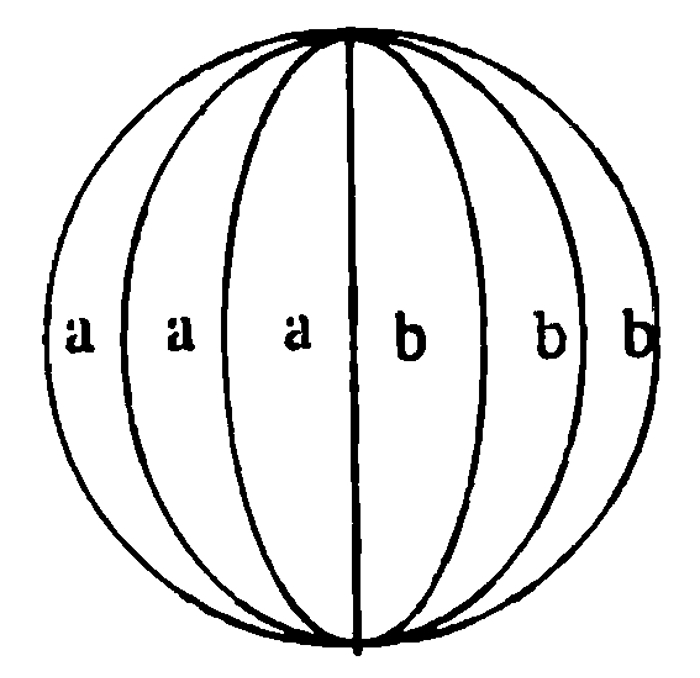
\includegraphics{images/0002.jpg}
    \end{wrapfigure}
   
%\begin{figure}
%\centering
%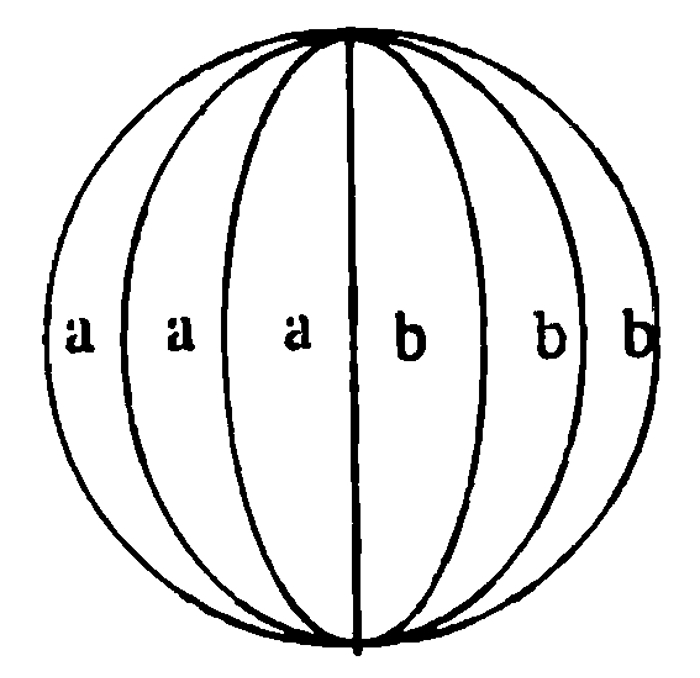
\includegraphics[scale=0.8]{images/0002.jpg}
%\end{figure}

\noindent
ಅವು ನಮ್ಮಲ್ಲಿರುವುವು.  ಈ ಜೀವಕಣಗಳನ್ನು\break ತೆಗೆದುಕೊ, ಪ್ರತಿಯೊಂದು ಬೇರೆಯಾದರೂ ಅವು \enginline{AB} ಯಲ್ಲಿ ಎಡಬಿಡದೆ ಸೇರುವುವು. ಅಲ್ಲಿ ಅವು ಏಕವಾಗುವುವು. ಪ್ರತಿಯೊಂದೂ ಒಬ್ಬೊಬ್ಬ ವ್ಯಕ್ತಿಯಂತೆ. ಆದರೆ ಎಲ್ಲರೂ \enginline{AB} ಅಕ್ಷದಲ್ಲಿ ಏಕವಾಗಿರುವರು. ಯಾರೂ ಆ ಅಕ್ಷರೇಖೆಯಿಂದ ತಪ್ಪಿಸಿಕೊಳ್ಳಲಾರರು. ಸುತ್ತಳತೆ ಎಷ್ಟೇಶಿಥಿಲವಾಗಿ ಒಡೆದುಹೋಗಿದ್ದರೂ, ಆ ಅಕ್ಷದ ಮೇಲೆ ನಿಂತು ನಾವು ಯಾವ ಕೋಣೆಯನ್ನು ಬೇಕಾದರೂ ಪ್ರವೇಶಿಸಬಹುದು. ಭಗವಂತನೇ ಈ ಅಕ್ಷರೇಖೆ. ಅಲ್ಲಿ ನಾವೆಲ್ಲಾ ಅವನೊಡನೆ ಏಕವಾಗಿರುವೆವು. ಎಲ್ಲರೂ ಎಲ್ಲರಲ್ಲಿಯೂ ಇರುವೆವು. ಎಲ್ಲರೂ ದೇವರಲ್ಲಿರುವೆವು.

ಚಂದ್ರನ ಮುಖಕ್ಕೆ ಮೋಡಗಳು ಅಡ್ಡವಾಗಿ ಬಂದು ಚಂದ್ರನೇ ಚಲಿಸುತ್ತಿರುವನೆಂಬ ಭ್ರಮೆಯುಂಟುಮಾಡುವುವು. ಅದರಂತೆಯೇ ಪ್ರಕೃತಿ, ದೇಹ, ಜಡದ್ರವ್ಯಗಳೆಲ್ಲಾ ಚಲಿಸುತ್ತಾ, ಆತ್ಮನೇ ಚಲಿಸುತ್ತದೆ ಎಂಬ ಭ್ರಾಂತಿಯನ್ನು ಉಂಟುಮಾಡುವುವು. ಹೀಗೆ ಕೊನೆಯಲ್ಲಿ ಉತ್ತಮ ಅಥವಾ ಕೀಳುಮಟ್ಟದಲ್ಲಿರುವ ಪ್ರತಿಯೊಂದು ಜನಾಂಗವೂ ಮೃತಪಟ್ಟವರ ಸಾನ್ನಿಧ್ಯವನ್ನು ಅನುಭವಿಸಿಯೇ ತೀರುವುದೆಂಬುದು ತರ್ಕದೃಷ್ಟಿಯಿಂದಲೂ ಸತ್ಯವೆಂಬುದನ್ನು ನಾವು ನೋಡುವೆವು.

ಪ್ರತಿಯೊಂದು ಆತ್ಮನೂ ಒಂದು ನಕ್ಷತ್ರ. ಎಲ್ಲಾ ತಾರೆಗಳೂ ಆ ಉಜ್ವಲ ನೀಲವರ್ಣದ ಅಸೀಮ ಆಕಾಶಸ್ವರೂಪನಾದ ಆ ಭಗವಂತನಲ್ಲಿ ಮೂಡಿವೆ. ಪ್ರತಿಯೊಬ್ಬರ ನೈಜಸ್ಥಿತಿ ಸತ್ಯವಾದ ವ್ಯಕ್ತಿತ್ವದ ಮೂಲ ಅಲ್ಲಿರುವುದು. ನಮ್ಮ ದೃಷ್ಟಿಗೆ ಮೀರಿದ ಈ ತಾರೆಗಳಲ್ಲಿ ಕೆಲವನ್ನು ಹುಡುಕುವುದರೊಂದಿಗೆ ಧರ್ಮ ಪ್ರಾರಂಭವಾಯಿತು. ಪ್ರತಿಯೊಂದು ವಸ್ತುವೂ, ನಾವೆಲ್ಲರೂ ಭಗವಂತನಲ್ಲಿದ್ದೇವೆ ಎಂಬುದನ್ನು ಕಂಡುಹಿಡಿಯುವುದರಲ್ಲಿ ಧರ್ಮ ಮುಕ್ತಾಯವಾಯಿತು. ಇದರ ಇಡೀ ರಹಸ್ಯವೇನೆಂದರೆ, ನಿನ್ನ ತಂದೆ ತಾನು ಉಡುತ್ತಿದ್ದ ಹಳೆಯ ಉಡುಪನ್ನು ತ್ಯಜಿಸಿ ತಾನು ಅನಂತಕಾಲದಿಂದಲೂ ಇದ್ದ ಸ್ಥಳದಲ್ಲಿ ನಿಂತಿದ್ದಾನೆ. ಆ ಉಡುಪನ್ನು ಮತ್ತೆ ಈ ಲೋಕದಲ್ಲೊ ಅಥವಾ ಮತ್ತಾವಲೋಕದಲ್ಲೊ ಧರಿಸುವನೇನು? ಪ್ರಜ್ಞಾಪೂರ್ವಕವಾಗಿ ಆ ರೀತಿ ಮಾಡುವವರೆಗೆ, ಆತನು ಪುನಃ ಹಾಗೆ ಮಾಡದಿರಲಿ ಎಂದು ನಾನು ಅಂತಃಕರಣ ಪೂರ್ವಕವಾಗಿ ಪ್ರಾರ್ಥಿಸುತ್ತೇನೆ. ಅಗೋಚರವಾದ ಪೂರ್ವಕರ್ಮಗಳ ಶಕ್ತಿ ಮತ್ತಾರನ್ನೂ ಎಲ್ಲೂ ಒಯ್ಯದಿರಲಿ, ಪ್ರತಿಯೊಬ್ಬರೂ ತಾವು ಮುಕ್ತರಾಗಬೇಕು; ಎಂದರೆ ಪ್ರತಿಯೊಬ್ಬರೂ ತಾವು ಮುಕ್ತರು ಎಂಬುದನ್ನು ಅರಿಯಲಿ ಎಂದು ನಾನು ಪ್ರಾರ್ಥಿಸುತ್ತೇನೆ. ಪುನಃ ಕನಸು ಬೀಳುವುದಾದರೆ ಅವೆಲ್ಲಾ ಶಾಂತಿ ಮತ್ತು ಆನಂದದಿಂದ ಕೂಡಿದ ಸ್ವಪ್ನಗಳಾಗಲಿ ಎಂದು ಪ್ರಾರ್ಥಿಸೋಣ.

\vspace{-0.5cm}

{\flushright
ನಿನ್ನ\\ವಿವೇಕಾನಂದ\par}

\begin{center}
\textbf{೧೫೮. ಮಿಸ್ ಮೇರಿ ಹೇಲ್‌ ಅವರಿಗೆ}\footnote{\engfoot{C.W. Vol. V, P. 70}}
\end{center}

\vspace{-0.8cm}

\begin{flushright}
ನ್ಯೂಯಾರ್ಕ್\\೧ನೇ ಫೆಬ್ರವರಿ, ೧೮೯೫
\end{flushright}
\vspace{-0.5cm}

\noindent
ಪ್ರಿಯ ಸಹೋದರಿ,

ಈಗ ತಾನೆ ನಿನ್ನ ಸುಂದರವಾದ ಪತ್ರ ಕೈಸೇರಿತು. ಹೌದು; ಕೆಲವು ಸಮಯದಲ್ಲಿ ಕರ್ಮಕ್ಕೋಸುಗವಾಗಿ ಕರ್ಮವನ್ನು, ಅದರ ಫಲಾಪೇಕ್ಷೆಗೆ ಅವಕಾಶವಿಲ್ಲದೆ ಮಾಡುವುದರಿಂದ ಒಳ್ಳೆಯ ಶಿಸ್ತು ಬರುವುದು. ನಿನ್ನ ಟೀಕೆಯನ್ನು ನೋಡಿ ಸಂತೋಷವಾಯಿತು. ಆದರೆ ನಾನು ಹಾಗೆ ವರ್ತಿಸಿದುದಕ್ಕೆ ವ್ಯಥೆಪಡುವುದಿಲ್ಲ. ಕೆಲವು ದಿನಗಳ ಹಿಂದೆ ಶ‍್ರೀಮತಿ ಥರ್ಸ್‌ಬಿ ಅವರ ಮನೆಯಲ್ಲಿ ಪ್ರೆಸ್ಬಿಟೇರಿಯನ್ ಸಮಾಜಕ್ಕೆ ಸೇರಿದ ಒಬ್ಬ ದೊಡ್ಡ ಮನುಷ್ಯರೊಂದಿಗೆ ಉದ್ವೇಗದ ವಾದ ನಡೆಯಿತು. ಆತನು ಎಂದಿನಂತೆ ದುಡುಕಿ ಕೋಪಗೊಂಡು ನಿಂದಿಸಲು ಮೊದಲು ಮಾಡಿದನು. ಇದು ಹೇಗಾದರೂ ಆಗಲಿ. ಅನಂತರ ಶ‍್ರೀಮತಿ ಬುಲ್ ಅವರು ನನ್ನ ಮೇಲೆ ಇದಕ್ಕೋಸುಗವಾಗಿ ಬಹಳ ಸಿಟ್ಟುಗೊಂಡರು. ಇಂತಹ ಪ್ರಸಂಗಗಳು ನನ್ನ ಕೆಲಸಕ್ಕೆ ಅಡ್ಡಿಯನ್ನು ತರುತ್ತಿವೆ ಎಂಬುದು ಅವರ ಮತ. ನಿನ್ನ ಅಭಿಮತವೂ ಹಾಗೆಯೇ ಎಂದು ಕಾಣುತ್ತಿದೆ.

ಆ ಪ್ರಸಂಗದ ವಿಚಾರವಾಗಿ ನೀನು ಈಗತಾನೆ ಬರೆದಿರುವುದು ಒಳ್ಳೆಯದು. ಏಕೆಂದರೆ ನಾನು ಇದನ್ನೇ ವಿಮರ್ಶಿಸುತ್ತಿದ್ದೆ. ಮೊದಲನೆಯದಾಗಿ ನಾನು ಇದಕ್ಕೆ ವ್ಯಥೆ ಪಡುವುದಿಲ್ಲ. ಇದರಿಂದ ನಿನಗೆ ಜುಗುಪ್ಸೆಯಾಗಬಹುದು. ಬಹುಶಃ ಪ್ರಪಂಚದಲ್ಲಿ ಲೌಕಿಕ\break ಯಶಸ್ವಿಗಾಗಿ ಮೃದುವಾಗಿರುವುದು ಎಷ್ಟು ಒಳ್ಳೆಯದೆಂಬುದು ನನಗೆ ಗೊತ್ತು. ಮೃದುವಾಗಿರುವುದಕ್ಕೆ ನಾನು ಸಾಧ್ಯವಾದಷ್ಟು ಪ್ರಯತ್ನ ಪಡುವೆನು. ಆದರೆ ಎಂದು ಹೃದಯದ ಸತ್ಯದೊಂದಿಗೆ ರಾಜಿಮಾಡಿಕೊಳ್ಳಬೇಕಾಗಿ ಬರುವುದೋ ಆಗ ನಿಲ್ಲಿಸುವೆನು. ನನಗೆ ನಮ್ರತೆಯಲ್ಲಿ ನಂಬಿಕೆಯಿಲ್ಲ. ಎಲ್ಲವನ್ನೂ ಏಕದೃಷ್ಟಿಯಿಂದ ನೋಡುವ ಸಮದರ್ಶಿತ್ವದಲ್ಲಿ ನಂಬಿಕೆಯುಂಟು. ಸಾಧಾರಣ ಮನುಷ್ಯನ ಕರ್ತವ್ಯವಾದರೋ ತನ್ನ ದೇವರಂತಿರುವ ಸಮಾಜ ಹೇಳಿದಂತೆ ಕೇಳುವುದು. ಆದರೆ ಜ್ಞಾನಿಗಳು ಇದನ್ನು ಎಂದಿಗೂ ಲೆಕ್ಕಿಸುವುದಿಲ್ಲ. ಇದು ಒಂದು ಶಾಶ್ವತವಾದ ನಿಯಮ. ನೆರೆಹೊರೆಯ ಜನರ ಅಭಿಪ್ರಾಯಗಳಿಗೆ ಮತ್ತು ಸಾಮಾಜಿಕ ನಿಯಮಕ್ಕೆ ಅಡಿಯಾಳಾಗಿ ಒಬ್ಬನು ಸಮಾಜದ ಎಲ್ಲಾ ಪ್ರಯೋಜನವನ್ನು ಪಡೆಯುತ್ತಾನೆ. ಇನ್ನೊಬ್ಬನು ಏಕಾಂಗಿಯಾಗಿ ನಿಂತು ಸಮಾಜವನ್ನೇ ತನ್ನೆಡೆಗೆ ಆಕರ್ಷಿಸುವನು. ಯಾರು ಸಮಾಜದ ಅಭಿಪ್ರಾಯದಂತೆ ನಡೆಯುವರೋ ಅವರ ದಾರಿ ಸುಗಮವಾಗಿರುವುದು. ಯಾರು ಅದರೊಂದಿಗೆ ಸಹಕರಿಸುವುದಿಲ್ಲವೋ, ಅವರ ಮಾರ್ಗ ಅತಿ ಕಠಿಣ. ಆದರೆ ಯಾರು ಜನಾಭಿಪ್ರಾಯವನ್ನು ಪೂಜಿಸುವರೋ ಅವರು ಕ್ಷಣದಲ್ಲಿ ನಾಶವಾಗುವರು. ಸತ್ಯವನ್ನು ಪೂಜಿಸುವವರ ಹೆಸರು ಶಾಶ್ವತವಾಗಿ ನಿಲ್ಲುವುದು.

ಸತ್ಯವನ್ನು ನಾನು ಅನಂತಶಕ್ತಿಯುಳ್ಳ ಎಲ್ಲಾ ವಸ್ತುವನ್ನು ಕರಗಿಸುವ ವಸ್ತುವಿನೊಂದಿಗೆ ಹೋಲಿಸುತ್ತೇನೆ. ಮೆತ್ತಗಿರುವ ವಸ್ತುವನ್ನು ಕ್ಷಣದಲ್ಲಿ, ವಜ್ರೋಪಮ ಕಠಿಣವಾಗಿರುವ ವಸ್ತುವನ್ನು ನಿಧಾನವಾಗಿ ಆದರೂ ನಿಶ್ಚಯವಾಗಿ ಕರಗಿಸುವುದು. ನಡೆದದ್ದು ನಡೆದುಹೋಯಿತು. ತಂಗಿ! ಪ್ರತಿಯೊಂದು ಸುಳ್ಳನ್ನು ಎದುರಿಸುವಾಗಲೂ ನಾನು ಮೃದುವಾಗಿರಲಾರೆ. ಅದರೊಂದಿಗೆ ರಾಜಿಮಾಡಿಕೊಳ್ಳಲಾರೆ. ಇದು ನನ್ನಿಂದ ಸಾಧ್ಯವಿಲ್ಲ. ನನ್ನ ಜೀವಮಾನವೆಲ್ಲ ಅದಕ್ಕಾಗಿ ಕಷ್ಟ ಅನುಭವಿಸಿದ್ದೇನೆ. ಆದರೆ ಎಷ್ಟು ಪ್ರಯತ್ನ ಪಟ್ಟರೂ ರಾಜಿ ನನಗೆ ಸಾಧ್ಯವಿಲ್ಲ. ಕೊನೆಗೆ ಅದನ್ನೇ ಬಿಟ್ಟುಬಿಟ್ಟಿರುವೆನು. ದೇವರು ದೊಡ್ಡವನು. ಅವನು ನನ್ನನ್ನು ಕಪಟಿಯಾಗುವುದಕ್ಕೆ ಬಿಡುವುದಿಲ್ಲ. ಈಗ ನನಗೆ ಏನು ಕಾದುಕೊಂಡಿರುವುದೋ ಅದು ಬರಲಿ, ಎಲ್ಲರನ್ನೂ ಮೆಚ್ಚಿಸುವ ಒಂದು ದಾರಿ ನನಗೆ ಸಿಕ್ಕಿಲ್ಲ. ನನ್ನ ನಿಜಸ್ಥಿತಿಗನುಸಾರವಾಗಿ ಅಲ್ಲದೆ ಬೇರೆ ವೇಷವನ್ನು ನಾನು ಧರಿಸಲಾರೆನು “ಯೌವನ ಸೌಂದರ್ಯಗಳು ನಾಶವಾಗುವುವು. ಕೀರ್ತಿ ಗೌರವಗಳು ನಾಶವಾಗುವುವು. ಪರ್ವತಗಳೂ ಕೂಡ ಕಾಲಕ್ರಮದಲ್ಲಿ ಧೂಳಾಗಿ ಹೋಗುವುವು. ಸ್ನೇಹ, ಪ್ರೀತಿಗಳು ಮಾಯವಾಗುವುವು. ಸತ್ಯವೊಂದೇ ನಿಲ್ಲುವುದು.” ಹೇ ಸತ್ಯನಾರಾಯಣನೆ, ನೀನೊಬ್ಬನೇ ನನಗೆ ಆಸರೆಯಾಗು! ಈಗ ಮೃದು ಮಧುರವಾಗಲು ವಯಸ್ಸು ಮೀರಿರುವುದು. ನಾನು ಈಗ ಇರುವ ಸ್ಥಿತಿಯಲ್ಲೇ ಇರುವಂತೆ ಬಿಡಿ. “ಅಂಜಿಕೆ ಇಲ್ಲದೆ, ಕೊಟ್ಟು ತೆಗೆದುಕೊಳ್ಳುವ ಬುದ್ಧಿಯಿಲ್ಲದೆ, ಸತ್ಯ ಪಥವನ್ನು ಹಿಡಿ. ಹೇ ಸಂನ್ಯಾಸಿ! ಈ ಕ್ಷಣದಿಂದಲೇ, ಈ ಲೋಕವನ್ನೂ ಮುಂದೆ ಬರುವ ಲೋಕಗಳನ್ನೂ ಅವುಗಳ ಭೋಗ ವ್ಯರ್ಥ ಆಡಂಬರಗಳೆಲ್ಲವನ್ನೂ ತ್ಯಜಿಸು. ಹೇ ಸತ್ಯ! ನೀನೊಬ್ಬನೇ ನನಗೆ ದಾರಿ ತೋರು.” ತಂಗಿ! ಐಶ್ವರ್ಯ ಕೀರ್ತಿ ಗೌರವ ಭೋಗಗಳಲ್ಲಿ ನನಗೆ ಆಸೆಯಿಲ್ಲ. ಅವೆಲ್ಲ ನನಗೆ ಮಣ್ಣಿಗೆ ಸಮ. ನನ್ನ ಸಹೋದರರಿಗೆ ಸಹಾಯ ಮಾಡಬೇಕೆಂದಿದ್ದೆ. ಹಣವನ್ನು ಸಂಪಾದನೆ ಮಾಡುವ ಉಪಾಯ ನನಗೆ ತಿಳಿಯದು. ದೇವರು ದೊಡ್ಡವನು! ನನ್ನ ಅಂತರಂಗದ ಸತ್ಯವಾಣಿಯನ್ನು ಕೇಳದೆ ಸುತ್ತಮುತ್ತಲಿರುವ ಜನರಂತೆ ವ್ಯರ್ಥ ಕಾಲ್ಪನಿಕ ಪ್ರಪಂಚದಲ್ಲಿ ಏಕೆ ಜೀವಿಸಬೇಕು? ತಂಗಿ! ಮನಸ್ಸು ಇನ್ನೂ ದುರ್ಬಲವಾಗಿದೆ. ಕೆಲವು ವೇಳೆ ಪ್ರಪಂಚದ ಸಹಾಯವನ್ನು ನಿರೀಕ್ಷಿಸುವುದು. ಆದರೆ ಇದರಿಂದ ನಾನು ಅಂಜುವುದಿಲ್ಲ. ಅಂಜಿಕೆಯೆ ಪರಮ ಪಾತಕವೆಂದು ನನ್ನ ಧರ್ಮ ಬೋಧಿಸುತ್ತದೆ.

ಪ್ರೆಸ್ಬಿಟೇರಿಯನ್ ಪಾದ್ರಿಯೊಂದಿಗೆ ಆದ ಕೊನೆಯ ಕಲಹ ಮತ್ತು ಶ‍್ರೀಮತಿ ಬುಲ್ ಅವರೊಂದಿಗೆ ನಡೆದ ದೀರ್ಘ ಚರ್ಚೆ ಇವುಗಳಿಂದ, ಮನು ಸಂನ್ಯಾಸಿಗೆ ಉಪದೇಶಿಸಿದ “ಏಕಾಂಗಿಯಾಗಿರು, ಏಕಾಂಗಿಯಾಗಿ ನಡೆ” ಎಂಬ ಮಾತುಗಳು ನನಗೆ ಚೆನ್ನಾಗಿ ಮನದಟ್ಟಾಯಿತು. ಎಲ್ಲಾ ಸ್ನೇಹಕ್ಕೂ ಎಲ್ಲಾ ಪ್ರೀತಿಗೂ ಒಂದು ಮೇರೆ ಇದೆ. ಪವಿತ್ರ ಸ್ನೇಹವೆಂದಿಗೂ ಇರಲಿಲ್ಲ. ಅದರಲ್ಲೂ ಹೆಂಗಸಿನ ಸ್ನೇಹ ನಕ್ಷತ್ರಿಕನಂತೆ, ಸ್ವಲ್ಪವನ್ನೂ ಬಿಡದೆ ಕಸಿದುಕೊಳ್ಳುವುದು. ಓ! ಋಷಿವರ್ಯರೇ! ನೀವೆಂದ ಮಾತು ಸತ್ಯ! ಮತ್ತೊಬ್ಬರ ಆಸರೆ ಯಾರಿಗೆ ಆವಶ್ಯಕವೋ ಅವರೆಂದಿಗೂ ಸತ್ಯವೆಂಬ ದೇವರನ್ನು ಪೂಜಿಸಲಾರರು. ಶಾಂತವಾಗು ನನ್ನಾತ್ಮವೆ! ಏಕಾಂಗಿಯಾಗು. ದೇವರು ನಿನ್ನೊಂದಿಗೆ ಇರುವನು. ಜೀವನದಲ್ಲಿ ಏನೂ ಇಲ್ಲ. ಮರಣವೆಂಬುದೊಂದು ಭ್ರಾಂತಿ. ಇದಾವುದೂ ಸತ್ಯವಲ್ಲ. ದೇವರೊಬ್ಬನೇ ಸತ್ಯ! ನನ್ನಾತ್ಮವೆ ಅಂಜದಿರು! ಏಕಾಂಗಿಯಾಗು! ತಂಗಿ! ನಡೆವ ದಾರಿ ಇನ್ನೂ ದೂರವಿರುವುದು. ಆದರೆ ಕಾಲವಿರುವುದು ಅಲ್ಪ. ಆಗಲೇ ಸಂಜೆಯಾಗುತ್ತಿದೆ. ಬೇಗ ನಾನು ಮನೆಯನ್ನು ಸೇರಬೇಕಾಗಿದೆ. ಈಗ ನನ್ನ ನಡತೆಗಳಿಗೆ ಮೆರಗು ಕೊಡುವುದಕ್ಕೆ ಸಮಯವಿಲ್ಲ. ನೀನು ಒಳ್ಳೆಯವಳು. ಬಹಳ ದಯಾಳು. ನಿನಗೋಸುಗವಾಗಿ ನಾನು ಏನನ್ನು ಬೇಕಾದರೂ ಮಾಡಲು ಸಿದ್ಧನಾಗಿರುವೆನು. ಆದರೆ ಕೋಪಿಸಿಕೊಳ್ಳಬೇಡ. ನಿಮ್ಮೆಲ್ಲರನ್ನೂ ನಾನು ಮಕ್ಕಳಂತೆ ನೋಡುತ್ತೇನೆ.

ಕನಸುಗಳನ್ನು ಇನ್ನು ಕಾಣಬೇಡ! ಎಲೈ ನನ್ನಾತ್ಮವೇ, ಇನ್ನು ಮುಂದೆ ನಿನ್ನ ಕನಸಿನ ಸಾಮ್ರಾಜ್ಯದಲ್ಲಿ ಸಂಚರಿಸಬೇಡ!ಒಂದು ಮಾತಿನಲ್ಲಿ ಹೇಳಬೇಕಾದರೆ, ನಾನು ಕೊಡಬೇಕಾದ ಒಂದು ಸಂದೇಶವಿದೆ. ಜಗತ್ತಿಗೆ ಮೃದುವಾಗಿ ಕಾಣಿಸಿಕೊಳ್ಳುವುದಕ್ಕೆ ನನಗೆ ಹೊತ್ತಿಲ್ಲ. ಮೃದುವಾಗಿರಬೇಕೆಂದು ಮಾಡಿದ ಪ್ರತಿಯೊಂದು ಪ್ರಯತ್ನವೂ ನನ್ನನ್ನು ಕಪಟಿಯನ್ನಾಗಿ ಮಾಡುವುದು. ನನ್ನ ದೇಶವಾಗಲಿ, ಅನ್ಯದೇಶವಾಗಲಿ, ಈ ಮೂರ್ಖ ಜಗತ್ತಿನ ಜನರ ಅಭಿಪ್ರಾಯಗಳಿಗೆಲ್ಲ ಸೋಲುತ್ತ ಇದ್ದೆಡೆಯೆ ಬಿದ್ದಿರುವ ಜೀವನಕ್ಕಿಂತ ಸಾವಿರ ಸಲವಾದರೂ ನಾನು ಸಾಯಲು ಸಿದ್ಧನಾಗಿರುವೆನು. ಶ‍್ರೀಮತಿ ಬುಲ್ ಅವರು ತಿಳಿದಿರುವಂತೆ, ನಾನು ಮಾಡಬೇಕಾದ ಒಂದು ಕೆಲಸವಿದೆ ಎಂದು ತಿಳಿದುಕೊಂಡಿದ್ದರೆ ಅದು ತಪ್ಪು. ಈ ಜಗತ್ತಿನಲ್ಲಾಗಲೀ ಬೇರೆ ಜಗತ್ತಿನಲ್ಲಾಗಲೀ, ನನಗೆ ಯಾವ ಕೆಲಸವೂ ಇಲ್ಲ. ನಾನು ಜಗತ್ತಿಗೆ ಒಂದು ಸಂದೇಶವನ್ನು ಕೊಡಬೇಕಾಗಿರುವುದು. ಅದನ್ನು ನನ್ನದೇ ಒಂದು ರೀತಿಯಲ್ಲಿ ಕೊಡುವೆನು. ಅದನ್ನು ಹಿಂದೂಧರ್ಮವೆಂದಾಗಲೀ, ಕ್ರೈಸ್ತಧರ್ಮವೆಂದಾಗಲೀ ಅಥವಾ ಇನ್ನೂ ಯಾವುದೋ ಧರ್ಮವೆಂದಾಗಲೀ ಕರೆಯುವುದಿಲ್ಲ. ಅದನ್ನು ಕೇವಲ ನನ್ನ ಧರ್ಮವೆಂದು ಕರೆಯುತ್ತೇನೆ. ಸ್ವಾತಂತ್ರ್ಯ, ಮುಕ್ತಿ, ಇವೇ ನನ್ನ ಧರ್ಮದ ಸರ್ವಸ್ವ. ಅದನ್ನು ಅಡಗಿಸಿಡುವುದಕ್ಕೆ ಪ್ರಯತ್ನಿಸುವ ಎಲ್ಲದರೊಂದಿಗೆ ಕಾದಾಡುತ್ತೇನೆ. ಇಲ್ಲವೆ ಅದರಿಂದ ಸರಿದು ಪಾರಾಗುವೆನು. ಪಾಪ! ನಾನು ಪಾದ್ರಿಗಳನ್ನು ಸಮಾಧಾನ ಮಾಡಬೇಕೆ? ತಂಗಿ, ದಯವಿಟ್ಟು ಇದನ್ನು ತಪ್ಪು ತಿಳಿದುಕೊಳ್ಳಬೇಡ. ನೀವೆಲ್ಲ ಇನ್ನೂ ಮಕ್ಕಳು. ಮಕ್ಕಳು ಬುದ್ಧಿವಾದವನ್ನು ಕಲಿಯುವುದಕ್ಕೆ ಸಿದ್ಧರಾಗಬೇಕು. “ವಿಚಾರವನ್ನು ಅವಿಚಾರವನ್ನಾಗಿ ಮಾಡುವ, ಜಗತ್ತನ್ನೇ ಶೂನ್ಯಮಾಡಿ, ಮರ್ತ್ಯನನ್ನು ಅಮೃತನನ್ನಾಗಿ ಮಾಡುವ ಚಿಲುಮೆಯ ಜಲವನ್ನು“ ನೀವು ಇನ್ನೂ ಪಾನಮಾಡಿಲ್ಲ. ಪ್ರಪಂಚವೆಂಬ ಅಜ್ಞಾನದ ಬಲೆಯಿಂದ ಸಾಧ್ಯವಾದರೆ ಹೊರಗೆ ಬಾ. ಆಗ ನಿನ್ನನ್ನು ನಿಜವಾಗಿಯೂ ಸ್ವತಂತ್ರಳು ಮತ್ತು ಧೈರ್ಯಶಾಲಿ ಎಂದು ಕರೆಯುತ್ತೇನೆ. ಅದು ನಿನ್ನಿಂದ ಸಾಧ್ಯವಿಲ್ಲದೇ ಇದ್ದರೆ, ಸಮಾಜವೆಂಬ ಸುಳ್ಳು ದೇವರನ್ನು, ಅದರ ಕೊನೆಮೊದಲಿಲ್ಲದ ಆಷಾಢಭೂತಿತನವನ್ನು ನೆಲಕ್ಕೆ ಮೆಟ್ಟಿ ಮುಂದುವರಿಯುವವರನ್ನು ಹುರಿದುಂಬಿಸು. ಹಾಗೆ ಹುರಿದುಂಬಿಸುವುದಕ್ಕೆ ನಿನಗೆ ಸಾಧ್ಯವಿಲ್ಲದೇ ಇದ್ದರೆ, ದಯವಿಟ್ಟು ಸುಮ್ಮನಿರು. ರಾಜಿ, ಮೃದುಮಧುರ ಎಂಬ ಕೆಲಸಕ್ಕೆ ಬಾರದ ವಿಷಯಗಳ ನೆವದಲ್ಲಿ ಮುಂದೆ ಹೋಗುವವರನ್ನು ಎಳೆದು ಪ್ರಪಂಚವೆಂಬ ಕೆಸರಿಗೆ ಬೀಳುವಂತೆ ಮಾಡಬೇಡ.
\vspace{0.2cm}

ಚರ್ಚು ಮತ್ತು ಕುಯುಕ್ತಿಗಳು, ಧರ್ಮಗ್ರಂಥಗಳು ಮತ್ತು ಮೋಸ, ಒಳತಂತ್ರಗಳು, ನೋಡಲು ಮನೋಹರವಾದ ರೂಪು, ಒಳಗಡೆ ನಂಬಿಸಿ ಕೆಡಿಸುವ ಹೃದಯಗಳು, ಮೇಲೆ ಆಡಂಬರದ ನೀತಿಯ ನಡತೆ, ಒಳಗಡೆ ಯಾವ ತಿರುಳೂ ಇಲ್ಲದೇ ಇರುವುದು, ಎಲ್ಲಕ್ಕಿಂತ ಹೆಚ್ಚಾಗಿ ಧರ್ಮದ ವಿಕ್ರಯ ಇವುಗಳಿಂದ ಕೂಡಿದ ಈ ಜಗತ್ತನ್ನು, ಈ ಕನಸನ್ನು, ಈ ದುಃಸ್ವಪ್ನವನ್ನು ನಾನು ದ್ವೇಷಿಸುತ್ತೇನೆ. ಸಹೋದರಿ, ನನ್ನ ಹೃದಯದಾಳವನ್ನು ಪ್ರಾಪಂಚಿಕತೆಯಲ್ಲಿ ಬಿದ್ದು ನರಳುತ್ತಿರುವವರು ಹೇಳುವ ಮಾತಿನಿಂದ ಅಳೆಯುವಿಯೇನು? ಅಯ್ಯೋ? ಪಾಪ, ನಿನಗೆ ಸಂನ್ಯಾಸಿಯ ಪರಿಚಯವಿಲ್ಲ. “ಅವನು ವೇದಗಳನ್ನು ಮೀರಿ ನಿಲ್ಲುವನು“ ಎಂದು ವೇದಗಳು ಸಾರುತ್ತವೆ. ಯಾತಕ್ಕೆಂದರೆ, ಚರ್ಚು, ಪಂಗಡ, ಧರ್ಮಗ್ರಂಥ, ದೇವದೂತರು ಮತ್ತು ಪವಿತ್ರ ಗ್ರಂಥ ಇವುಗಳ ಆವಶ್ಯಕತೆಯೇ ಇಲ್ಲ ಅವನಿಗೆ. ಪಾದ್ರಿಯೊ ಅಲ್ಲವೊ ಅವರು ಬೇಕಾದಷ್ಟು ಬೊಗಳಲಿ. ತಮ್ಮ ಕೈಲಾದುದೆಲ್ಲವನ್ನೂ ಸೇರಿಸಿ ಎದುರಿಸಲಿ. “ಹೇ! ಸಂನ್ಯಾಸಿ, ನಿನ್ನ ದಾರಿಯಲ್ಲಿ ನೀನು ಹೋಗು. ಕೆಲವರು ಈ ಹುಚ್ಚನು ಯಾರೆಂದು ಕೇಳುವರು, ಕೆಲವರು ಈ ಚಂಡಾಲನಾರೆಂದು ಕೇಳುವರು. ಎಲ್ಲೋ ಸ್ವಲ್ಪ ಮಂದಿ ನಿನ್ನನ್ನು ಜ್ಞಾನಿಯೆಂದು ತಿಳಿಯುವರು.” ಪ್ರಪಂಚದ ಜನರ ಕಾಡುಹರಟೆಯನ್ನು ಕೇಳಿ ಸುಮ್ಮನಿರು. ಆನೆ ಪೇಟೆಯ ಬೀದಿಯಲ್ಲಿ ಹೋಗುತ್ತಿರುವಾಗ ಎಷ್ಟೋ ನಾಯಿಗಳು ಬೊಗಳುವುವು. ಆದರೆ ಇದಾವುದನ್ನೂ ಅದು ಲೆಕ್ಕಿಸುವುದಿಲ್ಲ. ತನ್ನ ದಾರಿಯನ್ನು ಹಿಡಿದು ನೇರ ಹೋಗುವುದು. ಯಾರಾದರೂ ಒಬ್ಬ ಮಹಾವ್ಯಕ್ತಿ ಅವತರಿಸಿದರೆ ಅವನ ಸುತ್ತಲೂ ನಾಯಿಯಂತೆ ಬೊಗಳುವವರು ಹಲವರಿರುತ್ತಾರೆ.
\vspace{0.2cm}

ನಾನು ಲ್ಯಾಂಡ್ಸ್‌ಬರ್ಗ್ ಅವರೊಂದಿಗೆ ೫೪ನೇ ಪಶ್ಚಿಮ ೨೩ನೇ ಬೀದಿಯಲ್ಲಿರುತ್ತೇನೆ. ಆತನು ಧೈರ್ಯವಂತ, ದಯಾವಂತ. ದೇವರು ಆತನಿಗೆ ಒಳ್ಳೆಯದನ್ನು ಮಾಡಲಿ. ಕೆಲವು ವೇಳೆ ಗರ್ನ್‌ಸೆ ಮನೆಗೆ ಮಲಗಲು ಹೋಗುತ್ತೇನೆ.

\vspace{0.2cm}

ಸತತವೂ ದೇವರು ನಿನ್ನನ್ನು ಆಶೀರ್ವದಿಸಲಿ. ಪ್ರಪಂಚವೆಂಬ ಒಂದು ಸುಳ್ಳು ಕನಸಿನಿಂದ ನಿನ್ನನ್ನು ಬೇಗ ಪಾರುಗಾಣಿಸಲಿ! ಪ್ರಪಂಚವೆಂಬ ಮೋಹಿನಿಗೆ ಮತ್ತೊಮ್ಮೆ ವಶ\-ವಾಗದಿರು. ಶ‍್ರೀ ಶಂಕರ ನಿನಗೆ ಸಹಾಯಮಾಡಲಿ. ಸತ್ಯದ ಬಾಗಿಲನ್ನು ಉಮಾದೇವಿ ನಿನಗೋಸುಗ ತೆರೆಯಲಿ. ಮಾಯಾಮೋಹವನ್ನೆಲ್ಲ ನಿನ್ನಿಂದ ಬಿಡಿಸಲಿ.
\vspace{0.3cm}

{\flushright
ಪ್ರೀತಿ ಆಶೀರ್ವಾದಗಳೊಂದಿಗೆ ನಿನ್ನ\\ವಿವೇಕಾನಂದ\par}

\begin{center}
\textbf{೧೫೯. ಶ‍್ರೀವೈಕುಂಠನಾಥ್ ಸನ್ಯಾಲ್‌ರವರಿಗೆ}\footnote{\engfoot{C.W. Vol. VI, P. 298}}
\end{center}

\begin{flushright}
ನ್ಯೂಯಾರ್ಕ್\\೯ನೇ ಫೆಬ್ರವರಿ, ೧೮೯೫
\end{flushright}

\noindent
ಪ್ರಿಯ ಸನ್ಯಾಲ್,

ಶ‍್ರೀರಾಮಕೃಷ್ಣ ಪರಮಹಂಸರು ನನ್ನ ಗುರು. ಅವರ ಮಾಹಾತ್ಮೆಯ ವಿಚಾರವಾಗಿ ನಾನೇನು ಅಭಿಪ್ರಾಯ ಹೊಂದಿರುವೆನೋ ಅದರಂತೆಯೇ ಜಗತ್ತೂ ಏಕೆ ಯೋಚಿಸಬೇಕು? ನೀನು ಈ ವಿಷಯವನ್ನು ಒತ್ತಿ ಹೇಳಿದರೆ ನೀನು ಎಲ್ಲವನ್ನೂ ಹಾಳುಮಾಡುವೆ. ಗುರುವನ್ನು ದೇವರೆಂದು ಪೂಜಿಸುವ ಭಾವನೆ ಬಂಗಾಳವನ್ನು ಬಿಟ್ಟರೆ ಉಳಿದಾವ ಸ್ಥಳದಲ್ಲಿಯೂ ಇಲ್ಲ. ಏಕೆಂದರೆ ಜನರು ಆ ಆದರ್ಶವನ್ನು ತೆಗೆದುಕೊಳ್ಳಲು ಇನ್ನೂ ಸಿದ್ಧರಾಗಿಲ್ಲ. ಅನೇಕರು ‘ನಾನು ಅವರಿಗೆ ಸೇರಿದವನು’ ಎಂದು ನನ್ನ ಹೆಸರಿನೊಡನೆ ಸಂಬಂಧವನ್ನು ಬೆಳಸಲು ಬಯಸುವರು. ಆದರೆ ತಾವು ಏನಾದರೂ ಮಾಡಬೇಕಾಗಿ ಬಂದಾಗ ಅವರು ಪತ್ತೆಯೇ ಇರುವುದಿಲ್ಲ. ಇಡೀ ಜಗತ್ತು ಅಷ್ಟೂ ಸ್ವಾರ್ಥ!
\vspace{0.3cm}

ಶ‍್ರೀಮಾತೆಯವರಿಗಾಗಿ ಒಂದು ನೆಲವನ್ನು ಕೊಂಡುಕೊಳ್ಳಲು ಯಶಸ್ವಿಯಾದರೆ ಆಗ ನಾನು ಸಂಪೂರ್ಣ ಋಣಮುಕ್ತನಾಗುತ್ತೇನೆ. ಅನಂತರ ನಾನಾವುದನ್ನೂ ಲೆಕ್ಕಿಸುವುದಿಲ್ಲ.
\vspace{0.3cm}

ಈ ತೀವ್ರ ಚಳಿಯಲ್ಲಿ ನಡುರಾತ್ರಿಯಲ್ಲಿ ಪರ್ವತ ಮತ್ತು ಹಿಮವನ್ನು ದಾಟುತ್ತ ಪ್ರಯಾಣಮಾಡಿ ಸ್ವಲ್ಪ ಹಣವನ್ನು ಸಂಪಾದಿಸಿರುವೆನು. ಶ‍್ರೀಮಾತೆಯವರಿಗಾಗಿ ಒಂದು ಜಾಗ ಗೊತ್ತಾದರೆ ನಾನು ಮನಶ್ಶಾಂತಿಯನ್ನು ಪಡೆಯುತ್ತೇನೆ.
\vspace{0.3cm}

ಇನ್ನು ಮುಂದೆ ಮೇಲೆ ಬರೆದಿರುವ ವಿಳಾಸಕ್ಕೆ ಪತ್ರ ಬರೆ. ಮುಂದೆ ಅದೇ ನಾನಿರುವ ಸ್ಥಳವಾಗುವುದು.
\vspace{0.3cm}

ಯೋಗವಾಸಿಷ್ಠ ರಾಮಾಯಣದ ಇಂಗ್ಲಿಷ್ ಭಾಷಾಂತರವನ್ನು ನನಗೆ ಕಳುಹಿಸಲು ಪ್ರಯತ್ನಿಸು.

ನಾನು ಹಿಂದೆಯೇ ಕೇಳಿದ್ದ ಪುಸ್ತಕಗಳು, ಎಂದರೆ ಸಂಸ್ಕೃತದ ನಾರದ ಮತ್ತು ಶಾಂಡಿಲ್ಯ ಸೂತ್ರಗಳನ್ನು, ಕಳುಹಿಸಲು ಮರೆಯಬೇಡ. “ಆಸೆಯೇ ಎಲ್ಲ ದುಃಖಕ್ಕೂ ಕಾರಣ. ಆಸೆಯನ್ನು ತ್ಯಾಗಮಾಡಿದರೆ ಪರಮೋತ್ಕೃಷ್ಟವಾದ ಆನಂದವನ್ನು ಪಡೆಯುವೆವು.”

\vspace{-0.3cm}

{\flushright
ವಿಶ್ವಾಸಪೂರ್ವಕ\\ವಿವೇಕಾನಂದ\par}

\begin{center}
\textbf{೧೬೦. ಶ‍್ರೀಮತಿ ಓಲ್ ಬುಲ್ ಅವರಿಗೆ}\footnote{\engfoot{C.W. Vol. VI, P. 299}}
\end{center}

\vspace{-0.6cm}

\begin{flushright}
ನ್ಯೂಯಾರ್ಕ್\\೧೪ನೇ ಫೆಬ್ರವರಿ, ೧೮೯೫
\end{flushright}

\vspace{-0.3cm}

\noindent
ಪ್ರಿಯ ಶ‍್ರೀಮತಿ ಬುಲ್,

ನಿಮ್ಮ ಮಾತೃಸ್ವಭಾವದ ಬುದ್ಧಿವಾದಗಳಿಗೆ ನನ್ನ ಹೃತ್ಪೂರ್ವಕ ಕೃತಜ್ಞತೆಗಳು. ನಿಮ್ಮ ಬುದ್ಧಿವಾದವನ್ನು ಬದುಕಿನಲ್ಲಿ ಕಾರ್ಯರೂಪಕ್ಕೆ ತರುತ್ತೇನೆ ಎಂದು ನಂಬಿದ್ದೇನೆ.

ನನಗೆ ಮತ್ತು ನನ್ನ ಕಾರ್ಯಕ್ಕಾಗಿ ನೀವು ಇಲ್ಲಿಯವರೆಗೆ ಮಾಡಿರುವುದಕ್ಕೆಲ್ಲಾ ನಾನು ಹೇಗೆ ನನ್ನ ಕೃತಜ್ಞತೆಯನ್ನು ಅರ್ಪಿಸಲಿ! ಈ ವರ್ಷವೂ ನೀವು ನನಗೇನಾದರೂ ಸಹಾಯ ಮಾಡಬೇಕೆಂದಿದ್ದಲ್ಲಿ ನನ್ನ ಚಿರ ಕೃತಜ್ಞತೆಗಳು. ಆದರೆ ನೀವು ಈ ವರ್ಷ ಶ‍್ರೀಮತಿ ಫಾರ್ಮರರ ಗ್ರೀನೇಕರ್ ಕೆಲಸಕ್ಕೆ ನಿಮ್ಮ ಕೈಲಾದ ಸಹಾಯವನ್ನೆಲ್ಲಾ ಮಾಡಬೇಕೆಂದು ನನ್ನ ಮನಃಪೂರ್ವಕವಾದ ಅಭಿಪ್ರಾಯ. ಶತಮಾನಗಳಿಂದಲೂ ಭರತಖಂಡ ಕಾಯುತ್ತಿರುವಂತೆಯೇ ಈಗಲೂ ಕಾಯಬಲ್ಲದು. ತುರ್ತಾದ ಕೆಲಸ ಇಲ್ಲೇ ಇರುವುದರಿಂದ ಅದಕ್ಕೆ ಹೆಚ್ಚು ಗಮನ ಕೊಡಬೇಕು.

ಅಲ್ಲದೆ ಒಳ್ಳೆಯ ಕೆಲಸಕ್ಕಾಗಿ ಹಣ ಕೂಡಿಸುವುದೂ ಕೂಡ ಸಂನ್ಯಾಸಿಗೆ ಒಳ್ಳೆಯದಲ್ಲ ಎಂದು ಮನು ಹೇಳಿದ್ದಾನೆ. ನಮ್ಮ ಹಿಂದಿನ ಋಷಿಗಳು ಹೇಳಿದ್ದು ಸರಿ ಎಂದು ನನಗೂ ಈಗ ಭಾಸವಾಗುತ್ತಿದೆ. “ಆಸೆಯೇ ದುಃಖಗಳಲ್ಲೆಲ್ಲಾ ದಾರುಣವಾದುದು. ನಿರಾಶೆಯೇ ಸುಖಗಳಲ್ಲೆಲ್ಲಾ ಅತ್ಯಂತ ಶ್ರೇಷ್ಠವಾದುದು.” ಅದನ್ನು ಮಾಡಬೇಕು, ಇದನ್ನು ಮಾಡಬೇಕೆಂಬ ಶಿಶುಸಹಜವಾದ ಅಭಿಪ್ರಾಯಗಳು ನನ್ನಲ್ಲಿದ್ದುವು. ಈಗ ಅವೆಲ್ಲಾ ಒಂದು ಕ್ರಾಂತಿಯೆಂದು ಕಾಣಿಸುತ್ತಿವೆ. ನಾನವುಗಳಿಂದ ಹೊರಕ್ಕೆ ಬರುತ್ತಿದ್ದೇನೆ.

“ಆಸೆಯನ್ನೆಲ್ಲಾ ತ್ಯಜಿಸು. ಶಾಂತಿಯಿಂದಿರು. ಮಿತ್ರರೂ ಬೇಡ. ಶತ್ರುಗಳೂ ಬೇಡ. ಏಕಾಂಗಿಯಾಗಿ ಜೀವಿಸು. ಹೀಗೆ ಗೆಳೆಯರು, ಶತ್ರುಗಳು, ಸುಖ, ದುಃಖ, ಆಸೆ, ಅಸೂಯೆಗಳೊಂದೂ ಇಲ್ಲದೆ, ಯಾವ ಪ್ರಾಣಿಯನ್ನೂ ಹಿಂಸಿಸದೆ, ಯಾವ ಪ್ರಾಣಿಯ ಹಿಂಸೆಗೂ ಕಾರಣವಾಗದೆ, ಬೆಟ್ಟಗುಡ್ಡಗಳು, ಹಳ್ಳಿಹಳ್ಳಿಗಳಲ್ಲಿ ಭಗವಂತನ ನಾಮವನ್ನು ಉಪದೇಶ ಮಾಡುತ್ತಾ ನಾವು ಸಂಚರಿಸುತ್ತಿರುವೆವು.”

\vspace{0.1cm}

“ಬಡವರು ಬಲ್ಲಿದರು, ದೊಡ್ಡವರು ಚಿಕ್ಕವರು, ಯಾರಿಂದಲೂ ಸಹಾಯವನ್ನರಸಬೇಡ. ಯಾವುದಕ್ಕೂ ಆಸೆಪಡಬೇಡ. ಸುತ್ತಮುತ್ತ ಕಾಣುವ ಕ್ಷಣಿಕವಾದ ದೃಶ್ಯಪರಂಪರೆಗಳನ್ನು ಸಾಕ್ಷಿಯಂತೆ ವೀಕ್ಷಿಸು. ಅವನ್ನು ಮುಂದಕ್ಕೆ ಹೋಗಗೊಡು.”

\vspace{0.15cm}

ಬಹುಶಃ ಈ ಉನ್ಮತ್ತ ಆಕಾಂಕ್ಷೆಗಳು ಈ ದೇಶಕ್ಕೆ ನನ್ನನ್ನು ಕರೆತರಲು ಆವಶ್ಯಕವಾಗಿತ್ತೆಂದು ಕಾಣುತ್ತದೆ. ಈ ಅನುಭವಕ್ಕಾಗಿ ನಾನು ಭಗವಂತನಿಗೆ ಕೃತಜ್ಞನಾಗಿದ್ದೇನೆ.

\vspace{0.15cm}

ನಾನೀಗ ಬಹಳ ಸುಖವಾಗಿರುವೆ. ಶ‍್ರೀಮಾನ್ ಲ್ಯಾಂಡ್ಸ್‌ಬರ್ಗ್ ಮತ್ತು ನಾನು ಇಬ್ಬರೂ ಕೊಂಡ ಅಕ್ಕಿ ಮತ್ತು ಅವರೆ ಅಥವಾ ಬಾರ್ಲಿಯನ್ನು ಬೇಯಿಸಿ ನೆಮ್ಮದಿಯಿಂದ ಊಟಮಾಡುತ್ತೇವೆ. ಕೊಂಚ ಬರೆಯುತ್ತೇನೆ ಅಥವಾ ಓದುತ್ತೇನೆ ಅಥವಾ ಇಲ್ಲಿಗೆ ಏನನ್ನಾದರೂ ಕಲಿಯಬೇಕೆಂದು ಬರುವ ಬಡಜನರೊಂದಿಗೆ ಮಾತನಾಡುತ್ತೇನೆ. ಇದುವರೆಗೆ ನಾನು ಅಮೆರಿಕಾದಲ್ಲಿದ್ದುದಕ್ಕಿಂತ ಈಗ ಹೆಚ್ಚು ಸಂನ್ಯಾಸಿಯಂತಿರುವೆನೆಂದು ನನಗೆ ಭಾಸವಾಗುತ್ತಿದೆ.

\vspace{0.15cm}

“ಐಶ್ವರ್ಯವಿರುವೆಡೆ ದಾರಿದ್ರ್ಯದ ಅಂಜಿಕೆ, ಜ್ಞಾನವಿರುವ ಕಡೆ ಅಜ್ಞಾನದ ಭಯ, ರೂಪವಿರುವೆಡೆ ವಯಸ್ಸಿನ ಅಂಜಿಕೆ, ಕೀರ್ತಿಯಿರುವೆಡೆ ಅಪಕೀರ್ತಿಯ ಅಂಜಿಕೆ, ಜಯವಿರುವೆಡೆ ಅಸೂಯೆಯ ಅಂಜಿಕೆ, ದೇಹವಿದ್ದೆಡೆ ಕೂಡ ಮರಣದ ಅಂಜಿಕೆ. ಭೂಮಿಯಲ್ಲಿರುವ ಪ್ರತಿಯೊಂದು ವಸ್ತುವೂ ತೀವ್ರ ಭಯದಿಂದಾವೃತವಾಗಿದೆ. ಯಾರು ಸರ್ವಸ್ವವನ್ನೂ ತ್ಯಾಗ ಮಾಡಿರುವರೋ ಅವರು ನಿರ್ಭಯರು.” (ವೈರಾಗ್ಯಶತಕ: ೩೧)

\vspace{0.15cm}

ಮಿಸ್ ಕಾರ್ಬನ್‌ರನ್ನು ಒಂದು ದಿನ ನಾನು ನೋಡಲು ಹೋಗಿದ್ದೆ. ಮಿಸ್ ಫಾರ್ಮರ್‌ ಮತ್ತು ಮಿಸ್ ಥರ್ಸ್‌ಬಿ ಕೂಡ ಅಲ್ಲಿದ್ದರು. ನಾವು ಅರ್ಧ ತಾಸು ಚೆನ್ನಾಗಿ ಕಾಲ ಕಳೆದೆವು. ಆಕೆ ತನ್ನ ಮನೆಯಲ್ಲಿ ಮುಂದಿನ ಭಾನುವಾರದಿಂದ ಕೆಲವು ಪ್ರವಚನಗಳನ್ನು ನಡೆಸಬೇಕೆಂದು ಇಚ್ಛೆಪಟ್ಟಳು.

\vspace{0.15cm}
ನನಗೆ ಇದಾವ ವಿಷಯಗಳೂ ಇನ್ನು ಬೇಕಾಗಿಲ್ಲ. ಅವರು ಬಂದರೆ ಭಗವಂತನಿಗೆ ಧನ್ಯವಾದಗಳು. ಬರದಿದ್ದರೆ ಇನ್ನೂ ಹೆಚ್ಚು ಧನ್ಯವಾದಗಳು.

\vspace{0.15cm}

ಮತ್ತೊಮ್ಮೆ ನನ್ನ ಚಿರ ಕೃತಜ್ಞತೆಗಳನ್ನು ಸ್ವೀಕರಿಸಿ,

{\flushright
ಇತಿ ನಿಮ್ಮ ಪ್ರೀತಿಯ ಮಗ\\ವಿವೇಕಾನಂದ\par}

\newpage

\begin{center}
\textbf{೧೬೧. ಶ‍್ರೀಮತಿ ಇಸಬೆಲ್ಲಾ ಮೆಕೆಂಡ್ಲಿ ಅವರಿಗೆ}\footnote{\engfoot{C.W. Vol. V, P. 74}}
\end{center}

\begin{flushright}
೫೪. ವೆಸ್ಟ್, ೩೩ ನ್ಯೂಯಾರ್ಕ್\\೨೫ನೇ ಫೆಬ್ರವರಿ ೧೮೯೫
\end{flushright}

\vspace{-0.5cm}

\noindent
ಪ್ರಿಯ ಸಹೋದರಿ,

ನಿನಗೆ ಖಾಯಿಲೆಯಾಗಿತ್ತು ಎಂಬುದನ್ನು ಕೇಳಿ ತುಂಬಾ ವ್ಯಸನವಾಯಿತು. ನಿನ್ನ ಪಶ್ಚಾತ್ತಾಪ ನನ್ನ ಶಕ್ತಿಯ ಅರ್ಧಭಾಗವನ್ನು ಸೂರೆಗೊಳ್ಳುವುದಾದರೂ, ನಾನು ನಿನಗೆ ಗೈರ್‌ಹಾಜರ್ ಚಿಕಿತ್ಸೆಯನ್ನು \enginline{(Absent treatment)} ಕೊಡುತ್ತೇನೆ.

ನೀನು ಅದರಿಂದ ಸುರಕ್ಷಿತವಾಗಿ ಪಾರಾಗಿರುವೆ. ಯಾವುದು ಕೊನೆಯಲ್ಲಿ ಸರಿಯಾಗುವುದೋ ಅದೆಲ್ಲಾ ಸರಿಯೇ.

ಪುಸ್ತಕಗಳು ಸರಿಯಾದ ಸ್ಥಿತಿಯಲ್ಲಿ ನನಗೆ ತಲುಪಿದವು. ಅದಕ್ಕಾಗಿ ನಿನಗೆ ಅನೇಕ ವಂದನೆಗಳು.

\vspace{-0.5cm}

{\flushright
ಎಂದೆಂದಿಗೂ ನಿನ್ನ ವಿಶ್ವಾಸದ ಸಹೋದರ\\ವಿವೇಕಾನಂದ\par}

\begin{center}
\textbf{೧೬೨. ಶ‍್ರೀ ಅಳಸಿಂಗ ಪೆರುಮಾಳ್ ಅವರಿಗೆ}\footnote{\engfoot{C.W. Vol. V, P. 74}}
\end{center}

\vspace{-0.5cm}

\begin{flushright}
ನ್ಯೂಯಾರ್ಕ್\\೧೮೯೫
\end{flushright}

\vspace{-0.5cm}

\noindent
ಪ್ರಿಯ ಅಳಸಿಂಗ,

ಸಮಾಜಸುಧಾರಣೆಯ ಗೋಜಿಗೆ ಹೋಗಬೇಡ. ಮೊದಲು ಆಧ್ಯಾತ್ಮಿಕ ಸುಧಾರಣೆಯಿಲ್ಲದೆ ಬೇರೆ ಯಾವ ಸುಧಾರಣೆಯೂ ಆಗಲಾರದು. ನಾನು ಸಮಾಜಸುಧಾರಣೆಯನ್ನು ಬಯಸುತ್ತೇನೆ ಎಂದು ಹೇಳಿದವರು ಯಾರು? ನಾನಂತೂ ಅಲ್ಲ. ದೇವರ ವಿಷಯವಾಗಿ ಬೋಧಿಸಿ. ಸಾಮಾಜಿಕ ಕುಂದುಕೊರತೆಯ ವಿಚಾರವಾಗಿಯಾಗಲಿ, ಅಥವಾ ಮೂಢಾಚಾರದ ವಿಚಾರವಾಗಿ ಆಗಲಿ, ಅವುಗಳ ಪರವಾಗಿ ಆಗಲಿ, ಅಥವಾ ವಿರೋಧವಾಗಿ ಆಗಲಿ, ಏನನ್ನೂ ಹೇಳಬೇಡಿ. ಖಿನ್ನನಾಗಬೇಡ. ಎಂದಿಗೂ ಗುರುವಿನಲ್ಲಿಟ್ಟ ಭಕ್ತಿ ಕುಗ್ಗದಿರಲಿ. ದೇವರಲ್ಲಿಟ್ಟ ನಂಬಿಕೆ ಜಾರದಿರಲಿ. ನನ್ನ ಮಗು! ಎಲ್ಲಿಯವರೆವಿಗೂ ಈ ಮೂರು ಗುಣಗಳು, ನಿನ್ನಲ್ಲಿರುತ್ತವೆಯೋ ಅಲ್ಲಿಯವರೆವಿಗೆ ಯಾವುದೂ ನಿನಗೆ ತೊಂದರೆ ಮಾಡಲಾರದು. ದಿನಕಳೆದಂತೆಲ್ಲಾ ನಾನು ಬಲಾಢ್ಯನಾಗುತ್ತಿರುವೆನು. ನನ್ನ ಕೆಚ್ಚೆದೆಯ ಮಕ್ಕಳಿರಾ! ಕೆಲಸ ಮಾಡಿ, ಆಶೀರ್ವಾದಗಳು.

\vspace{-0.5cm}

{\flushright
ಸತತವೂ ನಿನ್ನ\\ವಿವೇಕಾನಂದ\par}

\begin{center}
\textbf{೧೬೩. ಶ‍್ರೀ ಅಳಸಿಂಗ ಪೆರುಮಾಳ್ ಅವರಿಗೆ}\footnote{\engfoot{C.W. Vol. V, P. 15}}
\end{center}

\vspace{-0.5cm}

\begin{flushright}
೬ನೇ ಮಾರ್ಚ್, ೧೮೯೫
\end{flushright}

\vspace{-0.5cm}

\noindent
ಪ್ರಿಯ ಅಳಸಿಂಗ,

....ಈ “ಯಾಂಕಿಗಳು” (ಅಮೆರಿಕನ್ನರು) ಧರ್ಮದ ಅನುಷ್ಠಾನವನ್ನು ತಿಳಿದಿರುವರೆಂದು ಒಂದು ಗಳಿಗೆಯೂ ಯೋಚಿಸಬೇಡ. ಇದರಲ್ಲಿ ಹಿಂದೂ ಮಾತ್ರ ಅನುಷ್ಠಾನವಂತ. ಅಮೆರಿಕನ್ನನು ಹಣ ಶೇಖರಿಸುವುದರಲ್ಲಿ ಗಟ್ಟಿಗ. ಆದ್ದರಿಂದ ನಾನು ಹೊರಡುವುದಕ್ಕೆ ಮುಂಚೆ ಕಾಲೂರಲು ಭದ್ರವಾದ ಅಸ್ತಿಭಾರವನ್ನು ಹಾಕಬೇಕೆಂದಿರುವೆನು. ಪ್ರತಿಯೊಂದು ಕೆಲಸವನ್ನೂ ಪೂರ್ಣವಾಗಿ ಮಾಡಬೇಕು. ಶ‍್ರೀರಾಮಕೃಷ್ಣರ ವಿಚಾರವಾಗಿ ಬೋಧಿಸಲು ನೀನು ಒತ್ತಾಯಪಡಿಸಬೇಕಾಗಿಲ್ಲ. ಯಾವಾಗಲೂ ಜಗತ್ತು, ಮೊದಲು ವ್ಯಕ್ತಿಯನ್ನು ಅನಂತರ ಆತನ ಅಭಿಪ್ರಾಯಗಳನ್ನು ಬಯಸುತ್ತದೆ ಎಂದು ನನಗೆ ಗೊತ್ತು. ಆದರೂ ಮೊದಲು ಶ‍್ರೀರಾಮಕೃಷ್ಣರ ಉಪದೇಶಗಳನ್ನು ಪ್ರಸಾರಮಾಡಿ.... ಪ್ರಾರಂಭದಲ್ಲೇ ದೊಡ್ಡ ಹಂಚಿಕೆಗಳನ್ನು ಕಲ್ಪಿಸಿಕೊಳ್ಳಬೇಡಿ. ನಿಧಾನವಾಗಿ ಆರಂಭಿಸಿ. ನಿಮ್ಮ ತಳಪಾಯವನ್ನು ಭದ್ರಮಾಡಿಕೊಳ್ಳಿ

...ನನ್ನ ಕೆಚ್ಚೆದೆಯ ಮಕ್ಕಳಿರಾ, ಕೆಲಸಮಾಡಿ. ಒಂದಲ್ಲ ಒಂದು ದಿನ ನಾವು ಬೆಳಕನ್ನು ನೋಡಿಯೇ ನೋಡುವೆವು.

ಸಾಮರಸ್ಯ ಮತ್ತು ಶಾಂತಿ,...ಎಲ್ಲವೂ ನಿಧಾನವಾಗಿ ಬೆಳೆಯಲಿ. ರೋಮ್ ನಗರವನ್ನು ಒಂದು ದಿನದಲ್ಲಿ ಕಟ್ಟಲಿಲ್ಲ. ನಾವು ಅತ್ಯಂತ ಭರವಸೆಯಿಟ್ಟಿದ್ದ ಮೈಸೂರಿನ ಮಹಾರಾಜರು ಸ್ವರ್ಗಸ್ಥರಾದರು! ಒಳ್ಳೆಯದು! ದೇವರು ದೊಡ್ಡವನು. ಅವನು ಇತರರನ್ನು ಸಹಾಯಮಾಡಲು ಕಳುಹುವನು.

ಕೆಲವು ಕುಶಾಸನಗಳನ್ನು ಸಾಧ್ಯವಾದರೆ ಕಳುಹಿಸು.

ಆಶೀರ್ವಾದಗಳೊಡನೆ,

\vspace{-0.5cm}

{\flushright
ನಿರಂತರವೂ ನಿನ್ನ\\ವಿವೇಕಾನಂದ\par}

\begin{center}
\textbf{೧೬೪. ಶ‍್ರೀಮತಿ ಓಲ್ ಬುಲ್ ಅವರಿಗೆ}\footnote{\engfoot{C.W. Vol. VI, P. 301}}
\end{center}

\vspace{-0.5cm}

\begin{flushright}
ನ್ಯೂಯಾರ್ಕ್,\\೨೧ನೇ ಮಾರ್ಚಿ, ೧೮೯೫
\end{flushright}

\vspace{-0.5cm}

\noindent
ಪ್ರಿಯ ಶ‍್ರೀಮತಿ ಬುಲ್,

ರಮಾಬಾಯ್ ಗುಂಪಿನವರು ನನ್ನ ಮೇಲೆ ಮಿತಿಮೀರಿ ದೋಷಾರೋಪಣೆ ಮಾಡುತ್ತಿರುವರೆಂಬುದನ್ನು ಕೇಳಿ ನನಗೆ ಆಶ್ಚರ್ಯವಾಯಿತು. ನೀವೇ ನೋಡುತ್ತಿರುವಿರಲ್ಲವೆ, ಶ‍್ರೀಮತಿ ಬುಲ್!ಒಬ್ಬ ವ್ಯಕ್ತಿ ಎಷ್ಟೇ ಚೆನ್ನಾಗಿ ತನ್ನ ಶೀಲವನ್ನು ಕಾಪಾಡಿಕೊಂಡಿರಲಿ, ಅವನ ಮೇಲೆ ಘೋರತಮ ದುಷ್ಕೃತ್ಯಗಳನ್ನು ಹೊರಿಸುವವರೂ ಯಾವಾಗಲೂ ಇದ್ದೇ ಇರುವರು. ಚಿಕಾಗೋದಲ್ಲಿ ಪ್ರತಿದಿನವೂ ನನಗೆ ವಿರೋಧವಾಗಿ ಇಂತಹ ವಿಷಯಗಳನ್ನು ಹೇಳುತ್ತಿದ್ದರು. ಇಲ್ಲಿಯ ನಾರಿಯರು ಮಾತ್ರ ಕ್ರೈಸ್ತರಲ್ಲಿ ಕ್ರೈಸ್ತರೆಂಬುದು ಸತ್ಯ!..... ನಾನಿರುವ ಮಹಡಿಯ ಕೆಳಗೆ ಇರುವ ಕೊಠಡಿಗಳಲ್ಲಿ ಸುಮಾರು ನೂರು ಮಂದಿ ಹಿಡಿಸಬಹುದು. ಅಲ್ಲಿ ನಾನು ಚಾರ್ಜುಮಾಡಿ ಕೆಲವು ಉಪನ್ಯಾಸಗಳನ್ನು ಮಾಡಬೇಕೆಂದಿದ್ದೇನೆ. ಇಲ್ಲಿಯ ಖರ್ಚಿಗೆ ಅದು ಸಾಕಾಗುತ್ತದೆ. ಭಾರತಕ್ಕೆ ಹಣವನ್ನು ಕಳಿಸುವ ವಿಷಯದಲ್ಲಿ ನಾನೇನೂ ಆತುರನಾಗಿಲ್ಲ. ನಾನು ಕಾಯುತ್ತೇನೆ. ಮಿಸ್ ಫಾರ್ಮರ್ ನಿಮ್ಮೊಡನಿರುವರೆ?ಶ‍್ರೀಮತಿ ಪೀಕ್ ಚಿಕಾಗೋದಲ್ಲಿರುವರೆ?ನೀವು ಜೋಸಫಿನ್ ಲಾಕ್ ಅವರನ್ನು ನೋಡಿರುವಿರಾ? ಶ‍್ರೀಮತಿ ಹಾಮ್ ಲಿನ್. ನನ್ನೊಡನೆ ತುಂಬಾ ವಿಶ್ವಾಸದಿಂದಿದ್ದಾರೆ. ನನಗೆ ಸಹಾಯ ಮಾಡಲು ತಮ್ಮ ಕೈಲಾದುದನ್ನೆಲ್ಲಾ ಮಾಡುವರು.

ಮನುಷ್ಯ ಮನುಷ್ಯನಲ್ಲಿರುವ ಸಹೋದರ ಭಾವನೆಗಳಿಗೆ ಈ ಹಿಂದೂ ಕ್ರಿಶ್ಚಿಯನ್ ಮುಂತಾದ ಹೆಸರುಗಳು ದೊಡ್ಡ ಆತಂಕಗಳೆಂದು ನನ್ನ ಗುರು ಹೇಳತ್ತಿದ್ದರು. ಮೊದಲು ನಾವು ಅವುಗಳನ್ನು ಮುರಿಯಲು ಪ್ರಯತ್ನಿಸಬೇಕು. ಅವು ತಮ್ಮಲ್ಲಿದ್ದ ಒಳ್ಳೆಯ ಶಕ್ತಿಯನ್ನೆಲ್ಲಾ ಕಳೆದುಕೊಂಡು ಈಗ ಕೇವಲ ನಾಶಕಾರಕ ಶಕ್ತಿಯನ್ನು ಮಾತ್ರ ಹೊಂದಿವೆ. ನಮ್ಮಲ್ಲಿ ಅತ್ಯಂತ ಉತ್ತಮರಾದವರೂ ಅದರ ಭಯಂಕರ ಪ್ರಭಾವಕ್ಕೆ ಒಳಗಾಗಿ ಪಿಶಾಚಿಗಳಂತೆ ಆಗುತ್ತೇವೆ. ನಾವು ಶಕ್ತಿಮೀರಿ ಶ್ರಮಿಸಿ ಜಯಶಾಲಿಗಳಾಗಬೇಕು.

ಈ ಕಾರಣಕ್ಕಾಗಿಯೇ ನಾನು ಒಂದು ಕೇಂದ್ರವಿರಬೇಕೆಂದು ಅಷ್ಟೊಂದು ಇಚ್ಛೆಯುಳ್ಳವನಾಗಿರುವೆ. ಸಂಸ್ಥೆಯಲ್ಲಿ ಎಷ್ಟೋ ನ್ಯೂನತೆಗಳಿರುವುದೆಂಬುದೇನೋ ನಿಜ. ಆದರೆ ಸಂಸ್ಥೆಯಿಲ್ಲದೆ ಏನನ್ನೂ ಮಾಡಲಾಗುವುದಿಲ್ಲ. ಈ ವಿಷಯದಲ್ಲಿ ನನಗೂ ನಿಮಗೂ ಅಭಿಪ್ರಾಯಭೇದವಿದೆ. ಏಕೆಂದರೆ ಏಕಕಾಲದಲ್ಲಿ ಸಮಾಜವನ್ನು ಸುಪ್ರಸನ್ನವಾಗಿಟ್ಟುಕೊಂಡು\break ಮಹತ್ಕಾರ್ಯಗಳನ್ನು ಸಾಧಿಸುವುದರಲ್ಲಿ ಯಾರೂ ಜಯಶೀಲರಾಗಿಲ್ಲ. ಒಂದು ವ್ಯಕ್ತಿ ಅಂತಃಪ್ರೇರಣೆಯಂತೆ ಕೆಲಸ ಮಾಡಬೇಕು. ಅದು ಸತ್ಯವಾಗಿದ್ದರೆ ಆ ವ್ಯಕ್ತಿ ಗತಿಸಿ ಶತಶತಮಾನಗಳಾಗಿ ಹೋಗಿದ್ದರೂ ಸಮಾಜ ತನ್ನ ಗತಿಯನ್ನು ಅದರ ಕಡೆ ತಿರುಗಿಸಲೇಬೇಕು. ನಾವು ನಮ್ಮ ಸರ್ವಶಕ್ತಿಯನ್ನೂ ಕಾವ್ಯದ ಕಡೆ ಹರಿಸಬೇಕು. ಒಂದು ಆದರ್ಶಕ್ಕಾಗಿ ನಾವು ಎಲ್ಲವನ್ನೂ ತ್ಯಜಿಸಲು ಎಲ್ಲಿಯವರೆಗೆ ಸಿದ್ದರಾಗಿಲ್ಲವೋ ಅಲ್ಲಿಯವರೆಗೂ ಬೆಳಕನ್ನು ಕಾಣಲಾರೆವು.

ಯಾರು ಮಾನವ ಕುಲಕ್ಕೆ ಸಹಾಯ ಮಾಡಬೇಕೆಂದಿರುವರೋ ಅವರೆಲ್ಲಾ ತಮ್ಮ ಸುಖ, ದುಃಖ, ಹೆಸರು, ಕೀರ್ತಿ ಮತ್ತು ಇತರ ಎಲ್ಲಾ ಬಗೆಯ ಆಸೆ ಆಕಾಂಕ್ಷೆಗಳನ್ನೂ ಗಂಟುಮೂಟೆ ಕಟ್ಟಿ ಸಮುದ್ರಕ್ಕೆ ಎಸೆದು ಭಗವಂತನೆಡೆಗೆ ಬರಬೇಕು. ಇದನ್ನೇ ಎಲ್ಲಾ ಆಚಾರ್ಯರೂ ಉಪದೇಶಿಸಿದ್ದರು ಮತ್ತು ಇದರಂತೆಯೆ ಅವರೂ ಮಾಡಿದರು.

\eject

ಕಳೆದ ಶನಿವಾರ ನಾನು ಶ‍್ರೀಮತಿ ಕಾರ್ಬಿನ್ಸ್‌ರವರ ಮನೆಗೆ ಹೋಗಿ, ಇನ್ನು ಮುಂದೆ ನಾನು ಪ್ರವಚನಗಳನ್ನು ಮಾಡುವುದಿಲ್ಲವೆಂದು ಹೇಳಿದೆ. ಜಗತ್ತಿನ ಇತಿಹಾಸದಲ್ಲಿ ಎಂದಾದರೂ ಶ‍್ರೀಮಂತರು ಯಾವೊಂದು ಮಹತ್ಕಾರ್ಯವನ್ನಾದರೂ ಸಾಧಿಸಿರುವರೆಂಬುದನ್ನು ಕೇಳಿರುವಿರಾ? ಎಂದೆಂದಿಗೂ ಹೃದಯ ಮತ್ತು ಮಿದುಳು ಆ ಕೆಲಸವನ್ನು ಮಾಡುತ್ತವೆಯೇ ಹೊರತು ಹಣವಲ್ಲ.

ನನ್ನ ಧ್ಯೇಯ ಮತ್ತು ಅದರೊಂದಿಗೆ ನನ್ನ ಇಡೀ ಬಾಳು, ಎಲ್ಲ ದೇವರ ಸೇವೆಗೆ; ಮತ್ತಾರಿಗೂ ಅಲ್ಲ! ಇದೇ ಜಯದ ಏಕಮಾತ್ರ ರಹಸ್ಯ. ಈ ವಿಷಯದಲ್ಲಿ ನಾವಿಬ್ಬರೂ ಏಕಾಭಿಪ್ರಾಯವುಳ್ಳವರೆಂದು ನಾನು ಖಂಡಿತವಾಗಿ ನಂಬಿರುವೆ.

{\flushright
ನಿರಂತರವೂ ನಿಮ್ಮ\\ವಿವೇಕಾನಂದ\par}

\begin{center}
\textbf{೧೬೫, ಶ‍್ರೀಮತಿ ಇಸಾಬೆಲಾ ಮೆಕೆಂಡ್ಲಿ ಅವರಿಗೆ}\footnote{\engfoot{C.W. Vol. V, P. 75}}
\end{center}

\begin{flushright}
೫೪. ವೆಸ್ಟ್, ೩೩ ನ್ಯೂಯಾರ್ಕ್\\೨೭ನೇ ಮಾರ್ಚ್, ೧೮೯೫
\end{flushright}

\noindent
ಪ್ರಿಯ ಸಹೋದರಿ,

ನಿನ್ನ ವಿಶ್ವಾಸದ ಕಾಗದ ತಲುಪಿ ನನಗೆ ವಿವರಿಸಲಾರದಷ್ಟು ಸಂತೋಷವಾಯಿತು. ಆ ಕಾಗದವನ್ನು ಸುಲಭವಾಗಿ ಓದಲೂ ಸಾಧ್ಯವಾಯಿತು. ನಾನು ಅಂತೂ ಕೊನೆಗೆ ಕಿತ್ತಳೆ ಬಣ್ಣದ ಬಟ್ಟೆಯನ್ನು ತೆಗೆದುಕೊಂಡು ಒಂದು ಕೋಟನ್ನು ಹೊಲಿಸಿರುವೆನು. ಆದರೆ ಇನ್ನೂ ಬೇಸಗೆಯ ಸಮಯದಲ್ಲಿ ಉಪಯೋಗಿಸಬಹುದಾದ ತರಹದ್ದು ಯಾವುದೂ ನನಗೆ ಸಿಕ್ಕಿಲ್ಲ. ನಿನಗೆ ಯಾವುದಾದರೂ ಸಿಕ್ಕಿದರೆ ದಯವಿಟ್ಟು ಹೇಳು. ನಾನು ನ್ಯೂಯಾರ್ಕಿನಲ್ಲಿ ಅದನ್ನು ಹೋಲಿಸುತ್ತೇನೆ. ನಿನ್ನ ಡಿಯರ್‌ಬಾರನ್ ಅವೆನ್ಯೂ ಅಯೋಗ್ಯ ದರ್ಜಿಯವನು ಒಬ್ಬ ಸಂನ್ಯಾಸಿಯ ಬಟ್ಟೆಯನ್ನು ಕೂಡ ಹೊಲಿಯಲು ಯೋಗ್ಯನಲ್ಲ.

ಸೋದರಿ ಲಾಕ್ ಒಂದು ದೊಡ್ಡ ಕಾಗದವನ್ನು ಬರೆದು ನಾನು ಇನ್ನೂ ಅವಳಿಗೆ ಉತ್ತರ ಕೊಡದೆ ಇರುವುದಕ್ಕೆ ವಿಸ್ಮಯಪಡುತ್ತಿರುವಳು ಎಂದು ಕಾಣುವುದು. ಅವಳು ಉತ್ಸಾಹದಿಂದ ಕೊಚ್ಚಿಕೊಂಡು ಹೋಗುವ ಸ್ವಭಾವದವಳು. ಆದಕಾರಣವೇ ನಾನು ಇನ್ನೂ ತಡಮಾಡುತ್ತಿರುವುದು. ಅದೂ ಅಲ್ಲದೆ ಅವಳಿಗೆ ಏನು ಕೊಡುವುದು ಎನ್ನುವುದು ಕೂಡ ನನಗೆ ಗೊತ್ತಿಲ್ಲ. ಸದ್ಯಕ್ಕೆ ಈಗ ಯಾವ ಒಂದು ಸ್ಥಳವನ್ನೂ ಸ್ಪಷ್ಟವಾಗಿ ನಿರ್ಧರಿಸುವುದು ಸಾಧ್ಯವಿಲ್ಲವೆಂದು ನೀನು ದಯವಿಟ್ಟು ಅವಳಿಗೆ ತಿಳಿಸು. ಶ‍್ರೀಮತಿ ಪೀಕ್ ಉದಾರಸ್ವಭಾವದ ಒಳ್ಳೆಯ ಧಾರ್ಮಿಕ ವ್ಯಕ್ತಿಯಾದರೂ ನನ್ನಷ್ಟೇ ವ್ಯವಹಾರದಲ್ಲಿ ಚತುರಳು ಎಂದು ತೋರುವುದು. ಆದರೆ ನಾನು ಬರುಬರುತ್ತ ವ್ಯವಹಾರದಲ್ಲಿ ಚುರುಕಾಗುತ್ತ ಬರುತ್ತಿರುವೆನು. ಶ‍್ರೀಮತಿ ಪೀಕ್‌ಗೆ ವಾಷಿಂಗ್ಟನ್ನಿನಲ್ಲಿ ಬೇಸಿಗೆಯಲ್ಲಿ ಇಳಿದುಕೊಳ್ಳಲು ಅವಳಿಗೆ ಪರಿಚಯವಿಲ್ಲದ ಯಾರೋ ಒಂದು ಸ್ಥಳವನ್ನು ಕೊಟ್ಟಿರುವರಂತೆ.

ಅವಳು ಮೋಸ ಹೋಗುವುದಿಲ್ಲ ಎಂದು ಯಾರಿಗೆ ಗೊತ್ತು? ಮೋಸಗಾರರಿಗೆ ಇದೊಂದು ಒಳ್ಳೆಯ ದೇಶ. ಶೇಕಡ ೯೯.೯ ಜನರು ಯಾವುದೋ ಒಂದು ಉದ್ದೇಶವನ್ನಿಟ್ಟುಕೊಂಡು ಇತರರಿಗೆ ಸಹಾಯ ಮಾಡುತ್ತಾರೆ. ಯಾರಾದರೂ ಒಂದು ಕ್ಷಣ ಸ್ವಲ್ಪ ಕಣ್ಣು ಮುಚ್ಚಿಕೊಂಡರೆ ಆಯಿತು ಅವನ ಗತಿ! ಸೋದರಿ ಜೋಸೆಫೈನ್ ಉಗ್ರಸ್ವಭಾವದವಳು. ಶ‍್ರೀಮತಿ ಪೀಕ್ ಆದರೋ ಸರಳ ಸ್ವಭಾವದ ಒಳ್ಳೆಯ ಹೆಂಗಸು. ನನ್ನನ್ನು ಜನ ಅಷ್ಟು ಚೆನ್ನಾಗಿ ನೋಡಿಕೊಂಡಿರುವರು, ಏನಾದರೂ ಒಂದು ಹೆಜ್ಜೆ ಇಡಬೇಕಾದರೂ ತುಂಬಾ ಆಲೋಚನೆ ಮಾಡಬೇಕಾಗುವುದು. ಎಲ್ಲಾ ಸರಿಯಾಗುವುದು. ಸೋದರಿ ಜೋಸೆಫೈನ್‌ಳಿಗೆ ಸ್ವಲ್ಪ ತಾಳ್ಮೆಯಿಂದ ಇರುವಂತೆ ಹೇಳು.

ಒಬ್ಬ ಮುದುಕನ ಮನೆಯನ್ನು ನೋಡಿಕೊಳ್ಳುವುದಕ್ಕಿಂತ ಕಿಂಡರ್‌ಗಾರ್ಟನ್ ಸ್ಕೂಲಿಗೆ ಸೇರುವುದು ಉತ್ತಮ ಎಂದು ನೀನು ಭಾವಿಸುತ್ತಿರುವೆ. ನೀನು ಶ‍್ರೀಮತಿ ಬುಲ್ ಅನ್ನು ನೋಡಿರಬಹುದು. ಅವರು ಅಷ್ಟು ಸಾಧುವಾಗಿ ಮೃದುವಾಗಿರುವುದನ್ನು ನೋಡಿ ನಿನಗೆ ಆಶ್ಚರ್ಯವಾಗಿರಬಹುದು. ಯಾವಾಗಲಾದರೂ ಶ‍್ರೀಮತಿ ಆಡಮ್ಸ್ ಅನ್ನು ನೋಡುವೆಯಾ? ಶ‍್ರೀಮತಿ ಬುಲ್ ಅವರ ಪಾಠದಿಂದ ತುಂಬ ಪ್ರಯೋಜನ ಪಡೆದಿರುವರು. ನಾನೂ ಕೂಡ ಕೆಲವು ಸಲಹೆಗಳನ್ನು ತೆಗೆದುಕೊಂಡೆ. ಆದರೆ ಅದರಿಂದ ಏನೂ ಪ್ರಯೋಜನವಾಗಲಿಲ್ಲ. ನನ್ನ ಮುಂದೆ ಭಾರ ಹೆಚ್ಚಾಗುತ್ತಿರುವುದರಿಂದ (ಹೊಟ್ಟೆ ಬರುತ್ತಿರುವುದರಿಂದ) ಶ‍್ರೀಮತಿ ಆಡಮ್ಸ್ ಹೇಳುವಂತೆ ಬಗ್ಗಲು ಆಗುವುದಿಲ್ಲ. ನಾನು ನಡೆಯುತ್ತಿರುವಾಗ ಮುಂದೆ ಬಾಗಿದರೆ ಭಾರವೆಲ್ಲ ಹೊಟ್ಟೆಯ ಮೇಲೆ ಬರುವುದು. ಆಗ ಮುಂದೆ ಮುಗ್ಗರಿಸಬೇಕಾಗುತ್ತದೆ.

ಯಾವ ಕೋಟ್ಯಧೀಶನೂ ಬರುತ್ತಿಲ್ಲವೆ? ಕೆಲವು ನೂರು ಸಾವಿರವೂ ಇಲ್ಲವೆ? ವ್ಯಥೆಯಾಗುವುದು. ತುಂಬಾ ವ್ಯಥೆಯಾಗುವುದು. ನಾನು ಸಾಧ್ಯವಾದಷ್ಟೂ ಪ್ರಯತ್ನಿಸುತ್ತೇನೆ. ನಾನು ಇನ್ನೇನು ಮಾಡಬಹುದು? ನನ್ನ ಉಪನ್ಯಾಸದಲ್ಲಿ ಬರೀ ಹೆಂಗಸರೇ. ನೀನು ಹೆಂಗಸನ್ನು ಮದುವೆಯಾಗಲಾರೆ. ಸರಿ, ತಾಳ್ಮೆಯಿರಲಿ. ನಾನು ಕಣ್ಣನ್ನು ಯಾವಾಗಲೂ ತೆರೆದು ನೋಡುತ್ತಿರುವೆನು. ಯಾವ ಅವಕಾಶವನ್ನೂ ಮರೆಯುವುದಿಲ್ಲ. ನಿನಗೆ ಯಾರೂ ಸಿಕ್ಕದೇ ಇದ್ದರೆ ಅದು ನನ್ನ ಸೋಮಾರಿತನದಿಂದ ಅಲ್ಲ ಎಂಬುದನ್ನು ಜ್ಞಾಪಕದಲ್ಲಿಡು.

ಹಿಂದಿನಂತೆಯೇ ಜೀವನ ಸಾಗುತ್ತಿದೆ. ಕೆಲವು ವೇಳೆ ನನಗಂತೂ ಉಪನ್ಯಾಸ ಮಾಡಿ, ಮಾತನಾಡಿ ಸಾಕಾಗುವುದು. ಹಲವು ದಿನಗಳವರೆಗೆ ಮೌನವಾಗಿರಬೇಕು ಎನ್ನಿಸುವುದು.

\eject

ನಿನಗೆ ಒಳ್ಳೆಯ ಸವಿಗನಸುಗಳು ಬೀಳಲಿ ಎಂದು ಆಶಿಸುವೆನು. (ಸುಖವಾಗಿರುವುದಕ್ಕೆ ಇದೊಂದೇ ಮಾರ್ಗ.)
\vspace{-0.4cm}

{\flushright
ಎಂದಿಗೂ ನಿನ್ನ ವಿಶ್ವಾಸಪೂರ್ವಕ ಸಹೋದರನಾಗಿ ಉಳಿಯುವ\\ವಿವೇಕಾನಂದ\par}
\vspace{-0.4cm}

\begin{center}
\textbf{೧೬೬. ಶ‍್ರೀ ಅಳಸಿಂಗ ಪೆರುಮಾಳ್ ಅವರಿಗೆ}\footnote{\engfoot{C.W. Vol. V, P. 77.}}
\end{center}
\vspace{-0.4cm}

\begin{flushright}
ಯು.ಎಸ್.ಎ.\\೪ನೇ ಏಪ್ರಿಲ್, ೧೮೯೫
\end{flushright}

\noindent
ನನ್ನ ಪ್ರಿಯ ಅಳಸಿಂಗ,

ಈಗ ತಾನೇ ನಿನ್ನ ಪತ್ರ ಕೈಸೇರಿತು. ಯಾರಾದರೂ ನನಗೆ ನೋವುಂಟು ಮಾಡುವರೆಂದು ನೀವು ಕೊಂಚವೂ ಅಂಜಬೇಕಾಗಿಲ್ಲ. ಭಗವಂತ ಎಲ್ಲಿಯವರೆಗೆ ನನ್ನನ್ನು ಕಾಪಾಡುವನೋ ಅಲ್ಲಿಯವರೆಗೆ ನಾನು ಅಭೇದ್ಯ. ಅಮೆರಿಕದ ಮೇಲೆ ನಿನಗೆ ಬಹಳ ಅಸ್ಪಷ್ಟವಾದ ಅಭಿಪ್ರಾಯಗಳಿವೆ.... ಇದೊಂದು ವಿಸ್ತಾರವಾದ ದೇಶ. ಜನಸಂಖ್ಯೆಯ ಹೆಚ್ಚು ಭಾಗ ಧರ್ಮದ ವಿಚಾರವಾಗಿ ಹೆಚ್ಚು ಗಮನ ಕೊಡುವುದಿಲ್ಲ.... ಕ್ರೈಸ್ತಧರ್ಮ ಕೇವಲ ದೇಶಪ್ರೇಮದ ಅಸ್ಥಿಭಾರವಾಗಿ ಉಳಿದಿದೆ. ಮತ್ತೇನೂ ಇಲ್ಲ.... ನೋಡು ಮಗು, ನೀನು ಎದೆಗುಂದಬೇಡ.... ನನಗೆ ವೇದಾಂತ ಸೂತ್ರಗಳನ್ನೂ ಮತ್ತು ಎಲ್ಲಾ ಪಂಥಗಳ ಭಾಷ್ಯಗಳನ್ನೂ ಕಳುಹಿಸು.

ನಾನು ಭಗವಂತನ ಕೈಗಳಲ್ಲಿದ್ದೇನೆ. ಭರತಖಂಡಕ್ಕೆ ಹಿಂತಿರುಗುವುದರಿಂದ ಏನು ಉಪಯೋಗವಾಗುವುದು? ಭರತಖಂಡ ನನ್ನ ಅಭಿಪ್ರಾಯಗಳನ್ನು ಇನ್ನೂ ಕಾರ್ಯಗತ ಮಾಡಲಾರದು. ಈ ದೇಶ ನನ್ನ ಭಾವನೆಗಳನ್ನು ಪ್ರೀತಿಯಿಂದ ಸ್ವೀಕರಿಸುವುದು. ನನಗೆಂದು ಅಪ್ಪಣೆಯಾಗುವುದೋ ಅಂದು ನಾನು ಹಿಂತಿರುಗುವೆ. ಅದುವರೆವಿಗೂ ನೀವೆಲ್ಲರೂ ಸಹನೆಯಿಂದ ಚೆನ್ನಾಗಿ ಕೆಲಸಮಾಡಿ. ಯಾರಾದರೂ ನನ್ನನ್ನು ಟೀಕಿಸಿದರೆ ಅವರನ್ನು ನಿರ್ಲಕ್ಷಿಸಿ.... ನೀವು ಜನರಿಗೆ ವೇದ ಮತ್ತು ವೇದಾಂತವನ್ನು ಅವುಗಳ ಭಾಷ್ಯದೊಂದಿಗೆ ಬೋಧಿಸುವುದಕ್ಕೆ ಒಂದು ಸಂಸ್ಥೆಯನ್ನು ಆರಂಭಿಸಬೇಕೆಂಬುದು ನನ್ನ ಯೋಜನೆ. ಸದ್ಯಕ್ಕೆ ಈ ಮಾರ್ಗದಲ್ಲಿ ಕೆಲಸಮಾಡಿ... ನೀನು ದುರ್ಬಲನೆಂದು ಭಾವಿಸಿದ ಪ್ರತಿಯೊಂದು ಸಾರಿಯೂ ನಿನಗೆ ನೀನೇ ಹಾನಿಯನ್ನುಂಟು ಮಾಡಿಕೊಳ್ಳುವುದಲ್ಲದೆ ನಿನ್ನ ಧೈರ್ಯಕ್ಕೂ ಆತಂಕವನ್ನುಂಟು ಮಾಡಿಕೊಳ್ಳುವೆ. ಅನಂತ ಶ್ರದ್ಧೆ ಮತ್ತು ಅನಂತ ಶಕ್ತಿ ಇವೇ ಜಯದ ಏಕಮಾತ್ರ ನಿಯಮ.

ಹರ್ಷದಿಂದಿರು....ನಿನ್ನ ಧ್ಯೇಯವನ್ನು ಬಿಗಿಯಾಗಿ ಹಿಡಿದುಕೊ.... ಎಲ್ಲಕ್ಕಿಂತ ಹೆಚ್ಚಾಗಿ ಇತರರಿಗೆ ಎಂದಿಗೂ ಮಾರ್ಗದರ್ಶನ ಮಾಡಲು ಅಥವಾ ಆಜ್ಞೆ ಮಾಡಲು ಪ್ರಯತ್ನಿಸಬೇಡ. ಈ ಯಾಂಕಿಗಳು ಹೇಳುವಂತೆ, “ಯಜಮಾನನಾಗಲು ಯತ್ನಿಸಬೇಡ.” ಎಲ್ಲರಿಗೂ ದಾಸನಂತಿರು.

{\flushright
ನಿರಂತರವೂ ಅಶೀರ್ವಾದಗಳೊಡನೆ ನಿನ್ನ\\ವಿವೇಕಾನಂದ\par}

\begin{center}
\textbf{೧೬೭. ಶ‍್ರೀ ಫ್ರಾನ್ಸಿಸ್ ಲೆಗೆಟ್ ಅವರಿಗೆ}\footnote{\engfoot{C.W. Vol, VIII. P. 334}}
\end{center}

\begin{flushright}
೧೦ನೇ ಏಪ್ರಿಲ್ ೧೮೯೫
\end{flushright}

\noindent
ಪ್ರಿಯ ಸ್ನೇಹಿತರೆ,
\vspace{0.3cm}

ನಿನ್ನ ಹಳ್ಳಿಯ ಮನೆಗೆ ಬರಬೇಕೆಂದು ನನಗೆ ಕಳುಹಿಸಿದ ನಿಮಂತ್ರಣಕ್ಕಾಗಿ ನನ್ನ ಕೃತಜ್ಞತೆಯನ್ನು ನಿನಗೆ ವಿವರಿಸಲಾರೆ. ನಾನೊಂದು ತಪ್ಪು ಮಾಡಿರುವೆನು. ನಾಳೆ ನನಗೆ ಬರುವುದಕ್ಕೆ ಸಾಧ್ಯವಿಲ್ಲ. ನಾಳೆ ನನಗೆ ಮಿಸ್ ಆಂಡ್ರೂಸ್ ೪೦, ವೆಸ್ಟ್, ೯ನೇ ಬೀದಿಯಲ್ಲಿ ಒಂದು ಉಪನ್ಯಾಸವಿದೆ. ಆ ಉಪನ್ಯಾಸವನ್ನು ಬೇಕಾದರೆ ಮುಂದೂಡಬಹುದೆಂದು ಮ್ಯಾಕ್ಲಿಯಾಡ್ ಭರವಸೆ ಕೊಟ್ಟಿದ್ದರಿಂದ ನಾಳೆ ನಿಮ್ಮಲ್ಲಿಗೆ ಬರುವುದು ಸಾಧ್ಯವೆಂದು ಮುಂಚೆ ಆಲೋಚಿಸಿದ್ದೆ. ಆದರೆ ಈಗ ನನಗೆ ಗೊತ್ತಾಗುತ್ತಿದೆ, ಮಿಸ್ ಮ್ಯಾಕ್ಲಿಯಾಡ್ ತಪ್ಪು ತಿಳಿದುಕೊಂಡಿದ್ದಳು ಎಂದು. ಮಿಸ್ ಆಂಡ್ರೂಸ್ ನನ್ನ ಬಳಿಗೆ ಬಂದು, ಏನಾದರೂ ಉಪನ್ಯಾಸವನ್ನು ನಿಲ್ಲಿಸಲು ಸಾಧ್ಯವಿಲ್ಲ ಎಂದು ಹೇಳಿದಳು. ಅಲ್ಲದೆ \enginline{50-60} ಜನ ಶ್ರೋತೃಗಳಿಗೆ ಉಪನ್ಯಾಸವನ್ನು ಮುಂದೂಡಿದ ಬಗ್ಗೆ ತಿಳಿಸಲು ಸಾಧ್ಯವಿಲ್ಲ ಎಂದಳು.
\vspace{0.3cm}

ಪರಿಸ್ಥಿ ತಿ ಹೀಗಿರುವಾಗ ನಾನು ಬರದೆ ಇರುವುದಕ್ಕೆ ಕಾರಣವನ್ನು ಮಿಸ್ ಮ್ಯಾಕ್ಲಿಯಾಡ್ ಮತ್ತು ಶ‍್ರೀಮತಿ ಸ್ಟರ್ಗಿಸ್ ಅರ್ಥಮಾಡಿಕೊಳ್ಳುವುದು ಸಾಧ್ಯ ಎಂದು ಭಾವಿಸುತ್ತೇನೆ. ಅಷ್ಟು ವಿಶ್ವಾಸಪೂರ್ವಕ ಕೊಟ್ಟ ನಿಮಂತ್ರಣವನ್ನು ಉಪಯೋಗಿಸಿಕೊಳ್ಳದಿರುವುದಕ್ಕೆ ಅನಿವಾರ್ಯ ಪರಿಸ್ಥಿತಿಯೇ ಕಾರಣ ಹೊರತು, ನನಗೆ ಇಚ್ಛೆ ಇಲ್ಲದುದು ಅಲ್ಲ.
\vspace{0.3cm}

ನಾಡಿದ್ದು ಅಥವಾ ಈ ವಾರದಲ್ಲಿ ಇನ್ನು ಯಾವ ದಿನ ನಿನಗೆ ಸೂಕ್ತವಾಗಿ ಕಾಣುವುದೋ ಆ ದಿನ ನಾನು ಸಂತೋಷದಿಂದ ಬರಲು ಸಿದ್ಧನಾಗಿರುವೆನು.

{\flushright
ಹೃತ್ಪೂರ್ವಕ ನಿನ್ನ\\ವಿವೇಕಾನಂದ\par}
\eject

\begin{center}
\textbf{೧೬೮. ಶ‍್ರೀಮತಿ ಓಲ್‌ಬುಲ್‌ ಅವರಿಗೆ}\footnote{\engfoot{C.W. Vol. VI.P. 302}}
\end{center}

\begin{flushright}
ನ್ಯೂಯಾರ್ಕ್\\೧೧ನೇ ಏಪ್ರಿಲ್, ೧೮೯೫
\end{flushright}

\noindent
ಪ್ರಿಯ ಶ‍್ರೀಮತಿ ಬುಲ್,

\vspace{0.15cm}

....ನಾನು ನಾಳೆಯ ದಿನ ಹಳ್ಳಿಯಲ್ಲಿರುವ ಶ‍್ರೀಯುತ ಲಗೆಟ್‌ರ ಮನೆಗೆ ಕೆಲವು ದಿನಗಳಿರಲು ಹೋಗುತ್ತೇನೆ. ಅಲ್ಲಿಯ ನಿರ್ಮಲವಾದ ಗಾಳಿ ನನಗೆ ಹಿತವನ್ನುಂಟುಮಾಡುವುದೆಂದು ಭಾವಿಸುವೆ.

\vspace{0.15cm}

ನಾನು ಈಗಲೇ ಈ ಮನೆಯನ್ನು ಬಿಡುವುದು ಹೆಚ್ಚು ದುಬಾರಿಯಾಗುವುದೆಂದು ನಾನು ಆ ಯೋಚನೆಯನ್ನು ಬಿಟ್ಟೆ. ಅಲ್ಲದೇ ಈಗಲೇ ಮನೆ ಬದಲಾಯಿಸುವುದೂ ಕೂಡ ಅಷ್ಟು ಸೂಕ್ತವಲ್ಲ. ನಾನು ಅದನ್ನು ನಿಧಾನವಾಗಿ ವ್ಯವಸ್ಥೆಗೊಳಿಸುವೆ.

\vspace{0.15cm}

....ನಾನು ನಿಮಗೆ ಈ ಪತ್ರದ ಸಂಗಡ ಖೇತ್ರಿ ಮಹಾರಾಜರು ನನಗೆ ಬರೆದ ಪತ್ರವನ್ನೂ ಕಳುಹಿಸಿದ್ದೇನೆ. ಕುಷ್ಠ ರೋಗಕ್ಕೆ ಔಷಧವಾದ ಗುರ್ಜನ್ ಎಣ್ಣೆಯ ಬಗ್ಗೆ ಮಾಹಿತಿ ಚೀಟಿಯನ್ನು ಲಗತ್ತಿಸಿದ್ದೇನೆ. ಮಿಸ್ ಹ್ಯಾಮ್ಲಿನ್ ನನಗೆ ಯಥೇಚ್ಛವಾಗಿ ಸಹಾಯ ಮಾಡುತ್ತಿದ್ದಾಳೆ. ನಾನು ಅವಳಿಗೆ ತುಂಬಾ ಕೃತಜ್ಞನಾಗಿದ್ದೇನೆ. ಅವಳು ತುಂಬಾ ದಯಾಳು ಹಾಗೂ ಅಕೃತ್ರಿಮಳೆಂದು ಭಾವಿಸಿದ್ದೇನೆ. ಅವಳಿಗೆ ಇಲ್ಲಿಯ “ಯೋಗ್ಯ ವ್ಯಕ್ತಿಗಳಿಗೆ“ ನನ್ನನ್ನು ಪರಿಚಯಮಾಡಿಕೊಡಬೇಕೆಂದು ಇಚ್ಛೆ. ಇದು ಎರಡನೆಯ ಆವೃತ್ತಿಯ “ನಿನ್ನನ್ನು ನೀನು ಸ್ಥಿಮಿತದಲ್ಲಿಟ್ಟುಕೊಂಡಿರು” ಎಂಬ ಕಾರ್ಯವೆಂದು ನನ್ನ ಎಣಿಕೆ. ದೇವರು ಯಾರನ್ನು ಕಳುಹಿಸುವನೋ ಅವರು ಮಾತ್ರ “ಯೋಗ್ಯ ವ್ಯಕ್ತಿಗಳು“. ನನ್ನ ಸ್ವಂತ ಜೀವನದ ಅನುಭವದಿಂದ ಇದನ್ನು ಹಾಗೆಂದು ನಾನರಿತಿರುವೆ. ಕೇವಲ ಅವರು ಮಾತ್ರ ನನಗೆ ಸಹಾಯಮಾಡಬಲ್ಲರು. ಅವರು ಮಾತ್ರ ನನಗೆ ನೆರವಾಗುವರು. ಉಳಿದವರ ವಿಷಯದಲ್ಲಿ ದೇವರೇ ಆ ಗುಂಪಿಗೆ ಸಹಾಯಮಾಡಲಿ. ನನ್ನನ್ನು ಅವರಿಂದ ಪಾರುಮಾಡಲಿ.

\vspace{0.15cm}

ಈ ರೀತಿ ನಾನು ಬಡವರ ಗುಡಿಸಲಿನಲ್ಲಿ ನನ್ನಷ್ಟಕ್ಕೆ ನಾನೇ ಜೀವಿಸುತ್ತಾ ಬೋಧಿಸುತ್ತಿರುವುದೆಲ್ಲ ಕೊನೆಗೆ ಶೂನ್ಯದಲ್ಲಿ ಪರ್ಯವಸಾನವಾಗುವುದೆಂದೂ, ಯಾವೊಬ್ಬ ಮಹಿಳೆಯೂ ಅಲ್ಲಿಗೆ ಬರುವುದಿಲ್ಲವೆಂದೂ ನನ್ನ ಗೆಳೆಯರೆಲ್ಲರ ಎಣಿಕೆಯಾಗಿತ್ತು. ಅದರಲ್ಲೂ ಶ‍್ರೀಮತಿ ಪ್ಯಾಮ್ ಲಿನ್‌ಳಂತೂ ಆ ನಿರ್ಗತಿಕರ ಗುಡಿಸಲಿನಲ್ಲಿ ತನ್ನಷ್ಟಕ್ಕೆ ತಾನು ವಾಸವಾಗಿದ್ದ ಮನುಷ್ಯನ ಬಳಿಗೆ ಹೋಗುವ ಮತ್ತು ಉಪದೇಶ ಕೇಳುವ ಸ್ಥಿತಿಗಿಂತ ತಾನು ಬಹಳ ಉತ್ತಮ ಮಟ್ಟದಲ್ಲಿರುವೆನೆಂದೆಣಿಸಿದ್ದಳು. ಆದರೆ ಎಷ್ಟೋ “ಯೋಗ್ಯ ವ್ಯಕ್ತಿಗಳು” ಹಗಲೂ ರಾತ್ರಿ ನನ್ನ ಬಳಿಗೆ ಬಂದರು, ಅವಳೂ ಬಂದಳು. ಹೇ ಭಗವನ್! ನಿನ್ನಲ್ಲಿ ಮತ್ತು ನಿನ್ನ ಕರುಣೆಯಲ್ಲಿ ನಂಬಿಕೆಯನ್ನಿಡಲು ಮನುಷ್ಯನಿಗೆ ಎಷ್ಟು ಕಷ್ಟ! ಶಿವ! ಶಿವ! ಯೋಗ್ಯರಾದವರು ಯಾರು? ಅಯೋಗ್ಯರಾದವರು ಯಾರು, ತಾಯಿ? ಎಲ್ಲವೂ ಅವನೇ. ಹುಲಿಯೂ ಅವನೇ; ಕುರಿಮರಿಯೂ ಅವನೇ! ಪಾಪಿಯೂ ಅವನೇ ಯತಿಯೂ ಅವನೆ! ನನ್ನ ದೇಹ ಮನಸ್ಸು ಆತ್ಮಗಳೆಲ್ಲವನ್ನೂ ಆತನಿಗರ್ಪಿಸಿ ಅವನಲ್ಲಿ ಶರಣುಹೊಂದಿರುವೆ. ಇಷ್ಟು ದಿನಗಳೂ ನನ್ನನ್ನು ತನ್ನ ಕೈಗಳಿಂದೆತ್ತಿಕೊಂಡಿದ್ದವನು ಈಗ ನನ್ನ ಕೈಬಿಡುವನೇನು? ಭಗವಂತ ಕರುಣಾಮಯನಾಗದಿದ್ದಲ್ಲಿ ಸಾಗರದಲ್ಲೊಂದು ತೊಟ್ಟು ನೀರೂ ಇರುತ್ತಿರಲಿಲ್ಲ. ದಟ್ಟವಾದ ಅರಣ್ಯದಲ್ಲಿ ಒಂದು ರಂಬೆಯೂ ಇರುತ್ತಿರಲಿಲ್ಲ, ಕುಬೇರನ ಮನೆಯಲ್ಲಿ ಒಂದು ಕುರುಡು ಕಾಸೂ ಇರುತ್ತಿರಲಿಲ್ಲ. ಭಗವಂತ ಇಚ್ಛೆಪಟ್ಟಲ್ಲಿ ಮರಳುಕಾಡಿನಲ್ಲಿ ಪ್ರವಾಹಗಳುಂಟಾಗುವುವು, ಭಿಕ್ಷುಕ ಕುಬೇರನಾಗಬಲ್ಲ, 
ಅವನು ಗುಬ್ಬಚ್ಚಿಯ ಪತನವನ್ನೂ ನೋಡುವನು. ಇವೆಲ್ಲಾ ಕೇವಲ ಮಾತುಗಳೇ ಅಥವಾ ವಾಸ್ತವಾಂಶಗಳೇ, ತಾಯಿ?

\vspace{0.15cm}

ಈ “ಯೋಗ್ಯರೀತಿಯ ಪರಿಚಯ ಮಾಡಿಸುವಿಕೆ” ಮುಂತಾದುವುಗಳಿಗೆ ಕೊನೆಯಾಗಲಿ. ಶಿವ!ನನ್ನ ಸರಿ ತಪ್ಪುಗಳೆಲ್ಲವೂ ನೀನೆ. ಹೇ ಭಗವನ್!ಶಿಶುವಾದಾಗಿನಿಂದಲೂ ನಾನು ನಿನ್ನಲ್ಲಿ ಮೊರೆಹೊಕ್ಕಿರುವೆ. ಉಷ್ಣವಲಯದಲ್ಲಿ, ಧ್ರುವಪ್ರದೇಶದಲ್ಲಿ, ಪರ್ವತಗಳ ಶಿಖರದಲ್ಲಿ, ಕಡಲಿನಾಳದಲ್ಲಿ ಎಲ್ಲೆಲ್ಲಿಯೂ ನೀನು ನನ್ನೊಡನಿರುವೆ; ನೀನೇ ನನ್ನ ಆಧಾರ\enginline{-} ಜೀವನದ\enginline{-} ಮಾರ್ಗದರ್ಶಿ\enginline{-} ನನ್ನ ರಕ್ಷಕ\enginline{-}ನನ್ನ ಮಿತ್ರ\enginline{-}ನನ್ನ ಗುರು\enginline{-}ನನ್ನ ಸ್ವಾಮಿ\enginline{-} ನನ್ನ ನಿಜವಾದ ಆತ್ಮ. ನೀನೆಂದಿಗೂ ನನ್ನ ಕೈಬಿಡಲಾರೆ. ಇದು ಖಂಡಿತವಾಗಿ ಸತ್ಯವೆಂದು ನಾನು ಬಲ್ಲೆ, ಹೇ ಭಗವಾನ್! ಒಮ್ಮೊಮ್ಮೆ, ಒಬ್ಬೊಂಟಿಗನಾದಾಗ, ವಿರೋಧಪಕ್ಷದೊಂದಿಗೆ ಹೋರಾಡುತ್ತಿರುವಾಗ, ನಾನು ದುರ್ಬಲನಾಗಿ ಮಾನವ ಸಹಾಯವನ್ನು ಕುರಿತು ಯೋಚಿಸುವೆ. ಈ ದುರ್ಬಲತೆಗಳಿಂದ ಸರ್ವದಾ ನನ್ನನ್ನು ಕಾಪಾಡು. ಕೇವಲ ನಿನ್ನಿಂದಲ್ಲದೆ, ಎಂದಿಗೂ ಮತ್ತಾವ ಜೀವಿಯಿಂದಲೂ ನಾನು ಯಾವ ಸಹಾಯವನ್ನೂ ಅಪೇಕ್ಷಿಸದಂತೆ ನನ್ನನ್ನು ಕಾಪಾಡು. ದೇವರಲ್ಲಿ ಒಬ್ಬನು ನಂಬಿಕೆಯಿಟ್ಟರೆ, ಎಂದಿಗೂ ಆತನಿಗೆ ದ್ರೋಹವಾಗದು ಮತ್ತು ಎಂದಿಗೂ ದೇವರು ಆತನ ಕೈಬಿಡುವುದಿಲ್ಲ. ಮಂಗಳಸ್ವರೂಪನಾದ ಹೇ ತಂದೆಯೇ! ಜೀವನಾದ್ಯಂತವೂ ನಾನು ನಿನ್ನ ದಾಸ, ಕೇವಲ ನಿನ್ನವನು ಎಂಬುದನ್ನು ಅರಿತೂ ನೀನು ನನ್ನ ಕೈಬಿಡುವಿಯೇನು? ಇತರರು ನನ್ನನ್ನು ಹಗುರವಾಗಿ ಕಾಣುವಂತೆ ಮಾಡುವೆಯಾ? ದುಷ್ಕೃತ್ಯಗಳು ನನ್ನನ್ನು ಪಾತಾಳಕ್ಕೆಳೆಯಲು ಒಪ್ಪಿಸಿಬಿಡುವೆಯೇನು?

\vspace{0.15cm}

ಅವನೆಂದಿಗೂ ನನ್ನ ಕೈಬಿಡುವುದಿಲ್ಲ. ಇದು ಖಂಡಿತ ಸತ್ಯ, ತಾಯಿ.

{\flushright
ನಿನ್ನ ಮಗ\\ವಿವೇಕಾನಂದ\par}

\newpage

\begin{center}
\textbf{೧೬೯. ಸ್ವಾಮಿ ರಾಮಕೃಷ್ಣಾನಂದರಿಗೆ}\footnote{\engfoot{C.W. Vol. VI, P. 304}}
\end{center}

\vspace{-0.8cm}

\begin{flushright}
ಯು.ಎಸ್.ಎ.\\೧೧ನೇ ಏಪ್ರಿಲ್, ೧೮೯೫
\end{flushright}

\vspace{-0.5cm}

\noindent
ಪ್ರಿಯ ಶಶಿ,

... ನೀನು ಈಗ ಖಾಯಿಲೆಯಿಂದ ಗುಣಹೊಂದಿರುವೆ ಎಂದು ಬರೆದಿರುವೆ. ಆದರೆ ಇನ್ನು ಮುಂದೆ ಜೋಪಾನವಾಗಿರಬೇಕು. ಹೊತ್ತುಮೀರಿ ಊಟ ಮಾಡುವುದು, ಅನಾರೋಗ್ಯಕರವಾದ ಆಹಾರ, ಹೊಲಸಾದ ಸ್ಥಳಗಳಲ್ಲಿ ವಾಸಮಾಡುವುದು, ಇವುಗಳಿಂದ ಖಾಯಿಲೆ ಮರುಕಳಿಸಬಹುದು. ಮಲೇರಿಯಾದ ಕ್ರೂರಮುಷ್ಟಿಯಿಂದ ಬಿಡುಗಡೆ ಹೊಂದುವುದು ಕಠಿಣವಾಗುವುದು. ಮೊಟ್ಟ ಮೊದಲು ನೀನು ಒಂದು ಸಣ್ಣ ತೋಟದ ಮನೆಯನ್ನು ಬಾಡಿಗೆಗೆ ತೆಗೆದುಕೊಳ್ಳಬೇಕು. ಮೂವತ್ತು ಅಥವಾ ನಲವತ್ತು ರೂಪಾಯಿಗಳಿಗೆ ಮನೆ ನಿನಗೆ ಸಿಕ್ಕುವುದು. ಎರಡನೆಯದಾಗಿ ಶೋಧಿಸಿದ ನೀರನ್ನು ಅಡುಗೆ ಮತ್ತು ಕುಡಿಯುವುದಕ್ಕೆ ಉಪಯೋಗಿಸಬೇಕು. ದೊಡ್ಡ ಗಾತ್ರದ ಬೊಂಬಿನ ಸೋಸುವ ಕೊಳವೆಯನ್ನೇ ಉಪಯೋಗಿಸಬಹುದು. ಎಲ್ಲಾ ವಿಧವಾದ ರೋಗಗಳಿಗೂ ನೀರೇ ಕಾರಣ. ನೀರು ಕೊಳೆಯಿಲ್ಲದೆ ತಿಳಿಯಾಗಿದ್ದರೆ ಮಾತ್ರ ಸಾಲದು, ಅದರಲ್ಲಿ ತುಂಬಿರುವ ರೋಗಕಾರಕ ಕ್ರಿಮಿಗಳು ರೋಗವನ್ನುಂಟುಮಾಡುತ್ತವೆ. ನೀರನ್ನು ಕುದಿಸಿ ಶೋಧಿಸಿ ಉಪಯೋಗಿಸಬೇಕು. ನೀವೆಲ್ಲಾ ನಿಮ್ಮ ಆರೋಗ್ಯಕ್ಕೆ ಮೊದಲು ಗಮನ ಕೊಡಬೇಕು. ಒಬ್ಬ ಅಡಿಗೆಯವರು, ಒಬ್ಬ ಆಳು, ಶುಭ್ರವಾದ ಹಾಸಿಗೆ ಮತ್ತು ಕಾಲಕಾಲಕ್ಕೆ ಊಟ ಇವು ಅತ್ಯಂತ ಆವಶ್ಯಕ. ದಯವಿಟ್ಟು ಈ ಸಲಹೆಗಳನ್ನೆಲ್ಲಾ ಚಾಚೂಬಿಡದೆ ಅಕ್ಷರಶಃ ಕಾರ್ಯರೂಪಕ್ಕೆ ಬರುವಂತೆ ಮಾಡು... ನೀವು ಕೈಗೊಂಡ ಕಾರ್ಯಗಳು ಯಶಸ್ವಿಯಾಗಬೇಕಾದರೆ, ನಿಮ್ಮ ಪರಸ್ಪರ ಪ್ರೀತಿಯನ್ನು ಅದು ಸಂಪೂರ್ಣವಾಗಿ ಅವಲಂಬಿಸಿದೆ. ಎಲ್ಲಿಯವರೆಗೆ ದ್ವೇಷ, ಅಸೂಯೆ ಮತ್ತು ಅಹಂಕಾರಗಳೇ ಪ್ರಧಾನವಾಗಿರುವುದೋ ಅಲ್ಲಿಯವರೆಗೆ ಯಾವೊಂದು ಪ್ರಯೋಜನವೂ ಆಗುವುದಿಲ್ಲ... ಕಾಳಿಯ ಲೇಖನ ತುಂಬಾ ಚೆನ್ನಾಗಿದೆ. ಅದರಲ್ಲಿ ಯಾವೊಂದು ಉತ್ಪ್ರೇಕ್ಷೆಯೂ ಇಲ್ಲ. ಗುಟ್ಟಾಗಿ ಇತರರನ್ನು ಹಳಿಯುವುದೂ ಪಾಪಕರವೆಂಬುದನ್ನು ತಿಳಿ. ನೀನು ಅದನ್ನು ಸಂಪೂರ್ಣ ತ್ಯಜಿಸಬೇಕು. ಮನಸ್ಸಿಗೆ ಬೇಕಾದಷ್ಟು ಆಲೋಚನೆಗಳು ಹೊಳೆಯಬಹುದು. ಆದರೆ ನೀನದನ್ನು ವ್ಯಕ್ತಪಡಿಸಲೆತ್ನಿಸಿದರೆ ಒಂದು ಮಣ್ಣಿನ ಕಣ ಕ್ರಮೇಣ ಬೆಟ್ಟದಷ್ಟಾಗುವುದು. ನೀನು ಕ್ಷಮಿಸಿ ತಪ್ಪನ್ನು ಮರೆತುಬಿಟ್ಟರೆ ಎಲ್ಲವೂ ಕೊನೆಗೊಳ್ಳುವುದು. ಶ‍್ರೀರಾಮಕೃಷ್ಣರ ಜಯಂತ್ಯುತ್ಸವ ಬಹಳ ವಿಜೃಂಭಣೆಯಿಂದ ಆಚರಿಸಲ್ಪಟ್ಟಿದ್ದು ಬಹಳ ಪ್ರಿಯಕರವಾದ ಸಂಗತಿ. ಮುಂದಿನ ವರ್ಷ ಸಾವಿರಾರು ಜನರು ಗುಂಪು ಸೇರುವಂತೆ ನೀನು ಪ್ರಯತ್ನಿಸಬೇಕು. ಒಂದು ಪತ್ರಿಕೆಯನ್ನು ಹೊರಡಿಸಲು ನಿನ್ನ ಶಕ್ತಿಯನ್ನೆಲ್ಲಾ ಪ್ರಯೋಗಿಸು. ಲಜ್ಜೆಯಿಂದಾವ ಪ್ರಯೋಜನವೂ ಇಲ್ಲ... ಯಾರಲ್ಲಿ ಅನಂತ ಸಹಿಷ್ಣುತೆ, ಅನಂತ ಶಕ್ತಿ ಹಿನ್ನೆಲೆಯಾಗಿದೆಯೋ ಅವನು ಮಾತ್ರ\break ಜಯಶಾಲಿಯಾಗಬಲ್ಲ. ನೀನು ವ್ಯಾಸಂಗಕ್ಕೆ ಪ್ರತ್ಯೇಕ ಗಮನ ಕೊಡಬೇಕು; ಅರ್ಥವಾಯಿ\break ತೇನು? ನೀನು ಅನೇಕ ಮಂದಿ ಮೂರ್ಖರನ್ನು ಒಟ್ಟುಗೂಡಿಸಕೂಡದು. ಕೇವಲ ಕೆಲವು ಮಂದಿ ಪ್ರಾಮಾಣಿಕರನ್ನು ಸೇರಿಸಿದರೂ ನನಗೆ ತುಂಬ ಸಂತೋಷವಾಗುವುದು. ಏಕೆ ಯಾರೊಬ್ಬರೂ ಬಾಯ್ತೆರೆದು ಮಾತಾಡಿದುದು ನನಗೆ ಗೊತ್ತಾಗಲಿಲ್ಲವಲ್ಲ? ನೀವು ಉತ್ಸವದ ದಿನ ಸಿಹಿತಿಂಡಿಯನ್ನು ಹಂಚಿದಿರಿ. ಕೆಲವು ಸಂಗೀತಗೋಷ್ಠಿಗಳನ್ನು ಏರ್ಪಡಿಸಿದಿರಿ. ಅವರಲ್ಲಿ ಮುಕ್ಕಾಲುಪಾಲು ಮಂದಿ ಸೋಮಾರಿಗಳಿರಬೇಕು. ಅವರಲ್ಲಿ ಕೆಲವರು ಹಾಡಿದರು, ನಿಜ. ಆದರೆ ನೀವು ಯಾವ ಆಧ್ಯಾತ್ಮಿಕ ಆಹಾರವನ್ನು ಕೊಟ್ಟ ವಿಷಯವನ್ನೂ ನಾನು ಕೇಳಲೇ ಇಲ್ಲ. ಎಲ್ಲಿಯವರೆಗೆ ಆ ಔದಾಸೀನ್ಯ ಮನೋಭಾವ ಹೋಗುವುದಿಲ್ಲವೋ ಅಲ್ಲಿಯವರೆಗೂ ನೀವೇನನ್ನೂ ಸಾಧಿಸಲಾಗುವುದಿಲ್ಲ, ನಿಮ್ಮೆಲ್ಲರಿಗೂ ಧೈರ್ಯವೇ ಇರುವುದಿಲ್ಲ. ಹಿಂಸಕರೇ ಯಾವಾಗಲೂ ಹೇಡಿಗಳು.


ಶ‍್ರೀರಾಮಕೃಷ್ಣರನ್ನು ನಂಬಲಿ ಬಿಡಲಿ ಎಲ್ಲರನ್ನೂ ಸಹಾನುಭೂತಿಯಿಂದ ನೋಡು. ನಿನ್ನ ಬಳಿ ಯಾರಾದರೂ ಕೇವಲ ಒಣಚರ್ಚೆಗೆ ಬಂದರೆ ವಿನಯದಿಂದ ಆ ಸ್ಥಳವನ್ನು ಬಿಟ್ಟೇಳು... ಎಲ್ಲಾ ಪಂಥದ ಜನರೊಡನೆಯೂ ನೀನು ಸಹಾನುಭೂತಿಯನ್ನು ವ್ಯಕ್ತಪಡಿಸಬೇಕು. ಮುಖ್ಯವಾದ ಈ ಗುಣಗಳು ಎಂದರೆ ನ್ಯಾಯ, ವಿವೇಕ, ಮಿತವ್ಯಯ, ಸ್ಥೈರ್ಯ, ಶ್ರದ್ದೆ, ದಯೆ, ಇವು ನಿನ್ನಲ್ಲಿ ವಿಕಾಸಗೊಂಡಾಗ ಮಾತ್ರ ನೀನು ಪ್ರಬಲ ಶಕ್ತಿ, ಸಾಮರ್ಥ್ಯಗಳಿಂದ ಕೆಲಸಮಾಡಬಲ್ಲೆ. ಇಲ್ಲದಿದ್ದಲ್ಲಿ ಕೇವಲ ಗುರುನಾಮವನ್ನು ಜಪಿಸಿದರೆ ಏನೂ ಪ್ರಯೋಜನವಿಲ್ಲ. ಹೇಗಾದರಾಗಲಿ, ಈ ವರ್ಷದ ಜನ್ಮದಿನೋತ್ಸವ ಬಹಳ ಯಶಸ್ವಿಯಾಗಿ ನಡೆಯಿತೆಂಬುದರಲ್ಲಿ ಸಂದೇಹವೇ ಇಲ್ಲ. ಅದಕ್ಕಾಗಿ ನೀನು ಪ್ರತ್ಯೇಕ ಧನ್ಯವಾದಗಳಿಗೆ ಅರ್ಹನಾಗಿರುವೆ. ಆದರೆ ನೀನು ಮತ್ತೂ ಮುಂದೆ ನುಗ್ಗಬೇಕು. ಗೊತ್ತಾಯಿತೆ ಮಗು? ಶರತ್ ಈಗ ಏನು ಮಾಡುತ್ತಿದ್ದಾನೆ? ನನಗೆ ಏನೂ ತಿಳಿಯದೆಂದು ಸಮಾಧಾನ ಹೇಳಿಕೊಂಡರೆ, ನೀನು ಎಂದಿಗೂ ಏನನ್ನೂ ತಿಳಿಯಲಾರೆ... ನಮಗೆ ಉನ್ನತಮಟ್ಟದ, ವಿದ್ವಾಂಸರು ಮೆಚ್ಚುವಂತಹ ಕಾರ್ಯಕ್ರಮಗಳು ಬೇಕಾಗಿವೆ. ಕೇವಲ ಸಂಗೀತಗೋಷ್ಠಿಗಳನ್ನು ಏರ್ಪಡಿಸುವುದು ಮುಂತಾದುವುಗಳಿಂದ ಯಾವೊಂದು ಉಪಯೋಗವೂ ಇಲ್ಲ. ಈ ಜನ್ಮದಿನೋತ್ಸವ ಶ‍್ರೀರಾಮಕೃಷ್ಣರ ನೆನಪನ್ನು ತರುವುದಲ್ಲದೆ ಅದು ಅವರ ಸಂದೇಶವನ್ನು ಪ್ರಚಾರ ಮಾಡುವ ಶಕ್ತಿಶಾಲಿ ಕೇಂದ್ರವಾಗಬೇಕು. ಸಕಾಲದಲ್ಲಿ ಎಲ್ಲಾ ಆಗುವುದು. ಆದರೆ ಆಗಾಗ ನಾನು ಕಟ್ಟಿಹಾಕಿರುವ ಬೇಟೆನಾಯಿಯಂತೆ ತಳಮಳಗೊಳ್ಳುವೆ. ನಾನು ಯಾವಾಗಲೂ ಹೇಳುವ ಹಳೆಯ ಸೂತ್ರದಂತೆ, ಮುಂದೆ, ಇನ್ನೂ ಮುಂದೆ ನಡೆಯಿರಿ. ನಾನು ಆರೋಗ್ಯದಿಂದಿದ್ದೇನೆ. ಅವಸರವಸರವಾಗಿ ಭರತಖಂಡಕ್ಕೆ ಹಿಂದಿರುಗುವುದರಿಂದ ಯಾವಪ್ರಯೋಜನವೂ ಆಗುವುದಿಲ್ಲ. ನಿಮ್ಮೆಲ್ಲರ ಶಕ್ತಿಸಾಮರ್ಥ್ಯಗಳನ್ನು ಒಂದುಗೂಡಿಸಿ ಅಂತಃಕರಣಪೂರ್ವಕವಾಗಿ ದುಡಿಯಿರಿ. ಅದು ವೀರನ ಲಕ್ಷಣ.

\vspace{-0.5cm}

{\flushright
ನಿಮ್ಮ ವಿಶ್ವಾಸಪೂರ್ವಕ\\ವಿವೇಕಾನಂದ\par}

\begin{center}
\textbf{೧೭೦. ಶ‍್ರೀ ಇ.ಟಿ ಸ್ಟರ್ಡಿ ಅವರಿಗೆ}\footnote{\engfoot{C.W, Vol. VIII, P. 335.}}
\end{center}

\vspace{-0.7cm}

\begin{flushright}
ನ್ಯೂಯಾರ್ಕ್\\೨೪ನೇ ಏಪ್ರಿಲ್, ೧೮೯೫
\end{flushright}

\vspace{-0.3cm}

\noindent
ಪ್ರಿಯ ಮಿತ್ರನೆ,

ಈಚೆಗೆ ಪಾಶ್ಚಾತ್ಯದೇಶಕ್ಕೆ ಬಂದಿರುವ ರಹಸ್ಯಾರ್ಥದ ಚಿಂತನೆಯಲ್ಲಿ ಸ್ವಲ್ಪ ಸತ್ಯ ಹುದುಗಿಕೊಂಡಿದೆ ಎಂಬುದು ನನಗೆ ಗೊತ್ತು. ಆದರೂ, ಅದರ ಅಧಿಕಾಂಶ ಯಾವು ಯಾವುದೋ ಉದ್ದೇಶಗಳಿಂದ ಕೂಡಿದವು, ಇಲ್ಲವೇ ಕೆಲಸಕ್ಕೆ ಬಾರದ್ದು ಅಥವಾ ಎಲ್ಲ ಹುಚ್ಚುತನ. ಈ ಕಾರಣಗಳಿಂದಲೇ ಇಂತಹ ಧಾರ್ಮಿಕ ವಿಚಾರಣೆಗಳೊಂದಿಗೆ, ಇಂಡಿಯಾದಲ್ಲಿ ಆಗಲಿ ಅಥವಾ ಹೊರಗೇ ಆಗಲಿ ನಾನು ಯಾವ ವ್ಯವಹಾರವನ್ನೂ ಇಟ್ಟುಕೊಂಡಿರಲಿಲ್ಲ. ನನಗೇನೋ ರಹಸ್ಯಾರ್ಥವಾದಿಗಳ ಗುಂಪನ್ನು ಕಂಡರೆ ಅಷ್ಟು ಆಗುವುದಿಲ್ಲ.

ಅದ್ವೈತ ತತ್ತ್ವವೊಂದೇ ಮಾನವ ಜನಾಂಗವನ್ನು ಪೂರ್ವದಲ್ಲಿ ಆಗಲಿ ಪಶ್ಚಿಮದಲ್ಲಿ ಆಗಲಿ ಯಾವು ಯಾವುದೋ “ಭೂತಗಳ ಆರಾಧನೆ” ಮತ್ತು ಇದಕ್ಕೆ ಸೇರಿದ ಉಳಿದ ಮೂಢನಂಬಿಕೆಗಳಿಂದ ಬಿಡಿಸಿ, ವ್ಯಕ್ತಿಗೆ ಧೈರ್ಯವನ್ನೂ ಸಹಜತೆಯನ್ನೂ ಕೊಟ್ಟು ಕಾಪಾಡಬಲ್ಲದು, ಎಂದು ನಾನು ನಿಮ್ಮೊಂದಿಗೆ ಒಪ್ಪಿಕೊಳ್ಳುತ್ತೇನೆ. ಭರತ ಖಂಡಕ್ಕೇ ಇದು ಬೇಕಾಗಿದೆ, ಪಾಶ್ಚಾತ್ಯ ದೇಶಗಳಿಗಿಂತಲೂ ಇದು ಹೆಚ್ಚಾಗಿ ಬೇಕಾಗಿದೆ. ಆದರೂ ಇದು ಬಹಳ ಕಷ್ಟವಾದ ಕೆಲಸ. ಏಕೆಂದರೆ ಮೊದಲು ಜನರಲ್ಲಿ ಇದರ ವಿಚಾರವಾಗಿ ಒಂದು ಅಭಿರುಚಿಯನ್ನು ಹುಟ್ಟಿಸಬೇಕು. ನಂತರ ಬೋಧಿಸಬೇಕು. ಆಮೇಲೆ ಪೂರ್ತಿ ಕಟ್ಟಡವನ್ನು ಕಟ್ಟಬೇಕಾಗಿದೆ.

ಸಂಪೂರ್ಣ ಹೃದಯ ನಿಷ್ಕಾಪಟ್ಯ, ನೈರ್ಮಲ್ಯ, ಅದ್ಭುತ ಬುದ್ಧಿಶಕ್ತಿ ಮತ್ತು ಎಲ್ಲವನ್ನೂ ಜಯಿಸುವ ಒಂದು ಇಚ್ಛಾಶಕ್ತಿ ಬೇಕು. ಇವುಗಳನ್ನು ಹೊಂದಿದ ಕೊಂಚ ಜನರು ಪ್ರಯತ್ನಪಟ್ಟರೆ ಸಾಕು ವಿಶ್ವದಲ್ಲೇ ಒಂದು ಕ್ರಾಂತಿಯನ್ನು ತರಬಹುದು. ಕಳೆದ ವರುಷ ನಾನು ಈ ದೇಶದಲ್ಲಿ ಬೇಕಾದಷ್ಟು ಉಪನ್ಯಾಸಗಳನ್ನು ಮಾಡಿ ಜನರಿಂದ ಬಹಳ ಮೆಚ್ಚುಗೆಯನ್ನು ಪಡೆದೆ. ಆದರೆ ಅನಂತರ ನನಗೋಸ್ಕರ ನಾನು ಕೆಲಸ ಮಾಡುತ್ತಿರುವೆನೆಂದು ತಿಳಿದೆ. ಸಮಾಧಾನದಿಂದ ಚಾರಿತ್ರ್ಯ ಶುದ್ಧಿಯನ್ನು ಉಂಟುಮಾಡಿಕೊಳ್ಳುವುದು, ಸತ್ಯಸಾಕ್ಷಾತ್ಕಾರಕ್ಕೆ ತನ್ನ ಕೈಲಾದ ಪ್ರಯತ್ನವನ್ನೆಲ್ಲ ಮಾಡುವುದು, ಇವೇ ಮುಂದೆ ಬರುವ ಜನಾಂಗದ ಮೇಲೆ ತಮ್ಮ ಪ್ರಭಾವವನ್ನು ಬೀರುವುದು. ಆದಕಾರಣ ಈ ವರುಷ ಈ ಮುಂದಿನ ಮಾರ್ಗದಲ್ಲಿ ಹೋಗಬೇಕೆಂದು ಮನಸ್ಸು ಮಾಡಿರುವೆನು\enginline{-} ಅದ್ವೈತವನ್ನು ಅನುಷ್ಠಾನದಲ್ಲಿ ಸಾಕ್ಷಾತ್ಕಾರಮಾಡಿಕೊಳ್ಳುವಂತಹ ಕೆಲವು ಮಂದಿ ಸ್ತ್ರೀಪುರುಷರನ್ನು ತರಬೇತು ಮಾಡುತ್ತಿರುವನು. ಎಷ್ಟು ಮಟ್ಟಿಗೆ ನಾನು ಇದರಲ್ಲಿ ಜಯಶೀಲನಾಗುತ್ತೇನೋ ತಿಳಿಯದು. ತನ್ನ ಪಂಗಡ, ತನ್ನ ದೇಶ, ಇವುಗಳನ್ನು ಮೀರಿ ಪ್ರಪಂಚಕ್ಕೆ ಒಳ್ಳೆಯದನ್ನು ಮಾಡಬೇಕೆಂಬ ಉದ್ದೇಶವಿದ್ದರೆ, ಅಂತಹ ಕೆಲಸಕ್ಕೆ ಪಾಶ್ಚಾತ್ಯ ದೇಶ ಒಳ್ಳೆಯ ಕ್ಷೇತ್ರ. ಪತ್ರಿಕೆಯ ವಿಷಯದಲ್ಲಿ ನಿಮ್ಮ ಅಭಿಪ್ರಾಯವನ್ನು ನಾನು ಒಪ್ಪುತ್ತೇನೆ. ಆದರೆ ಸಾಧಿಸುವುದಕ್ಕೆ ವ್ಯವಹಾರ ಚತುರತೆ ಬೇಕು. ಅದು ನನ್ನಲ್ಲಿ ಇಲ್ಲ. ನಾನು ಇನ್ನೊಬ್ಬರಿಗೆ ಕಲಿಸಬಲ್ಲೆ, ಬೋಧನೆ ಮಾಡಬಲ್ಲೆ, ಕೆಲವು ವೇಳೆ ಬರೆಯಬಲ್ಲೆ. ಆದರೆ ಸತ್ಯದಲ್ಲಿ ನನಗೆ ಪೂರ್ಣ ನಂಬಿಕೆ ಇದೆ. ನಿಮಗೆ ಬೇಕಾದ ಸಹಾಯವನ್ನು ದೇವರೇ ಒದಗಿಸುವನು. ನನ್ನ ಹೃದಯ ಅತಿ ನಿರ್ಮಲವಾಗಿ ನಿಷ್ಕಪಟವಾಗಿದ್ದರೆ ಸಾಕು.

“ಸತ್ಯವೇ ಜಯಿಸುವುದು, ಅಸತ್ಯವಲ್ಲ. ಸತ್ಯದ ಮೂಲಕವಾಗಿಯೇ ದೇವಯಾನಕ್ಕೆ ಮಾರ್ಗ.” ಜಗದ ಹಿತಕ್ಕೋಸುಗವಾಗಿ ತನ್ನ ಅಲ್ಪ ಜೀವನವನ್ನು ಯಾರು ದಾನಮಾಡುವರೋ ಅವರು ಇಡೀ ವಿಶ್ವವೇ ತಮ್ಮದೆಂದು ತಿಳಿಯುವರು. ಇಂಗ್ಲೆಂಡಿಗೆ ಎಂದು ಬರುವೆನೋ ಗೊತ್ತಿಲ್ಲ. ನನಗೆ ಅಲ್ಲಿ ಯಾರೂ ಪರಿಚಿತರಿಲ್ಲ. ಇಲ್ಲಿಯಾದರೋ ನಾನು ಸ್ವಲ್ಪ ಕೆಲಸ ಮಾಡುತ್ತಿರುವೆನು. ದೇವರೇ ತನಗೆ ಮನಸ್ಸು ಬಂದಾಗ ದಾರಿ ತೋರುವನು.

\begin{center}
\textbf{೧೭೧. ಈ.ಟಿ. ಸ್ಪರ್ಡಿಯವರಿಗೆ}\footnote{\engfoot{C.W. Vol. VIII, P. 336}}
\end{center}

\begin{flushright}
ನ್ಯೂಯಾರ್ಕ್
\end{flushright}

\noindent
ಪ್ರಿಯ ಸ್ನೇಹಿತರೆ,

ನಿನ್ನ ಹಿಂದಿನ ಪತ್ರ ಸರಿಯಾಗಿ ಬಂದು ತಲುಪಿತು. ಈ ಆಗಸ್ಟಿನ ಅಂತ್ಯದಲ್ಲಿ ನಾನು ಇಂಗ್ಲೆಂಡಿಗೆ ಬರುವ ವ್ಯವಸ್ಥೆಯನ್ನು ಮೊದಲೇ ಮಾಡಿರುವುದರಿಂದ ನಿನ್ನ ಆಹ್ವಾನವು ದಿವ್ಯಕರೆಯಂತಿದೆ. “ಸತ್ಯ ಒಂದೇ ಜಯಿಸುವುದು; ಅಸತ್ಯವಲ್ಲ. ದೇವಯಾನಕ್ಕೆ ಸತ್ಯವೇ ದಾರಿ“. ಸತ್ಯಕ್ಕೆ ಸ್ವಲ್ಪ ಅಸತ್ಯದ ಸಿಹಿ ಬೆರೆಸಿದರೆ ಸತ್ಯ ಹರಡುವುದು ಎಂಬ ಭಾವನೆ ತಪ್ಪು, ಕೊನೆಗೆ ವಿಷದ ಒಂದು ಬಿಂದು ಎಲ್ಲವನ್ನೂ ವಿಷಮಯವಾಗಿ ಮಾಡುವುದು. ಯಾರು ಪವಿತ್ರಾತ್ಮರೋ ಸಾಹಸಿಗಳೊ ಅವರೇ ಎಲ್ಲವನ್ನೂ ಸಾಧಿಸುವುದು. ದೇವರು ನಿನ್ನನ್ನು ಸದಾಕಾಲದಲ್ಲಿಯೂ ಮೋಸದಿಂದ, ಭ್ರಾಂತಿಯಿಂದ ಪಾರುಮಾಡಲಿ. ನಾನು ನಿಮ್ಮೊಂದಿಗೆ ಕೆಲಸ ಮಾಡುವುದಕ್ಕೆ ಸದಾ ಸಿದ್ಧನಾಗಿರುವೆನು. ಮೊದಲು ನಾವು ಆತ್ಮಬಂಧುಗಳಾದರೆ ನೂರಾರು ಜನ ಸ್ನೇಹಿತರನ್ನು ದೇವರು ಕಳುಹಿಸುವನು. \textbf{\textit{“ಆತ್ಮೈವ ಆತ್ಮ ನೋ ಬಂಧು“, }}

ಯೂರೋಪು ಯಾವಾಗಲೂ ಸಾಮಾಜಿಕ ಶಕ್ತಿಗೆ ಕೇಂದ್ರ; ಏಷ್ಯವು ಆಧ್ಯಾತ್ಮಿಕ ಶಕ್ತಿಗೆ ಕೇಂದ್ರವಾಗಿದೆ. ಈ ಎರಡು ಶಕ್ತಿಗಳ ಸಂಯೋಗದಲ್ಲಿ ಇರುವ ತರತಮವೇ ಇಡೀ ವಿಶ್ವದ ಚರಿತ್ರೆ. ಮಾನವಕೋಟಿಯ ಇತಿಹಾಸದಲ್ಲಿ ಬೇರೊಂದು ಪುಟವು ನಿಧಾನವಾಗಿ ತೆರೆಯುತ್ತಿದೆ. ಅದರ ಚಿಹ್ನೆ ಎಲ್ಲೆಡೆಯಲ್ಲಿಯೂ ಕಾಣುವುದು. ನೂರಾರು ಹೊಸ ಯೋಜನೆಗಳು ಸೃಷ್ಟಿಯಾಗಿ ನಾಶವಾಗುವುವು. ಯೋಗ್ಯವಾಗಿರುವುದು ಮಾತ್ರ ಉಳಿಯುವುದು. ಸತ್ಯವೂ ಶುಭವೂ ಆದುದಲ್ಲದೆ ಮತ್ತಾವುದು ಯೋಗ್ಯ?

\begin{center}
\textbf{೧೭೨. ಶ‍್ರೀಮತಿ ಓಲ್‌ಬುಲ್‌ ಅವರಿಗೆ}\footnote{\engfoot{C.W. Vol. VII, P. 306}}
\end{center}

\begin{flushright}
ನ್ಯೂಯಾರ್ಕ್\\೨೫ನೇ ಏಪ್ರಿಲ್ ೧೮೯೫
\end{flushright}

\noindent
ಪ್ರಿಯ ಶ‍್ರೀಮತಿ ಬುಲ್,

ಮೊನ್ನೆಯ ದಿನ ನನಗೆ ಮಿಸ್ ಫಾರ್ಮ‌ರ್ ಳಿಂದ ಒಂದು ಸ್ನೇಹಪೂರಿತ ಪತ್ರ ಬಂದಿತು. ಅದರೊಡನೆ ಬಾರ್ಬರ್ ಹೌಸ್ ಭಾಷಣಗಳಿಗಾಗಿ ೧೦೦ ಡಾಲರುಗಳ ಒಂದು ಚೆಕ್ ಇಡಲ್ಪಟ್ಟಿತ್ತು. ಆಕೆ ಮುಂದಿನ ಶನಿವಾರ ನ್ಯೂಯಾರ್ಕಿಗೆ ಬರುತ್ತಿದ್ದಾಳೆ. ಅವಳು ಹಂಚುವ ಪ್ರಕಟಣೆಗಳಲ್ಲಿ ನನ್ನ ಹೆಸರನ್ನು ಹಾಕಬೇಕೆಂದು ನಾನು ಅವಳಿಗೆ ಹೇಳುತ್ತೇನೆ. ನಾನು ಸಾವಿರ ದ್ವೀಪೋದ್ಯಾನ ಪ್ರದೇಶಕ್ಕೆ \enginline{(Thousand Island Park)} ಅದೆಲ್ಲಿದ್ದರೂ, ಹೋಗಬೇಕೆಂದು ನಿರ್ಧರಿಸಿರುವುದರಿಂದ ನಾನು ಗ್ರೀನ್‌ಏಕರ್‌ಗೆ ಈಗ ಹೋಗುವುದಿಲ್ಲ. ನನ್ನ ಶಿಷ್ಯರೊಬ್ಬಳಾದ ಶ‍್ರೀಮತಿ ಡಚ್ಚರ್‌ರವರಿಗೆ ಸೇರಿದ ಕುಟೀರವೊಂದು ಅಲ್ಲಿದೆ. ನಾವು ಕೆಲವರು ಏಕಾಂತವಾಸ ಮಾಡಿ ಶಾಂತಿ ಮತ್ತು ವಿಶ್ರಾಂತಿ ಪಡೆಯಲು ಅಲ್ಲಿಗೆ ಹೋಗುತ್ತೇವೆ. ಈ ಧನಿಕರು ಮತ್ತು ವಿದ್ಯಾವಂತರ ಪಂಗಡದಿಂದ ನಾನು ಕೆಲವು ಯೋಗಿಗಳನ್ನು ತಯಾರಿಸಬೇಕೆಂದಿದ್ದೇನೆ. ಅದಕ್ಕೆ ಗಲಾಟೆಯಿಂದ ಕೂಡಿದ ಜಾತ್ರೆಯ ಸ್ಥಳದಂತಿರುವ ಗ್ರೀನೇಕರ್ ತಕ್ಕ ಸ್ಥಳವಲ್ಲ. ನಾನು ಮೇಲೆ ಹೇಳಿದ ಸ್ಥಳ ಜನಸಂಚಾರಕ್ಕೆ ದೂರದಲ್ಲಿದೆ. ಕೌತುಕವನ್ನು ಅರಸುವವರಾರೂ ಅಲ್ಲಿಗೆ ಹೋಗುವಷ್ಟು ಸಾಹಸ ಮಾಡುವುದಿಲ್ಲ.

ಮಿಸ್ ಹ್ಯಾಮ್ಲಿನ್‌ರವರು ಜ್ಞಾನಯೋಗ ತರಗತಿಗೆ ಬರುತ್ತಿದ್ದ ನೂರಮೂವತ್ತು ಮಂದಿಯ ಹೆಸರನ್ನೂ ಬರೆದುಕೊಂಡಳೆಂದು ಕೇಳಿ ನನಗೆ ತುಂಬ ಸಂತೋಷವಾಯಿತು. ಬುಧವಾರದ ಯೋಗ ತರಗತಿಗೆ ಇನ್ನೂ ಐವತ್ತು ಮಂದಿ ಹೆಚ್ಚಾಗಿ ಬರುತ್ತಿದ್ದರು. ಸೋಮವಾರದ ತರಗತಿಗೆ ಇನ್ನೂ ಐವತ್ತು ಜನ ಹೆಚ್ಚಾಗಿ ಬರುತ್ತಿದ್ದರು. ಲ್ಯಾಂಡ್ಸ್ ಬರ್ಗ್ ಎಲ್ಲರ ಹೆಸರನ್ನೂ ಬರೆದು ಕೊಂಡಿದ್ದಾರೆ. ಹೆಸರಿಸಲಿ ಬಿಡಲಿ, ಅವರೆಲ್ಲಾ ಹೇಗಾದರೂ ಬಂದೇಬರುವರು. ಅವರು ಬಾರದಿದ್ದಲ್ಲಿ ಇತರರು ಬರುವರು. ಇದು ಹೀಗೇ ನಡೆಯುತ್ತಿರುವುದು. ಭಗವಂತನಿಗೆ ಜಯವಾಗಲಿ.

ಈ ರೀತಿ ಹೆಸರನ್ನು ಬರೆದುಕೊಳ್ಳುವುದು, ಸೂಚನೆಗಳನ್ನು ಕಳುಹಿಸುವುದು ಇವೆಲ್ಲಾ ಬಹಳ ಕಷ್ಟವಾದ ಕೆಲಸಗಳೆಂಬುದರಲ್ಲಿ ಸಂದೇಹವೇ ಇಲ್ಲ. ಅವರಿಬ್ಬರೂ ನನಗಾಗಿ ಇದನ್ನು ಮಾಡುತ್ತಿರುವುದಕ್ಕೆ ನಾನು ಅವರಿಗೆ ತುಂಬಾ ಕೃತಜ್ಞನಾಗಿದ್ದೇನೆ. ಆದರೆ ನಾನು ಇತರರನ್ನು ಅವಲಂಬಿಸುವುದಕ್ಕೆ ನನ್ನ ಸೋಮಾರಿತನವೇ ಕಾರಣ ಮತ್ತು ಅದು ನೀತಿ ವಿರುದ್ಧವಾದುದು, ಎಂದುನನಗೆ ಸಂಪೂರ್ಣವಾಗಿ ಮನದಟ್ಟಾಗಿದೆ. ಸೋಮಾರಿತನದಿಂದಲೇ ಕೆಡುಕುಂಟಾಗುವುದು. ಆದ್ದರಿಂದ ಇನ್ನು ಮುಂದೆ ಎಲ್ಲವನ್ನೂ ನಾನೇ ಮಾಡುವೆ.

ಹೇಗಾದರಾಗಲಿ ಮಿಸ್ ಹ್ಯಾಮ್ಲಿನ್‌ಳ “ಯೋಗ್ಯ ವ್ಯಕ್ತಿಗಳಲ್ಲಿ” ಯಾರನ್ನಾದರೂ ತೆಗೆದುಕೊಳ್ಳಲು ನಾನು ತುಂಬ ಸಂತೋಷಪಡುತ್ತೇನೆ. ಆದರೆ ನನ್ನ ದುರದೃಷ್ಟಕ್ಕೆ ಅಂತಹವರೊಬ್ಬರೂ ಇಲ್ಲಿಯವರೆಗೆ ಕಾಣಿಸಿಕೊಂಡಿಲ್ಲ. ಯಾವಾಗಲೂ ಅಯೋಗ್ಯರಾದ ಜನರನ್ನು ಯೋಗ್ಯರನ್ನಾಗಿ ಪರಿವರ್ತಿಸುವುದೇ ಗುರುವಿನ ಕರ್ತವ್ಯ. ಆ ಯುವತಿ ಮಿಸ್ ಹ್ಯಾಮ್ಲಿನ್ ನನ್ನನ್ನು ‘ನ್ಯೂಯಾರ್ಕಿನ ಯೋಗ್ಯವ್ಯಕ್ತಿಗಳಿಗೆ’ ಪರಿಚಯ ಮಾಡಿಸಲು ನನಗೆ ಕೊಟ್ಟ ದೊಡ್ಡ ಭರವಸೆ ಮತ್ತು ಪ್ರೋತ್ಸಾಹಗಳಿಗೆ ಮತ್ತು ಆಕೆ ನನಗೆ ಕಾರ್ಯತಃ ನೀಡಿದ ಸಹಾಯಗಳಿಗೆ ನಾನು ಆಕೆಗೆ ಅತ್ಯಂತ ಕೃತಜ್ಞನಾಗಿದ್ದೇನೆ. ಆದರೂ, ಏನೇ ಆಗಲಿ, ಇನ್ನು ಮುಂದೆ ನನ್ನ ಅಲ್ಪ ಕೆಲಸವನ್ನು ನನ್ನ ಸ್ವಂತ ಕೈಗಳಿಂದಲೇ ನಾನು ಮಾಡುವುದೊಳ್ಳೆಯದೆಂದು ಯೋಚಿಸಿರುವೆ.

ನಿಮಗೆ ಮಿಸ್ ಹ್ಯಾಮ್ಲಿನ್‌ಳ ಬಗ್ಗೆ ಅಷ್ಟೊಂದು ಒಳ್ಳೆಯ ಅಭಿಪ್ರಾಯವಿರುವುದು ನನಗೆ ಬಹಳ ಸಂತೋಷ. ಆಕೆಗೆ ನಿಮ್ಮ ಸಹಾಯದ ಆವಶ್ಯಕತೆ ಇರುವುದರಿಂದ ನೀವು ಅವಳಿಗೆ ಸಹಾಯ ಮಾಡುವಿರೆಂಬುದನ್ನು ಕೇಳಿ ನನಗೆ ಸಂತೋಷವಾಯಿತು. ಆದರೆ ತಾಯಿ, ಶ‍್ರೀರಾಮಕೃಷ್ಣರ ಕೃಪೆಯಿಂದ, ನಾನು ಒಬ್ಬ ಮಾನವ ವ್ಯಕ್ತಿಯ ಮುಖವನ್ನು ನೋಡಿದ ಕೂಡಲೇ ನನ್ನ ಅಂತಃಸಾಕ್ಷಿ ಆತನ ಯೋಗ್ಯತೆಯನ್ನು ತಪ್ಪದೆ ನಿರ್ಣಯಿಸುತ್ತದೆ. ಅದರ ಫಲಿತಾಂಶ ಇಷ್ಟೆ:ನೀವು ನನ್ನ ವಿಚಾರದಲ್ಲಿ ನಿಮಗಿಷ್ಟಬಂದ ರೀತಿಯಲ್ಲಿ ನಡೆಯಬಹುದು, ನಾನು ‘ಚ’ ಕಾರ ಶಬ್ದವನ್ನೂ ಎತ್ತುವುದಿಲ್ಲ. ಅವಳಿಗೆ ಭೂತಪ್ರೇತಗಳಲ್ಲಿ ಆಸಕ್ತಿಯಿದ್ದಾಗ್ಯೂ ಮಿಸ್ ಫಾರ್ಮರ್‌ಳ ಬುದ್ಧಿವಾದವನ್ನು ತೆಗೆದುಕೊಳ್ಳಲು ನಾನು ತುಂಬಾ ಸಂತೋಷಿಸುತ್ತೇನೆ. ಆ ಭೂತಗಳ ಹಿಂದೆ ಅಪಾರ ಪ್ರೇಮದಿಂದ ಕೂಡಿರುವ ಹೃದಯ ನನಗೆ ಕಾಣಿಸುತ್ತದೆ. ಕೇವಲ ಸ್ತುತ್ಯರ್ಹವಾದ ಆಕಾಂಕ್ಷೆಯ ತೆಳುವಾದ ಪೊರೆ ಇದೆ ಅಷ್ಟೆ. ಅದೂ ಕೂಡ ಇನ್ನು ಕೆಲವು ವರ್ಷಗಳಲ್ಲೇ ಮಾಯವಾಗುತ್ತದೆ. ಲ್ಯಾಂಡ್ಸ್‌ಬರ್ಗ್ ಗೆ ನನ್ನ ವ್ಯವಹಾರಗಳಲ್ಲಿ “ಕಪಿಚೇಷ್ಟೆ” ನಡೆಸಲು ಆಗಿಂದಾಗ್ಗೆ ನಾನು ಕೂಡ ಅವಕಾಶ ಕೊಡುತ್ತೇನೆ. ಆದರೆ ಅಷ್ಟಕ್ಕೆ ಅದು ಮುಕ್ತಾಯವಾಗುವುದು. ಇದನ್ನು ಹೊರತು ಮತ್ತಾವ ಸಹಾಯವನ್ನಾಗಲಿ ಇತರರಿಂದ ತೆಗೆದುಕೊಳ್ಳಲು ನಾನು ಅಂಜುವೆ. ನೀವು ನನಗೆ ನೀಡಿದ ಸಹಾಯಕ್ಕೆ ಮಾತ್ರವಲ್ಲ, ನನ್ನ ಸಹಜ ಪ್ರವೃತ್ತಿಯಿಂದಲೂ (ಅಥವಾ ಅದನ್ನು ನನ್ನ ಗುರುಪ್ರೇರಣೆ ಎಂದು ಕರೆಯುವೆ) ನಿಮ್ಮನ್ನು ನನ್ನ ತಾಯಿ ಎಂದು ಭಾವಿಸುವೆ. ನೀವು ನನಗೆ ಯಾವ ಬುದ್ಧಿವಾದವನ್ನು ನೀಡಿದರೂ ಅದನ್ನು ಅನುಸರಿಸುವೆ. ಆದರೆ ಅದು ಕೇವಲ ನನ್ನ ಸ್ವಂತಕ್ಕೆ ಸಂಬಂಧಪಟ್ಟುದಾಗಿರಬೇಕು. ನೀವು ಯಾವಾಗ ಒಂದು ಮಾರ್ಗವನ್ನು ಆರಿಸುವಿರೋ ಆಗ ನನಗೆ ಬೇಕಾದದ್ದನ್ನು ಆರಿಸಲು ನಾನು ಅಪ್ಪಣೆ ಕೇಳುತ್ತೇನೆ ಅಷ್ಟೆ.

ಇದರಲ್ಲಿ ನಾನು ಆ ಆಂಗ್ಲ ಸಭ್ಯಗೃಹಸ್ಥನ ಪತ್ರವನ್ನೂ ಕಳುಹಿಸಿದ್ದೇನೆ. ಹಿಂದೂಸ್ಥಾನಿ ಪದಗಳನ್ನು ವಿವರಿಸಲು ಅಂಚಿನಲ್ಲಿ ಕೆಲವು ಟಿಪ್ಪಣಿಗಳನ್ನು ಬರೆದಿದ್ದೇನೆ.

\vspace{-0.4cm}

{\flushright
ನಿರಂತರವೂ ನಿಮ್ಮ ಮಗ\\ವಿವೇಕಾನಂದ\par}

\begin{center}
\textbf{೧೭೩}\footnote{\engfoot{C.W, Vol. V, P.78}}
\end{center}

\begin{flushright}
ಯು.ಎಸ್.ಎ.,\\೨ನೇ ಮೇ, ೧೮೯೫
\end{flushright}

\noindent
ಪ್ರಿಯ ಸ,

ಹಾಗಾದಲ್ಲಿ ನೀನು ಸಂಸಾರ ತ್ಯಾಗಮಾಡಬೇಕೆಂದು ನಿರ್ಧರಿಸಿರುವೆ. ನಿನ್ನ ಕೋರಿಕೆಗೆ ನನ್ನ ಸಹಾನುಭೂತಿಯಿದೆ. ವೈರಾಗ್ಯದಷ್ಟು ಮಹತ್ವವಾದುದು ಯಾವುದೂ ಇಲ್ಲ. ಆದರೆ ನಿನ್ನನ್ನು ಯಾರು ಅವಲಂಬಿಸಿರುವರೋ ಅವರ ಕಲ್ಯಾಣಕ್ಕಾಗಿ ನಿನ್ನ ಅತ್ಯಂತ ಪ್ರೀತಿಯ ಅಭೀಷ್ಟವನ್ನೂ ತ್ಯಜಿಸುವುದು ಕಡಮೆ ದರ್ಜೆಯ ಆತ್ಮತ್ಯಾಗವಲ್ಲವೆಂಬುದನ್ನು ನೀನು ಮರೆಯಕೂಡದು. ಶ‍್ರೀರಾಮಕೃಷ್ಣರ ನಿಷ್ಕಳಂಕವಾದ ಜೀವನವನ್ನು ಅನುಸರಿಸು, ನಿನ್ನ ಕುಟುಂಬದವರ ಸೌಖ್ಯದ ಕಡೆ ಗಮನಕೊಡು. ನಿನ್ನ ಪಾಲಿನ ಕರ್ತವ್ಯವನ್ನು ನೀನು ಮಾಡು. ಉಳಿದುದನ್ನು ಭಗವಂತನಿಗೆ ಬಿಡು.

ಪ್ರೇಮಕ್ಕೆ ವ್ಯಕ್ತಿ ವ್ಯಕ್ತಿಗಳಲ್ಲಿ, ಆರ್ಯರು ಮತ್ತು ಮ್ಲೇಚ್ಛರು, ಬ್ರಾಹ್ಮಣರು ಹೊಲೆಯರು ಎಂಬ ಭೇದಭಾವನೆ ಇಲ್ಲ. ಸ್ತ್ರೀ ಅಥವಾ ಪುರುಷನೆಂಬ ಭಿನ್ನತೆ ಕೂಡ ಅಲ್ಲಿಲ್ಲ. ಪ್ರೇಮ ಇಡೀ ವಿಶ್ವವನ್ನೇ ನಮ್ಮ ಸ್ವಂತ ಮನೆಯನ್ನಾಗಿ ಮಾರ್ಪಡಿಸುವುದು. ಸತ್ಯವಾದ ಪ್ರಗತಿ ನಿಧಾನವಾದರೂ ಖಂಡಿತ. ಭರತಖಂಡದ ಜನಸಾಮಾನ್ಯರನ್ನು ಮೇಲಕ್ಕೆತ್ತುವ ಕರ್ತವ್ಯದಲ್ಲಿ ತಮ್ಮ ಸರ್ವಶಕ್ತಿಯನ್ನೂ ಮೀಸಲಾಗಿಟ್ಟಿರುವ ಆ ನವ ಯುವಕರ ಸಂಗಡ ಕೆಲಸಮಾಡು, ಅವರನ್ನು ಎಚ್ಚರಿಸು, ಅವರನ್ನು ಒಂದುಗೂಡಿಸು. ಅವರನ್ನು ಈ ವೈರಾಗ್ಯಕಾರಕ ಚೈತನ್ಯದಿಂದ ಉತ್ಸಾಹಗೊಳಿಸು. ಇದು ಸಂಪೂರ್ಣವಾಗಿ ಕೇವಲ ಭರತಖಂಡದ ನವಯುವಕರನ್ನು ಮಾತ್ರ ಅವಲಂಬಿಸಿದೆ.

ನಿನ್ನಲ್ಲಿ ವಿಧೇಯತೆಯ ಗುಣವನ್ನು ರೂಢಿಸಿಕೊ. ಆದರೆ ನಿನ್ನ ಶ್ರದ್ಧೆಯನ್ನು ನೀನು ಬಲಿಕೊಡಬೇಕಾಗಿಲ್ಲ. ಆದರೆ ಮೇಲ್ಪಟ್ಟವರಿಗೆ ವಿಧೇಯರಾಗಿಲ್ಲದೇ ಇದ್ದರೆ ಯಾವ ಕೇಂದ್ರವನ್ನೂ ಒಟ್ಟುಗೂಡಿಸಲಾಗುವುದಿಲ್ಲ. ವೈಯಕ್ತಿಕ ಶಕ್ತಿಗಳನ್ನೆಲ್ಲಾ ಕೇಂದ್ರೀಕರಿಸದಿದ್ದಲ್ಲಿ\break ಯಾವೊಂದು ಮಹತ್ಕಾರ್ಯವನ್ನೂ ಸಾಧಿಸಲಾಗುವುದಿಲ್ಲ. ಕಲ್ಕತ್ತೆಯ ಮಠವೇ ಮುಖ್ಯ ಕೇಂದ್ರ, ಇತರ ಶಾಖೆಗಳ ಸದಸ್ಯರೆಲ್ಲಾ ಆ ಕೇಂದ್ರದ ನಿಯಮಗಳನ್ನು ಪುಷ್ಟೀಕರಿಸಿ ಐಕ್ಯತೆಯಿಂದ ಕೆಲಸ ಮಾಡಬೇಕು.

ಅಸೂಯೆ ಮತ್ತು ಅಹಂಕಾರವನ್ನು ತೊರೆ. ಇತರರಿಗೋಸುಗ ಒಗ್ಗಟ್ಟಿನಿಂದ ಕೆಲಸ ಮಾಡುವುದನ್ನು ಕಲಿ. ಇದೇ ನಮ್ಮ ದೇಶಕ್ಕೆ ಈಗ ಅತ್ಯಗತ್ಯವಾದುದು.

{\flushright
ಆಶೀರ್ವಾದಗಳೊಡನೆ ನಿನ್ನ\\ವಿವೇಕಾನಂದ\par}

\begin{center}
\textbf{೧೭೪. ಹೇಲ್ ಸಹೋದರಿಯರಿಗೆ}\footnote{\engfoot{C.W. Vol. VIII, P. 337}}
\end{center}

\vspace{-0.5cm}

\begin{flushright}
ನ್ಯೂಯಾರ್ಕ್\\೫ನೇ ಮೇ, ೧೮೯೫
\end{flushright}

\vspace{-0.5cm}

\noindent
ಪ್ರಿಯ ಮಕ್ಕಳೇ,

ನಾನು ನಿರೀಕ್ಷಿಸಿದಂತೆ ಆಯಿತು. ಪ್ರೊಫೆಸರ್ ಮ್ಯಾಕ್ಸ್ ಮುಲ್ಲರ್ ಹಿಂದೂ ಧರ್ಮದ ಮೇಲೆ ಬರೆದ ಬರವಣಿಗೆಗಳಲ್ಲೆಲ್ಲಾ ಕೊನೆಯಲ್ಲಿ ಏನಾದರೂ ಹೀನಾಯವಾದ ಟೀಕೆಯನ್ನು ಸೇರಿಸುವರೆಂದು ತಿಳಿದಿದ್ದೆ. ಆದರೂ ಕೊನೆಗೆ ಸತ್ಯ ಅವರಿಗೆ ಅರ್ಥವಾಗುವುದು ಎಂದು ನಾನು ಭಾವಿಸಿದ್ದೆ. ಸಾಧ್ಯವಾದಷ್ಟು ಬೇಗ ಆತನ ಇತ್ತೀಚಿನ ಪುಸ್ತಕವಾದ \enginline{“Vedantism”} ತೆಗೆದುಕೊಂಡು ಓದು. ಅಲ್ಲಿ ಪುನರ್ಜನ್ಮ ಮುಂತಾದುವುಗಳನ್ನೆಲ್ಲಾ ಒಪ್ಪಿಕೊಳ್ಳುವುದನ್ನು ನೀವು ನೋಡುತ್ತೀರಿ! ಅದನ್ನು ಅರ್ಥಮಾಡಿಕೊಳ್ಳುವುದು ನಿಮಗೆ ಕಷ್ಟವಾಗುವುದಿಲ್ಲ. ಏಕೆಂದರೆ ಅದರ ಬಗ್ಗೆ ನಾನು ಬಹಳ ಸಾರಿ ಹೇಳಿರುವೆನು.

ಅದರಲ್ಲಿ ಬರುವ ಹಲವು ವಿಷಯಗಳು ಚಿಕಾಗೋನಲ್ಲಿ ಬರೆದ ನನ್ನ ಲೇಖನವನ್ನು ಹೋಲುತ್ತವೆ.

ಆ ವೃದ್ಧನಿಗೆ ಈ ವಯಸ್ಸಿನಲ್ಲಿ ಸತ್ಯ ತಿಳಿದದ್ದು ನನಗೆ ಸಂತೋಷವಾಯಿತು. ಆಧುನಿಕ ವಿಜ್ಞಾನ ಮತ್ತು ಸಂಶೋಧನೆಯ ಈ ಯುಗದಲ್ಲಿ ಧರ್ಮವನ್ನು ಪಡೆಯಬೇಕಾದರೆ ಇದೊಂದೇ ಮಾರ್ಗ.

ನೀವು ಈಗ ಟಾಡ್ ನ “ರಾಜಾಸ್ಥಾನ” ಪುಸ್ತಕವನ್ನು ಓದಿ ಆನಂದಿಸುತ್ತಿರುವಿರಿ ಎಂದು ಭಾವಿಸುತ್ತೇನೆ.

ಎಲ್ಲಾ ಪ್ರೇಮಗಳು,

\vspace{-0.5cm}

\begin{flushright}
ನಿಮ್ಮ ಸಹೋದರ\\ವಿವೇಕಾನಂದ
\end{flushright}

\vspace{-0.5cm}

ವಿ.ಸೂ.: ಮಿಸ್‌ ಮೇರಿ ಬಾಸ್ಟನ್‌ಗೆ ಯಾವಾಗ ಬರುತ್ತಾಳೆ?

\vspace{-0.5cm}

{\flushright
ವಿವೇಕಾನಂದ\par}

\begin{center}
\textbf{೧೭೫. ಶ‍್ರೀ ಅಳಸಿಂಗ ಪೆರುಮಾಳ್ ಅವರಿಗೆ}\footnote{\engfoot{C.W. Vol. V, P. 79.}}
\end{center}

\vspace{-0.5cm}

\begin{flushright}
ಯು.ಎಸ್.ಎ.\\೬ನೇ ಮೇ, ೧೮೯೫
\end{flushright}

\vspace{-0.5cm}

\noindent
ಪ್ರಿಯ ಅಳಸಿಂಗ,

ಈ ದಿನ ಬೆಳಗ್ಗೆ ನಿನ್ನ ಹಿಂದಿನ ಕಾಗದದ ಜೊತೆಗೆ ರಾಮಾನುಜಾಚಾರ್ಯರ ಭಾಷ್ಯದ ಮೊದಲನೆ ಭಾಗ ತಲುಪಿತು. ಕೆಲವು ದಿನಗಳ ಹಿಂದೆ ನಿನ್ನಿಂದ ಇನ್ನೊಂದು ಕಾಗದ ಬಂದಿತ್ತು. ಶ‍್ರೀಯುತ ಮಣಿ ಅಯ್ಯರ್ ಅವರಿಂದಲೂ ಒಂದು ಪತ್ರ ಬಂದಿದೆ. ನಾನು ಚೆನ್ನಾಗಿದ್ದೇನೆ. ಹಿಂದಿನಂತೆಯೇ ಕೆಲಸ ನಡೆಯುತ್ತಿದೆ. ಶ‍್ರೀ ಲಂಡ್ ಅವರ ಉಪನ್ಯಾಸಗಳನ್ನು ನೀನು ಪ್ರಸ್ತಾಪಿಸಿರುವೆ. ಅವರಾರು ಮತ್ತು ಎಲ್ಲಿರುವರು ಎಂಬುದು ನನಗೆ ತಿಳಿಯದು. ಅವರು ಚರ್ಚುಗಳಲ್ಲಿ ಉಪನ್ಯಾಸ ಮಾಡುತ್ತಿರುವ ಯಾರೋ ಒಬ್ಬರಾಗಿರಬೇಕು. ಏಕೆಂದರೆ ಅವರು ಪ್ರಸಿದ್ಧ ಉಪನ್ಯಾಸಕರಾಗಿದ್ದಿದ್ದರೆ ನಮಗೆ ಅವರ ವಿಚಾರ ತಿಳಿಯುತ್ತಿತ್ತು. ಅವರು ಯಾವುದೊ ಪತ್ರಿಕೆಗಳಲ್ಲಿ ತಮ್ಮ ಉಪನ್ಯಾಸದ ವಿಷಯವನ್ನು ಪ್ರಕಟಿಸಿ ಅದನ್ನು ಭಾರತಕ್ಕೆ ಕಳಿಸುತ್ತಿರಬಹುದು, ಹಾಗೂ ಮಿಷನರಿಗಳು ಅದರಿಂದ ಲಾಭ ಪಡೆಯುತ್ತಿರಬಹುದು. ಇದಿಷ್ಟನ್ನು ನಿನ್ನ ಪತ್ರದಿಂದ ನಾನು ಊಹಿಸಿಕೊಳ್ಳಬಹುದು. ನಾವು ಪ್ರತಿಕ್ರಿಯೆಯನ್ನು ತೋರಿಸುವಷ್ಟು ಗಮನಾರ್ಹ ವಿಷಯವೇನೂ ಅಲ್ಲ ಇದು. ಹಾಗೆ ಮಾಡುತ್ತ ಹೋದರೆ ನಾನು ಪ್ರತಿನಿತ್ಯ ನೂರಾರು ಜನರೊಡನೆ ಹೋರಾಡಬೇಕಾಗುತ್ತದೆ. ಭಾರತವು ಈಗ ಮೇಲೇಳುತ್ತದೆ. ಡಾ. ಬರೋಸರೂ ಸೇರಿದಂತೆ ಅನೇಕ ಸಂಪ್ರದಾಯನಿಷ್ಠರು ಬೆಂಕಿಯನ್ನು ಆರಿಸಲು ಕಠಿಣ ಪ್ರಯತ್ನ ಮಾಡುತ್ತಿದ್ದಾರೆ. ಎರಡನೆಯದಾಗಿ, ಭಾರತದ ವಿರುದ್ಧವಾಗಿ ನಡೆಯುವ ಈ ಸಾಂಪ್ರದಾಯಿಕ ಉಪನ್ಯಾಸಗಳಲ್ಲೆಲ್ಲ ನನ್ನ ವಿರುದ್ಧವಾಗಿ ಕಟ್ಟುವ ಅಸಭ್ಯ ಕಥೆಗಳನ್ನು ಕೇಳಿದರೆ ನಿನಗೆ ಆಶ್ಚರ್ಯವಾಗುತ್ತದೆ. ಈ ಸ್ವಾರ್ಥಿಗಳ ಪಾಶವಿಕ ಮತ್ತು ಹೇಡಿತನದ ಟೀಕೆಗಳನ್ನು ಸಂನ್ಯಾಸಿಯಾದ ನಾನು ಎದುರಿಸಬೇಕೇನು? ಇಲ್ಲಿ ನನಗೆ ಕೆಲವು ಪ್ರಭಾವಿತ ಸ್ನೇಹಿತರಿರುವರು; ಅವರು ಇವುಗಳಿಗೆ ಉತ್ತರವನ್ನು ನೀಡುತ್ತಾರೆ. ಮತ್ತೆ ಹಿಂದೂಗಳೇ ನಿದ್ದೆ ಮಾಡುವುದಕ್ಕೆ ಹೋದರೆ ನಾನೇಕೆ ಹಿಂದೂಧರ್ಮದ ರಕ್ಷಣೆಯಲ್ಲಿ ಶಕ್ತಿಯನ್ನು ವ್ಯಯಮಾಡಲಿ. ಮೂವತ್ತು ಕೋಟಿ ಜನ ಅಲ್ಲಿ ಏನು ಮಾಡುತ್ತಿರುವಿರಿ\enginline{-} ಅದರಲ್ಲೂ ವಿದ್ಯಾವಂತರು ಪಂಡಿತರು ಎಂದು ಹೆಮ್ಮೆ ಕೊಚ್ಚಿಕೊಳ್ಳುತ್ತಿರುವರು? ನೀವು ಏತಕ್ಕೆ ಅದರ ರಕ್ಷಣೆಯ ಭಾಗವನ್ನು ವಹಿಸಿ, ಧರ್ಮಬೋಧನೆಯ ಕೆಲಸಕ್ಕೆ ನನ್ನನ್ನು ಬಿಡಕೂಡದು. ಹಗಲಿರುಳು ನಾನು ಅಪರಿಚಿತರಲ್ಲಿ ದುಡಿಯುತ್ತಿರುವೆನು. ಭರತಖಂಡ ನನಗೆ ಯಾವ ಸಹಾಯವನ್ನು ಕಳುಹಿಸುವುದು? ಭಾರತೀಯರಿಗಿಂತ ಕಡಮೆ ದೇಶಭಕ್ತಿಯುಳ್ಳವರನ್ನು, ಜಗತ್ತು ಮತ್ತೆ ಎಲ್ಲಿಯಾದರೂ ನೋಡಿದೆಯೆ? ಯೂರೋಪ್ ಮತ್ತು ಅಮೆರಿಕ ದೇಶದಲ್ಲಿ ಧರ್ಮಬೋಧನೆ ಮಾಡುವುದಕ್ಕಾಗಿ ಹತ್ತಾರು ಜನ ವಿದ್ಯಾವಂತರಾಗಿರುವವರನ್ನು ದೃಢಕಾಯರನ್ನು ಕಳುಹಿಸಿ, ಅದರಿಂದ ನೀವು ನೈತಿಕವಾಗಿಯೂ, ರಾಜಕೀಯವಾಗಿಯೂ ಭಾರತಕ್ಕೆ ಮಹದುಪಕಾರವನ್ನು ಮಾಡಿದಂತಾಗುತ್ತದೆ. ಭಾರತದೊಡನೆ ನೈತಿಕವಾಗಿ ಸಹಾನುಭೂತಿಯುಳ್ಳ ಪ್ರತಿಯೊಬ್ಬನೂ ರಾಜಕೀಯ ಮಿತ್ರನಾಗುವನು. ಅನೇಕ ಪಾಶ್ಚಾತ್ಯರು ನಿಮ್ಮನ್ನು ಇನ್ನೂ ಅರ್ಧ ಬೆತ್ತಲೆ ಕಾಡುಮನುಷ್ಯರೆಂದೂ, ನಿಮ್ಮನ್ನು ಬಲಾತ್ಕರಿಸಿದಲ್ಲದೆ ನಾಗರಿಕರಾಗುವವರಲ್ಲವೆಂದೂ ತಿಳಿದುಕೊಂಡಿರುವರು. ನೀವು ಮೂವತ್ತು ಕೋಟಿ ಜನರು ಮಿಷನರಿಗಳಿಗೆ ಹೆದರಿ ಅವರ ವಿರುದ್ಧ ಒಂದು ಮಾತನ್ನೂ ಆಡುತ್ತಿಲ್ಲ!ನೀವೆಲ್ಲ ಹೇಡಿಗಳು! ಈ ದೂರ ದೇಶದಲ್ಲಿರುವ ನಾನೊಬ್ಬನೇ ಏನು ತಾನೆ ಮಾಡಬಲ್ಲೆ! ನಾನು ನಿಮಗೆ ಮಾಡಿರುವಷ್ಟು ಕೆಲಸಕ್ಕೆ ಕೂಡ ನೀವು ಅರ್ಹರಲ್ಲ.

ನಿಮ್ಮ ಸಮರ್ಥನೆಗಳನ್ನು ಬರೆದು ಅಮೆರಿಕದ ಪತ್ರಿಕೆಗಳಿಗೆ ನೀವೇಕೆ ಕಳಿಸಬಾರದು?\break ನಿಮ್ಮನ್ನು ತಡೆಯುವವರಾರು? ನೀವೆಲ್ಲ, ಇಡೀ ಜನಾಂಗವೇ ಭೌತಿಕ, ನೈತಿಕ ಮತ್ತು ಆಧ್ಯಾತ್ಮಿಕವಾಗಿ ಹೇಡಿಗಳು! ಕಾಮ ಕಾಂಚನಾಸಕ್ತರಾದ ನೀವು ಪಶುಸಮಾನರಾಗಿದ್ದೀರಿ. ಅಂತಹ ನೀವು ಸಂನ್ಯಾಸಿಯಾದ ನನ್ನನ್ನು ಹೋರಾಡಲು ಪ್ರಚೋದಿಸುತ್ತಿರುವಿರಿ! ವಿದೇಶೀಯರಿಗೆ, ಮಿಷನರಿಗಳಿಗೂ ಕೂಡ, ಅಂಜುವ ನೀವು ಮಹತ್ಕಾರ್ಯವನ್ನು ಸಾಧಿಸುವಿರಾ! ನಿಮ್ಮಲ್ಲಿ ಯಾರಾದರೊಬ್ಬರು ಮಿಷಿನರಿಗಳಿಗೆ ಸರಿಯಾದ ಉತ್ತರವನ್ನು ಬರೆದು ಬಾಸ್ಟನ್ನಿನ \enginline{‘Arena’} ಪತ್ರಿಕೆಗೆ ಏಕೆ ಕಳಿಸಬಾರದು? ಅವರು ಸಂತೋಷದಿಂದ ಪ್ರಕಟಿಸುತ್ತಾರೆ ಮತ್ತು ಸಾಕಷ್ಟು ಹಣವನ್ನು ಕೊಡುತ್ತಾರೆ. ನಿನಗೆ ಮೂರ್ಖನಾಗಬೇಕೆನಿಸಿದಾಗ ಇದನ್ನು ಯೋಚಿಸಿ ನೋಡು! ಇಂದಿಗೂ ಪಾಶ್ಚಾತ್ಯದೇಶಗಳಿಗೆ ಬಂದ ದುಷ್ಟ ಹಿಂದೂಗಳು ತಮ್ಮ ಧರ್ಮವನ್ನು ಮತ್ತು ದೇಶವನ್ನು, ಕೀರ್ತಿ ಗೌರವಗಳನ್ನು ಗಳಿಸಬೇಕೆಂಬ ಆಸೆಯಿಂದ, ದೂರಿರುವರು. ನಾನು ಕೀರ್ತಿಗೌರವಗಳನ್ನು ಗಳಿಸಬೇಕೆಂದು ಇಲ್ಲಿಗೆ ಬರಲಿಲ್ಲವೆನ್ನುವುದು ನಿನಗೆ ಗೊತ್ತಿದೆ. ನನಗೆ ಅದರ ಮೇಲೆ ಆಸೆ ಇಲ್ಲದೆ ಇದ್ದರೂ ಬಲವಂತವಾಗಿ ಅವು ನನ್ನೆಡೆಗೆ ಬಂದುವು. ಭರತಖಂಡಕ್ಕೆ ನಾನು ಏತಕ್ಕೆ ಹಿಂದಿರುಗಬೇಕು? ಯಾರು ನನಗೆ ಸಹಾಯ ಮಾಡುತ್ತಾರೆ? ನೀವು ಮಕ್ಕಳು, ನಿಮಗೆ ಏನೂ ತಿಳಿಯದು. ಧರ್ಮ ಬೋಧಿಸುವುದಕ್ಕಾಗಿ ಪ್ರಪಂಚವನ್ನು ತೊರೆಯಲು ಸಿದ್ಧರಾಗಿರುವ ಮದ್ರಾಸಿನವರೆಲ್ಲಿ? ಪ್ರಾಪಂಚಿಕತೆ ಮತ್ತು ಭಗವತ್ಸಾಕ್ಷಾತ್ಕಾರ ಎರಡನ್ನೂ ಒಟ್ಟಿಗೆ ಪಡೆಯಲಾಗುವುದಿಲ್ಲ. ತನ್ನ ದೇಶದ ಮಾನವನ್ನು ಕಾಪಾಡುವುದಕ್ಕೆ ಧೈರ್ಯವಾಗಿ ನಿಂತವನು ನಾನೊಬ್ಬ. ಹಿಂದೂಗಳಿಂದ ಅವರು ಎಂದೂ ನಿರೀಕ್ಷಿಸದ ಭಾವಗಳನ್ನು ನಾನು ಅವರಿಗೆ ಕೊಟ್ಟಿರುವೆನು. ಇಲ್ಲಿ ನನಗೆ ಅನೇಕ ಜನ ವಿರೋಧಿಗಳಿರುವರು, ಆದರೆ ನಿಮ್ಮಂತೆ ನಾನು ಎಂದಿಗೂ ಹೇಡಿಯಾಗಲಾರೆ. ಈ ದೇಶದಲ್ಲಿ ಸಹಸ್ರಾರು ಮಂದಿ ನನ್ನ ಸ್ನೇಹಿತರಾಗಿರುವರು. ನೂರಾರು ಮಂದಿ ಸಾವಿನವರೆಗೂ ನನ್ನನ್ನು ಅನುಸರಿಸುವವರಿದ್ದಾರೆ. ಪ್ರತಿ ವರ್ಷವು ಅವರ ಸಂಖ್ಯೆ ಹೆಚ್ಚುವುದು. ನಾನು ಅವರೊಂದಿಗೆ ಇದ್ದು ಕೆಲಸ ಮಾಡಿದರೆ ನನ್ನ ಜೀವನ ಮತ್ತು ಧಾರ್ಮಿಕ ಆದರ್ಶ ಸಫಲವಾಗುವುದು. ಇದು ನಿನಗೆ ಕಾಣುವುದೆ?

ಅಮೆರಿಕ ದೇಶದಲ್ಲಿ ಕಟ್ಟಬೇಕೆಂದಿದ್ದ ವಿಶ್ವಧರ್ಮದ ದೇವಾಲಯದ ವಿಚಾರವಾಗಿ ನಾನು ಈಗ ಏನನ್ನೂ ಹೆಚ್ಚು ಕೇಳುತ್ತಿಲ್ಲ. ಆದರೂ ಅಮೆರಿಕ ಜೀವನದ ಕೇಂದ್ರವಾದ ನ್ಯೂಯಾರ್ಕಿನಲ್ಲಿ ನಾನು ಚೆನ್ನಾಗಿ ಬೇರೂರಿರುವೆನು. ಆದಕಾರಣ ನನ್ನ ಕೆಲಸ ಮುಂದೆ ಸಾಗುವುದು. ಯೋಗ, ಭಕ್ತಿ ಮತ್ತು ಜ್ಞಾನಗಳ ತಮ್ಮ ಅಭ್ಯಾಸವನ್ನು ಮುಂದುವರಿಸುವುದಕ್ಕೆ ಬೇಸಗೆಯ ಒಂದು ವಿಶ್ರಾಂತಿ ಸ್ಥಳಕ್ಕೆ, ನನ್ನ ಅನೇಕ ಶಿಷ್ಯರನ್ನು ಕರೆದುಕೊಂಡು ಹೋಗುತ್ತೇನೆ. ಅನಂತರ ಅವರು ಕೆಲಸವನ್ನು ಮುಂದೆ ಸಾಗಿಸುವುದಕ್ಕೆ ಸಹಾಯಕರಾಗುವರು. ನನ್ನ ಮಕ್ಕಳಿರಾ! ಈಗ ಕೆಲಸಕ್ಕೆ ಕೈಹಾಕಿ.

ಮಾಸಪತ್ರಿಕೆಗೆ ಇನ್ನು ಒಂದು ತಿಂಗಳೊಳಗಾಗಿ ಸ್ವಲ್ಪ ಹಣವನ್ನು ಕಳುಹಿಸುವ ಸ್ಥಿತಿಯಲ್ಲಿರುತ್ತೇನೆ. ಹಿಂದೂ ತಿರುಪೆಗಾರರನ್ನು ಬೇಡುವುದಕ್ಕೆ ಹೋಗಬೇಡಿ. ನನ್ನ ಸ್ವಂತ ಮೇಧಾಶಕ್ತಿಯಿಂದ, ಬಲವಾದ ಬಲಗೈಯಿಂದ, ಎಲ್ಲವನ್ನು ನಾನೇ ಮಾಡುವೆನು. ಇಲ್ಲಿ ಅಥವಾ ಭರತಖಂಡದಲ್ಲಿ ಯಾವ ಮನುಷ್ಯನ ಸಹಾಯವೂ ಬೇಕಾಗಿಲ್ಲ. ರಾಮಕೃಷ್ಣರ ಅವತಾರ ವಿಚಾರವಾಗಿ ಹೆಚ್ಚು ಬೋಧಿಸಬೇಡ.

ನಾನು ಹೊಸದಾಗಿ ಕಂಡುಹಿಡಿದಿರುವುದನ್ನು ನಿನಗೆ ಹೇಳುತ್ತೇನೆ. ವೇದಾಂತದಲ್ಲಿ ಧರ್ಮದ ತಿರುಳೆಲ್ಲ ಅಡಕವಾಗಿದೆ. ಅಂದರೆ, ಅವೆಲ್ಲಾ ದ್ವೈತ, ವಿಶಿಷ್ಟಾದ್ವೈತ, ಅದ್ವೈತ ಈ ಮೂರು ಸ್ಥಿತಿಗಳಲ್ಲಿರುವುದು. ಇವು ಒಂದಾದ ಮೇಲೊಂದು ಬರುವುವು. ಮಾನವನ ಆತ್ಮವಿಕಾಸದ ಬೆಳವಣಿಗೆಯ ಮೂರು ಸ್ಥಿತಿಗಳಿವು. ಪ್ರತಿಯೊಂದು ಸಿದ್ಧಾಂತವೂ ಅತ್ಯಾವಶ್ಯಕ. ವೇದಾಂತವನ್ನು ಭರತಖಂಡದ ನಾನಾ ಜಾತಿ ಮತ್ತು ಆಚರಣೆಗಳೊಡನೆ ಪ್ರಯೋಗಿಸಿದಾಗ ಅದು ಹಿಂದೂಧರ್ಮವಾಗುತ್ತದೆ. ಮೊದಲನೆ ಮೆಟ್ಟಲಾದ ದ್ವೈತವನ್ನೇ ಯುರೋಪಿನ ಜನಾಂಗಳಿಗೆ ಅನ್ವಯಿಸಿದರೆ ಅದು ಕ್ರೈಸ್ತ ಧರ್ಮವಾಗುವುದು. ಅದನ್ನೇ ಸೆಮೆಟಿಕ್ ಜನಾಂಗಕ್ಕೆ ಅನ್ವಯಿಸಿದಾಗ ಇಸ್ಲಾಂ ಆಗುತ್ತದೆ. ಅದ್ವೈತವನ್ನು ಯೋಗದ ಗ್ರಹಣಶಕ್ತಿಯೊಂದಿಗೆ ಬೆರೆಸಿದಾಗ ಅದು ಬೌದ್ಧ ಧರ್ಮವಾಗುವುದು, ಇತ್ಯಾದಿ. ಇಲ್ಲಿ ಧರ್ಮವೆಂದರೆ ವೇದಾಂತ ಎಂದು ಅರ್ಥ. ಬೇರೆ ಬೇರೆ ಆವಶ್ಯಕತೆಗಳು ಮತ್ತು ಪರಿಸ್ಥಿತಿಗಳಿಗನುಸಾರವಾಗಿ ಅದರ ಪ್ರಯೋಗ ಬೇರೆಬೇರೆ ರೂಪ ತಾಳುವುದು. ತತ್ತ್ವವೆಲ್ಲ ಒಂದೇ ಆದರೂ ಶಾಕ್ತರು, ಶೈವರು ಮತ್ತು ಇನ್ನುಳಿದವರು ತಮ್ಮ ಮತತತ್ತ್ವ ಮತ್ತು ಆಚರಣೆಗಳಿಗೆ ಸರಿಯಾಗುವಂತೆ ಉಪಯೋಗಿಸುವರು. ಈ ನಿಮ್ಮ ಪತ್ರಿಕೆಯಲ್ಲಿ ಈ ಮೂರು ತತ್ತ್ವಸಂಪ್ರದಾಯಗಳ ಮೇಲೆ ಲೇಖನಗಳನ್ನು ಬರೆದು, ಅವು ಹೇಗೆ ಒಂದಾದ ಮೇಲೊಂದು ಬರುತ್ತವೆ ಎಂಬುದನ್ನೂ, ಅವುಗಳ ಸಾಮರಸ್ಯವನ್ನೂ ತೋರಿಸಬೇಕು. ಬಾಹ್ಯ ಆಚಾರಗಳಾವುದನ್ನೂ ಗಮನಕ್ಕೆ ತೆಗೆದುಕೊಳ್ಳಕೂಡದು. ಅಂದರೆ ತತ್ತ್ವವನ್ನು, ಆಧ್ಯಾತ್ಮಿಕ ಭಾಗವನ್ನು ಮಾತ್ರ ಬೋಧಿಸಿ. ಜನರು ತಮ್ಮ ತಮ್ಮ ಆಚಾರ ವ್ಯವಹಾರಗಳಿಗೆ ತಾವೇ ಅದನ್ನು ಹೊಂದಿಸಿಕೊಳ್ಳಲಿ. ನಾನು ಈ ವಿಷಯದ ಮೇಲೆ ಒಂದು ಪುಸ್ತಕವನ್ನು ಬರೆಯಬೇಕೆಂದಿದ್ದೆ. ಅದಕ್ಕಾಗಿ ನನಗೆ ಮೂರು ಭಾಷ್ಯಗಳೂ ಬೇಕಾಗಿತ್ತು. ಆದರೆ ರಾಮಾನುಜ ಭಾಷ್ಯದ ಒಂದು ಭಾಗ ಮಾತ್ರ ಈವರೆಗೆ ದೊರೆತಿದೆ.

{\fontsize{12}{11}\selectfont{
ಅಮೆರಿಕದ ಥಿಯಾಸಫಿಸ್ಟರು ಇತರರಿಂದ ಬೇರೆಯಾಗುತ್ತಿದ್ದಾರೆ, ಮತ್ತು ಈಗವರು ಭಾರತವನ್ನು ದ್ವೇಷಿಸುತ್ತಿದ್ದಾರೆ. ಪಾಪ!ನನ್ನ ಸಹೋದರ ಶಿವಾನಂದನನ್ನು ಸಂಧಿಸಿರುವ, ಭಾರತಕ್ಕೆ ಭೇಟಿಯಿತ್ತಿರುವ, ಇಂಗ್ಲೆಂಡಿನ ಸ್ಟರ್ಡಿಯು ನಾನು ಎಂದು ಇಂಗ್ಲೆಂಡಿಗೆ ಹೋಗುವೆನೆಂದು ತಿಳಿಯಲಿಚ್ಛಿಸುವನು. ನಾನು ಅವನಿಗೆ ಸುಂದರ ಪತ್ರ ಬರೆದಿರುವೆನು. ಬಾಬು ಅಕ್ಷಯ ಕುಮಾರ್ ಘೋಷರ ವಿಷಯವೇನು? ಅವರಿಂದ ಯಾವ ಸುದ್ದಿಯೂ ಇಲ್ಲ. ಮಿಷನರಿಗಳಿಗೆ ಮತ್ತು ಇತರರಿಗೆ ನೀವು ಸರಿಯಾಗಿ ಉತ್ತರವನ್ನು ಕೊಡಬೇಕು. ನಿಮ್ಮಲ್ಲಿ ಯಾರಾದರೊಬ್ಬರು ಉತ್ತಮವಾದ, ಪ್ರಬಲವಾದ, ಸಮರ್ಪಕವಾದ ಲೇಖನವನ್ನು, ಭಾರತದ ಇಂದಿನ ಧಾರ್ಮಿಕ ಜಾಗ್ರತಿಯ ಬಗ್ಗೆ, ಬರೆದು ಯಾವುದಾದರೂ ಅಮೆರಿಕದ ಪತ್ರಿಕೆಗೆ ಕಳಿಸಲಿ. ನಾನು ಬರಹಗಾರನಲ್ಲ ಎಂಬುದು ನಿನಗೆ ಗೊತ್ತಿದೆ. ಮನೆಯಿಂದ ಮನೆಗೆ ಭಿಕ್ಷೆ ಬೇಡಲು ಹೋಗುವ ಸ್ವಭಾವದವನಲ್ಲ. ನಾನು ಸುಮ್ಮನೆ ಕುಳಿತುಕೊಳ್ಳುವೆನು. ವಸ್ತುಗಳು ನನ್ನಲ್ಲಿಗೇ ಬರಲಿ, ನನ್ನ ಪ್ರಿಯಾ ಮಕ್ಕಳಿರಾ! ನಾನು ಪ್ರಾಪಂಚಿಕ ಕಪಟಿಯಾಗಿದ್ದಿದ್ದರೆ, ಇಲ್ಲಿ ಒಂದು ಸಂಸ್ಥೆಯನ್ನು ಕಟ್ಟುವುದರಲ್ಲಿ ದೊಡ್ಡ ಯಶಸ್ಸನ್ನು ಪಡೆಯುತ್ತಿದ್ದ. ಅಯ್ಯೋ! ಧರ್ಮವೆಂಬುದೆಲ್ಲ ಇಲ್ಲಿ ಇಷ್ಟೆ: ಪುರೋಹಿತ = ಹಣ + ಕೀರ್ತಿ. ಗೃಹಸ್ಥ = ಹಣ + ಭೋಗ. ದೇವರಲ್ಲೇ ಪರಮ ನಂಬಿಕೆಯನ್ನಿಟ್ಟು, ಪ್ರಪಂಚದ ಯಾವ ವಸ್ತುವಿನ ಆಸೆಯೂ ಇಲ್ಲದೆ ಇರುವ, ಒಂದು ಹೊಸ ಮಾನವ ಜನಾಂಗವನ್ನು ನಾನು ನಿರ್ಮಾಣ ಮಾಡಬೇಕಾಗಿದೆ. ಇದು ಬಹಳ ನಿಧಾನವಾದ ಕೆಲಸ. ಅದುವರೆವಿಗೂ ನಿಮ್ಮ ಕೆಲಸವನ್ನು ನೀವು ಮಾಡಿ. ನಾನು ನನ್ನ ಗುರಿಯೆಡೆಗೆ ನೇರವಾಗಿ ಹೋಗುವೆನು. ಪತ್ರಿಕೆ ಬರಿಯ ಕ್ಷಣಕಾಲದ ಸ್ಪೂರ್ತಿಯಾಗಿರಕೂಡದು, ಅದು ಶಾಂತವಾಗಿ ಸ್ಥಿರವಾಗಿ ಮುಂದುವರಿಯಬೇಕು. ಉತ್ತಮ ವಿಷಯಗಳನ್ನು ಒಳಗೊಂಡಿರಬೇಕು. ಕೆಲವು ಜನ ಚೆನ್ನಾಗಿ ಸ್ಥಿರವಾಗಿ ಬರೆಯಬಲ್ಲವರನ್ನು ಕರೆದುಕೊಳ್ಳಿ. ಸಂಪೂರ್ಣ ನಿಃಸ್ವಾರ್ಥರಾಗಿ, ದೃಢಚಿತ್ತರಾಗಿ ಕೆಲಸ ಮಾಡಿ. ನಾವು ಮಹಾಕಾರ್ಯವನ್ನು ಸಾಧಿಸುತ್ತೇವೆ. ನೀವು ಅಂಜಬೇಡಿ. ಮತ್ತೊಂದು ವಿಷಯವಿದೆ. ಎಲ್ಲರ ದಾಸರಾಗಿದ್ದು, ಇನ್ನೊಬ್ಬರ ಮೇಲೆ ಸ್ವಲ್ಪವೂ ಅಧಿಕಾರವನ್ನು ಚಲಾಯಿಸದೆ ಇರುವುದಕ್ಕೆ ಪ್ರಯತ್ನಪಡಿ. ಅಧಿಕಾರವನ್ನು ಉಪಯೋಗಿಸುವುದರಿಂದ ಅಸೂಯೆ ಹುಟ್ಟುವುದು. ಅದು ಹುಟ್ಟಿದರೆ ಕೆಲಸವೆಲ್ಲ ವ್ಯರ್ಥವಾಗುವುದು. ಮುಂದುವರಿಯಿರಿ. ನನ್ನ ಮಗು!ಈ ಕೆಲಸವನ್ನು ನಾವು ಸಾಧಿಸುತ್ತೇವೆ. ಸ್ವಾವಲಂಬಿಯಾಗು, ಭಕ್ತಿಯುಳ್ಳವನಾಗು, ಶಾಂತನಾಗು. ನಿನ್ನ ಇತರ ಸ್ನೇಹಿತರೊಂದಿಗೆ ಬಾಳು. ಎಲ್ಲರಿಗೂ ನನ್ನ ಅನಂತ ಪ್ರೇಮ.}}

\begin{flushright}
ಆಶೀರ್ವಾದಗಳೊಡನೆ ಸತತವೂ ನಿನ್ನ\\ವಿವೇಕಾನಂದ
\end{flushright}
\vspace{-0.3cm}

ವಿ.ಸೂ.\enginline{-} ನಾಯಕನೆಂದು ನೀನೇ ಮುಂದೆ ನಿಂತರೆ ಯಾರೂ ನಿನಗೆ ಸಹಾಯ ಮಾಡುವುದಕ್ಕೆ ಬರುವುದಿಲ್ಲ. ನೀನು ಮುಂದುವರಿಯಬೇಕೆಂದಿದ್ದರೆ ನಾನು ಎಂಬ ಅಹಂಕಾರವನ್ನು ನಾಶಮಾಡು.
\vspace{-0.3cm}

\begin{center}
\textbf{೧೭೬. ಶ‍್ರೀಮತಿ ಓಲ್‌ಬುಲ್ ಅವರಿಗೆ}\footnote{\engfoot{C.W. Vol. VI, P. 308}}
\end{center}
\vspace{-0.6cm}

\begin{flushright}
ನ್ಯೂಯಾರ್ಕ್,\\೭ನೇ ಮೇ, ೧೮೯೫
\end{flushright}

\vspace{-0.5cm}

\noindent
ಪ್ರಿಯ ಶ‍್ರೀಮತಿ ಬುಲ್,

ಭರತಖಂಡದಿಂದ ಕಳುಹಿಸಲ್ಪಟ್ಟ ಕೃತಜ್ಞತಾಸೂಚಕ ಪತ್ರಕ್ಕೆ, ಡಾಕ್ಟರ್ ಬರೋಸ್‌ರ ಸಂಕ್ಷಿಪ್ತ ಉತ್ತರವು ಮುದ್ರಿತವಾಗಿರುವ ವೃತ್ತ ಪತ್ರಿಕೆಯೊಂದನ್ನು ಭರತ ಖಂಡದಿಂದ ತರಿಸಿದ್ದೇನೆ. ಶ‍್ರೀಮತಿ ಥರ್ಸ್‌ಬಿ ಅದನ್ನು ನಿಮಗೆ ಕಳುಹಿಸುವರು. ನೆನ್ನೆ ಭರತಖಂಡದಿಂದ ನನಗೆ ಮತ್ತೊಂದು ಪತ್ರ ಬಂದಿತು. ಅದರಲ್ಲಿ ಮದ್ರಾಸ್ ಮೀಟಿಂಗ್ ಅಧ್ಯಕ್ಷರು ಅಮೆರಿಕನ್ನರಿಗೆ ವಂದನೆಯನ್ನರ್ಪಿಸಿ, ನನಗೆ ಒಂದು ಬಿನ್ನವತ್ತಳೆಯನ್ನು ಕಳುಹಿಸುವಂತೆಯೂ ಬರೆದಿರುವರು. ಈ ಸಭ್ಯಗೃಹಸ್ಥರು ಮದ್ರಾಸಿನ ಒಬ್ಬ ಪ್ರಮುಖ ಪ್ರಜೆ ಮತ್ತು ಭರತಖಂಡದಲ್ಲಿ ಅತ್ಯಂತ ಉಚ್ಚ ಪದವಿಯಾದ ಸುಪ್ರೀಮ್ ಕೋರ್ಟಿನ ನ್ಯಾಯಾಧಿಪತಿ.

ನಾನು ನ್ಯೂಯಾರ್ಕ್‌ನಲ್ಲಿ ಮೊಟ್ಸ್ ಮೆಮೋರಿಯಲ್ ಬಿಲ್ಡಿಂಗ್‌ನ ಮಹಡಿಯ ಮೇಲೆ ವಿಶಾಲವಾದ ಸಭಾಂಗಣದಲ್ಲಿ ಇನ್ನು ಎರಡು ಸಾರ್ವಜನಿಕ ಭಾಷಣಗಳನ್ನು ಮಾಡುವೆ. ಮೊದಲನೆಯದು ಮುಂದಿನ ಸೋಮವಾರ, ವಿಷಯ: ಧರ್ಮದ ವೈಜ್ಞಾನಿಕತೆ; ಮುಂದಿ\break ನದು, ಯೋಗತತ್ತ್ವಗಳ ಯುಕ್ತಾಯುಕ್ತತೆ.

\vspace{-0.4cm}

{\flushright
ಚಿರಕೃತಜ್ಞತಾಪೂರ್ವಕ ನಿಮ್ಮ ಮಗ\\ವಿವೇಕಾನಂದ\par}

\begin{center}
\textbf{೧೭೭. ಶ‍್ರೀ ಅಳಸಿಂಗ ಪೆರುಮಾಳ್ ಅವರಿಗೆ}\footnote{\engfoot{C.W. Vol. V, P. 83}}
\end{center}

\vspace{-0.5cm}

\begin{flushright}
ನ್ಯೂಯಾರ್ಕ್,\\೧೪ನೇ ಮೇ, ೧೮೯೫
\end{flushright}

\vspace{-0.3cm}

\noindent
ಪ್ರಿಯ ಅಳಸಿಂಗ,

...ಈಗ ನ್ಯೂಯಾರ್ಕ್‌ನಲ್ಲಿ ನನ್ನ ಪ್ರಭಾವ ಚೆನ್ನಾಗಿ ಬೇರೂರಿದೆ. ನಾನು ಈ ದೇಶವನ್ನು ಬಿಟ್ಟು ಹೋದಾಗ, ಆ ಕೆಲಸವನ್ನು ನಡೆಸಿಕೊಂಡುಹೋಗುವಂತಹ ಒಂದು ಸ್ಥಿರವಾದ ಕೆಲಸಗಾರರ ತಂಡವನ್ನು ಪಡೆಯುವೆನೆಂದು ನನ್ನ ನಿರೀಕ್ಷಣೆಯಿದೆ. ನೋಡಿದೆಯಾ ಮಗು, ಈ ವೃತ್ತಪತ್ರಿಕೆಗಳ ಉಜ್ವಲವಾದ ಉಲ್ಲೇಖನಗಳೆಲ್ಲಾ ನಿಷ್ಪ್ರಯೋಜನವೆಂಬುದನ್ನು?ನಾನು ಹೋಗುವಾಗ ನನ್ನ ಹಿಂದೆ ಒಂದು ಶಾಶ್ವತವಾದ ಪ್ರಭಾವವನ್ನು ಬಿಟ್ಟು ಹೋಗುವಂತಾಗಬೇಕು. ಭಗವಂತನ ಆಶೀರ್ವಾದದಿಂದ ಇಷ್ಟರಲ್ಲೇ ಅದು ಆಗುವುದು...ಮಾನವರೇ ಈ ವಿಶ್ವದ ಇಡೀ ಸಂಪತ್ತೆಲ್ಲಕ್ಕಿಂತಲೂ ಅಧಿಕವಾಗಿ ಮಹತ್ವವುಳ್ಳವರು. ನೀನು ನನ್ನ ವಿಷಯವಾಗಿ ಚಿಂತೆ ಮಾಡುವ ಆವಶ್ಯಕತೆಯಿಲ್ಲ. ದೇವರು ನನ್ನನ್ನು ಯಾವಾಗಲೂ ಕಾಪಾಡುವನು. ನಾನು ಈ ದೇಶಕ್ಕೆ ಬಂದುದು, ಇಲ್ಲಿ ನಾನು ಮಾಡಿದ ಕಾರ್ಯಗಳು ಎಲ್ಲವೂ ಖಂಡಿತ ನಿರರ್ಥಕವಾಗಕೂಡದು.

ದೇವರು ಕರುಣಾಮಯ. ನನಗೆ ಯಾವ ವಿಧದಿಂದಲಾದರೂ ತೊಂದರೆ ಕೊಡಬೇಕೆಂದು ಪ್ರಯತ್ನಿಸುವವರು ಇಲ್ಲಿ ಹಲವರಿರುವರು. ಆದರೆ ನನಗೆ ಕೊನೆಯವರೆಗೂ ಸ್ನೇಹಿತರಾಗಿ ಉಳಿಯುವವರೂ ಕೆಲವರಿರುವರು. ಅನಂತ ತಾಳ್ಮೆ, ಅನಂತ ಪಾವಿತ್ರ್ಯ, ಅನಂತ ದೃಢತೆ, ಇವುಗಳೇ ಒಂದು ಸದುದ್ದೇಶ ಫಲಕಾರಿಯಾಗುವುದರ ರಹಸ್ಯ.

\vspace{-0.2cm}

{\flushright
ಆಶೀರ್ವಾದಗಳೊಡನೆ ನಿರಂತರವೂ ನಿನ್ನ\\ವಿವೇಕಾನಂದ\par}

\begin{center}
\textbf{೧೭೮. ಶ‍್ರೀಮತಿ ಓಲ್‌ಬುಲ್‌ ಅವರಿಗೆ}\footnote{\engfoot{C.W Vol. VI, P. 308}}
\end{center}

\vspace{-0.7cm}

\begin{flushright}
ನ್ಯೂಯಾರ್ಕ್\\ಮೇ, ೧೮೯೫
\end{flushright}

\vspace{-0.5cm}

\noindent
ಪ್ರಿಯ ಶ‍್ರೀಮತಿ ಬುಲ್,

ತರಗತಿಗಳು ನಡೆಯುತ್ತಾ ಇವೆ. ಅಧಿಕ ಸಂಖ್ಯೆಯಲ್ಲಿ ಜನ ಹಾಜರಿರುತ್ತಾರೆ. ಆದರೆ ಬಾಡಿಗೆ ಕೊಡುವಷ್ಟು ಹಣವೂ ಅದರಿಂದ ಬರುತ್ತಿಲ್ಲ. ಈ ವಾರ ಪ್ರಯತ್ನಿಸುತ್ತೇನೆ. ಬರದಿದ್ದರೆ ಅನಂತರ ಮುಚ್ಚುತ್ತೇನೆ.

ನಾನು ಈ ಬೇಸಿಗೆಯಲ್ಲಿ ಸಹಸ್ರದ್ವೀಪೋದ್ಯಾನದಲ್ಲಿರುವ ನನ್ನ ಒಬ್ಬ ವಿದ್ಯಾರ್ಥಿನಿ ಶ‍್ರೀಮತಿ ಡಚರ್ಸ್‌ರಲ್ಲಿಗೆ ಹೋಗುತ್ತೇನೆ. ವೇದಾಂತದ ಮೇಲೆ ವಿವಿಧ ಪುಸ್ತಕಗಳನ್ನು ಭರತಖಂಡದಿಂದ ನನಗೆ ಕಳುಹಿಸಿದ್ದಾರೆ. ನಾನು ಸಹಸ್ರದ್ವೀಪೋದ್ಯಾನದಲ್ಲಿರುವಾಗ\break ವೇದಾಂತ ತತ್ತ್ವದ ಮೂರು ಸಿದ್ಧಾಂತಗಳನ್ನು ಕುರಿತು ಇಂಗ್ಲೀಷಿನಲ್ಲಿ ಒಂದು ಪುಸ್ತಕ ಬರೆಯಬೇಕೆಂದು ನಿರೀಕ್ಷಿಸುತ್ತಿದ್ದೇನೆ. ಅನಂತರ ನಾನು ಗ್ರೀನೇಕರ್‌ಗೂ ಹೋಗಬಹುದು. ಈ ಬೇಸಿಗೆಯಲ್ಲಿ ನಾನು ಅಲ್ಲಿ ಭಾಷಣ ಮಾಡಬೇಕೆಂದು ಮಿಸ್ ಫಾರ್ಮರ್ ಅವರು ಅಪೇಕ್ಷಿಸಿದ್ದಾರೆ.

ಸದ್ಯಕ್ಕೆ ನಾನು ಪ್ರೆಸ್ ಅಸೋಸಿಯೇಷನ್‌ಗೆ ಮಾತು ಕೊಟ್ಟಿದ್ದಂತೆ ಅಮರತ್ವದ ಮೇಲೆ ಒಂದು ಲೇಖನ ಬರೆಯುವುದರಲ್ಲಿ ತೊಡಗಿದ್ದೇನೆ.

\vspace{-0.5cm}

{\flushright
ನಿಮ್ಮ\\ವಿವೇಕಾನಂದ\par}

\begin{center}
\textbf{೧೭೯.}\footnote{\engfoot{C.W. Vol. VII, P. 489}}
\end{center}

\vspace{-0.7cm}

\begin{flushright}
54\enginline{-}ಡಬ್ಲ್ಯೂ, ೩೩\enginline{-}ನ್ಯೂಯಾರ್ಕ್\\ಮೇ, ೧೮೯೫
\end{flushright}

\noindent
ಪ್ರಿಯ,

ನಿಮಗೆ ಪತ್ರ ಬರೆದಾದನಂತರ ನನ್ನ ವಿದ್ಯಾರ್ಥಿಗಳು ಭೇಟಿಗಾಗಿ ಬಂದು ಸಹಾಯ ನೀಡಿದರು. ಈಗ ಪುನಃ ಪ್ರವಚನಗಳು ಚೆನ್ನಾಗಿಯೇ ಮುಂದುವರಿಯುತ್ತಿವೆ. ನನಗೆ ತುಂಬಾ ಆನಂದವುಂಟಾಗಿದೆ. ಏಕೆಂದರೆ ಹೇಗೆ ನನ್ನ ಜೀವನಕ್ಕೆ ಊಟ ಮಾಡುವುದು, ಉಸಿರಾಡುವುದು ಆವಶ್ಯಕವೋ ಹಾಗೆಯೇ ಬೋಧನೆ ನನ್ನ ಜೀವನದ ಒಂದು ಅಂಗವಾಗಿದೆ.

\vspace{-0.4cm}

\begin{flushright}
ನಿಮ್ಮ ವಿಶ್ವಾಸಪೂರ್ವಕ\\ವಿವೇಕಾನಂದ
\end{flushright}

\vspace{-0.4cm}

ವಿ.ಸೂ.\enginline{-}ವಂಚಕರಿಂದ ಈ ಜಗತ್ತು ಎಷ್ಟುಮಟ್ಟಿಗೆ ಮರುಳುಗೊಳಿಸಲ್ಪಟ್ಟಿದೆ!ನಾಗರಿಕತೆ ಪ್ರಾರಂಭವಾದಂದಿನಿಂದ ಬಡಮಾನವನ ಮೇಲೆ ಅದೆಷ್ಟೊಂದು ಮೌಢ್ಯದ ಹೊರೆ!

\begin{center}
\textbf{೧೮೦. ಶ‍್ರೀಮತಿ ಓಲ್‌ಬುಲ್ ಅವರಿಗೆ}\footnote{\engfoot{C.W. Vol. VI, P. 309}}
\end{center}

\vspace{-0.7cm}

\begin{flushright}
ಪರ್ಸಿ, ನ್ಯೂಹ್ಯಾಂಪ್‌ಷೈರ್\\೭ನೇ ಜೂನ್, ೧೮೯೫
\end{flushright}

\vspace{-0.5cm}

\noindent
ಪ್ರಿಯ,

ಇಲ್ಲಿ ಕಡೆಗೊಮ್ಮೆ ನಾನು ಶ‍್ರೀಮಾನ್ ಲೆಗೆಟ್‌ರ ಜೊತೆಯಲ್ಲಿದ್ದೇನೆ. ಇದು ನಾನು ನೋಡಿದ ಅತ್ಯಂತ ರಮಣೀಯವಾದ ಸ್ಥಳಗಳಲ್ಲೊಂದು. ನೀವು ಕಲ್ಪಿಸಿಕೊಳ್ಳಿ, ದಟ್ಟವಾದ ಅರಣ್ಯಗಳಿಂದ ಕೂಡಿದ ಗಿರಿಗಳಿಂದಾವೃತವಾದ ಒಂದು ಸರೋವರ. ಅಲ್ಲಿ ಕೇವಲ ನಮ್ಮ ಹೊರತುಮತ್ತಾರೂ ಇಲ್ಲ. ಎಷ್ಟು ಸುಂದರವಾಗಿ ನಿಶ್ಶಬ್ದವಾಗಿ ಪ್ರಶಾಂತವಾಗಿರುವ ಸ್ಥಳ! ಪಟ್ಟಣಗಳ ಗಲಭೆ ಗಡಿಬಿಡಿಯಲ್ಲಿದ್ದು ಅನಂತರ ಇಲ್ಲಿಗೆ ಬಂದಿರುವ ನನಗೆ ಈ ಸ್ಥಳ ಎಷ್ಟು ಆನಂದದಾಯಕವಾಗಿರಬಹುದು ಎಂಬುದನ್ನು ನೀವೇ ಊಹಿಸಿಕೊಳ್ಳಿ.

ಇಲ್ಲಿಗೆ ಬಂದುದು ನನಗೆ ಪುನರ್ಜನ್ಮವಾದಂತೆ ಆಗಿದೆ. ನಾನು ಏಕಾಂಗಿಯಾಗಿ ಅರಣ್ಯದೊಳಕ್ಕೆ ಹೋಗುವೆ. ಅಲ್ಲಿ ಗೀತೆಯನ್ನೋದುವೆ. ಆನಂದದಿಂದ ಕಾಲ ಕಳೆಯುವೆ. ನಾನು ಈ ಸ್ಥಳವನ್ನು ಇನ್ನು ೧೦ ದಿನಗಳ ಅನಂತರ ಬಿಟ್ಟು ಸಹಸ್ರದ್ವೀಪೋದ್ಯಾನದ ಮನೆಗೆ ಹೋಗುವೆ. ನಾನು ಗಂಟೆಗಟ್ಟಲೆ ಅಲ್ಲಿ ಕುಳಿತು ಧ್ಯಾನ ಮಾಡುವೆ. ನನ್ನ ಪಾಡಿಗೆ ನಾನು ಏಕಾಂಗಿಯಾಗಿರುವೆ. ಕೇವಲ ಈ ಭಾವನೆಯೇ ಮನಸ್ಸನ್ನು ಉದಾತ್ತ ಮಟ್ಟಕ್ಕೆ ಒಯ್ಯುತ್ತದೆ.

\vspace{-0.5cm}

ನಿನ್ನ\\ವಿವೇಕಾನಂದ

\begin{center}
\textbf{೧೮೧. ಶ‍್ರೀ ಅಳಸಿಂಗ ಪೆರುಮಾಳ್ ಅವರಿಗೆ}\footnote{\engfoot{C.W. Vol. VI, P. 338}}
\end{center}

\vspace{-0.5cm}

\begin{flushright}
\enginline{C/o}. ಮಿಸ್ ಫಿಲಿಪ್ಸ್, ೧೯ನೇ ವೆಸ್ಟ್, ೩೮ನೇ ಬೀದಿ\\ನ್ಯೂಯಾರ್ಕ್, ೨೮ನೇ ಮೇ, ೧೮೯೫
\end{flushright}


\vspace{-0.5cm}

\noindent
ಪ್ರಿಯ,

ನಾನು ನಿನಗೆ ನೂರು ಡಾಲರ್ ಅಥವಾ ೨೦ ಪೌಂ. ೮ ಷಿ, ೭ ಪೆನ್ಸ್‌ಗಳನ್ನು ಕಳುಹಿಸುತ್ತಿರುವೆನು. ನಿನ್ನ ಪತ್ರಿಕೆಯನ್ನು ಪ್ರಾರಂಭಿಸಲು ಇದು ಸ್ವಲ್ಪಮಟ್ಟಿಗೆ ಸಹಾಯ ಮಾಡುವುದು ಎಂದು ಭಾವಿಸುತ್ತೇನೆ. ಕ್ರಮೇಣ ಸ್ವಲ್ಪ ಹೆಚ್ಚು ಸಹಾಯ ಮಾಡಬಹುದೆಂಬ ಭರವಸೆ ಇದೆ.

ಎಂದೆಂದಿಗೂ ನಿನ್ನವನಾಗಿ ಉಳಿಯುವ,

\vspace{-0.5cm}

\begin{flushright}
ಆಶೀರ್ವಾದಪೂರ್ವಕ\\ವಿವೇಕಾನಂದ
\end{flushright}

ವಿ.ಸೂ:\enginline{-} ತಕ್ಷಣವೇ ಇದಕ್ಕೆ ಮೇಲಿನ ವಿಳಾಸಕ್ಕೆ ಉತ್ತರವನ್ನು ಬರೆ. ಇನ್ನು ಮೇಲೆ ನ್ಯೂಯಾರ್ಕ್ ನನ್ನ ಕೇಂದ್ರವಾಗಿರುವುದು. ಕೊನೆಗೂ ಈ ದೇಶದಲ್ಲಿ ನಾನು ಸ್ವಲ್ಪ ಸಾಧಿಸುವುದರಲ್ಲಿ ಜಯಶೀಲನಾಗಿದ್ದೇನೆ.

\begin{center}
\textbf{೧೮೨. ಮಿಸ್ ಜೋಸ್ ಫಿನ್ ಮ್ಯಾಕಲಿಯಾಡ್ ಅವರಿಗೆ}\footnote{\engfoot{CW. Vol. VI, P. 338}}
\end{center}

\vspace{-0.5cm}

\begin{flushright}
೨೦ ಡಬ್ಲ್ಯು, ೨೪ನೇ ಬೀದಿ, ನ್ಯೂಯಾರ್ಕ್\\ಜೂನ್, ೧೮೯೫
\end{flushright}

\vspace{-0.3cm}

\noindent
ಪ್ರಿಯ ಜೊ,

ನಿನ್ನ ಮೇಲೆ ಅನುಭವದ ಕಾರ್ಮೋಡಗಳು ಹೆಚ್ಚು ಕವಿಯುತ್ತಿವೆ ಎಂದು ಭಾವಿಸುತ್ತೇನೆ. ಇದು ಹಲವು ತೆರೆಗಳನ್ನು ಅತ್ತ ಸರಿಸುವುದರಲ್ಲಿ ಸಂದೇಹವಿಲ್ಲ.

ಮಿಸ್ಟರ್ ಲೆಗೆಟ್ ನಿನ್ನ ಫೋನೋಗ್ರಾಫಿನ ವಿಷಯವನ್ನು ಹೇಳಿದರು. ಕೆಲವು ಸಿಲಿಂಡರುಗಳನ್ನು ತೆಗೆದುಕೊಂಡು ಬರುವಂತೆ ಅವರಿಗೆ ಹೇಳಿರುವೆನು. ನಾನು ಫೋನೋಗ್ರಾಫಿನಲ್ಲಿ ಮಾತನಾಡಿ ಅದನ್ನು ಜೋಗೆ ಕಳುಹಿಸುತ್ತೇನೆ ಎಂದೆ. ಆತ ಸಿಲಿಂಡರ್‌ ಕೊಳ್ಳುತ್ತೇನೆ, ಜೋ ಏನು ಹೇಳಿದರೆ ಅದನ್ನು ಮಾಡಲು ಸಿದ್ಧ ಎಂದು ಹೇಳಿದ. ಅವನ ಸ್ವಭಾವದಲ್ಲಿ ಕಾವ್ಯ ಗುಪ್ತವಾಗಿ ಅಡಗಿರುವುದನ್ನು ನೋಡಿ ಸಂತೋಷವಾಗುತ್ತಿದೆ.

ಗರನ್‌ಸೇಗಳ ಮನೆಗೆ ನಾನು ಇಂದು ಹೋಗುತ್ತೇನೆ. ಡಾಕ್ಟರ್ ನನ್ನನ್ನು ಪರೀಕ್ಷಿಸಿ ಗುಣಮಾಡಬೇಕೆಂದಿರುವನು. ಡಾ. ಗರನ್ಸೆ ನನ್ನನ್ನು ನೋಡಿದ ಮೇಲೆ, ನಾಡಿಯನ್ನು ಪರೀಕ್ಷಿಸುತ್ತಿದ್ದಾಗ ಇದ್ದಕ್ಕೆ ಇದ್ದಂತೆಯೇ ಲ್ಯಾಂಡ್ಸ್ ಬರ್ಗ್ ಅಲ್ಲಿಗೆ ಬಂದ. (ಅವರ ಮನೆಗೆ ಆತನಿಗೆ ಬರಬೇಡವೆಂದು ಹೇಳಿದ್ದರು.) ನನ್ನನ್ನು ನೋಡಿದೊಡನೆಯೇ ಅವನು ಅಲ್ಲಿಂದ ಹೊರಟುಹೋದ. ಡಾಕ್ಟರ್‌ ಗರನ್‌ಸೆ ಗಟ್ಟಿಯಾಗಿ ನಗಲು ಪ್ರಾರಂಭಮಾಡಿದರು. ಅವನು ಆ ಸಮಯದಲ್ಲಿ ಬಂದುದಕ್ಕಾಗಿ ಅವನಿಗೆ ತಾನು ಏನನ್ನಾದರೂ ಕೊಡಲು ಸಿದ್ಧನಿದ್ದೆ ಎಂದರು. ಏಕೆಂದರೆ ಆಗ ಅವರು ನನ್ನ ಖಾಯಿಲೆಯ ಸುಳಿವನ್ನು ಖಚಿತವಾಗಿ ಕಂಡುಹಿಡಿಯಬಹುದಿತ್ತು. ಅವನು ಬರುವುದಕ್ಕೆ ಮುಂಚೆ ನಾಡಿ ಸ್ಥಿರವಾಗಿತ್ತು. ಆದರೆ ಲ್ಯಾಂಡ್ಸ್ ಬರ್ಗ್ ಬಂದೊಡನೆಯೇ ಭಾವೋದ್ರೇಕದಿಂದ ನಿಂತುಬಿಡುವುದರಲ್ಲಿಯೇ ಇತ್ತು. ಈ ಖಾಯಿಲೆಗೆ ನರಗಳ ಅಸ್ವಸ್ಥತೆಯೆ \enginline{(Nervousness)} ಕಾರಣ ಎಂಬುದು ಖಚಿತ. ಡಾಕ್ಟರ್ ಹೆಲ್‌ಮರ್‌ ಚಿಕಿತ್ಸೆಯನ್ನು ಮುಂದುವರಿಸಬೇಕೆಂದು ಅವರು ನನಗೆ ಹೇಳಿರುವರು. ಹೆಲ್‌ಮರ್‌ ಚಿಕಿತ್ಸೆ ನನಗೆ ತುಂಬಾ ಒಳ್ಳೆಯದೆಂದೂ, ನನಗೆ ಈಗ ಅದೇ ಬೇಕಾಗಿರುವುದೆಂದೂ ಹೇಳುವರು. ಅವರು ತುಂಬಾ ಉದಾರಿಯಲ್ಲವೆ?

ನಾನು ಇವತ್ತು ಊರಿನಲ್ಲಿ “ಪವಿತ್ರ ಗೋ” ವನ್ನು ನೋಡಬಹುದು. ನಾನು ನ್ಯೂಯಾರ್ಕಿನಲ್ಲಿ ಇನ್ನು ಕೆಲವು ದಿನಗಳು ಇರುತ್ತೇನೆ. ಹೆಲ್‌ಮ‌ರ್ ವಾರಕ್ಕೆ ಮೂರು\break ಚಿಕಿತ್ಸೆಯಂತೆ ನಾಲ್ಕು ವಾರಗಳು ಮಾಡಬೇಕೆಂದು ಹೇಳುವನು. ಅನಂತರ ವಾರಕ್ಕೆ ಎರಡು ವೇಳೆಯಂತೆ ನಾಲ್ಕು ವಾರಗಳು ಚಿಕಿತ್ಸೆಯನ್ನು ಮಾಡಬೇಕು. ಅನಂತರ ನಾನು ಗುಣವಾಗುವೆನು ಎನ್ನುತ್ತಾನೆ. ನಾನೇನಾದರೂ ಬಾಸ್ಟನ್‌ಗೆ ಹೋದರೆ ಅಲ್ಲಿ ಒಬ್ಬ ಒಳ್ಳೆ ತಜ್ಞ \enginline{(Expert)} ಇರುವನು, ಬೇಕಾದರೆ ಅವನಿಗೆ ಹೇಳುತ್ತೇನೆ ಎಂದಿರುವನು.

\vspace{0.1cm}

ನಾನು ಲ್ಯಾಂಡ್ಸ್‌ಬರ್ಗ್‌ಗೆ ಕೆಲವು ಒಳ್ಳೆಯ ಮಾತುಗಳನ್ನು ಆಡಿ, ಪಾಪ, ಲ್ಯಾಂಡ್ಸ್ ಬರ್ನ್‌ನನ್ನು ಪೇಚಾಟದಿಂದ ಪಾರುಮಾಡಲು, ಅನಂತರ ತಾಯಿ ಗರನ್‌ಸೇಯನ್ನು\break ನೋಡಲು ಮೇಲಕ್ಕೆ ಹೋದೆ.

\vspace{-0.5cm}

{\flushright
ಭಗವಂತನಲ್ಲಿ ಎಂದಿಗೂ ನಿನ್ನ\\ವಿವೇಕಾನಂದ\par}

\begin{center}
\textbf{೧೮೩. ಶ‍್ರೀಮತಿ ಓಲ್‌ಬುಲ್‌ ಅವರಿಗೆ}\footnote{\engfoot{C.W. Vol. VI, P. 309}}
\end{center}

\begin{flushright}
ನ್ಯೂಯಾರ್ಕ್\\ಜೂನ್, ೧೮೯೫
\end{flushright}

\noindent
ಪ್ರಿಯ ಶ‍್ರೀಮತಿ ಬುಲ್,

ನಾನು ಈಗತಾನೆ ಮನೆಗೆ ಬಂದಿರುವೆ. ಪ್ರವಾಸದಿಂದ ನನಗೆ ಬಹಳ ಒಳ್ಳೆಯ\break ದಾಯಿತು. ಹಳ್ಳಿಗಳಲ್ಲಿ, ಬೆಟ್ಟಗಳಲ್ಲಿ, ಅದರಲ್ಲೂ ನ್ಯೂಯಾರ್ಕ್ ಪ್ರಾಂತ್ಯದಲ್ಲಿರುವ\break ಶ‍್ರೀಯುತ ಲೆಗೆಟ್‌ರ ಹಳ್ಳಿ ಮನೆಯಲ್ಲಿ ನಾನು ತುಂಬಾ ಆನಂದದಿಂದ ಕಳೆದೆ. ಪಾಪ, ಲ್ಯಾಂಡ್ಸ್‌ಬರ್ಗ್, ಇಲ್ಲಿಂದ ಹೊರಟುಹೋಗಿದ್ದಾನೆ. ಅವನು ವಿಳಾಸವನ್ನು ಬಿಟ್ಟಿಲ್ಲ.\break ಭಗವಂತನು ಅವನೆಲ್ಲಿದ್ದರೂ ಆಶೀರ್ವದಿಸಲಿ. ಈ ಜೀವನದಲ್ಲಿ ನಾನು ಸಂದರ್ಶಿಸುವಂತಹ ಭಾಗ್ಯ ಪಡೆದ ಕೆಲವೇ ವಿಶ್ವಸನೀಯ ವ್ಯಕ್ತಿಗಳಲ್ಲಿ ಈತನೂ ಒಬ್ಬ.

\vspace{0.1cm}

ಎಲ್ಲವೂ ಒಳ್ಳೆಯದಕ್ಕೇ, ಎಲ್ಲಾ ಸಂಯೋಗಗಳೂ ಮುಂದಿನ ವಿಚ್ಛೇದನಕ್ಕೆ ಕಾರಣ. ನಾನು ಏಕಾಂಗಿಯಾಗಿ ಕೆಲಸಮಾಡಲು ಸಂಪೂರ್ಣವಾಗಿ ಶಕ್ತನೆಂದು ಭಾವಿಸಿದ್ದೇನೆ. ಮಾನವ ಸಹಾಯ ಕಡಮೆಯಾದಷ್ಟೂ ಭಗವಂತನ ಸಹಾಯ ಹೆಚ್ಚುವುದು. ಈಗತಾನೇ ನನಗೆ ಲಂಡನ್ನಿನ ಒಬ್ಬ ಆಂಗ್ಲೆಯ ಸಭ್ಯ ಗೃಹಸ್ಥನಿಂದ ಒಂದು ಪತ್ರ ಬಂದಿದೆ. ಆತ ಭರತಖಂಡದಲ್ಲಿ, ಹಿಮಾಚಲದಲ್ಲಿ ನನ್ನ ಇಬ್ಬರು ಸಹೋದರರೊಡನೆ ವಾಸಿಸುತ್ತಿದ್ದನಂತೆ. ಅವನು ನನ್ನನ್ನು ಲಂಡನ್ನಿಗೆ ಬರಬೇಕೆಂದು ಕೇಳಿದ್ದಾನೆ.

{\flushright
ನಿನ್ನ\\ವಿವೇಕಾನಂದ\par}

\begin{center}
\textbf{೧೮೪. ಮಿಸ್ ಮೇರಿ ಹೇಲ್ ಅವರಿಗೆ}\footnote{\engfoot{C.W. Vol. VIII, P. 339}}
\end{center}

\vspace{-0.7cm}

\begin{flushright}
ಪರ್ಸಿ, ಎನ್. ಎಚ್.\\೧೭ನೇ ಜೂನ್, ೧೮೯೫
\end{flushright}

\vspace{-0.5cm}

\noindent
ಪ್ರಿಯ ಸಹೋದರಿ,

ನಾನು ನಾಳೆ ಮಿಸ್‌ ಡಚರ್‌ರವರ ಸಹಸ್ರದ್ವೀಪದಲ್ಲಿರುವ ಸಹಸ್ರದ್ವೀಪೋದ್ಯಾನಕ್ಕೆ ಹೋಗುತ್ತೇನೆ. ನೀನು ಈಗ ಎಲ್ಲಿರುವೆ? ಬೇಸಗೆಯಲ್ಲಿ ನೀವೆಲ್ಲಾ ಎಲ್ಲಿರುವಿರಿ? ನಾನು ಆಗಸ್ಟ್‌ನಲ್ಲಿ ಯೂರೋಪಿಗೆ ಹೋಗುವ ಸಂಭವವುಂಟು. ನಾನು ಹೋಗುವುದಕ್ಕೆ ಮುಂಚೆ ನಿನ್ನನ್ನು ನೋಡಲು ಬರುತ್ತೇನೆ. ಆದಕಾರಣ ನನಗೆ ಕಾಗದ ಬರೆ. ನಾನು ಇಂಡಿಯಾದಿಂದ ಪುಸ್ತಕ ಮತ್ತು ಪತ್ರಗಳನ್ನು ಎದುರು ನೋಡುತ್ತಿರುವೆ. ದಯವಿಟ್ಟು ಅವುಗಳನ್ನು \enginline{C/o} ಮಿಸ್ ಫಿಲಿಪ್ಸ್, ೧೯, ಡಬ್ಲ್ಯು, ೨೮ನೇ ಬೀದಿ, ನ್ಯೂಯಾರ್ಕಿಗೆ ಕಳುಹಿಸು. ಭರತಖಂಡದಲ್ಲಿ ಎಲ್ಲಾ ಪವಿತ್ರ ಬರಹಗಳನ್ನೂ ಬರೆಯುವ ತೊಗಟೆ ಇದೇ. ಆದಕಾರಣ ನಾನು ಸಂಸ್ಕೃತದಲ್ಲಿ ಬರೆಯುತ್ತೇನೆ, “ಉಮಾಪತಿ ನಿಮ್ಮನ್ನು ರಕ್ಷಿಸಲಿ.” ನೀವು ಎಂದಿಗೂ ಧನ್ಯರಾಗಿ.
\vspace{-0.6cm}

{\flushright
ವಿವೇಕಾನಂದ\par}
\vspace{-0.4cm}

\begin{center}
\textbf{೧೮೫. ಮಿಸ್ಟರ್ ಎಸ್ ಲೆಗೆಟ್ ಅವರಿಗೆ}\footnote{\engfoot{C.W. Vol. V, P. 84}}
\end{center}

\vspace{-0.4cm}

\begin{flushright}
C/o, ಮಿಸ್‌ ಡಚರ್‌, ಸಹಸ್ರದ್ವೀಪೋದ್ಯಾನ\\೧೮ನೇ ಜೂನ್, ೧೮೯೫
\end{flushright}

\vspace{-0.5cm}

\noindent
ಪ್ರಿಯ ಸ್ನೇಹಿತನೆ,

ಶ‍್ರೀಮತಿ ಸ್ಟರ್‌ಗಿಸ್ ಅವರಿಂದ ಮೊನ್ನೆ ಕಾಗದ ಮತ್ತು ಐವತ್ತು ಡಾಲರುಗಳ ಚೆಕ್ಕು ತಲುಪಿತು. ಮಾರನೆ ದಿನವೇ ಅದು ಬಂದಿತು ಎಂದು ಆಕೆಗೆ ತಿಳಿಸಲು ಸಾಧ್ಯವೇ ಇರಲಿಲ್ಲ. ಆದಕಾರಣವೇ ನೀನು ಅವರಿಗೆ ಬರೆಯುವ ಕಾಗದದಲ್ಲಿ ನನಗಾಗಿ ಆಕೆಗೆ ದಯವಿಟ್ಟು ನನ್ನ ಕೃತಜ್ಞತೆಗಳನ್ನು, ಚೆಕ್ಕು ತಲುಪಿದ ವಿಷಯವನ್ನು ತಿಳಿಸಬೇಕಾಗಿ ಕೇಳಿಕೊಳ್ಳುತ್ತೇನೆ.

ಇಲ್ಲಿ ನಾನು ಚೆನ್ನಾಗಿ ಕಾಲ ಕಳೆಯುತ್ತಿರುವೆನು. ಆದರೆ ಹಿಂದೂಗಳಲ್ಲಿ ಒಂದು ಗಾದೆ ಹೇಳುವಂತೆ, ಒನಕೆ ಸ್ವರ್ಗಕ್ಕೆ ಹೋದರೂ ಅದು ಕುಟ್ಟುತ್ತಲೇ ಇರಬೇಕು ಎನ್ನುವಂತೆ, ಇಲ್ಲಿಯೂ ಕಷ್ಟಪಟ್ಟು ಕೆಲಸ ಮಾಡಬೇಕಾಗಿದೆ. ನಾನು ಆಗಸ್ಟಿನ ಪ್ರಾರಂಭದಲ್ಲಿ ಚಿಕಾಗೋವಿಗೆ ಹೋಗುವೆನು. ನೀನು ಯಾವಾಗ ಹೊರಡುವೆ?

ಇಲ್ಲಿರುವ ನಮ್ಮ ಸ್ನೇಹಿತರೆಲ್ಲಾ ನಿನಗೆ ಗೌರವವನ್ನು ಕಳುಹಿಸುವರು. ನಿನಗೆ ಎಲ್ಲಾ ಆನಂದ, ಸುಖ, ಆರೋಗ್ಯ ಪ್ರಾಪ್ತವಾಗಲಿ ಎಂದು ಯಾವಾಗಲೂ ಪ್ರಾರ್ಥಿಸುವ,

{\flushright
ನಿನ್ನ ವಿಶ್ವಾಸಪಾತ್ರನಾಗಿ ಯಾವಾಗಲೂ ಇರುವ\\ವಿವೇಕಾನಂದ\par}
\eject

\begin{center}
\textbf{೧೮೬. “ಕಿಡ್ಡಿ ಅವರಿಗೆ\,”}\footnote{\engfoot{C.W. Vol. V, P. 85}}
\end{center}

\vspace{-0.7cm}

\begin{flushright}
ನ್ಯೂಯಾರ್ಕ್\\೨೨ನೇ ಜೂನ್, ೧೮೯೫
\end{flushright}

\vspace{-0.3cm}

\noindent
ಪ್ರಿಯ ಕಿಡ್ಡಿ,

ಒಂದು ಪಂಕ್ತಿಗೆ ಬದಲಾಗಿ ಒಂದು ಇಡೀ ಪತ್ರವನ್ನೇ ನಿನಗೆ ಬರೆಯುವೆ. ನೀನು ಮುಂದುವರಿಯುತ್ತಿರುವುದನ್ನು ನೋಡಿ ನನಗೆ ತುಂಬಾ ಸಂತೋಷವಾಗಿದೆ. ನಾನು ಭರತಖಂಡಕ್ಕೆ ಹಿಂದಿರುಗುವುದಿಲ್ಲವೆಂದು ನೀನು ತಪ್ಪು ತಿಳಿದಿರುವೆ. ನಾನು ಶೀಘ್ರದಲ್ಲಿಯೇ ಬರುತ್ತಿರುವೆ. ನಾನೆಂದೂ ಅಪಜಯವನ್ನು ಒಪ್ಪಿಕೊಂಡವನಲ್ಲ. ನಾನೊಂದು ಬೀಜವನ್ನು ನೆಟ್ಟಿರುವೆ. ಅದೊಂದು ವೃಕ್ಷವಾಗಿ ಬೆಳೆಯುವುದು. ಬೆಳೆಯಲೇಬೇಕು. ನಾನು ಅದನ್ನು ಬೇಗ ಬಿಟ್ಟುಬಿಟ್ಟರೆ ಅದರ ಬೆಳವಣಿಗೆಗೆ ತೊಂದರೆಯಾದೀತೆಂಬುದೊಂದೇ ನನ್ನ ಅಂಜಿಕೆ...

ಮಗು, ಕೆಲಸ ಮಾಡು. ಕೇವಲ ಒಂದು ದಿನದಲ್ಲಿ ರೋಮ್ ನಗರವನ್ನು ನಿರ್ಮಿಸಲಿಲ್ಲ. ಭಗವಂತನೇ ನನಗೆ ಮಾರ್ಗದರ್ಶಿಯಾಗಿದ್ದಾನೆ. ಆದ್ದರಿಂದ ಅಂತ್ಯದಲ್ಲಿ ಎಲ್ಲವೂ ಕಲ್ಯಾಣದಾಯಕವಾಗುವುದು.

ನಿರಂತರವೂ ನಿನಗೆ ನನ್ನ ಪ್ರೀತಿವಿಶ್ವಾಸಗಳು.

\vspace{-0.5cm}

{\flushright
ನಿನ್ನ ವಿಶ್ವಾಸಪೂರ್ವಕ\\ವಿವೇಕಾನಂದ\par}

\begin{center}
\textbf{೧೮೭. ಮಿಸ್ ಮೇರಿ ಹೇಲ್‌ ಅವರಿಗೆ}\footnote{\engfoot{C.W. Vol. VIII, P. 340}}
\end{center}

\vspace{-0.6cm}

\begin{flushright}
ನ್ಯೂಯಾರ್ಕ್\\೨೨ನೇ ಜೂನ್, ೧೮೯೫
\end{flushright}

\vspace{-0.3cm}

\noindent
ಪ್ರಿಯ ಸಹೋದರಿ,

ಭರತಖಂಡದಿಂದ ಪತ್ರಗಳು ಮತ್ತು ಪುಸ್ತಕಗಳ ಪಾರ್ಸಲ್ ತಲುಪಿದವು. ಶ‍್ರೀಯುತ ಸ್ಯಾಮ್‌ರವರ ಆಗಮನದ ವಿಚಾರ ಕೇಳಿ ಬಹಳ ಸಂತೋಷವಾಯಿತು. ಅವರು ಖಂಡಿತವಾಗಿ ‘ವಿಡ್ಡರ್ಸ್ ವಿಚಾರದಲ್ಲಿ ಬಹಳ ಜಾಗರೂಕ’ ರಾಗಿರುವರೆಂದು ನಂಬಿದ್ದೇನೆ. ನಾನು ರಸ್ತೆಯಲ್ಲಿ ಶ‍್ರೀಯುತ ಸ್ಯಾಮ್‌ರವರ ಗೆಳೆಯರೊಬ್ಬರನ್ನು ಸಂಧಿಸಿದ್ದೆ. “ನಿ” ಇಂದ ಆ ಆಂಗ್ಲೆಯನ ಹೆಸರು ಕೊನೆಗೊಳ್ಳುವುದು. ಆತನು ತುಂಬಾ ಸ್ನೇಹಪರನಾಗಿದ್ದ. ಓಹಿಯೋನಲ್ಲಿ ಎಲ್ಲಿಯೋ ಒಂದು ಸ್ಥಳದಲ್ಲಿ ಅವನು ಸ್ಯಾಮ್‌ನೊಡನೆ ಒಂದೇ ಮನೆಯಲ್ಲಿ ವಾಸಿಸುತ್ತಿದ್ದನೆಂದು ಹೇಳಿದ.

ನಾನು ಹಿಂದಿನಂತೆಯೇ ಏಕರೀತಿಯಲ್ಲಿ ಮುಂದೆ ಹೋಗುತ್ತಿದ್ದೇನೆ.~ನನಗೆ ಸಾಧ್ಯವಾದಾಗ ಮಾತನಾಡುವೆ. ಆಗದೇ ಇದ್ದಾಗ ಮೌನವಾಗಿರುವೆ. ಈ ಬೇಸಿಗೆಯಲ್ಲಿ\break ಗ್ರೀನೇಕರ್‌ಗೆ ಹೋಗುವೆನೋ ಇಲ್ಲವೋ ತಿಳಿಯದು. ಒಂದು ದಿನ ಮಿಸ್ ಫಾರ್ಮರ್‌ಳನ್ನು ನಾನು ಸಂಧಿಸಿದೆ. ಆಕೆ ಬಹಳ ಅವಸರದಲ್ಲಿ ಹೋಗುತ್ತಿದ್ದಳು. ಆದ್ದರಿಂದ ನಾನು ಆಕೆಯೊಡನೆ ಹೆಚ್ಚು ಮಾತನಾಡಲಾಗಲಿಲ್ಲ. ಆಕೆ ಬಹಳ ಉದಾತ್ತ ಸ್ವಭಾವದವಳು.

ನಿನ್ನ ಕ್ರೈಸ್ತ ವೈಜ್ಞಾನಿಕ ಪಾಠಗಳು ಹೇಗೆ ಮುಂದುವರಿಯುತ್ತಿವೆ? ನೀನು ಗ್ರೀನೇಕರ್‌ಗೆ ಹೋಗಬಹುದೆಂದು ಭಾವಿಸಿದ್ದೇನೆ. ನೀನು ಅಲ್ಲಿ ಬೇಕಾದಷ್ಟು ಬಗೆಯ ಜನರನ್ನು ನೋಡುವೆ. ಸ್ಪಿರಿಚುಯಲಿಸ್ಟರು, ಪ್ರೇತವ್ಯವಹಾರದ ಘಟನೆಗಳು, ಜ್ಯೋತಿಷ್ಕರು, ಹಸ್ತ\break ಸಾಮುದ್ರಿಕರು ಮುಂತಾದವರನ್ನೆಲ್ಲಾ ನೋಡಬಹುದು. ಮಿಸ್‌ ಫಾರ್ಮರ್‌ ಅಧ್ಯಕ್ಷತೆಯಲ್ಲಿ ಹಲವು ಬಗೆಯ ಚಿಕಿತ್ಸೆಗಳು, ಇಸಮ್‌ಗಳು ಎಲ್ಲವನ್ನೂ ನೀನು ಪಡೆಯಬಹುದು.

ಲ್ಯಾಂಡ್ಸ್ ಬರ್ಗ್ ಮತ್ಯಾವುದೋ ಸ್ಥಳಕ್ಕೆ ವಾಸಿಸಲು ಹೊರಟು ಹೋಗಿರುವನು. ಆದ್ದರಿಂದ ಏಕಾಂಗಿಯಾಗಿರುವೆನು. ನಾನು ಕೇವಲ ಬೀಜಗಳು, ಹಣ್ಣು ಹಾಲು ಇವುಗಳನ್ನು ತಿಂದೇ ಜೀವಿಸುತ್ತಿದ್ದೇನೆ. ಅವು ಬಹಳ ಚೆನ್ನಾಗಿವೆ ಮತ್ತು ಆರೋಗ್ಯಕರವಾದವುಗಳೂ ಆಗಿವೆ. ಈ ಬೇಸಿಗೆಯಲ್ಲಿ ೩೦ ರಿಂದ ೪೦ ಪೌಂಡುಗಳಷ್ಟು ನನ್ನ ತೂಕ ಕಡಿಮೆಯಾಗಬಹುದೆಂದೆಣಿಸಿದ್ದೇನೆ. ನನ್ನ ಗಾತ್ರಕ್ಕೆ ಅದು ಸರಿಹೋಗಬಹುದೆಂದು ನನ್ನ ಎಣಿಕೆ. ಶ‍್ರೀಮತಿ ಆಡಮ್ಸ್ ರವರ ವಾಕಿಂಗ್ ಪಾಠಗಳನ್ನೆಲ್ಲಾ ನಾನಾಗಲೇ ಮರೆತುಬಿಟ್ಟಿರುವೆ. ಆಕೆ ಪುನಃ ನ್ಯೂಯಾರ್ಕ್‌ಗೆ ಬಂದ ಮೇಲೆ ಅವುಗಳನ್ನು ಮತ್ತೆ ಕಲಿಯಬೇಕು. ಗಾಂಧಿ ಇಂಗ್ಲೆಂಡಿಗೆ ಹೋಗಿದ್ದಾನೆ. ಆ ಮಾರ್ಗದಲ್ಲಿ ಇಂಡಿಯಾಕ್ಕೆ ಬಾಸ್ಟನ್ನಿನಿಂದ ಹೋಗಬಹುದು.

ಹೋವಾರ್ಡ್‌ರನ್ನು ನೋಡಿಕೊಳ್ಳುತ್ತಿದ್ದ ಶ‍್ರೀಮತಿ ಹೋವಾರ್ಡ್ ತನ್ನ ಶೋಕಾರ್ತ ಸ್ಥಿತಿಯಲ್ಲಿ ಹೇಗಿರುವಳೆಂದು ತಿಳಿಯಲು ನಾನು ಕುತೂಹಲಿಯಾಗಿದ್ದೇನೆ. ರತ್ನಕಂಬಳಿಗಳು ಅಟ್ಲಾಂಟಿಕ್ ಸಾಗರದ ತಳಕ್ಕೆ ಹೋಗಲಿಲ್ಲವೆಂದೂ, ಕಡೆಗೊಮ್ಮೆ ಈಚೆ ಬರುತ್ತಿವೆ ಎಂದೂ ಕೇಳಿ ಬಹಳ ಸಂತೋಷಚಿತ್ತನಾಗಿದ್ದೇನೆ.

ಈ ವರ್ಷ ನನ್ನ ಆರೋಗ್ಯ ಸರಿಯಾದ ಸ್ಥಿತಿಯಲ್ಲಿಲ್ಲದೆ ಇದ್ದ ಕಾರಣ ನಾನು ಎಲ್ಲೂ ಭಾಷಣ ಮಾಡಲು ಹೋಗಲಿಲ್ಲ. ವೇದಾಂತ ತತ್ತ್ವಗಳ ಮೇಲೆ ದ್ವೈತಿಗಳು, ವಿಶಿಷ್ಟಾದ್ವೈತಿಗಳು ಮತ್ತು ಅದ್ವೈತಿಗಳು ಮಾಡಿರುವ ಅತಿ ಶ್ರೇಷ್ಠವಾದ ಮೂರು ದೊಡ್ಡ ಭಾಷ್ಯಗಳನ್ನು ಭರತಖಂಡದಿಂದ ನನಗೆ ಕಳುಹಿಸಿದ್ದಾರೆ. ಅವು ಸುರಕ್ಷಿತವಾಗಿ ನನ್ನ ಕೈ ಸೇರಬಹುದೆಂದು ನಂಬಿದ್ದೇನೆ. ಆಗ ನಿಜವಾಗಿಯೂ ನನಗೆ ಭೌದ್ಧಿಕ ಔತಣವಾಗುತ್ತದೆ. ವೇದಾಂತ ತತ್ತ್ವಗಳ ಮೇಲೆ ನಾನು ಈ ಬೇಸಗೆಯಲ್ಲಿ ಒಂದು ಪುಸ್ತಕವನ್ನು ಬರೆಯಬೇಕೆಂದಿದ್ದೇನೆ. ಈ ಜಗತ್ತು ಯಾವಾಗಲೂ ಒಳ್ಳೆಯದು, ಕೆಟ್ಟದು, ಸುಖ ದುಃಖಗಳ ಮಿಶ್ರ; ಜನನ ಮರಣ ಇವೇ ಅನಿವಾರ್ಯ ನಿಯಮ. ಯಾರು ಇದನ್ನು ಮೀರಿ ಹೋಗಬೇಕೆಂದು ಹೋರಾಡುವರೋ ಅವರೇ ಧನ್ಯರು. ಮಕ್ಕಳೆಲ್ಲ ಚೆನ್ನಾಗಿರುವರೆಂದು ಕೇಳಿ ಬಹಳ ಸಂತೋಷವಾಯಿತು. ಆದರೆ ಈ ಚಳಿಗಾಲದಲ್ಲಿಯೂ ಯಾವ ಮನುಷ್ಯನೂ ‘ಗಾಳಕ್ಕೆ’ ಸಿಕ್ಕಲಿಲ್ಲವೆಂದು ಕೇಳಿ ಬಹಳ ವ್ಯಸನವೂ ಆಯಿತು. ಪ್ರತಿಯೊಂದು ಚಳಿಗಾಲ ಕಳೆದು ಹೋದಂತೆಲ್ಲಾ ಅವಕಾಶಗಳೂ ಕಡಿಮೆಯಾಗುತ್ತಾ ಹೋಗುತ್ತವೆ. ಇಲ್ಲಿ ನಮ್ಮ ವಸತಿಯ ಹತ್ತಿರ ವಾಲ್ದಾರ್ಫ್ ಹೋಟೆಲಿದೆ. ಇಲ್ಲಿ ಪ್ರದರ್ಶನದಲ್ಲಿ “ಯಾಂಕಿ” ಶ‍್ರೀಮಂತ ಕನ್ಯೆಯರು ಕೊಂಡುಕೊಳ್ಳಲು, ಶ‍್ರೀಮಂತ ಬಿರುದಾಂಕಿತರಾದ ಆದರೆ ನಿರ್ಗತಿಕರಾಗಿರುವ ಯೂರೋಪಿಯನ್ನರು ಹೇರಳವಾಗಿ ದೊರಕುವರು. ಇಲ್ಲಿ ಬೇಕಾದಷ್ಟು ವಿಧವಿಧವಾದ ಸರಕುಗಳಿವೆ. ನೀನು ಬೇಕಾದ್ದನ್ನು ಆರಿಸಿಕೊಳ್ಳಬಹುದು. ಇಂಗ್ಲಿಷ್ ಮಾತೇ ಆಡದಂತಹವರಿದ್ದಾರೆ. ಮತ್ತೆ ಕೆಲವರು ಸೊಗಸಾಗಿ ಇಂಗ್ಲಿಷ್ ಮಾತನಾಡುವರು. ಆದರೆ ಅವರಿಗೆ ಮೂಗರಿಗಿಂತ ಹೆಚ್ಚು ಅವಕಾಶವಿಲ್ಲ. ಏಕೆಂದರೆ ತಿಳಿಯಾದ ಇಂಗ್ಲಿಷ್ ಭಾಷೆಯನ್ನು ಯಾರು ನಿರರ್ಗಳವಾಗಿ ಮಾತನಾಡುವರೋ ಅಂತಹವರನ್ನು ಇಲ್ಲಿಯ ಹುಡುಗಿಯರು ಹೆಚ್ಚು ಪರಕೀಯನು ಎಂದು ಭಾವಿಸುವುದಿಲ್ಲ.

ನಾನು ಎಲ್ಲಿಯೋ ಒಂದು ತಮಾಷೆ ಇರುವ ಪುಸ್ತಕದಲ್ಲಿ ಒಂದು ಅಮೆರಿಕನ್ ನೌಕೆ ಸಮುದ್ರದಲ್ಲಿ ಮುಳುಗಿಹೋಗುವ ಪ್ರಸಂಗವನ್ನು ಓದಿದೆ. ಗಂಡಸರೆಲ್ಲಾ ಹತಾಶರಾಗಿ ಕಡೆಯ ಸಮಾಧಾನಕ್ಕಾಗಿ ಕೊಂಚ ಪ್ರಾರ್ಥನೆ ಮಾಡಬಯಸಿದರು. ಹಡಗಿನಲ್ಲಿ ಪ್ರೆಸ್ಬಿಟೇರಿಯನ್ ಚರ್ಚಿಗೆ ಸೇರಿದವರಲ್ಲಿ ಹಿರಿಯರಾಗಿದ್ದ “ಅಂಕಲ್ ಜೋಷ್” ಇದ್ದರು. ನೌಕೆಯಲ್ಲಿದ್ದವರೆಲ್ಲಾ “ಅಂಕಲ್ ಜೋಷ್, ಏನಾದರೂ ಪ್ರಾರ್ಥನೆ ಪ್ರವಚನ ಮಾಡು, ನಾವೆಲ್ಲಾ ಸತ್ತುಹೋಗುತ್ತಿದ್ದೇವೆ” ಎಂದು ಕೇಳಿಕೊಂಡರು. ಆಗ ‘ಅಂಕಲ್ ಜೋಷ್’ ತನ್ನ ಟೊಪ್ಪಿಯನ್ನು ಕೈಗೆ ತೆಗೆದುಕೊಂಡು ಆ ಸ್ಥಳದಲ್ಲಿ ನಿಧಿ ಸಂಗ್ರಹಕ್ಕೆ ತೊಡಗಿದ!

ಅವನಿಗೆ ತಿಳಿದಿದ್ದ ಧರ್ಮವೆಲ್ಲಾ ಅಷ್ಟೇ. ಅಂತಹ ಜನರಲ್ಲಿ ಅಧಿಕ ಪ್ರಮಾಣದಲ್ಲಿ ಹೆಚ್ಚು ಕಡಿಮೆ ಇದೇ ಸಹಜ ಸ್ವಭಾವವಾಗಿರುವುದು. ಇಡೀ ಧರ್ಮವೆಂದರೆ ಹಣ ಸಂಗ್ರಹ ಎಂಬುದೊಂದೇ ಅವರಿಗೆ ತಿಳಿದಿರುವುದು ಅಥವಾ ಎಂದೆಂದಿಗೂ ತಿಳಿಯುವುದು. ದೇವರು ಅವರನ್ನು ಆಶೀರ್ವದಿಸಲಿ.

ಸದ್ಯಕ್ಕೆ ಶುಭಮಸ್ತು!ನಾನು ಏನನ್ನಾದರೂ ತಿನ್ನಲು ಹೋಗುತ್ತೇನೆ. ನನಗೆ ಬಹಳ ಹಸಿವಾಗಿದೆ.

\vspace{-0.5cm}

{\flushright
ನಿನ್ನ ವಿಶ್ವಾಸಪೂರ್ವಕ\\ವಿವೇಕಾನಂದ\par}

\begin{center}
\textbf{೧೮೮. ಸ್ವಾಮಿ ರಾಮಕೃಷ್ಣಾನಂದರಿಗೆ}\footnote{\engfoot{C.W. Vol. VI, P. 310}}
\end{center}

\vspace{-0.5cm}

\begin{flushright}
೧೮೯೫
\end{flushright}

\vspace{-0.3cm}

\noindent
ಪ್ರಿಯ ಶಶಿ,

ಶಾರದ ಏನು ಮಾಡುತ್ತಿರುವನೋ ಅದನ್ನು ನಾನು ಸಂಪೂರ್ಣ ಒಪ್ಪುತ್ತೇನೆ. ಶ‍್ರೀರಾಮ\break ಕೃಷ್ಣ ಪರಮಹಂಸರು ಅವತಾರಪುರುಷರು ಇತ್ಯಾದಿಗಳನ್ನು ಬೋಧಿಸಬೇಕಾಗಿಲ್ಲ. ಜನರ ಹಿತಕ್ಕೋಸ್ಕರವಾಗಿ ಅವರು ಬಂದರೆ ಹೊರತು, ಕೀರ್ತಿ ಗೌರವದ ಆಸೆಗೆ ಬರಲಿಲ್ಲ. ಇದನ್ನು ಯಾವಾಗಲೂ ನೀನು ಮರೆಯಬಾರದು. ಶಿಷ್ಯರು ಯಾವಾಗಲೂ ತಮ್ಮ ಗುರುವಿನ ಕೀರ್ತಿ ಉಳಿಯಬೇಕೆಂದು ಬಯಸಿ, ಅವರ ಉಪದೇಶವನ್ನು ಮೂಲೆಗೊತ್ತುವರು. ಇದರಿಂದ ಮತಬ್ರಾಂತಿ ಮುಂತಾದುವು ಬರುವುವು. ಅಳಸಿಂಗ ಚಾರುವಿನ ವಿಚಾರವಾಗಿ ಬರೆಯುತ್ತಾನೆ. ಆದರೆ ನನಗೆ ಅವನ ಜ್ಞಾಪಕವೇ ಬರುವುದಿಲ್ಲ. ಅವನ ವಿಚಾರವಾಗಿ ಸಂಪೂರ್ಣವಾಗಿ ಎಲ್ಲವನ್ನೂ ಬರೆದು ನನ್ನ ವಂದನೆಗಳನ್ನು ಆತನಿಗೆ ತಿಳಿಸು. ಎಲ್ಲರ ವಿಷಯವಾಗಿ ವಿಷದವಾಗಿ ಕಾಗದ ಬರೆ. ಕಾಡುಹರಟೆಗೆ ನನಗೆ ಸಮಯವಿಲ್ಲ. ಬಾಹ್ಯಾಚಾರಗಳನ್ನು ಬಿಡಲು ಪ್ರಯತ್ನ ಮಾಡು. ಇದೆಲ್ಲ ಸಂನ್ಯಾಸಿಗಳಿಗೆ ಆವಶ್ಯಕವಿಲ್ಲ. ಎಲ್ಲಿಯವರೆವಿಗೂ ಒಬ್ಬನಿಗೆ ಸತ್ಯ ಸಾಕ್ಷಾತ್ಕಾರವಾಗಿಲ್ಲವೋ ಅಲ್ಲಿಯವರೆಗೆ ಮಾತ್ರ ಅವನು ಕೆಲಸ ಮಾಡಬೇಕು. ನಾನು ಇನ್ನು ಏನನ್ನು ಬೇಕಾದರೂ ಮಾಡುವೆನು. ಆದರೆ ಮತಕಲಹ, ಪಂಗಡಗಳನ್ನು ಸ್ಥಾಪಿಸುವುದು, ಕೂಪಮಂಡೂಕದಂತೆ ಇರುವುದು, ಇತ್ಯಾದಿಗಳೊಂದಿಗೆ ಸಂಬಂಧವಿಟ್ಟುಕೊಳ್ಳಲಾರೆ. ಶ‍್ರೀರಾಮಕೃಷ್ಣ ಪರಮಹಂಸರ ಉದಾರ ಬೋಧನೆಯನ್ನು ಉಪದೇಶಿಸುವುದು, ಅದೇ ಸಮಯದಲ್ಲಿ ಒಂದು ಪಂಗಡವನ್ನು ಮಾಡುವುದು, ಇವೆರಡೂ ಒಮ್ಮೆಯೇ ಸಾಧ್ಯವಿಲ್ಲ. ನನಗೆ ಒಂದು ಬಗೆಯ ಕೆಲಸ ಮಾತ್ರ ತಿಳಿಯುತ್ತದೆ. ಅದೇ ಪರೋಪಕಾರ. ಉಳಿದೆಲ್ಲವೂ ಪಾಪವನ್ನು ಮಾಡಿದಂತೆ. ಆದಕಾರಣ ನಾನು ಭಗವಾನ್ ಬುದ್ಧದೇವನಿಗೆ ನಮಸ್ಕಾರ ಮಾಡುತ್ತೇನೆ. ನಾನು ವೇದಾಂತಿ, ನನಗೆ ಸಚ್ಚಿದಾನಂದವೇ ದೇವರು. ನನ್ನ ಆತ್ಮದ ಗಂಭೀರವಾದ ಸ್ವರೂಪವಲ್ಲದೆ ಮತ್ತೆ ಬೇರೆ ಯಾವ ದೇವರನ್ನೂ ನಾನು ಕಾಣಲಾರೆ. “ಅವತಾರ” ಎಂದರೆ ಯಾರು ಬ್ರಹ್ಮತ್ವವನ್ನು ಪಡೆದಿರುವರೋ ಅವರು, ಎಂದರೆ ಜೀವನ್ಮುಕ್ತರು. ಅವತಾರಗಳ ವಿಚಾರದಲ್ಲಿ ನನಗೆ ಬೇರೆ ಏನೂ ವಿಶೇಷವಾಗಿ ಕಾಣುವುದಿಲ್ಲ. ಬ್ರಹ್ಮನಿಂದ ಹಿಡಿದು ತೃಣದವರೆಗೆ ಎಲ್ಲವೂ ಕಾಲಾನುಕಾಲದಲ್ಲಿ ಮೋಕ್ಷವನ್ನು ಪಡೆದೇ ಪಡೆಯುವುವು. ಎಲ್ಲರೂ ಆ ಸ್ಥಿತಿಗೆ ಬರುವಂತೆ ಅವರಿಗೆ ಸಹಾಯ ಮಾಡುವುದೇ ನಮ್ಮ ಕರ್ತವ್ಯ. ಈ ಸಹಾಯ ಒಂದೇ ಧರ್ಮ, ಉಳಿದೆಲ್ಲವೂ ಪಾಪಕರ್ಮ. ಬೇರೇನೂ ನನಗೆ ಕಾಣುವುದಿಲ್ಲ. ವೈದಿಕ ತಾಂತ್ರಿಕ ಮುಂತಾದ ಬೇರೆ ತರಹ ಕೆಲಸಗಳಿಂದಲೂ ಪ್ರತಿಫಲವುಂಟಾಗುವುದು. ಆದರೆ ಅವುಗಳನ್ನೆಲ್ಲ ಮಾಡುವುದು ಸುಮ್ಮನೇ ಜೀವನವನ್ನು ವ್ಯರ್ಥಮಾಡಿದಂತೆ. ಕರ್ಮದ ಗುರಿಯಾದ ಚಿತ್ತಶುದ್ಧಿ ಪರೋಪಕಾರದಿಂದ ಮಾತ್ರ ಸಿದ್ಧಿಸುವುದು. ಯಾಗಯಜ್ಞಗಳಿಂದ ಭೋಗವೇನೊ ಸಿಕ್ಕಬಹುದು. ಆದರೆ ಚಿತ್ತಶುದ್ಧಿಯಾಗುವುದಿಲ್ಲ. ಎಲ್ಲವೂ ಆಗಲೇ ಎಲ್ಲರ ಅಂತರಾತ್ಮದಲ್ಲಿ ಇರುವುದು. ಯಾರು ಅದನ್ನು ಪ್ರತಿಪಾದಿಸುತ್ತಾರೋ ಅವರು ಮುಕ್ತರು, ಮುಕ್ತರಾಗಿಯೇ ಆಗುತ್ತಾರೆ. ನಾನು ಬದ್ಧನೆಂದು ಯಾರು ಹೇಳಿಕೊಳ್ಳುತ್ತಾನೋ ಅವನು ಬದ್ಧನಾಗಿಯೇ ಇರುವನು. ನನಗೆ, ಒಬ್ಬನು ತಾನು ನೀಚ, ದೀನ ಎಂದು ಹೇಳಿಕೊಳ್ಳುವುದೇ ಪಾಪ, ಅಜ್ಞಾನ. \textbf{\textit{ನಾಯಮಾತ್ಮಾ ಬಲಹೀನೇನ ಲಭ್ಯಃ}} ಬಲಹೀನನಿಗೆ ಆತ್ಮನೆಂದಿಗೂ ಲಭಿಸುವುದಿಲ್ಲ. \textbf{\textit{ಅಸ್ತಿ ಬ್ರಹ್ಮವದಸಿ ಚೇದಸ್ತಿ ನಾಸ್ತಿ ಬ್ರಹ್ಮವದಸಿ ಚೇನ್ನಾಸ್ತ್ಯೇವ ಭವಿಷ್ಯತಿ, }} ಬ್ರಹ್ಮನಿರುವನೆಂದು ಹೇಳಿದರೆ ಆಗ ಇರವು ಸಿದ್ಧಿಸುವುದು. ಬ್ರಹ್ಮನಿಲ್ಲವೆಂದರೆ ಶೂನ್ಯ ಸಿದ್ಧಿಸುವುದು. ಯಾರು ತಾನು ದುರ್ಬಲನೆಂದು ಯಾವಾಗಲೂ ಚಿಂತಿಸುತ್ತಿರುವನೋ ಅವನು ಎಂದಿಗೂ ಬಲಾಢ್ಯನಾಗುವುದಿಲ್ಲ. ಆದರೆ ಯಾರು ತಾನು ಸಿಂಹವೆಂದು ತಿಳಿದುಕೊಂಡಿರುವನೋ ಅವನು \textbf{\textit{“ನಿರ್ಗಚ್ಛತಿ ಜಗಜ್ಜಾಲಾತ್ ಪಿಂಜರಾದಿವ ಕೇಸರಿಃ”}}\enginline{-} ಸಿಂಹವು ತನ್ನ ಪಂಜರವನ್ನು ಸೀಳಿಕೊಂಡು ಬರುವಂತೆ ಪ್ರಪಂಚದ ಬಂಧನಗಳನ್ನು ಹರಿದು ಹೊರಗೆ ಬರುವನು. ಮತ್ತೊಂದು ವಿಷಯವೇನೆಂದರೆ, ಶ‍್ರೀ ರಾಮಕೃಷ್ಣ ಪರಮಹಂಸರ ಆಗಮನದಿಂದ ಹಳೆಯ ಸತ್ಯಗಳೇನೊ ಬೆಳಕಿಗೆ ಬಂದರೂ, ಯಾವ ಹೊಸದನ್ನೂ ಅವರು ಬೋಧಿಸಲಿಲ್ಲ. ಬೇರೆ ಮಾತುಗಳಲ್ಲಿ ಹೇಳುವುದಾದರೆ ಭರತಖಂಡದ ಕಳೆದ ಎಲ್ಲಾ ಧರ್ಮಸಿದ್ಧಾಂತಗಳೂ ಅವರಲ್ಲಿ ಮೂರ್ತಿಗೊಂಡಿದ್ದುವು. ಶಾಸ್ತ್ರವೆಂದರೆ ಏನು ಎಂಬುದನ್ನೂ ಅವುಗಳ ಯೋಜನೆ ಮತ್ತು ಉದ್ದೇಶಗಳನ್ನೂ, ಅವರ ಜೀವನದ ಬೆಳಕಿನಿಂದಲೇ ತಿಳಿದುಕೊಳ್ಳಲು ನನಗೆ ಸಾಧ್ಯವಾಯಿತು.

ಈ ದೇಶದಲ್ಲಿ ನನಗೆ ವಿರೋಧವಾಗಿ ಪಾದ್ರಿಗಳು ಮತ್ತು ಇತರರು ಏನೂ ಹೆಚ್ಚು ಮಾಡಲಾಗಲಿಲ್ಲ. ದೇವರ ದಯೆಯಿಂದ ಇಲ್ಲಿಯ ಜನರು ನನ್ನನ್ನು ಬಹಳವಾಗಿ ಪ್ರೀತಿಸುವರು. ಅವರು ಹೇಳುವ ಚಾಡಿಗೆ ಕಿವಿಕೊಡುವವರಿಲ್ಲ. ನನ್ನ ಸ್ವದೇಶದ ಜನರು ಕೂಡ ಮೆಚ್ಚಲಾರದಷ್ಟು ಇಲ್ಲಿಯ ಜನರು ನನ್ನ ಭಾವನೆಗಳನ್ನು ಶ್ಲಾಘಿಸುವರು. ಇವರು ಸ್ವಾರ್ಥಪರರಲ್ಲ. ಕೆಲಸದ ಸಮಯ ಬಂದರೆ ಪರಸ್ಪರ ಅಸೂಯೆಯನ್ನೂ ತನ್ನ ಮಟ್ಟಿಗೆ ತಾನು ಎಂಬೆಲ್ಲ ಭಾವನೆಗಳನ್ನೂ ಬಿಡುವರು. ಯೋಗ್ಯತೆಯುಳ್ಳ ಮುಂದಾಳುವಿನ ನೇತೃತ್ವದಲ್ಲಿ ಎಲ್ಲರೂ ಒಪ್ಪಿ ಕೆಲಸ ಮಾಡಲು ಸಿದ್ಧರಾಗಿರುವರು. ಅವರನ್ನು ದೊಡ್ಡವರನ್ನಾಗಿ ಮಾಡಿರುವುದೇ ಇದು. ಆದರೆ ಅವರೆಲ್ಲ ಕುಬೇರನನ್ನು ಪೂಜಿಸುವ ಜನಾಂಗ. ಹಣ ಎಲ್ಲಕ್ಕಿಂತ ಮೊದಲು ಬರುವುದು. ಹಣಕಾಸಿನ ವಿಚಾರದಲ್ಲಿ ನಮ್ಮ ಜನ ಸ್ವಲ್ಪ ಧಾರಾಳಿಗಳು. ಈ ಜನರು ಅಷ್ಟು ಧಾರಾಳಿಗಳಲ್ಲ. ಪ್ರತಿಯೊಂದು ಮನೆಯಲ್ಲಿಯೂ ಒಬ್ಬ ಜಿಪುಣ ಇದ್ದೇ ಇರುವನು. ಇದೇ ಒಂದು ಧರ್ಮವಾಗಿದೆ ಇಲ್ಲಿ. ಏನಾದರೂ ಪಾಪಕೃತ್ಯವನ್ನು ಮಾಡಿದಾಗ ಪಾದ್ರಿಯ ಕೈಗೆ ಬೀಳುವರು. ಆಗ ಸ್ವರ್ಗಕ್ಕೆ ಹೋಗಲು ಅಪ್ಪಣೆ ಚೀಟಿ ಪಡೆಯುವುದಕ್ಕೆ ಹಣ ಸುರಿಯುವರು. ಪೌರೋಹಿತ್ಯವೆಂಬುದು ಎಲ್ಲಾ ದೇಶದಲ್ಲಿಯೂ ಒಂದೇ. ನಾನು ಇಂಡಿಯಾ ದೇಶಕ್ಕೆ ಹಿಂದಿರುಗುತ್ತೇನೆಯೇ, ಹಾಗೆ ಹಿಂದಿರುಗಿದರೆ ಎಂದು, ಎಂಬ ವಿಚಾರಗಳ ಮೇಲೆ ನಾನು ಯಾವುದನ್ನೂ ಹೇಳಲಾರೆ. ಇಲ್ಲಿಯಂತೆ ಅಲ್ಲಿಯೂ ಕೂಡ ಅಲೆಯುವ ಜೀವನವನ್ನು ನಡೆಸಬೇಕು. ಆದರೆ ಇಲ್ಲಿ ಸಾವಿರಾರು ಜನರು ನಾನು ಹೇಳಿದುದನ್ನು ಕೇಳುವರು ಮತ್ತು ತಿಳಿದುಕೊಳ್ಳುವರು. ಇವರೆಲ್ಲರಿಗೂ ಉಪಯೋಗವಾಗಿದೆ. ಆದರೆ ಇಂಡಿಯಾ ದೇಶದ ವಿಚಾರವಾಗಿ ನೀನು ಹೀಗೆ ಹೇಳುವುದಕ್ಕೆ ಆಗುವುದೆ? ಶಾರದ ಮಾಡುತ್ತಿರುವುದನ್ನು ನಾನು ಸಂಪೂರ್ಣವಾಗಿ ಒಪ್ಪುತ್ತೇನೆ. ಆತನಿಗೆ ಸಾವಿರ ವಂದನೆಗಳು. ಮದ್ರಾಸು ಮತ್ತು ಬೊಂಬಾಯಿಯಲ್ಲಿ ನನಗೆ ಬೇಕಾದವರು ಹಲವರು ಇರುವರು. ಅವರು ವಿದ್ಯಾವಂತರು, ನಾನು ಹೇಳುವುದು ಅವರಿಗೆ ಅರ್ಥವಾಗುವುದು. ಹೇಗಾದರೂ ಅವರು ದಯಾಪರರು, ಪರೋಪಕಾರದ ಭಾವವನ್ನು ಮೆಚ್ಚುವರು. ಪುಸ್ತಕ ಮುಂತಾದುವುಗಳನ್ನೇನೂ ನಾನು ಅಚ್ಚು ಹಾಕಿಸಿಲ್ಲ. ನಾನು ಸುಮ್ಮನೆ ಉಪನ್ಯಾಸ ಮಾಡುತ್ತಾ ಹೋಗುವೆನು. ಇದುವರೆವಿಗೂ ಮಾಡಿದುದನ್ನು ಕುರಿತು ಚಿಂತಿಸಿದರೆ ನನಗೆ ಯಾವ ವ್ಯಸನವೂ ಆಗುವುದಿಲ್ಲ. ಇಲ್ಲಿಯ ಜನರಿಗೆ ಏನಾದರೂ ಸ್ವಲ್ಪ ಬೋಧನೆ ಮಾಡುತ್ತ, ಇವರು ಬದಲಾಗಿ ಕೊಡುವ ಆಹಾರವನ್ನು ಸ್ವೀಕರಿಸುತ್ತ ಊರಿಂದೂರಿಗೆ ಸುತ್ತುತ್ತಿರುವೆನು. ನಾನೇನಾದರೂ ಏನೂ ಕೆಲಸಮಾಡದೆ ಜನರಿಗೆ ಹೊರೆಯಾಗಿ ಇವರಿಂದ ಆಹಾರವನ್ನು ಸ್ವೀಕರಿಸಿದೆನೆಂದು ತಿಳಿದಿದ್ದರೆ, ಎಂದೋ ನಾನು ಆತ್ಮಹತ್ಯೆ ಮಾಡಿಕೊಳ್ಳುತ್ತಿದ್ದೆ. ತಮ್ಮ ಜನರಿಗೆ ತಾವು ಬೋಧನೆ ಮಾಡಲು ಅರ್ಹರಲ್ಲವೆಂದು ತಿಳಿದವರು, ಗುರುವಿನ ವೇಷವನ್ನು ಏತಕ್ಕೆ ತಾಳಬೇಕು? ಜನರನ್ನು ಮೋಸಗೊಳಿಸಿ ತಾವು ಆಹಾರವನ್ನು ಏತಕ್ಕೆ ಸಂಪಾದಿಸಬೇಕು? ಅದು ಘೋರ ಪಾತಕವಲ್ಲವೆ?

\vspace{-0.5cm}

{\flushright
ನಿನ್ನ\\ವಿವೇಕಾನಂದ\par}
\vspace{-0.3cm}

\begin{center}
\textbf{೧೮೯. ಮಿಸ್ ಮೇರಿ ಹೇಲ್‌ ಅವರಿಗೆ}\footnote{\engfoot{C.W. Vol. VIII, P. 342}}
\end{center}
\vspace{-0.5cm}

\begin{flushright}
ಸಹಸ್ರದ್ವೀಪೋದ್ಯಾನ\\೨೬ನೇ ಜೂನ್, ೧೮೯೫
\end{flushright}

\noindent
ಪ್ರಿಯ ಸಹೋದರಿ,

ಭರತಖಂಡದಿಂದ ಬಂದ ಟಪಾಲುಗಳನ್ನು ಕಳುಹಿಸಿದ್ದಕ್ಕೆ ತುಂಬಾ ವಂದನೆಗಳು. ನಾನು ತಾಯಿ ಚರ್ಚಿಗೆ ಕಳುಹಿಸಿದ ಪ್ರೊಫೆಸರ್‌ ಮ್ಯಾಕ್ಸ್ ಮುಲ್ಲರ್ ಅವರ \enginline{“Immortality of Soul”} ಎಂಬ ಲೇಖನವನ್ನು ಓದುತ್ತಿರುವೆ ಎಂದು ಊಹಿಸುತ್ತೇನೆ. ವೃದ್ಧನು ವೇದಾಂತವನ್ನು ಆಮೂಲಾಗ್ರವಾಗಿ ಸ್ವೀಕರಿಸಿರುವನು. ಅದನ್ನು ಧೈರ್ಯವಾಗಿ ಇಲ್ಲಿ ವ್ಯಕ್ತಗೊಳಿಸಿರುವನು. ಕಂಬಳಿಗಳು ಬಂದುವು ಎಂದು ಕೇಳಿ ನನಗೆ ಸಂತೋಷವಾಯಿತು. ಅದಕ್ಕೆ ಏನಾದರೂ ಸುಂಕವನ್ನು ಕೊಡಬೇಕಾಯಿತೆ? ಹಾಗೆ ಕೊಟ್ಟಿದ್ದರೆ ನಾನು ಅದನ್ನು ಕೊಡುತ್ತೇನೆ. ನೀನು ಅದನ್ನು ತೆಗೆದುಕೊಳ್ಳಬೇಕೆಂದು ಒತ್ತಾಯ ಮಾಡುತ್ತೇನೆ. ಖೇತ್ರಿ ರಾಜ ಮತ್ತೊಂದು ದೊಡ್ಡ ಪಾರ್ಸಲ್ ಕಳುಹಿಸುತ್ತಾನೆ. ಅದರಲ್ಲಿ ಶಾಲು, ಜರತಾರಿ ಬಟ್ಟೆಗಳು, ಆಸನ ಇವುಗಳು ಇರುತ್ತವೆ. ನಾನು ಅವನ್ನು ಸ್ನೇಹಿತರಿಗೆ ಬಹುಮಾನವಾಗಿ ಕೊಡಬೇಕೆಂದಿರುವೆ. ಆದರೆ ಅವು ಕೆಲವು ತಿಂಗಳುಗಳಿಗೆ ಮುಂಚೆ ಬರುವುದಿಲ್ಲ ಎಂದು ಭಾವಿಸುತ್ತೇನೆ.

ಭರತಖಂಡದಿಂದ ಬರುವ ಕಾಗದಗಳಲ್ಲಿ, ನೀನು ನೋಡುವಂತೆ, ಪುನಃ ಪುನಃ ನನಗೆ ಭರತಖಂಡಕ್ಕೆ ಬರಬೇಕೆಂದು ಒತ್ತಾಯ ಮಾಡುತ್ತಿರುವರು. ಅವರು ನಿರಾಶರಾಗುತ್ತಿರುವರು. ನಾನು ಯೂರೋಪಿಗೆ ಹೋದರೆ ಮಿಸ್ಟರ್ ಫ್ರಾನ್ಸಿಸ್ ಲೆಗೆಟ್ ಅವರ ಅತಿಥಿಯಾಗಿ ಹೋಗುವೆನು. ಅವರು ಆರು ವಾರಗಳು ಜರ್ಮನಿ, ಇಂಗ್ಲೆಂಡ್, ಫ್ರಾನ್ಸ್, ಸ್ವಿಟ್ಸರ್‌ಲೆಂಡ್ ಇವುಗಳಲ್ಲೆಲ್ಲ ಸಂಚರಿಸುವರು. ನಾನು ಅಲ್ಲಿಂದ ಇಂಡಿಯಾದೇಶಕ್ಕೆ ಹೋಗುವೆನು ಅಥವಾ ಅಮೆರಿಕಾ ದೇಶಕ್ಕೆ ಹಿಂತಿರುಗಿ ಬರುವೆನು. ನಾನು ಇಲ್ಲಿ ಒಂದು ಬೀಜವನ್ನು ನೆಟ್ಟಿರುವೆನು. ಅದು ಮುಂದೆ ಬೆಳೆಯುವುದು ಎಂದು ಆಶಿಸುತ್ತೇನೆ. ಈ ಚಳಿಗಾಲದಲ್ಲಿ ನ್ಯೂಯಾರ್ಕಿನಲ್ಲಿ ಮಾಡಿದ ಕೆಲಸ ಸೊಗಸಾಗಿತ್ತು. ನಾನೇನಾದರೂ ತಕ್ಷಣ ಇಂಡಿಯಾ ದೇಶಕ್ಕೆ ಹೋದರೆ ಆ ಕೆಲಸ ಅಲ್ಲಿಗೆ ಕೊನೆಗಾಣುವುದೆಂದು ಭಾವಿಸುತ್ತೇನೆ. ಆದಕಾರಣವೆ ತಕ್ಷಣ ಇಂಡಿಯಾದೇಶಕ್ಕೆ ಹೋಗುವ ಯೋಚನೆ ಇಲ್ಲ.

ಸಹಸ್ರದ್ವೀಪದಲ್ಲಿ ಯಾವ ಗಮನಾರ್ಹವಾದ ಘಟನೆಯೂ ನಡೆಯಲಿಲ್ಲ. ದೃಶ್ಯ ಬಹಳ ರಮ್ಯವಾಗಿದೆ. ದೇವರು, ಆತ್ಮ, ಪ್ರಕೃತಿ ಮುಂತಾದುವನ್ನು ಮಾತನಾಡುವುದಕ್ಕೆ ಕೆಲವು ಸ್ನೇಹಿತರು ಇರುವರು. ನಾನು ಹಣ್ಣು ತಿನ್ನುತ್ತಿರುವೆ, ಹಾಲು ಕುಡಿಯುತ್ತಿರುವೆ, ಭರತ ಖಂಡದಿಂದ ಅವರು ಬಹಳ ಆದರದಿಂದ ಕಳುಹಿಸಿಕೊಟ್ಟ ಗ್ರಂಥಗಳನ್ನು ಓದುತ್ತಿರುವೆ.

ನಾನೇನಾದರೂ ಚಿಕಾಗೋಗೆ ಬರಬೇಕಾದರೆ ಇನ್ನೂ ೬ ವಾರಗಳಿಗೆ ಮುಂಚೆ ಬರಲಾರೆ. ನನಗಾಗಿ ಬೇಬಿ ತನ್ನ ಕಾರ್ಯಕ್ರಮವನ್ನು ಬದಲಾಯಿಸಬೇಕಾಗಿಲ್ಲ. ನಾನು ಹೋಗುವುದಕ್ಕೆ ಮುಂಚೆ ನಿಮ್ಮನ್ನೆಲ್ಲಾ ಹೇಗೋ ನೋಡುತ್ತೇನೆ.

ಮದ್ರಾಸಿನ ಬಿನ್ನವತ್ತಳೆಗೆ ನನ್ನ ಉತ್ತರವನ್ನು ನೀನು ಅಷ್ಟು ಮೆಚ್ಚಲಿಲ್ಲ. ಆದರೆ ಅದು ಅಲ್ಲಿ ಅದ್ಭುತ ಪರಿಣಾಮ ಬೀರಿದೆ. ಮದ್ರಾಸ್ ಕ್ರಿಶ್ಚಿಯನ್ ಕಾಲೇಜಿನ ಪ್ರಿನ್ಸಿಪಾಲರಾದ ಮಿಸ್ಟರ್ ಮಿಲ್ಲರ್‌ ಅವರ ಇತ್ತೀಚಿನ ಭಾಷಣದಲ್ಲಿ ನನ್ನ ಹಲವು ಭಾವನೆಗಳಿವೆ. ಪಾಶ್ಚಾತ್ಯ ದೇಶಕ್ಕೆ ಹಿಂದೂ ಜೀವ ಈಶ್ವರ ಭಾವನೆಗಳು ಆವಶ್ಯಕ ಎಂದು ಅವರು ಹೇಳುತ್ತಾರೆ. ಈ ವಿಷಯಗಳನ್ನು ಪಾಶ್ಚಾತ್ಯ ದೇಶಗಳಿಗೆ ಬೋಧಿಸಿ ಎಂದು ಯುವಕರಿಗೆ ಕರೆ ನೀಡಿದ್ದಾರೆ. ಮಿಷನರಿಗಳಲ್ಲಿ ಇದೊಂದು ದೊಡ್ಡ ಆಂದೋಲನವನ್ನು ಎಬ್ಬಿಸಿದೆ. \enginline{Arena} ಪತ್ರಿಕೆಯಲ್ಲಿ ಪ್ರಕಟವಾಗಿದೆ ಎಂದು ನೀನು ಹೇಳುವ ಲೇಖನವೇನನ್ನೂ ನಾನು ನೋಡಲಿಲ್ಲ. ನ್ಯೂಯಾರ್ಕ್‌ನಲ್ಲಿ ಹೆಂಗಸರು ನನ್ನ ವಿಷಯದಲ್ಲಿ ಯಾವ ಸಂಭ್ರಮವನ್ನೂ ತೋರಿಸಲಿಲ್ಲ. ನಿನ್ನ ಸ್ನೇಹಿತೆ ತನ್ನ ಕಲ್ಪನೆಯ ಆಧಾರದ ಮೇಲೆ ನಿನಗೆ ಹಾಗೆ ಬರೆದಿರಬಹುದು. ಅವರು ದರ್ಪ ತೋರಿಸುವ ಗುಂಪಿಗೆ ಸೇರಿದವರಲ್ಲ. ಫಾದರ್ ಪೋಪ್ ಮತ್ತು ಮದರ್‌ ಚರ್ಚ್ ಯೂರೋಪಿಗೆ ಹೋಗುತ್ತಾರೆ ಎಂದು ಊಹಿಸುತ್ತೇನೆ. ಜೀವನದಲ್ಲಿ ಪ್ರಯಾಣದಷ್ಟು ಒಳ್ಳೆಯದು ಯಾವುದೂ ಇಲ್ಲ. ಒಂದೇ ಸ್ಥಳದಲ್ಲಿ ಬಹಳ ಕಾಲ ಇರಬೇಕಾಗಿ ಬಂದರೆ ನಾನು ಸತ್ತುಹೋಗುತ್ತೇನೆ ಎಂದು ತಿಳಿಯುತ್ತೇನೆ. ಪರಿವ್ರಾಜಕನ ಜೀವನಕ್ಕೆ ಸರಿಸಮನಾದುದು ಮತ್ತೊಂದಿಲ್ಲ.

ಸುತ್ತಲಿರುವ ಕತ್ತಲೆ ತೀವ್ರವಾದಂತೆ, ಅಂತ್ಯ ಸಮೀಪಿಸುತ್ತಿದ್ದಂತೆ, ಈ ಪ್ರಪಂಚ ಒಂದು ಕನಸು\enginline{-} ಇದೇ ನಿಜವಾದ ಜೀವನದ ಅರ್ಥ ಎಂಬುದನ್ನು ಹೆಚ್ಚು ಹೆಚ್ಚಾಗಿ ತಿಳಿದಂತೆ, ಅದನ್ನು ತಿಳಿದುಕೊಳ್ಳುವುದಕ್ಕೆ ಜನರು ಮಾಡುವ ಪ್ರಯತ್ನವೆಲ್ಲಾ ವ್ಯರ್ಥ ಎಂಬುದು ತಿಳಿದು ಬರುತ್ತದೆ. ಏಕೆಂದರೆ ಅವರು ಎಲ್ಲಿ ಅರ್ಥವಿಲ್ಲವೋ ಅಲ್ಲಿ ಅರ್ಥವನ್ನು ತಿಳಿದುಕೊಳ್ಳಲು ಯತ್ನಿಸುವರು. ಕನಸಿನಿಂದ ಸತ್ಯವನ್ನು ಪಡೆಯಲೆತ್ನಿಸುವುದು ಮಕ್ಕಳಾಟ. ಪ್ರತಿಯೊಂದೂ ಕ್ಷಣಿಕ, ಪ್ರತಿಯೊಂದೂ ಬದಲಾಯಿಸುತ್ತಿದೆ. ಇದನ್ನು ಅರಿತೇ ಜ್ಞಾನಿಗಳು ಸುಖ\break ದುಃಖಗಳೆರಡನ್ನೂ ತ್ಯಜಿಸಿ ಯಾವುದರಲ್ಲೂ ಆಸಕ್ತರಾಗದೆ ಜಗತ್ತಿನಲ್ಲಿ ಕೇವಲ ಸಾಕ್ಷಿಯಂತೆ ಆಗುವರು.

“ಯಾರ ಮನಸ್ಸು ಸಮತ್ವದಲ್ಲಿ ನೆಲಸಿರುವುದೋ ಅವರು ಈಗಲೇ ಮುಕ್ತಿಯನ್ನು ಗಳಿಸುವರು. ದೇವರು ಪರಿಶುದ್ಧ, ಎಲ್ಲರಿಗೂ ಒಂದೇ. ಆದಕಾರಣವೇ ಇಂಥವರು ಭಗವಂತನಲ್ಲಿರುವರು.” (ಗೀತೆ, \enginline{V. 19}) ಕಾಮ, ಅಜ್ಞಾನ, ಅಸಮಾನತೆ ಇವೇ ಬಂಧನತ್ರ\break ಯಗಳು.

ಬದುಕಬೇಕೆಂಬ ಆಸೆಯನ್ನು ತ್ಯಜಿಸುವುದು, ಜ್ಞಾನ ಮತ್ತು ಸಮತ್ವ ಭಾವನೆ ಇವೇ ಮುಕ್ತಿತ್ರಯಗಳು.

ಸ್ವಾತಂತ್ರ್ಯವೇ ಈ ವಿಶ್ವದ ಗುರಿ. “ಪ್ರೀತಿಯೂ ಅಲ್ಲ, ದ್ವೇಷವೂ ಅಲ್ಲ, ಸುಖವೂ ಅಲ್ಲ, ದುಃಖವೂ ಅಲ್ಲ, ಜನನವೂ ಅಲ್ಲ, ಮರಣವೂ ಅಲ್ಲ, ಧರ್ಮವೂ ಅಲ್ಲ, ಅಧರ್ಮವೂ ಅಲ್ಲ, ಇದಾವುದೂ ಅಲ್ಲ, ಅದಾವುದೂ ಅಲ್ಲ.”

\vspace{-0.5cm}

{\flushright
ಎಂದೆಂದಿಗೂ ನಿನ್ನ\\ವಿವೇಕಾನಂದ\par}
\vspace{-0.5cm}

\begin{center}
\textbf{೧೯೦. ಮಿಸ್ ಮೇರಿ ಹೇಲ್‌ ಅವರಿಗೆ}\footnote{\engfoot{C.W. Vol. VIII, P. 344}}
\end{center}

\vspace{-0.5cm}

\begin{flushright}
\enginline{C/o.} ಮಿಸ್ ಡಚರ್‌, ಸಹಸ್ರದ್ವೀಪೋದ್ಯಾನ\\೨೬ನೇ ಜೂನ್ ೧೮೯೫
\end{flushright}
\vspace{-0.5cm}

ಪ್ರಿಯ ಸಹೋದರಿ,

ನೀನು ಕಳುಹಿಸಿದ ಇಂಡಿಯಾ ಟಪಾಲಿಗೆ ಬಹಳ ವಂದನೆಗಳು. ನಾನು ಮಾತಿನ ಮೂಲಕ ನನ್ನ ಕೃತಜ್ಞತೆಯನ್ನು ನಿನಗೆ ವಿವರಿಸಲಾರೆ. ನಾನು ಮದರ್‌ ಚರ್ಚ್‌ಗೆ ಕಳುಹಿಸಿದ ಮ್ಯಾಕ್ಸ್‌ಮುಲ್ಲರ್‌ \enginline{Immortality} ಎಂಬ ಲೇಖನದಲ್ಲಿ ನೀನು ಆಗಲೇ ಓದಿದಂತೆ, ನಾವು ಈಗ ಪ್ರೀತಿಸುವವರನ್ನು ಹಿಂದಿನ ಜನ್ಮದಲ್ಲಿಯೂ ಪ್ರೀತಿಸಿರಬೇಕು ಎಂಬುದು ನಿಜ. ಆದಕಾರಣವೇ ಹಿಂದಿನ ಯಾವುದಾದರೂ ಜನ್ಮದಲ್ಲಿ ನಾನು ನಿಮ್ಮ ಪವಿತ್ರ ಕುಟುಂಬಕ್ಕೆ ಸೇರಿರಬೇಕು. ಇಂಡಿಯಾದಿಂದ ನಾನು ಕೆಲವು ಪುಸ್ತಕಗಳನ್ನು ನಿರೀಕ್ಷಿಸುತ್ತಿರುವೆನು. ಅವು ಇಷ್ಟು ಹೊತ್ತಿಗೆ ಬಂದಿವೆ ಎಂದು ಭಾವಿಸುತ್ತೇನೆ. ಹಾಗೆ ಬಂದಿದ್ದರೆ ದಯವಿಟ್ಟು ನೀನು ಅವುಗಳನ್ನು ಇಲ್ಲಿಗೆ ಕಳುಹಿಸಿಕೊಡುವೆಯಾ? ಅದಕ್ಕೆ ಏನಾದರೂ ಅಂಚೆ ಕೊಡಬೇಕಾದರೆ ನನಗೆ ತಿಳಿದೊಡನೆಯೇ ನಾನು ಅದನ್ನು ಕಳುಹಿಸುತ್ತೇನೆ. ರಗ್ಗಿಗೆ ಕೊಟ್ಟ ಸುಂಕದ ವಿಷಯವಾಗಿ ನೀನು ಬರಯಲೇ ಇಲ್ಲ. ಖೇತ್ರಿಯಿಂದ ಮತ್ತೊಂದು ದೊಡ್ಡ, ಕೆಲವು ನಾಜೂಕಾದ ಸಾಮಾನುಗಳು ಬರುತ್ತವೆ. ಸಾಧ್ಯವಾದರೆ ಬೊಂಬಾಯಿನಲ್ಲಿರುವ ಅಮೆರಿಕನ್ ಕಾನ್ಸುಲ್ ಮೂಲಕ\break ಸುಂಕವನ್ನು ಅಲ್ಲಿಯೇ ಕೊಟ್ಟು ವ್ಯವಸ್ಥೆ ಮಾಡಲು ಬರೆದಿರುವೆ. ಇಲ್ಲದೇ ಇದ್ದರೆ ಇಲ್ಲಿ ನಾನು ಅದನ್ನು ಕೊಡಬೇಕಾಗುವುದು. ಅವು ಇನ್ನೂ ಕೆಲವು ತಿಂಗಳವರೆಗೂ ಬರುವ ಮಟ್ಟಿಗೆ ಕಾಣೆ. ಪುಸ್ತಕದ ವಿಷಯದಲ್ಲಿ ನಾನು ಹೆಚ್ಚು ಕಾತರನಾಗಿರುವೆನು. ಅವು ಬಂದೊಡನೆಯೇ ಇಲ್ಲಿಗೆ ಕಳುಹಿಸು.

ತಂದೆ ಪೋಪ್, ತಾಯಿ ಮತ್ತು ಮನೆಯಲ್ಲಿರುವ ಎಲ್ಲರಿಗೂ ನನ್ನ ಪ್ರೀತಿಗಳು. ನಾನು ಈ ಸ್ಥಳವನ್ನು ತುಂಬಾ ಮೆಚ್ಚುತ್ತೇನೆ. ತಿನ್ನುವುದು ಬಹಳ ಕಡಿಮೆ, ಬೇಕಾದಷ್ಟು ಆಲೋಚನೆ, ಮಾತು ಮತ್ತು ಅಧ್ಯಯನ. ಒಂದು ಅದ್ಭುತವಾದ ಶಾಂತಿ ನನ್ನ ಜೀವನವನ್ನು ಆವರಿಸುತ್ತಿದೆ. ಪ್ರತಿದಿನವೂ ನನಗೆ ಮಾಡಲು ಯಾವ ಕರ್ತವ್ಯವೂ ಇಲ್ಲ ಎಂದು ಭಾವಿಸುತ್ತೇನೆ. ನಾನು ಯಾವಾಗಲೂ ವಿಶ್ರಾಂತಿ ಮತ್ತು ಶಾಂತಿಯಲ್ಲಿ ನೆಲೆಸಿರುವೆನು. ಕೆಲಸ ಮಾಡುವವನು ಅವನೆ. ನಾವು ಕೇವಲ ಯಂತ್ರಗಳು. ಧನ್ಯವಾಗಲಿ ಅವನ ನಾಮ. ಕಾಮ ಕಾಂಚನ ಕೀರ್ತಿ ಎಂಬ ಬಂಧನತ್ರಯಗಳು ಸದ್ಯಕ್ಕೆ ನನ್ನಿಂದ ಕಳಚಿಕೊಂಡಂತೆ ಕಾಣುತ್ತಿದೆ. ಮತ್ತೊಮ್ಮೆ ನಾನು ಇಲ್ಲಿ, ಇಂಡಿಯಾದೇಶದಲ್ಲಿ ಏನನ್ನು ಅನುಭವಿಸಿದ್ದೆನೊ ಅದನ್ನು ಅನುಭವಿಸುತ್ತಿರುವೆನು. “ನನ್ನಿಂದ ಭಿನ್ನತೆಗಳೆಲ್ಲಾ ಮಾಯವಾಗಿದೆ. ಒಳ್ಳೆಯದು ಕೆಟ್ಟದ್ದು, ಭ್ರಾಂತಿ ಅಜ್ಞಾನ, ಎಲ್ಲಾ ಮಾಯವಾಗಿವೆ. ನಾನು ಗುಣಾತೀತನ ಮಾರ್ಗದಲ್ಲಿ ನಡೆಯುತ್ತಿರುವೆನು.”\enginline{-} ನಾನು ಯಾವ ನಿಯಮವನ್ನು ಪಾಲಿಸುವುದು ಅಥವಾ ಉಲ್ಲಂಘಿಸುವುದು? ಆ ಎತ್ತರದಲ್ಲಿ ಪ್ರಪಂಚ ಒಂದು ಕೆಸರು ಗುಂಡಿಯಂತೆ ಕಾಣುವುದು. ಹರಿಃ ಓಂ ತತ್ ಸತ್. ಅವನೊಬ್ಬನೇ ಇರುವುದು, ಮತ್ತಾವುದೂ ಇಲ್ಲ. ನಾನು ನಿನ್ನಲ್ಲಿ, ನೀನು ನನ್ನಲ್ಲಿ. ಹೇ ಭಗವಂತ, ನಿನೊಬ್ಬನೇ ನನ್ನ ನಿತ್ಯಾಶ್ರಯ, ಶಾಂತಿಃ ಶಾಂತಿಃ ಶಾಂತಿಃ

ನಿರಂತರ ಪ್ರೀತಿ ಮತ್ತು ಆಶೀರ್ವಾದಪೂರ್ವಕ,

\vspace{-0.6cm}

{\flushright
ನಿನ್ನ ಸಹೋದರ\\ವಿವೇಕಾನಂದ\par}
\vspace{-0.5cm}

\begin{center}
\textbf{೧೯೧. ಶ‍್ರೀ ಅಳಸಿಂಗ ಪೆರುಮಾಳ್ ಅವರಿಗೆ}\footnote{\engfoot{C.W. Vol. V, P. 85}}
\end{center}

\vspace{-0.6cm}

\begin{flushright}
ಅಮೇರಿಕಾ\\೧ನೇ ಜುಲೈ, ೧೮೯೫
\end{flushright}
\vspace{-0.5cm}

\noindent
ಪ್ರಿಯ ಅಳಸಿಂಗ,

ನಿನ್ನ ಮಿಷನರಿ ಪುಸ್ತಕ ಮತ್ತು ರಾಮನಾಡು ಫೋಟೊ ಎರಡೂ ತಲುಪಿದವು. ನಾನು ಮೈಸೂರಿನ ರಾಜ ಮತ್ತು ದಿವಾನರಿಬ್ಬರಿಗೂ ಪತ್ರ ಬರೆದಿರುವೆನು. ಮಿಷನರಿ ಕರಪತ್ರವು ಬಹಳ ಹಿಂದೆಯೇ ಇಲ್ಲಿಗೆ ತಲುಪಿರಬೇಕು.~ಡಾ.~ಜೇನ್ಸ್‌ರೊಡನೆ ರಮಾಬಾಯಿ\break ವೃತ್ತಕ್ಕಿರುವ ಭಿನ್ನಾಭಿಪ್ರಾಯವು ಅದರಿಂದ ವೃದ್ಧಿಯಾದಂತಿದೆ. ನೀನು ಈಗ ಯಾವುದಕ್ಕೂ ಭಯಪಡಬೇಕಾಗಿಲ್ಲ. ಆ ಕರಪತ್ರದಲ್ಲಿ ಒಂದು ತಪ್ಪು ಹೇಳಿಕೆ ಇದೆ. ನಾನು ಎಂದೂ ಈ ದೇಶದಲ್ಲಿ ದೊಡ್ಡ ಹೋಟಲಿಗೆ ಹೋಗಲಿಲ್ಲ ಮತ್ತು ಬೇರೆ ಹೋಟಲುಗಳಿಗೆ ಹೋದದ್ದು ಬಹಳ ಅಪರೂಪ. ಬಾಲ್ಟಿಮೋರ್‌ನಲ್ಲಿ ಸಣ್ಣ ಹೋಟೆಲಿನವರು ಕಪ್ಪು ಮನುಷ್ಯನನ್ನು ಅವನು ನೀಗ್ರೋ ಎಂಬ ಭ್ರಮೆಯಿಂದ ಒಳಗೆ ಸೇರಿಸುವುದಿಲ್ಲ. ಆದ್ದರಿಂದ ನನ್ನ ಆತಿಥೇಯರಾದ ಡಾ. ವ್ರೂಮನ್ ಅವರು ದೊಡ್ಡ ಹೋಟೆಲಿಗೆ ನನ್ನನ್ನು ಕರೆದುಕೊಂಡು ಹೋಗಬೇಕಾಯಿತು. ಏಕೆಂದರೆ ಅವರಿಗೆ ನೀಗ್ರೊ ಮತ್ತು ವಿದೇಶೀಯನಿಗೆ ಇರುವ ವ್ಯತ್ಯಾಸ ತಿಳಿದಿರುತ್ತದೆ. ನಿಮ್ಮನ್ನು ನೀವೇ ಸಮರ್ಥಿಸಿಕೊಳ್ಳಬೇಕಾಗಿದೆ ಎಂದು ಹೇಳಬೇಕಾಗಿದೆ. ಮಕ್ಕಳಂತೆ ಏತಕ್ಕೆ ಆಡುವಿರಿ? ನಿಮ್ಮ ಧರ್ಮವನ್ನು ಯಾರಾದರೂ ಖಂಡಿಸಿದರೆ ನೀವು ಅದನ್ನು ಏತಕ್ಕೆ ರಕ್ಷಿಸಬಾರದು. ನನಗೋಸುಗವಾಗಿ ನೀವೇನೂ ಅಂಜಬೇಕಾಗಿಲ್ಲ. ವೈರಿಗಳಿಗಿಂತ ಹೆಚ್ಚು ಸ್ನೇಹಿತರು ನನಗೆ ಇಲ್ಲಿರುವರು. ಈ ದೇಶದಲ್ಲಿ ಮೂರನೆ ಒಂದು ಭಾಗ ಮಾತ್ರ ಕ್ರೈಸ್ತರು. ಅವರಲ್ಲಿ ಎಲ್ಲೋ ಕೆಲವರು ಮಾತ್ರ ಪಾದ್ರಿಗಳಿಗೆ ಗೌರವ ಕೊಡುತ್ತಾರೆ. ಯಾವುದನ್ನು ಪಾದ್ರಿಗಳು ದ್ವೇಷಿಸುವರೋ ಅದನ್ನೇ ವಿದ್ವಾಂಸರು ಪ್ರೀತಿಸುತ್ತಾರೆ. ಇಲ್ಲಿ ಸದ್ಯಕ್ಕೆ ಅವರಿಂದ ಏನೂ ನಡೆಯುವ ಹಾಗಿಲ್ಲ. ಕ್ರಮೇಣ ಅವರ ಶಕ್ತಿ ಉಡುಗುತ್ತದೆ. ಅವರು ನನ್ನನ್ನು ದೂರುವುದರಿಂದ ನಿನಗೆ ವ್ಯಸನವಾದರೆ, ಎಳೆಯ ಮಗುವಿನಂತೆ ನನಗೆ ಏತಕ್ಕೆ ಹೇಳುವಿ? ಹೇಡಿತನ ಎಂದೂ ಒಂದು ಸುಗುಣವಲ್ಲ.

ಇಲ್ಲಿ ಆಗಲೇ ಅನೇಕ ಜನ ಗೌರವಸ್ಥರು ನನ್ನ ಅನುಯಾಯಿಗಳಾಗಿರುವರು. ಬರುವ ವರುಷ ಇದೆಲ್ಲವನ್ನೂ ಕೆಲಸಕ್ಕೆ ಅನುಕೂಲವಾದ ತಳಹದಿಯ ಮೇಲೆ ವ್ಯವಸ್ಥೆ ಮಾಡುತ್ತೇನೆ. ಅನಂತರ ಕೆಲಸ ಮುಂದುವರಿಯುತ್ತದೆ. ನಾನು ಭರತಖಂಡಕ್ಕೆ ಹಿಂದಿರುಗಿದ ಮೇಲೆ ಇಲ್ಲಿ ನನಗೆ ಸಹಾಯ ಮಾಡಿ, ಭರತಖಂಡದಲ್ಲೂ ಸಹಾಯ ಮಾಡುವ ಸ್ನೇಹಿತರು ಇರುವರು. ಅದಕ್ಕೋಸ್ಕರವಾಗಿ ನೀನೇನು ಅಂಜಬೇಕಾಗಿಲ್ಲ. ಪಾದ್ರಿಗಳ ಪ್ರಯತ್ನದ ವಿಷಯದಲ್ಲಿ ನೀವು ಎಲ್ಲಿಯವರೆವಿಗೂ ಕೂಗಾಡುತ್ತ ಕೆಲಸಮಾಡದೆ ಕುಣಿದಾಡುವಿರೋ, ಅಲ್ಲಿಯವರೆವಿಗೂ ನಾನು ನಿಮ್ಮನ್ನು ನೋಡಿ ನಗಬೇಕಾಗಿದೆ. ನೀವೆಲ್ಲ ಇನ್ನೂ ಹಾಲು ಕುಡಿಯುವ ಎಳೆಯ ಮಕ್ಕಳು. ಅದಲ್ಲದೆ ಬೇರೇನೂ ಅಲ್ಲ. ಈ ವಯಸ್ಸಿಗೆ ಬಂದ ಎಳೆ ಮಕ್ಕಳಿಗೆ ಸ್ವಾಮಿ ಏನು ಮಾಡಬಲ್ಲ!

ನಾನು ಬಂದು ನಿಮ್ಮನ್ನು ಹುರಿದುಂಬಿಸಿ ಪುರುಷಸಿಂಹರನ್ನಾಗಿ ಮಾಡಬೇಕೆಂಬುದು ನನಗೆ ಗೊತ್ತಿದೆ. ಭರತಖಂಡದಲ್ಲಿ ಇರುವವರೆಲ್ಲ ಬರಿಯ ಶಿಖಂಡಿಗಳು ಮತ್ತು ಸ್ತ್ರೀಯರು ಎಂಬುದು ನನಗೆ ಗೊತ್ತಿದೆ. ಅದಕ್ಕೇನೂ ಗೊಣಗಾಡಬೇಡಿ. ಅಲ್ಲಿ ಕೆಲಸ ಮಾಡುವುದಕ್ಕೆ ನನಗೆ ಸ್ವಲ್ಪ ಸಹಾಯ ಬೇಕಾಗಿದೆ. ಮೂರ್ಖರ ಕೈಯಲ್ಲಿ ನಾನು ಬೀಳುವುದಿಲ್ಲ. ನೀವು ಚಿಂತೆಪಡಬೇಕಾಗಿಲ್ಲ. ನಿಮ್ಮ ಕೈಯಲ್ಲಿ ಎಷ್ಟು ಸ್ವಲ್ಪ ಸಾಧ್ಯವಾದರೆ ಅಷ್ಟನ್ನು ಮಾಡಿ. ಮೂಲದಿಂದ ಚೂಲದವರೆವಿಗೂ ನಾನೇ ಕೆಲಸಮಾಡಬೇಕಾಗುವುದು. “ಬಲಹೀನರಿಗೆ ಆತ್ಮ ಲಭ್ಯವಾಗುವುದಿಲ್ಲ.”ನನಗೋಸುಗವಾಗಿ ನೀವು ಅಂಜಬೇಕಾಗಿಲ್ಲ. ದೇವರು ನನ್ನೊಂದಿಗೆ ಇರುವನು. ನಿಮ್ಮನ್ನು ನೀವು ಕಾಪಾಡಿಕೊಂಡರೆ ಸಾಕು. ನಿಮ್ಮಿಂದ ಅದು ಸಾಧ್ಯವೆಂದು ತೋರಿದರೆ ನನಗೆ ಅದರಿಂದಲೇ ತೃಪ್ತಿಯಾಗುವುದು. ಯಾರು ನನ್ನ ಮೇಲೆ ಏನು ದೂರುತ್ತಾರೆ ಎಂದು ಹೇಳುವುದರಿಂದ ವೃಥಾ ನನಗೆ ತೊಂದರೆ ಕೊಡಬೇಡ, ಮೂರ್ಖರು ನನ್ನ ಮೇಲೆ ಕೊಡುವ ನಿರ್ಣಯಕ್ಕೆ ನಾನು ಕಾದು ಕುಳಿತಿಲ್ಲ. ಎಳೆ ಮಕ್ಕಳೆ! ಮಹತ್ಕಾರ್ಯಸಾಧನೆಗೆ ಕಡುದಿಟ್ಟತನ ಮತ್ತು ಮಹಾಪ್ರಯತ್ನಗಳು ಬೇಕಾಗಿವೆ. ಕಿಡ್ಡಿಯ ಮನಸ್ಸು ಆಗಾಗ ಗೊಂದಲಕ್ಕೊಳಗಾಗುತ್ತಿದೆ ಎಂದು ತೋರುತ್ತದೆ.

ಧೀರರು ಮಾತ್ರ ಮಹತ್ಕಾರ್ಯಗಳನ್ನು ಸಾಧಿಸಬಲ್ಲರು, ಹೇಡಿಗಳಲ್ಲ. ಶ್ರದ್ಧಾವಿಹೀನರೆ! ನೀವು ಖಂಡಿತ ತಿಳಿಯಿರಿ, ನಾನು ದೇವರ ಕೈಯಲ್ಲಿರುವೆನು. ನಾನು ಎಲ್ಲಿಯವರೆವಿಗೂ ಪರಿಶುದ್ಧನಾಗಿರುವನೋ ಅಲ್ಲಿಯವರೆವಿಗೂ ನನ್ನ ತಲೆಯ ಒಂದು ಕೂದಲನ್ನು ಕೂಡ ಯಾರೂ ಮುಟ್ಟಲಾರರು. ರಾಷ್ಟ್ರ ಹಿತಕ್ಕೆ ನೀವು ಏನಾದರೂ ಕೆಲಸಮಾಡಿ, ಅನಂತರ ರಾಷ್ಟ್ರ ನಿಮಗೆ ಸಹಾಯ ಮಾಡುವುದು, ಅನಂತರ ದೇಶವೇ ನಿಮ್ಮ ಪರವಾಗುವುದು. ಧೀರರಾಗಿ! ಧೀರರಾಗಿ! ಮನುಷ್ಯ ಮಡಿಯುವುದೊಂದೇ ಬಾರಿ. ನನ್ನ ಶಿಷ್ಯರು ಹೇಡಿಗಳಾಗ\break ಬಾರದು.

\vspace{-0.5cm}

{\flushright
ಅನವರತವೂ ನಿನ್ನ ಪ್ರೀತಿಪೂರ್ವಕ\\ವಿವೇಕಾನಂದ\par}

\begin{center}
\textbf{೧೯೨. ಶ‍್ರೀಮತಿ ಬೆಟ್ಟಿ ಸ್ಟರ್‌ಗಿಸ್ ಅವರಿಗೆ}\footnote{\engfoot{C.W. Vol. V, P. 88}}
\end{center}

\vspace{-0.5cm}

\begin{flushright}
\enginline{C/o.} ಮಿಸ್ ಡಚರ್‌, ಸಹಸ್ರದ್ವೀಪೋದ್ಯಾನ\\ಜುಲೈ ೧೮೯೫
\end{flushright}

\noindent
ಪ್ರಿಯ ತಾಯೆ,

ಇಷ್ಟು ಹೊತ್ತಿಗೆ ನೀವು ನ್ಯೂಯಾರ್ಕಿನಲ್ಲಿರಬಹುದೆಂದು ನಾನು ಊಹಿಸುತ್ತೇನೆ. ಈಗ ಅಲ್ಲಿ ಅಷ್ಟು ಸೆಕೆ ಇಲ್ಲವೆಂದು ಕಾಣುವುದು.

ನಾವು ಇಲ್ಲಿ ಚೆನ್ನಾಗಿ ಕಾಲ ಕಳೆಯುತ್ತಿರುವೆವು. ಮೇರಿ ಲೂಯಿಸ್ ನಿನ್ನೆ ಇಲ್ಲಿಗೆ ಬಂದಳು. ಇದುವರೆಗೂ ಬಂದಿರುವವರೆಲ್ಲಾ ಸೇರಿಕೊಂಡು ಈಗ ನಾವು ಸರಿಯಾಗಿ ಏಳು ಜನರು ಇರುವೆವು.

ಪ್ರಪಂಚದ ನಿದ್ರೆಯೆಲ್ಲಾ ನನ್ನ ಮೇಲೆ ಬಂದಿದೆ. ನಾನು ಎಷ್ಟೇ ಇಲ್ಲ ಎಂದರೂ ಮಧ್ಯಾಹ್ನ ಎರಡು ಗಂಟೆ ಹೊತ್ತು ಮತ್ತು ರಾತ್ರಿಯೆಲ್ಲಾ ಒಂದು ತೊಲೆಯಂತೆ ನಿದ್ರಿಸುತ್ತೇನೆ. ನ್ಯೂಯಾರ್ಕಿನಲ್ಲಿ ನಿದ್ರೆ ಕೆಟ್ಟುದರ ಪರಿಣಾಮ ಇದ್ದಿರಬಹುದು. ನಾನು ಸ್ವಲ್ಪ ಓದುತ್ತಲೂ ಬರೆಯುತ್ತಲೂ ಇರುವೆ. ಪ್ರತಿ ದಿನ ಬೆಳಿಗ್ಗೆ ತಿಂಡಿಯಾದ ಮೇಲೆ ಒಂದು ಪ್ರವಚನ ಇರುವುದು. ಬರೀ ಶಾಖಾಹಾರವನ್ನೇ ಈಗ ತೆಗೆದುಕೊಳ್ಳುತ್ತಿರುವೆನು. ನಾನು ಬೇಕಾದಷ್ಟು ಉಪವಾಸವನ್ನೂ ಮಾಡುತ್ತಿರುವೆನು.

ನಾನು ಈ ಸ್ಥಳ ಬಿಡುವ ಹೊತ್ತಿಗೆ ಹಲವು ಪೌಂಡುಗಳಷ್ಟು ನನ್ನ ತೂಕ ಕಡಿಮೆಯಾಗಬೇಕೆಂದು ನಾನು ಸಂಕಲ್ಪ ಮಾಡಿರುವೆನು. ಇದು ಮೆಥಾಡಿಸ್ಟರ ಸ್ಥಳ. ಅವರು ಕ್ಯಾಂಪ್ ಮೀಟಿಂಗ್‌ನ್ನು ಆಗಸ್ಟಿನಲ್ಲಿ ನಡೆಸುವರು. ಇದು ತುಂಬಾ ಸುಂದರವಾದ ಸ್ಥಳ. ಆದರೆ ಕ್ಯಾಂಪ್ ನಡೆಸುವ ಕಾಲದಲ್ಲಿ ತುಂಬಾ ದೊಂಬಿಯಾಗುವುದೆಂದು ನಾನು ಅಂಜುವೆನು.

ಜೋಗೆ ಕಣಜ ಕಚ್ಚಿದ್ದು ಇಷ್ಟು ಹೊತ್ತಿಗೆ ಸಂಪೂರ್ಣ ಗುಣವಾಗಿರಬಹುದೆಂದು ಊಹಿಸುತ್ತೇನೆ. ತಾಯಿ ಎಲ್ಲಿರುವಳು? ಅವಳಿಗೆ ಮತ್ತೊಂದು ಸಲ ಕಾಗದವನ್ನು ಬರೆದಾಗ ನನ್ನ ವಿಶೇಷ ಗೌರವವನ್ನು ತಿಳಿಸಿ,

ಪೆರ್ಸಿಯಲ್ಲಿ ನಾನು ಕಳೆದ ಸವಿದಿನಗಳನ್ನು ನಾನು ಪುನಃ ಪುನಃ ಮನನ ಮಾಡುತ್ತಿರುವೆನು. ಶ‍್ರೀಲೆಗೆಟ್‌ಗೆ ನನಗೆ ಅದನ್ನು ಒದಗಿಸಿಕೊಟ್ಟುದಕ್ಕಾಗಿ ವಂದನೆಗಳನ್ನು ಅರ್ಪಿಸುತ್ತೇನೆ. ಅವನೊಡನೆ ಯೂರೋಪಿಗೆ ಹೋಗಲು ಸಾಧ್ಯ. ನೀವು ಅವನನ್ನು ಪುನಃ ಸಂದರ್ಶಿಸಿದಾಗ ನನ್ನ ಅನಂತ ಪ್ರೀತಿ ಮತ್ತು ಕೃತಜ್ಞತೆಯನ್ನು ಅವನಿಗೆ ತಿಳಿಸಿ. ಈ ಪ್ರಪಂಚ ಇಂತಹವರ ಪ್ರೀತಿಯಿಂದ ಯಾವಾಗಲೂ ಉತ್ತಮವಾಗುವುದು.

ನೀವು ನಿಮ್ಮ ಸ್ನೇಹಿತೆ ಶ‍್ರೀಮತಿ ಡೋಲಾ (ದೊಡ್ಡ ಜರ್ಮನ್ ಹೆಸರು) ಒಂದಿಗೆ ಇರುವಿರಾ? ಅವಳು ಒಳ್ಳೆಯ ಹೆಂಗಸು, ನಿಜವಾಗಿ ಮಹಾತ್ಮಳು. ದಯವಿಟ್ಟು ಅವಳಿಗೆ ನನ್ನ ಪ್ರೀತಿ ಮತ್ತು ಗೌರವಗಳನ್ನು ತಿಳಿಸಿ.

ನಾನೀಗ ಒಂದು ವಿಧವಾದ ನಿರಾಸಕ್ತನಾದ, ಸೋಮಾರಿಯಾದ, ಸುಖದ ಸ್ಥಿತಿಯಲ್ಲಿರುವೆನು. ನಿನಗೆ ಅದರಿಂದೇನೂ ಬೇಸರವಿಲ್ಲ. ಮೇರಿ ಲೂಯಿಸ್ ತನ್ನ ಒಂದು ಮುದ್ದು ಮರಿಯಾದ ಆಮೆಯನ್ನು ನ್ಯೂಯಾರ್ಕಿನಿಂದ ತಂದಳು. ಆಮೆ ಇಲ್ಲಿಗೆ ಬಂದ ಮೇಲೆ ತನಗೆ ಬೇಕಾದ ವಾತಾವರಣ (ನೀರು), ಸುತ್ತಲೂ ಇರುವುದನ್ನು ನೋಡಿತು. ಅದು ಅಂತೂ ತೆವಳಿಕೊಂಡು ಹೊರಳಿಕೊಂಡು ಮೇರಿ ಲೂಯಿಸಳ ಮುದ್ದಿನ ಪ್ರೇಮದ ಬಲೆಯಿಂದ ತಪ್ಪಿಸಿಕೊಂಡು ಹೋಯಿತು. ಮೊದಲು ಅವಳಿಗೆ ತುಂಬಾ ವ್ಯಸನವಾಯಿತು. ಆದರೆ ನಾವು ಸ್ವಾತಂತ್ರ್ಯದ ವಿಷಯವನ್ನು ಅಷ್ಟು ಬಲವಾಗಿ ಬೋಧಿಸಿದ್ದುದರಿಂದ ಬೇಗ ದಾರಿಗೆ ಬಂದಳು.

ದೇವರು ನಿಮ್ಮನ್ನು ಮತ್ತು ನಿಮಗೆ ಸೇರಿದವರನ್ನು ಎಂದೆಂದಿಗೂ ಆಶೀರ್ವದಿಸಲಿ ಎಂದು ಅನವರತವೂ ಪ್ರಾರ್ಥಿಸುವ

\begin{flushright}
ವಿವೇಕಾನಂದ
\end{flushright}

ವಿ.ಸೂ.\enginline{-} ಮಿಸ್ ಜೋಜೋ ತೊಗಟೆಯ ಬರ್ಚ್‌ವುಡ್ ಪುಸ್ತಕವನ್ನು ಕಳುಹಿಸಲಿಲ್ಲ. ಶ‍್ರೀಮತಿ ಬುಲ್‌ಗೆ ನಾನು ಕಳುಹಿಸಿದ ಒಂದರಿಂದ ತುಂಬಾ ಸಂತೋಷವಾಯಿತು.

ಇಂಡಿಯಾದೇಶದಿಂದ ಬೇಕಾದಷ್ಟು ಒಳ್ಳೆಯ ಪತ್ರಗಳು ನನಗೆ ಬಂದವು. ಅಲ್ಲಿ ಎಲ್ಲವೂ ಸರಿಯಾಗಿದೆ. ತೀರದ ಅತ್ತಕಡೆ ಇರುವ ಮಕ್ಕಳಿಗೆ, ನಿಜವಾಗಿ ಪರಸ್ಥಳದಲ್ಲಿರುವ ಹಸುಗೂಸುಗಳಿಗೆ, ನನ್ನ ಪ್ರೀತಿಯನ್ನು ಕಳುಹಿಸುವೆ.

\begin{center}
\textbf{೧೯೩. ಶ‍್ರೀಮತಿ ವಿಲಿಯಮ್ ಸ್ಟರ್‌ಗಿಸ್ ಅವರಿಗೆ}\footnote{\engfoot{C.W. Vol. V, P. 87.}}
\end{center}

\begin{flushright}
ಸಹಸ್ರದ್ವೀಪೋದ್ಯಾನ\\೨೯ನೇ ಜುಲೈ, ೧೮೯೫
\end{flushright}

\noindent
ಪ್ರಿಯ ತಾಯೆ,

ನಿಮಗೆ ಒಳ್ಳೆಯ ಕಾಲ ಬರಲಿ, ನನ್ನ ಈ ಪತ್ರ ತಲುಪುವಾಗ ನಿಮ್ಮ ಆರೋಗ್ಯ ಚೆನ್ನಾಗಿರುತ್ತದೆ ಎಂದು ಆಶಿಸುತ್ತೇನೆ. ನೀವು ಕಳುಹಿಸಿದ ೫೦ ಡಾಲರುಗಳಿಗೆ ನನ್ನ ಅನೇಕ ವಂದನೆಗಳು. ಅದರಿಂದ ನನಗೆ ಬಹಳ ಸಹಾಯವಾಯಿತು.
\vspace{0.2cm}

ಇಲ್ಲಿ ನಾವು ತುಂಬಾ ಆನಂದದಿಂದ ಕಾಲಕಳೆದೆವು. ಡೆಟ್ರಾಯಿಟ್‌ನಷ್ಟು ದೂರದಿಂದ ನಮ್ಮೊಡನೆ ಇರುವುದಕ್ಕೆ ಇಬ್ಬರು ಮಹಿಳೆಯರು ಬಂದರು. ಅವರು ಅಷ್ಟು ಒಳ್ಳೆಯವರು ಮತ್ತು ಪರಿಶುದ್ದರು. ನಾನು ಸಹಸ್ರದ್ವೀಪದಿಂದ ಡೆಟ್ರಾಯಿಟ್‌ಗೆ ಹೋಗುತ್ತೇನೆ. ಅಲ್ಲಿಂದ ಚಿಕಾಗೋಗೆ ಹೋಗುವೆನು.
\vspace{0.2cm}

ನ್ಯೂಯಾರ್ಕ್‌ನಲ್ಲಿ ನಮ್ಮ ಪ್ರವಚನಗಳು ಮುಂದೆ ಸಾಗಿವೆ. ನಾನು ಅಲ್ಲಿ ಇಲ್ಲದೇ ಇದ್ದರೂ ಧೈರ್ಯದಿಂದ ಅವರು ಮುಂದುವರಿಸಿರುವರು.
\vspace{0.2cm}

ಮತ್ತೊಂದು ಸಮಾಚಾರ. ಡೆಟ್ರಾಯಿಟ್‌ನಿಂದ ಬಂದ ಇಬ್ಬರು ಮಹಿಳೆಯರು ಪ್ರವಚನ ಕೇಳುತ್ತಿದ್ದರು. ದುರದೃಷ್ಟವಶಾತ್ ಅವರಿಗೆ ದೆವ್ವ ಮುಂತಾದುವುಗಳ ವಿಷಯದಲ್ಲಿ ಹೇಗೋ ಅಂಜಿಕೆ ಹುಟ್ಟಿಬಿಟ್ಟಿದೆ. ಕುದಿಯುತ್ತಿರುವ ಆಲ್ಕೋಹಾಲಿಗೆ (ಮದ್ಯಸಾರಕ್ಕೆ) ಸ್ವಲ್ಪ ಉಪ್ಪನ್ನು ಹಾಕಿದಾಗ, ಅಲ್ಲೇನಾದರೂ ಕಪ್ಪು ಚರಟ ಕೆಳಗೆ ಉಳಿದರೆ ಅದೇ ದೆವ್ವಗಳಿರುವುದಕ್ಕೆ ಸಾಕ್ಷಿ ಎಂದು ಅವರಿಗೆ ಯಾರೋ ಹೇಳಿರುವರು. ಅಂತೂ ಆ ಇಬ್ಬರು ಮಹಿಳೆಯರು ಪಿಶಾಚಿಗಳಿಗೆ ಬಹಳ ಅಂಜಿದ್ದರು. ಈ ದೆವ್ವಗಳು ಪ್ರಪಂಚದಲ್ಲೆಲ್ಲ ವ್ಯಾಪಿಸಿಕೊಂಡಿವೆ ಎಂದು ಹೇಳುತ್ತಾರೆ. ನೀವು ಇಲ್ಲದೇ ಇರುವುದರಿಂದ ತಂದೆ ಲೆಗೆಟ್‌ಗೆ ತುಂಬಾ ನಿರುತ್ಸಾಹ ಆಗಿರಬಹುದು. ಏಕೆಂದರೆ ಇಂದಿನವರೆಗೆ ಅವರಿಂದ ನನಗೆ ಯಾವ ಪತ್ರವೂ ಬಂದಿಲ್ಲ. ದುಃಖ ಸ್ವಾಭಾವಿಕವಾಗಿ ಪರ್ಯವಸಾನವಾಗುವುದು ಮೇಲು. ಆದಕಾರಣವೇ ನಾನು ಅವರಿಗೆ ಹೆಚ್ಚು ತೊಂದರೆ ಕೊಡುತ್ತಿಲ್ಲ.
\vspace{0.2cm}

ಜೊ ಆಂಟೀಗೆ ಸಮುದ್ರದ ಮೇಲೆ ತುಂಬಾ ಕಷ್ಟವಾಗಿರಬಹುದು. ಕೊನೆಗೆ ಒಳ್ಳೆಯದಾದರೆ ಎಲ್ಲವೂ ಸರಿಯೆ.

ಮಕ್ಕಳು ಜರ್ಮನಿಯಲ್ಲಿ ಆನಂದದಿಂದ ಇರಬಹುದು. ಅವರಿಗೆ ನನ್ನ ಹಡಗು ಭರ್ತಿ ಪ್ರೀತಿಗಳು.

ಇಲ್ಲಿರುವ ನಾವೆಲ್ಲಾ ನಿಮಗೆ ಪ್ರೀತಿಯನ್ನು ಕಳುಹಿಸುತ್ತೇವೆ. ಮುಂದಿನ ಪೀಳಿಗೆಯವರಿಗೆ ನೀವೊಂದು ದೀಪದಂತೆ ಇರುವಂತಾಗಲಿ ಎಂದು ನಾನು ಹಾರೈಸುವೆನು.

{\flushright
ನಿಮ್ಮ ಮಗ\\ವಿವೇಕಾನಂದ\par}

\begin{center}
\textbf{೧೯೪. ಶ‍್ರೀ ಎಫ್. ಲೆಗೆಟ್ ಅವರಿಗೆ}\footnote{\engfoot{C.W. Vol. V, P. 90}}
\end{center}

\begin{flushright}
\enginline{C/o}, ಮಿಸ್‌ ಡಚರ್‌, ಸಹಸ್ರದ್ವೀಪೋದ್ಯಾನ\\೭ನೇ ಜುಲೈ, ೧೮೯೫
\end{flushright}

\noindent
ಪ್ರಿಯ ಸ್ನೇಹಿತನೆ,

ನ್ಯೂಯಾರ್ಕ್‌ನಲ್ಲಿ ನೀನು ತುಂಬಾ ಚೆನ್ನಾಗಿ ಆನಂದಿಸುತ್ತಿರುವೆ ಎಂದು ತೋರುವುದು. ನಿನ್ನ ಮಗ್ನತೆಗೆ ಭಂಗ ತರುವ ಈ ಪತ್ರವನ್ನು ದಯವಿಟ್ಟು ಕ್ಷಮಿಸು.
\vspace{0.2cm}

ಮಿಸ್ ಮೇಕ್ಲಿಯಾಡ್ ಮತ್ತು ಶ‍್ರೀಮತಿ ಸ್ಟರ್‌ಗಿಸ್ ಅವರಿಂದ ಎರಡು ಒಳ್ಳೆಯ ಪತ್ರಗಳು ಬಂದುವು ಮತ್ತು ಅವರು ನಿನಗೆ ಸುಂದರವಾದ ಮರದ ತೊಗಟೆಯ \enginline{(birch bark)} ಪುಸ್ತಕವನ್ನು ಕಳುಹಿಸಿರುವರು. ನಾನು ಅವುಗಳಲ್ಲಿ ಸಂಸ್ಕೃತ ಶ್ಲೋಕ ಮತ್ತು ಭಾಷಾಂತರಗಳನ್ನು ಬರೆದಿರುವೆನು. ಇಂದಿನ ಅಂಚೆಯಲ್ಲಿ ಅವು ನಿನಗೆ ಹೋಗುವುವು.
\vspace{0.2cm}

ಶ‍್ರೀಮತಿ ಡೋರಾ ಮಹಾತ್ಮಳಂತೆ ಕೆಲವು ವಿಚಿತ್ರವಾದ ಪ್ರದರ್ಶನಗಳನ್ನು ಕೊಡುತ್ತಿರುವಳು ಎಂದು ಕೇಳಿದೆ.
\vspace{0.2cm}

ಪರ್ಸಿಯನ್ನು (ಲೆಗೆಟ್‌ನ ಸ್ಥಳ) ಬಿಟ್ಟಾದಮೇಲೆ ನಾನು ನಿರೀಕ್ಷಿಸಿಯೇ ಇರದಿದ್ದ ಕಡೆಯಿಂದ ಲಂಡನ್ನಿಗೆ ಬರಬೇಕೆಂದು ನಿಮಂತ್ರಣಗಳು ಬಂದಿವೆ. ಲಂಡನ್ನಿಗೆ ಹೋಗುವುದನ್ನು ನಾನು ತುಂಬಾ ಆಸೆಯಿಂದ ಎದುರು ನೋಡುತ್ತಿರುವೆನು.
\vspace{0.2cm}

ಲಂಡನ್ನಿನಲ್ಲಿ ಕೆಲಸಮಾಡುವ ಈ ಸುಯೋಗವನ್ನು ನಾನು ಕಳೆದುಕೊಳ್ಳಲು ಸಿದ್ಧನಾಗಿಲ್ಲ. ಆದಕಾರಣ ನಿನ್ನ ನಿಮಂತ್ರಣ ಮತ್ತು ಲಂಡನ್ನಿನಿಂದ ಬಂದ ಪತ್ರಗಳು ಕೆಲಸವನ್ನು ಮುಂದೆ ಸಾಗಿಸುವುದಕ್ಕೆ ಬಂದ ದೇವರ ಕರೆ ಎಂದೇ ಭಾವಿಸುತ್ತೇನೆ.

ಈ ತಿಂಗಳೆಲ್ಲಾ ನಾನಿಲ್ಲೇ ಇರುತ್ತೇನೆ. ಆಗಸ್ಟ್‌ನಲ್ಲಿ ಕೆಲವು ದಿನಗಳ ಮಟ್ಟಿಗೆ ಚಿಕಾಗೋಗೆ ಹೋಗಬೇಕಾಗಿದೆ.

ತಂದೆ ಲೆಗೆಟ್, ಸುಮ್ಮನೆ ತಲ್ಲಣಿಸಬೇಡ. ನಿರೀಕ್ಷಿಸುವುದಕ್ಕೆ ಇದೇ ಸಕಾಲ, ಅದೂ ಅಲ್ಲದೆ ಒಬ್ಬ ಪ್ರೀತಿಯಲ್ಲಿರುವಾಗ.

ಆ ದೇವರು ಎಂದೆಂದಿಗೂ ನಿನ್ನನ್ನು ಆಶೀರ್ವದಿಸಲಿ. ಸರ್ವ ಸುಖಗಳೂ ಎಂದೆಂದಿಗೂ ನಿನ್ನದಾಗಲಿ. ನೀನು ಅದಕ್ಕೆ ಯೋಗ್ಯನಾಗಿರುವೆ.
\vspace{-0.3cm}

{\flushright
ಪ್ರೀತಿ ವಿಶ್ವಾಸಗಳಲ್ಲಿ ಎಂದೆಂದಿಗೂ ನಿನ್ನ\\ವಿವೇಕಾನಂದ\par}
\vspace{-0.4cm}

\begin{center}
\textbf{೧೯೫, ಮಿಸ್ ಆಲ್ಬರ್ಟಾ ಸ್ಟರ್ಗಿಸ್ ಅವರಿಗೆ}\footnote{\engfoot{C.W. Vol. VI, P. 313}}
\end{center}
\vspace{-0.5cm}

\begin{flushright}
೧೯ನೇ ಡಬ್ಲೂ. ೩೮, ನ್ಯೂಯಾರ್ಕ್\\೮ನೇ ಜುಲೈ, ೧೮೯೫
\end{flushright}
\vspace{-0.3cm}

\noindent
ಪ್ರೀತಿಯ ಆಲ್ ಬರ್ಟಾ,

ನೀನೀಗ ಸಂಗೀತದ ವ್ಯಾಸಂಗದಲ್ಲಿ ನಿರತಳಾಗಿರುವೆ ಎಂದು ಭಾವಿಸುತ್ತೇನೆ. ಈ ಹೊತ್ತಿಗೆ \enginline{Scales} (ಸ್ವರಗಳ) ವಿಷಯವನ್ನೆಲ್ಲಾ ತಿಳಿದುಕೊಂಡಿರಬಹುದೆಂದು ಭಾವಿಸುತ್ತೇನೆ. ನಾನು ನಿನ್ನನ್ನು ಮುಂದಿನ ಸಲ ಕಂಡಾಗ \enginline{Scale} ವಿಷಯದಲ್ಲಿ ನಿನ್ನಿಂದ ಪಾಠ ಕಲಿಯಲು ಆಶಿಸುತ್ತೇನೆ.

ಶ‍್ರೀ ಲೆಗೆಟ್ ಒಂದಿಗೆ ಅಲ್ಲಿ ಪರ್ಸಿಯಲ್ಲಿ ನಾವು ಚೆನ್ನಾಗಿ ಕಾಲ ಕಳೆದೆವು. ಅವನೊಬ್ಬ ಸಾಧುವಲ್ಲವೆ?

ಹೋಲಿಸ್ಟರ್ ಕೂಡ ಜರ್ಮನಿಯನ್ನು ಚೆನ್ನಾಗಿ ಮೆಚ್ಚಿರಬಹುದು. ನಿಮ್ಮಲ್ಲಿ ಯಾರಿಗೂ ಜರ್ಮನ್‌ ಅನ್ನು ಉಚ್ಚಾರ ಮಾಡುವಾಗ ನಾಲಗೆಗೆ ಅಪಾಯವಾಗಿಲ್ಲ ಎಂದು ಭಾವಿಸುತ್ತೇನೆ\enginline{-} ಅವುಗಳಲ್ಲಿಯೂ ವಿಶೇಷವಾಗಿ \enginline{sch, tz, tXz,} ಮುಂತಾದ ಮಧುರ ಧ್ವನಿಯಿಂದ ಪ್ರಾರಂಭವಾಗುವ ಪದಗಳನ್ನು ಉಚ್ಚರಿಸುವಾಗ!

ನೀನು ಹಡಗಿನಿಂದ ತಾಯಿಗೆ ಬರೆದ ಕಾಗದವನ್ನು ಓದಿದೆ. ನಾನು ಬಹುಶಃ ಬರುವ ಸೆಪ್ಟೆಂಬರ್‌ ಹೊತ್ತಿಗೆ ಯೂರೋಪಿಗೆ ಹೋಗುತ್ತೇನೆ ಎಂದು ಕಾಣುವುದು. ನಾನು ಎಂದೂ ಯೂರೋಪಿಗೆ ಹೋಗಿಲ್ಲ. ಅದೇನೂ ಅಮೆರಿಕಾ ದೇಶಕ್ಕಿಂತ ಹೆಚ್ಚು ಬೇರೆಯಾಗಿರಲಾರದು. ನಾನಾಗಲೇ ಈ ದೇಶದ ಆಚಾರ ವ್ಯವಹಾರಗಳಲ್ಲಿ ಚೆನ್ನಾಗಿ ತರಬೇತಾಗಿರುವೆನು.

ನಾವು ಪರ್ಸಿಯಲ್ಲಿ ಬೇಕಾದಷ್ಟು ದೋಣಿ ನಡೆಸಿದೆವು. ದೋಣಿ ನಡೆಸುವ ವಿಷಯದಲ್ಲಿ ನಾನು ಒಂದೆರಡು ವಿಷಯ ಕಲಿತೆ. ಜೋ ಆಂಟಿ ತನ್ನ ಮಧುರತೆಗೆ ತಕ್ಕ ಬೆಲೆಯನ್ನು ತೆರಬೇಕಾಯಿತು. ಅವಳನ್ನು ನೊಣ ಮತ್ತು ಸೊಳ್ಳೆಗಳು ಒಂದು ಕ್ಷಣವೂ ಬಿಟ್ಟಿರಲಿಲ್ಲ. ಅವು ನನ್ನನ್ನು ಮುಟ್ಟಲಿಲ್ಲ. ಅವು ಬಹಳ ಸಾಂಪ್ರದಾಯಿಕ ಸೊಳ್ಳೆಗಳೆಂದು ಭಾವಿಸುತ್ತೇನೆ. ನನ್ನಂತಹ ಹೀದನ್ ಅವಕ್ಕೆ ಬೇಕಾಗಿರಲಿಲ್ಲ. ನಾನು ಪರ್ಸಿಯಲ್ಲಿದ್ದಾಗ ಬೇಕಾದಷ್ಟು ಹಾಡುತ್ತಿದ್ದೆ. ಅದೂ ಕೂಡ ಅವನ್ನು ಅಂಜಿಸಿರಬಹುದು. ಇಲ್ಲಿ ಅಷ್ಟು ಚೆನ್ನಾದ \enginline{Birch trees} ಇವೆ. ನಮ್ಮ ದೇಶದಲ್ಲಿ ಹಿಂದೆ ಮಾಡುತ್ತಿದ್ದಂತೆ, ಅವುಗಳ ತೊಗಟೆಯಿಂದ ಒಂದು ಪುಸ್ತಕವನ್ನು ಮಾಡಿ, ಅವುಗಳ ಮೇಲೆ ಸಂಸ್ಕೃತ ಶ್ಲೋಕಗಳನ್ನು ನಿನ್ನ ಅಮ್ಮ ಮತ್ತು ಚಿಕ್ಕಮ್ಮನಿಗೆ ಬರೆಯಬೇಕೆಂದು ಆಶಿಸಿದೆ.

ಆಲ್‌ಬರ್ಟಾ, ನೀನು ಬಹಳ ಬೇಗನೆ ದೊಡ್ಡ ವಿದ್ಯಾವಂತೆ ಆಗುವುದರಲ್ಲಿ\break ಸಂದೇಹವಿಲ್ಲ.

ನಿಮ್ಮಿಬ್ಬರಿಗೂ ನನ್ನ ಪ್ರೀತಿ ಮತ್ತು ಆಶೀರ್ವಾದಗಳು.

{\flushright
ಎಂದೆಂದಿಗೂ ನಿನ್ನ ವಿಶ್ವಾಸಪೂರ್ವಕ\\ವಿವೇಕಾನಂದ\par}

\begin{center}
\textbf{೧೯೬. ಖೇತ್ರಿ ಮಹಾರಾಜರಿಗೆ}\footnote{\engfoot{C.W. Vol. V, P. 91}}
\end{center}

\begin{flushright}
ಯು.ಎಸ್.ಎ.,\\ಜುಲೈ ೯ನೇ ೧೮೯೫
\end{flushright}

...ನಾನು ಭರತಖಂಡಕ್ಕೆ ಬರುವ ವಿಚಾರದಲ್ಲಿ ವಿಷಯ ಹೀಗಿದೆ. ಪ್ರಭುಗಳಿಗೆ ತಿಳಿದಿರುವಂತೆಯೇ ನಾನೊಬ್ಬ ಪಟ್ಟುಹಿಡಿದು ದೀರ್ಘಪ್ರಯತ್ನಪಡುವ ಮನುಷ್ಯ. ನಾನು ಈ ದೇಶದಲ್ಲಿ ಒಂದು ಬೀಜವನ್ನು ಬಿತ್ತಿರುವೆ. ಅದಾಗಲೇ ಗಿಡವಾಗಿದೆ. ಇಷ್ಟರಲ್ಲೇ ಅದು ಮರವಾಗುವುದೆಂಬ ನಿರೀಕ್ಷಣೆಯೂ ನನಗಿದೆ. ನನಗಿಲ್ಲಿ ನೂರಾರು ಮಂದಿ ಸಹಾಯಕರಿದ್ದಾರೆ. ನಾನು ಕೆಲವರನ್ನು ಸಂನ್ಯಾಸಿಗಳನ್ನಾಗಿ ಮಾಡಿ ನಂತರ ಈ ಕೆಲಸವನ್ನು ಅವರಿಗೆ ಬಿಟ್ಟು ಭರತಖಂಡಕ್ಕೆ ಹಿಂತಿರುಗುವೆ. ಇಲ್ಲಿಯ ಕ್ರೈಸ್ತ ಪಾದ್ರಿಗಳು ನನಗೆ ವಿರೋಧವಾದಷ್ಟೂ ಈ ದೇಶದಲ್ಲಿ ಒಂದು ಶಾಶ್ವತ ಮುದ್ರೆಯನ್ನು ಬಿಟ್ಟು ಹೋಗಬೇಕೆಂದು ನಾನು ನಿಶ್ಚಯಿಸಿದ್ದೇನೆ...ಲಂಡನ್ನಿನಲ್ಲಿ ನನಗಾಗಲೇ ಕೆಲವು ಮಿತ್ರರಿದ್ದಾರೆ. ಆಗಸ್ಟ್ ತಿಂಗಳ ಕೊನೆಯಲ್ಲಿ ನಾನು ಅಲ್ಲಿಗೆ ಹೋಗುತ್ತಿದ್ದೇನೆ... ಹೇಗಾದರೂ ಈ ಚಳಿಗಾಲದಲ್ಲಿ ಕೆಲವು ದಿನಗಳನ್ನು ಲಂಡನ್ನಿನಲ್ಲಿ, ಕೆಲವು ದಿನಗಳು ನ್ಯೂಯಾರ್ಕಿನಲ್ಲಿ, ಹೀಗೆ ಕಳೆಯಲೇಬೇಕು. ಅನಂತರ ನಾನು ಭರತಖಂಡಕ್ಕೆ ಹಿಂದಿರುಗಲು ಯಾವ ಪ್ರತಿಬಂಧಕವೂ ಇರುವುದಿಲ್ಲ. ಭಗವಂತನ ದಯೆಯೊಂದಿದ್ದರೆ, ಇಲ್ಲಿ ಈ ಚಳಿಗಾಲ ಮುಗಿದ ಮೇಲೆ ಇಲ್ಲಿಯ ಕೆಲಸಗಳನ್ನು ಮುಂದುವರಿಸಲು ಸಾಕಷ್ಟು ಮಂದಿ ಇರುತ್ತಾರೆ. ಪ್ರತಿಯೊಂದು ಕೆಲಸವೂ ಈ ಮೂರು ಅವಸ್ಥೆಗಳ ಮೂಲಕ ಸಾಗಿ ಹೋಗಬೇಕು\enginline{-}ನಿಂದೆ, ಅಡಚಣೆ, ಅನಂತರ ಸ್ವೀಕಾರ. ಯಾವ ಮನುಷ್ಯನು ತನ್ನ ಕಾಲಕ್ಕಿಂತ ಬಹಳ ಮುಂದಾದ ಭಾವನೆಗಳನ್ನು ಹೊಂದಿರುವನೋ ಅವನನ್ನು ಅಪಾರ್ಥಮಾಡಿಕೊಳ್ಳುವುದರಲ್ಲಿ ಸಂದೇಹವೇ ಇಲ್ಲ. ಆದ್ದರಿಂದ ವಿರೋಧ ಮತ್ತು ಕಿರುಕುಳಗಳನ್ನು ನಾನು ಸ್ವಾಗತಿಸುತ್ತೇನೆ. ಕೇವಲ ನಾನು ಅಚಲನಾಗಿ ಪರಿಶುದ್ಧನಾಗಿರಬೇಕು ಮತ್ತು ಭಗವಂತನಲ್ಲಿ ತೀವ್ರವಾದ ಶ್ರದ್ಧೆಯನ್ನು ಹೊಂದಿರಬೇಕು. ಆಗ ಇವೆಲ್ಲ ಮಾಯವಾಗುತ್ತವೆ.

\begin{center}
\textbf{೧೯೭. ಶ‍್ರೀ ಫ್ರಾನ್ಸಿಸ್ ಲೆಗೆಟ್ ಅವರಿಗೆ}\footnote{\engfoot{C.W. Vol. V, P. 91}}
\end{center}

\vspace{-0.5cm}

\begin{flushright}
\enginline{C/o.} ಮಿಸ್ ಡಚರ್‌, ಸಹಸ್ರದ್ವೀಪೋದ್ಯಾನ\\೩೧ನೇ ಜುಲೈ, ೧೮೯೫
\end{flushright}
\vspace{-0.4cm}

\noindent
ಪ್ರಿಯ ಸ್ನೇಹಿತನೆ,

ಇದಕ್ಕೆ ಮುಂಚೆ ನಿನಗೊಂದು ಕಾಗದವನ್ನು ಬರೆದೆ. ಅದನ್ನು ಸರಿಯಾಗಿ ಪೋಸ್ಟ್ ಮಾಡಲಿಲ್ಲವೆಂದು ತಿಳಿದು ಇನ್ನೊಂದು ಕಾಗದವನ್ನು ಬರೆಯುತ್ತಿರುವೆನು.

ನಾನು ಹದಿನಾಲ್ಕನೇ ತಾರೀಖಿಗೆ ಮುಂಚೆಯೇ ಬರುತ್ತೇನೆ. ಹೇಗಾದರೂ ನಾನು ನ್ಯೂಯಾರ್ಕಿಗೆ ಹನ್ನೊಂದನೇ ತಾರೀಖಿಗೆ ಮುಂಚೆ ಬರಬೇಕಾಗಿದೆ. ಆದಕಾರಣ ಅಣಿಯಾಗಲು ಸಾಕಷ್ಟು ಕಾಲವಿರುವುದು.

ನಾನು ನಿನ್ನೊಡನೆ ಪ್ಯಾರಿಸ್ಸಿಗೆ ಹೋಗುತ್ತೇನೆ. ನಾನು ಪ್ಯಾರಿಸ್ಸಿಗೆ ಹೋಗುವ ಮುಖ್ಯ ಉದ್ದೇಶವೇ ನಿನ್ನ ಮದುವೆಯನ್ನು ನೋಡುವುದಕ್ಕೆ. ನೀನು ಅಲ್ಲಿಂದ ಪ್ರಯಾಣ ಬೆಳೆಸಿದ ಮೇಲೆ ನಾನು ಲಂಡನ್ನಿಗೆ ಹೋಗುತ್ತೇನೆ ಅಷ್ಟೆ.

ನಿನಗೆ ನನ್ನ ಶಾಶ್ವತವಾದ ಪ್ರೀತಿ ಮತ್ತು ಆಶೀರ್ವಾದಗಳನ್ನು ಪುನಃ ಪುನಃ ಹೇಳುವುದು ಅನಾವಶ್ಯಕ.

\vspace{-0.5cm}

{\flushright
ಎಂದಿಗೂ ನಿನ್ನ ಸಹೋದರ\\ವಿವೇಕಾನಂದ\par}
\vspace{-0.4cm}

\begin{center}
\textbf{೧೯೮, ಶ‍್ರೀ ಇ, ಟಿ. ಸ್ಟರ್‌ಡಿ ಅವರಿಗೆ}\footnote{\engfoot{C.W. Vol. VIII, P. 346}}
\end{center}
\vspace{-0.6cm}

\begin{flushright}
ನ್ಯೂಯಾರ್ಕ್\\೨ನೇ ಆಗಸ್ಟ್ ೧೮೯೫
\end{flushright}
\vspace{-0.2cm}

\noindent
ಪ್ರಿಯ ಸ್ನೇಹಿತ,

ಮಾನವ ಜೀವಿಗಳು ವೇದಾಂತದ ವಿದ್ಯುತ್ಪ್ರಭೆಯನ್ನು ಗ್ರಹಿಸಿದ ಕೂಡಲೆ ಎಲ್ಲಾ ಅಸಂಬದ್ಧವಾದ ಮಾತುಗಳೂ ತಮ್ಮಷ್ಟಕ್ಕೆ ತಾವೇ ನಿರ್ನಾಮವಾಗುವುವು. ಇದು ನನ್ನ ಏಕ\break ಪ್ರಕಾರವಾದ ಅನುಭವ. ಮಾನವಕುಲ ಎಂದು ಉಚ್ಚದರ್ಶನವನ್ನು ಹೊಂದುವುದೋ ಆಗ ಅದರ ಕೆಳ ಅಂತಸ್ತಿನ ದರ್ಶನಗಳೆಲ್ಲಾ ತಾವಾಗಿಯೇ ಮಾಯವಾಗುವುವು. ಜನಸ್ತೋಮ ಎಣಿಕೆಗೆ ಬರುವುದಿಲ್ಲ. ಹೃತ್ಪೂರ್ವಕವಾಗಿ ನಿಷ್ಕಾಪಟ್ಯದಿಂದ, ಉತ್ಸಾಹದಿಂದ ಕೆಲಸ ಮಾಡುವ ಕೆಲವು ಮಂದಿ ಒಂದೇ ವರ್ಷದಲ್ಲಿ ಒಂದು ಶತಮಾನ ಜನಸ್ತೋಮ ಮಾಡುವುದಕ್ಕಿಂತ ಹೆಚ್ಚು ಕೆಲಸ ಮಾಡಬಲ್ಲರು. ಒಂದು ವಸ್ತುವಿನಲ್ಲಿ ಕಾವಿದ್ದರೆ ಅದರ ಹತ್ತಿರ ಬರುವವರಿಗೆಲ್ಲಾ ಅದರ ಕಾವು ತಟ್ಟುವುದು. ಇದೇ ನಿಯಮ. ಎಲ್ಲಿಯವರೆಗೆ ನಮ್ಮಲ್ಲಿ ಚೈತನ್ಯ, ಸತ್ಯಶೀಲತೆ, ನಿಷ್ಕಾಪಟ್ಯ, ಪ್ರಾಮಾಣಿಕತೆ ಮತ್ತು ಪ್ರೇಮವಿದೆಯೋ ಅಲ್ಲಿಯವರೆಗೆ ಜಯ ನಮ್ಮದು. ನನ್ನ ಸ್ವಂತ ಜೀವನ ನಾನಾ ಅವಸ್ಥೆಗಳ ಅನುಭವದಿಂದ ಕೂಡಿದೆ. ಆದರೆ ಯಾವಾಗಲೂ “ಸತ್ಯಕ್ಕೆ ಜಯ, ಅಸತ್ಯಕ್ಕಲ್ಲ. ಸತ್ಯದ ಮೂಲಕವಾಗಿಯೇ ಭಗವಂತನೆಡೆಗೆ ಹೋಗುವ ದಾರಿಯಿರುವುದು” ಎಂಬ ಶಾಶ್ವತ ತತ್ತ್ವದ ಸತ್ಯತೆಯನ್ನು ನಾನು ಯಾವಾಗಲೂ ಮನಗಂಡಿದ್ದೇನೆ.

ನಿನ್ನಲ್ಲಿರುವ ಸತ್ಯ ನಿನಗೆ ಯಾವಾಗಲೂ ಋಜುಮಾರ್ಗವನ್ನು ಬಿಟ್ಟು ಹೋಗದಂತೆ ಮಾರ್ಗದರ್ಶಿಯಾಗಿರಲಿ! ನಿನ್ನ ಆತ್ಮನು ಬೇಗ ಮುಕ್ತಿಯನ್ನು ಗಳಿಸಿ ಇತರರಿಗೂ ಅದನ್ನು ಗಳಿಸಲು ಸಹಾಯ ಮಾಡಲಿ!

\begin{center}
\textbf{೧೯೯. ಸ್ವಾಮಿ ಬ್ರಹ್ಮಾನಂದರಿಗೆ}\footnote{\engfoot{C.W. Vol. VII, P. 489}}
\end{center}
\vspace{-0.6cm}

\begin{flushright}
ನ್ಯೂಯಾರ್ಕ್\\ಆಗಸ್ಟ್, ೧೮೯೫
\end{flushright}
\vspace{-0.2cm}

\noindent
ಪ್ರಿಯ ರಾಖಾಲ್,

...ನಾನೀಗ ನ್ಯೂಯಾರ್ಕ್ ನಗರದಲ್ಲಿದ್ದೇನೆ. ಈ ಪಟ್ಟಣದಲ್ಲಿ ಕಲ್ಕತ್ತೆಯಂತೆಯೇ ಬೇಸಿಗೆಯಲ್ಲಿ ತುಂಬಾ ಸೆಕೆಯಾಗುವುದು. ನಿರರ್ಗಳವಾಗಿ ಬೆವರು ಹರಿಯುವುದು. ಗಾಳಿಯ ಸುಳಿವೂ ಇರುವುದಿಲ್ಲ. ನಾನು ಉತ್ತರ ಭಾಗದಲ್ಲಿ ಎರಡು ತಿಂಗಳು ಪ್ರವಾಸಮಾಡಿದೆ. ದಯವಿಟ್ಟು ಈ ಕಾಗದಕ್ಕೆ ಮರುಟಪಾಲಿಗೆ ಇಂಗ್ಲೆಂಡ್‌ಗೆ ಉತ್ತರ ಬರೆ. ಈ ಕಾಗದ ನಿನಗೆ ತಲುಪುವುದಕ್ಕೆ ಮುಂಚೆಯೇ ನಾನು ಅಲ್ಲಿಗೆ ಹೊರಡುತ್ತೇನೆ.

\begin{center}
\textbf{೨೦೦. ಶ‍್ರೀ ಇ.ಟಿ. ಸ್ಟರ್‌ಡಿ ಅವರಿಗೆ}\footnote{\engfoot{C.W. Vol. VIII, P. 347}}
\end{center}
\vspace{-0.5cm}

\begin{flushright}
ನ್ಯೂಯಾರ್ಕ್\\೯ನೇ ಆಗಸ್ಟ್, ೧೮೯೫
\end{flushright}
\vspace{-0.2cm}

....ಈಗ ನನ್ನ ಕೆಲವು ಅಭಿಪ್ರಾಯಗಳನ್ನು ನಿನಗೆ ತಿಳಿಸುವುದಕ್ಕೆ ಯತ್ನಿಸುವುದು ಸೂಕ್ತವಾಗಿದೆ. ಮಾನವ ಸಮಾಜದಲ್ಲಿ ನಿಯತಕಾಲಗಳಲ್ಲಿ ಧರ್ಮಕ್ಷೋಭೆಯಾಗುವುದೆಂಬುದನ್ನೂ ಮತ್ತು ಅಂತಹ ಪರಿಸ್ಥಿತಿಯು ಶಿಕ್ಷಿತ ವರ್ಗದಲ್ಲಿ ಈಗ ಪ್ರಾಪ್ತವಾಗಿದೆ ಎಂಬುದನ್ನೂ ನಾನು ಸಂಪೂರ್ಣವಾಗಿ ನಂಬುತ್ತೇನೆ. ಅಲ್ಲದೆ ಪ್ರತಿಯೊಂದು ಕ್ಷೋಭೆಯೂ ಒಡೆದುಹೊದ ಬಗೆಬಗೆಯ ಸಣ್ಣ ಗುಳ್ಳೆಗಳಾಗಿ ಗೋಚರಿಸಿ, ಕೊನೆಗೆ ಎಲ್ಲಾ ಏಕರೀತಿಯಾಗಿ, ಅವುಗಳ ಹಿಂದೆ ಇರುವ ಕಾರಣ ಅಥವಾ ಕಾರಣಗಳು ಒಂದೇ ಎಂಬುದನ್ನು ತೋರಿಸು\break ತ್ತವೆ. ಆಧುನಿಕ ಜಗತ್ತಿನಲ್ಲಿ ದಿನ ದಿನಕ್ಕೆ ವಿಚಾರಪರರಾದ ಜನರ ಮೇಲೆ ಹೆಚ್ಚು ಹೆಚ್ಚು ಪ್ರಭಾವ ಬೀರುತ್ತಿರುವ ಈ ಧಾರ್ಮಿಕ ಕ್ಷೋಭೆಯ ಒಂದು ವಿಶೇಷ ಗುಣವೇನೆಂದರೆ, ಮೊದಲು ಅದು ಚಿಕ್ಕ ಆಲೋಚನೆಯ ಸುಳಿಗಳಾಗಿ ಒಡೆದಿದ್ದು ಈಗ ಅದರ ಗುರಿಯು ಒಂದು ಏಕತೆಯ ಅನ್ವೇಷಣೆ ಮತ್ತು ದರ್ಶನವಾಗಿದೆ. ಭೌತಿಕ, ನೈತಿಕ ಮತ್ತು ಆಧ್ಯಾತ್ಮಿಕ ಕ್ಷೇತ್ರಗಳಲ್ಲಿ ನಿರಂತರವಾಗಿ ವಿಶಾಲವಾಗುತ್ತಿರುವ ಸಾಮಾನ್ಯ ಸೂತ್ರ ನಿರೂಪಣೆಗಳು ಶಾಶ್ವತವಾದ ಐಕ್ಯತೆಯ ಭಾವನೆಯ ಕಡೆ ತಿರುಗುತ್ತಿರುವುವು. ಹೀಗಿರಬೇಕಾದರೆ ಈ ಕಾಲದ ಎಲ್ಲಾ ಚಳುವಳಿಗಳೂ, ಅರಿತೋ ಅಥವಾ ಅರಿಯದೆಯೋ, ಮಾನವನ ಏಕತೆಯನ್ನು ಪ್ರತಿಪಾದಿಸುವ ಅತ್ಯಂತ ಉಚ್ಚತತ್ತ್ವವಾದ ಆ ಅದ್ವೈತ ವೇದಾಂತವನ್ನೇ ನಿರೂಪಿಸುತ್ತವೆ.

\vspace{0.3cm}

ಅಲ್ಲದೆ ಒಂದು ನಿರ್ದಿಷ್ಟ ಯುಗದಲ್ಲಿ ನಡೆದ ಚಿಂತನೆಯ ಅನೇಕ ವಿಧವಾದ ತುಣುಕುಗಳ ನಡುವೆ ನಡೆಯುವ ಹೋರಾಟಗಳ ಫಲವಾಗಿ, ಒಂದೇ ಒಂದು ಬುದ್ಭುದ ಹಿಂದೆ ಉಳಿಯುವುದು. ಉಳಿದುವೆಲ್ಲಾ ಕೇವಲ ಅದರಲ್ಲಿ ಕರಗಿ ಹೋಗುವುದಕ್ಕಾಗಿಯೇ ತಲೆಯೆತ್ತುತ್ತವೆ. ಅವೆಲ್ಲಾ ಸೇರಿ ಒಂದು ಬೃಹದಲೆಯಾಗಿ ಮಾರ್ಪಟ್ಟು ಸಮಾಜವನ್ನು ಒಂದು ಅಭೇದ್ಯವಾದ ಶಕ್ತಿಯಿಂದ ಕೊಚ್ಚಿಕೊಂಡು ಹೋಗುತ್ತವೆ.

\vspace{0.3cm}

ಭರತಖಂಡ, ಅಮೆರಿಕಾ ಮತ್ತು ಇಂಗ್ಲೆಂಡ್ (ನಾನು ಕಂಡ ಈ) ದೇಶಗಳಲ್ಲಿ ಈ ಬಗೆಯ ನಾರಾರು ಆಲೋಚನೆಗಳು ಈಗ ಹೋರಾಡುತ್ತಿವೆ. ಭರತಖಂಡದಲ್ಲಿ ದ್ವೈತ ಸಂಪ್ರದಾಯ ಆಗಲೇ ಕ್ಷಯಿಸುತ್ತಿದೆ. ಅದ್ವೈತಿಗಳು ಮಾತ್ರ ಶಕ್ತಿಯುತರಾಗಿ ಸ್ಥಿರವಾಗಿ ನಿಂತಿದ್ದಾರೆ. ಅಮೆರಿಕಾದಲ್ಲಿ ಅನೇಕ ಚಳುವಳಿಗಳು ಹೋರಾಡುತ್ತಿವೆ. ಇವೆಲ್ಲಾ ಹೆಚ್ಚು ಕಡಮೆ ಅದ್ವೈತ ತತ್ತ್ವವನ್ನೇ ಪ್ರತಿಪಾದಿಸುತ್ತವೆ. ಯಾವುದು ಈಗ ಹೆಚ್ಚು ತೀವ್ರವಾಗಿ ಹರಡುತ್ತಿದೆಯೋ ಅದು ಉಳಿದುವೆಲ್ಲಕ್ಕಿಂತ ವೇದಾಂತಕ್ಕೆ ಬಹು ಸಮೀಪಕ್ಕೆ ಬರುತ್ತದೆ. ನನ್ನ ಸ್ವಂತ ಅನುಭವದಲ್ಲಿ ನನಗೆ ಹೆಚ್ಚು ಸ್ಪಷ್ಟವಾಗಿ ಕಾಣುವುದೇನೆಂದರೆ, ಇವುಗಳಲ್ಲಿ ಒಂದು ಉಳಿದುದೆಲ್ಲವನ್ನೂ ನುಂಗಿಹಾಕಿ ಭವಿಷ್ಯತ್ ಶಕ್ತಿಯಾಗಿ ಉಳಿಯಬೇಕು. ಅದು ಯಾವುದು?

\vspace{0.3cm}

ಇತಿಹಾಸವನ್ನು ಗಮನಿಸಿದರೆ, ಯಾವುದು ಉಳಿಯಲು ಅರ್ಹವಾಗಿರುವುದೋ ಆ ತುಣುಕು ಮಾತ್ರ ಉಳಿಯುತ್ತದೆ. ಚಾರಿತ್ರ್ಯಶುದ್ದಿ, ಶೀಲವಲ್ಲದೆ ಅದನ್ನು ಉಳಿಸುವುದಕ್ಕೆ ಮತ್ತೆ ಯಾವುದಕ್ಕೆ ತಾನೆ ಶಕ್ತಿ ಇರುತ್ತದೆ? ವಿಚಾರಶೀಲರಾದವರಿಗೆ ಅದ್ವೈತವೇ ಭವಿಷ್ಯತ್ ಧರ್ಮವಾಗುವುದು. ಅದರಲ್ಲಿ ಸಂದೇಹವೇ ಇಲ್ಲ. ಅಲ್ಲದೆ ಎಲ್ಲಾ ಪಂಗಡಗಳಲ್ಲಿಯೂ ಯಾರು ತಮ್ಮ ಜೀವನದಲ್ಲಿ ಹೆಚ್ಚು ಚಾರಿತ್ರ್ಯ ಶುದ್ಧಿಯನ್ನು ತೋರಬಲ್ಲವರಾಗಿರುವರೋ, ಅವರು ಎಷ್ಟು ಹಿಂದೆ ಇದ್ದರೂ ಚಿಂತೆಯಿಲ್ಲ ಅವರು ಮಾತ್ರ ಕೊನೆಗೆ ಜಯಗಳಿಸುವರು.

\vspace{0.3cm}

ನನ್ನ ಸ್ವಂತ ಅನುಭವಗಳನ್ನು ಕೊಂಚ ಹೇಳುವೆನು ಕೇಳು. ನನ್ನ ಆಚಾರ್ಯರು ಶರೀರ ತ್ಯಾಗ ಮಾಡಿದಾಗ ನಾವು ಹನ್ನೆರಡು ಮಂದಿ ನಿರ್ಗತಿಕರಾದ, ಅನಾಮಧೇಯರಾದ ಯುವಕರಿದ್ದೆವು. ನಮ್ಮನ್ನು ಮೊಳಕೆಯಲ್ಲಿಯೇ ಚಿವುಟಿಹಾಕಲು ನೂರಾರು ಬಲಯುತವಾದ ಸಂಸ್ಥೆಗಳು ಪ್ರಬಲವಾಗಿ ಹೋರಾಡುತ್ತಿದ್ದುವು. ಆದರೆ ಶ‍್ರೀರಾಮಕೃಷ್ಣರು ನಮಗೊಂದು ದೊಡ್ಡ ಆಸ್ತಿಯನ್ನು ಕೊಟ್ಟಿದ್ದರು. ಅದೆಂದರೆ ಸುಮ್ಮನೆ ಮಾತನಾಡುವುದಲ್ಲ, ಆದರ್ಶಕ್ಕನುಗುಣವಾಗಿ ಬಾಳುವುದು. ಜೀವನಾದ್ಯಂತ ಅದಕ್ಕಾಗಿ ಹೋರಾಡುವುದು. ಇಂದು ಭರತಖಂಡವೆಲ್ಲಾ ಶ‍್ರೀರಾಮಕೃಷ್ಣರನ್ನು ಅರಿತಿದೆ. ಅವರನ್ನು ಪೂಜ್ಯ ಭಾವದಿಂದ ನೋಡುತ್ತಿದೆ. ಅವರು ಬೋಧಿಸಿದ ತತ್ತ್ವಗಳು ಕಾಳ್ಗಿಚ್ಚಿನಂತೆ ಹರಡುತ್ತಿವೆ. ಹತ್ತು ವರ್ಷಗಳ ಹಿಂದೆ ಅವರ ಜನ್ಮದಿನೋತ್ಸವವನ್ನು ನಡೆಸಲು ಮೂರು ಮಂದಿಯನ್ನು ಕೂಡಿಹಾಕಲಾರದವನಾಗಿದ್ದೆ. ಹೋದ ವರುಷ ಐವತ್ತು ಸಾವಿರ ಮಂದಿ ಇದ್ದರಂತೆ.

\vspace{0.3cm}

ಸಂಖ್ಯೆ, ಅಧಿಕಾರ, ಐಶ್ವರ್ಯ, ಪಾಂಡಿತ್ಯ, ವಾಗ್ಮಿತೆ ಮೊದಲಾದ ಯಾವುದೊಂದೂ ಜಯಶೀಲವಾಗುವುದಿಲ್ಲ. ಆದರೆ ಪಾವಿತ್ರ್ಯ, ಜೀವನದಲ್ಲಿ ಅದರಂತೆ ನಡೆಯುವುದು, ಒಂದೇ ಮಾತಿನಲ್ಲಿ ಹೇಳುವುದಾದರೆ ಅನುಭೂತಿ, ಸಾಕ್ಷಾತ್ಕಾರವೊಂದೇ ಜಯಶೀಲವಾಗುವುದು. ಪ್ರತಿಯೊಂದು ದೇಶದಲ್ಲೂ ಅಂತಹ ಹನ್ನೆರಡು ಮಂದಿ ಸಿಂಹಸದೃಶ ವ್ಯಕ್ತಿಗಳು, ತಮ್ಮ ಶೃಂಖಲೆಯನ್ನು ಮುರಿದು ಹಾಕಿರುವ ಸಿಂಹಗಳು\enginline{-}ಯಾರು ಆ ಅನಂತವನ್ನು ಸ್ಪರ್ಶಿಸಿರುವರೋ ಯಾರ ಇಡೀ ಆತ್ಮ ಬ್ರಹ್ಮನಲ್ಲಿ ಐಕ್ಯವಾಗಿದೆಯೋ ಯಾರು ಹಣಕ್ಕಾಗಲೀ, ಅಧಿಕಾರಕ್ಕಾಗಲೀ, ಕೀರ್ತಿಗಾಗಲೀ ಗಮನ ಕೊಡುವುದಿಲ್ಲವೋ ಅಂಥವರು\enginline{-} ಇಡೀ ಜಗತ್ತನ್ನೇ ಅಲ್ಲಾಡಿಸಬಲ್ಲರು.

\vspace{0.3cm}

ಇಲ್ಲೇ ರಹಸ್ಯವಿರುವುದು. ಯೋಗದ ಪಿತೃಸ್ವರೂಪರಾದ ಪತಂಜಲಿ ಹೀಗೆ ಹೇಳುವರು: “ಯಾವಾಗ ಮನುಷ್ಯನು ಪವಾಡ ಶಕ್ತಿಗಳನ್ನು ತ್ಯಜಿಸುವನೋ ಆಗ ಅವನು ಸದ್ಗುಣಗಳ ಮೋಡವನ್ನು ಪಡೆಯುವನು” ಎಂದು. ಅವನು ದೇವರನ್ನು ನೋಡುತ್ತಾನೆ, ಅವನು ದೇವರೇ ಆಗುವನು. ಇತರರಿಗೂ ಹಾಗೆ ಆಗಲು ಸಹಾಯ ಮಾಡುವನು. ನಾನು ಉಪದೇಶಿಸಬೇಕೆಂದಿರುವುದೆಲ್ಲ ಇಷ್ಟೆ. ಬೇಕಾದಷ್ಟು ಸಿದ್ಧಾಂತಗಳನ್ನು ವ್ಯಾಖ್ಯಾನಿಸಿದ್ದಾಗಿದೆ. ಲಕ್ಷೋಪಲಕ್ಷ ಗ್ರಂಥಗಳಿವೆ. ಓ! ಒಂದು ಚೂರು ಅನುಷ್ಠಾನ!

\vspace{0.3cm}

ಈ ಸಮಾಜಗಳು ಮತ್ತು ಸಂಸ್ಥೆಗಳು ತಮ್ಮಷ್ಟಕ್ಕೆ ತಾವೇ ಬರುವುವು. ಎಲ್ಲಿ ಅಸೂಯೆಪಡಲು ಏನೂ ಇಲ್ಲವೋ ಅಲ್ಲಿ ಅಸೂಯೆ ಇರಲು ಹೇಗೆ ಸಾಧ್ಯ? ಯಾರು ನಮಗೆ ಹಾನಿ ಮಾಡಲು ಇಚ್ಛಿಸುವರೋ ಅವರ ಹೆಸರು ಅಸಂಖ್ಯ\enginline{-}ನಮ್ಮಲ್ಲಿ ಸತ್ಯವಿದೆ ಎನ್ನುವುದಕ್ಕೆ ಅದೇ ಅತ್ಯಂತ ಖಂಡಿತವಾದ ಪ್ರಮಾಣವಲ್ಲವೆ? ನನ್ನನ್ನು ವಿರೋಧಿಸಿದಷ್ಟೂ ನನ್ನ ಶಕ್ತಿ ಯಾವಾಗಲೂ ಹೆಚ್ಚು ಹೆಚ್ಚು ಪ್ರಕಾಶವಾಗುತ್ತಿದೆ. ರಾಜಕುಮಾರರು ನನ್ನನ್ನು ಹೊಗಳಿದ್ದಾರೆ ಮತ್ತು ಪೂಜಿಸಿದ್ದಾರೆ. ಪಾದ್ರಿಗಳು, ಜನಸಾಮಾನ್ಯರು ಏಕಪ್ರಕಾರವಾಗಿ ನನ್ನನ್ನು ದೂಷಿಸಿದ್ದಾರೆ. ಅದರಿಂದೇನು? ಅವರಿಗೆಲ್ಲಾ ಶುಭವಾಗಲಿ. ಅವರೆಲ್ಲ ನನ್ನ ಸ್ವಂತ ಆತ್ಮಗಳೇ. ಎಗರು ಹಲಗೆಗಳಂತೆ (\enginline{Spring boards}) ಅವರು ಒದಗಿ ಬಂದು ನನ್ನ ಶಕ್ತಿ ವಾಯುವೇಗದಿಂದ ಹಾರುವುದಕ್ಕೆ ಸಹಾಯ ಮಾಡಿದವರು ಅವರೇ ಅಲ್ಲವೆ?

...ನಾನೊಂದು ದೊಡ್ಡ ರಹಸ್ಯವನ್ನು ಕಂಡುಹಿಡಿದಿರುವೆ\enginline{-} ಧರ್ಮದ ವಿಷಯವಾಗಿ ಸುಮ್ಮನೆ ಮಾತನಾಡುವವರಿಂದ ನನಗಾವ ಅಂಜಿಕೆಯೂ ಇಲ್ಲ. ಯಾರು ಅರ್ಥಮಾಡಿಕೊಳ್ಳುವರೋ ಅಂತಹ ಮಹಾತ್ಮರು ಯಾರಿಗೂ ಶತ್ರುಗಳಾಗುವುದಿಲ್ಲ. ಮಾತನಾಡುವವರು ಆಡಲಿ! ಅವರಿಗೆ ಹೆಚ್ಚು ಒಳ್ಳೆಯದೇನೂ ಗೊತ್ತಿಲ್ಲ. ಹೆಸರು, ಕೀರ್ತಿ, ಐಶ್ವರ್ಯ ಮತ್ತು ಸ್ತ್ರೀಯರನ್ನು ತೃಪ್ತಿಯಾಗುವಷ್ಟು ಪಡೆಯಲಿ. ನಾವು ಸಾಕ್ಷಾತ್ಕಾರವನ್ನು ಮಾಡಿಕೊಳ್ಳಲು, ಬ್ರಹ್ಮತ್ವವನ್ನು ಪಡೆಯಲು ಬ್ರಹ್ಮವಾಗಲು ಹೋಗುತ್ತಿದ್ದೇವೆ. ಸಾಯುವವರೆಗೂ ಜನ್ಮದಿಂದ ಜನ್ಮಕ್ಕೆ ಸತ್ಯವನ್ನೇ ನಾವು ಆಶ್ರಯಿಸೋಣ! ಇತರರು ಹೇಳುವುದಕ್ಕೆ ಎಳ್ಳಷ್ಟೂ ಗಮನ ಕೊಡದಿರೋಣ! ಜೀವನಾದ್ಯಂತದ ಪರಿಶ್ರಮಕ್ಕೆ ಒಂದು 
ವೇಳೆ ಒಂದೇ ಒಂದು ಆತ್ಮ ಈ ಜಗತ್ತಿನ ಶೃಂಖಲೆಗಳನ್ನು ಒಡೆದು ಮುಕ್ತವಾದರೆ, ನಾವು ನಮ್ಮ ಕೆಲಸವನ್ನು ಮಾಡಿದಂತಾಯಿತು. ಹರಿಃ ಓಂ!

\vspace{0.15cm}

...ಒಂದೇ ಒಂದು ಮಾತು. ನಾನು ಭರತಖಂಡವನ್ನು ಪ್ರೀತಿಸುತ್ತೇನೆ ನಿಜ. ಆದರೆ ಪ್ರತಿದಿನ ನನ್ನ ದೃಷ್ಟಿ ಹೆಚ್ಚು ಸ್ಪಷ್ಟವಾಗುತ್ತಿದೆ. ನಮಗೆ ಭರತಖಂಡವಾದರೇನು, ಇಂಗ್ಲೆಂಡ್ ಆದರೇನು, ಅಮೆರಿಕ ಆದರೇನು? ಅಜ್ಞಾನಿಗಳು ಯಾರನ್ನು ಮಾನವರೆಂದು ಕರೆಯುತ್ತಾರೆಯೋ ನಾವೆಲ್ಲರೂ ಅಂಥ ಭಗವಂತನ ಸೇವಕರು. ಯಾರು ಬೇರುಗಳಿಗೆ ನೀರೆರೆಯುವರೋ ಅವರು ಇಡೀ ಗಿಡಕ್ಕೆ ನೀರೆರೆಯುವರು.

\vspace{0.15cm}

ಸಾಮಾಜಿಕ, ರಾಜಕೀಯ ಹಾಗೂ ಆಧ್ಯಾತ್ಮಿಕ ಹಿತದ ಒಂದು ತಳಹದಿಯಿದೆ. ಅದು ಯಾವುದೆಂದರೆ, ನಾನೂ ನನ್ನ ಸಹೋದರನೂ ಒಂದೇ ಎಂಬುದು. ಎಲ್ಲಾ ದೇಶಗಳಿಗೂ ಮತ್ತು ಎಲ್ಲಾ ಬಗೆಯ ಜನರಿಗೂ ಅನ್ವಯಿಸುವ ಸತ್ಯ ಇದು. ಪಾಶ್ಚಾತ್ಯನು ಪೌರಾತ್ಯನಿಗಿಂತ ಬೇಗ ಇದನ್ನು ಅರಿತುಕೊಳ್ಳುವನೆಂದು ನಾನು ಹೇಳುತ್ತೇನೆ. ಪೌರಾತ್ಯರು ಐಕ್ಯತೆಯ ಭಾವನೆಯನ್ನು ರೂಪಿಸುವುದರಲ್ಲಿ, ಮತ್ತು ಕೆಲವು ಸಿದ್ಧ ಪುರುಷರನ್ನು ನೀಡುವುದರಲ್ಲಿ ತಮ್ಮ ಶಕ್ತಿಯನ್ನೆಲ್ಲಾ ವ್ಯಯಮಾಡಿರುವರು.

\vspace{0.15cm}

ಹೆಸರು, ಕೀರ್ತಿ ಅಥವಾ ಇತರರ ಮೇಲೆ ಅಧಿಕಾರ ಚಲಾಯಿಸುವ ಆಶೆಗಳೊಂದೂ ಇಲ್ಲದೆ ನಾವು ಕೆಲಸ ಮಾಡೋಣ. ಕಾಮ, ಲೋಭ ಮತ್ತು ಕ್ರೋಧ ಇವುಗಳ ಬಂಧನಗಳಿಂದಲೂ ಪಾರಾಗೋಣ. ಸತ್ಯವು ನಮ್ಮಲ್ಲೇ ಇದೆ. ಅನವರತವೂ ಜಗದೀಶನಲ್ಲಿ.

{\flushright
ನಿನ್ನ\\ವಿವೇಕಾನಂದ\par}

\newpage

\begin{center}
\textbf{೨೦೧. ಶ‍್ರೀಮತಿ ಓಲ್‌ಬುಲ್‌ ಅವರಿಗೆ}\footnote{\engfoot{C.W. Vol. V, P. 93}}
\end{center}

\begin{flushright}
ಆಗಸ್ಟ್, ೧೮೯೫
\end{flushright}

\noindent
ಪ್ರಿಯ ಶ‍್ರೀಮತಿ ಬುಲ್,

\vspace{0.15cm}

ಮಿ. ಸ್ಟರ್ಡಿಯಿಂದ ಮತ್ತೊಂದು ಪತ್ರ ಬಂದಿದೆ. ಅದನ್ನು ನಿಮಗೆ ಕಳುಹಿಸುತ್ತೇನೆ. ನೋಡಿ, ಎಲ್ಲವೂ ಈಗ ಮೊದಲೇ ಅಣಿಯಾಗುತ್ತಿವೆ. ಇದರೊಂದಿಗೆ ಮಿ, ಲೆಗೆಟ್ ಅವರ ನಿಮಂತ್ರಣ ಸೇರಿಸಿದರೆ, ಇದೊಂದು ದೈವಿಕವಾದ ಆಹ್ವಾನವೆಂದು ಭಾವಿಸಲಾಗುವುದಿಲ್ಲವೆ? ನಾನು ಇದನ್ನು ಹೀಗೆಯೇ ಭಾವಿಸುತ್ತೇನೆ ಮತ್ತು ಅನುಸರಿಸುತ್ತೇನೆ. ಮಿ. ಲೆಗೆಟ್ ಅವರೊಂದಿಗೆ ಆಗಸ್ಟ್ ಅಂತ್ಯದಲ್ಲಿ ಪ್ಯಾರಿಸ್ಸಿಗೆ ಹೋಗುತ್ತೇನೆ, ಅನಂತರ ಲಂಡನ್ನಿಗೆ.

\vspace{0.15cm}

ನನ್ನ ಸಹೋದರರಿಗೆ ಮತ್ತು ನನ್ನ ಕಾರ್ಯಕ್ಕೆ ಆಗುವ ಅಲ್ಪ ಸಹಾಯವನ್ನೇ ನಾನು ಈಗ ನಿಮ್ಮಿಂದ ಆಶಿಸುವುದು. ನಾನು ನನ್ನವರಿಗೆ ಮಾಡಬೇಕಾದ ಕರ್ತವ್ಯವನ್ನು ಚೆನ್ನಾಗಿ ಮಾಡಿರುವೆನು. ಈಗ ನನ್ನ ಕರ್ತವ್ಯವು, ದೇಹಕ್ಕೆ ಜನ್ಮವಿತ್ತ ಜಗತ್ತಿಗೆ, ಭಾವನೆಯಿತ್ತ ದೇಶಕ್ಕೆ, ತನ್ನಲ್ಲಿ ಒಬ್ಬನನ್ನಾಗಿ ನನ್ನನ್ನು ಸೇರಿಸಿಕೊಳ್ಳುವ ಮಾನವ ಕೋಟಿಗೆ!

\vspace{0.15cm}

ನನಗೆ ವಯಸ್ಸಾದಂತೆಲ್ಲ ಮಾನವನೆ ಪ್ರಾಣಿಗಳಲ್ಲಿ ಸರ್ವೊತ್ಕೃಷ್ಟ ಎಂಬ ಹಿಂದೂ ಭಾವನೆಯಲ್ಲಿ ಎಷ್ಟೊ ಅರ್ಥ ತೋರುವುದು. ಮಹಮ್ಮದೀಯರೂ ಹೀಗೆಯೇ ಹೇಳುವರು. ಅಲ್ಲನು ದೇವತೆಗಳನ್ನು ಕುರಿತು, ಆಡಮ್ ಗೆ ನಮಸ್ಕಾರ ಮಾಡುವಂತೆ ಹೇಳಿದನು. ಇಬ್ಲಿಸ್ ಇದಕ್ಕೆ ಒಪ್ಪಲಿಲ್ಲ. ಅದಕ್ಕೇ ಅವನು ಸೈತಾನನಾದನು. ಈ ಭೂಮಿಯು ಎಲ್ಲಾ ಸ್ವರ್ಗಕ್ಕಿಂತ ಮೇಲು. ವಿಶ್ವದ ಅತ್ಯುತ್ತಮ ಶಾಲೆಯೇ ಇದು. ಮಂಗಳ ಅಥವಾ ಗುರುಗ್ರಹದ ಜನ ನಮಗಿಂತ ಮೇಲಲ್ಲ. ಏಕೆಂದರೆ ಅವರು ನಮ್ಮವರೊಂದಿಗೆ ಯಾವ ವ್ಯವಹಾರವನ್ನೂ ನಡೆಸಲಾರರು. ನಮಗಿಂತ ಮೇಲಾದವರೆಂದರೆ ಪಿತೃಗಳು. ಇವರು ನಮ್ಮಂತೆ ಬೇರೊಂದು ದೇಹವನ್ನು ಪಡೆದ ಮಾನವರು. ಅದು ಸೂಕ್ಷ್ಮ ದೇಹ ನಿಜ, ಆದರೂ ಕೈಕಾಲುಗಳಿಂದ ಕೂಡಿದ ಮಾನವ ದೇಹವೇ ಅದು. ಅವರು ಇದೇ ಭೂಮಿಯಲ್ಲಿ ಬೇರೊಂದು ಆಕಾಶದಲ್ಲಿ ಸಂಪೂರ್ಣ ಮಾಯವಾಗದ ಸ್ತಿತಿಯಲ್ಲಿರುವರು. ಅವರು ಆಲೋಚಿಸುವರು, ಅವರಿಗೂ ಪ್ರಜ್ಞೆ ಇದೆ, ಉಳಿದೆಲ್ಲವೂ ನಮ್ಮಂತೆಯೇ ಇದೆ. ಅವರೂ ನಮ್ಮಂತೆಯೇ ಮಾನವರು. ಹಾಗೆಯೆ ದೇವತೆಗಳು, ಗಂಧರ್ವರೂ ಎಲ್ಲರೂ. ಆದರೆ ಮಾನವನೊಬ್ಬನೇ ದೇವರಾಗಬಲ್ಲ. ಉಳಿದವರೆಲ್ಲರೂ ದೇವರಾಗಬೇಕಾದರೆ ಮಾನವರಾಗಲೇಬೇಕು.

{\flushright
ನಿಮ್ಮ\\ವಿವೇಕಾನಂದ\par}

\newpage

\begin{center}
\textbf{೨೦೨. ಶ‍್ರೀ ಅಳಸಿಂಗ ಪೆರುಮಾಳ್ ಅವರಿಗೆ}\footnote{\engfoot{C.W. Vol. V, P. 92}}
\end{center}

\vspace{-0.5cm}

\begin{flushright}
ಅಮೇರಿಕ\\ಆಗಸ್ಟ್ ೧೮೯೫
\end{flushright}

\noindent
ಪ್ರಿಯ ಅಳಸಿಂಗ,

ಈ ಪತ್ರ ನಿನಗೆ ತಲುಪುವ ಹೊತ್ತಿಗೆ ನಾನು ಪ್ಯಾರಿಸ್ಸಿನಲ್ಲಿರುವೆನು. ಈ ವರುಷ ನಾನು ಬೇಕಾದಷ್ಟು ಕೆಲಸಮಾಡಿರುವೆನು. ಬರುವ ವರುಷ ಇದಕ್ಕಿಂತ ಹೆಚ್ಚಾಗಿ ಮಾಡುವೆನೆಂದು ತಿಳಿದಿರುವೆನು. ಪಾದ್ರಿಗಳ ವಿಚಾರವನ್ನು ನೀನು ಮನಸ್ಸಿಗೆ ಹಚ್ಚಿಕೊಳ್ಳಬೇಡ. ಅವರು ಕರುಬುವುದು ಸಹಜವಾಗಿಯೇ ಇದೆ. ತಮ್ಮ ಅನ್ನ ಕಡಿಮೆಯಾಗುತ್ತಿದ್ದರೆ ಯಾರು ತಾನೆ ಕರುಬುವುದಿಲ್ಲ? ಕಳೆದ ಎರಡು ವರುಷಗಳಿಂದ ಪಾದ್ರಿಗಳ ಬಂಡವಾಳ ಕಡಮೆಯಾಗಿದೆ. ಕ್ರಮೇಣ ಅದು ಕಡಮೆಯಾಗಹತ್ತಿದೆ. ಹೇಗಾದರೂ ಆಗಲಿ ಪಾದ್ರಿಗಳಿಗೆ ಜಯವಾಗಲಿ ಎಂಬುದೇ ನನ್ನ ಕೋರಿಕೆ. ನನ್ನ ಮಗು! ಎಲ್ಲಿಯವರೆವಿಗೆ ನಿನಗೆ ದೇವರಲ್ಲಿ ಪ್ರೀತಿ, ಗುರುವಿನಲ್ಲಿ ಭಕ್ತಿ, ಸತ್ಯದಲ್ಲಿ ನಂಬಿಕೆ ಇರುವುದೋ ಅಲ್ಲಿಯವರೆವಿಗೂ ಯಾವುದೂ ನಿನಗೆ ತೊಂದರೆ ಮಾಡಲಾರದು. ಆದರೆ ಇವುಗಳಲ್ಲಿ ಯಾವುದಾದರೊಂದು ನಷ್ಟವಾದರೂ ಅಪಾಯ ಬಹಳ. ನೀನು ಚೆನ್ನಾಗಿಯೇ ಹೇಳಿರುವೆ. ಭರತಖಂಡಕ್ಕಿಂತ ಪಾಶ್ಚಾತ್ಯ ದೇಶದಲ್ಲಿ ನನ್ನ ಆಲೋಚನೆ ಹೆಚ್ಚು ಚೆನ್ನಾಗಿ ಕೆಲಸಮಾಡುವುದು. ಭರತಖಂಡ ನನಗೆ ಮಾಡಿದ ಉಪಕಾರಕ್ಕಿಂತ ನಾನು ಅದಕ್ಕೆ ಮಾಡಿದ ಉಪಕಾರ ಹೆಚ್ಚು. ನಾನು ಸತ್ಯವನ್ನು ನಂಬುತ್ತೇನೆ. ನಾನು ಎಲ್ಲಿ ಹೋದರೆ ಅಲ್ಲಿ ನೂರಾರು ಜನ ಕೆಲಸಗಾರರನ್ನು ದೇವರು ನನ್ನ ಬಳಿಗೆ ಕಳುಹಿಸುತ್ತಾನೆ. ಅವರು...ಅವರ ಶಿಷ್ಯರಂತೆ ಅಲ್ಲ. ಗುರುವಿಗೋಸುಗವಾಗಿ ಪ್ರಾಣವನ್ನಾದರೂ ತೆರಲು ಸಿದ್ಧರಾಗಿರುವರು. ಸತ್ಯವೇ ನನ್ನ ದೇವರು. ವಿಶ್ವವೇ ನನ್ನ ದೇಶ, ಕರ್ತವ್ಯದಲ್ಲಿ ನನಗೆ ನಂಬಿಕೆ ಇಲ್ಲ. ಗೃಹಸ್ಥನಿಗೆ ಕರ್ತವ್ಯದ ಭಯ, ಸಂನ್ಯಾಸಿಗಲ್ಲ. ಕರ್ತವ್ಯವೆಂಬುದೊಂದು ಮೋಸ. ನಾನು ಮುಕ್ತ, ನನ್ನ ಬಂಧನಗಳು ಕಳಚಿಬಿದ್ದಿವೆ. ಈ ದೇಹ ಎಲ್ಲಿಗೆ ಹೋಗುತ್ತದೆ, ಹೋಗುವುದಿಲ್ಲ\enginline{-} ಎಂಬುದನ್ನು ಕಟ್ಟಿಕೊಂಡು ನನಗೇನು? ಮೊದಲಿನಿಂದಲೂ ನೀನು ನನಗೆ ಸಹಾಯಮಾಡಿರುವೆ. ದೇವರು ನಿನ್ನನ್ನು ಅನುಗ್ರಹಿಸುವನು. ಭರತಖಂಡದಿಂದಾಗಲೀ ಅಮೆರಿಕಾ ದೇಶದಿಂದಾಗಲೀ ನಾನು ಕೀರ್ತಿಯನ್ನು ಆಶಿಸಲಿಲ್ಲ. ಅಂತಹ ನೀರಗುಳ್ಳೆಗಳನ್ನು ನಾನು ಆಶಿಸುವುದೂ ಇಲ್ಲ. ಈ ಪ್ರಪಂಚಕ್ಕೆ ಬೋಧಿಸುವ ಸಲುವಾಗಿ ನನ್ನಲ್ಲಿ ಸತ್ಯವಿದೆ. ನಾನು ದೇವರ ಮಗು. ಯಾರು ನನಗೆ ಸತ್ಯವನ್ನು ಕೊಟ್ಟನೋ ಆತನೇ ಕೆಲಸಗಾರರನ್ನು ನನಗೆ, ಪ್ರಪಂಚದ ಅತಿ ಧೀರರಿಂದ, ಅತ್ಯುತ್ತಮರಿಂದ ಆಯ್ದು ಕಳುಹಿಸುವನು. ಹಿಂದೂಗಳೆ, ಪಾಶ್ಚಾತ್ಯ ದೇಶಗಳಲ್ಲಿ ದೇವರು ಇನ್ನು ಕೆಲವು ವರುಷಗಳಲ್ಲಿ ಏನು ಮಾಡುತ್ತಾನೆ ಎಂಬುದನ್ನು ನೋಡುವಿರಿ. ನೀವು ಪುರಾತನಕಾಲದ ಯೆಹೂದ್ಯರಂತೆ, ದನದ ಗೊಂತಿನಲ್ಲಿರುವ ನಾಯಿಗಳಂತೆ. ನೀವೂ ತಿನ್ನುವುದಿಲ್ಲ. ತಿನ್ನುವವರಿಗೂ ಕೊಡುವುದಿಲ್ಲ. ನಿಮ್ಮಲ್ಲೇನೂ ಧರ್ಮವಿಲ್ಲ. ಅಡುಗೆಯ ಮನೆಯೆ ನಿಮ್ಮ ದೇವರು. ಅಡಿಗೆಮಾಡುವ ಪಾತ್ರೆಯೆ ನಿಮ್ಮ ಪವಿತ್ರ ಗ್ರಂಥ. ನಿಮ್ಮಲ್ಲಿ ಅಲ್ಪಸ್ವಲ್ಪ ಮಂದಿ ಧೀರರು. ಮಕ್ಕಳಿರಾ! ಮುಂದೆ ಸಾಗಿ, ನನ್ನ ಮಕ್ಕಳಲ್ಲಿ ಯಾರೂ ಹೇಡಿಗಳಾಗದಿರಲಿ. ಮಹತ್ಕಾರ್ಯವನ್ನು ಎಂದಾದರೂ ಸುಲಭವಾಗಿ ಮಾಡಲು ಸಾಧ್ಯವೆ? ಕಾಲ, ತಾಳ್ಮೆ, ಎಂದಿಗೂ ಕುಗ್ಗದ ಧೈರ್ಯ, ಇವುಬೇಕು. ನಿನಗೆ ಅತ್ಯಾನಂದವಾಗುವಂತಹ ವಿಷಯಗಳನ್ನು ಇನ್ನೂ ಹೇಳಬಹುದಾಗಿತ್ತು, ಆದರೆ ನಾನು ಹೇಳುವುದಿಲ್ಲ. ನನಗೆ ವಜ್ರೋಪಮ ಇಚ್ಛಾಶಕ್ತಿ, ಎಂತಹ ಪ್ರಸಂಗದಲ್ಲಿಯೂ ತಲ್ಲಣಗೊಳ್ಳದ ಹೃತ್‌ಶಕ್ತಿಗಳು ಬೇಕು. ಕಾರ್ಯೋನ್ಮುಖರಾಗಿ, ಬಿಡ ಬೇಡಿ. ದೇವರು ನಿನ್ನನ್ನು ಆಶೀರ್ವದಿಸಲಿ.

\vspace{-0.4cm}

{\flushright
ಆಶೀರ್ವಾದಗಳು\\ವಿವೇಕಾನಂದ\par}

\vspace{-0.3cm}

\begin{center}
\textbf{೨೦೩. ಶ‍್ರೀ ಇ. ಟಿ. ಸ್ಟರ್ಡಿ ಅವರಿಗೆ}\footnote{\engfoot{C.W. Vol. V, P. 94}}
\end{center}

\vspace{-0.6cm}

\begin{flushright}
ಹೋಟೆಲ್ ಕಾಂಟಿನೆಂಟಲ್,\\೩ ರೂಕಾಸ್ಮಿಗ್ಲಿ ಯಾನಿ, ಪ್ಯಾರಿಸ್\\೨೬ನೇ ಆಗಸ್ಟ್ ೧೮೯೫
\end{flushright}

\vspace{-0.3cm}

\noindent
ಪ್ರಿಯ ಸ್ನೇಹಿತನೆ,

ನಾನು ಮೊನ್ನೆ ಇಲ್ಲಿಗೆ ಬಂದೆ. ನಾನು ಈ ದೇಶಕ್ಕೆ ಒಬ್ಬ ಅಮೆರಿಕಾ ಸ್ನೇಹಿತನ ಅತಿಥಿಯಾಗಿ ಬಂದೆ. ಅವನು ಬರುವ ವಾರ ಮದುವೆಯಾಗುತ್ತಾನೆ. ಅಲ್ಲಿಯವರೆಗೆ ನಾನು ಇಲ್ಲಿರಬೇಕಾಗಿದೆ. ಅನಂತರ ನಾನು ಲಂಡನ್ನಿಗೆ ಬರುವುದಕ್ಕೆ ಯಾವ ಅಭ್ಯಂತರವೂ\break ಇರುವುದಿಲ್ಲ.

ನಿನ್ನನ್ನು ನೋಡುವ ಸಂತೋಷವನ್ನು ಉತ್ಸಾಹದಿಂದ ಎದುರು ನೋಡುತ್ತಿರುವೆನು.

\vspace{-0.4cm}

{\flushright
ಯಾವಾಗಲೂ ಸತ್ಯದಲ್ಲಿ\\ನಿನ್ನ ವಿವೇಕಾನಂದ\par}

\vspace{-0.3cm}

\begin{center}
\textbf{೨೦೪, ಶ‍್ರೀ ಇ, ಟಿ. ಸ್ಟರ್ಡಿ ಅವರಿಗೆ}\footnote{\engfoot{C.W. Vol. VIII, P. 350}}
\end{center}

\vspace{-0.5cm}

\begin{flushright}
\enginline{C/o.} ಮಿಸ್ ಮ್ಯಾಕ್‌ಲಿಯೊಡ್, ಹೋಟೆಲ್ ಹಾಲೆಂಡಿ,\\ರೂಡಿಲಾ ಪೆಕ್ಸ್, ಪ್ಯಾರಿಸ್,\\೫ನೇ ಸಪ್ಟೆಂಬರ್, ೧೮೯೫
\end{flushright}

\vspace{-0.3cm}

\noindent
ಪ್ರಿಯ ಧನ್ಯ ಸ್ನೇಹಿತನೆ,

ನಿನ್ನ ವಿಶ್ವಾಸಕ್ಕೆ ತಕ್ಕ ಕೃತಜ್ಞತೆಯನ್ನು ಅರ್ಪಿಸುವುದು ಸಾಧ್ಯವೇ ಇಲ್ಲ... ಮಿಸ್ ಮುಲ್ಲರ್ ನನ್ನನ್ನು ಹಾರ್ದಿಕವಾಗಿ ತಮ್ಮ ಮನೆಗೆ ಕರೆದಿರುವರು. ಅವರ ಮನೆ ನಿಮ್ಮ ಮನೆಯ ಇರುವುದರಿಂದ, ಮೊದಲು ಆಕೆಯ ಮನೆಯಲ್ಲಿ ಒಂದೆರಡು ದಿನಗಳ ಮಟ್ಟಿಗೆ ಇದ್ದು, ಅನಂತರ ನಿನ್ನ ಮನೆಗೆ ಬರುವುದು ಸೂಕ್ತವಾಗಿ ಕಾಣುವುದು.

\vspace{0.1cm}

ಕೆಲವು ದಿನಗಳಿಂದ ನನ್ನ ದೇಹಕ್ಕೆ ಆರೋಗ್ಯವಿಲ್ಲ. ಆದಕಾರಣ ನಿನಗೆ ಕಾಗದ\break ಬರೆಯಲು ತಡವಾಯಿತು.

\vspace{0.1cm}

ಶೀಘ್ರದಲ್ಲಿಯೇ ನಿನ್ನ ಹೃದಯ ಮತ್ತು ಮೆದುಳಿನ ಸಂಗಮವನ್ನು ಆಶಿಸುತ್ತೇನೆ.

\vspace{0.1cm}

ಪ್ರೀತಿಯಲ್ಲಿ ಮತ್ತು ಭಗವಂತನ ಭಕ್ತರಲ್ಲಿ ಎಂದೆಂದಿಗೂ ನಿನ್ನವನಾಗಿರುವ.

\vspace{-0.4cm}

{\flushright
ವಿವೇಕಾನಂದ\par}

\begin{center}
\textbf{೨೦೫. ಮಿಸ್ ಜೋಸ್ ಫಿನ್ ಮ್ಯಾಕಲಿಯಡ್ ಅವರಿಗೆ}\footnote{\engfoot{C.W. Vol. VIII, P. 351}}
\end{center}

\vspace{-0.4cm}

\begin{flushright}
ಇ.ಟಿ. ಸ್ಟರ್ಡಿ, ಹೈವ್ಯೂ, ಕ್ಯಾವರ್ ಶ್ಯಾಮ್,\\ರೀಡಿಂಗ್ ಇಂಗ್ಲೆಂಡ್\\ಸೆಪ್ಟೆಂಬರ್ ೧೮೯೫
\end{flushright}
\vspace{-0.3cm}

\noindent
ಪ್ರಿಯ ಜೊ, ಜೊ,

\vspace{0.1cm}

ನಿನಗೆ ತಕ್ಷಣ ಕಾಗದ ಬರೆಯದೆ ಇದ್ದುದಕ್ಕಾಗಿ ಸಾವಿರ ಬಾರಿ ಕ್ಷಮೆಯನ್ನು ಬೇಡುತ್ತೇನೆ. ನಾನು ಸುರಕ್ಷಿತವಾಗಿ ಲಂಡನ್ ಸೇರಿದೆ. ನನ್ನ ಸ್ನೇಹಿತನು ದೊರೆತನು. ಅವರ ಮನೆಯಲ್ಲಿ ಈಗ ನಾನು ಸುಖವಾಗಿರುವೆನು. ಮನೆ ಸುಂದರವಾಗಿದೆ. ಅವನ ಹೆಂಡತಿ ದೇವತೆಯಂತಿರುವಳು. ಆತನ ಜೀವನವಾದರೊ ಭರತಖಂಡದಿಂದ ತುಂಬಿ ತುಳುಕಾಡುತ್ತಿದೆ. ಈತ ಹಲವು ವರ್ಷಗಳ ಕಾಲ ಭರತಖಂಡದಲ್ಲಿ ಇದ್ದ. ಸಂನ್ಯಾಸಿಗಳೊಡನೆ ಬೆರೆತು ಅವರೊಡನೆ ಊಟ ಉಪಚಾರಗಳನ್ನು ಮಾಡುತ್ತಿದ್ದನು. ಆದಕಾರಣವೆ ನಾನು ಈಗ ಸುಖವಾಗಿರುವೆನು. ನಾನಾಗಲೇ ಇಂಡಿಯಾದೇಶದಿಂದ ನಿವೃತ್ತರಾಗಿ ಬಂದ ಕೆಲವು ಸೇನಾನಾಯಕರುಗಳನ್ನು ನೋಡಿದೆನು. ಅವರು ಬಹಳ ನಯವಿನಯದಿಂದ ನನ್ನೊಂದಿಗೆ ವರ್ತಿಸಿದರು. ಅಮೆರಿಕಾದೇಶದಲ್ಲಿ ಪ್ರತಿಯೊಬ್ಬ ಕಪ್ಪು ಮನುಷ್ಯನನ್ನು ನೀಗ್ರೋ ಎಂದು ಭಾವಿಸುವ ಆ ವಿಚಿತ್ರ ದೃಷ್ಟಿ ಇಲ್ಲಿ ಸ್ವಲ್ಪವೂ ಇಲ್ಲ. ದಾರಿಯಲ್ಲಿ ಯಾರೂ ನನ್ನನ್ನು ದುರುಗುಟ್ಟಿಕೊಂಡು ನೋಡುವುದಿಲ್ಲ.

\vspace{0.1cm}

ಭರತಖಂಡದಿಂದ ಹೊರಗೆ ಇಲ್ಲಿ ಮಾತ್ರ ನಾನು ನನ್ನ ಸಹಜಸ್ಥಿತಿಯಲ್ಲಿರುವೆನು. ಆಂಗ್ಲೇಯರಿಗೆ ನಾವು ಗೊತ್ತು, ನಮಗೆ ಆಂಗ್ಲೇಯರು ಗೊತ್ತು. ಈ ದೇಶದಲ್ಲಿರುವ ಶಿಕ್ಷಣ ಮತ್ತು ಸಂಸ್ಕೃತಿ ಬಹಳ ಉತ್ತಮಮಟ್ಟದ್ದು. ಇದರಿಂದಲೇ ದೊಡ್ಡ ವ್ಯತ್ಯಾಸವಾಗುವುದು. ಹಲವು ತಲೆಮಾರಿನಿಂದ ಪಡೆದ ವಿದ್ಯಾಭ್ಯಾಸ ಈ ವ್ಯತ್ಯಾಸಕ್ಕೆ ಕಾರಣವಾಗಿದೆ.

ಟರ್ಟಲ್ ಡೌಗಳು ಹಿಂತಿರುಗಿ ಬಂದರೆ? ದೇವರು ಅವರನ್ನು ಮತ್ತು ಅವರ ಕುಟುಂಬವನ್ನು ಎಂದೆಂದಿಗೂ ಆಶೀರ್ವದಿಸಲಿ. ಮಕ್ಕಳು ಹೇಗಿರುವರು\enginline{-} ಆಲ್ಬರ್ಟ್ ಮತ್ತು ಹೋಲಿಸ್ಟರ್? ಅವರಿಗೆ ನನ್ನ ಪ್ರೇಮಸಾಗರಗಳನ್ನೇ ಕೊಡು, ನೀನೂ ತೆಗೆದುಕೊ.
\vspace{0.1cm}

ನನ್ನ ಸ್ನೇಹಿತ ಸಂಸ್ಕೃತ ಪಂಡಿತನಾಗಿರುವುದರಿಂದ ಶಂಕರಾಚಾರ್ಯರ ಭಾಷ್ಯ ಮುಂತಾದುವುಗಳಲ್ಲಿ ಈಗ ನಿರತರಾಗಿರುವೆವು. ಜೊ, ಜೊ, ಇಲ್ಲಿ ತತ್ತ್ವ ಮತ್ತು ಧರ್ಮವಲ್ಲದೆ ಮತ್ತೇನೂ ಇಲ್ಲ. ಲಂಡನ್ನಿನಲ್ಲಿ ಅಕ್ಟೋಬರ್ ತಿಂಗಳಲ್ಲಿ ಪ್ರವಚನಕ್ಕೆ ಪ್ರಯತ್ನಿಸುತ್ತೇನೆ. ಎಂದೆಂದಿಗೂ ವಿಶ್ವಾಸಪೂರ್ವಕ,

{\flushright
ಪ್ರೀತಿ ಆಶೀರ್ವಾದಗಳೊಡನೆ\\ವಿವೇಕಾನಂದ\par}

\begin{center}
\textbf{೨೦೬. ಶ‍್ರೀ ಅಳಸಿಂಗ ಪೆರುಮಾಳ್ ಅವರಿಗೆ}\footnote{\engfoot{C.W. Vol. V, P. 95}}
\end{center}

\begin{flushright}
ಪ್ಯಾರಿಸ್\\೯ನೇ ಸೆಪ್ಟೆಂಬರ್ ೧೮೯೫
\end{flushright}

\noindent
ಪ್ರಿಯ ಅಳಸಿಂಗ,

ಪಾದ್ರಿಗಳು ಹೇಳುವ ಕೆಲಸಕ್ಕೆ ಬಾರದ ವಿಷಯಕ್ಕೆಲ್ಲ ನೀನು ಅಷ್ಟೊಂದು ಮಹತ್ವ ಕೊಡುವುದನ್ನು ನೋಡಿ ನನಗೆ ಆಶ್ಚರ್ಯವಾಗಿದೆ. ಇಂಡಿಯಾ ದೇಶದ ಜನರು ಹಿಂದೂ ರೀತಿಯ ಭೋಜನವನ್ನೇ ನಾನು ತಪ್ಪದೆ ಅನುಸರಿಸಬೇಕೆಂದು ಹೇಳಿದರೆ, ದಯವಿಟ್ಟು ಒಬ್ಬ ಅಡಿಗೆಯವನನ್ನು ಮತ್ತು ಅವನಿಗೆ ಸಂಬಳಕೊಡಲು ಸಾಕಾದಷ್ಟು ಹಣವನ್ನು ಕಳುಹಿಸುವಂತೆ ಹೇಳು. ಎಳ್ಳಷ್ಟೂ ಸಹಾಯ ಮಾಡದೆ ಬೇಕಾದಷ್ಟು ಬುದ್ಧಿವಾದ ಹೇಳುವುದನ್ನು ನೋಡಿ ನನಗೆ ನಗು ಬರುತ್ತದೆ. ಅದಲ್ಲದೆ ಪಾದ್ರಿಗಳು, ಸಂನ್ಯಾಸ ಧರ್ಮದ ಎರಡು ಪ್ರತಿಜ್ಞೆಗಳಾದ, ಬಡತನ ಮತ್ತು ಬ್ರಹ್ಮಚರ್ಯ ಇವುಗಳಿಂದ ನಾನು ಚ್ಯುತನಾಗಿರುವೆನೆಂದು ಹೇಳಿದರೆ, ಅದೆಲ್ಲ ಅಪ್ಪಟ ಸುಳ್ಳೆಂದು ಹೇಳು. ದಯವಿಟ್ಟು ಆ ಮಿಶನರಿ ಹೂಮ್ ಗೆ, ನನ್ನ ನಡತೆಯಲ್ಲಿ ಯಾವ ವಿಧವಾದ ಅನುಮಾನವನ್ನು ಆತನು ನೋಡಿದನು ಅಥವಾ ಈ ವಿಚಾರವಾಗಿ ಅವನಿಗೆ ಸುದ್ದಿ ಕೊಟ್ಟವರ ಹೆಸರೇನು ಎಂಬುದನ್ನು ತಿಳಿಸುವಂತೆ ಹೇಳು. ಆ ಸಮಾಚಾರವನ್ನು ಪ್ರತ್ಯಕ್ಷ ನೋಡಿದವನು ಹೇಳಿದುದೇ ಎಂಬುದನ್ನು ಖಂಡಿತವಾಗಿ ಪ್ರಶ್ನೆ ಮಾಡಿ ಕಾಗದ ಬರೆಯಿರಿ. ಅದೇ ಪ್ರಶ್ನೆಯನ್ನು ಬಗೆಹರಿಸುವುದು. ಗುಟ್ಟೆಲ್ಲವನ್ನೂ ರಟ್ಟುಮಾಡುವುದು.

ನಾನಾದರೋ ಯಾರ ಆಣತಿಯನ್ನೂ ಪಾಲಿಸುವವನಲ್ಲವೆಂಬುದನ್ನು ಜ್ಞಾಪಕದಲ್ಲಿಡು. ನನ್ನ ಜೀವನದ ಉದ್ದೇಶವೇನೆಂಬುದು ನನಗೆ ಗೊತ್ತಿದೆ. ನನ್ನ ವಿಷಯದಲ್ಲಿ ಯಾವ\break ನಿಷ್ಕಪಟತೆಯೂ ಇಲ್ಲ. ನಾನು ಎಷ್ಟು ಮಟ್ಟಿಗೆ ವಿಶ್ವಕ್ಕೆ ಸೇರಿರುವೆನೋ ಅಷ್ಟೇ ಮಟ್ಟಿಗೆ ಇಂಡಿಯಾದೇಶಕ್ಕೆ ಸೇರಿರುವೆನು. ಆ ವಿಚಾರವಾಗಿ ಏನೂ ಮೋಸವಿಲ್ಲ. ಸಾಧ್ಯವಾದಮಟ್ಟಿಗೂ ನಿಮಗೆಲ್ಲ ನಾನು ಸಹಾಯಮಾಡಿರುವೆನು. ಈಗ ನಿಮ್ಮನ್ನು ನೀವೇ ಕಾಪಾಡಿಕೊಳ್ಳಬೇಕು. ನನ್ನ ಮೇಲೆ ಯಾವ ದೇಶಕ್ಕೆ ತಾನೆ ವಿಶೇಷ ಅಧಿಕಾರವಿದೆ! ನಾನು ಯಾವುದಾದರೊಂದು ಜನಾಂಗದ ಗುಲಾಮನೆ? ಶ್ರದ್ಧಾಹೀನರಾದ ನಾಸ್ತಿಕರೆ! ಕೆಲಸಕ್ಕೆ ಬಾರದ ಮಾತನ್ನು ಹೆಚ್ಚು ಆಡಬೇಡಿ.

\vspace{0.15cm}

ನಾನು ಕಷ್ಟಪಟ್ಟು ಕೆಲಸಮಾಡಿ ಸಿಕ್ಕಿದ ಹಣವನ್ನೆಲ್ಲ ಮದ್ರಾಸು, ಕಲ್ಕತ್ತೆಗಳಿಗೆ ಕಳುಹಿಸಿದೆನು. ಇಷ್ಟೆಲ್ಲವನ್ನೂ ಮಾಡಿಯಾದಮೇಲೆ ಈ ಮೂರ್ಖರ ಮಾತನ್ನು ನಾನು ಕೇಳಲೇನು? ನಿಮಗೆ ನಾಚಿಕೆಯಾಗುವುದಿಲ್ಲವೆ? ನಾನು ಅವರಿಗೆ ಏನನ್ನು ಕೊಡಬೇಕಾಗಿದೆ, ಏನು? ಅವರ ಕೀರ್ತಿಗೆ ನಾನು ಆಸೆಪಡುತ್ತೇನೆಯೆ? ಅವರ ನಿಂದೆಗೆ ಅಂಜುವೆನೇ? ನನ್ನ ಮಗು, ನಾನು ಏಕಾಂಗಿ, ನೀನೂ ಕೂಡ ನನ್ನನ್ನು ತಿಳಿದುಕೊಂಡಿಲ್ಲ. ನಿನ್ನ ಕೆಲಸವನ್ನು ಮಾಡು. ಸಾಧ್ಯವಿಲ್ಲದೆ ಇದ್ದರೆ ನಿಲ್ಲಿಸು. ನಿನ್ನ ಕೆಲಸಕ್ಕೆ ಬಾರದ ಕಾಡುಹರಟೆಯಿಂದ ನನ್ನನ್ನು ಆಳಲು ಯತ್ನಿಸಬೇಡ. ಮಾನವನಿಗಿಂತ, ದೇವನಿಗಿಂತ, ಭೂತಗಳಿಗಿಂತ, ಬಲವಾದ ಯಾವುದೊ ಒಂದು ಶಕ್ತಿ ನನ್ನ ಹಿಂದೆ ಇರುವುದು. ನನಗೆ ಯಾರ ಸಹಾಯವೂ ಬೇಕಾಗಿಲ್ಲ. ಇರುವವರೆಗೂ ಇನ್ನೊಬ್ಬರಿಗೆ ಸಹಾಯವನ್ನು ಮಾಡುತ್ತಿರುವೆನು. ಭರತಖಂಡದಲ್ಲಿ ಜನ್ಮತಾಳಿದ ಮಹಾಪುರುಷರಲ್ಲಿ ಅಗ್ರಗಣ್ಯರು ಶ‍್ರೀರಾಮಕೃಷ್ಣ ಪರಮಹಂಸರು. ಅಂತಹವರ ಕೆಲಸಕ್ಕೆ ಸಹಾಯಮಾಡಲು ಸ್ವಲ್ಪ ಹಣವನ್ನು ಕೊಡಲಾರರು. ಆದರೆ ಬೇಕಾದಷ್ಟು ಕಾಡುಹರಟೆ ಹೊಡೆಯುವರು. ಯಾರಿಗೆ ತಾವು ಎಳ್ಳಷ್ಟೂ ಸಹಾಯ ಮಾಡಿಲ್ಲವೋ ಅವರಿಗೆ ನಾನು ಸಾಧ್ಯವಾದಷ್ಟು ಸಹಾಯಮಾಡಿರುವೆನು. ಅಂತಹವನ ಮೇಲೆ ತಮ್ಮ ಅಧಿಕಾರವನ್ನು ಚಲಾಯಿಸಲು ಯತ್ನಿಸುವರು. ಎಷ್ಟು ಕೃತಘ್ನರು!

\vspace{0.15cm}

ಕೃತವಿದ್ಯರಾದ ಹಿಂದೂಗಳಲ್ಲಿ ಇಂದು ಕಾಣುವ, ಜಾತಿ ಬಂಧನದಲ್ಲಿ ಸಿಕ್ಕಿ ಮೂಢರಾದ, ನಿರ್ದಯರಾದ, ಕಪಟಿಗಳಾದ, ನಾಸ್ತಿಕರಾದ ಹೇಡಿಗಳಂತೆ ನಾನು ಹುಟ್ಟಿ ಸಾಯುವೆನೆಂದು ತಿಳಿದಿರುವೆಯಾ? ಹೇಡಿತನವನ್ನು ನಾನು ದ್ವೇಷಿಸುವೆನು. ಹೇಡಿಗಳೊಂದಿಗೆ ಮತ್ತು ಕೆಲಸಕ್ಕೆ ಬಾರದ ರಾಜಕೀಯ ವ್ಯವಹಾರಗಳೊಂದಿಗೆ ನನಗೆ ಏನೂ ಸಂಬಂಧವಿಲ್ಲ. ಯಾವ ರಾಜಕೀಯದಲ್ಲಿಯೂ ನನಗೆ ನಂಬಿಕೆ ಇಲ್ಲ. ಜಗತ್ತಿನಲ್ಲಿ ದೇವರು ಮತ್ತು ಸತ್ಯ ಇವೆರಡೇ ರಾಜತಂತ್ರಗಳು. ಉಳಿದುವೆಲ್ಲವೂ ಕೆಲಸಕ್ಕೆ ಬಾರದವು.

\vspace{0.15cm}

ನಾನು ನಾಳೆ ಲಂಡನ್ನಿಗೆ ಪ್ರಯಾಣಮಾಡುವೆನು.

\vspace{0.15cm}

{\flushright
ಆಶೀರ್ವಾದಗಳೊಡನೆ\\ನಿನ್ನ ವಿವೇಕಾನಂದ\par}

\newpage

\begin{center}
\textbf{೨೦೭. ಸ್ವಾಮಿ ಬ್ರಹ್ಮಾನಂದರಿಗೆ}\footnote{\engfoot{C.W. Vol. VI, P. 314}}
\end{center}
\vspace{-0.6cm}

\begin{flushright}
೧೮೯೫
\end{flushright}
\vspace{-0.2cm}

\noindent
ಪ್ರಿಯ ರಾಖಾಲ್,

ಬೇಕಾದಷ್ಟು ವೃತ್ತಪತ್ರಿಕೆಗಳು ನನ್ನಲ್ಲಿವೆ. ಹೆಚ್ಚಿಗೆ ಇನ್ನೇನನ್ನೂ ನನಗೆ ಕಳುಹಿಸಬೇಕಾಗಿಲ್ಲ. ಈಗ ಚಳುವಳಿಯು ಇಂಡಿಯಾ ದೇಶಕ್ಕೆ ಮಾತ್ರ ಅನ್ವಯಿಸಲಿ.

ಪ್ರತಿದಿನವೂ ಒಂದು ಕೌತುಕದ ಸುದ್ದಿಯನ್ನು ಹರಡುವುದರಿಂದ ಪ್ರಯೋಜನವಿಲ್ಲ. ದೇಶದಲ್ಲೆಲ್ಲ ಇರುವ ಉತ್ಸಾಹ ಮತ್ತು ಸಹಾಯವನ್ನು ನಿಮ್ಮ ಉಪಯೋಗಕ್ಕೆ ಹೊಂದಿಸಿಕೊಳ್ಳಿ. ಮೂಲೆಮೂಲೆಯಲ್ಲಿ ನೀವು ಹರಡಿಕೊಳ್ಳಿ. ಅಂದರೆ ಬೇರೆ ಬೇರೆ ಸ್ಥಳಗಳಲ್ಲಿ ಶಾಖೆಯನ್ನು ಸ್ಥಾಪಿಸಲು ಪ್ರಯತ್ನಪಡಿ. ಕೇವಲ ಇದು ಬರೀ ಮಾತು ಆಗದಿರಲಿ. ನೀವು ಮದ್ರಾಸಿನವರೊಂದಿಗೆ ಸೇರಿಕೊಂಡು ಬೇರೆ ಸ್ಥಳಗಳಲ್ಲಿ ಸಂಘವನ್ನು ಸ್ಥಾಪಿಸಬೇಕು. ಒಂದು ಮಾಸಪತ್ರಿಕೆಯನ್ನು ಹೊರಡಿಸುತ್ತೀರಿ ಎಂದು ಕೇಳಿದ್ದೆನಲ್ಲ, ಅದು ಏನಾಯಿತು? ಅದನ್ನು ನಡೆಸುವ ವಿಚಾರದಲ್ಲಿ ನಿನಗೆ ಏಕೆ ಅಷ್ಟು ಅಂಜಿಕೆ? ಬನ್ನಿ!ಏನಾದರೂ ಒಂದು ಶೌರ್ಯದ ಕೆಲಸವನ್ನು ಮಾಡಿ. ಸಹೋದರನೆ, ನಿನಗೆ ಮುಕ್ತಿ ಸಿಕ್ಕದೇ ಇದ್ದರೆ ಏನು? ಕೆಲವು ವೇಳೆ ನರಕಕ್ಕೆ ಇಳಿದರೇನಂತೆ?
\begin{verse}
 ಮನಸಿ ವಚಸಿ ಕಾಯೇ ಪುಣ್ಯಪೀಯೂಶಪೂರ್ಣಾಃ\\
 ತ್ರಿಭುವನಮುಪಕಾರಶ್ರೇಣಿಭೀಃ ಪ್ರೀಣಯನ್ತಃ~।\\
 ಪರಗುಣಪರಮಾಣುಂ ಪರ್ವತೀಕೃತ್ಯನಿತ್ಯಂ\\
 ನಿಜಹೃದಿ ವಿಕಸಂನ್ತಿಃ ಸಂನ್ತಿಃ ಸಂನ್ತಃ ಕಿಯಂನ್ತಃ~॥ \vauthor{\enginline{-}ನೀತಿಶತಕ}
\end{verse}

“ಕಾಯಾ ವಾಚಾ ಮನಸಾ ಪವಿತ್ರರಾದ ಕೆಲವು ಮಹಾತ್ಮರು ಇರುವರು. ಅವರು ತಮ್ಮ ಅನೇಕ ಉಪಕಾರಗಳಿಂದ ಭುವನತ್ರಯವನ್ನು ಮೆಚ್ಚಿಸಿರುವರು. ಅನ್ಯರಲ್ಲಿ ಕಣಮಾತ್ರವಿರುವ ಒಳ್ಳೆಯದನ್ನು ಪರ್ವತೋಪಮವಾಗಿ ಕಂಡು, ತಮ್ಮ ಹೃದಯವನ್ನು ವಿಕಾಸಗೊಳಿಸುವರು” ಎಂಬ ನೀತಿ ಸುಳ್ಳೇನು?

ನಿನಗೆ ಮುಕ್ತಿ ದೊರಕದೆ ಇದ್ದರೆ ಏನಂತೆ? ಎಂತಹ ಮಕ್ಕಳಾಟವಿದು! ಹೇ ಜಗದೀಶ ಕೃಷ್ಣಸರ್ಪದ ವಿಷವನ್ನು ಕೂಡ, ಕಚ್ಚಲಿಲ್ಲವೆಂದು ಸಾಧಿಸಿದರೆ ಇಲ್ಲದಂತೆ ಮಾಡಬಹುದೆಂದು ಹೇಳುತ್ತಾರೆ. ಇದು ಸತ್ಯವಲ್ಲವೆ? “ನನಗೆ ಏನೂ ಗೊತ್ತಿಲ್ಲ, ನಾನು ಯಾವುದಕ್ಕೂ ಕೆಲಸಕ್ಕೆ ಬಾರದ ವಸ್ತು” ಎಂದು ಹೇಳಿಕೊಳ್ಳುವುದು ಎಂತಹ ನಮ್ರತೆ! ಇದು ಕಪಟ ತ್ಯಾಗ, ಹಾಸ್ಯಕರವಾದ ವಿನಯ ಎಂದು ಹೇಳುತ್ತೇನೆ. ಅಂತಹ ಆತ್ಮ ಅವಹೇಳನದ ಸ್ಥಿತಿಯಿಂದ ಪಾರಾಗು. “ನನಗೆ ಗೊತ್ತಿಲ್ಲದೆ ಇದ್ದರೆ ಭೂಮಿಯಮೇಲೆ ಇನ್ನಾರಿಗೆ ಗೊತ್ತಿದೆ?” ಈಗ ನನಗೆ ಏನೂ ಗೊತ್ತಿಲ್ಲವೆಂದು ಹೇಳಿದರೆ ಇದುವರೆವಿಗೂ ಏನೂ ಮಾಡುತ್ತಿದ್ದೆ? ಇದೆಲ್ಲ ನಾಸ್ತಿಕನ ಮಾತು. ಇದೆಲ್ಲ ದಿಕ್ಕೆಟ್ಟು ಅಲೆಯುವವನ ವಿನಯ. ನಾವು ಏನನ್ನು ಬೇಕಾದರೂ ಮಾಡಬಹುದು. ಎಲ್ಲವನ್ನೂ ಸಾಧಿಸುವೆವು. ಯಾರು ಅದೃಷ್ಟಶಾಲಿಗಳೊ ಅವರು ನಮ್ಮನ್ನು ಧೈರ್ಯವಾಗಿ ಸೇರುವರು. ಕೆಲಸಕ್ಕೆ ಬಾರದವರು ಮೂಲೆಗಳಲ್ಲಿ ನಿಂತು ಬೆಕ್ಕಿನಂತೆ ಅರಚಿಕೊಳ್ಳಲಿ. ಹೌದು: “ನಿನಗೆ ಬೇಕಾದಷ್ಟು ಪ್ರಖ್ಯಾತಿ ಸಿಕ್ಕಿದೆ. ಈಗ ಮನೆಗೆ ಹಿಂತಿರುಗು” ಎಂದು ಅವನು ಬರೆಯುತ್ತಾನೆ. ಆತನು ನನಗೆ ವಾಸಮಾಡುವುದಕ್ಕೆ ಒಂದು ಮನೆಯನ್ನು ಕಟ್ಟಿ ಕರೆದಿದ್ದರೆ, ಅವನನ್ನು ಮನುಷ್ಯನೆಂದು ಹೇಳುತ್ತಿದ್ದೆ. ಹತ್ತು ವರ್ಷಗಳ ಇಂತಹ ಅನುಭವದಿಂದ ನಾನು ಬುದ್ಧಿವಂತನಾಗಿರುವೆನು. ಮಾತಿನಿಂದ ನನ್ನನ್ನು ಮರುಳುಮಾಡಲು ಆಗುವುದಿಲ್ಲ. ಯಾರ ಮನಸ್ಸಿನಲ್ಲಿ ಧೈರ್ಯವಿದೆಯೋ ಯಾರ ಹೃದಯದಲ್ಲಿ ಪ್ರೇಮವಿದೆಯೋ, ಅವರು ನನ್ನೊಂದಿಗೆ ಬರಲಿ. ಉಳಿದವರಾರೂ ನನಗೆ ಬೇಕಿಲ್ಲ. ಜಗನ್ಮಯಿಯ ದಯೆಯಿಂದ, ಈಗ ನಾನು ಏಕಾಂಗಿಯಾದರೂ ಒಂದು ಲಕ್ಷಕ್ಕೆ ಸಮನಾಗಿರುವೆನು, ಮುಂದೆ ಇಪ್ಪತ್ತು ಲಕ್ಷಕ್ಕೆ ಸಮನಾಗುವೆನು. ನಾನು ಭರತಖಂಡಕ್ಕೆ ಹಿಂತಿರುಗುವ ವಿಚಾರ ಇನ್ನೂ ನಿರ್ದಿಷ್ಟವಾಗಿಲ್ಲ. ನಾನು ಇಲ್ಲಿ ಜೀವಿಸುವ ಹಾಗೆಯೆ ಅಲ್ಲೂ ಕೂಡ ಅಲೆದಾಡುವ ಜೀವನವನ್ನು ಮಾಡಬೇಕಾಗುವುದು. ಇಲ್ಲಿ ವಿದ್ವಾಂಸರ ಸಂಘದಲ್ಲಿ ಇರಬಹುದು. ಅಲ್ಲಾದರೋ ಮೂರ್ಖರೊಂದಿಗೆ ಇರಬೇಕು. ಇದೇ ಅಜಗಜಾಂತರ ವ್ಯತ್ಯಾಸ. ಈ ದೇಶದ ಜನರು ಕಲೆತು ಶಿಸ್ತಿನಿಂದ ಕೆಲಸಮಾಡುವರು. ಆದರೆ ನಮ್ಮ ಉದ್ಯಮಗಳಾದರೋ ಸೋಮಾರಿತನ, ಅಯಥಾರ್ಥ ತ್ಯಾಗ, ಅಸೂಯೆ, ಇವುಗಳ ಸಂಪರ್ಕದಿಂದ ಎಲ್ಲ ನಿಷ್ಪ್ರಯೋಜನವಾಗುವುದು.
\vspace{0.3cm}

ಆಗಿಂದಾಗ್ಯೆ\enginline{-} ಅವನು ದೊಡ್ಡ ಪತ್ರವನ್ನು ಬರೆಯುವನು. ಅದರ ಅರ್ಧಭಾಗ ಅರ್ಥವೇ ಆಗುವುದಿಲ್ಲ. ಇದು ನನ್ನ ಪಾಲಿಗೆ ಒಳ್ಳೆಯದೇ ಆಯಿತು. ಅವನು ಬರೆಯುವ ಸಮಾಚಾರದಲ್ಲೆಲ್ಲಾ ಮುಕ್ಕಾಲು ಪಾಲು ಇಂತಹ ಸುದ್ದಿಗಳೇ, ಯಾವುದೋ ಒಂದು ಸ್ಥಳದಲ್ಲಿ ಯಾರೋ ಒಬ್ಬನು ನನ್ನನ್ನು ನಿಂದಿಸುತ್ತಿದ್ದನು. ಇದನ್ನು ಸಹಿಸಲಾಗದೆ ಇವನು ಅವನೊಂದಿಗೆ ಜಗಳವಾಡಿದನು; ಇತ್ಯಾದಿ. ಅವನು ನನ್ನನ್ನು ರಕ್ಷಣೆ ಮಾಡಿದುದಕ್ಕೆ ಅನೇಕ ವಂದನೆಗಳು!ನನ್ನ ವಿಷಯವಾಗಿ ಕೆಲವು ಜನರು ಏನು ಮಾತನಾಡುತ್ತಿರುವರು ಎಂಬುದನ್ನು ಕೇಳುವುದಕ್ಕೆ ನನಗೆ ಸಮಯವಿಲ್ಲ. ಅದಕ್ಕೆ ಇದೇ ಕಾರಣ\enginline{-} “ಸ್ವಲ್ಪಶ್ಚ ಕಲೋ ಬಹವಶ್ಚ ವಿಘ್ನಾಃ” ಕಾಲವಿರುವುದು ಸ್ವಲ್ಪ, ಆದರೆ ವಿಘ್ನಗಳು ಬಹಳ
\vspace{0.3cm}

ಒಂದು ಸುವ್ಯವಸ್ಥಿತವಾದ ಸಂಘ ಬೇಕಾಗಿದೆ. ಶಶಿಯು ಮನೆಯ ಕೆಲಸಗಳನ್ನು ನೋಡಿಕೊಳ್ಳಲಿ. ಸನ್ಯಾಲನು ಹಣಕಾಸಿನ ವ್ಯವಹಾರ ಮತ್ತು ಅಂಗಡಿ ಮುಂಗಟ್ಟುಗಳಿಗೆ ಹೊಗುವ ಕೆಲಸ ನೋಡಿಕೊಳ್ಳಲಿ. ಶರತ್ ಕಾರ್ಯದರ್ಶಿಯಾಗಲಿ, ಅಂದರೆ ಪತ್ರವ್ಯವಹಾರವನ್ನು ನೋಡಿಕೊಳ್ಳಲಿ. ಒಂದು ಶಾಶ್ವತವಾದ ಕೇಂದ್ರವನ್ನು ಸ್ಥಾಪಿಸಿ. ಈಗ ಮಾಡುವಂತೆ, ಅಸ್ತವ್ಯಸ್ತವಾಗಿ ಪ್ರಯತ್ನಪಟ್ಟರೆ ಪ್ರಯೋಜನವಿಲ್ಲ. ನಾನು ಹೇಳುವುದು ಗೊತ್ತಾಯಿತೆ? ಒಂದು ರಾಶಿ ವೃತ್ತಪತ್ರಿಕೆಗಳು ನನ್ನಲ್ಲಿ ಬಿದ್ದಿವೆ. ಈಗ ನೀವು ಏನಾದರೂ ಕೆಲಸ ಮಾಡಬೇಕೆಂದು ಬಯಸುತ್ತೇನೆ. ನೀವು ಏನಾದರೂ ಒಂದು ಮಠವನ್ನು ಕಟ್ಟಿದರೆ ಧೀರರೆನ್ನುತ್ತೇನೆ. ಇಲ್ಲದೆ ಇದ್ದರೆ ನೀವು ಯಾವ ಕೆಲಸಕ್ಕೂ ಬಾರದವರು. ನೀವು ಕೆಲಸ ಮಾಡುವಾಗ ಮದ್ರಾಸಿನವರೊಂದಿಗೆ ಆಲೋಚಿಸಿ. ಕೆಲಸ ಮಾಡುವುದರಲ್ಲಿ ಅವರು ದಕ್ಷರು. ಈ ವರ್ಷ ಶ‍್ರೀರಾಮಕೃಷ್ಣರ ಜಯಂತ್ಯುತ್ಸವವನ್ನು ಹಿಂದೆ ಎಂದೂ ನಡೆದಿಲ್ಲದಿರುವಂತೆ ವಿಜೃಂಭಣೆಯಿಂದ ಮಾಡಿ. ಊಟ ಉಪಚಾರಗಳು ಕಡಿಮೆ ಇದ್ದಷ್ಟೂ ಒಳ್ಳೆಯದು. ಭಕ್ತರನ್ನು ಸಾಲಾಗಿ ನಿಲ್ಲಿಸಿ ಪ್ರಸಾದವನ್ನು ಮಣ್ಣಿನ ಬಟ್ಟಲುಗಳಲ್ಲಿ ಅವರಿಗೆ ಹಂಚಿದರೆ ಸಾಕು.

ಇಂಗ್ಲೀಷಿನಲ್ಲಿ ಶ‍್ರೀರಾಮಕೃಷ್ಣರ ಜೀವನಚರಿತ್ರೆಯನ್ನು ಸಂಕ್ಷೇಪವಾಗಿ ಬರೆಯುತ್ತೇನೆ. ಅದನ್ನು ವಂಗ ಭಾಷೆಗೆ ಪರಿವರ್ತಿಸಿ ಮುದ್ರಿಸು. ಉತ್ಸವದ ಸಮಯದಲ್ಲಿ ಮಾರಿ. ಸುಮ್ಮನೆ ಹಂಚಿದ ಪುಸ್ತಕವನ್ನು ಜನರು ಓದುವುದಿಲ್ಲ. ಪುಸ್ತಕಕ್ಕೆ ಕನಿಷ್ಠ ಪಕ್ಷ ಒಂದು ಬೆಲೆಯನ್ನು ಇಡಿ. ಉತ್ಸವವನ್ನು ವಿಜೃಂಭಣೆಯಿಂದ ನಡೆಸಿ.

ಕಾರ್ಯವನ್ನು ಸಾಮರ್ಥ್ಯದಿಂದ ಮಾಡಬೇಕಾದರೆ ಬುದ್ಧಿಯ ಎಲ್ಲ ಮುಖಗಳೂ ಚೆನ್ನಾಗಿ ಅಭಿವೃದ್ಧಿಗೊಂಡಿರಬೇಕು. ನೀನು ಹೋಗುವ ಯಾವುದಾದರೊಂದು ಊರಿನಲ್ಲಿಯೇ ಆಗಲಿ, ಹಳ್ಳಿಯಲ್ಲೇ ಆಗಲಿ, ಎಲ್ಲಿ ಶ‍್ರೀರಾಮಕೃಷ್ಣರನ್ನು ಕೆಲವರು ಗೌರವಿಸುತ್ತಿರುವರೋ ಅಲ್ಲಿ ಒಂದು ಸಂಘವನ್ನು ಸ್ಥಾಪನೆ ಮಾಡು. ನೀನು ಅಷ್ಟೊಂದು ಹಳ್ಳಿಗಳಲ್ಲಿ ತಿರುಗಾಡಿದ್ದು ಏನೂ ಪ್ರಯೋಜನವಿಲ್ಲ. ನಾವು ಕ್ರಮೇಣ ಹರಿಸಭಾ ಮುಂತಾದುವುಗಳನ್ನು ನಮ್ಮಲ್ಲಿ ಲೀನಗೋಳಿಸಿಕೊಳ್ಳಬೇಕು. ಎಲ್ಲವನ್ನೂ ನಾನು ನಿನಗೆ ಹೇಳುವುದಕ್ಕೆ ಆಗುವುದಿಲ್ಲ. ನನ್ನಂತೆ ಮತ್ತೊಬ್ಬ ರಾಕ್ಷಸನಂತೆ ಕೆಲಸ ಮಾಡುವವನು ಸಿಕ್ಕಿದರೆ! ದೇವರು ಸಕಾಲದಲ್ಲಿ ಒದಗಿಸುವನು. ಶಕ್ತಿ ಯಾವನಲ್ಲಾದರೂ ಇದ್ದರೆ ಅದನ್ನು ಕಾರ್ಯತಃ ತೋರಬೇಕು. ನಿನ್ನ ಮುಕ್ತಿ ಭಕ್ತಿಗಳೆಂಬ ಆಸೆಗಳನ್ನು ತ್ಯಜಿಸು. “ಪರೋಪಕಾರಕ್ಕಾಗಿಯೇ ಸತ್ಪುರುಷರು ಬಾಳುವರು.” ಮಹಾತ್ಮರು ಇತರರಿಗಾಗಿ ತ್ಯಾಗ ಮಾಡಬೇಕು. ಇದಲ್ಲದೆ ಜಗತ್ತಿನಲ್ಲಿ ಬೇರೆ ಮಾರ್ಗವಿಲ್ಲ. ಮತ್ತೊಬ್ಬನಿಗೆ ಯಾವುದು ಒಳ್ಳೆಯದೊ ಅದನ್ನು ನಾನು ಮಾಡುವುದರಿಂದ ಮಾತ್ರ ನನ್ನ ಒಳ್ಳೆಯದನ್ನು ಸಾಧಿಸಬಹುದು. ಬೇರೆ ಮಾರ್ಗವೇ ಇಲ್ಲ. ನೀನು ದೇವರು, ನಾನು ದೇವರು, ಮಾನವನೇ ದೇವರು. ಮಾನವನ ಮೂಲಕ ಆವಿರ್ಭವಿಸಿರುವ ದೇವರೆ ಪ್ರಪಂಚದಲ್ಲಿ ಎಲ್ಲವನ್ನು ಮಾಡುತ್ತಿರುವನು. ಎಲ್ಲಿಯೋ ಬೇರೆ ಮೇಲೊಂದು ಲೋಕದಲ್ಲಿ ಕುಳಿತುಕೊಂಡಿರುವ ದೇವನಿರುವನೆ? ಆದುದರಿಂದ ಕೆಲಸಕ್ಕೆ ಕೈಹಾಕು..

ಸನ್ಯಾಲ್\enginline{-}ಬರೆದ ಒಂದು ಪುಸ್ತಕವನ್ನು ಬಿಮಲ್ ನನಗೆ ಕಳುಹಿಸಿರುವನು. ಪ್ರಪಂಚದಲ್ಲಿರುವ ಜನರೆಲ್ಲರೂ ಅಶುದ್ಧರು, ಸ್ವಭಾವತಃ ಅವರಿಗೆ ಎಳ್ಳಷ್ಟೂ ಧರ್ಮವನ್ನು ಪಡೆಯಲು ಅಧಿಕಾರವಿಲ್ಲ, ಇಂಡಿಯಾದೇಶದಲ್ಲಿರುವ ಕೆಲವು ಜನ ಬ್ರಾಹ್ಮಣರಿಗೆ ಮಾತ್ರ ಅದಕ್ಕೆ ಸಂಪೂರ್ಣ ಅಧಿಕಾರವಿದೆ, ಅದರಲ್ಲೂ ಸನ್ಯಾಲ್ ಮತು ಬಿಮಲ್ ಇವರು ಸೂರ್ಯಚಂದ್ರರು\enginline{-} ಹೀಗೆಂಬ ಅಭಿಪ್ರಾಯ ಆ ಪುಸ್ತಕವನ್ನು ಓದಿಯಾದ ಮೇಲೆ ಬಂದಿರುವುದು. ಭಲೆ! ಅದು ನಿಜವಾಗಿಯೂ ಎಷ್ಟು ಪ್ರಬಲವಾದ ಧರ್ಮ! ಅಂತಹ ಧರ್ಮವನ್ನು ಬಂಗಾಳದೇಶದಲ್ಲಿ ಅಭ್ಯಾಸ ಮಾಡುವುದು ಬಹಳ ಸುಲಭ. ತಪಸ್ಸು ಸಾಧನೆ ಇವುಗಳ ಸತ್ಯವೆಲ್ಲ ಒಂದು ಸಂಕ್ಷಿಪ್ತ ಮಾತಿನಲ್ಲಿ ಅಡಗಿದೆ. ಅದೇ, ನಾನೇ ಶುದ್ಧ ಉಳಿದವರೆಲ್ಲರೂ ಅಶುದ್ಧರೆಂಬುದು! ಇದು ಮೃಗೀಯ ರಾಕ್ಷಸೀ ಧರ್ಮ, ನರಕಸದೃಶವಾದ ಧರ್ಮ. ಧರ್ಮಕ್ಕೆ ಅಮೆರಿಕಾ ದೇಶದವರು ಯೋಗ್ಯರಲ್ಲದೆ ಇದ್ದರೆ, ಇಲ್ಲಿ ಧರ್ಮವನ್ನು ಬೋಧನೆ ಮಾಡುವುದು ತಪ್ಪಾಗಿದ್ದರೆ, ಅವರ ಸಹಾಯವನ್ನು ಏತಕ್ಕೆ ಕೇಳುವುದು? ಇಂತಹ ರೋಗವನ್ನು ಯಾವುದು ಗುಣ ಮಾಡಬಲ್ಲದು? ಆಗಲಿ ಸನ್ಯಾಲನಿಗೆ ಮಲಬಾರಿಗೆ ಹೋಗು ಎಂದು ಹೇಳು. ಅಲ್ಲಿಯ ರಾಜನು ಪ್ರಜೆಗಳ ಭೂಮಿಯನ್ನೆಲ್ಲ ತೆಗೆದುಕೊಂಡು ಬ್ರಾಹ್ಮಣರ ಅಡಿದಾವರೆಗೆ ಸಮರ್ಪಿಸಿರುವನು. ಅಲ್ಲಿ ಪ್ರತಿಯೊಂದು ಹಳ್ಳಿಯಲ್ಲಿಯೂ ದೊಡ್ಡ ಮಠಗಳಿವೆ. ಎಲ್ಲಾ ಬ್ರಾಹ್ಮಣರಿಗೂ ಮೃಷ್ಟಾನ್ನದ ಜೊತೆಗೆ ದಕ್ಷಿಣೆ ಇತ್ಯಾದಿಗಳು... ಬ್ರಾಹ್ಮಣನ ಸ್ವಂತ ಕೆಲಸ ಸಿದ್ಧಿಸುವುದಾದರೆ ಬ್ರಾಹ್ಮಣೇತರರನ್ನು ಬೇಕಾದರೂ ಮುಟ್ಟಬಹುದು. ನಿಮ್ಮ ಕೆಲಸವಾದ ಮೇಲೆ ಮುಳುಗಿ ಸ್ನಾನ ಮಾಡಿಬಿಡಬಹುದು. ಏಕೆಂದರೆ ಬ್ರಾಹ್ಮಣೇತರರ ಜಾತಿಯೇ ಅಶುದ್ಧ. ಬೇರೆ ಸಮಯಗಳಲ್ಲಿ ಅವರನ್ನು ಮುಟ್ಟಬಾರದು! ಭೈರಾಗಿಗಳು, ಸಂನ್ಯಾಸಿಗಳು, ಒಂದು ಪಂಗಡದ ಬ್ರಾಹ್ಮಣರು ಈ ದೇಶವನ್ನು ಹಾಳುಮಾಡಿರುವರು. ಕಳ್ಳತನ, ಮೋಸ ಇವುಗಳನ್ನೇ ಯಾವಾಗಲೂ ಆಲೋಚಿಸುತ್ತ ಆ ಜನರು ಧರ್ಮಬೋಧಕರಂತೆ ನಟಿಸುವರು! ಇತರ ಜನರಿಂದ ದಾನವನ್ನು ಸ್ವೀಕರಿಸುವರು. ತಕ್ಷಣವೇ ನಮ್ಮನ್ನು ಮುಟ್ಟಬೇಡ ಎಂದು ಕಿರುಚುವರು. ಎಂತಹ ಮಹತ್ಕಾರ್ಯವನ್ನು ಅವರು ಮಾಡುತ್ತಿರುವರು!\enginline{-} ಏನಾದರೂ ಒಂದು ಆಲೂಗೆಡ್ಡೆ ಬದನೆಕಾಯನ್ನು ಮುಟ್ಟಿದರೆ, ಇನ್ನೇನು ಪ್ರಳಯದ ಸಮಯ ಬಂದಂತೆ! ತಮ್ಮ ಕೈಯನ್ನು ತೊಳೆದುಕೊಳ್ಳುವುದಕ್ಕೆ ಮಣ್ಣನ್ನು ಹನ್ನೆರಡು ಸಲ ಉಪಯೋಗಿಸದೇ ಇದ್ದರೆ, ಹದಿನಾಲ್ಕು ತಲೆಮಾರಿನವರೆವಿಗೂ ನರಕಕ್ಕೆ ಹೋಗುವರೋ? ಅಥವಾ ಇಪ್ಪತ್ತನಾಲ್ಕು ತಲೆಮಾರಿನವರೆಗೂ ನರಕಕ್ಕೆ ಹೋಗುವರೋ? ಕಳೆದ ಎರಡು ಸಾವಿರ ವರುಷಗಳಿಂದಲೂ ನಾಲ್ಕನೆ ಒಂದು ಪಾಲು ಜನ ಹಸಿವಿನಿಂದ ಸಾಯುತ್ತಿರುವಾಗ, ಇಂತಹ ಗಹನ ಸಮಸ್ಯೆಗಳಿಗೆ ಶಾಸ್ತ್ರೀಯವಾದ ವಿವರಣೆಯನ್ನು ಕಂಡು ಹಿಡಿಯುತ್ತಿರುವರು! ಎಂಟು ವರುಷದ ಹುಡುಗಿಯನ್ನು ಮೂವತ್ತು ವರುಷದ ವರನಿಗೆ ಕೊಟ್ಟು ಮದುವೆ ಮಾಡಿ, ತಂದೆತಾಯಿಗಳು ಹಿಗ್ಗುವರು. ಇದನ್ನು ಯಾರಾದರೂ ವಿರೋಧಿಸಿದರೆ “ನಮ್ಮ ಧರ್ಮವನ್ನು ತಲೆಕೆಳಗು ಮಾಡುತ್ತಿರುವರು” ಎಂಬ ಆಕ್ಷೇಪಣೆಯನ್ನು ತೆಗೆಯುವರು. ಮೈನೆರೆಯುವುದಕ್ಕೆ ಮುಂಚೆ ತಮ್ಮ ಹೆಣ್ಣು ಮಕ್ಕಳು ತಾಯಂದಿರಾಗುವುದನ್ನು ನೋಡಿ, ಅದಕ್ಕೆ ಶಾಸ್ತ್ರೀಯವಾಗಿ ವಿವರಣೆಯನ್ನು ಕೊಡುವವರಿಗೆ ಎಂತಹ ಧರ್ಮವಿದೆ? ಪುನಃ ಅನೇಕರು ಇದಕ್ಕೆಲ್ಲ ಮಹಮ್ಮದೀಯರೇ ಕಾರಣವೆಂದು ದೂರುವರು. ನಿಜವಾಗಿಯೂ ಅವರ ಮೇಲೆ ದೋಷಾರೋಪಣೆಯೇ! ಗೃಹ್ಯಸೂತ್ರವನ್ನು ಓದು, ಹುಡುಗಿಯರ ಮದುವೆಯ ವಯಸ್ಸು ಎಷ್ಟಿದೆ ಎಂಬುದನ್ನು ನೋಡು. ಹುಡುಗಿ ಮೈನೆರೆಯುವ ಮೊದಲೇ ಅವಳಿಗೆ ಮದುವೆ ಮಾಡಬೇಕೆಂದು ಸ್ಪಷ್ಟವಾಗಿ ಬರೆದಿದೆ. ಗೃಹ್ಯಸೂತ್ರವೆಲ್ಲಾ ಹೀಗೆಯೇ ಆಜ್ಞಾಪಿಸಿದೆ. ವೇದಗಳಲ್ಲಿ ಬರುವ ಅಶ್ವಮೇಧಯಾಗದಲ್ಲಿ ಇನ್ನೂ ಹೀನಾಯವಾದ ಆಚರಣೆಗಳನ್ನು ಮಾಡುವರು. ಬ್ರಾಹ್ಮಣಗಳೆಲ್ಲವೂ ಅದನ್ನು ಹೇಳುತ್ತವೆ. ಭಾಷ್ಯಾಚಾರರುಗಳೆಲ್ಲ ಅದನ್ನು ಒಪ್ಪುತ್ತಾರೆ. ಅದನ್ನು ನೀನು ಹೇಗೆ ಇಲ್ಲವೆನ್ನುವೆ?

ಇವುಗಳನ್ನೆಲ್ಲ ನಾನು ಏತಕ್ಕೆ ಹೇಳಿದುದು ಅಂದರೆ, ಪೂರ್ವದ ಆಚಾರಗಳಲ್ಲಿ ಎಷ್ಟೋ ಒಳ್ಳೆಯದಿದ್ದವು; ಅದರಂತೆಯೇ ಎಷ್ಟೋ ಕೆಟ್ಟವೂ ಇದ್ದುವು. ಒಳ್ಳೆಯದನ್ನು ನಾವು ಇಟ್ಟುಕೊಳ್ಳಬೇಕು. ಮುಂದೆ ಬರುವ ಭಾರತ ಪುರಾತನ ಭಾರತಕ್ಕಿಂತ ಅತಿಶಯವಾಗಬೇಕು. ಶ‍್ರೀರಾಮಕೃಷ್ಣರು ಹುಟ್ಟಿದ ದಿನದಿಂದಲೇ ನವೀನ ಭಾರತದ ಮತ್ತು ಸ್ವರ್ಣಯುಗದ ದಿನ ಮೊದಲಾದಂತೆ. ಈ ಸ್ವರ್ಣಯುಗವನ್ನು ಜಗತ್ತಿಗೆ ತರುವ ಬಾಲಕರು ನೀವು. ಈ ದೃಢನಂಬಿಕೆಯನ್ನು ಹೃದಯದಲ್ಲಿಟ್ಟು ಕೆಲಸ ಮಾಡಿ.

ಅದಕ್ಕೋಸ್ಕರವೆ, ನೀನು ಶ‍್ರೀರಾಮಕೃಷ್ಣರನ್ನು ಅವತಾರಪುರುಷರೆಂದು ಹೇಳಿ, ಅದೇ ಉಸಿರಿನಲ್ಲಿ ನಿನ್ನ ಅಜ್ಞಾನವನ್ನು ತೋರಿದರೆ ನೀನು ನಿಜವಾಗಿಯೂ ಸತ್ಯವಾಗಿ ಆಚರಿಸುತ್ತಿಲ್ಲವೆಂದು ಸಂಶಯವಿಲ್ಲದೇ ಹೇಳಬೇಕಾಗುತ್ತದೆ. ಶ‍್ರೀರಾಮಕೃಷ್ಣ ಪರಮಹಂಸರು ನಿಜವಾದರೆ ನೀನೂ ಕೂಡ ನಿಜ. ಆದರೆ ಅದನ್ನು ನೀನು ತೋರಿಸಬೇಕು. ನಿಮ್ಮಲ್ಲೆಲ್ಲ ಬೇಕಾದಷ್ಟು ಶಕ್ತಿ ಇದೆ. ನಾಸ್ತಿಕನಲ್ಲಿ ಏನೂ ಇಲ್ಲ, ಬರೀ ಕೊಳೆಯೊಂದೆ. ಯಾರು ನಂಬುತ್ತಾರೋ ಅವರುಧೀರರು. ಅದ್ಭುತವಾದ ಶಕ್ತಿಯನ್ನು ಅವರು ತೋರುವರು. ಅವರೆದುರಿಗೆ ಪ್ರಪಂಚವೇ ತಲೆಬಾಗುವುದು. “ಬಡವರಿಗೆ ದಯೆತೋರಿ ಸಹಾಯ ಮಾಡಿ” “ಮಾನವನೇ ದೇವರು, ಅವನೇ ನಾರಾಯಣ” “ಆತ್ಮನಲ್ಲಿ ಗಂಡಸು, ಬ್ರಾಹ್ಮಣ ಕ್ಷತ್ರಿಯರೆಂಬ ಭೇದಗಳಿಲ್ಲ.” “ಸೃಷ್ಟಿಕರ್ತನಿಂದ ಹಿಡಿದು ತೃಣಕಾಷ್ಟದವರೆವಿಗೂ ಎಲ್ಲವೂ\break ನಾರಾಯಣ“. ಕೀಟದಲ್ಲಿ ದಿವ್ಯತೆ ಸ್ವಲ್ಪ ಆವಿರ್ಭವಿಸಿದೆ. ಸೃಷ್ಟಿಕರ್ತನಲ್ಲಿ ಹೆಚ್ಚು ಆವಿರ್ಭವಿಸಿದೆ. ಪ್ರತಿಯೊಂದು ಜೀವಕ್ಕೆ ಅದರ ಅಂತರಾಳದಲ್ಲಿರುವ ದೈವತ್ವವನ್ನು ಹೊರಸೂಸುವಂತೆ ಮಾಡುವ ಕಾರ್ಯವೆಲ್ಲ ಒಳ್ಳೆಯದು. ಆ ದೈವತ್ವವನ್ನು ಯಾವುದು ಮುಚ್ಚುವುದೋ ಅದೆಲ್ಲ ಕೆಟ್ಟದ್ದು.

ನಮ್ಮಲ್ಲಿ ದೈವತ್ವದ ಪ್ರಕಾಶಕ್ಕೆ ಮಾರ್ಗವೊಂದೆ ಇರುವುದು, ಅದೇ ಮತ್ತೊಬ್ಬರ ದೈವತ್ವ ಪ್ರಕಾಶಕ್ಕೆ ಮಾರ್ಗವನ್ನು ಕಲ್ಪಿಸುವುದು.

ಪ್ರಕೃತಿಯಲ್ಲಿ ಅಸಮತೆ ಇದ್ದರೂ ಪ್ರತಿಯೊಂದು ವ್ಯಕ್ತಿಯ ವಿಕಾಸಕ್ಕೂ ಸಮವಾದ ಅವಕಾಶಗಳು ಇರಬೇಕು. ಕೆಲವರಿಗೆ ಹೆಚ್ಚು ಅವಕಾಶ ಕೆಲವರಿಗೆ ಕಡಮೆ ಅವಕಾಶ ಇದ್ದರೆ, ಬಲಾಢ್ಯರಿಗಿಂತ ಬಲಹೀನರಿಗೆ ಹೆಚ್ಚು ಅವಕಾಶವನ್ನು ಕೊಡಬೇಕು.

ಬೇರೆಯ ಮಾತಿನಲ್ಲಿ ಇದನ್ನು ಹೇಳುವುದೇನೆಂದರೆ, ಚಂಡಾಲನಿಗೆ ವಿದ್ಯಾಭ್ಯಾಸ ಆವಶ್ಯಕವಾಗಿರುವಷ್ಟು ಬ್ರಾಹ್ಮಣನಿಗೆ ಇಲ್ಲ. ಬ್ರಾಹ್ಮಣನ ಮಗನಿಗೆ ಒಬ್ಬ ಉಪಾಧ್ಯಾಯನು ಬೇಕಾದರೆ ಚಂಡಾಲನ ಮಗನಿಗೆ ಹತ್ತು ಉಪಾಧ್ಯಾಯರುಗಳು ಬೇಕು. ಜನನಾರಭ್ಯ ಪ್ರಕೃತಿಯು ಯಾರಿಗೆ ಸೂಕ್ಷ್ಮ ಬುದ್ಧಿಯನ್ನು ಕೊಟ್ಟಿಲ್ಲವೋ, ಅಂತಹವರಿಗೆ ಹೆಚ್ಚು ಸಹಾಯವನ್ನು ಒದಗಿಸಿಕೊಡಬೇಕು. ನ್ಯೂಕ್ಯಾಸಲ್ಲಿಗೆ (ಕಲ್ಲಿದ್ದಲು ಸಿಕ್ಕುವ ಸ್ಥಳಕ್ಕೆ) ಕಲ್ಲಿದ್ದಲನ್ನು ಹೊತ್ತುಕೊಂಡು ಹೋಗುವವನು ಹುಚ್ಚು ಮನುಷ್ಯ. ಬಡವರು, ಧನಿಕರು, ಮೂಢರು ಇವರು ನಿಮ್ಮ ದೇವರಾಗಲಿ.

ಭಯಂಕರವಾದ ಕೆಸರುಗುಂಡಿ ಮುಂದೆ ಇದೆ. ಜೋಪಾನ! ಅನೇಕರು ಅದರಲ್ಲಿ ಬಿದ್ದು ಸಾಯುವರು. ಆ ಕೆಸರೇ ಇದು: ವರ್ತಮಾನ ಕಾಲದ ಹಿಂದೂಗಳ ಧರ್ಮ ವೇದಗಳಲ್ಲಿಲ್ಲ, ಪುರಾಣದಲ್ಲಿಲ್ಲ, ಭಕ್ತಿಯಲ್ಲಿಲ್ಲ ಅಥವಾ ಮುಕ್ತಿಯಲ್ಲಿಲ್ಲ. ಆ ಧರ್ಮವೆಲ್ಲ ಅಡುಗೆ ಮಾಡುವ ಪಾತ್ರೆಯೊಳಗೆ ಪ್ರವೇಶಿಸಿದೆ. ಇಂದಿನ ಹಿಂದೂಧರ್ಮ, ಜ್ಞಾನಮಾರ್ಗವೂ ಅಲ್ಲ, ಭಕ್ತಿಮಾರ್ಗವೂ ಅಲ್ಲ. ಅವರ ಧರ್ಮವೇ ಅಸ್ಪೃಶ್ಯತೆ. ‘ನನ್ನನ್ನು ಮುಟ್ಟಬೇಡ’ ಎಂಬುದರಲ್ಲೆ ಅದರ ವರ್ಣನೆ ಮುಗಿಯುತ್ತದೆ. ಅಸ್ಪೃಶ್ಯತೆ ಎಂಬ ಅಂಧ ಅಧರ್ಮದಲ್ಲಿ ನಿಮ್ಮ ಜೀವನ ನಾಶವಾಗದಿರಲಿ. ಜೋಪಾನವಾಗಿ ನೋಡಿಕೊಳ್ಳಿ. ‘ಆತ್ಮವತ್ ಸರ್ವಭೂತೇಷು’, ಎಲ್ಲ ಭೂತಗಳಲ್ಲೂ ಒಂದೇ ಆತ್ಮವನ್ನು ನೋಡಬೇಕೆಂಬ ಉಪದೇಶ ಗ್ರಂಥದಲ್ಲೇ ಕೊನೆಗಾಣಬೇಕೆ? ಹಸಿದವನಿಗೆ ಒಂದು ತುತ್ತು ಅನ್ನವನ್ನು ಕೊಡದವರು ಮೋಕ್ಷವನ್ನು ಹೇಗೆ ಕೊಟ್ಟಾರು? ಮತ್ತೊಬ್ಬರ ಉಸಿರಿನ ಸೋಂಕಿನಿಂದಲೇ ಪಾಪಿಗಳಾಗುವವರು ಇನ್ನೊಬ್ಬರನ್ನು ಹೇಗೆ ಶುದ್ದಿ ಮಾಡುವರು? ಅಸ್ಪೃಶ್ಯತೆ ಎಂಬುದು ಒಂದು ತರಹ ಮನೋರೋಗ. ಎಚ್ಚರಿಕೆ! ವಿಕಾಸವೇ ಜೀವನ, ಸಂಕೋಚವೇ ಮರಣ. ಪ್ರೀತಿಯಿಂದ ಹೃದಯ ವಿಕಾಸವಾಗುವುದು. ಸ್ವಾರ್ಥದಿಂದ ಸಂಕೋಚವಾಗುವುದು. ಪ್ರೀತಿಯೊಂದೆ ಜೀವನದ ನಿಯಮ. ಯಾರು ಪ್ರೀತಿಸುತ್ತಾರೆ ಅವರು ಬಾಳುತ್ತಾರೆ. ಯಾರು ಸ್ವಾರ್ಥಿಗಳೋ ಅವರು ಮಡಿಯುತ್ತಾರೆ. ಆದಕಾರಣ ನೀವು ಬದುಕುವುದಕ್ಕಾಗಿ ಹೇಗೆ ಉಸಿರಾಡುತ್ತೀರೋ ಹಾಗೆಯೇ ಪ್ರೀತಿಸುವುದಕ್ಕಾಗಿಯೇ ಪ್ರೀತಿಸಬೇಕು. ಇದೊಂದೆ ಜೀವನದ ನಿಯಮ. ನಿಷ್ಕಾಮ ಪ್ರೀತಿ, ನಿಷ್ಕಾಮ ಕರ್ಮ, ಶಾಂತಿ ಇವುಗಳ ರಹಸ್ಯವೇ ಇದು. ಸನ್ಯಾಲನಿಗೆ ಸಾಧ್ಯವಾದರೆ ಯಾವ ವಿಧದಲ್ಲಾದರೂ ಸಹಾಯ ಮಾಡು. ಆತನು ಬಹಳ ಒಳ್ಳೆಯವನು, ಧಾರ್ಮಿಕಜೀವಿ. ಆದರೆ ಅಷ್ಟು ಉದಾರ ಹೃದಯದವನಲ್ಲ. ಮತ್ತೊಬ್ಬರ ದುಃಖಕ್ಕೆ ಮರುಗುವ ಅದೃಷ್ಟ ಎಲ್ಲರ ಪಾಲಿಗೂ ಬರುವುದಿಲ್ಲ. ಹೇ ಜಗದೀಶ!ಅವತಾರಪುರುಷರುಗಳಲ್ಲೆಲ್ಲಾ ಚೈತನ್ಯದೇವನು ಬಹಳ\enginline{-} ಉತ್ತಮನು. ಆದರೆ ಆತನಲ್ಲಿ ಜ್ಞಾನ ಅಷ್ಟು ಇರಲಿಲ್ಲ. ಆದರೆ ಶ‍್ರೀರಾಮಕೃಷ್ಣಾವತಾರದಲ್ಲಿ, ಜ್ಞಾನವಿದೆ, ಭಕ್ತಿ ಇದೆ ಮತ್ತು ಪ್ರೇಮವಿದೆ\enginline{-} ಅನಂತ ಜ್ಞಾನ, ಅನಂತ ಪ್ರೇಮ, ಅನಂತ ಕರ್ಮ, ಅನಂತ ವಿಶ್ವಾನುಕಂಪ, ಇವುಗಳೆಲ್ಲವೂ ಇವೆ. ಅವರನ್ನು ಇನ್ನೂ ನೀನು ಚೆನ್ನಾಗಿ ತಿಳಿದುಕೊಂಡಿಲ್ಲ. ಅವರ ವಿಚಾರವಾಗಿ ಕೇಳಿದರೂ ಅನೇಕರಿಗೆ ಅರ್ಥವಾಗುವುದಿಲ್ಲ. ಆದಿಯಿಂದಲೂ ಇಡೀ ಹಿಂದೂ ಜನಾಂಗ ಏನನ್ನು ವಿಚಾರಮಾಡಿತು, ಅದೆಲ್ಲವನ್ನೂ ಅವರು ತಮ್ಮ ಒಂದು ಜೀವನದಲ್ಲಿ ಬಾಳಿದರು. ಅವರ ಜೀವನ ಎಲ್ಲಾ ಜನಾಂಗದ ಪವಿತ್ರ ಗ್ರಂಥಗಳಿಗೂ ಬರೆದಿರುವ ಜೀವಂತ ಭಾಷ್ಯ. ಕ್ರಮೇಣ ಜನರಿಗೆ ಇದು ಗೊತ್ತಾಗುವುದು. ನನ್ನದು ಅದೇ ಹಿಂದಿನ ಮಂತ್ರ, ಹೋರಾಡಿ, ಧ್ಯೇಯ ಸಾಧನೆಗೆ ಹೋರಾಡಿ\enginline{-}ಮುಂದೆ ಮುಂದೆ.

{\flushright
ಸೇವೆಯಲ್ಲಿ ಎಂದಿಗೂ ನಿನ್ನ\\ವಿವೇಕಾನಂದ\par}

\begin{center}
\textbf{೨೦೮. ಸ್ವಾಮಿ ಅಖಂಡಾನಂದರಿಗೆ}\footnote{\engfoot{C.W. Vol. VI, P. 321}}
\end{center}

\vspace{-0.5cm}
	
\begin{flushright}
ಹೈವ್ಯೂ\\೧೮೯೫
\end{flushright}

\vspace{-0.4cm}

\noindent
ಪ್ರಿಯ ಅಖಂಡಾನಂದ,

ನಿನ್ನ ಪತ್ರದ ವಿಷಯವನ್ನೆಲ್ಲಾ ಓದಿ ನನಗೆ ಸಂತೋಷವಾಯಿತು. ನಿನ್ನ ಸಲಹೆ ಉತ್ಕೃಷ್ಟವಾಗಿದೆ. ಆದರೆ ನಮ್ಮ ಜನಾಂಗಕ್ಕೆ ವ್ಯವಸ್ಥಿತ ಸಂಸ್ಥೆಯನ್ನು ರಕ್ಷಿಸುವ ಯೋಗ್ಯತೆಯಿಲ್ಲ. ಇದೊಂದು ನ್ಯೂನತೆ. ಅನೇಕ ಬಗೆಯ ಕೆಡಕುಗಳನ್ನು ಉಂಟುಮಾಡುವುದು. ಯಾವುದಕ್ಕಾದರೂ ಒಂದು ಸಮಾನೋದ್ದೇಶವಿರಬೇಕೆಂಬುದಕ್ಕೆ ನಾವು ಸಂಪೂರ್ಣವಾಗಿ ವಿಮುಖರಾಗಿದ್ದೇವೆ. ಸಂಸ್ಥೆಯ ಪ್ರಥಮ ಆವಶ್ಯಕತೆಯೇ ವಿಧೇಯತೆ. ನನಗೆ ಇಷ್ಟಬಂದಾಗ ಕೊಂಚ ಕೆಲಸಮಾಡಿ ಅನಂತರ ಹಾಳಾಗಿಹೋಗಲೆಂದು ಸುಮ್ಮನಿದ್ದುಬಿಡುವೆನು. ಈ ರೀತಿಯ ಕೆಲಸ ನಿಷ್ಪ್ರಯೋಜಕ. ದೀರ್ಘ ಪ್ರಯತ್ನ ಮತ್ತು ನಿರಂತರ ಹೋರಾಟವಿರಬೇಕು. ನೀವುಗಳೆಲ್ಲ ಯಾವ ಕೆಲಸವನ್ನು ಮಾಡುತ್ತಿರುವಿರಿ ಮತ್ತು ಪರಿಣಾಮವೇನು, ಎಂಬ ವಿಚಾರಕ್ಕೆ ಪ್ರತಿ ತಿಂಗಳೂ ಅಥವಾ ತಿಂಗಳಿಗೆ ಎರಡು ಬಾರಿ ನನಗೆ ತಪ್ಪದೆ ಬರೆಯುವ ವ್ಯವಹಾರ ಇಟ್ಟುಕೊಳ್ಳಿ. ಇಂಗ್ಲೆಂಡಿಗೆ ಒಬ್ಬ ಇಂಗ್ಲಿಷ್ ಮತ್ತು ಸಂಸ್ಕೃತದಲ್ಲಿ ಪ್ರವೀಣನಾದ ಸಂನ್ಯಾಸಿ ಬೇಕಾಗಿದೆ. ನಾನು ಇಷ್ಟರಲ್ಲೇ ಅಮೆರಿಕಾಕ್ಕೆ ಪುನಃ ಹಿಂತಿರುಗಬೇಕು. ನನ್ನ ಗೈರು ಹಾಜರಿಯಲ್ಲಿ ಅವನು ಇಲ್ಲಿ ಕೆಲಸಮಾಡಬೇಕು. ಈ ಕೆಲಸಕ್ಕೆ ಶರತ್ ಮತ್ತು ಶಶಿ ಹೊರತು ಮತ್ತಾರೂ ನನಗೆ ಕಾಣಬರುವುದಿಲ್ಲ. ನಾನು ಶರತ್‌ಗೆ ಹಣ ಕಳುಹಿಸಿ ತಕ್ಷಣ ಹೊರಟುಬರಲು ಬರೆದಿರುವೆ. ರಾಜಾಜಿಯವರಿಗೆ ಅವರ ಬೊಂಬಾಯಿಯ ಕಾರ್ಯಭಾರಿಯು ಶರತ್‌ಗೆ ಹಡಗು ಹತ್ತಲು ಸಹಾಯ ಮಾಡುವಂತೆ, ಹೇಳಲು ಕೇಳಿಕೊಂಡಿದ್ದೇನೆ. ನಾನು ಅವರಿಗೆ ಬರೆಯಲು ಮರೆತುಬಿಟ್ಟೆ\enginline{-}ನೀನು ಅದನ್ನು ಮಾಡುವ ತೊಂದರೆ ತೆಗೆದುಕೊಳ್ಳುವುದಾದರೆ ಶರತ್‌ನ ಜೊತೆ ಹೆಸರು, ಕಡಲೆ ಮತ್ತು ತೊಗರಿಬೇಳೆ ಮತ್ತು ಕೊಂಚ ಮೆಂತ್ಯವನ್ನು ಕಳುಹಿಸು. ಪಂಡಿತ ನಾರಾಯಣದಾಸ್, ಶ‍್ರೀಯುತ ಶಂಕರಲಾಲ್, ಓಜ್‌ಹಾಜಿ, ಡಾಕ್ಟರ್ ಎಲ್ಲರಿಗೂ ನನ್ನ ವಿಶ್ವಾಸಗಳನ್ನು ತಿಳಿಸು. ಗೋಪಿಯ ಕಣ್ಣುಗಳಿಗೆ ಬೇಕಾದ ಔಷಧಿ ಇಲ್ಲಿ ಪಡೆಯಬಹುದೆಂದು ಯೋಚಿಸುವಿಯೇನು? ಎಲ್ಲೆಲ್ಲೂ ನಿನಗೆ ಹಕ್ಕುಪತ್ರ ಪಡೆದ ಔಷಧಿಗಳೇ ಸಿಕ್ಕುವುವು. ಆದರೆ ಅವೆಲ್ಲ ಬರೀ ಮೋಸ. ಅವನಿಗೂ ಮತ್ತು ಇತರ ಹುಡುಗರಿಗೂ ನನ್ನ ಆಶೀರ್ವಾದಗಳನ್ನು ತಿಳಿಸು. ಯಗ್ನೇಶ್ವರ್ ಬಾಬು ಮೀರತ್‌ನಲ್ಲಿ ಒಂದು ಸಮಾಜವನ್ನು ಸ್ಥಾಪಿಸಿದ್ದಾನೆ. ನಮ್ಮೊಡನೆ ಒಂದು ಗೂಡಿ ಕೆಲಸ ಮಾಡಬೇಕೆಂದು ಇಚ್ಚಿಸುತ್ತಾನೆ. ಅದಿರಲಿ, ಅವನು ಒಂದು ಪತ್ರಿಕೆಯನ್ನು ಹೊರಡಿಸುತ್ತಿದ್ದಾನೆ; ಕಾಳಿಯನ್ನು ಅಲ್ಲಿಗೆ ಕಳುಹಿಸು. ಅವನಿಗೆ ಸಾಧ್ಯವಾದರೆ ಮೀರತ್ ಕೇಂದ್ರವನ್ನು ಆರಂಭಿಸಲಿ. ಹಿಂದಿಯಲ್ಲಿ ಒಂದು ಪತ್ರಿಕೆಯನ್ನು ಹೊರಡಿಸಲು ಪ್ರಯತ್ನಿಸಿ. ನಾನೂ ಆಗಾಗ್ಗೆ ಕೊಂಚ ಸಹಾಯಮಾಡುತ್ತೇನೆ. ಕಾಳಿ, ಮೀರತ್‌ಗೆ ಹೋಗಿ ಅಲ್ಲಿಯ ವಿದ್ಯಮಾನಗಳು ಹೇಗಿವೆ ಎಂಬುದನ್ನು ನನಗೆ ತಿಳಿಸಿದ ಮೇಲೆ\break ನಾನು ಅವನಿಗೆ ಕೊಂಚ ಹಣ ಕಳುಹಿಸುವೆ. ಆಜ್ಮೀರ್ ನಲ್ಲಿ ಒಂದು ಕೇಂದ್ರವನ್ನು ಸ್ಥಾಪಿಸಲು ಯತ್ನಿಸಿ...ಶಹರಾನ್ ಪುರದಲ್ಲಿ ಪಂಡಿತ ಅಗ್ನಿಹೋತ್ರಿ ಯಾವುದೊ ಒಂದು ಸಮಾಜ ಆರಂಭಿಸಿದ್ದಾರೆ. ಅವರು ನನಗೆ ಒಂದು ಕಾಗದ ಬರೆದಿದ್ದರು. ದಯವಿಟ್ಟು ಅವರೊಡನೆ ಪತ್ರವ್ಯವಹಾರವನ್ನು ಇಟ್ಟುಕೊಂಡಿರು. ಎಲ್ಲರೊಡನೆಯೂ ಸ್ನೇಹಭಾವದಿಂದ ವರ್ತಿಸು. ಕೆಲಸ ಮಾಡಿ; ಕೆಲಸ ಮಾಡಿ! ಈ ರೀತಿಯಲ್ಲೇ ಕೇಂದ್ರಗಳನ್ನು ಸ್ಥಾಪಿಸುತ್ತಾ ಹೋಗಿ. ಮದ್ರಾಸ್ ಕಲ್ಕತ್ತಾಗಳಲ್ಲಿ ಅವು ಆಗಲೇ ಇವೆ. ಆಜ್ಮೀರ್ ಮತ್ತು ಮೀರತ್‌ನಲ್ಲಿ ನೀವು ಹೊಸ ಕೇಂದ್ರಗಳನ್ನು ಆರಂಭಿಸಿದರೆ ಬಹಳ ಒಳ್ಳೆಯದಾಗುತ್ತದೆ. ಈ ರೀತಿ ನಿಧಾನವಾಗಿ ಅನೇಕ ಕಡೆಗಳಲ್ಲಿ ಕೇಂದ್ರಗಳನ್ನು ಸ್ಥಾಪಿಸುತ್ತಾ ಹೋಗಿ. ನನಗೆ ಕಾಗದ ಬರೆಯುವ ವಿಳಾಸ \enginline{:C/o} ಇ.ಟಿ. ಸ್ಟರ್ಡಿ, ಹೈವ್ಯೂ, ಕ್ಯಾವರ್‌ಷಮ್, ರೀಡಿಂಗ್, ಇಂಗ್ಲೆಂಡ್, ಅಮೆರಿಕಾದಲ್ಲಿ \enginline{C/o} ಶ‍್ರೀಮತಿ ಫಿಲಿಪ್ಸ್, ೧೯ ಡಬ್ಲ್ಯು, ೩೮ನೇ ಬೀದಿ, ನ್ಯೂಯಾರ್ಕ್. ಕ್ರಮೇಣ ನಾವು ಜಗತ್ತಿನಲ್ಲೆಲ್ಲಾ ವಿಸ್ತರಿಸಬೇಕು. ಯಾವುದು ಪ್ರಥಮ ಆವಶ್ಯಕತೆಯೆಂದರೆ ವಿಧೇಯತೆ. ನೀವು ಅಗ್ನಿಗೆ ಧುಮುಕಲು ಸಿದ್ಧರಾಗಿರಬೇಕು\enginline{-}ಆಗ ಕೆಲಸವಾಗುತ್ತದೆ... ರಾಜಪುಟಾಣದ ಬೇರೆ ಬೇರೆ ಹಳ್ಳಿಗಳಲ್ಲಿ ಆ ರೀತಿಯ ಸಂಘಗಳನ್ನು ಸ್ಥಾಪಿಸು. ಇದೇ ನಿನಗೆ ಕೊಡುವ ಸಲಹೆ.

\vspace{-0.3cm}

{\flushright
ವಿಶ್ವಾಸಪೂರ್ವಕ\\ವಿವೇಕಾನಂದ\par}

\vspace{-0.3cm}

\begin{center}
\textbf{೨೦೯. ಶ‍್ರೀಮತಿ ಓಲ್‌ಬುಲ್‌ ಅವರಿಗೆ}\footnote{\engfoot{C.W. Vol. VI, P. 342}}
\end{center}

\vspace{-0.4cm}

\begin{flushright}
ಇಂಗ್ಲೆಂಡ್\\೧೭ನೇ ಸಪ್ಟೆಂಬರ್, ೧೮೯೫
\end{flushright}

\vspace{-0.3cm}

\noindent
ಪ್ರಿಯ ಶ‍್ರೀಮತಿ ಬುಲ್,

ಶ‍್ರೀಯುತ ಸ್ಟರ್‌ಡಿ ಮತ್ತು ನಾನು ಇಂಗ್ಲೆಂಡಿನಲ್ಲಿ ಕೆಲವು ಬುದ್ಧಿವಂತರೂ ನಿಷ್ಠಾವಂತರೂ ಆದವರನ್ನು ಸೇರಿಸಿ ಒಂದು ಸಂಘ ಸ್ಥಾಪಿಸಬೇಕೆಂದಿರುವೆವು, ಆದ್ದರಿಂದ ನಾವು ನಿಧಾನವಾಗಿ ಮುಂದುವರಿಯಬೇಕು. ಪ್ರಾರಂಭದಿಂದಲೇ ನಾವು “ಹುಚ್ಚ” ರಂತೆ ಅವಸರವಸರವಾಗಿ ಏನೂ ಮಾಡದಂತೆ ಎಚ್ಚರಿಕೆ ತೆಗೆದುಕೊಳ್ಳಬೇಕು. ಅಮೆರಿಕಾದಲ್ಲಿಯೂ ಇದೇ ನನ್ನ ಕಾರ್ಯರೀತಿಯಾಗಿದ್ದುದನ್ನು ನೀನು ತಿಳಿಯಬಲ್ಲೆ. ಶ‍್ರೀಯುತ ಸ್ಟರ್‌ಡಿ ಭರತಖಂಡದಲ್ಲಿ ನಮ್ಮ ಸಂನ್ಯಾಸಿಗಳೊಂದಿಗೆ ಕೊಂಚಕಾಲ ಅವರ ಜೀವನದ ರೀತಿನೀತಿಗಳನ್ನೇ ಅನುಸರಿಸಿ ವಾಸಿಸುತ್ತಿದ್ದನು. ಅವನೊಬ್ಬ ಅತ್ಯಂತ ಉತ್ಸಾಹಶಾಲಿಯಾದ ಯುವಕ. ವಿದ್ಯಾವಂತ ಮತ್ತು ಸಂಸ್ಕೃತದಲ್ಲಿ ಹೆಚ್ಚು ಪಾಂಡಿತ್ಯ ಪಡೆದಿದ್ದಾನೆ....ಇಲ್ಲಿಯವರೆಗೂ ಎಲ್ಲವೂ ಒಳ್ಳೆಯದಾಗಿದೆ. ಪಾವಿತ್ರ್ಯ, ದೃಢತೆ ಮತ್ತು ಶಕ್ತಿ\enginline{-}ಇವೇ ಈಗ ನನಗೆ ಬೇಕಾಗಿರುವುದು. ಆರು ಮಂದಿ ಅಂಥವರು ನನಗೆ ಸಿಕ್ಕಿದರೆ ನನ್ನ ಕೆಲಸ ಮುಂದುವರಿಯುತ್ತದೆ. ಅಂಥವರು ಕೆಲವರಾದರೂ ನನಗೆ ಸಿಗುವ ಸಂಭವ ಹೆಚ್ಚಾಗಿದೆ.

\vspace{-0.4cm}

{\flushright
ನಿನ್ನ\\ವಿವೇಕಾನಂದ\par}
\vspace{-0.4cm}

\begin{center}
\textbf{೨೧೦. ಶ‍್ರೀಮತಿ ಓಲ್‌ಬುಲ್‌ ಅವರಿಗೆ}\footnote{\engfoot{C.W. Vol. VI, P. 343}}
\end{center}

\vspace{-0.7cm}

\begin{flushright}
೨೪ನೇ ಸೆಪ್ಟೆಂಬರ್, ೧೮೯೫
\end{flushright}
\vspace{-0.4cm}

\noindent
ಪ್ರಿಯ ಶ‍್ರೀಮತಿ ಬುಲ್,

...ನಾನು ಸ್ಟರ್‌ಡಿಯ ಸಂಸ್ಕೃತ ವ್ಯಾಸಂಗಕ್ಕೆ ಸಹಾಯಮಾಡುತ್ತಿರುವೆ. ಅದಲ್ಲದೆ ಕಾಣುವಂಥ ಮತ್ತೇನನ್ನೂ ಮಾಡಲು ಸಾಧ್ಯವಾಗಿಲ್ಲ. ನಾನು ಅಮೆರಿಕಾಕ್ಕೆ ಹೋದಾಗ ಇಲ್ಲಿ ಅವನಿಗೆ ಸಹಾಯಮಾಡಲು ಭರತಖಂಡದಿಂದ ನನ್ನ ಒಬ್ಬ ಗುರುಭಾಯಿಯನ್ನು ಕರೆಸಿಕೊಳ್ಳಬೇಕೆಂದು ಇಚ್ಚಿಸುತ್ತಾನೆ. ನಾನು ಭರತಖಂಡಕ್ಕೆ ಆಗಲೇ ಒಬ್ಬರಿಗೆ ಬರೆದಿರುವೆ.... ಇಲ್ಲಿಯವರೆಗೂ ಎಲ್ಲವೂ ಸಮರ್ಪಕವಾಗಿದೆ. ನಾನು ಮುಂದಿನ ಅಲೆಗಾಗಿ ಕಾಯುತ್ತಿರುವೆ. “ತಪ್ಪಿಸಿಕೊಳ್ಳಬೇಡ, ಹುಡುಕಲು ಹೋಗಬೇಡ\enginline{-}ಭಗವಂತ ಏನನ್ನು ಕಳುಹಿಸುವನೋ ಅದನ್ನು ನಿರೀಕ್ಷಿಸಿಕೊಂಡಿರು.” ಇದೇ ನನ್ನ ಆದರ್ಶ ಸೂತ್ರ. ನಾನು ಕಾಗದ ಬರೆಯುವುದು ಬಹಳ ನಿಧಾನ. ಆದರೆ ನನ್ನ ಹೃದಯ ಕೃತಜ್ಞತಾಪೂರ್ಣವಾಗಿದೆ.

\vspace{-0.4cm}

{\flushright
ಹತ್ಪೂರ್ವಕ ಶುಭಾಶಯಗಳೊಡನೆ\\ವಿವೇಕಾನಂದ\par}
\vspace{-0.5cm}

\begin{center}
\textbf{೨೧೧}\footnote{\engfoot{C.W. Vol. VI, P. 344}}
\end{center}

\vspace{-0.7cm}

\begin{flushright}
೪ನೇ ಅಕ್ಟೋಬರ್, ೧೮೯೫
\end{flushright}

\vspace{-0.4cm}

\noindent
ಪ್ರಿಯ,

ಪಾವಿತ್ರ್ಯ, ತಾಳ್ಮೆ, ಮತ್ತು ದೃಢಪ್ರಯತ್ನ\enginline{-} ಇವು ಎಲ್ಲಾ ವಿಘ್ನಗಳನ್ನೂ ಜಯಿಸುತ್ತವೆ. ಮಹತ್ವದಿಂದ ಕೂಡಿದ ಎಲ್ಲಾ ಆವಶ್ಯಕವಾಗಿ ಸಾವಕಾಶವಾಗಿ, ನಡೆಯಲೇಬೇಕು.

\vspace{-0.3cm}

{\flushright
ವಿಶ್ವಾಸಪೂರ್ವಕ\\ವಿವೇಕಾನಂದ\par}

\begin{center}
\textbf{೨೧೨. ಸ್ವಾಮಿ ಬ್ರಹ್ಮಾನಂದರಿಗೆ.}\footnote{\engfoot{C.W. Vol. VI, P. 345}}
\end{center}

\vspace{-0.5cm}

\begin{flushright}
೪ನೇ ಅಕ್ಟೋಬರ್, ೧೮೯೫
\end{flushright}

\noindent
ಪ್ರಿಯ ರಾಖಾಲ್,

ಈಗ ನಾನು ಇಂಗ್ಲೆಂಡಿನಲ್ಲಿರುವುದು ನಿನಗೆ ಗೊತ್ತಿದೆ. ನಾನು ಇಲ್ಲಿ ಇನ್ನು ಒಂದು ತಿಂಗಳು ಇದ್ದು ಅನಂತರ ಅಮೆರಿಕಾದೇಶಕ್ಕೆ ಹಿಂತಿರುಗುವೆನು. ಬರುವ ಬೇಸಗೆಯಲ್ಲಿ ನಾನು ಪುನಃ ಇಲ್ಲಿಗೆ ಬರುವೆನು. ಸದ್ಯಕ್ಕೆ ಇಂಗ್ಲೆಂಡಿನಲ್ಲಿ ಅಷ್ಟು ಭರವಸೆ ಇಲ್ಲ. ಆದರೆ ದೇವರು ಸರ್ವಶಕ್ತನು. ಕಾದು ನೋಡೋಣ.

\enginline{-}ಅವನಿಗೆ ಈಗ ಬರುವುದಕ್ಕೆ ಸಾಧ್ಯವಿಲ್ಲ. ಹಣ ಶ‍್ರೀಮಾನ್ ಸ್ಟರ್ಡಿಗೆ ಸೇರಿದೆ. ಆತನಿಗೆ ಯಾರ ಮೇಲೆ ಇಚ್ಚೆಯೋ ಅಂತಹವನು ಬೇಕಾಗಿದೆ. ಸ್ವರ್ಡಿ ನನ್ನಿಂದ ಉಪದೇಶವನ್ನು ತೆಗೆದುಕೊಂಡಿರುವನು. ಅವನು ಬಹಳ ಸಾಹಸಪ್ರಿಯ, ಒಳ್ಳೆಯವನು.

ಮೊದಲನೆಯದಾಗಿ ನಮಗೆ ಬೇಕಾದವನಿಗೆ ಆಂಗ್ಲ ಭಾಷೆ ಮತ್ತು ಸಂಸ್ಕೃತದಲ್ಲಿ ಅದ್ವಿತೀಯ ಪಾಂಡಿತ್ಯವಿರಬೇಕು. ಇಲ್ಲಿಗೆ ಬಂದರೆ ಬೇಗ ಇಂಗ್ಲಿಷ್ ಕಲಿತುಕೊಳ್ಳಬಹುದು. ಆದರೆ ಇಲ್ಲಿಗೆ ಬಂದು ಕಲಿತುಕೊಳ್ಳುವವರನ್ನು ಕರೆಸಲು ಸದ್ಯಕ್ಕೆ ಸಾಧ್ಯವಿಲ್ಲ. ಯಾರಿಗೆ ಆಗಲೇ ಅದರಲ್ಲಿ ಮಾತಾಡಲು ಚಾತುರ್ಯವಿದೆಯೋ ಅವರು ಬೇಕಾಗಿದೆ. ಎರಡನೆಯದಾಗಿ ಯಾರು ನನ್ನನ್ನು ಜಯಾಪಜಯಗಳಲ್ಲಿ ಕೈಬಿಡುವುದಿಲ್ಲವೋ ಅವರನ್ನು ನಂಬುತ್ತೇನೆ. ತುಂಬಾ ನಂಬಿಕಸ್ಥರು ಬೇಕಾಗಿದೆ. ಒಂದು ಸಲ ತಳಹದಿಯನ್ನು ಹಾಕಿದ ಮೇಲೆ\break ಯಾರಾದರೂ ಬಂದು ಗಲಾಟೆ ಮಾಡಲಿ, ಅದರಿಂದ ಅಂಜಿಕೆ ಇಲ್ಲ.\enginline{-} ಯಾವ ವಿಧವಾದ ಬುದ್ಧಿವಂತಿಕೆಯನ್ನೂ ತೋರಲಿಲ್ಲ. ಆ ಗಲಾಟೆಯಲ್ಲಿ ಒಂದಾಗಿ ಕಪಟಿಗಳ ಪಂಗಡವನ್ನು ಸೇರಿದನು. ಅಯ್ಯ! ಶ‍್ರೀರಾಮಕೃಷ್ಣ ಪರಮಹಂಸರನ್ನು ಕಪಟಿಗಳೆಂದು ಒಪ್ಪಿಕೊಂಡರೂ, ಅವರಲ್ಲಿ ನಾವು ಶರಣಾಗತರಾದದ್ದು ಒಂದು ದೊಡ್ಡ ತಪ್ಪೆಂದು ನಿರ್ಧಾರವಾದರೂ, ಈಗ ಮಾಡಲು ನಮಗೆ ಬೇರೆ ಹಾದಿ ಏನಿದೆ? ಒಂದು ಜನ್ಮ ನಷ್ಟವಾದರೇನಂತೆ? ಮನುಷ್ಯ ಕೊಟ್ಟ ಮಾತನ್ನು ತಪ್ಪುವುದಕ್ಕೆ ಆಗುತ್ತದೆಯೇ? ಒಬ್ಬ ಹೆಂಗಸಿಗೆ ಹತ್ತಾರು ಜನ ಗಂಡಂದಿರು ಇರುವುದು ಸಾಧ್ಯವೆ? ನಮ್ಮಲ್ಲಿ ಯಾರು ಯಾವ ಪಂಗಡಕ್ಕೆ ಬೇಕಾದರೂ ಸೇರಬಹುದು. ನಾನು ಅವರನ್ನು ಸ್ವಲ್ಪವೂ ಆಕ್ಷೇಪಿಸುವುದಿಲ್ಲ. ಇಲ್ಲ, ಎಂದಿಗೂ ಇಲ್ಲ. ಆದರೆ ಪ್ರಪಂಚವನ್ನೆಲ್ಲ ನೋಡಿದ ಮೇಲೆ, ಅವರನ್ನು ಅನುಸರಿಸುವ ಪಂಗಡ ಒಂದರಲ್ಲಲ್ಲದೆ, ಉಳಿದ ಎಲ್ಲೆಡೆಯಲ್ಲೂ ಜನರು ಆಡುವ ಮಾತು, ಮಾಡುವ ಕೆಲಸ ಎಂದೂ ಒಂದಾಗಿಲ್ಲ ಎಂಬುದು ಗೊತ್ತಾಗಿದೆ. ಶ‍್ರೀರಾಮಕೃಷ್ಣ ಪರಮಹಂಸರಿಗೆ ಯಾರು ಸೇರಿರುವರೋ, ಅವರ ಮೇಲೆ ನನಗೆ ಅತ್ಯಂತ ಪ್ರೀತಿ. ಅವರ ಮೇಲೆ ನನಗೆ ಅತ್ಯಂತ ನಂಬಿಕೆ. ಈ ವಿಷಯದಲ್ಲಿ ನನಗೆ ಬೇರೆ ಅಭಿಪ್ರಾಯವೇ ಇಲ್ಲ. ನಿನಗೆ ಮನಸ್ಸು ಬಂದರೆ ನನ್ನನ್ನು ಪಕ್ಷ\break ಪಾತಿಯೆಂದಾದರೂ ಕರೆ. ಆದರೆ ಅಲ್ಲಿ ಮಾತ್ರ ನನ್ನ ನೆಚ್ಚಿನವರಿರುವರು. ನಾನು ಎಲ್ಲರನ್ನೂ ಪ್ರೀತಿಸುತ್ತೇನೆ\enginline{-}ಆದರೆ ಯಾರು ಶ‍್ರೀರಾಮಕೃಷ್ಣರಲ್ಲಿ ಶರಣು ಹೊಂದಿರುವರೊ ಅವರ ಕಾಲಿಗೆ ಒಂದು ಮುಳ್ಳು ಚುಚ್ಚಿದರೂ ನನ್ನ ಮೂಳೆಗೇ ನೋವಾಗುವುದು. ಮತಗಳ ವಿಷಯದಲ್ಲಿ ನನ್ನಷ್ಟು ಉದಾರ ಹೃದಯದವರು ಅಪರೂಪ. ಆದರೆ ನನ್ನಲ್ಲಿ ಸ್ವಲ್ಪ ಮತಭ್ರಾಂತಿ ಉಳಿದಿದೆ. ಅದಕ್ಕೆ ನನ್ನನ್ನು ದಯವಿಟ್ಟು ಕ್ಷಮಿಸಬೇಕು. ಅವರ ಮಂಗಳನಾಮಕ್ಕೆ  ಮೊರೆಯಿಡದೆ ಇದ್ದರೆ ಮತ್ತಾರಿಗೆ ಮೊರೆ ಇಡಲಿ. ಮುಂದಿನ ಜನ್ಮದಲ್ಲಿ ಒಬ್ಬ ದೊಡ್ಡ ಗುರುವನ್ನು ಹುಡುಕುವುದಕ್ಕೆ ಬೇಕಾದಷ್ಟು ಸಮಯವಿರುತ್ತದೆ. ಆದರೆ ಈ ಜನ್ಮದಲ್ಲಿ ಆ ನಿರಕ್ಷರ ಬ್ರಾಹ್ಮಣ (ಶ‍್ರೀರಾಮಕೃಷ್ಣರು) ನನ್ನ ದೇಹವನ್ನು ಎಂದೆಂದಿಗೂ ಕೊಂಡುಕೊಂಡಿರುವನು.
\vspace{0.4cm}

ನನ್ನ ಮನಸ್ಸಿನಲ್ಲಿರುವುದನ್ನು ನಿನಗೆ ಸ್ವಲ್ಪ ಹೇಳುತ್ತೇನೆ. ದಯವಿಟ್ಟು ಕೋಪಿಸಿಕೊಳ್ಳಬೇಡ. ಎಲ್ಲಿಯವರೆವಿಗೂ ನೀನು ಅವರವನಾಗಿರುವೆಯೋ ಅಲ್ಲಿಯವರೆಗೂ ನಾನು ನಿನ್ನ ದಾಸ. ಅವರಿಂದ ಒಂದು ಕೂದಲಿನ ಎಳೆಯಷ್ಟು ದೂರ ಸರಿದರೂ ಸರಿಯೇ, ಆಗ ನಾನು ನಿನಗೆ ಸಮಾನ. ನನ್ನ ಸಹೋದರನೆ! ಈ ದೇಶದ ಒಳಗೆ ಹೊರಗೆ ಕಾಣುವ ಎಲ್ಲ ಪಂಗಡಗಳು, ಮತ್ತು ಸಂಘಗಳು ಇವುಗಳೆಲ್ಲವನ್ನೂ ಇವರು ಆಗಲೇ ತಮ್ಮದನ್ನಾಗಿ ಮಾಡಿಕೊಂಡಿರುವರು. \textit{ “ಮಯೈವೈತೇ ನಿಹತಾಃ ಪೂರ್ವಮೇವ ನಿಮಿತ್ತ ಮಾತ್ರಂ ಭವ ಸವ್ಯಸಾಚಿನ್” }\enginline{-} ನನ್ನಿಂದ ಆಗಲೇ ಇವರೆಲ್ಲರೂ ಹತರಾಗಿರುವರು, ಹೇ ಅರ್ಜುನ! ನೀನು ನಿಮಿತ್ತ ಮಾತ್ರವಾಗು. ಹೇ ಶ್ರದ್ಧಾಹೀನನಾದ ಮಾನವ! ಇಂದೋ ನಾಳೆಯೋ ಅವುಗಳೆಲ್ಲವೂ ನಿನ್ನ ದೇಹದಲ್ಲೆ ಐಕ್ಯರಾಗುವರು. ಅವರ ದಯದಿಂದ \textit{ “ಬ್ರಹ್ಮಾಂಡಂ ಗೋಷ್ಷಾದಾಯತೇ” } \enginline{-} ವಿಶ್ವವೇ ಹಸುವಿನ ಪಾದದ ಗುರುತಿಗೆ ಸಮಾನವಾಗುವುದು. ವಿಶ್ವಾಸಘಾತುಕರಾಗಬೇಡಿ. ಆ ಪಾಪಕ್ಕೆ ಪ್ರಾಯಶ್ಚಿತ್ತವಿಲ್ಲ. ಕೀರ್ತಿ ಗೌರವ ಪುಣ್ಯ ಕರ್ಮಗಳು, \textit{ “ಯಜ್ಜುಹೋಶಿ; ಯತ್ತಪಸ್ಯಸಿ ಯದಶ್ನಾಸಿ” }ಯಾವ ಯಜ್ಞವನ್ನು ನೀನು ಮಾಡಿದರೂ, ಯಾವ ತಪಸ್ಸನ್ನು ನೀನು ಮಾಡಿದರೂ, ಏನನ್ನು ನೀನು ಊಟ ಮಾಡಿದರೂ ಎಲ್ಲವನ್ನೂ ಆತನಡಿದಾವರೆಯಲ್ಲಿಡು. ನಮಗೆ ಇನ್ನು ಹೆಚ್ಚಿಗೆ ಏನು ಬೇಕು? ಭಕ್ತಿಯ ಪ್ರತಿಫಲ ಭಕ್ತಿ. ಬೇರೇನು ಬೇಕು? ನನ್ನ ಸಹೋದರನೆ ಯಾರು ನಮಗೆ ಊಟ ಕೊಟ್ಟು ಬಟ್ಟೆ ಕೊಟ್ಟು ಧರ್ಮಜ್ಞಾನ ಬೋಧನೆ ಮಾಡಿದರೋ, ಯಾರು ನಮಗೆ ಆತ್ಮಜ್ಞಾನವನ್ನು ಅನುಗ್ರಹಿಸಿ ನಮ್ಮನ್ನು ಮಾನವರನ್ನಾಗಿ ಮಾಡಿದರೋ, ಯಾರಲ್ಲಿ ಹಗಲಿರುಳು ಪ್ರತ್ಯಕ್ಷದೇವರನ್ನು ಕಂಡೆವೋ ಅಂತಹವರಿಗೆ ವಿಶ್ವಾಸಘಾತುಕರಾಗುವುದೆ! ಅಂತಹ ದೇವರ ದಯೆಯನ್ನು ನೀನು ಮರೆತೆ! ಬುದ್ಧ, ಕೃಷ್ಣ, ಕ್ರಿಸ್ತ ಇವರ ಜೀವನ ಗತಕಾಲದ ಚರಿತ್ರೆಗೆ ಸೇರಿವೆ. ಅವರು ಚಾರಿತ್ರಿಕ ವ್ಯಕ್ತಿಗಳೇ ಎಂಬ ಸಂದೇಹ ಬೇರೆ ಇದೆ. ನೀನು ಶ‍್ರೀರಾಮಕೃಷ್ಣರ ಜೀವನದ ಮಹಾತ್ಮೆಯನ್ನು ಪ್ರತ್ಯಕ್ಷವಾಗಿ ಕಣ್ಣೆದುರಿಗೆ ನೋಡಿದರೂ, ಕೆಲವು ವೇಳೆ ಅವರ ಮೇಲೆ ಶ್ರದ್ಧೆ ಜಾರುವುದೆ? ನೀನು ತಿಳಿಗೇಡಿ. ನಾನು ಇನ್ನು ಹೇಳುವುದು ಏನೂ ಇಲ್ಲ. ನಿನ್ನ ದೇಶದಲ್ಲಿ ಮತ್ತು ಹೊರಗೆ ಅಂತಹ ಮಹಾನುಭಾವರ ಮೂರ್ತಿಯನ್ನು ನಾಸ್ತಿಕರೂ ಹೃದಯಹೀನರೂ ಕೂಡ ಆರಾಧಿಸುತ್ತಿರುವರು. ಆದರೆ ನಿನಗೆ ಮಾತ್ರ ಕೆಲವು ವೇಳೆ ಅಪನಂಬಿಕೆ ಬರುವುದು! ಅವರು ಒಂದು ಸಲ ಉಸಿರು ಬಿಟ್ಟರೆ, ನಿನ್ನಂತಹ ನೂರಾರು ಸಾವಿರಾರು ಜನರನ್ನು ಸೃಷ್ಟಿಸಬಲ್ಲರು! ಅವರ ಪಾದಧೂಳಿಯನ್ನು ಶಿರದಲ್ಲಿ ತಾಳುವ ಪುಣ್ಯ ಪ್ರಾಪ್ತವಾಗಿದ್ದುದರಿಂದ ನಿನ್ನ ಜನ್ಮ ಪವಿತ್ರವಾಯಿತು, ನಿನ್ನ ವಂಶ ಪವಿತ್ರವಾಯಿತು, ನಿನ್ನ ದೇಶ ಪವಿತ್ರವಾಯಿತು. ಆಗಲಿ ನಾವೇನು ಮಾಡುವುದಕ್ಕೂ ಆಗುವುದಿಲ್ಲ. ಅವರೆ ನಮ್ಮೆಲ್ಲರನ್ನು ರಕ್ಷಿಸುತ್ತಿರುವರು. ನಿಜವಾಗಿಯೂ ನನ್ನ ಕಣ್ಣೆದುರಿಗೆ ಅದನ್ನು ನೋಡುತ್ತೇನೆ. ನೀನು ಹುಚ್ಚ! ಅಪ್ಸರೆಯಂತಹ\break ಸೌಂದರ್ಯವತಿಯರು, ಲಕ್ಷಾಂತರ ರೂಪಾಯಿಗಳು, ಇವುಗಳ ಸೆಳೆತಕ್ಕೆ ನಾನು ಒಳಗಾಗಲ್ಲ. ಇವುಗಳೆಲ್ಲ ಶೂನ್ಯದಂತೆ ತೋರುತ್ತವೆ. ಇದೆಲ್ಲ ನನ್ನ ಸ್ವಂತ ಶಕ್ತಿಯಿಂದ ಎಂದು ತಿಳಿದೆಯೇನು? ಅಥವಾ ಅವರು ನನ್ನನ್ನು ರಕ್ಷಿಸುತ್ತಿರುವರೋ?ನಾನು ಸಂಕೋಚವಿಲ್ಲದೆ ಹೇಳುತ್ತೇನೆ, ಯಾರಿಗೆ ಅವರ ಮೇಲೆ ಭಕ್ತಿಯಿಲ್ಲವೋ ಯಾರಿಗೆ ಶ‍್ರೀಮಾತೆಯವರಲ್ಲಿ ಗೌರವವಿಲ್ಲವೋ ಅವರು ನಿರ್ಭಾಗ್ಯರು. ಅವರ ನಷ್ಟವನ್ನು ಇಷ್ಟೆಂದು ಹೇಳಲಾಗುವುದಿಲ್ಲ.

ಹರಮೋಹನ್ ತನ್ನ ಕಷ್ಟದ ವಿಚಾರವಾಗಿ ಬರೆದಿರುವನು, ಬೇಗ ತನ್ನನ್ನು ಮನೆಯಿಂದ ಬಿಡಿಸುತ್ತಾರೆ ಎಂತಲೂ ಹೇಳುವನು. ಕೆಲವು ಉಪನ್ಯಾಸಗಳನ್ನು ಕಳುಹಿಸಿಕೊಡಿ ಎಂದು ಬರೆದಿರುವನು. ಆದರೆ ಸದ್ಯದಲ್ಲಿ ನನ್ನ ಬಳಿ ಯಾವುದೂ ಇಲ್ಲ. ಸ್ವಲ್ಪ ದುಡ್ಡು ಮಾತ್ರ ಜೇಬಿನಲ್ಲಿ ಇನ್ನುಳಿದಿರುವುದು. ಅದನ್ನು ಕಳುಹಿಸುತ್ತೇನೆ. ಆದಕಾರಣ ಅವನು ಅಂಜಬೇಕಾಗಿಲ್ಲ. ಈಗಲೇ ಹಣವನ್ನು ಕಳುಹಿಸಬಹುದಾಗಿತ್ತು. ಆದರೆ ಹೋದ ಸಲ ಕಳುಹಿಸಿದ ಹಣ ತಪ್ಪುವಿಳಾಸಕ್ಕೆ ಹೋಗಿರಬಹುದೆಂದು ನನಗೆ ಅನುಮಾನವಾಗುತ್ತದೆ. ಅದಕ್ಕೋಸ್ಕರ ನಾನು ಕಳುಹಿಸುವುದನ್ನು ಸ್ವಲ್ಪ ತಡಮಾಡುತ್ತೇನೆ. ಎರಡನೆಯದಾಗಿ ನಾನು ಅವನಿಗೆ ಕಳುಹಿಸುವುದಕ್ಕೆ ನನಗೆ ಅವನ ಬೇರೆ ವಿಳಾಸ ತಿಳಿಯದು. ಮದ್ರಾಸಿನವರು ಮಾಸಪತ್ರಿಕೆಯನ್ನು ಹೊರಡಿಸುವುದರಲ್ಲಿ ಜಯಶೀಲರಾಗಿಲ್ಲ. ನಮ್ಮ ಹಿಂದೂಗಳಲ್ಲಿ ವ್ಯಾವಹಾರಿಕ ಬುದ್ಧಿ ಸಂಪೂರ್ಣವಾಗಿ ಇಲ್ಲ. ಯಾವುದಾದರೂ ಕೆಲಸವನ್ನು ಮಾಡುತ್ತೇನೆ ಎಂದು ಮಾತುಕೊಟ್ಟರೆ ಸಕಾಲಕ್ಕೆ ಅದನ್ನು ಮಾಡಬೇಕು\enginline{-}ಇಲ್ಲದೇ ಇದ್ದರೆ ಜನರಿಗೆ ಅವರಲ್ಲಿಡುವ ನಂಬಿಕೆ ಹೋಗುವುದು. ಹಣಕಾಸಿನ ವಿಚಾರದಲ್ಲಿ ಪ್ರತ್ಯುತ್ತರ ಬೇಗ ಬರಬೇಕು. ಮಾಸ್ಟರ್ ಮಹಾಶಯ ಒಪ್ಪಿದರೆ ಅವನನ್ನು ನನ್ನ ಕಲ್ಕತ್ತಾ ಸಂಚಾಲಕನನ್ನಾಗಿರಲು ಹೇಳು. ಅವನಲ್ಲಿ ನನಗೆ ಸಂಪೂರ್ಣ ನಂಬಿಕೆ ಇದೆ. ಅವನಿಗೆ ಇಂತಹ ವಿಚಾರ ಚೆನ್ನಾಗಿ ತಿಳಿಯುತ್ತದೆ. ಹುಡುಗಾಟಿಕೆ ಮತ್ತು ಗಲಾಟೆ ಮಾಡುವವರು ಮಾಡುವ ಕೆಲಸವಲ್ಲ ಇದು. ಮಾಸ್ಟರ್ ಮಹಾಶಯನಿಗೆ ಹೇಳು, ಒಂದು ಸ್ಥಳವನ್ನು ನಿಷ್ಕರ್ಷಿಸುವಂತೆ. ವಿಳಾಸ ಕ್ಷಣಕ್ಷಣಕ್ಕೂ ಬದಲಾಯಿಸಕೂಡದು. ಅಲ್ಲಿಗೆ ನನ್ನ ಕಲ್ಕತ್ತ ಪತ್ರವ್ಯವಹಾರವನ್ನೆಲ್ಲಾ ಕಳುಹಿಸುತ್ತೇನೆ. ವ್ಯವಹಾರದಲ್ಲಿ ಕಟ್ಟುನಿಟ್ಟು ಇರಬೇಕು.

{\flushright
ನಿನ್ನ\\ವಿವೇಕಾನಂದ\par}

\newpage

\begin{center}
\textbf{೨೧೩. ಶ‍್ರೀಮತಿ ಲೆಗೆಟ್ ಅವರಿಗೆ}\footnote{\engfoot{C.W. Vol. VI, P. 343}}
\end{center}

\begin{flushright}
\enginline{C/o}, ಇ.ಟಿ. ಸ್ಟರ್ಡಿ, ಹೈ ವ್ಯೂ,\\ಕ್ವಾವರ್ ಶ್ಯಾಮ್, ಇಂಗ್ಲೆಂಡ್\\ಅಕ್ಟೋಬರ್, ೧೮೯೫
\end{flushright}


\noindent
ಪ್ರಿಯ ತಾಯಿ,

ನೀವು ನಿಮ್ಮ ಮಗನನ್ನು ಮರೆತಿಲ್ಲ ಎಂದು ಭಾವಿಸಿದ್ದೇನೆ. ಈಗ ನೀವು ಎಲ್ಲಿರುವಿರಿ? ಟಾಂಟೆ ಮತ್ತು ಮಕ್ಕಳು ಎಲ್ಲಿರುವರು? ನಿಮ್ಮ ದೇವರಕೋಣೆಯಲ್ಲಿ ಸಾಧುವಿನಂತೆ ಆರಾಧಿಸುತ್ತಿದ್ದವನೆಲ್ಲಿ? ಜೋ ಜೋ ಇಷ್ಟು ಬೇಗ ನಿರ್ವಾಣವನ್ನು ಹೊಂದುವುದಿಲ್ಲ ಎಂದು ಊಹಿಸುತ್ತೇನೆ. ಆದರೆ ಅವಳ ದೀರ್ಘ ಮೌನ ಒಂದು ದೊಡ್ಡ ಸಮಾಧಿಯಂತಿದೆ.

ನೀವೀಗ ಸಂಚರಿಸುತ್ತಿರುವಿರಾ? ನಾನೀಗ ಇಂಗ್ಲೆಂಡನ್ನು ತುಂಬಾ ಚೆನ್ನಾಗಿ ಆನಂದಿಸು\break ತ್ತಿರುವೆನು. ನಾನು ನನ್ನ ಸ್ನೇಹಿತನೊಂದಿಗೆ ತತ್ತ್ವದ ಮೇಲೆಯೇ ಜೀವಿಸುತ್ತಿರುವೆನು. ಎಲ್ಲೋ ಒಂದು ಸ್ವಲ್ಪ ಕಾಲವನ್ನು ಮಾತ್ರ ಊಟಕ್ಕೆ ಮತ್ತು ಸಿಗರೇಟು ಸೇದುವುದಕ್ಕೆ ಕೊಟ್ಟಿರುವೆನು. ನಮಗೆ ದ್ವೈತ ಅದ್ವೈತಗಳಲ್ಲದೆ ಇನ್ನೇನೂ ಸಿಕ್ಕುತ್ತಿಲ್ಲ.

ಹ್ಯಾಲಿಸ್ಟರ್ ತನ್ನ ಉದ್ದನೆಯ ಷರಾಯಿಯಲ್ಲಿ ಪುರುಷಸಿಂಹನಂತೆ ಕಾಣಬಹುದು. ಆಲ್‌ಬರ್ಟಾ ಜರ್ಮನ್ ಓದುತ್ತಿರಬಹುದು.

ಇಲ್ಲಿರುವ ಇಂಗ್ಲಿಷ್ ಜನರು ಬಹಳ ಸ್ನೇಹಪರರಾಗಿರುವರು. ಕೆಲವು ಆಂಗ್ಲೋ ಇಂಡಿಯನ್ನರನ್ನು ಬಿಟ್ಟರೆ ಉಳಿದವರು ಕಪ್ಪು ಜನರನ್ನು ದ್ವೇಷಿಸುವುದಿಲ್ಲ. ಬೀದಿಗಳಲ್ಲಿ ನನ್ನನ್ನು ಅಣಕಿಸುವುದೂ ಇಲ್ಲ. ಕೆಲವು ವೇಳೆ ನನ್ನ ಮುಖವೇನಾದರೂ ಬಿಳುಪಾಗಿಹೋಗಿದೆಯೋ ಎಂದು ಸಂದೇಹಪಡುತ್ತೇನೆ. ಆದರೆ ಕನ್ನಡಿ ಸತ್ಯವನ್ನು ಹೇಳುವುದು. ಆದರೂ ಇವರೆಲ್ಲಾ ಅಷ್ಟೊಂದು ಸ್ನೇಹವನ್ನು ತೋರುತ್ತಿರುವರು.

ಇಂಡಿಯಾದೇಶವನ್ನು ಪ್ರೀತಿಸುವ ಇಂಗ್ಲಿಷರು ಹಿಂದೂಗಳಿಗಿಂತ ಹೆಚ್ಚು ಹಿಂದೂಗಳಾಗಿರುವರು. ನನಗೆ ಬೇಕಾದಷ್ಟು ತರಕಾರಿ ಮಾಡಿ ಹಾಕುತ್ತಿರುವರು. ನಾನು ಪಕ್ಕ ಭಾರತೀಯನಾಗಿರುವುದನ್ನು ನೋಡಿ ನೀವು ಆಶ್ಚರ್ಯಪಡಬಹುದು. ಆಂಗ್ಲೇಯ ಏನನ್ನಾ\break ದರೂ ತೆಗೆದುಕೊಂಡರೆ ಆಮೂಲಾಗ್ರವಾಗಿ ಅದನ್ನು ತೆಗೆದುಕೊಳ್ಳುವನು. ನಿನ್ನೆ ದಿನ ನಾನು ಫೇಸರ್‌ ಎಂಬ ಒಬ್ಬ ದೊಡ್ಡ ಅಧಿಕಾರಿಯನ್ನು ಕಂಡೆ. ಅವನು ತನ್ನ ಜೀವನದಲ್ಲಿ ಅರ್ಧ ಭಾಗವನ್ನು ಭರತಖಂಡದಲ್ಲಿ ಕಳೆದಿರುವನು. ಅದರ ಪುರಾತನ ಭಾವನೆ ಮತ್ತು ಜ್ಞಾನದಲ್ಲಿ ಅಷ್ಟು ತನ್ಮಯನಾಗಿರುವನು. ಈಗ ಭಾರತೀಯವಲ್ಲದ್ದು ಯಾವುದನ್ನೂ ಅವನು ಗಮನಿಸುವುದಿಲ್ಲ. ಅನೇಕ ಜನ ವಿಚಾರಶೀಲರಾದ ಸ್ತ್ರೀಪುರುಷರು ಹಿಂದೂದೇಶದ ವರ್ಣವ್ಯವಸ್ಥೆ ಒಂದೇ ಸಮಾಜ ಸಮಸ್ಯೆಗೆ ಸುಧಾರಣೋಪಾಯ ಎಂದು ಭಾವಿಸುವರು. ಇದು ನಿಮಗೆ ಅತ್ಯಾಶ್ಚರ್ಯವನ್ನು ಉಂಟುಮಾಡಬಹುದು. ಇದು ಅವರ ತಲೆಯಲ್ಲಿರುವಾಗ ಅವರು ಸೋಷಿಯಲಿಸ್ಟ್ ಮತ್ತು ಸೋಷಿಯಲ್ ಡೆಮೋಕ್ರೆಸಿ ಮುಂತಾದುವನ್ನು ದ್ವೇಷಿಸುವರು. ಇಲ್ಲಿ ತುಂಬಾ ವಿದ್ಯಾವಂತರಾದ ಪುರುಷರು ಭಾರತೀಯ ಭಾವನೆಗಳಲ್ಲಿ ಆಸಕ್ತಿಯನ್ನು\break ವಹಿಸುವರು. ಸ್ತ್ರೀಯರು ಬಹಳ ಕಡಿಮೆ. ಅಂಥ ಸ್ತ್ರೀಯರ ಕಾರ್ಯಕ್ಷೇತ್ರ ಇಲ್ಲಿ ಅಮೇರಿಕಾಕ್ಕಿಂತ ಕಿರಿದಾಗಿದೆ. ಇಲ್ಲಿಯವರೆಗೆ ನನಗೆ ಎಲ್ಲವೂ ಸರಿಯಾಗಿ ನಡೆಯುತ್ತಿದೆ. ಮುಂದೆ ಏನಾದರೂ ಆದರೆ ನಿಮಗೆ ಅದನ್ನು ತಿಳಿಸುವೆನು.

ಮನೆಯ ರಾಜನಾದ ತಂದೆಗೆ, ರಾಣಿಯಾದ ತಾಯಿಗೆ ಜೋ ಜೋಗೆ (ಯಾವ ಬಿರುದುಗಳೂ ಇಲ್ಲ) ಮಕ್ಕಳಿಗೆ ಎಲ್ಲರಿಗೂ ನನ್ನ ಪ್ರೀತಿಗಳು.

\vspace{-0.3cm}

{\flushright
ಎಂದೆಂದಿಗೂ ಪ್ರೀತಿ ಆಶೀರ್ವಾದಗಳಲ್ಲಿ ನಿಮ್ಮವ\\ವಿವೇಕಾನಂದ\par}

\begin{center}
\textbf{೨೧೪. ಶ‍್ರೀಮತಿ ಬುಲ್ ಅವರಿಗೆ}\footnote{\engfoot{C.W. Vol. VI, P. 348}}
\end{center}

\vspace{-0.65cm}

\begin{flushright}
೬ನೇ ಅಕ್ಟೋಬರ್, ೧೮೯೫
\end{flushright}

ನಾನು ಶ‍್ರೀಯುತ ಸ್ಟರ್‌ಡಿಯೊಡನೆ ಭಕ್ತಿಯ ಮೇಲೆ ಒಂದು ಸಣ್ಣ ಪುಸ್ತಕವನ್ನು ವಿಪುಲವಾದ ಟೀಕೆಯೊಡನೆ ಅನುವಾದಿಸುತ್ತಿರುವೆ. ಅದು ಇಷ್ಟರಲ್ಲೇ ಪ್ರಕಟವಾಗುತ್ತದೆ. ಈ ತಿಂಗಳು ನಾನು ಲಂಡನ್‌ನಲ್ಲಿ ಎರಡು ಉಪನ್ಯಾಸಗಳನ್ನು ಮೈಡನ್‌ಹೆಡ್‌ನಲ್ಲಿ ಒಂದು ಉಪನ್ಯಾಸವನ್ನು ಕೊಡಲಿದ್ದೇನೆ. ಇದು ಮುಂದೆ ದಿವಾನ್ ಖಾನೆಯ ಉಪನ್ಯಾಸಗಳಿಗೆ ದಾರಿ ಮಾಡುತ್ತದೆ. ನಾವು ಯಾವೊಂದೂ ಗಲಾಟೆಯನ್ನು ಮಾಡಲು ಇಚ್ಛೆಪಡುವುದಿಲ್ಲ. ನಿಶ್ಶಬ್ದವಾಗಿ ಮುಂದುವರಿಯಲು ಇಚ್ಛಿಸುವೆವು.

\vspace{-0.5cm}

{\flushright
ಶುಭಾಶಯಗಳೊಡನೆ\\ವಿವೇಕಾನಂದ\par}

\begin{center}
\textbf{೨೧೫. ಸ್ವಾಮಿ ಅಭೇದಾನಂದರಿಗೆ}\footnote{\engfoot{C.W. Vol. VIII, P. 352}}
\end{center}

\vspace{-0.5cm}

\begin{flushright}
\enginline{C/o} ಇ.ಟಿ. ಸ್ಟರ್ಡಿ, ಹೈ ವ್ಯೂ, ಕ್ಯಾವರ್ ಶ್ಯಾಮ್\\ರೀಡಿಂಗ್, ಇಂಗ್ಲೆಂಡ್\\ಅಕ್ಟೋಬರ್ ೧೮೯೫
\end{flushright}

\vspace{-0.3cm}

\noindent
ಪ್ರಿಯ ಕಾಳಿ,

ನನ್ನ ಮುಂಚಿನ ಪತ್ರ ನಿನಗೆ ಇಷ್ಟು ಹೊತ್ತಿಗೆ ತಲುಪಿರಬಹುದು. ಸದ್ಯಕ್ಕೆ ನನ್ನ ಕಾಗದಗಳನ್ನೆಲ್ಲಾ ಮೇಲಿನ ವಿಳಾಸಕ್ಕೆ ಕಳುಹಿಸು. ಮಿಸ್ಟರ್‌ ಸ್ಟರ್ಡಿಗೆ ತಾರಕ್‌ದಾ ಪರಿಚಯವಿದೆ. ಅವನು ನನ್ನನ್ನು ಇಲ್ಲಿಗೆ ಕರೆತಂದಿರುವನು. ನಾವಿಬ್ಬರೂ ಇಂಗ್ಲೆಂಡಿನಲ್ಲಿ ಒಂದು ಆಂದೋಳನವನ್ನು ಎಬ್ಬಿಸುವುದರಲ್ಲಿರುವೆವು. ನಾನು ಈ ವರ್ಷ ಪುನಃ ನವೆಂಬರ್‌ನಲ್ಲಿ ಅಮೆರಿಕಾದೇಶಕ್ಕೆ ಹೋಗುತ್ತೇನೆ. ನನಗೆ ಇಂಗ್ಲಿಷ್ ಮತ್ತು ಸಂಸ್ಕೃತದಲ್ಲಿ ವಿದ್ವಾಂಸನಾದವನ ಸಹಾಯ ಬೇಕಾಗಿದೆ. ಅದರಲ್ಲಿಯೂ ಸಂಸ್ಕೃತದಲ್ಲಿ ಹೆಚ್ಚು ಪರಿಚಯವಿರಬೇಕು. ನೀನು, ಶಶಿ ಅಥವಾ ಶಾರದ ಯಾರಾದರೂ ಬರಲಿ. ನೀನು ಈಗ ಸಂಪೂರ್ಣ ಚೇತರಿಸಿಕೊಂಡಿದ್ದರೆ ಒಳ್ಳೆಯದು. ನೀನೇ ಬಾ. ಇಲ್ಲದೇ ಇದ್ದರೆ ಶರತ್‌ನನ್ನು ಕಳುಹಿಸು. ಇಲ್ಲಿಯ ಕೆಲಸವೇನೆಂದರೆ ನಾನು ಬಿಡುವ ಭಕ್ತರಿಗೆ ಪಾಠ ಹೇಳುವುದು, ವೇದಾಂತವನ್ನು ಅವರು ಓದುವಂತೆ ಮಾಡುವುದು, ಇಂಗ್ಲಿಷಿಗೆ ಕೆಲವನ್ನು ಅನುವಾದಿಸುವುದು, ಯಾವಾಗಲಾದರೊಮ್ಮೆ ಉಪನ್ಯಾಸ ಕೊಡುವುದು. “ಕರ್ಮಕ್ಕೆ ಆಧ್ಯಾತ್ಮಿಕ ಸ್ವಭಾವವನ್ನು ಮರೆಮಾಡುವ ಸ್ವಭಾವವಿದೆ”...ಅವನು ಬರಲು ಬಹಳ ಕಾತುರನಾಗಿರುವನು. ಆದರೆ ತಳಪಾಯವನ್ನು ಚೆನ್ನಾಗಿಹಾಕದೆ ಇದ್ದರೆ, ಅನಂತರ ಕಟ್ಟಿದ ಕಟ್ಟಡವೆಲ್ಲಾ ಕುಸಿದುಬೀಳುವ ಸಂಭವ ಇದೆ. ಈ ಪತ್ರದೊಂದಿಗೆ ನಿನಗೆ ಒಂದು ಚೆಕ್ಕನ್ನು ಕಳುಹಿಸುತ್ತೇನೆ. ಯಾರಾದರೂ ಬರಲಿ, ಅವರಿಗೆ ಬಟ್ಟೆಬರೆ ಇವನ್ನು ಕೊಂಡುಕೊಳ್ಳಿ. ನಾನು ಚೆಕ್ಕನ್ನು ಮಾಸ್ಟರ್ ಮಹಾಶಯ, ಮಹೇಂದ್ರಬಾಬು ಅವರ ಹೆಸರಿನಲ್ಲಿ ಕಳುಹಿಸುತ್ತಿರುವೆನು. ಗಂಗಾಧರನ ಟಿಬೆಟಿಯನ್ ನಿಲುವಂಗಿ ಮಠದಲ್ಲಿದೆ. ದರ್ಜಿಯವನಿಗೆ ಇಂತಹ ಕಾವಿ ಬಣ್ಣದ ನಿಲುವಂಗಿಯನ್ನು ಹೊಲಿ ಎಂದು ಹೇಳು. ಅದಕ್ಕೆ ಕಾಲರ್ ಸ್ವಲ್ಪವೇ ಮೇಲಿರಲಿ. ಗಂಟಲು ಮತ್ತು ಕತ್ತನ್ನು ಅದು ಮುಚ್ಚುವಂತಿರಬೇಕು. ಎಲ್ಲಕ್ಕಿಂತ ಹೆಚ್ಚಾಗಿ ನಿಮಗೆ ಉಣ್ಣೆಯ ನಿಲುವಂಗಿ ಇರಬೇಕು. ಇಲ್ಲಿ ಬಹಳ ಚಳಿ. ನೀನು ಹಡಗಿನಲ್ಲಿ ಅದನ್ನು ಹಾಕಿಕೊಳ್ಳದೆ ಇದ್ದರೆ ತುಂಬಾ ಕಷ್ಟಪಡಬೇಕಾಗುವುದು. ನಾನು ಸೆಕೆಂಡ್‌ಕ್ಲಾಸ್ ಟಿಕೆಟ್ಟನ್ನು ಕಳುಹಿಸುತ್ತಿರುವೆನು. ಫಸ್ಟ್ ಮತ್ತು ಸೆಕೆಂಡ್ ಕ್ಲಾಸಿಗೆ ವ್ಯತ್ಯಾಸ ಬಹಳ ಕಡಮೆ. ನೀವು ಶಶಿಯನ್ನು ಕಳುಹಿಸಲು ನಿರ್ಧರಿಸಿದರೆ ಹಡಗಿನ ಅಡಿಗೆಯವರಿಗೆ ಮುಂಚೆಯೇ ಶಾಕಾಹಾರವನ್ನು ಕೊಡಲು ಹೇಳಬೇಕು.
\vspace{0.4cm}

ನೀನು ಬೊಂಬಾಯಿಗೆ ಹೋಗಿ ಮೆಸರ್ಸ್ ಕಿಂಗ್ ಅಂಡ್ ಕೊ ಫೋರ್ಟ್ ಬೊಂಬಾಯಿ ಎಂಬಲ್ಲಿ ವಿಚಾರಿಸು. ನೀನು ಮಿಸ್ಟರ್ ಸ್ಟರ್ಡಿಯವರ ಕಡೆಯವನು ಎಂದು ಹೇಳು. ಅವರು ಇಂಗ್ಲೆಂಡಿಗೆ ನಿನಗೆ ಒಂದು ಟಿಕೆಟ್ಟನ್ನು ಕೊಡುವರು. ಆ ಕಂಪೆನಿಗೆ ಈ ವಿವರವನ್ನು ಸೂಚಿಸುವ ಒಂದು ಪತ್ರವನ್ನು ಇಲ್ಲಿಂದ ಕಳುಹಿಸಿದೆ. ನಾನು ಖೇತ್ರಿ ಮಹಾರಾಜರಿಗೆ, ನಿನ್ನ ಪ್ರಯಾಣಕ್ಕೆ ಸ್ಥಳವನ್ನು ರಿಸರ್ವ್ ಮಾಡಿಸುವ ವಿಚಾರದಲ್ಲಿ ಬೊಂಬಾಯಿಯಲ್ಲಿರುವ ಅವರ ಏಜಂಟನಿಗೆ ಕಾಗದ ಬರೆಯಿರಿ ಎಂದು ತಿಳಿಸುತ್ತೇನೆ. ಕಳುಹಿಸಿರುವ ನೂರೈವತ್ತು ರೂಪಾಯಿ ಬಟ್ಟೆಗೆ ಸಾಲದೆ ಇದ್ದರೆ ಮಿಕ್ಕ ದುಡ್ಡನ್ನು ರಾಖಾಲನಿಂದ ತೆಗೆದುಕೊ. ನಾನು ಅವನಿಗೆ ಹಣವನ್ನು ಅನಂತರ ಕಳುಹಿಸುತ್ತೇನೆ. ಮತ್ತೊಂದು ಐವತ್ತು ರೂಪಾಯಿಯನ್ನು ನಿನ್ನ ಖರ್ಚಿಗೆ ಇಟ್ಟುಕೊಂಡಿರು. ಈ ದುಡ್ಡನ್ನು ರಾಖಾಲನಿಂದ ತೆಗೆದುಕೊ, ನಾನು ಅನಂತರ ಅದನ್ನು ಅವನಿಗೆ ಕಳುಹಿಸುತ್ತೇನೆ. ನಾನು ಚುನಿಬಾಬುವಿಗೆ ಕಳುಹಿಸಿದ ಹಣಕ್ಕೆ ಇದುವರೆಗೂ ಉತ್ತರ ಬಂದಿಲ್ಲ. ಸಾಧ್ಯವಾದಷ್ಟು ಬೇಗ ಹೊರಡು. ಮಹೇಂದ್ರ ಬಾಬುವಿಗೆ ಅವನು ನನ್ನ ಕಲ್ಕತ್ತಾದ ಏಜೆಂಟ್ ಎಂದು ಹೇಳು. ಆತನಿಗೆ ಸ್ಟರ್ಡಿಗೆ ನಮ್ಮ ಪರವಾಗಿ ಎಲ್ಲಾ ವ್ಯಾಪಾರದ ವಿಷಯಗಳನ್ನೂ, ‘ನಾನು ನೋಡಿಕೊಳ್ಳಲು ಸಿದ್ಧನಾಗಿದ್ದೇನೆ,’ ಎಂದು ಮರುಟಪ್ಪಾಲಿನಲ್ಲಿಯೇ ಕಾಗದ ಬರೆಯಲು ಹೇಳು. ನಿಜವಾಗಿಯೂ ಮಿಸ್ಟರ್ ಸ್ಟರ್ಡಿ ಇಂಗ್ಲೆಂಡಿನಲ್ಲಿ ನನ್ನ ಸೆಕ್ರೆಟರಿ, ಮಹೇಂದ್ರಬಾಬು ಕಲ್ಕತ್ತೆಯಲ್ಲಿ, ಅಳಸಿಂಗ ಮದ್ರಾಸಿನಲ್ಲಿ. ಈ ವಿಷಯವನ್ನು ಮದ್ರಾಸಿಗೂ ತಿಳಿಸು. ನಾವೆಲ್ಲಾ ಸೊಂಟಕಟ್ಟಿ ನಿಲ್ಲದೆ ಇದ್ದರೆ ಏನಾದರೂ ಕೆಲಸ ಸಾಧ್ಯವೆ? ಎದ್ದು ಕಾರ್ಯೋನ್ಮುಖರಾಗಿ. “ಯಾರು ಧೀರರೊ ಸಾಹಸಿಗಳೊ ಅವರನ್ನು ಅದೃಷ್ಟವು ಒಲಿಯುವುದು.“ ಯಾವಾಗಲೂ ಹಿಂತಿರುಗಿ ನೋಡಬೇಡ\enginline{-}ಮುಂದೆ ನೋಡು. ಅನಂತ ಶಕ್ತಿ, ಅನಂತ ಉತ್ಸಾಹ, ಅನಂತ ಧೈರ್ಯ, ಅನಂತ ತಾಳ್ಮೆ ಇವುಗಳಿದ್ದರೆ ಮಾತ್ರ ಮಹಾಕಾರ್ಯಗಳನ್ನು ಸಾಧಿಸಬಹುದು. ನಾವು ಪ್ರಪಂಚಕ್ಕೆ ಜ್ಞಾನ ನೀಡಬೇಕಾಗಿದೆ.

ಹಡಗು ಹೊರಡುವ ವೇಳೆ ನೀನು ಸ್ಟರ್ಡಿಗೆ ಯಾವ ಹಡಗಿನಲ್ಲಿ ಬರುತ್ತಿರುವೆ ಎಂದು ತಿಳಿಸಿ ಒಂದು ಕಾಗದ ಬರೆ. ಇಲ್ಲದೇ ಇದ್ದರೆ ನೀನು ಲಂಡನ್ ತಲುಪಿದಾಗ ನಿನಗೆ ತೊಂದರೆಯಾಗಬಹುದು. ಲಂಡನ್ನಿಗೆ ನೇರವಾಗಿ ಬರುವ ಹಡಗಿನಲ್ಲಿ ಬಾ. ಅದು ಒಂದೆರಡು ದಿನ ಹೆಚ್ಚು ತೆಗೆದುಕೊಂಡರೂ ಖರ್ಚು ಕಡಮೆ. ಸದ್ಯಕ್ಕೆ ನಮ್ಮ ಹತ್ತಿರ ದುಡ್ಡು ಕಡಮೆ. ಕಾಲಕ್ರಮೇಣ ಜಗತ್ತಿನ ನಾನಾ ಭಾಗಗಳಿಗೆ ಬೋಧಕರನ್ನು ಹೆಚ್ಚು ಸಂಖ್ಯೆಯಲ್ಲಿ ಕಳುಹಿಸುತ್ತೇವೆ.
\vspace{-0.5cm}

\begin{flushright}
ನಿನ್ನ ವಿಶ್ವಾಸಪೂರ್ವಕ\\ವಿವೇಕಾನಂದ
\end{flushright}
\vspace{-0.3cm}

ವಿ.ಸೂ.\enginline{-}ತಕ್ಷಣವೇ ಖೇತ್ರಿ ಮಹಾರಾಜರಿಗೆ ನೀನು ಬೊಂಬಾಯಿಗೆ ಹೋಗುತ್ತಿರುವೆ ಎಂದೂ, ಅವರ ಏಜೆಂಟರು ನಿನ್ನ ಟಿಕೀಟನ್ನು ರಿಸರ್ವ್ ಮಾಡಿ ನಿನ್ನನ್ನು ಬೀಳ್ಕೊಟ್ಟರೆ ತುಂಬಾ ಸಂತೋಷವಾಗುವುದೆಂದೂ ಬರೆ.

ನೀನು ಒಂದು ಪಾಕೆಟ್ ಪುಸ್ತಕದಲ್ಲಿ ನನ್ನ ವಿಳಾಸವನ್ನು ಬರೆದಿಟ್ಟುಕೊ. ಇಲ್ಲದೆ ಇದ್ದರೆ ಅನಂತರ ತೊಂದರೆ ಆದೀತು.

\vspace{-0.3cm}

{\flushright
ವಿವೇಕಾನಂದ\par}
\vspace{-0.3cm}

\begin{center}
\textbf{೨೧೬. ಮಿಸ್ ಜೋಸೆಫಿನ್ ಮ್ಯಾಕ್ಲಿ ಯಾಡ್ ಅವರಿಗೆ}\footnote{\engfoot{C.W. Vol. VIII, P. 354}}
\end{center}
\vspace{-0.3cm}

\begin{flushright}
ಹೈ ವ್ಯೂ, ಕ್ಯಾವರ್‌ಶ್ಯಾಮ್, ರೀಡಿಂಗ್ ಇಂಗ್ಲೆಂಡ್\\ಅಕ್ಟೋಬರ್ ೧೮೯೫
\end{flushright}

\noindent
ಪ್ರಿಯ ಜೊ ಜೊ,

ನಿನ್ನಿಂದ ಪತ್ರ ಬಂದು ನನಗೆ ಬಹಳ ಸಂತೋಷವಾಯಿತು. ನೀನು ನನ್ನನ್ನು ಮರೆತುಬಿಟ್ಟಿರುವೆ ಎಂದು ನಾನು ಶಂಕಿಸಿದ್ದೆ.

ಲಂಡನ್ ಮತ್ತು ಸುತ್ತಮುತ್ತಲಿನ ಪ್ರದೇಶದಲ್ಲಿ ಕೆಲವು ಉಪನ್ಯಾಸಗಳನ್ನು ಕೊಡಬೇಕಾಗಿದೆ. ಅವುಗಳಲ್ಲಿ ಒಂದು ಬಹಿರಂಗ ಉಪನ್ಯಾಸ, ಪ್ರಿನ್ಸೆಸ್ ಹಾಲಿನಲ್ಲಿ ಇಪ್ಪತ್ತೆರಡನೆಯ ತಾರೀಖು ಎಂಟೂವರೆ ಗಂಟೆಗೆ.

ನೀನು ಇಲ್ಲಿಗೆ ಬಂದು ಕೆಲವು ಪ್ರವಚನಗಳಿಗೆ ಅಣಿಮಾಡಲೆತ್ನಿಸು. ನಾನು ಇಲ್ಲಿ ಏನನ್ನೂ ಮಾಡಿಲ್ಲ. ಯಾವಾಗಲೂ ಪ್ರಾರಂಭಿಸುವುದು ನಿಧಾನವೆ. ನ್ಯೂಯಾರ್ಕಿನಲ್ಲಿರುವ ಸ್ವಲ್ಪವನ್ನು ಮಾಡಲು ನನಗೆ ಎರಡು ವರುಷಗಳು ಹಿಡಿಯಿತು.

\vspace{-0.5cm}

{\flushright
ನಿಮಗೆಲ್ಲಾ ವಿಶ್ವಾಸಗಳು\\ಎಂದೆಂದಿಗೂ ನಿನ್ನ ವಿವೇಕಾನಂದ\par}

\begin{center}
\textbf{೨೧೭. ಮಿಸ್ ಜೋಸೆಫಿನ್ ಮ್ಯಾಕ್ಲಿಯಾಡ್ ಅವರಿಗೆ}\footnote{\engfoot{C.W. Vol. VIII, P. 354}}
\end{center}

\vspace{-0.5cm}

\begin{flushright}
ಹೈ ವ್ಯೂ, ಕ್ಯಾವರ್ ‌ಶ್ಯಾಮ್, ರೀಡಿಂಗ್ ಇಂಗ್ಲೆಂಡ್\\೨೦ನೇ ಅಕ್ಟೋಬರ್ ೧೮೯೫
\end{flushright}

\noindent
ಪ್ರಿಯ ಜೊ, ಜೊ,

ಈ ಪತ್ರ ಲೆಗೆಟ್ಸ್ ಅವರನ್ನು ಲಂಡನ್ನಿಗೆ ಸ್ವಾಗತ ಕೋರುವುದಕ್ಕಾಗಿ. ಇದು ಒಂದು ದೃಷ್ಟಿಯಿಂದ ನನ್ನ ಸ್ವಂತ ದೇಶವಾಗುವುದರಿಂದ ನಾನು ಮುಂಚೆ ನಿಮಗೆ ಸ್ವಾಗತವನ್ನು ಕೋರುತ್ತೇನೆ. ಬರುವ ಮಂಗಳವಾರ ಇಪ್ಪತ್ತೆರಡನೆ ತಾರೀಖು ಪ್ರಿನ್ಸೆಸ್ ಹಾಲಿನಲ್ಲಿ ಸಂಜೆ ಎಂಟೂವರೆ ಗಂಟೆಗೆ ನಾನು ನಿನ್ನನ್ನು ಸ್ವಾಗತಿಸುತ್ತೇನೆ.

ಬರುವ ಸೋಮವಾರದವರೆಗೆ ನನಗೆ ಬಿಡುವೇ ಇಲ್ಲ. ಆದಕಾರಣ ನಿನ್ನನ್ನು ನೋಡುವುದಕ್ಕೆ ಬರಲು ಸಾಧ್ಯವಾಗಲಾರದೆಂದು ಭಾವಿಸುತ್ತೇನೆ. ಅದಾದಮೇಲೆ ಯಾವತ್ತಾದರೂ ನಿನ್ನನ್ನು ನೋಡಲು ಬರುತ್ತೇನೆ; ಬಹುಶಃ ನಾನು ಮಂಗಳವಾರ ಬರುತ್ತೇನೆ.

\vspace{-0.3cm}

{\flushright
ನಿರಂತರ ಪ್ರೀತಿ ಮತ್ತು ಆಶೀರ್ವಾದಗಳೊಡನೆ\\ನಿನ್ನ ವಿವೇಕಾನಂದ\par}

\begin{center}
\textbf{೨೧೮. ಶ‍್ರೀ ಅಳಸಿಂಗ ಪೆರುಮಾಳ್ ಅವರಿಗೆ}\footnote{\engfoot{C.W. Vol. V, P. 96}}
\end{center}

\vspace{-0.5cm}

\begin{flushright}
೨೪ನೇ ಅಕ್ಟೋಬರ್ ೧೮೯೫
\end{flushright}

\vspace{-0.3cm}

\noindent
ಪ್ರಿಯ ಅಳಸಿಂಗ,

ನಾನಾಗಲೇ ನನ್ನ ಪ್ರಥಮ ಭಾಷಣವನ್ನು ಕೊಟ್ಟಾಯಿತು. “ಸ್ಟಾಂಡರ್ಡ್” ಪತ್ರಿಕೆಯಲ್ಲಿರುವ ವರದಿಯಲ್ಲಿ ಆ ಭಾಷಣವನ್ನು ಬಹಳ ಚೆನ್ನಾಗಿ ಸ್ವಾಗತಿಸಿದರೆಂಬ ವಿಷಯವನ್ನು ನೀನು ಓದಬಹುದು. “ಸ್ಟಾಂಡರ್ಡ್” ಅತ್ಯಂತ ಪ್ರಭಾವಿಯಾದ, ಪೂರ್ವಾಚಾರಪ್ರಿಯವಾದ ಪತ್ರಿಕೆಗಳಲ್ಲೊಂದು. ನಾನು ಲಂಡನ್ನಿನಲ್ಲಿ ಒಂದು ತಿಂಗಳಿದ್ದು ಅನಂತರ ಅಮೆರಿಕಾಕ್ಕೆ ಹೊರಡುವೆ. ಮುಂದಿನ ಬೇಸಗೆಯಲ್ಲಿ ಮತ್ತೆ ಇಲ್ಲಿಗೆ ಹಿಂತಿರುಗುವೆ. ಇಲ್ಲಿಯವರೆಗೂ ನೀನು ಕಾಣುತ್ತಿರುವಂತೆ ಇಂಗ್ಲೆಂಡಿನಲ್ಲಿ ಬೀಜ ಚೆನ್ನಾಗಿ ಬಿತ್ತಲ್ಪಟ್ಟಿದೆ.

ಧೈರ್ಯದಿಂದಿರು, ಕೆಲಸವನ್ನು ಮುಂದುವರಿಸು. ಸಹನೆ ಮತ್ತು ಸತತ ಪ್ರಯತ್ನ ಇದೊಂದೇ ಏಕಮಾತ್ರ ಹಾದಿ\enginline{-}ಮುಂದೆ ಹೋಗು. ಸಹನೆ, ಪಾವಿತ್ರ್ಯ, ಧೈರ್ಯ ಮತ್ತು ದೃಢವಾದ ಕಾರ್ಯ ಇವನ್ನು ನೆನಪಿನಲ್ಲಿಡು...ಎಲ್ಲಿಯವರೆಗೆ ನೀನು ಪರಿಶುದ್ಧ ಹೃದಯಿಯಾಗಿ ನಿನ್ನ ನೀತಿ ನಿಷ್ಠೆಗಳನ್ನು ಮೀರುವುದಿಲ್ಲವೋ ಅಲ್ಲಿಯವರೆಗೆ ನೀನೆಂದೂ ಅಪಜಯ ಹೊಂದುವುದಿಲ್ಲ. ಜಗನ್ಮಾತೆ ನಿನ್ನನ್ನೆಂದಿಗೂ ಕೈಬಿಡುವುದಿಲ್ಲ. ಆಶೀರ್ವಾದಗಳೆಲ್ಲಾ ನಿನ್ನ ಮೇಲಿರುವುದು.

{\flushright
ನಿನ್ನ\\ವಿವೇಕಾನಂದ\par}
\vspace{0.2cm}

\begin{center}
\textbf{೨೧೯. ಮಿಸ್‌ ಜೊಸೆಫಿನ್ ಮ್ಯಾಕ್ಲಿಯಾಡ್ ಅವರಿಗೆ}\footnote{\engfoot{C.W. Vol. VIII, P. 355}}
\end{center}
\vspace{0.1cm}

\begin{flushright}
೮೦. ಓಕಾಲೆ ಸ್ಟ್ರೀಟ್, ಚೆಲ್‌ಸಿ\\೩೧ನೇ ಅಕ್ಟೋಬರ್ ೧೮೯೫
\end{flushright}

\noindent
ಪ್ರಿಯ ಜೊ, ಜೊ,

\vspace{0.1cm}

ನಾನು ಶುಕ್ರವಾರ ಊಟಕ್ಕೆ ಬರುವುದು, ಆಲ್ಬೆಮಾರ್ಲಿಯಲ್ಲಿ ಮಿಸ್ಟರ್ ಕಾಯಿಟ್ ಅವರನ್ನು ನೋಡುವುದು ಇವು ಬಹಳ ಸಂತೋಷವೇ ಆಗಿವೆ.

\vspace{0.1cm}

ಲಂಡನ್ನಿನಲ್ಲಿ ವಾಸಿಸುತ್ತಿದ್ದ ಇಬ್ಬರು ಅಮೆರಿಕನ್‌ ಮಹಿಳೆಯರು, ತಾಯಿ ಮತ್ತು ಮಗಳು ಶ‍್ರೀಮತಿ ಮತ್ತು ಮಿಸ್‌ ನೆಟ್ಟರ್ ಅವರು ಕ್ಲಾಸಿಗೆ ಬಂದಿದ್ದರು. ಅವರಲ್ಲಿ ತುಂಬಾ ಸಹಾನುಭೂತಿ ಇತ್ತು. ಮಿಸ್ಟರ್ ಚೇಮಿಯರ್ಸ್ ಮನೆಯ ಪ್ರವಚನಗಳೆಲ್ಲಾ ಮುಗಿದುವು. ಬರುವ ಶನಿವಾರ ರಾತ್ರಿಯಿಂದ ನಾನಿರುವ ಕಡೆ ಪ್ರವಚನ ಪ್ರಾರಂಭಿಸುವೆ. ನನ್ನ ಪ್ರವಚನಕ್ಕೆ ದೊಡ್ಡದಾದ ಒಂದೆರಡು ರೂಮುಗಳು ನನಗೆ ಸಿಕ್ಕುತ್ತವೆ ಎಂದು ನಾನು ನಿರೀಕ್ಷಿಸುತ್ತೇನೆ.

\vspace{0.1cm}

ಮಾನ್‌ಕ್ಯೂರ್ ಕಾನ್ವೇಸ್ ಎಥಿಕಲ್ ಸೊಸೈಟಿಗೂ ನನ್ನನ್ನು ಕರೆದಿರುವರು. ಅಲ್ಲಿ ನಾನು ಹತ್ತನೆಯ ತಾರೀಖು ಮಾತನಾಡುತ್ತೇನೆ. ಬಾಲ್ಬೋವಾ ಸೊಸೈಟಿಯಲ್ಲಿ ಬರುವ ಮಂಗಳವಾರ ಮಾತನಾಡುತ್ತೇನೆ. ಭಗವಂತನು ಸಹಾಯಮಾಡುತ್ತಾನೆ. ನಾನು ಶನಿವಾರ ನಿಮ್ಮೊಡನೆ ಬರುವುದು ನಿಶ್ಚಯವಿಲ್ಲ. ಏನಾದರೂ ಆಗಲಿ, ನೀವು ಸಂತೋಷದಿಂದ ಕಾಲ ಕಳೆಯಬಹುದು. ಮಿಸ್ಟರ್‌ ಮತ್ತು ಮಿಸೆಸ್ ಸ್ಟರ್ಡಿ ಅವರು ಬಹಳ ಒಳ್ಳೆಯ ಮನುಷ್ಯರು.

\begin{flushright}
ಪ್ರೀತಿ ಮತ್ತು ಆಶೀರ್ವಾದಪೂರ್ವಕ\\ವಿವೇಕಾನಂದ
\end{flushright}

ವಿ. ಸೂ.\enginline{-}ದಯವಿಟ್ಟು ನನಗೆ ತರಕಾರಿ ಮಾಡಿಸು. ನನಗೆ ಅನ್ನದ ಮೇಲೆ ಅಷ್ಟು ಆಸೆ ಇಲ್ಲ. ಬ್ರೆಡ್ ಸಾಕು. ಈಗ ನಾನು ಭಯಂಕರ ಶಾಕಾಹಾರಿಯಾಗಿರುವೆ.

\begin{center}
\textbf{೨೨೦. ಶ‍್ರೀ ಇ.ಟಿ. ಸ್ಟರ್ಡಿಯವರಿಗೆ}\footnote{\engfoot{C.W. Vol. VIII, P. 356}}
\end{center}

\begin{flushright}
೩೧ನೇ ಅಕ್ಟೋಬರ್, ೧೮೯೫
\end{flushright}

\noindent
ಪ್ರಿಯ ಸ್ನೇಹಿತನೆ,

\vspace{0.1cm}

ಈಗ ತಾನೇ ಇಬ್ಬರು ತರುಣ ಸಭ್ಯ ಗೃಹಸ್ಥರು, ಸಿಲ್ವರ್ ಲಾಕ್ ಮತ್ತು ಅವನ ಸ್ನೇಹಿತ ಇಬ್ಬರೂ ಹೊರಟರು. ಮಿಸ್ ಮುಲ್ಲರ್ ಕೂಡ ಈ ಮಧ್ಯಾಹ್ನ ಬಂದಿದ್ದರು. ಆ ಸಭ್ಯಗೃಹಸ್ಥರು ಬರುತ್ತಿದ್ದಂತೆಯೇ ಆಕೆ ಹೊರಟುಹೋದರು.

\vspace{0.1cm}

ಅವರಲ್ಲೊಬ್ಬ ಇಂಜಿನಿಯರು, ಮತ್ತೊಬ್ಬ ದಿನಸಿ ವ್ಯಾಪಾರಿ. ಅವರು ಆಧುನಿಕ ತತ್ತ್ವಶಾಸ್ತ್ರ ಮತ್ತು ವಿಜ್ಞಾನವನ್ನು ಯಥೇಚ್ಛವಾಗಿ ಓದಿದ್ದಾರೆ. ಅವೆರಡರ ಅಂತ್ಯ ಸಿದ್ಧಾಂತಗಳಿಗೂ, ಪುರಾತನ ಹಿಂದೂ ಅಭಿಪ್ರಾಯಗಳಿಗೂ ಇರುವ ಸಾದೃಶ್ಯ ಅವರ ಮನಸ್ಸಿಗೆ ಚೆನ್ನಾಗಿ ಹಿಡಿಸಿದೆ. ಅವರು ಬುದ್ಧಿಶಾಲಿಗಳಾದ, ವಿದ್ಯಾವಂತರಾದ, ಸುಸಂಸ್ಕೃತರಾದ ಜನರು. ಒಬ್ಬರಾಗಲೇ ಕ್ರೈಸ್ತಧರ್ಮವನ್ನು ತ್ಯಜಿಸಿರುವರು. ಮತ್ತೊಬ್ಬರು ತಾವು ಅದನ್ನು ಬಿಡುವುದೇ ಬೇಡವೇ ಎಂದು ನನ್ನನ್ನು ಕೇಳಿದರು. ಈ ಭೇಟಿಯ ಅನಂತರ ನನ್ನ ಮನಸ್ಸಿಗೆ ಎರಡು ವಿಷಯಗಳು ಹೊಳೆದುವು. ಒಂದನೆಯದು, ನಾವು ಈ ಪುಸ್ತಕವನ್ನು ತರಲು ತ್ವರೆಯಿಂದ ಕೆಲಸ ಮಾಡಬೇಕು. ಅದರಿಂದ ರಹಸ್ಯಗಳಿಗೆ ಕೊಂಚವೂ ಗಮನಕೊಡದೆ ಕೇವಲ ವಿಚಾರಪರರ ಮೇಲೆ ನಾವು ಚೆನ್ನಾಗಿ ಪ್ರಭಾವ ಬೀರಬಹುದು. ಎರಡನೆಯದಾಗಿ ಅವರಿಬ್ಬರೂ ನನ್ನ ಮತಧರ್ಮದ ವಿಧಿನಿಯಮಗಳನ್ನು ತಿಳಿಯಲಿಚ್ಚಿಸಿದರು! ಇದು ನನ್ನ ಕಣ್ತೆರೆಯಿಸಿತು. ಸಾಮಾನ್ಯವಾಗಿ ಜಗತ್ತು ಯಾವುದಾದರೊಂದು ಆಚಾರವನ್ನು ಹೊಂದಬೇಕು. ನಿಜವಾಗಿಯೂ ಸಾಮಾನ್ಯವಾದ ಅಭಿಪ್ರಾಯದಲ್ಲಿ ಧರ್ಮವೆಂದರೆ ಕ್ರಿಯಾವಿಧಿ ಮತ್ತು ಸಂಕೇತಗಳ ಮೂಲಕ ಮೂರ್ತರೂಪವನ್ನು ಪಡೆದ ತತ್ತ್ವವೇ ಆಗಿದೆ.

\vspace{0.1cm}

ಯಾವುದಾದರೊಂದು ಮತ ಕ್ರಿಯಾವಿಧಿಯನ್ನು ರೂಪುಗೊಳಿಸಿ ಒಂದು ಆರಾಧನಾ ಮಂದಿರವನ್ನು ಹೊಂದುವುದು ಅತ್ಯಂತ ಆವಶ್ಯಕ. ನಮಗೆ ಎಷ್ಟು ಶೀಘ್ರವಾಗಿ ಸಾಧ್ಯವೋ ಅಷ್ಟು ತ್ವರೆಯಿಂದ ಯಾವುದಾದರೊಂದು ಮತ ಕ್ರಿಯಾವಿಧಿಯನ್ನು ನಾವು ದೃಢೀಕರಿಸಬೇಕು. ನೀನು ಶನಿವಾರ ಬೆಳಗ್ಗೆ ಅಥವಾ ಅದಕ್ಕಿಂತ ಮೊದಲೇ ಬಂದರೆ ನಾವು ಏಷ್ಯಾಟಿಕ್ ಸೊಸೈಟಿಯ ಪುಸ್ತಕ ಭಂಡಾರಕ್ಕೆ ಹೋಗೊಣ ಅಥವಾ ನೀನು ನನಗೆ ‘ಹೇಮಾದ್ರಿಕೋಶ’ ವೆಂಬ ಪುಸ್ತಕವನ್ನು ಹೇಗಾದರೂ ಮಾಡಿ ತಂದುಕೊಡು. ಅದರಲ್ಲಿ ನಮಗೆ ಬೇಕಾಗಿರುವುದು ಸಿಕ್ಕುವುದು, ದಯವಿಟ್ಟು ಉಪನಿಷತ್ತುಗಳನ್ನು ತೆಗೆದುಕೊಂಡು ಬಾ. ಮನುಷ್ಯರ ಜನನದಿಂದ ಹಿಡಿದು ಮರಣದವರೆಗೆ ಏನಾದರೂ ಅತಿ ವೈಭವಯುಕ್ತವಾದ ಏನಾದರೊಂದನ್ನು ನಾವು ಸಿದ್ಧಪಡಿಸೋಣ. ಕೇವಲ ಬಿಗಿಯಿಲ್ಲದ ತತ್ತ್ವ ಸಮುದಾಯ ಮಾನವ ವರ್ಗದ ಮೇಲೆ ಯಾವ ಪ್ರಭಾವವನ್ನೂ ಬೀರುವುದಿಲ್ಲ. ನಾವು ತರಗತಿಗಳನ್ನು ಮುಗಿಸುವ ಮೊದಲೇ ಒಂದೆರಡು ವಿಧ್ಯುಕ್ತವಾದ ಸಂಸ್ಕಾರಗಳನ್ನು ಬಹಿರಂಗವಾಗಿ ನಡೆಸಿ ಅದನ್ನು ಪ್ರಕಟಿಸಬಹುದು. ಅನಂತರ ಅದು ಹಾಗೆಯೇ ಮುಂದುವರಿಯುವುದು. ಅವರು ಒಂದು ಗೋಷ್ಠಿಯನ್ನು ರಚಿಸಲು ಇಚ್ಛಿಸುವರು ಮತ್ತು ಅವರಿಗೆ ಮತಸಂಸ್ಕಾರಗಳು ಬೇಕು. ಪಾಶ್ಚಾತ್ಯ ಜನರ ಮೇಲೆ ಪ್ರಭಾವ ಬೀರದಿರಲು ಇರುವ ಕಾರಣಗಳಲ್ಲಿ ಇದೂ ಒಂದು.

\vspace{0.1cm}

ಎಥಿಕಲ್ ಸೊಸೈಟಿಯವರು ನಾನು ಅವರ ಕರೆಗೆ ಒಪ್ಪಿದ್ದಕ್ಕಾಗಿ ವಂದನೆಯನ್ನರ್ಪಿಸಿ ಮತ್ತೊಂದು ಕಾಗದ ಬರೆದಿರುವರು ಮತ್ತು ಅವರ ವ್ಯವಸ್ಥೆಯ ಪತ್ರಿಕೆಯನ್ನು ಕಳುಹಿಸಿರುವರು. ನಾನು ಅಲ್ಲಿ ಹತ್ತು ನಿಮಿಷ ಓದಲು ಒಂದು ಪುಸ್ತಕವನ್ನು ನನ್ನೊಡನೆ ತರಬೇಕೆಂದು ಅವರು ಇಚ್ಚಿಸುತ್ತಾರೆ. ನೀನು ಗೀತೆ (ಭಾಷಾಂತರ) ಮತ್ತು ಬೌದ್ಧರ ಜಾತಕ (ಭಾಷಾಂತರ)ವನ್ನು ನಿನ್ನೊಡನೆ ತರುವೆಯಾ?

\vspace{0.1cm}

ನಿನ್ನನ್ನು ಮೊದಲು ನೋಡದೆ ಈ ವಿಷಯದಲ್ಲಿ ನಾನು ಏನನ್ನೂ ಮಾಡುವುದಿಲ್ಲ.
\vspace{-0.2cm}

{\flushright
ಪ್ರೀತಿ ಆಶೀರ್ವಾದಗಳೊಡನೆ\\ವಿವೇಕಾನಂದ\par}
\vspace{-0.3cm}

\begin{center}
\textbf{೨೨೧. ಸ್ವಾಮಿ ರಾಮಕೃಷ್ಣಾನಂದರಿಗೆ}\footnote{\engfoot{C.W. Vol. VI, P. 337}}
\end{center}
\vspace{-0.5cm}

\begin{flushright}
ಇಂಗ್ಲೆಂಡ್\\೧೮೯೫
\end{flushright}
\vspace{-0.3cm}

\noindent
ಪ್ರಿಯ ಶಶಿ,

...ಇಂದು ನನಗೆ ರಾಖಾಲನ ಕಾಗದ ತಲುಪಿತು.\enginline{-}ನು ಮೂತ್ರಾಶ್ಮರಿಸಂಚಯದ ರೋಗದಿಂದ ಪೀಡಿತನಾಗಿದ್ದನೆಂದು ಕೇಳಿ ಬಹಳ ವ್ಯಸನವಾಯಿತು. ಮುಕ್ಕಾಲುಪಾಲು ಅದು ಅಜೀರ್ಣದಿಂದಲೇ ಆಗಿರಬೇಕು. ಗೋಪಾಲನ ಸಾಲವೆಲ್ಲಾ ತೀರಿತು. ಈಗ ಅವನಿಗೆ ಸಂನ್ಯಾಸಾಶ್ರಮ ಸ್ವೀಕರಿಸಲು ಹೇಳು. ಈ ಲೌಕಿಕ ವಿವೇಕದ ಪ್ರವೃತ್ತಿಯನ್ನು ನಿರ್ಮೂಲ ಮಾಡುವುದು ಕಷ್ಟ..ಅವನು ಮಠಕ್ಕೆ ಬಂದು ಕೆಲಸ ಮಾಡಲಿ. ಒಬ್ಬನು ಪ್ರಾಪಂಚಿಕ ವ್ಯವಹಾರಗಳಲ್ಲಿ ದೀರ್ಘಕಾಲ ತೊಡಗಿದರೆ ಅನೇಕ ಹಾನಿಕರವಾದ ಭಾವನೆಗಳನ್ನು\break ಗ್ರಹಿಸುವುದು ಸಹಜ. ಅವನು ಸಂನ್ಯಾಸಾಶ್ರಮ ಪ್ರತಿಜ್ಞೆಯನ್ನು ತೆಗೆದುಕೊಳ್ಳಲು ನಿರಾಕರಿಸಿದರೆ ದಯವಿಟ್ಟು ಅವನಿಗೆ ಹೊರಟು ಹೋಗಲು ಹೇಳು. ಅರ್ಧ ಸಂನ್ಯಾಸಿಗಳು ಅರ್ಧ ಗೃಹಸ್ಥರಾಗಿರುವವರು, ದ್ವಿಮಾರ್ಗ ಜೀವಿಗಳ ವರ್ಗದ ಜನರು ನನಗೆ ಬೇಕಾಗಿಲ್ಲ...ಹರ ಮೋಹನನು ಲಾರ್ಡ್ ಶ‍್ರೀರಾಮಕೃಷ್ಣ ಪರಮಹಂಸರೆಂದು ಹೊಸದಾಗಿ ಪದವನ್ನು ನಿರ್ಮಾಣ ಮಾಡಿರುವುದನ್ನು ನೋಡಿದೆ. ಹಾಗೆನ್ನುವುದರ ಅರ್ಥವೇನು?ಆಂಗ್ಲೇಯರ ಲಾರ್ಡ್ ಅಥವಾ ಡ್ಯೂಕೇನು? ರಾಖಾಲ್‌ಗೆ ಹೇಳು, ಜನರು ತಮ್ಮಿಚ್ಛೆಯಂತೆ ಆಡಿಕೊಳ್ಳಲಿ, ಶ‍್ರೀರಾಮಕೃಷ್ಣರು ಹೇಳುತ್ತಿದ್ದಂತೆ, (ಯಾರು ತಪ್ಪಾಗಿ ಟೀಕಿಸುವರೋ) ಅಂಥವರನ್ನು ಹುಳುಗಳಂತೆ ಭಾವಿಸು. ಬೋಧಿಸುವುದಕ್ಕೂ ನಿನ್ನ ನಡತೆಗೂ ಯಾವೊಂದು ವ್ಯತ್ಯಾಸವೂ ಇಲ್ಲದಿರಲಿ. ವಂಚಕತನವನ್ನು ಸಂಪೂರ್ಣವಾಗಿ ಅಳಿಸು. ನಾನು ಎಂದಾದರೂ ವೈದಿಕ ಬ್ರಾಹ್ಮಣನಾಗಿ, ಪೌರಾಣಿಕ ಹಿಂದುವಾಗಿ, ಸಾಮಾಜಿಕ ಸಂಪ್ರದಾಯಗಳಿಗೆ ಬಲವಾಗಿ ಅಂಟಿಕೊಂಡಿರುವವನೇನು? ನಾನು ಹಾಗೆಂದು ತೋರಿಸಿಕೊಳ್ಳುವುದೂ ಇಲ್ಲ. ಯಾವುದಾದರೊಂದು ವರ್ಗದ ಜನರಿಗೆ ಪ್ರಿಯವಾಗಿದೆ ಎಂದು ಅದನ್ನೇ ನೀನೇನೂ ಹೇಳಬೇಕಾದ್ದಿಲ್ಲ. ಬಂಗಾಳಿಗಳು ನಮಗೆ ಪರವಾಗಿ ಅಥವಾ ವಿರೋಧವಾಗಿ ಏನು ಹೇಳುವರೆಂಬ ಕಡೆ ಕೂಡ ನೀನು ಗಮನ ಕೊಡಕೂಡದು...ಯಾವನ ಜನ್ಮದಿಂದ ಆ ದೇಶ ಪವಿತ್ರವಾಗಿದೆಯೋ, ಆ ಸ್ಥಳದ ಆರೋಗ್ಯ ಮತ್ತು ನೈರ್ಮಲ್ಯದ ನಿಯಮಗಳನ್ನು ಕೂಡ ತುಳಿದುಹಾಕಿರುವ ಬಂಗಾಳಿಗಳು ಒಂದು ಕಾಸಿನಷ್ಟು ಕೆಲಸವನ್ನು ಕೂಡ ಮಾಡದೆ ದೊಡ್ಡ ದೊಡ್ಡ ಮಾತುಗಳನ್ನು ಆಡುವರು. ನನ್ನ ಸಹೋದರನೆ, ಅಂಥವರು ಏನನ್ನು ಹೇಳಿದರೂ ಅದರಿಂದ ಏನಾಗುವುದು?

..ನೀನು ನಿನ್ನ ಕೆಲಸವನ್ನು ಮುಂದುವರಿಸುತ್ತಾ ಹೋಗು. ಒಪ್ಪಿಗೆಯಾಯಿತೋ ಇಲ್ಲವೋ ಎನ್ನುವುದಕ್ಕೆ ಜನರ ಕಡೆ ಏಕೆ ನೋಡುವೆ? ದೇವರ ಕಡೆ ನೋಡು! ಶರತ್ತನು ಹೇಗಾದರೂ ನಿಘಂಟಿನ ಸಹಾಯದಿಂದ ಗೀತೆ, ಉಪನಿಷತ್ತು ಮತ್ತು ಅವುಗಳ ಮೇಲಿನ ಭಾಷ್ಯಗಳನ್ನು ಬೋಧಿಸಬಹುದೆಂದು ನಾನು ಭಾವಿಸಿದ್ದೇನೆ. ಅಥವಾ ನೀವು ಹೊಂದಿರುವುದು ಸುಳ್ಳು ವೈರಾಗ್ಯವೇ? ಅಂತಹ ವೈರಾಗ್ಯದ ದಿನಗಳು ಕಳೆದು ಹೋದುವು! ನನ್ನ ಹುಡುಗನೇ, ರಾಮಕೃಷ್ಣ ಪರಮಹಂಸರಾಗುವುದು ಎಲ್ಲರಿಂದಲೂ ಸಾಧ್ಯವಿಲ್ಲ. ಶರತ್ತನು ಇಷ್ಟರಲ್ಲಿ ಹೊರಟಿರಬಹುದೆಂದು ಭಾವಿಸಿದ್ದೇನೆ. ದಯವಿಟ್ಟು ಪಂಚದಶಿಯ ಒಂದು ಪ್ರತಿ, ಗೀತೆಯ ಒಂದು ಪ್ರತಿ (ಅವುಗಳ ಭಾಷ್ಯಗಳಲ್ಲಿ ಎಷ್ಟು ಸಾಧ್ಯವೋ ಅಷ್ಟು) ನಾರದ ಮತ್ತು ಶಾಂಡಿಲ್ಯರ ಸೂತ್ರಗಳ ಒಂದೊಂದು ಪ್ರತಿ, (ಬೆನಾರೆಸ್ಸಿನಲ್ಲಿ ಪ್ರಕಟವಾಗಿರುವುದು) ಪಂಚದಶಿಯ ಒಂದು ಭಾಷಾಂತರ (ಚೆನ್ನಾಗಿರುವುದನ್ನು ಕಳುಹಿಸು, ಕೆಲಸಕ್ಕೆ ಬಾರದುದು ಬೇಡ), ಸಿಕ್ಕುವಹಾಗಿದ್ದರೆ ಕವಿವರ ವೇದಾಂತವಾಗೀಶರು ಭಾಷಾಂತರಿಸಿರುವ ಶಂಕರರ ಭಾಷ್ಯವನ್ನು ಕಳುಹಿಸು. ಬಂಗಾಳಿಯಲ್ಲಾಗಲಿ ಇಂಗ್ಲಿಷಿನಲ್ಲಾಗಲಿ ಪಾಣಿನಿಯ ಸೂತ್ರಗಳ ಭಾಷಾಂತರವಿದ್ದರೆ (ಅಲಹಾಬಾದಿನ ಶ‍್ರೀಶ್‌ಬಾಬು ಭಾಷಾಂತರಿಸಿರುವುದು) ಅಥವಾ ಕಾಶಿಕಾವೃತ್ತಿ ಅಥವಾ ಫಣಿಭಾಷ್ಯ ಇವುಗಳ ಒಂದೊಂದು ಪ್ರತಿಯನ್ನು ಕಳುಹಿಸು. ವಾಚಸ್ಪತ್ಯ ನಿಘಂಟಿನ ಒಂದು ಪ್ರತಿಯನ್ನು ಕಳುಹಿಸುವಂತೆ ನಿನ್ನ ಬಂಗಾಳಿಗಳಿಗೆ ಹೇಳು. ಅಷ್ಟೊಂದು ಮಾತನಾಡುವ ಜನರಿಗೆ ಇದೊಂದು ಒಳ್ಳೆಯ ಪ್ರಮಾಣದ ಒರೆಗಲ್ಲಾಗುವುದು. ಇಂಗ್ಲೆಂಡಿನಲ್ಲಿ ಆಧ್ಯಾತ್ಮಿಕ ಚಳುವಳಿಗಳು ಬಹಳ ನಿಧಾನವಾಗಿ ಪ್ರಗತಿ ಹೊಂದುವುವು. ಇಲ್ಲಿಯ ಜನರು ಅಂಧಾಭಿಮಾನಿಗಳು, ಇಲ್ಲವೇ ನಾಸ್ತಿಕರು. ಅಲ್ಲದೆ ಇದರಲ್ಲಿ ಮೊದಲ ವರ್ಗದವರು ಕೇವಲ ಕೊಂಚ ಔಪಚಾರಿಕ ಧರ್ಮವನ್ನು ಮಾತ್ರ ಹೊಂದಿರುವರು. ಅವರು “ಸ್ವದೇಶಾಭಿಮಾನವೇ ನಮ್ಮ ಧರ್ಮ” ಎನ್ನುವರು ಅಷ್ಟೆ.

ಪುಸ್ತಕಗಳನ್ನು ಅಮೆರಿಕದಲ್ಲಿ ಈ ವಿಳಾಸಕ್ಕೆ ಕಳುಹಿಸು. ಶ‍್ರೀಮತಿ ಮೇರಿ ಫಿಲಿಪ್ಸ್, ೧೯, ವೆಸ್ಟ್, ೩೮ನೇ ಬೀದಿ, ನ್ಯೂಯಾರ್ಕ್, ಯು.ಎಸ್.ಎ. ಇದು ನನ್ನ ಅಮೆರಿಕಾದ ವಿಳಾಸ. ನವೆಂಬರ್ ತಿಂಗಳ ಕೊನೆಗೆ ನಾನು ಅಮೆರಿಕಾಕ್ಕೆ ಹೋಗುವೆ. ನನ್ನ ಪುಸ್ತಕ ಮುಂತಾದುವುಗಳನ್ನೆಲ್ಲಾ ಅಲ್ಲಿಗೆ ಕಳುಹಿಸು. ನನ್ನ ಕಾಗದ ನಿನಗೆ ಸೇರಿದ ಕೂಡಲೆ ಶರತ್ತನು ಹೊರಟಿದ್ದರೆ ಮಾತ್ರ ನಾನು ಅವನನ್ನು ಸಂಧಿಸಬಹುದು; ಇಲ್ಲದಿದ್ದರೆ ಇಲ್ಲ. ಉದ್ಯೋಗತತ್ಪರತೆ ಇರಬೇಕು. ಅದು ಮಕ್ಕಳಾಟವಲ್ಲ. ಶ‍್ರೀಯುತ ಸ್ಟರ್ಡಿಯು ಅವನನ್ನು ಭೇಟಿಮಾಡಿ ಅವನಿರಲು ವಸತಿ ಕಲ್ಪಿಸಿಕೊಡುವನು. ಈ ಬಾರಿ ನಾನು ಇಂಗ್ಲೆಂಡಿಗೆ ಬಂದಿರುವುದು ಕೇವಲ ಕೊಂಚ ಶೋಧಿಸುವುದಕ್ಕಾಗಿ. ಮುಂದಿನ ಬೇಸಗೆಯಲ್ಲಿ ನಾನು ಕೊಂಚ ಕುತೂಹಲ ಕೆರಳಿಸಲು ಪ್ರಯತ್ನಿಸುವೆ. ಅದರ ಮುಂದಿನ ಚಳಿಗಾಲದಲ್ಲಿ ನಾನು ಭರತಖಂಡಕ್ಕೆ ಬರುವೆ..ಯಾರಿಗೆ ನಮ್ಮ ಮೇಲೆ ಆಸಕ್ತಿ ಇದೆಯೋ ಅವರ ಆಸಕ್ತಿಯನ್ನು ತಗ್ಗದಂತೆ ಮಾಡಲು, ಅವರೊಡನೆ ಕ್ರಮಬದ್ಧವಾಗಿ ಪತ್ರವ್ಯವಹಾರ ಇಟ್ಟುಕೊ. ಬಂಗಾಳದ ಎಲ್ಲಾ ಸ್ಥಳಗಳಲ್ಲಿಯೂ ಕೇಂದ್ರಗಳನ್ನು ತೆರೆಯಲು ಪ್ರಯತ್ನಿಸು. ತಾತ್ಕಾಲಿಕವಾಗಿ ಇಷ್ಟು ಸಾಕು. ನನ್ನ ಮುಂದಿನ ಕಾಗದದಲ್ಲಿ ಹೆಚ್ಚು ವಿವರಗಳನ್ನು ಕೊಡುವೆ. ಶ‍್ರೀಯುತ ಸ್ಟರ್ಡಿಯು ಒಬ್ಬ ಉತ್ತಮ ದರ್ಜೆಯ ಸಭ್ಯ ಗೃಹಸ್ಥ, ನಿಷ್ಠಾವಂತ ವೇದಾಂತಿ, ಸಂಸ್ಕೃತದಲ್ಲಿ ಅಲ್ಪಸ್ವಲ್ಪ ತಿಳಿವಳಿಕೆ ಪಡೆದಿರುವನು. ಈ ದೇಶಗಳಲ್ಲಿ ಹೆಚ್ಚು ಶ್ರಮಪಟ್ಟರೆ ನೀನು ಎಲ್ಲೋ ಕೊಂಚ ಕೆಲಸವನ್ನು ಮಾತ್ರ ಮಾಡಬಹುದು. ಮಳೆ ಚಳಿಯನ್ನು ಲೆಕ್ಕಿಸದೆ ಅತ್ಯಂತ ಕಷ್ಟಪಟ್ಟು ದುಡಿಯಬೇಕಾಗುತ್ತದೆ. ಅದೂ ಅಲ್ಲದೆ ನೀನು ಇಲ್ಲಿ ನಿನ್ನ ಊಟ ಬಟ್ಟೆಯ ಖರ್ಚನ್ನೂ ನೀನೇ ವಹಿಸಿಕೊಂಡು ನಿನ್ನ ಪ್ರೀತಿಯ ಕೆಲಸವನ್ನು ಮಾಡಬೇಕು. ಇಂಗ್ಲಿಷರು ಉಪನ್ಯಾಸವೇ ಮುಂತಾದುವುಗಳಿಗೆ ಒಂದು ಕಾಸನ್ನೂ ಖರ್ಚುಮಾಡುವುದಿಲ್ಲ. ಅವರು ನಿನ್ನ ಭಾಷಣವನ್ನು ಕೇಳಲು ಬಂದರೆ, ನಿನ್ನ ಅದೃಷ್ಟ ಚೆನ್ನಾಗಿತ್ತೆಂದು ಭಾವಿಸು. ನಮ್ಮ ದೇಶದ ಸ್ಥಿತಿಯೂ ಇಷ್ಟೆ. ಅಲ್ಲದೆ ಇಲ್ಲಿಯ ಜನಸಾಮಾನ್ಯರಿಗೆ ನನ್ನ ವಿಷಯ ಕೂಡ ಗೊತ್ತಿಲ್ಲ. ಇದೆಲ್ಲದುದರ ಜೊತೆಗೆ ನೀನು ಅವರಿಗೆ ದೇವರು ಮುಂತಾದ ವಿಷಯಗಳನ್ನು ಬೋಧಿಸಿದರೆ ಅವರು ನಿನ್ನನ್ನು ಬಹು ದೂರದಲ್ಲಿಡುವರು. ಅವರು ನಿನ್ನನ್ನು ಇನ್ನೊಬ್ಬ ಪಾದ್ರಿ ಎಂದು ತಿಳಿಯುವರು! ನೀನು ಕೇವಲ ತಾಳ್ಮೆಯಿಂದ ಒಂದು ಕೆಲಸ ಮಾಡು\enginline{-} ಋಗ್ವೇದದಿಂದ ಹಿಡಿದು ಅನಾಮಧೇಯವಾದ ಪುರಾಣಗಳು ತಂತ್ರಗಳು, ಈ ಭೂಮಂಡಲದ ಸೃಷ್ಟಿ ಮತ್ತು ಲಯ, ಜನಾಂಗ, ಸ್ವರ್ಗ ಮತ್ತು ನರಕ, ಆತ್ಮ, ಪ್ರಜ್ಞೆ, ಬುದ್ಧಿಶಕ್ತಿ ಮತ್ತು ಪುನರ್ಜನ್ಮ ಮುಂತಾದುವುಗಳ ವಿಚಾರವಾಗಿ ಏನೇನು ಹೇಳುತ್ತವೆ ಎಂಬುದನ್ನು ಸಂಗ್ರಹಿಸುತ್ತಾ ಹೋಗು. ಮಕ್ಕಳಾಟದಿಂದ ಏನೂ ಪ್ರಯೋಜನವಿಲ್ಲ. ನನಗೆ ಯಥಾರ್ಥವಾದ, ಪಾಂಡಿತ್ಯಪೂರ್ವಕವಾದ ಕೆಲಸ ಬೇಕು. ವಿಷಯಗಳನ್ನು ಸಂಗ್ರಹಿಸುವುದೇ ಅತ್ಯಂತ ಮುಖ್ಯವಾದ ಕೆಲಸ. ನಿಮ್ಮೆಲ್ಲರಿಗೂ ನನ್ನ ವಿಶ್ವಾಸಗಳು.

\vspace{-0.5cm}

{\flushright
ಪ್ರೀತಿಯ ವಿವೇಕಾನಂದ\par}

\begin{center}
\textbf{೨೨೨. ಶ‍್ರೀ ಸ್ಟರ್ಡಿ ಅವರಿಗೆ}\footnote{\engfoot{C.W. Vol. VIII, P. 357}}
\end{center}

\vspace{-0.6cm}

\begin{flushright}
೮೦. ಓಕ್ ಲೆ ಬೀದಿ, ಚೆಲ್‌ಸಿ\\೧ನೇ ನವೆಂಬರ್ ೧೮೯೫
\end{flushright}

\vspace{-0.3cm}

\noindent
ಪ್ರಿಯ ಸ್ನೇಹಿತನೆ,

ಬ್ಯಾಲರಿನ್ ಸೊಸೈಟಿಯಲ್ಲಿ ಒಟ್ಟು ೩೫ ಟಿಕೆಟುಗಳು ಇವೆ. ವಿಷಯ “ಭರತಖಂಡದ ತತ್ತ್ವಶಾಸ್ತ್ರ ಮತ್ತು ಪಾಶ್ಚಾತ್ಯ ಸಮಾಜ.” ಅಧ್ಯಕ್ಷರು ಯಾರೂ ಇಲ್ಲ.

ನೀನು ನನಗೆ ಅವನ್ನು ಕಳುಹಿಸಲು ಹೇಳದೇ ಇದ್ದುದರಿಂದ ನಾನು ಅವನ್ನು ಕಳುಹಿಸುವುದಿಲ್ಲ.

ನಿನ್ನ ಕಾಗದಗಳು ನನಗೆ ಸರಿಯಾಗಿ ತಲುಪಿದವು.

\vspace{-0.5cm}

{\flushright
ಸತ್ಯದಲ್ಲಿ ನಿನ್ನ\\ವಿವೇಕಾನಂದ\par}

\begin{center}
\textbf{೨೨೩. ಸ್ವಾಮಿ ಅಖಂಡಾನಂದರಿಗೆ}\footnote{\engfoot{C.W. Vol. VI, P. 348}}
\end{center}

\vspace{-0.6cm}

\begin{flushright}
ಲಂಡನ್\\೧೩ನೇ ನವೆಂಬರ್, ೧೮೯೫
\end{flushright}

\vspace{-0.3cm}

\noindent
ಪ್ರಿಯ ಅಖಂಡಾನಂದ,

ನಿನ್ನ ಪತ್ರ ನನಗೆ ಸೇರಿ ತುಂಬ ಸಂತೋಷವಾಯಿತು. ನೀನು ಮಾಡುತ್ತಿರುವುದು ಬಹಳ ಒಳ್ಳೆಯ ಕೆಲಸ, ರ\enginline{-}ಬಹಳ ಧಾರಾಳಿ ಮತ್ತು ಕೊಡುಗೈ. ಆದಕಾರಣವೆ ಅವನಿಂದ ಹೆಚ್ಚು ಸಹಾಯವನ್ನು ಸ್ವೀಕರಿಸಬೇಡ. ಹಣವನ್ನು ಚಂದಾ ಎತ್ತುವ ವಿಚಾರ ಏನೊ ಒಳ್ಳೆಯ ಉದ್ಯಮವೇ ಸರಿ. ಆದರೆ ನನ್ನ ಮಗು! ಇದೊಂದು ವಿಚಿತ್ರ ಜಗತ್ತು. ವಿಶ್ವದ ದೇವರುಗಳಾದ ಬ್ರಹ್ಮ ವಿಷ್ಣು ಮಹೇಶ್ವರರುಗಳಿಗೇ ಕಾಮಿನೀ ಕಾಂಚನದ ಪಾಶದಿಂದ ತಪ್ಪಿಸಿಕೊಳ್ಳುವುದು ಬಹಳ ಕಷ್ಟ. ಎಲ್ಲಿ ಹಣದ ವಿಚಾರ ಸ್ವಲ್ಪ ಇದೆಯೋ ಅಲ್ಲಿ ತಪ್ಪು ತಿಳಿವಳಿಕೆಗೆ ಬೇಕಾದಷ್ಟು ಅವಕಾಶವಿದೆ. ಅದಕ್ಕೋಸ್ಕರವಾಗಿ ಯಾರೂ ಮಠದ ಪರವಾಗಿ ಹಣವನ್ನು ಎತ್ತುವ ಜವಾಬ್ದಾರಿಯನ್ನು ವಹಿಸದೇ ಇರಲಿ. ನೀನು ಯಾವಾಗಲಾದರೂ, ಯಾರಾದರು ಗೃಹಸ್ಥರು, ನನ್ನ ಮತ್ತು ನಮ್ಮಗಳ ಹೆಸರಿನಲ್ಲಿ ಮಠವನ್ನು ಕಟ್ಟಿಸುವುದು ಮುಂತಾದುವುಗಳಿಗೆ ಹಣವನ್ನು ಎತ್ತುತ್ತಿರುವರು ಎಂದು ಕೇಳುವೆಯೋ, ಆಗ ನೀನು ಮೊದಲು ಮಾಡಬೇಕಾದ ಕೆಲಸವೆ ಹಾಗೆ ಮಾಡುವವರನ್ನು ಅನುಮಾನಿಸುವುದು. ಅದಕ್ಕೆ ಎಂದಿಗೂ ಕೈಹಾಕಬೇಡ. ಬಹಳ ಬಡವರಾದ ಗೃಹಸ್ಥರಲ್ಲಿ ಇದು ಇನ್ನೂ ಹೆಚ್ಚು. ಏಕೆಂದರೆ ತಮ್ಮ ವರಮಾನಗಳನ್ನು ಹೆಚ್ಚಿಸಲು ನಾನಾ ಉಪಾಯಗಳನ್ನು ಹೂಡುವರು. ಅದಕ್ಕೋಸ್ಕರವಾಗಿಯೇ, ಏನಾದರೂ ಬಹಳ ನಂಬಿಕಸ್ಥನಾದ ಭಕ್ತನಾಗಲಿ, ಅಥವಾ ಉದಾರ ಹೃದಯನಾದ ಗೃಹಸ್ಥರಾಗಲಿ, ಮಠ ಸ್ಥಾಪನೆ ಮುಂತಾದ ಕೆಲಸಗಳನ್ನು ಕೈಕೊಂಡರೆ ಕೈಕೊಳ್ಳಲಿ. ಅಥವಾ ಹಾಗೆ ಕಟ್ಟಬೇಕೆಂದು ಶೇಖರಿಸಿದ ಹಣವನ್ನು ಶ‍್ರೀಮಂತರಾದ ಗೃಹಸ್ಥರ ಕೈಯಲ್ಲಿ ಜೋಪಾನವಾಗಿಟ್ಟುಕೊಂಡಿರಲು ಕೊಟ್ಟರೆ ಒಳ್ಳೆಯದು. ಇಲ್ಲದೇ ಇದ್ದರೆ ಆ ಕೆಲಸದ ತಂಟೆಗೇ ಹೋಗಬೇಡ, ಅದಲ್ಲದೆ ಹಾಗೆ ಏನಾದರೂ ಮಾಡುತ್ತಿದ್ದರೆ ಮಾಡದಂತೆ ಬುದ್ಧಿ ಹೇಳಬೇಕು. ನೀನು ಇನ್ನೂ ಹುಡುಗ. ಹೊನ್ನು ಮನುಷ್ಯನನ್ನು ಹೇಗೆ ಮೋಸಗೊಳಿಸುತ್ತದೆ ಎಂಬುದನ್ನು ನೀನರಿಯೆ. ಅವಕಾಶವು ಎಂತಹ ಸಾಧು ಮನುಷ್ಯನನ್ನಾದರೂ ಮೋಸಗಾರನನ್ನಾಗಿ ಮಾಡುವುದು. ಪ್ರಪಂಚದ ರೀತಿಯೇ ಹೀಗೆ.

\vspace{0.2cm}

ಒಂದು ಕೆಲಸವನ್ನು ಎಲ್ಲರೂ ಒಟ್ಟಿಗೆ ಕಲೆತು ಮಾಡುವುದು ನಮ್ಮ ಸ್ವಭಾವದಲ್ಲೇ ಇಲ್ಲ. ನಮ್ಮ ಇಂದಿನ ಹೀನಸ್ಥಿತಿಗೆ ಇದೇ ಕಾರಣ. ಯಾರು ಆಣತಿಯನ್ನು ಪಾಲಿಸಬಲ್ಲರೋ ಅವರು ಮಾತ್ರ ಆಣತಿಯನ್ನು ಕೊಡಬಲ್ಲರು. ಮೊದಲು ವಿಧೇಯತೆಯನ್ನು ಕಲಿಯಿರಿ. ಪಾಶ್ಚಾತ್ಯರಲ್ಲಿ ಅಷ್ಟೊಂದು ಸ್ವಾತಂತ್ರ್ಯ ಮನೋಭಾವವಿದ್ದರೂ, ಅವರಲ್ಲಿ ವಿಧೇಯತೆ ಅಷ್ಟೇ ಪ್ರಾಮುಖ್ಯವಾಗಿದೆ. ನಾನೆಲ್ಲ ಸ್ವಪ್ರತಿಷ್ಠೆಯ ಜನ. ಇದರಿಂದ ಯಾವ ಕೆಲಸವೂ ಆಗುವುದಿಲ್ಲ. ವ್ಯಕ್ತಿ ಮತ್ತು ರಾಷ್ಟ್ರದ ಪುರೋಭಿವೃದ್ಧಿಗೆ ಸಾಹಸ, ಶಾಂತಿ, ಅನಂತ ಧೈರ್ಯ, ಅನಂತ ಶಕ್ತಿ ಮತ್ತು ಎಲ್ಲಕ್ಕಿಂತ ಹೆಚ್ಚಾಗಿ ಸಂಪೂರ್ಣ ವಿಧೇಯತೆ \enginline{-} ಇವು ಆವಶ್ಯಕ. ಇವು ನಮ್ಮಲ್ಲಿ ಲವಲೇಶವೂ ಇಲ್ಲ.
\vspace{0.2cm}

ಈಗ ಮಾಡುತ್ತಿರುವಂತೆಯೆ ಕೆಲಸಮಾಡು. ಆದರೆ ವ್ಯಾಸಂಗಕ್ಕೆ ಪ್ರತ್ಯೇಕವಾಗಿ ಗಮನ ಕೊಡಬೇಕು. ಜೆ\enginline{-}ಬಾಬುನನಗೆ ಒಂದು ಹಿಂದಿ ಮಾಸಪತ್ರಿಕೆಯನ್ನು ಕಳುಹಿಸಿರುವನು. ಅದರಲ್ಲಿ ಆಳ್ವಾರಿನ ಒಬ್ಬರು ಪಂಡಿತರು ನನ್ನ ಚಿಕಾಗೋ ಭಾಷಣದ ಭಾಷಾಂತರವನ್ನು ಪ್ರಕಟಿಸಿರುವರು. ಅವರಿಬ್ಬರಿಗೂ ನನ್ನ ವಿಶೇಷ ಕೃತಜ್ಞತೆಯನ್ನು ಮತ್ತು ವಂದನೆಗಳನ್ನು ತಿಳಿಸು.
\vspace{0.2cm}

ಈಗ ನಾನು ನಿನಗೆ ಕೆಲವು ವಿಷಯಗಳನ್ನು ಹೇಳುವೆನು. ರಾಜಪುತ್ರಸ್ಥಾನದಲ್ಲಿ ಒಂದು ಕೇಂದ್ರವನ್ನು ಸ್ಥಾಪಿಸಲು ಪ್ರಯತ್ನಿಸು. ಜಯಪುರ ಅಥವಾ ಅಜಮೀರ್‌ನಂತಹ ಕೇಂದ್ರ ಸ್ಥಳದಲ್ಲಿರಬೇಕು. ಅನಂತರ ಆಳ್ವಾರ್ ಮತ್ತು ಖೇತ್ರಿ ಮುಂತಾದ ಊರಿನಲ್ಲಿ ಅದರ ಶಾಖೆಗಳು ತೆರೆಯಬೇಕು. ನೀನು ಎಲ್ಲರೊಡನೆಯೂ ಸಹಕರಿಸಬೇಕು. ನಾವು ಯಾರೊಂದಿಗೂ ಜಗಳ ಕಾಯಕೂಡದು. ಪಂಡಿತ ನ\enginline{-}ಗೆ ನನ್ನ ಪ್ರೇಮಾಲಿಂಗನವನ್ನು ಕೊಡು. ಅವನು ಬಹಳ ಚುರುಕಾದ ಮನುಷ್ಯ. ಮುಂದೆ ಅವನು ಚೆನ್ನಾದ ಕೆಲಸಗಾರನಾಗುತ್ತಾನೆ. ನನ್ನ ಪ್ರೇಮವನ್ನು ಶ‍್ರೀಮಾನ್ ಮ\enginline{-}ಮತ್ತು ಜಿ\enginline{-}ಗೂ ತಿಳಿಸು. ಅಜ್ಮೀರದಲ್ಲಿ ಯಾವುದೋ ಒಂದು ರೀತಿಯ ಆಧ್ಯಾತ್ಮಿಕ ಸಂಸ್ಥೆ ಪ್ರಾರಂಭವಾಗಲಿದೆಯಂತೆ. ಅದೇನದು?ನನಗೆ ಅದರ ವಿಷಯ ಎಲ್ಲ ತಿಳಿಸು, ಮ\enginline{-}ಬಾಬು ಮತ್ತು ಉಳಿದವರು ನನಗೆ ಕಾಗದ ಬರೆದಿದ್ದೇವೆ ಎನ್ನುತ್ತಾರೆ. ಆದರೆ ಯಾವ ಕಾಗದವೂ ಇದುವರೆಗೂ ಬಂದಿಲ್ಲ. ಮಠ, ಕೇಂದ್ರ ಅಥವಾ ಇನ್ನು ಏನನ್ನಾದರೂ ಕಲ್ಕತ್ತೆಯಲ್ಲಿ ಸ್ಥಾಪಿಸಿದರೆ ಪ್ರಯೋಜನವಿಲ್ಲ. ಕಾಶಿ ಅದಕ್ಕೆ ಸರಿಯಾದ ಸ್ಥಳ. ಇಂತಹ ಅನೇಕ ಯೋಜನೆಗಳು ನನ್ನ ಮನಸ್ಸಿನಲ್ಲಿವೆ. ಆದರೆ ಎಲ್ಲ ಹಣ ಸಂಗ್ರಹದ ಮೇಲೆ ನಿಂತಿದೆ. ಕ್ರಮೇಣ ನಿನಗೆ ಅವುಗಳೆಲ್ಲ ಗೊತ್ತಾಗುವುದು. ಇಂಗ್ಲೆಂಡಿನಲ್ಲಿ ನಮ್ಮ ಪ್ರಭಾವ ಕ್ರಮೇಣ ಬೇರೂರುತ್ತಿದೆ ಎಂಬುದನ್ನು ವೃತ್ತಪತ್ರಿಕೆಗಳಿಂದ ತಿಳಿಯಬಹುದು. ಈ ದೇಶದಲ್ಲಿ ಯಾವ ಒಂದು ಉದ್ಯಮವಾದರೂ ಮುಂದೆ ಸಾಗಬೇಕಾದರೆ ಕೆಲವು ಕಾಲ ತೆಗೆದುಕೊಳ್ಳುವುದು. ಆದರೆ ಒಮ್ಮೆ ಆಂಗ್ಲೇಯನು ಒಂದು ಕೆಲಸಕ್ಕೆ ಕೈಹಾಕಿದನೆಂದರೆ ಅವನು ಅದನ್ನು ಎಂದಿಗೂ ಬಿಡುವುದಿಲ್ಲ. ಅಮೆರಿಕಾ ದೇಶದವರು ಬಹಳ ಉತ್ಸಾಹಿಗಳು. ಆದರೆ ಅದು ಹುಲ್ಲು ಬಣವೆಯ ಬೆಂಕಿಯಂತೆ ಬೇಗ ಆರಿಹೋಗುವುದು. ಜನರಿಗೆ ಶ‍್ರೀರಾಮಕೃಷ್ಣ ಪರಮಹಂಸರು ಅವತಾರಪುರುಷರು ಮುಂತಾದುವುಗಳನ್ನು ಬೋಧಿಸಬೇಡ. ಅಲ್ಲಿ ನನ್ನ ಕೆಲವು ಅನುಯಾಯಿಗಳು ಇರುವರು. ಅವರನ್ನು ಎಚ್ಚರಿಕೆಯಿಂದ ನೋಡಿಕೊ.

\vspace{0.1cm}

ಅನಂತಶಕ್ತಿ ನಿನಗೆ ಬರುವುದು\enginline{-} ಎಂದಿಗೂ ಅಂಜಬೇಡ. ಪವಿತ್ರನಾಗು, ಶ್ರದ್ದೆ ಇರಲಿ\enginline{-}ವಿಧೇಯನಾಗು.

\vspace{0.1cm}

ಚಿಕ್ಕ ವಯಸ್ಸಿನ ಹುಡುಗರ ಮದುವೆಯನ್ನು ವಿರೋಧಿಸಿ ಬೋಧನೆ ಮಾಡು. ಯಾವ ಗ್ರಂಥವೂ ಇದನ್ನು ಹೇಳಬೇಕಾಗಿಲ್ಲ. ಹುಡುಗರ ಮದುವೆಯನ್ನು ನಿಲ್ಲಿಸಿದರೆ ಹುಡುಗಿಯರ ಮದುವೆ ತನ್ನಷ್ಟಕ್ಕೆ ತಾನೆ ನಿಲ್ಲುವುದು. ಹುಡುಗಿಯರು ನಿಜವಾಗಿಯೂ ತಮ್ಮಲ್ಲಿಯೇ ಮದುವೆ ಮಾಡಿಕೊಳ್ಳಲಾರರು! ಅಚ್ಯುತಾನಂದ ಎಂಬ ಹೆಸರಿನ ಸಂನ್ಯಾಸಿಯ ವಿಚಾರವನ್ನು ತಿಳಿದುಕೊಳ್ಳಲು ಆರ್ಯಸಮಾಜದ ಕಾರ್ಯದರ್ಶಿಗಳಿಗೆ ಕಾಗದ ಬರೆ. ಆತನು ಅವರೊಂದಿಗೆ ವಾಸಿಸುತ್ತಿದ್ದನು. ಅವರನ್ನು ವಿಶೇಷವಾಗಿ ವಿಚಾರಿಸಿ ನೋಡು\enginline{-}ಎಂದಿಗೂ ಅಂಜಬೇಡ.

{\flushright
ನಿನ್ನ ವಿಶ್ವಾಸಪೂರ್ವಕ\\ವಿವೇಕಾನಂದ\par}

\newpage

\begin{center}
\textbf{೨೨೪. ಶ‍್ರೀ ಅಳಸಿಂಗ ಪೆರುಮಾಳ್ ಅವರಿಗೆ}\footnote{\engfoot{C.W.‘ Vol. V, P. 97}}
\end{center}

\begin{flushright}
ಲಂಡನ್\\೧೮ನೇ ನವೆಂಬರ್, ೧೮೯೫
\end{flushright}

\noindent
ಪ್ರಿಯ ಅಳಸಿಂಗ,

ಇಂಗ್ಲೆಂಡಿನಲ್ಲಿ ನನ್ನ ಕೆಲಸ ನಿಜವಾಗಿ ಚೆನ್ನಾಗಿದೆ. ಅದನ್ನು ನೋಡಿ ನಾನೇ ವಿಸ್ಮಿತನಾಗಿದ್ದೇನೆ. ಇಂಗ್ಲಿಷ್ ಜನರು ವೃತ್ತಪತ್ರಿಕೆಗಳ ಮೂಲಕ ಹೆಚ್ಚು ಮಾತನಾಡುವುದಿಲ್ಲ. ಅವರು ಮೌನವಾಗಿ ಕೆಲಸ ಮಾಡುವರು. ಅಮೆರಿಕಾಗಿಂತ ಇಂಗ್ಲೆಂಡಿನಲ್ಲಿ ಹೆಚ್ಚು ಕೆಲಸವಾಗುತ್ತದೆಂದು ನನ್ನ ದೃಢ ನಂಬುಗೆ. ತಂಡತಂಡವಾಗಿ ಜನರು ಬರುತ್ತಿದ್ದಾರೆ. ನಾನಿರುವೆಡೆ ಅಷ್ಟು ಜನರಿಗೂ ಸಾಕಾಗುವಷ್ಟು ಸ್ಥಳವೇ ಇಲ್ಲ. ಆದ್ದರಿಂದ ಮಹಿಳೆಯರಾದಿಯಾಗಿ ಅವರೆಲ್ಲಾ ನೆಲದಮೇಲೆ ಕುಳಿತುಕೊಳ್ಳುತ್ತಾರೆ. ನಾನು ಅವರಿಗೆಲ್ಲಾ, ಅವರು ಭರತಖಂಡದ ಆಗಸದಡಿಯಲ್ಲಿ ಆಲದ ಮರದ ನೆರಳಿನಲ್ಲಿ ಕುಳಿತಿರುವೆವೆಂದು ಕಲ್ಪಿಸಿಕೊಳ್ಳಿ ಎಂದು ಹೇಳುತ್ತೇನೆ. ಅವರು ಈ ಕಲ್ಪನೆಯನ್ನು ಇಷ್ಟಪಡುವರು. ನಾನು ಮುಂದಿನ ವಾರ ಹೊರಡಬೇಕು. ಅವರೆಲ್ಲ ಇದಕ್ಕಾಗಿ ತುಂಬಾ ಖೇದಪಡುತ್ತಿರುವರು. ಇಷ್ಟು ಬೇಗ ನಾನು ಹೊರಟರೆ ನನ್ನ ಕೆಲಸಕ್ಕೆ ಕೊಂಚ ಹಾನಿಯಾಗಬಹುದೆಂದೂ ಅವರು ಯೋಚಿಸುತ್ತಿರುವರು. ಆದರೆ ನಾನು ಆ ಅಭಿಪ್ರಾಯ ಹೊಂದಿಲ್ಲ. ನಾನು ಮನುಷ್ಯರನ್ನು ಅವಲಂಬಿಸಿಲ್ಲ. ಕೇವಲ ಭಗವಂತನಿಗೆ ಶರಣಾಗಿರುವೆನು. ಅವನು ನನ್ನ ಮೂಲಕ ಕೆಲಸ ಮಾಡುವನು.

ಪ್ರತಿಯೊಬ್ಬರನ್ನೂ ನಿಷ್ಕಾಪಟ್ಯದಿಂದ ಹೇಡಿತನವಿಲ್ಲದೆ ಸಂತೋಷಗೊಳಿಸು. ಪಾವಿತ್ರ್ಯ ಮತ್ತು ಶಕ್ತಿಯಿಂದ ನಿನ್ನ ಭಾವನೆಗಳನ್ನು ಹಿಡಿದು ನೀನು ಹೋಗುತ್ತಿರು. ಹಾದಿಯಲ್ಲಿ ಈಗ ಎಷ್ಟೋ ಬಗೆಯ ವಿಘ್ನಗಳಿದ್ದರೂ ಕಟ್ಟಕಡೆಯಲ್ಲಿ ಜಗತ್ತು ನಿನ್ನ ಮಾತನ್ನು ನಿಸ್ಸಂಶಯವಾಗಿ ಕೇಳಿಯೇ ಕೇಳುವುದು.

ಬಂಗಾಳಿಗಳು ಹೇಳುವಂತೆ, ನನಗೀಗ ಸಾಯಲೂ ಪುರುಸತ್ತಿಲ್ಲ. ಯಾವಾಗಲೂ ಕೆಲಸ!ಕೆಲಸ!ಕೆಲಸ!ನನ್ನ ಅನ್ನವನ್ನು ನಾನೇ ಸಂಪಾದಿಸಬೇಕು. ನನ್ನ ದೇಶಕ್ಕೆ ಸಹಾಯ ಮಾಡಬೇಕು. ಇಷ್ಟೆಲ್ಲಾ ನಾನೊಬ್ಬನೇ ಮಾಡುತ್ತಿರುವೆ. ಅವೆಲ್ಲದುದರ ಪ್ರತಿಫಲವಾಗಿ ನನಗೆ ದೊರೆತಿದ್ದು ನನ್ನ ಮಿತ್ರರು ಶತ್ರುಗಳಾದಿಯಾಗಿ ಎಲ್ಲರಿಂದಲೂ ಟೀಕೆ!ನೀವೆಲ್ಲಾ ಇನ್ನೂ ಮಕ್ಕಳು. ನಾನು ಎಲ್ಲವನ್ನೂ ಸಹಿಸಿಯೇ ತೀರಬೇಕು. ನಾನು ಒಬ್ಬ ಸಂನ್ಯಾಸಿಗೆ ಕಲ್ಕತ್ತೆಯಿಂದ ಇಲ್ಲಿಗೆ ಬರಲು ಹೇಳಿರುವೆನು. ಅವನನ್ನು ಲಂಡನ್ನಿನಲ್ಲಿ ಕೆಲಸ ಮಾಡಲು ಬಿಟ್ಟು ಹೋಗುವೆ. ನನಗೆ ಅಮೆರಿಕಾಕ್ಕೂ ಇನ್ನೂ ಒಬ್ಬರು ಬೇಕಾಗಿದ್ದಾರೆ. ನನಗೆ ಕೇವಲ ನನ್ನ ಮನುಷ್ಯನೇ ಬೇಕು, ಗುರುಭಕ್ತಿಯೇ ಎಲ್ಲಾ ಆಧ್ಯಾತ್ಮಿಕ ಪ್ರಗತಿಗೂ ತಳಹದಿ.

\eject

ಸತತ ಕಾರ್ಯಗಳಿಂದ ನನಗೆ ನಿಜವಾಗಿ ತುಂಬಾ ಆಯಾಸವಾಗಿದೆ. ನನ್ನಷ್ಟು ಮತ್ತಾವ ಭಾರತೀಯನಾದರೂ ಶ್ರಮಪಡಬೇಕಾಗಿದ್ದರೆ ಅವನು ಇಷ್ಟು ಹೊತ್ತಿಗೆ ಜೀವದಿಂದಿರುತ್ತಿರಲಿಲ್ಲ. ದೀರ್ಘ ವಿಶ್ರಾಂತಿ ಪಡೆಯಲು ಭರತಖಂಡಕ್ಕೆ ಹಿಂತಿರುಗಬೇಕೆಂದು ನಾನು ಹಾತೊರೆಯುತ್ತಿದ್ದೇನೆ.
\vspace{-0.3cm}

{\flushright
ಪ್ರೇಮ ಆಶೀರ್ವಾದಗಳೊಡನೆ ನಿರಂತರವೂ ನಿನ್ನ\\ವಿವೇಕಾನಂದ\par}
\vspace{-0.3cm}

\begin{center}
\textbf{೨೨೫. ಸ್ವಾಮಿ ಬ್ರಹ್ಮಾನಂದರಿಗೆ}\footnote{\engfoot{C.W. Vol. VI, P. 336}}
\end{center}
\vspace{-0.5cm}

\begin{flushright}
ಇಂಗ್ಲೆಂಡ್\\೧೮೯೫
\end{flushright}
\vspace{0.1cm}

\noindent
ಪ್ರಿಯ ರಾಖಾಲ್,

ನಿನ್ನ ಪತ್ರಗಳು ಕೈಸೇರಿ ತುಂಬಾ ಸಂತೋಷವಾಯಿತು. ನೀವು ಬರೆಯುವ ಪತ್ರಗಳಲ್ಲೆಲ್ಲಾ, ಅದರಲ್ಲೂ ವಿಶೇಷವಾಗಿ ನಿನ್ನ ಪತ್ರಗಳಲ್ಲಿ, ಎರಡು ನ್ಯೂನತೆಗಳಿವೆ. ಮೊದಲನೆಯದು, ನಾನು ಕೇಳಿರುವ ಯಾವ ಪ್ರಮುಖ ವಿಷಯಗಳಿಗೂ ನೀನು ಉತ್ತರ ಕೊಡುವುದಿಲ್ಲ. ಎರಡನೆಯದು, ಮರುಪತ್ರ ಬರೆಯುವುದಕ್ಕೆ ಹೇಳಲಾಗದಷ್ಟು ದೀರ್ಘ ಅವಧಿ ತೆಗೆದುಕೊಳ್ಳುವಿ. ನಾನು ಹಗಲು ರಾತ್ರಿ ಕೆಲಸ ಮಾಡಬೇಕು. ಅಲ್ಲದೆ ಒಂದು ಸ್ಥಳದಿಂದ ಮತ್ತೊಂದು ಸ್ಥಳಕ್ಕೆ ಸುಂಟರಗಾಳಿಯೋಪಾದಿಯಲ್ಲಿ ಹೋಗುತ್ತಿರಬೇಕು. ಈ ದೇಶದಲ್ಲಿರುವ ಜನಗಳು ಅತ್ಯಂತ ಸುಖಲೋಲರು, ಅತ್ಯಂತ ಸೊಗಸುಗಾರರು. ದೇಹದ ಮೇಲೆ ಒಂದು ಸಣ್ಣ ಕಲೆಯಷ್ಟು ಕೊಳೆಯಿದ್ದರೂ ಅವನನ್ನು ಯಾರೂ ಸ್ಪರ್ಶಿಸುವುದಿಲ್ಲ... ನಾನು ಇನ್ನೂ ಇಲ್ಲೇ ಇರುವಾಗಲೇ ಯಾರಾದರೊಬ್ಬರು ಇಲ್ಲಿಗೆ ಬರುವರೆಂದು ಭಾವಿಸಿದ್ದೆ. ಆದರೆ ಇದುವರೆಗೂ ಯಾವುದೂ ನಿರ್ಧಾರವಾಗಿಲ್ಲ... ವ್ಯವಹಾರದಲ್ಲಿ ಕಟ್ಟುನಿಟ್ಟು ಇರಬೇಕು. ಎಂದರೆ ನೀನು ಪ್ರತಿಯೊಂದನ್ನೂ ಕೊಂಚವೂ ತಡಮಾಡದೆ ಒಡನೆಯೇ ಮಾಡಬೇಕು. ಸಾವಕಾಶ ಮಾಡುವುದು, ಪದೇಪದೇ ಬದಲಾಯಿಸುವುದು ಇವುಗಳಿಂದ ಪ್ರಯೋಜನವಿಲ್ಲ. ಮುಂದಿನ ವಾರದ ಕೊನೆಯಲ್ಲಿ ನಾನು ಅಮೆರಿಕಾಕ್ಕೆ ಹೋಗುತ್ತಿದ್ದೇನೆ. ಅಂದಮೇಲೆ ಯಾರು ಇಲ್ಲಿಗೆ ಬರುತ್ತಿರುವರೋ ಅವರನ್ನು ಭೇಟಿಮಾಡಲು ಆಗುವುದಿಲ್ಲ.

ಈ ದೇಶದಲ್ಲಿ ಅದ್ಭುತವಾದ ವಿದ್ವಾಂಸರಿದ್ದಾರೆ. ಅಂತಹ ಜನರನ್ನು ಶಿಷ್ಯರನ್ನಾಗಿ ಮಾಡುವುದು ಹುಡುಗಾಟವೇನು? ನೀವೆಲ್ಲಾ ಮಕ್ಕಳು. ಮಕ್ಕಳಂತೆ ಮಾತನಾಡುವಿರಿ. ಯಾರಾದರೂ ಕೊಂಚ ಸಂಸ್ಕೃತವನ್ನು ಕಲಿಸುವುದು, ನನ್ನ ಗೈರುಹಾಜರಿಯಲ್ಲಿ ಕೊಂಚ ಭಾಷಾಂತರಿಸುವುದು ಇದಿಷ್ಟನ್ನು ಮಾಡಬಲ್ಲವರು ಒಬ್ಬರು ಬೇಕಾಗಿದ್ದಾರೆ, ಅಷ್ಟೆ. ಗಿರೀಶ ಬಾಬುಗಳೇಕೆ ಈ ಸ್ಥಳಗಳಿಗೆ ಭೇಟಿ ಕೊಡಬಾರದು? ಇದೊಂದು ಒಳ್ಳೆಯ ಯೋಚನೆ. ಇಂಗ್ಲೆಂಡ್ ಮತ್ತು ಅಮೆರಿಕಾಗಳಿಗೆ ಭೇಟಿ ಇತ್ತು ಹಿಂತಿರುಗಲು ಅವರಿಗೆ ೩೦೦೦ರೂ.ಗಳ ಖರ್ಚು ಬೇಕಾಗಬಹುದು. ಈ ದೇಶಗಳಿಗೆ ಎಷ್ಟು ಹೆಚ್ಚು ಮಂದಿ ಬಂದರೆ ಅಷ್ಟು ಉತ್ತಮ. ಆದರೆ ತಲೆಗೆ ಹ್ಯಾಟನ್ನು ಧರಿಸಿ ಸಾಹೇಬರಂತೆ ನಟಿಸುವವರನ್ನು ಕಂಡರೆ ನನಗೆ ರೇಗಿಹೋಗುವುದು.
\vspace{0.2cm}

ಕೊಳವೆಗಳನ್ನು ಚೊಕ್ಕಟ ಮಾಡುವವನಂತೆ ಕಪ್ಪಗಿದ್ದರೂ ತಾವು ಯೂರೋಪಿಯನ್ನರೆಂದು ಕರೆದುಕೊಳ್ಳುವರು! ಸಭ್ಯಗೃಹಸ್ಥರಂತೆ ತಮ್ಮ ದೇಶದ ಉಡುಪನ್ನೇಕೆ, ಧರಿಸಕೂಡದು? ಅದಕ್ಕೆ ಬದಲಾಗಿ ತಮ್ಮ ಆಕಾರವನ್ನು ಮತ್ತೂ ವಿಕಾರಮಾಡಿಕೊಳ್ಳುವರು! ಅಯ್ಯೋ ದೇವರೆ!...ಇಲ್ಲಿ ನಮ್ಮ ದೇಶದಲ್ಲಿರುವಂತೆಯೇ ಭಾಷಣ ಮಾಡಬೇಕಾದರೆ ತನ್ನ ಜೇಬಿನಿಂದಲೇ ಹಣ ಖರ್ಚು ಮಾಡಬೇಕು. ಆದರೆ ಒಬ್ಬನು ಸಾಕಷ್ಟು ದೀರ್ಘ ಅವಧಿಯಿದ್ದು ಹೆಸರುವಾಸಿಯಾದರೆ ಅವನ ಖರ್ಚನ್ನು ಹುಟ್ಟಿಸಿಕೊಳ್ಳಬಹುದು. ಮತ್ತೊಂದು ವಿಷಯ, ನಾನು ಸತತವಾಗಿ ಮಾಡುತ್ತಿರುವ ಭಾಷಣಗಳ ಪ್ರವಾಸದಿಂದ ನನ್ನ ದೇಹಸ್ಥಿತಿ ದುರ್ಬಲವಾಗಿ, ನಿದ್ದೆ ಬಾರದ ಸ್ಥಿತಿ ಮುಂತಾದ ಅನೇಕ ತೊಂದರೆಗಳು ಆಗುತ್ತಿವೆ. ಎಲ್ಲಕ್ಕಿಂತ ಮಿಗಿಲಾಗಿ ನಾನು ಏಕಾಕಿಯಾಗಿ ಕೆಲಸ ಮಾಡಬೇಕು. ನನ್ನ ದೇಶೀಯರನ್ನು ನೆಚ್ಚುವುದರಿಂದ ಯಾವ ಪ್ರಯೋಜನವೂ ನನಗೆ ಇಲ್ಲ. ಬಂಗಾಳದಿಂದ ಇದುವರೆಗೆ ಯಾರೊಬ್ಬರೂ ನನಗೆ ಒಂದು ಕಾಸಿನಷ್ಟೂ ಸಹಾಯಮಾಡಿಲ್ಲ. ನನಗೆ ಸಹಾಯ ಮಾಡಲು ಒಬ್ಬ ಏಕಮಾತ್ರ ವ್ಯಕ್ತಿಯಾಗಲಿ ಮುಂದೆ ಬಂದಿಲ್ಲ. ಈ ಜಗತ್ತಿನಲ್ಲಿ ಪ್ರತಿಯೊಬ್ಬರೂ ಸಹಾಯವನ್ನು ಅರಸುವವರು. ಅವರಿಗೆ ಸಹಾಯ ಮಾಡಿದಷ್ಟೂ ಹೆಚ್ಚು ನಿರೀಕ್ಷಿಸುವರು, ಮಾಡದೆ ಇದ್ದರೆ ನಿನ್ನನ್ನು ವಂಚಕನೆಂದು ಕರೆಯುವರು. ನಾನು\enginline{-} ನನ್ನು ಪ್ರೀತಿಸುವೆನು ಮತ್ತು ಅವನಲ್ಲಿ ನನಗೆ ನಂಬಿಕೆ ಇದೆ..ಭಗವಂತನ ಕೃಪೆಯಿಂದ ಅವನು ರೋಗದಿಂದ ವಿಮುಕ್ತನಾಗುವನು. ನಾನು ಅವನ ಎಲ್ಲಾ ಜವಾಬ್ದಾರಿಯನ್ನೂ ವಹಿಸಿಕೊಂಡಿದ್ದೇನೆ.

{\flushright
ನಿನ್ನ ವಿಶ್ವಾಸಪೂರ್ವಕ\\ವಿವೇಕಾನಂದ\par}
\vspace{-0.2cm}

\begin{center}
\textbf{೨೨೬. ಶ‍್ರೀಮತಿ ಓಲ್‌ಬುಲ್‌ ಅವರಿಗೆ}\footnote{\engfoot{C.W. Vol. VI, P. 350}}
\end{center}
\vspace{-0.2cm}

\begin{flushright}
ಲಂಡನ್\\೨೧ನೇ ನವೆಂಬರ್ ೧೮೯೫
\end{flushright}

\noindent
ಪ್ರಿಯ ಶ‍್ರೀಮತಿ ಬುಲ್,

ನಾನು ೨೭ನೇ ತಾರೀಖು ಬುಧವಾರ ಬ್ರಿಟಾನಿಕ್ ಹಡಗಿನಲ್ಲಿ ಪ್ರಯಾಣ\break ಮಾಡುತ್ತಿದ್ದೇನೆ. ಇಲ್ಲಿಯವರೆಗೂ ನಾನು ಇಲ್ಲಿ ಮಾಡಿದ ಕೆಲಸ ಬಹಳ ತೃಪ್ತಿಕರ\break ವಾಗಿದೆ. ಮುಂದಿನ ಬೇಸಿಗೆಯಲ್ಲೂ ನಾನು ಅತ್ಯುತ್ತಮವಾದ ಕೆಲಸ ಮಾಡುವೆನೆಂಬ ಭರವಸೆಯಿದೆ.

{\flushright
ವಿಶ್ವಾಸಪೂರ್ವಕ\\ನಿನ್ನ ವಿವೇಕಾನಂದ\par}

\begin{center}
\textbf{೨೨೭. ಶ‍್ರೀ ಇ. ಟಿ. ಸ್ಟರ್ಡಿ ಅವರಿಗೆ}\footnote{\engfoot{C.W. Vol. VIII, P. 358}}
\end{center}

\begin{flushright}
\enginline{R.M.S.} ಬ್ರಿಟಾನಿಕ್
\end{flushright}

\noindent
ಧನ್ಯವಾದ ಪ್ರಿಯತಮನೆ,

ಇದುವರೆಗೆ ಪ್ರಯಾಣ ಸುಖಕರವಾಗಿದೆ. ಪರಸರ್ (ಹಡಗಿನ ಅಧಿಕಾರಿ) ಅವರು ನನ್ನ ಮೇಲೆ ತುಂಬಾ ದಯೆ ತಾಳಿರುವರು. ನನಗೊಬ್ಬನಿಗೇ ಒಂದು ಕ್ಯಾಬಿನ್ ಕೊಟ್ಟಿರುವರು. ಆಹಾರ ಒಂದೇ ತೊಂದರೆ\enginline{-} ಮಾಂಸ, ಮಾಂಸ, ಮಾಂಸ. ಇವತ್ತು ನನಗೆ ಸ್ವಲ್ಪ ತರಕಾರಿ ಕೊಡುತ್ತೇವೆಂದು ಮಾತು ಕೊಟ್ಟಿರುವರು.

ಈಗ ನಾವು ಸಮುದ್ರದಲ್ಲೇ ನಿಂತಿರುವೆವು. ಮಂಜು ಬಹಳವಾಗಿ ಕವಿದಿರುವುದರಿಂದ ಹಡಗು ಮುಂದುವರಿಯಲಾರದು. ಆದಕಾರಣವೆ ನಾನು ಈ ಅವಕಾಶವನ್ನು ಕೆಲವು ಕಾಗದಗಳನ್ನು ಬರೆಯಲು ಉಪಯೋಗಿಸುತ್ತಿರುವೆನು.

ಇದೊಂದು ವಿಚಿತ್ರವಾದ ಮಂಜು. ಸೂರ್ಯ ಚೆನ್ನಾಗಿ ಪ್ರಕಾಶಿಸುತ್ತಿದ್ದರೂ ಹಿಮವನ್ನು ತೂರಿಬರಲಾರದು. ಬೇಬಿಗೆ ನನ್ನ ಪರವಾಗಿ ಒಂದು ಮುತ್ತನ್ನು ಕೊಡು. ನಿನಗೆ ಮತ್ತು ನಿನ್ನ ಹೆಂಡತಿಗೆ ಪ್ರೀತಿ ಆಶೀರ್ವಾದಗಳು.

ಎಂದೆಂದಿಗೂ ನಿನ್ನವನಾಗಿ ಉಳಿಯುವ.

\begin{flushright}
ವಿವೇಕಾನಂದ
\end{flushright}

ವಿ.ಸೂ.\enginline{-} ದಯವಿಟ್ಟು ಮಿಸ್ ಮುಲ್ಲರ್ ಅವರಿಗೆ ನನ್ನ ಪ್ರೀತಿಯನ್ನು ತಿಳಿಸು. ನಾನು ಅವೆನ್ಯೂ ರೋಡಿನಲ್ಲಿ ನನ್ನ ರಾತ್ರಿ ಷರ್ಟನ್ನು ಬಿಟ್ಟಿರುವೆನು. ಆದಕಾರಣ ಟ್ರಂಕ್ ಬರುವವರೆಗೆ ನಾನು ಅದಿಲ್ಲದೆ ಕಾಲ ಕಳೆಯಬೇಕಾಗಿದೆ.

\eject

\begin{center}
\textbf{೨೨೮. ಶ‍್ರೀಮತಿ ಆಲ್‌ಬರ್ಟಾ ಅವರಿಗೆ}\footnote{\engfoot{C.W. Vol. VI, P. 351}}
\end{center}

\begin{flushright}
\enginline{R.M.S.} ಬ್ರಿಟಾನಿಕ್, ಗುರುವಾರ ಬೆಳಿಗ್ಗೆ\\೫ನೇ ಡಿಸೆಂಬರ್ ೧೮೯೫
\end{flushright}

\noindent
ಪ್ರಿಯ ಆಲ್ ಬರ್ಟಾ,

ನಿನ್ನೆ ಸಂಜೆ ನಿನ್ನ ಸುಂದರವಾದ ಪತ್ರ ತಲುಪಿತು. ನನ್ನನ್ನು ನೀನು ಜ್ಞಾಪಿಸಿಕೊಂಡುದು ತುಂಬಾ ಸಂತೋಷ. ನಾನು ಬೇಗನೆ ಸ್ವರ್ಗದಂಪತಿಗಳನ್ನು ನೋಡಲು ಹೋಗುತ್ತೇನೆ. ನಾನು ಆಗಲೆ ನಿನಗೆ ಹೇಳಿದಂತೆ ಲೆಗೆಟ್ ತುಂಬಾ ಸಾಧುಪುರುಷ. ನಿನ್ನ ತಾಯಿಯಾದರೊ ಆಜನ್ಮರಾಣಿ. ನಡೆನುಡಿಯಲ್ಲೆಲ್ಲಾ ಅದು ಮೂರ್ತಿವೆತ್ತಂತಿದೆ, ಅವಳ ಒಳಗೆ ಸಾಧ್ವಿಯ ಹೃದಯವಿದೆ.

ನೀನು ಆಲ್ಪ್ಸ್, ಬೆಟ್ಟವನ್ನು ತುಂಬಾ ಆನಂದಿಸಿರುವುದು ನನಗೆ ತುಂಬಾ ಸಂತೋಷ. ಅವು ತುಂಬಾ ಸುಂದರವಾಗಿರಬೇಕು. ಯಾವಾಗಲೂ ಅಂತಹ ಸ್ಥಳದಲ್ಲೇ ಮಾನವ ಸ್ವತಂತ್ರನಾಗಲು ಯತ್ನಿಸುವುದು. ಒಂದು ದೇಶ ಆಧ್ಯಾತ್ಮಿಕವಾಗಿ ನಿರ್ಗತಿಕವಾಗಿದ್ದರೂ ಬಾಹ್ಯ ಸ್ವಾತಂತ್ರ್ಯವನ್ನಾದರೂ ಆಶಿಸುವುದು. ನಾನು ಲಂಡನ್ನಿನಲ್ಲಿ ಸ್ವಿಸ್ ದೇಶದ ಒಬ್ಬ ಯುವಕನನ್ನು ಕಂಡೆ. ಅವನು ನನ್ನ ಪ್ರವಚನಕ್ಕೆ ಬರುತ್ತಿದ್ದನು. ನಾನು ಲಂಡನ್ನಿನಲ್ಲಿ ತುಂಬಾ ಯಶಸ್ವಿಯಾದೆ. ನಾನು ಈ ಗದ್ದಲದ ನಗರವನ್ನು ಲೆಕ್ಕಿಸದೇ ಇದ್ದರೂ ಅಲ್ಲಿಯ ಜನರನ್ನು ನೋಡಿ ನನಗೆ ತುಂಬಾ ಸಂತೋಷವಾಯಿತು. ಆಲ್ಬರ್ಟಾ, ನಿನ್ನ ದೇಶದಲ್ಲಿ ಪ್ರಾರಂಭದಲ್ಲಿ ವೇದಾಂತದ ಭಾವನೆಯನ್ನು ಏನೂ ಗೊತ್ತಿಲ್ಲದ ಅರೆಮರುಳುಗಳು ಪ್ರಚಾರಕ್ಕೆ ತಂದರು. ಇದರ ಪರಿಣಾಮವಾಗಿ ಇವುಗಳೊಂದಿಗೆ ಹೋರಾಡಬೇಕಾಗುವುದು. ಅಮೆರಿಕಾದಲ್ಲಿ ಮೇಲಿನ ಕುಲದ ಎಲ್ಲೊ ಕೆಲವರು ಸ್ತ್ರೀ ಪುರುಷರು ಮಾತ್ರ ನನ್ನ ಪ್ರವಚನಕ್ಕೆ ಬರುತ್ತಿದ್ದುದನ್ನು ನೀನು ಗಮನಿಸಿರಬಹುದು. ಅದೂ ಅಲ್ಲದೆ ಮೇಲಿನ ವರ್ಗದವರು ಶ‍್ರೀಮಂತರಾಗಿರುವುದರಿಂದ ಆ ಐಶ್ವರ್ಯವನ್ನು ಅನುಭವಿಸುವುದರಲ್ಲಿ ಮತ್ತು ಯೂರೋಪಿನವರನ್ನು ಅನುಕರಿಸುವುದರಲ್ಲಿ ಕಾಲವನ್ನೆಲ್ಲಾ ಕಳೆಯುತ್ತಿರುವರು. ಆದರೆ ಇಂಗ್ಲೆಂಡಿನಲ್ಲಿಯಾದರೋ ಅತ್ಯಂತ ವಿದ್ವಾಂಸರಾದವರು ವೇದಾಂತದ ಭಾವನೆಗಳನ್ನು ಜನರಿಗೆ ಪರಿಚಯಮಾಡಿಕೊಟ್ಟಿರುವರು. ಮೇಲಿನ ವರ್ಗದಲ್ಲಿ ಅನೇಕ ಜನ ಮೇಧಾವಿಗಳು ಇಲ್ಲಿ ಇರುವರು. ಆದಕಾರಣವೇ ನನ್ನ ಮಾರ್ಗ ಸುಗಮವಾಯಿತು. ನನ್ನ ಕೆಲಸ ಅಮೆರಿಕಾಕ್ಕಿಂತ ಇಂಗ್ಲೆಂಡಿನಲ್ಲಿ ಹೆಚ್ಚು ಪರಿಣಾಮಕಾರಿಯಾಗುವುದರಲ್ಲಿ ಸಂದೇಹವೇ ಇಲ್ಲ. ಇದರೊಡನೆ ಆಂಗ್ಲೀಯರ ಛಲವನ್ನೂ ಸೇರಿಸು. ಅನಂತರ ನೋಡು. ಆಂಗ್ಲೇಯರ ವಿಷಯದಲ್ಲಿ ನನಗೆ ಮುಂಚೆ ಇದ್ದ ಭಾವನೆಗಳನ್ನೆಲ್ಲಾ ಬದಲಾಯಿಸಿ ಕೊಂಡಿರುವೆನು. ಅದನ್ನು ಒಪ್ಪಿಕೊಳ್ಳುವುದಕ್ಕೆ ನನಗೆ ಸಂತೋಷ. ನಾನು ಜರ್ಮನಿಯಲ್ಲಿ ಮತ್ತೂ ಚೆನ್ನಾಗಿ ಕೆಲಸ ಮಾಡುವುದರಲ್ಲಿ ಸಂದೇಹವೇ ಇಲ್ಲ. ನಾನು ಬರುವ ಬೇಸಗೆಯ ಸಮಯದಲ್ಲಿ ಪುನಃ ಇಂಗ್ಲೆಂಡಿಗೆ ಬರುತ್ತೇನೆ. ಅಲ್ಲಿಯವರೆಗೆ ನನ್ನ ಕೆಲಸ ಯೋಗ್ಯರ ಕೈಯಲ್ಲಿದೆ. ಜೊ ಜೊ ಅಮೆರಿಕಾದಲ್ಲಿ ಇದ್ದಂತೆಯೇ ದಯಾಳುವಾದ, ಪರಿಶುದ್ಧಳಾದ ಒಳ್ಳೆಯ ಸ್ನೇಹಿತಳಂತೆ ಇರುವಳು. ನಿಮ್ಮ ಮನೆಯವರಿಗೆ ನನ್ನ ಋಣ ಅಪರಿಮಿತವಾದುದು. ನಿನಗೆ ಮತ್ತು ಹಾಲಿಸ್ಟರ್ ಇವರುಗಳಿಗೆ ನನ್ನ ಪ್ರೀತಿ ಮತ್ತು ಆಶೀರ್ವಾದಗಳು. ಮಂಜಿನ ದೆಸೆಯಿಂದ ಸ್ಟೀಮರ್ ಮುಂದೆ ಹೋಗದೆ ಸುಮ್ಮನೆ ನಿಂತಿದೆ. ಹಡಗಿನ ಅಧಿಕಾರಿಯು ವಿಶ್ವಾಸದಿಂದ ನನಗೆ ಒಂದು ಕೋಣೆಯನ್ನು ಕೊಟ್ಟಿರುವನು. ಅವರು ಪ್ರತಿಯೊಬ್ಬ ಹಿಂದುವೂ ಒಬ್ಬ ರಾಜನೆಂದು ಭಾವಿಸುವರು. ಅದಕ್ಕೇ ಅವರು ಅಷ್ಟು ಗೌರವ ತೋರುವುದು.

ಈ ರಾಜ ಕಾಸಿಲ್ಲದವ ಎಂದು ಗೊತ್ತಾದರೆ ಅವರ ಭ್ರಮೆ ಮಾಯವಾಗುವುದು!!
\vspace{-0.2cm}

{\flushright
ಪ್ರೀತಿ ಮತ್ತು ಆಶೀರ್ವಾದಗಳಲ್ಲಿ ನಿನ್ನವ\\ವಿವೇಕಾನಂದ\par}
\vspace{-0.2cm}

\begin{center}
\textbf{೨೨೯. ಶ‍್ರೀಮತಿ ಓಲ್ ಬುಲ್ ಅವರಿಗೆ}\footnote{\engfoot{C.W. Vol. VI, P. 352}}
\end{center}
\vspace{-0.4cm}

\begin{flushright}
ನ್ಯೂಯಾರ್ಕ್\\೮ನೇ ಡಿಸೆಂಬರ್, ೧೮೯೫
\end{flushright}
\vspace{-0.2cm}

\noindent
ಪ್ರಿಯ,

ಹತ್ತು ದಿನಗಳ ಅತ್ಯಂತ ಆಯಾಸಕರವಾದ ಸಮುದ್ರ ಸಂಚಾರದ ನಂತರ ಹೋದ ಶುಕ್ರವಾರ ನಾನು ಇಲ್ಲಿಗೆ ಬಂದು ಸೇರಿದೆ. ಸಮುದ್ರ ಘೋರವಾಗಿ ಬಿರುಸಾಗಿ ಇತ್ತು. ನನ್ನ ಜೀವನದಲ್ಲಿ ಮೊದಲನೆಯ ಬಾರಿ ನಾನು ಅತ್ಯಂತವಾಗಿ ಸಮುದ್ರಪಿತ್ತದಿಂದ ಬವಣೆಪಟ್ಟೆ.. ಮುಂದಿನ ಬೇಸಿಗೆಯಲ್ಲಿ ನಾನು ಬರುವೆನೆಂಬ ನಿರೀಕ್ಷೆಯಿಂದ ನನ್ನ ಕೆಲವು ಧೀರರಾದ ಸ್ನೇಹಿತರನ್ನು, ಇಂಗ್ಲೆಂಡಿನಲ್ಲಿ ನನ್ನ ಗೈರುಹಾಜರಿಯಲ್ಲಿ ಕೆಲಸ ಮಾಡಲು ಬಿಟ್ಟು ಬಂದಿದ್ದೇನೆ. ಇಲ್ಲಿ ನನ್ನ ಕೆಲಸದ ವಿಚಾರವಾಗಿ ನಾನಿನ್ನೂ ಯಾವೊಂದು ನಿರ್ದಿಷ್ಟ ನಿರ್ಧಾರಕ್ಕೆ ಬಂದಿಲ್ಲ. ಅಷ್ಟರಲ್ಲಿ ನಾನು ಡೆಟ್ರಾಯಿಟ್ ಮತ್ತು ಚಿಕಾಗೋವಿಗೆ ತ್ವರೆಯಿಂದ ಹೋಗಿ ಅನಂತರ ನ್ಯೂಯಾರ್ಕ್‌ಗೆ ಹಿಂತಿರುಗಬೇಕೆಂಬ ಉದ್ದಿಶ್ಯ ಇದೆ. ಸಾರ್ವಜನಿಕ ಭಾಷಣದ ಯೋಜನೆಯನ್ನು ನಾನು ಸಂಪೂರ್ಣವಾಗಿ ಬಿಟ್ಟು ಬಿಡಬೇಕೆಂದಿದ್ದೇನೆ. ಏಕೆಂದರೆ ಹಣದ ವಿಷಯದಿಂದ ಸಂಪೂರ್ಣ ಬೇರೆ ಇರುವುದೇ ಒಳ್ಳೆಯದೆಂದು ನನಗನಿಸುತ್ತಿದೆ. ಕಟ್ಟಕಡೆಯಲ್ಲಿ ಅದು ಕೆಡಕನ್ನುಂಟುಮಾಡಿ ಹಾನಿಕರವಾದ ಮಾದರಿಯಾಗಿ ಪರಿಣಮಿಸುವುದು.

ಇಂಗ್ಲೆಂಡಿನಲ್ಲಿ ನಾನು ಈ ತತ್ತ್ವದ ಪ್ರಕಾರವಾಗಿ ಕೆಲಸ ಮಾಡಿದೆ. ಅವರು ತಾವೇ ಸಂಗ್ರಹಿಸಿಕೊಟ್ಟ ಹಣವನ್ನೂ ನಿರಾಕರಿಸಿದೆ. ಶ‍್ರೀಮಾನ್ ಸ್ಟರ್ಡಿಯವರು ಶ‍್ರೀಮಂತರಾಗಿದ್ದರಿಂದ ದೊಡ್ಡ ಸಭಾಂಗಣದಲ್ಲಿ ಮಾಡಿದ ಉಪನ್ಯಾಸದ ಅಧಿಕಾಂಶದ ಖರ್ಚನ್ನು ವಹಿಸಿಕೊಂಡರು. ಉಳಿದುದನ್ನು, ನಾನು ವಹಿಸಿದೆ. ಇದು ತುಂಬಾ ಚೆನ್ನಾಗಿ ಪರಿಣಾಮಕಾರಿಯಾಗಿ ಆಯಿತು. ಧರ್ಮದ ವಿಷಯದಲ್ಲಿ ನಾವು ಬೇಕಾದುದಕ್ಕಿಂತ ಹೆಚ್ಚನ್ನು ನೀಡಬಾರದು. ಪೂರೈಕೆಯು ಬೇಡಿಕೆಗೆ ಅನುಗುಣವಾಗಿರಬೇಕು. ಜನರಿಗೆ ನನ್ನ ಆವಶ್ಯಕತೆಯಿದ್ದರೆ ಅವರೇ ಉಪನ್ಯಾಸಗಳನ್ನು ಏರ್ಪಡಿಸುತ್ತಾರೆ. ಈ ವಿಷಯಗಳಿಗೆಲ್ಲಾ ನಾನೇಕೆ ನರಳಲಿ? ಶ‍್ರೀಮತಿ ಆಡಮ್ ಮತ್ತು ಮಿಸ್ ಲಾಕ್ ಇವರೊಡನೆ ನೀನು ಆಲೋಚನೆ ಮಾಡಿ, ನಂತರ ನಾನು ಚಿಕಾಗೋವಿಗೆ ಬಂದು ಭಾಷಣಗಳನ್ನು ಕೊಡುವುದು ಅನುಕೂಲವೆಂದು ಎನ್ನಿಸಿದರೆ ನನಗೆ ಪತ್ರ ಬರೆ. ಹಣದ ಪ್ರಶ್ನೆಯನ್ನಂತೂ ಸಂಪೂರ್ಣವಾಗಿ ಕೈ ಬಿಡಬೇಕು.

ವಿವಿಧ ಸ್ಥಳಗಳಲ್ಲಿ ವ್ಯಕ್ತಿಸ್ವಾತಂತ್ರ್ಯವಿರುವ ಸ್ವತಂತ್ರ ವ್ಯಕ್ತಿಗಳ ಗುಂಪಿನಲ್ಲಿ ಕೆಲಸ ಮಾಡಬೇಕೆಂದು ನನ್ನ ಉದ್ದೇಶ. ಅವರು ತಮ್ಮಷ್ಟಕ್ಕೆ ತಾವೇ ಕೆಲಸ ಮಾಡಲಿ. ನನ್ನ ವಿಚಾರವಾಗಿ ಹೇಳುವುದಾದರೆ, ನಾನು ಯಾವೊಂದು ಸಂಸ್ಥೆಯ ತೊಡಕಿಗೂ ಸಿಕ್ಕಿಕೊಳ್ಳಲು ಇಷ್ಟಪಡುವುದಿಲ್ಲ.

\vspace{-0.5cm}

{\flushright
ಆಶೀರ್ವಾದಗಳೊಡನೆ\\ನಿನ್ನ ವಿವೇಕಾನಂದ\par}

\begin{center}
\textbf{೨೩೦. ಶ‍್ರೀ ಇ. ಟಿ. ಸ್ಟರ್ಡಿ ಅವರಿಗೆ}\footnote{\engfoot{C.W. Vol. VIII. P. 359}}
\end{center}

\vspace{-0.5cm}

\begin{flushright}
೨೨೮. ವೆಸ್ಟ್ ೨೯ನೇ ಬೀದಿ, ನ್ಯೂಯಾರ್ಕ್\\೮ನೇ ಡಿಸೆಂಬರ್, ೧೮೯೫
\end{flushright}

\vspace{-0.3cm}

\noindent
ಪ್ರಿಯ ಸ್ನೇಹಿತನೆ,

ಹತ್ತು ದಿನಗಳ ಬೇಜಾರು ಹಿಡಿಸುವ ಪ್ರಕ್ಷುಬ್ದ ಸಮುದ್ರದಲ್ಲಿ ಪ್ರಯಾಣ ಮಾಡಿದ ಮೇಲೆ ನ್ಯೂಯಾರ್ಕ್‌ಅನ್ನು ಸುರಕ್ಷಿತವಾಗಿ ಸೇರಿದೆನು. ನಾನು ಈಗಿರುವ ಮೇಲಿನ ವಿಳಾಸದಲ್ಲಿ ನನ್ನ ಸ್ನೇಹಿತರು ಕೆಲವು ಕೊಠಡಿಗಳನ್ನು ಆಗಲೆ ಬಾಡಿಗೆಗೆ ತೆಗೆದುಕೊಂಡಿರುವರು. ಇಲ್ಲಿ ಶೀಘ್ರದಲ್ಲಿಯೇ ಪ್ರವಚನಗಳನ್ನು ಆರಂಭಿಸುತ್ತೇನೆ. ಆದರೆ ಅಷ್ಟರಲ್ಲಿ ಥಿಯಾಸಫಿ ಸಂಘದವರಿಗೆ ತುಂಬಾ ರೇಗಿಹೋಗಿದೆ. ನನಗೆ ಕೆಡಕನ್ನುಂಟುಮಾಡಲು ಸಾಧ್ಯವಾದಷ್ಟೂ ಪ್ರಯತ್ನ ಮಾಡುತ್ತಿರುವರು. ಆದರೆ ಅವರು ಮತ್ತು ಅವರ ಅನುಯಾಯಿಗಳನ್ನು ಯಾರೂ ಗಮನಿಸುವುದಿಲ್ಲ.

ನಾನು ಶ‍್ರೀಮತಿ ಲೆಗೆಟ್ ಮತ್ತು ಇತರ ಸ್ನೇಹಿತರನ್ನು ನೋಡಲು ಹೋದೆ. ಅವರು ಎಂದಿನಂತೆಯೇ ಉತ್ಸಾಹ ಮತ್ತು ಪ್ರೀತಿಯಿಂದ ಕೂಡಿರುವರು.

ಸಂನ್ಯಾಸಿಯೊಬ್ಬರು ಬರುವ ವಿಷಯದಲ್ಲಿ ಇಂಡಿಯಾ ದೇಶದಿಂದ ನಿಮಗೇನಾದರೂ ಪತ್ರ ಬಂದಿದೆಯೆ?

ನಾನು ಅನಂತರ ಇಲ್ಲಿಯ ಕೆಲಸದ ವಿಷಯದಲ್ಲಿ ವಿವರವಾಗಿ ಪತ್ರಗಳನ್ನು\break ಬರೆಯುತ್ತೇನೆ.

ಮಿಸ್ ಮುಲ್ಲರ್, ಶ‍್ರೀಮತಿ ಸ್ಟರ್ಡಿ ಮತ್ತು ಇತರ ಸ್ನೇಹಿತರಿಗೆ ನನ್ನ ಪ್ರೀತಿಯನ್ನು ತಿಳಿಸು ಮತ್ತು ನನಗಾಗಿ ಬೇಬಿಯನ್ನು ಮುತ್ತಿಡು.

{\flushright
ಸತ್ಯದಲ್ಲಿ ಎಂದೆಂದಿಗೂ ನಿನ್ನವ\\ವಿವೇಕಾನಂದ\par}

\begin{center}
\textbf{೨೩೧. ಮಿಸ್ ಜೋಸೆಫಿನ್ ಮ್ಯಾಕ್ಲಿ ಯಾಡ್ ಅವರಿಗೆ}\footnote{\engfoot{C.W. Vol. VIII, P, 360}}
\end{center}

\begin{flushright}
೨೨೮. ವೆಸ್ಟ್, ೨೯ನೇ ಬೀದಿ, ನ್ಯೂಯಾರ್ಕ್\\೮ನೇ ಡಿಸೆಂಬರ್ ೧೮೯೫
\end{flushright}

\noindent
ಪ್ರಿಯ ಜೊ ಜೊ,

ನನ್ನ ಜೀವನದಲ್ಲೇ ಅತಿ ಭೀಕರವಾದ ಹತ್ತು ದಿನಗಳ ಸಮುದ್ರ ಪ್ರಯಾಣವಾದ ಮೇಲೆ ನಾನು ನ್ಯೂಯಾರ್ಕ್ ತಲುಪಿದೆ. ಹಲವು ದಿನಗಳವರೆಗೆ ನನಗೆ ಆರೋಗ್ಯವಿರಲಿಲ್ಲ.

ಯೂರೋಪಿನ ಶುಭ್ರವಾದ ಸುಂದರವಾದ ನಗರಗಳನ್ನು ನೋಡಿದ ಮೇಲೆ\break ನ್ಯೂಯಾರ್ಕ್‌ ತುಂಬಾ ಗಲೀಜಿನಿಂದ ಕೂಡಿದೆ ಎಂಬಂತೆ ಕಾಣುವುದು.

ಬರುವ ಸೋಮವಾರದಿಂದ ಪ್ರವಚನಗಳನ್ನು ಪ್ರಾರಂಭಿಸುವೆನು. ನೀನು ಕೊಟ್ಟ ಪಾರ್ಸೆಲ್ ಗಳನ್ನು, ಸ್ವರ್ಗೀಯ ದಂಪತಿಗಳೆಂದು ಆಲ್ ಬರ್ಟಾ ಯಾರನ್ನು ಕರೆಯುತ್ತಾರೆಯೋ ಅವರಿಗೆ ತಲುಪಿಸಿ ಆಯಿತು. ಅವರು ಎಂದಿನಂತೆ ತುಂಬಾ ವಿಶ್ವಾಸದಿಂದ ಕೂಡಿರುವರು. ಮಿಸ್ಟರ್‌ ಸಾಲೊಮನ್ ಮತ್ತು ಅವರ ಹೆಂಡತಿ ಮತ್ತು ಇತರ ಸ್ನೇಹಿತರನ್ನು ಕಂಡೆನು. ಮಿಸೆಸ್ ಪೀಕ್ ಅವರನ್ನು ಆಕಸ್ಮಿಕವಾಗಿ ಮಿಸೆಸ್ ಗರನ್ಸೆ ಅವರ ಮನೆಯಲ್ಲಿ ಸಂಧಿಸಿದೆ. ಆದರೆ ಶ‍್ರೀಮತಿ ರೋಥಿನ್ ಬರ್ಗರ್ ವಿಷಯ ನನಗೆ ಇನ್ನೂ ಏನೂ ಗೊತ್ತಿಲ್ಲ. ಸಗ್ಗದ ಹಕ್ಕಿಗಳೊಂದಿಗೆ ನಾನು ಈ ಕ್ರಿಸ್‌ಮಸ್‌ನಲ್ಲಿ ರಿಡ್ಜ್‌ಗೆ ಹೋಗುತ್ತೇನೆ. ನೀನೂ ಕೂಡ ಅಲ್ಲಿಗೆ ಬಂದರೆ ಚೆನ್ನಾಗಿರುವುದು. ಇಷ್ಟು ಪುಟ್ಟ ಪತ್ರ ಬರೆದದ್ದಕ್ಕಾಗಿ ಕ್ಷಮಿಸಬೇಕು. ಮುಂದೆ ವಿಸ್ತಾರವಾಗಿ ಬರೆಯುತ್ತೇನೆ. ನಮ್ಮ ಎಲ್ಲ ಮಿತ್ರರಿಗೂ ನಿಮಗೂ ನನ್ನ ಸಮುದ್ರದಷ್ಟು ಪ್ರೀತಿಯನ್ನು ತಿಳಿಸು, ನೀನೂ ಸ್ವೀಕರಿಸು.

{\flushright
ಎಂದೆಂದಿಗೂ ಭಗವಂತನಲ್ಲಿ ನಿನ್ನ ಪ್ರೀತಿಯ\\ವಿವೇಕಾನಂದ\par}

\begin{center}
\textbf{೨೩೨. ಶ‍್ರೀಮತಿ ಓಲ್ ಬುಲ್ ಅವರಿಗೆ}\footnote{\engfoot{C.W, Vol. VI, P. 353}}
\end{center}

\vspace{-0.7cm}

\begin{flushright}
ನ್ಯೂಯಾರ್ಕ್\\೧೦ನೇ ಡಿಸೆಂಬರ್, ೧೮೯೫
\end{flushright}

\vspace{-0.3cm}

\noindent
ಶ‍್ರೀಮತಿ ಬುಲ್,

...ನನಗೆ ಕಾರ್ಯದರ್ಶಿಯ ಪತ್ರ ಕೈಸೇರಿತು. ಅವರು ಕೇಳಿಕೊಂಡಿರುವಂತೆ ಹಾರ್‌ವರ್ಡ್‌ ಫಿಲಾಸಫಿಕಲ್ ಕ್ಲಬ್‌ನಲ್ಲಿ ಸಂತೋಷವಾಗಿ ಉಪನ್ಯಾಸ ಮಾಡುತ್ತೇನೆ. ಆ ಹಾದಿಯಲ್ಲಿರುವ ಏಕಮಾತ್ರ ಕಷ್ಟವೇನೆಂದರೆ: ನಾನು ಮನಃಪೂರ್ವಕವಾಗಿ ಬರೆಯಲು ಆರಂಭಿಸಿರುವುದು. ನಾನು ಕೆಲವು ಮೂಲಗ್ರಂಥಗಳನ್ನೂ ಮುಗಿಸಬೇಕೆಂದಿದ್ದೇನೆ. ನಾನು ಹೋದ ಮೇಲೆ ಅವು ಮುಂದಿನ ಕೆಲಸಕ್ಕೆ ತಳಹದಿಯಾಗಿರುತ್ತವೆ. ನಾನು ಹೋಗುವುದಕ್ಕೆ ಮುಂಚೆ ನಾಲ್ಕು ಚಿಕ್ಕ ಪುಸ್ತಕಗಳನ್ನು ಆತುರದಿಂದ ಮುಗಿಸಬೇಕು.

ಈ ತಿಂಗಳು ನಾಲ್ಕು ಭಾನುವಾರದ ಭಾಷಣಗಳ ವಿಚಾರವಾಗಿ ಜಾಹೀರಾತುಗಳು ಹೊರಬಿದ್ದಿವೆ. ಫೆಬ್ರವರಿಯ ಮೊದಲನೆಯ ವಾರದ ಭಾಷಣಗಳನ್ನು ಬ್ರೂಕ್‌ಲಿನ್‌ನಲ್ಲಿ ಮಾಡಲು ಡಾ. ಜೇನ್ಸ್ ಮುಂತಾದವರು ಏರ್ಪಾಡು ಮಾಡುತ್ತಿದ್ದಾರೆ.

\vspace{-0.3cm}

{\flushright
ಶುಭಾಶಯಗಳೊಡನೆ\\ವಿವೇಕಾನಂದ\par}

\begin{center}
\textbf{೨೩೩.ಇ.ಟಿ.ಸ್ಟರ್ಡಿ ಅವರಿಗೆ}\footnote{\engfoot{C.W. Vol. VIII, P. 361}}
\end{center}

\vspace{-0.8cm}

\begin{flushright}
ನ್ಯೂಯಾರ್ಕ್\\೧೮೯೫
\end{flushright}

ಇಲ್ಲಿಯ ಕೆಲಸ ಸೊಗಸಾಗಿ ನಡೆಯುತ್ತಿದೆ. ನಾನು ಇಲ್ಲಿಗೆ ಬಂದಂದಿನಿಂದಲೂ ದಿನಕ್ಕೆ ಎರಡು ಪ್ರವಚನಗಳನ್ನು ಮಾಡುತ್ತ ಅವಿಶ್ರಾಂತನಾಗಿ ಕೆಲಸ ಮಾಡುತ್ತಿರುವೆ. ನಾಳೆ ದಿನ ಶ‍್ರೀಯುತ ಲೆಗೆಟ್ ರೊಡನೆ ಒಂದು ವಾರ ನಗರದಿಂದ ಹೊರಗೆ ವಿಶ್ರಾಂತಿ ಪಡೆಯಲು ಹೋಗುತ್ತಿದ್ದೇನೆ. ನಿಮ್ಮಲ್ಲಿ ಅತಿ ಶ್ರೇಷ್ಠ ಗಾಯಕಿ ಮೇಡಮ್ ಆಂಟಿಯೊನೆಟ್ ಸ್ಟರ್ಲಿಂಗ್ ರನ್ನು ನೀನು ಬಲ್ಲೆಯೇನು? ಆಕೆಗೆ ಈ ಕೆಲಸದಲ್ಲಿ ಬಹಳ ಆಸಕ್ತಿಯಿದೆ.

ನಾನು ಈ ಕಾರ್ಯದ ಲೌಕಿಕ ಭಾಗವನ್ನೆಲ್ಲ ಒಂದು ಸಮಿತಿಗೆ ವಹಿಸಿ ಆ ಕ್ಲೇಶಗಳಿಂದ ಬಿಡುಗಡೆ ಹೊಂದಿದ್ದೇನೆ. ಸಂಸ್ಥೆಯನ್ನು ರಚಿಸಲು ತಕ್ಕ ಸಾಮರ್ಥ್ಯ ನನಗಿಲ್ಲ. ಅದು ನನ್ನನ್ನು ಸಂಪೂರ್ಣವಾಗಿ ಹಾಳುಮಾಡುತ್ತದೆ.

“ನಾರದಸೂತ್ರ”ದ ವಿಚಾರವೇನಾಯಿತು? ಇಲ್ಲಿ ಆ ಪುಸ್ತಕ ಹೇರಳವಾಗಿ ಖರ್ಚಾಗುವುದೆಂಬುದರಲ್ಲಿ ನನಗೆ ಸಂದೇಹವೇ ಇಲ್ಲ. ನಾನು ಈಗ ಯೋಗ ಸೂತ್ರಗಳನ್ನು ತೆಗೆದುಕೊಂಡಿದ್ದೇನೆ. ಅವನ್ನು ಒಂದೊಂದಾಗಿ ತೆಗೆದುಕೊಂಡು ಅವುಗಳ ಜೊತೆಯಲ್ಲೇ ಎಲ್ಲಾ ಭಾಷ್ಯಗಳನ್ನೂ ಮುಗಿಸಬೇಕೆಂದಿದ್ದೇನೆ. ಈ ಪ್ರವಚನಗಳನ್ನೆಲ್ಲಾ ಬರೆದುಕೊಳ್ಳುತ್ತಿದ್ದಾರೆ. ಎಲ್ಲವೂ ಮುಗಿದಾದ ಮೇಲೆ ಆ ಪುಸ್ತಕ ಇಂಗ್ಲಿಷಿನಲ್ಲಿ ಪತಂಜಲಿಯ ಪೂರ್ಣವಾದ ಟಿಪ್ಪಣಿಗಳಿಂದ ಕೂಡಿದ ಭಾಷಾಂತರ ಪುಸ್ತಕವಾಗುವುದು. ಅದೊಂದು ದೊಡ್ಡ ಕೆಲಸವೆಂಬುದರಲ್ಲಿ ಸಂದೇಹವೇ ಇಲ್ಲ.
\vspace{0.1cm}

ಟ್ರೂಬ್‌ನರ್‌ ಹತ್ತಿರ “ಕೂರ್ಮಪುರಾಣ” ದ ಒಂದು ಪ್ರತಿ ಇರುವುದೆಂದು ನನ್ನ ಭಾವನೆ. ಟೀಕಾಕಾರ ವಿಜ್ಞಾನಭಿಕ್ಷು ಆ ಪುಸ್ತಕವನ್ನು ನೋಡಿಯೇ ಇಲ್ಲ. ದಯವಿಟ್ಟು ನಿನಗೆ ಕಾಲಾವಕಾಶವಿದ್ದಲ್ಲಿ, ಅಲ್ಲಿಗೆ ಹೋಗಿ ಅದರಲ್ಲಿ ಯೋಗದ ಮೇಲೆ ಏನಾದರೂ ಕೆಲವು ಅಧ್ಯಾಯಗಳು ಇವೆಯೇನು ಎಂಬುದನ್ನು ತಿಳಿಯುವೆಯೇನು? ಅದರಲ್ಲೇನಾದರೂ ಇದ್ದಲ್ಲಿ, ದಯವಿಟ್ಟು ನನಗೊಂದು ಪ್ರತಿಯನ್ನು ಕಳುಹಿಸಿಕೊಡುವೆಯಾ? ಅಲ್ಲದೆ ಹಠಯೋಗ ಪ್ರದೀಪಿಕಾ, ಶಿವಸಂಹಿತಾ ಮತ್ತು ಯೋಗದ ಮೇಲೆ ಮತ್ತಾವ ಪುಸ್ತಕವಾದರೂ ಇದೆಯೇ ಎಂದು ನೋಡು. ಅವುಗಳ ಮೂಲಪ್ರತಿಗಳು ನನಗೆ ಬೇಕಾಗಿವೆ. ಅವು ತಲುಪಿದ ಕೂಡಲೇ ನಾನು ಅವುಗಳ ಬೆಲೆಯನ್ನು ಕಳುಹಿಸಿಕೊಡುತ್ತೇನೆ. ಜಾನ್ ಡೇವಿಸ್‌ ಬರೆದಿರುವ ಈಶ್ವರಕೃಷ್ಣನ ಸಾಂಖ್ಯಕಾರಿಕ ಎಂಬ ಪ್ರತಿಯನ್ನೂ ಕಳುಹಿಸು. ಭರತಖಂಡದಿಂದ ಬಂದ ಪತ್ರಗಳೊಡನೆ ಈಗತಾನೇ ನಿನ್ನ ಪತ್ರವೂ ಬಂದಿತು. ಯಾರು ಹೊರಡಲು ಅಣಿಯಾಗಿದ್ದನೋ ಆ ವ್ಯಕ್ತಿ ಈಗ ಖಾಯಿಲೆ ಬಿದ್ದಿರುವನು. ಉಳಿದವರು ಇದ್ದಕ್ಕಿದ್ದಂತೆಯೇ ಅಲ್ಲಿಗೆ ಹೊರಟುಬರಲು ಆಗುವುದಿಲ್ಲ ಎನ್ನುವರು. ಇಲ್ಲಿಯವರೆಗೂ ಅದೃಷ್ಟಹೀನತೆಯೇ ಆಯಿತು. ಅವರು ಬರಲಾಗದೆ ಇದ್ದುದಕ್ಕೆ ನಾನು ತುಂಬಾ ವಿಷಾದಿಸುತ್ತೇನೆ. ಏನು ಮಾಡುವುದು? ಭರತಖಂಡದಲ್ಲಿ ಎಲ್ಲವೂ ಎಷ್ಟೊಂದು ವಿಲಂಬವಾಗಿ ನಡೆಯುವುದು!
\vspace{0.1cm}

ರಾಮಾನುಜರ ಸಿದ್ಧಾಂತವೇನೆಂದರೆ, ಬದ್ಧನಾದ ಆತ್ಮನ ಅಥವಾ ಜೀವನ ಪೂರ್ಣತ್ವವು ಸಂಕುಚಿತವಾಗುವುದು ಎಂಬುದು. ಈ ಪೂರ್ಣತ್ವ ಪುನಃ ವಿಕಾಸವಾಗುವುದು. ಜೀವ ಮುಕ್ತಿಯನ್ನು ಪಡೆಯುವುದು. ಅದ್ವೈತಿಯ ಪ್ರಕಾರ ಇವೆರಡೂ ಕೇವಲ ತೋರಿಕೆ ಮಾತ್ರ, ಸಂಕೋಚ ಮತ್ತು ವಿಕಾಸ ಎರಡೂ ಇಲ್ಲ. ಎರಡೂ ಕಾರ್ಯಗಳೂ ಮಾಯೆ ಅಥವಾ ತೋರಿಕೆ ಮಾತ್ರ.
\vspace{0.1cm}

ಮೊದಲನೆಯದಾಗಿ, ಆತ್ಮ ಸ್ವಾಭಾವಿಕವಾಗಿ ಅಜ್ಞೇಯ. ಸಚ್ಚಿದಾನಂದ ಎಂಬುದು ಒಂದು ಸಮೀಪದ ಲಕ್ಷಣ, ನಿರೂಪಣೆ. ನೇತಿ ನೇತಿ ಎನ್ನುವುದು ಪ್ರಮುಖ ಲಕ್ಷಣ. ಶೋಪನ್ಹೋರನು ಬೌದ್ಧರಿಂದ ಈ ಇಚ್ಛಾಶಕ್ತಿಯ ಭಾವನೆಯನ್ನು ತೆಗೆದುಕೊಂಡನು. ನಾವು ಅದನ್ನು ವಾಸನಾ ಅಥವಾ ತೃಷಾ (ಪಾಲಿಯಲ್ಲಿ ತನ್ಹ), ಎಂದು ಕರೆಯುತ್ತೇವೆ. ಎಲ್ಲಾ ವಿಕಾಸಕ್ಕೂ ಅದೇ ಕಾರಣ ಮತ್ತು ಅನಂತರ ಅದೇ ತನ್ನ ಸರದಿ ಬಂದಾಗ ಪರಿಣಾಮವಾಗುತ್ತದೆ ಎಂಬುದನ್ನು ನಾವು ಒಪ್ಪಿಕೊಳ್ಳುತ್ತೇವೆ. ಆದರೆ ಅದು ಕಾರಣವಾಗಿರುವುದರಿಂದ ಪರವಸ್ತು ಮತ್ತು ಮಾಯೆಯ ಸಂಯೋಗವಾಗಿರಬೇಕು. ಜ್ಞಾನವೂ ಕೂಡ ಒಂದು ಸಂಯೋಗವಾಗಿರುವುದರಿಂದ ಪರವಸ್ತುವಾಗಿರಲಾರದು. ಆದರೆ ಅದು ಪರವಸ್ತು ಎಂಬುದಕ್ಕೆ ಅತ್ಯಂತ ಸಮೀಪವಾದದ್ದು. ಜ್ಞಾನವು ಪ್ರಜ್ಞಾಪೂರ್ವಕವಾದದ್ದಾಗಲಿ, ಅಪ್ರಜ್ಞಾಪೂರ್ವಕವಾದದ್ದಾಗಲಿ ಅದು ವಾಸನೆಗಿಂತ ಶ್ರೇಷ್ಠವಾದದ್ದು, ಅಷ್ಟೆ. ಪರವಸ್ತುವು ಮೊದಲು ಜ್ಞಾನದ ಮಿಶ್ರವಾಗಿ ಅನಂತರ ಎರಡನೆಯ ಮೆಟ್ಟಲಿನಲ್ಲಿ ಇಚ್ಛಾಶಕ್ತಿಯಾಗುವುದು. ಗಿಡಗಳಿಗೆ ಪ್ರಜ್ಞಾವಸ್ಥೆ ಇಲ್ಲ. ಅವು ಹೆಚ್ಚೆಂದರೆ ಅಪ್ರಜ್ಞಾವಸ್ಥೆಯ ಇಚ್ಛೆಗಳು ಎಂದು ಆಕ್ಷೇಪಿಸಿದರೆ, ಅದಕ್ಕೆ ಉತ್ತರವೇನೆಂದರೆ, ಈ ಅಪ್ರಜ್ಞಾವಸ್ಥೆಯ ಗಿಡದ ಇಚ್ಛಾಶಕ್ತಿಯೂ ಕೂಡ ಪ್ರಜ್ಞಾವಸ್ಥೆಯ ಅಭಿವ್ಯಕ್ತಿ. ಅದು ಗಿಡದ ಪ್ರಜ್ಞೆಯ ಅಭಿವ್ಯಕ್ತಿಯಲ್ಲ. ಆದರೆ ಸಾಂಖ್ಯರು ಮಹತ್ ಎಂದು ಕರೆಯುವ ವಿಶ್ವಪ್ರಜ್ಞೆಯ ಅಭಿವ್ಯಕ್ತಿ. ಪ್ರತಿಯೊಂದೂ ಇಚ್ಛಾಶಕ್ತಿ ಎನ್ನುವ ಬೌದ್ಧರ ವಿವರಣೆ ಅಪೂರ್ಣವಾಗಿದೆ. ಏಕೆಂದರೆ ಮೊದಲನೆಯದಾಗಿ ಇಚ್ಛಾಶಕ್ತಿಯೇ ಒಂದು ಸಂಯೋಗ. ಎರಡನೆಯದಾಗಿ, ಮೊದಲನೆಯ ಮೆಟ್ಟಲಿನಲ್ಲಿರುವ ಸಂಯೋಗವಾದ ಪ್ರಜ್ಞಾವಸ್ಥೆ ಅಥವಾ ಜ್ಞಾನವು ಅದಕ್ಕೆ ಮೊದಲೇ ಬರುವುದು. ಜ್ಞಾನವೇ ಕ್ರಿಯೆ. ಮೊದಲು ಕ್ರಿಯೆ, ಅನಂತರ ಅದರ ಪ್ರತಿಕ್ರಿಯೆ. ಮನಸ್ಸು ಗ್ರಹಿಸಿದಾಗ, ಅದರ ಪ್ರತಿಕ್ರಿಯೆಯಾಗಿ ಅದು ಇಚ್ಚಿಸುತ್ತದೆ. ಇಚ್ಛಾಶಕ್ತಿ ಮನಸ್ಸಿನಲ್ಲಿ ಇದೆ. ಆದ್ದರಿಂದ ಇಚ್ಛಾಶಕ್ತಿಯೇ ಕೊನೆಯ ವಿವರಣೆ ಎನ್ನುವುದು ಅಸಂಬದ್ಧ. ಡಾಯ್ಸನ್ ಡಾರ್ವಿನಿಸ್ಟ್ ರ ಕೈಗೆ ಸಿಕ್ಕಿಬೀಳುತ್ತಿದ್ದಾನೆ.
\vspace{0.1cm}

ಆದರೆ ವಿಕಾಸವನ್ನು ಸಂಪೂರ್ಣ ನಿಷ್ಕೃಷ್ಟತೆಯುಳ್ಳ ಭೌತವಿಜ್ಞಾನದ ಅನುಸಾರವಾಗಿ ವಿವರಿಸಬೇಕು. ಭೌತವಿಜ್ಞಾನ ಪ್ರತಿಯೊಂದು ವಿಕಾಸದ ಹಿಂದೆಯೂ ಸಂಕೋಚನವಿರಬೇಕೆಂದು ನಿರ್ದೇಶಿಸುತ್ತದೆ. ಹೀಗಿರುವಲ್ಲಿ ಮಹತ್ ಅಥವಾ ವಿಶ್ವಪ್ರಜ್ಞೆಯ ಸಂಕೋಚನವು ವಾಸನಾ ಅಥವಾ ಇಚ್ಛಾಶಕ್ತಿಯ ವಿಕಸನಕ್ಕೆ ಮುಂಚೆ ಬರಬೇಕು.
\begin{center}
ಪ್ರಜ್ಞಾವಸ್ಥೆ ಅಥವಾ ಮಹತ್ 

\begin{tabular}{c@{$\;$}c@{$\;$}c}
1  & & 1\\
ಅಪ್ರಜ್ಞೆ & ಪ್ರಜ್ಞೆ & ಪ್ರಜ್ಞಾತೀತಾವಸ್ಥೆ \\
1 & 1 & 1 \\
ಪ್ರಜ್ಞಾರಹಿತ  & ~~ ~~ ಪ್ರಜ್ಞೆಯಿಂದ ಕೂಡಿದ ~~ ~~& ಪ್ರಜ್ಞಾತೀತವಾದ \\
ಇಚ್ಛಾ ಶಕ್ತಿ &  ಇಚ್ಛಾ ಶಕ್ತಿ &  ಇಚ್ಛಾ ಶಕ್ತಿ 
\end{tabular}
\end{center}

ಜ್ಞಾನವಿಲ್ಲದೆ ಇಚ್ಛೆ ಇರಲಾರದು. ನಾವು ಅಪೇಕ್ಷಿಸುವ ವಸ್ತುವು ಏನೆಂದು ತಿಳಿಯದಿದ್ದಲ್ಲಿ ನಾವು ಅಪೇಕ್ಷಿಸುವುದಾದರೂ ಹೇಗೆ? ಯಾವಾಗ ನೀನು ಜ್ಞಾನವನ್ನು ಅಪ್ರಜ್ಞೆ, ಪ್ರಜ್ಞೆ ಎಂದು ವಿಭಾಗಿಸುವೆಯೋ ಕೂಡಲೇ ತೋರಿಕೆಯ ಪ್ರತಿಬಂಧಕ ಮಾಯವಾಗುತ್ತದೆ. ಏಕಾಗಬಾರದು? ಇಚ್ಛಾಶಕ್ತಿಯನ್ನು ಹಾಗೆ ಪ್ರಸ್ತಾಪಿಸಿದ ಮೇಲೆ ಅದರ ಅಪ್ಪನನ್ನೇಕೆ ಹಾಗೆ ನಿರೂಪಿಸಬಾರದು?

\eject

\begin{center}
\textbf{೨೩೪. ಶ‍್ರೀ ಇ. ಟಿ. ಸ್ಟರ್ಡಿ ಅವರಿಗೆ}\footnote{\engfoot{C.W. Vol. VIII, P. 363}}
\end{center}

\vspace{-0.7cm}

\begin{flushright}
ನ್ಯೂಯಾರ್ಕ್\\೧೬ನೇ ಡಿಸೆಂಬರ್, ೧೮೯೫
\end{flushright}

\vspace{-0.3cm}

\noindent
ಧನ್ಯ ಪ್ರಿಯತಮ,

ನಿನ್ನ ಪತ್ರಗಳೆಲ್ಲಾ ಒಂದೇ ಟಪ್ಪಾಲಿನಲ್ಲಿ ಇಂದು ನನ್ನ ಕೈಸೇರಿತು. ಮಿಸ್ ಮುಲ್ಲರ್, ನನಗೊಂದು ಪತ್ರ ಬರೆದಿದ್ದಾಳೆ. ಸ್ವಾಮಿ ಕೃಷ್ಣಾನಂದರು ಇಂಗ್ಲೆಂಡಿಗೆ ಬರುತ್ತಿದ್ದಾರೆಂದು “ಇಂಡಿಯನ್ ಮಿರರ್” ನಲ್ಲಿ ಅವಳು ಓದಿದಳಂತೆ. ಅದು ನಿಜವಾಗಿದ್ದರೆ ನಮಗೆ ದೊರಕಬಹುದಾದ ಅತ್ಯಂತ ದಕ್ಷವ್ಯಕ್ತಿ ಅವನು. ನಾನು ಇಲ್ಲಿ ವಾರಕ್ಕೆ ಆರು ತರಗತಿಗಳನ್ನೂ, ಜೊತೆಗೆ ಒಂದು ಪ್ರಶ್ನೋತ್ತರ ತರಗತಿಯನ್ನೂ ತೆಗೆದುಕೊಳ್ಳುತ್ತಿದ್ದೇನೆ. ಸಾಧಾರಣವಾಗಿ ಹಾಜರಿ ೭೦ರಿಂದ ಹಿಡಿದು ೧೨೦ರ ವರೆಗೆ ಇರುತ್ತದೆ. ಇದಲ್ಲದೆ ಪ್ರತಿ ಭಾನುವಾರ ಸಾರ್ವಜನಿಕ ಉಪನ್ಯಾಸವಿರುತ್ತದೆ. ಹೋದ ತಿಂಗಳು ೬೦೦ ಜನರುಹಿಡಿಸುತ್ತಿದ್ದ ಒಂದು ಸಣ್ಣ ಸಭಾಂಗಣದಲ್ಲಿ ಭಾಷಣ ಕೊಡುತ್ತಿದ್ದೆ. ಆದರೆ ಈಗ ಸಾಮಾನ್ಯವಾಗಿ ೯೦೦ ಜನ ಬಂದೇ ಬರುವರು. ೩೦೦ ಮಂದಿ ನಿಂತು ಕೇಳುವರು. ಉಳಿದ ೩೦೦ ಮಂದಿ ಸ್ಥಳವಿಲ್ಲದೆ ಹೊರಟು ಹೋಗುತ್ತಿದ್ದಾರೆ. ಆದ್ದರಿಂದ ಈವಾರ ೧೨೦೦ ಜನ ಹಿಡಿಸುವ ಒಂದು ದೊಡ್ಡ ಸಭಾಂಗಣವನ್ನು ಗೊತ್ತುಮಾಡಿದ್ದೇನೆ.

ಈ ಉಪನ್ಯಾಸಗಳಿಗೆ ಪ್ರವೇಶಧನ ಏರ್ಪಡಿಸಿಲ್ಲ. ಆದರೆ ಚಂದಾ ಎತ್ತುವುದರ ಮೂಲಕ ಬಾಡಿಗೆ ಹುಟ್ಟುತ್ತದೆ. ಈ ವಾರ ವೃತ್ತಪತ್ರಿಕೆಗಳಲ್ಲೆಲ್ಲಾ ನನ್ನ ವಿಷಯ. ಒಟ್ಟಿನಲ್ಲಿ ನಾನು ನ್ಯೂಯಾರ್ಕನ್ನು ಈ ವರುಷ ಚೆನ್ನಾಗಿಯೇ ಉದ್ರೇಕಗೊಳಿಸಿದ್ದೇನೆ. ನಾನು ಬೇಸಿಗೆಯಲ್ಲಿ ಇಲ್ಲಿ ಇದ್ದು ಒಂದು ಸ್ಥಳವನ್ನು ಏರ್ಪಡಿಸಿದ್ದರೆ ಇಲ್ಲಿಯ ಕೆಲಸ ಭದ್ರವಾದ ತಳಹದಿಯ ಮೇಲೆ ಮುಂದುವರಿದಂತಾಗುತ್ತಿತ್ತು. ಆದರೆ ನಾನು ಇಂಗ್ಲೆಂಡಿಗೆ ಈ ಮೇನಲ್ಲಿ ಬರುತ್ತೇನೆಂದು ನಿರ್ಧರಿಸಿರುವುದರಿಂದ ನಾನು ಇದನ್ನು ಅಪೂರ್ಣವಾಗಿ ಬಿಟ್ಟು ಬರಬೇಕಾಗಿರುವುದು. ಆದರೆ ಕೃಷ್ಣಾನಂದ ಇಂಗ್ಲೆಂಡಿಗೆ ಬಂದರೆ ಮತ್ತು ನಿಮಗೆ ಅವನು ದಕ್ಷನೆಂದು ಮನದಟ್ಟಾದರೆ, ಮತ್ತು ನಾನು ಬರದಿದ್ದರೂ ನಡೆಯುತ್ತದೆ ಎಂದು ನೀವು ಭಾವಿಸಿದ್ದರೆ, ಈ ಬೇಸಿಗೆಯಲ್ಲಿ ಇಲ್ಲೇ ಇರಲಿಚ್ಛಿಸುತ್ತೇನೆ.

ನಾನು ಸತತವಾಗಿ ಕೆಲಸಮಾಡುತ್ತಿರುವುದರಿಂದ ನನ್ನ ಆರೋಗ್ಯ ಕೆಟ್ಟು ಹೋಗುತ್ತಿದೆ ಅನ್ನಿಸುತ್ತದೆ. ನನಗೀಗ ಕೊಂಚ ವಿಶ್ರಾಂತಿ ಬೇಕು. ಈ ಪಾಶ್ಚಾತ್ಯಕ್ರಮಗಳಿಗೆ, ಅದರಲ್ಲೂ ಈ ಕಾಲಕ್ಕೆ ದಾಸನಾಗುವುದು ಕೊಂಚವೂ ರೂಢಿಯಿಲ್ಲ. ಇದೆಲ್ಲವನ್ನೂ ಸರಿಯಾಗಿ ನಿರ್ಣಯಿಸಲು ನಿನಗೇ ಬಿಟ್ಟಿದ್ದೇನೆ. ಬ್ರಹ್ಮವಾದಿನ್ ಅಲ್ಲಿ ಬಹು ಸಮರ್ಪಕವಾಗಿ ನಡೆಯುತ್ತಿದೆ. ನಾನು ಭಕ್ತಿಯ ಮೇಲೆ ಲೇಖನಗಳನ್ನು ಬರೆಯಲು ಆರಂಭಿಸಿರುವೆ. ಅಲ್ಲದೆ ಕೆಲಸದ ಬಗ್ಗೆ ತಿಂಗಳ ವರದಿಯನ್ನೂ ಅದಕ್ಕೆ ಕಳುಹಿಸುವೆನು. ಮಿಸ್ ಮುಲ್ಲರ್‌ರವರು ಅಮೆರಿಕಾಕ್ಕೆ ಬರಲು ಇಚ್ಚಿಸುತ್ತಿರುವರು. ಅವರು ಬರುವರೋ ಇಲ್ಲವೋ ನನಗೆ ತಿಳಿಯದು. ನನ್ನ ಭಾನುವಾರದ ಉಪನ್ಯಾಸಗಳನ್ನು ನನ್ನ ಕೆಲವು ಮಿತ್ರರು ಪ್ರಕಟಿಸುತ್ತಿರುವರು. ಮೊದಲನೆಯದರ ಕೆಲವು ಪ್ರತಿಗಳನ್ನು ನಿನಗೆ ಕಳುಹಿಸಿದ್ದೇನೆ. ಮುಂದಿನ ಉಪನ್ಯಾಸದ ಕೆಲವು ಪ್ರತಿಗಳನ್ನು ನಾನು ಮುಂದಿನ ಅಂಚೆಯ ಮೂಲಕ ನಿನಗೆ ಕಳುಹಿಸುತ್ತೇನೆ. ಇಂಗ್ಲೆಂಡಿನಲ್ಲಿ ಕೆಲವುನೂರು ಪ್ರತಿಗಳನ್ನು ಮಾರಲು ಸಾಧ್ಯವಾಗುವುದೆ? ಇದು ಮುಂದಿನದನ್ನು ಪ್ರಕಟಿಸಲು ಅವರಿಗೆ ಉತ್ತೇಜನ ಕೊಡುತ್ತದೆ.

ಮುಂದಿನ ತಿಂಗಳು ನಾನು ಡೆಟ್ರಾಯಿಟ್‌ಗೆ ಹೋಗುವೆ. ಅನಂತರ ಬಾಸ್ಟನ್ ಮತ್ತು ಹಾರ್‌ವರ್ಡ್‌ ವಿಶ್ವವಿದ್ಯಾನಿಲಯಕ್ಕೆ ಹೋಗುತ್ತೇನೆ. ಅನಂತರ ಸ್ವಲ್ಪ ವಿಶ್ರಾಂತಿ ತೆಗೆದುಕೊಂಡು ಇಂಗ್ಲೆಂಡಿಗೆ ಬರುತ್ತೇನೆ. ನಾನು ಬರದೇ ಇದ್ದರೂ ತುಂಬಾ ತೊಂದರೆಯೇನಿಲ್ಲ. ಕೃಷ್ಣಾನಂದನಿದ್ದರೂ ಕೆಲಸ ಸಮರ್ಪಕವಾಗಿ ನಡೆಯುತ್ತದೆಂದು ನೀನು ಯೋಚಿಸುವು\break ದಾದರೆ ನಾನು ಬರುವುದಿಲ್ಲ.

\vspace{-0.5cm}

{\flushright
ನಿರಂತರ ಪ್ರೀತಿ ವಿಶ್ವಾಸಗಳೊಡನೆ\\ವಿವೇಕಾನಂದ\par}

\begin{center}
\textbf{೨೩೫. ಶ‍್ರೀ ಅಳಸಿಂಗ ಪೆರುಮಾಳ್ ಅವರಿಗೆ}\footnote{\engfoot{C.W. Vol. V, P. 98}}
\end{center}

\vspace{-0.7cm}

\begin{flushright}
ನ್ಯೂಯಾರ್ಕ್\\೨೦ನೇ ಡಿಸೆಂಬರ್, ೧೮೯೫
\end{flushright}

\vspace{-0.3cm}

\noindent
ಪ್ರಿಯ ಅಳಸಿಂಗ,

...ತಾಳ್ಮೆಯಿಂದಿರು, ಸಾಯುವವರೆಗೂ ಶ್ರದ್ಧೆಯಿಂದಿರು. ನಿಮ್ಮೊಳಗೇ ಕದನವಾಡಬೇಡಿ. ಹಣದ ವ್ಯವಹಾರದಲ್ಲಿ ಸಂಪೂರ್ಣವಾಗಿ ನಿಷ್ಕಳಂಕನಾಗಿರು. ನಾವಿನ್ನೂ\break ಮಹತ್ಕಾರ್ಯಗಳನ್ನು ಮಾಡಬೇಕಾಗಿದೆ. ಎಲ್ಲಿಯವರೆಗೆ ನಿನ್ನಲ್ಲಿ ಶ್ರದ್ಧೆ, ಸತ್ಯನಿಷ್ಠೆ, ಭಕ್ತಿ ಇವೆಯೋ ಅಲ್ಲಿಯವರೆಗೂ ಪ್ರತಿಯೊಂದೂ ಅಭಿವೃದ್ಧಿಗೊಳ್ಳುವುದು...ಸೂತ್ರಗಳನ್ನು\break ಭಾಷಾಂತರಿಸುವಾಗ ಹೆಚ್ಚಾಗಿ ಭಾಷ್ಯಕಾರರ ಕಡೆಗೆ ಗಮನಕೊಡು. ಪಶ್ಚಿಮ ದೇಶಗಳ ಪೌರಾತ್ಯ ಶಾಸ್ತ್ರಜ್ಞರ ಅಭಿಪ್ರಾಯಗಳನ್ನು ಲೆಕ್ಕಕ್ಕೆ ತೆಗೆದುಕೊಳ್ಳಬೇಡ. ನಮ್ಮ ಶಾಸ್ತ್ರಗಳ ವಿಚಾರವಾಗಿ ಅವರಿಗೆ ಏನೊಂದೂ ತಿಳಿಯದು. ಧರ್ಮ ಅಥವಾ ಧರ್ಮತತ್ತ್ವಗಳನ್ನು ಕೇವಲ ಒಣ ಭಾಷಾಶಾಸ್ತ್ರಜ್ಞರು ಅರ್ಥಮಾಡಿಕೊಳ್ಳಲಾರರು... ಉದಾಹರಣೆಗೆ “ಆನೀದವಾತಮ್” ಪದ. ಋಗ್ವೇದದಲ್ಲಿ ಆ ಪದವನ್ನು ಈ ರೀತಿ ಭಾಷಾಂತರಿಸಿದ್ದಾರೆ: “ಅವನು ಉಸಿರಾಡದೆ ಜೀವಿಸಿದ್ದ.” ಈಗ ಇಲ್ಲಿ ಹೇಳುವುದು ಮುಖ್ಯ ಪ್ರಾಣವನ್ನು: ಅವಾತಂ ಎಂಬುದರ ಮೂಲ ಅರ್ಥ ಅಚಲವಾದುದು ಎಂದರೆ ಅಲ್ಲಾಡದೆ ಇರುವುದು. ಕಲ್ಪವು ಪ್ರಾರಂಭವಾಗುವುದಕ್ಕೆ ಮುಂಚೆ ಪ್ರಾಣ ಅಥವಾ ವಿಶ್ವಶಕ್ತಿ ಇದ್ದ ಸ್ಥಿತಿಯನ್ನು ಅದು ವಿವರಿಸುತ್ತದೆ ಎಂದು ಭಾಷ್ಯಕಾರರು ಹೇಳುತ್ತಾರೆ. ನಮ್ಮ ಋಷಿಗಳು ಹೇಳಿರುವಂತೆ ವಿವರಿಸು. ಐರೋಪ್ಯ ಪಂಡಿತರು ಹೇಳುವ ಹಾಗೆ ಬೇಡ. ಅವರಿಗೇನು ಗೊತ್ತು?

...ಧೈರ್ಯದಿಂದಿರು, ನಿರ್ಭೀತಿಯಿಂದಿರು. ಹಾದಿ ಸುಗಮವಾಗುವುದು... ಜೋಕೆ, ಥಿಯೋಸಫಿ ಪಂಥದವರೊಂದಿಗೆ ನೀನು ಯಾವೊಂದು ಸಂಪರ್ಕವನ್ನೂ ಇಟ್ಟುಕೊಳ್ಳಬೇಡ. ನೀವೆಲ್ಲಾ ನನ್ನ ಪಕ್ಷ ವಹಿಸಿ, ನಿಮ್ಮ ಸಹನೆ ಕಳೆದುಕೊಳ್ಳದಿದ್ದಲ್ಲಿ, ನಾನು ಖಂಡಿತವಾಗಿ ಹೇಳುವೆ, ನಾವು ಇನ್ನೂ ಮಹತ್ಕಾರ್ಯಗಳನ್ನು ಸಾಧಿಸುತ್ತೇವೆ ಎಂದು. ನನ್ನ ಹುಡುಗನೆ, ಇಷ್ಟರಲ್ಲೇ ಇಂಗ್ಲೆಂಡಿನಲ್ಲಿ ಮಹತ್ಕಾರ್ಯಗಳು ಆಗುತ್ತವೆ. ಕೆಲವು ಸಮಯ ನೀವು ನಿರಾಶರಾಗುವಿರೆಂದು ನನಗನ್ನಿಸುತ್ತದೆ. ಆ ಥಿಯಾಸಫಿ ಪಂಥದವರ ಪ್ರಲೋಭನೆಗೆ ನೀವೆಲ್ಲಿ ವಶವಾಗುವಿರೋ ಎಂದು ಅಂಜುತ್ತೇನೆ. ಇದನ್ನು ನೆನಪಿನಲ್ಲಿಡು ಗುರುಭಕ್ತ ಜಗತ್ತನ್ನೇ ಜಯಿಸಬಲ್ಲ\enginline{-} ಇದು ಇತಿಹಾಸದ ಒಂದು ನಿದರ್ಶನ. ಶ್ರದ್ಧೆ ಮನುಷ್ಯನನ್ನು ಸಿಂಹಸದೃಶನನ್ನಾಗಿ ಮಾಡುವುದು. ನಾನೆಷ್ಟು ಕೆಲಸ ಮಾಡಬೇಕಾಗಿದೆ ಎಂಬುದನ್ನು ನೀವು ಯಾವಾಗಲೂ ನೆನಪಿನಲ್ಲಿಡಬೇಕು. ಕೆಲವು ವೇಳೆ ನಾನು ದಿನಕ್ಕೆ ಎರಡು ಮೂರು ಭಾಷಣಗಳನ್ನು ಕೊಡಬೇಕಾಗುವುದು. ಎಲ್ಲಾ ವಿರೋಧಗಳ ಮೂಲಕ ನಾನು ಹಾದಿಯನ್ನು ಮಾಡಿಕೊಳ್ಳಬೇಕಾಗಿದೆ. ಕಠಿಣವಾದ ಕೆಲಸ; ಮತ್ತಾವ ಬಲಹೀನನಾದ ಮನುಷ್ಯನಾಗಿದ್ದರೂ ನಿರ್ನಾಮವಾಗುತ್ತಿದ್ದ.

..ಶ್ರದ್ಧೆ ಮತ್ತು ಶಕ್ತಿಗಳನ್ನು ಗಳಿಸು; ಸತ್ಯನಿಷ್ಠನಾಗಿ, ನಿಷ್ಕಪಟಿಯಾಗಿ ಪರಿಶುದ್ಧನಾಗಿರು. ನಿಮ್ಮ ನಿಮ್ಮಲ್ಲೇ ಅಂತಃಕಲಹ ಅಸೂಯೆಯೇ ನಮ್ಮ ಜನಾಂಗವನ್ನು ನಾಶಮಾಡುವುದು.
\vspace{-0.2cm}

{\flushright
ನಿನಗೆ ಮತ್ತು ನಮ್ಮ ಮಿತ್ರರೆಲ್ಲರಿಗೂ ವಿಶ್ವಾಸಗಳು\\ವಿವೇಕಾನಂದ\par}
\vspace{-0.2cm}

\begin{center}
\textbf{೨೩೬. ಸ್ವಾಮಿ ಶಾರದಾನಂದರಿಗೆ}\footnote{\engfoot{C.W. Vol. VIII, P. 365}}
\end{center}
\vspace{-0.5cm}

\begin{flushright}
ನ್ಯೂಯಾರ್ಕ್\\೨೩ನೇ ಡಿಸೆಂಬರ್, ೧೮೯೫
\end{flushright}
\vspace{-0.2cm}

\noindent
ಪ್ರಿಯ ಶರತ್,

ನಿನ್ನ ಪತ್ರದಿಂದ ಕೇವಲ ನನಗೆ ದುಃಖಮಾತ್ರ ಆಯಿತು. ನೀನು ಉತ್ಸಾಹವನ್ನೆಲ್ಲಾ ಕಳೆದುಕೊಂಡಿರುವೆ. ನಾನು ನಿಮ್ಮೆಲ್ಲರನ್ನೂ ಬಲ್ಲೆ. ನಿಮ್ಮ ಶಕ್ತಿ, ನಿಮ್ಮ ಪರಿಮಿತಿಗಳನ್ನೂ ಬಲ್ಲೆ. ಯಾವುದನ್ನು ಮಾಡಲು ನೀವು ಅಸಮರ್ಥರೋ ಆ ಕೆಲಸಕ್ಕೆ ನಾನು ನಿಮ್ಮನ್ನು ಕರೆಯುತ್ತಲೇ ಇರಲಿಲ್ಲ. ನಾನು ನಿನಗೆ ವಹಿಸುತ್ತಿದ್ದ ಏಕಮಾತ್ರ ಕೆಲಸವೆಂದರೆ ಸಂಸ್ಕೃತದ ಪ್ರಾಥಮಿಕ ಪಾಠಗಳನ್ನು ಬೋಧಿಸುವುದು ಮತ್ತು ನಿಘಂಟುಗಳು ಮುಂತಾದುವುಗಳ ಸಹಾಯದಿಂದ ಸ\enginline{-}ಗೆ, ಅವನ ಭಾಷಾಂತರ ಮತ್ತು ಬೋಧನೆಗೆ ಸಹಾಯಮಾಡುವುದು. ನಾನು ನಿನ್ನನ್ನು ಅದಕ್ಕೆ ತಯಾರು ಮಾಡುತ್ತಿದ್ದೆ. ಮತ್ತಾರಾದರೂ ಅದನ್ನು ಮಾಡಬಹುದಿತ್ತು. ಸಂಸ್ಕೃತದಲ್ಲಿ ವಿಚಾರ ಅಲ್ಪಸ್ವಲ್ಪ ತಿಳಿವಳಿಕೆ ಹೊಂದಿರುವುದಂತೂ ಅತ್ಯಂತ ಆವಶ್ಯಕವಾಗಿತ್ತು. ಎಲ್ಲವೂ ಒಳ್ಳೆಯದಕ್ಕೇ ಆಗುವುದು. ಅದು ಭಗವಂತನ ಕಾರ್ಯವಾಗಿದ್ದರೆ ಯೋಗ್ಯನಾದ ವ್ಯಕ್ತಿ, ಸಕಾಲದಲ್ಲಿ ಸರಿಯಾದ ಸ್ಥಳಕ್ಕೆ ಬಂದೇ ಬರುವನು. ನೀವಾರೂ ಅದಕ್ಕಾಗಿ ಕಳವಳಪಡಬೇಕಾದ ಆವಶ್ಯಕತೆಯಿಲ್ಲ. ಸನ್ಯಾಲನ ವಿಚಾರ ಹೇಳಬೇಕೆಂದರೆ, ಯಾರು ಹಣ ತೆಗೆದುಕೊಳ್ಳಲಿ ಬಿಡಲಿ, ಅದರ ಕಡೆ ನಾನು ಗಮನಕೊಡುವುದಿಲ್ಲ. ಆದರೆ ಬಾಲ್ಯ ವಿವಾಹವನ್ನು ನಾನು ತೀವ್ರವಾಗಿ ದ್ವೇಷಿಸುತ್ತೇನೆ. ನಾನು ಅದರಿಂದ ಬಹಳ ವ್ಯಥೆ ಪಟ್ಟಿದ್ದೇನೆ. ಈ ಮಹಾಪಾಪಕ್ಕೆ ನಮ್ಮ ರಾಷ್ಟ್ರವು ಯಾತನೆಯನ್ನು ಅನುಭವಿಸಿಯೇ ತೀರಬೇಕು. ಹೀಗಿರುವಾಗ ಪ್ರತ್ಯಕ್ಷವಾಗಿ ಆಗಲಿ, ಪರೋಕ್ಷವಾಗಿ ಆಗಲಿ ನಾನು ಇಂತಹ ಪೈಶಾಚಿಕ ಸಂಪ್ರದಾಯಕ್ಕೆ ಸಹಾಯ ಮಾಡುವುದನ್ನು ದ್ವೇಷಿಸುತ್ತೇನೆ. ನಾನು ಈ ವಿಷಯವಾಗಿ ನಿನಗೆ ಕೂಲಂಕುಷವಾಗಿ ಬರೆದಿದ್ದೆ. ತನ್ನ ಮೊಕದ್ದಮೆಗೆ ಮತ್ತು ತಾನು ಸ್ವತಂತ್ರನಾಗಬೇಕೆಂಬ ಪ್ರಯತ್ನಕ್ಕೆ, ಸನ್ಯಾಲನು ನನ್ನ ಮೇಲೆ ಈ ರೀತಿ ಮೋಸದ ಆಟವಾಡಲು ಅವನಿಗೆ ಕೊಂಚವೂ ಅಧಿಕಾರವಿಲ್ಲ. ನಾನು ಅವನಿಗೆ ಎಂದೂ ಏನೊಂದು ಹಾನಿಯನ್ನೂ ಮಾಡಿಲ್ಲ. ಈಗ ಅವನು ಹೀಗೆ ವಂಚಿಸುತ್ತಿರುವುದನ್ನು ನೋಡಿ ನನಗೆ ವ್ಯಥೆಯಾಗುತ್ತಿದೆ. ಇದೇ ಪ್ರಪಂಚ, ನೀನು ಏನು ಒಳ್ಳೆಯದು ಮಾಡಿದರೂ ಅದು ನಿಷ್ಪಲ. ಆದರೆ ನೀನು ಅವನ್ನು ಮಾಡದೆ ಬಿಟ್ಟರೆ ಆಗ ದೇವರೇ ನಿನ್ನ ಸಹಾಯಕ್ಕೆ ಬರಬೇಕು. ನೀನು ಒಬ್ಬ ಘಾತುಕ ಎಂದು ಪರಿಗಣಿಸಲ್ಪಡುವೆ ಅಲ್ಲವೆ? ನನ್ನಂತಹ ಭಾವಪರವಶತೆಯ ಪ್ರಕೃತಿಯುಳ್ಳ ಮನುಷ್ಯರು ಯಾವಾಗಲೂ ತಮ್ಮ ಸ್ನೇಹಿತರು ನೆಂಟರಿಷ್ಟರಿಂದ ಸುಲಿಗೆ ಮಾಡಲ್ಪಡುವರು. ಈ ಜಗತ್ತು ನಿಷ್ಕರುಣಿ. ನಾವು ಎಲ್ಲಿಯವರೆಗೆ ಜಗತ್ತಿಗೆ ದಾಸರಾಗಿರುವೆವೋ ಅಲ್ಲಿಯವರೆಗೆ ಮಾತ್ರ ಅದು ನಮ್ಮ ಮಿತ್ರನಂತಿರುವುದು, ಅನಂತರ ಇಲ್ಲದಂತಾಗುವುದು. ಈ ಜಗತ್ತು ನನಗೆ ಸಾಕಷ್ಟು ವಿಶಾಲವಾಗಿದೆ. ನನಗೆ ಯಾವಾಗಲೂ ಎಲ್ಲಿಯಾದರೊಂದು ಮೂಲೆ ಸಿಕ್ಕೇ ಸಿಗುವುದು. ಭರತಖಂಡದ ಜನರು ನನ್ನನ್ನು ಇಷ್ಟಪಡದಿದ್ದರೆ, ನನ್ನನ್ನು ಇಷ್ಟಪಡುವ ಇತರರು ಇರುವರು. ಈ ಬಾಲ್ಯ ವಿವಾಹದ ಪೈಶಾಚಿಕ ಸಂಪ್ರದಾಯವನ್ನು ನಾವು ಶಕ್ತಿ ಮೀರಿ ತುಳಿಯಲು ಯತ್ನಿಸಬೇಕು. ಇದರಿಂದ ಯಾವ ದೋಷವೂ ಇಲ್ಲ. ನೀನು ಹೆದರುವಹಾಗಿದ್ದರೆ ಸುರಕ್ಷಿತವಾಗಿ ದೂರದಲ್ಲೇ ಇರು. ದಯವಿಟ್ಟು ಕ್ಷಮಿಸು. ನಾನು ಈ ರೀತಿ ಶಿಶುಗಳಿಗೆ ಗಂಡನ್ನು ಹುಡುಕುವ ಕೆಲಸಗಳೊಡನೆ ಯಾವ ಸಂಬಂಧವನ್ನೂ ಇಟ್ಟುಕೊಳ್ಳಲಾರೆ. ದೇವರು ನನಗೆ ಸಹಾಯ ಮಾಡಲಿ\enginline{-} ಬಾಬುವಿನ ಸ್ಥಿತಿಯನ್ನು ತೆಗೆದುಕೊ. ಅವನಿಗಿಂತ ಹೆಚ್ಚು ಹೇಡಿಯಾದ, ಕ್ರೂರಿಯಾದ ಮನುಷ್ಯನನ್ನು ನೀನು ಎಂದಾದರೂ ಭೇಟಿಮಾಡಿದ್ದೆಯಾ? ಯಾರು ಶಿಶುವಿಗೆ ಗಂಡನನ್ನು ಗೊತ್ತುಮಾಡುವರೋ ಅಂತಹವರ ಕೊಲೆ ಮಾಡಬಲ್ಲೆ ನಾನು. ಇವೆಲ್ಲದುದರ ಒಟ್ಟು ಇತ್ಯರ್ಥವೇನೆಂದರೆ, ನನಗೆ ಸಹಾಯಮಾಡಲು ಧೀರರಾದ ನಿರ್ಭಿತರಾದ, ಸಾಹಸಿಗಳಾದ ವ್ಯಕ್ತಿಗಳು ಬೇಕು. ಇಲ್ಲದಿದ್ದಲ್ಲಿ ನಾನು ಏಕಾಂಗಿಯಾಗಿ ಕೆಲಸ ಮಾಡುವೆ. ನಾನು ಈಡೇರಿಸಬೇಕಾದ ದೈವನಿಯಮಿತ ಕಾರ್ಯವೊಂದಿದೆ. ನಾನು ಅದನ್ನು ಏಕಾಂಗಿಯಾಗಿ ಕಾರ್ಯರೂಪಕ್ಕೆ ತರುವೆ. ಯಾರು ಬರಲಿ, ಯಾರು ಹೋಗಲಿ, ನಾನದಕ್ಕೆ ನಿರ್ಲಕ್ಷ್ಯನಾಗಿದ್ದೇನೆ. ಸಂಸಾರ ಆಗಲೇ ಸನ್ಯಾಲನನ್ನು ನಾಶಮಾಡಿದೆ. ಹುಡುಗನೆ ಎಚ್ಚರಿಕೆ! ನಾನು ನನ್ನ ಕರ್ತವ್ಯವೆಂದು ತಿಳಿದು ನಿನಗೆ ಹೇಳಬೇಕೆಂದಿದ್ದ ಬುದ್ಧಿವಾದ ಇಷ್ಟೆ. ನೀವೆಲ್ಲಾ ಈಗ ಮಹಾವ್ಯಕ್ತಿಗಳಾಗಿರುವುದೇನೋ ನಿಜ\enginline{-} ನನ್ನ ಮಾತೆಂದರೆ ನಿಮಗಾವ ಬೆಲೆಯೂ ಇಲ್ಲ. ಆದರೆ ಒಂದು ದಿನ ಬಂದೇ ಬರುವುದು\enginline{-} ಅಂದು ನೀನು ಇನ್ನೂ ಸ್ಪಷ್ಟವಾಗಿ ನೋಡುವೆ, ಇನ್ನೂ ಚೆನ್ನಾಗಿ ಯೋಚಿಸುವೆ, ಈಗ ನೀನು ಯೋಚಿಸುತ್ತಿರುವ ಆಲೋಚನೆಗಿಂತ ಬೇರೆ ಆಲೋಚನೆಗಳನ್ನು ಮಾಡುವೆ.

ಶುಭಮಸ್ತು! ಇನ್ನು ನಿಮಗೆ ಹೆಚ್ಚು ತೊಂದರೆಕೊಡಲು ನಾನಿಚ್ಛಿಸುವುದಿಲ್ಲ. ನಿಮ್ಮೆಲ್ಲರಿಗೂ ನನ್ನೆಲ್ಲಾ ಆಶೀರ್ವಾದಗಳು. ನಿಮಗೆ ಕೆಲವು ವೇಳೆಯಾದರೂ ನಾನು ಸಹಾಯಮಾಡಿದೆನೆಂದು ನೀವು ಯೋಚಿಸುವುದಾದರೆ, ಅದಕ್ಕೆ ನಾನು ಸಂತೋಷಿಸುತ್ತೇನೆ. ಕಡೆಯ ಪಕ್ಷ ನನ್ನ ಗುರು ನನಗೆ ವಿಧಿಸಿದ್ದ ಕರ್ತವ್ಯಗಳನ್ನು ನೆರವೇರಿಸಲು ನನ್ನ ಶಕ್ತಿಮೀರಿ ಪ್ರಯತ್ನಿಸಿದೆ ಎಂಬುದು ನನಗೆ ಆನಂದವೀಯುವುದು. ಅದು ಚೆನ್ನಾಗಿ ಆಗಿರಲಿ ಅಥವಾ ಕೆಟ್ಟುಹೋಗಿರಲಿ, ಅಂತೂ ನಾನು ಪ್ರಯತ್ನಿಸಿದೆನೆಂಬುದೇ ನನಗೆ ಸಂತೋಷ. ಆದ್ದರಿಂದ ಶುಭಮಸ್ತು! ಸನ್ಯಾಲನಿಗೆ ನಾನು ಅವನ ಮೇಲೆ ಸ್ವಲ್ಪವೂ ಕೋಪಗೊಂಡಿಲ್ಲವೆಂದು ಹೇಳು. ಆದರೆ ನಾನು ದುಃಖಿತನಾಗಿರುವೆ, ಬಹಳ ವ್ಯಥಿಥನಾಗಿರುವೆ. ಅದರ ಕಾರಣ ಹಣವಲ್ಲ\enginline{-}ಅದು ಕೊಂಚವೂ ಗಮನಾರ್ಹವಲ್ಲ\enginline{-}ಆದರೆ ಅವನು ಒಂದು ನಿಯಮವನ್ನು ಉಲ್ಲಂಘಿಸಿದುದು, ಮತ್ತು ನನಗೆ ಮಾಡಿದ ಕುತಂತ್ರ, ಇದು ನನಗೆ ವ್ಯಥೆಯುಂಟುಮಾಡಿತು. ಅವನಿಗೆ ಮತ್ತು ನಿಮ್ಮೆಲ್ಲರಿಗೂ ನನ್ನ ಶುಭಾಶಯಗಳು!ನನ್ನ ಜೀವನದ ಒಂದು ಅಧ್ಯಾಯ ಮುಗಿಯಿತು. ಇತರರು ತಮ್ಮ ಸರದಿಯ ಪ್ರಕಾರ ಬರಲಿ. ಅವರು ನಾನು ಸಿದ್ಧನಾಗಿರುವುದನ್ನು ನೋಡುವರು. ನನ್ನ ವಿಷಯವಾಗಿ ನೀವಾರೂ ಕಳವಳಪಡಬೇಕಾದ ಆವಶ್ಯಕತೆಯಿಲ್ಲ. ಯಾವ ದೇಶದಲ್ಲಾಗಲಿ ಯಾವ ಮಾನವ ಜೀವಿಯಿಂದಲೂ ನನಗೆ ಸಹಾಯದ ಅಗತ್ಯವಿಲ್ಲ. ಆದ್ದರಿಂದ ಭಗವಂತ ನಿಮ್ಮೆಲ್ಲರನ್ನೂ ನಿರಂತರವಾಗಿ ಆಶೀರ್ವದಿಸಲಿ.

\vspace{-0.5cm}

{\flushright
ಇತಿ\\ವಿವೇಕಾನಂದ\par}

\begin{center}
\textbf{೨೩೭. ಮಿಸ್ ಫಾರಮರ್‌ಗೆ}\footnote{\engfoot{C.W. Vol. VI, P. 354}}
\end{center}

\vspace{-0.65cm}

\begin{flushright}
ನ್ಯೂಯಾರ್ಕ್\\೨೯ನೇ ಡಿಸೆಂಬರ್, ೧೮೯೫
\end{flushright}

\vspace{-0.3cm}

\noindent
ಪ್ರಿಯ ಸಹೋದರಿ,

ಈ ಪ್ರಪಂಚದಲ್ಲಿ ಯಾವುದೂ ನಷ್ಟವಾಗುವುದಿಲ್ಲ. ಜನನ ಮರಣಗಳ ಮಧ್ಯದಲ್ಲಿ ಇರುವುದು ನಮ್ಮ ಕೆಲವು ದಿನಗಳ ಬಾಳುವೆ. ಇಂತಹ ಜಗತ್ತಿನಲ್ಲಿ ವಾಸಿಸುವ ನಾವು ಯಾವುದೇ ಆಲೋಚನೆಗಳನ್ನು ಬಹಿರಂಗವಾಗಿ ಆಗಲೀ, ಅಂತರಂಗವಾಗಿ ಆಗಲಿ, ಜನಭರಿತವಾದ ನಗರದಲ್ಲಿ ಆಗಲೀ, ನಿರ್ಜನವಾದ ಅರಣ್ಯದಲ್ಲಿ ಆಗಲಿ, ಮಾಡಿದರೆ ಅವು ಸಜೀವಿಯಾಗಿರುವುವು, ನಾಶವಾಗುವುದಿಲ್ಲ. ಅವು ಪ್ರತಿಕ್ಷಣವೂ ಅಭಿವ್ಯಕ್ತಗೊಳ್ಳುವುದಕ್ಕೆ ಪ್ರಯತ್ನಿಸುತ್ತ ಇರುತ್ತವೆ. ಅವು ಹಾಗೆ ಪ್ರಕಾಶಕ್ಕೆ ಬರುವತನಕ ಅದಕ್ಕೋಸ್ಕರವಾಗಿ ಪ್ರಯತ್ನಿಸುತ್ತಿರುವುವು. ಅವುಗಳಿಗೆ ಎಷ್ಟು ಅಡಚಣೆ ತಂದೊಡ್ಡಿದರೂ ನಾಶವಾಗುವುದಿಲ್ಲ. ಪೂರ್ವದಲ್ಲಿ ಯಾವುದು ಪಾಪಕರ್ಮಕ್ಕೆ ಕಾರಣವಾಗಿತ್ತೋ ಅಂತಹ ಆಲೋಚನೆಗಳು ಕೂಡ ಹೊರಗೆ ಬರುವುದಕ್ಕೆ ಪ್ರಯತ್ನಿಸುತ್ತಿರುತ್ತವೆ. ಮತ್ತೆ ಮತ್ತೆ ಅಭಿವ್ಯಕ್ತವಾಗುವುದರ ಮೂಲಕ ಶೋಧಿಸಲ್ಪಟ್ಟು ಅತ್ಯಂತ ಪವಿತ್ರವಾದ ಆಲೋಚನೆಗಳಾಗಿ ಅವು ಬದಲಾಯಿಸುತ್ತವೆ.

ಆದುದರಿಂದ ಸದ್ಯದಲ್ಲಿ ಅಂತಹ ಅನಂತ ಆಲೋಚನೆಗಳು ಅಭಿವ್ಯಕ್ತಗೊಳ್ಳಲು ಪ್ರಯತ್ನಿಸುತ್ತಿರುವುವು. ಈ ಹೊಸ ಆಲೋಚನೆಯು, ನಮ್ಮನ್ನು ಒಳ್ಳೆಯದು ಕೆಟ್ಟದ್ದು ಎಂಬ ಭ್ರಾಂತಿಯಿಂದ ಪಾರಾಗಬೇಕೆಂದೂ, ಮತ್ತು ಅವುಗಳನ್ನು ಅಡಗಿಸಬೇಕು ಎನ್ನುವ ಅದಕ್ಕಿಂತ ಘೋರತರವಾದ ಭ್ರಾಂತಿಯಿಂದಲೂ ಪಾರಾಗಬೇಕೆಂದು ಬೋಧಿಸುತ್ತದೆ. ಯಾವುದನ್ನೂ ನಾಶಗೊಳಿಸುವುದಿಲ್ಲ. ಆದರೆ ಅದನ್ನು ಉನ್ನತವಾದುದರ ಕಡೆಗೆ ತಿರುಗಿಸಬೇಕು ಎಂಬುದೇ ನಿಯಮ ಎಂದು ಅದು ಬೋಧಿಸುತ್ತದೆ. ಈ ಪ್ರಪಂಚ ಕೇವಲ ಉತ್ತಮ, ಅಧಮ ಇವುಗಳಿಂದ ಆಗಿಲ್ಲ. ಉತ್ತಮತರ, ಉತ್ತಮತಮ ಇವುಗಳಿಂದ ಆಗಿದೆ ಎಂದು ಅದು ಬೋಧಿಸುತ್ತದೆ. ಯಾವುದನ್ನೂ ಕೆಟ್ಟದ್ದೆಂದು ತಿರಸ್ಕರಿಸುವುದಕ್ಕೆ ಆಗುವುದಿಲ್ಲ. ಎಲ್ಲವನ್ನೂ ಸ್ವೀಕರಿಸಬೇಕು. ಎಂತಹ ಸ್ಥಿತಿಯೂ ನಿರಾಶಾದಾಯಕವಾಗಿಲ್ಲವೆಂದು ಹೇಳುತ್ತದೆ. ಆದುದರಿಂದ ಅದು ಎಲ್ಲಾ ಮಾನಸಿಕ, ನೈತಿಕ, ಆಧ್ಯಾತ್ಮಿಕ ಆಲೋಚನೆಗಳನ್ನು ಅವುಗಳು ಇರುವ ಸ್ಥಾನದಿಂದ ಒಪ್ಪಿಕೊಳ್ಳುತ್ತದೆ. ಯಾವುದನ್ನೂ ದೂರದೆ, ಇದುವರೆವಿಗೂ ನೀವು ಚೆನ್ನಾಗಿ ಮಾಡಿರುವಿರಿ; ಆದರೆ, ಇನ್ನು ಮೇಲೆ ಮತ್ತೂ ಚೆನ್ನಾಗಿ ಮಾಡಬೇಕೆಂದು ಹೇಳುತ್ತದೆ. ಯಾವುದನ್ನು ಪೂರ್ವದಲ್ಲಿ ಕೆಟ್ಟದ್ದರ ನಿವಾರಣೆ ಎಂದು ತಿಳಿದಿದ್ದೆವೋ, ಅದನ್ನೇ ಕೆಟ್ಟದ್ದನ್ನು ಒಳ್ಳೆಯದಾಗಿ ಪರಿವರ್ತಿಸಿ ಒಳ್ಳೆಯ ರೀತಿಯಲ್ಲಿ ಮಾಡುವುದು ಎಂದು ಅದು ಬೋಧಿಸುತ್ತದೆ. ಎಲ್ಲಕ್ಕಿಂತ ಹೆಚ್ಚಾಗಿ, ಮುಕ್ತಿ ಅವನಿಗೆ ಬೇಕಾದರೆ ಆಗಲೇ ಅವನಲ್ಲಿದೆ ಎಂತಲೂ, ಮನುಷ್ಯ ಪ್ರಯತ್ನಪಟ್ಟು ತನ್ನಲ್ಲಿ ನೋಡಿದರೆ ಆಗಲೇ ಪೂರ್ಣತೆ ಅಲ್ಲಿ ನೆಲಸಿರುವುದೆಂದೂ ತಿಳಿಸುತ್ತದೆ.

ಕಳೆದ ಬೇಸಗೆಯಲ್ಲಿ ಗ್ರೀನ್‌ಏಕರಿನ ಸಭೆ ಬಹಳ ಯಶಸ್ವಿಯಾಯಿತು. ಅದಕ್ಕೆ ಕಾರಣವೇನೆಂದರೆ, ನಿನ್ನಂತಹ ಉತ್ತಮವ್ಯಕ್ತಿಯ ಮೂಲಕ ಅಂತಹ ಒಳ್ಳೆಯ ಆಲೋಚನೆ ವ್ಯಕ್ತವಾಗುವುದಕ್ಕೆ ನೀನು ಅವಕಾಶ ಕೊಟ್ಟೆ, ಮುಕ್ತಿ ಆಗಲೇ ಮಾನವನಲ್ಲಿದೆ ಎಂಬ ಬೋಧನೆಯ ತಳಹದಿಯ ಮೇಲೆ ನೀನು ನಿಂತೆ. ಇಂತಹ ಮಹದಾಲೋಚನೆಗಳನ್ನು ಜೀವನದ ಅನುಷ್ಠಾನಕ್ಕೆ ತರುವ ಮಹಾಕಾರ್ಯಕ್ಕೆ ದೇವರು ನಿನ್ನನ್ನು ಆರಿಸಿ ಅದಕ್ಕೋಸ್ಕರ ಇಟ್ಟಿರುವನು. ನಿನ್ನ ಇಂತಹ ಪವಿತ್ರ ಕೆಲಸದಲ್ಲಿ ಯಾರು ಯಾರು ನಿನಗೆ ಸಹಾಯ ಮಾಡುವರೋ ಅವರೆಲ್ಲ ದೇವರ ಸೇವೆಯಲ್ಲಿ ನಿರತರಾಗಿರುವರು.

\newpage

ಯಾರು ದೇವರ ಭಕ್ತನಿಗೆ ಸೇವೆ ಸಲ್ಲಿಸುವನೊ ಅವನು ದೇವರ ಪರಮ ಭಕ್ತನೆಂದು ನಮ್ಮ ಗೀತೆಯು ಬೋಧಿಸುತ್ತದೆ. ನೀನು ದೇವರ ಭಕ್ತಳು. ನಾನು ಕೃಷ್ಣನ ಭಕ್ತನಾಗಿರುವುದರಿಂದ, ನಿನ್ನ ಮಹತ್ಕಾರ್ಯಸಾಧನೆಗೆ ಯಾವ ವಿಧವಾದ ಸಹಾಯವಾದರೂ ನನ್ನಿಂದ ಬೇಕಾದರೆ, ಅದು ನನ್ನ ಪಾಲಿಗೆ ಬಂದ ಗೌರವವೆಂದೂ, ಪೂಜೆಯೆಂದೂ ಭಾವಿಸಿ ಮಾಡಲು ನಾನು ಎಲ್ಲಿದ್ದರೂ ಸಿದ್ಧನಾಗಿರುವೆನು.

\vspace{-0.5cm}

{\flushright
ಅನವರತವೂ ನಿನ್ನ ವಿಶ್ವಾಸಪೂರ್ವಕ ಸಹೋದರ\\ವಿವೇಕಾನಂದ\par}

\begin{center}
\textbf{೨೩೮. ಮಠದ ಗುರುಭಾಯಿಗಳಿಗೆ}\footnote{\engfoot{C.W. Vol. VI, P. 322}}
\end{center}

\vspace{-0.5cm}

\begin{flushright}
ಬೇಸಿಗೆ, ೧೮೯೫
\end{flushright}

\noindent
ಪ್ರಿಯ ಸಹೋದರರೇ,

ಸನ್ಯಾಲ ಕಳುಹಿಸಿದ ಪುಸ್ತಕಗಳು ತಲುಪಿದುವು. ಇದನ್ನು ತಿಳಿಸುವುದನ್ನು ಮರೆತು ಬಿಟ್ಟೆ. ಇದನ್ನು ದಯವಿಟ್ಟು ಅವನಿಗೆ ಹೇಳು. ನಿಮಗೆಲ್ಲರಿಗೂ ಗಮನಾರ್ಹವಾದ ಕೆಲವು ವಿಷಯಗಳನ್ನು ಬರೆಯುತ್ತೇನೆ:

(೧) ಭೇದಬುದ್ಧಿಯೇ ಎಲ್ಲಾ ಪಾಪಗಳಿಗೂ ಮೂಲ ಎಂಬುದನ್ನು ಗಮನದಲ್ಲಿಡಿ. ಅಂದರೆ ನೀವು ಎಂದು ಯಾರಾದರೂ ಕೆಲವರ ಮೇಲೆ, ಉಳಿದವರಿಗಿಂತ ಹೆಚ್ಚು ಪ್ರೇಮವನ್ನು ತೋರುತ್ತೀರೋ ಅಂದಿನಿಂದಲೇ ಮುಂದಿನ ಕಷ್ಟಗಳಿಗೆ ಬೀಜವನ್ನು ಬಿತ್ತುತ್ತಿರುವಿರಿ ಎಂದು ಸಂದೇಹವಿಲ್ಲದೆ ತಿಳಿಯಿರಿ.

(೨) ಯಾರಾದರೂ ಮತ್ತೊಬ್ಬ ಸಹೋದರನ ಮೇಲೆ ಚಾಡಿ ಹೇಳಲು ಬಂದರೆ ಅವನ ಯಾವ ಮಾತನ್ನೂ ಕೇಳಬೇಡಿ. ಅದನ್ನು ಕೇಳುವುದು ಕೂಡ ದೊಡ್ಡ ಪಾಪ. ಮುಂದಿನ ಕಲಹಗಳಿಗೆ ಆಗಲೇ ಅಲ್ಲಿದೆ ಬೀಜ.

(೩) ಪ್ರತಿಯೊಬ್ಬನ ನ್ಯೂನಾತಿರೇಕಗಳನ್ನು ಸಮಾಧಾನದಿಂದ ಸೈರಿಸಿ. ಅವರು ಕೋಟಿ ತಪ್ಪು ಮಾಡಿದರೂ ಕ್ಷಮಿಸಿ. ನಿಃಸ್ವಾರ್ಥರಾಗಿ ನೀವು ಎಲ್ಲರನ್ನೂ ಪ್ರೀತಿಸಿದರೆ, ಎಲ್ಲರೂ ಕ್ರಮೇಣ ಒಬ್ಬರನ್ನೊಬ್ಬರು ಪ್ರೀತಿಸುವರು. ಒಬ್ಬನ ಅನುಕೂಲ ಮತ್ತೊಬ್ಬನ ಅನುಕೂಲದ ಮೇಲಿದೆ ಎಂದು ಅವರಿಗೆ ಯಾವಾಗ ಗೊತ್ತಾಗುವುದೋ, ಅಂದಿನಿಂದಲೇ ಅಸೂಯೆಯನ್ನು ತೊರೆಯುವರು. ಎಲ್ಲರೂ ಕಲೆತು ಒಂದು ಕೆಲಸವನ್ನು ಮಾಡುವುದು ನಮ್ಮ ರಾಷ್ಟ್ರದ ಹುಟ್ಟುಗುಣದಲ್ಲೇ ಇಲ್ಲ. ಅದಕ್ಕೋಸ್ಕರವಾಗಿಯೇ ಅಂತಹ ಭಾವವನ್ನು ಬಹಳ ಜೋಪಾನದಿಂದ ಪ್ರಾರಂಭಿಸುವುದಕ್ಕೆ ಪ್ರಯತ್ನಿಸಿ. ಪ್ರತಿಫಲಕ್ಕೆ ಸಾವಧಾನದಿಂದ ಕಾಯಬೇಕು. ನಾನು ನಿಜವಾಗಿ ನಿಮಗೆ ಹೇಳಬೇಕಾದರೆ, ನಿಮ್ಮಲ್ಲಿ ಯಾರೂ ನನಗೆ ಹೆಚ್ಚು ಕಡಮೆ ಎಂದು ಕಾಣಬರುವುದಿಲ್ಲ. ಪ್ರತಿಯೊಬ್ಬರಿಗೂ ಅವಕಾಶಬಿದ್ದಾಗ ಬೇಕಾದಷ್ಟು ಶಕ್ತಿಯನ್ನು ವ್ಯಕ್ತಪಡಿಸಲು ಸಾಧ್ಯವಿದೆ. ನನಗೆ ಅದೆಲ್ಲ ಕಾಣುತ್ತದೆ. ಉದಾಹರಣೆಗಾಗಿ ಶಶಿ ಕಡೆ ನೋಡು, ಅವನು ತನ್ನ ಸ್ಥಳದಿಂದ ಯಾವಾಗಲೂ ಕದಲದೆ ಹೇಗೆ ನಿಂತಿರುವನು! ಅವನ ಸ್ಥಿತಿಯೇ ಒಂದು ದೊಡ್ಡ ಅಸ್ತಿಭಾರದ ಬಂಡೆ. ಎಷ್ಟು ಜಯಪ್ರದವಾಗಿ ಕಾಳಿ ಮತ್ತು ಇವರು ಪುರಭವನದಲ್ಲಿ ಸಭೆಯನ್ನು ನಡೆಸಿದರು. ಇದು ಒಂದು ದೊಡ್ಡ ಸಾಧನೆ! ನಿರಂಜನ್ ಸಿಲೋನ್ ಮತ್ತು ಬೇರೆ ಕಡೆಗಳಲ್ಲಿ ಹೆಚ್ಚು ಕೆಲಸವನ್ನು ಮಾಡಿರುವನು. ಎಷ್ಟೊಂದು ಸುತ್ತಾಡಿ ಭವಿಷ್ಯದ ಕೆಲಸದ ಬೀಜವನ್ನು ಬಿತ್ತಿರುವನು! ನಾನು ಯಾವಾಗಲಾದರೂ ಹರಿಯ ಅತ್ಯಂತ ಅದ್ಭುತವಾದ ತ್ಯಾಗ, ಅವನ ಬುದ್ಧಿ ಸ್ಥಿರತೆ, ಮತ್ತು ಸಹನ ಶಕ್ತಿಗಳನ್ನು ಯೋಚಿಸಿದರೆ ನನಗೇ ಅದರಿಂದ ಹೆಚ್ಚು ಶಕ್ತಿ ಬರುವುದು! ಕೆಲವರ ಹೆಸರನ್ನು ಹೇಳಬೇಕಾದರೆ, ತುಲಸಿ, ಗುಪ್ತ ಬಾಬುರಾಮ್ ಮತ್ತು ಶರತ್‌ ಇವರಲ್ಲದೆ, ನಿಮ್ಮೆಲ್ಲರಲ್ಲಿಯೂ, ಪ್ರತಿಯೊಬ್ಬರಲ್ಲಿಯೂ ಅತ್ಯದ್ಭುತ ಶಕ್ತಿ ಇದೆ. ಶ‍್ರೀರಾಮಕೃಷ್ಣರು ಮಾನವನ ಶೀಲದ ಒರೆಗಲ್ಲು ಎಂಬ ವಿಚಾರವಾಗಿ ನಿಮಗೆ ಇನ್ನೂ ಸಂದೇಹವಿದ್ದರೆ, ನಿಮ್ಮಗಳಿಗೂ ಹುಚ್ಚರಿಗೂ ಏನು ವ್ಯತ್ಯಾಸ! ಕಣ್ತೆರೆದು ನೋಡಿ! ಈ ದೇಶದ ನೂರಾರು ಜನ ಸ್ತ್ರೀಪುರುಷರು ಶ‍್ರೀರಾಮಕೃಷ್ಣರನ್ನು ಅವತಾರಶ್ರೇಷ್ಠರೆಂದು ಪೂಜಿಸಲು ಮೊದಲು ಮಾಡಿರುವರು!ಸ್ವಲ್ಪ ಸಾವಧಾನವಾಗಿರಿ. ಎಲ್ಲಾ ಮಹಾಕಾರ್ಯವೂ ಸಾವಧಾನವಾಗಿ ಸಾಗುವುದು.

ಶ‍್ರೀರಾಮಕೃಷ್ಣರು ಮುಂದಾಳಾಗಿರುವರು. ಇನ್ನೇನು ಅಂಜಿಕೆ! ಅನಂತ ಶಕ್ತಿ ನಿಮ್ಮೆಲ್ಲ\break ರಲ್ಲಿಯೂ ಇದೆ. ನೀಚ ಅಹಂಕಾರ, ಅಸೂಯೆ ಎಂಬ ಕ್ಷುದ್ರಭಾವಗಳನ್ನು ಹೊರದೂಡಲು ಎಷ್ಟು ಕಾಲ ತೆಗೆದುಕೊಳ್ಳುವುದು? ಅಂತಹ ಹೀನ ಆಲೋಚನೆಗಳು ಮನಸ್ಸಿನಲ್ಲಿ ಬಂದೊಡನೆಯೇ ದೇವರಲ್ಲಿ ಶರಣಾಗತರಾಗಿ!ಆತನ ಕಾರ್ಯದಲ್ಲಿ ನಿಮ್ಮ ತನುಮನವನ್ನೆಲ್ಲ ಧಾರೆ ಎರೆಯಿರಿ. ಅನಂತರ ಎಲ್ಲಾ ತೊಂದರೆಗಳಿಂದಲೂ ಎಂದೆಂದಿಗೂ ನೀವು ಪಾರಾಗುವಿರಿ.

ನೀವು ಈಗ ವಾಸಿಸುತ್ತಿರುವ ಮನೆಯಲ್ಲಿ ಎಲ್ಲರಿಗೂ ಸ್ಥಳವಿಲ್ಲವೆಂದು ಕಾಣುತ್ತದೆ. ಒಂದು ವಿಶಾಲವಾದ ಮನೆ ಬೇಕಾಗಿದೆ. ನೀವುಗಳೆಲ್ಲರೂ ಒಂದೇ ಕೋಣೆಯಲ್ಲಿ ತುಂಬಿಕೊಳ್ಳಬೇಕಾಗಿಲ್ಲ. ಸಾಧ್ಯವಾದರೆ ಒಂದು ಕೋಣೆಯಲ್ಲಿ ಇಬ್ಬರಿಗಿಂತ ಹೆಚ್ಚು ಇರಲೇ ಕೂಡದು. ಪುಸ್ತಕಗಳನ್ನು ಇಡುವುದಕ್ಕೆ ಒಂದು ದೊಡ್ಡ ನಡುಮನೆ ಇರಲಿ.

ಪ್ರತಿದಿನವೂ ಬೆಳಗ್ಗೆ ಸ್ವಲ್ಪ ಶಾಸ್ತ್ರಾಧ್ಯಯನ ಇರಬೇಕು. ಅದನ್ನು ಕಾಳಿ ಮತ್ತು ಕೆಲವರು, ಒಬ್ಬರ ಸರದಿಯಾದ ಮೇಲೆ ಒಬ್ಬರು, ಮೇಲ್ವಿಚಾರಣೆಯನ್ನು ನೋಡಿಕೊಳ್ಳಲಿ. ಸಂಜೆಯೂ ಕೆಲವು ಕಾಲ ಧ್ಯಾನ ಸಂಕೀರ್ತನೆಗಳ ಅಭ್ಯಾಸವಾದ ಮೇಲೆ ಮತ್ತೊಂದು ಪಾಠ ನಡೆಯಬೇಕು. ನೀವು ಕೆಲಸವನ್ನು ವಿಭಾಗ ಮಾಡಿ, ಒಂದು ದಿನ ಜ್ಞಾನ, ಒಂದು ದಿನ ಭಕ್ತಿ, ಹೀಗೆ ಇಟ್ಟುಕೊಳ್ಳಬಹುದು. ಇಂತಹ ಒಂದು ಕಾರ್ಯಕ್ರಮವನ್ನು ಮಾಡಿದರೆ ಬಹಳ ಚೆನ್ನಾಗಿರುವುದು. ಇದರಿಂದ ಹೊರಗಿನವರೂ ಸಂಜೆಯ ಪಾಠಕ್ಕೆ ಬರಬಹುದು. ಪ್ರತಿ ಭಾನುವಾರ ಬೆಳಗ್ಗೆ ಹತ್ತು ಗಂಟೆಯಿಂದ ರಾತ್ರಿಯವರೆವಿಗೂ ಪಾಠ ಸಂಕೀರ್ತನೆಗಳು ಎಡೆಬಿಡದೆ ಭಕ್ತಾದಿಗಳ ಅನುಕೂಲಕ್ಕಾಗಿ ಇರಬೇಕು. ಇಂತಹ ಒಂದು ಕಾರ್ಯಕ್ರಮವನ್ನು ನೀವು ಕೆಲವು ಕಾಲ ನಡೆಸಿಕೊಂಡು ಹೋದರೆ ಅನಂತರ ಎಲ್ಲಾ ಸುಲಭವಾಗುವುದು. ಅಲ್ಲಿ ಯಾರೂ ತಂಬಾಕನ್ನು ಸೇದಬಾರದು. ಅದಕ್ಕೆ ಬೇರೆ ಒಂದು ಪ್ರತ್ಯೇಕ ಕೋಣೆ ಇರಬೇಕು. ಇಂತಹ ಒಂದು ಸ್ಥಿತಿ ಕ್ರಮೇಣ ಜಾರಿಗೆ ತಂದರೆ ಇದರಿಂದ ನಾವು ಬಹಳ ಮುಂದುವರಿಯುತ್ತೇವೆ ಎಂದು ಹೇಳಬಲ್ಲೆ.

ಹರಮೋಹನ್ ಹೊರಡಿಸಬೇಕೆಂದಿದ್ದ ಯಾವುದೋ ಮಾಸಪತ್ರಿಕೆಯ ಸುದ್ದಿ ಏನಾಯಿತು? ನೀವುಗಳು ಒಂದು ಮಾಸಪತ್ರಿಕೆಯನ್ನು ಹೊರಡಿಸುವುದಕ್ಕೆ ಪ್ರಯತ್ನಪಟ್ಟರೆ ಅದು ನಿಜವಾಗಿಯೂ ಚೆನ್ನಾಗಿರುವುದು.

{\flushright
ನಿನ್ನ ವಿಶ್ವಾಸಪೂರ್ವಕ\\ವಿವೇಕಾನಂದ\par}

\begin{center}
\textbf{೨೩೯. ಶ‍್ರೀ ಇ.ಟಿ. ಸ್ಟರ್ಡಿ ಅವರಿಗೆ}\footnote{\engfoot{C.W. Vol. VIII, P. 367}}
\end{center}

\begin{flushright}
ರಿಡ್ ಮೇನರ್\\೨೯ನೇ ಡಿಸೆಂಬರ್, ೧೮೯೫
\end{flushright}

\noindent
ಪ್ರಿಯ ಸ್ನೇಹಿತನೆ,

ಈ ವೇಳೆಗೆ ಉಪನ್ಯಾಸದ ಪ್ರತಿಗಳು ನಿನಗೆ ಸೇರಿರಬಹುದು. ಅದರಿಂದ ಸ್ವಲ್ಪ ಪ್ರಯೋಜನವಾಗಬಹುದೆಂದು ಎಣಿಸುತ್ತೇನೆ.

ಮೊದಲನೆಯದಾಗಿ ಹಲವು ಕಷ್ಟಗಳಿಂದ ಪಾರಾಗಬೇಕಾಗಿದೆ. ಎರಡನೆಯದಾಗಿ ಅವರು ತಾವು ಯಾವುದಕ್ಕೂ ಅರ್ಹರಲ್ಲ ಎಂದು ಭಾವಿಸುತ್ತಾರೆ. ಇದೊಂದು ಇಡೀ ರಾಷ್ಟ್ರದ ರೋಗ. ಮೂರನೆಯದಾಗಿ ಅವರು ತಕ್ಷಣವೇ ಛಳಿಗಾಲವನ್ನು ಸಹಿಸಲಾರರು. ಆ ಟಿಬೆಟ್ಟಿನವನು ಇಂಗ್ಲೆಂಡಿನಲ್ಲಿ ಕೆಲಸ ಮಾಡುವಷ್ಟು ಬಲಾಢ್ಯನೆಂದು ಅವರು ಎಣಿಸುವುದಿಲ್ಲ. ಈಗಲೋ, ಸ್ವಲ್ಪ ತಡವಾಗಿಯೋ ಯಾರಾದರೂ ಬರುತ್ತಾರೆ.

{\flushright
ನಿನ್ನ\\ವಿವೇಕಾನಂದ\par}

ವಿ.ಸೂ.\enginline{-} ನಿಮ್ಮೆಲ್ಲರಿಗೂ \enginline{-} ಮಿಸ್ಟರ್ ಮತ್ತು ಶ‍್ರೀಮತಿ ಜಾನ್ಸನ್, ಲೇಡಿ ಮಾರ್ಗ್‌ಸನ್, ಶ‍್ರೀಮತಿ ಕ್ಲಾರ್ಕ್, ಮಿಸ್ ಹಾವಿಸ್\enginline{-}ಮಿಸ್ ಮುಲ್ಲರ್, ಮಿಸ್ ಸ್ಟೀಲ್ ಮತ್ತು ಉಳಿದವರಿಗೆ ಕ್ರಿಸ್‌ಮಸ್ ಶುಭಾಶಯಗಳು. ಬೇಬಿಗೆ ಮುತ್ತುಗಳು ಮತ್ತು ಆಶೀರ್ವಾದ. ಶ‍್ರೀಮತಿ ಸ್ಟರ್ಡಿಗೆ ಶುಭಾಶಯಗಳು. ನಾವು ಕೆಲಸ ಮಾಡೋಣ. ಜೈ ಗುರುದೇವ

\newpage

\begin{center}
\textbf{೨೪೦. ಸ್ವಾಮಿ ಬ್ರಹ್ಮಾನಂದರಿಗೆ}\footnote{\engfoot{C.W. Vol. VI, P. 325}}
\end{center}

\begin{flushright}
(ಕೊನೆ) ೧೮೯೫
\end{flushright}

\noindent
ಪ್ರಿಯ ರಾಖಾಲ್,

ಈಗ ತಾನೆ ನಿನ್ನ ಪತ್ರ ತಲುಪಿತು. ಅದನ್ನು ಓದಿ ಸಂತೋಷವಾಯಿತು. ಏನಾದರೂ ಕೆಲಸ ಇಂಡಿಯಾ ದೇಶದಲ್ಲಿ ಆಗಲಿ ಬಿಡಲಿ ನಿಜವಾದ ಕೆಲಸ ಇಲ್ಲಿರುವುದು. ಈಗ ಇಲ್ಲಿಗೆ ನನಗಾಗಿ ಯಾರೂ ಬರಬೇಕಾಗಿಲ್ಲ. ನಾನು ಇಂಡಿಯಾ ದೇಶಕ್ಕೆ ಹಿಂತಿರುಗಿದ ಮೇಲೆ ಕೆಲವರನ್ನು ತರಬೇತು ಮಾಡುತ್ತೇನೆ. ಅದಾದ ಮೇಲೆ ಅವರಿಗೆ ಪಾಶ್ಚಾತ್ಯ ದೇಶಗಳಲ್ಲಿ ಏನೂ ಅಪಾಯ ಇರುವುದಿಲ್ಲ. ನಾನು ಗುಣನಿಧಿ ವಿಚಾರ ಬರೆದಿದ್ದು, ನನ್ನ ವಿಶೇಷ ಪ್ರೀತಿ ಮತ್ತು ಆಶೀರ್ವಾದಗಳನ್ನು ಹರಿಸಿಂಗ್ ಮತ್ತು ಇತರರಿಗೆ ತಿಳಿಸು. ಎಂದಿಗೂ ಜಗಳ ಕದನಗಳಲ್ಲಿ ಭಾಗವಹಿಸಬೇಡ. ಖೇತ್ರಿಯ ರಾಜನನ್ನು ಕೆಳಗೆ ತರುವುದಕ್ಕೆ ಪ್ರಪಂಚದಲ್ಲಿ ಯಾರಿಗೆ ಅಧಿಕಾರವಿರುವುದು? ಜಗನ್ಮಯಿ ಅವನ ಹಿಂದೆ ಇರುವಳು! ಕಾಳಿಯ ಪತ್ರ ನನಗೆ ಸೇರಿದೆ. ಕಾಶ್ಮೀರದಲ್ಲೂ ನೀನೊಂದು ಕೇಂದ್ರವನ್ನು ಸ್ಥಾಪಿಸಿದರೆ ಚೆನ್ನಾಗಿರುವುದು. ಎಲ್ಲಿ ನಿನಗೆ ಸಾಧ್ಯವಾದರೆ ಅಲ್ಲಿ ಒಂದು ಆಶ್ರಮವನ್ನು ಸ್ಥಾಪಿಸು. ಇಲ್ಲಿ ಮತ್ತು ಇಂಗ್ಲೆಂಡಿನಲ್ಲಿ ಈಗ ನಾನು ಭದ್ರವಾದ ತಳಹದಿಯನ್ನು ಹಾಕಿರುವೆನು. ಅದನ್ನು ಅಲ್ಲಾಡಿಸುವುದಕ್ಕೆ ಯಾರಿಂದಲೂ ಸಾಧ್ಯವಿಲ್ಲ. ನ್ಯೂಯಾರ್ಕಿನಲ್ಲಿ ಈ ವರುಷ ಒಂದು ದೊಡ್ಡ ಕೋಲಾಹಲವೆದ್ದಿದೆ. ಬರುವ ವರುಷ ಇಂಗ್ಲೆಂಡಿನ ಸರದಿ. ಪ್ರಚಂಡ ಪ್ರತಿಭಾಶಾಲಿಗಳೇ ತಲೆತಗ್ಗಿಸಬೇಕಾಗಿದೆ. ಕೆಲಸಕ್ಕೆ ಬಾರದ ನಿಮ್ಮನ್ನು ಕೇಳುವವರಾರು? ಸೊಂಟಕಟ್ಟಿ ಕೆಲಸಕ್ಕೆ ಕೈಹಾಕಿ. ನಮ್ಮ ಮಗು!ಇದು ಇನ್ನೂ ಪ್ರಾರಂಭ. ನಮ್ಮ ದೇಶದಲ್ಲಿ ಏನಾದರೂ ಪುರುಷರು ಇರುವರು ಎಂದು ತಿಳಿದುಕೊಂಡೆಯೇನು? ಅದೆಲ್ಲ ಹೇಡಿಗಳ ಬೀಡು. ಜನಸಮುದಾಯಕ್ಕೆ ವಿದ್ಯಾಭ್ಯಾಸವನ್ನು ಹರಡಿದರೆ ಸ್ವಲ್ಪ ಉತ್ತಮ ಸ್ಥಿತಿಗೆ ಬರಬಹುದು. ವಿದ್ಯೆಗಿಂತ ಅಧಿಕ ಶಕ್ತಿಯುತವಾಗಿರುವುದು ಯಾವುದಾದರೂ ಉಂಟೆ? ಅವರಿಗೆ ನೀವು ವಿದ್ಯಾಭ್ಯಾಸವನ್ನು ಕೊಡಬಲ್ಲಿರಾ? ಹಣವಂತರು ಇತರರಿಗೆ ಸಹಾಯಮಾಡಿದ ಯಾವುದಾದರೊಂದು ದೇಶವನ್ನು ಹೇಳು ನೋಡೋಣ!ಎಲ್ಲಾ ದೇಶಗಳಲ್ಲಿಯೂ ಸಾಧಾರಣ ಜನರು ಎಲ್ಲಾ ಮಹತ್ಕಾರ್ಯಗಳನ್ನು ಮಾಡಿರುವುದು. ಹಣವನ್ನು ಕೂಡಿಹಾಕುವುದಕ್ಕೆ ಎಷ್ಟು ಕಾಲ ಹಿಡಿಯುವುದು? ಕೆಲಸಮಾಡುವವರೆಲ್ಲಿ?ನಮ್ಮ ದೇಶದಲ್ಲಿ ಯಾರಾದರೂ ಇರುವರೇನು? ನಮ್ಮ ದೇಶದವರು ಎಳೆ ಹಸುಳೆಗಳು. ಅವರನ್ನು ಹಾಗೆಯೇ ಕಾಣಬೇಕು. ಕೆಲವು ಧಾರ್ಮಿಕ ಮತ್ತು ತಾತ್ತ್ವಿಕ ಗ್ರಂಥಗಳು ಉಳಿದಿವೆ. ಸುಟ್ಟು ಹೋದ ಅರಮನೆಯ ಅವಶೇಷಗಳು ಅವು. ಅವನ್ನು ತೆಗೆದುಕೊಂಡು ಬೇಗ ಈ ದೇಶಕ್ಕೆ ಬಂದುಬಿಡು.

ಎಂದಿಗೂ ಅಂಜಬೇಡ! ಜಗನ್ಮಯಿ ನನಗೆ ಸಹಾಯ ಮಾಡುತ್ತಿರುವಳು. ಈ ವರುಷ ಅಷ್ಟೊಂದು ಕೆಲಸವಾಗುತ್ತದೆ, ಅದನ್ನು ಕೇಳಿದರೆ ನೀನೇ ಆಶ್ಚರ್ಯದಿಂದ ಮೂಕನಾಗುವೆ.

ಎಂತಹ ಅಂಜಿಕೆ! ಯಾರಿಗೆ ಅಂಜುವುದು! ಹೃದಯವನ್ನು ಗಟ್ಟಿಮಾಡಿ ಕೆಲಸಕ್ಕೆ ಕೈಹಾಕು.


\vspace{-0.5cm}

\begin{flushright}
ನಿನ್ನ ವಿಶ್ವಾಸಪೂರ್ವಕ\\ವಿವೇಕಾನಂದ
\end{flushright}

ವಿ.ಸೂ:\enginline{-}ಶಾರದ ಒಂದು ವಂಗಭಾಷೆಯ ಮಾಸಪತ್ರಿಕೆಯನ್ನು ಹೊರಡಿಸಬೇಕೆಂದು ಆಲೋಚಿಸುತ್ತಿರುವನು. ನಿನ್ನ ಕೈಲಾದಷ್ಟು ಅದಕ್ಕೆ ಸಹಾಯ ಮಾಡು. ಅದೇನೂ ಕೆಟ್ಟ ಅಭಿಪ್ರಾಯವಲ್ಲ. ಯಾರಾದರೂ ಒಂದು ಹೊಸ ಹಂಚಿಕೆಯನ್ನು ತಂದರೆ ಅವರ ಉತ್ಸಾಹವನ್ನು ಭಂಗಪಡಿಸಬಾರದು. ದೋಷಾರೋಪಣೆ ಮಾಡುವುದನ್ನು ಬಿಟ್ಟುಬಿಡು. ಎಲ್ಲಿಯವರೆವಿಗೂ ಸರಿಯಾಗಿ ಕೆಲಸ ಮಾಡುತ್ತಿರುವರು ಎಂದು ತಿಳಿಯುವೆಯೋ ಅಲ್ಲಿಯವರೆಗೆ ಎಲ್ಲರಿಗೂ ಸಹಾಯ ಮಾಡು. ಎಲ್ಲಿ ಅವರು ಸರಿಯಾದ ಹಾದಿಯಲ್ಲಿ ಹೋಗುತ್ತಿಲ್ಲವೆಂದು ನಿನಗೆ ತೋರುವುದೋ, ಆಗ ಅವರ ಮನಸ್ಸು ನೋಯದಂತೆ ಅವರ ತಪ್ಪನ್ನು ತೋರಿಸು. ದೋಷಾರೋಪಣೆ ಮಾಡುವುದೇ ಎಲ್ಲಾ ಕಲಹಗಳಿಗೂ ಮೂಲ. ಇದೇ ಒಂದು ಸಂಘವನ್ನು ಮುಖ್ಯವಾಗಿ ಹಾಳುಮಾಡುವುದು.

\begin{center}
\textbf{೨೪೧. ಸ್ವಾಮಿರಾಮಕಷ್ಣಾನಂದರಿಗೆ}\footnote{\engfoot{C.W. Vol. VI, P. 326}}
\end{center}

\vspace{-0.5cm}

\begin{flushright}
ಅಮೆರಿಕಾ\\೧೮೯೫
\end{flushright}

\vspace{-0.3cm}

\noindent
ಪ್ರಿಯ ಶಶಿ,

ನಿನ್ನೆ ನಿನ್ನ ಪತ್ರ ತಲುಪಿತು. ಅದರಲ್ಲಿ ಸ್ವಲ್ಪ ವಿಷಯವೇನೊ ಇತ್ತು. ಆದರೆ ಯಾವುದೂ ವಿವರವಾಗಿಲ್ಲ. ನಾನು ಈಗ ಬಹಳ ಮೇಲಾಗಿರುವೆನು. ದೇವರ ದಯೆಯಿಂದ ಈ ವರುಷ ವಿಪರೀತ ಚಳಿಯನ್ನು ಸಹಿಸಿರುತ್ತೇನೆ. ಅಬ್ಬ! ಎಷ್ಟು ಚಳಿ! ಆದರೆ ಈ ಜನರು ಚಳಿಯೆಲ್ಲವನ್ನು ತಮ್ಮ ತಂತ್ರಜ್ಞಾನದಿಂದ ನಿವಾರಿಸಿರುವರು. ಪ್ರತಿಯೊಂದು ಮನೆಯಲ್ಲಿಯೂ ಒಂದು ನೆಲಮಾಳಿಗೆ ಇದೆ. ಅಲ್ಲಿ ಒಂದು ದೊಡ್ಡ ನೀರನ್ನು ಕಾಯಿಸುವ ಹಂಡೆ. ಅಲ್ಲಿ ಆವಿಯನ್ನು ಮಾಡಿ ಹಗಲು ರಾತ್ರಿ ಎಲ್ಲ ಕೋಣೆಗಳ ಮೂಲಕ ಅದು ಹಾದು ಹೋಗುವಂತೆ ಮಾಡುತ್ತಾರೆ. ಅದು ಎಲ್ಲ ಕೋಣೆಗಳನ್ನೂ ಶಾಖವಾಗಿಟ್ಟಿರುವುದು. ಆದರೆ ಇದರಲ್ಲಿ ಒಂದು ನ್ಯೂನತೆ ಇದೆ. ಅದೇನೆಂದರೆ ಕೋಣೆಯ ಒಳಗೆ ಬೇಸಗೆಯಂತೆ ಇದ್ದರೆ ಹೊರಗೆ ತಾಪಮಾನವು ಸೊನ್ನೆಯ ಕೆಳಗೆ ಇರುತ್ತದೆ. ಈ ದೇಶದ ಅನೇಕ ಶ‍್ರೀಮಂತರು ಚಳಿಗಾಲದಲ್ಲಿ ಇಲ್ಲಿಗಿಂತ ಶಾಖವಾಗಿರುವ ಯೂರೋಪು ದೇಶಗಳಿಗೆ ಹೋಗುತ್ತಾರೆ.

ಇನ್ನು ನಿನಗೆ ಸ್ವಲ್ಪ ಸಲಹೆಗಳನ್ನು ಕೊಡುತ್ತೇನೆ. ಈ ಪತ್ರ ನಿನಗಾಗಿ ಬರೆದಿರುವುದು, ದಯವಿಟ್ಟು ದಿನಕ್ಕೆ ಒಂದು ಸಲ ಈ ಸಲಹೆಗಳನ್ನು ಓದಿ ಅದರಂತೆ ಆಚರಿಸು. ಶಾರದನ ಕಾಗದ ಬಂದಿದೆ. ಅವನು ಒಳ್ಳೆಯ ಕೆಲಸವನ್ನು ಮಾಡುತ್ತಿರುವನು. ಆದರೆ ನಮಗೆ ಈಗ ಸಂಘ ಬೇಕಾಗಿದೆ. ಶಾರದ ಮತ್ತು ತಾರಕ ಮತ್ತು ಇತರರಿಗೆ ನನ್ನ ವಿಶೇಷ ಪ್ರೀತಿ ಮತ್ತು ಆಶೀರ್ವಾದಗಳನ್ನು ತಿಳಿಸು. ಕೆಲವು ಸಲಹೆಗಳನ್ನು ನಾನು ನಿನಗೆ ಏಕೆ ಕೊಡುತ್ತೇನೆಂದರೆ, ನಿನ್ನಲ್ಲಿ ಸಂಘಟನಾಶಕ್ತಿ ಇದೆ. ದೇವರು ನನಗೆ ಇದನ್ನು ತಿಳಿಯಪಡಿಸಿರುವನು. ಆದರೆ ಅದು ಇನ್ನೂ ಚೆನ್ನಾಗಿ ಅಭಿವೃದ್ಧಿಯಾಗಿಲ್ಲ. ದೇವರ ದಯೆಯಿಂದ ಇದು ಬೇಗನೆ ಆಗುವುದು. ನೀನು ಸ್ಥಿರವಾಗಿ ನಿನ್ನ ನೆಲೆಯಲ್ಲಿ ಇರುವುದೇ ಅದಕ್ಕೆ ಗುರುತು. ಆದರೆ ಅದು ಆಳವಾಗಿಯೂ ಮತ್ತು ವಿಶಾಲವಾಗಿಯೂ ಆಗಬೇಕು.

\vspace{0.1cm}

(೧) ಎಲ್ಲಾ ಶಾಸ್ತ್ರಗಳೂ ಪ್ರಪಂಚದಲ್ಲಿರುವ ತಾಪತ್ರಯಗಳು ಸಹಜವಾದುದಲ್ಲವೆಂದು ಒಪ್ಪಿಕೊಳ್ಳುತ್ತವೆ. ಆದುದರಿಂದ ಅವನ್ನು ನಿವಾರಿಸಬಹುದು.

\vspace{0.1cm}

(೨) ಬುದ್ಧಾವತಾರದಲ್ಲಿ ಭಗವಂತ, ಆದಿಭೌತಿಕ ಕಷ್ಟ ಅಥವಾ ಬೇರೆ ದೇವತೆಗಳಿಂದ ಪ್ರಾಪ್ತವಾಗುವ ಕಷ್ಟದ ಮೂಲವೇ ಜಾತಿ ವಿಭಾಗವೆಂದು ಹೇಳುತ್ತಾನೆ. ಅದು ಯಾವ ವಿಧವಾದ ವಿಭಾಗವೇ ಆಗಲಿ, ಜನ್ಮತಃ ಪ್ರಾಪ್ತವಾದುದಾಗಲಿ, ಅಥವಾ ಅನಂತರ ಪಡೆದುದಾಗಲೀ, ಅಥವಾ ಐಶ್ವರ್ಯವನ್ನು ಅವಲಂಬಿಸಿದುದಾಗಲಿ, ಅದೇ ದುಃಖದ ಮೂಲ. ಆತ್ಮನಲ್ಲಿ ಲಿಂಗಭೇದವಿಲ್ಲ, ವರ್ಣಭೇದವಿಲ್ಲ, ಆಶ್ರಮಭೇದವಿಲ್ಲ, ಮತ್ಯಾವ ಭೇದವೂ ಇಲ್ಲ. ಹೇಗೆ ಕೆಸರಿನಿಂದ ಕೆಸರನ್ನು ತೊಳೆಯುವುದಕ್ಕೆ ಆಗುವುದಿಲ್ಲವೋ ಹಾಗೆಯೇ ಭೇದ ಭಾವಗಳಿಂದ ಏಕತ್ವವನ್ನು ಪಡೆಯುವುದಕ್ಕೆ ಆಗುವುದಿಲ್ಲ.

\vspace{0.1cm}

(೩) ಕೃಷ್ಣಾವತಾರದಲ್ಲಿ ಭಗವಂತನು, ಎಲ್ಲಾ ದುಃಖಕ್ಕೆ ಕಾರಣ ಅವಿದ್ಯೆ ಎಂದೂ, ನಿಷ್ಕಾಮಕರ್ಮವು ಚಿತ್ತಶುದ್ಧಿಯನ್ನು ಮಾಡುವುದೆಂದೂ ಹೇಳುತ್ತಾನೆ. ಆದರೆ \textit{“ಕಿಂ ಕರ್ಮ ಕಿಮಕರ್ಮೆತಿ ಕವಯೋಪ್ಯತ್ರ ಮೋಹಿತಾಃ”}\enginline{-} ಯಾವುದು ಕರ್ಮ ಯಾವುದು ಅಕರ್ಮವೆಂದು ನಿಶ್ಚಯಿಸುವುದಕ್ಕೆ, ದೊಡ್ಡ ದೊಡ್ಡ ಋಷಿಗಳಿಗೇ ಕಷ್ಟವಾಗಿದೆ.

\vspace{0.1cm}

(೪) ಯಾವ ಕರ್ಮವು ನಮ್ಮ ಆಧ್ಯಾತ್ಮಿಕ ಬೆಳವಣಿಗೆಗೆ ಸಹಾಯ ಮಾಡುವುದೋ ಅದೇ ಕರ್ಮ. ಯಾವುದು ಇಂದ್ರಿಯಭೋಗವೇ ಪರಮಾವಧಿ ಎಂದು ಸಾರುವುದೋ ಅದೆಲ್ಲ ಅಕರ್ಮ.

\vspace{0.1cm}

(೫) ಆದುದರಿಂದ ಕರ್ಮ ಮತ್ತು ಅಕರ್ಮಗಳನ್ನು ದೇಶ ಕಾಲ ಮತ್ತು ವ್ಯಕ್ತಿಯ ಭಿನ್ನ ಭಿನ್ನ ಅಭಿರುಚಿಗಳಿಗೆ ಸರಿಯಾಗುವಂತೆ ಹೊಂದಿಸಬೇಕು.

\vspace{0.1cm}

(೬) ಯಾಗಯಜ್ಞಾದಿಗಳಂತಹ ಕರ್ಮಗಳು ಹಿಂದಿನ ಕಾಲಕ್ಕೆ ಸರಿಹೋಗುತ್ತಿದ್ದುವು. ಆದರೆ ಆಧುನಿಕ ಕಾಲಕ್ಕೆ ಸರಿಬೀಳುವುದಿಲ್ಲ.

\vspace{0.1cm}

(೭) ಶ‍್ರೀರಾಮಕೃಷ್ಣರ ಅವತಾರ ಪ್ರಾರಂಭವಾದ ದಿನದಿಂದಲೇ ಸತ್ಯಯುಗ ಮೊದಲಾಗಿದೆ.

\eject

(೮) ಈ ಅವತಾರದಲ್ಲಿ ನಾಸ್ತಿಕ ಭಾವಗಳು ಜ್ಞಾನಖಡ್ಗದಿಂದ ಕತ್ತರಿಸಲ್ಪಡುವುವು. ಭಕ್ತಿ ಮತ್ತು ಪ್ರೇಮದಿಂದ ಪ್ರಪಂಚವೇ ಒಂದಾಗುವುದು. ಅದೂ ಅಲ್ಲದೆ ಈ ಅವತಾರದಲ್ಲಿ, ರಜಸ್ಸು ಅಂದರೆ, ಕೀರ್ತಿ ಗೌರವಗಳ ಆಸೆ ಸಂಪೂರ್ಣ ಮಾಯವಾಗಿದೆ. ಬೇರೆ ಮಾತಿನಲ್ಲಿ ಹೇಳುವುದಾದರೆ, ಯಾರು ಅವರ ಉಪದೇಶದಂತೆ ನಡೆಯುವರೋ ಅವರು ಧನ್ಯರು. ಜನರು ಅವರನ್ನು ಒಪ್ಪಲಿ ಒಪ್ಪದಿರಲಿ ಏನೂ ಬಾಧಕವಿಲ್ಲ.

\vspace{0.1cm}

(೯) ಹಿಂದಿನ ಕಾಲದ ಅಥವಾ ಇಂದಿನ ಕಾಲದ ಬೇರೆ ಬೇರೆ ಧರ್ಮಗಳ ವ್ಯವಸ್ಥಾಪಕರು ಯಾರೂ ತಪ್ಪು ಮಾಡಿಲ್ಲ. ಅವೆಲ್ಲ ಒಳ್ಳೆಯವೇ. ಆದರೆ ಉತ್ತಮ ತರವಾಗಬೇಕು. ಉತ್ತಮ, ಉತ್ತಮತರ, ಉತ್ತಮತಮವೇ ನಮ್ಮ ಗುರಿ.

\vspace{0.12cm}

(೧೦) ಆದುದರಿಂದ ಎಲ್ಲರನ್ನೂ ಅವರು ಇಂದು ಎಲ್ಲಿರುವರೋ ಆ ಸ್ಥಳದಿಂದ ಮುಂದಕ್ಕೆ ಕರೆದೊಯ್ಯಬೇಕು. ಅಂದರೆ ಉತ್ತಮೋತ್ತಮ ಆದರ್ಶಗಳೆಡೆಗೆ ಅವರನ್ನು ಕರೆದುಕೊಂಡು ಹೋಗಬೇಕು. ಆದರೆ ಎಂದಿಗೂ ಅವರಿಗೆ ಇಷ್ಟವಾದ ಮನೋಭಾವದಿಂದ ಕದಲಿಸಬಾರದು. ಸಾಮಾಜಿಕ ಸ್ಥಿತಿಯ ವಿಚಾರವಾಗಿ ಈಗ ಏನಿರುವುದೋ ಅದು ಒಳ್ಳೆಯದೇ ಆಗಿದೆ. ಆದರೆ ಅದು ಇನ್ನೂ ಉತ್ತಮವಾಗಬೇಕು, ಉತ್ಕೃಷ್ಟವಾಗಬೇಕು.

\vspace{0.1cm}

(೧೧) ಮಹಿಳೆಯರ ಸ್ಥಿತಿ ಉತ್ತಮಗೊಂಡಲ್ಲದೆ ಜಗತ್ತು ಮೇಲಾಗುವುದಕ್ಕೆ ಅವಕಾಶವಿಲ್ಲ. ಹಕ್ಕಿ ಒಂದೇ ರೆಕ್ಕೆಯ ಬಲದಿಂದ ಹಾರಲಾರದು.

\vspace{0.12cm}

(೧೨) ಅದಕ್ಕೋಸ್ಕರವೇ ಶ‍್ರೀ ರಾಮಕೃಷ್ಣ ಅವತಾರದಲ್ಲಿ ಅವರು ಹೆಂಗಸನ್ನು ಗುರುವಾಗಿ ಸ್ವೀಕರಿಸಿದರು. ಅದಕ್ಕೋಸ್ಕರವೇ ಅವರು ಸ್ತ್ರೀ ವೇಷದಲ್ಲಿ ಮತ್ತು ಸ್ತ್ರೀಭಾವದಲ್ಲಿ ದೇವರನ್ನು ಪೂಜಿಸಿದರು. ಸ್ತ್ರೀಯರ ಮಾತೃತ್ವದ ಆದರ್ಶವನ್ನು, ಅವರು ಜಗನ್ಮಯಿಯ ಪ್ರತಿನಿಧಿ ಎಂದು ಅವರು ಉಪದೇಶಮಾಡಿದರು.

\vspace{0.1cm}

(೧೩) ಆದಕಾರಣ ನನ್ನ ಮೊದಲನೇ ಪ್ರಯತ್ನವೇ ಸ್ತ್ರೀಯರಿಗಾಗಿ ಒಂದು ಮಠವನ್ನು ಸ್ಥಾಪಿಸಬೇಕೆಂಬುದು. ಈ ಮಠದಿಂದ ಗಾರ್ಗಿ ಮೈತ್ರೇಯಿಯರಂತಹ ನಾರಿ ರತ್ನಗಳು ಹೊರಬೀಳುವುವು. ಇವರನ್ನು ಮೀರಿದವರೂ ಬರುವರು.

\vspace{0.12cm}

(೧೪) ಕಪಟದಿಂದ ಯಾವ ಮಹಾಕಾರ್ಯವನ್ನೂ ಸಾಧಿಸಲು ಆಗುವುದಿಲ್ಲ. ಪ್ರೇಮದಿಂದ, ಸತ್ಯನಿಷ್ಠೆಯಿಂದ, ಶಕ್ತಿವಿಶೇಷದಿಂದ ಎಲ್ಲಾ ಕಾರ್ಯಗಳೂ ಸಿದ್ಧಿಸುವುವು. \textit{“ತತ್ ಕುರು ಪೌರುಷಂ.” } ಅದಕ್ಕೋಸ್ಕರವಾಗಿಯೇ ನಿನ್ನ ಪೌರುಷವನ್ನು ಮೆರೆ.

\vspace{0.12cm}

(೧೫) ಯಾರೊಂದಿಗೂ ಜಗಳಕ್ಕೆ ಅಥವಾ ವಾದಕ್ಕೆ ಅವಕಾಶವಿಲ್ಲ. ನಿಮ್ಮ ಸಂದೇಶವನ್ನು ನೀವು ಸಾರಿ. ಮಿಕ್ಕವರು ತಮ್ಮ ಮನಸ್ಸಿಗೆ ತೋರಿದಂತೆ ಮಾಡಲಿ. \textit{“ಸತ್ಯಮೇವ ಜಯತೇ ನ ಅನೃತಂ”} \enginline{-} ಸತ್ಯವೇ ಗೆಲ್ಲುವುದು ಎಂದಿಗೂ ಅನೃತವಲ್ಲ. \textit{“ತದಾ ಕಿಂ ವಿವಾದೇವ”}\enginline{-} ಅದಕ್ಕೋಸ್ಕರ ಏತಕ್ಕೆ ವಾದಮಾಡುವುದು? ಗಾಂಭೀರ್ಯದೊಂದಿಗೆ ಮಗುವಿನ ಸರಳತೆ ಇರಲಿ. ಎಲ್ಲರೊಂದಿಗೂ ಸೌಹಾರ್ದದಿಂದ ಬಾಳು. ಅಹಂಕಾರವನ್ನು ತೊರೆ. ಯಾವ ವಿಧವಾದ ಮತಾಂಧತೆಗೂ ಎಡೆಗೊಡಬೇಡ. ಕೆಲಸಕ್ಕೆ ಬಾರದ ವಾದದಲ್ಲಿ ಕಾಲ ಕಳೆಯುವುದು ಪಾಪಕರ.

ಶಾರದನಿಂದ ಬಂದ ಕಾಗದದಿಂದ ನ\enginline{-} ನನ್ನನ್ನು ಜೀಸಸ್ ಮುಂತಾದವರಿಗೆ ಹೋಲಿಸಿರುವನೆಂದು ತಿಳಿದೆ. ಇಂತಹ ಸುದ್ದಿಗಳು ಇಂಡಿಯಾದೇಶದಲ್ಲಿ ಸಾಗಬಹುದು. ಆದರೆ ಅಂತಹ ಸುದ್ದಿಯ ಮುದ್ರಣವನ್ನು ಇಲ್ಲಿಗೆ ಕಳುಹಿಸಿದರೆ ಇಲ್ಲಿಯ ಜನರು ನನಗೆ\break ಅವಮಾನ ಮಾಡುವ ಪ್ರಸಂಗವೂ ಬರಬಹುದು. ನಾನು ಯಾರ ನಿರಂಕುಶಮತಿಗೂ ಅಡ್ಡ ಬರಲು ಇಚ್ಚಿಸುವುದಿಲ್ಲ. ನಾನೇನು ಪಾದ್ರಿಯೇನು? ಕಾಳಿಯು ಆ ಪತ್ರಿಕೆಗಳನ್ನು ಈ ದೇಶಕ್ಕೆ ಇನ್ನೂ ಕಳುಹಿಸದೇ ಇದ್ದರೆ ದಯವಿಟ್ಟು ಕಳುಹಿಸಬೇಡವೆಂದು ಹೇಳು. ಅವರ ಮಾನಪತ್ರ ಒಂದು ಸಾಕು, ವಿವರ ಬೇಕಾಗಿಲ್ಲ. ಈಗ ಅನೇಕ ಮಾನ್ಯರೂ ಮತ್ತು ಮಹಿಳೆಯರೂ ಗೌರವದಿಂದ ಕಾಣುತ್ತಿರುವರು. ಪಾದ್ರಿಗಳು ಮತ್ತು ಅವರ ಗುಂಪಿಗೆ ಸೇರಿದ ಇತರರು ನನ್ನನ್ನು ಅಡಗಿಸಬೇಕೆಂದು ಸಾಧ್ಯವಾದಷ್ಟು ಪ್ರಯತ್ನ ಪಟ್ಟರು. ಆದರೆ ಅದರಿಂದ ಏನೂ ಪ್ರಯೋಜನವಿಲ್ಲವೆಂದು ತಿಳಿದು ಈಗ ತೆಪ್ಪಗಾಗಿರುವರು. ಎಲ್ಲಾ ಉದ್ಯಮಗಳೂ ಅನೇಕ ಆತಂಕಗಳ ಮೂಲಕವೇ ಸಾಗಬೇಕು. ಶಾಂತವಾದ ಮಾರ್ಗವನ್ನು ಅನುಸರಿಸಿದರೆ ಸತ್ಯಕ್ಕೆ ಜಯ ಸಿಕ್ಕೇ ಸಿಕ್ಕುವುದು. ಮಿಸ್ಟರ್ ಹಡ್ಸನ್ ನನಗೆ ವಿರೋಧವಾಗಿ ನಿಂತರೆ ಅವರಿಗೆ ಉತ್ತರ ಕೊಡುವ ಆವಶ್ಯಕತೆ ಇಲ್ಲ. ಮೊದಲನೆಯದಾಗಿ ಅದು ಅನಾವಶ್ಯಕ. ಎರಡನೆಯದಾಗಿ, ಉತ್ತರ ಕೊಟ್ಟರೆ ನಾನೂ ಕೂಡ ಅವರ ಮಟ್ಟಕ್ಕೆ ಇಳಿಯುತ್ತೇನೆ. ನಿನಗೇನು ಹುಚ್ಚೊ? ನಾನು ಇಲ್ಲಿಂದ, ಅವರೊಂದಿಗೆ ಜಗಳ ಕಾಯಲೇನು? ದೇವರ ದಯೆಯಿಂದ ಅವರಿಗಿಂತ ಮೇಲು ತರಗತಿಯ ಜನರು ನನ್ನ ಮಾತನ್ನು ಗೌರವದಿಂದ ಕೇಳುತ್ತಿರುವರು. ದಯವಿಟ್ಟು ಯಾವ ವೃತ್ತಪತ್ರಿಕೆಯನ್ನೂ ಕಳುಹಿಸಬೇಡ, ಅದೆಲ್ಲ ಇಂಡಿಯಾದೇಶದಲ್ಲೇ ನಡೆಯಲಿ. ಅದರಿಂದ ಏನೂ ತೊಂದರೆ ಇಲ್ಲ. ಒಂದು ಸಮಯದಲ್ಲಿ ಭಗವಂತನ ಕೆಲಸಕ್ಕೆ ಅಂತಹ ಕೋಲಾಹಲ ಬೇಕಾಗಿತ್ತು. ಅದನ್ನು ಮಾಡಿದ ಮೇಲೆ ಹೆಚ್ಚಿಗೆ ಅನಾವಶ್ಯಕ. ಅದು ಇದ್ದರೆ ಒಬ್ಬನಿಗೆ ಏಕಾಂತಕ್ಕೆ ಅವಕಾಶವೇ ಇರುವುದಿಲ್ಲ. ಕೀರ್ತಿ ಗೌರವಗಳೊಡನೆ ಬರುವ ಒಂದು ದೊಡ್ಡ ಕುಂದು ಇದು. ನೀನು ಯಾವುದಾದರೂ ಕೆಲಸವನ್ನು ಮಾಡುವ ಮೊದಲು ಶ‍್ರೀರಾಮಕೃಷ್ಣರನ್ನು ಪ್ರಾರ್ಥಿಸು. ಅವರು ಸರಿಯಾದ ಮಾರ್ಗವನ್ನು ತೋರುವರು. ಮೊದಲು ನಮಗೆ ಬೇಕಾಗಿರುವುದು ಒಂದು ದೊಡ್ಡ ಸ್ಥಳ, ಅನಂತರ ಕಟ್ಟಡ ಮುಂತಾದುವುಗಳೆಲ್ಲ ಕ್ರಮೇಣ ಬರುವುದು. ನಮ್ಮ ಮಠ ತಾನಾಗಿಯೇ ಏಳುವುದು. ಅದರ ವಿಷಯವಾಗಿ ನಿನಗೆ ಎಳ್ಳಷ್ಟೂ ಸಂದೇಹ ಬೇಡ.

\vspace{0.1cm}

ಕಾಳಿ ಮತ್ತು ಉಳಿದೆಲ್ಲರೂ ಚೆನ್ನಾಗಿ ಕೆಲಸ ಮಾಡಿರುವರು. ಎಲ್ಲರಿಗೂ ನನ್ನ ಪ್ರೀತಿಯನ್ನು, ಶುಭಾಶಯಗಳನ್ನು ತಿಳಿಸು. ಮದ್ರಾಸಿನ ಜನರೊಂದಿಗೆ ಎಲ್ಲರೂ ಕಲೆತು ಕೆಲಸ ಮಾಡಿ. ನಿಮ್ಮಲ್ಲಿ ಯಾರಾದರೊಬ್ಬರು ಅಲ್ಲಿಗೆ ಆಗಿಂದಾಗ್ಗೆ ಹೋಗಿಬನ್ನಿ. ಕೀರ್ತಿ ಗೌರವ ಅಧಿಕಾರಗಳ ಆಸೆಗೆ ಒಂದೇ ಸಲ ತಿಲಾರ್ಪಣವನ್ನು ಕೊಡಿ. ನಾನು ಬದುಕಿರುವವರೆವಿಗೂ ಶ‍್ರೀರಾಮಕೃಷ್ಣರು ನನ್ನ ಮೂಲಕ ಕೆಲಸಮಾಡುತ್ತಿರುವರು. ಎಲ್ಲಿಯವರೆವಿಗೂ ನೀನು ಇದನ್ನು ನಂಬುವೆಯೋ ಅಲ್ಲಿಯವರೆಗೆ ನಿನಗೆ ಯಾವ ಅಪಾಯವೂ ಬರುವುದಿಲ್ಲ.

\vspace{0.1cm}

ಅಕ್ಷಯ ಕಳುಹಿಸಿದ ‘ಶ‍್ರೀರಾಮಕೃಷ್ಣ ಪುಂಥಿ’ (ಶ‍್ರೀರಾಮಕೃಷ್ಣರ ಪದ್ಯರೂಪದ ಜೀವನ ಚರಿತ್ರೆ) ಬಹಳ ಚೆನ್ನಾಗಿದೆ. ಆದರೆ ಗ್ರಂಥದ ಮೊದಲಲ್ಲಿ ಶಕ್ತಿಯ ಸ್ತುತಿ ಇಲ್ಲ. ಇದು ಒಂದು ದೊಡ್ಡ ಕುಂದು. ಎರಡನೇ ಆವೃತ್ತಿಯಲ್ಲಿ ಇದನ್ನು ಸರಿಪಡಿಸುವಂತೆ ಅವನಿಗೆ ಹೇಳು. ಪ್ರಪಂಚದ ಎದುರಿಗೆ ನಾವೆಲ್ಲರೂ ನಿಂತಿರುವೆವು. ನಾವು ಮಾಡುವ ಪ್ರತಿಯೊಂದು ಕೆಲಸವನ್ನೂ, ಆಡುವ ಪ್ರತಿಯೊಂದು ಮಾತನ್ನೂ ಜನ ಗಮನಿಸುತ್ತಿರುವರು ಎಂಬುದನ್ನು ಯಾವಾಗಲೂ ನೆನಪಿನಲ್ಲಿಡು. ಇದನ್ನು ತಿಳಿದು ಕೆಲಸ ಮಾಡಿ.

ನಮ್ಮ ಮಠಕ್ಕೆ ಬೇಕಾಗುವ ಒಂದು ಸ್ಥಳವನ್ನು ನೋಡುತ್ತಿರು. ಕಲ್ಕತ್ತೆಯಿಂದ ಸ್ವಲ್ಪ ದೂರವಾದರೂ ಚಿಂತೆಯಿಲ್ಲ. ನಾವು ಎಲ್ಲಿ ಒಂದು ಮಠವನ್ನು ಕಟ್ಟುತ್ತೇವೆಯೋ ಅಲ್ಲಿ ಒಂದು ಕೋಲಾಹಲವನ್ನು ಎಬ್ಬಿಸುತ್ತೇವೆ. ಮಹಿಮ್ ಚಕ್ರವರ್ತಿಯ ವಿಚಾರವಾಗಿ ತಿಳಿದು ಸಂತೋಷವಾಗಿದೆ. ಕೊನೆಗೆ ಅವನ ಮನಸ್ಸು ದೇವರ ಕಡೆಗೆ ತಿರುಗಿದೆ. ಈಗ ಗೊತ್ತಾಯಿತು!ಈಗ ಅವನು ಎಲ್ಲಿರುವನು? ಅವನಿಗೆ ಮತ್ತು ಶ‍್ರೀಯುತ ವಿಜಯಕೃಷ್ಣ ಗೋಸ್ವಾಮಿ ಇವರುಗಳಿಗೆ ನನ್ನ ಸ್ನೇಹ ಪೂರ್ವಕ ವಂದನೆಗಳನ್ನು ತಿಳಿಸು.

ವೈರಿಯನ್ನು ಗೆಲ್ಲಬೇಕಾದರೆ ಕತ್ತಿ ಗುರಾಣಿಗಳು ಬೇಕು. ಅದಕ್ಕೋಸ್ಕರವಾಗಿಯೆ ಜೋಪಾನವಾಗಿ ಇಂಗ್ಲಿಷ್ ಮತ್ತು ಸಂಸ್ಕೃತವನ್ನು ಕಲಿತುಕೋ. ಕಾಳಿಯ ಇಂಗ್ಲಿಷ್ ಬರಬರುತ್ತ ಚೆನ್ನಾಗುತ್ತಿದೆ. ಆದರೆ ಶಾರದನ ಇಂಗ್ಲಿಷ್ ಹದಗೆಡುತ್ತಿದೆ. ಅವನ ಅಲಂಕಾರಿಕ ಶೈಲಿಯನ್ನು ಬಿಡುವಂತೆ ಹೇಳು. ವಿದೇಶದ ಭಾಷೆಯಲ್ಲಿ ಅಲಂಕಾರಿಕ ಶೈಲಿಯನ್ನು ಬಳಸುವುದು ಬಹಳ ಕಷ್ಟ. ದಯವಿಟ್ಟು ನನ್ನ ಒಂದು ಲಕ್ಷ ಶಹಬಾಸುಗಳನ್ನು ಅವನಿಗೆ ತಿಳಿಸು. ಅವನು ನಿಜವಾಗಿಯೂ ಧೀರ! ನೀವೆಲ್ಲರೂ ಚೆನ್ನಾಗಿ ಕೆಲಸ ಮಾಡಿರುವಿರಿ. ಕೆಚ್ಚೆದೆಯ ಹುಡುಗರೆ!ಆರಂಭ ಚೆನ್ನಾಗಿದೆ. ಹೀಗೆಯೆ ಮುಂದುವರಿಯಿರಿ. ಅಸೂಯೆ ಎಂಬ ವಿಷ ಉದಯಿಸದೇ ಇದ್ದರೆ ಎಂದಿಗೂ ಭಯವಿಲ್ಲ. “ಮಾಭೈಃ” ಧೈರ್ಯತಾಳಿ! “ಯಾರು ನನ್ನ ಭಕ್ತರಿಗೆ ಸೇವೆ ಸಲ್ಲಿಸುವರೋ ಅವರೇ ನನ್ನ ಪರಮ ಭಕ್ತರು.” ನಿಮ್ಮೆಲ್ಲರಲ್ಲಿಯೂ ಸ್ವಲ್ಪ ಗಾಂಭೀರ್ಯ ಭಾವವಿರಲಿ. ಸದ್ಯಕ್ಕೆ ನಾನು ಹಿಂದೂಧರ್ಮದ ಮೇಲೆ ಯಾವ ಪುಸ್ತಕವನ್ನೂ ಬರೆದಿಲ್ಲ. ಆದರೆ ನನ್ನ ಆಲೋಚನೆಗಳನ್ನು ಬರೆದಿಡುತ್ತಿರುವೆನು. ಪ್ರತಿಯೊಂದು ಧರ್ಮವೂ ಒಂದೇ ಸತ್ಯವನ್ನು ವ್ಯಕ್ತಪಡಿಸುವ ನಾನಾ ಭಾಷೆಗಳು. ಪ್ರತಿಯೊಬ್ಬರಿಗೂ ಅವರ ಧರ್ಮದ ಮೂಲಕವೆ ಮಾತನಾಡಬೇಕು. ಶಾರದನಿಗೆ ಇದು ಗೊತ್ತಾಗಿರುವುದು ಒಳ್ಳೆಯದು. ಅನಂತರ ಹಿಂದೂಧರ್ಮದ ಕಡೆಗೆ ಗಮನಕೊಡುವುದಕ್ಕೆ ಸಮಯ ಬೇಕಾದಷ್ಟು ಇರುತ್ತದೆ. ನೀನು ಹಿಂದೂ ಧರ್ಮದ ವಿಚಾರವಾಗಿ ಮಾತನಾಡಿದರೆ ಇಲ್ಲಿಯ ಜನರನ್ನು ಹೆಚ್ಚು ಆಕರ್ಷಿಸುವೆಯೆಂದು ತಿಳಿದೆಯೇನು? ಸಂಕುಚಿತ ಬುದ್ಧಿಯ ಹೆಸರನ್ನು ಕೇಳಿದರೆ ಸಾಕು, ಇಲ್ಲಿಯ ಜನರು ಓಡಿಹೋಗುವರು. \hbox{ಶ‍್ರೀರಾಮಕೃಷ್ಣರು ಬೋಧಿಸಿದ} ಧರ್ಮ ಸತ್ಯ. ಹಿಂದೂಗಳು ಅದನ್ನು ಹಿಂದೂಧರ್ಮವೆಂದು ಕರೆಯಲಿ, ಉಳಿದವರು ಅದನ್ನು ಮನಸ್ಸಿಗೆ ಬಂದಂತೆ ಕರೆಯಲಿ. ಆದರೆ ನೀನು ನಿಧಾನವಾಗಿ ಮುಂದುವರಿಯಬೇಕು. ‘ಶನೈಃಪನ್ಥಾಃ’ ಸಾವಧಾನವಾಗಿ ದಾರಿಯನ್ನು ಸಮೆಸಬೇಕು. ಹೊಸದಾಗಿ ಸೇರಿದ ದೀನನಾಥನಿಗೆ ನನ್ನ ಆಶೀರ್ವಾದಗಳನ್ನು ಕೊಡು. ಬರೆಯುವುದಕ್ಕೆ ನನಗೆ ಕಾಲವೇ ಇಲ್ಲ. ಯಾವಾಗಲೂ ಉಪನ್ಯಾಸ, ಉಪನ್ಯಾಸ, ಉಪನ್ಯಾಸ. ಅಂತಃಶುದ್ಧಿ, ತಾಳ್ಮೆ, ಮರಳಿ ಯತ್ನವ ಮಾಡುವ ಛಲ ಇವು ಬೇಕು. ಈಗ ಶ‍್ರೀರಾಮಕೃಷ್ಣರ ಉಪದೇಶಕ್ಕೆ ಗಮನಕೊಡುತ್ತಿರುವ ಹಲವು ಮಂದಿಯನ್ನು, ನಮಗೆ ಏನಾದರೂ ದ್ರವ್ಯ ಸಹಾಯ ಮಾಡಬೇಕೆಂದು ಕೇಳು. ಅವರು ಸಹಾಯ ಮಾಡದೆ ಇದ್ದರೆ ಮಠವನ್ನು ಹೇಗೆ ನಡೆಸುವುದು? ಇದನ್ನು ಎಲ್ಲರಿಗೂ ತಿಳಿಸುವುದಕ್ಕೆ ನೀನು ನಾಚಬೇಡ.

ಈ ದೇಶದಿಂದ ಅವಸರದಲ್ಲಿ ಇಂಡಿಯಾದೇಶಕ್ಕೆ ಹಿಂತಿರುಗುವುದರಿಂದ ಏನೂ ಪ್ರಯೋಜನವಿಲ್ಲ. ಮೊದಲನೆಯದಾಗಿ ನಾನು ಇಲ್ಲಿ ಮಾಡುವ ಪ್ರತಿಯೊಂದು ಧ್ವನಿಯೂ ಇಂಡಿಯಾ ದೇಶದಲ್ಲಿ ಹೆಚ್ಚು ಅನುರಣಿತವಾಗುತ್ತದೆ. ಅದಲ್ಲದೆ, ಇಲ್ಲಿಯ ಜನರು ಬಹಳ ಹಣವಂತರು. ಧೈರ್ಯದಿಂದ ನನಗೆ ಸಹಾಯ ಮಾಡುವರು. ಆದರೆ ನಮ್ಮ ದೇಶದ ಜನರಲ್ಲಾದರೋ ಹಣವೂ ಇಲ್ಲ, ಎಳ್ಳಷ್ಟೂ ಧೈರ್ಯವೂ ಇಲ್ಲ.

ಕ್ರಮೇಣ ಎಲ್ಲವೂ ನಿನಗೆ ಗೊತ್ತಾಗುವುದು. ಶ‍್ರೀರಾಮಕೃಷ್ಣರು ಭರತಖಂಡದ ಉದ್ಧಾರಕರು ಮಾತ್ರವೇ ಏನು. ಈ ಸಂಕುಚಿತ ಭಾವನೆಯೆ ಭರತಖಂಡದ ಹೀನಸ್ಥಿತಿಗೆ ಕಾರಣ. ಎಲ್ಲಿಯವರೆವಿಗೂ ಇದು ನಾಶವಾಗುವುದಿಲ್ಲವೋ ಅಲ್ಲಿಯವರೆವಿಗೂ ಭರತಖಂಡದ ಕಲ್ಯಾಣಕ್ಕೆ ಅವಕಾಶವಿಲ್ಲ. ನನ್ನಲ್ಲಿ ದುಡ್ಡಿದ್ದರೆ ನಿಮ್ಮಲ್ಲಿ ಪ್ರತಿಯೊಬ್ಬರನ್ನೂ ಪ್ರಪಂಚವನ್ನು ನೋಡಿಕೊಂಡು ಬನ್ನಿ ಎಂದು ಕಳುಹಿಸುತ್ತಿದ್ದೆ. ಕೂಪಮಂಡೂಕದಂತೆ ಇರುವಸ್ಥಿತಿಯಿಂದ ಪಾರಾದರಲ್ಲದೆ ಯಾವ ಮಹಾ ಭಾವನೆಯೂ ಹೃದಯದಲ್ಲಿ ನೆಲಸದು. ಕಾಲ ಕಳೆದಂತೆ ಇದು ವ್ಯಕ್ತವಾಗುವುದು. ಎಲ್ಲಾ ಮಹತ್ಕಾರ್ಯವೂ ನಿಧಾನವಾಗಿ ಸಾಗುವುದು. ಇದು ದೇವರ ಇಚ್ಛೆ.

ದಕ್ಷ ಮತ್ತು ಹರೀಶ ಇವರ ವಿಚಾರವನ್ನು ನಿಮ್ಮಲ್ಲಿ ಯಾರಾದರೂ ಒಬ್ಬರು ನನಗೆ ಏತಕ್ಕೆ ಬರೆಯಲಿಲ್ಲ?ಅವರ ವಿಚಾರವನ್ನು ನೀನು ಸ್ವಲ್ಪ ಗಮನಿಸುತ್ತೀಯೆ ಎಂದು ನನಗೆ ತಿಳಿದರೆ ಸಂತೋಷವಾಗುವುದು. ಸನ್ಯಾಲ್ ಇನ್ನೂ ವ್ಯಸನಪಡುತ್ತಿರುವನು. ಅದಕ್ಕೆ ಅವನ ಮನಸ್ಸೇ ಕಾರಣ. ಅದಿನ್ನೂ ಗಂಗೆಯಂತೆ ಶುದ್ಧವಾಗಿಲ್ಲ. ಅದಿನ್ನೂ ನಿಃಸ್ವಾರ್ಥವಾಗಿಲ್ಲ. ಕಾಲಕ್ರಮೇಣ ಆಗುವುದು. ತನ್ನ ಮನಸ್ಸಿನ ವಕ್ರತೆಯನ್ನು ಬಿಟ್ಟು ಋಜುತ್ವವನ್ನು ಸಾಧಿಸಿದರೆ ಅವನಿಗೆ ಯಾವ ವ್ಯಸನವೂ ಇರುವುದಿಲ್ಲ. ನನ್ನ ಪ್ರೀತಿಯ ಶುಭಾಶಯಗಳನ್ನು ರಾಖಾಲ್ ಮತ್ತು ಹರಿಗೆ ತಿಳಿಸು. ಅವರನ್ನು ಜೋಪಾನವಾಗಿ ನೋಡಿಕೊ. ರಾಖಾಲನ ವಿಷಯದಲ್ಲಿ ಶ‍್ರೀ ರಾಮಕೃಷ್ಣರಿಗೆ ವಿಶೇಷ ಪ್ರೀತಿಯಿತ್ತು ಎಂಬುದನ್ನು ಮರೆಯಬೇಡ. ಯಾವುದೂ ನಿನ್ನ ಉತ್ಸಾಹವನ್ನು ಕುಗ್ಗಿಸದೆ ಇರಲಿ. ಎಲ್ಲಿಯವರೆವಿಗೂ ದೇವರ ದಯೆ ನಮ್ಮ ಮೇಲೆ ಇರುತ್ತದೆಯೋ ಅಲ್ಲಿಯವರೆವಿಗೂ ಪ್ರಪಂಚದಲ್ಲಿ ಯಾರು ನಮ್ಮನ್ನು ಎದುರಿಸಬಲ್ಲರು? ನಿನ್ನ ಜೀವನದ ಉತ್ಕಟ ಸ್ಥಿತಿಯಲ್ಲಿದ್ದರೂ ಅಂಜಬೇಡ. ಕೇಸರಿಯಂತೆ ಧೀರನಾಗಿಯೂ ಪುಷ್ಪದಂತೆ ಕೋಮಲವಾಗಿಯೂ ಇದ್ದು, ಕೆಲಸವನ್ನು ಮುಂದುವರಿಸು. ಈ ವರುಷ ಶ‍್ರೀರಾಮಕೃಷ್ಣರ ಜಯಂತ್ಯುತ್ಸವ ಅತಿ ವಿಜೃಂಭಣೆಯಿಂದ ನೆರವೇರಲಿ. ಊಟ ಉಪಚಾರಗಳು ಸಾಧಾರಣವಾಗಿರಲಿ. ನೆರೆದ ಜನರಿಗೆ ಪ್ರಸಾದವನ್ನು ಮಣ್ಣಿನ ಬಟ್ಟಲಲ್ಲಿ ಕೈಗೆ ಕೊಟ್ಟರೆ ಸಾಕು. ಶ‍್ರೀರಾಮಕೃಷ್ಣರ ಜೀವನದ ಪಠಣವಾಗಬೇಕು. ವೇದ, ವೇದಾಂತ, ಮುಂತಾದ ಪುಸ್ತಕಗಳನ್ನೆಲ್ಲ ಒಟ್ಟಿಗೆ ಇಟ್ಟು ಅವುಗಳಿಗೆ ಆರತಿ ಮಾಡು. ಹಳೆಯ ಶೈಲಿಯ ಪತ್ರವನ್ನು ಕಳಿಸುವುದನ್ನು ನಿಲ್ಲಿಸು. \textit{ “ಆಮಂತ್ರಯೇ ಭವನ್ತಂ ಸಾಶೀರ್ವಾದಂ ಭಗವತೋ ಶ‍್ರೀರಾಮಕೃಷ್ಣಸ್ಯ ಬಹುಮಾನಪುರಸ್ಸರಂ ಚ“}\enginline{-} ಭಗವಾನ್ ಶ‍್ರೀರಾಮಕೃಷ್ಣರ ಆಶೀರ್ವಾದದಿಂದ ಗೌರವಾರ್ಥವಾಗಿ ಉತ್ಸವದಲ್ಲಿ ಭಾಗಿಯಾಗಿ ಎಂದು ನಿಮ್ಮನ್ನು ಕೋರಲು ಸಂತೋಷಿಸುತ್ತೇವೆ. ಇಂತಹ ಕೆಲವು ವಾಕ್ಯಗಳನ್ನು ಬರೆದು, ಅನಂತರ ಜನೋತ್ಸವದ ಖರ್ಚಿಗೋಸುಗವಾಗಿಯೂ ಮತ್ತು ಮಠದ ನಿರ್ವಹಣೆಗೂ ಅವರ ಸಹಾಯ ಬೇಕೆಂದು ಕೇಳು. ಅವರಿಗೆ ಮನಸ್ಸು ಬಂದರೆ ಹಣವನ್ನು ದಯವಿಟ್ಟು ಇಂತಹವರಿಗೆ ಇಂತಹ ವಿಳಾಸಕ್ಕೆ ಕಳುಹಿಸಬೇಕೆಂದು ಹೇಳು. ಇಂಗ್ಲಿಷ್ ಭಾಷೆಯಲ್ಲೂ ಒಂದು ಪುಟವನ್ನು ಸೇರಿಸು. ಆಂಗ್ಲಭಾಷೆಯಲ್ಲಿ \enginline{Lord Ramakrishna} ಎಂಬುದಕ್ಕೆ ಅರ್ಥವಿಲ್ಲ. ಅದನ್ನು ಉಪಯೋಗಿಸಬೇಡ. ಭಗವಾನ್ ಎಂದು ಇಂಗ್ಲಿಷ್ ಲಿಪಿಯಲ್ಲಿ ಬರೆದು ಇಂಗ್ಲಿಷಿನಲ್ಲಿ ಒಂದೆರಡು ವಾಕ್ಯಗಳನ್ನು ಸೇರಿಸಿ:

\enginline{The Anniversary of Bhagavan Sri Ramakrishna}

\noindent
\enginline{Sir,}

\enginline{We have great pleasure in inviting you to join us in celebrating the\enginline{-}anniversary of Bhagavan Sri Ramakrishna Paramahamsa. For the celebration of this great occasion and for the maintenance of Alambazar Math funds are absolutely necessary. If you think that the cause is worthy of your sympathy, we shall be very grateful to receive your contribution to the great work.}

\vspace{-0.4cm}

\begin{flushright}
\enginline{Yours obediently\\Name}
\end{flushright}

ನಿಮಗೆ ಬೇಕಾದುದಕ್ಕಿಂತ ಹೆಚ್ಚು ಹಣ ಸಿಕ್ಕಿದರೆ ಸ್ವಲ್ಪವನ್ನು ಖರ್ಚುಮಾಡಿ ಉಳಿದುದನ್ನು ಮಠದ ಖರ್ಚಿಗೆ ಇಟ್ಟುಕೊಳ್ಳಿ. ದೇವರಿಗೆ ನೈವೇದ್ಯ ಮಾಡುವ ನೆವದಲ್ಲಿ ಎಲ್ಲರನ್ನೂ ಅವರಿಗೆ ಸಾಕಾಗುವ ತನಕ ಕಾಯಿಸಿ ಅನಂತರ ಆರಿದ ಅರುಚಿಯಾದ ಆಹಾರವನ್ನು ಬಡಿಸಬೇಡಿ. ಎರಡು ಜಲಶುದ್ಧಿಯ ಪಾತ್ರೆಯನ್ನು ಮಾಡಿ, ಶೋಧಿಸಿದ ನೀರನ್ನು\break ಕುಡಿಯುವುದಕ್ಕೂ ಅಡುಗೆಗೂ ಉಪಯೋಗಿಸಿ. ಶೋಧಿಸುವುದಕ್ಕೆ ಮುಂಚೆ ನೀರನ್ನು ಕುದಿಸಿ. ಇದನ್ನು ನೀವು ಮಾಡಿದರೆ ಮಲೇರಿಯ ಜ್ವರದ ಹೆಸರೇ ಇರುವುದಿಲ್ಲ.\footnote{ಆದರೆ ಇಂದು, ಮಲೇರಿಯಾ ಜ್ವರಕ್ಕೆ ಕಾರಣ ಅನಾಫಿಲಿಸ್ ಎಂಬ ಸೊಳ್ಳೆಯೇ ಹೊರತು ನೀರಲ್ಲ ಎಂಬುದು ಕಂಡುಬಂದಿದೆ.} ಎಲ್ಲರ ಆರೋಗ್ಯದ ವಿಚಾರದಲ್ಲೂ ಚೆನ್ನಾಗಿ ಗಮನಕೊಡು. ನೆಲದ ಮೇಲೆ ಮಲಗುವುದನ್ನು ನೀವು ಬಿಟ್ಟರೆ, ಅಂದರೆ ಹಾಗೆ ಮಲಗದೆ ಇರುವುದಕ್ಕೆ ಬೇಕಾದಷ್ಟು ದುಡ್ಡು ಸಿಕ್ಕಿದರೆ, ಬಹಳ ಒಳ್ಳೆಯದು. ಕೊಳೆಯ ಬಟ್ಟೆಗಳು ಖಾಯಿಲೆಗೆ ಮುಖ್ಯ ಕಾರಣ. ನೈವೇದ್ಯಕ್ಕೆ ಸ್ವಲ್ಪ ಪಾಯಸವೇ ಸಾಕು. ಅವರು ಅದೊಂದನ್ನೇ ಪ್ರೀತಿಸುತ್ತಿದ್ದರು. ದೇವರ ಮನೆ ಅನೇಕರಿಗೆ ಸಹಾಯ ಮಾಡುವುದೆಂಬುದೇನೋ ನಿಜ. ಆದರೆ ರಾಜಸಿಕ ಮತ್ತು ತಾಮಸಿಕ ಆಹಾರವನ್ನು ತೆಗೆದುಕೊಳ್ಳುವುದರಿಂದ ಯಾವ ಪ್ರಯೋಜನವೂ ಇಲ್ಲ. ಬಾಹ್ಯಪೂಜಾವಿಧಿಗಳು ಸ್ವಲ್ಪ ಕಡಿಮೆಯಾಗಿ ಗೀತಾ, ಉಪನಿಷತ್ ಅಧ್ಯಯನಗಳು ಅವುಗಳ ಸ್ಥಾನವನ್ನು ಆಕ್ರಮಿಸಲಿ. ಲೌಕಿಕತೆ ಸಾಧ್ಯವಾದಷ್ಟು ಕಡಿಮೆ ಇದ್ದು ಆಧ್ಯಾತ್ಮಿಕತೆ ಹೆಚ್ಚಾಗಿ ಇರಲಿ. ಶ‍್ರೀರಾಮಕೃಷ್ಣರು ಯಾರಾದರೊಬ್ಬರ ಉದ್ಧಾರಕ್ಕೆ ಬಂದರೇನು? ಅಥವಾ ಇಡೀ ವಿಶ್ವದ ಉದ್ಧಾರಕ್ಕೆ ಬಂದರೋ? ಅವರು ಜಗದ ಹಿತಕ್ಕೋಸುಗ ಬಂದಿದ್ದರೆ ಇಡೀ ಜಗತ್ತು ಅವರನ್ನು ಅರ್ಥಮಾಡಿಕೊಳ್ಳುವ ರೀತಿಯಲ್ಲಿ ಅವರ ವಿಷಯವನ್ನು ತಿಳಿಯಪಡಿಸಬೇಕು. ಯಾರು ಯಾರೋ ಬರೆದ ಜೀವನ ಚರಿತ್ರೆಯನ್ನು ನೀನು ಒಪ್ಪಬೇಡ ಅಥವಾ ಅದಕ್ಕೆ ನಿನ್ನ ಮೆಚ್ಚಿಕೆಯನ್ನೂ ಸೂಚಿಸಬೇಡ. ನಮ್ಮ ಹೆಸರಿನ ಸಂಬಂಧವಿಲ್ಲದೆ ಅಂಥ ಜೀವನ ಚರಿತ್ರೆ ಬಂದರೆ ಅದರಿಂದ ಏನೂ ಅಪಾಯವಿಲ್ಲ. ಯಾರು ಏನು ಹೇಳಿದರೂ ಹೌದು, ಹೌದು ಎಂದು ಹೇಳಿ, ನೀನು ನಿರ್ಧಾರಕ್ಕೆ ಬಂದುದಕ್ಕೆ ಮಾತ್ರ ಮನಸ್ಸನ್ನು ಕೊಡು.

ನಮಗೆ ಬಹಳ ದಯೆಯಿಂದ ಸಹಾಯ ಮಾಡಿದ ಮಹೇಂದ್ರಬಾಬುವಿಗೆ ಅನೇಕ ವಂದನೆಗಳು. ಬಹಳ ಉದಾರಿ ಅವನು. ಇನ್ನು ಸಂನ್ಯಾಲ್\enginline{-} ಅವನು ಶ‍್ರೀರಾಮಕೃಷ್ಣರ ಶಿಷ್ಯರಿಗೆ ಸೇವೆಸಲ್ಲಿಸುವುದರಿಂದ ಪರಮಪದವನ್ನು ಪಡೆಯುತ್ತಾನೆ. ಸೋದರ ತಾರಕ್ ಒಳ್ಳೆಯ ಕೆಲಸವನ್ನು ಮಾಡುತ್ತಿರುವನು. ಒಳ್ಳೆಯ ಸಾಧನೆ!ನಮಗೆ ಅದೇ ಬೇಕಾಗಿರುವುದು. ನೀವುಗಳೆಲ್ಲರೂ ಒಂದೊಂದು ಉಲ್ಕಾಪಾತದಂತೆ ಮೇಲೇಳುವುದನ್ನು ನೋಡಬಯಸುತ್ತೇನೆ. ಗಂಗಾಧರ್ ಏನು ಮಾಡುತ್ತಿರುವನು? ರಾಜಪುತಾನದಲ್ಲಿ ಕೆಲವು ಜಮೀನ್ದಾರರು ಅವನನ್ನು ಗೌರವಿಸುವರು. ಅವರಿಂದ ಸ್ವಲ್ಪ ಹಣವನ್ನು ಭಿಕ್ಷಾರೂಪದಲ್ಲಿ ಪಡೆಯಲು ಹೇಳು. ಆಗ ಅವನು ಧೀರ.

ಈಗತಾನೆ ನಾನು ಅಕ್ಷಯನ ಪುಸ್ತಕವನ್ನು ಓದಿದೆನು. ನನ್ನ ಒಂದು ಲಕ್ಷ ಪ್ರೇಮಾಲಿಂಗನಗಳನ್ನು ಅವನಿಗೆ ಕೊಡು. ಅವನ ಲೇಖನಿಯ ಮೂಲಕ ಶ‍್ರೀರಾಮಕೃಷ್ಣರು ತಾವೇ ಆವಿರ್ಭವಿಸುತ್ತಿರುವರು. ಧನ್ಯ! ಶ‍್ರೀರಾಮಕೃಷ್ಣ ಪುಂಥಿಯನ್ನು ಎಲ್ಲರ ಮುಂದೆಯೂ ಓದಿ ಹೇಳಲಿ. ಉತ್ಸವದಲ್ಲಿ ಎಲ್ಲರೆದುರಿಗೂ ಅವನು ಅದನ್ನು ಓದಬೇಕು. ಒಟ್ಟು ಗ್ರಂಥ ಬಹಳ ವಿಶಾಲವಾದರೆ ಕೆಲವು ಭಾಗಗಳನ್ನು ಓದಲಿ. ಅದರಲ್ಲಿ ಒಂದಾದರೂ ಅಸಂಬದ್ಧ ಪದವಿಲ್ಲ. ಅವನ ಪುಸ್ತಕವನ್ನು ಓದಿ ಅನುಭವಿಸಿದ ಆನಂದವನ್ನು ನಾನು ಮಾತಿನಲ್ಲಿ ವರ್ಣಿಸಲಾರೆ. ಪುಸ್ತಕವನ್ನು ಹೆಚ್ಚಾಗಿ ಮಾರಾಟಮಾಡುವುದಕ್ಕೆ ನೀವುಗಳೆಲ್ಲ ಸಹಾಯ ಮಾಡಿ. ಅಕ್ಷಯನಿಗೆ ಗ್ರಾಮದಿಂದ ಗ್ರಾಮಕ್ಕೆ ಅದನ್ನು ಬೋಧಿಸುವುದಕ್ಕೆ ಹೋಗುವಂತೆ ಹೇಳು. ಅಕ್ಷಯ, ನೀನು ಒಳ್ಳೆಯ ಕೆಲಸಮಾಡಿದೆ! \enginline{-} ಅವರು ತಮ್ಮ ಕೆಲಸವನ್ನು ಮಾಡುತ್ತಿರುವರು. ಗ್ರಾಮದಿಂದ ಗ್ರಾಮಕ್ಕೆ ಹೋಗಿ ಶ‍್ರೀರಾಮಕೃಷ್ಣರ ಉಪದೇಶವನ್ನು ಎಲ್ಲರಿಗೂ ತಿಳಿಸು. ಇದಕ್ಕಿಂತ ಪರಮ ಭಾಗ್ಯವಿರುವುದೆ? ಅಕ್ಷಯನ ಪುಸ್ತಕ ಮತ್ತು ಅಕ್ಷಯ ಇವರುಗಳು ಜನಸಮುದಾಯದಲ್ಲಿ ಒಂದು ಕ್ರಾಂತಿಯನ್ನು ಎಬ್ಬಿಸಬೇಕೆಂದು ನಾನು ಹೇಳುತ್ತೇನೆ. ನನ್ನ ಪ್ರಿಯ ಅಕ್ಷಯ!ನಿನ್ನನ್ನು ಮನಃಪೂರ್ವಕವಾಗಿ ಆಶೀರ್ವದಿಸುವೆನು. ಜಗದೀಶನು ನಿನ್ನ ನಾಲಗೆಯ ಮೇಲೆ ನೆಲಸಲಿ! ಹೋಗು, ಮನೆಯಿಂದ ಮನೆಗೆ, ಅವರ ಉಪದೇಶವನ್ನು ಹರಡು. ನೀನು ಸಂನ್ಯಾಸಿಯಾಗುವ ಆವಶ್ಯಕತೆಯೇ ಇಲ್ಲ. ಅಕ್ಷಯ ಬಂಗಾಳಿ ಜನರ ಮುಂದಿನ ಧರ್ಮಪ್ರಚಾರಕರ ಮುಖಂಡ. ಅಕ್ಷಯನನ್ನು ಬಹಳ ವಿಶ್ವಾಸದಿಂದ ನೋಡಿಕೊ. ಅವನ ಶ್ರದ್ಧಾಭಕ್ತಿಗಳು ಫಲಿಸಿರುವುವು.
\vspace{0.2cm}

ಅಕ್ಷಯನಿಗೆ ಅವನ ಪುಸ್ತಕದ ಮೂರನೆ ಭಾಗವಾದ “ಧರ್ಮಪ್ರಚಾರ“ದಲ್ಲಿ ಕೆಲವು ಕೆಳಗೆ ಕಂಡ ವಿಚಾರಗಳನ್ನು ಸೇರಿಸಬೇಕೆಂದು ಹೇಳು\enginline{-}
\vspace{0.3cm}

(೧) ವೇದವೇದಾಂತಗಳು, ಉಳಿದ ಅವತಾರಗಳು ಯಾವುದನ್ನು ಹಿಂದೆ ಬೋಧಿಸಿ\break ದ್ದವೋ, ಅವುಗಳೆಲ್ಲವನ್ನೂ ತಮ್ಮ ಒಂದೇ ಜೀವನದಲ್ಲಿ ಶ‍್ರೀರಾಮಕೃಷ್ಣರು ಅನುಷ್ಠಾನಕ್ಕೆ ತಂದರು.
\vspace{0.2cm}

(೨) ಇವರ ಜೀವನವನ್ನು ತಿಳಿದುಕೊಳ್ಳದೆ ವೇದವೇದಾಂತ ಮತ್ತು ಅವತಾರಗಳನ್ನು ತಿಳಿದುಕೊಳ್ಳಲಾಗುವುದಿಲ್ಲ. ಯಾತಕ್ಕೆಂದರೆ ಇವರ ಜೀವನವೇ ಅವಕ್ಕೆ ಭಾಷ್ಯವಾಗಿದೆ.
\vspace{0.3cm}

(೩) ಇವರು ಜನ್ಮಧಾರಣೆಮಾಡಿದ ದಿನದಿಂದಲೇ ಸತ್ಯಯುಗ ಪ್ರಾರಂಭವಾಯಿತು. ಇನ್ನು ಮೇಲೆ ಎಲ್ಲಾ ವಿಧವಾದ ಭೇದಭಾವಗಳೂ ಕೊನೆಗಾಣುವುವು. ಚಂಡಾಲನಿಂದ ಹಿಡಿದು ಎಲ್ಲರೂ ಅವರ ಪ್ರೀತಿಗೆ ಪಾತ್ರರಾಗುವರು. ಗಂಡಸು ಹೆಂಗಸು, ಶ‍್ರೀಮಂತ ಬಡವ, ಪಂಡಿತ, ಪಾಮರ, ಬ್ರಾಹ್ಮಣ ಚಂಡಾಲ ಈ ಭೇದಭಾವಗಳನ್ನು ಖಂಡಿಸುವುದಕ್ಕೆ ಅವರು ಜೀವಿಸಿದರು. ಶಾಂತಿಯನ್ನು ಹರಡುವ ದೇವದೂತರವರು. ಹಿಂದೂಗಳಿಗೂ ಮಹಮ್ಮದೀಯರಿಗೂ, ಹಿಂದೂಗಳಿಗೂ ಕ್ರೈಸ್ತರಿಗೂ ಇರುವ ಭೇದಗಳೆಲ್ಲಾ ಗತಕಾಲಕ್ಕೆ ಸಂಬಂಧಿಸಿದ್ದು. ಅನ್ಯೋನ್ಯ ಮತಕಲಹ ಗತಯುಗದ ಮಾತು. ಈ ಸತ್ಯಯುಗದಲ್ಲಿ ಶ‍್ರೀರಾಮಕೃಷ್ಣರೆಂಬ ಮಹಾಪ್ರವಾಹವು ಎಲ್ಲರನ್ನೂ ಒಂದೇ ಸಮನಾಗಿ ಮಾಡಿರುವುದು.
\vspace{0.2cm}

ಈ ಅಭಿಪ್ರಾಯಗಳನ್ನು ವಿಶದಪಡಿಸಿ ತನ್ನದೇ ಶೈಲಿಯಲ್ಲಿ ಬರೆಯುವಂತೆ ಹೇಳು.

ಪುರುಷರಾದರೂ ಆಗಲಿ, ಸ್ತ್ರೀಯರಾದರೂ ಆಗಲಿ, ಯಾರು ಶ‍್ರೀರಾಮಕೃಷ್ಣರನ್ನು ಪೂಜಿಸುತ್ತಾರೆ, ಅವನು ಅಥವಾ ಅವಳು ಎಷ್ಟು ಹೀನಸ್ಥಿತಿಯಲ್ಲಿದ್ದರೂ, ಆ ಕ್ಷಣವೇ ಪರಮೋತ್ಕೃಷ್ಟರಾಗುವರು. ಈ ಅವತಾರದಲ್ಲಿ ಮತ್ತೊಂದು ವಿಶೇಷ, ಅದೇ ದೇವರ ಮಾತೃಭಾವ. ಅವರು ಹೆಂಗಸಿನಂತೆ ವೇಷ ಹಾಕಿಕೊಳ್ಳುತ್ತಿದ್ದರು. ಅವರು ತಾಯಿಯಂತೆ ಇದ್ದರು. ನಾವುಗಳು ಸ್ತ್ರೀಯರೆಲ್ಲರನ್ನೂ ಜಗನ್ಮಯಿಯ ಪ್ರತಿಬಿಂಬದಂತೆ ಕಾಣಬೇಕು. ಭರತಖಂಡದಲ್ಲಿ ಎರಡು ದೊಡ್ಡ ಕೇಡುಗಳಿವೆ. ಹೆಂಗಸರನ್ನು ಪೀಡಿಸುವುದು, ಬಡವರನ್ನು ಜಾತಿ ಬಂಧನಗಳಿಂದ ಹಿಂಸಿಸುವುದು. ಶ‍್ರೀರಾಮಕೃಷ್ಣರು ಸ್ತ್ರೀಯರ ಉದ್ಧಾರಕರು, ಸಾಮಾನ್ಯ ಜನರ ಉದ್ಧಾರಕರು, ಉಚ್ಚ ನೀಚರೆಲ್ಲರ ಉದ್ದಾರಕರು. ಅಕ್ಷಯ ಇವರ ಪೂಜೆಯನ್ನು ಪ್ರತಿಯೊಂದು ಮನೆಯಲ್ಲೂ ಪ್ರಚಾರಕ್ಕೆ ತರಲಿ. ಬ್ರಾಹ್ಮಣನಾಗಲೀ, ಚಂಡಾಲನಾಗಲೀ, ಗಂಡಸಾಗಲೀ ಹೆಂಗಸಾಗಲೀ ಪ್ರತಿಯೊಬ್ಬರಿಗೂ ಅವರನ್ನು ಪೂಜಿಸುವ ಅಧಿಕಾರವಿದೆ. ಕೇವಲ ಭಕ್ತಿಯಿಂದಲೇ ಯಾರು ಅವರನ್ನು ಪ್ರೀತಿಸುವರೋ ಅವರು ಎಂದೆಂದಿಗೂ ಧನ್ಯರಾಗುವರು.

ಈ ರೀತಿಯಲ್ಲಿ ಅವನಿಗೆ ಬರೆಯುವಂತೆ ಹೇಳು. ಮತ್ಯಾವುದನ್ನೂ ಲೆಕ್ಕಿಸದಿರಲಿ. ದೇವರು ಅವನ ಕಡೆ ಇರುವನು.
\vspace{-0.3cm}

\begin{flushright}
ನಿನ್ನ ವಿಶ್ವಾಸಪೂರ್ವಕ\\ವಿವೇಕಾನಂದ
\end{flushright}
\vspace{-0.3cm}

ವಿ.ಸೂ.\enginline{-}ನಾರದ ಭಕ್ತಿಸೂತ್ರ, ಶಾಂಡಿಲ್ಯ ಸೂತ್ರ, ಕಲ್ಕತ್ತೆಯಲ್ಲಿ ಭಾಷಾಂತರ ಮಾಡಿದ ಯೋಗವಾಸಿಷ್ಠ ರಾಮಾಯಣ, ಇವುಗಳನ್ನು ಕಳುಹಿಸುವಂತೆ ಸಂನ್ಯಾಲ್ ಗೆ ಹೇಳು. ನನಗೆ ಕೊನೆಯದರ ಇಂಗ್ಲಿಷ್ ಭಾಷಾಂತರ ಬೇಕು; ಬಂಗಾಳಿ ಭಾಷೆಯದಲ್ಲ.

\begin{center}
\textbf{೨೪೨. ಸ್ವಾಮಿ ಬ್ರಹ್ಮಾನಂದರಿಗೆ}\footnote{\engfoot{C.W. Vol. VI, P. 340}}
\end{center}
\vspace{-0.3cm}

\begin{flushright}
೧೮೯೫.
\end{flushright}

\noindent
ಪ್ರಿಯ ರಾಖಾಲ್,

ನಾನು ಭರತಖಂಡಕ್ಕೆ ಹಿಂದಿರುಗಬೇಕೆಂಬ ನಿನ್ನ ಸಲಹೆಯೇನೋ ಸೂಕ್ತವೇ ಆಗಿದೆ. ಆದರೆ ಈ ದೇಶದಲ್ಲಿ ಬೀಜವನ್ನು ಬಿತ್ತಿದೆ. ತಕ್ಷಣವೇ ನಾನು ಹೊರಟುಬಂದರೆ ಮೊಳಕೆಯಲ್ಲೇ ಚಿವುಟಿದಂತೆ ಆಗುತ್ತದೆ. ಅದಕ್ಕೋಸ್ಕರವಾಗಿಯೇ ನಾನು ಸ್ವಲ್ಪಕಾಲ ತಾಳಬೇಕು. ಅದೂ ಅಲ್ಲದೆ ಇಲ್ಲಿಂದಲೇ ಎಲ್ಲವನ್ನೂ ಚೆನ್ನಾಗಿ ನೋಡಿಕೊಳ್ಳುವುದು ಸಾಧ್ಯ. ಪ್ರತಿಯೊಬ್ಬರೂ ನನ್ನನ್ನು ಭರತಖಂಡಕ್ಕೆ ಹಿಂತಿರುಗಿ ಎಂದು ಕೋರುತ್ತಾರೆ. ಅದೇನೋ ಸರಿಯೇ. ಆದರೆ ಇನ್ನೊಬ್ಬರನ್ನು ನೆಚ್ಚುವುದು ಸರಿಯೆ? ನೀನೇ ನೋಡು. ಬುದ್ಧಿವಂತ ತನ್ನ ಕಾಲಮೇಲೆ ತಾನು ಭದ್ರವಾಗಿ ನಿಂತುಕೊಂಡು ಕೆಲಸಮಾಡಬೇಕು. ಎಲ್ಲವೂ ನಿಧಾನವಾಗಿ ಬರುವದು. ಸದ್ಯಕ್ಕೆ ಮಠ ಕಟ್ಟುವುದಕ್ಕೆ ಸ್ಥಳವನ್ನು ನೋಡುತ್ತಿರು. ಹತ್ತರಿಂದ ಇಪ್ಪತ್ತು ಸಾವಿರ ರೂಪಾಯಿಗಳ ಒಳಗೆ ಇರುವ ವಿಶಾಲವಾದ ಸ್ಥಳ ಬೇಕಾಗಿದೆ. ಅದು ಗಂಗಾನದಿಯ ತೀರದ ಮೇಲಿರಬೇಕು. ನನ್ನ ಬಂಡವಾಳ ಕಡಮೆಯಾದರೂ, ಬಹಳ ಎದೆಗಾರ ನಾನು. ಜಾಗವನ್ನು ಕೊಳ್ಳುವುದನ್ನು ಗಮನಿಸು. ಸದ್ಯದಲ್ಲಿ ನಾವು ಮೂರು ಕೇಂದ್ರಗಳನ್ನು ನಡೆಸಬೇಕಾಗಿದೆ: ಒಂದು ನ್ಯೂಯಾರ್ಕಿನಲ್ಲಿ, ಒಂದು ಕಲ್ಕತ್ತೆಯಲ್ಲಿ, ಒಂದು ಮದ್ರಾಸಿನಲ್ಲಿ. ಅನಂತರ ದೇವರ ಇಚ್ಛೆಯಂತೆ ಉಳಿದುವುಗಳು. ಆರೋಗ್ಯದ ವಿಚಾರಕ್ಕೆ ಸಂಪೂರ್ಣ ಗಮನ ಕೊಡು. ಉಳಿದುವುಗಳಾವುವೂ ಅಷ್ಟು ಮುಖ್ಯವಾಗಿರಬೇಕಾಗಿಲ್ಲ.

ಸೋದರ ತಾರಕನಿಗೆ ಪ್ರಯಾಣಮಾಡುವುದರಲ್ಲಿ ತುಂಬ ಆಸೆ. ಹೌದು, ಅದೇನೊ ಒಳ್ಳೆಯದೆ. ಆದರೆ ಇದು ಬಹಳ ಖರ್ಚಿನ ದೇಶ. ಒಬ್ಬ ಧರ್ಮಬೋಧಕನಿಗೆ ಕನಿಷ್ಠಪಕ್ಷ ಎಂದರೆ ತಿಂಗಳಿಗೆ ಒಂದು ಸಾವಿರ ರೂಪಾಯಿಗಳು ಬೇಕಾಗುವುದು. ಆದರೆ ಅವನಲ್ಲಿ ಧೈರ್ಯವಿದೆ. ಎಲ್ಲವನ್ನೂ ಒದಗಿಸುವವನು ದೇವರು. ಅದೇನೋ ನಿಜ. ಆದರೆ ಅವನು ತನ್ನ ಆಂಗ್ಲ ಭಾಷೆಯನ್ನು ಉತ್ತಮಪಡಿಸಿಕೊಳ್ಳಬೇಕು. ಯಾಕೆಂದರೆ ಪಂಡಿತ ಪಾದ್ರಿಗಳ ಬಾಯಿಯಿಂದ ನಮ್ಮ ಆಹಾರವನ್ನು ಕಿತ್ತುಕೊಳ್ಳಬೇಕಾಗಿದೆ. ನಾವು ಪಾಂಡಿತ್ಯದಿಂದ ಇವರ ಮೇಲೆ ಪ್ರಭಾವವನ್ನು ಬೀರಬೇಕು. ಇಲ್ಲದೇ ಇದ್ದರೆ ಅವರು ಒಂದು ಸಲ ಉಸಿರುಬಿಟ್ಟರೆ ಹಾರಿಹೋಗುವನು. ಅವರು ಸಾಧುಗಳನ್ನು, ನಿಮ್ಮ ಸಂನ್ಯಾಸಿಗಳನ್ನು ಅಥವಾ ತ್ಯಾಗಬುದ್ಧಿಯುಳ್ಳವರನ್ನು ಅಷ್ಟು ಮೆಚ್ಚುವವರಲ್ಲ. ಅವರಿಗೆ ಗೊತ್ತಾಗುವುದೇನೆಂದರೆ, ಪಾಂಡಿತ್ಯಾದಿ ಪ್ರಾವೀಣ್ಯತೆ, ವಾಗ್ಮಿತೆ ಮತ್ತು ತೀವ್ರಚಟುವಟಿಕೆ. ಇವೆಲ್ಲ ಇದ್ದರೂ ಇಡೀ ದೇಶವೇ ನಿನ್ನಲ್ಲಿ ತಪ್ಪು ಕಂಡುಹಿಡಿಯಲು ಪ್ರಯತ್ನ ಪಡುವುದು. ಹಗಲು ರಾತ್ರಿ ಪಾದ್ರಿ ಬಲವಂತದಿಂದಲೋ ಅಥವಾ ಮೋಸದಿಂದಲೋ ನಿನಗೆ ಕಿರುಕುಳ ಕೊಡಲು ಪ್ರಯತ್ನಿಸುವನು. ಇವೆಲ್ಲ ನಮ್ಮ ಸಿದ್ಧಾಂತಗಳನ್ನು ಉಪದೇಶಮಾಡುವುದಕ್ಕೆ ಇರುವ ತೊಡಕುಗಳು. ಇದರಿಂದ ಪಾರಾಗಬೇಕು. ಜಗನ್ಮಯಿಯ ದಯೆಯಿಂದ ಇವುಗಳೆಲ್ಲವೂ ಸಾಧ್ಯವಾಗುವುವು. ಆದರೆ ನನ್ನ ದೃಷ್ಟಿಯಲ್ಲಿ ತಾರಕನು ಬೊಂಬಾಯಿ, ಪಂಜಾಬ್, ಮದ್ರಾಸಿನಲ್ಲಿ ಸಂಘಗಳನ್ನು ಸ್ಥಾಪಿಸುತ್ತಾ ಹೋಗಲಿ. ನೀನು ಅದನ್ನೆಲ್ಲ ವ್ಯವಸ್ಥೆಯಲ್ಲಿಟ್ಟಿರು. ಅದು ಅತ್ಯಂತ ಉತ್ತಮವಾದ ಕೆಲಸ. ಒಂದು ಹೊಸ ಮಾರ್ಗವನ್ನು ಕಂಡುಹಿಡಿಯುವುದೇನೋ ಮಹತ್ತರವಾದುದು ನಿಜ. ಆದರೆ ಇರುವ ಮಾರ್ಗವನ್ನು ಶುದ್ಧಿ ಮಾಡಿ, ಚೆನ್ನಾಗಿ ವಿಶಾಲವಾಗಿ ಮಾಡುವುದೂ ಕೂಡ ಅಷ್ಟೇ ಕಠಿಣವಾದ ಕೆಲಸ. ನಮ್ಮ ಗುರುದೇವನ ಉಪದೇಶವನ್ನು ಬಿತ್ತಿದ ಕಡೆ ನೀನು ಸ್ವಲ್ಪ ದಿನಗಳು ಇದ್ದು, ಆ ಬೀಜವನ್ನು ಸಸಿಯನ್ನಾಗಿ ಮಾಡಿದರೆ, ನನಗಿಂತ ಹೆಚ್ಚು ಕೆಲಸವನ್ನು ನೀನು ಮಾಡುವೆ. ಆಗಲೇ ಸಿದ್ಧವಾದ ಕೆಲವು ಕೇಂದ್ರಗಳನ್ನು ನೋಡಿಕೊಳ್ಳುವುದಕ್ಕೆ ಆಗದವರು, ಇನ್ನು ಮುಂದೆ ಹೊಸದಾಗಿ ಬರುವುದನ್ನು ಹೇಗೆ ನೋಡಿಕೊಂಡಾರು? ಆಗಲೇ ಮಾಡಿದ ಅಡುಗೆಗೆ ನೀನು ಸ್ವಲ್ಪ ಉಪ್ಪನ್ನು ಬೆರೆಸಲು ಸಾಧ್ಯವಿಲ್ಲದೆ ಇದ್ದರೆ, ಪದಾರ್ಥವೆಲ್ಲವನ್ನೂ ತಂದು ನೀನೇ ಸ್ವಂತ ಅಡುಗೆಮಾಡುವೆ ಎಂದು ಹೇಗೆ ನಂಬುವುದು! ತಾರಕನು ಆಲ್ಮೋರಾದಲ್ಲಿ ಒಂದು ಹಿಮಾಲಯದ ಮಠವನ್ನು ಸ್ಥಾಪಿಸಲಿ. ಅಲ್ಲಿ ಒಂದು ಪುಸ್ತಕಭಂಡಾರವನ್ನು ವ್ಯವಸ್ಥೆಗೊಳಿಸಲಿ, ನಮಗೆ ವಿರಾಮವಾದಾಗ ಕೆಲವು ಕಾಲ ಅಲ್ಲಿ ತಂಪಾಗಿರುವ ಕಡೆಯಲ್ಲಿ ಸಾಧನೆಯಲ್ಲಿ ಕಳೆಯಬಹುದು. ಹೇಗಾದರೂ ಆಗಲಿ, ನಿಮ್ಮಲ್ಲಿ ಯಾರಾದರೂ ಯಾವುದೇ ಮಾರ್ಗವನ್ನು ಅನುಸರಿಸಿದರೂ, ನಾನು ವಿರೋಧಿಸುವುದಿಲ್ಲ. “ಶಿವಾವಃಸನ್ತುಪನ್ಥಾನಃ” ನಿಮ್ಮ ಪ್ರಯಾಣ ಯಶಸ್ವಿಯಾಗಲಿ ಎನ್ನುವುದೇ ನನ್ನ ಹಾರೈಕೆ.\enginline{-} ಅವನಿಗೆ ಸ್ವಲ್ಪ ತಾಳುವಂತೆ ಹೇಳು. ಅವಸರದಿಂದ ಪ್ರಯೋಜನವೇನು? ನೀವೆಲ್ಲರೂ ಪ್ರಪಂಚವನ್ನು ಸುತ್ತುವಿರಿ. ಧೈರ್ಯವಿರಲಿ! ತಾರಕನಿಗೆ ಕೆಲಸದಲ್ಲಿ ಬಹಳ ಶಕ್ತಿ ಇದೆ. ಆದುದರಿಂದಲೇ ಅವನಿಂದ ಹೆಚ್ಚು ಕೆಲಸವನ್ನು ನಿರೀಕ್ಷಿಸುತ್ತೇನೆ. ಶ‍್ರೀರಾಮಕೃಷ್ಣರ ಕಾಲಾನಂತರ ಎಲ್ಲರೂ ನಮ್ಮನ್ನು ಕೆಲಸಕ್ಕೆ ಬಾರದ ದರಿದ್ರ ಹುಡುಗರೆಂದು ಕೈಬಿಟ್ಟರು. ನಿನಗೆ ಅದು ಬಹುಶಃ ಜ್ಞಾಪಕದಲ್ಲಿರುವುದೆಂದು ಊಹಿಸುತ್ತೇನೆ. ಆಪತ್ತಿನ ಸಮಯದಲ್ಲಿ ಬಲರಾಮ, ಸುರೇಶ, ಮಾಸ್ಟರ್‌, ಚುನಿ ಅಂತಹವರು ಮಾತ್ರ ನಮಗೆ ಸ್ನೇಹಿತರಾಗಿದ್ದರು. ಅವರ ಋಣವನ್ನು ನಾವು ಎಂದಿಗೂ ತೀರಿಸುವುದಕ್ಕೆ ಆಗುವುದಿಲ್ಲ. ಚುನಿಗೆ ಗೋಪ್ಯವಾಗಿ ಯಾವುದಕ್ಕೂ ಅಂಜಬೇಡವೆಂದು ಹೇಳು. ಯಾರುದೇವರ ಸಂರಕ್ಷಣೆಗೆ ಒಳಪಟ್ಟಿರುವರೋ ಅವರು ಅಂಜಿಕೆಯಿಂದ ದೂರವಿರಬೇಕು. ನಾನು ಅಲ್ಪನಾಗಿರಬಹುದು. ಆದರೆ ಭಗವಂತನ ಮಹಿಮೆಗೆ ಪಾರವಿಲ್ಲ. ”ಮಾಭೈಃ” “ಮಾಭೈಃ” ಧೀರನಾಗು. ಅಂಜಿಕೆಯನ್ನು ಹೊರದೂಡು. ನಿನ್ನ ಭಕ್ತಿ ಅಚಲವಾಗಿರಲಿ, ಭಗವಂತನು ಯಾರನ್ನು ತನ್ನ ರಕ್ಷಣೆಗೆ ತೆಗೆದುಕೊಂಡಿರುವನೋ ಅಂತಹವನನ್ನು ಅಪಾಯವೇನು ಮಾಡೀತು?

{\flushright
ಅನವರತವೂ ನಿನ್ನ\\ವಿವೇಕಾನಂದ\par}

\begin{center}
\textbf{೨೪೩. ಶ‍್ರೀ ಅಳಸಿಂಗ ಪೆರುಮಾಳ್ ಅವರಿಗೆ}\footnote{\engfoot{C.W. Vol. VII, P, 487}}
\end{center}

\begin{flushright}
೧೮೯೫
\end{flushright}

\noindent
ಪ್ರಿಯ ಅಳಸಿಂಗ,

ನಮಗೆ ಯಾವ ಸಂಸ್ಥೆಯೂ ಇಲ್ಲ, ಯಾವುದನ್ನು ಕಟ್ಟುವ ಇಚ್ಛೆಯೂ ಇಲ್ಲ. ಬೋಧಿಸುವುದಕ್ಕೆ ಸರ್ವರೂ ಸ್ವತಂತ್ರರು. ಅವನಿಗೆ ಅಥವಾ ಅವಳಿಗೆ ಏನು ತೋಚುತ್ತದೆಯೋ ಅದನ್ನು ಇತರರಿಗೆ ಬೋಧಿಸಬಹುದು.

ನಿಜವಾಗಿಯೂ ನಿನ್ನ ಅಂತರಂಗದಲ್ಲಿ ಶಕ್ತಿಯಿದ್ದರೆ ಮತ್ತೊಬ್ಬರನ್ನು ನಿನ್ನೆಡೆಗೆ ಆಕರ್ಷಿಸುವುದರಲ್ಲಿ ಎಂದೂ ಸೋಲುವುದಿಲ್ಲ. ಥಿಯಾಸಫಿ ಪಂಥದವರ ರೀತಿ ನಮಗೆ ಎಂದಿಗೂ ಆಗುವುದಿಲ್ಲ. ಯಾಕೆಂದರೆ ಅವರು ಸಂಸ್ಥಾಬದ್ಧರಾಗಿದ್ದಾರೆ. ನಾವು ಹಾಗೆ ಆಗಿಲ್ಲ.

ವ್ಯಕ್ತಿತ್ವವೇ ನನ್ನ ಗುರಿ. ವ್ಯಕ್ತಿತ್ವವನ್ನು ತರಬೇತು ಮಾಡುವುದಕ್ಕಿಂತ ಹೆಚ್ಚು ನನಗೆ ಅಭಿಲಾಷೆಯಿಲ್ಲ. ನನಗೆ ಗೊತ್ತಿರುವುದು ಬಹಳ ಸ್ವಲ್ಪ. ಆ ಸ್ವಲ್ಪವನ್ನು ಸ್ವಲ್ಪವೂ ಮುಚ್ಚುಮರೆ ಇಲ್ಲದೆ ಹೇಳುತ್ತೇನೆ. ನನಗೆ ಗೊತ್ತಿಲ್ಲದಿದ್ದರೆ, ಅದನ್ನು ಒಪ್ಪಿಕೊಳ್ಳುತ್ತೇನೆ. ಥಿಯಾಸಫಿ, ಕ್ರೈಸ್ತರು, ಮಹಮ್ಮದೀಯರು ಅಥವಾ ಇನ್ನೂ ಯಾವುದಾದರೂ ಪಂಗಡದವರಿಂದ ಜನರು ಉಪಯೋಗ ಪಡೆಯುತ್ತಿರುವರು ಎಂದು ಕೇಳಿದಾಗ ನನಗೆ ಆಗುವಷ್ಟು ಸಂತೋಷ ಇನ್ನು ಯಾವಾಗಲೂ ಉಂಟಾಗುವುದಿಲ್ಲ. ನಾನು ಸಂನ್ಯಾಸಿ. ಆದಕಾರಣ ಪ್ರಪಂಚದಲ್ಲಿ ನಾನು ಆಳೆ ಹೊರತು ಯಜಮಾನನೆಂದು ತಿಳಿಯುವುದಿಲ್ಲ. ಜನರು ನನ್ನನ್ನು ಪ್ರೀತಿಸಿದರೂ ಸರಿಯೇ, ದ್ವೇಷಿಸಿದರೂ ಸರಿಯೆ.

\vspace{0.2cm}

ಪ್ರತಿಯೊಬ್ಬರೂ ತಮ್ಮನ್ನು ತಾವೇ ಕಾಪಾಡಿಕೊಳ್ಳಬೇಕು. ಪ್ರತಿಯೊಬ್ಬರೂ ತಮ್ಮ ಕೆಲಸವನ್ನು ತಾವೇ ಮಾಡಬೇಕು. ನಾನು ಯಾವ ಸಹಾಯವನ್ನೂ ಹುಡುಕಿಕೊಂಡು ಹೋಗುವುದಿಲ್ಲ. ಅದಾಗಿ ಸಹಾಯ ಬಂದರೆ ನಿರಾಕರಿಸುವುದಿಲ್ಲ ಅಥವಾ ಪ್ರಪಂಚ ನನಗೆ ಸಹಾಯ ಮಾಡಬೇಕಾದ ಯಾವ ನಿಯಮವೂ ಇಲ್ಲ. ಯಾರು ನನಗೆ ಸಹಾಯಮಾಡಿರುವರೋ ಅಥವಾ ಮಾಡುವರೋ, ಅವರು ನನ್ನ ಮೇಲಿನ ದಯೆಯಿಂದ ಮಾಡುವರೆ ಹೊರತು, ಅವರು ನನಗೆ ಸಹಾಯ ಮಾಡಲೇಬೇಕು ಎಂಬ ನಿಯಮದಿಂದಲ್ಲ. ಆದುದರಿಂದ ನಾನು ಅವರಿಗೆ ಚಿರಕೃತಜ್ಞನಾಗಿರುವೆನು.

\vspace{0.2cm}

ನಾನು ಸಂನ್ಯಾಸಾಶ್ರಮವನ್ನು ಸ್ವೀಕರಿಸಿದಾಗ, ಈ ದೇಹ ಉಪವಾಸದಿಂದ ಸಾಯುವುದೆಂದು ತಿಳಿದೇ ಈ ಆಶ್ರಮವನ್ನು ಸ್ವೀಕರಿಸಿದೆನು. ಆದರೇನಂತೆ? ನಾನು ಭಿಕಾರಿ. ನನ್ನ ಸ್ನೇಹಿತರು ಬಡವರು. ನಾನು ಬಡವರನ್ನು ಪ್ರೀತಿಸುತ್ತೇನೆ. ನಾನು ಕೆಲವು ಸಲ ಉಪವಾಸವಿರಬೇಕಾಗುವುದೆಂದು ತಿಳಿದು ನನಗೆ ಸಂತೋಷ. ನಾನು ಯಾರ ಸಹಾಯವನ್ನೂ ಕೇಳುವುದಿಲ್ಲ. ಇದರಿಂದ ಏನು ಪ್ರಯೋಜನ? ಸತ್ಯ ತಾನೇ ಬೆಳಕಿಗೆ ಬರುವುದು. ನನಗೆ ಸಹಾಯಮಾಡುವಜನರು ಇಲ್ಲವೆಂದು ಅದು ಸಾಯುವುದಿಲ್ಲ. “ಸುಖದುಃಖಗಳನ್ನು ಸಮವಾಗಿ ಎಣಿಸುತ್ತ, ಜಯಾಪಜಯಗಳನ್ನು ಒಂದೇ ದೃಷ್ಟಿಯಿಂದ ನೋಡುತ್ತ, ಯುದ್ಧ ಮಾಡು.” ಅನಂತ ಪ್ರೇಮ, ಎಂತಹ ಸನ್ನಿವೇಶದಲ್ಲಿಯೂ ಉದ್ವೇಗಗೊಳ್ಳದ ಸಮತ್ವ, ದ್ವೇಷಾಸೂಯೆಗಳಿಂದ ಸಂಪೂರ್ಣ ಪಾರಾಗಿರುವುದು, ಇವೇ ಜನರ ಮೇಲೆ ಪರಿಣಾಮವನ್ನು ಉಂಟುಮಾಡುವುದು. ಮತ್ತಾವುದೂ ಅಲ್ಲ. ಇದೊಂದೇ ಜನರ ಮನಸ್ಸನ್ನು ಮುಟ್ಟುವುದು.

{\flushright
ನಿನ್ನ\\ವಿವೇಕಾನಂದ\par}

\newpage

\begin{center}
\textbf{೨೪೪. ಮಿಸ್ ಮೇರಿ ಹೇಲ್ ಅವರಿಗೆ}\footnote{\engfoot{C.W. Vol. VIII, P. 368}}
\end{center}

\vspace{-0.8cm}

\begin{flushright}
{\fontsize{11.2pt}{11pt}\selectfont{ನ್ಯೂಯಾರ್ಕ್\\[-0.2pt] ೬ನೇ ಜನವರಿ, ೧೮೯೬}}
\end{flushright}

\vspace{-0.4cm}

\noindent
{\fontsize{12.5pt}{13.5pt}\selectfont{ಪ್ರಿಯ ಸಹೋದರಿ,}}

{\fontsize{12.7pt}{13.8pt}\selectfont{ನಿನ್ನ ಹೊಸ ವರ್ಷದ ಶುಭಾಶಯಗಳಿಗೆ ತುಂಬ ವಂದನೆಗಳು. ನೀನು ಎಸ್ಕೈರೊಂದಿಗೆ, ಆರು ವಾರಗಳನ್ನು ತುಂಬಾ ಉಲ್ಲಾಸದಿಂದ ಕಳೆದೆ ಎಂದು ಕೇಳಿ ಸಂತೋಷವಾಯಿತು. ನಾನು ನಿಜವಾದ ಆಂಗ್ಲೇಯರೊಂದಿಗೆ ಕೆಲವು ಕಾಲ ಇದ್ದೆ. ಆಂಗ್ಲೇಯರು ನನ್ನನ್ನು ಸೌಹಾರ್ದದಿಂದ ಸ್ವೀಕರಿಸಿದರು. ಆಂಗ್ಲ ಜನಾಂಗದ ವಿಷಯದ ಮೇಲೆ ನನಗೆ ಇದ್ದ ತೀವ್ರವಾದ ಅಭಿಪ್ರಾಯಗಳು ಎಷ್ಟೋ ಕಡಮೆಯಾದವು. ಮೊದಲನೆಯದಾಗಿ ಇಂಗ್ಲೆಂಡಿನಿಂದ ನನ್ನನ್ನು ಖಂಡಿಸಲು ಬಂದ ಲಂಡ್ ಮುಂತಾದವರು ನನಗೆ ಸಾಟಿಯೇ ಅಲ್ಲ. ಆಂಗ್ಲೇಯರು ಅವರನ್ನು ಗಮನಿಸುವುದೇ ಇಲ್ಲ. ಇಂಗ್ಲಿಷ್ ಚರ್ಚಿಗೆ ಸೇರದ ಯಾರನ್ನೂ ಇಲ್ಲಿ ಗೌರವಸ್ಥ ಎಂದು ಭಾವಿಸುವುದಿಲ್ಲ. ಅದೂ ಅಲ್ಲದೆ ಅನೇಕ ಇಂಗ್ಲೆಂಡಿನ ಉತ್ತಮ ವ್ಯಕ್ತಿಗಳು ಇಂಗ್ಲಿಷ್ ಚರ್ಚಿಗೆ ಸೇರಿದವರು. ಕೀರ್ತಿಯಲ್ಲಿ, ಅಧಿಕಾರದಲ್ಲಿ ತುಂಬಾ ಉತ್ತಮರಾದ ಕೆಲವರು ನನ್ನ ನಿಜವಾದ ಸ್ನೇಹಿತರಾದರು. ನನಗೆ ಅಮೆರಿಕಾದಲ್ಲಿ ಇದುವರೆಗೆ ಆದ ಅನುಭವಗಳಿಗಿಂತ ಇದು ಬೇರೆ ಅಲ್ಲವೆ?}}

{\fontsize{12.7pt}{13.8pt}\selectfont{ಪ್ರೆಸ್ಬಿಟೇರಿಯನ್ನರಿಗೂ ಮತ್ತು ಇತರ ಮತಾಂಧರಿಗೂ ನನಗೂ ಆದ ವೈಮನಸ್ಯಗಳು ಮತ್ತು ಹೋಟಲಿನಲ್ಲಿ ನನಗೆ ಸಿಕ್ಕಿದ ಸ್ವಾಗತ ಮುಂತಾದುವನ್ನು ಕೇಳಿ ನನ್ನ ಆಂಗ್ಲೆಯ ಮಿತ್ರರು ನಕ್ಕಿದ್ದೂ ನಕ್ಕಿದ್ದೆ. ಈ ಎರಡು ದೇಶಗಳಿಗೂ ಸಂಸ್ಕೃತಿ ಮತ್ತು ಶಿಕ್ಷಣದಲ್ಲಿ ಇರುವ ವ್ಯತ್ಯಾಸ ತಕ್ಷಣಗೋಚರಿಸಿತು. ಅಮೆರಿಕಾ ಹುಡುಗಿಯರು ಯುರೋಪಿಯನ್ನರನ್ನು ಮದುವೆಯಾಗಲು ಏತಕ್ಕೆ ಅಷ್ಟೊಂದು ನುಗ್ಗುತ್ತಾರೆ ಎಂಬುದು ಅರ್ಥವಾಯಿತು. ಇಲ್ಲಿ ಎಲ್ಲರೂ ನನಗೆ ವಿಶ್ವಾಸವನ್ನು ತೋರಿದರು. ಅಲ್ಲಿ ಪುನಃ ವಸಂತಋತುವಿನಲ್ಲಿ ನನ್ನನ್ನು ಬರಮಾಡಿಕೊಳ್ಳಲು ಕುತೂಹಲದಿಂದ ಕಾದಿರುವ ಹಲವು ಸ್ತ್ರೀ ಪುರುಷ ಸ್ನೇಹಿತರನ್ನು ಬಿಟ್ಟು ಬಂದಿರುವೆನು.}}

{\fontsize{12.7pt}{13.8pt}\selectfont{ಅಲ್ಲಿ ನನ್ನ ಕೆಲಸದ ವಿಷಯವಾಗಿ ಹೇಳಬೇಕಾದರೆ, ಇಂಗ್ಲೆಂಡಿನ ಮೇಲಿನ ವರ್ಗದ ಜನರಲ್ಲಿ ವೇದಾಂತ ಭಾವನೆ ಆಗಲೇ ಪ್ರಭಾವಕಾರಿಯಾಗಿರುವುದು. ಅನೇಕ ವಿದ್ಯಾವಂತರು ಮತ್ತು ಪದವೀಧರರು, ಅವರಲ್ಲಿ ಕೆಲವು ಕ್ಲರ್ಜಿಗಳೂ ಕೂಡ, ಗ್ರೀಸ್ ಹೇಗೆ ರೋಮನ್ ದೇಶವನ್ನು ಗೆದ್ದಿತೋ ಆ ನಾಟಕವೇ ಪುನಃ ಇಂಗ್ಲೆಂಡಿನಲ್ಲಿ ಆದಂತೆ ಇದೆ ಎಂದು ಹೇಳುತ್ತಿರುವರು.}}

{\fontsize{12.7pt}{13.8pt}\selectfont{ಇಂಡಿಯಾ ದೇಶದಲ್ಲಿ ಎರಡು ಬಗೆಯ ಇಂಗ್ಲಿಷ್ ಜನರು ಇರುವರು. ಇಂಡಿಯಾ ದೇಶದ ಪ್ರತಿಯೊಂದನ್ನೂ ದ್ವೇಷಿಸುವವರ ಪಂಗಡ ಒಂದು. ಆದರೆ ಅವರು ವಿದ್ಯಾವಂತರಲ್ಲ. ಮತ್ತೊಂದು ಪಂಗಡದವರಿಗೆ ಇಂಡಿಯಾ ಪವಿತ್ರ ಭೂಮಿ. ಅದರ ಮೇಲೆ ಬೀಸುವ ಗಾಳಿಯೂ ಕೂಡ ಪವಿತ್ರವಾಗಿದೆ ಅವರಿಗೆ, ಅವರಿಗೆ ಹಿಂದೂಗಳಿಗೆ ಹಿಂದೂ\break ಧರ್ಮದ ಮೇಲೆ ಇರುವ ವಿಶ್ವಾಸಕ್ಕಿಂತ ಹೆಚ್ಚು ವಿಶ್ವಾಸವಿದೆ. ಅವರು ಬರೀ ಶಾಖಾ\break ಹಾರಿಗಳು. ಅವರು ಇಂಗ್ಲೆಂಡಿನಲ್ಲಿ ತಾವೇ ಬೇರೆ ಒಂದು ಜಾತಿ ಆಗಬೇಕೆಂದು ಇರುವರು. ಆಂಗ್ಲೇಯರಲ್ಲಿ ಬಹುಪಾಲು ಜಾತಿಯನ್ನು ನಂಬುವರು. ಬಹಿರಂಗ ಉಪನ್ಯಾಸಗಳಲ್ಲದೆ ವಾರಕ್ಕೆ ಎಂಟು ಪ್ರವಚನಗಳು ಇರುತ್ತಿದ್ದವು. ಕೇಳುವುದಕ್ಕೆ ಬೇಕಾದಷ್ಟು ಜನ ಬರುತ್ತಿದ್ದರು. ಅನೇಕ ಶ‍್ರೀಮಂತರ ಗುಂಪಿಗೆ ಸೇರಿದ ಮಹಿಳೆಯರೂ ಕೂಡ ನೆಲದ ಮೇಲೆ ಕುಳಿತುಕೊಳ್ಳುತ್ತಿದ್ದರು. ಅದನ್ನು ಗಮನಿಸುತ್ತಲೇ ಇರಲಿಲ್ಲ. ಇಂಗ್ಲೆಂಡಿನಲ್ಲಿ ದೃಢಮನಸ್ಸಿನ ಸ್ತ್ರೀಪುರುಷರು ಒಂದು ಆದರ್ಶವನ್ನು ತೆಗೆದುಕೊಂಡು ಅದನ್ನು ಕಾರ್ಯಗತಮಾಡಲು ಸಿದ್ಧರಾಗಿರುವುದನ್ನು ಕಂಡೆನು. ಅವರಲ್ಲಿ ಆಂಗ್ಲೇಯ ಜನಾಂಗದಲ್ಲಿರುವ ಶಕ್ತಿಸಾಮರ್ಥಗಳಿವೆ. ಈ ವರುಷ ನ್ಯೂಯಾರ್ಕಿನಲ್ಲಿ ನನ್ನ ಕೆಲಸ ಸಾಂಗವಾಗಿ ನೆರವೇರುತ್ತಿದೆ. ಮಿಸ್ಟರ್ ಲೆಗೆಟ್ ನ್ಯೂಯಾರ್ಕಿನ ಶ‍್ರೀಮಂತ. ನನ್ನ ಕೆಲಸದಲ್ಲಿ ಆ ಮನುಷ್ಯನಿಗೆ ತುಂಬಾ ಆಸಕ್ತಿ ಇದೆ. ಈ ದೇಶದಲ್ಲಿ ಇತರ ಎಲ್ಲಾ ಸ್ಥಳಗಳಿಗಿಂತ ನ್ಯೂಯಾರ್ಕಿನವರಿಗೆ ಸ್ಥಿರಬುದ್ಧಿ ಇದೆ. ಆದ ಕಾರಣವೇ ನಾನು ಇಲ್ಲಿ ಕೇಂದ್ರವನ್ನು ಮಾಡಿಕೊಳ್ಳಬೇಕೆಂದು ನಿಶ್ಚಯಿಸಿರುವೆನು. ಈ ದೇಶದ ಮೆಥಾಡಿಸ್ಟ್ ಮತ್ತು ಪ್ರೆಸ್ಬಿಟೇರಿಯನ್ ಗೌರವಸ್ಥರು ನನ್ನ ಭಾವನೆಗಳನ್ನು ಒಂದು ವಿಚಿತ್ರವೆಂದು ಭಾವಿಸಿರುವರು. ಇಂಗ್ಲೆಂಡಿನಲ್ಲಿ ಇಂಗ್ಲಿಷ್ ಚರ್ಚಿನ ಗೌರವಸ್ಥರೆಲ್ಲಾ ಇದನ್ನು ತುಂಬಾ ಶ್ರೇಷ್ಠವಾದ ತತ್ತ್ವ ಎಂದು ಭಾವಿಸುವರು.}}

{\fontsize{12.7pt}{13.8pt}\selectfont{ಅಮೆರಿಕಾ ಸ್ತ್ರೀಯರ ಸ್ವಭಾವವಾದ ಹರಟೆ ಮತ್ತು ಅಪಪ್ರಚಾರ ಇವು ಇಂಗ್ಲೆಂಡಿನಲ್ಲಿ ಇಲ್ಲವೇ ಇಲ್ಲ ಎನ್ನಬಹುದು. ಆಂಗ್ಲೆಯ ಹೆಂಗಸರು ಸ್ವಲ್ಪ ನಿಧಾನ, ಆದರೆ ಒಂದು ಕೆಲಸಕ್ಕೆ ಕೈಹಾಕಿದರೆ ಅದನ್ನು ಬಿಡುವುದಿಲ್ಲ. ಅವರು ನನ್ನ ಕೆಲಸವನ್ನು ಅಲ್ಲಿ ಸರಿಯಾಗಿ ಮಾಡಿಕೊಂಡು ಹೋಗುತ್ತಿರುವರು, ಪ್ರತಿ ವಾರವೂ ವರದಿಯನ್ನು ಕಳುಹಿಸುತ್ತಿರುವರು\enginline{-} ಅದನ್ನು ಆಲೋಚಿಸಿ ನೋಡಿ! ಇಲ್ಲಿ ನಾನು ಒಂದು ವಾರ ಇಲ್ಲ ಎಂದರೆ ಎಲ್ಲಾ ಚೆಲ್ಲಾಪಿಲ್ಲಿ ಆಗುವುದು. ಎಲ್ಲರಿಗೂ ನನ್ನ ಪ್ರೀತಿಗಳು... ಮತ್ತು ದೇವರು ಎಂದೆಂದಿಗೂ ನಿಮ್ಮನ್ನು\break ಆಶೀರ್ವದಿಸಲಿ!}}

\vspace{-0.4cm}

{\flushright
ನಿಮ್ಮ ವಿಶ್ವಾಸಪೂರ್ವಕ ಸಹೋದರ\\ವಿವೇಕಾನಂದ\par}

\begin{center}
\textbf{೨೪೫, ಸ್ವಾಮಿ ತ್ರಿಗುಣಾತೀತಾನಂದರಿಗೆ}\footnote{\engfoot{CW. Vol. VI, P. 355}}
\end{center}

\vspace{-0.75cm}

\begin{flushright}
{\fontsize{12.7pt}{13.8pt}\selectfont{ಜನವರಿ ೧೮೯೬}}
\end{flushright}

\vspace{-0.3cm}

\noindent
{\fontsize{12.7pt}{13.8pt}\selectfont{ಪ್ರಿಯ ಶಾರದ,}}

{\fontsize{12.7pt}{13.8pt}\selectfont{ಪತ್ರಿಕೆಯನ್ನು ಹೊರಡಿಸಬೇಕೆಂಬ ನಿನ್ನ ಅಭಿಪ್ರಾಯವೇನೋ ಬಹಳ ಒಳ್ಳೆಯದು. ನಿನ್ನ ಮನಸ್ಸು ಮತ್ತು ಹೃದಯವನ್ನೆಲ್ಲ ಅದರಲ್ಲಿಡು. ಹಣದ ಚಿಂತೆ ಬೇಡ. ಕ್ರೈಸ್ತಧರ್ಮ, ಮಹಮ್ಮದೀಯ ಧರ್ಮ ಇವುಗಳನ್ನು ಬೋಧಿಸುವುದಕ್ಕೆ ಹಲವರು ಇರುವರು. ನೀನು ನಿನ್ನ ದೇಶದ ಧರ್ಮವನ್ನು ಮಾತ್ರ ಉಪದೇಶ ಮಾಡುತ್ತ ಹೋಗು. ಆದರೆ ನಿನಗೆ ಅರಬ್ಬಿ ಭಾಷೆ\break ಯಲ್ಲಿ ನುರಿತ ಒಬ್ಬ ಮಹಮ್ಮದೀಯನು ಸಿಕ್ಕಿದರೆ ಅವನಿಂದ ಹಳೆಯ ಅರಬ್ಬಿ ಗ್ರಂಥಗಳನ್ನು ಭಾಷಾಂತರ ಮಾಡಿಸಿದರೆ, ಅದು ಒಂದು ಒಳ್ಳೆಯ ಕೆಲಸವಾಗುವುದು. ಪಾರ್ಸಿ ಭಾಷೆಯಲ್ಲಿ ಭಾರತದ ಚರಿತ್ರೆ ಎಷ್ಟೋ ಇದೆ. ಸ್ವಲ್ಪ ಸ್ವಲ್ಪವಾಗಿ ಆ ಗ್ರಂಥಗಳನ್ನು, ನೀನು ಭಾಷಾಂತರ ಮಾಡಿಸಿದರೆ ಅದು ಒಂದು ಒಳ್ಳೆಯ ಕಾರ್ಯಕ್ರಮವಾಗುವುದು. ನಮಗೆ ಅನೇಕ ಜನ ಬರಹಗಾರರು ಬೇಕಾಗಿದ್ದಾರೆ. ಅನಂತರ ಚಂದಾದಾರರನ್ನು ಕೂಡಿಸುವುದೊಂದು ಕಷ್ಟದ ಕೆಲಸ. ಇದಕ್ಕೊಂದೇ ಉಪಾಯ. ನೀನು ಸಂಚಾರ ಮಾಡುತ್ತಿರು. ಎಲ್ಲಿ ಬಂಗಾಳಿ ಭಾಷೆಯನ್ನು ಮಾತನಾಡುತ್ತಿರುವರೋ ಅಲ್ಲಿ ನಿನ್ನ ಕೈಗೆ ಸಿಕ್ಕಿದವರ ಮೇಲೆ ಪತ್ರಿಕೆಯನ್ನು ಹೇರು. ಬಲವಂತದಿಂದ ಅವರನ್ನು ಚಂದಾದಾರರನ್ನಾಗಿ ಮಾಡು. ಅವರು ಯಾವಾಗ ಸ್ವಲ್ಪ ಹಣ ಖರ್ಚುಮಾಡಬೇಕಾಗಿ ಬರುವುದೋ ಆಗ ಜಾರಿಕೊಳ್ಳಲು ಯತ್ನಿಸುವರು. ಯಾವುದನ್ನೂ ನೀನು ಲೆಕ್ಕಿಸಕೂಡದು. ಹೇಗಾದರೂ ಚಂದಾದಾರರನ್ನು ಕೂಡಿಸು. ನಿಮ್ಮಲ್ಲಿ ಯಾರು ಯಾರಿಗೆ ಸಾಧ್ಯವೋ ಅವರೆಲ್ಲ ಲೇಖನಗಳನ್ನು ಅದಕ್ಕೆ ಬರೆಯಲಿ. ಸುಮ್ಮನೆ ಕುಳಿತುಕೊಂಡರೆ ಪ್ರಯೋಜನವಿಲ್ಲ. ಶಹಭಾಸ್! ನೀನು ಶೌರ್ಯದ ಕೆಲಸವನ್ನು ಮಾಡಿರುವೆ. ಯಾರು ಅನುಮಾನಿಸುತ್ತ ಎಡಹುವರೋ ಅವರು ಹಿಂದೆ ಬೀಳುವರು. ನೀನು ಅವರೆಲ್ಲರನ್ನೂ ಮೀರಿಸಿ ಮುಂದೆ ಬರುವೆ. ಯಾರು ತಮ್ಮ ಮುಕ್ತಿಯೊಂದಕ್ಕೆ ಪ್ರಯತ್ನಿಸುತ್ತಿರುವರೋ ಅವರಿಗೆ ತಮ್ಮ ಮುಕ್ತಿಯೂ ಸಿಕ್ಕುವುದಿಲ್ಲ, ಅನ್ಯರದೂ ಸಿಕ್ಕುವುದಿಲ್ಲ. ನೀನು ಮಾಡುವ ಕೋಲಾಹಲ ಪ್ರಪಂಚದ ಮೂಲೆ ಮೂಲೆಯಲ್ಲೂ ಅನುರಣಿತವಾಗುವಂತೆ ಇರಲಿ. ಮಾಡಿದ ಪ್ರತಿಯೊಂದು ಕೆಲಸದಲ್ಲೂ ತಪ್ಪುಕಂಡುಹಿಡಿಯುವ ಸ್ವಭಾವದವರು ಕೆಲವರು ಇರುವರು. ಆದರೆ ಕಾರ್ಯಕ್ಕೆ ಬಂದಾಗ ಎಳ್ಳಷ್ಟೂ ಅವರಿಂದ ಸಾಗುವುದಿಲ್ಲ! ಸಾಧ್ಯವಾದಷ್ಟೂ ಕೆಲಸ ಮಾಡಿ! ಅನಂತರ ನಾನು ಭಾರತಕ್ಕೆ ಮರಳಿ ದೇಶವನ್ನೆಲ್ಲಾ ಅಲ್ಲಾಡಿಸುತ್ತೇನೆ. ಎಂತಹ ಅಂಜಿಕೆ! “ಹಾವು ಕಚ್ಚಿದರೂ ಕೂಡ ಅದಕ್ಕೆ ವಿಷವಿಲ್ಲವೆಂದು ಸಾಧಿಸಿದರೆ ಇಲ್ಲದೇ ಹೋಗುವುದು”. ನೇತಿ ನೇತಿ ಮಾರ್ಗದಲ್ಲಿ ಹೋಗಿ ಕೊನೆಗೆ ಇವರೂ ಕೆಲಸಕ್ಕೆ ಬಾರದ ನೇತಿಯೇ ಆಗುವರು!}}

{\fontsize{12.5}{12}\selectfont{ಗಂಗಾಧರ ಸರಿಯಾದ ಶೂರನ ಕೆಲಸವನ್ನೇ ಮಾಡಿರುವನು! ಭಲೆ! ಕಾಳಿ ಅವನೊಂದಿಗೆ ಕೆಲಸದಲ್ಲಿ ಸೇರಿರುವನು. ಇನ್ನೂ ಉತ್ತಮವಾಯಿತು. ಒಬ್ಬನು ಮದ್ರಾಸಿಗೆ ಹೋಗಲಿ, ಮತ್ತೊಬ್ಬನು ಬೊಂಬಾಯಿಗೆ ಹೋಗಲಿ. ಪ್ರಪಂಚವೆಲ್ಲ ತಲ್ಲಣಿಸಬೇಕು. ಅಯ್ಯೋ ಸಂಕಟವೇ! ನನಗೆ ನನ್ನಂತಹ ಇಬ್ಬರು ಮೂವರು ಸಿಕ್ಕಿದ್ದರೆ ಜಗತ್ತನ್ನೆಲ್ಲ ಅಲುಗಾಡಿಸುತ್ತಿದ್ದೆ. ಆದರೆ ಅದಿಲ್ಲದೇ ಇರುವುದರಿಂದ ನಾನು ನಿಧಾನವಾಗಿ ಮುಂದುವರಿಯಬೇಕಾಗಿದೆ. ವಿಶ್ವದ ಆದ್ಯಂತವನ್ನೆಲ್ಲ ಚಲಿಸುವಂತೆ ಮಾಡಬೇಕು! ಒಬ್ಬನನ್ನು ಚೈನಾ ದೇಶಕ್ಕೆ ಕಳುಹಿಸಬೇಕು! ಮತ್ತೊಬ್ಬನನ್ನು ಜಪಾನಿಗೆ ಕಳುಹಿಸಬೇಕು! ಪಾಪ, ಬಡ ಗೃಹಸ್ಥರು ತಮ್ಮ ತಾಪತ್ರಯದಲ್ಲಿ ಏನು ಮಾಡಿಯಾರು? ಶಿವನ ಭೂತ ಗಣಗಳಾದ ಸಂನ್ಯಾಸಿಗಳು ಮಾತ್ರ, ‘ಹರಹರ ಮಹದೇವ’ ಎಂಬ ಜಯ ನಿನಾದದಿಂದ ದಿಕ್‌ತಟಗಳು ಬಿರಿಯುವಂತೆ ಮಾಡಬಹುದು.}}
\vspace{-0.6cm}
{\flushright
{\fontsize{12.7pt}{13.8pt}\selectfont{ನಿನ್ನ ವಿಶ್ವಾಸಪೂರ್ವಕ\\ವಿವೇಕಾನಂದ}}
\par}

\begin{center}
\textbf{೨೪೬. ಶ‍್ರೀ ಇ.ಟಿ. ಸ್ಟರ್ಡಿ ಅವರಿಗೆ}\footnote{\engfoot{C.W. Vol. VIII, P. 370}}
\end{center}
\vspace{-0.6cm}

\begin{flushright}
ನ್ಯೂಯಾರ್ಕ್\\೧೬ನೇ ಜನವರಿ, ೧೮೯೬
\end{flushright}
\vspace{-0.6cm}

\noindent
ಧನ್ಯ ಪ್ರಿಯತಮ,

ಪುಸ್ತಕಗಳನ್ನು ಕಳುಹಿಸಿದುದಕ್ಕೆ ಅನಂತ ಧನ್ಯವಾದಗಳು. “ಸಾಂಖ್ಯಕಾರಿಕ” ತುಂಬಾ ಒಳ್ಳೆಯ ಪುಸ್ತಕ. ಕೂರ್ಮಪುರಾಣದಲ್ಲಿ ಕೂಡ ನಾನು ನಿರೀಕ್ಷಿಸಿದಷ್ಟು ಸಿಕ್ಕದಿದ್ದರೂ, ಯೋಗದ ಮೇಲೆ ಕೆಲವು ಶ್ಲೋಕಗಳಿವೆ. ನಾನು ನನ್ನ ಹಿಂದಿನ ಪತ್ರದಲ್ಲಿ ಬರೆದಿದ್ದುದು “ಯೋಗಸೂತ್ರ” ದ ಕೆಲವು ಪದಗಳು. ಅದನ್ನು ನಾನು ಈಗ ಇತರ ಪ್ರಮಾಣ ಗ್ರಂಥಗಳಿಂದ ಟಿಪ್ಪಣಿಗಳ ಸಹಿತ ಭಾಷಾಂತರಿಸುತ್ತಿದ್ದೇನೆ. ಕೂರ್ಮಪುರಾಣದ ಅಧ್ಯಾಯವನ್ನು ನನ್ನ ಟಿಪ್ಪಣಿಗಳಲ್ಲಿ ಸೇರಿಸಬೇಕೆಂದಿದ್ದೇನೆ. ಮಿಸ್ ಮ್ಯಾಕ್ಲಿಯಾಡ್ ರವರಿಂದ ನಿನ್ನ ಪ್ರವಚನಗಳ ವಿಷಯವಾಗಿ ಬಹಳ ಉತ್ಸಾಹಪೂರಿತವಾದ ವರದಿಗಳನ್ನು ಕೇಳಿದೆ. ಶ‍್ರೀಯುತ ಗಾಲ್ಫ್ ವರ್ದಿಯವರಿಗೂ ಈಗ ಬಹಳ ಆಸಕ್ತಿಯಿರುವ ಹಾಗಿದೆ.

ಇಲ್ಲಿ ನಾನು ನನ್ನ ಭಾನುವಾರದ ಭಾಷಣ ಮತ್ತು ಪ್ರವಚನಗಳನ್ನು ಆರಂಭಿಸಿದ್ದೇನೆ. ಇವೆರಡನ್ನೂ ಬಹಳ ಉತ್ಸಾಹದಿಂದ ಸ್ವೀಕರಿಸುತ್ತಿದ್ದಾರೆ. ನಾನು ಅವರೆಲ್ಲರಿಗೂ ಸಭಾಂಗಣಕ್ಕೆ ಬಾಡಿಗೆ ಕೊಡಲು ಚಂದಾ ಎತ್ತುವುದು ಮುಂತಾದವುಗಳಲ್ಲೆಲ್ಲ ಸ್ವಾತಂತ್ರ್ಯ ಕೊಟ್ಟಿರುವೆ. ಕಳೆದ ಭಾನುವಾರದ ಉಪನ್ಯಾಸ ಬಹಳ ಶ್ಲಾಘಿಸಲ್ಪಟ್ಟಿತು ಮತ್ತು ಈಗ ಅದು ಮುದ್ರಣದಲ್ಲಿದೆ. ಮುಂದಿನ ವಾರ ನಿನಗೆ ಕೆಲವು ಪ್ರತಿಗಳನ್ನು ಕಳುಹಿಸುತ್ತೇನೆ. ಅದು ನಮ್ಮ ಕೆಲಸದ ಸಂಕ್ಷೇಪ ವಿವರಣೆ.

ನಮ್ಮ ಮಿತ್ರರು ಒಬ್ಬ ಶೀಘ್ರ ಲಿಪಿಕಾರನನ್ನು (ಗುಡ್ವಿನ್) ಗೊತ್ತು ಮಾಡಿರುವುದರಿಂದ ಈ ಪ್ರವಚನಗಳ ವಿಷಯಗಳು ಮತ್ತು ಬಹಿರಂಗ ಉಪನ್ಯಾಸಗಳೆಲ್ಲಾ ಬರೆದುಕೊಳ್ಳಲ್ಪಡುತ್ತಿವೆ. ಇವುಗಳ ಒಂದೆರಡು ಪ್ರತಿಗಳನ್ನು ನಿನಗೆ ಕಳುಹಿಸಬೇಕೆಂದಿದ್ದೇನೆ. ಅದರಿಂದ ನಿನಗೆ ಕೆಲವು ಭಾವನೆಗಳು ಹೊಳೆಯಬಹುದು.

{\fontsize{12.6}{12}\selectfont{
ನಿನ್ನಂತಹ ಒಬ್ಬ ಬಲಾಢ್ಯ ವ್ಯಕ್ತಿ, ಬುದ್ಧಿ, ಕಾರ್ಯದಕ್ಷತೆ ಮತ್ತು ಪ್ರೀತಿಯಿಂದೊಡಗೂಡಿದ ವ್ಯಕ್ತಿ, ನನಗೆ ಈಗ ಅಗತ್ಯವಾಗಿ ಬೇಕಾಗಿದೆ. ಸಾರ್ವತ್ರಿಕ ವಿದ್ಯಾಭ್ಯಾಸ ಪಡೆದಿರುವ ಈ ಜನಾಂಗದಲ್ಲಿ ಪ್ರತಿಯೊಬ್ಬರೂ ಸಾಮಾನ್ಯ ಯೋಗ್ಯತೆಯುಳ್ಳವರೆಂಬಂತೆ ಕಾಣಿಸುವರು. ಶಕ್ತಿಯುತರಾದ ಕೆಲವರು ಸತತವಾಗಿ ಹಣ ಸಂಪಾದಿಸುವುದರಲ್ಲಿ ಮುಳುಗಿ ಹೋಗಿರುವರು.}}

ಈ ದೇಶದಲ್ಲಿ ನಾನು ಒಂದು ತುಂಡು ಜಮೀನನ್ನು ಪಡೆಯುವ ಅವಕಾಶವಿದೆ. ಅದರಲ್ಲಿ ಕೆಲವು ಕಟ್ಟಡಗಳು, ಅನೇಕ ಮರಗಳು, ಒಂದು ನದಿ ಇವೂ ಇವೆ. ಬೇಸಿಗೆಯ ಧ್ಯಾನ ಪ್ರವಾಸ ಮಂದಿರವಾಗಿ ಅದನ್ನು ಉಪಯೋಗಿಸಬಹುದು. ನಾನು ಇಲ್ಲಿ ಇಲ್ಲದೆ ಇರುವ ಕಾಲದಲ್ಲಿ ಅದನ್ನು ನೋಡಿಕೊಳ್ಳುವುದು, ಅದರ ಆರ್ಥಿಕ ಸ್ಥಿತಿ, ಮುದ್ರಣ ಮುಂತಾದ ಕೆಲಸಗಳನ್ನು ನೋಡಿಕೊಳ್ಳಲು ಒಂದು ಸಮಿತಿ ಆವಶ್ಯಕ.

ನಾನು ಹಣಕಾಸಿನ ವಿಷಯದಿಂದ ಸಂಪೂರ್ಣವಾಗಿ ದೂರವಾಗಿದ್ದೇನೆ. ಆದರೂ ಹಣವಿಲ್ಲದೆ ಯಾವ ಚಳುವಳಿಯೂ ಮುಂದುವರಿಯುವುದಿಲ್ಲ. ಆದ್ದರಿಂದ ಅಗತ್ಯವಾಗಿ ನಾನು ಒಂದು ಸಮಿತಿಗೆ ಎಲ್ಲವನ್ನೂ ವರ್ಗಾಯಿಸಿ ನನ್ನ ಗೈರುಹಾಜರಿಯಲ್ಲಿ ಅವರು ಅದನ್ನೆಲ್ಲಾ ನೋಡಿಕೊಳ್ಳುವಂತೆ ಮಾಡಬೇಕು. ಅಮೆರಿಕನ್ನರಿಗೆ ಏಕ ಪ್ರಕಾರವಾಗಿ ಕೆಲಸ ಮಾಡುವ ಅಭ್ಯಾಸವಿಲ್ಲ. ಅವರು ಮಾಡುವ ಏಕಮಾತ್ರ ಕಾರ್ಯ ಸಂಘದಲ್ಲಿ. ಆದ್ದರಿಂದ ಅವರಂತೆಯೇ ಆಗಲಿ. ಬೋಧಿಸುವ ವಿಷಯದಲ್ಲಿ ನನ್ನ ಮಿತ್ರರು ಈ ದೇಶದಲ್ಲಿ ಸ್ಥಳದಿಂದ ಸ್ಥಳಕ್ಕೆ ಹೋಗುವರು. ಒಬ್ಬೊಬ್ಬರೂ ಸ್ವತಂತ್ರರು. ಸ್ವತಂತ್ರ ಕಾರ್ಯಕ್ಷೇತ್ರಗಳನ್ನು ನಿರ್ಮಿಸುವರು. ಹರಡುವುದಕ್ಕೆ ಇದೇ ಅತ್ಯಂತ ಸುಲಭವಾದ ಮಾರ್ಗ. ಅನಂತರ ಎಂದು ಸಾಕಷ್ಟು ಶಕ್ತಿ ಬೆಳೆಯುವುದೋ ಆಗ ನಮ್ಮ ಶಕ್ತಿಯನ್ನು ಕೇಂದ್ರೀಕರಿಸಲು ವಾರ್ಷಿಕ ಸಭೆಯಲ್ಲಿ ಸೇರುವೆವು.

ಸಮಿತಿ ಸಂಪೂರ್ಣವಾಗಿ ಕಾರ್ಯ ನಿರ್ವಹಿಸುವುದು. ಅದು ನ್ಯೂಯಾರ್ಕಿಗೆ ಮಾತ್ರ ಅನ್ವಯಿಸುವುದು...
\vspace{-0.6cm}

{\flushright
{\fontsize{11.5pt}{11pt}\selectfont{ಪ್ರೀತಿ ಆಶೀರ್ವಾದಗಳೊಡನೆ ಅನವರತವೂ ನಿನ್ನ\\[-0.2pt] ವಿವೇಕಾನಂದ}}\par}
\vspace{-0.5cm}

\begin{center}
\textbf{೨೪೭. ಶ‍್ರೀ ಅಳಸಿಂಗ ಪೆರಮಾಳ್ ಅವರಿಗೆ}\footnote{\engfoot{C.W. Vol. VI, P. 357}}
\end{center}

\vspace{-0.7cm}

\begin{flushright}
{\fontsize{11.5pt}{11pt}\selectfont{ಯು.ಎಸ್.ಎ.\\[-0.2pt] ೨೩ನೇ ಜನವರಿ, ೧೮೯೬}}
\end{flushright}
\vspace{-0.5cm}

\noindent
ಪ್ರಿಯ ಅಳಸಿಂಗ,

ಜೀವವಿರುವವರೆಗೂ ಸತ್ಯವಂತರಾಗಿ ಶ್ರದ್ಧಾಳುಗಳಾಗಿರುವಂತಹವರು ಮಾತ್ರ ನನ್ನನ್ನು ಹಿಂಬಾಲಿಸಬೇಕೆಂಬುದು ನನ್ನಿಚ್ಛೆ. ನಾನು ಜಯಾಪಜಯಗಳಿಗೆ ಗಮನ ಕೊಡುವುದಿಲ್ಲ... ನನ್ನ ಸಂಘವನ್ನು ನಾನು ಪವಿತ್ರವಾಗಿಟ್ಟಿರಬೇಕು. ಇಲ್ಲದಿದ್ದಲ್ಲಿ ಅದಕ್ಕೆ ಕೈ ಹಾಕುವುದೇ ಇಲ್ಲ...

\vspace{-0.6cm}

{\flushright
{\fontsize{11.5pt}{11pt}\selectfont{ನಿನ್ನ\\[-0.2pt] ವಿವೇಕಾನಂದ}}\par}

\begin{center}
\textbf{೨೪೮. ಶ‍್ರೀಅಳಸಿಂಗ ಪೆರಮಾಳ್ ಅವರಿಗೆ}\footnote{\engfoot{C.W. Vol. VIII, P. 371}}
\end{center}

\vspace{-0.5cm}

\begin{flushright}
{\fontsize{11.5pt}{11pt}\selectfont{೨೩ ನೇ ಜನವರಿ, ೧೮೯೬}}
\end{flushright}

ಇಷ್ಟು ಹೊತ್ತಿಗಾಗಲೇ ಭಕ್ತಿಯ ಸಂಬಂಧವಾಗಿ ಸಾಕಷ್ಟು ವಿಷಯವನ್ನು ನನ್ನಿಂದ ನೀನು ಪಡೆದಿರಬಹುದು. ಡಿಸೆಂಬರ್ \enginline{21} ರ ‘ಬ್ರಹ್ಮವಾದಿನ್’ ಸಂಚಿಕೆ ನನಗೆ ಬಂದಿದೆ. ‘ಬ್ರಹ್ಮವಾದಿನ್’ ಪತ್ರಿಕೆಯ ಇತ್ತೀಚಿನ ಕೆಲವು ಸಂಚಿಕೆಗಳು ಏನೋ ಆಗಿರಬಹುದು ಎಂಬ ಊಹೆ ನನಗೆ ಬಂದಿತ್ತು. ನೀನು ಥಿಯಾಸಫಿ ಸಂಘವನ್ನು ಸೇರುತ್ತೀಯೇನು? ಈ ಬಾರಿ ನೀನು ಸುಲಭವಾಗಿ ವಶವಾಗಿಬಿಟ್ಟೆ. ನೀನು ಪತ್ರಿಕೆಯ ಪ್ರಧಾನ ಭಾಗದಲ್ಲಿ ಥಿಯಾಸಫಿ ಪಂಥದವರ ಭಾಷಣಗಳ ಜಾಹಿರಾತನ್ನು ಪ್ರಕಟಿಸಿರುವೆ ಏಕೆ? ಥಿಯಾಸಫಿ ಪಂಥದವರ ಜೊತೆ ಸಂಪರ್ಕವಿದೆ ಎಂಬ ಸಂದೇಹವುಂಟಾದರೆ ಸಾಕು, ನನ್ನ ಅಮೆರಿಕದ ಮತ್ತು ಇಂಗ್ಲೆಂಡಿನ ಕೆಲಸವೆಲ್ಲಾ ಸಂಪೂರ್ಣ ಹಾಳಾಗುವುದು. ವಿವೇಕ ಬುದ್ಧಿಯುಳ್ಳವರೆಲ್ಲರೂ ಆ ಪಂಥ ತಪ್ಪು ಮಾಡುತ್ತಿದೆ ಎಂದು ತಿಳಿದಿದ್ದಾರೆ! ಅವರು ಹಾಗೆ ಭಾವಿಸಲ್ಪಟ್ಟಿರುವುದು ನಿನಗೂ ಸಂಪೂರ್ಣವಾಗಿ ತಿಳಿದಿದೆ. ನೀನು ನನ್ನನ್ನು ತಂತ್ರದಿಂದ ಸೋಲಿಸಲು ಪ್ರಯತ್ನಿಸುತ್ತಿರುವೆ ಎನ್ನಿಸುತ್ತಿದೆ. ಆ್ಯನಿಬೆಸೆಂಟರನ್ನು ಪ್ರಚಾರ ಮಾಡುವುದರಿಂದ ಇಂಗ್ಲೆಂಡಿನಲ್ಲಿ ಹೆಚ್ಚು ಮಂದಿ ಚಂದಾದಾರರಾಗಬಹುದೆಂದು ಯೋಚಿಸಿತ್ತಿರುವೆಯೇನು? ನೀನೊಬ್ಬ ಶುದ್ಧ ತಿಳಿಗೇಡಿ!

ನನಗೆ ಥಿಯಾಸಫಿ ಪಂಥದವರ ಜೊತೆ ಜಗಳವಾಡಬೇಕೆಂಬ ಇಚ್ಛೆ ಇಲ್ಲ. ಆದರೆ ಅವರನ್ನು ಸಂಪೂರ್ಣವಾಗಿ ನಿರ್ಲಕ್ಷಿಸುವುದೇ ನನ್ನ ನಿಲುವು. ಜಾಹಿರಾತಿನ ಹಣವನ್ನು ಅವರು ಕೊಟ್ಟರೆ? ಅವರನ್ನು ಜಾಹಿರಾತು ಪಡಿಸಲು ನೀವೇಕೆ ಹೋಗಬೇಕು? ನಾನು ಇಂಗ್ಲೆಂಡಿನಲ್ಲಿ ಬಹಳಷ್ಟು ಚಂದಾದಾರರನ್ನು ಒದಗಿಸಿಕೊಡುತ್ತೇನೆ.

ಈಗ ನಾನು ನಿನಗೆ ಸ್ಪಷ್ಟವಾಗಿ ಹೇಳುವುದೇನೆಂದರೆ, ನನಗೆ ವಿಶ್ವಾಸ ಘಾತುಕರು ಬೇಕಾಗಿಲ್ಲ. ಯಾವ ದಗಾಕೋರರನ್ನೂ, ನನ್ನೊಡನೆ ಆಟವಾಡಲು ಬಿಡುವುದಿಲ್ಲ. ನನ್ನೊಡನೆ ಯಾವ ಬೂಟಾಟಿಕೆಯೂ ನಡೆಯಲಾರದು. ನಿನ್ನ ಧ್ವಜವನ್ನು ಮೇಲಕ್ಕೇರಿಸಿ, ನಿಮ್ಮ ಪತ್ರಿಕೆಯಲ್ಲಿ, ನನ್ನೊಡನೆ ನಿಮಗಾವ ಬಗೆಯ ಸಂಪರ್ಕವೂ ಇಲ್ಲವೆಂದು ಸಾರ್ವಜನಿಕರಿಗೆ ಘೋಷಿಸು. ಥಿಯಾಸಫಿ ಪಂಥವನ್ನು ಸೇರು, ಇಲ್ಲವೇ ಅವರೊಡನೆ ಎಲ್ಲಾ ಬಗೆಯ ವ್ಯವಹಾರವನ್ನೂ ನಿಲ್ಲಿಸಿಬಿಡು. ನಾನು ನಿನಗೆ ಖಂಡಿತವಾಗಿ ಸ್ಪಷ್ಟವಾಗಿ ತಿಳಿಸುತ್ತಿದ್ದೇನೆ. ನನ್ನನ್ನು ಹಿಂಬಾಲಿಸುವವನು ಕೇವಲ ಒಂದೇ ಒಂದು ವ್ಯಕ್ತಿಯಾದರೂ ಚಿಂತೆಯಿಲ್ಲ. ಅವನು ಸಾಯುವವರೆಗೆ ನನ್ನಲ್ಲಿ ನಿಷ್ಠೆಯಿಂದಿದ್ದು ಶ್ರದ್ಧಾಳುವಾಗಿರಬೇಕು. ನಾನು ಜಯಾ\break ಪಜಯಗಳನ್ನು ಲೆಕ್ಕಿಸುವುದಿಲ್ಲ. ಇಡೀ ಜಗತ್ತಿಗೆಲ್ಲಾ ಬೋಧಿಸಬೇಕೆಂಬ ಅಸಂಬದ್ಧತೆಯಿಂದ ನನಗೆ ತಲೆ ಚಿಟ್ಟು ಹಿಡಿದುಹೋಗಿದೆ. ನಾನು ಇಂಗ್ಲೆಂಡಿನಲ್ಲಿದ್ದಾಗ ಆ್ಯನಿಬೆಸೆಂಟ್‌ರ ಪಕ್ಷದ ಜನರಲ್ಲಿ ಒಬ್ಬರಾದರೂ ನನ್ನ ಸಹಾಯಕ್ಕೆ ಬಂದರೇನು? ಶುದ್ಧ ಮೋಸ!ನನ್ನ ಚಳುವಳಿಯನ್ನು ನಾನು ನಿಷ್ಕಳಂಕವಾಗಿಟ್ಟಿರಬೇಕು. ಇಲ್ಲದಿದ್ದಲ್ಲಿ ನನಗೆ ಅವುಗಳೊಂದೂ ಬೇಕಾಗಿಲ್ಲ.

{\flushright
ನಿನ್ನ\\ವಿವೇಕಾನಂದ\par}

ವಿ.ಸೂ.\enginline{-} ನಿನ್ನ ನಿರ್ಧಾರವನ್ನು ಸ್ಪಷ್ಟವಾಗಿ ತಿಳಿಸು. ಈ ವಿಷಯದಲ್ಲಿ ನಾನು ದೃಢಮನಸ್ಕನಾಗಿದ್ದೇನೆ. ಪ್ರಾರಂಭದಿಂದಲೇ ನಿನ್ನ ಉದ್ದೇಶಗಳು ಹಾಗಿದ್ದಿದ್ದರೆ ಮೊದಲೇ ನೀನು ಅದನ್ನು ನನಗೆ ತಿಳಿಸಬೇಕಾಗಿತ್ತು. ಬ್ರಹ್ಮವಾದಿನ್ ಇರುವುದು ವೇದಾಂತವನ್ನು ಪ್ರಚಾರಮಾಡುವುದಕ್ಕಾಗಿಯೇ ಹೊರತು ಥಿಯಾಸಫಿಯನ್ನಲ್ಲ. ಈ ಗುಪ್ತ ವ್ಯವಹಾರಗಳನ್ನು ನೋಡಿದಾಗ ನಾನು ತಾಳ್ಮೆಗೆಡುವಂತಾಗುವುದು. ಇದೇ ಪ್ರಪಂಚ\enginline{-} ಯಾರನ್ನು ನೀನು ಎಲ್ಲಕ್ಕಿಂತ ಹೆಚ್ಚು ಪ್ರೀತಿಸುವೆಯೋ, ಯಾರಿಗೆ ಎಲ್ಲಕ್ಕಿಂತ ಹೆಚ್ಚಾಗಿ ಸಹಾಯಮಾಡುವೆಯೋ, ಅವರೇ ನಿನ್ನನ್ನು ಮೋಸಗೊಳಿಸಲು ಪ್ರಯತ್ನಿಸುವರು.

\begin{center}
\textbf{೨೪೯. ಸ್ವಾಮಿ ಯೋಗಾನಂದರಿಗೆ}\footnote{\engfoot{C.W. Vol. VI, P. 356}}
\end{center}

\begin{flushright}
ನ್ಯೂಯಾರ್ಕ್\\೨೪ ನೇ ಜನವರಿ, ೧೮೯೬
\end{flushright}

\noindent
ಪ್ರಿಯ ಯೋಗೇನ್,

...ನಿನ್ನ ಆರೋಗ್ಯ ಇನ್ನೂ ಸ್ತಿಮಿತಕ್ಕೆ ಬಂದಿಲ್ಲ ಎಂದು ಕೇಳಿ ನನಗೆ ತುಂಬಾ ವ್ಯಥೆಯಾಗುತ್ತಿದೆ. ನೀನು ಚಳಿಗಾಲದಲ್ಲಿ ಮಂಜು ಸುರಿಯುವ ವಿಪರೀತ ಚಳಿ ಇರುವ ಕಡೆ, ಉದಾಹರಣೆಗೆ ಡಾರ್ಜಿಲಿಂಗಿಗೆ ಹೋಗಬಲ್ಲೆಯಾ? ಪ್ರಚಂಡ ಶೀತದಿಂದ ನನ್ನ ವಿಷಯದಲ್ಲಾದಂತೆ ನಿನ್ನ ಹೊಟ್ಟೆಯೂ ಸರಿಹೋಗಬಹುದು. ತುಪ್ಪ ಮತ್ತು ಸಂಬಾರ ಪದಾರ್ಥಗಳನ್ನು ಉಪಯೋಗಿಸುವುದನ್ನು ಸಂಪೂರ್ಣವಾಗಿ ನೀನು ಬಿಡಲಾರೆಯಾ? ಬೆಣ್ಣೆಯು ತುಪ್ಪಕ್ಕಿಂತ ಬೇಗ ಜೀರ್ಣವಾಗುತ್ತದೆ.

ಇನ್ನು ಮೂರೇ ತಿಂಗಳು. ಅನಂತರ ನಾನು ಇಂಗ್ಲೆಂಡಿಗೆ ಹೋಗಿ ಅಲ್ಲಿ ಕೊಂಚ ಉತ್ಸಾಹವನ್ನು ಕೆರಳಿಸಲು ಮತ್ತೊಮ್ಮೆ ಯತ್ನಿಸುತ್ತೇನೆ. ಬರುವ ಚಳಿಗಾಲದಲ್ಲಿ ಭರತಖಂಡಕ್ಕೆ ಬರುತ್ತೇನೆ. ಮುಂದಿನದೆಲ್ಲ ಭಗವದಿಚ್ಛೆ.

ಶಾರದ ಪ್ರಕಟಿಸಬೇಕೆಂದಿರುವ ಪತ್ರಿಕೆಗೆ ನಿನ್ನೆಲ್ಲಾ ಶಕ್ತಿಯನ್ನೂ ನೀಡು. ಶಶಿಗೆ ಅದರ ಬಗ್ಗೆ ಆಸಕ್ತಿ ವಹಿಸಲು ಹೇಳು. ಮತ್ತೊಂದು ವಿಷಯವೇನೆಂದರೆ, ಕಾಳಿಯಾಗಲಿ ಅಥವಾ ಮತ್ತಾರೆ ಆಗಲಿ ಯಾರೂ ಈಗ ಇಂಗ್ಲೆಂಡಿಗೆ ಬರುವ ಆವಶ್ಯಕತೆಯಿಲ್ಲ. ನಾನು ಭರತಖಂಡಕ್ಕೆ ಬಂದಾಗ ಅವರನ್ನು ಮೊದಲು ತರಬೇತು ಮಾಡುವೆ. ಅನಂತರ ಅವರು ತಮ್ಮಿಷ್ಟ ಬಂದ ಕಡೆ ಹೋಗಬಹುದು.

ನಾವು ಸ್ವಂತವಾಗಿ ಏನನ್ನೂ ಮಾಡುವುದಿಲ್ಲ. ಯಾರಾದರೂ ಏನಾದರೂ ಮಾಡಹೊರಟರೆ ಅವರನ್ನು ಹೀಯಾಳಿಸುವೆವು. ಇದೇ ನಮ್ಮ ಜನಾಂಗದ ಅಧೋಗತಿಗೆ ಕಾರಣ. ದೌರ್ಬಲ್ಯ ಮತ್ತು ಸಹಾನುಭೂತಿ ಇಲ್ಲದಿರುವಿಕೆ ಇದೇ ಎಲ್ಲಾ ದುಃಖಗಳಿಗೂ ಮೂಲ. ಆದ್ದರಿಂದ ನೀವು ಇವೆರಡನ್ನೂ ವರ್ಜಿಸಬೇಕು. ಯಾವ ಯಾವ ವ್ಯಕ್ತಿಗಳಲ್ಲಿ ಏನೇನು ಶಕ್ತಿ ಸಾಮರ್ಥ್ಯ ಅಡಗಿದೆಯೋ ದೇವರಿಗೆ ಮಾತ್ರ ಗೊತ್ತು. ಎಲ್ಲರಿಗೂ ಅವಕಾಶವನ್ನು ಕಲ್ಪಿಸಿಕೊಡಿ. ಉಳಿದುದು ಭಗವದಿಚ್ಛೆ. ಪ್ರತಿಯೊಬ್ಬರನ್ನೂ ಸಮಭಾವದಿಂದ ಪ್ರೀತಿಸುವುದು ಬಹಳ ಕಷ್ಟ. ಆದರೆ ಇದಿಲ್ಲದಿದ್ದಲ್ಲಿ ಮುಕ್ತಿಯೇ ಇಲ್ಲ.

\begin{center}
\textbf{೨೫೦. ಮಿಸ್ ಮೇರಿ ಹೇಲ್ ಅವರಿಗೆ}\footnote{\engfoot{C.W. Vol. V, P. 99}}
\end{center}
\vspace{-0.5cm}

\begin{flushright}
ನ್ಯೂಯಾರ್ಕ್\\೧೦ನೇ ಫೆಬ್ರವರಿ ೧೮೯೬
\end{flushright}
\vspace{-0.5cm}

\noindent
ಪ್ರಿಯ ಸಹೋದರಿ,

ನನ್ನ ಪತ್ರ ಇನ್ನೂ ನಿನ್ನ ಕೈಸೇರಿಲ್ಲವೆಂದರೆ ನನಗೆ ಆಶ್ಚರ್ಯವಾಗುತ್ತದೆ. ನಿನ್ನ ಪತ್ರ ಕೈಸೇರಿದ ಕೂಡಲೇ ನಾನು ನಿನಗೆ ಬರೆದೆ. ಅಲ್ಲದೆ ನಾನು ನ್ಯೂಯಾರ್ಕ್‌ನಲ್ಲಿ ಕೊಟ್ಟ ಮೂರು ಭಾಷಣಗಳ ಪುಸ್ತಕ ರೂಪದ ಪ್ರತಿಗಳನ್ನೂ ಅದರೊಡನೆಯೇ ಕಳುಹಿಸಿದೆ. ಈಗ ಭಾನುವಾರದ ಸಾರ್ವಜನಿಕ ಉಪನ್ಯಾಸಗಳನ್ನು ಶೀಘ್ರಲಿಪಿಯಲ್ಲಿ ತೆಗೆದುಕೊಂಡು ಮುದ್ರಿಸಲಾಗುತ್ತದೆ. ಅವುಗಳಲ್ಲಿ ಮೂರನ್ನು ಎರಡು ಸಣ್ಣ ಪುಸ್ತಕವನ್ನಾಗಿ ಮಾಡಿರುವರು. ಅವುಗಳ ಅನೇಕ ಪ್ರತಿಗಳನ್ನೂ ನಾನು ನಿನಗೆ ಕಳುಹಿಸಿದ್ದೇನೆ. ನಾನು ನ್ಯೂಯಾರ್ಕ್‌ನಲ್ಲಿ ಇನ್ನೆರಡು ವಾರಗಳಿರುತ್ತೇನೆ. ಅನಂತರ ಡೆಟ್ರಾಯಿಟ್‌ಗೆ ಹೋಗಿ ಬಾಸ್ಟನ್‌ಗೆ ಒಂದೆರಡು ವಾರಗಳಲ್ಲಿ ಹಿಂತಿರುಗುತ್ತೇನೆ.

{\fontsize{12.5}{12}\selectfont{
ಈ ವರುಷ ನನ್ನ ಆರೋಗ್ಯ ಅವಿಶ್ರಾಂತವಾದ ಕೆಲಸದಿಂದ ಬಹಳ ಕೆಟ್ಟುಹೋಗಿದೆ. ನರಗಳೆಲ್ಲಾ ಬಹಳ ದುರ್ಬಲವಾಗಿವೆ. ಈ ಚಳಿಗಾಲದಲ್ಲಿ ಒಂದು ರಾತ್ರಿಯಾದರೂ ನಾನು ಚೆನ್ನಾಗಿ ನಿದ್ರಿಸಲಿಲ್ಲ. ನಾನು ಮಿತಿಮೀರಿ ಕೆಲಸ ಮಾಡುತಿದ್ದೇನೆಂಬುದನ್ನು ಚೆನ್ನಾಗಿ ಬಲ್ಲೆ. ಆದರೂ ಇಂಗ್ಲೆಂಡಿನಲ್ಲಿ ನನಗಾಗಿ ಮಹತ್ತರವಾದ ಕೆಲಸಗಳು ಕಾದಿವೆ. ನಾನು ಅದನ್ನು ನಿರ್ವಹಿಸಲೇಬೇಕು. ಅದಾದನಂತರ ನಾನು ಭರತಖಂಡಕ್ಕೆ ಹಿಂತಿರುಗಿ ನನ್ನ ಉಳಿದ ಜೀವಮಾನವನ್ನೆಲ್ಲಾ ವಿಶ್ರಾಂತಿಯಲ್ಲಿ ಕಳೆಯಬೇಕೆಂದಿದ್ದೇನೆ. ಕಡೆಯಪಕ್ಷ ನಾನು ಜಗತ್ತಿಗೊಸ್ಕರ ನನ್ನ ಶಕ್ತಿ ಮೀರಿ ದುಡಿಯಲು ಪ್ರಯತ್ನಿಸಿ ಅದರ ಫಲವನ್ನು ಭಗವಂತನಿಗೇ ಬಿಡಬೇಕೆಂದಿದ್ದೇನೆ. ಈಗ ನಾನು ವಿಶ್ರಾಂತಿಗಾಗಿ ಹಾತೊರೆಯುತ್ತಿದ್ದೇನೆ. ಸ್ವಲ್ಪವಾದರೂ ವಿಶ್ರಾಂತಿ ಸಿಗುವುದೆಂದೂ, ಭಾರತೀಯರು ನನ್ನನ್ನು ಬಿಟ್ಟುಕೊಡುವರೆಂದೂ ಭಾವಿಸಿದ್ದೇನೆ. ನಾನು ಕೆಲವು ವರ್ಷಗಳು ಮಾತನ್ನೇ ಆಡದೆ ಮೂಕನಾಗಿರಬೇಕೆಂದು ಎಷ್ಟು ಇಚ್ಚಿಸುತ್ತಿದ್ದೇನೆ!}}

ಈ ಜಗತ್ತಿನ ನಿರಂತರ ಹೋರಾಟ ಕದನಗಳಿಗೆ ನಾನು ತಕ್ಕವನಲ್ಲ. ನಾನು ಸಹಜವಾಗಿಯೇ ಸ್ವಪ್ನಜೀವಿ., ವಿಶ್ರಾಂತಿಪ್ರಿಯ. ನಾನೊಬ್ಬ ಹುಟ್ಟು ಭಾವಜೀವಿ, ಕನಸಿನ ಜಗತ್ತಿನಲ್ಲಿ ಮಾತ್ರ ಜೀವಸಬಲ್ಲೆ. ವಾಸ್ತವಿಕತೆಯ ಸ್ಪರ್ಶಮಾತ್ರದಿಂದ ನನ್ನ ಸ್ವಪ್ನದರ್ಶನಗಳೆಲ್ಲಾ ಭಂಗವಾಗಿ ನನ್ನನ್ನು ವ್ಯಥಿತನನ್ನಾಗಿ ಮಾಡುವುದು. ಜಗದೀಶನ ಇಚ್ಛೆಯಂತಾಗಲಿ.

ನೀವು ನಾಲ್ವರು ಸೋದರಿಯರಿಗೂ ನಾನು ಚಿರಋಣಿಯಾಗಿದ್ದೇನೆ. ಈ ದೇಶದಲ್ಲಿ ನಾನು ಪಡೆದುದೆಲ್ಲಕ್ಕೂ ನಾನು ನಿಮಗೆ ಋಣಿಯಾಗಿದ್ದೇನೆ. ದೇವರು ನಿಮ್ಮನ್ನು ಅನವರತ ಆಶೀರ್ವದಿಸಿ ಸುಖಿಯಾಗಿಟ್ಟಿರಲಿ. ನಾನು ಎಲ್ಲಿದ್ದರೂ ನಿಮ್ಮನ್ನು ಅತ್ಯಂತ ಗಾಢವಾದ ಕೃತಜ್ಞತೆ ಮತ್ತು ಹೃತ್ಪೂರ್ವಕವಾದ ಪ್ರೀತಿಯಿಂದ ಎಂದೆಂದಿಗೂ ನೆನೆಸಿಕೊಳ್ಳುವೆ. ಇಡೀ ಜೀವನವೇ ಒಂದು ಕನಸುಗಳ ಪರಂಪರೆ. ಜಾಗೃತವಾದ ಸ್ವಪ್ನಜೀವಿಯಾಗಿರಬೇಕೆಂಬುದೇ ನನ್ನ ಆಕಾಂಕ್ಷೆ. ಎಲ್ಲರಿಗೂ, ಸೋದರಿ ಜೋಸ್ಫಿನ್ನಳಿಗೂ ನನ್ನ ವಿಶ್ವಾಸಗಳು.

{\flushright
ಅನವರತ ನಿನ್ನ ಪ್ರೀತಿಯ ಸಹೋದರ\\ವಿವೇಕಾನಂದ\par}
\vspace{-0.3cm}

\begin{center}
\textbf{೨೫೧. ಶ‍್ರೀಮತಿ ಓಲ್ ಬುಲ್ ಅವರಿಗೆ}\footnote{\engfoot{C.W. Vol. VI, P. 357}}
\end{center}
\vspace{-0.5cm}

\begin{flushright}
ನ್ಯೂಯಾರ್ಕ್\\೨೫ನೇ ಜನವರಿ, ೧೮೯೬
\end{flushright}
\vspace{-0.5cm}

\noindent
ಪ್ರಿಯ ಶ‍್ರೀಮತಿ ಬುಲ್,

ನೀವು ಸ್ಟರ್ಡಿಗೆ ಬರೆದ ಪತ್ರ ನನಗೆ ಕಳಿಸಲ್ಪಟ್ಟಿತು. ತುಂಬ ದಯೆಯಿಂದ ನೀವು ಆ ಪತ್ರವನ್ನು ಬರೆದಿರುವಿರಿ... ಈ ವರುಷ ನನಗೆ ಬಹಳ ಆಯಾಸವಾಗುತ್ತಿರುವುದರಿಂದ ಮಿತಿಮೀರಿ ಕೆಲಸ ಮಾಡುತ್ತಿದ್ದೇನೆಂದು ಕಾಣಿಸುತ್ತಿದೆ. ನಾನೀಗ ಆವಶ್ಯಕವಾಗಿ ವಿಶ್ರಾಂತಿ ಪಡೆಯಲು ಉತ್ಸುಕನಾಗಿದ್ದೇನೆ. ಆದ್ದರಿಂದ ಮಾರ್ಚ್ ತಿಂಗಳ ಕೊನೆಯಲ್ಲಿ ಬಾಸ್ಟನ್‌ನ ಕೆಲಸ ತೆಗೆದುಕೊಳ್ಳುವುದು ಬಹಳ ಒಳ್ಳೆಯದು. ಏಪ್ರಿಲ್ ತಿಂಗಳ ಕೊನೆಗೆ ನಾನು ಇಂಗ್ಲೆಂಡಿಗೆ ಹೊರಡುತ್ತೇನೆ.

\vspace{0.1cm}

ಕ್ಯಾಟ್ಸ್ ಕಿಲ್ಸ್‌ನಲ್ಲಿ ವಿಸ್ತಾರವಾದ ಪ್ರದೇಶಗಳು ಬಹಳ ಕಡಮೆ ಬೆಲೆಗೆ ಸಿಗುತ್ತವೆ. ೧೦೧ ಎಕರೆಯಿರುವ ಪ್ರದೇಶವೊಂದು ೨೦೦ ಡಾಲರುಗಳಿಗೆ ಸಿಗುತ್ತದೆ. ನನ್ನಲ್ಲೀಗ ಹಣ ಸಿದ್ಧವಾಗಿದೆ. ಆದರೆ ನನ್ನ ಹೆಸರಿನಲ್ಲಿ ನಾನು ಅದನ್ನು ಕೊಂಡುಕೊಳ್ಳಲಾರೆ. ಈ ದೇಶದಲ್ಲಿ ನಾನು ಸಂಪುರ್ಣ ನಂಬುವ ಏಕಮಾತ್ರ ಸ್ನೇಹಿತೆಯೆಂದರೆ ನೀವು. ನೀವು ಒಪ್ಪಿಗೆಯಿತ್ತಲ್ಲಿ ನಿಮ್ಮ ಹೆಸರಿನಲ್ಲಿ ನಾನು ಆ ಭೂಮಿಯನ್ನು ಕೊಳ್ಳುವೆ. ಬೇಸಿಗೆಯಲ್ಲಿ ವಿದ್ಯಾರ್ಥಿಗಳು ಅಲ್ಲಿಗೆ ಹೋಗುವರು. ಅವರಿಚ್ಛೆ ಬಂದಂತೆ ಗುಡಿಸಲು ಅಥವಾ ಡೇರೆಗಳನ್ನು ಕಟ್ಟಲು ಅವಕಾಶವಿದೆ. ಧ್ಯಾನಾದಿ ಸಾಧನೆಗಳನ್ನು ಮಾಡುವರು. ಮುಂದೆ ಅವರು ಹಣ ಕೂಡಿಸಿದರೆ ಮತ್ತೇನನ್ನಾದರೂ ಕಟ್ಟಬಹುದು.

\vspace{0.1cm}

ನಾಳೆ ಈ ತಿಂಗಳ ಕೊನೆಯ ಭಾನುವಾರ ಉಪನ್ಯಾಸವಿದೆ. ಮುಂದಿನ ತಿಂಗಳ ಮೊದಲ ಭಾನುವಾರದಲ್ಲಿ ಬ್ರೂಕ್ಲಿನ್‌ನಲ್ಲಿ ಒಂದು ಉಪನ್ಯಾಸವಿದೆ. ಉಳಿದ ಮೂರು ನ್ಯೂಯಾರ್ಕಿನಲ್ಲಿ. ಅಲ್ಲಿಗೆ ಈ ವರ್ಷದ ನ್ಯೂಯಾರ್ಕ್ ಉಪನ್ಯಾಸಗಳನ್ನು ಮುಕ್ತಾಯಗೊಳಿಸುತ್ತೇನೆ.

\vspace{0.1cm}

ನಾನು ಶಕ್ತಿಮೀರಿ ದುಡಿದಿರುವೆ. ಅದರಲ್ಲಿ ಸತ್ಯಾಂಕುರವೇನಾದರೂ ಇದ್ದಲ್ಲಿ ಅದು ಫಲಕ್ಕೆ ಬಂದೇ ತೀರುವುದು. ಆದ್ದರಿಂದ ಯಾವೊಂದು ವಿಷಯದಲ್ಲಿಯೂ ನನಗೆ\break ಯಾವೊಂದು ವಿಧವಾದ ಕಳವಳವೂ ಇಲ್ಲ. ಈ ಉಪನ್ಯಾಸಗಳನ್ನೂ, ತರಗತಿಯ ಪಾಠಗಳನ್ನೂ ಮಾಡಿ ನನಗೆ ಸಾಕಾಗಿಹೋಗಿದೆ. ಇಂಗ್ಲೆಂಡಿನಲ್ಲಿ ಕೆಲವು ತಿಂಗಳು ಕೆಲಸ ಮಾಡಿದ ಅನಂತರ ನಾನು ಭರತಖಂಡಕ್ಕೆ ಹಿಂತಿರುಗುವೆ. ಕೆಲವು ವರ್ಷಗಳು ಅಥವಾ ಎಂದೆಂದಿಗೂ ಸಂಪೂರ್ಣವಾಗಿ ಕಣ್ಮರೆಯಾಗುವೆ. ನಾನೊಬ್ಬ ಸೋಮಾರಿಯಾದ ಸಾಧುವಿನಂತಿರಲಿಲ್ಲ ಎಂದು ನನ್ನ ಅಂತರಂಗದಲ್ಲಿ ನನಗೆ ತೃಪ್ತಿಯಾಗಿದೆ. ಪ್ರಪಂಚವನ್ನೆಲ್ಲಾ ನನ್ನೊಡನೆ ಸುತ್ತಾಡಿದ ಒಂದು ಟಿಪ್ಪಣಿ ಪುಸ್ತಕ ನನ್ನಲ್ಲಿದೆ. ಏಳು ವರ್ಷಗಳ ಹಿಂದೆ ಈ ಮಾತುಗಳನ್ನು ಅಲ್ಲಿ ಬರೆದಿದ್ದೆ\enginline{-} “ಈಗ ಒಂದು ಮೂಲೆಯನ್ನು ಹುಡುಕಿ ಮರಣೋನ್ಮುಖನಾಗಬೇಕು!” ಎಂದು. ಆದರೂ ಈ ಕರ್ಮಗಳೆಲ್ಲಾ ಉಳಿದಿತ್ತು. ಈಗ ನನ್ನ ಕೆಲಸವೆಲ್ಲಾ ಪೂರೈಸಿದೆ ಎಂದು ಭಾವಿಸುವೆ. ದೇವರು ನನ್ನನ್ನು ಇನ್ನು ಮೇಲಾದರೂ ಈ ಬೋಧನೆಯಿಂದ ಮತ್ತು ಒಳ್ಳೆಯ ಬಂಧನಗಳನ್ನು ಹೆಚ್ಚಿಸುವುದರಿಂದ ಬಿಡುಗಡೆ ಮಾಡುವನೆಂದು ಭಾವಿಸಿದ್ದೇನೆ.

\vspace{0.3cm}

“ಏಕಮಾತ್ರ ವಸ್ತು ಆತನೊಬ್ಬನೇ, ಮತ್ತಾವುದೂ ಸ್ಥಿರವಲ್ಲ ಎಂದು ನೀನು ಅರಿತಿದ್ದರೆ ನೀನಾವ ಆಸೆಯಿಂದ ಯಾರಿಗೋಸುಗ ಇಷ್ಟೊಂದು ತೊಂದರೆಯನ್ನು ತೆಗೆದುಕೊಳ್ಳುವೆ?” ಇತರರಿಗೆ ಒಳ್ಳೆಯದನ್ನು ಮಾಡಬೇಕು ಮುಂತಾದುವೆಲ್ಲಾ ಮಾಯೆಯ ಮೂಲಕ ನನ್ನ ತಲೆಗೆ ಬಂತು... ಈಗ ಅದೆಲ್ಲ ಹೊರಟುಹೋಗುತ್ತಿದೆ. ಆತ್ಮನನ್ನು ಪರಿಶುದ್ಧಗೊಳಿಸಿ ಜ್ಞಾನಕ್ಕೆ ಅರ್ಹನಾಗುವಂತೆ ಮಾಡುವುದು\enginline{-} ಇದೊಂದೇ ಕರ್ಮದ ಉದ್ದೇಶ ಎಂಬುದು ನನಗೆ ಹೆಚ್ಚು ಹೆಚ್ಚು ಮನದಟ್ಟಾಗುತ್ತಿದೆ. ಒಳ್ಳೆಯದು ಕೆಟ್ಟದ್ದು ಇವುಗಳಿಂದ ಕೂಡಿದ ಈ ಜಗತ್ತು ಭಿನ್ನ ಭಿನ್ನ ರೂಪಗಳಲ್ಲಿ ಸಾಗುತ್ತಾ ಹೋಗುವುದು. ಒಳ್ಳೆಯದು ಮತ್ತು ಕೆಟ್ಟದ್ದು ಇವು ಹೊಸ ನಾಮ ಹೊಸ ಆಸನಗಳನ್ನು ಅಲಂಕರಿಸುವುವು ಅಷ್ಟೆ. ನಿರಾತಂಕವಾದ ಅನಂತ ಶಾಂತಿ, ವಿಶ್ರಾಮಕ್ಕಾಗಿ ನನ್ನ ಆತ್ಮ ಹಾತೊರೆಯುತ್ತಿದೆ..

\vspace{0.3cm}

“ಏಕಾಂಗಿಯಾಗಿ ಜೀವಿಸು, ಏಕಾಂಗಿಯಾಗಿರು. ಏಕಾಂಗಿಯಾಗಿರುವವನು ಎಂದೂ ಇತರರೊಂದಿಗೆ ಘರ್ಷಣೆಗೊಳಗಾಗುವುದಿಲ್ಲ, ಇತರರ ಶಾಂತಿಭಂಗ ತರುವುದಿಲ್ಲ. ಇತರರಿಂದಲೂ ತಾನು ಅಶಾಂತಿಗೊಳ್ಳುವುದಿಲ್ಲ” ಓ!ನಾನೆಷ್ಟು ಹಂಬಲಿಸುತ್ತೇನೆ!ತಲೆ ಬೋಳಿಸಿಕೊಂಡು, ಚಿಂದಿಬಟ್ಟೆಯುಟ್ಟು, ಭಿಕ್ಷಾನ್ನವನ್ನು ಉಣ್ಣುತ್ತ, ಮರದ ಕೆಳಗೆ ವಾಸಿಸುವದಿನಗಳಿಗಾಗಿ ನಾನೆಷ್ಟು ಹಾತೊರೆಯುತ್ತಿದ್ದೇನೆ! ಎಷ್ಟೇ ನ್ಯೂನತೆಗಳಿದ್ದರೂ ಭಾರತದಲ್ಲಿ ಮಾತ್ರ ಆತ್ಮ ತನ್ನ ಸ್ವಾತಂತ್ರ್ಯವನ್ನೂ, ದೇವರನ್ನೂ ಕಾಣುವುದು. ಈ ಪಾಶ್ಚಾತ್ಯರ ಆಡಂಬರವೆಲ್ಲ ಕೇವಲ ನಿಸ್ಸಾರವಾದುವು. ಆತ್ಮನನ್ನು ಮತ್ತೂ ಹೆಚ್ಚು ಬಂಧನಕ್ಕೆ ಗುರಿಮಾಡುವುವು. ಜಗತ್ತಿನ ನಶ್ವರತೆಯನ್ನು ಇನ್ನೆಂದೂ ನನ್ನ ಜೀವಮಾನದಲ್ಲಿ ನಾನು ಇಷ್ಟೊಂದು ಪ್ರಬಲವಾಗಿ ಮನಗಂಡಿರಲಿಲ್ಲ. ಎಲ್ಲರನ್ನೂ ಬಂಧವಿಮುಕ್ತರನ್ನಾಗಿ ಮಾಡಲಿ \enginline{-} ಎಲ್ಲರೂ ಮಾಯಾವಿರಹಿತರಾಗಲಿ ಎಂಬುದೇ ನನ್ನ ಅನವರತ ಪ್ರಾರ್ಥನೆ.

{\flushright
ವಿವೇಕಾನಂದ\par}

\begin{center}
\textbf{೨೫೨. ಶ‍್ರೀ ಇ. ಟಿ. ಸ್ಟರ್ಡಿ ಅವರಿಗೆ}\footnote{\engfoot{C.W. Vol. V, P. 100}}
\end{center}

\vspace{-0.5cm}

\begin{flushright}
ನ್ಯೂಯಾರ್ಕ್\\೧೩ ನೇ ಫೆಬ್ರವರಿ, ೧೮೯೬
\end{flushright}

\vspace{-0.5cm}

\noindent
ನನ್ನ ಪ್ರಿಯ ಧನ್ಯ ಮಿತ್ರ,

ಭರತಖಂಡದಿಂದ ಬರುತ್ತಿರುವ ಸಂನ್ಯಾಸಿಯು ನಿನಗೆ ಭಾಷಾಂತರ ಕೆಲಸದಲ್ಲಿ ಮತ್ತು ಇತರ ಕೆಲಸಗಳಲ್ಲಿ ಸಹಾಯಮಾಡುವನು. ಮುಂದೆ ನಾನು ಅಲ್ಲಿಗೆ ಬಂದ ನಂತರ ಅವನನ್ನು ಅಮೆರಿಕಾಕ್ಕೆ ಕಳುಹಿಸಬಹುದು. ಇಂದು ಮತ್ತೊಬ್ಬನು ಸಂನ್ಯಾಸಿಗಳ ಪಟ್ಟಿಗೆ ಸೇರಿದ್ದಾನೆ. ಈ ಬಾರಿ ಸೇರಿದವನು ಒಬ್ಬ ಸಾಚಾ ಅಮೆರಿಕಾದವನು. ಗ್ರಾಮಾಂತರ ಪ್ರದೇಶದಲ್ಲಿ ಕೊಂಚ ಗಣ್ಯ ಪದವಿಯಲ್ಲಿದ್ದ ಧರ್ಮಬೋಧಕ. ಅವನ ಆಗಿನ ಹೆಸರು ಡಾಕ್ಟರ್ ಸ್ಟ್ರೀಟ್. ಅವನ ಪ್ರವೃತ್ತಿಯೆಲ್ಲಾ ಯೋಗದ ಕಡೆಗೆ ಇದ್ದುದರಿಂದ ಅವನ ಈಗಿನ ಹೆಸರು ಯೋಗಾನಂದ.

ನಾನು ಇಲ್ಲಿಂದ ‘ಬ್ರಹ್ಮವಾದಿನ್’ಗೆ ಕ್ರಮಬದ್ಧವಾಗಿ ವರದಿಗಳನ್ನು ಕಳುಹಿಸುತ್ತಿದ್ದೇನೆ. ಅವು ಬೇಗನೆ ಪ್ರಕಟವಾಗಲಿವೆ. ಭರತಖಂಡಕ್ಕೆ ವಸ್ತುಗಳು ಸೇರಲು ಬಹಳ ಕಾಲ ಹಿಡಿಯುತ್ತದೆ. ಅಮೆರಿಕಾದಲ್ಲಿ ವಿಷಯಗಳು ಚೆನ್ನಾಗಿ ರೂಪುಗೊಳ್ಳುತ್ತಿವೆ. ಪ್ರಾರಂಭದಿಂದಲೂ ಯಾವೊಂದು ಬಗೆಯ ಮಂತ್ರತಂತ್ರದ ವಂಚನೆಯೂ ಇಲ್ಲದಿದ್ದರಿಂದ ಅಮೆರಿಕಾ, ಸಮಾಜ\break ದ ಅತ್ಯುನ್ನತ ಪದವಿಯಲ್ಲಿರುವವರ ಗಮನವನ್ನು ಸೆಳೆಯುತ್ತಿದೆ. ಫ್ರೆಂಚ್ ನಟಿ “ಸಾರಾ ಬರ್ನಾಡ್” ಐಜೇಲ್ ನಾಟಕವನ್ನು ಅಭಿನಯಿಸುತ್ತಿದ್ದಾಳೆ. ಅದು ಒಂದು ಬಗೆಯಲ್ಲಿ ಫ್ರೆಂಚೀಕರಣವಾದ ಬುದ್ಧನ ಜೀವನದಂತಿದೆ. ಐಜೇಲ್ ಎಂಬ ಹೆಸರಿನ ವೇಶ್ಯಾ ಸ್ತ್ರೀ ಆಲದ ಮರದ ಕೆಳಗೆ ಕುಳಿತಿದ್ದ ಬುದ್ಧನನ್ನು ಕೆಡಿಸಲು ಇಚ್ಚಿಸುವಳು. ಬುದ್ಧನು ಅವಳಿಗೆ ಈ ಜಗತ್ತಿನ ನಶ್ವರತೆಯನ್ನು ಬೋಧಿಸುವನು. ಅವಳು ಅಷ್ಟು ಕಾಲವೂ ಅವನ ತೊಡೆಯ ಮೇಲೆ ಕುಳಿತಿರುವಳು! ಆದರೂ ಯಾವುದು ಶುಭದಲ್ಲಿ ಮುಕ್ತಾಯವಾಗುವುದೋ ಅದೆಲ್ಲಾ ಸಮರ್ಪಕವಾಗಿರುತ್ತದೆ. ವೇಶ್ಯಾಸ್ತ್ರೀಗೆ ಪರಾಜಯ ಲಭಿಸುವುದು. ಶ‍್ರೀಮತಿ ಬರ್ನಾರ್ಡ್ ವೇಶ್ಯಾ ಸ್ತ್ರೀ ಪಾತ್ರವನ್ನು ಅಭಿನಯಿಸುವಳು.

ನಾನು ಈ ಬುದ್ಧನ ವ್ಯವಹಾರವನ್ನು ನೋಡಲು ಹೋಗಿದ್ದೆ. ಪ್ರೇಕ್ಷಕ ವರ್ಗದಲ್ಲಿದ್ದ ನನ್ನನ್ನು ಶ‍್ರೀಮತಿ ಬರ್ನಾರ್ಡ್ ಗುರುತಿಸಿ ತನ್ನನ್ನು ಭೇಟಿಮಾಡಬೇಕೆಂದು ಇಚ್ಚಿಸಿದಳು. ನನ್ನ ಪರಿಚಯವಿದ್ದ ಒಬ್ಬ ಗಣ್ಯ ಗೃಹಸ್ಥರು ಅದಕ್ಕೆ ವ್ಯವಸ್ಥೆ ಮಾಡಿದರು. ಶ‍್ರೀಮತಿಯೊಡನೆ ಪ್ರಖ್ಯಾತ ಗಾಯಕ ಶ‍್ರೀಯುತ ಎಂ. ಮಾರೆಲ್ ಮತ್ತು ಸುಪ್ರಸಿದ್ಧ ವಿದ್ಯುತ್ ಶಿಲ್ಪಿ ತೆಲ್ಸಾ ಕೂಡ ಇದ್ದರು. ಶ‍್ರೀಮತಿಯು ಬಹಳ ವಿದ್ಯಾವಂತೆ, ಭೌತಾತೀತ ವಿದ್ಯೆಯನ್ನು ಬಹುಮಟ್ಟಿಗೆ ಚೆನ್ನಾಗಿ ಓದುತ್ತಾಳೆ. ಎಂ.ಮಾರಲ್ ಬಹಳ ಆಸಕ್ತಿಯಿಂದ ಕೇಳುತ್ತಿದ್ದರು. ಆದರೆ ಶ‍್ರೀಯುತ ತೆಲ್ಸಾ ಮಾತ್ರ ವೇದಾಂತದ ಪ್ರಾಣ, ಆಕಾಶ ಮತ್ತು ಕಲ್ಪಗಳು ಇವುಗಳನ್ನೆಲ್ಲಾ ಕೇಳಿ ಆನಂದಪಟ್ಟರು. ಏಕೆಂದರೆ ಇವು ಮಾತ್ರ ಆಧುನಿಕ ವಿಜ್ಞಾನ ತೆಗೆದುಕೊಳ್ಳಬಹುದಾದ ಸಿದ್ಧಾಂತಗಳೆಂದು ಅವರ ಅಭಿಪ್ರಾಯ. ವಿರಾಟ್‌ಮಹತ್‌ನಿಂದ, ಅಂದರೆ ವಿಶ್ವಮಾನಸವಾದ ಬ್ರಹ್ಮ ಅಥವಾ ಈಶ್ವರನಿಂದ, ಆಕಾಶ ಪ್ರಾಣ ಎರಡೂ ಉತ್ಪತ್ತಿಯಾಗಿವೆ. ಶ‍್ರೀಯುತ ತೆಲ್ಸಾ, ಗಣಿತದ ಪ್ರಕಾರ ದ್ರವ್ಯ ಮತ್ತು ಶಕ್ತಿ ಇವೆರಡನ್ನೂ ಚಲನಾತ್ಮಕವಲ್ಲದ ಶಕ್ತಿಯರೂಪಕ್ಕೆ ಇಳಿಸಬಹುದೆಂದೂ ಅದನ್ನು ಪ್ರದರ್ಶಿಸಬಲ್ಲೆನೆಂದೂ ಹೇಳುತ್ತಾರೆ. ಈ ಹೊಸ ಗಣಿತದ ಪ್ರಯೋಜನವನ್ನು ಪಡೆಯಲು ಅವರ ಬಳಿಗೆ ನಾನು ಮುಂದಿನವಾರ ಹೋಗಬೇಕು.

ಹೀಗಾದ ಪಕ್ಷಕ್ಕೆ ಈ ವೇದಾಂತದ ವಿಶ್ವರಚನ ಸಿದ್ಧಾಂತವನ್ನು ದೃಢವಾದ ಅಸ್ತಿಭಾರದ ಮೇಲೆ ಇಟ್ಟಂತಾಗುವುದು. ಈಗ ನಾನು ವೇದಾಂತದ ವಿಶ್ವರಚನಾ ಸಿದ್ಧಾಂತ, ಅಂತಿಮಗತಿ ಶಾಸ್ತ್ರಗಳ ಮೇಲೆ ಹೆಚ್ಚು ಕೆಲಸ ಮಾಡುತ್ತಿದ್ದೇನೆ. ಆಧುನಿಕ ವಿಜ್ಞಾನದೊಡನೆ ಅದು ಸಂಪೂರ್ಣವಾಗಿ ಶ್ರುತಿಗೂಡುವುದು ನನಗೆ ಸ್ಪಷ್ಟವಾಗಿ ಕಾಣುತ್ತಿದೆ. ಒಂದನ್ನು ಪ್ರಕಾಶಕ್ಕೆ ತಂದರೆ ಮತ್ತೊಂದೂ ಅದನ್ನು ಹಿಂಬಾಲಿಸುವುದು. ಮುಂದೆ ಈ ವಿಷಯವಾಗಿ ಪ್ರಶ್ನೋತ್ತರಗಳ ರೂಪದಲ್ಲಿ ಒಂದು ಗ್ರಂಥವನ್ನು ಬರೆಯಬೇಕೆಂದಿದ್ದೇನೆ. ಮೊದಲನೆಯ ಅಧ್ಯಾಯ ವಿಶ್ವರಚನಾ ಸಿದ್ಧಾಂತದ \enginline{(cosmology)} ಮೇಲೆ. ವೇದಾಂತ ಸಿದ್ಧಾಂತಗಳಿಗೂ ಆಧುನಿಕ ವಿಜ್ಞಾನಕ್ಕೂ ಇರುವ ಸಾಮರಸ್ಯವನ್ನು ಅಲ್ಲಿ ತೋರಿಸುತ್ತೇನೆ:

\vspace{-0.2cm}

\begin{center}
\begin{tabular}{c@{$\;$}c@{$\;$}c}
& \textbf{ಬ್ರಹ್ಮ } &\\
& 1 & \\
ಮಹತ್ & ಅಥವಾ & ಈಶ್ವರ \\
& 1 & \\
ಪ್ರಾಣ & ಮತ್ತು &  ಆಕಾಶ 
\end{tabular}
\qquad 
\begin{tabular}{c@{}c@{}c}
& \textbf{ಅವ್ಯಕ್ತ} &\\
& 1 & \\
ಮೂಲ  & ಸೃಷ್ಟಿ  & ಶಕ್ತಿ \\
& 1 & \\
& ಶಕ್ತಿ ~  ದ್ರವ್ಯ & 
\end{tabular}
\end{center}

\vspace{-0.2cm}

ಅಂತಿಮಗತಿಶಾಸ್ತ್ರವನ್ನು \enginline{(Eschatology)} ಅದ್ವೈತ ದೃಷ್ಟಿಯಿಂದ ಮಾತ್ರ ವಿವರಿಸ ಬಹುದು. ಎಂದರೆ ದ್ವೈತಿಗಳು ಆತ್ಮವು ಮೃತವಾದನಂತರ ರವಿ ಮಂಡಲಕ್ಕೆ ಹೋಗಿ, ಅನಂತರ ಚಂದ್ರಮಂಡಲಕ್ಕೆ ಹೋಗಿ, ಅನಂತರ ವಿದ್ಯುತ್ ಮಂಡಲಕ್ಕೆ ಹೋಗುವುದೆಂದು ಸಾರುವರು. ಅಲ್ಲಿಂದ ಅದು ಒಬ್ಬ ಪುರುಷನೊಡನೆ ಬ್ರಹ್ಮಲೋಕಕ್ಕೆ ಹೋಗುವುದು. (ಅನಂತರ ಅದು ನಿರ್ವಾಣ ಪಡೆಯುವುದೆಂದು ಅದ್ವೈತಿಗಳು ಹೇಳುವರು).

{\fontsize{12.8pt}{13pt}\selectfont{ಈಗ ಅದ್ವೈತಿಗಳು ಹೇಳುವುದೇನೆಂದರೆ, ಆತ್ಮವು ಬರುವುದೂ ಇಲ್ಲ, ಹೋಗುವುದೂ ಇಲ್ಲ; ಈ ಮಂಡಲಗಳು ಅಥವಾ ವಿಶ್ವದ ಪದರಗಳು ಕೇವಲ ಆಕಾಶ ಅಥವಾ ಪ್ರಾಣದ ಅನೇಕ ವೈವಿಧ್ಯಮಯ ಪರಿಣಾಮಗಳು. ಎಂದರೆ ಅತ್ಯಂತ ಕೆಳಗಿನದೇ ಅಥವಾ ಅತ್ಯಂತ ಘನೀಭೂತವಾದುದೇ ಸೂರ್ಯಮಂಡಲ. ಇದರಲ್ಲೇ ದೃಷ್ಟಿಗೋಚರವಾದ\break  ವಿಶ್ವವಿದೆ. ಇದರಲ್ಲಿ ಪ್ರಾಣವು ಭೌತಿಕಶಕ್ತಿಯಾಗಿಯೂ ಆಕಾಶವು ಇಂದ್ರಿಯ ಗೋಚರವಾದ ವಸ್ತುವಾಗಿಯೂ ಕಾಣಿಸಿಕೊಳ್ಳುತ್ತದೆ. ಮುಂದಿನದನ್ನೇ ಸೂರ್ಯಮಂಡಲವನ್ನು ಸುತ್ತು\break ವರಿದಿರುವ ಚಂದ್ರಮಂಡಲವೆಂದು ಕರೆಯುವರು. ಇದು ಚಂದ್ರನೇ ಅಲ್ಲ, ದೇವತೆಗಳ ವಾಸಸ್ಥಾನ. ಎಂದರೆ ಇದರಲ್ಲಿ ಪ್ರಾಣವು ಮಾನಸಿಕ ಶಕ್ತಿಯಾಗಿಯೂ, ಆಕಾಶವು ತನ್ಮಾತ್ರ\break ಗಳು ಅಥವಾ ಸೂಕ್ಷ್ಮ ಕಣಗಳಾಗಿಯೂ ಗೋಚರಿಸುವುವು. ಇದರಿಂದ ಆಚೆಗೆ ಇರುವುದೇ ವಿದ್ಯುತ್‌ಮಂಡಲ. ಈ ಅವಸ್ಥೆಯಲ್ಲಿ ಪ್ರಾಣವು ಆಕಾಶದಿಂದ ಬಹುಮಟ್ಟಿಗೆ ಅವಿಭಾಜ್ಯವಾಗಿದೆ. ವಿದ್ಯುತ್ತು ಶಕ್ತಿಯೇ ಅಥವಾ ದ್ರವ್ಯವೇ ಎಂದು ನಾವು ಹೇಳಲಾಗುವುದಿಲ್ಲ. ಮುಂದಿನದೇ ಬ್ರಹ್ಮಲೋಕ. ಅಲ್ಲಿ ಪ್ರಾಣವೂ ಇಲ್ಲ, ಆಕಾಶವೂ ಇಲ್ಲ. ಈ ಎರಡೂ ಮಾನಸಿಕ ಶಕ್ತಿಯಾದ ಆದ್ಯಾಶಕ್ತಿಯಲ್ಲಿ ಲೀನವಾಗಿ ಹೋಗುತ್ತವೆ. ಪ್ರಾಣ, ಆಕಾಶ ಎರಡೂ ಇಲ್ಲದ ಈ ಅವಸ್ಥೆಯಲ್ಲಿ ಜೀವನು ಇಡೀ ಬ್ರಹ್ಮಾಂಡವನ್ನು ಸಮಷ್ಟಿ ಅಥವಾ ಮಾನಸಿಕ ಸಂಗ್ರಹದಂತೆ ಧ್ಯಾನಿಸುತ್ತಾನೆ. ಇದು ಪುರುಷನಂತೆ, ಒಂದು ಭಾವನಾರೂಪವಾದ ವಿಶ್ವಾತ್ಮನಂತೆ ಗೋಚರಿಸುತ್ತದೆ. ಆದರೂ ಇದು ಅಖಂಡವಲ್ಲ. ಏಕೆಂದರೆ ಅದರಲ್ಲಿ ಇನ್ನೂ ವೈವಿಧ್ಯಗಳಿವೆ. ಇದರಿಂದ ಕಟ್ಟಕಡೆಯಲ್ಲಿ ಜೀವನು ಕೊನೆಯದಾದ ಐಕ್ಯತೆಯನ್ನು ಕಂಡುಹಿಡಿಯುವನು. ಅದ್ವೈತವು ಹೇಳುವುದೇನೆಂದರೆ ಜೀವನು ತಾನು ಹೋಗುವುದೂ ಇಲ್ಲ, ಬರುವುದೂ ಇಲ್ಲ. ಜೀವಿಯ ಮುಂದೆ ಈ ದೃಶ್ಯಗಳು ಒಂದಾದಮೇಲೊಂದರಂತೆ ಮೂಡುವುವು. ಇದೇ ರೀತಿಯಲ್ಲಿ ಈಗ ನಡೆಯುತ್ತಿರುವ ದೃಶ್ಯವೂ ಕೂಡ ಸೃಷ್ಟಿಸಲ್ಪಟ್ಟಿದೆ. ಸೃಷ್ಟಿ ಮತ್ತು ಲಯ ಎರಡೂ ಒಂದೇ ಕ್ರಮದಲ್ಲಿ ನಡೆಯಬೇಕು. ಆದರೆ ಒಂದು ತಿರೋಭಾವ, ಇನ್ನೊಂದು ಆವಿರ್ಭಾವ.}}

{\fontsize{12.8pt}{13pt}\selectfont{ಈಗ ಪ್ರತಿಯೊಬ್ಬ ವ್ಯಕ್ತಿಯೂ ತನ್ನ ಸ್ವಂತ ವಿಶ್ವವನ್ನು ಮಾತ್ರ ನೋಡಬಲ್ಲ ಮತ್ತು ಆ ವಿಶ್ವವು ಅವನ ಬಂಧನಗಳಿಂದ ನಿರ್ಮಿಸಲ್ಪಟ್ಟಿದೆ. ಅವನು ಮುಕ್ತನಾದಾಗ ಅದೂ ಹೊರಟುಹೋಗುತ್ತದೆ. ಆದರೆ ಯಾರೂ ಇನ್ನೂ ಬಂಧನದಲ್ಲೇ ಇರುವರೋ ಅವರಿಗೆ ಅದು ಹಾಗೇ ಉಳಿಯುವುದು. ಈಗ ನಾಮರೂಪಗಳು ವಿಶ್ವವನ್ನು ನಿಯೋಜಿಸಿವೆ. ಸಮುದ್ರದ ಒಂದು ಅಲೆ ಎಲ್ಲಿಯವರೆಗೆ ನಾಮರೂಪದ ಎಲ್ಲೆಗೆ ಒಳಪಟ್ಟಿದೆಯೋ ಅಲ್ಲಿಯವರೆಗೆ ಮಾತ್ರ ಅಲೆಯಾಗಿ ಇರಬಲ್ಲದು. ಯಾವಾಗ ಅಲೆ ಇಳಿದುಹೋಗುವುದೋ ಆಗ ಅದು ಸಮುದ್ರ. ನಾಮ ರೂಪು ಎರಡೂ ತಕ್ಷಣವೇ ಎಂದೆಂದಿಗೂ ಅಂತರ್ಧಾನವಾಗುವುವು. ಆದ್ದರಿಂದ ಅಲೆಯ ನಾಮರೂಪ ನೀರಿಲ್ಲದೆ ಇರಲಾರದು. ಅವೇ ನೀರಿಗೆ ಅಲೆಯ ರೂಪವನ್ನು ಕೊಟ್ಟಿರುವುದಾದರೂ, ನಾಮರೂಪಗಳೇ ಅಲೆಯಲ್ಲ. ಅತಿ ನೀರಿಗೆ ಹಿಂತಿರುಗಿದ ಕೂಡಲೇ ಅವು ನಾಶವಾಗುವುವು. ಆದರೆ ಇತರನಾಮರೂಪಗಳು ಇತರ ಅಲೆಗಳ ಸಂಬಂಧದಲ್ಲಿ ಜೀವಿಸುತ್ತವೆ. ಈ ನಾಮರೂಪವನ್ನೇ ಮಾಯೆ ಎನ್ನುವರು ಮತ್ತು ನೀರನ್ನು ಬ್ರಹ್ಮನೆನ್ನುವರು. ಮೊದಲಿನಿಂದ ಕೊನೆಯವರೆಗೂ ಅಲೆಯು ನೀರಲ್ಲದೆ ಮತ್ತೇನೂ ಆಗಿರಲಿಲ್ಲ. ಆದರೂ ಅಲೆಯಾದ ಮೇಲೆ ಅದಕ್ಕೆ ಬೇರೆ ಹೆಸರು ಮತ್ತು ಆಕಾರಗಳಿದ್ದವು. ಈ ನಾಮರೂಪಗಳು ಅಲೆಯಿಂದ ಬೇರೆಯಾಗಿ ಒಂದು ಗಳಿಗೆಯೂ ಜೀವಿಸಿರಲಾರದು. ಆದರೂ ಅಲೆಯು ತನ್ನ ನೀರಿನ ಸ್ಥಿತಿಯಲ್ಲಿ ನಾಮರೂಪಗಳಿಂದ ಯಾವಾಗಲೂ ಬೇರೆಯಾಗಿ ಇರಬಲ್ಲದು. ಆದರೆ ಈ ನಾಮರೂಪಗಳು ಎಂದಿಗೂ ಬೇರ್ಪಡಿಸಲಾಗದುದರಿಂದ ಅವು ಅಸ್ತಿತ್ವದಲ್ಲಿವೆ ಎಂದು ಎಂದಿಗೂ ಹೇಳಲಾಗುವುದಿಲ್ಲ. ಆದರೂ ಅವು ಸೊನ್ನೆಯಲ್ಲ. ಇದನ್ನೇ ಮಾಯೆ ಎನ್ನುವರು.}}

ನಾನು ಇವನ್ನೆಲ್ಲಾ ಬಹಳ ಎಚ್ಚರಿಕೆಯಿಂದ ಕೂಲಂಕುಷವಾಗಿ ಬರೆಯಬೇಕೆಂದಿದ್ದೇನೆ. ನಾನು ಸರಿಯಾದ ಹಾದಿಯಲ್ಲಿ ಹೋಗುತ್ತಿರುವೆನೆಂದು ನಿನಗೆ ಸ್ವಲ್ಪ ನೋಡುವುದರಲ್ಲಿಯೇ ಗೊತ್ತಾಗುವುದು. ಇದಕ್ಕಾಗಿ ನಾನು ಶರೀರಶಾಸ್ತ್ರವನ್ನು ಹೆಚ್ಚಾಗಿ ಓದಬೇಕು. ಮನಸ್ಸು, ಚಿತ್ತ, ಬುದ್ಧಿ ಮುಂತಾದವುಗಳ ಮನಶ್ಶಾಸ್ತ್ರವನ್ನು ತಿಳಿಯಲು, ಮೇಲಿನ ಮತ್ತು ಕೆಳಗಿನ ಕೇಂದ್ರಗಳ ಸಂಬಂಧದ ವಿಷಯವಾಗಿ ಓದಬೇಕು. ಆದರೆ ನನಗೆ ಈಗ ಯಾವ ಭ್ರಾಂತಿಯ ಬಂಧನವೂ ಇಲ್ಲದೆ ಸ್ಪಷ್ಟವಾದ ಬೆಳಕು ಕಾಣಿಸುತ್ತಿದೆ. ಶುಷ್ಕವಾದ ಕಷ್ಟಕರವಾದ ತರ್ಕವನ್ನು, ಪ್ರೇಮದ ಅತ್ಯಂತ ಸಿಹಿಯಾದ ಪಾಕದಿಂದ ಮೃದುವಾಗಿ ಮಾಡಿ, ತೀವ್ರ ಕರ್ಮದ ಮಸಾಲೆಯ ಖಾರವನ್ನು ಹಾಕಿ, ಯೋಗದ ಪಾಕಶಾಲೆಯಲ್ಲಿ ಬೇಯಿಸಿ, ಒಂದು ಚಿಕ್ಕ ಮಗುವೂ ಸುಲಭವಾಗಿ ಜೀರ್ಣಿಸಿಕೊಳ್ಳುವಂತೆ ಮಾಡಿ ಜನರಿಗೆ ನೀಡಬೇಕೆಂದಿದ್ದೇನೆ.

{\flushright
ಪ್ರೇಮ ಆಶೀರ್ವಾದಗಳೊಡನೆ, ನಿನ್ನ\\ವಿವೇಕಾನಂದ\par}
\vspace{-0.3cm}

\begin{center}
\textbf{೨೫೩. ಶ‍್ರೀ ಅಳಸಿಂಗ ಪೆರುಮಾಳ್ ಅವರಿಗೆ}\footnote{\engfoot{C.W.Vol. V, P. 104}}
\end{center}

\vspace{-0.7cm}

\begin{flushright}
೧೭ ನೇ ಫೆಬ್ರವರಿ ೧೮೯೬
\end{flushright}

\vspace{-0.35cm}

\noindent
ಪ್ರಿಯ ಅಳಸಿಂಗ,

ಕೆಲಸ ಬಹಳ ಕಠಿಣವಾಗಿದೆ. ಅದು ಹೆಚ್ಚಿದಂತೆಲ್ಲ ಕಷ್ಟತರವಾಗುತ್ತಾ ಬರುತ್ತಿದೆ. ನನಗೆ ಅತ್ಯವಶ್ಯಕವಾಗಿ ದೀರ್ಘವಿರಾಮ ಬೇಕಾಗಿದೆ. ಆದರೂ ನನ್ನ ಮುಂದೆ ಒಂದು ದೊಡ್ಡ ಕೆಲಸ ಇಂಗ್ಲೆಂಡಿನಲ್ಲಿ ಕುಳಿತಿದೆ. ನನ್ನ ಮಗು, ಸಮಾಧಾನ ತಾಳು. ಕೆಲಸ ನಮ್ಮ ನಿರೀಕ್ಷಣೆಯನ್ನೆಲ್ಲ ಮೀರುವುದು. ಪ್ರತಿಯೊಂದು ಕೆಲಸವೂ ಪೂರ್ಣವಾಗುವುದಕ್ಕೆ ಮುಂಚೆ ನೂರಾರು ಕಷ್ಟಗಳ ಮೂಲಕ ಹಾದುಹೋಗಬೇಕು. ಯಾರು ಛಲದಿಂದ ಕೆಲಸ ಮಾಡುವರೋ ಅವರು ಇಂದೋ ನಾಳೆಯೋ ಅದರ ಜಯವನ್ನು ಕಂಡೇ ಕಾಣುವರು.

ನಾನು ಈಗ ಅಮೆರಿಕಾ ನಾಗರೀಕತೆಯ ಕೇಂದ್ರವಾದ ನೂಯಾರ್ಕನ್ನು ಜಾಗ್ರತಗೊಳಿಸುವುದರಲ್ಲಿ ಯಶಸ್ವಿಯಾಗಿರುವೆನು. ಆದರೆ ಇದು ಬಹಳ ಕಷ್ಟವಾದ ಕೆಲಸ. ನನ್ನ ಹತ್ತಿರ ಇದ್ದುದೆಲ್ಲವನ್ನೂ ನ್ಯೂಯಾರ್ಕ್ ಮತ್ತು ಇಂಗ್ಲೆಂಡಿನ ಕೆಲಸಕ್ಕೆ ವಿನಿಯೋಗಿಸಿರುವೆನು. ಈಗ ಎಲ್ಲಾ ಸುಸೂತ್ರವಾಗಿ ಮುಂದುವರಿಯುವ ಸ್ಥಿತಿಗೆ ಬಂದಿದೆ. ನಿನಗೆ ಪತ್ರ ಬರೆಯುತ್ತಿರುವ ಈ ಸಮಯದಲ್ಲಿ ನನ್ನ ಪ್ರತಿಯೊಂದು ಮೂಳೆಯೂ ನೋಯುತ್ತಿದೆ\enginline{-} ಹಿಂದಿನ ಸಂಜೆಯ ಸುದೀರ್ಘ ಸಾರ್ವಜನಿಕ ಉಪನ್ಯಾಸದ ಪರಿಣಾಮ ಇದು.

ಹಿಂದೂಗಳ ಭಾವನೆಗಳನ್ನು ಆಂಗ್ಲಭಾಷೆಯಲ್ಲಿಡುವುದು, ಅನಂತರ ಒಣ ತತ್ತ್ವ, ತೊಡಕಾದ ಪುರಾಣ, ವಿಚಿತ್ರವಾಗಿ ದಿಗ್ಭ್ರಮೆಗೊಳಿಸುವ ಮನಶ್ಶಾಸ್ತ್ರ ಇವುಗಳಿಂದ,\break ಸುಲಭವೂ ಸರಳವೂ ಮತ್ತು ಮೇಧಾವಿಗಳೂ ಕೂಡ ತಲೆದೂಗುವಂತಹ ಒಂದು ಧರ್ಮಶಾಸ್ತ್ರವನ್ನು ಮಾಡುವುದೆಂದರೆ ಬಹಳ ಕಷ್ಟ! ಯಾರು ಇದಕ್ಕೆ ಪ್ರಯತ್ನ ಪಟ್ಟಿರುವರೋ ಅವರಿಗೆ ಮಾತ್ರ ಇದು ಅನುಭವವೇದ್ಯ. ಒಣ ಸೂಕ್ಷ್ಮ ಅದ್ವೈತ ತತ್ತ್ವ, ಅನುಷ್ಠಾನ ಜೀವನದಲ್ಲಿ ವ್ಯಕ್ತವಾಗಬೇಕು. ಬಿಡಿಸುವುದಕ್ಕೆ ಆಗದಷ್ಟು ಸಿಕ್ಕಾಗಿ ಹೋಗಿರುವ ಪುರಾಣಗಳಿಂದ ಸ್ಪಷ್ಟವಾಗಿ ಕಾಣುವ ನೀತಿಯ ನಿಯಮಗಳು ಬರಬೇಕು. ಅತಿ ವಿಸ್ಮಯಕರವಾದ ಯೋಗದಿಂದ, ವೈಜ್ಞಾನಿಕವೂ, ಅನುಷ್ಠಾನ ಯೋಗ್ಯವೂ ಆದ ಮನಶ್ಶಾಸ್ತ್ರ ಬರಬೇಕು. ಇವುಗಳೆಲ್ಲವನ್ನೂ ಒಂದು ಸರಳ ಶೈಲಿಯಲ್ಲಿಡಬೇಕು. ಮಕ್ಕಳಿಗೂ ಕೂಡ ಅರ್ಥವಾಗುವಂತೆ ಇರಬೇಕು. ಇದೇ ನನ್ನ ಜೀವನದ ಗುರಿ. ನಾನು ಇದರಲ್ಲಿ ಎಷ್ಟರಮಟ್ಟಿಗೆ ಜಯಶೀಲನಾಗಿರುವೆನೋ ಅದು ದೇವರಿಗೇ ಗೊತ್ತು. ಕೆಲಸಮಾಡುವುದಕ್ಕೆ ನಮಗೆ ಅಧಿಕಾರವಿದೆ. ಅದರ ಫಲದ ಮೇಲಿಲ್ಲ. ನನ್ನ ಮಗು, ಇದೆಲ್ಲ ಬಹಳ ಕಷ್ಟದ ಕೆಲಸ! ಈ ಕಾಮಕಾಂಚನದ ಗಡಿಬಿಡಿಯಲ್ಲಿ ಶಾಂತನಾಗಿರಬೇಕು. ಆತ್ಮಸಾಕ್ಷಾತ್ಕಾರ ಮತ್ತು ಸಂಪೂರ್ಣ ತ್ಯಾಗ ಇವುಗಳನ್ನು ತಿಳಿದುಕೊಳ್ಳುವ ಶಿಷ್ಯರನ್ನು ತರಬೇತು ಮಾಡುವ ತನಕ ನನ್ನ ಜೀವನದ ಆದರ್ಶವನ್ನು ಬಿಡದೆ ಇರುವುದು ನಿಜವಾಗಿಯೂ ಬಹಳ ಕಷ್ಟದ ಕೆಲಸ. ಅದೃಷ್ಟವಶಾತ್ ಈಗಾಗಲೇ ಹೆಚ್ಚಿನ ಯಶಸ್ಸು ದೊರೆತಿದೆ. ನನ್ನನ್ನು ಸರಿಯಾಗಿ ತಿಳಿಯದೆ ಇದ್ದುದಕ್ಕಾಗಿ ನಾನು ಪಾದ್ರಿಗಳನ್ನು ಮತ್ತು ಇತರರನ್ನು ದೂರುವುದಿಲ್ಲ. ಕಾಮಿನಿ ಕಾಂಚನಗಳನ್ನು ತ್ಯಜಿಸಿದ ಒಬ್ಬರನ್ನು ಕೂಡ ಅವರು ನೋಡಿರಲಿಲ್ಲ. ಮೊದಲು ಅವರಿಗೆ ನಂಬಿಕೆಯೇ ಇರಲಿಲ್ಲ. ಹೇಗೆ ನಂಬಿಕೆ ಹುಟ್ಟಿತು? ಹಿಂದೂಗಳಿಗಿರುವಂತಹ ಪಾತಿವ್ರತ್ಯ ಮತ್ತು ಪಾವಿತ್ರ್ಯಗಳ ಆದರ್ಶವೇ ಪಾಶ್ಚಾತ್ಯ ದೇಶಗಳಲ್ಲಿಯೂ ಇದೆ ಎಂದು ನೀನು ತಿಳಿಯ ಕೂಡದು. ಅವುಗಳಿಗೆ ಸರಿಸಮನಾದ ಶೀಲವೇ ಅವರಲ್ಲಿ ಒಳ್ಳೆಯತನ ಮತ್ತು ಧೈರ್ಯ. ಜನಗಳು ಈಗ ನನ್ನನ್ನು ಮುತ್ತುತ್ತಿರುವರು. ತಮ್ಮ ದೇಹದ ಆಸೆಗಳನ್ನು ಸಂಪೂರ್ಣ ನಿಗ್ರಹಿಸಬಲ್ಲ ಮನುಷ್ಯರು ಇರುವರು ಎಂದು ನೂರಾರು ಜನರಿಗೆ ಈಗ ಸ್ಥಿರವಾಗಿ ಗೊತ್ತಾಗಿದೆ. ಈ ಮಹಾ ಆದರ್ಶಗಳಿಗೆ ಪೂಜ್ಯತೆ ಮತ್ತು ಗೌರವ ಹೆಚ್ಚುತ್ತಿದೆ. ಯಾರು ತಾಳುವನೋ ಅವನಿಗೆ ಎಲ್ಲವೂ ಸಿದ್ಧಿಸುವುದು. ಎಂದೆಂದಿಗೂ ನೀನು ಧನ್ಯನಾಗು.

\vspace{-0.5cm}

{\flushright
ನಿನ್ನ\\ವಿವೇಕಾನಂದ\par}

\begin{center}
\textbf{೨೫೪. ಶ‍್ರೀ ಇ.ಟಿ.ಸ್ಟರ್ಡಿ ಅವರಿಗೆ}\footnote{\engfoot{C.W. Vol. VII, P. 372}}
\end{center}

\vspace{-0.5cm}

\begin{flushright}
೨೧೮ನೇ ವೆಸ್ಟ್ ೩೯ ನೇ ಬೀದಿ, ನ್ಯೂಯಾರ್ಕ್\\೨೯ನೇ ಫೆಬ್ರವರಿ ೧೮೯೬
\end{flushright}

\vspace{-0.3cm}

\noindent
ಧನ್ಯ ಪ್ರಿಯತಮನಿಗೆ,

ಸಾಧ್ಯವಾದರೆ ನಾನು ಮೇ ತಿಂಗಳಿಗೆ ಮುಂಚೆಯೇ ಬರುತ್ತೇನೆ. ನೀನು ಆ ವಿಷಯದಲ್ಲಿ ವ್ಯಾಕುಲ ಪಡಬೇಕಾಗಿಲ್ಲ. ಕಿರುಹೊತ್ತಿಗೆ ತುಂಬಾ ಚೆನ್ನಾಗಿತ್ತು. ನ್ಯೂಸ್ ಪೇಪರಿನ ವಿಷಯಗಳು ಸಿಕ್ಕಿದರೆ ಕಳುಹಿಸುತ್ತೇನೆ.

ಪುಸ್ತಕಗಳು ಮತ್ತು ಕಿರುಹೊತ್ತಿಗೆಗಳನ್ನು ನಾವು ಈ ರೀತಿ ತಂದೆವು: ನ್ಯೂಯಾರ್ಕಿನಲ್ಲಿ ಒಂದು ಕಮಿಟಿಯನ್ನು ಮಾಡಿದರು. ಅವರೇ ಶೀಘ್ರಲಿಪಿ, ಟೈಪ್ ಮಾಡುವುದು ಮತ್ತು ಮುದ್ರಣದ ವೆಚ್ಚವನ್ನು ವಹಿಸಿದರು. ಆ ಪುಸ್ತಕ ಅವರಿಗೇ ಸೇರಬೇಕೆಂಬುದೇ ಷರತ್ತು. ಆದಕಾರಣ ಈ ಕಿರುಹೊತ್ತಿಗೆಗಳು \enginline{(pamphlets)} ಮತ್ತು ಪುಸ್ತಕಗಳು ಅವರಿಗೆ ಸೇರಿವೆ. ಕರ್ಮಯೋಗವನ್ನು ಆಗಲೇ ಪ್ರಕಾಶಪಡಿಸಿರುವರು. ಅದಕ್ಕಿಂತ ದೊಡ್ಡದಾದ ರಾಜಯೋಗ ಪ್ರಕಾಶವಾಗುವುದರಲ್ಲಿದೆ. ಜ್ಞಾನಯೋಗವನ್ನು ಅನಂತರ ಪ್ರಕಟಿಸಬಹುದು. ಇವು ಜನಸಾಮಾನ್ಯರ ಪುಸ್ತಕಗಳಾಗಿವೆ. ಅದರಲ್ಲಿ ಉಪಯೋಗಿಸುವ ಭಾಷೆ ನೀನು ಆಗಲೇ ನೋಡಿರುವಂತೆ ಮಾತನಾಡುವ ಭಾಷೆಯಾಗಿದೆ. ಆಕ್ಷೇಪಣೀಯವಾಗಿರುವ ಭಾಗಗಳನ್ನೆಲ್ಲಾ ತೆಗೆದುಹಾಕಿದೆ. ಪುಸ್ತಕವನ್ನು ಸಿದ್ಧಗೊಳಿಸಲು ಅವರು ನೆರವಾಗುತ್ತಿದ್ದಾರೆ.

ಪುಸ್ತಕಗಳೇ ಈ ಕಮಿಟಿಯ ಸ್ವತ್ತು. ಅದರಲ್ಲಿ ಶ‍್ರೀಮತಿ ಓಲ್‌ಬುಲ್ ಮತ್ತು ಶ‍್ರೀಮತಿ ಲೆಗೆಟ್ ಅವರೂ ಮುಖ್ಯ ಬೆಂಬಲಿಗರು.

ಅವರು ಅದರ ವೆಚ್ಚವನ್ನೆಲ್ಲಾ ವಹಿಸಿರುವುದರಿಂದ ಆ ಪುಸ್ತಕಗಳು ಅವರಿಗೆ ಸೇರುವುದು ನ್ಯಾಯವೇ ಆಗಿದೆ. ಪ್ರಕಾಶಕರು ಅದರಲ್ಲಿ ಕೈಹಾಕುವ ಪ್ರಸಂಗ ಬರುವುದಿಲ್ಲ, ಏಕೆಂದರೆ ಇವರೇ ಪ್ರಕಾಶಕರು.

ಇಂಡಿಯಾ ದೇಶದಿಂದ ಯಾವುದಾದರೂ ಪುಸ್ತಕಗಳು ಬಂದರೆ ದಯವಿಟ್ಟು ಅದನ್ನು ನನಗಾಗಿ ಇಟ್ಟಿರು. ನನಗೆ ಇರುವ ಶೀಘ್ರಲಿಪಿಕಾರ ಗುಡ್ ವಿನ್ ಎಂಬ ಇಂಗ್ಲಿಷಿನವನು. ಅವನಿಗೆ ಈ ಕೆಲಸದಲ್ಲಿ ತುಂಬಾ ಉತ್ಸಾಹ ಹುಟ್ಟಿದೆ. ನಾನು ಅವನನ್ನು ಒಬ್ಬ ಬ್ರಹ್ಮಚಾರಿಯನ್ನಾಗಿ ಮಾಡಿರುವೆನು. ನಾವಿಬ್ಬರೂ ಈಗ ಒಟ್ಟಿಗೆ ಹೋಗುತ್ತಿರುವೆವು. ನಾವು ಜೊತೆಯಲ್ಲಿಯೇ ಇಂಗ್ಲೆಂಡಿಗೆ ಬರುತ್ತೇವೆ. ಆತನು ಯಾವಾಗಲೂ ಇರುವಂತೆ ಮುಂದೆಯೂ ತುಂಬಾ ಸಹಾಯಕನಾಗುವನು.

\vspace{-0.5cm}

{\flushright
ಆಶೀರ್ವಾದಪೂರ್ವಕ ನಿನ್ನ\\ವಿವೇಕಾನಂದ\par}

\begin{center}
\textbf{೨೫೫, ಸ್ವಾಮಿ ತ್ರಿಗುಣಾತೀತಾನಂದರಿಗೆ}\footnote{\engfoot{C.W. Vol. VI, P. 359}}
\end{center}

\vspace{-0.75cm}

\begin{flushright}
ಬಾಸ್ಟನ್\\೨ನೇ ಮಾರ್ಚ್, ೧೮೯೬
\end{flushright}

\vspace{-0.35cm}

\noindent
ಪ್ರಿಯ ಶಾರದ,

ನಿನ್ನ ಪತ್ರದಿಂದ ಎಲ್ಲ ವಿಷಯ ತಿಳಿಯಿತು. ಉತ್ಸವದ ಬಗ್ಗೆ ನಾನು ಕಳಿಸಿದ ಕೇಬಲ್ ವಿಚಾರವಾಗಿ ನೀನು ಹೆಚ್ಚು ಬರೆಯಲೇ ಇಲ್ಲ. ಶಶಿ ಕಳಿಸಿದ ನಿಘಂಟು ನನಗಿನ್ನೂ ತಲುಪಿಲ್ಲ. ನಾನು ಬೇಗ ಇಂಗ್ಲೆಂಡಿಗೆ ಹೋಗುತ್ತೇನೆ. ಶರತ್ ಈಗ ಬರಬೇಕಾಗಿಯೇ ಇಲ್ಲ, ಏಕೆಂದರೆ ನಾನೇ ಇಂಗ್ಲೆಂಡಿಗೆ ಹೋಗುತ್ತಿದ್ದೇನೆ. ಒಂದು ನಿರ್ಧಾರಕ್ಕೆ ಬರಲು ಅಷ್ಟೊಂದು ಸಮಯ ತೆಗೆದುಕೊಳ್ಳುವ ಜನರು ನನಗೆ ಬೇಕಿಲ್ಲ. ಯೂರೋಪಿನ ಪ್ರವಾಸಕ್ಕಾಗಿ ನಾನು ಅವನನ್ನು ಆಹ್ವಾನಿಸಲಿಲ್ಲ. ಮತ್ತೆ ನನ್ನಲ್ಲಿ ಹಣವೂ ಇಲ್ಲ. ಆದ್ದರಿಂದ ಬರುವುದು ಬೇಡವೆಂದ\break ಅವನಿಗೆ ಹೇಳು. ಮತ್ತೆ ಯಾರೂ ಬರುವ ಆವಶ್ಯಕತೆ ಇಲ್ಲ.

ಟಿಬೆಟ್ಟಿನ ಮೇಲೆ ನೀನು ಬರೆದಿರುವ ಪತ್ರವನ್ನು ಎಚ್ಚರಿಕೆಯಿಂದ ಓದಿದ ನಂತರ ನಿನ್ನ ಜ್ಞಾನದಮೇಲೆ ನನಗಿದ್ದ ನಂಬಿಕೆಯೆಲ್ಲಾ ಹಾರಿಹೋಯಿತು. ಮೊದಲನೆಯದಾಗಿ, ನೊಟೊವಿಚ್‌ನ ಪುಸ್ತಕ ಯಥಾರ್ಥವಾದದ್ದೆಂದು ಹೇಳುವುದು ಅಸಂಬದ್ಧ. ನೀನು ಮೂಲ ಪ್ರತಿಯನ್ನು ನೋಡಿದ್ದೆಯಾ? ಅಥವಾ ಅದನ್ನು ಭರತಖಂಡಕ್ಕೆ ತಂದಿದ್ದೆಯಾ? ಎರಡನೆಯದಾಗಿ ನೀನು ಕೈಲಾಸಮಠದಲ್ಲಿ ಜೀಸಸ್ ಮತ್ತು ಸಾಮರಿಟನ್ ಹೆಂಗಸಿನ ಚಿತ್ರವನ್ನು ನೋಡಿದೆ ಎಂದು ಹೇಳುವೆ. ಅದು ಜೀಸಸ್ಸಿನ ವರ್ಣಚಿತ್ರವೋ ಅಥವಾ ಯಾವನಾದರೂ ಒಬ್ಬ ಬೀದಿಹೋಕನ ಚಿತ್ರವಲ್ಲ ಎಂದು ನಿನಗೆ ಹೇಗೆ ಗೊತ್ತು? ಅದು ನಿಜವೆಂದೇ ಇಟ್ಟುಕೊಂಡರೂ ಯಾವನಾದರೂ ಒಬ್ಬ ಕ್ರೈಸ್ತಮತೀಯನು ಅದನ್ನು ನೀನು ಹೇಳುವ ಮಠದಲ್ಲಿ ಒಪ್ಪಿಸಿ ಹೋಗಿಲ್ಲ ಎಂದು ನೀನು ಹೇಗೆ ಬಲ್ಲೆ? ಮತ್ತು ಟಿಬೆಟ್ಟಿಯನ್ನರ ವಿಷಯದಲ್ಲಿ ನಿನ್ನ ಅಭಿಪ್ರಾಯಗಳು ತರ್ಕಬದ್ಧವಾಗಿಲ್ಲ. ನೀನು ಟಿಬೆಟ್ಟಿನ ಮಧ್ಯಪ್ರದೇಶಗಳಿಗೆ ಖಂಡಿತವಾಗಿಯೂ ಹೋಗಿರಲಿಲ್ಲ. ಕೇವಲ ವ್ಯಾಪಾರ ಮಾರ್ಗದ ಅಂಚನ್ನು ನೋಡಿಬಂದೆ. ಅಂತಹ ಸ್ಥಳಗಳಲ್ಲಿ ಕೇವಲ ಒಂದು ಜನಾಂಗದ ಗಲೀಜನ್ನು ಮಾತ್ರ ಸಂದರ್ಶಿಸಬಹುದು. ಕಲ್ಕತ್ತೆಯ ಚೈನಾಬಜಾರ್ ಮತ್ತು ಬಾರಾಬಜಾರ್ ಪ್ರದೇಶಗಳನ್ನು ನೋಡಿ ಯಾರಾದರೂ ಪ್ರತಿಯೊಬ್ಬ ಬಂಗಾಳಿಯೂ ಸುಳ್ಳುಗಾರ ಎಂದರೆ ಅದು ಸತ್ಯವಾಗುವುದೇನು?

ಯಾವುದೇ ಲೇಖನ ಬರೆಯುವಾಗ ಶಶಿಯೊಡನೆ ಸ್ವಲ್ಪ ಚರ್ಚಿಸು... ನಿನಗೆ ಈಗ ಅಗತ್ಯವಾಗಿ ಬೇಕಾಗಿರುವುದು ಕೇವಲ ವಿಧೇಯತೆ.

\vspace{-0.5cm}

{\flushright
ನಿನ್ನ ವಿಶ್ವಾಸ ಪೂರ್ವಕ\\ವಿವೇಕಾನಂದ\par}

\begin{center}
\textbf{೨೫೬. ಮಿಸ್ ಮೇರಿ ಹೇಲ್‌ ಅವರಿಗೆ}\footnote{\engfoot{C.W. Vol. VII, P. 375}}
\end{center}

\vspace{-0.3cm}

ಪ್ರಿಯ ಸೋದರಿ,

ನನ್ನ ಮೇಲೆ ನಿನಗೆ ತುಂಬಾ ಕೋಪ ಬಂದಿರಬಹುದು ಎಂದು ಊಹಿಸುತ್ತೇನೆ. ನೀನು ನನ್ನ ಹಿಂದಿನ ಕಾಗದಗಳಿಗೆ ಜವಾಬನ್ನೇ ಕೊಡಲಿಲ್ಲ. ಒಂದು ಲಕ್ಷ ಬಾರಿ ನನ್ನನ್ನು ಕ್ಷಮಿಸಬೇಕೆಂದು ಕೋರುತ್ತೇನೆ. ಅದೃಷ್ಟವಶಾತ್‌ ಕಾವಿಯ ಬಟ್ಟೆ ಸಿಕ್ಕಿತು. ಸಾಧ್ಯವಾದಷ್ಟು ಬೇಗ ಅದರಲ್ಲಿ ಒಂದು ಅಂಗಿಯನ್ನು ಹೋಲಿಸುತ್ತೇನೆ. ನೀನು ಶ‍್ರೀಮತಿ ಬುಲ್ ಅವರನ್ನು ನೋಡಿದೆ ಎಂದು ಕೇಳಿ ಸಂತೋಷವಾಯಿತು. ಆಕೆ ಉತ್ತಮ ಚಾರಿತ್ರ್ಯಳು ಮತ್ತು ಒಳ್ಳೆಯ ಮಿತ್ರಳು. ಈಗ, ತಂಗಿ, ನಿಮ್ಮ ಮನೆಯಲ್ಲಿ ಎರಡು ಸಣ್ಣ ಸಂಸ್ಕೃತ ಪುಸ್ತಕಗಳಿವೆ. ನಿನಗೆ ತೊಂದರೆ ಆಗದಿದ್ದರೆ ದಯವಿಟ್ಟು ಅವನ್ನು ಕಳುಹಿಸಿಕೊಡು. ಪುಸ್ತಕಗಳು ಇಂಡಿಯಾದಿಂದ ಸುರಕ್ಷಿತವಾಗಿ ತಲುಪಿದವು. ನಾನು ಅವುಗಳಿಗೆ ಏನೂ ಸುಂಕವನ್ನು ಕೊಡಬೇಕಾಗಿಲ್ಲ. ಇನ್ನೂ ರಗ್ಗುಗಳು ಬರದೇ ಇರುವುದನ್ನು ನೋಡಿ ನನಗೆ ಆಶ್ಚರ್ಯವಾಗುತ್ತಿದೆ. ನಾನು ಮದರ್ ಟೆಂಪಲ್ ಅನ್ನು ಅನಂತರ ನೋಡುವುದಕ್ಕೆ ಹೋಗಲು ಸಾಧ್ಯವಾಗಲಿಲ್ಲ. ನನಗೆ ಸಮಯವೇ ಸಿಕ್ಕಲಿಲ್ಲ. ನನಗೆ ಸಿಕ್ಕಿದ ಸ್ವಲ್ಪ ವಿರಾಮವನ್ನೆಲ್ಲಾ ಲೈಬ್ರರಿಯಲ್ಲಿ ಕಳೆಯುತ್ತೇನೆ.

ನಿಮಗೆಲ್ಲಾ ನಿರಂತರವಾದ ಪ್ರೀತಿ ಮತ್ತು ಕೃತಜ್ಞತೆಗಳು.

\vspace{-0.3cm}

\begin{flushright}
ಎಂದೆಂದಿಗೂ ನಿನ್ನ ಪ್ರೀತಿಯ ಸಹೋದರ\\ವಿವೇಕಾನಂದ
\end{flushright}

ವಿ.ಸೂ.: ಮಿಸ್ಟರ್ ಹೊವೆ ಕಳೆದ ಕೆಲವು ದಿನಗಳನ್ನು ಬಿಟ್ಟರೆ ಸ್ಥಿರವಾದ ವಿದ್ಯಾರ್ಥಿಯಾಗಿರುವನು. ದಯವಿಟ್ಟು ಮಿಸ್ ಹೊವೆಗೆ ನನ್ನ ಪ್ರೀತಿಯನ್ನು ತಿಳಿಸು.

\begin{center}
\textbf{೨೫೭. ಶ‍್ರೀ ಇ. ಟಿ. ಸ್ಟರ್ಡಿಯವರಿಗೆ}\footnote{\engfoot{C.W. Vol. VIII, P. 374}}
\end{center}

\vspace{-0.7cm}

\begin{flushright}
ನ್ಯೂಯಾರ್ಕ್\\೧೭ನೇ ಮಾರ್ಚ್, ೧೮೯೬
\end{flushright}

“ಎಲ್ಲಾ ಜೀವಿಗಳ ಏಕತ್ವವೇ ನಮ್ಮ ವೇದವಾಕ್ಯ” ಮತ್ತು ಎಲ್ಲಾ ರಾಷ್ಟ್ರೀಯ ಭಾವನೆಗಳೂ ಮೂಢನಂಬಿಕೆಗಳೇ ಎಂಬುದನ್ನು ನೆನಪಿನಲ್ಲಿಟ್ಟು ನೀನು ಪುನಃ ಈ ಪ್ರಕಟಣೆಯ ವ್ಯವಹಾರವನ್ನು ಕುರಿತು ಯೋಚಿಸಬೇಕೆಂದು ನನ್ನ ಕೋರಿಕೆ. ಅದೂ ಅಲ್ಲದೆ ಯಾವ ಮನುಷ್ಯ ಯಾವಾಗಲೂ ಇತರರ ಅಭಿಪ್ರಾಯಗಳಿಗೆ ಬೆಲೆ ಕೊಡಲು ಸಿದ್ಧನಾಗಿರುವನೋ ಅವನ ಅಭಿಪ್ರಾಯಕ್ಕೆ ಕೊನೆಯಲ್ಲಿ ಜಯ ಸಿಕ್ಕುವುದೆಂದು ನನ್ನ ನಂಬಿಕೆ. ಯಾರು ತಗ್ಗುವನೋ ಅವನು ಯಾವಾಗಲೂ ಕೊನೆಯಲ್ಲಿ ಜಯಶಾಲಿಯಾಗುವನು.

\vspace{-0.35cm}

{\flushright
ವಿವೇಕಾನಂದ\par}

\begin{center}
\textbf{೨೫೮. ಶ‍್ರೀ ಅಳಸಿಂಗ ಪೆರುಮಾಳ್ ಅವರಿಗೆ}\footnote{\engfoot{C.W. Vol. V, P. 105}}
\end{center}

\vspace{-0.7cm}

\begin{flushright}
ಬಾಸ್ಟನ್\\೨೩ ನೇ ಮಾರ್ಚ್ ೧೮೯೬
\end{flushright}

ನನ್ನ ಹೊಸ ಸಂನ್ಯಾಸಿಗಳಲ್ಲಿ ನಿಜವಾಗಿ ಒಬ್ಬ ಮಹಿಳೆ ಇರುವಳು... ಉಳಿದವರೆಲ್ಲಾ ಗಂಡಸರು. ನಾನು ಇಂಗ್ಲೆಂಡಿನಲ್ಲಿ ಇನ್ನೂ ಕೆಲವರನ್ನು ಸಂನ್ಯಾಸಿಗಳಾಗಿ ಮಾಡಿ ಭರತಖಂಡಕ್ಕೆ ನನ್ನೊಡನೆ ಕರೆದೊಯ್ಯಬೇಕೆಂದಿರುವೆನು. ಹಿಂದೂಗಳಿಗಿಂತ ಈ ಶ್ವೇತವರ್ಣದ ಮುಖಗಳು ಭರತಖಂಡದಲ್ಲಿ ಹೆಚ್ಚು ಪರಿಣಾಮಕಾರಿಗಳಾಗುವುವು. ಅದೂ ಅಲ್ಲದೆ ಅವರು ಹೆಚ್ಚು ಉತ್ಸಾಹಪೂರಿತರು. ಹಿಂದುಗಳಾದರೋ ಶವದಂತಿರುವರು. ಜನಸಾಮಾನ್ಯರೇ ಇಂದಿನ ಭರತಖಂಡದ ಏಕಮಾತ್ರ ಭರವಸೆಯಾಗಿರುವರು. ಉತ್ತಮವರ್ಗದವರು ಶಾರೀರಿಕವಾಗಿ ಮತ್ತು ನೈತಿಕವಾಗಿ ಮೃತರಾಗಿರುವರು. ನಾನು ಜಯಗಳಿಸಲು ನನ್ನ ಜನಾದರಣೀಯವಾದ ಶೈಲಿಯೇ ಕಾರಣ. ಉಪಾಧ್ಯಾಯನ ಖ್ಯಾತಿಗೆ ಕಾರಣ ಆತನ ಸರಳವಾದ ಭಾಷೆ.

ನಾನು ಮುಂದಿನ ತಿಂಗಳು ಇಂಗ್ಲೆಂಡಿಗೆ ಹೋಗುತ್ತೇನೆ. ನಾನು ಶಕ್ತಿ ಮೀರಿ ಕೆಲಸ ಮಾಡಿರುವೆನೆಂದು ಭಾವಿಸುತ್ತೇನೆ. ಆ ದೀರ್ಘವಾದ ಸತತವಾದ ಕೆಲಸದಿಂದ ನನ್ನ ನರಗಳು ಜರ್ಝರಿತವಾದಂತಿವೆ. ನನಗೆ ನಿನ್ನ ಸಹಾನುಭೂತಿಯ ಆವಶ್ಯಕತೆಯಿಲ್ಲ. ಈಗ ನೀನು ನನ್ನಿಂದ ಹೆಚ್ಚೇನೂ ನಿರೀಕ್ಷಿಸದಿರಲಿ ಎಂದು ನಾನು ಇದನ್ನು ಬರೆಯುತ್ತಿರುವೆನು. ನೀನು ಸಾಧ್ಯವಾದಷ್ಟೂ ಉತ್ತಮ ರೀತಿಯಲ್ಲಿ ಕೆಲಸಮಾಡು. ಈಗ ಮಹತ್ಕಾರ್ಯಗಳನ್ನು ಮಾಡುವೆನೆಂಬ ಭರವಸೆ ಕೊಂಚವೂ ನನಗಿಲ್ಲ. ಆದರೂ ನನ್ನ ಉಪನ್ಯಾಸಗಳನ್ನು ಶೀಘ್ರಲಿಪಿಯಲ್ಲಿ ತೆಗೆದುಕೊಂಡದ್ದರಿಂದ ಸಾಹಿತ್ಯ ಹೆಚ್ಚಾಗಿ ಸೃಷ್ಟಿಯಾದುದು ನನಗೆ ಸಂತೋಷವನ್ನುಂಟುಮಾಡಿದೆ. ನಾಲ್ಕು ಪುಸ್ತಕಗಳು ಸಿದ್ಧವಾಗಿವೆ...ನಾನು ಕಲ್ಯಾಣವನ್ನುಂಟುಮಾಡಲು ನನ್ನ ಶಕ್ತಿಮೀರಿ ಪ್ರಯತ್ನಪಟ್ಟಿರುವೆನೆಂದು ನನಗೆ ತೃಪ್ತಿಯುಂಟುಮಾಡಿದೆ. ನಾನು ನನ್ನ ಕೆಲಸದಿಂದ ನಿವೃತ್ತಿ ಪಡೆದು ಗುಹೆಯೊಂದರಲ್ಲಿ ನೆಲಸಿದಾಗ ನನ್ನ ಅಂತಃಸಾಕ್ಷಿ ನಿರ್ಮಲವಾಗಿರುವುದು.

{\flushright
ನಿಮ್ಮೆಲ್ಲರಿಗೂ ನನ್ನ ಪ್ರೇಮ ಆಶೀರ್ವಾದಗಳು\\ವಿವೇಕಾನಂದ\par}

\begin{center}
\textbf{೨೫೯. ಶ‍್ರೀ ಅಳಸಿಂಗ ಪೆರುಮಾಳ್ ಅವರಿಗೆ}\footnote{\engfoot{C.W.Vol. V, P. 106}}
\end{center}

\begin{flushright}
ಯು.ಎಸ್.ಎ\\ಮಾರ್ಚ್ ೧೮೯೬
\end{flushright}

\noindent
ಪ್ರಿಯ ಅಳಸಿಂಗ,

ಕೆಲಸಗಳನ್ನು ಮುಂದುವರಿಸು. ನನ್ನ ಕೈಲಾದ್ದನ್ನು ನಾನು ಮಾಡುವೆ. ಭಗವಂತನ ಇಚ್ಛೆ ಇದ್ದಲ್ಲಿ, ಕಾವಿಬಟ್ಟೆ ಧರಿಸಿದ ಸಂನ್ಯಾಸಿಗಳು ಇಲ್ಲಿ ಮತ್ತು ಇಂಗ್ಲೆಂಡಿನಲ್ಲಿ ಸರ್ವಸಾಮಾನ್ಯವಾಗುವರು. ನನ್ನ ಹುಡುಗರೇ ಕೆಲಸಮಾಡಿ.

ಇದನ್ನು ಮಾತ್ರ ನೆನಪಿನಲ್ಲಿಡಿ: ಎಲ್ಲಿಯವರೆಗೆ ನಿಮಗೆ ಗುರುವಿನಲ್ಲಿ ಶ್ರದ್ಧೆ ಇದೆಯೋ ಅಲ್ಲಿಯವರೆಗೂ ಯಾವುದೂ ನಿಮ್ಮ ಹಾದಿಗೆ ವಿಘ್ನವನ್ನು ತರಲಾರದು. ಈ ಮೂರು ಭಾಷ್ಯಗಳ ಭಾಷಾಂತರ ಪಾಶ್ಚಾತ್ಯರ ದೃಷ್ಟಿಯಲ್ಲಿ ಬಹಳ ಮಹತ್ವಪೂರಿತವಾಗುವುವು.

...ತಾಳ್ಮೆ ಮಗು, ತಾಳ್ಮೆಯಿಂದ ಕೆಲಸಮಾಡುತ್ತಾ ಹೋಗು. ಸಹನೆ, ಸಹನೆ..ಪುನಃ ಸಕಾಲದಲ್ಲಿ ನಾನು ಸಾರ್ವಜನಿಕರ ಮೇಲೆ ಸಿಡಿಲಿನಂತೆ ಎರಗುತ್ತೇನೆ.

{\flushright
ಪ್ರೇಮಪೂರ್ವಕ ನಿನ್ನ\\ವಿವೇಕಾನಂದ\par}

\begin{center}
\textbf{೨೬೦. ಶ‍್ರೀ ಅಳಸಿಂಗ ಪೆರುಮಾಳ್ ಅವರಿಗೆ}\footnote{\engfoot{C.W.Vol. VII, P. 490}}
\end{center}

\begin{flushright}
ಯು.ಎಸ್.ಎ\\ಮಾರ್ಚ್ ೧೮೯೬
\end{flushright}

\noindent
ಪ್ರಿಯ ಅಳಸಿಂಗ,

ನಾನು ಹೋದವಾರ ನಿನಗೆ ಬ್ರಹ್ಮವಾದಿನ್ ವಿಚಾರ ಬರೆದಿದ್ದೆ. ನಾನು ಅದರಲ್ಲಿ ಭಕ್ತಿಯ ಉಪನ್ಯಾಸಗಳನ್ನು ಕುರಿತು ಬರೆಯಲು ಮರೆತುಬಿಟ್ಟೆ. ಅವೆಲ್ಲವನ್ನೂ ಒಟ್ಟಾಗಿ ಒಂದು ಗ್ರಂಥವಾಗಿ ಪ್ರಕಟಿಸಬೇಕು. ಅಮೆರಿಕಾಕ್ಕೆ ಕೆಲವು ನೂರು ಪ್ರತಿಗಳನ್ನು ನ್ಯೂಯಾರ್ಕ್‌ನಲ್ಲಿ ’ಗುಡ್ ಇಯರ್’ಗೆ ಕಳುಹಿಸಬಹುದು. ಇನ್ನು ಇಪ್ಪತ್ತು ದಿನಗಳೊಳಗೆ ನಾನು ಇಂಗ್ಲೆಂಡಿಗೆ ಹೊರಡುತ್ತಿದ್ದೇನೆ. ಕರ್ಮ, ಜ್ಞಾನ, ರಾಜಯೋಗಗಳ ಮೇಲೆ ನನ್ನ ಬಳಿ ದೊಡ್ಡ ಪುಸ್ತಕಗಳೇ ಇವೆ. ಕರ್ಮಯೋಗದ ಪುಸ್ತಕ ಆಗಲೇ ಹೊರಬಿದ್ದಿದೆ. ರಾಜಯೋಗ ಒಂದು ದೊಡ್ಡ ಗ್ರಂಥವಾಗುವುದು. ಅದು ಈಗಾಗಲೇ ಮುದ್ರಣದಲ್ಲಿದೆ. ಜ್ಞಾನಯೋಗವನ್ನು ಬಹುಶಃ ಇಂಗ್ಲೆಂಡಿನಲ್ಲಿ ಪ್ರಕಟಿಸಬೇಕಾಗುವುದೆಂದು ಕಾಣುವುದು.

ಬ್ರಹ್ಮವಾದಿನ್‌ನಲ್ಲಿ ನೀನು ಕೃಪಾನಂದನ ಒಂದು ಕಾಗದವನ್ನು ಪ್ರಕಟಿಸಿರುವುದು ಶೋಚನೀಯವಾಗಿದೆ. ಕೃಪಾನಂದನು ಕ್ರೈಸ್ತರು ಕೊಟ್ಟ ಹೊಡೆತದಿಂದ ತೀವ್ರ ಯಾತನೆಯನ್ನು ಅನುಭವಿಸುತ್ತಿದ್ದಾನೆ. ಈ ಬಗೆಯ ಕಾಗದ ಅಸಭ್ಯವಾಗಿ ಎಲ್ಲರೂ ಮೇಲೆ ಬೀಳುವಂತೆ ಮಾಡುವುದು. ಅದು ಬ್ರಹ್ಮವಾದಿನ್ ಧೋರಣೆಗೆ ಅನುಗುಣವಾಗಿಲ್ಲ. ಆದ್ದರಿಂದ ಇನ್ನು ಮುಂದೆ ಕೃಪಾನಂದನು ಬರೆದಾಗ, ಅದರಲ್ಲಿ ಬರುವ ಯಾವೊಂದು ಪಂಥದ ಮೇಲಿನ ಟೀಕೆಯಾಗಲಿ, ಅದು ವಿಚಿತ್ರವಾಗಿರಲಿ ಅಸಂಸ್ಕೃತವಾಗಿರಲಿ, ಅವೆಲ್ಲವನ್ನೂ ಸಂಪೂರ್ಣವಾಗಿ ಸೌಮ್ಯವಾಗಿ ಮಾಡು. ಬ್ರಹ್ಮವಾದಿನ್‌ನಲ್ಲಿ ಯಾವ ಪಂಥದ ವಿರೋಧವಾಗಲಿ, ಅದೆಷ್ಟು ಒಳ್ಳೆಯದಾಗಿರಲಿ ಅಥವಾ ಕೆಟ್ಟದಾಗಿರಲಿ ಬರಕೂಡದು. ನಾವು ವಂಚನೆಗೆ ಉತ್ಸಾಹಪೂರಿತ ಸಹಾನುಭೂತಿ ತೋರಕೂಡದೆಂಬುದೇನೋ ನಿಜ. ಅಲ್ಲದೆ ಈ ಪತ್ರಿಕೆ ಬಹಳ ಶಾಸ್ತ್ರೀಯವಾಗಿರುವುದರಿಂದ ಇದಕ್ಕೆ ಇಲ್ಲಿ ಚಂದಾದಾರರು ಸಿಗುವುದು ಕಷ್ಟವೆಂದು ನಿನಗೆ ಜ್ಞಾಪಿಸುತ್ತಿದ್ದೇನೆ. ಸಾಧಾರಣ ಪಾಶ್ಚಾತ್ಯನಿಗೆ ಉಚ್ಚಾರಣೆಗೆ ಕಷ್ಟವಾದ ಈ ಸಂಸ್ಕೃತ ಮತ್ತು ಅದರಲ್ಲಿರುವ ಶಾಸ್ತ್ರದ ವಿಚಾರವಾಗಿ ಏನೂ ತಿಳಿದಿಲ್ಲ; ತಿಳಿಯುವುದಕ್ಕೆ ಅವನು ಲಕ್ಷ್ಯ ಕೊಡುವುದೂ ಇಲ್ಲ. ಈ ಪತ್ರಿಕೆ ಭರತಖಂಡಕ್ಕೆ ಯೋಗ್ಯವಾಗಿದೆ\enginline{-} ಇಷ್ಟೇ ನನಗೆ ಗೊತ್ತಿರುವುದು. ಸಂಪಾದಕೀಯದಲ್ಲಿ ಬೇರೆ ಬೇರೆ ಅರ್ಥಕೊಡುವ ಪ್ರತಿಯೊಂದು ಪದವನ್ನೂ ತೆಗೆದುಹಾಕಬೇಕು. ಅಲ್ಲದೆ ನೀನು ಇಡೀ ಜಗತ್ತಿಗೇ ಬೋಧಿಸುತ್ತಿರುವೆಯೆ ಹೊರತು ಕೇವಲ ಭರತಖಂಡಕ್ಕೆ ಮಾತ್ರವಲ್ಲ. ಮತ್ತು ನೀನು ಏನನ್ನು ಹೇಳಬೇಕೆಂದಿರುವೆಯೋ ಅದರ ವಿಚಾರವಾಗಿ ಜಗತ್ತು ಏನನ್ನೂ ಅರಿತಿಲ್ಲ ಎಂಬ ವಿಷಯವನ್ನೂ ನೀನು ನೆನಪಿನಲ್ಲಿಡಬೇಕು. ಪ್ರತಿಯೊಂದು ಸಂಸ್ಕೃತ ಪದದ ಭಾಷಾಂತರವನ್ನು ಬಹಳ ಎಚ್ಚರಿಕೆಯಿಂದ ಉಪಯೋಗಿಸು. ಎಲ್ಲವನ್ನೂ ಸಾಧ್ಯವಾದಷ್ಟೂ ಸುಲಭವಾಗಿ ಮಾಡು.

ಈ ಪತ್ರ ನಿನಗೆ ತಲಪುವುದರೊಳಗೆ ನಾನು ಇಂಗ್ಲೆಂಡಿನಲ್ಲಿರುವೆನು. ಆದ್ದರಿಂದ ಕೆಳಗಿನ ವಿಳಾಸಕ್ಕೆ ನನಗೆ ಪತ್ರ ಬರೆ \enginline{C/o,} ಇ.ಟಿ. ಸ್ಟರ್ಡಿ. ಹೈವ್ಯೂ, ಕ್ಯಾವರ್‌ಷಾಮ್, ಇಂಗ್ಲೆಂಡ್.

{\flushright
ನಿನ್ನ\\ವಿವೇಕಾನಂದ\par}

\begin{center}
\textbf{೨೬೧. ಶ‍್ರೀ ಇ.ಟಿ. ಸ್ಟರ್ಡಿ ಅವರಿಗೆ}\footnote{\engfoot{C.W. Vol. VIII, P. 376}}
\end{center}

\begin{flushright}
ಗುರುವಾರ ಮಧ್ಯಾಹ್ನ, ವೆವಿನಿ ಮ್ಯಾನ್‌ಷನ್ಸ್,\\ಫೈರ್‌ಹ್ಯಾಜಲ್ ಗಾರ್ಡನ್ಸ್\\ಏಪ್ರಿಲ್ ೧೮೯೬
\end{flushright}

\noindent
ಪ್ರಿಯ ಸ್ಟರ್ಡಿ,

ಪ್ರೊಫೆಸರ್ ಮ್ಯಾಕ್ಸ್‌ಮುಲ್ಲರ್ ಕೂಡ ನಾನು ಆಕ್ಸ್‌ಫರ್ಡ್‌ಗೆ ಉಪನ್ಯಾಸಕ್ಕೆ ಹೋದರೆ ತಮ್ಮ ಕೈಲಾದುದನ್ನೆಲ್ಲಾ ಮಾಡುವೆನೆಂದು, ಪತ್ರಗಳನ್ನು ಕೊಡುತ್ತೇನೆಂದು ಹೇಳಿದರು. ಅದನ್ನು ನಿನಗೆ ತಿಳಿಸುವುದು ಮರೆತು ಹೋಯಿತು.

\begin{flushright}
ನಿನ್ನ ವಿಶ್ವಾಸಪೂರ್ವಕ\\ವಿವೇಕಾನಂದ
\end{flushright}

ವಿ. ಸೂ: ಶಂಕರ ಪಾಂಡುರಂಗ ಅವರಿಂದ ಸಂಪಾದಿತವಾದ ಅಥರ್ವವೇದ ಸಂಹಿತೆಗಾಗಿ ಬರೆದಿರುವೆಯಾ?

{\flushright
ವಿವೇಕಾನಂದ\par}

\eject

\begin{center}
\textbf{೨೬೨. ಶ‍್ರೀಮತಿ ಓಲ್‌ಬುಲ್ ಅವರಿಗೆ}\footnote{\engfoot{C.W. Vol. VI, P. 360}}
\end{center}

\begin{flushright}
ಚಿಕಾಗೋ\\೬ನೇ ಏಪ್ರಿಲ್ ೧೮೯೬
\end{flushright}

\noindent
ಪ್ರಿಯ ಶ‍್ರೀಮತಿ ಓಲ್‌ಬುಲ್

ನಿಮ್ಮ ಪ್ರೀತಿಯ ಪತ್ರ ಸಕಾಲಕ್ಕೆ ಕೈಸೇರಿತು. ನನ್ನ ಗೆಳೆಯರನ್ನು ಸಂದರ್ಶಿಸಿ ಆಗಲೇ ಅನೇಕ ಪ್ರವಚನಗಳನ್ನೂ ಮಾಡಿ ಇನ್ನೂ ಕೆಲವು ಪ್ರವಚನಗಳನ್ನು ಕೊಟ್ಟು ಗುರುವಾರ ಹೊರಡುತ್ತೇನೆ.

ಇಲ್ಲಿ ಎಲ್ಲವೂ ಚೆನ್ನಾಗಿ ವ್ಯವಸ್ಥೆ ಮಾಡಲ್ಪಟ್ಟಿತ್ತು. ಶ‍್ರೀಮತಿ ಆಡಮ್ಸ್‌ರವರ ಉಪಕಾರಕ್ಕೆ ನನ್ನ ವಂದನೆಗಳು. ಆಕೆ ಬಹಳ ಒಳ್ಳೆಯವರು ಮತ್ತು ದಯಾಳು.

ಕಳೆದ ಎರಡು ದಿನಗಳಿಂದ ನನಗೆ ಕೊಂಚ ಜ್ವರ ಬಂದು ತೊಂದರೆ ಪಡುತ್ತಿದ್ದೇನೆ. ಆದ್ದರಿಂದ ದೀರ್ಘವಾದ ಪತ್ರವನ್ನು ಬರೆಯಲಾರೆ.

ಬಾಸ್ಟನ್ನಿನಲ್ಲಿ ಎಲ್ಲರಿಗೂ ನನ್ನ ವಿಶ್ವಾಸಗಳು.

{\flushright
ನಿಮ್ಮ ವಿಶ್ವಾಸಪೂರ್ವಕ\\ವಿವೇಕಾನಂದ\par}

\begin{center}
\textbf{೨೬೩. ಶ‍್ರೀಮತಿ ಓಲ್ ಬುಲ್ ಅವರಿಗೆ}\footnote{\engfoot{C.W. Vol. VI, P. 361}}
\end{center}

\begin{flushright}
ನ್ಯೂಯಾರ್ಕ್\\೧೪ ನೇ ಏಪ್ರಿಲ್ ೧೮೯೬
\end{flushright}

\noindent
ಪ್ರಿಯ ಶ‍್ರೀಮತಿ ಬುಲ್,

ಬೊಂಬಾಯಿನಿಂದ ಒಬ್ಬ ವಿಚಿತ್ರ ಮನುಷ್ಯ ಒಂದು ಪತ್ರದೊಡನೆ ನನ್ನಲ್ಲಿಗೆ ಬಂದಿದ್ದಾನೆ. ಅವನೊಬ್ಬ ಕಬ್ಬಿಣದ ಸಾಮಾನನ್ನು ತಯಾರು ಮಾಡುವವನು. ಈ ದೇಶದ ಚೂರಿ ಕತ್ತರಿ ಮತ್ತು ಇತರ ಕಬ್ಬಿಣದ ಸಾಮಾನುಗಳನ್ನು ತಯಾರಿಸುವ ಕಾರ್ಖಾನೆಗಳನ್ನು ನೋಡುವುದೇ ಅವನ ಉದ್ದೇಶ. ಅವನ ವಿಷಯವಾಗಿ ನನಗೇನೂ ಗೊತ್ತಿಲ್ಲ. ಆದರೂ ಅವನೊಬ್ಬ ದಗಾಕೋರನೇ ಆಗಿದ್ದರೂ ನಮ್ಮ ದೇಶದ ಜನರಲ್ಲಿ ಇಂತಹ ಸಾಹಸಿಗತನದ ಉತ್ಸಾಹಕ್ಕೆ ಉತ್ತೇಜನಕೊಡಲು ನಾನು ತುಂಬಾ ಇಚ್ಛಿಸುವೆ. ಅವನಲ್ಲಿ ಖರ್ಚನ್ನು ನಿಭಾಯಿಸುವಷ್ಟು ಹಣವಿದೆ.

ಈಗ ಅವನ ಯಥಾರ್ಥವಾದ ಉತ್ಸಾಹವನ್ನು ಪರೀಕ್ಷೆ ಮಾಡಿದನಂತರ ನಿನಗೆ ಸಮಾಧಾನವುಂಟಾದರೆ ಈ ಕಾರ್ಖಾನೆಗಳನ್ನು ನೋಡಲು ಸ್ವಲ್ಪ ಅನುಕೂಲ ಮಾಡಿಕೊಡು. ಅವನು ಪ್ರಾಮಾಣಿಕನಾಗಿರುವನೆಂದೂ ನೀನು ಅವನಿಗೆ ಈ ವಿಷಯದಲ್ಲಿ ಸಹಾಯಮಾಡುವೆಯೆಂದೂ ಭಾವಿಸುತ್ತೇನೆ.

{\flushright
ನಿನ್ನ ವಿಶ್ವಾಸಪೂರ್ವಕ\\ವಿವೇಕಾನಂದ\par}

\begin{center}
\textbf{೨೬೪. ಡಾಕ್ಟರ್‌ ನಂಜುಂಡರಾವ್ ಅವರಿಗೆ}\footnote{\engfoot{C.W. Vol. V, P. 107}}
\end{center}

\begin{flushright}
ನ್ಯೂಯಾರ್ಕ್\\೧೪ ನೇ ಏಪ್ರಿಲ್, ೧೮೯೬
\end{flushright}

\noindent
ಪ್ರಿಯ ಡಾಕ್ಟರ್,

ನೀನು ಕಳುಹಿಸಿದ ಸಣ್ಣ ಪತ್ರ ಇಂದು ಬೆಳಗ್ಗೆ ನನಗೆ ತಲುಪಿತು. ನಾನು ನಾಳೆ ಇಂಗ್ಲೆಂಡಿಗೆ ಪ್ರಯಾಣ ಮಾಡುತ್ತಿರುವುದರಿಂದ ಕೇವಲ ನಾಲ್ಕು ಪಂಕ್ತಿಗಳನ್ನು ಮಾತ್ರ ಬರೆಯಬಲ್ಲೆ. ನೀನು ಹುಡುಗರಿಗಾಗಿ ಪ್ರಸ್ತಾಪಿಸಿರುವ ಪತ್ರಿಕೆಗೆ ನನ್ನ ಸಂಪೂರ್ಣ ಒಪ್ಪಿಗೆ ಇದೆ. ಮತ್ತು ಅದಕ್ಕೆ ನಾನು ಕೈಲಾದಷ್ಟೂ ಸಹಾಯಮಾಡುತ್ತೇನೆ. ಬ್ರಹ್ಮವಾದಿನ್ ಪಂಕ್ತಿಯನ್ನೇ ಅನುಸರಿಸಿ ನೀನು ಅದು ಸ್ವತಂತ್ರವಾಗಿರುವಂತೆ ಮಾಡಬೇಕು. ಕೇವಲ ಅದರ ಶೈಲಿ ಮತ್ತು ವಿಷಯಗಳು ಹೆಚ್ಚು ಜನಸಾಮಾನ್ಯರ ತಿಳಿವಳಿಕೆಗೆ ತಕ್ಕಂತಿರಬೇಕು. ಉದಾಹರಣೆಗೆ, ಸಂಸ್ಕೃತ ಸಾಹಿತ್ಯದಾದ್ಯಂತ ಹರಡಿರುವ ಆ ಅದ್ಭುತ ಕಥೆಗಳನ್ನು ಪುನಃ ಬರೆದು ಜನಪ್ರಿಯವಾಗುವಂತೆ ಮಾಡಿದರೆ ಅದಕ್ಕೆ ಎಂತಹ ಮಹತ್ತಾದ ಭವಿಷ್ಯವಿದೆ ಎಂಬುದನ್ನು ನೀನು ಸ್ವಪ್ನದಲ್ಲಿಯೂ ಊಹಿಸಲಾರೆ. ನಿನ್ನ ಪತ್ರಿಕೆಯಲ್ಲಿ ಇದು ಅತ್ಯಂತ ಮುಖ್ಯ ಅಂಶವಾಗಿರಬೇಕು. ನನಗೆ ಕಾಲಾವಕಾಶವಾದಾಗಲೆಲ್ಲ ನನ್ನ ಕೈಲಾದಷ್ಟೂ ಕಥೆಗಳನ್ನು ಬರೆಯುತ್ತೇನೆ. ಪತ್ರಿಕೆಯನ್ನು ಪಾಂಡಿತ್ಯ ಪ್ರಧಾನವಾಗುವಂತೆ ಮಾಡುವ ಪ್ರಯತ್ನವನ್ನೆಲ್ಲಾ ತಳ್ಳಿಹಾಕು. ಈಗ ಬ್ರಹ್ಮವಾದಿನ್ ಅದಕ್ಕೆ ಸಂಕೇತವಾಗಿದೆ. ನಿಧಾನವಾಗಿ ಅದು ಪ್ರಪಂಚದಾದ್ಯಂತ ಅಭಿವೃದ್ಧಿ ಹೊಂದುವುದೆಂದು ನನಗೆ ಭರವಸೆಯಿದೆ. ಆದಷ್ಟು ಸರಳವಾದ ಭಾಷೆಯನ್ನು ಉಪಯೋಗಿಸಬೇಕು. ನೀನು ಯಶಸ್ವಿಯಾಗುವೆ. ಕಥೆಗಳ ಮೂಲಕ ನೀತಿನಿಷ್ಠೆಗಳನ್ನು ಬೋಧಿಸುವುದೇ ಅದರ ಪ್ರಧಾನ ವೈಶಿಷ್ಟ್ಯವಾಗಿರಬೇಕು. ಅದನ್ನು ಸ್ವಲ್ಪವೂ ಕೇವಲ ತತ್ತ್ವವನ್ನಾಗಿ ಮಾಡಲು ಹೋಗಬೇಡ. ಅದರ ವ್ಯವಹಾರ ಸೂತ್ರಗಳೆಲ್ಲ ನಿನ್ನ ಕೈಯಲ್ಲೇ ಇರಲಿ. ಅಡುಗೆಯವರು ಹೆಚ್ಚಾದಷ್ಟು ಅಡುಗೆ ಹಾಳು. ಭರತಖಂಡದಲ್ಲಿ ನಮ್ಮಲ್ಲಿರುವ ಒಂದು ನ್ಯೂನತೆಯೇನೆಂದರೆ ಒಟ್ಟುಗೂಡಿ ವ್ಯವಸ್ಥಿತರಾಗಿ ಕೆಲಸ ಮಾಡುವವರ ಅಭಾವ. ವಿಧೇಯತೆಯೇ ವ್ಯವಸ್ಥಿತ ಕಾರ್ಯನಿರ್ವಹಣೆಯ ಮುಖ್ಯ ರಹಸ್ಯ.

ಕಲಕತ್ತೆಯಿಂದ ಬಂಗಾಳಿಯಲ್ಲಿ ಒಂದು ಪತ್ರಿಕೆಯನ್ನು ಹೊರಡಿಸಲು ಸಹಾಯ ಮಾಡುವುದಾಗಿ ನಾನು ಮಾತು ಕೊಟ್ಟಿದ್ದೇನೆ. ಮೊದಲನೆಯ ವರ್ಷದಲ್ಲಿ ಮಾತ್ರ ನಾನು ಹಣಕ್ಕಾಗಿ ಉಪನ್ಯಾಸ ಮಾಡುತ್ತಿದ್ದೆ. ಕಳೆದ ಎರಡು ವರ್ಷಗಳಿಂದ ನನ್ನ ಕೆಲಸವೆಲ್ಲ ಸಂಪೂರ್ಣ ಉಚಿತವಾಗಿ ನಡೆಯುತ್ತಿದೆ. ಆದ್ದರಿಂದ ನಿಮಗಾಗಲಿ ಕಲಕತ್ತೆಯವರಿಗಾಗಲಿ ಕಳಿಸಲು ನನ್ನ ಹತ್ತಿರ ಹಣವಿಲ್ಲ. ಆದರೆ ನಿಮಗೆ ಹಣಸಹಾಯ ಮಾಡುವ ಜನರನ್ನು ಗೊತ್ತುಮಾಡಿಕೊಡುತ್ತೇನೆ. ಸಾಹಸದಿಂದ ಕೆಲಸವನ್ನು ಮುಂದುವರಿಸು. ಒಂದು ದಿನ ಅಥವಾ ಒಂದು ವರ್ಷದಲ್ಲೇ ಜಯಗಳಿಸುವೆನೆಂದು ನಿರೀಕ್ಷಿಸಬೇಡ. ಯಾವಾಗಲೂ ಅತ್ಯುನ್ನತವಾದ ಆದರ್ಶವನ್ನೇ ಆಶ್ರಯಿಸು. ಸ್ಥಿರವಾಗಿರು. ಅಸೂಯೆ, ಸ್ವಾರ್ಥ ಇವನ್ನು ತೊರೆ. ನಿನ್ನ ದೇಶಕ್ಕೆ ಮತ್ತು ಮಾನವತೆಗೆ ನಿರಂತರವಾಗಿ ವಿಧೇಯನಾಗಿರು ಮತ್ತು ಸತ್ಯನಿಷ್ಠೆಯುಳ್ಳವನಾಗಿರು\enginline{-} ನೀನು ಜಗತ್ತನ್ನೇ ಅಲ್ಲಾಡಿಸಲು ಸಮರ್ಥನಾಗುವೆ. ಶಕ್ತಿಯ ರಹಸ್ಯ ವ್ಯಕ್ತಿ ಮತ್ತು ಆತನ ಜೀವನವೇ ಹೊರತು ಮತ್ತಾವುದೂ ಅಲ್ಲವೆಂಬುದನ್ನು ನೆನಪಿನಲ್ಲಿಡು. ಈ ಪತ್ರವನ್ನು ನಿನ್ನಲ್ಲಿಯೇ ಇಟ್ಟುಕೊಂಡಿರು. ನಿನಗೆ ಮನಃಕ್ಲೇಶವುಂಟಾದಾಗ, ಅಸೂಯೆಯುಂಟಾದಾಗ ಈ ಕಡೆಯ ವಾಕ್ಯಗಳನ್ನು ಓದು. ಅಸೂಯೆಯೇ ಎಲ್ಲಾ ಗುಲಾಮರಲ್ಲಿರುವ ನಾಶಕಾರಕ ವಸ್ತು. ನಮ್ಮ ರಾಷ್ಟ್ರವನ್ನೇ ಇದು ನಾಶ ಮಾಡುತ್ತಿರುವುದು. ಯಾವಾಗಲೂ ಅದರಿಂದ ದೂರವಾಗಿರು. ಸಮಸ್ತ ಆಶೀರ್ವಾದಗಳೂ ನಿನ್ನನ್ನು ಅನವರತವೂ ಕಾಯಲಿ. ಎಲ್ಲಾ ಯಶಸ್ಸು ನಿನ್ನದಾಗಲಿ.

{\flushright
ವಿಶ್ವಾಸಪೂರ್ವಕ\\ವಿವೇಕಾನಂದ\par}

\begin{center}
\textbf{೨೬೫. ಸ್ವಾಮಿ ತ್ರಿಗುಣಾತೀತಾನಂದರಿಗೆ}\footnote{\engfoot{C.W. Vol. VI, P. 361}}
\end{center}

\begin{flushright}
ನ್ಯೂಯಾರ್ಕ್\\೧೪ ನೇ ಏಪ್ರಿಲ್, ೧೮೯೬
\end{flushright}

\noindent
ಪ್ರಿಯ ಶಾರದ,

ನಿನ್ನ ಪತ್ರದಲ್ಲಿ ಎಲ್ಲವನ್ನೂ ತಿಳಿದು ಸಂತೋಷವಾಯಿತು. ಶರತ್ ಸುರಕ್ಷಿತವಾಗಿ ತಲುಪಿದನೆಂದು ನನಗೆ ಸುದ್ದಿ ಬಂದಿದೆ. ನಿನ್ನ ಪತ್ರ ಮತ್ತು ‘ಇಂಡಿಯನ್ ಮಿರರ್’ ಪತ್ರಿಕೆಯೂ ಕೈಸೇರಿತು. ಅದರಲ್ಲಿ ನಿನ್ನ ಲೇಖನ ಚೆನ್ನಾಗಿದೆ. ತಪ್ಪದೆ ಬರೆಯುತ್ತಾ ಇರು. ತಪ್ಪು ಕಂಡುಹಿಡಿಯುವುದು ಸುಲಭ. ಆದರೆ ಮಹಾತ್ಮನ ಲಕ್ಷಣ ಮತ್ತೊಬ್ಬನಲ್ಲಿ ಒಳ್ಳೆಯದನ್ನು ಹುಡುಕುವುದು ಎಂಬುದನ್ನು ಮರೆಯದಿರು. ನಿನಗೆ ಇನ್ನೂ ಸ್ವಲ್ಪ ಕೆಲಸದ ಅನುಭವ ಬೇಕಾಗಿದೆ. ನಮಗೆ ಈಗ ಮುಖ್ಯವಾಗಿ ಬೇಕಾಗಿರುವುದು ಸಂಸ್ಥೆ. ಅದಕ್ಕೆ ವಿಧೇಯತೆ ಮತ್ತು ಕಾರ್ಯವಿಭಾಗ ಇವು ಆವಶ್ಯಕ. ಇದೆಲ್ಲವನ್ನೂ ನಾನು ವಿಶದವಾಗಿ ಇಂಗ್ಲೆಂಡಿಗೆ ಹೋದಮೇಲೆ ಬರೆಯುತ್ತೇನೆ. ನಾಳೆ ಅಲ್ಲಿಗೆ ಹೊರಡುವೆನು. ನಿಮ್ಮೆಲ್ಲರನ್ನೂ ಸಂಸ್ಥಾಬದ್ಧರಾದ ಕುಶಲರಾದ ಕೆಲಸಗಾರರನ್ನಾಗಿ ಮಾಡಬೇಕು ಎಂದು ಹಟತೊಟ್ಟಿರುವೆನು.

\enginline{Friend} (ಸ್ನೇಹಿತ) ಎಂಬ ಪದವನ್ನು ಇಂಗ್ಲೀಷಿನಲ್ಲಿ ಯಾರೊಂದಿಗೆ ಬೇಕಾದರೂ ಉಪಯೋಗಿಸಬಹುದು. ಆಂಗ್ಲ ಭಾಷೆಯಲ್ಲಿ ಬಂಗಾಳೀ ಭಾಷೆಯಲ್ಲಿರುವಂತಹ ಗೋಗರಿಯುವ ವಿನಯ ಇಲ್ಲ. ಅಂತಹ ಬಂಗಾಳೀ ಪದಗಳನ್ನು ಇಂಗ್ಲೀಷಿಗೆ ಭಾಷಾಂತರ ಮಾಡಿದರೆ ನಗೆಗೀಡಾಗುತ್ತದೆ. ಶ‍್ರೀರಾಮಕೃಷ್ಣ ಪರಮಹಂಸರು ದೇವರು ಮುಂತಾದವುಗಳು ಈ ದೇಶದಲ್ಲಿ ನಡೆಯುವಹಾಗಿಲ್ಲ. ಎಂ.ಗೆ. ಇಂತಹ ವಿಷಯಗಳನ್ನು ಎಲ್ಲರಿಗೂ ಹೇಳುವ ಅಭ್ಯಾಸವಿದೆ. ಅದರಿಂದ ನಮ್ಮ ಚಳುವಳಿಯು ಕೇವಲ ಒಂದು ಸಣ್ಣ ಪಂಥವಾಗುತ್ತದೆ. ಅಂತಹ ಪ್ರಯತ್ನಗಳಿಂದ ನೀನು ದೂರ ಇರು; ಮತ್ತು ಅದೇ ಸಮಯದಲ್ಲಿ ಯಾರಾದರು ಅವರನ್ನು ದೇವರೆಂದು ಪೂಜಿಸಿದರೆ ಅಡ್ಡಿಯಿಲ್ಲ. ಅದಕ್ಕೆ ಪ್ರೋತ್ಸಾಹವನ್ನು ಮಾಡಬೇಕಾಗಿಲ್ಲ, ಅಡ್ಡಿಯನ್ನೂ ತರಬೇಕಾಗಿಲ್ಲ. ಜನಸಾಮಾನ್ಯರು ಯಾವಾಗಲೂ ವ್ಯಕ್ತಿಯನ್ನು ಬಯಸುವರು. ಮುಂದುವರಿದವರು ತತ್ತ್ವವನ್ನು ಆಶಿಸುವರು. ಆದರೆ ನಮಗೆ ವ್ಯಕ್ತಿ ಮತ್ತು ತತ್ತ್ವ ಎರಡೂ ಬೇಕಾಗಿವೆ. ಆದರೆ ಸರ್ವವ್ಯಾಪಕವಾಗಿರುವುದು ತತ್ತ್ವ ಮಾತ್ರ, ವ್ಯಕ್ತಿಯಲ್ಲ. ಅದಕ್ಕೋಸ್ಕರವಾಗಿಯೇ ಶ‍್ರೀರಾಮಕೃಷ್ಣರು ಬೋಧಿಸಿದ ತತ್ತ್ವಕ್ಕೆ ಹೆಚ್ಚು ಗಮನಕೊಡು. ಜನರು ಅವರ ವ್ಯಕ್ತಿತ್ವದ ವಿಷಯದಲ್ಲಿ ಏನು ಬೇಕಾದರೂ ತಿಳಿದುಕೊಳ್ಳಲಿ. ಎಲ್ಲಾ ಜಗಳ, ಅಸೂಯೆ, ಮತಭ್ರಾಂತಿಗಳಿಂದಲೂ ದೂರ ಇರಿ! ಇವುಗಳೇ ಎಲ್ಲವನ್ನೂ ನಾಶ ಮಾಡುವುದು. “ಮೊದಲನೆಯ ಅನೇಕರು ಕೊನೆಯವರಾಗುತ್ತಾರೆ. ಕೊನೆಯವರು ಮೊದಲನೆಯವರಾಗುತ್ತಾರೆ”. “ಯಾರು ನನ್ನ ಭಕ್ತರ ಭಕ್ತರೋ ಅವರೇ ನನ್ನ ಶ್ರೇಷ್ಠ ಭಕ್ತರು”.

{\flushright
ನಿನ್ನ ವಿಶ್ವಾಸಪೂರ್ವಕ\\ವಿವೇಕಾನಂದ\par}

\begin{center}
\textbf{೨೬೬. ಹೇಲ್ ಸಹೋದರಿಯರಿಗೆ}\footnote{\engfoot{C.W.Vol. VIII, P. 376}}
\end{center}

\begin{flushright}
೬ ವೆಸ್ಟ್ ೪೩ ನೇ ಬೀದಿ, ನ್ಯೂಯಾರ್ಕ್\\೧೪ ನೇ ಏಪ್ರಿಲ್, ೧೮೯೬
\end{flushright}

\noindent
ಪ್ರಿಯ ಸಹೋದರಿಯರೆ,

ನಾನು ಭಾನುವಾರ ಬಂದೆ. ಆರೋಗ್ಯವಿಲ್ಲದೆ ಇದ್ದುದರಿಂದ ನಾನು ಬೇಗ ಬರೆಯಲು ಆಗಲಿಲ್ಲ. ನಾನು ವೈಟ್‌ ಸ್ಟಾರ್‌ ಲೈನ್‌ಗೆ ಸೇರಿದ ಜರ್ಮಾನಿಕ್ ಎಂಬ ಹಡಗಿನಲ್ಲಿ ನಾಳೆ ಮಧ್ಯಾಹ್ನ ಹನ್ನೆರಡು ಗಂಟೆಗೆ ಪ್ರಯಾಣ ಮಾಡುವೆನು. ಚಿರಂತನವಾದ ಪ್ರೀತಿ, ಕೃತಜ್ಞತೆ ಮತ್ತು ಆಶೀರ್ವಾದಗಳೊಡನೆ,

\vspace{-0.5cm}

{\flushright
ಎಂದೆಂದಿಗೂ ನಿಮ್ಮನ್ನು ಪ್ರೀತಿಸುವ ಸಹೋದರ\\ವಿವೇಕಾನಂದ\par}


\begin{center}
\textbf{೨೬೭. ಹೇಲ್ ಸಹೋದರಿಯರಿಗೆ}\footnote{\engfoot{C.W. Vol. VIII, P. 377}}
\end{center}

\vspace{-0.5cm}

\begin{flushright}
ಹೈ ವ್ಯೂ, ರೀಡಿಂಗ್\\೨೦ನೇ ಏಪ್ರಿಲ್ ೧೮೯೬
\end{flushright}

\vspace{-0.3cm}

\noindent
ಪ್ರಿಯ ಸಹೋದರಿಯರೆ,

ಸಾಗರದ ಇನ್ನೊಂದು ತಟದಿಂದ ನಿಮಗೆ ಶುಭಾಶಯಗಳನ್ನು ಕೋರುತ್ತೇನೆ. ಸಮುದ್ರಯಾನ ತುಂಬಾ ಚೆನ್ನಾಗಿತ್ತು. ಈ ಸಲ ನನಗೆ ಯಾವ ಖಾಯಿಲೆಯೂ ಬರಲಿಲ್ಲ. ಅದರಿಂದ ತಪ್ಪಿಸಿಕೊಳ್ಳುವುದಕ್ಕೆ ಚಿಕಿತ್ಸೆಯನ್ನು ಮಾಡಿಸಿಕೊಂಡೆ. ನಾನು ಸ್ವಲ್ಪ ಐರ್ಲೆಂಡ್ ಸುತ್ತಾಡಿಕೊಂಡು, ಕೆಲವು ಹಳೆಯ ಇಂಗ್ಲೀಷ್ ನಗರಗಳನ್ನು ನೋಡಿಕೊಂಡು ಮತ್ತೊಮ್ಮೆ ರೀಡಿಂಗ್‌ನಲ್ಲಿ, ಜೀವ, ಮಾಯೆ, ಬ್ರಹ್ಮ, ವ್ಯಷ್ಟಿ, ಸಮಷ್ಟಿ ಮುಂತಾದವುಗಳೊಡನೆ ಇರುವೆನು. ಮತ್ತೊಬ್ಬ ಸಂನ್ಯಾಸಿಯೂ ಒಡನೆ ಇರುವನು. ನಾನು ಕಂಡ ಅತ್ಯಂತ ಒಳ್ಳೆಯವರಲ್ಲಿ ಒಬ್ಬನು ಈತ. ಬಹಳ ವಿದ್ವಾಂಸನೂ ಕೂಡ ಆಗಿರುವನು. ಈಗ ನಾವು ಪುಸ್ತಕಗಳನ್ನು ಪರಿಷ್ಕರಿಸುವುದರಲ್ಲಿ ನಿರತರಾಗಿರುವೆವು. ದಾರಿಯಲ್ಲಿ ಗಮನಾರ್ಹವಾದುದು ಏನು ಆಗಲಿಲ್ಲ. ಅದು ನನ್ನ ಜೀವನದಂತೆಯೇ ನೀರಸ, ವೈವಿಧ್ಯಹೀನ, ಬೇಸರ ಹಿಡಿಸುವಂತೆ ಇತ್ತು. ನಾನು ಅಮೆರಿಕಾದಿಂದ ಹೊರಗೆ ಇರುವಾಗ ಅದನ್ನು ಹೆಚ್ಚು ಪ್ರೀತಿಸುತ್ತೇನೆ. ಏನಾದರಾಗಲಿ, ನಾನಲ್ಲಿ ಕಳೆದ ಕೆಲವು ವರ್ಷಗಳು ನನ್ನ ಜೀವನದಲ್ಲಿ ಇದುವರೆಗೆ ಅನುಭವಿಸಿದ ಕೆಲವು ಶ್ರೇಷ್ಠ ವರ್ಷಗಳಾಗಿವೆ.

ಬ್ರಹ್ಮವಾದಿನ್‌ಗೆ ಕೆಲವು ಚಂದಾದಾರರನ್ನು ಸೇರಿಸುವುದಕ್ಕೆ ನೀನು ಪ್ರಯತ್ನಿಸುತ್ತಿರುವೆಯಾ? ನನ್ನ ಶ್ರೇಷ್ಠ ಪ್ರೀತಿ ಮತ್ತು ಪ್ರೇಮಪೂರಿತ ಸ್ಮೃತಿಗಳನ್ನು ಶ‍್ರೀಮತಿ ಆಡಮ್ ಮತ್ತು ಶ‍್ರೀಮತಿ ಕಾಂಗರ್‌ ಅವರಿಗೆ ಕೊಡು. ನಿಮ್ಮಗಳ ವಿಷಯದಲ್ಲಿ ನಿಮಗೆ ಅನುಕೂಲವಾದಂತೆಲ್ಲ ಕಾಗದ ಬರೆಯಿರಿ. ತಿನ್ನುವುದು, ಕುಡಿಯುವುದು, ಸೈಕಲ್ ಸವಾರಿ ಮಾಡುವುದು ಎಂಬ ನೀರಸವಾದ ಘಟನೆಗಳಲ್ಲದೆ ಇನ್ನೇನಾದರೂ ಆಗುತ್ತಿರುವುದೊ ತಿಳಿಸಿ. ನಾನೀಗ ಅವಸರದಲ್ಲಿ ಇರುವೆನು. ಮುಂದೆ ದೀರ್ಘವಾದ ಪತ್ರ ಬರೆಯುತ್ತೇನೆ. ಆದಕಾರಣ ಗುಡ್ ಬೈ. ನೀವು ಯಾವಾಗಲೂ ಸುಖವಾಗಿರಿ.

\begin{flushright}
ಎಂದೆಂದಿಗೂ ನಿಮ್ಮ ವಿಶ್ವಾಸಪೂರ್ವಕ ಸಹೋದರ\\ವಿವೇಕಾನಂದ
\end{flushright}

ವಿ.ಸೂ:\enginline{-} ನನಗೆ ಸ್ವಲ್ಪ ವಿರಾಮವಾದೊಡನೆಯೆ ತಾಯಿ ಚರ್ಚಿಗೆ ಕಾಗದ ಬರೆಯುವೆ. ನನ್ನ ಪ್ರೀತಿಯನ್ನು ಸ್ಯಾಮ್ ಮತ್ತು ಸೋದರಿ ಲಾರ್ಕ್‌ಗೆ ಕೊಡು.

{\flushright
ವಿ.\par}

\begin{center}
\textbf{೨೬೮. ಆಲಂಬಜಾರ್ ಮಠದನಿವಾಸಿಗಳಿಗೆ}\footnote{\engfoot{C.W.Vol. VII, P. 491}}
\end{center}

\begin{flushright}
ರೀಡಿಂಗ್\\೨೭ನೇ ಏಪ್ರಿಲ್, ೧೮೯೬
\end{flushright}

\noindent
ಪ್ರಿಯ,

ನಿಮಗೆಲ್ಲರಿಗೂ ನಾನು ಈಗ ಸ್ವಲ್ಪ ಬರೆಯುತ್ತೇನೆ. ನನ್ನ ಸ್ವಂತ ಅಧಿಕಾರವನ್ನು ನಿಮ್ಮ ಮೇಲೆ ಚಲಾಯಿಸಬೇಕೆಂದಲ್ಲ. ಆದರೆ ನಿಮ್ಮ ಹಿತಕ್ಕೋಸುಗವಾಗಿ ಮತ್ತು ನಮ್ಮ ಗುರುದೇವರು ಬಂದ ಉದ್ದೇಶ ಸಫಲವಾಗಲಿ ಎಂಬ ದೃಷ್ಟಿಯಿಂದ ಇದನ್ನು ಬರೆಯುತ್ತೇನೆ. ನಿಮ್ಮೆಲ್ಲರ ಜವಾಬ್ದಾರಿಯನ್ನೂ ಅವರು ನನಗೆ ಕೊಟ್ಟರು. ಜಗದ ಮಹಾ ಹಿತಕ್ಕೋಸುಗವಾಗಿ ನೀವುಗಳೆಲ್ಲರೂ ಸಹಾಯಮಾಡಬೇಕಾಗಿದೆ. ನಿಮ್ಮಲ್ಲಿ ಅನೇಕರಿಗೆ ಇದು ಗೊತ್ತಿರದೇ ಇರಬಹುದು. ಅದಕ್ಕೋಸ್ಕರವೇ ನಾನು ಇದನ್ನು ನಿಮಗೆ ಬರೆಯುತ್ತಿರುವುದು. ಅಸೂಯೆ, ಅಹಂಕಾರಗಳು ನಿಮ್ಮಲ್ಲಿ ಹುಟ್ಟಿದರೆ ಬಹಳ ಶೋಚನೀಯವಾಗುತ್ತದೆ. ಒಬ್ಬರೊಡನೊಬ್ಬರು ದೀರ್ಘಕಾಲ ಸೌಹಾರ್ದದಿಂದ ಬಾಳಲಾರದವರು ಪ್ರಪಂಚದಲ್ಲಿ ಸೌಹಾರ್ದತೆಯನ್ನು ಸ್ಥಾಪಿಸಲು ಸಾಧ್ಯವೆ? ನಿಯಮಗಳಿಂದ ಬದ್ಧರಾಗುವುದೇನೋ ನಿಸ್ಸಂಶಯವಾಗಿಯೂ ಕೆಟ್ಟದ್ದು. ಆದರೆ ಪಕ್ವಸ್ಥಿತಿಗೆ ಬರುವವರೆವಿಗೂ ನಿಯಮಗಳಿಂದ ಬದ್ಧರಾಗುವುದು ಒಳ್ಳೆಯದು. ಬೇರೆ ಮಾತಿನಲ್ಲಿ ಹೇಳುವುದಾದರೆ ಶ‍್ರೀಗುರುದೇವರು ಹೇಳಿದಂತೆ ಎಳೆಯ ಸಸಿಗೆ ಬೇಲಿಯ ಆವಶ್ಯಕತೆ ಇದೆ. ಎರಡನೆಯದಾಗಿ, ಸೋಮಾರಿಗಳು ಕಾಡುಹರಟೆ ಹೊಡೆಯುವುದರಲ್ಲಿ ಗುಂಪುಗಳನ್ನು ಕಟ್ಟುವುದರಲ್ಲಿ ಕಾಲ ಕಳೆಯುವುದು ಸಹಜವಾಗಿಯೇ ಇರುತ್ತದೆ. ಅದಕ್ಕೋಸ್ಕರವಾಗಿಯೇ ನಾನು ಕೆಲವು ಸೂಚನೆಗಳನ್ನು ಕೊಡುತ್ತೇನೆ. ನೀವು ಅವುಗಳನ್ನು ಅನುಸರಿಸಿದರೆ ಸಂಶಯವಿಲ್ಲದೆ ಏಳಿಗೆ ಹೊಂದುವಿರಿ. ಅದರಂತೆ ನೀವು ನಡೆದುಕೊಳ್ಳದೇ ಇದ್ದರೆ, ನಾವು ಪಟ್ಟ ಶ್ರಮವೆಲ್ಲ ನಿಷ್ಪ್ರಯೋಜನವಾಗುವ ಭಯ ಇದೆ.

ಮಠದ ಆಡಳಿತದ ವಿಚಾರವಾಗಿ ಮೊದಲು ಬರೆಯುವೆನು:

೧. ಮಠಕ್ಕೋಸ್ಕರ ಒಂದು ವಿಶಾಲವಾದ ಮನೆಯನ್ನೊ ಅಥವಾ ತೋಟವನ್ನೊ ಬಾಡಿಗೆಗೆ ತೆಗೆದುಕೊಳ್ಳಿ. ಪ್ರತಿಯೊಬ್ಬರಿಗೂ ಒಂದೊಂದು ಸಣ್ಣ ಕೋಣೆ ಅಲ್ಲಿರಲಿ. ಪುಸ್ತಕಗಳನ್ನು ಇಡುವುದಕ್ಕೆ ಒಂದು ದೊಡ್ಡ ನಡು ಮನೆ ಇರಲಿ. ಮಠವನ್ನು ನೋಡುವುದಕ್ಕೆ, ಬಂದವರೊಡನೆ ಮಾತಾಡುವುದಕ್ಕೆ ಒಂದು ಸಣ್ಣ ಕೋಣೆ ಇರಲಿ. ಸಾಧ್ಯವಾದರೆ ಮನೆಯಲ್ಲಿ ಮತ್ತೊಂದು ದೊಡ್ಡ ಪಡಸಾಲೆ ಇರಲಿ. ಅಲ್ಲಿ ಸಾರ್ವಜನಿಕರ ಉಪಯೋಗಕ್ಕೋಸ್ಕರ ಪ್ರತಿದಿನವೂ ಪುಣ್ಯಗ್ರಂಥಗಳ ಪಠಣೆ ಮತ್ತು ಧಾರ್ಮಿಕ ಪ್ರವಚನಗಳು ನಡೆಯಬೇಕು.

\vspace{0.1cm}

೨. ಯಾರಾದರೂ ಮಠದಲ್ಲಿ ಯಾರನ್ನಾದರೂ ನೋಡಲು ಬಂದರೆ ಅವರನ್ನು ಮಾತ್ರ ನೋಡಿ, ಉಳಿದವರಿಗೆ ತೊಂದರೆ ಕೊಡದಂತೆ ಹೊರಟು ಹೋಗಬೇಕು.

\vspace{0.1cm}

೩. ಸಾರ್ವಜನಿಕರಿಗೋಸ್ಕರ ಪ್ರತಿದಿನವೂ ಸರದಿಯಂತೆ ಕೆಲವು ಗಂಟೆಗಳು ಯಾರಾದರೊಬ್ಬರು ನಡುಮನೆಯಲ್ಲಿರಬೇಕು. ಇದರಿಂದ ಯಾವ ಪ್ರಶ್ನೆಯನ್ನು ಅವರು ಕೇಳುವುದಕ್ಕೆ ಬರುತ್ತಾರೋ, ಅದಕ್ಕೆ ಸಮಾಧಾನಕರವಾದ ಉತ್ತರ ಸಿಕ್ಕುವಂತೆ ಆಗಲಿ.

\vspace{0.1cm}

೪. ಪ್ರತಿಯೊಬ್ಬನೂ ತನ್ನ ಕೋಣೆಯಲ್ಲೇ ಇರಬೇಕು. ಏನಾದರೂ ವಿಶೇಷ ಕೆಲಸವಿಲ್ಲದೆ ಬೇರೊಬ್ಬನ ಕೊಠಡಿಯೊಳಕ್ಕೆ ಹೋಗಕೂಡದು. ಯಾರಿಗಾದರೂ ಇಚ್ಛೆಯಿದ್ದರೆ ಗ್ರಂಥಾಲಯಕ್ಕೆ ಹೋಗಿ ಓದಲಿ. ಆದರೆ ಅಲ್ಲಿ ಮತ್ತೊಬ್ಬನೊಂದಿಗೆ ಮಾತನಾಡುವುದಕ್ಕೇ ಆಗಲಿ, ಧೂಮಪಾನ ಮಾಡುವುದಕ್ಕೇ ಆಗಲಿ ಖಂಡಿತ ಅಪ್ಪಣೆ ಕೊಡಕೂಡದು. ಮನಸ್ಸಿನಲ್ಲೇ ಓದಬೇಕು.

\vspace{0.1cm}

೫. ಒಂದು ಕೋಣೆಯಲ್ಲಿ ಎಲ್ಲರೂ ಒಟ್ಟಿಗೆ ಕಲೆತು ದಿನವೆಲ್ಲ ಹರಟೆ ಹೊಡೆಯುತ್ತಾ ಕಾಲವನ್ನು ಕಳೆಯುವುದು, ಬೇಕಾದಷ್ಟು ಮಂದಿ ಹೊರಗಿನವರು ಬಂದು ಗಲಾಟೆಯಲ್ಲಿ ಭಾಗವಹಿಸುವುದು, ಇವುಗಳಾವುದಕ್ಕೂ ಅವಕಾಶವಿರಕೂಡದು.

\vspace{0.1cm}

೬. ಧಾರ್ಮಿಕ ಪ್ರವೃತ್ತಿಯುಳ್ಳವರು ಮಾತ್ರ ಬಂದು, ಭೇಟಿಗಾಗಿ ಇರುವ ಕೋಣೆಯಲ್ಲಿ ಶಾಂತಿಯಿಂದ ಇದ್ದು, ಯಾರನ್ನು ನೋಡಬೇಕೆಂದು ಬಂದರೋ ಅವರೊಡನೆ ಮಾತನಾಡಿದ ಮೇಲೆ ಹೊರಟು ಹೋಗಬೇಕು. ಅಥವಾ ಅವರು ಏನಾದರೂ ಪ್ರಶ್ನೆ ಕೇಳುವುದಿದ್ದರೆ ಅಂದಿನ ದಿನ ಅದರ ಮೇಲ್ವಿಚಾರಣೆಯಲ್ಲಿರುವವರನ್ನು ವಿಚಾರಿಸಿ ನಂತರ ಹೊರಡಬಹುದು.

\vspace{0.1cm}

೭. ಒಬ್ಬನಿಗೆ ಮತ್ತೊಬ್ಬನ ವಿಚಾರ ಹೇಳುವುದು, ಒಳಸಂಚು ನಡೆಸುವುದು, ಇನ್ನೊಬ್ಬರ ಮೇಲೆ ಚಾಡಿ ಹೇಳುವುದು ಇವುಗಳೆಲ್ಲವನ್ನು ಖಂಡಿತ ವರ್ಜಿಸಬೇಕು.

\vspace{0.1cm}

೮. ಒಂದು ಸಣ್ಣ ಕೋಣೆಯು ಕಛೇರಿ ಕೆಲಸಕ್ಕೆ ಇರಲಿ. ಕಾರ್ಯದರ್ಶಿಯು ಆ ಕೋಣೆಯಲ್ಲಿರಲಿ. ಅಲ್ಲಿ ಪತ್ರ ಬರೆಯುವುದಕ್ಕಾಗಿ ಬೇಕಾಗುವ ಕಾಗದ ಲೇಖನಿ ಮಸಿ ಇವುಗಳೆಲ್ಲ ಇರಲಿ. ಆಯವ್ಯಯದ ಲೆಕ್ಕಾಚಾರವನ್ನು ಅವನು ಇಡಬೇಕು. ಎಲ್ಲಾ ಪತ್ರವ್ಯವಹಾರವೂ ಆತನಿಗೆ ಬರಬೇಕು. ಅನಂತರ ಆಯಾ ವಿಳಾಸದವರಿಗೆ ಪತ್ರವನ್ನು ತೆರೆಯದೆ ಕೂಡಲೇ ತಲುಪಿಸಬೇಕು. ಪುಸ್ತಕಗಳು ಮುಂತಾದುವನ್ನು ಪುಸ್ತಕ ಭಂಡಾರಕ್ಕೆ ಕಳುಹಿಸಬೇಕು.

\eject

೯. ಹೊಗೆಸೊಪ್ಪನ್ನು ಸೇದುವುದಕ್ಕೆ ಒಂದು ಸಣ್ಣ ಕೋಣೆ ಇರಬೇಕು. ಇಲ್ಲಿ ಅಲ್ಲದೆ ಬೇರೆ ಎಲ್ಲಿಯೂ ಸೇದಬಾರದು.

\vspace{0.13cm}

೧೦. ನಿಂದಾತ್ಮಕವಾದ ವಾಕ್ಯಗಳನ್ನು ಉಪಯೋಗಿಸುವವರು ಮತ್ತು ಕೋಪಗೊಳ್ಳತಕ್ಕವರು ಮಠದ ಎಲ್ಲೆಯನ್ನು ದಾಟಿ ಅಲ್ಲಿ ತಮ್ಮ ಉದ್ದೇಶವನ್ನು ಬಹಿರಂಗಪಡಿಸಬಹುದು. ಈ ನಿಯಮದಿಂದ ಸ್ವಲ್ಪವೂ ಒಂದು ಅಂಗುಲದಷ್ಟೂ ದೂರ ಸರಿಯಕೂಡದು.

\begin{center}
\textbf{ಆಡಳಿತ ಮಂಡಳಿಯ ಸಭೆ}
\end{center}

೧. ಮತದಾನದ ಮೂಲಕ ಪ್ರತಿ ವರುಷವೂ ಒಬ್ಬ ಅಧ್ಯಕ್ಷರನ್ನು ಚುನಾಯಿಸಬೇಕು. ಮುಂದಿನ ವರ್ಷ ಬೇರೆಯವರನ್ನು ಅಧ್ಯಕ್ಷರನ್ನಾಗಿ ಆಯ್ಕೆ ಮಾಡಬೇಕು.

\vspace{0.13cm}

೨. ಈ ವರುಷ ಬ್ರಹ್ಮಾನಂದರನ್ನು ಅಧ್ಯಕ್ಷನನ್ನಾಗಿ ಮಾಡಿ, ಅದರಂತೆ ಒಬ್ಬ ಕಾವ್ಯದರ್ಶಿ, ಪೂಜೆ ಮೇಲ್ವಿಚಾರಣೆ ನೋಡಿಕೊಳ್ಳುವುದಕ್ಕೆ ಒಬ್ಬರು ಮತ್ತು ಆಹಾರದ ಮೇಲ್ವಿಚಾರಣೆಗೆ ಒಬ್ಬರು\enginline{-} ಹೀಗೆ ಚುನಾಯಿಸಿ.

\vspace{0.13cm}

೩. ಕಾರ್ಯದರ್ಶಿಗೆ ಇನ್ನೊಂದು ಕೆಲಸವಿದೆ ಅದು ಎಲ್ಲರ ಆರೋಗ್ಯದಮೇಲೂ ಗಮನವಿಡುವುದು. ಈ ವಿಚಾರದಲ್ಲಿ ನಾನು ಕೊಡಬೇಕಾದ ಮೂರು ಸಲಹೆಗಳು ಇವೆ:
\begin{flushright}
\enginline{(i)} ಪ್ರತಿಯೊಂದು ಕೋಣೆಯಲ್ಲೂ ಪ್ರತಿಯೊಬ್ಬನಿಗೂ ಮಲಗಲು ಒಂದು ಹಗ್ಗದ ಮಂಚ (ಬಾರ್‌ಪಾಯ್) ಮತ್ತು ಹಾಸಿಗೆ ಇರಬೇಕು. ಪ್ರತಿಯೊಬ್ಬನೂ ತನ್ನ ಕೋಣೆಯನ್ನು ಶುಚಿಯಾಗಿಟ್ಟಿರಬೇಕು.
\end{flushright}

\vspace{0.13cm}

\enginline{(ii)} ಕುಡಿಯುವುದಕ್ಕೆ ಮತ್ತು ಅಡಿಗೆ ಮಾಡುವುದಕ್ಕೆ ಶುದ್ಧವಾದ ಮತ್ತು ತಿಳಿಯ ನೀರನ್ನು ಒದಗಿಸಲು ಎಲ್ಲಾ ಪ್ರಯತ್ನವನ್ನೂ ಮಾಡಬೇಕು. ಏಕೆಂದರೆ ನೈವೇದ್ಯಕ್ಕೆ ಕೊಡುವ ಆಹಾರವನ್ನು ಅಶುದ್ಧವಾದ ಕೆಟ್ಟ ನೀರಿನಿಂದ ಮಾಡುವುದು ಬಹಳ ಅಪಾಯಕಾರಿ.

\vspace{0.13cm}

\enginline{(iii)} ಪ್ರತಿಯೊಬ್ಬನಿಗೂ ಶರತ್‌ಗೆ ಮಾಡಿಸಿದಂತಹ ಎರಡು ಕಾವಿಯ ನಿಲುವಂಗಿಯನ್ನು ಕೊಡಿ ಮತ್ತು ಅವರ ಬಟ್ಟೆಗಳನ್ನು ಶುಭ್ರವಾಗಿಟ್ಟುಕೊಂಡಿರುವಂತೆ ನೋಡಿಕೊಳ್ಳಬೇಕು.

\vspace{0.13cm}

೪. ಯಾರು ಸಂನ್ಯಾಸಿಯಾಗಲು ಇಚ್ಚಿಸುತ್ತಾರೆಯೋ ಅವರನ್ನು ಮೊದಲು ಬ್ರಹ್ಮಚಾರಿಯಾಗಿ ತೆಗೆದುಕೊಳ್ಳಬೇಕು. ಅವನು ಮಠದಲ್ಲಿ ಐದು ವರುಷ, ಅನಂತರ ಹೊರಗೆ ಒಂದು ವರುಷ ಇರಬೇಕು. ಇದಾದ ಮೇಲೆ ಅವನಿಗೆ ಸಂನ್ಯಾಸ ದೀಕ್ಷೆಯನ್ನು ಕೊಡಬೇಕು.

\eject

೫. ಪೂಜೆ ಮಾಡುವುದಕ್ಕೆ ಇಂತಹ ಬ್ರಹ್ಮಚಾರಿಗಳನ್ನು ಬಿಡಿ. ಮಧ್ಯೆ ಮಧ್ಯೆ ಇವರನ್ನು ಬದಲಾಯಿಸಬೇಕು.

\begin{center}
\textbf{ವಿಭಾಗಗಳು}
\end{center}

ಮಠದಲ್ಲಿ ಕೆಳಗೆ ನಮೂದಿಸಿರುವ ವಿಭಾಗಗಳು ಇರಬೇಕು:

\vspace{0.15cm}

೧. ವ್ಯಾಸಂಗ

\vspace{0.13cm}

೨. ಧರ್ಮಪ್ರಚಾರ

\vspace{0.13cm}

೩. ಆಧ್ಯಾತ್ಮಿಕ ಸಾಧನೆ

\vspace{0.15cm}

೧. ವ್ಯಾಸಂಗ: ಈ ವಿಭಾಗದ ಮುಖ್ಯ ಉದ್ದೇಶ ಯಾರು ವ್ಯಾಸಂಗ ಮಾಡಬೇಕೆಂದಿರುವರೋ ಅವರಿಗೆ ಪುಸ್ತಕ ಮತ್ತು ಉಪಾಧ್ಯಾಯರನ್ನು ಒದಗಿಸುವುದು. ಪ್ರತಿದಿನ ಬೆಳಗ್ಗೆ ಮತ್ತು ಸಂಜೆ ಉಪಾಧ್ಯಾಯರು ಇವರಿಗಾಗಿ ಸಿದ್ಧರಾಗಿರಬೇಕು.

\vspace{0.15cm}

೨. ಪ್ರಚಾರ: ಮಠದಲ್ಲಿ ಮತ್ತು ಹೊರಗೆ\enginline{-} ಮಠದಲ್ಲಿ ಪ್ರಚಾರ ಮಾಡುವವರು ವಿಷಯವನ್ನು ತಿಳಿದುಕೊಳ್ಳಬೇಕೆಂದು ಬಯಸುವವರಿಗೆ ಶಾಸ್ತ್ರಗಳ ಅಧ್ಯಯನ ಮತ್ತು ಪ್ರಶ್ನೆಗಳನ್ನು ಕೇಳುವುದು ಇವುಗಳ ಮೂಲಕ ಅವರಿಗೆ ತಿಳಿಯಪಡಿಸಬೇಕು. ಹೊರಗೆ ಪ್ರಚಾರ ಮಾಡುವವರು ಹಳ್ಳಿಯಿಂದ ಹಳ್ಳಿಗೆ ಪ್ರಚಾರ ಮಾಡುತ್ತಾ ಹೋಗಿ ಮೇಲಿನಂತಹ ಮಠಗಳನ್ನು ಬೇರೆ ಬೇರೆ ಕಡೆಗಳಲ್ಲಿ ಸ್ಥಾಪಿಸಬೇಕು.

\vspace{0.15cm}

೩. ಆಧ್ಯಾತ್ಮಿಕ ಸಾಧನೆ: ಈ ವಿಭಾಗವು ಇದನ್ನು ಅಭ್ಯಾಸ ಮಾಡುವವರಿಗೆ ಬೇಕಾದ ಸೌಕರ್ಯಗಳನ್ನೆಲ್ಲ ಒದಗಿಸಿಕೊಡಬೇಕು. ಒಬ್ಬನು ಆಧ್ಯಾತ್ಮಿಕ ಸಾಧನೆಯಲ್ಲಿ ನಿರತನಾಗುವನು ಎಂದು ತಿಳಿದು ಉಳಿದವರ ವ್ಯಾಸಂಗಕ್ಕೂ ಮತ್ತು ಪ್ರಚಾರಕಾರ್ಯಕ್ಕೂ ಆತಂಕವನ್ನು ತಂದೊಡ್ಡುವುದಕ್ಕೆ ಅವಕಾಶವನ್ನು ಕಲ್ಪಿಸಕೂಡದು. ಈ ನಿಯಮವನ್ನು ಯಾರು ಉಲ್ಲಂಘಿಸುವರೋ ಅವರನ್ನು ತಕ್ಷಣವೇ ಹೊರಗೆ ಕಳುಹಿಸಬೇಕು. ಇದು ಅತ್ಯಾವಶ್ಯಕವಾಗಬೇಕು.

\vspace{0.15cm}

ಮಠದಲ್ಲಿರುವ ಪ್ರಚಾರಕರು ಭಕ್ತಿ ಜ್ಞಾನ ಕರ್ಮ ಇವುಗಳ ಮೇಲೆ ಪ್ರವಚನವನ್ನು ಸರದಿಯ ಮೇಲೆ ನಡೆಸಬೇಕು. ಇದಕ್ಕೆ ಆಯಾ ದಿನಗಳನ್ನು ಮತ್ತು ಕಾಲವನ್ನು ನಿರ್ಧರಿಸಿ ಕಾರ್ಯಕ್ರಮದ ಪಟ್ಟಿಯನ್ನು ವ್ಯಾಸಂಗದ ಕೋಣೆಯ ಬಾಗಿಲಿಗೆ ಅಂಟಿಸಬೇಕು. ಏಕೆಂದರೆ ಭಕ್ತಿಯ ಅವಶ್ಯಕತೆ ಇದ್ದವನು ಜ್ಞಾನದ ಮೇಲೆ ಪ್ರವಚನ ಮಾಡುವ ದಿನ ಇದ್ದು ಅದರಿಂದ ಅವನು ತನ್ನ ಭಾವಕ್ಕೆ ಕುಂದು ತಂದುಕೊಳ್ಳಬೇಕಾಗಿಲ್ಲ.

\vspace{0.15cm}

ನಿಮ್ಮಲ್ಲಿ ಯಾರೂ ವಾಮಾಚಾರದ ಅಭ್ಯಾಸಕ್ಕೆ ಅರ್ಹರಲ್ಲ. ಆದಕಾರಣ ಮಠದಲ್ಲಿ ಯಾವ ಕಾರಣದಿಂದಲೂ ಅದನ್ನು ಅಭ್ಯಾಸಮಾಡಕೂಡದು. ಈ ನಿಯಮವನ್ನು ಯಾರು ಉಲ್ಲಂಘಿಸುವರೋ ಅವರು ಸಂಘದಿಂದ ಹೊರಗೆ ಹೋಗಬೇಕು. ಇಂತಹ ಅಭ್ಯಾಸದ ವಿಷಯವಾಗಿ ಮಠದಲ್ಲಿ ಮಾತನ್ನೂ ಆಡಬಾರದು. ಶ‍್ರೀ ಗುರುದೇವರ ಸಂಘದಲ್ಲಿ ಯಾರು ವಾಮಾಚಾರದ ಅಭ್ಯಾಸವನ್ನು ಆರಂಭಿಸುವರೋ ಅಂತಹ ಪಾಪಿ ಈ ಜನ್ಮದಲ್ಲಿ ಮತ್ತು ಮುಂದಿನ ಜನ್ಮದಲ್ಲಿ ಘೋರ ನರಕಕ್ಕೆ ಈಡಾಗುತ್ತಾನೆ.

\vspace{0.15cm}

\begin{center}
\textbf{ಕೆಲವು ಸಾಮಾನ್ಯ ಹೇಳಿಕೆಗಳು}
\end{center}

\vspace{0.15cm}

(೧) ಯಾರಾದರೂ ಸ್ತ್ರೀಯರು ಸಂನ್ಯಾಸಿಯೊಂದಿಗೆ ಮಾತನಾಡುವುದಕ್ಕೆ ಬಂದರೆ ಸಂದರ್ಶಕರ ಕೋಣೆಯಲ್ಲಿ ಹಾಗೆ ಮಾತನಾಡಬಹುದು. ಯಾವ ಸ್ತ್ರೀಯರಿಗೂ ಕೂಡ ದೇವರ ಕೋಣೆಯಲ್ಲದೆ ಮತ್ತಾವ ಕೋಣೆಯನ್ನೂ ಪ್ರವೇಶಿಸುವುದಕ್ಕೆ ಅಪ್ಪಣೆ ಕೊಡಕೂಡದು.

\vspace{0.15cm}

(೨) ಯಾವ ಸಂನ್ಯಾಸಿಯೂ ಹೆಂಗಸರ ಮಠದಲ್ಲಿ ವಾಸಿಸಕೂಡದು. ಈ ನಿಯಮವನ್ನು ಯಾರು ಪಾಲಿಸುವುದಿಲ್ಲವೋ ಅವರನ್ನು ಮಠದಿಂದ ಹೊರಗೆ ಹಾಕಬೇಕು. ಕೆಟ್ಟವರು ಇರುವುದಕ್ಕಿಂತ ಯಾರೂ ಇಲ್ಲದೇ ಇರುವುದು ಮೇಲು.

\vspace{0.15cm}

(೩) ದುರ್ನಡತೆಯವರನ್ನು ಬಲವಂತದಿಂದ ಹೊರಗೆ ಇಟ್ಟಿರಬೇಕು. ಯಾವ ಕಾರಣದಿಂದಲೂ ಅವರ ನೆರಳೂ ಕೂಡ ನಮ್ಮ ಕೋಣೆಯನ್ನು ಹಾಯಕೂಡದು. ನಿಮ್ಮಲ್ಲಿಯೇ ಯಾರಾದರೂ ದುರ್ನಡತೆಯವರಾದರೆ ಅವನು ಯಾರೇ ಆಗಲಿ ತಕ್ಷಣವೇ ಹೊರಗೆ ಕಳುಹಿಸಿ. ನಮಗೆ ಯಾವ ಕಪಟಿಗಳೂ ಬೇಕಾಗಿಲ್ಲ. ಭಗವಂತ ಅನೇಕ ಉತ್ತಮರನ್ನು ಕಳುಹಿಸುವನು.

\vspace{0.15cm}

(೪) ಯಾವ ಸ್ತ್ರೀಯರಾದರೂ ಆಗಲಿ ಪಾಠಪ್ರವಚನಗಳು ನಡೆಯುತ್ತಿರುವಾಗ ಬರಬಹುದು. ಆದರೆ ಅದು ಮುಗಿದ ತಕ್ಷಣವೇ ಅಲ್ಲಿಂದ ನೇರವಾಗಿ ಹೊರಟು ಹೋಗಬೇಕು.

\vspace{0.15cm}

(೫) ಎಂದೂ ಕೋಪ ತೋರಬೇಡಿ. ಇನ್ನೊಬ್ಬರಲ್ಲಿ ಅಸೂಯೆ ಪಡಬೇಡಿ. ಗೋಪ್ಯವಾಗಿ ಮತ್ತೊಬ್ಬನ ಮೇಲೆ ಚಾಡಿ ಹೇಳಬೇಡಿ. ಇನ್ನೊಬ್ಬರ ತಪ್ಪನ್ನು ಮಾತ್ರ ಗಮನಕ್ಕೆ ತೆಗೆದುಕೊಂಡು ತಮ್ಮ ತಪ್ಪನ್ನು ತಿಳಿದುಕೊಳ್ಳದೆ ಇರುವುದೇ ಕ್ರೌರ್ಯ ಮತ್ತು ನಿರ್ದಯತೆಯ ಪರಮಾವಧಿ.

\vspace{0.15cm}

(೬) ಭೋಜನ ಸಕಾಲದಲ್ಲಿ ಆಗಬೇಕು. ಪ್ರತಿಯೊಬ್ಬನಿಗೂ ಒಂದು ಆಸನ ಮತ್ತು ಊಟಕ್ಕೆ ಒಂದು ಸಣ್ಣ ಪೀಠ ಇರಬೇಕು. ರಾಜಪುತ್ರಸ್ಥಾನದಲ್ಲಿ ವಾಡಿಕೆಯಾಗಿರುವಂತೆ ಆಸನದ ಮೇಲೆ ಕುಳಿತು ತಟ್ಟೆಯನ್ನು ಪೀಠದ ಮೇಲೆ ಇಡಬೇಕು.

\newpage


\begin{center}
\textbf{ಅಧಿಕಾರ ವರ್ಗದವರು}
\end{center}

\vspace{0.13cm}

ಎಲ್ಲಾ ಅಧಿಕಾರ ವರ್ಗದವರನ್ನು ಭಗವಾನ್ ಬುದ್ಧದೇವರ ಆಜ್ಞೆಯ ಮೇರೆಗೆ ಮತದಾನದ ಮೂಲಕವಾಗಿ ಚುನಾಯಿಸಬೇಕು. ಅಂದರೆ ಒಬ್ಬರು ಈ ವರುಷ ಇಂತಹವರು ಅಧ್ಯಕ್ಷರಾಗಬೇಕೆಂದು ಸಭೆಯ ಮುಂದೆ ಸೂಚಿಸಬಹುದು. ಎಲ್ಲರೂ ಅವರ ಅಭಿಮತವನ್ನು ಬೇಕು ಅಥವಾ ಬೇಡ ಎಂದು ಚೀಟಿಯಲ್ಲಿ ಬರೆದು ಒಂದು ಪಾತ್ರೆಯಲ್ಲಿ ಹಾಕಬೇಕು. ಬೇಕು ಎನ್ನುವವರಿಗೆ ಬಹುಮತ ಸಿಕ್ಕಿದರೆ ಅವರು ಅಧ್ಯಕ್ಷರಾಗುವರು, ಇತ್ಯಾದಿ. ನೀವು ಅಧಿಕಾರವರ್ಗದವರನ್ನು ಈ ಮೇರೆಗೆ ಚುನಾಯಿಸಬೇಕಾದರೂ ಈ ವರುಷ ನಾನು ಬ್ರಹ್ಮಾನಂದರನ್ನು ಅಧ್ಯಕ್ಷರನ್ನಾಗಿಯೂ ನಿರ್ಮಲಾನಂದರನ್ನು ಕಾರ್ಯದರ್ಶಿ ಮತ್ತು ಕೋಶಾಧ್ಯಕ್ಷನನ್ನಾಗಿಯೂ, ಗುಪ್ತನನ್ನು ಪುಸ್ತಕಾಲಯದ ಅಧಿಕಾರಿಯನ್ನಾಗಿಯೂ, ಶಶಿ, ಕಾಳಿ, ಹರಿ ಮತ್ತು ಶಾರದಾ ಇವರು ಧರ್ಮಪ್ರಚಾರ ಮತ್ತು ಬೋಧನೆಯ ಕಾರ್ಯವನ್ನು ಸರದಿಯ ಮೇಲೆ ವಹಿಸಿಕೊಳ್ಳಬೇಕೆಂದೂ ಸೂಚಿಸುತ್ತೇನೆ.

\vspace{0.2cm}

ತ್ರಿಗುಣಾತೀತ ಒಂದು ಮಾಸಪತ್ರಿಕೆಯನ್ನು ಹೊರಡಿಸಬೇಕೆಂದಿರುವುದು ಒಳ್ಳೆಯ ಅಭಿಪ್ರಾಯವೇ ಸರಿ. ಎಲ್ಲರೂ ಅವನೊಂದಿಗೆ ಕೆಲಸ ಮಾಡುವುದಕ್ಕೆ ಒಪ್ಪಿಕೊಂಡರೆ ಮಾತ್ರ ನಾನು ಅದಕ್ಕೆ ಒಪ್ಪಿಗೆ ಕೊಡುತ್ತೇನೆ.

\vspace{0.2cm}

ಸಿದ್ಧಾಂತಗಳು ಮುಂತಾದವುಗಳ ವಿಚಾರವಾಗಿ ನಾನು ಹೇಳಬೇಕಾಗಿರುವುದು ಇಷ್ಟೆ. ಯಾರಾದರೂ ಶ‍್ರೀರಾಮಕೃಷ್ಣದೇವರನ್ನು ಅವತಾರವೆಂದು ಒಪ್ಪಿಕೊಂಡರೆ ಸರಿ. ಅವರು ಒಪ್ಪಿಕೊಳ್ಳದೇ ಇದ್ದರೂ ಚಿಂತೆ ಇಲ್ಲ. ಎಲ್ಲಾ ಒಂದೇ. ಆದರೆ ಸತ್ಯಾಂಶವೇನೆಂದರೆ ಪರಮಹಂಸದೇವರು ಚಾರಿತ್ರ್ಯ ಮಹತ್ವದ ದೃಷ್ಟಿಯಿಂದ ಹಳೆಯ ಅವತಾರಗಳೆಲ್ಲವನ್ನೂ ಮೀರಿರುವರು. ಉಪದೇಶದ ದೃಷ್ಟಿಯಿಂದ ಹಿಂದಿನವರೆಲ್ಲರಿಗಿಂತಲೂ ಹೆಚ್ಚು ಉದಾರಿಗಳಾಗಿಯೂ, ಹೆಚ್ಚು ಸ್ವಂತಿಕೆಯುಳ್ಳವರೂ, ಹೆಚ್ಚು ಪ್ರಗತಿಗಾಮಿಗಳಾಗಿಯೂ ಇರುವರು. ಪೂರ್ವದ ಆಚಾರ್ಯರೆಲ್ಲರು ಏಕಪಕ್ಷದವರಾಗಿದ್ದರು. ಈ ಹೊಸ ಅವತಾರಪುರುಷರ ಉಪದೇಶವಾದರೋ ಜ್ಞಾನ ಭಕ್ತಿ, ಕರ್ಮ, ಯೋಗಗಳ ಒಳ್ಳೆಯ ಭಾಗಗಳೆಲ್ಲವನ್ನೂ ಸೇರಿಸಿ ಒಂದು ಹೊಸ ಸಮಾಜವನ್ನು ಸ್ಥಾಪಿಸಬೇಕು ಎಂಬುದು. ಹಳೆಯ ಅವತಾರಗಳೂ ನಿಸ್ಸಂದೇಹವಾಗಿ ಒಳ್ಳೆಯವೆ. ಆದರೆ ಈ ಯುಗದ ಹೊಸ ಧರ್ಮವಿದು. ಈಗ ಜ್ಞಾನ ಭಕ್ತಿ ಕರ್ಮ ಯೋಗಗಳ ಮಿಲನವಾಗಬೇಕು. ಚಂಡಾಲನವರೆವಿಗೂ ಲಿಂಗ ಜಾತಿಗಳ ಭೇದಭಾವವನ್ನು ಇಟ್ಟುಕೊಳ್ಳದೆ ಎಲ್ಲರಿಗೂ ಧರ್ಮವನ್ನು ಬೋಧಿಸಬೇಕು. ಹಳೆಯ ಅವತಾರಗಳು ಸರಿಯಾಗಿದ್ದವು. ಆದರೆ ಅವರೆಲ್ಲರೂ ಈಗ ಈ ಶ‍್ರೀರಾಮಕೃಷ್ಣರಲ್ಲಿ ಐಕ್ಯರಾಗಿರುವರು. ಸಾಧಾರಣ ಮನುಷ್ಯನಿಗೆ ಮತ್ತು ಪ್ರಾರಂಭದಲ್ಲಿರುವವನಿಗೆ ಒಂದು ಆದರ್ಶಕ್ಕೆ ನಿಷ್ಠೆ ಅತ್ಯಾವಶ್ಯಕ. ಅಂದರೆ ಎಲ್ಲಾ ಮಹಾಪುರುಷರನ್ನೂ ಯಥೋಚಿತವಾಗಿ ಗೌರವಿಸಬೇಕು. ಆದರೆ ಈಗ ಶ‍್ರೀರಾಮಕೃಷ್ಣರಲ್ಲಿ ವಿಶೇಷವಾದ ಭಕ್ತಿಯನ್ನು ಬೆಳಸಿಕೊಳ್ಳಬೇಕು. ದೃಢಭಕ್ತಿ ಇಲ್ಲದೆ ಇದ್ದರೆ ಓಜಸ್ಸು ಇರುವುದಿಲ್ಲ. ಅಲ್ಲದೆ ಮಹಾವೀರನಂತೆ (ಹನುಮಂತ) ಉಗ್ರಭಕ್ತನ ರೀತಿಯಲ್ಲಿ ಉಪದೇಶ ಮಾಡುವುದಕ್ಕೆ ಆಗುವುದಿಲ್ಲ. ಅದೂ ಅಲ್ಲದೆ ಹಿಂದಿನ ಅವತಾರಗಳೆಲ್ಲ ಹಳೆಯದಾಗಿ ಹೋಗಿವೆ. ಈಗ ನಮಗೆ ಆಧುನಿಕ ಧರ್ಮವೂ, ಆಧುನಿಕ ವೇದಗಳೂ ಬಂದಿರುವುವು. ಹೇ ಜಗದೀಶ! ನಮ್ಮ ಜನರಲ್ಲಿ ಯಾವಾಗಲೂ, ಗತಿಸಿದ ವೈಭವವನ್ನು ಮೆಲುಕು ಹಾಕುವ ಸ್ವಭಾವ ಎಂದಿಗೆ ಹೋಗುವುದು? ಹೌದು; ಸ್ವಲ್ಪ ಮತಾಂಧತೆಯೂ ಆವಶ್ಯಕ. ಆದರೆ ಮತ್ತೊಬ್ಬರೊಡನೆ ಯಾವ ವಿಧವಾದ ದ್ವೇಷ ಅಸೂಯೆಗಳನ್ನೂ ನಾವು ಮನಸ್ಸಿನಲ್ಲಿಡಬಾರದು.

\vspace{0.2cm}

ಈ ನನ್ನ ಸೂಚನೆಗಳಿಗೆ ಅನುಗುಣವಾಗಿ ನಡೆಯುವುದು ಮೇಲೆಂದು ತಿಳಿದರೆ, ಈ ನಿಯಮಗಳಿಗೆ ಅನುಸಾರವಾಗಿ ನೀವು ನಡೆದುಕೊಂಡರೆ, ಇದಕ್ಕೆ ಬೇಕಾದ ದ್ರವ್ಯ ಸಹಾಯವೆಲ್ಲವನ್ನೂ ನಾನು ಮಾಡುವೆನು. ಅದೂ ಅಲ್ಲದೆ ಈ ಪತ್ರವನ್ನು ಗೌರಿ ಮಾ, ಯೋಗಿನ್ ಮಾ ಮತ್ತು ಇತರರಿಗೆ ತೋರಿಸಿ. ಅವರ ಮೂಲಕ ಒಂದು ಮಹಿಳೆಯರ ಮಠವನ್ನು ಸ್ಥಾಪಿಸಿ. ಗೌರಿ ಮಾ ಅಲ್ಲಿ ಒಂದು ವರ್ಷ ಅಧ್ಯಕ್ಷರಾಗಿರಲಿ. ಆದರೆ ನಿಮ್ಮಲ್ಲಿ ಯಾರನ್ನೂ ಅಲ್ಲಿಗೆ ಹೋಗುವುದಕ್ಕೆ ಬಿಡುವುದಿಲ್ಲ. ಅವರು ತಮ್ಮ ಕೆಲಸವನ್ನು ತಾವೇ ನೋಡಿಕೊಳ್ಳುವರು. ನೀವು ಹೇಳಿದಂತೆ ಅವರೇನೂ ಮಾಡಬೇಕಾಗಿಲ್ಲ. ಅವರ ಕೆಲಸಕ್ಕೆ ಬೇಕಾಗುವ ದ್ರವ್ಯವನ್ನು ಕೂಡ ನಾನು ಒದಗಿಸುವೆನು.

\vspace{0.2cm}

ಭಗವಂತ ನಿಮ್ಮನ್ನು ಸರಿಯಾದ ಮಾರ್ಗದಲ್ಲಿ ಕರೆದೊಯ್ಯಲಿ! ಇಬ್ಬರು ಭಕ್ತರು ಜಗನ್ನಾಥನನ್ನು ನೋಡಲು ಹೋದರು. ಒಬ್ಬನು ದೇವರನ್ನು ದರ್ಶನ ಮಾಡಿದನು. ಮತ್ತೊಬ್ಬನಿಗೆ ತನ್ನ ಮನಸ್ಸಿನಲ್ಲಿ ಅಡಗಿಕೊಂಡಿದ್ದ ಯಾವುದೋ ಕೆಟ್ಟ ಚಿತ್ರ ಹೊರಗೆ ಕಂಡಿತು.

\vspace{0.2cm}

ನನ್ನ ಸ್ನೇಹಿತನೆ! ಅನೇಕರು ಶ‍್ರೀಗುರುದೇವರಿಗೆ ನಿಸ್ಸಂದೇಹವಾಗಿ ಸೇವೆ ಸಲ್ಲಿಸಿರುವರು. ಆದರೆ ಎಂದಾದರೂ ಯಾರಾದರೂ ತಾನು ಒಂದು ಅದ್ಭುತ ವ್ಯಕ್ತಿ ಎಂದು ತಿಳಿಯಲೆತ್ನಿಸಿದರೆ, ಆತನು ಶ‍್ರೀರಾಮಕೃಷ್ಣರೊಂದಿಗೆ ಸಂಬಂಧವನ್ನು ಇಟ್ಟುಕೊಂಡಿದ್ದರೂ, ತನ್ನ ಮನಸ್ಸಿನಲ್ಲಿದ್ದ ಯಾವುದೋ ಒಂದು ಅನಿಷ್ಟವನ್ನು ಹೊರಗೆ ನೋಡಿದೆನೆಂದು ತಿಳಿಯಬೇಕು! ಹಾಗಿಲ್ಲದೆ ಇದ್ದರೆ ಅದರ ಪ್ರತಿಫಲ ಅವನಲ್ಲೇ ಕಾಣುತ್ತಿತ್ತು. ‘ದೇವರ ಹೆಸರಿನಲ್ಲಿ ಕುಣಿದಾಡುವರು. ಆದರೆ ಕೊನೆಗೆ ಸಂಕಟಕ್ಕೆ ತುತ್ತಾಗುವರು’ ಎಂದು ಶ‍್ರೀ ಗುರುದೇವರೇ ಹೇಳುತ್ತಿದ್ದರು. ಈ ಅಧೋಗತಿಗೆ ಕಾರಣ ಅಹಂಕಾರದಲ್ಲಿದೆ. ಅವರಂತೆ ತಾನೂ ಒಬ್ಬ ದೊಡ್ಡ ಮನುಷ್ಯನೆಂದು ತಿಳಿದುಕೊಳ್ಳುವರು. ಬಹಳ ನಿಜ! “ಅವರು ನನ್ನನ್ನು ಪ್ರೀತಿಸುತ್ತಿದ್ದರು“ ಎಂದು ಹೇಳಿಕೊಳ್ಳುವರು. ಅದು ಖಂಡಿತ ಸತ್ಯವಾಗಿದ್ದರೆ ಅವನು ಹೀಗೆ ಇರುತ್ತಿದ್ದನೆ! ಅಂತಹವನು ಮತ್ತೊಬ್ಬನೊಂದಿಗೆ ಜಗಳವಾಡುವನೆ? ಅಸೂಯೆ ಪಡುವನೆ? ಅಂತಹ ಹೀನಸ್ಥಿತಿಗೆ ಬರುವನೆ? ಇದನ್ನು ಮನಸ್ಸಿನಲ್ಲಿಡು. ಶ‍್ರೀಗುರುದೇವನ ದಯೆಯಿಂದ ಅನೇಕ ಜನರು ದೇವರಂತಹ ಉದಾರ ಸ್ವಭಾವವುಳ್ಳವರಾಗುವರು. ಅವರ ದಯೆಯ ಹನಿ ಎಲ್ಲೆಲ್ಲಿ ಬೀಳುವುದೋ ಅಲ್ಲೆಲ್ಲ ಇದು ನಿಜವಾಗುವುದು. ವಿಧೇಯತೆ ಮೊದಲನೆಯ ಕರ್ತವ್ಯ. ಸರಿ ನಾನು ಏನು ಹೇಳುತ್ತೇನೆಯೋ ಅದನ್ನು ಚಟುವಟಿಕೆಯ ಮೂಲಕ ತೋರಿಸು. ಈ ಕೆಲವು ಸಣ್ಣ ವಿಷಯಗಳನ್ನು ನೀನು ಹೇಗೆ ಅನುಷ್ಠಾನಕ್ಕೆ ತರುವೆಯೋ ನೋಡೋಣ. ಕ್ರಮೇಣ ಮಹಾಕಾರ್ಯಗಳು ಬರುವುವು.

{\flushright
ನಿನ್ನ\\ವಿವೇಕಾನಂದ\par}

\vspace{0.3cm}

ವಿ.ಸೂ.\enginline{-} ದಯವಿಟ್ಟು ಈ ಪತ್ರದ ವಿಷಯವನ್ನು ಎಲ್ಲರಿಗೂ ಓದಿ ಹೇಳು. ಈ ಸೂಚನೆ ಅನುಷ್ಠಾನಯೋಗ್ಯವೆಂದು ತಿಳಿಯುತ್ತೀರೋ ಏನು ಎಂಬುದು ನನಗೆ ಗೊತ್ತಾಗಬೇಕು. ದಯವಿಟ್ಟು ರಾಖಾಲನಿಗೆ, ಯಾರು ಎಲ್ಲರ ಸೇವಕನೋ ಅವನು ಮಾತ್ರ ನಿಜವಾಗಿ ಅವರ ಯಜಮಾನ ಎಂದು ಹೇಳು. ಯಾರ ಪ್ರೇಮದಲ್ಲಿ ಒಬ್ಬನು ಕಡಮೆ, ಒಬ್ಬನು ಹೆಚ್ಚು ಎಂಬ ತಾರತಮ್ಯವಿರುವುದೋ ಅವನು ಎಂದಿಗೂ ಮುಂದಾಳಾಗುವುದಿಲ್ಲ. ಯಾರ ಪ್ರೇಮಕ್ಕೆ ಒಂದು ಎಲ್ಲೆ ಇಲ್ಲವೋ, ಯಾರನ್ನೂ ಉತ್ತಮರು ಅಧಮರೆಂದು ಯಾರು ನೋಡುವುದಿಲ್ಲವೋ, ಅವನ ಪಾದತಳದಲ್ಲಿ ಇಡೀ ವಿಶ್ವವೇ ಬೀಳುವುದು.

\vspace{0.2cm}

{\flushright
ವಿವೇಕಾನಂದ\par}

\begin{center}
\textbf{೨೬೯.}\footnote{\engfoot{C.W. Vol. VII, P. 498}}
\end{center}

\begin{flushright}
ಲಂಡನ್\\ಮೇ, ೧೮೯೬
\end{flushright}

\noindent
ಪ್ರಿಯ ಸಹೋದರಿ,

\vspace{0.2cm}

ಪುನಃ ಲಂಡನ್ನಿಗೆ ಬಂದಿರುವೆನು. ಈಗ ಇಂಗ್ಲೆಂಡಿನ ಹವಾ ತಂಪಾಗಿ ಚೆನ್ನಾಗಿದೆ. ಇಲ್ಲಿ ಕಾಯಿಸಿಕೊಳ್ಳುವುದಕ್ಕೆ ಮನೆಯಲ್ಲಿ ಬೆಂಕಿ ಇದೆ. ಈ ಸಲ ಒಂದು ಇಡೀ ಮನೆ ನಮ್ಮ ವಶದಲ್ಲಿದೆ. ಇದು ಸಣ್ಣದಾದರೂ ಅನುಕೂಲವಾಗಿರುವುದು. ಲಂಡನ್ನಿನಲ್ಲಿ ಜೀವನ ಅಮೆರಿಕದಷ್ಟು ದುಬಾರಿಯಲ್ಲ. ನಿಮ್ಮ ತಾಯಿಯ ವಿಚಾರವಾಗಿ ನಾನು ಏನು ಆಲೋಚನೆ ಮಾಡುತ್ತಿರುವೆನು ಎಂಬುದು ನಿನಗೆ ಗೊತ್ತಿಲ್ಲವೆ? ಅವರಿಗೆ ನಾನು ಈಗ ತಾನೆ ಒಂದು ಪತ್ರವನ್ನು ಬರೆದು ಪ್ಯಾರಿಸ್‌ ವಿಳಾಸಕ್ಕೆ ಹಾಕಿರುವೆನು. ಕೆಲವು ಹಳೆಯ ಸ್ನೇಹಿತರು ಇಲ್ಲಿ ಇರುವರು. ಮಿಸ್ ಮ್ಯಾಕ್ಲಿಯೋಡ್ ಅಮೆರಿಕಾದಿಂದ ಇಲ್ಲಿಗೆ ಬಂದಿರುವಳು. ಅಪರಂಜಿಯಂತೆ ಪರಿಶುದ್ಧಳಾಗಿಯೂ ಎಂದಿನಂತೆ ದಯಾರ್ದ್ರಹೃದಯಳಾಗಿಯೂ ಇರುವಳು. ಇಂಡಿಯಾ ದೇಶದಿಂದ ಮತ್ತೊಬ್ಬ ಸಂನ್ಯಾಸಿ ಬಂದಿರುವನು. ಅವನನ್ನೂ ಸೇರಿಸಿಕೊಂಡು ಈಗ ನಾವು ಮನೆಯಲ್ಲಿ ಚಿಕ್ಕ ಸಂಸಾರವಾಗಿರುವೆವು. ಅಯ್ಯೋ ಪಾಪ! ಅವನು ಪಕ್ಕಾ ಹಿಂದೂ, ಸ್ವಲ್ಪವಾದರೂ ನನ್ನಂತೆ ಮುಂದೆ ನುಗ್ಗುವ ಸ್ವಭಾವದವನಲ್ಲ. ಯಾವಾಗಲೂ ಭಾವಜೀವಿ; ಶಾಂತ ಸ್ವಭಾವದವನು ಮತ್ತು ಮಧುರ ಪ್ರಕೃತಿಯುಳ್ಳವನು! ಅದರಿಂದ ಪ್ರಯೋಜನವಿಲ್ಲ. ಸ್ವಲ್ಪ ಚಟುವಟಿಕೆಯನ್ನು ಅವನಲ್ಲಿ ತುಂಬಲು ಯತ್ನಿಸುತ್ತೇನೆ. ಆಗಲೇ ನನ್ನ ಎರಡು ಪ್ರವಚನಗಳು ಆದವು. ಇವುಗಳು ಹೀಗೇ ನಾಲ್ಕೈದು ತಿಂಗಳವರೆವಿಗೂ ನಡೆಯುವುವು. ಅನಂತರ ನಾನು ಇಂಡಿಯಾ ದೇಶಕ್ಕೆ ಹೋಗುತ್ತೇನೆ. ಆದರೆ ನನ್ನ ಹೃದಯ ಇರುವುದು ಅಮೆರಿಕಾದಲ್ಲಿ. ನಾನು ಯಾಂಕಿಗಳ ನಾಡನ್ನು ಪ್ರೀತಿಸುತ್ತೇನೆ. ನನಗೆ ಹೊಸ ವಿಷಯಗಳನ್ನು ನೋಡಲಾಸೆ. ಪಾಳೂರುಗಳನ್ನು ನೋಡುವುದಕ್ಕೆ ನನಗೆ ಇಚ್ಛೆಯಿಲ್ಲ. ಹಿಂದಿನ ಚರಿತ್ರೆಯನ್ನು ಮೆಲುಕು ಹಾಕುತ್ತ, ಗತಿಸಿದ ವೈಭವಕ್ಕೆ ನಿಟ್ಟುಸಿರುಬಿಟ್ಟು ಜೀವನವನ್ನು ವ್ಯರ್ಥಮಾಡಲಾರೆ. ನನ್ನ ನಾಡಿಯಲ್ಲಿ ಹರಿಯುತ್ತಿರುವ ರಕ್ತ ಇನ್ನೂ ತುಂಬ ಬಿಸಿಯಾಗಿದೆ, ಉದ್ವೇಗಪೂರಿತವಾಗಿದೆ. ಪ್ರತಿಯೊಂದಕ್ಕೂ ಅವಕಾಶ ಅಮೆರಿಕಾ ದೇಶದಲ್ಲಿ, ಅಲ್ಲಿಯ ಜನಾಂಗದಲ್ಲಿದೆ. ನಾನು ಉಗ್ರ ಪಥಗಾಮಿ, ಆಮೂಲಾಗ್ರವಾದ ಬದಲಾವಣೆಯಾಗಬೇಕು ಎನ್ನುವವರ ಪಂಗಡಕ್ಕೆ ಸೇರಿದವನು. ಪೂರ್ವಾಚಾರ ಪರಾಯಣರಾಗಿ, ಸ್ವಲ್ಪವೂ ಮುಂದುವರಿಯಬೇಕೆಂಬ ಆಸೆಯಿಲ್ಲದೆ, ಅಸಹ್ಯವಾದ ಸಂಪ್ರದಾಯಗಳ ರಾಶಿಯಾದ ಭರತಖಂಡಕ್ಕೆ ನಾನು ಹೊರಡುವುದರಲ್ಲಿರುವೆನು. ಅಲ್ಲಿ ಒಂದು ಆಧುನಿಕ ರೀತಿಯನ್ನು ಪ್ರಾರಂಭಿಸಬೇಕೆಂದಿರುವೆನು. ಅದು ಸಂಪೂರ್ಣ ಹೊಸದಾಗಿರಬೇಕು, ಸರಳವಾಗಿರಬೇಕು, ಭದ್ರವಾಗಿರಬೇಕು. ನವೀನವಾಗಿ ಈಗ ತಾನೆ ಹುಟ್ಟಿದ ಮಗುವಿನಷ್ಟು ಹೊಸದಾಗಿರಬೇಕು. ಸನಾತನವೂ, ಸರ್ವವ್ಯಾಪಿಯೂ, ಸರ್ವಜ್ಞವೂ ಆದದ್ದು ಒಂದು ತತ್ತ್ವವೇ ಹೊರತು, ವ್ಯಕ್ತಿಯಲ್ಲ. ನೀನು, ನಾನು, ಮತ್ತು ಎಲ್ಲರೂ ಈ ಮೂಲ ತತ್ತ್ವದ ಮೂರ್ತರೂಪ. ಈ ಅನಂತ ಮೂಲತತ್ತ್ವವು ವ್ಯಕ್ತಿಯಲ್ಲಿ ಎಷ್ಟು ಎಷ್ಟು ಹೆಚ್ಚಾಗಿ ಅಭಿವ್ಯಕ್ತವಾಗುವುದೋ ಅಷ್ಟರ ಮಟ್ಟಿಗೆ ಅವನು ಮಹಾಪುರುಷನಾಗುವನು. ಎಲ್ಲರಲ್ಲಿಯೂ ಕೊನೆಗೆ ಆ ಮೂಲತತ್ತ್ವ ಸಂಪೂರ್ಣವಾಗಿ ಅಭಿವ್ಯಕ್ತಗೊಳ್ಳುವುದು. ಈಗ ತತ್ತ್ವಶಃ ಎಲ್ಲರೂ ಹೇಗೆ ಒಂದಾಗಿರುವರೋ ಹಾಗೆಯೇ ಅನಂತರ ಎಲ್ಲರೂ ಮೂಲತತ್ತ್ವದಲ್ಲಿ ಒಂದಾಗುವರು. ಧರ್ಮ ಎಂದರೆ ಇಷ್ಟೇ. ಸಾಧನೆ ಎಂದರೆ ಈ ಐಕ್ಯತೆಯನ್ನು, ಎಂದರೆ ಪ್ರೇಮವನ್ನು ಅನುಭವಕ್ಕೆ ತಂದುಕೊಳ್ಳುವುದು. ಮಂಜುಮಂಜಾಗಿರುವ ಪುರಾತನವಾದ ಆಚರಣೆಗಳೆಲ್ಲ ಹಳೆಯ ಮೂಢನಂಬಿಕೆಗಳು. ಅವುಗಳನ್ನು ಇನ್ನೂ ಬದುಕಿರುವಂತೆ ಮಾಡುವುದಕ್ಕೆ ಏತಕ್ಕೆ ಪ್ರಯತ್ನಿಸುವುದು? ಹತ್ತಿರದಲ್ಲೇ ಪ್ರಾಣದಾನ ಮಾಡುವ, ಸತ್ಯವನ್ನು ನೀಡುವ ಜೀವನದಿ ಹರಿಯುತ್ತಿರುವಾಗ, ಬಾಯಾರಿದವರಿಗೆ ಚರಂಡಿಯ ನೀರನ್ನು ಏತಕ್ಕೆ ಕೊಡಬೇಕು? ಇದು ಮಾನವನ ಸ್ವಾರ್ಥವಲ್ಲದೆ ಮತ್ತೇನೂ ಅಲ್ಲ. ಬಾಳು ಸ್ವಲ್ಪ ದಿನದ್ದು. ಕಾಲವಾದರೋ ಓಡುತ್ತಿದೆ. ಒಬ್ಬನ ಆಲೋಚನೆಗಳು ಎಲ್ಲಿ ಉತ್ತಮ ರೀತಿಯಲ್ಲಿ ಕ್ರಿಯಾಶೀಲವಾಗುವುದೋ ಅದೇ, ಅವನ ದೇಶವಾಗಬೇಕು. ಅವನ್ನು ಆಚರಣೆಗೆ ತರುವವರೇ ಅವನ ಜನರಾಗಬೇಕು. ವಿಶಾಲ ಮನೋಭಾವದ ಉದಾತ್ತ ಸ್ವಭಾವದ ನಿಷ್ಕಪಟಿಗಳಾದ ಹನ್ನೆರಡು ಮಂದಿ ಕೆಚ್ಚೆದೆಯವರು ಸಿಕ್ಕಿದರೆ!

\vspace{0.2cm}

ನಿಜವಾಗಿಯೂ ನಾನು ಈಗ ಬಹಳ ಆರೋಗ್ಯದಲ್ಲಿರುವೆನು. ನಾನು ಬದುಕನ್ನು ಸಂಪೂರ್ಣವಾಗಿ ಆಸ್ವಾದಿಸುತ್ತಿದ್ದೇನೆ.

\vspace{0.2cm}

{\flushright
ಅನವರತವೂ ನಿನ್ನ ವಿಶ್ವಾಸಪೂರ್ವಕ\\ವಿವೇಕಾನಂದ\par}

\begin{center}
\textbf{೨೭೦. ಶ‍್ರೀಮತಿ ಓಲ್‌ಬುಲ್‌ ಅವರಿಗೆ}\footnote{\engfoot{C.W. Vol. VI, P. 362}}
\end{center}

\begin{flushright}
ಲಂಡನ್\\೩೦ನೇ ಮೇ ೧೮೯೬
\end{flushright}

\noindent
ಪ್ರಿಯ ಶ‍್ರೀಮತಿ ಬುಲ್,

\vspace{0.2cm}

ಮೊನ್ನೆ ಪ್ರೊಫೆಸರ್ ಮ್ಯಾಕ್ಸ್‌ಮುಲ್ಲರ್ ಅವರೊಡನೆ ಅತ್ಯಂತ ತೃಪ್ತಿಕರವಾದ ಭೇಟಿಯಾಯಿತು. ಅವರೊಬ್ಬ ಸಂತರು. ಅವರಿಗೆ ಎಪ್ಪತ್ತು ವರುಷಗಳಾಗಿದ್ದರೂ ಒಬ್ಬ ಎಳೆಯ ತರುಣನಂತೆ ಕಾಣುವರು. ಅವರ ಮುಖದಲ್ಲಿ ಒಂದು ಸುಕ್ಕೂ ಇಲ್ಲ. ಅವರಿಗೆ ಭರತಖಂಡದಮೇಲೆ ಮತ್ತು ವೇದಾಂತದ ಮೇಲೆ ಇರುವ ಪ್ರೇಮದಲ್ಲಿ ಅರ್ಧದಷ್ಟಾದರೂ ನನಗಿದ್ದಿದ್ದರೆ ಎನ್ನಿಸುತ್ತದೆ. ಇಷ್ಟಾದರೂ ಅವರು ಯೋಗವನ್ನು ಬಲ್ಲವರು, ಅದರಲ್ಲಿ ನಂಬಿಕೆಯುಳ್ಳವರು. ಅವರಿಗೆ ವಂಚಕರನ್ನು ಕಂಡರೆ ಮಾತ್ರ ಸ್ವಲ್ಪವೂ ಸೈರಣೆ ಇಲ್ಲ.

\vspace{0.2cm}

ಎಲ್ಲಕ್ಕಿಂತ ಹೆಚ್ಚಾಗಿ ಅವರಿಗೆ ಶ‍್ರೀರಾಮಕೃಷ್ಣ ಪರಮಹಂಸರ ಮೇಲಿರುವ ಗೌರವ ಪರಾಕಾಷ್ಠೆಯನ್ನು ಮುಟ್ಟಿದೆ. “ನೈನ್‌ಟೀಂತ್ ಸೆಂಚುರಿ” ಎಂಬ ಪತ್ರಿಕೆಯಲ್ಲಿ ಅವರು ಶ‍್ರೀರಾಮಕೃಷ್ಣರ ಮೇಲೆ ಒಂದು ಲೇಖನವನ್ನು ಬರೆದಿದ್ದಾರೆ. ಅವರು ನನ್ನನ್ನು ಕೇಳಿದರು: “ಜಗತ್ತು ಅವರನ್ನು ಅರಿಯುವಂತೆ ಮಾಡಲು ನೀನು ಏನು ಮಾಡುತ್ತಿದ್ದೀಯೆ?” ಅವರು ಅನೇಕ ವರ್ಷಗಳ ಕಾಲ ಈ ರಾಮಕೃಷ್ಣರ ಆಕರ್ಷಣೆಯ ಸುಳಿಯಲ್ಲಿ ಸಿಕ್ಕಿಕೊಂಡಿದ್ದಾರೆ. ಇದು ಒಳ್ಳೆಯ ಸುದ್ದಿಯಲ್ಲವೆ?

\vspace{0.2cm}

ಇಲ್ಲಿ ಎಲ್ಲವೂ ನಿಧಾನವಾಗಿ ಆದರೆ ದೃಢವಾಗಿ ಸಾಗುತ್ತಿವೆ. ಮುಂದಿನ ಭಾನುವಾರದಿಂದ ನನ್ನ ಸಾರ್ವಜನಿಕ ಭಾಷಣಗಳು ಆರಂಭವಾಗುತ್ತವೆ.

{\flushright
ಅನವರತವೂ ನಿನ್ನ ವಿಶ್ವಾಸ ಪೂರ್ವಕ\\ವಿವೇಕಾನಂದ\par}

\begin{center}
\textbf{೨೭೧. ಮಿಸ್ ಮೇರಿ ಹೇಲ್ ಅವರಿಗೆ}\footnote{\engfoot{C.W. Vol. VIII, P. 378}}
\end{center}

\begin{flushright}
ಲಂಡನ್\\೩೦ನೇ ಮೇ ೧೮೯೬
\end{flushright}

\noindent
ಪ್ರಿಯ ಮೇರಿ,

ನಿನ್ನ ಪತ್ರ ಈಗ ತಾನೆ ಕೈಸೇರಿತು. ನಿಜವಾಗಿ ನಿನಗೆ ಅಸೂಯೆಯೇನೊ ಇರಲಿಲ್ಲ. ಆದರೆ ಇದ್ದಕ್ಕಿದ್ದಂತೆಯೇ ನಿನಗೆ ಬಡ ಭಾರತದ ವಿಷಯದಲ್ಲಿ ಸಹಾನುಭೂತಿ ಮೂಡಿತು. ನೀನು ಇದಕ್ಕಾಗಿ ಅಂಜುವ ಆವಶ್ಯಕತೆಯೇನೂ ಇಲ್ಲ. ಮದರ್‌ ಚರ್ಚ್‌ಗೆ ಎಷ್ಟೋ ವಾರಗಳ ಕೆಳಗೆ ಪತ್ರ ಬರೆದಿದ್ದೆ. ಆಕೆಯಿಂದ ಇದುವರೆಗೆ ಒಂದು ಪಂಕ್ತಿಯೂ ಇಲ್ಲ. ಅವರ ಇಡೀ ಗುಂಪೇ ದೀಕ್ಷೆ ಪಡೆದು ಒಂದು ಕ್ಯಾಥೋಲಿಕ್ ಮಠವನ್ನು ಸೇರಿರುವರೆಂದು ನನಗನ್ನಿಸುತ್ತದೆ. ನಾಲ್ಕು ಮಂದಿ ವೃದ್ಧ ಕನ್ಯೆಯರೇ ಸಾಕು, ಯಾವ ತಾಯಿಯನ್ನಾದರೂ ಮಠಕ್ಕೆ ಓಡಿಸಲು ಶಕ್ತರಾಗುವರು. ಪ್ರೊಫೆಸರ್‌ ಮ್ಯಾಕ್ಸ್ ಮುಲ್ಲರ್‌ರವರೊಡನೆ ನನಗೆ ಅತ್ಯುತ್ತಮ ಭೇಟಿಯಾಯಿತು. ಅವರೊಬ್ಬ ಸಾಧು ಪುರುಷರು; ಪೂರ್ಣ ವೇದಾಂತಿಗಳು. ನಿನಗೇನನ್ನಿಸುತ್ತದೆ? ಅನೇಕ ವರ್ಷಗಳಿಂದ ನನ್ನ ವೃದ್ಧ ಆಚಾರ್ಯರಲ್ಲಿ ಅನುರಕ್ತರಾಗಿರುವರು. “ನೈನ್‌ಟೀಂತ್ ಸೆಂಚುರಿ“ ಎಂಬುದರಲ್ಲಿ ಅವರು ನನ್ನ ಆಚಾರ್ಯರನ್ನು ಕುರಿತು ಒಂದು ಲೇಖನವನ್ನು ಬರೆದಿರುವರು. ಅದು ಇಷ್ಟರಲ್ಲೇ ಹೊರಬೀಳಲಿದೆ. ಭರತಖಂಡದ ವಿಚಾರವಾಗಿ ನಾವು ದೀರ್ಘವಾಗಿ ಸಂಭಾಷಿಸಿದೆವು. ಭರತಖಂಡದ ಮೇಲೆ ಆತನಿಗಿರುವ ಪ್ರೇಮದಲ್ಲಿ ಅರ್ಧದಷ್ಟಾದರೂ ನನಗಿದ್ದಿದ್ದರೆ ಎನ್ನಿಸುತ್ತದೆ. ಇಲ್ಲಿ ಮತ್ತೊಂದು ಸಣ್ಣ ಮಾಸಪತ್ರಿಕೆಯನ್ನು ನಾವು ಹೊರಡಿಸಲಿದ್ದೇವೆ. ಬ್ರಹ್ಮವಾದಿನ್ ವಿಚಾರವೇನು? ನೀವು ಅದನ್ನು ಮುಂದುವರಿಸುತ್ತಿರುವಿರಾ? ನಾಲ್ಕು ವೀರರಮಣಿಯರು ಒಂದು ಪತ್ರಿಕೆಗೆ ಹೆಚ್ಚು ಜನ ಚಂದಾದಾರರನ್ನು ಸಂಪಾದಿಸದಿದ್ದರೆ ನಾನು ಹಾಳಾದೆ!ಆಗಿಂದಾಗ್ಗೆ ನಾನು ನಿನಗೆ ಪತ್ರ ಬರೆಯುತ್ತೇನೆ. ನಾನು ಮೆದೆಯೊಳಗೆ ಬಿದ್ದ ಸೂಜಿಯಲ್ಲ. ಈಗ ತಾನೇ ನಾನು ಇಲ್ಲಿ ಪ್ರವಚನಗಳನ್ನು ನಡೆಸುತ್ತಿದ್ದೇನೆ. ಮುಂದಿನ ವಾರದಿಂದ ಭಾನುವಾರದ ಉಪನ್ಯಾಸಗಳನ್ನು ಆರಂಭಿಸುತ್ತೇನೆ. ಇಲ್ಲಿ ಪ್ರವಚನದ ತರಗತಿಗಳು ಬಹಳ ದೊಡ್ಡದಾಗಿರುತ್ತವೆ. ಮನೆಯಲ್ಲಿ ನಡೆಯುತ್ತವೆ. ಈ ಋತುವಿಗೆ ಅದನ್ನು ಬಾಡಿಗೆಗೆ ತೆಗೆದುಕೊಂಡಿದ್ದೇನೆ. ನಿನ್ನೆ ರಾತ್ರಿ ನಾನು ಒಂದು ಭಕ್ಷ್ಯವನ್ನು ತಯಾರಿಸಿದೆ. ಕೇಸರಿ, ಸುಗಂಧದ್ರವ್ಯ, ಜಾಯಿಪತ್ರೆ, ಜಾಯಿಕಾಯಿ, ದಾಲ್ಚಿನ್ನಿ, ಲವಂಗ, ಏಲಕ್ಕಿ, ಕೆನೆ, ನಿಂಬೆಹಣ್ಣಿನ ರಸ, ಈರುಳ್ಳಿ, ಒಣಗಿದ ದ್ರಾಕ್ಷಿ, ಬಾದಾಮಿ, ಮೆಣಸು, ಅಕ್ಕಿ ಇವುಗಳೆಲ್ಲದರ ಮಿಶ್ರಣದಿಂದ ಎಷ್ಟೊಂದು ರುಚಿಕರವಾಗಿತ್ತೆಂದರೆ ನನಗೇ ಅದನ್ನು ತಿನ್ನಲಾಗಲಿಲ್ಲ! ಇಂಗು ಇರಲಿಲ್ಲ. ಅದೊಂದನ್ನು ಹಾಕಿದ್ದರೆ ಅದು ಕೊಂಚ ಮೃದುವಾಗಿ ನುಂಗಲು ಸಾಧ್ಯವಾಗುತ್ತಿದ್ದಿರಬಹುದು!

ನಿನ್ನೆ ನಾನೊಂದು ಮದುವೆಗೆ ಹೋಗಿದ್ದೆ. ಮಿಸ್ ಮುಲ್ಲರ್ ನನ್ನ ಗೆಳತಿ ಮತ್ತು ಧನಿಕ ಮಹಿಳೆ. ಅವಳು ಒಬ್ಬ ಹಿಂದೂ ಬಾಲಕನನ್ನು ದತ್ತು ತೆಗೆದುಕೊಂಡಿದ್ದಾಳೆ. ಅವಳು ನನ್ನ ಕೆಲಸಕ್ಕೆ ನೆರವಾಗಲು ಕೆಲವು ಕೊಠಡಿಗಳನ್ನು ಈ ಮನೆಯಲ್ಲಿ ತೆಗೆದುಕೊಂಡಿದ್ದಾಳೆ. ಈಕೆ ಈ ಮದುವೆಯನ್ನು ನೋಡಲು ನಮ್ಮನ್ನು ಕರೆದೊಯ್ದಳು. ಅವರ ಸೋದರ ಸೊಸೆಯೊಬ್ಬಳು ಮತ್ತಾರದೋ ಸೋದರಳಿಯನನ್ನು ಮದುವೆಯಾದಳೆಂದು ನನ್ನ ಊಹೆ. ಎಂತಹ ಫಜೀತಿ! ನೀನು ಮದುವೆಯಾಗುವುದಿಲ್ಲ ಎಂಬುದು ನನಗೆ ತುಂಬಾ ಸಂತೋಷ ತಂದಿದೆ. ಶುಭಮಸ್ತು. ಎಲ್ಲರಿಗೂ ನನ್ನ ವಿಶ್ವಾಸಗಳು. ನಾನು ಮಿಸ್ ಮ್ಯಾಕ್‌ಲಿಯೋಡ್‌ರವರೊಡನೆ ಊಟಕ್ಕೆ ಹೋಗಬೇಕಾಗಿರುವುದರಿಂದ ಹೆಚ್ಚು ಬರೆಯಲು ಸಮಯವಿಲ್ಲ.

{\flushright
ನಿರಂತರವೂ ವಿಶ್ವಾಸಪೂರ್ವಕ\\ವಿವೇಕಾನಂದ\par}

\begin{center}
\textbf{೨೭೨. ಸ್ವಾಮಿ ರಾಮಕೃಷ್ಣಾನಂದರಿಗೆ}\footnote{\engfoot{C.W. Vol. VII, P. 499}}
\end{center}

\begin{flushright}
\enginline{C/o. E.T.Sturdy, ESQ}\\ಹೈ ವ್ಯೂ, ಕೆವೆರ್‌ಷಾಮ್, ರೀಡಿಂಗ್\\೧೮೯೬
\end{flushright}

\noindent
ಪ್ರಿಯ ಶಶಿ,

ಈ ಲಂಡನ್ ನಗರ ಮಾನವರ ಶಿರಸ್ಸುಗಳ ಸಮುದ್ರವೇ ಆಗಿದೆ\enginline{-} ಹತ್ತು ಅಥವಾ ಹದಿನೈದು ಕಲ್ಕತ್ತಾ ನಗರಗಳನ್ನು ಒಂದುಗೂಡಿಸಿದಷ್ಟಿದೆ. ನಾವು ಆ ನಗರವನ್ನು ತಲುಪುವ ವೇಳೆಗೆ ಯಾರನ್ನಾದರೂ ಬಂದು ಭೇಟಿಮಾಡುವಂತೆ ಹೇಳದಿದ್ದಲ್ಲಿ ಆ ದಿಗ್ಭ್ರಮೆ ಹಿಡಿಸುವ ಅವ್ಯವಸ್ಥೆಯಲ್ಲಿ ಖಂಡಿತವಾಗಿ ದಾರಿ ತಪ್ಪುವ ಸಂಭವವಿದೆ. ಹೇಗಾದರೂ ಕಾಳಿ ಈ ತಕ್ಷಣ ಹೊರಡಲಿ. ಅವನು ಶರತ್‌ನಂತೆ ಹೊರಡುವುದು ತಡವಾದರೆ ಯಾರೂ ಬರದಿರುವುದೇ ಲೇಸು. ಈ ರೀತಿ ಅಲೆದಾಡುತ್ತಾ ಕಾಲಹರಣ ಮಾಡಿದರೆ ಏನೂ ಪ್ರಯೋಜನವಿಲ್ಲ. ರಾಜಸದ ಪರಾಕಾಷ್ಠೆ ಈ ಕೆಲಸಕ್ಕೆ ಆವಶ್ಯಕ\enginline{-} ನಮ್ಮ ಇಡೀ ದೇಶ ಕೇವಲ ತಾಮಸದಲ್ಲಿ ಮುಳುಗಿದೆ. ನಮಗೆ ಮೊದಲು ರಜಸ್ ಬೇಕು, ಅನಂತರ ಬಹಳ ದೂರದಲ್ಲಿರುವ ಸತ್ತ್ವ ಬರುತ್ತದೆ.

{\flushright
ನಿನ್ನ ವಿಶ್ವಾಸಪೂರ್ವಕ\\ವಿವೇಕಾನಂದ\par}

\begin{center}
\textbf{೨೭೩. ಶ‍್ರೀಮತಿ ಓಲ್‌ಬುಲ್‌ ಅವರಿಗೆ}\footnote{\engfoot{C.W, Vol. VI, P. 363}}
\end{center}

\begin{flushright}
ಲಂಡನ್\\೫ ನೇ ಜೂನ್ ೧೮೯೬
\end{flushright}

\noindent
ಪ್ರಿಯ ಶ‍್ರೀಮತಿ ಬುಲ್,

ರಾಜಯೋಗದ ಪುಸ್ತಕ ಅತ್ಯುತ್ಕೃಷ್ಟವಾಗಿ ಮುಂದುವರಿಯುತ್ತಿದೆ. ಶಾರದಾನಂದನು ಇಷ್ಟರಲ್ಲಿಯೇ ಅಮೆರಿಕಾಕ್ಕೆ ಹೋಗುವವನಿದ್ದಾನೆ.

ನನ್ನ ತಂದೆ ಒಬ್ಬ ವಕೀಲರಾಗಿದ್ದರೂ ನನ್ನ ರಕ್ತಸಂಬಂಧಿಗಳಾರೂ ವಕೀಲರಾಗಲು ನಾನು ಇಚ್ಛೆ ಪಡುವುದಿಲ್ಲ. ನನ್ನ ಆಚಾರ್ಯರು ಅದನ್ನು ವಿರೋಧಿಸುತ್ತಿದ್ದರು. ಯಾವ ಸಂಸಾರದಲ್ಲಿ ಬಹುಮಂದಿ ವಕೀಲರಿರುವರೋ ಅವರು ಖಂಡಿತವಾಗಿಯೂ ದುಃಖ\break ಕ್ಕೀಡಾಗುವರೆಂದು ನನ್ನ ನಂಬಿಕೆ. ನಮ್ಮ ದೇಶ ಅವರಿಂದ ತುಂಬಿ ಹೋಗಿದೆ. ವಿಶ್ವವಿದ್ಯಾನಿಲಯಗಳಾದರೋ ನೂರಾರು ಮಂದಿ ವಕೀಲರನ್ನು ತಯಾರು ಮಾಡುತ್ತಿವೆ. ನಮ್ಮ ಜನಾಂಗಕ್ಕೆ ಈಗ ಕೆಚ್ಚೆದೆಯ, ವೈಜ್ಞಾನಿಕ ಮನೋಭಾವವುಳ್ಳ ಪ್ರತಿಭಾಶಾಲಿಗಳ ಆವಶ್ಯಕತೆ ಇದೆ. ಆದ್ದರಿಂದ ಮಹಿಮನು ಒಬ್ಬ ವಿದ್ಯುತ್ ತಜ್ಞನಾಗಬೇಕೆಂಬುದು ನನ್ನ ಇಚ್ಛೆ. ಅವನು ಜೀವನದಲ್ಲಿ ಜಯಶೀಲನಾಗದಿದ್ದರೂ, ಉನ್ನತ ಪದವಿಗೆ ಏರಲು ಮತ್ತು ತನ್ನ ದೇಶಕ್ಕೆ ನಿಜವಾಗಿ ಉಪಕಾರ ಮಾಡಲು ಶ್ರಮಿಸಿದನೆಂಬುದು ನನಗೆ ಸಮಾಧಾನವನ್ನು ನೀಡುವುದು. ಕೇವಲ ಅಮೆರಿಕಾದಲ್ಲಿ ಮಾತ್ರ ಅಲ್ಲಿಯ ವಾತಾವರಣದಲ್ಲಿಯೇ, ಯಾರಲ್ಲಿ ಏನು ಉತ್ತಮ ಯೋಗ್ಯತೆಯಿದೆಯೋ ಅವೆಲ್ಲಾ ಹೊರಬರುವುದು. ಅವನು ನಿರ್ಭೀತನಾಗಿ ಕೆಚ್ಚೆದೆಯಿಂದ ಕೂಡಿ ತನಗೆ ಮತ್ತು ತನ್ನ ಜನಾಂಗಕ್ಕೆ ಒಂದು ಹೊಸ ಹಾದಿಯನ್ನು ನಿರ್ಮಿಸಬೇಕೆಂಬುದು ನನ್ನ ಆಸೆ. ವಿದ್ಯುತ್‌ತಜ್ಞನು ಭರತಖಂಡದಲ್ಲಿ ಚೆನ್ನಾಗಿ ಬದುಕಬಹುದು.

\begin{flushright}
ನಿಮ್ಮ ವಿಶ್ವಾಸಪೂರ್ವಕ\\ವಿವೇಕಾನಂದ
\end{flushright}

ವಿ.ಸೂ.\enginline{-} ಗುಡ್ವಿನ್ ನಿಮಗೆ ಈ ಟಪಾಲಿನಲ್ಲಿ ಅಮೆರಿಕಾದ ಒಂದು ಮಾಸ ಪತ್ರಿಕೆಯ ಸಂಬಂಧವಾಗಿ ಬರೆಯುತ್ತಿದ್ದಾನೆ. ಕೆಲಸವನ್ನು ಒಂದುಗೂಡಿಸಲು ಈ ರೀತಿಯಲ್ಲಿ ಏನಾದರೊಂದು ಅವಶ್ಯಕವೆಂದು ನನಗನ್ನಿಸುತ್ತದೆ. ಅಲ್ಲದೆ ಅವನು ಸೂಚಿಸುವ ಮಾರ್ಗದಲ್ಲೇ ಸಹಾಯಮಾಡಲು ನನ್ನ ಕೈಲಾದಷ್ಟು ನಾನು ಪ್ರಯತ್ನಿಸುತ್ತೇನೆ. ಬಹುಶಃ ಅವನು ಶಾರದಾ\break ನಂದನೊಡನೆ ಇಲ್ಲಿಗೆ ಬರುವನೆಂದು ನನ್ನ ಭಾವನೆ.

\eject

\begin{center}
\textbf{೨೭೪. ಸೋದರಿ ನಿವೇದಿತಾಳಿಗೆ}\footnote{\engfoot{C.W. Vol. VII, P. 501}}
\end{center}

\begin{flushright}
ಲಂಡನ್\\೭ನೇ ಜೂನ್, ೧೮೯೬
\end{flushright}

\noindent
ಪ್ರಿಯ ಮಿಸ್ ನೋಬೆಲ್,

ನನ್ನ ಆದರ್ಶವನ್ನು ನಿಜವಾಗಿ ಬಹಳ ಸ್ವಲ್ಪ ಪದಗಳಲ್ಲಿ ವ್ಯಕ್ತಪಡಿಸಬಹುದು. ಅದೇ, ಮಾನವನಿಗೆ ತನ್ನ ದೈವತ್ವವನ್ನು ಬೋಧಿಸುವುದು ಮತ್ತು ಅದನ್ನು ಜೀವನದ ಪ್ರತಿಯೊಂದು ಕ್ಷಣದಲ್ಲೂ ಹೇಗೆ ವ್ಯಕ್ತಗೊಳಿಸಬೇಕೆಂಬುದನ್ನು ತಿಳಿಸುವುದು.

ಈ ಪ್ರಪಂಚವೇ ಒಂದು ಮೂಢ ನಂಬಿಕೆಯ ಸರಪಣಿಯಲ್ಲಿ ಬದ್ಧವಾಗಿರುವುದು. ಗಂಡಸಾಗಲೀ ಹೆಂಗಸಾಗಲೀ, ನಾನು ಪದದಳಿತರನ್ನು ನೋಡಿ ಕನಿಕರ ಪಡುವೆನು. ಯಾರು ಇವರನ್ನು ಈ ಸ್ಥಿತಿಗೆ ತರುತ್ತಾರೋ ಅವರನ್ನು ನೋಡಿ ಇನ್ನೂ ಹೆಚ್ಚು ಮರುಗುವೆನು.

ಹಗಲಿನಷ್ಟು ಸ್ಪುಟವಾಗಿ ನನಗೆ ತಿಳಿಯುವ ಒಂದು ವಿಷಯ ದುಃಖವೆಲ್ಲ ಅಜ್ಞಾನದಿಂದ ಜನಿಸುವುದು ಎಂಬುದು. ಅಲ್ಲದೆ ಬೇರೆ ಏನೂ ಇಲ್ಲ. ಜಗತ್ತಿಗೆ ಜ್ಞಾನವನ್ನು ಯಾರು ಕೊಡುವರು? ಹಿಂದೆ ತ್ಯಾಗವು ಒಂದು ನಿಯಮವಾಗಿತ್ತು. ಅಯ್ಯೋ! ಮುಂದೆ ಬರುವ ಅನೇಕ ಯುಗಗಳಲ್ಲಿಯೂ ಇದೇ ನಿಯಮವಾಗುವುದು. ಜಗತ್ತಿನ ಅತಿ ಧೀರರು ಮತ್ತು ಪುಣ್ಯಾತ್ಮರು ಹಲವರ ಹಿತಕ್ಕೋಸುಗವಾಗಿ, ಎಲ್ಲರ ಮೇಲ್ಮೆಗೋಸುಗವಾಗಿ ತಮ್ಮ ಆತ್ಮವನ್ನು ಅರ್ಪಣೆ ಮಾಡಬೇಕು. ಅನಂತ ಪ್ರೇಮ ಮತ್ತು ಭೂತದಯೆಯಿಂದ ಕೂಡಿದ ನೂರಾರು ಬುದ್ಧರು ಬೇಕಾಗಿದ್ದಾರೆ.

ಜಗತ್ತಿಗೆ ಬೇಕಾಗಿರುವುದು ಶುದ್ಧ ಚಾರಿತ್ರ್ಯ, ಯಾರ ಜೀವನದಲ್ಲಿ ನಿರಂತರವೂ ಪ್ರೇಮನಿಃಸ್ವಾರ್ಥ, ತ್ಯಾಗಗಳು ನಂದಾದೀವಿಗೆಯಂತೆ ಉರಿಯುತ್ತಿವೆಯೋ, ಅಂತಹ ಪುಣ್ಯಾತ್ಮರು ಜಗತ್ತಿಗೆ ಬೇಕಾಗಿದ್ದಾರೆ ಆ ಪ್ರೇಮವೇ ಪ್ರತಿಯೊಂದು ಮಾತಿನಿಂದಲೂ ಸಿಡಿಲಿನಂತಹ ಪರಿಣಾಮವನ್ನುಂಟುಮಾಡಬಲ್ಲದು.

ನಮಗೆ ಇಂದು ಬೇಕಾಗಿರುವುದು ಧೀರನುಡಿ, ಧೀರತರ ಕಾರ್ಯ. ಮಹಾವ್ಯಕ್ತಿಗಳೇ ಏಳಿ! ಜಾಗ್ರತರಾಗಿ! ಪ್ರಪಂಚ ದುಃಖದಲ್ಲಿ ಬೇಯುತ್ತಿದೆ. ನಿದ್ದೆ ಮಾಡುವಿರೇನು! ಮಲಗಿರುವ ದೇವನು ಜಾಗ್ರತನಾಗುವವರೆಗೆ, ಅಂತರ್ಯಾಮಿಯು ನಮ್ಮ ಬೇಡಿಕೆಯನ್ನು ಕೇಳುವವರೆಗೆ, ನಾವು ಅವನನ್ನು ಎಡೆಬಿಡದೆ ಕರೆಯೋಣ! ಜಗತ್ತಿನಲ್ಲಿ ಇದಕ್ಕಿಂತ ಹೆಚ್ಚು ಏನು ಇರುವುದು? ಇದನ್ನು ಮೀರಿರುವ ಕೆಲಸ ಯಾವುದಿರುವುದು? ನಾನು ಮುಂದುವರಿದಂತೆಲ್ಲ ವಿವರಗಳು ತಾವಾಗಿಯೇ ಬರುವುವು. ನಾನು ಎಂದಿಗೂ ಯೋಜನೆಯನ್ನು ರೂಪಿಸುವುದಿಲ್ಲ. ಯೋಜನೆ ತಾನಾಗಿ ಬೆಳೆದು ಕಾರ್ಯರಂಗದಲ್ಲಿ ಹೊರಬರುವುದು. ಜಾಗ್ರತರಾಗಿ!ಜಾಗ್ರತರಾಗಿ! ಎಂದು ಮಾತ್ರ ನಾನು ಹೇಳುವೆನು.

ಅನವರತವೂ ಎಲ್ಲಾ ಆಶೀರ್ವಾದಗಳು ನಿನಗೆ ಒಳ್ಳೆಯದನ್ನು ಮಾಡಲಿ.

{\flushright
ನಿನ್ನ ವಿಶ್ವಾಸಪೂರ್ವಕ\\ವಿವೇಕಾನಂದ\par}

\begin{center}
\textbf{೨೭೫. ಸ್ವಾಮಿ ರಾಮಕೃಷ್ಣಾನಂದರಿಗೆ}\footnote{\engfoot{C.W. Vol. VI, P. 364}}
\end{center}

\begin{flushright}
ಲಂಡನ್\\೨೪ ನೇ ಜೂನ್, ೧೮೯೬
\end{flushright}

\noindent
ಪ್ರಿಯ ಶಶಿ,

ಮ್ಯಾಕ್ಸ್ ಮುಲ್ಲರ್‌ರವರು ಶ‍್ರೀರಾಮಕೃಷ್ಣರ ಉಪದೇಶಗಳನ್ನೆಲ್ಲ ವರ್ಗಿಕರಣ ಮಾಡಬೇಕೆಂದು ಇಚ್ಛಿಸುವರು; ಎಂದರೆ ಕರ್ಮದ ಮೇಲೆ ಹೇಳಿರುವುದೆಲ್ಲಾ ಒಂದು ಕಡೆ, ವೈರಾಗ್ಯದ ಮೇಲೆ ಹೇಳಿರುವುದೆಲ್ಲಾ ಮತ್ತೊಂದು ಕಡೆ; ಹಾಗೆಯೇ ಭಕ್ತಿ, ಜ್ಞಾನ\break ಮುಂತಾದವೂ ಕೂಡ. ನೀನು ಈ ಕಾರ್ಯವನ್ನು ಈ ಕೂಡಲೇ ನಿರ್ವಹಿಸಬೇಕು. ಕೇವಲ ಅವರ ವಿಶ್ವವ್ಯಾಪಕ ಬೋಧನೆಗಳನ್ನು ಮಾತ್ರ ನಾವು ಬಹಳ ಎಚ್ಚರಿಕೆಯಿಂದ ನಿರೂಪಿಸಬೇಕು.

ಶರತ್ ನಾಳೆ ಅಮೆರಿಕಾಕ್ಕೆ ಹೊರಡುತ್ತಾನೆ. ಇಲ್ಲಿಯ ಕೆಲಸ ಪಕ್ವ ಸ್ಥಿತಿಗೆ ಬರುತ್ತಿದೆ. ಲಂಡನ್ ಕೇಂದ್ರವನ್ನು ತೆರೆಯಲು ಆಗಲೇ ಹಣಸಂಗ್ರಹವಾಗಿದೆ. ಮುಂದಿನ ತಿಂಗಳು ನಾನು ಸ್ವಿಡ್ಜರ್ಲೆಂಡಿಗೆ ಒಂದೆರಡು ತಿಂಗಳನ್ನು ಕಳೆಯಲು ಹೋಗುತ್ತಿದ್ದೇನೆ. ಅನಂತರ ನಾನು ಲಂಡನ್ನಿಗೆ ಹಿಂತಿರುಗುತ್ತೇನೆ. ನಾನು ಸ್ವದೇಶಕ್ಕೆ ಹಿಂತಿರುಗುವುದರಿಂದ ಏನು ಪ್ರಯೋಜನವಾಗುವುದು? ಈ ಲಂಡನ್ ಜಗತ್ತಿನ ಕೇಂದ್ರವಾಗಿದೆ. ಭರತಖಂಡದ\break ಹೃದಯವೇ ಇಲ್ಲಿದೆ. ಇಲ್ಲಿ ಒಂದು ದೃಢವಾದ ಅಸ್ಥಿಭಾರವನ್ನು ಹಾಕದೆ ನಾನು ಹೇಗೆ ಬಿಟ್ಟುಬರಲಿ? ಇದು ಕೇವಲ ಅವಿವೇಕ! ಸದ್ಯಕ್ಕೆ ನಾನು ಕಾಳಿಯನ್ನು ಇಲ್ಲಿಟ್ಟುಕೊಳ್ಳುವೆ, ಅವನಿಗೆ ಸಿದ್ಧವಾಗಲು ಹೇಳು.

ನಮಗೆ ಕೆಚ್ಚೆದೆಯ ಸ್ಫೂರ್ತಿ, ಪ್ರಚಂಡ ಶಕ್ತಿ ಮತ್ತು ಅದ್ಭುತವಾದ ಉತ್ಸಾಹ ಇವು ಆವಶ್ಯಕ. ಹೇಡಿತನದಿಂದೇನೂ ಸಾಧ್ಯವಿಲ್ಲ. ನನ್ನ ಹಿಂದಿನ ಪತ್ರದಲ್ಲಿ ಬರೆದಿದ್ದಂತೆ ಚಾಚೂತಪ್ಪದೆ ನಡೆಯಲು ಪ್ರಯತ್ನಿಸು. ನಮಗೆ ವ್ಯವಸ್ಥಿತ ಸಂಸ್ಥೆ ಬೇಕು. ಸಂಸ್ಥೆಯೇ ಶಕ್ತಿ, ವಿಧೇಯತೆಯೇ ಅದರ ರಹಸ್ಯ.

{\flushright
ನಿನ್ನ ವಿಶ್ವಾಸಪೂರ್ವಕ\\ವಿವೇಕಾನಂದ\par}

\begin{center}
\textbf{೨೭೬. ಸ್ವಾಮಿರಾಮಕೃಷ್ಣಾನಂದರಿಗೆ}\footnote{\engfoot{C.W. Vol. VI, P. 364}}
\end{center}

\begin{flushright}
ಲಂಡನ್\\೩ನೇ ಜುಲೈ ೧೮೯೬
\end{flushright}

\noindent
ಪ್ರಿಯ ಶಶಿ,

\vspace{0.2cm}

ನಿನಗೆ ಈ ಪತ್ರ ಕೈ ಸೇರಿದ ಕೂಡಲೇ ಕಾಳಿ (ಅಭೇದಾನಂದ)ಯನ್ನು ಇಂಗ್ಲೆಂಡಿಗೆ ಕಳುಹಿಸು. ಅವನು ನನಗೆ ಕೆಲವು ಪುಸ್ತಕಗಳನ್ನು ತರಬೇಕಾಗಿದೆ. ನನ್ನಲ್ಲಿ ಋಗ್ವೇದ ಸಂಹಿತೆ ಮಾತ್ರ ಇದೆ. ಯಜುರ್ವೇದ, ಸಾಮವೇದ, ಅಥರ್ವ ಸಂಹಿತೆ ಮತ್ತು ಎಷ್ಟು ಬ್ರಾಹ್ಮಣಗಳನ್ನು ತರಲು ಸಾಧ್ಯವೋ ಅಷ್ಟನ್ನೂ, ಜೊತೆಗೆ ಶತಪಥ, ಕೆಲವು ಸೂತ್ರಗಳು ಮತ್ತು ಯಾಸ್ಕನ ನಿರುಕ್ತವನ್ನೂ ಅವನಿಗೆ ತರುವಂತೆ ಹೇಳು.

\vspace{0.2cm}

ಶರತ್‌ನ ವಿಷಯದಲ್ಲಾದಂತೆ ಸಾವಕಾಶವಾಗುವುದು ಬೇಡ. ತಕ್ಷಣವೇ ಅಭೇದಾನಂದನು ಹೊರಟು ಬರಲಿ. ಶರತ್ ಇಲ್ಲಿ ಅವನು ಮಾಡುವ ಯಾವ ಕೆಲಸವೂ ಇಲ್ಲದ್ದರಿಂದ ಅಮೆರಿಕಾಕ್ಕೆ ಹೊರಟುಹೋದ. ಎಂದರೆ ನಾನು ಇಲ್ಲಿದ್ದಾಗ ಅನೇಕ ತಿಂಗಳಾದ ಮೇಲೆ ತಡವಾಗಿ ಬಂದದ್ದರಿಂದ ಹಾಗಾಯಿತು.

{\flushright
ನಿನ್ನ ವಿಶ್ವಾಸಪೂರ್ವಕ\\ವಿವೇಕಾನಂದ\par}

\begin{center}
\textbf{೨೭೭. ಶ‍್ರೀ ಫ್ರಾನ್ಸಿಸ್ ಲೆಗೆಟ್ ಅವರಿಗೆ}\footnote{\engfoot{C.W. Vol. VI, P. 365}}
\end{center}

\begin{flushright}
ಲಂಡನ್\\೬ನೇ ಜುಲೈ ೧೮೯೬
\end{flushright}

\noindent
ಪ್ರಿಯ ಫ್ರಾನ್ಸಿಸ್,

\vspace{0.2cm}

ಅಟ್ಲಾಂಟಿಕ್ ಸಾಗರದ ಈ ತೀರದಲ್ಲಿ ನಾನು ಆರೋಗ್ಯವಾಗಿರುವೆನು. ಭಾನುವಾರದ ಉಪನ್ಯಾಸಗಳು ಬಹಳ ಯಶಸ್ವಿಯಾದವು. ಹಾಗೆಯೇ ಪ್ರವಚನಗಳೂ ಕೂಡ. ಅದಕ್ಕೆ ಅನುಕೂಲವಾದ ಕಾಲ ಮುಗಿಯಿತು. ನನಗೂ ತುಂಬ ದಣಿವಾಗಿದೆ. ಶ‍್ರೀಮತಿ ಮುಲ್ಲರ್‌ರೊಂದಿಗೆ ನಾನು ಸ್ವಿಡ್ಜರ್ಲೆಂಡಿಗೆ ಪ್ರವಾಸಕ್ಕೆ ಹೊರಡುವೆನು. ಶ‍್ರೀಮತಿ ಗಾಲ್ಸ್‌ವರ್ದಿ ಅವರು ನನಗೆ ಬಹಳ ದಯೆ ತೋರಿರುವರು. ಜೋ\enginline{-} ಅವರೆಲ್ಲರನ್ನೂ ಸರಿಯಾದ ಮಾರ್ಗಕ್ಕೆ ತಂದಳು. ಜೋ\enginline{-}ಳ ಶಾಂತಿ ಮತ್ತು ಬುದ್ಧಿವಂತಿಕೆಯನ್ನು ನೋಡಿ ನನಗೆ ಆನಂದವಾಯಿತು. ಆಕೆ ರಾಜಕಾರಣ ಪಟು. ಒಂದು ರಾಜ್ಯವನ್ನು ಕೂಡ ಸುಧಾರಿಸಬಲ್ಲಳು. ಆಕೆಯಂತಹ ತೇಜಸ್ವಿನಿಯಾದ, ಆದರೂ ಬಹಳ ಒಳ್ಳೆಯ ವ್ಯವಹಾರ ಚತುರಳನ್ನು ಸಾಧಾರಣವಾಗಿ ನೋಡಿಲ್ಲ. ನಾನು ಬರುವ ಶರದೃತುವಿನಲ್ಲಿ ಹಿಂತಿರುಗಿ ಅಮೆರಿಕಾದಲ್ಲಿ ನನ್ನ ಕೆಲಸವನ್ನು ಮುಂದುವರಿಸುತ್ತೇನೆ.

\vspace{0.2cm}

ಮೊನ್ನೆಯ ರಾತ್ರಿ ಶ‍್ರೀಮತಿ ಮಾರ್ಟೆನ್ ಕೊಟ್ಟ ಒಂದು ಸಂತೋಷ ಕೂಟಕ್ಕೆ ಹೋಗಿದ್ದೆ. ಈ ವಿಚಾರವಾಗಿ ನಿನಗೆ ಆಗಲೇ ಜೋಳಿಂದ ಎಲ್ಲವೂ ತಿಳಿದಿರಬಹುದು.

\vspace{0.2cm}

ಒಳ್ಳೆಯದು. ಕೆಲಸ ಇಂಗ್ಲೆಂಡಿನಲ್ಲಿ ಮೌನವಾದರೂ ನಿಜವಾಗಿಯೂ ಹಬ್ಬುತ್ತಿದೆ. ಎಷ್ಟೇ ನ್ಯೂನತೆಗಳಿದ್ದರೂ, ಈ ಬ್ರಿಟಿಷ್ ಚಕ್ರಾಧಿಪತ್ಯ ಆಲೋಚನೆಗಳನ್ನು ಹರಡುವುದಕ್ಕೆ ಹಿಂದೆ ಎಂದೂ ಇರದಿದ್ದಂತಹ ಒಂದು ಮಹಾ ಅದ್ಭುತವಾದ ಯಂತ್ರ. ಈ ಯಂತ್ರದ ಕೇಂದ್ರದಲ್ಲಿ ನಾನು ಆಲೋಚನೆಯನ್ನು ಹಾಕಬೇಕೆಂದು ಮಾಡಿಕೊಂಡಿರುವೆನು. ಅವು ಕ್ರಮೇಣ ಪ್ರಪಂಚದಲ್ಲೆಲ್ಲಾ ಹರಡುವುವು. ಎಲ್ಲಾ ಮಹಾಕಾರ್ಯಗಳೂ ಸಾಗುವುದು ಬಹಳ ನಿಧಾನ. ಅದಕ್ಕೆ ಇರುವ ಆತಂಕಗಳೂ ಬಹಳವೆನ್ನುವುದೇನೋ ನಿಜ. ಅದರಲ್ಲೂ ನಾವು ಹಿಂದೂಗಳು. ಇನ್ನೊಬ್ಬರು ನಮ್ಮನ್ನು ಜಯಿಸಿರುವರು. ಆದರೂ ಅದು ಫಲಕಾರಿಯಾಗುವುದಕ್ಕೆ ಇದೇ ಕಾರಣ. ಆಧ್ಯಾತ್ಮಿಕ ಭಾವಗಳು ಯಾವಾಗಲೂ ಪದದಳಿತರಿಂದ ಬಂದವು. ಯಹೂದ್ಯರು ರೋಮನ್ ಚಕ್ರಾಧಿಪತ್ಯದ ಮೇಲೆ ತಮ್ಮ ಪ್ರಭಾವವನ್ನು ಬೀರಿದರು. ನಾನು ಕೂಡ ಪ್ರತಿದಿನವೂ ತಾಳ್ಮೆಯ ವಿಷಯದಲ್ಲಿ ಎಲ್ಲಕ್ಕಿಂತ ಹೆಚ್ಚಾಗಿ ಸಹಾನುಭೂತಿಯ ವಿಷಯದಲ್ಲಿ ಪಾಠಗಳನ್ನು ಕಲಿಯುತ್ತಿರುವೆನೆಂದು ತಿಳಿದು ನಿನಗೆ ಸಂತೋಷವಾಗಬಹುದು. ಪ್ರೌಢ ಪ್ರಚಂಡ ಆಂಗ್ಲೋ ಇಂಡಿಯನ್ನರಲ್ಲಿಯೂ ಕೂಡ ನನಗೆ ದೈವತ್ವ ಕಾಣುವುದಕ್ಕೆ ಮೊದಲಾಗಿದೆ ಎಂದು ತಿಳಿಯುತ್ತೇನೆ. ನಾನೂ, ಕ್ರಮೇಣ ಸೈತಾನನನ್ನು ಕೂಡ ಪ್ರೀತಿಸುವ ಸ್ಥಿತಿಗೆ ಬರುತ್ತಿರುವೆನು.

\vspace{0.2cm}

ನನಗೆ ಇಪ್ಪತ್ತು ವಯಸ್ಸಾದಾಗ ಅತ್ಯಂತ ಸಹಾನುಭೂತಿಹೀನನಾಗಿದ್ದೆ. ಎಂದಿಗೂ ರಾಜಿಯಾಗದ ಧರ್ಮಾಂಧನೂ ಆಗಿದ್ದೆ. ಕಲ್ಕತ್ತಾ ನಗರದಲ್ಲಿ ನಾಟಕಗಳಿರುವ ದಾರಿಯ ಪಕ್ಕದಲ್ಲಿ ಕೂಡ ನಡೆಯುತ್ತಿರಲಿಲ್ಲ. ನನ್ನ ಮೂವತ್ತು ಮೂರನೆ ವಯಸ್ಸಿನಲ್ಲಿ ವೇಶ್ಯಾಂಗನೆಯರಿರುವ ಮನೆಯಲ್ಲೇ ವಾಸವಾಗಿರಬಲ್ಲೆ. ಅವರನ್ನು ಒಮ್ಮೆಯಾದರೂ ನಿಂದೆಯ ಮಾತುಗಳಿಂದ ನೋಯಿಸುವುದನ್ನು ಸಹಿಸಲಾರೆ. ಇದೇನು ಹೀನಸ್ಥಿತಿಯೊ? ಅಥವಾ ನಾನೂ ದೇವತಾಸ್ವರೂಪವಾದ ವಿಶ್ವಪ್ರೇಮದಸ್ಥಿತಿಗೆ ವಿಕಾಸವಾಗುತ್ತಿರುವೆನೊ? ತನ್ನ ಸುತ್ತಲೂ ಪಾಪವನ್ನು ನೋಡದೇ ಇದ್ದರೆ ಪುಣ್ಯ ಕೆಲಸಗಳನ್ನು ಮಾಡಲಾಗುವುದಿಲ್ಲವೆಂದೂ, ಹಣೆಯಲ್ಲಿ ಬರೆದದ್ದು ಆಗುವುದು ಎಂಬ ಒಂದು ಸ್ವಭಾವಕ್ಕೆ ಬರುವೆವೆಂದೂ ನಾನು ಕೇಳಿದ್ದೇನೆ. ನಾನು ಪಾಪವನ್ನು ನೋಡುವುದಿಲ್ಲ. ಆದರೂ ನನ್ನ ಕೆಲಸ ಮಾಡುವ ಶಕ್ತಿ ಅಧಿಕವಾಗುತ್ತಿದೆ, ಅಧಿಕ ಫಲಕಾರಿಯಾಗುತ್ತಿದೆ. ಕೆಲವು ದಿನ ನಾನು ಪರವಶನಾಗುವೆನು. ನಾನು, ಎಲ್ಲರನ್ನೂ ಪ್ರತಿಯೊಂದು ವಸ್ತುವನ್ನೂ ಹರಸಬೇಕೆನ್ನಿಸುತ್ತದೆ. ಎಲ್ಲವನ್ನೂ ಪ್ರೀತಿಸಿ ಆಲಿಂಗನ ಮಾಡಿಕೊಳ್ಳಬೇಕೆನ್ನಿಸುತ್ತದೆ. ಪಾಪವೆಂಬುದು ಕೇವಲ ಭ್ರಮೆಯೆಂದು ಈಗ ಕಾಣುತ್ತಿದೆ. ಪ್ರಿಯ ಫ್ರಾನ್ಸಿಸ್, ಈಗ ನಾನು ಅಂತಹ ಭಾವಾವಸ್ಥೆಯಲ್ಲಿರುವೆನು. ನೀನು ಮತ್ತು ಶ‍್ರೀಮತಿ ಲೆಗೆಟ್ ತೋರಿದ ಪ್ರೀತಿ ಮತ್ತು ದಯೆಗೋಸುಗವಾಗಿ ಆನಂದಾಶ್ರುಗಳನ್ನು ಸುರಿಸುತ್ತಿರುವೆನು. ಧನ್ಯವಾಯಿತು ನಾನು ಹುಟ್ಟಿದ ದಿನ. ಅಷ್ಟೊಂದು ಪ್ರೀತಿ ಮತ್ತು ದಯೆ ನನಗೆ ಇಲ್ಲಿ ಸಿಕ್ಕಿದೆ. ನನ್ನ ಸೃಷ್ಟಿಗೆ ಕಾರಣವಾದ ಅನಂತ ಪ್ರೇಮವೇ ನನ್ನ ಪ್ರತಿಯೊಂದು ಒಳ್ಳೆಯ ಮತ್ತು ಕೆಟ್ಟ ನಡತೆಯನ್ನು ಕಾದಿರುವುದು. ಹೆದರಬೇಡ, ನಾನು ಈಗ ಇರುವುದು, ಹಿಂದೆ ಇದ್ದದ್ದು, ಆತನ ಕೈಯಲ್ಲಿ ಒಂದು ಯಂತ್ರದಂತೆ ಅಲ್ಲದೆ ಮತ್ತೇನು? ನನ್ನ ಆಪ್ತ! ಆತನ ಸೇವೆಗಾಗಿ ನನ್ನ ಜೀವವನ್ನು, ಸಂತೋಷವನ್ನು ಎಲ್ಲವನ್ನೂ ಅರ್ಪಿಸಿರುವೆನು. ಅವನು ನನ್ನೊಡನೆ ಆಟವಾಡುವ ಪ್ರಿಯತಮ. ನಾನು ಅವನ ಆಟಗಾರ. ಈ ಪ್ರಪಂಚದಲ್ಲಿ ಪ್ರಾಸವೂ ಇಲ್ಲ, ತರ್ಕವೂ ಇಲ್ಲ. ಯಾವ ನಿಯಮವೂ ಇಲ್ಲ. ಯಾವ ತರ್ಕ ಅವನನ್ನು ಕಟ್ಟಬಲ್ಲದು? ಆಟಗಾರನವನು! ನಾಟಕದಲ್ಲಿ ಅಳುನಗುಗಳಿಂದ ಆಡುತ್ತಿರುವನು! ಹೇಳುವಂತೆ ಇದು ಒಂದು ದೊಡ್ಡ ವಿನೋದ, ದೊಡ್ಡ ವಿನೋದ!


\vspace{0.2cm}

ಇದು ಒಂದು ವಿನೋದ ಪ್ರಪಂಚ. ಆ ಪ್ರಿಯತಮನೆ, ಆದಿ ಅಂತ್ಯ ರಹಿತನು, ನೀನು ನೋಡಿರುವುದರಲ್ಲೆಲ್ಲಾ ಅತ್ಯಂತ ವಿಚಿತ್ರವಾದ ವ್ಯಕ್ತಿ! ಇದು ಒಂದು ವಿನೋದ, ಅಲ್ಲವೆ?ಸಹೋದರರೋ ಅಥವಾ ಆಟಗಾರರ ತಂಡವೋ\enginline{-}ಕುಣಿದಾಡುವ ಪಾಠಶಾಲೆಯ ಹುಡುಗರನ್ನು ಜಗತ್ತೆಂಬ ಆಟದ ಮೈದಾನದಲ್ಲಿ ಬಿಟ್ಟಂತಿದೆ! ಯಾರನ್ನು ನಿಂದಿಸುವುದು? ಯಾರನ್ನು ಕೊಂಡಾಡುವುದು? ಎಲ್ಲ ಅವನ ಲೀಲೆ, ಅವರಿಗೆ ವಿವರಣೆಗಳು ಬೇಕಂತೆ! ಆದರೆ ಅವನನ್ನು ನೀನು ಹೇಗೆ ವಿವರಿಸುವುದು? ಅವನಿಗೆ ಮಿದುಳಿಲ್ಲ. ವಿಚಾರವಾದರೂ ಇದೆಯೆ? ಅದೂ ಇಲ್ಲ. ಅವನು ನಮಗೆ ಸ್ವಲ್ಪ ಮಿದುಳು, ಆಲೋಚನಾ ಶಕ್ತಿಯನ್ನು ಕೊಟ್ಟು ಹುಚ್ಚರನ್ನಾಗಿ ಮಾಡುತ್ತಿರುವನು. ಆದರೆ ಈ ಸಲ ನಾನು ಅವನ ಬಲೆಗೆ ಬೀಳುವುದಿಲ್ಲ.

\vspace{0.2cm}

ನಾನು ಒಂದೆರಡು ವಿಷಯಗಳನ್ನು ಕಲಿತಿರುವೆನು. ಆಲೋಚನೆ ಪಾಂಡಿತ್ಯ, ಮಾತುಗಾರಿಕೆ ಇವುಗಳಿಗಿಂತ ದೂರ, ಬಹಳ ದೂರದಲ್ಲಿ “ಪ್ರೇಮ” “ಪ್ರಿಯತಮ’ ಎಂಬ ಭಾವವಿರುವುದು. ಹೇ! ಸಖಿ! ಬಟ್ಟಲನ್ನು ತುಂಬು, ಉನ್ಮತ್ತರಾಗೋಣ.

{\flushright
ಅನವರತವೂ ಉನ್ಮತ್ತಾವಸ್ಥೆಯಲ್ಲಿರುವ ನಿನ್ನ\\ವಿವೇಕಾನಂದ\par}

\newpage

\begin{center}
\textbf{೨೭೮. ಹೇಲ್ ಸಹೋದರಿಯರಿಗೆ}\footnote{\engfoot{C.W. Vol. VIII, P. 379}}
\end{center}

\vspace{-0.5cm}

\begin{flushright}
ಲಂಡನ್\\೭ನೇ ಜುಲೈ ೧೮೯೬
\end{flushright}

\vspace{-0.5cm}

\noindent
ಪ್ರಿಯ ಮಕ್ಕಳೆ,

ಇಲ್ಲಿ ಕೆಲಸ ಅದ್ಭುತವಾದ ರೀತಿಯಲ್ಲಿ ಮುಂದೆ ಸಾಗಿದೆ. ಇಂಡಿಯಾ ದೇಶದಿಂದ ಬಂದ ಒಬ್ಬ ಸಂನ್ಯಾಸಿ ಇಲ್ಲಿ ನನ್ನೊಡನೆ ಇದ್ದನು. ಅವನನ್ನು ನಾನು ಅಮೆರಿಕಾ ದೇಶಕ್ಕೆ ಕಳುಹಿಸಿರುವೆನು. ಮತ್ತೊಬ್ಬನನ್ನು ಇಂಡಿಯಾ ದೇಶದಿಂದ ನಿರೀಕ್ಷಿಸುತ್ತಿರುವೆನು. ಸೀಸನ್ ಈಗ ಮುಗಿಯಿತು. ಪ್ರವಚನ ಮತ್ತು ಭಾನುವಾರದ ಉಪನ್ಯಾಸ ಬರುವ ಹದಿನಾರನೇ ತಾರೀಖಿನ ಹೊತ್ತಿಗೆ ಮುಗಿಯುವುದು. ೧೯ನೇ ತಾರೀಖು ನಾನು ಸ್ವಲ್ಪ ವಿಶ್ರಾಂತಿಗಾಗಿ ಸ್ವಿಸ್ ಪರ್ವತಗಳಿಗೆ ಹೋಗುವೆನು. ಅನಂತರ ಬರುವ ಶರತ್ಕಾಲದ ಸಮಯಕ್ಕೆ ಇಂಗ್ಲೆಂಡಿಗೆ ಬಂದು ಪುನಃ ಕೆಲಸವನ್ನು ಆರಂಭಿಸುವೆನು. ಇಲ್ಲಿಯ ಕೆಲಸ ಬಹಳ ತೃಪ್ತಿಕರವಾಗಿದೆ. ಇಲ್ಲಿ ಉತ್ಸಾಹವನ್ನು ಕೆರಳಿಸುವುದರಿಂದ ಇಂಡಿಯಾ ದೇಶದಲ್ಲಿ ಮಾಡುವುದಕ್ಕಿಂತ ಹೆಚ್ಚು ಮಾಡಬಲ್ಲೆ. ತಾಯಿಯು, ನೀವಿರುವ ಮನೆಯನ್ನು ಬಾಡಿಗೆಗೆ ಕೊಟ್ಟರೆ ನಿನ್ನನ್ನು ಸಂತೋಷದಿಂದ ಈಜಿಪ್ಟ್ ಗೆ ಮೊದಲು ಕರೆದುಕೊಂಡು ಹೋಗುತ್ತೇನೆ ಎಂದುಕಾಗದ ಬರೆದಳು. ನಾನು ಮೂರು ಜನ ಇಂಗ್ಲಿಷ್ ಸ್ನೇಹಿತರೊಡನೆ ಸ್ವಿಸ್‌ಪರ್ವತಗಳಿಗೆ ಹೋಗುವೆನು, ಅನಂತರ ಚಳಿಗಾಲದ ಕೊನೆಯಲ್ಲಿ ಕೆಲವು ಇಂಗ್ಲಿಷ್ ಸ್ನೇಹಿತರೊಡನೆ ಇಂಡಿಯಾ ದೇಶಕ್ಕೆ ಹೋಗುತ್ತೇನೆ ಎಂದು ನಿರೀಕ್ಷಿಸುತ್ತೇನೆ. ಇಂಗ್ಲಿಷ್ ಜನರು ಅಲ್ಲಿ ನಮ್ಮ ಮಠದಲ್ಲಿ ಇರುತ್ತಾರೆ. ಆದರೆ ಆ ಮಠ ಇನ್ನೂ ಕನಸಿನ ಸ್ಥಿತಿಯಲ್ಲಿದೆ. ಅದು ಹಿಮಾಲಯದಲ್ಲಿ ಎಲ್ಲೋ ಏಳಲು ಪ್ರಯತ್ನಿಸುತ್ತಿದೆ.

ನೀನು ಎಲ್ಲಿರುವೆ? ಈಗ ನಡು ಬೇಸಗೆ, ಲಂಡನ್ನಿನಲ್ಲಿ ಕೂಡಾ ತುಂಬಾ ಧಗೆ. ನನ್ನ ಪ್ರೀತಿಯನ್ನು ವಿಸೆಸ್ ಆಡಮ್ಸ್, ಮಿಸೆಸ್ ಕಾಂಗರ್ಸ್ ಮತ್ತು ಚಿಕಾಗೋದಲ್ಲಿ ಇರುವ ನನ್ನ ಇತರ ಸ್ನೇಹಿತರಿಗೆ ತಿಳಿಸು.

\vspace{-0.5cm}

{\flushright
ನಿನ್ನ ವಿಶ್ವಾಸಪೂರ್ವಕ ಸಹೋದರ\\ವಿವೇಕಾನಂದ\par}

\begin{center}
\textbf{೨೭೯. ಶ‍್ರೀಮತಿ ಓಲ್‌ಬುಲ್‌ ಅವರಿಗೆ}\footnote{\engfoot{C.W. Vol. VI, P. 367}}
\end{center}

\vspace{-0.5cm}

\begin{flushright}
ಲಂಡನ್\\೮ ನೇ ಜುಲೈ ೧೮೯೬
\end{flushright}

\vspace{-0.5cm}

\noindent
ಪ್ರಿಯ ಶ‍್ರೀಮತಿ ಬುಲ್,

ಆಂಗ್ಲೇಯರು ಬಹಳ ಧಾರಾಳ ಸ್ವಭಾವದವರು. ಮೊನ್ನೆ ಸಂಜೆ, ಮುಂದಿನ ಚಳಿ ಗಾಲದ ಕೆಲಸಕ್ಕಾಗಿ ಹೊಸ ಸ್ಥಳಕ್ಕೆ ಹೋಗಲು, ನನ್ನ ಪ್ರವಚನದಲ್ಲಿ ಮೂರೇ ನಿಮಿಷಗಳಲ್ಲಿ ೧೫೦ ಪೌಂಡುಗಳನ್ನು ವಸೂಲು ಮಾಡಲಾಯಿತು. ಅಲ್ಲೇ, ಆಗಲೇ ಇಚ್ಛೆಪಟ್ಟಿದ್ದರೆ ಇನ್ನೂ ೫೦೦ ಪೌಂಡುಗಳನ್ನು ಕೊಡುತ್ತಿದ್ದರು. ಆದರೆ ನಾವು ಸಾವಕಾಶವಾಗಿ ಹೆಚ್ಚು ದುಬಾರಿಯಾಗದಂತೆ ಹೋಗಬೇಕೆಂದಿದ್ದೇವೆ. ಕೆಲಸವನ್ನು ಮುಂದುವರಿಸಲು ಇಲ್ಲಿ ಅನೇಕ ಮಂದಿ ಇರುವರು. ಇಲ್ಲಿಯವರು ಸ್ವಲ್ಪ ಮಟ್ಟಿಗೆ ತ್ಯಾಗದ ಮಹತ್ವವನ್ನು ಗ್ರಹಿಸಿದ್ದಾರೆ \enginline{-} ಇದೇ ಆಂಗ್ಲೇಯರ ಉಜ್ವಲ ಶೀಲ.

\vspace{-0.5cm}

{\flushright
ಶುಭಾಶಯಗಳೊಡನೆ\\ವಿವೇಕಾನಂದ\par}

\begin{center}
\textbf{೨೮೦. ಡಾಕ್ಟರ್ ನಂಜುಂಡರಾವ್ ಅವರಿಗೆ}\footnote{\engfoot{C.W. Vol. V, P, 108}}
\end{center}

\begin{flushright}
ಇಂಗ್ಲೆಂಡ್\\೧೪ ನೇ ಜುಲೈ ೧೮೯೬
\end{flushright}

\noindent
ಪ್ರಿಯ ನಂಜುಂಡರಾವ್,

\vspace{0.1cm}

‘ಪ್ರಬುದ್ಧ ಭಾರತ’ದ ಸಂಚಿಕೆಗಳು ತಲುಪಿದವು, ಅವನ್ನು ತರಗತಿಯಲ್ಲಿ ಹಂಚಲಾಯಿತು. ಅದು ಅತ್ಯಂತ ತೃಪ್ತಿಕರವಾಗಿದೆ. ಭಾರತದಲ್ಲಂತೂ ಅದು ಚೆನ್ನಾಗಿ ಖರ್ಚಾಗು\break ತ್ತದೆ. ಅಮೆರಿಕದಲ್ಲಿ ನಾನು ಹೆಚ್ಚು ಚಂದಾದಾರರನ್ನು ಗೊತ್ತು ಮಾಡಿಕೊಡುತ್ತೇನೆ. ಅಮೆರಿಕದಲ್ಲಿ ಅದರ ಜಾಹಿರಾತಿಗೆ ನಾನಾಗಲೇ ಅಣಿ ಮಾಡಿದ್ದೇನೆ. ಗುಡ್‌ಇಯರ್ ಆಗಲೇ ಈ ಕೆಲಸಮಾಡಿರುವರು. ಆದರೆ ಇಲ್ಲಿ ಇಂಗ್ಲೆಂಡಿನಲ್ಲಿ ಪ್ರಗತಿ ಸ್ವಲ್ಪ ನಿಧಾನ. ಒಂದು ದೊಡ್ಡ ಅಡಚಣೆಯೆಂದರೆ ಇಲ್ಲಿ ಅವರು ತಮ್ಮದೇ ಆದ ಒಂದು ಪತ್ರಿಕೆಯನ್ನು ಹೊರಡಿಸಬೇಕೆಂದಿರುವರು. ಇದು ಒಳ್ಳೆಯದೇ. ಏಕೆಂದರೆ ಯಾವ ವಿದೇಶೀಯನೂ, ಏನೇ ಆಗಲಿ, ಹುಟ್ಟು ಆಂಗ್ಲೇಯನಂತೆ ಅಷ್ಟು ಚೆನ್ನಾಗಿ ಆಂಗ್ಲಭಾಷೆಯನ್ನು ಬರೆಯಲಾರ. ಯಾವಾಗ ಭಾವನೆಗಳನ್ನು ಯಥೋಚಿತವಾದ ಆಂಗ್ಲ ಭಾಷೆಯಲ್ಲಿ ಮುಂದಿಡುವೆವೋ ಆಗ ಹಿಂದೂಗಳ ಆಂಗ್ಲಭಾಷೆಗಿಂತ ಅದು ಅಧಿಕ ಪ್ರಮಾಣದಲ್ಲಿ ಹಬ್ಬುವುದು. ಒಂದು ಪ್ರಬಂಧವನ್ನು ವಿದೇಶೀ ಭಾಷೆಯಲ್ಲಿ ಬರೆಯುವುದಕ್ಕಿಂತ ಒಂದು ಕಥೆ ಬರೆಯುವುದು ಬಹಳ ಕಷ್ಟ. ನಾನು ಇಲ್ಲಿ ಚಂದಾದಾರರನ್ನು ಹಿಡಿಯಲು ಬಹಳ ಪ್ರಯತ್ನಿಸುತ್ತಿದ್ದೇನೆ.

\vspace{0.1cm}

ಆದರೆ ನೀನು ಯಾವ ವಿದೇಶೀ ಸಹಾಯವನ್ನೂ ಅವಲಂಬಿಸಕೂಡದು. ವ್ಯಕ್ತಿಗಳಂತೆ ರಾಷ್ಟ್ರಗಳೂ ತಮಗೆ ತಾವೇ ನೆರವಾಗಬೇಕು. ಇದೇ ನಿಜವಾದ ಸ್ವದೇಶ ಪ್ರೇಮ.ಒಂದು ರಾಷ್ಟ್ರ ಇದನ್ನು ಮಾಡಲಾರದೆ ಹೋದರೆ ಅದರ ಕಾಲ ಇನ್ನೂ ಬಂದಿಲ್ಲ. ಅದು ಇನ್ನೂ ಕಾಯಲೇಬೇಕು.ಮದ್ರಾಸಿನಿಂದ ಹೊಸ ಜ್ಯೋತಿ ಉದಯಿಸಿ ಭರತಖಂಡದಾದ್ಯಂತ ಅದು ಹರಡಬೇಕು. ಇದನ್ನು ಗುರಿಯಾಗಿಟ್ಟುಕೊಂಡು ನೀನು ಕೆಲಸ ಮಾಡಬೇಕು. ಒಂದು ವಿಷಯವನ್ನು ಹೇಳುತ್ತೇನೆ\enginline{-} ಮುಖಪುಟ ಮಾತ್ರ ಅತ್ಯಂತ ಅನಾಗರಿಕವಾಗಿದೆ, ತುಂಬ ಅಸಹ್ಯವಾಗಿದೆ. ಸಾಧ್ಯವಾದರೆ ಅದನ್ನು ಬದಲಾಯಿಸು. ಅದು ಸರಳವೂ ಸಾಂಕೇತಿಕವೂ ಆಗಿರಬೇಕು ಮತ್ತು ಯಾವ ಮಾನವ ಚಿತ್ರವೂ ಇರಕೂಡದು. ಆಲದಮರವಾಗಲಿ, ಬೆಟ್ಟವಾಗಲಿ, ಸಂತನಾಗಲಿ, ಅಥವಾ ಐರೋಪ್ಯ ದಂಪತಿಗಳಾಗಲಿ ಜಾಗೃತಿಯ ಸಂಕೇತವಲ್ಲ. ತಾವರೆ ಪುನರುಜ್ಜೀವನದ ಒಂದು ಸಂಕೇತ.

\vspace{0.1cm}

ನಾವು ಕಲೆಯಲ್ಲಿ ಅದರಲ್ಲೂ ವರ್ಣಚಿತ್ರಕಲೆಯಲ್ಲಿ ಅತ್ಯಂತ ಹಿಂದುಳಿದಿದ್ದೇವೆ. ಉದಾಹರಣೆಗೆ, ಒಂದು ಅರಣ್ಯದಲ್ಲಿ ಜಾಗ್ರತವಾಗುತ್ತಿರುವ ವಸಂತ ಋತುವಿನ ಸಣ್ಣ ದೃಶ್ಯವೊಂದನ್ನು ಬರೆದು, ಅದರಲ್ಲಿ ಹೇಗೆ ಎಲೆಗಳು ಮತ್ತು ಮೊಗ್ಗುಗಳು ಹೊಸತಾಗಿ ಮೂಡುತ್ತಿವೆ ಎಂಬುದನ್ನು ತೋರಿಸು. ಸಾವಕಾಶವಾಗಿ ಮುಂದುವರಿ. ಇಂತಹ ನೂರಾರು ಭಾವನೆಗಳನ್ನು ಮುಂದಿಡಬಹುದು. ನಾನು ರಾಜಯೋಗಕ್ಕಾಗಿ ಬಿಡಿಸಿದ ಸಾಂಕೇತಿಕ ಚಿತ್ರವನ್ನು ನೋಡು. ಆ ಪುಸ್ತಕವನ್ನು ನೀನು ಮುಂಬೈಯಿಂದ ಪಡೆಯಬಹುದು. ಅದರಲ್ಲಿ ನಾನು ರಾಜಯೋಗದ ಮೇಲೆ ಮಾಡಿದ ಉಪನ್ಯಾಸಗಳಿವೆ.

\vspace{0.1cm}

ನಾನು ಮುಂದಿನ ಭಾನುವಾರ ಸ್ವಿಡ್ಜರ್ಲೆಂಡಿಗೆ ಹೋಗುತ್ತಿದ್ದೇನೆ. ಶರತ್ ಕಾಲದಲ್ಲಿ ಲಂಡನ್ನಿಗೆ ಹಿಂತಿರುಗಿ ಪುನಃ ಕೆಲಸವನ್ನು ಕೈಗೊಳ್ಳುವೆ. ನನಗೆ ಈಗ ವಿಶ್ರಾಂತಿ ಅತ್ಯಂತ ಆವಶ್ಯಕ.

{\flushright
ನನ್ನೆಲ್ಲಾ ಆಶೀರ್ವಾದಗಳೊಡನೆ\\ವಿವೇಕಾನಂದ\par}

\begin{center}
\textbf{೨೮೧. ಶ‍್ರೀಮತಿ ಓಲ್‌ಬುಲ್‌ ಅವರಿಗೆ}\footnote{\engfoot{C.W. Vol. VI, P, 368}}
\end{center}

\begin{flushright}
ಸ್ವಿಡ್ಜರ್ಲೆಂಡ್\\೨೫ ನೇ ಜುಲೈ ೧೮೯೬
\end{flushright}

\noindent
ಪ್ರಿಯ ಶ‍್ರೀಮತಿ ಬುಲ್,

ನನಗೆ ಈ ಜಗತ್ತನ್ನು ಸಂಪೂರ್ಣವಾಗಿ ಕಡೆಯ ಪಕ್ಷ ಮುಂದಿನ ಎರಡು ತಿಂಗಳಾದರೂ ಮರೆತು ತೀವ್ರಸಾಧನೆಯಲ್ಲಿ ತೊಡಗಬೇಕೆಂದು ಇಚ್ಛೆಯಾಗುತ್ತಿದೆ. ಇದೇ ನನಗೆ ವಿಶ್ರಾಂತಿ... ಈ ಪರ್ವತಗಳು ಮತ್ತು ಹಿಮರಾಶಿ ನನ್ನ ಮೇಲೆ ಮನೋಹರವಾದ ಪ್ರಶಾಂತಯುತವಾದ ಪ್ರಭಾವವನ್ನು ಬೀರುತ್ತಿವೆ. ಇಲ್ಲಿ ನನಗೆ ಚೆನ್ನಾಗಿ ನಿದ್ರೆ ಬರುತ್ತಿದೆ. ಈ ರೀತಿ ನಿದ್ರೆ ಮಾಡಿ ಬಹುಕಾಲವಾಗಿತ್ತು.

{\flushright
ಎಲ್ಲ ಗೆಳೆಯರಿಗೂ ನನ್ನ ವಿಶ್ವಾಸಗಳು\\ವಿವೇಕಾನಂದ\par}

\begin{center}
\textbf{೨೮೨. ಶ‍್ರೀ ಇ.ಟಿ. ಸ್ಟರ್ಡಿಯವರಿಗೆ}\footnote{\engfoot{C.W. Vol. VII, P. 380}}
\end{center}

\vspace{-0.5cm}

\begin{flushright}
ಸ್ವಿಡ್ಜರ್ಲೆಂಡ್\\೧೮೯೬
\end{flushright}

\vspace{-0.3cm}

\noindent
ಧನ್ಯನೂ ಪ್ರಿಯನೂ ಆದ ಸ್ಟರ್ಡಿ,

ನಾನು ಸ್ವಲ್ಪಮಟ್ಟಿಗೆ ಓದುತ್ತಿದ್ದೇನೆ. ಯಥೇಚ್ಛವಾಗಿ ಉಪವಾಸವಿರುತ್ತೇನೆ. ಎಲ್ಲಕ್ಕಿಂತ ಹೆಚ್ಚಾಗಿ ಸಾಧನೆಗೆ ತೊಡಗಿದ್ದೇನೆ. ಇಲ್ಲಿ ಅರಣ್ಯದಲ್ಲಿ ಸಂಚರಿಸುವುದು ನಿಜವಾಗಿ ಬಹಳ ಆಹ್ಲಾದಕರವಾಗಿದೆ. ನಾವು ಈಗ ಮೂರು ನೀರ್ಗಲ್ಲಿನ ದೊಡ್ಡ ರಾಶಿಯ ಕೆಳಗೆ ಇದ್ದೇವೆ. ಇಲ್ಲಿಯ ದೃಶ್ಯ ಅತ್ಯಂತ ರಮಣೀಯವಾಗಿದೆ.

ಆರ್ಯರು ಈ ಸ್ವಿಸ್ ಸರೋವರದ ಮೂಲದವರು ಎಂಬ ವಿಷಯವಾಗಿ ನಾನು ಏನು ಅಲ್ಪ ವಿವರಗಳನ್ನು ಹೊಂದಿದ್ದೆನೋ ಅವೆಲ್ಲವೂ ನನ್ನ ಮನಸ್ಸಿನಿಂದ ಸಂಪೂರ್ಣವಾಗಿ ಅಳಿಸಿಹೋಗಿವೆ. ಈ ಸ್ವಿಡ್ಜರ್ಲೆಂಡಿನವನು ಜಡೆಯಿಲ್ಲದ ಟಾರ್ಟರ.

\vspace{-0.5cm}

{\flushright
ನಿನ್ನ\\ವಿವೇಕಾನಂದ\par}

\begin{center}
\textbf{೨೮೩. ಶ‍್ರೀ ಲಾಲಾ ಬದ್ರಿ ಷಹಾರವರಿಗೆ}\footnote{\engfoot{C.W. Vol. VI, P. 368}}
\end{center}

\vspace{-0.5cm}

\begin{flushright}
ಸ್ವಿಡ್ಜರ್ಲೆಂಡ್,\\೫ನೇ ಆಗಸ್ಟ್, ೧೮೯೬
\end{flushright}

\vspace{-0.3cm}

\noindent
ಪ್ರಿಯ ಷಾಜಿ,

ನಿಮ್ಮ ಪ್ರೀತಿಯ ಅಭಿನಂದನಾ ಪತ್ರಕ್ಕೆ ನನ್ನ ಅನೇಕ ವಂದನೆಗಳು. ನಾನು ನಿಮ್ಮ ಬಳಿ ಒಂದು ವಿಷಯವನ್ನು ಕೇಳಬೇಕೆಂದಿದ್ದೇನೆ. ನೀವು ದಯವಿಟ್ಟು ನನಗೆ ಅದರ ಸಮಾಚಾರವನ್ನು ತಿಳಿಸಿದರೆ ನಾನು ನಿಮಗೆ ತುಂಬ ಕೃತಜ್ಞ.

ನಾನು ಆಲ್ಮೋರಾದಲ್ಲಿ ಅಥವಾ ಅದರ ಹತ್ತಿರ ಒಂದು ಮಠವನ್ನು ಪ್ರಾರಂಭಿಸಬೇಕೆಂದಿದ್ದೇನೆ. ರಾಮ್ಸೆ ಎಂಬುವರೊಬ್ಬರು ಆಲ್ಮೋರಕ್ಕೆ ಹತ್ತಿರದಲ್ಲಿ ಒಂದು ಬಂಗಲೆಯಲ್ಲಿ ವಾಸಿಸುತ್ತಿದ್ದರೆಂದೂ ಅವರ ಬಂಗಲೆಯ ಸುತ್ತಲೂ ಒಂದು ತೋಟವಿತ್ತೆಂದೂ ನಾನು ಕೇಳಿದ್ದೇನೆ. ಅದನ್ನು ಕ್ರಯಕ್ಕೆ ಪಡೆಯಲಾಗುವುದಿಲ್ಲವೆ? ಅದರ ಬೆಲೆಯೇನು? ಅದನ್ನು ಕೊಂಡುಕೊಳ್ಳುವುದಕ್ಕೆ ಆಗದಿದ್ದರೆ ಬಾಡಿಗೆಗೇನಾದರೂ ಸಿಕ್ಕಬಹುದೇ?

ಆಲ್ಮೋರದ ಬಳಿ ನಾನು ತೋಟ ಮುಂತಾದುವುಗಳಿಂದ ಕೂಡಿದ ಮಠವೊಂದನ್ನು ಕಟ್ಟಲು ಸೂಕ್ತವಾದ ಯಾವುದಾದರೂ ಒಂದು ಸ್ಥಳ ನಿಮಗೆ ತಿಳಿದಿದೆಯೆ? ನನಗೇ ಸಂಪೂರ್ಣವಾಗಿ ಪ್ರತ್ಯೇಕ ಬೆಟ್ಟವೇ ಇದ್ದರೂ ಉತ್ತಮ.

ನಿಮ್ಮಿಂದ ಶೀಘ್ರವಾಗಿ ಉತ್ತರ ಬರುವುದೆಂಬ ನಿರೀಕ್ಷಣೆಯಲ್ಲಿದ್ದೇನೆ. ನಿಮಗೂ ಮತ್ತು ಆಲ್ಮೋರಾದಲ್ಲಿರುವ ನಮ್ಮ ಉಳಿದೆಲ್ಲಾ ಮಿತ್ರರಿಗೂ ನನ್ನ ಆಶೀರ್ವಾದಗಳು ಮತ್ತು\break ವಿಶ್ವಾಸಗಳು.

\vspace{-0.65cm}

{\flushright
ನಿಮ್ಮ\\ವಿವೇಕಾನಂದ\par}

\begin{center}
\textbf{೨೮೪. ಶ‍್ರೀ ಇ. ಟಿ. ಸ್ಟರ್ಡಿ ಅವರಿಗೆ}\footnote{\engfoot{C.W. Vol. VIII, P. 380}}
\end{center}

\vspace{-0.75cm}

\begin{flushright}
ಸ್ವಿಡ್ಜರ್ಲೆಂಡ್\\೫ನೇ ಆಗಸ್ಟ್, ೧೮೯೬
\end{flushright}

ಇಂದು ಬೆಳಿಗ್ಗೆ ಪ್ರೊಫೆಸರ್ ಮ್ಯಾಕ್ಸ್ ಮುಲ್ಲರ್‌ರವರಿಂದ ಒಂದು ಪತ್ರ ಬಂದಿತು. ಅದರಲ್ಲಿ “ನೈನ್ಟೀನ್ತ್ ಸೆಂಚುರಿ“ ಪತ್ರಿಕೆಯ ಆಗಸ್ಟ್ ಸಂಚಿಕೆಯಲ್ಲಿ ಶ‍್ರೀರಾಮಕೃಷ್ಣ ಪರಮಹಂಸರ ಮೇಲೆ ಅವರು ಬರೆದಿದ್ದ ಲೇಖನ ಪ್ರಕಟವಾಗಿದೆ ಎಂದು ಬರೆದಿದ್ದಾರೆ. ನೀನೂ ಅದನ್ನು ಓದಿದೆಯಾ? ಅವರು ಅದರ ವಿಚಾರವಾಗಿ ನನ್ನ ಅಭಿಪ್ರಾಯವನ್ನು ಕೇಳಿದರು. ಅದನ್ನು ನಾನು ಇನ್ನೂ ನೋಡಿಲ್ಲದೇ ಇರುವುದರಿಂದ ಅವರಿಗೆ ನಾನು ಏನನ್ನೂ ಬರೆಯಲಾಗುವುದಿಲ್ಲ. ಅದು ನಿನ್ನ ಬಳಿ ಇದ್ದರೆ ದಯವಿಟ್ಟು ಕಳುಹಿಸು, ಮತ್ತು ಬ್ರಹ್ಮವಾದಿನ್‌ನಲ್ಲಿ ಯಾವುದಾದರೂ ಬಂದಿದ್ದರೆ ಅದನ್ನೂ ಕಳುಹಿಸು. ಮ್ಯಾಕ್ಸ್ ಮುಲ್ಲರ್‌ರವರು ನಮ್ಮ ಯೋಜನೆಗಳನ್ನು ತಿಳಿಯಲು ಇಚ್ಛಿಸುವರು ಮತ್ತು ಪತ್ರಿಕೆಯ ವಿಚಾರವನ್ನೂ ತಿಳಿಯಲಪೇಕ್ಷಿಸುವರು. ಅವರು ಯಥೇಚ್ಛವಾಗಿ ಸಹಾಯ ಮಾಡುವೆನೆಂದು ವಾಗ್ದಾನ ಮಾಡಿದ್ದಾರೆ. ಶ‍್ರೀರಾಮಕೃಷ್ಣ ಪರಮಹಂಸರ ಮೇಲೆ ಒಂದು ಪುಸ್ತಕವನ್ನು ಬರೆಯಲು ಸಿದ್ಧರಾಗಿದ್ದಾರೆ.

ನೀನೂ ಸಂಕೀರ್ಣ ಪತ್ರಿಕೆ ಮುಂತಾದುವುಗಳ ವಿಚಾರವಾಗಿ ಅವರೊಡನೆಯೇ ನೇರವಾಗಿ ಪತ್ರವ್ಯವಹಾರ ನಡೆಸುವುದು ಉತ್ತಮವೆಂದು ನನ್ನ ಭಾವನೆ. “ನೈನ್ಟೀನ್ತ್ ಸೆಂಚುರಿ” ಪತ್ರಿಕೆಯನ್ನು ಓದಿ ನಾನು ಅವರಿಗೆ ಮರುಪತ್ರ ಬರೆದಕೂಡಲೇ ನಿನಗೆ ನಾನು ಅವರ ಪತ್ರವನ್ನು ಕಳುಹಿಸಿಕೊಡುತ್ತೇನೆ. ನಮ್ಮ ಸಂಸ್ಥೆಯ ಚಳುವಳಿಗಳನ್ನು ಅವರು ಹೆಚ್ಚಾಗಿ ಮೆಚ್ಚುವರು ಮತ್ತು ತಮ್ಮ ಕೈಲಾದಷ್ಟೂ ಸಹಾಯ ನೀಡಲು ಸಿದ್ಧರಿರುವರು ಎಂಬುದು ಅದೇ ಪತ್ರದಿಂದ ನಿನಗೆ ಗೊತ್ತಾಗುವುದು...ಪ್ರೀತಿ ಮತ್ತು ಆಶೀರ್ವಾದಗಳೊಂದಿಗೆ,

\vspace{-0.4cm}

\begin{flushright}
ನಿಮ್ಮ ವಿಶ್ವಾಸಿ\\ಸ್ವಾಮಿ ವಿವೇಕಾನಂದ
\end{flushright}

\vspace{-0.1cm}

ವಿ.ಸೂ:\enginline{-} ಆ ದೊಡ್ಡ ಮಾಸ ಪತ್ರಿಕೆಯ ಯೋಜನೆಯನ್ನು ನೀನು ಕೂಲಂಕಷವಾಗಿ ಪರ್ಯಾಲೋಚಿಸುವೆ ಎಂದು ನಂಬಿದ್ದೇನೆ. ಅಮೆರಿಕಾದಲ್ಲಿ ಸ್ವಲ್ಪ ಹಣವನ್ನು ಸಂಗ್ರಹಿಸ\break ಬಹುದು ಮತ್ತು ಅದೇ ಕಾಲದಲ್ಲಿ ಪತ್ರಿಕೆಯನ್ನು ಸಂಪೂರ್ಣವಾಗಿ ನಮ್ಮ ಹಿಡಿತದಲ್ಲೇ ಇಟ್ಟುಕೊಳ್ಳಬಹುದು. ನೀನು ಮತ್ತು ಪ್ರೊಫೆಸರ್‌ ಮ್ಯಾಕ್ಸ್ ಮುಲ್ಲರ್ ಇಬ್ಬರೂ ಸೇರಿ ಸ್ಪಷ್ಟವಾಗಿ ನಿರ್ಧರಿಸಿದ ಯೋಜನೆಯನ್ನು ಕೇಳಿದ ನಂತರ ನಾನು ಅಮೆರಿಕಾಕ್ಕೆ ಬರೆಯಬೇಕೆಂದಿದ್ದೇನೆ. “ಒಂದು ಮಹಾವೃಕ್ಷದಲ್ಲಿ ಫಲ ನೆರಳು ಎರಡೂ ಇದ್ದಾಗ ಅದನ್ನು ಆಶ್ರಯಿಸಬೇಕು. ನಮಗೆ ಒಂದು ವೇಳೆ ಫಲ ದೊರಕದಿದ್ದಾಗ್ಯೂ ಅದರ ನೆರಳನ್ನು ಆನಂದಿಸಲು ನಮ್ಮನ್ನು ತಡೆಯುವವರಾರು?” ಹಾಗೆಯೇ ಮಹತ್ತಾದ ಪ್ರಯತ್ನಗಳನ್ನು ಮಾಡಬೇಕು ಎಂಬುದೇ ಮೇಲಿನ ವಾಕ್ಯವು ತಿಳಿಸುವ ನೀತಿ.

\begin{center}
\textbf{೨೮೫. ಶ‍್ರೀ ಅಳಸಿಂಗ ಪರಮಾಳ್ ಅವರಿಗೆ}\footnote{\engfoot{C.W. Vol. V, P. 109}}
\end{center}

\begin{flushright}
ಸ್ವಿಡ್ಜರ್ಲೆಂಡ್\\೬ನೇ ಆಗಸ್ಟ್ ೧೮೯೬
\end{flushright}

\noindent
ಪ್ರಿಯ ಅಳಸಿಂಗ,

‘ಬ್ರಹ್ಮವಾದಿನ್’ ಪತ್ರಿಕೆಯು ಆರ್ಥಿಕ ಮುಗ್ಗಟ್ಟಿನಲ್ಲಿರುವುದೆಂದು ನಿನ್ನ ಪತ್ರದಿಂದ ತಿಳಿದುಬಂತು. ನಾನು ಲಂಡನ್ನಿಗೆ ಹಿಂತಿರುಗಿದ ಮೇಲೆ ನಿನಗೆ ಸಹಾಯ ಮಾಡಲು ಪ್ರಯತ್ನಿಸುತ್ತೇನೆ. ನೀನು ನಿರಾಶನಾಗಬಾರದು. ಪತ್ರಿಕೆಯನ್ನು ಮುಂದುವರಿಸು. ಕೂಡಲೇ ನಿನಗೆ ಎಷ್ಟರಮಟ್ಟಿಗೆ ಸಹಾಯ ಮಾಡಬಲ್ಲೆನೆಂದರೆ ನಿನ್ನನ್ನು ಈ ಉಪಾಧ್ಯಾಯ ವೃತ್ತಿಯ ಹೊರೆಯಿಂದ ಮುಕ್ತಗೊಳಿಸುತ್ತೇನೆ. ಅಂಜದಿರು ಮಗು, ಮಹತ್ಕಾರ್ಯಗಳು ಆಗಲಿವೆ. ಧೈರ್ಯ ತಂದುಕೊ. ‘ಬ್ರಹ್ಮವಾದಿನ್’ ಒಂದು ರತ್ನ, ಅದು ನಿಂತುಹೋಗಲೇ ಕೂಡದು. ಅಂಥ ಪತ್ರಿಕೆ ಖಾಸಗೀ ಸಹಾಯದಿಂದಲೇ ನಡೆಯಬೇಕು. ಸಹಾಯ ಬರುತ್ತದೆ. ಕೆಲವು ತಿಂಗಳು ತಾಳ್ಮೆಯಿಂದಿರು.

ಶ‍್ರೀರಾಮಕೃಷ್ಣರ ಮೇಲೆ ಮ್ಯಾಕ್ಸ್ ಮುಲ್ಲರ್ ಬರೆದ ಲೇಖನ ‘ನೈಂಟೀಂತ್ ಸೆಂಚುರಿ’ ಪತ್ರಿಕೆಯಲ್ಲಿ ಪ್ರಕಟವಾಗಿದೆ. ನನಗೊಂದು ಪ್ರತಿ ದೊರೆತ ಕೂಡಲೇ ನಿನಗೆ ಕಳಿಸುತ್ತೇನೆ. ಮ್ಯಾಕ್ಸ್ ಮುಲ್ಲರ್ ‌ನನಗೆ ಬಹಳ ಸುಂದರವಾದ ಪತ್ರಗಳನ್ನು ಬರೆಯುತ್ತಿದ್ದಾರೆ. ಶ‍್ರೀರಾಮ\break ಕೃಷ್ಣರ ಜೀವನದ ಮೇಲೆ ದೊಡ್ಡ ಗ್ರಂಥವನ್ನು ಬರೆಯಲು ವಿಷಯಸಾಮಗ್ರಿಗಳು ಬೇಕೆಂದು ಅಪೇಕ್ಷಿಸುವರು. ಸಾಧ್ಯವಾದಷ್ಟು ವಿಷಯ ಸಾಮಗ್ರಿಯನ್ನು ಮ್ಯಾಕ್ಸ್ ಮುಲ್ಲರರಿಗೆ ಕಳಿಸಬೇಕೆಂದು ಕಲಕತ್ತೆಗೆ ಬರೆ.

ಇನ್ನು ಈ ವರ್ತಮಾನ ಪತ್ರಿಕೆಯ ವರ್ಣನೆಯು ಸಾಕು. ಅಂತೂ ಅದು ನನಗೆ ಬೇಜಾರು ಹಿಡಿಸಿದೆ. ನಮ್ಮಷ್ಟಕ್ಕೆ ನಾವೇ ಸ್ವತಂತ್ರವಾದ ಹಾದಿಯಲ್ಲಿ ಹೋಗೋಣ. ಅವಿವೇಕಿಗಳು ಮಾತನಾಡಿಕೊಳ್ಳಲಿ. ಸತ್ಯವನ್ನು ಯಾವುದೂ ತಡೆಗಟ್ಟಲಾರದು.

ನಿನಗೆ ತಿಳಿದಂತೆ ನಾನು ಈಗ ಸ್ವಿಡ್ಜರ್ಲೆಂಡಿನಲ್ಲಿದ್ದೇನೆ. ಯಾವಾಗಲೂ ಸುತ್ತಾಡುತ್ತಾ ಇರುತ್ತೇನೆ. ಹೆಚ್ಚು ಓದುವುದಾಗಲಿ, ಬರೆಯುವುದಾಗಲಿ ಏನನ್ನೂ ನಾನೀಗ ಮಾಡಲಾರೆ. ಮಾಡಲೂ ಕೂಡದು. ಮುಂದಿನ ತಿಂಗಳಲ್ಲಿ ನನಗೆ ಲಂಡನ್ನಿನಲ್ಲಿ ಮಹಾಕಾರ್ಯ ಕಾದಿದೆ. ಛಳಿಗಾಲದಲ್ಲಿ ನಾನು ಇಂಡಿಯಾಕ್ಕೆ ಹಿಂತಿರುಗುತ್ತಿದ್ದೇನೆ. ಅಲ್ಲಿಯ ಕಾರ್ಯಗಳು ಸ್ವತಂತ್ರವಾಗಿ ಮುಂದುವರಿಯುವಂತೆ ಮಾಡುತ್ತೇನೆ.

ನಿಮ್ಮೆಲ್ಲರಿಗೂ ನನ್ನ ವಿಶ್ವಾಸಗಳು. ಕೆಚ್ಚೆದೆಯ ಧೀರರೇ, ಕೆಲಸ ಮಾಡಿ. ಸೋಲದಿರಿ\enginline{-} ನಕಾರದ ನುಡಿಯೇ ಬೇಡ; ಕೆಲಸವನ್ನು ಮುಂದುವರಿಸಿ. ಭಗವಂತನು ನಿಮ್ಮ ಕೆಲಸದ ಹಿಂದೆ ಇರುವನು. ನಿಮ್ಮೊಡನೆ ಮಹಾಶಕ್ತಿ ಇರುವಳು.

\begin{flushright}
ಪ್ರೇಮ ಆಶೀರ್ವಾದಗಳೊಡನೆ ನಿನ್ನ\\ವಿವೇಕಾನಂದ
\end{flushright}

ವಿ.ಸೂ.: ಭಯಪಡಬೇಡ. ಹಣ ಮತ್ತು ಪ್ರತಿಯೊಂದೂ ಕೂಡಲೇ ದೊರಕುವುವು.

\begin{center}
\textbf{೨೮೬. ಶ‍್ರೀ ಅಳಸಿಂಗ ಪೆರುಮಾಳ್ ಅವರಿಗೆ}\footnote{\engfoot{C.W. Vol. V, P. 111}}
\end{center}

\begin{flushright}
ಸ್ವಿಡ್ಜರ್ಲೆಂಡ್\\೮ನೇ ಆಗಸ್ಟ್ ೧೮೯೬
\end{flushright}

\noindent
ಪ್ರಿಯ ಅಳಸಿಂಗ,

ಕೆಲವು ದಿನಗಳ ಹಿಂದೆ ನಾನು ನಿನಗೆ ಬರೆದ ಪತ್ರದನಂತರ ‘ಬ್ರಹ್ಮವಾದಿನ್’ ಪತ್ರಿಕೆಗೆ ಸಹಾಯ ಮಾಡುವ ಪರಿಸ್ಥಿತಿಯಲ್ಲಿದ್ದೇನೆ. ನಾನು ಒಂದು ಅಥವಾ ಎರಡು ವರ್ಷಗಳವರೆಗೆ ತಿಂಗಳಿಗೆ ರೂ. \enginline{100} ರಂತೆ ಕಳಿಸುತ್ತೇನೆ. ಅದರಿಂದ ನೀನು ಸ್ವತಂತ್ರವಾಗಿ ‘ಬ್ರಹ್ಮವಾದಿನ್’ ಕೆಲಸ ಮಾಡಬಹುದು ಮತ್ತು ಅದನ್ನು ಉತ್ತಮ ರೀತಿಯಲ್ಲಿ ನಡೆಸಬಹುದು. ಮಣಿ ಅಯ್ಯರ್ ಮತ್ತು ಇತರ ಸ್ನೇಹಿತರು ನಿಧಿಸಂಗ್ರಹ ಮಾಡಿದರೆ ಅದು ಮುದ್ರಣ ಇತ್ಯಾದಿಗಳ ಖರ್ಚಿಗೆ ಆಗುತ್ತದೆ. ಚಂದಾದಿಂದ ಎಷ್ಟು ಆದಾಯ ಬರುತ್ತಿದೆ? ಅದರಿಂದ ಲೇಖಕರಿಗೆ ಹಣವನ್ನು ಕೊಟ್ಟು ಉತ್ತಮ ಲೇಖನಗಳನ್ನು ಪಡೆಯಲು ಸಾಧ್ಯವೇ? ‘ಬ್ರಹ್ಮವಾದಿನ್’ ಪತ್ರಿಕೆಯಲ್ಲಿ ಬರುವುದನ್ನೆಲ್ಲ ಎಲ್ಲರೂ ಅರ್ಥಮಾಡಿಕೊಳ್ಳಬೇಕೆಂಬ ನಿಯಮವೇನಿಲ್ಲ. ಆದರೆ ದೇಶಭಕ್ತಿಯಿಂದ ಪ್ರೇರಿತರಾಗಿ ಜನರು ಅದಕ್ಕೆ ಚಂದಾದಾರರಾಗಬೇಕು. ಅನೇಕ ವಿಚಾರಗಳು ಆವಶ್ಯಕವಾಗಿವೆ. ಮೊದಲನೆಯದಾಗಿ ತೀವ್ರ ಋಜುತ್ವವಿರಬೇಕು. ಎಂದರೆ ನಿಮ್ಮಲ್ಲಿ ಯಾರಾದರೂ ಅದರಿಂದ ದೂರ ಹೋಗುವಿರೆಂಬ ಅರ್ಥವಲ್ಲ. ಆದರೆ ಹಿಂದೂಗಳಲ್ಲಿ ಈ ವ್ಯವಹಾರದ ವಿಷಯಗಳಲ್ಲಿ ಒಂದು ಬಗೆಯ ವಿಚಿತ್ರ ಸೋಮಾರಿತನ\break ವಿರುವುದು. ಅವರಲ್ಲಿ ಲೆಕ್ಕ ಪತ್ರಗಳನ್ನಿಡುವುದು ಮುಂತಾದುವುಗಳಲ್ಲಿ ಸಾಕಷ್ಟು ಕ್ರಮಬದ್ಧವಾದ ಅಭ್ಯಾಸಗಳು ಮತ್ತು ಕಟ್ಟುನಿಟ್ಟು ಇಲ್ಲ.

\vspace{0.1cm}

ಎರಡನೆಯದಾಗಿ ನಿನ್ನ ಆತ್ಮೋದ್ಧಾರ ಬ್ರಹ್ಮವಾದಿನ್ ಪತ್ರಿಕೆಯನ್ನೇ ಅವಲಂಬಿಸಿದೆ ಎಂದು ತಿಳಿದು ಆ ಧ್ಯೇಯಸಾಧನೆಗೆ ನಿನ್ನನ್ನು ಸಂಪೂರ್ಣವಾಗಿ ಅರ್ಪಣೆ ಮಾಡಿಕೊಳ್ಳಬೇಕು. ಈ ಪತ್ರಿಕೆ ನಿನ್ನ ಇಷ್ಟದೇವತೆಯಾಗಿರಲಿ. ಅನಂತರ ಹೇಗೆ ಯಶಸ್ಸು ಬರುತ್ತದೆ ಎಂಬುದನ್ನು ನೀನೇ ನೋಡುವೆ. ಇಂಡಿಯಾದಿಂದ ಅಭೇದಾನಂದರು ಬರುವಂತೆ ಆಗಲೇ ಹೇಳಿ ಕಳುಹಿಸಿದ್ದೇನೆ. ಈ ಪತ್ರ ತಲುಪಿದ ಕೂಡಲೆ ಬ್ರಹ್ಮವಾದಿನ್‌ಗೆ ಸಂಬಂಧಿಸಿದಂತೆ ಎಲ್ಲ ಲೆಕ್ಕಪತ್ರಗಳನ್ನೂ ಕಳುಹಿಸು. ಪೂರ್ಣವಾದ ಪರಿಶುದ್ಧತೆ ಮತ್ತು ಗುರುವಿನಲ್ಲಿ ನಿರ್ಲಿಪ್ತವಾದ ವಿಧೇಯತೆ ಇವೇ ಎಲ್ಲಾ ಯಶಸ್ಸಿನ ರಹಸ್ಯ.

\vspace{0.1cm}

ಒಂದು ಧಾರ್ಮಿಕ ಪತ್ರಿಕೆ ವಿದೇಶದಲ್ಲಿ ಹೇರಳವಾಗಿ ಪ್ರಚಾರವಾಗುವುದು ಅಸಂಭವ. ಹಿಂದೂಗಳಲ್ಲಿ ಸದ್ಗುಣಗಳು ಅಥವಾ ಕೃತಜ್ಞತಾ ಭಾವನೆಗಳು ಏನಾದರೂ ಕೊಂಚ ಉಳಿದಿದ್ದರೆ ಅವರು ಪತ್ರಿಕೆಗೆ ಬೆಂಬಲ ಕೊಡಬೇಕು.

\vspace{0.1cm}

ಶ‍್ರೀಮತಿ ಅನಿಬೆಸಂಟರು ತಮ್ಮ ಮನೆಯಲ್ಲಿ ಭಕ್ತಿಯ ಮೇಲೆ ಮಾತನಾಡಲು ನನ್ನನ್ನು ಆಹ್ವಾನಿಸಿದರು. ನಾನು ಅಲ್ಲಿ ಒಂದು ರಾತ್ರಿ ಉಪನ್ಯಾಸ ಮಾಡಿದೆ. ಕರ್ನಲ್‌ ಆಲ್‌ಕಾಟ್‌ರೂ ಆಗ ಅಲ್ಲಿದ್ದರು. ಎಲ್ಲ ಪಂಥಗಳಿಗೂ ಸಹಾನುಭೂತಿಯನ್ನು ತೋರಿಸುವ ಸಲುವಾಗಿ ನಾನು ಹಾಗೆ ಮಾಡಿದೆ. ಆಧ್ಯಾತ್ಮಿಕ ವಿಷಯಗಳಲ್ಲಿ ನಾವು ಬೋಧಕರು. ವಿದೇಶೀಯರಿಂದಲೇ ಆಧ್ಯಾತ್ಮಿಕ ವಿಷಯಗಳನ್ನು ಕಲಿಯಬೇಕಾಗಿಲ್ಲ ಎಂಬುದನ್ನೂ, ಪ್ರಾಪಂಚಿಕ ವಿಷಯಗಳಲ್ಲಿ ಅವರಿಂದ ನಾವು ಕಲಿಯಬೇಕಾದುದು ಬೇಕಾದಷ್ಟು ಇದೆ ಎಂಬುದನ್ನೂ ನಮ್ಮ ದೇಶದ ಜನರು ಚೆನ್ನಾಗಿ ನೆನಪಿನಲ್ಲಿಡಬೇಕು.

\vspace{0.1cm}

ಮ್ಯಾಕ್ಸ್ ಮುಲ್ಲರ್‌ರವರ ಪ್ರಬಂಧವನ್ನು ನಾನು ಓದಿದೆ. ಆರು ತಿಂಗಳ ಹಿಂದೆ ಅವರು ಅದನ್ನು ಬರೆದಾಗ ಕೇವಲ ಮಜುಂದಾರರ ಪುಸ್ತಿಕೆಯಲ್ಲದೆ ಮತ್ತಾವ ಸಾಮಗ್ರಿಯೂ ಅವರಿಗೆ ಸಿಗಲಿಲ್ಲವೆಂಬುದನ್ನು ಪರಿಗಣಿಸಿದರೆ ಆ ಪ್ರಬಂಧ ಚೆನ್ನಾಗಿಯೇ ಇದೆ ಎಂದು ಹೇಳಬಹುದು. ಈಗ ಅವರು ಶ‍್ರೀರಾಮಕೃಷ್ಣರ ಮೇಲೆ ಒಂದು ಪುಸ್ತಕ ಬರೆಯಲು ಸಿದ್ಧವಾಗಿದ್ದೇನೆಂದು ಒಂದು ದೀರ್ಘವಾದ, ಆಕರ್ಷಕವಾದ ಪತ್ರವನ್ನು ಬರೆದಿರುವರು. ನಾನು ಆಗಲೇ ಅವರಿಗೆ ಅನೇಕ ವಿಷಯಗಳನ್ನು ಒದಗಿಸಿದ್ದೇನೆ. ಆದರೆ ಭರತಖಂಡದಿಂದ ಇನ್ನೂ ಹೆಚ್ಚಾಗಿ ಬರುವುದು ಆವಶ್ಯಕವಾಗಿದೆ.

\vspace{0.1cm}

ಕೆಲಸವನ್ನು ಮುಂದುವರಿಸು! ನಿನ್ನ ಮಾರ್ಗದಲ್ಲಿ ಮುಂದೆ ಹೋಗು! ಏನಾದರಾಗಲಿ, ಎಲ್ಲವನ್ನೂ ಧೈರ್ಯದಿಂದ ಪ್ರತಿಭಟಿಸು! ನೋಡುತ್ತಿಲ್ಲವೆ ಈ ಸಂಸಾರವೆಲ್ಲಾ ದುಃಖಮಯ!

{\flushright
ಪ್ರೇಮ ಆಶೀರ್ವಾದಗಳೊಡನೆ ನಿನ್ನ\\ವಿವೇಕಾನಂದ\par}

\begin{center}
\textbf{೨೮೭. ಶ‍್ರೀ ಜೆ. ಜೆ. ಗುಡ್ ವಿನ್ ಅವರಿಗೆ}\footnote{\engfoot{C.W. Vol. VIII, P. 383}}
\end{center}

\begin{flushright}
ಸ್ವಿಡ್ಜರ್ಲೆಂಡ್\\೮ನೇ ಆಗಸ್ಟ್ ೧೮೯೬
\end{flushright}

ನಾನೀಗ ವಿಶ್ರಾಂತಿ ತೆಗೆದುಕೊಳ್ಳುತ್ತಿದ್ದೇನೆ. ನಾನು ಬೇರೆ ಬೇರೆ ಪತ್ರಗಳ ಮೂಲಕ ಕೃಪಾನಂದನ ಬಗ್ಗೆ ಬಹಳಷ್ಟು ಕೇಳುತ್ತಿರುವೆನು. ಅವನಿಗಾಗಿ ನಾನು ಮರುಗುತ್ತೇನೆ. ಅವನ ಮಿದಿಳಿನಲ್ಲೇ ಏನೋ ದೋಷವಿರಬೇಕು. ಅವನ ಪಾಡಿಗೆ ಅವನಿರಲಿ, ನೀವಾರೂ ಅವನ ಬಗ್ಗೆ ಚಿಂತಿಸಬೇಕಾಗಿಲ್ಲ. ನನಗೆ ನೋವನ್ನುಂಟುಮಾಡುವ ವಿಚಾರವಾಗಿ ಹೇಳಬೇಕೆಂದರೆ ಯಾವ ದೇವತೆ ಅಥವಾ ದೆವ್ವಕ್ಕೂ ಅದು ಅಸಾಧ್ಯ. ಶಾಂತವಾಗಿರು. ಎಂದಿಗೂ ತಪ್ಪದ ಪ್ರೇಮ, ಸಂಪೂರ್ಣ ನಿಃಸ್ವಾರ್ಥ ಇವುಗಳೇ ಎಲ್ಲವನ್ನೂ ಜಯಿಸುವುದು. ವೇದಾಂತಿಗಳಾದ ನಾವು ಪ್ರತಿಯೊಂದು ಕಷ್ಟದಲ್ಲಿಯೂ, “ನಾನು ಏಕೆ ಇದನ್ನು ಮಾಡುತ್ತೇನೆ?” “ಪ್ರೇಮದಿಂದ ಏತಕ್ಕೆ ಇದನ್ನು ಜಯಿಸಕೂಡದು?” ಎಂದು ನಮಗೆ ನಾವೇ ಕೇಳಿಕೊಳ್ಳಬೇಕು.

ಸ್ವಾಮಿಗೆ ದೊರೆತ ಸ್ವಾಗತವನ್ನೂ ಅವನು ಚೆನ್ನಾಗಿ ಕೆಲಸ ಮಾಡುತ್ತಿರುವುದನ್ನೂ ತಿಳಿದು ತುಂಬ ಸಂತೋಷವಾಯಿತು. ಮಹತ್ಕಾರ್ಯ ಸಾಧನೆಗೆ ದೀರ್ಘ ಮತ್ತು ಸತತ ಪ್ರಯತ್ನ ಆವಶ್ಯಕ. ಕೆಲವರು ಸೋತರೆ ಅದರಿಂದ ನಾವು ನಿರಾಶರಾಗಬೇಕಿಲ್ಲ. ಅನೇಕರು ಸೋಲುವರು, ತೊಂದರೆಗಳು ಬರುವುವು. ಮಹಾದ್ಭುತವಾದ ಕಷ್ಟಗಳು ಬರುವುವು. ನಮ್ಮೆದೆಯಲ್ಲಿ ನೆಲೆಸಿರುವ ಸ್ವಾರ್ಥ ಮತ್ತು ಇನ್ನೂ ಇತರ ಹೀನ ಆಸೆಗಳು ಆತ್ಮಜ್ಯೋತಿಯಿಂದ ಹೊರದೂಡಲ್ಪಡುವುದಕ್ಕೆ ಮುಂಚೆ ಬಹಳ ಹೋರಾಡುವುವು. ಇದೆಲ್ಲ ಸಹಜವಾಗಿಯೇ ಇರುವುದು. ಪ್ರಪಂಚದಲ್ಲಿ ಶುಭದ ಮಾರ್ಗ ಬಹಳ ದುರ್ಗಮ ಮತ್ತು ಕಡಿದು. ಇಲ್ಲಿ ಕೆಲವರು ಜಯಶೀಲರಾಗುವುದೇ ಒಂದು ಆಶ್ಚರ್ಯ. ಅನೇಕರು ಸೋಲುವುದು ಒಂದು ಆಶ್ಚರ್ಯವಲ್ಲ. ಸಾವಿರಾರು ಸಲ ಎಡಹಿದ ಮೇಲೆ ನಾವು ಒಂದು ಶೀಲವನ್ನು ಕಟ್ಟಬಹುದು.

ನಾನು ಈಗ ಬಹಳ ಮಟ್ಟಿಗೆ ಸುಧಾರಿಸಿಕೊಂಡಿದ್ದೇನೆ. ಕಿಟಕಿಯಿಂದ ಹೊರಗೆ ನೋಡಿದರೆ ವಿಶಾಲವಾದ ಹಿಮರಾಶಿ ನನ್ನೆದುರಿಗೆ ಕಾಣುವುದು. ಹಿಮಾಲಯ ಪ್ರಾಂತ್ಯಗಳಲ್ಲಿ ನಾನು ಇರುವಂತೆ ಕಾಣುವುದು. ನಾನು ಈಗ ಶಾಂತನಾಗಿರುವೆನು. ನನ್ನ ನರಗಳು ಹಿಂದಿನಂತೆ ಬಲಯುತವಾಗಿರುವುವು. ನೀನು ಬರೆಯುವ ಸ್ವಲ್ಪ ತೊಂದರೆಗಳು ನನ್ನನ್ನು ಮುಟ್ಟುವುದೇ ಇಲ್ಲ. ಈ ಮಕ್ಕಳಾಟದಿಂದ ನಾನು ಏಕೆ ಅಶಾಂತನಾಗಬೇಕು? ಈ ಪ್ರಪಂಚವೆಲ್ಲ ಒಂದು ಮಕ್ಕಳಾಟ. ಪ್ರಚಾರ, ಪ್ರವಚನಗಳು ಕೂಡ ಇದರಲ್ಲಿ ಸೇರಿವೆ. “ಯಾರು ದ್ವೇಷಿಸುವುದಿಲ್ಲವೋ ಏನನ್ನೂ ಅಪೇಕ್ಷಿಸುವುದಿಲ್ಲವೋ ಅವನನ್ನು ಸಂನ್ಯಾಸಿ ಎಂದು ತಿಳಿ.” ಅನವರತವೂ ದುಃಖ ರೋಗ, ಮರಣ ಪ್ರಾಪ್ತವಾಗುತ್ತಿರುವ ಪ್ರಪಂಚವೆಂಬ ಸಣ್ಣ ಕೆಸರಿನ ಗುಂಡಿಯಲ್ಲಿ ಅಪೇಕ್ಷಿಸುವುದಾದರೂ ಏನಿರುವುದು? “ಎಲ್ಲಾ ಆಸೆಗಳನ್ನು ಯಾವನು ತ್ಯಜಿಸುವನೋ ಅವನೇ ಸುಖಿ.”

ಅನಂತವೂ ಚಿರಶಾಂತವೂ ಆದ ಇಂತಹ ವಿಶ್ರಾಂತಿಯ ತುಸು ನೋಟ ಈ ರಮ್ಯ ಪ್ರದೇಶದಲ್ಲಿ ನನಗೆ ಈಗ ಕಾಣುತ್ತಿದೆ. ಆತ್ಮನಲ್ಲದೆ ಮತ್ತೆ ಬೇರೆ ಯಾವುದೂ ಇಲ್ಲವೆಂದು ಒಮ್ಮೆ ತಿಳಿದಮೇಲೆ ಯಾವುದನ್ನು ಆಶಿಸುವುದು, ಅಥವಾ ಯಾರ ಆಸೆಗೋಸುಗವಾಗಿ ನೀನು ದೇಹದ ವಿಚಾರದಲ್ಲಿ ದುಃಖ ಪಡಬೇಕು?

\vspace{0.1cm}

ಯಾವುದನ್ನು ಕೆಲಸವೆಂದು ಹೇಳುತ್ತಾರೋ, ಅದರಲ್ಲಿ ನನ್ನ ಪಾಲಿನ ಅನುಭವವೂ ನನಗೆ ಬಂದಿತು ಎಂದು ತೋರುತ್ತದೆ. ನಾನು ಪೂರೈಸಿರುವೆನು. ಅದರಿಂದ ಈಗ ತಪ್ಪಿಸಿಕೊಳ್ಳುವುದಕ್ಕೆ ಪ್ರಯತ್ನಿಸುತ್ತಿರುವೆನು. “ಸಾವಿರದಲ್ಲಿ ಒಬ್ಬನು ಗುರಿಯನ್ನು ಸೇರಲು ಪ್ರಯತ್ನಿ\break ಸುತ್ತಾನೆ. ಹಾಗೆ ಕಷ್ಟಪಟ್ಟು ಪ್ರಯತ್ನಿಸುವವರಲ್ಲಿ ಎಲ್ಲೋ ಕೆಲವರು ಗುರಿಯನ್ನು ಸೇರುತ್ತಾರೆ. ಏಕೆಂದರೆ ಇಂದ್ರಿಯಗಳು ಬಹಳ ಬಲವುಳ್ಳವು. ಮನುಷ್ಯನನ್ನು ಅವು ಕೆಳಗೆ ಎಳೆಯುವುವು.”

\vspace{0.1cm}

“ಒಳ್ಳೆಯ ಜಗತ್ತು“ “ಸಂತೋಷದಿಂದ ಕೂಡಿದ ಪ್ರಪಂಚ” ಮತ್ತು “ಸಾಮಾಜಿಕ ಉನ್ನತಿ” ಇವುಗಳಿಗೆ “ಬಿಸಿಯಾದ ಮಂಜು” ಅಥವಾ  “ಕಪ್ಪು ಬೆಳಕು” ಎಂಬ ಪದಗಳಿಗಿರುವಷ್ಟೇ ಅರ್ಥ. ಅದು ಒಳ್ಳೆಯದಾಗಿದ್ದರೆ ಪ್ರಪಂಚವೇ ಆಗುವುದಿಲ್ಲ. ಆತ್ಮವು ಬುದ್ಧಿಯಿಲ್ಲದೆ ಅನಂತವನ್ನು ಸಾಂತವಾಗಿರುವ ಜಡ ಜಗತ್ತಿನಲ್ಲಿಯೂ, ಚೇತನವನ್ನು ಅಚೇತನದಲ್ಲಿಯೂ ಕಾಣಬೇಕೆಂದು ಬಯಸುವುದು. ಆದರೆ ಕೊನೆಗೆ ಅದರ ತಪ್ಪು ಅದಕ್ಕೇ ತಿಳಿದು ತಪ್ಪಿಸಿಕೊಳ್ಳುವುದಕ್ಕೆ ಪ್ರಯತ್ನಿಸುತ್ತದೆ. ಈ ಹಿಂತಿರುಗುವಿಕೆಯನ್ನು ಧರ್ಮದ ಆರಂಭವೆನ್ನುವುದು. ಅದರ ಮಾರ್ಗವೇ ಸ್ವಾರ್ಥದ ನಾಶದಿಂದ, ಅಂದರೆ ಪ್ರೇಮದಿಂದ. ಹೆಂಡತಿ ಮಕ್ಕಳು ಮತ್ತು ಉಳಿದವರನ್ನು ಪ್ರೀತಿಸುವುದಲ್ಲ. ತನ್ನ ಸ್ವಾರ್ಥವೊಂದನ್ನು ಬಿಟ್ಟು ಉಳಿದೆಲ್ಲವನ್ನೂ ಪ್ರೀತಿಸುವುದು. “ಮಾನವನ ಉನ್ನತಿ“ ಮುಂತಾದ ದೊಡ್ಡ ದೊಡ್ಡ ಮಾತನ್ನು ಕೇಳಿ (ಅಮೆರಿಕಾ ದೇಶದಲ್ಲಿ ಇದು ಹೆಚ್ಚು) ಮೋಸ ಹೋಗಬೇಡ. ಉನ್ನತಿಗೆ ತಕ್ಕ ಅವನತಿ ಇದ್ದೇ ಇರುವುದು. ಒಂದು ಸಮಾಜದಲ್ಲಿ ಒಂದು ವಿಧವಾದ ಕೆಟ್ಟ ನಡತೆಗಳಿದ್ದರೆ ಇನ್ನೊಂದು ಸಮಾಜದಲ್ಲಿ ಇನ್ನೊಂದು ವಿಧವಾದ ಕೆಟ್ಟ ನಡತೆಗಳು ಇರುವುವು. ಇದರಂತೆಯೇ ಪ್ರತಿಯೊಂದು ಚಾರಿತ್ರಿಕ ಕಾಲದಲ್ಲಿಯೂ ಕೂಡ. ಪೂರ್ವದಲ್ಲಿ ದರೋಡೆಕಾರರು ಹೆಚ್ಚು ಇದ್ದರು. ಈಗ ಮೋಸಗಾರರು ಹೆಚ್ಚು. ಒಂದು ಕಾಲದಲ್ಲಿ ದಾಂಪತ್ಯ ಜೀವನವೆಂಬ ಭಾವನೆ ಕಡಿಮೆಯಾಗಿರುವುದು. ಇನ್ನೊಂದು ಕಾಲದಲ್ಲಿ ಹೆಚ್ಚು ವೇಶ್ಯಾಂಗನೆಯರಿರುವರು. ಒಂದರಲ್ಲಿ ಹೆಚ್ಚು ದೈಹಿಕ ಕಷ್ಟ, ಮತ್ತೊಂದರಲ್ಲಿ ಅದಕ್ಕೆ ಸಾವಿರ ಪಾಲಿನಷ್ಟು ಮಾನಸಿಕ ವ್ಯಥೆ ಇರುವುದು. ಹಾಗೆಯೇ ವಿದ್ಯೆಯಲ್ಲಿಯೂ ಕೂಡ. ಆಕರ್ಷಣ ಶಕ್ತಿಯನ್ನು ಪರೀಕ್ಷಿಸಿ ಅದಕ್ಕೆ ಹೆಸರು ಕೊಡುವುದಕ್ಕೆ ಮುಂಚೆ ಅದು ಇರಲಿಲ್ಲವೇನು? ಹಾಗಾದರೆ ಅದು ಇದೇ ಎಂದು ತಿಳಿಯುವುದರಿಂದ ಆದ ಬದಲಾವಣೆ ಏನು? ನೀವು ರೆಡ್ ಇಂಡಿಯನ್ನರಿಗಿಂತ ಹೆಚ್ಚು ಸುಖಿಗಳೇನು?

\newpage

ಏನಾದರೂ ಸ್ವಲ್ಪ ಬೆಲೆ ಇರುವ ವಿದ್ಯೆ ಯಾವುದೆಂದರೆ, ಅದೇ ಇದೆಲ್ಲ ಶುದ್ದ ಮೋಸ ಎಂದು ತಿಳಿಯುವುದು. ಆದರೆ ಅಲ್ಪ ಮಂದಿ, ಅತ್ಯಂತ ಅಲ್ಪ ಮಂದಿ ಮಾತ್ರ ಇದನ್ನು ತಿಳಿಯುವರು. “ಆತ್ಮವೊಂದನ್ನು ತಿಳಿ, ಕೆಲಸಕ್ಕೆ ಬಾರದ ಇತರ ಮಾತೆಲ್ಲವನ್ನು ಬಿಡು.” ಪ್ರಪಂಚದಲ್ಲೆಲ್ಲಾ ಪೆಟ್ಟು ತಿಂದು ಕಲಿಯುವ ವಿದ್ಯೆ ಇದೊಂದೆ. “ಏಳಿ, ಜಾಗ್ರತರಾಗಿ, ಗುರಿ ಸೇರುವವರೆವಿಗೂ ನಿಲ್ಲಬೇಡಿ” ಎಂದು ಮಾನವನಿಗೆ ಹೇಳುವುದೊಂದೆ ನಿಜವಾದ ಕೆಲಸ. ಧರ್ಮವೆಂದರೆ ತ್ಯಾಗವೆಂದು ಅರ್ಥ. ಬೇರೇನೂ ಅಲ್ಲ.

\vspace{0.1cm}

ಈಶ್ವರನೆಂದರೆ ವ್ಯಕ್ತಿಗಳ ಸಮಷ್ಟಿ. ಆದರೂ ಕೂಡ ಅವನು ಒಬ್ಬ ವ್ಯಕ್ತಿಯೆ. ಹೇಗೆಂದರೆ ಮಾನವನ ದೇಹ ಒಂದು ಸಮಷ್ಟಿಯಾದರೆ, ಅವನಲ್ಲಿರುವ ಜೀವಾಣುಗಳೇ \enginline{(cells)} ವ್ಯಷ್ಟಿ. ಸಮಷ್ಟಿಯು ದೇವರು ಮತ್ತು ವ್ಯಷ್ಟಿಯು ಜೀವ. ಹೇಗೆ ಜೀವಾಣುವಿನ \enginline{(cells)} ಮೇಲೆ ದೇಹ ನಿಂತಿದೆಯೋ ಹಾಗೆಯೇ ಎಲ್ಲಾ ವ್ಯಷ್ಟಿಗಳ ಮೇಲೆ ಸಮಷ್ಟಿ ನಿಂತಿರುವುದು. ಹಾಗೆಯೇ ವ್ಯಷ್ಟಿಯು ಸಮಷ್ಟಿಯನ್ನು ಆಧರಿಸಿದೆ. ಜೀವ ಮತ್ತು ಈಶ್ವರ ಇವು ಸಹ ಅಸ್ತಿತ್ವ ಉಳ್ಳವು. ಎಲ್ಲಿಯವರೆವಿಗೂ ಒಂದು ಇರುವುದೋ ಅಲ್ಲಿಯವರೆವಿಗೂ ಮತ್ತೊಂದು ಇರುವುದು. ನಮ್ಮ ಭೂಮಿಯನ್ನು ಬಿಟ್ಟು ಉಳಿದ ಲೋಕಗಳಲ್ಲಿ ಕೆಟ್ಟದ್ದಕ್ಕಿಂತ ಹೆಚ್ಚು ಒಳ್ಳೆಯದಿರುವುದರಿಂದ ಸಮಷ್ಟಿ ಅಥವಾ ಈಶ್ವರನನ್ನು, ಅನಂತ ಕಲ್ಯಾಣಮಯ, ಸರ್ವತಂತ್ರ ಸ್ವತಂತ್ರ, ಸರ್ವಜ್ಞ ಎಂದು ಹೇಳಬಹುದು. ಸಮಷ್ಟಿಯ ದೃಷ್ಟಿಯಿಂದ ಇವು ಸ್ಪಷ್ಟವಾದ ಗುಣಗಳು. ಇದನ್ನು ಸ್ಪಷ್ಟಪಡಿಸುವುದಕ್ಕೆ ಯಾವ ತರ್ಕವೂ ಆವಶ್ಯಕವಿಲ್ಲ.

\vspace{0.1cm}

ಬ್ರಹ್ಮ ಇವೆರಡರ ಆಚೆ ಇರುವನು. ಅದು ಒಂದು ಸ್ಥಿತಿಯಲ್ಲ. ಯಾವ ಭಾಗಗಳಿಂದಲೂ ಕೂಡಿಲ್ಲದ ಏಕವಾದ ವಸ್ತು ಅದೊಂದೆ. ಒಂದು ಜೀವಾಣುವಿನಿಂದ ಹಿಡಿದು ದೇವನವರೆಗೂ ಪ್ರತಿಯೊಂದು ವಸ್ತುವಿನ ಅಂತರಾಳದಲ್ಲಿಯೂ ಹರಿಯುತ್ತಿರುವ ಮೂಲ ತತ್ತ್ವ ಅದು. ಇದಲ್ಲದೆ ಯಾವುದೂ ಇರಲಾರದು. ಯಾವುದು ಸತ್ಯವೋ ಅದೇ ಈ ಮೂಲತತ್ತ್ವ ಅಥವಾ ಬ್ರಹ್ಮ. “ನಾನು ಬ್ರಹ್ಮ“ವೆಂದು ತಿಳಿದಾಗ ನಾನೊಬ್ಬನೇ ಇರುವುದು. ನೀನು ಹೀಗೆ ಆಲೋಚನೆ ಮಾಡಿದಾಗಲೂ ಹೀಗೆಯೆ. ಪ್ರತಿಯೊಬ್ಬನೂ ಆ ಮೂಲತತ್ತ್ವದ ಪೂರ್ಣ ರೂಪ.

\vspace{0.1cm}

ಕೆಲವು ದಿನಗಳ ಹಿಂದೆ ಕೃಪಾನಂದನಿಗೆ ಪತ್ರ ಬರೆಯಬೇಕೆಂಬ ತಡೆಯಲಾರದ ಆಸೆ ಇದ್ದಕ್ಕಿದ್ದ ಹಾಗೆ ನನ್ನ ಮನಸ್ಸಿನಲ್ಲೆದ್ದಿತು. ಬಹುಶಃ ಅವನು ದುಃಖದಲ್ಲಿ ನನ್ನನ್ನು ಆಲೋಚಿಸುತ್ತಿದ್ದನೋ ಏನೊ! ಅದಕ್ಕೋಸ್ಕರ ನಾನು ಅವನಿಗೆ ಒಂದು ವಿಶ್ವಾಸಪೂರ್ವಕವಾದ ಪತ್ರವನ್ನು ಬರೆದೆನು. ಇಂದು ಅಮೆರಿಕಾದಿಂದ ಬಂದ ಸುದ್ದಿಯಿಂದ ಅದು ಏತಕ್ಕೆ ಎಂಬುದು ಗೊತ್ತಾಗುತ್ತದೆ. ಹಿಮರಾಶಿಯ ಹತ್ತಿರ ಆರಿಸಿಟ್ಟ ಕೆಲವು ಹೂವುಗಳನ್ನು ಅವನಿಗೆ ಕಳುಹಿಸಿದೆನು. ಮಿಸ್ ವಾಲ್ಡೊಳಿಗೆ, ಸ್ವಲ್ಪ ಹಣ ಮತ್ತು ಬೇಕಾದಷ್ಟು ಪ್ರೀತಿಯನ್ನು ಅವನಿಗೆ ಕಳಿಸಬೇಕೆಂದು ತಿಳಿಸು. ಪ್ರೇಮವು ಎಂದಿಗೂ ನಾಶವಾಗುವುದಿಲ್ಲ. ಮಕ್ಕಳು ಏನಾದರೂ ಮಾಡಲಿ, ಹೇಗಾದರೂ ಇರಲಿ, ತಂದೆಗೆ ಅವರ ಮೇಲಿರುವ ಪ್ರೇಮ ಎಂದಿಗೂ ಕೊನೆಗಾಣುವುದಿಲ್ಲ. ಅವನು ನನ್ನ ಮಗು. ಅವನು ಈಗ ದುಃಖದಲ್ಲಿರುವುದರಿಂದ ನನ್ನಿಂದ ಪ್ರೇಮ ಮತ್ತು ಸಹಾಯವನ್ನು ಅಪೇಕ್ಷಿಸುವುದಕ್ಕೆ ಅಷ್ಟೇ ಅಧಿಕಾರ ಇರುವುದು.

{\flushright
ಆಶೀರ್ವಾದಪೂರ್ವಕ\\ವಿವೇಕಾನಂದ\par}

\begin{center}
\textbf{೨೮೮. ಶ‍್ರೀ ಇ.ಟಿ. ಸ್ಟರ್ಡಿ ಅವರಿಗೆ}\footnote{\engfoot{C.W. Vol. VIII, P. 386}}
\end{center}

\begin{flushright}
ಗ್ರಾಂಡ್ ಹೋಟೆಲ್ ಏಲಾಯಿಸ್,\\ಸಾಸ್‌ಫೀ, ಸ್ವಿಡ್ಜರ್ಲೆಂಡ್\\೮ನೇ ಆಗಸ್ಟ್ ೧೮೯೬
\end{flushright}

\noindent
ಧನ್ಯ ಪ್ರಿಯತಮ,

ನಿನ್ನ ಪತ್ರದ ಜೊತೆಯಲ್ಲಿ ದೊಡ್ಡದೊಂದು ಪತ್ರಗಳ ರಾಶಿಯೆ ಬಂದಿತು. ಮಾಕ್ಸ್ ಮುಲ್ಲರ್ ನನಗೆ ಬರೆದ ಪತ್ರವನ್ನು ನಿನಗೆ ಕಳುಹಿಸುತ್ತಿದ್ದೇನೆ. ಇದು ಅವರ ಸೌಜನ್ಯವನ್ನೂ ದಯೆಯನ್ನೂ ತೋರುತ್ತದೆ. ಮಿಸ್ ಮುಲ್ಲರ್ ಬೇಗ ಇಂಗ್ಲೆಂಡಿಗೆ ಹೋಗುವೆನೆಂದು ಆಲೋಚಿಸುತ್ತಿದ್ದಾಳೆ. ಹಾಗಿದ್ದರೆ ನಾನು ಆ \enginline{purity Congress} ಗೆ ಹೋಗುತ್ತೇನೆ ಎಂದು ಒಪ್ಪಿಕೊಂಡಂತೆ ಹೋಗಲು ಸಾಧ್ಯವಾಗುವುದಿಲ್ಲ. ಸೇವಿಯರ್ ದಂಪತಿಗಳು ನನ್ನನ್ನು ಕರೆದುಕೊಂಡು ಹೋಗಲು ಒಪ್ಪಿದರೆ ಮಾತ್ರ ನಾನು ಕೀಲ್‌ಗೆ ಹೋಗುತ್ತೇನೆ. ಹೋಗುವುದಕ್ಕೆ ಮುಂಚೆ ಬರೆಯುತ್ತೇನೆ. ಸೇವಿಯರ್ ದಂಪತಿಗಳು ಒಳ್ಳೆಯವರು ಮತ್ತು ದಯಾವಂತರು. ಆದರೆ ಅವರ ಔದಾರ್ಯವನ್ನು ನಾನು ಹೆಚ್ಚು ಬಳಸಿಕೊಳ್ಳಲು ನನಗೆ ಅಧಿಕಾರವಿಲ್ಲ. ಮಿಸ್ ಮುಲ್ಲರ್‌ರ ಔದಾರ್ಯವನ್ನು ನಾನು ಅದೇ ಕಾರಣದಿಂದ ಸ್ವೀಕರಿಸಲು ಇಚ್ಛಿಸುವುದಿಲ್ಲ. ಅಲ್ಲಿ ವೆಚ್ಚ ಬಹಳ. ಸೆಪ್ಟೆಂಬರ್ ಮಧ್ಯದಲ್ಲಿ ಬೆರ್ನ್ ಕಾಂಗ್ರೆಸ್ ಇನ್ನೂ ಬಹಳ ದಿನಗಳಾದ ಮೇಲೆ ನಡೆಯುವುದರಿಂದ ಅದನ್ನು ಬಿಟ್ಟು ಬಿಡುವುದೇ ಮೇಲು.

ಆದಕಾರಣ ನಾನು ಜರ್ಮನಿಗೆ ಹೋಗಿ ಕೀಲ್‌ನಿಂದ ಹಿಂತಿರುಗಿ ಮರಳಿ ಇಂಗ್ಲೆಂಡಿಗೆ ಹೋಗುತ್ತೇನೆ.

ವ್ಯಕ್ತಿಯ ಹೆಸರು ಬಾಲ ಗಂಗಾಧರ ತಿಲಕ್, ಪುಸ್ತಕದ ಹೆಸರು \enginline{“ORION”.}

{\flushright
ನಿನ್ನ\\ವಿವೇಕಾನಂದ\par}

\vspace{0.1cm}

ವಿ.ಸೂ.\enginline{-} ಯಾಕೋಬಿಯ ಒಂದು ಪುಸ್ತಕವೂ ಇದೆ\enginline{-} ಅದೇ ಆದರ್ಶದ ದೃಷ್ಟಿಯಿಂದ ಭಾಷಾಂತರಿಸಲ್ಪಟ್ಟಿದೆ; ಅದೇ ನಿರ್ಣಯಗಳಿವೆ.

ನೀನು ಹಾಲ್ ಮತ್ತು ವಾಸದ ಮನೆಯ ವಿಷಯದಲ್ಲಿ ಮಿಸ್ ಮುಲ್ಲರ್ ಅವರ ಅಭಿಪ್ರಾಯವನ್ನು ತಿಳಿದುಕೊಳ್ಳುವುದು ಒಳ್ಳೆಯದು. ಅವರು ಮತ್ತು ಇತರರನ್ನು ಈ ವಿಷಯದಲ್ಲಿ ಸಲಹೆ ಕೇಳದೆ ಇದ್ದರೆ ಅವರು ತುಂಬಾ ಅತೃಪ್ತರಾಗುವರು.

ನಿನ್ನೆ ರಾತ್ರಿ ಮಿಸ್ ಮುಲ್ಲರ್ ಪ್ರೊಫೆಸರ್ ಡಾಯ್ ಸನ್‌ಗೆ ತಂತಿಯನ್ನು ಕಳುಹಿಸಿದಳು. ಅಲ್ಲಿಂದ ಉತ್ತರ ಇಂದು ಬೆಳಗ್ಗೆ, ಎಂದರೆ ೯ನೇ ಆಗಸ್ಟ್, ಬಂದಿತು. ನನಗೆ ಸ್ವಾಗತವನ್ನು ಆತ ಬಯಸುತ್ತಾನೆ. ನಾನು ಡಾಯ್ಸನ್ ರೊಡನೆ ೧೦ನೇ ಸೆಪ್ಟೆಂಬರ್ ಕೀಲ್‌ನಲ್ಲಿ ಇರಬೇಕಾಗಿದೆ. ಆದಕಾರಣ ನೀನು ನನ್ನನ್ನು ಎಲ್ಲಿ ನೋಡುವೆ? ಕೀಲ್‌ನಲ್ಲೆ? ಮಿಸ್ ಮುಲ್ಲರ್ ಸ್ವಿಡ್ಜರ್ಲೆಂಡಿನಿಂದ ಇಂಗ್ಲೆಂಡಿಗೆ ಹೋಗುತ್ತಾಳೆ. ನಾನು ಸೇವಿಯರ್ ದಂಪತಿಗಳ ಜೊತೆ ಕೀಲ್‌ಗೆ ಹೋಗುತ್ತೇನೆ. ಸೆಪ್ಟೆಂಬರ್ ೧೦ರಂದು ನಾನು ಅಲ್ಲಿರುತ್ತೇನೆ.

ವಿ. ಸೂ.\enginline{-} ಉಪನ್ಯಾಸದ ವಿಷಯದಲ್ಲಿ ನಾನಿನ್ನೂ ಏನನ್ನೂ ನಿಷ್ಕರ್ಷೆ ಮಾಡಲಿಲ್ಲ. ನನಗೆ ಓದುವುದಕ್ಕೆ ಸಮಯವೇ ಇಲ್ಲ. ಸೇಲಂ ಸೊಸೈಟಿ ಬಹುಶಃ ಹಿಂದೂಗಳದ್ದಿರಬಹುದು, ಕಯಾಲಿಗಳದ್ದಲ್ಲ.

{\flushright
ವಿ.\par}

\begin{center}
\textbf{೨೮೯. ಶ‍್ರೀ ಇ. ಟಿ. ಸ್ಟರ್ಡಿ ಅವರಿಗೆ}\footnote{\engfoot{C.W. Vol. VIII, P. 387}}
\end{center}

\begin{flushright}
ಸ್ವಿಡ್ಜರ್ಲೆಂಡ್\\೧೨ ನೇ ಆಗಸ್ಟ್ ೧೮೯೬
\end{flushright}

\noindent
ಧನ್ಯ ಪ್ರಿಯತಮ,

ಇಂದು ಅಮೆರಿಕಾದಿಂದ ನನಗೊಂದು ಕಾಗದ ಬಂದಿತು. ಅದನ್ನು ನಿನಗೆ ಕಳುಹಿಸು\break ತ್ತಿದ್ದೇನೆ. ಸದ್ಯಕ್ಕೆ ನನ್ನ ಭಾವನೆ, ಇರುವುದನ್ನು ಚೆನ್ನಾಗಿ ನಡೆಸುವುದು ಎಂದು ಬರೆದಿದ್ದೇನೆ. ಅನೇಕ ಮಾಸಪತ್ರಿಕೆಗಳನ್ನು ಪ್ರಾರಂಭಿಸುವುದಕ್ಕೆ ಬದಲಾಗಿ ಬ್ರಹ್ಮವಾದಿನ್‌ನಲ್ಲಿ ಕೆಲವು ಪುಟಗಳನ್ನು\enginline{-} ಅಮೆರಿಕಾ ದೇಶದಲ್ಲಿ ಬರೆದದ್ದು\enginline{-} ಎಂದು ಸೇರಿಸಬಹುದು. ಚಂದಾವನ್ನು ಸ್ವಲ್ಪ ಹೆಚ್ಚು ಮಾಡಿ ಅಮೆರಿಕಾಕ್ಕೆ ಕಳುಹಿಸುವ ಖರ್ಚನ್ನು ಪಡೆಯಬಹುದು. ಅವರು ಏನು ಮಾಡುತ್ತಾರೋ ಗೊತ್ತಿಲ್ಲ.

ನಾವು ಇಲ್ಲಿಂದ ಜರ್ಮನಿಯ ಕಡೆಗೆ ಬರುವ ವಾರ ಹೋಗುತ್ತೇವೆ. ನಾವು ಜರ್ಮನಿಗೆ ಹೋದ ಒಡನೆಯೆ ಮಿಸ್ ಮುಲ್ಲರ್ ಇಂಗ್ಲೆಂಡಿಗೆ ಹೋಗುತ್ತಾಳೆ.

ಕ್ಯಾಪ್ಟನ್ ಸೇವಿಯರ್, ಅವರ ಹೆಂಡತಿ ಮತ್ತು ನಾನು ಕೀಲ್‌ನಲ್ಲಿ ನಿನ್ನನ್ನು ನಿರೀಕ್ಷಿಸುತ್ತೇವೆ.


ನಾನು ಇದುವರೆಗೆ ಏನನ್ನೂ ಬರೆದೂ ಇಲ್ಲ, ಓದಿಯೂ ಇಲ್ಲ. ನಾನು ಈಗ ಚೆನ್ನಾಗಿ ವಿಶ್ರಾಂತಿಯನ್ನು ಪಡೆಯುತ್ತಿದ್ದೇನೆ. ನೀನು ಕಾತರಪಡಬೇಕಾಗಿಲ್ಲ. ಲೇಖನ ಅಣಿಯಾಗುವುದು. ಮಠದಿಂದ ನನಗೆ ಮತ್ತೊಂದು ಕಾಗದ ಬಂತು. ಅದರಲ್ಲಿ ಮತ್ತೊಬ್ಬ ಸ್ವಾಮಿಗಳು ಹೊರಡಲು ಅಣಿಯಾಗಿರುವರು ಎಂದು ಬರೆದಿರುವರು. ನಿನಗೆ ಬೇಕಾದಂತಹ ಮನುಷ್ಯ ಅವನು ಎನ್ನುವುದರಲ್ಲಿ ಸಂದೇಹವಿಲ್ಲ. ನಮ್ಮಲ್ಲಿರುವ ಶ್ರೇಷ್ಠ ಸಂಸ್ಕೃತ ವಿದ್ವಾಂಸರಲ್ಲಿ ಅವರು ಒಬ್ಬರು. ಆತ ತನ್ನ ಇಂಗ್ಲಿಷನ್ನು ಕೂಡ ಈಗ ಉತ್ತಮಪಡಿಸಿಕೊಂಡಿರುವನು. ಶಾರದಾನಂದರ ವಿಷಯದಲ್ಲಿ ಹಲವು ವೃತ್ತಪತ್ರಿಕೆಗಳ ಸುದ್ದಿಗಳು ಅಮೆರಿಕಾದಿಂದ ಬಂದವು. ಅವುಗಳ ಮೂಲಕ ಆತ ಅಲ್ಲಿ ಚೆನ್ನಾಗಿ ಕೆಲಸ ಮಾಡಿರುವನು ಎಂದು ತಿಳಿಯುವುದು. ಮನುಷ್ಯನಲ್ಲಿರುವ ಶಕ್ತಿಗಳನ್ನು ಮೇಲಕ್ಕೆ ತರುವುದಕ್ಕೆ ಅಮೆರಿಕಾ ಒಳ್ಳೆಯ ಸ್ಥಳ. ಇಲ್ಲಿನ ವಾತಾವರಣದಲ್ಲಿ ಅಂತಹ ಸಹಾನುಭೂತಿ ಇದೆ. ಗುಡ್ ವಿನ್ ಮತ್ತು ಶಾರದಾನಂದರಿಂದ ನನಗೆ ಕಾಗದಗಳು ಬಂದಿವೆ. ನಿನಗೆ ನಿನ್ನ ಹೆಂಡತಿಗೆ ಮತ್ತು ಮಗುವಿಗೆ ನನ್ನ ವಿಶ್ವಾಸಗಳನ್ನು ಕಳುಹಿಸುತ್ತೇನೆ.

\vspace{0.1cm}

\vspace{-0.3cm}

{\flushright
ಎಂದೆಂದಿಗೂ ಪ್ರೀತಿ ಮತ್ತು ಆಶೀರ್ವಾದಗಳೊಡನೆ\\ವಿವೇಕಾನಂದ\par}

%%%
\begin{center}
\textbf{೨೯೦. ಶ‍್ರೀ ಇ. ಟಿ. ಸ್ಟರ್ಡಿ ಅವರಿಗೆ}\footnote{\engfoot{C.W. Vol. V, P. 112}}
\end{center}


\vspace{-0.5cm}

\begin{flushright}
ಲೂಸರ್ನಿ\\೨೩ನೇ ಆಗಸ್ಟ್, ೧೮೯೬
\end{flushright}

\vspace{-0.45cm}

\noindent
ಧನ್ಯ ಪ್ರಿಯತಮ,

ಇಂದು ಅಭೇದಾನಂದನಿಂದ ಇಂಡಿಯಾದಿಂದ ಒಂದು ಕಾಗದ ಬಂದಿತು. ಅವನು ಆಗಸ್ಟ್ ೧೧ನೇ ತಾರೀಖು \enginline{B.I.S.N.} ಮೊಂಬಾಸದಲ್ಲಿ ಬಹುಶಃ ಹೊರಡುವೆನು ಎಂದು ಬರೆದಿದ್ದಾನೆ. ಅದಕ್ಕಿಂತ ಮುಂಚೆ ಹೊರಡುವುದಕ್ಕೆ ಯಾವ ಸ್ಟೀಮರೂ ಸಿಕ್ಕಲಿಲ್ಲ. ಮೊಂಬಾಸ ಹಡಗಿನಲ್ಲಿ ಬಹುಶಃ ಅವನಿಗೆ ಸೀಟು ಸಿಕ್ಕಬಹುದು. ಮೊಂಬಾಸ ಸುಮಾರು ಸೆಪ್ಟೆಂಬರ್ ೧೫ರ ಹೊತ್ತಿಗೆ ಲಂಡನ್ ತಲುಪಬಹುದು. ನಿನಗೆ ಆಗಲೇ ಗೊತ್ತಿರುವಂತೆ ಮಿಸ್ ಮುಲ್ಲರ್ ಡಾಯ್ಸನ್ ಅವರ ಭೇಟಿಯನ್ನು ಸೆಪ್ಟೆಂಬರ್ ೧೯ಕ್ಕೆ ಮುಂದೂಡಿಸಿರುವಳು. ಅಭೇದಾನಂದನನ್ನು ಬರಮಾಡಿಕೊಳ್ಳಲು ನಾನು ಲಂಡನ್‌ನಲ್ಲಿ ಇರುವುದಿಲ್ಲ. ಅವನು ಯಾವ ಬೆಚ್ಚನೆಯ ಬಟ್ಟೆಗಳೂ ಇಲ್ಲದೇ ಬರುತ್ತಿರುವನು. ಅವನು ಬರುವ ಹೊತ್ತಿಗೆ ಇಂಗ್ಲೆಂಡಿನಲ್ಲಿ ತುಂಬಾ ಚಳಿಯಾಗಿರಬಹುದೆಂದು ಊಹಿಸುತ್ತೇನೆ. ಅವನಿಗೆ ಒಂದು ಓವರ್ ಕೋಟ್ ಮತ್ತು ಒಳಗೆ ಹಾಕಿಕೊಳ್ಳುವ ಬೆಚ್ಚನೆಯ ಬಟ್ಟೆಗಳು ಬೇಕಾಗಬಹುದು. ನಿನಗೆ ಇವುಗಳ ವಿಷಯವಾಗಿ ನನಗಿಂತ ಹೆಚ್ಚು ಗೊತ್ತಿದೆ. ಆದಕಾರಣವೇ ಮೊಂಬಾಸ ಹಡಗು ಯಾವಾಗ ಬರುವುದೆಂದು ಗಮನದಲ್ಲಿಟ್ಟಿರು. ಅವನಿಂದ ಮತ್ತೊಂದು ಪತ್ರವನ್ನು ನಾನುನಿರೀಕ್ಷಿಸುತ್ತಿರುವೆನು.

ನಾನು ತುಂಬಾ ಕೆಟ್ಟ ನೆಗಡಿಯಿಂದ ನರಳುತ್ತಿದ್ದೇನೆ. ಇಷ್ಟು ಹೊತ್ತಿಗೆ ರಾಜನಿಂದ ಮೋಹಿನ್‌ಗೆ ಬರುವ ದುಡ್ಡು ನಿನ್ನ ವಿಳಾಸಕ್ಕೆ ಬಂದಿರಬಹುದೆಂದು ಯೋಚಿಸುತ್ತೇನೆ. ಹಾಗೆ ಬಂದಿದ್ದರೆ ನಾನು ಅವನಿಗೆ ಕೊಟ್ಟ ದುಡ್ಡು ನನಗೇನೂ ಬೇಕಾಗಿಲ್ಲ. ಅವನಿಗೆ ದುಡ್ಡನ್ನೆಲ್ಲಾ ಕೊಡಬಹುದು.

ಗುಡ್ ವಿನ್ ಮತ್ತು ಶಾರದಾನಂದರಿಂದ ಕೆಲವು ಪತ್ರಗಳು ನನಗೆ ಬಂದಿವೆ. ಅವರು ಆರೋಗ್ಯದಿಂದ ಇರುವರು. ಶ‍್ರೀಮತಿ ಬುಲ್ ಕೂಡ ನನಗೆ ಒಂದು ಪತ್ರವನ್ನು ಬರೆದು, ನಾನು ಮತ್ತು ನೀನು ಅವಳು ಕೇಂಬ್ರಿಡ್ಜಿನಲ್ಲಿ ತೆರೆಯುವ ಒಂದು ಸಂಘಕ್ಕೆ ಬಾತ್ಮೀದಾರ ಸದಸ್ಯರಾಗಲು ಸಾಧ್ಯವಿಲ್ಲ ಎಂದು ಬರೆದುದಕ್ಕೆ ವಿಷಾದಿಸಿದ್ದಾಳೆ. ನಾನು ಮತ್ತು ನೀನು ಅದಕ್ಕೆ ಸದಸ್ಯರಾಗುವುದಿಲ್ಲ ಎಂದು ಕಾಗದ ಬರೆದ ನೆನಪೇ ನನಗಿಲ್ಲ. ನಾನು ಇನ್ನೂ ಒಂದು ಪಂಕ್ತಿಯನ್ನು ಬರೆಯಲು ಸಾಧ್ಯವಾಗಲಿಲ್ಲ. ಓದುವುದಕ್ಕೂ ಒಂದು ಕ್ಷಣವೂ ಬಿಡುವಿಲ್ಲ. ಯಾವಾಗಲೂ ಬೆಟ್ಟ ಹತ್ತುವುದು ಇಳಿಯುವುದೇ ಆಗಿದೆ. ಇನ್ನು ಕೆಲವು ದಿನಗಳಲ್ಲಿ ನಾವು ಹೊರಡುವುದಕ್ಕೆ ಅಣಿಯಾಗಬೇಕಾಗಿದೆ. ನೀನು ಇನ್ನೊಂದು ಸಲ ಮೋಹಿನ್ ಮತ್ತು ಫಾಕ್ಸ್ ರನ್ನು ನೋಡಿದರೆ ನನ್ನ ಪ್ರೀತಿಯನ್ನು ತಿಳಿಸು. ಎಲ್ಲಾ ಸ್ನೇಹಿತರಿಗೂ ಎಲ್ಲಾ ಪ್ರೀತಿಗಳು.

\vspace{-0.4cm}

{\flushright
ಎಂದೆಂದಿಗೂ ನಿನ್ನ\\ವಿವೇಕಾನಂದ\par}

\begin{center}
\textbf{೨೯೧. ಶ‍್ರೀಮತಿ ಓಲ್‌ಬುಲ್‌ ಅವರಿಗೆ}\footnote{\engfoot{C.W. Vol. VI, P. 370}}
\end{center}

\vspace{-0.5cm}

\begin{flushright}
ಸ್ವಿಡ್ಜರ್ಲೆಂಡ್\\೨೩ನೇ ಆಗಸ್ಟ್, ೧೮೯೬
\end{flushright}

\noindent
ಪ್ರಿಯ,

ನಿನ್ನ ಪತ್ರ ಇಂದು ತಲುಪಿತು. ನೀನು ಕಳಿಸಿದ ಐದು ಪೌಂಡ್ ಹಣಕ್ಕೆ ರಶೀದಿ ನಿನಗಾಗಲೇ ತಲುಪಿರಬಹುದು. ಯಾವ ಸದಸ್ಯತ್ವವನ್ನು ಕುರಿತು ನೀನು ಹೇಳುತ್ತಿರುವಿಯೊ ನನಗೆ ತಿಳಿಯದು. ಯಾವುದೇ ಸಂಸ್ಥೆಯ ಸದಸ್ಯತ್ವದ ಪಟ್ಟಿಯಲ್ಲಿ ನನ್ನ ಹೆಸರನ್ನು ಸೇರಿಸುವುದಕ್ಕೂ ನನ್ನ ಆಕ್ಷೇಪಣೆಯಿಲ್ಲ. ಸ್ಟರ್ಡಿಯ ಅಭಿಪ್ರಾಯವೇನೆಂಬುದು ನನಗೆ ತಿಳಿಯದು. ನಾನೀಗ ಸ್ವಿಟ್ಸರ್ಲೆಂಡಿನಲ್ಲಿ ಪ್ರಯಾಣ ಮಾಡುತ್ತಿದ್ದೇನೆ. ಅಲ್ಲಿಂದ ಜರ್ಮನಿಗೂ, ಅನಂತರ ಇಂಗ್ಲೆಂಡಿಗೂ, ಮುಂದಿನ ಚಳಿಗಾಲದಲ್ಲಿ ಭಾರತಕ್ಕೂ ಹೋಗುತ್ತೇನೆ. ಶಾರದಾನಂದ ಮತ್ತು ಗುಡ್ವಿನ್ ಅಮೆರಿಕಾದಲ್ಲಿ ತೃಪ್ತಿಕರವಾದ ಕೆಲಸ ಮಾಡುತ್ತಿರುವರೆಂದು ಕೇಳಿ ನನಗೆ ಅಪಾರ ಸಂತೋಷವಾಯಿತು. ನಾನು ಸಾಕಷ್ಟು ಕೆಲಸ ಮಾಡಿದ್ದೇನೆ ಎನಿಸುತ್ತಿದೆ. ನಾನೀಗ ವಿಶ್ರಾಂತಿ ಪಡೆಯುತ್ತೇನೆ. ಭರತಖಂಡದಿಂದ ಮತ್ತೊಬ್ಬರನ್ನು ಬರುವಂತೆ ಹೇಳಿದ್ದೇನೆ. ಅವರು ನನ್ನನ್ನು ಮುಂದಿನ ತಿಂಗಳು ಕೂಡಿಕೊಳ್ಳುವರು. ನಾನು ಕಾರ್ಯವನ್ನು ಆರಂಭಿಸಿದ್ದೇನೆ. ಇತರರು ಅದನ್ನು ಕೂಲಂಕಷವಾಗಿ ಕಾರ್ಯರೂಪಕ್ಕೆ ತರಲಿ. ಆದ್ದರಿಂದ ಕಾರ್ಯವನ್ನು ಚಲಿಸುವಂತೆ ಮಾಡಲು ನಾನು ಕೊಂಚಕಾಲದವರೆಗೂ ಹಣ ಮತ್ತು ಆಸ್ತಿ ಇವುಗಳೊಡನೆ ಸಂಬಂಧವಿಟ್ಟುಕೊಳ್ಳಬೇಕಾಯಿತು. ಈಗ ನನ್ನ ಭಾಗದ ಕಾರ್ಯವನ್ನು ನಾನು ಮಾಡಿ ಆಯಿತೆಂಬುದು ನನಗೆ ಖಂಡಿತವಾಗಿದೆ. ಇನ್ನು ವೇದಾಂತದಲ್ಲಿ ಅಥವಾ ಜಗತ್ತಿನ ಮತ್ತಾವ ತತ್ತ್ವಶಾಸ್ತ್ರದಲ್ಲೇ ಆಗಲಿ ಅಥವಾ ಕೆಲಸದಲ್ಲೇ ಆಗಲಿ, ನನಗೆ ಇನ್ನಾವ ಆಸಕ್ತಿಯೂ ಇಲ್ಲ. ಈ ನರಕಕೂಪಕ್ಕೆ, ಜಗತ್ತಿಗೆ, ಮತ್ತೊಮ್ಮೆ ಹಿಂತಿರುಗಿ ಬಾರದಂತೆ, ಪರಲೋಕ ಪ್ರಯಾಣಕ್ಕೆ ನಾನು ಅಣಿಯಾಗುತ್ತಿರುವೆ.

ಇದರ ಆಧ್ಯಾತ್ಮಿಕ ಉಪಯುಕ್ತತೆಯೂ ಕೂಡ ನನಗೆ ನೀರಸವಾಗಲು ಆರಂಭವಾಗಿದೆ. ನಾನು ಮತ್ತೊಮ್ಮೆ ಹಿಂತಿರುಗಿ ಬರದಿರುವಂತಾಗಲಿ ಎಂದು ಜಗನ್ಮಾತೆಯಲ್ಲಿ ಪ್ರಾರ್ಥಿಸುತ್ತೇನೆ. ಈ ಕೆಲಸ, ಸಮಾಜ ಹಿತವನ್ನು ಸಾಧಿಸುವುದು ಇತ್ಯಾದಿಗಳೆಲ್ಲ ಕೇವಲ ಚಿತ್ತ ಶುದ್ಧಿಗಾಗಿ ಅಷ್ಟೆ. ನಾನಿದನ್ನು ಸಾಕಷ್ಟು ಮಾಡಿಯಾಗಿದೆ. ಈ ಜಗತ್ತು ಹೇಗಿರುವುದೊ ಹಾಗೆಯೇ ಯಾವಾಗಲೂ ಇರುತ್ತದೆ. ನಾವು ಏನಾಗಿರುವೆವೊ ಅದನ್ನೇ ನೋಡುತ್ತೇವೆ. ಯಾರು ಕೆಲಸ ಮಾಡುವವರು? ಯಾರ ಕೆಲಸ? ಜಗತ್ತೇ ಇಲ್ಲ. ಅದು ದೇವರೇ. ಭ್ರಾಂತಿಯಿಂದ ಅದನ್ನು ಜಗತ್ತು ಎಂದು ಕರೆಯುತ್ತೇವೆ. ನೀನೂ ಇಲ್ಲ ನಾನೂ ಇಲ್ಲ. ಅವನೊಬ್ಬನೇ ಇರುವುದು.

ಇನ್ನು ಮುಂದೆ ಹಣಕಾಸಿನ ವಿಷಯದಲ್ಲಿ ಯಾವುದನ್ನೂ ಮಾಡಲು ಇಚ್ಛೆಪಡುವುದಿಲ್ಲ. ಅದು ನಿಮ್ಮ ಹಣ, ನಿಮಗೆ ಏನು ಬರಲಿ ಅದನ್ನು ನಿಮ್ಮ ಇಚ್ಛಾನುಸಾರ ಖರ್ಚುಮಾಡಿ.

ಎಲ್ಲಾ ಆಶೀರ್ವಾದಗಳೂ ನಿಮ್ಮ ಮೇಲಿರಲಿ.

\begin{flushright}
ಭಗವಂತನಲ್ಲಿ ನಿಮ್ಮ\\ವಿವೇಕಾನಂದ
\end{flushright}

ವಿ. ಸೂ.\enginline{-} ಡಾ. ಜೇನ್ಸ್ ರವರು ಮಾಡುತ್ತಿರುವ ಕೆಲಸದಲ್ಲಿ ನನಗೆ ಸಂಪೂರ್ಣ ಸಹಾನುಭೂತಿಯಿದೆ. ನಾನವರಿಗೆ ಹಾಗೆಯೇ ಬರೆದಿರುವೆನು. ಗುಡ್ವಿನ್ ಮತ್ತು ಶಾರದಾನಂದರು ಅಮೆರಿಕದಲ್ಲಿ ಕೆಲಸವನ್ನು ತ್ವರಿತಗೊಳಿಸಿದರೆ ಅವರಿಗೆ ದೇವರು ಆಶೀರ್ವದಿಸಲಿ. ಅವರು ನನಗಾಗಲಿ, ಸ್ಟರ್ಡಿಗಾಗಲಿ, ಅಥವಾ ಇನ್ನಾರಿಗೇ ಆಗಲಿ ಬದ್ಧರಲ್ಲ. ಗ್ರೀನೇಕರ್‌ ಗೋಷ್ಠಿಯ ವಿವರಣಾಪತ್ರದಲ್ಲಿ ಶಾರದಾನಂದರು ಶ‍್ರೀ ಸ್ಟರ್ಡಿಯವರ ದಯಾಪರವಾದ ಅನುಮತಿಯಿಂದ ಅಲ್ಲಿದ್ದಾರೆ ಎಂದು ಪ್ರಕಟವಾಗಿರುವುದು ಶೋಚನೀಯವಾದ ತಪ್ಪು ತಿಳಿವಳಿಕೆ. ಶ‍್ರೀ ಸ್ಟರ್ಡಿಯೇ ಆಗಲಿ, ಮತ್ತಾರೇ ಆಗಲಿ ಒಬ್ಬ ಸಂನ್ಯಾಸಿಗೆ ಆಜ್ಞೆ ಮಾಡಲು ಅವನು ಯಾರು? ಸ್ಟರ್ಡಿಯೇ ಅದನ್ನು ಓದಿ ನಕ್ಕನು. ಅದಕ್ಕಾಗಿ ವ್ಯಥೆಪಟ್ಟನು. ಅದೊಂದು ದೋಷ. ಅದು ಸ್ಟರ್ಡಿಗೇ ಅವಮಾನವಾದಂತೆ. ಅದು ಎಲ್ಲಾದರು ಭಾರತಕ್ಕೆ ತಲುಪಿದ್ದರೆ ನನ್ನ ಕೆಲಸಕ್ಕೆ ದೊಡ್ಡ ಅಡಚಣೆಯಾಗುತ್ತಿತ್ತು. ಅದೃಷ್ಟವಶಾತ್ ನಾನು ಆ ವಿವರಣಾ ಪತ್ರಗಳನ್ನೆಲ್ಲ ಹರಿದು ಬಿಸಾಕಿದೆ. ಇಂಗ್ಲಿಷ್ ಜನರು ಲಘುವಾಗಿ ಮಾತನಾಡುವ ‘ಯಾಂಕೀ’ ರೀತಿಯೇ ಇದು\enginline{-} ಎಂದು ನಾನು ಆಶ್ಚರ್ಯಪಟ್ಟೆ. ಈ ಜಗತ್ತಿನಲ್ಲಿ ನಾನು ಯಾವ ಸನ್ಯಾಸಿಗೂ ಒಡೆಯನಲ್ಲ. ಅವರು ತಮಗೆ ಸೂಕ್ತ ಕಂಡಂತೆ ಮಾಡುವರು. ನಾನು ಅವರಿಗೆ ಸಹಾಯ ಮಾಡಬಲ್ಲೆನಾದರೆ\enginline{-} ನನ್ನ ಅವರ ಸಂಬಂಧವೆಲ್ಲಾ ಇಷ್ಟೇ. ನಾನು ಸಂಸಾರ ಬಂಧನವೆಂಬ ಕಬ್ಬಿಣದ ಶೃಂಖಲೆಯನ್ನೇ ತ್ಯಜಿಸಿರುವೆ\enginline{-} ಇನ್ನು ಆಧ್ಯಾತ್ಮಿಕ ಭ್ರಾತೃತ್ವವೆಂಬ ಸರಪಳಿಯನ್ನು ತೆಗೆದುಕೊಳ್ಳಕೂಡದು. ನಾನು ಮುಕ್ತ. ಎಂದಿಗೂ ನಾನು ಮುಕ್ತನಾಗಿಯೇ ಇರಬೇಕು. ನಾನು, ಪ್ರತಿಯೊಬ್ಬರೂ ಮುಕ್ತರಾಗಲಿ, ಗಾಳಿಯಂತೆ ಸರ್ವಸ್ವತಂತ್ರವಾಗಲಿ ಎಂದು ಬಯಸುತ್ತೇನೆ. ನ್ಯೂಯಾರ್ಕ್, ಬಾಸ್ಟನ್ ಅಥವಾ ಅಮೆರಿಕಾದ ಮತ್ತಾವ ಪ್ರದೇಶವೇ ಆಗಲಿ, ವೇದಾಂತ ಪ್ರಚಾರಕರ ಆವಶ್ಯಕತೆ ಅದಕ್ಕೆ ಇದ್ದಲ್ಲಿ ಅದು ಅವರನ್ನು ಸ್ವಾಗತಿಸಬೇಕು. ನನ್ನ ವಿಚಾರದಲ್ಲಂತೂ ನಾನು ಇನ್ನು ನಿವೃತ್ತಿ ಆದಂತೆಯೇ. ಈ ಜಗತ್ತಿನಲ್ಲಿ ನನ್ನ ಭಾಗದ ಕಾರ್ಯವನ್ನು ನಾನು ಪೂರೈಸಿದ್ದೇನೆ.

\begin{center}
\textbf{೨೯೨. ಸ್ವಾಮಿ ರಾಮಕೃಷ್ಣಾನಂದರಿಗೆ}\footnote{\engfoot{C.W. Vol. VI, P. 369}}
\end{center}

\vspace{-0.5cm}

\begin{flushright}
ಸ್ವಿಡ್ಜರ್ಲೆಂಡ್\\೨೩ನೇ ಆಗಸ್ಟ್, ೧೮೯೬
\end{flushright}

\vspace{-0.3cm}

\noindent
ಪ್ರಿಯ ಶಶಿ,

ರಾಮದಯಾಳಬಾಬುವಿನಿಂದ ನನಗೆ ಇಂದು ಒಂದು ಪತ್ರ ಬಂದಿದೆ. ಅದರಲ್ಲಿ ದಕ್ಷಿಣೇಶ್ವರದಲ್ಲಿ ಆದ ಶ‍್ರೀರಾಮಕೃಷ್ಣರ ಜಯಂತ್ಯುತ್ಸವಕ್ಕೆ ಅನೇಕ ವೇಶ್ಯಾಂಗನೆಯರು ಬರುತ್ತಾರೆಂದೂ, ಅದರಿಂದ ಉಳಿದವರಿಗೆ ಹೋಗಲು ಮನಸ್ಸು ಬರುವುದಿಲ್ಲವೆಂದೂ ಹೇಳುತ್ತಾನೆ. ಅವನ ದೃಷ್ಟಿಯಲ್ಲಿ ಒಂದು ದಿನವನ್ನು ಗಂಡಸರಿಗೂ ಮತ್ತೊಂದು ದಿನವನ್ನು ಹೆಂಗಸರಿಗೂ ಗೊತ್ತು ಮಾಡಬೇಕೆಂದು ಹೇಳುತ್ತಾನೆ. ಆ ವಿಷಯದ ಮೇಲೆ ನನ್ನ ನಿರ್ಣಯ ಹೀಗಿರುವುದು:

೧. ದಕ್ಷಿಣೇಶ್ವರದಂತಹ ದೊಡ್ಡ ಯಾತ್ರಾಸ್ಥಳಕ್ಕೆ ವೇಶ್ಯಾಂಗನೆಯರನ್ನು ಬಿಡದೇ ಇದ್ದರೆ ಅವರು ಇನ್ನೆಲ್ಲಿ ಹೋಗುವರು? ಪಾಪಿಗಳ ಉದ್ಧಾರಕ್ಕಾಗಿಯೇ ದೇವರು ಹೆಚ್ಚಾಗಿ ಅವತಾರವೆತ್ತುವುದು, ಪುಣ್ಯಾತ್ಮರ ಉದ್ಧಾರಕ್ಕೆ ಅಷ್ಟು ಅಲ್ಲ.

೨. ಲಿಂಗ, ಜಾತಿ, ಐಶ್ವರ್ಯ, ಪಾಂಡಿತ್ಯ ಮುಂತಾದ ಬಳಗಗಳ ಭಿನ್ನತೆಯೆಲ್ಲ ನರಕದ ಬಾಗಿಲು. ಇದೆಲ್ಲ ಪ್ರಪಂಚದಲ್ಲೇ ಇರಲಿ. ಪವಿತ್ರ ಯಾತ್ರಾಸ್ಥಳದಲ್ಲಿಯೂ ಇಂತಹ ಭೇದಭಾವಗಳಿದ್ದರೆ ಇವುಗಳಿಗೂ ನರಕಕ್ಕೂ ಇರುವ ವ್ಯತ್ಯಾಸವೇನು?

೩. ನಮ್ಮದು ದೊಡ್ಡ ಜಗನ್ನಾಥ ದೇವಾಲಯ. ಅಲ್ಲದೆ ಪಾಪ ಮಾಡಿದವರು ಪಾಪ ಮಾಡದವರು, ಸಜ್ಜನರು ಮತ್ತು ದುರ್ಜನರು, ಗಂಡಸರು, ಹೆಂಗಸರು, ಮಕ್ಕಳು, ವಯಸ್ಸಿನ ತಾರತಮ್ಯವಿಲ್ಲದೆ ಎಲ್ಲರಿಗೂ ಒಂದೇ ಸಮನಾದ ಅಧಿಕಾರವಿದೆ. ಒಂದು\break ದಿನವಾದರೂ, ಸಾವಿರಾರು ಗಂಡಸರು, ಹೆಂಗಸರು, ಪಾಪ ಪುಣ್ಯ, ಕುಲ ಗೋತ್ರ ಭೇದಭಾವವನ್ನು ಮರೆತು ದೇವರ ಹೆಸರನ್ನು ಹಾಡಲಿ, ಕೇಳಲಿ. ಇದೊಂದಾದರೂ ಅತ್ಯುತ್ತಮವಾದದ್ದು.

೪. ಯಾತ್ರಾಸ್ಥಳದಲ್ಲಿ ಒಂದು ದಿನದ ಮಟ್ಟಿಗಾದರೂ, ಜನರ ದುರ್ನಡತೆಯ ಸ್ವಭಾವವನ್ನು ತಿದ್ದದೇ ಇದ್ದರೆ ತಪ್ಪು ನಮ್ಮಲ್ಲಿರುವುದು; ಅವರಲ್ಲಿ ಅಲ್ಲ. ಆಧ್ಯಾತ್ಮಿಕ ತಪಸ್ಸಿನ ಮಹಾಪ್ರವಾಹವನ್ನುಂಟುಮಾಡಿ. ಎಂತಹ ಜನರು ಅದರ ಹತ್ತಿರ ಬಂದರೂ ಅವರನ್ನು ಪಾವನರನ್ನಾಗಿ ಮಾಡುವಂತಿರಲಿ.

೫. ಗರ್ಭಗುಡಿಯಲ್ಲಿ ಕೂಡ ಯಾರು, ಆಕೆ ಜಾರೆ, ಅವನು ಹೀನ ಮತದವನು, ಮೂರನೆಯವನು ಬಡವ, ಮತ್ತೊಬ್ಬನು ಜನಸಾಧಾರಣಕ್ಕೆ ಸೇರಿದವನು ಎಂದು ಆಲೋಚಿಸುವರೋ, ಅಂತಹ ನೀನು ಹೇಳುವ ಸಭ್ಯರು ಕಡಿಮೆಯಾದಷ್ಟು ಒಳ್ಳೆಯದೆ. ಭಕ್ತರ ಜಾತಿ, ಲಿಂಗ ಕಸುಬುಗಳನ್ನು ನೋಡುವವನು ನಮ್ಮ ದೇವರನ್ನು ಮೆಚ್ಚುವನೇನು? ನೂರಾರು ಜನ ವೇಶ್ಯಾಂಗನೆಯರು ಬೇಕಾದರೆ ಬರಲಿ. ಅವರು ಆತನ ಪಾದತಳದಲ್ಲಿ ಮಣಿಯಲೆಂದು ನಾನು ದೇವರನ್ನು ಬೇಡುತ್ತೇನೆ. ಒಬ್ಬ ದೊಡ್ಡ ಮನುಷ್ಯನು ಬರದೇ ಇದ್ದರೂ ಚಿಂತೆಯಿಲ್ಲ. ಜಾರೆಯರೆ ಬನ್ನಿ, ಕುಡುಕರೆ ಬನ್ನಿ, ಕಳ್ಳರೆ ಬನ್ನಿ, ಎಲ್ಲರೂ ಬನ್ನಿ. ಆತನ ದೇಗುಲ ಎಲ್ಲರಿಗೂ ತೆರೆದಿದೆ. ಶ‍್ರೀಮಂತನು ದೇವರ ಸನ್ನಿಧಿಗೆ ಹೋಗುವುದಕ್ಕಿಂತ, ಸೂಜಿಯ ಕಣ್ಣಿನಲ್ಲಿ ಒಂಟೆ ತೂರಿ ಹೋಗುವುದು ಸುಲಭ. ಎಂದಿಗೂ ಅಂತಹ ಕ್ರೂರ ರಾಕ್ಷಸೀ ಭಾವಗಳಿಗೆ ನಿನ್ನ ಮನಸ್ಸಿನಲ್ಲಿ ಎಡೆಗೊಡಬೇಡ.

೬. ಆದರೆ ಸ್ವಲ್ಪ ಸಾಮಾಜಿಕ ಉಸ್ತುವಾರಿ ಬೇಕಾಗಿದೆ. ಅದನ್ನು ನಾವು ಹೀಗೆ ಮಾಡಬೇಕು. ಅಂದಿನ ದಿನ ಕೆಲವರು (ವಯೋವೃದ್ಧರಾದರೆ ಉತ್ತಮ) ರಕ್ಷಕರ ಕೆಲಸವನ್ನು ವಹಿಸಬೇಕು. ಅವರು ಉತ್ಸವ ನಡೆಯುವ ಕಡೆಯಲ್ಲೆಲ್ಲ ತಿರುಗಾಡಿ, ಯಾರಾದರೂ ಗಂಡಸರೇ ಆಗಲೀ, ಹೆಂಗಸರೇ ಆಗಲಿ ಅಸಭ್ಯ ವರ್ತನೆಗಳಲ್ಲಿ ಅಥವಾ ಮಾತುಕತೆಗಳಲ್ಲಿ ನಿರತರಾಗಿರುವುದನ್ನು ಕಂಡರೆ ಅವರನ್ನು ತಕ್ಷಣವೇ ತೋಟದಿಂದ ಹೊರಗೆ ಕಳುಹಿಸಬೇಕು. ಅವರು ಪುರುಷರಾಗಲೀ ಸ್ತ್ರೀಯರಾಗಲೀ ಉತ್ತಮರಾಗಲೀ, ಪತಿತರಾಗಲೀ ಎಲ್ಲಿಯವರೆವಿಗೂ ಅವರು ಸಭ್ಯ ಮಹಿಳೆ ಮಹನೀಯರಂತೆ ವರ್ತಿಸುತ್ತಾರೋ ಅಲ್ಲಿಯವರೆವಿಗೂ ಅವರು ಭಕ್ತರು. ಅವರನ್ನು ಗೌರವದಿಂದ ಕಾಣಬೇಕು.

ನಾನು ಸದ್ಯಕ್ಕೆ ಸ್ವಿಡ್ಜರ್ಲೆಂಡಿನಲ್ಲಿ ಸಂಚಾರ ಮಾಡುತ್ತಿರುವೆನು. ಶೀಘ್ರದಲ್ಲಿಯೇ\break ಪ್ರೊಫೆಸರ್ ಡಾಯ್ ಸನ್‌ರನ್ನು ನೋಡಲು ಜರ್ಮನಿಗೆ ಹೋಗುತ್ತೇನೆ. ಅಲ್ಲಿಂದ ಸೆಪ್ಟೆಂಬರ್ ೨೩ ಅಥವಾ ೨೪ನೇ ತಾರೀಖು ಇಂಗ್ಲೆಂಡಿಗೆ ಹಿಂತಿರುಗುತ್ತೇನೆ. ಬರುವ ಚಳಿಗಾಲದ ಹೊತ್ತಿಗೆ ನಾನು ಭರತಖಂಡದಲ್ಲಿರುವೆನು.

{\flushright
ನಿನ್ನ ವಿಶ್ವಾಸಪೂರ್ವಕ\\ವಿವೇಕಾನಂದ\par}

\begin{center}
\textbf{೨೯೩. ಡಾಕ್ಟರ್ ನಂಜುಂಡರಾವ್ ಅವರಿಗೆ}\footnote{\engfoot{C.W.Vol. V, P. 113}}
\end{center}

\begin{flushright}
ಸ್ವಿಡ್ಜರ್ಲೆಂಡ್\\೨೬ನೇ ಆಗಸ್ಟ್ ೧೮೯೬
\end{flushright}

\noindent
ಪ್ರಿಯ ನಂಜುಂಡರಾವ್,

ಈಗತಾನೇ ನಿನ್ನ ಪತ್ರ ನನ್ನ ಕೈ ಸೇರಿತು. ನಾನು ಸಂಚಾರ ಮಾಡುತ್ತಾ ಇರುತ್ತೇನೆ. ಬಹುಮಟ್ಟಿಗೆ ಆಲ್ಪ್ಸ್‌ನಲ್ಲಿ ಪರ್ವತಗಳನ್ನು ಹತ್ತುವುದರಲ್ಲಿ ಮತ್ತು ಹಿಮರಾಶಿಗಳನ್ನು ಹಾಯುವುದರಲ್ಲಿ ನಿರತನಾಗಿರುವೆ. ಈಗ ನಾನು ಜರ್ಮನಿಗೆ ಹೋಗುತ್ತಿದ್ದೇನೆ. ಕೀಲ್‌ನಲ್ಲಿ ಭೇಟಿಯಾಗಬೇಕೆಂದು ಪ್ರೊಫೆಸರ್ ಡಾಯ್ಸನ್‌ರವರಿಂದ ನನಗೆ ಆಮಂತ್ರಣ ಬಂದಿದೆ. ಅಲ್ಲಿಂದ ನಾನು ಇಂಗ್ಲೆಂಡಿಗೆ ಹಿಂತಿರುಗುತ್ತಿದ್ದೇನೆ. ಬಹುಶಃ ಈ ಚಳಿಗಾಲದ ಹೊತ್ತಿಗೆ ನಾನು ಭರತಖಂಡಕ್ಕೆ ಹಿಂತಿರುಗಬಹುದು.

ನಾನು ‘ಪ್ರಬುದ್ಧ ಭಾರತ’ದ ಚಿತ್ರವಿನ್ಯಾಸವನ್ನು ಆಕ್ಷೇಪಿಸಿದುದರ ಕಾರಣ ಅದು ಅತಿ ಹೆಚ್ಚಿನ ಅಲಂಕಾರದಿಂದ ಕೂಡಿದ್ದಕ್ಕೆ, ಅಲ್ಲದೆ ಅದರಲ್ಲಿ ಉದ್ದೇಶರಹಿತವಾಗಿ ಬಹುಸಂಖ್ಯೆಯಲ್ಲಿ ಮನುಷ್ಯಾಕೃತಿಗಳನ್ನು ತುಂಬಿಸಲಾಗಿತ್ತು. ಚಿತ್ರವಿನ್ಯಾಸ ಯಾವಾಗಲೂ ಸರಳವಾಗಿ, ಸಂಕೇತರೂಪವಾಗಿ, ಅಡಕವಾಗಿರಬೇಕು. ನಾನು ‘ಪ್ರಬುದ್ಧ ಭಾರತ’ಕ್ಕೆ ಒಂದು ರಕ್ಷಾಪುಟಚಿತ್ರವನ್ನು ಬರೆದು ಕಳಿಸಲು ಪ್ರಯತ್ನಿಸುತ್ತೇನೆ.

ಇಲ್ಲಿನ ಕಾರ್ಯ ಸೊಗಸಾಗಿ ಮುಂದುವರಿಯುತ್ತಿದೆ ಎಂದು ಹೇಳಲು ನನಗೆ ತುಂಬಾ ಆನಂದವುಂಟಾಗುತ್ತದೆ.

..ಆದರೂ ನಾನು ನಿನಗೆ ಒಂದು ಸಲಹೆಯನ್ನು ಕೊಡುತ್ತೇನೆ. ಭರತಖಂಡದಲ್ಲಿ ಒಂದುಗೂಡುವಿಕೆಯ ಎಲ್ಲಾ ಪ್ರಯತ್ನಗಳೂ ಒಂದು ಅನ್ಯಾಯದ ಭಾರದಿಂದ ಕುಸಿದು ಹೋಗುತ್ತವೆ. ಅದೇನೆಂದರೆ ನಾವು ಇನ್ನೂ ಉತ್ಕಟವಾದ ವ್ಯಾವಹಾರಿಕ ನಿಯಮಗಳನ್ನು ಬೆಳೆಸಿಕೊಂಡಿಲ್ಲ. ಉಚ್ಚಜ್ಞಾನದ ಮಟ್ಟದಿಂದ, ವ್ಯವಹಾರ ವ್ಯವಹಾರವೇ ಹೊರತು, ಎಂದಿಗೂ ಗೆಳೆತನವಲ್ಲ\enginline{-} ಅಥವಾ ಹಿಂದೂಗಳ ನಾಣ್ಣುಡಿ ಹೇಳುವಂತೆ “ನೋಡು\enginline{-}ನಾಚು” ಎಂಬುದು ಅಲ್ಲಿರಬೇಕು. ನಿನ್ನ ಮೇಲ್ವಿಚಾರಣೆ ಯಲ್ಲಿರುವ ಪ್ರತಿಯೊಂದರ ಲೆಕ್ಕಪತ್ರವನ್ನೂ ನೀನು ಅತ್ಯಂತ ಸ್ಪಷ್ಟವಾಗಿಡಬೇಕು\enginline{-} ಒಂದರ ಬಂಡವಾಳವನ್ನು ಎಂದೆಂದಿಗೂ ಮತ್ತೊಂದಕ್ಕೆ ಅದು ಎಂತಹುದೇ ಆಗಲಿ ವಿನಿಯೋಗಿಸಬೇಡ \enginline{-} ಮರುಗಳಿಗೆಯೇ ಉಪವಾಸದಿಂದ ಸತ್ತರೂ ಚಿಂತೆಯಿಲ್ಲ\enginline{-} ಇದು ವ್ಯಾವಹಾರಿಕ ನಿಷ್ಠೆ. ಮುಂದಿನದು ಯಥೇಷ್ಟವಾದ ಶಕ್ತಿ ಸಾಮರ್ಥ್ಯ. ನೀನೇನು ಕೆಲಸಮಾಡಿದರೂ ಅದು ಆ ಕಾಲಕ್ಕೆ ನೀನು ಮಾಡುವ ಪೂಜೆಯಾಗಿರಲಿ. ಈ ಪತ್ರಿಕೆ ಸದ್ಯಕ್ಕೆ ನಿನ್ನ ಇಷ್ಟ ದೇವರಾಗಿರಲಿ. ನೀನು ಜಯಶಾಲಿಯಾಗುವೆ.

ನೀನು ಈ ಪತ್ರಿಕೆಯಲ್ಲಿ ಯಶಸ್ವಿಯಾದಮೇಲೆ ಇದರ ಮೇಲ್ಪಂಕ್ತಿಯನ್ನೇ ಅನುಸರಿಸಿ ತಮಿಳು, ತೆಲುಗು, ಕನ್ನಡ ಮುಂತಾದ ದೇಶೀಯ ಭಾಷೆಗಳಲ್ಲಿಯೂ ಪತ್ರಿಕೆಗಳನ್ನು ಪ್ರಾರಂಭಿಸು. ಜನಸಾಮಾನ್ಯರಿಗೆ ಭಾವನೆಗಳು ತಲುಪಬೇಕು. ಮದ್ರಾಸಿಗಳು ಒಳ್ಳೆಯವರು, ಉತ್ಸಾಹಶಾಲಿಗಳು, ಎಲ್ಲವೂ ನಿಜ. ಆದರೆ ಶಂಕರಾಚಾರ್ಯರ ಪುಣ್ಯಭೂಮಿ ವೈರಾಗ್ಯಪ್ರವೃತ್ತಿಯನ್ನೇ ಕಳೆದುಕೊಂಡಂತೆ ಕಾಣುತ್ತಿದೆ.

ನನ್ನ ಹುಡುಗರು ವಿಪತ್ತಿಗೆ ಎದೆಯೊಡ್ಡಿ ನಿಲ್ಲಬೇಕು. ಪ್ರಪಂಚವನ್ನು ತ್ಯಾಗ ಮಾಡಬೇಕು\enginline{-} ಆಗ ಅಚಲವಾದ ಅಸ್ತಿಭಾರವನ್ನು ಹಾಕಿದಂತೆ ಆಗುವುದು.

ಧೈರ್ಯದಿಂದ ಮುಂದುವರಿಯಿರಿ\enginline{-} ಚಿತ್ರವಿನ್ಯಾಸ ಮುಂತಾದ ವಿವರಗಳ ವಿಚಾರಕ್ಕೆ ಏನೊಂದೂ ಗಮನ ಕೊಡಬೇಡ\enginline{-} “ಕುದುರೆಯೊಡನೆ ಲಗಾಮೂ ಬರುವುದು.” ಸಾಯುವವರೆಗೆ ಕೆಲಸವನ್ನು ಮುಂದುವರಿಸಿ\enginline{-} ನಾನು ನಿಮ್ಮೊಡನಿರುವೆ\enginline{-} ನಾನು ಸತ್ತಮೇಲೆ ನನ್ನ ಆತ್ಮ ನಿಮ್ಮೊಡನೆ ಕೆಲಸ ಮಾಡುವುದು. ಈ ಬಾಳು ಬರುವುದು ಹೋಗುವುದು\enginline{-} ಐಶ್ವರ್ಯ, ಕೀರ್ತಿ, ಭೋಗಗಳೆಲ್ಲಾ ಕೇವಲ ಕೆಲವು ದಿನಗಳು ಮಾತ್ರ ಇರುವುವು. ಪ್ರಾಪಂಚಿಕ ಹುಳುಗಳಂತೆ ಸಾಯುವುದಕ್ಕಿಂತ ಸತ್ಯವನ್ನು ಸಾರುತ್ತಾ ಕರ್ತವ್ಯ ಕ್ಷೇತ್ರದಲ್ಲಿ ಮಡಿಯುವುದು ಪರಮೋತ್ಕೃಷ್ಟವಾದುದು. ಮುಂದುವರಿಯಿರಿ!

ಪ್ರೀತಿ ಆಶೀರ್ವಾದಪೂರ್ವಕ.

\vspace{-0.5cm}

{\flushright
ನಿಮ್ಮ\\ವಿವೇಕಾನಂದ\par}

\begin{center}
\textbf{೨೯೪, ಕೃಪಾನಂದರಿಗೆ}\footnote{\engfoot{C.W. Vol. VIII, P. 381}}
\end{center}

\vspace{-0.5cm}

\begin{flushright}
ಸ್ವಿಡ್ಜರ್ಲೆಂಡ್\\ಆಗಸ್ಟ್ ೧೮೯೬
\end{flushright}

\vspace{-0.3cm}

\noindent
ಪ್ರಿಯ ಕೃಪಾನಂದ,

ನೀನು ಪರಿಶುದ್ಧನಾಗಿರು. ಎಲ್ಲಕ್ಕಿಂತ ಹೆಚ್ಚಾಗಿ ಪ್ರಾಮಾಣಿಕನಾಗಿರು. ಭಗವಂತನಲ್ಲಿ ನಿನ್ನ ನಂಬಿಕೆಯನ್ನು ಒಂದು ಕ್ಷಣವೂ ತೊರೆಯಬೇಡ. ನಿನಗೆ ಆತ್ಮಜ್ಯೋತಿಯ ದರ್ಶನವಾಗುವುದು. ಯಾವುದು ಸತ್ಯವೋ ಅದು ಶಾಶ್ವತವಾಗಿರುವುದು; ಯಾವುದು ಸತ್ಯವಲ್ಲವೋ ಅದನ್ನು ಯಾರೂ ಉಳಿಸಿಕೊಳ್ಳಲಾರರು. ಪ್ರತಿಯೊಂದನ್ನೂ ಶೀಘ್ರವಾಗಿ ಕೂಲಂಕಷವಾಗಿ ಅನ್ವೇಷಣೆ ಮಾಡುತ್ತಿರುವ ಈ ಕಾಲದಲ್ಲಿ ನಾವು ಹುಟ್ಟಿರುವುದೇ ನಮಗಾಗಿರುವ ಒಂದು ದೊಡ್ಡ ಉಪಕಾರ. ಇತರರು ಏನು ಬೇಕಾದರೂ ಯೋಚಿಸಲಿ ಅಥವಾ ಮಾಡಲಿ. ನಿನ್ನ ಪರಿಶುದ್ಧತೆ, ನೈತಿಕ ತತ್ತ್ವ ಮತ್ತು ಭಗವತ್ಪ್ರೇಮದ ಮಟ್ಟವನ್ನು ಕೆಳಮಟ್ಟಕ್ಕೆ ಇಳಿಸಬೇಡ. ಎಲ್ಲಕ್ಕಿಂತ ಹೆಚ್ಚಾಗಿ ಎಲ್ಲಾ ಗುಪ್ತ ಸಂಸ್ಥೆಗಳ ವಿಷಯದಲ್ಲೂ ಜಾಗರೂಕನಾಗಿರು. ಭಗವಂತನನ್ನು ಯಾರು ಪ್ರೀತಿಸುವರೋ ಅವರು ಯಾವೊಂದು ಮಾಯಾಮಂತ್ರಕ್ಕೂ ಹೆದರಬೇಕಾಗಿಲ್ಲ. ಮರ್ತ್ಯಲೋಕ, ಸ್ವರ್ಗಲೋಕಗಳಲ್ಲೆಲ್ಲಾ ಪವಿತ್ರತೆಯೇ ಸರ್ವೋತ್ತಮವಾದ ಮತ್ತು ದೇವಯೋಗ್ಯವಾದ ಶಕ್ತಿ. “ಸತ್ಯವೇ ಗೆಲ್ಲುವುದು, ಅಸತ್ಯವಲ್ಲ. ಸತ್ಯದ ಮೂಲಕವಾಗಿ ಮಾತ್ರ ಭಗವಂತನೆಡೆಗೆ ಹೋಗುವ ಹಾದಿ ತೆರೆದಿದೆ. ಯಾರು ನಿನ್ನೊಡನೆ ಒಟ್ಟಿಗೆ ಸೇರುವರು ಅಥವಾ ಸೇರುವುದಿಲ್ಲ ಎಂಬುದರ ಕಡೆ ಒಂದು ಕ್ಷಣವೂ ಗಮನ ಕೊಡಬೇಡ. ನೀನು ಭಗವಂತನ ಕರಗಳನ್ನು ಸ್ಪರ್ಶಮಾಡುವುದನ್ನು ಖಚಿತಮಾಡಿಕೊ. ಅಷ್ಟಾದರೆ ಸಾಕು...

ನಿನ್ನೆ ನಾನು ಮಾಂಟೆ ರೋಸಾ ಎಂಬ ಹಿಮರಾಶಿಯ ಬಳಿಗೆ ಹೋಗಿದ್ದೆ. ಅಲ್ಲಿ ನಿರಂತರವಾದ ಹಿಮರಾಶಿಯ ಮಧ್ಯೆ ಶೀತವನ್ನು ತಡೆದುಕೊಂಡು ಬಯಲಿನಲ್ಲಿ ಬೆಳೆದಿದ್ದ ಕೆಲವು ಹೂವುಗಳನ್ನು ಬಿಡಿಸಿಕೊಂಡೆ. ಅವುಗಳಲ್ಲಿ ಒಂದನ್ನು ನಿನಗೆ ಕಳುಹಿಸುತ್ತೇನೆ. ಈ ಪ್ರಾಪಂಚಿಕ ಜೀವನದ ಎಲ್ಲಾ ಹಿಮರಾಶಿ ಮಂಜುಗಡ್ಡೆಗಳ ಮಧ್ಯೆ ನೀನೂ ಇದೇ ರೀತಿಯ ಆಧ್ಯಾತ್ಮಿಕ ಸಹಿಷ್ಣುತೆಯನ್ನು ಪಡೆಯಲೆಂದು ಆಶಿಸುತ್ತೇನೆ...

ನಿನ್ನ ಸ್ವಪ್ನ ಅತ್ಯಂತ ಸುಂದರವಾಗಿತ್ತು. ನಮ್ಮ ಜಾಗೃದವಸ್ಥೆಯ ಕಾಲದಲ್ಲಿ ಯಾವುದನ್ನು ತಿಳಿಯಲಾಗುವುದಿಲ್ಲವೋ ಆ ಮನಸ್ಸಿನ ಒಂದು ಪದರವನ್ನು ಸ್ವಪ್ನದಲ್ಲಿ ನಮ್ಮ ಆತ್ಮನು ತಿಳಿಯುತ್ತಾನೆ. ನಮ್ಮ ಕಲ್ಪನೆಗಳು ಎಷ್ಟೇ ತಿರುಳಿಲ್ಲದೇ ಇದ್ದರೂ ಅವುಗಳ ಹಿಂದೆಯೇ ಅಗೋಚರವಾದ ಮಾನಸಿಕ ಸತ್ಯಗಳು ಅಡಗಿರುವುವು. ಧೈರ್ಯ ತೆಗೆದುಕೊ. ಮಾನವ ಹಿತಸಾಧನೆಗಾಗಿ ನಮ್ಮ ಕೈಲಾದುದನ್ನು ಮಾಡಲು ನಾವು ಪ್ರಯತ್ನಿಸುತ್ತೇವೆ. ಉಳಿದುದೆಲ್ಲಾ ಭಗವಂತನನ್ನು ಅವಲಂಬಿಸಿದೆ.

ಕಳವಳ ಪಡಬೇಡ, ಆತುರಪಡಬೇಡ. ಸಾವಧಾನದಿಂದ ದೃಢವಾಗಿ ಮೌನವಾಗಿ ಮಾಡುವ ಕೆಲಸದಿಂದ ಸಮಸ್ತವೂ ಸಿದ್ಧಿಸುವುದು. ದೇವರು ದೊಡ್ಡವನು. ನನ್ನ ಹುಡುಗನೇ, ನಾವು ಜಯಶೀಲರಾಗುವೆವು. ಆಗಲೇಬೇಕು. ಭಗವಂತನ ನಾಮಕ್ಕೆ ಜಯವಾಗಲಿ.

ಇಲ್ಲಿ ಅಮೇರಿಕಾದಲ್ಲಿ ಆಶ್ರಮಗಳಿಲ್ಲ. ಇಲ್ಲೊಂದು ಇದ್ದಿದ್ದರೆ! ನಾನು ಅದನ್ನು ಎಷ್ಟೊಂದು ಇಚ್ಛಿಸುತ್ತೇನೆ! ಈ ದೇಶಕ್ಕೆ ಅದರಿಂದ ಎಷ್ಟೊಂದು ಕಲ್ಯಾಣವಾಗುತ್ತಿತ್ತು!

\begin{center}
\textbf{೨೯೫. ಶ‍್ರೀ ಇ. ಟಿ. ಸ್ಟರ್ಡಿಯವರಿಗೆ}\footnote{\engfoot{C.W, Vol. VIII, P. 388}}
\end{center}

\vspace{-0.5cm}

\begin{flushright}
ಕೀಲ್\\೧೦ನೇ ಸೆಪ್ಟೆಂಬರ್ ೧೮೯೬
\end{flushright}

\noindent
ಪ್ರಿಯ ಮಿತ್ರ,

ನಾನು ಕೊನೆಗೊಮ್ಮೆ ಪ್ರೊಫೆಸರ್ ಡಾಯ್ಸನ್‌ರವರನ್ನು ನೋಡಿದೆ. ನಿನ್ನೆ ದಿನ ಸಂಪೂರ್ಣವಾಗಿ ಪ್ರೊಫೆಸರೊಡನೆ ಪ್ರೇಕ್ಷಣೀಯ ಸ್ಥಳಗಳನ್ನು ನೋಡುವುದರಲ್ಲಿ, ವೇದಾಂತದ ಮೇಲೆ ಚರ್ಚೆಮಾಡುವುದರಲ್ಲಿ ಬಹಳ ಚೆನ್ನಾಗಿ ಕಾಲ ಕಳೆದೆ.

ಅವರನ್ನು “ಯೋಧ ಅದ್ವೈತಿ?” ಎಂದು ಕರೆಯಬಹುದು. ಮತ್ತಾವುದರೊಡನೆಯೂ ರಾಜಿಯಾಗುವಂತಿಲ್ಲ. “ಈಶ್ವರ” ಎನ್ನುವುದು ಅವರಿಗೆ ಒಂದು ಭೂತ. ಅವುಗಳೊಂದನ್ನೂ ಒಪ್ಪುವುದಿಲ್ಲ. ನಿನ್ನ ಪತ್ರಿಕೆಯ ಅಭಿಪ್ರಾಯ ಅವರಿಗೆ ಬಹಳ ಹರ್ಷವುಂಟುಮಾಡಿತು. ನಿನ್ನೊಡನೆ ಲಂಡನ್ನಿನಲ್ಲಿ ಈ ಅಭಿಪ್ರಾಯಗಳನ್ನು ಚರ್ಚಿಸಬೇಕೆಂದು ಬಹಳ ಇಚ್ಛೆಪಡುತ್ತಾರೆ. ಶೀಘ್ರದಲ್ಲಿಯೇ ಅವರು ಲಂಡನ್ನಿಗೆ ಹೊರಡುವವರಿದ್ದಾರೆ.

\begin{center}
\textbf{೨೯೬. ಶ‍್ರೀಮತಿ ಹ್ಯಾರಿಯಟ್ ಹೇಲ್‌ರವರಿಗೆ}\footnote{\engfoot{C.W. Vol. VI, P.372}}
\end{center}

\begin{flushright}
ಇಂಗ್ಲೆಂಡ್\\೧೭ನೇ ಸೆಪ್ಟೆಂಬರ್, ೧೮೯೬
\end{flushright}

\noindent
ಪ್ರೀತಿಯ ಸೋದರಿ,

ಈಗ ತಾನೆ ಸ್ವಿಡ್ಜರ್ಲೆಂಡಿನಿಂದ ಹಿಂತಿರುಗಿದ ಕೂಡಲೇ ನಿನ್ನ ಅತ್ಯಂತ ಸಂತೋಷಕರವಾದ ಸಮಾಚಾರವನ್ನು ಕೇಳಿದೆ. ಕಡೆಗೊಮ್ಮೆ ನೀನು “ವೃದ್ದ ಕನ್ಯೆಯರ ಆಲಯ”ದ ಔಚಿತ್ಯದ ವಿಚಾರವಾಗಿ ನಿನ್ನ ಮನಸ್ಸನ್ನು ಬದಲಾಯಿಸಿದುದನ್ನು ತಿಳಿದು ನನಗೆ ತುಂಬಾ ಸಂತೋಷವಾಯಿತು. ಈಗ ನೀನು ಮಾಡಿದ್ದು ಸಂಪೂರ್ಣವಾಗಿ ಸಮಂಜಸವಾಗಿದೆ. ಮಾನವ ಜನಾಂಗದಲ್ಲಿ ಶೇಕಡ ತೊಂಬತ್ತೊಂಬತ್ತು ಮಂದಿಗೆ ವಿವಾಹವೇ ಜೀವನದ ಪರಮ ಗುರಿ. ನಾವು ಒಬ್ಬರಿಗೊಬ್ಬರು ಸಹನೆಯಿಂದಿರಲು ಬದ್ಧರಾಗಿದ್ದೇವೆ; ಪ್ರತಿಯೊಬ್ಬರ ಜೀವನದಲ್ಲಿಯೂ ರಾಜಿಯಾಗಲೇಬೇಕು\enginline{-} ಎಂಬ ಶಾಶ್ವತ ಪಾಠವನ್ನು ಕಲಿತಕೂಡಲೇ ಅದನ್ನು ಅನುಸರಿಸಲು ಸಿದ್ಧರಾಗುವರು. ಅತ್ಯಂತ ಆನಂದದಿಂದ ಜೀವನವನ್ನು ಕಳೆಯುವರು.

ಪ್ರಿಯ ಹ್ಯಾರಿಯಟ್, ಪರಿಪೂರ್ಣವಾದ ಜೀವನ ಎಂಬುದೇ ವಿರೋಧಾಭಾಸ ಎಂದು ನಾನು ಹೇಳುತ್ತೇನೆ. ಆದ್ದರಿಂದ ಯಾವಾಗಲೂ ನಮ್ಮ ಕಾರ್ಯಗಳು ನಮ್ಮ ಪರಮೋತ್ಕೃಷ್ಟ ಧ್ಯೇಯದ ಮಟ್ಟಕ್ಕೆ ಹೋಗಲಾರದೆಂಬುದನ್ನು ನಾವು ತಿಳಿದಿರಬೇಕು. ಇದನ್ನು ತಿಳಿದು ಎಲ್ಲವನ್ನೂ ಸಾಧ್ಯವಾದಷ್ಟು ಮಟ್ಟಿಗೆ ಚೆನ್ನಾಗಿ ಮಾಡುವುದು ನಮ್ಮ ಮುಖ್ಯ ಕರ್ತವ್ಯ.

ನಾನು ನಿನ್ನನ್ನು ತಿಳಿದಿರುವಮಟ್ಟಿಗೆ ನಿನ್ನಲ್ಲಿ ಪ್ರಶಾಂತಿಯ ಶಕ್ತಿ ಇದೆ. ಬಹುಮಟ್ಟಿಗೆ ಅದು ನಿನಗೆ ಸಹನಶಕ್ತಿಯನ್ನು ಕೊಡುತ್ತದೆ. ಆದ್ದರಿಂದ ನಿನ್ನ ವೈವಾಹಿಕ ಜೀವನ ಬಹಳ ಸುಖದಾಯಕವಾಗಿರುವುದು ಎಂದು ನಾನು ನಿಸ್ಸಂದೇಹವಾಗಿ ಭವಿಷ್ಯ ನುಡಿಯಬಲ್ಲೆ.

ನಿನ್ನ ಮತ್ತು ನಿನ್ನ ಪ್ರಿಯತಮನ ಮೇಲೆ ಎಲ್ಲಾ ಆಶೀರ್ವಾದಗಳೂ ಇರಲಿ. ನಿನ್ನಂತಹ ಒಳ್ಳೆಯ, ಬುದ್ಧಿವಂತ, ಪ್ರೀತಿಯ ಮತ್ತು ಸುಂದರ ಮಡದಿಯನ್ನು ಪಡೆದ ನಿನ್ನ ಪತಿ ತನ್ನ ಸೌಭಾಗ್ಯವನ್ನು ದೇವರ ದಯೆಯಿಂದ ಮರೆಯದಂತಾಗಲಿ. ನಾನು ಕೂಡಲೇ ಅಟ್ಲಾಂಟಿಕ್ ಸಾಗರವನ್ನು ದಾಟಲಾರೆ. ಇಲ್ಲದೆ ಇದ್ದಿದ್ದರೆ ನಿನ್ನ ಮದುವೆಯನ್ನು ನಾನು ನೋಡಬಹುದಿತ್ತು.

ಈ ಸಂದರ್ಭದಲ್ಲಿ ನಮ್ಮ ಒಂದು ಗ್ರಂಥದಿಂದ ಉದಹರಿಸುವುದೇ ನಾನು ಮಾಡಬಲ್ಲ ಅತ್ಯುತ್ತಮ ಕಾರ್ಯ: “ಈ ಜೀವನದಲ್ಲಿ ಬಯಸಬಹುದಾದುದು ಏನಿದೆಯೋ ಅದೆಲ್ಲವನ್ನೂ ಪಡೆಯಲು ನಿನ್ನ ಪತಿಗೆ ಸಹಾಯಮಾಡುತ್ತಾ ನೀನು ಯಾವಾಗಲೂ ನಿನ್ನ ಪತಿಯ ಅವಿಚ್ಛಿನ್ನವಾದ ಪ್ರೇಮವನ್ನು ಅನುಭವಿಸುವಂತಾಗಲಿ. ನೀನು ನಿನ್ನ ಮೊಮ್ಮಕ್ಕಳನ್ನು ನೋಡಿದ ಮೇಲೆ, ಜೀವನದ ನಾಟಕ ಮುಕ್ತಾಯಗೊಳ್ಳುತ್ತಿರುವಾಗ, ಯಾವುದರ ಜಲವನ್ನು ಸ್ಪರ್ಶಮಾಡುವುದರಿಂದ ಎಲ್ಲಾ ಬಗೆಯ ಭಿನ್ನತೆಗಳೂ ಲೀನವಾಗಿ, ನಾವೆಲ್ಲರೂ ಒಂದೇ ಎಂಬುದು ಅರಿವಾಗುವುದೋ, ಅಂತಹ ಅನಂತ ಸಚ್ಚಿದಾನಂದ ಸಾಗರವನ್ನು ಪಡೆಯಲು ಪರಸ್ಪರ ಸಹಾಯ ಮಾಡುವಂತಾಗಲಿ.”

ನೀನು ಉಮೆಯಂತೆ ಜೀವನಾದ್ಯಂತ ಪತಿವ್ರತಳಾಗಿ ಪರಿಶುದ್ಧಳಾಗಿರು\enginline{-} ಯಾರ ಪ್ರಾಣವೇ ಉಮೆಯಲ್ಲಿತ್ತೋ ಆ ಶಿವನಂತೆ ನಿನ್ನ ಪತಿಯಿರಲಿ ಎಂದು ನಾನು ಆಶಿಸುತ್ತೇನೆ.

{\flushright
ನಿನ್ನ ಪ್ರಿಯ ಸೋದರ\\ವಿವೇಕಾನಂದ\par}

\begin{center}
\textbf{೨೯೭. ಮಿಸ್ ಮೇರಿ ಹೇಲ್‌ ಅವರಿಗೆ}\footnote{\engfoot{C.W. Vol. VIII, P. 389}}
\end{center}

\begin{flushright}
ಲಂಡನ್\\೧೭ನೇ ಸೆಪ್ಟೆಂಬರ್ ೧೮೯೬
\end{flushright}

\noindent
ಪ್ರಿಯ ಸೋದರಿ,

ಸ್ವಿಡ್ಜರ್ಲೆಂಡಿನಲ್ಲಿ ಪರ್ವತಗಳನ್ನು ಹತ್ತುವುದು, ನಡೆಯುವುದು ನೀರ್ಗಲ್ಲಿನ ರಾಶಿಗಳನ್ನು ನೋಡುವುದು, ಹೀಗೆ ಎರಡು ತಿಂಗಳು ಕಳೆದ ನಂತರ ಈ ದಿನ ನಾನು ಲಂಡನ್ನಿಗೆ ಬಂದು ಸೇರಿದೆ. ಇದರಿಂದ ನನಗೆ ಒಂದು ಪ್ರಯೋಜನವಾಯಿತು\enginline{-} ಕೆಲವು ಪೌಂಡುಗಳಷ್ಟು ಅನಾವಶ್ಯಕವಾದ ಬೊಜ್ಜಿನ ಸತ್ವ ಮಾಯವಾಗಿದೆ; ಆದರೆ ಇದನ್ನು ಕೂಡ ನೆಮ್ಮದಿಯಿಂದ ನೆಚ್ಚಲಾಗುವುದಿಲ್ಲ. ಏಕೆಂದರೆ ಈ ಭೌತಿಕ ದೇಹಕ್ಕೆ ಮನಸ್ಸನ್ನು ಮೀರಿ ಅನಂತ ವೈಶಾಲ್ಯತೆಯನ್ನು ಪಡೆಯಬೇಕೆಂಬ ಇಚ್ಛೆಯಾಗಿದೆ. ಇದು ಇದೇ ರೀತಿಯಲ್ಲಿ ಮುಂದುವರಿದರೆ ನನಗೂ ಭೌತಿಕ ದೇಹಕ್ಕೂ ಇರುವ ಸಂಬಂಧ ಹರಿದುಹೋಗಬಹುದು.

ಹ್ಯಾರಿಯಟ್ಟಳ ಪತ್ರದಲ್ಲಿ ಬರೆದಿದ್ದ ಶುಭವಾರ್ತೆಯನ್ನು ಕೇಳಿ ನನಗಾದ ಸಂತೋಷವನ್ನು ವ್ಯಕ್ತಪಡಿಸಲಾರೆ. ನಾನು ಇಂದು ಅವಳಿಗೆ ಪತ್ರ ಬರೆದಿದ್ದೇನೆ. ಆಕೆಯ ವಿವಾಹಕ್ಕೆ ನಾನು ಬರಲಾಗದೆ ಇದ್ದುದಕ್ಕಾಗಿ ವಿಷಾದಿಸುತ್ತೇನೆ. ಆದರೆ ನಾನು ಅಲ್ಲಿ ನನ್ನ “ಸೂಕ್ಷ್ಮ” ಶರೀರದಲ್ಲಿ ನನ್ನೆಲ್ಲಾ ವಿಶ್ವಾಸ ಮತ್ತು ಆಶೀರ್ವಾದಗಳೊಡನೆ ಹಾಜರಿರುತ್ತೇನೆ. ನಿನ್ನಿಂದಲೂ ನಿನ್ನ ಇತರ ಸೋದರಿಯರಿಂದಲೂ ಇದೇ ವಾರ್ತೆಯನ್ನು ಕೇಳಿ ನನ್ನ ಸಂತೋಷವನ್ನು ಪೂರ್ಣಗೊಳಿಸಿಕೊಳ್ಳಬೇಕೆಂದು ನಿರೀಕ್ಷಿಸುತ್ತಿದ್ದೇನೆ. ನನ್ನ ಪ್ರಿಯ ಮೇರಿ, ನಾನು ಈ ಜೀವನದಲ್ಲಿ ಕಲಿತುಕೊಂಡ ಒಂದು ದೊಡ್ಡ ಪಾಠವನ್ನು ನಿನಗೆ ಹೇಳುತ್ತೇನೆ. ಅದೇ ಇದು:\break “ನಿನ್ನ ಆದರ್ಶ ಉಚ್ಚತಮವಾದಷ್ಟೂ ನೀನು ಹೆಚ್ಚು ವ್ಯಥೆಗೀಡಾಗುವೆ.” ಏಕೆಂದರೆ ಆದರ್ಶವೆಂಬ ವಸ್ತುವನ್ನು ಈ ಜಗತ್ತಿನಲ್ಲಿ ಪಡೆಯಲಾಗುವುದಿಲ್ಲ. ಯಾರು ಈ ಜಗತ್ತಿನಲ್ಲಿ ಪರಿಪೂರ್ಣತೆಯನ್ನು ಪಡೆಯಬೇಕೆಂದು ಇಚ್ಚಿಸುವನೋ ಅವನು ಒಬ್ಬ ಹುಚ್ಚ. ಏಕೆಂದರೆ ಅವನು ಅದನ್ನು ಪಡೆಯಲಾರ.

ಯಾವುದಕ್ಕೆ ಅಂತ್ಯವಿದೆಯೋ ಅದರಲ್ಲಿ ಅನಂತತೆಯನ್ನು ಕಾಣಲು ಹೇಗೆ ಸಾಧ್ಯ? ಆದ್ದರಿಂದ ನಾನು ನಿನಗೆ ಹೇಳುವೆ, ಹ್ಯಾರಿಯಟ್‌ಳ ಜೀವನ ಅತ್ಯಂತ ಸ್ವರ್ಗೀಯವಾಗಿ ಮತ್ತು ಸುಖಕರವಾಗಿ ಇರುವುದು. ಏಕೆಂದರೆ ಅವಳಲ್ಲಿ ತನ್ನನ್ನು ಮೂರ್ಖಳನ್ನಾಗಿ ಮಾಡುವಷ್ಟರಮಟ್ಟಿಗೆ ಭಾವುಕತೆ ಮತ್ತು ಭಾವವಿಕಾರಗಳು ಇಲ್ಲ. ಜೀವನವನ್ನು ಮಧುರವನ್ನಾಗಿ ಮಾಡಿಕೊಳ್ಳುವಷ್ಟು ಭಾವ ಅವಳಲ್ಲಿದೆ. ಪ್ರತಿಯೊಬ್ಬರೂ ಜೀವನದಲ್ಲಿ ಅನುಭವಿಸಲೇ ಬೇಕಾದ ದುರ್ಭರವಾದ ವಿಷಯಗಳನ್ನು ಸೌಮ್ಯವನ್ನಾಗಿ ಮಾಡಿಕೊಳ್ಳುವಷ್ಟು ತಿಳಿವಳಿಕೆ ಮತ್ತು ಸಾಧುಸ್ವಭಾವ ಅವಳಲ್ಲಿವೆ. ಹ್ಯಾರಿಯೆಟ್ ಮ್ಯಾಕೆಂಡ್ಲಿ ಮತ್ತೂ ಉತ್ತಮ ಮಟ್ಟದಲ್ಲಿರುವಳು. ಅವಳು ಅತಿ ಶ್ರೇಷ್ಠಳಾದ ಗೃಹಿಣಿಯಾಗಲು ಯೋಗ್ಯಳಾದ ಹುಡುಗಿ. ಆದರೆ ಈ ಜಗತ್ತು ಕೇವಲ ಮೂಢರಿಂದ ತುಂಬಿದೆ. ಸ್ಥೂಲ ಶರೀರವನ್ನು ಭೇದಿಸಿ ಒಳಹೊಕ್ಕು ನೋಡುವವರು ಅತಿ ವಿರಳ. ನಿನ್ನ ಮತ್ತು ಇಸಬೆಲ್ಲಳ ವಿಚಾರವಾಗಿ ನಾನು ಸತ್ಯವಾದುದನ್ನು ನುಡಿಯುವೆ, ನನ್ನ “ಭಾಷೆ ಅತಿ ಸ್ಪಷ್ಟವಾದುದು.”

ಮೇರಿ, ನೀನು ಭವ್ಯವಾದ ಮನೋಹರವಾದ, ಸತ್ಯದಿಂದ ಕೂಡಿರುವ ಅಶ್ವದಂತೆ ಇರುವೆ. ದೈಹಿಕವಾಗಿಯೂ, ಮಾನಸಿಕವಾಗಿಯೂ ನೀನೊಬ್ಬ ತೇಜಸ್ವಿ ರಾಣಿಯಾಗಲು ಯೋಗ್ಯಳಿರುವೆ, ಆಡಂಬರದಿಂದ ಕೂಡಿದ, ಸಾಹಸಿಯಾದ ಕೆಚ್ಚೆದೆಯ ವೀರಪತಿಯ ಜೊತೆಯಲ್ಲಿ ನೀನು ಶೋಭಿಸುವೆ. ಆದರೆ, ನನ್ನ ಪ್ರಿಯ ಸೋದರಿ, ಗೃಹಿಣಿಯ ಸ್ಥಾನದಲ್ಲಿ ನಿನಗೆ ಸಂಪೂರ್ಣ ಅಪಜಯ ಲಭಿಸುವುದು. ಈ ಜಗತ್ತಿನಲ್ಲಿ ಸಾಧಾರಣವಾಗಿ ಪ್ರತಿದಿನ ಸಿಗುವ ಸುಖಾಭಿಲಾಷಿಗಳಾದ, ಕೇವಲ ಕಾರ್ಯಪ್ರವೃತ್ತಿಯುಳ್ಳ, ಕಷ್ಟಪಟ್ಟು ಕಾಲಯಾಪನೆ ಮಾಡುತ್ತಿರುವ ಗಂಡಂದಿರ ಜೀವವನ್ನು ನೀನು ಹೀರಿಬಿಡುವೆ. ನನ್ನ ಪ್ರಿಯ ಸೋದರಿ, ಇದನ್ನು ನೆನಪಿನಲ್ಲಿಡು. ಕಾದಂಬರಿಗಿಂತ ವಾಸ್ತವಿಕ ಜೀವನದಲ್ಲಿ ಹೆಚ್ಚು ಶೃಂಗಾರವಿದೆ ಎಂಬುದು ಸತ್ಯವಾದರೂ ಅದು ಅತಿ ವಿರಳ ಮತ್ತು ಅಪೂರ್ವ. ಆದ್ದರಿಂದ ನಾನು ನಿನಗೆ ಹೇಳುವ ಬುದ್ಧಿವಾದವೇನೆಂದರೆ, ನೀನು ನಿನ್ನ ಆದರ್ಶಗಳನ್ನು ಕೊಂಚ ವಾಸ್ತವಿಕ ಮಟ್ಟಕ್ಕೆ ಇಳಿಸಿದ ಹೊರತು ನೀನು ಖಂಡಿತವಾಗಿಯೂ ಮದುವೆಯಾಗಕೂಡದು. ನೀನು ಮದುವೆಯಾದರೆ ಫಲಿತಾಂಶವಾಗಿ ನೀವಿಬ್ಬರೂ ದುಃಖಪಡುವಿರಿ. ಕೆಲವು ತಿಂಗಳಲ್ಲೇ ಒಬ್ಬ ಸಾಮಾನ್ಯವಾದ ಒಳ್ಳೆಯ ಹುಡುಗನಲ್ಲಿ ನೀನಿಟ್ಟಿರುವ ಗೌರವವೆಲ್ಲಾ ನಷ್ಟವಾಗುವುದು. ಅನಂತರ ಜೀವನ ನೀರಸವಾಗುವುದು. ಸೋದರಿ ಇಸಬೆಲ್‌ಳಲ್ಲೂ ನಿನ್ನ ಸ್ವಭಾವವೇ ಇದೆ. ಆದರೆ ಈ ಶಿಶುವಿಹಾರ ಅವಳಿಗೆ ಸಹನೆ ಮತ್ತು ತಾಳ್ಮೆಯ ಪಾಠಗಳನ್ನು ಕಲಿಸಿದೆ ಅಷ್ಟೆ. ಬಹುಶಃ ಅವಳು ಒಬ್ಬ ಒಳ್ಳೆಯ ಗೃಹಿಣಿಯಾಗಬಹುದು.

ಈ ಜಗತ್ತಿನಲ್ಲಿ ಎರಡು ಬಗೆಯ ಜನರಿರುವರು. ಒಂದು ಬಗೆಯವರು ದೃಢಚಿತ್ತರು, ಶಾಂತಶೀಲರು, ಸ್ವಭಾವಕ್ಕನುಣವಾಗಿ ವರ್ತಿಸುವವರು. ಹೆಚ್ಚು ಭಾವನಾಜೀವಿಗಳಲ್ಲ. ಆದರೂ ಒಳ್ಳೆಯವರು, ದಯಾಪರರು ಮತ್ತು ಮಧುರ ಸ್ವಭಾವವುಳ್ಳವರು. ಈ ಜಗತ್ತಿನಲ್ಲಿ ಇಂತಹವರೆ ಬಹುಮಂದಿ ಇರುವರು. ಕೇವಲ ಅವರು ಮಾತ್ರ ಸುಖವಾಗಿರಬಲ್ಲರು. ಮತ್ತೊಂದು ಬಗೆಯವರು\enginline{-} ಉದ್ವೇಗಚಿತ್ತರು, ಅತ್ಯಧಿಕ ಕಲ್ಪನಾಜೀವಿಗಳು, ತೀವ್ರಭಾವನೆಗಳುಳ್ಳವರು. ಒಮ್ಮೆ ಅತ್ಯುಚ್ಚ ಸ್ಥಿತಿಯಲ್ಲಿರುವರು, ಮರುಘಳಿಗೆಯೇ ಅಧಃಪಾತಾಳಕ್ಕಿಳಿಯುವರು\enginline{-} ಅಂತಹವರಿಗೆ ಸುಖದ ನೆರಳು ಕೂಡ ಇಲ್ಲ. ಮೊದಲನೆಯ ವರ್ಗದವರಿಗೆ ಜೀವನ ಒಂದೇ ಸಮನಾಗಿರುತ್ತದೆ. ಹೆಚ್ಚು ಏರಿಳಿತಗಳಿರುವುದಿಲ್ಲ. ಎರಡನೆಯ ವರ್ಗದವರು ಆನಂದಾತಿರೇಕ ಮತ್ತು ದಾರುಣವ್ಯಥೆ ಇವುಗಳ ಮಧ್ಯೆ ತೂಗಾಡುತ್ತಿರುವರು. ಆದರೆ ಕೇವಲ ಇಂಥವರಿಂದ ಮಾತ್ರ ಮೇಧಾವಿಗಳನ್ನು ಸೃಷ್ಟಿಸಲು ಸಾಧ್ಯ. ಇತ್ತೀಚಿನ ಸಿದ್ಧಾಂತವಾದ “ಪ್ರಚಂಡ ಬುದ್ಧಿ ಒಂದು ಬಗೆಯ ಹುಚ್ಚು” ಎಂಬುದರಲ್ಲಿ ಸ್ವಲ್ಪ ಸತ್ಯಾಂಶವಿದೆ.

ಈ ಬಗೆಯ ಜನರು ಮಹಾತ್ಮರಾಗಬೇಕೆಂದು ಇಚ್ಚಿಸಿದರೆ ಅವರು ಕೊನೆಯವರೆಗೂ ಹೋರಾಡಬೇಕು\enginline{-} ಕದನಕ್ಕೆ ಸಿದ್ಧರಾಗಿರಬೇಕು\enginline{-} ಅವರಿಗೆ ಯಾವೊಂದು ಬಗೆಯ ಪ್ರತಿಬಂಧಕಗಳೂ ಮದುವೆ, ಮಕ್ಕಳು ಇರಕೂಡದು. ತನ್ನ ಏಕಮಾತ್ರ ಧ್ಯೇಯದ ಹೊರತು ಮತ್ತಾವುದರ ಮೇಲೂ ಮಿತಿಮೀರಿದ ವ್ಯಾಮೋಹವಿರಕೂಡದು. ಆದರ್ಶಕ್ಕಾಗಿ ಬದುಕಿ, ಆದರ್ಶಕ್ಕಾಗಿ ಸಾಯಬೇಕು. ನಾನು ಈ ವರ್ಗಕ್ಕೆ ಸೇರಿದವನು. ನಾನು ವೇದಾಂತದ ಧ್ಯೇಯವನ್ನು ತೆಗೆದುಕೊಂಡಿರುವೆ. ಅದಕ್ಕಾಗಿ ಹೋರಾಟಕ್ಕೆ ಅಣಿಯಾಗಿರುವೆನು. ನೀನೂ ಮತ್ತು ಇಸಬೆಲ್‌ಳೂ ಈ ವರ್ಗಕ್ಕೆ ಸೇರಿದವರು. ನಾನು ಹೇಳುವುದು ನಿಮ್ಮ ಮನಸ್ಸಿಗೆ ಅಪ್ರಿಯವಾಗಿ ತೋರಿದರೂ ಹೇಳುತ್ತೇನೆ: ನೀವು ನಿಮ್ಮ ಜೀವನವನ್ನು ಹಾಳು ಮಾಡಿಕೊಳ್ಳುತ್ತಿರುವಿರಿ. ಒಂದು ಆದರ್ಶವನ್ನು ತೆಗೆದುಕೊಂಡು ಹೋರಾಡಲು ಸಿದ್ಧರಾಗಿ. ಅದಕ್ಕಾಗಿ ಇಡೀ ಜೀವನವನ್ನೇ ಮುಡುಪಾಗಿಡಿ. ಇಲ್ಲವೇ ತೃಪ್ತಿಯಿಂದ ವಾಸ್ತವಿಕ ಜೀವನಕ್ಕೆ ಇಳಿಯಿರಿ. ನಿಮ್ಮ ಆದರ್ಶವನ್ನು ಕೆಳಕ್ಕೆ ತಗ್ಗಿಸಿ. ವಿವಾಹವಾಗಿ, ಸುಖ ಜೀವನವನ್ನು ನಡೆಸಿ. “ಭೋಗ” ಅಥವಾ “ಯೋಗ”\enginline{-} ಈ ಜೀವನದಲ್ಲಿ ಸುಖವನ್ನು ಭೋಗಿಸಿ, ಇಲ್ಲವೆ ಅದನ್ನು ತ್ಯಾಗಮಾಡಿ ಯೋಗಿಗಳಾಗಿ. ಯಾರಿಗೂ ಎರಡೂ ಒಂದೇ ಜೀವನದಲ್ಲಿ ಲಭಿಸುವುದಿಲ್ಲ. ಈ ಕ್ಷಣದಲ್ಲೇ, ಇಲ್ಲದಿದ್ದಲ್ಲಿ ಎಂದೆಂದಿಗೂ ಇಲ್ಲ. ಬೇಗ ಆರಿಸಿಕೊಳ್ಳಿ, “ಯಾರು ಬಹಳ ಚೌಕಾಶಿ ಮಾಡುವರೋ ಅವರಿಗೆ ಏನೂ ಸಿಕ್ಕುವುದಿಲ್ಲ” ಎಂದು ನಾಣ್ಣುಡಿ ಇದೆ. ಆದ್ದರಿಂದ ಈಗ ನಿಜವಾಗಿ, ನಿಷ್ಕಪಟವಾಗಿ ಎಂದೆಂದಿಗೂ ಹೊರಾಡಲು ನಿರ್ಧಾರ ಮಾಡಿ, ಏನನ್ನಾದರೂ ತೆಗೆದುಕೊಳ್ಳಿ, ತತ್ತ್ವಶಾಸ್ತ್ರ ಅಥವಾ ವಿಜ್ಞಾನ, ಅಥವಾ ಆಧ್ಯಾತ್ಮಿಕತೆ ಅಥವಾ ಸಾಹಿತ್ಯ. ಯಾವುದಾದರೂ ಸರಿಯೆ, ಅದನ್ನು ನಿಮ್ಮ ಉಳಿದ ಜೀವಮಾನವೆಲ್ಲಾ ದೇವರೆಂದು ಭಾವಿಸಿ. ಸುಖವನ್ನು ಗಳಿಸಿ ಅಥವಾ ಶ್ರೇಷ್ಠವಾದುದನ್ನು ಸಾಧಿಸಿ. ನಿನ್ನ ಮತ್ತು ಇಸಬೆಲ್ಲಳ ವಿಷಯದಲ್ಲಿ ನನಗೆ ಸ್ವಲ್ಪವೂ ಸಹಾನುಭೂತಿಯಿಲ್ಲ. ನೀವು ಇದನ್ನೂ ಒಪ್ಪಲಾರಿರಿ, ಇಲ್ಲವೇ ಅದನ್ನೂ ಒಪ್ಪಲಾರಿರಿ. ಹ್ಯಾರಿಯಟ್‌ಳು ಚೆನ್ನಾಗಿ ಆರಿಸಿಕೊಂಡಂತೆ, ನೀವು ಸುಖವಾಗಿರಿ, ಅಥವಾ ಶ್ರೇಷ್ಠರಾಗಿ ಎಂಬುದೇ ನನ್ನ ಆಕಾಂಕ್ಷೆ. ತಿನ್ನುವುದು, ಕುಡಿಯುವುದು, ಅಲಂಕಾರ ಮಾಡಿಕೊಳ್ಳುವುದು, ಮಾನ್ಯತೆ ಪಡೆಯುವುದು, ಇವನ್ನು ಇಡೀ ಜೀವನವೆಂದು ನಂಬಿ ಕುಳಿತುಕೊಳ್ಳುವುದು\enginline{-} ಅದರಲ್ಲೂ, ಮೇರಿ ನಿನಗೆ ತಕ್ಕುದಲ್ಲ. ನಿನ್ನ ಅದ್ಭುತ ಬುದ್ಧಿಶಕ್ತಿ ಸಾಮರ್ಥ್ಯಗಳನ್ನು ನೀನು ಸುಮ್ಮನೆ ವ್ಯರ್ಥವಾಗಿ ಹೋಗುವಂತೆ ಮಾಡುತ್ತಿರುವೆ. ಇದು ನಿಜವಾಗಿಯೂ ಆಕ್ಷಮ್ಯವಾದುದು. ನೀನು ಶ್ರೇಷ್ಠ ವ್ಯಕ್ತಿಯಾಗಬೇಕೆಂಬ ಆಕಾಂಕ್ಷೆ ಇರಬೇಕು. ನಾನು ಹೇಳುತ್ತಿರುವ ಈ ಕಟುನುಡಿಗಳನ್ನು ನೀನು ಯೋಗ್ಯ ರೀತಿಯಲ್ಲಿ ತೆಗೆದುಕೊಳ್ಳುವೆ. ಏಕೆಂದರೆ ನಾನು ನಿಮ್ಮನ್ನು ನನ್ನ ಸೋದರಿಯರಂತೆ, ಏಕೆ ಅದಕ್ಕಿಂತ ಹೆಚ್ಚಾಗಿ ಪ್ರೀತಿಸುವೆ ಎಂಬುದನ್ನು ನೀನು ಬಲ್ಲೆ ಎಂದು ನಾನು ಅರಿತಿರುವೆ. ನಾನು ಬಹಳ ದೀರ್ಘ ಕಾಲದಿಂದಲೂ ಇದನ್ನು ನಿನಗೆ ಹೇಳಬೇಕೆಂದು ಬಯಸಿದ್ದೆ. ಈಗ ಅನುಭವಗಳನ್ನು ಗಳಿಸುತ್ತಿರುವಾಗ ನಿನಗೆ ಹೇಳಬೇಕೆಂದು ಮನಸ್ಸಾಗುತ್ತಿದೆ. ಹ್ಯಾರಿಯಟ್ಟಳಿಂದ ತಿಳಿದ ಶುಭವಾರ್ತೆ ನಾನು ನಿನಗೆ ಇದನ್ನು ಹೇಳುವಂತೆ ಪ್ರೇರೇಪಿಸಿತು. ನೀನೂ ಕೂಡ ವಿವಾಹವಾಗಿ ಸುಖವನ್ನು ಎಷ್ಟುಮಟ್ಟಿಗೆ ಈ ಪ್ರಪಂಚದಲ್ಲಿ ಹೊಂದಬಹುದೋ ಅಷ್ಟನ್ನೂ ಹೊಂದಿ ಸುಖಿಯಾಗಿರುವೆನೆಂಬುದನ್ನು ಕೇಳಲು ಅತ್ಯಾನಂದಪಡುವೆ. ಇಲ್ಲವೇ ನೀನು ಮಹತ್ಕಾರ್ಯಗಳನ್ನು ಸಾಧಿಸುತ್ತಿರುವೆ ಎಂದು ತಿಳಿಯಲು ಆಶಿಸುತ್ತೇನೆ.

ಜರ್ಮನಿಯಲ್ಲಿ ಪ್ರೊಫೆಸರ್ ಡಾಯ್ಸನ್‌ರೊಡನೆ ನಾನು ಬಹಳ ಸಂತೋಷವಾಗಿ ಕಾಲ ಕಳೆದೆ. ಅವರು ಈಗ ಬದುಕಿರುವವರಲ್ಲಿ ಅತ್ಯಂತ ಪ್ರಖ್ಯಾತ ಜರ್ಮನ್ ತತ್ತ್ವಶಾಸ್ತ್ರಜ್ಞರೆಂದು ನೀವು ಕೇಳಿರಬಹುದಲ್ಲವೆ? ಅವರು ಮತ್ತು ನಾನು ಇಬ್ಬರೂ ಒಟ್ಟಿಗೇ ಇಂಗ್ಲೆಂಡಿಗೆ ಪ್ರಯಾಣ ಮಾಡಿದೆವು. ಇಂದು ನಾನು ಇಂಗ್ಲೆಂಡಿನಲ್ಲಿ ಇರುವಷ್ಟು ದಿನಗಳೂ ತಂಗಬೇಕಾಗಿರುವ ನನ್ನ ಸ್ನೇಹಿತನನ್ನು ಭೇಟಿ ಮಾಡಲು ಅವನ ಮನೆಗೆ ಬಂದೆವು. ಅವರಿಗೆ ಸಂಸ್ಕೃತದಲ್ಲಿ ಮಾತನಾಡಲು ಬಹಳ ಇಷ್ಟ. ಪಾಶ್ಚಾತ್ಯ ದೇಶಗಳಲ್ಲಿ ಸಂಸ್ಕೃತದಲ್ಲಿ ಸಂಭಾಷಿಸಬಲ್ಲ ಸಂಸ್ಕೃತ ಪಂಡಿತೋತ್ತಮರೆಂದರೆ ಇವರೊಬ್ಬರೇ. ಆ ಭಾಷೆಯಲ್ಲೇ ಮಾತನಾಡುವುದನ್ನು ಅಭ್ಯಾಸ ಮಾಡಬೇಕೆಂಬ ಇಚ್ಛೆಯಿಂದ ಸಂಸ್ಕೃತದಲ್ಲಿ ವಿನಾ ಮತ್ತಾವ ಭಾಷೆಯಲ್ಲೂ ಅವರು ನನ್ನೊಡನೆ ಮಾತನಾಡುವುದೇ ಇಲ್ಲ.

ನಾನು ಇಲ್ಲಿರುವ ನನ್ನ ಮಿತ್ರರಲ್ಲಿಗೆ ಬಂದಿದ್ದೇನೆ. ಕೆಲವು ವಾರಗಳು ಇಲ್ಲಿ ಕೆಲಸ ಮಾಡಿದನಂತರ ಚಳಿಗಾಲದಲ್ಲಿ ಭರತಖಂಡಕ್ಕೆ ಹಿಂತಿರುಗುತ್ತೇನೆ.

{\flushright
ಅನವರತವೂ ನಿನ್ನ ಪ್ರೀತಿಯ ಸೋದರ\\ವಿವೇಕಾನಂದ\par}

\newpage

\begin{center}
\textbf{೨೯೮. ಶ‍್ರೀ ಅಳಸಿಂಗ ಪೆರುಮಾಳ್ ಅವರಿಗೆ}\footnote{\engfoot{C.W. Vol. V, P. 115}}
\end{center}

\vspace{-0.5cm}

\begin{flushright}
ಇಂಗ್ಲೆಂಡ್\\೨೨ನೇ ಸೆಪ್ಟೆಂಬರ್, ೧೮೯೬
\end{flushright}

\noindent
ಪ್ರಿಯ ಅಳಸಿಂಗ,

ರಾಮಕೃಷ್ಣರ ಮೇಲೆ ಮ್ಯಾಕ್ಸ್ ಮುಲ್ಲರ್ ಬರೆದ ಲೇಖನವನ್ನು ನಾನು ನಿನಗೆ ಕಳಿಸಿದ್ದೆ. ಅದು ನಿನಗೆ ಖಂಡಿತ ತಲುಪಿರಬಹುದು. ಅದರಲ್ಲಿ ನನ್ನ ಹೆಸರನ್ನು ಪ್ರಸ್ತಾಪಿಸಿಲ್ಲವೆಂದು ನೀನು ವ್ಯಥೆಪಡಬೇಕಾಗಿಲ್ಲ. ಏಕೆಂದರೆ ಅವರು ನನ್ನನ್ನು ಭೇಟಿಯಾಗುವುದಕ್ಕೆ ಆರು ತಿಂಗಳ ಮುಂಚೆ ಅದನ್ನು ಬರೆದದ್ದು. ಯಾರನ್ನು ಪ್ರಸ್ತಾಪಿಸಿದರೇನು, ಪ್ರಸ್ತಾಪಿಸದಿದ್ದರೇನು? ಮುಖ್ಯ ವಿಷಯವನ್ನು ಅವರು ಸರಿಯಾಗಿ ಬರೆದಿದ್ದರಾಯಿತು. ನಾನು ಜರ್ಮನಿಯಲ್ಲಿ ಪ್ರೊಫೆಸರ್ ಡಾಯಸನ್‌ರೊಡನೆ ಬಹಳ ಸೊಗಸಾಗಿ ಕಾಲ ಕಳೆದೆ. ಅನಂತರ ಅವರು ನಾನು ಇಬ್ಬರೂ ಒಟ್ಟಿಗೇ ಲಂಡನ್ನಿಗೆ ಬಂದೆವು. ನಾವು ಆಗಲೇ ಗಾಢ ಸ್ನೇಹಿತರಾಗಿಬಿಟ್ಟಿದ್ದೇವೆ. ನಾನು ಕೂಡಲೇ ಅವರ ಮೇಲೆ ಒಂದು ಲೇಖನವನ್ನು ಕಳಿಸುತ್ತೇನೆ. ನನ್ನ ಲೇಖನದ ಮುಂದೆ ‘ಡಿಯರ್ ಸರ್’ ಎಂಬ ಆ ಹಳೆಯ ಒಕ್ಕಣೆಯನ್ನು ಸೇರಿಸಬೇಡ, ‘ರಾಜಯೋಗ’ ಪುಸ್ತಕವನ್ನು ನೋಡಿರುವೆಯಾ?ಮುಂಬರುವ ವರ್ಷಕ್ಕಾಗಿ ಮುಖಚಿತ್ರವನ್ನು ಕಳಿಸಲು ಪ್ರಯತ್ನಿಸುತ್ತೇನೆ. ರಶಿಯಾದ ಜಾರ್‌ನ ಪ್ರವಾಸ ಪುಸ್ತಕದ ಮೇಲೆ ಬರೆದ ಲೇಖನವನ್ನು ಕಳಿಸುತ್ತೇನೆ. ಅದರಲ್ಲಿ ಒಂದು ಕಡೆ, ಅವನು ಭಾರತವನ್ನು ಆಧ್ಯಾತ್ಮಿಕತೆ ಮತ್ತು ಜ್ಞಾನದ ಭೂಮಿಯೆಂದು ವರ್ಣಿಸುತ್ತಾನೆ. ನಿನ್ನ ಪತ್ರಿಕೆಯಲ್ಲಿ ಈ ಹೇಳಿಕೆಯನ್ನು ಉದ್ದರಿಸಿ ಲೇಖನವನ್ನು ಇಂಡಿಯನ್ ಮಿರರ್’ ಪತ್ರಿಕೆಗೆ ಕಳಿಸಬೇಕು.

ಜ್ಞಾನಯೋಗ ಉಪನ್ಯಾಸಗಳನ್ನು ನೀನು ಪ್ರಕಟಿಸುವುದನ್ನು ನಾನು ತುಂಬ ಸ್ವಾಗತಿಸುತ್ತೇನೆ. ‘ಪ್ರಬುದ್ಧ ಭಾರತ’ದಲ್ಲಿ ಡಾ. ನಂಜುಂಡರಾವ್ ಅದನ್ನು ಸಂಕ್ಷೇಪವಾಗಿ ಪ್ರಕಟಿಸಬಹುದು. ಅದನ್ನು ಎಚ್ಚರಿಕೆಯಿಂದ ಓದಿ ಪುನರುಕ್ತಿಗಳನ್ನೂ ವಿರೋಧಾರ್ಥಗಳನ್ನೂ ತೆಗೆದುಹಾಕಬೇಕು. ಈಗ ನನಗೆ ಬರೆಯುವುದಕ್ಕೆ ಹೆಚ್ಚು ಸಮಯ ದೊರೆತಿರುವುದು ಖಂಡಿತ. ಶಕ್ತಿಯುತವಾಗಿ ಕೆಲಸ ಮಾಡಿ.

ಎಲ್ಲರಿಗೂ ನನ್ನ ಪ್ರೀತಿಯನ್ನು ತಿಳಿಸು.

\vspace{-0.5cm}

{\flushright
ನಿಮ್ಮ\\ವಿವೇಕಾನಂದ\par}

\vspace{0.1cm}

ವಿ.ಸೂ\enginline{-} ಉದ್ಧರಿಸಬೇಕಾದ ಹೇಳಿಕೆಯನ್ನು ನಾನು ಗುರುತುಹಾಕಿದ್ದೇನೆ. ಉಳಿದ ಭಾಗ ಪತ್ರಿಕೆಯಲ್ಲಿ ಪ್ರಕಟಿಸುವುದಕ್ಕೆ ಯೋಗ್ಯವಾದುದಲ್ಲ. ಸಾಕಷ್ಟು ವಿಷಯ ಸಾಮಗ್ರಿಯಿಲ್ಲದೆ ಪತ್ರಿಕೆಯನ್ನು ಈಗ ಮಾಸಿಕವಾಗಿ ಪರಿವರ್ತಿಸುವುದು ಸೂಕ್ತವೆಂದು ನನಗೆ ಕಂಡುಬರುವುದಿಲ್ಲ. ಈಗಲೇ ಪತ್ರಿಕೆ ಅಷ್ಟೇನೂ ಉತ್ತಮವಾಗಿಲ್ಲ.

ಇನ್ನೂ ಯಾರೂ ಬರೆಯಲು ಕೈಹಾಕದೆ ಇರುವ ವಿಸ್ತಾರವಾದ ಕ್ಷೇತ್ರವಿದೆ\enginline{-} ಕೆಲವನ್ನು ಹೇಳಬೇಕೆಂದರೆ, ತುಲಸೀದಾಸ್, ಕಬೀರ್, ನಾನಕ್, ದಕ್ಷಿಣ ಇಂಡಿಯಾದ ಸಾಧುಸಂತರು ಮುಂತಾದವರ ಜೀವನ ಮತ್ತು ಕಾರ್ಯಗಳ ವಿಚಾರ. ಅವುಗಳನ್ನು ಆಮೂಲಾಗ್ರವಾಗಿ ಪ್ರೌಢಶೈಲಿಯಲ್ಲಿ ಬರೆಯಬೇಕಲ್ಲದೆ ಅಡ್ಡಾದಿಡ್ಡಿಯಾಗಿ ಪಡಪೋಸಿ ಕೆಲಸ ಮಾಡಬಾರದು.

ಪತ್ರಿಕೆಯ ಆದರ್ಶವು ವೇದಾಂತವನ್ನು ಬೋಧಿಸುವುದು ಮಾತ್ರವಲ್ಲದೆ, ಅದನ್ನು ಧರ್ಮಕ್ಕೆ ಸಂಬಂಧಿಸಿದಂತೆ ಭಾರತೀಯ ಸಂಶೋಧನೆ ಮತ್ತು ಪಾಂಡಿತ್ಯದ ಸಂಚಿಕೆಯನ್ನಾಗಿ ಮಾಡಬೇಕು. ಅತ್ಯುತ್ತಮ ಲೇಖಕರ ಮೂಲಕ ಉತ್ತಮ ಲೇಖನಗಳನ್ನು ಬರೆಸಬೇಕು.

ನಿಮ್ಮೆಲ್ಲಾ ಶಕ್ತಿಯನ್ನೂ ಒಂದುಗೂಡಿಸಿ ಕೆಲಸವನ್ನು ಮುಂದುವರಿಸಿ.

{\flushright
ನಿಮ್ಮೆಲ್ಲರಿಗೂ ನನ್ನ ಆಶೀರ್ವಾದಗಳು\\ವಿವೇಕಾನಂದ\par}

\begin{center}
\textbf{೨೯೯. ಶ‍್ರೀ ಅಳಸಿಂಗ ಪೆರುಮಾಳ್ ಅವರಿಗೆ}\footnote{\engfoot{C.W. Vol. V, P. 116}}
\end{center}

\begin{flushright}
ಲಂಡನ್\\೧೮೯೬
\end{flushright}

\noindent
ಪ್ರಿಯ ಅಳಸಿಂಗ,

ನಾನು ಸ್ವಿಡ್ಜರ್ಲೆಂಡಿನಿಂದ ಬಂದು ಸುಮಾರು ಮೂರು ವಾರವಾಯಿತು. ಮುಂದಿನ ವಿಚಾರ ನನಗೆ ಬರೆಯಲಾಗಲಿಲ್ಲ. ನಾನು ಹಿಂದಿನ ಅಂಚೆಯ ಮೂಲಕ ಪಾಲ್ ಡಾಯ್ಸನ್‌ರ ಮೇಲೆ ಬರೆದ ಲೇಖನವನ್ನು ಕಳಿಸಿದ್ದೆ. ಪತ್ರಿಕೆಯನ್ನು ಪ್ರಾರಂಭಿಸುವ ಸ್ಟರ್ಡಿಯ ಯೋಜನೆ ಇನ್ನೂ ಅನಿರ್ದಿಷ್ಟ ಸ್ಥಿತಿಯಲ್ಲಿದೆ. ನಾನು ಈಗ ಸಂತ ಜಾರ್ಜ್ ರಸ್ತೆಯಲ್ಲಿಲ್ಲ. \enginline{39}, ವಿಕ್ಟೋರಿಯಾ ರಸ್ತೆಯಲ್ಲಿ ನಮಗೊಂದು ಸಭಾಂಗಣವಿದೆ. \enginline{C/o.} ಇ.ಟಿ. ಸ್ಟರ್ಡಿ ಎಂದು ಬರೆದರೆ ನನಗೆ ಪತ್ರ ತಲುಪುತ್ತದೆ. ಗ್ರೇ ಕೋಟ್ ಗಾರ್ಡನ್‌ನಲ್ಲಿರುವ ಕೊಠಡಿಗಳು ನನಗೆ ಮತ್ತು ಬೇರೆ ಸ್ವಾಮಿಗಳಿಗಾಗಿ ಮೂರು ತಿಂಗಳ ಮಟ್ಟಿಗೆ ತೆಗೆದುಕೊಂಡಿರುವ ವಸತಿಸ್ಥಳ. ಲಂಡನ್ನಿನಲ್ಲಿ ಕಾರ್ಯ ಬೇಗ ಹೆಚ್ಚುತ್ತಿದೆ. ಪ್ರವಚನಗಳಿಗೆ ಶ್ರೋತೃಗಳು ಬರಬರುತ್ತಾ ಹೆಚ್ಚುತ್ತಿರುವರು. ಇಂಗ್ಲಿಷ್ ಜನರು ಸ್ಥಿರ ಸ್ವಭಾವದವರು ಮತ್ತು ವಿಧೇಯರು. ಆದರೆ ನಾನು ಇಲ್ಲಿಂದ ಬಿಟ್ಟ ಕೂಡಲೇ ಎಲ್ಲ ಮುರಿದು ಬೀಳುವುದು. ಏನೋ ಆಗುತ್ತದೆ. ಯಾವನೊ ಬಲಶಾಲಿ ವ್ಯಕ್ತಿ ಮೇಲೆ ಬಂದು ಕೆಲಸವನ್ನು ಕೈಗೆತ್ತಿಕೊಳ್ಳುತ್ತಾನೆ. ಯಾವುದು ಒಳ್ಳೆಯದೆಂಬುದು ಭಗವಂತನಿಗೆ ಗೊತ್ತು. ಅಮೆರಿಕಾದಲ್ಲಿ ವೇದಾಂತ ಮತ್ತು ಯೋಗದ ಮೇಲೆ ಉಪನ್ಯಾಸ ಮಾಡಬಲ್ಲ ಇಪ್ಪತ್ತು ಧರ್ಮಪ್ರಚಾರಕರಿಗೆ ಸ್ಥಳವಿದೆ. ಪ್ರತಿಭಾವಂತರು ಶಕ್ತಿವಂತರು ಆದ ಜನರನ್ನು ಕೊಟ್ಟರೆ ಇನ್ನು ಹತ್ತು ವರ್ಷದಲ್ಲಿ ಅರ್ಧ ಅಮೇರಿಕಾವನ್ನು ಜಯಿಸಬಹುದು. ಆದರೆ ಅವರೆಲ್ಲಿ? ಈಗಿರುವ ನೀವೆಲ್ಲರೂ ದಡ್ಡರು; ಕೆಲಸಕ್ಕೆ ಬಾರದ ಬಾಯಿಮಾತಿನ ದೇಶಭಕ್ತರು. ಧಾರ್ಮಿಕ ಉತ್ಸಾಹದಲ್ಲಿ ಜಂಭ ಕೊಚ್ಚಿಕೊಳ್ಳುವ ಸ್ವಾರ್ಥರಾದ ಹೇಡಿಗಳು ನೀವು. ಮದ್ರಾಸಿನ ಜನರಲ್ಲಿ ಹೆಚ್ಚು ಮುಂದುವರಿಯುವ ಶಕ್ತಿ ಇದೆ ಮತ್ತು ಅವರು ಸ್ಥಿರ ಬುದ್ಧಿಯವರು. ಆದರೆ ಪ್ರತಿಯೊಬ್ಬ ಮೂರ್ಖನೂ ಮದುವೆಯಾಗಿರುವನು. ಅವರು ನಿಸ್ಸಂಗಿಯಾದ ಗೃಹಸ್ಥನಾಗುವುದಕ್ಕೆ ಪ್ರಯತ್ನಿಸುವುದೇನೋ ಬಹಳ ಒಳ್ಳೆಯದು. ಆದರೆ ನಮಗೆ ಮದ್ರಾಸಿನಲ್ಲಿ ಸದ್ಯಕ್ಕೆ ಬೇಕಾಗಿರುವುದು ಅದಲ್ಲ. ಮದುವೆಯಾಗದಿರಬೇಕು.

ನನ್ನ ಮಗು, ನನಗೆ ಬೇಕಾಗಿರುವುದು ಕಬ್ಬಿಣದಂತಹ ಮಾಂಸಖಂಡಗಳು, ಉಕ್ಕಿನಂತಹ ನರಗಳು; ಅವುಗಳ ಅಂತರಾಳದಲ್ಲಿ ಸಿಡಿಲಿನಲ್ಲಿರುವಂತಹ ಸಾಮಗ್ರಿಗಳಿಂದ ಮಾಡಿದ ಮಾನಸಿಕ ಶಕ್ತಿ ನೆಲಸಿರಬೇಕು. ಶಕ್ತಿ, ಪೌರುಷ, ಕ್ಷಾತ್ರವೀರ್ಯ ಮತ್ತು ಬ್ರಹ್ಮ ತೇಜಸ್ಸು. ನಮ್ಮ ಸುಂದರವಾದ ಆಶಾಜನಕರಾದ ಹುಡುಗರಲ್ಲಿ ಎಲ್ಲಾ ಇದೆ\enginline{-} ಆದರೆ ಮದುವೆ ಎನ್ನುವ ಕ್ರೂರ ಬಲಿಪೀಠದಲ್ಲಿ ಕೋಟ್ಯಂತರ ಜನರನ್ನು ಬಲಿಕೊಡದೇ ಇದ್ದರೆ! ಹೇ ಜಗದೀಶ, ಆಲಿಸೆನ್ನ ದುಃಖವನ್ನು! ವಿದ್ಯಾವಂತರಾದ ಯುವಕರಾದ ನೂರು ಮಂದಿ ಮದ್ರಾಸಿನವರು, ಅತ್ಯುತ್ತಮ ಕುಲದಿಂದ ಬಂದು, ಸಂಸಾರದಿಂದ ಆಚೆ ನಿಂತು, ಸೊಂಟಕಟ್ಟಿ ಸತ್ಯ ಸಮರಕ್ಕೆ ಸಿದ್ಧರಾಗಿ ದೇಶದಿಂದ ದೇಶಕ್ಕೆ ಪ್ರಯಾಣ ಮಾಡಿದಾಗ, ಮದ್ರಾಸು ಜಾಗ್ರತವಾಗುವುದು. ಭರತಖಂಡದ ಆಚೆ ಕೊಟ್ಟ ಒಂದು ಪೆಟ್ಟು ಒಳಗೆ ಕೊಟ್ಟ ಒಂದು ಲಕ್ಷ ಪೆಟ್ಟಿಗೆ ಸಮ. ಆಗಲಿ, ಜಗದೀಶ ಇಚ್ಚಿಸಿದರೆ ಎಲ್ಲಾ ಬರುವುದು.

ನಾನು ಕೊಡುತ್ತೇನೆಂದು ಹೇಳಿದ ಹಣವನ್ನು ನೀಡಿದವಳು ಮಿಸ್ ಮುಲ್ಲರ್. ನನ್ನ ಹೊಸ ಯೋಜನೆಯ ಬಗ್ಗೆ ನಾನು ಆಕೆಗೆ ಹೇಳಿದೆ. ಅದರ ಬಗ್ಗೆ ಆಕೆ ಆಲೋಚಿಸುತ್ತಿರುವಳು. ಅದೇ ಸಂದರ್ಭದಲ್ಲಿ ಆಕೆಗೆ ಏನಾದರು ಕೆಲಸ ಕೊಡುವುದು ಒಳ್ಳೆಯದು. ‘ಬ್ರಹ್ಮವಾದಿನ್’ ಮತ್ತು ‘ಪ್ರಬುದ್ಧಭಾರತ’ಕ್ಕೆ ಏಜೆಂಟ್ ಆಗಲು ಅವಳು ಒಪ್ಪಿರುವಳು. ಇದರ ಬಗ್ಗೆ ನೀನು ಆಕೆಗೆ ಬರೆಯುವೆಯಾ? ಅವಳ ವಿಳಾಸ: ಏರ್ಲೀ ಲಾಡ್ಜ್, ರಿಡ್ಜ್ ವೇ ಗಾರ್ಡನ್ಸ್, ವಿಂಬಲ್ಡನ್, ಇಂಗ್ಲೆಂಡ್. ಕಳೆದ ಕೆಲವು ವಾರಗಳು ನಾನು ಆಕೆಯ ಮನೆಯಲ್ಲಿ ತಂಗಿದ್ದೆ. ಆದರೆ ನಾನು ಲಂಡನ್ನಿನಲ್ಲಿಲ್ಲದೆ ಲಂಡನ್ ಕೆಲಸ ನಡೆಯಲಾರದು. ಆದ್ದರಿಂದ ನಾನು ಸ್ಥಳ ಬದಲಾಯಿಸಬೇಕಾಯಿತು. ಇದರಿಂದ ಮಿಸ್ ಮುಲ್ಲರ್‌ಳಿಗೆ ಸ್ವಲ್ಪ ಅಸಮಾಧಾನವಾಗಿರಬೇಕು. ಇದಕ್ಕೇನೂ ಮಾಡಲಾಗುವುದಿಲ್ಲ. ಅವಳ ಪೂರ್ಣ ಹೆಸರು ಮಿಸ್ ಹೆನ್ರಿಟಾ ಮುಲ್ಲರ್. ಮ್ಯಾಕ್ಸ್ ಮುಲ್ಲರರು ಬಹಳ ಸ್ನೇಹಪರರಾಗುತ್ತಿರುವರು. ನಾನು ಆಕ್ಸ್‌ಫ‌ರ್ಡ್ ನಲ್ಲಿ ಎರಡು ಉಪನ್ಯಾಸಗಳನ್ನು ಕೊಡುವುದಕ್ಕೆ ಬೇಗ ಹೋಗುತ್ತೇನೆ.

ನಾನು ವೇದಾಂತ ತತ್ತ್ವದ ಮೇಲೆ ಏನೋ ಒಂದು ಗಹನವಾದದ್ದನ್ನು ಬರೆಯುವುದರಲ್ಲಿ ನಿರತನಾಗಿರುವೆನು. ಮೂರು ವೇದಾಂತ ತತ್ತ್ವಗಳಿಗೂ ಅನ್ವಯಿಸುವ ಶ್ಲೋಕಗಳನ್ನು ವೇದಗಳಿಂದ ಆರಿಸುತ್ತಿರುವೆನು. ದ್ವೈತ, ಅದ್ವೈತ, ಅನಂತರ ವಿಶಿಷ್ಟಾದ್ವೈತ, ಇವುಗಳಿಗೆ ಸಂಬಂಧಪಟ್ಟ ಶ್ಲೋಕಗಳನ್ನು, ಸಂಹಿತೆ, ಬ್ರಾಹ್ಮಣ, ಉಪನಿಷತ್ ಮತ್ತು ಪುರಾಣಗಳಿಂದ ಆರಿಸಿ ತೆಗೆಯುವುದಕ್ಕೆ ಯಾರನ್ನಾದರೂ ಒದಗಿಸುವುದರಿಂದ ನನಗೆ ಸಹಾಯ ಮಾಡಬಹುದು. ಅವುಗಳನ್ನು ವಿಭಾಗಮಾಡಿ ಪ್ರತಿಯೊಂದರಲ್ಲಿಯೂ ಪುಸ್ತಕದ ಹೆಸರು ಮತ್ತು ಅಧ್ಯಾಯ ಇವನ್ನು ಸ್ಪಷ್ಟವಾಗಿ ಬರೆಯಲೇಬೇಕು. ಪುಸ್ತಕ ರೂಪದಲ್ಲಿ ಏನಾದರೂ ಸ್ವಲ್ಪ ತತ್ತ್ವಶಾಸ್ತ್ರವನ್ನು ಬರೆದಿಡದೆ ಪಾಶ್ಚಾತ್ಯ ದೇಶದಿಂದ ಹೊರಡುವುದು ಬಹಳ ಶೋಚನೀಯವಾಗುವುದು.

ನೂರೆಂಟು ಉಪನಿಷತ್ತುಗಳನ್ನು ತಮಿಳುಲಿಪಿಯಲ್ಲಿ ಮುದ್ರಿಸಿದ ಒಂದು ಪುಸ್ತಕವು ಮೈಸೂರಿನಲ್ಲಿ ಪ್ರಕಟವಾಗಿತ್ತು. ಪ್ರೊ. ಡಾಯಸನ್ನರ ಪುಸ್ತಕ ಭಂಡಾರದಲ್ಲಿ ಅದನ್ನು ನೋಡಿದೆ. ದೇವನಾಗರಿಯಲ್ಲಿ ಅದನ್ನೇ ಮುದ್ರಿಸಿದ ಪ್ರತಿ ಇದೆಯೆ? ಇದ್ದರೆ ನನಗೆ ಒಂದು ಪ್ರತಿಯನ್ನು ಕಳುಹಿಸು. ಇಲ್ಲದೇ ಇದ್ದರೆ ತಮಿಳಿನ ಪ್ರತಿಯನ್ನೇ ಕಳುಹಿಸು. ಒಂದು ಕಾಗದದ ಮೇಲೆ ತಮಿಳಿನಲ್ಲಿ ಅಕ್ಷರಗಳು ಮತ್ತು ಸಮಾಸಗಳನ್ನು ಬರೆದು ಅದಕ್ಕೆ ಸರಿಯಾಗಿ ಪಕ್ಕದಲ್ಲಿ ದೇವನಾಗರಿಯಲ್ಲಿ ಬರೆ. ಇದರಿಂದ ನಾನು ತಮಿಳು ಲಿಪಿಯನ್ನು ಕಲಿಯಬಹುದು.

ನಿನ್ನೆ ಲಂಡನ್ ನಗರದಲ್ಲಿ ಕಂಡ ಸತ್ಯನಾಥನು, ನನ್ನ ರಾಜಯೋಗ ಪುಸ್ತಕದ ಒಳ್ಳೆ ವಿಮರ್ಶೆಯು, ಮದ್ರಾಸಿನಲ್ಲಿ ಆಂಗ್ಲೋ ಇಂಡಿಯನ್ ಮುಖ್ಯ ಪತ್ರಿಕೆಯಾದ ಮದ್ರಾಸ್ ಮೇಲ್‌ನಲ್ಲಿ ಇತ್ತೆಂದು ಹೇಳಿದನು. ಅಮೇರಿಕಾ ದೇಶದಲ್ಲಿ ಪ್ರಖ್ಯಾತನಾದ ಶರೀರಶಾಸ್ತ್ರಜ್ಞನು ನನ್ನ ವಿಚಾರಪೂರ್ವಕವಾದ ಆಲೋಚನೆಗಳನ್ನು ಬಹಳ ಮೆಚ್ಚಿರುವನೆಂದು ಕೇಳಿದೆನು. ಅದೇ ಸಮಯದಲ್ಲಿ ಇಂಗ್ಲೆಂಡಿನಲ್ಲಿ ನನ್ನ ವಿಚಾರಗಳನ್ನು ಅಲ್ಲಗಳೆದವರೂ ಇರುವರು. ಒಳ್ಳೆಯದು. ನನ್ನ ವಿಚಾರಪೂರ್ವಕವಾದ ಆಲೋಚನೆ ಬಹಳ ಧೈರ್ಯವಾದವು. ಅದರಲ್ಲಿ ಬಹಳ ಭಾಗ ಅನೇಕ ಕಾಲ ಅರ್ಥವಾಗದೆ ಉಳಿಯುವುದು. ಆದರೆ ಅಲ್ಲಿ ಕೆಲವು ಸೂಚನೆಗಳಿವೆ. ಅವನ್ನು ಶರೀರಶಾಸ್ತ್ರಜ್ಞರು ಬೇಗ ತೆಗೆದುಕೊಂಡರೆ ಒಳ್ಳೆಯದಾಗುವುದು. ಹೇಗಾದರೂ ಆಗಲಿ, ಅದರ ಪರಿಣಾಮ ತೃಪ್ತಿಕರವಾಗಿರುವುದು. “ಅವರಿಗೆ ಮನಸ್ಸು ಬಂದರೆ ನನ್ನ ವಿಷಯದಲ್ಲಿ ಹೀನಾಯವಾಗಿಯಾದರೂ ಮಾತನಾಡಲಿ, ಆದರೆ ಮಾತನ್ನಂತೂ ಆಡಲಿ” ಎಂಬುದೇ ನನ್ನ ಗುರಿ.

ಇಂಗ್ಲೆಂಡಿನಲ್ಲಿ ಜನರು ಸಭ್ಯರು, ಅಮೆರಿಕನ್ನರಂತೆ ಹೊಲಸಾಗಿ ಮಾತನಾಡುವುದಿಲ್ಲ. ಭಾರತದಲ್ಲಿರುವ ಮಿಷನರಿಗಳು ಧರ್ಮಭ್ರಷ್ಟರು. ಅವರು ಇಂಗ್ಲೆಂಡಿನ ಸಭ್ಯವರ್ಗಕ್ಕೆ ಸೇರಿದವರಲ್ಲ. ಇಲ್ಲಿ ಧಾರ್ಮಿಕರಾದ ಸಭ್ಯರೆಲ್ಲರೂ ಇಂಗ್ಲಿಷ್ ಚರ್ಚಿಗೆ ಸೇರಿದವರು. ಆ ಧರ್ಮಭ್ರಷ್ಟರಿಗೆ ಇಲ್ಲಿ ಯಾವ ಬೆಲೆಯೂ ಇಲ್ಲ, ಮತ್ತು ಅವರು ಶಿಕ್ಷಿತರೂ ಅಲ್ಲ. ನೀನು ಯಾರ ವಿರುದ್ಧವಾಗಿ ನಾನು ಎಚ್ಚರಿಕೆಯಿಂದಿರಬೇಕೆಂದು ಹೇಳುತ್ತೀಯೋ ಅವರ ವಿಚಾರವನ್ನೇ ನಾನು ಇಲ್ಲಿ ಕೇಳುತ್ತಿಲ್ಲ. ಅವರು ಇಲ್ಲಿ ಯಾರಿಗೂ ತಿಳಿಯದವರು ಮತ್ತು ಅಸಂಬದ್ಧ ಮಾತನಾಡುವ ಸಾಹಸಕ್ಕೆ ಹೋಗುವುದಿಲ್ಲ. ರಾಮ ಕೆ. ನಾಯ್ಡು ಆಗಲೇ ಮದ್ರಾಸ್ ತಲುಪಿರಬಹುದೆಂದೂ, ಮತ್ತು ನಿನ್ನ ಆರೋಗ್ಯ ಚೆನ್ನಾಗಿರುವುದೆಂದೂ ಆಶಿಸುತ್ತೇನೆ. ನನ್ನ ಕೆಚ್ಚೆದೆಯ ಮಕ್ಕಳೇ! ಮುಂದುವರಿಯಿರಿ. ಈಗ ತಾನೆ ನಾವು ಮೊದಲು ಮಾಡಿರುವೆವು. ಎಂದಿಗೂ ನಿರಾಶರಾಗಬೇಡಿ! ಎಂದಿಗೂ ಸಾಕು ಎನ್ನಬೇಡಿ! ಪಾಶ್ಚಾತ್ಯ ದೇಶಗಳಿಗೆ ಜನರು ಬಂದು ನಾನಾರಾಷ್ಟ್ರಗಳನ್ನು ನೋಡಿದ ಮೇಲೆಯೇ ಅವರ ಕಣ್ಣು ತೆರೆಯುವುದು. ವಾಚಾಳತನದಿಂದಲ್ಲ, ಕಾರ್ಯತಃ ಇಲ್ಲಿ ಜನಗಳಿಗೆ ನಮ್ಮಲ್ಲಿ ಇರುವುದೇನು ಇಲ್ಲದೆ ಇರುವುದೇನು ಎಂಬುದನ್ನು ತೋರುವುದರಿಂದ ನನಗೆ ಕಷ್ಟಪಟ್ಟು ಕೆಲಸ ಮಾಡುವವರು ಸಿಕ್ಕುವರು. ಒಂದು ಹತ್ತು ಲಕ್ಷ ಹಿಂದೂಗಳಾದರೂ ಪ್ರಪಂಚದಲ್ಲೆಲ್ಲಾ ಸಂಚರಿಸಲೆಂದು ಆಶಿಸುತ್ತೇನೆ!

{\flushright
ಅನವರತವೂ ನಿನ್ನ ಪ್ರೇಮದ\\ವಿವೇಕಾನಂದ\par}

\begin{center}
\textbf{೩೦೦. ಶ‍್ರೀಮತಿ ಜೋಸೆಫಿನ್ ಮ್ಯಾಕ್‌ಲಿಯಡ್ ಅವರಿಗೆ}\footnote{\engfoot{C.W. Vol. VI, P. 373}}
\end{center}

\begin{flushright}
ಇಂಗ್ಲೆಂಡ್\\೭ನೇ ಅಕ್ಟೋಬರ್, ೧೮೯೬
\end{flushright}

\noindent
ಪ್ರಿಯ ಜೊ, ಜೊ,

ಮತ್ತೊಮ್ಮೆ ಲಂಡನ್ನಿಗೆ ಬಂದಿರುವೆ. ಪ್ರವಚನಗಳು ಆಗಲೇ ಆರಂಭವಾಗಿವೆ. ಯಾರ ಮುಖದಲ್ಲಿ ಅಧೈರ್ಯದ ಗೆರೆ ಒಂದು ದಿನವಾದರೂ ಇರುತ್ತಿರಲಿಲ್ಲವೊ, ಎಂದೂ ನಿಸ್ತೇಜವಾಗದೆ ಯಾವಾಗಲೂ ಹಸನ್ಮುಖಿಯಾಗಿ, ಒತ್ತಾಸೆಯಿಂದ ಕೂಡಿ ಪ್ರೋತ್ಸಾಹ ನೀಡುತ್ತಿತ್ತೋ, ಆ ಆಪ್ತ ಸ್ನೇಹಮುದ್ರಿತ ಮುಖವನ್ನು ನೋಡಲು ನಾನು ಸಹಜಪ್ರವೃತ್ತಿಯಿಂದ ಸುತ್ತಲೂ ದೃಷ್ಟಿ ಹರಿಸಿದೆ\enginline{-} ಸಾವಿರಾರು ಮೈಲಿಗಳ ದೂರದಲ್ಲಿದ್ದರೂ ಆ ಮುಖ ನನ್ನ ಮುಂದಿರುವಂತೆಯೇ ಕಲ್ಪಿಸಿಕೊಂಡೆ. ಆಂತರಿಕ ಪ್ರಪಂಚದಲ್ಲಿ ದೇಶವೇನು ಮಾಡೀತು? ನೀನು ನಿನ್ನ ಪ್ರಶಾಂತವಾದ ವಿಶ್ರಾಂತಿ ಗೃಹಕ್ಕೆ ಹೊರಟು ಹೋದೆ. ನನಗಾದರೋ ನಿರಂತರ ವೃದ್ಧಿಯಾಗುತ್ತಿರುವ ಹುಚ್ಚು ಹಿಡಿಸುವ ಕೆಲಸ\enginline{-} ಆದರೂ ನಿನ್ನ ಆಶೀರ್ವಾದಗಳು ಸದಾ ನನ್ನ ಮೇಲಿರುತ್ತವೆ ಅಲ್ಲವೇ? ನಾನು ಒಂದು ಗುಹೆಯೊಳಕ್ಕೆ ಹೋಗಿ ಅಲ್ಲಿ ನಿಶ್ಚಿಂತೆಯಿಂದಿರಲು ಸ್ವಾಭಾವಿಕವಾಗಿ ಬಯಸುವೆ. ಆದರೆ ಹಿಂದೆ ಅಡಗಿರುವ ವಿಧಿ ನನ್ನನ್ನು ಮುಂದಕ್ಕೆ ತಳ್ಳುತ್ತದೆ. ನಾನು ಮುಂದೆ ಹೋಗುತ್ತೇನೆ. ವಿಧಿ ನಿಯಮವನ್ನು ಮೀರಲು ಯಾರಿಗೆ ತಾನೆ ಸಾಧ್ಯ?

ಏಸುಕ್ರಿಸ್ತನು ಆತನ ಪರ್ವತೋಪದೇಶದಲ್ಲಿ “ಎಲ್ಲ ಕಾಲಗಳಲ್ಲಿಯೂ ಯಾರು ಹರ್ಷಚಿತ್ತರಾಗಿ ಸದಾ ಭರವಸೆಯಿಂದ ಕೂಡಿರುವರೋ ಅವರು ಧನ್ಯರು, ಏಕೆಂದರೆ ಸ್ವರ್ಗದ ರಾಜ್ಯ ಆಗಲೇ ಅವರಲ್ಲಿದೆ”ಎಂದೇಕೆ ಹೇಳಲಿಲ್ಲ? ಯಾರ ಹೃದಯದಲ್ಲಿ ಇಡೀ ವಿಶ್ವದ ದುಃಖ ತುಂಬಿತ್ತೋ, ಯಾರು ಪವಿತ್ರಾತ್ಮರನ್ನೂ ಮಕ್ಕಳನ್ನೂ ಏಕರೀತಿಯಿಂದ ಪ್ರೀತಿಸುತ್ತಿದ್ದನೋ ಅಂತಹ ಏಸುಕ್ರಿಸ್ತ ನಿಸ್ಸಂದೇಹವಾಗಿ ಅದನ್ನು ಹೇಳಿಯೇ ಇರಬೇಕು \enginline{-} ಆದರೆ ಅದನ್ನು ಯಾರೂ ಬರೆದಿಡಲಿಲ್ಲ. ಸಾವಿರಾರು ವಿಷಯಗಳಲ್ಲಿ ಅವರು ಒಂದನ್ನು ಬರೆದಿಟ್ಟರು, ಇಲ್ಲ, ನೆನಪಿನಲ್ಲಿಟ್ಟುಕೊಂಡರು.

ನಾನು ಈಗ ಹೆಚ್ಚಾಗಿ ಹಣ್ಣು ಮತ್ತು ಬೀಜಗಳನ್ನು ತಿಂದು ಜೀವಿಸುತ್ತಿದ್ದೇನೆ. ಅದು ನನಗೆ ಚೆನ್ನಾಗಿ ಒಗ್ಗಿದೆ ಎನ್ನಿಸುವುದು. ಆ ಹಳೆಯ ವೈದ್ಯ ಎಲ್ಲಾದರೂ ಕೊಂಚ ಜಮೀನು ಮಾಡಿಕೊಂಡು ನಿನ್ನನ್ನು ನೋಡಲು ಎಂದಾದರೂ ಬಂದರೆ ಅವನಿಗೆ ನೀನು ಈ ರಹಸ್ಯವನ್ನು ತಿಳಿಸಬಹುದು. ನನ್ನ ಬೊಜ್ಜು ಬಹಳವೇ ಕರಗಿದೆ. ಆದರೆ ನನಗೆ ಉಪನ್ಯಾಸವಿದ್ದ ದಿನಗಳಲ್ಲಿ ನಾನು ಗಟ್ಟಿಯಾದ ಆಹಾರವನ್ನೇ ತೆಗೆದುಕೊಳ್ಳುತ್ತೇನೆ. ಪಾಲಿಸ್ಟರ್ ಹೇಗಿದ್ದಾನೆ? ಅವನಿಗಿಂತ ಮುದ್ದಾಗಿರುವ ಬಾಲಕನನ್ನು ನಾನು ನೋಡಿಯೇ ಇಲ್ಲ. ಜೀವನಾದ್ಯಂತ ಸಮಸ್ತ ಆಶೀರ್ವಾದಗಳೂ ಅವನ ಮೇಲಿರಲಿ.

ಜೊರಾಸ್ಟ್ರಿಯನ್ ತತ್ತ್ವದ ಮೇಲೆ ನಿನ್ನ ಮಿತ್ರ ಕೋಲ ಉಪನ್ಯಾಸ ಮಾಡುತ್ತಿರುವನೆಂದು ಕೇಳಿದೆ\enginline{-} ನಿಜವಾಗಿ ಅವನ ಗ್ರಹಗತಿ ಚೆನ್ನಾಗಿಲ್ಲ. ನಿನ್ನ ಮಿಸ್ ಆ್ಯಂಡ್ರಿ ವಿಚಾರವೇನು? ಮತ್ತು ನಮ್ಮ ಯೋಗಾನಂದ? ಜೆಡ್ ಜೆಡ್ ಜೆಡ್ ಭ್ರಾತೃತ್ವದ ವಿಚಾರವೇನಾಯಿತು? ಮತ್ತು ನಮ್ಮ ಶ‍್ರೀಮತಿ\enginline{-} (ಹೆಸರು ನೆನಪಿಲ್ಲ)? ಹಿಂದೂಗಳು, ಬೌದ್ಧರು, ಮಹಮ್ಮದೀಯರು ಈ ಭ್ರಾತೃತ್ವ ಸಂಘದವರು ಮುಂತಾದವರೆಲ್ಲಾ ಒಂದು ಅರ್ಧ ಹಡಗು ಭರ್ತಿ ಜನ ಅಮೇರಿಕಾ ದೇಶವನ್ನು ಪ್ರವೇಶಿಸಿದರೆಂದೂ, ಮತ್ತೊಂದು ಹಡಗು ಭರ್ತಿ ಜನ ಮಹಾತ್ಮರನ್ನು ಅರಸುವವರು, ಕ್ರೈಸ್ತ ಧರ್ಮೋಪದೇಶಕರು ಇತ್ಯಾದಿ ಭರತಖಂಡವನ್ನು ಪ್ರವೇಶಿಸಿದರೆಂದೂ ಕೇಳಿದೆ! ಒಳ್ಳೆಯದು. ಆಧ್ಯಾತ್ಮಿಕ ಉದ್ಯಮಕ್ಕೆ ಭರತಖಂಡ, ಅಮೇರಿಕಾ ಇವೆರಡೇ ಇರುವುವು ಎಂದು ತೋರುತ್ತೆ. ಜೋಕೆ! ಜೋಕೆ! ಈ ವಿಧರ್ಮಿ ಅಶುದ್ಧತೆ ಬಹಳ ಭಯಂಕರವಾದುದು. ನಾನು ಇಂದು ಮೆಡೇಮ್ ಸ್ಟರ್ಲಿಂಗ್ ಅವರನ್ನು ದಾರಿಯಲ್ಲಿ ಭೇಟಿಯಾದೆ. ಅವರು ನನ್ನ ಉಪನ್ಯಾಸಗಳಿಗೆ ಮತ್ತೆ ಬರುತ್ತಿಲ್ಲ. ಅದು ಅವರಿಗೆ ಒಳ್ಳೆಯದು, ಹೆಚ್ಚು ತತ್ತ್ವ ಜಿಜ್ಞಾಸೆ ಒಳ್ಳೆಯದಲ್ಲ. ನಿನಗೆ ಆ ಮಹಿಳೆ ನೆನಪಿದೆಯೆ\enginline{-} ಒಂದು ಮಾತನ್ನೂ ಕೇಳಿಸಿಕೊಳ್ಳಲಾಗದಷ್ಟು ತಡವಾಗಿ ಬರುತ್ತಿದ್ದಳಲ್ಲ\enginline{-} ಬಂದ ಕೂಡಲೇ ನಾನು ಮಾಡುತ್ತಿದ್ದ ಉಪನ್ಯಾಸವನ್ನು ತಡೆದು ನಿಲ್ಲಿಸಿ, ಹಸಿವಿನಿಂದ ನನ್ನ ಹೊಟ್ಟೆಯೊಳಗೆ ಒಂದು ವಾಟರ್‌ಲೂ ಕದನವು ಪರಮಾವಧಿ ಮುಟ್ಟುವವರೆಗೆ ನಾನು ಮಾತನಾಡುವಂತೆ ಮಾಡುತ್ತಿದ್ದಳಲ್ಲ? ಆ ಮಹಿಳೆ ನಿನಗೆ ನೆನಪಿದೆಯೇ? ಅವಳು ಬರುತ್ತಿದ್ದಾಳೆ, ಇನ್ನೂ ಹೆಚ್ಚು ಹೆಚ್ಚಾಗಿ ಜನ ಬರುತ್ತಿದ್ದಾರೆ. ಇದು ಸಂತೋಷ ಸೂಚಕವಾದದ್ದು.

ನಮ್ಮ ಮಿತ್ರರಲ್ಲಿ ಪ್ರಾಯಶಃ ಎಲ್ಲರೂ ಬಂದರು. ಆ ಗಾಲ್ಸ್‌ವರ್ದಿಗಳಲ್ಲಿ ಒಬ್ಬರು, ಆ ಮದುವೆಯಾದ ಹೆಣ್ಣು ಮಕ್ಕಳೂ ಬಂದಿದ್ದರು. ಆ ಜಾಹೀರಾತು ಪ್ರಕಟಣೆ ಬಹಳ ಅಲ್ಪಾವಕಾಶ ಕೊಟ್ಟಿದ್ದರಿಂದ ಶ‍್ರೀಮತಿ ಗಾಲ್ಸ್‌ವರ್ದಿಯವರು ಇಂದು ಬರಲಾಗಲಿಲ್ಲ. ಈಗ ನಮಗೆ ಸುಮಾರಾಗಿ ದೊಡ್ಡದಾದ ಒಂದು ಸಭಾಂಗಣವಿದೆ. ಇನ್ನೂರು ಮಂದಿಗಿಂತ ಹೆಚ್ಚು ಹಿಡಿಸಬಹುದು. ಒಂದು ದೊಡ್ಡ ಪ್ರಾಂಗಣ ಇದೆ. ಅದನ್ನು ಪುಸ್ತಕಭಂಡಾರವಾಗಿ ಅಳವಡಿಸುವರು. ಈಗ ನನ್ನ ಸಹಾಯಕ್ಕೆ ಭರತಖಂಡದಿಂದ ಮತ್ತೊಬ್ಬರು ಬಂದಿದ್ದಾರೆ.

ನಾನು ಸ್ವಿಡ್ಜರ್ಲೆಂಡಿನಲ್ಲಿ ಬಹಳ ಆನಂದವಾಗಿದ್ದೆ. ಜರ್ಮನಿಯಲ್ಲೂ ಅಷ್ಟೆ. ಪ್ರೊಫೆಸರ್ ಡಾಯ್ಸನ್ ಬಹಳ ವಿಶ್ವಾಸದಿಂದಿದ್ದರು. ನಾವಿಬ್ಬರೂ ಕೂಡಿಯೇ ಲಂಡನ್ನಿಗೆ ಬಂದು ಬಹಳ ಸಂತೋಷದಿಂದ ಇಲ್ಲಿ ಕಾಲ ಕಳೆದೆವು. ಪ್ರೊಫೆಸರ್ ಮ್ಯಾಕ್ಸ್‌ಮುಲ್ಲರ್ ಕೂಡ ಬಹಳ ಸ್ನೇಹಪರರಾಗಿರುವರು. ಒಟ್ಟಿನಲ್ಲಿ ಮಹಾಪಂಡಿತರೆಲ್ಲ ಇದಕ್ಕೆ ಸಹಾನುಭೂತಿ ನೀಡುತ್ತಿರುವುದರಿಂದ ಇಂಗ್ಲಿಷ್ ಕಾರ್ಯ ಭದ್ರವಾಗುತ್ತಿದೆ ಮತ್ತು ಗೌರವಿಸಲ್ಪಡುತ್ತಿದೆ. ಬಹುಶಃ ನಾನು ಈ ಚಳಿಗಾಲದಲ್ಲಿ ನನ್ನ ಕೆಲವು ಆಂಗ್ಲ ಮಿತ್ರರೊಡನೆ ಭರತಖಂಡಕ್ಕೆ ಹೋಗುತ್ತೇನೆ. ಇಷ್ಟು ಕೇವಲ ನನ್ನ ಸ್ವಂತ ವಿಷಯದ ಮೇಲೆ ಹೇಳಿಕೊಂಡಾಯಿತು.

ಈಗ ನಿಮ್ಮ ಪವಿತ್ರ ಸಂಸಾರದ ವಿಷಯವೇನು? ಪ್ರತಿಯೊಂದೂ ಚೆನ್ನಾಗಿಯೇ ಸಾಗುತ್ತಿರುವುದರಲ್ಲಿ ಸಂದೇಹವೇ ಇಲ್ಲ. ಈ ವೇಳೆಗೆ ನಿನಗೆ ಫಾಕ್ಸ್ ವಿಚಾರ ತಿಳಿದಿರಬೇಕಲ್ಲವೇ? ಅವನು ಸಮುದ್ರಸಂಚಾರ ಹೊರಡುವ ಹಿಂದಿನ ದಿನ, ಅವನು ಹೆಚ್ಚು ಹಣ ಸಂಪಾದನೆ ಮಾಡಲು ಪ್ರಾರಂಭಿಸುವುದಕ್ಕೆ ಮುಂಚೆ ಮಾಬೆಲ್‌ಳನ್ನು ಮದುವೆಯಾಗಲಾರನೆಂದು ನಾನು ಅವನಿಗೆ ಹೇಳಿ, ಅವನು ಖಿನ್ನನಾಗುವಂತೆ ಮಾಡಿದೆನೆಂದು ಅನ್ನಿಸುತ್ತದೆ. ಈಗ ಮಾಬೆಲ್ ನಿನ್ನೊಡನೆ ಇರುವಳೆ? ಅವಳಿಗೆ ನನ್ನ ವಿಶ್ವಾಸಗಳನ್ನು ತಿಳಿಸು. ನಿನ್ನ ಈಗಿನ ವಿಳಾಸವನ್ನೂ ನನಗೆ ತಿಳಿಸು.

ತಾಯಿಯವರು ಹೇಗಿರುವರು? ಫ್ರಾಂಕಿಂಸೆಂಸ್ ಎಂದಿನಂತೆಯೇ ಗಟ್ಟಿಯಾದ ಚೊಕ್ಕ ಬಂಗಾರದಂತೆಯೇ ಇರುವುದರಲ್ಲಿ ಸಂದೇಹವೇ ಇಲ್ಲ. ಆಲ್ಬರ್ಟಾ ಹೇಗಿದ್ದಾಳೆ? ಸಂಗೀತ ಮತ್ತು ಸಾಹಿತ್ಯವನ್ನು ಕಲಿಯುತ್ತಾ ಯಥೇಚ್ಛವಾಗಿ ನಗುತ್ತಾ ಎಂದಿನಂತೆ ಬೇಕಾದಷ್ಟು ಸೇಬನ್ನು ತಿನ್ನುತ್ತಾ ಇದ್ದಾಳಲ್ಲವೇ!

ಆಗಲೇ ರಾತ್ರಿ ಬಹಳ ಹೊತ್ತಾಗುತ್ತಾ ಬಂದಿದೆ. ಆದ್ದರಿಂದ ಜೊ, ನಿನಗೆ ಶುಭವಾಗಲಿ. (ನ್ಯೂಯಾರ್ಕ್‌ನಲ್ಲೂ ಸಮಾಜದ ಮರ್ಯಾದೆಗಳನ್ನು ಕಟ್ಟುನಿಟ್ಟಾಗಿ ಅನುಸರಿಸಬೇಕೆ?) ದೇವರು ನಿನ್ನನ್ನು ಅನವರತ ಆಶೀರ್ವದಿಸಲಿ.

“ಸೃಷ್ಟಿಕರ್ತನೂ ಸರ್ವಜ್ಞನೂ ಆದ ಭಗವಂತನು ಸೃಷ್ಟಿಯಲ್ಲಿಯೇ ಪರಮೋತ್ಕೃಷ್ಟವಾದ, ನಿರ್ದೋಷರೂಪದಿಂದ ಕೂಡಿದ, ಅನುಪಮ ಸಾಮರಸ್ಯವುಳ್ಳ ಒಂದು ಕೃತಿಯನ್ನು ರಚಿಸಲು ಬಯಸಿದನು. ಅದಕ್ಕಾಗಿ ಅವನು ತನ್ನ ಪ್ರಬಲ ಇಚ್ಛಾಶಕ್ತಿಯಿಂದ ತನ್ನ ಮನಸ್ಸಿನಲ್ಲಿಯೇ ಎಲ್ಲ ಉಜ್ವಲ ಸುಂದರ ವಸ್ತುಗಳನ್ನೂ ಕಲೆಹಾಕಿದನು ಮತ್ತು ಚಿತ್ರವನ್ನು ಬರೆಯುವಂತೆ ಅವನ್ನೆಲ್ಲ ಸೇರಿಸಿ ಒಂದು ಪರಿಪೂರ್ಣ ಮತ್ತು ಆದರ್ಶರೂಪ ಬರುವಂತೆ ಮಾಡಿದನು. ಅಂಥ ದಿವ್ಯವಾದ ಅದ್ಭುತವಾದ ಪಡಿಯಚ್ಚಿನಿಂದಲೇ ಅವಳ ಸುಂದರಾಕೃತಿಯನ್ನು ನಿರ್ಮಿಸಲಾಯಿತು.” (ಕಾಳಿದಾಸನ ‘ಶಾಕುಂತಲಾ’) ಜೋ. ಜೋ. ಆ ಸುಂದರಾಕೃತಿಯೇ ನೀನು. ಆದರೆ ದೇವರು ನಿನ್ನನ್ನು ನಿರ್ಮಿಸುವಾಗ ಎಲ್ಲ ಪವಿತ್ರತೆಯನ್ನೂ ಔದಾರ್ಯವನ್ನೂ ಅದರೊಂದಿಗೆ ಸೇರಿಸಿರುವನು ಎಂದು ನಾನು ಹೇಳುತ್ತೇನೆ.

\begin{flushright}
ಪ್ರೇಮ ಆಶೀರ್ವಾದಗಳೊಡನೆ ಅನವರತವೂ\\ನಿನ್ನ ವಿವೇಕಾನಂದ
\end{flushright}

\newpage

ವಿ.ಸೂ.\enginline{-} ನಾನು ಈಗ ಬರೆಯುತ್ತಿರುವ ಮನೆಯ, ಶ‍್ರೀಯುತ ಮತ್ತು ಶ‍್ರೀಮತಿ ಸೇವಿಯರ್‌ರವರು ನಿನಗೆ ತಮ್ಮ ಪ್ರೀತಿಪೂರ್ವಕ ವಿಶ್ವಾಸಗಳನ್ನು ಕಳುಹಿಸುತ್ತಿದ್ದಾರೆ.

\vspace{0.1cm}

{\flushright
ವಿವೇಕಾನಂದ\par}

\begin{center}
\textbf{೩೦೧. ಶ‍್ರೀಮತಿ ಎಸ್.ಇ. ವಾಲ್ಡೊರವರಿಗೆ}\footnote{\engfoot{C.W. Vol. VI, P. 376}}
\end{center}

\begin{flushright}
ವಿಂಬಲ್ಡನ್\\೮ನೇ ಅಕ್ಟೋಬರ್, ೧೮೯೬
\end{flushright}

\noindent
ಪ್ರಿಯ ಮಿಸ್‌ ವಾಲ್ಡೊ,

\vspace{0.1cm}

ನಾನು ಸ್ವಿಡ್ಜರ್ಲೆಂಡಿನಲ್ಲಿ ಚೆನ್ನಾಗಿ ವಿಶ್ರಾಂತಿ ತೆಗೆದುಕೊಂಡೆ. ಪ್ರೊಫೆಸರ್ ಡಾಯಸನ್‌ರವರೊಡನೆ ಗಾಢ ಮೈತ್ರಿ ಬೆಳೆಸಿದೆ. ನನ್ನ ಯೂರೋಪಿನ ಕಾರ್ಯ ಇತರ ಎಲ್ಲಾ ಕೆಲಸಗಳಿಗಿಂತ ಬಹಳ ತೃಪ್ತಿಕರವಾಗಿ ಸಾಗುತ್ತಿದೆ. ಅದು ಭರತಖಂಡದಲ್ಲಿ ತೀವ್ರ ಪರಿಣಾಮವುಂಟುಮಾಡುವುದು. ಲಂಡನ್ ಪ್ರವಚನಗಳು ಮತ್ತೆ ಆರಂಭವಾದವು. ಇಂದು ಪ್ರಥಮ ಉಪನ್ಯಾಸವಿದೆ, ಈಗ ಇನ್ನೂರಕ್ಕಿಂತ ಹೆಚ್ಚು ಮಂದಿ ಹಿಡಿಸುವ ಸಭಾಂಗಣ ನಮಗಿದೆ.

\vspace{0.1cm}

ಆಂಗ್ಲೀಯರ ಸ್ಥಿರಮನಸ್ಸು ನಿನಗೂ ತಿಳಿದ ವಿಷಯವೇ. ಇತರ ಜನಾಂಗಗಳಿಗೆ ಹೋಲಿಸಿದರೆ ಇವರಲ್ಲಿ ಒಬ್ಬರಿಗೊಬ್ಬರು ಅಸೂಯೆ ಪಡುವುದು ಬಹಳ ಕಡಿಮೆ. ಅದಕ್ಕೆ ಅವರು ಇಡೀ ಜಗತ್ತನ್ನೇ ಆಳುತ್ತಿರುವರು. ಗುಲಾಮಗಿರಿಯ ಅತಿ ದೈನ್ಯತೆಯಿಂದ ಪಾರಾಗಿ, ಎಷ್ಟು ಹೆಚ್ಚು ನ್ಯಾಯಸಂಧನಾದರೆ ಅಷ್ಟೂ ಹೆಚ್ಚು ಸ್ವಾತಂತ್ರ್ಯ ಎಂಬ ಈ ವಿಧೇಯತೆಯ ರಹಸ್ಯವನ್ನು ಅವರು ಭೇದಿಸಿರುವರು.

\vspace{0.1cm}

ರ\enginline{-}ಎಂಬ ಬಂಗಾಳೀ ಯುವಕನ ವಿಷಯ ನನಗೆ ಏನೂ ತಿಳಿಯದು...ನನ್ನ ಕಟ್ಟುನಿಟ್ಟಾದ ಸಿದ್ಧಾಂತವನ್ನು ನೀನು ಅರಿತಿರುವೆ. ಯಾರು “ಕಾಮಿನಿ ಕಾಂಚನ”ವನ್ನು ಜಯಿ\break ಸಿಲ್ಲವೋ ಅವರನ್ನು ನಾನು ನಂಬುವುದಿಲ್ಲ. ನೀನು ಅವನನ್ನು ತತ್ತ್ವಕ್ಕೆ ಸಂಬಂಧಿಸಿದ ವಿಷಯಗಳಲ್ಲಿ ಕೆಲಸಮಾಡುವಂತೆ ಮಾಡಲು ಪ್ರಯತ್ನಿಸಬಹುದು. ಆದರೆ ಅವನು ರಾಜಯೋಗವನ್ನು ಬೋಧಿಸದಂತೆ ದೂರದಲ್ಲಿಟ್ಟಿರು\enginline{-} ಯಾರಿಗೆ ಕ್ರಮಬದ್ಧವಾಗಿ ತರಬೇತಾಗಿರುವುದೋ ಅಂತಹವರನ್ನು ಮಾತ್ರ ನೇಮಿಸಬೇಕೆ ಹೊರತು ಇತರರಿಗೆ ಅದು ಬಹಳ ಅಪಾಯಕರವಾದ ಉದ್ಯಮ. ಆಧುನಿಕ ಭರತಖಂಡದ ಪರಮಯೋಗಿಯ ಆಶೀರ್ವಾದ ಶಾರದಾನಂದನ ಮೇಲಿದೆ. ಆದ್ದರಿಂದ ಯಾವೊಂದು ಅಪಾಯವೂ ಇಲ್ಲ. ನೀನೇಕೆ ಶಿಕ್ಷಣ ಕೊಡಲು ಆರಂಭಿಸಬಾರದು? ಆ ಹುಡುಗ ರ\enginline{-}ಗಿಂತ ಸಾವಿರದಷ್ಟು ಹೆಚ್ಚು ತತ್ತ್ವಗಳನ್ನು ನೀನು ಬಲ್ಲೆ. ಪ್ರವಚನದ ವಿಷಯವಾಗಿ ಜಾಹಿರಾತುಗಳನ್ನು ಕಳುಹಿಸು. ಕ್ರಮಬದ್ಧವಾಗಿ ತರಗತಿಗಳನ್ನೂ, ಸಂಭಾಷಣೆಗಳನ್ನೂ ನಡೆಸು. ಹಿಂದೂಗಳು ಅಮೇರಿಕಕ್ಕೆ ಬಂದು\enginline{-} ಅವರು ನನ್ನ ಸಹೋದರರೇ ಆದರೂ ಕೂಡ\enginline{-} ಯಶಸ್ವಿಯಾಗಿ ಕೆಲಸ ಪ್ರಾರಂಭಿಸುವುದಕ್ಕಿಂತ ನಿಮ್ಮಲ್ಲೇ ಒಬ್ಬರು ಮುಂದೆ ಬಂದು ಕೆಲಸ ಮಾಡಿದರೆ ನನಗೆ ಸಾವಿರ ಪಾಲು ಹೆಚ್ಚು ಸಂತೋಷವಾಗುತ್ತದೆ. “ಮಾನವನು ಎಲ್ಲ ಕಡೆಯಿಂದಲೂ ಜಯವನ್ನು ಅಪೇಕ್ಷಿಸುತ್ತಾನೆ. ಆದರೆ ತನ್ನ ಮಕ್ಕಳಿಂದ ಸೋಲನ್ನು ಬಯಸುತ್ತಾನೆ.”

\vspace{0.1cm}

ಅಗ್ನಿಯೋಪಾದಿ ಪ್ರಜ್ವಲಿಸುವಂತೆ ಮಾಡು! ಪ್ರಜ್ವಲಿಸುವಂತೆ ಮಾಡು!

{\flushright
ಸಮಸ್ತ ಪ್ರೀತಿ ಮತ್ತು ಆಶೀರ್ವಾದಗಳೊಡನೆ\\ವಿವೇಕಾನಂದ\par}

\begin{center}
\textbf{೩೦೨. ಶ‍್ರೀಮತಿ ಓಲ್‌ಬುಲ್‌ ಅವರಿಗೆ}\footnote{\engfoot{C.W. Vol. VI, P. 377}}
\end{center}

\begin{flushright}
ವಿಂಬಲ್ಡನ್\\೮ನೇ ಅಕ್ಟೋಬರ್ ೧೮೯೬
\end{flushright}

\noindent
ಪ್ರಿಯ ಶ‍್ರೀಮತಿ ಬುಲ್,

ನಾನು ಜರ್ಮನಿಯಲ್ಲಿ ಪ್ರೊಫೆಸರ್ ಡಾಯ್ಸನ್‌ರವರನ್ನು ಭೇಟಿ ಮಾಡಿದೆ. ಕೀಲ್‌ನಲ್ಲಿ ನಾನು ಅವರ ಅತಿಥಿಯಾಗಿದ್ದೆ. ನಾವಿಬ್ಬರೂ ಲಂಡನ್ನಿಗೆ ಜೊತೆಯಲ್ಲೇ ಬಂದೆವು. ಇಲ್ಲಿಯೂ ಅವರೊಡನೆ ಕೆಲವು ಸಮಾರಂಭಗಳಲ್ಲಿ ಸಂತೋಷದಿಂದ ಕಳೆದೆ. ಆಧ್ಯಾತ್ಮಿಕ ಮತ್ತು ಸಾಮಾಜಿಕ ಕಾರ್ಯಗಳ ವಿವಿಧ ಶಾಖೆಗಳ ಅಭಿಪ್ರಾಯದಲ್ಲಿ ನನಗೆ ಪೂರ್ಣ ಸಹಾನುಭೂತಿಯಿದ್ದರೂ ಕೆಲಸದ ವಿಶಿಷ್ಟ ವಿವರಣೆ ಅತ್ಯಂತ ಆವಶ್ಯಕ. ನಮ್ಮ ಪ್ರತ್ಯೇಕ ಶಾಖೆ ಇರುವುದು ವೇದಾಂತವನ್ನು ಬೋಧಿಸುವುದಕ್ಕೆ. ಆ ಒಂದು ಧ್ಯೇಯಕ್ಕೆ ಇತರ ಕೆಲಸಗಳಿಗೆ ಮಾಡುವ ಸಹಾಯ ಅಧೀನವಾಗಿರಬೇಕು. ಇದು ಶಾರದಾನಂದನ ಮನಸ್ಸಿಗೆ ಚೆನ್ನಾಗಿ ನಾಟುವಂತೆ ನೀವು ಒತ್ತಿ ಹೇಳುವಿರಿ ಎಂದು ಭಾವಿಸಿದ್ದೇನೆ.

ಮ್ಯಾಕ್ಸ್ ಮುಲ್ಲರ್‌ರವರು ರಾಮಕೃಷ್ಣರ ಮೇಲೆ ಬರೆದಿದ್ದ ಲೇಖನವನ್ನು ಓದಿರುವಿರಾ? ...ಇಲ್ಲಿ ಇಂಗ್ಲೆಂಡಿನಲ್ಲಿ ಕೆಲಸ ಬಹಳ ಸಮರ್ಪಕವಾಗಿ ನಡೆಯುತ್ತಿವೆ. ಕೆಲಸ ಜನಾದರಣೀಯವಾಗಿರುವುದಲ್ಲದೆ ಜನರಿಂದ ಪ್ರಶಂಸೆಯನ್ನೂ ಪಡೆಯುತ್ತಿದೆ.

{\flushright
ನಿಮ್ಮ ವಿಶ್ವಾಸಪೂರ್ವಕ\\ವಿವೇಕಾನಂದ\par}

\newpage

\begin{center}
\textbf{೩೦೩}\footnote{\engfoot{C.W. Vol. V, P. 121}}
\end{center}

\begin{flushright}
ಲಂಡನ್\\೨೮ನೇ ಅಕ್ಟೋಬರ್ ೧೮೯೬
\end{flushright}

(೧೮೯೬ನೇ ಇಸವಿಯ ಕೊನೆಯಲ್ಲಿ ಭರತಖಂಡದಲ್ಲಿ ಡಾಕ್ಟರ್ ಬರೋಸ್ ಅವರ ಭಾಷಣ ಪ್ರವಾಸದ ಹಿಂದಿನ ದಿನ ಕಲ್ಕತ್ತಾದ ಇಂಡಿಯನ್ ಮಿರರ್ ಎಂಬ ಪತ್ರಿಕೆಗೆ ಸ್ವಾಮಿ ವಿವೇಕಾನಂದರು ಬರೆದ ಪತ್ರ. ಅದರಲ್ಲಿ ಅವರು ಆ ಪ್ರಮುಖ ಅತಿಥಿಯನ್ನು ತಮ್ಮ ದೇಶೀಯರಿಗೆ ಪರಿಚಯ ಮಾಡಿಕೊಟ್ಟು ಅವರಿಗೆ ಯೋಗ್ಯವಾದ ರೀತಿಯಲ್ಲಿ ಸಲಹೆ ಕೊಟ್ಟಿದ್ದರು. ಇತರ ವಿಷಯಗಳೊಡನೆ ಕೆಳಗೆ ಹೇಳಿರುವುದನ್ನೂ ಬರೆದಿದ್ದರು.)

“ವರ್ಲ್ಡ್ ಫೇರ್” ನಲ್ಲಿ ಸಿ. ಬೋನಿಯವರು ತಮ್ಮ ಕಾಂಗ್ರೆಸ್ಸಿನ ಮಹಾ ಯೋಜನೆಯನ್ನು ಯಶಸ್ವಿಯಾಗಿ ನೆರವೇರಿಸಲು ಆರಿಸಿದ ಅತ್ಯಂತ ದಕ್ಷತೆಯುಳ್ಳ ಪ್ರತಿನಿಧಿಯೇ ಡಾಕ್ಟರ್ ಬರೋಸ್‌ರವರು. ಹೇಗೆ ಈ ಕಾಂಗ್ರೆಸ್ಸು ಡಾಕ್ಟರ್ ಬರೋಸ್‌ರವರ ನಾಯಕತ್ವದಲ್ಲಿ ಅದ್ವಿತೀಯ ಯಶಸ್ಸನ್ನು ಗಳಿಸಿತೆಂಬುದು ಈಗ ಒಂದು ಇತಿಹಾಸದ ವಿಷಯವಾಗಿದೆ.

ಡಾಕ್ಟರ್ ಬರೋಸ್‌ರವರ ಮಹತ್ತಾದ ಧೈರ್ಯ, ಅವಿಶ್ರಾಂತವಾದ ದುಡಿತ, ಕ್ಷೋಭೆಗೊಳ್ಳದ ತಾಳ್ಮೆ ಮತ್ತು ಎಂದೂ ವಿಫಲವಾಗದ ಸೌಜನ್ಯದಿಂದ ವಿಶ್ವಧರ್ಮ ಸಮ್ಮೇಳನವು ಅಷ್ಟೊಂದು ವೈಭವಯುಕ್ತವಾದ ಯಶಸ್ಸನ್ನು ಪಡೆಯಲು ಕಾರಣವಾಯಿತು.

ಚಿಕಾಗೋವಿನ ಆ ಅದ್ಭುತವಾದ ಸಭೆಯ ಮೂಲಕ, ಭರತಖಂಡ, ಭಾರತೀಯರು, ಅವರ ಆಲೋಚನೆಗಳು\enginline{-} ಇವುಗಳನ್ನು ಜಗತ್ತಿನ ಮುಂದೆ ಹಿಂದೆ ಎಂದೂ ಇಡದಷ್ಟು ಪ್ರಮುಖವಾಗಿ ಎತ್ತಿಹಿಡಿಯಲಾಯಿತು. ಈ ರೀತಿಯಾಗಿ ನಮ್ಮ ರಾಷ್ಟ್ರದ ಹಿತವನ್ನು ಸಾಧಿಸಿದ್ದಕ್ಕಾಗಿ ಆ ಸಭೆಯಲ್ಲಿದ್ದವರೆಲ್ಲರಿಗಿಂತ ಹೆಚ್ಚಾಗಿ ಡಾಕ್ಟರ್ ಬರೋಸ್‌ರವರಿಗೆ ನಾವು ನಿಜವಾಗಿಯೂ ಋಣಿಗಳು.

ಅದೂ ಅಲ್ಲದೆ ಅವರು ಈಗ ಧರ್ಮದ ಪವಿತ್ರ ಹೆಸರಿನಲ್ಲಿ, ಮಾನವ ಕುಲದ ಅತ್ಯಂತ ದೊಡ್ಡ ಆಚಾರ್ಯರೊಬ್ಬರ ಹೆಸರಿನಲ್ಲಿ, ನಮ್ಮಲ್ಲಿಗೆ ಬರುತ್ತಿದ್ದಾರೆ. ನಜರೇತಿನ ಪ್ರವಾದಿಯ ಸಿದ್ಧಾಂತದ ವಿಷಯವಾಗಿ ಅವರ ವ್ಯಾಖ್ಯಾನ ಅತ್ಯಂತ ಉತ್ತಮ ಮಟ್ಟದ್ದಾಗಿಯೂ ಉದಾರದೃಷ್ಟಿಯುಳ್ಳದ್ದಾಗಿಯೂ ಇರುವುದೆಂಬುದರಲ್ಲಿ ಸಂದೇಹವೇ ಇಲ್ಲ. ಈ ವ್ಯಕ್ತಿಯು ಭರತಖಂಡಕ್ಕೆ ತರಲು ಇಚ್ಚಿಸುತ್ತಿರುವ ಆ ಕ್ರಿಸ್ತ ಶಕ್ತಿಯು, ಅಸಹಿಷ್ಣುತೆ, ಕೇವಲ ತನ್ನ ಸ್ವಂತ ವಿಚಾರದ ಹೊರತು ಉಳಿದೆಲ್ಲವನ್ನೂ ನಿಕೃಷ್ಟವಾಗಿ ಕಾಣುವ ಮನೋಭಾವದಿಂದ ತುಂಬಿದ ಅಧಿಕಾರಯುಕ್ತವಾದ ದೊಡ್ಡಸ್ತಿಕೆಯದಲ್ಲ. ಭರತಖಂಡದಲ್ಲಿ ಆಗಲೇ ಕೆಲಸ ಮಾಡುತ್ತಿರುವ ಅನೇಕ ಶಕ್ತಿಗಳಲ್ಲಿ ತಾನೂ ಒಬ್ಬ ಸಹಾಯಕ ಕೆಲಸಗಾರನಾಗಿ ಒಬ್ಬ ಸಹೋದರನು ತನ್ನ ಸೋದರ ಸ್ಥಾನಕ್ಕಾಗಿ ಹಂಬಲಿಸುತ್ತಿರುವಂತೆ ಇದೆ. ಎಲ್ಲಕ್ಕಿಂತ ಮಿಗಿಲಾಗಿ ಕೃತಜ್ಞತೆ ಮತ್ತು ಅತಿಥಿಸತ್ಕಾರ ಭಾರತ ಜನಾಂಗದ ವಿಶೇಷ ಲಕ್ಷಣಗಳು ಎಂಬುದನ್ನು ನಾವು ನೆನಪಿನಲ್ಲಿಡಬೇಕು. ಹಿಂದಿನ ಕಾಲದಲ್ಲಿ “ಸಿಂಧೂ ದೇಶದ ಸಿರಿ” ಎಂಬುದು ಎಲ್ಲಾ ಜನಾಂಗಗಳಲ್ಲಿಯೂ ನಾಣ್ನುಡಿಯಂತಿತ್ತು, ಭರತಖಂಡ “ಆರ್ಯರ” ದೇಶವೆಂದು ಪ್ರಖ್ಯಾತವಾಗಿತ್ತು. ಹಾಗೆಯೇ ಇಂದೂ ಕೂಡ ನಮ್ಮೆಲ್ಲಾ ಕೇಶಗಳು, ದಾರಿ, ಅವನತಿಯ ಮಧ್ಯೆಯೂ, ನಮ್ಮ ಅಂತರಂಗ ಪರಸ್ಪರ ಒಲುಮೆಯಿಂದ ಕೂಡಿದೆ ಎಂಬುದನ್ನು, ಭೂಮಂಡಲದ ಮತ್ತೊಂದು ಭಾಗದಿಂದ ಬರುತ್ತಿರುವ, ಈ ಆಗಂತುಕ ವ್ಯಕ್ತಿ ಅರಿತುಕೊಳ್ಳುವಂತೆ ಮಾಡಬೇಕೆಂದು ನಾನು ನನ್ನ ದೇಶದ ಜನರನ್ನು ಕೇಳಿಕೊಳ್ಳುತ್ತೇನೆ.

\begin{center}
\textbf{೩೦೪. ಶ‍್ರೀ ಅಳಸಿಂಗ ಪೆರುಮಾಳ್ ಅವರಿಗೆ}\footnote{\engfoot{C.W. Vol. V, P. 120}}
\end{center}

\begin{flushright}
ಲಂಡನ್\\೨೮ನೇ ಅಕ್ಟೋಬರ್, ೧೮೯೬
\end{flushright}

\noindent
ಪ್ರಿಯ ಅಳಸಿಂಗ,

ಯಾವ ತಿಂಗಳು ನಾನು ಭರತಖಂಡವನ್ನು ತಲುಪಬಹುದು ಎಂಬುದನ್ನು ಇನ್ನೂ ನಿರ್ಧರಿಸಿಲ್ಲ. ಅದರ ವಿಚಾರವಾಗಿ ಆಮೇಲೆ ನಿನಗೆ ಬರೆಯುತ್ತೇನೆ. ಹೊಸ ಸ್ವಾಮಿಗಳು ನಿನ್ನ ಮಿತ್ರರ ಸಾಮಾಜಿಕ ಗೋಷ್ಠಿಯೊಂದರಲ್ಲಿ ತಮ್ಮ ಪ್ರಥಮ ಭಾಷಣವನ್ನು ಕೊಟ್ಟರು. ಅದು ಚೆನ್ನಾಗಿತ್ತು. ನಾನದನ್ನು ಇಷ್ಟಪಟ್ಟೆ. ಅವರಲ್ಲಿ ಒಳ್ಳೆಯ ಭಾಷಣಕಾರರಾಗುವ ಯೋಗ್ಯತೆಯಿದೆ ಎಂಬುದರಲ್ಲಿ ನನಗೆ ತುಂಬಾ ಭರವಸೆಯಿದೆ.

...ನೀನು ಇನ್ನೂ ಕರ್ಮಯೋಗವನ್ನು ಪ್ರಕಟಿಸಿಲ್ಲ... ಅಲ್ಲದೆ ಭರತ ಖಂಡದಲ್ಲಿ ಪುಸ್ತಕಗಳು ಹೆಚ್ಚು ಹೆಚ್ಚಾಗಿ ಮಾರಾಟವಾಗಬೇಕಾದರೆ ಅವು ಅಗ್ಗವಾಗಿರಬೇಕು. ಜನಸಾಮಾನ್ಯರನ್ನು ತೃಪ್ತಿಪಡಿಸಲು ಅಕ್ಷರಗಳು ಸ್ವಲ್ಪ ದೊಡ್ಡದಾಗಿರಬೇಕು. ನಿನಗಿಷ್ಟವಿದ್ದರೆ ರಾಜಯೋಗವನ್ನು ಕಡಿಮೆ ಬೆಲೆಗೆ ಮುದ್ರಿಸಿ ಪ್ರಕಟಿಸಬಹುದು. ಉದ್ದೇಶಪೂರ್ವಕವಾಗಿಯೇ ನಾನು ಅದರ ಮೇಲೆ ಹಕ್ಕನ್ನು ಇಟ್ಟುಕೊಳ್ಳಲಿಲ್ಲ. ನೀನು ಅದನ್ನು ಮುಂಚಿತವಾಗಿಯೇ ಪ್ರಕಟಿಸದೆ ಒಂದು ಸುಯೋಗವನ್ನು ಕಳೆದುಕೊಂಡೆ. ಆದರೆ ನಾವು ಹಿಂದೂಗಳು ಎಷ್ಟು ಮಂದಗತಿಯವರೆಂದರೆ ನಾವು ಒಂದು ಕೆಲಸವನ್ನು ಪೂರೈಸುವ ವೇಳೆಗೆ ಅದರ ಅನುಕೂಲ ಸಂದರ್ಭಗಳೆಲ್ಲಾ ಆಗಲೇ ಕಳೆದುಹೋಗಿರುತ್ತವೆ. ಈ ರೀತಿ ನಾವು ನಷ್ಟಕ್ಕೊಳಗಾಗುತ್ತೇವೆ. ಒಂದು ವರ್ಷ ಮಾತಿನಲ್ಲಿ ಕಳೆದ ಮೇಲೆ ನಿನ್ನ ಭಕ್ತಿಯೋಗ ಪ್ರಕಟವಾಯಿತು. ಪಾಶ್ಚಾತ್ಯರು ಅದಕ್ಕಾಗಿ ಪ್ರಳಯಕಾಲದವರೆಗೂ ಕಾಯುತ್ತಾ ಕುಳಿತಿರುವರೆಂದು ನೀನು ಭಾವಿಸಿದೆಯೇನು?

ಈ ರೀತಿ ಸಾವಕಾಶ ಮಾಡಿದ್ದರಿಂದ ಮುಕ್ಕಾಲು ಪಾಲು ಮಾರಾಟವನ್ನು ನೀನು ಕಳೆದುಕೊಂಡೆ..ಆ ಹರಮೋಹನನೊಬ್ಬ ಶುದ್ಧ ಮೂರ್ಖ. ಅವನು ನಿನಗಿಂತ ನಿಧಾನ...ಅವನ ಮುದ್ರಣಾಕ್ಷರವೋ ಘೋರವಾಗಿದೆ. ಈ ರೀತಿ ಪುಸ್ತಕಗಳನ್ನು ಪ್ರಕಟಿಸುವುದರಿಂದ ಯಾವ ಉಪಯೋಗವೂ ಇಲ್ಲ. ಇದರಿಂದ ಜನಸಾಮಾನ್ಯರಿಗೆ ಮೋಸ ಮಾಡಿದಂತಾಗುತ್ತದೆ. ಈ ರೀತಿ ಮಾಡಲೇಕೂಡದು. ಸೇವಿಯರ್ ದಂಪತಿಗಳು, ಮಿಸ್ ಮುಲ್ಲರ್, ಮತ್ತು ಶ‍್ರೀ ಗುಡ್ವಿನ್‌ರೊಡನೆ ನಾನು ಭರತಖಂಡಕ್ಕೆ ಹಿಂತಿರುಗುತ್ತೇನೆ. ಸೇವಿಯರ್ ದಂಪತಿಗಳು ಬಹುಶಃ ಆಲ್ಮೋರಾದಲ್ಲಿ ಸ್ವಲ್ಪ ಕಾಲವಾದರೂ ನೆಲಸಬೇಕೆಂದಿರುವರು. ಗುಡ್ವಿನ್ ಸಂನ್ಯಾಸಿಯಾಗಬೇಕೆಂದಿದ್ದಾನೆ. ಅವನು ಆವಶ್ಯಕವಾಗಿ ನನ್ನೊಡನೆ ಪ್ರಯಾಣ ಮಾಡುತ್ತಾನೆ. ನಮ್ಮೆಲ್ಲಾ ಪುಸ್ತಕಗಳಿಗೂ ನಾವು ಅವನಿಗೆ ಕೃತಜ್ಞತೆ ಸಲ್ಲಿಸಬೇಕಾಗಿದೆ. ಅವನು ನನ್ನ ಉಪನ್ಯಾಸಗಳ ಟಿಪ್ಪಣಿಯನ್ನು ಶೀಘ್ರಲಿಪಿಯಲ್ಲಿ ತೆಗೆದುಕೊಂಡನು. ಇದರಿಂದ ಪುಸ್ತಕಗಳು ಪ್ರಕಟವಾಗಲು ಅವಕಾಶವಾಯಿತು. ಈ ಭಾಷಣಗಳೆಲ್ಲಾ ಸ್ವಲ್ಪವೂ ಪೂರ್ವಸಿದ್ಧತೆಯಿಲ್ಲದೆ ಇದ್ದಕ್ಕೆ ಇದ್ದಂತೆಯೇ ಕೊಟ್ಟಿದ್ದು. ಹಾಗಾಗಿ ಅವನ್ನು ಎಚ್ಚರಿಕೆಯಿಂದ ಪರಿಷ್ಕರಿಸಿ ಪ್ರಕಟಿಸ ಬೇಕಾಗುತ್ತದೆ. ಗುಡ್ವಿನ್ ನನ್ನೊಡನೆಯೇ ವಾಸಮಾಡಬೇಕಾಗುವುದು. ಅವನು ಕಟ್ಟುನಿಟ್ಟಾದ ಶಾಖಾಹಾರಿ.

\begin{flushright}
ವಿಶ್ವಾಸಪೂರ್ವಕ ನಿನ್ನ\\ವಿವೇಕಾನಂದ
\end{flushright}

ವಿ.ಸೂ.\enginline{-}“ಇಂಡಿಯನ್ ಮಿರರ್” ಪತ್ರಿಕೆಗೆ ಇಂದು ಒಂದು ಸಣ್ಣ ಪತ್ರ ಬರೆದಿದ್ದೇನೆ. ಡಾ. ಬರೋಸರವರ ಬಗ್ಗೆ ವಿವರಗಳನ್ನು ತಿಳಿಸಿ ಅವರನ್ನು ಹೇಗೆ ಸ್ವಾಗತಿಸಬೇಕೆಂದು ಅದರಲ್ಲಿ ತಿಳಿಸಿದ್ದೇನೆ. ಬ್ರಹ್ಮವಾದಿನ್‌ನಲ್ಲೂ ಅವರ ಬಗ್ಗೆ ಒಂದು ಒಳ್ಳೆಯ ಲೇಖನ ಬರೆದು ಅವರನ್ನು ಸೂಕ್ತ ರೀತಿಯಲ್ಲಿ ಸ್ವಾಗತಿಸು.

\begin{center}
\textbf{೩೦೫, ಮಿಸ್ ಮೇರಿ ಹೇಲ್‌ ಅವರಿಗೆ}\footnote{\engfoot{C.W. Vol. VI, P. 378}}
\end{center}

\begin{flushright}
ಲಂಡನ್\\೧ನೇ ನವೆಂಬರ್ ೧೮೯೬
\end{flushright}

\noindent
ನನ್ನ ವಿಶ್ವಾಸಕ್ಕೆ ಪಾತ್ರಳಾದ ಮೇರಿ,

“ಚಿನ್ನ ಬೆಳ್ಳಿಗಳಾವುವೂ ನನ್ನಲ್ಲಿಲ್ಲ. ಆದರೆ ನನ್ನಲ್ಲಿ ಏನಿರುವುದೋ ಅದನ್ನು ನಿನಗೆ ಕೊಡುವೆನು.” ಅದನ್ನು ಧಾರಾಳವಾಗಿ ಕೊಡುವೆನು. ಅದೇ ಜ್ಞಾನ, ಚಿನ್ನದಲ್ಲಿರುವ ಚಿನ್ನತ್ವ, ರಜಕದಲ್ಲಿರುವ ರಜಕತ್ವ, ಪುರುಷನಲ್ಲಿರುವ ಪುರುಷತ್ವ, ಸ್ತ್ರೀಯಲ್ಲಿರುವ ಸ್ತ್ರೀತ್ವ, ಮತ್ತು ಪ್ರಪಂಚದಲ್ಲಿರುವ ಎಲ್ಲಾ ವಸ್ತುಗಳ ಸತ್ಯಾಂಶವೇ ದೇವರು. ಅನಾದಿಯಿಂದಲೂ ಇಂತಹ ದೇವರನ್ನು ಬಾಹ್ಯದಲ್ಲಿ ಸಾಕ್ಷಾತ್ಕಾರ ಮಾಡಿಕೊಳ್ಳುವುದಕ್ಕೆ ಪ್ರಯತ್ನಿಸುತ್ತಿರುವೆವು. ಈ ಪ್ರಯತ್ನದಲ್ಲಿ ನಮ್ಮ ಕಲ್ಪನೆಯ ವಿಚಿತ್ರ ವಸ್ತುಗಳಾದ ಗಂಡಸು, ಹೆಂಗಸು, ಮಗ, ದೇಹ, ಬುದ್ಧಿ, ಪೃಥ್ವಿ, ಸೂರ್ಯ, ಚಂದ್ರ, ತಾರೆಗಳು, ವಿಶ್ವ, ಪ್ರೀತಿ, ದ್ವೇಷ, ಆಸ್ತಿ, ಐಶ್ವರ್ಯ ಇತ್ಯಾದಿಗಳು ಮತ್ತು ಎಲ್ಲಾ ಭೂತಗಳು, ಪಿಶಾಚಿಗಳು, ದೇವದೂತರು, ದೇವದೇವಿಯರು, ದೇವರು ಇವುಗಳನ್ನು ಹೊರಗೆಡುವುತ್ತಿರುವೆವು.

ಇದರ ನಿಜಾಂಶವೇನೆಂದರೆ ದೇವರು ನಮ್ಮಲ್ಲಿರುವನು. ನಾವೇ ಅವನು. ಚಿರಸಾಕ್ಷಿ, ನಿಜವಾದ ಅಹಂಕಾರ ಅವನೆ. ಅವನನ್ನು ಎಂದಿಗೂ ವಿಷಯೀಕರಿಸಲಾಗುವುದಿಲ್ಲ. ಈ ವಿಷಯೀಕರಿಸುವ ಪ್ರಯತ್ನವೆಲ್ಲ ನಮ್ಮ ಬುದ್ಧಿ ಮತ್ತು ಕಾಲದ ವ್ಯರ್ಥದಲ್ಲಿ ಕೊನೆಗಾಣುವುದು. ಆತ್ಮಕ್ಕೆ ಇದು ಗೋಚರವಾದೊಡನೆಯೆ, ವಿಷಯಿಕರಣವನ್ನು ತ್ಯಜಿಸಿ ಹೆಚ್ಚು ಹೆಚ್ಚಾಗಿ ಅಂತರಂಗದ ಕಡೆ ತಿರುಗುವುದು. ಇದನ್ನೇ ವಿಕಾಸವೆನ್ನುವುದು; ಅದು ದೇಹದ ವಿಷಯದಲ್ಲಿ ಕಡಿಮೆ ಕಡಿಮೆ, ಮನಸ್ಸಿನ ವಿಷಯದಲ್ಲಿ ಹೆಚ್ಚು ಹೆಚ್ಚು. ಪ್ರಾಣಿಗಳಲ್ಲೆಲ್ಲಾ ಅತ್ಯುತ್ತಮವಾದವನೆ ಮನುಷ್ಯ. ಅವನಲ್ಲಿ ಮನಸ್ಸು ಅಥವಾ ಆಲೋಚನೆ ಎನ್ನುವುವು ಇವೆ. ಆಲೋಚಿಸುವ ಪ್ರಾಣಿ ಇವನು. ಕೇವಲ ಪಂಚೇಂದ್ರಿಯಗಳಲ್ಲೇ ತೃಪ್ತಿಪಡುವ ಮೃಗವಲ್ಲ. ಇದನ್ನೇ ಶಾಸ್ತ್ರದಲ್ಲಿ ತ್ಯಾಗವೆನ್ನುವುದು. ಸಮಾಜ ನಿರ್ಮಾಣ, ವಿವಾಹ ಪದ್ಧತಿ, ಮಕ್ಕಳ ಮೇಲಿನ ಪ್ರೀತಿ, ನಮ್ಮ ಸತ್ಕರ್ಮಗಳು, ನೈತಿಕತೆ \enginline{-} ಇವೆಲ್ಲ ತ್ಯಾಗದ ವಿವಿಧ ರೂಪಗಳು. ಪ್ರತಿಯೊಂದು ಸಮಾಜದಲ್ಲಿಯೂ, ಇಡೀ ನಮ್ಮ ಜೀವನವೇ ಇಚ್ಛೆ ವಿಷಯತೃಷ್ಣೆಗಳನ್ನು ಹತ್ತಿಕ್ಕುವುದಾಗಿದೆ. ಈ ಇಚ್ಛೆ ಅಥವಾ ಮಿಥ್ಯಾಹಂಕಾರವನ್ನು ನೀಗುವುದು\enginline{-} ನಮ್ಮ ವ್ಯಕ್ತಿತ್ವದ ಪರಿಧಿಯನ್ನು ಮೀರಿ ಹೋಗುವುದು\enginline{-} ಆತ್ಮವನ್ನು ವಿಷಯೀಕರಿಸುವ ಹೋರಾಟ \enginline{-} ಇದೇ ಸಮಾಜದ ವಿವಿಧ ರೂಪಗಳಲ್ಲಿ, ವಿವಿಧ ಹಂತಗಳಲ್ಲಿ ವ್ಯಕ್ತವಾಗುತ್ತದೆ. ಶರಣಾಗತಿಗೆ ಅಥವಾ ನಮ್ಮ ಇಚ್ಛೆಯನ್ನು ದೇವರಿಗೆ ಅಧೀನಪಡಿಸುವುದಕ್ಕೆ ಪ್ರೀತಿಯೇ ಬಹಳ ಸುಲಭವಾದುದು ಮತ್ತು ಸರಳವಾದುದು. ದ್ವೇಷ ಇದಕ್ಕೆ ವಿರುದ್ಧವಾದುದು.

ಅನೇಕ ಕಥೆಗಳ ಮೂಲಕ; ಸ್ವರ್ಗ, ನರಕ, ಜಗತ್ತನ್ನು ಆಳುವವನ ಕಲ್ಪನೆ ಮುಂತಾದ ಮೂಢನಂಬಿಕೆಗಳ ಮೂಲಕ; ಜನರು ಸ್ವಾರ್ಥ ತ್ಯಾಗವನ್ನು ಮಾಡುವಂತೆ ಮನವೊಲಿಸಿರುವರು. ಮೂಢನಂಬಿಕೆಗಳಿಲ್ಲದೆ, ಆಸೆಯನ್ನು ತೊರೆಯುವುದರ ಮೂಲಕ, ತತ್ತ್ವಜ್ಞರು ತಿಳಿದು ಆಚರಿಸುವುದು ಇದನ್ನೇ.

ಆದುದರಿಂದ ಬಾಹ್ಯಸ್ವರ್ಗ ಅಥವಾ ಸತ್ಯಯುಗವಿರುವುದು ಮನುಷ್ಯನ ಭ್ರಾಂತಿಯಲ್ಲಿ. ಆದರೆ ಆಂತರಿಕಸ್ವರ್ಗ ಆಗಲೇ ಇರುವುದು. ಕಸ್ತೂರಿಯ ಮೃಗ ಕಸ್ತೂರಿಯ ಸುವಾಸನೆಗೆ ಕಾರಣವನ್ನು ಹೊರಗೆ ಹುಡುಕಿ ಆದಮೇಲೆ ಕೊನೆಗೆ ತನ್ನಲ್ಲಿಯೇ ಹುಡುಕಬೇಕು.

ಬಾಹ್ಯಸಮಾಜ ಯಾವಾಗಲೂ ಒಳ್ಳೆಯದು ಮತ್ತು ಕೆಟ್ಟದರ ಮಿಶ್ರಣವಾಗಿಯೇ ಇರುವುದು. ಬಾಹ್ಯಜೀವನ ಯಾವಾಗಲೂ ಅದರ ನೆರಳಾದ ಸಾವಿನೊಂದಿಗೆ ಕೂಡಿಯೇ ಇರುವುದು. ಜೀವನ ದೀರ್ಘವಾದಷ್ಟು ಅದರ ನೆರಳು ದೊಡ್ಡದಾಗಿಯೇ ಆಗುವುದು. ನಮ್ಮ ತಲೆಯ ಮೇಲೆ ಸೂರ್ಯನಿರುವಾಗ ಮಾತ್ರ ನೆರಳಿರುವುದಿಲ್ಲ. ಎಂದು ದೇವರು, ಒಳ್ಳೆಯದು ಮುಂತಾದ ಭಾವಗಳೆಲ್ಲ ನಮ್ಮಲ್ಲಿರುವುದೋ ಅಂದು ಯಾವ ಪಾಪವೂ\break ಇರುವುದಿಲ್ಲ. ಆದರೆ ಬಾಹ್ಯಜಗತ್ತಿನಲ್ಲಿ ಪ್ರತಿಯೊಂದು ವಸ್ತುವಿಗೂ ಅದರ ನೆರಳು ಇದ್ದೇ ಇರುತ್ತದೆ. ಪ್ರತಿಯೊಂದು ಒಳ್ಳೆಯದರ ಹಿಂದೆಯೂ ಅದರ ನೆರಳಿನಂತೆ ಕೆಟ್ಟದ್ದು ಹೋಗು\break ತ್ತದೆ. ಪ್ರತಿಯೊಂದು ಉನ್ನತಿಯೂ ಅದಕ್ಕೆ ತಕ್ಕ ಅವನತಿಯೊಂದಿಗೆ ಕೂಡಿಯೇ ಇರುತ್ತದೆ. ಇದಕ್ಕೆ ಕಾರಣವೇನೆಂದರೆ ಒಳ್ಳೆಯದು ಕೆಟ್ಟದ್ದು ಎಂಬುದು ಎರಡಲ್ಲ ಇರುವುದು.\break ಇರುವುದು ಒಂದೇ. ಅದರ ಅಭಿವ್ಯಕ್ತಿಯಲ್ಲಿ ತರತಮಗಳಿವೆಯೇ ಹೊರತು ವಸ್ತು ಸ್ಥಿತಿಯಲ್ಲಿ ಅಲ್ಲ.

ನಮ್ಮ ಜೀವನವೇ, ಸಸ್ಯ, ಪ್ರಾಣಿ, ಅಣು, ಕೀಟಗಳೆಂಬ ಅನ್ಯವಸ್ತುಗಳ ಸಾವಿನ ಮೇಲೆ ನಿಂತಿರುವುದು! ನಾವು ಅನೇಕ ವೇಳೆ ಮಾಡುವ ಮತ್ತೊಂದು ತಪ್ಪು ಯಾವುದೆಂದರೆ, ಒಳ್ಳೆಯದು ಯಾವಾಗಲೂ ಹೆಚ್ಚುತ್ತಿರುವುದೆಂತಲೂ ಕೆಟ್ಟದ್ದು ಇದ್ದಷ್ಟೇ ಇರುವುದೆಂತಲೂ ತಿಳಿದುಕೊಳ್ಳುವುದು. ಇವುಗಳ ಆಧಾರದ ಮೇಲೆ ಕೆಟ್ಟದ್ದು ಬರಬರುತ್ತಾ ಕಡಿಮೆಯಾಗುವುದರಿಂದ, ಒಳ್ಳೆಯದು ಮಾತ್ರ ಕೊನೆಗೆ ಉಳಿಯುವ ಸುದಿನ ಬರುವುದೆಂದು ವಾದಿಸುವರು. ಇದರ ದೋಷ ಇರುವುದು ಪೂರ್ವಪಕ್ಷದ ತಪ್ಪು ಕಲ್ಪನೆಯ ಮೇಲೆ. ಒಳ್ಳೆಯದು ಹೆಚ್ಚಾಗುತ್ತಿದ್ದರೆ, ಕೆಟ್ಟದ್ದೂ ಹಾಗೆಯೇ ಹೆಚ್ಚಾಗುತ್ತಿರುವುದು. ನನ್ನ ಆಸೆಗಳು ನನ್ನ ಜನಾಂಗದ ಸಾಧಾರಣ ಮಾನವನ ಆಸೆಗಳಿಗಿಂತಲೂ ಹೆಚ್ಚಾಗಿರುವುದು. ನನ್ನ ಸಂತೋಷವು ಅವರ ಸಂತೋಷಕ್ಕಿಂತ ಹೆಚ್ಚಾಗಿರುವುದು. ಆದರೆ ನನ್ನ ದುಃಖವೂ ಕೂಡ ಅವರ ದುಃಖಗಳಿಗಿಂತ ಲಕ್ಷಪಾಲು ಹೆಚ್ಚಾಗಿರುವುದು. ಅತ್ಯಂತ ಕಡಿಮೆ ಒಳ್ಳೆಯದನ್ನು ಅನುಭವಿಸುವಂತೆ ಮಾಡುವ ದೇಹ ರಚನೆಯೇ, ಅತ್ಯಂತ ಕಡಿಮೆ ಕೆಟ್ಟದನ್ನು ಕೂಡ ಅನುಭವಿಸುವಂತೆ ಮಾಡುವುದು. ಸಂತೋಷದ ಸುದ್ದಿಯನ್ನು ತರುವ ನರಗಳೇ ದುಃಖದ ಸುದ್ದಿಯನ್ನೂ ತರುವುವು. ಒಂದೇ ಮನಸ್ಸು ಎರಡನ್ನೂ ಅನುಭವಿಸುವುದು. ಜಗದ ಅಭಿವೃದ್ಧಿ ಎಂದರೆ ಹೆಚ್ಚು ಸಂತೋಷ, ಅದರಷ್ಟೇ ಹೆಚ್ಚು ದುಃಖವೂ ಕೂಡ. ಜನನ ಮರಣ, ಒಳ್ಳೆಯದು ಕೆಟ್ಟದ್ದು, ಜ್ಞಾನ ಅಜ್ಞಾನ, ಈ ಮಿಶ್ರಣಗಳನ್ನೇ ಮಾಯೆ ಅಥವಾ ವಿಶ್ವದಲ್ಲೆಲ್ಲ ಸರ್ವಸಾಧಾರಣವಾದ ನಿಯಮವೆಂದು ಕರೆಯುವುದು. ಈ ಬಲೆಯೊಳಗೆ ಸುಖವನ್ನು ಹುಡುಕುತ್ತ ಅನಂತಕಾಲ ಪ್ರಯತ್ನಿಸಬಹುದು. ಜೊತೆಗೆ ಹೆಚ್ಚು ಹೆಚ್ಚು ದುಃಖವೂ ಸಿಕ್ಕುವುದು. ಕೆಟ್ಟದ್ದಿಲ್ಲದೆ ಕೇವಲ ಒಳ್ಳೆಯದನ್ನು ಮಾತ್ರ ಹೊಂದಬೇಕೆಂಬುದು ವ್ಯರ್ಥ ಆಲಾಪ.

ಎರಡು ದಾರಿಗಳು ತೆರೆದಿವೆ\enginline{-}ಒಂದನೆಯದು ಎಲ್ಲಾ ನಂಬಿಕೆಯನ್ನೂ ತೊರೆದು ಪ್ರಪಂಚ ಇರುವಂತೆಯೇ ಸ್ವೀಕರಿಸಿ, ಕೆಲವು ವೇಳೆ ಸಿಕ್ಕಬಹುದಾದ ಅಲ್ಪ ಸುಖದಾಸೆಗೆ, ಬರುವ ಕಷ್ಟ ನಷ್ಟಗಳನ್ನೆಲ್ಲ ಮನಃಪೂರ್ವಕವಾಗಿ ಸಹಿಸುವುದು. ಎರಡನೆಯದೇ, ಸುಖವೇ ದುಃಖದ ಮತ್ತೊಂದು ರೂಪವೆಂದು ತಿಳಿದು ಸುಖ ಹುಡುಕುವುದನ್ನು ತೊರೆದು ಸತ್ಯವನ್ನು ಅರಸುವುದು. ಯಾರು ಸತ್ಯಕ್ಕೋಸುಗವಾಗಿ ಧೈರ್ಯದಿಂದ ಪ್ರಯತ್ನಿಸುವರೋ ಅವರು, ಆ ಸತ್ಯವು ತ್ರಿಕಾಲದಲ್ಲಿಯೂ ತಮ್ಮಲ್ಲಿಯೇ ಇರುವುದೆಂದು ತಿಳಿಯುವುದರಲ್ಲಿ ಜಯಶೀಲರಾಗುವರು. ಆಗ ನಾವು ಅದೇ ಸತ್ಯವೇ ಜ್ಞಾನ ಮತ್ತು ಅಜ್ಞಾನಗಳಂತೆ ತೋರುವುದೆಂದು ತಿಳಿಯುವೆವು. ಅದೇ ಸತ್ಯವೇ ಆನಂದವೆಂಬುದೂ ಗೊತ್ತಾಗುವುದು. ಇದೇ ಆನಂದವೇ ಒಳ್ಳೆಯದು ಕೆಟ್ಟದ್ದೆಂದು ತೋರುವುದು. ಇದರೊಂದಿಗೆ ಜನನ ಮರಣಗಳಂತೆ ವ್ಯಕ್ತವಾಗು\break ತ್ತಿರುವ ನಿಜವಾದ ಅಸ್ತಿತ್ವವನ್ನು ಕಂಡುಕೊಳ್ಳುತ್ತೇವೆ.

ಈ ದೃಶ್ಯ ಜಗತ್ತು ಒಂದೇ ಸಚ್ಚಿದಾನಂದ ಸ್ವರೂಪದ ವಿವಿಧ ಅಭಿವ್ಯಕ್ತಿಗಳಾಗಿ ಅಥವಾ ಪ್ರತಿಬಿಂಬಗಳಾಗಿ ಆಗ ನಮಗೆ ಕಾಣುತ್ತದೆ. ಅದೇ ನನ್ನ ಮತ್ತು ಎಲ್ಲದರ ಸತ್ಯ. ಆಗ ಮಾತ್ರ ಪಾಪವಿಲ್ಲದೆ ಪುಣ್ಯ ಮಾಡುವುದು ಸಾಧ್ಯ. ಆ ವ್ಯಕ್ತಿ ಒಳ್ಳೆಯದು ಕೆಟ್ಟದ್ದು ಎರಡನ್ನೂ ಸೃಷ್ಟಿಸುವ ವಸ್ತುವನ್ನು ತಿಳಿಯುವನು ಮತ್ತು ಅದರ ಮೇಲೆ ತನ್ನ ಅಧಿಕಾರವನ್ನು ಇಟ್ಟುಕೊಂಡಿರುವನು. ಅವನು ಮಾತ್ರ ತನಗೆ ಬೇಕಾದಂತೆ ಒಳ್ಳೆಯದನ್ನು ಕೆಟ್ಟದ್ದನ್ನು ಪ್ರತ್ಯೇಕವಾಗಿ ವ್ಯಕ್ತಪಡಿಸಬಲ್ಲನು. ಅವನು ಯಾವಾಗಲೂ ಒಳ್ಳೆಯದನ್ನೇ ವ್ಯಕ್ತಪಡಿಸುವನು ಎಂಬುದು ನಮಗೆ ಗೊತ್ತಿದೆ. ಇದೇ ಜೀವನ್ಮುಕ್ತಿ ಎಂಬುದು. ಎಲ್ಲಾ ತತ್ತ್ವಗಳಂತೆಯೇ ಇದೇ ವೇದಾಂತದ ಗುರಿ.

ಮಾನವ ಸಮಾಜ ಕ್ರಮವಾಗಿ ಬ್ರಾಹ್ಮಣ, ಕ್ಷತ್ರಿಯ, ವೈಶ್ಯ, ಶೂದ್ರರೆಂಬ ಚಾತುರ್ವರ್ಣದವರಿಂದ ಆಳಲ್ಪಡುತ್ತಿದೆ. ಪ್ರತಿವರ್ಣದ ಆಳ್ವಿಕೆಯಲ್ಲೂ ಒಳ್ಳೆಯದೂ ಇದೆ, ಕೆಟ್ಟದ್ದೂ ಇದೆ. ಬ್ರಾಹ್ಮಣರ ಆಳ್ವಿಕೆಯಲ್ಲಿ ಆನುವಂಶಿಕತೆಯನ್ನು ಆಧಾರಿಸಿದ ಅತಿಯಾದ ಪ್ರತ್ಯೇಕತಾ ಮನೋಭಾವವಿರುತ್ತದೆ. ಬ್ರಾಹ್ಮಣಿಕೆ ಮಾಡುವವರು ಮತ್ತು ಅವರ ವಂಶಸ್ಥರಿಗೆ ಬೇಕಾದಷ್ಟು ರಕ್ಷಣೆಗಳಿರುತ್ತವೆ. ಅವರಿಗಲ್ಲದೆ ಬೇರೆ ಯಾರಿಗೂ ಜ್ಞಾನಾರ್ಜನೆಗೆ ಮತ್ತು ಅದರ ಬೋಧನೆಗೆ ಹಕ್ಕಿರುವುದಿಲ್ಲ. ಆ ಯುಗದ ಶ್ರೇಷ್ಠತೆಯೇನೆಂದರೆ, ಆ ಕಾಲದಲ್ಲಿ ಎಲ್ಲ ಬಗೆಯ ವಿಜ್ಞಾನಗಳಿಗೂ ತಳಹದಿಯನ್ನು ಹಾಕಲಾಯಿತು. ಬ್ರಾಹ್ಮಣರು ಬುದ್ಧಿಯನ್ನು ಪೋಷಿಸುವರು. ಏಕೆಂದರೆ ಬುದ್ಧಿಶಕ್ತಿಯ ಮೂಲಕ ಅವರು ಆಳಬೇಕಾಗಿರುವುದು.

ಕ್ಷತ್ರಿಯನ ಆಳ್ವಿಕೆಯಲ್ಲಾದರೋ ಕ್ರೌರ್ಯ ದಬ್ಬಾಳಿಕೆ ಪ್ರಧಾನವಾಗಿರುತ್ತದೆ. ಆದರೆ ಅವರ ಕಾಲದಲ್ಲಿ ಪ್ರತ್ಯೇಕತೆಯ ಪಿಡುಗು ಇರುವುದಿಲ್ಲ. ಅವರ ಕಾಲದಲ್ಲಿ ಅನೇಕ ಕಲೆಗಳು, ಸಮಾಜ ಸಂಸ್ಕೃತಿಗಳು ಹೆಚ್ಚು ಅಭಿವೃದ್ಧಿಗೆ ಬರುವುವು.

ವೈಶ್ಯರ ಆಳ್ವಿಕೆ ಅನಂತರ ಬರುವುದು. ಮೌನವಾದ ದಬ್ಬಾಳಿಕೆ ಮತ್ತು ಜನರನ್ನು ಸುಲಿದು ತಿನ್ನುವುದರಲ್ಲಿ ಇದು ಬಹಳ ಭೀಕರವಾಗಿರುವುದು. ಇದರ ಅನುಕೂಲವೇನೆಂದರೆ, ವ್ಯಾಪಾರಸ್ಥನು ಎಲ್ಲಾ ಕಡೆಗೂ ಹೋಗುವುದರಿಂದ, ಹಿಂದಿನ ಇಬ್ಬರ ಆಳ್ವಿಕೆಯ ಕಾಲದಲ್ಲಿ ಶೇಖರವಾಗಿದ್ದ ಭಾವನೆಗಳನ್ನು ಹರಡುವುದಕ್ಕೆ ಸಹಕಾರಿಯಾಗುವನು. ಕ್ಷತ್ರಿಯರಿಗಿಂತ ಇವರು ಇನ್ನೊಬ್ಬರೊಂದಿಗೆ ಸಹಕರಿಸುವುದು ಹೆಚ್ಚು. ಆದರೆ ಸಂಸ್ಕೃತಿ ಕ್ಷೀಣದೆಸೆಗೆ ಬರುವುದು.

ಕೊನೆಗೆ ಶೂದ್ರನ ಆಳ್ವಿಕೆ ಬರುವುದು. ಅದರ ಅನುಕೂಲ ಯಾವುದು ಎಂದರೆ, ದೈಹಿಕ ಸೌಕರ್ಯಗಳನ್ನು ಎಲ್ಲರಿಗೂ ಸಮನಾಗಿ ಹಂಚುವುದು. ಅದರ ಅನಾನುಕೂಲವೆ (ಬಹುಶಃ) ಸಂಸ್ಕೃತಿಯ ಹೀನತೆ. ಎಲ್ಲರಲ್ಲಿಯೂ ಸಾಧಾರಣ ವಿದ್ಯೆ ಹರಡುವುದು. ಆದರೆ ಪ್ರತಿಭಾವಂತರು ಕಡಿಮೆಯಾಗುವರು.

\newpage

ಬ್ರಾಹ್ಮಣನ ವಿದ್ಯೆ, ಕ್ಷತ್ರಿಯನ ಸಂಸ್ಕೃತಿ, ವೈಶ್ಯನ ಹಂಚುವಿಕೆಯ ಶಕ್ತಿ, ಶೂದ್ರನ ಸಮತ್ವದ ಆದರ್ಶ, ಇವುಗಳೆಲ್ಲವನ್ನೂ ಇಟ್ಟುಕೊಂಡು, ಅವುಗಳ ಕುಂದನ್ನು ತೊರೆದ ಒಂದು ಸ್ಥಿತಿಯನ್ನು ರಚಿಸುವುದಕ್ಕೆ ಸಾಧ್ಯವಾದರೆ, ಅದು ಆದರ್ಶ ಸ್ಥಿತಿಯಾಗುವುದು. ಆದರೆ ಅದು ಸಾಧ್ಯವೆ?

\vspace{0.15cm}

ಆದರೆ ಮೊದಲನೆಯ ಮೂರು ವರ್ಗದವರಿಗೆ ಅವರವರ ಸರದಿ ಸಿಕ್ಕಿದೆ, ಈಗ ಕೊನೆಯವರ ಕಾಲ. ತಮ್ಮ ಸರದಿಯನ್ನು ಅವರು ಹೊಂದಿಯೇ ಹೊಂದುವರು. ಅವರನ್ನು ಯಾರೂ ತಡೆಯಲಾರರು. ಚಿನ್ನ ಅಥವಾ ಬೆಳ್ಳಿಯ ಪ್ರಮಾಣದ \enginline{(standard)} ಕಷ್ಟಗಳೆಲ್ಲ ನನಗೆ ತಿಳಿಯದು. (ಇದರ ವಿಚಾರವಾಗಿ ಯಾರಿಗೂ ಹೆಚ್ಚು ತಿಳಿದಂತೆ ಕಾಣುವುದಿಲ್ಲ.) ಆದರೆ ಇಷ್ಟನ್ನು ಮಾತ್ರ ನಾನು ನೋಡಬಲ್ಲೆ: ಚಿನ್ನದ ಪ್ರಮಾಣ ಬಡವನನ್ನು ಅತಿ ಬಡವನನ್ನಾಗಿಯೂ ಶ‍್ರೀಮಂತರನ್ನು ಹೆಚ್ಚು ಶ‍್ರೀಮಂತರನ್ನಾಗಿಯೂ ಮಾಡಿದೆ. “ಚಿನ್ನದ ಶಿಲುಬೆಯ ಮೇಲೆ ಸಾಯುವುದಕ್ಕೆ ನಾವು ಒಪ್ಪುವುದಿಲ್ಲ” ಎಂದು ಬ್ರಿಯಾನನು ಸರಿಯಾಗಿಯೆ ಸಾರಿರುವನು. ಈ ಅಸಮಾನವಾದ ಕಲಹದಲ್ಲಿ ಬೆಳ್ಳಿಯ ಪ್ರಮಾಣ ಬಡವರಿಗೆ ಹೆಚ್ಚು ಪ್ರಯೋಜನಕಾರಿಯಾಗುವುದು. ನಾನು ಸಮತಾವಾದಿ \enginline{(Socialist).} ಏಕೆಂದರೆ ಅದು ಒಂದು ಪರಿಪೂರ್ಣವಾದ ವ್ಯವಸ್ಥೆ ಎಂದು ತಿಳಿದಿರುವೆನು ಎಂದಲ್ಲ, ಆದರೆ ಒಂದು ಚೂರು ರೊಟ್ಟಿ ಏನೂ ಇಲ್ಲದೇ ಇರುವುದಕ್ಕಿಂತಲೂ ಮೇಲು.

\vspace{0.15cm}

ಉಳಿದ ವ್ಯವಸ್ಥೆಗಳನ್ನು ಪರೀಕ್ಷಿಸಿ ಅದು ಸಾಲದೆಂದು ತಿಳಿದು ಬಂದಿದೆ. ಇದೊಂದನ್ನು ಈಗ ಪರೀಕ್ಷಿಸೋಣ. ಇನ್ನು ಯಾವ ಕಾರಣಗಳಿಲ್ಲದೇ ಇದ್ದರೂ ಹೊಸದನ್ನು ಪರೀಕ್ಷಿಸೋಣ ಎಂಬ ದೃಷ್ಟಿಯಿಂದಲಾದರೂ ಅದನ್ನು ನೋಡೋಣ. ಬೇರೆ ಬೇರೆ ಜನಗಳಿಗೆ ಸುಖದುಃಖಗಳನ್ನು ಹಂಚುವುದು ಯಾವಾಗಲೂ ಒಬ್ಬರೇ ಸುಖ ಅಥವಾ ದುಃಖವನ್ನು ಅನುಭವಿಸುವುದಕ್ಕಿಂತ ಮೇಲು. ಈ ಪ್ರಪಂಚದಲ್ಲಿ ಕೆಟ್ಟದ್ದು ಒಳ್ಳೆಯದರ ಮೊತ್ತ ಯಾವಾಗಲೂ ಇದ್ದಷ್ಟೇ ಇರುತ್ತದೆ. ಹೊಸರಚನೆಯಿಂದ ಒಬ್ಬನ ಮೇಲಿನ ಕಷ್ಟ ಇನ್ನೊಬ್ಬನ ಮೇಲೆ ಹೋಗುವುದು ಅಷ್ಟೆ.

\vspace{0.15cm}

ಈ ದುಃಖದ ಪ್ರಪಂಚದಲ್ಲಿ ಪ್ರತಿಯೊಬ್ಬರಿಗೂ ಒಳ್ಳೆಯ ಕಾಲ ಸಿಕ್ಕಲಿ. ಏಕೆಂದರೆ ಸುಖವೆಂಬುದನ್ನು ಅನುಭವಿಸಿಯಾದ ಮೇಲಾದರೂ ಎಲ್ಲರೂ ದೇವರೆಡೆಗೆ ಬರಲಿ. ಪ್ರಪಂಚ, ಸರ್ಕಾರ, ಮುಂತಾದ ಗಲಾಟೆಗಳನ್ನು ತೊರೆಯಲಿ. ನಿಮ್ಮೆಲ್ಲರಿಗೂ ನನ್ನ ವಿಶ್ವಾಸಗಳು.

\vspace{0.15cm}

{\flushright
ಅನವರತವೂ ನಿನ್ನ ವಿಶ್ವಾಸಪೂರ್ವಕ ಸಹೋದರ\\ವಿವೇಕಾನಂದ\par}

\newpage

\begin{center}
\textbf{೩೦೬. ಶ‍್ರೀ ಅಳಸಿಂಗ ಪೆರುಮಾಳ್ ಅವರಿಗೆ}\footnote{\engfoot{C.W. Vol. V, P. 122}}
\end{center}

\begin{flushright}
೧೧ನೇ ನವೆಂಬರ್, ೧೮೯೬
\end{flushright}

\noindent
ಪ್ರಿಯ ಅಳಸಿಂಗ,

ಬಹುಶಃ ನಾನು ಈ ಡಿಸೆಂಬರ್ ೧೬ನೇ ತಾರೀಖಿನ ಹೊತ್ತಿಗೆ ಹೊರಡುತ್ತೇನೆ ಅಥವಾ ಒಂದೆರಡು ದಿನ ತಡವಾಗಬಹುದು. ನಾನು ಇಲ್ಲಿಂದ ಇಟಲಿಗೆ ಹೋಗುತ್ತೇನೆ. ಅಲ್ಲಿ ಕೆಲವು ಸ್ಥಳಗಳನ್ನು ಸಂದರ್ಶಿಸಿದ ಅನಂತರ ನೇಪಲ್ಸ್‌ನಲ್ಲಿ ಜಹಜನ್ನು ಹತ್ತುವೆನು. ಮಿಸ್ ಮುಲ್ಲರ್, ಸೇವಿಯರ್ ದಂಪತಿಗಳು, ಮತ್ತು ಗುಡ್ವಿನ್ ಎಂಬ ಯುವಕ ಇವರು ನನ್ನೊಡನೆ ಬರುತ್ತಾರೆ. ಸೇವಿಯರ್ ದಂಪತಿಗಳು ಆಲ್ಮೋರದಲ್ಲಿ ನೆಲೆಸುತ್ತಾರೆ, ಮಿಸ್ ಮುಲ್ಲರ್ ಕೂಡ. ಸೇವಿಯರ್ ಭಾರತೀಯ ಸೇನೆಯಲ್ಲಿ ಐದು ವರ್ಷ ಆಫೀಸರ್ ಆಗಿದ್ದರು. ಆದ್ದರಿಂದ ಅವರಿಗೆ ಭಾರತದ ಸಾಕಷ್ಟು ಪರಿಚಯವಿದೆ. ಮಿಸ್ ಮುಲ್ಲರ್ ಥಿಯಾಸಫಿ ಪಂಥದವಳು ಮತ್ತು ಅಕ್ಷಯನನ್ನು ದತ್ತು ತೆಗೆದುಕೊಂಡಿರುವಳು. ಗುಡ್ವಿನ್ ಇಂಗ್ಲಿಷಿನವನು. ಅವನ ಶೀಘ್ರಲಿಪಿಯಿಂದಾಗಿ ಉಪನ್ಯಾಸಗಳನ್ನು ಪ್ರಕಟಿಸಲು ಸಾದ್ಯವಾಯಿತು.

ನಾನು ಮೊದಲು ಕೊಲಂಬೊದಿಂದ ಮದ್ರಾಸಿಗೆ ಬರುತ್ತೇನೆ. ಬೇರೆಯವರು ನೇರವಾಗಿ ಆಲ್ಮೋರಕ್ಕೆ ಹೋಗುತ್ತಾರೆ. ನಾನು ಅಲ್ಲಿಂದ ನೇರವಾಗಿ ಕಲಕತ್ತೆಗೆ ಹೋಗುತ್ತೇನೆ. ನಾನು ಹೊರಟಮೇಲೆ ನಿರ್ದಿಷ್ಟ ಮಾಹಿತಿಯನ್ನು ತಿಳಿಸುತ್ತೇನೆ.

\begin{flushright}
ನಿನ್ನ ಪ್ರೀತಿಯ\\ವಿವೇಕಾನಂದ
\end{flushright}

ವಿ.ಸೂ. ರಾಜಯೋಗದ ಮೊದಲನೆಯ ಮುದ್ರಣವೆಲ್ಲಾ ಖರ್ಚಾಗಿಹೋಯಿತು. ಎರಡನೆಯ ಮುದ್ರಣ ಈಗ ಅಚ್ಚಿನಲ್ಲಿದೆ. ಭರತಖಂಡ ಮತ್ತು ಅಮೆರಿಕಾ ಇವೆರಡೇ ದೇಶಗಳಲ್ಲಿ ಜನರು ಅತ್ಯಧಿಕ ಸಂಖ್ಯೆಯಲ್ಲಿ ಕೊಂಡುಕೊಳುತ್ತಿರುವರು...

\begin{center}
\textbf{೩೦೭. ಶ‍್ರೀಮತಿ ಓಲ್‌ಬುಲ್‌ ಅವರಿಗೆ}\footnote{\engfoot{C.W. Vol. VI, P. 382}}
\end{center}

\begin{flushright}
೧೩ನೇ ನವೆಂಬರ್ ೧೮೯೬
\end{flushright}

\noindent
ಪ್ರಿಯ ಶ‍್ರೀಮತಿ ಬುಲ್,

ನಾನು ಶೀಘ್ರದಲ್ಲಿಯೇ ಭರತಖಂಡಕ್ಕೆ ಹೊರಡುತ್ತಿದ್ದೇನೆ. ಬಹುಶಃ ಡಿಸೆಂಬರ್ ೧೬ನೇ ತಾರೀಖು ಹೊರಡುತ್ತೇನೆ. ನಾನು ಮತ್ತೊಮ್ಮೆ ಅಮೆರಿಕಾಕ್ಕೆ ಬರುವ ಮೊದಲು ಒಮ್ಮೆ ಭರತಖಂಡವನ್ನು ನೋಡಬೇಕೆಂದು ಬಹಳವಾಗಿ ಇಚ್ಛೆ ಪಡುತ್ತಿರುವುದರಿಂದಲೂ ಅಲ್ಲದೆ ಇಂಗ್ಲೆಂಡಿನಿಂದ ಭರತಖಂಡಕ್ಕೆ ಅನೇಕ ಮಿತ್ರರನ್ನು ಕರೆದುಕೊಂಡು ಹೋಗಲು ಏರ್ಪಡಿಸಿರುವುದರಿಂದಲೂ ನಾನು ಎಷ್ಟೇ ಇಷ್ಟಪಟ್ಟರೂ ಈಗ ಅಮೇರಿಕಾಕ್ಕೆ ಬರುವುದು ನನಗೆ ಅಸಾಧ್ಯ.

ನಿಜವಾಗಿಯೂ ಡಾಕ್ಟರ್‌ ಜೇನ್ಸ್ ಸೊಗಸಾಗಿ ಕೆಲಸ ಮಾಡುತ್ತಿದ್ದಾರೆ. ಅವರು ನನಗೂ ನನ್ನ ಕೆಲಸಕ್ಕೂ ನೀಡುವ ಸಹಾಯ ಮತ್ತು ಪ್ರೋತ್ಸಾಹಕ್ಕೆ ನಾನು ನನ್ನ ಕೃತಜ್ಞತೆಗಳನ್ನು ಎಷ್ಟು ಅರ್ಪಿಸಿದರೂ ಸಾಲದು. ಇಲ್ಲಿಯ ಕೆಲಸ ಬಹಳ ಸಮರ್ಪಕವಾಗಿ ನಡೆಯುತ್ತಿದೆ.

\textit{ರಾಜಯೋಗದ} ಮೊದಲನೆಯ ಮುದ್ರಣವೆಲ್ಲಾ ಖರ್ಚಾಗಿ ಈಗ ಇನ್ನೂ ನೂರಾರು ಪ್ರತಿಗಳನ್ನು ಕೊಳ್ಳಲು ಬೇಡಿಕೆ ಇದೆ ಎಂಬುದನ್ನು ತಿಳಿದು ನಿನಗೆ ಸಂತೋಷವಾಗಬಹುದು.

{\flushright
ನಿನ್ನ\\ವಿವೇಕಾನಂದ\par}

\begin{center}
\textbf{೩೦೮. ಶ‍್ರೀ ಅಳಸಿಂಗ ಪೆರುಮಾಳ್ ಅವರಿಗೆ}\footnote{\engfoot{C.W.Vol. V, P. 123}}
\end{center}

\begin{flushright}
ಲಂಡನ್\\೨೦ನೇ ನವೆಂಬರ್ ೧೮೯೬
\end{flushright}

\noindent
ಪ್ರಿಯ ಅಳಸಿಂಗ,

ನಾನು ಡಿಸೆಂಬರ್ ೧೬ನೇ ತಾರೀಖು ಇಂಗ್ಲೆಂಡಿನಿಂದ ಇಟಲಿಗೆ ಹೋಗುತ್ತಿದ್ದೇನೆ. ನೇಪಲ್ಸ್‌ನಲ್ಲಿ ಜರ್ಮನಿಯ ಲಾಯ್ಡ್‌ ಎಸ್‌.ಎಸ್‌.ಪ್ರಿಂಜಾ ರೀಜೆಂಡ್ ಲಿಯೋಫೋಲ್ಡ್ ಎಂಬ ಜಹಜನ್ನು ಹತ್ತುತ್ತೇನೆ. ಅದು ಕೊಲೊಂಬೋವನ್ನು ಸೇರುವ ಕಾಲ ಮುಂದಿನ ಜನವರಿ ೧೪ನೇ ತಾರೀಖು. ನಾನು ಸಿಲೋನಿನ ಸ್ವಲ್ಪ ಭಾಗವನ್ನಾದರೂ ನೋಡಿಕೊಂಡು ಅನಂತರ ಮದ್ರಾಸಿಗೆ ಹೋಗಬೇಕೆಂದಿದ್ದೇನೆ.

ಸೇವಿಯರ್ ದಂಪತಿಗಳು ಹಿಮಾಲಯದಲ್ಲಿ ಆಲ್ಮೋರದ ಬಳಿ ಒಂದು ವಸತಿಯನ್ನು ಆರಂಭಿಸಬೇಕೆಂದಿರುವರು. ಅದನ್ನು ನಾನು ನನ್ನ ಹಿಮಾಲಯದ ಕೇಂದ್ರವನ್ನಾಗಿ ಮಾಡಬೇಕೆಂದಿದ್ದೇನೆ. ಅಲ್ಲದೆ ಪಾಶ್ಚಾತ್ಯ ಶಿಷ್ಯರು ಬ್ರಹ್ಮಚಾರಿಗಳಾಗಿಯೂ ಸಂನ್ಯಾಸಿಗಳಾಗಿಯೂ ಇರುವುದಕ್ಕೆ ತಕ್ಕ ಸ್ಥಳವನ್ನಾಗಿ ಮಾಡಬೇಕು ಎಂದಿದ್ದೇನೆ. ಗುಡ್ವಿನ್ ಅವಿವಾಹಿತ ಯುವಕ. ಅವನು ನನ್ನೊಡನೆಯೇ ಸಂಚರಿಸುತ್ತಾನೆ. ಅವನು ಒಬ್ಬ ಸಂನ್ಯಾಸಿಯಂತೆ ಇದ್ದಾನೆ.

ಶ‍್ರೀರಾಮಕೃಷ್ಣರ ಜನ್ಮದಿನೋತ್ಸವಕ್ಕೆ ಮೊದಲೇ ನಾನು ಕಲ್ಕತ್ತೆಯನ್ನು ಸೇರಬೇಕೆಂದು ತೀವ್ರ ಅಭಿಲಾಷೆಯುಳ್ಳವನಾಗಿದ್ದೇನೆ. ಎರಡು ಕೇಂದ್ರಗಳನ್ನು, ಒಂದು ಕಲ್ಕತ್ತೆಯಲ್ಲಿ, ಮತ್ತೊಂದು ಮದ್ರಾಸಿನಲ್ಲಿ, ತೆರೆಯಬೇಕೆಂಬುದೂ, ಅದರಲ್ಲಿ ತರುಣ ಉಪನ್ಯಾಸಕರನ್ನು ತರಬೇತು ಮಾಡಬೇಕೆಂಬುದೂ ನನ್ನ ಕೆಲಸದ ಸದ್ಯದ ಹಂಚಿಕೆಯಾಗಿದೆ. ಕಲ್ಕತ್ತದಲ್ಲಿ ಒಂದು ಕೇಂದ್ರವನ್ನು ಪ್ರಾರಂಭಿಸಲು ನನ್ನಲ್ಲಿ ಸಾಕಷ್ಟು ಹಣವಿದೆ. ಕಲ್ಕತ್ತೆ ಶ‍್ರೀರಾಮಕೃಷ್ಣರ ಜೀವಿತದ ಮತ್ತು ಕಾವ್ಯದ ರಂಗಭೂಮಿಯಾದುದರಿಂದ ಅದಕ್ಕೆ ನನ್ನ ಪ್ರಥಮ ಲಕ್ಷ್ಯವನ್ನು ಕೊಡಬೇಕಾಗಿದೆ. ಮದ್ರಾಸಿನ ಕೇಂದ್ರಕ್ಕೆ ಭರತಖಂಡದಲ್ಲಿ ಹಣ ಒದಗುವುದೆಂದು ಎಣಿಸಿದ್ದೇನೆ.

ನಾವು ಈ ಮೂರು ಕೇಂದ್ರಗಳಲ್ಲಿ ಕೆಲಸವನ್ನು ಆರಂಭಿಸುತ್ತೇವೆ. ಆಮೇಲೆ ಬೊಂಬಾಯಿ ಮತ್ತು ಅಲಹಾಬಾದಿನಲ್ಲಿ ಆರಂಭಿಸುತ್ತೇವೆ. ಈ ಕೇಂದ್ರಗಳಿಂದ, ಭಗವಂತನ ದಯೆಯಿದ್ದಲ್ಲಿ, ಕೇವಲ ಭರತಖಂಡಕ್ಕೆ ಮಾತ್ರ ಧಾಳಿ ಇಡುವುದಲ್ಲದೆ ಜಗತ್ತಿನ ಎಲ್ಲಾ ದೇಶಗಳಿಗೂ ಬೋಧಕರ ತಂಡವನ್ನು ಕಳುಹಿಸುತ್ತೇನೆ. ಅದೇ ನಮ್ಮ ಪ್ರಥಮ ಕರ್ತವ್ಯ. ಹೃತ್ಪೂರ್ವಕವಾಗಿ ಕೆಲಸ ಮಾಡುತ್ತಿರು. 39 ವಿಕ್ಟೋರಿಯಾ ಕೆಲವು ಸಮಯದ ಮಟ್ಟಿಗೆ ನಮ್ಮ ಕೆಲಸದ ಮುಖ್ಯಕೇಂದ್ರ. ‘ಬ್ರಹ್ಮವಾದಿನ್’ ಪತ್ರಿಕೆಯ ದೊಡ್ಡ ಪೆಟ್ಟಿಗೆಯೇ ಸ್ಟರ್ಡಿ ಹತ್ತಿರ ಇದೆ. ಮುಂಚೆ ನನಗಿದು ಗೊತ್ತಿರಲಿಲ್ಲ. ಅವನೀಗ ಅದಕ್ಕೆ ಚಂದಾದಾರರನ್ನು ಪಡೆಯಲು ಪ್ರಚಾರ ಮಾಡುತ್ತಿರುವನು.

ಈಗ ನಮ್ಮಲ್ಲಿ ಆಂಗ್ಲ ಭಾಷೆಯಲ್ಲಿ ಒಂದು ಭಾರತೀಯ ಮಾಸಪತ್ರಿಕೆ ಸ್ಥಾಪಿತವಾಗಿದೆ. ಕೆಲವನ್ನು ದೇಶೀಯ ಭಾಷೆಗಳಲ್ಲಿಯೂ ನಾವು ಪ್ರಾರಂಭಿಸಬಹುದು. ವಿಂಬಲ್ಡನ್ನಿನ ಮಿಸ್ ಮಾರ್ಗರೇಟ್ ನೋಬಲ್ ಪ್ರಚಂಡ ಕ್ರಿಯಾಶೀಲಳು. ಅವಳು ಎರಡು ಮದ್ರಾಸ್ ಪತ್ರಿಕೆಗಳಿಗಾಗಿಯೂ ಪ್ರಚಾರಮಾಡುತ್ತಾಳೆ. ಅವಳು ನಿನಗೆ ಬರೆಯುತ್ತಾಳೆ. ಇಂತಹ ಕೆಲಸ ನಿಧಾನವಾಗಿ ಸಾಗಬೇಕು. ಈ ಬಗೆಯ ಪತ್ರಿಕೆಗಳಿಗೆ ಕೇವಲ ಕೆಲವು ಅನುಯಾಯಿಗಳು ಮಾತ್ರ ಉತ್ತೇಜನ ಕೊಡುವರು. ಒಂದೇ ಸಮಯದಲ್ಲಿ ಅನೇಕ ಕೆಲಸಗಳನ್ನು ಅವರು ಮಾಡಲಾರರು. ಅವರು ಪುಸ್ತಕಗಳನ್ನು ಕೊಂಡುಕೊಳ್ಳಬೇಕು, ಇಂಗ್ಲೆಂಡಿನ ಕೆಲಸಕ್ಕೆ ಹಣ ಸಂಗ್ರಹಿಸಬೇಕು, ಪತ್ರಿಕೆಗೆ ಇಲ್ಲಿ ಚಂದಾದಾರರನ್ನು ಹುಡುಕಬೇಕು, ಮತ್ತು ಅನಂತರ ಭಾರತೀಯ ಪತ್ರಿಕೆಗಳಿಗೆ ಚಂದಾ ನೀಡಬೇಕು. ಇದು ಅವರಿಗೆ ಬಹಳ ಹೊರೆಯಾಗುತ್ತದೆ. ಇದು ಬೋಧನೆಗಿಂತ ಹೆಚ್ಚಾಗಿ ವ್ಯಾಪಾರದಂತಾಗುತ್ತದೆ. ಆದ್ದರಿಂದ ನೀನು ಕಾಯಬೇಕು. ಆದರೂ ಇಲ್ಲಿ ಕೆಲವು ಚಂದಾದಾರರು ಸಿಕ್ಕುವುದು ಖಂಡಿತ. ಅಷ್ಟೇ ಅಲ್ಲದೆ, ನಾನು ಇಲ್ಲಿ ಇಲ್ಲದೆ ಇರುವಾಗ ಜನರಿಗೆ ಸಾಕಷ್ಟು ಕೆಲಸವಿರಬೇಕು. ಇಲ್ಲದಿದ್ದರೆ ಎಲ್ಲ ಛಿದ್ರವಾಗಿ ಹೋಗುತ್ತದೆ. ಆದ್ದರಿಂದ ಇಲ್ಲಿಯೂ ಒಂದು ಪತ್ರಿಕೆ ಇರಬೇಕು. ಹಾಗೆಯೇ ಅಮೆರಿಕದಲ್ಲಿಯೂ. ಭಾರತೀಯ ಪತ್ರಿಕೆಗಳಿಗೆ ಭಾರತೀಯರೇ ಒತ್ತಾಸೆ ಕೊಡಬೇಕು. ಒಂದು ಪತ್ರಿಕೆಯನ್ನು ಸಮಸ್ತ ಜನಾಂಗಗಳೂ ಏಕಪ್ರಕಾರವಾಗಿ ಸಮಾನತೆಯಿಂದ ಅಂಗೀಕರಿಸುವಂತೆ ಮಾಡಬೇಕಾದರೆ, ಎಲ್ಲಾ ರಾಷ್ಟ್ರಗಳ ಬರಹಗಾರರಿಂದ ಕೂಡಿರುವ ಒಂದು ಸಿಬ್ಬಂದಿ ಆವಶ್ಯಕ ಎಂದಮೇಲೆ ಅದಕ್ಕೆ ವರ್ಷಕ್ಕೆ ಒಂದು ಲಕ್ಷ ರೂಪಾಯಿಗಳೇ ಬೇಕಾಗುವುದು.

\newpage

...ನನ್ನ ಲಕ್ಷ್ಯ ಕೇವಲ ಭರತಖಂಡ ಮಾತ್ರವಲ್ಲ; ಅದು ಅಂತರ ರಾಷ್ಟ್ರೀಯ ಎಂಬುದನ್ನು ನೀನು ಮರೆಯಕೂಡದು. ನನ್ನ ಆರೋಗ್ಯ ಚೆನ್ನಾಗಿದೆ, ಅಭೇದಾನಂದರದೂ ಕೂಡ.

{\flushright
ಸಮಸ್ತ ಪ್ರೀತಿ ಆಶೀರ್ವಾದಗಳೊಡನೆ ನಿನ್ನ\\ವಿವೇಕಾನಂದ\par}

\begin{center}
\textbf{೩೦೯. ಶ‍್ರೀ ಲಾಲಾ ಬದರಿ ಷಾ ಅವರಿಗೆ}\footnote{\engfoot{C.W. Vol. VI, P. 383}}
\end{center}

\begin{flushright}
ಲಂಡನ್\\೨೧ನೇ ನವೆಂಬರ್ ೧೮೯೬
\end{flushright}

\noindent
ಪ್ರಿಯ ಲಾಲಾಜಿ,

\vspace{0.15cm}

ನಾನು ಮದ್ರಾಸನ್ನು ಸುಮಾರು ಜನವರಿ ಹದಿನೇಳನೇ ತಾರೀಖಿನ ಹೊತ್ತಿಗೆ ಸೇರುತ್ತೇನೆ. ಬಯಲುಸೀಮೆಯಲ್ಲಿ ಕೆಲವು ದಿನಗಳನ್ನು ಕಳೆದನಂತರ ಆಲ್ಮೋರಕ್ಕೆ ಬರಬೇಕೆಂದಿದ್ದೇನೆ.

\vspace{0.15cm}

ಈಗ ನನ್ನೊಡನೆ ಮೂವರು ಆಂಗ್ಲ ಮಿತ್ರರಿರುವರು. ಅವರಲ್ಲಿ ಇಬ್ಬರು ಸೇವಿಯರ್ ದಂಪತಿಗಳು. ಅವರು ಆಲ್ಮೋರದಲ್ಲಿ ನೆಲಸಬೇಕೆಂದಿರುವರು. ಅವರು ನನ್ನ ಶಿಷ್ಯರು. ಹಿಮಾಲಯದಲ್ಲಿ ಒಂದು ಮಠವನ್ನು ನಮ್ಮ ಹಿಮಾಲಯದ ಕೇಂದ್ರವಾಗಿ ಪ್ರಾರಂಭಿಸಲಿರುವರು. ಈ ಕಾರಣದಿಂದಲೇ ನಾನು ನಿಮಗೆ ಒಂದು ಯೋಗ್ಯವಾದ ಸ್ಥಳವನ್ನು ಹುಡುಕಲು ಹೇಳಿದ್ದು. ಹಿಮಶ್ರೇಣಿಗಳ ದೃಶ್ಯ ಕಾಣಿಸುವಂತಹ ಒಂದು ಇಡೀ ಬೆಟ್ಟ ನಮ್ಮದೇ ಆಗಿರಬೇಕೆಂದು ನಮ್ಮ ಬಯಕೆ. ಸ್ಥಳವನ್ನು ನಿಷ್ಕರ್ಷಿಸಿ ಕಟ್ಟಡವನ್ನು ಪೂರ್ಣಮಾಡಲು ಬೇಕಾದಷ್ಟು ಕಾಲವೇನೋ ಹಿಡಿಯುವುದು. ಅಷ್ಟರಲ್ಲಿ ನೀವು ನನ್ನ ಮಿತ್ರರಿಗಾಗಿ ಒಂದು ಚಿಕ್ಕ ಬಂಗಲೆಯನ್ನು ದಯವಿಟ್ಟು ಗೊತ್ತುಮಾಡುವಿರಾ? ಅದರಲ್ಲಿ ಮೂವರು ವಾಸಮಾಡಲು ಅನುಕೂಲವಿರಬೇಕು. ನನಗೆ ದೊಡ್ಡ ಮನೆಯೇನೂ ಅಗತ್ಯವಿಲ್ಲ. ಸದ್ಯಕ್ಕೆ ಒಂದು ಚಿಕ್ಕದಾದರೆ ಸಾಕು. ನನ್ನ ಮಿತ್ರರು ಮೊದಲು ಆಲ್ಮೋರಾದಲ್ಲಿ ಈ ಬಂಗಲೆಯಲ್ಲಿದ್ದು ಅನಂತರ ಯೋಗ್ಯವಾದ ಸ್ಥಳ ಹುಡುಕಿ ಕಟ್ಟಡವನ್ನು ನಿರ್ಮಿಸಲು ಉದ್ಯುಕ್ತರಾಗುವರು.

\vspace{0.15cm}

ನೀವು ಈ ಪತ್ರಕ್ಕೆ ಜವಾಬನ್ನು ಬರೆಯುವ ಆವಶ್ಯಕತೆಯಿಲ್ಲ. ಏಕೆಂದರೆ ನಿಮ್ಮ ಪತ್ರ ಬರುವಷ್ಟರಲ್ಲಿಯೇ ನಾನು ಭರತಖಂಡಕ್ಕೆ ಹೋಗುವ ಜಹಜಿನಲ್ಲಿ ಇರುತ್ತೇನೆ. ನಾನು ಮದ್ರಾಸನ್ನು ಸೇರಿದ ಕೂಡಲೇ ನಿಮಗೆ ತಂತಿ ಕೊಡುತ್ತೇನೆ.

\vspace{0.15cm}

ನಿಮ್ಮೆಲ್ಲರಿಗೂ ನನ್ನ ಪ್ರೀತಿ ಆಶೀರ್ವಾದಗಳು.

{\flushright
ನಿಮ್ಮ\\ವಿವೇಕಾನಂದ\par}

\begin{center}
\textbf{೩೧೦. ಮಿಸ್ ಮೇರಿ ಮತ್ತು ಹ್ಯಾರಿಯೆಟ್ ಸೋದರಿಯರಿಗೆ}\footnote{\engfoot{C.W. Vol. VI, P. 384}}
\end{center}

\begin{flushright}
ಲಂಡನ್\\೨೮ನೇ ನವೆಂಬರ್, ೧೮೯೬
\end{flushright}

\noindent
ಪ್ರಿಯ ಸೋದರಿಯರೇ,

ಭರತಖಂಡಕ್ಕೆ ಹೊರಡುವ ಮುನ್ನ ನಿಮಗೆ ನಾಲ್ಕು ಪಂಕ್ತಿಯನ್ನು ಬರೆಯಬೇಕೆಂದು ನನ್ನ ಮನಸ್ಸು ಹೇಳುತ್ತಿದೆ. ಲಂಡನ್ನಿನ ಕೆಲಸ ಜಯಘೋಷವನ್ನು ಗರ್ಜಿಸುತ್ತಿದೆ. ಆಂಗ್ಲೇಯರು ಅಮೆರಿಕನ್ನರಷ್ಟು ಹರ್ಷಚಿತ್ತರಲ್ಲದೆ ಇದ್ದರೂ ಒಮ್ಮೆ ಅವರ ಮನಮುಟ್ಟುವಂತೆ ಮಾಡಿದರೆ ಸಾಕು, ಅವರು ಎಂದೆಂದಿಗೂ ನಿನ್ನವರಾಗುವರು. ನಿಧಾನವಾಗಿ ನಾನು ಮುಂದುವರಿಯುತ್ತಿದ್ದೇನೆ. ಒಟ್ಟು ಆರು ತಿಂಗಳು ನಾನು ಕೆಲಸ ಮಾಡಿದುದಕ್ಕೆ, ಸಾರ್ವಜನಿಕ ಉಪನ್ಯಾಸಗಳನ್ನು ಉಳಿದು, ೧೨೦ ಮಂದಿ ಒಂದೇ ಸಮನಾಗಿ ತಪ್ಪದೆ ನನ್ನ ಪ್ರವಚನಕ್ಕೆ ಬರುತ್ತಿದ್ದಾರೆಂದರೆ ಆಶ್ಚರ್ಯವಾಗುವುದು. ಇಲ್ಲಿ ಪ್ರತಿಯೊಬ್ಬನೂ ಕೆಲಸಗಾರ\enginline{-} ಕಾರ್ಯಶೀಲನಾದ ಆಂಗ್ಲೇಯ. ಸೇವಿಯರ್ ದಂಪತಿಗಳು ಮತ್ತು ಗುಡ್ವಿನ್ ನನ್ನೊಡನೆ ಭರತಖಂಡದಲ್ಲಿ ಕೆಲಸಮಾಡಲು ಮತ್ತು ಅದಕ್ಕಾಗಿ ತಮ್ಮ ಸ್ವಂತ ಹಣವನ್ನು ವಿನಿಯೋಗಿಸಲು ನನ್ನೊಡನೆ ಭರತಖಂಡಕ್ಕೆ ಹೊರಟಿದ್ದಾರೆ. ಇಲ್ಲಿ ನೂರಾರು ಮಂದಿ ಹಾಗೆ ಮಾಡಲು ಸಿದ್ಧರಿರುವರು. ಒಳ್ಳೆಯ ಅಧಿಕಾರಸ್ಥಾನದಲ್ಲಿರುವ ಪುರುಷರು ಒಂದು ಉದ್ದೇಶಕ್ಕಾಗಿ ತಮ್ಮ ಸರ್ವಸ್ವವನ್ನೂ ಧಾರೆಯೆರೆಯಲು ಸಿದ್ಧರಿರುವರು. ನನ್ನ “ಕಾರ್ಯ“ವನ್ನು ಭರತಖಂಡದಲ್ಲಿ ಆರಂಭಿಸಲು ಕೊನೆಯದಾದರೂ ಕಡಮೆಯಲ್ಲದ ಸಹಾಯ ಹಣದ ರೂಪದಲ್ಲಿ ನನಗೆ ಒದಗಿತು. ಮುಂದೆ ಇನ್ನೂ ಹೆಚ್ಚಾಗಿ ಬರುವುದು. ಆಂಗ್ಲೇಯರ ವಿಷಯದಲ್ಲಿ ನನಗಿದ್ದ ಅಭಿಪ್ರಾಯಗಳು ಸಂಪೂರ್ಣವಾಗಿ ಬದಲಾವಣೆಯಾದವು. ಇತರ ಎಲ್ಲಾ ಜನಾಂಗಗಳಿಗಿಂತ ಹೆಚ್ಚಾಗಿ ಅವರನ್ನೇ ಏಕೆ ದೇವರು ಅಷ್ಟೊಂದು ಅದೃಷ್ಟಶಾಲಿಗಳನ್ನಾಗಿ ಮಾಡಿರುವನೆಂಬುದು ನನಗೆ ಈಗ ಅರ್ಥವಾಗುತ್ತಿದೆ. ಅವರು ನಿಶ್ಚಲ ಚಿತ್ತರು, ಸಂಪೂರ್ಣವಾಗಿ ಪ್ರಾಮಾಣಿಕರು, ಮಹಾಗಾಢವಾದ ಮನೋಭಾವವುಳ್ಳವರು. ಕೇವಲ ನೋಟಕ್ಕೆ ಭಾವಶೂನ್ಯರಂತೆ ವೇಷವನ್ನು ಧರಿಸಿರುವರು. ಯಾವಾಗ ಅದು ಜಾರಿ ಹೋಗುವುದೊ ಆಗ ನಿನಗೆ ಬೇಕಾದ ಮನುಷ್ಯ ಸಿಕ್ಕುವನು.

ಈಗ ನಾನು ಕಲ್ಕತ್ತಾದಲ್ಲಿ ಒಂದು ಕೇಂದ್ರವನ್ನೂ, ಹಿಮಾಲಯದಲ್ಲಿ ಮತ್ತೊಂದು ಕೇಂದ್ರವನ್ನೂ ತೆರೆಯುವುದರಲ್ಲಿದ್ದೇನೆ. ಹಿಮಾಲಯದ ಕೇಂದ್ರ ೭೦೦೦ ಅಡಿ ಎತ್ತರವಿರುವ ಒಂದು ಇಡೀ ಬೆಟ್ಟ\enginline{-} ಬೇಸಗೆಯಲ್ಲಿ ತಂಪಾಗಿಯೂ ಛಳಿಗಾಲದಲ್ಲಿ ಶೀತಲವಾಗಿಯೂ ಇರುವುದು. ಕ್ಯಾಪ್ಟನ್ ಸೇವಿಯರ್ ಮತ್ತು ಆತನ ಪತ್ನಿ ಅಲ್ಲಿ ವಾಸಿಸುವರು. ಅದು ಪಾಶ್ಚಾತ್ಯ ಕೆಲಸಗಾರರ ಕೇಂದ್ರವಾಗುವುದು. ಏಕೆಂದರೆ ಬಿಸಿಲಿನ ಧಗೆಯಿಂದ ಬೆಂಕಿಯಂತೆ ಕಾಯುತ್ತಿರುವ ಬಯಲು ಸೀಮೆಯಲ್ಲಿ ಅವರನ್ನು ವಾಸಿಸುವಂತೆ ಮಾಡಿ, ಭಾರತೀಯ ಜೀವನ ಪದ್ಧತಿಯನ್ನು ಅವರ ಮೇಲೆ ಹೇರಿ, ಅವರ ಸಾವಿಗೆ ಕಾರಣನಾಗಲು ನಾನು ಬಯಸುವುದಿಲ್ಲ. ಹಿಂದೂ ಯುವಕರ ತಂಡಗಳನ್ನು ಪ್ರತಿಯೊಂದು ಸುಸಂಸ್ಕೃತ ನಾಡಿಗೂ ಬೋಧಿಸುವುದಕ್ಕೆ ಕಳುಹಿಸುವುದು\enginline{-} ವಿದೇಶಗಳಿಂದ ಸ್ತ್ರೀಪುರುಷರು ಭರತ ಖಂಡದಲ್ಲಿ ಕೆಲಸವನ್ನು ಆರಂಭಿಸುವಂತೆ ಮಾಡುವುದು\enginline{-} ಇದೇ ನನ್ನ ಯೋಜನೆ. ಇದು ಒಂದು ಒಳ್ಳೆಯ ಯೋಜನೆ. ಕ್ರಮೇಣ ಬದಲಾಗುವುದು. ಕೇಂದ್ರಗಳನ್ನು ಸ್ಥಾಪಿಸಿದ ನಂತರ ನಾನು ಬೈಬಲ್ಲಿನ “ಜಾಬ್” ಎಂಬ ಅಧ್ಯಾಯದಲ್ಲಿ ಬರುವ ಸಭ್ಯ ಮನುಷ್ಯನಂತೆ ಕೆಳಕ್ಕೂ ಮೇಲಕ್ಕೂ ಓಡಾಡುತ್ತಿರುತ್ತೇನೆ.

\vspace{0.15cm}

ಅಂಚೆಯ ಸಮಯವಾದ್ದರಿಂದ ನಾನು ಇಲ್ಲಿಗೇ ಮುಗಿಸಬೇಕು. ಇಲ್ಲಿ ನನಗೆ ಅನುಕೂಲವಾದ ಸನ್ನಿವೇಶ ಆರಂಭವಾಗಿದೆ. ನಾನು ಸಂತೋಷಚಿತ್ತನಾಗಿದ್ದೇನೆ. ನೀವು ಹರ್ಷದಿಂದ ಇರುವಿರೆಂದು ನಾನು ಬಲ್ಲೆ. ಸಮಸ್ತ ಆಶೀರ್ವಾದಗಳೂ ಸುಖಗಳೂ ನಿಮ್ಮದಾಗಲಿ.

\begin{flushright}
ಅನಂತ ಪ್ರೇಮಪೂರ್ವಕ\\ವಿವೇಕಾನಂದ
\end{flushright}

ವಿ.ಸೂ.\enginline{-} ಧರ್ಮಪಾಲನ ವಿಷಯವೇನಾಯಿತು? ಅವನೇನು ಮಾಡುತ್ತಿದ್ದಾನೆ? ನೀನು ಅವನನ್ನು ಭೇಟಿಮಾಡಿದರೆ ನನ್ನ ವಿಶ್ವಾಸಗಳನ್ನು ತಿಳಿಸು.

\begin{center}
\textbf{೩೧೧}\footnote{\engfoot{C.W. Vol. VI, P. 383}}
\end{center}

\begin{flushright}
ಇಂಗ್ಲೆಂಡ್\\೧೮೯೬
\end{flushright}

ಪ್ರತಿಯೊಬ್ಬರೂ ತಮ್ಮ ಕೈಲಾದಷ್ಟು ಕಷ್ಟಪಟ್ಟಲ್ಲದೆ ಏನನ್ನಾದರೂ ಮಾಡಲು ಸಾಧ್ಯವೇ? “ಉದ್ಯೋಗಿನಂ ಪುರುಷಸಿಂಹಮುಪೈತಿ ಲಕ್ಷ್ಮೀಃ” ಕಾರ್ಯೋನ್ಮುಖನಾಗಿರುವ ಪುರುಷಸಿಂಹನನ್ನು ಲಕ್ಷ್ಮಿ ಆಶ್ರಯಿಸುವಳು. ಹಿಂತಿರುಗಿ ನೋಡುವ ಆವಶ್ಯಕತೆ ಇಲ್ಲ. ಮುಂದೆ ನೋಡಿ! ನಮಗೆ ಅನಂತ ಶಕ್ತಿ, ಅನಂತ ಉತ್ಸಾಹ, ಅನಂತ ಧೈರ್ಯ, ಅನಂತ ತಾಳ್ಮೆ ಬೇಕು. ಆಗ ಮಾತ್ರ ಮಹತ್ಕಾರ್ಯಗಳನ್ನು ನಾವು ಸಾಧಿಸಬಹುದು.

{\flushright
ನಿನ್ನ ಪ್ರೇಮದ\\ವಿವೇಕಾನಂದ\par}

\newpage

\begin{center}
\textbf{೩೧೨. ಶ‍್ರೀಮತಿ ಆಲ್‌ಬರ್ಟಾ ಅವರಿಗೆ}\footnote{\engfoot{C.W. Vol. VI, P. 385}}
\end{center}

\vspace{-0.5cm}

\begin{flushright}
೧೪ ಗ್ರೇ ಕೋರ್ಟ್ ಗಾರ್ಡನ್ಸ್,\\ವೆಸ್ಟ್ ಮಿನಿಸ್ಟರ್, \enginline{S.W,} ಲಂಡನ್\\೩ನೇ ಡಿಸೆಂಬರ್ ೧೮೯೬
\end{flushright}

\vspace{-0.3cm}

\noindent
ಪ್ರಿಯ ಆಲ್‌ಬರ್ಟಾ,

ಈ ಪತ್ರದೊಂದಿಗೆ ಮೇಬಲ್‌ಳು, ಜೋಗೆ ಬರೆದಿರುವ ಪತ್ರವನ್ನು ಕಳುಹಿಸುತ್ತಿದ್ದೇನೆ. ಅದರಲ್ಲಿರುವ ವಿಷಯಗಳನ್ನು ನಾನು ಓದಿ ಆನಂದಿಸಿದೆ. ನೀನೂ ಕೂಡ ಆನಂದಿಸುವುದರಲ್ಲಿ ಸಂದೇಹವಿಲ್ಲ.

ಇಲ್ಲಿಂದ ನಾನು ಇಂಡಿಯಾದೇಶಕ್ಕೆ ಹದಿನಾರನೇ ತಾರೀಖು ಹೊರಡಬೇಕಾಗಿದೆ. ನೇಪಲ್ಸ್‌ನಲ್ಲಿ ಹಡಗನ್ನು ಹತ್ತಬೇಕಾಗಿದೆ. ಆದಕಾರಣ ನಾನು ಇಟಲಿಯಲ್ಲಿ ಕೆಲವು ದಿನಗಳು ಇರುತ್ತೇನೆ. ನಿನಗೆ ಗುಡ್‌ಬೈ ಹೇಳಲು ನಿನ್ನನ್ನು ನೋಡಲು ಆಶಿಸುತ್ತೇನೆ.

ಕ್ಯಾಪ್ಟನ್ ಮತ್ತು ಶ‍್ರೀಮತಿ ಸೇವಿಯರ್ ಅವರು ನನ್ನೊಡನೆ ಇಂಡಿಯಾ ದೇಶಕ್ಕೆ ಹೋಗುತ್ತಿರುವರು. ಅವರು ಇಟಲಿಯಲ್ಲಿಯೂ ನನ್ನೊಡನೆ ಇರುವರು. ನೀನು ಕಳೆದ ಬೇಸಗೆಯಲ್ಲಿ ಅವರನ್ನು ನೋಡಿದ್ದೆ.

ನಾನು (ಇಂಡಿಯಾದಿಂದ) ಅಮೆರಿಕಾ ಮತ್ತು ಯೂರೋಪುಗಳಿಗೆ ಒಂದು ವರುಷದಲ್ಲಿ ಬರಬೇಕೆಂದಿರುವೆನು.

\vspace{-0.5cm}

{\flushright
ಎಲ್ಲಾ ಪ್ರೀತಿ ಆಶೀರ್ವಾದಗಳೊಡನೆ\\ವಿವೇಕಾನಂದ\par}

\begin{center}
\textbf{೩೧೩. ಮಿಸ್ ಮ್ಯಾಕ್ಲಿಯಾಡ್ ಅವರಿಗೆ}\footnote{\engfoot{C.W. Vol. VIII, P. 392}}
\end{center}

\vspace{-0.5cm}

\begin{flushright}
ಗ್ರೇ ಕೋರ್ಟ್ ಗಾರ್ಡನ್ಸ್, ವೆಸ್ಟ್ ಮಿನಿಸ್ಟರ್,\\\enginline{S.W.} ಲಂಡನ್, ೩ನೇ ಡಿಸೆಂಬರ್ ೧೮೯೬
\end{flushright}

\vspace{-0.3cm}


\noindent
ಪ್ರಿಯ ಜೊ ಜೊ,

ನಿನ್ನ ಹಾರ್ದಿಕ ನಿಮಂತ್ರಣಕ್ಕೆ ನಿನಗೆ ಅನೇಕ ಧನ್ಯವಾದಗಳು. ಆದರೆ ದಯಾಮಯನಾದ ದೇವರು ನನ್ನ ಜೀವನವನ್ನು ಈ ರೀತಿ ನಿರ್ಮಿಸಿರುವನು. ನಾನು ಹದಿನಾರನೆಯ ತಾರೀಖು ಕ್ಯಾಪ್ಟನ್ ಮತ್ತು ಶ‍್ರೀಮತಿ ಸೇವಿಯರ್ ಜೊತೆಯಲ್ಲಿ ಗುಡ್ವಿನ್ ಸಹಿತ ಇಂಡಿಯಾದೇಶಕ್ಕೆ ತೆರಳುತ್ತೇನೆ. ಸೇವಿಯರ್ ಮತ್ತು ನಾನು ನೇಪಲ್ಸ್‌ನಲ್ಲಿ ಹಡಗನ್ನು ಹತ್ತುತ್ತೇವೆ. ರೋಮಿನಲ್ಲಿ ನಾಲ್ಕು ದಿನಗಳು ಇರುವುದರಿಂದ ಆಲ್‌ಬರ್ಟಾಗೆ ಗುಡ್‌ಬೈ ಹೇಳಲು ಅವಳನ್ನು ನೋಡಲು ಹೋಗುತ್ತೇನೆ.

ಈಗ ಎಲ್ಲಾ ಸರಿಯಾಗಿ ನಡೆಯುತ್ತಿವೆ. ಪ್ರವಚನಕ್ಕೆ ಇರುವ ದೊಡ್ಡ ಪ್ರಾಂಗಣ (ವಿಕ್ಟೋರಿಯ ೩೯ರಲ್ಲಿ) ಭರ್ತಿಯಾಗಿದೆ ಮತ್ತು ಇನ್ನೂ ಜನರು ಬರುತ್ತಿರುವರು.

ಆಗಲಿ, ಈಗ ನನ್ನ ಆ ಪುರಾತನ ಮಾತೃಭೂಮಿ ಕರೆಯುತ್ತಿದೆ. ನಾನು ಹೋಗಲೇ ಬೇಕು. ಈ ಏಪ್ರಿಲ್‌ನಲ್ಲಿ ರಷ್ಯಾವನ್ನು ನೋಡುವ ಹಂಚಿಕೆಗಳಿಗೆಲ್ಲಾ ಗುಡ್‌ಬೈ.

ಇಂಡಿಯಾ ದೇಶದಲ್ಲಿ ಸ್ವಲ್ಪ ಕೆಲಸವನ್ನು ಪ್ರಾರಂಭ ಮಾಡಿ ಪುನಃ ನಿತ್ಯ ಸುಂದರವಾದ ಅಮೆರಿಕಾ, ಇಂಗ್ಲೆಂಡ್ ಮುಂತಾದವುಗಳ ಕಡೆ ಹೊರಡುತ್ತೇನೆ.

ಮೇಬಲ್ ಕಾಗದವನ್ನು ನೀನು ವಿಶ್ವಾಸಪೂರ್ವಕದಿಂದ ನನಗೆ ಕಳುಹಿಸಿಕೊಟ್ಟೆ. ಅದರಲ್ಲಿ ಒಳ್ಳೆಯ ಸುದ್ದಿ ಇದೆ. ಆದರೆ ನಾನು ಪಾಪ ಆ ಫಾಕ್ಸ್ ಗಾಗಿ ವ್ಯಥೆಪಡುತ್ತೇನೆ. ಅಂತೂ ಮೇಬಲ್ ಅವನಿಂದ ತಪ್ಪಿಸಿಕೊಂಡಳು. ಅದೊಳ್ಳೆಯದು.

ನ್ಯೂಯಾರ್ಕಿನಲ್ಲಿ ಹೇಗೆ ನಡೆಯುತ್ತಿದೆ ಎಂಬ ವಿಷಯದ ಬಗ್ಗೆ ನೀನು ಏನನ್ನೂ ಬರೆಯಲಿಲ್ಲ. ಅಲ್ಲಿ ಎಲ್ಲಾ ಚೆನ್ನಾಗಿದೆ ಎಂದು ಊಹಿಸುತ್ತೇನೆ. ಪಾಪ ಆ ಕೋಲ! ಈಗ ಅವನ ಜೀವನೋಪಾಯಕ್ಕೆ ಸಾಕಾಗುವಷ್ಟನ್ನು ಸಂಪಾದಿಸಿಕೊಳ್ಳುತ್ತಿರುವನೆ? ಗುಡ್ವಿನ್ ಒಳ್ಳೆ ಸರಿಯಾದ ಸಮಯಕ್ಕೆ ಬಂದನು. ಅವನು ಇಲ್ಲಿನ ಉಪನ್ಯಾಸಗಳನ್ನೆಲ್ಲಾ ಬರೆದಿಟ್ಟುಕೊಂಡ. ಅದನ್ನು ಒಂದು ನಿಯತಕಾಲಿಕೆಯಂತೆ \enginline{(Periodical form)} ಪ್ರಕಟಪಡಿಸಲಾಗುತ್ತಿದೆ. ಆಗಲೇ ಅದರ ಖರ್ಚನ್ನು ತೂಗಿಸುವಷ್ಟು ಚಂದಾದಾರರು ಇರುವರು.

ಬರುವವಾರ ಮೂರು ಉಪನ್ಯಾಸಗಳು ಆದಮೇಲೆ ಸದ್ಯಕ್ಕೆ ನನ್ನ ಲಂಡನ್ ಕೆಲಸ ಮುಗಿದಂತೆ. ಆದರೆ ಅವುಗಳಿಗಾಗಿ ಸದ್ಯದಲ್ಲಿ ಉಂಟಾಗಿರುವ ವಿಪರೀತವಾದ ಬೇಡಿಕೆಯ ಸಮಯದಲ್ಲಿ ಅದನ್ನು ಬಿಟ್ಟುಬಿಡುವುದು ತಪ್ಪು ಎಂದು ಹೇಳುತ್ತಿರುವರು. ಆದರೆ ಪ್ರಿಯತಮನಾದ ಭಗವಂತನಾದರೊ ಸನಾತನ ಭರತಖಂಡದ ಕಡೆಗೆ ಹೊರಡು ಎನ್ನುತ್ತಿರುವನು. ನಾನು ಅದನ್ನು ಪರಿಪಾಲಿಸುತ್ತೇನೆ..

ಫ್ರೇಂಕಿನ್‌ಸನ್, ತಾಯಿ, ಹಾಲಿಸ್ಟರ್ ಮತ್ತು ಇತರರಿಗೆಲ್ಲ ನನ್ನ ಅನಂತ ಪ್ರೀತಿ ಮತ್ತು ಆಶೀರ್ವಾದಗಳು. ನಿನಗೂ ಕೂಡ ಅದೇ.

\vspace{-0.5cm}

{\flushright
ಎಂದೆಂದಿಗೂ ನಿನ್ನ ವಿಶ್ವಾಸಪೂರ್ವಕ\\ವಿವೇಕಾನಂದ\par}

\begin{center}
\textbf{೩೧೪. ಶ‍್ರೀಮತಿ ಓಲ್‌ಬುಲ್‌ ಅವರಿಗೆ}\footnote{\engfoot{C.W. Vol. VI, P. 386}}
\end{center}

\vspace{-0.5cm}

\begin{flushright}
ಲಂಡನ್\\೯ನೇ ಡಿಸೆಂಬರ್, ೧೮೯೬
\end{flushright}

\vspace{-0.3cm}

\noindent
ಪ್ರಿಯ ಶ‍್ರೀಮತಿ ಬುಲ್,

ನಿಮ್ಮ ಅತ್ಯಂತ ಉದಾರವಾದ ಕಾಣಿಕೆಗೆ ನನ್ನ ಕೃತಜ್ಞತೆಯನ್ನು ಅರ್ಪಿಸುವುದು ಅನಾವಶ್ಯಕ.

ಪ್ರಾರಂಭದಲ್ಲಿಯೇ ಹೆಚ್ಚು ಮೊಬಲಗಿನ ಭಾರವನ್ನು ಹೊತ್ತುಕೊಳ್ಳಲು ನಾನು ಇಚ್ಚಿಸುವುದಿಲ್ಲ. ಆದರೆ ಕೆಲಸ ಮುಂದುವರಿದಂತೆಲ್ಲಾ ಆ ಹಣವನ್ನು ಸರಿಯಾಗಿ ವಿನಿಯೋಗಿಸಲು ನಾನು ಇಚ್ಛಿಸುತ್ತೇನೆ.

ಬಹಳ ಸಣ್ಣ ಪ್ರಮಾಣದಲ್ಲಿ ನಾನು ಮೊದಲು ಆರಂಭಿಸಬೇಕೆಂದು ನನ್ನ ಉದ್ದೇಶ. ನನಗಿನ್ನೂ ಏನೂ ಗೊತ್ತಿಲ್ಲ. ಭರತಖಂಡದಲ್ಲಿ ನಾನು ಯಾವಾಗ ಆ ನಿರ್ದಿಷ್ಟ ಸ್ಥಳಗಳಿಗೆ ಹೋಗುವನೋ ಆಗ ನನಗೆ ಅಲ್ಲಿಯ ಪರಸ್ಪರ ಸ್ಥಾನ ಮಾನಗಳೆಲ್ಲಾ ತಿಳಿಯುವುದು. ಭರತಖಂಡದಿಂದ ನನ್ನ ಯೋಜನೆಗಳನ್ನು ವಿವರವಾಗಿ ಮತ್ತು ಅವುಗಳನ್ನು ಕಾರ್ಯರೂಪಕ್ಕೆ ತರುವ ವಿಚಾರವಾಗಿ ನಿಮಗೆ ಬರೆಯುತ್ತೇನೆ.

ನಾನು ೧೬ನೇ ತಾರೀಖು ಹೊರಡುತ್ತೇನೆ. ಇಟಲಿಯಲ್ಲಿ ಕೆಲವು ದಿನಗಳಿದ್ದು ಅನಂತರ ನೇಪಲ್ಸ್‌ನಲ್ಲಿ ಜಹಜನ್ನು ಹತ್ತುತ್ತೇನೆ.

ಶ‍್ರೀಮತಿ ವಘಾನ್, ಶಾರದಾನಂದ ಮತ್ತು ಅಲ್ಲಿಯ ನನ್ನ ಉಳಿದ ಎಲ್ಲಾ ಮಿತ್ರರಿಗೂ ವಿಶ್ವಾಸಗಳನ್ನು ತಿಳಿಸಿ.

ನಿಮ್ಮ ವಿಚಾರವಾಗಿ ಹೇಳಬೇಕೆಂದರೆ, ನೀವು ನನ್ನ ಅತ್ಯಂತ ಶ್ರೇಷ್ಠ ಮಿತ್ರರು ಎಂದು ನಾನು ಯಾವಾಗಲೂ ಎಣಿಸಿದ್ದೇನೆ. ಜೀವನಾದ್ಯಂತವೂ ಅದು ಹಾಗೆಯೇ ಇರುವುದು.

ಪ್ರೇಮ ಮತ್ತು ಆಶೀರ್ವಾದಗಳೊಡನೆ

{\flushright
ನಿಮ್ಮ\\ವಿವೇಕಾನಂದ\par}

\begin{center}
\textbf{೩೧೫. ಒಬ್ಬ ಅಮೇರಿಕಾದ ಮಹಿಳೆಗೆ}\footnote{\engfoot{C.W. Vol. V, P. 125}}
\end{center}

\begin{flushright}
ಲಂಡನ್\\೧೩ನೇ ಡಿಸಂಬರ್, ೧೮೯೬
\end{flushright}

\noindent
ಪ್ರಿಯ ಮಾತೆ,

ನೈತಿಕತೆಯಲ್ಲಿ ವಿವಿಧ ಹಂತಗಳಿವೆ ಎಂಬುದನ್ನು ನಾವು ಗ್ರಹಿಸಿದರೆ ಸಾಕು. ಎಲ್ಲವೂ ಸ್ಪಷ್ಟವಾಗುವುದು. ವೈರಾಗ್ಯ\enginline{-} ಅಪ್ರತಿಭಟನೆ, ಹಾನಿರಹಿತವಾಗಿರುವುದು\enginline{-} ಈ ಆದರ್ಶಗಳನ್ನು, ಆದಷ್ಟು ಕಡಿಮೆಯಾದ ಪ್ರಾಪಂಚಿಕತೆ, ಅತ್ಯಲ್ಪ ಪ್ರತಿಭಟನೆ, ಅತಿ ಕಡಿಮೆಯಾದ ಹಿಂಸಪ್ರವೃತ್ತಿ\enginline{-} ಇವುಗಳ ಮೂಲಕ ಪಡೆಯಬೇಕು. ಆದರ್ಶವನ್ನು ಮುಂದಿಟ್ಟುಕೊಂಡು ಆ ದಿಕ್ಕಿನಲ್ಲೇ ಕೆಲಸ ಮಾಡುತ್ತಾ ಹೋಗಿ, ಈ ಜಗತ್ತಿನಲ್ಲಿ ಯಾರೂ ಪ್ರತಿಭಟನೆಯಿಲ್ಲದೆ, ನಾಶಮಾಡದೆ, ಕೊಂಚವೂ ಆಸೆಯಿಲ್ಲದೆ ಜೀವಿಸಲಾರರು. ಸಮಾಜದಲ್ಲೇ ಆದರ್ಶವನ್ನು ಸಾಧಿಸುವಂತಹ ಸ್ಥಿತಿಗೆ ಇನ್ನೂ ಈ ಜಗತ್ತು ಬಂದಿಲ್ಲ.

ಈ ಎಲ್ಲಾ ಕೆಟ್ಟದ್ದರ ಮೂಲಕ ಹಾದು ಜಗತ್ತು ಪ್ರಗತಿ ಹೊಂದಬೇಕಾದರೆ, ಅದನ್ನು ಈ ಆದರ್ಶಗಳಿಗೆ ನಿಧಾನವಾದರೂ ಖಂಡಿತವಾಗಿ ಯೋಗ್ಯವಾದುದನ್ನಾಗಿ ಮಾಡಬೇಕು. ಹೆಚ್ಚು ಮಂದಿ ಹೀಗೆ ನಿಧಾನವಾಗಿಯೇ ವಿಕಾಸವಾಗಬೇಕು. ಆದರೆ ಇದನ್ನು ಮೀರಿದವರು, ಅಸಾಧಾರಣರು, ಈ ಸದ್ಯದ ಸ್ಥಿತಿಯಲ್ಲಿಯೇ ತಮ್ಮ ಆದರ್ಶವನ್ನು ಸಾಧಿಸಲು ಹೊರಕ್ಕೆ ಬರಬೇಕು.

ಈಗ ನೀವು ಮಾಡಬೇಕಾದ ಕರ್ತವ್ಯವನ್ನು ಮಾಡುವುದೇ ಅತ್ಯುತ್ತಮ ಹಾದಿ. ಅದನ್ನು ಕೇವಲ ಕರ್ತವ್ಯವೆಂದೇ ಮಾಡಿದರೆ ಅದು ನಮ್ಮನ್ನು ಅನುರಕ್ತರನ್ನಾಗಿ ಮಾಡುವುದಿಲ್ಲ.

ಸಂಗೀತ ಅತ್ಯುತ್ತಮವಾದ ಕಲೆ. ಅದನ್ನು ಯಾರು ಅರ್ಥಮಾಡಿಕೊಳ್ಳುವರೋ ಅವರಿಗೆ ಅದೇ ಅತ್ಯುತ್ತಮವಾದ ಪೂಜೆ.

ಅಜ್ಞಾನ ಮತ್ತು ಕೆಟ್ಟತನವನ್ನು ನಾಶಮಾಡಲು ನಾವು ನಮ್ಮ ಶಕ್ತಿ ಮೀರಿ ಪ್ರಯತ್ನಿಸಬೇಕು. ಒಳ್ಳೆಯತನ ನಮ್ಮಲ್ಲಿ ವಿಕಾಸವಾದಂತೆ ಕೆಟ್ಟತನ ನಾಶವಾಗುವುದೆಂಬುದನ್ನು ಮಾತ್ರ ನಾವು ಕಲಿಯಬೇಕು.

\vspace{-0.25cm}

{\flushright
ವಿಶ್ವಾಸಪೂರ್ವಕ\\ನಿಮ್ಮ ವಿವೇಕಾನಂದ\par}

\begin{center}
\textbf{೩೧೬}\footnote{\engfoot{C.W. Vol. VI, P. 386}}
\end{center}

\vspace{-0.25cm}

\begin{flushright}
೧೩ನೇ ಡಿಸೆಂಬರ್, ೧೮೯೬
\end{flushright}

\vspace{-0.2cm}

\noindent
ಪ್ರಿಯ ಫ್ರಾಂಕಿನ್‌ಸನ್,

ಹಾಗಾದರೆ ಗೋಪಾಲ ಸ್ತ್ರೀ ರೂಪಧಾರಣೆ ಮಾಡಿರುವನು.\footnote{ಗಂಡು ಮಗುವನ್ನು ನಿರೀಕ್ಷಿಸುತ್ತಿದ್ದು ಹುಟ್ಟಿದ್ದು ಹೆಣ್ಣು ಎಂದು ಗೊತ್ತಾದ ವಿಷಯವನ್ನು ಕುರಿತು ಸ್ವಾಮೀಜಿ ಹೀಗೆ ಹೇಳುತ್ತಿರುವರು.} ಕಾಲ ದೇಶಗಳನ್ನು ಗಮನಿಸಿದರೆ ಅದು ಹೀಗೆ ಆಗುವುದೇ ಸರಿ. ಇಡೀ ಜೀವನ ದೇವರು ಅವಳಿಗೆ ಒಳ್ಳೆಯದನ್ನು ಮಾಡಲಿ. ನೀವು ಅವಳನ್ನು ಬಯಸುತ್ತಿದ್ದಿರಿ. ಅವಳಿಗಾಗಿ ಪ್ರಾರ್ಥನೆ ಮಾಡಿದಿರಿ. ನಿನಗೆ ಮತ್ತು ನಿನ್ನ ಹೆಂಡತಿಗೆ ಜೀವಾವಧಿ ಒಂದು ವರದಂತೆ ಅವಳು ಬಂದಿರುವಳು. ಅದರಲ್ಲಿ ನನಗೆ ಸಂದೇಹವೇ ಇಲ್ಲ..

“ಪೂರ್ವದೇಶದ ಋಷಿಗಳು ಪಶ್ಚಿಮದ ಮಗುವಿಗೆ ಬಹುಮಾನವನ್ನು ತಂದರು” ಎನ್ನುವುದು ಸಫಲವಾಗುವುದಕ್ಕಾದರೂ ನಾನು ಅಮೆರಿಕಾಕ್ಕೆ ಬಂದಿದ್ದರೆ ಚೆನ್ನಾಗಿತ್ತು ಎಂದು ಕಾಣುವುದು. ಆದರೆ ನನ್ನ ಹೃದಯವೆಲ್ಲಾ ಪ್ರಾರ್ಥನೆ ಮತ್ತು ಆಶೀರ್ವಾದಗಳೊಡನೆ ಅಲ್ಲಿರುವುದು. ಮನಸ್ಸು ನನ್ನ ದೇಹಕ್ಕಿಂತ ಪ್ರಬಲವಾದುದು.

ನಾನು ಈ ತಿಂಗಳು ಹದಿನಾರನೆಯ ತಾರೀಖು ಹೋಗುತ್ತಿರುವೆನು. ನೇಪಲ್ಸಿನಲ್ಲಿ ಹಡಗನ್ನು ಹತ್ತುವೆನು. ರೋಮಿನಲ್ಲಿ ಖಂಡಿತವಾಗಿ ಆಲ್‌ಬರ್ಟಾಳನ್ನು ನೋಡುತ್ತೇನೆ. ಪವಿತ್ರ ಮನೆತನಕ್ಕೆ ನನ್ನ ಪ್ರೀತಿಗಳು.

\vspace{-0.5cm}

{\flushright
ಎಂದೆಂದಿಗೂ ದೇವರಲ್ಲಿ ನಿನ್ನ\\ವಿವೇಕಾನಂದ\par}

\begin{center}
\textbf{೩೧೭. ಸ್ವಾಮಿ ಬ್ರಹ್ಮಾನಂದರಿಗೆ}\footnote{\engfoot{C.W. Vol. VIII, P. 393}}
\end{center}

\vspace{-0.65cm}

\begin{flushright}
ಹೋಟೆಲ್ ಮಿನರ್ವ\\೨೦ನೇ ಡಿಸೆಂಬರ್, ೧೮೯೬
\end{flushright}

\vspace{-0.3cm}

\noindent
ಪ್ರಿಯ ರಾಖಾಲ್,

ನೀನೇ ನೋಡುವಂತೆ ನಾನಾಗಲೇ ತಾಯ್ನಾಡಿನ ಕಡೆ ಮರಳುತ್ತಿರುವೆ. ನಾನು ಲಂಡನ್ ಬಿಡುವುದಕ್ಕೆ ಮುಂಚೆ ನಿನ್ನ ಪತ್ರ ಮತ್ತು ಪುಸ್ತಿಕೆ ತಲಪಿತು. ಮುಜಂದಾರ್‌ನ ಹುಚ್ಚನ್ನು ಗಮನಿಸಬೇಡ. ಅವನು ಅಸೂಯೆಯಿಂದ ಹುಚ್ಚನಾಗಿ ಹೋಗಿರುವನು. ಅವನು ಉಪಯೋಗಿಸಿರುವಂತಹ ಅಶ್ಲೀಲ ಭಾಷೆಯನ್ನು ಸುಸಂಸ್ಕೃತರು ನೋಡಿದರೆ ನಗುವರು. ಅವನು ಅಂತಹ ಅಶ್ಲೀಲ ಪದಗಳನ್ನು ಉಪಯೋಗಿಸಿ ತನ್ನ ಉದ್ದೇಶವನ್ನೇ ಕೆಡಿಸಿಕೊಂಡಿರುವನು.

ಆದರೂ ನಾವು ಹರಮೋಹನ ಅಥವಾ ಇನ್ನು ಯಾರನ್ನಾದರೂ ಬ್ರಹ್ಮ ಸಮಾಜದವರೊಡನೆ ನಮ್ಮ ಪರವಾಗಿ ಜಗಳ ಕಾಯಲು ಕಳುಹಿಸಕೂಡದು. ನಮಗೆ ಯಾವ ಪಂಗಡದೊಂದಿಗೂ ವೈಮನಸ್ಯವಿಲ್ಲ ಎಂಬುದನ್ನು ಜನರು ತಿಳಿಯಬೇಕು. ಯಾರಾದರೂ ಜಗಳಕ್ಕೆ ಕಾಲು ಕೆರೆದರೆ ಅವರು ತಮ್ಮ ಸ್ವಂತ ಜವಾಬ್ದಾರಿಯಿಂದ ಅದನ್ನು ಮಾಡುತ್ತಿರುವರು. ಜಗಳ ಕಾಯುವುದು, ಒಬ್ಬರುಮತ್ತೊಬ್ಬರನ್ನು ನಿಂದಿಸುವುದು ನಮ್ಮ ರಾಷ್ಟ್ರೀಯ ಸ್ವಭಾವವಾಗಿದೆ. ಬಂಗಾಳಿಗಳಾದ ನಾವು ಸೋಮಾರಿಗಳು, ನಿಷ್ಪ್ರಯೋಜಕರು, ಅಶ್ಲೀಲ ಸ್ವಭಾವದವರು, ಅಸೂಯಾಪರರು, ಹೇಡಿಗಳು ಮತ್ತು ಜಗಳಗಂಟಿಗರು. ಯಾರು ನನ್ನ ಸ್ನೇಹಿತನಾಗಬೇಕೆಂದು ಬಯಸುತ್ತಾನೆಯೋ ಅವನು ಇವುಗಳನ್ನು ತ್ಯಜಿಸಬೇಕು. ಹರಮೋಹನನಿಗೆ ಯಾವ ಪುಸ್ತಕವನ್ನು ಮುದ್ರಿಸಲೂ ನೀನು ಅವಕಾಶ ಕೊಡಬೇಡ. ಅವನು ಮಾಡುವ ಕಳಪೆ ಮುದ್ರಣದಿಂದ ಸಾರ್ವಜನಿಕರಿಗೆ ಮೋಸಮಾಡಿದಂತಾಗುತ್ತದೆ ಅಷ್ಟೆ.

ಕಲ್ಕತ್ತೆಯಲ್ಲಿ ಕಿತ್ತಳೆ ಹಣ್ಣಿದ್ದರೆ ಒಂದು ನೂರನ್ನು ಮದ್ರಾಸ್ಸಿಗೆ ಅಳಸಿಂಗನ ವಿಳಾಸಕ್ಕೆ ಕಳುಹಿಸು. ನಾನು ಮದ್ರಾಸನ್ನು ತಲುಪಿದ ಮೇಲೆ ಅದನ್ನು ಉಪಯೋಗಿಸಬಹುದು.

ಬ್ರಹ್ಮವಾದಿನ್‌ನಲ್ಲಿ ಪ್ರಕಟವಾದ ಶ‍್ರೀರಾಮಕೃಷ್ಣರ ಉಪದೇಶಗಳು ಸರಿಯಿಲ್ಲ, ಅವು ಬರೀ ಸುಳ್ಳೆಂದು ಮುಜುಂದಾರ್ ಹೇಳುತ್ತಾನೆ! ಅದು ಹಾಗಿದ್ದರೆ ಸುರೇಶದತ್ತ ಮತ್ತು ರಾಮಬಾಬು ಅವರಿಗೆ ಇದಕ್ಕೆ ವಿರೋಧವಾಗಿ \enginline{Indian Mirror} ನಲ್ಲಿ ಟೀಕೆ ಬರೆಯಲು ಹೇಳು. ನಾನು ಆ ಉಕ್ತಿಗಳನ್ನು ಸಂಗ್ರಹಿಸುವುದರಲ್ಲಿ ಯಾವ ಕೆಲಸವನ್ನೂ ಮಾಡದೆ ಇರುವುದರಿಂದ ಅವುಗಳ ವಿಷಯದಲ್ಲಿ ನಾನು ಏನನ್ನೂ ಹೇಳಲಾರೆ.

\vspace{-0.5cm}

\begin{flushright}
ನಿನ್ನ ವಿಶ್ವಾಸಪೂರ್ವಕ\\ವಿವೇಕಾನಂದ
\end{flushright}

\vspace{-0.35cm}

ವಿ.ಸೂ.\enginline{-} ಈ ಮೂಢರನ್ನು ಗಮನಿಸಬೇಡ, “ಹಳೆಯ ಮೂಢನಿಗಿಂತ ಬೇರೆ ಮೂಢನಿಲ್ಲ“ ಎಂಬ ಗಾದೆ ಇದೆ, ಅವರೆಲ್ಲಾ ಸ್ವಲ್ಪ ಬೊಗಳಲಿ, ಅವರಿಗಿದ್ದ ಕೆಲಸ ಹೋಯಿತು. ಬೊಗಳುವುದರಲ್ಲಾದರೂ ಸ್ವಲ್ಪ ತೃಪ್ತಿಪಡಲಿ.

\begin{center}
\textbf{೩೧೮. ಶ‍್ರೀಮತಿ ಆಲ್‌ಬರ್ಟಾ ಅವರಿಗೆ}\footnote{\engfoot{C.W. Vol. VI, P. 387}}
\end{center}

\vspace{-0.7cm}

\begin{flushright}
ಹೋಟೆಲ್ ಮಿನರ್ವಾ, ಫ್ಲಾರೆನ್ಸ್\\೨೦ನೇ ಡಿಸೆಂಬರ್, ೧೮೯೬
\end{flushright}

\vspace{-0.3cm}

\noindent
ಪ್ರಿಯ ಆಲ್‌ಬರ್ಟಾ,

ನಾಳೆ ನಾವು ರೋಮ್ ನಗರವನ್ನು ತಲಪುತ್ತೇವೆ. ನಾವು ರೋಮ್ ತಲಪುವುದು ರಾತ್ರಿ ಆಗುವುದರಿಂದ ನಾನು ನಾಳಿದ್ದು ನಿನ್ನನ್ನು ನೋಡಲು ಬರುತ್ತೇನೆ. ನಾವು ಹೋಟೆಲ್ ಕಾಂಟಿನೆಂಟಿನಲ್ಲಿ ತಂಗುವೆವು.

\vspace{-0.5cm}

{\flushright
ಎಲ್ಲಾ ಪ್ರೀತಿ ಆಶೀರ್ವಾದಗಳೊಡನೆ\\ವಿವೇಕಾನಂದ\par}

\begin{center}
\textbf{೩೧೯. ಮಿಸ್ ಮೇರಿ ಹೇಲ್‌ ಅವರಿಗೆ}\footnote{\engfoot{C.W. Vol. VIII, P. 394}}
\end{center}

\vspace{-0.5cm}

\begin{flushright}
ಡ್ಯಾಮ್‌ಪರ್, ‘ಪ್ರಿನ್ಸ್ ರಿಜಂಡ್ ಲಿಯೋಪೋಲ್ಡ್’\\೩ನೇ ಜನವರಿ, ೧೮೯೭
\end{flushright}

\noindent
ಪ್ರಿಯ ಮೇರಿ,

ಲಂಡನ್ನಿನಿಂದ ನೀನು ಕಳುಹಿಸಿದ ಕಾಗದ ನನಗೆ ರೋಮ್‌ನಲ್ಲಿ ಸಿಕ್ಕಿತು. ನೀನು ಅಂತಹ ಚೆನ್ನಾದ ಕಾಗದವನ್ನು ಬರೆದುದು ನಿನ್ನ ಅಮಿತ ವಿಶ್ವಾಸವನ್ನು ತೋರುವುದು. ನಾನು ಅದರಲ್ಲಿ ಪ್ರತಿಯೊಂದು ಭಾಗವನ್ನೂ ಓದಿ ಆನಂದಿಸಿದೆ. ಯೂರೋಪಿನಲ್ಲಿ ಆರ್ಕೆಸ್ಟ್ರಾ ಸಂಗೀತ ಹೇಗೆ ವಿಕಾಸವಾಯಿತು ಎಂದು ನನಗೆ ಗೊತ್ತಿರಲಿಲ್ಲ. ನೇಪಲ್ಸ್ ನಿಂದ ನಾಲ್ಕು ದಿನ ಭಯಂಕರವಾದ ಸಮುದ್ರಯಾನ ಮಾಡಿದ ಮೇಲೆ ಈಗ ಪೋರ್ಟ್ ಸೆಡ್ ತಲುಪಿದ್ದೇವೆ. ಹಡಗು ತನಗೆ ಎಷ್ಟು ಸಾಧ್ಯವೋ ಅಷ್ಟು ಅಲುಗಾಡುತ್ತಿದೆ. ಇಂತಹ ಸ್ಥಿತಿಯಲ್ಲಿ ನಾನು ಬರೆಯುತ್ತಿರುವುದರಿಂದ ನನ್ನ ಬರವಣಿಗೆ ಚೆನ್ನಾಗಿಲ್ಲದೇ ಇದ್ದರೆ ನೀನು ಕ್ಷಮಿಸಬೇಕು.

ಸೂಯೆಜ್‌ನಿಂದ ಏಷ್ಯಾ ಆರಂಭವಾಗುತ್ತದೆ. ಪುನಃ ಏಷ್ಯಾ! ನಾನು ಯಾರು? ಏಷ್ಯಾದವನೆ, ಯೂರೋಪಿಯನ್ನನೆ, ಅಮೆರಿಕಾದವನೆ? ನನ್ನಲ್ಲಿ ಹಲವು ವ್ಯಕ್ತಿತ್ವಗಳು ವಿಚಿತ್ರವಾಗಿ ಸೇರಿಹೋಗಿವೆ. ನೀನು ಧರ್ಮಪಾಲನ ವಿಷಯದಲ್ಲಿ ಆತ ಏನನ್ನು ಮಾಡುತ್ತಿದ್ದಾನೆ, ಎಲ್ಲಿಗೆ ಹೋಗುತ್ತಿದ್ದಾನೆ ಎಂಬುದನ್ನು ಏನನ್ನೂ ಬರೆದಿಲ್ಲ. ನಾನು ಗಾಂಧಿಗಿಂತ ಹೆಚ್ಚಾಗಿ ಈತನಲ್ಲಿ ಆಸಕ್ತನಾಗಿದ್ದೇನೆ.

ಇನ್ನು ಕೆಲವು ದಿನಗಳಲ್ಲಿ ಕೊಲಂಬೊ ಸೇರುತ್ತೇನೆ. ಸಿಲೋನ್ ದೇಶವನ್ನು ಸ್ವಲ್ಪ ನೋಡಬೇಕೆಂದು ಇರುವೆನು. ಒಂದು ಕಾಲದಲ್ಲಿ ಸಿಲೋನಿನಲ್ಲಿ ಎರಡು ಕೋಟಿ ಜನರಿದ್ದರು. ಅದರ ದೊಡ್ಡ ರಾಜಧಾನಿ ಸುಮಾರು ನೂರು ಚದುರಮೈಲಿಗಳಷ್ಟು ಇದ್ದಿತು. ಈಗ ಅದೆಲ್ಲಾ ಪಾಳು ಬಿದ್ದಿದೆ.

ಸಿಲೋನಿನವರು ದ್ರಾವಿಡರಲ್ಲ. ಶುದ್ಧ ಆರ್ಯರು. ಸುಮಾರು ಕ್ರಿ.ಪೂ. ೮೦೦ರಲ್ಲಿ ವಂಗದೇಶದವರು ಇಲ್ಲಿಗೆ ವಲಸೆ ಬಂದರು. ಆಗಿನ ಕಾಲದಿಂದ ಸ್ಪಷ್ಟವಾದ ಚರಿತ್ರೆಯನ್ನು ಅವರು ಇಟ್ಟಿರುವರು. ಪುರಾತನಕಾಲದ ಬಹಳ ಮುಖ್ಯವಾದ ವಾಣಿಜ್ಯ ಕೇಂದ್ರವಾಗಿತ್ತು ಅದು. ಅನೂರಾಧಪುರ ಪುರಾತನರ ಲಂಡನ್ ಆಗಿತ್ತು.

ನಾನು ಪಾಶ್ಚಾತ್ಯ ದೇಶಗಳಲ್ಲಿ ಎಲ್ಲಕ್ಕಿಂತ ಹೆಚ್ಚಾಗಿ ರೋಮ್ ನಗರವನ್ನು ನೋಡಿ ಆನಂದಿಸಿದೆನು. ನಾನು ಪಾಂಪೆಯನ್ನು ನೋಡಿದ ಮೇಲೆ ಆಧುನಿಕ ನಾಗರಿಕತೆಯ ಮೇಲೆ ನನಗಿದ್ದ ಗೌರವಗಳೆಲ್ಲ ಪಲಾಯನವಾಯಿತು. ಆವಿ ವಿದ್ಯುತ್ ಎರಡನ್ನು ಬಿಟ್ಟರೆ ಮಿಕ್ಕ ಎಲ್ಲವೂ ಅವರಿಗೆ ತಿಳಿದಿತ್ತು. ಆಧುನಿಕ ಕಾಲಕ್ಕಿಂತ ಹೆಚ್ಚು ಕಲಾಭಾವನೆಗಳು ಮತ್ತು ಅದನ್ನು ಕಾರ್ಯಗತ ಮಾಡುವುದು ಅವರಲ್ಲಿತ್ತು.

{\fontsize{12.6pt}{13.5pt}\selectfont{ಗ್ರೀಕರಲ್ಲಿದ್ದಂತೆ ಮಾನವ ಆಕೃತಿಗಳನ್ನು ಕೊರೆಯುವ ಕಲೆ ಭಾರತದಲ್ಲಿ ಬೆಳೆಯಲಿಲ್ಲ ಎಂದು ನಾನು ಹೇಳಿದ್ದು ಸರಿಯಲ್ಲವೆಂದು ಮಿಸ್ ಲಾಕ್‌ಗೆ ದಯವಿಟ್ಟು ತಿಳಿಸು. ಈ ವಿಷಯದಲ್ಲಿ ಅಧಿಕಾರವಾಣಿಯಿಂದ ಬರೆದಿರುವ ಫರ್ಗುಸನ್ ಮತ್ತು ಇತರರ ಗ್ರಂಥಗಳನ್ನು ನಾನು ಓದುತ್ತಿದ್ದೆ. ಅವರು ಒರಿಸ್ಸಾ ಅಥವಾ ಜಗನ್ನಾಥದ ಸಮೀಪದಲ್ಲಿರುವ ಪಾಳು ಕಟ್ಟಡಗಳಲ್ಲಿ ಕೆಲವು ಕಲ್ಲಿನಂತೆ ಕೊರೆದ ಮಾನವಾಕೃತಿಗಳಿರುವುವು ಎಂದೂ ಸೌಂದರ್ಯ ಮತ್ತು ಅಂಗರಚನಾ ಕೌಶಲ್ಯದ ದೃಷ್ಟಿಯಿಂದ ಅವುಗಳನ್ನು ಗ್ರೀಕ್ ದೇಶದ ಯಾವ ಕೃತಿಯೊಂದಿಗೆ ಬೇಕಾದರೂ ಹೋಲಿಸಬಹುದು ಎಂದೂ ಹೇಳುತ್ತಾರೆ. ಅಲ್ಲಿ ಮೃತ್ಯುವಿನ ಒಂದು ಭೀಮಾಕಾರದ ವಿಗ್ರಹವಿದೆ. ಬಾಡಿಹೋದ ಚರ್ಮದಿಂದ ಆವೃತವಾದ ಸ್ತ್ರೀ ದೇಹದ ಅಸ್ತಿಪಂಜರವಿದೆ. ಅಲ್ಲಿ ಕಾಣುವ ಸೂಕ್ಷ್ಮ ಅಂಗರಚನೆಯ ಸಹಜಸ್ಥಿತಿ ಭೀಕರವಾಗಿದೆ ಮತ್ತು ಜುಗುಪ್ಸೆಯನ್ನು ಹುಟ್ಟಿಸುವಂತಿದೆ. ಅಲ್ಲಿ ಒಂದು ಕಡೆ ಕಾಣುವ ಸ್ತ್ರೀಯ ವಿಗ್ರಹ ವೀನಸ್‌ ಡಿ ಮೆಡೀಸಿಯಂತೆ ಇದೆ ಎನ್ನುತ್ತಾರೆ ನನ್ನ ಗ್ರಂಥಕರ್ತರು. ಆದರೆ ಇದನ್ನು ನೀನು ನೆನಪಿನಲ್ಲಿಡಬೇಕು. ಹೆಚ್ಚು ಕಡಿಮೆ ಪ್ರತಿಯೊಂದನ್ನೂ, ವಿಗ್ರಹದ್ವೇಷಿಗಳಾದ ಮಹಮ್ಮದೀಯರು ಧ್ವಂಸಮಾಡಿರುವರು. ಆದರೂ ಏನು ಉಳಿದಿರುವುದೋ ಅದು ಐರೋಪ್ಯ ಪಾಳುಗಳ ಮೊತ್ತಕ್ಕಿಂತಲೂ ಅಧಿಕವಾಗುವುದು. ನಾನು ಎಂಟು ವರುಷಗಳು ಸಂಚಾರ ಮಾಡಿರುವೆನು. ಆದರೆ ಯಾವ ಮಹಾ ಕಲಾಕೃತಿಯನ್ನೂ ನೋಡಲಿಲ್ಲ.}}

ಸೋದರಿ ಲಾಕ್‌ಗೆ ಇದನ್ನೂ ಹೇಳು: ಇಂಡಿಯಾ ದೇಶದಲ್ಲಿ ಒಂದು ಕಾಡಿನ ಮಧ್ಯದಲ್ಲಿ ಪಾಳು ದೇವಾಲಯವಿದೆ. ಅದು ಮತ್ತು ಗ್ರೀಸಿನ ಪಾರ್ಥಿನಾನ್ ಇವೆರಡೂ ಶ್ರೇಷ್ಠತಮ ವಾಸ್ತುಶಿಲ್ಪಗಳು\enginline{-} ಎಂದು ಫರ್ಗುಸನ್ ಹೇಳುತ್ತಾನೆ. ಅದರಲ್ಲಿ ಒಂದು ಭಾವನೆಗೂ\break ಮತ್ತೊಂದು ಭಾವನೆ ಮತ್ತು ವಿವರಗಳಿಗೂ ಪ್ರಸಿದ್ಧವಾಗಿವೆ. ಅನಂತರ ಬಂದ ಮೊಗಲರ ಕಟ್ಟಡಗಳು ಮತ್ತು ಇಂಡೋ ಸಾರಾಸಿಸಿಕ್ ವಾಸ್ತು ಶಿಲ್ಪಗಳನ್ನು ಪುರಾತನ ಶ್ರೇಷ್ಠ ಕಲಾಕೃತಿಗಳೊಂದಿಗೆ ಹೋಲಿಸಲು ಸಾಧ್ಯವೇ ಇಲ್ಲ.

\vspace{-0.5cm}

\begin{flushright}
ನನ್ನ ಎಲ್ಲಾ ಪ್ರೀತಿಪೂರ್ವಕ\\ವಿವೇಕಾನಂದ
\end{flushright}

ವಿ.ಸೂ.\enginline{-} ಆಕಸ್ಮಾತ್ತಾಗಿ ತಾಯಿ ಚರ್ಚ್ ಮತ್ತು ತಂದೆ ಪೋಪ್ ಅವರನ್ನು ಫ್ಲಾರೆನ್ಸಿನಲ್ಲಿ ಕಂಡೆ. ನಿನಗಾಗಲೇ ಈ ವಿಷಯಗೊತ್ತಿದೆ.

\vspace{-0.5cm}

{\flushright
ವಿ\par}

\begin{center}
\textbf{೩೨೦. ಮಿಸ್ ಮೇರಿ ಹೇಲ್ ಅವರಿಗೆ}\footnote{\engfoot{C.W. Vol. VI, P. 387}}
\end{center}

\vspace{-0.5cm}

\begin{flushright}
ರಾಮನಾಡ್\\೩೦ನೇ ಜನವರಿ ೧೮೯೭
\end{flushright}

\noindent
ಪ್ರಿಯ ಮೇರಿ,

ಇಲ್ಲಿ ನನಗೆ ಎಲ್ಲಾ ಅತ್ಯಂತ ಕೌತುಕವಾಗಿ ಪರಿಣಮಿಸುತ್ತಿದೆ. ಸಿಲೋನಿನಲ್ಲಿರುವ ಕೊಲೊಂಬೋವಿನಲ್ಲಿ ನಾನು ಜಹಜಿನಿಂದ ಇಳಿದ ಹೊತ್ತಿನಿಂದ ಈಗ ನಾನು ಅತಿಥಿಯಾಗಿರುವ ಭರತಖಂಡದ ಅತ್ಯಂತ ದಕ್ಷಿಣದ ಕೊನೆಯಾದ ರಾಮನಾಡಿನವರೆಗೆ ನನ್ನ ಪ್ರಯಾಣ ಜನಸಂದಣಿ, ದೀಪಾಲಂಕಾರ, ಬಿನ್ನವತ್ತಳೆಗಳು ಮುಂತಾದವುಗಳಿಂದ ಕೂಡಿದ ಒಂದು ದೊಡ್ಡ ಮೆರವಣಿಗೆಯೇ ಆಗಿತ್ತು. ನಾನು ಜಹಜಿನಿಂದ ದಡಕ್ಕೆ ಬಂದಿಳಿದ ಸ್ಥಳದಲ್ಲಿ ೪೦ ಅಡಿ ಎತ್ತರವಿರುವ ಒಂದು ಸ್ಮಾರಕ ನಿರ್ಮಿಸಲ್ಪಡುತ್ತಿದೆ. ರಾಮನಾಡಿನ ರಾಜರು “ಪೂಜ್ಯಪಾದ ಸ್ವಾಮಿಗಳಿಗೆ” ಎಂದು ಪ್ರಾರಂಭವಾಗುವ ಬಿನ್ನವತ್ತಳೆಯನ್ನು ಅಂದವಾಗಿ ಕೆತ್ತನೆ ಕೆಲಸಮಾಡಿರುವ, ಒಂದು ದೊಡ್ಡ ಅಪ್ಪಟ ಚಿನ್ನದಿಂದ ಮಾಡಿರುವ ಸಂಪುಟವೊಂದರಲ್ಲಿ ಒಪ್ಪಿಸಿದ್ದಾರೆ. ಇಡೀ ಜನಾಂಗವೇ ನನಗೆ ಗೌರವ ನೀಡಲು ಎದ್ದು ನಿಲ್ಲುತ್ತಿದೆಯೋ ಎಂಬಂತೆ ಮದ್ರಾಸು ಮತ್ತು ಕಲ್ಕತ್ತಾದವರು ಕಾಲು ತುದಿಯಲ್ಲಿ ನಿಂತು ನಿರೀಕ್ಷಿಸುತ್ತಿದ್ದಾರೆ. ಆದ್ದರಿಂದ, ನೋಡು ಮೇರಿ, ನಾನೀಗ ನನ್ನ ಅದೃಷ್ಟದ ಪರಾಕಾಷ್ಠೆಯಲ್ಲಿದ್ದೇನೆ. ಆದರೂ ಮನಸ್ಸು ಮೌನ ಮತ್ತು ಶಾಂತಿಯ ಕಡೆಗೆ, ನಾವು ಚಿಕಾಗೋದಲ್ಲಿ ವಿರಾಮವಾಗಿ ಮನಶ್ಶಾಂತಿ ಮತ್ತು ಪ್ರೇಮದಿಂದ ಕಳೆದ ದಿನಗಳ ಕಡೆಗೆ ತಿರುಗುತ್ತಿದೆ. ಆ ಕಾರಣದಿಂದಲೇ ನಾನು ಈ ಹೊತ್ತಿನಲ್ಲಿಯೇ ನಿನಗೆ ಬರೆಯುತ್ತಿದ್ದೇನೆ. ಈ ಪತ್ರ ನಿಮಗೆ ತಲಪುವ ವೇಳೆಗೆ ನೀವೆಲ್ಲಾ ಆರೋಗ್ಯದಿಂದಲೂ ಶಾಂತಿಯಿಂದಲೂ ಇರಲೆಂದು ಬಯಸುತ್ತೇನೆ. ನಾನು ಲಂಡನ್ನಿನಿಂದ ನನ್ನ ದೇಶದ ಜನರಿಗೆ ಡಾಕ್ಟರ್ ಬರೋಸ್‌ರವರನ್ನು ಆದರದಿಂದ ಬರಮಾಡಿಕೊಳ್ಳಬೇಕೆಂದು ಬರೆದೆ. ಅವರು ಅವರಿಗೆ ಒಂದು ದೊಡ್ಡ ಸ್ವಾಗತ ಸಮಾರಂಭವನ್ನು ಏರ್ಪಡಿಸಿದ್ದರು. ಆದರೆ ಆತ ಜನರ ಮೇಲೆ ಯಾವ ರೀತಿಯ ಪ್ರಭಾವವನ್ನೂ ಉಂಟುಮಾಡಲಾರದೇ ಹೋದುದು ನನ್ನ ತಪ್ಪಲ್ಲ. ಕಲ್ಕತ್ತೆಯ ಜನರೆಲ್ಲಾ ನಿರ್ದಾಕ್ಷಿಣ್ಯ ಪ್ರಕೃತಿಯುಳ್ಳವರು. ಈಗ ಬರೋಸ್ ನನ್ನ ವಿಷಯವಾಗಿ ಬೇಕಾದಷ್ಟು ವಿರೋಧವಾಗಿ ಯೋಚಿಸುತ್ತಿದ್ದಾರೆಂದು ಕೇಳಿದೆ! ಇದೇ ಜಗತ್ತು!

ನಿಮ್ಮ ತಂದೆ ತಾಯಿ\enginline{-} ನಿಮ್ಮೆಲ್ಲರಿಗೂ ನನ್ನ ವಿಶ್ವಾಸಗಳು.

\vspace{-0.5cm}

{\flushright
ನಿಮ್ಮ ವಿಶ್ವಾಸಪೂರ್ವಕ\\ವಿವೇಕಾನಂದ\par}

\begin{center}
\textbf{೩೨೧. ಸ್ವಾಮಿ ಬ್ರಹ್ಮಾನಂದರಿಗೆ}\footnote{\engfoot{C.W. Vol. VIII, P. 396}}
\end{center}

\vspace{-0.5cm}

\begin{flushright}
ಮದ್ರಾಸ್\\೧೨ನೇ ಫೆಬ್ರವರಿ ೧೮೯೭
\end{flushright}

\noindent
ಪ್ರಿಯ ರಾಖಾಲ್,

ನಾನು ಮುಂದಿನ ಭಾನುವಾರ \enginline{S.S.} ಮೊಂಬಾಸಾ ಹಡಗಿನಲ್ಲಿ ಹೊರಡುತ್ತಿದ್ದೇನೆ. ನನ್ನ ಅನಾರೋಗ್ಯದ ನಿಮಿತ್ತ ಪೂನ ಮತ್ತು ಇತರ ಕಡೆಗಳಿಂದ ಬಂದ ಆಹ್ವಾನಗಳನ್ನು ನಿರಾಕರಿಸಬೇಕಾಯಿತು. ವಿಪರೀತ ದೇಹಶ್ರಮ ಮತ್ತು ಉಷ್ಣದಿಂದ ನಾನು ಬಹಳ ಇಳಿದು ಹೋಗಿದ್ದೇನೆ.

ಥಿಯಾಸಫಿ ಪಂಥದವರು ಮತ್ತು ಇತರರು ನನ್ನನ್ನು ಹೆದರಿಸಲು ಪ್ರಯತ್ನಿಸಿದರು. ಆದ್ದರಿಂದ ಅವರಿಗೆ ಚೆನ್ನಾಗಿ ವಾಕ್ಪ್ರಹಾರ ಕೊಡಬೇಕಾಯಿತು. ನಾನು ಅಮೆರಿಕಾದಲ್ಲಿದ್ದಾಗ, ಮೊದಲಿನಿಂದ ಕೊನೆಯವರೆಗೂ ನಾನು ಅವರನ್ನು ಕೂಡಿಕೊಳ್ಳಲಿಲ್ಲವೆಂದು, ನನಗೆ ಕಿರುಕುಳ ಕೊಟ್ಟಿದ್ದನ್ನು ನೀನೂ ಬಲ್ಲೆ. ಇಲ್ಲೂ ಅದನ್ನು ಆರಂಭಿಸಲು ಅವರು ಇಚ್ಛಿಸುವರು. ಆದ್ದರಿಂದ ನನ್ನ ದೃಷ್ಟಿಯನ್ನು ನಾನು ಅವರಿಗೆ ಸ್ಪಷ್ಟಪಡಿಸಬೇಕಾಯಿತು. ನನ್ನ ಕಲ್ಕತ್ತೆಯ ಮಿತ್ರರಿಗೆ ಇದರಿಂದ ಅಸಮಾಧಾನವುಂಟಾದರೆ “ದೇವರು ಅವರಿಗೆ ಸಹಾಯ ಮಾಡಲಿ.” ನೀನು ಭಯಪಡಬೇಕಾದ್ದಿಲ್ಲ. ನಾನು ಏಕಾಂಗಿಯಾಗಿ ಕೆಲಸ ಮಾಡುತ್ತಿಲ್ಲ. ಭಗವಂತನು ಯಾವಾಗಲೂ ನನ್ನೊಂದಿಗಿರುವನು. ಇಲ್ಲದಿದ್ದಲ್ಲಿ ನಾನೇನು ಮಾಡುತ್ತಿದ್ದೆ?

\vspace{-0.5cm}

{\flushright
ನಿನ್ನ\\ವಿವೇಕಾನಂದ\par}

ವಿ.ಸೂ.\enginline{-} ಸಜ್ಜುಗೊಳಿಸಿದ್ದರೆ, ಆ ಮನೆಯನ್ನೂ ನಿನ್ನ ವಶಕ್ಕೆ ತೆಗೆದುಕೋ.

\begin{center}
\textbf{೩೨೨. ಶ‍್ರೀಮತಿ ಓಲ್‌ಬುಲ್ ಅವರಿಗೆ}\footnote{\engfoot{C.W. Vol. VI, P. 388}}
\end{center}

\begin{flushright}
ಕಲ್ಕತ್ತ\\೨೫ನೇ ಫೆಬ್ರವರಿ, ೧೮೯೭
\end{flushright}

\noindent
ಪ್ರಿಯ ಶ‍್ರೀಮತಿ ಬುಲ್,

ಶಾರದಾನಂದನು ೨೦ ಪೌಂಡುಗಳನ್ನು ಭರತಖಂಡದ ಕ್ಷಾಮನಿವಾರಣೆಗೆ ವಿನಿಯೋಗಿಸಬೇಕೆಂದು ಕಳುಹಿಸಿದ್ದಾನೆ. ಹಳೆಯ ನಾಣ್ನುಡಿ ಹೇಳುವಂತೆ ಅವನ ಸ್ವಂತ ಮನೆಯಲ್ಲಿಯೇ ಕ್ಷಾಮವಿರುವುದರಿಂದ ಮೊದಲು ಅದನ್ನು ನಿವಾರಣೆ ಮಾಡುವುದೇ ಅತ್ಯುತ್ತಮವೆಂದು ಯೋಚಿಸಿದೆ. ಅದರಂತೆಯೇ ಅದನ್ನು ವಿನಿಯೋಗಿಸಲಾಯಿತು.

ದೇಶಾದ್ಯಂತ ಬಗೆ ಬಗೆಯ ಮೆರವಣಿಗೆಗಳು, ಡಂಗುರಗಳು, ವಿವಿಧ ಬಗೆಯ ಸ್ವಾಗತ ಸಮಾರಂಭಗಳು ಇವುಗಳಿಂದ ಸಾಯುವುದಕ್ಕೂ ಸಮಯವಿಲ್ಲ ಎಂಬಂತಾಗಿದೆ ನನ್ನ ಸ್ಥಿತಿ. ಇನ್ನೇನು ನಾನು ಬಹುಮಟ್ಟಿಗೆ ಮೃತನಾದಂತೆಯೆ ಆಗಿದ್ದೇನೆ. ಈ ಜನ್ಮದಿನೋತ್ಸವ ಮುಗಿದ ಕೂಡಲೇ ನಾನು ಪರ್ವತ ಪ್ರದೇಶಗಳಿಗೆ ಹಾರಿ ಹೋಗುತ್ತೇನೆ. ಕೇಂಬ್ರಿಡ್ಜ್ ಸಮ್ಮೇಳನದಿಂದ ನನಗೊಂದು ಬಿನ್ನವತ್ತಳೆ ಬಂದಿದೆ, ಮತ್ತು ಬ್ರೂಕ್‌ಲಿನ್‌ ಎಥಿಕಲ್ ಅಸೋಸಿಯೇಷನ್‌ನಿಂದಲೂ ಒಂದು ಬಿನ್ನವತ್ತಳೆ ಬಂದಿದೆ. ಡಾಕ್ಟರ್ ಜೇನ್ಸ್‌ರವರು ಪತ್ರದಲ್ಲಿ ಪ್ರಸ್ತಾಪಿಸಿರುವ ನ್ಯೂಯಾರ್ಕ್ ವೇದಾಂತ ಸಂಘದ ಬಿನ್ನವತ್ತಳೆ ಇನ್ನೂ ನನ್ನ ಕೈಸೇರಿಲ್ಲ.

ಡಾಕ್ಟರ್ ಜೇನ್ಸ್‌ರಿಂದಲೂ ಒಂದು ಪತ್ರ ಬಂದಿದೆ. ಇಲ್ಲಿ ಭರತಖಂಡದಲ್ಲಿ ನಿಮ್ಮ ಸಮ್ಮೇಳನದ ಜೊತೆಯಲ್ಲೇ ಕೆಲಸಮಾಡಲು ಸಲಹೆ ನೀಡಿದ್ದಾರೆ. ಈ ವಿಷಯಗಳಿಗೆಲ್ಲಾ ಗಮನಕೊಡಲು ನನಗೆ ಸಂಪೂರ್ಣವಾಗಿ ಅಸಾಧ್ಯ. ನಾನು ಎಷ್ಟು ಬಳಲಿರುವೆನೆಂದರೆ ನನಗೆ ಈಗ ಸ್ವಲ್ಪ ವಿಶ್ರಾಂತಿ ಸಿಕ್ಕದಿದ್ದಲ್ಲಿ ಇನ್ನು ಕೇವಲ ಆರು ತಿಂಗಳಾದರೂ ಬದುಕುವೆನೋ ಇಲ್ಲವೋ ಹೇಳಲಾರೆ.

ಈಗ ನಾನು ಎರಡು ಕೇಂದ್ರಗಳನ್ನು, ಒಂದನ್ನು ಕಲ್ಕತ್ತೆಯಲ್ಲಿ ಮತ್ತೊಂದನ್ನು ಮದ್ರಾಸಿನಲ್ಲಿ ಆರಂಭಿಸಬೇಕಾಗಿದೆ. ಮದ್ರಾಸಿಗಳು ಹೆಚ್ಚು ಪ್ರಾಮಾಣಿಕರು ಮತ್ತು ವಿಶಾಲಮನೋಭಾವವುಳ್ಳವರು. ಅದಕ್ಕೆ ಬೇಕಾದ ನಿಧಿಯನ್ನು ಮದ್ರಾಸಿನಲ್ಲೇ ಸಂಗ್ರಹಿಸುವರೆಂಬುದರಲ್ಲಿ ನನಗೆ ಸಂದೇಹವೇ ಇಲ್ಲ. ಕಲ್ಕತ್ತೆಯ ಜನರು ಎಂದರೆ ಶ‍್ರೀಮಂತರು, ಬಹುಮಟ್ಟಿಗೆ ದೇಶಪ್ರೇಮದಿಂದ ತುಂಬಿ ಅತ್ಯುತ್ಸಾಹಿಗಳಾಗಿರುವರು. ಆದರೆ ಅವರ ಸಹಾನುಭೂತಿ ಎಂದೂ ಕಾರ್ಯರೂಪವನ್ನು ತಾಳುವುದಿಲ್ಲ. ಮತ್ತೊಂದು ಕಡೆ ದೇಶವೆಲ್ಲಾ ಈರ್ಷೆ ಮತ್ತು ನಿರ್ದಯರಾದ ಜನರಿಂದ ತುಂಬಿದೆ. ಅವರು ನನ್ನ ಕೆಲಸವನ್ನು ಧ್ವಂಸಮಾಡಲು ಸರ್ವ ಪ್ರಯತ್ನ ಮಾಡುವರು.

ನೀವು ಚೆನ್ನಾಗಿ ಅರಿತಿರುವಂತೆ ಅಡಚಣೆ ಹೆಚ್ಚಾದಷ್ಟೂ ನನ್ನಲ್ಲಿರುವ ಅತಿಮಾನುಷ ಶಕ್ತಿಯೂ ಉದ್ರೇಕಗೊಳ್ಳುವುದು. ಎರಡು ಕೇಂದ್ರಗಳನ್ನು ಒಂದು ಸಂನ್ಯಾಸಿಗಳಿಗೆ ಇನ್ನೊಂದು ಮಹಿಳೆಯರಿಗೆ\enginline{-} ಪ್ರಾರಂಭಿಸದೆ ನಾನು ಮರಣವನ್ನು ಹೊಂದಿದರೆ ನನ್ನ ಕರ್ತವ್ಯ ಅಪೂರ್ಣವಾಗುವುದು.

ನನ್ನಲ್ಲಿ ಆಗಲೇ ಇಂಗ್ಲೆಂಡಿನಲ್ಲಿ ಬಂದ ೫೦೦ ಪೌಂಡುಗಳು ಮತ್ತು ಶ‍್ರೀಮತಿ ಸ್ಟರ್ಡಿಯ ೫೦೦ ಪೌಂಡುಗಳಿವೆ. ಇದರ ಜೊತೆಗೆ ನಿಮ್ಮ ಹಣವನ್ನು ಕೂಡಿಸಿದರೆ, ಅವೆರಡನ್ನೂ ಪ್ರಾರಂಭಿಸಬಲ್ಲೆ ಎನ್ನುವುದರಲ್ಲಿ ನನಗೆ ಸಂದೇಹವೇ ಇಲ್ಲ. ಆದ್ದರಿಂದ ನೀವು ಆದಷ್ಟು ಜಾಗ್ರತೆ ಹಣವನ್ನು ಕಳುಹಿಸಬೇಕು. ಅತ್ಯಂತ ಸುರಕ್ಷಿತವಾದ ಮಾರ್ಗವೆಂದರೆ ಅಮೆರಿಕಾದ ಬ್ಯಾಂಕಿನಲ್ಲಿ ನಮ್ಮಿಬ್ಬರ ಹೆಸರಿನಲ್ಲೂ ಒಟ್ಟಿಗೇ ಇಡುವುದು. ಆಗ ನಮ್ಮಲ್ಲಿ ಯಾರಾದರೂ ಒಬ್ಬರು ಅದನ್ನು ಪಡೆಯಬಹುದು. ಆ ಹಣವನ್ನೆಲ್ಲಾ ಪಡೆದು ನಾನು ಆಶಿಸಿದ್ದ ಕೆಲಸಗಳಿಗೆ ಅದನ್ನು ಉಪಯೋಗಿಸಬಹುದು. ಆದ್ದರಿಂದ ನಾನು ಒಂದು ವೇಳೆ ಸತ್ತರೆ ನನ್ನ ಜನರಾರೂ ಅದರ ಮಧ್ಯೆ ಪ್ರವೇಶಿಸಲಾಗುವುದಿಲ್ಲ. ಇಂಗ್ಲಿಷ್ ಹಣವೂ ಕೂಡ, ನನ್ನ ಮತ್ತು ಸ್ಟರ್ಡಿ ಇಬ್ಬರ ಹೆಸರಿನಲ್ಲೂ, ಅದೇ ರೀತಿಯಲ್ಲಿ ಹಾಕಲ್ಪಟ್ಟಿದೆ. ಶಾರದಾನಂದರಿಗೆ ನನ್ನ ವಿಶ್ವಾಸಗಳು.

\vspace{-0.5cm}

{\flushright
ನಿರಂತರ ಪ್ರೇಮ ಮತ್ತು ಕೃತಜ್ಞತೆಯೊಡನೆ ನಿಮ್ಮ\\ವಿವೇಕಾನಂದ\par}

\begin{center}
\textbf{೩೨೩. ಶ‍್ರೀಯುತ ಶರತ್‌ಚಂದ್ರ ಚಕ್ರವರ್ತಿಗಳಿಗೆ}\footnote{\engfoot{C.W. Vol. VII, P. 502}}\\ (ಸಂಸ್ಕೃತ ಪತ್ರದ ಭಾಷಾಂತರ)
\end{center}

\vspace{-0.65cm}

\begin{flushright}
ಡಾರ್ಜಿಲಿಂಗ್\\೧೯ನೇ ಮಾರ್ಚ್ ೧೮೯೭
\end{flushright}

ನಿನಗೆ ಶುಭವಾಗಲಿ! ಆಶೀರ್ವಾದಗಳು ಮತ್ತು ಪ್ರೀತಿಯ ಆಲಿಂಗನವನ್ನು ಹೊತ್ತು ತರುತ್ತಿರುವ ಈ ಪತ್ರ ನಿನಗೆ ಸಂತೋಷವನ್ನು ನೀಡಲಿ! ಈ ದಿನಗಳಲ್ಲಿ ಪಂಚಭೂತಗಳ ನನ್ನ ಈ ಪಂಜರವಾದರೋ ಬಹುಮಟ್ಟಿಗೆ ಆರೋಗ್ಯವಾಗಿಯೇ ಇದೆ. ನನಗನ್ನಿಸುತ್ತದೆ ಈ ಹಿಮಾಲಯದ ಹಿಮಾವೃತ್ತಶಿಖರಗಳು ಮರಣಾವಸ್ಥೆಯಲ್ಲಿರುವವರನ್ನೂ ಪುನಃ ಆರೋಗ್ಯಾವಸ್ಥೆಗೆ ಬರುವಂತೆ ಮಾಡುವುವು. ಪ್ರಯಾಣದ ಆಯಾಸವೂ ಕೊಂಚಮಟ್ಟಿಗೆ ಕಡಿಮೆಯಾದಂತಿದೆ. ನಿನ್ನ ಪತ್ರದಲ್ಲಿ ಸೂಚಿಸಿರುವ ಆ ಮುಕ್ತಿಗಾಗಿ ಹಂಬಲಿಸುವ ಮನೋಭಾವಗಳನ್ನು ನೀನು ಅನುಭವಿಸುತ್ತಿರುವಂತೆ ನಾನು ಆಗಲೇ ಅನುಭವಿಸಿದ್ದೇನೆ\enginline{-} ಅದು ಅಂತರಂಗವನ್ನು ಕ್ಷೋಭೆಗೊಳಿಸುವಷ್ಟು ಸಾಮರ್ಥ್ಯವುಳ್ಳದ್ದು\enginline{-} ಈ ಹಂಬಲವೇ ಕ್ರಮೇಣ ಆ ನಿತ್ಯಬ್ರಹ್ಮನ ಮೇಲೆ ಚಿತ್ತೈಕಾಗ್ರತೆಯನ್ನುಂಟುಮಾಡುವುದು. “ಇದರ ಹೊರತು ಮತ್ತಾವ ಮಾರ್ಗವೂ ಇಲ್ಲ.” ನಿನ್ನ ಪೂರ್ವಜನ್ಮದ ಕರ್ಮ ಮತ್ತು ಭವಿಷ್ಯದ ಸಂಸ್ಕಾರಗಳೆಲ್ಲಾ ಸಂಪೂರ್ಣವಾಗಿ ನಿರ್ನಾಮವಾಗುವವರೆಗೂ ಈ ಆಕಾಂಕ್ಷೆ ನಿನ್ನಲ್ಲಿ ಹೆಚ್ಚು ಹೆಚ್ಚಾಗಿ ಪ್ರಜ್ವಲಿಸಲಿ. ಅದರ ಹಿಂದೆಯೇ ಇದ್ದಕ್ಕಿದ್ದಂತೆಯೇ ಬ್ರಹ್ಮನ ಆವಿರ್ಭಾವನೆಯಾಗುವುದು. ಈ ಜೀವನ್ಮುಕ್ತಿ ನಿನ್ನ ಕಲ್ಯಾಣಕ್ಕಾಗಿಯೇ ಆಗಮಿಸುತ್ತಿರುವುದು. ನಿನ್ನಲ್ಲಿ ಪ್ರಜ್ವಲಿಸುತ್ತಿರುವ ತೀವ್ರತೆಯ ಆಧಾರದ ಮೇಲೆ ಅದನ್ನು ಸುಲಭವಾಗಿ ಊಹಿಸಬಹುದು. ಈಗ ನಾನು ವಿಶ್ವಸಮನ್ವಯ ತತ್ತ್ವವನ್ನು ಬೋಧಿಸಿದ ಆ ಜಗದ್ಗುರು ಶ‍್ರೀರಾಮಕೃಷ್ಣರು ನಿನ್ನ ಅಂತರಂಗ ಕ್ಷೇತ್ರದಲ್ಲಿ ಆವಿರ್ಭವಿಸಬೇಕೆಂದು ಪ್ರಾರ್ಥಿಸುತ್ತೇನೆ. ಇದರಿಂದ ನೀನು ಆಕಾಂಕ್ಷೆಗಳ ಪರಾಕಾಷ್ಠೆಯನ್ನು ಪಡೆದು, ನಿರ್ಭಯನಾಗಿ ಇತರರನ್ನು ಮೋಹಸಾಗರದಿಂದ ಪಾರುಮಾಡಲು ನಿನ್ನ ಶಕ್ತಿಮೀರಿ ಪ್ರಯತ್ನಿಸುವಂತಾಗಲಿ! ನೀನು ಎಂದೆಂದಿಗೂ ಪರಾಕ್ರಮಶಾಲಿಯಾಗಿರು! ಕೇವಲ ವೀರನಿಗೆ ಮಾತ್ರ ಮುಕ್ತಿ ಸಮೀಪವಾಗಿರುವುದಲ್ಲದೆ ಹೇಡಿಗಲ್ಲ. ಹೇ ವೀರನೇ, ಕಾರ್ಯಕ್ಕೆ ಸೊಂಟಕಟ್ಟಿ ಸಿದ್ಧನಾಗಿ ನಿಲ್ಲು\enginline{-} ಏಕೆಂದರೆ ನಿನ್ನ ಮುಂದೆಯೇ ನಿನ್ನ ವೈರಿಯಾದ ಮೋಹಪರವಶತೆಯ ಘೋರ ಸೇನೆಯೇ ನಿಂತಿದೆ. “ಎಲ್ಲಾ ಶ್ರೇಯಸ್ಕರವಾದ ಕಾರ್ಯಗಳಿಗೂ ವಿಘ್ನಗಳು ಬಹಳ”ಎಂಬುದು ನಿಸ್ಸಂದೇಹವಾಗಿ ಸತ್ಯ. ಆದರೂ ನಿನ್ನ ಉದ್ದೇಶಕ್ಕಾಗಿ ನೀನು ಶಕ್ತಿ ಮೀರಿ ಹೋರಾಡಬೇಕು. ಅಗೋ ನೋಡು!ಜನರು ಆಗಲೇ ಹೇಗೆ ಮೋಹ ಪರವಶತೆಯ ಮೊಸಳೆಯ ದವಡೆಯಲ್ಲಿ ಸಿಕ್ಕಿರುವರು! ಓ! ಅವರ ಹೃದಯ ವಿದ್ರಾವಕ ಕ್ರಂದನವನ್ನು ಆಲಿಸು! ಓ ನನ್ನ ಕೆಚ್ಚೆದೆಯ ಮಕ್ಕಳೆ, ಶೃಂಖಲೆಯಲ್ಲಿರುವವರನ್ನು ಮುಕ್ತಗೊಳಿಸಿರಿ! ದುಃಖಾರ್ತರ ವ್ಯಥೆಯ ಭಾರವನ್ನು ಕಡಿಮೆಮಾಡಲು, ಅಜ್ಞಾನಿಗಳ ಹೃದಯದ ಅಗಾಧವಾದ ಕಾರ್ಗತ್ತಲೆಯಲ್ಲಿ ಜ್ಞಾನೋದಯವನ್ನು ಬೀರಲು ಮುಂದೆ ನಡೆಯಿರಿ! ಅಲ್ಲಿ ನೋಡಿ! ಹೇಗೆ ವೇದಾಂತ “ನಿರ್ಭಯರಾಗಿರಿ” ಎಂದು ನಗಾರಿಯನ್ನು ಬಾರಿಸುತ್ತಾ ಘೋಷಿಸುತ್ತಿದೆ! ಜಗತ್ತಿನ ನಿವಾಸಿಗಳೆಲ್ಲರ ಹೃದಯದ ಬಂಧನಗಳೆಲ್ಲವನ್ನೂ ಆ ಗಂಭೀರ ಧ್ವನಿ ನಿವಾರಿಸಲಿ ಎಂದು ಪ್ರಾರ್ಥಿಸುತ್ತೇನೆ.

\vspace{-0.5cm}

{\flushright
ನಿರಂತರವೂ ನಿನ್ನ ಹಿತಾಕಾಂಕ್ಷಿ\\ವಿವೇಕಾನಂದ\par}

\begin{center}
\textbf{೩೨೪. ಶ‍್ರೀಮತಿ ಸರಳ ಘೋಷಾಲ್ ಅವರಿಗೆ}\footnote{\engfoot{C.W. Vol. V, P. 126}}
\end{center}

\vspace{-0.7cm}

\begin{flushright}
ಡಾರ್ಜಲಿಂಗ್\\೬ನೇ ಏಪ್ರಿಲ್, ೧೮೯೭
\end{flushright}

\vspace{-0.3cm}

\noindent
“ಭಾರತಿ”ಯ ಸಂಪಾದಕರಾದ ಗೌರವಾನ್ವಿತ ಮಹಿಳೆಗೆ,

ನನಗೆ, ನೀವು ಕಳುಹಿಸಿದ ‘ಭಾರತಿ’ಗೆ ಬಹಳ ಋಣಿಯಾಗಿರುವೆನು. ಯಾವ ಮಹಾಕಾರ್ಯಕ್ಕೆ ನನ್ನ ಅಲ್ಪ ಜೀವನವನ್ನು ನಿವೇದಿಸಿರುವೆನೋ ಅದನ್ನು ನಿಮ್ಮಂತಹ ವಿದ್ಯಾವಂತರಾದ ಮಹಿಳೆಯರು ಮೆಚ್ಚುವುದನ್ನು ನೋಡಿ ನಾನು ಭಾಗ್ಯವಂತನೆಂದು ಎಣಿಸುತ್ತೇನೆ.

ಈ ಜೀವನ ಸಂಗ್ರಾಮದಲ್ಲಿ, ಅದರಲ್ಲೂ ನಮ್ಮ ನಿರ್ಭಾಗ್ಯ ದೇಶದಲ್ಲಿ, ಹೊಸ ವಿಚಾರ ಸರಣಿಯನ್ನು ಪ್ರಾರಂಭಿಸುವವನಿಗೆ, ಪ್ರೋತ್ಸಾಹ ಕೊಡುವ ಪುರುಷರು ಬಹಳ ಅಪರೂಪ. ಅದರಲ್ಲೂ ಅವನಿಗೆ ಪ್ರೋತ್ಸಾಹ ಕೊಡುವ ಮಹಿಳೆಯ ಮಾತನ್ನು ಎತ್ತಲೇಬೇಕಾಗಿಲ್ಲ. ಆದುದರಿಂದ ವಿದ್ಯಾವಂತಳಾದ ಓರ್ವ ವಂಗ ಮಹಿಳೆಯ ಮೆಚ್ಚುಗೆಯು ಭರತಖಂಡದ ಎಲ್ಲಾ ಪುರುಷರ ಕರತಾಡನಕ್ಕಿಂತಲೂ ಪ್ರಶಸ್ತವಾದುದು.

ಈ ದೇಶದಲ್ಲಿ ನಿಮ್ಮಂತಹ ಅನೇಕ ನಾರಿಯರು ಜನ್ಮವೆತ್ತಿ ತಮ್ಮ ಮಾತೃಭೂಮಿಯ ಹಿತಕ್ಕೋಸುಗವಾಗಿ ಬಾಳನ್ನು ವಿನಿಯೋಗಿಸಲೆಂದು ಜಗದೀಶ್ವರನು ಆಶೀರ್ವದಿಸಲಿ!

‘ಭಾರತಿ’ಯಲ್ಲಿ ನನ್ನ ವಿಚಾರವಾಗಿ ಬರೆದ ಲೇಖನದ ವಿಷಯವಾಗಿ ನಾನು ಸ್ವಲ್ಪ ಹೇಳಬೇಕಾಗಿರುವುದು ಇದೆ. ಅದೆಂದರೆ, ಧಾರ್ಮಿಕ ವಿಷಯಗಳನ್ನು ಪಾಶ್ಚಾತ್ಯ ದೇಶಗಳಿಗೆ ಇಂದು ಬೋಧಿಸುವುದು ಮತ್ತು ಮುಂದೆ ಬೋಧಿಸುವುದು ಭರತಖಂಡದ ಹಿತಕ್ಕಾಗಿ. ಪಾಶ್ಚಾತ್ಯ ಜನಾಂಗದ ಸಹಾಯವಿಲ್ಲದೆ ನಾವು ಮುಂದೆ ಬರಲಾರೆವೆಂಬುದು ಅನೇಕ ಕಾಲದಿಂದ ಬೇರೂರಿದ ನನ್ನ ದೃಢಮತ. ಈ ದೇಶದಲ್ಲಿ ಯೋಗ್ಯತೆಗೆ ಪುರಸ್ಕಾರ ನೀಡುವವರು ಇನ್ನೂ ಸಿಕ್ಕಿಲ್ಲ. ಯಾವ ಧನಸಹಾಯವೂ ಇಲ್ಲ. ಎಲ್ಲಕ್ಕಿಂತ ಬಹಳ ಶೋಚನೀಯವಾದುದು ಯಾವುದೆಂದರೆ, ಸ್ವಲ್ಪವಾದರೂ ವ್ಯವಹಾರ ಕುಶಲತೆ ಇಲ್ಲದೆ ಇರುವುದು.

ಮಾಡಬೇಕಾದದ್ದು ಬಹಳವಿರುವುದು. ಆದರೆ ಈ ದೇಶದಲ್ಲಿ ಮಾಡುವುದಕ್ಕೆ ತಕ್ಕ ಅನುಕೂಲಗಳು ಇಲ್ಲ. ವೇದಾಂತದ ಸಿದ್ಧಾಂತಗಳೇನೊ ನಮ್ಮಲ್ಲಿವೆ. ಆದರೆ ಅವುಗಳನ್ನು ಕಾರ್ಯರಂಗಕ್ಕೆ ತರುವ ಶಕ್ತಿ ಇಲ್ಲ. ನಮ್ಮ ಶಾಸ್ತ್ರಗಳಲ್ಲಿ ಜಗತ್ತಿನಲ್ಲಿರುವವರೆಲ್ಲರೂ ಸಮನೆಂದು ಸಾರುವ ಸಿದ್ಧಾಂತಗಳಿವೆ. ಆದರೆ ಕಾರ್ಯತಃ ಅದೆಷ್ಟು ಪಂಗಡಗಳನ್ನು ಮಾಡಿರುತ್ತೇವೆ! ಅತ್ಯಂತ ಉತ್ತಮ ರೀತಿಯ ನಿಃಸ್ವಾರ್ಥ ಮತ್ತು ನಿಷ್ಕಾಮಕರ್ಮ ಇವುಗಳನ್ನು ಬೋಧಿಸಿದುದು ಇಂಡಿಯಾದೇಶದಲ್ಲಿ. ಆದರೆ ನಾವು ನಡವಳಿಕೆಯಲ್ಲಿ ಬಹಳ ಕ್ರೂರಿಗಳೂ ನಿರ್ದಯರೂ ಆಗಿರುವೆವು. ಮಾಂಸರಾಶಿಯ ಈ ದೇಹ ಒಂದನ್ನು ಅಲ್ಲದೆ ಬೇರೆ ಯಾವುದನ್ನೂ ಆಲೋಚಿಸಲಾರೆವು.

ಆದರೂ ವರ್ತಮಾನ ಕಾಲದ ಸ್ಥಿತಿಯಿಂದ ಮಾತ್ರವೆ ಕೆಲಸಮಾಡಲು ಸಾಧ್ಯ. ಬೇರೆ ದಾರಿಯಿಲ್ಲ. ಪ್ರತಿಯೊಬ್ಬನಿಗೂ ಒಳ್ಳೆಯದನ್ನೂ ಕೆಟ್ಟದ್ದನ್ನೂ ಪರೀಕ್ಷಿಸುವ ಶಕ್ತಿ ಇದೆ. ಆದರೆ ಯಾವನು ಅಜ್ಞಾನ, ಮೋಹ ದುಃಖಗಳಿಂದ ತುಂಬಿದ ಈ ಸಂಸಾರದ ಅಲೆಯ ಹೊಡೆತಗಳಿಗೆ ಅಂಜದೆ, ಒಂದು ಕೈಯಿಂದ ಕಣ್ಣೀರನ್ನು ಒರೆಸಿಕೊಳ್ಳುತ್ತಾ, ಎದೆಗೆಡದೆ, ಮತ್ತೊಂದರಿಂದ ಮುಕ್ತಿಗೆ ದಾರಿ ತೋರುವನೋ ಅವನೇ ಧೀರನು. ಒಂದು ಕಡೆ ಪೂರ್ವಾಚಾರ ಪರಾಯಣರಿಂದ ತುಂಬಿದ ಸಮಾಜ ಜಡವಸ್ತುವಿನ ರಾಶಿಯಂತಿದೆ. ಮತ್ತೊಂದು ಕಡೆ ಅವಿಚಾರಿಗಳಾದ, ದುಡುಕುವ, ಬೆಂಕಿಯ ಚೂರನ್ನು ಕಾರುವ ಸಮಾಜ ಸುಧಾರಕರು ಇರುವರು. ಹಿತಕ್ಕೆ ಹಾದಿ ಇವುಗಳ ಮಧ್ಯದಲ್ಲಿದೆ. ಜಪಾನಿನಲ್ಲಿ ಹುಡುಗಿಯರು ತಮ್ಮ ಬೊಂಬೆಗಳನ್ನು ಹೃತ್ಪೂರ್ವಕವಾಗಿ ಪ್ರೀತಿಸಿದರೆ ಅವು ಜೀವ ತಾಳುವುದೆಂಬ ನಂಬಿಕೆ ಇರುವುದೆಂದು ನಾನು ಕೇಳಿರುವೆನು. ಜಪಾನಿನ ಹುಡುಗಿಯರು ತಮ್ಮ ಬೊಂಬೆಗಳನ್ನು ಎಂದೂ ಮುರಿಯುವುದಿಲ್ಲ. ಓ! ಭಾಗ್ಯವತಿಯರು ನೀವು.! ನಿಮ್ಮಲ್ಲಿ ಯಾರಾದರೂ ಹೃತ್ಪೂರ್ವಕವಾಗಿ, ಐಶ್ವರ್ಯಹೀನರಾದ, ನಿರ್ಭಾಗ್ಯರಾದ, ವಿವೇಚನಾಶಕ್ತಿಯನ್ನು ಕಳೆದುಕೊಂಡು ಪದದಳಿತರಾದ, ಉಪವಾಸದಿಂದ ನರಳಿ, ಕಾದಾಡಿ ಅಸೂಯೆ ಪಡುವ ನಮ್ಮ ದೇಶದವರನ್ನು ಪ್ರೀತಿಸಿದರೆ, ಅವರು ಮತ್ತೊಮ್ಮೆ ಮೇಲೆ ಏಳುವರೆಂದು ನಾನು ನಂಬುತ್ತೇನೆ. ನೂರಾರು ಜನ ಉದಾರ ಹೃದಯರಾದ ಪುರುಷರು ಜೀವನದ ಸುಖವನ್ನು ಅನುಭವಿಸಬೇಕೆಂಬ ಆಸೆಯೆಲ್ಲವನ್ನು ತೊರೆದು, ಬಡತನ ಅಜ್ಞಾನ ಕೂಪದಲ್ಲಿ ದಿನೇದಿನೇ ಆಳ ಆಳಕ್ಕೆ ಮುಳುಗುತ್ತಿರುವ ನಮ್ಮ ನಾಡಿನ ಲಕ್ಷಾಂತರ ಜನರ ಹಿತಕ್ಕೋಸುಗವಾಗಿ, ಆತುರರಾಗಿ ಕೈಲಾದಮಟ್ಟಿಗೆ ಕಷ್ಟಪಡುವರೋ, ಆಗ ಮಾತ್ರ ಭರತಖಂಡ ಮೇಲೆ ಏಳುವುದು. ನನ್ನ ಅಲ್ಪ ಜೀವಮಾನದಲ್ಲಿ ಕೂಡ, ಒಳ್ಳೆಯ ಉದ್ದೇಶ, ಸತ್ಯಸಂಧತೆ ಮತ್ತು ಅನಂತ ಪ್ರೇಮ ಇವು ಜಗತ್ತನ್ನೇ ಗೆಲ್ಲಬಲ್ಲದೆಂದು ನಾನು ಅನುಭವಿಸಿರುವೆನು. ಈ ಸದ್ಗುಣಗಳನ್ನು ಹೊಂದಿದ ಒಂದು ವ್ಯಕ್ತಿ ಕೋಟ್ಯಂತರ ಕಪಟಿಗಳ ದುಷ್ಟರ ದುರುದ್ದೇಶವನ್ನು ನಾಶಮಾಡಬಹುದು.

ನಾನು ಪಾಶ್ಚಾತ್ಯ ದೇಶಗಳಿಗೆ ಹೋಗುವ ವಿಚಾರ ಇನ್ನೂ ನಿಶ್ಚಿತವಾಗಿಲ್ಲ. ನಾನು ಹೋದರೆ ಅದೂ ಕೂಡ ಭರತಖಂಡದ ಹಿತಕ್ಕಾಗಿ ಎಂದು ತಿಳಿಯಿರಿ. ಈ ದೇಶದಲ್ಲಿ ಜನಬಲವೆಲ್ಲಿದೆ? ಧನಬಲವೆಲ್ಲಿದೆ? ಪಾಶ್ಚಾತ್ಯ ದೇಶದ ಅನೇಕ ನರನಾರಿಯರು, ಅತ್ಯಂತ ನೀಚನಾದ ಚಂಡಾಲನಿಗಾದರೂ, ಭಾರತೀಯ ರೀತಿಯಲ್ಲಿ ಭಾರತೀಯ ಧರ್ಮದ ಮೂಲಕ ಸೇವೆಸಲ್ಲಿಸಿ ಭರತಖಂಡದ ಹಿತವನ್ನು ಸಾಧಿಸಲು ಸಿದ್ಧರಾಗಿರುವರು. ಈ ದೇಶದಲ್ಲಿ ಅಂತಹವರು ಎಷ್ಟು ಮಂದಿ ಇರುವರು? ಮತ್ತು ಹಣದ ಸಹಾಯವೋ! ನನ್ನ ಸ್ವಾಗತ ಖರ್ಚಿಗಾಗಿ ಕಲ್ಕತ್ತಾ ಪುರಜನರು ನನ್ನಿಂದ ಉಪನ್ಯಾಸವನ್ನು ಮಾಡಿಸಿ ಟಿಕೇಟುಗಳನ್ನು ಮಾರಿದರು. ನಾನು ಇದಕ್ಕೋಸುಗವಾಗಿ ಯಾರನ್ನೂ ನಿಂದಿಸುವುದಿಲ್ಲ. ಯಾರ ಮೇಲೆಯೂ ಆಕ್ಷೇಪಣೆ ಹೊರಿಸುವುದಿಲ್ಲ. ಆದರೆ ನಾವು ಗಮನಕ್ಕೆ ತರಬೇಕೆಂದಿರುವುದಿಷ್ಟೆ, ಪಾಶ್ಚಾತ್ಯ ದೇಶದ ಜನ ಮತ್ತು ಧನ ಸಹಾಯವಿಲ್ಲದೆ ನಮ್ಮ ಹಿತರಕ್ಷಣೆ ಸಾಧ್ಯವಿಲ್ಲವೆಂಬುದನ್ನು ಮಾತ್ರ ನಾನು ತೋರಿಸುವೆನು.

ಚಿರಕೃತಜ್ಞನಾಗಿ ಅನವರತವೂ ನಿಮ್ಮ ಆಯುರಾರೋಗ್ಯಕ್ಕೆ ಜಗದೀಶನನ್ನು ಪ್ರಾರ್ಥಿಸುವ,

\vspace{-0.5cm}

{\flushright
ವಿವೇಕಾನಂದ\par}

\begin{center}
\textbf{೩೨೫. ಸ್ವಾಮಿ ರಾಮಕೃಷ್ಣಾನಂದರಿಗೆ}\footnote{\engfoot{C.W. Vol. VIII, P. 397}}
\end{center}

\vspace{-0.5cm}

\begin{flushright}
ಡಾರ್ಜಿಲಿಂಗ್\\೨೦ನೇ ಏಪ್ರಿಲ್, ೧೮೯೭
\end{flushright}

\vspace{-0.3cm}

\noindent
ಪ್ರಿಯ ಶಶಿ,

ನೀವೆಲ್ಲಾ ಇಷ್ಟು ಹೊತ್ತಿಗೆ ಮದ್ರಾಸನ್ನು ಸೇರಿರಬಹುದು. ಬಿಳಿಗಿರಿ ನಿಮ್ಮನ್ನೆಲ್ಲಾ ಚೆನ್ನಾಗಿ ನೋಡಿಕೊಳ್ಳುತ್ತಿರುವನು ಎಂದು ಭಾವಿಸುತ್ತೇನೆ. ಸದಾನಂದ ನಿಮ್ಮ ಸೇವಕನಂತೆ ಕೆಲಸ ಮಾಡಲಿ. ಮದ್ರಾಸಿನಲ್ಲಿ ಪೂಜೆಯನ್ನು ಶುದ್ಧ ಸಾತ್ತ್ವಿಕ ರೀತಿಯಲ್ಲಿ ಮಾಡು. ಅಲ್ಲಿ ರಾಜಸಿಕದ ಚಿಹ್ನೆ ಕೂಡ ಇರಕೂಡದು. ಇಷ್ಟು ಹೊತ್ತಿಗೆ ಅಳಸಿಂಗ ಮದ್ರಾಸಿಗೆ ಬಂದಿರುವನು ಎಂದು ಊಹಿಸುತ್ತೇನೆ. ಯಾರೊಂದಿಗೂ ವಾದಕ್ಕೆ ತೊಡಗಬೇಡ. ಪ್ರಶಾಂತಚಿತ್ತನಾಗಿರು. ಸದ್ಯಕ್ಕೆ ಬಿಳಿಗಿರಿಯ ಮನೆಯಲ್ಲಿ ಶ‍್ರೀ ರಾಮಕೃಷ್ಣರನ್ನು ಪ್ರತಿಷ್ಠೆ ಮಾಡಿ ಪೂಜೆ ಪ್ರಾರಂಭಿಸು. ಆದರೆ ಪೂಜೆ ವಿಸ್ತಾರವಾಗದಂತೆ, ದೀರ್ಘವಾಗದಂತೆ ನೋಡಿಕೊ. ಉಳಿದ ಕಾಲವನ್ನು ಪ್ರವಚನ ಮತ್ತು ಉಪನ್ಯಾಸಗಳನ್ನು ಕೊಡುವುದಕ್ಕೆ ಉಪಯೋಗಿಸು. ಸಾಧ್ಯವಾದಷ್ಟು ಜನರಿಗೆ ದೀಕ್ಷೆಯನ್ನು ಕೊಡು. ಎರಡು ಮಾಸಪತ್ರಿಕೆಗಳ ಮೇಲ್ವಿಚಾರಣೆಯನ್ನು ನೋಡಿಕೊ. ಅದಕ್ಕೆ ಸಾಧ್ಯವಾದಷ್ಟು ಕೆಲಸ ಮಾಡು. ಬಿಳಿಗಿರಿಗೆ ಇಬ್ಬರು ವಿಧವೆಯರಾದ ಹೆಣ್ಣು ಮಕ್ಕಳು ಇರುವರು. ಅವರನ್ನು ವಿದ್ಯಾವಂತರನ್ನಾಗಿ ಮಾಡು. ಇವರ ಮೂಲಕ ಇನ್ನೂ ಕೆಲವು ವಿಧವಾ ಸ್ತ್ರೀಯರಿಗೂ ತಮ್ಮ ಧರ್ಮದ ಪರಿಚಯವಾಗಲಿ. ಸ್ವಲ್ಪ ಇಂಗ್ಲಿಷ್ ಮತ್ತು ಸಂಸ್ಕೃತವನ್ನೂ ಕಲಿತುಕೊಳ್ಳಲಿ. ಆದರೆ ಈ ಕೆಲಸಗಳನ್ನೆಲ್ಲಾ ದೂರದಿಂದಲೇ ಮಾಡಬೇಕು. ಯುವತಿಯರ ಹತ್ತಿರ ಬಹಳ ಜಾಗರೂಕನಾಗಿರಬೇಕು. ನೀನೊಮ್ಮೆ ಭ್ರಷ್ಠನಾದರೆ ಬೇರೆ ದಾರಿಯೇ ಇಲ್ಲ. ಈ ಪಾಪ ಅಕ್ಷಮ್ಯ.

\vspace{0.1cm}

ಗುಪ್ತನಿಗೆ ನಾಯಿ ಕಚ್ಚಿತು ಎಂಬುದನ್ನು ಕೇಳಿ ನನಗೆ ವ್ಯಥೆಯಾಯಿತು. ಆದರೆ ಆ ನಾಯಿ ಹುಚ್ಚಲ್ಲ ಎಂದು ಕೇಳಿದೆ. ಆದಕಾರಣ ಅದಕ್ಕಾಗಿ ಅಷ್ಟೊಂದು ಯೋಚಿಸಬೇಕಾಗಿಲ್ಲ. ಏನಾದರೂ ಆಗಲಿ ಗಂಗಾಧರ ಕಳುಹಿಸಿರುವ ಔಷಧಿಯನ್ನು ಅವನು ತೆಗೆದುಕೊಳ್ಳಲಿ.

\vspace{0.1cm}

ಪ್ರತಿದಿನ ಬೆಳಗ್ಗೆ ಹೊತ್ತಿಗೆ ಮುಂಚೆ ನಿನ್ನ ಪೂಜಾದಿಗಳನ್ನು ಬೇಗ ಪೂರೈಸಿಕೊ. ಬಿಳಿಗಿರಿ ಮತ್ತು ಅವರ ಮನೆಯವರಿಗೆ ಗೀತಾ ಮುಂತಾದ ಶಾಸ್ತ್ರಗಳನ್ನು ಓದಿ ಹೇಳು. ರಾಧಾಕೃಷ್ಣರ ದಿವ್ಯಪ್ರೇಮದ ವಿಷಯವನ್ನು ವಿವರಿಸುವ ಆವಶ್ಯಕತೆ ಇಲ್ಲ. ಸೀತಾರಾಮ, ಹರ, ಪಾರ್ವತಿ ಇವರುಗಳ ವಿಷಯದಲ್ಲಿ ಶುದ್ಧಭಕ್ತಿಯನ್ನು ಬೋಧಿಸು. ಈ ವಿಷಯದಲ್ಲಿ ಏನೂ ತಪ್ಪನ್ನು ಮಾಡಬೇಡ. ರಾಧಾಕೃಷ್ಣರ ದಿವ್ಯಪ್ರೇಮ ಸಂಬಂಧ ತಾರುಣ್ಯದಲ್ಲಿರುವವರ ಮನಸ್ಸಿಗೆ ಸರಿಹೋಗುವುದಿಲ್ಲ ಎಂಬುದನ್ನು ತಿಳಿದುಕೊ. ಅದರಲ್ಲೂ ಬಿಳಿಗಿರಿ ಮತ್ತು ಇತರರು ರಾಮಾನುಜ ಸಂಪ್ರದಾಯಕ್ಕೆ ಸೇರಿದವರು, ರಾಮನ ಭಕ್ತರು. ಅವರ ಹಿಂದಿನ ಭಕ್ತಿಭಾವಕ್ಕೆ ಭಂಗ ಬರದಂತೆ ನೋಡಿಕೊ.

\vspace{0.1cm}

ಸಾಯಂಕಾಲದ ಹೊತ್ತು ಬೆಳಗಿನಂತೆಯೇ ಆಧ್ಯಾತ್ಮಿಕ ಪ್ರವಚನವನ್ನು ಸಾರ್ವಜನಿಕರಿಗೆ ನಡೆಸು. ಹಾಗೆಯೇ ಕ್ರಮೇಣ ಒಂದು ಬೆಟ್ಟವನ್ನೂ ದಾಟಬಹುದು.

\vspace{0.1cm}

ಯಾವಾಗಲೂ ಒಂದು ಪವಿತ್ರ ವಾತಾವರಣ ಇರುವಂತೆ ನೋಡಿಕೊ. ವಾಮಾಚಾರಕ್ಕೆ ಸಂಬಂಧಪಟ್ಟ ಯಾವುದೂ ಪ್ರವೇಶ ಮಾಡದೆ ಇರಲಿ. ಇನ್ನು ಮಿಕ್ಕ ವಿಷಯಗಳಲ್ಲಿ ದೇವರೇ ನಿನಗೆ ದಾರಿ ತೋರುವನು. ಅದರ ವಿಷಯದಲ್ಲಿ ಅಂಜಿಕೆ ಬೇಡ. ಬಿಳಿಗಿರಿಗೆ ನನ್ನ ವಿಶ್ವಾಸ ಮತ್ತು ಗೌರವಗಳನ್ನು ತಿಳಿಸು. ಇತರ ಭಕ್ತರಿಗೂ\enginline{-} ನನ್ನ ಗೌರವವನ್ನು ತಿಳಿಸು.

\newpage

ನನ್ನ ಖಾಯಿಲೆ ಈಗ ಕಡಮೆಯಾಗಿದೆ. ಅದು ಸಂಪೂರ್ಣವಾಗಿ ಗುಣವಾದರೂ ಆಗಬಹುದು, ದೇವರು ಮನಸ್ಸು ಮಾಡಿದರೆ. ನನ್ನ ಪ್ರೇಮ ಆಶೀರ್ವಾದ, ಶುಭಾಶಯಗಳು.

\begin{flushright}
ನಿನ್ನ ವಿಶ್ವಾಸಪೂರ್ವಕ\\ವಿವೇಕಾನಂದ
\end{flushright}

ವಿ.ಸೂ. ಡಾಕ್ಟರ್ ನಂಜುಂಡರಾವ್ ಅವರಿಗೆ ನನ್ನ ವಿಶೇಷವಾದ ವಿಶ್ವಾಸ ಮತ್ತು ಆಶೀರ್ವಾದಗಳನ್ನು ತಿಳಿಸು. ನಿನಗೆ ಸಾಧ್ಯವಾದಷ್ಟೂ ಅವರಿಗೆ ಸಹಾಯ ಮಾಡು. ಬ್ರಾಹ್ಮಣೇತರಲ್ಲಿ ಸಂಸ್ಕೃತ ಅಧ್ಯಯನದ ಅಭ್ಯಾಸವನ್ನು ಪ್ರೋತ್ಸಾಹಿಸು.

\begin{center}
\textbf{೩೨೬. ಶ‍್ರೀಮತಿ ಸರಳ ಘೋಷಾಲ್ ಅವರಿಗೆ}\footnote{\engfoot{C.W. Vol. IV, P. 481}}
\end{center}

\begin{flushright}
ಡಾರ್ಜಿಲಿಂಗ್\\೨೪ನೇ ಏಪ್ರಿಲ್, ೧೮೯೭
\end{flushright}

\noindent
ಪ್ರಿಯ ತಾಯೆ,

ಕೆಲಸಮಾಡುವ ರೀತಿಯ ವಿಷಯವಾಗಿ ನೀವು ಕೇಳಿದ ಪ್ರಶ್ನೆಗಳಿಗೆ ಉತ್ತರವಾಗಿ, ಬಹಳ ಮುಖ್ಯವಾಗಿ ಒತ್ತಿ ಹೇಳಬೇಕಾದುದೇ ಇದು: ನಮಗೆ ಬೇಕಾಗಿರುವ ಫಲಕ್ಕೆ ಅನುಸಾರವಾಗಿ ಅದರ ಸರಿ ಪ್ರಮಾಣದಲ್ಲಿ ಕೆಲಸವನ್ನು ಮೊದಲು ಮಾಡಬೇಕು. ನನ್ನ ಸ್ನೇಹಿತೆಯಾದ ಶ‍್ರೀಮತಿ ಮುಲ್ಲರಳಿಂದ, ನಿಮ್ಮ ಉದಾರ ಬುದ್ಧಿ, ದೇಶಭಕ್ತಿ, ಹಿಡಿದ ಕೆಲಸವನ್ನು ಬಿಡದೆ ನೆರವೇರಿಸುವ ಪ್ರವೃತ್ತಿ ಇವುಗಳೆಲ್ಲವನ್ನೂ ಕೇಳಿರುವೆನು. ನಿಮ್ಮ ಪಾಂಡಿತ್ಯಕ್ಕೆ ಸಾಕ್ಷಿ ವ್ಯಕ್ತವಾಗಿಯೇ ಇದೆ. ಈ ಅಲ್ಪ ಮಾನವನಾದ ನಾನು ಯಾವುದನ್ನು ಸಾಧಿಸಬೇಕೆಂದು ಪ್ರಯತ್ನಿಸುತ್ತಿರುವೆನೋ ಅದನ್ನು ನೀವು ತಿಳಿದುಕೊಳ್ಳಲು ಕುತೂಹಲಿಗಳಾಗಿರುವುದು ನನ್ನ ಒಂದು ಮಹಾಭಾಗ್ಯವೆಂದೇ ಎಣಿಸುತ್ತೇನೆ. ಈ ಸಣ್ಣ ಪತ್ರದಲ್ಲಿ ನಿಮಗೆ ಸಾಧ್ಯವಾದಷ್ಟು ಮಟ್ಟಿಗೆ ಹೇಳುತ್ತೇನೆ. ಆದರೆ ಅವುಗಳನ್ನು ಕುರಿತು ನೀವು ಆಲೋಚಿಸಬಹುದು. ಮೊದಲು ನನ್ನ ಪರಿಪಕ್ವವಾದ ಅಭಿಪ್ರಾಯಗಳನ್ನು ನಿಮ್ಮ ಮುಂದಿಡುವೆನು.

ನಾವು ಬಹಳ ಕಾಲದಿಂದಲೂ ಗುಲಾಮರಾಗಿರುವೆವು. ಅದಕ್ಕೋಸ್ಕರವೆ ಭರತಖಂಡದ ಸಾಧಾರಣ ಜನರಿಗೆ ತಮ್ಮ ಪಿತ್ರಾರ್ಜಿತವಾದ ಆಂತರಿಕ ಜ್ಞಾನವನ್ನು ವ್ಯಕ್ತಪಡಿಸಲು ಅವಕಾಶವೇ ಸಿಕ್ಕಿಲ್ಲ. ಪಾಶ್ಚಾತ್ಯ ದೇಶಗಳು ಕಳೆದ ಕೆಲವು ಶತಮಾನಗಳಿಂದಲೂ ಸ್ವಾತಂತ್ರ್ಯದ ಗುರಿಯ ಕಡೆಗೆ ವೇಗವಾಗಿ ಚಲಿಸುತ್ತಿವೆ. ಭರತಖಂಡದಲ್ಲಿ, ಕುಲೀನ ಪದ್ಧತಿಯಿಂದ ಹಿಡಿದು, ಯಾರು ಯಾವ ಆಹಾರವನ್ನು ತಿನ್ನಬಹುದು ತಿನ್ನಬಾರದು ಎಂಬ ವಿಚಾರದವರೆವಿಗೂ ಎಲ್ಲವನ್ನೂ ಹೇಳುವವನು ರಾಜನಾಗಿದ್ದನು. ಪಾಶ್ಚಾತ್ಯ ದೇಶಗಳಲ್ಲಿ ಜನರೇ ಇವುಗಳೆಲ್ಲವನ್ನೂ ಮಾಡುವರು.

ಈಗಲಾದರೊ ಸಾಮಾಜಿಕ ವಿಚಾರದ ವಿಷಯವಾಗಿ ಹೇಳುವುದಕ್ಕೆ ರಾಜನಿಗೆ ಏನೂ ಇಲ್ಲ. ಅದಲ್ಲದೆ ಭಾರತೀಯರಿಗಾದರೋ ಸ್ವಲ್ಪವೂ ಆತ್ಮವಿಶ್ವಾಸ ಇಲ್ಲ. ಹಾಗಿರುವಲ್ಲಿ ಸ್ವಾವಲಂಬಿಗಳು ಹೇಗೆ ಆಗುವರು? ವೇದಾಂತದ ತಳಹದಿಯಾದ ಆತ್ಮಾವಲಂಬನೆಯನ್ನು ಅನುಷ್ಠಾನದಲ್ಲಿ ಸ್ವಲ್ಪವಾದರೂ ಇನ್ನೂ ತಂದಿಲ್ಲ. ಆದಕಾರಣ ಪಾಶ್ಚಾತ್ಯ ರೀತಿ ಅಂದರೆ, ನಾವು ಸೇರಬೇಕಾದ ಗುರಿಯ ವಿಚಾರವಾಗಿ ಮೊದಲು ಆಲೋಚಿಸಬೇಕು, ಅನಂತರ ಎಲ್ಲ ಶಕ್ತಿಯನ್ನೂ ಕೇಂದ್ರೀಕರಿಸಿ ಗುರಿಯೆಡೆಗೆ ಪ್ರಯಾಣಮಾಡುವುದು\enginline{-} ಇದನ್ನು ಈಗಲೂ ಈ ದೇಶದಲ್ಲಿ ಆಚರಣೆಯಲ್ಲಿ ತರಲಾಗುವುದಿಲ್ಲ. ಈ ಕಾರಣದಿಂದಾಗಿ ಹೊರಗಿನವರ ಆಳ್ವಿಕೆಯ ಅಡಿಯಲ್ಲಿ ನಾವು ಅತ್ಯಂತ ಸಂಪ್ರದಾಯಬದ್ಧರಾದಂತೆ ತೋರುತ್ತದೆ. ಇದು ನಿಜವಾದ ಪಕ್ಷದಲ್ಲಿ ಯಾವ ಮಹತ್ಕಾರ್ಯವನ್ನಾದರೂ ಸಾರ್ವಜನಿಕ ಚರ್ಚೆಯ ಮೂಲಕ ಮಾಡುವುದು ನಿರರ್ಥಕ, “ತಲೆ ಎಲ್ಲಿ ಇಲ್ಲವೋ ಅಲ್ಲಿ ತಲೆನೋವು ಬರಲು ಅವಕಾಶವಿಲ್ಲ.” ಸಾರ್ವಜನಿಕರೆಲ್ಲಿ? ಅದೂ ಅಲ್ಲದೆ ನಮ್ಮಲ್ಲಿ ಶಕ್ತಿಯ ಅಭಾವ ಬೇರೆ. ಏನನ್ನಾದರೂ ಚರ್ಚಿಸುವುದಕ್ಕೆ ಪ್ರಯತ್ನಿಸಿದರೆ ನಮ್ಮ ಸತ್ವವೆಲ್ಲ ಅದರಲ್ಲೆ ನಷ್ಟವಾಗಿ ಹೋಗುವುದು. ಕೆಲಸ ಮಾಡುವುದಕ್ಕೆ ಏನೂ ಉಳಿಯುವುದಿಲ್ಲ. ಅದಕ್ಕೋಸ್ಕರವಾಗಿಯೇ ಬಂಗಾಳ ದೇಶದಲ್ಲಿ ಯಾವಾಗಲೂ ‘ಮಾತು ಜೋರು, ಕೆಲಸ ಕಡಮೆ’ ಎಂಬ ಗಾದೆಯನ್ನು ನಾವು ಉಪಯೋಗಿಸುತ್ತೇವೆ. ಎರಡನೆಯದಾಗಿ, ನಾನು ಮೊದಲೇ ಬರೆದಂತೆ ಭರತಖಂಡದ ಶ‍್ರೀಮಂತರಿಂದ ಯಾವ ಸಹಾಯವನ್ನೂ ನಿರೀಕ್ಷಿಸಲಾಗುವುದಿಲ್ಲ. ನಾವು ಯಾರಲ್ಲಿ ನೆಚ್ಚುಗೆಯನ್ನು ಇಟ್ಟುಕೊಂಡಿರುವೆವೋ ಅಂತಹ ಯುವಕರೊಂದಿಗೆ ಸಾವಧಾನದಿಂದ ಸ್ಥಿರವಾಗಿ ಗದ್ದಲವಿಲ್ಲದೆ ಕೆಲಸ ಮಾಡುವುದು ಅತ್ಯುತ್ತಮ.

ಇನ್ನು ಕೆಲಸದ ವಿಚಾರವಾಗಿ: ವಿದ್ಯೆ ಮತ್ತು ಸಂಸ್ಕೃತಿ ಎಂದಿನಿಂದ ಕುಲೀನಸ್ಥನಿಂದ ಜನಸಾಮಾನ್ಯನಿಗೆ ಬರಲು ಮೊದಲಾಯಿತೋ, ಅಂದಿನಿಂದ ಪಾಶ್ಚಾತ್ಯ ದೇಶದ ಆಧುನಿಕ ಸಂಸ್ಕೃತಿಗೂ, ಇಂಡಿಯಾ, ಈಜಿಪ್ಟ್, ರೋಮ್ ಇತ್ಯಾದಿ ದೇಶಗಳ ಪುರಾತನ ಸಂಸ್ಕೃತಿಗೂ ಇರುವ ವ್ಯತ್ಯಾಸವು ಮೊದಲಾಯಿತು. ವಿದ್ಯೆ ಮತ್ತು ಬುದ್ಧಿವಂತಿಕೆಗಳು ಜನಸಾಮಾನ್ಯರಲ್ಲಿ ಎಷ್ಟು ಹೆಚ್ಚು ಹರಡುವುದೊ, ಅಷ್ಟೇ ಹೆಚ್ಚಾಗಿ ಆ ರಾಷ್ಟ್ರ ಅಭಿವೃದ್ಧಿಯಾಗುವುದೆಂದು, ಈಗ ನನಗೆ ತೋರುವುದು. ಭರತಖಂಡದ ಹೀನಸ್ಥಿತಿಗೆ ಮುಖ್ಯ ಕಾರಣವೇನೆಂದರೆ ದೇಶದ ವಿದ್ಯೆ ಮತ್ತು ಬುದ್ಧಿವಂತಿಕೆ ಎಲ್ಲವನ್ನೂ ಎಲ್ಲೋ ಅಲ್ಪ ಮಂದಿ ತಮ್ಮ ಕೈಯಲ್ಲಿ, ಅಹಂಕಾರದಿಂದಲೂ, ರಾಜಾಧಿಕಾರದ ಬಲದಿಂದಲೂ, ವಶಪಡಿಸಿಕೊಂಡಿದ್ದು. ಮತ್ತೊಮ್ಮೆ ನಾವು ಮೇಲೇಳಬೇಕಾದರೆ ಹೀಗೆಯೇ ಮಾಡಬೇಕು\enginline{-} ಅಂದರೆ ಜನಸಾಮಾನ್ಯರಲ್ಲಿ ವಿದ್ಯೆಯನ್ನು ಹರಡಬೇಕು. ಸಾಮಾಜಿಕ ಸುಧಾರಣೆಯ ವಿಚಾರವಾಗಿ ಕಳೆದ ಅರ್ಧ ಶತಮಾನದಿಂದಲೂ ಬಹಳ ಗಲಾಟೆಯನ್ನು ಮಾಡಿರುವರು. ಕಳೆದ ಹತ್ತು ವರ್ಷಗಳಿಂದಲೂ ಭರತಖಂಡದ ಅನೇಕ ಭಾಗಗಳಲ್ಲಿ ಸಂಚರಿಸುವಾಗ, ಈ ದೇಶದಲ್ಲೆಲ್ಲಾ ಇರುವ ಸಮಾಜ ಸುಧಾರಣೆಯ ಸಂಸ್ಥೆಗಳನ್ನು ಕಂಡೆನು. ಇಂದು ಸಭ್ಯ \enginline{(Gentleman)} ರೆಂದು ಕರೆದುಕೊಳ್ಳುವ ಮತ್ತು ಮುಂದೆಯೂ ಸಭ್ಯರಂತೆ ಇರಲು ಯತ್ನಿಸುವವರು, ಯಾರ ರಕ್ತವನ್ನು ಹೀರಿ ಆ ಸ್ಥಿತಿಗೆ ಅವರು ಬಂದರೋ, ಅಂತಹ ಜನರ ಹಿತಕ್ಕೋಸುಗವಾಗಿ ಯಾವ ಒಂದು ಸಂಸ್ಥೆಯನ್ನೂ ಸ್ಥಾಪಿಸಿಲ್ಲ. ಎಷ್ಟು ಜನ ಸಿಪಾಯಿಗಳನ್ನು ಮುಸಲ್ಮಾನರು ಕರೆದುಕೊಂಡು ಬಂದರು? ಈಗ ಆಂಗ್ಲೇಯರು ಎಷ್ಟು ಮಂದಿ ಇರುವರು? ಭರತಖಂಡದಲ್ಲಿ ಅಲ್ಲದೆ ಬೇರೆ ಯಾವ ಕಡೆಯಲ್ಲಿ, ಆರು ರೂಪಾಯಿಗಳಿಗಾಗಿ ತನ್ನ ತಂದೆಯ ಮತ್ತು ಸಹೋದರರ ತಲೆಯನ್ನು ಕೂಡ ಕತ್ತರಿಸುವ ಲಕ್ಷಾಂತರ ಮಂದಿ ಸಿಕ್ಕುವರು! ಏಳು ಶತಮಾನಗಳ ಮಹಮ್ಮದೀಯರ ಆಳ್ವಿಕೆಯಲ್ಲಿ ಆರು ಕೋಟಿ ಮಹಮ್ಮದೀಯರಾದರು; ಒಂದು ಶತಮಾನದ ಕ್ರೈಸ್ತರ ಆಳ್ವಿಕೆಯಲ್ಲಿ ಇಪ್ಪತ್ತು ಲಕ್ಷ ಕ್ರೈಸ್ತರಾದರು \enginline{-} ಹೀಗೆ ಆಗುವುದಕ್ಕೆ ಕಾರಣವೇನು? ಸ್ವತಂತ್ರ ಆಲೋಚನೆ ಇಡೀ ದೇಶವನ್ನೇ ಏಕೆ ತ್ಯಜಿಸಿರುವುದು? ಕರಕುಶಲಿಗಳು ಪಾಶ್ಚಾತ್ಯರೊಂದಿಗೆ ಸ್ಪರ್ಧಿಸಲಾರದೆ ಏಕೆ ಕ್ರಮೇಣ ಮಾಯವಾಗುತ್ತಿರುವರು? ಪುನಃ ಯಾವ ಶಕ್ತಿಯಿಂದ ಜರ್ಮನ್ ಕೂಲಿಕಾರನು ಅನೇಕ ಶತಮಾನಗಳಿಂದ ತಮ್ಮ ದೇಶದಲ್ಲಿ ಬೇರೂರಿದ್ದ ಆಂಗ್ಲ ಕೂಲಿಕಾರನನ್ನು\break ಜಯಿಸಿದನು?

ವಿದ್ಯೆ, ವಿದ್ಯೆ, ವಿದ್ಯೆಯೊಂದೇ. ಅನೇಕ ಐರೋಪ್ಯ ದೇಶಗಳಲ್ಲಿ ಪ್ರಯಾಣ ಮಾಡು\break ತ್ತಿದ್ದಾಗ ಅತಿ ದೀನರಿಗೂ ಅಲ್ಲಿ ಲಭಿಸಿರುವ ಸೌಕರ್ಯ ಮತ್ತು ವಿದ್ಯೆ ಇವುಗಳನ್ನು ಕಂಡಾಗ, ನನ್ನ ದೇಶದ ಬಡಜನರ ಸ್ಥಿತಿಯು ನನಗೆ ನೆನಪಾಗಿ, ನಾನು ಕಂಬನಿಯನ್ನು ಸುರಿಸುತ್ತಿದ್ದೆ. ಈ ವ್ಯತ್ಯಾಸ ಹೇಗೆ ಆಯಿತು? ನನಗೆ ಸಿಕ್ಕಿದ ಉತ್ತರವೇ, ವಿದ್ಯೆ. ಆತ್ಮ ವಿಶ್ವಾಸ, ಆತ್ಮವಿಶ್ವಾಸದಿಂದ ಅವರಲ್ಲಿ ಅಡಗಿರುವ ಬ್ರಹ್ಮ ಜಾಗ್ರತನಾಗುವನು. ಆದರೆ ನಮ್ಮಲ್ಲಿರುವ ಬ್ರಹ್ಮನಾದರೊ ಕ್ರಮೇಣ ಸುಪ್ತನಾಗುತ್ತಿರುವನು. ನಾನು ನ್ಯೂಯಾರ್ಕಿನಲ್ಲಿ ವಲಸೆ ಬರುವ ಐರಿಷ್ ಜನಾಂಗವನ್ನು ನೋಡುತ್ತಿದ್ದೆ. ಪದದಳಿತರಾಗಿ ನಿಸ್ತೇಜರಾಗಿ ಸರ್ವಸ್ವವನ್ನೂ ಕಳೆದುಕೊಂಡು ಕೈಯಲ್ಲಿ ಒಂದು ಕಾಸಿಲ್ಲದೆ ಮಳೆ ಬಿಸಿಲಿಗೆ ಬರಿಯ ತಲೆಯೊಡ್ಡುತ್ತಿದ್ದರು. ಅವರ ಆಸ್ತಿಯೆಲ್ಲ ಒಂದು ಕೋಲು, ಅದರ ಕೊನೆಯಲ್ಲಿ ನೇತಾಡುವ ಒಂದು ಹರಕಲು ಬಟ್ಟೆಯ ಗಂಟು. ಕಾಲಿನಲ್ಲಿ ನಡುಕ, ಕಣ್ಣಿನಲ್ಲಿ ಅಂಜಿಕೆ. ಆರು ತಿಂಗಳಲ್ಲಿ ಚಿತ್ರವೇ ಬದಲಾಯಿಸುವುದು. ಅವನು ಧೈರ್ಯದಿಂದ ನಡೆಯುವನು. ಅವನ ಉಡುಪು ಬದಲಾಯಿಸಿದೆ. ಅವನ ನೋಟದಲ್ಲಿ ಮತ್ತು ನಡಿಗೆಯಲ್ಲಿ ಅಂಜಿಕೆಯ ಸುಳಿವೇ ಇಲ್ಲ. ಇದಕ್ಕೆ ಕಾರಣವೇನು? ನಮ್ಮ ವೇದಾಂತ ಹೇಳುವುದೇನೆಂದರೆ, ಆ ಐರ್ಲೆಂಡಿನವರನ್ನು ಅವನ ದೇಶದಲ್ಲಿ ತಾತ್ಸಾರದ ವಾತಾವರಣದಲ್ಲಿಟ್ಟಿದ್ದರು. ಪ್ರಕೃತಿಯೆಲ್ಲವೂ ಒಮ್ಮತದಿಂದ, ‘ಪ್ಯಾಟ್! ನಿನಗೆ ಯಾವ ನೆಚ್ಚುಗೆಯೂ ಇಲ್ಲ, ಗುಲಾಮನಾಗಿ ಹುಟ್ಟಿದೆ, ಗುಲಾಮನಾಗಿಯೇ ಇರುವೆ’ ಎಂದು ಹೇಳುತ್ತಿತ್ತು. ತನ್ನ ಜನನಾರಭ್ಯ ಹೀಗೆ ಹೇಳಿದುದರಿಂದ ಪ್ಯಾಟನು ಅದನ್ನು ನಂಬಿದನು. ತಾನು ಬಹಳ ಹೀನನೆಂದು ಮನಃಪೂರ್ತಿಯಾಗಿ ತಿಳಿಯುವುದಕ್ಕೆ ಆರಂಭಿಸಿದನು. ಅವನಲ್ಲಿದ್ದ ಬ್ರಹ್ಮ ಸುಪ್ತವಾಗತೊಡಗಿದನು. ಅವನು ಅಮೇರಿಕಾ ದೇಶಕ್ಕೆ ಕಾಲಿಟ್ಟ ತಕ್ಷಣವೆ\break ಎಲ್ಲೆಡೆಯಲ್ಲೂ ಈ ಕೂಗು ಕೇಳಿಸಿತು\enginline{-} “ಪ್ಯಾಟ್, ನಮ್ಮಂತೆಯೇ ನೀನೂ ಮನುಷ್ಯ. ಮನುಷ್ಯನೇ ಎಲ್ಲವನ್ನೂ ಮಾಡಿರುವುದು. ನಿನ್ನಂತೆ ನನ್ನಂತೆ ಇರುವ ಮನುಷ್ಯರು ಏನು ಬೇಕಾದರೂ ಸಾಧಿಸಬಹುದು. ಧೈರ್ಯ ತಾಳು!” ಪ್ಯಾಟ್ ತಲೆ ಎತ್ತಿ ನೋಡಿದನು. ಅದು ನಿಜವಾಗಿಯೂ ಹಾಗೆಯೇ ತೋರಿತು. ಅಂತರಂಗದಲ್ಲಿದ್ದ ಬ್ರಹ್ಮ ಜಾಗ್ರತನಾದನು.\break ಪ್ರಕೃತಿಯೇ “ಏಳು ಜಾಗ್ರತನಾಗು, ಗುರಿ ಸೇರುವವರೆವಿಗೂ ನಿಲ್ಲದಿರು” ಎಂದು ಹೇಳುವಂತೆ ಇತ್ತು.

ಅದರಂತೆಯೇ, ನಮ್ಮ ಹುಡುಗರಿಗೆ ದೊರಕುವ ವಿದ್ಯೆಯೂ ಕೂಡ ಎಲ್ಲಾ ಅಭಾವಸೂಚಕವಾಗಿದೆ. ಶಾಲೆಯಲ್ಲಿ ಹುಡುಗನು ಏನನ್ನೂ ಕಲಿಯುವುದಿಲ್ಲ. ಆದರೆ ತನ್ನದಾದವೆಲ್ಲವನ್ನೂ ಹಾಳುಮಾಡಿಕೊಳ್ಳುವನು. ಶ್ರದ್ಧೆಯ ಅಭಾವವೇ ಇದರ ಪರಿಣಾಮ. ವೇದವೇದಾಂತಗಳ ಮುಖ್ಯ ಪಲ್ಲವಿಯೇ ಶ್ರದ್ಧೆ. ಯಾವ ಶ್ರದ್ಧೆಯ ಮೂಲಕ ನಚಿಕೇತನು ಯಮರಾಜನನ್ನು ಕೂಡ ಸಂದರ್ಶಿಸಿ ಪ್ರಶ್ನೆ ಮಾಡುವುದಕ್ಕೆ ಧೈರ್ಯ ಹೊಂದಿದನೋ, ಯಾವ ಶ್ರದ್ಧೆಯ ಮೂಲಕ ಪ್ರಪಂಚ ಚಲಿಸುತ್ತಿರುವುದೋ\enginline{-} ಅಂತಹ ಶ್ರದ್ಧೆಯ ನಾಶ! “ಅಜ್ಞಶ್ಚ ಅಶ್ರದ್ಧ ದಾನಶ್ಚ ಸಂಶಯಾತ್ಮಾ ವಿನಶ್ಯತಿ“\enginline{-} ಅಜ್ಞಾನಿಯೂ, ಶ್ರದ್ಧಾಹೀನನೂ, ಯಾವಾಗಲೂ ಅನುಮಾನಿಸುತ್ತಿರುವವನೂ ನಾಶವಾಗುವನು. ಆದಕಾರಣ ನಾವು ನಾಶಕ್ಕೆ ಬಹಳ ಸಮೀಪದಲ್ಲಿರುವೆವು. ಈಗ ಅದರ ಪರಿಹಾರಕ್ಕಾಗಿ ವಿದ್ಯಾಭ್ಯಾಸ ಪ್ರಚಾರವಾಗಬೇಕು. ಮೊದಲು ಆತ್ಮಜ್ಞಾನ. ಅಂದರೆ ಈ ಪದವು ಸೂಚಿಸುವಂತೆ ಜಟೆ, ದಂಡ, ಕಮಂಡಲು, ಗುಹೆ ಇವುಗಳನ್ನು ಹೇಳುವುದಿಲ್ಲ, ಆದರೆ ನಾನು ಹೇಳುವುದು ಏನನ್ನು? ಯಾವ ಜ್ಞಾನದ ಮೂಲಕ ಸಂಸಾರ ಬಂಧನದಿಂದ ಬಿಡುಗಡೆ ಹೊಂದಿ ಮುಕ್ತಿಯನ್ನು ಪಡೆಯುವೆವೋ ಅದು ಪ್ರಾಪಂಚಿಕ ಶ್ರೇಯಸ್ಸನ್ನು ಕೊಡಲಾರದೇನು? ನಿಜವಾಗಿಯೂ ಅದು ಕೊಡಬಲ್ಲದು. ಸ್ವಾತಂತ್ರ್ಯ, ಅನಾಸಕ್ತಿ, ತ್ಯಾಗ\enginline{-} ಇವುಗಳೆಲ್ಲ ಬಹಳ ಉತ್ತಮವಾದ ಆದರ್ಶ. ಆದರೂ “ಸ್ವಲ್ಪಮಪ್ಯಸ್ಯ ಧರ್ಮಸ್ಯ ತ್ರಾಯತೇ ಮಹತೋಭಯಾತ್”\enginline{-} ಈ ಧರ್ಮ ಸ್ವಲ್ಪವಾದರೂ ಕೂಡ ಜನನ ಮರಣಗಳ ಮಹಾಭಯದಿಂದ ನಮ್ಮನ್ನು ಪಾರುಮಾಡುವುದು. ದ್ವೈತ ವಿಶಿಷ್ಟಾದ್ವೈತವಾದಿಗಳಾಗಲೀ, ಸ್ಮಾರ್ತ\enginline{-} ವೈಷ್ಣವ\enginline{-} ಶಾಕ್ತರಾಗಲೀ ಮತ್ತು ಬೌದ್ಧರು ಜೈನರು ಅಥವಾ ಮತ್ಯಾರೇ ಆಗಲಿ, ಭರತಖಂಡದಲ್ಲಿ ಹುಟ್ಟಿದ ಮತ್ತಾವ ಪಂಗಡಗಳೇ ಆಗಲಿ ಅವರೆಲ್ಲರೂ ಈ ಒಂದು ವಿಷಯದಲ್ಲಿ ನಂಬುತ್ತಾರೆ: ಜೀವಾತ್ಮನಲ್ಲಿ ಅನಂತ ಶಕ್ತಿ ಸುಪ್ತವಾಗಿದೆ. ಇರುವೆಯಿಂದ ಹಿಡಿದು ಸಿದ್ಧನವರೆಗೂ ಎಲ್ಲರಲ್ಲೂ ಒಂದೇ ಆತ್ಮವಿದೆ. ವ್ಯತ್ಯಾಸವಿರುವುದು ಅದರ ಅಭಿವ್ಯಕ್ತಿಯಲ್ಲಿ ಮಾತ್ರ. “ರೈತನು ಕಾಲುವೆ ನೀರು ಹರಿಯುವುದಕ್ಕೆ ಇರುವ ಆತಂಕಗಳನ್ನು ಅಗೆದು ತೆಗೆಯುವಂತೆ” (ಪತಂಜಲಿ ಯೋಗ ಸೂತ್ರ, ಕೈವಲ್ಯಪಾದ ೩)\enginline{-} ಆ ಶಕ್ತಿಗೆ ತಕ್ಕ ಅವಕಾಶ, ದೇಶ ಕಾಲ ಸಿಕ್ಕಿದೊಡನೆಯೇ ಅದು ವ್ಯಕ್ತವಾಗುವುದು. ಅದು ಅಭಿವ್ಯಕ್ತಿಯಾಗಲಿ ಇಲ್ಲದೇ ಇರಲಿ ಪರಮಾತ್ಮನಿಂದ ಹಿಡಿದು ಸಣ್ಣ ಹುಲ್ಲಿನವರೆವಿಗೂ ಎಲ್ಲದರಲ್ಲಿಯೂ ಒಂದೇ ಶಕ್ತಿ ಇರುವುದು. ಮನೆಯಿಂದ ಮನೆಗೆ ಹೋಗಿ ಕರೆದು ಈ ಮಹಾಶಕ್ತಿಯನ್ನು ಜಾಗೃತವಾಗುವಂತೆ ಮಾಡಬೇಕು.

ಎರಡನೆಯದಾಗಿ, ಇದರೊಂದಿಗೆ ವಿದ್ಯಾಭ್ಯಾಸವನ್ನು ಹರಡಬೇಕು. ಬಾಯಿಮಾತಿನಲ್ಲೇನೋ ಅದು ಸುಲಭ. ಆದರೆ ಅದನ್ನು ಕಾರ್ಯತಃ ತರುವುದು ಹೇಗೆ? ಎಲ್ಲವನ್ನೂ ತ್ಯಜಿಸಿದ ಸಾವಿರಾರು ಜನ ನಿಸ್ವಾರ್ಥರಾದ ದಯಾಪರರಾದವರು ನಮ್ಮ ದೇಶದಲ್ಲಿರುವರು. ಅವರು ಯಾವ ಪ್ರತಿಫಲದಾಸೆಯೂ ಇಲ್ಲದೆ ಒಂದು ಕಡೆಯಿಂದ ಮತ್ತೊಂದು ಕಡೆಗೆ ಹೋಗುತ್ತಾ ಧರ್ಮವನ್ನು ಹೇಗೆ ಬೋಧಿಸುತ್ತಾರೋ ಹಾಗೆಯೇ, ಅಂತಹವರಲ್ಲಿ ಅರ್ಧಮಂದಿಯನ್ನಾದರೂ, ಉಪಾಧ್ಯಾಯರಂತೆ, ಅಥವಾ ನಮಗೆ ಎಂತಹ ವಿದ್ಯಾಭ್ಯಾಸವು ಬೇಕೊ ಅಂತಹ ವಿದ್ಯೆಯ ಬೋಧಕರನ್ನಾಗಿ, ತರಬೇತು ಮಾಡಬಹುದು. ಅದಕ್ಕಾಗಿ ಪ್ರತಿಯೊಂದು ಪ್ರಾಂತ್ಯದ ರಾಜಧಾನಿಯಲ್ಲಿಯೂ ಒಂದೊಂದು ಕೇಂದ್ರವಿರಬೇಕು. ಅಲ್ಲಿಂದ ಭರತಖಂಡದಲ್ಲೆಲ್ಲ ನಿಧಾನವಾಗಿ ಹರಡಬೇಕು. ಮದ್ರಾಸಿನಲ್ಲಿ ಮತ್ತು ಕಲ್ಕತ್ತೆಯಲ್ಲಿ ಈಗತಾನೆ ಎರಡು ಕೇಂದ್ರಗಳನ್ನು ತೆರೆದಾಗಿದೆ. ಬೇಗ ಹೆಚ್ಚು ಕೇಂದ್ರಗಳನ್ನು ತೆರೆಯುವ ಭರವಸೆಯೂ ಇದೆ. ಅನಂತರ, ಬಡವರಿಗೆ ವಿದ್ಯಾಭ್ಯಾಸದ ಹೆಚ್ಚು ಭಾಗವನ್ನು ಮಾತಿನ ಮೂಲಕ ಕಲಿಸಬೇಕು. ಪಾಠಶಾಲೆಗಳನ್ನು ತೆಗೆಯುವುದಕ್ಕೆ ಇನ್ನೂ ಕಾಲ ಸೂಕ್ತವಾಗಿಲ್ಲ. ಕ್ರಮೇಣ ಮುಖ್ಯ ಕೇಂದ್ರಗಳಲ್ಲಿ ವ್ಯವಸಾಯ, ಕೈಗಾರಿಕೆ ಇತ್ಯಾದಿಗಳನ್ನು ಕೂಡ ಕಲಿಸಬೇಕಾಗುವುದು. ಕಲೆಗಳ ಪ್ರೋತ್ಸಾಹಕ್ಕೋಸುಗವಾಗಿ ತರಬೇತಿ ಕೇಂದ್ರಗಳನ್ನು ತೆರೆಯಲಾಗುವುದು. ಈ ಕಾರ್ಖಾನೆಗಳಲ್ಲಿ ತಯಾರಾದ ಸಾಮಾನುಗಳನ್ನು ಯೂರೋಪ್ ಮತ್ತು ಅಮೆರಿಕಾದೇಶಗಳಲ್ಲಿ ಮಾರಾಟ ಮಾಡಲು ಈಗಾಗಲೇ ಇರುವಂತಹ, ಸಂಘಗಳನ್ನು ತೆರೆಯಬೇಕು. ಪುರುಷರಿಗೆ ಇರುವಂತೆಯೇ ಸ್ತ್ರೀಯರಿಗೂ ಕೇಂದ್ರಗಳನ್ನು ತೆರೆಯುವುದು ಅತ್ಯಾವಶ್ಯಕವಾಗಿರುವುದು. ಆದರೆ ಅದು ಈ ದೇಶದಲ್ಲಿ ಎಷ್ಟು ಕಷ್ಟವೆನ್ನುವುದು ನಿನಗೆ ಆಗಲೇ ಗೊತ್ತಾಗಿದೆ. “ಕಚ್ಚಿದ ಹಾವೇ ವಿಷವನ್ನು ಪುನಃ ತೆಗೆದುಕೊಳ್ಳಬೇಕು.” ಅದು ಹಾಗೆಯೇ ಆಗುವುದೆಂಬುದು ನನ್ನ ದೃಢ ನಿಶ್ಚಯ. ಇವುಗಳಿಗೆ ಬೇಕಾದ ಧನ ಪಾಶ್ಚಾತ್ಯ ದೇಶಗಳಿಂದ ಬರಬೇಕು. ಆದಕಾರಣವೇ ನಮ್ಮ ಧರ್ಮವನ್ನು ಯೂರೋಪ್ ಮತ್ತು ಅಮೆರಿಕಾ ದೇಶಗಳಲ್ಲಿ ಪ್ರಚಾರ ಮಾಡಬೇಕು. ಆಧುನಿಕ ವಿಜ್ಞಾನಶಾಸ್ತ್ರ ಕ್ರೈಸ್ತಮತದಂತಹ ಧರ್ಮಗಳ ತಳಪಾಯವನ್ನು ಕದಲಿಸಿದೆ. ಅದೆಲ್ಲಕ್ಕಿಂತ ಹೆಚ್ಚಾಗಿ ವಿಲಾಸಜೀವನವು ಧಾರ್ಮಿಕ ಪ್ರವೃತ್ತಿಗಳನ್ನೇ ನಾಶಮಾಡುವುದರಲ್ಲಿದೆ. ಯೂರೋಪ್ ಮತ್ತು ಅಮೆರಿಕಾ ದೇಶಗಳು ಭರತಖಂಡದ ಕಡೆ ಅಪೇಕ್ಷಾ ದೃಷ್ಟಿಯಿಂದ ನೋಡುತ್ತಿವೆ. ಪರೋಪಕಾರಕ್ಕೆ ಇದೇ ಸಮಯ. ಎದುರಾಳಿಗಳ ದುರ್ಗವನ್ನು ಆಕ್ರಮಿಸಿಕೊಳ್ಳುವುದಕ್ಕೆ ಇದೇ ಸಮಯ.

ಪಾಶ್ಚಾತ್ಯ ದೇಶಗಳಲ್ಲಿ ಆಳುವವರು ಹೆಂಗಸರು. ಎಲ್ಲಾ ಪ್ರಭಾವ ಮತ್ತು ಅಧಿಕಾರ ಅವರದು. ವೇದಾಂತವನ್ನು ತಿಳಿದುಕೊಂಡ ಅನುಭವವುಳ್ಳ ಧೈರ್ಯಶಾಲಿಗಳಾದ ಮತ್ತು ಸುಸಂಸ್ಕೃತರಾದ ನಿಮ್ಮಂತಹ ಹೆಂಗಸರು ಇಂಗ್ಲೆಂಡ್ ದೇಶಕ್ಕೆ ಬೋಧಿಸುವುದಕ್ಕೆ ಹೋದರೆ, ಪ್ರತಿವರ್ಷವೂ ನೂರಾರು ಜನ ಗಂಡಸರು ಮತ್ತು ಹೆಂಗಸರು ಭಾರತೀಯರ ಧರ್ಮವನ್ನು ಸ್ವೀಕರಿಸಿ ಧನ್ಯರಾಗುವರೆಂದು ನಾನು ನಿಜವಾಗಿ ನಂಬುತ್ತೇನೆ. ನಮ್ಮ ದೇಶದಿಂದ ಹೋದ ಏಕೈಕ ಮಹಿಳೆ ರಮಾಬಾಯಿ. ಆಕೆಯ ಆಂಗ್ಲಭಾಷಾಜ್ಞಾನ, ಪಾಶ್ಚಾತ್ಯ ದೇಶಗಳ ಕಲೆ ಮತ್ತು ಶಾಸ್ತ್ರಗಳ ಪರಿಚಯ ಬಹಳ ಸೀಮಿತವಾಗಿತ್ತು. ಆದರೂ ಆಕೆ ಎಲ್ಲರನ್ನೂ ವಿಸ್ಮಯಗೊಳಿಸಿದಳು. ನಿಮ್ಮಂತಹವರು ಯಾರಾದರೊಬ್ಬರು ಹೋದರೆ ಇಂಗ್ಲೆಂಡ್ ದೇಶವನ್ನು ಹುರಿದುಂಬಿಸಬಹುದು; ಇನ್ನು ಅಮೆರಿಕಾ ದೇಶದ ವಿಷಯ ಹೇಳುವುದೇನು!ಭಾರತೀಯ ನಾರಿಯು ಭಾರತೀಯ ಉಡುಪಿನಲ್ಲಿ ಭಾರತದ ಋಷಿಗಳ ಮುಖದಿಂದ ಹೊರಟ ಧರ್ಮವನ್ನು ಬೋಧಿಸಿದರೆ\enginline{-} ನನ್ನ ಕಣ್ಣಿಗೆ ಒಂದು ಭವಿಷ್ಯ ಕಾಣುವುದು. ಪಾಶ್ಚಾತ್ಯ ದೇಶಗಳೆಲ್ಲವನ್ನೂ ಮುಳುಗಿಸುವ ಒಂದು ಮಹಾತರಂಗವೇಳುವುದು. ಇದನ್ನು ಸಾಧಿಸುವುದಕ್ಕೆ ಧೈರ್ಯತಾಳುವ ನಾರಿಯರು, ಮೈತ್ರೇಯಿ, ಖನ, ಲೀಲಾವತಿ, ಸಾವಿತ್ರಿ ಮತ್ತು ಉಭಯ ಭಾರತಿ ಇವರುಗಳನ್ನು ಹೆತ್ತನಾಡಲ್ಲಿ ಇಲ್ಲವೇ? ದೇವರಿಗೆ ಗೊತ್ತಿದೆ. ಇಂಗ್ಲೆಂಡನ್ನು ನಾವು ಜಯಿಸುತ್ತೇವೆ. ಆಧ್ಯಾತ್ಮಿಕಶಕ್ತಿಯ ಮೂಲಕ ಇಂಗ್ಲೆಂಡನ್ನು ನಾವು ಸ್ವಾಧೀನ ಮಾಡಿಕೊಳ್ಳುವೆವು. “ನಾನ್ಯಃ ಪನ್ಥಾ ವಿದ್ಯತೇ ಅಯನಾಯ”, ಮೋಕ್ಷಕ್ಕೆ ಬೇರೆ ದಾರಿಯಿಲ್ಲ. ಸಭೆಗಳನ್ನು, ಸಂಘಗಳನ್ನು ಸ್ಥಾಪಿಸುವುದರಿಂದ ಮೋಕ್ಷ ಸಿಕ್ಕುವುದೆ?ನಮ್ಮ ನಿಮ್ಮಂತಹ ಆಧ್ಯಾತ್ಮಿಕ ಶಕ್ತಿಯಿಂದ ನಮ್ಮನ್ನು ಗೆದ್ದವರನ್ನು ದೇವತೆಗಳನ್ನಾಗಿ ಮಾಡಬೇಕು. ನಾನು ಒಬ್ಬ ದೀನ ಬೈರಾಗಿ; ಅಲೆದಾಡುವ ಸಂನ್ಯಾಸಿ, ಏಕಾಂಗಿ, ನಿಸ್ಸಹಾಯಕ. ಏನು ಮಾಡಬಲ್ಲೆ? ನಿಮಗೆ ಐಶ್ವರ್ಯ, ಬುದ್ಧಿ, ವಿದ್ಯಾಶಕ್ತಿ ಇದೆ. ಇಂತಹ ಸುಸಮಯವನ್ನು ಕಳೆದುಕೊಳ್ಳುವಿರೇನು? ಇಂಗ್ಲೆಂಡ್, ಯುರೋಪ್, ಅಮೆರಿಕಾ ದೇಶಗಳನ್ನು ಗೆಲ್ಲಬೇಕು. ಅದೊಂದೇ ಸದ್ಯಕ್ಕೆ ಪರಮ ಪವಿತ್ರ ಮಂತ್ರವಾಗಬೇಕು. ದೇಶದ ಹಿತ ಅದರಲ್ಲಿದೆ. ವಿಕಾಸವೇ ಜೀವನದ ಚಿಹ್ನೆ. ನಮ್ಮ ಆಧ್ಯಾತ್ಮಿಕ ಭಾವನೆಗಳ ಮೂಲಕ ಪ್ರಪಂಚದಲ್ಲೆಲ್ಲಾ ನಾವು ಹಬ್ಬಬೇಕು. ಅಯ್ಯೋ! ಈ ದೇಹ ತುಂಬ ಕೃಶವಾಗಿದೆ. ಅದೂ ಅಲ್ಲದೆ, ವಂಗದೇಶೀಯನ ದೇಹ. ಈ ಪರಿಶ್ರಮ ಪಡುತ್ತಿರುವಾಗಲೇ ಭಯಂಕರ ಖಾಯಿಲೆ ಧಾಳಿ ಇಟ್ಟಿದೆ. ಆದರೂ ನೆಚ್ಚಿಗೆ ಇದೆ.

\begin{verse}
 ಉತ್ಪತ್ಸ್ಯತೇಽಸ್ತಿ ಮಮ ಕೋಽಪಿ ಸಮಾನ ಧರ್ಮಾ\\
 ಕಾಲೋ ಹ್ಯಯಂ ನಿರವಧಿಃ ವಿಪುಲಾ ಚ ಪೃಥ್ವೀ~॥  \vauthor{\enginline{-} ಭವಭೂತಿ}
\end{verse}



“ನನ್ನಂತೆ ಆಲೋಚಿಸುವ ಮತ್ತೊಬ್ಬನು ಈ ವಿಶಾಲ ಜಗತ್ತಿನಲ್ಲಿ, ಅನಂತ ಕಾಲದಲ್ಲಿ ಹುಟ್ಟುವನು.”

ಸಸ್ಯಾಹಾರ ವಿಚಾರದಲ್ಲಿ ನಾನು ಹೇಳುವುದು ಇಷ್ಟು: ಮೊದಲು ನನ್ನ ಗುರುಗಳು ಶಾಕಾಹಾರಿಗಳಾಗಿದ್ದರು. ಆದರೆ ಮಹಾಕಾಳಿಗೆ ನೈವೇದ್ಯ ಮಾಡಿದ ಮಾಂಸವನ್ನು ಕೊಟ್ಟರೆ ಅದನ್ನು ಶಿರಕ್ಕೆ ತಾಕಿಸುತ್ತಿದ್ದರು. ಪ್ರಾಣಿಗಳನ್ನು ಕೊಲ್ಲುವುದು ನಿಸ್ಸಂದೇಹವಾಗಿ ಕೆಟ್ಟದ್ದು. ಆದರೆ ರಸಾಯನ ಶಾಸ್ತ್ರದ ಅಭಿವೃದ್ಧಿಯೊಂದಿಗೆ ಎಲ್ಲಿಯವರೆವಿಗೆ ಸಸ್ಯಾಹಾರವನ್ನು ಮನುಷ್ಯನ ದೇಹಕ್ಕೆ ಒಗ್ಗುವಂತೆ ಮಾಡಿಲ್ಲವೋ ಅಲ್ಲಿಯವರೆಗೂ ಮಾಂಸವನ್ನು ತಿನ್ನದೆ ವಿಧಿಯಿಲ್ಲ. ಈಗಿನ ವಾತಾವರಣಕ್ಕೆ ಸರಿಯಾಗಿ ಎಲ್ಲಿಯವರೆವಿಗೂ ಮನುಷ್ಯ ರಾಜಸಿಕ (ಚಟುವಟಿಕೆಯ) ಜೀವನವನ್ನು ನಡೆಸಬೇಕೋ, ಅಲ್ಲಿಯವರೆವಿಗೂ ಮಾಂಸಾಹಾರದ ಮೂಲಕವಲ್ಲದೆ ಬೇರೆ ದಾರಿಯಿಲ್ಲ. ಅಶೋಕ ಚಕ್ರವರ್ತಿ ಕತ್ತಿಯ ಭಯದಿಂದ ಲಕ್ಷಾಂತರ ಪ್ರಾಣಿಗಳ ಬಲಿಯನ್ನೇನೊ ನಿಲ್ಲಿಸಿದನು. ಆದರೆ ಸಾವಿರ ವರುಷ ಗುಲಾಮಗಿರಿ ಅದಕ್ಕಿಂತ ಭಯಂಕರವಲ್ಲವೇ? ಕೆಲವು ಕುರಿಗಳ ಪ್ರಾಣವನ್ನು ಕಾಪಾಡುವುದೋ, ಅಥವಾ ಅದರ ಬದಲು ಒಬ್ಬನ ಹೆಂಡತಿ ಮಕ್ಕಳ ಪ್ರಾಣವನ್ನು ಕಾಪಾಡಲು ಅಶಕ್ತನಾಗಿ, ಆಹಾರವನ್ನು ತನ್ನ ಮಕ್ಕಳಿಗೋಸುಗವಾಗಿ ಅದನ್ನು ಲೂಟಿ ಮಾಡುವ ದರೋಡೆಕಾರರಿಂದ ತಪ್ಪಿಸುವುದಕ್ಕೆ ಅಶಕ್ತನಾಗಿರುವುದೊ? ಇವೆರಡರಲ್ಲಿ ಯಾವುದು ಬಹಳ ಘೋರ ಪಾತಕ? ದೈಹಿಕ ಕಷ್ಟದ ಮೂಲಕವಾಗಿ ತಮ್ಮ ಜೀವನೋಪಾಯವನ್ನು ಯಾರು ಸಂಪಾದಿಸುವುದಿಲ್ಲವೋ, ಅಂತಹ ಮೇಲಿನ ವರ್ಗಕ್ಕೆ ಸೇರಿದ ಹತ್ತಾರು ಮಂದಿ ಬೇಕಾದರೆ ಮಾಂಸಾಹಾರವನ್ನು ಬಿಡಲಿ. ಆದರೆ ಯಾರು ತಮ್ಮ ಆಹಾರವನ್ನು ಹಗಲು ರಾತ್ರಿ ಬೆವರು ಸುರಿಸಿ ಸಂಪಾದನೆ ಮಾಡಬೇಕೊ, ಅವರ ಮೇಲೆ ಶಾಕಾಹಾರವನ್ನು ಹೇರಿರುವುದೇ ನಮ್ಮ ದೇಶದ ಸ್ವಾತಂತ್ರ್ಯ ಹಾನಿಗೆ ಒಂದು ಕಾರಣ. ಒಳ್ಳೆಯ ಮತ್ತು ದೇಹ ಪೋಷಕವಾದ ಆಹಾರ ಏನು ಮಾಡಬಲ್ಲದು ಎಂಬುದಕ್ಕೆ ಜಪಾನೇ ಒಂದು ಉದಾಹರಣೆ. ಸರ್ವಶಕ್ತಿ ಸ್ವರೂಪಿಣಿಯಾದ ವಿಶ್ವೇಶ್ವರಿ ನಿಮ್ಮ ಹೃದಯವನ್ನು ಪ್ರೇರೇಪಿಸಲಿ.

\begin{flushright}
ವಿವೇಕಾನಂದ
\end{flushright}

\relax
